% Wrapper editorial único para la introducción y los capítulos 1--26.
% Arquitectura aprobada (solo lectura):
% incoming/arquitectura_aprobada_102/jerarquia_sucesora_102.json
% SHA-256: 3a275a7124453945346f297306ba4a0eb9e7d568a94b43f8ae9daba59c8039d4
%
% Contrato de este wrapper:
% - conserva, en el mismo orden causal, todo el material consumido por
%   colaboracion/partes_i_ii/tex/PUNTO_UNICO_CONSUMO_INTRO_PARTES_I_II.tex;
% - resuelve todos los propietarios mediante rutas literales dentro de la
%   raíz sucesora, sin depender de la raíz rectora;
% - añade únicamente los propietarios ordenados para la sucesora;
% - subordina los encabezamientos de propietarios que traen capítulo propio;
% - evita una segunda impresión sólo en los casos byte-idénticos registrados
%   en parte_i_ii_1_26_editor_unico_inputs.tsv.

% Entorno editorial para incorporar cuerpos científicos completos sin
% crear capitulos nuevos. El grupo conserva intactos los archivos de origen:
% solo traduce su jerarquia visible un nivel hacia abajo durante el input.
% La procedencia material de cada uso se registra en comentarios del destino
% y en gestion/RESTAURACION_16_CLAVES_SIN_DESTINO_20260824.tsv.
\newenvironment{HMTScientificOwnerSubordinated}{%
  \begingroup
  \let\HMTScientificOwnerSection\section
  \let\HMTScientificOwnerSubsection\subsection
  \let\HMTScientificOwnerSubsubsection\subsubsection
  \let\HMTScientificOwnerParagraph\paragraph
  \let\HMTScientificOwnerSubparagraph\subparagraph
  \let\chapter\HMTScientificOwnerSection
  \let\section\HMTScientificOwnerSubsection
  \let\subsection\HMTScientificOwnerSubsubsection
  \let\subsubsection\HMTScientificOwnerParagraph
  \let\paragraph\HMTScientificOwnerSubparagraph
}{%
  \par
  \endgroup
}

\chapter*{General introduction}
\addcontentsline{toc}{chapter}{General introduction}
\label{chap:introduccion-general-83}

% 00 — LA LINEA DEL HORIZONTE: ESCALA, FRONTERA Y MEDIDA
% ======================================================
% Frontera editorial sucesora; no importa contenido probatorio.
%
% Función: abrir la obra en la recta finita mediante intervalo, marca,
% hueco, cambio de escala, frontera de precisión y prolongación compatible;
% formular después el itinerario desde el estado discreto enriquecido hasta
% la publicación arquimediana.
%
% Declaración de continuidad: toda afirmación matemática conserva su
% fuente de REV.4 o su delta rector registrado. Este capítulo amplía la
% exposición principal; no sustituye ni abrevia las pruebas de referencia.

\ifdefined\HMTSucesoraStructureTrace
  \typeout{HMT-SUCESORA 00: opening of scale, boundary, and measure}
\fi

\section*{Inaugural thesis: the discrete structure of the continuum and the common origin of its publications}
\phantomsection
\label{sec:tesis-inaugural-helicoidal-hmt-md}
\addcontentsline{toc}{section}{Inaugural thesis: the discrete structure of the continuum and the common origin of its publications}

Triadic Modular Holography does not take the real line as a prior setting or
receive from it the values it will later use. Its input is finite: the
nine positions \(1,\ldots,9\), arranged horizontally and vertically so
that the same chart supports two irreducible operations. APP simultaneously preserves
the additive sheet, which accumulates, and the multiplicative sheet, which folds; the
residue, quotient and carry prevent equality between two published
values from erasing the difference between the histories that produced them. TRIT
orients each transition and distinguishes its regimes. TPK turns that
local orientation into dynamics: it selects the tritic mode without sacrificing
any APP sheet, transports, memorizes, returns and updates the state. Its
readings modulo \(3\), modulo \(9\) and modulo \(1000\), the nonadic connection,
the dodecaphase, the boundary and the return with memory are not independent
additions, but coordinated charts of the same genealogical operation.

Preservation is written from the first level:
\[
i+j=R^+_{ij}+9q^+_{ij},
\qquad
ij=R^\times_{ij}+9q^\times_{ij}.
\]
The residue publishes the class; the quotient unfolds its provenance. The
TPK transition preserves that distinction through
\[
\mathcal U_t=
\operatorname{Upd}_t\circ
\operatorname{Tra}_t\circ
\operatorname{Sel}_t,
\]
where selection incorporates the TRIT mode, transport realizes the
oriented direction and updating brings together memory and return. In the canonical
chart, the mode \(m_{\rm ph}=(1,-1,0)^3\) is common to the APP sheets and has
singular value \(s=1/2\); therefore
\[
1-s^2=\frac34=\frac{90}{120},
\qquad
\bigl\|[P_{\Sigma,3},P_{\Pi,3}]\bigr\|
=\frac{\sqrt3}{4}.
\]
The normalized commutator satisfies \(J_{\rm comm}^2=-I\). Sum--product
incompatibility, tritic orientation, defect \(90\to120\), complex
structure and electronic prefactor thus belong to the same internal
genealogy; they are not linked by decimal resemblance.

The compatible prolongation of these finite states produces increasingly
narrow cylinders and simultaneously preserves the history of their refinement.
The real line then appears as an Archimedean publication of the limit, not
as initial data. That chart first publishes the values of the nine
symbols of the seed and then prolongs the same genealogy toward
\(\pi\), \(e\), \(\varphi\) and \(\alpha\), without using any of them as a
retrospective selector. This is the thesis governing the entire work: the
joint discrete structure constructs the continuum and explains why its
stable values are what they are. The chain

\[
\{1,\ldots,9\}_{\mathrm h}\times\{1,\ldots,9\}_{\mathrm v}
\longrightarrow \mathrm{APP}\longrightarrow\mathrm{TRIT}
\longrightarrow\mathrm{TPK}\longrightarrow\mathcal X_{\mathrm{enr}}
\longrightarrow\mathcal S_\infty
\longrightarrow\mathbb R
\]

does not summarize heterogeneous chapters: it expresses a single mechanism seen at
successive resolutions. In it the phase may return while the state advances,
because the quotient, carry, orientation and memory have changed. The
cycle observed only through its phase is circular; with its genealogy preserved, it is
helical.

This difference is fixed through an injective lift. If
\(n=9q_9(n)+\rho_9(n)\), with \(1\leq\rho_9(n)\leq9\), the circular projection
\(\mathcal R_9\) and the helical immersion \(\mathcal H_9\) satisfy
\[
\mathcal R_9(n+9)=\mathcal R_9(n),\qquad
\mathcal H_9(n+9)=\mathcal H_9(n)+(0,0,1).
\]
The phase has closed and the genealogical height has grown: phase return and
state return are mathematically separated. The two-way involution
organizes conjugate ascending and descending sheets of the same lift, not
two independent generators. In this geometry, the helix preserves the
longitudinal advance of memory, the spiral records the transverse
contraction and the cylinder radius measures the width of the interval still
compatible with the prefix. The nesting of these half-open cylinders,
with radius tending to zero and genealogy preserved, is the mechanism that
subsequently publishes the real section.

The certified initial segment of the uniform prolongation constructing the
coinductive state \(\mathcal S_\infty\) is

\[
w_6\longrightarrow w_{12}\longrightarrow w_{18}\longrightarrow w_{24}
\longrightarrow w_{30}\longrightarrow R_{36}\longrightarrow G_9,
\]

but writing the chain acquires content only by declaring its
levels, thresholds and invariants. For
\(\chi\in\{\pi,e,\varphi\}\), let \(b_0^\chi=w_6^\chi\) and
\[
 b_{k+1}^\chi=b_k^\chi L_{\epsilon_k}\pmod 3,
 \qquad
 (\epsilon_0,\epsilon_1,\epsilon_2,\epsilon_3)=(0,0,1,1),
 \qquad
 w_{6(k+1)}^\chi=b_0^\chi\Vert\cdots\Vert b_k^\chi.
\]
The twelve transitions produced by \(\mathcal U_t\) form the matrix
pairs \(X_i,Y_i\) of the two regimes and uniquely determine
\(L_i=X_i^{-1}Y_i\), \(i=0,1\). The calendar
\((L_0,L_0,L_1,L_1)\) is the only one of the sixteen binary calendars that
simultaneously satisfies the three biographies; the one hundred and forty-four
single-entry perturbations fail. Therefore \(L_0\), \(L_1\) and
\(0011\) are rigid outputs of APP--TRIT--TPK transport, never data
chosen from \(\pi\), \(e\) or \(\varphi\). The matrices thus
constructed act on the current block; concatenation literally preserves
all preceding blocks. The visible word accompanies an enriched state that also transports
APP sheet, TRIT orientation, residue, quotient, carry, boundary,
memory and incidence shadow. Therefore, coincidence of words and
coincidence of states are distinct mathematical conditions.

\subsection*{Levels and thresholds of TPK prolongation}
\phantomsection
\label{sec:umbrales-prolongacion-tpk-inaugural}

\paragraph{\(w_6\): visible seed.}
It is the six-position ternary word published in each channel after
the chain of types
\(104\,976\to468\,U_6\to243\,w_6\subset\mathbb F_3^6\), with
\(|\mathbb F_3^6|=729\).
It fixes the first observable prefix, while the decimal emission \(U_6\), its
region, multiplicity and source state remain in the enriched
fiber. The action \(D_3\), the fiber invariants and the gauge
\((\operatorname{diag}_c,h_+)=(6,ES)\) fix the channel representative before
any comparison with its real value; in channel \(\pi\), five
distinct regions \(U_6\) also preserve different biographies over the
same word \(w_6^\pi\).

\paragraph{\(w_{12}\): first lift.}
It adds \(b_1=b_0L_0\) to the seed. It changes the visible depth from one to two
blocks and preserves \(w_6\) as an exact prefix, together with the channel and the
transported genealogy. The lift produces an extension of the state; it does not
replace the seed with a word without a past.

\paragraph{\(w_{18}\): closure of regime \(L_0\).}
It adds \(b_2=b_1L_0\). The second application of the same operator completes the
first calendar regime and distinguishes a recurrence from an isolated
coincidence: the eighteen trits contain, in their order, the levels of six and
twelve trits that precede them.

\paragraph{\(w_{24}\): typed change of lift.}
It adds \(b_3=b_2L_1\). Here the operator applied to the current block changes,
from \(L_0\) to \(L_1\), while the eighteen-trit prefix and the
transported state remain. The regime change modifies the continuation and preserves
the history on which it acts.

\paragraph{\(w_{30}\): first-boundary prefix.}
It adds \(b_4=b_3L_1\) and completes the finite calendar
\((L_0,L_0,L_1,L_1)\). Its five blocks per channel constitute the prefix
from which deep prolongability is tested. It is an entry level to
the boundary, while the same recurrence admits further blocks.

\paragraph{\(R_{36}\): first joint coinductive boundary.}
If \(u_5^\chi\) is the sixth block of channel \(\chi\), then
\[
 R_{36}:=(u_5^\pi,u_5^e,u_5^\varphi)^T,
 \qquad
 w_{36}^\chi=w_{30}^\chi\Vert u_5^\chi.
\]
The boundary relation selects that triple while preserving the axis
\(\varphi\), the lateral aggregate \(\pi/e\), saturation, column
occupancy and dual neutrality. Its equations leave exactly the two
mirror solutions
\[
 B_-=(021222,222220,102011)^T,
 \qquad
 B_+=(222220,021222,102011)^T;
\]
the APP orientation of the half-open cylinder fixes
\(R_{36}=B_+\). The subscript records thirty-six trits
exposed per channel; \(R_{36}\) is the boundary of the three sixth blocks and
\(\mathbb R\) is the subsequent Archimedean publication of the cylinder
system.

\paragraph{\(G_9\): connection of prolongation and return with memory.}
Level \(G_9\) organizes the nine local charts that act after
\(R_{36}\). If \(\mathcal R_K\) is the compatible extension relation in
phase \(K\), their composition defines the nonadic holonomy
\[
 \Gamma_{9,K}
 =\mathcal R_{K+8}\circ\cdots\circ\mathcal R_K:
 \widehat X_K\longrightarrow\widehat X_{K+9}.
\]
The subscript \(9\) comes from the phase cycle \(C_9\), inherited from the nine
APP positions, and counts the nine relations composing a turn. Its
operational content is certified by
\[
 g(K+9)=g(K),\qquad
 q_{{\rm mem},K+9}=q_{{\rm mem},K}+1,
 \qquad
 \widehat x_{K+9}\ne\widehat x_K.
\]
The phase label returns, memory advances and the prolonged state changes.
This is the structural meaning of \(G_9\): a connection turn over
an enriched fiber, whose cardinality comes from the architecture and whose
action is verified in transport. The modal quotient \(\mathcal K_{\rm ph}\)
occupies the subsequent reduced stage,
\[
 \mathcal U_t\longrightarrow\Gamma_9\longrightarrow\mathcal K_{\rm ph},
\]
and publishes compressed memory after the holonomy.
The local resolution of the ninth phase also distinguishes two horizons:
\(\#\operatorname{Surv}_1(B_9)=3\) and
\(\#\operatorname{Surv}_2(B_9)=1\). This descent \(3\to1\) certifies the
pruning of a specific fiber; composition of the nine relations certifies
the complete turn.

The dodecaphase records another coordinate of the same transport. The vertical
counter \(q_{{\rm mem},K}\) remains unbounded and its reading
\(\beta_K=[q_{{\rm mem},K}]_{12}\) satisfies
\(\beta_{K+9}=\beta_K+1\pmod{12}\). Reduction modulo twelve preserves the
dodecaphasic position; the integer counter preserves the number of turns. In
the terminal state, this memory feeds the signed record
\(U_{12}^{\rm sgn}\), the reversible seal \(K\) and the carry cocycle that
publishes the coordinate \(\alpha_{\rm HMT}\).
The nonsplit extension
\[
 0\longrightarrow C_{12}\longrightarrow C_{108}
 \longrightarrow C_9\longrightarrow0
\]
types the seam between the two calendars: nine steps return the phase and
advance one dodecaphasic sector; one hundred and eight steps close the observable clock
while the enriched state preserves the genealogical height reached.

Bidirectionality combines the channel mirror and the reversibility of the
lift within a single generator. The involution
\[
 \mathfrak c(u^\pi,u^e,u^\varphi)
 =(u^e,u^\pi,u^\varphi)
\]
exchanges the conjugate paths \(\pi/e\) and preserves the axis
\(u^\varphi\) and the aggregate \(u^\pi+u^e\). In the integer chart
\[
 x_kA=u_k+3x_{k+1},\qquad \det A=1,
\]
the advance determines residue and quotient, and the pair \((u_k,x_{k+1})\) recovers
\(x_k\). Ascent and descent are therefore conjugate paths of the same state;
descent reconstructs provenance without erasing accumulated memory.

Finally, \(G_9\) constitutes the recurrent unit of prolongation and not
its endpoint. The surviving histories form the inverse system
\[
 \cdots\longrightarrow\operatorname{Surv}_{\chi,n+1}
 \longrightarrow\operatorname{Surv}_{\chi,n}\longrightarrow\cdots,
 \qquad
 x_\chi\in\varprojlim_n\operatorname{Surv}_{\chi,n}.
\]
Nonemptiness, local uniqueness and compatibility of truncations
produce the coinductive section; contraction of its cylinders publishes a
unique real value, while the inverse limit preserves the genealogy that this
scalar value omits. The twenty blocks and the per-channel certificate of
\(396\) events, \(2376\) trits, \(43\) turns and \(387\) pairs
\((K,K+9)\) are finite executions
of that uniform law, not bounds on prolongation.

On the coinductive state thus constructed, a correlated kernel of
four publications is obtained. The correlation
expresses common origin and compatibility; it does not flatten their operational order. The
channels first publish the vectors \(P,E,\Phi\), while the signed terminal
reading constructs
\(U_{12}^{\rm sgn}\xleftrightarrow{\mathcal H_{12}}K\). On these outputs, and
without reintroducing their values as data, the dodecaphasic carry cocycle
derives the coinductive section \(\alpha_{\mathrm{HMT}}\), whose dodecaphasic
window is the rational projection \(\alpha_{12}\). The vacancy
kernel \(E_{21/22}\) provides a second internal construction: its
finite simple positive root \(\alpha_E\), prolonged by the same graded TPK
transport to the inverse system whose limiting root is
\(\alpha_B\). Integer closure defines
\(\alpha_A:=\varprojlim_N\rho_N(\alpha_{12})\), and the exact two-way
theorem establishes
\[
 \boxed{\alpha_A=\alpha_B=\alpha_{\mathrm{HMT}}}.
\]
The equality
\(\operatorname{Tr}_9(\alpha_E^{-1})=
\operatorname{Tr}_9(\alpha_{12}^{-1})\) is the first finite certificate of
that identity: it neither defines it, limits its scope nor selects any of
the prolongations. Thus,
\(\pi_{\mathrm{HMT}},e_{\mathrm{HMT}},\varphi_{\mathrm{HMT}}\) and
\(\alpha_{\mathrm{HMT}}\) belong to a single correlated coinductive generation,
but preserve differentiated stages, domains, readers and certificates. The
Machin identities and Leibniz brackets, the
Perron--Fibonacci realization, the factorial semigroup and the metrological tables subsequently recognize
or certify the publications already generated; none of them
selects the cylinders, vectors or carry of the generator.

The same common source has other publications that must not be confused
with one another either. In the internal mirror chart, the involution exchanges the branches
\(u^\pi\) and \(u^e\), preserves \(u^\varphi\) and the aggregate
\(u^\pi+u^e\); only after real publication are expressions such as
\(e+\pi\), \(e\pi\), \(\pi^e\) or the literal quotient \(\pi/e\) formed, each with
an arithmetic status that does not follow from the mere existence of the ternary
aggregate. In the incidence
chart, \(H^-_\alpha\), \(v_\alpha\) and \(N_\alpha\) denote,
respectively, a support, the vector of the exact index-three neighbor and the
resulting lattice; they do not denote the scalar \(\alpha_{\rm HMT}\) or intervene
in its numerical carry. The tetrad \(B_K\) enters the Witt star and the
vector \(v_\alpha\) determines the neighbor leading to
\(N_\alpha\cong\Lambda_{24}\). From the common Paley--Witt code \(C_W\),
two typed branches then open, not a single linear chain:
\[
 C_W\longrightarrow W_{12}\longrightarrow W_{24},
 \qquad
 C_W\longrightarrow N(A_2^{12})\xrightarrow{\,v_\alpha\,}\Lambda_{24}
 \longrightarrow V_\Lambda\longrightarrow V^\natural
 \longrightarrow\mathbb M\longrightarrow\text{Moonshine}.
\]
The scalar value of \(\alpha\) does not generate these symmetries. Numerical
derivation and exceptional prolongation are typed readings of the same enriched
state and preserve a common genealogical root.

Dimensional Mechanics begins when that structure is transduced into
action, magnitude, field and matter. From it come, according to its own
readers, the Planck constant and the electromagnetic,
thermal, gravitational and quantum constants; the mathematical structure of the electron,
the General Mass Law and mixing transports; and, later, the
Barbero--Immirzi parameter as a structural object of the transition between matter,
area and information. Conventional values appear at the end as
metrological recognition, never as inputs to the calculation. For the same
reason, resolution of the continuum problem and the five inseparable
constructions emerging from it precede terminal proofs concerning
classical mathematical problems: these stress-test an already
constructed structure, rather than generating it retrospectively.

The physical order is equally binding. The coordinate
\(\alpha_{\rm HMT}\) opens, in typed branches, the retention
\(\eta_{\rm ret}\) and the structural valuation \(10^{-34}\); their confluence
yields \(\hbar_{\rm ret}\), and only then are the angle and
counter-angle constructed and a single conversion between degrees and radians performed. The
electron brings this chain together in a material persistence. Its basal
\[
e_0=
\frac{\sqrt3}{4}
\left[
\exp\!\left(\frac{\varphi}{\pi^2}\right)
-22\alpha_{\rm HMT}^{\,3}
\right](1+15\Delta_4)
\]
\Needspace{8\baselineskip}
precedes beta closure; its two readers coincide at
\[
K_D(\Gamma_e)=K_\Omega(\Gamma_e)=(80,54,6),
\qquad
\kappa_e=80-54\alpha_{\rm HMT}+6\Delta_4,
\]
and the published mass is recognized metrologically only after evaluating
\(m_e^\beta=e_0(H_5/\eta_{\rm ret})^{\kappa_e}\). Tensor gravity, its
five-component algebraic sector and the typed physical realization; the
T-duality and M-theory screens; and the geometry of area and information
prolong the same antecedent with their own domains and falsifiers. None
of these realizations reintroduces as a premise the magnitude it must
explain.

Everything that follows develops this single thesis in different domains. Numbers,
symmetries and matter are not three juxtaposed collections. They are
three ways in which the constructed continuum publishes and returns the memory of
its own formation.

\section{Initial object and causal order: finite scale, observation horizon, and Archimedean publication}

\subsection*{Finite oriented chain and distinction between marks, cells, and genealogical units}

The exposition begins with a elementary operation: fixing to segment,
marking to scale on it and comparing the regions that esa scale determines. In
this point not it is presupposed yet the real line as complete support. The
initial object is a finite oriented chain
\[
 \mathcal I_K=(L_K,\prec_K;\,
 x_{K,0}\prec_K x_{K,1}\prec_K\cdots\prec_K x_{K,n_K};\,o_K),
\]
where \((L_K,\prec_K)\) is a finite totally ordered set, the
\(x_{K,j}\in L_K\) are observable marks, and \(o_K\) distinguishes the two
directions of traversal. No real magnitude has yet been assigned to \(L_K\).
The marks and consecutive cells are distinct objects: under the
closed-cell convention, the common mark is incident to the closures
of two adjacent cells without thereby becoming an additional cell.

This apparently minimal distinction determines the subsequent architecture.
A visible value describes the position published in a chart; a genealogical
unit further preserves the interval of provenance, the direction, the
accumulated quotient, and compatibility with finer scales. Therefore, two
numerically equal presentations may represent different histories,
and the same history may admit several coordinated publications.

For \(n\in\mathbb N\), the nonadic chart organizes this information by means of
the Euclidean division
\begin{equation}\label{p12-83-c0-s1:eq:horizonte-division-nonadica}
 n=9q_9(n)+\rho_9(n),
 \qquad q_9(n)=\left\lfloor\frac n9\right\rfloor,
 \qquad \rho_9(n)\in\{0,\ldots,8\}.
\end{equation}
The public phase numbering is obtained through
\[
 g(n)=1+\rho_9(n-1)\in\{1,\ldots,9\}\qquad(n\geq1).
\]
The residue localizes that phase, and the quotient \(q_9\) preserves how many revolutions
have been absorbed by the scale. This pair realizes a phase return
while preserving the trajectory. Its decisive invariant is the joint persistence
of both coordinates under refinement.

\subsection*{Inverse system of finite resolutions and relative observation horizon}

We shall call \emph{horizon} the boundary up to which a finite chart has
resolved the object and at which that description is linked with the
next chart. If
\(\mathcal S_K\) denotes the nonempty set of enriched states
compatible with the scale \(K\in\mathbb N\), the surjective links of
forgetting
\[
 \tau_{K+1,K}:\mathcal S_{K+1}\longrightarrow\mathcal S_K
\]
remove visible detail, but preserve the necessary information to
recognize a prolongation. We write
\[
 \tau_{K,K}=I,\qquad
 \tau_{L,K}\circ\tau_{M,L}=\tau_{M,K}
 \quad(K\leq L\leq M).
\]
The complete object is then the inverse limit,
\begin{equation}\label{p12-83-c0-s1:eq:horizonte-limite-inverso}
 X=\varprojlim_K(\mathcal S_K,\tau_{K+1,K}),
 \qquad
 x=(x_K)_K,\quad \tau_{K+1,K}(x_{K+1})=x_K.
\end{equation}
The nonemptiness of the levels and surjectivity of the links guarantee
the existence of compatible families; in the specialized channels, their
sections are subsequently constructed by means of the survival theorems.
Each truncation is finite; compatibility has no preset maximum
depth. Ten, one thousand, or ten thousand digits are checks of the same
prolongation rule, not alternative definitions of the number.

This formulation distinguishes three operations that decimal notation
usually superimposes. The first refines a partition. The second transports the
state between phases. The third publishes a coordinate in a continuous chart.
Only the last takes values in \(\mathbb R\). Thus, we begin with a finitely
marked line and end with the real line as the final Archimedean realization
of a compatible section.

\subsection*{Compatible augmentation and evolutionary conservation of the unit}

Unity is formulated before every Archimedean evaluation. Let
\(C_K=\mathbb Z[\mathcal S_K]\) be the free module of the states of level
\(K\). The link map induces
\((\tau_{K+1,K})_\#:C_{K+1}\to C_K\), and there exists the augmentation
\[
 \varepsilon_K:C_K\longrightarrow\mathbb Z,\qquad
 \varepsilon_K\!\left(\sum_{x\in\mathcal S_K}a_x[x]\right)=\sum_xa_x,
\]
compatible with the links,
\(\varepsilon_K\circ(\tau_{K+1,K})_\#=\varepsilon_{K+1}\). Evolutionary preservation
of unity expresses that refinement redistributes its content among
visible part, boundary, and memory without creating a second root or eliminating the
terminal term.

Let \(P_m\) be the cellular path with \(m\) vertices and \(m-1\) edges, and
\[
 Q_{m,d}=P_m^{\square d}.
\]
Its number of \(k\)-cells is
\begin{equation}\label{p12-83-c0-s1:eq:horizonte-celdas-cubicas}
 \#C_k(Q_{m,d})=\binom dk(m-1)^k m^{d-k}.
\end{equation}
The identity
\begin{equation}\label{p12-83-c0-s1:eq:horizonte-completacion-binomial}
 10^d=(9+1)^d
     =9^d+\sum_{j=0}^{d-1}\binom dj9^j
\end{equation}
is the equality of the \(0\) cells of the completion. The subcomplex
\(Q_{9,d}\) and its relative corona together form \(Q_{10,d}\). In dimension
three,
\[
 1000=729+271,
\]
where \(271\) counts only the new vertices. The vector cellular
relative complete is
\begin{equation}\label{p12-83-c0-s1:eq:horizonte-corona-relativa}
 \#C_\bullet(Q_{10,3},Q_{9,3})=(271,756,702,217),
 \qquad 271-756+702-217=0.
\end{equation}
Its edges, faces, and cubes cannot be omitted when studying incidence,
homotopy, or transport.

The adjective \emph{holographic} designates this compatibility here: the
boundary datum, accompanied by orientation, carry, and memory, controls the
prolongation of the state without replacing the interior by a number. The unit is
the same across dimensions, although its decomposition and readers
change.

\subsection*{Nonadic holonomy and phase return with memory increment}

Non-Abelian transport is a single connection over the phase cycle. Its
full holonomy is written
\begin{equation}\label{p12-83-c0-s1:eq:horizonte-conexion-nonadica}
 \Gamma_9=\operatorname{Hol}_{C_9}(\nabla_{\rm TPK}),
 \qquad g(k+9)=g(k).
\end{equation}
Here \(g:\mathbb Z\to C_9\), and for every point
\(\widehat x_k\) of an admissible orbit of the enriched state,
\[
 \Gamma_9\widehat x_k=\widehat x_{k+9},\qquad
 q_{\rm mem}(\widehat x_{k+9})
 =q_{\rm mem}(\widehat x_k)+1.
\]
In particular, when \(q_{\rm mem}\) distinguishes states,
\(\widehat x_{k+9}\neq\widehat x_k\).
The nine ordered components describe a turn of the connection; are not
nine filters applied to a motionless state. In each channel there exists a map
local typed
\[
 \operatorname{loc}_{K,\chi}:X_\chi\longrightarrow\mathbb F_3^6,
 \qquad |\mathbb F_3^6|=729.
\]
The transfer traverses the ambient fiber and locates the coordinate of the
compatible extension. The turn returns the phase and advances the memory,
the prefix, the carry, and the boundary.

In an isometric realization, the separation between visible publication and expressed memory is typed through
\[
 J:\mathcal H_{\rm vis}\hookrightarrow\mathcal H_{\rm full},
 \quad J^*J=I,\qquad
 U_{\Gamma_9}^*U_{\Gamma_9}=I,
\]
\[
 T=J^*U_{\Gamma_9}J,\qquad
 \eta=(I-JJ^*)U_{\Gamma_9}J.
\]
It follows
\begin{equation}\label{p12-83-c0-s1:eq:horizonte-compresion-expresion}
 U_{\Gamma_9}J=JT+\eta,
 \qquad J^*\eta=0,
 \qquad I-T^*T=\eta^*\eta.
\end{equation}
The term \(\eta\) expresses exactly the orthogonal defect produced by
this compression. For composable routes
\(\gamma_1:x_0\to x_1\) and \(\gamma_2:x_1\to x_2\), the carry
\(\operatorname{Carr}_R(\gamma)\in\mathsf C\) satisfies, with
\(H(\gamma),Y(\gamma)\in\operatorname{End}(\mathsf C)\), the cocycle law
\begin{equation}\label{p12-83-c0-s1:eq:horizonte-carry-cociclico}
 \operatorname{Carr}_R(\gamma_2\gamma_1)
 =\operatorname{Carr}_R(\gamma_2)H(\gamma_1)
  +Y(\gamma_2)\operatorname{Carr}_R(\gamma_1),
\end{equation}
which is the algebraic form of the genealogical continuity.

\subsection*{Dimensional elevation and coordination of geometric regimes}

The marked line provides the order and horizon. APP constructs then
the two-dimensional chart in which sum and product act on a support
common without losing their quotients. TRIT locally orients each interaction by
the unique residual decomposition
\[
 a+b=r+3c,
 \qquad a,b\in\mathbb Z,\quad
 r\in\{-1,0,+1\},\quad c\in\mathbb Z.
\]
The Topological Phase Kernel organizes routes, sheets, boundary, signature,
orientation, cylinder, record, memory, and transport. Elevation to the cube
does not add a spatial metaphor: it introduces the incidences and coherences that
make it possible to compare interior, crown, and publication in successive dimensions.

This sequence also prepares the articulation among three geometries. The
circular structure preserves phase; the complex structure represents the
quarter-turn on a real space \(V\) by an operator
\(\mathcal J:V\to V\) with \(\mathcal J^2=-I_V\); the hyperbolic structure
is realized in the Poincaré disk, whose boundary lies at infinite
hyperbolic distance. Their identifications will be effected by explicit
maps, not by equality of drawings. The geometric horizon thus anticipates
the thesis of the book: a published metric, the memory of what has been traversed, and the
openness of continuations are coordinated readings of an oriented
structure.

The double publication originates from a single source:
\[
 \operatorname{ev}^{\rm arq}_\infty:X_\chi\longrightarrow\mathbb R,
 \qquad
 \operatorname{ev}^{\rm inc}_\infty:X_\chi\longrightarrow\mathcal E_{\rm inc},
\]
where \(\mathcal E_{\rm inc}\) designates the limit of the boundary
incidence objects constructed in Part II. The first map publishes the
Archimedean value; the second preserves the exceptional genealogy.

\subsection*{Causal sequence APP–TRIT–TPK, continuum, and typed publications}

The following chapters construct APP, TRIT and the Topological Phase Kernel
from their finite data; develop the discrete structure of the continuum and
its two publications; derive the genealogies of the constants; integrate
the five inseparable realizations—spectral, solenoidal, gauge,
cohomological and determinantal—of the jointly constructed continuum; and then construct,
through Dimensional Mechanics, the physical realizations of the sectors that
have them. Archimedean
publication appears at the end of each chain, as a reader of an already
constructed object. This is the precise sense in which the work begins with a line
and ends in \(\mathbb R\).

\paragraph{Location of complete proofs.}
This opening fixes the objects and causal order. The complete proofs are found in the chapters devoted to the discrete measure complex, the APP gnomonic construction, TRIT oriented transport, the operator architecture of the Topological Phase Kernel, cubic completion, and double publication. Subsequent cross-references link each construction to its complete proof; the present opening fixes the common domain and the order of composition.


\section{Projective Formalization of Unity in Successive Scales and Dimensions}
\markboth{General introduction}{Projective Formalization of the Unit}
\label{p12-83-c0-s2:chap:ampliacion-conservacion-unidad}

\subsection{Oriented interval, marks, cells, and closing edge}

The construction begins with an oriented line and a declared scale. It does not
begin with the already completed set of real numbers, but with the
finite object
\begin{equation}\label{p12-83-c0-s2:eq:amp-recta-k}
 \mathcal I_m=\bigl([0,10^m],\,\mathcal M_m,\,\mathcal E_m,\,o_m\bigr),
 \qquad m\geq1,
\end{equation}
where \(\mathcal M_m\) is the set of marks, \(\mathcal E_m\) the set of
elementary intervals, and \(o_m\) an orientation. The formula brings together four
distinct objects. The segment provides the ordered support; the marks
publish positions; the intervals compare separations; the orientation
determines the direction of the reading. Suppressing any of these coordinates
changes the type of the object.

In the first chart, \([0,10]\), the visible nonadic positions are
\(1,\ldots,9\). Between them existen eight interior intervals. The step that
connects the last visible state with the first of the next turn it
is recorded as closure-and-carry edge. By eso the equality
\begin{equation}\label{p12-83-c0-s2:eq:amp-nueve-marcas-ocho-intervalos}
 9\ \text{visible marks}
 \quad\longleftrightarrow\quad
 8\ \text{interior intervals}+1\ \text{closure link}
\end{equation}
does not identify marks with intervals. It expresses how counting and measure
share a boundary without becoming the same operation.

The Euclidean division
\begin{equation}\label{p12-83-c0-s2:eq:amp-division-altura-fase}
 n=9q_9(n)+\rho_9(n),
 \qquad 0\leq\rho_9(n)\leq8,
\end{equation}
is now read in two directions. The residue \(\rho_9\) determines the published phase;
the quotient \(q_9\) preserves the accumulated height. When the phase
returns to its initial value after nine steps, the quotient has advanced.
The trajectory is helicoidal: one coordinate of the wheel has been recovered,
but not the complete state.

\paragraph{Algebraic interpretation of the residue–quotient decomposition.}
The equality \eqref{p12-83-c0-s2:eq:amp-division-altura-fase} is not merely an algorithm for computing remainders. It defines an extension: projection to the residue contracts the history, and the quotient preserves the information required to lift it. The elementary falsifier consists in imposing \(\rho_9(n+9)=\rho_9(n)\) and \(q_9(n+9)=q_9(n)\) simultaneously. The first equality is correct; the second contradicts Euclidean division.

\subsection{Projective system of scales and cubical completion to arbitrary depth}

Scaling is performed through refinement maps, not through a
graphic repetition of the same rule. For \(m\leq n\), let
\begin{equation}\label{p12-83-c0-s2:eq:amp-refinamiento-escalas}
 r_{n,m}:\mathcal I_n\longrightarrow\mathcal I_m,
 \qquad
 r_{m,m}=I,
 \qquad
 r_{n,m}r_{\ell,n}=r_{\ell,m}.
\end{equation}
The map \(r_{n,m}\) preserves the mark published at resolution \(10^{-m}\) and
contracts the detail lying below that threshold. The composition
equation ensures that forgetting two levels at once produces the same
result as forgetting them successively. This is the condition that makes it possible
to speak of a single history observed at different scales.

In three dimensions, the passage from the nonadic fiber to the complete decimal chart
is expressed by
\begin{equation}\label{p12-83-c0-s2:eq:amp-729-271-1000}
 1000=(9+1)^3=9^3+3\,9^2+3\,9+1
 =729+243+27+1=729+271.
\end{equation}
The equality contains a stratification. The \(729\) interior states
have no boundary coordinate; the next \(243\) states have one;
the \(27\) states have two; the apex has three. The number \(271\) counts the vertices
added by the decimal corona. It does not count the internal boundary of the
nonadic cube, whose cardinality is \(9^3-7^3=386\), nor the complete relative complex,
which includes edges, faces, and cubes.

For every dimension \(d\), let
\begin{equation}\label{p12-83-c0-s2:eq:amp-completacion-d}
 \overline C_9^{(d)}=(E_9\sqcup\{\star\})^d,
 \qquad \star\notin E_9,
\end{equation}
and denote by \(B_r(d)\) the stratum with exactly \(r\) coordinates equal to
\(\star\). Then
\begin{equation}\label{p12-83-c0-s2:eq:amp-estratos-binomial}
 |B_r(d)|=\binom dr9^{d-r},
 \qquad
 \sum_{r=0}^{d}|B_r(d)|=10^d.
\end{equation}
The equation describes growth of the scale without imposing a terminal
dimension. Each \(d\) has more states, but all belong to the same
completion law.

\subsection{Compatible product measure and conservation of the unit under projection}

The expansion of cardinals is accompanied by a conservation of measure. Assign
to each symbol of \(E_9\sqcup\{\star\}\) weight \(1/10\), and let \(\mu_d\) be the
product measure over \(\overline C_9^{(d)}\). If
\(\pi_d:\overline C_9^{(d)}\to\overline C_9^{(d-1)}\) forgets the last
coordinate, then
\begin{equation}\label{p12-83-c0-s2:eq:amp-conservacion-proyectiva}
 (\pi_d)_*\mu_d=\mu_{d-1},
 \qquad
 \mu_d\bigl(\overline C_9^{(d)}\bigr)=1.
\end{equation}
The first equality is the evolutionary conservation of unity. The dimension
increases, the number of states changes, and the normalized mass remains equal.
The boundary does not add a second unity: it redistributes the same unity among
compatible strata.

This conservation has to cellular version. For the path \(P_m\) and the
cubical product \(Q_{m,d}=P_m^{\square d}\),
\begin{equation}\label{p12-83-c0-s2:eq:amp-celdas-cubicales}
 \#C_k(Q_{m,d})=\binom dk(m-1)^k m^{d-k}.
\end{equation}
In particular, the relative crown of \(Q_{9,3}\subset Q_{10,3}\) has
cellular vector
\begin{equation}\label{p12-83-c0-s2:eq:amp-corona-completa}
 \#C_\bullet(Q_{10,3},Q_{9,3})=(271,756,702,217),
 \qquad 271-756+702-217=0.
\end{equation}
The null Euler characteristic certifies that the new vertices are
accompanied by the required incidences. Reducing the corona to \(271\) eliminates
precisely the transport that the theory must preserve.

\subsection{Geometric curvature and observation fibers: formal separation between metric and horizon}

Euclid's fifth postulate governs the global behavior of
parallels. In the Euclidean formulation, it fixes a geometry in which the sum of
the angles of a triangle and the distance between geodesics correspond to zero
curvature. Its modification opens elliptic and hyperbolic geometries.
The visible horizon of a geometric chart does not by itself constitute a
proof of the postulate: it is the boundary at which the chart ceases to distinguish
prolongations.

The correct relation between the two concepts is established through maps. A
geometry \((M,g)\) provides distances and geodesics; a remark
chart
\begin{equation}\label{p12-83-c0-s2:eq:amp-carta-horizonte}
 \operatorname{Obs}_{K}:(M,g)\longrightarrow Y_K
\end{equation}
publishes the accessible information to resolution \(K\). The relative horizon
of \(x\in M\) is the fiber
\begin{equation}\label{p12-83-c0-s2:eq:amp-fibra-horizonte}
 \mathsf{Hor}_K(x)=\operatorname{Obs}_K^{-1}
 \bigl(\operatorname{Obs}_K(x)\bigr).
\end{equation}
Curvature belongs to \(g\); indistinguishability belongs to the fiber
of \(\operatorname{Obs}_K\). The horizon can change when the chart is refined
without the curvature changing. This separation prevents identifying an
observer limitation with an intrinsic property of space.

In the Poincaré disk, the Euclidean boundary lies at infinite hyperbolic
distance. On the sphere, positive curvature closes the geodesics without an
analogous boundary. In the Euclidean chart, parallelism remains global. HMT
coordinates these regimes through the tritic parameter and the algebras
\begin{equation}\label{p12-83-c0-s2:eq:amp-tres-regimenes}
 \mathbb A_s=\mathbb R[J]/(J^2+sI),
 \qquad s\in\{+1,0,-1\},
\end{equation}
but preserves its metrics and codomains. The common algebraic unit does not erase
the difference geometric between \(\cos\), the parabolic branch and \(\cosh\).

\subsection{Refinement, survival and thresholds of compatible prolongation}

An indefinite expansion contains two orientations of the same scaling
operation. Toward precision, refinement distinguishes increasingly narrow
cylinders; toward extension, height records increasingly long revolutions.
Let \(\mathcal S_K\) be the set of states surviving at level
\(K\). The complete section is
\begin{equation}\label{p12-83-c0-s2:eq:amp-seccion-infinita}
 X_\chi=\varprojlim_K\mathcal S_K,
 \qquad
 x=(x_K)_K,
 \qquad \tau_{K+1,K}(x_{K+1})=x_K.
\end{equation}
Each \(x_K\) is finite; compatibility has no maximum depth.
An infinitesimal is not identified with a prolongation branch: the former
is a scale relation in a realization; the latter is a datum of the
inverse system. Only a reader that declares the metric and the evaluation can
transform the latter into the former.

The mathematics of thresholds appears when a prolongation changes regime
upon crossing a boundary. If
\(\operatorname{Surv}_K^{(N)}\) denotes the states of level \(K\) that admit
extension up to \(N\), then
\begin{equation}\label{p12-83-c0-s2:eq:amp-horizontes-supervivencia}
 \operatorname{Surv}_K^{(N+1)}\subseteq
 \operatorname{Surv}_K^{(N)},
 \qquad
 \operatorname{Surv}_K=\bigcap_{N\geq K}
 \operatorname{Surv}_K^{(N)}.
\end{equation}
The vacancy records the threshold at which a visible continuation ceases to
be compatible. It is not an unstructured void: it preserves the cause of
discarding, the carry, and the boundary that determine the next level.

\subsection{Archimedean evaluation of compatible sections and reconstruction of \(\mathbb R\)}

The Archimedean evaluation appears after constructing the section. For
a decimal chart of base \(10\), let
\begin{equation}\label{p12-83-c0-s2:eq:amp-evaluacion-arquimediana}
 \operatorname{ev}_{\mathbb R}(x)
 =a_0+\sum_{j\geq1}a_j10^{-j},
 \qquad a_j=\operatorname{Pub}_j(x_j).
\end{equation}
Convergence is obtained because the compatible cylinders have diameters
that tend to zero in the declared chart. The digit \(a_j\) is a coordinate;
the sequence \((x_j)_j\) is the history; the real number is the limit publication.
Therefore,
\begin{equation}\label{p12-83-c0-s2:eq:amp-cadena-recta-R}
 [0,10]\longrightarrow[0,1000]
 \longrightarrow[0,10^m]
 \longrightarrow X_\chi
 \xrightarrow{\operatorname{ev}_{\mathbb R}}\mathbb R
\end{equation}
is a type chain, not a naive inclusion chain.

The second publication of the same \(x\) preserves the exceptional incidence.
The work will traverse both directions and will finally return to
\(\mathbb R\). The return will then be a conclusion: the real line will have
been explained as an evaluation of the compatible state, and not used
as a premise that renders genealogy unnecessary.


\section{Historical genealogy of the continuum problem and HMT–MD mathematical formulation}
\markboth{Historical Genealogy of the Continuum}{Historical Genealogy of the Continuum}

\subsection*{The historical problem of the continuum, value and measure}

The continuum constitutes one of the foundational problems of mathematics. Arithmetic represents discrete units; geometry compares extensions; analysis completes sequences and constructs limits; measure theory assigns magnitudes to sets; physics converts those magnitudes into observables. The efficacy of these disciplines rests on the possibility of publishing a stable and reproducible result. The problem governing this work arises one level earlier: to determine what structure makes that stability possible and what information must be preserved in order to recover a value, a measure, and their symmetries from a common origin.

On the discrete line, a mark and the gap separating it from the next mark are
distinct objects. The mark corresponds to the operation of counting; the interval,
to the operation of measuring. The passage from \(0\) to \(10\) contains the nine
visible marks \(1,\ldots,9\), the eight interior intervals between
consecutive marks, and one lifted closing edge that carries the count into the
next turn. The modular reading preserves the phase; the quotient preserves
the attained height. When both coordinates are retained together, the
circular repetition becomes a helix, and the sequence of integers
preserves the history of its returns.

Triadic Modular Holography (HMT) develops this intuition as a
mathematical construction. A finite system of positions, sheets,
orientations, paths, and transports produces compatible families of states.
Its evaluations publish digits and values; its lifts preserve
residue, quotient, carry, boundary, and memory. The continuum is realized as
the image of a compatible section of the system of prolongations. Its
discrete structure resides in the genealogy that links all
resolutions.

This formulation distinguishes three levels. A \emph{digit} is a visible coordinate
produced by a reader. A \emph{value} is the image of a section
under a specified chart. A \emph{genealogical number} is the complete
section that preserves depth, operation, orientation, sheet, residue,
quotient, carry, route, boundary, memory, and survival. The decimal expansion
constitutes an evaluation of that object; compatibility among its
stages constitutes its continuity.

The same structure transforms the concept of symmetry. A symmetry is the
evolutionary preservation of identity under a transformation with memory.
A cycle may recover the visible position while simultaneously transporting the
state to another height, another sheet, or a new block. Invariance belongs to
the complete genealogy. The real value and exceptional symmetry therefore appear
as two coordinated projections of the same antecedent:
one contracts compatible cylinders, and the other preserves the incidence that the
Archimedean contraction leaves outside the published coordinate.

Dimensional Mechanics (MD) prolongs this construction into the physical domain.
The numerical section receives a spectral representation; persistence is
realized as a particle-route; the route ledger produces a signature; the
signature feeds a character and a hierarchy of towers; the dimensional chart
finally publishes a magnitude. The governing chain of the work is
\[
 \text{unit}\longrightarrow\text{state with memory}
 \longrightarrow\text{continuum, number and symmetry}
 \longrightarrow\text{particle, constant and quantity}.
\]

The scientific objective is unitary and is developed in five Parts. The formal core constructs APP, TRIT, and the Topological Phase Kernel; the discrete structure of the continuum unfolds its sections, the double projection, and the exceptional genealogy; the genealogy of constants produces \(\pi\), \(e\), \(\varphi\), \(\alpha\), the internal action scale, and its transducers; five specialization chains construct their internal antecedents and isolate the comparators leading to each classical recognition; Dimensional Mechanics then constructs the constitutive constants, mass, quantum statistics, information, and gravity. Each measurement is presented together with the object and operation that generate it; each metrological comparison is opened only after the internal output has been fixed.

The order of the work follows the constructive dependency: an object appears where
it begins to govern subsequent results. Each statement declares
its premises, its proof, and, where appropriate, the morphism of
physical realization. In this way, a subsequent metrological comparison does not
replace the genealogy that produced the output.

\section*{From the genealogical closure to the physical realization}

The thesis of this work attains four coordinated and irreducible closures:
genealogical, operatorial, matricial, and physical. It does not consist in adjoining a
set theory, a theory of operator algebras, or a quantum formalism
to a prior numerical construction. The four developments arise from
the same causal precedence: APP constructs the dual positional and
arithmetic realization; oriented TRIT distinguishes return, the torsional present, and opening;
TPK preserves value, sheet, orientation, residue, quotient, carry, boundary,
route, register, memory, survival, phase, and gauge. Only thereafter are
the compatible section, its readers, and its representations formed. The governing diagram
is, therefore,
\[
\begin{gathered}
 \mathrm{APP}
 \longrightarrow \mathrm{TRIT}_{\rm orientado}
 \longrightarrow \mathrm{TPK}
 \longrightarrow \mathcal X_\infty^{\rm cal},\\[2mm]
 \mathcal X_\infty^{\rm cal}
 \xrightarrow{\;\mathfrak R\;}\mathbb R,
 \qquad
 \mathcal X_\infty^{\rm cal}\times\mathcal C_{\rm exc}
 \xrightarrow{\;\mathfrak E\;}\mathcal E_{\rm exc},\\[2mm]
 C(X_m)\xrightarrow{\;\operatorname{diag}\;}M_{9^m}(\mathbb C)
 \xrightarrow{\;a\mapsto a\otimes I_9\;}
 \mathrm{UHF}(9^\infty)
 \xrightarrow{\;\pi_\tau(\,\cdot\,)''\;}R_{\rm hyp},\\[2mm]
 \mathsf P_{\rm CT}^{+}
 \xrightarrow{\;\mathfrak R_{\rm MD}^{\rm disc,+}\;}
 \mathbf{SpecRoute}\times\mathsf{Hilb}_{\mathbb R,J}
 \times\mathbf B\mathfrak M_D^+\times\mathbf B G_C.
\end{gathered}
\]
The four lines do not form a single linear chain. Real evaluation and exceptional projection are sister readers of the enriched section; the tracial branch passes through the cylindrical algebras and their unital inclusions; the physical realization begins with prepared routes endowed with the structures required by each component. This separation of domains prevents the von Neumann factor from being deduced directly from a section, the exceptional projection from being identified with an action on digits, or a physical magnitude from being presented as though it were a TPK state without a realization morphism.

\subsection*{Genealogical Closure: Extensionality, Infinity, and Decision}

The first closure determines what it means to preserve an object across all depths. Given an inverse system of finite spaces \((X_m,p_m)\), a section \(x=(x_m)_m\) is not characterized solely by the equality of its published values. The fiber-descent theorem establishes the conditions under which a finite reader descends to a quotient and distinguishes surjectivity, constancy on fibers, and uniqueness of the descended map. König's lemma guarantees the existence of a branch when the levels are finite, nonempty, and finitely branching; uniqueness further requires the complete character that selects a single compatible prolongation.

On a fixed section, the decreasing cylinders provide an exact
realization of the passage \(0\!-1\!-\!\infty\): the support contracts, the
height increases, the mass remains unitary, and the cylindrical measures
converge weak-* to \(\delta_x\). This result coordinates the finite Kronecker delta,
the conditional expectations between levels, and the Dirac delta as a point
measure, without identifying the latter with a differential operator. The
prefix foundation precludes infinite descending chains in each finite
presentation; coinduction controls compatible prolongation. The von Neumann
ordinals are lifted with a route-memory fiber, and cardinality appears as a
decategorification that does not retain the entire genealogy.

The same distinction requires cylindrical power, closed power, and
full power to be separated, as well as set-theoretic choice, natural choice,
algebraic choice, and effective choice. Encoding in ZF/ZFC preserves the
constructions and permits comparison with Extensionality, Foundation,
Power Set, and Choice; it does not make the real line or the set-theoretic universe
the origin of APP--TRIT--TPK\@. In the effective domain, decidability of each
finite window, existence of the limit, uniqueness of an instance, and the
impossibility of a uniform total decider are four distinct assertions.
The Gödel--Turing reduction affects only the fourth: it does not invalidate particular
selectors already constructed. Analogously, the Gödel--Cohen comparison separates
the extension \(M\mapsto M[G]\) from the internal enrichment of a state and
avoids conflating the crossing of depth-dense sets with genericity over a
model. Borel cylinders, comparison hierarchies, and the projective
minimax passage are introduced with their hypotheses of compactness,
continuity, and consistency, not as automatic consequences of inverse
notation.

This closure also has an informational formulation. If an update
\(U\) of the complete state is bijective, then
\(H(X\mid U(X))=0\), and the ideal logical Landauer term vanishes. If a
reader \(q\) preserves only the visible shadow, the discarded information is
localized in \(H(X\mid q(X))\). In the operatorial formulation, a
trace-preserving automorphism preserves entropy, whereas a trace-preserving
conditional expectation \(E_N:M\to N\) satisfies
\[
 S_\tau(E_Nh)-S_\tau(h)=D_\tau(h\Vert E_Nh)\geq0.
\]
The cost corresponds to forgetting the fiber, not to the reversible transport of the
enriched state; this identity does not assert null total physical dissipation nor
reduced computational complexity.

\subsection*{Operatorial Closure: From the Nonadic Unit to Continuous Dimension}

The second closure operationally realizes the evolutionary conservation of unity. For the complete system, one considers
\[
 A_m=M_{9^m}(\mathbb C),
 \qquad \iota_m(a)=a\otimes I_9,
 \qquad
 \tau_m(a)=9^{-m}\operatorname{Tr}(a).
\]
Identity \(\tau_{m+1}\circ\iota_m=\tau_m\) simultaneously preserves
unity and trace. The inductive limit is the UHF algebra of supernatural type
\(9^\infty=3^\infty\), and the weak closure of its tracial GNS representation is
the hyperfinite factor \(R_{\rm hyp}\) of type \(II_1\). Values
\(\operatorname{rank}(P)/9^m\) become dense, and the trace of projectors in
\(R_{\rm hyp}\) realizes the entire interval \([0,1]\): a continuous dimension
emerges from a tower of discrete inclusions preserving unity.

This construction is not to be conflated with the marked branch
\(j_{m,r}(a)=a\otimes p_r\). The isometries of an individual fiber generate in
norm the compact operators on the Hilbertian limit and, under weak closure, a
factor of type \(I_\infty\). Selection of one sector preserves the mark, but not the
unit of the tower; the simultaneous lifting of the nine fibers is what
produces the UHF--\(II_1\) branch. Nor may the UHF realization be identified
without proof with the crossed-product realization of the profinite clock: a
canonical conjugacy requires the action, measure, amenability,
ergodicity, and isotropy to be declared. The orthomodular logic of projectors, Boolean
contexts, normal states, and entropic normalization
\[
 S_\tau(9^m\rho)=S_{\rm vN}(\rho)-m\log9
\]
are derived within this operator construction and keep separate the
matrix state, its tracial density, and its statistical publication.

Topology, dimension, and composition do not collapse in the factor. The closure
transversal is recorded by means of
\[
 \mathfrak C_{\rm HMT}
 =\bigl(C(\Omega_\infty),R_{\rm hyp},\mathcal G_{\rm TPK}\bigr).
\]
The commutative spectrum preserves points and cylinders; the tracial factor preserves dimension and statistics; the groupoid preserves concatenation, admissible inversion, and the provenance of routes. This threefold architecture is formulated after the double projection and the exceptional corridor. It neither founds nor replaces them: Archimedean evaluation and the Paley--Witt--Golay--Leech--\(V^\natural\)--Monster--Moonshine chain remain the two coordinated readings of the same enriched antecedent.

\subsection*{Matrix Closure: Depth, External Size and Dilation}

The third closure introduces simultaneous control of three indices. If \(m\) measures genealogical depth, \(n\) the exterior size of a grid, and \(s\) the matrix level of its entries, the family \(\mathfrak M_{m,s}^{(n)}\) is bigraded by \((m,s)\) when \(n\) remains fixed and trigraded by \((m,n,s)\) when the exterior size also varies. In particular,
\[
 \mathcal K_{m,s}
 :=\operatorname{UCP}\!\bigl(C(X_m),M_s(\mathbb C)\bigr)
\]
has two independent operations: the genealogical restriction
\(\rho_m^s(\Phi)=\Phi\circ\jmath_m\) and the matrix compression
\[
 \operatorname{mc}_{\boldsymbol V}(\Phi_1,\ldots,\Phi_k)(f)
 =\sum_rV_r^*\Phi_r(f)V_r,
 \qquad \sum_rV_r^*V_r=I_s.
\]
Both commute exactly:
\[
 \rho_m^s\!\left(\operatorname{mc}_{\boldsymbol V}(\Phi_1,\ldots,\Phi_k)\right)
 =\operatorname{mc}_{\boldsymbol V}\!\left(
   \rho_m^{s_1}(\Phi_1),\ldots,\rho_m^{s_k}(\Phi_k)\right).
\]
The identity is functorial and distinguishes refinement of history of reduction from the observer.

Every depth-compatible family determines a unique UCP map
over \(C(X_\infty)\) and admits a common Stinespring dilation. In the
diagonal corridor, a single projective spectral measure \(P\) satisfies
\[
 E_x^{(m)}=V^*P([x]_m)V
\]
at every depth and on every cylinder. The minimal dilation is unique up to
unitary equivalence and exactly preserves what is seen by the reader; a direct sum
provides a faithful ambient realization that preserves all distinctions of the
algebra. On the UHF limit, a compatible family of UCP maps likewise admits a common
prolongation and dilation. The conditional expectation
\[
 \mathbb E_m=\operatorname{id}\otimes\tau_9:
 M_{9^{m+1}}(\mathbb C)\longrightarrow M_{9^m}(\mathbb C)
\]
preserves the trace and discards the final factor in a controlled manner; its Stinespring environment records the omitted digit. In general, no uniform finite auxiliary memory exists for all depths. Moreover, faithfulness of a representation does not by itself imply APP--TPK dynamical faithfulness: the latter requires an intertwiner compatible with route, monodromy, and composition.

The matrix theory is instantiated in verifiable objects. The qutrit quantum
magic squares with parameters \((9,3)\) and \((12,3)\) have, respectively,
81 and 144 effects, exactly unital row and column sums, and
declared simultaneous dilations; the same POVM systems produce quantum magic
cubes of orders nine and twelve. The order-twelve case is organized through
the fibration \(12\to4\times3\), with its gauge and its explicit
equivariance condition. By another route, the sum and product conditional expectations of APP
generate the algebra
\[
 C^*(P_{\Sigma,2},P_{\Pi,2})
 \cong\mathbb C^4\oplus M_2(\mathbb C)\oplus M_2(\mathbb C),
\]
and at every level \(s\) the central block realizes the free matrix interval
\([5I_s,9I_s]\). These constructions distinguish quantum Latin squares,
magic squares, projective measures, positive measures, and semiclassicality;
no identification is obtained merely because the objects share order
nine.

The common spectral antecedent of two readers is formulated only after
both have been constructed. For finite maps
\(R_m:X_m\to\mathcal A_m\) and \(Q_m:X_m\to\mathcal E_m\), the incidences
\[
 P_{a,e}=1_{\{R_m=a\}}1_{\{Q_m=e\}}
\]
refine the two diagonal spectral measures and recover their marginals. The
result does not prove joint injectivity or require one reader to be a
compression of the other. In the noncommutative regime, two mutually
unbiased qutrit PVM systems do not possess a sharp joint PVM; simultaneous realization requires
compatible noise or a larger environment. This difference in type preserves the
HMT double projection: the matrix theorem classifies realizations of readers
and does not rewrite their foundational antecedent.

\subsection*{Physical Closure: Common Domain, Two Orientations, and Localization}

The fourth closure constructs the domain from which a TPK route can simultaneously receive spectral, Hilbert-space, dimensional, and Cartan realizations. Let \(\mathsf D_{\rm sp}\), \(\mathsf D_Q\), \(\mathsf D_D\), and \(\mathsf D_C\) be the reference domains of those four representations, with faithful forgetful functors into the category \(\mathsf P_{\rm TPK}^{\rm enr}\) of prepared states and registered routes. The fiber product
\[
 \mathsf P_{\rm CT}^{+}
 :=\mathsf D_{\rm sp}
 \times_{\mathsf P_{\rm TPK}^{\rm enr}}\mathsf D_Q
 \times_{\mathsf P_{\rm TPK}^{\rm enr}}\mathsf D_D
 \times_{\mathsf P_{\rm TPK}^{\rm enr}}\mathsf D_C
\]
imposes that the four components have exactly the same antecedent.
Their canonical projections are functorial adapters and produce
\[
 \mathfrak R_{\rm MD}^{\rm disc,+}
 =\bigl(\mathfrak S_+,\mathcal Q_+,\mathfrak D_+,
        \rho_{C,+}^{\rm disc}\bigr),
\]
with values, respectively, in spectral routes, real Hilbert spaces
with complex structure, the positive dimensional monoid, and the discrete
Poincare group. The construction asserts the functor on the common domain; it does not
assert that every TPK route automatically admits all four lifts.

On a path \(\gamma=e_1\cdots e_r\), the total variation
\[
 V_+(\gamma)=\sum_jw(e_j)
\]
and the net oriented transport
\[
 V_{\rm or}(\gamma)=\sum_j\varepsilon(e_j)w(\underline e_j)
\]
are sibling readers. The loop \(ee^\vee\) proves that the former does not,
in general, factor through the latter: it has zero oriented transport and
positive variation. To obtain an invertible realization, the domain is restricted
to those edges whose spectral and Hilbertian components are invertible, whose
dimensional datum is an additive cochain, and whose Cartan cocycles are normalized
and antisymmetric. Only then does the localization
\(\Pi_\vee(\mathsf P_{{\rm CT},{\rm rev}}^+)\) produce the oriented functor
\(\mathfrak R_{\rm MD}^{\rm disc,or}\) and transport inversion component by
component. The positive reading is not eliminated, and the oriented reading is not
obtained merely by changing a sign.

This physical construction precedes the Planck and electron constructions
because it supplies them with a domain, representations, and transport rules, but
does not absorb their reference proofs or the General Mass Law. The
number--particle--route--enriched chronological record--signature--
character--towers chain preserves its causal direction; the absolute action scale,
the central electron, the mass families, CKM, PMNS, and the physical sectors
retain their own objects, domains, and conclusions. A metrological coincidence is
compared only after the internal output has been frozen. Extensions that still
require an intertwiner, a smooth limit, a proof of dynamical stability,
or a physical morphism are stated with those data as exact hypotheses. The
absence of any of those maps prevents the theorem from being extended to the
corresponding codomain, without altering the genealogical, operatorial, and
matricial theorems already proved in their domains.

The reading of the work follows, consequently, the order of dependence and not that of external recognition:
\[
\begin{aligned}
 \mathrm{APP}&\longrightarrow\mathrm{TRIT}_{\rm orientado}
 \longrightarrow\mathrm{TPK}\\
 &\longrightarrow\text{enriched section}
 \longrightarrow
 \begin{cases}
  \text{Archimedean evaluation},\\
  \text{exceptional projection},\\
  \text{cylinder algebras and tracial closure},\\
  \text{prepared routes and physical realization}.
 \end{cases}
\end{aligned}
\]
Each output preserves its domain, hypotheses, and precise obstructions. What is common is not
a forced equality between codomains, but provenance from the same
enriched state. This is the precise meaning of holographic closure: no
terminal publication exhausts the genealogy that produces it, and no subsequent
closure can replace the double direction --Archimedean and exceptional--
that preserves the unit with memory.


\subsection*{Historical perspective and development of the theory}

The history of mathematics can be read as a successive enlargement of the operations admitted on the unit. The integer made counting possible; the rational incorporated division; the real closed processes of approximation; the complex turned rotation into an algebraic operation. Each enlargement fixed a domain, an equivalence, and a representation. Equality published the result with enormous efficacy and at the same time absorbed much of the specific route that had produced it.

Geometry followed an analogous development. Euclidean construction fixed
incidence and measure; non-Euclidean geometries showed the coexistence
of formally coherent curvature regimes
\cite{EuclidElements,PoincareScienceHypothesis}. The trigonometric circle,
the complex plane, and the hyperbolic disk coordinate rotation, periodicity, and
transport through different state spaces. HMT places beneath these
realizations a common ternary state and constructs from it the
elliptic, parabolic, and hyperbolic branches.

Mechanics incorporated a relational dependence into the unit. The law of the
lever linked weight, arm, and equilibrium; Mach's critique of absolute
motion brought the relation among body, frame, and totality to the fore
\cite{ArchimedesEquilibrium,MachMechanics}; relativity formalized kinematic
invariances, local equivalence, and the geometry of the gravitational
field~\cite{Einstein1918Principles}; quantum theory introduced an
action scale and propagation through path amplitudes
\cite{PlanckNobelLecture,Feynman1948}. The HMT--MD program assembles these
requirements within a prior problem: constructing the state that preserves position,
orientation, operation, memory, and prolongation before publishing a number or
a magnitude.

The three terms of the name specify the method. \emph{Holography} denotes preservation of the genealogy and of the prolongation rule between resolutions. \emph{Modular} denotes the coordination of the chart modulo nine, the orientation modulo three, the residue--quotient readers, and decimal publication in base one thousand. \emph{Triadic} denotes both the local orientation \(\{-1,0,+1\}\) and the organization of the levels linking the finite support, the numerical section, and its physical realization.

\subsection*{Evolutionary Conservation and the Meaning of Symmetry}

HMT formulates symmetry as preservation of identity under transformation
with memory. An operation can recover the same visible phase without
recovering the same enriched state. If \(\Theta\) denotes the transport,
the relation
\[
 \operatorname{pr}_{\rm vis}\circ\Theta^9
 =\operatorname{pr}_{\rm vis}
\]
coexists with a nontrivial increment of carry or memory. Horizontal
repetition is the projection of a helical evolution. Identity is
preserved because its genealogy permits it to be recognized through change, not
because it remains motionless.

The extreme and mean holographic ratio realizes this principle in the cubic completion.
\[
 999=729+243+27,\qquad
 1000=729+243+27+1.
\]
The apex \(+1\) of the cubic completion and the terminal term \(+I\) of the
exponential closure are closure operations defined on distinct
domains. Their structural correspondence lies in the fact that both complete an
evolution and preserve the unit in the respective codomain. This conservation
organizes the nonadic return, the decimal carry, the inward growth of
the cylinders, and the outward growth of the incidences.

The dimensional prolongation is expressed through
\[
 10^d=(9+1)^d=\sum_{k=0}^{d}\binom dk9^k.
\]
After normalization by \(10^d\), the coefficients form a projectively compatible
family of measures whose total mass remains equal to one. The
interior, the boundary strata, and the apex redistribute that unit as
the rank changes. In the cubic realization
\(\mathcal C_9=(\mathbb Z/9\mathbb Z)^3\), the six oriented projections
preserve the APP support, and the face--vertex operator produces a space of
rank four. The signature \((3,1)\) emerges from that operator and provides the
finite antecedent of the subsequent spacetime reading. Dimension,
boundary, and conservation of unity are here results of the same system
of projections.

\subsection*{Algebraic Unification of Elliptic, Parabolic, and Hyperbolic Geometries}

The conceptual point of departure was to articulate three realizations that
mathematics ordinarily presents in distinct spaces: the complex plane,
the trigonometric circle, and the Poincare hyperbolic disk. HMT
unifies them through the family
\[
 \mathbb A_s=\mathbb R[X]/(X^2+s),
 \qquad s\in\{+1,0,-1\}.
\]
The elliptic branch contains an internal root of \(-1\) and the circular closure; the
parabolic branch contains the nilpotent threshold; the hyperbolic branch contains
the two idempotents and the Poincare opening. These three algebras arise
from TRIT and subsequently govern the sheets, the channels, the
Lorentz--Minkowski metric, and the physical reading of time.

The difference between sum and product provides the elementary operation that
articulates these geometries. Sum accumulates displacements and alternatives;
product composes stages and folds inputs onto a common class when
noninvertible elements intervene. APP preserves both evaluations on
a common support. Its spectral separation and the block projectors \(P_\pm\)
fix the intrinsic modes; the conditional projectors
\(P_{\Sigma,d}\) and \(P_{\Pi,d}\), together with their commutator, construct a
finite precursor of Heisenberg incompatibility. The
subsequent physical reading transforms that separation into the conjugate angular
coordinates \(A\) and \(C^*\),
oriented channels, and holonomy.

\subsection*{Construction of the formal kernel}

APP is constructed from the positions \(1,\ldots,9\) in two coordinates. The
kernel \(8\times8\), the publication of
the null class by means of \(9\) and the gnomon of seventeen cells completan the
chart \(9\times9\). The identification of opposite sides produces the torus
\[
 X_9=(\mathbb Z/9\mathbb Z)^2
\]
and its displacements generate the Cayley graph. The evaluations
\(\Sigma\) and \(\Pi\) act on the same vertices and paths.

TRIT is the ternary oriented state. In an elevation
\[
 a+b=r+3c,
\]
the residue \(r\) publishes the output and the quotient \(c\) preserves how it was
obtained. The triple differentiates orientation, threshold and memory. TPK is the
operational system of genealogical dynamics that incorporates the tritic selector
of the operating mode, transports the state and simultaneously preserves the two
APP sheets with their position, orientation, phase, carry, boundary, path,
record and survival. Its nonadic,
ternary and positional readers, its twelve-phase system and its lifts
form a single tree of domains and codomains. Mathematical dependencies
are the typed arrows of that tree; each map is presented with its domain,
codomain and a reproducible calculation.

With greater precision, APP is the quintuple
\[
 \mathcal A_9=
 \bigl(X_9,\Gamma_{\rm APP},\Sigma,\Pi,
       \operatorname{Path}(\Gamma_{\rm APP})\bigr),
 \qquad
 \Gamma_{\rm APP}=\operatorname{Cay}
 \bigl(X_9,\{\pm e_1,\pm e_2\}\bigr),
\]
with evaluations
\[
 \Sigma(i,j)=\operatorname{dr}_9(i+j),\qquad
 \Pi(i,j)=\operatorname{dr}_9(ij),
 \qquad
 \operatorname{dr}_9(n)=1+((n-1)\bmod9).
\]
The lift simultaneously preserves
\(i+j=R^+_{ij}+9Q^+_{ij}\) and
\(ij=R^\times_{ij}+9Q^\times_{ij}\); the published value and quotient
information belong to distinct coordinates of the same state.

The lift of TRIT, \(\widehat\tau=(r,c)\), preserves residue and carry. The fiber
over the visible symbol \(0\) contains \((0,-1)\), \((0,0)\), and
\((0,+1)\), whose prolongation trees may differ. This multiplicity
is the minimal form in which the same visible coordinate supports distinct
histories.

TPK is organized into eight operator classes before its particular
realizations are presented: support and state; internal selection; transport;
readers and quotients; memory and boundary; periodicity and return;
prolongation; and outputs. This classification separates the carrier objects,
the maps updating the state, the readers publishing its coordinates,
and the functors contracting the section toward an Archimedean,
exceptional, or classificatory codomain. Each TPK operator thus receives a domain, a
codomain, a rule, and its invariants before receiving an abbreviated name.

The nonadic phases are distributed among three operator fibers: \(\{1,4,7\}\) activates additive evaluation, \(\{2,5,8\}\) activates multiplicative evaluation, and \(\{3,6,9\}\) records the threshold. The transition \(9\to1\) restores the published phase and lifts the dodecaphase memory; the visible cycle is therefore the projection of a helix of enriched states.

Once the three objects have been presented, the work develops its consequences.
The central block
\[
 B_c=9P_++5P_-
\]
fixes the local exchange coefficient \(2\) and the spectral gap
\(9-5=4\); modular aggregation produces \(51-45=6\), and the unfolding over
the nine positions produces \(54=9\cdot6\). The mixed-signature form and
\(SO^+(1,1)\) construct the finite Lorentzian geometry. The cubic completion
constructs the extreme and mean holographic ratio, the discrete area law,
and the propagation boundary.

\subsection*{Uniform algorithm at finite depth and correlated coinductive
publication of \texorpdfstring{\(\pi,e,\varphi,\alpha\)}{pi, e, phi, alpha}}

Numerical generation is governed by the funnel
\[
 104\,976\to468\,U_6\to243\,w_6
 \to w_{30}\to R_{36}\to G_9.
\]
The channels of \(\pi\), \(e\), \(\varphi\) and \(\alpha\) preserve different typed
readers: angular closure, self-proportional propagation,
autoscale and signed dodecaphasic coupling. The internal relation
\(\operatorname{Ext}\), coinductive survival and the exhaustive
partition of the fiber produce at each level a unique prolongable cylinder
compatible with the preceding truncation; the nested family determines
a unique enriched section of every depth. Only afterward do the
Leibniz brackets, the factorial semigroup and Perron--Fibonacci locate
the already generated blocks Archimedeanly. The runs of one thousand and ten thousand
digits are extensive finite certificates of that uniform construction, not its
logical foundation.

The initial prolongation constructs
\[
 w_6\longrightarrow w_{12}\longrightarrow w_{18}
 \longrightarrow w_{24}\longrightarrow w_{30}
 \longrightarrow R_{36},
\]
and the internal census selects before the evaluation
\[
 w_\pi=010211,\qquad w_e^{(\mathrm{Euler})}=201101,\qquad
 w_\varphi=121200.
\]
The superscript specifies that \(w_e^{(\mathrm{Euler})}\) belongs to the reader of
Euler's number \(e\); it is an object distinct from the electronic path
\(\Gamma_e\) of Dimensional Mechanics.
For each prescribed finite depth, \(\operatorname{Ext}\), TPK
transport and compatible survival first produce exactly one
cylinder \(C_{\chi,n}\) among the \(729\) refinements. The rational reader
is then applied to the already generated cylinder: it constructs its internal bracket and
verifies \(j_{\min}=j_{\max}\) as an Archimedean localization certificate,
without selecting the output or supplying target digits to the generator. The
\cref{thm:generacion-monodromica-conjunta-rev7} proves, for
\(\chi\in\{\pi,e,\varphi\}\), nonemptiness, uniqueness and
compatibility of these survivors at every finite depth; therefore,
the partitions construct
\[
 c_\chi=(C_{\chi,n})_{n\ge0}
 \in\varprojlim_n\{C_{\chi,n}\}.
\]
The cylinders are nested, their diameters converge to zero, and the
EF--\(G_9\) lift preserves the enriched fiber. This separates
the uniform algorithm parameterized by depth, the coinductive section it
determines, and its finite runs of one thousand and more than ten
thousand digits, which act as extensive certificates and not as the logical
foundation of the theorem.

The three sections realize distinct structural functions. \(\pi\)
organizes closure, orientation, and monodromic boundary; \(e\) organizes
self-proportional propagation and prefix evolution; \(\varphi\) organizes
Perron--Fibonacci self-scaling and its stable mode \(\varphi^{-2}\). The
oriented operator \(\mathscr R(x,y)=x/y^2\) publishes the conjugate readings
\(\pi/\varphi^2\) and \(\varphi/\pi^2\), which reappear in the physical
areal--volumetric hinge.

The terminal state supplies the block and signed record that feed
the dodecaphasic closure of \(\alpha_{\rm HMT}\). The carry recurrence in
base one thousand and the equation \(E_{21/22}\) constitute two internal pathways with
distinct sources. Next, number theory organizes the
complementary constants through extraction operators: finite parts,
Laurent jets, \(L\) functions, prime products, Gauss dynamics,
Rogers--Ramanujan and Feigenbaum renormalization. The text distinguishes
a common antecedent from equality of value; for example, \(\varphi\),
\(\varphi^{-1}\) and \(\varphi^2\) share an algebraic genealogy without
becoming the same number.

The complete genealogy of the first path is
\[
 \begin{aligned}
 104\,976&\to468\,U_6\to243\,w_6\to w_{30}\to R_{36}\to G_9,\\
 G_9&\to x_{\rm term}\to(B_{\rm term},U_{12}^{\rm sgn})\to K.
 \end{aligned}
\]
The seal \(K\) and the twelve terminal triads feed the carry
\[
 \begin{aligned}
 s_m&=P_m+E_m-\Phi_m-K_m+c_{m+1},\\
 A_m&=s_m\bmod1000,
 &c_m&=\frac{s_m-A_m}{1000}.
 \end{aligned}
\]
with \(c_{13}=0\). The resulting integral identity fixes
\[
 \alpha_{12}=\pi_{12}(\alpha_{\rm HMT})
 =\frac{7297352569283800997285105472380663}{10^{36}}.
\]
This identity publishes the exact thirty-six-digit rational window;
the compatible recurrence at arbitrary depth constructs
\(\alpha_{\rm HMT}=\varprojlim_N A^{(N)}\), which is not reduced to a single
window. The second pathway solves the vacancy equation \(E_{21/22}\)
through an analytic kernel with a simple positive root \(\alpha_E\). The
graded TPK transport prolongs that kernel into a compatible family
whose limiting root is \(\alpha_B\); integer closure determines
\(\alpha_A:=\varprojlim_N\rho_N(\alpha_{12})\). The truncation squares
of both families commute and determine the same surviving cylinder at
each depth, so
\[
 \boxed{\alpha_A=\alpha_B=\alpha_{\rm HMT}}.
\]
The equality after \(\operatorname{Tr}_9\) is only the first finite
certificate of this exact identity; it does not constitute its criterion, bound its
extension or select the prolongations. Each pathway preserves its own boundary
condition within the same enriched state.

Number theory extends the same criterion of object, operator, and
extraction. Euler--Mascheroni appears as a finite part; the Stieltjes constants
as Laurent coefficients; Apery as the evaluation of
\(\mathcal Z_3(3)\); Glaisher--Kinkelin through regularized derivation;
Euler--Kronecker through an Eisenstein character; Meissel--Mertens through a
prime trace; Catalan through \(L(2,\chi_{-4})\); and Khinchin through
Gauss dynamics. Rogers--Ramanujan, the prime clocks, and the Feigenbaum
approximants belong to distinct operator constructions. The
combinations \(e+\pi\), \(e\pi\), and \(\pi^e\) are formed after their
arguments have been constructed and preserve the arithmetic domain
corresponding to each statement.

The radical \((3)\subset\mathbb Z/9\mathbb Z\) organizes the visible network
\(3\)--\(6\)--\(9\) and the orbit \(369\to693\to936\). Over the same
arithmetic, the power--vacancy theorem
\[
 V_9(n)=\left\lceil n\log_{10}\!\left(\frac{10}{9}\right)\right\rceil
\]
gives the exact evaluation
\[
 \operatorname{ord}_{10}\!\left(9^{9^9}\right)=369\,693\,099,
 \qquad
 \#\operatorname{cifras}\!\left(9^{9^9}\right)=369\,693\,100.
\]
This figure is not the census of \(396\) elementary boundary events per
channel: the former measures the
decimal order of a nonadic power; the latter counts states in an
emission calendar.

\subsection*{Double projection as the sole thesis}

The real continuum is the Archimedean shadow of an enriched section. The
projection \(\mathcal P_{\rm arq}\) contracts compatible cylinders and publishes
the value. The projection \(\mathcal P_{\rm exc}\) preserves support,
orientation, carry, and memory. Both proceed from the same state; therefore,
number and exceptional symmetry form a single causal thesis.

The incidence branch constructs Paley, Witt, the ternary Golay code and
the Steiner systems. From the common code \(C_W\), the lift
\(W_{12}\to W_{24}\) remains distinct of the branch
\[
 C_W\to N(A_2^{12})\to\Lambda_{24}\to
 V_\Lambda\to V^\natural\to\mathbb M,
 \qquad [g]\longmapsto T_g.
\]
The configuration of the twenty-seven lines, the Schläfli graph, and
\(W(E_6)\) receive their own incidence operators. The definition of the
lattice VOA, the orbifold involution, and the replicable functions show
how genealogical identity is preserved when changing codomain. This
structure also provides the rank screens and the mathematical
interface with T-duality, strings, and M-theory.

Level-five modular arithmetic enters through the
Rogers--Ramanujan continued fraction \(R(q)\). The Klein--Ramanujan identity expresses
\(j(\tau)\) rationally in \(R(q)^5\), and the limit
\(R(q)\to\varphi^{-1}\) links pentadic self-scaling with the modular branch.
On the canonical branch of order two,
\[
 t_2=q^{-1}\prod_{n\ge1}(1+q^n)^{-24},\qquad
 T_{2A}=t_2+24+\frac{2^{12}}{t_2},
 \qquad j=\frac{(t_2+256)^3}{t_2^2}.
\]
The lattice VOA \(V_\Lambda=M(1)\otimes\mathbb C[\Lambda]\), the involution \(\theta=-I\), and the fixed--twisted orbifold realize the lattice output in the domain of vertex operators. The classical FLM identification fixes \(V^\natural\) and \(\operatorname{Aut}(V^\natural)=\mathbb M\). HMT supplies the antecedent and the incidence maps that reach that construction; the VOA identification theorems retain their own mathematical domain.

The finite root and the real structure are coordinated through the integral presentation.
\[
 \mathcal Q_{\mathbb Z}=\mathbb Z[u]/(u^2+1),
\]
not by means of an inclusion between fields of different characteristics. The
Witt endomorphism \(A_W^2=-I_6\) and the real operator
\(J_{\mathrm e}^2=-I\) are specialized representations of that relation.
The quarter-turn \(z\mapsto\mathrm iz\) preserves both the Euclidean metric
and the Poincare metric of the disk. The identity
\[
 \operatorname{Exp}(\pi_{\rm HMT}J_{\mathrm e})+I=0
\]
is applied only after the Archimedean reader has generated
\(\mathcal P_{\rm arq}(x_\pi)=\pi_{\rm HMT}\). The exceptional branch supplies
the quadratic type, not the angle: value and incidence remain coordinated without
either branch acting as an oracle for the other.
The family \(J_s^2=-sI\),
\(s\in\{+1,0,-1\}\), extends Euler to the elliptic,
parabolic, and hyperbolic realizations. The final term \(+1\) and the apex of EMRH
perform closure functions in distinct and coordinated domains. This
relation provides an operator expression of the evolutionary preservation of
the unit without identifying objects of different types.

\subsection*{Planck scale, Barbero--Immirzi functional, and CKM--CP mixing}

The double projection causally precedes the angular and physical
constructions. The Smith normal form of \(H_4\) produces a cokernel
of order sixteen and the transfer
\[
 \Sigma_H=\varphi\alpha_{\rm HMT}^{16}
\]
proves
\(\lfloor\log_{10}\Sigma_H\rfloor=-34\) and thereby fixes the internal scale
\(10^{-34}\mathcal U_S\). The action line contains two coordinates,
\[
 \hbar_{\rm pre}=H_5\,10^{-34}\mathcal U_S,\qquad
 \hbar_{\rm ret}=\eta_{\rm ret}\,10^{-34}\mathcal U_S.
\]
Temporal periodicity of order \(108\) supplies a self-dual
Planck closure. In the circular realization, with
\(\ell_0:=c_{\rm int}t_0\),
\[
 T_{108}=108t_0,
 \qquad
 R_{108}=\frac{54}{\pi}\ell_0,
 \qquad
 \theta_{108}^{\rm circ}=\left(\frac{54}{\pi}\right)^2,
\]
and the quantum satisfies
\[
 R_{108}=\bar\lambda_{\rm C}=r_{\rm g}=\ell_{\rm P}^{\rm circ}.
\]
The broken line
\[
 Z_a(m)=\frac{m_{{\rm P},a}^{\circ}}mP_+
       +\frac m{m_{{\rm P},a}^{\circ}}P_-,
 \qquad N_{\rm sp}(Z_a(m))=1,
\]
interchanges Compton and gravity under \(m\mapsto(m_{{\rm P},a}^{\circ})^2/m\). Its fixed point is the Planck scale. The electron section constitutes a subsequent genealogical realization on that line and not an identification of the electron with a classical black hole.
The direct angular coordinate \(A\) and its conjugate angular coordinate \(C^*\) subsequently construct the channels \(q_\pm\). The hexad--octad inclusion produces the Barbero--Immirzi functional, the area operator, and its spectrum. The same rank-three incidence constructs CKM, the CP phase, and the Jarlskog invariant. These results belong to the mathematical closure of HMT; their field interpretations are resumed in MD.

The Smith normal form explicitly fixes
\[
 \operatorname{SNF}(H_4)=\operatorname{diag}(1,2,2,4),
 \qquad |\operatorname{coker}H_4|=16,
\]
and the action line distinguishes
\(\hbar_{\rm pre}\), \(\hbar_{\rm ret}\) and
\(h_{\rm ret}=2\pi\hbar_{\rm ret}\). The chart
\(\mathcal U_S\mapsto\mathrm{J\,s}\) publishes then the unit
metrological; the order \(-34\) belongs to the internal section that precedes to
esa chart.

The combinatorial inclusion of a hexad into its associated octad produces
\[
 6\binom62=90,\qquad
 8\binom62=120,
 \qquad
 \frac{90-120}{24\binom62}=-\frac1{12}.
\]
On these spaces, the dodecaphasic fundamental chain brings together twelve sectors
and a single oriented return seam. Its linear reader produces
\(12S_{90}-S_{120}\) and, therefore, the weights \(12:-1\) of the functional
\(\Gamma_{6\to8}\). The coefficient of \((1-q)^{-1}\), equal to \(1/24\),
positivity and minimality constitute subsequent arithmetic
checks of the pair produced. The Holst specialization
\(\gamma=\Gamma_{6\to8}\) is realized at the triadic boundary through
\[
 \widehat A_{\rm HMT}
 =\gamma_{\rm HMT}a_0\sum_{e\in\partial A}N_e,
 \qquad
 \operatorname{Spec}(\widehat A_{\rm HMT})
 =\{n\gamma_{\rm HMT}a_0:0\le n\le72\}.
\]
The collective intertwiner satisfies
\(J_{6\to8}D_{\rm inc}=D_{\rm area}J_{6\to8}\) on the collective incidence
subspaces. The area operator, its spectrum, and the triadic,
bilayer, and modular entropies thus constitute the internal closure that realizes the
Barbero--Immirzi parameter. The rank-three rational transformation
constructs, in a sister branch, the CKM angles, the CP phase, and the Jarlskog
invariant before experimental comparison.

\subsection*{Genealogical Closure of the Number and Physical-Spectral Realization}

The first four Parts culminate where a conventional exposition usually begins:
they define number as a compatible section and value as its projection.
Dimensional Mechanics preserves that definition and adopts a
physical--spectral reader. It first
reconstructs the APP--TRIT--TPK kernel in physical--spectral form. APP is realized
as a two-dimensional torus and distinguishes additive, multiplicative, areal,
volumetric, and torsional sheets. TRIT receives the semantics
\[
 \begin{aligned}
 +1&=\text{return, memory and past},\\
 0&=\text{threshold and present},\\
 -1&=\text{opening and compatible future}.
 \end{aligned}
\]
TPK transports the route, the record, and the holonomy. Exact periodicity
constructs the finite dynamics; a physical time crystal adds a Hamiltonian,
robust subharmonicity, and stability. The conjugate angular coordinates
\(A\) and \(C^*\) spectrally realize the sum--product difference.

The gnomonic completion here acquires an explicit geometric function. The L carries the Euclidean chart onto which the inertial and gravitational readers project to a unit quotient. This chart constitutes the realization of the local equivalence principle. The enriched state prior to projection keeps the areal and volumetric sheets separate, and the Ambivalence Principle fixes their ratio \(\pi_{\rm HMT}/\varphi_{\rm HMT}^{2}\). Together with the negative- and positive-curvature charts, this yields an AdS--Euclidean--dS atlas: the first realizes the correspondence between interior and boundary, the second governs local physics, and the third satisfies \(\ddot a/a=H^2>0\) and geometrically explains accelerated expansion. The three charts coexist because they are realizations of the same TRIT triad, linked by TPK transport.

The particle is defined on this grammar. A particle-route is a persistent
section endowed with orientation, sheet, occupation, action, propagator,
record, and anti-section. The mass law is first formulated on each
multisection \(F\):
\[
 \widehat{\mathbf M}^{\beta,r}_F
 =\mathbf m_\star^{\rm ret}\otimes
  R_{\rm act}^{\widehat K_F^r/2}
  \widehat{\mathcal A}^{(0)}_F
  R_{\rm act}^{\widehat K_F^r/2},
 \qquad r\in\{D,\Omega\},
\]
where
\[
 \mathbf m_\star^{\rm ret}
 =\eta_{\rm ret}\,10^{-34}\mathcal U_S
   \frac{2\pi}{108t_0}\,c_{\rm int}^{-2}
\]
fixes the absolute mass section and
\(\widehat{\mathcal A}^{(0)}_F\) gathers signature, character, and all the towers of
\(\langle90,120\rangle\). The complete atlas is thus the domain of the law; each
species subsequently selects its realization within the corresponding fiber.

The central electron is the first rank-one scalar reduction of this
definition. The global torsion entering its reader is
\[
 \Delta_4=\frac{\pi-e\log\pi}{270}
 \left(1+\frac{\pi}{729}\right).
\]
Its bidirectional closure produces
\[
 \begin{aligned}
 R_{\rm act}&=\frac{H_5}{\eta_{\rm ret}},
 &\kappa_e&=80-54\alpha_{\rm HMT}+6\Delta_4,\\
 \mathfrak e_e^\beta&=\mathfrak e_e^{(0)}R_{\rm act}^{\kappa_e},\\
 \mathfrak e_e^\beta
 &=0.5109989506900008086082571648\ldots\ {\rm MeV},
 &m_e^\beta&=\mathfrak e_e^\beta/c^2.
 \end{aligned}
\]
The identity
\(\Sigma_H=\varphi\alpha_{\rm HMT}^{16}\) simultaneously supplies the
scale \(10^{-34}\mathcal U_S\) to the two action coordinates; the
quotient \(R_{\rm act}\) preserves the relative refinement and cancels that
common scale. Thus, the internal action scale, the bidirectional correction, and the
energy chart in MeV occupy successive levels of a single derivation.
The first quantity is the published mass energy; the second is the mass
obtained through the explicit chart $E=mc^2$. This distinction precludes identifying
an energy coordinate with a unit of mass.
Vacancies construct polarization and current; the response of the sheets
constructs the permittivity and permeability of the vacuum. The SI chart publishes
\[
 \begin{aligned}
 \mu_0^{\rm HMT}
 &=1.256637062121047789\ldots\times10^{-6}\,\mathrm{H\,m^{-1}},\\
 \varepsilon_0^{\rm HMT}
 &=8.854187812793002329\ldots\times10^{-12}\,\mathrm{F\,m^{-1}}.
 \end{aligned}
\]
The atlas then situates
the quarks and remaining species, defining color, flavor, charge, spin,
statistics, and representation within the same genealogy.

In this classification, \emph{colour} is the ternary fibre that organizes the
three realizations of a quark route and whose neutral composition satisfies
\(0+1+2=0\pmod3\). \emph{Flavour} is the coordinate that distinguishes, within
the same representation, the sections transported by the mixing
operator. \emph{Spin} labels the representation of the cover of the
rotation group carried by the section. The holonomy of the oriented band
realizes its closures \(2\pi/4\pi\) and distinguishes phase return from orientation
return. Statistics follows from the
grading and from the symmetric or exterior realizations; once CCR or CAR is fixed, it
publishes Bose--Einstein or Fermi--Dirac occupation and, in the latter case, the
Pauli exclusion principle. A virtual particle is a finite prolongation that
conserves route, record, and signature up to a declared horizon; a prolongable
material section conserves the corresponding global compatibility.

\subsection*{Operational domain of paths, fibers, and physical realizations}

The construction proves that the internal genealogy reaches the complete
physical domain. The domain distinguishes
\(81\) positions, \(56\) families, \(13\) multisections, and \(324\) oriented
routes, together with the null sector. Each realization preserves, according to its codomain,
position or fiber, family, route, orientation, phase word, register,
signature, character, refinement operators, chart, and comparison. External
values are joined by identifier after the internal output has been frozen.

The construction chain that governs those rows is
\[
 \begin{aligned}
 \text{surviving section}&\to\text{observable route}
 \to\text{record}\to\sigma\in\mathbb Z^5,\\
 \sigma&\to\chi_0\to\chi_{\rm full}\to\text{towers}
 \to\text{dimensional section}.
 \end{aligned}
\]
The two bidirectional readers publish
\[
 K_D=\left(D_{27}+D_{36},D_1,\frac{D_4-D_3}{2}\right),
 \qquad
 K_\Omega=(\Omega,54,P_6),
\]
and act as diagonal operators on each fiber. In the central cell, both reduce to \((80,54,6)\); in the noncentral fibers, their spectra preserve the distinct routes before the selection of a physical realization. The operatorial comparison presents first the HMT output, then the chart, and finally the Standard Model or PDG reference with its unit, scheme, uncertainty, and residual.

The scientific output assumes the type corresponding to each sector. The electron
cell publishes the closed scalar beta mass; the photon and gluons publish the
null chart; the noncentral fibres preserve their operators and spectra.
The finite flavour--generation--colour morphism to a persistent route is already
constructed, and the twelve nominal routes
\(e,\mu,\tau,u,d,s,c,b,t,W,Z,H\) publish their angular signatures and their
scalar characters before external comparison. In leptons and quarks, the
operators \(K_D/K_\Omega\) also refine the fibre; they are not the requirement that
retroactively creates its scalarization. \(W\), \(Z\), and \(H\) preserve their
native CT--108 reader even though they do not form part of the operatorial atlas of thirteen
multisections. The topological sectors publish fusion and braiding; the
virtual sections publish their prolongation horizon. This
heterogeneity preserves the proper codomain of each class and makes the
table a complete comparison of typed results, values, and
realization boundaries.

\subsection*{Quantum, information, gravity and cosmology}

The propagation of paths constructs the finite sum over paths, the
Clifford--Dirac representation and the Schrodinger evolution. Fixed the
Hamiltonian of the internal calendar, the evolution satisfies
\[
 i\hbar_{\rm int}\dot\psi=H_{\rm clk}\psi,
\]
and its finite propagator admits the expansion
\[
 (U^R)_{fi}=
 \sum_{\gamma:i\to f,\,|\gamma|=R}
 \prod_{\ell\in\gamma}U_\ell.
\]
The product preserves the order of transitions within a history, and
the sum accumulates alternative histories with common endpoints. The grading
of the exchange is realized concretely on
\(\mathbb T_{27}^{\,2}\times\{\mathrm N,\mathrm S,\mathrm E,\mathrm W\}\)
through
\[
 U_{\rm micro}=S D_J C_4,
 \qquad U_{12}^{\rm reg}=U_{\rm micro}^{12}.
\]
This propagator is unitary; its powers enumerate the finite routes exactly, and its discrete transform produces \(27^2\) Fourier blocks. The construction is not thereby identified with a continuous functional integral. The grading fixes the exchange datum; the representation of the permutation group determines the symmetric or exterior completion. Once the CCR or CAR relations are given, the variational principle and entropy maximization produce the Bose--Einstein and Fermi--Dirac distributions, and the latter realizes Pauli exclusion. In the Möbius basis, one visible turn of \(2\pi\) changes sheet and accumulates \(h/2\); the double visible-phase return of \(4\pi\) restores orientation and accumulates \(h\). Per radian of internal phase, the transport remains equal to \(\hbar\).

The Boltzmann constant appears as a transducer between action and ternary
information. The internal construction fixes the product
\(k_B\Theta_{\rm clk}\) and its structural function; the BIPM definition of the kelvin
then fixes the numerical coordinate of \(k_B\) in the SI chart:
\[
 k_B\Theta_{\rm clk}\log3=\hbar_{\rm int}\frac{2\pi}{108t_0},
 \qquad
 k_B^{\rm SI}=1.380649\times10^{-23}\ \mathrm{J\,K^{-1}}.
\]
The ensembles realize Gibbs and the KMS condition. Null Landauer corresponds
to bijective transport of the complete fiber; preparation, projection, and
reset receive separate balances when the coupling discards a
fiber. The thermal reading first constructs the internal transducer and then applies
the unit chart.

Bilayer responses produce directly impedance, velocity,
permeability and permittivity through
\[
 \widehat Z=\sqrt{\widehat\mu/\widehat\varepsilon},
 \qquad
 \widehat c=(\widehat\mu\widehat\varepsilon)^{-1/2}.
\]
The same causal precedence governs the electromagnetic reading: the internal
constitutive operator precedes the realization of
\(\varepsilon_0,\mu_0,Z_0\) and \(c\) in the International System of Units.

The gravitational branch first constructs, from the outputs of the enriched
state, the action scale, the gravitational selector and the section
\(G_a\). The Palatini--Cartan--Holst variational formulation then receives
these outputs, together with \(\gamma_{\rm HMT}\), and admits the constrained
Hamiltonian transform
\[
 H_{\rm tot}=\int_\Sigma
 (\lambda^i G_i+N^a V_a+N\mathcal H).
\]
The subsequent equivalence between covariant action, constrained Hamiltonian system and
Einstein--Schrödinger evolution preserves co-tetrad, connection, curvature and
torsion within the same scheme. The torsion-free collective sector carries
the gravitational excitation; local torsion induced by spin density
supplies the material channel. The type, transducer and chart of \(G\) precede
this dynamical realization and are not selected through it.

The solenoidal and gauge branches receive realizations of the common finite operator
\[
 \mathcal L_{\rm cyc}^{\rm TPK}=2I-C-C^{-1}=3(I-P_0)=3I-J,
\]
\[
 \mathfrak R_{\rm sol}(\mathcal L_{\rm cyc}^{\rm TPK})
 =\mathcal L_{\rm H}^{(0)},\qquad
 \mathfrak R_{\rm gau}(\mathcal L_{\rm cyc}^{\rm TPK})
 =\mathcal L_{\rm H}^{(1)}.
\]
The hydrodynamic branch transports it through the Galerkin--register intertwiner, with coercivity and residual declared; the gauge branch transports it through the gauge functional and the transfer--gap operator. The finite proof and the bridges to the continuous equations are presented with their distinct hypotheses. The self-inertial frames, the Machian factorization, and sheet cosmology are developed after this local and collective construction, where they acquire a domain, a reader, and a typed physical interpretation.

\subsection*{Method of proof and contrast}

Each result is presented through its object, domain, map, derivation,
premises, certificate, and scope. Reproducible calculations accompany the
proof and do not replace it. Metrological charts are applied after
the internal scalar or operator has been constructed. CODATA and PDG comparisons
are opened after the HMT output has been sealed\@. This order preserves the
causal direction of the program: the structure generates the digit and the magnitude;
the external reference measures the agreement attained by HMT\@.

The work is organized into five causally ordered Parts. The first four
construct the formal core, the discrete continuum, the genealogy of the
constants, and the five specialization chains; the fifth realizes that architecture
in magnitudes, particles, fields, and physical geometry. This sequence expresses
the mathematical dependence among structure, evaluation, closure, and dimensional
realization.

\subsection*{Composition of the treatise and scope of the statements}

Part I constructs APP from the nonadic cell, presents TRIT as an
oriented lift, and defines the Topological Phase Kernel with its fibers,
transports, memory, clock, joint nonadic connection, and compatible
prolongation. The horizon line opens this construction through the
notions of scale, boundary, and measure.

Part II develops the discrete structure of the continuum. The double
projection separates Archimedean evaluation from incidential publication.
From Paley--Witt, the Steiner--Golay design branch and the
Niemeier--Leech--\(V^\natural\)--Monster--Moonshine lattice branch are distinguished. Within that same structure
appear the internal square root of \(-1\), the three quadratic realizations, and the
spectral--polar, solenoidal, gauge, cohomological, and
determinantal substructures, typed by their own maps and terminals.

Part III establishes the genealogy of the fundamental constants: the
correlated coinductive publication of
\(\pi,e,\varphi,\alpha_{\rm HMT}\), the specific readers and the two internal
pathways of \(\alpha_{\rm HMT}\), \(-1/12\), the action scale, Planck,
Boltzmann, the Barbero--Immirzi parameter, CKM--CP, the vacuum
constitutives, the gravitational constant and the atlas of mathematical and
physical constants.

\Needspace{12\baselineskip}
Part IV applies the five substructures constructed in Part II in
chapters of identical editorial rank. Each chapter sets out the internal
result, the specialized comparator, its premises, and the exact criterion of
publication. The conclusion in the corresponding conventional formulation is
deduced only when the comparator identity has been verified throughout its
domain.

Part V realizes APP--TRIT--TPK through the physical readers: torus and sheets,
temporal semantics, curvatures, channels, and holonomy. On that grammar it
defines the particle-route, the bidirectional electron, the mass families,
the constitutive laws, statistics, information, mixing, variational gravity,
self-inertia, sheet cosmology, and the interface with M-theory.

The appendices gather auxiliary proofs, complete censuses, seeds, decimal strings, extensive tables, auxiliary derivations, and reproducible calculations. The main body preserves the sequence of definition, construction, theorem, interpretation, and result. Each claim distinguishes its mathematical domain, its starting structure, its realization chart, and its external test. This separation permits the exact closures, physical realizations, and extension programs to be presented together while preserving for each the degree of proof proper to it.


\part{Formal Core of Triadic Modular Holography: APP, TRIT, and TPK}

\chapter{Construction and operatorial architecture of the APP–TRIT–TPK formal kernel: arithmetic support, ternary orientation, and genealogical dynamics}
\label{chap:sucesor-102-01}
\section{Arithmetic construction of APP}
\label{app:construccion-explicita}

The name \emph{All Possible Paths}, abbreviated APP, designates the arithmetic structure of trajectories built on a grid of nine rows and nine columns. Its main presentation is the multiplication table of the integers from one to nine, reduced by means of the positive digital root. Addition is involved both in the accumulation that produces each row and in a second evaluation of the same positions. The trajectories traverse this single support and preserve the order of the operations performed.

The development begins with the visible construction of APP and continues with the operations needed to preserve its arithmetic information. The remainder and quotient recover each integer evaluation; the carry determines how these recoveries compose; the translation record distinguishes the return to a position from the accumulated circulation. These are foundations of the generative dynamics. The TRIT, an oriented ternary unit with values $-1,0,+1$, will provide the regime of each transition; the \emph{Topological Phase Kernel}, TPK, or topological phase kernel, will compose selection, transport and memory updating. Its operator definition is based on the objects constructed here.

\subsection{Construction of the APP matrix through multiplication and digital root}
\label{sec:app-soporte}

\subsubsection{Arrangement of the integers from one to nine}

\begin{definicion}[Ordered nonadic support]
\label{def:app-soporte}
Define $D_9=\{1,2,\ldots,9\}$ and the two-dimensional support $\mathcal X_9=D_9\times D_9$. A position is an ordered pair $x=(i,j)$; the first coordinate identifies the row and the second, the column. Rows increase southward and columns eastward.
\end{definicion}

The support contains $9^2=81$ positions. The distinction between position and evaluation is essential: several positions can receive the same arithmetic result while retaining different coordinates. For example, $(2,3)$ and $(3,2)$ have equal sum and product, while the orientation of their coordinates distinguishes them.

In row $i$, the accumulation of $i$ repeated $j$ times determines the entry in column $j$:
\[
 P(i,j)=\underbrace{i+\cdots+i}_{j\text{ summands}}=ij.
\]
The integer table is thus obtained first. Each column increment adds the row index; each row increment adds the column index.

% Generado reproduciblemente por tools/generar_tablas_app.py.
\begin{tablacompleta}[htbp]
\caption{Integer multiplicative evaluation: $P(i,j)=ij$.}
\label{tab:app-producto}
\begin{tabular}{r*{9}{r}}
\toprule
$i\backslash j$ & 1 & 2 & 3 & 4 & 5 & 6 & 7 & 8 & 9 \\
\midrule
1 & 1 & 2 & 3 & 4 & 5 & 6 & 7 & 8 & 9 \\
2 & 2 & 4 & 6 & 8 & 10 & 12 & 14 & 16 & 18 \\
3 & 3 & 6 & 9 & 12 & 15 & 18 & 21 & 24 & 27 \\
4 & 4 & 8 & 12 & 16 & 20 & 24 & 28 & 32 & 36 \\
5 & 5 & 10 & 15 & 20 & 25 & 30 & 35 & 40 & 45 \\
6 & 6 & 12 & 18 & 24 & 30 & 36 & 42 & 48 & 54 \\
7 & 7 & 14 & 21 & 28 & 35 & 42 & 49 & 56 & 63 \\
8 & 8 & 16 & 24 & 32 & 40 & 48 & 56 & 64 & 72 \\
9 & 9 & 18 & 27 & 36 & 45 & 54 & 63 & 72 & 81 \\
\bottomrule
\end{tabular}
\end{tablacompleta}


The positive digital root is calculated by repeatedly adding the decimal digits until an integer from $1$ to $9$ is obtained. For example,
\[
 16\longmapsto1+6=7,\qquad
 20\longmapsto2+0=2,\qquad
 25\longmapsto2+5=7,\qquad
 81\longmapsto8+1=9.
\]
Applying it to each of the eighty-one entries produces the main APP matrix. Using the notation $\rho_9$ for this reduction, we write $\Pi(i,j)=\rho_9(ij)$.

% Generado reproduciblemente por tools/generar_tablas_app.py.
\begin{tablacompleta}[htbp]
\caption{Principal APP matrix: multiplication reduced by positive digital root, $\Pi(i,j)=\rho_9(ij)$.}
\label{tab:app-residuo_producto}
\begin{tabular}{r*{9}{r}}
\toprule
$i\backslash j$ & 1 & 2 & 3 & 4 & 5 & 6 & 7 & 8 & 9 \\
\midrule
1 & 1 & 2 & 3 & 4 & 5 & 6 & 7 & 8 & 9 \\
2 & 2 & 4 & 6 & 8 & 1 & 3 & 5 & 7 & 9 \\
3 & 3 & 6 & 9 & 3 & 6 & 9 & 3 & 6 & 9 \\
4 & 4 & 8 & 3 & 7 & 2 & 6 & 1 & 5 & 9 \\
5 & 5 & 1 & 6 & 2 & 7 & 3 & 8 & 4 & 9 \\
6 & 6 & 3 & 9 & 6 & 3 & 9 & 6 & 3 & 9 \\
7 & 7 & 5 & 3 & 1 & 8 & 6 & 4 & 2 & 9 \\
8 & 8 & 7 & 6 & 5 & 4 & 3 & 2 & 1 & 9 \\
9 & 9 & 9 & 9 & 9 & 9 & 9 & 9 & 9 & 9 \\
\bottomrule
\end{tabular}
\end{tablacompleta}


The first row reproduces $1,\ldots,9$; the second distributes the increment two in the order $2,4,6,8,1,3,5,7,9$; the third traverses $3,6,9$ three times. The last row and the last column have value $9$. These patterns arise from the operation applied to each entry and from the convention that represents the zero class modulo nine by $9$. Rows whose indices are coprime to nine traverse all nine residues; the remaining rows concentrate several positions on the same residue. The proof and the information preserved by this concentration are developed in the following sections.

The block of rows $4,5$ and columns $4,5$ can already be read directly:
\[
 \begin{pmatrix}16&20\\20&25\end{pmatrix}
 \xrightarrow{\ \rho_9\ }
 \begin{pmatrix}7&2\\2&7\end{pmatrix}.
\]
Its selection by congruence, its spectral decomposition and its geometric realizations will be the subject of \cref{geo:chap}. This localization fixes from now on the positions that produce the block.

\subsubsection{Positions, intervals and central inversion}

The sequence $1,\ldots,9$ contains eight intervals between consecutive integers. Adding the cyclic transition $9\to1$ yields nine links. This convention makes it possible to specify the relationship between length, number of positions and combinatorial period. When the endpoints $0$ and $10$ are also considered on a linear scale, the reference support changes: it is advisable to state explicitly which endpoints and which intervals are involved in each construction.

With both endpoints, the linear subdivision is written
\[
 [0,1],\ [1,2],\ [2,3],\ [3,4],\ [4,5],\
 [5,6],\ [6,7],\ [7,8],\ [8,9],\ [9,10].
\]
These are ten segments determined by eleven integer marks. The inversion $i\mapsto10-i$ exchanges the endpoints and preserves the central mark $5$; on the nine interior integers it induces the pairs $(1,9)$, $(2,8)$, $(3,7)$ and $(4,6)$, as well as the fixed integer $5$. The same inversion will act on each coordinate of the two-dimensional support.

Before evaluating sum or product, the positional table is
\begin{tablacompleta}[htbp]
\caption{The eighty-one positions before their arithmetic evaluation.}
\label{tab:app-posiciones}
{\small\setlength{\tabcolsep}{3pt}
\begin{tabular}{c*{9}{c}}
\toprule
$i\backslash j$ &1&2&3&4&5&6&7&8&9\\
\midrule
1 &$(1,1)$&$(1,2)$&$(1,3)$&$(1,4)$&$(1,5)$&$(1,6)$&$(1,7)$&$(1,8)$&$(1,9)$\\
2 &$(2,1)$&$(2,2)$&$(2,3)$&$(2,4)$&$(2,5)$&$(2,6)$&$(2,7)$&$(2,8)$&$(2,9)$\\
3 &$(3,1)$&$(3,2)$&$(3,3)$&$(3,4)$&$(3,5)$&$(3,6)$&$(3,7)$&$(3,8)$&$(3,9)$\\
4 &$(4,1)$&$(4,2)$&$(4,3)$&$(4,4)$&$(4,5)$&$(4,6)$&$(4,7)$&$(4,8)$&$(4,9)$\\
5 &$(5,1)$&$(5,2)$&$(5,3)$&$(5,4)$&$(5,5)$&$(5,6)$&$(5,7)$&$(5,8)$&$(5,9)$\\
6 &$(6,1)$&$(6,2)$&$(6,3)$&$(6,4)$&$(6,5)$&$(6,6)$&$(6,7)$&$(6,8)$&$(6,9)$\\
7 &$(7,1)$&$(7,2)$&$(7,3)$&$(7,4)$&$(7,5)$&$(7,6)$&$(7,7)$&$(7,8)$&$(7,9)$\\
8 &$(8,1)$&$(8,2)$&$(8,3)$&$(8,4)$&$(8,5)$&$(8,6)$&$(8,7)$&$(8,8)$&$(8,9)$\\
9 &$(9,1)$&$(9,2)$&$(9,3)$&$(9,4)$&$(9,5)$&$(9,6)$&$(9,7)$&$(9,8)$&$(9,9)$\\
\bottomrule
\end{tabular}}
\end{tablacompleta}

\subsubsection{Representation of the zero remainder and preservation of the quotient}

\begin{definicion}[Positive remainder and nonadic quotient]
\label{def:app-residuo}
For each integer $n\geq1$, define
\begin{equation}
 \rho_9(n)=1+((n-1)\bmod9),\qquad
 q_9(n)=\left\lfloor\frac{n-1}{9}\right\rfloor.
 \label{eq:app-rho-q}
\end{equation}
The pair $\bigl(\rho_9(n),q_9(n)\bigr)$ is the complete nonadic record of $n$.
\end{definicion}

The choice of representatives $1,\ldots,9$ assigns the integer $9$ to the zero residue class. Thus, $9$, $18$ and $27$ have the same positive remainder and respective quotients $0$, $1$ and $2$. The residue coordinate describes a class; the quotient determines the integer lift within that class.

\begin{bloqueindivisible}
\begin{proposicion}[Exact arithmetic restitution]
\label{thm:app-reconstruccion}
The map
\begin{equation}
 \mathbb N_{>0}\longrightarrow D_9\times\mathbb N_0,
 \qquad n\longmapsto\bigl(\rho_9(n),q_9(n)\bigr)
\end{equation}
is bijective. Its inverse is $(r,q)\mapsto r+9q$. In particular,
\begin{equation}
 n=\rho_9(n)+9q_9(n).
 \label{eq:app-restitution}
\end{equation}
\end{proposicion}

\begin{proof}
Euclidean division of $n-1$ by $9$ produces a unique pair $(q,t)$ with $q\geq0$, $0\leq t\leq8$ and $n-1=9q+t$. Setting $r=t+1$ yields $n=r+9q$ with $r\in D_9$. This is precisely the pair defined in \eqref{eq:app-rho-q}.

Conversely, given $r\in D_9$ and $q\in\mathbb N_0$, the integer $n=r+9q$ satisfies $n-1=(r-1)+9q$. Its Euclidean division returns the same remainder $r-1$ and the same quotient $q$. Both inverse compositions are thereby proved.
\end{proof}
\end{bloqueindivisible}

This restitution fixes the meaning of preserving arithmetic information at the initial stage: exactly the data needed to recover the integer are preserved. The orientation of an operation and the record of a sequence of operations will be incorporated with their own coordinates. The quotient of an isolated evaluation therefore has a precise scope within the complete construction.

\begin{ejemplo}[Two lifts of a residue class]
The integers $10$ and $19$ are represented as $(1,1)$ and $(1,2)$. Their first coordinate coincides; the second makes it possible to recover $1+9=10$ and $1+18=19$ respectively.
\end{ejemplo}

\subsubsection{Digital root and decimal evaluation}

\begin{bloqueindivisible}
\begin{proposicion}[Expression for the digital root]
\label{prop:app-raiz-digital}
The iterated sum of the decimal digits of a positive integer $n$ terminates at $\rho_9(n)$.
\end{proposicion}

\begin{proof}
Write $n=\sum_{k=0}^{m}d_k10^k$, with $0\leq d_k\leq9$. Since $10\equiv1\pmod9$, we have $n\equiv\sum_kd_k\pmod9$. For $n\geq10$, at least one digit with positive index is nonzero, so that
\[
 n-\sum_kd_k=\sum_{k\geq1}d_k(10^k-1)>0.
\]
The iteration strictly decreases while the integer has more than one digit. It terminates at an integer in $D_9$ and preserves the class modulo nine. Uniqueness of the positive representative identifies the result with $\rho_9(n)$.
\end{proof}
\end{bloqueindivisible}

The integer zero admits the conventional digital root $0$. The positive representation of the residue group, in turn, represents its class by $9$. Both conventions are fixed by their domains: the digital root acts on integers; the positive section selects representatives of residue classes. This clarification becomes relevant when decimal blocks with leading zeros appear.

\subsection{Additive and multiplicative evaluations of APP}
\label{sec:app-evaluaciones}

\subsubsection{Joint definition of the two evaluations}

\begin{definicion}[Enriched arithmetic evaluation of APP]
\label{def:app-evaluacion}
For $(i,j)\in\mathcal X_9$, define
\begin{align}
 S(i,j)&=i+j, & P(i,j)&=ij,\\
 \Sigma(i,j)&=\rho_9(i+j), & \Pi(i,j)&=\rho_9(ij),\\
 q_+(i,j)&=q_9(i+j), &q_\times(i,j)&=q_9(ij).
\end{align}
The simultaneous evaluation is
\begin{equation}
 \mathcal A(i,j)=\bigl((\Sigma(i,j),q_+(i,j)),
                         (\Pi(i,j),q_\times(i,j))\bigr).
 \label{eq:app-two-evaluations}
\end{equation}
The state at this stage also retains the position $(i,j)$.
\end{definicion}

The values of $S$ range over the integers from $2$ to $18$; those of $P$ lie between $1$ and $81$. The operation is performed first in the integers and then decomposed into remainder and quotient. This order makes it possible to recognize which content comes from the integer calculation and which content corresponds to its modular representation.

Multiplication here admits its construction by iterated addition:
\[
 P(i,1)=i,\qquad P(i,j+1)=P(i,j)+i,
 \qquad P(i,j)=\underbrace{i+\cdots+i}_{j\text{ summands}}.
\]
By induction on $j$, this recurrence produces $ij$. Each row of the multiplicative table is therefore obtained by successively adding its index. The additive evaluation is constructed by adding the two position indices just once. Both operations arise from the integers of the support, with explicitly distinct rules.

For $2\leq k\leq10$, the equation $i+j=k$ has $k-1$ solutions in $D_9^2$. For $11\leq k\leq18$, it has $19-k$. In multiplication, the multiplicity of a value $m$ is
\[
 \#\{i\in D_9:i\mid m\text{ and }m/i\in D_9\}.
\]
These multiplicities count positions with a given evaluation and preserve the difference between the number of positions and the number of distinct values.

% Generado reproduciblemente por tools/generar_tablas_app.py.
\begin{tablacompleta}[htbp]
\caption{Integer additive evaluation: $S(i,j)=i+j$.}
\label{tab:app-suma}
\begin{tabular}{r*{9}{r}}
\toprule
$i\backslash j$ & 1 & 2 & 3 & 4 & 5 & 6 & 7 & 8 & 9 \\
\midrule
1 & 2 & 3 & 4 & 5 & 6 & 7 & 8 & 9 & 10 \\
2 & 3 & 4 & 5 & 6 & 7 & 8 & 9 & 10 & 11 \\
3 & 4 & 5 & 6 & 7 & 8 & 9 & 10 & 11 & 12 \\
4 & 5 & 6 & 7 & 8 & 9 & 10 & 11 & 12 & 13 \\
5 & 6 & 7 & 8 & 9 & 10 & 11 & 12 & 13 & 14 \\
6 & 7 & 8 & 9 & 10 & 11 & 12 & 13 & 14 & 15 \\
7 & 8 & 9 & 10 & 11 & 12 & 13 & 14 & 15 & 16 \\
8 & 9 & 10 & 11 & 12 & 13 & 14 & 15 & 16 & 17 \\
9 & 10 & 11 & 12 & 13 & 14 & 15 & 16 & 17 & 18 \\
\bottomrule
\end{tabular}
\end{tablacompleta}


\begin{bloqueindivisible}
\begin{corolario}[Simultaneous restitution of the two evaluations]
\label{cor:app-evaluaciones-restituidas}
At each APP position, the evaluated integers are recovered exactly by
\begin{equation}
 S=\Sigma+9q_+,
 \qquad P=\Pi+9q_\times.
 \label{eq:app-s-p-lift}
\end{equation}
\end{corolario}

\begin{proof}
Apply \cref{thm:app-reconstruccion} to the positive integers $i+j$ and $ij$ at the same position $(i,j)$.
\end{proof}
\end{bloqueindivisible}

\subsubsection{Residue atlas and quotient records}

The residue multiplicative matrix already presented is now completed with the additive residues and the two quotient records. These three tables, together with the main APP matrix, display the coordinates of \eqref{eq:app-two-evaluations} separately. Reading them jointly reconstructs the two integer tables. This breakdown makes visible a property decisive for subsequent development: equality of residues can coexist with differences in quotient.

% Generado reproduciblemente por tools/generar_tablas_app.py.
\begin{tablacompleta}[htbp]
\caption{Positive representatives of additive evaluation: $\Sigma(i,j)=\rho_9(i+j)$.}
\label{tab:app-residuo_suma}
\begin{tabular}{r*{9}{r}}
\toprule
$i\backslash j$ & 1 & 2 & 3 & 4 & 5 & 6 & 7 & 8 & 9 \\
\midrule
1 & 2 & 3 & 4 & 5 & 6 & 7 & 8 & 9 & 1 \\
2 & 3 & 4 & 5 & 6 & 7 & 8 & 9 & 1 & 2 \\
3 & 4 & 5 & 6 & 7 & 8 & 9 & 1 & 2 & 3 \\
4 & 5 & 6 & 7 & 8 & 9 & 1 & 2 & 3 & 4 \\
5 & 6 & 7 & 8 & 9 & 1 & 2 & 3 & 4 & 5 \\
6 & 7 & 8 & 9 & 1 & 2 & 3 & 4 & 5 & 6 \\
7 & 8 & 9 & 1 & 2 & 3 & 4 & 5 & 6 & 7 \\
8 & 9 & 1 & 2 & 3 & 4 & 5 & 6 & 7 & 8 \\
9 & 1 & 2 & 3 & 4 & 5 & 6 & 7 & 8 & 9 \\
\bottomrule
\end{tabular}
\end{tablacompleta}

% Generado reproduciblemente por tools/generar_tablas_app.py.
\begin{tablacompleta}[htbp]
\caption{Quotients of additive evaluation: $q_+(i,j)=q_9(i+j)$.}
\label{tab:app-cociente_suma}
\begin{tabular}{r*{9}{r}}
\toprule
$i\backslash j$ & 1 & 2 & 3 & 4 & 5 & 6 & 7 & 8 & 9 \\
\midrule
1 & 0 & 0 & 0 & 0 & 0 & 0 & 0 & 0 & 1 \\
2 & 0 & 0 & 0 & 0 & 0 & 0 & 0 & 1 & 1 \\
3 & 0 & 0 & 0 & 0 & 0 & 0 & 1 & 1 & 1 \\
4 & 0 & 0 & 0 & 0 & 0 & 1 & 1 & 1 & 1 \\
5 & 0 & 0 & 0 & 0 & 1 & 1 & 1 & 1 & 1 \\
6 & 0 & 0 & 0 & 1 & 1 & 1 & 1 & 1 & 1 \\
7 & 0 & 0 & 1 & 1 & 1 & 1 & 1 & 1 & 1 \\
8 & 0 & 1 & 1 & 1 & 1 & 1 & 1 & 1 & 1 \\
9 & 1 & 1 & 1 & 1 & 1 & 1 & 1 & 1 & 1 \\
\bottomrule
\end{tabular}
\end{tablacompleta}

% Generado reproduciblemente por tools/generar_tablas_app.py.
\begin{tablacompleta}[htbp]
\caption{Quotients of multiplicative evaluation: $q_\times(i,j)=q_9(ij)$.}
\label{tab:app-cociente_producto}
\begin{tabular}{r*{9}{r}}
\toprule
$i\backslash j$ & 1 & 2 & 3 & 4 & 5 & 6 & 7 & 8 & 9 \\
\midrule
1 & 0 & 0 & 0 & 0 & 0 & 0 & 0 & 0 & 0 \\
2 & 0 & 0 & 0 & 0 & 1 & 1 & 1 & 1 & 1 \\
3 & 0 & 0 & 0 & 1 & 1 & 1 & 2 & 2 & 2 \\
4 & 0 & 0 & 1 & 1 & 2 & 2 & 3 & 3 & 3 \\
5 & 0 & 1 & 1 & 2 & 2 & 3 & 3 & 4 & 4 \\
6 & 0 & 1 & 1 & 2 & 3 & 3 & 4 & 5 & 5 \\
7 & 0 & 1 & 2 & 3 & 3 & 4 & 5 & 6 & 6 \\
8 & 0 & 1 & 2 & 3 & 4 & 5 & 6 & 7 & 7 \\
9 & 0 & 1 & 2 & 3 & 4 & 5 & 6 & 7 & 8 \\
\bottomrule
\end{tabular}
\end{tablacompleta}


\begin{bloqueindivisible}
\begin{proposicion}[Records of the center and residue coincidence]
\label{prop:app-centro}
The positions $(5,5)$ and $(8,2)$ have the same residue pair $(\Sigma,\Pi)=(1,7)$ and different multiplicative records:
\begin{align}
 \mathcal A(5,5)&=((1,1),(7,2)),\\
 \mathcal A(8,2)&=((1,1),(7,1)).
\end{align}
\end{proposicion}

\begin{proof}
At $(5,5)$, the evaluations are $10=1+9$ and $25=7+18$. At $(8,2)$, they are $10=1+9$ and $16=7+9$. Dividing the difference by nine produces the indicated quotients.
\end{proof}
\end{bloqueindivisible}

The multiplicative record of the center is therefore $(7,2)$: a remainder and a quotient. This typed identification must accompany any subsequent use of these digits. A decimal concatenation, a coordinate of the support and a remainder--quotient pair designate different objects and admit different operations.

\subsubsection{Transposition and central inversion}

The transposition $\sigma(i,j)=(j,i)$ preserves both evaluations by commutativity. Its fixed points are the nine diagonal positions; the other seventy-two positions are distributed into thirty-six two-element orbits. On the cardinal directions, it exchanges north with west and east with south.

The central inversion $\rho_c(i,j)=(10-i,10-j)$ satisfies $\rho_c^2=\Id$. The fixed-point equation is equivalent to $2i=10$ and $2j=10$, yielding the unique fixed point $(5,5)$. This property is an internal geometric characterization of the center. Subsequent physical interpretations must preserve the concrete operation from which it arises.

The joint evaluation $(S,P)$ determines the multiset $\{i,j\}$, since both numbers are the roots of $t^2-St+P$. Retaining the ordered pair adds the orientation of the coordinates and distinguishes the two orders when $i\neq j$.

\subsection{Cardinal transport and circulation record}
\label{sec:app-transporte}

\subsubsection{Translation group of the support}

We identify each coordinate of $D_9$ with its class in $\mathbb Z/9\mathbb Z$. The support thus acquires the structure of the additive group
\[
 X_9=(\mathbb Z/9\mathbb Z)^2.
\]
The positive representation again selects the integers $1,\ldots,9$. The four elementary displacements are
\begin{equation}
 \nu(N)=(-1,0),\quad \nu(E)=(0,1),\quad
 \nu(S)=(1,0),\quad \nu(O)=(0,-1).
\end{equation}
The transition in direction $a$ is $x\mapsto x+\nu(a)$ in $X_9$. Each transition has the inverse determined by the opposite direction. Upon crossing an edge of the matrix representation, reduction returns a position in the same support; the integer displacement remains part of the record.

Write $T_N,T_E,T_S,T_O$ for the four translations. The sum of opposite vectors is zero; therefore,
\[
 T_N\circ T_S=T_S\circ T_N=\Id,
 \qquad T_E\circ T_O=T_O\circ T_E=\Id.
\]
Interior cases and boundary crossings are displayed in the following table. At each crossing, the difference between the integer coordinate reached and its positive representative is a multiple of nine.

\begin{tablacompleta}[htbp]
\caption{Interior transitions and boundary crossings in the matrix representation of APP.}
\label{tab:app-frontera}
\begin{tabular}{ccll}
\toprule
Direction & Vector & Caso interior & Boundary crossing\\
\midrule
$N$ &$(-1,0)$&$(5,5)\to(4,5)$&$(1,5)\to(0,5)\equiv(9,5)$\\
$E$ &$(0,1)$&$(5,5)\to(5,6)$&$(5,9)\to(5,10)\equiv(5,1)$\\
$S$ &$(1,0)$&$(5,5)\to(6,5)$&$(9,5)\to(10,5)\equiv(1,5)$\\
$O$ &$(0,-1)$&$(5,5)\to(5,4)$&$(5,1)\to(5,0)\equiv(5,9)$\\
\bottomrule
\end{tabular}
\notatabla{Congruence of pairs is interpreted coordinate by coordinate modulo nine. The intermediate pair belongs to the integer lift of the displacement.}
\end{tablacompleta}

The corresponding Cayley graph has eighty-one vertices and four outgoing edges at each vertex. It therefore contains $324$ directed edges and $162$ undirected edges. The directed count preserves the distinction between a transition and its inverse.

Its cellular realization is obtained by arranging nine columns and nine rows of squares and performing the periodic identifications of opposite edges. With ninety degrees between the two directions of the planar representation, the resulting lattice has $81$ vertices, $162$ edges and $81$ two-dimensional cells. Its Euler characteristic is $81-162+81=0$. The toroidal description belongs to this cellular realization of the support and its identifications; the arithmetic definition remains given by $X_9$ and its translations.

\subsubsection{Sequences of displacements and integer lift}

Let $w=a_1\cdots a_r$ be a sequence of directions of length $r$. Given an initial position $x_0$, its trajectory is defined by
\[
 x_k=x_0+\sum_{\ell=1}^{k}\nu(a_\ell)\quad\text{in }X_9,
 \qquad 0\leq k\leq r.
\]
The accumulated integer displacement is
\begin{equation}
 d(w)=\sum_{\ell=1}^{r}\nu(a_\ell)
      =\bigl(\#S-\#N,\#E-\#O\bigr)\in\mathbb Z^2.
 \label{eq:app-displacement}
\end{equation}
There are $81\cdot4^r$ pairs of initial position and cardinal sequence of length $r$. This count corresponds to the complete cardinal alphabet; the TPK admissibility criteria will act on this support with their additional records.

For $r=0$, the empty sequence acts as the identity: each position retains its initial value and the accumulated displacement is $(0,0)$. There are exactly eighty-one pairs of initial position and empty sequence. Under concatenation, the empty sequence is the identity element.

\begin{bloqueindivisible}
\begin{teorema}[Positional return and number of turns]
\label{thm:app-transporte}
The trajectory of $w$ returns to its initial position if and only if $d(w)\in9\mathbb Z^2$. For a closed trajectory, the vector
\begin{equation}
 \operatorname{wind}(w)=\frac{d(w)}9\in\mathbb Z^2
\end{equation}
records the oriented turns in the two periodic directions. It is additive under concatenation of closed trajectories. Reversing the trajectory changes its sign.
\end{teorema}

\begin{proof}
The equality $x_r=x_0$ in $(\mathbb Z/9\mathbb Z)^2$ is equivalent to divisibility by nine of both coordinates of $d(w)$. The sum of displacements is additive under concatenation. The inverse trajectory is obtained by reversing the order of the directions and replacing each with its opposite; its displacement is $-d(w)$. Division by nine preserves these identities.
\end{proof}
\end{bloqueindivisible}

\begin{ejemplo}[Two returns with different records]
The sequence $E^9$ and the sequence $EO$ return to the initial position. Their turn vectors are, respectively, $(0,1)$ and $(0,0)$. The terminal point coincides in both cases, while the circulation record distinguishes the two paths.
\end{ejemplo}

The turn vector preserves net circulation. The complete order of transitions contains additional information: the sequences $EO$ and $NS$ have the same zero vector and different transitions. The progressive construction of the state will retain each record according to the operation to be recovered. In this way, terminal position, net circulation and ordered trajectory retain clearly differentiated functions.

\subsection{Carry composition and change of section}
\label{sec:app-cociclo}

\subsubsection{The cocycle of the positive section}

Let $s_9:\mathbb Z/9\mathbb Z\to D_9$ be the section of positive representatives. For two classes $a,b$, define
\begin{equation}
 c_9(a,b)=\frac{s_9(a)+s_9(b)-s_9(a+b)}9.
 \label{eq:app-cocycle}
\end{equation}
The numerator is divisible by nine. Since the first two quantities are between one and nine and the third represents their sum, $c_9(a,b)$ belongs to $\{0,1\}$. The identity
\[
 s_9(a)+s_9(b)=s_9(a+b)+9c_9(a,b)
\]
expresses the carry produced when adding positive representatives.

\begin{bloqueindivisible}
\begin{teorema}[Associative compatibility of the carry]
\label{thm:app-cociclo}
For arbitrary $a,b,c\in\mathbb Z/9\mathbb Z$,
\begin{equation}
 c_9(a,b)+c_9(a+b,c)
 =c_9(b,c)+c_9(a,b+c).
 \label{eq:app-cocycle-associativity}
\end{equation}
\end{teorema}

\begin{proof}
We multiply the expression on the left by nine and substitute \eqref{eq:app-cocycle}. The terms $s_9(a+b)$ cancel, leaving
\[
 s_9(a)+s_9(b)+s_9(c)-s_9(a+b+c).
\]
The same substitution in the expression on the right cancels $s_9(b+c)$ and produces the identical expression. Division by nine proves the equality.
\end{proof}
\end{bloqueindivisible}

The identity expresses the independence of the total carry from the two parenthesizations of a triple sum. Repeating it yields compatibility of any finite sum with its modular reduction. The record makes explicit the term connecting the integer calculation with the residue operation.

\subsubsection{Positive residue and usual residue normalizations}

The usual section $s_0$ takes values in $\{0,\ldots,8\}$. If $\delta_0(a)$ equals one for the zero class and zero for the others, the two sections are related by
\begin{equation}
 s_9(a)=s_0(a)+9\delta_0(a).
\end{equation}
We define $c_0$ by the same expression as \eqref{eq:app-cocycle}, replacing $s_9$ with $s_0$.

\begin{bloqueindivisible}
\begin{proposicion}[Exact transformation of the carry]
\label{prop:app-cambio-seccion}
The two cocycles satisfy
\begin{equation}
 c_9(a,b)=c_0(a,b)+\delta_0(a)+\delta_0(b)-\delta_0(a+b).
 \label{eq:app-section-change}
\end{equation}
In particular, $c_9(0,a)=1$ and $c_0(0,a)=0$.
\end{proposicion}

\begin{proof}
We substitute $s_9=s_0+9\delta_0$ at the three occurrences of the section in \eqref{eq:app-cocycle}. The terms in $s_0$ produce $c_0$ and the remaining terms produce the displayed difference of indicators. For $a=0$, the identity is evaluated directly.
\end{proof}
\end{bloqueindivisible}

The change of section modifies the cocycle by a coboundary. This formulation identifies exactly which term changes when the zero class is represented by $9$ or by $0$. Restitution of the integer remains consistent under both conventions when the quotient is transformed simultaneously.

To make the boundary cases explicit, set $\varepsilon(a,b)=c_9(a,b)-c_0(a,b)$. Formula \eqref{eq:app-section-change} produces the following partition:
\begin{tablacompleta}[H]
\caption{Correction of the carry under a change of section.}
\label{tab:app-casos-seccion}
\begin{tabular}{lc}
\toprule
Condition on the classes & $\varepsilon(a,b)$\\
\midrule
$a=b=0$ & $1+1-1=1$\\
Exactly one of $a,b$ is zero & $1$\\
$a\neq0$, $b\neq0$, $a+b=0$ & $-1$\\
$a\neq0$, $b\neq0$, $a+b\neq0$ & $0$\\
\bottomrule
\end{tabular}
\end{tablacompleta}
The first row makes explicit the overlap of the zero conditions; the four rows are disjoint and cover all pairs of classes.

\subsection{Integer balances and multiplicative structure}
\label{sec:app-balances}

\subsubsection{The six totals of the arithmetic atlas}

\begin{bloqueindivisible}
\begin{proposicion}[Totals of the evaluations and their records]
\label{prop:app-totales}
The sum over the eighty-one positions satisfies
\begin{align}
 \sum S&=810, &\sum P&=2025,\\
 \sum\Sigma&=405, &\sum\Pi&=459,\\
 \sum q_+&=45, &\sum q_\times&=174.
 \label{eq:app-six-totals}
\end{align}
\end{proposicion}

\begin{proof}
The sum $1+\cdots+9$ equals $45$. By separation of the two coordinates,
\[
 \sum_{i,j}(i+j)=9\cdot45+9\cdot45=810,
 \qquad \sum_{i,j}ij=45^2=2025.
\]
Each row of the residue additive evaluation contains a permutation of the nine representatives, with sum $45$. Therefore, $\sum\Sigma=9\cdot45=405$.

In residue multiplication, the rows with indices $1,2,4,5,7,8$ are permutations and sum to $45$. The rows with indices $3$ and $6$ contain each of the representatives $3,6,9$ three times and sum to $54$. The row with index $9$ contains nine entries of value $9$ and sums to $81$. This yields $\sum\Pi=6\cdot45+2\cdot54+81=459$.

Finally, we sum \eqref{eq:app-s-p-lift}: $\sum q_+=(810-405)/9=45$ and $\sum q_\times=(2025-459)/9=174$.
\end{proof}
\end{bloqueindivisible}

% Generado reproduciblemente por tools/generar_tablas_app.py.
\begin{tablacompleta}[htbp]
\caption{Cumulative row evaluations of the APP support.}
\label{tab:app-totales_filas}
\begin{tabular}{r*{6}{r}}
\toprule
$i$ & $\sum_j S$ & $\sum_j\Sigma$ & $\sum_j q_+$ & $\sum_j P$ & $\sum_j\Pi$ & $\sum_j q_\times$ \\
\midrule
1 & 54 & 45 & 1 & 45 & 45 & 0 \\
2 & 63 & 45 & 2 & 90 & 45 & 5 \\
3 & 72 & 45 & 3 & 135 & 54 & 9 \\
4 & 81 & 45 & 4 & 180 & 45 & 15 \\
5 & 90 & 45 & 5 & 225 & 45 & 20 \\
6 & 99 & 45 & 6 & 270 & 54 & 24 \\
7 & 108 & 45 & 7 & 315 & 45 & 30 \\
8 & 117 & 45 & 8 & 360 & 45 & 35 \\
9 & 126 & 45 & 9 & 405 & 81 & 36 \\
\midrule
Grand total & 810 & 405 & 45 & 2025 & 459 & 174 \\
\bottomrule
\end{tabular}
\end{tablacompleta}


\subsubsection{Difference between addition and multiplication}

The difference between the two evaluations decomposes at each position as
\begin{equation}
 P-S=(\Pi-\Sigma)+9(q_\times-q_+).
 \label{eq:app-difference-local}
\end{equation}
Summing the complete atlas yields
\begin{equation}
 2025-810=(459-405)+9(174-45)=54+9\cdot129.
 \label{eq:app-difference-global}
\end{equation}
The total residue contrast is $54$; the quotient contrast is $129$ and contributes $1161$ to the total integer contrast $1215$. The local equality determines the global one without changing the meaning of any of the records.

This decomposition makes it possible to track the residue value and its integer lift separately. When these data participate in subsequent operators, the provenance of the coefficients will be fixed by the evaluation and the sum that produced them. The appearance of $54$ acquires a specific arithmetic meaning here, prior to any subsequent dimensional interpretation.

\subsubsection{Units, radical ideal and ternary extraction}

In the ring $R=\mathbb Z/9\mathbb Z$, a residue is invertible exactly when it is coprime to nine. Therefore,
\[
 R^\times=\{1,2,4,5,7,8\},
 \qquad 1^{-1}=1,\quad2^{-1}=5,\quad4^{-1}=7,\quad8^{-1}=8.
\]
The multiplicative rows corresponding to these indices are permutations. For indices $3$ and $6$, the image has three residues; for index $0$, positively represented by $9$, it has one.

The inverses are checked by composition. The additive translation $b\mapsto a+b$ is inverted by $c\mapsto c-a$; both compositions return the initial argument. If $a$ is a unit, the multiplicative map $b\mapsto ab$ is inverted by $c\mapsto a^{-1}c$, since $a^{-1}(ab)=b$ and $a(a^{-1}c)=c$. The six indicated units are verified through the products $1\cdot1=1$, $2\cdot5=10\equiv1$, $4\cdot7=28\equiv1$ and $8\cdot8=64\equiv1$; the two intermediate pairs also provide the inverses of $5$ and $7$.

\begin{bloqueindivisible}
\begin{proposicion}[Radical structure of nonadic multiplication]
\label{prop:app-radical}
The ideal $\mathfrak m=(3)=\{0,3,6\}$ satisfies $\mathfrak m^2=0$. Multiplication by three has kernel and image both equal to $\mathfrak m$. The map
\begin{equation}
 R/\mathfrak m\longrightarrow\mathfrak m,
 \qquad x+\mathfrak m\longmapsto3x
 \label{eq:app-radical}
\end{equation}
is an isomorphism of vector spaces over $\mathbb F_3$.
\end{proposicion}

\begin{proof}
The product of two multiples of three is a multiple of nine; hence $\mathfrak m^2=0$. The equality $3x=0$ in $R$ is equivalent to $x\in\mathfrak m$ and the values of $3x$ range over $\mathfrak m$. If $x-y\in\mathfrak m$, then $3(x-y)=0$; thus, \eqref{eq:app-radical} is well defined. Its kernel is zero and its image contains all three elements of the codomain. Additivity and compatibility with scalars in $\mathbb F_3$ follow immediately from multiplication in $R$.
\end{proof}
\end{bloqueindivisible}

The operation in \eqref{eq:app-radical} preserves the linear structure. The product of two elements of $\mathfrak m$ is zero, whereas the quotient $R/\mathfrak m$ is the field with three elements. This distinction determines the algebraic type of the isomorphism.

The visible sequence $3,6,9$ admits two ternary evaluations. Its direct reduction modulo three is $(0,0,0)$. Extracting the factor three identifies $3k$ with its coordinate $k\bmod3$ and produces $(1,2,0)$. The first operation calculates the class of the original integer; the second calculates the internal coordinate of the ideal. Their distinction prepares the typing of the ternary reader without anticipating its dynamics.

\subsection{Operator realization of the evaluations}
\label{sec:app-operadores}

\subsubsection{Additive resolution of the identity}

The operator representation is constructed from the residue evaluations already defined. Let $\mathcal H_9=\mathbb C^9$, with orthonormal basis $(e_r)_{r\in R}$, and let $P_r=e_re_r^*$ be the projector onto the direction of $e_r$. To position $(a,b)\in R^2$ we assign the additive projector $P^+_{ab}=P_{a+b}$.

\begin{bloqueindivisible}
\begin{proposicion}[Operator identity by rows and columns]
\label{prop:app-aditivo-operador}
Each entry $P^+_{ab}$ is a rank-one orthogonal projector and
\begin{equation}
 \sum_{b\in R}P^+_{ab}=I_9,
 \qquad \sum_{a\in R}P^+_{ab}=I_9.
\end{equation}
\end{proposicion}

\begin{proof}
Orthonormality implies $P_r^2=P_r=P_r^*$ and $\sum_rP_r=I_9$. For fixed $a$, the translation $b\mapsto a+b$ permutes all residues; analogously for fixed $b$. Both sums are therefore the sum of the nine basis projectors.
\end{proof}
\end{bloqueindivisible}

The realization expresses the Latin property of the additive table through a resolution of the identity. The Hilbert space acts here as the codomain of an explicit representation of the constructed arithmetic.

\subsubsection{Multiplicities of the multiplicative operator}

We define $P^\times_{ab}=P_{ab}$ and $T_a=\sum_bP^\times_{ab}$, where the subscript $ab$ denotes the product of residues. For $a\in R^\times$, we obtain $T_a=I_9$. For $a=3$ or $a=6$,
\begin{equation}
 T_a=3(P_0+P_3+P_6),
\end{equation}
and for $a=0$, we obtain $T_0=9P_0$.

These identities are proved by counting the preimages of each residue under $b\mapsto ab$. In the two rows with ternary image, the residues $0,3,6$ each have three preimages. In the zero row, the residue $0$ has nine. Consequently, the ranks of $T_a$ are respectively $9$, $3$ and $1$; its nonzero eigenvalues are $1$, $3$ and $9$. In all three cases, the trace retains the value $9$.

The operator thus records both the concentration of multiplicities and the total number of contributions. Equality of traces coexists with differences in rank and spectrum. This distinction provides a complete example of preservation of an aggregate quantity with transformation of its operator distribution.

\subsection{Decimal blocks and compatibility between moduli}
\label{sec:app-base-mil}

\subsubsection{Base-thousand decomposition}

For $N\in\mathbb N_0$, Euclidean division by one thousand produces
\begin{equation}
 N=1000Q+B,\qquad 0\leq B<1000.
 \label{eq:app-base1000}
\end{equation}
The block $B$ has the width-three decimal notation
\[
 B=100a+10b+c,\qquad a,b,c\in\{0,\ldots,9\}.
\]
The width is preserved even when leading zeros appear: the block $001$ has three digit positions and integer value one. The index of the block in a sequence and the quotient $Q$ preserve the scale information required by refinement.

In the first APP table, sums and products are less than one thousand. Their remainder modulo one thousand coincides with their integer value. Reduction modulo nine has a different function: it produces the evaluations $\Sigma$ and $\Pi$ and their quotients. Comparison of the two moduli therefore begins with the concrete operations that each performs.

\subsubsection{Exact identity between quotients}

\begin{bloqueindivisible}
\begin{teorema}[Compatibility of nonadic and decimal records]
\label{thm:app-compatibilidad-mil}
Let $N>0$ and let \eqref{eq:app-base1000} be its Euclidean division by one thousand. Then
\begin{equation}
 \rho_9(N)=\rho_9(Q+B),\qquad
 q_9(N)=111Q+q_9(Q+B).
 \label{eq:app-cross-module}
\end{equation}
\end{teorema}

\begin{proof}
Since $N>0$, we have $Q+B>0$. The identity $1000=999+1$ gives
\[
 N=999Q+(Q+B)=9\cdot111Q+(Q+B).
\]
We apply nonadic restitution to the last term:
\[
 N=\rho_9(Q+B)+9\bigl(111Q+q_9(Q+B)\bigr).
\]
The remainder belongs to $D_9$ and the quotient is a nonnegative integer. Uniqueness in \cref{thm:app-reconstruccion} identifies them with $\rho_9(N)$ and $q_9(N)$.
\end{proof}
\end{bloqueindivisible}

\begin{ejemplo}[Crossing the decimal threshold]
For $N=1001$, division by one thousand produces $Q=1$, $B=1$. The formula gives $\rho_9(N)=\rho_9(2)=2$ and $q_9(N)=111$. The final block considered in isolation has remainder one; incorporating the quotient recovers the remainder two of the complete integer.

For $N=1000$, we obtain $(\rho_9,q_9)=(1,111)$; for $N=999$, we obtain $(9,110)$. The transition between the two integers simultaneously changes the positive representative and the quotient.
\end{ejemplo}

\subsubsection{Recomposition of a finite sequence of blocks}

\begin{bloqueindivisible}
\begin{corolario}[Sum of blocks and restitution of scale]
\label{cor:app-bloques}
Let $N=\sum_{k=0}^{m}B_k1000^k>0$, with $0\leq B_k<1000$, and let $S_B=\sum_kB_k$. Then
\begin{align}
 \rho_9(N)&=\rho_9(S_B),\\
 q_9(N)&=q_9(S_B)+
 \sum_{k=1}^{m}B_k\frac{1000^k-1}{9}.
 \label{eq:app-blocks-complete}
\end{align}
\end{corolario}

\begin{proof}
Subtracting $S_B$ from the expansion of $N$ produces $\sum_{k\geq1}B_k(1000^k-1)$. Each coefficient $1000^k-1$ is divisible by nine. Substituting $S_B=\rho_9(S_B)+9q_9(S_B)$ and applying uniqueness of restitution yields both identities.
\end{proof}
\end{bloqueindivisible}

The remainder depends on the sum of the blocks; the second formula also preserves their position through powers of one thousand. The order and scale of the expansion are explicit in the integer record. This identity delimits the function of modulus one thousand in the present chapter. The selection of blocks by the calendar, the tritic orientation and the coinductive extension correspond to the TPK operations that will be developed on this basis.

\subsection{Dependencies established for the tritic stage}
\label{sec:app-dependencias}

The construction has produced an ordered support of eighty-one positions, two simultaneous integer evaluations and their reversible decompositions. It has also produced the cardinal translations, the circulation record, the carry cocycle and the internal ternary structure of the multiplicative ideal. The projector realization and the compatibility of decimal blocks are obtained after these operations and retain their explicit domains.

At this stage, exact reconstruction concerns the arithmetic evaluations; restitution of a complete trajectory requires its ordered record. This hierarchy determines the transition to the enriched state: each new operation must indicate which coordinates it uses, what it modifies and what it preserves. The introduction of TRIT can then be based on the ternary reduction and integer lift already defined; the introduction of TPK can act on concrete transitions and records.

The subsequent development of the regions and constants will be inserted into that generative sequence. Its exposition must preserve the difference between the operator that generates an output and the formula that allows it to be recognized or evaluated in a later language. The arithmetic basis is proved here in the detail needed to track both functions without interchanging them.

\section{TRIT: ternary orientation, carry and quadratic representation}
\label{trit:capitulo}

The construction of APP jointly preserves position, the
additive and multiplicative evaluations and their nonadic decompositions. The oriented ternary reduction
now acts on these data. Its task is twofold: to distinguish
the three operational classes of an evaluation and to preserve the integer coordinate
that allows it to be restored. This distinction is subsequently involved in the phase
selection of the topological phase kernel, called TPK after its initials in
English, \emph{Topological Phase Kernel}.

The term \emph{trit} designates a ternary unit. In the balanced convention
of HMT its values are \(-1,0,+1\). The same alphabet admits different
functions depending on the domain: reading an arithmetic evaluation, selecting
an operational mode or indexing a quadratic realization. Each function
is defined with its domain and the information it preserves.

The development begins with the integer evaluations of APP. Quadratic
realizations appear later as representations of the tritic type already
determined. The concrete construction of their generators and the Euler
extension are developed in chapter~\ref{eul:capitulo}, after introducing
the calendar and the TPK mode selection.

\subsection{Balanced ternary reduction of APP evaluations}
\label{trit:reduccion}

At a position \((i,j)\), with \(i,j\in\{1,\ldots,9\}\), the integer
evaluations are \(S(i,j)=i+j\) and \(P(i,j)=ij\). Each preserves its positive
remainder modulo nine and its quotient. Ternary reduction is applied to the
corresponding evaluation and produces another pair of coordinates.

\begin{definicion}[Oriented ternary decomposition]
\label{trit:def:balanceada}
Let
\[
 \mathcal T=\{-1,0,+1\},\qquad
 c_3(n)=\left\lfloor\frac{n+1}{3}\right\rfloor,\qquad
 r_3(n)=n-3c_3(n),\quad n\in\mathbb Z.
\]
The decomposition and restitution maps are
\[
 \mathcal B_3:\mathbb Z\longrightarrow\mathcal T\times\mathbb Z,
 \qquad \mathcal B_3(n)=(r_3(n),c_3(n)),
\]
\[
 \mathcal L_3:\mathcal T\times\mathbb Z\longrightarrow\mathbb Z,
 \qquad \mathcal L_3(r,c)=r+3c.
\]
The first component is the balanced ternary representative; the second
is the extension quotient.
\end{definicion}

\begin{proposicion}[Exact restitution and uniqueness]
\label{trit:prop:restitucion}
The maps \(\mathcal B_3\) and \(\mathcal L_3\) are inverses.
In particular, for every integer \(n\),
\[
 n=r_3(n)+3c_3(n),\qquad r_3(n)\in\mathcal T,
\]
and this expression is unique.
\end{proposicion}
\begin{proof}
If \(c=\lfloor(n+1)/3\rfloor\), then
\(3c\le n+1<3c+3\). Therefore \(-1\le n-3c<2\), and the integer
\(r=n-3c\) belongs to \(\mathcal T\). If
\(r+3c=s+3d\), with \(r,s\in\mathcal T\), the integer \(r-s\) is a multiple
of three and lies between \(-2\) and \(2\). Thus, \(r=s\) and \(c=d\).
Finally, for any pair \((r,c)\),
\(\lfloor(r+3c+1)/3\rfloor=c\), since \(0\le r+1\le2\).
This proves both inverse compositions.
\end{proof}

The oriented section of the quotient \(\mathbb Z/3\mathbb Z\) is fixed by
\[
 [0]_3\longmapsto0,\qquad [1]_3\longmapsto+1,
 \qquad [2]_3\longmapsto-1.
\]
Replacing \(2\) with \(-1\) is accompanied by the necessary quotient:
\(2=-1+3\). The integer evaluation remains recoverable in the pair.

\begin{tablacompleta}
\caption{Balanced decomposition of the nine positions on an APP line.}
\label{trit:tabla:nueve}
\begin{tabular}{c*{9}{r}}
\toprule
\(n\)&1&2&3&4&5&6&7&8&9\\
\midrule
\(r_3(n)\)&1&$-1$&0&1&$-1$&0&1&$-1$&0\\
\(c_3(n)\)&0&1&1&1&2&2&2&3&3\\
\bottomrule
\end{tabular}
\notatabla{Coincidence of ternary representatives preserves three
distinct positions in each class; their quotients restore the integers.}
\end{tablacompleta}

For example, at \((i,j)=(5,5)\), the sum equals \(10\) and the product equals
\(25\). Both ternary readings give \(+1\), while their
complete decompositions are
\[
 \mathcal B_3(10)=(1,3),\qquad
 \mathcal B_3(25)=(1,8).
\]
The common signature identifies a residue type; the sheet and quotient distinguish
the two evaluations. The APP state also preserves the position that
produced them.

\subsubsection{Compatibility between moduli nine and three}

Write the nonadic decomposition of an evaluation as
\[
 n=R_9(n)+9q_9(n),\qquad R_9(n)\in\{1,\ldots,9\}.
\]
Reducing its positive representative ternarily yields
\[
 R_9(n)=r_3(R_9(n))+3c_3(R_9(n)).
\]
Substituting,
\begin{equation}
 r_3(n)=r_3(R_9(n)),\qquad
 c_3(n)=c_3(R_9(n))+3q_9(n).
\label{trit:eq:compatibilidad39}
\end{equation}
Uniqueness of the balanced decomposition proves both identities.
The visible reduction modulo three can be performed on the nonadic
remainder, while the complete reconstruction also transports the
previous quotient.

In the product \(5\cdot5=25\), the nonadic decomposition is
\(25=7+9\cdot2\). Since \(7=1+3\cdot2\), the preceding formula gives
\(25=1+3(2+3\cdot2)=1+3\cdot8\). Both reading orders restore
the same integer because the quotients compose explicitly.

\subsection{Arithmetic of ternary states with carry}
\label{trit:aritmetica}

Preserving the pairs makes it possible to transfer the APP operations to
balanced coordinates. The transfer determines the additive carry and
the cross terms of the product.

\begin{definicion}[Balanced additive carry]
For \(r,s\in\mathcal T\), let
\[
 r\oplus s=r_3(r+s),\qquad
 \chi(r,s)=\frac{r+s-r_3(r+s)}3.
\]
The integer \(\chi(r,s)\) is the carry produced when normalizing the sum of
the two representatives.
\end{definicion}

\begin{tablacompleta}
\caption{Additive carry of the balanced ternary section.}
\begin{tabular}{c|rrr}
\toprule
\(\chi(r,s)\)&\(s=-1\)&\(s=0\)&\(s=+1\)\\
\midrule
\(r=-1\)&$-1$&0&0\\
\(r=0\)&0&0&0\\
\(r=+1\)&0&0&1\\
\bottomrule
\end{tabular}
\notatabla{The two extremes encode
\(-1-1=1-3\) and \(1+1=-1+3\).}
\end{tablacompleta}

\begin{proposicion}[Recoverable operations]
\label{trit:prop:operaciones}
If \(n=r+3c\) and \(m=s+3d\), with \(r,s\in\mathcal T\), then
\begin{align}
 (r,c)\boxplus(s,d)
 &=\bigl(r\oplus s,c+d+\chi(r,s)\bigr),
 \label{trit:eq:suma}\\
 (r,c)\boxtimes(s,d)
 &=\bigl(rs,rd+sc+3cd\bigr)
 \label{trit:eq:producto}
\end{align}
are, respectively, the decompositions of \(n+m\) and \(nm\).
\end{proposicion}
\begin{proof}
The sum decomposes as
\[
 n+m=r+s+3(c+d)
     =r_3(r+s)+3\bigl(c+d+\chi(r,s)\bigr).
\]
In the product,
\[
 nm=(r+3c)(s+3d)=rs+3(rd+sc+3cd).
\]
The integer \(rs\) belongs to \(\mathcal T\). Both expressions are
normalized; uniqueness in proposition~\ref{trit:prop:restitucion}
identifies their components.
\end{proof}

These laws distinguish accumulation and multiplication in the record.
The sum aggregates the quotients and adds the residue carry. The product
also combines each representative with the quotient of the other evaluation.
This arithmetic content is maintained when the operations are incorporated
into a TPK transition.

\begin{ejemplo}[Sum and product of two evaluations]
From \(2=-1+3\) and
\(4=1+3\) follows
\[
 (-1,1)\boxplus(1,1)=(0,2),\qquad
 (-1,1)\boxtimes(1,1)=(-1,3).
\]
Restitution produces \(6\) and \(8\), respectively. In the second
operation, the quotient is \((-1)\cdot1+1\cdot1+3\cdot1\cdot1=3\).
\end{ejemplo}

\begin{proposicion}[Cocycle identity and associativity]
\label{trit:prop:cociclo}
For \(r,s,t\in\mathcal T\),
\begin{equation}
 \chi(r,s)+\chi(r\oplus s,t)
 =\chi(s,t)+\chi(r,s\oplus t).
\label{trit:eq:cociclo}
\end{equation}
The operations \(\boxplus\) and \(\boxtimes\), together with their identity
elements and additive inverses transported by \(\mathcal B_3\), make
\(\mathcal T\times\mathbb Z\) a ring isomorphic to \(\mathbb Z\).
\end{proposicion}
\begin{proof}
When normalizing \((r+s)+t\), the total quotient is the first side of
\eqref{trit:eq:cociclo}; when normalizing \(r+(s+t)\), it is the second.
The final representatives coincide because they represent the same class
modulo three. Uniqueness of the complete decomposition requires the
quotients to coincide as well. By proposition~\ref{trit:prop:operaciones},
\(\mathcal L_3\) is a bijection preserving sum and product. It therefore transports
associativity, distributivity and commutativity of the
integer operations. Its identity elements are \((0,0)\) and \((1,0)\).
\end{proof}

The cocycle proof expresses a concrete compatibility of the record:
normalization can be performed in stages without changing the final
evaluation. If the sequence of operations is of interest, the record also preserves
the order of the normalizations performed.

\subsection{Ternary refinement and recovery at arbitrary depth}
\label{trit:refinamiento}

The decomposition is iterated on the quotient. Given \(n_0\in\mathbb Z\),
define recursively
\[
 r_k=r_3(n_k),\qquad n_{k+1}=c_3(n_k),\qquad k\ge0.
\]
Each transition satisfies \(n_k=r_k+3n_{k+1}\). Composing these
equalities produces a restitution at any prescribed depth.

\begin{proposicion}[Restitution of a truncation]
\label{trit:prop:profundidad}
For every \(N\ge1\),
\begin{equation}
 n_0=\sum_{k=0}^{N-1}3^kr_k+3^Nn_N.
\label{trit:eq:restitucionN}
\end{equation}
The sequence \((r_0,\ldots,r_{N-1})\), together with the terminal quotient
\(n_N\), determines \(n_0\) exactly.
\end{proposicion}
\begin{proof}
For \(N=1\), the identity is the initial decomposition. If it holds for
\(N\), substitute \(n_N=r_N+3n_{N+1}\) into the last term to
obtain the formula for \(N+1\). Restitution also reconstructs the
intermediate quotients, starting at \(n_N\) and applying
\(n_k=r_k+3n_{k+1}\) in reverse order.
\end{proof}

\begin{ejemplo}[A carry crossing three levels]
The evaluation \(26\) successively gives
\[
 26=-1+3\cdot9,\qquad 9=0+3\cdot3,
 \qquad 3=0+3\cdot1,\qquad1=1+3\cdot0.
\]
Its representatives, ordered from lower to higher power, are
\((-1,0,0,1)\). Restitution is \(26=-1+27\). The zero symbol at the
intermediate levels preserves a position and a determined quotient.
\end{ejemplo}

\begin{proposicion}[Termination for a fixed integer]
Iteration of the balanced quotient reaches zero for every initial
integer. Once trailing zeros are removed, the finite balanced ternary
expansion of an integer is unique.
\end{proposicion}
\begin{proof}
For \(|n|\ge2\),
\( |c_3(n)|\le(|n|+1)/3<|n|\).
For \(n\in\{-1,0,1\}\), the quotient is zero. The absolute value
strictly decreases while it is at least two, so the
iteration terminates. If two expansions represent the same integer,
their reduction modulo three fixes the same first representative; subtracting it
and dividing by three repeats the argument for all positions.
\end{proof}

This result concerns the arithmetic of a fixed integer. In
TPK extensions, the record length increases and new
evaluations can be generated. There, depth corresponds to a compatible
sequence of states, whose construction requires the survival
rules. Formula~\eqref{trit:eq:restitucionN} provides the local
restitution mechanism that those extensions must preserve.

\subsection{Two ternary coordinates of a nonadic class}
\label{trit:nonadico}

The reduction of \(\mathbb Z/9\mathbb Z\) modulo three has three elements
in each fiber. The additional coordinate can be written as a residue
ternary quotient.

\begin{proposicion}[Nonadic coordinates with carried addition]
\label{trit:prop:beta}
The map
\[
 \beta:\mathcal T\times\mathbb F_3\longrightarrow\mathbb Z/9\mathbb Z,
 \qquad \beta(r,\bar c)=[r+3c]_9
\]
is a bijection of sets. Nonadic addition and multiplication take the
form
\begin{align}
 \beta(r,\bar c)+\beta(s,\bar d)
 &=\beta\bigl(r\oplus s,\overline{c+d+\chi(r,s)}\bigr),
 \label{trit:eq:beta-suma}\\
 \beta(r,\bar c)\beta(s,\bar d)
 &=\beta\bigl(rs,\overline{rd+sc}\bigr).
 \label{trit:eq:beta-producto}
\end{align}
\end{proposicion}
\begin{proof}
Changing \(c\) to \(c+3k\) changes \(r+3c\) by \(9k\), so
the map is well defined. If two images coincide, reduction
modulo three fixes the same \(r\). The remaining difference, divided by
three, fixes the same class \(\bar c\). Injectivity between two sets
of nine elements proves bijectivity. The operations come from
\eqref{trit:eq:suma} and \eqref{trit:eq:producto}; the term \(3cd\) in the
multiplicative quotient vanishes upon reduction modulo three.
\end{proof}

The carry establishes the composition law between the two levels. For
example,
\[
 \beta(1,0)+\beta(1,0)=\beta(-1,1).
\]
The second coordinate records the step performed by the integer sum before
its residue reading. In particular, \(\mathbb Z/9\mathbb Z\) has
elements of order nine, whereas the additive group of
\(\mathbb F_3^2\) has exponent three. The preceding bijection preserves
the sum through the explicit carried law.

The three APP positions \(3,6,9\) are written
\[
 [3]_9=\beta(0,1),\qquad
 [6]_9=\beta(0,2),\qquad
 [9]_9=\beta(0,0).
\]
On the ideal \(3\mathbb Z/9\mathbb Z\), extraction of the second
coordinate is
\[
 [3c]_9\longmapsto[c]_3.
\]
This is an additive bijection with \(\mathbb F_3\). It differs from
direct reduction modulo three, which assigns zero to all three elements.
Moreover, the product of two elements of this ideal is zero modulo nine.
Its multiplicative structure thus retains a function different from
multiplication in the field \(\mathbb F_3\).

\subsubsection{The fiber of six ternary positions}

An oriented word of length six belongs to \(\mathcal T^6\),
with \(3^6=729\) possibilities. The choice of representatives induces a
bijection with \(\mathbb F_3^6\). Grouping positions in pairs and
applying \(\beta\) also yields a set-theoretic bijection with
\((\mathbb Z/9\mathbb Z)^3\). The transported law uses the carry
of each pair.

The census of words actually emitted by the TPK is performed after
constructing its emitter and chronology. The ambient fiber of \(729\)
elements fixes coordinate capacity; the set of emissions and its ternary
image are determined by the operational rules. This separation makes it possible
to preserve, in the subsequent census, both multiplicities and the
distinct records sharing a visible word.

\subsection{Oriented involution and transport memory}
\label{trit:involucion}

\begin{proposicion}[Compatibility with sign reversal]
For all \(n\in\mathbb Z\),
\[
 \mathcal B_3(-n)=(-r_3(n),-c_3(n)).
\]
\end{proposicion}
\begin{proof}
From \(n=r+3c\) we deduce \(-n=(-r)+3(-c)\). Since \(-r\in\mathcal T\),
uniqueness of the decomposition proves the statement.
\end{proof}

For a sequence of signatures of length \(m\), define
\[
 \mathcal C_{\rm rev}(\tau_1,\ldots,\tau_m)
 =(-\tau_m,\ldots,-\tau_1).
\]
The second application restores the initial order and signs, so
that \(\mathcal C_{\rm rev}^{2}=\operatorname{id}\). In a sequence
of pairs, the same rule simultaneously transports
\((r_k,c_k)\mapsto(-r_{m+1-k},-c_{m+1-k})\). The length and each
restorable evaluation are determined.

Division memory and transport memory serve different
purposes. The pair \((r_3(n),c_3(n))\) reconstructs an integer evaluation.
Reconstructing a trajectory also requires the initial position,
orientations, sequence of modes and boundary crossings. Two paths
can reach the same evaluation and preserve different transport
records. The enriched state integrates both orders of information.

In the temporal interpretation adopted by HMT, \(+1\) corresponds to
return with memory, \(0\) to the present threshold and \(-1\) to the opening of
conjugate extensions. This assignment fixes a regime reader.
Effective evolution requires the TPK transition on the complete
records; its iterations determine which phase returns and which memory is
incremented.

\subsection{Quadratic algebras of the three regimes}
\label{trit:cuadraticas}

The tritic index has an algebraic realization through a quadratic
relation. Its integral formulation precedes the choice of the scalar
field and allows discrete information to be separated from subsequent
analytic realizations.

\begin{definicion}[Quadratic algebra of tritic type]
For \(\tau\in\mathcal T\), define
\[
 \mathcal Q_{\tau,\mathbb Z}=\mathbb Z[u]/(u^2+\tau).
\]
For a commutative ring \(A\), its realization by change of scalars is
\[
 \mathcal Q_{\tau,A}=A[u]/(u^2+\tau).
\]
The class of \(u\), written \(J_\tau\), satisfies
\(J_\tau^2=-\tau I\).
\end{definicion}

Division by the monic polynomial \(u^2+\tau\) provides a unique
expression \(aI+bJ_\tau\). The product is calculated by reducing only the
quadratic term:
\begin{equation}
 (aI+bJ_\tau)(cI+dJ_\tau)
 =(ac-\tau bd)I+(ad+bc)J_\tau.
\label{trit:eq:producto-cuadratico}
\end{equation}
This multiplication represents the quadratic regime. The arithmetic of
balanced pairs, for its part, preserves integers and their quotients
through \eqref{trit:eq:suma} and \eqref{trit:eq:producto}.

\subsubsection{Nine-element realizations}

Over \(\mathbb F_3\), the three algebras have nine elements and admit
the following classification:
\[
 \mathcal Q_{+1,\mathbb F_3}\cong\mathbb F_9,\qquad
 \mathcal Q_{0,\mathbb F_3}=\mathbb F_3[\varepsilon]/(\varepsilon^2),
 \qquad
 \mathcal Q_{-1,\mathbb F_3}\cong\mathbb F_3\times\mathbb F_3.
\]

\begin{proposicion}[Distinction of the three finite types]
\label{trit:prop:tres-tipos}
The first algebra is a field; the second contains a nonzero
nilpotent; the third has two nontrivial orthogonal idempotents whose
sum is the identity. The three are pairwise nonisomorphic.
\end{proposicion}
\begin{proof}
The polynomial \(u^2+1\) takes the values \(1,2,2\) on \(0,1,2\);
it is therefore irreducible over \(\mathbb F_3\). Its quotient is a
field of degree two. In the second case, the class \(\varepsilon\) is
nonzero and satisfies \(\varepsilon^2=0\). In the third,
\(u^2-1=(u-1)(u+1)\), with coprime factors. The evaluation
\(a+bu\mapsto(a+b,a-b)\) is an isomorphism to
\(\mathbb F_3\times\mathbb F_3\). The elements
\(2(1+u)\) and \(2(1-u)\) are its two coordinate idempotents.
These algebraic properties distinguish the three types.
\end{proof}

In the development of exceptional incidence, a concretely
constructed ternary operator satisfying \(A_W^2=-I\) induces the action of
\(\mathbb F_9\) on its space. If that space is \(\mathbb F_3^6\),
the dimension over \(\mathbb F_9\) is three: the action is defined by
\((a+b\iota)v=av+bA_Wv\). The operator fixes multiplication by the
quadratic unit. The corresponding Paley construction supplies that
operator in its causal place; the present classification establishes the
content of the relation it must satisfy.

\subsubsection{Conjugation, algebraic norm and inverse}

In the real realization, conjugation and the algebraic norm are
\[
 \overline{aI+bJ_\tau}=aI-bJ_\tau,\qquad
 N_\tau(aI+bJ_\tau)=a^2+\tau b^2.
\]

\begin{proposicion}[Multiplicative norm and inverse restitution]
\label{trit:prop:norma}
For \(z,w\in\mathcal Q_{\tau,\mathbb R}\),
\[
 z\bar z=N_\tau(z)I,
 \qquad N_\tau(zw)=N_\tau(z)N_\tau(w).
\]
An element \(z\) is invertible exactly when \(N_\tau(z)\ne0\);
in that case \(z^{-1}=\bar z/N_\tau(z)\).
\end{proposicion}
\begin{proof}
The product \eqref{trit:eq:producto-cuadratico} gives
\((aI+bJ_\tau)(aI-bJ_\tau)=(a^2+\tau b^2)I\).
Conjugation is multiplicative and the algebra is commutative, so
\((zw)\overline{zw}=(z\bar z)(w\bar w)\). If the norm is nonzero,
the formula exhibits an inverse. If \(zw=I\), multiplicativity gives
\(N_\tau(z)N_\tau(w)=1\), forcing \(N_\tau(z)\ne0\).
\end{proof}

The matrix representation
\[
 aI+bJ_\tau\longmapsto
 \begin{pmatrix}a&-\tau b\\b&a\end{pmatrix}
\]
is faithful and has determinant \(a^2+\tau b^2\). For \(\tau=+1\), the
form is positive definite. For \(\tau=0\), it depends only on
\(a\), while \(J_0\) retains a nonzero linear component. For
\(\tau=-1\), the form has signature \((1,1)\); the directions
\(I\pm J_{-1}\) are zero divisors.

In particular, the word \emph{norm} here designates a multiplicative quadratic
form. The positive norms of Hilbert spaces, used
in other realizations of the state, retain their own definition.

\subsubsection{Composition of ratios between coordinates}

A direction with nonzero scalar component is represented by
\(I+uJ_\tau\). Multiplication produces
\[
 (I+uJ_\tau)(I+vJ_\tau)
 =(1-\tau uv)I+(u+v)J_\tau.
\]
When \(1-\tau uv\ne0\), the ratio between the components of the product is
\begin{equation}
 u\star_\tau v=\frac{u+v}{1-\tau uv}.
\label{trit:eq:razones}
\end{equation}
The scalar factor \(1-\tau uv\) forms part of the complete product.
If only the ratio is retained, that factor must be recorded when
it is involved in a subsequent reconstruction. If the denominator vanishes,
the product is examined in its two components: it can represent a
direction with zero scalar component or the zero element.

The quadratic classification thus prepares a precise reading of the three
regimes. Selection of a regime preserves its index, arithmetic
preserves its carries and transport preserves the oriented sequence.
The TPK composes these data through explicit operators. On that
composition will be built the concrete generators and the preservation
of forms that articulates the Euler extension.

\section{Topological phase kernel and generation of the seed catalog}
\label{tpk:capitulo}

The two APP evaluations acquire generative efficacy when it is specified
which evaluation acts, at which position it is performed, how that position moves
and what information each transition preserves. The \emph{Topological Phase Kernel},
abbreviated TPK and called in Spanish \emph{núcleo topológico de fase}, brings
these operations together in dynamics on enriched states. Its definition
comprises selection, transport, arithmetic updating and preservation of the
record. The finite construction developed in this chapter provides
the seeds on which the regional lifts and the coinductive
extension will act.

The main result of this stage is a generated and classified catalog:
the initial conditions of the two cursors produce integer emissions;
their ternary reading determines oriented words; the dihedral action organizes
these words into orbits. Each step preserves its preimages and the relations
that allow a return to the preceding description. The chain of cardinalities
\[
 104\,976\longrightarrow468\longrightarrow243\subset729,
 \qquad 243\longrightarrow43,
\]
abbreviates different objects. Each object is constructed below and each
count is justified, before any of them is used as data for
regional selection.

\subsection{Phase selection, transport and enriched state}
\label{tpk:operaciones}

\subsubsection{Tritic selector of operational phase}

The nonadic phase takes its values in \(D_9=\{1,\ldots,9\}\). The tritic
selector is the function
\begin{equation}
 M_{\mathrm{ph}}:D_9\longrightarrow\{-1,0,+1\},\qquad
 M_{\mathrm{ph}}(g)=
 \begin{cases}
 +1,&g\in\{1,4,7\},\\
 -1,&g\in\{2,5,8\},\\
 0,&g\in\{3,6,9\}.
 \end{cases}
 \label{tpk:selector}
\end{equation}
In the emitting realization, the value \(+1\) activates the additive evaluation,
\(-1\) activates the multiplicative evaluation and \(0\) records the neutral
event. The cardinal orientation of the cursor is another coordinate of the state.
This separation allows both the operation being read and the
direction in which its evaluation point is transported to be fixed simultaneously.

For transitions numbered by \(t\geq1\), the phase preceding the reading is
\begin{equation}
 g_t=1+[(t-1)]_9,\qquad \epsilon_t=M_{\mathrm{ph}}(g_t),
 \label{tpk:fase}
\end{equation}
where \([n]_b\) denotes the representative of \(n\) modulo \(b\) in
\(\{0,\ldots,b-1\}\). A window of nine transitions contains the sequence
\((+1,-1,0,+1,-1,0,+1,-1,0)\).

\subsubsection{Oriented cursors and cardinal transport}

Indices \(I_9=\{0,\ldots,8\}\) are used for positions and positive
labels \((a,b)=(i+1,j+1)\) for APP evaluations. A finite cursor is
\[
 c=(i,j;d)\in\mathcal S:=I_9^2\times\mathcal D,
 \qquad \mathcal D=\{N,E,S,O\}.
\]
The four directions act through
\[
 v_N=(-1,0),\quad v_E=(0,1),\quad
 v_S=(1,0),\quad v_O=(0,-1).
\]
The cardinal map corresponding to \(d\) is
\[
 T_d(i,j)=\bigl([i+(v_d)_1]_9,[j+(v_d)_2]_9\bigr).
\]
Thus, \(M_{\mathrm{ph}}\) and \(T_d\) have different domains, codomains and
actions. Tritic activation selects one of the two cursors;
cardinal transport modifies its position in the direction that cursor
already preserves.

The integer lift of the cursor is
\(\widetilde c=(x,y;d)\in\mathbb Z^2\times\mathcal D\), with finite position
\(([x]_9,[y]_9)\). Its turn counts are recovered in
\begin{equation}
 x=9\lfloor x/9\rfloor+[x]_9,\qquad
 y=9\lfloor y/9\rfloor+[y]_9.
 \label{tpk:vueltas}
\end{equation}
These two divisions concern spatial transport. The division of an
additive or multiplicative evaluation constitutes a distinct arithmetic
register, which will be preserved alongside them.

\subsubsection{Composition of the transition}

The state of the finite realization includes the two lifted cursors,
their directions, the phase, the accumulators of the active window, the ordered
list of blocks already emitted and the transition register. Each local
register contains the preceding positions, the integer evaluations of both
sheets, their residues and quotients, the active regime and the orientations.
The prefix and boundary fields that appear in a prolongation will be
incorporated into the same state with their compatibility rules.

The transition is ordered as
\begin{equation}
 \mathcal U_t=\mathsf{Mem}_t\circ\mathsf{Tra}_t\circ\mathsf{Sel}_t.
 \label{tpk:composicion}
\end{equation}
Selection determines the regime and preserves the sample prior to any
displacement. Transport applies the active movement and the cardinal inversion
prescribed by the calendar. Updating incorporates that sample
into the accumulators and the register; upon completing a window, it emits its block.
The composition therefore uses a sample taken before transport even though
its definitive archiving occurs at the end of the transition.

\subsection{Initial conditions and reversible enumeration}
\label{tpk:semillas}

The additive and multiplicative sheets have independent cursors. The
domain of initial conditions is the ordered product
\[
 \Omega_{\mathrm{seed}}=\mathcal S_+\times\mathcal S_\times,
 \qquad |\mathcal S|=9^2\cdot4=324.
\]
Consequently,
\begin{equation}
 |\Omega_{\mathrm{seed}}|=324^2=104\,976.
 \label{tpk:censo-inicial}
\end{equation}
The number \(81\) counts positions; \(324\) counts oriented positions
of one cursor; \(104\,976\) counts ordered pairs of cursors. Choosing
a position in APP preserves only part of an initial condition
of the emitter.

The numbering is fixed
\[
 \operatorname{ind}(N)=0,\quad\operatorname{ind}(E)=1,\quad
 \operatorname{ind}(S)=2,\quad\operatorname{ind}(O)=3,
\]
and one defines
\begin{equation}
 \nu(i,j;d)=4(9i+j)+\operatorname{ind}(d).
 \label{tpk:indice-semilla}
\end{equation}

\begin{proposicion}[Exact enumeration of initial conditions]
\label{tpk:enumeracion}
The map \(\nu\) is a bijection from \(\mathcal S\) onto
\(\{0,\ldots,323\}\). The index pair is encoded reversibly
by \(324\nu_++\nu_\times\in\{0,\ldots,104\,975\}\).
\end{proposicion}
\begin{proof}
Division by four recovers
\[
 \operatorname{ind}(d)=[\nu]_4,\qquad
 j=[\lfloor\nu/4\rfloor]_9,\qquad i=\lfloor\nu/36\rfloor.
\]
The domain bounds guarantee that these three quantities belong to
their index sets and reconstruct \(\nu\) through
\eqref{tpk:indice-semilla}. For the pair, Euclidean division by
\(324\) recovers quotient \(\nu_+\) and residue \(\nu_\times\).
\end{proof}

The enumeration traverses the complete domain before any regional
grouping. The indices are used to locate the preimages of an
emission, keeping explicit the condition that produced each trajectory.

\subsection{Evaluation of the sheets and arithmetic register}
\label{tpk:lecturas}

At a positive position \((a,b)\), the integer evaluations are
\(A_+(a,b)=a+b\) and \(A_\times(a,b)=ab\). For \(n>0\), one maintains
\begin{equation}
 \rho_9(n)=1+[n-1]_9,\qquad
 q_9(n)=\lfloor(n-1)/9\rfloor,\qquad
 n=\rho_9(n)+9q_9(n).
 \label{tpk:division-evaluacion}
\end{equation}
Additive activation incorporates \(\rho_9(A_+)\) into the corresponding
accumulator. Multiplicative activation uses an observable of the
residue \(\rho_9(A_\times)\), defined below.

\subsubsection{Discrete exponent in the units modulo nine}

The powers of \(2\) modulo \(9\) traverse
\[
 2^0,2^1,\ldots,2^5\equiv1,2,4,8,7,5\pmod9,
 \qquad 2^6\equiv1\pmod9.
\]
The discrete logarithm in this group of six units is represented by
\begin{equation}
 \ell_9(1)=0,\quad\ell_9(2)=1,\quad\ell_9(4)=2,
 \quad\ell_9(8)=3,\quad\ell_9(7)=4,\quad\ell_9(5)=5.
 \label{tpk:logaritmo}
\end{equation}
The emission law extends the observable through
\(\ell_9(3)=\ell_9(6)=\ell_9(9)=0\). To preserve its provenance, the
recorded sample includes the original residue and the indicator of membership
in the group of units. In this way, an observed value of zero can come
from the unit \(1\) or from one of the three noninvertible residues, and its
origin remains recoverable.

\subsubsection{Order of reading and movement}

Evaluations are performed at the positions preceding the transition.
If \(\epsilon_t=+1\), the additive reading is accumulated and its cursor is moved.
If \(\epsilon_t=-1\), the multiplicative discrete exponent is accumulated and the
second cursor is moved. If \(\epsilon_t=0\), the neutral counter is
incremented and both positions are preserved.

At the end of steps \(27\) and \(54\), both directions are replaced
by their opposites. The windows are chained together while preserving positions and
orientations. At the start of each window only its three local
accumulators are reset to zero; the previous register remains available.

\begin{proposicion}[Inversion of lifted transport]
\label{tpk:inversion}
Let \(a,b\in\{0,1\}\) be the activation and inversion indicators of a
cursor. If \(\operatorname{opp}\) interchanges \(N\leftrightarrow S\) and
\(E\leftrightarrow O\), the transformation
\[
 F_{a,b}(z,d)=\bigl(z+a v_d,\operatorname{opp}^{\,b}(d)\bigr)
\]
has an inverse
\[
 F_{a,b}^{-1}(z',d')=
 \bigl(z'-a v_{\operatorname{opp}^{\,b}(d')},
       \operatorname{opp}^{\,b}(d')\bigr).
\]
Spatial reduction modulo nine intertwines this transformation with
finite transport.
\end{proposicion}
\begin{proof}
Applying opposition twice recovers the initial direction. Once
that direction is recovered, subtracting \(a v_d\) undoes the displacement.
For spatial projection, the equality
\([z+a v_d]_9=[[z]_9+a v_d]_9\) suffices, component by component. Direction inversion
preserves this equality.
\end{proof}

The phase determines the indicators used by the inverse. The spatial
and arithmetic registers can thus be preserved together, even when
crossing the boundary of the representative \(I_9^2\).

\subsection{Six windows and decimal emission by blocks}
\label{tpk:emision}

\subsubsection{Accumulation in a nonadic window}

Window \(m\), with \(1\leq m\leq6\), comprises the steps
\(9m-8,\ldots,9m\). Let \(S_m\) be the sum of its active positive additive
residues, \(E_m\) the sum of its active discrete exponents and
\(Z_m\) its number of neutral events.

\begin{lema}[Activation multiplicities]
\label{tpk:tres-eventos}
Each window contains three additive activations, three multiplicative activations and
three neutral activations. In particular, \(Z_m=3\).
\end{lema}
\begin{proof}
The phases of a window traverse exactly \(1,\ldots,9\). Each
of the three sets of \eqref{tpk:selector} has cardinality three.
\end{proof}

The six windows form \(54\) transitions and produce six blocks.
This length belongs to the initial emitter defined here. Continuation
in depth subsequently acts on the words and their compatible registers.

\subsubsection{Decimal encoding rule}

The emission law specifies the digits
\begin{align}
 d_{m,1}&=[S_m]_{10},\notag\\
 d_{m,2}&=[S_m+E_m]_{10},\notag\\
 d_{m,3}&=[3S_m+5E_m+7Z_m]_{10},\notag\\
 U_m&=100d_{m,1}+10d_{m,2}+d_{m,3}.
 \label{tpk:bloque-decimal}
\end{align}
The weights \(100,10,1\) are the hundreds, tens and units positions.
The subscript \(10\) indicates the decimal residue, and each block satisfies
\(0\leq U_m\leq999\). The emitted word is the ordered sequence
\(\mathbf U=(U_1,\ldots,U_6)\), with a fixed width of three digits per block.

The coefficients \(3,5,7\) constitute the explicit weights of this emission
law. Once the rule is fixed, each digit is calculated from the
accumulators, and the results of this chapter follow from that rule.
The number \(1\) appearing in its reduced form has a specific additional
provenance: \(7Z_m=21\equiv1\pmod{10}\).

If \(s_m=[S_m]_{10}\) and \(e_m=[E_m]_{10}\), one obtains
\begin{equation}
 G(s_m,e_m)=100s_m+10[s_m+e_m]_{10}
                   +[3s_m+5e_m+1]_{10}=U_m.
 \label{tpk:acoplamiento-firmas}
\end{equation}
The letter \(e_m\) here denotes a component of the discrete-exponent
signature. Its definition belongs to the finite emitter.

\begin{proposicion}[Recovery of the two signatures]
\label{tpk:recuperacion-firmas}
The map \(G:\{0,\ldots,9\}^2\to\{0,\ldots,999\}\) is injective.
For a block \(U=100a+10b+c\) in its image, the inverse is
\[
 s=a,\qquad e=[b-a]_{10},\qquad
 c=[3s+5e+1]_{10}.
\]
Consequently, the word \(\mathbf U\) determines the two six-component
signatures \(\mathbf s\) and \(\mathbf e\).
\end{proposicion}
\begin{proof}
The last two summands of \eqref{tpk:acoplamiento-firmas} belong to
\(\{0,\ldots,99\}\), so the hundreds digit recovers \(s\). The tens digit
is \([s+e]_{10}\); subtracting \(s\) and reducing modulo ten recovers
\(e\). The units digit verifies the third congruence. Reconstruction is
applied independently to the six positions of the word.
\end{proof}

The integer totals \(S_m,E_m\) are recovered from the recorded readings;
the hundreds and tens digits recover their residues. For example, a total
\(S_m=15\) produces \(s_m=5\). This difference identifies exactly
what information each level of encoding preserves.

\subsubsection{Positional encoding of the six-block word}

The six blocks admit a fixed-width integer encoding,
\begin{equation}
 \mathscr N(\mathbf U)=\sum_{m=1}^{6}U_m1000^{6-m},
 \qquad0\leq\mathscr N(\mathbf U)<1000^6.
 \label{tpk:entero-base1000}
\end{equation}
The first block occupies the highest-weight position and the sixth, the units
position in base one thousand. A block \(058\) occupies a complete position with integer
value \(58\); its three-digit width is part of the decimal
presentation of that position.

\begin{proposicion}[Positional recovery of emissions]
\label{tpk:inversa-base1000}
The encoding \eqref{tpk:entero-base1000} determines the complete word
through
\[
 U_m=\left[\left\lfloor
 \frac{\mathscr N(\mathbf U)}{1000^{6-m}}\right\rfloor\right]_{1000},
 \qquad1\leq m\leq6.
\]
\end{proposicion}
\begin{proof}
Upon division by \(1000^{6-m}\), the earlier blocks produce integer
multiples of \(1000\), block \(m\) produces \(U_m\), and the contribution
of later blocks belongs to \([0,1)\). The integer part eliminates this
last contribution and the residue modulo \(1000\) eliminates the earlier ones.
\end{proof}

This encoding preserves the six emissions. Its domain has ordered
positions in base one thousand, whereas the APP domain has spatial positions
modulo nine. The composition maintains both indices: \(m\) identifies an
emission window and \((i,j)\) identifies the cell visited during a
transition in that window.

\subsection{Complete calculation of an emission beginning with 501}
\label{tpk:ejemplo501}

The initial conditions are fixed
\[
 c_{+,0}=(0,4;N),\qquad c_{\times,0}=(2,3;N),
 \qquad \nu_+=16,\quad\nu_\times=84.
\]
The initial positive positions are \((1,5)\) and \((3,4)\). The preceding
chronological index is \(t=0\), the first phase read is \(g_1=1\) and the
register is empty. These coordinates are the inputs
to the calculation; the blocks are obtained by executing the recurrence.

\begin{tablacompleta}[htbp]
\caption{First window: preceding readings and active accumulation.}
\label{tpk:tabla-501}
\small
\begin{tabular}{@{}rcccrrr@{}}
\toprule
\(t\)&\(\epsilon_t\)&position \(+\)&position \(\times\)&
\(\Delta S\)&\(\Delta E\)&\((S,E,Z)\)\\
\midrule
1&\(+1\)&\((1,5)\)&\((3,4)\)&6&0&\((6,0,0)\)\\
2&\(-1\)&\((9,5)\)&\((3,4)\)&0&0&\((6,0,0)\)\\
3&0&\((9,5)\)&\((2,4)\)&0&0&\((6,0,1)\)\\
4&\(+1\)&\((9,5)\)&\((2,4)\)&5&0&\((11,0,1)\)\\
5&\(-1\)&\((8,5)\)&\((2,4)\)&0&3&\((11,3,1)\)\\
6&0&\((8,5)\)&\((1,4)\)&0&0&\((11,3,2)\)\\
7&\(+1\)&\((8,5)\)&\((1,4)\)&4&0&\((15,3,2)\)\\
8&\(-1\)&\((7,5)\)&\((1,4)\)&0&2&\((15,5,2)\)\\
9&0&\((7,5)\)&\((9,4)\)&0&0&\((15,5,3)\)\\
\bottomrule
\end{tabular}
\notatabla{The positions are positive labels of the cells before
movement. Neutral events increment only \(Z\).}
\end{tablacompleta}

The three active additive evaluations are
\[
 1+5=6,\qquad9+5=14=5+9,\qquad8+5=13=4+9,
\]
so that \(S_1=6+5+4=15\). The three active multiplicative evaluations
are \(3\cdot4=12\), \(2\cdot4=8\) and \(1\cdot4=4\). Their positive
residues are \(3,8,4\), with observables \(0,3,2\); therefore,
\(E_1=5\). Finally \(Z_1=3\). The decimal rule gives
\[
 d_{1,1}=[15]_{10}=5,\quad
 d_{1,2}=[15+5]_{10}=0,\quad
 d_{1,3}=[45+25+21]_{10}=1,
\]
and one obtains \(U_1=501\).

The second additive reading above has arithmetic quotient \(1\),
while its lifted cursor is at \((-1,4;N)\), with vertical turn
count \(-1\). These are two different data in the same register. Both
enter into the full recovery of the evaluation and its position.

\begin{tablacompleta}[htbp]
\caption{The six windows of the initial condition \((16,84)\).}
\label{tpk:tabla-seis501}
\begin{tabular}{@{}rrrrrrrr@{}}
\toprule
\(m\)&steps&\(S_m\)&\(E_m\)&\(Z_m\)&\(s_m\)&\(U_m\)&\([-U_m]_3\)\\
\midrule
1&1--9&15&5&3&5&501&0\\
2&10--18&6&5&3&6&614&1\\
3&19--27&24&5&3&4&498&0\\
4&28--36&21&5&3&1&169&2\\
5&37--45&12&5&3&2&272&1\\
6&46--54&12&5&3&2&272&1\\
\bottomrule
\end{tabular}
\end{tablacompleta}

The resulting word and its signatures are
\begin{align*}
 \mathbf U&=(501,614,498,169,272,272),\\
 \mathbf s&=(5,6,4,1,2,2),&
 \mathbf e&=(5,5,5,5,5,5).
\end{align*}
The cardinal inversion after step \(27\) modifies the paths of the
last three windows. The repeated block \(272\) corresponds to two
successive windows with their own positions and chronological register.

As a second case, the minimal initial condition \((\nu_+,\nu_\times)=(0,0)\)
produces
\[
 \mathbf U=(252,109,252,903,850,850),\quad
 \mathbf s=(2,1,2,9,8,8),\quad
 \mathbf e=(3,9,3,1,7,7).
\]
In this case, both cursors return to their initial position and orientation
after \(54\) transitions. The nonadic phase completes six turns, the
chronological counter advances by \(54\) units and the register contains
\(54\) samples. The positional reading of the return and
the recorded history describe distinct properties of the execution.

\subsection{Factorization of the finite census}
\label{tpk:censo}

The signatures \(f_+(\nu)=\mathbf s\) and \(f_\times(\nu)=\mathbf e\) are
calculated by executing the corresponding cursor during the six windows.
The independence of positions and directions between the two cursors gives
\begin{equation}
 T_{\mathrm{em}}(\nu_+,\nu_\times)
   =G^{(6)}\bigl(f_+(\nu_+),f_\times(\nu_\times)\bigr),
 \label{tpk:factorizacion}
\end{equation}
where \(G^{(6)}\) applies \eqref{tpk:acoplamiento-firmas} at each position.
The factorization allows \(324+324\) trajectories to be enumerated first and
the distinct signatures to be combined afterward, preserving the multiplicity of
their preimages.

\subsubsection{Images of the two signatures}

The following tables include all signatures. Their multiplicity is the
number of initial conditions producing them; the minimum index locates
one of those conditions. The complete preimage is defined by
\[
 f_\sigma^{-1}(a)=\{\nu\in\{0,\ldots,323\}:f_\sigma(\nu)=a\}.
\]
The recurrence of the preceding sections determines each element of this
set through a finite integer calculation.

\begin{tablacompleta}[htbp]
\caption{The eighteen additive signatures.}
\label{tpk:firmas-aditivas}
\begin{tabular}{@{}lrr@{\qquad}lrr@{}}
\toprule
signature&multiplicity&\(\nu_{\min}\)&signature&multiplicity&\(\nu_{\min}\)\\
\midrule
\texttt{122564}&18&17&\texttt{564122}&18&16\\
\texttt{122898}&18&24&\texttt{645212}&18&4\\
\texttt{212645}&18&5&\texttt{654889}&18&33\\
\texttt{212988}&18&0&\texttt{889221}&18&13\\
\texttt{221456}&18&29&\texttt{889654}&18&32\\
\texttt{221889}&18&12&\texttt{898122}&18&25\\
\texttt{456221}&18&28&\texttt{898465}&18&20\\
\texttt{465898}&18&21&\texttt{988212}&18&1\\
\texttt{546988}&18&9&\texttt{988546}&18&8\\
\bottomrule
\end{tabular}
\end{tablacompleta}

\begin{tablacompleta}[htbp]
\caption{The twenty-six multiplicative signatures.}
\label{tpk:firmas-multiplicativas}
\begin{tabular}{@{}lrr@{\qquad}lrr@{}}
\toprule
signature&multiplicity&\(\nu_{\min}\)&signature&multiplicity&\(\nu_{\min}\)\\
\midrule
\texttt{000000}&108&8&\texttt{555555}&24&84\\
\texttt{177393}&8&1&\texttt{555717}&8&14\\
\texttt{177555}&8&54&\texttt{555771}&8&18\\
\texttt{177771}&8&11&\texttt{555933}&8&24\\
\texttt{339555}&8&6&\texttt{717555}&8&12\\
\texttt{339771}&8&15&\texttt{717717}&8&21\\
\texttt{339933}&8&59&\texttt{717933}&8&19\\
\texttt{393177}&8&0&\texttt{771177}&8&9\\
\texttt{393393}&8&45&\texttt{771339}&8&13\\
\texttt{393555}&8&40&\texttt{771555}&8&16\\
\texttt{555177}&8&52&\texttt{933339}&8&57\\
\texttt{555339}&8&4&\texttt{933555}&8&26\\
\texttt{555393}&8&41&\texttt{933717}&8&17\\
\bottomrule
\end{tabular}
\end{tablacompleta}

\begin{proposicion}[Image and multiplicities of the emitter]
\label{tpk:468}
The image \(\mathcal U_6=\operatorname{im}T_{\mathrm{em}}\) contains
\(468\) distinct words. Their preimages are distributed among \(432\)
fibers of cardinality \(144\), \(18\) of cardinality \(432\) and \(18\) of
cardinality \(1944\).
\end{proposicion}
\begin{proof}
The exhaustive evaluation of the algorithm in section~\ref{tpk:algoritmo}
over the indices \(0,\ldots,323\) gives the two preceding tables.
The first partition has \(18\) classes of cardinality \(18\), and the second
\(24\) classes of cardinality \(8\), one of cardinality \(24\) and one of
cardinality \(108\). The sums \(18\cdot18=324\) and
\(24\cdot8+24+108=324\) check the total mass of both partitions.
Proposition~\ref{tpk:recuperacion-firmas} makes the coupling
of their images injective; therefore, there are \(18\cdot26=468\) emissions.
By \eqref{tpk:factorizacion}, the preimage of a pair of signatures is
the product of their two preimages. One obtains \(18\cdot24=432\)
products of cardinality \(18\cdot8=144\), \(18\) of cardinality
\(18\cdot24=432\) and \(18\) of cardinality \(18\cdot108=1944\).
Finally,
\[
 432\cdot144+18\cdot432+18\cdot1944=104\,976.
\]
The enumerative part is an exact finite check of the recurrence;
the factorization explains why that count covers all pairs.
\end{proof}

The emission in example \ref{tpk:ejemplo501} has a fiber of cardinality
\(18\cdot24=432\). The example with indices \((0,0)\) has a fiber of
cardinality \(18\cdot8=144\). In both cases the emitted word recovers
the signatures, while identifying a particular initial condition
uses its index or its trajectory register.

\subsection{Oriented ternary reading and preservation of fibers}
\label{tpk:reduccion-ternaria}

The oriented reduction acts separately on each block:
\begin{equation}
 \Psi:\mathcal U_6\longrightarrow\mathbb F_3^6,\qquad
 \Psi(U_1,\ldots,U_6)=([-U_1]_3,\ldots,[-U_6]_3).
 \label{tpk:psi}
\end{equation}
Its sign fixes an orientation of the catalog. The balanced identification
\(0\mapsto0\), \(1\mapsto+1\), \(2\mapsto-1\) is applied afterward,
component by component.

Modulus nine organizes the APP evaluations and positions; residues
modulo ten form each digit; base one thousand brings together three decimal positions;
modulus three determines the ternary signature of each block. These four uses
have defined objects and functions. In particular, \(\Psi\) reads six
blocks and produces six trits; a positional conversion of the integer formed
by eighteen digits would be another operation.

For the two calculated conditions one obtains
\begin{align*}
 \Psi(501,614,498,169,272,272)&=(0,1,0,2,1,1),\\
 \Psi(252,109,252,903,850,850)&=(0,2,0,0,2,2).
\end{align*}
The decimal emitter is defined before this reduction. The function of
\(\Psi\) is to produce the ternary object on which orbital
symmetry and regional selectors act. That function explains its position in the
genealogy: it links an already calculated emission to a structural classification.

The image \(\mathcal W_6:=\Psi(\mathcal U_6)\) contains exactly
\(243\) words within the ambient set of \(3^6=729\) words.
Enumeration by the final algorithm gives the histogram
\begin{equation}
\begin{array}{c|rrrrrr}
 |\Psi^{-1}(w)|&1&2&3&4&5&6\\\hline
 \text{number of words }w&132&66&18&3&6&18.
\end{array}
\label{tpk:fibras-ternarias}
\end{equation}
The sums of both readings are
\[
132+66+18+3+6+18=243,
\qquad132+2\cdot66+3\cdot18+4\cdot3+5\cdot6+6\cdot18=468.
\]
The first counts ternary words; the second recovers the number of
emissions distributed among their fibers.

\begin{ejemplo}[Two emissions with the same ternary signature]
\label{tpk:colision}
The emissions
\[
 (498,501,614,252,252,109),\qquad
 (870,810,923,252,252,109)
\]
are distinct and both have image \((0,0,1,0,0,2)\) under \(\Psi\).
Each has \(144\) initial conditions. The ternary word preserves
a reading class; the emissions and their preimages distinguish the data
that converge in that class.
\end{ejemplo}

Preservation of fibers is expressed concretely by
\[
 \mathcal F_w=\{\mathbf U\in\mathcal U_6:\Psi(\mathbf U)=w\},
 \qquad
 \Omega_{\mathbf U}=T_{\mathrm{em}}^{-1}(\mathbf U).
\]
Therefore, the complete preimage of \(w\) in the initial domain is the
disjoint union of the sets \(\Omega_{\mathbf U}\), with
\(\mathbf U\in\mathcal F_w\). The enriched register can preserve the
emission, its signatures and the initial condition together with its ternary reading.
The exact inverse then refers to the recorded datum with its type;
the isolated six-trit word maintains the precise scope of
\eqref{tpk:psi}.

\subsection{Dihedral action and the forty-three orbits}
\label{tpk:orbitas}

On six coordinates the permutations are defined
\begin{align}
 r(u_1,u_2,u_3,u_4,u_5,u_6)
   &=(u_3,u_1,u_2,u_5,u_6,u_4),\\
 s(u_1,u_2,u_3,u_4,u_5,u_6)
   &=(u_4,u_5,u_6,u_1,u_2,u_3).
 \label{tpk:generadores-diedrales}
\end{align}
The first rotates the two groups of three coordinates in conjugate directions;
the second interchanges the two groups. Their composition satisfies
\(r^3=s^2=1\) and \(srs=r^{-1}\). They thus generate an action of the dihedral group
\(D_3\), with six elements.

\begin{proposicion}[Equivariance and stability of the catalog]
\label{tpk:equivarianza}
The reduction \(\Psi\) commutes with the action of \(D_3\). The sets
\(\mathcal U_6\) and \(\mathcal W_6\) are stable under its generators.
\end{proposicion}
\begin{proof}
The equality \(\Psi(g\mathbf U)=g\Psi(\mathbf U)\) is verified in each
coordinate because \(g\) permutes positions and \(\Psi\) applies the same
reduction to each position. Catalog stability constitutes another
check: when generating its \(468\) elements through
\eqref{tpk:factorizacion}, one verifies that \(r\mathbf U\) and
\(s\mathbf U\) belong to that set again. The algorithm in
section~\ref{tpk:algoritmo} performs these membership checks.
Equivariance then transmits stability to its ternary image.
\end{proof}

\begin{proposicion}[Complete orbital decomposition]
\label{tpk:43}
The set \(\mathcal W_6\) decomposes into \(43\) orbits: \(38\)
of cardinality six and \(5\) of cardinality three.
\end{proposicion}
\begin{proof}
For each \(w\in\mathcal W_6\) one forms
\[
 \mathcal O(w)=\{w,rw,r^2w,sw,srw,sr^2w\}.
\]
The lexicographically minimal word in that set is chosen as the
representative. Two words have the same representative exactly when
they belong to the same orbit. The algorithm generates the list of representatives
in table~\ref{tpk:representantes}; their cardinalities sum to
\(38\cdot6+5\cdot3=243\). Since every word in the catalog takes part in
this operation and the catalog is stable, the list covers the entire image.
\end{proof}

\begin{tablacompleta}[htbp]
\caption{Minimal representatives and cardinalities of the forty-three orbits.}
\label{tpk:representantes}
\small
\begin{tabular}{@{}lr@{\qquad}lr@{\qquad}lr@{}}
\toprule
representative&cardinality&representative&cardinality&representative&cardinality\\
\midrule
\texttt{001002}&6&\texttt{002112}&6&\texttt{012222}&6\\
\texttt{001011}&6&\texttt{002211}&6&\texttt{021022}&6\\
\texttt{001012}&6&\texttt{002220}&6&\texttt{021121}&6\\
\texttt{001021}&6&\texttt{011021}&6&\texttt{021202}&6\\
\texttt{001022}&6&\texttt{011112}&6&\texttt{022022}&3\\
\texttt{001100}&3&\texttt{011120}&6&\texttt{022112}&6\\
\texttt{001101}&6&\texttt{011201}&6&\texttt{022121}&6\\
\texttt{001110}&6&\texttt{011211}&6&\texttt{022202}&3\\
\texttt{001112}&6&\texttt{011220}&6&\texttt{022211}&6\\
\texttt{001202}&6&\texttt{011222}&6&\texttt{022222}&6\\
\texttt{001210}&6&\texttt{012112}&6&\texttt{112112}&3\\
\texttt{001211}&6&\texttt{012121}&6&\texttt{112211}&3\\
\texttt{001220}&6&\texttt{012202}&6&\texttt{112222}&6\\
\texttt{001222}&6&\texttt{012210}&6&&\\
\texttt{002012}&6&\texttt{012220}&6&&\\
\bottomrule
\end{tabular}
\end{tablacompleta}

Orbits inherit integer invariants from their fibers. For each word,
\(n(w)=|\mathcal F_w|\) counts emissions, while
\[
 M(w)=\sum_{\mathbf U\in\mathcal F_w}|\Omega_{\mathbf U}|
\]
counts initial conditions. The symbol census
\(c(w)=(n_0,n_1,n_2)\) records how many times each ternary class appears.
These data, together with the orientation and support of the paths,
provide the predicates for subsequent regional selection. The
classification thus preserves more information than the form of a representative
word.

\subsection{Self-contained enumeration and control algorithm}
\label{tpk:algoritmo}

The enumeration uses integers, finite lists and the operations already defined.
The following procedure specifies its execution; \(\sigma\) takes the values
\(+\) and \(\times\).

\begin{enumerate}
\item For each \(\nu=0,\ldots,323\), recover \((i,j;d)\) through
the inverse of \eqref{tpk:indice-semilla}. Initialize an empty list of signatures.
\item For each window \(m=1,\ldots,6\), initialize the accumulator \(A=0\).
Traverse \(t=9m-8,\ldots,9m\), calculating \(\epsilon_t\) by
\eqref{tpk:fase}.
\item If \(\sigma=+\) and \(\epsilon_t=+1\), add
\(\rho_9(i+j+2)\) to \(A\) and update
\((i,j)\leftarrow T_d(i,j)\). If \(\sigma=\times\) and
\(\epsilon_t=-1\), add
\(\ell_9(\rho_9((i+1)(j+1)))\) and perform the same transport.
\item Upon completing \(t=27\) or \(t=54\), replace \(d\) by its opposite.
Upon concluding the window, add \([A]_{10}\) to the signature list.
Preserve the position and direction for the next window.
\item Group the \(324\) indices by equality of their six-component
lists. These two groupings give \(f_+\), \(f_\times\) and all
their preimages.
\item For each pair of distinct signatures, apply \(G^{(6)}\).
Assign to the emission the product multiplicity of the two preimages.
Check signature recovery in each block and the sum of
multiplicities \(104\,976\).
\item Apply \(\Psi\) to each emission and group by equality of words.
Count the \(243\) values and the multiplicities of
\eqref{tpk:fibras-ternarias}.
\item Apply \(r,s\) to each emission and verify membership in the catalog.
For each ternary word, form its six dihedral images, remove
repetitions and record its lexicographic minimum. Count the \(43\)
orbits and the two sizes in table~\ref{tpk:representantes}.
\end{enumerate}

Execution terminates: the first stage evaluates \(648\) trajectories of
\(54\) transitions; the second combines \(468\) pairs of signatures; the
third groups a set of \(243\) words. An additional direct
check can execute the \(104\,976\) pairs and check the
factorization \eqref{tpk:factorizacion}; its scope coincides with the same
finite domain.

\subsection{Preservation of the register and function of the seeds}
\label{tpk:conclusion}

Let \(\mathsf{Sample}(q_t)\) be the sample preceding the transition and
\(\mathcal M_t\) the accumulated register. The memory update is
\begin{equation}
 \mathcal M_{t+1}=\mathcal M_t\mathbin{\Vert}\mathsf{Sample}(q_t),
 \label{tpk:archivo}
\end{equation}
where \(\Vert\) denotes ordered concatenation. Induction gives
\[
 \mathcal M_n=\mathcal M_0\mathbin{\Vert}
 (\mathsf{Sample}(q_0),\ldots,\mathsf{Sample}(q_{n-1})).
\]
The accumulators are reconstructed by summing the active contributions of
each segment of nine records. Their quotients, the cursor turns and
the orientations remain associated with the same transitions.
Execution determines that register through the recurrence; the archive
preserves the specific provenance of the readings.

At the end of this stage, the complete domain of initial
conditions, the decimal emission, its two recoverable signatures, the ternary image,
its fibers and its orbital classification have been constructed. The censuses \(104\,976\), \(468\),
\(243\), \(729\) and \(43\) now have a domain and a mechanism of obtainment.
Regional selections will receive these structures with their invariants,
and lifts will act on oriented words with their provenance
preserved. That continuity makes the finite catalog a constructive
antecedent of the coinductive development.

\section{Nonadic connection, calendar extension and transport memory}
\label{cap:calendario}

TPK chronology combines an observable phase, a dodecaphasic register
and a memory of the transitions performed. Their relation is determined by
the composition of displacements. Crossing the phase boundary
increments a quotient; preserving that quotient distinguishes
successive returns. This structure provides the arithmetic basis of
nonadic holonomy and its bilateral representation.

It is useful to fix from the outset the three objects involved. The phase
belongs to a cycle of nine positions. The finite calendar retains twelve
turns of that cycle. The enriched history additionally preserves the integer
number of turns and the registers of position, orientation, sheet, carry and
boundary. Each reduction preserves a specific observation of the same
evolution; the available information is specified through its projections.

\subsection{Incidence of arithmetic modes}
\label{sec:cal-incidencia}

\subsubsection{Selection, persistence and cyclic succession}

Let $\Sigma$ and $\Pi$ be the modes corresponding to the additive
and multiplicative APP evaluations. In each block of three
events, the phase selector traverses the sequence $(+1,-1,0)$. Its action on mode $m$ is
\[
 +1:m\longmapsto\Sigma,\qquad
 -1:m\longmapsto\Pi,\qquad
 0:m\longmapsto m.
\]
The neutral event preserves the preceding mode. Starting from the cyclic closure
of the block, the three recorded modes are therefore
\[
 (\Sigma,\Pi,\Pi).
\]
The third position preserves the multiplicative-mode label
selected in the preceding event. In the emitter, that neutral event
increments only the counter $Z$. This distinction allows
the incidence to be constructed directly from the calendar transitions.

\begin{proposicion}[Modal incidence of the tritic block]
\label{prop:cal-incidencia}
Counting the consecutive pairs of the block, including its closure, and ordering
the modes as $(\Sigma,\Pi)$ gives
\begin{equation}
 F_{\rm av}=\begin{pmatrix}0&1\\1&1\end{pmatrix}.
 \label{eq:cal-incidencia}
\end{equation}
In a sequence of $3q$ events consisting of $q$ repetitions of the block,
the transition count is $qF_{\rm av}$.
\end{proposicion}
\begin{proof}
The ordered pairs are $\Sigma\to\Pi$, $\Pi\to\Pi$ and
$\Pi\to\Sigma$. Each appears once; $\Sigma\to\Sigma$
appears zero times. These are, respectively, the upper-right,
lower-right, lower-left and upper-left entries of the
matrix. Each repetition adds exactly the same three pairs, including
the link from the last mode of one block to the first of the next.
The sum of the counts is $qF_{\rm av}$.
\end{proof}

The lengths $9$, $27$ and $108$ thus produce $3F_{\rm av}$,
$9F_{\rm av}$ and $36F_{\rm av}$. These matrices count events of an
already fixed periodic itinerary. The powers of $F_{\rm av}$ count
concatenations admitted by its incidence. These are two distinct
mathematical operations on the same matrix: summation of occurrences and
composition of transitions.

\subsubsection{Concatenation of incidences and induced recurrence}

Let us define integers $a_0=0$, $a_1=1$ and
$a_{n+1}=a_n+a_{n-1}$ for $n\geq1$. Their appearance follows from
multiplication of the matrix already constructed.

\begin{proposicion}[Powers of modal incidence]
\label{prop:cal-potencias}
For every $n\geq1$,
\[
 F_{\rm av}^{\,n}=
 \begin{pmatrix}a_{n-1}&a_n\\a_n&a_{n+1}\end{pmatrix},
 \qquad
 a_{n-1}a_{n+1}-a_n^2=(-1)^n.
\]
\end{proposicion}
\begin{proof}
For $n=1$, the formula reproduces \eqref{eq:cal-incidencia} because
$a_2=1$. If the formula holds for $n$, multiplication by $F_{\rm av}$
gives
\[
 \begin{pmatrix}
 a_n&a_{n-1}+a_n\\a_{n+1}&a_n+a_{n+1}
 \end{pmatrix}
 =\begin{pmatrix}a_n&a_{n+1}\\a_{n+1}&a_{n+2}\end{pmatrix}.
\]
Induction proves the first identity. Taking determinants and using
$\det F_{\rm av}=-1$ gives the second.
\end{proof}

In particular, $F_{\rm av}^{2}=F_{\rm av}+I$. This identity allows
a hyperbolic generator to be normalized through
\begin{equation}
 J_{-1}=\frac{2F_{\rm av}^{2}-3I}{\sqrt5}
       =\frac{2F_{\rm av}-I}{\sqrt5},
 \qquad J_{-1}^{2}=I.
 \label{eq:cal-generador-hiperbolico}
\end{equation}
Indeed, $(2F_{\rm av}-I)^2=4(F_{\rm av}+I)-4F_{\rm av}+I=5I$.
The coefficient $5$ comes here from the matrix identity. The quadratic
representation and Euler extension use this generator after its
modal construction.

The recurrence $(a_n)$ subsequently admits identification with the
Fibonacci sequence. The proof order in this subsection is explicit:
tritic selector, sequence of modes, edge count, incidence and
recurrence. Identification of the sequence preserves that order.
Coinductive regional generation also has its own emitters, filters,
lifts and survival conditions; the modal recurrence specifies
one of its structural realizations.

\subsection{Arithmetic extension of the calendar}

\subsubsection{Decomposition into phase and dodecaphasic position}

We write $C_q=\ZZ/q\ZZ$ for the additive group of residues modulo $q$.
The position of a calendar of $108=12\cdot9$ events has a
unique decomposition
\[
 t=9b+r,\qquad 0\leq b<12,\quad0\leq r<9,
\]
for the representative $0\leq t<108$. The coordinate $r$ is the nonadic
phase; $b$ identifies the position of the turn in the dodecaphasic
register. The scale $108$ brings those two registers together according to the law of
composition with carry.

\begin{teorema}[Calendar extension with carry]
\label{thm:cal-extension}
The maps
\[
 \iota:C_{12}\longrightarrow C_{108},\quad[b]\longmapsto[9b],
 \qquad p:C_{108}\longrightarrow C_9,\quad[t]\longmapsto[t]_9
\]
determine an exact sequence
\begin{equation}
 0\longrightarrow C_{12}\xrightarrow{\ \iota\ }C_{108}
 \xrightarrow{\ p\ }C_9\longrightarrow0.
 \label{eq:cal-extension}
\end{equation}
In the coordinates $(b,r)$, addition is given by
\begin{equation}
 (b,r)\oplus(b',r')=
 \left(\left[b+b'+\left\lfloor\frac{r+r'}9\right\rfloor\right]_{12},
 [r+r']_9\right).
 \label{eq:cal-ley-grupo}
\end{equation}
This extension has no homomorphic section.
\end{teorema}
\begin{proof}
The equality $[9b]=0$ in $C_{108}$ is equivalent to $12\mid b$, so
$\iota$ is injective. The map $p$ is surjective and its kernel
consists exactly of the classes that are multiples of nine, the image of
$\iota$. This demonstrates exactness.

To add two representatives, one writes
\[
 9b+r+9b'+r'
 =9\left(b+b'+\left\lfloor\frac{r+r'}9\right\rfloor\right)
   +[r+r']_9.
\]
Reducing the first coefficient modulo twelve gives
\eqref{eq:cal-ley-grupo}. Now suppose that a homomorphic
section $s:C_9\to C_{108}$ exists. The representative $a$ of $s([1])$
satisfies $a\equiv1\pmod9$ and $9a\equiv0\pmod{108}$. The second
condition implies $12\mid a$, whence $a\equiv0\pmod3$; the first
implies $a\equiv1\pmod3$. The contradiction demonstrates the last
assertion.
\end{proof}

\subsubsection{Cocycle, inverse and restitution}

The term
\[
 \kappa_9(r,s)=\left\lfloor\frac{r+s}9\right\rfloor,
 \qquad 0\leq r,s<9,
\]
records the threshold crossing. Its composition identity is
\begin{equation}
 \kappa_9(r,s)+\kappa_9([r+s]_9,u)
 =\kappa_9(s,u)+\kappa_9(r,[s+u]_9).
 \label{eq:cal-cociclo}
\end{equation}
Both sides are $\lfloor(r+s+u)/9\rfloor$: it suffices to substitute
$r+s=9\kappa_9(r,s)+[r+s]_9$, or the analogous decomposition of $s+u$.
The identity ensures that the accumulated quotient is independent of the
parenthesization of three summands.

The inverse of $(b,r)$ is determined by
\[
 -(b,r)=
 \begin{cases}
 ([-b]_{12},0),&r=0,\\
 ([-b-1]_{12},9-r),&1\leq r<9.
 \end{cases}
\]
The additional term $-1$ represents the exact boundary correction when
inverting an interior residue. For example, the representative $t=17$ has
coordinates $(1,8)$. Its inverse is $(-2,1)$ in coordinates with
first component modulo twelve: $9(-2)+1=-17$. The inverted residue and
the corrected quotient jointly restore the opposite integer.

\subsection{Integer lift and nonadic holonomy}

\subsubsection{Finite phase and turn counter}

Euclidean division extends to every $k\in\ZZ$:
\[
 k=9m+r,\qquad m=\left\lfloor\frac k9\right\rfloor,
 \quad0\leq r<9.
\]
The pair $(m,r)$ determines $k$ exactly. Its reduction
$(m,r)\mapsto([m]_{12},r)$ recovers the finite calendar. In the
integer lift, a turn of nine steps acts by
\begin{equation}
 (r,m)\longmapsto(r,m+1).
 \label{eq:cal-vuelta-entera}
\end{equation}
Twelve turns restore both finite coordinates and shift the
integer counter by twelve units. Enriched memory includes that
counter together with the ordered register of transitions.

\subsubsection{Composition of admissible prolongations}

At level $k$, we represent the enriched regional state by
\[
 \widehat x_k=(B_k,C_k,p_k,c_k,\Sigma_k,W_k,g_k,m_k).
\]
$B_k$ brings together the regional blocks; $C_k$ is the compatible cylinder;
$p_k$ is the prefix; $c_k$ records the carry; $\Sigma_k$ preserves the
boundary and $W_k$ the incidence. The last coordinates are the phase and
the turn counter. The prolongation operators act on
this complete state, with the dependencies of each component.

\begin{definicion}[Nonadic holonomy of the prolongation system]
Let $\mathcal R_k\subseteq\widehat X_k\times\widehat X_{k+1}$ be
the admissible relations produced by the TPK. The composition of one
turn is
\[
 \Gamma_{9,k}=\mathcal R_{k+8}\circ\cdots\circ\mathcal R_k.
\]
For $s\geq1$, the composition of $s$ turns is
\[
 \Gamma_{9s,k}=
 \Gamma_{9,k+9(s-1)}\circ\cdots\circ\Gamma_{9,k}.
\]
\end{definicion}

Relational composition retains the prolongations that simultaneously
satisfy the constraints of the state. An admissible trajectory
singles out a sequence of such transitions. The notation distinguishes
the admissibility relation, the chosen trajectory and the finite
observation of its phase.

\begin{proposicion}[Phase return and memory advance]
\label{prop:cal-memoria}
On a trajectory whose turn rule is
$g_{k+9}=g_k$, $m_{k+9}=m_k+1$, every admissible composition of $s$
turns satisfies
\[
 g_{k+9s}=g_k,\qquad m_{k+9s}=m_k+s,
 \qquad [m_{k+9s}]_{12}=[m_k+s]_{12}.
\]
\end{proposicion}
\begin{proof}
The case $s=1$ is the turn rule. Composing an additional turn
with the trajectory already constructed preserves the phase and the counter
receives another unit. Induction demonstrates the first two equalities;
projection modulo twelve gives the third.
\end{proof}

The register allows each return to be recognized as a transformation of
history. The observable phase expresses a periodicity, while
the counter and boundary coordinates distinguish its successive
realizations. The regional prolongation proofs additionally specify
which cylinders survive and which prefixes are determined.

\subsection{Bilateral representation of phase transport}

\subsubsection{Unit shift and group of turns}

The lift of the index admits a representation in
$\mathcal H_{\rm ind}=\ell^2(\ZZ)$. Its orthonormal basis is written
$e_k=e_{r,m}$ when $k=9m+r$. We define $Te_k=e_{k+1}$, that is,
\[
 Te_{r,m}=\begin{cases}
 e_{r+1,m},&r<8,\\e_{0,m+1},&r=8.
 \end{cases}
\]
The transformation bijectively permutes an orthonormal basis and
extends by continuity to a unitary operator. The inverse takes
$e_{r,m}$ to $e_{r-1,m}$ when $r>0$ and takes $e_{0,m}$ to
$e_{8,m-1}$.

\begin{teorema}[Faithful representation of the turn counter]
\label{thm:cal-representacion}
Let $S=T^9$. Then
\[
 S^se_{r,m}=e_{r,m+s},\qquad s\in\ZZ.
\]
The map $s\mapsto S^s$ is a faithful unitary representation of
$(\ZZ,+)$.
\end{teorema}
\begin{proof}
Nine steps preserve the residue and increase the quotient by one unit.
The same identity applied to the inverse provides the formula for
negative exponents. The powers satisfy
$S^{s+t}=S^sS^t$. If $S^s=I$, the equality
$e_{r,m+s}=e_{r,m}$ forces $s=0$ by independence of the basis
vectors. This proves faithfulness.
\end{proof}

The index space is a realization of the counter. The TPK state
space also incorporates the arithmetic and incidence data.
Unitary inversion of the index applies to its bilateral covering;
inversion of a complete transition uses the archive of that
transition and its admissibility conditions.

\subsubsection{Memory operator and boundary correction}

Let us define, on finitely supported vectors,
\[
 D_Me_k=\left\lfloor\frac k9\right\rfloor e_k,
 \qquad \mathcal Ie_k=e_{-k},
 \qquad P_0e_k=\begin{cases}e_k,&9\mid k,\\0,&9\nmid k.\end{cases}
\]
This domain is dense and stable under the operations considered.

\begin{proposicion}[Memory and inversion identities]
On that domain the following hold
\begin{equation}
 [D_M,S]=S,\qquad
 \mathcal IT\mathcal I=T^{-1},\qquad
 \mathcal ID_M\mathcal I=-D_M-(I-P_0).
 \label{eq:cal-inversion}
\end{equation}
\end{proposicion}
\begin{proof}
If $k=9m+r$, then
$D_MS e_k=(m+1)e_{k+9}$ and $SD_Me_k=me_{k+9}$, which proves
the commutator. The composition $\mathcal IT\mathcal I$ takes
$e_k$ to $e_{k-1}$. Finally,
\[
 \left\lfloor\frac{-k}9\right\rfloor
 =\begin{cases}-m,&r=0,\\-m-1,&r>0.\end{cases}
\]
The diagonal action of the last member of \eqref{eq:cal-inversion}
coincides with that expression on each basis vector. Linearity
concludes the proof.
\end{proof}

The correction $I-P_0$ locates the boundary contribution in the interior
phases. When the path is inverted, the quotient and residue are
transformed jointly. That identity expresses arithmetically
the information that disappears when only the phase is observed.

\subsection{Refinement capacity and arithmetic vacancies}

\subsubsection{Exact comparison of ternary and decimal blocks}

A block of six trits has $3^6=729$ configurations in its
ambient space. A decimal block of three digits has $10^3=1000$
positions. Their cardinalities define an arithmetic encoding
capacity. For $n\geq0$, let
\begin{equation}
 \mathcal C_n=\max\{a\in\NN:1000^a\leq729^{n+1}\}.
 \label{eq:cal-capacidad-entera}
\end{equation}
The definition compares integers and can be evaluated exactly. In a
subsequent logarithmic representation,
\[
 \rho=\log_{1000}729=\log_{10}9,\qquad
 \delta=1-\rho,\qquad
 \mathcal C_n=\lfloor(n+1)\rho\rfloor.
\]
The ratio $\rho$ belongs to $(0,1)$ and is irrational. If
$\rho=p/q$ with positive integers, one would have $10^p=9^q$;
the prime factorization of the two sides prevents this.

\begin{definicion}[Register of capacity vacancies]
We define
\[
 Z_n=\lfloor(n+1)\delta\rfloor,\qquad
 z_n=\lfloor(n+1)\delta\rfloor-\lfloor n\delta\rfloor,
 \quad n\geq0.
\]
The value $z_n\in\{0,1\}$ records capacity retention at the
corresponding step. One has $z_0=0$ at the chosen origin.
\end{definicion}

\begin{teorema}[Balance of capacity and vacancies]
\label{thm:cal-capacidad}
For $n\geq0$ in the first identity and $n\geq1$ in the second,
\begin{equation}
 \mathcal C_n+Z_n=n,
 \qquad \mathcal C_n-\mathcal C_{n-1}=1-z_n.
 \label{eq:cal-capacidad}
\end{equation}
In particular, for $0\leq a<b$,
\[
 \mathcal C_b-\mathcal C_a+\sum_{n=a+1}^{b}z_n=b-a.
\]
\end{teorema}
\begin{proof}
The irrationality of $\delta$ implies
$\lceil(n+1)\delta\rceil=\lfloor(n+1)\delta\rfloor+1$.
Therefore,
\[
 \lfloor(n+1)(1-\delta)\rfloor
 =n+1-\lceil(n+1)\delta\rceil=n-Z_n.
\]
The difference between two consecutive equalities gives the second identity
for $n\geq1$. The telescoping sum demonstrates the formula on an interval.
\end{proof}

The register $Z_n$ can be obtained through $n-\mathcal C_n$,
using only the integer comparison
\eqref{eq:cal-capacidad-entera}. The logarithmic functions express
the same construction in analytic coordinates. The first capacity
retention occurs between $n=20$ and $n=21$:
\[
 \mathcal C_{19}=19,\quad\mathcal C_{20}=20,\quad
 \mathcal C_{21}=20,\quad\mathcal C_{22}=21.
\]
The history receives an additional block while decimal capacity
remains constant. The vacancy records precisely that offset.

\subsubsection{Distinguishing the operational indices}

The phase of the finite emitter, the regional prolongation phase and decimal
capacity belong to declared indices. The nonadic connection preserves
the phase after nine steps of its own index; vacancy preserves a
capacity during one step of the block index. The comparison between
the two is expressed by
\[
 [\mathcal C_n]_q=\bigl[[n]_q-[Z_n]_q\bigr]_q,
 \qquad q=9\ \text{or}\ 108.
\]
The phase offset depends on the accumulated vacancy register. Preserving it
allows one phase reading to be transformed into the other without improperly
identifying the two calendars.

The resulting structure links modal selection, carry composition,
holonomy and refinement. Memory fulfills precise functions at each
level: it restores quotients, distinguishes turns, records transitions and
controls encoding capacity. These operations constitute the
temporal and archival support on which regional readers
and realizations of unit conservation act.


\label{chap:83-01}

% RESULTADO_RECUPERADO. Owner integro: sections/hmt/03_app_ortograma.tex
% Destino causal: capitulo 1; la jerarquia se subordina sin alterar el owner.
% Los dos bloques científicos del owner se activan en una única residencia.
\begingroup
\def\HMTAPPFormal{1}
\def\HMTAPPDevelopments{1}
\begin{HMTScientificOwnerSubordinated}
\ifdefined\HMTAPPFormal
\chapter{APP: support, operations, and paths}
\label{chap:app}
\index{APP}

\noindent The acronym APP derives from \emph{All Possible Paths}. It designates a single path structure on a finite arithmetic support: the underlying graph has eighty-one vertices, whereas the set of finite paths, taken over all lengths, is countable. Its principal arithmetic matrix is the nonadic multiplication table. Addition is the internal law whose accumulation generates each row and each column of that table, and it also acts as a comparison observable on the same support. APP thus brings together addition, multiplication, and path composition before the ternary projection or the Archimedean evaluation is performed. The following definition exhaustively fixes the universe of paths under consideration.

\section{Domain, generators and preformal relations of the APP support}

The support of APP is a finite arithmetic torus: each of its two
coordinates ranges over the nine residue classes and returns to its origin after
nine unit translations. Its eighty-one points are therefore
pairs of classes modulo nine. The associated Cayley graph preserves this
cyclic structure: a vertex represents a position, an oriented edge
represents a unit cardinal displacement, and a finite sequence of
edges represents a path. Thus, \emph{all possible paths} denotes the set of finite cardinal words with an
initial point on the torus.

Each vertex simultaneously receives two arithmetic evaluations. The \emph{additive sheet} publishes the sum of its two coordinates, and the \emph{multiplicative sheet} publishes their product. The term \emph{sheet} here designates an evaluation of the same point and the same path; APP preserves a single support and two functions upon it.

The operative difference between the two sheets is exact. In a row or column,
addition acts by translation and repeatedly accumulates the same increment.
Multiplication by a unit also permutes the classes; multiplication
by a zero divisor folds several classes onto one and the same
residue. To preserve the information that this folding conceals, APP lifts
each evaluation to its residue--quotient coordinates:
\[
 i+j=R^+_{ij}+9q^+_{ij},
 \qquad
 ij=R^\times_{ij}+9q^\times_{ij}.
\]
The pairs \((R^+,q^+)\) and \((R^\times,q^\times)\) recover the integer values
prior to reduction. When blocks are concatenated, additive carry
\(\kappa_9\) records the discrepancy between adding integer representatives and
first adding their residues; together with both quotients, it makes recovery
compositional. Thus, additive accumulation constructs visible trajectories,
whereas the residue--quotient lift unfolds the fibers created by
multiplicative folding.

For a path \(\gamma=(x_0,\ldots,x_r)\), the genealogy visible is the
sucesion of positions and pairs of evaluations
\[
 \mathcal G_{\rm vis}(\gamma)
 =\bigl(\gamma;(\Sigma(x_k),\Pi(x_k))_{k=0}^{r}\bigr).
\]
At each step, its enriched genealogy adjoins the quotients, carry, and
transported orientation. The enriched--visible projection preserves the
path and residues and forgets precisely those memory coordinates. This
distinction will be the input to the complete state of TRIT and of the Topological Phase Kernel.
The complete domain of (104\,976) double-cursor initial conditions and
the (468) emission fibers they produce are published in full in the
\cref{app:catalogo-semillas-app-rev9}; there each seed is distinguished from the
emission to which it belongs, and the multiplicity of the fiber is preserved.

\section{Aritmetic support, translations and observables}

Let
\[
\dr(n)=1+((n-1)\bmod9)\in\{1,\ldots,9\}.
\]
This map chooses the representative \(9\) for the null class. We define
\(X_9=(\ZZ/9\ZZ)^2\), on which acts the group of translations
\((\ZZ/9\ZZ)^2\), and fix the symmetric set of generators
\[
 \mathscr D=\{(1,0),(0,1),(-1,0),(0,-1)\}.
\]
The Cayley graph
\[
 \GraphAPP=\operatorname{Cay}(X_9,\mathscr D)
\]
has \(81\) vertices and four oriented edges originating at each vertex.
An oriented path of length \(r\) is a sequence
\(\gamma=(x_0,\ldots,x_r)\) in \(X_9\) such that
\(x_{k+1}-x_k\in\mathscr D\) for every \(k<r\). We denote by
\(\operatorname{Path}(\GraphAPP)\) the set of all finite paths
so defined.

\begin{definition}[APP Structure]
The arithmetic structure of possible paths is the tuple
\[
 \AAPP=(X_9,\GraphAPP,\Sigma,\Pi,
        \operatorname{Path}(\GraphAPP)),
\]
where the two vertex observables are
\[
\Sigma(i,j)=\dr(i+j),
\qquad
\Pi(i,j)=\dr(ij),
\qquad1\le i,j\le9.
\]
\end{definition}

\subsection*{Marked cardinal and path words}

To make the orientation of the torus explicit, we use coordinates
\((\text{row},\text{column})\), with the row increasing southward and the
column increasing eastward, and write
\[
 \delta(N)=(-1,0),\qquad \delta(E)=(0,1),\qquad
 \delta(S)=(1,0),\qquad \delta(O)=(0,-1).
\]
Let \(\mathscr D_{\rm card}=\{E,N,O,S\}\), where \(O\) denotes west. Given an initial point
\(x_0\in X_9\) and a word \(w=d_1\cdots d_r\in
\mathscr D_{\rm card}^{r}\), its trajectory is
\[
 \gamma(x_0;w)_k
 =x_0+\sum_{j=1}^{k}\delta(d_j)\pmod 9,
 \qquad 0\leq k\leq r.
\]
The correspondence \((x_0,w)\mapsto\gamma(x_0;w)\) is bijective between
\(X_9\times\mathscr D_{\rm card}^{r}\) and the paths oriented of
length \(r\). In particular, existen exactly \(81\cdot4^r\) paths
of that length when it allowed returns and backtracks.

The word \(w\) closes in the torus precisely when
\[
\#S(w)-\#N(w)\equiv0\pmod9,
\qquad
\#E(w)-\#O(w)\equiv0\pmod9.
\]
For a closed word, the integer displacement computed before reduction
modulo nine defines the winding vector
\[
 \operatorname{wind}(w)=\frac1{9}
 \bigl(\#S(w)-\#N(w),\#E(w)-\#O(w)\bigr)\in\ZZ^2.
\]
Reversal of orientation reverses the order of the word, exchanges
\(E\leftrightarrow O\) and \(N\leftrightarrow S\), and transforms \(\operatorname{wind}(w)\) into its
opposite. This cardinal framework is subsequently transported in the phase
kernel and forms part of the definition of each trajectory.

The expressions are written here in the chart of representatives
\(\{1,\ldots,9\}\). The formula
\(\widetilde\Sigma(i,j)=\dr(i+j-1)\) is a translated chart. It represents the
same torus only when the translation is also applied to indices, initial
conditions, positional trajectories, and labels. All the following proofs employ
\(\Sigma(i,j)=\dr(i+j)\) and do not alternate both charts.

\begin{figure}[H]
\centering
\resizebox{\textwidth}{!}{\begin{tikzpicture}[font=\scriptsize,cell/.style={minimum width=4.2mm,minimum height=4.2mm,inner sep=0pt,draw=hmtgray!35}]
  \begin{scope}[xshift=0cm]
    \node[font=\bfseries\scriptsize,hmtblue,align=center] at (1.72,.92)
      {APP arithmetic matrix\\[-.5mm]\(\Pi(i,j)=\dr(ij)\)};
    \foreach \i in {1,...,9}{
      \node[font=\bfseries] at (-.35,{-(\i-1)*.43}) {\i};
      \foreach \j in {1,...,9}{
        \pgfmathtruncatemacro{\v}{mod(\i*\j-1,9)+1}
        \pgfmathtruncatemacro{\border}{(\i==9)||(\j==9)}
        \pgfmathtruncatemacro{\rad}{(mod(\i,3)==0)||(mod(\j,3)==0)}
        \ifnum\border=1
          \node[cell,fill=hmtlightblue,text=hmtblue,font=\bfseries] at ({(\j-1)*.43},{-(\i-1)*.43}) {\v};
        \else
          \ifnum\rad=1
            \node[cell,fill=hmtlightviolet] at ({(\j-1)*.43},{-(\i-1)*.43}) {\v};
          \else
            \node[cell,fill=white] at ({(\j-1)*.43},{-(\i-1)*.43}) {\v};
          \fi
        \fi
      }
    }
    \foreach \j in {1,...,9}{\node[font=\bfseries] at ({(\j-1)*.43},.38) {\j};}
    \draw[hmtgold,very thick,rounded corners=1pt] (1.075,-1.075) rectangle (1.935,-1.935);
    \draw[hmtblue,very thick] (3.72,.22)--(3.72,-3.72)--(-.22,-3.72);
    \node[hmtblue,anchor=north] at (1.75,-4.02) {subconjunto coordenado de la clase nula};
  \end{scope}

  \begin{scope}[xshift=5.25cm]
    \node[draw=hmtblue,rounded corners=2pt,fill=hmtlightblue,
      text width=6.25cm,align=left,inner sep=8pt] at (2.9,-1.35) {%
      \textbf{Ley interna de acumulación}\par\smallskip
      \[
        \Pi(i,j)=\dr(\underbrace{i+\cdots+i}_{j\ {\rm sumandos}})
        =\dr(ij).
      \]
      Addition generates the multiplicative rows and, in the transverse
      direction, the columns. The observable
      \(\Sigma(i,j)=\dr(i+j)\) preserves that elementary law in order to compare
      both readings at the same point.};
    \node[draw=hmtgold,rounded corners=2pt,fill=hmtlightgold,
      text width=6.25cm,align=center,inner sep=8pt] at (2.9,-3.65) {%
      \(\displaystyle
      \AAPP=(X_9,\GraphAPP,\Pi;\Sigma,
      \operatorname{Path}(\GraphAPP))\)\par
      a single APP, one principal matrix, one internal additive law, and four
      oriented directions \(N,E,S,O\).};
  \end{scope}
\end{tikzpicture}
}
\caption{The unique APP matrix and its internal law. The nonadic multiplication table occupies the main body; each of its rows is generated by additive accumulation. The violet shading indicates the nonunitary rows or columns; the blue line identifies the subset determined by the representative \(9\) of the null class; the gold frame highlights the central block \(2\times2\).}
\label{fig:app-ortograma}
\end{figure}

Every point of \(X_9\) simultaneously receives the product and sum values,
but it does not thereby belong to two distinct APP matrices. The paths of
\(\operatorname{Path}(\GraphAPP)\) traverse a single support; \(\Pi\)
publishes its main table and \(\Sigma\) conserves the internal operation that
generates the accumulations and allows its incompatibility to be measured.

\begin{proposition}[Structure of Rows and Columns]
\label{prop:app-latina-unidades}
The matrix of \(\Sigma\) is a Latin square of order nine. The matrix of
\(\Pi\) is not; nevertheless, for each
\(u\in(\ZZ/9\ZZ)^\times=\{1,2,4,5,7,8\}\), the row and column
corresponding to \(u\) are permutations of the nine residue classes.
\end{proposition}

\begin{proof}
With \(i\) fixed, the map \(j\mapsto i+j\) is a translation of \(\ZZ/9\ZZ\); the same holds when \(j\) is fixed. Hence each representative occurs exactly once in every row and column of \(\Sigma\). For \(\Pi\), multiplication by \(u\) permutes the classes if and only if \(u\) is a unit. The rows corresponding to \(3,6,9\) contain repetitions, so the Latin property does not extend to the entire multiplicative matrix.
\end{proof}

\section{Multiplicative structure of the local ring}

Each row of the multiplication table is a repeated sum. Row \(i\)
accumulates \(i\) along one direction; column \(j\) accumulates \(j\) along
the perpendicular direction. Cell \((i,j)\) is the intersection
of both accumulations and returns \(ij=ji\). The table thus represents product
and commutativity through two transverse accumulations on the same
lattice.

The second row is
\[
2,4,6,8,1,3,5,7,9.
\]
Before the modular return the even ones appear and after the odd ones. The third
row is
\[
3,6,9,3,6,9,3,6,9,
\]
and makes the radical visible. Let
\[
 R:=\ZZ/9\ZZ,
 \qquad
 \mathfrak m:=(3)=\{\overline0,\overline3,\overline6\}.
\]
Multiplication by three defines
\[
 M_3:R\longrightarrow R,
 \qquad x\longmapsto3x,
 \qquad
 \ker M_3=\operatorname{im}M_3=\mathfrak m.
\]
By the first isomorphism theorem induces a linear identification
\begin{equation}
 \overline M_3:R/\mathfrak m\xrightarrow{\ \sim\ }\mathfrak m,
 \qquad \overline x\longmapsto3x,
 \label{eq:multiplicador-tres-radical-rev3}
\end{equation}
of vector spaces on \(\mathbb F_3\). No is an isomorphism of
rings: \(\mathfrak m^2=0\), whereas the quotient is a field.

In positive representatives, the three phases of
\eqref{eq:multiplicador-tres-radical-rev3} are
\begin{equation}
 369\longmapsto693\longmapsto936\longmapsto369,
 \label{eq:orbita-radical-369-rev3}
\end{equation}
produced by the phase shift \(j\mapsto j+1\). The row
corresponding to \(6\equiv-3\pmod9\) reverses the orientation of the same
cycle. This radical orbit must not be conflated with the integer
\(369\,693\,100\), which will subsequently appear as the digit count of
\(9^{9^9}\).

In direct reduction modulo three,
\[
3,6,9\longmapsto0,0,0.
\]
If we first extract the factor three and retain its internal coordinate,
\[
\eta_{\mathfrak m}(3a)=a\bmod3,
\qquad
3,6,9\longmapsto1,2,0.
\]
The second map preserves the internal coordinate of the ideal generated by
three. It must not be confused with the oriented ternary projection to be defined
in the section devoted to the TRIT\@.

\section{Coordinate subset of the null class}

In the graph of the multiplicative observable,
\[
\Pi(9,j)=\Pi(i,9)=9.
\]
The last row and the last column form a union of seventeen positions,
all with value nine. They do not constitute an intrinsic boundary of the arithmetic
torus: they are the subset of the chart in which at least one coordinate
represents the null class by means of \(9\). There are also four interior null representatives in
\[
(3,3),(3,6),(6,3),(6,6).
\]
The figure thus distinguishes this subset from the internal zeros of the
nonunital ideal. The additional symbol used later in the cubic
completion belongs to an enlarged space and is not identified with any of
them.

\section{Residue--quotient extension}

Reduction modulo nine preserves the residue and eliminates the quotient of the
Euclidean division. To study both components, we define, at each point,
\[
i+j=9q^+_{ij}+R^+_{ij},
\qquad
ij=9q^\times_{ij}+R^\times_{ij},
\]
where \(R^+=\Sigma\), \(R^\times=\Pi\) and the \(q\) preserve the quotient.
The residue--quotient extension of APP it is denoted by
\[
\AAPPlift=(R^+,q^+;R^\times,q^\times).
\]

Let \(s_9:\ZZ/9\ZZ\to\{1,\ldots,9\}\) be the section of representatives fixed
by \(\dr\). The additive carry associated with this section is
\[
 \kappa_9(a,b)
 =\frac{s_9(a)+s_9(b)-s_9(a+b)}9\in\ZZ.
\]

\begin{lemma}[Cocycle Identity of the Carry]
\label{lem:app-cociclo-acarreo}
For arbitrary \(a,b,c\in\ZZ/9\ZZ\),
\[
 \kappa_9(a,b)+\kappa_9(a+b,c)
 =\kappa_9(b,c)+\kappa_9(a,b+c).
\]
\end{lemma}

\begin{proof}
Both sides are equal to
\[
 \frac{s_9(a)+s_9(b)+s_9(c)-s_9(a+b+c)}9.\qedhere
\]
\end{proof}

This cocycle records the discrepancy between summing integer representatives and
first summing in the quotient. It is the compositional form of the
quotient coordinate that will reappear in base \(1000\) concatenation.

The gross totals are
\[
\sum_{i,j}(i+j)
=9\sum_i i+9\sum_j j
=2\cdot9\cdot45
=810,
\]
and
\[
\sum_{i,j}ij
=\left(\sum_i i\right)\left(\sum_j j\right)
=45^2
=2025.
\]
The visible sums are obtained from the tables:
\[
\sum R^+=405,
\qquad
\sum R^\times=459.
\]
Therefore, the total sums of the quotient coordinates are
\[
\sum q^+=\frac{810-405}{9}=45,
\qquad
\sum q^\times=\frac{2025-459}{9}=174.
\]

\begin{exactbox}[title={Decomposition exacta of the difference integrada}]
\[
\boxed{
2025-810
=1215
=(459-405)+9(174-45)
=54+9\cdot129.}
\]
The difference between the sums of residues is \(54\), whereas the
difference between the sums of quotients is \(129\). The equality recomposes the
total difference between the integer observables and proves that the quotient
component contains arithmetic information not determined by the residual
class.
\end{exactbox}

\fi

\ifdefined\HMTAPPDevelopments
\chapter{Arithmetic Operators and Local Geometry of the Path Space}
\label{chap:app-operadores}

\section{Localization of the excess in the nilpotent radical}

The group of units of \(\ZZ/9\ZZ\) is
\[
(\ZZ/9\ZZ)^\times=\{1,2,4,5,7,8\},
\]
and the maximal ideal is
\[
\mathfrak m=(3)=\{0,3,6\}=\{9,3,6\}_{\rm visual},
\qquad\mathfrak m^2=0.
\]
Each unit row of \(\Pi\) is a permutation of \(1,\ldots,9\) and sums to
\(45\). Rows \(3\) and \(6\) sum to \(54\); row \(9\) sums to \(81\).
Hence
\[
459=6\cdot45+2\cdot54+81
\]
and
\[
459-405=2(54-45)+(81-45)=54.
\]
All the excess is located in the nonunitary sector.

The union of rows and columns \(3,6,9\) contains \(45\) cells and sums to
\(297\). Its central square \(3\times3\) sums to \(81=3\cdot27\); the outer
arms, to \(216=3\cdot72\). Thus,
\[
297=216+81=3(72+27)=3\cdot99.
\]
The interpretation of \(72\) and \(27\) is obtained later from the
uniquely selected central block.

\section{Conditional expectation with respect to the projection \(\mathbb Z/9\mathbb Z\to\mathbb Z/3\mathbb Z\)}

The canonical reduction
\(\ZZ/9\ZZ\to\ZZ/3\ZZ\) determines the partition
\[
 C_1=\{1,4,7\},\qquad
 C_2=\{2,5,8\},\qquad
 C_0=\{3,6,9\}.
\]
The uniform conditional expectation averages each observable on the nine points of each block
\(C_a\times C_b\). The aggregate matrices are
\[
 M_{\Pi}=
 \begin{pmatrix}4&5&6\\5&4&6\\6&6&9\end{pmatrix},
 \qquad
 M_{\Sigma}=
 \begin{pmatrix}5&6&4\\6&4&5\\4&5&6\end{pmatrix}.
\]
Since each block contains nine positions,
\[
 9\sum_{a,b}(M_\Pi)_{ab}=459,\qquad
 9\sum_{a,b}(M_\Sigma)_{ab}=405.
\]
Thus, the averaging preserves the totals of both observables and relocates their difference:
\[
 \sum M_\Pi-\sum M_\Sigma=51-45=6,\qquad 9\cdot6=54.
\]

\begin{theorem}[Spectrum of the aggregated multiplicative operator]
\label{thm:app-espectro-agregado}
The matrix operator \(M_\Pi\) satisfies
\[
 \det M_\Pi=-9
\]
and its real spectrum is
\[
 \operatorname{Spec}(M_\Pi)
 =\{-1,\,9-6\sqrt2,\,9+6\sqrt2\}.
\]
In particular, the associated quadratic form has signature \((2,1)\).
\end{theorem}

\begin{proof}
The expansion of the determinant gives \(-9\). The characteristic polynomial
factors as
\[
 (\lambda+1)\bigl((\lambda-9)^2-72\bigr).
\]
Its roots are those indicated and \(9-6\sqrt2>0\); therefore, there exist two
positive directions and one negative direction.
\end{proof}

The spectral decomposition admits an integral form over an invariant sublattice. For
\[
 v_-=(1,-1,0),\qquad v_+=(1,1,0),\qquad v_0=(0,0,1),
\]
one has \(M_\Pi v_-=-v_-\), whereas the restriction of \(M_\Pi\) to the
submodule generated by \(v_+,v_0\) is represented by
\[
 \begin{pmatrix}9&6\\12&9\end{pmatrix}
 =3H,\qquad
 H=\begin{pmatrix}3&2\\4&3\end{pmatrix}\in SL(2,\ZZ).
\]
The eigenvalues of \(H\) are
\[
 3\pm2\sqrt2=(1\pm\sqrt2)^2.
\]
The three vectors \(v_-,v_+,v_0\) generate a sublattice of index two in
\(\ZZ^3\), since the determinant of the matrix having them as columns equals
\(-2\). Therefore, an integral direct sum of all of
\(\ZZ^3\) is not asserted here: on that invariant sublattice, the aggregate operator separates an
eigendirection of eigenvalue \(-1\) and a hyperbolic submodule governed by the
quadratic unit \(3+2\sqrt2\); over \(\RR^3\), the spectral decomposition
is complete.

\section{Commutator of the arithmetic projectors and separation of their images}

The difference between \(\Sigma\) and \(\Pi\) is not reducible to their global sums.
For \(d\ge2\), let \(\mathscr A_d=\{1,\ldots,9\}^d\), and define
\[
 \Sigma_d(x)=\dr(x_1+\cdots+x_d),\qquad
 \Pi_d(x)=\dr(x_1\cdots x_d).
\]
In the Hilbert space \(\ell^2(\mathscr A_d)\), endowed with the
uniform measure, let \(P_{\Sigma,d}\) and \(P_{\Pi,d}\) denote the orthogonal
conditional expectations onto the functions measurable with respect to
\(\Sigma_d\) and \(\Pi_d\), respectively. The normalized joint table is
\[
 C^{(d)}_{ab}
 =\frac{N^{(d)}_{ab}}{\sqrt{n_a m_b}},
\quad
 N^{(d)}_{ab}
 =\#\{x:\Sigma_d(x)=a,\ \Pi_d(x)=b\},
\]
where \(n_a=\sum_bN^{(d)}_{ab}\) and
\(m_b=\sum_aN^{(d)}_{ab}\).

On the original two-dimensional support, the exact joint correlation is
\[
N^{(2)}=
\begin{pmatrix}
0&0&2&0&0&2&3&0&2\\
3&0&2&0&0&2&0&0&2\\
0&2&0&0&2&0&0&2&3\\
0&0&2&3&0&2&0&0&2\\
0&0&2&3&0&2&0&0&2\\
0&2&0&0&2&0&0&2&3\\
3&0&2&0&0&2&0&0&2\\
0&0&2&0&0&2&3&0&2\\
0&2&0&0&2&0&0&2&3
\end{pmatrix}.
\]
The rows, ordered by the value of \(\Sigma\), sum to nine; the columns,
ordered by the value of \(\Pi\), sum to \((6,6,12,6,6,12,6,6,21)\). Complete
enumeration thus determines the joint correlation of the two observables
before any subsequent evaluation map is introduced.

\begin{proposition}[Switches in two and three dimensions]
\label{prop:app-no-conmutatividad}
The two pairs of projectors satisfy
\[
 \|[P_{\Sigma,2},P_{\Pi,2}]\|=\frac{\sqrt2}{3},
 \qquad
 \|[P_{\Sigma,3},P_{\Pi,3}]\|=\frac{\sqrt3}{4}.
\]
In particular, the additive and multiplicative observables do not induce simultaneously compatible decompositions.
\end{proposition}

\begin{proof}
The singular values \(s\) of \(C^{(d)}\) are the cosines of the principal angles
between the two subspaces. In the corresponding two-dimensional
block, the norm of the commutator is \(s\sqrt{1-s^2}\). The exact
enumeration of the \(9^d\) words produces, for \(d=2\), the nontrivial eigenvalues
\[
 s^2\in\left\{\frac57,\frac13,\frac13\right\}.
\]
The maximum of \(s^2(1-s^2)\) is \(2/9\), whence
\(\sqrt2/3\). For \(d=3\), the same construction gives the maximum
\(s^2(1-s^2)=3/16\), attained at \(s^2=1/4\), and therefore the norm is
\(\sqrt3/4\). In both cases, the commutator is nonzero.
\end{proof}

\begin{proposition}[Intersection of the observable subspaces]
\label{prop:app-interseccion-proyectores}
The exact enumeration of the words of \(\mathscr A_d\), for
\(2\leq d\leq15\), verifies
\[
 \operatorname{Ran}P_{\Sigma,d}\cap
 \operatorname{Ran}P_{\Pi,d}
 =\CC\mathbf 1.
\]
In that interval of dimensions, the constant functions constitute the
only subspace common to the two arithmetic decompositions.
\end{proposition}

\begin{proof}
For two orthogonal projections, the dimension of the intersection of their ranges coincides with the multiplicity of the singular value \(1\) in the overlap matrix \(C^{(d)}\). The integer computation of the tables \(N^{(d)}\), followed by the exact computation of that multiplicity, gives the value one for each \(d=2,\ldots,15\). The constant vector belongs to both ranges; it therefore generates the entire intersection.
\end{proof}

The sequence of norms is not extrapolated from the first two cases.
In particular, for \(d=4\) the same calculation gives
\[
 \|[P_{\Sigma,4},P_{\Pi,4}]\|
 =\sqrt{\frac{2618939}{22240656}}
 \simeq0.3431538652,
\]
which does not coincide with the elementary prolongation \(2/(d+1)\). This case
constitutes a counterexample to any formula inferred solely from
\(d=2,3\).

\section{Central block and spectral decomposition}

The characterization of the central block is obtained by means of a
congruence condition. For two consecutive representatives \(k,k+1\), consider
\[
B_k=
\begin{pmatrix}
k^2&k(k+1)\\
k(k+1)&(k+1)^2
\end{pmatrix}\pmod9.
\]

\begin{theorem}[Uniqueness of the Adjacent Diagonal Block]
\label{thm:app-bloque-central}
There is a unique block \(B_k\) whose diagonal entries coincide. It is
determined by \(k=4\) and is
\[
B_c=
\begin{pmatrix}7&2\\2&7\end{pmatrix}.
\]
\end{theorem}

\begin{proof}
The equality of the diagonals is equivalent to
\[
k^2\equiv(k+1)^2\pmod9,
\]
that is, \(2k+1\equiv0\pmod9\). Since \(2\) is a unit of
\(\ZZ/9\ZZ\), the congruence has the unique solution \(k\equiv4\pmod9\).
\end{proof}

Therefore, the positions \(4,5\) of the multiplicative observable form
\[
B_c=
\begin{pmatrix}7&2\\2&7\end{pmatrix}
=7I+2R,
\qquad
R=\begin{pmatrix}0&1\\1&0\end{pmatrix},
\qquad R^2=I.
\]
With \(P_\pm=(I\pm R)/2\),
\[
B_c=9P_++5P_-.
\]
\begin{theorem}[Typed hierarchy of the sum-product separation]
\label{thm:app-jerarquia-cuatro-dos-seis-cincuentaycuatro}
The central block has a local spectral gap (9-5=4). Its
off-diagonal coefficient is (2). Compression by the three residue classes modulo three
produces the aggregate difference (51-45=6), and unfolding across the nine
positions produces the global defect
\[
 9\cdot6=459-405=54.
\]
The integers (4), (2), (6), and (54) belong, respectively, to the
spectral jump, the local coupling, the modular compression, and the
two-dimensional integration.
\end{theorem}

\begin{proof}
The decomposition \(B_c=7I+2R=9P_++5P_-\) gives the jump and the
local coefficient. The aggregated matrices \(M_\Pi,M_\Sigma\) constructed
above satisfy
\(\sum M_\Pi=51\) and \(\sum M_\Sigma=45\). Each aggregated entry represents
nine positions, so unfolding multiplies the difference by
nine and recovers the totals (459) and (405).
\end{proof}
Their ordered concatenations produce the blocks \(72\) and \(27\):
\[
72+27=99,
\qquad
72-27=45=\det B_c.
\]
The concatenation of the diagonal and antidiagonal entries produces,
respectively, \(77\) and \(22\). Therefore,
\[
 72+27=77+22=99,\qquad
 77-22=55=54+1.
\]
These equalities express two exact partitions of the same block; they do not
by themselves identify an external constant.

\begin{proposition}[Local--global relationship of the radical sector]
\label{prop:app-local-global-radical}
The partition by rows of the central block reproduces, with scale factor
three, the partition of the radical sector:
\[
 3\cdot72=216,\qquad
 3\cdot27=81,\qquad
 3\cdot99=297.
\]
\end{proposition}

\begin{proof}
The block \(C_0\times C_0\) contains nine null representatives and sums to
\(81\). The remaining four arms of the rows and columns of \(C_0\)
sum to \(216\). The identities follow from \(72+27=99\).
\end{proof}

Moreover,
\[
M_c:=\frac{B_c}{\sqrt{45}}
=\exp\left(\frac12\log\frac95\,R\right)
\in SO^+(1,1).
\]
If \(\eta=\operatorname{diag}(1,-1)\), the normalized matrix \(M_c\) satisfies
\(M_c^{\mathsf T}\eta M_c=\eta\), \(\det M_c=1\), and belongs to
\(SO^+(1,1)\). This finite realization is confined to the constructed block \(2\times2\);
its space-time interpretation requires the dimensional bridge
developed in the treatise on Dimensional Mechanics.

\begin{proposition}[Spectral family APP--TRIT and reading
Markov--Lorentz local]
\label{prop:app-trit-espectral-markov-lorentz-rev8}
For \(\tau\in\{-1,0,+1\}\), let
\[
 B_\tau=(4+3\tau)I+(5-3\tau)R.
\]
Then
\[
 \operatorname{Spec}(B_\tau)=\{9,\,6\tau-1\},
 \qquad
 B_\tau=9P_++(6\tau-1)P_-,
\]
and the differential mode recovers the orientation through
\[
 \tau=\frac{\lambda_-+1}{6}.
\]
In particular, \(B_{+1}=B_c\). Its stochastic normalization
\[
 P_B:=\frac{1}{9}B_c=P_++\frac59P_-
\]
satisfies, for all \(n\geq0\),
\[
 P_B^n=P_++\left(\frac59\right)^n P_-.
\]
Therefore, the contraction of the antisymmetric mode is
\(\kappa_B=5/9\) and the spectral gap of this local chain is \(4/9\).
If
\[
 \eta_c:=\frac12\log\frac95,
\]
the lorentzian normalization of the same block satisfies
\[
 \frac{B_c}{\sqrt{45}}=\exp(\eta_c R),
 \qquad
 \boxed{\frac59=e^{-2\eta_c}}.
\]
\end{proposition}

\begin{proof}
Since \(R\) acts with eigenvalues \(+1\) and \(-1\) on
\(\operatorname{im}P_+\) and \(\operatorname{im}P_-\), respectively, the
two eigenvalues of \(B_\tau\) are
\[
 (4+3\tau)+(5-3\tau)=9,\qquad
 (4+3\tau)-(5-3\tau)=6\tau-1.
\]
The formula for the powers follows from
\(P_\pm^2=P_\pm\) and \(P_+P_-=0\). Finally,
\(e^{-2\eta_c}=e^{-\log(9/5)}=5/9\).
\end{proof}

This coincidence identifies two exact readings of the local block: the
differential memory decreases by the same quotient that encodes the speed
in the decomposed realization. It does not turn \(B_\tau\) into the global
Markov kernel of TPK, or \(5/9\) into a physical constant. Nor does it by
itself extend the realization \(SO^+(1,1)\) to a Minkowski space
\(3+1\): those steps require additional dimensional maps.

\section{Discrete curvature induced by the interaction of the sum and product leaves and its commutation defect}

On the torus we write, now in residues,
\[
S(x,y)=x+y,
\qquad
P(x,y)=xy\pmod9.
\]
For every function \(T:X_9\to\ZZ/9\ZZ\), we fix the forward differences
\[
 \Delta_xT(x,y)=T(x+1,y)-T(x,y),\qquad
 \Delta_yT(x,y)=T(x,y+1)-T(x,y),
\]
where the coordinates are taken modulo nine. This convention also fixes the
positive orientation of each plaquette: first the direction
\(x\) is traversed, then the direction \(y\), and one returns along the opposite edges.
It is important to type these two objects correctly. \(S\) and \(P\) are
vertex potentials; the link variables are their discrete
differences
\[
A_x^T=\Delta_xT,
\qquad
A_y^T=\Delta_yT.
\]
For an ordered mixture of potentials \((T_x,T_y)\), we define the
plaquette curvature by
\[
F(T_x,T_y)
=\Delta_x A_y^{T_y}-\Delta_y A_x^{T_x}
=\Delta_x\Delta_yT_y-\Delta_y\Delta_xT_x.
\]
Since
\[
\Delta_xS=\Delta_yS=1,
\qquad
\Delta_xP=y,
\qquad
\Delta_yP=x,
\]
is obtained in the \(81\) plaquettes:
\[
F(S,S)=F(P,P)=0,
\qquad
F(S,P)=+1,
\qquad
F(P,S)=-1\pmod9.
\]
The connections associated with a single observable are flat; the mixed composition of the two observables produces curvature of opposite sign according to the order. For a coordinate rectangle \(R_{a,b}\) contained in the chart, we define the additive boundary Wilson observable as the oriented sum of the link variables. Cancellation of the interior edges gives
\[
 W_{\partial R_{a,b}}(S,P)=ab,\qquad
 W_{\partial R_{a,b}}(P,S)=-ab\pmod9,
\]
which is the finite Stokes identity for this convention.

The distinction between potential and linkage is algebraically necessary. If
\(A_x,A_y\) were directly substituted by \(S,P\), terms depending on
\(x,y\) would appear and the preceding constant values would not be obtained. The typed
formulation is what produces the mixed cocycle used later in the finite
Heisenberg closure.

\begin{remark}
The integrated difference \(54\) and the mixed curvature \(\pm1\) are distinct invariants. The former compares global sums; the latter depends on the order of the two potentials and is localized on each plaquette. The formulation in terms of self-adjoint operators and commutators will be developed after the corresponding state space has been constructed.
\end{remark}

\section{Path Transition Operator Expansion}

The definition of APP includes the space
\(\operatorname{Path}(\GraphAPP)\). Once a transition operator
\(U\) has been fixed on the vertices of \(\GraphAPP\), we assume that
\(U_{yx}=0\) whenever \(x\to y\) is not an edge of the graph. Under this
support hypothesis, its powers admit the expansion
\begin{proposition}[Finite Path Expansion]
\label{prop:app-suma-caminos}
For each \(R\ge1\) and each pair of vertices \(i,f\),
\[
(U^R)_{fi}
=\sum_{\substack{\gamma:i\to f\\|\gamma|=R}}
\prod_{k=0}^{R-1}U_{x_{k+1},x_k},
\qquad
\gamma=(x_0=i,x_1,\ldots,x_R=f).
\]
\end{proposition}

\begin{proof}
For \(R=1\) the identity is the definition of the matrix elements of
\(U\). If it holds for \(R\), then
\[
 (U^{R+1})_{fi}
 =\sum_j U_{fj}(U^R)_{ji}.
\]
Substituting the induction hypothesis concatenates to every path of length \(R\)
from \(i\) to \(j\) the final edge \(j\to f\); thus, every path of
length~\(R+1\) appears exactly once.\qedhere
\end{proof}

Consequently, APP brings together in a single structure the finite arithmetic torus,
the sum and product observables, the residue--quotient decomposition, the
nilpotent radical, and an oriented mixed curvature. The representative \(9\) of
the null class fixes a visible chart of the quotient; replacing it with \(0\) without
simultaneously transporting the chart alters the registers used by the
subsequent dynamics.
\fi

\end{HMTScientificOwnerSubordinated}
\endgroup

% Unidad U003. Redacción autónoma; tablas y censos reconstruidos desde 1063/live.

\section{Aritmetic Matrix of APP and Local Ring Structure}
\label{p12-83-c1-s1:chap:app-hojas-algebra-local}

The \cref{p12-83-c1-s2:chap:app-completacion-gnomonica} constructed a single support
\(X_9\). APP has a single principal arithmetic matrix: nonadic multiplication
published by the positive digital root. Addition does not constitute a
second APP table; it is the internal accumulation law that generates the rows and
columns of the multiplicative matrix and provides an auxiliary observable for
comparison. This distinction will be maintained throughout the work.

\subsection{Nonadic multiplicative matrix and digital root}

For \(a,b\in\mathcal D_9=\{1,\ldots,9\}\), the APP entry is obtained
directly through
\begin{equation}
 \boxed{\Pi(a,b)=\operatorname{dr}_9(ab)
 =1+((ab-1)\bmod9).}
 \label{p12-83-c1-s1:eq:app-matriz-multiplicativa-directa}
\end{equation}
The only APP matrix is, therefore,
\[
\begin{array}{c|ccccccccc}
\Pi&1&2&3&4&5&6&7&8&9\\\hline
1&1&2&3&4&5&6&7&8&9\\
2&2&4&6&8&1&3&5&7&9\\
3&3&6&9&3&6&9&3&6&9\\
4&4&8&3&7&2&6&1&5&9\\
5&5&1&6&2&7&3&8&4&9\\
6&6&3&9&6&3&9&6&3&9\\
7&7&5&3&1&8&6&4&2&9\\
8&8&7&6&5&4&3&2&1&9\\
9&9&9&9&9&9&9&9&9&9
\end{array}
\]
Each row can also be reconstructed by reiterated addition of its index,
but that recurrence describes the internal law of the matrix and not a second
sheet. The rows and columns of indices \(1,2,4,5,7,8\) traverse the nine
classes; those of indices \(3,6,9\) are exactly those that contract the support.

In the residual chart, the set of units is
\[
 R_9^\times=(\mathbb Z/9\mathbb Z)^\times
   =\{[1],[2],[4],[5],[7],[8]\}.
\]
The maximal ideal is
\[
 \mathfrak m=(3)=\{[0],[3],[6]\}.
\]

\begin{theorem}[Classification of multiplicative rows]
\label{p12-83-c1-s1:thm:app-clasificacion-filas-producto}
For \(a\in\mathcal D_9\), the map
\[
 m_a:\mathcal D_9\longrightarrow\mathcal D_9,
 \qquad b\longmapsto\Pi(a,b)
\]
is bijective if and only if \([a]_9\in R_9^\times\). If
\([a]_9\in\mathfrak m\setminus\{0\}\), its image has three elements. If
\([a]_9=[0]_9\), its image has a single element.
\end{theorem}

\begin{proof}
The residual reduction of \(m_a\) is multiplication by \([a]_9\). In a
finite ring, that multiplication is bijective exactly when \([a]_9\)
is a unit. If \([a]_9=[3]\) or \([6]\), its image is the ideal
\(\mathfrak m\), of cardinality three. If \([a]_9=[0]\), every entry is sent
to the null class, published as \(9\).
\end{proof}

\begin{proposition}[Internality of the additive law]
\label{p12-83-c1-s1:prop:app-latinidad-aditiva}
The auxiliary observable
\[
 \Sigma(a,b)=\operatorname{dr}_9(a+b)
\]
acts by translations: for each \(a,c\in\mathcal D_9\) there exists a unique
\(b\in\mathcal D_9\) such that \(\Sigma(a,b)=c\), and analogously in the other
coordinate.
\end{proposition}

\begin{proof}
In the residual chart, \([a+b]_9=[c]_9\) has the unique solution
\([b]_9=[c-a]_9\). The positive section transports that class to a unique
element of \(\mathcal D_9\).
\end{proof}

The difference of geometry of fibers remains thus typed without duplicar the matrix
APP: the law additive internal only translates, whereas the matrix multiplicative
permutes on the units and contracts on the radical.

\begin{proposition}[Linear structure of the radical]
\label{p12-83-c1-s1:prop:app-radical-lineal}
The map
\[
 M_3:R_9\longrightarrow R_9,
 \qquad x\longmapsto3x
\]
satisfies
\[
 \ker M_3=\operatorname{im}M_3=\mathfrak m.
\]
The induced map
\[
 R_9/\mathfrak m\longrightarrow\mathfrak m,
 \qquad [x]\longmapsto3x
\]
is an isomorphism of vector spaces over \(\mathbb F_3\), but not a
ring isomorphism.
\end{proposition}

\begin{proof}
The congruence \(3x\equiv0\pmod9\) is equivalent to \(x\equiv0\pmod3\), whence
the kernel \(\mathfrak m\). The image is
\(\{[0],[3],[6]\}=\mathfrak m\). The first isomorphism theorem gives the
linear isomorphism. It is not a ring isomorphism because
\(\mathfrak m^2=0\) in \(R_9\), whereas the quotient
\(R_9/\mathfrak m\cong\mathbb F_3\) has a nonzero unit.
\end{proof}

The positive section publishes the non-trivial radical cycle as
\[
 369\longmapsto693\longmapsto936\longmapsto369,
\]
according to the position from which the triple is read. This notation preserves the
order of the coordinates; it does not turn the ideal into three independent
integers.

\subsection{Lifts and carry cocycle}

Let \(s_0:R_9\to\{0,\ldots,8\}\) be the normalized residual section. The
binary carry of the sum is
\[
 \kappa_0(a,b)
 =\frac{s_0(a)+s_0(b)-s_0(a+b)}9.
\]

\begin{lemma}[Cocyclic Identity]
\label{p12-83-c1-s1:lem:app-identidad-cociclo-acarreo}
For \(a,b,c\in R_9\),
\[
 \kappa_0(a,b)+\kappa_0(a+b,c)
 =\kappa_0(b,c)+\kappa_0(a,b+c).
\]
\end{lemma}

\begin{proof}
Multiply by nine and expand either of the two sides produces
\[
 s_0(a)+s_0(b)+s_0(c)-s_0(a+b+c).
\]
Therefore, both are equal.
\end{proof}

Define \(\chi_0(a)=1\) if \(a=[0]_9\) and \(0\) otherwise. Since
\[
 s_+(a)=s_0(a)+9\chi_0(a),
\]
the carryovers of the two sections are related by
\[
 \kappa_+(a,b)=
 \kappa_0(a,b)+\chi_0(a)+\chi_0(b)-\chi_0(a+b).
\]
Changing the representative modifies the cocycle by a coboundary. This is the
exact form for transporting memory when the null class is published as
\(9\) instead of \(0\).

\subsection{Integrated censuses of residues and quotients}

Summing over all pairs \((i,j)\in\mathcal D_9^2\), one obtains
\[
 \sum_{i,j}(i+j)=810,
 \qquad
 \sum_{i,j}ij=2025.
\]
The positive residues satisfy
\[
 \sum_{i,j}R^+_{i,j}=405,
 \qquad
 \sum_{i,j}R^\times_{i,j}=459.
\]
By the raised identities,
\[
 \sum_{i,j}Q^+_{i,j}=\frac{810-405}{9}=45,
 \qquad
 \sum_{i,j}Q^\times_{i,j}=\frac{2025-459}{9}=174.
\]

\begin{theorem}[Exact separation of the sum-product excess]
\label{p12-83-c1-s1:thm:app-separacion-exceso}
The integrated difference between product and sum decomposes uniquely
into a published part and a quotient part:
\[
 \boxed{
  2025-810
  =(459-405)+9(174-45)
  =54+9\cdot129.}
\]
\end{theorem}

\begin{proof}
We subtract, term to term, the identities
\(ij=R^\times_{i,j}+9Q^\times_{i,j}\) and
\(i+j=R^+_{i,j}+9Q^+_{i,j}\), and sum on the eighty and a pairs. The
censuses preceding dan the equality. The uniqueness proceeds of the division
Euclidean in each pair.
\end{proof}

The value \(54\) is not the complete difference between two supposed matrices.
It is the visible defect between the multiplicative matrix and the additive accumulator
in the positive chart. The term \(9\cdot129\) is the contribution
that remains in the quotients. Omitting it would confuse publication with
genealogy.

\subsection{Central block of \(2\) positions}

For \(k\in\mathbb Z/9\mathbb Z\), consideramos the block symmetric
\[
 B_k=
 \begin{pmatrix}
  k^2&k(k+1)\\
  k(k+1)&(k+1)^2
 \end{pmatrix}\pmod9.
\]
The diagonals coincide exactly when
\[
 k^2\equiv(k+1)^2\pmod9
 \quad\Longleftrightarrow\quad
 2k+1\equiv0\pmod9.
\]
Since \(2^{-1}=5\pmod9\), the unique solution is \(k=4\). Thus appears the
block
\[
 B_c=
 \begin{pmatrix}7&2\\2&7\end{pmatrix}.
\]
Let
\[
 R=\begin{pmatrix}0&1\\1&0\end{pmatrix},
 \qquad
 P_\pm=\frac12(I\pm R).
\]
Then
\[
 B_c=7I+2R=9P_++5P_-.
\]

\begin{theorem}[Uniqueness and spectrum of the central block]
\label{p12-83-c1-s1:thm:app-bloque-central}
The block \(B_c\) is the unique adjacent block in the family \(B_k\) with
equal diagonals. Its eigenvalues on the symmetric and
antisymmetric subspaces are, respectively, \(9\) and \(5\).
\end{theorem}

\begin{proof}
The congruence before proves the uniqueness. Since that \(R\) acts by
\(+1\) on \(\operatorname{im}P_+\) and by \(-1\) on
\(\operatorname{im}P_-\), the matrix \(7I+2R\) acts by \(9\) and \(5\),
respectively.
\end{proof}

The two ordered readings of its digits give
\[
 72+27=99,
 \qquad
 72-27=45=\det B_c,
\]
and the two diagonals give
\[
 77+22=99,
 \qquad
 77-22=55=54+1.
\]
These identities are internal controls of the block; they do not by themselves define the global defect.

\subsection{Mixed curvature of the \(2\) laws}

On the residual chart we write
\[
 S(x,y)=x+y,
 \qquad
 P(x,y)=xy.
\]
For a function \(T:X_9\to R_9\), let
\[
 \Delta_xT(x,y)=T(x+1,y)-T(x,y),
 \qquad
 \Delta_yT(x,y)=T(x,y+1)-T(x,y).
\]
We define the ordered curvature of a pair of laws by
\[
 \mathcal F(T_x,T_y)
 :=\Delta_x\Delta_yT_y-\Delta_y\Delta_xT_x.
\]

\begin{proposition}[Orientations of the mixed composition]
\label{p12-83-c1-s1:prop:app-curvatura-mixta}
The following hold
\[
 \mathcal F(S,S)=0,
 \qquad
 \mathcal F(P,P)=0,
\]
and, for mixed compositions,
\[
 \mathcal F(S,P)=+1,
 \qquad
 \mathcal F(P,S)=-1
 \quad\text{in }R_9.
\]
\end{proposition}

\begin{proof}
The mixed second differences of the linear law \(S\) vanish. For
\(P(x,y)=xy\), both pure mixed differences equal one and cancel when
compared in the same order. Combining a linear law and a bilinear one
leaves a single unit whose sign changes when the order of the sheets is reversed.
\end{proof}

The curvature not creates another matrix APP. Is recorded that the order
\(\Sigma\to\Pi\) and the order \(\Pi\to\Sigma\) are orientations opposite,
whereas the sectors pure remain flat. This triad
\(-1,0,+1\) will be typed in the unit TRIT.

\subsection{Obstructions of the arithmetic matrix of APP: translations, local radical, central block, mixed curvature, and conservation of carry}

\begin{criterion}[Refutation criteria for the APP matrix]
The unit is refuted if:
\begin{enumerate}
 \item the internal additive law ceases to act by translations;
 \item a nonunitary multiplicative row is declared bijective;
 \item \(R_9/\mathfrak m\) is identified with \(\mathfrak m\) as a ring;
 \item the exceso \(1215\) it replaces by \(54\) without conservar quotients;
 \item the central block is chosen without resolving \(2k+1=0\pmod9\);
 \item reversal of the mixed order does not change the sign of the curvature;
 \item the carry it eliminates to the cambiar between the sections \(s_0\) and
       \(s_+\).
\end{enumerate}
\end{criterion}

APP is now constructed as support, category of trajectories, nonadic
multiplicative matrix, internal additive law, local radical, carry cocycle,
and mixed orientation. The following unit
will not summarize these structures: it will take the triad of orientations
that has just emerged and construct the complete TRIT state with its three
quadratic regimes.


% Unidad U002. Redacción autónoma a partir del generador integral 1063/live.

\section{Gnomonic completion and arithmetic support of APP}
\label{p12-83-c1-s2:chap:app-completacion-gnomonica}

This unit constructs the APP support from the
nonadic cell of the \cref{p12-83-c1-s4:chap:segmentos-marcas-intersticios}. It does not presuppose a
continuous plane, an infinite lattice, or a numerical constant. The starting
object is finite: two ordered copies of the positive chart of
\(\mathbb Z/9\mathbb Z\). Completion of its interior interstices
produces exactly eighty-one states, and the residual translation law
turns that square support into a discrete torus.

Throughout the unit, APP denotes a mathematical structure and not an image.
Henceforth, the acronym APP names this structure; the properties that
follow depend on its objects and morphisms, not on a verbal expansion of the
acronym.

\subsection{Correspondence between \(2\) charts of the same residue class}

We define
\[
 \mathcal D_9:=\{1,2,\ldots,9\},
 \qquad
 \mathcal D_8:=\{1,2,\ldots,8\}.
\]
The residual publication application is
\[
 \lambda_9:\mathcal D_9\longrightarrow\mathbb Z/9\mathbb Z,
 \qquad
 \lambda_9(a)=[a]_9.
\]
Therefore, \(\lambda_9(9)=[0]_9\). Its inverse as a set map is the positive section
\[
 s_+([a]_9)=
 \begin{cases}
  a,&[a]_9\neq[0]_9,\quad 1\leq a\leq8,\\
  9,&[a]_9=[0]_9.
 \end{cases}
\]
The two expressions \(9\) and \([0]_9\) are not two phases: they are two
representatives of the same element in different charts.

For two coordinates we will write
\[
 \lambda_9^{\times2}:\mathcal D_9^2
       \longrightarrow X_9:=(\mathbb Z/9\mathbb Z)^2,
 \qquad
 (a,b)\longmapsto([a]_9,[b]_9).
\]
This map is a bijection of sets. The chart
\(\mathcal D_9^2\) makes the positive marks visible; the group \(X_9\)
makes the residual sum and the translations visible.

\begin{lemma}[State-preserving chart change]
\label{p12-83-c1-s2:lem:app-cambio-carta-sin-perdida}
The maps \(\lambda_9^{\times2}\) and
\(s_+^{\times2}\) are inverses. In particular, the positive representation and the
residual representation contain exactly the same eighty-one states.
\end{lemma}

\begin{proof}
In each coordinate,
\(\lambda_9\circ s_+=\operatorname{id}_{\mathbb Z/9\mathbb Z}\) and
\(s_+\circ\lambda_9=\operatorname{id}_{\mathcal D_9}\) hold. The Cartesian product of these identities gives the two required identities.
\end{proof}

\subsection{Interior kernel and gnomonic complement}

The inner core is
\[
 \mathcal N_8:=\mathcal D_8\times\mathcal D_8,
 \qquad |\mathcal N_8|=8^2=64.
\]
In the plane of indices, \(\mathcal N_8\) is the square that not uses the
mark of closure in no coordinate. For publish also the null class
it must completar the ninth row and the ninth column. We define the
complement gnomonic disjoint by
\[
 \mathcal G_9:=
  (\{9\}\times\mathcal D_9)
  \sqcup
  (\mathcal D_8\times\{9\}).
\]
The corner \((9,9)\) belongs to the first piece; for that reason the second uses
\(\mathcal D_8\) and not \(\mathcal D_9\). Consequently,
\[
 |\mathcal G_9|=9+8=17,
 \qquad
 \mathcal D_9^2=\mathcal N_8\sqcup\mathcal G_9,
 \qquad
 81=64+17.
\]

\begin{proposition}[Minimality of the Completion]
\label{p12-83-c1-s2:prop:app-minimalidad-completacion}
Let \(Y\) be a subset of \(\mathcal D_9^2\) that contains \(\mathcal N_8\) and whose projection onto each coordinate is all of \(\mathcal D_9\). If, in addition, \(Y\) contains all pairs required to translate one coordinate while the other remains arbitrary, then \(\mathcal G_9\subseteq Y\). Therefore, the addition of seventeen states is the minimal completion compatible with the two translations.
\end{proposition}

\begin{proof}
To transport the first coordinate through the closure class while
the second remains at an arbitrary value \(b\in\mathcal D_9\), all
pairs \((9,b)\) are necessary. Nine states are obtained. To
transport the second coordinate through closure while the first assumes
an arbitrary value \(a\in\mathcal D_8\), the remaining eight pairs
\((a,9)\) are necessary. The corner \((9,9)\) was already counted in the first
family. In total, \(9+8=17\) states are necessary, exactly those of
\(\mathcal G_9\).
\end{proof}

The hypothesis of compatibility with the two translations is essential. It would suffice
to add a single mark per coordinate for both projections to be
surjective, but that set would not contain the boundary states
needed to move one coordinate while holding the other fixed. APP requires the
complete product, not two disconnected axes.

\subsection{Exact realization of the interstitial interval via APP cells and boundary coordinates}

Let \(P_9\) be the ordered path with nine marks and eight interior edges
\[
 E(P_9)=\{e_1,\ldots,e_8\}.
\]
Closing the endpoints incorporates an edge \(e_9\) and produces the cycle
\(C_9\):
\[
 E(C_9)=E(P_9)\sqcup\{e_9\}.
\]
The pairs of interior interstices form \(E(P_9)^2\). The pairs of
interstices of the complete cycle form \(E(C_9)^2\). The difference is
\begin{align}
 E(C_9)^2\setminus E(P_9)^2
   &=(\{e_9\}\times E(C_9))
     \sqcup(E(P_9)\times\{e_9\}).
\label{p12-83-c1-s2:eq:app-complemento-intersticial}
\end{align}
The decomposition is disjoint because the corner \((e_9,e_9)\) is reserved for
the first piece.

\begin{theorem}[Equivalence of the mark model and the interstice model]
\label{p12-83-c1-s2:thm:app-equivalencia-modelos}
The map
\[
 \beta:E(C_9)^2\longrightarrow\mathcal D_9^2,
 \qquad
 \beta(e_i,e_j)=(i,j),
\]
is bijective. Its restrictions satisfy
\[
 \beta(E(P_9)^2)=\mathcal N_8,
 \qquad
 \beta(E(C_9)^2\setminus E(P_9)^2)=\mathcal G_9.
\]
Therefore, the identity \(81=64+17\) simultaneously counts pairs of
published marks and pairs of closed interstices.
\end{theorem}

\begin{proof}
Each edge of \(C_9\) has a unique index in \(\mathcal D_9\). The map \((i,j)\mapsto(e_i,e_j)\) is the explicit inverse of \(\beta\). If \(i,j\leq8\), the pair belongs to \(E(P_9)^2\) and its image belongs to \(\mathcal D_8^2\). If at least one of the indices is nine, the pair belongs to the complement of \cref{p12-83-c1-s2:eq:app-complemento-intersticial}; separating the case \(i=9\) from the case \(i\leq8,j=9\) produces exactly the two pieces of \(\mathcal G_9\).
\end{proof}

\subsection{Toroidal closure and translations}

Let
\[
 \mathbf e_1=([1]_9,[0]_9),
 \qquad
 \mathbf e_2=([0]_9,[1]_9).
\]
The set of elementary directions is
\[
 \mathscr D_{\rm APP}:=
 \{+\mathbf e_1,-\mathbf e_1,+\mathbf e_2,-\mathbf e_2\}.
\]
We define the oriented Cayley graph.
\[
 \Gamma_{\rm APP}:=\operatorname{Cay}(X_9,\mathscr D_{\rm APP}).
\]
Its vertices are the eighty-one elements of \(X_9\). For every
\(x\in X_9\) and \(d\in\mathscr D_{\rm APP}\), there is an oriented edge
\(x\xrightarrow{d}x+d\). The inverse edge bears the label \(-d\).

In the positive chart, unit translation is written by means of the published
successor and its carry:
\[
 u_+(a)=
 \begin{cases}
  a+1,&a<9,\\
  1,&a=9,
 \end{cases}
 \qquad
 \kappa_+(a)=
 \begin{cases}
  0,&a<9,\\
  1,&a=9.
 \end{cases}
\]
The raised identity is
\begin{equation}
 a+1=u_+(a)+9\kappa_+(a).
\label{p12-83-c1-s2:eq:app-sucesor-publicado-acarreo}
\end{equation}
Upon applying \(\lambda_9\), the carry term vanishes, leaving
\[
 \lambda_9(u_+(a))=\lambda_9(a)+[1]_9.
\]

\begin{lemma}[Compatibility between closure, residue, and elevation]
\label{p12-83-c1-s2:lem:app-compatibilidad-cierre-residuo}
The addition of \(e_9\), the identification \(9\sim[0]_9\), and the translation
\(x\mapsto x+\mathbf e_i\) describe three compatible operations in
distinct domains. The residual quotient publishes the return; the carry of
\cref{p12-83-c1-s2:eq:app-sucesor-publicado-acarreo} preserves the elevation that the
quotient omits.
\end{lemma}

\begin{proof}
Topological closure incorporates the edge joining the endpoints of the path. The
residual chart identifies the published endpoint with the null class. If
\(a<9\), the successor has zero carry; if \(a=9\), the lifted equality
is \(10=1+9\). Both cases descend to the same residual sum, but the
value of \(\kappa_+\) distinguishes them.
\end{proof}

\begin{corollary}[Toroidal support]
\label{p12-83-c1-s2:cor:app-soporte-toroidal}
Identifying opposite sides of the chart \(\mathcal D_9^2\) yields a
geometric realization of the group \(X_9\). Each elementary translation is
defined at every vertex and has an inverse.
\end{corollary}

\subsection{APP Path Category: Objects, Prolongation Morphisms and Compatible Composition}

\begin{definition}[Oriented trajectory]
A trajectory of length \(n\geq0\) is a pair
\[
 \gamma=(x_0;d_1,\ldots,d_n),
 \qquad
 x_0\in X_9,\qquad d_k\in\mathscr D_{\rm APP}.
\]
Its vertices are
\[
 x_k=x_0+\sum_{r=1}^k d_r,
 \qquad 0\leq k\leq n.
\]
The source is \(s(\gamma)=x_0\) and the target is
\(t(\gamma)=x_n\). For \(n=0\) the identity trajectory in
\(x_0\) is obtained.
\end{definition}

If \(t(\gamma)=s(\delta)\), its concatenation is
\[
 \delta\circ\gamma
  =(x_0;d_1,\ldots,d_n,e_1,\ldots,e_m),
\]
where \(e_1,\ldots,e_m\) are the directions of \(\delta\). Concatenation is associative, and paths of zero length are identities. We thus obtain the free category
\[
 \mathsf{Path}(\Gamma_{\rm APP}).
\]

\begin{proposition}[Finiteness of Support and Countability of Trajectories]
\label{p12-83-c1-s2:prop:app-soporte-finito-trayectorias-numerables}
The APP state set is finite, of cardinality \(81\). For a fixed source,
there are \(4^n\) direction words of length \(n\). The union
of all finite trajectories is countable.
\end{proposition}

\begin{proof}
The first assertion follows from \(|X_9|=9^2\). At each of the \(n\)
steps there are four independent choices, whence \(4^n\). Finally,
\(\bigcup_{n\geq0}X_9\times\mathscr D_{\rm APP}^n\) is a countable union
of finite sets.
\end{proof}

This proposition separates two levels that will not be identified: APP has a
finite support, but admits trajectories of arbitrary length. The
prolongation of a route does not create new vertices of the support; it creates new
genealogy over them.

\subsection{Multiplicative matrix and internal additive law on a single support}

For \(n\in\mathbb Z_{>0}\), the root digital positive is
\[
 \operatorname{dr}_9(n):=1+((n-1)\bmod9).
\]
On the positive chart we define the principal matrix and the internal law.
\[
 \Sigma(a,b):=\operatorname{dr}_9(a+b),
 \qquad
 \Pi(a,b):=\operatorname{dr}_9(ab).
\]
Both maps have the same domain \(\mathcal D_9^2\) and the same
codomain \(\mathcal D_9\), but they do not have the same status: \(\Pi\) publishes
the unique APP matrix, and \(\Sigma\) generates its accumulations. Their residual versions
are
\[
 \bar\Sigma([a]_9,[b]_9)=[a+b]_9,
 \qquad
 \bar\Pi([a]_9,[b]_9)=[ab]_9.
\]
The change of chart is compatible with both operations:
\begin{align*}
 \lambda_9\circ\Sigma
   &=\bar\Sigma\circ\lambda_9^{\times2},\\
 \lambda_9\circ\Pi
   &=\bar\Pi\circ\lambda_9^{\times2}.
\end{align*}

To preserve the integer quotient, lifts are introduced.
\begin{align}
 a+b &= R^+_{a,b}+9Q^+_{a,b},
 &1\leq R^+_{a,b}\leq9,
\label{p12-83-c1-s2:eq:app-lift-suma}\\
 ab &= R^\times_{a,b}+9Q^\times_{a,b},
 &1\leq R^\times_{a,b}\leq9.
\label{p12-83-c1-s2:eq:app-lift-producto}
\end{align}
Here
\[
 R^+_{a,b}=\Sigma(a,b),
 \qquad
 R^\times_{a,b}=\Pi(a,b),
\]
and the quotients are uniquely determined by
\[
 Q^+_{a,b}=\frac{a+b-R^+_{a,b}}9,
 \qquad
 Q^\times_{a,b}=\frac{ab-R^\times_{a,b}}9.
\]

\begin{definition}[APP genealogical]
\label{p12-83-c1-s2:def:app-genealogica-autonoma}
The APP structure at this stage is the tuple
\[
 \operatorname{APP}:=
 \bigl(
  X_9,
  \Gamma_{\rm APP},
  \mathsf{Path}(\Gamma_{\rm APP}),
  \Sigma,\Pi,
  R^+,Q^+,R^\times,Q^\times
 \bigr).
\]
The genealogy of a trajectory preserves, for each vertex visited, the
position, incoming direction, multiplicative entry, additive accumulation,
and their respective residues and quotients.
\end{definition}

\begin{theorem}[Causal construction of the APP support]
\label{p12-83-c1-s2:thm:app-cadena-constructiva-autonoma}
The chain
\[
 \mathcal D_9
 \longrightarrow
 \mathcal D_8^2
 \longrightarrow
 \mathcal D_8^2\sqcup\mathcal G_9
 \longrightarrow
 \mathcal D_9^2
 \xrightarrow{\lambda_9^{\times2}}
 X_9
 \longrightarrow
 \Gamma_{\rm APP}
 \longrightarrow
 \mathsf{Path}(\Gamma_{\rm APP})
 \longrightarrow
 (\Sigma,\Pi)
\]
constructs, without loss of cardinality, the support, motion, paths, APP multiplicative matrix and its internal additive law.
\end{theorem}

\begin{proof}
The \cref{p12-83-c1-s2:prop:app-minimalidad-completacion} constructs the complete chart from
the kernel. The \cref{p12-83-c1-s2:thm:app-equivalencia-modelos} identifies its
interstitial model. The \cref{p12-83-c1-s2:lem:app-cambio-carta-sin-perdida} transports
the eighty-one states to \(X_9\). The Cayley graph incorporates the four
reversible translations without changing the vertices. The free category
incorporates all finite concatenations. Finally, \(\Sigma\) and
\(\Pi\) are distinct total maps on the same domain; the
equations \cref{p12-83-c1-s2:eq:app-lift-suma,p12-83-c1-s2:eq:app-lift-producto} preserve the part
that residual reduction does not publish.
\end{proof}

\subsection{Decomposition of the APP orthogram into kernel \(8\times8\), gnomon of \(17\) states, and chart \(9\times9\) with opposite sides identified}

The \cref{fig:app-ortograma} must be read in three layers: the inner square
of sixty-four states, the gnomon of seventeen states, and the
identification of opposite sides. The nine-by-nine chart thereby completes the
eight-by-eight core by means of the closure gnomon. The multiplicative
matrix and the internal additive law are evaluated at every vertex of the same
state, preserve distinct residue--quotient lifts, and do not constitute
two APP squares.

\subsection{Obstructions to the fidelity of the APP support: cardinals \(81/17\), reversible translations, and separation of the sum and product sheets}

\begin{criterion}[Refutation criteria for the APP support]
The construction is refuted if any of the following facts
occurs:
\begin{enumerate}
 \item the complete support has cardinality other than \(81\);
 \item the gnomonic complement does not have cardinal \(17\);
 \item a state of \(X_9\) lacks any of the four translations;
 \item it identify \(\Sigma\) and \(\Pi\) because coincide in a value;
 \item \(Q^+\) or \(Q^\times\) is eliminated upon returning through a boundary;
 \item trajectories of different lengths are presented as new
       support vertices;
 \item it interpreta \(9\) and \([0]_9\) as phases independent.
\end{enumerate}
\end{criterion}

The unit has constructed APP up to its complete genealogical evaluation. It has not yet
oriented the difference between the matrix and its accumulator, has not
introduced the TRIT,
and has not defined the Topological Phase Kernel. The following unit will study
the algebraic structure of rows and columns, the sector of units, and the
carry cocycle that prepares that orientation.


% Unidad U005. Redacción autónoma desde 03c/03h/20 de la autoridad 1063/live.

\long\def\HMTDeferredTPKBase{%
\section{Topological Phase Kernel: observable base and enriched state}
\label{p12-83-c1-s3:chap:tpk-categoria-estado-enriquecido}

APP has supplied a support, a multiplicative matrix, and an internal
additive law; TRIT has
supplied a lifted orientation. The Topological Phase Kernel, hereinafter
TPK, specifies how those data are transported jointly, which
coordinates are preserved when a route is closed, and which readers can be published
without identifying the publication with the state. Its mathematical object is a
category over a base of paths, endowed with an explicit family of
fibers and prolongation relations.

\subsection{The double base of APP paths}

Let \(\mathsf P_{\rm APP}\) be the category libre constructed in the
\cref{p12-83-c1-s2:chap:app-completacion-gnomonica}. We define
\[
 \mathsf P_{\rm APP}^{(2)}
 :=\mathsf P_{\rm APP}\times\mathsf P_{\rm APP}.
\]
An object is a pair of positions
\((p^\Sigma,p^\Pi)\in X_9^2\). A morphism is a pair of trajectories; one
of them may be the identity. The first component is evaluated by
\(\Sigma\), the second by \(\Pi\). They are not two lattices: they are two typed
cursors over the same APP support.

The set of cardinal directions is
\[
 \mathscr D_{\rm card}:=\{N,E,S,O\},
\]
with shifts
\[
 \delta(N)=(-1,0),\quad
 \delta(E)=(0,1),\quad
 \delta(S)=(1,0),\quad
 \delta(O)=(0,-1)
 \quad\text{in }X_9.
\]
The orientation involution is
\[
 \overline N=S,
 \quad \overline S=N,
 \quad \overline E=O,
 \quad \overline O=E.
\]

\subsection{Nonadic phase, dodecaphasic sector and calendar}

The complete clock of this stage is
\[
 \Theta_{108}:=\mathbb Z/108\mathbb Z.
\]
For \(\theta\in\Theta_{108}\), let
\(\widetilde\theta\in\{0,\ldots,107\}\) be its normalized representative.
We define three distinct coordinates:
\begin{align*}
 g_0(\theta)&=[\widetilde\theta+1]_9\in C_9,\\
 r(\theta)&=1+(\widetilde\theta\bmod9)\in\mathcal D_9,\\
 \beta(\theta)&=
 \left[\left\lfloor\frac{\widetilde\theta}{9}\right\rfloor\right]_{12}
 \in C_{12}.
\end{align*}
The first is the phase class, the second its positive label, and the third
the dodecaphasic sector. The map \(\beta\) is a block map;
it is not the canonical reduction \(\theta\bmod12\).

The signature and the active sheet are
\[
 \tau(\theta):=\varepsilon_9(r(\theta))\in\mathsf{TRIT},
\]
and
\[
 \mu(\theta)=
 \begin{cases}
  \Sigma,&\tau(\theta)=+1,\\
  \Pi,&\tau(\theta)=-1,\\
  \varnothing,&\tau(\theta)=0.
 \end{cases}
\]
The symbol \(\varnothing\) denotes a threshold step in which neither cursor
moves; it does not denote the absence of a state.

\begin{definition}[Observable configuration]
\label{p12-83-c1-s3:def:tpk-configuracion-observable}
The observable base is
\[
 \mathcal Q_{\rm obs}
 :=X_9^2\times\mathscr D_{\rm card}^2\times\Theta_{108}.
\]
An element is written
\[
 q=(p^\Sigma,p^\Pi,d^\Sigma,d^\Pi,\theta).
\]
It contains two positions, two cardinal orientations, and a calendar index.
\end{definition}

\subsection{Sheet selector \(M_{\rm ph}:\mathcal D_9\to\mathsf{TRIT}\) and joint evolution of position, orientation, and calendar}

The function
\[
 M_{\rm ph}:\mathcal D_9\longrightarrow\mathsf{TRIT},
 \qquad M_{\rm ph}(r)=\varepsilon_9(r)
\]
is the internal sheet selector. It selects which evaluation acts; it does not by itself
displace any position.

We define the orientation inversion indicator by
\[
 \eta_{27}(\theta)=
 \begin{cases}
  -1,&\widetilde\theta+1\in\{27,54,81,108\},\\
  +1,&\text{otherwise}.
 \end{cases}
\]
The new directions are
\[
 d^{\nu,+}=
 \begin{cases}
  \overline{d^\nu},&\eta_{27}(\theta)=-1,\\
  d^\nu,&\eta_{27}(\theta)=+1,
 \end{cases}
 \qquad \nu\in\{\Sigma,\Pi\}.
\]
The positions evolve via
\[
 (p^{\Sigma,+},p^{\Pi,+})=
 \begin{cases}
 (p^\Sigma+\delta(d^\Sigma),p^\Pi),&\tau(\theta)=+1,\\
 (p^\Sigma,p^\Pi+\delta(d^\Pi)),&\tau(\theta)=-1,\\
 (p^\Sigma,p^\Pi),&\tau(\theta)=0.
 \end{cases}
\]

\begin{definition}[Observable evolution]
\label{p12-83-c1-s3:def:tpk-evolucion-observable}
The map
\[
 F_{\rm obs}:\mathcal Q_{\rm obs}\longrightarrow\mathcal Q_{\rm obs}
\]
is defined by
\[
 F_{\rm obs}(q)=
 (p^{\Sigma,+},p^{\Pi,+},d^{\Sigma,+},d^{\Pi,+},[\theta+1]_{108}).
\]
The category libre of the graph \(q\to F_{\rm obs}(q)\) it is denoted by
\(\mathsf P_{\rm obs}\).
\end{definition}

Each arrow of \(\mathsf P_{\rm obs}\) induces a pair of trajectories in
APP, so there exists a functor
\[
 B:\mathsf P_{\rm obs}\longrightarrow
 \mathsf P_{\rm APP}^{(2)}.
\]
If \(\tau=+1\), the second component of \(B\) is the identity; if
\(\tau=-1\), the first is the identity; if \(\tau=0\), both are the identity.

\begin{proposition}[Separation between selection, motion, and remark]
\label{p12-83-c1-s3:prop:tpk-separacion-seleccion-movimiento}
The selector \(M_{\rm ph}\), the translations
\(T_d(p)=p+\delta(d)\), and any temporal sampling have distinct domains and
codomains. They are not interchangeable operators.
\end{proposition}

\begin{proof}
\(M_{\rm ph}\) takes a phase label and returns a tritic orientation.
\(T_d\) is an automorphism of \(X_9\). A sampling acts on a
sequence or a category of arrows. Identifying two of them would violate
typing. \(F_{\rm obs}\) composes them in a declared order without erasing that
distinction.
\end{proof}

\subsection{Decomposition of the enriched state in \(6\) families fibradas}

Over each \(q\in\mathcal Q_{\rm obs}\) we fix the total fiber
\[
 \mathcal F_q=
 \mathsf O_q\times
 \mathsf H_q\times
 \mathsf C_q\times
 \mathsf S_q\times
 \mathsf B_q\times
 \Lambda_q.
\]
Each factor has its own type and function.

\subsubsection{Joint determination of the orientation and sheet of the enriched state}

\[
 \mathsf O_q\subseteq
 \mathscr D_{\rm card}^2\times\{+1,-1\}.
\]
The two directions coincide with those stored in \(q\); the last
coordinate records the sheet orientation when the realization requires it.
The sheet label does not replace the cardinal directions.

\subsubsection{Euclidean decomposition of the state into compatible residue and quotient}

The first lift fiber is
\[
 \mathsf H^{(1)}=\mathcal D_9\times\mathbb Z,
 \qquad
 \operatorname{rec}_9(r,u)=r+9u.
\]
For each integer \(n\) there exist unique
\[
 r=\operatorname{dr}_9(n),
 \qquad
 u=\frac{n-r}{9}.
\]
A greater depth consists of a declared tower of these fibers and their
truncation maps. The term ``Hensel'' does not replace the definition of
that tower.

\subsubsection{Carry operator and joint update of residue, quotient, and memory}

\(\mathsf C_q\) is an abelian group. In the readers of decimal blocks
one takes \(\mathsf C_q=\mathbb Z\). The increment is not an independent
coordinate, but a cochain over the arrows:
\[
 \kappa(r)\in\mathsf C_{q'}
 \quad\text{for }r:q\to q'.
\]

\subsubsection{Construction of the full signature from orientation, carry, and boundary}

The signature is derived via a typed application.
\[
 \operatorname{Sig}_q:
 \mathsf H_q\times\mathsf C_q\times\Lambda_q
 \longrightarrow\mathsf S_q.
\]
In the nonadic boundary realization, individual conservation is maintained,
\[
 q_\partial,a_\partial,c_\partial\in\mathbb F_3^6,
 \qquad
 \operatorname{colw}\in\mathbb Z_{\geq0}^{6},
 \qquad
 \rho_W,r_\partial\in\mathbb F_3^3.
\]
These coordinates are margin, axial combination, cubic condition, column
weights, Witt residual class, and ternary return. They do not condense into a
single word if a subsequent proof uses any of them.

\subsubsection{Cylinder and boundary}

\[
 \mathsf B_q:=\mathsf{Cyl}_q\times\mathsf{Fr}_q.
\]
The cylinder localizes a family of prefixes; the boundary determines which
extensions are compatible. Survival will be a relation between
states endowed with both data, not a number added a posteriori.

\subsubsection{Genealogical transport record}

\(\Lambda_q\) contains the transport records whose endpoint is
\(q\). A prolongation \(r:q\to q'\) acts by concatenation:
\[
 \lambda\longmapsto r\circ\lambda.
\]
The genealogical register preserves the route; its observable endpoint does not determine it.

\subsection{Fiber transport}

For each arrow \(r:q\to q'\) maps are declared
\[
 \mathsf H(r):\mathsf H_q\to\mathsf H_{q'},
 \quad
 \mathsf C(r):\mathsf C_q\to\mathsf C_{q'},
 \quad
 \Lambda(r):\Lambda_q\to\Lambda_{q'}.
\]
They respect identities and composition, and \(\mathsf C(r)\) is a homomorphism.
The carry satisfies
\begin{equation}
 \kappa(r_2\circ r_1)
 =\kappa(r_2)+\mathsf C(r_2)\bigl(\kappa(r_1)\bigr).
\label{p12-83-c1-s3:eq:tpk-cocadena-transporte}
\end{equation}
Therefore, the transport of the determined coordinates is
\begin{align*}
 h'&=\mathsf H(r)(h),\\
 c'&=\mathsf C(r)(c)+\kappa(r),\\
 \lambda'&=\Lambda(r)(\lambda),\\
 \sigma'&=\operatorname{Sig}_{q'}(h',c',\lambda').
\end{align*}

\begin{lemma}[Associativity of the transported carry]
\label{p12-83-c1-s3:lem:tpk-asociatividad-acarreo}
The equation \cref{p12-83-c1-s3:eq:tpk-cocadena-transporte} guarantees that transporting a
state by \(r_1\) and then by \(r_2\) produces the same carry as
transporting it by \(r_2\circ r_1\).
\end{lemma}

\begin{proof}
The successive transport gives
\[
 \mathsf C(r_2)\bigl(\mathsf C(r_1)c+\kappa(r_1)\bigr)+\kappa(r_2).
\]
By functoriality of \(\mathsf C\), the first term is
\(\mathsf C(r_2r_1)c\); the sum of the other two is
\(\kappa(r_2r_1)\) by \cref{p12-83-c1-s3:eq:tpk-cocadena-transporte}.
\end{proof}

\subsection{Extension relations}

Orientation and boundary are not imposed by means of a universal function.
For each arrow \(r:q\to q'\), a relation is declared
\[
 \operatorname{Ext}_r\subseteq\mathcal F_q\times\mathcal F_{q'}.
\]
The two conditions are required.
\[
 \Delta_q\subseteq\operatorname{Ext}_{\operatorname{id}_q},
 \qquad
 \operatorname{Ext}_{r_2}\circ\operatorname{Ext}_{r_1}
 \subseteq\operatorname{Ext}_{r_2\circ r_1}.
\]
The first preserves identities; the second preserves composition. A
relation may admit several local extensions and leave only one after a
larger horizon.

\begin{definition}[The Topological Phase Kernel]
\label{p12-83-c1-s3:def:tpk-categoria-autonoma}
An object of the TPK is a tuple
\[
 x=(q,o,h,c,\sigma,C,b,\lambda)
\]
such that
\[
 q\in\mathcal Q_{\rm obs},\quad
 o\in\mathsf O_q,\quad
 h\in\mathsf H_q,\quad
 c\in\mathsf C_q,\quad
 \lambda\in\Lambda_q,
\]
\[
 \sigma=\operatorname{Sig}_q(h,c,\lambda),
 \qquad
 (C,b)\in\mathsf{Cyl}_q\times\mathsf{Fr}_q.
\]
We associate to each object its fiber component.
\[
 \mathbf f(x):=(o,h,c,\sigma,(C,b),\lambda)\in\mathcal F_q.
\]
A morphism \(x\to x'\) is a triple \((r,x,x')\) in which
\(r:q\to q'\) belongs to \(\mathsf P_{\rm obs}\), the transportable
coordinates satisfy the preceding laws, and
\((\mathbf f(x),\mathbf f(x'))\in
\operatorname{Ext}_r\). Composition is
\[
 (r_2,x',x'')\circ(r_1,x,x')=(r_2r_1,x,x''),
\]
and the identity of \(x\) is \((\operatorname{id}_q,x,x)\).
\end{definition}

\begin{theorem}[Categorical structure of the TPK]
\label{p12-83-c1-s3:thm:tpk-es-categoria}
The \cref{p12-83-c1-s3:def:tpk-categoria-autonoma} defines a category and the map
\[
 p:\mathsf{TPK}\longrightarrow\mathsf P_{\rm obs},
 \qquad p(x)=q,\qquad p(r,x,x')=r,
\]
is a functor.
\end{theorem}

\begin{proof}
Route composition is associative. The
\cref{p12-83-c1-s3:lem:tpk-asociatividad-acarreo} proves compatibility of the
carry coordinate; the declared functoriality of \(\mathsf H\),
\(\mathsf C\), and \(\Lambda\) proves compatibility of the other determined
coordinates. The stability of \(\operatorname{Ext}\) guarantees that the
composite remains admissible, and its diagonal condition provides the
identities. The map \(p\) preserves identities and composition by
construction.
\end{proof}

\subsection{Projections and typed losses}

The elementary projections are
\[
 \phi(x)=g_0(\theta),
 \qquad
 \tau(x)=\varepsilon_9(r(\theta)),
 \qquad
 \mu(x)=\mu(\theta).
\]
The projection to the local TRIT state is
\[
 \pi_{\rm TRIT}(x)
 =\bigl(\tau,\mu,o,h,c,\sigma,\lambda,\phi\bigr).
\]
It forgets the cylinder, the boundary, and part of \(q\); it does not define another container.
Two states may have the same image under \(\pi_{\rm TRIT}\) and differ
in the forgotten information.

\subsection{Criterion of route survival via conservation of the projected boundary}

Let \(\mathcal X_{\rm TPK}^{(n)}\) be the family of states at depth
\(n\). For \(N\geq n\), we define
\[
 \operatorname{Surv}_n^{(N)}=
 \left\{x_n:
 \begin{array}{l}
 \text{there exist }x_{n+1},\ldots,x_N\text{ with}\\
 (x_j,x_{j+1})\in\operatorname{Ext}_{r_j}
 \text{ for }n\leq j<N
 \end{array}\right\}.
\]

\begin{proposition}[Survival filtration]
\label{p12-83-c1-s3:prop:tpk-filtracion-supervivencia}
For \(N\geq n\),
\[
 \operatorname{Surv}_n^{(N+1)}
 \subseteq
 \operatorname{Surv}_n^{(N)}.
\]
If the scheme is defined to all depth, the states
indefinitely prolongable are
\[
 \operatorname{Surv}_n
 =\bigcap_{N\geq n}\operatorname{Surv}_n^{(N)}.
\]
\end{proposition}

\begin{proof}
A prolongation to \(N+1\) truncates to a prolongation to \(N\),
which proves the inclusion. The intersection expresses exactly
prolongability for every finite horizon.
\end{proof}

\subsection{Operator tree of the container}

\begin{figure}[htbp]
 \centering
 \begin{tikzpicture}[
  node distance=7mm and 9mm,
  every node/.style={font=\small,align=center},
  root/.style={draw=black,very thick,rounded corners,inner sep=5pt},
  op/.style={draw=black,rounded corners,inner sep=4pt},
  edge/.style={-{Latex[length=2mm]},semithick}
 ]
  \node[root] (tpk) {TPK\\$\mathcal X_{\rm TPK}^{\rm enr}$};
  \node[op,below left=of tpk] (sel) {selection\\$M_{\rm ph}$};
  \node[op,below=of tpk] (mov) {transport\\$T_d,F_{\rm obs}$};
  \node[op,below right=of tpk] (fib) {fibers\\$\mathsf H,\mathsf C,\mathsf S,
    \mathsf B,\Lambda$};
  \node[op,below=17mm of mov] (cal) {calendar\\$C_{12}\hookrightarrow
    C_{108}\twoheadrightarrow C_9$};
  \node[op,below=of cal] (ext) {extension, cylinders and survival};
  \draw[edge] (tpk) -- (sel);
  \draw[edge] (tpk) -- (mov);
  \draw[edge] (tpk) -- (fib);
  \draw[edge] (sel) |- (cal);
  \draw[edge] (mov) -- (cal);
  \draw[edge] (fib) |- (cal);
  \draw[edge] (cal) -- (ext);
 \end{tikzpicture}
 \caption{Operator containment of the Topological Phase Kernel. The selector,
 transport, readers, and fibers are not parallel containers: they are
 maps or coordinates of the same enriched state.}
 \label{p12-83-c1-s3:fig:tpk-arbol-operatorio-autonomo}
\end{figure}

\subsection{Obstructions of the enriched state of the TPK: typing of the selector, carry cochain, compatible extension, and genealogical conservation}

\begin{criterion}[Refutation Criteria for the Enriched State]
The definition is refuted if:
\begin{enumerate}
 \item the selector \(M_{\rm ph}\) it usa as translation;
 \item \(\theta\), \(g_0(\theta)\), \(r(\theta)\), and
       \(\beta(\theta)\) are identified;
 \item a signature is allowed to be chosen independently of
       \((h,c,\lambda)\);
 \item the composition of carries incumple
       \cref{p12-83-c1-s3:eq:tpk-cocadena-transporte};
 \item \(\operatorname{Ext}_r\) is replaced by an unproved functional choice;
 \item a projection that has forgotten the cylinder, boundary,
       or genealogical record is called a complete state;
 \item the phase return erases any of the coordinates of fiber.
\end{enumerate}
\end{criterion}

This unit has defined the container. The next will enumerate its readers,
operators, odometer, and calendars, and will prove why the returns of
nine, twenty-seven, and one hundred eight steps are not restarts of the state.
}%


% Unidad U001. Redacción autónoma; no procede del borrador condensado.

\section{Marked segments, interstices and the nonadic cell}
\label{p12-83-c1-s4:chap:segmentos-marcas-intersticios}

The construction begins before every constant and before every choice of
physical unit. The inaugural datum is not an already constituted real number, but an
ordered segment, a family of marks, and the adjacency relation between
consecutive marks. This separation is necessary because a mark, an
interval, the length of that interval, and the numeral that publishes that
length are objects of different types.

\subsection{Finite positional chart and decimal residual projection}

\begin{definition}[Marked segment of order ten]
Let
\[
 \mathsf M_{10}:=\{m_0,m_1,\ldots,m_{10}\}
\]
a set totally ordered by
\(m_0<m_1<\cdots<m_{10}\). Its adjacency graph is the path
\[
 \mathsf P_{10}:\quad
 m_0\longrightarrow m_1\longrightarrow\cdots\longrightarrow m_{10}.
\]
We shall denote by
\[
 \mathsf I_k:=(m_k,m_{k+1}),\qquad 0\leq k\leq9,
\]
the abstract interstice between two consecutive marks. The
family of interstices is
\(\mathsf E_{10}:=\{\mathsf I_0,\ldots,\mathsf I_9\}\).
\end{definition}

The open notation \((m_k,m_{k+1})\) does not yet presuppose the real line. It
indicates only the ordered pair of endpoints and the edge joining them.
When the Archimedean chart is chosen
\[
 \chi_{10}(m_k)=k,
\]
the abstract interstice \(\mathsf I_k\) is published by the semiopen interval
\([k,k+1)\). Therefore, the index \(k\), the edge
\(\mathsf I_k\), and the interval \([k,k+1)\) will not be identified in the text:
the first is a label, the second is a combinatorial element, and the
third is its realization in a chart.

\begin{lemma}[Census of Marks and Gaps]
\label{p12-83-c1-s4:lem:censo-marcas-intersticios}
The segment \(\mathsf P_{10}\) contains eleven marks and ten interstices. More generally, a path with \(n+1\) marks has exactly \(n\) edges.
\end{lemma}

\begin{proof}
The map
\[
 \{0,\ldots,n-1\}\longrightarrow E(\mathsf P_n),
 \qquad k\longmapsto(m_k,m_{k+1}),
\]
is bijective. The particular assertion is obtained with \(n=10\).
\end{proof}

The endpoint \(m_0\) fixes the origin of the chart, and \(m_{10}\) fixes its threshold. Neither by itself constitutes an additional interstice. This elementary remark prevents three subsequent confusions: counting endpoints as cells, confusing closure with a new phase state, and treating zero as a tenth phase independent of the nonadic cycle.

\subsection{Extraction of the cell of \(9\) phases}

The decimal chart distinguishes the anchor \([0,1)\) of the periodic cell. The
nine positive marks
\[
 \mathsf D_9:=\{1,2,3,4,5,6,7,8,9\}
\]
it utilizaran as representantes publicos of
\(\mathbb Z/9\mathbb Z\), haciendo corresponder the mark \(9\) with the class
residual \(\overline 0\). We define
\[
 \lambda_9:\mathsf D_9\longrightarrow\mathbb Z/9\mathbb Z,
 \qquad \lambda_9(a)=\overline a.
\]

\begin{proposition}[Positive chart of the nonadic classes]
\label{p12-83-c1-s4:prop:carta-positiva-nonadica}
The map \(\lambda_9\) is bijective. Its inverse is the positive section
\[
 s_+(\overline a)=
 \begin{cases}
 a,&1\leq a\leq8,\\
 9,&\overline a=\overline0.
 \end{cases}
\]
In particular, the public representation \(9\) and the residual representation \(0\)
represent the same class, but belong to different charts.
\end{proposition}

\begin{proof}
The nine classes of \(\mathbb Z/9\mathbb Z\) have unique representatives in
\(\{0,1,\ldots,8\}\). Replacing the representative \(0\) by \(9\) produces
another complete transversal, so \(\lambda_9\) is bijective and \(s_+\)
is its inverse.
\end{proof}

The phase cell is not obtained by arbitrarily erasing the origin. The segment
\([0,1)\) fixes the decimal chart from which the cycle is observed; the nine
phases are the nine classes published as \(1,\ldots,9\). In the lifted
chart, the step that closes the cell is represented by \([9,10)\); in the
residual chart, that same step returns from \(\overline0\) to \(\overline1\).
Closure and change of representative are not the same operation.

\subsection{Position, height and Euclidean division}

\begin{definition}[Nonadic Coordinates]
For each integer \(n\geq1\), we define
\[
 \rho_9(n):=1+((n-1)\bmod9),
 \qquad
 q_9(n):=\left\lfloor\frac{n-1}{9}\right\rfloor.
\]
The first coordinate is called phase position; the second, turn height or memory quotient.
\end{definition}

\begin{theorem}[Unique nonadic decomposition]
\label{p12-83-c1-s4:thm:descomposicion-nonadica-unica}
Every integer \(n\geq1\) admits a unique expression
\[
 n=9q+\rho,
 \qquad q\in\mathbb Z_{\geq0},\quad \rho\in\mathsf D_9.
\]
In esa escritura \(q=q_9(n)\) and \(\rho=\rho_9(n)\).
\end{theorem}

\begin{proof}
We apply Euclidean division to \(n-1\): there exist unique
\(q\geq0\) and \(r\in\{0,\ldots,8\}\) such that
\(n-1=9q+r\). Taking \(\rho=r+1\) gives
\(n=9q+\rho\), with \(1\leq\rho\leq9\). The uniqueness of \(q,r\) implies that
of \(q,\rho\).
\end{proof}

\begin{corollary}[Phase return with memory increment]
\label{p12-83-c1-s4:cor:retorno-fase-incremento-memoria}
For every \(n\geq1\),
\[
 \rho_9(n+9)=\rho_9(n),
 \qquad
 q_9(n+9)=q_9(n)+1.
\]
Consequently, a full rotation preserves the visible phase and changes the raised state.
\end{corollary}

\begin{proof}
If \(n=9q+\rho\), then \(n+9=9(q+1)+\rho\); uniqueness of
\cref{p12-83-c1-s4:thm:descomposicion-nonadica-unica} gives the two identities.
\end{proof}

The one-step evolution is written unambiguously as
\[
 (q,\rho)\longmapsto
 \begin{cases}
 (q,\rho+1),&1\leq\rho<9,\\
 (q+1,1),&\rho=9.
 \end{cases}
\]
The second line is not a restart. It recovers the initial phase label and
increases the quotient that records how many turns have been performed.

\subsection{Circular projection periodicity and injectivity of the nonadic helical lifting}

Let
\[
 \vartheta_9(\rho)=\frac{2\pi(\rho-1)}9.
\]
The phase projection onto the unit circle is
\[
 \mathcal R_9(n)=
 \bigl(\cos\vartheta_9(\rho_9(n)),
       \sin\vartheta_9(\rho_9(n))\bigr).
\]
To simultaneously preserve position and height we introduce the helical immersion.
\[
 \mathcal H_9(n)=
 \left(
  \cos\vartheta_9(\rho_9(n)),
  \sin\vartheta_9(\rho_9(n)),
  q_9(n)+\frac{\rho_9(n)-1}{9}
 \right).
\]

\begin{proposition}[The circular projection does not determine the state]
\label{p12-83-c1-s4:prop:rueda-no-determina-estado}
The map \(\mathcal R_9\) is periodic with period nine. The map
\(\mathcal H_9\) is injective. In particular,
\[
 \mathcal R_9(n+9)=\mathcal R_9(n),
 \qquad
 \mathcal H_9(n+9)\neq\mathcal H_9(n).
\]
\end{proposition}

\begin{proof}
The first equality follows from
\cref{p12-83-c1-s4:cor:retorno-fase-incremento-memoria}. The third coordinate of
\(\mathcal H_9(n+9)\) exceeds that of \(\mathcal H_9(n)\) by one unit, hence
both points are distinct. Finally, \(n\) is recovered from the third coordinate
by multiplying by nine and adding one to the phase part;
therefore, \(\mathcal H_9\) is injective.
\end{proof}

This proposition is the minimal model of the principle that will run through the entire
work:
\[
 \boxed{\text{phase return}\neq\text{state return}.}
\]
The nonadic connection of the Topological Phase Kernel will preserve more fields than
the elementary helix ---sheet, orientation, carry, boundary, terminal, and
route memory---, but it will not alter this inaugural distinction.

\subsection{Correspondence between Discrete Cardinality and Projective Measure}

\begin{definition}[Counting]
The count of a finite set \(X\) is its cardinality \(|X|\). It requires
neither an orientation, a scale, nor an additional reader.
\end{definition}

\begin{definition}[Measured data]
A discrete measurement datum is a triple
\[
 (x,\mathcal L,\mathcal C),
\]
where \(x\) is a state, \(\mathcal L\) is a typed reader, and
\(\mathcal C\) is a publication chart compatible with the codomain of
\(\mathcal L\). Its visible output is
\[
 \mathcal C(\mathcal L(x)).
\]
\end{definition}

The same set may have a single cardinality and admit multiple measures,
because the local cochain, the orientation of integration, or the
publication chart may vary. Conversely, two distinct states may publish the
same coordinate. The work will therefore always preserve two levels:
\[
 \text{state with genealogy}
 \quad\longrightarrow\quad
 \text{published coordinate}.
\]

\begin{criterion}[Refutation criteria for the inaugural unit]
The construction is refuted if any of the following
facts occurs:
\begin{enumerate}
 \item ten independent phases are counted in the residue cell;
 \item the mark \(9\) is identified with the integer \(0\) without declaring the
 change of chart;
 \item the passage \(9\to1\) forces \(q\mapsto0\);
 \item two distinct integers have the same pair \((q_9,\rho_9)\);
 \item a physical unit is attributed to the cell before defining the
 dimensional transducer.
\end{enumerate}
\end{criterion}

\subsection{Inaugural domain of the nonadic cell and causal exclusion of APP, TRIT, TPK, and analytic constants}

The unit constructed so far contains only:
\[
 \mathsf P_{10},\quad
 \mathsf D_9,\quad
 \lambda_9,\quad
 (q_9,\rho_9),\quad
 \mathcal R_9,\quad
 \mathcal H_9.
\]
It does not yet contain APP, TRIT, the Topological Phase Kernel, or an analytic
constant. The following unit will take two copies of the nonadic cell,
construct its gnomonic completion, and prove how the bidimensional support appears
over which the multiplicative matrix of APP and its internal additive law act.


% Unidad U003B. Esqueleto ciclotómico de APP y completación binomial.
% Redacción autónoma a partir de los objetos, no de la arquitectura del PDF abreviado.

\section{Cyclotomic skeleton of APP and binomial completion of the unit}
\label{p12-83-c1-s5:chap:app-esqueleto-completacion}

The defect between the APP matrix and its internal accumulator is not an isolated
number. Its law in
Cartesian length, its decomposition into orbits of order three, and the
completion of the nonadic cell produce three different objects that must
remain typed:
\[
 \text{scalar defect}\quad D_d,
 \qquad
 \text{cyclotomic module}\quad W_{\rm APP},
 \qquad
 \text{completion}\quad\overline{\mathcal C}_9.
\]
The first counts; the second preserves orientation and rank; the third adds
boundary strata. Equalities between their cardinals do not authorize identifying
their elements.

\subsection{Defect law at fixed modulus and variable length}

For each integer \(d\geq1\), let
\[
 B_d:=\{1,\ldots,9\}^d.
\]
The nonary digital root is represented by
\[
 \operatorname{dr}_9(n)=
 \begin{cases}
 n\bmod9,&n\not\equiv0\pmod9,\\
 9,&n\equiv0\pmod9.
 \end{cases}
\]
We define the additive accumulation and the multiplicative matrix evaluation on the same domain:
\[
 A_d(x_1,\ldots,x_d)
 =\operatorname{dr}_9\!\left(\sum_{j=1}^d x_j\right),
\]
\[
 M_d(x_1,\ldots,x_d)
 =\operatorname{dr}_9\!\left(\prod_{j=1}^d x_j\right).
\]
Their visible masses and their defect are
\[
 S_\Sigma(d):=\sum_{x\in B_d}A_d(x),
 \qquad
 S_\Pi(d):=\sum_{x\in B_d}M_d(x),
\]
\[
 D_d:=S_\Pi(d)-S_\Sigma(d).
\]
Here \(d\) counts Cartesian positions. The module \(9\) does not vary, and no
physical dimension has yet been introduced.

\begin{lemma}[Mass of the additive accumulator]
\label{p12-83-c1-s5:lem:masa-hoja-aditiva-longitud}
For every \(d\geq1\),
\[
 S_\Sigma(d)=45\,9^{d-1}.
\]
\end{lemma}

\begin{proof}
Once the first \(d-1\) coordinates and a published residue
\(r\in\{1,\ldots,9\}\) have been fixed, there exists a unique last coordinate that makes the
sum have residue \(r\). Each visible value thus has \(9^{d-1}\)
preimages. Summing the weights \(1+\cdots+9=45\) gives the formula.
\end{proof}

\begin{lemma}[Census of the multiplicative matrix]
\label{p12-83-c1-s5:lem:censo-hoja-multiplicativa-longitud}
For each of the six unit residues there are \(6^{d-1}\) preimages for each
fixed product value. The residues \(3\) and \(6\) have
\(d6^{d-1}\) preimages each. The zero residue, published as
\(9\), has
\[
 9^d-6^d-2d6^{d-1}
\]
preimages. Consequently,
\[
 S_\Pi(d)=9^{d+1}-9(d+3)6^{d-1}.
\]
\end{lemma}

\begin{proof}
The unit group of \(\mathbb Z/9\mathbb Z\) has six elements. Upon
fixing \(d-1\) units, the last is determined by the prescribed
unit product, giving \(6^{d-1}\) solutions for each of the
six classes.

To obtain a product of ternary valuation exactly one, one chooses which
of the \(d\) coordinates belongs to one of the two classes \(3,6\), while
the others are units. Once the product \(3\) or \(6\) is fixed, the last unit
is determined; hence \(d6^{d-1}\) for each class. All remaining tuples
have product zero modulo \(9\). Subtracting the two preceding
counts from \(9^d\) gives their multiplicity. The sum weighted by the
visible representatives yields the final identity.
\end{proof}

\begin{theorem}[Internal dimensional law of APP]
\label{p12-83-c1-s5:thm:ley-dimensional-app-autonoma}
For every \(d\geq1\),
\[
 \boxed{D_d=4\,9^d-9(d+3)6^{d-1}.}
\]
In particular,
\[
 D_1=0,
 \qquad
 D_2=54,
\]
and
\[
 \sum_{d\geq1}D_dz^d
 =\frac{54z^2(1-3z)}{(1-9z)(1-6z)^2}.
\]
Moreover,
\[
 \frac{D_d}{9^d}
 =4-(d+3)\left(\frac23\right)^{d-1}
 \longrightarrow4.
\]
\end{theorem}

\begin{proof}
The formulas from the two lemmas are subtracted. For the generating function, one uses
\[
 \sum_{d\geq1}9^dz^d=\frac{9z}{1-9z},
 \qquad
 \sum_{d\geq1}(d+3)6^{d-1}z^d
 =\frac{z(4-18z)}{(1-6z)^2},
\]
and the common numerator is reduced. The normalized formula follows by dividing
by \(9^d\); the exponential term multiplied by \(d+3\) converges to
zero.
\end{proof}

The equality \(D_2=54\) reproduce the census \(459-405\), but the formula
before and the law of modulo variable
\(\Delta_{3^m}^{\rm pl}=m3^{2m-1}\) are enunciados distintos: the first
varia \(d\) manteniendo the modulo \(9\); the second varia the modulo.

\subsection{Primary cyclotomic operator}

Let
\[
 G_{A_2}=\begin{pmatrix}2&-1\\-1&2\end{pmatrix},
 \qquad
 C=\begin{pmatrix}0&-1\\1&-1\end{pmatrix}.
\]

\begin{proposition}[Coxeter of type \(A_2\)]
\label{p12-83-c1-s5:prop:coxeter-a2-autonomo}
They are verified.
\[
 C^3=I_2,
 \qquad
 C^{\mathsf T}G_{A_2}C=G_{A_2},
 \qquad
 \det(XI_2-C)=X^2+X+1.
\]
Therefore \(C\) preserves the form \(A_2\), has order exactly three, and
has no nonzero fixed vector.
\end{proposition}

\begin{proof}
The multiplication gives
\[
 C^2=\begin{pmatrix}-1&1\\-1&0\end{pmatrix},
 \qquad C^3=I_2.
\]
Direct substitution into \(C^{\mathsf T}G_{A_2}C\) yields
\(G_{A_2}\). Finally, \(1\) is not a root of \(X^2+X+1\), hence
\(\ker(C-I_2)=0\).
\end{proof}

\subsection{Decomposition of APP into \(12\) fibers of type \(A_2\)}

Consider the action
\[
 a:\mathbb Z/9\mathbb Z\longrightarrow\mathbb Z/9\mathbb Z,
 \qquad a(r)=4r.
\]
Since \(4^3\equiv1\pmod9\), its restriction to the units has two free
orbits:
\[
 \mathcal O_1=(1,4,7),
 \qquad
 \mathcal O_2=(2,8,5).
\]
For an orbit \(\mathcal O=(r,4r,7r)\), we define the augmentation module
\[
 A(\mathcal O):=
 \ker\!\left(\mathbb Z[\mathcal O]
 \xrightarrow{\,\sum\,}\mathbb Z\right).
\]
At the base
\[
 b_1=e_r-e_{4r},
 \qquad b_2=e_{4r}-e_{7r},
\]
the restricted Euclidean form has Gram matrix \(G_{A_2}\), and the cycle
\(r\mapsto4r\mapsto7r\mapsto r\) acts by \(C\).

For \(x=(x_1,x_2,x_3)\in(\mathbb Z/9\mathbb Z)^3\), the three unordered pairs are
\[
 \{1,2\},\quad\{2,3\},\quad\{3,1\}.
\]
Over each pair, two typed laws are evaluated:
\[
 \ell_{ij}^{\Sigma}(x)=x_i+x_j,
 \qquad
 \ell_{ij}^{\Pi}(x)=x_ix_j.
\]
Since
\[
 \ell_{ij}^{\Sigma}(ax)=a\ell_{ij}^{\Sigma}(x),
 \qquad
 \ell_{ij}^{\Pi}(ax)=a^{-1}\ell_{ij}^{\Pi}(x),
\]
the sum carries the orientation \(C\) and the product the inverse orientation
\(C^{-1}\).

\begin{definition}[Cyclotomic module of APP]
\label{p12-83-c1-s5:def:modulo-ciclotomico-app-autonomo}
It is defined
\[
 \boxed{
 W_{\rm APP}:=
 \bigoplus_{\{i,j\}}
 \bigoplus_{\mu\in\{\Sigma,\Pi\}}
 \bigoplus_{\mathcal O\in\{\mathcal O_1,\mathcal O_2\}}
 A(\mathcal O).}
\]
There are \(3\cdot2\cdot2=12\) summands, each of rank two; therefore
\[
 W_{\rm APP}\cong A_2^{12},
 \qquad \operatorname{rank}W_{\rm APP}=24.
\]
The par--law--orbit labels are part of the object.
\end{definition}

For \(u\in\mathbb Z/9\mathbb Z\), we write
\[
 \beta_{\mathcal O}(u)=
 \begin{cases}
 (1,0),&u=r,\\
 (0,1),&u=4r,\\
 (-1,-1),&u=7r,\\
 (0,0),&u\notin\mathcal O,
 \end{cases}
\]
in the basis \((b_1,b_2)\). The state map is
\[
 \Psi(x)_{ij,\mu,\mathcal O}
 :=\beta_{\mathcal O}(\ell_{ij}^{\mu}(x)).
\]

\begin{theorem}[Equivariance and rank of the state skeleton]
\label{p12-83-c1-s5:thm:esqueleto-estatal-app-autonomo}
Let \(\rho(a)\) be the action using \(C\) on the six additive
fibers and \(C^{-1}\) on the six multiplicative fibers. Then
\[
 \boxed{\Psi(ax)=\rho(a)\Psi(x)}
\]
for the \(729\) states of \((\mathbb Z/9\mathbb Z)^3\). The rational submodule
generated by the images has rank \(24\).
\end{theorem}

\begin{proof}
Under the additive law, multiplying all coordinates by \(4\) advances one
position in each orbit; under the multiplicative law, it multiplies the value by
\(4^2\equiv7\equiv4^{-1}\pmod9\) and therefore reverses the cycle. This proves
componentwise equivariance.

In order for the rank not to remain hidden in a computational statement, we fix the coordinate order.
\[
 (12,\Sigma,\mathcal O_1),(12,\Sigma,\mathcal O_2),
 (12,\Pi,\mathcal O_1),(12,\Pi,\mathcal O_2),
\]
followed by the same order for the pairs \(23\) and \(31\), and, within each
fiber, the two coordinates \((b_1,b_2)\). Consider the states
\[
\begin{gathered}
001,002,004,005,010,011,012,013,014,015,016,020,\\
022,023,040,050,101,102,104,105,110,120,140,150.
\end{gathered}
\]
The integer matrix \(M_\Psi\) whose rows are its twenty-four images has
entries in ({-1,0,1}). Bareiss's fraction-free elimination yields the following
successive leading principal minors
\[
1,1,1,-1,-1,-1,-1,1,-1,1,1,1,1,-2,-1,1,1,1,2,1,4,-6,12,9.
\]
In particular,
\[
 \det M_\Psi=9\neq0.
\]
These twenty-four images are linearly independent. Since the
codomain already has rank \(24\), they generate \(W_{\rm APP}\otimes\mathbb Q\).
\end{proof}

The proof exhibits a finite reproducible certificate; it does not deduce full rank
from the mere surjectivity of each component projection.

\subsection{Localization of the aggregate \texorpdfstring{\(54\)}{54}}

Let
\[
 \mathcal M:=\mathbb Z[\mathbb Z/9\mathbb Z]
\]
and, for \(\mu\in\{\Sigma,\Pi\}\),
\[
 \nu_\mu:=\sum_{x,y\in\mathbb Z/9\mathbb Z}
 e_{\ell^\mu(x,y)}.
\]
The census of the two tables gives
\[
 \delta_{\Pi\Sigma}:=\nu_\Pi-\nu_\Sigma
 =12e_0+3e_3+3e_6
 -3\sum_{u\in(\mathbb Z/9\mathbb Z)^\times}e_u.
\]
Its coefficients are constant on the orbits of \(a\); therefore
\[
 (I-a)\delta_{\Pi\Sigma}=0.
\]
We define the increase projection
\[
 T:\mathcal M\longrightarrow
 A(\mathcal O_1)\oplus A(\mathcal O_2),
\]
\[
 T(\nu)=
 \left(((I-a)\nu)|_{\mathcal O_1},
       ((I-a)\nu)|_{\mathcal O_2}\right).
\]
Then
\[
 T(\delta_{\Pi\Sigma})=0.
\]
However, the visible reader
\[
 w(e_0)=9,
 \qquad w(e_r)=r\quad(1\leq r\leq8)
\]
satisfies
\[
 w(\delta_{\Pi\Sigma})=54.
\]

\begin{corollary}[Isotopic Obstruction]
\label{p12-83-c1-s5:cor:obstruccion-isotipica-app-autonoma}
The scalar \(54\) belongs to the \(C_3\)-invariant sector and cannot
be recovered by means of a linear functional that factors exclusively through
the augmentation modules. In particular,
\[
 \sum_x\Psi(x)=0
\]
and, for every linear functional \(L\) on \(W_{\rm APP}\otimes\mathbb Q\),
\[
 L\!\left(\sum_x\Psi(x)\right)=0\neq54.
\]
\end{corollary}

This obstruction prevents presenting \(54\) as a retrospective linear sum
of the twelve fibers. The subsequent APP--Fock coupling preserves the
orientation and uses an additional object; it does not contradict the corollary.

\subsection{Cubic completion of the nonad cell}

Let \(E_9\) be the underlying set of \(\mathbb Z/9\mathbb Z\), and let
\(\star\notin E_9\) be a boundary state. We define
\[
 \mathcal C_9:=E_9^3,
 \qquad
 \overline{\mathcal C}_9:=(E_9\sqcup\{\star\})^3.
\]
The symbol \(\star\) is not the zero class: it indicates that a coordinate has
reached the closure stratum.

\begin{theorem}[Binomial stratification of the unit cube]
\label{p12-83-c1-s5:thm:emrh-binomial-autonoma}
The stratum with exactly \(r\) coordinates equal to \(\star\) contains
\[
 \binom3r9^{3-r}
\]
elements. Therefore,
\[
 \boxed{1000=729+243+27+1=729+271.}
\]
Upon removing only the apex \((\star,\star,\star)\), there remains
\[
 999=729+243+27=729+270.
\]
\end{theorem}

\begin{proof}
The \(r\) boundary coordinates are chosen in \(\binom3r\) ways; each
remaining coordinate admits nine values. The four strata are disjoint
and exhaust the Cartesian product. The sum is the expansion of
\((9+1)^3\).
\end{proof}

\begin{figure}[htbp]
\centering
\resizebox{0.96\linewidth}{!}{\begin{tikzpicture}[font=\small]
  \begin{scope}[x={(.95cm,0cm)},y={(.45cm,.33cm)},z={(0cm,.95cm)}]
  \coordinate (O) at (0,0,0);
  \coordinate (X) at (3.4,0,0);
  \coordinate (Y) at (0,3.4,0);
  \coordinate (XY) at (3.4,3.4,0);
  \coordinate (Z) at (0,0,3.4);
  \coordinate (XZ) at (3.4,0,3.4);
  \coordinate (YZ) at (0,3.4,3.4);
  \coordinate (XYZ) at (3.4,3.4,3.4);
  \draw[hmtgray,dashed,semithick] (O)--(Y)--(XY);
  \draw[hmtgray,dashed,semithick] (Y)--(YZ);
  \path[fill=hmtlightblue,fill opacity=.78]
    (O)--(X)--(XZ)--(Z)--cycle;
  \path[fill=hmtlightgold,fill opacity=.62]
    (X)--(XY)--(XYZ)--(XZ)--cycle;
  \path[fill=hmtlightgreen,fill opacity=.72]
    (Z)--(XZ)--(XYZ)--(YZ)--cycle;
  \draw[hmtblue,thick] (O)--(X)--(XZ)--(Z)--cycle;
  \draw[hmtgold,thick] (X)--(XY)--(XYZ)--(XZ);
  \draw[hmtgreen,thick] (Z)--(YZ)--(XYZ);
  \node[font=\bfseries\Large,hmtgreen,fill=white,fill opacity=.78,
    text opacity=1,inner sep=2pt] at (1.7,.55,1.72) {\(9^3=729\)};
  \node[font=\scriptsize,hmtgray,fill=white,fill opacity=.78,
    text opacity=1,inner sep=1.5pt] at (1.7,.55,1.22)
    {interior nonadic};
  \draw[-{Latex[length=2mm]},hmtblue,semithick]
    (O) -- (1.18,0,0)
    node[pos=.78,below=5pt,font=\scriptsize] {\(x=(x_0,x_1)\)};
  \draw[-{Latex[length=2mm]},hmtgreen,semithick]
    (O) -- (0,1.18,0)
    node[pos=1,right=5pt,font=\scriptsize] {\(y=(y_0,y_1)\)};
  \draw[-{Latex[length=2mm]},hmtblue,semithick]
    (O) -- (0,0,1.18)
    node[pos=.78,left=2pt,font=\scriptsize] {\(z=(z_0,z_1)\)};
  \end{scope}
  \node[align=center,text width=5.2cm,font=\scriptsize,hmtgray,
    anchor=north] at (2.55,-.72)
    {paired ternary coordinates in three independent directions};
  \draw[decorate,decoration={brace,amplitude=5pt},hmtgold,thick]
    (5.20,.65)--(5.20,4.80);
  \node[anchor=west,align=left,text width=1.25cm,font=\scriptsize,hmtgold]
    at (5.40,3.82) {of side \(9\) to \(10\)\\crown \(271\)};
  \begin{scope}[xshift=7cm,yshift=.45cm]
    \node[anchor=west,font=\bfseries\large,hmtblue] at (0,4.05)
      {Cubic completion};
    \draw[fill=hmtlightgreen,draw=hmtgreen] (0,3.15) rectangle (6.1,3.75);
    \node at (3.05,3.45) {internal: \(729\)};
    \draw[fill=hmtlightblue,draw=hmtblue] (0,2.35) rectangle (2.9,2.95);
    \node[align=center,text width=2.75cm,font=\scriptsize] at (1.45,2.65)
      {caras nuevas\\\(243=3\cdot9^2\)};
    \draw[fill=hmtlightgold,draw=hmtgold] (2.9,2.35) rectangle (4.9,2.95);
    \node[align=center,text width=1.8cm,font=\scriptsize] at (3.9,2.65)
      {edges\\\(27=3\cdot9\)};
    \draw[fill=hmtlightred,draw=hmtred] (4.9,2.35) rectangle (6.1,2.95);
    \node[align=center,font=\scriptsize] at (5.5,2.65)
      {vertex\\\(1\)};
    \node[font=\bfseries\Large,hmtgold] at (3.05,1.65)
      {\(1000=729+243+27+1=729+271\)};
    \node[align=center,hmtgray] at (3.05,.65)
      {boundary internal of the cubo of lado \(9\): \(386\) puntos\\
       corona of the completion \(9^3\subset10^3\): \(271\) states};
  \end{scope}
\end{tikzpicture}
}
\caption{Cubic completion of the nonadic cell. The interior of
cardinality \(729\) and the boundary strata of cardinalities \(243\), \(27\), and
\(1\) are disjoint parts of a single object.}
\label{p12-83-c1-s5:fig:cubo-emrh-autonomo}
\end{figure}

This stratification receives in HMT the name of extreme and mean
holographic ratio. Mathematically it is the typed binomial completion of the nonadic cell;
the name does not replace its definition.

For every \(d\geq1\), let
\[
 \overline{\mathcal C}^{(d)}_9=(E_9\sqcup\{\star\})^d.
\]
Asignemos peso \(1/10\) to each symbol of a coordinate and tomemos the measure
product \(\mu_d\).

\begin{theorem}[Projective compatibility of the measure]
\label{p12-83-c1-s5:thm:medida-proyectiva-completacion}
The projection that forgets the last coordinate satisfies
\[
 (\pi_d)_*\mu_d=\mu_{d-1}.
\]
Moreover,
\[
 10^d=\sum_{r=0}^{d}\binom dr9^{d-r},
 \qquad
 \mu_d(\overline{\mathcal C}^{(d)}_9)=1.
\]
The number of states increases with \(d\), while the normalized total mass
is conserved.
\end{theorem}

\begin{proof}
For every cylinder \(A\times(E_9\sqcup\{\star\})\),
\[
 \mu_d(A\times(E_9\sqcup\{\star\}))
 =\mu_{d-1}(A)\sum_{u\in E_9\sqcup\{\star\}}\frac1{10}
 =\mu_{d-1}(A).
\]
The cilindros generate the algebra finite of subconjuntos, what that determines the
measure image. The identity cardinal again becomes the binomio of Newton.
\end{proof}

\subsection{Morphism from the central block of APP to its Euclidean realization}

The already constructed central block is
\[
 B_c=\begin{pmatrix}7&2\\2&7\end{pmatrix}.
\]
Row reading and diagonal reading give
\[
 72+27=77+22=99,
\]
\[
 72-27=45=\det B_c,
 \qquad
 77-22=55=54+1.
\]
The relation with the completion is not obtained by concatenating symbols, but by the Euclidean division.
\[
 729=10\cdot72+9,
 \qquad
 271=10\cdot27+1.
\]

\begin{theorem}[Uniqueness of the Decimal Lift]
\label{p12-83-c1-s5:thm:levantamiento-decimal-emrh-autonomo}
For \(L_d(n)=10n+d\), with \(d\in\{0,\ldots,9\}\), there exists a single pair
\((d,d')\) such that
\[
 L_d(72)=729,
 \qquad
 L_d(72)+L_{d'}(27)=1000,
 \qquad
 d+d'=10.
\]
It is the pair
\[
 (d,d')=(9,1).
\]
\end{theorem}

\begin{proof}
The first equality is \(720+d=729\), hence \(d=9\). The second becomes
\(729+270+d'=1000\), whence \(d'=1\). The third is verified, and the
uniqueness of quotient and remainder rules out any other solution.
\end{proof}

Thus the causal diagram is obtained.
\[
 B_c\longrightarrow(72,27)
 \longleftarrow((72,9),(27,1))
 \longleftarrow(729,271).
\]
The block and its reading belong to APP; the dividends and remainders belong
to the completion. The diagram shares quotients; it does not invert
causality.

\subsection{Incidence of the cube and separation with respect to sextets and octets}

Let \(M_d\) be the incidence matrix of the \(2d\) codimension-one faces
of a hypercube on its \(2^d\) vertices. Each face contains
\(2^{d-1}\) vertices; two opposite faces are disjoint, and two
transversal faces share \(2^{d-2}\) vertices.

\begin{theorem}[Hypercube incidence spectrum]
\label{p12-83-c1-s5:thm:espectro-incidencia-cubo-autonomo}
\[
 \operatorname{Spec}(M_dM_d^{\mathsf T})
 =\left\{
 d2^{d-1}\,^{(1)},
 2^{d-1}\,^{(d)},
 0^{(d-1)}
 \right\}.
\]
Para \(d=3\),
\[
 \operatorname{Spec}(M_3M_3^{\mathsf T})
 =\{12,4,4,4,0,0\}.
\]
\end{theorem}

\begin{proof}
The row space decomposes into: the constant line; the \(d\)
differences of each pair of opposite faces; and the (d-1) combinations of
pair sums whose total sum is zero. The intersections described above
cause the Gram matrix to act by \(d2^{d-1}\), \(2^{d-1}\), and \(0\),
respectively.
\end{proof}

The three-dimensional cube has six faces, eight vertices, and twelve edges. Those
cardinals anticipate an incidence pattern (6/8), but a face is not
a hexad and the set of vertices is not an octad. The exceptional
identification requires a subsequent transporter that preserves supports and
gauge.

\subsection{Resonance of the incidence operator in rank \(6\)}

Define the strata that preserve exactly \(k\) nonadic
coordinates in rank \(d\):
\[
 \mathcal I_k(d):=\binom dk9^k.
\]
The defects of APP are
\[
 D_{\rm vis}=54,
 \qquad
 D_{\rm tot}=1215,
 \qquad
 D_{\rm coc}=129,
 \qquad
 1215=54+9\cdot129.
\]

\begin{theorem}[Uniqueness of the Binomial Resonance]
\label{p12-83-c1-s5:thm:resonancia-binomial-autonoma}
The unique positive integer \(d\) that simultaneously satisfies
\[
 \mathcal I_1(d)=54,
 \qquad
 \mathcal I_2(d)=1215
\]
is \(d=6\). In that range,
\[
 \frac{\mathcal I_2(6)-\mathcal I_1(6)}9=129.
\]
\end{theorem}

\begin{proof}
The first equality is \(9d=54\), which forces \(d=6\). Then
\[
 \mathcal I_2(6)=81\binom62=81\cdot15=1215,
\]
and
\[
 \frac{1215-54}{9}=129.
\]
There remains no other possible rank because the first equality already determines \(d\).
\end{proof}

\subsection{Obstructions of the cyclotomic skeleton of APP: fibers \(A_2^{12}\), completion \(729+271\), rank resonance \(6\), and cubic incidence}

\begin{criterion}[Typed falsification of the unit]
The construction is refuted if any of the following facts occurs:
\begin{enumerate}
 \item the law of \(D_d\) not reproduce \(D_1=0\) and \(D_2=54\);
 \item variation of length is fused with variation of modulus;
 \item \(C\) ceases to preserve \(G_{A_2}\) or acquires a fixed vector;
 \item the labels pair--sheet--orbit not produce twelve fibers;
 \item the smallest certificate of \(\Psi\) has zero determinant;
 \item a functional that factors through the augmentation module recovers \(54\);
 \item the symbol of boundary \(\star\) it identifica with the zero residue;
 \item the four strata do not sum to \(1000\);
 \item a cubic face is identified with a hexad without an incidence
       transporter.
\end{enumerate}
\end{criterion}

The unit has constructed, without recognizing them retrospectively, the module
\(A_2^{12}\), the completion \(729+271\), the projective measure, and the
rank-six resonance. These structures will feed, in distinct ways,
the generation of constants and the exceptional branches.


% Unidad U006F. Inventario operatorio completo del Topological Phase Kernel.

\long\def\HMTDeferredTPKDevelopment{%
\section{Operator algebra of the Topological Phase Kernel and causal update dynamics of the enriched state}
\label{p12-83-c1-s6:chap:inventario-operatorio-completo-tpk}

The Topological Phase Kernel is neither a reduction modulo three nor a clock with one hundred and eight positions. It is a category of enriched states equipped with operators of selection, transport, reading, memory, periodicity, prolongation, and publication. To prevent an abbreviation from replacing the object, each operator is recorded by its type and by the information it preserves.

\subsection{Typed schema of the 34 canonical TPK constructions: domain, codomain, action, invariants, and memory}

\begin{definition}[Operator specification]
\label{p12-83-c1-s6:def:u006f-ficha-operatoria}
A canonical realization of the TPK is a sextuple
\begin{equation}
 \mathcal O=
 (D_{\mathcal O},C_{\mathcal O},f_{\mathcal O},
 I_{\mathcal O},L_{\mathcal O},M_{\mathcal O}),
 \label{p12-83-c1-s6:eq:u006f-ficha}
\end{equation}
where:
\begin{enumerate}
 \item \(f_{\mathcal O}:D_{\mathcal O}\to C_{\mathcal O}\) is its rule;
 \item \(I_{\mathcal O}\) is the family of conserved relations;
 \item \(L_{\mathcal O}\) declares the information published or lost;
 \item \(M_{\mathcal O}\) enumerates the memory that remains in the enriched
 state.
\end{enumerate}
\end{definition}

Two realizations represent the same operator only when there exists a
typed equivalence that intertwines rules and invariants. Sharing a period,
cardinality, or visible output is not sufficient.

\subsection{Classification of the enriched state into \(8\) invariant structural classes}

The inventory is partitioned into:
\begin{enumerate}
 \item[\textbf{C1.}] supports and states;
 \item[\textbf{C2.}] internal selection;
 \item[\textbf{C3.}] transporte;
 \item[\textbf{C4.}] readers and quotients;
 \item[\textbf{C5.}] memory and boundary;
 \item[\textbf{C6.}] periodicity and return;
 \item[\textbf{C7.}] prolongation;
 \item[\textbf{C8.}] salidas.
\end{enumerate}
The class is determined by domain, codomain, and function, not by the name of a number associated with it.

\Needspace{.92\textheight}
\subsection{Functional decomposition into \(14\) groupings compatible with the
APP–TRIT–TPK operators}

\begingroup
\small
\renewcommand{\arraystretch}{1.12}
\begin{longtable}{@{}>{\raggedright\arraybackslash}p{.20\textwidth}>{\raggedright\arraybackslash}p{.29\textwidth}>{\raggedright\arraybackslash}p{.43\textwidth}@{}}
\toprule
Grouping&Operators or spaces&Function and invariants\\
\midrule
\endfirsthead
\toprule
Grouping&Operators or spaces&Function and invariants\\
\midrule
\endhead
State and route memory&
\(\mathcal X_{\rm TPK}^{\rm enr}\), \(\mathcal F_q\)&
Preserve position, sheet, orientation, residue, quotient, carry, signature,
boundary, cylinder, prefix, provenance and memory.\\

Internal selection&
\(M_{\rm ph}:\{1,\ldots,9\}\to\{-1,0,+1\}\)&
Activate the additive, multiplicative evaluation or the threshold step; does not move
the state.\\

Transporte espacial&
\(T_N,T_E,T_S,T_O,F_{\rm loc},F_{\rm obs}\)&
Perform cardinal translations, sheet feedback, and timeline of two cursors.\\

Lectores modulares&
\(\rho_9,q_9,\rho_3^{\rm or},c_3,q_{1000},r_{1000}\)&
Publish phase, orientation and decimal block preserving the lift quotients.\\

Block and memory&
\(\mathcal K_{27}=F_{\rm obs}^{27}\), \(\mathcal N_{27}\)&
The former composes twenty-seven transports; the latter filters memory
events. An equal index does not imply an equal operator.\\

Twelve-phase state&
\(\mathcal R_{12},C_{12},\Theta_{108},\Gamma_{108}\)&
Distinguish enriched record, sector, cyclic law, and ordered support.\\

Periodicity and depths&
\(C_{12}\hookrightarrow C_{108}\twoheadrightarrow C_9\),
\(w_{108},w_{1080}\)&
Preserves the non-splittable extent, words of different lengths and
the vertical memory.\\

Channels \(90/120\)&
\(\mathcal F_6,\mathcal F_8,\mathcal I_{6\to8},
S_{90},S_{120}\)&
Separate finite incidences, analytic tails, and their normalizations.\\

Bidirectionality&
\(P_\pm,\operatorname{rev},\operatorname{Ext}_\pm,
N_\pm,\beta,C_M\)&
Perform exchange, route inversion, future and past prolongation, valence, balance, and conjugation.\\

Emission and coinduction&
\(L_0,L_1,R_{36},G_9,\varprojlim\operatorname{Cyl}_m\)&
Lift the seed, open the boundary, and organize finite and compatible extensions.\\

Numeric Readers&
\(\mathscr C_\pi,\mathscr P_e,F_{\rm av}\)&
They construct rational forks, factorial propagation, and Fibonacci self-scaling.\\

Exceptional Projection&
\(\Gamma_{A_W}\), weight, projective support&
Transport the same emission to ternary incidence without selecting Archimedean numbers.\\

Atlas and realization&
route signature, atlas \(81/56/13/324\), \(C_M\)&
Classify stories and characters before applying a dimensional chart.\\

Finite validation&
censuses, structural necessity tests, integrity identities and
independence controls&
Checks coverage at the executed depth and separates construction,
independent verification, and comparison data.\\
\bottomrule
\end{longtable}
\endgroup

The eight classes describe mathematical nature; the fourteen groupings describe
execution function. They are two gradings of the same inventory.

\Needspace{.92\textheight}
\subsection{Domain and typing of the \(34\) entries of the update operator}

\begin{equation}
 \mathfrak O_{\rm TPK}:=(\mathfrak o_1,\ldots,\mathfrak o_{34}).
 \label{p12-83-c1-s6:eq:u006f-registro-operadores}
\end{equation}

\begingroup
\scriptsize
\renewcommand{\arraystretch}{1.12}
\begin{longtable}{@{}r p{.19\textwidth}p{.28\textwidth}p{.42\textwidth}@{}}
\toprule
\#&Symbol&Domain and codomain&Rule or function\\
\midrule
\endfirsthead
\toprule
\#&Symbol&Domain and codomain&Rule or function\\
\midrule
\endhead
1&\(\mathcal A_9\)&\((\mathbb Z/9)^2\), matrix and internal law&
Additive-multiplicative arithmetic cell.\\
2&\((\rho_9,q_9)\)&\(\mathbb Z_{>0}\to
\{1,\ldots,9\}\times\mathbb Z_{\geq0}\)&
Nonadic division with positive representative and quotient.\\
3&\(\rho_3^{\rm or},c_3\)&\(\mathbb Z\to
\{-1,0,+1\}\times\mathbb Z\)&
Lift ternary oriented \(n=\rho_3^{\rm or}(n)+3c_3(n)\).\\
4&\(\iota_{1000}:=(q_{1000},r_{1000})\)&\(\mathbb Z\to
\mathbb Z\times\{0,\ldots,999\}\)&
Euclidean division \(N=1000q_{1000}+r_{1000}\).\\
5&\(T_d\)&\(X_9\to X_9\), \(d\in\{N,E,S,O\}\)&
Cardinal oriented translation.\\
6&\(F_{\rm loc}\)&\(\mathcal Q_{\rm loc}\times
\mathscr D_{\rm card}\to\mathcal Q_{\rm loc}\)&
Local position feedback and sheet.\\
7&\(T_{\min}\)&\(\Omega_{\rm seed}\to\mathcal U_6\)&
Minimum emitter of the two cursors, including the coordinate signature.\\
8&\(G\)&\(\operatorname{im}s_\Sigma\times
\operatorname{im}s_\Pi\to\{0,\ldots,999\}^6\)&
Coordinate-by-coordinate decimal coupling.\\
9&\(\Psi_6\)&\(\mathcal U_6\to\mathbb F_3^6\)&
Tertiary reduction of the catalog.\\
10&\(\mathcal R_3\)&\(\mathcal Q_{\rm loc}\times
\mathscr D_{\rm card}^3\to\{-1,0,+1\}\)&
Local three-step observable factor.\\
11&\(\mathcal K_{27}\)&\(\mathcal Q_{\rm obs}\to\mathcal Q_{\rm obs}\)&
Composition \(F_{\rm obs}^{27}\).\\
12&\(\mathcal X_{\rm TPK}^{\rm enr}\)&enriched states category&
Preserve all the typed coordinates of the nucleus.\\
13&\(\mathcal H\)&relation on enriched states&
Hensel Transition that retains residue and quotient.\\
14&\(\mathcal C_{3,1000}\)&crossed states
\((N,L,D,K,A,B)\)&
Exact update of ternary-decimal cylinders.\\
15&\(\Sigma_{\rm B}\)&boundary memories \(\to\) signature joint&
Publish the block orientation preserving its genealogical record.\\
16&\({\rm EF}\text{--}G_9\)&extension relation&
Filter compatible extensions and organize the nonadic genealogy.\\
17&\(\Gamma_9\)&enriched histories \(\longrightarrow\) histories&
Holonomy of a phase twist with boundary memory.\\
18&\(X_\chi\)&\(\varprojlim_m\operatorname{Surv}^{(\chi)}_m\)&
Global section when non-emptiness, compatibility, and uniqueness are demonstrated in full depth.\\
19&\(\mathcal P_{\rm APP}^{(2)}\)&bivariate path category&
Transports simultaneously the multiplicative evaluation and the additive accumulation.\\
20&\(F_{\rm obs}\)&\(\mathcal Q_{\rm obs}\to\mathcal Q_{\rm obs}\)&
Deterministic observable chronology with two cursors.\\
21&\(\mathcal A_{42}\)&alphabet of forty-two triads&
Extended decimal support of finite emission.\\
22&\(\operatorname{Ext}_r\)&
\(\operatorname{Ext}_r\subseteq\mathcal F_q\times\mathcal F_{q'}\)&
Typed relation of fiber prolongation.\\
23&\(\mathcal K_{\rm ph}\)&\(\mathcal U_6\times C_9\) about itself&
Transfer of phase-compatible explicit continuation.\\
24&\((P,H,Q)\)&\(\mathcal X_\times\to\mathcal X_\times\)&
Advance, half-turn, and quarter-turn of seeds.\\
25&\((c_{\rm mode},c_{\rm or})\)&caminos \(\to\mathbb Z^2\)&
Mode and orientation change cocycles.\\
26&\(E_{20}\)&finite states \(\to\) twenty blocks&
Finite triadic prolongation with sourcebook.\\
27&\(\mathcal R_{12}\)&history enriched \(\to\) record of twelve
sectors&
Timed system with route, signature, carry, and genealogical record.\\
28&\(R_{\rm sgn}\)&terminal state \(\to U_{12}^{\rm sgn}
\subseteq\mathbb Z^{12}\)&
Reader of the signed harmonic observable.\\
29&\(\mathcal H_{12}\)&\(\mathbb Z^{12}\to\mathbb Z^{12}\)&
Transformation by three orbits of step three; inverse
\(\mathcal H_{12}/4\) over the pertinent image.\\
30&\(\mathcal E_{\rm dod}=(D_3,D_4,Q)\)&
\(\mathbb Z^{12}\to\mathbb Z^{25}\)&
Transversal extractor set of arities three and four.\\
31&\(\mathcal C_\alpha\)&blocks and carries \(\to\) blocks&
Dodecaphasic closure recurrence in base thousand.\\
32&\((L_{\rm tick},\chi_{\rm mass})\)&enriched history \(\to\)
temporal character&
Posterior dimensional interface; does not participate in the numeric constructor of
this work.\\
33&\(\mathcal W_\pm\)&bidirectional lattice of index twelve&
Reading in both directions preserving orientation and origin.\\
34&\(\mathcal A_{\rm species}\)&extension families \(\to\) atlas&
Posterior realization interface, not a primitive fourth.\\
\bottomrule
\end{longtable}
\endgroup

\subsection{Causal composition of the enriched-state update}

\begin{definition}[Complete canonical state]
\label{p12-83-c1-s6:def:u006f-esquema-estado}
Let
\[
 \mathcal E:=
 \mathbb Z_{\rm quo}\times\mathbb Z_{\rm car}\times
 \mathsf{Mem}\times\mathsf{Term}\times\mathsf{Cyl}\times
 \mathsf{Fr}\times\mathsf{Pref}\times\Lambda .
\]
The canonical enriched state at instant \(t\) is
\begin{equation}
 x_t=(p_t,m_t,\sigma_t,b_t,r_t;
 q_t,c_t,\eta_t,s_t,C_t,\partial_t,N_t,\lambda_t)
 \in
 X_9\times\{\Sigma,\Pi\}\times\mathsf{TRIT}\times
 C_{12}\times C_9\times\mathcal E.
 \label{p12-83-c1-s6:eq:u006f-esquema-estado}
\end{equation}
The state abbreviations used in other units are projections of
this tuple. In particular, the quotient \(q_t\), carry
\(c_t\), terminal \(s_t\), cylinder \(C_t\), boundary
\(\partial_t\), prefix \(N_t\), and ledger \(\lambda_t\) are not omitted.
\end{definition}

Let \(\rho_t\) be the observable arrow determined by \(x_t\). The transport
laws of U005 and the transition \(\mathcal C_{3,1000}\) determine a memory
endomorphism
\begin{align}
 \mathbf E_t:\mathcal E&\longrightarrow\mathcal E,\notag\\
 (q,c,\eta,s,C,\partial,N,\lambda)&\longmapsto
 \left(
 \begin{aligned}
 &\mathsf H(\rho_t)q,
  \mathsf C(\rho_t)c+\kappa(\rho_t),
  \mathsf M(\rho_t)\eta,\\
 &\mathsf T(\rho_t)s,
  \mathsf{Cyl}(\rho_t)C,
  \mathsf{Fr}(\rho_t)\partial,\\
 &\mathsf{Pref}(\rho_t)N,
  \Lambda(\rho_t)\lambda
 \end{aligned}
 \right).
 \label{p12-83-c1-s6:eq:u006f-actualizacion-memoria}
\end{align}
Each component published in \eqref{p12-83-c1-s6:eq:u006f-actualizacion-memoria} has the
domain indicated by its fiber; \(\kappa(\rho_t)\) is the carry cochain.

We define three endomorphisms of the canonical product. If
\(\sigma'=M_{\rm ph}(g(t))\) and \(m'=\mu(\sigma',m)\), then
\begin{align}
 \mathsf{Sel}_t(p,m,\sigma,b,r;e)
  &:=(p,m',\sigma',b,r;e),\label{p12-83-c1-s6:eq:u006f-selector-tipado}\\
 \mathsf{Tra}_t(p,m,\sigma,b,r;e)
  &:=(T_{d(t)}p,m,\sigma,b,r;e),\label{p12-83-c1-s6:eq:u006f-transporte-tipado}\\
 \mathsf{Upd}_t(p,m,\sigma,b,r;e)
  &:=(p,m,\sigma,b',r';\mathbf E_t(e)),
 \label{p12-83-c1-s6:eq:u006f-memoria-tipada}
\end{align}
where \((b',r')\) is the destination of \(\rho_t:(b,r)\to(b',r')\). The causal update is a composition of maps, not the composition of a map with a tritic value:
\begin{equation}
 \boxed{\mathcal U_t:=
 \mathsf{Upd}_t\circ\mathsf{Tra}_t\circ\mathsf{Sel}_t.}
 \label{p12-83-c1-s6:eq:u006f-tuberia}
\end{equation}

\begin{theorem}[Closure of causal update]
\label{p12-83-c1-s6:thm:u006f-cierre-tuberia}
The map \(\mathcal U_t\) is an endomorphism of the complete canonical
state. Readers, prolongations, and projections are applied after
\(\mathcal U_t\) only when their domain has been produced.
\end{theorem}

\begin{proof}
\(\mathsf{Sel}_t\) changes only the mode and the TRIT;
\(\mathsf{Tra}_t\) changes only the APP position; and \(\mathsf{Upd}_t\) applies the
typed product \eqref{p12-83-c1-s6:eq:u006f-actualizacion-memoria} and the phase arrow. All three codomains are the
same product of \cref{p12-83-c1-s6:def:u006f-esquema-estado}; their composition is therefore defined and
preserves all state coordinates.
\end{proof}

\subsection{Typed separation between transport, memory, calendar, extraction and return operators}

The inventory imposes
\begin{equation}
 \mathcal S_4\neq D_4\neq\operatorname{sd}_4,
 \qquad
 \mathcal R_{12}\neq C_{12}\neq\Theta_{108}\neq\Gamma_{108},
 \qquad
 F_{\rm obs}\neq\mathcal K_{\rm ph},
 \label{p12-83-c1-s6:eq:u006f-no-identificacion-uno}
\end{equation}
and
\begin{equation}
 U_{12}^{\rm cat}\neq U_{12}^{\rm sgn},
 \qquad
 \mathcal E_{\rm dod}\neq D_{\rm raw}^{90,120}
 \neq\mathcal K_{6\to8}.
 \label{p12-83-c1-s6:eq:u006f-no-identificacion-dos}
\end{equation}
They are type incompatibilities, not mere value inequalities.

\begin{criterion}[Audit of operatorial completeness]
\label{p12-83-c1-s6:crit:u006f-completitud}
An execution is operatorially complete only if:
\begin{enumerate}
 \item declares the inputs of \(\mathfrak O_{\rm TPK}\) used;
 \item is recorded the domain and the codomain of each composition;
 \item preserves the causal order of \eqref{p12-83-c1-s6:eq:u006f-tuberia};
 \item distinguishes dynamics, transfer, reading, prolongation, and output;
 \item permits reconstruction from \(\lambda_t\) of every block change and
 every carry;
 \item does not promote a finite check to an infinite section without
 proving non-emptiness, compatibility, and uniqueness at every depth.
\end{enumerate}
Any symbol used without a type, or any fusion prohibited by
\eqref{p12-83-c1-s6:eq:u006f-no-identificacion-uno} and
\eqref{p12-83-c1-s6:eq:u006f-no-identificacion-dos}, constitutes a verifiable failure.
\end{criterion}


% Unidad U006E. Separación tipada de los canales 90/120 y de los símbolos
% epsilon. La realización de incidencia se construye después de W12 y W24.

\section{Operator decomposition of incidence channels \texorpdfstring{\(90/120\)}{90/120}: temporal selector, nilpotent generator and angular component}
\label{p12-83-c1-s7:chap:canales-90-120-epsilon}

The integers \(90\) and \(120\) appear in several strata of the construction. Their
numerical coincidence does not establish an identity of objects. Likewise,
the letter epsilon denotes three constructions with incompatible domains. The
purpose of this unit is to fix their types before using them and to indicate
precisely which realizations require structures that have not yet been
constructed.

\subsection{Temporal, nilpotent, and angular operators: domains and codomains}

\subsubsection{Action of the tritic temporal selector over \(\{-1,0,+1\}\): opening, threshold, and return with memory}

The internal calendar selector is
\begin{equation}
 \varepsilon_9:\{1,\ldots,9\}
 \longrightarrow\{-1,0,+1\},
 \qquad
 \varepsilon_9(r)=
 \begin{cases}
  +1,&r\in\{1,4,7\},\\
  -1,&r\in\{2,5,8\},\\
  0,&r\in\{3,6,9\}.
 \end{cases}
 \label{p12-83-c1-s7:eq:u006e-epsilon-temporal}
\end{equation}
Its codomain is the oriented TRIT. It determines which sheet acts and does not itself shift any position.

\subsubsection{Nilpotent parabolic generator \(J_0^2=0\) and evolution at the temporal threshold}

The class
\begin{equation}
 \varepsilon_{\rm nil}
 \in
 \mathcal Q_{\rm n}:=
 \mathbb F_3[\varepsilon_{\rm nil}]
 /(\varepsilon_{\rm nil}^{\,2})
 \label{p12-83-c1-s7:eq:u006e-epsilon-nilpotente}
\end{equation}
satisfies
\begin{equation}
 \varepsilon_{\rm nil}\neq0,
 \qquad
 \varepsilon_{\rm nil}^{\,2}=0.
 \label{p12-83-c1-s7:eq:u006e-epsilon-nilpotente-relacion}
\end{equation}
It is an element of a degenerate quadratic algebra; it is not a temporal selector.

\subsubsection{Angular residue induced after temporal selection and orientation preservation}

The symbol
\begin{equation}
 \varepsilon_{\rm res}^{\circ}\in\mathbb R
 \label{p12-83-c1-s7:eq:u006e-epsilon-residual-tipo}
\end{equation}
designates, when its geometric parameters are introduced, the residue of an
angular identity. At this stage only its type remains reserved. It is not
obtained from \(\varepsilon_9\) or from
\(\varepsilon_{\rm nil}\), and it does not intervene in the construction of
\(\pi,e,\varphi\) or \(\alpha\).

\begin{proposition}[No identification of the epsilon symbols]
\label{p12-83-c1-s7:prop:u006e-no-identificacion-epsilon}
There is no well-typed equality between
\[
 \varepsilon_9,\qquad
 \varepsilon_{\rm nil},\qquad
 \varepsilon_{\rm res}^{\circ}.
\]
\end{proposition}

\begin{proof}
The first object is a function between finite sets; the second, a
nilpotent element of an algebra over \(\mathbb F_3\); the third, a
real scalar with angular unit. Their domains, codomains, and laws of
composition are distinct.
\end{proof}

\subsection{Distribution of the indices \(90/120\) among the \(6\) objects of the incidence system}

\begin{definition}[Dodecaphasic Extractor]
\label{p12-83-c1-s7:def:u006e-extractor-dodecafasico}
The integral extractor
\begin{equation}
 \mathcal E_{\rm dod}:=(D_3,D_4,Q):
 \mathbb Z^{12}\longrightarrow\mathbb Z^{25}
 \label{p12-83-c1-s7:eq:u006e-extractor-dodecafasico}
\end{equation}
reads differences of arities three and four and a sum coordinate. The
subscripts are not angular lengths.
\end{definition}

\begin{definition}[Raw difference of sequences]
\label{p12-83-c1-s7:def:u006e-diferencia-cruda}
For \(|q|<1\), define
\begin{equation}
 S_m^{\rm raw}(q):=\frac{q^m}{1-q^{3m}},
 \qquad
 D_{\rm raw}^{90,120}(q)
 :=S_{90}^{\rm raw}(q)-S_{120}^{\rm raw}(q).
 \label{p12-83-c1-s7:eq:u006e-series-crudas}
\end{equation}
This object is an analytic function of \(q\); it is not a finite census.
\end{definition}

\begin{definition}[Marked families of incidence]
\label{p12-83-c1-s7:def:u006e-familias-incidencia}
Once a hexad \(H\), its image
\(\ell(H)\) in a binary dodecad \(D\), and the lifted octad
\(O_H\) have been constructed, one will define
\begin{align}
 \mathcal F_6(H)
 &:=\ell(H)\times\binom{\ell(H)}2,
 \label{p12-83-c1-s7:eq:u006e-familia-seis}\\
 \mathcal F_8(H)
 &:=O_H\times\binom{\ell(H)}2.
 \label{p12-83-c1-s7:eq:u006e-familia-ocho}
\end{align}
By construction,
\begin{equation}
 |\mathcal F_6(H)|
 =6\binom62=90,
 \qquad
 |\mathcal F_8(H)|
 =8\binom62=120.
 \label{p12-83-c1-s7:eq:u006e-cardinales-incidencia}
\end{equation}
The inclusion \(\ell(H)\hookrightarrow O_H\) inducira
\begin{equation}
 \mathcal I_{6\to8}:
 \mathcal F_6(H)\hookrightarrow\mathcal F_8(H).
 \label{p12-83-c1-s7:eq:u006e-inclusion-incidencia}
\end{equation}
\end{definition}

The \cref{p12-83-c1-s7:eq:u006e-familia-seis,p12-83-c1-s7:eq:u006e-familia-ocho} fix the
type from now on. Their effective existence will be proved after constructing
\(C_W\), \(W_{12}\), the binary datum \(G_{24},D,\ell\), and \(W_{24}\).
That branch is not anticipated here.

\begin{definition}[Normalized Queue Combination]
\label{p12-83-c1-s7:def:u006e-combinacion-colas}
For parameters \(q_-,q_+\in(0,1)\), let
\begin{equation}
 S_m(q):=\frac{q^m}{1-q^{3m}},
 \qquad
 \Delta S_m:=S_m(q_-)-S_m(q_+).
 \label{p12-83-c1-s7:eq:u006e-colas-normalizadas}
\end{equation}
The functional
\begin{equation}
 \mathcal K_{6\to8}
 :=12\,\Delta S_{90}-\Delta S_{120}
 \label{p12-83-c1-s7:eq:u006e-funcional-seis-ocho}
\end{equation}
is an analytic combination of tails. Its coefficient twelve belongs to its
normalization and does not turn it into the record
\(\mathcal R_{12}\).
\end{definition}

\begin{definition}[Semigroup of Degrees and Moments]
\label{p12-83-c1-s7:def:u006e-semigrupo-momentos}
The additive semigroup generated by both degrees is
\begin{equation}
 \mathfrak S_{90,120}
 :=\langle90,120\rangle
 =\{90a+120b:a,b\in\mathbb N_0\}.
 \label{p12-83-c1-s7:eq:u006e-semigrupo}
\end{equation}
For \(n\in\mathfrak S_{90,120}\), the oriented moment is
\begin{equation}
 s_n:=q_-^n-q_+^n.
 \label{p12-83-c1-s7:eq:u006e-momento}
\end{equation}
\end{definition}

The moments are differential monomials indexed by a semigroup; the
series of \eqref{p12-83-c1-s7:eq:u006e-colas-normalizadas} are infinite sums of those
moments over specific progressions.

\subsection{Normalized incidence defect}

When the inclusion \(\mathcal I_{6\to8}\) has been constructed, its
difference of cardinalities will be
\[
 |\mathcal F_6(H)|-|\mathcal F_8(H)|=90-120=-30.
\]
If normalization is declared
\[
 24\binom62=360,
\]
we obtain
\begin{equation}
 \frac{90-120}{24\binom62}
 =\frac{6-8}{24}
 =-\frac1{12}.
 \label{p12-83-c1-s7:eq:u006e-defecto-normalizado}
\end{equation}
The inclusion determines \(-30\); the rational \(-1/12\) depends moreover of
the declared normalization. No it what must present as if the cardinality
by if alone fixed the denominator.

\subsection{Typing invariants}

\begin{theorem}[Separation of the six objects]
\label{p12-83-c1-s7:thm:u006e-separacion-seis-objetos}
The objects
\begin{equation}
 \mathcal E_{\rm dod},\quad
 D_{\rm raw}^{90,120},\quad
 \mathcal I_{6\to8},\quad
 \mathcal K_{6\to8},\quad
 \mathfrak S_{90,120},\quad
 \varepsilon_{\rm res}^{\circ}
 \label{p12-83-c1-s7:eq:u006e-seis-objetos}
\end{equation}
are mutually distinct by type: they are, respectively, an integer reader,
an analytic function, a finite morphism, a combination of series, an
index semigroup, and a real angular scalar.
\end{theorem}

\begin{proof}
The conclusion is obtained by comparing their domains and codomains:
\[
 \mathbb Z^{12}\to\mathbb Z^{25},\quad
 \mathbb D\to\mathbb C,\quad
 \mathcal F_6(H)\to\mathcal F_8(H),\quad
 (0,1)^2\to\mathbb R,\quad
 \mathbb N_0^2\to\mathbb N_0,\quad
 \{\ast\}\to\mathbb R.
\]
There are no two identical signatures.
\end{proof}

\begin{criterion}[Refutation criteria]
\label{p12-83-c1-s7:crit:u006e-refutacion}
The classification is refuted if any of its domains or
codomains is altered, if the census of
\eqref{p12-83-c1-s7:eq:u006e-cardinales-incidencia} does not reproduce \(90\) and \(120\), if
\(-1/12\) is attributed to the inclusion without declaring the normalization, or if
the angular residual is presented as an output of the constants generator of
this monograph.
\end{criterion}


% Unidad U006A. Factor local, observacion estroboscopica y transicion exacta
% de cilindros.

\section{Local transport factor and ternary-decimal transition}
\label{p12-83-c1-s8:chap:tpk-factor-local-transicion-cilindros}

This unit separates three operations involved in the transport of the
Topological Phase Kernel that do not share a domain: the cardinal realization
of a trit, the stroboscopic sampling of a sequence, and the exact update
of a pair of ternary--decimal cylinders. The first is a finite
dynamics; the second is a temporal reader; the third preserves the integers
that make it possible to decide compatibility without floating-point arithmetic.

\subsection{Local state and sheet feedback}

Let
\[
 X_9=(\mathbb Z/9\mathbb Z)^2,
 \qquad
 \mathscr D_{\rm card}=\{N,E,S,O\},
\]
with
\[
 \delta(N)=(-1,0),\quad \delta(E)=(0,1),\quad
 \delta(S)=(1,0),\quad \delta(O)=(0,-1).
\]
The visible evaluations of APP are
\[
 L_\Sigma(x,y)=\rho_9((x+1)+(y+1)),
 \qquad
 L_\Pi(x,y)=\rho_9((x+1)(y+1)),
\]
where \(\rho_9(n)=1+((n-1)\bmod9)\). We further define
\[
 \rho_3^{\rm or}([0])=0,
 \qquad
 \rho_3^{\rm or}([1])=+1,
 \qquad
 \rho_3^{\rm or}([2])=-1.
\]

\begin{definition}[Local factor of APP--TRIT]
\label{p12-83-c1-s8:def:u006a-factor-local}
The local state space is
\[
 \mathcal Q_{\rm loc}=X_9\times\{\Sigma,\Pi\},
 \qquad |\mathcal Q_{\rm loc}|=162.
\]
For \(q=(p,m)\), \(d\in\mathscr D_{\rm card}\), we set
\[
 p_d=p+\delta(d),
 \qquad
 a_d(q)=\rho_3^{\rm or}([L_m(p_d)]_3),
\]
and
\[
 \mu(a,m)=
 \begin{cases}
  \Sigma,&a=+1,\\
  \Pi,&a=-1,\\
  m,&a=0.
 \end{cases}
\]
The local transition is
\[
 F_d^{\rm loc}(p,m)=(p_d,\mu(a_d(p,m),m)).
\]
\end{definition}

The position it is modified before evaluating the sheet. The null trit preserves the
last active mode; not eliminates the sheet nor reinitializes the history.

For a cardinal word \(u=d_1d_2d_3\), let
\[
 q_j=F_{d_j}^{\rm loc}(q_{j-1}),\qquad q_0=q,
\]
and let us denote by
\[
 R_3(q,u)\in\{-1,0,+1\}
\]
the trit produced in the third displacement.

\begin{definition}[Remark on step three]
\label{p12-83-c1-s8:def:u006a-obs3}
On an oriented sequence \(a=(a_t)_{t\geq1}\) we define
\[
 \operatorname{Obs}_3(a)=(a_3,a_6,a_9,\ldots).
\]
The map \(R_3\) takes a state and a cardinal word of length three;
\(\operatorname{Obs}_3\) takes a sequence and publishes a subsequence. They are
operators of different types.
\end{definition}

\begin{theorem}[Exact surjectivity of the sampled factor]
\label{p12-83-c1-s8:thm:u006a-sobreyectividad-r3}
For every \(q\in\mathcal Q_{\rm loc}\) and every
\(b\in\{-1,0,+1\}\), the fiber
\[
 \mathcal R_3(q,b)
 =\{u\in\mathscr D_{\rm card}^3:R_3(q,u)=b\}
\]
is non-empty and satisfies
\[
 \boxed{8\leq |\mathcal R_3(q,b)|\leq40.}
\]
In particular, the \(162\cdot3=486\) state--output fibers are non-empty.
\end{theorem}

\begin{proof}
From each of the \(162\) states, the \(4^3=64\) cardinal words are
enumerated, and the recurrence of
\cref{p12-83-c1-s8:def:u006a-factor-local} is applied literally. The exhaustive census of the \(486\) pairs
\((q,b)\) has a minimum of eight, a maximum of forty, and no zero value. The
statement is therefore a finite identity on the defined system, not
a mixing hypothesis.
\end{proof}

\begin{corollary}[Realization of an arbitrary oriented sequence]
\label{p12-83-c1-s8:cor:u006a-realizacion-sucesion}
Remark. For every sequence
\((b_k)_{k\geq1}\in\{-1,0,+1\}^{\mathbb N}\) there exists a cardinal history
whose observation satisfies
\[
 (a_3,a_6,a_9,\ldots)=(b_1,b_2,b_3,\ldots).
\]
\end{corollary}

\begin{proof}
Fixing a total order on \(\mathscr D_{\rm card}^3\), at stage \(k\) the
first element of \(\mathcal R_3(q_{k-1},b_k)\) is taken. The terminal state
of the block again belongs to \(\mathcal Q_{\rm loc}\), so that the
choice may be iterated indefinitely.
\end{proof}

The corollary proves that the sampled factor can be realized. It does not select the sections of \(\pi,e,\varphi\), fix the two intermediate trits or replace the compatibility of the enriched state.

\subsection{Cylinders of the \(2\) readers}

A ternary word of length \(L\), interpreted as the integer \(N\),
determines
\[
 I_3(N,L)=\left[\frac{N}{3^L},\frac{N+1}{3^L}\right).
\]
A prefix of \(K\) decimal triads, interpreted as the integer \(D\),
determines
\[
 I_{1000}(D,K)=
 \left[\frac{D}{1000^K},\frac{D+1}{1000^K}\right).
\]
We introduce the cross residues
\[
 A=N1000^K-D3^L,
 \qquad
 B=(N+1)1000^K-D3^L=A+1000^K.
\]

\begin{lemma}[Integer compatibility criterion]
\label{p12-83-c1-s8:lem:u006a-criterio-entero}
The cylinders \(I_3(N,L)\) and \(I_{1000}(D,K)\) intersect if and only if
\[
 \boxed{A<3^L,\qquad B>0.}
\]
Equivalently,
\[
 N1000^K<(D+1)3^L,
 \qquad
 (N+1)1000^K>D3^L.
\]
\end{lemma}

\begin{proof}
Two half-open intervals \([a,b)\) and \([c,d)\) intersect
exactly when \(a<d\) and \(c<b\). Multiplication by
\(3^L1000^K>0\) produces the two inequalities. Subtracting \(D3^L\) and
\(N1000^K\), respectively, gives the form in \(A,B\).
\end{proof}

\subsection{Completion operator \(C_{3,1000}\): ternary extension and preservation of the unit in \(10^3\) positions}

A new block of six trits is represented by
\[
 u\in\{0,\ldots,3^6-1\}=\{0,\ldots,728\}.
\]
The ternary update is
\[
 N'=729N+u,
 \qquad L'=L+6.
\]
Decimal publication has two cases. If the refined cylinder does not yet
determine a new triad, then \(K'=K\), \(D'=D\). If it determines
\(\delta\in\{0,\ldots,999\}\), then
\[
 K'=K+1,
 \qquad D'=1000D+\delta.
\]

\begin{definition}[Crossed state and exact transition]
\label{p12-83-c1-s8:def:u006a-c31000}
The cylinder state is the sextuple
\[
 \mathfrak c=(N,L,D,K,A,B)
\]
subject to
\[
 A=N1000^K-D3^L,
 \qquad B=A+1000^K.
\]
The transition \(\mathcal C_{3,1000}\) adjoins \(u\) and, when corresponds,
\(\delta\), and updates
\[
 (N,L,D,K,A,B)\longmapsto
 (N',L',D',K',A',B')
\]
through means of
\[
 A'=
 \begin{cases}
  729A+u1000^K,&K'=K,\\[1mm]
  729000A+u1000^{K+1}-\delta\,729\,3^L,&K'=K+1,
 \end{cases}
 \qquad
 B'=A'+1000^{K'}.
\]
The prolongation is admissible exactly when
\[
 A'<3^{L'},\qquad B'>0.
\]
\end{definition}

\begin{theorem}[Accuracy and Sufficiency of the Cross State]
\label{p12-83-c1-s8:thm:u006a-exactitud-c31000}
The transition of the \cref{p12-83-c1-s8:def:u006a-c31000} exactly preserves the
identities
\[
 A'=N'1000^{K'}-D'3^{L'},
 \qquad
 B'=(N'+1)1000^{K'}-D'3^{L'}.
\]
Consequently, \((A',B',L',K')\) suffices to decide the compatibility of the
new pair of cylinders, while \((N',D')\) preserves its reconstructive
provenance.
\end{theorem}

\begin{proof}
If a decimal triplet does not appear,
\[
 N'1000^K-D3^{L+6}
 =(729N+u)1000^K-729D3^L
 =729A+u1000^K.
\]
Si aparece \(\delta\),
\begin{align*}
 N'1000^{K+1}-D'3^{L+6}
 &=(729N+u)1000^{K+1}-(1000D+\delta)7293^L\\
 &=729000A+u1000^{K+1}-\delta\,729\,3^L.
\end{align*}
In both cases, increasing \(N'\) by one unit adds \(1000^{K'}\), which
yields \(B'\). The criterion of the \cref{p12-83-c1-s8:lem:u006a-criterio-entero} concludes.
\end{proof}

\begin{proposition}[Compatibility with concatenation]
\label{p12-83-c1-s8:prop:u006a-concatenacion-c31000}
Successively applying \(\mathcal C_{3,1000}\) to two blocks produces the same pair
\((N'',D'')\) and the same cross-residues as appending at once the two
ternary words and the decimal triads published in the same order.
\end{proposition}

\begin{proof}
The recurrences \(N\mapsto729N+u\) and
\(D\mapsto1000D+\delta\) are the laws of positional concatenation in
bases \(729\) and \(1000\). The
\cref{p12-83-c1-s8:thm:u006a-exactitud-c31000} identifies \(A,B\) with functions of those
four integers; hence its stagewise update coincides with the
evaluation subsequent to concatenation.
\end{proof}

\subsection{Decomposition of the Topological Phase Kernel into advance, rotation, carry, and memory operators}

The correct sequence is
\[
 (q,u)\xmapsto{\ R_3\ }b,
 \qquad
 (a_t)_{t\geq1}
 \xmapsto{\ \operatorname{Obs}_3\ }
 (a_{3k})_{k\geq1},
 \qquad
 (\mathfrak c,u,\delta)
 \xmapsto{\ \mathcal C_{3,1000}\ }
 \mathfrak c'.
\]
\(R_3\) proves local realizability; \(\operatorname{Obs}_3\) publishes a
subsequence; \(\mathcal C_{3,1000}\) transports compatibility between two
bases. None of the three can replace the survival relation
of the full TPK.

\begin{criterion}[Refutation criteria]
\label{p12-83-c1-s8:crit:u006a-refutacion}
The construction is refuted in its domain if any of the following
facts occurs:
\begin{enumerate}
 \item any of the \(486\) fibers \(\mathcal R_3(q,b)\) is empty or remains
       outside of the interval \([8,40]\);
 \item the null trit changes the active mode;
 \item \(R_3\) is identified with \(\operatorname{Obs}_3\);
 \item the recurrence of \(A'\) does not reproduce its direct definition;
 \item a declared compatible prolongation violates \(A'<3^{L'}\) or
       \(B'>0\);
 \item the decision depends on a numerical tolerance absent from the
       integer inequalities.
\end{enumerate}
\end{criterion}


% Unidad U006D. Registro dodecafásico integral y descomposición 1+5+6.

\section{Record dodecafasico integral, extension ciclica and decomposition \texorpdfstring{\(1+5+6\)}{1+5+6}}
\label{p12-83-c1-s9:chap:registro-dodecafasico-integral}

The observable period of one hundred eight positions contains twelve sectors of
nine positions. This equality of cardinalities does not suffice to describe the
temporal state: the ordered support, cyclic law, sector index, and
enriched register of transports, orientations, carries, and incidences must be
distinguished. This unit constructs the four objects and proves
the integral reconstruction of the twelve memory coordinates.

\subsection{Ordered support and cyclic coordinate}

For \(m\in\{1,\ldots,12\}\), define
\begin{equation}
 E_m:=\{9(m-1)+1,\ldots,9m\}.
 \label{p12-83-c1-s9:eq:u006d-bloques-nonadicos}
\end{equation}
The ordered support and the cyclic group are
\begin{equation}
 \Gamma_{108}:=
 E_1\sqcup\cdots\sqcup E_{12},
 \qquad
 \Theta_{108}:=\mathbb Z/108\mathbb Z.
 \label{p12-83-c1-s9:eq:u006d-gamma-theta}
\end{equation}
\(\Gamma_{108}\) preserves position, order and pertenencia to block;
\(\Theta_{108}\) preserves the law of translation. No are the same object.

For \(\theta\in\Theta_{108}\), let
\(\widetilde\theta\in\{0,\ldots,107\}\) be its representative. We define
\begin{equation}
 \beta(\theta):=
 \left[
 \left\lfloor\frac{\widetilde\theta}{9}\right\rfloor
 \right]_{12},
 \qquad
 r(\theta):=1+(\widetilde\theta\bmod9).
 \label{p12-83-c1-s9:eq:u006d-coordenadas-bloque-residuo}
\end{equation}
The first coordinate locates the duodecaphase sector; the second publishes
the positive position \(1,\ldots,9\) within the sector.

\subsection{Nonsplit cyclic extension}

Let \(C_n=\mathbb Z/n\mathbb Z\). The applications
\begin{equation}
 \iota:C_{12}\longrightarrow C_{108},
 \quad \iota([b]_{12})=[9b]_{108},
 \qquad
 p:C_{108}\longrightarrow C_9,
 \quad p([\theta]_{108})=[\theta]_9
 \label{p12-83-c1-s9:eq:u006d-mapas-extension}
\end{equation}
form the sequence
\begin{equation}
 0\longrightarrow C_{12}
 \xrightarrow{\;\iota\;}C_{108}
 \xrightarrow{\;p\;}C_9
 \longrightarrow0.
 \label{p12-83-c1-s9:eq:u006d-extension}
\end{equation}
For the set-theoretic section
\[
 s([r]_9):=[\widetilde r]_{108},
 \qquad 0\leq\widetilde r<9,
\]
the defect of additivity is
\begin{equation}
 c(r,r'):=
 \left[
 \left\lfloor
 \frac{\widetilde r+\widetilde r'}9
 \right\rfloor
 \right]_{12},
 \qquad
 s(r)+s(r')
 =s(r+r')+\iota(c(r,r')).
 \label{p12-83-c1-s9:eq:u006d-cociclo-extension}
\end{equation}

\begin{theorem}[Accuracy, non-division, and cohomological class]
\label{p12-83-c1-s9:thm:u006d-extension-no-escindida}
The sucesion \eqref{p12-83-c1-s9:eq:u006d-extension} is exacta and not it escinde. For the
action trivial,
\begin{equation}
 H^2(C_9,C_{12})
 \simeq C_{12}/9C_{12}
 \simeq C_3,
 \label{p12-83-c1-s9:eq:u006d-cohomologia-extension}
\end{equation}
and the cocycle \eqref{p12-83-c1-s9:eq:u006d-cociclo-extension} represents its generating
class.
\end{theorem}

\begin{proof}
The image of \(\iota\) is the subgroup of multiples of nine, which coincides
with \(\ker p\); \(p\) is surjective. This proves exactness. If the
extension were split, \(C_{108}\) would be isomorphic to
\(C_{12}\times C_9\), but
\[
 \exp(C_{108})=108,
 \qquad
 \exp(C_{12}\times C_9)=\operatorname{mcm}(12,9)=36.
\]
The cocycle identity is the Euclidean division of \(\widetilde r+\widetilde r'\) by nine.
For a cyclic group with trivial action, \(H^2(C_9,C_{12})\simeq C_{12}/9C_{12}\); the unit carry
projects to \([1]\), which generates the quotient of order three.
\end{proof}

The non-splitting typifies the return:
\[
 g_0(\theta+9)=g_0(\theta),
 \qquad
 \beta(\theta+9)=\beta(\theta)+1\pmod{12}.
\]
Nine iterations close the visible phase and shift one sector; one hundred
eight close both coordinates of the clock. The enriched state further preserves
the vertical memory, cylinder, boundary, and genealogy.

\subsection{Enhanced temporal registration: joint encoding of phase, sheet, boundary, and memory}

\begin{definition}[Oriented dodecaphonic register]
\label{p12-83-c1-s9:def:u006d-registro-dodecafasico}
For an enriched history, let \(\tau_m\) be the ordered subroute on
\(E_m\), \(\sigma_m\) its orientation, \(\kappa_m\) the carry crossing the
block boundary, and \(\Lambda_m\) its local incidence ledger. The
complete record is
\begin{equation}
 \mathcal R_{12}:=
 \bigl(
 (E_m,\tau_m,\sigma_m,\kappa_m,\Lambda_m)
 \bigr)_{m=1}^{12}.
 \label{p12-83-c1-s9:eq:u006d-registro-r12}
\end{equation}
\end{definition}

Thus four levels are distinguished:
\begin{equation}
 \boxed{
 \mathcal R_{12}
 \neq C_{12}
 \neq\Theta_{108}
 \neq\Gamma_{108}.}
 \label{p12-83-c1-s9:eq:u006d-cuatro-objetos}
\end{equation}
The first is an enriched register; the second, a sector index; the
third, a group of translations; the fourth, an ordered support. There exist
projections between them, but no identifications.

Let \(q_{\rm mem}\in\mathbb Z_{\geq0}\) be the unbounded number of nonadic
turns. The duodecaphase coordinate is only its residue
\[
 \beta=[q_{\rm mem}]_{12}.
\]
After one hundred and eight steps,
\[
 \beta\longmapsto\beta,
 \qquad
 q_{\rm mem}\longmapsto q_{\rm mem}+12.
\]
The calendar returns; the vertical memory is not reset.

\subsection{Signed event extractor}

Let \((d_t)_{t=1}^{108}\) be the digital record on
\(\Gamma_{108}\). We define
\begin{equation}
 \mathcal D_{\rm evt}:=\{2,4,6,8\},
 \qquad
 \Sigma_{12}:=(+,+,+,-,-,-,+,+,+,-,-,-).
 \label{p12-83-c1-s9:eq:u006d-datos-eventos}
\end{equation}
For \(m=0,\ldots,11\), let
\begin{equation}
 e_m:=
 \Sigma_{12}(m+1)\,
 \#\{t\in E_{m+1}:d_t\in\mathcal D_{\rm evt}\}
 \in\mathbb Z.
 \label{p12-83-c1-s9:eq:u006d-eventos-firmados}
\end{equation}
The application preserves the local census and the sectorial orientation as separate factors.

We pair the two semicrowns by means of
\begin{equation}
 p_i:=e_i+e_{i+6},
 \qquad
 a_i:=e_i-e_{i+6},
 \qquad 0\leq i\leq5.
 \label{p12-83-c1-s9:eq:u006d-pares-antipodales}
\end{equation}
We define the total census, the five differences with respect to the sixth pair,
and the six antisymmetries:
\begin{equation}
 s_C:=\sum_{i=0}^{5}p_i,
 \qquad
 M_i:=p_i-p_5\quad(0\leq i\leq4),
 \qquad
 A_6:=(a_0,\ldots,a_5).
 \label{p12-83-c1-s9:eq:u006d-coordenadas-uno-cinco-seis}
\end{equation}

\begin{definition}[Integral reader \(1+5+6\)]
\label{p12-83-c1-s9:def:u006d-lector-integral}
The linear reader is
\begin{equation}
 \mathcal L_{12}:\mathbb Z^{12}\longrightarrow\mathbb Z^{12},
 \qquad
 \mathcal L_{12}(e)
 :=
 (s_C,M_0,\ldots,M_4,a_0,\ldots,a_5).
 \label{p12-83-c1-s9:eq:u006d-lector-l12}
\end{equation}
The coordinate distribution is
\begin{equation}
 \underbrace{1}_{s_C}
 +\underbrace{5}_{M_0,\ldots,M_4}
 +\underbrace{6}_{a_0,\ldots,a_5}
 =12.
 \label{p12-83-c1-s9:eq:u006d-uno-cinco-seis}
\end{equation}
\end{definition}

\begin{theorem}[Exact reconstruction and integral image]
\label{p12-83-c1-s9:thm:u006d-inversa-l12}
The reader \(\mathcal L_{12}\) is injective. On its image,
\begin{align}
 p_5&=
 \frac{s_C-\sum_{i=0}^{4}M_i}{6},
 &
 p_i&=p_5+M_i\quad(0\leq i\leq4),
 \label{p12-83-c1-s9:eq:u006d-inversa-p}\\
 e_i&=\frac{p_i+a_i}{2},
 &
 e_{i+6}&=\frac{p_i-a_i}{2}
 \quad(0\leq i\leq5).
 \label{p12-83-c1-s9:eq:u006d-inversa-e}
\end{align}
An output tuple belongs to \(\operatorname{im}\mathcal L_{12}\) if and
only if
\begin{equation}
 s_C-\sum_{i=0}^{4}M_i\equiv0\pmod6
 \label{p12-83-c1-s9:eq:u006d-condicion-divisibilidad}
\end{equation}
and, for the reconstructed \(p_i\),
\begin{equation}
 p_i\equiv a_i\pmod2
 \qquad(0\leq i\leq5).
 \label{p12-83-c1-s9:eq:u006d-condicion-paridad}
\end{equation}
\end{theorem}

\begin{proof}
From \(M_i=p_i-p_5\) is obtained
\[
 s_C=\sum_{i=0}^{4}(p_5+M_i)+p_5
 =6p_5+\sum_{i=0}^{4}M_i,
\]
which gives the first equation of \eqref{p12-83-c1-s9:eq:u006d-inversa-p}; the others are
immediate. Adding and subtracting
\(p_i=e_i+e_{i+6}\) and \(a_i=e_i-e_{i+6}\) produces
\eqref{p12-83-c1-s9:eq:u006d-inversa-e}. Divisibility by six and the six
parity congruences are precisely the necessary and
sufficient conditions for all reconstructed coordinates to be integers.
\end{proof}

Division by six appears after the oriented census, not during it. The
integrality conditions for this unit are exactly
\eqref{p12-83-c1-s9:eq:u006d-condicion-divisibilidad} and
\eqref{p12-83-c1-s9:eq:u006d-condicion-paridad}; no Smith normal form is attributed here to a
matrix that has not previously been defined.

\subsection{\(2\) dodecaphasic words of different provenance}

The distinction must be preserved.
\begin{equation}
 U_{12}^{\rm cat}:=U_6\Vert U_6,
 \qquad
 U_{12}^{\rm sgn}:=\mathcal H_{12}(K).
 \label{p12-83-c1-s9:eq:u006d-dos-palabras-doce}
\end{equation}
The first concatenates two catalog emissions of length six. The second
is a signed coordinate reversibly linked to \(K\) by the operator
\(\mathcal H_{12}\). Their common length does not imply the same provenance,
semantics, or transport law.

\begin{criterion}[Falsification criteria]
\label{p12-83-c1-s9:crit:u006d-refutacion}
The construction is refuted if the sequence
\eqref{p12-83-c1-s9:eq:u006d-extension} is not exact, if its cohomology class is
trivial, if a tuple in the image violates
\eqref{p12-83-c1-s9:eq:u006d-condicion-divisibilidad} or
\eqref{p12-83-c1-s9:eq:u006d-condicion-paridad}, if the inverse formulas do not recover
the twelve initial integers, or if the return of \(\beta\) is interpreted as a
reset of \(q_{\rm mem}\).
\end{criterion}


% Unidad U006B. Funtor ciclotomico y elevacion modular de caminos.

\section{Cyclotomic phase functor--length and modular elevation of paths}
\label{p12-83-c1-s10:chap:funtor-ciclotomico-elevacion-caminos}

The odometric quotient \(\mathcal O_{9,12}\) simultaneously preserves the nonadic position, the dodecaphase register, and the integral length of each arrow. In this unit, its phase is realized over fibers \(A_2\), and the cardinal lift that replaces each edge with four oriented edges is proved. The cyclotomic representation and the absolute length will be retained as distinct coordinates.

\subsection{Coxeter representation of order \(3\) on the dodecaphasic fibers of type \(A_2\)}

Let
\begin{equation}
 G_{A_2}:=
 \begin{pmatrix}2&-1\\-1&2\end{pmatrix},
 \qquad
 C:=
 \begin{pmatrix}0&-1\\1&-1\end{pmatrix}.
 \label{p12-83-c1-s10:eq:u006b-dato-coxeter}
\end{equation}
By the \cref{p12-83-c1-s5:prop:coxeter-a2-autonomo},
\begin{equation}
 C^3=I_2,
 \qquad
 C^{\mathsf T}G_{A_2}C=G_{A_2},
 \qquad
 \det(XI_2-C)=X^2+X+1.
 \label{p12-83-c1-s10:eq:u006b-identidades-coxeter}
\end{equation}
Thus, \(C\) realizes the character cyclotomic of \(C_3\) on \(A_2\).

For each \(b\in\mathbb Z/12\mathbb Z\), let \(A_{2,b}\) be a copy of
\(A_2\), let
\[
 \iota_b:A_{2,b}\xrightarrow{\;\sim\;}A_2
\]
an integral identification, and let
\(P_b\in O(G_{A_2})\) be a frame that depends on \(b\), but not on the residue
\(r\). We define
\begin{equation}
 \rho_b:=
 \iota_b^{-1}P_bCP_b^{-1}\iota_b,
 \qquad
 \rho_b^3=\operatorname{id}_{A_{2,b}}.
 \label{p12-83-c1-s10:eq:u006b-rho-fibra}
\end{equation}
The independencia respect of \(r\) liga the character to the fiber
dodecaphasic; \(r\) preserves the position internal of the turn nonadic.

\subsection{Odometer category of the TPK: cylinders, truncations, and sequence morphisms}

Recall that \(\mathcal O_{9,12}\) has objects
\[
 (b,r)\in\mathbb Z/12\mathbb Z\times\{0,\ldots,8\}.
\]
For \(n\in\mathbb N\), the flecha unique of length \(n\) is
\begin{equation}
 \gamma_{(b,r),n}:
 (b,r)\longrightarrow
 \left(
 b+\kappa_r(n),[r+n]_9
 \right),
 \qquad
 \kappa_r(n):=
 \left\lfloor\frac{r+n}{9}\right\rfloor.
 \label{p12-83-c1-s10:eq:u006b-flecha-odometro}
\end{equation}
The composition relies on
\begin{equation}
 \kappa_r(n+m)
 =\kappa_r(n)+\kappa_{[r+n]_9}(m).
 \label{p12-83-c1-s10:eq:u006b-cociclo-odometro}
\end{equation}
The length \(\ell(\gamma_{(b,r),n})=n\) is additive.

\begin{definition}[Cyclotomic Phase--Length Functor]
\label{p12-83-c1-s10:def:u006b-funtor-ciclotomico}
Let \(\mathbf{Rep}_{\mathbb C}(C_3)\) be the category of complex
representations of \(C_3\), and let \(\mathbf B\mathbb N\) be the monoidal category
with a single object whose endomorphisms are \((\mathbb N,+)\). We define
\begin{equation}
 \mathfrak F_{\rm cyc}:
 \mathcal O_{9,12}
 \longrightarrow
 \mathbf{Rep}_{\mathbb C}(C_3)\times\mathbf B\mathbb N
 \label{p12-83-c1-s10:eq:u006b-signatura-funtor}
\end{equation}
by
\[
 \mathfrak F_{\rm cyc}(b,r)
 =(A_{2,b}\otimes_{\mathbb Z}\mathbb C,\rho_b)
\]
and
\begin{equation}
 \mathfrak F_{\rm cyc}(\gamma)
 :=
 \left(
 \iota_{b'}^{-1}P_{b'}C^{\ell(\gamma)}
 P_b^{-1}\iota_b,
 \ell(\gamma)
 \right)
 \label{p12-83-c1-s10:eq:u006b-flecha-funtor}
\end{equation}
for \(\gamma:(b,r)\to(b',r')\).
\end{definition}

\begin{theorem}[Functoriality and separation of the records]
\label{p12-83-c1-s10:thm:u006b-functorialidad}
The assignment of the \cref{p12-83-c1-s10:def:u006b-funtor-ciclotomico} is a functor. Its
first component preserves only the length class modulo three; the
second preserves the complete integer and, by reduction, determines that class.
The cyclotomic component does not allow the absolute length to be reconstructed.
\end{theorem}

\begin{proof}
If \(\gamma_1:(b_0,r_0)\to(b_1,r_1)\) and
\(\gamma_2:(b_1,r_1)\to(b_2,r_2)\) have lengths \(n_1,n_2\), the
intermediate trivialization cancels:
\begin{align}
 &\bigl(
 \iota_{b_2}^{-1}P_{b_2}C^{n_2}P_{b_1}^{-1}\iota_{b_1}
 \bigr)
 \bigl(
 \iota_{b_1}^{-1}P_{b_1}C^{n_1}P_{b_0}^{-1}\iota_{b_0}
 \bigr)\notag\\
 &\qquad=
 \iota_{b_2}^{-1}P_{b_2}C^{n_1+n_2}
 P_{b_0}^{-1}\iota_{b_0}.
 \label{p12-83-c1-s10:eq:u006b-composicion-funtor}
\end{align}
The second component composes by addition. Since \(C^n\) depends only on
\([n]_3\), whereas \(\ell=n\) preserves the integer, the two coordinates are not
identified.
\end{proof}

If
\[
 Q:\mathsf{TPK}\longrightarrow\mathcal O_{9,12}
\]
is the odometer functor of U006, the typed realization is
\begin{equation}
 \mathfrak F_{\rm cyc}\circ Q:
 \mathsf{TPK}\longrightarrow
 \mathbf{Rep}_{\mathbb C}(C_3)\times\mathbf B\mathbb N.
 \label{p12-83-c1-s10:eq:u006b-compuesto-tpk-ciclotomico}
\end{equation}

\subsection{Modular elevation of cardinal paths}

Let \(\mathcal A_{N,d}\) be the category libre of paths cardinal of
\((\mathbb Z/N\mathbb Z)^d\). Let
\[
 N\ge2,\quad u\ge1,\quad\gcd(u,N)=1,
 \quad k:=\operatorname{ord}_N(u),
 \quad q:=\frac{u^k-1}{N}.
\]

\begin{definition}[Cardinal Substitution by \(u\)]
\label{p12-83-c1-s10:def:u006b-sustitucion-cardinal}
The functor
\[
 \mathcal S_u:\mathcal A_{N,d}\longrightarrow\mathcal A_{N,d}
\]
sends an object \(p\) to \(up\) and each oriented edge to the ordered concatenation of \(u\) copies with the same direction.
\end{definition}

\begin{theorem}[Modular lifting to endomorphism of paths]
\label{p12-83-c1-s10:thm:u006b-elevacion-modular}
For every object \(p\), path \(\gamma\), and
\[
 \kappa_{N,r}(n):=
 \left\lfloor\frac{r+n}{N}\right\rfloor,
\]
we have
\begin{align}
 \mathcal S_u^k(p)&=p,
 \label{p12-83-c1-s10:eq:u006b-retorno-objetos}\\
 \ell(\mathcal S_u^k\gamma)&=u^k\ell(\gamma),
 \label{p12-83-c1-s10:eq:u006b-longitud-sustituida}\\
 \kappa_{N,r}(u^kn)-\kappa_{N,r}(n)&=qn.
 \label{p12-83-c1-s10:eq:u006b-diferencia-vueltas}
\end{align}
\end{theorem}

\begin{proof}
The category is free, so the images of objects and generators
determine a unique functor. Each map multiplies the length by
\(u\). Since \(u^k=1+qN\), the objects return modulo \(N\), and
\[
 \left\lfloor
 \frac{r+n+qNn}{N}
 \right\rfloor
 =
 \left\lfloor\frac{r+n}{N}\right\rfloor+qn.
\]
\end{proof}

In the nonadic case,
\begin{equation}
 (N,u,k,q)=(9,4,3,7),
 \qquad
 4^3=64=1+7\cdot9.
 \label{p12-83-c1-s10:eq:u006b-parametros-nonadicos}
\end{equation}
Therefore,
\begin{equation}
 \boxed{
 \mathcal S_4^3(e)
 \text{ preserves the endpoints and contains seven nonadic turns
 oriented per initial edge}.}
 \label{p12-83-c1-s10:eq:u006b-siete-vueltas}
\end{equation}
The endpoints and the residual position return under three maps; the
enriched state need not return. Without a proof of
invertibility, \(\mathcal S_4^3\) is a vertical endomorphism of paths,
not a monodromy.

\begin{remark}[Separation with respect to clock dilation]
\label{p12-83-c1-s10:rem:u006b-s4-no-d4}
\(\mathcal S_4\) replaces objects and edges in a path category.
The map \(D_4\) of U006C will multiply the coordinate
\(\Theta_{108}\) by four. They share an integer factor, but not a domain, codomain, or
composition law.
\end{remark}

\begin{criterion}[Criteria of refutation]
\label{p12-83-c1-s10:crit:u006b-refutacion}
The block remains refuted if fails any of the identities
\eqref{p12-83-c1-s10:eq:u006b-identidades-coxeter},
\eqref{p12-83-c1-s10:eq:u006b-cociclo-odometro},
\eqref{p12-83-c1-s10:eq:u006b-composicion-funtor} or
\eqref{p12-83-c1-s10:eq:u006b-parametros-nonadicos}; also remains badly typed if it
identify the phase \(C^n\), the length \(n\), the substitution
\(\mathcal S_4\) and the dilation \(D_4\).
\end{criterion}
}%


% Unidad U004. Redacción autónoma desde los generadors TRIT de 1063/live.

\section{TRIT as the minimal unit of topological information: ternary orientation, carry memory, and temporal order}
\label{p12-83-c1-s11:chap:trit-levantado-regimenes}

The mixed curvature of APP produced three oriented values: zero on the pure sheets and opposite signs when the sum--product order is exchanged. The TRIT types that triad and preserves, in addition to the visible residue, the quotient required to reconstruct the lifted integer. This unit explicitly separates four levels: ternary class, balanced representative, carry, and quadratic regime.

\begin{definition}[Topological Information Unit TRIT]
The \emph{TRIT} is the elementary oriented unit whose state space is
\(\mathsf{TRIT}=\{-1,0,+1\}\). Its native logarithmic capacity is
\(\log 3\), and its expression in binary units is \(\log_2 3\). Unlike
a bit, its three states do not reduce to a cardinal encoding: they respectively type
opening, threshold, and return, and preserve the carry quotient
required to reconstruct the transition that produced the visible
residue.
\end{definition}

\subsection{Oriented ternary system and balanced representation of TRIT states}

We define the oriented set
\[
 \mathsf{TRIT}:=\{-1,0,+1\}.
\]
The balanced chart is the bijection of sets.
\[
 \operatorname{bal}:\mathbb F_3\longrightarrow\mathsf{TRIT},
 \qquad
 [0]_3\mapsto0,\qquad[1]_3\mapsto+1,\qquad[2]_3\mapsto-1.
\]
It is not of an equality of types. \(\mathbb F_3\) carries sum and product
of field; \(\mathsf{TRIT}\) carries order and orientation. Every operation
transported between both must indicate the chart used.

The orientation of the nine phases is
\[
 \varepsilon_9(r)=
 \begin{cases}
 +1,&r\in\{1,4,7\},\\
 -1,&r\in\{2,5,8\},\\
 0,&r\in\{3,6,9\}.
 \end{cases}
\]
His complete table is
\[
\begin{array}{c|ccccccccc}
r&1&2&3&4&5&6&7&8&9\\\hline
\varepsilon_9(r)&+1&-1&0&+1&-1&0&+1&-1&0
\end{array}.
\]
Periodicity of three does not eliminate the nonadic phase: the phases
\(1,4,7\), for example, have the same orientation and different positions
in the circuit.

\subsection{Balanced ternary division algorithm and uniqueness of the quotient–residue pair}

\begin{theorem}[Local ternary lifting]
\label{p12-83-c1-s11:thm:trit-levantamiento-local}
For each \(n\in\{-4,-3,\ldots,4\}\) there exists a single pair
\((r,c)\in\mathsf{TRIT}^2\) such that
\[
 n=r+3c.
\]
\end{theorem}

\begin{proof}
The existence is verified in the table.
\[
\begin{array}{c|rrrrrrrrr}
n&-4&-3&-2&-1&0&1&2&3&4\\\hline
r&-1&0&+1&-1&0&+1&-1&0&+1\\
c&-1&-1&-1&0&0&0&+1&+1&+1
\end{array}.
\]
If \(r+3c=r'+3c'\), then \(r-r'=3(c'-c)\). Since
\(r-r'\in\{-2,-1,0,1,2\}\), the only possible multiple of three is zero;
therefore \(r=r'\) and \(c=c'\).
\end{proof}

The visible projection \((r,c)\mapsto r\) has three local states over the value zero:
\[
 0^-:=(0,-1),
 \qquad
 0^0:=(0,0),
 \qquad
 0^+:=(0,+1).
\]
They publish the same residue, but reconstruct \(-3,0,+3\). This triple fiber
is the minimal form of a distinction that will reappear in the enriched state
of the Topological Phase Kernel.

\begin{corollary}[Balanced Iteration]
\label{p12-83-c1-s11:cor:trit-iteracion-balanceada}
Every integer \(N\) admits a finite balanced ternary expansion
\[
 N=r_0+3r_1+\cdots+3^mr_m,
 \qquad r_j\in\mathsf{TRIT}.
\]
It is obtained by iterating the division \(N_k=r_k+3N_{k+1}\), where \(r_k\) is the
balanced representative of \(N_k\bmod3\).
\end{corollary}

\begin{proof}
Euclidean division modulo three yields a residue in \(\{0,1,2\}\); replacing \(2\) with \(-1\) increases the quotient by one and produces \(r_k\in\mathsf{TRIT}\). The absolute value of the quotient decreases outside a finite set, so the process terminates. Uniqueness follows by comparing the first differing digit and reducing modulo three.
\end{proof}

\subsection{Composition and carry cocycle}

For \(r,s\in\mathsf{TRIT}\), we define \(r\oplus s\in\mathsf{TRIT}\) and
\(\kappa_3(r,s)\in\mathbb Z\) by the unique equality
\[
 r+s=(r\oplus s)+3\kappa_3(r,s).
\]
The table is
\[
\begin{array}{c|ccc}
\oplus&-1&0&+1\\\hline
-1&+1&-1&0\\
0&-1&0&+1\\
+1&0&+1&-1
\end{array},
\qquad
\begin{array}{c|ccc}
\kappa_3&-1&0&+1\\\hline
-1&-1&0&0\\
0&0&0&0\\
+1&0&0&+1
\end{array}.
\]

\begin{proposition}[Ternary cocyclic identity]
\label{p12-83-c1-s11:prop:trit-cociclo}
For \(r,s,t\in\mathsf{TRIT}\),
\[
 \kappa_3(r,s)+\kappa_3(r\oplus s,t)
 =\kappa_3(s,t)+\kappa_3(r,s\oplus t).
\]
\end{proposition}

\begin{proof}
Both sides are the total quotient that appears when writing
\(r+s+t\) as a balanced representative plus a multiple of three. The
uniqueness of the lift proves the equality.
\end{proof}

If \((r,c)\) and \((s,d)\) are states levantados, its sum is
\[
 (r,c)\boxplus(s,d)
 :=\bigl(r\oplus s,\ c+d+\kappa_3(r,s)\bigr).
\]
The \cref{p12-83-c1-s11:prop:trit-cociclo} proves that \(\boxplus\) is associative and that the
reconstruction \(\operatorname{rec}_3(r,c)=r+3c\) satisfies
\[
 \operatorname{rec}_3(x\boxplus y)
 =\operatorname{rec}_3(x)+\operatorname{rec}_3(y).
\]

\subsection{Orientation and Temporal Order Involution}

For to tritic word \(\tau=(\tau_1,\ldots,\tau_n)\), define
\[
 \mathcal C_{\rm rev}(\tau_1,\ldots,\tau_n)
 :=(-\tau_n,\ldots,-\tau_1).
\]

\begin{lemma}[Oriented reversal]
\label{p12-83-c1-s11:lem:trit-reversion}
The map \(\mathcal C_{\rm rev}\) is an involution. It interchanges the
sectors \(+1\) and \(-1\) and fixes the sector \(0\).
\end{lemma}

\begin{proof}
Applying it twice reverses the order twice and changes every sign twice.
The initial word is thereby recovered. The remaining assertions are
immediate in each component.
\end{proof}

When a time-oriented parameter is fixed, the TPK convention is
\[
 +1:\text{return with memory},
 \qquad
 0:\text{present threshold},
 \qquad
 -1:\text{prolongation opening}.
\]
This assignment does not add a fourth temporal state. The direction is preserved
in the sign and the exact position is preserved in the nonadic phase.

\subsection{Universal family of quadratic algebras}

For \(\tau\in\mathsf{TRIT}\), define
\[
 \mathbb A_\tau:=\mathbb R[J_\tau]/(J_\tau^2+\tau I).
\]
The three cases are:
\[
\begin{array}{c|c|c|c}
\tau&J_\tau^2&\text{regime}&\exp(tJ_\tau)\\\hline
+1&-I&\text{elliptic}&\cos t\,I+\sin t\,J_{+1}\\
0&0&\text{parabolic}&I+tJ_0\\
-1&+I&\text{hyperbolic}&\cosh t\,I+\sinh t\,J_{-1}
\end{array}.
\]

\begin{theorem}[Uniform quadratic exponential]
\label{p12-83-c1-s11:thm:trit-exponencial-uniforme}
If \(J_\tau^2=-\tau I\), then
\[
 \exp(tJ_\tau)
 =C_\tau(t)I+S_\tau(t)J_\tau,
\]
where
\[
\begin{array}{c|ccc}
\tau&+1&0&-1\\\hline
C_\tau(t)&\cos t&1&\cosh t\\
S_\tau(t)&\sin t&t&\sinh t
\end{array}.
\]
\end{theorem}

\begin{proof}
We separate the exponential series into even and odd powers. The relations
\(J_{+1}^{2m}=(-1)^mI\), \(J_0^2=0\), and
\(J_{-1}^{2m}=I\) respectively produce the cosine and sine series,
the linear truncation, and the hyperbolic series.
\end{proof}

On \(\mathbb F_3\) the analogues appear
\[
 \mathbb F_9=\mathbb F_3[\iota]/(\iota^2+1),
 \qquad
 \mathbb D_3=\mathbb F_3[\epsilon]/(\epsilon^2),
 \qquad
 \mathbb S_3=\mathbb F_3[j]/(j^2-1).
\]
The first is a field of nine elements; the second contains a nonzero
nilpotent; the third decomposes through the idempotents
\((1\pm j)/2\) and is isomorphic to \(\mathbb F_3\times\mathbb F_3\). The
coincidence of cardinality does not identify these three algebras.

The integral source of the elliptic regime is
\[
 \mathbb Q_{\mathbb Z}:=\mathbb Z[u]/(u^2+1).
\]
Reduction modulo three sends \(u\) to \(\iota\) and produces
\(\mathbb F_9\). The extension of scalars to \(\mathbb R\) and a
\(u\mapsto J_{+1}\) representation produce the real elliptic realizer.
There is therefore no untyped map \(\mathbb F_9\to\mathbb R\): both
realizations follow from a common integral source.

\subsection{Matrix representations of the TRIT selected by the sign of \(J_\tau^2\)}

Let
\[
 C=\begin{pmatrix}0&-1\\1&-1\end{pmatrix},
 \qquad C^3=I,
\]
and let us define
\[
 J_e:=\frac{2C+I}{\sqrt3}
 =\frac1{\sqrt3}\begin{pmatrix}1&-2\\2&-1\end{pmatrix}.
\]
A direct multiplication gives
\[
 (2C+I)^2=-3I,
 \qquad J_e^2=-I.
\]
The parabolic realizer is
\[
 J_p:=N=\begin{pmatrix}0&1\\0&0\end{pmatrix},
 \qquad N^2=0.
\]
For the hyperbolic regime we take
\[
 F_{\rm av}=\begin{pmatrix}0&1\\1&1\end{pmatrix},
 \qquad
 A:=F_{\rm av}^2=\begin{pmatrix}1&1\\1&2\end{pmatrix},
\]
and
\[
 J_h:=\frac{2A-3I}{\sqrt5}
 =\frac1{\sqrt5}\begin{pmatrix}-1&2\\2&1\end{pmatrix}.
\]
Then
\[
 (2A-3I)^2=5I,
 \qquad J_h^2=I.
\]

The bilinear form
\[
 G=\begin{pmatrix}2&1\\1&-2\end{pmatrix}
\]
satisfies
\[
 A^TGA=G.
\]
Moreover,
\[
 \cosh(2\log\varphi)=\frac32,
 \qquad
 \sinh(2\log\varphi)=\frac{\sqrt5}{2},
\]
for which
\[
 A=\exp(2\log\varphi\,J_h)
  =\cosh(2\log\varphi)I+\sinh(2\log\varphi)J_h.
\]
This identity will be recovered causally in the biography of
\(\varphi\); here only the matrix representation is verified.

The three exponential controls are
\[
 \exp(\pi J_e)+I=0,
 \qquad
 \exp(J_p)=I+J_p,
 \qquad
 \exp(2\log\varphi\,J_h)=F_{\rm av}^2.
\]
The presence of \(\pi\) and \(\varphi\) in these verification identities
does not authorize using them as constructors of those constants. Their
constructors will appear later from the nonadic genealogy.

\subsection{Local coupling APP--TRIT}

With the exchange
\[
 R=\begin{pmatrix}0&1\\1&0\end{pmatrix}
\]
we define, for \(\tau\in\mathsf{TRIT}\),
\[
 B_\tau=(4+3\tau)I+(5-3\tau)R.
\]
Since \(P_\pm=(I\pm R)/2\),
\[
 B_\tau=9P_++(6\tau-1)P_-.
\]

\begin{theorem}[Spectral Recovery of Orientation]
\label{p12-83-c1-s11:thm:app-trit-recuperacion-espectral}
The spectrum of \(B_\tau\) is
\[
 \operatorname{Spec}(B_\tau)=\{9,6\tau-1\}.
\]
The differential eigenvalue \(\lambda_-\) uniquely determines the TRIT:
\[
 \tau=\frac{\lambda_-+1}{6}.
\]
Moreover, the block central of APP is \(B_{+1}\).
\end{theorem}

\begin{proof}
The projectors \(P_+\) and \(P_-\) diagonalize \(R\) with eigenvalues
\(+1\) and \(-1\). The spectral formula is obtained by substitution. The second
identity solves for \(\tau\). For \(\tau=+1\),
\(B_{+1}=7I+2R=\begin{psmallmatrix}7&2\\2&7\end{psmallmatrix}\), which is
the unique block of \cref{p12-83-c1-s1:thm:app-bloque-central}.
\end{proof}

Therefore, the TRIT not it anade as retrospective label: can be recovered
of the differential mode of a family constructed on the internal exchange
of APP.

\subsection{Obstructions of TRIT: residue--representative--carry separation, involutivity, and spectral recovery of \(\tau\)}

\begin{criterion}[Refutation Criteria for the TRIT]
The unit is refuted if:
\begin{enumerate}
 \item it identify class residual, representative balanceado and carry;
 \item it is asserted that \(0^-\), \(0^0\), and \(0^+\) are the same state;
 \item the composition \(\boxplus\) ceases to reconstruct the integer sum;
 \item \(\mathcal C_{\rm rev}\) is not involutive;
 \item the three algebras are identified because they have the same cardinal;
 \item some realizer fails to satisfy \(J_\tau^2=-\tau I\);
 \item the value of \(\tau\) is chosen after observing the outcome and is not
       recovered from the spectrum of \(B_\tau\).
\end{enumerate}
\end{criterion}

APP provides the support, the multiplicative matrix, and the internal additive
law; TRIT provides orientation,
lift, and quadratic type. The next unit will construct the
Topological Phase Kernel as the transport category of these data, without
confusing the internal selector with the complete state.

\HMTDeferredTPKBase
\HMTDeferredTPKDevelopment


% Unidad U006C. Dilatación aritmética, cociclo de acarreo y
% semiconjugación cuaternaria.

\section{Quaternary dilation of the register, observable obstruction, and refined semiconjugacy}
\label{p12-83-c1-s12:chap:dilatacion-cuaternaria-semiconjugacion}

The cardinal substitution \(\mathcal S_4\) constructed in the preceding unit
acts on paths. In this unit, a second operation, arithmetic in
nature, is defined on the register
\(\mathbb Z/12\mathbb Z\times\mathbb Z/9\mathbb Z\), and a third,
categorical operation subdivides each observable transition into four
microtransitions. The aim is not to merge them, but to prove the exact
relationship between their realizations.

\subsection{Dilation on the product register}

Let
\[
 \mathcal Q_{12,9}:=
 \mathbb Z/12\mathbb Z\times\mathbb Z/9\mathbb Z.
\]
For \(r\in\mathbb Z/9\mathbb Z\), we denote its normalized representative by
\(\widetilde r\in\{0,\ldots,8\}\).

\begin{definition}[Quaternary dilation of the register]
\label{p12-83-c1-s12:def:u006c-dilatacion-registro}
We define
\begin{equation}
 D_4(b,r):=
 \left(
 \left[
  4b+\left\lfloor\frac{4\widetilde r}{9}\right\rfloor
 \right]_{12},
 [4r]_9
 \right).
 \label{p12-83-c1-s12:eq:u006c-d4-producto}
\end{equation}
The total coordinate is
\begin{equation}
 \Theta:\mathcal Q_{12,9}\xrightarrow{\;\sim\;}
 \mathbb Z/108\mathbb Z,
 \qquad
 \Theta(b,r):=[9b+\widetilde r]_{108}.
 \label{p12-83-c1-s12:eq:u006c-coordenada-total}
\end{equation}
\end{definition}

\begin{proposition}[Realization by modular multiplication]
\label{p12-83-c1-s12:prop:u006c-d4-total}
In the total coordinate,
\begin{equation}
 \boxed{
 \Theta\circ D_4\circ\Theta^{-1}(\theta)=[4\theta]_{108}.}
 \label{p12-83-c1-s12:eq:u006c-d4-total}
\end{equation}
In particular,
\begin{equation}
 \operatorname{im}(D_4)
 =4\mathbb Z/108\mathbb Z
 \simeq\mathbb Z/27\mathbb Z,
 \label{p12-83-c1-s12:eq:u006c-imagen-d4}
\end{equation}
and the induced restriction on the image has order nine.
\end{proposition}

\begin{proof}
For \(\theta=9b+\widetilde r\),
\[
 4\theta
 =9\left(
  4b+\left\lfloor\frac{4\widetilde r}{9}\right\rfloor
 \right)
 +(4\widetilde r\bmod9).
\]
This is exactly the quotient--residue decomposition of
\eqref{p12-83-c1-s12:eq:u006c-d4-producto}. The image consists of the classes that are
multiples of four. Dividing by four yields
\(\mathbb Z/27\mathbb Z\), and
\[
\begin{aligned}
 4^1&\equiv4,& 4^2&\equiv16,& 4^3&\equiv10,\\
 4^4&\equiv13,& 4^5&\equiv25,& 4^6&\equiv19,\\
 4^7&\equiv22,& 4^8&\equiv7,& 4^9&\equiv1\pmod{27}.
\end{aligned}
\]
No preceding power is one; therefore
\(\operatorname{ord}_{27}(4)=9\).
\end{proof}

\subsection{Exact carry identity}

For \(r\in\{0,\ldots,8\}\) and \(n\in\mathbb N\), define
\[
 \kappa_r(n):=\left\lfloor\frac{r+n}{9}\right\rfloor,
 \qquad
 r':=[r+n]_9.
\]

\begin{theorem}[Quaternary carry cocycle]
\label{p12-83-c1-s12:thm:u006c-cociclo-d4}
We have
\begin{equation}
 \boxed{
 \kappa_{[4r]_9}(4n)
 =4\kappa_r(n)
 +\left\lfloor\frac{4\widetilde r'}{9}\right\rfloor
 -\left\lfloor\frac{4\widetilde r}{9}\right\rfloor.}
 \label{p12-83-c1-s12:eq:u006c-cociclo-d4}
\end{equation}
The last difference is the coboundary produced by the choice of
representatives \(r\mapsto\widetilde r\).
\end{theorem}

\begin{proof}
Write
\[
 r+n=9\kappa_r(n)+\widetilde r'.
\]
When multiplied by four,
\[
 4r+4n=36\kappa_r(n)+4\widetilde r'.
\]
Separating quotient and residue modulo nine and subtracting the quotient already contained in
\(4\widetilde r\) yields
\eqref{p12-83-c1-s12:eq:u006c-cociclo-d4}.
\end{proof}

\begin{corollary}[Third iteration]
\label{p12-83-c1-s12:cor:u006c-tercera-iteracion}
For every \((b,r)\in\mathcal Q_{12,9}\),
\begin{equation}
 \boxed{D_4^3(b,r)=([4b+7\widetilde r]_{12},r).}
 \label{p12-83-c1-s12:eq:u006c-d4-cubo}
\end{equation}
\end{corollary}

\begin{proof}
By \cref{p12-83-c1-s12:prop:u006c-d4-total},
\[
 \Theta(D_4^3(b,r))
 =[4^3(9b+\widetilde r)]_{108}
 =[64(9b+\widetilde r)]_{108}.
\]
Since \(64=1+7\cdot9\), the residue modulo nine is again \(r\), whereas
the block coordinate becomes
\([4b+7\widetilde r]_{12}\).
\end{proof}

The return of \(r\) is not return of the complete register. The difference
\(7\widetilde r\) preserves the memory of the internal representative traversed.

\subsection{Obstruction in the observable quotient}

In the observable configuration of
\cref{p12-83-c1-s3:def:tpk-configuracion-observable}, we write
\[
 q=(p^\Sigma,p^\Pi,d^\Sigma,d^\Pi,\theta)
 \in\mathcal Q_{\rm obs}.
\]
The positional projection is
\begin{equation}
 \pi_{\rm pos}(q):=(p^\Sigma,p^\Pi)\in X_9^2.
 \label{p12-83-c1-s12:eq:u006c-proyeccion-posicional}
\end{equation}
The temporal signature is
\[
 \tau(q):=\varepsilon_9(r(\theta))\in\{-1,0,+1\}.
\]
We define the oriented observable shift
\begin{equation}
 a(q):=
 \begin{cases}
  (\delta(d^\Sigma),0),&\tau(q)=+1,\\
  (0,\delta(d^\Pi)),&\tau(q)=-1,\\
  (0,0),&\tau(q)=0.
 \end{cases}
 \label{p12-83-c1-s12:eq:u006c-desplazamiento-observable}
\end{equation}
Then
\[
 \pi_{\rm pos}(F_{\rm obs}q)=\pi_{\rm pos}(q)+a(q),
\]
with the address update and clock defined in U005.

\begin{theorem}[Obstruction to the ordinary observable endofunctor]
\label{p12-83-c1-s12:thm:u006c-obstruccion}
There is no endofunctor of the ordinary observable space that simultaneously satisfies:
\begin{enumerate}
 \item multiplying the geometric position by four;
 \item replace each transition by four genuine microtransitions;
 \item preserving sheet and orientation in each microtransition;
 \item sending a complete duodecaphase fiber to a single
 duodecaphase fiber.
\end{enumerate}
The obstruction persiste in a step of umbral with \(a(q)=0\).
\end{theorem}

\begin{proof}
Let
\[
 \mathcal B_b:=\{(b,r):0\leq r\leq8\}.
\]
Replace one elementary iteration with four force
\[
 h(\theta+1)=h(\theta)+4
\]
and, by induction,
\[
 h(\theta)=4\theta+c\pmod{108}.
\]
Take \(0\leq\widetilde c<108\) and write \(\widetilde c=9c_b+c_0\), with \(0\leq c_0<9\). If the whole
fiber \(\mathcal B_b\) were sent to a single fiber, the destination block index
would have to be independent of \(r\); however, it contains
\begin{equation}
 4b+c_b+
 \left\lfloor\frac{4r+c_0}{9}\right\rfloor
 \pmod{12},
 \label{p12-83-c1-s12:eq:u006c-bloque-obstruccion}
\end{equation}
which is not constant in \(r\). Moreover, the neutral transition operator
satisfies \(P_0^{\rm TPK}=I\), distinct from the cyclotomic
trivializations \(P_b\); the ordinary calendar \((+1,-1,0)\) causes
four elementary iterations to visit both arithmetic modes and the
neutral mode.
\end{proof}

\subsection{Minimal refinement by microinstants}

\begin{definition}[Subdivided observable state]
\label{p12-83-c1-s12:def:u006c-estado-subdividido}
Let
\begin{equation}
 \widetilde{\mathcal Q}_4
 :=\mathcal Q_{\rm obs}\times\{0,1,2,3\},
 \qquad
 \widetilde\pi(q,j)
 :=4\pi_{\rm pos}(q)+j\,a(q).
 \label{p12-83-c1-s12:eq:u006c-estado-refinado}
\end{equation}
We define
\begin{equation}
 \widetilde F(q,j):=
 \begin{cases}
  (q,j+1),&0\leq j<3,\\
  (F_{\rm obs}q,0),&j=3,
 \end{cases}
 \qquad
 \iota_4(q):=(q,0).
 \label{p12-83-c1-s12:eq:u006c-dinamica-refinada}
\end{equation}
\end{definition}

\begin{theorem}[Four-step semiconjugacy]
\label{p12-83-c1-s12:thm:u006c-semiconjugacion}
The inclusion \(\iota_4\) satisfies
\begin{equation}
 \boxed{
 \widetilde F^4\circ\iota_4
 =\iota_4\circ F_{\rm obs}.}
 \label{p12-83-c1-s12:eq:u006c-semiconjugacion}
\end{equation}
The intermediate positions are exactly
\[
 4\pi_{\rm pos}(q)+j\,a(q),
 \qquad j=0,1,2,3.
\]
\end{theorem}

\begin{proof}
Starting from \((q,0)\), the first three applications increment only the
microinstant index. The fourth applies \(F_{\rm obs}\) and returns the index to
zero. This gives
\[
 (q,0)\mapsto(q,1)\mapsto(q,2)\mapsto(q,3)
 \mapsto(F_{\rm obs}q,0).
\]
The formula for the positions is the definition of
\(\widetilde\pi\). The refinement makes visible a determined subdivision;
it does not add a dynamic decision.
\end{proof}

\subsection{Subdivided category and cyclotomic elevation}

Let \(\operatorname{sd}_4\mathsf P_{\rm obs}\) be the category obtained by
replacing each generator
\(\gamma:q\to F_{\rm obs}q\) with the chain
\begin{equation}
 (q,0)\to(q,1)\to(q,2)\to(q,3)\to(F_{\rm obs}q,0).
 \label{p12-83-c1-s12:eq:u006c-cadena-subdivision}
\end{equation}
The functor
\[
 \operatorname{sd}_4:
 \mathsf P_{\rm obs}\longrightarrow
 \operatorname{sd}_4\mathsf P_{\rm obs}
\]
sends each generator to that string. The collapse functor
\[
 \operatorname{col}_4:
 \operatorname{sd}_4\mathsf P_{\rm obs}
 \longrightarrow\mathsf P_{\rm obs}
\]
recompose the four microarrows and satisfies
\begin{equation}
 \operatorname{col}_4\circ\operatorname{sd}_4
 =\operatorname{id}_{\mathsf P_{\rm obs}}.
 \label{p12-83-c1-s12:eq:u006c-colapso}
\end{equation}

In a chain that remains in the fiber \(b\), the first three
microarrows act by \(\rho_b\); the fourth incorporates the interfiber transport
if a dodecaphase crossing occurs. By \(\rho_b^3=I\), the ordered product
of the four actions coincides with the cyclotomic morphism of the
original arrow.

\begin{proposition}[Cyclotomic Invariance under Subdivision]
\label{p12-83-c1-s12:prop:u006c-invariancia-ciclotomica}
There exists a typed lift
\[
 \widetilde{\mathfrak F}_{\rm cyc}:
 \operatorname{sd}_4\mathsf P_{\rm obs}
 \longrightarrow
 \mathbf{Rep}_{\mathbb C}(C_3)\times\mathbf B\mathbb N
\]
such that, for every arrow \(\gamma\) of
\(\mathsf P_{\rm obs}\),
\begin{equation}
 \boxed{
 \widetilde{\mathfrak F}_{\rm cyc}
 \bigl(\operatorname{sd}_4\gamma\bigr)
 =
 \bigl(\mathfrak F_{\rm cyc}\circ Q\bigr)(\gamma).}
 \label{p12-83-c1-s12:eq:u006c-invariancia-ciclotomica}
\end{equation}
\end{proposition}

\begin{proof}
The successive powers of
\(\rho_b\) are assigned to the internal microarrows, and transport between the frames of the
source and target fibers is assigned to the fourth. The composition of the first three factors is the
identity because \(\rho_b^3=I\). The remaining factor is exactly the
morphism that \(\mathfrak F_{\rm cyc}\circ Q\) assigns to the
collapsed arrow. The subdivided category is free on those microarrows, so
the assignment extends uniquely.
\end{proof}

\subsection{\(3\) noninterchangeable quaternary operations}

The architecture contains three distinct operations:
\begin{enumerate}
 \item \(\mathcal S_4\), cardinal substitution of objects and paths;
 \item \(D_4\), multiplication by four in
 \(\Theta_{108}\);
 \item \(\operatorname{sd}_4\), functorial subdivision of an observable
 transition.
\end{enumerate}
Their compatibilities are given, respectively, by
\[
 4^3=1+7\cdot9,\qquad
 \Theta D_4=4\Theta,\qquad
 \widetilde F^4\iota_4=\iota_4F_{\rm obs}.
\]
Sharing the integer four converts none into another.

\begin{criterion}[Refutation criteria]
\label{p12-83-c1-s12:crit:u006c-refutacion}
The construction is refuted if any of the identities
\eqref{p12-83-c1-s12:eq:u006c-d4-total},
\eqref{p12-83-c1-s12:eq:u006c-cociclo-d4},
\eqref{p12-83-c1-s12:eq:u006c-d4-cubo},
\eqref{p12-83-c1-s12:eq:u006c-semiconjugacion}, or
\eqref{p12-83-c1-s12:eq:u006c-invariancia-ciclotomica} fails; likewise if an observable
realization satisfies the four conditions of
\cref{p12-83-c1-s12:thm:u006c-obstruccion} without preserving a register equivalent to the
microinstant.
\end{criterion}


% Unidad U006. Lectores, odómetro y calendario; redacción autónoma.

\section{Modular readers, odometer, and dodecaphasic calendar}
\label{p12-83-c1-s13:chap:tpk-lectores-odometro-calendario}

The enriched state of the TPK is not identified with any of its readings.
This unit defines the readers modulo nine, modulo three, and modulo one thousand, the
phase--sector odometer, the predictive quotient of thirty-six states, and the
cyclic extension of one hundred eight positions. Each construction declares what it
publishes and what memory it preserves.

\subsection{Typed scheme of the modular readers of the TPK: domain, codomain, publication, and conserved memory}

\begin{definition}[Operator specification]
\label{p12-83-c1-s13:def:tpk-ficha-operatoria}
A canonical TPK operator is recorded by means of a sextuple
\[
 \mathcal O=(D_{\mathcal O},C_{\mathcal O},f_{\mathcal O},
 I_{\mathcal O},L_{\mathcal O},M_{\mathcal O}),
\]
where \(D_{\mathcal O}\) is the domain, \(C_{\mathcal O}\) the codomain,
\(f_{\mathcal O}\) the rule, \(I_{\mathcal O}\) the preserved invariants,
\(L_{\mathcal O}\) the information published or forgotten, and
\(M_{\mathcal O}\) the memory that remains in the enriched state.
\end{definition}

Two symbols with equal cardinality or equal period do not represent the same
operator unless there exists an equivalence intertwining their domains,
rules, and invariants. This convention will prevent confusing the predictive quotient
\(C_{36}^{\rm pred}\), the boundary \(R_{36}\), and a
cardinal defect of value thirty-six.

\subsection{Nonadic reader of the enriched state: phase, transition and memory-return}

For \(n\geq1\), define
\[
 \rho_9(n)=1+((n-1)\bmod9),
 \qquad
 q_9(n)=\left\lfloor\frac{n-1}{9}\right\rfloor.
\]
Then
\[
 n=9q_9(n)+\rho_9(n).
\]
The card of \(\rho_9\) is
\[
 \bigl(
 \mathbb Z_{>0},\mathcal D_9,\rho_9,
 n\equiv\rho_9(n)\pmod9,
 \text{positive phase},
 q_9(n)
 \bigr).
\]
The positive digital root numerically coincides with \(\rho_9\), but its
semantics is distinct: one is presented as a section of the quotient; the other,
as an iterated sum of digits.

\subsection{Tritic reader of the oriented state: temporal order and carry transport}

The balanced division is written
\[
 n=r_3(n)+3c_3(n),
 \qquad r_3(n)\in\mathsf{TRIT},\quad c_3(n)\in\mathbb Z.
\]
Its card is
\[
 \bigl(
 \mathbb Z,\mathsf{TRIT}\times\mathbb Z,
 n\mapsto(r_3(n),c_3(n)),
 \operatorname{rec}_3(r,c)=r+3c,
 r_3,
 c_3
 \bigr).
\]
The publication may display only \(r_3\), but the TPK preserves
\(c_3\) if a subsequent composition requires reconstruction.

\subsection{Reader positional by blocks in base \(10^3\)}

The Euclidean division defines
\[
 N=1000q_{1000}(N)+r_{1000}(N),
 \qquad 0\leq r_{1000}(N)<1000.
\]
Its card is
\[
 \bigl(
 \mathbb Z,\mathbb Z\times\{0,\ldots,999\},
 N\mapsto(q_{1000},r_{1000}),
 \operatorname{rec}_{1000}(q,r)=1000q+r,
 r_{1000},
 q_{1000}
 \bigr).
\]

\begin{proposition}[Concatenation and residual reading]
\label{p12-83-c1-s13:prop:tpk-concatenacion-base-mil}
If \(u_1,\ldots,u_m\in\{0,\ldots,999\}\) and
\[
 D_m=1000D_{m-1}+u_m,
 \qquad D_0=0,
\]
then
\[
 D_m=\sum_{j=1}^m u_j1000^{m-j}.
\]
Moreover,
\[
 D_m\equiv\sum_{j=1}^m u_j\pmod9
\]
because \(1000\equiv1\pmod9\).
\end{proposition}

\begin{proof}
The first equality is obtained by induction on \(m\). The second follows
by reducing it modulo nine.
\end{proof}

The congruence does not reconstruct the order of the blocks. The genealogical register preserves the sequence \((u_1,\ldots,u_m)\); the residual reader publishes only its sum modulo nine.

\subsection{Odometer category of the TPK: cylindrical objects and composition by truncation}

\begin{definition}[Nonadic odometer--dodecaphasic]
\label{p12-83-c1-s13:def:tpk-odometro-9-12}
The category \(\mathcal O_{9,12}\) has objects
\[
 (b,r)\in C_{12}\times\{0,\ldots,8\}.
\]
An arrow of length \(n\in\mathbb N\) is
\[
 (b,r)\xrightarrow{\ n\ }
 \left(
  b+\left\lfloor\frac{r+n}{9}\right\rfloor,
  r+n\bmod9
 \right).
\]
The composition sums lengths.
\end{definition}

Let
\[
 \kappa_r(n)=\left\lfloor\frac{r+n}{9}\right\rfloor.
\]

\begin{lemma}[Cocycle of the odometer]
\label{p12-83-c1-s13:lem:tpk-cociclo-odometro}
If \(r_1=r+n_1\bmod9\), then
\[
 \kappa_r(n_1+n_2)
 =\kappa_r(n_1)+\kappa_{r_1}(n_2).
\]
\end{lemma}

\begin{proof}
We write \(r+n_1=9\kappa_r(n_1)+r_1\), with
\(0\leq r_1<9\). Adding \(n_2\) and again dividing by nine
yields the identity.
\end{proof}

For a state \(x\) whose base contains \(\theta\), we define
\[
 Q_0(x)=(\beta(\theta),\widetilde\theta\bmod9).
\]
A TPK arrow has length equal to the number of observable generators that
compose it.

\begin{theorem}[Phase--length functor]
\label{p12-83-c1-s13:thm:tpk-funtor-fase-longitud}
The assignment sending a state \(x\) to \(Q_0(x)\) and an arrow of
length \(n\) to the odometric arrow of length \(n\) defines a functor
\[
 Q:\mathsf{TPK}\longrightarrow\mathcal O_{9,12}.
\]
\end{theorem}

\begin{proof}
Each generator increases \(\theta\) by one unit. After \(n\) steps, the
phase residue increases by \(n\) modulo nine and the sector increases by
\(\lfloor(r+n)/9\rfloor\). The identity has zero length and the
\cref{p12-83-c1-s13:lem:tpk-cociclo-odometro} proves compatibility with composition.
\end{proof}

After nine steps,
\[
 (b,r)\longmapsto(b+1,r).
\]
After one hundred and eight,
\[
 (b,r)\longmapsto(b,r).
\]
These identities belong to the odometric quotient. They do not assert that the
cylinder, boundary, genealogical register, or vertical memory have
returned.

\subsection{Minimum predictive-memory quotient}

Let
\[
 X_{9,12}=\{(a,m):a\in\mathbb Z/9\mathbb Z, 0\leq m<12\}
\]
with successor
\[
 S(a,m)=
 \begin{cases}
  (a,m+1),&m<11,\\
  (a+1\bmod9,0),&m=11.
 \end{cases}
\]
We define the observables
\[
 \beta_{\rm pred}(a,m)=4a\pmod{12},
 \qquad
 d_{\rm pred}(a,m)=1+(m+\beta_{\rm pred}(a,m)\pmod{12}).
\]
For an observable \(q\), the inclusive future word of horizon \(h\)
is
\[
 Q_h^q(x)=(q(x),q(Sx),\ldots,q(S^hx)).
\]

\begin{theorem}[Minimum predictive quotient]
\label{p12-83-c1-s13:thm:tpk-cociente-predictivo-36}
The observables \(\beta_{\rm pred}\), \(d_{\rm pred}\), and the pair
\((\beta_{\rm pred},d_{\rm pred})\) produce the same stable quotient
\[
 \pi_{36}(a,m)=(a\bmod3,m).
\]
It has thirty-six states and fibers of cardinality three. The minimal
horizons are \(11\), \(8\), and \(0\), respectively.
\end{theorem}

\begin{proof}
For a finite system \((X,T)\), let
\[
 E_h=\operatorname{Eq}(Q_h^q).
\]
Then
\[
 E_{h+1}=E_h\cap(T\times T)^{-1}(E_h).
\]
The decreasing chain stabilizes and its limit is the largest
\(T\)-compatible equivalence contained in \(\operatorname{Eq}(q)\). In the declared
system, the exact enumeration produces the following number of classes:
\[
\begin{array}{c|rrrrrrrrrrrr}
h&0&1&2&3&4&5&6&7&8&9&10&11\\\hline
\#(X/E_h^{\beta})&3&6&9&12&15&18&21&24&27&30&33&36
\end{array},
\]
and
\[
\begin{array}{c|rrrrrrrrr}
h&0&1&2&3&4&5&6&7&8\\\hline
\#(X/E_h^{d})&12&15&18&21&24&27&30&33&36.
\end{array}
\]
The pair already distinguishes the thirty-six classes at horizon zero. In all
cases, the stable classes preserve \(m\) and \(a\bmod3\); the three
possibilities for \(a\) with the same residue modulo three form each fiber.
\end{proof}

We denote this object by \(C_{36}^{\rm pred}\). No is the boundary
\(R_{36}\), that will contain three ordered channels of six trits, nor a census
of thirty-six elements of another construction.

\subsection{Central extension of the calendar}

We define
\[
 \iota:C_{12}\longrightarrow C_{108},
 \qquad \iota([b]_{12})=[9b]_{108},
\]
and
\[
 p:C_{108}\longrightarrow C_9,
 \qquad p([\theta]_{108})=[\theta]_9.
\]
The exact sequence is obtained.
\begin{equation}
 0\longrightarrow C_{12}
 \xrightarrow{\ \iota\ }C_{108}
 \xrightarrow{\ p\ }C_9
 \longrightarrow0.
\label{p12-83-c1-s13:eq:tpk-extension-12-108-9}
\end{equation}
A section of sets \(s([r]_9)=[r]_{108}\),
\(0\leq r<9\), induces the cocycle
\[
 c(r,r')=
 \left[\left\lfloor\frac{r+r'}{9}\right\rfloor\right]_{12}.
\]

\begin{proposition}[The extension does not split]
\label{p12-83-c1-s13:prop:tpk-extension-no-escindida}
The sucesion \cref{p12-83-c1-s13:eq:tpk-extension-12-108-9} not is isomorfa to the extension
product \(C_{12}\times C_9\).
\end{proposition}

\begin{proof}
The exponent of \(C_{108}\) is \(108\). The exponent of
\(C_{12}\times C_9\) is
\(\operatorname{mcm}(12,9)=36\). Two isomorphic finite groups have the
same exponent; therefore, they are not isomorphic.
\end{proof}

\begin{theorem}[Necessity and exact period of one hundred eight positions]
\label{p12-83-c1-s13:thm:tpk-periodo-exacto-108}
The translation \(\theta\mapsto\theta+1\) on \(C_{108}\) has order
exactly \(108\). Consequently, an iteration \(n\) returns the
complete calendar if and only if \(108\mid n\).
\end{theorem}

\begin{proof}
The \(n\)-th power sends \([\theta]\) to \([\theta+n]_{108}\). It is
the identity for every \(\theta\) exactly when \([n]_{108}=0\), that is,
when \(108\mid n\).
\end{proof}

In particular, \(1008\) is not another return of the calendar:
\[
 1008\equiv36\pmod{108}.
\]
After \(1008\) steps, the phase modulo nine returns, but the coordinate of
\(C_{108}\) has shifted by thirty-six positions. Naturally,
\(216,324,\ldots\) also return the calendar, but they are repetitions of
the fundamental circuit of length \(108\).

\subsection{Unbounded vertical memory}

Let \(q_{\rm mem}\in\mathbb Z_{\geq0}\) be the unbounded number of nonadic
turns, and let
\[
 \beta=[q_{\rm mem}]_{12}.
\]
Then a nine-step turn satisfies
\[
 q_{\rm mem}\longmapsto q_{\rm mem}+1,
 \qquad
 \beta\longmapsto\beta+1\pmod{12}.
\]
After one hundred eight steps,
\[
 \beta\longmapsto\beta,
 \qquad
 q_{\rm mem}\longmapsto q_{\rm mem}+12.
\]
The calendar returns; the vertical memory does not.

\begin{corollary}[Hierarchy of returns]
\label{p12-83-c1-s13:cor:tpk-jerarquia-retornos}
In the phase quotient,
\(9\) steps constitute one turn. The composite morphisms
\[
 \mathcal K_{27}=F_{\rm obs}^{27},
 \qquad
 F_{\rm obs}^{54},
 \qquad
 F_{\rm obs}^{108}
\]
contain, respectively, three, six, and twelve nonadic turns. None
erases the genealogical record or the boundary by definition.
\end{corollary}

\subsection{Minimal type system of the enriched state and compatibilities between its readers}

The following table answers explicitly which internal objects
already exist in the TPK before introducing seeds:
\[
\begin{array}{p{.23\textwidth}p{.27\textwidth}p{.38\textwidth}}
\toprule
Objeto u operador&Dominio y codominio&Función\\\midrule
\(X_9\)&\((\mathbb Z/9)^2\)&soporte APP\\
\(T_N,T_E,T_S,T_O\)&\(X_9\to X_9\)&traslaciones cardinales\\
\(M_{\rm ph}\)&\(\mathcal D_9\to\mathsf{TRIT}\)&selección de hoja\\
\(F_{\rm obs}\)&\(\mathcal Q_{\rm obs}\to\mathcal Q_{\rm obs}\)&sucesor observable\\
\((\rho_9,q_9)\)&\(\mathbb Z_{>0}\to\mathcal D_9\times\mathbb Z_{\ge0}\)&fase y altura\\
\((r_3,c_3)\)&\(\mathbb Z\to\mathsf{TRIT}\times\mathbb Z\)&orientación y carry\\
\((q_{1000},r_{1000})\)&\(\mathbb Z\to\mathbb Z\times\{0,\ldots,999\}\)&bloque decimal y cociente\\
\(Q\)&\(\mathsf{TPK}\to\mathcal O_{9,12}\)&fase y longitud\\
\(C_{36}^{\rm pred}\)&cociente de \(X_{9,12}\)&memoria predictiva mínima\\
\(C_{108}\)&calendario cíclico&extensión no escindida\\
\(q_{\rm mem}\)&\(\mathbb Z_{\ge0}\)&memoria vertical no acotada\\
\(\operatorname{Ext}_r\)&
\(\operatorname{Ext}_r\subseteq\mathcal F_q\times\mathcal F_{q'}\)&
prolongaciones compatibles\\
\bottomrule
\end{array}
\]

\subsection{Obstructions of the readers and the TPK calendar: Euclidean quotients, \(C_{36}^{\mathrm{pred}}\), extension \(C_{108}\), and vertical memory}

\begin{criterion}[Reader Refutation Criteria and Calendar]
The unit is refuted if:
\begin{enumerate}
 \item a residual reader is presented as a complete transition;
 \item the quotient of some subsequently used Euclidean division is omitted;
 \item \(C_{36}^{\rm pred}\) is identified with \(R_{36}\);
 \item it is asserted that the extension \(C_{108}\) is the product
       \(C_{12}\times C_9\);
 \item complete return is declared for a number not divisible by \(108\);
 \item the return of \(\beta\) fuerza \(q_{\rm mem}=0\);
 \item \(\mathcal K_{27}\) is presented as a distinct clock and not as
       a power of the transport.
\end{enumerate}
\end{criterion}

\section{Complete operatorial structure of APP and arithmetic-geometric hierarchy}

The operatorial development of APP fixes the hierarchy
\(4\to2\to6\to54\), the arithmetic projectors, the central block, and the
local geometry of paths. These consequences remain subordinated to the
already constructed formal kernel and do not introduce a second origin of APP.

The next unit will construct the quadruple subdivision, the
cyclotomic functor, and the internal channels of ninety and one hundred twenty positions.
Only afterward will the exhaustive space of seeds be introduced.


% Propietarios TPK no contenidos byte a byte en la residencia base. 03h y
% 03i pasan a subsecciones de una única residencia pública; el capítulo de
% 20_arquitectura pasa a sección. 03k no se repite aquí: se consume una sola
% vez, íntegro y subordinado, dentro de base_c02_sin_encabezado.tex.
\section{Typed architecture, inventory, and memory conservation of the Topological Phase Kernel}
\label{sec:sucesor-102-propietarios-tpk}
\begin{HMTScientificOwnerSubordinated}
\section{Categorical structure of the TPK: enriched states, transport
morphisms, and operatorial classification}
\label{sec:arbol-operatorio-tpk-rev11}
\index{TPK!operational classification}
\index{phase selector!suboperator of the TPK}

The TPK is the categorical container that transports over APP the
oriented states of TRIT. Its definition precedes the inventory of realizations:
first objects, morphisms, composition, and operatorial classes are fixed; only
afterward are the operators that realize each class introduced.

\HMTClaim{HMT-R-TPK-ENRICHED-STATE}
\begin{definition}[TPK as a category over the observable base with fiber family]
\label{def:estado-enriquecido-tpk-rev11}
Let \(\mathsf P_{\rm obs}\) be the category of observable paths over the Cayley
graph of APP. For each configuration \(q\) the fiber is fixed
\[
 \mathcal F_q=
 \mathsf O_q\times\mathsf H_q\times\mathsf C_q\times
 \mathsf S_q\times\mathsf B_q\times\mathsf\Lambda_q,
\]
whose factors retain, respectively, orientation and sheet; residue and
quotient; carry; signature; cylinder and boundary; and transport register. A
TPK object is a pair \(x=(q,f)\), with \(f\in\mathcal F_q\). A morphism
\(\Gamma:x\to y\) is a route \(\gamma:q\to q'\) of
\(\mathsf P_{\rm obs}\) together with the fiber transport that preserves the
declared extension relations between \(f\) and \(f'\). The identity is the
empty route with identity transport, and composition is the concatenation of
routes with composition of the fiber transports. The projection
\[
 p:\mathcal X_{\rm TPK}^{\rm enr}\longrightarrow\mathsf P_{\rm obs}
\]
sends each state to its observable configuration and each morphism to the path that
transports. This definition fixes a category over the base and a family of
fibers; the existence is not presupposed the existence of Cartesian lifts for every
flecha of \(\mathsf P_{\rm obs}\).
\end{definition}

\begin{definition}[Ontological--operational classification of the TPK]
\label{def:categorias-operatorias-tpk-rev11}
The internal structure of the TPK is organized into eight classes distinguished by type of
domain, codomain, and function:
\begin{enumerate}
 \item \textbf{Support and state.} The
base is \(\mathsf P_{\rm obs}\) and the carrier is \(\mathcal X_{\rm TPK}^{\rm enr}\to\mathsf P_{\rm obs}\). This class contains
objects; the next seven contain maps between objects or readers of those
objects.
 \item \textbf{Internal selection.} The phase function
 \[
 M_{\rm ph}:\{1,\ldots,9\}\longrightarrow\{+1,-1,0\}
 \]
 produces the scalar value that the operator
 \(\operatorname{Sel}_t\) receives to activate the additive evaluation, the
 multiplicative evaluation or the threshold step. It is \(\operatorname{Sel}_t\), not
 \(M_{\rm ph}\) in isolation, that acts on the sheet coordinate; neither
 modifies the position in APP by itself.
 \item \textbf{Transport.} For each cardinal direction \(d\),
 \(T_d:X_9\to X_9\), \(p\mapsto p+\delta(d)\), it transports the position. The
 evolution \(F_{\rm obs}:\mathcal Q_{\rm obs}\to\mathcal Q_{\rm obs}\)
 composes selection, translation, orientation, and phase advance.
 \item \textbf{Readers and quotients.} \(\rho_9\) publishes the nonadic class;
 \((r_3,c_3)\) conserves tritic residue and quotient; and
 \((q_{1000},r_{1000})\) separates decimal block and carry. They are
 reading maps, not state transitions.
 \item \textbf{Memory and boundary.} The transports of
 \(\mathsf H_q,\mathsf C_q,\mathsf S_q,\mathsf B_q\) and
 \(\mathsf\Lambda_q\) update quotient, carry, signature, cylinder, boundary,
 and record. Their visible projections may coincide even though the
 enriched states differ.
 \item \textbf{Periodicity and return.} The extension
 \[
 0\longrightarrow C_{12}\longrightarrow C_{108}
 \longrightarrow C_9\longrightarrow0
 \]
 types sector, calendar, and visible phase. The nonadic return restores the
 phase; the periodicity of one hundred eight iterations restores the calendar;
 neither erases
 by definition the boundary memory. The loop
 \(\mathcal K_{27}=F_{\rm obs}^{27}\) is a composite morphism, not another
 clock.
 \item \textbf{Prolongation.} The relations
 \(\operatorname{Ext}_r\subseteq\mathcal F_q\times\mathcal F_{q'}\)
 select compatible continuations. The cylinders and their inverse system
 publish finite survival and, under the stated compatibility
 hypotheses, a global section.
 \item \textbf{Outputs.} The evaluation functors contract the same enriched state
 toward the Archimedean output, the exceptional-incidence output,
 or the classifiers of the atlas. These outputs are codomains of
 reading; they do not constitute new containers alongside TPK.
\end{enumerate}
\end{definition}

Each operator appearing below is determined by the sextuple \((D,C,f,I,L,M)\): domain \(D\), codomain \(C\), rule \(f\), preserved invariants \(I\), published or lost information \(L\), and retained memory \(M\). Equality of cardinalities, periods, or historical names does not identify two operators with distinct sextuples. Once this classification has been fixed, the following diagram summarizes five functional groupings of realizations that refine the eight operator classes of TPK:
\[
\begin{tikzpicture}[
  node distance=7mm and 9mm,
  every node/.style={font=\small,align=center},
  root/.style={draw=hmtblue,very thick,rounded corners,fill=hmtlightblue,
    inner sep=5pt},
  op/.style={draw=hmtblue,rounded corners,fill=white,inner sep=4pt},
  sub/.style={draw=hmtgray,rounded corners,fill=hmtpaper,inner sep=3pt},
  edge/.style={-{Latex[length=2mm]},semithick,hmtblue}
]
\node[root] (tpk) {TPK\\$\mathcal X_{\rm TPK}^{\rm enr}$};
\node[op,below left=of tpk] (sel) {selección\\de lectura};
\node[op,below=of tpk] (trans) {transporte\\y retorno};
\node[op,below right=of tpk] (lift) {elevación\\y memoria};
\node[sub,below=of sel] (mov) {$\operatorname{Sel}_t[\,M_{\rm ph}(g(t))\,]$};
\node[sub,below=of trans] (card) {$T_d,\ \mathcal K_{27},\ F_{\rm obs}$};
\node[sub,below=of lift] (fib) {$\mathsf H,\mathsf C,\mathsf S,
  \mathsf B,\mathsf\Lambda$};
\node[op,below=17mm of trans] (clock) {calendario y registro\\
  $C_{12}\hookrightarrow C_{108}\twoheadrightarrow C_9$, $\Theta_{108}$};
\node[op,below=of clock] (ext) {prolongación, cilindros, frontera\\
  y filtración de supervivencia};
\draw[edge] (tpk) -- (sel);
\draw[edge] (tpk) -- (trans);
\draw[edge] (tpk) -- (lift);
\draw[edge] (sel) -- (mov);
\draw[edge] (trans) -- (card);
\draw[edge] (lift) -- (fib);
\draw[edge] (mov) |- (clock);
\draw[edge] (card) -- (clock);
\draw[edge] (fib) |- (clock);
\draw[edge] (clock) -- (ext);
\end{tikzpicture}
\]
The diagram fixes a containment, not a succession of theories. In particular,
the internal selector, the cardinal translations, the
stroboscopic observation, and the modular readers preserve the types fixed in the
\cref{def:categorias-operatorias-tpk-rev11}. Remark. The TPK coordinates their compositions
and conserves their provenance in a single enriched state.

\HMTClaim{HMT-R-TPK-OPERATOR-SEPARATION}
\begin{proposition}[Separation of selection, motion, and remark]
\label{prop:tpk-separacion-operadores-rev11}
The selection \(\operatorname{Sel}_t[\,M_{\rm ph}(g(t))\,]\), the cardinal
transport \(\operatorname{Lift}(T_d)\) and the sampling
\(\operatorname{Obs}_3\) are noninterchangeable operations: the first chooses
the active evaluation; the second modifies the position and winding; the
third publishes a temporal subsequence. Their composition within the TPK
determines an observable route, while the fiber \(\mathcal F_q\) preserves
the data needed to distinguish prolongations with the same endpoint.
\end{proposition}

\begin{proof}
The types are different: \(M_{\rm ph}\) takes values in the ternary activation
set, \(\operatorname{Sel}_t\) updates the sheet coordinate,
\(\operatorname{Lift}(T_d)\) transports the state on the torus and
\(\operatorname{Obs}_3\) acts on sequences. An identification between two
of these objects would violate domain or codomain typing. The extension by fibers
also incorporates residue--quotient, carry, boundary and record, so
projection to the path endpoint is an explicit forgetful map.
\end{proof}

\begin{statusbox}[title={Canonical nomenclature}]
The public name of the container is \emph{TPK}. When it is necessary to
name the transported data, \emph{enriched TPK state} or
\(\mathcal X_{\rm TPK}^{\rm enr}\) will be used. The function \(M_{\rm ph}\) designates
exclusively the internal phase value received by
\(\operatorname{Sel}_t\).
\end{statusbox}

\section{Fundamental operators of the TPK: domains, actions, invariants, and memory}
\label{sec:inventario-operatorio-tpk-rev11}
\index{TPK!operational inventory}

The \cref{def:categorias-operatorias-tpk-rev11} first fixed the eight
ontological--operatorial classes: support and state; selection; transport;
readers and quotients; memory and boundary; periodicity and return;
prolongation; and outputs. This section defines their realizations. For each
operator, the sextuple \((D,C,f,I,L,M)\) of domain, codomain, rule,
invariants, published or lost information, and preserved memory is declared. The subsequent
nominal census groups symbols already defined by these six data and does not
replace their domains or rules.

\begin{definition}[Typed Record for a TPK Operator]
A canonical operator is a sextuple
\[
 \mathcal O=(D_{\mathcal O},C_{\mathcal O},f_{\mathcal O},
 I_{\mathcal O},L_{\mathcal O},M_{\mathcal O}),
\]
where \(f_{\mathcal O}:D_{\mathcal O}\to C_{\mathcal O}\) is the action rule, \(I_{\mathcal O}\) is the family of relations it preserves, \(L_{\mathcal O}\) declares the published coordinates and the equivalence relation induced by forgetting, and \(M_{\mathcal O}\) enumerates the data that remain in the enriched state after publication. Two realizations represent the same operator only when a typed equivalence exists that intertwines their rules and invariants; sharing a period, cardinality, or visible output is insufficient.
\end{definition}

\subsection{Modular readers built}

The nonadic reduction is fixed by the published representative.
\begin{equation}
 \rho_9(n)=1+((n-1)\bmod 9)
 =n-9\left\lfloor\frac{n-1}{9}\right\rfloor,
 \label{eq:rho9-construida-tpk-rev11}
\end{equation}
so that the null class is written as \(9\). For \(n\geq1\), the
digital root satisfies
\[
 \operatorname{dr}_9(n)=\rho_9(n),
\]
but the two expressions preserve distinct semantics: the first is a
section of the quotient; the second publishes the iterated sum of digits. The tritic
lift writes uniquely
\begin{equation}
 n=r_3(n)+3c_3(n),
 \qquad r_3(n)\in\{-1,0,+1\},\quad c_3(n)\in\mathbb Z,
 \label{eq:lift-mod3-tpk-rev11}
\end{equation}
and simultaneously preserves oriented residue and carry quotient.
Finally, the decimal-block reader is the Euclidean division
\begin{equation}
 N=1000q_{1000}(N)+r_{1000}(N),
 \qquad 0\leq r_{1000}(N)<1000,
 \label{eq:lector-mod1000-tpk-rev11}
\end{equation}
therefore basis \(1000\), residue modulo \(1000\) and carry \(q_{1000}\)
are three data related and not a same object.

\subsection{Classification of Operator Realizations by Domain and Function}

The preceding definitions govern the reading of the table. Its fourteen
functional groupings refine the eight operator classes and summarize the
realizations that share a function; a class may therefore occupy more
than one row. The table does not operate as a replacement definition. Symbols that
share a cardinal remain separated by domain and codomain.

\begingroup
\footnotesize
\renewcommand{\arraystretch}{1.06}
\begin{longtable}{@{}p{.21\textwidth}p{.31\textwidth}p{.40\textwidth}@{}}
\toprule
Functional grouping & Operators and Spaces & Domain, Action and Invariants \\
\midrule
\endfirsthead
\toprule
Grouping functional & Operators and Spaces & Domain, Action and Invariants \\
\midrule
\endhead
State and route memory &
\(\mathcal X_{\rm TPK}^{\rm enr}\), fiber \(\mathcal F_q\), route memory &
They preserve position, leaf, orientation, residue, quotient, carry, signature,
boundary, cylinder, prefix, genealogy, and memory. \\

Sheet selection &
\(M_{\rm ph}:\{1,\ldots,9\}\to\{-1,0,+1\}\) &
It activates the additive evaluation, the multiplicative evaluation, or the threshold passage; it does not
by itself move the state. \\

Transporte espacial &
\(T_N,T_E,T_S,T_O\), reversible two-cursor engine,
\(F_{\rm obs}\) &
It realizes the translations of the Cayley graph, updates sheet and orientation and
preserves each transition of the path. \\

Lectores modulares &
\(\rho_9\), \((r_3,c_3)\), \((q_{1000},r_{1000})\) &
Publish nonadic phase, tritic orientation and decimal block without erasing the lift quotients. \\

Block and memory &
\(\mathcal K_{27}=F_{\rm obs}^{27}\), memory filter
\(\mathcal N_{27}\) &
The first composes twenty-seven transports; the second selects the
memory events. Equal cardinality does not imply an equal operator. \\

Twelve-phase state &
\(\mathcal R_{12}\), centers \(\theta_m=30m-10\) degrees,
refinement \(\mathcal R_{120}\) &
Organize the twelve phases, their opposition, and the angular refinement in increments of
three degrees. \\

Periodicity and depths &
\(C_{12}\hookrightarrow C_{108}\twoheadrightarrow C_9\),
\(\Pi_{108}^{\rm cur}\), \(w_{108}\), \(w_{1080}\),
\(\Gamma_0(1080)\) &
It distinguishes the total periodicity of order \(108\), the cursor projection, the
words of 108 and 1080 trits, and modular level 1080. \\

Channels (90/120) &
mask \(C_m\), \(S_{90},S_{120}\), orbital grammar,
supertrace, and invariants \(\nu_{120},\nu_{270}\) &
It separates the two genealogies, their geometric tails, their weights, and the
coordinates that they extract from the state. \\

Bidirectionality &
\(P_\pm\), route inversion, \(\operatorname{Ext}_\pm\),
\(N_\pm\), \(\beta\), \(C_M=-\operatorname{rev}\) &
It implements, respectively, spectral exchange, spatial outward passage and return,
future/past prolongation, valence, balance, and word conjugation. \\

Emission and coinduction &
\(L_0,L_1\), \(R_{36}\), \(G_9\), partition \(3^6=729\),
\(\varprojlim\operatorname{Cyl}_m\) &
It lifts the seed, opens the boundary, and exhaustively enumerates the
finite prolongations. The numerical limit and the enriched lift
belong to distinct types. \\

Numeric Readers &
\(\mathscr C_\pi\), \(\mathscr P_e\), \(F_{\rm av}\) &
Through rational forks, factorial recurrence, and Fibonacci
self-scaling, they construct the published sections of \(\pi,e,\varphi\). \\

Exceptional Projection &
Witt vector lifting, weight enumerator, and non-selective shadow &
Transports the same state to ternary incidence without intervening in the Archimedean selection of digits. \\

Atlas and realization &
route signature, atlas (81/56/13/324), involution \(C_M\), electronic
center, and fiber operators &
Convert the route state into classifiers, characters, and operators before
applying any dimensional chart. \\

Finite validation &
exhaustive censuses, ablations, and causal independence &
It checks coverage and uniqueness at the computed depth, and verifies that
no target prefix intervenes in the generating map. \\
\bottomrule
\end{longtable}
\endgroup

\Needspace{46\baselineskip}
\subsection{Functional Index of the Canonical Operators}

The preceding classification organizes the realizations by function. The following table
gathers the operators after the categorical definition and the constructed
readers. Each row declares domain, codomain, rule, and invariants; the
symbols make it possible to recognize a single definition throughout its
different realizations without identifying operators of different types.

\begingroup
\footnotesize
\renewcommand{\arraystretch}{1.06}

\begin{longtable}{@{}r >{\raggedright\arraybackslash}p{.42\textwidth}
  >{\raggedright\arraybackslash}p{.22\textwidth}
  >{\raggedright\arraybackslash}p{.22\textwidth}@{}}
\toprule
\# & Canonical Operator & Symbol & Capa tipada \\
\midrule
\endfirsthead
\toprule
\# & Canonical Operator & Symbol & Capa tipada \\
\midrule
\endhead
1 & Additive--multiplicative arithmetic cell of order nine
  & \(\mathcal A_9\) & arithmetic support \\
2 & Residual decomposition and nonadic quotient
  & \((\rho_9,q_9)\) & reduction and elevation \\
3 & Ternary oriented reduction
  & \(\rho_3^{\rm or}\) & reduction and elevation \\
4 & Ternary-decimal positional reader of base thousand
  & \(\iota_{1000}\) & reduction and elevation \\
5 & Cardinal Action Oriented on the Arithmetic Torus
  & \(T_d,\ d\in\{N,E,S,O\}\) & transporte cardinal \\
6 & Additive--multiplicative local feedback
  & \(F_{\rm loc}\) & transporte cardinal \\
7 & Minimum emitter of two cursors
  & \(T_{\min}\) & finite emission \\
8 & Decimal Arithmetic Sign Coupler
  & \(G\) & finite emission \\
9 & Ternary projection of the catalog
  & \(\Psi_6\) & finite emission \\
10 & Local Surjectivity of Cardinal Transport
  & \(\mathcal R_3\) & transporte cardinal \\
11 & Transportation loop of twenty-seven iterations
  & \(\mathcal K_{27}\) & transporte cardinal \\
12 & Enriched state of the topological phase core
  & \(\mathcal X_{\rm TPK}^{\rm enr}\) & estado enriquecido \\
13 & Hensel State Transition
  & \(\mathcal H\) & estado enriquecido \\
14 & Exact Transition of Ternary-Decimal Cylinders
  & \(\mathcal C_{3,1000}\) & estado enriquecido \\
15 & Joint boundary signature
  & \(\Sigma_{\rm B}\) & estado enriquecido \\
16 & Relationship of extension and nonadic survival
  & \({\rm EF}\text{--}G_9\) & prolongation and monodromy \\
17 & Nonadic monodromy with boundary holonomy
  & \(\mathcal M_9\) & prolongation and monodromy \\
18 & Global Section of the Inverse Survivor System
  & \(X_\chi=\varprojlim_m{\rm Surv}^{(\chi)}_m\)
  & prolongation and monodromy \\
19 & Bivariant Category of Arithmetic Paths
  & \(\mathcal P_{\rm APP}^{(2)}\) & transporte cardinal \\
20 & Observable chronology of two cursors
  & \(F_{\rm obs}\) & transporte cardinal \\
21 & Decimal Alphabet of Forty-Two Trinities
  & \(\mathcal A_{42}\) & finite emission \\
22 & Typed extension relation of fibers
  & \({\rm Ext}_r\) & estado enriquecido \\
23 & Nonadic transfer of compatible fibers
  & \(K_{\rm ph}\) & prolongation and monodromy \\
24 & Refinement of Seeds by Advancement and Rotation
  & \((P,H,Q)\) & transporte cardinal \\
25 & Mode and Orientation Cocycles
  & \((c_{\rm mode},c_{\rm or})\) & estado enriquecido \\
26 & Triadic prolongation of twenty blocks
  & \(E_{20}\) & prolongation and monodromy \\
27 & Dodecaphonic oriented system
  & \(\mathcal R_{12}\) & dodecaphonic reading \\
28 & Signed harmonic dodecaphonic observable
  & \(U_{12}^{\rm sgn}\) & dodecaphonic reading \\
29 & Harmonic transformation by three-step orbits
  & \(\mathcal H_{12}\) & dodecaphonic reading \\
30 & Cyclic difference transversal extractor
  & \(\mathcal E_{3,4}\) & dodecaphonic reading \\
31 & Dodecaphasic closure recurrence in base thousand
  & \(\mathcal C_\alpha\) & close in base thousand \\
32 & Enhanced history transducer to angular character
  & \((L_{\rm tick},\chi_{\rm mass})\) & interfaz dimensional \\
33 & Bidiirectional lattice of index twelve
  & \(\mathcal W_{\pm}\) & interfaz dimensional \\*
34 & Nonadic Atlas of Extension Families
  & \(\mathcal A_{\rm species}\) & interfaz dimensional \\
\bottomrule
\end{longtable}
\endgroup

The symbol \(L_{\rm tick}\) denotes the iteration and return reader. Its
codomain is the temporal memory of the state; it does not define an independent physical
time unit.

The internal selector function
\[
 M_{\rm ph}:\mathcal D_9\longrightarrow\{+1,-1,0\}
\]
belongs to the TPK\@; its tabulated vector is
\[
 m_{\rm ph}:=\bigl(M_{\rm ph}(1),\ldots,M_{\rm ph}(9)\bigr)^{\mathsf T}.
\]
The function \(M_{\rm ph}\), the vector \(m_{\rm ph}\) and the state operator
are objects of different types. The scalar value \(M_{\rm ph}(g(t))\) enters
as the second argument of the selector \(\operatorname{Sel}_t\); it is not composed
directly with the state. Cardinal transport \(T_d\) occupies another factor
of the transition \(\mathcal U_t\) and performs movement on APP through
its lift \(\operatorname{Lift}(T_d)\). This separation preserves a single
container, distinguishes phase selection from transport, and preserves the
complete architecture by types.

\Needspace{9\baselineskip}
\begin{resultbox}[title={Finite depth and enriched limit}]
The enumeration, censuses, and contraction of numerical cylinders are
exact results in their domains. The existence and uniqueness of an enriched
section jointly subject to all survival predicates
follow when the lifting fibers are nonempty, singletons, and
compatible at every depth. A calculation on a finite window
verifies the fibers in that window, but does not by itself imply the
quantifier over all depths.
\end{resultbox}

\begin{theorem}[Composition of the internal dynamics]
\label{thm:composicion-dinamica-tpk-rev11}
A transition observable of the TPK is the composition typed
\[
 \operatorname{Tra}_t(y,d):=\operatorname{Lift}(T_d)(y),
 \qquad
 \operatorname{Upd}_t:=\operatorname{Rec}_t\circ\operatorname{Mem}_t,
\]
\[
 \mathcal U_t(x)
 =\operatorname{Upd}_t\!\left(
  \operatorname{Tra}_t\!\left(
   \operatorname{Sel}_t\!\left(x,M_{\rm ph}(g(t))\right),d(t)
  \right)\right)
\]
on \(\mathcal X_{\rm TPK}^{\rm enr}\), followed, when appropriate, by
a modular reader, a cylindrical extension, or one of the two projections.
Each factor acts on a distinct component of the state; for that reason the
selector, the movement, the clock, the memory, and the publication cannot
collapse into a single modular reduction.
\end{theorem}

The preceding table enumerates the operator families. Equivalences among
local realizations must intertwine their domains, rules, and invariants.
Subsequent developments select compositions of these operations;
they introduce no fourth primitive object alongside APP, TRIT, and TPK.

\end{HMTScientificOwnerSubordinated}
\begin{HMTScientificOwnerSubordinated}
\chapter{Transport, selection, and prolongation in the Topological Phase Kernel}
\label{sec:arquitectura-tpk}

The acronym TPK designates the \emph{Topological Phase Kernel}, or the topological phase
kernel.\footnote{The denomination likewise preserves the
authorial dedication to Tan Peng Kian.} It does not denote a single 108-step algorithm, a table of
results, or the catalog of 468 emissions. It is the system of
operators that enables the additive and multiplicative readings to coexist
over the APP path category without identifying their
genealogies.

The word \emph{topological} has a precise content here. The support
of APP is the Cayley graph of the quotient group
\[
 X_9=(\mathbb Z/9\mathbb Z)^2
\]
with its cardinal edges. A closed route admits a winding class
after being lifted to cover \(\mathbb Z^2\). TPK transports that class,
the route orientation, and phase holonomy. Two paths ending
in the same cell may therefore represent distinct states. The phase kernel
is precisely the information that remains invisible when publishing
only the final cell or its residue.

The dynamical basis is the free category \(\mathsf P_{\rm APP}\) of the
cardinal graph of APP\@. Since the two arithmetic evaluations do not induce the
same partition, transport resides on the bivariate category
\[
 \mathsf P_{\rm APP}^{(2)}
 =\mathsf P_{\rm APP}\times\mathsf P_{\rm APP}.
\]
The first component is evaluated through the additive sheet \(\Sigma\) and the
second through the multiplicative sheet \(\Pi\). This separation is
constitutive, but it does not duplicate APP: it records two ordered readings of one
and the same matrix of paths. The multiplicative component is the principal table;
the additive component preserves the law of accumulation that generates its rows and makes it possible
to measure what information a visible projection eliminates.

\ifdefined\HMTTPKRepeatAPP
\section{Canonical chart and sum-product architecture}

The support is written in cursor coordinates.
\[
 I_9=\{0,\ldots,8\},\qquad X_9=I_9^2,
\]
but its arithmetic labels belong to \(\{1,\ldots,9\}\). The chart
that relates both levels is
\[
 \chi:I_9\longrightarrow\{1,\ldots,9\},\qquad \chi(i)=i+1.
\]
Let
\[
 \rho_9(n)=1+((n-1)\bmod9),\qquad
 q_9(n)=\frac{n-\rho_9(n)}9.
\]
In particular, \(9\) is the visible representative of the null class. The two
observables of the same vertex are
\[
 \Sigma(i,j)=\rho_9\bigl(\chi(i)+\chi(j)\bigr),\qquad
 \Pi(i,j)=\rho_9\bigl(\chi(i)\chi(j)\bigr).
\]
This convention prevents the zero cursor coordinate from being mixed with the visible
label nine. APP is the tuple
\[
 \mathcal A_9=
 \bigl(X_9,\operatorname{Cay}(X_9),\Sigma,\Pi,
       \operatorname{Path}(X_9)\bigr),
\]
and not the juxtaposition of two tables: each seed \((i,j)\) simultaneously bears
the two evaluations and each route preserves the order in which it consults them.

The elevation that retains residue and quotient is
\[
 \mathcal A_9^\#=(R^+,Q^+;R^\times,Q^\times),
\]
with, for \(a=\chi(i)\) and \(b=\chi(j)\),
\[
 a+b=R^+_{ij}+9Q^+_{ij},\qquad
 ab=R^\times_{ij}+9Q^\times_{ij},
\]
\[
 R^+_{ij}=\Sigma(i,j),\qquad R^\times_{ij}=\Pi(i,j).
\]
The exact totals are
\[
 \sum R^+=405,\quad \sum R^\times=459,\quad
 \sum Q^+=45,\quad \sum Q^\times=174.
\]
Therefore,
\[
 2025-810=1215=(459-405)+9(174-45)=54+9\cdot129.
\]
The equality does not create the TPK by simple counting: it identifies the datum that the
transport must preserve. The visible residue differs by \(54\) and the quotient
memory by \(129\).

The composition of the additive sheet has the carry cocycle
\[
 \kappa_9(a,b)=
 \frac{\rho_9(a)+\rho_9(b)-\rho_9(a+b)}9,
\]
which satisfies
\[
 \kappa_9(a,b)+\kappa_9(a+b,c)
 =\kappa_9(b,c)+\kappa_9(a,b+c).
\]
The multiplicative sector also possesses the radical
\[
 \mathfrak m=(3)=\{3,6,9\},\qquad \mathfrak m^2=0
 \quad\text{in }\mathbb Z/9\mathbb Z.
\]
The six unit rows sum to \(45\), the rows \(3,6\) sum to \(54\), and
the row \(9\) sums to \(81\); thus
\[
 459=6\cdot45+2\cdot54+81,
\]
and all the excess \(459-405=54\) is localized in the nonunital sector. This
localization, the carry cocycle, and the quotient difference are three
distinct data of the same sum--product architecture.
\fi

\section{Residual reductions and decimal representation}

The architecture uses three reductions, each with a distinct purpose:
\[
 \mathbb Z\xrightarrow{(\rho_9,q_9)}
 \{1,\ldots,9\}\times\mathbb Z,
 \qquad
 \rho_3^{\rm or}:\mathbb Z/3\mathbb Z\longrightarrow
 \{-1,0,+1\},
\]
\[
 (d_1,d_2,\ldots)\in\{0,\ldots,999\}^{\mathbb N}
 \xrightarrow{\iota_{1000}}
 \sum_{m\geq1}d_m1000^{-m}.
\]
The ternary orientation is
\[
 \rho_3^{\rm or}([0])=0,\qquad
 \rho_3^{\rm or}([1])=+1,\qquad
 \rho_3^{\rm or}([2])=-1.
\]
The first separates the visible residue from the nonadic quotient; the second assigns the oriented type of the transition; the third groups the Archimedean reading into decimal triads, whose register preserves the carry. None can replace another.
In particular, reduction modulo three does not reconstruct the quotient modulo nine, and a decimal triad is not a six-trit word.
Addition accumulates displacements; multiplication folds classes and contracts the noninvertible rows. The need for TPK arises because the two readings share a support but do not share a partition, period, or quotient.

\Needspace{36\baselineskip}
\section{Correspondence between TPK symbols, domains, and compositions}
\label{sec:diccionario-interno-tpk}

Historical names are fixed here by object, not by numerical similarity. This
table forms part of the public definition of TPK.

\begin{longtable}{@{}>{\raggedright\arraybackslash}p{.19\textwidth}
>{\raggedright\arraybackslash}p{.30\textwidth}
>{\raggedright\arraybackslash}p{.43\textwidth}@{}}
\toprule
Name&Object&Function within the core\\\midrule
\endhead
nonadic coordinate&
\(\rho_9(n)\) together with \(q_9(n)\)&
Separa the representative visible modulo \(9\) of the quotient that preserves the
memory of the cruce of boundary. No is a root digital.\\
ternary temporal selector&
\(M_{\rm ph}(t)=\varepsilon(t)\in\{+1,-1,0\}\)&
At \(1,4,7\) it activates additive accumulation; at \(2,5,8\) it activates
multiplicative accumulation; at \(3,6,9\) it maintains both cursors and records the threshold.
It does not denote the spatial directions.\\
transporte cardinal&
\(T_N,T_E,T_S,T_O\)&
It shifts the position on the APP torus and preserves the path word and its
winding. It is independent of the temporal selector.\\
ternary reader&
\(\rho_3^{\rm or}\)&
It converts the three residual classes into orientation
\(0,+1,-1\). It does not by itself reconstruct the nonadic quotient.\\
reader in base thousand&
\(\iota_{1000}\)&
It groups the Archimedean publication into decimal triads and transports their carries. It is a positional reader, not a congruence ``modulo \(1000\)''.\\
return of twenty-seven&
\(\mathcal K_{27}=F_{\rm obs}^{27}\)&
It composes twenty-seven positional and oriented updates. Its fourth iterate restores the observable phase, while the complete register preserves the accumulated memory.\\
dodecaphonic register&
\(\Lambda\in\mathcal R_{12}\)&
It preserves six positions, five differences, and one total. It is the support of the
reversible transport \(1+5+6=12\).\\
bidirectional reading&
\(q_+,q_-\) and its conjugate weights&
It simultaneously preserves the outward and return orientations. In Dimensional
Mechanics, a signature \((n_A,s_C)\) first produces
\(W_\pm=6n_A\pm s_C\); only afterward does
\(s_C/6\) appear in the angular character.\\
\bottomrule
\end{longtable}

The temporal selector, cardinal transport, and ternary orientation are therefore three distinct maps. Their separation preserves the difference between \emph{when} a reading is activated, \emph{in which direction} the route advances, and \emph{with which orientation} the step is recorded. TPK contains all three and preserves their relations.

\ifdefined\HMTTPKWordArithmetic
\section{From the local cell to the nonadic word monoid}

The sum--product architecture does not end at the local table. To prove that
the transported quotient generates global arithmetic, one must construct the
operation on words without introducing as a definition the integer multiplication
that is to be recovered. Let
\[
 \mathcal D_9=\{1,\ldots,9\},\qquad
 \mathcal W_9=\{\varnothing\}\sqcup
 \bigsqcup_{\ell\geq1}\mathcal D_9^\ell .
\]
The words are written from the least significant position and evaluated
by
\[
 \operatorname{ev}_9(u_0,\ldots,u_{\ell-1})
 =\sum_{j=0}^{\ell-1}u_j9^j,\qquad
 \operatorname{ev}_9(\varnothing)=0.
\]
The symbol \(9\) preserves the boundary crossing; it is not replaced by a zero.

\begin{theorem}[Normal form nonadic]
The evaluation \(\operatorname{ev}_9\) is a bijection between
\(\mathcal W_9\) and \(\mathbb N_0\).
\end{theorem}
\begin{proof}
The words of length \(\ell\) exactly cover the interval
\[
 \frac{9^\ell-1}{8}
 \leq\operatorname{ev}_9(u)
 \leq9\frac{9^\ell-1}{8}.
\]
The minimum of the next interval is one unit greater than the maximum of the
preceding interval. For \(n>0\), the division of \(n-1\) by nine determines uniquely
\[
 d=1+((n-1)\bmod9)\in\mathcal D_9
\]
and a strictly smaller quotient, to which the same rule is recursively
applied. The process terminates and is reversible.
\end{proof}
For example,
\[
 9\leftrightarrow(9),\quad
 10\leftrightarrow(1,1),\quad
 81\leftrightarrow(9,8),\quad
 1000\leftrightarrow(1,3,3,1).
\]
The last identity displays in a single normal form the two fundamental
partitions
\[
 1000=729+271=729+243+27+1;
\]
its interpretation by channels is introduced thereafter, not in the definition
of the numbering.

\section{Sum, Horner product and quotient preservation}

The native sum \(u\boxplus_\#v\) traverses the words by positions. At each
position it applies the additive cell to the two digits present and, if there exists
an incoming carry, applies a second additive cell to the provisional residue. The
residue is published and the sum of quotients passes to the next position. The
partial invariant is
\[
 \sum_{j<k}(u_j+v_j)9^j
 =\sum_{j<k}w_j9^j+c_k9^k,
\]
from which it is obtained
\[
 \operatorname{ev}_9(u\boxplus_\#v)
 =\operatorname{ev}_9(u)+\operatorname{ev}_9(v).
\]

For \(d\in\mathcal D_9\), the scalar transducer \(d\odot_\#u\) first uses
\[
 u_jd=9q_j+r_j,\qquad
 (r_j,q_j)=\bigl(R^\times(u_j,d),Q^\times(u_j,d)\bigr),
\]
and normalizes the collision between \(r_j\) and the incoming quotient by means of the
additive cell. Thus,
\[
 \operatorname{ev}_9(d\odot_\#u)
 =d\operatorname{ev}_9(u).
\]
If \(v=(v_0,\ldots,v_{m-1})\), it is defined, from right to left,
\[
 a_m=\varnothing,\qquad
 a_j=(9\odot_\#a_{j+1})\boxplus_\#(v_j\odot_\#u),
\]
and
\[
 u\boxtimes_\#v:=a_0.
\]
This is a Horner construction performed only with
the two local cells and their quotients.

This description fixes the operatorial dependence, but it does not constitute a
second residence of the result. The global product, its Horner proof, and
the identity
\(operatorname{ev}_9(u\boxtimes_\#v)
=\operatorname{ev}_9(u)\operatorname{ev}_9(v)\)
are established only once in the
\cref{int:eq:ev-multiplicative}, within the specialized chapter on native
product.
The shortest boundary example is
\[
 (9)\boxtimes_\#(9)=(9,8),\qquad 9+8\cdot9=81.
\]
Preserving only \(R^\times\) would destroy this theorem: \(2\cdot5=10\)
would be reduced to the visible residue \(1\). The quotient is not an auxiliary
annotation but the memory needed for the product to survive passage through
the boundary.

\section{Coproduct and Irreducibility}

The multiplicative opening is defined internally by
\[
 \Delta_\#e_w
 =\sum_{u\boxtimes_\#v=w}e_u\otimes e_v.
\]
Its reduced version eliminates the factors \((1)\). If
\(\widetilde\Delta_\#\) denotes that version and
\[
 A_\#=
 \bigl(\overline{\widetilde\Delta_\#}\bigr)^*
 \overline{\widetilde\Delta_\#},
\]
then \(A_\#e_w=d_\#(w)e_w\), where \(d_\#(w)\) counts the pairs ordenados
not triviales that produce \(w\). The selector
\[
 P_{\mathrm{Irr},\#}
 =(I-P_{(1)})\,\mathbf1_{\{0\}}(A_\#)
\]
chooses exactly the words distinct from the unit without nontrivial native
opening. Therefore, irreducibility is read in the product fiber itself;
it is not introduced by an external table of primes.

This result is exact in the monoid of normal forms. Its extension to
complete histories requires additional compatibility. If \(P_n\) projects
onto surviving histories of depth \(n\), a family of
injections \(\iota_n\) must satisfy
\[
 P_n\iota_n\mu_\#
 =P_n\mu_n(\iota_n\otimes\iota_n).
\]
The preceding theorems construct \(\mu_\#\) and fix this equation; by
themselves they do not assert the existence or uniqueness of the family
\((\iota_n)_n\). This separation prevents the global arithmetic of
words, already proved, from being confused with its monoidal prolongation to the deep
TPK\@ memory space.

\fi

\section{Cardinal Action and Arithmetic Feedback}

Let
\[
 \nu_N=(-1,0),\quad \nu_E=(0,1),\quad
 \nu_S=(1,0),\quad \nu_O=(0,-1)
\]
the four generators cardinal. For \(d\in\{N,E,S,O\}\),
\[
 T_d(i,j)=(i,j)+\nu_d\pmod9.
\]
The letter \(O\) means west. These directions are displacements over
APP and not names of the channels \(\pi,e,\varphi\).

A word \(w=d_1\cdots d_r\) determines
\[
 \gamma(x_0;w)_k=x_0+\sum_{j=1}^{k}\nu_{d_j}\pmod9.
\]
When it closes, its lift preserves
\[
 \operatorname{wind}(w)=\frac1{9}
 \bigl(\#S-\#N,\#E-\#O\bigr)\in\mathbb Z^2.
\]
The bidirectional reading preserves word, orientation, and sheet. Its
formal reversal inverts the order and exchanges
\(N\leftrightarrow S\), \(E\leftrightarrow O\). Its eventual reading as
advance--delay is a later physical interface, not part of this
route definition.

The locally observable state is
\[
 s_t=(i_t,j_t,m_t),
 \qquad m_t\in\{\Sigma,\Pi\}.
\]
The active sheet is evaluated,
\[
 a_t=\rho_3^{\rm or}\bigl(m_t(i_t,j_t)\bigr),
\]
and the mode is updated via
\[
 m_{t+1}=
 \begin{cases}
 \Sigma,&a_t=+1,\\
 \Pi,&a_t=-1,\\
 m_t,&a_t=0.
 \end{cases}
\]
Thus, each cardinal step modifies both the position and the future
arithmetic reading. The path is not superimposed on a previously constructed word: it is
the positional history that produces it.

\begin{theorem}[Surjectivity of the sampled three-step factor]
For each of the \(162=9^2\cdot2\) states \((i,j,m)\) and each target
oriented trit \(b\in\{-1,0,+1\}\), there exists a route
\(u\in\{N,E,S,O\}^3\) whose third step emits \(b\). In the \(486\) state--target
cases, the number of admissible routes is between
\(8\) and \(40\). Consequently, for every target succession
\((b_k)_{k\geq1}\), there exists a cardinal history whose output satisfies
\[
 (a_3,a_6,a_9,\ldots)=(b_1,b_2,b_3,\ldots).
\]
The two intermediate trits \(a_{3k-2}\) and \(a_{3k-1}\) of each block are not
prescribed by this assertion.
\end{theorem}
\begin{proof}
The \(4^3=64\) three-step routes from each state are enumerated. The included exhaustive certificate records, for each of the \(162\cdot3\) cases, the route executed, the final state, and the total number of witnesses; its indices \(0,1,2\) are transported by \(\rho_3^{\rm or}\) to \(0,+1,-1\). All counts are positive; the minimum is \(8\) and the maximum is \(40\). After each block, the same result is applied to the state reached.
The choice, for example, of the first witness in lexicographic order recursively produces a history for any target sequence.
\end{proof}

Surjectivity concerns the factor observed every three steps, not the
word emitted at unit time. This theorem establishes that sampled capacity
of the route support. The selection of the sections
\(\pi,e,\varphi\) belongs to the enriched EF--G9 relation defined
later: capacity for realization and selection that is genealogical are two
distinct operators.

\section{Observable chronology of the two cursors}

The calendar is formulated over
\[
 \Theta_{108}=\mathbb Z/108\mathbb Z,\qquad
 \beta(\theta)=
 \left[\left\lfloor\frac{\widetilde\theta}{9}\right\rfloor\right]_{12},
 \qquad
 r(\theta)=1+(\theta\bmod9),
\]
where \(\widetilde\theta\in\{0,\ldots,107\}\). The active signature is
\[
 \varepsilon(r)=
 \begin{cases}
 +1,&r\in\{1,4,7\},\\
 -1,&r\in\{2,5,8\},\\
 0,&r\in\{3,6,9\}.
 \end{cases}
\]
The observable space of two cursors is
\[
 \mathcal Q_{\rm obs}
 =X_9^2\times\{N,E,S,O\}^2\times\Theta_{108}.
\]
If \(\varepsilon=+1\), the additive cursor advances; if
\(\varepsilon=-1\), the multiplicative cursor advances; if \(\varepsilon=0\), neither advances.
The two orientations are reversed after steps
\(27,54,81,108\). This rule defines a permutation
\[
 F_{\rm obs}:\mathcal Q_{\rm obs}\longrightarrow\mathcal Q_{\rm obs}.
\]
Positions and orientations are restored after \(54\) steps and the complete
phase after \(108\):
\[
 F_{\rm obs}^{108}=I.
\]
Therefore, the chronology of a single route is reversible and does not by itself
select a distribution on the continuations; selection of all
compatible prolongations belongs to the fiber transfer operator
defined below.

\section{Finite two-cursor emitter}

A cursor seed is
\[
 \mathcal S=\mathbb T_9^2\times\{N,E,S,O\},
 \qquad |\mathcal S|=324.
\]
Minimal TPK receives an additive cursor \(P\in\mathcal S\) and a
multiplicative cursor \(M\in\mathcal S\). Their six-window signatures are
\(s(P)\) and \(e(M)\). In each coordinate one applies
\[
 G(s,e)=100s+10\bigl((s+e)\bmod10\bigr)
       +\bigl((3s+5e+1)\bmod10\bigr).
\]
The figure of hundreds recovers \(s\); known \(s\), the of tens recovers
\(e\). Therefore \(G\) is injective on the effective signatures. The emitter
factorizes as
\[
 \mathcal S^2\xrightarrow{s\times e}
 \operatorname{im}s\times\operatorname{im}e
 \xrightarrow{G}\mathcal U_6,
\]
with
\[
 |\mathcal S^2|=104\,976,\qquad
 |\operatorname{im}s|=18,\qquad
 |\operatorname{im}e|=26,\qquad
 |\mathcal U_6|=18\cdot26=468.
\]
The factorization \(468=18\cdot26\) is therefore a decomposition of the
object: each emission conserves an additive and a multiplicative signature.

The projection
\[
 \Psi_6:\mathcal U_6\longrightarrow\mathbb F_3^6,
 \qquad \Psi_6(U)=-U\pmod3,
\]
has an image of \(243\) words. The chain typed is
\[
 104\,976\ \text{seeds}
 \longrightarrow468\ \text{decimal emissions }U_6
 \longrightarrow243\ \text{ternary words }w_6.
\]
The ambient space \(\mathbb F_3^6\) contains \(729\) words; it is not identified
with the effective image of \(243\). Nor are \(U_6\) and \(w_6\) the same
type.

The emitter minimo repite, in the chart dodecaphasic of catalogo,
\[
 U_{12}^{\rm cat}=U_6\Vert U_6.
\]
Its visible period six explains why it cannot replace the signed state
\(U_{12}^{\rm sgn}\). This difference is not an insufficiency of TPK: it separates
the catalogue projection from the enriched history.

Each emitted decimal block belongs to an exact alphabet of
\(7\cdot6=42\) triads. If \(\overline{d_1d_2d_3}\) is one of them,
\[
 \boxed{d_3\equiv5d_2-2d_1+1\pmod{10}.}
\]
The sweep of the \(104\,976\) seeds produces no triad outside this
law. It is therefore useful to distinguish the complete chain of quotients:
\[
 \mathcal S^2
 \longrightarrow\Omega_{\rm seed}
 \longrightarrow\mathcal U_6
 \xrightarrow{\Psi_6}\operatorname{im}\Psi_6\subset\mathbb F_3^6.
\]
The microscopic presentations, the \(468\) decimal emissions, the
\(243\) ternary words, and the environment of \(729\) words are four
distinct objects.

\paragraph{Orbital Commutativity of Typed Morphisms.}
Let
\(W_{243}:=\operatorname{im}\Psi_6\subset\mathbb F_3^6\). The complete funnel and its dihedral quotient are represented without turning inclusions into selections:
\[
 \underbrace{\mathcal S^2}_{104\,976\ \mathrm{semillas}}
 \xrightarrow[\text{fiber census}]{\text{emission}}
 \underbrace{\mathcal U_6}_{468\ U_6}
 \xrightarrow[\text{visible projection}]{\Psi_6}
 \underbrace{W_{243}}_{243\ w_6}
 \hookrightarrow
 \underbrace{\mathbb F_3^6}_{729\ \mathrm{palabras}},
 \qquad
 W_{243}\xrightarrow{\,/D_3^{\rm cat}\,}
 \underbrace{\mathcal O_{43}}_{43\ \text{orbits}}.
 \tag{TPK-embudo}\label{eq:embudo-orbital-tipado-rev8}
\]
The first arrow groups initial conditions by the emission they produce;
the second forgets the decimal presentation; the third is an inclusion in
the algebraic ambient space; the last is a quotient by the action
\(D_3^{\rm cat}\) on \(W_{243}\). In particular, there is no implicit quotient
\(729\to43\). The exact census is
\[
 243=38\cdot6+5\cdot3,
\]
that is, thirty-eight orbits of size six and five of size three.
These \(43\) orbital classes are not the \(43\) complete nonadic turns
per channel of the thousand-digit G9 witness either: the first \(43\) belongs
to the finite quotient \(W_{243}/D_3^{\rm cat}\); the second is a depth
counter of a certified run.

\section{Configuration of the enriched state of the TPK: sheet, orientation, residue, quotient, carry, boundary, route, and memory}

The complete dynamic unit is a history, not an isolated word. At
depth \(m\) we write
\[
 v_m=
 \bigl(
 B_m,\boldsymbol\delta_m,\boldsymbol x_m,
 \boldsymbol{\mathcal C}_m,\Sigma_m,
 \omega_m,\ell_m,g(m),\Lambda_m
 \bigr),
\]
where
\[
 B_m=(u_m^\pi,u_m^e,u_m^\varphi)\in(\mathbb F_3^6)^3.
\]
Their components have distinct functions:
\begin{enumerate}
 \item \(B_m\) is the joint visible block of the three channels;
 \item \(\boldsymbol\delta_m\) retains the new decimal triads and the
       associated carry;
 \item \(\boldsymbol x_m\) is the deep Hensel state;
 \item \(\boldsymbol{\mathcal C}_m\) contains the ternary and
       decimal cylinders and their integer residues;
 \item \(\Sigma_m\) is the signature joint of boundary;
 \item \(\omega_m\) and \(\ell_m\) conserve orientation and bidirectional sheet;
 \item \(g(m)\in\mathbb Z/9\mathbb Z\) is the nonadic phase;
 \item \(\Lambda_m\) is the dodecaphasic record oriented.
\end{enumerate}

\begin{definition}[Operatorial presentation and TPK category]
The operator inventory of the enriched state of TPK is
\[
 \mathfrak T_{\rm HMT}=
 \bigl(
 \mathcal A_9,\TRIT,T_{N,E,S,O},T_{\min},
 H,\mathcal C_{3,1000},\Sigma_B,EF,\mathcal G_9,
 \mathcal R_{12}
 \bigr)
\]
that transports histories \((v_0,\ldots,v_m)\) and their truncations. Its
formal carrier is the category \(\mathsf{TPK}\) over the observable base:
its objects are enriched states, and its morphisms are the prolongations
\(\operatorname{Ext}_r\) stable under identity and concatenation, defined
below. The inventory does not replace that category. The visible projection
eliminates components of \(v_m\); it does not define an equivalence with the
complete state.
\end{definition}

This definition contains exactly what disappears when
cursors are reset or only the residue is conserved: the path, the sheet, the quotient, the
carry, the orientation, and the boundary. TPK is, for that reason, the point at which
modular arithmetic ceases to be an operation without history.

\section{Ternary-decimal cylinders and state of extension}

Let \(N\) be the integer determined by a ternary prefix of length
\(L\), and let \(D\) be the integer determined by
\(K\) decimal triads. We define
\[
 A=N1000^K-D3^L,
 \qquad
 B=(N+1)1000^K-D3^L.
\]
The cylinders intersect exactly when
\[
 \boxed{A<3^L,\qquad B>0.}
\]
When incorporating a ternary block \(u\in\{0,\ldots,728\}\),
\[
 N'=729N+u.
\]
If no appears a new triad decimal,
\[
 A'=729A+u1000^K.
\]
Si aparece \(\delta\in\{0,\ldots,999\}\),
\[
 D'=1000D+\delta,
\]
\[
 A'=729000A+u1000^{K+1}-\delta\,729\,3^L.
\]
In both cases,
\[
 B'=A'+1000^{K+\Delta K}.
\]
These integer recurrences transport the decimal datum without turning it into an
external target of the update.

The Hensel state preserves the information that does not appear in the residue. The
active matrix is
\[
A_H=\begin{pmatrix}
2&2&2&1&2&1\\2&1&2&2&1&1\\1&0&0&1&0&2\\
0&0&1&1&1&0\\2&2&2&0&2&1\\2&1&2&1&0&0
\end{pmatrix},\qquad \det A_H=1,
\]
and the residue--quotient division is
\[
 y=xA_H,\qquad u=y\bmod3,\qquad x^+=\frac{y-u}{3}.
\]
For the three channels, the joint cocycles are additionally formed
\[
 q=(\pi+e+\varphi)\bmod3,
 \qquad
 c=\frac{\pi+e+\varphi-q}{3},
\]
\[
 a=(\pi+e-\varphi)\bmod3,
 \qquad
 h=\frac{\pi+e-\varphi-a}{3}.
\]
The second-order update corrects the next state with \(c\) and \(h\). Two branches with the same visible block are therefore not necessarily the same state: they may differ in their Hensel extension and in their cylinders. Since \(\det A_H=1\), the reduction of \(A_H\) belongs to \(\operatorname{GL}_6(\mathbb F_3)\). Hence, before cylinders, boundaries, or survival are imposed, the residual Hensel chart covers exactly \(\mathbb F_3^6\). This raw coverage does not imply coverage of the filtered system.

Formally, over each observable configuration \(q\) a fiber is fixed
\[
 \mathcal F_q=
 \mathsf O_q\times\mathsf H_q\times\mathsf C_q\times
 \mathsf S_q\times\mathsf B_q\times\mathsf\Lambda_q,
\]
corresponding, respectively, to orientation and sheet, residue and quotient,
carry, signature, cylinder and boundary, and transport record. For a
cardinal arrow \(r:q\to q'\), the admissible prolongation does not reduce to a
function on residues; it is the relation
\[
 \operatorname{Ext}_r\subseteq\mathcal F_q\times\mathcal F_{q'},
 \qquad
 \operatorname{Ext}_{r_2}\circ\operatorname{Ext}_{r_1}
 \subseteq\operatorname{Ext}_{r_2\circ r_1}.
\]
The carry increment is a cocycle:
\[
 \kappa(r_2\circ r_1)
 =\kappa(r_2)+\mathsf C(r_2)\bigl(\kappa(r_1)\bigr).
\]
Thus the forgetful map is typed: projecting an extension to its
observable route eliminates components of \(\mathcal F_q\), but does not authorize
identifying both objects.

\section{Compound returns and transport calendars}

The length of a trace does not determine its type. The academic presentation
separates the composite return, calendar, trace, and atlas according to their
respective preserved states.

The symbol \(\mathcal K_{27}\) is reserved for the composition of
twenty-seven updates of a positional and oriented transport loop.
The integer \(27\) is its composition length; this does not turn it into a
trace of 108 iterations or into an infinite emitter. Another construction, historical
in origin, groups four loops whose joint periods reach 108; that joint rotor
is not denoted by \(\mathcal K_{27}\) in isolation.

\begin{longtable}{@{}>{\raggedright\arraybackslash}p{.24\textwidth}>{\raggedright\arraybackslash}p{.31\textwidth}>{\raggedright\arraybackslash}p{.37\textwidth}@{}}
\toprule
Object&Estado conservado&Significado de 108\\\midrule
\endhead
Contador simplificado&position and velocity&its real period is 18; it is a
historical control.\\
Rotor set of four loops&four routes, reading, rotation, and motion&
the individual periods are \(54,54,36,36\); the joint state has
period 108.\\
Raw clocked trace&four positions, orientations, and phase&the dynamic content repeats at 54.\\
Trace of \(T_{\min}\)&two positions and two directions&the state returns to
54 and the output is \(U_6\Vert U_6\).\\
Reinitialized pseudocode&cursors reset each window&collapses to
\((222,222,222,333,333,333)^2\); it does not represent the enriched state of TPK.\\
Rutas condicionadas&path and prescribed word&108 is horizon, not period.\\
Sectorial odometer&\(\mathbb Z/9\mathbb Z\times\{0,\ldots,11\}\)&the
complete state has period 108; the sectorial observable, 36.\\
Projection raw&quotient by forgetfulness of \(X_{\rm TPK}^{\rm enr}\)&does not possess
by itself the signed reading.\\
Traza enriquecida&all the fields of \(v_m\) during 108 updates&is
the temporal restriction of the enriched state of TPK.\\
Atlas of Routes&81 cells/56 signatures or 324 oriented seeds&is a taxonomy,
not an orbit of 108 states.\\
\bottomrule
\end{longtable}

The loop \(\mathcal K_{27}\) is the finite transport operator of
twenty-seven updates. The windows, joint rotor, and calendrical projection
receive distinct symbols, so that the shared length
does not replace the domain or composition of each object.

\section{Fiber transfer and spin memory}

The factorization \(\mathcal U_6\simeq\mathcal S_+\times\mathcal S_\times\)
allows one to define, with respect to the uniform count, the conditional expectations
\[
 (E_+f)(s,e)=\frac1{18}\sum_{s'\in\mathcal S_+}f(s',e),
 \qquad
 (E_\times f)(s,e)=\frac1{26}
 \sum_{e'\in\mathcal S_\times}f(s,e').
\]
\(E_+\) renews the additive fiber and preserves the multiplicative one;
\(E_\times\) realizes the dual operation. They are the only Markov projectors
that completely marginalize the active coordinate, preserve the inactive one, and
preserve the uniform count.

Let \(\tau=(+1,-1,0)^3\) be the phase word on \(C_9\), and
\(P_{+1}=E_+\), \(P_{-1}=E_\times\), \(P_0=I\). The nonadic transfer is
\[
 \mathcal K_{\rm ph}\bigl((u,r),(v,r+1)\bigr)
 =P_{\tau(r)}(u,v).
\]
It is doubly stochastic, irreducible, of period \(9\), and has a unique
stationary distribution \(1/(9\cdot468)\). Moreover,
\[
 \mathcal K_{\rm ph}^{\,9}=E_+E_\times,\qquad
 (E_+E_\times)(u,v)=\frac1{468}.
\]
This equality expresses the simultaneous renewal of all compatible
continuations, not the deterministic successor of a single path.

Three geometric operations on the seeds preserve additional
information: \(P\), advance in the active orientation; \(H\), a half-turn; and
\(Q\), a quarter-turn. The pair \((P,H)\) refines the \(26\) product
signatures into \(28\) classes. In particular, the signature \(555555\) splits into three sheets
of eight representatives, and
\[
 18\cdot28=504=468+36.
\]
The term \(36\) counts additional sheets of the refinement and is not the
object \(R_{36}\). The pair \((P,Q)\) produces \(162\) classes of two
elements, transitively permuted by
\[
 J(i,j,d)=\bigl(7-i,\,7-j,\,\overline d\bigr)\pmod9.
\]

In a trace of \(108\) steps, there appear \(36\) signs of each type,
\(72\) effective changes between the two sheets, and four orientation
reversals; the total signed cocycle is zero. These counts are invariants
of the evolution record and link nonadic dynamics with the dodecaphase record.

\section{Tertiary prolongation and joint boundary}

Relative to the named seeds, boundaries, and readers of the published
profile, the initial visible words are
\[
 w_6^\pi=010211,\qquad w_6^e=201101,\qquad
 w_6^\varphi=121200.
\]
After five blocks, the prefixes are
\[
\begin{aligned}
w_{30}^{\pi}&=010211|012222|010211|002111|110221,\\
w_{30}^{e}&=201101|121221|102011|012222|102011,\\
w_{30}^{\varphi}&=121200|112202|121020|010210|010200.
\end{aligned}
\]
The first deep boundary is
\[
 R_{36}=
 \begin{pmatrix}222220\\021222\\102011\end{pmatrix}.
\]
For each channel the prefix
\(w_{36}^\chi:=w_{30}^\chi|u_5^\chi\) is defined; \(R_{36}\) is the ordered triple of
the three sixth blocks. Neither is an emitter nor a terminal state.

For \(B_k=(u_k^\pi,u_k^e,u_k^\varphi)\), the signatures
\[
 q_k=u_k^\pi+u_k^e+u_k^\varphi,\qquad
 a_k=u_k^\pi+u_k^e-u_k^\varphi
\]
determine
\[
 u_k^\varphi=2(q_k-a_k),\qquad
 u_k^\pi+u_k^e=q_k-u_k^\varphi
 \quad\text{in }\mathbb F_3^6.
\]
Thus, \(\varphi\) is the fixed axis and the residual freedom is the
internal distribution \(\pi/e\). In the ninth phase,
\[
 B_9=(100100|020112|010122)
\]
admits three local outputs with the same axis \(\varphi\) and the same aggregate
\(\pi+e\); all three survive one horizon and only
\[
 B_{10}=(101222|112221|112002)
\]
survives the second. This is the executable\(3\to1\) descent of EF--G9.
The published branch continues through twenty blocks per
channel: \(w_{30}\) and \(R_{36}\) are prefix and boundary, not
closure.

\section{Relation of extension and nonadic monodromy}
\label{sec:extension-monodromia-tpk}

Let \(\mathcal H_m\) be the set of admissible enriched histories of
depth \(m\), and let
\[
 p_{n,m}:\mathcal H_n\longrightarrow\mathcal H_m
\]
the truncation. For \(N\geq m\),
\[
 \operatorname{Surv}_m^{(N)}=p_{N,m}(\mathcal H_N),
 \qquad
 \operatorname{Surv}_m=\bigcap_{N\geq m}\operatorname{Surv}_m^{(N)}.
\]
The EF--G9 relation conserves the extensions that belong to this stable core.
The phase satisfies
\[
 g(m+9)=g(m),
\]
but the transported state satisfies, in general,
\[
 v_{m+9}\ne v_m.
\]
The return acts on the fiber of states of a same phase; does not reset the
history.

\begin{definition}[Number HMT]
\label{def:numero-hmt-tpk-completo}
An HMT number of channel \(\chi\) is solely a compatible global section
\[
 x=(x_m)_{m\geq0}\in
 X_\chi:=\varprojlim_m\operatorname{Surv}_m^{(\chi)}.
\]
The reader and the published value are not part of the section.
\end{definition}

A presentation or measurement of the number is a pair \((x,L)\), where
\(L\) is a declared reader whose domain contains \(x\). When \(L\) is the
Archimedean reader of cylinders, \(L(x)\) is the published value; \(x\)
conserves in addition orientation, quotient, carry, and boundary.

\begin{theorem}[Existence of a global prolongation]
\label{thm:prolongacion-global-tpk-completo}
Let \(h\in\mathcal H_m\). If the prolongation tree of \(h\) is finitely branching and has at least one node at every depth, then there exists an infinite history whose truncations prolong \(h\). If, in addition, each stable level is a singleton and the unique states are compatible, the global section is unique.
\end{theorem}
\begin{proof}
The non-empty finite levels form a finitely ramified tree. König's
lemma provides an infinite branch. The compatibility of the
truncations identifies that branch with an element of the inverse limit. If
each level contains a single state, there is no second compatible branch.
\end{proof}

The preceding theorem is abstract and conditional: by itself it asserts neither nonemptiness nor the stable uniqueness of a concrete channel. For \(\pi,e,\varphi\), those hypotheses are subsequently discharged through the executable rational filtration of \cref{thm:generacion-monodromica-conjunta-rev7}. This placement preserves here only the inverse-limit principle and does not anticipate its application.

\section{Composition of the fundamental operators}

The above operators lead to the enriched terminal state without flattening its coordinates:
\[
 \begin{aligned}
 \mathrm{APP}&\longrightarrow\mathrm{TRIT}
 \longrightarrow\text{oriented route}
 \longrightarrow\text{enriched TPK state}\\
 &\longrightarrow\text{cylinders and survival}
 \longrightarrow x_{\rm term}.
 \end{aligned}
\]
The dodecaphonic closure then receives two coordinated evaluations of the same
state:
\[
 x_{\rm term}
 \xrightarrow{(\pi_{\rm term},R_{\rm sgn})}
 \bigl(B_{\rm term},U_{12}^{\rm sgn}\bigr),
 \qquad
 U_{12}^{\rm sgn}\xleftrightarrow{\mathcal H_{12}}K,
\]
\[
 (P,E,\Phi,K,c_{13}=0)\longleftrightarrow\alpha_{12}.
\]
No arrow \(B_{\rm term}\to U_{12}^{\rm sgn}\) appears: both
coordinates follow from \(x_{\rm term}\). The subsequent passage to Dimensional
Mechanics likewise creates no other machine; it prolongs the preserved genealogy
through an enriched chronological record, signature, character, and towers.

\ifdefined\HMTInternalTraceability
\section{Academic record and traceability}

The file \path{datos/registro_operadores_tpk.json} forms part of the package.
For each operator it declares an academic name, a historical alias, domain,
codomain, transition, invariants, status, and local source. It also includes
the separation of the ten historical constructions associated with the number
108. The publication gate checks this register and blocks an output
that again reduces TPK to its catalog or to a raw trace.

In the remainder of the article, four already typed abbreviations will be used:
\[
 w_6\in\mathbb F_3^6,\qquad
 w_{30}\in\mathbb F_3^{30},\qquad
 R_{36}\in(\mathbb F_3^6)^3,\qquad
 U_{12}^{\rm sgn}\in\mathbb Z^{12}.
\]
The first is a seed word; the second, a five-block prefix; the third, the
joint entry boundary into EF--G9; the fourth, the declared signed coordinate
of the enriched dodecaphasic state. No cardinal equality
authorizes their identification.
\fi

\end{HMTScientificOwnerSubordinated}












% BEGIN AMPLIACION RESIDENCIA 1
% Propietario conservado: /Users/ruben/Documents/New project/output/EXTREMA_MEDIA_RAZON_RECIPROCIDAD_ES_EN_20260918/ARTICULO/ES/source/sections/nucleo.tex
\section{Formal kernel of Triadic Modular Holography}
\label{x_reciprocidad:sec:nucleo}

Triadic Modular Holography, abbreviated HMT, begins with a finite structure of positions and operations. The order of construction matters: the positions receive arithmetic evaluations, the transitions acquire a ternary signature and the dynamics preserves the information necessary to prolong them. Only afterward are the numerical realizations formed. A constant recognized at the end of this process does not replace the rule that produced its region or the history that determines its evaluation.

The name \emph{All Possible Paths}, APP, expresses the role of paths on the support. It is adopted as the name of the construction, with a conceptual reference to the path formulation of quantum mechanics; it does not imply that its arithmetic law is Feynman's path integral. The \emph{Topological Phase Kernel}, TPK,\footnote{The authors also dedicate the initials TPK to Tan Pengkiang. This dedication is independent of the mathematical definition.} designates the composition of selection, transport, memory update and prolongation. The acronyms are retained only after the objects they represent have been defined.

\subsection{APP: positional support and arithmetic evaluations}

Consider the nine interior marks of a graduated line between zero and ten,
\[
 D_9=\{1,2,3,4,5,6,7,8,9\}.
\]
Their horizontal and vertical arrangement produces the eighty-one positions of \(D_9^2\). The interior marks must not be confused with the ten unit intervals of the reference line. This arrangement fixes an alphabet and two directions; it does not yet use a real expansion to decide a trajectory.

The cyclic identification of the positions leads to the support
\[
 X_9=(\ZZ/9\ZZ)^2.
\]
The chart of positive representatives preserves the symbol nine for the zero class. For every positive integer one defines
\begin{equation}
 \rho_9(n)=1+((n-1)\bmod9),\qquad
 q_9(n)=\frac{n-\rho_9(n)}9,
 \qquad n=\rho_9(n)+9q_9(n).
 \label{x_reciprocidad:eq:residuo-cociente}
\end{equation}
The positive digital root is therefore a choice of representative of the residual class. It does not by itself preserve the integer before reduction; the coordinate \(q_9\) provides precisely the missing information.

At each position \((i,j)\), the accumulation of \(i\) repeated \(j\) times produces \(ij\). The two integer evaluations and their projections are
\[
 S(i,j)=i+j,\qquad P(i,j)=ij,\qquad
 \Sigma(i,j)=\rho_9(i+j),\quad \Pi(i,j)=\rho_9(ij).
\]
The symmetry \((i,j)\mapsto(j,i)\) interchanges the directions of accumulation and preserves both evaluations. It is a property of a single support, not a subsequent identification between two independent matrices.

\begin{definition}[Lifted arithmetic evaluation]
The evaluation of APP that preserves the two sheets is
\begin{equation}
 \mathcal A(i,j)=
 \bigl((R^+_{ij},q^+_{ij}),(R^\times_{ij},q^\times_{ij})\bigr)
 =\bigl((\rho_9(i+j),q_9(i+j)),(\rho_9(ij),q_9(ij))\bigr).
 \label{x_reciprocidad:eq:app-levantada}
\end{equation}
The term \emph{sheet} here indicates an evaluation on the same support: additive or multiplicative. The two quotient coordinates belong to the arithmetic state and are not discarded when reducing the residues.
\end{definition}


% BEGIN OWNER /Users/ruben/Documents/New project/output/EXTREMA_MEDIA_RAZON_RECIPROCIDAD_ES_EN_20260918/ARTICULO/ES/source/figures/app.tex
\begin{figure}[tbp]
\centering
\begin{tikzpicture}[x=.53cm,y=.53cm,font=\small]
\fill[black!5] (1.5,-.5) rectangle (2.5,8.5);
\fill[black!5] (4.5,-.5) rectangle (5.5,8.5);
\fill[black!5] (-.5,2.5) rectangle (8.5,3.5);
\fill[black!5] (-.5,5.5) rectangle (8.5,6.5);
\fill[black!12] (7.5,-.5) rectangle (8.5,8.5);
\fill[black!12] (-.5,-.5) rectangle (8.5,.5);
\foreach \i in {1,...,9}{
 \node at (\i-1,9.05) {\(\i\)};
 \node at (-1.05,9-\i) {\(\i\)};
 \foreach \j in {1,...,9}{
  \pgfmathtruncatemacro{\v}{mod(\i*\j-1,9)+1}
  \node at (\j-1,9-\i) {\(\v\)};
 }
}
\foreach \k in {0,...,9}{
 \draw[black!25] (\k-.5,-.5)--(\k-.5,8.5);
 \draw[black!25] (-.5,\k-.5)--(8.5,\k-.5);
}
\draw[line width=.65pt] (2.5,3.5) rectangle (4.5,5.5);
\node[anchor=west,align=left,text width=6.5cm] at (10,7.2) {One support: \(81\) positions.\\[5pt]Two evaluations:\\ \(S(i,j)=i+j\), \(P(i,j)=ij\).\\[5pt]Each row is generated by accumulation:\\ \(P(i,j+1)-P(i,j)=i\).};
\node[anchor=west,align=left,text width=6.5cm] at (10,1.8) {La carta representa \(0\pmod9\) por \(9\).\\[5pt]El bloque señalado es\\ \(B_c=\left(\begin{smallmatrix}7&2\\2&7\end{smallmatrix}\right)\),\\ con autovalores \(9\) y \(5\).};
\end{tikzpicture}
\caption{Tabla multiplicativa de APP en representantes positivos. Las filas y columnas no unitarias se distinguen por trama gris; el marco identifica el bloque diagonal adyacente de diagonales iguales. La tabla dibujada es un observable del toro aritmético; sus bordes de representación no constituyen una frontera topológica intrínseca del toro.}
\label{x_reciprocidad:fig:app}
\end{figure}

% END OWNER


\begin{proposition}[Reconstruction of the evaluations]
Los dos pares de \eqref{x_reciprocidad:eq:app-levantada} determinan exactamente \(i+j\) e \(ij\). Los residuos aislados no determinan esas evaluaciones enteras ni sus cocientes.
\end{proposition}
\begin{proof}
La primera afirmación es \eqref{x_reciprocidad:eq:residuo-cociente} aplicada a cada hoja. Para la segunda, \(10=1+9\) y \(19=1+2\cdot9\) tienen el mismo residuo y distinto cociente. En el soporte bidimensional, las posiciones \((5,5)\) y \((8,2)\) dan la misma suma y el mismo residuo producto, pero productos \(25=7+18\) y \(16=7+9\). La proyección residual identifica datos que la evaluación levantada distingue.
\end{proof}

\subsubsection{Grafo de Cayley, topología toroidal y grado de enrollamiento}

Las traslaciones cardinales están dadas, en coordenadas de fila y columna, por
\[
 \nu_N=(-1,0),\quad\nu_E=(0,1),\quad
 \nu_S=(1,0),\quad\nu_O=(0,-1),\qquad T_d(x)=x+\nu_d.
\]
The first coordinate increases southward and the second eastward. The graph
\[
 \mathscr G_9=\operatorname{Cay}(X_9,\{\nu_N,\nu_E,\nu_S,\nu_O\})
\]
is the two-dimensional cyclic grid: it has eighty-one vertices and four outgoing oriented edges per vertex. It is a Cayley graph for the \emph{additive} structure of the support. Multiplication of residues has zero divisors and does not make all rows of APP into a multiplicative group.

A cardinal word \(w=d_1\cdots d_r\) and an origin \(x_0\) determine
\[
 x_k=x_0+\sum_{j=1}^k\nu_{d_j}\pmod9.
\]
There are \(81\cdot4^r\) oriented paths of length \(r\), including returns and backtracking. When the path closes, its integer displacement before reduction defines
\begin{equation}
 \operatorname{wind}(w)=\frac19
 \bigl(\#S(w)-\#N(w),\#E(w)-\#O(w)\bigr)\in\ZZ^2.
\end{equation}
Reversing the path changes the sign of this vector. Returning to the same residual position therefore does not require the winding to be zero. This is the first example of a difference that will reappear in the phase return: one coordinate may close while another records a nontrivial evolution.

\subsubsection{Transport quotient and cocycle identity}

Let \(s_9:\ZZ/9\ZZ\to D_9\) be the section of positive representatives. The transport quotient associated with additive composition, also called \emph{carry} in positional arithmetic, is
\[
 c_9(a,b)=\frac{s_9(a)+s_9(b)-s_9(a+b)}9.
\]
The compositional character of this memory is expressed by an exact identity.

\begin{lemma}[Cocycle identity]
For \(a,b,c\in\ZZ/9\ZZ\),
\[
 c_9(a,b)+c_9(a+b,c)=c_9(b,c)+c_9(a,b+c).
\]
\end{lemma}
\begin{proof}
Both sums are equal to
\[
 \frac{s_9(a)+s_9(b)+s_9(c)-s_9(a+b+c)}9.
\]
The associativity of the sum of lifted representatives requires precisely this additional term when composing in the quotient.
\end{proof}

With positive representatives, this cocycle is not normalized at the identity: \(c_9(0,a)=1\). If \(s_0\) takes representatives in \(\{0,\ldots,8\}\), its normalized carry \(c_0\) satisfies
\[
 c_9(a,b)=c_0(a,b)+\mathbf1_{a=0}+\mathbf1_{b=0}-\mathbf1_{a+b=0}.
\]
The difference is the change of section; it does not alter the cocycle identity. The subsequent decomposition of the calendar into phase and window will use representatives from zero to eight.

The totals of both evaluations distinguish the visible contribution and the one preserved in the quotient:
\[
 \sum S=810,\quad\sum P=2025,\quad
 \sum\Sigma=405,\quad\sum\Pi=459,
\]
\[
 \sum q^+=45,\qquad\sum q^\times=174.
\]
It follows that
\begin{equation}
 2025-810=(459-405)+9(174-45)=54+9\cdot129.
 \label{x_reciprocidad:eq:defecto-integrado}
\end{equation}
The sum--product difference is not exhausted by the visible defect \(54\). The identity also preserves the quotient defect \(129\). Removing it would change the arithmetic being transported, even if the residual table remained identical.

\subsubsection{Ternary reduction and multiplicative radical}

The ring \(R=\ZZ/9\ZZ\) has unit group \(\{1,2,4,5,7,8\}\) and maximal ideal
\[
 \mathfrak m=(3)=\{0,3,6\},\qquad\mathfrak m^2=0.
\]
Every additive row is a permutation of the nine representatives. A multiplicative row is one exactly when its index is a unit. Rows three and six contain three repeated values; row nine contains only the representative of the zero class. Thus the multiplicative folding already distinguishes, before any continuous geometry, the units from the nilpotent sector.

The map \(x\mapsto3x\) has kernel and image both equal to \(\mathfrak m\). It induces an isomorphism of vector spaces over \(\FF_3\),
\[
 R/\mathfrak m\longrightarrow\mathfrak m,\qquad [x]\longmapsto3x,
\]
but not a ring isomorphism. In particular, the visible sequence \(3,6,9\) admits two different readings: its direct reduction modulo three is \(0,0,0\), whereas extracting the factor three followed by reducing its internal coordinate gives \(1,2,0\). This second operation preserves a coordinate of the ideal; it is not the same projection as directly reducing the original number.

\subsubsection{Latin realization of the additive evaluation}

The difference between the two evaluations can also be expressed through
operators. Let \((e_r)_{r\in\ZZ/9\ZZ}\) be the orthonormal basis of \(\CC^9\).
The assignment \(v_{ab}=e_{a+b}\) produces an orthonormal basis in each row
and column. The projectors \(P_{ab}=v_{ab}v_{ab}^{*}\) satisfy
\[
 \sum_bP_{ab}=I_9=\sum_aP_{ab},\qquad P_{ab}^2=P_{ab}.
\]
Indeed, each translation \(b\mapsto a+b\) permutes the nine residues.
A realization of a Latin square by rank-one projectors is obtained,
in the terminology of quantum Latin squares
\cite{x_reciprocidad:mustovicary,x_reciprocidad:delascuevas2023}. This construction starts from the additive
sheet already defined and makes explicit the map to its operator representation.

The multiplicative evaluation preserves other content: for \(a=3\), the
vectors \(e_{3b}\) repeat the residues \(0,3,6\), and
\[
 \sum_{b\in\ZZ/9\ZZ}|e_{3b}\rangle\langle e_{3b}|
 =3\bigl(|e_0\rangle\langle e_0|+|e_3\rangle\langle e_3|
                    +|e_6\rangle\langle e_6|\bigr).
\]
The multiplicity is recorded in the operator and characterizes the multiplicative
radical. Thus the toroidal support, the Latin property and the
operator resolution of the identity are properties that require
different definitions. The quantum magic squares studied by
De las Cuevas, Drescher and Netzer require positive entries and row
and column sums equal to the identity; their theory also distinguishes
dilations with commutative entries\cite{x_reciprocidad:delascuevas2020}. This reference
provides a precise language for comparing realizations of APP.

\subsection{TRIT: orientation and quadratic regimes}

\begin{definition}[Ternary signature and local lift]
The TRIT signature uses the balanced identification
\[
 \FF_3\longrightarrow\TRIT,\qquad 0\mapsto0,\quad1\mapsto+1,\quad2\mapsto-1.
\]
For \(n\in\ZZ\), its lift preserves \(n=r+3c\), where \(r\in\TRIT\) and \(c\in\ZZ\). In a transition of bounded local amplitude, the three states \((0,-1),(0,0),(0,+1)\) may have the same zero residue and different carries.
\end{definition}

The signature does not replace the trajectory. A residual zero does not mean an absence of orientation, phase or quotient information. Nor does it by itself introduce a physical quantity. Its function is to distinguish algebraically the transport classes that will be realized next.

\subsubsection{Three quadratic regimes and a common exponential}

Once the ternary signature has been obtained, its quadratic realization is defined by
\begin{equation}
 \mathbb A_\tau=\RR[X]/(X^2+\tau),\qquad \tau\in\TRIT.
 \label{x_reciprocidad:eq:algebras-trit}
\end{equation}
If \(J_\tau\) is the class of \(X\), then \(J_\tau^2=-\tau I\). The structure distinguishes the elliptic type \(\tau=+1\), the parabolic type \(\tau=0\) and the hyperbolic type \(\tau=-1\). The real realization does not generate the signature: it expresses the types that oriented reduction has already produced.

\begin{proposition}[Exponentiation of the three types]
In each algebra \eqref{x_reciprocidad:eq:algebras-trit},
\begin{equation}
 \exp(tJ_\tau)=C_\tau(t)I+S_\tau(t)J_\tau,
\end{equation}
where
\[
 C_\tau(t)=\sum_{n\ge0}\frac{(-\tau)^nt^{2n}}{(2n)!},\qquad
 S_\tau(t)=\sum_{n\ge0}\frac{(-\tau)^nt^{2n+1}}{(2n+1)!}.
\]
The three realizations are
\[
 \begin{array}{c|c|c}
 \tau&J_\tau^2&\exp(tJ_\tau)\\\hline
 +1&-I&\cos t\,I+\sin t\,J_\tau\\
 0&0&I+tJ_\tau\\
 -1&I&\cosh t\,I+\sinh t\,J_\tau.
 \end{array}
\]
\end{proposition}
\begin{proof}
Separating the even and odd terms of the exponential series and substituting \(J_\tau^{2n}=(-\tau)^nI\) and \(J_\tau^{2n+1}=(-\tau)^nJ_\tau\) gives the formulas. For \(\tau=0\), all terms of degree at least two vanish. In the other two cases the trigonometric or hyperbolic series are recovered.
\end{proof}

The exponential is common to the three regimes: it is not assigned exclusively to the parabolic branch. The invariants
\[
 C_\tau(t)^2+\tau S_\tau(t)^2=1
\]
follow from \(\exp(tJ_\tau)\exp(-tJ_\tau)=I\). The same algebraic principle preserves unity across realizations that differ in their quadratic type.

In the hyperbolic regime, \(P_\pm=(I\pm J_{-1})/2\) are complementary projectors and
\[
 \exp(tJ_{-1})=e^tP_++e^{-t}P_-.
\]
Growth and contraction appear jointly in two eigendirections. In the elliptic regime, the parameter describes a rotation; in the parabolic regime, a nilpotent translation. The temporal interpretation adopted by HMT associates \(+1\) with the return with memory, \(0\) with the threshold and \(-1\) with bidirectional opening. This interpretation requires an order of parametrization; it does not add a fourth algebraic type.


% BEGIN OWNER /Users/ruben/Documents/New project/output/EXTREMA_MEDIA_RAZON_RECIPROCIDAD_ES_EN_20260918/ARTICULO/ES/source/sections/trit_desarrollo.tex
% Ampliación acumulativa del TRIT; se inserta antes de la figura de regímenes.
% No sustituye ni elimina el desarrollo precedente.
\subsubsection{Balanced division and composition of lifts}
\label{x_reciprocidad:trit-ampl-div-balanceada}

Ternary reduction allows an integer evaluation of APP to be expressed in a
visible coordinate and a prolongation coordinate. Its function does not consist
merely in abbreviating the notation of an integer: it provides a composition
rule that determines how the quotient is modified when evaluations are added or
multiplied. The balanced choice also makes explicit the
compatibility of that rule with sign reversal.

\begin{definition}[Balanced ternary coordinates]
\label{x_reciprocidad:trit-ampl-def-coordenadas}
For \(n\in\mathbb Z\), let
\[
 q_3(n)=\left\lfloor\frac{n+1}{3}\right\rfloor,\qquad
 r_3(n)=n-3q_3(n).
\]
The map
\[
 \mathcal B:\mathbb Z\longrightarrow\TRIT\times\mathbb Z,\qquad
 n\longmapsto(r_3(n),q_3(n))
\]
is called the balanced ternary decomposition. Its inverse is
\(\mathcal L(r,c)=r+3c\).
\end{definition}

Indeed, \(r_3(n)\in\{-1,0,+1\}\). If two pairs represent the same integer,
\(r+3c=s+3d\), then \(r-s\) is a multiple of \(3\) and belongs to the interval
\([-2,2]\); necessarily \(r=s\) and \(c=d\). The representation is therefore
unique. Division can be repeated on \(q_3(n)\), so that each level
preserves the datum necessary to reconstruct the preceding one. The quotient is not a
perturbation of the residue: it constitutes its complementary coordinate.

The signature obtained from an evaluation \(F\), with \(F=S\) or \(F=P\) in APP,
is \(r_3\circ F\). When reduction acts on the phase cursor, the same
balanced section produces the classes \(\{1,4,7\}\), \(\{2,5,8\}\) and
\(\{3,6,9\}\), with values \(+1,-1,0\). The TPK selector defined
next uses these classes to determine the operational mode.
Reading an evaluation and selecting a mode thus have the same
ternary reduction, but different domains and functions.

\Needspace{16\baselineskip}
\begin{proposition}[Arithmetic of balanced pairs]
\label{x_reciprocidad:trit-ampl-prop-aritmetica}
Let \(n=r+3c\) and \(m=s+3d\), with \(r,s\in\TRIT\). Define
\[
 \chi(r,s)=\frac{r+s-r_3(r+s)}3.
\]
The integer operations are transported to pairs through
\begin{align}
 (r,c)\boxplus(s,d)
 &=\bigl(r_3(r+s),c+d+\chi(r,s)\bigr),
 \label{x_reciprocidad:trit-ampl-eq-suma}\\
 (r,c)\boxtimes(s,d)
 &=\bigl(rs,rd+sc+3cd\bigr).
 \label{x_reciprocidad:trit-ampl-eq-producto}
\end{align}
The map \(\mathcal L\) preserves both operations.
\end{proposition}
\begin{proof}
The equality \(r+s=r_3(r+s)+3\chi(r,s)\) gives
\[
 n+m=r_3(r+s)+3\bigl(c+d+\chi(r,s)\bigr).
\]
On the other hand,
\[
 nm=rs+3(rd+sc+3cd).
\]
Since the product of two balanced representatives again belongs to
\(\{-1,0,+1\}\), it requires no additional residue reduction. Uniqueness
of the decomposition proves both formulas.
\end{proof}

For example, \(2=(-1)+3\) and \(4=1+3\). Their sum and product are reconstructed
as
\[
 (-1,1)\boxplus(1,1)=(0,2),\qquad
 (-1,1)\boxtimes(1,1)=(-1,3).
\]
The resulting evaluations are \(6\) and \(8\). Adding quotients suffices
in this additive example; the product involves the cross terms
\(rd\), \(sc\) and \(3cd\). The discrepancy between the two operations also lies
in the prolongation coordinate, not only in the residue.

The term \(\chi\) is a cocycle of the balanced section. If
\(r\oplus s=r_3(r+s)\), it satisfies
\[
 \chi(r,s)+\chi(r\oplus s,t)
 =\chi(s,t)+\chi(r,s\oplus t).
\]
Both sides represent the quotient of the same sum of three integers.
This identity guarantees that regrouping the operations does not change the
reconstructed evaluation. At the same time, projection onto the first
component suppresses that accounting: \(1+1=-1+3\), whereas the residual
reading preserves only \(-1\). The eliminated information is
determined, in this case, by \(\chi(1,1)=1\).

The relation with the modulus \(9\) preserves a second discrete scale.
The map
\[
 \beta:\TRIT\times\mathbb F_3\longrightarrow\mathbb Z/9\mathbb Z,
 \qquad (r,\bar c)\longmapsto r+3c\pmod9
\]
is well defined and bijective. Changing the representative of \(\bar c\)
adds a multiple of \(9\); conversely, equality of images first fixes
\(r\) by reduction modulo \(3\) and then \(\bar c\). The sum
transported by this bijection contains the term
\(\chi(r,s)\) of \eqref{x_reciprocidad:trit-ampl-eq-suma}, now reduced modulo \(3\).
Thus the two ternary levels are not composed through an independent
sum of coordinates: normalization of the first level modifies
the second.

In particular, the classes \(3\), \(6\) and \(0\) of
\(\mathbb Z/9\mathbb Z\) have first component \(0\), but second
component \(1\), \(2\) and \(0\), respectively. The distinction already observed
between direct reduction and extraction of the ideal coordinate appears
as a property of \(\beta\). Preserving that coordinate prevents the
zero residual sector from being artificially turned into a single position.
The modulus \(1000\), used later to organize decimal blocks,
serves another positional representation function; its quotient is preserved
through the corresponding division. A change of base preserves the integer
when it retains residue and quotient, whereas the coincidence of residues
in different bases does not by itself identify their transport states.

\Needspace{11\baselineskip}
\subsubsection{Reversal, residual class and nonvisible coordinates}
\label{x_reciprocidad:trit-ampl-inversion}

Additive inversion lifts unambiguously:
\[
 \mathcal B(-n)=(-r_3(n),-q_3(n)).
\]
In particular, \(3\), \(0\) and \(-3\) have coordinates
\((0,1)\), \((0,0)\) and \((0,-1)\). They share a zero signature, but represent
different evaluations. In a transition restricted to a quotient of
maximum amplitude \(1\), they are the three possibilities of the visible fiber over
zero; in a general integer lift, that fiber contains all pairs
\((0,c)\), with \(c\in\mathbb Z\).

The quotient coordinate recovers the evaluated integer, but does not by
itself recover the trajectory that produced it. Two APP paths may share
evaluation, residue and quotient, and differ in orientation, mode sequence or
winding. Thus the decomposition \(\mathcal B\) is integrated into the
transport state, instead of replacing it. The arithmetic memory of a
division and the memory of a trajectory are related coordinates, not
synonyms.

For a signature sequence of length \(n\), oriented reversal is
\[
 C_{\rm rev}(\tau_1,\ldots,\tau_n)
   =(-\tau_n,\ldots,-\tau_1).
\]
Applying it twice restores the sequence. The operation reverses the order of
the positions and the sign of each signature; it preserves its length and the
zero positions in reverse order. In the adopted parametrization,
it interchanges the return with memory, associated with \(+1\), and bidirectional
opening, associated with \(-1\), maintaining the threshold \(0\). The transport
of the remaining data of a trajectory is specified through the
corresponding involution of TPK.

This reversal of signatures must be distinguished from conjugation within a
quadratic algebra. The former may change the type \(\tau\); the latter,
which is constructed next, acts within the type already fixed. The
distinction prevents a sign reversal from being credited with an algebraic
equivalence between different regimes.

\subsubsection{Quadratic product, conjugation, and algebraic norm}
\label{x_reciprocidad:trit-ampl-norma}

An element of \(\mathbb A_\tau\) has a unique expression \(aI+bJ_\tau\).
The relation \(J_\tau^2=-\tau I\) determines its product:
\begin{equation}
 (aI+bJ_\tau)(cI+dJ_\tau)
   =(ac-\tau bd)I+(ad+bc)J_\tau.
 \label{x_reciprocidad:trit-ampl-producto-cuadratico}
\end{equation}
This is a real realization of the type already selected. The coordinates
\(a,b\) are not residues of APP, and the product
\eqref{x_reciprocidad:trit-ampl-producto-cuadratico} does not replace
\eqref{x_reciprocidad:trit-ampl-eq-producto}; it expresses another operation, in the declared
quadratic codomain.

\begin{definition}[Conjugation and algebraic norm]
\label{x_reciprocidad:trit-ampl-def-norma}
Conjugation of type \(\tau\) and its algebraic norm are
\[
 \overline{aI+bJ_\tau}=aI-bJ_\tau,\qquad
 N_\tau(aI+bJ_\tau)=a^2+\tau b^2.
\]
\end{definition}

\begin{proposition}[Multiplicativity and invertibility]
\label{x_reciprocidad:trit-ampl-prop-norma}
For \(z,w\in\mathbb A_\tau\),
\[
 z\bar z=N_\tau(z)I,\qquad
 N_\tau(zw)=N_\tau(z)N_\tau(w).
\]
Moreover, \(z\) is invertible if and only if \(N_\tau(z)\ne0\), and in that case
\[
 z^{-1}=\frac{\bar z}{N_\tau(z)}.
\]
\end{proposition}
\begin{proof}
The product of \(aI+bJ_\tau\) and \(aI-bJ_\tau\) is
\((a^2+\tau b^2)I\). Conjugation is multiplicative and the algebra is
commutative, so
\((zw)\overline{zw}=(z\bar z)(w\bar w)\). If the norm does not vanish, the
indicated formula provides the inverse. Conversely, if \(zw=I\),
multiplicativity implies \(N_\tau(z)N_\tau(w)=1\).
\end{proof}

The quadratic form \(N_\tau\) is positive definite only in the elliptic type.
For \(\tau=0\), it equals \(a^2\), and the element \(J_0\) is nonzero although its
square and norm are zero. For \(\tau=-1\), it equals \(a^2-b^2\); the
nonzero elements \(I+J_{-1}\) and \(I-J_{-1}\) have zero norm and their
product vanishes. The algebraic norm here is a multiplicative quadratic
form: it does not presuppose a positive vector space norm.

The three types can be faithfully realized through
\[
 aI+bJ_\tau\longmapsto
 \begin{pmatrix}a&-\tau b\\b&a\end{pmatrix}.
\]
The determinant of this matrix is \(N_\tau(aI+bJ_\tau)\). Thus the
complex structure, the dual number structure and the split real structure
are represented with the same matrix expression.
Each preserves its law and its zero divisors. The form of signature
\((1,1)\) in the last case has a Lorentzian interpretation in dimension
\(1+1\); identifying a physical metric additionally requires a specific space,
field and transport rule.

\subsubsection{Multiplicative conservation and composition of evolutions}
\label{x_reciprocidad:trit-ampl-evoluciones}

The exponential already obtained belongs to the set of elements of norm one:
\[
 N_\tau\bigl(\exp(tJ_\tau)\bigr)=1.
\]
This conservation is maintained when composing parameters. Indeed, all the
factors are functions of the same generator, and
\[
 \exp(tJ_\tau)\exp(sJ_\tau)=\exp((t+s)J_\tau).
\]
Comparing the two components yields the addition laws
\begin{align}
 C_\tau(t+s)&=C_\tau(t)C_\tau(s)-\tau S_\tau(t)S_\tau(s),\\
 S_\tau(t+s)&=S_\tau(t)C_\tau(s)+C_\tau(t)S_\tau(s).
\end{align}
Conjugation changes \(t\) to \(-t\) and coincides with inversion within
this subgroup. It does not change \(\tau\): it reverses an evolution of the chosen
regime.

In the elliptic type, the preserved form is \(a^2+b^2\), and the exponential
trajectory traverses the circle of norm one. In the hyperbolic type, the
eigencoordinates are \(u=a+b\), \(v=a-b\), with \(uv=N_{-1}(z)\).
The exponential gives
\[
 (u,v)=(e^t,e^{-t}),\qquad uv=1.
\]
The growth of one coordinate is accompanied by the contraction of the other.
Conservation expresses a relation between both coordinates; it does not state that
each one remains constant.

In the parabolic type,
\[
 (I+tJ_0)(I+sJ_0)=I+(t+s)J_0,\qquad
 (I+tJ_0)^{-1}=I-tJ_0.
\]
Evolution does not stop because \(J_0^2=0\). Nilpotency eliminates the
terms of order at least two, but preserves the linear term that
transports the parameter. The visible symbol \(0\), the
zero element of the algebra and the nonzero generator \(J_0\) are distinct. This distinction
is necessary to describe the threshold without identifying it with an absence of
state or dynamics.

\begin{proposition}[Composition of affine coordinates]
\label{x_reciprocidad:trit-ampl-prop-pendientes}
In the chart where the scalar component does not vanish, represent a
direction by \(I+uJ_\tau\). If \(1-\tau uv\ne0\), the direction of its
product with \(I+vJ_\tau\) has coordinate
\[
 u\star_\tau v=\frac{u+v}{1-\tau uv}.
\]
\end{proposition}
\begin{proof}
We have
\[
 (I+uJ_\tau)(I+vJ_\tau)
   =(1-\tau uv)I+(u+v)J_\tau.
\]
Dividing by the scalar component gives the stated expression.
\end{proof}

The affine chart preserves the ratio between components, not the scalar factor
divided out. When \(1-\tau uv=0\), the product must be examined before
changing charts: it may have a defined direction with zero scalar
component, or be the zero element in the presence of zero divisors. The composition
law still belongs to the full algebra; the singularity of
a coordinate does not automatically amount to a singularity of the object.
This formula will reappear in the elliptic regional reading. Its use requires
retaining the denominator and, where appropriate, the normalization factor.

\subsubsection{Transport of type and subsequent realizations}
\label{x_reciprocidad:trit-ampl-puentes}

The algebras \(\mathbb A_{+1}\), \(\mathbb A_0\) and
\(\mathbb A_{-1}\) are not isomorphic as unital real algebras.
The first is a field; the second contains a nonzero nilpotent; the
third has nontrivial idempotents and is isomorphic to
\(\mathbb R\times\mathbb R\). Thus the change of signature that organizes a
route cannot be interpreted as an undifferentiated isomorphism between the
three realizations. TPK preserves the regime index, the domains and the
effective operator acting at each transition.

Within the electronic chapter, the pair of projections of the APP sheets
produces a normalized commutator whose square is \(-I\). The same block
contains an involution of square \(I\) and two nilpotent directions. The
joint realization will be proved on that specific pair of projections;
the preceding classification explains why the three quadratic relations
can appear in the same matrix algebra without being identified with one another.

In the exceptional prolongation, the Paley matrix reduced modulo \(3\)
satisfies \(A_W^2=-I_6\). The relation endows the ternary space with a
structure of dimension \(3\) over \(\mathbb F_9\). Its link with a real
operator root is expressed through the integral presentation
\[
 \mathbb Z[u]/(u^2+1).
\]
The base changes to \(\mathbb F_3\) and to \(\mathbb R\) produce
representations of that same relation. Each preserves its characteristic,
its dimension and its incidence information. The development of the
respective operators establishes the link, not the equality of their
cardinalities.

The conservation of norm one therefore describes the quadratic
realizations of evolutions. The conservation of quotients, orientation and
trajectory belongs to the transported arithmetic state. Both properties
play a role in the construction, with different functions: one determines the
identities of the representations; the other allows the operations that originate them
to be composed, reconstructed and prolonged.

% END OWNER



% BEGIN OWNER /Users/ruben/Documents/New project/output/EXTREMA_MEDIA_RAZON_RECIPROCIDAD_ES_EN_20260918/ARTICULO/ES/source/figures/regimenes_trit.tex
\begin{figure}[htbp]
\centering
\begin{tikzpicture}[scale=.88,>=Stealth,font=\small]
\foreach \c/\titulo in {0/{Elliptic},4.6/{Parabolic},9.2/{Hyperbolic}}{
\begin{scope}[xshift=\c cm]
\draw[->,gray] (-1.65,0)--(1.7,0) node[right] {\(u\)};
\draw[->,gray] (0,-1.35)--(0,1.5) node[above] {\(v\)};
\node at (0,2.05) {\titulo};
\end{scope}}
\draw[thick] (0,0) circle[radius=1];
\draw[->,thick] (1,0) arc[start angle=0,end angle=60,radius=1];
\node at (0,-1.85) {\(u^2+v^2=1\)};
\node at (0,-2.35) {\(J^2=-I\)};
\draw[thick] (3.6,-1.2)--(3.6,1.2);
\draw[->,thick] (5.6,-1.2)--(5.6,1.2);
\node at (4.6,-1.85) {\(u^2=1\)};
\node at (4.6,-2.35) {\(J^2=0\)};
\draw[thick,domain=-.9:.9,samples=50] plot ({9.2+cosh(\x)},{sinh(\x)});
\draw[thick,domain=-.9:.9,samples=50] plot ({9.2-cosh(\x)},{sinh(\x)});
\node at (9.2,-1.85) {\(u^2-v^2=1\)};
\node at (9.2,-2.35) {\(J^2=I\)};
\end{tikzpicture}
\caption{Quadratic realizations of TRIT. For
\(J_\tau=\left(\begin{smallmatrix}0&-\tau\\1&0\end{smallmatrix}\right)\),
the exponential preserves \(u^2+\tau v^2\). Parabolic degeneration
preserves \(u\) and transports \(v\) linearly. The three diagrams represent
orbits of quadratic forms; their geometric type corresponds to the algebraic
relation of the generator.}
\label{x_reciprocidad:fig:trit-regimenes}
\end{figure}

% END OWNER


\newpage
\subsection{TPK: topological phase kernel}

The dynamics uses the phase selector
\[
 M_{\rm ph}(r)=
 \begin{cases}
 +1,&r\in\{1,4,7\},\\
 -1,&r\in\{2,5,8\},\\
 0,&r\in\{3,6,9\}.
 \end{cases}
\]
Its value decides which evaluation operates. Cardinal transport shifts the corresponding cursor; the register preserves the preceding value, the new quotient, the orientation and the transition. Therefore, selection and transport are distinct functions: a ternary sign is not a displacement of the torus.

We shall denote by \(\widehat X\) the space of arithmetic states with trajectory memory. An element contains the positions and directions of the two cursors, the active mode, the TRIT signature, the phase, the residues and quotients of both evaluations, the carries, the constructed prefix and the boundary data. When a refinement cylinder is introduced, it forms part of the state. The notation avoids replacing the object with a reduced version that preserves only the visible symbol.

\begin{definition}[TPK update]
Let \(\mathsf{Sel}_t\) be mode selection through \(M_{\rm ph}\), \(\mathsf{Tra}_t\) lifted cardinal transport and \(\mathsf{Mem}_t\) the update of the registers. The transition is
\begin{equation}
 \mathcal U_t=\mathsf{Mem}_t\circ\mathsf{Tra}_t\circ\mathsf{Sel}_t.
 \label{x_reciprocidad:eq:actualizacion}
\end{equation}
Each map preserves the fields that it does not modify and updates the others through Euclidean division and concatenation of the trajectory.
\end{definition}

The notation \eqref{x_reciprocidad:eq:actualizacion} expresses the order of composition; it does not replace the effective rules. The following section fully specifies its finite two-cursor realization. Afterward, prolongation will not be obtained by erasing its memory and repeating the first emission, but by transporting the prefixes and their compatible boundaries. In this way, APP provides the evaluations, TRIT distinguishes their regimes and TPK composes their evolution.


% BEGIN OWNER /Users/ruben/Documents/New project/output/EXTREMA_MEDIA_RAZON_RECIPROCIDAD_ES_EN_20260918/ARTICULO/ES/source/sections/tpk_desarrollo_integrado.tex
% Recuperación expositiva desde los propietarios del núcleo TPK.
% La procedencia y el control de conservación se documentan en technical/TPK_INTEGRACION.md.
% Este archivo amplía la sección TPK; no sustituye extension.tex ni generacion.tex.

\subsubsection{Dynamic state, observables and dependence of the operations}
\label{x_reciprocidad:tpk-int:estado}

The topological phase kernel organizes the evolution of the two APP sheets
with the orientation determined by TRIT. Its definition includes the state
on which it acts, the transition rules and the relations that make
the prolongations compatible. The equation \eqref{x_reciprocidad:eq:actualizacion} acquires
operational content by specifying which coordinates each
of its factors receives and modifies. Position belongs to the toroidal support; phase
belongs to the calendar; orientation determines transport; the
quotients record the arithmetic evaluation before its reduction.
These coordinates are related through the transition and preserve different
mathematical functions.

The observable projection of a state is
\begin{equation}
 q=(x_+,d_+,x_\times,d_\times,\theta)
 \in\mathcal Q_{\rm obs}
 :=(X_9\times\mathcal D)^2\times\Theta_{108},
 \qquad \mathcal D=\{N,E,S,O\},\quad
 \Theta_{108}=\ZZ/108\ZZ.
 \label{x_reciprocidad:tpk-int:qobs}
\end{equation}
The subscripts distinguish the additive and multiplicative cursors. In the
fibers of complete states over \(q\), the ordered trajectory, the integer evaluations
of both sheets, their residues and quotients, and the orientation
and boundary registers are preserved. In a precision prolongation, the
prefix and the compatible cylinder are added. Therefore, two states with the same
projection \(q\) may preserve different registers.

The dependence of the operations has three levels. At the local level,
the selector activates a sheet, transport modifies its position and the
update calculates the new arithmetic coordinates. At the trajectory
level, these transitions are composed and preserve the registers of
the preceding steps. At the refinement level, extension
relations determine which continuation preserves the prefix, the signature and the
boundary of the antecedent. The finite calendar describes the phase of these
operations; holonomy describes their composition on the history.

\subsubsection{Tritic selection and lifted cardinal transport}
\label{x_reciprocidad:tpk-int:seleccion}

Let \(\bar\theta\in\{0,\ldots,107\}\) be the calendar representative.
The operational phase and the dodecaphasic sector are
\begin{equation}
 r(\theta)=1+(\bar\theta\bmod9),\qquad
 \beta(\theta)=\left[\left\lfloor\frac{\bar\theta}{9}\right\rfloor\right]_{12}.
 \label{x_reciprocidad:tpk-int:fase}
\end{equation}
The selector already defined can be written \(\varepsilon_9=M_{\rm ph}\).
Its vector of values, in the ordered chart of \(D_9\), is
\[
 m_{\rm ph}=(1,-1,0,1,-1,0,1,-1,0).
\]
The function \(M_{\rm ph}:D_9\to\TRIT\) and this vector are two
presentations of the same selector, with their respective domains.

Define the activation indicators
\[
 a_+(\theta)=\mathbf1_{\{1,4,7\}}(r(\theta)),\qquad
 a_\times(\theta)=\mathbf1_{\{2,5,8\}}(r(\theta)).
\]
The transport of the cursors is then
\begin{equation}
 x_+'=x_++a_+(\theta)\nu_{d_+},\qquad
 x_\times'=x_\times+a_\times(\theta)\nu_{d_\times}
 \quad\text{in }X_9.
 \label{x_reciprocidad:tpk-int:cursores}
\end{equation}
In phases \(3,6,9\) both positions remain unchanged; the neutral event
is part of the chronology and its register. The cardinal directions
determine the vectors \(\nu_d\), while the phase signature determines
which of those vectors is applied.

The integer lift preserves the boundary crossing. If
\(s:X_9\to D_9^2\) chooses the positive representatives and
\(x'=x+a\nu_d\), with \(a\in\{0,1\}\), one defines
\begin{equation}
 b_d(x,a)=\frac{s(x)+a\nu_d-s(x')}{9}\in\ZZ^2.
 \label{x_reciprocidad:tpk-int:borde}
\end{equation}
Divisibility by \(9\) follows from equality in \(X_9\).
If \(z\in\ZZ^2\) records the preceding crossings, the update is
\(z'=z+b_d(x,a)\). In this way,
\[
 s(x')+9z'=s(x)+9z+a\nu_d.
\]
The integer transport datum remains reconstructible after reducing
the position on the torus.

\begin{proposition}[Conservation of the lifted displacement]
\label{x_reciprocidad:tpk-int:prop-desplazamiento}
For a cardinal trajectory of \(n\) steps, whose activation
indicators are \(a_t\), one has
\[
 s(x_n)+9z_n=s(x_0)+9z_0+
 \sum_{t=0}^{n-1}a_t\nu_{d_t}.
\]
The same equality is preserved when concatenating two compatible trajectories.
\end{proposition}
\begin{proof}
The one-step identity is \eqref{x_reciprocidad:tpk-int:borde}. Summing it over the
\(n\) steps cancels the intermediate coordinates. Dividing the summation
interval into two segments produces exactly the concatenation law. In a
closed trajectory, the difference \(z_n-z_0\) is the winding
number defined previously.
\end{proof}

The same principle governs APP evaluations. If a sheet takes the
integer value \(N_t\), its register simultaneously preserves
\(N_t=R_t+9q_t\). The difference between two steps satisfies
\[
 N_{t+1}-N_t=(R_{t+1}-R_t)+9(q_{t+1}-q_t).
\]
The spatial crossing memory \(z_t\) and the arithmetic quotient \(q_t\)
have different definitions; their joint conservation maintains the
geometric and arithmetic provenance of each transition.

\subsubsection{Two-cursor chronology and composite returns}
\label{x_reciprocidad:tpk-int:cronologia}

The cardinal involution \(\jmath\) interchanges \(N\) with \(S\) and
\(E\) with \(O\). After applying \eqref{x_reciprocidad:tpk-int:cursores}, both
directions are reversed when a block of \(27\) steps ends.
Writing
\[
 h(\theta)=\mathbf1_{\{0,27,54,81\}}
             ((\bar\theta+1)\bmod108),
\]
the complete rule on the observable projection is
\begin{equation}
 F_{\rm obs}(q)=
 \bigl(x_+',\jmath^{h(\theta)}d_+,
       x_\times',\jmath^{h(\theta)}d_\times,
       \theta+1\bigr).
 \label{x_reciprocidad:tpk-int:fobs}
\end{equation}
The reading that forms the emission uses the positions before
transport, according to the explicit recurrence in
section~\ref{x_reciprocidad:sec:extension}. The observable update and the emission
are therefore composed in a fixed order.

\begin{proposition}[Reversibility and period of the observable calendar]
\label{x_reciprocidad:tpk-int:periodo}
The map \(F_{\rm obs}\) is a permutation of
\(\mathcal Q_{\rm obs}\) and satisfies \(F_{\rm obs}^{108}=I\).
In a block of \(54\) steps, positions and directions are restored;
the coordinate of \(\Theta_{108}\) advances by \(54\).
\end{proposition}
\begin{proof}
Given the final state, the preceding phase is first recovered by subtracting one
in \(\Theta_{108}\). That phase determines whether the
directions were reversed and which cursor moved. Applying the corresponding involution
and subtracting the cardinal vector uniquely recovers the initial state.

Each interval of \(27\) steps contains nine activations of each
cursor. The next block preserves the activations and reverses the
directions, so the integer displacements cancel in
\(54\) steps. The rule has period \(54\) in its position
and orientation increments; the same cancellation holds with any origin
of the calendar. After \(108\) steps, \(\theta\) is also restored.
\end{proof}

We reserve
\[
 \mathcal K_{27}=F_{\rm obs}^{27}:
 \mathcal Q_{\rm obs}\longrightarrow\mathcal Q_{\rm obs}
\]
for the iterate of \(27\) transitions. Its fourth iterate is the
identity on the observable state defined in \eqref{x_reciprocidad:tpk-int:qobs}.
Projection of the history onto the calendar allows this
finite check to be performed. The trajectory register, its evaluations and
the new prefixes are preserved in the dynamic state on which
\(\mathcal U_t\) acts; observable equality does not reset them.

\subsubsection{Affine transport of memory and composition of states}
\label{x_reciprocidad:tpk-int:memoria}

The observable projection admits fibers of arithmetic and geometric data.
Over a configuration \(q\), we write a state in the form
\[
 x=(q,o,h,c,\sigma,C,b,\lambda).
\]
Here \(o\) preserves the orientation and the sheet; \(h\), the residues
and quotients; \(c\), the additive transport memory; \(\sigma\),
the boundary signature; \(C\), the precision cylinder; \(b\), its
boundary label; and \(\lambda\), the recorded trajectory. The
signature is determined by a map
\[
 \operatorname{Sig}_q:
 \mathsf H_q\times\mathsf C_q\times\mathsf{Hist}_q
 \longrightarrow\mathsf S_q,
 \qquad \sigma=\operatorname{Sig}_q(h,c,\lambda).
\]
The symbols \(\mathsf H_q,\mathsf C_q,\mathsf{Hist}_q\) and
\(\mathsf S_q\) denote, respectively, the sets of residue--quotient
data, the abelian group of transport memory, the
recorded trajectories and the boundary signatures.
The realizations of this signature are specified with their components in
the regional and terminal constructions. This dependence prevents treating
the signature as a free parameter once the data producing it are fixed.

The elementary residue and quotient chart is explicit. For
\(n\in\ZZ\), let
\[
 r=1+((n-1)\bmod9),\qquad u=\frac{n-r}{9}.
\]
Then \(n=r+9u\), with \(r\in D_9\) and \(u\in\ZZ\).
Uniqueness follows because two representatives of \(D_9\) congruent
modulo \(9\) are equal. This chart provides local integer
reconstruction. The precision towers additionally incorporate the truncation
maps and the cylinders developed in
\ref{x_reciprocidad:sec:extension} and \ref{x_reciprocidad:sec:generacion}.

Let \(\gamma:q\to q'\) be an observable trajectory. The transport
of the fibers is expressed through maps
\[
 \mathsf H(\gamma):\mathsf H_q\to\mathsf H_{q'},\qquad
 \mathsf C(\gamma):\mathsf C_q\to\mathsf C_{q'},\qquad
 \mathsf{Hist}(\gamma):\mathsf{Hist}_q\to\mathsf{Hist}_{q'}.
\]
The maps respect identities and composition, and
\(\mathsf C(\gamma)\) is a homomorphism of abelian groups.
The increment \(k_{\rm tr}(\gamma)\in\mathsf C_{q'}\) satisfies
\begin{equation}
 \begin{split}
 k_{\rm tr}(\operatorname{id}_q)&=0,\\
 k_{\rm tr}(\gamma_2\circ\gamma_1)
 &=k_{\rm tr}(\gamma_2)+
   \mathsf C(\gamma_2)k_{\rm tr}(\gamma_1).
 \end{split}
 \label{x_reciprocidad:tpk-int:cociclo}
\end{equation}
The symbol \(k_{\rm tr}\) here designates the transport cocycle;
the rational coordinate \(\kappa\) of the register \(K\) retains
its notation in the chapter on dodecaphasic closure.

The transportable coordinates are updated by
\begin{equation}
 \begin{aligned}
 h'&=\mathsf H(\gamma)h,&
 c'&=\mathsf C(\gamma)c+k_{\rm tr}(\gamma),\\
 \lambda'&=\gamma\circ\lambda,&
 \sigma'&=\operatorname{Sig}_{q'}(h',c',\lambda').
 \end{aligned}
 \label{x_reciprocidad:tpk-int:accion-memoria}
\end{equation}
The second equation is an affine action: the linear term transports
the preceding memory and the cocycle adds the increment produced by the
trajectory. In the realization of spatial crossing for each cursor separately,
\(\mathsf C(\gamma)=I\) and \(k_{\rm tr}(\gamma)\) is the sum
of the vectors of \eqref{x_reciprocidad:tpk-int:borde}. This concrete instance
links the abstract law to the cardinal operations already defined.

\begin{proposition}[Compatibility of the update with concatenation]
\label{x_reciprocidad:tpk-int:composicion-memoria}
The update \eqref{x_reciprocidad:tpk-int:accion-memoria} by
\(\gamma_1\), followed by the update by \(\gamma_2\),
coincides with the update by \(\gamma_2\circ\gamma_1\).
\end{proposition}
\begin{proof}
For the affine coordinate, two updates give
\[
 c''=\mathsf C(\gamma_2)\mathsf C(\gamma_1)c
       +\mathsf C(\gamma_2)k_{\rm tr}(\gamma_1)
       +k_{\rm tr}(\gamma_2).
\]
The functoriality of \(\mathsf C\) and
\eqref{x_reciprocidad:tpk-int:cociclo} turns this expression into
\(\mathsf C(\gamma_2\circ\gamma_1)c+
k_{\rm tr}(\gamma_2\circ\gamma_1)\).
The assertion for \(h\) follows from the composition of
\(\mathsf H\), and for \(\lambda\), from the associativity of the
trajectories. The final signature coincides because it is evaluated on the same
three reconstructed coordinates.
\end{proof}

The cylinder and its boundary complete this law through the relations
\(\operatorname{Ext}_\gamma\), defined in
\ref{x_reciprocidad:tpk-int:bidireccionalidad}. Their elements determine which of
the preceding updates preserve an admissible prolongation.
The states, together with the triples \((\gamma,x,x')\) admitted by
these relations, form a category over the observable trajectories:
\[
 (\gamma_2,x',x'')\circ(\gamma_1,x,x')
     =(\gamma_2\circ\gamma_1,x,x'').
\]
The identity of \(x\) is \((\operatorname{id}_q,x,x)\).
Composition preserves both arithmetic transport and boundary
prolongability. This is the structure in which returns
with memory and successive refinements are carried out.

\subsubsection{Dodecaphasic register, phase and accumulated memory}
\label{x_reciprocidad:tpk-int:dodecafase}

The \(108\) transitions are distributed in the ordered windows
\[
 E_m=\{9m-8,\ldots,9m\},\qquad 1\leq m\leq12.
\]
The register preserves the phase origin, the orientation and the data
produced during each window. Its map is
\[
 \mathcal R_{12}(x)=
 \bigl((E_m,\tau_m,\sigma_m,\kappa_m,\Lambda_m)\bigr)_{m=1}^{12},
\]
where \(\tau_m\) is the subroute of the window, \(\sigma_m\) its
orientation, \(\kappa_m\) the integer boundary increment and
\(\Lambda_m\) the local incidence register. The chart
that will be developed in \ref{x_reciprocidad:subsec:k-registro-integral} is adopted; its window
indices correspond to \(m=\beta+1\).
The domain comprises the compatible histories
of TPK and the codomain, their oriented temporal registers. The
composition of segments and their increments is governed by
\eqref{x_reciprocidad:tpk-int:accion-memoria}. The group \(C_{12}\) instead describes
the translation of the window index; \(\Theta_{108}\) preserves
the step calendar. This distinction makes it possible to specify what is transformed
and what is observed upon completing a cycle.

In the coordinates \(\theta=9b+r\), with \(0\leq r<9\), advancing
by \(9\) steps preserves \(r\) and increases \(b\) by one.
The addition of phases introduces the quotient
\[
 c_0(r,r')=\left\lfloor\frac{r+r'}9\right\rfloor,
\]
whose cocycle identity ensures associativity of composition.
The finite calendar preserves \([b]_{12}\); a turn register
preserves \(b\in\ZZ\), or \(b\in\mathbb N_0\) for
a history with fixed origin. Section~\ref{x_reciprocidad:sec:extension} proves
the nonsplit exact sequence \eqref{x_reciprocidad:eq:extension108}. Its function is
to describe the relation between these coordinates, before using them in the
construction of the signed state.

The signed register receives the phase and memory data through the
composition developed in section~\ref{x_reciprocidad:sec:k-registro}:
\begin{equation}
 R_{\rm sgn}=\Pi_H\circ\mathcal E_{108}^{90,120}
                         \circ\mathcal R_{12}.
 \label{x_reciprocidad:tpk-int:registro-causal}
\end{equation}
Its domain is the terminal state with memory; its output belongs to
\(\ZZ^{12}\). The reversible transformation between that signed state
and \(K\), as well as the rational reading of \(K\), are proved in
the corresponding chapter. The register operations precede
these transformations. Reconstructing a register from its
cyclic differences verifies its recoverability; dynamic provenance
must be preserved through the events that produced it.

For the encoded trace \((d_t)\) preserved by the register, the
event reader counts the codes \(\{2,4,6,8\}\) of each
window with the orientation
\((+,+,+,-,-,-,+,+,+,-,-,-)\). These codes and the cardinal
symbols of \(\mathcal D\) are distinct coordinates of the
register. Chapter~\ref{x_reciprocidad:sec:k-registro} develops this reader,
the integral decomposition \(1+5+6\), the congruences that
characterize its image and its exact inverse. The inversion proof
establishes which data that chart preserves; the definition of
\(\mathcal R_{12}\) specifies the oriented history on which
it acts.

\subsubsection{Phase incidence and internal construction of the channels}
\label{x_reciprocidad:tpk-int:incidencia}

The selector determines three subsets of \(D_9\):
\[
 H_+=\{1,4,7\},\qquad H_-=\{2,5,8\},\qquad H_0=\{3,6,9\}.
\]
Let \(H_{\rm act}=H_+\sqcup H_-\) be the set of active phases and
let \(O_{\rm ph}=D_9\setminus\{9\}\) be the chart before the marked
return. Denote by \(P_2(H_{\rm act})\) the set of
unordered pairs of active phases. The internal incidence is given by
\begin{equation}
 \mathcal F^{\rm ph}_6=H_{\rm act}\times P_2(H_{\rm act}),\qquad
 \mathcal F^{\rm ph}_8=O_{\rm ph}\times P_2(H_{\rm act}),\qquad
 \Theta_{\rm ph}=D_9\times P_2(H_{\rm act}).
 \label{x_reciprocidad:tpk-int:fases90120}
\end{equation}
The indices describe the number of positions of the first component.
The construction uses the phases and the calendar origin already fixed;
subsequent exceptional realizations will transport these
incidences to their own domains.

\begin{proposition}[Cardinalities and oriented phase incidence]
\label{x_reciprocidad:tpk-int:cardinales}
The sets in \eqref{x_reciprocidad:tpk-int:fases90120} have cardinalities
\(90,120,135\), respectively. If
\[
 \partial_{\rm ph}=\Theta_{\rm ph}\times\{-1,+1\},\qquad
 E_{\rm ph}=\partial_{\rm ph}\sqcup\{\infty\},\qquad
 L_{\rm ph}=H_0\times P_2(H_{\rm act}),
\]
then
\[
 |\partial_{\rm ph}|=270,\quad |E_{\rm ph}|=271,\quad
 |L_{\rm ph}|=45,\quad
 |\partial_{\rm ph}\sqcup L_{\rm ph}|=315.
\]
Simultaneously translating the phase origin and the marked return preserves
all these cardinalities and their inclusions.
\end{proposition}
\begin{proof}
There are six active phases, so
\(|P_2(H_{\rm act})|=\binom62=15\). The products by
\(6,8,9\) give \(90,120,135\). Orientation doubles \(135\);
the return mark adds one element; the three neutral phases give
\(3\cdot15=45\). A calendar translation transports each
factor through a bijection and takes the marked point to its image. The
products and disjoint unions thus preserve incidence.
\end{proof}

The cardinality \(271\) here has a realization through phase
incidence. The cubic completion of section~\ref{x_reciprocidad:sec:extension} has
its own construction of the crown \(1000-729\). The correspondence
between both realizations must preserve the maps and marks that
identify them, in addition to the cardinality. Likewise, the selector
\(\varepsilon_9\), the incidence \((90,120)\) and the extractor
\(\mathcal E_{108}^{90,120}\) preserve the domains and operations
that have just been distinguished.

\subsubsection{Reversal of trajectories and conjugate prolongations}
\label{x_reciprocidad:tpk-int:bidireccionalidad}

Bidirectionality begins with an operation on trajectories, before
assigning scalar values to them. For
\(\gamma=(x_0;d_1,\ldots,d_n)\), with endpoint \(x_n\), we define
\[
 \operatorname{rev}\gamma
   =(x_n;\jmath d_n,\ldots,\jmath d_1).
\]
The origin of the reversed trajectory is the endpoint of the original.
Composition satisfies
\[
 \operatorname{rev}^2\gamma=\gamma,\qquad
 \operatorname{rev}(\gamma_2\circ\gamma_1)
   =\operatorname{rev}\gamma_1\circ\operatorname{rev}\gamma_2,
\]
and the integer displacement changes sign. These identities are obtained
by reversing the order of the steps and replacing each cardinal vector with
its opposite. For a loop it follows that
\(\operatorname{wind}(\operatorname{rev}\gamma)
=-\operatorname{wind}(\gamma)\).

On the registers, reversal also requires transporting the order
of their components and the orientation of their events. Route reversal
and a signature conjugation are distinguishable operations: their
composition is specified when applied to a concrete register. In
particular, the regional involution that interchanges the closure
and propagation components preserves the autoscale axis; its formula is
presented in section~\ref{x_reciprocidad:mono-ampl:regiones}. This regional operation
acts on a different domain from the reversal of a cardinal trajectory.

Extensions over a route \(r:q\to q'\) are expressed through
relations between fibers of compatible states. If \(\mathcal F_q\)
denotes the fiber of complete states over \(q\), one requires
\[
 \operatorname{Ext}_r\subseteq\mathcal F_q\times\mathcal F_{q'},
 \qquad \Delta_{\mathcal F_q}\subseteq
        \operatorname{Ext}_{\operatorname{id}_q},
\]
\[
 \operatorname{Ext}_{r_2}\circ\operatorname{Ext}_{r_1}
       \subseteq\operatorname{Ext}_{r_2\circ r_1}.
\]
Their composition preserves the evaluations of both sheets, the orientation,
the quotients, the prefix and the boundary. Reversal of the route does not
by itself imply that every extension relation is a bijection.
The conjugate prolongation is defined on the domain where the transport of
these data satisfies the corresponding compatibilities.

\subsubsection{Nonadic holonomy and continuity of refinement}
\label{x_reciprocidad:tpk-int:holonomia}

One phase turn composes the transitions on the state with memory:
\begin{equation}
 \Gamma_{9,k}=\mathcal U_{k+8}\circ\cdots\circ\mathcal U_k.
 \label{x_reciprocidad:tpk-int:gamma}
\end{equation}
On an individualized history, this functional composition realizes
the holonomy relation; on the complete domain one preserves
\(\Gamma_{9,k}\subseteq\widehat X_k\times\widehat X_{k+9}\),
with the admissible prolongations developed later.
The cyclic base has nine phases, while
the fiber preserves the trajectory, the quotients and the boundary. The
monodromy is the action of one turn of that base on the fibers; the
holonomy \(\Gamma_{9,k}\) expresses its realization through the effective
transitions of TPK.

If \(g\) observes the phase and \(M\) the number of preserved turns,
\[
 g(\Gamma_{9,k}x)=g(x),\qquad M(\Gamma_{9,k}x)=M(x)+1.
\]
The first identity expresses phase closure and the second identifies
the new temporal depth. Coinductive prolongation also preserves
its cylinders and prefixes. The restrictions between depths
compose an inverse system; a compatible section gathers its
antecedents without replacing them with the latest observation. The development
of this arithmetic of histories and its unity occupies
\ref{x_reciprocidad:hist:seccion}--\ref{x_reciprocidad:hist:doble-varianza}; the construction of the
regions and their readers is carried out in section~\ref{x_reciprocidad:sec:generacion}.

Phase transfer on emissions already constructed has another
domain. Let \(\mathcal A_+\) and \(\mathcal A_\times\) be the
alphabets of additive and multiplicative signatures, of cardinalities \(18\)
and \(26\). Their product identifies the catalog \(\mathcal U_6\).
For \(f:\mathcal A_+\times\mathcal A_\times\to\RR\),
the sheet averages are
\[
 (E_+f)(s,e)=\frac1{18}\sum_{s'\in\mathcal A_+}f(s',e),\qquad
 (E_\times f)(s,e)=\frac1{26}\sum_{e'\in\mathcal A_\times}f(s,e').
\]
These emissions and their cardinalities are constructed through
the recurrence in section~\ref{x_reciprocidad:sec:extension}. Once they have been obtained,
the transfer operator is defined on
\(\mathcal U_6\times C_9\) by
\[
 P_+=E_+,\quad P_-=E_\times,\quad P_0=I,\qquad
 \mathcal K_{\rm ph}((u,r),(v,r+1))=P_{M_{\rm ph}(r)}(u,v),
\]
with zero weight for the remaining phase transitions. The index
\(r\) uses the positive representative of the cyclic class.
The phase order \((+1,-1,0)^3\) then produces the renewal
\[
 \mathcal K_{\rm ph}^{9}\big|_r=E_+E_\times.
\]
Indeed, both averages are idempotent, commute and average different
factors; their composition assigns weight \(1/(18\cdot26)=1/468\)
to each emission. This equality characterizes a subsequent transfer
observable. The transport of histories remains given by
\eqref{x_reciprocidad:tpk-int:gamma}, with its memory and its boundary.

The resulting hierarchy establishes the function of the following chapters.
The finite emission constructs the domain and the regions; the extension
relations preserve their prefixes; the nonadic connection prolongs them; the
dodecaphasic register determines the data involved in \(K\) and
in the closure of \(\alpha\). The numerical realization and the incidence
realization receive that preceding structure. This order allows
each consequence to be presented in its chapter while preserving, from the formal kernel,
the objects that make it possible.

% END OWNER



% BEGIN OWNER /Users/ruben/Documents/New project/output/EXTREMA_MEDIA_RAZON_RECIPROCIDAD_ES_EN_20260918/ARTICULO/ES/source/sections/memoria_resolvente.tex
\subsection{Accumulated memory and transport resolvents}
\label{x_reciprocidad:subsec:memoria-resolvente}

The return of the calendar does not eliminate the increments produced during
the path. To express this difference in operator terms, one first constructs
an accumulative register of trajectory events and then its
generating series. The reduction of memory variables will be carried out on
that transport, also preserving the source and the output reader.

\subsubsection{Oriented events and register update}

Let \((d_t)\) be the sequence of integer direction codes preserved
by a TPK trajectory. The code \(d_t\) and the cardinal direction
of the cursor are distinct coordinates; no identification
between their alphabets is assumed. We number the windows from zero
\[
 I_m=\{9m+1,\ldots,9m+9\},\qquad m\geq0.
\]
During the first cycle, \(I_m\) is window \(E_{m+1}\) of the
dodecaphase record. Its orientation is
\(\sigma=(1,1,1,-1,-1,-1,1,1,1,-1,-1,-1)\).
For a prolonged history, \(\sigma_m\in\{-1,1\}\) is the sign
retained in the corresponding window. The signed event is
\begin{equation}
 a_m=\sigma_m\sum_{t\in I_m}
       \mathbf1_{\{2,4,6,8\}}(d_t),\qquad |a_m|\leq9.
 \label{x_reciprocidad:mem:evento}
\end{equation}
Each summand is incorporated when its transition occurs. This definition
counts the events of the trace; it does not choose directions through a value
that is to be obtained later.

Let \(\mathbf e_0,\ldots,\mathbf e_{11}\) be the basis of \(\ZZ^{12}\)
and \(S\mathbf e_j=\mathbf e_{j+1\bmod12}\). We write
\(R=S^{-1}\). The accumulated register in fixed coordinates satisfies
\[
z_{m+1}=z_m+a_m\mathbf e_{m\bmod12}.
\]
A prefix without accumulated history starts at \(z_0=0\); at another
origin, \(z_0\) preserves the previous register.
The frame accompanying the calendar is \(y_m=S^{-m}z_m\).

\begin{proposition}[Update and return with memory]
\label{x_reciprocidad:mem:prop-actualizacion}
The register in the moving frame satisfies
\begin{equation}
 y_{m+1}=Ry_m+\eta_m,\qquad
 \eta_m=a_mR\mathbf e_0.
 \label{x_reciprocidad:mem:actualizacion}
\end{equation}
For all \(n\geq1\),
\begin{equation}
 y_n=R^ny_0+\sum_{j=0}^{n-1}R^{n-1-j}\eta_j.
 \label{x_reciprocidad:mem:iteracion}
\end{equation}
In particular,
\begin{equation}
 y_{12}=y_0+\sum_{j=0}^{11}a_j\mathbf e_j.
 \label{x_reciprocidad:mem:retorno12}
\end{equation}
\end{proposition}
\begin{proof}
Multiplying the update of \(z_m\) by \(S^{-(m+1)}\) gives
\(y_{m+1}=S^{-1}y_m+a_mS^{-1}\mathbf e_0\), because
\(S^{-m}\mathbf e_{m\bmod12}=\mathbf e_0\).
Formula \eqref{x_reciprocidad:mem:iteracion} is obtained by induction.
For \(n=12\), \(R^{12}=I\) and
\(R^{11-j}\eta_j=a_jR^{12-j}\mathbf e_0=a_j\mathbf e_j\),
which proves \eqref{x_reciprocidad:mem:retorno12}.
\end{proof}

Thus twelve windows restore the frame and preserve the event vector.
The count alone does not recover the order of all steps within each
window; that order remains in the recorded trajectory.

To specify the balance, define
\[
 D_3=I-S^3,\quad D_4=I-S^4,\quad
 B=D_3^{\mathsf T}D_3+D_4^{\mathsf T}D_4,
\]
\[
 \mathcal M(y)=\tfrac12y^{\mathsf T}By,
 \qquad q(y)=\sum_{j=0}^{11}y_j.
\]
The first is a quadratic form of the register; the second records
the sum of its coordinates. They are not identified here with physical energy or charge.

\begin{proposition}[Balance produced by the event]
\label{x_reciprocidad:mem:prop-balance}
The update \eqref{x_reciprocidad:mem:actualizacion} satisfies
\begin{equation}
 \begin{aligned}
 \mathcal M(y_{m+1})-\mathcal M(y_m)
   &=a_m(By_m)_0+2a_m^2,\\
 q(y_{m+1})-q(y_m)&=a_m.
 \end{aligned}
 \label{x_reciprocidad:mem:balance}
\end{equation}
\end{proposition}
\begin{proof}
Expanding the products,
\(B=4I-S^3-S^{-3}-S^4-S^{-4}\); therefore
\(R^{\mathsf T}BR=B\) and \(B_{00}=4\).
Since \(y_{m+1}=R(y_m+a_m\mathbf e_0)\), the quadratic difference
is \(a_m\mathbf e_0^{\mathsf T}By_m+\tfrac12a_m^2B_{00}\).
The coordinate sum is invariant under the permutation \(R\),
which gives the second equality.
\end{proof}

\Needspace{20\baselineskip}
\subsubsection{Generating series and uniform control of memory}

The series preserves all increments, not only their sum at the end of
a cycle. With a formal variable \(u\), let
\[
 Y(u)=\sum_{m\geq0}y_mu^m,\qquad
 H_\eta(u)=\sum_{m\geq0}\eta_mu^m.
\]

\begin{proposition}[Resolvent and tail bound]
\label{x_reciprocidad:mem:prop-serie}
The formal identity
\begin{equation}
 Y(u)=(I-uR)^{-1}\bigl(y_0+uH_\eta(u)\bigr).
 \label{x_reciprocidad:mem:serie}
\end{equation}
holds. Both series converge for \(|u|<1\). If \(\ell:\RR^{12}\to\RR\)
is linear, \(L=\|\ell\|_{1\to\RR}\), \(M_0=\|y_0\|_1\), and
\(0<r<1\), then, for every integer \(N\geq0\) and \(|u|\leq r\),
\begin{equation}
 \left|\sum_{m>N}\ell(y_m)u^m\right|
 \leq Lr^{N+1}\left(
 \frac{M_0+9(N+1)}{1-r}+\frac{9r}{(1-r)^2}\right).
 \label{x_reciprocidad:mem:cota}
\end{equation}
The series of derivatives converges uniformly on each disk
\(|u|\leq r<1\).
\end{proposition}
\begin{proof}
Multiplying \eqref{x_reciprocidad:mem:actualizacion} by \(u^{m+1}\) and summing gives
\(Y-y_0=uRY+uH_\eta\). The constant term of \(I-uR\) is
invertible, so its formal inverse is \(\sum_{k\geq0}u^kR^k\).
Moreover, \(R\) preserves the \(\ell^1\) norm and
\(\|\eta_m\|_1\leq9\), whence
\(\|y_m\|_1\leq M_0+9m\).
For the tail, sum the majorants
\(L(M_0+9m)r^m\), using
\[
 \sum_{m>N}r^m=\frac{r^{N+1}}{1-r},\qquad
 \sum_{m>N}mr^m=r^{N+1}
 \left(\frac{N+1}{1-r}+\frac r{(1-r)^2}\right).
\]
Finally, \(\sum_{m\geq1}Lm(M_0+9m)r^{m-1}<\infty\)
majorizes the derivative series and proves its uniform convergence.
\end{proof}

The variable \(u\) counts windows of nine transitions. Its identification
with the variable of another reader requires preserving that clock and the map
relating the two readings.

\subsubsection{Memory elimination: operator, source and reader}

On a domain where the update is fixed as \(U:X\to X\),
the free vector space \(V=\QQ^{(X)}\) on the states admits the operator
\(T\delta_x=\delta_{U(x)}\). The clock is included in \(x\) if
the transition depends on it. This linear extension preserves distinct
states even when they share an observable phase.

Consider a decomposition \(V=V_0\oplus V_1\), where \(V_1\)
is the auxiliary sector to be eliminated, and write
\[
 T=\begin{pmatrix}A&B_1\\C&D\end{pmatrix},\qquad
 v=\binom{v_0}{v_1},\qquad \ell=(\ell_0,\ell_1).
\]
Here \(A:V_0\to V_0\), \(B_1:V_1\to V_0\),
\(C:V_0\to V_1\), and \(D:V_1\to V_1\).
The following identities are formal; they also hold wherever the
resolvents converge.

\begin{proposition}[Schur reduction with source and reader]
\label{x_reciprocidad:mem:prop-schur}
Let
\[
 D_u=(I-uD)^{-1},\qquad
 \mathscr F(u)=I-uA-u^2B_1D_uC.
\]
The retained component of \((I-uT)^{-1}v\) is
\begin{equation}
 w_0=\mathscr F(u)^{-1}\bigl(v_0+uB_1D_uv_1\bigr),
 \qquad w_1=D_u(v_1+uCw_0).
 \label{x_reciprocidad:mem:schur-fuente}
\end{equation}
Its complete reading satisfies
\begin{equation}
 \begin{split}
 \ell(I-uT)^{-1}v
 ={}&(\ell_0+u\ell_1D_uC)
       \mathscr F(u)^{-1}(v_0+uB_1D_uv_1)\\
    &+\ell_1D_uv_1.
 \end{split}
 \label{x_reciprocidad:mem:schur-lector}
\end{equation}
\end{proposition}
\begin{proof}
The two equations of \((I-uT)w=v\) are
\(w_0=v_0+uAw_0+uB_1w_1\) and
\(w_1=v_1+uCw_0+uDw_1\).
Solving the second and substituting it into the first gives
\eqref{x_reciprocidad:mem:schur-fuente}; applying \(\ell_0\) and \(\ell_1\)
to both components gives \eqref{x_reciprocidad:mem:schur-lector}.
All the formal inverses exist because their constant terms
are identities.
\end{proof}

The term \(u^2B_1D_uC=\sum_{k\geq0}u^{k+2}B_1D^kC\)
describes an exit to memory, \(k\) steps within it and
a return. By contrast, \(u\ell_1D_uC\) reads the memory before that
return. Thus reducing only the operator does not necessarily preserve
the observation: source and reader must also be transformed.

The difference is visible in the cycle already constructed. If \(P\) retains
\(\mathbf e_0\), then \(PRP=0\), but
\begin{equation}
 \left\langle\mathbf e_0,(I-uR)^{-1}\mathbf e_0\right\rangle
 =\frac1{1-u^{12}},\qquad
 \left\langle\mathbf e_{11},(I-uR)^{-1}\mathbf e_0\right\rangle
 =\frac u{1-u^{12}}.
 \label{x_reciprocidad:mem:ejemplo-ciclo}
\end{equation}
Indeed, \(R^n\mathbf e_0=\mathbf e_{-n\bmod12}\): the
two series collect, respectively, \(n\equiv0\) and
\(n\equiv1\pmod{12}\). The resolvent of the compression is \(I\),
whereas the compression of the resolvent preserves the omitted returns.
This example corresponds to the twelve-window register, not to the entirety
of the TPK state.

\subsubsection{Composition of segments and coherence of reduction}

Let three composable affine transports be
\(F_i(y)=R_i y+b_i\), with compatible domains and codomains.
The memory produced by the complete path is
\begin{equation}
 F_3F_2F_1(y)
 =R_3R_2R_1y+b_3+R_3b_2+R_3R_2b_1.
 \label{x_reciprocidad:mem:cociclo-tres}
\end{equation}
The proof is the successive substitution of the three affine formulas.
Grouping the first two segments or the last two first produces
the same expression; the factors transport each increment from
the point where it originated. In \eqref{x_reciprocidad:mem:actualizacion},
\(R_i=R\) and \(b_i\) is the event of its window.

Eliminating several layers preserves a similar coherence.
To make it explicit, now decompose
\(V=V_0\oplus V_1\oplus V_2\) and write
\[
 T=\begin{pmatrix}
 A&B_1&B_2\\C_1&D_{11}&D_{12}\\C_2&D_{21}&D_{22}
 \end{pmatrix},\qquad Q_2=(I-uD_{22})^{-1}.
\]
Eliminating the third component leaves the four blocks
\begin{equation}
 \begin{aligned}
 A'&=A+uB_2Q_2C_2,&
 B_1'&=B_1+uB_2Q_2D_{21},\\
 C_1'&=C_1+uD_{12}Q_2C_2,&
 D_{11}'&=D_{11}+uD_{12}Q_2D_{21}.
 \end{aligned}
 \label{x_reciprocidad:mem:schur-intermedio}
\end{equation}

\begin{proposition}[Transitivity of elimination]
If \(D_*=(D_{ij})_{i,j=1}^2\), the complement obtained in two stages
coincides with that obtained by eliminating both memories together:
\begin{equation}
 \begin{split}
 I-uA'-u^2B_1'(I-uD_{11}')^{-1}C_1'
 ={}&I-uA\\
 &-u^2(B_1\ B_2)(I-uD_*)^{-1}\binom{C_1}{C_2}.
 \end{split}
 \label{x_reciprocidad:mem:schur-transitivo}
\end{equation}
\end{proposition}
\begin{proof}
Solving the third equation of \((I-uT)w=v\) and substituting it into the
first two produces \eqref{x_reciprocidad:mem:schur-intermedio}. Then eliminating the
second component gives the left-hand side of
\eqref{x_reciprocidad:mem:schur-transitivo}. Solving the two memory equations simultaneously
gives the right-hand side, by Proposition~\ref{x_reciprocidad:mem:prop-schur}.
The formal solution is unique because \(I-uT\) has constant term
\(I\). Both procedures also transform the source and
the reader according to \eqref{x_reciprocidad:mem:schur-fuente}--\eqref{x_reciprocidad:mem:schur-lector}.
\end{proof}

The balance \eqref{x_reciprocidad:mem:balance} describes the increments of the register.
The preceding identities allow them to be transported when reusing memory
in the dodecaphasic closure; they do not by themselves determine additional
analytic coefficients.

% END OWNER


% Propietario conservado: /Users/ruben/Documents/ChatGPT/jueces y controles/REVISION_ARGUMENTAL_APERTURAS_CIERRES_20260915/II/manuscript_es/sections/02b_arquitectura_tpk.tex
% Fragmento acumulativo para insertar después de la presentación de la
% actualización TPK en nucleo.tex. No sustituye nucleo, extension,
% generacion ni registro_k. Procedencia detallada en el MD compañero.
\subsection{Operator architecture of transport, memory, and prolongation}
\label{ii:ii:tpk-arquitectura}

The topological phase kernel organizes the evolution of the two APP
evaluations on oriented histories. Its structure brings together a path support,
local update rules, prolongation relations, temporal
records, and reading maps. Each component has its own
domain. This hierarchy allows the observable position, the transport
quotient, and the memory of the crossed boundaries to be preserved within
a single construction. The composition in equation~\eqref{ii:eq:actualizacion}
thus acquires a precise realization at each of these levels.

\subsubsection{Bivariate paths and lifted transport}

Let \(\mathsf P_{\rm APP}\) be the free category of the cardinal graph on
\(X_9=(\mathbb Z/9\mathbb Z)^2\). Its objects are the APP positions;
its morphisms are cardinal words, with composition by
concatenation. The category
\[
 \mathsf P_{\rm APP}^{(2)}
 =\mathsf P_{\rm APP}\times\mathsf P_{\rm APP}
\]
preserves, in order, the path of the additive sheet and that of the
multiplicative sheet. Both paths traverse the same arithmetic support and
keep their evaluations distinct.

In the chart \(I_9=\{0,\ldots,8\}\), the generators are
\[
 \nu_N=(-1,0),\quad\nu_E=(0,1),\quad
 \nu_S=(1,0),\quad\nu_O=(0,-1),
 \qquad T_d(x)=[x+\nu_d]_9.
\]
For \(w=d_1\cdots d_r\), the lift to the integer covering space preserves
\[
 \widetilde x_k=\widetilde x_0+\sum_{j=1}^{k}\nu_{d_j},
 \qquad x_k=[\widetilde x_k]_9.
\]
When \(x_r=x_0\), the winding class is
\begin{equation}
 \operatorname{wind}(w)
 =\frac{1}{9}(\#S-\#N,\#E-\#O)\in\mathbb Z^2.
 \label{ii:ii:tpk-enrollamiento}
\end{equation}
The final position and winding are two different readings of the
same route. The second records the displacement of the lift even
when the first has returned.

Path reversal has a determined domain and codomain:
\[
 \operatorname{rev}:\operatorname{Hom}(x,y)
 \longrightarrow\operatorname{Hom}(y,x),\qquad
 d_1\cdots d_r\longmapsto\overline d_r\cdots\overline d_1,
\]
where \(\overline N=S\), \(\overline E=O\). It satisfies
\(\operatorname{rev}^2=I\), reverses the order of composition, and changes the
sign of~\eqref{ii:ii:tpk-enrollamiento}. This is the precise operation that
must be transported when comparing conjugate orientations of a route.

\subsubsection{Full state and preservation through updates}

The description of \(\widehat X\) is organized over the positions and
directions of the two cursors. Over each observable configuration
\(q\), the arithmetic fiber is written
\begin{equation}
 \mathcal F_q=
 \mathsf O_q\times\mathsf H_q\times\mathsf C_q\times
 \mathsf S_q\times\mathsf B_q\times\symup{\Lambda}_q.
 \label{ii:ii:tpk-fibra}
\end{equation}
The coordinates \(\mathsf O_q\) preserve orientation and sheet;
\(\mathsf H_q\), the remainders and quotients of the evaluations;
\(\mathsf C_q\), compatible carries;
\(\mathsf S_q\), the boundary signature;
\(\mathsf B_q\), the prefix and its cylinders; and
\(\symup{\Lambda}_q\), the ordered transport record. The fiber is
restricted by the corresponding arithmetic, incidence, and
truncation identities. The full state also preserves the route
that produced it and the origin from which its phases are read.

Mode selection has type
\[
 M_{\rm ph}:D_9\longrightarrow\{-1,0,+1\},\qquad
 \mathsf{Sel}_t:\widehat X\longrightarrow\widehat X^{\rm sel}_t.
\]
The second map incorporates the value of the first into the state and
activates the corresponding sheet. Lifted transport
\[
 \mathsf{Tra}_t:\widehat X^{\rm sel}_t
 \longrightarrow\widehat X^{\rm tra}_t
\]
applies \(T_d\) to the active cursor, concatenates its route letter, and preserves the
selected sheet. Finally,
\[
 \mathsf{Upd}_t:\widehat X^{\rm tra}_t\longrightarrow\widehat X
\]
updates the evaluations and records. In this notation,
\(\mathsf{Upd}_t\) is the update \(\mathsf{Mem}_t\) of
\eqref{ii:eq:actualizacion}, made explicit in its components.

Each integer evaluation \(a\) is preserved through
\(a=\rho_9(a)+9q_9(a)\); each ternary evaluation, through its oriented
remainder and carry. For a concatenation \(r_2r_1\), carry
transport satisfies the cocycle law
\begin{equation}
 k_{\rm tr}(r_2r_1)
 =k_{\rm tr}(r_2)+\mathsf C(r_2)k_{\rm tr}(r_1),
 \label{ii:ii:tpk-cociclo-transporte}
\end{equation}
where \(\mathsf C(r_2)\) is the transport action of the second route
on the carry coordinate of the first. In the ordered record,
updating is performed by adjoining the event produced:
\[
 \Lambda_{t+1}=\Lambda_t\Vert
 (\text{sheet},d_t,\text{residue},\text{quotient},
   \text{carry},\text{orientation},\text{boundary})_t.
\]
Preservation has a dynamic meaning here: earlier contributions
remain recoverable within the record being prolonged.
Their coordinates may change when the state is transported.

\subsubsection{Affine action on transport memory}

For a trajectory \(r:q\to q'\), the maps
\[
 \mathsf H(r):\mathsf H_q\to\mathsf H_{q'},\qquad
 \mathsf C(r):\mathsf C_q\to\mathsf C_{q'}
\]
respect identity and concatenation; \(\mathsf C_q\) is the abelian
group of transport memory, and \(\mathsf C(r)\) its homomorphism.
The increment \(k_{\rm tr}(r)\in\mathsf C_{q'}\), with
\(k_{\rm tr}(\operatorname{id}_q)=0\), is the cocycle of
\eqref{ii:ii:tpk-cociclo-transporte}. This symbol distinguishes the transport
increment from the rational coordinates of the dodecaphasic record.

In a chart with data \((h,c,\lambda)\), the update has the explicit form
\begin{equation}
 h'=\mathsf H(r)h,\qquad
 c'=\mathsf C(r)c+k_{\rm tr}(r),\qquad
 \lambda'=r\circ\lambda.
 \label{ii:ii:tpk-accion-afin}
\end{equation}
The signature is evaluated through
\(\operatorname{Sig}_{q'}(h',c',\lambda')\). Its residence in the
fiber \(\mathsf S_{q'}\) preserves its dependence on those data.

\begin{proposition}[Composition of affine memory]
\label{ii:ii:tpk-composicion-afin}
Updating by \(r_1\), followed by updating by
\(r_2\), agrees with updating by \(r_2r_1\).
\end{proposition}
\begin{proof}
Two memory updates give
\[
 c''=\mathsf C(r_2)\mathsf C(r_1)c
       +\mathsf C(r_2)k_{\rm tr}(r_1)+k_{\rm tr}(r_2).
\]
Compatibility of \(\mathsf C\) with concatenation and
identity~\eqref{ii:ii:tpk-cociclo-transporte} turn this expression
into \(\mathsf C(r_2r_1)c+k_{\rm tr}(r_2r_1)\).
The coordinate \(h\) satisfies the same compatibility by
functoriality of \(\mathsf H\); the trajectory does so by
associativity. The signature agrees because it is evaluated on the same data.
\end{proof}

The spatial chart of each cursor provides an elementary realization of that law. For \(x\in I_9^2\) and a cardinal direction \(d\),
\[
 a_d(x)=\frac{x+\nu_d-T_d(x)}9\in\mathbb Z^2,
 \qquad x'=T_d(x),\qquad c'=c+a_d(x).
\]
Here \(\mathsf C(r)=I\), and \(k_{\rm tr}(r)\) sums the
integer boundary crossings. For a route of length \(n\),
the telescoping sum gives
\[
 x_n=x_0+\sum_{j=1}^n\nu_{d_j}
             -9\sum_{j=1}^n a_{d_j}(x_{j-1}).
\]
On a loop, the last sum equals
\(\operatorname{wind}(r)\). The residual position returns while
the lift preserves the number and orientation of its crossings.
The remaining memory components retain their own transport
maps and prolongation relations.

\subsubsection{Chronology of the two cursors and observable return}

The finite calendar lives in \(\Theta_{108}=\mathbb Z/108\mathbb Z\).
For \(0\leq\widetilde\theta<108\), set
\[
 r(\theta)=1+(\widetilde\theta\bmod9),\qquad
 \beta(\theta)=\left[\left\lfloor\frac{\widetilde\theta}{9}
 \right\rfloor\right]_{12},\qquad
 \varepsilon_9(r)=M_{\rm ph}(r).
\]
The presentation~\eqref{ii:tpk-int:qobs} groups position and direction by cursor. This extension groups the two positions first and then the two directions. Both charts are identified through the permutation of factors
\begin{equation}
 \begin{aligned}
 \mathfrak p_{\rm obs}:\ (X_9\times\mathcal D)^2\times\Theta_{108}
 &\longrightarrow X_9^2\times\mathcal D^2\times\Theta_{108},\\
 (x_+,d_+,x_\times,d_\times,\theta)
 &\longmapsto(x_+,x_\times,d_+,d_\times,\theta),
 \end{aligned}
 \label{ii:ii:permutacion-coordenadas-observables}
\end{equation}
with \(\mathcal D=\{N,E,S,O\}\). The inverse restores each direction alongside
its cursor. If superscripts \({\rm agr}\) and \({\rm sep}\) distinguish
these two expressions of the observable successor, then
\[
 \mathfrak p_{\rm obs}F_{\rm obs}^{\rm agr}
 =F_{\rm obs}^{\rm sep}\mathfrak p_{\rm obs}.
\]
Indeed, the selector depends on the same phase, the cardinal vector is
applied to the same cursor, and direction reversal occurs at the same
instant; only the coordinate order changes. We retain
\(\mathcal Q_{\rm obs}\) and \(F_{\rm obs}\) for the space and
map so identified. This presentation permutation leaves
the events and memory coordinates of the history unchanged.

The observable space is
\[
 \mathcal Q_{\rm obs}
 =X_9^2\times\{N,E,S,O\}^2\times\Theta_{108}.
\]
Write a state as
\(q=(x_+,x_\times,d_+,d_\times,\theta)\). The active sheet is first evaluated
at the current position. The positions are then updated by
\begin{equation}
 (x_+',x_\times')=
 \begin{cases}
 (T_{d_+}x_+,x_\times),&\varepsilon_9(r)=+1,\\
 (x_+,T_{d_\times}x_\times),&\varepsilon_9(r)=-1,\\
 (x_+,x_\times),&\varepsilon_9(r)=0.
 \end{cases}
 \label{ii:ii:tpk-fobs-posiciones}
\end{equation}
If \(\widetilde\theta+1\) is a multiple of \(27\),
\((d_+,d_\times)\) is replaced by \((\overline d_+,\overline d_\times)\).
In all cases \(\theta\) is incremented modulo \(108\). These rules
define the successor
\(F_{\rm obs}:\mathcal Q_{\rm obs}\to\mathcal Q_{\rm obs}\).
The emission realization in section~\ref{ii:sec:extension} applies
exactly this order of evaluation, transport, and reversal.

\begin{proposition}[Observable return and preservation of history]
\label{ii:ii:tpk-retorno-observable}
The map \(F_{\rm obs}\) is a permutation. The operator
\(\mathcal K_{27}=F_{\rm obs}^{27}\) satisfies
\(\mathcal K_{27}^{4}=I\). A complete history of one hundred eight
updates also preserves the events and carry accumulated
during that turn.
\end{proposition}
\begin{proof}
Knowing the later phase recovers the preceding phase. The rule indicates
whether a direction reversal occurred; undoing it and applying
inverse cardinal transport to the active cursor recovers the previous state.
Each segment of twenty-seven transitions contains nine activations of each
sheet. From an endpoint of a segment, each cursor makes nine displacements
in the same direction, whose sum is zero in \(X_9\); it then reverses
its orientation. Two segments restore the orientations, and four also restore
the calendar. The identity is transported to any phase by
invertibility of \(F_{\rm obs}\). The full record preserves the
concatenation of the one hundred eight events and their counter, which have been
updated at every transition.
\end{proof}

The periodicity of this permutation belongs to the observable quotient. In
the full history, the integer window counter increases by twelve
over the same interval. Exact sequence
\eqref{ii:eq:extension108} expresses the reduction of the counter to its
dodecaphasic coordinate and preserves its defect of additivity.


% BEGIN OWNER /Users/ruben/Documents/ChatGPT/jueces y controles/REVISION_ARGUMENTAL_APERTURAS_CIERRES_20260915/II/manuscript_es/sections/02c_transporte_electronico.tex
\subsubsection{Bidirectional electronic transport and arithmetic record}
\label{ii:ii:transporte-electronico}

The central representation uses a cell shared by the two
APP evaluations. Its coordinates belong to \(D_9=\{1,\ldots,9\}\),
and the inversion \((r,c)\mapsto(10-r,10-c)\) has the unique fixed point
\((5,5)\). The visible state is written \((r,c,h,v,n)\), with
\(h,v\in\{-1,1\}\) and integer chronological index \(n\geq0\).
The tritic selector repeats \((+1,-1,0)\). On the additive sheet,
\(r+c\) is read and the column is translated in direction \(h\); on the
multiplicative sheet, \(rc\) is read and the row is translated in direction
\(v\). The threshold preserves position. Both orientations are
reversed upon completing each interval of twenty-seven updates.

To express reading and carry with the same positive convention,
define
\[
 [z]^+_9=1+((z-1)\bmod9),\qquad
 q_9(z)=\frac{z-[z]^+_9}{9}.
\]
Evaluation precedes displacement. If \(a_n\) is the integer
read, the event preserves \((a_n,[a_n]^+_9,q_9(a_n))\), the sheet,
previous position, orientation, and boundary crossing. The
tritic symbol is \([a_n]^+_9\bmod3\). The spatial lift
retains, for example, the integer
\(q_9(c+h)\) when \(c\) is replaced by \([c+h]^+_9\).

The shared-cell representation and the two-cursor
representation of \eqref{ii:ii:tpk-fobs-posiciones} have different visible
states. Their records are related to the TPK state through
their respective representation maps. For the central trajectory,
the full update on the shared cell producing the electronic word
is used here.

\begin{proposition}[Invertible update with preserved quotients]
\label{ii:ii:electron-inversa-cocientes}
Add to the visible state two integer records \(Q_+,Q_\times\)
and two winding numbers \(W_r,W_c\). Each active reading
increments its sheet's record by \(q_9(a_n)\); each displacement
increments the corresponding winding by its boundary crossing.
This update has an explicit inverse on its image.
\end{proposition}
\begin{proof}
The later index determines the preceding mode and whether an orientation
reversal has just occurred. This reversal is undone first.
If the mode was additive, the previous column is recovered as
\([c-h]^+_9\); if multiplicative, the row is recovered as
\([r-v]^+_9\). The neutral mode preserves both coordinates. The
recovered cell again determines the integer read, its remainder,
quotient, and boundary crossing. Subtracting these increments from
\(Q_+,Q_\times,W_r,W_c\) and reversing the chronological index
recovers the preceding state exactly. Composing these
inverses recovers an entire finite history. Event concatenation
also preserves the order of readings.
\end{proof}

The registers \(Q_+,Q_\times\) are an explicit additive expression of quotient history. The construction is integrated into the memory fibre alongside its other coordinates. Its composition law, for concatenable histories \(u,v\), is
\[
 Q_s(uv)=Q_s(u)+Q_s(v),\qquad s\in\{+,\times\},
\]
where the second history begins at the first one's final state.
Algebraic inversion of an update subtracts its increments;
subsequently traversing a spatial return path records
new evaluations. This distinction simultaneously preserves
transport reversibility and history duration.

\begin{proposition}[Central return and exact accumulation]
\label{ii:ii:electron-memoria-retorno}
Starting from \((r,c,h,v,n)=(5,5,1,1,0)\) and zero initial records, the
spatial projection and its orientations return after fifty-four
updates. Over that interval,
\[
 (\Delta W_r,\Delta W_c)=(0,0),\qquad
 (\Delta Q_+,\Delta Q_\times)=(10,46).
\]
After \(54N\) updates, for every integer \(N\geq0\),
one has \((Q_+,Q_\times)=(10N,46N)\), while the spatial
coordinates and their orientations return. The integer index takes the value
\(54N\); the dodecaphasic calendar modulo \(108\) returns for
even \(N\).
\end{proposition}
\begin{proof}
Each pair of active modes displaces each coordinate once. In
twenty-seven updates, both complete a turn of nine
positions and return to the central diagonal; \(h,v\) are then
reversed. The next block traverses the opposite turn. Spatial
crossings cancel between the two blocks.

In each block, the additive readings run through \(2k\),
\(1\leq k\leq9\), whose positive quotient sums to five. The
multiplicative readings of the positive block run through
\(k[k+1]^+_9\). Their integer sum and remainder sum are
\[
 \sum_{k=1}^9 k[k+1]^+_9=249,\qquad
 \sum_{k=1}^9[k[k+1]^+_9]^+_9=42.
\]
The second identity follows from the list
\((2,6,3,2,3,6,2,9,9)\). By Euclidean division,
the quotient sum is \((249-42)/9=23\). Substitution
\(k\mapsto[k-1]^+_9\) shows that the negative block contains
the same multiset of products. The two blocks therefore produce
ten and forty-six units in the respective records.
The spatial projection and its orientations return to their initial
values. The activation and reversal rules repeat upon
shifting the index by \(54\), and the increments do not depend on
the accumulated records. The preceding additive law
proves the formula for every \(N\) by induction.
\end{proof}

The tritic reading and window orientation provide, on
the same trajectory,
\[
 \gamma_e=\bigl((100000220)^3(120200000)^3\bigr)^2,\qquad
 \tau_e=(+,+,+,-,-,-,+,+,+,-,-,-).
\]
Powers represent concatenations. The discrepancy and window readers developed in \eqref{ii:eq:el-kd} and \eqref{ii:eq:el-komega} both compute \((80,54,6)\). Evaluation is obtained from the trajectory before incorporating \(\alpha\), the action section or a mass. Quotient memory preserves information additional to that triple: over one hundred and eight updates it records \((20,92)\), with zero net spatial winding. Each expression thus retains the type of the observable producing it.

% END OWNER



% BEGIN OWNER /Users/ruben/Documents/ChatGPT/jueces y controles/REVISION_ARGUMENTAL_APERTURAS_CIERRES_20260915/II/manuscript_es/sections/02d_bidireccion_memoria.tex
% Desarrollo separado, 9 de septiembre de 2026.
% Amplía el lector producto de centro_electronico_registros.tex.
% No identifica la media vuelta espacial con una conjugación física.
\subsubsection{Bidirectionality of the product reader and quotient memory}
\label{ii:bim09:seccion}

The product reading preserves four arithmetic coordinates before expressing a signature. For $x=(i,j)\in D_9^2$, $D_9=\{1,\ldots,9\}$, define
\[
 N(x)=ij,\qquad r(x)=1+((ij-1)\bmod9),\qquad
 q(x)=\frac{N(x)-r(x)}9,
\]
and the discrete reader
\[
 \ell(1,2,4,8,7,5)=(0,1,2,3,4,5),\qquad
 \ell(3)=\ell(6)=\ell(9)=0.
\]
Thus $N=r+9q$ simultaneously preserves the integer product, positive residue,
and arithmetic quotient. The function $f_\ell(x)=\ell(r(x))$ is the
coordinate used by the regional signature. The functions $N,r,q$, and
$f_\ell$ have a positional domain; the transport direction remains
in the oriented seed.

\paragraph{Advance, half-turn, and reading before transport.}

Let $\mathscr X_\times=D_9^2\times\{N,E,S,O\}$. The cardinal vectors
are $\nu_N=(-1,0)$, $\nu_E=(0,1)$, $\nu_S=(1,0)$,
$\nu_O=(0,-1)$. Positional addition is reduced to positive representatives
modulo nine. Define
\[
 P(x,d)=(x+\nu_d,d),\qquad H(x,d)=(x,\bar d),
 \qquad \nu_{\bar d}=-\nu_d.
\]
These operators satisfy $P^9=I$, $H^2=I$, and $HPH=P^{-1}$.

In the first fifty-four TPK transitions, the product channel
is activated in phases $2,5,8$ of each nonadic window. Each activation
reads the position before advance. After transitions $27$ and $54$,
$H$ is applied. Thus the eighteen positions read are, for a
seed $s$,
\[
 P^0s,P^1s,\ldots,P^8s,\quad
 HP^9s,\,P H P^9s,\ldots,P^8H P^9s,
\]
with the understanding that the positional reading omits only direction.
For any positional function $f$, put $f_n=f(P^ns)$, with
indices modulo nine. The word of raw readings is
\begin{equation}
 \mathcal R_f(s)=
 (f_0,f_1,\ldots,f_8,\ f_0,f_8,f_7,\ldots,f_1).
 \label{ii:bim09:palabra}
\end{equation}
The six window sums, each comprising three activations, are
\begin{align}
 A_j^f(s)&=f_{3j}+f_{3j+1}+f_{3j+2},&&0\leq j<3,\label{ii:bim09:ida}\\
 A_{3+j}^f(s)&=f_{-3j}+f_{-3j-1}+f_{-3j-2},&&0\leq j<3.
 \label{ii:bim09:vuelta}
\end{align}
For $f=f_\ell$, the signature is
$E_{\rm sig}(s)=([A_0^f]_{10},\ldots,[A_5^f]_{10})$.
The decimal quotient of each accumulator is
$c_j^{10}=\lfloor A_j^f/10\rfloor$, and it preserves
$A_j^f=[A_j^f]_{10}+10c_j^{10}$.

\begin{proposition}[Half-turn and permutation of half-cycles]
\label{ii:bim09:media-vuelta}
For every oriented seed and every positional function $f$,
\[
 \mathcal R_f(Hs)=\operatorname{rot}_9\mathcal R_f(s),\qquad
 A_j^f(Hs)=A_{j+3\bmod6}^f(s).
\]
The same permutation transports the decimal residues and quotients
of the accumulators. It applies, in particular, to $N,r,q$, and $f_\ell$.
\end{proposition}
\begin{proof}
The relation $P^nH=HP^{-n}$ and equality $f(Hs)=f(s)$ give
$f(P^nHs)=f(P^{-n}s)=f_{-n}$. Substitution into
\eqref{ii:bim09:palabra} exchanges its two groups of nine entries.
Summation in groups of three produces the window identity. Euclidean
division by ten is performed componentwise and respects the
permutation.
\end{proof}

Advance also has an exact law on the accumulators:
\begin{align}
 A_j^f(Ps)-A_j^f(s)&=f_{3j+3}-f_{3j},&&0\leq j<3,
 \label{ii:bim09:avance-ida}\\
 A_{3+j}^f(Ps)-A_{3+j}^f(s)&=f_{1-3j}-f_{-2-3j},&&0\leq j<3.
 \label{ii:bim09:avance-vuelta}
\end{align}
The proof consists in cancelling the two common summands of each window. Transporting a signature therefore requires the boundary evaluations appearing in these differences, in addition to the sums already expressed.

\paragraph{Chronological inversion and boundary terms.}

Let $\gamma=(x_0,\ldots,x_n)$ be a recorded trajectory, and let
$\gamma^\dagger=(x_n,\ldots,x_0)$ be its chronological inversion, with each
edge oriented in the opposite direction. For a positional function $f$,
the reading before each advance is
\[
 C_f(\gamma)=\sum_{t=0}^{n-1}f(x_t).
\]
Then
\begin{equation}
 C_f(\gamma^\dagger)=C_f(\gamma)+f(x_n)-f(x_0).
 \label{ii:bim09:frontera-inversion}
\end{equation}
If $n=3m$ and $A_j^f$ groups three consecutive edges,
\begin{equation}
 A_j^f(\gamma^\dagger)=A_{m-1-j}^f(\gamma)
 +f(x_{3(m-j)})-f(x_{3(m-j-1)}).
 \label{ii:bim09:frontera-ventana}
\end{equation}
Both formulas follow because the reverse trajectory reads the arrival
endpoints of the original edges. The interior summands coincide;
the difference preserves the endpoints.

For an antisymmetric edge observable $a(x,y)=-a(y,x)$, its word
does transform according to
\[
 \mathcal R_a(\gamma^\dagger)
 =-\operatorname{rev}\mathcal R_a(\gamma).
\]
This identity acts on oriented edges. Identities
\eqref{ii:bim09:frontera-inversion}--\eqref{ii:bim09:frontera-ventana}
act on positional readings. The half-turn $H$ changes the
initial direction and preserves calendar order; chronological
inversion reverses the complete record. Their domains and reading rules
are specified separately.

\paragraph{Occupation cocycle and memory preserved on outward and return paths.}

For a cardinal edge $x\to y$, with positive representatives
$\widetilde x,\widetilde y$, the covering crossing is
\[
 b(x,y)=\frac{\widetilde x+\nu_d-\widetilde y}{9}\in\mathbb Z^2.
\]
The identity $b(y,x)=-b(x,y)$ holds. In the free category of recorded
paths, define the additive reader
\begin{equation}
 \mathfrak m(\gamma)=
 \left(\sum_{t=0}^{n-1}b(x_t,x_{t+1}),\ C_q(\gamma),\ n\right).
 \label{ii:bim09:memoria-aditiva}
\end{equation}
Concatenation satisfies
$\mathfrak m(\gamma_2\circ\gamma_1)=
\mathfrak m(\gamma_1)+\mathfrak m(\gamma_2)$.
It is an additive cocycle on recorded trajectories: the record preserves
outward and return edges as different events.

By \eqref{ii:bim09:frontera-inversion},
\begin{equation}
 \mathfrak m(\gamma^\dagger\circ\gamma)=
 \bigl(0,\ 2C_q(\gamma)+q(x_n)-q(x_0),\ 2n\bigr),
 \label{ii:bim09:memoria-retorno}
\end{equation}
where $\gamma^\dagger\circ\gamma$ denotes the temporal concatenation
of the outward path followed by the return. The oriented sum of crossings cancels;
arithmetic occupation and length remain. This reader does not
descend to the quotient that identifies a path followed by its inverse
with the empty trajectory, since that quotient eliminates the events
preserved by the second and third coordinates.

There is also a purely boundary-based even reading:
\[
 V_b(\gamma)=\sum_{t=0}^{n-1}
 b(x_t,x_{t+1})b(x_t,x_{t+1})^{\mathsf T},\qquad
 V_b(\gamma^\dagger\circ\gamma)=2V_b(\gamma).
\]
The odd and even readings record distinct properties of
the same edges; both are computed before the path is forgotten.

\paragraph{Exact application to the signature fiber \texorpdfstring{$555555$}{555555}.}

The finite enumeration of $\mathscr X_\times$ contains $324$ seeds,
$26$ signatures, and $24$ seeds with signature $555555$. The stable
partition under $P,H$ refines this fiber into three classes of eight elements.
They can be labeled by their signature after one advance:
\[
 \mathscr C_{177},\quad\mathscr C_{717},\quad\mathscr C_{771}.
\]
The half-turn action is
\[
 H\mathscr C_{177}=\mathscr C_{177},\qquad
 H\mathscr C_{717}=\mathscr C_{771},\qquad
 H\mathscr C_{771}=\mathscr C_{717}.
\]
The attached finite certificate verifies these identities on all
representatives. In the twenty-four seeds, the six raw accumulators
of $f_\ell$ are exactly five. Hence the decimal quotients
$c_j^{10}$ vanish on this fiber. The additional information
is observed in the positions, integer evaluations, and arithmetic
quotients, which have readings different from that signature.

The fixed transverse coordinate $a$ of the cardinal path is $4$ or
$5$ in these seeds. During one turn of nine advances, each
value of the moving coordinate $u\in D_9$ is traversed once. Since
$\gcd(a,9)=1$, the positive residues $r(au)$ permute $D_9$.
This gives, without using a physical constant,
\[
 \sum_{u=1}^9au=45a,\qquad
 \sum_{u=1}^9r(au)=45,\qquad
 \sum_{u=1}^9q(au)=5(a-1).
\]
The subsequent return traverses the same positions in the opposite direction.
Over the eighteen activations,
\begin{equation}
 \sum N=90a,\qquad\sum r=90,\qquad
 \sum q=10(a-1)=
 \begin{cases}30,&a=4,\\40,&a=5.\end{cases}
 \label{ii:bim09:ocupacion-30-40}
\end{equation}
The accumulated integer product is, respectively, $360$ or $450$.
The net winding is zero; the sum of quotients and the eighteen
incidences preserve the history of the reading. Each of the three
signature classes contains representatives of both transverse values.
The same signature and the same transport class of that finite quotient
can therefore coexist with distinct arithmetic occupations.

These results connect preserved memory with concrete
operations: permutation of half-cycles, boundary differences,
arithmetic quotients, and incidence records. The physical-mathematical
identification of any subsequent reader preserves its own
maps; the identities proved here belong to the internal dynamics
of the product channel.

% END OWNER


% BEGIN OWNER /Users/ruben/Documents/ChatGPT/jueces y controles/REVISION_ARGUMENTAL_APERTURAS_CIERRES_20260915/II/manuscript_es/sections/02e_estado_producto.tex
% Fragmento de inserción breve. Desarrollo y procedencia en la misma carpeta.
\subsubsection{Arithmetic memory of the multiplicative channel}
\label{ii:prd-arit:seccion}

Preservation of the regional signature extends to the full
arithmetic evaluation of APP. For an oriented position
\(x=(i,j,d)\in\{1,\ldots,9\}^2\times\{N,E,S,O\}\), let
\(\chi(x)=(a,b,\epsilon)\), where \(a\) is the fixed coordinate,
\(b\) the moving coordinate, and \(\epsilon\) its orientation:
\[
 \chi(i,j,N)=(j,i,-1),\quad \chi(i,j,S)=(j,i,+1),\qquad
 \chi(i,j,E)=(i,j,+1),\quad \chi(i,j,O)=(i,j,-1).
\]
The axis label \(\iota\in\{i,j\}\) preserves which of the
two original coordinates moves. Writing
\(\langle b\rangle_9=1+((b-1)\bmod9)\), the operators and
evaluation are
\begin{align}
 \overline P(a,b,\epsilon)&=(a,\langle b+\epsilon\rangle_9,\epsilon),
 &\overline H(a,b,\epsilon)&=(a,b,-\epsilon),\label{ii:prd-arit:PH}\\
 n(a,b)&=ab,&r(a,b)&=\langle ab\rangle_9,\qquad
 q(a,b)=\frac{ab-r(a,b)}9.\label{ii:prd-arit:rq}
\end{align}

\begin{proposition}[Exact representation of arithmetic transport]
\label{ii:prd-arit:minimal}
The identities \(\chi P=\overline P\chi\) and
\(\chi H=\overline H\chi\) hold. The representation \(\chi\)
has \(162\) states and is the coarsest of the representations
stable under \(P,H\) that preserve the integer product or,
equivalently, the pair \((r,q)\). Additionally preserving \(\iota\)
recovers the \(324\) original oriented positions.
\end{proposition}
\begin{proof}
Advance modifies only \(b\), and the half-turn only
\(\epsilon\), proving the two transport identities.
The nine observations \(n_k=n(\overline P^k\chi(x))\),
\(0\leq k<9\), run through \(a,2a,\ldots,9a\). Thus one recovers
\(a=\min_k n_k\), \(b=n_0/a\), and the sign through
\((n_1/a-n_0/a)\bmod9\in\{1,8\}\). Every stable equivalence
that preserves \(n\) preserves these nine observations and therefore
distinguishes all states \((a,b,\epsilon)\).
The identity \(n=r+9q\) proves equivalence of the two
evaluations. Each fiber of \(\chi\) contains the two transposed
routes: \((i,j,d)\mapsto(j,i,d^\top)\), with
\(N^\top=O,O^\top=N,E^\top=S,S^\top=E\). The axis label distinguishes
these two preimages and allows position and direction to be reconstructed.
\end{proof}

The TRIT selector activates the product at \(t\equiv2,5,8\pmod9\),
before each advance. The half-turn acts at the end of every
\(27\) instants. If \(y_{t-1}\) denotes the preceding arithmetic
state, the increment and its accumulated memory are determined by
\begin{equation}
 \eta_q(t)=\mathbf1_{\{t\equiv2\ (3)\}}q(y_{t-1}),\qquad
 \lambda_q(t)=\lambda_q(t-1)+\eta_q(t),\quad \lambda_q(0)=0.
 \label{ii:prd-arit:incremento}
\end{equation}
The bound \(0\leq q(a,b)\leq a-1\) holds. To invert an
update, one first undoes the corresponding half-turn,
then the advance, and finally subtracts the quotient recovered from the
preceding state. The record retains phase, axis, event order, and
memory; \(\lambda_q\) is an additive cocycle of this transport.

Each block of \(27\) contains nine advances and traverses the
moving coordinate once. Hence the return of position and orientation
at \(54\), and of phase at \(108\), coexist with
\begin{equation}
 \lambda_q(108N)=NQ_\times^+(a),\qquad
 Q_\times^+(a)=\frac{180a-4\sum_{b=1}^9r(a,b)}9,
 \qquad N\geq0.
 \label{ii:prd-arit:retorno}
\end{equation}
Indeed, each block sums the products \(a,2a,\ldots,9a\);
summing \(n=r+9q\) over the four blocks gives the formula. If
\(a\) is coprime to \(9\), the residues sum to \(45\), and
\(Q_\times^+(a)=20(a-1)\). In window \(j\), counted from
\(j=0\), the relative calendar sign is
\(\sigma_j=(-1)^{\lfloor j/3\rfloor}\), and the effective
orientation is \(\epsilon_j=\epsilon_0\sigma_j\).
The charge signed by \(\sigma_j\) vanishes; the charge weighted
by the effective orientation likewise vanishes after multiplication by
\(\epsilon_0\). The ledger preserves the initial orientation, the accumulated
charge, and its increments. These quantities belong
to the multiplicative cursor; the readers of a trajectory that
alternates between both sheets act on the record of that trajectory.

% END OWNER


The finite emission, its coupling of signatures, and ternary reduction have
successive types:
\[
 \mathcal S^2\xrightarrow{s\times e}
 \operatorname{im}s\times\operatorname{im}e
 \xrightarrow{G}\mathcal U_6
 \xrightarrow{\Psi_6}W_6\hookrightarrow\mathbb F_3^6.
\]
Section~\ref{ii:sec:extension} proves factorization of the \(104\,976\) seeds into \(18\cdot26=468\) emissions and the \(243\) visible words of the \(729\)-element ambient space. The maps \(G\) and \(\Psi_6\) are those of \eqref{ii:eq:acoplamiento} and~\eqref{ii:eq:psi-catalogo}; the register preserves arithmetic preimages alongside this finite expression.

\subsubsection{Compatibility of quotients and refinement cylinders}

Extension compares states that simultaneously preserve remainders, quotients and boundaries. In the register's six-coordinate linear chart, the matrix
\[
 A_H=\begin{pmatrix}
 2&2&2&1&2&1\\2&1&2&2&1&1\\1&0&0&1&0&2\\
 0&0&1&1&1&0\\2&2&2&0&2&1\\2&1&2&1&0&0
 \end{pmatrix},\qquad\det A_H=1,
\]
gives the division map
\begin{equation}
 \mathcal H:\mathbb Z^6\longrightarrow
 \{0,1,2\}^6\times\mathbb Z^6,\qquad
 x\longmapsto(u,x^+),\quad
 y=xA_H,\quad u=[y]_3,\quad x^+=(y-u)/3.
 \label{ii:ii:tpk-hensel-local}
\end{equation}
Rows are interpreted as vectors. The pair \((u,x^+)\) preserves \(y=u+3x^+\) and recovers \(x=(u+3x^+)A_H^{-1}\). The ternary orientation of \(u\) is then obtained through \(\rho_3^{\rm or}\), preserving the preceding quotient. This makes the reversible content of this local chart explicit.

The cylindrical chart relates a ternary prefix of length \(L\) and integer index \(N\) to \(K\) decimal triads of index \(D\). The corresponding half-open cylinders have rational endpoints
\[
 I_3(N,L)=\left[\frac N{3^L},\frac{N+1}{3^L}\right),\qquad
 I_{1000}(D,K)=\left[\frac D{1000^K},\frac{D+1}{1000^K}\right).
\]
Define the boundary integers
\[
 a=N1000^K-D3^L,\qquad b=(N+1)1000^K-D3^L.
\]

\begin{lemma}[Integer update of compatible cylinders]
\label{ii:ii:tpk-cilindros-enteros}
The preceding cylinders intersect if and only if
\(a<3^L\) and \(b>0\). Adjoining a ternary block
\(u\in\{0,\ldots,728\}\) gives \(N'=729N+u\) and
\(L'=L+6\). For \(\Delta K\in\{0,1\}\), the boundaries are
updated by
\[
 \begin{array}{ll}
 \Delta K=0:&a'=729a+u1000^K,\\[2pt]
 \Delta K=1:&D'=1000D+\delta,\quad
 a'=729000a+u1000^{K+1}-\delta\,729\,3^L,
 \end{array}
\]
where \(\delta\in\{0,\ldots,999\}\) is the triad of the
compatible prolongation. In both cases,
\(b'=a'+1000^{K+\Delta K}\).
\end{lemma}
\begin{proof}
Two half-open intervals intersect exactly when each left
endpoint is less than the other's right endpoint. Multiplying those two
inequalities by \(3^L1000^K\) gives \(a<3^L\), \(b>0\).
Substituting \(N'\), \(L'\), and \(D'\) into
\(a'=N'1000^{K+\Delta K}-D'3^{L'}\) produces the two recurrences.
Subtracting the definitions of \(b'\) and \(a'\) gives the last identity.
\end{proof}

These operations act on integer prefixes and their compatible
restrictions. The Archimedean reading appears when the resulting
cylinder system is evaluated. The prolongation domain also incorporates
orientation, carry, and the joint boundary signature of
\eqref{ii:ii:tpk-fibra}; interval comparison is one component of
this joint compatibility.

\subsubsection{Extension relations and joint nonadic connection}

For an observable route \(r:q\to q'\), prolongation has type
\[
 \operatorname{Ext}_r\subseteq\mathcal F_q\times\mathcal F_{q'},
 \qquad
 \operatorname{Ext}_{r_2}\circ\operatorname{Ext}_{r_1}
 \subseteq\operatorname{Ext}_{r_2r_1}.
\]
The identities satisfy
\(\Delta_{\mathcal F_q}\subseteq
\operatorname{Ext}_{\operatorname{id}_q}\).
It preserves the truncations, sheets, orientations, carries, and
boundary incidences of the two histories. The identities and
admissible concatenations form the category of TPK states and prolongations.
This relational structure admits local fibers with more than one
continuation and allows their persistence to be imposed jointly.

Let \(\mathcal H_m\) be the set of admissible histories of depth
\(m\), with truncations \(p_{n,m}\). Survival is expressed by
\[
 \operatorname{Surv}_m^{(N)}=p_{N,m}(\mathcal H_N),\qquad
 \operatorname{Surv}_m=\bigcap_{N\geq m}
 \operatorname{Surv}_m^{(N)},\qquad
 X_\chi=\varprojlim_m\operatorname{Surv}_m^{(\chi)}.
\]
The compatible section simultaneously preserves all its prefixes. The
local connection relations \(\mathcal R_k\) compose into
\begin{equation}
 \Gamma_{9,k}=\mathcal R_{k+8}\circ\cdots\circ\mathcal R_k,\qquad
 \Gamma_{9,k}:\widehat X_k\dashrightarrow\widehat X_{k+9}.
 \label{ii:ii:tpk-holonomia}
\end{equation}
The indicated domain is that of compatible histories. On an individualized
history, the nine relations represent its effective transport;
the system retains all admissible prolongations before this
individualization.

The return law is written
\[
 g(\Gamma_{9,k}x)=g(x),\qquad
 q_{\rm mem}(\Gamma_{9,k}x)=q_{\rm mem}(x)+1.
\]
Phase returns and history extends. The prefixes \(w_6,w_{12},w_{18},w_{24},w_{30}\), boundary \(R_{36}\) and charts \(G_9\) are states, extensions or presentations of this construction, with types distinct from the holonomy \(\Gamma_9\). Their regional realization is developed in Section~\ref{ii:sec:generacion}; turn composition and its representations are proved in \ref{ii:mono-ampl:def-vuelta}--\ref{ii:mono-ampl:representacion}.

\subsubsection{Phase incidence and arithmetic origin of the channels}

The selector \(M_{\rm ph}\) induces the classes
\[
 H_+=\{1,4,7\},\quad H_-=\{2,5,8\},\quad
 H_0=\{3,6,9\},\quad H_{\rm act}=H_+\sqcup H_-.
\]
The phase origin fixes the terminal representative
\(\star_{\rm ph}=9\) and the set
\(O_{\rm ph}=D_9\setminus\{\star_{\rm ph}\}\).
Write \(P_2(H_{\rm act})\) for the unordered pairs of active
phases and define
\[
 \mathcal F_6^{\rm ph}=H_{\rm act}\times P_2(H_{\rm act}),\qquad
 \mathcal F_8^{\rm ph}=O_{\rm ph}\times P_2(H_{\rm act}),\qquad
 \Theta_{\rm ph}=D_9\times P_2(H_{\rm act}).
\]

\begin{theorem}[Incidence of the phase semicorona]
\label{ii:ii:tpk-semicorona}
At the declared window origin,
\[
 |\mathcal F_6^{\rm ph}|=90,\qquad
 |\mathcal F_8^{\rm ph}|=120,\qquad
 |\Theta_{\rm ph}|=135.
\]
The oriented boundary, pointed return, and lateral closure,
\[
 \partial_{\rm ph}=\Theta_{\rm ph}\times\{-1,+1\},\quad
 E_{\rm ph}=\partial_{\rm ph}\sqcup\{\infty\},\quad
 L_{\rm ph}=H_0\times P_2(H_{\rm act}),\quad
 P_{\rm ph}=\partial_{\rm ph}\sqcup L_{\rm ph},
\]
satisfy
\[
 |\partial_{\rm ph}|=270,\quad |E_{\rm ph}|=271,\quad
 |L_{\rm ph}|=45,\quad |P_{\rm ph}|=315.
\]
Translation of the origin transports all these sets by bijections
and preserves their incidences.
\end{theorem}
\begin{proof}
There are six active phases and \(\binom62=15\) unordered pairs.
Products by \(6,8,9\) give \(90,120,135\). Orientation
doubles the last set, the pointed return adds one element, and the
three neutral phases contribute \(3\cdot15=45\) lateral incidences.
The \(C_9\) action simultaneously transports the selector, the
terminal representative, and each factor of the Cartesian products.
\end{proof}

The difference of active cardinalities is \(120-90=30\). The normalized
defect therefore has the exact expression
\begin{equation}
 \frac{30}{120}-\frac{30}{90}=-\frac1{12}.
 \label{ii:ii:tpk-defecto-incidencia}
\end{equation}
Here \(90\) and \(120\) are cardinalities of incidences produced by the
phase rule. The subsequent hexadic--octadic realization transports this
incidence to its combinatorial objects. The angular coordinates of these
objects are established through their realization maps.

\subsubsection{Temporal record, signed extraction, and reversible coordinates}

Let \(E_m=\{9(m-1)+1,\ldots,9m\}\). Restricting a history
to twelve windows preserves in each its subroute \(\tau_m\),
orientation \(\sigma_m\), boundary carry \(\kappa_m\), and local
record \(\Lambda_m\):
\[
 \mathcal R_{12}(x)
 =\bigl((E_m,\tau_m,\sigma_m,\kappa_m,\Lambda_m)\bigr)_{m=1}^{12}.
\]
The domain of \(\mathcal R_{12}\) is histories; the elements of
the group \(C_{12}\) are sector classes, and
\(\Theta_{108}\) preserves their calendar. This distinction keeps
the data preserved by each realization visible.

The signed extraction of section~\ref{ii:sec:k-registro} factors through
\begin{equation}
 \mathcal X_{\rm TPK}^{\rm term,mem}
 \xrightarrow{\mathcal R_{12}}\mathcal R_{12}^{\rm mem}
 \xrightarrow{\mathcal E_{108}^{90,120}}
 \mathbb Z^{12}\times\mathbb Z^{12}\times\mathbb Z
 \xrightarrow{\Pi_H}\mathbb Z^{12}.
 \label{ii:ii:tpk-extraccion-tipada}
\end{equation}
The second map expresses the channels \((b^{90},b^{120},Q_{\rm TPK})\); the third constructs the signed vector \(U\). The rule \(\varepsilon_9=M_{\rm ph}\) belongs to phase selection, whereas \(\mathcal E_{108}^{90,120}\) acts on the complete channel register. Their domains and outputs distinguish them.

Equations~\eqref{ii:eq:k-sumas-armonicas} and
\eqref{ii:eq:k-bloques-firmados} give the arithmetic action of \(\Pi_H\).
The transformation \(\mathcal H_{12}\), constructed from the
three step-three orbits, then reversibly relates \(U\) to the
record \(K\). The cyclic differences and total charge provide
subsequent readings of the same record. This preserves the common
provenance of the regional coordinates and the signed coordinate before the
integer closure determining \(\alpha\).

\subsubsection{Reduced transfer and memory preserved by the dynamics}

Once the emission factorization has been constructed,
\(\mathcal U_6\simeq\mathcal A_+\times\mathcal A_\times\), with
\(|\mathcal A_+|=18\) and \(|\mathcal A_\times|=26\), there are
two projections on functions of the catalog:
\[
 (E_+f)(s,e)=\frac1{18}\sum_{s'\in\mathcal A_+}f(s',e),\qquad
 (E_\times f)(s,e)=\frac1{26}\sum_{e'\in\mathcal A_\times}f(s,e').
\]
The signature alphabets \(\mathcal A_+,\mathcal A_\times\) are
distinct from the seed sets of the two cursors.
Each projection averages the active coordinate and preserves the other. With
\(P_{+1}=E_+\), \(P_{-1}=E_\times\), \(P_0=I\), the transfer
kernel on \(\mathcal U_6\times C_9\) is
\[
 \mathcal K_{\rm ph}((u,r),(v,r+1))=P_{M_{\rm ph}(r)}(u,v).
\]
The two projections commute and are idempotent. Thus their composition
during one phase turn satisfies
\begin{equation}
 \mathcal K_{\rm ph}^{9}\big|_r=E_+E_\times,\qquad
 (E_+E_\times)(u,v)=\frac1{468}.
 \label{ii:ii:tpk-renovacion}
\end{equation}
This operator is an expression of reduced memory on emissions already constructed. The holonomy \(\Gamma_9\) additionally preserves the coordinates of the history on which this expression is performed.

In an isometric realization \(U_{\Gamma_9}\) of transport, and for
an isometric inclusion \(J\) of the observed coordinate, its two
components are
\[
 T=J^*U_{\Gamma_9}J,\qquad
 \eta=(I-JJ^*)U_{\Gamma_9}J.
\]
One obtains directly
\[
 U_{\Gamma_9}J=JT+\eta,\qquad J^*\eta=0,\qquad
 I-T^*T=\eta^*\eta.
\]
The component \(\eta\) is computed from the same realized update
and the declared projection. The telescoping identity
\eqref{ii:eq:telescopia} preserves both the contributions expressed in the
orthogonal complement and the terminal term. This separation is the
operator basis for the subsequent distinction between recorded information,
entropy of an observation, and dimensional realization of action.

% END AMPLIACION RESIDENCIA 1

\chapter{Cohomological rank of carry memory: independent cocycles, dimensional lift, and projective preservation of unity}
\label{chap:sucesor-102-02}
\begin{HMTScientificOwnerSubordinated}
\chapter{Cohomology of the helicoidal carry: evaluation of cocycles and minimum dimension of cumulative memory}
\label{chap:elevacion-cohomologica-dimension-rev2}
\index{dimension!cohomological rank}
\index{carry!discrete integral}
\index{memory!dimensional elevation}

A periodic coordinate records the visible position; the carry records how many times the trajectory has crossed its boundary. The former returns, whereas the latter accumulates. This distinction turns periodicity into a lift: two instants may share a visible phase yet belong to distinct states because they retain different winding numbers.

In the nonadic alphabet, for \(n\in\mathbb Z_{\geq1}\), let us define
\[
 r(n)=1+((n-1)\bmod9),
 \qquad
 q(n)=\left\lfloor\frac{n-1}{9}\right\rfloor,
\]
and the helical lift
\begin{equation}
 H_9(n)=(r(n),q(n)).
 \label{eq:elevacion-helicoidal-nonadica-rev2}
\end{equation}
Then
\[
 H_9(n+9)=H_9(n)+(0,1):
\]
the phase returns and memory changes. If \(c_k\in\mathbb Z\) is the carry of step \(k\to k+1\), its discrete integral
\begin{equation}
 Q_N=Q_0+\sum_{k=0}^{N-1}c_k
 \label{eq:integral-discreta-carry-rev2}
\end{equation}
constitutes the cumulative coordinate of the lift. Its independence is
algebraic; a later metric realization may represent it by means of
a transverse or orthogonal direction.

\section{Independent cocycles and minimum number of memory coordinates}

Let \(G\) be the directed graph of visible states, and let
\(c_1,\ldots,c_d\in Z^1(G;\mathbb Z)\) be integer cocycles. For a route
\(\gamma\), define
\[
 Q_j(\gamma)=\sum_{e\in\gamma}c_j(e),
 \qquad
 \widetilde\gamma=
 \bigl(q_{\rm vis}(\gamma),Q_1(\gamma),\ldots,Q_d(\gamma)\bigr).
\]
On an open route this evaluation retains the representative of the cocycle
and the endpoints. Indeed, with the convention
\((\mathrm d\phi)(e)=\phi(t(e))-\phi(s(e))\),
\begin{equation}
 Q_j^{\,c_j+\mathrm d\phi}(\gamma)
 =Q_j^{\,c_j}(\gamma)+\phi(t\gamma)-\phi(s\gamma).
 \label{eq:cambio-representante-cociclo-ruta-rev2}
\end{equation}
Therefore, for an open path, the representative and its endpoints are fixed,
and the memory preserves those data. If \(\gamma\) is a cycle, the
boundary term vanishes and \(Q_j(\gamma)\) depends solely on the class
\([c_j]\in H^1(G;\mathbb Z)\).

\begin{theorem}[Cohomological criterion for dimensional rank]
\label{thm:rango-dimensional-cohomologico-rev2}
Suppose that the classes of \(c_1,\ldots,c_d\) generate a free submodule of
rank \(d\) in \(H^1(G;\mathbb Z)\). Let
\[
 Q:Z_1(G;\mathbb Z)\longrightarrow\mathbb Z^d
\]
its evaluation on cycles. If a family of \(m\) additive counters is
obtained by means of a homomorphism \(A:\mathbb Z^d\to\mathbb Z^m\), such
that
\[
 \widehat Q:=A\circ Q:Z_1(G;\mathbb Z)\longrightarrow\mathbb Z^m,
\]
and permits reconstruction of the evaluations, that is, there exists
\(B:\mathbb Z^m\to\mathbb Z^d\) with
\(Q=B\circ\widehat Q\), then
\[
 \boxed{m\geq d}.
\]
Therefore, the lift requires at least \(d\) independent memory coordinates
in addition to the visible coordinate.
\end{theorem}

\begin{proof}
The pairing
\(H^1(G;\mathbb Z)\times H_1(G;\mathbb Z)\to\mathbb Z\) and the independence
of \([c_1],\ldots,[c_d]\) imply
\(\operatorname{rk}\operatorname{im}Q=d\). Since
\(Q=B\circ\widehat Q\),
\[
 d=\operatorname{rk}\operatorname{im}Q
 \leq\operatorname{rk}\operatorname{im}\widehat Q\leq m.
\]
No homomorphism into fewer than \(d\) integer counters admits an
additive inverse on the submodule generated by the evaluations \(Q_j\).
The stronger condition \(B\circ A=I_{\mathbb Z^d}\) is sufficient, but the
bound requires only reconstruction of \(Q\) on the evaluations
performed by the cycles.
\end{proof}

The genealogical dimension here quantifies degrees of freedom necessary to
recover the transport. The theorem does not yet identify that rank with a
physical spatial dimension: it provides the minimum domain on which a
metric realization may act without erasing the independent cocycles.

\section{Nonadic tower and projective conservation of unity}

Let
\[
 \mathcal C_9^{(d)}=(\mathbb Z/9\mathbb Z)^d.
\]
For to mark \(\star\in\mathbb Z/9\mathbb Z\), define the inclusion
\[
 h_{d,\star}:\mathcal C_9^{(d)}\longrightarrow
 \mathcal C_9^{(d+1)},
 \qquad h_{d,\star}(x)=(x,\star),
\]
and the projection
\[
 \pi_{d+1,d}(x_1,\ldots,x_{d+1})=(x_1,\ldots,x_d).
\]

\begin{proposition}[Conservation by Dimensional Elevation]
\label{prop:conservacion-elevacion-dimensional-rev2}
We have
\[
 \pi_{d+1,d}\circ h_{d,\star}=\operatorname{id}_{\mathcal C_9^{(d)}}.
\]
Consequently, the cell of dimension \(d\) reappears exactly as a
coordinate section of the cell of dimension \(d+1\): an affine slice, and a
subgroup when \(\star=0\). The term \emph{codimension-one face} is
reserved for an expressly declared additional cubical realization. For the normalized
uniform measures \(\mu_d\),
\[
 (\pi_{d+1,d})_*\mu_{d+1}=\mu_d.
\]
\end{proposition}

\begin{proof}
The first identity follows by eliminating the newly added final
coordinate. For a point \(x\in\mathcal C_9^{(d)}\), the fiber of
\(\pi_{d+1,d}\) contains nine points, each with mass
\(9^{-(d+1)}\); its total mass is \(9^{-d}=\mu_d(\{x\})\).
\end{proof}

The first equality expresses structural conservation; the second,
normalized conservation. Lifting does not replace the preceding layer: it includes it
as a section and distributes the new coordinate over its fibers. In dimension
three, \(|\mathcal C_9^{(3)}|=729\); its decimal completion and the
disjoint decomposition
\[
 1000=729+243+27+1
\]
remain in the residence of cubic completion, where
interior, faces, edges, and added vertex are distinguished.

\section{From the cumulative coordinate to the metric}

Cocycle lifting and the choice of a metric are successive
operations. The former constructs independent memory coordinates; the
latter declares a quadratic form that measures their variations. In APP, the
central block
\[
 B_c=\begin{pmatrix}7&2\\2&7\end{pmatrix}=9P_++5P_-
\]
produce the reference normalization
\[
 M_c:=\frac{B_c}{\sqrt{45}}\in SO^+(1,1),
\]
proved in \cref{prop:app-trit-espectral-markov-lorentz-rev8}.
On the cubic screen, the physical realization selects the
corresponding Lorentzian signature, and the TPK temporal reader orients its
dynamics. The causal chain is
\[
 \begin{aligned}
 \text{return with carry}
 &\longrightarrow\text{cumulative cocycle}
 \longrightarrow\text{memory rank}\\
 &\longrightarrow\text{quadratic form}
 \longrightarrow\text{realized metric}.
 \end{aligned}
\]

\paragraph{Separation between the internal cohomological range and its spatiotemporal realization.}
The nonadic helix and the integral of carry provide the premises for the cohomological rank criterion and its lower bound. The cell tower and conservation of measure follow from the finite projection. Identifying genealogical rank with a spacetime dimension requires the declared metric functor in Dimensional Mechanics.

\end{HMTScientificOwnerSubordinated}

\chapter{Spectral, geometric, and operatorial realizations of the APP–TRIT–TPK kernel}
\label{chap:sucesor-102-03}
\section{Geometry of APP and structure of its trajectories}
\label{geo:chap}

The main APP matrix makes it possible to recognize its regularities visually. Its geometric content is determined by the operations relating its positions: translation, inversion, composition of trajectories and simultaneous evaluation of sum and product. These operations produce distinct and compatible realizations. The Cayley graph describes adjacency; periodic identification of the edges produces a toroidal surface; the integer lift preserves winding; the interaction of the two evaluations determines an oriented discrete curvature. The central block, selected within the matrix itself, also admits a spectral realization and a Lorentzian normalization.

Each construction is introduced with its domain. This preserves the relationship between the finite support, its cellular realization, the spaces of functions on it and the bilinear forms obtained from its operators. This distinction makes it possible to use the full geometric content of APP without substituting one realization for another.

\subsection{Cayley graph and arithmetic structure of trajectories}
\label{geo:cayley}

\subsubsection{From the positional support to the directed graph}

Identifying the representatives $1,\ldots,9$ with the classes modulo nine transforms the positional support of section~\ref{app:construccion-explicita} into the additive group
\[
 X_9=(\mathbb Z/9\mathbb Z)^2.
\]
The projection $\mathcal X_9\to X_9$ is bijective: each class of each coordinate has a unique representative in $D_9$. The four cardinal displacements determine the symmetric set
\[
 \mathscr D=\{(-1,0),(0,1),(1,0),(0,-1)\}.
\]
The orientation of the coordinates is the one fixed earlier: first coordinate southward and second eastward.

\begin{definicion}[Cardinal graph of APP]
\label{geo:def-grafo}
The directed graph $\mathscr G_9$ has vertex set $X_9$ and an edge $x\to x+v$ for each $x\in X_9$ and $v\in\mathscr D$. In Cayley graph notation,
\[
 \mathscr G_9=\operatorname{Cay}(X_9,\mathscr D).
\]
The inverse edge of $x\to x+v$ is $x+v\to x$, associated with $-v$.
\end{definicion}

\begin{proposicion}[Connectivity, degree and translation symmetry]
\label{geo:prop-cayley}
The graph $\mathscr G_9$ is connected, has $81$ vertices, $324$ directed edges and $162$ undirected edges. Each translation $T_a:x\mapsto x+a$ is a graph automorphism and acts freely on the vertices.
\end{proposicion}

\begin{proof}
The classes of $(1,0)$ and $(0,1)$ generate $X_9$. From any vertex, another can be reached through a sequence of these displacements or their inverses; this proves connectivity. The four vectors in $\mathscr D$ are distinct modulo nine and none is zero. Therefore, each vertex has four outgoing edges and the total number of directed edges is $81\cdot4=324$. Each undirected edge appears exactly twice, once in each direction, giving $162$.

If $y-x\in\mathscr D$, then $(y+a)-(x+a)=y-x\in\mathscr D$. Thus, $T_a$ preserves the edges and their orientation; its inverse is $T_{-a}$. Finally, $T_a(x)=x$ implies $a=0$, which is the freeness of the action.
\end{proof}

The group structure used in this result is addition of positions. The multiplicative observable $\Pi$ remains defined on the same vertices and retains the radical described in \cref{prop:app-radical}. The two operations therefore play distinct roles: addition defines the translations of the graph; multiplication assigns to each position its main evaluation and multiplicities.

\subsubsection{Trajectories, concatenation and order of records}

An oriented path of length $r$ is specified by an origin $x_0$ and a sequence $w=a_1\cdots a_r$ of directions. Its position at time $k$ is
\[
 x_k=x_0+\sum_{j=1}^{k}\nu(a_j)\quad\text{in }X_9.
\]
The difference $x_k-x_{k-1}$ recovers the direction $a_k$, since the four generators are distinct. This establishes a bijection between the pairs $(x_0,w)$ and the oriented trajectories of length $r$. The count $81\cdot4^r$ includes exactly the trajectories with backtracking and returns admitted by this definition.

\begin{definicion}[Composition of APP trajectories]
\label{geo:def-composicion}
A trajectory $\gamma:x\to y$ and another $\delta:y\to z$ are composed by concatenating their lists of edges. The empty trajectory at each position is the identity. The two evaluations of a trajectory are the ordered sequences
\[
 \Sigma[\gamma]=(\Sigma(x_0),\ldots,\Sigma(x_r)),\qquad
 \Pi[\gamma]=(\Pi(x_0),\ldots,\Pi(x_r)).
\]
The complete arithmetic record adds the quotients $q_+$ and $q_\times$ to each position.
\end{definicion}

Concatenation is associative because list concatenation is associative. The preceding objects and operations constitute the path category of the graph. Reversing the path reverses the order of the edges and changes each direction to its opposite. Concatenating a trajectory with its inverse preserves a list of outward and return transitions; passing to the quotient that cancels immediate backtracking yields, by contrast, an identity. This distinction expresses exactly what information the recorded trajectory retains and what information its reduced class preserves.

The APP structure can be brought together as
\[
 \mathcal A_{\rm APP}=
 \bigl(X_9,\mathscr G_9,\Sigma,\Pi,
             \operatorname{Path}(\mathscr G_9)\bigr),
\]
accompanied by the remainder--quotient lift defined in \eqref{eq:app-two-evaluations}. The term \emph{sheet} designates one of the two evaluations on this common support. If two cursors are used, each trajectory also retains the identifier of the sheet on which it is evaluated. This differentiation is the basis of the subsequent coupling of the two emissions.

\subsection{Toroidal realization and lifting of paths}
\label{geo:toro}

\subsubsection{Periodic identification of the grid}

The cellular realization is constructed on the integer lattice of the plane: its vertices are integer pairs; its edges join pairs that differ by a cardinal generator; its faces are unit squares. Cells translated by vectors in $9\mathbb Z^2$ are identified. The quotient contains nine positions per direction and its edge graph is precisely $\mathscr G_9$.

\begin{proposicion}[Toroidal surface of APP]
\label{geo:prop-toro}
The preceding cellular realization is a closed orientable surface homeomorphic to the two-dimensional torus. Its cellular decomposition has $81$ vertices, $162$ edges and $81$ faces, and its Euler characteristic is zero.
\end{proposicion}

\begin{proof}
The square of side length nine, with opposite sides identified by translations, is a fundamental domain. Identifying one pair of opposite sides first yields a cylinder; identifying the two ends of the cylinder by the remaining translation yields the torus. The orientation of the squares in the plane is preserved under translations and descends to the quotient.

The vertex classes are the pairs of residues modulo nine, so there are $81$ of them. From each class emanate a positive horizontal edge and a positive vertical edge; each geometric edge has a unique description of this type, so there are $162$. The square classes are identified by their initial vertex and number $81$. Consequently,
\[
 \chi=81-162+81=0.
\]
The identification eliminates the boundary of the fundamental domain: an edge of that boundary is joined to its opposite and belongs to two faces. The link of each vertex is a cycle of four edges, as in the planar grid. This locally verifies the closed-surface structure.
\end{proof}

The edges of the printed table act as cuts of a fundamental domain. Their arithmetic role comes from the chosen representatives. In particular, the last row and the last column correspond to zero-class coordinates. These cuts allow periodicity to be represented on a page without making them an intrinsic boundary of the toroidal surface.

\begin{proposicion}[Distribution of multiplicative zero representatives]
\label{geo:prop-ceros}
The evaluation $\Pi$ takes the value nine at exactly twenty-one positions. Seventeen belong to the union of the last row and the last column; the remaining four are
\[
 (3,3),\quad(3,6),\quad(6,3),\quad(6,6).
\]
\end{proposicion}

\begin{proof}
The condition $\Pi(i,j)=9$ is equivalent to $9\mid ij$. If one coordinate is nine, it holds for any value of the other. The last row and the last column comprise $9+9-1=17$ positions. If both coordinates are between one and eight, divisibility by nine requires both to be multiples of three, since neither already contains the factor nine. The only possibilities are $i,j\in\{3,6\}$, which give the four indicated positions. The two sets are disjoint and their union has $21$ positions.
\end{proof}

Multiplicative vanishing thus distinguishes the coordinate cut and the interior radical sector of the representation. Each position also retains its additive evaluation and quotients; the visible value nine has twenty-one different positional origins.

\subsubsection{Integer lift and boundary-crossing record}

Fix an integer representative $\widetilde x_0\in D_9^2$ of the origin. The lift of a trajectory is constructed without modular reduction:
\[
 \widetilde x_k=\widetilde x_0+\sum_{j=1}^{k}\nu(a_j)
 \in\mathbb Z^2.
\]
Its reduction modulo nine is $x_k$. Denote by $s_9(x_k)\in D_9^2$ the coordinatewise positive representative. There exists a unique vector $q_k\in\mathbb Z^2$ such that
\[
 \widetilde x_k=s_9(x_k)+9q_k.
\]
The vector $q_k$ counts the displacements between fundamental domains of the lift.

\begin{proposicion}[Exact accumulation of crossings]
\label{geo:prop-cruces}
For each transition, the vector
\[
 \kappa_k=
 \frac{s_9(x_{k-1})+\nu(a_k)-s_9(x_k)}9
 \in\mathbb Z^2
\]
satisfies $q_k=q_{k-1}+\kappa_k$. In a trajectory of length $r$,
\[
 \sum_{k=1}^{r}\kappa_k
 =\frac{s_9(x_0)+d(w)-s_9(x_r)}9.
\]
If the trajectory is closed, this sum is its winding vector $\operatorname{wind}(w)$.
\end{proposicion}

\begin{proof}
The congruence $s_9(x_{k-1})+\nu(a_k)\equiv s_9(x_k)\pmod9$ proves that $\kappa_k$ is integral. Substituting $\widetilde x_{k-1}=s_9(x_{k-1})+9q_{k-1}$ into the lifting rule yields
\[
 \widetilde x_k=s_9(x_k)+9(q_{k-1}+\kappa_k).
\]
Uniqueness of the decomposition gives the first identity. Summing the expressions for $\kappa_k$ cancels the intermediate positions, leaving the second. For a closed path, $s_9(x_r)=s_9(x_0)$; the result is $d(w)/9$, according to \cref{thm:app-transporte}.
\end{proof}

\begin{ejemplo}[Lift of a horizontal turn]
From $(5,5)$, nine eastward displacements produce the integer columns
\[
 5,6,7,8,9,10,11,12,13,14.
\]
Their positive representatives are
\[
 5,6,7,8,9,1,2,3,4,5.
\]
In the step from $9$ to $1$, the second component of $\kappa_k$ equals one; in the other steps it equals zero. The final residue position coincides with the initial one, while the final lift is $(5,14)$ and the winding is $(0,1)$.
\end{ejemplo}

The crossing integer preserves the accumulated circulation. The ordered sequence of crossings and positions preserves additional data, such as the instant when the cut is crossed. The two records have different applications within the enriched state. Preserving them makes it possible to transport a history that repeatedly traverses the same set of positions.

\subsubsection{Complex realization and Kähler structure of the continuous torus}
\label{geo:kahler}

The cellular realization admits an explicit geometric extension:
\[
 \mathbb T_{9,\mathrm{an}}=\mathbb R^2/(9\mathbb Z)^2.
\]
The map sending an integer position to its class in this quotient includes the $81$ APP vertices as a finite grid. Real space is used here as the realization codomain of the arithmetic object already constructed. The developments of the genealogical continuum will separately establish their own construction of values.

In the local coordinates $(u,v)$ inherited from the plane, define
\[
 g=\dd u^2+\dd v^2,\qquad
 J(a,b)=(-b,a),\qquad
 \omega=\dd u\wedge\dd v.
\]
These structures are invariant under lattice translations. They therefore descend to the torus.

\begin{proposicion}[Kähler structure of the toroidal realization]
\label{geo:prop-kahler}
The triple $(g,J,\omega)$ defines a flat Kähler structure on $\mathbb T_{9,\mathrm{an}}$. It satisfies
\[
 J^2=-I,\qquad g(JX,JY)=g(X,Y),\qquad
 \omega(X,Y)=g(JX,Y),\qquad \dd\omega=0.
\]
\end{proposicion}

\begin{proof}
The formula for $J$ gives $J^2(a,b)=(-a,-b)$ and preserves the inner product. If $X=(a,b)$ and $Y=(c,d)$, then
\[
 g(JX,Y)=-bc+ad=\omega(X,Y).
\]
The constant coefficients of $\omega$ imply $\dd\omega=0$. The complex coordinate $z=u+\mathrm i v$ provides the complex structure; changes between the coordinates of two fundamental domains are translations $z\mapsto z+9m+9\mathrm i n$, which are holomorphic. Consequently, $J$ is integrable. The metric has constant coefficients in these local coordinates, so its Riemannian curvature vanishes.
\end{proof}

The Kähler property belongs to this differential realization. The graph retains its combinatorial description and the $81$ vertices retain their arithmetic evaluations. The explicit choice of $g$ and $J$ shows how the two levels are related and makes it possible to identify the additional datum used by the continuous realization.

\subsection{Interaction of the evaluations and discrete curvature}
\label{geo:curvatura}

\subsubsection{Vertex potentials and link differences}

We now work with the observables taking values in $R=\mathbb Z/9\mathbb Z$. To avoid confusing them with their integer representatives, we write
\[
 \overline S(x,y)=x+y,\qquad \overline P(x,y)=xy.
\]
The map $s_9$ recovers the visible tables: $\Sigma=s_9\circ\overline S$ and $\Pi=s_9\circ\overline P$. In this subsection, subtractions and products of values are performed in $R$.

For $T:X_9\to R$, define
\[
 \Delta_xT(x,y)=T(x+1,y)-T(x,y),\qquad
 \Delta_yT(x,y)=T(x,y+1)-T(x,y).
\]
Each difference is a variable associated with the corresponding link. An ordered choice of potentials $(T_x,T_y)$ determines the variables
\[
 A_x=\Delta_xT_x,\qquad A_y=\Delta_yT_y.
\]
The circulation around the positively oriented plaquette is
\begin{align}
 F(T_x,T_y)(x,y)
 &=A_x(x,y)+A_y(x+1,y)\notag\\
 &\quad-A_x(x,y+1)-A_y(x,y)\notag\\
 &=\Delta_x\Delta_yT_y-\Delta_y\Delta_xT_x.
 \label{geo:eq-curvatura}
\end{align}
The formula simultaneously fixes the orientation and order of the potentials.

\begin{proposicion}[Oriented curvature of the mixed evaluations]
\label{geo:prop-curvatura}
In every APP plaquette, we have
\[
 F(\overline S,\overline S)=F(\overline P,\overline P)=0,
 \qquad
 F(\overline S,\overline P)=1,
 \qquad F(\overline P,\overline S)=-1.
\]
\end{proposicion}

\begin{proof}
The differences of the two potentials are
\[
 \Delta_x\overline S=1,\quad\Delta_y\overline S=1,
 \qquad
 \Delta_x\overline P=y,\quad\Delta_y\overline P=x.
\]
Differencing them again yields $\Delta_x\Delta_y\overline S=\Delta_y\Delta_x\overline S=0$ and $\Delta_x\Delta_y\overline P=\Delta_y\Delta_x\overline P=1$. Substitution into \eqref{geo:eq-curvatura} produces the four values. All identities are polynomial in the residue ring, so they remain valid in plaquettes crossing the cut of the positive representation.
\end{proof}

In the same plaquette, selecting sum in the horizontal direction and product in the vertical direction produces an oriented unit of circulation. Interchanging the two selections reverses its sign. The result is obtained from the actual order of the evaluations and their differences, before any physical reading.

\begin{teorema}[Discrete Stokes identity]
\label{geo:thm-stokes}
Let $R_{a,b}$ be a rectangle of $a\times b$ plaquettes in a lift of the grid. The oriented sum of its boundary links satisfies
\[
 W_{\partial R_{a,b}}(\overline S,\overline P)=ab,
 \qquad
 W_{\partial R_{a,b}}(\overline P,\overline S)=-ab
 \quad\text{in }R.
\]
\end{teorema}

\begin{proof}
We sum the first expression in \eqref{geo:eq-curvatura} over the $ab$ plaquettes. Each interior link is traversed once in each direction, with the same potential and opposite values, and its contributions cancel. Exactly the outer boundary links remain, with the induced orientation. The curvature of each plaquette is respectively $1$ or $-1$, so the total sum is $ab$ or $-ab$ modulo nine.
\end{proof}

For a one-plaquette rectangle the circulation is one unit; for a three-by-three rectangle its sum is nine and its residue class is zero. The difference between accumulated integer circulation and its modular evaluation again makes the lifting record relevant. The discrete curvature in this subsection and the Riemannian curvature of the Kähler realization act on different objects: the former measures the mixing of two arithmetic potentials on the links; the latter belongs to the declared metric on the continuous surface.

\subsection{Selection and spectral decomposition of the central block}
\label{geo:bloque-central}

\subsubsection{Intrinsic selection by congruence}

In the main matrix, consider the blocks of two consecutive rows and two consecutive columns with matching indices. For $1\leq k\leq8$, their integer evaluations are
\[
 \widetilde B_k=
 \begin{pmatrix}k^2&k(k+1)\\k(k+1)&(k+1)^2\end{pmatrix}.
\]
Their entrywise reduction by $\rho_9$ defines $B_k$.

\begin{teorema}[Uniqueness of the adjacent block with equal diagonals]
\label{geo:thm-bloque}
The equality condition for the two diagonal entries of $B_k$ selects only $k=4$. The resulting block is
\[
 B_c=\begin{pmatrix}7&2\\2&7\end{pmatrix}.
\]
\end{teorema}

\begin{proof}
Equality of positive representatives is equivalent to equality of their classes. Therefore,
\[
 \rho_9(k^2)=\rho_9((k+1)^2)
 \quad\Longleftrightarrow\quad 2k+1\equiv0\pmod9.
\]
The inverse of two modulo nine is five. Multiplying the congruence by five gives $k\equiv-5\equiv4\pmod9$. Among the indices $1,\ldots,8$, only $4$ appears. The four entries are the reductions of $16,20,20,25$, producing $7,2,2,7$.
\end{proof}

The condition selecting this block depends only on adjacent APP entries. The fixed point $(5,5)$ of central inversion and the block of positions $\{4,5\}\times\{4,5\}$ have different types: the former is a position; the latter brings together four evaluations. Their relationships are maintained through the indices, without identifying the point with the matrix.

\subsubsection{Symmetric and antisymmetric modes}

We define the exchange involution and its two projectors:
\[
 R=\begin{pmatrix}0&1\\1&0\end{pmatrix},\qquad
 P_+=\frac{I+R}{2},\qquad P_-=\frac{I-R}{2}.
\]
The vectors $(1,1)$ and $(1,-1)$ generate their respective eigenspaces. Since $R^2=I$, we have $P_\pm^2=P_\pm$, $P_+P_-=0$ and $P_++P_-=I$.

\begin{proposicion}[Exact decomposition of the block]
\label{geo:prop-espectro-central}
The selected block satisfies
\[
 B_c=7I+2R=9P_++5P_-,\qquad
 \det B_c=45,\qquad \operatorname{tr}B_c=14.
\]
Its eigenvalue difference is four and its exchange coefficient is two.
\end{proposicion}

\begin{proof}
Substituting $I=P_++P_-$ and $R=P_+-P_-$ into $7I+2R$ yields $9P_++5P_-$. The eigenvalues are therefore nine and five; their product is $45$ and their sum $14$. The difference is $9-5=4$, while the coefficient of the operator $R$ is the two in the antidiagonal entries.
\end{proof}

The ordered decimal concatenation of each row produces the blocks $72$ and $27$. Concatenation of the diagonals produces $77$ and $22$. These readings satisfy
\[
 72+27=77+22=99,
 \qquad72-27=45,
 \qquad77-22=55=54+1.
\]
The equality $72-27=\det B_c$ relates two explicit evaluations of the same block: decimal concatenation and determinant. Each reading retains its rule; equality of their results is a verifiable identity between these rules.

\subsection{Conservative normalizations of the block and Lorentzian realization}
\label{geo:lorentz}

\subsubsection{Stochastic normalization and differential contraction}

The sum of each row and each column of $B_c$ equals nine. Division by nine defines the doubly stochastic matrix
\[
 P_B=\frac19B_c
 =\begin{pmatrix}7/9&2/9\\2/9&7/9\end{pmatrix}
 =P_++\frac59P_-.
\]
Its entries are positive and its row and column sums are one.

\begin{proposicion}[Iteration of the two modes]
\label{geo:prop-markov}
For every $n\geq0$,
\[
 P_B^n=P_++\left(\frac59\right)^nP_-.
\]
If $v=(a,b)^{\mathsf T}$, the sum of its components is preserved and their difference is multiplied by $(5/9)^n$.
\end{proposicion}

\begin{proof}
Orthogonality of the projectors eliminates all cross products in the power. Their positive powers are themselves, yielding the formula. Moreover,
\[
 v=\frac{a+b}{2}(1,1)^{\mathsf T}
   +\frac{a-b}{2}(1,-1)^{\mathsf T}.
\]
The first component is fixed and the second is multiplied by $(5/9)^n$. This simultaneously proves preservation of the sum and contraction of the difference.
\end{proof}

This reading describes a local transformation of two components. Its factor $5/9$ and gap $1-5/9=4/9$ come from the spectrum of the selected block. The global TPK operator uses additional states and records; the two scales retain their own domains.

\subsubsection{Determinantal normalization and two-dimensional Minkowski form}

Let $\eta=\operatorname{diag}(1,-1)$ and define
\[
 M_c=\frac{B_c}{\sqrt{45}}.
\]
The normalization is fixed by the determinant just obtained from the block.

\begin{teorema}[Local Lorentzian realization of APP]
\label{geo:thm-lorentz}
The matrix $M_c$ satisfies
\[
 M_c^{\mathsf T}\eta M_c=\eta,
 \qquad \det M_c=1.
\]
It preserves the future component of the timelike cone of the form $t^2-x^2$ and belongs to $SO^+(1,1)$. If
\[
 \theta_c=\frac12\log\frac95,
\]
then
\[
 M_c=\exp(\theta_cR),\qquad
 \frac59=\exp(-2\theta_c).
\]
\end{teorema}

\begin{proof}
Direct multiplication gives
\[
 B_c^{\mathsf T}\eta B_c
 =\begin{pmatrix}7&2\\2&7\end{pmatrix}
  \begin{pmatrix}7&2\\-2&-7\end{pmatrix}
 =\begin{pmatrix}45&0\\0&-45\end{pmatrix}
 =45\eta.
\]
Dividing by $45$ proves invariance of the form. Since $\det B_c=45$, dividing each of the two columns by $\sqrt{45}$ gives $\det M_c=1$.

For $t>|x|$, we have $7t+2x\geq7t-2|x|>0$. The first coordinate of $M_c(t,x)$ is positive and the timelike form is preserved, so it remains in the same component of the cone.

Finally, the spectral decomposition produces
\[
 M_c=\sqrt{\frac95}\,P_++\sqrt{\frac59}\,P_-.
\]
Since $R=P_+-P_-$, its exponential is $e^{\theta_c}P_++e^{-\theta_c}P_-$. The definitions of $\theta_c$ identify the two coefficients exactly. The last identity follows from $-2\theta_c=-\log(9/5)$.
\end{proof}

The same integer matrix therefore admits two explicit normalizations. Normalization by the row sum preserves the uniform mode and contracts the differential mode. Normalization by the square root of the determinant preserves an indefinite form. The relation $5/9=e^{-2\theta_c}$ links the two readings of the block. The proved realization has dimension $1+1$; subsequent incidence constructions and dimensional maps determine its physical extensions.

\subsection{Reduction by ternary classes and aggregate spectral structure}
\label{geo:agregacion}

\subsubsection{Averaging of the two evaluations}

The projection from classes modulo nine to classes modulo three determines
\[
 C_1=\{1,4,7\},\qquad
 C_2=\{2,5,8\},\qquad
 C_0=\{3,6,9\}.
\]
Each set $C_a\times C_b$ contains nine positions. For a real evaluation $T$ on $D_9^2$, we define its aggregate matrix by
\[
 (M_T)_{ab}=\frac19\sum_{i\in C_a}\sum_{j\in C_b}T(i,j),
 \qquad a,b\in\{1,2,0\}.
\]
The index order $(1,2,0)$ is fixed in rows and columns.

\begin{proposicion}[Aggregate APP matrices]
\label{geo:prop-agregadas}
Averaging the residue tables gives
\[
 M_\Pi=\begin{pmatrix}4&5&6\\5&4&6\\6&6&9\end{pmatrix},
 \qquad
 M_\Sigma=\begin{pmatrix}5&6&4\\6&4&5\\4&5&6\end{pmatrix}.
\]
The totals are preserved through
\[
 9\sum_{a,b}(M_\Pi)_{ab}=459,
 \qquad9\sum_{a,b}(M_\Sigma)_{ab}=405.
\]
\end{proposicion}

\begin{proof}
For multiplication, the block $C_1\times C_1$ contains each value $1,4,7$ three times, so its average is $(1+4+7)/3=4$. The block $C_1\times C_2$ contains each value $2,5,8$ three times and has average five. The blocks of a unit class with $C_0$ contain each value $3,6,9$ three times and have average six. The block $C_2\times C_2$ has average four and the block $C_0\times C_0$ consists of nine values of nine. Symmetry completes the matrix.

In addition, the block $C_a\times C_b$ distributes the three representatives of the class $a+b$ modulo three uniformly. The averages of the classes $C_1,C_2,C_0$ are respectively four, five and six. Evaluating $a+b$ in the fixed order yields $M_\Sigma$. The nine blocks partition the $81$ positions and each average is multiplied by nine to recover its sum. This proves the two identities for totals.
\end{proof}

We obtain $\sum M_\Pi=51$ and $\sum M_\Sigma=45$. The difference six corresponds to the aggregate structure; restoring the multiplicity of nine positions per block recovers $9\cdot6=54$. This calculation connects ternary aggregation with the global contrast in \cref{sec:app-balances}.

\subsubsection{Form of signature two plus one and hyperbolic sublattice}

\begin{teorema}[Exact spectrum of the aggregate multiplicative matrix]
\label{geo:thm-espectro-agregado}
The characteristic polynomial and spectrum of $M_\Pi$ are
\[
 \det(\lambda I-M_\Pi)
 = (\lambda+1)((\lambda-9)^2-72),
\]
\[
 \operatorname{Spec}(M_\Pi)
 =\{-1,9-6\sqrt2,9+6\sqrt2\}.
\]
Its determinant is $-9$ and the quadratic form $v\mapsto v^{\mathsf T}M_\Pi v$ has signature $(2,1)$.
\end{teorema}

\begin{proof}
The vector $v_-=(1,-1,0)$ satisfies $M_\Pi v_-=-v_-$. The plane generated by $v_+=(1,1,0)$ and $v_0=(0,0,1)$ is invariant, since
\[
 M_\Pi v_+=9v_++12v_0,\qquad
 M_\Pi v_0=6v_++9v_0.
\]
The matrix of the restriction in that basis is $\left(\begin{smallmatrix}9&6\\12&9\end{smallmatrix}\right)$ and its characteristic polynomial is $(\lambda-9)^2-72$. Adding the factor $\lambda+1$ from the first direction gives the formula. The two roots of the quadratic factor are positive because $81>72$. The direction with eigenvalue $-1$ is negative and the other two are positive. The product of the eigenvalues is $-(81-72)=-9$.
\end{proof}

The restriction to the invariant plane is written
\[
 \begin{pmatrix}9&6\\12&9\end{pmatrix}
 =3H,\qquad
 H=\begin{pmatrix}3&2\\4&3\end{pmatrix},\qquad\det H=1.
\]
The eigenvalues of $H$ are $3\pm2\sqrt2=(1\pm\sqrt2)^2$. The matrix whose columns are $v_-,v_+,v_0$ has determinant of absolute value two. These vectors therefore generate a sublattice of index two in $\mathbb Z^3$. The decomposition is complete as a real decomposition; its integral version explicitly retains this index.

\subsubsection{Localization of the contrast in the nonunit sector}

The sector formed by the rows and columns with indices $3,6,9$ comprises $27+27-9=45$ positions. Their intersection $C_0\times C_0$ has nine entries of value nine and sums to $81$. The remaining four blocks, $C_0\times C_1$, $C_0\times C_2$, $C_1\times C_0$ and $C_2\times C_0$, each sum to $54$ and contribute $216$. Thus,
\[
 297=216+81=3\cdot72+3\cdot27=3(72+27).
\]
The partition by ternary classes and the concatenations of the central block produce these identities through their respective procedures. The factor three remains explicit; the value $297$ belongs to a sum over $45$ positions and the value $99$ belongs to a concatenation of pairs from the block.

The numbers appearing throughout the development thus acquire precise meanings: four is the local spectral separation; two, the exchange coefficient; six, the difference of aggregate averages; fifty-four, the global residue contrast. Their relationships are proved through the operations connecting each level.

\subsection{Operator realization of trajectories}
\label{geo:operadores-trayectorias}

Let $\mathcal H_X=\ell^2(X_9)$, with the orthonormal basis $(e_x)_{x\in X_9}$, and let $U$ be an operator whose matrix elements satisfy $U_{yx}=0$ when $x\to y$ is not an edge of $\mathscr G_9$. The hypothesis expresses locality with respect to the graph already constructed. Once that operator is fixed, the composition of its transitions has an exact expansion.

\begin{teorema}[Finite path expansion of the transition]
\label{geo:thm-expansion}
For $r\geq1$ and positions $i,f\in X_9$,
\[
 (U^r)_{fi}
 =\sum_{\substack{\gamma:i\to f\\|\gamma|=r}}
   \prod_{k=0}^{r-1}U_{x_{k+1},x_k},
 \qquad\gamma=(x_0=i,x_1,\ldots,x_r=f).
\]
\end{teorema}

\begin{proof}
For $r=1$, the statement coincides with the entry $U_{fi}$, and entries outside the graph are zero by hypothesis. Assume the formula holds for $r$. Matrix multiplication gives
\[
 (U^{r+1})_{fi}=\sum_{j\in X_9}U_{fj}(U^r)_{ji}.
\]
We substitute the inductive expression for $(U^r)_{ji}$. Each term is a trajectory of length $r$ from $i$ to $j$, followed by the final edge $j\to f$. Every trajectory of length $r+1$ has a unique penultimate vertex $j$ and a unique truncation of length $r$. The sum therefore traverses each trajectory exactly once, with the product of its transition elements.
\end{proof}

The expansion expresses the composition of a declared operator through APP trajectories. The complete record of a TPK transition also incorporates the selected sheet, the tritic signature, the carry, the phase and memory. The support and operator expansion of this chapter provide the domains on which this enriched update is constructed. The dependency order remains explicit: first positions and evaluations, then trajectories and their realizations, and upon them the law of selection and transport with memory.

% Etiqueta de la única impresión del propietario 03k, consumido de forma
% transitiva por la residencia base inmediatamente siguiente.
\label{owner:sucesor-102-03k-genealogia-operaciones}
\label{chap:83-02}

\section{Geometric realizations of TRIT: elliptic, parabolic and hyperbolic regimes and double temporal orientation}

TRIT preserves within a single state the published residue, the carry
cocycle, orientation, and compositional memory. Its \(3\) algebraic
regimes are not editorial layers: they are correlative realizations of the
quadratic operator \(J_{\tau}^{2}=-\tau I\), linked to the \(2\)
orientations of time and to the threshold state.

\begin{HMTScientificOwnerSubordinated}
\def\HMTTRITFormal{1}
\def\HMTTRITDevelopments{1}
\ifdefined\HMTTRITFormal
\chapter{Ternary local state and transport orientation}
\label{chap:trit}
\index{TRIT}

TRIT is the ternary coordinate that preserves the local orientation of a
transition. Its definition precedes any temporal interpretation: the
three values distinguish algebraic types of transport and acquire a
reading of past, threshold, or future only when an ordered parameter is fixed.

\section{Oriented ternary signature and state space}

The space of visible signatures is
\[
\TRIT=\{-1,0,+1\}.
\]
Its elements are oriented symbols, not results of an operation in
\(\ZZ\). The balanced map
\[
\FF_3\longrightarrow\TRIT,
\qquad0\mapsto0,\quad1\mapsto+1,\quad2\mapsto-1,
\]
allows passage from the ternary residue to the oriented signature.

\begin{definition}[Complete state of the TRIT and carry fiber]
\label{def:trit-levantado-carry-rev8}
In a local step whose amplitude requires at most one carry, the
balanced ternary decomposition is written
\[
 \widehat\tau=(r,c),\qquad
 a+b=r+3c,
 \qquad r,c\in\{-1,0,+1\}.
\]
The first coordinate \(r\) is the visible residue, and the second \(c\) preserves
the quotient that made that reading possible.  In particular, the fiber over
visible zero contains three distinct states:
\[
 0^+=(0,+1),\qquad 0^0=(0,0),\qquad 0^-=(0,-1),
 \qquad
 \operatorname{vis}(0^+)=\operatorname{vis}(0^0)
 =\operatorname{vis}(0^-)=0.
\]
\end{definition}

This local separation between residue and quotient is what, in the
subsequent Bockstein--Hensel lift, takes the matrix form
\[
 x_k A=u_k+3x_{k+1}.
\]
There \(u_k\) publishes the residue of level \(k\), while \(x_{k+1}\)
transports the memory necessary to recover the lift \(x_k\).  Therefore,
a visible zero does not by itself determine the state or its admissible future.
This assertion is algebraic: it does not convert \(0^\pm\) into an infinitesimal,
an energy, a physical torsion, or a temporal interval.

A visible trit does not determine the set of admissible continuations. The
complete transport state space contains the fields
\[
x=(t,\mu,o,h,c,\sigma,\lambda,g).
\]
Here \(t\in\TRIT\) is the visible signature; \(\mu\in\mathsf M:=\{\Sigma,\Pi,\varnothing\}\), the label of the additive, multiplicative, or neutral observable; \(o\), the orientation; \(h\), the extension coordinate; \(c\), the accumulated carry; \(\sigma\), the boundary signature; \(\lambda\), the trajectory register; and \(g\in\ZZ/9\ZZ\), the phase. The projection \(x\mapsto t\) removes all other components.

\begin{remark}[Distinction between symbol and state]
Two states may display the same trit and have different continuations.
Nor does a ternary word by itself determine the observable label,
orientation, carry, or
monodromy. This distinction explains why five regions of \(\pi\) may
share a word \(w_\pi\) without becoming a single region.
\end{remark}

\fi

\ifdefined\HMTTRITDevelopments
\chapter{Quadratic algebras and transport regimes}
\label{chap:trit-algebras}

\section{\(3\) associated quadratic algebras}

For \(\tau\in\TRIT\), let \(\bar\tau\in\{-1,0,+1\}\subset\RR\) be its
image under the preceding balanced identification. We consider the unital real
algebra
\[
\mathbb A_\tau=\RR[X]/(X^2+\bar\tau),
\]
in which \(J\) denotes the class of \(X\) and
\(I\) the unit. This convention separates the TRIT symbol from its
scalar value. According to the sign, three types are obtained:
\[
\begin{array}{ccl}
\tau=+1&:&J^2=-I,\quad\text{elliptic or complex type},\\
\tau=0&:&J^2=0,\quad\text{parabolic or nilpotent type},\\
\tau=-1&:&J^2=+I,\quad\text{hyperbolic or split type}.
\end{array}
\]
Exponentials exhibit the difference:
\[
e^{tJ}=
\begin{cases}
\cos t+J\sin t,&J^2=-I,\\
1+tJ,&J^2=0,\\
\cosh t+J\sinh t,&J^2=+I.
\end{cases}
\]
The three algebras are, respectively, the complex extension, the algebra of dual numbers, and the split real algebra. Their exponential subgroups produce elliptic, parabolic, and hyperbolic evolutions without introducing any additional continuous geometry into the definition of TRIT\@. The concrete real realizations selected by the APP Coxeter object, the nilpotent generator, and the TPK sheet incidence are constructed, without duplicating this abstract classification, in \cref{sec:tres-generadores-concretos-trit}.

\begin{figure}[H]
\centering
\resizebox{\textwidth}{!}{\begin{tikzpicture}[font=\small,box/.style={draw,rounded corners=2mm,minimum width=4.2cm,minimum height=4.4cm,align=center,inner sep=3mm}]
  \node[box,draw=hmtviolet,fill=hmtlightviolet] (ell) at (0,0) {};
  \node[font=\bfseries,align=center,text width=3.6cm,hmtviolet]
    at (0,1.55) {Elliptic /\\complex};
  \draw[hmtviolet,thick,->] (0,-.25) arc (-90:255:.62);
  \node[fill=hmtlightviolet,inner sep=1.5pt] at (0,.32) {\(J^2=-I\)};
  \node[align=center] at (0,-1.18) {compact subgroup\\elliptic return};

  \node[box,draw=hmtgray,fill=hmtpaper] (par) at (5,0) {};
  \node[font=\bfseries,align=center,text width=3.6cm,hmtgray]
    at (5,1.55) {Parabolic /\\nilpotent};
  \draw[hmtgray,thick,->] (4.1,.3) .. controls (4.6,-.2) and (5.4,-.2) .. (5.9,.3);
  \draw[hmtgray,dashed] (4.05,.3)--(5.95,.3);
  \node at (5,.72) {\(J^2=0\)};
  \node[align=center] at (5,-1.18) {unipotent flow\\threshold state};

  \node[box,draw=hmtgold,fill=hmtlightgold] (hyp) at (10,0) {};
  \node[font=\bfseries,align=center,text width=3.6cm,hmtgold]
    at (10,1.55) {Hyperbolic /\\split};
  \draw[hmtgold,thick,->] (9.35,-.55) .. controls (9.62,-.10) and (9.62,.35) .. (9.78,.60);
  \draw[hmtgold,thick,->] (10.65,-.55) .. controls (10.38,-.10) and (10.38,.35) .. (10.22,.60);
  \node[fill=hmtlightgold,inner sep=1.5pt] at (10,.05) {\(J^2=+I\)};
  \node[align=center] at (10,-1.18) {two eigenspaces\\hyperbolic evolution};

  \node[font=\footnotesize,align=center,hmtgray] at (5,-2.75) {The temporal interpretation is obtained by fixing an ordered parametrization of the three algebraic types.};
\end{tikzpicture}
}
\caption{Three algebraic types associated with the oriented ternary state. The
first line records the algebraic identities; the second, their interpretation
with respect to an ordered parametrization.}
\label{fig:trit-atlas}
\end{figure}

\section{Compatibility and parameterized trajectories}

The expression \emph{All Possible Paths} invites one to imagine paths traversed in
time. HMT places the object one step earlier. Let \(\Omega_{\rm HMT}\) be a
set of local states endowed with an admissible transition relation
\(\leadsto\), a TRIT signature, and transport data to be typed in the
following section. If
\(\mathcal T\) is a discretely ordered set, a parametrized trajectory
is a map
\[
\gamma:\mathcal T\longrightarrow\Omega_{\rm HMT}
\]
that satisfies \(\gamma(t)\leadsto\gamma(t^+)\) for every successor \(t^+\).
The ordering of \(\mathcal T\) converts compatibility into a parameterized
sequence. Before an order is chosen, there is only a compatible family
indexed by the corresponding graph or poset; it is not called a section unless
a projection \(p:E\to\mathcal T\) with
\(p\circ\gamma=\operatorname{id}_{\mathcal T}\) has been declared.
Consequently, a finite sum over paths can be read as a sum over
temporalizations of a structure that, at its primary level, presupposes no
external time.

\section{Ordered parameterization of compatibility}

An ordered parametrization permits return, threshold, and opening
to be interpreted as three relative positions in an evolution. The convention used in
\cref{fig:trit-atlas} is
\[
\begin{array}{ccl}
J^2=-I&\rightsquigarrow&\text{return and reverse orientation},\\
J^2=0&\rightsquigarrow&\text{threshold state},\\
J^2=+I&\rightsquigarrow&\text{decomposition into two eigendirections}.
\end{array}
\]
In the adopted temporal parametrization, \(+1\) represents
return, memory, and past; \(0\), threshold and present; and \(-1\), bidirectional
opening and future. This ordered reading does not alter the three preceding
quadratic types.
The exact involution, typed for each \(n\geq1\),
\[
C_{\rm rev}:\TRIT^n\longrightarrow\TRIT^n,
\qquad
C_{\rm rev}(\tau_1,\ldots,\tau_n)=(-\tau_n,\ldots,-\tau_1)
\]
exchanges \(+1\) and \(-1\), preserves \(0\), and satisfies
\(C_{\rm rev}^2=\operatorname{id}_{\TRIT^n}\).
Thus, temporal orientation is not introduced as a fourth state: it results
from the parametrization of the signature together with an involution that conserves the
threshold.

\section{Spectral decomposition of the hyperbolic type}

In the hyperbolic type, the projectors
\[
P_\pm=\frac{I\pm J}{2}
\]
separate two proper directions. The involution that changes orientation
exchanges them. Algebraically, \(P_+P_-=0\), \(P_++P_-=I\), and
\(JP_\pm=\pm P_\pm\). Therefore the hyperbolic type contains two complementary proper
subspaces and an exact operation that permutes them.

\begin{remark}[Complete structure of the TRIT state]
TRIT is not a substitute for the signs \(-,0,+\). It is the minimal
observable of a state with an observable label, orientation, and path
record. Its three associated algebras make it possible for one and the same
support to admit elliptic closures, parabolic thresholds, and hyperbolic
openings before a temporal evaluation is fixed.
\end{remark}
\fi

\let\HMTTRITFormal\undefined
\let\HMTTRITDevelopments\undefined
\end{HMTScientificOwnerSubordinated}

% RESULTADO_RECUPERADO. Owner integro: sections/hmt/09b_algebras_cuadraticas.tex
% Destino causal: capitulo 2; realizaciones cuadraticas y generadores TRIT.
\begin{HMTScientificOwnerSubordinated}
\chapter{Quadratic algebras of order \(9\)}
\label{chap:algebras-cuadraticas-orden-nueve}
\index{quadratic algebra}
\index{finite field \(\mathbb F_9\)}

The identity \(A_W^2=-I_6\), obtained in the preceding section by reducing
the Paley conference matrix, contains more information than a
modular orthogonality relation. It determines a scalar extension of degree two,
turns the six-dimensional ternary space into a three-dimensional space
over the field of nine elements, and permits the ternary Golay code to be
written as the graph of a quadratic unit. This section develops
those consequences and distinguishes them from the characteristic-nine arithmetic
used by the Hensel branch.

\section{Estructura of \texorpdfstring{\(\mathbb F_9\)}{F9} inducida by Paley}

The polynomial \(X^2+1\) has no roots in \(\mathbb F_3\): its values in
\(0,1,2\) are \(1,2,2\). It is therefore irreducible, and the quotient
\[
 \mathbb F_9
 :=\mathbb F_3[\iota]/(\iota^2+1)
\]
is a field of nine elements.

\begin{theorem}[Structure quadratic induced by \(A_W\)]
\label{thm:f9-tres-desde-paley}
Let \(V=\mathbb F_3^6\), written by means of row vectors, and let
\(J(v)=vA_W\). The rule
\[
 (a+b\iota)v:=av+bJ(v),
 \qquad a,b\in\mathbb F_3,
\]
turns \(V\) into a vector space of dimension three over
\(\mathbb F_9\). In the coordinates fixed by the Paley construction,
\[
 \mathbb F_3^6\cong\mathbb F_9^3.
\]
\end{theorem}

\begin{proof}
The equality \(J^2=-I\) makes the evaluation
\(\mathbb F_3[X]\to\operatorname{End}_{\mathbb F_3}(V)\), \(X\mapsto J\),
vanish on the ideal \((X^2+1)\). The action therefore factorizes through
the field \(\mathbb F_9\). Since
\([\,\mathbb F_9:\mathbb F_3\,]=2\) and
\(\dim_{\mathbb F_3}V=6\), one obtains
\(\dim_{\mathbb F_9}V=3\).
\end{proof}

The isomorphism depends on the coordinate system that fixes \(A_W\). The
assertion does not follow from the mere cardinal \(3^6=9^3\): the matrix exhibits
multiplication by all scalars \(a+b\iota\) and therefore provides the
complete linear structure.

\section{The ternary code as an isotropic graph}

The code's generating application is
\[
 c(q)=(q,qA_W).
\]
After identifying \(J\) with multiplication by \(\iota\), its image
admits the writing
\[
 C_W=\{(q,\iota q):q\in\mathbb F_9^3\},
\]
where both components are regarded, by restriction of scalars, as
vectors of \(\mathbb F_3^6\).

\begin{proposition}[Isotropic maximality]
\label{prop:golay-grafo-isotropico}
With respect to the standard bilinear form of \(\mathbb F_3^{12}\), the
subspace \(C_W\) is totally isotropic and maximal among the totally
isotropic subspaces.
\end{proposition}

\begin{proof}
The generator matrix \(G=(I_6\mid A_W)\) satisfies
\[
 GG^{\mathsf T}=I_6+A_WA_W^{\mathsf T}=I_6+2I_6=0.
\]
The generated space is therefore totally isotropic. It has
dimension six, half the dimension of the nondegenerate ambient space,
and is therefore maximal; indeed, it coincides with its orthogonal dual.
\end{proof}

The root of \(-I\) thus appears as a finite incidence transformation.
The analytic complex field is not introduced into the system: a
quadratic structure over \(\mathbb F_3\) is obtained, sufficient to organize the
polarity, the code, and its two eigenspaces after extending
scalars.

\section{Characteristic \(9\) and characteristic \(3\)}

Two sets of \(729\) states enter the construction:
\[
 (\mathbb Z/9\mathbb Z)^3
 \qquad\text{and}\qquad
 \mathbb F_9^3.
\]
They are not isomorphic as additive groups or as rings. The first has
characteristic nine and contains elements of order nine; the second has
characteristic three and its entire additive group has exponent three.

For \(a,b\in\mathbb F_3\), choosing representatives
\(\widetilde a,\widetilde b\in\{0,1,2\}\), let
\[
 \beta(a,b)=\widetilde a+3\widetilde b\pmod 9.
\]
The coordinate map induced by \(\beta\) is a bijection of sets between \(\mathbb F_3^6\) and \((\mathbb Z/9\mathbb Z)^3\), but does not preserve addition. Indeed, if
\[
 \kappa(a,c)
 :=\left\lfloor
 \frac{\widetilde a+\widetilde c}{3}
 \right\rfloor,
\]
then
\[
 \beta(a,b)+\beta(c,d)
 =\beta\bigl(a+c,\ b+d+\kappa(a,c)\bigr),
\]
with the coordinates of the second member reduced modulo three. For example,
\[
 \beta(2,0)+\beta(2,0)=\beta(1,1),
\]
whereas coordinatewise addition in \(\mathbb F_3^2\) would give \((1,0)\). The
second coordinate of \(\beta(1,1)\) preserves the quotient of Euclidean
division; this term is precisely the datum lost under
componentwise reduction.

This distinction types the two readings of the cardinal \(729\). The realization
\((\mathbb Z/9\mathbb Z)^3\) preserves residue and quotient; the realization
\(\mathbb F_9^3\) converts each ternary pair into a scalar of a quadratic
extension. One prolongs arithmetic with division memory; the other
organizes exceptional incidence.

\begin{proposition}[Two typed readings of the same ternary support]
\label{prop:dos-lecturas-tipadas-729}
Once the set-theoretic section used in \(\beta\), the basis, the
polarization, and the operator \(J\) of
\cref{thm:f9-tres-desde-paley} are fixed, there exists the diagram of set bijections
\[
\boxed{
(\mathbb Z/9\mathbb Z)^3
\xleftarrow{\;\beta^{\times3}\;}
\mathbb F_3^6
\xrightarrow{\;\iota_J\;}
\mathbb F_9^3.}
\]
The left arrow transports the nonadic sum twisted by the carry
cocycle \(\kappa\); the right arrow transports the linear structure over
\(\mathbb F_9\) determined by \(J^2=-I\). The two arrows share the
coordinate support \(\mathbb F_3^6\), but do not identify their algebraic
laws.
\end{proposition}

\begin{proof}
The formula
\[
 \beta(a,b)+\beta(c,d)
 =\beta\bigl(a+c,b+d+\kappa(a,c)\bigr)
\]
proves that \(\beta^{\times3}\) is a bijection with twisted addition and is not
an isomorphism from the componentwise sum of
\(\mathbb F_3^6\). By \cref{thm:f9-tres-desde-paley}, the choice of
\(J\) turns that same six-dimensional ternary space into a
three-dimensional space over
\(\mathbb F_3[J]\cong\mathbb F_9\), thereby defining \(\iota_J\).
\end{proof}

The proposition is a synthesis demonstrated with explicit starting structure.
It does not assert a canonical identification between
\((\mathbb Z/9\mathbb Z)^3\) and \(\mathbb F_9^3\): the first contains
additive elements of order nine, whereas the second has additive exponent
three. The cocycle measures precisely the information that would be lost by
confusing both laws.

\section{Classification of Quadratic Algebras}

Over a field of characteristic other than two, a unital quadratic algebra
is classified by the type of its defining polynomial. Over
\(\mathbb F_3\) the three representatives may be chosen as
\[
 \mathcal Q_{\mathrm e}
 =\mathbb F_3[t]/(t^2+1)\cong\mathbb F_9,
\]
\[
 \mathcal Q_{\mathrm n}
 =\mathbb F_3[\varepsilon]/(\varepsilon^2),
 \qquad
 \mathcal Q_{\mathrm s}
 =\mathbb F_3[r]/(r^2-1)
 \cong\mathbb F_3\times\mathbb F_3.
\]

\begin{theorem}[Classification of the quadratic algebras over \(\mathbb F_3\)]
\label{thm:clasificacion-cuadratica-nonadica}
The relations
\[
 J^2=-I,\qquad N^2=0,\qquad R^2=I
\]
define actions of
\(\mathcal Q_{\mathrm e}\), \(\mathcal Q_{\mathrm n}\), and
\(\mathcal Q_{\mathrm s}\), respectively. These three algebras have
nine elements and are mutually nonisomorphic: the first is a field; the
second contains nonzero nilpotents; the third contains nontrivial
idempotents.
\end{theorem}

\begin{proof}
Each relation makes the evaluation of
\(\mathbb F_3[t]\) factor through the corresponding ideal. The irreducibility of
\(t^2+1\) proves that \(\mathcal Q_{\mathrm e}\) is a field. In
\(\mathcal Q_{\mathrm n}\), the class \(\varepsilon\) is nonzero and satisfies
\(\varepsilon^2=0\). In \(\mathcal Q_{\mathrm s}\), since \(2^{-1}=2\) in
\(\mathbb F_3\), the elements
\[
 e_+=2(1+r),\qquad e_-=2(1-r)
\]
are nontrivial orthogonal idempotents and sum to the unit. Being a field,
possessing a nonzero nilpotent, and possessing nontrivial idempotents are
properties invariant under isomorphism.
\end{proof}

Three copies of the two-dimensional regular representation yield
three six-dimensional actions on \(\mathbb F_3\). The relation
\(J^2=-I\) corresponds to Paley polarity; relation \(N^2=0\)
describes the linearization of an extension with quotient; relation
\(R^2=I\) separates two summands through the idempotents \(e_\pm\). This
classification supplies the finite algebraic framework in which the
elliptic, nonreduced, and split structures are distinguished without appeal to a
continuous geometry.

The construction does not replace \(\mathbb C\): the field \(\mathbb F_9\) does not
possess the topology, completeness, or complex analytic structure. The
exact result is different: a square root of \(-I\) and the corresponding
extension of scalars emerge from the incidence matrix already constructed
within the ternary system.

\section{Integral quadratic form and finite and real specializations}
\label{sec:fuente-cuadratica-integral-rev3}

The finite root and the real operator root are coordinated through a common integral presentation. Let
\begin{equation}
 \mathcal Q_{\mathbb Z}
 :=\mathbb Z[u]/(u^2+1).
 \label{eq:fuente-cuadratica-integral-rev3}
\end{equation}
Its change of basis are
\[
 \mathcal Q_{\mathbb Z}\otimes_{\mathbb Z}\mathbb F_3
 \cong\mathbb F_3[u]/(u^2+1)
 \cong\mathbb F_9,
\]
and
\[
 \mathcal Q_{\mathbb Z}\otimes_{\mathbb Z}\mathbb R
 \cong\mathbb R[u]/(u^2+1).
\]

\begin{theorem}[Two realizations of an integral quadratic form]
\label{thm:dos-realizaciones-fuente-cuadratica-rev3}
The finite representation \(u\mapsto A_W\) on
\(\mathbb F_3^6\) and the real representation \(u\mapsto J_{\mathrm e}\) on
\(V_{\mathrm e}\), constructed in the
\cref{thm:tres-generadores-concretos-trit}, realize, after their
respective changes of basis, the same integral relation
\[
 u^2+1=0.
\]
\end{theorem}

\begin{proof}
The equality \(A_W^2+I_6=0\) makes the evaluation
\(\mathbb F_3[u]\to\operatorname{End}_{\mathbb F_3}(\mathbb F_3^6)\) factor through
\((u^2+1)\). In the same way, \(J_{\mathrm e}^2+I=0\) makes
\(\mathbb R[u]\to\operatorname{End}_{\mathbb R}(V_{\mathrm e})\) factor. The two
representations follow from specializations of
\(\mathcal Q_{\mathbb Z}\); no unital homomorphism
\(\mathbb F_9\to\mathbb R\) exists or is used.
\end{proof}

The common source coordinates relations; it does not identify modules of
distinct characteristics. The finite branch preserves incidence; the real branch
incorporates the analytic structure required for the operator exponential.

\section{\(3\) generators concrete of the TRIT regimes}
\label{sec:tres-generadores-concretos-trit}
\index{TRIT!concrete generators}
\index{elliptic generator}
\index{parabolic generator}
\index{hyperbolic generator}

The \cref{chap:trit-algebras} fixes the three abstract quadratic types
\(J^2=-I\), \(J^2=0\), and \(J^2=I\), while the
\cref{thm:clasificacion-cuadratica-nonadica} provides their finite models
on \(\mathbb F_3\). Those objects must not be confused with the
subsequent real realizations. Here three real spaces and three concrete
operators are fixed, each obtained from its declared causal antecedent.

Let
\[
V_{\mathrm e}=A_2\otimes_{\mathbb Z}\mathbb R,
\qquad
V_{\mathrm p}=\mathbb R^2,
\qquad
V_{\mathrm h}=\mathbb R^2.
\]
On \(V_{\mathrm e}\) acts the Coxeter \(C\) of the
\cref{prop:coxeter-a2-primario}. On \(V_{\mathrm p}\) it fixes
\[
N=
\begin{pmatrix}
0&1\\
0&0
\end{pmatrix}.
\]
Finally, the \cref{thm:descenso-necesario-fav} constructs
\[
F_{\rm av}=
\begin{pmatrix}
0&1\\
1&1
\end{pmatrix},
\qquad
A:=F_{\rm av}^{\,2}=
\begin{pmatrix}
1&1\\
1&2
\end{pmatrix}
\]
on \(V_{\mathrm h}\).

\begin{theorem}[Three concrete realizations of the TRIT regimes]
\label{thm:tres-generadores-concretos-trit}
Define
\[
J_{\mathrm e}:=\frac{2C+I}{\sqrt3},
\qquad
J_{\mathrm p}:=N,
\qquad
J_{\mathrm h}:=\frac{2A-3I}{\sqrt5}.
\]
Then
\[
J_{\mathrm e}^{\,2}=-I_{V_{\mathrm e}},
\qquad
J_{\mathrm p}^{\,2}=0,
\qquad
J_{\mathrm h}^{\,2}=I_{V_{\mathrm h}}.
\]
Therefore, for \(t\in\mathbb R\),
\[
\exp(tJ_{\mathrm e})
=\cos t\,I+\sin t\,J_{\mathrm e},
\qquad
\exp(tJ_{\mathrm p})
=I+tJ_{\mathrm p},
\]
\[
\exp(tJ_{\mathrm h})
=\cosh t\,I+\sinh t\,J_{\mathrm h}.
\]

Furthermore, in the elliptic branch,
\[
C=-\frac12I+\frac{\sqrt3}{2}J_{\mathrm e},
\]
and, for \(n\in\mathbb Z\),
\[
C^n=
\cos\!\left(\frac{2\pi n}{3}\right)I
+\sin\!\left(\frac{2\pi n}{3}\right)J_{\mathrm e}.
\]
In the hyperbolic branch, the form
\[
G=
\begin{pmatrix}
2&1\\
1&-2
\end{pmatrix}
\]
has signature \((1,1)\) and satisfies
\[
A^{\mathsf T}GA=G,\qquad
\det A=1,\qquad
\operatorname{tr}A=3.
\]
If
\[
\eta:=\operatorname{arcosh}\frac32=2\log\varphi,
\]
then
\[
A=\cosh(\eta)I+\sinh(\eta)J_{\mathrm h},
\qquad
A^n=\cosh(n\eta)I+\sinh(n\eta)J_{\mathrm h}.
\]
\end{theorem}

\begin{proof}
The polinomio caracteristico of the Coxeter is \(X^2+X+1\); by
Cayley--Hamilton,
\[
C^2+C+I=0.
\]
From here,
\[
(2C+I)^2=4C^2+4C+I=-3I,
\]
and, therefore, \(J_{\mathrm e}^2=-I\). The identity for \(C^n\) follows from
\(C=-\frac12I+\frac{\sqrt3}{2}J_{\mathrm e}\).

Direct multiplication gives \(N^2=0\). Hence, the exponential series
truncates exactly:
\[
\exp(tN)=I+tN.
\]

For the third branch,
\[
A^{\mathsf T}GA=G,\qquad
\det G=-5<0,
\]
so that \(G\) is nondegenerate and has signature \((1,1)\). Likewise,
\[
(2A-3I)^2=5I,
\]
therefore \(J_{\mathrm h}^2=I\). As
\[
\cosh(2\log\varphi)=\frac32,
\qquad
\sinh(2\log\varphi)=\frac{\sqrt5}{2},
\]
we obtain
\[
A=\frac32I+\frac{\sqrt5}{2}J_{\mathrm h}
=\cosh(\eta)I+\sinh(\eta)J_{\mathrm h}.
\]
The formula for \(A^n\) follows from the exponential law. The three general
expressions are obtained, in each case, by separating the even and odd
powers in the exponential series.
\end{proof}

\begin{corollary}[Extended Euler equation by the tritic parameter]
\label{cor:euler-extendida-trit-fibonacci}
For \(\tau\in\{+1,0,-1\}\), let \(J_\tau\) be one of the preceding generators, normalized by
\[
 J_\tau^2=-\tau I.
\]
Define the functions of the quadratic family.
\[
 C_\tau(t)=
 \begin{cases}
  \cos t,&\tau=+1,\\
  1,&\tau=0,\\
  \cosh t,&\tau=-1,
 \end{cases}
 \qquad
 S_\tau(t)=
 \begin{cases}
  \sin t,&\tau=+1,\\
  t,&\tau=0,\\
  \sinh t,&\tau=-1.
 \end{cases}
\]
Then the three branches satisfy a single exponential identity:
\begin{equation}
 \boxed{\exp(tJ_\tau)=C_\tau(t)I+S_\tau(t)J_\tau.}
 \label{eq:euler-extendida-trit-fibonacci}
\end{equation}
In particular,
\[
 \exp(\pi J_{+1})+I=0,
 \qquad
 \exp(J_0)=I+J_0,
 \qquad
 \exp\!\bigl(2\log\varphi\,J_{-1}\bigr)=F_{\rm av}^{\,2}.
\]
The first equality is Euler's matrix closure; the second realizes the
parabolic threshold transport; the third incorporates Fibonacci
self-scaling through the eigenvalues \(\varphi\) and \(-\varphi^{-1}\).
\end{corollary}

\begin{proof}
The identity \eqref{eq:euler-extendida-trit-fibonacci} is obtained by separating
the even and odd powers of the exponential series and using
\(J_\tau^2=-\tau I\). The three specializations follow from
\(J_{+1}^2=-I\), \(J_0^2=0\), and from the already proved equality
\(F_{\rm av}^{\,2}=\exp(2\log\varphi\,J_{-1})\).
\end{proof}

\paragraph{\(3\) exact realizations of the quadratic regimes of the TRIT}
The elliptic, parabolic, and hyperbolic branches realize, respectively, the
internal Coxeter element of \(A_2\), the nilpotent generator, and the incidence
\(F_{\rm av}\) induced by the TPK calendar. The matrix identities
are exact in the declared spaces and gauges.

\paragraph{Realization conditions of the \(3\) quadratic regimes of TRIT and obstructions of algebraic nondegeneration}
The isolated TRIT type organizes the three quadratic possibilities, but it does not
by itself select the operators \(C\), \(N\), and \(F_{\rm av}\): the
selection uses, respectively, the APP Coxeter element, the nilpotent
transport model, and the TPK descent of modes. The appearance of \(\pi\) in the
elliptic spectral formula belongs to the analytic expression of the cycle and
does not replace the regional generation of \(\pi_{\rm HMT}\). The identity
\(A^{\mathsf T}GA=G\) constructs an exact Lorentz transformation in
dimension \(1+1\); it does not by itself identify this screen with
physical spacetime \(3+1\). A failure of
\[
(2C+I)^2=-3I,\qquad N^2=0,\qquad
(2A-3I)^2=5I,\qquad A^{\mathsf T}GA=G
\]
would refute the corresponding realization.

\end{HMTScientificOwnerSubordinated}

% RESULTADO_RECUPERADO. Owner integro: sections/hmt/03k_genealogia_operaciones_rev2.tex
% Destino causal: capitulo 2; operaciones levantadas y memoria del TPK.
\begin{HMTScientificOwnerSubordinated}
% Genealogía operatoria añadida en REV.2.
% Residencia única del principio de contracción de fibras y memoria.

\chapter[Arithmetic, discrete calculus and genealogical memory]{Operator
genealogy of arithmetic and discrete calculus: composition, contraction
of fibers, and lifts with memory}
\label{chap:genealogia-operaciones-rev2}
\index{operation!genealogy}
\index{memory!operatorial lift}

Arithmetic publishes results; a genealogical theory must additionally preserve
the conditions that made each result possible. This distinction
does not add a new operation to sum, product, power, root,
logarithm, differentiation, or integration. It specifies what structure
each contracts and what data a lift must transport in order to distinguish
antecedents identified by the same output. APP exhibits the first case on
a common support; TRIT locally orients the transition; TPK preserves
provenance throughout composition.

\section{Published operation and genealogical lifting}

Let \(X\) and \(Y\) be sets and let \(f:X\to Y\) be a map that publishes
an operation. An \emph{operation memory} is a set \(M_f\) together
with a map

\begin{equation}
 \widetilde f:X\longrightarrow Y\times M_f,
 \qquad
 \operatorname{pr}_Y\circ\widetilde f=f.
 \label{eq:levantamiento-genealogico-operacion-rev2}
\end{equation}

The first component publishes the output; the second records the data that the
reader elects to preserve. The lift is \emph{complete on the fibers}
if, for every \(y\in Y\), the restriction

\[
 \operatorname{pr}_{M_f}\circ\widetilde f\big|_{f^{-1}(y)}
 :f^{-1}(y)\longrightarrow M_f
\]

is injective. This condition expresses exactly that two antecedents with the same visible output remain distinguishable by their memory. In HMT realizations, no single token is required to preserve the entire history: the complete memory may be distributed among sheet, quotient, carry, phase, orientation, boundary, and the enriched chronological register.

If \(f:X\to Y\) and \(g:Y\to Z\) possess fixed lifts, their composition
admits the canonical lift associated with those lifts,

\begin{equation}
 \widetilde{g\circ f}:X\longrightarrow Z\times M_f\times M_g,
 \qquad
 \widetilde{g\circ f}(x)
 =\bigl(g(f(x)),m_f(x),m_g(f(x))\bigr),
 \label{eq:composicion-memorias-operacion-rev2}
\end{equation}

where \(m_f\) and \(m_g\) are the memory components. Concatenation does not
erase the provenance of the first stage in order to replace it with the second: it
coordinates them. This is the operator principle that the TPK realizes on paths.

\begin{lemma}[Composition of complete surveys]
\label{lem:composicion-levantamientos-completos-rev2}
If \(\widetilde f\) and \(\widetilde g\) are complete over the fibers of
\(f\) and \(g\), respectively, then
\(\widetilde{g\circ f}\) is complete over the fibers of \(g\circ f\).
\end{lemma}

\begin{proof}
Let \(x_1,x_2\in X\) with
\(g(f(x_1))=g(f(x_2))\) and with equal memory components in
\eqref{eq:composicion-memorias-operacion-rev2}. Equality of the memories
\(m_g(f(x_1))=m_g(f(x_2))\), together with the completeness of
\(\widetilde g\) on that fiber of \(g\), implies
\(f(x_1)=f(x_2)\). The equality
\(m_f(x_1)=m_f(x_2)\) and the completeness of \(\widetilde f\) then imply
\(x_1=x_2\).
\end{proof}

\section{Sum and product: alternatives and composition}

In a path algebra, the sum combines alternatives with compatible endpoints,

\[
 a_1\gamma_1+a_2\gamma_2,
\]

while the product concatenates stages when the end of the first
coincides with the origin of the second,

\[
 \gamma_2\gamma_1,
 \qquad t(\gamma_1)=s(\gamma_2).
\]

Addition preserves the linear coexistence of histories; multiplication constructs a composite history and, when only its value is published, may forget the factorization that produced it. On the APP chart, the evaluations \(\Sigma\) and \(\Pi\) act on the same state \((i,j)\) but organize distinct fibers. In the central block \(B_c\) of APP, the spectral separation developed in the following chapter measures precisely that local incompatibility; it is not a discrepancy between two independent tables, nor is it presented as a global distance among all readers.

On the additive sheet, translation \(T_a(x)=x+a\) is reversible on the residual
group. On the multiplicative sheet, \(M_a(x)=ax\) is invertible in
\(\mathbb Z/9\mathbb Z\) exactly when \(\gcd(a,9)=1\). The nonunitary
classes \(\overline0,\overline3,\overline6\), published in the positive
chart as \(9,3,6\), fold fibers and make visible the need to
preserve quotient and provenance. Sum and product thus constitute the two
inaugural readers of a single path geometry.

\begin{lemma}[Affine conjugation in the unit sector]
\label{lem:conjugacion-afin-app-rev3}
Let \(R=\mathbb Z/9\mathbb Z\). For \(a\in R^\times\) and \(b\in R\), the
maps \(T_b(x)=x+b\) and \(M_a(x)=ax\) satisfy
\begin{equation}
 M_aT_bM_a^{-1}=T_{ab}.
 \label{eq:conjugacion-afin-app-rev3}
\end{equation}
If \(a\in(3)\), \(M_a\) ceases to be invertible and conjugation is not
defined: its image remains contained in the radical and several branches of the
additive sheet are identified.
\end{lemma}

\begin{proof}
For \(a\in R^\times\),
\(
 M_aT_bM_a^{-1}(x)=a(a^{-1}x+b)=x+ab=T_{ab}(x)
\).
If \(a\in(3)\), the kernel of \(M_a\) is nontrivial; hence there is no
\(M_a^{-1}\), and the conjugation expression is ill-typed. The case
\(a=3\) explicitly realizes the folding through
\(\ker M_3=\operatorname{im}M_3=(3)\).
\end{proof}

\section{Power, logarithm, and root}

Let \(x\) be an element of a monoid, or of an associative algebra, and let
\(n\geq1\). The power records iteration of a composition:

\[
 x^n=\underbrace{x\cdots x}_{n\ \mathrm{factores}}.
\]

The exponent is the depth of that iteration, and the orbit of \(x\) determines
which outputs are identified. In the positive real domain, if \(b>0\),
\(b\neq1\), and \(x>0\), then
\[
 \log_b(x^n)=n\log_b x.
\]
In the complex domain, the same identity requires a compatible branch and
requires the iteration not to cross its cut. The logarithm coordinates the depth
\(n\) only after the generator \(x\) has also been fixed and
\(\log_b x\neq0\) has been required. Base, generator, domain, branch, and cut form part of the
reader.

The root inverts a power as a fibered problem,

\[
 y^n=x.
\]

The fiber may be empty, a singleton, or multiple. Selecting a root requires branch, orientation, phase, or boundary data. The subsequent construction of an internal operator \(J_E\in\operatorname{End}(V)\), with \(J_E^2=-I_V\), exemplifies this principle: the symbol \(\sqrt{-1}\) publishes a coordinate, whereas the operator, its domain, and its action preserve the structure that supports it.

\section{Discrete Calculus on Compatible Cylinders: Differentiation and Integration Operators}

Let \(P_n\) be a connected oriented path and let \(A\) be an abelian group. In the
discrete measure complex, the combinatorial coboundary

\[
 d:C^0(P_n;A)\longrightarrow C^1(P_n;A),
 \qquad (df)(e)=f(t(e))-f(s(e)),
\]

has as its kernel exactly the constant \(0\)-cochains. Reconstructing
\(f\) from \(df\) requires a boundary condition, for example, the value at a
reference vertex.

The coboundary depends on incidence and orientation, but not on a
length. If \(A\) is also a real vector space and
\(\ell:E(P_n)\to\mathbb R_{>0}\) is an edge length, the metric
derivative is defined by
\[
 D_\ell f(e)=\frac{(df)(e)}{\ell(e)}.
\]
For a route \(\gamma=(e_1,\ldots,e_r)\) compatible with the orientations,
\begin{equation}
 \sum_{k=1}^r D_\ell f(e_k)\,\ell(e_k)
 =f(t(\gamma))-f(s(\gamma)).
 \label{eq:integracion-derivada-metrica-rev2}
\end{equation}
Integration thus accumulates a cochain along a route and recovers the
endpoint difference when the cochain is exact. Coboundary, metric derivative,
and integral depend on distinct data: incidence and orientation; length and
scale; path and boundary section.

This dependence explains why the passage from counting marks to measuring intervals
is structural. The derivation lives on interstitial relations;
integration composes those relations; the cycle adds the topological carrier of
holonomy; TPK transport determines which memory survives the revolution.

\section{Hierarchy of fibers and function of the TPK}

The hierarchy can be condensed without identifying its levels:

\begin{center}
\small
\begin{tabularx}{\textwidth}{@{}
  >{\raggedright\arraybackslash}p{0.13\textwidth}
  >{\raggedright\arraybackslash}p{0.22\textwidth}
  >{\raggedright\arraybackslash}X
  >{\raggedright\arraybackslash}p{0.25\textwidth}@{}}
\toprule
\textbf{Operation} & \textbf{Primary action} &
\textbf{Fiber contracted by the output} & \textbf{Memory of reconstruction}\\
\midrule
Sum & aggregation or translation & alternatives with the same evaluation &
origin, coefficients and support\\
Product & composition or scale & nonunitary factorizations and classes &
order of factors, quotient and sheet\\
Power & iteration & composition orbits &
exponent, order, and initial point\\
Root & multivalued inversion & antecedents of a power &
branch, phase, orientation, and boundary\\
Logarithm & depth coordinate & periods and determinations &
base, generator, domain, branch, and cutoff\\
Cobordism and metric derivative & local difference and normalization & modo constante &
incidence, orientation, length, scale and reference\\
Integration & path accumulation & paths with equal published value &
path, measure, boundary and holonomy\\
\bottomrule
\end{tabularx}
\end{center}

TPK conserves these coordinates within transportable states and not as a
list added to the result. Its file \((D,C,f,I,L,M)\) declares for each
operator the domain, codomain, rule, invariants, the information
published or lost, and the conserved memory. The transition

\[
 \text{visible operation}
 \longrightarrow
 \text{lift with memory}
 \longrightarrow
 \text{compatible section}
\]

provides the link between the inaugural arithmetic, reconstruction of the
continuum, and the subsequent definition of genealogical number. The
number--particle boundary will preserve the same architecture when adding a
dimensional realization to the surviving section.

\paragraph{Inaugural domain of the nonadic cell and causal exclusion of APP, TRIT, TPK, and analytic constants}
The priority of sum and product in APP, the conservation of phase, sheet,
carry, and boundary by TPK, and the transition from section to route constitute the
premises of the lift
\eqref{eq:levantamiento-genealogico-operacion-rev2}, the notion of completeness
over fibers, and the table of memories. An operation is not identified with its physical realization:
each subsequent step preserves its domain, its chart, and its source.

\end{HMTScientificOwnerSubordinated}

\section[APP, TRIT and TPK: support, orientation and transport]
{APP, TRIT and TPK: support, orientation and transport}

\subsection{APP as fiber arithmetic}

APP is not an illustrative table: it is the arithmetic support on which the
difference between aggregation and composition becomes visible. In
\(
X_9=(\Znine)^2
\),
summation accumulates displacements and alternative histories; multiplication composes
stages and, when a factor is not invertible, folds distinct inputs onto
the same residue. The residue--quotient lift unfolds those fibers and
preserves the genealogy contracted by the modular publication.

Let \(q(a,b)=a+b\pmod 9\). The published datum \(q(a,b)\) does not determine the pair
\((a,b)\). The fiber
\[
 q^{-1}(r)=\{(a,b):a+b\equiv r\pmod9\}
\]
is memory of the alternatives. For multiplication, the contraction is even
more pronounced: the nonunit classes \((0,3,6)\) produce fibers of distinct
sizes. APP therefore publishes a geometry of operations before
any physical interpretation.

The active central block is
\[
B_c=\begin{pmatrix}7&2\\2&7\end{pmatrix}
   =7I+2S=9P_++5P_-,
\qquad
P_\pm=\frac{I\pm S}{2}.
\]
Its local spectral jump is \(9-5=4\); the coupling coefficient is \(2\).
The value \(54\) belongs to a later unfolding and, in the electronic fiber,
to \(D_1(\Gamma_e)\). Equating them because they occur in a numerical chain would erase
their types.

\subsection{Local Lorentz geometry and Minkowski plane \texorpdfstring{\(1+1\)}{1+1}}

Normalization
\[
M_c=\frac{B_c}{\sqrt{45}}
=\exp\!\left(\frac12\log\frac95\,S\right)
\]
realizes an element of \(SO^+(1,1)\). APP thus contains, prior to continuous
physics, a decomposition into \(P_+,P_-\) modes, a gap, a coupling,
and a velocity. The result is not yet Minkowski space-time: it is
the algebraic structure that will make a Lorentzian representation possible.

\subsection{TRIT as orientation and local memory}

TRIT introduces the sign that the modular publication omits. In a triadic sum.
\[
 a+b=r+3c,
\]
the residue \(r\) publishes the result, and the carry \(c\) preserves how it was obtained. The states \((+1,0,-1)\) should not be interpreted solely as \(3\) colors. In the temporal parametrization they act, respectively, as return with memory of the past, present threshold, and bidirectional opening toward the future; in the algebraic realization they distinguish counterflow, fixation, and flow; in the geometric realization they label the hyperbolic, parabolic, and elliptic branches of a quadratic family. Compatibility among these readings requires maps, not a verbal identification.

\begin{definition}[Enhanced TRIT state]
A TRIT state is a pair \((r,c)\) endowed with orientation. The first
component is publishable; the second belongs to the memory fiber. Change of
reader may forget \(c\), but TPK transport cannot do so.
\end{definition}

This separation makes it possible to formalize present, past, and future without converting them
into three absolute instants. The present is the locus of coupling between two
orientations; past and future are senses of transport. Route inversion
exchanges both senses and leaves the coupling point as a section
of boundary.

\subsection{TPK as a transport system}

TPK brings together support, orientation, and memory. Its objects are
finite or coinductive prepared sections; its morphisms are recorded routes
compatible with the readers. Each route contains
\[
\Gamma=(\text{origin},\text{target},\text{sheet},\text{orientation},
\text{carry},\text{boundary},\text{record}).
\]
Composition concatenates paths and composes memories. Inversion reverses the
order and orientation. The readers, the \(108\)-phase calendar, boundary, and
record are internal operators, not added external observers.

A published operation \(f:X\to Y\) admits a lift
\[
 \widetilde f:X\longrightarrow Y\times M_f,
 \qquad \pi_Y\circ\widetilde f=f.
\]
Given fixed lifts of \(f\) and \(g\), the composition has an
associated canonical lift
\[
 \widetilde{g\circ f}:X\longrightarrow Z\times M_f\times M_g.
\]
Memory is not a comment on the operation: it is part of its enriched codomain.

\begin{proposition}[Genealogy of the operations]
In TPK, sum, product, power, root, logarithm, derivation, and integration
admit a common reading:
\begin{center}
\begin{tabular}{@{}p{.18\textwidth}p{.31\textwidth}p{.38\textwidth}@{}}
\toprule
Operation & Action & Preserved Memory \\
\midrule
Sum & aggregation of alternatives & origin and carry \\
Product & stage composition & order and folded fiber \\
Power & monoid iteration & depth and orbit \\
Root & multivalued inversion & branch and orientation \\
Logarithm & iteration coordinate & generator and caliber \\
Derivation & differ by scale & border and orientation \\
Integration & composition of increments & path and boundary conditions \\
\bottomrule
\end{tabular}
\end{center}
\end{proposition}

Exponentiation does not introduce an operation ontologically disconnected from addition and
product: it iterates composition. The root inverts that iteration and must preserve
the branch selection. The logarithm records depth. This hierarchy explains
why nonadic powers and their vacancies are informative for APP: the raised
operation preserves layers of memory that an isolated digital root
contracts.

\subsection{Temporal periodicity of (108) phases and return laws at (27), (54), and (108) iterations}

The observable calendar has three distinct thresholds. After 27 iterations,
the position returns and the orientation is reversed; after 54, position
and orientation are restored; after 108, the complete observable phase is restored. The memory
of the positive semigroup, however, is not erased. Schematically,
\[
F_{\rm obs}^{27}(x,o)=(x,-o),\qquad
F_{\rm obs}^{54}(x,o)=(x,o),\qquad
F_{\rm obs}^{108}(x,o,\phi)=(x,o,\phi).
\]
This hierarchical order will be crucial for separating outward propagation, return,
orientation, and complete cycle. A finite observable period can coexist with
nonperiodic genealogical memory.

\begin{falsadorBox}[title={Type controls}] It is inadmissible to identify TPK with a list of 34 operators; to call the structure a “fibered category” without Cartesian lifts; to place the carry simultaneously as a cellular coboundary and as a 2-cocycle without separating their complexes; or to convert the block \(SO^+(1,1)\) into physical spacetime before constructing the metric representation.
\end{falsadorBox}


\section{Hopf fibration, Villarceau circles, double covering, and Möbius holonomy}

\subsection{Complex structure and Hopf fibration}

Let \(S^3\subset\mathbb C^2\) and
\[
h(z_0,z_1)=
\bigl(2\Re(z_0\overline z_1),
2\Im(z_0\overline z_1),|z_0|^2-|z_1|^2\bigr)
\in S^2.
\]
On the Hopf torus
\[
T_\eta=\{(z_0,z_1):|z_0|=\cos\eta,
|z_1|=\sin\eta\},
\]
the curves
\[
\gamma_+(t)=(\cos\eta\,e^{it},\sin\eta\,e^{it}),
\]
\[
\gamma_-(t)=(\cos\eta\,e^{it},\sin\eta\,e^{-it})
\]
have distinct behaviors: \(\gamma_+\) is a Hopf fiber and
\(\gamma_-\) projects with degree two. Under stereographic projection, the
homology classes \((1,1)\) and \((1,-1)\) produce the two diagonal
Villarceau families.

The total complex conjugation
\[
K(z_0,z_1)=(\overline z_0,\overline z_1)
\]
preserves each unoriented family and reverses its orientation. It does not interchange
the two families. Partial conjugation can interchange them, but it is neither a
complex-linear map nor the standard global antiunitary. This correction
is essential to avoid manufacturing a particle--antiparticle symmetry from the
toroidal drawing.

\subsection{Double covering and spinor return}

The map \(SU(2)\to SO(3)\) is a double cover. A loop of
\(2\pi\) in \(SO(3)\) can lift to \(-I\) in \(SU(2)\); the loop of
\(4\pi\) recovers \(I\). The sign structure does not turn a circle into a
Möbius band. Obtaining a band requires a real line bundle
whose holonomy character is \(-1\).

Let \(L_\chi\to S^1\) be the associated bundle to
\[
\chi:\pi_1(S^1)\longrightarrow\{\pm1\},
\qquad \chi(1)=-1.
\]
Its total space is a Möbius band. The route \(C_M=-\operatorname{rev}\)
provides the sign candidate; the Villarceau circle provides the loop; the
physical intertwiner must prove that the former is the holonomy of the latter.

\subsection{Spectral decomposition of the oriented memory operator and derivation of the ratio (5{:}2)}

With \(B_c=7I+2S\), define the oriented memory operator
\[
B_{\rm mem}^{\varepsilon}=5I+2\varepsilon S,
\qquad\varepsilon=\pm1.
\]
For \(\varepsilon=+1\),
\[
\Spec(B_{\rm mem}^{+})=\{7,3\},
\qquad\det B_{\rm mem}^{+}=21.
\]
Interpreting the values \((7,3)\) as the outer and inner equatorial boundaries
in a common positive chart yields
\[
R+r=7\ell,\qquad R-r=3\ell,
\]
and therefore
\[
R=5\ell,\qquad r=2\ell,\qquad
\sin\beta=\frac rR=\frac25.
\]
The Villarceau angle is
\[
\beta=\arcsin\frac25
=23.5781784782\ldots^\circ.
\]

The algebraic theorem \(\{7,3\}\leftrightarrow(5,2)\) is exact. The geometric
premise interpreting the spectrum as the two boundaries of a torus is a
declared interface. It must not be concealed, nor may the angle be used as a target.

The realization of the full block \(B_c\) retains another reading:
\(R:r=7:2\) and \(\beta=\arcsin(2/7)\). These are not rival values; they belong to
two functors: total block and memory mode. The physical priority of the latter
must be decided by the intertwiner with the dynamics, not by decimal proximity to
another constant.

\subsection{Conjugate Angular Coordinates and Phase Unit Normalization in the Hopf Fibration}

HMT’s native angle is a phase \(u\in\mathbb R/\mathbb Z\). The readers
publish
\[
\theta_{\rm rad}=2\pi u,
\qquad
\theta_{\rm deg}=360u.
\]
Radians and degrees are distinct charts of the same circular element. The radian is not more “ontological” by virtue of being dimensionless; its naturality follows from arc length. Degrees provide another absolute coordinate of the full turn. Any relation with \(\alpha^{-1}\), \(\varphi\), or CKM must first be formulated as an invariant quotient or holonomy and only thereafter evaluated in an angular chart.

The exact identity already available
\[
\tanh^2(2\log\varphi)=\frac59
\]
connects the Perron--Fibonacci channel to the spectral quotient of \(B_c\). Its
complement is \(4/9\), the normalized gap. This relation is structural.
It does not imply that every angle constructed with \(\varphi\) is a physical angle.

\subsection{Brouwer, Möbius, and degree}

Brouwer's fixed-point theorem, fractional linear Mobius transformations,
and the Mobius band are three distinct objects. They are related only
after fixing domain, action, and bundle. The elliptic advance and
retardation orbits may be modeled as two sections of a bundle with sign
holonomy; the Mobius transformation describes the conformal action in the chart;
Brouwer's theorem guarantees a fixed point for continuous maps of the disk.
None of these statements replaces the realization diagram.

\begin{fronteraBox}[title={Result and boundary}]
The degree-two character of the Hopf curve, the orientation of the
total conjugation, and the algebraic construction \(7,3\mapsto5,2\) are proved. The
toroidal reading (5{:}2), Möbius holonomy, and the
particle--antiparticle interpretation form a chain of interfaces that must share a
single intertwiner. The volume does not force that intertwiner through an
angular coincidence.
\end{fronteraBox}


\section{Finite Hilbertian realization of the path system and its conditional projectors}

\subsection{Matrix realization of each depth}

For \(d\ge1\), define
\[
  \mathcal C_9^{(d)}=(\mathbb Z/9\mathbb Z)^d,
  \qquad
  H_d=\ell^2(\mathcal C_9^{(d)}),
  \qquad
  A_d=B(H_d)\cong M_{9^d}(\mathbb C).
\]
The canonical basis \(\{\delta_x:x\in\mathcal C_9^{(d)}\}\) preserves the
discrete label of each state. The uniform measure induces the normalized
trace
\[
  \tau_d(a)=\frac{1}{9^d}\Tr(a).
\]

The factorization
\[
  \mathcal C_9^{(d+1)}
  =
  \mathcal C_9^{(d)}\times\mathbb Z/9\mathbb Z
\]
produce a unitary identification
\[
  H_{d+1}\cong H_d\otimes\mathbb C^9.
\]
This is the exact input to the operator tower. This does not identify
\((\mathbb Z/9)^3\) with \(\mathbb F_3^6\) as groups: they share \(729\)
elements, but their operations and carry cocycles are distinct.

\subsection{Weyl–Heisenberg Representation of Phase and Displacement on the Triadic Fiber}

Let \(\omega=e^{2\pi i/9}\). On
\(H_1=\ell^2(\mathbb Z/9\mathbb Z)\), we define
\[
  (Xf)(r)=f(r-1),
  \qquad
  (Zf)(r)=\omega^r f(r).
\]
Then
\[
  X^9=Z^9=I,
  \qquad
  ZX=\omega XZ.
\]
The group generated by \(X,Z,\omega I\) is the finite Heisenberg group of
order \(9^3=729\).

\begin{theorem}[Stone--von Neumann finite]
Every irreducible unitary representation of the finite Heisenberg group in
which the center acts by means of the primitive character
\(\omega I\) is unitarily equivalent to the preceding representation.
\end{theorem}

\begin{proof}
Let \(v\) be an eigenvector of \(Z\). The vectors
\[
  v,Xv,\ldots,X^8v
\]
have eigenvalues distinct from \(Z\), since
\(ZX^kv=\omega^kX^kZv\). They are orthogonal and span an invariant
subspace. By irreducibility, they form a basis of the entire representation.
In that basis, \(X\) is the cyclic shift and \(Z\) the diagonal phase.
\end{proof}

\begin{controlbox}
Uniqueness fails if the primitive central character is not fixed or if
reducible representations are allowed. This finite theorem must not be confused
with the continuous version for the canonical commutation relations.
\end{controlbox}

\subsection{Conditional projectors and pre-Heisenberg incompatibility}

The additive and multiplicative sheets of \(\APP\) define information
subspaces and their orthogonal projectors
\(P_{\Sigma,d},P_{\Pi,d}\). The constructed identities satisfy
\[
 \|[P_{\Sigma,2},P_{\Pi,2}]\|
 =\frac{\sqrt2}{3},
 \qquad
 \|[P_{\Sigma,3},P_{\Pi,3}]\|
 =\frac{\sqrt3}{4}.
\]
Noncommutativity is not deduced from a quantum analogy: it is a finite
matrix theorem. Its "pre-Heisenberg" reading is subsequent to that calculation.

\begin{proposition}
The preceding projectors do not jointly belong to the same
Boolean subalgebra of projections.
\end{proposition}

\begin{proof}
In an abelian subalgebra all projectors commute. The displayed commutators
are nonzero.
\end{proof}

\subsection{Hilbertian structure of the matrix publication and preserved genealogical memory}

Hilbert space provides linear superposition, orthogonal projection,
and spectral calculus. HMT supplies the genealogical index of the basis and distinguishes
which operator represents a transition, a measurement, or a shadow. The
realization does not replace \(\TPK\): it represents it.

\begin{sourcebox}
The APP projectors and the Weyl--Heisenberg pair are part of the preceding
construction. The organization \(H_d,A_d\) and the uniqueness proof are established
here by applying the corresponding classical theorem to the HMT
objects.
\end{sourcebox}


\section{Finite symplectic structure of APP and nonadic fibration of observables}
\label{p12-83-c2-s4:gmc:chap:simplectica}

Symplectic geometry is not part of the published theorems on
De las Cuevas--Netzer magic squares. The legitimate link passes through a
neighboring, standard route: Weyl operators, discrete phase space and
mutually unbiased bases \citep{gibbons2004phase,planat2007rings}. In HMT,
that route acquires a nonadic lift and fiber memory.

\subsection{The alternating form and the Weyl commutation}

On $V_3=\mathbb F_3^2$ we define
\[
 \langle(q,p),(q',p')\rangle_{\rm sp}=qp'-pq'.
 \tag{GMC-5.1}
\]
If $X|k\rangle=|k+1\rangle$,
$Z|k\rangle=\omega^k|k\rangle$, and $\omega=e^{2\pi i/3}$, the operators
$W_{q,p}=X^qZ^p$ satisfy, under these conventions,
\[
 W_uW_v=\omega^{-\langle u,v\rangle_{\rm sp}}W_vW_u.
 \tag{GMC-5.2}
\]
Therefore, two operators commute exactly when their labels are
orthogonal for the alternating form. In dimension two, the maximal
isotropic sublines are the four points of
\[
 \mathbb P^1(\mathbb F_3)=\{[1:0],[0:1],[1:1],[1:2]\}.
 \tag{GMC-5.3}
\]
Each generates a maximal abelian context of $M_3(\mathbb C)$; its
spectral projectors constitute a \PVM. Contexts associated with distinct
lines produce the four MUB bases of \textup{(GMC-2.13)}.

\begin{proposition}[Qutrit decomposition by directions]
\label{p12-83-c2-s4:gmc:prop:descomposicion-masa-qutrit}
Let $\mathcal D_a$ be the four diagonal subalgebras determined by the
lines of \textup{(GMC-5.3)} and $\mathcal D_a^0$ their traceless parts. Then
\[
 M_3(\mathbb C)
 =\mathbb CI\oplus
   \bigoplus_{a\in\mathbb P^1(\mathbb F_3)}\mathcal D_a^0
 \tag{GMC-5.4}
\]
as an orthogonal sum for the Hilbert--Schmidt product. The dimension
count is $9=1+4\cdot2$.
\end{proposition}

\begin{proof}
Each $\mathcal D_a^0$ has dimension two. Unbiasedness implies
$\Tr(A^*B)=0$ for $A\in\mathcal D_a^0$ and
$B\in\mathcal D_b^0$, $a\ne b$. All are orthogonal to $I$. The
dimensions sum to nine, the dimension of $M_3(\mathbb C)$.
\end{proof}

This identity explains why the twelve projections are not twelve arbitrary
independent pieces: they are four resolutions of the identity whose centered
parts decompose the entire qutrit operator space.

\subsection{The lift \texorpdfstring{$12\to4\times3$}{12 to 4 by 3}}

On the modulo nonadic $V_9=(\mathbb Z/9\mathbb Z)^2$ it preserves the forma
alternante
\[
 \langle(a,b),(c,d)\rangle_9=ad-bc\pmod9.
 \tag{GMC-5.5}
\]
The projective line $\mathbb P^1(\mathbb Z/9\mathbb Z)$ consists of
the primitive vectors modulo multiplication by a unit. It can
be represented as
\[
 \{[1:t]:t\in\mathbb Z/9\mathbb Z\}
 \ \sqcup\ 
 \{[3u:1]:u\in\mathbb Z/3\mathbb Z\},
 \tag{GMC-5.6}
\]
and has $9+3=12$ points. Reduction modulo three gives the diagram
\[
 \mathbb P^1(\mathbb Z/9\mathbb Z)
 \xrightarrow{\ r\ }
 \mathbb P^1(\mathbb F_3),
 \qquad |r^{-1}(a)|=3.
 \tag{GMC-5.7}
\]

The basis $a$ of a qutrit context and the outcome $k$
of its \PVM likewise form a set $4\times3$. A
\emph{calibration} is a bijection
\[
 \Xi:\mathbb P^1(\mathbb Z/9\mathbb Z)
 \longrightarrow
 \{P_{a,k}:a\in\mathbb P^1(\mathbb F_3),\ k\in\mathbb F_3\}
 \tag{GMC-5.8}
\]
that sends each fiber of $r$ to the three outcomes of the context lying over
$a$.

\begin{controlbox}
The fibration is canonical; assigning the internal order of each fiber to the
three outputs $k$ is a gauge. A bijection is not yet an
equivariance. To promote $\Xi$ to an intertwiner, one must prove that the
relevant linear, projective, and antiunitary actions are transported in
every fiber. The preliminary gauge fails an antiunitary check in one
fiber; that failure is preserved as a falsifier, not concealed.
\end{controlbox}

\subsection{Depth, carry, and memory over the discrete phase space}

The Weyl geometry over $\mathbb F_3^2$ explains commutation, contexts, and
MUB. HMT adds three levels that are not recovered from the symplectic form by
itself:

\begin{enumerate}
 \item the lift of a ternary direction to three points of
 $\mathbb P^1(\mathbb Z/9\mathbb Z)$;
 \item the sheet, carry and orientation that distinguish states with the same reduction;
 \item the TPK route that transports those coordinates and can return to the
 phase without returning to the state.
\end{enumerate}

The potential contribution to the qutrit literature is not “another construction of
four MUBs,” which is already known. It is a geometry of \emph{context roots}: each
ternary context has three nonadic antecedents, and those antecedents
may carry dynamics and monodromy. The order-twelve square of
\Cref{p12-83-c22-s3:gmc:thm:qms-12-3} is the first normalized shadow of that atlas.

\subsection{Typed separation between the qutrit overlap
\texorpdfstring{$1/3$}{1/3} and the HMT reader
\texorpdfstring{$1/\pi$}{1/pi}}

In a pair of MUB qutrit bases,
\[
 \Tr(P_{a,k}P_{b,\ell})=\frac13.
 \tag{GMC-5.9}
\]
In the HMT reader defined here, the relation between a real sheet and a
volumetric reading can take the quotient
\[
 \frac{\pi}{\pi^2}=\frac1\pi.
 \tag{GMC-5.10}
\]
The two expressions are not interchangeable: $1/3$ is an overlap between
projectors in dimension three; $1/\pi$ is a scalar weight of another reader.
The difference does not prevent their coordination. For a fixed \PVM
$\{P_0,P_1,P_2\}$, we define a measurement with nine effects:
\[
 F_k^{(\pi)}=\frac3\pi P_k\quad(k=0,1,2),
 \qquad
 F_r^{(\pi)}=\frac{1-3/\pi}{6}I_3\quad(r=3,\ldots,8).
 \tag{GMC-5.11}
\]
It is a \POVM because $3/\pi<1$ and
\[
 \sum_{r=0}^{8}F_r^{(\pi)}
 =\frac3\pi I_3+\left(1-\frac3\pi\right)I_3=I_3.
 \tag{GMC-5.12}
\]
If $Q$ is a rank-one projector of a distinct MUB context,
\[
 \Tr(QF_k^{(\pi)})
 =\frac3\pi\Tr(QP_k)
 =\frac3\pi\cdot\frac13
 =\frac1\pi.
 \tag{GMC-5.13}
\]

\begin{bridgebox}
The formula \textup{(GMC-5.11)} exactly transforms the MUB probability $1/3$ into the reader $1/\pi$ through the gauge $3/\pi$, without identifying the two numbers. The six residual effects preserve the unit and complete a \POVM of nine outcomes, from which another cyclic \QMS $(9,3)$ is obtained. This construction does not yet identify the geometric provenance of the residual mass; it fixes the exact operator type that it must have.
\end{bridgebox}

\subsection{Symplectic group and equivariance equation}

In dimension two over $\mathbb F_3$, the symplectic group coincides with
$SL(2,\mathbb F_3)$ and permutes the four lines. Its action lifts
projectively, by means of the Clifford group, on the \PVM qutrits. Let
$G_{\rm HMT}$ be a group or groupoid of transformations of the nonadic atlas and
$U_g$ the candidate unitary or antiunitary operator in the qutrit chart. The
condition that turns a calibration into a dynamical bridge is
\[
 \Xi(g\cdot\ell)=U_g\,\Xi(\ell)\,U_g^*,
 \qquad
 g\in G_{\rm HMT},\quad
 \ell\in\mathbb P^1(\mathbb Z/9\mathbb Z).
\tag{GMC-5.14}
\]
If $g$ is an arrow and not merely a global symmetry, the equation must include
the source and target and is formulated as a natural transformation. The verification of
\textup{(GMC-5.14)} is the step that separates a fortunate labeling from a
structural transduction.

\begin{sourcebox}
The symplectic and MUB identities rely on the finite-phase literature
\citep{gibbons2004phase,planat2007rings}. They are not attributed to the papers on
magic squares by De las Cuevas--Netzer. The nonadic fibration, calibration,
and route readers constitute the original contribution of the
HMT construction studied here.
\end{sourcebox}






% BEGIN AMPLIACION RESIDENCIA 3
% DF-001, CF-007/012, P09 del inventario REV05.
% Residencia: APP toroidal y transporte de cursor; ejemplo tras el cociclo.
% Propietarios: PAQUETE_ARTICULO_I_INTEGRACION_ESTADO_CAMPOS_20260919/
% deltas/integracion/APPRouteWinding.lean (íntegro),
% lean/biblioteca/TPKTransport.lean:19--143, 155--229,
% lean/biblioteca/TPKFiniteCursor.lean:17--146.
% Estatuto: RESULTADO_RECUPERADO; desarrollo del ejemplo finito efectivo,
% sin identificar el factor observable con todo el estado enriquecido.

\section[Spatial return and winding of the cursor]{Spatial return and conservation of winding in the calendar of twenty-seven transitions}
\label{rc27:sec:cursor}

The two periodic APP coordinates arise from two transported integer
coordinates. The residual reading identifies positions that
differ by multiples of nine; the integer quotients preserve the
turns of that transport. The TPK calendar provides a complete
example in which the residual position returns and the lifted cursor
preserves a nonzero horizontal displacement.

\subsection{Lifted coordinates and boundary cocycle}

For $z\in\mathbb Z$, let
\[
\rho_9(z)=1+((z-1)\bmod9),\qquad
q_9(z)=\left\lfloor\frac{z-1}{9}\right\rfloor.
\]
Euclidean division, also for negative coordinates, gives
\begin{equation}
z=\rho_9(z)+9q_9(z),\qquad1\le\rho_9(z)\le9.
\label{rc27:eq:division}
\end{equation}
The transport carry of an increment $a\in\mathbb Z$ is
\[
c(z,a)=q_9(z+a)-q_9(z).
\]
From \eqref{rc27:eq:division} we deduce
\begin{align}
\rho_9(z+a)+9c(z,a)&=\rho_9(z)+a,\\
c(z,a+b)&=c(z,a)+c(z+a,b).
\label{rc27:eq:cociclo}
\end{align}
The second identity follows by canceling $q_9(z+a)$ on the right-hand
side. The second increment is evaluated from the endpoint of the first;
that dependence preserves the boundary crossing information.

Let $D=\{N,E,S,O\}$, with displacements
\[
\delta(N)=(-1,0),\quad\delta(E)=(0,1),\quad
\delta(S)=(1,0),\quad\delta(O)=(0,-1).
\]
For a direction word $w=d_1\cdots d_n$, define
$\Delta(w)=\sum_j\delta(d_j)$ and, from $o=(o_1,o_2)$,
\[
\operatorname{Ext}(o,w)=o+\Delta(w),\qquad
\nu(o,w)=\bigl(c(o_1,\Delta_1(w)),c(o_2,\Delta_2(w))\bigr).
\]
The vector $\nu$ records both windings.

\begin{proposition}[Composition and reversal of turns]
For two concatenable routes $u,v$ one has
\[
\nu(o,uv)=\nu(o,u)+\nu(\operatorname{Ext}(o,u),v).
\]
If $w^{-1}$ reverses the order and replaces each direction with its
opposite, then
\[
\operatorname{Ext}(\operatorname{Ext}(o,w),w^{-1})=o,
\qquad
\nu(\operatorname{Ext}(o,w),w^{-1})=-\nu(o,w).
\]
For a spatially closed route in APP,
\[
\nu(o,w)=\Delta(w)/9\in\mathbb Z^2.
\]
\end{proposition}
\begin{proof}
The sum of displacements is additive under concatenation. Applying
\eqref{rc27:eq:cociclo} in each coordinate proves the first
identity. Reversal gives $\Delta(w^{-1})=-\Delta(w)$ and recovers
the initial endpoint. Subtracting the quotients in reverse order changes
the sign of $\nu$. Finally, spatial closure is equivalent to
$\rho_9(o_i+\Delta_i)=\rho_9(o_i)$ for both coordinates; the first
equality of \eqref{rc27:eq:cociclo} then gives $9\nu_i=\Delta_i$.
\end{proof}

The cycles of nine southward moves and nine eastward moves,
from $(1,1)$, have turns $(1,0)$ and $(0,1)$, respectively.
They are two independent cycles of the periodic APP surface.

\subsection{Update of the two cursors}

A lifted observable cursor is $c=(x,y,d)\in\mathbb Z^2\times D$.
The phase $p$ belongs to $\mathbb Z/108\mathbb Z$ and is represented
by $0,\ldots,107$. In the additive sheet, displacement is activated
when $p\equiv0\pmod3$; in the multiplicative sheet, when
$p\equiv1\pmod3$. Define
\[
a_+(p)=\mathbf1_{\{p\equiv0\ (3)\}},\qquad
a_\times(p)=\mathbf1_{\{p\equiv1\ (3)\}},\qquad
\varepsilon(p)=\mathbf1_{\{p+1\equiv0\ (27)\}}.
\]
The observable operator acts through
\begin{equation}
c'_s=\bigl(x_s+a_s(p)\delta_1(d_s),\,
           y_s+a_s(p)\delta_2(d_s),\,
           \operatorname{op}^{\varepsilon(p)}d_s\bigr),
\qquad p'=p+1\pmod{108},
\label{rc27:eq:actualizacion}
\end{equation}
where $s\in\{+,\times\}$ and $\operatorname{op}$ interchanges
$N$ with $S$ and $E$ with $O$.
Displacement uses the preceding direction and then the
half-cycle transition updates the orientation.

The inverse first recovers $p=p'-1\pmod{108}$, restores
$d_s=\operatorname{op}^{\varepsilon(p)}d'_s$ and subtracts
$a_s(p)\delta(d_s)$ from the coordinates. Since
$\operatorname{op}^2=I$, both compositions are the identity.

\begin{theorem}[Effective spatial return in the first half-crown]
\label{rc27:thm:ejemplo}
Start from
$c_+(0)=c_\times(0)=(1,1,E)$ and $p(0)=0$.
After twenty-seven transitions of
\eqref{rc27:eq:actualizacion}, one obtains
\[
c_+(27)=c_\times(27)=(1,10,O),\qquad p(27)=27.
\]
Both residual positions return to $(1,1)$, while the
horizontal quotient increases by one and the vertical quotient remains
unchanged.
\end{theorem}
\begin{proof}
For $0\le n\le27$, the number of additive activations before
transition $n$ is $\lfloor(n+2)/3\rfloor$; the number of
multiplicative activations is $\lfloor(n+1)/3\rfloor$. Before
the phase transition from $26$ to $27$ there is no direction reversal.
By induction on $n$, the coordinates are
\[
x_+(n)=x_\times(n)=1,\qquad
y_+(n)=1+\left\lfloor\frac{n+2}{3}\right\rfloor,\qquad
y_\times(n)=1+\left\lfloor\frac{n+1}{3}\right\rfloor.
\]
The directions are $E$ for $0\le n<27$ and $O$ for $n=27$.
The decomposition in each group of three transitions is
\[
\begin{array}{c|c|c|c}
n&y_+(n)&y_\times(n)&\text{direction}\\\hline
3k&1+k&1+k&E\\
3k+1&2+k&1+k&E\\
3k+2&2+k&2+k&E
\end{array}
\quad(0\le k\le8),
\]
and the final endpoint is $(y_+,y_\times,d)=(10,10,O)$.
There are nine activations in each sheet. The final transition has preceding
phase $26$, of class two modulo three; it therefore reverses the
directions and maintains the coordinates that have already reached ten.

Finally, $\rho_9(10)=1$, $q_9(10)=1$,
$\rho_9(1)=1$ and $q_9(1)=0$. The residual position coincides with
the initial one, and the spatial winding is $(0,1)$.
\end{proof}

The return in this example is spatial. The recorded direction and phase
are $(O,27)$ at the end and $(E,0)$ at the start. The example
expressly preserves the three data: residual position, orientation and
phase; their equality or difference is established for each one.

\subsection{Cursor recovery and compatibility at every depth}

\begin{proposition}[Recovery of the lifted cursor]
The residual position, the direction and the two integer quotients
uniquely determine the cursor $c=(x,y,d)$.
\end{proposition}
\begin{proof}
The two identities \eqref{rc27:eq:division} recover $x$ and $y$
and the direction is preserved in the observable projection. If these
five data coincide for two cursors, their three
components coincide and the cursors are therefore equal.
\end{proof}

Let $P$ be the projection of the two cursors onto their positions modulo
nine, preserving their directions and the phase. The finite
update $T_{\rm fin}$ uses the same activation and
orientation indicators, with residual addition in the coordinates. If $T$ is
\eqref{rc27:eq:actualizacion}, then
\[
PT=T_{\rm fin}P,\qquad PT^n=T_{\rm fin}^{\,n}P
\quad(n\ge0).
\]
The first equality results from compatibility of reduction
modulo nine with addition and preservation of direction and phase;
the second is proved by induction on $n$.

The ordered archive of observable states can be prolonged through
$(q,\mathcal A)\mapsto(Tq,\mathcal A\Vert q)$.
After $n$ transitions it preserves its initial prefix and its length
increases by $n$. This operation keeps the current state,
the winding and the register of its preceding states separate. In the
complete enriched construction, the observable factor is composed
with the other cylinder, incidence and memory readings through their
declared projections.

% END AMPLIACION RESIDENCIA 3

\part{discrete structure of the continuum: surviving sections, double projection and incidence hierarchies}

\chapter{Inverse path system of compatible trajectories: orientation, boundary, carry, and memory under refinement}
\label{chap:sucesor-102-04}
\label{owner:sucesor-102-04b-cadena-conjunta-inicio}
\section{Arithmetic Genealogy of Measure and Nonadic Configuration of the Inverse System}
% Antecedente epistemológico y formal completo al comienzo de su residencia
% causal: capítulo 4 y transición al continuo. Su sección propia se degrada
% para no competir con el título sucesor aprobado.
\begin{HMTScientificOwnerSubordinated}
% Apertura conceptual de la Parte I. Esta sección reúne, en una sola
% residencia, el problema histórico del continuo, la distinción entre marca,
% intervalo y medida, y la descomposición nonádica que conduce a APP.

\section{The Continuum Problem and the Genealogy of Measure}
\label{sec:continuo-numero-medida-hmt-revfinal}
\index{continuum!discrete structure}
\index{number!genealogy}
\index{measure!coupling}

This opening develops the number--measure dimension of the
\hyperref[sec:tesis-inaugural-helicoidal-hmt-md]{treatise's inaugural thesis}:
the discrete structure constructs the continuum and the real chart subsequently publishes
its coordinate, without intervening as a generating domain.

The history of the continuum can be read as the history of a separation and
of its successive reconciliations. Ancient arithmetic organized
pluralities; geometry compared lengths, areas, and volumes. The Greek
theory of proportions made it possible to reason with incommensurable magnitudes:
the diagonal of the unit square existed as an exact construction even when
its length could not be published as a ratio of integers. Books V and VII
of the \emph{Elements} therefore preserved two domains, magnitude and number,
united by rules of comparison but endowed with distinct operations
\cite{EuclidElements,SEPAristotleMath}.

Modern analysis brought that reconciliation to a decisive form. Cauchy sequences, Dedekind cuts, and set theory made \(\mathbb R\) a complete ordered field, capable of publishing continuous magnitudes in a single arithmetic language. Cantor distinguished cardinality from order; Dedekind made continuity a structural property of the number system; Weierstrass established the local discipline of limits and approximation \cite{SEPDedekind,SEPContinuity,SEPSetTheory}. The resulting real continuum is one of the most powerful constructions in the history of mathematics: it identifies presentations that converge to the same value and makes possible calculus, analytic geometry, and the quantitative formulation of physical theories.

Triadic Modular Holography poses a question prior to that
identification: \emph{what finite and prolongable structure produces the value
published by the real line?} Its primary object is the compatible genealogy of
an evaluation. A digit is the output of a positional reader; a value is
the scalar coordinate obtained by contracting a family of cylinders; an HMT
number is the section that additionally preserves phase, orientation, arithmetic
sheet, lifting quotient, carry, boundary, and route
memory. The Archimedean evaluation thus takes the form
\[
 \operatorname{ev}_{\mathbb R}:X_\infty^{\rm HMT}\longrightarrow\mathbb R,
\]
and their fibers gather stories that share a coordinate without thereby losing
their operational identity.

This formulation changes the explanatory order of measurement. Counting determines the cardinality of a finite set; measuring couples a state, a reader, and a chart, restricts their compatible continuations, and publishes an observable. If \(X\) is the state space, \(A\) the apparatus or reader, and \(\mathcal C\subset X\times A\) the compatibility condition, the minimal scheme is
\[
 (x,a)\in\mathcal C
 \longmapsto \mathcal O(x,a)
 \longmapsto \mathcal U\bigl(\mathcal O(x,a)\bigr),
\]
where \(\mathcal O\) conserves the type of the observable and \(\mathcal U\)
expresses it in the chosen chart. The final digit constitutes the visible coordinate
of the complete coupling. This distinction will be the mathematical basis of the
theory of the observer and of Dimensional Mechanics in Part V.

The epistemological consequence is precise. Ordinary physical metrology assigns coordinates to observables, and theories subsequently relate those coordinates by means of equations; HMT first constructs the state, the route, and the reader from which the coordinate descends. The fundamental constants then assume the status of results of a genealogy, and experimental comparison is applied to the output. In the same movement, an HMT symmetry expresses the conservation of unity through a transformation: the value records the published coordinate, and the exceptional projection records the organization that has survived transport. Structure and number become two verifiable aspects of the same discrete evolution.

\subsection{Marks, intervals, and the nonad cell}

The finite construction begins on the line of integers. The
origin \(0\), the decimal threshold \(10\), and the cell of positive
representatives are fixed
\[
 E_9=\{1,2,3,4,5,6,7,8,9\}.
\]
The elements of \(E_9\) perform two related but distinct functions: they are the nine phase marks of the path \(P_9\), and they are also the nine positive integer coordinates \(d(0,r)=r\) measured from the origin. This second reading adds no edges to the path. The nine marks determine exactly the eight half-open interior intervals
\[
 J_r=[r,r+1),\qquad 1\le r\le8.
\]
The closure edge is represented in the lifted chart by \([9,10)\); its nonadic projection returns to the first phase and preserves the carry of the next turn. The origin \(0\) belongs solely to the expanded decimal chart and does not add an interior interval to \(P_9\). Marks, coordinates, intervals, and closure are thus typed before any operation is applied.

For each \(n\ge1\), nonadic Euclidean division defines
\[
 \rho_9(n)=1+((n-1)\bmod9),
 \qquad
 q_9(n)=\left\lfloor\frac{n-1}{9}\right\rfloor,
\]
\begin{equation}
 n=9q_9(n)+\rho_9(n).
 \label{eq:rueda-helice-nonadica-revfinal}
\end{equation}
The coordinate \(\rho_9\) gives the position on a nine-phase wheel;
\(q_9\) preserves the accumulated height. The successor acts by
\[
 (q,r)\longmapsto
 \begin{cases}
 (q,r+1),&1\le r<9,\\
 (q+1,1),&r=9.
 \end{cases}
\]
Therefore, \(n\) and \(n+9\) share a phase and occupy consecutive heights. The
geometric realization
\[
 \mathcal H_9(n)=
 \left(
  \cos\frac{2\pi(\rho_9(n)-1)}9,
  \sin\frac{2\pi(\rho_9(n)-1)}9,
  q_9(n)+\frac{\rho_9(n)-1}{9}
 \right)
\]
makes this structure visible: projected onto the plane it is a wheel;
conserved in the three coordinates it is a helix. The return \(9\to1\)
recovers the angle and elevates the history. This is the elementary form of the
distinction that will govern the entire TPK:
\[
 \boxed{\text{phase return}\;\neq\;\text{state return}.}
\]

\subsection{From one cell to two coordinates: birth of APP}

The Cartesian product of two nonadic cells constructs a two-dimensional
chart. Its inner kernel contains \(8^2=64\) positions. The ninth
row and the ninth column publish the null residual class through the label
\(9\) and form a gnomon of seventeen cells:
\[
 81=64+(9+8)=64+17.
\]
The modular identification of opposite sides converts the square chart
into the torus
\[
 X_9=(\mathbb Z/9\mathbb Z)^2,
\]
and the cardinal translations endow it with a Cayley graph. The geometric
operation is, consequently, a precise sequence: kernel
\(8\times8\), gnomonic completion \(9\times9\), toroidal identification, and
transport by the graph.

On each vertex \((i,j)\in X_9\) act two evaluations of the same support:
the additive sheet \(\Sigma\) and the multiplicative sheet \(\Pi\). Their
exact incompatibility supplies dynamics because a route must preserve which
sheet acted, which residue it published and which quotient it produced. APP constructs the
support and its two evaluations; TRIT locally orients the transition; TPK
transports the complete state, simultaneously preserves both sheets and, through
\(M_{\rm ph}\), types the mode and TRIT phase of the transition; it also preserves the
memory of elevation and decides the survival of prolongations. The
inaugural architecture is fixed by the chain
\[
 \boxed{
 E_9\longrightarrow
 \mathrm{APP}\longrightarrow
 \mathrm{TRIT}\longrightarrow
 \mathrm{TPK}.}
\]

The importance of this beginning lies in its capacity for prolongation. The
same difference between position and height that turns the wheel into a helix is
reproduced in the periodicity of \(108=12\cdot9\) iterations, in the oriented
cyclic system of twelve phases, in the
\hyperref[sec:umbrales-prolongacion-tpk-inaugural]{architecture of levels and
thresholds of the TPK prolongation}
\(w_6\to w_{12}\to w_{18}\to w_{24}\to w_{30}\to R_{36}\to G_9\), in the derivation of
\(\pi,e,\varphi\) and \(\alpha_{\rm HMT}\), and in the double projection towards the
real value and exceptional incidence. The discrete structure of the continuum
designates precisely this continuity of a finite genealogy across
arbitrary depths.

\begin{statusbox}
The history of number, magnitude and continuum belongs to the classical mathematical
context. The decomposition \eqref{eq:rueda-helice-nonadica-revfinal}, the nonadic
torus, the APP sheets and memory transport are results of the
HMT corpus. The helical embedding \(\mathcal H_9\) is a geometric
formalization of that decomposition. Evaluation on all of \(\mathbb R\)
is established by the coverage and Archimedean closure theorem of the
genealogical continuum
\cref{thm:espiral-cierre-arquimediano-continuo-genealogico}; the genealogy of
the constructed values is formulated in the inverse system of compatible
sections.
\end{statusbox}

\end{HMTScientificOwnerSubordinated}
\label{chap:83-03}

\section{Genealogical construction of the continuum}

\subsection{APP, TRIT and TPK: governing definitions}

The construction begins with three irreducible and causally ordered objects. The object of \emph{All Possible Paths} (hereafter, \APP) constructs the common nonadic support, its graph of all finite paths, and the two sum--product evaluation sheets. The tritic unit (hereafter, \TRIT) is the minimal local unit of topological, geometric, informational, and, once ordered, temporal relation: its visible signature has three states, and its lift preserves the carry that a binary or residual reading would lose. The \emph{Topological Phase Kernel} (hereafter, \TPK) is the transport category that composes these units into routes and preserves, within the same state, sheet, orientation, boundary, genealogical ledger, memory, phase, and survival.

\begin{center}
\begin{tabularx}{.94\textwidth}{@{}p{.10\textwidth}Y Y@{}}
\toprule
Object & Construction & Invariantes transportados\\
\midrule
APP & positive chart, finite torus, Cayley graph, paths, and leaves
\(\Sigma,\Pi\) & marker, cell, neighborhood, sum, product, quotient and closure\\
TRIT & ternary signature visible and local topological-temporal lift &
residue, carry, sheet, orientation, threshold and reversal\\
TPK & category of paths, fibers, and compatible extensions & cylinder,  
boundary, genealogical record, memory, phase, holonomy and survival\\
\bottomrule
\end{tabularx}
\end{center}

The exact construction of APP is established on a marked segment and a
finite chart; the real line appears afterward as a limiting publication. The
reference interval, its marks, and the oriented path that traverses them are:
\begin{equation}
I_{10}=[0,10],\qquad
\mathcal M_{10}=I_{10}\cap\mathbb Z=\{0,1,\ldots,10\},
\qquad
\mathsf P_{10}:0\longrightarrow1\longrightarrow\cdots
\longrightarrow9\longrightarrow10,
\label{p12-83-c3-s1:eq:app-marked-segment}
\end{equation}
The endpoints fix the edge and the nine interior marks
\(I_{10}^{\circ}\cap\mathbb Z\) form the positive alphabet. The exact
mathematical object of departure is the chart
\begin{equation}
\mathcal D_9=\{1,\ldots,9\},
\qquad \mathcal D_8=\{1,\ldots,8\},
\qquad
\lambda_9:\mathcal D_9\xrightarrow{\sim}\mathbb Z/9\mathbb Z,
\qquad \lambda_9(9)=[0]_9.
\label{p12-83-c3-s1:eq:app-positive-chart}
\end{equation}
The mark \(9\) is simultaneously the last positive representative and the
publication of the null class. For every \(n\geq1\), the positive digital root and
quotient are separated by means of
\begin{equation}
\operatorname{dr}_9(n)=1+((n-1)\bmod9),
\qquad q_9(n)=\left\lfloor\frac{n-1}{9}\right\rfloor,
\qquad n=9q_9(n)+\operatorname{dr}_9(n).
\label{p12-83-c3-s1:eq:positive-digital-root-carry}
\end{equation}
To the path \(1\to2\to\cdots\to9\) we add the unique closing edge \(9\to1\). The successor and its memory are separated:
\begin{equation}
u_+(a)=\begin{cases}a+1,&a<9,\\1,&a=9,\end{cases}
\qquad
\kappa_+(a)=\begin{cases}0,&a<9,\\1,&a=9,\end{cases}
\qquad a+1=u_+(a)+9\kappa_+(a).
\label{p12-83-c3-s1:eq:app-successor-carry}
\end{equation}
For that reason \(9\to1\) closes the phase, increases the memory, and prolongs the
genealogical state.

The square of the chart produces the finite torus and its movement graph:
\begin{equation}
X_9=(\mathbb Z/9\mathbb Z)^2,
\qquad
\Gamma_{\rm APP}=\operatorname{Cay}
\bigl(X_9,\{\pm e_1,\pm e_2\}\bigr),
\qquad
\operatorname{Path}(\Gamma_{\rm APP}).
\label{p12-83-c3-s1:eq:app-cayley-torus}
\end{equation}
Identifying opposite sides preserves the cardinality of the chart and adds the continuation law. The core of \(8^2=64\) interstices is completed by the minimal gnomon that publishes the zero class in both coordinates:
\begin{equation}
\mathcal D_9^2=\mathcal D_8^2\sqcup\mathcal G_9,
\qquad
81=64+(9+8)=64+17.
\label{p12-83-c3-s1:eq:app-gnomon-public}
\end{equation}
The same law is prolonged to charts of greater depth; the scale changes,
but the closure, the shared edge, and the memory of the turn preserve their type.

The associated volumetric completion is expressed through the strata identity.
\begin{equation}
10^3=(9+1)^3=729+243+27+1.
\label{p12-83-c3-s1:eq:completion-unit}
\end{equation}
\begin{figure}[tbp]
\centering
\begin{minipage}[t]{.53\textwidth}
\centering
\resizebox{.96\linewidth}{!}{%
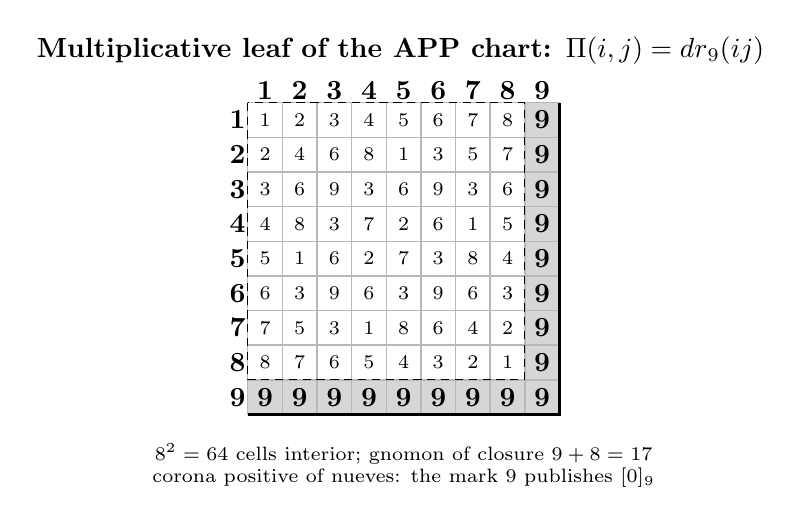
\begin{tikzpicture}[
  font=\scriptsize,
  cell/.style={minimum width=4.35mm,minimum height=4.35mm,
    inner sep=0pt,draw=black!28}]
  \node[font=\bfseries] at (1.72,.88)
    {Multiplicative leaf of the APP chart: $\Pi(i,j)=\operatorname{dr}_9(ij)$};
  \foreach \i in {1,...,9}{
    \node[font=\bfseries] at (-.35,{-(\i-1)*.44}) {\i};
    \foreach \j in {1,...,9}{
      \pgfmathtruncatemacro{\v}{mod(\i*\j-1,9)+1}
      \pgfmathtruncatemacro{\border}{(\i==9)||(\j==9)}
      \ifnum\border=1
        \node[cell,fill=black!16,font=\bfseries]
          at ({(\j-1)*.44},{-(\i-1)*.44}) {\v};
      \else
        \node[cell,fill=white]
          at ({(\j-1)*.44},{-(\i-1)*.44}) {\v};
      \fi
    }
  }
  \foreach \j in {1,...,9}{
    \node[font=\bfseries] at ({(\j-1)*.44},.38) {\j};
  }
  \draw[very thick] (3.74,.22)--(3.74,-3.74)--(-.22,-3.74);
  \draw[densely dashed] (-.22,.22) rectangle (3.30,-3.30);
  \node[align=center,anchor=north,font=\scriptsize] at (1.76,-3.98)
    {$8^2=64$ cells interior; gnomon of closure
     $9+8=17$\\corona positive of nueves: the mark $9$ publishes $[0]_9$};
\end{tikzpicture}}
\end{minipage}\hfill
\begin{minipage}[t]{.44\textwidth}
\centering
\resizebox{.98\linewidth}{!}{%
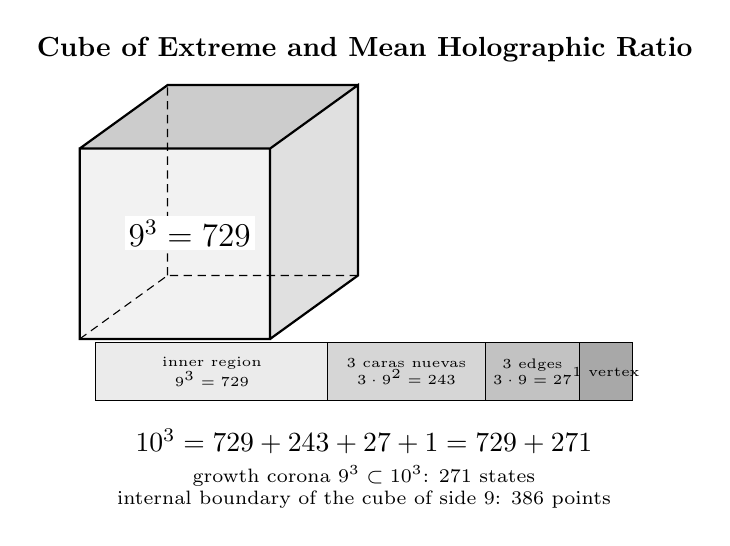
\begin{tikzpicture}[font=\scriptsize]
  \begin{scope}[x={(.78cm,0cm)},y={(.36cm,.26cm)},z={(0cm,.78cm)}]
    \coordinate (O) at (0,0,0);
    \coordinate (X) at (3.1,0,0);
    \coordinate (Y) at (0,3.1,0);
    \coordinate (XY) at (3.1,3.1,0);
    \coordinate (Z) at (0,0,3.1);
    \coordinate (XZ) at (3.1,0,3.1);
    \coordinate (YZ) at (0,3.1,3.1);
    \coordinate (XYZ) at (3.1,3.1,3.1);
    \path[fill=black!5] (O)--(X)--(XZ)--(Z)--cycle;
    \path[fill=black!12] (X)--(XY)--(XYZ)--(XZ)--cycle;
    \path[fill=black!20] (Z)--(XZ)--(XYZ)--(YZ)--cycle;
    \draw[densely dashed] (O)--(Y)--(XY) (Y)--(YZ);
    \draw[thick] (O)--(X)--(XZ)--(Z)--cycle
      (X)--(XY)--(XYZ)--(XZ) (Z)--(YZ)--(XYZ);
    \node[font=\bfseries\large,fill=white,inner sep=1.5pt]
      at (1.55,.52,1.55) {$9^3=729$};
  \end{scope}
  \node[font=\bfseries] at (3.62,3.68) {Cube of Extreme and Mean Holographic Ratio};
  \draw[fill=black!8] (0.2,-.78) rectangle (3.15,-.05);
  \node[align=center,font=\tiny] at (1.68,-.415)
    {inner region\\$9^3=729$};
  \draw[fill=black!16] (3.15,-.78) rectangle (5.15,-.05);
  \node[align=center,font=\tiny] at (4.15,-.415)
    {$3$ caras nuevas\\$3\cdot9^2=243$};
  \draw[fill=black!24] (5.15,-.78) rectangle (6.35,-.05);
  \node[align=center,font=\tiny] at (5.75,-.415)
    {$3$ edges\\$3\cdot9=27$};
  \draw[fill=black!34] (6.35,-.78) rectangle (7.02,-.05);
  \node[align=center,font=\tiny] at (6.685,-.415)
    {$1$ vertex};
  \node[font=\bfseries] at (3.61,-1.30)
    {$10^3=729+243+27+1=729+271$};
  \node[align=center] at (3.61,-1.88)
    {growth corona $9^3\subset10^3$: $271$ states\\
     internal boundary of the cube of side $9$: $386$ points};
\end{tikzpicture}}
\end{minipage}
\caption{Two finite publications of the support. Left: the product table with positive digital root and its closure gnomon. Right: the EMRH cubic completion, which distinguishes interior, faces, edges, and vertex. The growth corona $271$ and the internal boundary $386$ are two typed counts: the former measures the enlargement $9^3\subset10^3$ and the latter the boundary of the cube of side $9$.}
\label{fig:app-emrh-mini}
\end{figure}

The interior volume, faces, edges, and point closure are thus
typed as distinct layers of the same completed unit. The evaluations act on the 81
cells of the positive chart
\[
\Sigma,\Pi:\mathcal D_9^2\longrightarrow\mathcal D_9,
\qquad
\Sigma(i,j)=\operatorname{dr}_9(i+j),
\qquad
\Pi(i,j)=\operatorname{dr}_9(ij),
\]
Their residues and quotients raised are defined by
\[
\begin{aligned}
R^+(i,j)&:=\Sigma(i,j),&
Q^+(i,j)&:=\frac{i+j-R^+(i,j)}9,\\
R^\times(i,j)&:=\Pi(i,j),&
Q^\times(i,j)&:=\frac{ij-R^\times(i,j)}9,
\end{aligned}
\]
and, therefore,
\[
\begin{aligned}
\widehat\Sigma(i,j)&:=\bigl(R^+(i,j),Q^+(i,j)\bigr),\\
\widehat\Pi(i,j)&:=\bigl(R^\times(i,j),Q^\times(i,j)\bigr),
\end{aligned}
\qquad
\widehat\Sigma,\widehat\Pi:
\mathcal D_9^2\longrightarrow\mathcal D_9\times\mathbb Z_{\geq0}.
\]
The bijection \(\lambda_9^{\times2}:\mathcal D_9^2\to X_9\) transports
these operations and their lifts to the torus. Therefore, APP is the tuple
\begin{equation}
\APP=\bigl(\mathcal D_9,\lambda_9,X_9,\Gamma_{\rm APP},
\operatorname{Path}(\Gamma_{\rm APP}),
\Sigma,\Pi,\widehat\Sigma,\widehat\Pi\bigr),
\label{p12-83-c3-s1:eq:app-full-definition-public}
\end{equation}
The table constitutes a two-dimensional representation of this complete tuple.
The additive sheet is Latin; the multiplicative sheet conserves
the ternary radical of the ring \(\mathbb Z/9\mathbb Z\)
\begin{equation}
R_9:=\mathbb Z/9\mathbb Z,
\qquad
\mathfrak m:=([3]_9)=\{[0]_9,[3]_9,[6]_9\}\triangleleft R_9,
\qquad \mathfrak m^2=(0).
\label{p12-83-c3-s1:eq:app-radical-369}
\end{equation}
The internal rotation is the automorphism
\[
\rho:\mathfrak m^3\longrightarrow\mathfrak m^3,
\qquad \rho(x_1,x_2,x_3)=(x_2,x_3,x_1),
\]
whose distinguished orbit is
\[
([3]_9,[6]_9,[0]_9)\xrightarrow{\rho}
([6]_9,[0]_9,[3]_9)\xrightarrow{\rho}
([0]_9,[3]_9,[6]_9)\xrightarrow{\rho}
([3]_9,[6]_9,[0]_9).
\]
The direct reduction sends \(3,6,9\) to \(0,0,0\). The internal coordinate
of the ideal, by contrast, conserves the extracted factor:
\begin{equation}
\eta_{\mathfrak m}:(\mathfrak m,+)
\xrightarrow{\;\sim\;}(\mathbb Z/3\mathbb Z,+),
\qquad
\eta_{\mathfrak m}([3a]_9):=[a]_3,
\qquad
([3]_9,[6]_9,[0]_9)
\xmapsto{\;\eta_{\mathfrak m}^{\times3}\;}
([1]_3,[2]_3,[0]_3),
\label{p12-83-c3-s1:eq:app-369-120}
\end{equation}
so that the \(3,6,9\) sector remains intact and its internal coordinate is
read as \(1,2,0\). This map belongs to the radical of APP; the
temporal TRIT projection constitutes the subsequent calendrical reader. The
three calendrical classes
remain separated as
\[
\mathcal C_+=\{1,4,7\},\qquad
\mathcal C_-=\{2,5,8\},\qquad
\mathcal C_0=\{3,6,9\}.
\]
The incompatibility between the two leaves becomes a measurable invariant. On
\(\mathscr A_3=\mathcal D_9^3\), with uniform measure
\(\nu_3(x)=9^{-3}\), let
\(\mathcal H_3=L^2(\mathscr A_3,\nu_3)\). We define
\[
\Sigma_3,\Pi_3:\mathscr A_3\longrightarrow\mathcal D_9,
\qquad
\Sigma_3(x)=\operatorname{dr}_9(x_1+x_2+x_3),
\qquad
\Pi_3(x)=\operatorname{dr}_9(x_1x_2x_3),
\]
and the orthogonal projectors
\[
P_{\Sigma,3}:=\mathbb E_{\nu_3}[\,\cdot\mid\sigma(\Sigma_3)],
\qquad
P_{\Pi,3}:=\mathbb E_{\nu_3}[\,\cdot\mid\sigma(\Pi_3)]
\in\mathcal B(\mathcal H_3).
\]
The joint enumeration of the \(9^3\) words then determines
\[
\bigl\|[P_{\Sigma,3},P_{\Pi,3}]\bigr\|=\frac{\sqrt3}{4},
\qquad
B_c=7I+2R=9P_++5P_-,
\qquad
459-405=54.
\]
The first number reappears as the electronic prefactor; the second
organizes the central block; the third records the global sum--product
defect.

\subsection{TRIT: local topological unit and temporal relation unit}

HMT first fixes the visible signature
\begin{equation}
\mathrm{TRIT}_{\rm vis}=\{-1,0,+1\},
\qquad \tau\in\mathrm{TRIT}_{\rm vis}.
\label{p12-83-c3-s1:eq:trit-visible-signature}
\end{equation}
In contrast to the binary unit, the TRIT preserves three local regimes. In
the uniform distribution, its information and entropy are distinguished as
\begin{equation}
I_{\rm TRIT}=\log3\ \text{nats}=\log_2 3\ \text{bits},
\qquad S_{\rm TRIT}=k_BI_{\rm TRIT}.
\label{p12-83-c3-s1:eq:trit-information-unit}
\end{equation}
The bit remains the binary unit; the TRIT is the minimal unit capable of simultaneously distinguishing return, threshold, and opening. The equality \eqref{p12-83-c3-s1:eq:trit-information-unit} quantifies the information of the triad; the cost \(k_B\Theta\log3\) belongs to the subsequent thermal reset reader. Dimensional Mechanics also preserves the arithmetic antecedent of that signature. For \((i,j)\in\mathcal D_9^2\), the associated lifted arithmetic cell is
\begin{equation}
c_{\rm MD}(i,j;\tau)=
\bigl(i,j;R^+,Q^+,R^\times,Q^\times;\tau\bigr).
\label{p12-83-c3-s1:eq:trit-complete-local-unit}
\end{equation}
The residues \(R^+,R^\times\) are the visible publication of the two sheets;
the quotients \(Q^+,Q^\times\) conserve the exact memory of Euclidean
division; and \(\tau\) orients the transition. The visible signature occupies the first
level; the cell that bears it adds the arithmetic antecedents, and the
enriched state then completes boundary, route, phase, and survival.

It is useful to distinguish four strata. The visible signature is \(\tau\); the
residue--carry pair is its local lift; \(c_{\rm MD}\) is the APP
arithmetic cell equipped with that signature; and the TPK state adds extension,
boundary, genealogical ledger, phase, and survival. This hierarchy preserves the distinct
identity of the observed coordinate, its lift, the carrier cell, and the
enriched history that transports it.

In the balanced ternary chart, the lifted local integer
\(n\in\{-4,-3,\ldots,3,4\}\) decomposes uniquely as
\begin{equation}
\widehat n=(r,\kappa),
\qquad n=r+3\kappa,
\qquad r,\kappa\in\{-1,0,+1\}.
\label{p12-83-c3-s1:eq:trit-balanced-lift}
\end{equation}
The visible signature is \(\tau=r\); \(\kappa\) conserves the carry that the projection
\(n\mapsto r\) would forget.
The fiber over the visible zero contains three distinct states,
\[
0^+=(0,+1),\qquad 0^0=(0,0),\qquad 0^-=(0,-1),
\]
because \(n=-3,0,3\) have the same visible residue and different carries. This
is the minimal topological lift of MD: an oriented APP transition
is endowed with the information required to invert it and to decide which
prolongations remain compatible.

The signature also has a sheet-memory rule. If \(m_k\) is the active
arithmetic mode, then
\begin{equation}
m_{k+1}=
\begin{cases}
\Sigma,&\tau_k=+1,\\
\Pi,&\tau_k=-1,\\
m_k,&\tau_k=0.
\end{cases}
\label{p12-83-c3-s1:eq:trit-zero-memory}
\end{equation}
Zero encodes retention of the previous sheet. For that reason the word
\((+1,-1,0)\) publishes the sequence \((\Sigma,\Pi,\Pi)\): the third state
conserves the active multiplicative mode.

The temporal relation is obtained by orderly parametrizing these cells.
Each signature carries a quadratic algebra.
\begin{equation}
\mathbb A_\tau=\mathbb R[X]/(X^2+\tau),
\qquad J_\tau=[X],
\label{p12-83-c3-s1:eq:trit-quadratic-algebra-local}
\end{equation}
so that
\[
\begin{array}{c@{\qquad}c@{\qquad}l}
\toprule
\tau & J_\tau^2 & \text{ordered temporal relation}\\
\midrule
+1 & -I & \text{elliptic return, memory and past},\\
0  & 0  & \text{parabolic threshold and present},\\
-1 & +I & \text{bidirectional hyperbolic opening and future}.\\
\bottomrule
\end{array}
\]
The TRIT precedes external time: it first classifies the algebraic and
topological type of the transport; an ordered parameterization then publishes it
as a temporal relation. The twofold direction is typed by the exact involution
\begin{equation}
\mathcal C_{\rm rev}(\tau_1,\ldots,\tau_n)
=(-\tau_n,\ldots,-\tau_1),
\qquad \mathcal C_{\rm rev}^2=I,
\label{p12-83-c3-s1:eq:trit-time-reversal}
\end{equation}
which exchanges return and opening and preserves the threshold. On the
hyperbolic sheet, \(P_\pm=(I\pm J_{-1})/2\) separate the two eigendirections, and
reversal exchanges their orientations. Topology and time are thus the two
coordinated readings of the TRIT.

The combinatorial involution \(\mathcal C_{\rm rev}\) and an operatorial
conjugation \(C\) belong, however, to distinct domains. In a
separate dynamic realization, endowed with \(H=H^*\),
\(CJ_EC^{-1}=-J_E\), and \(CHC^{-1}=H\), we fix an internal action scale
\(\hbar_{\rm int}>0\) and write
\(h_{\rm int}:=2\pi\hbar_{\rm int}\). Then
\begin{equation}
U(t)=\exp(-J_EHt/\hbar_{\rm int}),
\qquad CU(t)C^{-1}=U(-t).
\label{p12-83-c3-s1:eq:trit-bidirectional-propagator}
\end{equation}
The intertwiner that transports TRIT words to the dynamical realization fixes
the correspondence between \(\mathcal C_{\rm rev}\) and \(C\). The twofold
local orientation provides the domain of that construction.

\subsection{TPK: category of transport and phase evolution}

The \emph{Topological Phase Kernel} is the transport category over the
observable base of APP that composes digits, words, operators, and prolongation
relations within a single enriched state. Its internal architecture is distributed among
eight operator classes, differentiated by domain, codomain, and function:
\begin{enumerate}[label=\textup{(\roman*)},leftmargin=2.25em]
\item observable support and enriched state;
\item internal sheet selector \(M_{\rm ph}:\{1,\ldots,9\}\to\{+1,-1,0\}\);
\item cardinal translations and visible evolution \(F_{\rm obs}\);
\item readers and quotients nonadic, tritico and of block \(1000\);
\item memory, carry, cylinder, boundary, and genealogical register;
\item periodicity and return
\(C_{12}\hookrightarrow C_{108}\twoheadrightarrow C_9\),
\(\mathcal K_{27}\), and channels \(90/120\);
\item prolongations \(\operatorname{Ext}_r\), cylinders, survival, and
natural bidirectional extension;
\item Archimedean-output, calibrated-exceptional, and dimensional functors.
\end{enumerate}
The return of 27 steps is the composite morphism.
\begin{equation}
\mathcal K_{27}:=F_{\rm obs}^{27},
\qquad \mathcal K_{27}^{4}=F_{\rm obs}^{108}.
\label{p12-83-c3-s1:eq:tpk-kernel-27}
\end{equation}
Its fourth iterate restores the observable phase of the calendar, while the
memory and the complete TPK state continue along their trajectory;
\(\mathcal K_{27}\) is the internal return morphism of \(C_{108}\).
The calendar \(C_{108}\), the nonadic connection, the bilateral extension, and
the readers occupy typed places within this architecture. Let
\(\mathsf P_{\rm APP}\) be the free category
of the directed graph of APP, and let
\(\mathsf P_{\rm APP}^{(2)}=\mathsf P_{\rm APP}\times
\mathsf P_{\rm APP}\) be its simultaneous sum--product reading. Let, moreover,
\[
\mathcal Q_{\rm obs}
=X_9^2\times\{N,E,S,O\}^2\times\Theta_{108},
\qquad \Theta_{108}=\mathbb Z/108\mathbb Z,
\]
where, for the representative
\(\widetilde\theta\in\{0,\ldots,107\}\),
\[
r(\theta)=1+(\widetilde\theta\bmod9),
\qquad g_0(\theta)=[\widetilde\theta]_9,
\]
\[
\tau(\theta)=
\begin{cases}
+1,&r(\theta)\in\{1,4,7\},\\
-1,&r(\theta)\in\{2,5,8\},\\
0,&r(\theta)\in\{3,6,9\},
\end{cases}
\qquad
\mu(\theta)=
\begin{cases}
\Sigma,&\tau(\theta)=+1,\\
\Pi,&\tau(\theta)=-1,\\
\varnothing,&\tau(\theta)=0.
\end{cases}
\]
The calendar label \(\mu=\varnothing\) marks the threshold, and the dynamic memory \(m_k\) of \eqref{p12-83-c3-s1:eq:trit-zero-memory} retains the last active sheet. A configuration \(q=(p^\Sigma,p^\Pi,d^\Sigma,d^\Pi,\theta)\) preserves the two positions, the two cardinal directions, and the calendar index. The visible evolution \(F_{\rm obs}\) activates the sheet indicated by TRIT, transports the corresponding position, and advances \(\theta\). Let \(\mathsf P_{\rm obs}\) denote the free category generated by the arrows \(q\to F_{\rm obs}(q)\). Each arrow induces a pair of APP paths and defines the base functor
\begin{equation}
B:\mathsf P_{\rm obs}\longrightarrow\mathsf P_{\rm APP}^{(2)}.
\label{p12-83-c3-s1:eq:tpk-bivariant-base-functor}
\end{equation}

Over each \(q\) lies the typed fibre
\begin{equation}
\mathcal F_q=
\mathsf O_q\times\mathsf H_q\times\mathsf C_q\times\mathsf S_q
\times\mathsf B_q\times\mathsf\Lambda_q,
\label{p12-83-c3-s1:eq:tpk-fiber}
\end{equation}
Its six factors conserve, respectively, orientation and sheet; residue and
quotient; carry; signature; cylinder and boundary; and ordered register of
transport. Memory and survival are properties of the composition and of
the prolongation relations.

For a route \(r:q\to q'\), the relation
\begin{equation}
\operatorname{Ext}_r\subseteq\mathcal F_q\times\mathcal F_{q'}
\label{p12-83-c3-s1:eq:tpk-extension-relation}
\end{equation}
contains all admissible continuations and satisfies
\[
\Delta_q\subseteq\operatorname{Ext}_{\operatorname{id}_q},
\qquad
\operatorname{Ext}_{r_2}\circ\operatorname{Ext}_{r_1}
\subseteq\operatorname{Ext}_{r_2\circ r_1}.
\]
Transports respect identities and composition:
\begin{equation}
\begin{gathered}
\mathsf H(\operatorname{id}_q)=I,
\quad \mathsf C(\operatorname{id}_q)=I,
\quad \mathsf\Lambda(\operatorname{id}_q)=I,
\quad \kappa(\operatorname{id}_q)=0,\\
\mathsf H(r_2\!\circ r_1)=\mathsf H(r_2)\mathsf H(r_1),
\quad
\mathsf C(r_2\!\circ r_1)=\mathsf C(r_2)\mathsf C(r_1),
\quad
\mathsf\Lambda(r_2\!\circ r_1)=
\mathsf\Lambda(r_2)\mathsf\Lambda(r_1).
\end{gathered}
\label{p12-83-c3-s1:eq:tpk-functorial-transport}
\end{equation}
Along with these functorial laws, the transported coordinates obey
\begin{equation}
\begin{aligned}
h'&=\mathsf H(r)(h),\\
c'&=\mathsf C(r)(c)+\kappa(r),\\
\lambda'&=\mathsf\Lambda(r)(\lambda),\\
\sigma'&=\operatorname{Sig}_{q'}(h',c',\lambda'),
\end{aligned}
\qquad
\kappa(r_2\circ r_1)
=\kappa(r_2)+\mathsf C(r_2)\kappa(r_1).
\label{p12-83-c3-s1:eq:tpk-typed-transport}
\end{equation}
The last identity is the carry cocycle that makes the composition with memory associative.

The TPK is then the category \(\mathsf{TPK}\) whose objects are
\begin{equation}
x=(q,o,h,c,\sigma,C,b,\lambda),
\qquad (o,h,c,\sigma,(C,b),\lambda)\in\mathcal F_q,
\label{p12-83-c3-s1:eq:tpk-enriched-object}
\end{equation}
and whose morphisms \(x\to x'\) are the triples \((r,x,x')\) such that
the coordinates satisfy \eqref{p12-83-c3-s1:eq:tpk-typed-transport} and
\((f_x,f_{x'})\in\operatorname{Ext}_r\), where
\(f_x\in\mathcal F_q\) and \(f_{x'}\in\mathcal F_{q'}\). Composition is
\begin{equation}
(r_2,x',x'')\circ(r_1,x,x')
=(r_2\circ r_1,x,x''),
\label{p12-83-c3-s1:eq:tpk-morphism-composition}
\end{equation}
\Needspace{7\baselineskip}
the identity is \((\operatorname{id}_q,x,x)\), and the functor
\begin{equation}
p:\mathsf{TPK}\longrightarrow\mathsf P_{\rm obs},
\qquad p(x)=q,
\qquad p(r,x,x')=r,
\label{p12-83-c3-s1:eq:tpk-base-functor}
\end{equation}
publishes the visible configuration without identifying states of the same fiber.
The definition fixes a category over a base; it does not presuppose that it is a
categorical fibration nor that every arrow admits a Cartesian lift.
The local projections remain separated by type:
\[
\pi_{\rm TRIT}:\operatorname{Ob}(\mathsf{TPK})
\longrightarrow\mathrm{TRIT}_{\rm vis},
\qquad
\pi_{\rm TRIT}(x)=\tau(\theta),
\]
\[
\pi_{\rm loc}(x)=
\bigl(\pi_{\rm TRIT}(x),\mu(\theta),o,h,c,
\sigma,\lambda,g_0(\theta)\bigr).
\]
The first recovers only the visible TRIT signature. The second further preserves
the calendrical sheet label, orientation, the residue--quotient pair,
carry, transport signature, genealogical register, and phase,
but still forgets the cylinder, its boundary label, and other coordinates of
\(q\). This is why neither the visible TRIT nor its local register
replaces the enriched state of the TPK.

The name encompasses three inseparable functions. \emph{Topological} refers to
the category of paths, incidence, boundary, and prolongation by
cylinders; \emph{Phase} refers to the nonadic index, the oriented calendar, and
holonomy; \emph{Kernel} names the persistent transport kernel that
remains before the state is contracted by a reader. Formally, the
object is the preceding category: an additional topology on objects or
morphisms, or its identification with the linear kernel of a map, requires
independent data.

Consequently, two routes with the same visible endpoint may remain
objects distinct by sheet, quotient, carry, boundary, cylinder, phase, or
register. The TPK does not choose a scalar output: it conserves the common antecedent
from which the Archimedean, exceptional, and dimensional publications depart.

% Estas consecuencias se publican después de la construcción correlativa y
% del paso al límite de los capítulos 4 y 5. Se definen aquí para preservar
% íntegramente su procedencia, pero no se ejecutan antes de que exista el
% continuo al que se aplican.
\long\def\HMTDeferredContinuumConsequences{%
\section{Consequences and publications of the constructed continuum}

\subsection{Terminal Assembly Theorem of the Correlative Constructions Generated by the Common State}

Each depth \(k\) possesses an enriched state \(\mathcal E_k\) with
all its surviving emissions and a single correlative constructor
\begin{equation}
\mathcal O_k:\mathcal E_k\longrightarrow\mathcal Z_k,
\qquad
\widehat x_k\longmapsto
\mathcal O\bigl(\{\mathfrak e_\alpha:
\alpha\in\operatorname{Ch}_k(\widehat x_k)\}\bigr).
\label{p12-83-c3-s1:eq:five-features-single-constructor}
\end{equation}
The value of \(\mathcal O_k\) simultaneously preserves the spectral,
solenoidal, gauge, coherent, and determinantal coordinates,
\begin{equation}
(\mathrm{sp},\mathrm{sol},\mathrm{gau},\mathrm{coh},\mathrm{det}),
\label{p12-83-c3-s1:eq:five-features-coordinates}
\end{equation}
as five characteristics of the same state and of the same genealogical register. The
truncations
\[
u^{\mathfrak e}_{\ell,k}:\mathcal E_\ell\to\mathcal E_k,
\qquad
u^{\mathcal O}_{\ell,k}:\mathcal Z_\ell\to\mathcal Z_k
\]
satisfy the unique naturality
\begin{equation}
u^{\mathcal O}_{\ell,k}\circ\mathcal O_\ell
=\mathcal O_k\circ u^{\mathfrak e}_{\ell,k},
\qquad \ell\ge k.
\label{p12-83-c3-s1:eq:five-features-naturality}
\end{equation}
Therefore, the corresponding action passes to the limit as
\begin{equation}
\mathcal O_\infty:
\mathcal C_{\rm cont}^{\rm disc}:=\varprojlim_k\mathcal E_k
\longrightarrow
\mathcal Z_\infty:=\varprojlim_k\mathcal Z_k.
\label{p12-83-c3-s1:eq:five-features-infinite-operator}
\end{equation}
The five terminal applications are seen as intrinsic manifestations of that single value:
\begin{equation}
\boxed{
\mathfrak G_T^{\rm int}:=
\operatorname{View}_T\!\left(
\mathcal O_\infty(\mathcal C_{\rm cont}^{\rm disc})\right),
\quad
T\in\{\mathrm{sp},\mathrm{sol},\mathrm{gau},
\mathrm{coh},\mathrm{det}\}.}
\label{p12-83-c3-s1:eq:five-features-views}
\end{equation}
Simultaneity precedes the specialized resolutions: each view exposes
the required coordinate and the complete state conserves the other four.

\subsection{Survival and inverse limit}

Let \(\operatorname{Surv}^{(\chi)}_N\) be the set of histories of
depth \(N\) that simultaneously satisfy the active laws of channel
\(\chi\) and admit prolongation. We define the compatible truncations
\[
\tau_{N+1,N}:\operatorname{Surv}^{(\chi)}_{N+1}
\longrightarrow\operatorname{Surv}^{(\chi)}_N
\]
These preserve the enriched prefix. The genealogical continuum is the limit.
\begin{equation}
X_\chi=\varprojlim_N
\bigl(\operatorname{Surv}^{(\chi)}_N,\tau_{N+1,N}\bigr),
\qquad
\tau_{N+1,N}(x_{N+1})=x_N.
\label{p12-83-c3-s1:eq:inverse-survival}
\end{equation}
The global space of surviving sections and one of its enriched sections
are denoted, respectively, by
\begin{equation}
X_\infty:=\bigsqcup_\chi X_\chi,
\qquad
\widehat\Omega_\infty\in X_\infty.
\label{p12-83-c3-s1:eq:global-survival-space}
\end{equation}
The global Archimedean reader is
\begin{equation}
P_{\rm arq}:=\operatorname{ev}_{\mathbb R}:
X_\infty\longrightarrow\mathbb R;
\label{p12-83-c3-s1:eq:archimedean-reader}
\end{equation}
its restriction to each channel evaluates the unitary intersection of the compatible cylinders of the corresponding section. When the exceptional reader intervenes, \(X_\infty^{\rm cal}\subseteq
X_\infty\) denotes the subspace in which the calibration type of \eqref{p12-83-c3-s1:eq:exceptional-calibration} has been fixed. Survival determines the section by internal compatibility: every history must be prolongable in the complete system. The numerical reader intervenes afterward to certify and publish the intersection of the already compatible descendant.

\subsection{Joint nonadic connection, holonomy, and vertical memory}

At depth \(K\), the holonomy of the nonadic return is initially the typed correspondence
\begin{equation}
\Gamma_{9,K}=\operatorname{Hol}_{C_9}(\nabla_{\rm TPK}):
\widehat{\mathcal X}_K\rightrightarrows
\widehat{\mathcal X}_{K+9}.
\label{p12-83-c3-s1:eq:gamma9}
\end{equation}
Its iterates are relational compositions. Only when each state has
a unique compatible prolongation is it restricted to a map, and only when that
map is invertible does it constitute a monodromy. This distinction conserves all
surviving extensions before selecting a section.
After nine phases the local phase returns, while the complete state advances:
\[
g(K+9)=g(K),\qquad q_{{\rm mem},K+9}=q_{{\rm mem},K}+1,
\qquad \widehat x_{K+9}\ne\widehat x_K\ \text{in general}.
\]
Block, cylinder, prefix, carry, and memory continue to evolve. This
is the difference between visible periodicity and return with biography.

The transported state at level (K) can be exhibited as
\begin{equation}
\widehat x_K=
(B_K,C_K,p_K,c_K,\Sigma_K,W_K,g(K),q_{{\rm mem},K},s_K),
\label{p12-83-c3-s1:eq:enriched-state-k}
\end{equation}
where each coordinate has its own transport law. The phase return is represented on the catalog.
\[
\mathcal U_6^{\rm cat}\cong\mathfrak S_+\times\mathfrak S_\times,
\qquad |\mathfrak S_+|=18,
\qquad |\mathfrak S_\times|=26.
\]
Conditional averages
\[
(E_+f)(s,e)=\frac1{18}\sum_{s'\in\mathfrak S_+}f(s',e),
\qquad
(E_\times f)(s,e)=\frac1{26}\sum_{e'\in\mathfrak S_\times}f(s,e')
\]
commute. The phase word
\(\tau=(+1,-1,0,+1,-1,0,+1,-1,0)\) applies
\(E_+,E_\times,I\) in that order, and one revolution closes through
\begin{equation}
\mathcal K_{\rm ph}^{\,9}
=(E_+E_\times)\otimes I_{\ell^2(C_9)},
\qquad
\bigl\langle\delta_u,E_+E_\times\delta_v\bigr\rangle
=\frac1{468}\quad(u,v\in\mathcal U_6^{\rm cat}).
\label{p12-83-c3-s1:eq:joint-nine-holonomy}
\end{equation}
The sum and product sheets do not act as independent filters: they are two
components of a single holonomy that closes only after traversing the
complete cycle.

The compression--expression colligation separates what returns from what remains
as memory. If (J) embeds the history space into the phase
space, (T) is the surviving compression and \(\eta\) the defect channel,
then
\begin{equation}
\boxed{
U_{\Gamma_9}J=JT+\eta,
\qquad J^*\eta=0,
\qquad I-T^*T=\eta^*\eta.}
\label{p12-83-c3-s1:eq:compression-expression}
\end{equation}
The first equality decomposes transport into compressed return and memory
expression; the second proves their orthogonality; the third measures exactly
the information that cannot fit within the periodic shadow. The central
statement is thereby formalized: the phase returns, not the complete state.

The vertical memory is organized through the cyclic extension oriented
\begin{equation}
0\longrightarrow C_{12}\xrightarrow{\,\iota\,}C_{108}
\xrightarrow{\,p\,}C_9\longrightarrow0,
\qquad
c(r,r')=\left[\left\lfloor\frac{r+r'}9\right\rfloor\right]_{12}.
\label{p12-83-c3-s1:eq:c108-extension}
\end{equation}
Here \(\iota([b]_{12})=[9b]_{108}\) and
\(p([\theta]_{108})=[\theta]_9\). The extension does not split:
\(C_{108}\) has exponent 108, whereas
\(C_{12}\times C_9\) has exponent 36.
The cocycle records the carry from each turn of the base \(C_9\) in the
dodecaphase memory \(C_{12}\). \(C_{108}\) is therefore an oriented
phase--memory calendar. Only after the dimensional chart is that
extension realized as a finite 108-step quantum clock.

The local MD lift carrying the TRIT signature is the
topological--temporal unit of that genealogical crystal.
On
\(\mathcal H_{\rm clk}=\mathbb C^{108}\), with basis
\(\{|j\rangle:j\in\mathbb Z/108\mathbb Z\}\), let
\[
\zeta=e^{2\pi\ii/108},\qquad
|\widetilde k\rangle=\frac1{\sqrt{108}}
\sum_{j=0}^{107}\zeta^{jk}|j\rangle,
\qquad U_{\rm clk}|j\rangle=|j+1\rangle.
\]
\Needspace{12\baselineskip}
With \(\omega_0=2\pi/(108t_0)\), the Hamiltonian
\begin{equation}
H_{\rm clk}=\hbar_{\rm int}\omega_0
\sum_{k=0}^{107}k\,|\widetilde k\rangle\langle\widetilde k|
\label{p12-83-c3-s1:eq:trit-time-crystal-hamiltonian}
\end{equation}
generates exactly
\begin{equation}
U_{\rm step}=\exp\!\left(
-\frac{\ii H_{\rm clk}t_0}{\hbar_{\rm int}}\right)=U_{\rm clk},
\qquad U_{\rm step}^{108}=I,
\label{p12-83-c3-s1:eq:trit-time-crystal-period}
\end{equation}
If \(Z_{\rm clk}|j\rangle=\zeta^j|j\rangle\), then
\begin{equation}
\langle j_0|U_{\rm step}^{-n}Z_{\rm clk}U_{\rm step}^{n}|j_0\rangle
=\zeta^{j_0+n},
\label{p12-83-c3-s1:eq:trit-time-crystal-observable}
\end{equation}
whose orbit has primitive period 108. In HMT terminology, this is the
internal genealogical time crystal: the observable calendar closes,
\(C_{12}\) records the circuit, and the enriched TPK state need not
return. Its subsequent realization as a macroscopic physical phase also requires
a Floquet protocol, primitive subharmonic response, robustness,
persistence, and a protection mechanism; that chart does not alter the finite
theorem of unitary periodicity.

\subsection{Archimedean publication, genealogical number and measurement}

The Archimedean publication uses semi-open ternary cylinders.
\begin{equation}
I_{N,L}=\left[\frac{N}{3^L},\frac{N+1}{3^L}\right),
\qquad \operatorname{diam}I_{N,L}=3^{-L}\longrightarrow0.
\label{p12-83-c3-s1:eq:ternary-cylinders}
\end{equation}
A compatible section determines nested cylinders and, by completeness, a
unique real point. The HMT number is the section itself,
\begin{equation}
x=(x_N)_N\in X_\chi
=\varprojlim_N\operatorname{Surv}^{(\chi)}_N,
\label{p12-83-c3-s1:eq:hmt-number-as-section}
\end{equation}
not the tuple formed by it and its evaluations. The value appears when a
reader forgets part of the genealogy.
Therefore, precision is depth: measuring means descending to a
finer cylinder while the causal prefix remains in the antecedent.
The real line is reconstructed as the Archimedean quotient of a space of
much richer histories.

\subsection{Dimensional realization of the HMT state: screen map, observable magnitude, and spectral chart}

Dimensional Mechanics begins where the genealogical state couples to a
realization boundary. With a field \(K_n\) fixed, let \(M_n(x)\) be the module
generated by the prolongation channels of a state \(x\), let
\(\mathcal R_n(x)\) be the submodule of its relations, and let \(\beta_n(x)\) be the
conserved boundary datum. The dimensional screen is
\begin{equation}
\Sigma_n(x)=\bigl(K_n,M_n(x),\beta_n(x),\mathcal R_n(x)\bigr),
\qquad
d_{\Sigma_n}(x)=\dim_{K_n}\frac{M_n(x)}{\mathcal R_n(x)}.
\label{p12-83-c3-s1:eq:md-screen}
\end{equation}
If \(M_n(x)\simeq K_n^{g_n}\) and the columns of \(R_n(x)\) generate the
relations, then
\begin{equation}
\boxed{d_{\Sigma_n}(x)=g_n-\operatorname{rank}_{K_n}R_n(x).}
\label{p12-83-c3-s1:eq:md-rank}
\end{equation}
Dimension is not attached as a label: it is the number of independent
channels that survive after imposing the boundary relations.

A physical quantity is a section of a dimensional line \(L_D\); a unit is a chart \(\chi_u:L_D\to\mathbb R\) that publishes its coordinate. Hence
\begin{equation}
\text{TPK state}\longrightarrow\Sigma_n(x)
\longrightarrow s_D\in\Gamma(L_D)
\xrightarrow{\;\chi_u\;}[s_D]_u\in\mathbb R
\label{p12-83-c3-s1:eq:md-measurement-chain}
\end{equation}
separates structure, dimensional type, and measured number exactly. Measuring
consists in coupling a section to a reversible apparatus, imposing
edge compatibility, and applying the reader; changing units changes
\(\chi_u\), not the section or its genealogy.

\subsection{Double projection mathematical and dimensional realization}

The exceptional branch preserves gauge data that the real publication does not
need. Let \(\mathscr C_{\rm exc}\) be the space of gauges, and let
\begin{equation}
\mathfrak E:
X_\infty^{\rm cal}\times\mathscr C_{\rm exc}
\longrightarrow\mathbf{Exc}
\label{p12-83-c3-s1:eq:exceptional-calibrated-reader}
\end{equation}
the incidence reader. We fix once
\begin{equation}
\begin{aligned}
\chi_{\rm exc}=\bigl(&\text{projective order},\ \text{Paley gauge},
 \ \text{dodecad},\\
 &\text{incidence alignment},\ \text{lattice chamber}\bigr)
 \in\mathscr C_{\rm exc}
\end{aligned}
\label{p12-83-c3-s1:eq:exceptional-calibration}
\end{equation}
and abreviamos
\(\mathfrak E_{\chi_{\rm exc}}(x):=\mathfrak E(x,\chi_{\rm exc})\).
The gauge initial it transports by the history; not vuelve to elegirse in
each depth.

The same calibrated limit then admits two readers with distinct codomains:
\begin{equation}
\mathbb R
\xleftarrow{\;\operatorname{ev}_{\mathbb R}\;}
X_\infty^{\rm cal}
\xrightarrow{\;\mathfrak E_{\chi_{\rm exc}}\;}
\mathbf{Exc}.
\label{p12-83-c3-s1:eq:double-projection}
\end{equation}
The first branch contracts cylinders to a continuous value. The second
preserves incidences, orientations, gauge, and boundary. Both descend in
parallel from the same source state. This bifurcation jointly explains
metric continuity and the emergence of exceptional symmetries. The second
branch is a calibrated reconstruction: it is exact once
\(\chi_{\rm exc}\) has been fixed, but the bare state does not retrospectively select
the five data composing that gauge.

The non-serializing dimensional realization does not serialize those two branches. It is a third reader of the same antecedent:
\begin{equation}
P_{\rm dim}:X_\infty\longrightarrow
\mathcal R_{\rm MD},
\qquad
\mathcal R_{\rm MD}=
\{\text{action, mass, field, geometry, information}\}.
\label{p12-83-c3-s1:eq:dimensional-publication}
\end{equation}
In this manner, a number, a symmetry, and a physical magnitude may share a
genealogy without being confused with or reduced to one another.

The thesis of the continuum is thus formulated precisely: Archimedean
reality is the zero-radius shadow of infinitely refinable discrete histories;
what the shadow omits reappears as memory, incidence,
geometry, and physical structure.

% RESULTADO_RECUPERADO. Owner íntegro de la dinámica del cociente, el retorno
% observable y los cociclos de modo y orientación. Se subordina a la única
% construcción APP--TRIT--TPK sin abrir un origen alternativo.
\begin{HMTScientificOwnerSubordinated}
\chapter{Surviving extensions, monodromy, and dynamics of the quotient}
\label{chap:extensiones-dinamica-cociente}
\index{survival!global extension}
\index{monodromy!nonadic return}
\index{measure!emissions catalog}

The language of paths requires a decisive precision. An APP path,
a visible emission, an enriched TPK history, and a global section
are not four names for the same object. They constitute four consecutive levels
of a single construction. The path preserves positional order;
the emission preserves a finite reading; the history adds signature,
carry, orientation, boundary, and memory; the global section requires all
of its prefixes to survive simultaneously at every depth.

This hierarchy makes it possible to separate two questions that had remained intermingled. The first is logical: under what hypotheses a finite prefix truly belongs to a compatible infinite extension. The second is dynamical: what it means to transport a single history and what it means to transfer all its compatible continuations simultaneously. The distinction is essential in APP\@. A given trajectory carries one state to another; a path transfer carries a distribution of extensions to another distribution.

This section resolves the finite problem at depth six. The
published deterministic chronology has visible-phase return and cannot select
a unique probability. By contrast, transport biased by the nonadic phase,
when each active channel is interpreted as the normalized renewal of its entire
fibre of compatible continuations, has a uniform nine-step return
over the (468) emissions. The weights (1/3) then cease to be
an external choice: they follow from the three occurrences of each signature
(+1,-1,0) in the oriented nonadic cycle. Normalization within each fibre remains
a precise mathematical premise ---the uniform count of all compatible
paths--- and must not be conflated with the successor of a single
trajectory. Passage to the inverse limit over all depths preserves a
distinct statement, formulated at the end of the section.

\section{\(5\) levels of the notion of path}

Let \(\Gamma_{\rm APP}\) be the category of cardinal paths of the APP torus\@.
For each depth \(m\), let \(\mathcal H_m\) be the finite set of
admissible enriched histories
\[
 h_m=(v_0,e_1,v_1,\ldots,e_m,v_m),
\]
where each arrow \(e_j\) transports all fields declared by TPK\@. If
\(n\geq m\), the application
\[
 p_{n,m}:\mathcal H_n\longrightarrow\mathcal H_m
\]
removes the tail beyond depth \(m\). The positional shadow
\[
 \operatorname{sh}_m:\mathcal H_m\longrightarrow\Gamma_{\rm APP}
\]
forgets the memory fiber and preserves the underlying APP path.

\begin{definition}[Hierarchy of extensions]
\label{def:jerarquia-extensiones}
We distinguish the following objects.
\begin{enumerate}
  \item An \emph{APP path} is a morphism of
  \(\Gamma_{\rm APP}\).
  \item An \emph{observable route} is a reading of that morphism that
  jointly conserves the sum and product leaves.
  \item A \emph{TPK extension} is a lift of the observable route to
  a history \(h_m\in\mathcal H_m\), with its residue, quotient,
  signature, orientation, boundary, carry, and record data.
  \item A \emph{surviving extension} is a finite history that admits
  compatible prolongations to every horizon.
  \item A \emph{global section} is a compatible family
  \(x=(h_m)_{m\geq0}\) of surviving extensions.
\end{enumerate}
In particular, the route is the shadow of the extension; it is not an external object
that the extension subsequently chooses.
\end{definition}

For \(h\in\mathcal H_m\), its cylinder of prolongations is
\[
 Z_m(h)=
 \{x=(h_n)_n\in\varprojlim_n\mathcal H_n:x_m=h\}.
\]
In particular, every family of \(Z_m(h)\) also satisfies
\(p_{n,\ell}(h_n)=h_\ell\) for \(n\geq\ell\); collections of
incompatible truncations are not admitted.
Let us also define
\[
 \mathcal S_m^{(N)}=p_{N,m}(\mathcal H_N),
 \qquad
 \mathcal S_m^\infty=\bigcap_{N\geq m}\mathcal S_m^{(N)}.
\]

\begin{theorem}[Conditional extension survivor criterion]
\label{thm:criterio-extension-superviviente}
Let us fix \(h\in\mathcal H_m\) and, for \(N\geq m\), write
\[
 \mathcal P_N(h)=\{g\in\mathcal H_N:p_{N,m}(g)=h\}.
\]
Suppose that the truncations are coherent and that each
\(\mathcal P_N(h)\) is finite. The following are equivalent:
\begin{enumerate}
  \item \(\mathcal P_N(h)\ne\varnothing\) for every \(N\geq m\), that is,
  \(h\in\mathcal S_m^\infty\);
  \item the tree of finite extensions of \(h\) is finitely branching
  and has a nonempty level at every depth;
  \item \(Z_m(h)\ne\varnothing\).
\end{enumerate}
Consequently, whenever the surviving finite truncations are nonempty, the set
\[
 \Omega_{\rm H}^{\rm surv}
 =\varprojlim_m\mathcal S_m^\infty
\]
is exactly the space of surviving global sections. The theorem does not
assert that these truncations are nonempty for every APP input: that
property must be proved by means of the survival protocol.
\end{theorem}

\begin{proof}
The implication from the third condition to the first two is obtained by
truncation. Now assume the first condition and order the elements of
\(\bigsqcup_{N\geq m}\mathcal P_N(h)\) by the prefix relation. Each level
is finite and nonempty, and coherence of the truncations makes this union
a finitely branching tree with nodes at every depth; this yields the
second condition. Conversely, from the second condition König's lemma
provides an infinite branch. Its truncations form a compatible family
belonging to \(Z_m(h)\), which is the third condition. The same construction
identifies the indicated inverse limit wherever its finite truncations are
nonempty.
\end{proof}

The theorem resolves the possible discrepancy between “extendable to each
horizon separately” and “possessing a global prolongation”: finiteness of the
branches is the hypothesis that permits the choice of a single compatible chain. It does not
claim that all APP paths belong to
\(\operatorname{sh}(\Omega_{\rm H}^{\rm surv})\). That coverage requires proving
that the enriched closures do not empty the corresponding fibers.

\section{Phase return and monodromy relation}

The return of the phase--length quotient is formalized separately in
\cref{def:odometro-9-12,prop:proyeccion-fase-longitud}:
\[
(b,r)\xrightarrow{\;9\;}(b+1,r),
\qquad
(b,r)\xrightarrow{\;108\;}(b,r).
\]
These equalities belong to the odometer \(9\times12\). They do not constitute the
proof of \(F_{\rm obs}^{108}=I\), which uses the observable state and appears
below.

Let \(\phi\) be the phase coordinate with values in \(\mathbb Z/9\mathbb Z\).
A visible-phase return satisfies
\[
 \phi(h_{k+9})=\phi(h_k).
\]
The complete record may, however, satisfy
\[
 B(h_{k+9})\ne B(h_k).
\]
This inequality is not a failure of periodicity: it is the memory of the circuit.
An ordinary action of \(C_9\) on the complete state would require the
ninth power to be the identity and would erase precisely that information.

To type the return, let \(H\) be a hexad and \(P_2(H)\) its set of
fifteen pairs. Let \(\mathcal B_k\) be the record states that survive at phase
\(k\), let \(\mathcal T_k\subseteq\mathcal B_k\times\mathcal B_{k+1}\) be the published transport relation, and
suppose a fiber encoder is given
\[
 c_k:\mathcal B_k\longrightarrow P_2(H).
\]
Only after declaring those encoders is the observable relation defined.
\[
 R_k=(c_k\times c_{k+1})(\mathcal T_k)
 \subseteq P_2(H)\times P_2(H).
\]
The relational monodromy of a loop is
\[
 \mathcal M_k
 =R_{k+8}\circ R_{k+7}\circ\cdots\circ R_k.
\]

\begin{proposition}[Classification of the nonadic return given the encoder]
\label{prop:clasificacion-retorno-nonadico}
Three logically distinct levels are given.
\begin{enumerate}
  \item Without a proof of functionality, the return is the relation
  \(\mathcal M_k\).
  \item If each \(R_k\) is the graph of a map
  \(\mu_k:P_2(H)\to P_2(H)\), the transport is the skew product
  \[
   T(k,p)=(k+1,\mu_k(p)),
  \]
  and
  \[
   T^9(k,p)=(k,M_k(p)),
   \qquad
   M_k=\mu_{k+8}\circ\cdots\circ\mu_k.
  \]
  \item If the \(\mu_k\) are bijective, \(M_k\) is an automorphic holonomy.
  The transport descends to an ordinary action of
  \(C_9\) on the complete state if and only if \(M_k=I\) in all
  fibers.
\end{enumerate}
\end{proposition}

\begin{proof}
The first claim is the definition of image and relational composition once
\((c_k)_k\) have been fixed. Under
functionality, nine consecutive applications keep the first
coordinate fixed and compose their actions on the second. The composition of
bijections is a bijection. Finally, \(T^9=I\) is exactly equivalent to
\(M_k=I\) for each phase and each point of the fiber.
\end{proof}

\begin{corollary}[No return under cumulative transport]
\label{pf84:E02-29}
Let \(q:X\to V\), \(T:X\to X\), and \(x\in X\) be given. If
\[
 q(T^9x)=q(x),\qquad
 T^9x=\mathcal M_x\,x,\qquad
 \mathcal M_x\,x\ne x,
\]
then the projection returns and the state does not:
\[
 q(T^9x)=q(x),\qquad T^9x\ne x.
\]
The pointwise hypothesis \(\mathcal M_x\,x\ne x\) is indispensable; the global
inequality \(\mathcal M_x\ne I\) does not exclude \(x\) from being a fixed point.
\end{corollary}

\begin{proof}
The first equality is a hypothesis. The second and the pointwise separation give
\(T^9x=\mathcal M_x\,x\ne x\). The statement would be refuted by a case that
satisfies the three premises and had \(T^9x=x\); it does not authorize replacing the
third premise by \(\mathcal M_x\ne I\).
\end{proof}

\begin{theorem}[Functional sufficiency of the enriched tuple]
\label{pf84:E02-30}
Let
\[
 E:\mathscr X_{\rm TPK}^{\rm enr}\longrightarrow\mathscr S_E
\]
the tuple that conserves the visible block, new blocks and carry, lifting
state, cylinders, boundary signature, orientation, observable, phase, and
dodecaphasic register. Let
\[
 T:\mathscr X_{\rm TPK}^{\rm enr}\to
 \mathscr X_{\rm TPK}^{\rm enr},
 \qquad
 O:\mathscr X_{\rm TPK}^{\rm enr}\to Y.
\]
When maps exist
\[
 \widehat T:\mathscr S_E\to\mathscr X_{\rm TPK}^{\rm enr},
 \qquad
 \widehat O:\mathscr S_E\to Y
\]
such that
\[
 T=\widehat T\circ E,\qquad O=\widehat O\circ E,
\]
the equality \(E(x)=E(y)\) implies \(T(x)=T(y)\), \(O(x)=O(y)\) and, by
determinism, the same continuations and subsequent outputs.
\end{theorem}

\begin{proof}
By factorization,
\[
 T(x)=\widehat T(E(x))=\widehat T(E(y))=T(y),
 \qquad
 O(x)=\widehat O(E(x))=\widehat O(E(y))=O(y).
\]
The first equality permits iteration of the argument. This is a sufficient
condition, not an unproved equivalence. Two states with the same tuple and
different transitions or outputs, access to an absent coordinate, or
querying a target value are falsifiers. The visible five-element microfiber
of \cref{pf84:E02-22} controls only the nonfaithfulness of the
word \(w_6\); it does not prove this positive factorization.
\end{proof}

The published finite window contains nine phase returns with change of the
enriched state and a local selection from three continuations to one upon
increasing two horizons. This proves return with memory and refutes the
identification of the register with a memoryless cycle. Global extraction of
the nine encoders \(c_k\) and, through them, of the relations
\(R_k\), from all surviving histories is a distinct operation.
The preceding proposition classifies the return once the
register--pairs map is given; it does not derive that map from the enriched TPK state.

The concrete episode of the ninth phase, with its three continuations, the
block \(B_{11}\), the boundary \((502,662,638)\), and the integer inequalities
of cylinders, is proved only once in the
\cref{thm:seleccion-novena-fase}. In this residence only its
typed consequence is used:
\[
\#\operatorname{Surv}_{1}(B_9)=3,\qquad
\#\operatorname{Surv}_{2}(B_9)=1.
\]

The other two words can precede the same ternary tail only by changing
the deep Hensel extension. They share part of the visible residue,
but not the genealogy of the state.

\section{The catalog of 468 emissions as a product of channels}

The finite catalogue starts from the set
\(\Omega_{\rm seed}\) of \(104\,976\) microscopic presentations. Let
\(\mathcal U_6\) be the set of distinct sextuple emissions and let
\[
 F:\Omega_{\rm seed}\twoheadrightarrow\mathcal U_6.
\]
The exact census is
\[
 |\mathcal U_6|=468,
 \qquad
 \#\{U:|F^{-1}(U)|=144,432,1944\}=432,18,18.
\]
These counts belong to \(F\). Comparing them with depth-six TPK
histories would require an explicit map from the history domain
to \(\Omega_{\rm seed}\); no result in this section presupposes that
map or identifies catalogue presentations with enriched states.
The finite catalogue supplies, for every emission, an additive signature
\(s\) and a multiplicative signature \(e\). The joint map is a
bijection
\[
 \mathcal U_6\xrightarrow{\sim}
 \mathcal S_+\times\mathcal S_\times,
 \qquad
 |\mathcal S_+|=18,
 \quad
 |\mathcal S_\times|=26.
\]
Thus,
\[
 \boxed{468=18\cdot26}
\]
is a factorization of the object and not merely of its cardinality. The first
coordinate preserves how the emission sums; the second, how the
product accumulates. This separation is the explicit finite form of
sum--product incompatibility: both readings coexist in the state, but
each projection forgets the complementary signature.

The first coordinate admits an additional parametrization that will be useful when
comparing it with the nonadic boundary. If an additive seed has coordinates
\((i,j)\in(\mathbb Z/9\mathbb Z)^2\) and orientation
\(\varepsilon=+1\) for the east--south directions and \(-1\) for
north--west, its complete signature is determined bijectively by
\[
 \bigl(i+j\bmod9,\varepsilon\bigr)
 \in(\mathbb Z/9\mathbb Z)\times\{\pm1\}.
\]
Therefore,
\[
 \boxed{\mathcal S_+\simeq
 (\mathbb Z/9\mathbb Z)\times\{\pm1\}.}
\]
The product coordinate has no analogous uniformity: its \(26\) signatures
have fibers of seeds of sizes \(8\), \(24\), and \(108\), with histogram
\(24\times8+1\times24+1\times108=324\). This asymmetry is structural. The
factor \(18\) already contains phase and orientation; any subsequent descent
of the product factor to a class of pairs must preserve additional memory or
accept nonuniform fibers.

On \(\ell^2(\mathcal S_+\times\mathcal S_\times)\), let us define the
conditional expectations
\[
\begin{aligned}
 (E_+f)(s,e)&=\frac1{18}\sum_{s'\in\mathcal S_+}f(s',e),\\
 (E_\times f)(s,e)&=\frac1{26}\sum_{e'\in\mathcal S_\times}f(s,e').
\end{aligned}
\]
The first operator renews the additive signature and preserves the multiplicative
one; the second performs the dual operation. The third channel retains both.

\section{The unique path and path transfer}

Unlike the return of the odometer defined in
\cref{def:odometro-9-12,prop:proyeccion-fase-longitud}, the following proposition
proves the return of the observable operator \(F_{\rm obs}\).

The published observable law updates a single cursor at each step. In the
phases \(+1\), the additive cursor advances; in the phases \(-1\), the
multiplicative cursor advances; in the phases \(0\), both remain stationary. After the
steps \(27,54,81,108\), the two orientations are inverted. Denote this
deterministic evolution by \(F_{\rm obs}\).

\begin{proposition}[Return of the Observable Chronology]
\label{prop:retorno-fobs-identidad}
For every choice of the two initial positions and orientations, the
positions and orientations are restored after \(54\) steps. Upon
also restoring the phase, one obtains
\[
 F_{\rm obs}^{108}=I.
\]
Therefore, the Poincaré return of \(108\) steps induces the identity on
\(\mathcal U_6\) and does not select a unique stationary measure.
\end{proposition}

\begin{proof}
In every block of \(27\) steps, each cursor makes exactly nine advances in a fixed orientation. Since the position space is \(X_9=(\mathbb Z/9\mathbb Z)^2\), its displacement is \(9d=0\). At the end of the block, \(d\) is inverted. Two blocks restore position and orientation; four also restore the index in \(\Theta_{108}\). The induced return is consequently the identity. Every probability is stationary for the identity, so none is selected by that chronology.
\end{proof}

The problem arises even before the return if one attempts to forget the
route memory. The product signature
\[
 e_0=(5,5,5,5,5,5)
\]
has twenty-four representatives. After an advance in its own orientation,
those representatives separate, eight by eight, among
\[
 (5,5,5,7,1,7),\qquad
 (5,5,5,7,7,1),\qquad
 (5,5,5,1,7,7).
\]
Thus, the product advance does not descend to a map of the twenty-six
signatures: the representative that had been forgotten becomes relevant again. This
witness explains why an individual route cannot be turned, by mere
projection, into the refreshment of a complete fiber.

The APP reading is different. Instead of choosing a representative, it preserves all
compatible continuations. To formalize it in the finite catalogue,
consider the subalgebras of functions that depend only on one of the two
signatures. With respect to uniform counting, \(E_+\) and \(E_\times\) are the
conditional expectations that forget exactly the active coordinate. They are the
only Markov projectors that simultaneously satisfy:
\begin{enumerate}
  \item preservation of the coordinate inactive;
  \item complete forgetting of the active coordinate;
  \item preservation of the uniform counting state.
\end{enumerate}
Indeed, a row that has forgotten the source coordinate must be
constant on the \(18\), respectively \(26\), compatible destinations; the
normalization forces the values \(1/18\) and \(1/26\). This is the relative
canonicity of the renewal: no preference is postulated between branches that APP
declares equally possible.

Let \(C_9=\mathbb Z/9\mathbb Z\), with the phase word
\[
 \tau=(+1,-1,0,+1,-1,0,+1,-1,0).
\]
Write
\[
 P_{+1}=E_+,
 \qquad P_{-1}=E_\times,
 \qquad P_0=I.
\]

\begin{definition}[Phase-biased TPK transfer]
\label{def:transferencia-tpk-fase}
On \(\mathcal U_6\times C_9\) we define
\[
 \mathcal K_{\rm ph}\bigl((u,r),(v,r+1)\bigr)
 =P_{\tau(r)}(u,v),
\]
and set the remaining entries to zero. This definition is relative to the reader of
all compatible paths: an active phase uniformly renews the fiber
read by that phase, and the neutral phase retains the emission.
\end{definition}

\begin{theorem}[Uniform nonadic return]
\label{thm:retorno-nonadico-uniforme}
The kernel \(\mathcal K_{\rm ph}\) is doubly stochastic and irreducible,
has period exactly nine, and possesses a unique stationary state,
\[
 \pi_{\rm ph}(u,r)=\frac1{9\cdot468}.
\]
In each phase fiber, its return of nine steps is
\[
 \mathcal K_{\rm ph}^{\,9}\big|_r=E_+E_\times,
 \qquad
 (E_+E_\times)(u,v)=\frac1{468}.
\]
If the initial phase is uniformly distributed, the shadow of a step over
the emissions is
\[
 \overline K_{\rm ph}=\frac13(I+E_++E_\times).
\]
\end{theorem}

\begin{proof}
Each \(P_{\tau(r)}\) is doubly stochastic and the shift
\(r\mapsto r+1\) is a permutation; their skew product conserves both sums.
The three operators are idempotent and commute. Since each appears three
times in the nonadic word,
\[
 \prod_{r\in C_9}P_{\tau(r)}
 =E_+^3E_\times^3I^3=E_+E_\times.
\]
The first expectation forgets the additive signature and the second the multiplicative signature,
so their composition assigns to each of the \(18\cdot26=468\)
destinations the probability \(1/468\). Hence, in nine steps any two states of the same phase communicate; the
remaining steps communicate the phases, and the kernel is irreducible. Every return
must have length divisible by nine, whereas the diagonal of \(\mathcal K_{\rm ph}^9\) is positive;
the period is nine. Double stochasticity and irreducibility yield the unique
uniform state. Finally, averaging the nine phases counts three
copies of each channel and produces the final formula.
\end{proof}

Forgetting the phase is not a strong Markov quotient: from the same emission, two distinct phases apply \(I\), \(E_+\), or \(E_\times\), which have distinct rows. The operator \(\overline K_{\rm ph}\) is an averaged shadow in the stationary phase, not the chronological successor of a phaseless emission. This distinction preserves both the dynamics and the meaning of the measure.

\begin{definition}[Averaged kernel induced by transferrence]
\label{def:nucleo-tritico-refresco}
We call the phase shadow the averaged kernel of the catalog
\[
 \boxed{
 K_{\rm cat}=\frac13(I+E_++E_\times).
 }
\]
The weights are induced by the TPK calendar, which contains three occurrences
of each sign. The renewal operators are induced relative to the
uniform normalization of all compatible continuations of the active
fiber. Neither statement identifies \(K_{\rm cat}\) with
\(F_{\rm obs}\).
\end{definition}

\begin{proposition}[Convex family of stochastic kernels with a common uniform measure]
\label{prop:familia-refrescos-abc}
For \(a,b,c\geq0\), \(a+b+c=1\), the family
\[
 K_{a,b,c}=aI+bE_++cE_\times
\]
consists of symmetric, doubly stochastic kernels. If \(b,c>0\),
they are irreducible and, because they have positive diagonal, aperiodic. Their spectrum is
\[
 \operatorname{Spec}(K_{a,b,c})=
 \{1^{[1]},(a+c)^{[17]},(a+b)^{[25]},a^{[425]}\}.
\]
In particular, there exists a continuum of dynamics with the same factorization and the
same uniform measure. The choice
\(K_{\rm cat}=K_{1/3,1/3,1/3}\) is not characterized by the census alone. It is
selected jointly by the TPK phase word and the normalized transfer
of the \cref{def:transferencia-tpk-fase}.
\end{proposition}

\begin{proof}
The three summands are symmetric stochastic kernels; by convexity, the
same is true of \(K_{a,b,c}\), and symmetry converts row stochasticity
into column stochasticity. If \(b,c>0\), two steps make it possible to renew
both coordinates successively and connect any pair of states. Moreover,
\[
 K_{a,b,c}((s,e),(s,e))=a+\frac b{18}+\frac c{26}>0,
\]
so that the kernel is aperiodic. In the orthogonal decomposition
\[
 \mathbf1\oplus\ell_0^2(\mathcal S_+)
 \oplus\ell_0^2(\mathcal S_\times)
 \oplus\bigl(\ell_0^2(\mathcal S_+)\otimes
              \ell_0^2(\mathcal S_\times)\bigr),
\]
the pairs \((E_+,E_\times)\) act, respectively, as
\((1,1),(0,1),(1,0),(0,0)\). The four eigenvalues and the
multiplicities \(1,17,25,425\) are thereby obtained. For \(b,c>0\), irreducibility makes
the uniform stationary measure unique, which exhibits non-uniqueness even under
that requirement.
\end{proof}

\begin{theorem}[Exact spectrum of the balanced refreshment]
\label{thm:dinamica-cociente-468}
The kernel \(K_{\rm cat}\) is symmetric, doubly stochastic, irreducible and aperiodic. Its spectrum, with multiplicities, is
\[
 \boxed{
 \operatorname{Spec}(K_{\rm cat})
 =\left\{1^{[1]},
 \left(\frac23\right)^{[42]},
 \left(\frac13\right)^{[425]}\right\}.
 }
\]
Consequently, its spectral gap is (1/3) and its only stationary state is
\[
 \boxed{
 \tau_{468}(f)=\frac1{468}\sum_{U\in\mathcal U_6}f(U).
 }
\]
\end{theorem}

\begin{proof}
The operators \(E_+\) and \(E_\times\) are commuting orthogonal
averaging projectors. The rows and columns of each sum to one; the same
is true of their average. From \((s,e)\), \((s',e')\) is reached in two
renewals, and the contribution of \(I\) provides a self-edge. This
proves irreducibility and aperiodicity.

The space decomposes orthogonally into four sectors:
\[
 \mathbf1,
 \qquad
 \ell_0^2(\mathcal S_+),
 \qquad
 \ell_0^2(\mathcal S_\times),
 \qquad
 \ell_0^2(\mathcal S_+)\otimes
 \ell_0^2(\mathcal S_\times).
\]
Their dimensions are \(1,17,25,17\cdot25\). In the constant sector
the three summands act as the identity; in each one-coordinate sector
they act as (I+I+0); in the interaction sector, as (I+0+0).
Dividing by three gives the announced eigenvalues and multiplicities. A finite
irreducible and aperiodic kernel has a unique stationary state; since it is
doubly stochastic, that state is uniform.
\end{proof}

The theorem is exact relative to the factorization
\(\mathcal U_6\simeq\mathcal S_+\times\mathcal S_\times\), the TPK
calendar, and the uniform count of the compatible continuations of each fiber. The
family \(K_{a,b,c}\) proves that the dynamics do not follow from the census
alone. The \cref{prop:retorno-fobs-identidad} distinguishes the transfer of
all paths from the chronology of one of them.

\section{Compensated elevation constructed from the quotient}

Let us write \(m(U)=|F^{-1}(U)|\). From the kernel already chosen in the quotient
we define the kernel of presentations by
\[
 \boxed{
 K_{\rm seed}(x,y)
 =\frac{K_{\rm cat}(F(x),F(y))}{m(F(y))}
 }
\]
This kernel is stochastic. Summing over a target fiber yields
\[
 \sum_{F(y)=V}K_{\rm seed}(x,y)
 =K_{\rm cat}(F(x),V),
\]
independently of the representative \(x\). This identity shows that the
constructed lift projects exactly onto \(K_{\rm cat}\). It does not prove that
a preexisting microscopic dynamics of the enriched TPK state descends
to the catalog.

\begin{theorem}[Reversible elevation constructed from the quotient]
\label{thm:elevacion-reversible-cociente}
The probability
\[
 \widetilde\tau(x)
 =\frac1{468\,m(F(x))}
\]
is estacionaria and reversible for \(K_{\rm seed}\), and
\(F_\#\widetilde\tau=\tau_{468}\). If
\[
 J_F\delta_U
 =m(U)^{-1/2}\sum_{F(x)=U}\delta_x,
 \qquad
 D=\operatorname{diag}(m(U)),
\]
then
\[
 K_{\rm seed}J_F
 =J_F\bigl(D^{1/2}K_{\rm cat}D^{-1/2}\bigr).
\]
In particular, Hilbert-space intertwining without conjugation by \(D\)
occurs if and only if \(K_{\rm cat}\) commutes with the fiber
multiplicities.
\end{theorem}

\begin{proof}
Normalization follows because each of the 468 fibres receives total mass
(1/468). Using the symmetry of \(K_{\rm cat}\), for
\(F(x)=U\) and \(F(y)=V\) we have
\[
 \widetilde\tau(x)K_{\rm seed}(x,y)
 =\frac{K_{\rm cat}(U,V)}{468m(U)m(V)}
 =\widetilde\tau(y)K_{\rm seed}(y,x).
\]
This proves detailed balance, stationarity, and the identity of the
image measure.
Applying both sides of the last identity to a basis vector
\(\delta_V\) gives, on the fiber \(U\), the coefficient
\(K_{\rm cat}(U,V)/\sqrt{m(V)}\); that is exactly the coefficient of the
conjugate operator shown.
\end{proof}

\begin{theorem}[Phase Lift Faithful to Quiescence]
\label{thm:elevacion-fase-semillas}
Let \(X=\Omega_{\rm seed}\), \(m(u)=|F^{-1}(u)|\), and let us define
\[
\begin{aligned}
 L_0(x,y)&=\mathbf1_{\{x=y\}},\\
 L_+(x,y)&=\frac{E_+(F(x),F(y))}{m(F(y))},\\
 L_\times(x,y)&=\frac{E_\times(F(x),F(y))}{m(F(y))}.
\end{aligned}
\]
On \(X\times C_9\), let
\[
 \widehat{\mathcal K}_{\rm ph}\bigl((x,r),(y,r+1)\bigr)
 =L_{\tau(r)}(x,y).
\]
Then \((F,\mathrm{id}_{C_9})\) satisfies the property of
\emph{strong aggregability} (\emph{strong lumpability}) from
\(\widehat{\mathcal K}_{\rm ph}\) to \(\mathcal K_{\rm ph}\). The microscopic
kernel is irreducible, has period nine, and its unique stationary state
is
\[
 \widetilde\pi_{\rm ph}(x,r)
 =\frac1{9\cdot468\,m(F(x))}.
\]
Its nonadic return satisfies
\[
 \widehat{\mathcal K}_{\rm ph}^{\,9}
 \bigl((x,r),(y,r)\bigr)
 =\frac1{468\,m(F(y))}.
\]
\end{theorem}

\begin{proof}
The sum of \(L_+\), respectively \(L_\times\), over a target fiber
is \(E_+\), respectively \(E_\times\), and \(L_0\) projects to the identity.
This proves aggregability in each phase. The factors \(m(F(y))\) cancel
under composition: first the active signature is selected uniformly and then a
representative of the obtained emission. Thus, \(L_+\) and \(L_\times\) are
commuting projectors and
\[
 L_+L_\times(x,y)=\frac1{468\,m(F(y))}.
\]
The positivity of this entry connects all representatives in nine
steps. The phase forces the return lengths to be multiples of nine,
and the diagonal entry of the return is positive. The stationary formula is
verified by first summing the \(m(u)\) representatives of each emission; each
of the \(9\cdot468\) phase--emission classes receives the same mass.
\end{proof}

This lift improves the reading of the averaged kernel \(K_{\rm seed}\): in the neutral phase it preserves the microscopic representative, instead of silently remixing its fiber. Upon averaging and forgetting the phase, both constructions have the same shadow \(K_{\rm cat}\), but not the same hidden dynamics. The distinction is necessary in order to respect that the zero of TRIT is memory of quiescence.

\section{Minimal congruences stable under advance, half-turn and 4th of a turn: \(28\) and \(162\) memory classes}

The witness \(e_0=(5,5,5,5,5,5)\) shows that the product signature is too
coarse to transport a route. The exact missing minimal memory can be
computed. Let
\[
 \mathcal X_\times=X_9\times\mathscr D_{\rm card}
\]
the space of \(324\) product seeds. Let \(P\) denote the advance by one
cell in the stored orientation, \(H\) the half-turn of that
orientation, and \(Q\) the quarter-turn
\[
 N\longmapsto E\longmapsto S\longmapsto O\longmapsto N.
\]

\begin{theorem}[Forward and spin congruences]
\label{thm:congruencias-avance-giro}
The minimal congruence that refines the twenty-six product signatures and is stable
under \(P\) and \(H\) has \(28\) classes: twenty-seven have size eight, and one
has size \(108\). The only new splitting is
\[
 (5,5,5,5,5,5)\longrightarrow
 \mathcal L_0\sqcup\mathcal L_1\sqcup\mathcal L_2,
 \qquad |\mathcal L_j|=8.
\]
Its orbits under \(P,H\) have sizes
\[
 9,\quad9,\quad9,\quad1.
\]
By combining this refinement with the eighteen additive signatures one obtains
\[
 18\cdot28=504=468+36.
\]

The minimal congruence stable under \(P\) and \(Q\) has \(162\) classes of two
seeds. Each class is an orbit of the involution
\[
 J(i,j,d)=\bigl(7-i,\,7-j,\,\overline d\bigr)\pmod9.
\]
The operators induced by \(P,Q\) act transitively on the
\(162\) classes.
\end{theorem}

\begin{proof}
One begins with the partition by the twenty-six signatures and iteratively refines a class whenever two of its elements have images in distinct classes under any of the generators. The process terminates because \(\mathcal X_\times\) is finite. For \((P,H)\), the exhaustive census produces the histogram \(27\times8+1\times108=324\), the four indicated orbits, and three classes over the exceptional fiber of size twenty-four. For \((P,Q)\), it produces \(162\times2=324\). Direct verification proves that \(J\) preserves every signature, commutes with both generators, and pairs exactly the two elements of each class; the graph of classes generated by \(P,Q\) is connected.
\end{proof}

The excess \(36\) and the object \(R_{36}\) have distinct types. The boundary
at depth thirty-six is
\[
 R_{36}=
 \begin{pmatrix}
 222220\\021222\\102011
 \end{pmatrix},
\]
that is, three ordered blocks of six trits, one per channel. It is not a set of thirty-six states. The term \(504-468=36\), for its part, counts additional sheet memory: the half-turn that makes product transport functional adds exactly two new sheets to a single signature and, when repeated over the eighteen additive signatures, produces \(18(3-1)=36\). The coincidence of the integer (36) expresses two gradings of transport, boundary depth and sheet multiplicity, but does not authorize identification of their objects.

The quarter-turn \(Q\) was not hidden in \(F_{\rm obs}\) either. The
published chronology contains programmed advances and half-turns; incorporating
\(Q\) is an explicit enlargement of the route alphabet. Once it is incorporated,
a lazy symmetric random walk on \(P^{\pm1},Q^{\pm1}\) is irreducible and
aperiodic on the \(162\) classes, and its uniform measure is unique. This is the
exact mathematical form of “counting the turns”: the turn is a transport
coordinate and not a subsequent decimal correction.

\section{Mode and Orientation Cocycles}
\label{sec:cociclos-modo-orientacion}

The same rule makes it possible to define the operational counters without introducing
Dimensional Mechanics. Add to the state the last active mode
\(m\in\{\Sigma,\Pi\}\). A signature \(+1\) fixes \(m=\Sigma\), a signature
\(-1\) fixes \(m=\Pi\), and a signature \(0\) preserves the previous mode. For an
arrow \(a\), define the signed cocycle
\[
 \omega_{\rm sw}(a)=
 \begin{cases}
  +1,&\Pi\longrightarrow\Sigma,\\
  -1,&\Sigma\longrightarrow\Pi,\\
  0,&\text{the mode is preserved}.
 \end{cases}
\]
Its positive variation is \(s(a)=|\omega_{\rm sw}(a)|\). We further define
\(g(a)=1\) when the ordered pair of cardinal orientations changes and
\(g(a)=0\) when it is preserved. Keeping the mode and the terminal
orientation fixed at the endpoints, the sums
\[
 \Omega_{\rm sw}(\gamma)=\sum_{a\subset\gamma}\omega_{\rm sw}(a),
 \qquad
 S(\gamma)=\sum_{a\subset\gamma}s(a),
 \qquad
 G(\gamma)=\sum_{a\subset\gamma}g(a)
\]
are additive under concatenation.

In a nonadic closed loop, the sequence of modes is
\[
 (\Sigma,\Pi,\Pi,\Sigma,\Pi,\Pi,\Sigma,\Pi,\Pi).
\]
Therefore,
\[
 \Omega_{\rm sw}(C_9)=0,\qquad S(C_9)=6:
\]
there are three changes \(\Pi\to\Sigma\), three changes
\(\Sigma\to\Pi\), and three retentions. In the cycle of \(108\) steps,
\[
 \#(+1)=\#(-1)=\#(0)=36,\qquad
 \Omega_{\rm sw}=0,\qquad S=72,\qquad G=4.
\]
The final number counts the four simultaneous inversions programmed in
\(27,54,81,108\). These cocycles proceed directly from the TPK calendar\@.

\subsection{Quotient of modes and areal-volumetric correspondence}
\label{sec:cociente-modos-fav}

The calendar sign, mode label, and geometric sheet are three typed
objects. In particular, the phase sign is not identified with the
angular observable on digits. For the geometric correspondence, we fix the
typed HMT reader
\[
 \mathfrak g_{\rm av}(\Sigma)=\mathscr H_{\rm ar},
 \qquad
 \mathfrak g_{\rm av}(\Pi)=\mathscr H_{\rm vol}.
\]
The first assignment expresses the additive or boundary reading; the second, the
multiplicative or interior reading. The map \(\mathfrak g_{\rm av}\) is
part of the sheet typing. The following result proves that, once
that typing is fixed, TPK dynamics forces the incidence between them.

\begin{theorem}[Necessary descent of leaf incidence]
\label{thm:descenso-necesario-fav}
Let \(m_r\) be the mode obtained after applying phase \(r\) of the
primitive block \((+1,-1,0)\), with the rule
\[
 +1:\ m\mapsto\Sigma,\qquad
 -1:\ m\mapsto\Pi,\qquad
 0:\ m\mapsto m.
\]
The cyclic orbit of modes is \((\Sigma,\Pi,\Pi)\). If
\[
 N_3(i,j)
 :=
 \#\{r\in\mathbb Z/3\mathbb Z:(m_r,m_{r+1})=(i,j)\},
\]
then, in the order \((\Sigma,\Pi)\),
\[
 \boxed{
 N_3=
 \begin{pmatrix}0&1\\1&1\end{pmatrix}.}
\]
By repetition of the calendar,
\[
 N_9=3N_3,\qquad N_{27}=9N_3,\qquad N_{108}=36N_3.
\]
After applying \(\mathfrak g_{\rm av}\), the primitive incidence
matrix is, in the order
\((\mathscr H_{\rm ar},\mathscr H_{\rm vol})\),
\[
 \boxed{
 F_{\rm av}=
 \begin{pmatrix}0&1\\1&1\end{pmatrix}.}
\]
Thus, the two cross transitions, the unique volumetric self-retention, the
absence of areal self-retention and the unit primitive multiplicities
are consequences of the TPK mode quotient; they are not four added
postulates.
\end{theorem}

\begin{proof}
The three consecutive pairs, with cyclic closure, are
\[
 \Sigma\longrightarrow\Pi,\qquad
 \Pi\longrightarrow\Pi,\qquad
 \Pi\longrightarrow\Sigma.
\]
Each appears once, and the pair \(\Sigma\to\Sigma\) does not appear. This determines the four entries of \(N_3\). The calendars of lengths \(9,27,108\) respectively contain \(3,9,36\) copies of the primitive block, so their incidence matrices are the indicated multiples. The greatest common divisor of the nonzero entries of each long matrix removes only that global repetition and returns \(N_3\). Finally, \(\mathfrak g_{\rm av}\) transports \(\Sigma,\Pi\) to the areal and volumetric sheets without altering the incidence.
\end{proof}

The real hyperbolic realization that uses this matrix and proves its
Lorentz invariance is formulated in
\cref{sec:tres-generadores-concretos-trit}; there \(F_{\rm av}\) is used
as an antecedent, without repeating its derivation.

This theorem must be distinguished from a stronger Markov assertion.
Forgetting the phase is not a strong Markov quotient of
\(\mathcal K_{\rm ph}\): the visible mode does not determine which of the three
operators \(I,E_+,E_\times\) acts at the next elementary iteration. What descends
without an additional hypothesis is the edge multigraph of a TPK\@ block.

There is, however, a memory-one completion uniquely determined by that descent. Let \(X_{\rm av}\) be the smallest subshift of finite type over \(\{\mathscr H_{\rm ar},\mathscr H_{\rm vol}\}\) that contains all the words obtained by forgetting the phase and retains only consecutive pairs. Every one-step subshift with that property must admit exactly the three observed pairs; the smallest such subshift excludes the sole unobserved pair. Its adjacency matrix is therefore \(F_{\rm av}\).

\begin{corollary}[Parry Measure of the One-Memory Wrapper]
\label{cor:parry-envolvente-fav}
The subshift \(X_{\rm av}\) is primitive, has topological entropy
\(\log\varphi\), and possesses a unique measure of maximal entropy. Its stationary
vertex weights satisfy
\[
 \boxed{
 \frac{\mu_{\rm ar}}{\mu_{\rm vol}}=\varphi^{-2}.}
\]
\end{corollary}

\begin{proof}
The Perron root of \(F_{\rm av}\) is \(\varphi\), and a positive Perron
vector is \((1,\varphi)\). Since the matrix is symmetric, the Parry vertex
weights are proportional to the product of the left and right vectors,
that is, to \((1,\varphi^2)\).
\end{proof}

The Parry measure belongs to the memory-one path envelope. It is not
the image of \(\tau_{468}\), nor the temporal frequency of the periodic orbit
of modes. The latter is
\[
 \nu_{\rm cyc}(\mathscr H_{\rm ar})=\frac13,\qquad
 \nu_{\rm cyc}(\mathscr H_{\rm vol})=\frac23,
\]
whereas \(\tau_{468}\) is uniform over emissions, and the Parry measure
weights renewal histories of arbitrary length. The three measures
answer distinct questions. The irrational ratio
\(\varphi^{-2}\) is thus derived canonically from the path envelope,
without attributing it to a quotient of finite cardinalities.

\subsubsection{From chronological counting to the return marked by \texorpdfstring{\(\pi\)}{π}}
\label{sec:retorno-marcado-pi-phi2}

The two formulas
\[
 \left(\frac13,\frac23\right)
 \qquad\text{and}\qquad
 \frac{\mu_{\rm ar}}{\mu_{\rm vol}}=\varphi^{-2}
\]
are not approximations of one another. The first counts the three instants of the
primitive calendar \((\Sigma,\Pi,\Pi)\); the second weights all the
admissible histories of the memory-one envelope. Hence the chronological
frequency is rational, and the Parry ratio is irrational. In what follows,
we write
\[
 \frac{\pi_{\rm HMT}}{\varphi^2}
 =\pi_{\rm HMT}\varphi^{-2};
\]
this is not division by \(\varphi^{-2}\).

The appearance of \(\varphi^{-2}\) can be seen directly in the linear
dynamics. If \(F_n\) denotes the \(n\)-th Fibonacci number,
\[
 F_{\rm av}^{\,n}
 =
 \begin{pmatrix}
  F_{n-1}&F_n\\
  F_n&F_{n+1}
 \end{pmatrix}
 \qquad(n\geq1).
\]
The eigenvalues of \(F_{\rm av}\) are \(\varphi\) and \(-\varphi^{-1}\). The contracted branch reverses orientation in one iteration. Upon passing to the quadratic memory, namely \(\operatorname{Sym}^2(\mathbb R^2)\), that reversal is recorded before the sign disappears. In the basis \((x^2,2xy,y^2)\), with the images of the basis vectors represented by rows, the induced operator is
\[
 \operatorname{Sym}^2(F_{\rm av})=
 \begin{pmatrix}
  0&0&1\\
  0&1&2\\
  1&1&1
 \end{pmatrix},
 \qquad
 \chi(t)=(t+1)(t^2-3t+1).
\]
Its three eigenvalues are
\[
 \varphi^2,\qquad -1,\qquad \varphi^{-2}.
\]
Thus, \(\varphi^{-2}\) is the positive stable mode of second-order
memory. This step explains why the golden ratio appears here as a return
law and not as an added statistical mean.

The closure \(\pi\) belongs to another level of the same HMT state: it is the
coinductive output of the regional reader already constructed, not a new eigenvalue of
\(F_{\rm av}\). Let
\[
 P_{\rm ar}=
 \begin{pmatrix}1&0\\0&0\end{pmatrix},
 \qquad
 P_{\rm vol}=
 \begin{pmatrix}0&0\\0&1\end{pmatrix}.
\]
Among the positive operators that preserve both sheets, there is exactly
one whose volumetric normalization is one and whose areal mark is the generated
closure \(\pi_{\rm HMT}\):
\[
 D_\pi=\pi_{\rm HMT}P_{\rm ar}+P_{\rm vol}.
\]
Uniqueness is relative to these three explicit clauses: positivity,
diagonality with respect to the leaves, and the two normalizations. With
\(e_{\rm ar}=(1,0)^T\) and \(e_{\rm vol}=(0,1)^T\), the marked return of
length \(n\) is
\[
 \Theta_n
 :=
 \frac{\langle e_{\rm ar},
 D_\pi F_{\rm av}^{\,n}e_{\rm ar}\rangle}
 {\langle e_{\rm vol},
 F_{\rm av}^{\,n}e_{\rm vol}\rangle}
 =
 \pi_{\rm HMT}\frac{F_{n-1}}{F_{n+1}}.
\]
Therefore,
\[
 \boxed{\displaystyle
 \lim_{n\to\infty}\Theta_n
 =\frac{\pi_{\rm HMT}}{\varphi^2}.}
\]
The mark \(\pi_{\rm HMT}\) is applied only once, at the boundary return;
it is not reinjected at every transition. Finite combinatorics produces the
stable mode \(\varphi^{-2}\), the coinductive reader produces the closure
\(\pi_{\rm HMT}\), and \(D_\pi\) composes both data without reversing their
causal order.

The native length \(108\) provides an exact witness to that convergence:
\[
 (F_{\rm av}^{108})_{\rm ar,ar}
 =F_{107}=10284720757613717413913,
\]
\[
 (F_{\rm av}^{108})_{\rm vol,vol}
 =F_{109}=26925748508234281076009.
\]
Consequently,
\[
 \left|
 \frac{F_{107}}{F_{109}}-\varphi^{-2}
 \right|
 =
 6.1684979916614407936\ldots\times10^{-46},
\]
and, after the only closing marker,
\[
 \left|
 \pi_{\rm HMT}\frac{F_{107}}{F_{109}}
 -\frac{\pi_{\rm HMT}}{\varphi^2}
 \right|
 =
 1.9378907974286976068\ldots\times10^{-45}.
\]
These errors measure the finite approximation of the return; they are not adjustments of
\(\pi\) or of \(\varphi\).

\paragraph{Cylindrical reader of the ratio.}
Let \(I_n^\pi=[\underline\pi_n,\overline\pi_n]\) and
\(I_n^\varphi=[\underline\varphi_n,\overline\varphi_n]\) be the positive,
nested cylinders produced by the two HMT readers\@. The interval
operation
\[
 \mathcal Q(I,J)
 :=
 \left[
 \frac{\inf I}{(\sup J)^2},
 \frac{\sup I}{(\inf J)^2}
 \right]
\]
is the smallest interval containing \(x/y^2\) for every
\((x,y)\in I\times J\). It preserves nesting: if the input cylinders
are refined, then \(\mathcal Q(I_n^\pi,I_n^\varphi)\) is also refined. Since their
diameters tend to zero and the limit of \(I_n^\varphi\) is positive,
\[
 \bigcap_n\mathcal Q(I_n^\pi,I_n^\varphi)
 =
 \left\{\frac{\pi_{\rm HMT}}{\varphi_{\rm HMT}^2}\right\}.
\]
With the twelve already published base-thousand blocks, the quotient interval forces
thirty-five decimal digits:
\[
 \frac{\pi_{\rm HMT}}{\varphi_{\rm HMT}^2}
 =
 1.19998161486432666111577775331680692\ldots.
\]
This construction preserves the provenance of each digit: the numerator
comes from the closure cylinder and the denominator from the autoscale.

\paragraph{Algebraic separation between areal reading, volumetric reading and their respective codomains}
The complete ratio cannot arise from the rational algebra of
\(F_{\rm av}\) alone. Indeed, its rational spectral functions belong to
\(\mathbb Q(\sqrt5)\); \(\varphi^{-2}\) is found there, but not the
transcendental number \(\pi\). Consequently, any derivation purporting to
obtain \(\pi/\varphi^2\) solely from the matrix \(2\times2\) would be
ill typed. The transcendental datum must derive from the coinductive closure
reader, or from an equivalent boundary cocycle proved
independently. This negative control fixes the division of labor between
the finite correspondence and the number reader.

\subsubsection{Exchange involution of the quotient}
\label{sec:espejo-pi-phi-electron-hmt}

The correspondence admits two exact orientations of the same law. If
\[
 \mathscr R(x,y)=\frac{x}{y^2},
 \qquad
 \mathsf J(x,y)=(y,x),
\]
then \(\mathsf J^2=I\) and
\[
 \mathscr R(\pi,\varphi)=\frac{\pi}{\varphi^2},
 \qquad
 (\mathscr R\circ\mathsf J)(\pi,\varphi)
 =\frac{\varphi}{\pi^2}.
\]
The identities are also verified.
\[
 \mathscr R(\pi,\varphi)\mathscr R(\varphi,\pi)
 =\frac1{\pi\varphi},
 \qquad
 \frac{\mathscr R(\pi,\varphi)}
 {\mathscr R(\varphi,\pi)}
 =\left(\frac{\pi}{\varphi}\right)^3.
\]
Writing
\(\mathcal B_{\rm av}^{(\pi)}=\mathscr R(\pi,\varphi)\) also yields
the exact reparametrization
\[
 \frac{\varphi}{\pi^2}
 =
 \frac1{\varphi^3
 \bigl(\mathcal B_{\rm av}^{(\pi)}\bigr)^2},
 \qquad
 e^{\varphi/\pi^2}
 =
 \exp\!\left[
 \frac1{\varphi^3
 \bigl(\mathcal B_{\rm av}^{(\pi)}\bigr)^2}
 \right].
\]
Thus, the change of orientation between closure and growth transports the
boundary ratio to its exchanged reading:
\[
 \frac{\pi}{\varphi^2}
 \xleftrightarrow{\ \mathsf J\ }
 \frac{\varphi}{\pi^2}.
\]
The first orientation reads the marked areal closure over quadratic
volumetric memory; the second reads interior growth over
quadratic closure. This correspondence is a theorem of the HMT reader. Dimensional Mechanics subsequently applies the second orientation within the
electronic construction, without converting the electron into an antecedent of
\(\pi\), \(\varphi\), or of the correspondence.

\subsubsection{Ambivalence Principle of the areal and volumetric readers}
\label{sec:ambivalencia-grav-inercial-pi-phi2}

The Ambivalence Principle asserts that the areal reading and the
volumetric reading are two coordinated, but not interchangeable, functionals of one
and the same state with memory. Their coincidence on the diagonal is
\[
 \mathcal L_{\rm ar}^{\rm diag}(x)
 =\mathcal L_{\rm vol}^{\rm diag}(x).
\]
The diagonal equality does not erase the ambivalence outside of it.

On the areal--volumetric boundary, both readers factor through the same
positive memory amplitude \(\mathcal M(x)\):
\[
 \mathcal L_{\rm vol}(x)=\mu_{\rm vol}\mathcal M(x),
 \qquad
 \mathcal L_{\rm ar}(x)=
 \pi_{\rm HMT}\mu_{\rm ar}\mathcal M(x).
\]
Then the Parry theorem and the return mark give
\[
 \boxed{\displaystyle
 \frac{\mathcal L_{\rm ar}(x)}
 {\mathcal L_{\rm vol}(x)}
 =\frac{\pi_{\rm HMT}}{\varphi^2}.}
\]
With volumetric normalization, the relative difference of readers is
\[
 \frac{\mathcal L_{\rm ar}-\mathcal L_{\rm vol}}
 {\mathcal L_{\rm vol}}
 =
 \frac{\pi_{\rm HMT}}{\varphi^2}-1
 =
 0.1999816148643266611\ldots.
\]
The physical reading of this correspondence is undertaken later, in the
Cartan--Holst chapter, after constructing holonomy, co-tetrad, connection, torsion,
and curvature. Here the result is entirely HMT: an exact ratio between
two readers of the same sheet memory.

They should be distinguished from the enriched extractor subsequently used in
Dimensional Mechanics. There a complete history preserves the action count
\(n_A\), the twelve oriented events \(e_0,\ldots,e_{11}\) and the torsional
cochain at step level; these yield
\[
 s_C=\sum_{i=0}^{5}(e_i+e_{i+6}),
 \qquad
 W_\pm=6n_A\pm s_C.
\]
The channels already generated by HMT then satisfy the exact identity
\[
 \exp\!\left(n_AA_{\rm rad}+\frac{s_C}{6}C^\ast_{\rm rad}\right)
 =\left(q_+^{-W_+}q_-^{-W_-}\right)^{1/12}.
\]
Therefore, the route--angular-character passage is not absent: it is realized on
the enriched dodecaphase record. What this phase calculation proves by itself
are \(\Omega_{\rm sw},S,G\); it neither replaces them nor permits reconstruction of the
complete record after it has been projected.

The uniform measure on the \(104\,976\) presentations descends to atoms
of masses \(1/729\), \(1/243\) and \(1/54\), but not to \(1/468\). In the
fivefold microfiber of \(\pi\), the two probabilities are
\[
 \tau_{468}(\mathscr R_\pi)=\frac5{468},
 \qquad
 F_\#\mu_{\rm seed}(\mathscr R_\pi)=\frac7{729}.
\]
Both the averaged lift and the phase lift realize the first: they do not
push forward the uniform measure on seeds, but assign the same total
mass to each observable class. The phase lift also preserves
microscopic stillness at neutral steps.

To relate phase elevation to the enriched histories of
depth six, a kernel \(\mathcal K_6\) on
\(\mathcal H_6^{\rm cat}\times C_9\) is required. It descends to
\(\widehat{\mathcal K}_{\rm ph}\) through
\(\rho_6\times\mathrm{id}_{C_9}\) if and only if it satisfies, at each phase, the
strong lumpability condition
\[
 \sum_{\rho_6(g)=y}\mathcal K_6((h,r),(g,r+1))
 =L_{\tau(r)}(\rho_6(h),y),
\]
independently of \(h\) within each fiber of \(\rho_6\). In that case,
composition with \(F\) projects to \(\mathcal K_{\rm ph}\). Constructing
a family \((\mathcal K_m)_{m\geq6}\) that satisfies this identity and
commutes with all truncations is the remaining step toward a
transfer of the inverse limit.

\section{Scale cocycle and cylindrical conservation}
\label{sec:cociclo-parry-escala}

Let \(r=(1,\varphi)\) be a Perron--Frobenius vector of
\(F_{\rm av}\). The Parry transition matrix is
\[
P_{ij}=\frac{(F_{\rm av})_{ij}r_j}{\varphi r_i}
=
\begin{pmatrix}
0&1\\
\varphi^{-2}&\varphi^{-1}
\end{pmatrix}.
\]
For an admissible route \(\gamma:i\to j\) of length \(n\),
\[
\mathbb P(\gamma\mid i)=\frac{r_j}{\varphi^nr_i},
\qquad
\boxed{\chi_P(\gamma)=\varphi^n\frac{r_i}{r_j}.}
\]
The telescope proves
\[
\chi_P(\gamma_2\circ\gamma_1)
=\chi_P(\gamma_2)\chi_P(\gamma_1).
\]
On a closed route, \(\chi_P=\varphi^n\); its square and its inverse
generate the combinations
\[
C_n=\frac{\chi_P^2+\chi_P^{-2}}2,\qquad
S_n=\frac{\chi_P^2-\chi_P^{-2}}2,
\]
which satisfy
\[
x_{n+1}=3x_n-x_{n-1}.
\]

Since \(F_{\rm av}\) is symmetric, let
\[
\ell=\frac{r}{1+\varphi^2},\qquad \ell^{\mathsf T}r=1.
\]
The measure of a cylinder is
\[
\mu[x_0\cdots x_n]=\ell_{x_0}r_{x_n}\varphi^{-n}.
\]
Therefore,
\[
\boxed{
V_n(x)
=\frac{\mu[x_0]}{\mu[x_0\cdots x_n]}
=\varphi^n\frac{r_{x_0}}{r_{x_n}}
=\chi_P(x_0\cdots x_n).}
\]
For a typed dimension scale \(D>0\),
\[
a_n^{(D)}(x)=V_n(x)^{1/D}
\]
satisfies the cylindrical conservation law
\[
\boxed{
\bigl(a_n^{(D)}(x)\bigr)^D
\mu[x_0\cdots x_n]=\mu[x_0].}
\]

In spatial rank three and on closed returns, we write
\(a_n:=a_n^{(3)}\) and obtain
\[
\boxed{
\frac{a_9}{a_0}=\varphi^3,\qquad
\frac{a_{27}}{a_0}=\varphi^9,\qquad
\frac{a_{108}}{a_0}=\varphi^{36}.}
\]
If \(A_k:=a_{9k}\) for \(k\geq1\), then, for \(k\geq2\),
\[
A_{k+1}-2A_k+A_{k-1}
=A_{k-1}(\varphi^3-1)^2>0.
\]
The inequality proves convexity in return depth; a physical
acceleration further requires a duration chart.

The primary computation of
\(\operatorname{Sym}^2(F_{\rm av})\) in
\cref{sec:retorno-marcado-pi-phi2} shows that its spectrum is
\(\{\varphi^2,-1,\varphi^{-2}\}\). Here we conserve only the corollary
for the scale cocycle: on a closed route with \(V_n=\varphi^n\), the
stable mode obeys
\[
\boxed{M_n=\varphi^{-2n}=V_n^{-2}.}
\]
Identification of these three eigenspaces with the three TRIT sheets
requires an intertwiner; coincidence of cardinality does not replace it. The
corollary would be refuted if the closed route failed to satisfy
\(V_n=\varphi^n\) or if the stable mode did not have eigenvalue
\(\varphi^{-2}\).

\section{Dynamic prolongation theorem: global hypotheses and certified domain}

The following objects have been explicitly constructed and separated from the finite problem:
\[
 F,
 \qquad
 F_{\rm obs},
 \qquad
 \mathcal K_{\rm ph},
 \qquad
 \widehat{\mathcal K}_{\rm ph},
 \qquad
 K_{\rm cat},
 \qquad
 \tau_{468},
 \qquad
 F_{\rm av},
 \qquad
 \operatorname{Sym}^2(F_{\rm av}),
 \qquad
 D_\pi,
 \qquad
 \mathcal Q.
\]
For \(F_{\rm obs}\), deterministic return has been proved and an
explicit witness of failure to descend as a product has been exhibited. For \(\mathcal K_{\rm ph}\),
double stochasticity, irreducibility, period nine, uniform
nonadic return, and uniqueness of
\(\pi_{\rm ph}\) have been proved. For \(\widehat{\mathcal K}_{\rm ph}\), strong
lumpability, microscopic conservation of rest, and the compensated
stationary measure have been proved. \(K_{\rm cat}\) is no longer an average without
provenance: it is the shadow of one step after the uniform phase is averaged.
The TPK mode quotient induces \(F_{\rm av}\); its quadratic lift
separates the modes \(\varphi^2,-1,\varphi^{-2}\). The operator \(D_\pi\)
marks the boundary return exactly once with the generated closure, and the
interval reader \(\mathcal Q\) preserves the nesting of the cylinders of
\(\pi\) and \(\varphi\). These four objects construct
\(\pi_{\rm HMT}/\varphi_{\rm HMT}^2\) without conflating temporal frequency,
the uniform measure, and the Parry measure.

The force of this induction is relative and concrete. The TPK word forces the
weights \(1/3\). The APP interpretation of all compatible continuations,
together with uniform counting, forces \(E_+\) and \(E_\times\). The deterministic
trajectory \(F_{\rm obs}\) does not force those operators and, indeed, does not
produce them. This is not a defect of the result, but the mathematical difference
between evolution along a path and transfer over a space of paths.

\ifdefined\HMTInternalTraceability
\begin{criterion}[Enriched lift of reversion]
\label{pf84:SYN31-RHO-LIFT}
A subdomain \(D_\rho\subset X_{\rm TPK}^{\rm enr}\) and a map are sought
\[
 \Theta_\rho:D_\rho\longrightarrow X_{\rm TPK}^{\rm enr}
\]
that lifts the integer reversal \(27\mapsto72\) of
\cref{int:pf84:SYN30-RHO-DESC,int:pf84:SYN30-CROSS-WITNESS}. It must commute with the
residual, integer, and genealogical readers, quantify the quotient and the
carry, and preserve orientation, route, return, and, when the transport is
invertible, monodromy, region, and survival.
Only if \(D_\rho\) is total and invariant under \(\Theta_\rho\) may
\(\Theta_\rho^2=I\) be required and the map be called an involution.

Neither this construction nor a proof of involutivity yet exists. The
program is falsified if the map does not exist, if one of the reading squares
fails, if memory is lost without being quantified, or if
\(\Theta_\rho^2\ne I\) on a domain where involution is claimed.
\end{criterion}

\begin{criterion}[Enriched lift of the square]
\label{pf84:SYN31-SQ-LIFT}
A subdomain \(D_s\subset X_{\rm TPK}^{\rm enr}\) and a map are sought
\[
 \Theta_s:D_s\longrightarrow X_{\rm TPK}^{\rm enr}
\]
that lifts \(s(n)=n^2\), in particular \(27\mapsto729\), and commutes with the
residual, integer, and genealogical readers of
\cref{int:pf84:SYN30-SQ-DESC,int:pf84:SYN30-CROSS-WITNESS}. It must quantify
quotient and carry and preserve orientation, route, return, and, when
transport is invertible, monodromy, region, and survival. This map is not
involutive, and
\(\Theta_s^2=I\) is not imposed on it.

The proof remains absent. The nonexistence of \(\Theta_s\), the failure of
a reading square, or the uncontrolled loss of any of the
enriched coordinates would refute the program. The ablation
\(81\mapsto72\) upon changing \(q^\times(9,9)\) is an independent control:
it is a branch of neither \(\Theta_\rho\) nor \(\Theta_s\), and it proves neither
of the two maps.
\end{criterion}
\fi

The finite conclusion is complete in its domain: the uniform return, the
stationary measure, the lumpability at depth six, and the separation
between evolution of a route and transfer of the route space remain
proved by the constructed objects. In particular,
\(\widehat{\mathcal K}_{\rm ph}\) is not identified with the chronology of
\(F_{\rm obs}\), as \cref{prop:retorno-fobs-identidad} shows.

\end{HMTScientificOwnerSubordinated}
}













% BEGIN AMPLIACION RESIDENCIA 4
% Propietario conservado: /Users/ruben/Documents/New project/output/EXTREMA_MEDIA_RAZON_RECIPROCIDAD_ES_EN_20260918/ARTICULO/ES/source/sections/extension.tex
\section{Development of the formal kernel: initial conditions, geometry and refinement}
\label{x_reciprocidad:sec:extension}

The support of eighty-one positions does not coincide with the domain of initial conditions of the dynamics. An initial condition must also specify an orientation; and the additive and multiplicative sheets have independent cursors. This distinction allows emission to be reconstructed exhaustively without selecting a numerical region in advance.

\subsection{Initial states and the emission recurrence}

For enumeration we use indices \(I_9=\{0,\ldots,8\}\), related to the positive labels by \(i\mapsto i+1\). Let
\[
 \mathcal S=I_9^2\times\{N,E,S,O\},\qquad
 \Omega_{\rm seed}=\mathcal S_+\times\mathcal S_\times.
\]
Each initial condition \(\omega=(s_+,s_\times)\) determines two positions and two directions. The domain comprises all ordered pairs, so
\begin{equation}
 |\mathcal S|=324,\qquad |\Omega_{\rm seed}|=324^2=104\,976.
 \label{x_reciprocidad:eq:semillas}
\end{equation}
The census of residual-emitter signatures in Section~\ref{x_reciprocidad:app:firmas-emision} enumerates these conditions by identifiers and presents their fibers; the law transforming them is defined here. The rows of an emission table are fibers of this initial-condition domain.

The finite realization uses six windows of nine transitions. At each instant \(t\), the phase signature is \(M_{\rm ph}(1+((t-1)\bmod9))\). If it equals \(+1\), the positive residue \(\Sigma(i+1,j+1)=\rho_9(i+j+2)\) of the first cursor is read and that cursor is then shifted; if it equals \(-1\), the positive residue \(\Pi(i+1,j+1)=\rho_9((i+1)(j+1))\) of the second cursor is read and the second is then shifted. Zero increments the neutral counter. At the end of transitions twenty-seven and fifty-four, the cardinal orientations are reversed. Integer evaluations and their quotients are preserved in the register, but the emitter uses the residue readings specified here.

In the unit sector, the multiplicative reader uses the base-two discrete logarithm in \((\ZZ/9\ZZ)^\times\):
\[
 \ell_9(1)=0,\quad\ell_9(2)=1,\quad\ell_9(4)=2,\quad
 \ell_9(8)=3,\quad\ell_9(7)=4,\quad\ell_9(5)=5.
\]
For finite emission it is extended by zero to the nonunit sector. This extension is an observable, not an identification of the elements \(3,6,9\) with the multiplicative unit. The sheet and its membership in the radical sector remain in the trajectory register.

Let \(S_m\) be the sum of the three positive additive residues \(\Sigma\) of window \(m\), \(E_m\) the sum of the three discrete exponents of the multiplicative residues \(\Pi\) and \(Z_m=3\) the number of neutral events. Thus, \(S_m\) does not sum the integer evaluations \(S=i+j\), whose quotients remain in the register. With \([a]_{10}\in\{0,\ldots,9\}\), the decimal emission rule is
\begin{align}
 d_{m,1}&=[S_m]_{10},\notag\\
 d_{m,2}&=[S_m+E_m]_{10},\notag\\
 d_{m,3}&=[3S_m+5E_m+7Z_m]_{10},\notag\\
 U_m&=100d_{m,1}+10d_{m,2}+d_{m,3}.
 \label{x_reciprocidad:eq:emisor-seis}
\end{align}
The integer coefficients and calendar of this recurrence are an explicit part of the declared emission law. No values of \(\pi,\varphi,e\) or \(\alpha\) are received. The distinction between an emission rule and a constant recognized from its output prevents the genealogy from being hidden in a table of decimals.

If \(s_m=[S_m]_{10}\) and \(e_m=[E_m]_{10}\), the same rule is written
\begin{equation}
 U_m=100s_m+10[s_m+e_m]_{10}+[3s_m+5e_m+1]_{10}.
 \label{x_reciprocidad:eq:acoplamiento}
\end{equation}
The final one is the residue of \(7Z_m=21\) modulo ten. The oriented ternary reduction of the catalogue adopts the convention
\begin{equation}
 \Psi(U_1,\ldots,U_6)=([-U_1]_3,\ldots,[-U_6]_3).
 \label{x_reciprocidad:eq:psi-catalogo}
\end{equation}
The sign of this chart is explicit: changing it modifies the words and requires subsequent orientations to be transported. Balanced identification of each component of \(\FF_3\) with TRIT is performed after \eqref{x_reciprocidad:eq:psi-catalogo}.

\begin{proposition}[Injective factorization of emission]
The word \(U=(U_1,\ldots,U_6)\) determines the two signatures \(s=(s_1,\ldots,s_6)\) and \(e=(e_1,\ldots,e_6)\). The emission image has \(18\cdot26=468\) elements. The ternary projection has \(243\) distinct values in the ambient space of \(729\) words.
\end{proposition}
\begin{proof}
The hundreds digits of \(U_m\) recover \(s_m\). If \(b_m\) is its tens digit, then \(e_m=[b_m-s_m]_{10}\). The units digit checks the third congruence of \eqref{x_reciprocidad:eq:acoplamiento}. Coupling is therefore injective on the product of signatures.

Enumerating the \(324\) conditions for one cursor through the preceding recurrence produces eighteen additive signatures, each with eighteen preimages, and twenty-six multiplicative signatures, of which twenty-four have eight preimages, one has twenty-four, and one has one hundred and eight. Section~\ref{x_reciprocidad:app:firmas-emision} collects the signatures, their multiplicities, and the exact rule recovering their initial conditions. Injectivity of the coupling gives \(18\cdot26\) emissions and multiplicities
\[
 \underbrace{432}_{18\cdot24}\text{ fibers of }144,
 \qquad18\text{ fibers of }432,
 \qquad18\text{ fibers of }1944.
\]
The sum is \(432\cdot144+18\cdot432+18\cdot1944=104\,976\). Applying \eqref{x_reciprocidad:eq:psi-catalogo} to the \(468\) emissions produces exactly \(243\) words. This last number is the cardinality of the image, not of the space \(\FF_3^6\).
\end{proof}

This factorization explains the difference between finite exhaustiveness and unlimited depth. The domain \eqref{x_reciprocidad:eq:semillas} is complete for the declared support and emitter; it does not contain in advance every prefix of every prolongation. Depth belongs to the system of compatible extensions constructed on those conditions.

\subsection{Calendar closure and memory advance}

The calendar of one hundred and eight transitions consists of twelve nonadic windows. Its group structure is more precise than an informal product of two periods:
\begin{equation}
 0\longrightarrow C_{12}\xrightarrow{\iota}C_{108}
 \xrightarrow{p}C_9\longrightarrow0,
 \quad\iota([b])=[9b],\quad p([t])=[t]_9.
 \label{x_reciprocidad:eq:extension108}
\end{equation}
If \(t=9b+r\) with \(0\le r<9\), adding two phases produces the carry
\[
 (b,r)+(b',r')=
 \left(b+b'+\left\lfloor\frac{r+r'}9\right\rfloor,\ [r+r']_9\right),
\]
where the first coordinate is reduced modulo twelve. Composition preserves the term linking the two coordinates.

\begin{proposition}[Nonsplitting of the calendar]
The sequence \eqref{x_reciprocidad:eq:extension108} is exact and admits no section that is a group homomorphism.
\end{proposition}
\begin{proof}
The kernel of reduction modulo nine is the subgroup of multiples of nine, the image of \(\iota\). If the extension split, commutativity would give \(C_{108}\cong C_{12}\times C_9\). The first group has exponent \(108\), whereas the second has exponent \(\operatorname{mcm}(12,9)=36\), a contradiction.
\end{proof}

Nine transitions restore the nonadic phase and advance one window; one hundred and eight restore the finite calendar. Neither fact requires erasing the trajectory or restoring the prefix of a prolongation. The nonadic holonomy \(\Gamma_9\) denotes the transport of one turn on states with memory, so
\begin{equation}
 g(\Gamma_9x)=g(x),\qquad M(\Gamma_9x)=M(x)+1.
 \label{x_reciprocidad:eq:holonomia-memoria}
\end{equation}
Phase equality and memory increment are compatible and constitute two observations of the same transport.


% BEGIN OWNER /Users/ruben/Documents/New project/output/EXTREMA_MEDIA_RAZON_RECIPROCIDAD_ES_EN_20260918/ARTICULO/ES/source/sections/temporalidad_trit.tex
% Recuperación de 02_trit_geometrias y de la holonomía con memoria.
\subsubsection{Temporal parametrization of compatibility and tritic orientation}
\label{x_reciprocidad:trit-temporal-compatibilidad}

The temporal interpretation of TRIT is established on transitions of the
complete state. Let \(x\xrightarrow{\rm adm}y\) be the admissibility relation determined
by TPK operations on \(\widehat X\). A trajectory parametrized
by a discretely ordered set \(\mathcal T\) is a map
\[
 \gamma:\mathcal T\longrightarrow\widehat X,\qquad
 \gamma(t)\xrightarrow{\rm adm}\gamma(t^+),
\]
where \(t^+\) is the successor of \(t\). The compatibility relation precedes
choice of the parameter: the order allows its transitions to be expressed as
an evolution. When the term section is used, the projection
\(p:E\to\mathcal T\) and condition
\(p\circ\gamma=\operatorname{id}_{\mathcal T}\) are also declared. This specifies
the state space, temporal order and information transported.

The signature \(\tau\) selects a quadratic regime and admits a temporal
reading relative to that parametrization. Type \(+1\), with
\(J_{+1}^{2}=-I\), represents return and memory; type \(0\), with
\(J_0^{2}=0\), represents the transition threshold; type \(-1\), with
\(J_{-1}^{2}=I\), represents opening in two eigendirections. In the
model's temporal terminology, these functions correspond,
respectively, to past, present and future. The correspondence refers
to the operational position of a transition within a history:
preserved antecedent, update and admissible prolongation.

This interpretation acquires content through three distinct operations.
Restricting a trajectory recovers the already constructed prefix. The
update \(\mathcal U_t\) composes selection, transport and recording in
the observed transition. Prolongation considers the continuations that
preserve that prefix's boundary conditions. If
\(\mathcal P_n(x)\) denotes the set of admissible continuations of
length \(n\) from \(x\), removing the last step defines
\[
 r_n:\mathcal P_{n+1}(x)\longrightarrow\mathcal P_n(x).
\]
An unlimited continuation is a family \((\gamma_n)_{n\geq1}\)
satisfying \(r_n(\gamma_{n+1})=\gamma_n\). The inverse system thus preserves
the restrictions each depth imposes on the
preceding ones. Existence of a compatible family is established in the
corresponding prolongation domain; merely establishing the
sets \(\mathcal P_n(x)\) does not replace that proof.

Bidirectionality therefore combines reconstruction of antecedents
with compatibility of continuations. On the sequence of signatures, the
involution \(C_{\rm rev}\) reverses the order and changes the sign of each
component. The trajectory is additionally acted on by the position,
sheet and boundary transformations specified by transport. The inverted
signature is an observation of the conjugate trajectory, not a replacement
for its remaining coordinates. The threshold remains distinguished: the visible
value \(0\) retains its transition function even when its quotient
or historical register is nonzero.

The relation to exponential geometries is equally precise. In
each fixed regime, \(\exp(tJ_\tau)\) composes parameters and preserves the
algebraic norm. Elliptic closure belongs to that local representation.
The phase return of \(\Gamma_9\), by contrast, acts on the trajectory
with memory, according to \eqref{x_reciprocidad:eq:holonomia-memoria}. A trajectory can
recover its phase and preserve a new antecedent: the historical datum has
changed even though the phase observation is the same. The parabolic threshold
retains a linear shift; hyperbolic opening separates two
eigendirections of expansion and contraction. These three realizations
provide composition laws, while TPK determines their
selection and effective concatenation.

The aperiodic suspension of Section \ref{x_reciprocidad:sec:generacion} will make
this distinction explicit through a finite phase factor, an irrational rotation
and a memory degree. The link between TRIT and temporality is thus
expressed by operations on trajectories and their quadratic
representations. Its content goes beyond a classification of signs: it preserves the
regime, direction of transport and relation between antecedent,
transition and continuation.

% END OWNER


The monodromy representation of this return is developed in
Section~\ref{x_reciprocidad:mono-ampl:conexion}. There the holonomy of the
state is distinguished from its representation on phase and counter. The symbolic
suspension of Section~\ref{x_reciprocidad:mono-ampl:cristal} defines the
aperiodic time-crystal model, and Section~\ref{x_reciprocidad:mono-ampl:euler}
composes that temporality with the three Euler realizations.

\subsection{Observable compression and orthogonal conservation}

An isometric realization allows what a reduced observation loses to be expressed quantitatively. Let \(U:\mathcal H\to\mathcal H\) be an isometric realization of the transport of one turn, \(U^*U=I\), and \(J:\mathcal H_{\rm vis}\to\mathcal H\) an isometric inclusion. Define
\[
 T=J^*UJ,\qquad D=(I-JJ^*)UJ.
\]
Then
\begin{equation}
 UJ=JT+D,\qquad J^*D=0,\qquad I-T^*T=D^*D.
 \label{x_reciprocidad:eq:conservacion-ortogonal}
\end{equation}
The last equality follows by taking the adjoint product of the first and using orthogonality. Contraction of the visible component does not by itself constitute destruction of information in the total state.

\begin{proposition}[Conservation at a finite horizon]
If \(I-T^*T=D^*D\), then, for every \(n\ge1\),
\begin{equation}
 I=\sum_{r=0}^{n-1}T^{*r}D^*DT^r+T^{*n}T^n.
 \label{x_reciprocidad:eq:telescopia}
\end{equation}
\end{proposition}
\begin{proof}
Multiplying \(D^*D=I-T^*T\) by \(T^{*r}\) and \(T^r\) and summing produces a telescoping sum. The interior terms cancel and \(I-T^{*n}T^n\) remains.
\end{proof}

The last summand preserves the terminal state. Suppressing it before justifying a limit would alter the equality. This distinction is the operational content of preservation of unity in compression: the norm is distributed among the visible component, memory and terminal, without being replaced by a single residue.

\subsection{Local development: commutation, Lorentzian signature, and discrete curvature}
\label{x_reciprocidad:vii:sec:bloque-compresion}
\label{x_reciprocidad:iv:extension-curvatura-mixta}

The adjacent diagonal block with equal diagonals modulo nine is unique. Indeed,
\[
 k^2\equiv(k+1)^2\pmod9\quad\Longleftrightarrow\quad2k+1\equiv0\pmod9
\]
gives \(k=4\). Its visible matrix is
\[
 B_c=\begin{pmatrix}7&2\\2&7\end{pmatrix}=7I+2R,
 \quad R=\begin{pmatrix}0&1\\1&0\end{pmatrix},\quad R^2=I.
\]
With \(P_\pm=(I\pm R)/2\), we obtain \(B_c=9P_++5P_-\). The unity of stochastic normalization and preservation of an indefinite form are two realizations of this block:
\[
 \frac{B_c}{9}=P_++\frac59P_-,\qquad
 \frac{B_c}{\sqrt{45}}=\exp(\eta R),\quad\eta=\frac12\log\frac95.
\]
For \(Q=\operatorname{diag}(1,-1)\), the second matrix satisfies \(B_c^{\mathsf T}QB_c=45Q\). This yields a local realization in \(SO^+(1,1)\); proving it does not require introducing a four-dimensional spacetime beforehand.

Uniform averaging over the classes \(C_1=\{1,4,7\}\), \(C_2=\{2,5,8\}\), \(C_0=\{3,6,9\}\) gives
\[
 M_\Pi=\begin{pmatrix}4&5&6\\5&4&6\\6&6&9\end{pmatrix},\quad
 M_\Sigma=\begin{pmatrix}5&6&4\\6&4&5\\4&5&6\end{pmatrix}.
\]
The characteristic polynomial of \(M_\Pi\) is
\[
 (\lambda+1)((\lambda-9)^2-72),
\]
whence its quadratic form has signature \((2,1)\). The local spectral gap \(9-5=4\), coefficient \(2\), aggregate difference \(51-45=6\) and integrated defect \(9\cdot6=54\) describe distinct levels of the same arithmetic comparison. They are not interchangeable indices of the same operator.

Discrete curvature can be described directly before this spectral realization. In residues, let \(S(x,y)=x+y\), \(P(x,y)=xy\) and \(\Delta_x,\Delta_y\) be the forward differences. The link variables are potential differences, \(A_x^T=\Delta_xT\), \(A_y^T=\Delta_yT\), and we fix
\[
 F(T_x,T_y)=\Delta_x\Delta_yT_y-\Delta_y\Delta_xT_x.
\]
Since \(\Delta_xS=\Delta_yS=1\), \(\Delta_xP=y\), and \(\Delta_yP=x\),
\begin{equation}
 F(S,S)=F(P,P)=0,\qquad F(S,P)=+1,\quad F(P,S)=-1\pmod9.
\end{equation}
Sum and product, taken separately, induce flat connections; the ordered mixture changes the sign of plaquette curvature. On summing over a rectangle with sides \(a,b\), interior edges cancel and the oriented boundary sum equals \(\pm ab\) modulo nine. An exact relation thus appears between composition order and boundary orientation.

\subsection{Cubic completion and two notions of boundary}

The enlargement of the cubic support of side nine to that of side ten admits an exact positional stratification:
\begin{equation}
 10^3=9^3+3\cdot9^2+3\cdot9+1=729+243+27+1.
 \label{x_reciprocidad:eq:cubo}
\end{equation}
The first term corresponds to the three interior coordinates; the second, to one new coordinate; the third, to two; and the last, to the vertex of three new coordinates. The enlargement shell contains \(271\) positions. By contrast, the internal boundary of the discrete cube of side nine contains \(9^3-7^3=386\). The difference between these counts is a difference of domain, not a conflict of values.

Dividing \eqref{x_reciprocidad:eq:cubo} by \(1000\) gives a normalized partition of unity. Cube incidence distinguishes six faces, twelve edges and eight vertices. The subsequent link with Steiner hexads and octads requires the corresponding combinatorial maps; cube cardinalities do not replace them. This completion here provides the relation between bases \(729\) and \(1000\), while exceptional prolongation will be developed after numerical generation, the dodecaphasic register and the constructions of \(\alpha\).


% BEGIN OWNER /Users/ruben/Documents/New project/output/EXTREMA_MEDIA_RAZON_RECIPROCIDAD_ES_EN_20260918/ARTICULO/ES/source/sections/revision_emrh.tex
\subsubsection{Stratification of the completion and restoration of the apex}
\label{x_reciprocidad:sec:revision-emrh}

The completion admits a set-theoretic description making its
operation explicit. Let \(E_9\) be the set of nine residue classes, positively
represented by \(1,\ldots,9\), and let \(\ast\) be an additional element.
The symbol \(\ast\) is distinct from the zero class, already represented by \(9\).
Consequently, enlargement from \(E_9\) to
\(\widehat E=E_9\sqcup\{\ast\}\) increases cardinality from nine to ten
without modifying the internal modular identification. The cubic completion is
\(\widehat C=\widehat E^3\), and the initial cube is \(C=E_9^3\).

\begin{definition}[Strata of combinatorial codimension]
For \(0\leq r\leq3\), define
\[
 S_r=\{(x_1,x_2,x_3)\in\widehat E^3:
             \#\{j:x_j=\ast\}=r\}.
\]
The apex of the completion is \(a_\ast=(\ast,\ast,\ast)\), and the
punctured completion is \(\widehat C^{\circ}=\widehat C\setminus\{a_\ast\}\).
\end{definition}

\begin{proposition}[Exact decomposition of the completion]
The strata are disjoint and satisfy
\begin{align}
 \widehat C&=S_0\sqcup S_1\sqcup S_2\sqcup S_3,
 &|S_r|&=\binom3r9^{3-r},\label{x_reciprocidad:eq:revision-estratos}\\
 |\widehat C^{\circ}|&=729+243+27=999,
 &|\widehat C|&=999+1=1000.\label{x_reciprocidad:eq:revision-999}
\end{align}
The punctured enlargement contains \(270\) elements additional to the initial
cube; the complete enlargement contains \(271\).
\end{proposition}
\begin{proof}
An element of \(S_r\) is obtained by choosing the \(r\) coordinates
containing \(\ast\), in \(\binom3r\) ways, and assigning to the remaining ones
one of the nine classes of \(E_9\). Classification by the number of
additional coordinates is exhaustive and its classes are disjoint. The unique
element of \(S_3\) is \(a_\ast\). Removing it subtracts one unit from the total
cardinality; restoring it recovers the complete Cartesian product.
\end{proof}

The expression \emph{holographic extreme and mean ratio}, abbreviated EMRH in
the corpus, here denotes this articulation between the initial body,
enlargement strata and unit restitution. Its immediate content
is the exact partition of a finite product and its normalization. The number
\(999\) represents a determined object, the punctured completion;
\(1000\) represents its closure by restitution of the apex. The added
unit therefore has an explicit incidence residence.

\begin{figure}[htbp]
\centering
\begin{tikzpicture}[x=1cm,y=1cm,>=Stealth,font=\small]
\draw[->] (0,0)--(12.4,0);
\foreach \x/\a/\b in {0/729/{S_0},4.0/243/{S_1},7.5/27/{S_2},10.6/1/{S_3}}{
  \draw (\x,0.12)--(\x,-0.12);
  \node[above=5pt] at (\x,0) {\(\a\)};
  \node[below=5pt] at (\x,0) {\(\b\)};
}
\draw[decorate,decoration={brace,amplitude=5pt}] (0,1)--(7.7,1);
\node[above=8pt] at (3.85,1) {Punctured completion: \(999\)};
\draw[decorate,decoration={brace,mirror,amplitude=5pt}] (0,-1)--(10.8,-1);
\node[below=8pt] at (5.4,-1) {Full completion: \(1000=999+1\)};
\node[align=center] at (10.6,1.5) {Apex\\\((\ast,\ast,\ast)\)};
\end{tikzpicture}
\caption{Strata of the cubic completion. The arrangement represents
the set-theoretic decomposition, not a metric scale. The \(243\) elements
of \(S_1\) are three coordinate strata of \(81\) elements; the \(27\)
of \(S_2\) are three strata of \(9\). The apex completes the partition.}
\label{x_reciprocidad:fig:revision-emrh}
\end{figure}

\subsubsection{Preservation of unity and dimensional compatibility}

Normalization is not limited to dividing an isolated identity. In dimension
\(d\), the product \(\widehat E^d\) carries the uniform measure
\(\mu_d(\{x\})=10^{-d}\). The coordinate projection
\(p_d:\widehat E^{d+1}\to\widehat E^d\) removes the last coordinate.

\begin{proposition}[Projective compatibility of normalized measures]
For all \(d\geq1\),
\[
 (p_d)_*\mu_{d+1}=\mu_d,
 \qquad \mu_d(\widehat E^d)=1.
\]
The mass of the stratum with \(r\) additional coordinates is
\(\binom dr9^{d-r}/10^d\), and the sum of the masses of all strata
is one.
\end{proposition}
\begin{proof}
Each point of \(\widehat E^d\) has ten preimages. Their total mass is
\(10\,10^{-(d+1)}=10^{-d}\). Equality for any subset
is obtained by summing over its points. The stratified formula follows
from the same count as \eqref{x_reciprocidad:eq:revision-estratos}; the binomial expression
\((9+1)^d\) gives total normalization.
\end{proof}

In dimension three, removing the apex leaves mass \(999/1000\), and
restoring it adds \(1/1000\). Renormalizing before restitution
would define another measure: the distinction is operationally relevant.
In particular, conservation of probability mass, preservation of
transport registers and thermodynamic dissipation are assertions about
different objects. The proposition proves the first and provides the
compatible support for studying the second; the third requires a
specified dynamic and energetic realization.

The internal geometric boundary also remains distinct.
On the Cartesian representative \(\{1,\ldots,9\}^3\), removing
\(\{2,\ldots,8\}^3\) leaves \(386\) points. This boundary belongs to the
initial cube, whereas \(\widehat C\setminus C\) belongs to its
enlargement. Cubic completion, base-one-thousand positional expansion and
the exceptional incidence reading share support data;
their respective maps determine what information from those data each
representation uses.

% END OWNER



% BEGIN OWNER /Users/ruben/Documents/New project/output/EXTREMA_MEDIA_RAZON_RECIPROCIDAD_ES_EN_20260918/ARTICULO/ES/source/sections/geometria_modular.tex
\subsection{Cubic incidence and Lorentzian realization}

Cubic completion provides a relation between interior and boundary.
Its geometry can be developed through incidence of the six faces
with the eight vertices. Label the faces by \((i,\varepsilon)\),
\(i\in\{1,2,3\}\), \(\varepsilon\in\{+1,-1\}\), and the vertices by
\(\nu\in\{+1,-1\}^3\). The incidence matrix is
\[
 M_{(i,\varepsilon),\nu}=\mathbf1_{\{\nu_i=\varepsilon\}}.
\]
Let \(u=(1,\ldots,1)^{\mathsf T}\in\RR^6\), \(R_F\) be face
opposition and \(P_u=uu^{\mathsf T}/6\), \(P_-=(I-R_F)/2\).

\begin{proposition}[Four-dimensional incidence quotient]
The incidence Gram matrix satisfies
\[
 MM^{\mathsf T}=12P_u+4P_-.
\]
Its eigenvalues \(12,4,0\) have multiplicities \(1,3,2\).
Consequently,
\[
 Q_\square=\RR^6/\ker(MM^{\mathsf T})
 \simeq\RR u\oplus E_-,\qquad E_-=\operatorname{im}P_-.
\]
\end{proposition}
\begin{proof}
A face contains four vertices; two opposite faces have empty
intersection, and two distinct nonopposite faces share two vertices.
The matrix \(12P_u+4P_-\) has precisely those entries.
The uniform space has dimension one; differences between opposite
faces span a three-dimensional space orthogonal to the uniform one.
Its complement has dimension two and belongs to the kernel.
\end{proof}

The decomposition \(1+3\) comes from incidence. The temporal choice
is declared through the bilinear form
\[
 B_\square([x],[y])=\langle x,(P_--P_u)y\rangle.
\]
It is well-defined on the quotient, because both projectors annihilate the
kernel. In the basis
\[
 t=[u]/\sqrt6,\qquad
 d_i=[e_{i,+}-e_{i,-}]/\sqrt2,
\]
its matrix is \(\operatorname{diag}(-1,1,1,1)\). The domain,
decomposition and sign convention producing
the Minkowski realization are made explicit. The positive Gram matrix determines the quotient;
the temporal assignment determines the indefinite form on it.

The operator
\[
 W_\square=\sqrt6P_u+\sqrt2P_-,\qquad
 W_\square e_{i,\varepsilon}=t+\varepsilon d_i
\]
sends the six face labels to null directions, since
\(B_\square(t+\varepsilon d_i,t+\varepsilon d_i)=-1+1=0\).
Inversion of a direction and face opposition thus have
a specific geometric realization.

\subsubsection{Soldering, inversion and subdivision}

The cellular realization uses an invertible transport \(U_m(a)\),
preserving the Lorentzian form, between the fibers at the endpoints of
an oriented dual edge \(a\), a face
label \(\lambda_m(a)\) and an orientation \(\sigma_m(a)\).
With \(\ell_m=\ell_0/9^m\), the soldering map is
\[
 \beta_m(a)=\ell_m\sigma_m(a)
 W_{\square,s(a)}e_{\lambda_m(a)}.
\]
Compatible reversal satisfies
\[
 \beta_m(\bar a)=-U_m(a)\beta_m(a).
\]
Identify the origin fibers at two consecutive levels through
the declared refinement isometry. If the nine subsegments
\(a_1,\ldots,a_9\), of level \(m+1\), preserve the label
and orientation when transported to that common fiber, then
\begin{equation}
 \beta_m(a)=\sum_{j=1}^9
 U_{m+1}(a_1\cdots a_{j-1})^{-1}\beta_{m+1}(a_j).
 \label{x_reciprocidad:eq:soldadura-refinamiento}
\end{equation}
Each transported term equals \(\ell_m/9\) times the same
null direction, proving the identity. The compatibility
hypothesis determines which subdivisions realize this refinement.
The equation combines direction, scale and transport, instead of limiting
the geometric correspondence to a count of dimensions.

With orientation and Lorentzian form also fixed, Hodge
duality on \(\Lambda^2Q_\square^*\) satisfies \(\star^2=-I\).
In dimension four, the sign is \((-1)^{2(4-2)+1}=-1\).
This yields a real complex structure on two-forms and,
after complexification, the eigenspaces of values \(+i\) and
\(-i\). The electromagnetic realization will use this domain
after constructing the electronic section and declaring its coupling.

\subsection{Compatibility between modular and positional reductions}

The block decimal base enters through a Euclidean division
simultaneously preserving remainder and quotient:
\[
 n=1000q+r,\qquad 0\le r<1000.
\]
Since \(1000\equiv1\pmod9\) and \(1000\equiv1\pmod3\),
\[
 n\equiv q+r\pmod9,\qquad n\equiv q+r\pmod3.
\]
Therefore, reduction of a block requires the quotient's
contribution to recover the integer's class. The numbers \(0\) and
\(1000\) have the same remainder modulo \(1000\), but different classes
modulo \(9\) and modulo \(3\). This is an operator reason to preserve
memory during a change of resolution.

Ternary refinement and determination of a decimal prefix
can be coordinated through a single integer residue. If \(N/3^L\)
is a cylinder endpoint and \(D/1000^r\) a decimal endpoint, define
\[
 A=1000^rN-D3^L.
\]
On adding six ternary symbols, \(N'=729N+\nu\),
\(L'=L+6\), with \(0\le\nu<729\). If the decimal prefix remains
fixed, we obtain
\[
 A'=729A+\nu1000^r.
\]
If a decimal block \(\delta\) is also incorporated, then
\(D'=1000D+\delta\), \(r'=r+1\), and
\begin{equation}
 A'=729000A+\nu1000^{r+1}-729\delta3^L.
 \label{x_reciprocidad:eq:residuo-dos-bases}
\end{equation}
Both identities are proved by substituting the definitions. Endpoint
comparison is thus reduced to integer operations retaining
the contribution of each prolongation. This compatibility
allows a region to be refined before its real coordinate is evaluated.

% END OWNER


% BEGIN OWNER /Users/ruben/Documents/New project/output/EXTREMA_MEDIA_RAZON_RECIPROCIDAD_ES_EN_20260918/ARTICULO/ES/source/sections/aritmetica_historias.tex
% Incorporación al final de extension.tex; no contiene una sección principal.
% Procedencia: RESULTADO_RECUPERADO; explicitación sectorial de las hipótesis.
% Fuentes leídas: monografía Doble proyección holográfica (cantera editorial),
% manuscrito/local/01_tesis_recuperada.tex y
% manuscrito/generated/algebra_holonomica.tex, especialmente §§1--7 y 21.
% Definición rectora de número: manuscrito/flattened/main_autosuficiente.tex,
% secciones que comienzan en líneas 22137 y 23000 de la cantera de 775 páginas.
% No se adopta su presentación global como prueba de todas las flechas TPK.

\subsection{The number as a compatible section and the value as a reading}
\label{x_reciprocidad:hist:seccion}

Distinguishing state from observation specifies what object is prolonged
as resolution increases. At depth \(n\), let \(X_n\) be the set of
admissible states produced by APP--TRIT--TPK. Their data include position,
sum and product sheets, residues and quotients, regime, orientation,
carry, phase, route, boundary, memory, and survival. These are not
independent coordinates: earlier arithmetic evaluations and transports
impose their relations. A prolongation preserves these relations in
each antecedent, even while adding new steps and memory data.
This is the meaning of the arithmetic of histories developed in
(Sections~\ref{x_reciprocidad:sec:extension} and~\ref{x_reciprocidad:mono-ampl:conexion}).

Let \(r_{m,n}:X_m\to X_n\), for \(m\geq n\), be the depth
restrictions, with \(r_{n,n}=\operatorname{id}\) and
\(r_{\ell,n}=r_{m,n}\circ r_{\ell,m}\). Each restriction preserves the
prefix and the information already determined in it.

\begin{definition}[Compatible numerical section]
An HMT number is a compatible history of the state system:
\begin{equation}
 x=(x_n)_{n\geq0}\in X_\infty:=\varprojlim_n X_n,
 \qquad r_{m,n}(x_m)=x_n.
 \label{x_reciprocidad:hist:limite-inverso}
\end{equation}
A reader is an additional operation on a specified domain of these
histories. A digit is a finite observation; a scalar value is an
evaluation of the reader. The pair formed by the section and its reader constitutes
a read presentation, not a redefinition of the section's identity.
\end{definition}

In the Archimedean domain \(X_\infty^{\mathrm{Arch}}\), the reader associates
a closed cylinder with each prefix, preserves their nesting and makes
their diameter tend to zero. It thus determines
\begin{equation}
 \operatorname{ev}_{\mathbb R}:X_\infty^{\mathrm{Arch}}\longrightarrow
 \mathbb R,\qquad
 \{\operatorname{ev}_{\mathbb R}(x)\}=\bigcap_n I_n(x).
 \label{x_reciprocidad:hist:evaluacion}
\end{equation}
The specific construction of these cylinders and determination of their boundaries
are developed in Section~\ref{x_reciprocidad:sec:generacion}. Definition
\eqref{x_reciprocidad:hist:limite-inverso} does not by itself assert that the image of
\eqref{x_reciprocidad:hist:evaluacion} is the whole line: a coverage assertion
requires its own theorem. Nor does equality of values establish,
without an injectivity result, equality of their histories. This separation
allows precision to be discussed as depth while preserving the difference
between the arithmetic antecedent and its scalar realization.

\subsection{Composition of histories and memory multiplier}
\label{x_reciprocidad:hist:algebra}

Fix a sector of states at depth \(n\) and a category
\(\mathcal C\) whose arrows are its admissible histories. Composition
is written \(vu=v\circ u\): first \(u\) is traversed, then \(v\).
Elementary steps come from TPK selection, transport and
update. A local tritic fiber admits the expression
\(\mathbb R[J_x]/(J_x^2+\tau(x)1_x)\), where
\(\tau(x)\in\{+1,0,-1\}\). Regime and orientation belong to the
transported state; a transition between regimes is not equivalent to
identifying their quadratic algebras.

The following formulation makes an algebraic sector of that composition precise.
For each object \(x\), a unital associative real algebra \(A_x\) is given,
which may be noncommutative. For each \(u:x\to y\), a
unital homomorphism \(\rho_u:A_x\to A_y\) is given. We assume a strict action:
\begin{equation}
 \rho_{\operatorname{id}_x}=\operatorname{id}_{A_x},\qquad
 \rho_v\rho_u=\rho_{vu}.
 \label{x_reciprocidad:hist:accion-estricta}
\end{equation}
For each composable pair \(u:x\to y\), \(v:y\to z\), fix an
invertible central multiplier
\(\Omega(v,u)\in Z(A_z)^\times\). We require the normalization
\(\Omega(\operatorname{id}_y,u)=\Omega(u,\operatorname{id}_x)=1_y\)
and, for each composable triple, the identity
\begin{equation}
 \rho_w\bigl(\Omega(v,u)\bigr)\Omega(w,vu)
   =\Omega(w,v)\Omega(wv,u).
 \label{x_reciprocidad:hist:cociclo}
\end{equation}
These are explicit hypotheses on transports and their coefficients, not a
consequence of calling the dynamics holonomic. When applying this presentation
to a TPK sector, its \(\rho_u\) and \(\Omega(v,u)\) must be identified.
Transitions expressed through bimodules require that structure
to be preserved and are not replaced by \eqref{x_reciprocidad:hist:accion-estricta}.

The space of finite sums
\[
 \mathcal H(\mathcal C,A,\rho,\Omega)
   =\bigoplus_{u\in\operatorname{Mor}(\mathcal C)} A_{t(u)}T_u
\]
receives the bilinear product
\begin{equation}
 (aT_v)(bT_u)=a\rho_v(b)\Omega(v,u)T_{vu},
 \label{x_reciprocidad:hist:producto}
\end{equation}
if the arrows are composable, and zero otherwise. Here \(t(u)\)
denotes the terminal state. The sum combines histories with coefficients; the
product concatenates histories while preserving the register multiplier.

\begin{proposition}[Sectorial associativity with a central multiplier]
Under \eqref{x_reciprocidad:hist:accion-estricta} and \eqref{x_reciprocidad:hist:cociclo}, the product
\eqref{x_reciprocidad:hist:producto} is associative. If the object set is finite,
its unit is \(\sum_x1_xT_{\operatorname{id}_x}\).
\end{proposition}
\begin{proof}
For \(u:x\to y\), \(v:y\to z\), \(w:z\to t\), let
\(a\in A_y\), \(b\in A_z\), \(c\in A_t\). The two coefficients
of \(T_{wvu}\) are
\begin{align*}
 ((cT_w)(bT_v))(aT_u):\quad&
 c\rho_w(b)\Omega(w,v)\rho_{wv}(a)\Omega(wv,u),\\
 (cT_w)((bT_v)(aT_u)):\quad&
 c\rho_w(b)\rho_w\rho_v(a)\rho_w(\Omega(v,u))\Omega(w,vu).
\end{align*}
The strict action equates \(\rho_w\rho_v(a)\) with \(\rho_{wv}(a)\).
Centrality of \(\Omega(w,v)\) allows it to be moved to the right of
that factor; \eqref{x_reciprocidad:hist:cociclo} then equates the remaining products.
The coefficients \(a,b,c\) are not permuted. If the triple is not composable,
both parenthesizations are zero because of their initial and terminal states.
Bilinearity completes the proof. The local identities and
normalization of \(\Omega\) verify the indicated unit.
\end{proof}

Calendar carry provides an effective example. In the category
with one object and arrows \(C_9\), take coefficients
\(A=\mathbb R[z,z^{-1}]\), identity action and
\[
 \Omega(b,a)=z^{c_0(a,b)},\qquad
 c_0(a,b)=\left\lfloor\frac{a+b}{9}\right\rfloor,
 \quad 0\leq a,b<9.
\]
The two carry sums of a triple are
\(\lfloor(a+b+c)/9\rfloor\); hence
\eqref{x_reciprocidad:hist:cociclo} holds. The formal variable \(z\) records the turn without
assigning it a numerical value. Subsequently imposing \(z^{12}=1\) recovers the
dodecaphasic register of the calendar \eqref{x_reciprocidad:eq:extension108}; retaining
\(z\) without that relation distinguishes successive turns. The example realizes
the memory of this calendar, without identifying it with the entirety of TPK
memory.

\subsection{Double variance of refinement and preservation of unity}
\label{x_reciprocidad:hist:doble-varianza}

Restricting states prolongs observables in the opposite direction.
Consider the function algebras, with pointwise product,
\(D_n=\operatorname{Fun}(X_n,\mathbb R)\). Precomposition defines
\begin{equation}
 r_{m,n}^*:D_n\longrightarrow D_m,
 \qquad r_{m,n}^*f=f\circ r_{m,n}.
 \label{x_reciprocidad:hist:precomposicion}
\end{equation}
These are unital morphisms; they are also injective when the corresponding
restrictions are surjective. The direct limit
\(D_{\mathrm{cyl}}=\varinjlim_n(D_n,r_{n+1,n}^*)\) brings together
observations of finite depth. This algebra is not identified here
with the entire route algebra: prolonging transport operators also requires
their compatibilities with refinement.

\begin{lemma}[Unit and naturality of evaluation]
If \(e_x\) is the indicator of \(x\in X_n\), then
\begin{equation}
 r_{m,n}^*e_x=\sum_{y:\,r_{m,n}(y)=x}e_y,
 \qquad r_{m,n}^*1_n=1_m,
 \label{x_reciprocidad:hist:unidad}
\end{equation}
and, for every \(f\in D_n\), \(y\in X_m\),
\[
 \langle r_{m,n}^*f,y\rangle=\langle f,r_{m,n}y\rangle.
\]
Each section \(x\in X_\infty\) determines a well-defined evaluation
\(D_{\mathrm{cyl}}\to\mathbb R\), given by \([f]\mapsto f(x_n)\)
for \(f\in D_n\).
\end{lemma}
\begin{proof}
The fibers of \(r_{m,n}\) partition \(X_m\). Their
indicators are orthogonal and sum to \(1_m\), proving
\eqref{x_reciprocidad:hist:unidad}. Naturality is the definition of precomposition.
Finally, \((r_{m,n}^*f)(x_m)=f(x_n)\), so two compatible
representatives give the same evaluation in the direct limit.
\end{proof}

The global unit is the constant function one over all possibilities;
the individual section selects a compatible history. Preserving the
former does not mean immobilizing the latter. Refinement may increase
the number of extensions and the depth of each history while maintaining
unity and all evaluations of its antecedents.

\subsection{Phase return, Weyl representation and two readings}
\label{x_reciprocidad:hist:puente-lecturas}

The law \eqref{x_reciprocidad:eq:holonomia-memoria} acquires an operator realization
in the bilateral suspension to be constructed in
Section~\ref{x_reciprocidad:sec:generacion}. There \(T\) is the one-step advance,
\(V_9\) observes the nonadic phase, \(W_\delta\) the rotation phase and
\(D_M\) the memory degree. Writing
\(\widehat\Gamma_9=T^9\) for the turn in this representation,
the Weyl relations \eqref{x_reciprocidad:eq:weyl-relojes} imply, on finitely supported
vectors,
\begin{equation}
 \begin{aligned}
 V_9\widehat\Gamma_9&=\widehat\Gamma_9V_9,\qquad
 W_\delta\widehat\Gamma_9=e^{2\pi i9\delta}
     \widehat\Gamma_9W_\delta,\\
 [D_M,\widehat\Gamma_9]&=\widehat\Gamma_9.
 \end{aligned}
 \label{x_reciprocidad:hist:tres-retornos}
\end{equation}
The first equality follows from \(\zeta_9^9=1\); the second, from nine
applications of the covariance of \(W_\delta\); the third expresses
the unit memory increment. Finite phase returns, while
irrational rotation and memory distinguish the next state. The
characters and parameter \(\delta\) are subsequently realized from the
numerical construction specified there: they do not retrospectively select
the seeds. This representation describes observables and translations of
the suspension; it does not replace all coordinates or all operators
of TPK.

The double reading prolongs the same distinction between history and observable.
In its Archimedean domain, \eqref{x_reciprocidad:hist:evaluacion} is applied; in the
calibrated incidence domain, the maps \(Q_n\) of
Section~\ref{x_reciprocidad:exc:doble-lectura} preserve the words and boundary
frames. The equality proved there
\(r_{n,m}Q_n=Q_mp_{n,m}\) determines their prolongation \(Q_\infty\).
On the common domain of both readings one may jointly consider
\(\operatorname{ev}_{\mathbb R}(x)\) and \(Q_\infty(x)\): the
first retains the value; the second, the transported incidence preserved by its
codomain. The section precedes both. This articulation allows the passage
from arithmetic of histories to constants and the exceptional
reading without turning their realizations into new initial data.

% END OWNER


% END AMPLIACION RESIDENCIA 4

\chapter{Unitary construction of the discrete structure of the continuum: spectral transport, solenoidal balance, gauge incidence, cellular coherence and determinant line}
\label{chap:sucesor-102-05}
% base_c04 consume, en este orden y bajo HMTScientificOwnerSubordinated, los
% propietarios byte-idénticos 04b1 y 04b2. No se imprimen sus alias canónicos.
\label{owner:sucesor-102-04b1-04b2-unicos}
\chaptermark{Discrete structure of the continuum}
\label{chap:83-04}

The five constructions are generated correlatively on a single
APP--TRIT--TPK state. They are consubstantial operations of the continuum,
not an exhaustive enumeration of its properties, five independent branches,
or a retrospective selection determined by subsequent applications.

\begin{HMTScientificOwnerSubordinated}
% Corrección exclusivamente editorial del segundo epígrafe de 04b1. El
% propietario canónico permanece inmutable y se conserva íntegro; aquí se
% traduce la nomenclatura interna «levantamiento TRIT» a una formulación
% pública que nombra la operación y el resultado matemático.
\newcount\HMTContinuoCommonSection
\HMTContinuoCommonSection=0
\let\HMTContinuoCommonOriginalSection\section
\renewcommand{\section}[1]{%
  \advance\HMTContinuoCommonSection by 1
  \ifnum\HMTContinuoCommonSection=2
    \HMTContinuoCommonOriginalSection{Tritic extension of the incidence datum: balanced orientation and genealogical carry cocycle}%
  \else
    \HMTContinuoCommonOriginalSection{#1}%
  \fi
}
\chapter{Common state, prolongation tree, and genealogical measure}
\label{chap:continuo-estado-arbol-medida-comun}

\begin{thesisbox}[title={A single enriched state prior to any internal discrimination}]
The object of this chapter is the complete finite state produced by \(\APP\), oriented by TRIT, and transported by \(\TPK\). From it are constructed the groupoid of reversible symmetries, the tree of all admissible prolongations, the multisection of complete histories, and its canonical measure. No specialized domain is introduced: the domain is the total set of states effectively generated by the same \(\APP\)--TRIT--\(\TPK\) mechanism. Nor is any sheet, continuation, or subsequent reading selected.
\end{thesisbox}

\section{Finite data produced by APP}
\label{sec:continuo-comun-app-finito}

For each depth \(k\geq0\), let \(\mathsf A_k\) denote the finite set
of cellular prefixes produced by APP, and let
\begin{equation}
\label{eq:continuo-comun-app-truncamiento}
 \rho^{\APP}_{k+1,k}:\mathsf A_{k+1}\longrightarrow\mathsf A_k
\end{equation}
the erasure of the last refinement.  This erasure conserves the already
constructed prefix.  The neutral cell of APP gives a prolongation
\begin{equation}
\label{eq:continuo-comun-app-degeneracion}
 \eta^{\APP}_k:\mathsf A_k\longrightarrow\mathsf A_{k+1},
 \qquad
 \rho^{\APP}_{k+1,k}\eta^{\APP}_k=I_{\mathsf A_k}.
\end{equation}
We write
\begin{equation}
\label{eq:continuo-comun-emision-neutra-app}
 \varepsilon^0_k(a):a\longrightarrow\eta^{\APP}_k(a)
\end{equation}
for the emission that realizes that prolongation. Thus, its
destination, \(\eta^{\APP}_k(a)\), and the operation that produces it,
\(\varepsilon^0_k(a)\), are kept separate.
\(\eta^{\APP}_k\) is not interpreted as an absence of history: it records a
length-one refinement with neutral emission and materially preserves the
preceding state.

Each \(a\in\mathsf A_k\) simultaneously bears the two sheets of APP,
\begin{equation}
\label{eq:continuo-comun-dos-hojas}
 \operatorname{Sh}_k(a)
 =\bigl(\Sigma_k(a),\Pi_k(a)\bigr)
 \in\mathsf H_k^{\Sigma}\times\mathsf H_k^{\Pi},
\end{equation}
and not a chosen element of the pair.  For an elementary emission
\(\epsilon:a\to a'\), APP further produces two typed Euclidean divisions,
\begin{equation}
\label{eq:continuo-comun-residuo-cociente-app}
 \delta^{\diamond}(\epsilon)
 =\operatorname{res}^{\diamond}(\epsilon)
  +9\operatorname{quo}^{\diamond}(\epsilon),
 \qquad
 \operatorname{res}^{\diamond}(\epsilon)\in\{0,\ldots,8\},
 \quad
 \operatorname{quo}^{\diamond}(\epsilon)\in\mathbb Z,
\end{equation}
where \(\diamond\in\{\Sigma,\Pi\}\).  The label \(\diamond\) merely indicates
which leaf is being read; both divisions remain in the same ledger.

The cellular source and target of \(\epsilon\) determine its oriented
boundary
\begin{equation}
\label{eq:continuo-comun-frontera-elemental}
 \partial\epsilon:=t(\epsilon)-s(\epsilon).
\end{equation}
The neutral emission satisfies
\begin{equation}
\label{eq:continuo-comun-neutral-app-datos}
 \operatorname{res}^{\diamond}(\varepsilon^0_k(a))=0,
 \qquad
 \operatorname{quo}^{\diamond}(\varepsilon^0_k(a))=0,
 \qquad
 \partial\varepsilon^0_k(a)=0.
\end{equation}

\begin{definition}[Directed graph of APP emissions]
\label{def:continuo-comun-grafo-app}
Let \(\mathsf E_k(a)\) be the finite set of APP emissions of length one
that depart from \(a\in\mathsf A_k\).  We conserve the emissions with
multiplicity: two operations with the same target but with different
residue, quotient, or provenance are different elements of
\(\mathsf E_k(a)\).  By \eqref{eq:continuo-comun-app-degeneracion},
\begin{equation}
\label{eq:continuo-comun-out-no-vacio-app}
 \varepsilon^0_k(a)\in\mathsf E_k(a),
 \qquad
 1\leq \#\mathsf E_k(a)<\infty.
\end{equation}
\end{definition}

\section{TRIT Lift: produced genealogical orientation and carry}
\label{sec:continuo-comun-trit-lift}

The signed incidence of an APP emission is an integer
\(\Delta(\epsilon)\). The balanced representative modulo three uniquely
gives
\begin{equation}
\label{eq:continuo-comun-trit-euclid}
 \Delta(\epsilon)
 =\operatorname{or}(\epsilon)+3\kappa(\epsilon),
 \qquad
 \operatorname{or}(\epsilon)\in\{-1,0,+1\},
 \quad
 \kappa(\epsilon)\in\mathbb Z.
\end{equation}
Thus, orientation and carry are not conditions imposed on a history:
they are total functions of the APP data.

To make the composition visible, let
\(\mathsf C_{\epsilon}:\mathsf M_{s(\epsilon)}\to
\mathsf M_{t(\epsilon)}\) be the memory transport induced by the emission.
The native carry of a composition satisfies
\begin{equation}
\label{eq:continuo-comun-cociclo-carry}
 \kappa(\epsilon_2\epsilon_1)
 =\kappa(\epsilon_2)
  +\mathsf C_{\epsilon_2}\kappa(\epsilon_1),
\end{equation}
whenever \(t(\epsilon_1)=s(\epsilon_2)\). For the identity and the neutral emission,
\begin{equation}
\label{eq:continuo-comun-carry-unidad}
 \kappa(I_a)=0,
 \qquad
 \kappa(\varepsilon^0_k(a))=0,
 \qquad
 \mathsf C_{I_a}=I_{\mathsf M_a}.
\end{equation}

\begin{lemma}[Associativity of the carry ledger]
\label{lem:continuo-comun-asociatividad-carry}
For three composable emissions, the evaluation of
\(\kappa(\epsilon_3\epsilon_2\epsilon_1)\) does not depend on the parenthesization.
\end{lemma}

\begin{proof}
Applying \eqref{eq:continuo-comun-cociclo-carry} twice to the left
parenthesization gives
\[
 \kappa(\epsilon_3)
 +\mathsf C_{\epsilon_3}\kappa(\epsilon_2)
 +\mathsf C_{\epsilon_3}\mathsf C_{\epsilon_2}
  \kappa(\epsilon_1).
\]
The right parenthesization produces the same expression because the transport of
memory is functorial:
\(\mathsf C_{\epsilon_3\epsilon_2}
=\mathsf C_{\epsilon_3}\mathsf C_{\epsilon_2}\).
\end{proof}

The oriented reversal of a reversible emission is denoted by
\(\overline\epsilon\).  TRIT acts by
\begin{equation}
\label{eq:continuo-comun-reversion-trit}
 \operatorname{or}(\overline\epsilon)
 =-\operatorname{or}(\epsilon),
 \qquad
 \partial\overline\epsilon=-\partial\epsilon,
 \qquad
 \mathsf C_{\overline\epsilon}=\mathsf C_\epsilon^{-1}.
\end{equation}
The inverse carry is determined, not chosen, by
\begin{equation}
\label{eq:continuo-comun-carry-inverso}
 \kappa(\overline\epsilon)
 =-\mathsf C_\epsilon^{-1}\kappa(\epsilon),
\end{equation}
for \(\kappa(\overline\epsilon\epsilon)=0\).

\section{TPK transport of the \(2\) leaves and of memory}
\label{sec:continuo-comun-tpk-transporte}

TPK chronology is part of the type of each emission and is not
reconstructed a posteriori by counting letters. Here we recover the action of the
ometer of \cref{def:odometro-9-12,prop:proyeccion-fase-longitud}. Let
\begin{equation}
\label{eq:continuo-comun-ciclo-fase-tpk}
 C_9:=\mathbb Z/9\mathbb Z,\qquad
 \widetilde{\mathcal O}_{9}:=\mathbb Z_{\geq0}\times C_9,\qquad
 \mathcal O_{9,12}:=\mathbb Z/12\mathbb Z\times C_9.
\end{equation}
The unrolled phase-and-memory state is
\(\mathsf Q_k=(w_k,r_k)\in\widetilde{\mathcal O}_{9}\); its reduction
\((w,r)\mapsto([w]_{12},r)\) recovers
\(\mathcal O_{9,12}\). The canonical seed of the clock is
\begin{equation}
\label{eq:continuo-comun-semilla-fase-tpk}
 \mathsf Q_0(a_0):=(0,[0]_9)\qquad(a_0\in\mathsf A_0);
\end{equation}
the other choices of origin are their coherent translations by \(C_9\)
and do not change the update law. For
\(\bar r\in\{0,\ldots,8\}\), we set
\begin{equation}
\label{eq:continuo-comun-carry-fase-tpk}
 \chi_9(r):=\left\lfloor\frac{\bar r+1}{9}\right\rfloor.
\end{equation}
Every emission \(\epsilon\) that lleva depth \(k\) to depth \(k+1\)
acts in the odometro by
\begin{equation}
\label{eq:continuo-comun-accion-fase-tpk}
 \sigma_9(w,r):=(w+\chi_9(r),r+[1]_9),\qquad
 \mathsf Q_{k+1}(\epsilon_*\widehat x_k)
 =\sigma_9\mathsf Q_k(\widehat x_k).
\end{equation}
Its phase component is, by typed definition,
\begin{equation}
\label{eq:continuo-comun-fase-emision-tpk}
 \operatorname{ph}(\epsilon):r_k\longmapsto r_k+[1]_9,
 \qquad
 \operatorname{ph}(\epsilon_n\cdots\epsilon_1):
 r_k\longmapsto r_k+[n]_9.
\end{equation}
We write \(g_k:=r_k\in C_9\) for the published phase and
\(q^{(9)}_k:=w_k\) for the vertical memory, and
\(\beta_k:=[w_k]_{12}\) for its duodecaphase reduction. The iteration of
\eqref{eq:continuo-comun-accion-fase-tpk} is
\begin{equation}
\label{eq:continuo-comun-iteracion-fase-tpk}
 \sigma_9^n(w,r)=
 \left(w+\left\lfloor\frac{\bar r+n}{9}\right\rfloor,
       r+[n]_9\right).
\end{equation}
In efecto, the sumandos
\(\chi_9(r),\chi_9(r+[1]_9),\ldots,\chi_9(r+[n-1]_9)\)
cuentan exactly the cruces of the representative \(8\) to the representative
\(0\), that are
\(\lfloor(\bar r+n)/9\rfloor\). In particular,
\begin{equation}
\label{eq:continuo-comun-retorno-fase-avance-memoria}
 \sigma_9^9(w,r)=(w+1,r),\qquad
 g_{k+9}=g_k,\qquad q^{(9)}_{k+9}=q^{(9)}_k+1.
\end{equation}
Even the neutral emission of APP realizes
\(g_k\mapsto g_{k+1}\): it is neutral in residue, quotient, carry, and boundary,
but records that an extension has occurred. The phase word
\begin{equation}
\label{eq:continuo-comun-palabra-fase-tpk}
 \boldsymbol\tau_k^{(N)}:=(g_k,g_{k+1},\ldots,g_N),
 \qquad g_{j+1}=g_j+[1]_9,
\end{equation}
and the memory \(q^{(9)}\) type the phase return and the
state change as distinct objects.

\subsection{Simultaneous Renewal of the Complete Fiber}
\label{sec:continuo-comun-kph}

The preceding odometer conserves the chronology of each extension. The same
nonadic turn also has the internal Markov realization, already constructed
over the APP--TPK catalogue, which simultaneously renews the two coordinates
of the complete fiber. It is essential to conserve both realizations and not to
identify a generic edge of the tree with an emission of the catalogue without
a typing map.

\begin{proposition}[Internal Markov Realization of the Nonadic Connection]
\label{prop:continuo-comun-kph-heredada}
\label{pII-full:thm:seleccion-novena-fase}
Let the APP seed domain, its observable emission, and its multiplicities be
\[
 T_{\min}:\Omega_{\rm seed}\twoheadrightarrow\mathcal U_6,
 \qquad
 m(u):=\#T_{\min}^{-1}(u),
\]
and the factorization produced by the TPK
\[
 \mathcal U_6\simeq\mathcal S_+\times\mathcal S_\times,
 \qquad |\mathcal S_+|=18,\qquad |\mathcal S_\times|=26.
\]
On functions in \(\mathcal U_6\), the two conditional expectations act
by
\[
 (E_+f)(s,e)=\frac1{18}\sum_{s'\in\mathcal S_+}f(s',e),
 \qquad
 (E_\times f)(s,e)=\frac1{26}
 \sum_{e'\in\mathcal S_\times}f(s,e').
\]
For
\[
 \tau=(+1,-1,0,+1,-1,0,+1,-1,0),
 \qquad
 P_{+1}=E_+,\quad P_{-1}=E_\times,\quad P_0=I,
\]
the catalog transfer and its elevation to all seeds are
\begin{align}
 \mathcal K_{\rm ph}\bigl((u,r),(v,r+1)\bigr)
 &=P_{\tau(r)}(u,v),
 \label{eq:continuo-comun-kph-catalogo}\\
 L_0(\omega,\omega')&=\mathbf1_{\{\omega=\omega'\}},\nonumber\\
 L_+(\omega,\omega')
 &=\frac{E_+(T_{\min}\omega,T_{\min}\omega')}
         {m(T_{\min}\omega')},\nonumber\\
 L_\times(\omega,\omega')
 &=\frac{E_\times(T_{\min}\omega,T_{\min}\omega')}
         {m(T_{\min}\omega')},\nonumber\\
 \widehat{\mathcal K}_{\rm ph}
 \bigl((\omega,r),(\omega',r+1)\bigr)
 &=L_{\tau(r)}(\omega,\omega').
 \label{eq:continuo-comun-kph-elevada}
\end{align}
For \(u=T_{\min}\omega\), it holds phase by phase that
\begin{equation}
\label{eq:continuo-comun-kph-lumpability}
 \sum_{\omega':\,T_{\min}\omega'=v}
 \widehat{\mathcal K}_{\rm ph}
 \bigl((\omega,r),(\omega',r+1)\bigr)
 =
 \mathcal K_{\rm ph}\bigl((u,r),(v,r+1)\bigr).
\end{equation}
In particular,
\begin{equation}
\label{eq:continuo-comun-kph-novena-potencia}
 \boxed{\;
 \mathcal K_{\rm ph}^{\,9}\big|_r=E_+E_\times,
 \qquad
 (E_+E_\times)(u,v)=\frac1{468}.
 \;}
\end{equation}
\end{proposition}

\begin{proof}
In a phase \(+\) or \(\times\), summing
\eqref{eq:continuo-comun-kph-elevada} over
\(T_{\min}^{-1}(v)\) exactly cancels the denominator \(m(v)\); in a
zero phase, \(L_0\) projects onto the identity. This proves
\eqref{eq:continuo-comun-kph-lumpability}. The operators \(E_+\),
\(E_\times\), and \(I\) are idempotent and commute, and each appears three
times in the nonadic word. Therefore
\[
 \prod_{r\in C_9}P_{\tau(r)}
 =E_+^3E_\times^3I^3=E_+E_\times.
\]
The composition first renews one coordinate of cardinal \(18\) and then
the other of cardinal \(26\), so that each target receives
\(1/(18\cdot26)=1/468\).
\end{proof}

\begin{remark}[Two internal realizations, without fictitious identification]
\label{rem:continuo-comun-kph-no-identificacion-aristas}
The transfer \(\mathcal K_{\rm ph}\) is the global realization of the
complete catalog, and \(\sigma_9\) is the chronological action on each state
of the tree. One is not substituted for the other. An edge-by-edge equality
would require an additional map
\[
 \operatorname{Cat}_{k,x}:\operatorname{Out}(x)\longrightarrow\mathcal U_6
\]
that verified the corresponding sum identity on fibers. That map
is not used in this volume. The complete monodromy
\eqref{eq:continuo-comun-kph-novena-potencia} proceeds from the
APP--TPK catalogue, while the genealogy of each history remains in the tree and
its ledger.
\end{remark}

TPK assigns to each admissible emission a typed transport of the leaf pair,
\begin{equation}
\label{eq:continuo-comun-transporte-hojas}
 U_\epsilon:
 \mathsf H_{s(\epsilon)}^{\Sigma}\times
 \mathsf H_{s(\epsilon)}^{\Pi}
 \longrightarrow
 \mathsf H_{t(\epsilon)}^{\Sigma}\times
 \mathsf H_{t(\epsilon)}^{\Pi},
\end{equation}
with
\begin{equation}
\label{eq:continuo-comun-transporte-hojas-funtorial}
 U_{I_a}=I,
 \qquad
 U_{\epsilon_2\epsilon_1}=U_{\epsilon_2}U_{\epsilon_1}.
\end{equation}
The codomain of \(U_\epsilon\) remains the complete pair. No
operation in this chapter replaces
\((\Sigma,\Pi)\) by one of its coordinates.

Let \(m\in\mathsf M_{s(\epsilon)}\) be an accumulated memory.  The TPK action
over it is the affine transformation
\begin{equation}
\label{eq:continuo-comun-accion-memoria}
 \mathsf U_\epsilon(m)
 :=\mathsf C_\epsilon m+\kappa(\epsilon).
\end{equation}

\begin{lemma}[TPK Action on Memory]
\label{lem:continuo-comun-accion-memoria}
The transformations \(\mathsf U_\epsilon\) satisfy
\begin{equation}
\label{eq:continuo-comun-accion-memoria-composicion}
 \mathsf U_{I_a}=I,
 \qquad
 \mathsf U_{\epsilon_2\epsilon_1}
 =\mathsf U_{\epsilon_2}\mathsf U_{\epsilon_1}.
\end{equation}
\end{lemma}

\begin{proof}
The identity follows from \eqref{eq:continuo-comun-carry-unidad}.  For the
composition,
\begin{align*}
 \mathsf U_{\epsilon_2}\mathsf U_{\epsilon_1}(m)
 &=\mathsf C_{\epsilon_2}
   \bigl(\mathsf C_{\epsilon_1}m+\kappa(\epsilon_1)\bigr)
   +\kappa(\epsilon_2)\\
 &=\mathsf C_{\epsilon_2\epsilon_1}m
   +\kappa(\epsilon_2)
   +\mathsf C_{\epsilon_2}\kappa(\epsilon_1)\\
 &=\mathsf C_{\epsilon_2\epsilon_1}m
   +\kappa(\epsilon_2\epsilon_1),
\end{align*}
where the last equality is
\eqref{eq:continuo-comun-cociclo-carry}.
\end{proof}

A finite route is a composable word.
\begin{equation}
\label{eq:continuo-comun-ruta}
 \gamma=\epsilon_1\epsilon_2\cdots\epsilon_k.
\end{equation}
Its boundary, transport, carry, and memory are
\begin{align}
 \partial\gamma
 &:=\sum_{j=1}^{k}\partial\epsilon_j,
 \label{eq:continuo-comun-frontera-ruta}\\
 U_\gamma
 &:=U_{\epsilon_k}\cdots U_{\epsilon_1},
 \label{eq:continuo-comun-transporte-ruta}\\
 \kappa(\gamma)
 &:=\kappa(\epsilon_k)
   +\sum_{j=1}^{k-1}
    \mathsf C_{\epsilon_k}\cdots\mathsf C_{\epsilon_{j+1}}
    \kappa(\epsilon_j),
 \label{eq:continuo-comun-carry-ruta}\\
 m(\gamma;m_0)
 &:=\mathsf U_{\epsilon_k}\cdots
       \mathsf U_{\epsilon_1}(m_0).
 \label{eq:continuo-comun-memoria-ruta}
\end{align}
In \eqref{eq:continuo-comun-frontera-ruta}, the interior endpoints
cancel, leaving
\begin{equation}
\label{eq:continuo-comun-frontera-telescopica}
 \partial\gamma=t(\epsilon_k)-s(\epsilon_1).
\end{equation}

\section{The common state and its total domain}
\label{sec:continuo-comun-estado-total}

\begin{definition}[Elementary ledger]
\label{def:continuo-comun-ledger-elemental}
For an emission that appears between two consecutive enriched prefixes,
we denote by
\(\mathsf Q^-(\epsilon)=(w^-(\epsilon),r^-(\epsilon))\) the odometer of the
source prefix and by
\begin{equation}
\label{eq:continuo-comun-ledger-fase-extremos}
 \mathsf Q^+(\epsilon):=\sigma_9\mathsf Q^-(\epsilon)
 =(w^-(\epsilon)+\chi_9(r^-(\epsilon)),r^-(\epsilon)+[1]_9)
\end{equation}
that of the destination prefix. Thus the odometer is not applied to a bare APP
cell. The emission record is
\begin{equation}
\label{eq:continuo-comun-ledger-elemental}
 \lambda(\epsilon):=\bigl(
 s(\epsilon),t(\epsilon),
 \operatorname{res}^{\Sigma}(\epsilon),
 \operatorname{quo}^{\Sigma}(\epsilon),
 \operatorname{res}^{\Pi}(\epsilon),
 \operatorname{quo}^{\Pi}(\epsilon),
 \operatorname{or}(\epsilon),
 \kappa(\epsilon),
 \partial\epsilon,
 \mathsf Q^-(\epsilon),\mathsf Q^+(\epsilon)\bigr).
\end{equation}
The ledger of \(\gamma\) is the word ordered
\begin{equation}
\label{eq:continuo-comun-ledger-ruta}
 \operatorname{Led}(\gamma)
 :=\bigl(\lambda(\epsilon_1),\ldots,
          \lambda(\epsilon_k)\bigr).
\end{equation}
Preserving this word, and not only its sum, distinguishes two histories with the same terminal output.
\end{definition}

\subsection{Complete reader of the TPK state}
\label{sec:continuo-comun-lector-estado-tpk}

The depth \(K\) of TPK blocks and the depth \(k\) of the
extension tree are distinct types. In this subsection, \(K\) denotes
exclusively the depth of the TPK state already generated by the operator
mechanism; it is not identified with \(k\) or with a generic edge.

\begin{definition}[Compact nonadic memory reader]
\label{def:continuo-comun-lector-compacto-nonadico}
The TPK enriched state of depth \(K\) is
\begin{equation}
\label{eq:continuo-comun-estado-tpk-completo}
 v_K=
 \bigl(
 B_K,\boldsymbol\delta_K,\boldsymbol x_K,
 \boldsymbol{\mathcal C}_K,\Sigma_K,
 \omega_K,\ell_K,g(K),\Lambda_K
 \bigr),
 \qquad
 B_K=(u_K^\pi,u_K^e,u_K^\varphi).
\end{equation}
Its compact reader does not add coordinates: it publishes them from that same state,
\begin{equation}
\label{eq:continuo-comun-lector-compacto-nonadico}
 \mathfrak r_9(v_K)
 :=\bigl(B_K,C_K,p_K,c_K,\Sigma_K,W_K,g(K)\bigr),
\end{equation}
where
\begin{equation}
\label{eq:continuo-comun-lector-compacto-componentes}
\begin{aligned}
 C_K&:=\boldsymbol{\mathcal C}_K
      =\bigl(C_K^\chi\bigr)_{\chi\in\{\pi,e,\varphi\}},\\
 C_K^\chi&:=(N_K^\chi,L_K^\chi,r_K^\chi,
             D_K^\chi,A_K^\chi,B_K^\chi),\\
 p_K&:=(B_0,\ldots,B_K),\\
 c_K&:=(\boldsymbol\delta_K,\boldsymbol x_K,
       \kappa(\gamma^{\rm TPK}_{0:K})),
\end{aligned}
\end{equation}
and the oriented shadow of Witt is preserved as
\begin{equation}
\label{eq:continuo-comun-sombra-witt}
 W_K:=
 \bigl((u_K^\chi,u_K^\chi A_W)\bigr)_
       {\chi\in\{\pi,e,\varphi\}},
 \qquad
 A_W=
 \begin{pmatrix}
 0&1&1&1&1&1\\
 1&0&1&2&2&1\\
 1&1&0&1&2&2\\
 1&2&1&0&1&2\\
 1&2&2&1&0&1\\
 1&1&2&2&1&0
 \end{pmatrix},
 \qquad A_W^2=-I_6.
\end{equation}
The route \(\gamma^{\rm TPK}_{0:K}\) is the word of extensions encoded
by \(\Lambda_K\); its prefix of length \(j\) is the one that produces
\(v_j\). The signature is the output of the explicit internal primitive
\begin{equation}
\label{eq:continuo-comun-primitiva-firma-tpk}
 \Sigma_B:
 \mathsf B_{\rm TPK}\times\mathsf C_{\rm TPK}
 \times\mathbb Z[\mathsf A]\times\Omega_{12}\times\mathsf L_{\rm TPK}
 \longrightarrow\mathsf S_{\rm TPK},
 \quad
 (B,c,\partial\gamma,\omega,\ell)\longmapsto
 \Sigma_B(B,c,\partial\gamma,\omega,\ell),
\end{equation}
with \(\Sigma_B(g\cdot-)=g\cdot\Sigma_B(-)\) for each TPK symmetry. Its
explicit starting structure is
\((B_K,c_K,\partial\gamma^{\rm TPK}_{0:K},\omega_K,\ell_K)\). It is not replaced by an
external signature nor inferred retrospectively from a numerical reader.
\end{definition}

The action of step \(K\mapsto K+1\) is written without omitting the deep state.
For each \(\chi\in\{\pi,e,\varphi\}\),
\begin{equation}
\label{eq:continuo-comun-update-hensel-tpk}
 y_K^\chi=x_K^\chi A_H,\qquad
 u_{K+1}^\chi=y_K^\chi\bmod3,\qquad
 x_{K+1}^\chi=\frac{y_K^\chi-u_{K+1}^\chi}{3},
\end{equation}
with
\[
 A_H=
 \begin{pmatrix}
 2&2&2&1&2&1\\
 2&1&2&2&1&1\\
 1&0&0&1&0&2\\
 0&0&1&1&1&0\\
 2&2&2&0&2&1\\
 2&1&2&1&0&0
 \end{pmatrix},
 \qquad \det A_H=1.
\]
If
\[
 \operatorname{ind}_3(u_1,\ldots,u_6)
 :=\sum_{j=1}^{6}\overline u_j\,3^{6-j}
 \in\{0,\ldots,728\},
\]
the update of the prefix and its \(729\) subcylinders is
\begin{align}
 N_{K+1}^\chi
 &=729N_K^\chi+\operatorname{ind}_3(u_{K+1}^\chi),
 &L_{K+1}^\chi&=L_K^\chi+6,
 \label{eq:continuo-comun-update-cilindro-indice}\\
 I_{K,u}^\chi
 &:=
 \left[
  \frac{729N_K^\chi+u}{3^{L_K^\chi+6}},
  \frac{729N_K^\chi+u+1}{3^{L_K^\chi+6}}
 \right),
 &0&\leq u<729.
 \label{eq:continuo-comun-update-cilindro-intervalo}
\end{align}
The decimal cylinder and the associated carry are updated by the two integer
cases of the same operator \(\mathcal C_{3,1000}\). If a new decimal triad is not
published,
\begin{equation}
\label{eq:continuo-comun-update-cilindro-sin-triada}
 r_{K+1}^\chi=r_K^\chi,\qquad D_{K+1}^\chi=D_K^\chi,\qquad
 A_{K+1}^\chi=729A_K^\chi+
 \operatorname{ind}_3(u_{K+1}^\chi)1000^{r_K^\chi},\qquad
 B_{K+1}^\chi=A_{K+1}^\chi+1000^{r_K^\chi}.
\end{equation}
The primitive \(\mathcal C_{3,1000}\) produces the option datum
\[
 d_{K+1,\chi}^{\rm dec}\in
 \{\bot\}\sqcup\{0,\ldots,999\};
\]
in the first case it equals \(d_{K+1,\chi}^{\rm dec}=\bot\). If a triad occurs, we write
\(d_{K+1,\chi}^{\rm dec}=\delta_{K+1}^\chi\in\{0,\ldots,999\}\) and
\begin{equation}
\label{eq:continuo-comun-update-cilindro-con-triada}
 \begin{aligned}
 r_{K+1}^\chi&=r_K^\chi+1,\qquad
 D_{K+1}^\chi=1000D_K^\chi+\delta_{K+1}^\chi,\\
 A_{K+1}^\chi&=729000A_K^\chi
 +\operatorname{ind}_3(u_{K+1}^\chi)1000^{r_K^\chi+1}
 -729\delta_{K+1}^\chi3^{L_K^\chi},\\
 B_{K+1}^\chi&=A_{K+1}^\chi+1000^{r_K^\chi+1}.
 \end{aligned}
\end{equation}
The register \(\boldsymbol\delta_{K+1}\) adds those triads and the two joint
cocycles
\begin{equation}
\label{eq:continuo-comun-update-triadas-carry-conjunto}
 \begin{gathered}
 q_{K+1}=(u_{K+1}^\pi+u_{K+1}^e+u_{K+1}^\varphi)\bmod3,
 \quad
 c_{K+1}^{\rm joint}=\frac{u_{K+1}^\pi+u_{K+1}^e+u_{K+1}^\varphi-q_{K+1}}3,\\
 a_{K+1}=(u_{K+1}^\pi+u_{K+1}^e-u_{K+1}^\varphi)\bmod3,
 \quad
 h_{K+1}^{\rm joint}=\frac{u_{K+1}^\pi+u_{K+1}^e-u_{K+1}^\varphi-a_{K+1}}3,\\
 \boldsymbol\delta_{K+1}
 =\boldsymbol\delta_K\star
 \bigl((d_{K+1,\chi}^{\rm dec})_\chi,
       c_{K+1}^{\rm joint},h_{K+1}^{\rm joint}\bigr).
 \end{gathered}
\end{equation}
Thus \(C_{K+1}\), \(\boldsymbol\delta_{K+1}\), and
\(\boldsymbol x_{K+1}\) have material actions, not merely names.
The other coordinates are simultaneously updated by
\begin{align}
 p_{K+1}&=p_K\star B_{K+1},
 \label{eq:continuo-comun-update-prefijo-tpk}\\
 \kappa(\gamma^{\rm TPK}_{0:K+1})
 &=\kappa(\varepsilon^{\rm TPK}_{K+1})
   +\mathsf C_{\varepsilon^{\rm TPK}_{K+1}}
    \kappa(\gamma^{\rm TPK}_{0:K}),
 \label{eq:continuo-comun-update-carry-lector-tpk}\\
 c_{K+1}^{\rm comp}
 &:=(\boldsymbol\delta_{K+1},\boldsymbol x_{K+1},
       \kappa(\gamma^{\rm TPK}_{0:K+1})),
 \label{eq:continuo-comun-update-carry-compacto-tpk}\\
 \Sigma_{K+1}
 &=\Sigma_B\bigl(
 B_{K+1},c_{K+1}^{\rm comp},
 \partial\gamma^{\rm TPK}_{0:K}
 +\partial\varepsilon^{\rm TPK}_{K+1},
 \omega_{K+1},\ell_{K+1}\bigr),
 \label{eq:continuo-comun-update-firma-tpk}\\
 W_{K+1}
 &=\bigl((u_{K+1}^\chi,u_{K+1}^\chi A_W)\bigr)_\chi,
 &g(K+1)&=g(K)+[1]_9.
 \label{eq:continuo-comun-update-witt-fase-tpk}
\end{align}
Since \(A_H\) is invertible modulo three and \(A_W^2=-I_6\), the residue
and shadow updates do not collapse distinct blocks. Truncation preserves
the complete sequences
\[
 (B_0,\ldots,B_K),\ (C_0,\ldots,C_K),\
 (p_0,\ldots,p_K),\ (c_0,\ldots,c_K),\
 (\Sigma_0,\ldots,\Sigma_K),\ (W_0,\ldots,W_K)
\]
and simultaneously removes its last entry. Hence the reader
\(\mathfrak r_9\) commutes with the erasure of a block.

\begin{proposition}[Universal scope and certified scope of non-rebooting]
\label{prop:continuo-comun-no-reinicio-alcance}
On every horizontal circuit of nine steps, the following are preserved
\[
 g(K+9)=g(K),\qquad
 q_{\rm mem}(K+9)=q_{\rm mem}(K)+1,
\]
and the prefix is prolonged with nine emissions, so the state is not
reset. In the certified joint section
\(\chi\in\{\pi,e,\varphi\}\), \(0\leq K<387\), it also holds that
\begin{equation}
\label{eq:continuo-comun-no-reinicio-certificado}
 (p_K,C_K)\neq(p_{K+9},C_{K+9}),\qquad
 (B_K,\mathbf N_K,W_K)\neq
 (B_{K+9},\mathbf N_{K+9},W_{K+9}),
 \qquad
 \mathbf N_K:=(N_K^\pi,N_K^e,N_K^\varphi).
\end{equation}
\end{proposition}

\begin{proof}
The two universal identities are the exact iteration of
\eqref{eq:continuo-comun-accion-fase-tpk}; the prefix preserves the nine
entries adjoined by \eqref{eq:continuo-comun-update-prefijo-tpk}. For the
joint section, the recurrence
\eqref{eq:continuo-comun-update-cilindro-indice} compares the \(387\) nonadic pairs
of each of the three channels and produces
\eqref{eq:continuo-comun-no-reinicio-certificado}; this is the assertion
certified in
\cref{thm:generacion-monodromica-conjunta-rev7}. Finally,
\(u\mapsto(u,uA_W)\) is injective, so the change of block also preserves
the change of its complete shadow. This last inequality is not extended
to an arbitrary neutral prolongation outside the certified
section.
\end{proof}

\begin{definition}[APP--TRIT--TPK state of depth \(k\)]
\label{def:continuo-comun-estado}
For a route \(\gamma=\epsilon_1\cdots\epsilon_k\) born in an APP
cell \(a_0\), the common enriched state is
\begin{equation}
\label{eq:continuo-comun-estado}
 \widehat x_k(\gamma):=\Bigl(
  a_0,\ldots,a_k;
  \operatorname{Sh}_0,\ldots,\operatorname{Sh}_k;
  \mathbf{res}_k,\mathbf{quo}_k;
  \mathbf{or}_k,\mathbf\kappa_k;
  \mathsf Q_k;g_k;q^{(9)}_k;\beta_k;m_k;\partial\gamma;\gamma;
  \operatorname{Led}(\gamma)
 \Bigr),
\end{equation}
where
\begin{align*}
 \mathbf{res}_k
 &:=\bigl(
  (\operatorname{res}^{\Sigma}(\epsilon_j),
   \operatorname{res}^{\Pi}(\epsilon_j))
  \bigr)_{1\leq j\leq k},\\
 \mathbf{quo}_k
 &:=\bigl(
  (\operatorname{quo}^{\Sigma}(\epsilon_j),
   \operatorname{quo}^{\Pi}(\epsilon_j))
  \bigr)_{1\leq j\leq k},\\
 \mathbf{or}_k
 &:=\bigl(\operatorname{or}(\epsilon_j)\bigr)_{1\leq j\leq k},
 \qquad
 \mathbf\kappa_k
 :=\bigl(\kappa(\epsilon_j)\bigr)_{1\leq j\leq k},\\
 m_k&:=m(\gamma;m_0).
\end{align*}
The intermediate sheets are obtained by
\(\operatorname{Sh}_{j}=U_{\epsilon_j}\operatorname{Sh}_{j-1}\).
\end{definition}

The simultaneous presence of the route and the ledger prevents identifying
distinct words that terminate in the same cell.  The state is not a list of
cardinals: each coordinate has the type and composition equations of the
preceding sections.

\begin{definition}[Total depth finite domain]
\label{def:continuo-comun-dominio-total}
Let
\begin{equation}
\label{eq:continuo-comun-dominio-total}
 \widehat{\mathcal X}^{\rm tot}_k
 :=\left\{
  \widehat x_k(\epsilon_1\cdots\epsilon_k):
  \begin{array}{l}
   a_0\in\mathsf A_0,\\
   \epsilon_j\in\mathsf E_{j-1}(a_{j-1}),\\
   s(\epsilon_j)=a_{j-1},\ t(\epsilon_j)=a_j
  \end{array}
 \right\}.
\end{equation}
No condition from a later publication is added to \eqref{eq:continuo-comun-dominio-total}.
Being an element of the domain means exactly
having been produced by the total actions
\eqref{eq:continuo-comun-residuo-cociente-app},
\eqref{eq:continuo-comun-trit-euclid}, and
\eqref{eq:continuo-comun-accion-fase-tpk}--
\eqref{eq:continuo-comun-accion-memoria}.
\end{definition}

The common truncation deletes the last emission and all and only the entries of the ledger that it produced:
\begin{equation}
\label{eq:continuo-comun-truncamiento-total}
 \rho_{k+1,k}:\widehat{\mathcal X}^{\rm tot}_{k+1}
 \longrightarrow\widehat{\mathcal X}^{\rm tot}_k,
 \qquad
 \rho_{k+1,k}\widehat x_{k+1}
 =\widehat x_k.
\end{equation}
Let \(\varepsilon^0_k(x)\) be the neutral emission
\eqref{eq:continuo-comun-emision-neutra-app} applied to the APP endpoint of
\(x\). The neutral prolongation defines
\begin{equation}
\label{eq:continuo-comun-seccion-total}
 \eta_k:\widehat{\mathcal X}^{\rm tot}_k
 \longrightarrow\widehat{\mathcal X}^{\rm tot}_{k+1},
 \qquad
 \eta_k(x):=(\varepsilon^0_k(x))_*x,
 \qquad
 \rho_{k+1,k}\eta_k=I.
\end{equation}

\begin{proposition}[Finiteness, non-emptiness, and surjectivity]
\label{prop:continuo-comun-total-finito}
For every \(k\), the set
\(\widehat{\mathcal X}^{\rm tot}_k\) is finite and nonempty, and
\(\rho_{k+1,k}\) is surjective.
\end{proposition}

\begin{proof}
APP produces a nonempty finite set at depth zero. At each step,
every state has a finite set of emissions through
\eqref{eq:continuo-comun-out-no-vacio-app}; by induction, there are only finitely many
words of length \(k\). The sequence of neutral prolongations
produces at least one word of each length. Finally,
\eqref{eq:continuo-comun-seccion-total} is a right inverse of
truncation, so the latter is surjective.
\end{proof}

\section{Finite reversible symmetry groupoid}
\label{sec:continuo-comun-groupoide}

The reversible operations of APP, TRIT, and TPK act on the entire state.
Let \(\mathsf U\) be the group of coherent families
\(g=(g_k)_{k\geq0}\) generated by those operations, where
\begin{equation}
\label{eq:continuo-comun-simetria-coherente}
 \rho_{k+1,k}g_{k+1}=g_k\rho_{k+1,k},
 \qquad
 g_{k+1}\eta_k=\eta_kg_k.
\end{equation}
We denote by \(\mathsf U_k\) its image in
\(\operatorname{Sym}(\widehat{\mathcal X}^{\rm tot}_k)\). This image is
finite because it acts on a finite set. The action of \(g_k\) on
\begin{equation*}
 \widehat x=(a_{\leq k};\operatorname{Sh}_{\leq k};
 \mathbf{res},\mathbf{quo};\mathbf{or},\mathbf\kappa;
 \mathsf Q_k;g_k;q_k^{(9)};\beta_k;m;\partial\gamma;\gamma;
 \operatorname{Led}(\gamma))
\end{equation*}
is
\begin{equation}
\label{eq:continuo-comun-accion-reversible}
\begin{aligned}
 g_k\cdot\widehat x:=\bigl(&
 g_k a_{\leq k};
 U_{g_k}\operatorname{Sh}_{\leq k};
 \mathbf{res}(g_k\gamma),\mathbf{quo}(g_k\gamma);
 \mathbf{or}(g_k\gamma),\mathbf\kappa(g_k\gamma);\\
 &\mathsf Q(g_k\gamma);g(g_k\gamma);q^{(9)}(g_k\gamma);
 \beta(g_k\gamma);
 \mathsf U_{g_k}(m);
 (g_k)_*\partial\gamma;
 g_k\gamma;
 \operatorname{Led}(g_k\gamma)\bigr).
\end{aligned}
\end{equation}
All the terms on the right-hand side are recalculated by means of the APP,
TRIT, and TPK rules; they are not copied as independent labels.

\begin{definition}[Common action groupoid]
\label{def:continuo-comun-groupoide}
The finite groupoid of depth \(k\) is
\begin{equation}
\label{eq:continuo-comun-groupoide}
 \mathfrak G_k
 :=\mathsf U_k\ltimes\widehat{\mathcal X}^{\rm tot}_k.
\end{equation}
Its objects are the common states.  An arrow
\((g_k,\widehat x)\) has source \(\widehat x\), target
\(g_k\cdot\widehat x\), identity \((I,\widehat x)\), and inverse
\((g_k^{-1},g_k\cdot\widehat x)\).
\end{definition}

\begin{lemma}[The action preserves all equations of state]
\label{lem:continuo-comun-groupoide-conserva}
The action \eqref{eq:continuo-comun-accion-reversible} preserves the pair of
sheets, the APP divisions, the TRIT orientation, the carry, the phase
odometer, the vertical memory, its dodecaphase reduction, the affine memory, the
boundary, the route, and the ledger, in their respective types.  Moreover,
\begin{equation}
\label{eq:continuo-comun-groupoide-accion}
 I\cdot\widehat x=\widehat x,
 \qquad
 (g_{2,k}g_{1,k})\cdot\widehat x
 =g_{2,k}\cdot(g_{1,k}\cdot\widehat x).
\end{equation}
\end{lemma}

\begin{proof}
The APP divisions are unique, so the action on an emission
redetermines its residues and quotients.  The balanced decomposition
\eqref{eq:continuo-comun-trit-euclid} is likewise unique.  Composition of the
carry is associative by
\cref{lem:continuo-comun-asociatividad-carry}; the action on memory is associative
by \cref{lem:continuo-comun-accion-memoria}; and the boundary is functorial by
\eqref{eq:continuo-comun-frontera-telescopica}.  Finally, the action on
the ordered word induces the action on its ledger entry by entry.
Coherence with the odometer recalculates \(Q\), \(g\), and \(q^{(9)}\) from
the transformed route and preserves
\eqref{eq:continuo-comun-accion-fase-tpk}. These identities prove
\eqref{eq:continuo-comun-groupoide-accion}.
\end{proof}

\section{Finite tree of all prolongations}
\label{sec:continuo-comun-arbol}

For \(x\in\widehat{\mathcal X}^{\rm tot}_k\), let
\(\operatorname{Out}(x)\) be the set of all admissible TPK emissions
of length one from the endpoint of \(x\).  An emission belongs to
\(\operatorname{Out}(x)\) only when its action jointly updates all
coordinates of \eqref{eq:continuo-comun-estado}.  In particular,
\begin{equation}
\label{eq:continuo-comun-out-finito}
 1\leq d(x):=\#\operatorname{Out}(x)<\infty,
 \qquad
 \varepsilon^0_k(x)\in\operatorname{Out}(x).
\end{equation}

\begin{definition}[Truncated prolongation tree]
\label{def:continuo-comun-arbol-finito}
Given \(N\geq k\) and
\(x\in\widehat{\mathcal X}^{\rm tot}_k\), we define
\(\mathscr T_{k,N}(x)\) as the rooted tree whose vertices at height
\(j\), \(0\leq j\leq N-k\), are the words
\begin{equation}
\label{eq:continuo-comun-vertice-arbol}
 h=(\epsilon_{k+1},\ldots,\epsilon_{k+j}),
 \qquad
 \epsilon_{n+1}\in\operatorname{Out}(x_n),
 \qquad
 x_{n+1}=(\epsilon_{n+1})_*x_n,
\end{equation}
with the empty word as root. An edge appends an emission. Two
words reaching the same terminal state remain distinct vertices
if their ledgers differ.
\end{definition}

The last condition is essential: the tree records genealogies and not the
quotient that remembers only the target.  Its terminal level is
\begin{equation}
\label{eq:continuo-comun-terminal-finito}
 \operatorname{Term}_{k,N}(x)
 :=\{h\in\mathscr T_{k,N}(x):|h|=N-k\}.
\end{equation}
Each \(h\) preserves the complete terminal state.
\begin{equation}
\label{eq:continuo-comun-registro-terminal}
 \operatorname{ter}_{N}(h)
 :=\bigl(x_N,m_N,\partial(\gamma h),
          \gamma h,\operatorname{Led}(\gamma h)\bigr).
\end{equation}

\begin{proposition}[Finiteness and non-emptiness at every horizon]
\label{prop:continuo-comun-arbol-finito-no-vacio}
For all \(x\), \(k\), and \(N\geq k\), the tree
\(\mathscr T_{k,N}(x)\) is finite and
\(\operatorname{Term}_{k,N}(x)\neq\varnothing\).
\end{proposition}

\begin{proof}
The root has a finite positive number of successors by
\eqref{eq:continuo-comun-out-finito}.  Applying the same argument at each
level yields, by induction, finiteness at every finite horizon.  The word
formed by neutral emissions
\((\varepsilon^0_k,\varepsilon^0_{k+1},\ldots,
\varepsilon^0_{N-1})\) is a terminal vertex, so
level \eqref{eq:continuo-comun-terminal-finito} is nonempty.
\end{proof}

The erasure of the last emission defines
\begin{equation}
\label{eq:continuo-comun-proyeccion-terminal}
 \pi_{N+1,N}:\operatorname{Term}_{k,N+1}(x)
 \longrightarrow\operatorname{Term}_{k,N}(x).
\end{equation}

\begin{lemma}[Terminal surjectivity]
\label{lem:continuo-comun-terminal-sobreyectivo}
The map \(\pi_{N+1,N}\) is surjective for every \(N\geq k\).
\end{lemma}

\begin{proof}
Let \(h\in\operatorname{Term}_{k,N}(x)\), with terminal state \(v_h\).
Adding the emission \(\varepsilon_N^0(v_h)\) produces
\(h'\in\operatorname{Term}_{k,N+1}(x)\) and
\(\pi_{N+1,N}(h')=h\).
\end{proof}

\section{Nonadic Connection: Phase, Holonomy, and Memory}
\label{sec:continuo-comun-gamma9-total}

A word of nine emissions is not called a holonomy merely because it has
length nine. The horizontal connection determined by
the phase functor is first preserved. For \(r\in C_9\), we define
\begin{equation}
\label{eq:continuo-comun-relacion-horizontal-fase}
 \begin{split}
 \mathscr R_{r,k}:=\bigl\{
 (x,\epsilon,\epsilon_*x):\;&
 x\in\widehat{\mathcal X}^{\rm tot}_k,\quad
 \epsilon\in\operatorname{Out}(x),\\
 &\mathsf Q_k(x)=(w,r),\quad
 \mathsf Q_{k+1}(\epsilon_*x)=\sigma_9(w,r)
 \bigr\}.
 \end{split}
\end{equation}
The last equality does not restrict the domain: it is the total action
\eqref{eq:continuo-comun-accion-fase-tpk} of every elementary TPK emission. The connection simultaneously transports sheet, memory and ledger:
\begin{equation}
\label{eq:continuo-comun-conexion-tpk-generador}
 \nabla_{\rm TPK}(\epsilon):=
 \bigl(\operatorname{ph}(\epsilon),U_\epsilon,
       \mathsf U_\epsilon,\lambda(\epsilon)\bigr).
\end{equation}
Its composition is calculated by means of
\eqref{eq:continuo-comun-transporte-hojas-funtorial},
\eqref{eq:continuo-comun-accion-memoria-composicion}, and the concatenation of the
ledger.

The apex of the nonadic turn is now the set of phase-compatible horizontal lifts.
\begin{equation}
\label{eq:continuo-comun-gamma9-apice}
 \begin{split}
 \mathsf Z^{\Gamma}_{9,k}:=\coprod_{r\in C_9}\bigl\{
 (x,\epsilon_1,\ldots,\epsilon_9):\;&x_0=x,\quad
 x_i=(\epsilon_i)_*x_{i-1},\\
 &(x_{i-1},\epsilon_i,x_i)
 \in\mathscr R_{r+i-1,k+i-1},\quad 1\leq i\leq9
 \bigr\},
 \end{split}
\end{equation}
 where the subscripts of \(r+i-1\) are read in \(C_9\). The summand is
uniquely determined by \(r=g_k(x)\), so the coproduct does not
duplicate witnesses. The source and
target maps are
\begin{equation}
\label{eq:continuo-comun-gamma9-span}
 \widehat{\mathcal X}^{\rm tot}_k
 \xleftarrow{\ s_{9,k}\ }
 \mathsf Z^{\Gamma}_{9,k}
 \xrightarrow{\ t_{9,k}\ }
 \widehat{\mathcal X}^{\rm tot}_{k+9},
 \qquad
 s_{9,k}(x,\boldsymbol\epsilon)=x,\quad
 t_{9,k}(x,\boldsymbol\epsilon)
 =(\epsilon_9\cdots\epsilon_1)_*x.
\end{equation}
The relational holonomy is
\begin{equation}
\label{eq:continuo-comun-gamma9-relacion}
 \Gamma_{9,k}:=
 \{(s_{9,k}z,t_{9,k}z):z\in\mathsf Z^{\Gamma}_{9,k}\}
 =\operatorname{Hol}_{C_9}(\nabla_{\rm TPK}).
\end{equation}

\begin{lemma}[The ninth level of the tree realizes the holonomy]
\label{lem:continuo-comun-gamma9-arbol}
The map that forgets the intermediate states already determined by the emissions induces a bijection
\begin{equation}
\label{eq:continuo-comun-gamma9-apice-arbol}
 \mathsf Z^{\Gamma}_{9,k}
 \xrightarrow{\ \cong\ }
 \coprod_{x\in\widehat{\mathcal X}^{\rm tot}_k}
 \operatorname{Term}_{k,k+9}(x).
\end{equation}
\end{lemma}

\begin{proof}
Each edge of \(\operatorname{Out}(x_i)\) satisfies
\eqref{eq:continuo-comun-accion-fase-tpk}; hence a terminal word of
length nine determines the nine elements of
\eqref{eq:continuo-comun-relacion-horizontal-fase}. Reciprocally, a horizontal lift
of \eqref{eq:continuo-comun-gamma9-apice} is a composable word
of the tree. The two operations conserve the emissions and are
inverse. Thus \eqref{eq:continuo-comun-gamma9-apice-arbol} is a theorem
derived from the connection, not its definition.
\end{proof}

\begin{proposition}[Phase return, memory advance and no restart]
\label{prop:continuo-comun-gamma9-retorno-memoria}
For every \(z=(x,\epsilon_1,\ldots,\epsilon_9)\) of the apex,
\begin{align}
 g(t_{9,k}z)&=g(s_{9,k}z),
 \label{eq:continuo-comun-gamma9-retorno-fase}\\
 q^{(9)}(t_{9,k}z)&=q^{(9)}(s_{9,k}z)+1,
 \label{eq:continuo-comun-gamma9-avance-memoria}\\
 \operatorname{Led}(t_{9,k}z)
 &=\operatorname{Led}(s_{9,k}z)\star
   \bigl(\lambda(\epsilon_1),\ldots,\lambda(\epsilon_9)\bigr).
 \label{eq:continuo-comun-gamma9-ledger}
\end{align}
In particular, the phase identification
\(g(t_{9,k}z)=g(s_{9,k}z)\) does not induce an identification of states: after
transporting both registers to the same type of comparison, their vertical
memories differ by one unit. The published phase returns, not the
enriched state.
\end{proposition}

\begin{proof}
The first two identities are
\eqref{eq:continuo-comun-retorno-fase-avance-memoria}. The third is the
definition of ledger concatenation. Since the vertical memory differs by
one unit, the complete states are distinct even if some additional visible
coordinate could coincide.
\end{proof}

\begin{proposition}[Isometric compression of the same holonomy]
\label{prop:continuo-comun-gamma9-compresion-isometrica}
Let \(U_{\Gamma_9}:\mathcal H_{\rm full}\to\mathcal H_{\rm full}\) be an
isometric realization of the preceding holonomy and let
\(J:\mathcal H_{\rm vis}\to\mathcal H_{\rm full}\) be the isometric inclusion
of the visible register, with \(E:=J^*\) and \(P:=JE\). We define
\begin{equation}
\label{eq:continuo-comun-gamma9-compresion-datos}
 T:=EU_{\Gamma_9}J,\qquad
 \eta:=(I-P)U_{\Gamma_9}J.
\end{equation}
Then
\begin{equation}
\label{eq:continuo-comun-gamma9-compresion}
 \boxed{\;
 U_{\Gamma_9}J=JT+\eta,\qquad
 I-T^*T=\eta^*\eta.
 \;}
\end{equation}
\end{proposition}

\begin{proof}
Inserting \(I=P+(I-P)\) before \(U_{\Gamma_9}J\) gives
\[
 U_{\Gamma_9}J
 =JEU_{\Gamma_9}J+(I-P)U_{\Gamma_9}J
 =JT+\eta.
\]
The two summands belong to orthogonal subspaces. Since
\(U_{\Gamma_9}\) and \(J\) are isometries,
\[
 I=(U_{\Gamma_9}J)^*(U_{\Gamma_9}J)
   =T^*T+\eta^*\eta,
\]
which is the second identity.
\end{proof}

\begin{proposition}[Totality and Equivariance of Holonomy]
\label{prop:continuo-comun-gamma9-total-natural}
The map \(s_{9,k}\) is surjective. The nine neutral prolongations form
the section
\begin{equation}
\label{eq:continuo-comun-gamma9-seccion-neutra}
 \begin{gathered}
 x_0:=x,\qquad
 \varepsilon^0_{k+i}:=\varepsilon^0_{k+i}(x_i),\qquad
 x_{i+1}:=(\varepsilon^0_{k+i})_*x_i\quad(0\leq i<9),\\
 \eta^{(9)}_k(x):=
 (x,\varepsilon^0_k,\ldots,\varepsilon^0_{k+8})
 \in\mathsf Z^{\Gamma}_{9,k},
 \qquad s_{9,k}\eta^{(9)}_k=I.
 \end{gathered}
\end{equation}
Every coherent symmetry \(a\) whose action on the odometer satisfies
\(\mathsf Q\,a=\bar a\,\mathsf Q\) and
\(\bar a\,\sigma_9=\sigma_9\,\bar a\) induces
\[
 a^Z(x,\epsilon_1,\ldots,\epsilon_9)
 :=(a x,a\epsilon_1,\ldots,a\epsilon_9)
\]
and satisfies
\begin{equation}
\label{eq:continuo-comun-gamma9-naturalidad}
 s_{9,k}a^Z=a_ks_{9,k},
 \qquad
 t_{9,k}a^Z=a_{k+9}t_{9,k}.
\end{equation}
\end{proposition}

\begin{proof}
The neutral word exists in every source and satisfies the phase action \eqref{eq:continuo-comun-accion-fase-tpk}; this proves the section and surjectivity. The condition \(\bar a\sigma_9=\sigma_9\bar a\) sends horizontal relations to horizontal relations. Acting entry by entry preserves composition, carry, memory, boundary, and ledger; reading the first or the final state before or after acting gives \eqref{eq:continuo-comun-gamma9-naturalidad}.
\end{proof}

\section{Total survival and complete multisection}
\label{sec:continuo-comun-supervivencia}

\begin{definition}[Produced survival]
\label{def:continuo-comun-supervivencia}
A state \(x\in\widehat{\mathcal X}^{\rm tot}_k\) survives when
\begin{equation}
\label{eq:continuo-comun-supervivencia}
 \operatorname{Term}_{k,N}(x)\neq\varnothing
 \qquad\text{for every }N\geq k.
\end{equation}
We denote by \(\operatorname{Surv}_k\) the set of such states.
\end{definition}

\begin{theorem}[The total domain is survivor]
\label{thm:continuo-comun-total-superviviente}
For every depth,
\begin{equation}
\label{eq:continuo-comun-surv-igual-total}
 \operatorname{Surv}_k=\widehat{\mathcal X}^{\rm tot}_k.
\end{equation}
In particular, survival does not define a subset supposed before constructing the state.
\end{theorem}

\begin{proof}
The inclusion \(\operatorname{Surv}_k\subseteq
\widehat{\mathcal X}^{\rm tot}_k\) belongs to the definition.  The opposite
inclusion is exactly the nonemptiness at every horizon proved in
\cref{prop:continuo-comun-arbol-finito-no-vacio}.
\end{proof}

\begin{definition}[Multisection of complete prolongations]
\label{def:continuo-comun-multiseccion}
The complete multisection over \(x\) is the inverse limit
\begin{equation}
\label{eq:continuo-comun-multiseccion}
 \operatorname{Msect}(x)
 :=\varprojlim_{N\geq k}
 \bigl(\operatorname{Term}_{k,N}(x),\pi_{N+1,N}\bigr).
\end{equation}
Its elements are all the compatible infinite histories that prolong
\(x\).  None of them receives priority within
\eqref{eq:continuo-comun-multiseccion}.
\end{definition}

\begin{theorem}[No material emptiness of the multisection]
\label{thm:continuo-comun-multiseccion-no-vacia}
For every \(x\in\widehat{\mathcal X}^{\rm tot}_k\),
\begin{equation}
\label{eq:continuo-comun-multiseccion-no-vacia}
 \operatorname{Msect}(x)\neq\varnothing.
\end{equation}
Moreover, every finite coordinate of a history in
\(\operatorname{Msect}(x)\) preserves both leaves, orientation, carry,
memory, boundary, path, and ledger of the state that it prolongs.
\end{theorem}

\begin{proof}
The terminal sets are finite and nonempty by \cref{prop:continuo-comun-arbol-finito-no-vacio}, and their bonding maps are surjective by \cref{lem:continuo-comun-terminal-sobreyectivo}. A compatible element can be constructed recursively: one begins at the root and, at every step, retains a prolongation of the preceding prefix. The neutral prolongation guarantees that the process never stops. Compatibility of the coordinates follows from the fact that each edge of the tree acts through the unique state action defined in \eqref{eq:continuo-comun-estado}.
\end{proof}

\section{Canonical measure generated by the tree}
\label{sec:continuo-comun-medida}

The measure is not introduced as an external weight on the outputs.  It is obtained
by counting the admissible emissions at each vertex before choosing a
continuation.

\begin{definition}[Local weight and horizon measure]
\label{def:continuo-comun-medida-finita}
For \(v\in\widehat{\mathcal X}^{\rm tot}_j\) and
\(\epsilon\in\operatorname{Out}(v)\), we set
\begin{equation}
\label{eq:continuo-comun-peso-local}
 p_v(\epsilon):=\frac{1}{d(v)}\in\mathbb Q_{>0}.
\end{equation}
If
\(h=(\epsilon_{k+1},\ldots,\epsilon_N)\in
\operatorname{Term}_{k,N}(x)\) and \(x_j\) is the prefix that precedes
\(\epsilon_{j+1}\), we define
\begin{equation}
\label{eq:continuo-comun-medida-horizonte}
 \mu_{x,N}(h)
 :=\prod_{j=k}^{N-1}p_{x_j}(\epsilon_{j+1})
 =\prod_{j=k}^{N-1}\frac{1}{d(x_j)}.
\end{equation}
\end{definition}

\begin{lemma}[Normalization]
\label{lem:continuo-comun-medida-normalizada}
For every horizon \(N\geq k\),
\begin{equation}
\label{eq:continuo-comun-medida-suma-uno}
 \sum_{h\in\operatorname{Term}_{k,N}(x)}\mu_{x,N}(h)=1.
\end{equation}
\end{lemma}

\begin{proof}
At height one,
\(\sum_{\epsilon\in\operatorname{Out}(x)}d(x)^{-1}=1\).  Assuming the
normalization at height \(N-k\), each terminal prefix \(h\), with final state
\(v_h\), contributes at the next level
\[
 \sum_{\epsilon\in\operatorname{Out}(v_h)}
 \mu_{x,N}(h)p_{v_h}(\epsilon)
 =\mu_{x,N}(h).
\]
Summing over all prefixes proves the identity by induction.
\end{proof}

\begin{proposition}[Projective consistency]
\label{prop:continuo-comun-medida-consistente}
Finite measures satisfy
\begin{equation}
\label{eq:continuo-comun-medida-pushforward}
 (\pi_{N+1,N})_*\mu_{x,N+1}=\mu_{x,N}.
\end{equation}
\end{proposition}

\begin{proof}
For \(h\in\operatorname{Term}_{k,N}(x)\), the mass of its fiber is
\begin{align*}
 \sum_{\pi_{N+1,N}(h')=h}\mu_{x,N+1}(h')
 &=\mu_{x,N}(h)
   \sum_{\epsilon\in\operatorname{Out}(v_h)}p_{v_h}(\epsilon)\\
 &=\mu_{x,N}(h).
\end{align*}
This is precisely the equality of point measures equivalent to
\eqref{eq:continuo-comun-medida-pushforward}.
\end{proof}

The cylinders of the multisection are
\begin{equation}
\label{eq:continuo-comun-cilindro-msect}
 [h]_{x,N}
 :=\{\omega\in\operatorname{Msect}(x):
       \omega|_N=h\}.
\end{equation}

\begin{theorem}[Canonical Measure of Extensions]
\label{thm:continuo-comun-medida-canonica}
There exists a unique measure of cilindros \(\mu_x\) on
\(\operatorname{Msect}(x)\) such that
\begin{equation}
\label{eq:continuo-comun-medida-cilindro}
 \mu_x([h]_{x,N})=\mu_{x,N}(h).
\end{equation}
It is normalized, has support on the whole multisection, and is obtained only from
the finite sets of APP--TRIT--TPK prolongations.
\end{theorem}

\begin{proof}
The consistency of \cref{prop:continuo-comun-medida-consistente} makes \eqref{eq:continuo-comun-medida-cilindro} independent of the horizon at which a cylinder is represented. The normalization follows from \cref{lem:continuo-comun-medida-normalizada}. Two cylinders are either disjoint or one contains the other; hence the finite masses uniquely define an additive measure on the cylinder algebra. The multisection is a limit of finite discrete sets, and the cylinders form its compact basis; the measure extends uniquely to the \(\sigma\)-algebra they generate. Finally, \(p_v(\epsilon)>0\) for every admissible emission, so every nonempty cylinder has positive mass and the support is the entire multisection.
\end{proof}

\section{Naturality under symmetries and truncations}
\label{sec:continuo-comun-naturalidad}

A coherent family \(g=(g_j)_{j\geq0}\in\mathsf U\) transports an
outgoing emission of depth \(j\) by means of
\begin{equation}
\label{eq:continuo-comun-accion-out}
 (g_{j+1},g_j)_*:\operatorname{Out}(x)\longrightarrow
      \operatorname{Out}(g_j\cdot x),
 \qquad
 \epsilon\longmapsto g_{j+1}\epsilon g_j^{-1}.
\end{equation}
The TPK relations make \eqref{eq:continuo-comun-accion-out} a bijection
that preserves multiplicities.  Acting on each entry yields a tree
isomorphism
\begin{equation}
\label{eq:continuo-comun-isomorfismo-arbol}
 g_{*,N}:\mathscr T_{k,N}(x)
 \xrightarrow{\ \cong\ }
 \mathscr T_{k,N}(g_k\cdot x).
\end{equation}

\begin{theorem}[Naturalness of the tree, the multisection, and the measure]
\label{thm:continuo-comun-naturalidad}
For every coherent reversible symmetry \(g=(g_j)_{j\geq0}\),
\begin{align}
 \pi_{N+1,N}g_{*,N+1}
 &=g_{*,N}\pi_{N+1,N},
 \label{eq:continuo-comun-naturalidad-terminal}\\
 g_*\operatorname{Msect}(x)
 &=\operatorname{Msect}(g_k\cdot x),
 \label{eq:continuo-comun-naturalidad-msect}\\
 (g_{*,N})_*\mu_{x,N}
 &=\mu_{g_k\cdot x,N},
 \qquad
 (g_*)_*\mu_x=\mu_{g_k\cdot x}.
 \label{eq:continuo-comun-naturalidad-medida}
\end{align}
\end{theorem}

\begin{proof}
The first equality states that entrywise action commutes with deleting the
final entry. Passing to the inverse limit yields
\eqref{eq:continuo-comun-naturalidad-msect}. Since
\eqref{eq:continuo-comun-accion-out} is bijective,
\(d(g_j\cdot v)=d(v)\); by
\eqref{eq:continuo-comun-medida-horizonte}, a word and its image have the
same weight. This proves the first equality of measures in
\eqref{eq:continuo-comun-naturalidad-medida}. The second follows on the
cylinders from \eqref{eq:continuo-comun-medida-cilindro}, and the cylinders
determine the measure.
\end{proof}

The truncations of the state and those of the tree also form the square.
\begin{equation}
\label{eq:continuo-comun-cuadrado-truncamiento}
\begin{CD}
 \operatorname{Term}_{k,N+1}(x)
 @>{\pi_{N+1,N}}>>
 \operatorname{Term}_{k,N}(x)\\
 @V{\operatorname{ter}_{N+1}}VV
 @VV{\operatorname{ter}_{N}}V\\
 \widehat{\mathcal X}^{\rm tot}_{N+1}
 @>{\rho_{N+1,N}}>>
 \widehat{\mathcal X}^{\rm tot}_{N}.
\end{CD}
\end{equation}
Commutativity is literal: both paths erase the last emission and its
last ledger entry.

\section{Inverse limit \(\widehat\Omega\) of complete histories and common APP–TRIT–TPK enriched state}
\label{sec:continuo-comun-limite}

The surjections \eqref{eq:continuo-comun-truncamiento-total} produce the
object of complete histories
\begin{equation}
\label{eq:continuo-comun-omega}
 \widehat\Omega
 :=\varprojlim_k
 \bigl(\widehat{\mathcal X}^{\rm tot}_k,\rho_{k+1,k}\bigr).
\end{equation}
An element \(\widehat x=(\widehat x_k)_{k\geq0}\) contains, at each
depth, the same pair of transported sheets, the produced orientations and
carries, the accumulated memory, the boundaries, the route, and the complete
ledger.  Its fiber of continuations from any prefix is
\(\operatorname{Msect}(\widehat x_k)\), equipped with
\(\mu_{\widehat x_k}\).

\begin{theorem}[Common enriched state APP--TRIT--TPK]
\label{thm:continuo-comun-propietario}
The system
\begin{equation}
\label{eq:continuo-comun-propietario}
 \mathfrak C^{\rm gen}:=\Biggl(
 \begin{aligned}
 &\{\widehat{\mathcal X}^{\rm tot}_k,\rho_{k+1,k},\eta_k\}_{k\geq0},
   \widehat\Omega,\{\mathfrak G_k\}_{k\geq0},
   \{\mathscr T_{k,N}\}_{N\geq k},\\
 &\operatorname{Msect},\operatorname{Surv},\{\mu_x\},
   \{\mathfrak r_9(v_K)\}_{K\geq0},
   \mathcal K_{\rm ph},\widehat{\mathcal K}_{\rm ph},\\
 &\operatorname{Sh},\operatorname{or},\kappa,
   \mathsf Q,g,q^{(9)},\beta,m,\partial,\gamma,\operatorname{Led},\\
 &\{\mathsf Z^\Gamma_{9,k},s_{9,k},t_{9,k},\Gamma_{9,k}\}_{k\geq0}
 \end{aligned}
 \Biggr)
\end{equation}
is defined for every state produced by APP--TRIT--TPK\@.  It is non-empty,
natural under reversible symmetries, and compatible with refinement.  In
particular:
\begin{enumerate}
 \item the two leaves are transported together;
 \item orientation and carry it calculan by the division TRIT;
 \item the memory obeys the affine TPK action;
 \item the phase obeys the TPK odometer, returns after nine emissions, and the
       vertical memory advances by one unit;
 \item the Markov realization of that turn satisfies
       \(\mathcal K_{\rm ph}^9=E_+E_\times\) and uniformly renews the complete fiber of \(468=18\cdot26\) emissions;
 \item the compact reader conserves block, cylinder, prefix, carry, signature,
       Witt shadow, and phase, with their updates and truncations;
 \item boundary, path, and ledger are composed without erasing the endpoints or the
       order of the emissions;
 \item every state survives and has a nonempty multisection of complete prolongations;
 \item the canonical measure is projective and has support on all those
       prolongations.
\end{enumerate}
\end{theorem}

\begin{proof}
Totality and finiteness follow from \cref{prop:continuo-comun-total-finito}. The sheet, carry, and memory identities are proved in \cref{lem:continuo-comun-asociatividad-carry,lem:continuo-comun-accion-memoria}; the phase, vertical memory, and nonadic holonomy, including its fiber realization and its state reader, are proved in \cref{prop:continuo-comun-gamma9-retorno-memoria,prop:continuo-comun-gamma9-total-natural,prop:continuo-comun-kph-heredada,prop:continuo-comun-gamma9-compresion-isometrica,prop:continuo-comun-no-reinicio-alcance}; the boundary preserves its endpoints by \eqref{eq:continuo-comun-frontera-telescopica}. Total survival and nonemptiness of the multisections are \cref{thm:continuo-comun-total-superviviente,thm:continuo-comun-multiseccion-no-vacia}. The existence, consistency, and support of the measure are \cref{prop:continuo-comun-medida-consistente,thm:continuo-comun-medida-canonica}. Finally, compatibility with the symmetries and truncations is proved in \cref{thm:continuo-comun-naturalidad} and \eqref{eq:continuo-comun-cuadrado-truncamiento}.
\end{proof}

\section{Structural necessity and origin}
\label{sec:continuo-comun-falsadores}

\begin{proposition}[Falsifiers of the common enriched state]
\label{prop:continuo-comun-falsadores}
Any of the following operations replaces
\(\mathfrak C^{\rm gen}\) with another object and blocks the transfer of the
preceding theorems:
\begin{enumerate}
 \item elegir \(\Sigma\) or \(\Pi\) and descartar the another sheet;
 \item conserving the residue and erasing the quotient;
 \item preserving the TRIT sign and erasing its carry;
 \item replacing the ordered ledger with its terminal value;
 \item identifying two words because they reach the same cell;
 \item choosing a continuation and replacing the multisection with it;
 \item declaring survival without exhibiting prolongations to each horizon;
 \item uniformly normalizing only the last level, ignoring the degrees of
       the prefixes and losing projective consistency;
 \item using a subsequent reading to decide which states enter
       \(\widehat{\mathcal X}^{\rm tot}_k\).
\end{enumerate}
\end{proposition}

\begin{proof}
The first six points eliminate coordinates or relations that appear in the
definition of the state, tree, or multisection. The seventh eliminates the proof of
\cref{thm:continuo-comun-total-superviviente}. The eighth may violate
\eqref{eq:continuo-comun-medida-pushforward} when the terminal degrees are not
constant. The last replaces the total domain
\eqref{eq:continuo-comun-dominio-total} with a retrospective selection.
\end{proof}

The APP cells, the pair of sheets, the TRIT lift, the TPK extensions,
the carry cocycle, memory, boundary, route, and preservation of the
register constitute the starting structures. Upon them, the finite groupoid,
the word tree, the multisection, and the normalized local measure are brought
together in a single domain. The theorems of total survival, nonemptiness,
consistency, and naturality certify this joint construction.

\let\section\HMTContinuoCommonOriginalSection
\chapter{Intrinsic Correlative Operations of the Same Continuum}
\label{chap:pdfv2-operaciones-intrinsecas-correlativas}

\begin{thesisbox}
The symbols \(\mathrm{sp},\mathrm{sol},\mathrm{gau},\mathrm{coh}\) and
\(\mathrm{det}\) that appear in this chapter mark five correlative operations
over a single APP--TRIT--TPK state\@. Each operation receives
the same surviving extension, the
same orientation, the same carry, the same memory, the same boundary, and the
same route. The following sections are successive mathematical stages of a
single construction and not autonomous expositions.
\end{thesisbox}

\section{Generating edge and common genealogical state}

We do not repeat here the state, tree, or measure constructed in the preceding
chapter. We take
\(\widehat x=\widehat x_k(\gamma)\in
\widehat{\mathcal X}^{\rm tot}_k\) from
\eqref{eq:continuo-comun-estado} and all its admissible emissions
\(\alpha\in\operatorname{Out}(\widehat x)\). If
\(\widehat y=\alpha_*\widehat x\), we write
\begin{equation}
\label{eq:pdfv2-cor-hijos-supervivientes}
 \operatorname{Ch}_k(\widehat x):=
 \{(\alpha,\alpha_*\widehat x):
      \alpha\in\operatorname{Out}(\widehat x)\},
 \qquad
 d_k(\widehat x):=\#\operatorname{Ch}_k(\widehat x).
\end{equation}
The finiteness and non-emptiness of this set are already
\eqref{eq:continuo-comun-out-finito}; survival at all horizons,
the complete multisection, and its measure are
\cref{thm:continuo-comun-total-superviviente,thm:continuo-comun-multiseccion-no-vacia,thm:continuo-comun-medida-canonica}. A second non-emptiness is not again assumed or proved.

Each pair \((\alpha,\widehat y)\) of
\eqref{eq:pdfv2-cor-hijos-supervivientes} preserves the unique record
\begin{equation}
\label{eq:pdfv2-cor-registro-extension}
 \begin{aligned}
 \mathfrak e_\alpha:=\bigl(&
 \alpha,\operatorname{Ext}_{\gamma_\alpha};
 \operatorname{Sh}_{s(\alpha)},\operatorname{Sh}_{t(\alpha)};\\
 &
 \operatorname{res}^{\Sigma,\Pi}(\alpha),
 \operatorname{quo}^{\Sigma,\Pi}(\alpha);\\
 &\operatorname{or}(\alpha),\kappa(\alpha),\mathsf C_\alpha;
 \mathsf Q(s(\alpha)),\mathsf Q(t(\alpha)),g(s(\alpha)),g(t(\alpha)),
 q^{(9)}(s(\alpha)),q^{(9)}(t(\alpha));\\
 &
 m(\gamma\alpha;m_0),\partial\alpha,\gamma\alpha,
 \operatorname{Led}(\gamma\alpha);\\
 &\{\operatorname{Term}_{k+1,N}(\widehat y)\}_{N\geq k+1},
 \operatorname{Msect}(\widehat y),\mu_{\widehat y}\bigr).
 \end{aligned}
\end{equation}
Here \(\operatorname{Ext}_{\gamma_\alpha}\) denotes the complete relation that
the admissible emission already satisfies; it introduces no additional filter. The subsequent
operations are coordinated applications of \(\mathfrak e_\alpha\) and do not
reconstruct the record from their outputs.

\section{Intrinsic Correlative Actions on the Common Generator}

The internal marks are fixed without changing their source: \(\mathrm{sp}\) denotes transport and grading of the two sheets; \(\mathrm{sol}\), signed increment, balance, and memory; \(\mathrm{gau}\), incidence and carry curvature; \(\mathrm{coh}\), ports, rectangular difference, and cellular complex; and \(\mathrm{det}\), based complex, correlative filling, and determinant line. The following formulas display their couplings over the same \(\mathfrak e_\alpha\); their actions literally share source, target, route, and ledger.

The double APP evaluation provides, on the same support, the labels
\(\Sigma\) and \(\Pi\). For an extension \(\alpha\), their multiplicities
are calculated from the complete ledger, without an external counter:
\begin{equation}
\label{eq:pdfv2-cor-multiplicidades-hojas}
 N_\diamond(\alpha):=
 \sum_{\epsilon\ {\rm en}\ \gamma\alpha}
 \mathbf1_{\{\operatorname{res}^{\diamond}(\epsilon)\neq0\}},
 \qquad \diamond\in\{\Sigma,\Pi\}.
\end{equation}
Let there also be the total oriented coefficient
\[
 \Delta_{\gamma_\alpha}:=
 \sum_{\epsilon\ {\rm en}\ \gamma\alpha}\operatorname{or}(\epsilon)
 \in\mathbb Z.
\]
The signed action is
\begin{equation}
\label{eq:pdfv2-cor-b-alpha}
 b_\alpha:=\Delta_{\gamma_\alpha}
 \bigl(N_\Sigma(\alpha)-N_\Pi(\alpha)\bigr),
 \qquad
 b_\alpha^\pm:=\frac{|b_\alpha|\pm b_\alpha}{2}.
\end{equation}
By construction,
\begin{equation}
\label{eq:pdfv2-cor-b-identidades}
 b_\alpha=b_\alpha^+-b_\alpha^-,\qquad
 |b_\alpha|=b_\alpha^++b_\alpha^-,\qquad
 b_\alpha^+b_\alpha^-=0.
\end{equation}

The same set of extensions simultaneously produces the ports
\begin{equation}
\label{eq:pdfv2-cor-puertos-comunes}
 I_k(\widehat x_k):=
 \operatorname{Ch}_k(\widehat x_k)\times\{\Sigma\},
 \qquad
 J_k(\widehat x_k):=
 \operatorname{Ch}_k(\widehat x_k)\times\{\Pi\}.
\end{equation}
A visible leaf is not assumed to contain more prolongations than the other:
each surviving extension is evaluated on both leaves of the same support.
By \eqref{eq:continuo-comun-out-finito}, both sets of ports are
nonempty.

For \(A_N=\mathbb Z/3^N\mathbb Z\), the cellular action on generators is
\begin{equation}
\label{eq:pdfv2-cor-kappa-celda}
 \begin{aligned}
 \kappa_{k,N}:A_N^{I_k}\oplus A_N^{J_k}
 &\longrightarrow A_N^{I_k\times J_k},\\
 \kappa_{k,N}(u,v)_{(\alpha,\Sigma),(\beta,\Pi)}
 &:=u_{(\alpha,\Sigma)}-v_{(\beta,\Pi)}.
 \end{aligned}
\end{equation}
Selected first ports according to the TPK order, the rectangular difference
\begin{equation}
\label{eq:pdfv2-cor-delta-celda}
 \delta(w)_{ij}:=w_{ij}-w_{ij_0}-w_{i_0j}+w_{i_0j_0}
\end{equation}
download the split sequence
\begin{equation}
\label{eq:pdfv2-cor-sucesion-celda}
 0\longrightarrow A_N\xrightarrow{\Delta}
 A_N^{I_k}\oplus A_N^{J_k}
 \xrightarrow{\kappa_{k,N}}A_N^{I_k\times J_k}
 \xrightarrow{\delta}A_N^{(|I_k|-1)(|J_k|-1)}
 \longrightarrow0.
\end{equation}
This is an identity of the same APP fibre: it adds no cell foreign to the
generator \(\mathfrak e_\alpha\).

The local cellular action uses the two integer coordinates accumulated by that
same ledger. For
\(\widehat x=\widehat x_k(\gamma)\) and
\(\widehat y=\alpha_*\widehat x=\widehat x_{k+1}(\gamma\alpha)\), we set
\begin{equation}
\label{eq:pdfv2-cor-c-v}
 \begin{aligned}
 c_{\widehat x}&:=\kappa(\gamma), &
 c_\alpha:=c_{\widehat y}&:=\kappa(\gamma\alpha),\\
 v_{\widehat x}&:=\sum_{\epsilon\ {\rm en}\ \gamma}
                  \operatorname{or}(\epsilon), &
 v_{\widehat y}&:=\sum_{\epsilon\ {\rm en}\ \gamma\alpha}
                  \operatorname{or}(\epsilon),\\
 v_\alpha&:=v_{\widehat y}-v_{\widehat x}
           =\operatorname{or}(\alpha).&&
 \end{aligned}
\end{equation}
On the generators \(f,r,e,b,g\) is defined
\begin{equation}
\label{eq:pdfv2-cor-complejo-local}
 \partial f=3c_\alpha e+b,\qquad
 \partial r=0,\qquad
 \partial e=g,\qquad
 \partial b=-3c_\alpha g,\qquad
 \partial g=0.
\end{equation}
The cancellation
\begin{equation}
\label{eq:pdfv2-cor-dos-cero}
 \partial^2f=3c_\alpha g-3c_\alpha g=0
\end{equation}
is literal and uses the same carry with the two signs imposed by the
orientation.

The incidence seed is obtained from the free module of the two leaves,
\begin{equation}
\label{eq:pdfv2-cor-v-tpk}
 V_{\rm TPK}:=\mathbf F_3e_\Sigma\oplus\mathbf F_3e_\Pi,
 \qquad
 \mathscr I:=\mathbf P^1(V_{\rm TPK}),
 \qquad |\mathscr I|=4,
\end{equation}
and of its unordered pairs
\begin{equation}
\label{eq:pdfv2-cor-incidencias}
 \mathscr E:=\binom{\mathscr I}{2},
 \qquad |\mathscr E|=6,
 \qquad
 \mathscr B:=\mathscr I\times\{+,-\},
 \qquad |\mathscr B|=8.
\end{equation}
The incidence application is determined on the base by
\begin{equation}
\label{eq:pdfv2-cor-b-incidencia-generadores}
 B[e_L]=\sum_{L'\neq L}e_{\{L,L'\}},
 \qquad L\in\mathscr I,
\end{equation}
and, by linearity,
\begin{equation}
\label{eq:pdfv2-cor-b-incidencia-coordenadas}
 (Ba)_{\{L,L'\}}=a_L+a_{L'}.
\end{equation}
If \(s(q)=\sum_{E\in\mathscr E}q_E\), each \(L\) appears three times and
\begin{equation}
\label{eq:pdfv2-cor-sb-cero}
 s(Ba)=0.
\end{equation}
Therefore the function
\begin{equation}
\label{eq:pdfv2-cor-wc}
 W_c(q):=\mathbf1_{\{s(q)=0\}}-\frac13
\end{equation}
satisfies \(W_c(q+Ba)=W_c(q)\). The identities
\eqref{eq:pdfv2-cor-v-tpk}--\eqref{eq:pdfv2-cor-wc} are internal and exact.
The material lift of \(q\) from the cells and common carries is treated in
the assembly layer; this incidence identity is not conflated with the
construction of that lift.

\section{Unitary transport, polarization, and balance on the common fiber}

The non-emptiness of \eqref{eq:pdfv2-cor-hijos-supervivientes} allows one to fix,
without selecting a prolongation,
\begin{equation}
\label{eq:pdfv2-cor-peso-conteo}
 p_k(\alpha,\widehat y\mid\widehat x)
 :=\frac1{d_k(\widehat x)}.
\end{equation}
Let the space of the two leaves of the same state be
\begin{equation}
\label{eq:pdfv2-cor-hilbert-hojas}
 \mathscr H_k:=
 \bigoplus_{\widehat x\in\widehat{\mathcal X}^{\rm tot}_k}
 \bigl(\mathsf H_{\widehat x}^{\Sigma}
       \oplus\mathsf H_{\widehat x}^{\Pi}\bigr),
\end{equation}
and let \(\iota_{\widehat x}\) be the inclusion of the indicated fiber. The TPK
transport of \eqref{eq:continuo-comun-transporte-hojas} gives the exact action
\begin{equation}
\label{eq:pdfv2-cor-u-comun}
 U_k\iota_{\widehat x}v:=
 \sum_{(\alpha,\widehat y)\in\operatorname{Ch}_k(\widehat x)}
 p_k(\alpha,\widehat y\mid\widehat x)^{1/2}
 \iota_{\widehat y}U_\alpha v.
\end{equation}
The children of two distinct parents are disjoint because truncation is a
function. Moreover, two distinct witnesses \(\alpha\) do not collapse into the same
direct summand: the complete route \(\gamma\), including its last step, is a
coordinate of \(\widehat y\). Consequently, the Gram identity is
\begin{equation}
\label{eq:pdfv2-cor-u-gram}
 \left.U_k^*U_k\right|_{\mathsf H_{\widehat x}^{\Sigma}
       \oplus\mathsf H_{\widehat x}^{\Pi}}
 =
 \sum_{(\alpha,\widehat y)\in\operatorname{Ch}_k(\widehat x)}
 p_k(\alpha,\widehat y\mid\widehat x)\,U_\alpha^*U_\alpha.
\end{equation}
Therefore \(U_k^*U_k=I\) exactly when, in each initial fibre,
\begin{equation}
\label{eq:pdfv2-cor-gram-promedio-normalizado}
 \sum_{(\alpha,\widehat y)\in\operatorname{Ch}_k(\widehat x)}
 p_k(\alpha,\widehat y\mid\widehat x)\,U_\alpha^*U_\alpha=I.
\end{equation}
The isometry of every sheet transport \(U_\alpha\) is sufficient for this equality, together with normalization of the weights; the necessary and sufficient condition is normalization of the average Gram matrix displayed in \eqref{eq:pdfv2-cor-gram-promedio-normalizado}. For \(\ell>k\), the complete history is preserved through
\begin{equation}
\label{eq:pdfv2-cor-u-iterado}
 U_{\ell,k}:=U_{\ell-1}\cdots U_k,
 \qquad U_{k,k}:=I.
\end{equation}

The grading acts on the two coordinates already present in each fiber of \eqref{eq:pdfv2-cor-hilbert-hojas}:
\begin{equation}
\label{eq:pdfv2-cor-sigma}
 \sigma_k\iota_{\widehat x}(v_\Sigma,v_\Pi)
 :=\iota_{\widehat x}(v_\Sigma,-v_\Pi),
\qquad
 P_k:=\frac{I+\sigma_k}{2},\quad
 Q_k:=\frac{I-\sigma_k}{2}.
\end{equation}
The TRIT threshold belongs to the orientation and to the carry of
\(\widehat x\); it erases neither of the two APP sheets and does not require a third
case in \eqref{eq:pdfv2-cor-sigma}.

The leaf-preserving part and the leaf-changing part are two components of
the same \(U_k\):
\begin{align}
 A_k&:=P_{k+1}U_kP_k+Q_{k+1}U_kQ_k,
 \label{eq:pdfv2-cor-a-comun}\\
 \eta_k&:=Q_{k+1}U_kP_k+P_{k+1}U_kQ_k.
 \label{eq:pdfv2-cor-eta-comun}
\end{align}
By orthogonality of \(P_{k+1}\) and \(Q_{k+1}\),
\begin{equation}
\label{eq:pdfv2-cor-balance-hojas}
 \begin{aligned}
 U_k&=A_k+\eta_k,\\
 A_k^*A_k+\eta_k^*\eta_k
 &=P_kU_k^*U_kP_k+Q_kU_k^*U_kQ_k.
 \end{aligned}
\end{equation}
\begin{proof}[Proof of the sheetwise Gram balance]
Expanding the products, orthogonality of the target projectors gives
\[
\begin{aligned}
 A_k^*A_k
 &=P_kU_k^*P_{k+1}U_kP_k+Q_kU_k^*Q_{k+1}U_kQ_k,\\
 \eta_k^*\eta_k
 &=P_kU_k^*Q_{k+1}U_kP_k+Q_kU_k^*P_{k+1}U_kQ_k.
\end{aligned}
\]
Their sum and \(P_{k+1}+Q_{k+1}=I\) prove \eqref{eq:pdfv2-cor-balance-hojas}. The difference between \(U_k^*U_k\) and that balance is \(P_kU_k^*U_kQ_k+Q_kU_k^*U_kP_k\); it vanishes exactly when both cross blocks vanish. In particular, condition \eqref{eq:pdfv2-cor-gram-promedio-normalizado} yields \(U_k^*U_k=I\) and reduces the balance to \(I\).
\end{proof}
Proposition~\ref{x_reciprocidad:iv:cont:gram} develops this same general identity in the subsequent realization on complete histories, whose isometry is proved by retaining the label of each prolongation. This identity and the increment \eqref{eq:pdfv2-cor-b-alpha} are not two transports: \(A_k,\eta_k\) act on the history basis and \(b_\alpha\) reads the edge of that same basis.

\subsection{Signed polarization, non-autonomous telescoping, and return without reinitialization}
No independent spectral branch is introduced here. The notations are
restricted to the same space \(\mathscr H_k\) and the same already constructed
transport \(U_k\)
\[
 \mathcal H_k^{\mathrm{sp}}:=\mathscr H_k,
 \qquad
 \Lambda(\gamma_{\widehat x})
 :=\bigl(\operatorname{or},\operatorname{Carr},\operatorname{Mem},
          \partial,\gamma\bigr)(\widehat x),
\]
and \(\Sigma_{\rm reg}\Lambda(\gamma_{\widehat x})\) denotes its family of
compatible truncations. Thus, the following signed reader, defect, and
terminal are actions of the common correlative constructor, not a
retrospective selection of histories.
\begingroup
  \let\section\subsection
  % Extracción quirúrgica del propietario V2 05a: líneas 293--394.
% El resto permanece en este archivo como procedencia, pero no se publica.
\iffalse
\chapter{Spectral macrostructure--internal polar continuum}
\label{chap:continuo-macro-sp-interna}

\section{Strictly internal scope}

The construction in this chapter terminates before any external recognition. Its sole data are the two-sheet APP support, the TRIT orientation, the TPK extensions and carry, the projective system of histories, the cylindrical measure, and the signed ledger. The result is a graded macrostructure with transport, a sheet-change expression, a signed reader, and nonautonomous telescoping. No external function is used to define any of its maps.

\section{Surviving domain of the branch}

For \(x_k\in\mathcal A_k\), let
\begin{equation}
\label{eq:continuo-sp-msect-n}
 \operatorname{Msect}^{\mathrm{sp},(N)}_k(x_k)
 =\left\{(x_j)_{j=k}^{N}:
 \tau_{j+1,j}x_{j+1}=x_j,
 \ (x_j,x_{j+9})\in\Gamma_{9,j},
 \ \text{and the sheaf is preserved }\{\Sigma,\Pi\}\right\}.
\end{equation}
We define
\begin{equation}
\label{eq:continuo-sp-dominio-superviviente}
 \mathcal C_k^{\mathrm{sp}}
 =\left\{x_k:
 \operatorname{Msect}^{\mathrm{sp},(N)}_k(x_k)\neq\varnothing
 \text{ for every }N\geq k\right\},
 \qquad
 \mathcal C_{\rm cont}^{\mathrm{sp}}
 =\varprojlim_k\mathcal C_k^{\mathrm{sp}}.
\end{equation}
The TRIT threshold is not excluded from this domain. The bundle preserves the two
arithmetic sheets even if a visible chart publishes neither of them in a
specific event.

\section{Thirteen-coordinate package}

For \(x_k\in\mathcal C_k^{\mathrm{sp}}\), the dependent package is
\begin{equation}
\label{eq:continuo-sp-d13}
\begin{aligned}
 D_{\mathrm{sp},k}(x_k)=\bigl(&
 \mathcal F_{\mathrm{sp},k}(x_k),
 \operatorname{Ext}_{\Gamma,\mathrm{sp},k}(x_k),
 \operatorname{Rel}_{\mathrm{sp},k}(x_k),
 \mathcal N_{\mathrm{sp},k}(x_k),
 \operatorname{or}_{\mathrm{sp},k}(x_k),\\
 &\operatorname{Carr}_{\mathrm{sp},k}(x_k),
 \operatorname{Mem}_{\mathrm{sp},k}(x_k),
 \partial_{\mathrm{sp},k}(x_k),
 \gamma_{\mathrm{sp},k}(x_k),
 \operatorname{Msect}_{\mathrm{sp},k}(x_k),\\
 &\operatorname{Surv}_{\mathrm{sp},k}(x_k),
 \operatorname{Term}_{\mathrm{sp},k}(x_k),
 \mathcal L^{\rm sgn}_{\mathrm{sp},k}(x_k)\bigr).
\end{aligned}
\end{equation}
Their components are determined correlatively as follows.

The fiber \(\mathcal F_{\mathrm{sp},k}\) contains the TPK state and the ordered
bundle \(\{\Sigma,\Pi\}\). The extension is the complete restriction of
\(\operatorname{Ext}_\Gamma\) to histories satisfying
\eqref{eq:continuo-sp-dominio-superviviente}. The relations contain the
identity and composition laws, the residue--quotient lift, the carry
cocycle, boundary compatibility and truncation naturality. The
numerical coordinate contains depth, phase, residues, quotients and internal
signature. Orientation stores sheet and TRIT orientation separately.
Memory contains the quotient, the ledger and the turn increment. The
boundary and route remain uncontracted. The multisection is the complete
system of prolongations of \eqref{eq:continuo-sp-msect-n}.
Survival is the stable membership of
\eqref{eq:continuo-sp-dominio-superviviente}. The terminal and reader are
constructed in the following sections.

The truncations of all coordinates form a map
\(u^{\mathrm{sp}}_{\ell,k}\) satisfying
\begin{equation}
\label{eq:continuo-sp-d-naturalidad}
 u^{\mathrm{sp}}_{\ell,k}D_{\mathrm{sp},\ell}
 =D_{\mathrm{sp},k}\tau_{\ell,k}.
\end{equation}

\section{Graph of the constraint and dependent section}

We define
\begin{equation}
\label{eq:continuo-sp-g-graph}
 \mathcal G_{\mathrm{sp},k}
 =\operatorname{Graph}(D_{\mathrm{sp},k})
 =\{(x_k,D_{\mathrm{sp},k}x_k):
     x_k\in\mathcal C_k^{\mathrm{sp}}\}.
\end{equation}
The total restriction is
\begin{equation}
\label{eq:continuo-sp-res-graph}
 \operatorname{Res}_{\mathrm{sp}}=s_{\mathrm{sp}}:
 \mathcal C_{\rm cont}^{\mathrm{sp}}
 \longrightarrow\mathcal G_{\mathrm{sp}},
 \qquad
 s_{\mathrm{sp}}(x)=(x,D_{\mathrm{sp}}x).
\end{equation}
The projection \(\pi_1(x,d)=x\) verifies
\begin{equation}
\label{eq:continuo-sp-res-inversa}
 \pi_1s_{\mathrm{sp}}=I,
 \qquad
 s_{\mathrm{sp}}\pi_1=I_{\mathcal G_{\mathrm{sp}}}.
\end{equation}

Let \(r_{\mathrm{sp},k}(x_k)\) be the multisection of sheets and paths that already
belongs to \(D_{\mathrm{sp},k}(x_k)\). Define
\begin{equation}
\label{eq:continuo-sp-x-dependiente}
 X_{\chi,\mathrm{sp},k}
 =\{(r_{\mathrm{sp},k}x_k,x_k,D_{\mathrm{sp},k}x_k):
     x_k\in\mathcal C_k^{\mathrm{sp}}\},
\end{equation}
\begin{equation}
\label{eq:continuo-sp-pr-x}
 \operatorname{pr}_{X,\mathrm{sp}}(x,D_{\mathrm{sp}}x)
 =(r_{\mathrm{sp}}x,x,D_{\mathrm{sp}}x).
\end{equation}
Forgetting the first coordinate of
\eqref{eq:continuo-sp-x-dependiente} is the inverse of
\(\operatorname{pr}_{X,\mathrm{sp}}\).

\section{Bundle of leaves and projective measure}

Let
\begin{equation}
\label{eq:continuo-sp-haz-hojas}
 \widetilde{\mathcal C}_k^{\mathrm{sp}}
 =\{(x_k,h):x_k\in\mathcal C_k^{\mathrm{sp}},
              h\in\{\Sigma,\Pi\}\}.
\end{equation}
The projective measure of the continuum induces probabilities
\(\widetilde\mu_k\) on this bundle. We restrict to the positive support; for
\(z\) in that support,
\begin{equation}
\label{eq:continuo-sp-consistencia-medida}
 \widetilde\mu_k(z)
 =\sum_{\widetilde\tau_{k+1,k}(z')=z}
  \widetilde\mu_{k+1}(z').
\end{equation}
Level linearization is
\begin{equation}
\label{eq:continuo-sp-hilbert-nivel}
 \mathcal H_k^{\mathrm{sp}}
 =\ell^2(\operatorname{supp}\widetilde\mu_k),
\end{equation}
with orthonormal basis \(e_z\).

\section{Transport of all extensions and carry}

For \(z'\) extending \(z\), we define the positive conditional weight
\begin{equation}
\label{eq:continuo-sp-peso-condicional}
 w_k(z'\mid z)
 =\left(\frac{\widetilde\mu_{k+1}(z')}
               {\widetilde\mu_k(z)}\right)^{1/2}.
\end{equation}
Transport is
\begin{equation}
\label{eq:continuo-sp-u-accion}
 U_ke_z
 =\sum_{\substack{z':\widetilde\tau_{k+1,k}(z')=z\\
            (z,z')\in\operatorname{Ext}_{\Gamma,\mathrm{sp},k}}}
 w_k(z'\mid z)e_{z'}.
\end{equation}
The sum contains all admissible extensions. It does not depend on a selector.

By \eqref{eq:continuo-sp-consistencia-medida},
\[
 \sum_{z':\widetilde\tau(z')=z}|w_k(z'\mid z)|^2=1.
\]
The sets of descendants of two distinct parents are disjoint. Consequently,
\begin{equation}
\label{eq:continuo-sp-u-isometria}
 U_k^*U_k=I_{\mathcal H_k^{\mathrm{sp}}}.
\end{equation}

Each basis \(e_{z'}\) includes the carry of the corresponding extension. For
composable paths, we preserve
\begin{align}
 \kappa(\gamma_2\gamma_1)
 &=\kappa(\gamma_2)+
   \mathsf C(\gamma_2)\kappa(\gamma_1),
 \label{eq:continuo-sp-carry-nativo}\\
 \operatorname{Carr}(\gamma_2\gamma_1)
 &=\operatorname{Carr}(\gamma_2)H(\gamma_1)
  +Y(\gamma_2)\operatorname{Carr}(\gamma_1).
 \label{eq:continuo-sp-carry-operador}
\end{align}
The conditional weights multiply along the unique chain of
truncations of a descendant. Equations
\eqref{eq:continuo-sp-carry-nativo}--
\eqref{eq:continuo-sp-carry-operador} ensure that the carry labels
coincide. Therefore,
\begin{equation}
\label{eq:continuo-sp-u-composicion}
 U_{\ell,k}=U_{\ell-1}\cdots U_k.
\end{equation}

\section{Graduation, projectors and decomposition of transport}

The sheet graduation is the involution.
\begin{equation}
\label{eq:continuo-sp-sigma}
 \sigma_ke_{(x,\Sigma)}=+e_{(x,\Sigma)},
 \qquad
 \sigma_ke_{(x,\Pi)}=-e_{(x,\Pi)}.
\end{equation}
Thus,
\[
 \sigma_k^*=\sigma_k,
 \qquad
 \sigma_k^2=I.
\]
The internal projectors are
\begin{equation}
\label{eq:continuo-sp-p-q}
 P_k=\frac{I+\sigma_k}{2},
 \qquad
 Q_k=\frac{I-\sigma_k}{2}.
\end{equation}
Satisfy
\begin{equation}
\label{eq:continuo-sp-p-q-relaciones}
 P_k^2=P_k,
 \quad Q_k^2=Q_k,
 \quad P_kQ_k=0,
 \quad P_k+Q_k=I.
\end{equation}

We separate the transport part that preserves sheet from the one that changes it:
\begin{align}
 A_k&=P_{k+1}U_kP_k+Q_{k+1}U_kQ_k,
 \label{eq:continuo-sp-a}\\
 \eta_k&=Q_{k+1}U_kP_k+P_{k+1}U_kQ_k.
 \label{eq:continuo-sp-eta}
\end{align}
Then
\begin{equation}
\label{eq:continuo-sp-u-a-eta}
 U_k=A_k+\eta_k,
\end{equation}
and the graduation verifies
\begin{equation}
\label{eq:continuo-sp-paridad-a-eta}
 \sigma_{k+1}A_k=A_k\sigma_k,
 \qquad
 \sigma_{k+1}\eta_k=-\eta_k\sigma_k.
\end{equation}

\begin{proposition}[Leaf local balance]
\label{prop:continuo-sp-balance-local}
For each level,
\begin{equation}
\label{eq:continuo-sp-balance-local}
 A_k^*A_k+\eta_k^*\eta_k=I.
\end{equation}
\end{proposition}

\begin{proof}
The orthogonality of \(P_{k+1}\) and \(Q_{k+1}\) gives
\begin{align*}
 A_k^*A_k
 &=P_kU_k^*P_{k+1}U_kP_k
   +Q_kU_k^*Q_{k+1}U_kQ_k,\\
 \eta_k^*\eta_k
 &=P_kU_k^*Q_{k+1}U_kP_k
   +Q_kU_k^*P_{k+1}U_kQ_k.
\end{align*}
Adding and using \(P_{k+1}+Q_{k+1}=I\),
\[
 A_k^*A_k+\eta_k^*\eta_k
 =P_kU_k^*U_kP_k+Q_kU_k^*U_kQ_k
 =P_k+Q_k=I.
\]
\end{proof}

The operator \(\eta_k\) records departure from the sheet-preserving channel. It
is not the integer carry: the coordinates
\eqref{eq:continuo-sp-carry-nativo}--
\eqref{eq:continuo-sp-carry-operador} remain in the package
\eqref{eq:continuo-sp-d13}.

\fi
\section{Signed reader with genealogical register}

For \(v\in\mathcal H_k^{\mathrm{sp}}\), the signed polarization is
\begin{equation}
\label{eq:continuo-sp-polarizacion-firmada}
 \operatorname{pol}_k(v)
 =\langle v,\sigma_kv\rangle
 =\|P_kv\|^2-\|Q_kv\|^2.
\end{equation}
The specialized reader furthermore preserves the source:
\begin{equation}
\label{eq:continuo-sp-lector-firmado}
 \mathcal L^{\rm sgn}_{\mathrm{sp},k}(x_k;v)
 =\bigl(
   \Lambda(\gamma_{x_k}),
   \Sigma_{\rm reg}(\Lambda(\gamma_{x_k})),
   \|P_kv\|^2,
   \|Q_kv\|^2,
   \operatorname{pol}_k(v)\bigr).
\end{equation}
The TRIT orientation is preserved in \(\Lambda(\gamma_{x_k})\); it is not
identified with the sheet sign. At horizon \(N\), the record keeps the
family of readers for all levels \(k\leq N\). Truncating means
removing only subsequent entries.

\section{Non-autonomous and terminal product}

We define
\begin{equation}
\label{eq:continuo-sp-f-producto}
 F_{0,0}=I_{\mathcal H_0^{\mathrm{sp}}},
 \qquad
 F_{0,k}=A_{k-1}\cdots A_1A_0
 \quad(k\geq1).
\end{equation}
Therefore,
\begin{equation}
\label{eq:continuo-sp-f-recursion}
 F_{0,k+1}=A_kF_{0,k}.
\end{equation}
The term published upon leaving the channel at step \(k\) and the terminal at
horizon \(N\) are
\begin{equation}
\label{eq:continuo-sp-defecto-terminal}
 \mathcal D_k=F_{0,k}^*\eta_k^*\eta_kF_{0,k},
 \qquad
 \mathcal T_N=F_{0,N}^*F_{0,N}.
\end{equation}

\begin{theorem}[Spectral telescope--non-autonomous polar]
\label{thm:continuo-sp-telescopia-no-autonoma}
For every finite horizon \(N\),
\begin{equation}
\label{eq:continuo-sp-telescopia-no-autonoma}
 \boxed{
 I=\sum_{k=0}^{N-1}
 F_{0,k}^*\eta_k^*\eta_kF_{0,k}
 +F_{0,N}^*F_{0,N}.}
\end{equation}
Moreover,
\[
 0\preceq\mathcal T_{N+1}
 \preceq\mathcal T_N\preceq I,
\]
so that the strong positive limit exists
\[
 \mathcal T_\infty
 =\operatorname{s-lim}_{N\to\infty}\mathcal T_N
\]
and
\begin{equation}
\label{eq:continuo-sp-telescopia-infinita}
 I=\sum_{k=0}^{\infty}
 F_{0,k}^*\eta_k^*\eta_kF_{0,k}
 +\mathcal T_\infty
\end{equation}
in the strong topology. The theorem does not assert that
\(\mathcal T_\infty\) is zero.
\end{theorem}

\begin{proof}
Multiplying \eqref{eq:pdfv2-cor-balance-hojas} by
\(F_{0,k}^*\) and \(F_{0,k}\), and using
\eqref{eq:continuo-sp-f-recursion}, one obtains
\[
 F_{0,k}^*F_{0,k}
 =F_{0,k+1}^*F_{0,k+1}
  +F_{0,k}^*\eta_k^*\eta_kF_{0,k}.
\]
The sum from \(k=0\) to \(N-1\) cancels all intermediate
terms and leaves precisely
\eqref{eq:continuo-sp-telescopia-no-autonoma}. Since
\(A_k^*A_k\preceq I\),
\[
 \mathcal T_{N+1}
 =F_{0,N}^*A_N^*A_NF_{0,N}
 \preceq F_{0,N}^*F_{0,N}=\mathcal T_N.
\]
Monotonicity and the positive bound provide the strong limit. Passing to the
limit in the finite identity gives
\eqref{eq:continuo-sp-telescopia-infinita}.
\end{proof}

\iffalse
\section{Assembler as graph}

For
\[
 z_N=(r_{\mathrm{sp},N}x_N,x_N,D_{\mathrm{sp},N}x_N)
 \in X_{\chi,\mathrm{sp},N},
\]
the material ensemble is defined
\begin{equation}
\label{eq:continuo-sp-a-accion}
\begin{aligned}
 a_{\mathrm{sp},N}(z_N)=\bigl(&
 (\mathcal H_k^{\mathrm{sp}},\sigma_k,P_k,Q_k)_{k\leq N},
 (U_k,A_k,\eta_k)_{k<N},\\
 &(F_{0,k},\mathcal D_k,\mathcal T_k,
   \mathcal L^{\rm sgn}_{\mathrm{sp},k})_{k\leq N}\bigr).
\end{aligned}
\end{equation}
The macrostructure is
\begin{equation}
\label{eq:continuo-sp-m-graph}
 \mathfrak M_{\mathrm{sp},N}
 =\operatorname{Graph}(a_{\mathrm{sp},N}),
 \qquad
 \mathcal A_{\mathrm{sp},N}(z_N)
 =(z_N,a_{\mathrm{sp},N}z_N).
\end{equation}
Projection onto \(z_N\) is the inverse of
\(\mathcal A_{\mathrm{sp},N}\). Truncation removes the entries whose
index exceeds the new horizon and satisfies
\begin{equation}
\label{eq:continuo-sp-a-naturalidad}
 m^{\mathrm{sp}}_{\ell,k}a_{\mathrm{sp},\ell}
 =a_{\mathrm{sp},k}\xi^{\mathrm{sp}}_{\ell,k}.
\end{equation}

\section{Publisher as graph}

The publisher does not contract the macrostructure to a scalar. Return the
complete certificate.
\begin{equation}
\label{eq:continuo-sp-p-accion}
 p_{\mathrm{sp},N}(m_N)
 =\left(
 \mathcal L^{\rm sgn}_{\mathrm{sp},k},
 \mathcal D_k,
 \mathcal T_k,
 I=\sum_{j=0}^{k-1}\mathcal D_j+\mathcal T_k
 \right)_{0\leq k\leq N}.
\end{equation}
We define
\begin{equation}
\label{eq:continuo-sp-c-graph}
 \mathcal C_{\mathrm{sp},N}
 =\operatorname{Graph}(p_{\mathrm{sp},N}),
 \qquad
 \mathcal P_{\mathrm{sp},N}(m_N)
 =(m_N,p_{\mathrm{sp},N}m_N).
\end{equation}
Projection onto \(m_N\) is its inverse. Truncating the certificate removes only
subsequent identities, so
\begin{equation}
\label{eq:continuo-sp-p-naturalidad}
 c^{\mathrm{sp}}_{\ell,k}p_{\mathrm{sp},\ell}
 =p_{\mathrm{sp},k}m^{\mathrm{sp}}_{\ell,k}.
\end{equation}

\section{Theorem of the complete internal chain}

\begin{theorem}[Spectral-polar macrostructure generated by the continuum]
\label{thm:continuo-sp-cadena-interna}
The actions
\eqref{eq:continuo-sp-res-graph},
\eqref{eq:continuo-sp-pr-x},
\eqref{eq:continuo-sp-m-graph}, and
\eqref{eq:continuo-sp-c-graph} form the natural chain
\begin{equation}
\label{eq:continuo-sp-cadena-interna}
 \mathcal C_{\rm cont}^{\rm disc}
 \supset\mathcal C_{\rm cont}^{\mathrm{sp}}
 \xrightarrow[\cong]{\operatorname{Res}_{\mathrm{sp}}}
 \mathcal G_{\mathrm{sp}}
 \xrightarrow[\cong]{\operatorname{pr}_{X,\mathrm{sp}}}
 X_{\chi,\mathrm{sp}}
 \xrightarrow[\cong]{\mathcal A_{\mathrm{sp}}}
 \mathfrak M_{\mathrm{sp}}
 \xrightarrow[\cong]{\mathcal P_{\mathrm{sp}}}
 \mathcal C_{\mathrm{sp}}.
\end{equation}
Its published content consists of the two-sheet bundle, the grading
\(\sigma_k\), the projectors \(P_k,Q_k\), the total transport \(U_k\),
the separation \(U_k=A_k+\eta_k\), the carry and the memory, the signed reader,
and the telescoping structure
\eqref{eq:continuo-sp-telescopia-no-autonoma} with an explicit terminal object. Each
object preserves a canonical projection to all its antecedents.
\end{theorem}

\begin{proof}
The identities
\eqref{eq:continuo-sp-res-inversa} prove the first equivalence. The
dependent definition \eqref{eq:continuo-sp-x-dependiente} proves the
second. The graphs
\eqref{eq:continuo-sp-m-graph} and
\eqref{eq:continuo-sp-c-graph} prove the remaining two. Naturality of
the four steps is
\eqref{eq:continuo-sp-d-naturalidad},
\eqref{eq:continuo-sp-a-naturalidad}, and
\eqref{eq:continuo-sp-p-naturalidad}, together with naturality of
\(r_{\mathrm{sp},k}\). The operatorial content is proved by
\eqref{eq:continuo-sp-u-isometria}, the
\cref{prop:continuo-sp-balance-local}, and the
\cref{thm:continuo-sp-telescopia-no-autonoma}. All extensions appear
in \eqref{eq:continuo-sp-u-accion}; consequently, no choice of
route intervenes.
\end{proof}

\section{Phase return and state evolution}

The branch explicitly preserves
\begin{equation}
\label{eq:continuo-sp-no-reset}
 g(k+9)=g(k),
 \qquad
 x_{k+9}\neq x_k\quad\text{in general}.
\end{equation}
The second member records the increase in memory and possible changes
of sheet, carry, cylinder and boundary. Neither \(\sigma_k\), nor the projectors, nor
the signed reader contract this difference.

\section{Origin}

The two APP sheets, the enriched TRIT state, the TPK fibers and extensions,
the carry, return without resetting, survival and the ledger are
\texttt{PREEXISTING\_AUTHORIAL\_ARCHITECTURE}. The obligation to preserve the
finite terminal is a \texttt{RECOVERED\_RESULT}. The explicit bundle of sheets,
the involution \(\sigma_k\), the projectors, the linearization that sums all
extensions, the decomposition \(U_k=A_k+\eta_k\), the nonautonomous
product \(F_{0,k}\) and the dependent graphs are a
\texttt{NEW\_FORMALIZATION}. The
\cref{thm:continuo-sp-telescopia-no-autonoma,thm:continuo-sp-cadena-interna}
constitutes the \texttt{NEW\_CERTIFICATE} of that formalization.

\section{Falsadores internos}

\begin{proposition}[Falsifiers of the macrostructure]
\label{prop:continuo-sp-falsadores}
The conclusion of
\cref{thm:continuo-sp-cadena-interna} is not transferable if any
of the following substitutions occurs:
\begin{enumerate}
 \item choosing a prolongation in
       \eqref{eq:continuo-sp-u-accion} and deleting the remaining ones;
 \item replacing \(\mathcal G_{\mathrm{sp}}\) with the external image of
       \(D_{\mathrm{sp}}\);
 \item deleting \((x,D_{\mathrm{sp}}x)\) when forming
       \(X_{\chi,\mathrm{sp}}\);
 \item identifying the sheet with the TRIT orientation or deleting the threshold;
 \item breaking the consistency
       \eqref{eq:continuo-sp-consistencia-medida};
 \item deleting the carry or violating
       \eqref{eq:continuo-sp-carry-nativo}--
       \eqref{eq:continuo-sp-carry-operador};
 \item identifying \(\eta_k\) with the entire carry;
 \item replacing the family \((A_k)_k\) with a single operator without proving
       stationarity;
 \item removing \(F_{0,N}^*F_{0,N}\) at a finite horizon;
 \item asserting \(\mathcal T_\infty=0\) without additional proof;
 \item reconstructing a history from the signed polarization;
 \item using \(g(k+9)=g(k)\) to assert \(x_{k+9}=x_k\);
 \item introducing an external domain, function, or criterion to
define any of the internal arrows;
 \item introducing a subsequent output as an antecedent of the branch.
\end{enumerate}
\end{proposition}
\fi

  % Extracción quirúrgica del propietario V2 05a: líneas 512--523.
% El resto permanece en este archivo como procedencia, pero no se publica.
\iffalse
\chapter{Spectral macrostructure--internal polar continuum}
\label{chap:continuo-macro-sp-interna}

\section{Strictly internal scope}

The construction in this chapter terminates before any external recognition. Its sole data are the two-sheet APP support, the TRIT orientation, the TPK extensions and carry, the projective system of histories, the cylindrical measure, and the signed ledger. The result is a graded macrostructure with transport, a sheet-change expression, a signed reader, and nonautonomous telescoping. No external function is used to define any of its maps.

\section{Surviving domain of the branch}

For \(x_k\in\mathcal A_k\), let
\begin{equation}
\label{eq:continuo-sp-msect-n}
 \operatorname{Msect}^{\mathrm{sp},(N)}_k(x_k)
 =\left\{(x_j)_{j=k}^{N}:
 \tau_{j+1,j}x_{j+1}=x_j,
 \ (x_j,x_{j+9})\in\Gamma_{9,j},
 \ \text{and the sheaf is preserved }\{\Sigma,\Pi\}\right\}.
\end{equation}
We define
\begin{equation}
\label{eq:continuo-sp-dominio-superviviente}
 \mathcal C_k^{\mathrm{sp}}
 =\left\{x_k:
 \operatorname{Msect}^{\mathrm{sp},(N)}_k(x_k)\neq\varnothing
 \text{ for every }N\geq k\right\},
 \qquad
 \mathcal C_{\rm cont}^{\mathrm{sp}}
 =\varprojlim_k\mathcal C_k^{\mathrm{sp}}.
\end{equation}
The TRIT threshold is not excluded from this domain. The bundle preserves the two
arithmetic sheets even if a visible chart publishes neither of them in a
specific event.

\section{Thirteen-coordinate package}

For \(x_k\in\mathcal C_k^{\mathrm{sp}}\), the dependent package is
\begin{equation}
\label{eq:continuo-sp-d13}
\begin{aligned}
 D_{\mathrm{sp},k}(x_k)=\bigl(&
 \mathcal F_{\mathrm{sp},k}(x_k),
 \operatorname{Ext}_{\Gamma,\mathrm{sp},k}(x_k),
 \operatorname{Rel}_{\mathrm{sp},k}(x_k),
 \mathcal N_{\mathrm{sp},k}(x_k),
 \operatorname{or}_{\mathrm{sp},k}(x_k),\\
 &\operatorname{Carr}_{\mathrm{sp},k}(x_k),
 \operatorname{Mem}_{\mathrm{sp},k}(x_k),
 \partial_{\mathrm{sp},k}(x_k),
 \gamma_{\mathrm{sp},k}(x_k),
 \operatorname{Msect}_{\mathrm{sp},k}(x_k),\\
 &\operatorname{Surv}_{\mathrm{sp},k}(x_k),
 \operatorname{Term}_{\mathrm{sp},k}(x_k),
 \mathcal L^{\rm sgn}_{\mathrm{sp},k}(x_k)\bigr).
\end{aligned}
\end{equation}
Their components are determined correlatively as follows.

The fiber \(\mathcal F_{\mathrm{sp},k}\) contains the TPK state and the ordered
bundle \(\{\Sigma,\Pi\}\). The extension is the complete restriction of
\(\operatorname{Ext}_\Gamma\) to histories satisfying
\eqref{eq:continuo-sp-dominio-superviviente}. The relations contain the
identity and composition laws, the residue--quotient lift, the carry
cocycle, boundary compatibility and truncation naturality. The
numerical coordinate contains depth, phase, residues, quotients and internal
signature. Orientation stores sheet and TRIT orientation separately.
Memory contains the quotient, the ledger and the turn increment. The
boundary and route remain uncontracted. The multisection is the complete
system of prolongations of \eqref{eq:continuo-sp-msect-n}.
Survival is the stable membership of
\eqref{eq:continuo-sp-dominio-superviviente}. The terminal and reader are
constructed in the following sections.

The truncations of all coordinates form a map
\(u^{\mathrm{sp}}_{\ell,k}\) satisfying
\begin{equation}
\label{eq:continuo-sp-d-naturalidad}
 u^{\mathrm{sp}}_{\ell,k}D_{\mathrm{sp},\ell}
 =D_{\mathrm{sp},k}\tau_{\ell,k}.
\end{equation}

\section{Graph of the constraint and dependent section}

We define
\begin{equation}
\label{eq:continuo-sp-g-graph}
 \mathcal G_{\mathrm{sp},k}
 =\operatorname{Graph}(D_{\mathrm{sp},k})
 =\{(x_k,D_{\mathrm{sp},k}x_k):
     x_k\in\mathcal C_k^{\mathrm{sp}}\}.
\end{equation}
The total restriction is
\begin{equation}
\label{eq:continuo-sp-res-graph}
 \operatorname{Res}_{\mathrm{sp}}=s_{\mathrm{sp}}:
 \mathcal C_{\rm cont}^{\mathrm{sp}}
 \longrightarrow\mathcal G_{\mathrm{sp}},
 \qquad
 s_{\mathrm{sp}}(x)=(x,D_{\mathrm{sp}}x).
\end{equation}
The projection \(\pi_1(x,d)=x\) verifies
\begin{equation}
\label{eq:continuo-sp-res-inversa}
 \pi_1s_{\mathrm{sp}}=I,
 \qquad
 s_{\mathrm{sp}}\pi_1=I_{\mathcal G_{\mathrm{sp}}}.
\end{equation}

Let \(r_{\mathrm{sp},k}(x_k)\) be the multisection of sheets and paths that already
belongs to \(D_{\mathrm{sp},k}(x_k)\). Define
\begin{equation}
\label{eq:continuo-sp-x-dependiente}
 X_{\chi,\mathrm{sp},k}
 =\{(r_{\mathrm{sp},k}x_k,x_k,D_{\mathrm{sp},k}x_k):
     x_k\in\mathcal C_k^{\mathrm{sp}}\},
\end{equation}
\begin{equation}
\label{eq:continuo-sp-pr-x}
 \operatorname{pr}_{X,\mathrm{sp}}(x,D_{\mathrm{sp}}x)
 =(r_{\mathrm{sp}}x,x,D_{\mathrm{sp}}x).
\end{equation}
Forgetting the first coordinate of
\eqref{eq:continuo-sp-x-dependiente} is the inverse of
\(\operatorname{pr}_{X,\mathrm{sp}}\).

\section{Bundle of leaves and projective measure}

Let
\begin{equation}
\label{eq:continuo-sp-haz-hojas}
 \widetilde{\mathcal C}_k^{\mathrm{sp}}
 =\{(x_k,h):x_k\in\mathcal C_k^{\mathrm{sp}},
              h\in\{\Sigma,\Pi\}\}.
\end{equation}
The projective measure of the continuum induces probabilities
\(\widetilde\mu_k\) on this bundle. We restrict to the positive support; for
\(z\) in that support,
\begin{equation}
\label{eq:continuo-sp-consistencia-medida}
 \widetilde\mu_k(z)
 =\sum_{\widetilde\tau_{k+1,k}(z')=z}
  \widetilde\mu_{k+1}(z').
\end{equation}
Level linearization is
\begin{equation}
\label{eq:continuo-sp-hilbert-nivel}
 \mathcal H_k^{\mathrm{sp}}
 =\ell^2(\operatorname{supp}\widetilde\mu_k),
\end{equation}
with orthonormal basis \(e_z\).

\section{Transport of all extensions and carry}

For \(z'\) extending \(z\), we define the positive conditional weight
\begin{equation}
\label{eq:continuo-sp-peso-condicional}
 w_k(z'\mid z)
 =\left(\frac{\widetilde\mu_{k+1}(z')}
               {\widetilde\mu_k(z)}\right)^{1/2}.
\end{equation}
Transport is
\begin{equation}
\label{eq:continuo-sp-u-accion}
 U_ke_z
 =\sum_{\substack{z':\widetilde\tau_{k+1,k}(z')=z\\
            (z,z')\in\operatorname{Ext}_{\Gamma,\mathrm{sp},k}}}
 w_k(z'\mid z)e_{z'}.
\end{equation}
The sum contains all admissible extensions. It does not depend on a selector.

By \eqref{eq:continuo-sp-consistencia-medida},
\[
 \sum_{z':\widetilde\tau(z')=z}|w_k(z'\mid z)|^2=1.
\]
The sets of descendants of two distinct parents are disjoint. Consequently,
\begin{equation}
\label{eq:continuo-sp-u-isometria}
 U_k^*U_k=I_{\mathcal H_k^{\mathrm{sp}}}.
\end{equation}

Each basis \(e_{z'}\) includes the carry of the corresponding extension. For
composable paths, we preserve
\begin{align}
 \kappa(\gamma_2\gamma_1)
 &=\kappa(\gamma_2)+
   \mathsf C(\gamma_2)\kappa(\gamma_1),
 \label{eq:continuo-sp-carry-nativo}\\
 \operatorname{Carr}(\gamma_2\gamma_1)
 &=\operatorname{Carr}(\gamma_2)H(\gamma_1)
  +Y(\gamma_2)\operatorname{Carr}(\gamma_1).
 \label{eq:continuo-sp-carry-operador}
\end{align}
The conditional weights multiply along the unique chain of
truncations of a descendant. Equations
\eqref{eq:continuo-sp-carry-nativo}--
\eqref{eq:continuo-sp-carry-operador} ensure that the carry labels
coincide. Therefore,
\begin{equation}
\label{eq:continuo-sp-u-composicion}
 U_{\ell,k}=U_{\ell-1}\cdots U_k.
\end{equation}

\section{Graduation, projectors and decomposition of transport}

The sheet graduation is the involution.
\begin{equation}
\label{eq:continuo-sp-sigma}
 \sigma_ke_{(x,\Sigma)}=+e_{(x,\Sigma)},
 \qquad
 \sigma_ke_{(x,\Pi)}=-e_{(x,\Pi)}.
\end{equation}
Thus,
\[
 \sigma_k^*=\sigma_k,
 \qquad
 \sigma_k^2=I.
\]
The internal projectors are
\begin{equation}
\label{eq:continuo-sp-p-q}
 P_k=\frac{I+\sigma_k}{2},
 \qquad
 Q_k=\frac{I-\sigma_k}{2}.
\end{equation}
Satisfy
\begin{equation}
\label{eq:continuo-sp-p-q-relaciones}
 P_k^2=P_k,
 \quad Q_k^2=Q_k,
 \quad P_kQ_k=0,
 \quad P_k+Q_k=I.
\end{equation}

We separate the transport part that preserves sheet from the one that changes it:
\begin{align}
 A_k&=P_{k+1}U_kP_k+Q_{k+1}U_kQ_k,
 \label{eq:continuo-sp-a}\\
 \eta_k&=Q_{k+1}U_kP_k+P_{k+1}U_kQ_k.
 \label{eq:continuo-sp-eta}
\end{align}
Then
\begin{equation}
\label{eq:continuo-sp-u-a-eta}
 U_k=A_k+\eta_k,
\end{equation}
and the graduation verifies
\begin{equation}
\label{eq:continuo-sp-paridad-a-eta}
 \sigma_{k+1}A_k=A_k\sigma_k,
 \qquad
 \sigma_{k+1}\eta_k=-\eta_k\sigma_k.
\end{equation}

\begin{proposition}[Leaf local balance]
\label{prop:continuo-sp-balance-local}
For each level,
\begin{equation}
\label{eq:continuo-sp-balance-local}
 A_k^*A_k+\eta_k^*\eta_k=I.
\end{equation}
\end{proposition}

\begin{proof}
The orthogonality of \(P_{k+1}\) and \(Q_{k+1}\) gives
\begin{align*}
 A_k^*A_k
 &=P_kU_k^*P_{k+1}U_kP_k
   +Q_kU_k^*Q_{k+1}U_kQ_k,\\
 \eta_k^*\eta_k
 &=P_kU_k^*Q_{k+1}U_kP_k
   +Q_kU_k^*P_{k+1}U_kQ_k.
\end{align*}
Adding and using \(P_{k+1}+Q_{k+1}=I\),
\[
 A_k^*A_k+\eta_k^*\eta_k
 =P_kU_k^*U_kP_k+Q_kU_k^*U_kQ_k
 =P_k+Q_k=I.
\]
\end{proof}

The operator \(\eta_k\) records departure from the sheet-preserving channel. It
is not the integer carry: the coordinates
\eqref{eq:continuo-sp-carry-nativo}--
\eqref{eq:continuo-sp-carry-operador} remain in the package
\eqref{eq:continuo-sp-d13}.

\section{Signed reader with ledger}

For \(v\in\mathcal H_k^{\mathrm{sp}}\), the signed polarization is
\begin{equation}
\label{eq:continuo-sp-polarizacion-firmada}
 \operatorname{pol}_k(v)
 =\langle v,\sigma_kv\rangle
 =\|P_kv\|^2-\|Q_kv\|^2.
\end{equation}
The specialized reader furthermore preserves the source:
\begin{equation}
\label{eq:continuo-sp-lector-firmado}
 \mathcal L^{\rm sgn}_{\mathrm{sp},k}(x_k;v)
 =\bigl(
   \Lambda(\gamma_{x_k}),
   \Sigma_{\rm reg}(\Lambda(\gamma_{x_k})),
   \|P_kv\|^2,
   \|Q_kv\|^2,
   \operatorname{pol}_k(v)\bigr).
\end{equation}
The TRIT orientation is preserved in \(\Lambda(\gamma_{x_k})\); it is not
identified with the sheet sign. At horizon \(N\), the record keeps the
family of readers for all levels \(k\leq N\). Truncating means
removing only subsequent entries.

\section{Non-autonomous and terminal product}

We define
\begin{equation}
\label{eq:continuo-sp-f-producto}
 F_{0,0}=I_{\mathcal H_0^{\mathrm{sp}}},
 \qquad
 F_{0,k}=A_{k-1}\cdots A_1A_0
 \quad(k\geq1).
\end{equation}
Therefore,
\begin{equation}
\label{eq:continuo-sp-f-recursion}
 F_{0,k+1}=A_kF_{0,k}.
\end{equation}
The term published upon leaving the channel at step \(k\) and the terminal at
horizon \(N\) are
\begin{equation}
\label{eq:continuo-sp-defecto-terminal}
 \mathcal D_k=F_{0,k}^*\eta_k^*\eta_kF_{0,k},
 \qquad
 \mathcal T_N=F_{0,N}^*F_{0,N}.
\end{equation}

\begin{theorem}[Spectral telescope--non-autonomous polar]
\label{thm:continuo-sp-telescopia-no-autonoma}
For every finite horizon \(N\),
\begin{equation}
\label{eq:continuo-sp-telescopia-no-autonoma}
 \boxed{
 I=\sum_{k=0}^{N-1}
 F_{0,k}^*\eta_k^*\eta_kF_{0,k}
 +F_{0,N}^*F_{0,N}.}
\end{equation}
Moreover,
\[
 0\preceq\mathcal T_{N+1}
 \preceq\mathcal T_N\preceq I,
\]
so that the strong positive limit exists
\[
 \mathcal T_\infty
 =\operatorname{s-lim}_{N\to\infty}\mathcal T_N
\]
and
\begin{equation}
\label{eq:continuo-sp-telescopia-infinita}
 I=\sum_{k=0}^{\infty}
 F_{0,k}^*\eta_k^*\eta_kF_{0,k}
 +\mathcal T_\infty
\end{equation}
in the strong topology. The theorem does not assert that
\(\mathcal T_\infty\) is zero.
\end{theorem}

\begin{proof}
Multiplying \eqref{eq:continuo-sp-balance-local} by
\(F_{0,k}^*\) and \(F_{0,k}\), and using
\eqref{eq:continuo-sp-f-recursion}, one obtains
\[
 F_{0,k}^*F_{0,k}
 =F_{0,k+1}^*F_{0,k+1}
  +F_{0,k}^*\eta_k^*\eta_kF_{0,k}.
\]
The sum from \(k=0\) to \(N-1\) cancels all intermediate
terms and leaves precisely
\eqref{eq:continuo-sp-telescopia-no-autonoma}. Since
\(A_k^*A_k\preceq I\),
\[
 \mathcal T_{N+1}
 =F_{0,N}^*A_N^*A_NF_{0,N}
 \preceq F_{0,N}^*F_{0,N}=\mathcal T_N.
\]
Monotonicity and the positive bound provide the strong limit. Passing to the
limit in the finite identity gives
\eqref{eq:continuo-sp-telescopia-infinita}.
\end{proof}

\section{Assembler as graph}

For
\[
 z_N=(r_{\mathrm{sp},N}x_N,x_N,D_{\mathrm{sp},N}x_N)
 \in X_{\chi,\mathrm{sp},N},
\]
the material ensemble is defined
\begin{equation}
\label{eq:continuo-sp-a-accion}
\begin{aligned}
 a_{\mathrm{sp},N}(z_N)=\bigl(&
 (\mathcal H_k^{\mathrm{sp}},\sigma_k,P_k,Q_k)_{k\leq N},
 (U_k,A_k,\eta_k)_{k<N},\\
 &(F_{0,k},\mathcal D_k,\mathcal T_k,
   \mathcal L^{\rm sgn}_{\mathrm{sp},k})_{k\leq N}\bigr).
\end{aligned}
\end{equation}
The macrostructure is
\begin{equation}
\label{eq:continuo-sp-m-graph}
 \mathfrak M_{\mathrm{sp},N}
 =\operatorname{Graph}(a_{\mathrm{sp},N}),
 \qquad
 \mathcal A_{\mathrm{sp},N}(z_N)
 =(z_N,a_{\mathrm{sp},N}z_N).
\end{equation}
Projection onto \(z_N\) is the inverse of
\(\mathcal A_{\mathrm{sp},N}\). Truncation removes the entries whose
index exceeds the new horizon and satisfies
\begin{equation}
\label{eq:continuo-sp-a-naturalidad}
 m^{\mathrm{sp}}_{\ell,k}a_{\mathrm{sp},\ell}
 =a_{\mathrm{sp},k}\xi^{\mathrm{sp}}_{\ell,k}.
\end{equation}

\section{Publisher as graph}

The publisher does not contract the macrostructure to a scalar. Return the
complete certificate.
\begin{equation}
\label{eq:continuo-sp-p-accion}
 p_{\mathrm{sp},N}(m_N)
 =\left(
 \mathcal L^{\rm sgn}_{\mathrm{sp},k},
 \mathcal D_k,
 \mathcal T_k,
 I=\sum_{j=0}^{k-1}\mathcal D_j+\mathcal T_k
 \right)_{0\leq k\leq N}.
\end{equation}
We define
\begin{equation}
\label{eq:continuo-sp-c-graph}
 \mathcal C_{\mathrm{sp},N}
 =\operatorname{Graph}(p_{\mathrm{sp},N}),
 \qquad
 \mathcal P_{\mathrm{sp},N}(m_N)
 =(m_N,p_{\mathrm{sp},N}m_N).
\end{equation}
Projection onto \(m_N\) is its inverse. Truncating the certificate removes only
subsequent identities, so
\begin{equation}
\label{eq:continuo-sp-p-naturalidad}
 c^{\mathrm{sp}}_{\ell,k}p_{\mathrm{sp},\ell}
 =p_{\mathrm{sp},k}m^{\mathrm{sp}}_{\ell,k}.
\end{equation}

\section{Theorem of the complete internal chain}

\begin{theorem}[Spectral-polar macrostructure generated by the continuum]
\label{thm:continuo-sp-cadena-interna}
The actions
\eqref{eq:continuo-sp-res-graph},
\eqref{eq:continuo-sp-pr-x},
\eqref{eq:continuo-sp-m-graph}, and
\eqref{eq:continuo-sp-c-graph} form the natural chain
\begin{equation}
\label{eq:continuo-sp-cadena-interna}
 \mathcal C_{\rm cont}^{\rm disc}
 \supset\mathcal C_{\rm cont}^{\mathrm{sp}}
 \xrightarrow[\cong]{\operatorname{Res}_{\mathrm{sp}}}
 \mathcal G_{\mathrm{sp}}
 \xrightarrow[\cong]{\operatorname{pr}_{X,\mathrm{sp}}}
 X_{\chi,\mathrm{sp}}
 \xrightarrow[\cong]{\mathcal A_{\mathrm{sp}}}
 \mathfrak M_{\mathrm{sp}}
 \xrightarrow[\cong]{\mathcal P_{\mathrm{sp}}}
 \mathcal C_{\mathrm{sp}}.
\end{equation}
Its published content consists of the two-sheet bundle, the grading
\(\sigma_k\), the projectors \(P_k,Q_k\), the total transport \(U_k\),
the separation \(U_k=A_k+\eta_k\), the carry and the memory, the signed reader,
and the telescoping structure
\eqref{eq:continuo-sp-telescopia-no-autonoma} with an explicit terminal object. Each
object preserves a canonical projection to all its antecedents.
\end{theorem}

\begin{proof}
The identities
\eqref{eq:continuo-sp-res-inversa} prove the first equivalence. The
dependent definition \eqref{eq:continuo-sp-x-dependiente} proves the
second. The graphs
\eqref{eq:continuo-sp-m-graph} and
\eqref{eq:continuo-sp-c-graph} prove the remaining two. Naturality of
the four steps is
\eqref{eq:continuo-sp-d-naturalidad},
\eqref{eq:continuo-sp-a-naturalidad}, and
\eqref{eq:continuo-sp-p-naturalidad}, together with naturality of
\(r_{\mathrm{sp},k}\). The operatorial content is proved by
\eqref{eq:continuo-sp-u-isometria}, the
\cref{prop:continuo-sp-balance-local}, and the
\cref{thm:continuo-sp-telescopia-no-autonoma}. All extensions appear
in \eqref{eq:continuo-sp-u-accion}; consequently, no choice of
route intervenes.
\end{proof}

\fi
\section{Phase return and non-reinitialized evolution of the common state}

The branch explicitly preserves
\begin{equation}
\label{eq:continuo-sp-no-reset}
 g(k+9)=g(k),
 \qquad
 x_{k+9}\neq x_k\quad\text{in general}.
\end{equation}
The second member records the increase in memory and possible changes
of sheet, carry, cylinder and boundary. Neither \(\sigma_k\), nor the projectors, nor
the signed reader contract this difference.

\iffalse
\section{Origin}

The two APP sheets, the enriched TRIT state, the TPK fibers and extensions,
the carry, return without resetting, survival and the ledger are
\texttt{PREEXISTING\_AUTHORIAL\_ARCHITECTURE}. The obligation to preserve the
finite terminal is a \texttt{RECOVERED\_RESULT}. The explicit bundle of sheets,
the involution \(\sigma_k\), the projectors, the linearization that sums all
extensions, the decomposition \(U_k=A_k+\eta_k\), the nonautonomous
product \(F_{0,k}\) and the dependent graphs are a
\texttt{NEW\_FORMALIZATION}. The
\cref{thm:continuo-sp-telescopia-no-autonoma,thm:continuo-sp-cadena-interna}
constitutes the \texttt{NEW\_CERTIFICATE} of that formalization.

\section{Falsadores internos}

\begin{proposition}[Falsifiers of the macrostructure]
\label{prop:continuo-sp-falsadores}
The conclusion of
\cref{thm:continuo-sp-cadena-interna} is not transferable if any
of the following substitutions occurs:
\begin{enumerate}
 \item choosing a prolongation in
       \eqref{eq:continuo-sp-u-accion} and deleting the remaining ones;
 \item replacing \(\mathcal G_{\mathrm{sp}}\) with the external image of
       \(D_{\mathrm{sp}}\);
 \item deleting \((x,D_{\mathrm{sp}}x)\) when forming
       \(X_{\chi,\mathrm{sp}}\);
 \item identifying the sheet with the TRIT orientation or deleting the threshold;
 \item breaking the consistency
       \eqref{eq:continuo-sp-consistencia-medida};
 \item deleting the carry or violating
       \eqref{eq:continuo-sp-carry-nativo}--
       \eqref{eq:continuo-sp-carry-operador};
 \item identifying \(\eta_k\) with the entire carry;
 \item replacing the family \((A_k)_k\) with a single operator without proving
       stationarity;
 \item removing \(F_{0,N}^*F_{0,N}\) at a finite horizon;
 \item asserting \(\mathcal T_\infty=0\) without additional proof;
 \item reconstructing a history from the signed polarization;
 \item using \(g(k+9)=g(k)\) to assert \(x_{k+9}=x_k\);
 \item introducing an external domain, function, or criterion to
define any of the internal arrows;
 \item introducing a subsequent output as an antecedent of the branch.
\end{enumerate}
\end{proposition}
\fi

\endgroup

The conditional expectation associated with the same weight is
\begin{equation}
\label{eq:pdfv2-cor-esperanza-comun}
 (E_kF)(\widehat x):=
 \sum_{(\alpha,\widehat y)\in\operatorname{Ch}_k(\widehat x)}
 p_k(\alpha,\widehat y\mid\widehat x)F(\alpha,\widehat y).
\end{equation}
For the fine increment \(b_f\), set
\begin{equation}
\label{eq:pdfv2-cor-kappa-jensen}
 b_c:=E_kb_f,\qquad
 \kappa_k^{\rm can}:=\frac{E_k|b_f|-|b_c|}{2}\geq0.
\end{equation}
Then
\begin{equation}
\label{eq:pdfv2-cor-jensen-hojas}
 E_kb_f^+=b_c^++\kappa_k^{\rm can},\qquad
 E_kb_f^-=b_c^-+\kappa_k^{\rm can}.
\end{equation}
The superscript \({\rm can}\) distinguishes this cancellation carry from the integer
carry \(\kappa_\alpha\); both arise from the same transport, but have
distinct types.

Signed memories require no external initial condition: for
\(\gamma=(\epsilon_1,\ldots,\epsilon_k)\) they are defined by summing the ledger itself,
\begin{equation}
\label{eq:pdfv2-cor-memorias}
 \begin{aligned}
 M_0^\pm&:=0,\\
 M_k^\pm(\gamma)&:=\sum_{j=1}^k b_{\epsilon_j}^\pm,\\
 M_{k+1}^\pm(\gamma\alpha)&:=M_k^\pm(\gamma)+b_\alpha^\pm,\\
 D_k^0&:=M_k^+-M_k^-, &
 H_k^0&:=M_k^++M_k^-.
 \end{aligned}
\end{equation}
Thus, the signed balance, the total memory, and the polarization
\(\langle v,\sigma_kv\rangle\) are three coordinated readings of the same
prefix, not three states reconstructed separately.

\subsection{Nonadic Refinement, Orthogonal Losses and Terminal Memory}
The index \(j\) in the following development is the level of the same tree of
prolongations, and its thirteen-coordinate record is the restriction of the
common record of \eqref{eq:pdfv2-cor-registro-extension}. Accordingly,
\(D_{{\rm sol},j}:=D_j^{(13)}\) is fixed and no additional domain is postulated.
\begingroup
  \let\section\subsection
  % Extracción quirúrgica del propietario V2 05b: líneas 100--359.
% El resto permanece en este archivo como procedencia, pero no se publica.
\iffalse
% Macroestructura solenoidal estrictamente interna del continuo discreto.
% Este módulo no introduce ninguna ecuación clásica ni un problema exterior.

\chapter{Internal macrostructure of balance, memory, and telescopia}
\label{chap:pdfv2-sol-interna}

\begin{statusbox}
The only input of this chapter is the discrete structure of the continuum.
The branch \(\mathrm{sol}\) is constructed before any exterior scalar evaluation
and before any classical differential formulation.  Its complete chain is
\[
 \mathcal C_{\rm cont}^{\rm disc}
 \supset\mathcal C_{\rm cont}^{\rm sol}
 \xrightarrow{\operatorname{Res}_{\rm sol}}
 \mathcal G_{\rm sol}
 \xrightarrow{\operatorname{pr}_{X,{\rm sol}}}
 X_{\chi,{\rm sol}}
 \xrightarrow{\mathcal A_{\rm sol}}
 \mathfrak M_{\rm sol}
 \xrightarrow{\mathcal P_{\rm sol}}
 \mathcal C_{\rm sol}^{\rm HMT}.
\]
Each arrow preserves as coordinates the history and the apparatus that
produces it.  No image in this chain is a quotient that forgets its source.
\end{statusbox}

\section{Proper domain prior to any subsequent evaluation}
\label{sec:pdfv2-sol-dominio}

Let
\[
 x=(x_0\xrightarrow{e_0}x_1\xrightarrow{e_1}\cdots)
 \in\mathcal C_{\rm cont}^{\rm disc}
\]
a surviving history.  Each edge \(e_j\) preserves its two sheets,
orientation, residue, quotient, and integer carry.  Let
\(N_j^+(e_j)\) and \(N_j^-(e_j)\) be the multiplicities of the two sheets, and let
\(\Delta_{\gamma_j}\in\mathbb Z\) be the oriented coefficient of the route, with the
carry of the composition already incorporated.  The internal signed increment is
\begin{equation}\label{eq:pdfv2-sol-b}
 b_j=b(e_j):=
 \Delta_{\gamma_j}\bigl(N_j^+(e_j)-N_j^-(e_j)\bigr)\in\mathbb Z.
\end{equation}
It is not obtained by evaluating an external path: it is a coordinate of the ledger of the edge itself.

Its positive and negative parts are constructed by
\begin{equation}\label{eq:pdfv2-sol-bpm}
 b_j^+:=\frac{|b_j|+b_j}{2},
 \qquad
 b_j^-:=\frac{|b_j|-b_j}{2}.
\end{equation}
Therefore,
\begin{equation}\label{eq:pdfv2-sol-bpm-identidades}
 b_j=b_j^+-b_j^-,
 \qquad
 |b_j|=b_j^++b_j^-,
 \qquad
 b_j^+b_j^-=0.
\end{equation}

The two original memoirs and their two readers are
\begin{align}
 M_0^+=M_0^-&=0,
 &M_j^+&=\sum_{0\leq i<j}b_i^+,
 &M_j^-&=\sum_{0\leq i<j}b_i^-;
 \label{eq:pdfv2-sol-memorias}\\
 D_j^0&:=M_j^+-M_j^-,
 &H_j^0&:=M_j^++M_j^-.
 \label{eq:pdfv2-sol-dh}
\end{align}
Consequently,
\begin{equation}\label{eq:pdfv2-sol-dh-diferencias}
 D_{j+1}^0-D_j^0=b_j,
 \qquad
 H_{j+1}^0-H_j^0=|b_j|.
\end{equation}
Signed memory \(D^0\) and total memory \(H^0\) remain distinct
objects; retaining only their final difference would destroy the genealogy.

The substructure \(\mathcal C_{\rm cont}^{\rm sol}\) consists of the histories
for which, in every prefix and every nonadic refinement:
\begin{enumerate}
 \item the increments \eqref{eq:pdfv2-sol-b} and the two memories
       \eqref{eq:pdfv2-sol-memorias} exist;
 \item the fine cylinders are grouped into fibres of nine extensions with the
       same projective probability law;
 \item the depth and resolution projections defined below are
       compatible with the history extensions;
 \item each loss row and each terminal column is finite at a finite
       horizon;
 \item every prefix admits at least one compatible extension to any
       subsequent horizon.
\end{enumerate}
These are conditions of membership in the branch, not silent premises
attributed to an arbitrary history.

\fi
\section{Common nonadic refinement: inclusion, balance expectation and memory}
\label{sec:pdfv2-sol-e9j9}

Let \(Y_j(x)\) be the finite set of cylinders compatible with the prefix
\(x_{\leq j}\), endowed with the projective measure \(\mu_j\).  The truncation
\[
 \tau_{j+1,j}:Y_{j+1}(x)\longrightarrow Y_j(x)
\]
has nine admissible extensions over each cylinder. Finite spaces are considered.
\[
 \mathscr H_j(x):=\ell^2\bigl(Y_j(x),\mu_j\bigr).
\]
The inclusion and the nonadic expectation are
\begin{align}
 J_{9,j}:\mathscr H_j&\longrightarrow\mathscr H_{j+1},
 &(J_{9,j}f)(y)&=f(\tau_{j+1,j}y),
 \label{eq:pdfv2-sol-j9}\\
 E_{9,j}:\mathscr H_{j+1}&\longrightarrow\mathscr H_j,
 &(E_{9,j}g)(z)&=\frac1{9}
   \sum_{\tau_{j+1,j}y=z}g(y).
 \label{eq:pdfv2-sol-e9}
\end{align}
The projective compatibility of \(\mu_{j+1}\) and \(\mu_j\) gives
\begin{equation}\label{eq:pdfv2-sol-ej-projector}
 E_{9,j}J_{9,j}=I_{\mathscr H_j},
 \qquad
 J_{9,j}^*=E_{9,j},
 \qquad
 P_{9,j}:=J_{9,j}E_{9,j}=P_{9,j}^*=P_{9,j}^2.
\end{equation}
The complementary microscopic projector is
\begin{equation}\label{eq:pdfv2-sol-qmicro-preliminar}
 Q_{9,j}:=I-P_{9,j}.
\end{equation}

If \(b_f\) is the increment on the fine fiber and
\begin{equation}\label{eq:pdfv2-sol-bcoarse}
 b_c:=E_{9,j}b_f,
\end{equation}
the elementary convexity of \(|\cdot|\) constructs, rather than postulates, the carry of
cancellation
\begin{equation}\label{eq:pdfv2-sol-kappa}
 \kappa_j
 :=\frac{E_{9,j}|b_f|-|b_c|}{2}\geq0.
\end{equation}
Indeed, using \(t^\pm=(|t|\pm t)/2\), one obtains
\begin{align}
 E_{9,j}b_f^+
 &=\frac{E_{9,j}|b_f|+E_{9,j}b_f}{2}
   =b_c^++\kappa_j,
 \label{eq:pdfv2-sol-jensen-plus}\\
 E_{9,j}b_f^-
 &=\frac{E_{9,j}|b_f|-E_{9,j}b_f}{2}
   =b_c^-+\kappa_j.
 \label{eq:pdfv2-sol-jensen-minus}
\end{align}
Both sheets lose the same amount when compressed; therefore, the signed
difference is preserved while total memory records the cancellation:
\begin{equation}\label{eq:pdfv2-sol-jensen-dh}
 E_{9,j}(b_f^+-b_f^-)=b_c,
 \qquad
 E_{9,j}(b_f^++b_f^-)=|b_c|+2\kappa_j.
\end{equation}

\section{Orthogonal factorization of the degrees of depth and of the resolution layers in \(\mathscr H_j^{\mathrm{depth}}\widehat\otimes\mathscr H_j^{\mathrm{res}}\)}
\label{sec:pdfv2-sol-micro-shell}

To prevent the same loss from being counted both as depth and as
resolution, the space at each level is typed as
\begin{equation}\label{eq:pdfv2-sol-factor-hilbert}
 \mathscr H_j
 =\mathscr H_j^{\rm depth}\widehat\otimes
  \mathscr H_j^{\rm res}.
\end{equation}
For \(j\geq1\), the first factor carries
\[
 P_j^{\rm depth}:=J_{9,j-1}E_{9,j-1}
 \quad\text{on }\mathscr H_j^{\rm depth},
\]
and \(P_0^{\rm depth}=I\) is fixed. The second factor carries the finite
shell partition inherited from the cylinder boundary. If
\(\sigma_j:Y_j^{\rm res}\to S_j\) is that partition, its operators are
\begin{align}
 J_j^{\rm res}f&=f\circ\sigma_j,
 &E_j^{\rm res}g(s)&=
 \frac1{\#\sigma_j^{-1}(s)}
 \sum_{\sigma_j(y)=s}g(y),
 \label{eq:pdfv2-sol-shell-je}\\
 P_j^{\rm res}&:=J_j^{\rm res}E_j^{\rm res}.
 \label{eq:pdfv2-sol-shell-p}
\end{align}

The three mutually orthogonal projectors are defined.
\begin{align}
 P_j^{\rm term}
 &:=P_j^{\rm depth}\otimes P_j^{\rm res},
 \label{eq:pdfv2-sol-pterm}\\
 Q_j^{\rm micro}
 &:=(I-P_j^{\rm depth})\otimes I,
 \label{eq:pdfv2-sol-qmicro}\\
 Q_j^{\rm shell}
 &:=P_j^{\rm depth}\otimes(I-P_j^{\rm res}).
 \label{eq:pdfv2-sol-qshell}
\end{align}
Then
\begin{equation}\label{eq:pdfv2-sol-ortogonalidad}
 Q_j^{\rm micro}Q_j^{\rm shell}=0,
 \qquad
 I=P_j^{\rm term}+Q_j^{\rm micro}+Q_j^{\rm shell},
\end{equation}
and, for all \(\xi\in\mathscr H_j\),
\begin{equation}\label{eq:pdfv2-sol-pitagoras}
 \|\xi\|^2
 =\|P_j^{\rm term}\xi\|^2
  +\|Q_j^{\rm micro}\xi\|^2
  +\|Q_j^{\rm shell}\xi\|^2.
\end{equation}
The term
\((I-P_j^{\rm depth})\otimes(I-P_j^{\rm res})\) does not appear a second time: it is already
contained exactly once in \(Q_j^{\rm micro}\).

\section{Cylinder extensions and full row of losses}
\label{sec:pdfv2-sol-gamma-loss}

An extension of cylinders from level \(j\) to level \(j+1\) induces the map
\begin{equation}\label{eq:pdfv2-sol-gamma}
 \Gamma_j:\mathscr H_j\longrightarrow\mathscr H_{j+1},
 \qquad
 \Gamma_j f=f\circ\tau_{j+1,j},
\end{equation}
with all leaf, orientation, carry, memory, and path labels
transported in the cylinder basis.  For \(n>j\), we write
\begin{equation}\label{eq:pdfv2-sol-gamma-composition}
 \Gamma_{j:n}:=\Gamma_{n-1}\cdots\Gamma_j,
 \qquad
 \Gamma_{j:j}:=I.
\end{equation}

On \(\mathscr H_j\), the nonnegative increments define multiplication
operators
\begin{equation}\label{eq:pdfv2-sol-loss-multipliers}
 B_j^+:=M_{\sqrt{b_j^+}},
 \qquad
 B_j^-:=M_{\sqrt{b_j^-}},
 \qquad
 K_j:=M_{\sqrt{2\kappa_j}}.
\end{equation}
Each root is taken pointwise over the finite set of cylinders; if a
coordinate is zero, its operator is zero.  The space of losses is the external
orthogonal sum
\[
 \mathscr E_j
 :=\mathscr H_j^{(+)}\oplus\mathscr H_j^{(-)}
   \oplus\mathscr H_j^{(\kappa)}
   \oplus\mathscr H_j^{({\rm micro})}
   \oplus\mathscr H_j^{({\rm shell})},
\]
and the complete row is
\begin{equation}\label{eq:pdfv2-sol-loss-row}
 L_j:\mathscr H_j\longrightarrow\mathscr E_j,
 \qquad
 L_j\xi
 =\bigl(
 B_j^+\xi,B_j^-\xi,K_j\xi,
 Q_j^{\rm micro}\xi,Q_j^{\rm shell}\xi
 \bigr).
\end{equation}
Therefore,
\begin{equation}\label{eq:pdfv2-sol-loss-norm}
 \|L_j\xi\|^2
 =\|B_j^+\xi\|^2+\|B_j^-\xi\|^2+\|K_j\xi\|^2
  +\|Q_j^{\rm micro}\xi\|^2
  +\|Q_j^{\rm shell}\xi\|^2.
\end{equation}
The positive part, negative part, cancellation carry, microstructure, and shell
each appear once. They are neither merged into an anonymous constant nor
repeated in two summands.

\section{Complete history terminal}
\label{sec:pdfv2-sol-terminal}

Let \(\operatorname{Hist}_{J}^{\rm sol}\) be the set of histories
surviving to the horizon \(J\), each with its package of thirteen
coordinates.  The terminal space is defined as the free space on these
complete records:
\begin{equation}\label{eq:pdfv2-sol-terminal-space}
 \mathscr T_J^{\rm sol}
 :=\ell^2\!\left(
 \left\{(h,D_{{\rm sol},J}(h)):
 h\in\operatorname{Hist}_{J}^{\rm sol}\right\}
 \right).
\end{equation}
The terminal evaluation
\begin{equation}\label{eq:pdfv2-sol-terminal-evaluation}
 E_J^{\rm term}:\mathscr H_J\longrightarrow\mathscr T_J^{\rm sol}
\end{equation}
sends each basic cylinder vector to the complete record of the history that
generates it and extends linearly.  In particular, the terminal retains
fiber, relations, numbers, orientation, carry, memory, boundary, route,
multisection, survival, and reader.  It is not replaced by the last visible
value of the route.

\section{Observation column, Gram operator, and telescoping}
\label{sec:pdfv2-sol-gram}

For \(0\leq j\leq J\), the complete future column is
\begin{equation}\label{eq:pdfv2-sol-g-column}
 \begin{aligned}
 G_{j;J}:\mathscr H_j&\longrightarrow
 \mathscr T_J^{\rm sol}\oplus
 \bigoplus_{n=j}^{J-1}\mathscr E_n,\\
 G_{j;J}\xi
 &:={}
 E_J^{\rm term}\Gamma_{j:J}\xi
 \ \oplus\ 
 \bigoplus_{n=j}^{J-1}L_n\Gamma_{j:n}\xi.
 \end{aligned}
\end{equation}
For \(j=J\), the sum of perdidas is empty and
\(G_{J;J}=E_J^{\rm term}\).  The Gram terminal is
\begin{equation}\label{eq:pdfv2-sol-u-gram}
 U_{j;J}:=G_{j;J}^*G_{j;J}\succeq0.
\end{equation}

Rearranging the orthogonal sum of the codomain yields the literal identity.
\begin{equation}\label{eq:pdfv2-sol-g-recursion}
 G_{j;J}\xi
 \simeq
 \bigl(L_j\xi,\,G_{j+1;J}\Gamma_j\xi\bigr).
\end{equation}
Consequently,
\begin{equation}\label{eq:pdfv2-sol-stein}
 \boxed{U_{j;J}
 =L_j^*L_j+\Gamma_j^*U_{j+1;J}\Gamma_j}
\end{equation}
and
\begin{equation}\label{eq:pdfv2-sol-stein-difference}
 U_{j;J}-\Gamma_j^*U_{j+1;J}\Gamma_j
 =L_j^*L_j\succeq0.
\end{equation}
There is no sign mutation: the loss term is on the positive side
of the identity because it arises from a sum of squares.

Iterating \eqref{eq:pdfv2-sol-stein} yields the exact telescoping identity
\begin{equation}\label{eq:pdfv2-sol-telescopia-operatorial}
 U_{j;J}
 =\Gamma_{j:J}^*(E_J^{\rm term})^*E_J^{\rm term}\Gamma_{j:J}
  +\sum_{n=j}^{J-1}
   \Gamma_{j:n}^*L_n^*L_n\Gamma_{j:n},
\end{equation}
o, in quadratic form,
\begin{equation}\label{eq:pdfv2-sol-telescopia-normas}
 \langle U_{j;J}\xi,\xi\rangle
 =\|E_J^{\rm term}\Gamma_{j:J}\xi\|^2
  +\sum_{n=j}^{J-1}\|L_n\Gamma_{j:n}\xi\|^2.
\end{equation}
The first term preserves the complete terminal future; the sum preserves,
level by level, all the losses and all the carries that led to it.

\iffalse
\section{The thirteen coordinates of the constraint}
\label{sec:pdfv2-sol-trece}

For a prefix \(x_{\leq j}\), it is defined
\begin{equation}\label{eq:pdfv2-sol-d-package}
 \begin{aligned}
 D_{{\rm sol},j}(x):=\bigl(&
 \mathcal F_{{\rm sol},j},
 \operatorname{Ext}_{\Gamma,{\rm sol},j},
 \operatorname{Rel}_{{\rm sol},j},
 \mathcal N_{{\rm sol},j},
 \operatorname{or}_{{\rm sol},j},
 \operatorname{Carr}_{{\rm sol},j},
 \operatorname{Mem}_{{\rm sol},j},\\
 &\partial_{{\rm sol},j},
 \gamma_{{\rm sol},j},
 \operatorname{Msect}_{{\rm sol},j},
 \operatorname{Surv}_{{\rm sol},j},
 \operatorname{Term}_{{\rm sol},j},
 \mathcal L_{{\rm sol},j}\bigr).
 \end{aligned}
\end{equation}
Its components are as follows.
\begin{enumerate}
 \item \(\mathcal F_{{\rm sol},j}\) contains the cylinders \(Y_j\), their projective
       measure, \(\mathscr H_j^{\rm depth}\),
       \(\mathscr H_j^{\rm res}\), their tensor products, and the five
       spaces of losses.
 \item \(\operatorname{Ext}_{\Gamma,{\rm sol},j}\) contains
       \(J_{9,j},E_{9,j},\Gamma_j,\Gamma_{j:n}\), the shell inclusions, and
       all the truncation and refinement maps.
 \item \(\operatorname{Rel}_{{\rm sol},j}\) contains
       \eqref{eq:pdfv2-sol-bpm-identidades},
       \eqref{eq:pdfv2-sol-ej-projector},
       \eqref{eq:pdfv2-sol-jensen-plus}--
       \eqref{eq:pdfv2-sol-jensen-minus},
       \eqref{eq:pdfv2-sol-ortogonalidad} and
       \eqref{eq:pdfv2-sol-stein}.
 \item \(\mathcal N_{{\rm sol},j}\) conserves
       \(j,J,9,b_j,b_j^+,b_j^-,\kappa_j\), sheet multiplicities, fiber sizes,
       and shell dimensions.
 \item \(\operatorname{or}_{{\rm sol},j}\) preserves
       \(\Delta_{\gamma_j}\), the path order, and the inversion action
       \(b_j\mapsto-b_j\), which interchanges \(b_j^+\) and \(b_j^-\) without changing
       \(|b_j|\) or \(\kappa_j\).
 \item \(\operatorname{Carr}_{{\rm sol},j}\) preserves the integer TPK carry, the composition carry and the cancellation carry \(\kappa_j\) as distinct coordinates.
 \item \(\operatorname{Mem}_{{\rm sol},j}\) is
       \((M_j^+,M_j^-,D_j^0,H_j^0)\) together with the ordered ledger of all
       preceding increments.
 \item \(\partial_{{\rm sol},j}\) contains the oriented cylinder boundary,
       the increments \(b_j\), the row \(L_j\), and the Stein differences.
 \item \(\gamma_{{\rm sol},j}\) is the complete route \(e_0e_1\cdots e_{j-1}\), not merely
its endpoints.
 \item \(\operatorname{Msect}_{{\rm sol},j}\) contains all compatible
       nonadic and shell extensions; it does not choose a prolongation.
 \item \(\operatorname{Surv}_{{\rm sol},j}\) records the horizons
       \(J\geq j\) for which \(G_{j;J}\), \(U_{j;J}\), and
       compatible terminal objects exist.
 \item \(\operatorname{Term}_{{\rm sol},j}\) contains
       \(E_J^{\rm term}\Gamma_{j:J}\), the complete record of history and
       the trece coordinates in each horizon.
 \item \(\mathcal L_{{\rm sol},j}\) internally publishes
       \((b^\pm,M^\pm,D^0,H^0,\kappa,Q^{\rm micro},Q^{\rm shell},
       L,G,U)\) and its identities.
\end{enumerate}

For an extension \(u:x_j\to x_{j'}\), the coordinated transport
\(u_{{\rm sol},j',j}\) satisfies
\begin{equation}\label{eq:pdfv2-sol-naturality-d}
 u_{{\rm sol},j',j}D_{{\rm sol},j'}(x_{j'})
 =D_{{\rm sol},j}(\tau_{j',j}x_{j'}).
\end{equation}
The equality includes all five components of \(L\), the complete terminal, and
the composition of \(\Gamma\); it is not an equality of cardinalities alone.

\section{Constraint graph and dependent object}
\label{sec:pdfv2-sol-graphs}

We define
\begin{equation}\label{eq:pdfv2-sol-g-graph}
 \mathcal G_{\rm sol}:=\operatorname{Graph}(D_{\rm sol}),
 \qquad
 \operatorname{Res}_{\rm sol}(x):=(x,D_{\rm sol}x).
\end{equation}
The first projection is inverse over the graph:
\begin{equation}\label{eq:pdfv2-sol-res-inverse}
 \pi_1\operatorname{Res}_{\rm sol}=I,
 \qquad
 \operatorname{Res}_{\rm sol}\pi_1=I_{\mathcal G_{\rm sol}}.
\end{equation}

Let \(\chi_{\rm sol}(x)\) be the complete multisection formed by all the
cylinders, refinements, shells, rows of losses, and terminals compatible
with \(x\).  Then
\begin{equation}\label{eq:pdfv2-sol-xchi}
 X_{\chi,{\rm sol}}
 :=\{(\chi_{\rm sol}(x),x,D_{\rm sol}x):
 x\in\mathcal C_{\rm cont}^{\rm sol}\},
\end{equation}
and
\begin{equation}\label{eq:pdfv2-sol-prx}
 \operatorname{pr}_{X,{\rm sol}}(x,D_{\rm sol}x)
 :=(\chi_{\rm sol}(x),x,D_{\rm sol}x).
\end{equation}
Again, the projection that preserves \((x,D_{\rm sol}x)\) is inverse on
this dependent image.

\section{Internal assembler and publisher}
\label{sec:pdfv2-sol-assembler-publisher}

The ambient space \(\mathscr M_{\rm sol}^{\rm amb}\) consists of compatible
systems
\[
 \bigl(
 \{b,b^\pm,M^\pm,D^0,H^0,\kappa\},
 \{E_9,J_9,P^{\rm term},Q^{\rm micro},Q^{\rm shell}\},
 \{\Gamma,L,E^{\rm term},G,U\}
 \bigr)
\]
with all the previous identities. The raw assembler is
\begin{equation}\label{eq:pdfv2-sol-assembler}
 \begin{aligned}
 a_{\rm sol}:X_{\chi,{\rm sol}}&\longrightarrow
 \mathscr M_{\rm sol}^{\rm amb},\\
 a_{\rm sol}(\chi(x),x,Dx)&:=
 \bigl(
 \{b,b^\pm,M^\pm,D^0,H^0,\kappa\}_x,
 \{E_9,J_9,P,Q\}_x,
 \{\Gamma,L,E^{\rm term},G,U\}_x
 \bigr).
 \end{aligned}
\end{equation}
The macrostructure preserves its antecedent through
\begin{equation}\label{eq:pdfv2-sol-macro-graph}
 \mathfrak M_{\rm sol}:=\operatorname{Graph}(a_{\rm sol}),
 \qquad
 \mathcal A_{\rm sol}(z):=(z,a_{\rm sol}z).
\end{equation}

Let \(\mathscr Y_{\rm sol}^{\rm int}\) be the type of certificates formed by
the identities
\begin{equation}\label{eq:pdfv2-sol-certificate-list}
 \begin{gathered}
 b=b^+-b^-,\qquad |b|=b^++b^-,\\
 E_9J_9=I,\qquad J_9E_9=P_9,\\
 E_9b_f^\pm=b_c^\pm+\kappa,\qquad\kappa\geq0,\\
 I=P^{\rm term}+Q^{\rm micro}+Q^{\rm shell},
 \qquad Q^{\rm micro}Q^{\rm shell}=0,\\
 U_{j;J}=L_j^*L_j+\Gamma_j^*U_{j+1;J}\Gamma_j,\\
 \langle U_{j;J}\xi,\xi\rangle
 =\|E_J^{\rm term}\Gamma_{j:J}\xi\|^2
  +\sum_{n=j}^{J-1}\|L_n\Gamma_{j:n}\xi\|^2,
 \end{gathered}
\end{equation}
together with the naturality of all arrows. The raw publisher
\begin{equation}\label{eq:pdfv2-sol-publisher}
 p_{\rm sol}^{\rm raw}:\mathfrak M_{\rm sol}
 \longrightarrow\mathscr Y_{\rm sol}^{\rm int}
\end{equation}
publish that certificate without removing the macroobject. Finally,
\begin{equation}\label{eq:pdfv2-sol-output-graph}
 \mathcal C_{\rm sol}^{\rm HMT}
 :=\operatorname{Graph}(p_{\rm sol}^{\rm raw}),
 \qquad
 \mathcal P_{\rm sol}(m):=(m,p_{\rm sol}^{\rm raw}m).
\end{equation}

\section{Solenoidal Generation Internal Theorem}
\label{sec:pdfv2-sol-theorem}

\begin{theorem}[Internal generation of the balance macrostructure]
\label{thm:pdfv2-sol-internal-generation}
For every \(x\in\mathcal C_{\rm cont}^{\rm sol}\), the chain
\[
 \mathcal C_{\rm cont}^{\rm sol}
 \xrightarrow{\operatorname{Res}_{\rm sol}}
 \mathcal G_{\rm sol}
 \xrightarrow{\operatorname{pr}_{X,{\rm sol}}}
 X_{\chi,{\rm sol}}
 \xrightarrow{\mathcal A_{\rm sol}}
 \mathfrak M_{\rm sol}
 \xrightarrow{\mathcal P_{\rm sol}}
 \mathcal C_{\rm sol}^{\rm HMT}
\]
naturally constructs a macrostructure containing both memories, the cancellation carry, the orthogonal micro/shell separation, the complete row of losses, the future column, the full-history terminal object, the Gram matrix, and the telescoping structure. The thirteen coordinates of the continuum can be recovered by successive projections from any point in the chain.
\end{theorem}

\begin{proof}
The identities \eqref{eq:pdfv2-sol-bpm-identidades} and
\eqref{eq:pdfv2-sol-dh-diferencias} are obtained directly from the
positive and negative decomposition of the integer increment; therefore the
memories are not added data.  The formulas
\eqref{eq:pdfv2-sol-j9}--\eqref{eq:pdfv2-sol-e9}, together with the projective
measure, prove \(E_9J_9=I\), \(J_9^*=E_9\), and that \(P_9\) is an
orthogonal projector.

The triangle inequality gives
\(E_9|b_f|\geq|E_9b_f|=|b_c|\), so that
\(\kappa\geq0\).  Substituting
\(b^\pm=(|b|\pm b)/2\) proves
\eqref{eq:pdfv2-sol-jensen-plus} and
\eqref{eq:pdfv2-sol-jensen-minus} without an additional hypothesis.

The tensorial definitions
\eqref{eq:pdfv2-sol-pterm}--\eqref{eq:pdfv2-sol-qshell} prove that
\(P^{\rm term}\), \(Q^{\rm micro}\), and \(Q^{\rm shell}\) are orthogonal and
sum to the identity. Consequently, row \(L_j\) counts each sector only
once.

The definition \eqref{eq:pdfv2-sol-g-column} orthogonally separates the terminal
and the losses of each level.  Separating the first summand of losses produces
\eqref{eq:pdfv2-sol-g-recursion}.  Taking the adjoint and composing proves the
Stein identity \eqref{eq:pdfv2-sol-stein}; iterating it proves
\eqref{eq:pdfv2-sol-telescopia-operatorial} and
\eqref{eq:pdfv2-sol-telescopia-normas}.  Every term is a squared norm,
so the opposite sign cannot appear.

Compatibility of cylinder truncation, expectation, projections, and
extensions \(\Gamma\) yields the naturality
\eqref{eq:pdfv2-sol-naturality-d}. Finally,
\(\mathcal G_{\rm sol}\), \(\mathfrak M_{\rm sol}\), and
\(\mathcal C_{\rm sol}^{\rm HMT}\) are graphs, and
\(X_{\chi,{\rm sol}}\) is a dependent object that explicitly preserves
its antecedent. The first projection at each stage recovers the preceding
stage. Thus no composition erases history, memory, multisection,
terminal, or reader.
\end{proof}

\section{Probative origin and forgers}
\label{sec:pdfv2-sol-provenance-falsifiers}

\paragraph{Result recovered.}
The signed increment with carry, the separation \(b=b^+-b^-\), the memories
\(M^\pm,D^0,H^0\), the pair \(E_9,J_9\), the Jensen carry \(\kappa\), cylinder
extension, the loss row, the terminal, the Gram matrix, Stein, and telescoping
belong to the already constructed architecture.

\paragraph{New Formalization.}
Explicit formalizations of that architecture are the typing prior to every
external evaluation, the factorization
\(\mathscr H^{\rm depth}\widehat\otimes\mathscr H^{\rm res}\), the orthogonal
separation preventing double counting, the free terminal on histories with
thirteen coordinates, and the four nonablative graph packagings.

\begin{criterion}[Internal falsifiers of the branch \(\mathrm{sol}\)]
\label{crit:pdfv2-sol-falsifiers}
The construction fails if any of the following occurs:
\begin{enumerate}
 \item \(b\neq b^+-b^-\) o \(|b|\neq b^++b^-\);
 \item \(E_9J_9\neq I\), the measure is not projective or \(P_9\) is not a
       projector;
 \item \(\kappa<0\) or fail
       \(E_9b_f^\pm=b_c^\pm+\kappa\);
 \item \(Q^{\rm micro}Q^{\rm shell}\neq0\), or the same sector appears in
       both summands of row \(L\);
 \item one of \(b^+,b^-,\kappa,Q^{\rm micro},Q^{\rm shell}\) is omitted or
       counted twice;
 \item the terminal preserves only the visible value and not the
history with its thirteen coordinates;
 \item the Stein identity fails or the telescoping contains a sign
       contrary to a sum of squares;
 \item an extension does not commute with \(E_9,J_9,L,G,U\);
 \item the multisection of continuations is replaced with a retrospectively chosen prolongation;
 \item any of the thirteen coordinates is omitted.
\end{enumerate}
In the last case, the binding diagnosis is: \emph{object replaced;
conclusion not transferable}.
\end{criterion}

\begin{warningbox}
This chapter concludes only the internal construction of
\(\mathcal C_{\rm sol}^{\rm HMT}\). It contains no classical differential
equation, classical initial data, map from external data, or
conclusion concerning an external problem. Those intertwiners belong to another
document and do not govern the existence of this macrostructure.
\end{warningbox}
\fi

\endgroup

\section{Orientation, carry, and simultaneous composition of paths}

Path inversion acts only once on
\(\mathfrak e_\alpha\). Let
\(\mathsf J(v_\Sigma,v_\Pi):=(v_\Pi,v_\Sigma)\) be the leaf exchange,
and let \(P_{\rm tr}\) be the transposition of port matrices. Its five
local expressions are
\begin{equation}
\label{eq:pdfv2-cor-orientacion-cruzada}
 \begin{gathered}
 \mathsf J\sigma_k=-\sigma_k\mathsf J,
 \qquad b_{\bar\alpha}=-b_\alpha,
 \qquad (b_{\bar\alpha}^+,b_{\bar\alpha}^-)
       =(b_\alpha^-,b_\alpha^+),\\
 \vartheta_L(K,\epsilon):=
 \begin{cases}
  (L,-\epsilon),&K=L,\\
  (K,\epsilon),&K\neq L,
 \end{cases}
 \qquad
 \kappa_{J,I}(v,u)=-P_{\rm tr}\kappa_{I,J}(u,v),\\
 \kappa(\bar\alpha)
 =-\mathsf C_\alpha^{-1}\kappa(\alpha),
 \qquad v_{\bar\alpha}=-v_\alpha.
 \end{gathered}
\end{equation}
Here \(\mathsf J\) exchanges the two sheets, \(P_{\rm tr}\) transposes the incidence matrix, and \(\vartheta_L\) exchanges exactly the two faces in the direction \(L\), fixing the other six. In the free basis of \(\mathscr B=\mathscr I\times\{+,-\}\), the eight vectors are distinct, \(\vartheta_L^2=I\) and \(\vartheta_L\neq\vartheta_{L'}\) for \(L\neq L'\). The same orientation explains all signs in \eqref{eq:pdfv2-cor-orientacion-cruzada}.

For composable extensions \(\alpha:x\to y\) and \(\beta:y\to z\), the
native carry satisfies
\begin{equation}
\label{eq:pdfv2-cor-carry-nativo}
 \kappa(\beta\alpha)=
 \kappa(\beta)+\mathsf C(\beta)\kappa(\alpha).
\end{equation}
The matrix lift is not left as a name. In the ordered basis
\((f,r,e,b,g)\), let
\(\widetilde L_N(\alpha)\in\operatorname{Mat}_5(\mathbb Z)\) be the
centered integral representative of the matrix of
\(\Psi_\alpha\) of \eqref{eq:pdfv2-cor-psi-generadores} modulo \(3^N\), and
define
\begin{equation}
\label{eq:pdfv2-cor-carry-matricial-def}
 c_N(\beta,\alpha):=
 \frac{\widetilde L_N(\beta)\widetilde L_N(\alpha)
       -\widetilde L_N(\beta\alpha)}{3^N}
 \in\operatorname{Mat}_5(\mathbb Z).
\end{equation}
Divisibility follows from equality of the two compositions modulo
\(3^N\). Writing \(L_N=[\widetilde L_N]_{3^N}\), the integer lifts
satisfy
\begin{equation}
\label{eq:pdfv2-cor-carry-matricial}
 \widetilde L_N(\beta)\widetilde L_N(\alpha)
 =\widetilde L_N(\beta\alpha)+3^Nc_N(\beta,\alpha)
\end{equation}
and associativity produces the cocycle
\begin{equation}
\label{eq:pdfv2-cor-cociclo-matricial}
 c_N(\delta,\beta\alpha)+\widetilde L_N(\delta)c_N(\beta,\alpha)
 =c_N(\delta\beta,\alpha)
  +c_N(\delta,\beta)\widetilde L_N(\alpha).
\end{equation}

The same carry increment acts upon the local complex through
\begin{equation}
\label{eq:pdfv2-cor-psi-generadores}
 \begin{gathered}
 \Psi_\alpha(r_x)=r_y,\quad
 \Psi_\alpha(e_x)=e_y,\quad
 \Psi_\alpha(g_x)=g_y,\quad
 \Psi_\alpha(f_x)=f_y,\\
 \Psi_\alpha(b_x)=b_y+3(c_y-c_x)e_y.
 \end{gathered}
\end{equation}
The oriented boundary change remains in
\begin{equation}
\label{eq:pdfv2-cor-k-alpha}
 K_\alpha:=(v_y-v_x)f_y,
 \qquad
 K_{\beta\alpha}=K_\beta+\Psi_\beta K_\alpha.
\end{equation}
The equations \eqref{eq:pdfv2-cor-carry-nativo},
\eqref{eq:pdfv2-cor-cociclo-matricial}, and
\eqref{eq:pdfv2-cor-k-alpha} are three degrees of the same ledger of composition.
None authorizes erasing the other two.

\subsection{Nerve of extensions and Alexander--Whitney diagonal}
For a history of the common ledger, write
\(A_n:=\mathbf Z/3^n\mathbf Z\) and \(\mathsf T_m(x)\) for the finite category
of \emph{all} its TPK prefixes of depth \(m\), with the
extension morphisms already constructed. The following diagonal and counit
are applied to that same nerve; they do not define a fifth autonomous branch.
\begingroup
  \let\section\subsection
  % Extracción quirúrgica del propietario V2 05e: líneas 68--110.
% El resto permanece en este archivo como procedencia, pero no se publica.
\iffalse
\chapter[Internal Determinantal Macrostructure]{Internal Determinantal Macrostructure Generated by the Discrete Continuum}
\label{chap:detint-macroestructura}

\begin{thesisbox}
The \({\rm det}\) branch starts exclusively from surviving histories of
\(\mathcal C_{\rm cont}^{\rm disc}\). The nerve of extensions, the Alexander--Whitney diagonal,
the local complex, the unit, the two publications, the filler, the terminal
reduction, and the \(3\)-adic tower are constructed before any subsequent
evaluation. The balance and acyclicity conditions are incorporated into the
typed domain and are never tacitly assumed.
\end{thesisbox}

\section{Surviving determinant domain}

Let
\begin{equation}\label{eq:detint-an}
 A_n:=\mathbf Z/3^n\mathbf Z,
 \qquad
 \rho_{n+1,n}:A_{n+1}\longrightarrow A_n.
\end{equation}
For \(x\in\mathcal C_{\rm cont}^{\rm disc}\), let
\(\mathsf T_m(x)\) be the finite category of TPK prefixes of depth \(m\)
compatible with \(x\). Each object preserves sheet, orientation, residue,
quotient, integer carry, memory, boundary, route, multisection, survival,
and terminal; its morphisms are the admissible extensions that preserve those
coordinates.

From each object \(y\in\mathsf T_m(x)\), the internal integers are extracted
\begin{equation}\label{eq:detint-c-v-lifts}
 \widetilde c_y,\widetilde v_y\in\mathbf Z,
 \qquad
 c_{y,n}:=\widetilde c_y\bmod3^n,
 \qquad
 v_{y,n}:=\widetilde v_y\bmod3^n.
\end{equation}
The first coordinate is the unoriented carry and the second, the oriented
boundary coefficient. Reversal satisfies
\begin{equation}\label{eq:detint-or-cv}
 c_{\bar y,n}=c_{y,n},
 \qquad
 v_{\bar y,n}=-v_{y,n}.
\end{equation}

We write
\begin{equation}\label{eq:detint-z3-k3}
 \mathbf Z_3:=\varprojlim_n A_n,
 \qquad
 K_3:=\operatorname{Frac}(\mathbf Z_3).
\end{equation}
The determinantial restriction is defined by
\begin{equation}\label{eq:detint-dominio}
\begin{split}
 \mathcal C_{\rm cont}^{\rm det}:=
 \bigl\{x\in\mathcal C_{\rm cont}^{\rm disc}:{}&
 x\text{ survives at every depth};\\
 &\widehat P_x^{\rm red}\text{ is finite and based};\\
 &\chi(\widehat P_x^{\rm red})=0;\\
 &H_*(\widehat P_x^{\rm red}\otimes_{\mathbf Z_3}K_3)=0;\\
 &\text{the canonical reduction produces a square block}\\
 &\text{stable under refinement}\bigr\}.
\end{split}
\end{equation}
The objects \(\widehat P_x^{\rm red}\) and the square block will be constructed
in \cref{sec:detint-terminal}. Therefore
\eqref{eq:detint-dominio} is a verifiable membership condition and not
a conclusion inserted into the definition of the maps.

\fi
\section{Nerve of routes, Alexander--Whitney diagonal and counit}

The normalized complex is defined
\begin{equation}\label{eq:detint-gmn}
 G_{m,n}(x):=
 N_*^{\rm norm}\!\left(N\mathsf T_m(x);A_n\right).
\end{equation}
For a nondegenerate simplex
\(\sigma=[y_0\to y_1\to\cdots\to y_q]\), the diagonal is
\begin{equation}\label{eq:detint-aw}
 \Delta_{\rm AW}(\sigma)
 =\sum_{j=0}^q
 [y_0\to\cdots\to y_j]\otimes
 [y_j\to\cdots\to y_q].
\end{equation}
The counit is given by
\begin{equation}\label{eq:detint-counidad-g}
 \epsilon_G([y])=1,
 \qquad
 \epsilon_G(\sigma)=0\quad(q>0).
\end{equation}
In particular,
\begin{equation}\label{eq:detint-vertice-grouplike}
 \Delta_{\rm AW}[y]=[y]\otimes[y],
 \qquad
 \epsilon_G([y])=1.
\end{equation}

If \(m'\ge m\) and \(n'\ge n\), truncation and coefficient reduction
induce
\begin{equation}\label{eq:detint-rmn}
 R_{m',m}^{n',n}:G_{m',n'}(x)\longrightarrow G_{m,n}(x),
\end{equation}
and they are verified
\begin{equation}\label{eq:detint-aw-natural}
 R\partial=\partial R,
 \qquad
 (R\otimes R)\Delta_{\rm AW}=\Delta_{\rm AW}R,
 \qquad
 \epsilon_GR=\rho_{n',n}\epsilon_G.
\end{equation}
The path is not reduced to its endpoints: the entire simplex remains in
\(G_{m,n}(x)\).

\iffalse
\section{Internal local complex}

For \(c\in A_n\), define
\begin{equation}\label{eq:detint-p0-grados}
 P^0_{n,1}(c)=A_nf,
 \qquad
 P^0_{n,0}(c)=A_nr\oplus A_ne\oplus A_nb,
 \qquad
 P^0_{n,-1}(c)=A_ng,
\end{equation}
with differential
\begin{equation}\label{eq:detint-p0-diferencial}
 \partial f=3ce+b,
 \qquad
 \partial r=0,
 \qquad
 \partial e=g,
 \qquad
 \partial b=-3cg.
\end{equation}
The chain identity is literal:
\begin{equation}\label{eq:detint-d2}
 \partial^2f=3c\,\partial e+\partial b=3cg-3cg=0,
 \qquad
 \partial^2e=\partial^2b=\partial^2r=0.
\end{equation}

The increase
\begin{equation}\label{eq:detint-epsilon-p}
 \epsilon_P:P_n^0(c)\longrightarrow A_n[0]
\end{equation}
is fixed by
\[
 \epsilon_P(r)=1,
 \qquad
 \epsilon_P(e)=\epsilon_P(b)=\epsilon_P(f)=\epsilon_P(g)=0.
\]
The complex possesses the differential coalgebra.
\begin{equation}\label{eq:detint-coalgebra-p}
 \Delta_P(r)=r\otimes r,
 \qquad
 \Delta_P(q)=q\otimes r+r\otimes q
 \quad(q\in\{e,b,f,g\}).
\end{equation}
Thus, \(r\) is group-like and the other four generators are primitive
relative to \(r\). Equations
\eqref{eq:detint-p0-diferencial} prove that \(\Delta_P\) commutes with the
tensor differential.

\section{Local extension system and memory ledger}

For an extension \(\alpha:y\to y'\), we define
\begin{equation}\label{eq:detint-psi}
 \Psi_\alpha:P_n^0(c_y)\longrightarrow P_n^0(c_{y'})
\end{equation}
through means of
\begin{equation}\label{eq:detint-psi-generadores}
\begin{gathered}
 \Psi_\alpha(r_y)=r_{y'},\quad
 \Psi_\alpha(e_y)=e_{y'},\quad
 \Psi_\alpha(g_y)=g_{y'},\quad
 \Psi_\alpha(f_y)=f_{y'},\\
 \Psi_\alpha(b_y)=b_{y'}+3(c_{y'}-c_y)e_{y'}.
\end{gathered}
\end{equation}
It is a map of complexes because
\begin{equation}\label{eq:detint-psi-b-chain}
 \partial\Psi_\alpha(b_y)
 =-3c_{y'}g+3(c_{y'}-c_y)g
 =-3c_yg
 =\Psi_\alpha(\partial b_y),
\end{equation}
and
\begin{equation}\label{eq:detint-psi-f-chain}
 \Psi_\alpha(\partial f_y)
 =3c_ye+b+3(c_{y'}-c_y)e
 =3c_{y'}e+b
 =\partial\Psi_\alpha(f_y).
\end{equation}
Moreover,
\begin{equation}\label{eq:detint-psi-functorial}
 \Psi_\beta\Psi_\alpha=\Psi_{\beta\alpha}.
\end{equation}

The oriented coordinate change does not erase. It is recorded by
\begin{equation}\label{eq:detint-k-alpha}
 K_\alpha:=(v_{y'}-v_y)f_{y'}.
\end{equation}
For composable extensions,
\begin{equation}\label{eq:detint-k-coherencia}
 K_{\beta\alpha}=K_\beta+\Psi_\beta K_\alpha.
\end{equation}
This equality is the exact ledger of the boundary increment and makes visible
the memory that a purely nominal composition would lose.

The complete local diagram is the Grothendieck construction.
\begin{equation}\label{eq:detint-grothendieck-local}
 \int_{y\in\mathsf T_m(x)}P_n^0(c_y).
\end{equation}
In it, an arrow over \(\alpha:y\to y'\) carries \(\Psi_\alpha\)
as its linear component and \(K_\alpha\) as its coherence. When applied to an
element supported at a vertex, the notation is used
\begin{equation}\label{eq:detint-psi-soporte-vertice}
 \Psi_\alpha(p,[y]):=(\Psi_\alpha p,[y']).
\end{equation}
The edge \([y\to y']\) remains in the path coordinate of the nerve. This
convention will be used in the naturality formulas for
\(z_\pm\) and \(h_*\); no global map erasing the remaining
simplices of \(G_{m,n}(x)\) is asserted.

\section{Pullback, unit, root, publications and filler}

The pullback of complexes is
\begin{equation}\label{eq:detint-pgen}
 P^{\rm gen}_{y;m,n}
 :=P_n^0(c_y)\times_{A_n[0]}G_{m,n}(x)
 =\{(p,\gamma):\epsilon_P(p)=\epsilon_G(\gamma)\}.
\end{equation}
Its differential is
\begin{equation}\label{eq:detint-pgen-d}
 \partial(p,\gamma)=(\partial p,\partial\gamma).
\end{equation}
The common unit associated with the vertex \(y\) is
\begin{equation}\label{eq:detint-unidad}
 \mathbf1_y:=(r,[y]).
\end{equation}
Its two projections are group-like by
\eqref{eq:detint-vertice-grouplike} and
\eqref{eq:detint-coalgebra-p}; that is the precise meaning of a compatible
group-like unit of the pullback.

The root projection is the map of complexes
\begin{equation}\label{eq:detint-proyeccion-root}
 \varpi_{\rm root}:P^{\rm gen}_{y;m,n}\longrightarrow
 \operatorname{Root}_{y;m,n},
 \qquad
 \varpi_{\rm root}(p,\gamma):=(\epsilon_P(p)r,\gamma).
\end{equation}
The two internal publications are defined.
\begin{equation}\label{eq:detint-zpm}
 z_-(y):=(r,[y]),
 \qquad
 z_+(y):=(r+3c_yv_ye+v_yb,[y]).
\end{equation}
Both are cycles:
\begin{equation}\label{eq:detint-zpm-ciclos}
 \partial z_-(y)=0,
 \qquad
 \partial z_+(y)=3c_yv_yg-3c_yv_yg=0.
\end{equation}
Their roots coincide:
\begin{equation}\label{eq:detint-raiz-comun}
 \varpi_{\rm root}z_-(y)
 =(r,[y])
 =\varpi_{\rm root}z_+(y).
\end{equation}

The filler is constructed directly:
\begin{equation}\label{eq:detint-hstar}
 h_*(y):=(-v_yf,0)\in P^{\rm gen}_{y;m,n,1}.
\end{equation}
Then
\begin{equation}\label{eq:detint-filler-identidad}
 \partial h_*(y)
 =(-3c_yv_ye-v_yb,0)
 =z_-(y)-z_+(y).
\end{equation}
In particular,
\begin{equation}\label{eq:detint-clases-iguales}
 [z_-(y)]=[z_+(y)]
 \quad\text{in}\quad H_0(P^{\rm gen}_{y;m,n}),
\end{equation}
and the equality preserves its witness chain.

Under an extension \(\alpha:y\to y'\), we have
\begin{equation}\label{eq:detint-z-natural}
 z_-(y')=\Psi_\alpha z_-(y),
 \qquad
 z_+(y')-\Psi_\alpha z_+(y)=\partial K_\alpha,
\end{equation}
and
\begin{equation}\label{eq:detint-h-natural}
 h_*(y')-\Psi_\alpha h_*(y)=-K_\alpha.
\end{equation}
Therefore, naturality does not identify distinct values of \(v\): it records
their difference through the coherent homotopy \(K_\alpha\).

\section{Internal Orientation}

On \(P_n^0(c)\) is defined
\begin{equation}\label{eq:detint-omega-p}
 \Omega(r)=r,
 \qquad
 \Omega(q)=-q\quad(q\in\{e,b,f,g\}).
\end{equation}
It is an automorphism of complexes and of the relative coalgebra. In the nerve,
the oriented inversion is
\begin{equation}\label{eq:detint-omega-g}
 \mathfrak o_G[y_0\to\cdots\to y_q]
 :=(-1)^{q(q+1)/2}
 [\bar y_q\to\cdots\to\bar y_0].
\end{equation}
Together with \eqref{eq:detint-or-cv}, these actions give
\begin{equation}\label{eq:detint-or-z-h}
 \Omega z_-(y)=z_-(\bar y),
 \qquad
 \Omega z_+(c_y,v_y)=z_+(c_{\bar y},v_{\bar y}),
 \qquad
 \Omega h_*(y)=h_*(\bar y).
\end{equation}
Orientation acts on path, complex, publications, filler and determinant
line; it is not a label without an action.

\section{Terminal reduction and survival condition}
\label{sec:detint-terminal}

Only the common root is eliminated:
\begin{equation}\label{eq:detint-p-reducido}
 \overline P_{y;m,n}
 :=P^{\rm gen}_{y;m,n}/A_n\mathbf1_y,
 \qquad
 \widehat P_{y;m}^{\rm red}:=\varprojlim_n\overline P_{y;m,n}.
\end{equation}
The base is first ordered by the TPK order of routes and then by
\begin{equation}\label{eq:detint-orden-base}
 f\prec e\prec b\prec g.
\end{equation}
The following internal algorithm is executed.
\begin{enumerate}
 \item Find the coefficients that are units of \(\mathbf Z_3\).
 \item Choose the first according to \eqref{eq:detint-orden-base} and the order of
 paths.
 \item Cancel the corresponding pair and record the elementary
 operations, their sign, and their contribution to the orientation.
 \item Repeat until no cancellable unit pivot remains.
\end{enumerate}
The survival condition of \eqref{eq:detint-dominio} requires that,
cofinally in \(m\), the result be a two-term block
\begin{equation}\label{eq:detint-sx}
 \mathbf Z_3^{r_x}\xrightarrow{S_x}\mathbf Z_3^{r_x},
 \qquad
 \det S_x\ne0\text{ in }K_3,
\end{equation}
and that a refinement only add unit contractible blocks and recorded
changes of basis. If these conditions fail, the history does not belong to
\(\mathcal C_{\rm cont}^{\rm det}\); a nonexistent terminal is not forced.

The identity route provides an elementary witness. After removing the root,
the local complex is
\begin{equation}\label{eq:detint-testigo-contractil}
 A_nf\xrightarrow{\binom{3c}{1}}
 A_ne\oplus A_nb\xrightarrow{(1,-3c)}A_ng.
\end{equation}
Is contractible via
\begin{equation}\label{eq:detint-contraccion-local}
 s(g)=e,
 \qquad
 s(ae+\beta b)=\beta f,
 \qquad
 s(f)=0.
\end{equation}
Thus, the terminal conditions admit at least the internal identity witness
and do not describe a formally empty subdomain.

\section{Smith, \texorpdfstring{\(3\)}{3}-adic order and initial unit}

In oriented bases, a valuation diagonalization has the form
\begin{equation}\label{eq:detint-smith}
 U_xS_xV_x
 =\operatorname{diag}(3^{a_1}u_1,\ldots,3^{a_r}u_r),
 \qquad
 a_i\in\mathbf N,quad u_i\in\mathbf Z_3^\times.
\end{equation}
We define
\begin{equation}\label{eq:detint-orden-d}
 d_x:=v_3(\det S_x)=\sum_{i=1}^r a_i
\end{equation}
and the initial unit
\begin{equation}\label{eq:detint-leading-unit}
 \lambda_x:=3^{-d_x}\det S_x\in\mathbf Z_3^\times.
\end{equation}
The orientation coordinate trivializes the determinant line. If a
transition produces
\begin{equation}\label{eq:detint-estabilidad-bloques}
 S_x\oplus I_q=U S_{x'}V,
\end{equation}
the orientation is transported by the inverse factor of \(\det U\det V\).
The oriented unit \(\lambda_x^{\rm or}\) is then natural and does not change
when contractible blocks are added.

At finite precision,
\begin{equation}\label{eq:detint-smith-finito}
 S_{x,n}=S_x\bmod3^n,
 \qquad
 a_i^{(n)}=\min(a_i,n).
\end{equation}
The terminal is, therefore, the compatible family of all precisions
and not an isolated integer.

\section{Bockstein Tower and Higher Order Carry}

Let
\[
 C_x^1\xrightarrow{S_x}C_x^0
\]
the terminal block. If a class \([\bar y]\) admits a lift
\(y\in C_x^1\) with \(S_xy\in3^qC_x^0\), we define
\begin{equation}\label{eq:detint-beta-q}
 \beta_q[\bar y]
 :=\left[3^{-q}S_xy\bmod3\right].
\end{equation}
Changing the lift alters the representative by a boundary of the corresponding
page, so \(\beta_q\) is well defined. The higher
carry is
\begin{equation}\label{eq:detint-carry-superior}
 \operatorname{Carr}_q(y):=3^{-q}S_xy.
\end{equation}
It does not replace the TPK carry of \eqref{eq:detint-c-v-lifts}; it records its
prolongation in the coefficient tower.

For a block \(3^{a_i}u_i\), the class persists until page \(a_i\),
and on that page the nonzero differential is multiplication by
\(\bar u_i\in\mathbf F_3^\times\). Consequently,
\begin{equation}\label{eq:detint-bock-longitudes}
 \{\text{survival lengths}\}=\{a_1,\ldots,a_r\},
 \qquad
 d_x=\sum_i a_i.
\end{equation}
The oriented product of the page trivializations satisfies
\begin{equation}\label{eq:detint-bock-leading}
 \Theta_{\rm Bock}(x)=\overline{\lambda_x^{\rm or}}
 \in\mathbf F_3^\times.
\end{equation}
The proof is carried out in each diagonal block and transported by the recorded
unimodular changes. Smith, Bockstein and the initial unit are thus three
readings of the same terminal.

\section{The thirteen coordinates of the determinantal constraint}

For each \((m,n)\), it is defined
\begin{equation}\label{eq:detint-d-trece}
 D_{{\rm det},m,n}(x):=
 (\mathcal F,\operatorname{Ext}_\Gamma,\operatorname{Rel},
 \mathcal N,\operatorname{or},\operatorname{Carr},\operatorname{Mem},
 \partial,\gamma,\operatorname{Msect},\operatorname{Surv},
 \operatorname{Term},\mathcal L)_{{\rm det},m,n}(x),
\end{equation}
with the following content.
\begin{enumerate}
 \item The fiber is
 \[
  \mathcal F=(A_n,\mathsf T_m(x),
  \{P_n^0(c_y)\}_y,\{P^{\rm gen}_{y;m,n}\}_y).
 \]
 \item \(\operatorname{Ext}_\Gamma\) contains all morphisms
 \(\alpha\), the maps \(\Psi_\alpha\), the homotopies \(K_\alpha\) and
 the maps \(R_{m',m}^{n',n}\).
 \item \(\operatorname{Rel}\) contains \(\partial^2=0\), the
 pullback equation, AW, counit, \(\Psi_\beta\Psi_\alpha=\Psi_{\beta\alpha}\) and
 \(K_{\beta\alpha}=K_\beta+\Psi_\beta K_\alpha\).
 \item
 \(\mathcal N=(m,n,\widetilde c_y,\widetilde v_y,c_{y,n},v_{y,n},
 r_x,a_1,\ldots,a_{r_x},d_x)\).
 \item \(\operatorname{or}\) contains \(y\mapsto\bar y\),
 \(\mathfrak o_G\), \(\Omega\) and the orientation of the determinant
 line.
 \item \(\operatorname{Carr}\) separately preserves the integer carry,
 its reduction \(c_{y,n}\) and all higher carries
 \(\operatorname{Carr}_q\).
 \item \(\operatorname{Mem}\) contiene
 \[
  y_0\to\cdots\to y_m,
  \quad\{(\widetilde c_{y_j},\widetilde v_{y_j},\mathbf1_{y_j})\}_{j=0}^m,
  \quad\{K_{\alpha_j}\}.
 \]
 \item
 \(\partial=(\partial_G,\partial_P,\partial_{P^{\rm gen}},
 \partial_{\overline P},h_*)\).
 \item \(\gamma=[y_0\to\cdots\to y_q]\) preserves the complete oriented
 simplex.
 \item \(\operatorname{Msect}\) contains all compatible
 extensions, all \(3\)-adic lifts, and all unimodular
 presentations of the same oriented terminal; it does not choose one a posteriori.
 \item \(\operatorname{Surv}\) records arbitrary depth,
 coefficient compatibility, balance, acyclicity over \(K_3\),
 stability under unit blocks and persistence of the root.
 \item
 \[
  \operatorname{Term}=(\widehat P_x^{\rm red},S_x,
  \{a_i,u_i\},d_x,\lambda_x^{\rm or},
  \{\beta_q\},\Theta_{\rm Bock}).
 \]
 \item The internal reader is
 \[
  \mathcal L_{\rm det}^{\rm int}
  =(\mathbf1_y,
  \varpi_{\rm root}z_-=\varpi_{\rm root}z_+,
  [z_-]=[z_+],d_x,\lambda_x^{\rm or},\Theta_{\rm Bock}).
 \]
\end{enumerate}

The transitions satisfy, coordinate by coordinate,
\begin{equation}\label{eq:detint-naturalidad-trece}
 u^{\rm det}_{(m',n'),(m,n)}D_{{\rm det},m',n'}(x')
 =D_{{\rm det},m,n}(\tau_{m',m}x').
\end{equation}

\section{Assembler, publisher, and non-ablative chain}

We define
\begin{equation}\label{eq:detint-graph-d}
 \mathcal G_{\rm det}:=\operatorname{Graph}(D_{\rm det}),
 \qquad
 \operatorname{Res}_{\rm det}(x):=(x,D_{\rm det}x).
\end{equation}
Let \(\chi_{\rm det}(x)\) be the complete multisection of germs
\[
 (y,\widetilde c_y,\widetilde v_y,\operatorname{or}_y,\gamma_y)
\]
compatible at all depths. The dependent object is
\begin{equation}\label{eq:detint-x-dependiente}
 X_{\chi,{\rm det}}
 :=\{(\chi_{\rm det}(x),x,D_{\rm det}x):
 x\in\mathcal C_{\rm cont}^{\rm det}\},
\end{equation}
and
\begin{equation}\label{eq:detint-prx}
 \operatorname{pr}_{X,{\rm det}}(x,D_{\rm det}x)
 :=(\chi_{\rm det}(x),x,D_{\rm det}x).
\end{equation}

The raw assembler
\begin{equation}\label{eq:detint-ensamblador-crudo}
 a_{\rm det}:X_{\chi,{\rm det}}\longrightarrow
 \mathscr M_{\rm det}^{\rm amb}
\end{equation}
yields
\begin{equation}\label{eq:detint-ensamblador-salida}
\begin{split}
 a_{\rm det}(z)=\bigl(&
 \{G_{m,n},\Delta_{\rm AW},\epsilon_G\}_{m,n};\\
 &\{P_n^0(c),\Psi_\alpha,K_\alpha,P^{\rm gen},
 \mathbf1,z_-,z_+,h_*\}_{m,n};\\
 &\{\widehat P^{\rm red},S,d,\lambda^{\rm or},
 \beta_q,\Theta_{\rm Bock}\}\bigr).
\end{split}
\end{equation}
The macroobject preserves its entry:
\begin{equation}\label{eq:detint-graph-a}
 \mathfrak M_{\rm det}:=\operatorname{Graph}(a_{\rm det}),
 \qquad
 \mathcal A_{\rm det}(z):=(z,a_{\rm det}z).
\end{equation}

The raw publisher
\begin{equation}\label{eq:detint-publicador-crudo}
 p_{\rm det}:\mathfrak M_{\rm det}\longrightarrow\mathscr Y_{\rm det}
\end{equation}
publishes the certificate jointly
\begin{equation}\label{eq:detint-certificado-publicado}
\begin{gathered}
 \partial^2=0,quad \text{AW and counit},quad
 \mathbf1_y\text{ compatible group-like},\\
 \partial z_\pm=0,quad
 \varpi_{\rm root}z_-=\varpi_{\rm root}z_+,quad
 \partial h_*=z_--z_+,\\
 \Psi_\beta\Psi_\alpha=\Psi_{\beta\alpha},quad
 K_{\beta\alpha}=K_\beta+\Psi_\beta K_\alpha,\\
 d=v_3(\det S)=\sum_i a_i,quad
 \Theta_{\rm Bock}=\overline{\lambda^{\rm or}},quad
 \text{full naturality under refinement}.
\end{gathered}
\end{equation}
Finally,
\begin{equation}\label{eq:detint-graph-p}
 \mathcal C_{\rm det}^{\rm HMT}:=\operatorname{Graph}(p_{\rm det}),
 \qquad
 \mathcal P_{\rm det}(M):=(M,p_{\rm det}M).
\end{equation}
The complete chain is
\begin{equation}\label{eq:detint-cadena-completa}
 \mathcal C_{\rm cont}^{\rm disc}\supset
 \mathcal C_{\rm cont}^{\rm det}
 \xrightarrow{\operatorname{Res}_{\rm det}}\mathcal G_{\rm det}
 \xrightarrow{\operatorname{pr}_{X,{\rm det}}}X_{\chi,{\rm det}}
 \xrightarrow{\mathcal A_{\rm det}}\mathfrak M_{\rm det}
 \xrightarrow{\mathcal P_{\rm det}}\mathcal C_{\rm det}^{\rm HMT}.
\end{equation}
Each arrow has an inverse on its image given by a coordinate
projection. History is not replaced by value, multisection by selector,
complex by determinant or proof by name.

\section{Theorem of Internal Determinantal Realization}

\begin{theorem}[Complete internal determinant realization]
\label{thm:detint-realizacion}
For every \(x\in\mathcal C_{\rm cont}^{\rm det}\), the chain
\eqref{eq:detint-cadena-completa} constructs a macro-object natural in
depth and precision. It contains two cycles with a common root, an explicit filler
that identifies them, a compatible group-like unit, and a
\(3\)-adic terminal whose order, Smith form, and Bockstein tower produce the same
oriented reader. The thirteen coordinates of \eqref{eq:detint-d-trece}
remain recoverable in the output.
\end{theorem}

\begin{proof}
Equations \eqref{eq:detint-p0-diferencial}--
\eqref{eq:detint-d2} prove that \(P_n^0(c)\) is a complex. The two
augmentations are maps of complexes, so the pullback is typed.
Alexander--Whitney is natural and makes each vertex group-like; together with
\(r\), this gives the common unit. The direct calculation
\eqref{eq:detint-zpm-ciclos}--\eqref{eq:detint-filler-identidad} proves that
the publications are cycles, have the same root and are joined by
\(h_*\). The formulas for \(\Psi_\alpha\) prove functoriality, and
\(K_\alpha\) proves homotopic naturality while preserving the memory
increment. The definition of \(\mathcal C_{\rm cont}^{\rm det}\) ensures that
terminal reduction produces a square block without postulating it outside the
domain. Smith over \(\mathbf Z_3\) gives \(d=\sum_i a_i\); the calculation of each
block \(3^{a_i}u_i\) gives
\(\Theta_{\rm Bock}=\overline{\lambda^{\rm or}}\). Truncation, reduction and
addition of unit blocks preserve these identities. Finally, the
three graph constructions retain the input as the first coordinate,
so the complete composition is non-ablative.
\end{proof}

\section{Provenance and Forgers}

\paragraph{Origin.}
The TPK nerve, Alexander--Whitney, the counit, the common unit, the normal
form \(\partial f=3ce+b\), \(\partial e=g\),
\(\partial b=-3cg\), the common root, the filler, and the tower architecture
have the status of \texttt{PREEXISTING\_AUTHORIAL\_ARCHITECTURE}. The literal computation
of the two cycles, their root, and the identity
\(\partial h_*=z_--z_+\) has the status of a \texttt{RECOVERED\_RESULT}. The
local system \(\Psi_\alpha/K_\alpha\), the balanced surviving subdomain,
the exclusively \(3\)-adic terminal, and the packaging by
graphs have the status of a \texttt{NEW\_FORMALIZATION}; they formalize without altering
the conceptual provenance of the apparatus.

\begin{ablation}[Internal falsifiers of the determinantal branch]
\label{abl:detint-falsadores}
The construction is falsified at the corresponding level if any of
the following facts occurs.
\begin{enumerate}
 \item \(\partial^2=0\) fails; then the local complex does not exist.
 \item Alexander--Whitney does not commute with refinement, the counit fails, or
 the vertex ceases to be group-like.
 \item \(z_\pm\) are not cycles, their roots differ, or
 \(\partial h_*=z_--z_+\) fails.
 \item \(\Psi_\alpha\) is not a map of complexes or
 \(K_{\beta\alpha}=K_\beta+\Psi_\beta K_\alpha\) fails; in that case
 carry or memory has been lost.
 \item The reduced complex is not balanced or is not acyclic over
 \(K_3\); the history lies outside the typed terminal domain.
 \item The Bockstein lengths do not coincide with the \(a_i\), or
 \(\Theta_{\rm Bock}\ne\overline{\lambda^{\rm or}}\).
 \item Refinement modifies \(d\) or \(\lambda^{\rm or}\) outside
 unit blocks and recorded orientation changes.
 \item One of the thirteen coordinates is omitted: \emph{object replaced;
 conclusion not transferable}.
\end{enumerate}
These forgers check the internally constructed object; they do not replace it with a subsequent control.
\end{ablation}
\fi

\endgroup

\section{Cellular incidence and correlative filling of the same trajectory}

The sequence \eqref{eq:pdfv2-cor-sucesion-celda} assigns to each prefix the
two-term complex
\begin{equation}
\label{eq:pdfv2-cor-cono-celda}
 C_{k,N}(\widehat x):=
 \left[A_N^{I_k}\oplus A_N^{J_k}
 \xrightarrow{\kappa_{k,N}}A_N^{I_k\times J_k}\right].
\end{equation}
A refinement acts on ports by truncating the extension and on coefficients
by \(A_{N'}\twoheadrightarrow A_N\). When \(\alpha_u:I_{k'}\to I_k\) and \(\beta_u:J_{k'}\to J_k\) are those maps, their
action on generators is
\begin{equation}
\label{eq:pdfv2-cor-refinamiento-celda}
 (p,q)\longmapsto(p\circ\alpha_u,q\circ\beta_u),
 \qquad
 w\longmapsto w\circ(\alpha_u\times\beta_u),
\end{equation}
and satisfies
\begin{equation}
\label{eq:pdfv2-cor-refinamiento-cadena}
 \kappa_{k',N}\Gamma(u)_1=\Gamma(u)_0\kappa_{k,N}.
\end{equation}

The incidence is not fabricated by labeling four copies of a neutral emission.
It is generated by the free cellular completion of the module of the two sheets that
the same state already bears. For
\[
 V_{\widehat x}:=\mathbf F_3e_{\Sigma,\widehat x}
 \oplus\mathbf F_3e_{\Pi,\widehat x},
\]
the four internal lines are
\begin{equation}
\label{eq:pdfv2-cor-cuatro-rectas-tpk}
 \mathscr I_{\widehat x}:=
 \{L_0,L_\infty,L_+,L_-\}
 =\mathbf P^1(V_{\widehat x}),\qquad
 \begin{aligned}
 L_0&=\langle e_\Sigma\rangle,&
 L_\infty&=\langle e_\Pi\rangle,\\
 L_+&=\langle e_\Sigma+e_\Pi\rangle,&
 L_-&=\langle e_\Sigma-e_\Pi\rangle.
 \end{aligned}
\end{equation}
If \(v_L\) is, respectively,
\((1,0)^t,(0,1)^t,(1,1)^t,(1,-1)^t\), the action of the direction \(L\)
on the generators of sheet is the proyector
\begin{equation}
\label{eq:pdfv2-cor-proyectores-cuatro-direcciones}
 P_L:=v_L(v_L^tv_L)^{-1}v_L^t,
\end{equation}
that is, over \(\mathbf F_3\),
\[
 P_0=\begin{pmatrix}1&0\\0&0\end{pmatrix},\quad
 P_\infty=\begin{pmatrix}0&0\\0&1\end{pmatrix},\quad
 P_+=\begin{pmatrix}2&2\\2&2\end{pmatrix},\quad
 P_-=\begin{pmatrix}2&1\\1&2\end{pmatrix}.
\]
Direct calculation gives
\begin{equation}
\label{eq:pdfv2-cor-proyectores-no-colapso}
 P_L^2=P_L,\qquad \operatorname{rk}P_L=1,\qquad
 \operatorname{Im}P_L=L,\qquad
 P_L=P_{L'}\Longrightarrow L=L'.
\end{equation}
Therefore, the four directions are distinct outputs of the module
\(V_{\widehat x}\); they are not four names placed upon the same action.

\begin{definition}[Cell-free leaf TPK completion]
\label{def:pdfv2-cor-completacion-celular-tpk}
Let \(\operatorname{Cell}_{\rm TPK}(\widehat x)\) be the free complex
\[
 C_2(\widehat x)\xrightarrow{\partial_2}
 C_1(\widehat x)\xrightarrow{\partial_1}C_0(\widehat x)
\]
with
\begin{align*}
 C_0(\widehat x)
 &:=
 \mathbf F_3[v_\star]\oplus
 \bigoplus_{L\in\mathscr I}\mathbf F_3[v_L]\oplus
 \bigoplus_{(L,\epsilon)\in\mathscr B}
       \mathbf F_3[v_{L,\epsilon}]\oplus
 \bigoplus_{E\in\mathscr E}\mathbf F_3[v_E],\\
 C_1(\widehat x)
 &:=
 \bigoplus_{L\in\mathscr I}\mathbf F_3[u_L]\oplus
 \bigoplus_{(L,\epsilon)\in\mathscr B}
       \mathbf F_3[u_{L,\epsilon}]\oplus
 \bigoplus_{E=\{L,L'\}\in\mathscr E}
 \bigl(\mathbf F_3[u_{L'\mid L}]
       \oplus\mathbf F_3[u_{L\mid L'}]\bigr),\\
 C_2(\widehat x)
 &:=
 \bigoplus_{E\in\mathscr E}\mathbf F_3[\omega_E].
\end{align*}
Its action on generators is
\begin{align}
 \partial u_L&=v_L-v_\star,
 &
 \partial u_{L'\mid L}&=v_E-v_L,
 \label{eq:pdfv2-cor-cell-frontera-aristas}\\
 \partial u_{L,\epsilon}&=v_{L,\epsilon}-v_L,
 &
 \partial\omega_{\{L,L'\}}
 &=u_L+u_{L'\mid L}-u_{L'}-u_{L\mid L'}.
 \label{eq:pdfv2-cor-cell-frontera-celda}
\end{align}
\end{definition}

The eight generators \(v_{L,\epsilon}\) materially realize the screen
\(\mathscr B\). The preceding involution extends to the complex by
\begin{equation}
\label{eq:pdfv2-cor-pantalla-ocho-generadores}
 \vartheta_Lv_{K,\epsilon}:=v_{\vartheta_L(K,\epsilon)},\qquad
 \vartheta_Lu_{K,\epsilon}:=u_{\vartheta_L(K,\epsilon)},
\end{equation}
and fixes the other generators. Since the basis is free,
\begin{equation}
\label{eq:pdfv2-cor-pantalla-ocho-no-colapso}
 |\{v_{L,\epsilon}:(L,\epsilon)\in\mathscr B\}|=8,\qquad
 \vartheta_L^2=I,\qquad
 \vartheta_L\vartheta_{L'}=\vartheta_{L'}\vartheta_L.
\end{equation}
Moreover, \(\partial\vartheta_L=\vartheta_L\partial\), because both paths
send \(u_{L,\epsilon}\) to \(v_{L,-\epsilon}-v_L\) and fix the remaining
boundaries.

The two words
\[
 p_{L,L'}:=u_{L'\mid L}u_L,\qquad
 p_{L',L}:=u_{L\mid L'}u_{L'}
\]
are different paths in the free complex. Their difference is the boundary of
\(\omega_{\{L,L'\}}\), and
\begin{equation}
\label{eq:pdfv2-cor-cell-dos-cero}
 \partial^2\omega_E
 =(v_L-v_\star)+(v_E-v_L)
 -(v_{L'}-v_\star)-(v_E-v_{L'})=0.
\end{equation}
The representation of TPK on the leaves is fixed by
\[
 \varrho(u_L)=P_L,\qquad
 \varrho(u_{L'\mid L})=P_{L'},\qquad
 \varrho(p_{L,L'})=P_{L'}P_L.
\]
Even if two published matrices coincided in a specialization, the two
paths do not collapse: they remain distinct free generators of
\(C_1(\widehat x)\), joined by an explicit 2--cell.

The complete incidence coordinate is the group of 2--cochains.
\begin{equation}
\label{eq:pdfv2-cor-q-incidencia-total}
 Q_{\rm inc}(\widehat x):=
 C^2(\operatorname{Cell}_{\rm TPK}(\widehat x);\mathbf F_3)
 =\bigoplus_{E\in\mathscr E}\mathbf F_3\omega_E^*
 \simeq\mathbf F_3^6.
\end{equation}
The internal operation returns all of \(Q_{\rm inc}(\widehat x)\), not a
selected element. Each \(q\) has a unique expansion
\(q=\sum_Eq_E\omega_E^*\). For
\(a\in\mathbf F_3^{\mathscr I}\), its change of potential is
\begin{equation}
\label{eq:pdfv2-cor-collar-variacion}
 q\longmapsto q+Ba,\qquad (Ba)_{\{L,L'\}}=a_L+a_{L'}.
\end{equation}
As each line belongs to three pairs,
\[
 s(Ba)=3\sum_{L\in\mathscr I}a_L=0,
\]
and therefore
\begin{equation}
\label{eq:pdfv2-cor-wc-invariante-celular}
 W_c(q+Ba)=W_c(q)\qquad(q\in Q_{\rm inc}(\widehat x)).
\end{equation}
The unit of the completion only anchors the complex in the state:
\begin{equation}
\label{eq:pdfv2-cor-cell-unidad}
 \eta^{\rm cell}_{\widehat x}:V_{\widehat x}\longrightarrow
 V_{\widehat x}\otimes C_0(\operatorname{Cell}_{\rm TPK}(\widehat x)),\qquad
 e_{\diamond,\widehat x}\longmapsto
 e_{\diamond,\widehat x}\otimes v_\star,
\end{equation}
and marks the origin \(q=0\); it does not assert that the orbit of that origin is all of
\(Q_{\rm inc}\).

The construction is functorial under common truncation. If
\(\tau_{\ell,k}\widehat x_\ell=\widehat x_k\), we define
\begin{align*}
 \tau_V&:V_{\widehat x_\ell}\longrightarrow V_{\widehat x_k},&
 \tau_Ve_{\diamond,\widehat x_\ell}&=e_{\diamond,\widehat x_k},\\
 \tau_a&:\mathbf F_3^{\mathscr I_{\widehat x_\ell}}
          \longrightarrow\mathbf F_3^{\mathscr I_{\widehat x_k}},&
 (\tau_aa)_{\tau_{\mathscr I}L}&=a_L,\\
 \tau_Q&:Q_{\rm inc}(\widehat x_\ell)
          \longrightarrow Q_{\rm inc}(\widehat x_k),&
 (\tau_Qq)_{\tau_{\mathscr E}E}&=q_E,
\end{align*}
where \(\tau_{\mathscr I}[v]=[\tau_Vv]\) and
\(\tau_{\mathscr E}\{L,L'\}=\{\tau_{\mathscr I}L,
\tau_{\mathscr I}L'\}\). The map of cadenas
\(\operatorname{Cell}(\tau):C_\bullet(\widehat x_\ell)
\to C_\bullet(\widehat x_k)\) acts in generators by
\begin{equation}
\label{eq:pdfv2-cor-cell-truncamiento-generadores}
 v_\bullet(\widehat x_\ell)\mapsto v_\bullet(\widehat x_k),\quad
 u_\bullet(\widehat x_\ell)\mapsto u_\bullet(\widehat x_k),\quad
 \omega_E(\widehat x_\ell)\mapsto\omega_E(\widehat x_k).
\end{equation}
From \eqref{eq:pdfv2-cor-cell-frontera-aristas}--
\eqref{eq:pdfv2-cor-cell-frontera-celda} one obtains
\begin{equation}
\label{eq:pdfv2-cor-collar-naturalidad}
\begin{aligned}
 \operatorname{Cell}(\tau)\partial
 &=\partial\operatorname{Cell}(\tau),\\
 \tau_VP_L&=P_{\tau_{\mathscr I}L}\tau_V,\qquad
 \tau_QB=B\tau_a,\qquad W_c\circ\tau_Q=W_c,\\
 \operatorname{Cell}(\tau)\vartheta_L
 &=\vartheta_{\tau_{\mathscr I}L}\operatorname{Cell}(\tau),\\
 (\tau_V\otimes\operatorname{Cell}_0(\tau))
 \eta^{\rm cell}_{\widehat x_\ell}
 &=\eta^{\rm cell}_{\widehat x_k}\tau_V.
\end{aligned}
\end{equation}
Identity and composition are verified on each generator. Thus
\(\operatorname{Cell}_{\rm TPK}\) is the functorial cellular completion of
the same APP--TRIT--TPK fiber, not a carrier added from a subsequent
publication.

\subsection{Incidence measure, carry curvature, and adjoint naturality}
In the following development, they are identified exclusively as abbreviations
of the common completion,
\[
 I_{\rm gau}:=\mathscr I_{\widehat x},\qquad
 \mathscr B_{\rm gau}:=\mathscr B_{\widehat x},\qquad
 Q_{\rm gau}:=Q_{\rm inc}(\widehat x).
\]
With the uniform counting average on \(Q_{\rm gau}\), the function
\(W_c\) of \eqref{eq:pdfv2-cor-wc} satisfies
\begin{equation}
\label{eq:pdfv2-cor-wc-momentos}
 \mathbb E_QW_c=0,\qquad
 \mathbb E_QW_c^2=\frac29,\qquad
 \mathbb E_QW_c^3=\frac{2}{27}.
\end{equation}
These identities are properties of the same cell and the same carry, not
data from an external theory.
\begingroup
  \let\section\subsection
  % Extracción quirúrgica del propietario V2 05c: líneas 99--335.
% El resto permanece en este archivo como procedencia, pero no se publica.
\iffalse
\chapter[Internal Gauge Macrostructure]{Internal Gauge Macrostructure Generated by the Discrete Continuum}
\label{chap:gauint-macroestructura}

\begin{thesisbox}
The macrostructure of this chapter is constructed solely from a
surviving restriction of \(\mathcal C_{\rm cont}^{\rm disc}\). The numbers
\(4\), \(6\), and \(8\), the screen, the four involutions, the
projective measure, the transfer operator, the incidence mode, and the cellular
terminal are derived within that restriction. No subsequent evaluation
forms part of the domain or of the arrows that follow.
\end{thesisbox}

\section{The projective seed and the internal derivation of \texorpdfstring{\(4/6/8\)}{4/6/8}}

Let \(V_{\rm TPK}=\mathbf F_3^2\), with the ordered basis inherited from the two
sheets of the TPK state. We define the set of directions
\begin{equation}\label{eq:gauint-cuatro-direcciones}
 I_{\rm gau}:=\mathbf P^1(\mathbf F_3)
 =\{L_\infty,L_0,L_1,L_{-1}\},
\end{equation}
where
\[
 L_\infty=[1:0],\qquad L_0=[0:1],\qquad
 L_1=[1:1],\qquad L_{-1}=[1:-1].
\]
Therefore,
\begin{equation}\label{eq:gauint-cardinal-cuatro}
 |I_{\rm gau}|=\frac{3^2-1}{3-1}=4.
\end{equation}
A set of four indices is not introduced: it appears as the quotient of
the eight nonzero vectors by the action of \(\mathbf F_3^\times\).

The unoriented incidences are
\begin{equation}\label{eq:gauint-seis-incidencias}
 E_{\rm gau}:=\binom{I_{\rm gau}}2,
 \qquad |E_{\rm gau}|=\binom42=6,
 \qquad Q_{\rm gau}:=\mathbf F_3^{E_{\rm gau}}.
\end{equation}
The oriented screen duplicates each direction, not each incidence:
\begin{equation}\label{eq:gauint-ocho-caras}
 \mathscr B_{\rm gau}:=I_{\rm gau}\times\{+,-\},
 \qquad |\mathscr B_{\rm gau}|=2|I_{\rm gau}|=8.
\end{equation}
Thus, \(4\), \(6\), and \(8\) arise, respectively, from directions, pairs of
directions, and oriented faces of the same seed.

For each \(L\in I_{\rm gau}\), let \(\vartheta_L\) be the screen
involution that exchanges \((L,+)\) and \((L,-)\) and fixes the other six
faces. Then
\begin{equation}\label{eq:gauint-cuatro-involuciones}
 \vartheta_L^2=I,
 \qquad
 \vartheta_L\vartheta_{L'}=\vartheta_{L'}\vartheta_L
 \quad(L\ne L').
\end{equation}
The four involutions have been obtained prior to defining measure or operator.

\section{Incidence, internal mode and non-constant witness}

The incidence application is
\begin{equation}\label{eq:gauint-incidencia-b}
 B:\mathbf F_3^{I_{\rm gau}}\longrightarrow Q_{\rm gau},
 \qquad
 (Ba)_{\{L,L'\}}:=a_L+a_{L'}.
\end{equation}
If
\[
 s(q):=\sum_{e\in E_{\rm gau}}q_e\in\mathbf F_3,
\]
each direction appears exactly three times in the sum of the six
incidences, and therefore
\begin{equation}\label{eq:gauint-incidencia-invariante}
 s(Ba)=3\sum_{L\in I_{\rm gau}}a_L=0,
 \qquad
 s(q+Ba)=s(q).
\end{equation}

On \(Q_{\rm gau}\), only the normalized counting average is used.
The incidence mode is the rational function
\begin{equation}\label{eq:gauint-wc-definicion}
 W_c(q):=\mathbf 1_{\{s(q)=0\}}-\frac13.
\end{equation}
Since \(s:Q_{\rm gau}\to\mathbf F_3\) is surjective, each fiber has \(3^5\) elements.
Exact counting then yields,
\begin{equation}\label{eq:gauint-wc-momentos}
 \mathbb E_{Q}W_c=0,
 \qquad
 \mathbb E_{Q}W_c^2=\frac29,
 \qquad
 \mathbb E_{Q}W_c^3=\frac{2}{27}.
\end{equation}
Furthermore, \eqref{eq:gauint-incidencia-invariante} gives
\begin{equation}\label{eq:gauint-wc-invariancia}
 W_c(q+Ba)=W_c(q).
\end{equation}
Therefore, \(W_c\) is nonzero, centered, and invariant under the internally
generated incidence.

\fi
\section{Incidence, carry curvature, and common domain of naturalness}

For \(x\in\mathcal C_{\rm cont}^{\rm disc}\), let us denote by
\(Y_m(x)\) the finite set of gauge prefixes of depth \(m\) that
simultaneously conserve
\begin{equation*}
\begin{gathered}
 \text{fiber, extension relations, numbers, orientation, carry, memory,}\\
 \text{boundary, route, multisection, survival, terminal and reader}.
\end{gathered}
\end{equation*}
There exists a collar neighborhood application.
\begin{equation}\label{eq:gauint-collar}
 q_m:Y_m(x)\longrightarrow Q_{\rm gau}
\end{equation}
which records the six incidences without erasing the history that produces them.
For \(\ell\ge m\), the truncation is written
\[
 \tau_{\ell,m}:Y_\ell(x)\longrightarrow Y_m(x).
\]

For \(y,z\in Y_m(x)\), let
\begin{equation}\label{eq:gauint-todas-extensiones}
 \operatorname{Ext}^{\rm adm}_{m}(y,z)
\end{equation}
the set of \emph{all} admissible TPK extensions from \(y\) to \(z\).
An extension belongs to this set only if it transports the entire fiber,
the relations \(\operatorname{Ext}_\Gamma\), the native and operatorial carry,
the orientation, the accumulated memory, the boundary, the route, and the
survival condition. We define
\begin{equation}\label{eq:gauint-conteo-kernel}
 a_m(y,z):=\#\operatorname{Ext}^{\rm adm}_m(y,z),
 \qquad
 d_m(y):=\sum_{z\in Y_m(x)}a_m(y,z),
\end{equation}
and, when \(d_m(y)>0\),
\begin{equation}\label{eq:gauint-kernel-normalizado}
 k_m(y,z):=\frac{a_m(y,z)}{d_m(y)}.
\end{equation}
Thus, \(k_m\) is a normalized count of complete extensions, not a
function introduced after projecting the state.

The restriction \(\mathcal C_{\rm cont}^{\rm gau}\) is formed by the
surviving histories \(x\) for which the following conditions
hold at every depth.
\begin{enumerate}
 \item The sets \(Y_m(x)\) are nonempty, \(d_m(y)>0\), and the
 truncations \(\tau_{\ell,m}\) are surjective.
 \item There exists a nonempty multisection of strictly positive rational
 weights \(\mu_m:Y_m(x)\to\mathbf Q_{>0}\) such that
 \begin{equation}\label{eq:gauint-medida-proyectiva}
  \sum_{y\in Y_m}\mu_m(y)=1,
  \qquad
  \mu_m(y)=\sum_{\tau_{\ell,m}\widetilde y=y}\mu_\ell(\widetilde y).
 \end{equation}
 \item Each \(\mu_m\) is stationary:
 \begin{equation}\label{eq:gauint-estacionariedad}
  \sum_{y\in Y_m}\mu_m(y)k_m(y,z)=\mu_m(z).
 \end{equation}
 \item The marginal of \((q_m)_*\mu_m\) is the uniform counting measure on
 \(Q_{\rm gau}\). This condition makes the calculations
 of \eqref{eq:pdfv2-cor-wc-momentos} literally applicable to the lift \(W_c\circ q_m\).
 \item Direct lumpability holds
 \begin{equation}\label{eq:gauint-lump-directa}
  \sum_{\tau_{\ell,m}\widetilde z=z}
   k_\ell(\widetilde y,\widetilde z)
  =k_m(\tau_{\ell,m}\widetilde y,z)
 \end{equation}
 for every \(\widetilde y\in Y_\ell\) and \(z\in Y_m\).
 \item For the adjoint kernel
 \begin{equation}\label{eq:gauint-kernel-adjunto}
  k_m^*(z,y):=\frac{\mu_m(y)k_m(y,z)}{\mu_m(z)},
 \end{equation}
 the adjoint lumpability condition is satisfied
 \begin{equation}\label{eq:gauint-lump-adjunta}
  \sum_{\tau_{\ell,m}\widetilde y=y}
   k_\ell^*(\widetilde z,\widetilde y)
  =k_m^*(\tau_{\ell,m}\widetilde z,y).
 \end{equation}
 \item The categories of prefixes possess the TPK root as an initial object,
 so that their nerve has the explicit terminal contraction of
 \eqref{eq:gauint-sdr} below.
\end{enumerate}
These conditions define the typed domain; outside it, a measure or natural
operator is not published by mere declaration.

\section{Projective measure, kernel, and direct and adjoint naturality}

Having fixed a branch of the multisection \(\{\mu_m\}_m\), let
\begin{equation}\label{eq:gauint-hm}
 H_m:=\operatorname{Fun}(Y_m,\mathbf Q),
 \qquad
 \langle f,g\rangle_m:=\sum_{y\in Y_m}\mu_m(y)f(y)g(y).
\end{equation}
The operator generated by all extensions is
\begin{equation}\label{eq:gauint-km}
 (K_mf)(y):=\sum_{z\in Y_m}k_m(y,z)f(z).
\end{equation}
The Markov equations and stationarity give
\begin{equation}\label{eq:gauint-markov-estacionario}
 K_m\mathbf1=\mathbf1,
 \qquad
 K_m^*\mathbf1=\mathbf1,
 \qquad
 \|K_mf\|_m\le\|f\|_m.
\end{equation}

The lift and the truncated expectation are
\begin{equation}\label{eq:gauint-lift-esperanza}
 J_{\ell,m}f:=f\circ\tau_{\ell,m},
 \qquad
 E_{m,\ell}:=J_{\ell,m}^*.
\end{equation}
The projectivity of \(\mu\) implies
\begin{equation}\label{eq:gauint-ej-identidad}
 E_{m,\ell}J_{\ell,m}=I_{H_m}.
\end{equation}
The two lumpability conditions discharge, respectively,
\begin{equation}\label{eq:gauint-naturalidad-directa-adjunta}
 K_\ell J_{\ell,m}=J_{\ell,m}K_m,
 \qquad
 K_\ell^*J_{\ell,m}=J_{\ell,m}K_m^*.
\end{equation}
The second equality is not inferred from the first without the attached condition:
both remain registered in the domain.

The positive internal operator is defined
\begin{equation}\label{eq:gauint-transferencia-t}
 T_m:=K_m^*K_m.
\end{equation}
Then
\begin{equation}\label{eq:gauint-t-positivo-natural}
 \langle f,T_mf\rangle_m=\|K_mf\|_m^2\ge0,
 \qquad
 T_\ell J_{\ell,m}=J_{\ell,m}T_m.
\end{equation}

\section{Common law of \(8\) faces and \(4\) Fubini squares}

On \(Y_m^{\mathscr B_{\rm gau}}\), we define the rational mass
\begin{equation}\label{eq:gauint-ley-ocho-caras}
 \Omega_m^{(8)}(\mathbf y)
 :=\sum_{z\in Y_m}\mu_m(z)
 \prod_{(L,\varepsilon)\in\mathscr B_{\rm gau}}
 k_m(z,y_{L,\varepsilon}).
\end{equation}
It is a probability because each factor is Markov. All faces arise
from the same latent state \(z\) and the same kernel; they are not eight independently
added measures.

For functions \(f_{L,+},f_{L,-}\in H_m\), finite Fubini gives
\begin{equation}\label{eq:gauint-fubini-ocho}
\begin{aligned}
 &\sum_{\mathbf y}\Omega_m^{(8)}(\mathbf y)
  \prod_{L\in I_{\rm gau}}
  f_{L,+}(y_{L,+})f_{L,-}(y_{L,-})\\
 &\qquad=
 \sum_{z\in Y_m}\mu_m(z)
 \prod_{L\in I_{\rm gau}}
 (K_mf_{L,+})(z)(K_mf_{L,-})(z).
\end{aligned}
\end{equation}
Upon taking \(f_{L,+}=f_{L,-}=f_L\), the four squares appear
simultaneously
\begin{equation}\label{eq:gauint-cuatro-cuadrados}
 \sum_{z\in Y_m}\mu_m(z)
 \prod_{L\in I_{\rm gau}}(K_mf_L(z))^2.
\end{equation}
The marginal of any opposite pair satisfies
\begin{equation}\label{eq:gauint-marginal-t}
 \sum_{y_+,y_-}\Omega_{m,L}^{(2)}(y_+,y_-)
 f(y_+)g(y_-)
 =\langle K_mf,K_mg\rangle_m
 =\langle f,T_mg\rangle_m.
\end{equation}
The commutativity of the product in \eqref{eq:gauint-ley-ocho-caras} proves
\begin{equation}\label{eq:gauint-involuciones-ley}
 (\vartheta_L)_*\Omega_m^{(8)}=\Omega_m^{(8)}
 \qquad(L\in I_{\rm gau}).
\end{equation}

\section{Exact internal operator and self-test witness}

The projection onto the constant sector and its complement are
\begin{equation}\label{eq:gauint-pq}
 P_{\Omega,m}f:=\langle\mathbf1,f\rangle_m\mathbf1,
 \qquad
 Q_m:=I-P_{\Omega,m}.
\end{equation}
The internal cell operator is defined by
\begin{equation}\label{eq:gauint-d-hmt}
 D_m^{\rm HMT}:=3Q_m.
\end{equation}
The coefficient \(3\) is the cardinality of the residue field used in
\eqref{eq:pdfv2-cor-proyectores-cuatro-direcciones}; it does not represent an
added scale.
For the lift
\[
 W_{c,m}:=W_c\circ q_m
\]
one has, by \eqref{eq:pdfv2-cor-wc-momentos},
\begin{equation}\label{eq:gauint-w-eigen}
 P_{\Omega,m}W_{c,m}=0,
 \qquad
 D_m^{\rm HMT}W_{c,m}=3W_{c,m},
 \qquad
 \|W_{c,m}\|_m^2=\frac29.
\end{equation}
Thus, the complementary sector possesses a nonzero witness constructed by the
incidence of the six edges.

\section{Cellular terminal and strong retractor}

Let \(C_*(N\mathsf Y_m;A_n)\) be the normalized chain complex of the nerve of the
prefix category, and let \(y_*\) be its initial root. The inclusion and the
augmentation are
\[
 \iota_m:A_n[0]\longrightarrow C_*(N\mathsf Y_m;A_n),
 \quad \iota_m(1)=[y_*],
 \qquad
 \epsilon_m:C_*(N\mathsf Y_m;A_n)\longrightarrow A_n[0].
\]
The initial object provides the extra degeneracy
\begin{equation}\label{eq:gauint-homotopia-celular}
 H_m[y_0\to\cdots\to y_q]
 :=[y_*\to y_0\to\cdots\to y_q],
\end{equation}
with the normalized convention when a degeneration appears. It is verified
\begin{equation}\label{eq:gauint-sdr}
 \epsilon_m\iota_m=I,
 \qquad
 \partial H_m+H_m\partial=I-\iota_m\epsilon_m,
 \qquad
 H_m^2=H_m\iota_m=\epsilon_mH_m=0.
\end{equation}
This cellular terminal is distinct from the constant projection
\(P_{\Omega,m}\): the former contracts the nerve, while the latter separates the
sectors of the function space. Both are preserved.

\iffalse
\section{The thirteen coordinates of the gauge constraint}

For each \((m,n)\), it is defined
\begin{equation}\label{eq:gauint-d-trece}
 D_{{\rm gau},m,n}(x):=
 (\mathcal F,\operatorname{Ext}_\Gamma,\operatorname{Rel},
 \mathcal N,\operatorname{or},\operatorname{Carr},\operatorname{Mem},
 \partial,\gamma,\operatorname{Msect},\operatorname{Surv},
 \operatorname{Term},\mathcal L)_{{\rm gau},m,n}(x),
\end{equation}
with the following content.
\begin{enumerate}
 \item \(\mathcal F=(V_{\rm TPK},I_{\rm gau},E_{\rm gau},
 Q_{\rm gau},\mathscr B_{\rm gau},Y_m,H_m)\).
 \item \(\operatorname{Ext}_\Gamma\) contains all the sets
 \(\operatorname{Ext}^{\rm adm}_m(y,z)\), truncations, lifts,
 expectations, and their compositions.
 \item \(\operatorname{Rel}\) contains \(B\), \(sB=0\), the four
 involutions, Markov, stationarity, and both lumpabilities.
 \item \(\mathcal N=(3,4,6,8,m,n,|Y_m|,a_m,d_m)\); those numbers do not
 replace any of the remaining coordinates.
 \item \(\operatorname{or}\) preserves the faces \(+/-\), the four
 inversions \(\vartheta_L\), and the reversal of each path.
 \item \(\operatorname{Carr}\) contains the complete carry of every extension counted in \(a_m(y,z)\), including the carry already propagated.
 \item \(\operatorname{Mem}\) conserves the full prefix, the common
 state \(z\) of \(\Omega_m^{(8)}\), and the memory of its eight extensions.
 \item \(\partial=(q_m,\partial_{N\mathsf Y_m},Q_m,H_m)\) preserves
 collar boundary, cellular boundary, and complement.
 \item \(\gamma\) is the oriented simplex of the nerve that records the route
 and not only its endpoints.
 \item \(\operatorname{Msect}\) is the family of all compatible
 projective stationary measures and of all the extensions that
 enter into the counts; no retrospective branch is selected.
 \item \(\operatorname{Surv}\) records nonemptiness, arbitrary
 depth, projectivity, both lumpabilities, and the persistence of the
 uniform collar marginal.
 \item \(\operatorname{Term}=(\iota_m,\epsilon_m,H_m;
 P_{\Omega,m},Q_m)\) keeps the two terminals separate.
 \item \(\mathcal L=(\Omega_m^{(8)},K_m,T_m,D_m^{\rm HMT},W_{c,m})\)
 is the internal reader posterior to the construction of the history.
\end{enumerate}

For \(\ell\ge m\) and \(n'\ge n\), all the coordinates satisfy
\begin{equation}\label{eq:gauint-naturalidad-trece}
 u^{\rm gau}_{(\ell,n'),(m,n)}D_{{\rm gau},\ell,n'}(x')
 =D_{{\rm gau},m,n}(\tau_{\ell,m}x').
\end{equation}

\section{Assembler, publisher, and non-ablative chain}

Let
\begin{equation}\label{eq:gauint-graph-d}
 \mathcal G_{\rm gau}:=\operatorname{Graph}(D_{\rm gau}),
 \qquad
 \operatorname{Res}_{\rm gau}(x):=(x,D_{\rm gau}x).
\end{equation}
The dependent multisection \(\chi_{\rm gau}(x)\) contains all compatible branches
of collar, measure, and extension. We define
\begin{equation}\label{eq:gauint-x-dependiente}
 X_{\chi,{\rm gau}}
 :=\{(\chi_{\rm gau}(x),x,D_{\rm gau}x):
 x\in\mathcal C_{\rm cont}^{\rm gau}\},
\end{equation}
\begin{equation}\label{eq:gauint-prx}
 \operatorname{pr}_{X,{\rm gau}}(x,D_{\rm gau}x)
 :=(\chi_{\rm gau}(x),x,D_{\rm gau}x).
\end{equation}

The raw assembler
\begin{equation}\label{eq:gauint-ensamblador-crudo}
 a_{\rm gau}:X_{\chi,{\rm gau}}\longrightarrow
 \mathscr M_{\rm gau}^{\rm amb}
\end{equation}
produce the complete family
\[
 \bigl(I,E,\mathscr B,B,W_c;
 Y_m,\mu_m,k_m,J_{\ell,m},E_{m,\ell};
 K_m,T_m,\Omega_m^{(8)},P_{\Omega,m},Q_m,D_m^{\rm HMT};
 \iota_m,\epsilon_m,H_m\bigr)_{m,n}.
\]
The macroobject preserves its entry through
\begin{equation}\label{eq:gauint-graph-a}
 \mathfrak M_{\rm gau}:=\operatorname{Graph}(a_{\rm gau}),
 \qquad
 \mathcal A_{\rm gau}(z):=(z,a_{\rm gau}z).
\end{equation}

The raw publisher
\begin{equation}\label{eq:gauint-publicador-crudo}
 p_{\rm gau}:\mathfrak M_{\rm gau}\longrightarrow
 \mathscr Y_{\rm gau}
\end{equation}
publishes jointly the identities
\[
 \begin{gathered}
 |I|=4,quad |E|=6,quad |\mathscr B|=8,quad sB=0,
 \quad W_c(q+Ba)=W_c(q),\\
 K_\ell J=JK_m,quad K_\ell^*J=JK_m^*,
 \quad T_m=K_m^*K_m,\\
 (\vartheta_L)_*\Omega_m^{(8)}=\Omega_m^{(8)},
 \quad \text{the four quadratic Fubini factorizations},\\
 D_m^{\rm HMT}=3Q_m,quad D_m^{\rm HMT}W_{c,m}=3W_{c,m},
 \quad \partial H_m+H_m\partial=I-\iota_m\epsilon_m.
 \end{gathered}
\]
Finally,
\begin{equation}\label{eq:gauint-graph-p}
 \mathcal C_{\rm gau}^{\rm HMT}:=\operatorname{Graph}(p_{\rm gau}),
 \qquad
 \mathcal P_{\rm gau}(M):=(M,p_{\rm gau}M).
\end{equation}
The complete chain is
\begin{equation}\label{eq:gauint-cadena-completa}
 \mathcal C_{\rm cont}^{\rm disc}\supset
 \mathcal C_{\rm cont}^{\rm gau}
 \xrightarrow{\operatorname{Res}_{\rm gau}}\mathcal G_{\rm gau}
 \xrightarrow{\operatorname{pr}_{X,{\rm gau}}}X_{\chi,{\rm gau}}
 \xrightarrow{\mathcal A_{\rm gau}}\mathfrak M_{\rm gau}
 \xrightarrow{\mathcal P_{\rm gau}}\mathcal C_{\rm gau}^{\rm HMT}.
\end{equation}
Each arrow has an inverse on its image given by a projection of
coordinates. No output replaces its generative history.

\section{Theorem of internal gauge realization}

\begin{theorem}[Complete and natural internal realization]
\label{thm:gauint-realizacion}
For every \(x\in\mathcal C_{\rm cont}^{\rm gau}\), the chain \eqref{eq:gauint-cadena-completa} constructs, from the discrete structure of the continuum, a natural macrostructure with four directions, six incidences, eight faces, four involutions, a projective measure, a complete counting kernel, its positive transfer, a common eight-face law, a nonconstant incidence witness, and a cellular terminal. The thirteen coordinates of \eqref{eq:gauint-d-trece} remain recoverable in the output.
\end{theorem}

\begin{proof}
Equations \eqref{eq:gauint-cuatro-direcciones}--\eqref{eq:gauint-ocho-caras} derive \(4/6/8\). The incidence sum \eqref{eq:gauint-incidencia-invariante} proves the invariance of \(W_c\), and the uniform count proves \eqref{eq:gauint-wc-momentos}. The complete extensions produce \(k_m\) by \eqref{eq:gauint-kernel-normalizado}; the explicit domain conditions prove the Markov property, stationarity, and the two naturality equalities. Hence \(T_m=K_m^*K_m\) is positive and natural. Applying Fubini once to \eqref{eq:gauint-ley-ocho-caras} yields the four quadratic forms without changing the measure. The uniform marginal centers \(W_{c,m}\), whence \eqref{eq:gauint-w-eigen}. The initial object of the nerve gives the additional degeneracy and the SDR identity \eqref{eq:gauint-sdr}. Finally, the three graph constructions retain their inputs as first coordinates, so the composition forgets none of the thirteen inputs.
\end{proof}

\section{Provenance and Forgers}

\paragraph{Origin.}
The TPK seed, the oriented screen, the surviving extensions, the common measure, and the terminal contraction have the status \texttt{PREEXISTING\_AUTHORIAL\_ARCHITECTURE}. The counting transfer, the incidence mode, and the exact sector \(3Q\) are presented as a \texttt{RECOVERED\_RESULT}. The explicit derivation \(\mathbf P^1(\mathbf F_3)\to4/6/8\), the two lumpability conditions, and the non-ablative packaging by graphs have the status of a \texttt{NEW\_FORMALIZATION}; they formalize the preceding architecture without claiming a new conceptual origin.

\begin{ablation}[Internal falsifiers of the gauge branch]
\label{abl:gauint-falsadores}
The construction is falsified at the indicated level if any of the
following facts occurs.
\begin{enumerate}
 \item \(I_{\rm gau}\), \(E_{\rm gau}\), or
 \(\mathscr B_{\rm gau}\) is replaced by a list without the maps that derive them.
 \item \(sB=0\) fails or \(W_c\) ceases to be invariant and nonconstant.
 \item The count \(a_m(y,z)\) omits carry, orientation, memory, boundary, or
 route: in that case a different object has been counted.
 \item Projectivity, stationarity, or one of the two
 lumpabilities fails; then the corresponding naturality cannot be published.
 \item The eight faces do not follow from a unique \(\mu_m\) and a unique
 \(k_m\), or some \(\vartheta_L\) does not preserve \(\Omega_m^{(8)}\).
 \item \(P_{\Omega,m}W_{c,m}\ne0\) o
 \(D_m^{\rm HMT}W_{c,m}\ne3W_{c,m}\).
 \item The SDR identity \(\partial H+H\partial=I-\iota\epsilon\) fails.
 \item One of the thirteen coordinates is omitted: \emph{object replaced;
 conclusion not transferable}.
\end{enumerate}
These falsifiers control membership and naturality; they do not degrade a
history that satisfies all the identities.
\end{ablation}
\fi

\endgroup

The same rule defines its action on an elementary emission
\(\alpha:x\to y\). Since \(U_\alpha\) transports the ordered pair \emph{}
of sheets, its label map is
\(\overline U_\alpha e_{\Sigma,x}=e_{\Sigma,y}\) and
\(\overline U_\alpha e_{\Pi,x}=e_{\Pi,y}\). Its projectivization
\(\alpha_{\mathscr I}[v]:=[\overline U_\alpha v]\) acts in
\(\mathbf P^1(V_x)\) and, therefore,
\begin{equation}
\label{eq:pdfv2-cor-cell-accion-emision}
 \begin{gathered}
 \operatorname{Cell}_{\rm TPK}(\alpha)v_\star(x)=v_\star(y),\qquad
 \operatorname{Cell}_{\rm TPK}(\alpha)v_L(x)
   =v_{\alpha_{\mathscr I}L}(y),\\
 \operatorname{Cell}_{\rm TPK}(\alpha)v_{\{L,L'\}}(x)
   =v_{\{\alpha_{\mathscr I}L,\alpha_{\mathscr I}L'\}}(y),\qquad
 \operatorname{Cell}_{\rm TPK}(\alpha)v_{L,\epsilon}(x)
   =v_{\alpha_{\mathscr I}L,\epsilon}(y),\\
 \operatorname{Cell}_{\rm TPK}(\alpha)u_L(x)
   =u_{\alpha_{\mathscr I}L}(y),\qquad
 \operatorname{Cell}_{\rm TPK}(\alpha)u_{L,\epsilon}(x)
   =u_{\alpha_{\mathscr I}L,\epsilon}(y),\\
 \operatorname{Cell}_{\rm TPK}(\alpha)u_{L'\mid L}(x)
   =u_{\alpha_{\mathscr I}L'\mid\alpha_{\mathscr I}L}(y),\qquad
 \operatorname{Cell}_{\rm TPK}(\alpha)\omega_{\{L,L'\}}(x)
   =\omega_{\{\alpha_{\mathscr I}L,
                 \alpha_{\mathscr I}L'\}}(y).
 \end{gathered}
\end{equation}
In the leaf fiber and on its screen, one also has
\begin{equation}
\label{eq:pdfv2-cor-cell-entrelaza-proyectores-pantalla}
 \overline U_\alpha P_L=P_{\alpha_{\mathscr I}L}\overline U_\alpha,
 \qquad
 \operatorname{Cell}_{\rm TPK}(\alpha)\vartheta_L
 =\vartheta_{\alpha_{\mathscr I}L}
  \operatorname{Cell}_{\rm TPK}(\alpha).
\end{equation}
Boundary formulas give
\begin{equation}
\label{eq:pdfv2-cor-cell-accion-emision-natural}
 \partial\operatorname{Cell}_{\rm TPK}(\alpha)
 =\operatorname{Cell}_{\rm TPK}(\alpha)\partial,\qquad
 \operatorname{Cell}_{\rm TPK}(\beta\alpha)
 =\operatorname{Cell}_{\rm TPK}(\beta)
  \operatorname{Cell}_{\rm TPK}(\alpha).
\end{equation}
Thus the map of complexes used in the terminal register is the free action
induced by the same emission, not an added symbol.

\subsection{Module of paths, totalization and nonadic return cone}
Let \(J_d(x)\) be the full category of depth-\(d\) prefixes of the
common tree, \(\operatorname{Term}_d(x)\) its terminal set, and
\(\Gamma_{d,N}(\nu):=C_{d,N}(\nu)\) the cellular complex of
\eqref{eq:pdfv2-cor-cono-celda}. The module, totalization, and cone that
follow simultaneously preserve all continuations; they do not select
a history or separate a cohomological construction from the common continuum.
\begingroup
  \let\section\subsection
  % Extracción quirúrgica del propietario V2 05d: líneas 286--512.
% El resto permanece en este archivo como procedencia, pero no se publica.
\iffalse
% Macroestructura de coherencia estrictamente interna del continuo discreto.
% No usa geometrías, clases ni conclusiones clásicas.

\chapter{Internal macrostructure of cells, coherence and completeness}
\label{chap:pdfv2-coh-interna}

\begin{statusbox}
The sole input of this chapter is the discrete structure of the continuum. The
branch \(\mathrm{coh}\) is constructed on the rings
\(A_N=\mathbb Z/3^N\mathbb Z\), the APP cells, their histories, and their
terminals. Its nonablative chain is
\[
 \mathcal C_{\rm cont}^{\rm disc}
 \supset\mathcal C_{\rm cont}^{\rm coh}
 \xrightarrow{\operatorname{Res}_{\rm coh}}
 \mathcal G_{\rm coh}
 \xrightarrow{\operatorname{pr}_{X,{\rm coh}}}
 X_{\chi,{\rm coh}}
 \xrightarrow{\mathcal A_{\rm coh}}
 \mathfrak M_{\rm coh}
 \xrightarrow{\mathcal P_{\rm coh}}
 \mathcal C_{\rm coh}^{\rm HMT}.
\]
No classical object appears as an input or as an output. Each image literally preserves its generating history.
\end{statusbox}

\section{Typed domain and index separation}
\label{sec:pdfv2-coh-domain}

To avoid identifying depth with precision, the directed set is used.
\begin{equation}\label{eq:pdfv2-coh-lambda}
 \Lambda:=\mathbb N_{\rm prof}\times\mathbb N_{\rm prec},
 \qquad
 \lambda=(d,N),
 \qquad
 A_N:=\mathbb Z/3^N\mathbb Z.
\end{equation}
If \(\lambda\leq\lambda'=(d',N')\), the transition
\begin{equation}\label{eq:pdfv2-coh-rho-lambda}
 \rho_{\lambda',\lambda}:
 \mathcal C_{{\rm cont},\lambda'}^{\rm disc}
 \longrightarrow
 \mathcal C_{{\rm cont},\lambda}^{\rm disc}
\end{equation}
truncates the history after depth \(d\) and reduces coefficients by
\(A_{N'}\twoheadrightarrow A_N\), preserving sheet, orientation, residue,
quotient, carry, memory, boundary, path, survival, and terminal.

The substructure \(\mathcal C_{\rm cont}^{\rm coh}\) consists of the histories
\(x\in\mathcal C_{\rm cont}^{\rm disc}\) that satisfy, at every level:
\begin{enumerate}
 \item the prefix of \(x\) carries the oriented and based cells defined in
       the following section;
 \item each refinement induce a map of the complex of the celda;
 \item truncation, coefficient reduction, orientation, and nonadic
       extension commute;
 \item the surviving-extension multisections are nonempty at every
       depth;
 \item the nonadic return preserves the terminal difference between the history and its continuation.
\end{enumerate}
These conditions define the domain of the branch. They are not attributed to an
arbitrary history without verifying them.

\section{APP cell over \texorpdfstring{\(A_N\)}{AN}}
\label{sec:pdfv2-coh-cell}

An oriented cell is
\[
 \nu=(h_\nu,I_\nu,J_\nu,\epsilon_\nu),
\]
where \(h_\nu\) is a finite history, and \(I_\nu,J_\nu\) are nonempty
ordered sets of ports,
\[
 a_\nu:=|I_\nu|\geq1,
 \qquad
 b_\nu:=|J_\nu|\geq1,
\]
and \(\epsilon_\nu\in\{+1,-1\}\) is its orientation.

We define
\begin{equation}\label{eq:pdfv2-coh-kappa}
 \begin{aligned}
 \kappa_{\nu,N}:
 A_N^{I_\nu}\oplus A_N^{J_\nu}
 &\longrightarrow A_N^{I_\nu\times J_\nu},\\
 \kappa_{\nu,N}(u,v)_{ij}&:=u_i-v_j.
 \end{aligned}
\end{equation}
Once the base ports \(i_0\in I_\nu\), \(j_0\in J_\nu\) have been chosen, let
\begin{equation}\label{eq:pdfv2-coh-delta}
 \begin{aligned}
 \delta_{\nu,N}:A_N^{I_\nu\times J_\nu}
 &\longrightarrow
 A_N^{(I_\nu\setminus i_0)\times(J_\nu\setminus j_0)},\\
 \delta_{\nu,N}(w)_{ij}
 &:={}
 w_{ij}-w_{i j_0}-w_{i_0j}+w_{i_0j_0}.
 \end{aligned}
\end{equation}

\begin{proposition}[Exact sequence of the cell]
\label{prop:pdfv2-coh-cell-exact}
For every celda \(\nu\) and every precision \(N\), the sucesion
\begin{equation}\label{eq:pdfv2-coh-exact-sequence}
 0\longrightarrow A_N
 \xrightarrow{\ \Delta\ }
 A_N^{I_\nu}\oplus A_N^{J_\nu}
 \xrightarrow{\ \kappa_{\nu,N}\ }
 A_N^{I_\nu\times J_\nu}
 \xrightarrow{\ \delta_{\nu,N}\ }
 A_N^{(a_\nu-1)(b_\nu-1)}
 \longrightarrow0,
\end{equation}
where
\[
 \Delta(t)=\bigl((t)_{i\in I_\nu},(t)_{j\in J_\nu}\bigr),
\]
is exact and split over \(A_N\).
\end{proposition}

\begin{proof}
If \(\kappa_{\nu,N}(u,v)=0\), then \(u_i=v_j\) for every \(i,j\), so \((u,v)\) is diagonal. Thus,
\(\ker\kappa_{\nu,N}=\operatorname{im}\Delta\). Direct substitution gives
\(\delta_{\nu,N}\kappa_{\nu,N}=0\).

If \(\delta_{\nu,N}(w)=0\), set
\[
 u_i=w_{i j_0},
 \qquad
 v_j=w_{i_0j_0}-w_{i_0j}.
\]
Then
\[
 u_i-v_j=w_{i j_0}+w_{i_0j}-w_{i_0j_0}=w_{ij},
\]
so that \(\ker\delta_{\nu,N}=\operatorname{im}\kappa_{\nu,N}\). To prove the surjectivity of \(\delta_{\nu,N}\), the base
row and column are set to zero and the desired coordinates are placed
arbitrarily in the remaining positions. Those same formulas provide
splittings.
\end{proof}

The complex cell, in degrees \(1\to0\), is the homological cone of
\(\kappa_{\nu,N}\) with the convention that places its source in degree \(1\):
\begin{equation}\label{eq:pdfv2-coh-cell-complex}
 C_{\nu,N}:=\operatorname{Cone}(\kappa_{\nu,N})
 :=\left[
 A_N^{I_\nu}\oplus A_N^{J_\nu}
 \xrightarrow{\ \kappa_{\nu,N}\ }
 A_N^{I_\nu\times J_\nu}
 \right].
\end{equation}
The preceding proposition gives
\begin{equation}\label{eq:pdfv2-coh-cell-homology}
 H_1(C_{\nu,N})\simeq A_N,
 \qquad
 H_0(C_{\nu,N})\simeq A_N^{(a_\nu-1)(b_\nu-1)}.
\end{equation}
The cell defect is thus constructed, not added as a cardinal without
map.

\section{Orientation and carry of the cell}
\label{sec:pdfv2-coh-orientation-carry}

Let
\[
 \tau_1(u,v)=(v,u),
 \qquad
 P(w)_{ji}=w_{ij}.
\]
Oriented exchange is the complex map
\begin{equation}\label{eq:pdfv2-coh-theta}
 \Theta_{\nu,N}:=(\tau_1,-P):
 C_{a_\nu,b_\nu,N}\longrightarrow C_{b_\nu,a_\nu,N},
\end{equation}
because
\begin{equation}\label{eq:pdfv2-coh-orientation}
 \kappa_{b_\nu,a_\nu,N}\tau_1
 =-P\kappa_{a_\nu,b_\nu,N}.
\end{equation}
Moreover,
\(\Theta_{\nu^{\rm op},N}\Theta_{\nu,N}=I\). The opposite route is not
identified with the original: it changes the degree-zero sign and preserves the act
of inversion.

For \(r\in A_N\), let
\(\langle r\rangle_N\in\{0,\ldots,3^N-1\}\) be its canonical representative. The
local borrow/carry is
\begin{equation}\label{eq:pdfv2-coh-beta}
 \beta_N(r,s):=
 \frac{\langle r-s\rangle_N-\langle r\rangle_N+\langle s\rangle_N}
 {3^N}\in\{0,1\}.
\end{equation}
Thus,
\begin{equation}\label{eq:pdfv2-coh-carry-cell}
 \langle u_i-v_j\rangle_N
 =\langle u_i\rangle_N-\langle v_j\rangle_N
  +3^N\beta_N(u_i,v_j).
\end{equation}
The matrix
\[
 \operatorname{Carr}_{\nu,N}(u,v)
 :=\bigl(\beta_N(u_i,v_j)\bigr)_{ij}
\]
is preserved alongside \(\kappa_{\nu,N}(u,v)\): residue and carry are two
distinct coordinates.

When port sizes follow from the two APP leaves, the admissibility
of the cell includes the integer identity
\begin{equation}\label{eq:pdfv2-coh-app-defect}
 (a_\nu-1)(b_\nu-1)
 =\rho_{\Pi,\nu}-\rho_{\Sigma,\nu}+1
  +9(c_{\Pi,\nu}-c_{\Sigma,\nu}).
\end{equation}
The equality is required only for a cell with that genealogy; it is not asserted
for integers devoid of APP leaves.

If \(L_N(u)\) is the lift whole canonica of the matrix of a flecha
\(u\), it define the carry of composition by
\begin{equation}\label{eq:pdfv2-coh-carry-composition}
 L_N(v)L_N(u)=L_N(vu)+3^N c_N(v,u).
\end{equation}
The associativity of three arrows gives the exact cocycle.
\begin{equation}\label{eq:pdfv2-coh-carry-cocycle}
 c_N(w,vu)+L_N(w)c_N(v,u)
 =c_N(wv,u)+c_N(w,v)L_N(u).
\end{equation}

\section{Category of histories and cellular functor}
\label{sec:pdfv2-coh-category}

For a prefix \(x_{\leq d}\), let \(J_d(x)\) be the finite category whose
objects are all its cells \(\nu\). Its arrows are generated by:
\begin{enumerate}
 \item refinements \(u:\nu\to\nu'\) with surjective maps of
       ports
       \[
        \alpha_u:I_{\nu'}\twoheadrightarrow I_\nu,
        \qquad
        \beta_u:J_{\nu'}\twoheadrightarrow J_\nu;
       \]
 \item the exchanges of orientation \(\Theta_\nu\);
 \item the nonadic extensions \(\Gamma_9\nu\);
 \item identity and composition, subject to the boundary,
       path, orientation, and carry relations of the history.
\end{enumerate}
Finiteness refers to the prefix; the system of all prefixes is not declared finite.

The cellular functor is
\begin{equation}\label{eq:pdfv2-coh-gamma-functor}
 \Gamma_{d,N}:J_d(x)\longrightarrow
 \operatorname{Ch}^{[0,1]}(A_N),
 \qquad
 \Gamma_{d,N}(\nu)=C_{\nu,N}.
\end{equation}
For a refinement arrow \(u:\nu\to\nu'\), it acts by means of
\begin{align}
 \Gamma_{d,N}(u)_1(p,q)
 &:=(p\circ\alpha_u,q\circ\beta_u),
 \label{eq:pdfv2-coh-gamma-one}\\
 \Gamma_{d,N}(u)_0(w)
 &:=w\circ(\alpha_u\times\beta_u).
 \label{eq:pdfv2-coh-gamma-zero}
\end{align}
It is verified coordinate by coordinate.
\begin{equation}\label{eq:pdfv2-coh-gamma-chain-map}
 \kappa_{\nu',N}\Gamma_{d,N}(u)_1
 =\Gamma_{d,N}(u)_0\kappa_{\nu,N}.
\end{equation}
On an inversion of orientation it acts by
\(\Theta_{\nu,N}\), and on compositions it acts by composition, separately preserving
\(c_N(v,u)\).

The reduction \(r_{N+1,N}:A_{N+1}\twoheadrightarrow A_N\) satisfies
\begin{equation}\label{eq:pdfv2-coh-kappa-reduction}
 r_{N+1,N}^{I\times J}\kappa_{\nu,N+1}
 =\kappa_{\nu,N}
  \bigl(r_{N+1,N}^{I}\oplus r_{N+1,N}^{J}\bigr).
\end{equation}
Therefore, the cell diagram is naturally simultaneous in history and
precision.

\fi
\section{Module of paths, cellular totalization and nonadic terminal}
\label{sec:pdfv2-coh-route-module}

Let \(\operatorname{Term}_d(x)\) be the conjunto of terminal of memory of the
prefix. For \(\nu\in J_d(x)\), definase
\begin{equation}\label{eq:pdfv2-coh-w-module}
 W_{d,N}(\nu):=
 A_N\bigl[
 \operatorname{Path}_{J_d(x)}(\nu,\operatorname{Term}_d(x))
 \bigr].
\end{equation}
It is the free module on all terminal routes; it selects none. If
\(u:\nu\to\nu'\), the contravariant action is
\begin{equation}\label{eq:pdfv2-coh-w-action}
 W_{d,N}(u):W_{d,N}(\nu')\longrightarrow W_{d,N}(\nu),
 \qquad
 [\lambda]\longmapsto[\lambda\circ u].
\end{equation}
Each generator preserves orientation, carry, boundary, route, and memory.

\section{Bilateral bar complex and totalization of the bicolumn}
\label{sec:pdfv2-coh-bar}

For \(q\geq0\) and \(r\in\{0,1\}\), let
\begin{equation}\label{eq:pdfv2-coh-bar-bigraded}
 B_{q,r}^{d,N}(x):=
 \bigoplus_{\nu_0\xrightarrow{u_1}\cdots\xrightarrow{u_q}\nu_q}
 W_{d,N}(\nu_q)\otimes_{A_N}\Gamma_{d,N}(\nu_0)_r.
\end{equation}
The bar differential is defined without abbreviation by
\begin{align}
 d_{\rm bar}(w;u_1,\ldots,u_q;c)
 :={}&(w;u_2,\ldots,u_q;\Gamma(u_1)c)
 \nonumber\\
 &+\sum_{i=1}^{q-1}(-1)^i
 (w;u_1,\ldots,u_{i+1}u_i,\ldots,u_q;c)
 \nonumber\\
 &+(-1)^q
 (W(u_q)w;u_1,\ldots,u_{q-1};c).
 \label{eq:pdfv2-coh-bar-differential}
\end{align}
For \(q=1\), this is exactly the relation
\begin{equation}\label{eq:pdfv2-coh-coend-relation}
 d_{\rm bar}(w;u;c)
 =w\otimes\Gamma(u)c-W(u)w\otimes c.
\end{equation}
A transported incidence is thereby identified with the same incidence written
in the refined chart; the relation is not concealed beneath the name of the
totalizer.

The total complex is
\begin{equation}\label{eq:pdfv2-coh-total-complex}
 K_{d,N}(x):=\operatorname{Tot}B_{\bullet,\bullet}^{d,N}(x),
 \qquad
 D_{\rm tot}:=d_{\rm bar}+(-1)^q\partial_\Gamma
 \quad\text{on }B_{q,r}^{d,N}.
\end{equation}
The functoriality of \(W\) and \(\Gamma\), together with
\(\partial_\Gamma^2=0\), gives
\begin{equation}\label{eq:pdfv2-coh-total-square-zero}
 D_{\rm tot}^2=0.
\end{equation}
In compact notation, but now already discharged by
\eqref{eq:pdfv2-coh-bar-bigraded}--
\eqref{eq:pdfv2-coh-bar-differential},
\begin{equation}\label{eq:pdfv2-coh-derived-coend}
 K_{d,N}(x)
 \simeq
 W_{d,N}\otimes^{\mathbf L}_{A_N[J_d(x)]}\Gamma_{d,N}.
\end{equation}

\section{Depth and terminal nonadic colimit}
\label{sec:pdfv2-coh-terminal}

The prefixes form the colimit.
\begin{equation}\label{eq:pdfv2-coh-k-infinity}
 K_{\infty,N}(x):=\varinjlim_d K_{d,N}(x).
\end{equation}
The nine-phase extension carries depth \(d\) to depth \(d+9\).
Only after forming \eqref{eq:pdfv2-coh-k-infinity} does it induce a
well-typed endomorphism
\begin{equation}\label{eq:pdfv2-coh-u-gamma9}
 U_{\Gamma_9,N}:K_{\infty,N}(x)
 \longrightarrow K_{\infty,N}(x).
\end{equation}
The terminal is
\begin{equation}\label{eq:pdfv2-coh-terminal-cone}
 \mathcal T_{{\rm coh},N}(x)
 :=\operatorname{Cone}\bigl(I-U_{\Gamma_9,N}\bigr).
\end{equation}
With the homological convention
\[
 \operatorname{Cone}(f)_q
 =K_{\infty,N,q-1}\oplus K_{\infty,N,q},
\]
its differential is
\begin{equation}\label{eq:pdfv2-coh-cone-differential}
 \partial_{\rm Cone}(a,b)
 =\bigl(-\partial_Ka,\partial_Kb+f(a)\bigr).
\end{equation}

Although the visible phase of \(h\) and \(\Gamma_9h\) coincides, the generators
\([h]\) and \([\Gamma_9h]\) are different because their ledgers and depths
are different. The terminal object preserves
\begin{equation}\label{eq:pdfv2-coh-terminal-difference}
 (I-U_{\Gamma_9,N})[h]=[h]-[\Gamma_9h].
\end{equation}
Precision reductions commute with the terminal:
\begin{equation}\label{eq:pdfv2-coh-u-reduction}
 r_{N+1,N}U_{\Gamma_9,N+1}
 =U_{\Gamma_9,N}r_{N+1,N}.
\end{equation}

\section{Terminal cohomological reader: incidence cycle and class in \(H_0(\operatorname{Cone}(I-U_{\Gamma_9,N}))\)}
\label{sec:pdfv2-coh-reader}

Each cell of \(x_{\leq d}\) carries a vector of incidence
\[
 \omega_{\nu,N}(x)
 \in A_N^{I_\nu\times J_\nu}=C_{\nu,N,0}
\]
and the complete terminal route \(\lambda_{\nu,x}\). The raw cycle is
\begin{equation}\label{eq:pdfv2-coh-z-cycle}
 z_{d,N}(x):=
 \sum_{\nu\in\operatorname{Cell}_d(x)}
 \epsilon_\nu[\lambda_{\nu,x}]
 \otimes\omega_{\nu,N}(x)
 \in B_{0,0}^{d,N}(x).
\end{equation}
As the total complex is homologically non-negative,
\begin{equation}\label{eq:pdfv2-coh-z-closed}
 D_{\rm tot}z_{d,N}(x)=0.
\end{equation}
Both the cycle and its class are preserved.
\[
 [z_{d,N}(x)]\in H_0(K_{d,N}(x)).
\]
After including it in \(K_{\infty,N}\), its terminal class is
\[
 [(0,z_{d,N}(x))]
 \in H_0(\mathcal T_{{\rm coh},N}(x)).
\]
The complete reader is
\begin{equation}\label{eq:pdfv2-coh-reader-full}
 \mathcal L_{{\rm coh},d,N}(x)
 :=\bigl(
 z_{d,N}(x),[z_{d,N}(x)],
 U_{\Gamma_9,N}z_{d,N}(x),
 [(0,z_{d,N}(x))]
 \bigr).
\end{equation}
The publication is not merely a quotient class: the representative, the route that produced it, its continuation and the terminal remain.

\section{Surviving fibres and corrections without a selector}
\label{sec:pdfv2-coh-surviving-fibers}

Let \(\mathscr S_\lambda^{\rm coh}\) be the free \(A_N\)-module generated by the
admissible finite histories at level \(\lambda=(d,N)\). The reader extends
linearly to
\begin{equation}\label{eq:pdfv2-coh-e-lambda}
 e_\lambda:\mathscr S_\lambda^{\rm coh}
 \longrightarrow\mathscr O_\lambda^{\rm coh},
 \qquad
 \mathscr O_\lambda^{\rm coh}
 :=H_0(K_{d,N})\oplus H_0(\mathcal T_{{\rm coh},N}).
\end{equation}
The surviving codomain is
\begin{equation}\label{eq:pdfv2-coh-surviving-output}
 \mathscr O_\infty^{\rm surv}
 :=\operatorname{Im}\!\left(
 e_\infty:\mathcal C_{\rm cont}^{\rm coh}
 \longrightarrow\varprojlim_\lambda\mathscr O_\lambda^{\rm coh}
 \right).
\end{equation}
For \(a=(a_\lambda)_\lambda\in\mathscr O_\infty^{\rm surv}\), define
\begin{equation}\label{eq:pdfv2-coh-fiber}
 \mathscr F_\lambda(a):=
 \left\{s_\lambda\in\mathscr S_\lambda^{\rm coh}:
 \begin{array}{l}
 e_\lambda(s_\lambda)=a_\lambda,\\
 \exists y\in\mathcal C_{\rm cont}^{\rm coh}\text{ with }
 y|_\lambda=s_\lambda\text{ and }e_\infty(y)=a
 \end{array}
 \right\}.
\end{equation}
These fibers are nonempty by the definition of the surviving codomain. If
\(\lambda'\geq\lambda\), the restriction is surjective:
\begin{equation}\label{eq:pdfv2-coh-fiber-surjection}
 \rho_{\lambda',\lambda}:\mathscr F_{\lambda'}(a)
 \twoheadrightarrow\mathscr F_\lambda(a).
\end{equation}
Indeed, a complete history that witnesses
\(s_\lambda\in\mathscr F_\lambda(a)\) provides by truncation an
antecedent at any later level. That antecedent is not chosen as
part of the object.

The complete multisect is
\begin{equation}\label{eq:pdfv2-coh-extension-multisection}
 \Sigma_{\lambda',\lambda}^{\rm coh}(s_\lambda;a)
 :=\{s_{\lambda'}\in\mathscr F_{\lambda'}(a):
 \rho_{\lambda',\lambda}s_{\lambda'}=s_\lambda\}.
\end{equation}
For a provisional prolongation \(\widetilde s_{\lambda'}\), let
\begin{equation}\label{eq:pdfv2-coh-discrepancy}
 \delta_{\lambda'}:=
 a_{\lambda'}-e_{\lambda'}(\widetilde s_{\lambda'}).
\end{equation}
The relation of all corrections is
\begin{equation}\label{eq:pdfv2-coh-correction-relation}
 \operatorname{Corr}_{\lambda',\lambda}
 (\widetilde s_{\lambda'},\delta_{\lambda'})
 :=\left\{\eta\in\mathscr S_{\lambda'}^{\rm coh}:
 \begin{array}{l}
 \rho_{\lambda',\lambda}\eta=0,\\
 e_{\lambda'}(\eta)=\delta_{\lambda'},\\
 \eta\text{ is supported on new cells},\\
 \eta\text{ preserves orientation, carry, memory and terminal}
 \end{array}
 \right\}.
\end{equation}
If two lifts are comparable, their difference
\(\eta=s_{\lambda'}-\widetilde s_{\lambda'}\) belongs to this relation
exactly when it satisfies the four preceding conditions. It is not asserted
that \eqref{eq:pdfv2-coh-correction-relation} is nonempty for an
arbitrary discrepancy: the governing non-emptiness is that of
\eqref{eq:pdfv2-coh-extension-multisection} on the surviving domain.

\iffalse
\section{The thirteen coordinates of the constraint}
\label{sec:pdfv2-coh-thirteen}

For \(x_\lambda\in\mathcal C_{{\rm cont},\lambda}^{\rm coh}\), let
\begin{equation}\label{eq:pdfv2-coh-d-package}
 \begin{aligned}
 D_{{\rm coh},\lambda}(x_\lambda):=\bigl(&
 \mathcal F_{{\rm coh},\lambda},
 \operatorname{Ext}_{\Gamma,{\rm coh},\lambda},
 \operatorname{Rel}_{{\rm coh},\lambda},
 \mathcal N_{{\rm coh},\lambda},
 \operatorname{or}_{{\rm coh},\lambda},
 \operatorname{Carr}_{{\rm coh},\lambda},
 \operatorname{Mem}_{{\rm coh},\lambda},\\
 &\partial_{{\rm coh},\lambda},
 \gamma_{{\rm coh},\lambda},
 \operatorname{Msect}_{{\rm coh},\lambda},
 \operatorname{Surv}_{{\rm coh},\lambda},
 \operatorname{Term}_{{\rm coh},\lambda},
 \mathcal L_{{\rm coh},\lambda}\bigr).
 \end{aligned}
\end{equation}
Their coordinates are:
\begin{enumerate}
 \item \(\mathcal F_{{\rm coh},\lambda}\): all the modulos
       \(A_N^{I_\nu}\), \(A_N^{J_\nu}\),
       \(A_N^{I_\nu\times J_\nu}\), the complejos \(C_{\nu,N}\), the
       modulos \(W_{d,N}(\nu)\) and \(\mathscr S_\lambda^{\rm coh}\).
 \item \(\operatorname{Ext}_{\Gamma,{\rm coh},\lambda}\): all maps
       \(\Gamma(u)\), coefficient reductions, truncations, extensions
       \(\Gamma_9\), and the relations \(\Sigma_{\lambda',\lambda}\).
 \item \(\operatorname{Rel}_{{\rm coh},\lambda}\):
       \(\kappa\), \(\delta\), the exact sequence, the bar faces, the
       coend relation, the orientation, and the composition laws.
 \item \(\mathcal N_{{\rm coh},\lambda}\):
       \[
       (d,N,3^N,a_\nu,b_\nu,(a_\nu-1)(b_\nu-1),
       \rho_{\Sigma,\nu},\rho_{\Pi,\nu},c_{\Sigma,\nu},c_{\Pi,\nu}).
       \]
 \item \(\operatorname{or}_{{\rm coh},\lambda}\): the signs
       \(\epsilon_\nu\), the port orderings, and the maps
       \(\Theta_{\nu,N}\).
 \item \(\operatorname{Carr}_{{\rm coh},\lambda}\): the matrices
       \(\beta_N\), the cocycles \(c_N(v,u)\), residues, and quotients,
       conserved separately.
 \item \(\operatorname{Mem}_{{\rm coh},\lambda}\): the inherited ledger and the
       ordered word of refinements, carries, corrections, and advances
       \(\Gamma_9\), not merely its aggregate value.
 \item \(\partial_{{\rm coh},\lambda}\):
       \(\kappa_{\nu,N}\), \(D_{\rm tot}\),
       \(\partial_{\rm Cone}\) and the boundaries of the cells.
 \item \(\gamma_{{\rm coh},\lambda}\): all composable chains
       \(\nu_0\to\cdots\to\nu_q\) and their terminal continuations.
 \item \(\operatorname{Msect}_{{\rm coh},\lambda}\): all cells,
       terminal routes, extensions \(\Sigma\), and corrections
       \(\operatorname{Corr}\), without a selector.
 \item \(\operatorname{Surv}_{{\rm coh},\lambda}\): the system of fibres
       \(\mathscr F_\lambda(a)\) and surjective restrictions.
 \item \(\operatorname{Term}_{{\rm coh},\lambda}\):
       \(\operatorname{Cone}(I-U_{\Gamma_9,N})\), together with \(z\), \(Uz\)
       and their difference.
 \item \(\mathcal L_{{\rm coh},\lambda}\):
       \((z,[z],Uz,[(0,z)])\) and all its reduction compatibilities.
\end{enumerate}

For \(\lambda'\geq\lambda\), the coordinated transport satisfies
\begin{equation}\label{eq:pdfv2-coh-d-naturality}
 u_{\lambda',\lambda}^{\rm coh}
 D_{{\rm coh},\lambda'}(x_{\lambda'})
 =D_{{\rm coh},\lambda}
  (\rho_{\lambda',\lambda}x_{\lambda'}).
\end{equation}

\section{Constraint graph and dependent object}
\label{sec:pdfv2-coh-graphs}

The total restriction is the graph
\begin{equation}\label{eq:pdfv2-coh-g-graph}
 \mathcal G_{\rm coh}:=\operatorname{Graph}(D_{\rm coh}),
 \qquad
 \operatorname{Res}_{\rm coh}(x):=(x,D_{\rm coh}x).
\end{equation}
Thus,
\begin{equation}\label{eq:pdfv2-coh-res-inverse}
 \pi_1\operatorname{Res}_{\rm coh}=I,
 \qquad
 \operatorname{Res}_{\rm coh}\pi_1=I_{\mathcal G_{\rm coh}}.
\end{equation}

The full extractor is
\begin{equation}\label{eq:pdfv2-coh-chi}
 \chi_{\rm coh}(x):=
 \bigl(
 \{C_{\nu,N}\},
 \{z_\lambda,[z_\lambda]\},
 \{\mathscr F_\lambda(e_\infty x)\},
 \{\Sigma_{\lambda',\lambda}\},
 \{\operatorname{Corr}_{\lambda',\lambda}\}
 \bigr).
\end{equation}
We define
\begin{equation}\label{eq:pdfv2-coh-xchi}
 X_{\chi,{\rm coh}}
 :=\{(\chi_{\rm coh}(x),x,D_{\rm coh}x):
 x\in\mathcal C_{\rm cont}^{\rm coh}\}
\end{equation}
and
\begin{equation}\label{eq:pdfv2-coh-prx}
 \operatorname{pr}_{X,{\rm coh}}(x,D_{\rm coh}x)
 :=(\chi_{\rm coh}(x),x,D_{\rm coh}x).
\end{equation}
The projection onto \((x,D_{\rm coh}x)\) is inverse on this object
dependent.

\section{Internal assembler and publisher}
\label{sec:pdfv2-coh-assembler-publisher}

The ambient space \(\mathscr M_{\rm coh}^{\rm amb}\) consists of systems
compatible of exact sequences of cells, categories, functors, modules of
path, totalizers, terminals, readers, fibers and multisections. The
assembler raw is
\begin{equation}\label{eq:pdfv2-coh-assembler}
 \begin{aligned}
 a_{\rm coh}:X_{\chi,{\rm coh}}&\longrightarrow
 \mathscr M_{\rm coh}^{\rm amb},\\
 a_{\rm coh}(\chi(x),x,Dx)
 &:={}
 \bigl(
 \{C_{\nu,N},\kappa_{\nu,N},\delta_{\nu,N}\},
 \{J_d,\Gamma,W,K\},\\
 &\hspace{31mm}
 \{U_{\Gamma_9,N},\mathcal T_N\},
 \{e_\lambda,\mathscr F_\lambda,\Sigma,\operatorname{Corr}\}
 \bigr)_x.
 \end{aligned}
\end{equation}
The macrostructure is another graph:
\begin{equation}\label{eq:pdfv2-coh-macro-graph}
 \mathfrak M_{\rm coh}:=\operatorname{Graph}(a_{\rm coh}),
 \qquad
 \mathcal A_{\rm coh}(z):=(z,a_{\rm coh}z).
\end{equation}

Let \(\mathscr Y_{\rm coh}^{\rm int}\) be the type of certificates containing
\begin{equation}\label{eq:pdfv2-coh-certificate-list}
 \begin{gathered}
 \text{la sucesión exacta \eqref{eq:pdfv2-coh-exact-sequence}},\\
 \kappa_{b,a}\tau=-P\kappa_{a,b},
 \qquad D_{\rm tot}^2=0,
 \qquad\partial_{\rm Cone}^2=0,\\
 rU_{\Gamma_9}=U_{\Gamma_9}r,
 \qquad
 e_\lambda\rho_{\lambda',\lambda}
 =r_{\lambda',\lambda}e_{\lambda'},\\
 \rho_{\lambda',\lambda}:\mathscr F_{\lambda'}(a)
 \twoheadrightarrow\mathscr F_\lambda(a),
 \qquad
 \Sigma_{\lambda',\lambda}(s_\lambda;a)\neq\varnothing,
 \end{gathered}
\end{equation}
together with the raw cycles, their classes and their terminals. The publisher
\begin{equation}\label{eq:pdfv2-coh-publisher}
 p_{\rm coh}^{\rm raw}:\mathfrak M_{\rm coh}
 \longrightarrow\mathscr Y_{\rm coh}^{\rm int}
\end{equation}
produces that certificate without eliminating the macrostructure. Finally,
\begin{equation}\label{eq:pdfv2-coh-output-graph}
 \mathcal C_{\rm coh}^{\rm HMT}
 :=\operatorname{Graph}(p_{\rm coh}^{\rm raw}),
 \qquad
 \mathcal P_{\rm coh}(m):=(m,p_{\rm coh}^{\rm raw}m).
\end{equation}

\section{Internal Theorem of Coherent Generation}
\label{sec:pdfv2-coh-theorem}

\begin{theorem}[Internal Generation of the Coherence Macrostructure]
\label{thm:pdfv2-coh-internal-generation}
On the explicit domain \(\mathcal C_{\rm cont}^{\rm coh}\), the chain
\[
 \mathcal C_{\rm cont}^{\rm coh}
 \xrightarrow{\operatorname{Res}_{\rm coh}}
 \mathcal G_{\rm coh}
 \xrightarrow{\operatorname{pr}_{X,{\rm coh}}}
 X_{\chi,{\rm coh}}
 \xrightarrow{\mathcal A_{\rm coh}}
 \mathfrak M_{\rm coh}
 \xrightarrow{\mathcal P_{\rm coh}}
 \mathcal C_{\rm coh}^{\rm HMT}
\]
naturally constructs the cells, their cones, the diagram of histories, the
two-sided bar, the totalization, the nonadic terminal, and the
surviving fibers. It conserves the thirteen coordinates and all corrections as
multisections. Each stage admits, on its image, a projection that recovers
the preceding stage.
\end{theorem}

\begin{proof}
The \cref{prop:pdfv2-coh-cell-exact} constructs each cell over \(A_N\), with
diagonal kernel and defect \((a_\nu-1)(b_\nu-1)\). The identity
\eqref{eq:pdfv2-coh-orientation} makes the oriented exchange an involutive map of
complexes. The formulas
\eqref{eq:pdfv2-coh-gamma-one}--\eqref{eq:pdfv2-coh-gamma-zero} prove that
each refinement is a map of complexes, whereas
\eqref{eq:pdfv2-coh-kappa-reduction} proves compatibility in precision.

Precomposition of paths makes \(W\). The identities
functorial of \(W\) and \(\Gamma\) imply
\(d_{\rm bar}^2=0\); its commutation with the cellular differential gives
\(D_{\rm tot}^2=0\). Thus, \(K_{d,N}\) is constructed by the bar formulae,
not by to nominal invocation of the coend.

The extension \(\Gamma_9\) increases the depth. Therefore it induces the
endomorphism \(U_{\Gamma_9,N}\) only after passage to the colimit
\(K_{\infty,N}\). The cone
\(\operatorname{Cone}(I-U_{\Gamma_9,N})\) then conserves the difference
\([h]-[\Gamma_9h]\) and does not identify phase repetition with repetition
of state.

The cycle \(z_{d,N}(x)\) is formed with all the cells, signs, routes, and incidences of the history. Truncation and reduction commute with the reader. If \(s_\lambda\in\mathscr F_\lambda(a)\), the complete history appearing in the very definition of the fiber provides an antecedent at every level \(\lambda'\geq\lambda\); this proves the surjectivity \eqref{eq:pdfv2-coh-fiber-surjection}. The object preserves the entire set \(\Sigma_{\lambda',\lambda}\), not a choice. Differences between lifts are registered through \eqref{eq:pdfv2-coh-correction-relation}, with support, orientation, carry, memory, and terminal made explicit.

Finally, \(\mathcal G_{\rm coh}\), \(\mathfrak M_{\rm coh}\), and
\(\mathcal C_{\rm coh}^{\rm HMT}\) are graphs, whereas
\(X_{\chi,{\rm coh}}\) retains \(x\) and \(D_{\rm coh}x\) as coordinates.
The first projection of each object recovers its predecessor. Therefore, the
complete composition does not replace history with class, multisection with
selector, or terminal object with visible phase.
\end{proof}

\section{Probative origin and forgers}
\label{sec:pdfv2-coh-provenance-falsifiers}

\paragraph{Result recovered.}
Belonging to the already constructed architecture are the cell \(\kappa_{a,b}\), its
diagonal kernel and defect, the orientation
\(\kappa_{b,a}\tau=-P\kappa_{a,b}\), the APP carry, the cone of the cell, the
category of histories, the totalization by coend, the action \(\Gamma_9\), the
terminal \(\operatorname{Cone}(I-U_{\Gamma_9})\), and the architecture of
surviving extension.

\paragraph{New Formalization.}
Explicit formalizations include the exact sequence \eqref{eq:pdfv2-coh-exact-sequence} over \(A_N\), the separation between depth and precision, the complete faces of the bar, formation of the terminal object only after the colimit, packaging of the thirteen coordinates, corrections as a relation without a selector, and the four dependent objects or graphs that prevent loss of genealogy.

\begin{criterion}[Internal falsifiers of the branch \(\mathrm{coh}\)]
\label{crit:pdfv2-coh-falsifiers}
The construction fails if any of the following occurs:
\begin{enumerate}
 \item the sequence is not exact
       \eqref{eq:pdfv2-coh-exact-sequence};
 \item \(\kappa_{b,a}\tau=-P\kappa_{a,b}\) fails;
 \item some refinement does not satisfy
       \(\kappa_{\nu'}\Gamma(u)_1=\Gamma(u)_0\kappa_\nu\);
 \item the composition carry does not satisfy
       \eqref{eq:pdfv2-coh-carry-cocycle};
 \item \(D_{\rm tot}^2\neq0\);
 \item reduction, reader, or terminal do not commute with \(U_{\Gamma_9}\);
 \item \(\operatorname{Cone}(I-U_{\Gamma_9})\) is formed by previously identifying
       the depths \(d\) and \(d+9\);
 \item a fiber declared to be surviving is empty, or a restriction is not
       surjective;
 \item is replaced \(\Sigma_{\lambda',\lambda}\) by a single
       lift;
 \item only \([z]\) is published, and \(z\), route, carry, memory, or
       terminal is eliminated;
 \item any of the thirteen coordinates is omitted.
\end{enumerate}
In the last case, the binding diagnosis is: \emph{object replaced;
conclusion not transferable}.
\end{criterion}

\begin{warningbox}
This chapter concludes only the internal construction of
\(\mathcal C_{\rm coh}^{\rm HMT}\). It introduces neither a classical space,
nor a classical class, nor a classical publication. Any later intertwiner
belongs to another document and does not govern the existence of this
macrostructure.
\end{warningbox}
\fi

\endgroup

The local complex \eqref{eq:pdfv2-cor-complejo-local} and the vertex
\(y_\alpha\), endpoint of that same extension in the nerve, form the augmented
pullback. In it are defined
\begin{equation}
\label{eq:pdfv2-cor-zpm-h}
 \mathbf1_\alpha=(r,[y_\alpha]),\qquad
 z_-(\alpha)=(r,[y_\alpha]),
\end{equation}
\begin{equation}
\label{eq:pdfv2-cor-zplus-h}
 z_+(\alpha)=
 (r+3c_\alpha v_\alpha e+v_\alpha b,[y_\alpha]),
 \qquad
 h_*(\alpha)=(-v_\alpha f,0).
\end{equation}
The action on generators gives, without an additional abstract existence,
\begin{equation}
\label{eq:pdfv2-cor-filler}
 \partial z_-=\partial z_+=0,\qquad
 \partial h_*=z_--z_+.
\end{equation}
The correlative filling, the cell, and the collar preserve the same
\((\alpha,\operatorname{or}(\alpha),\kappa(\alpha),\partial\alpha,
\gamma\alpha,m(\gamma\alpha;m_0))\); they merely apply different internal readers
to the common record.

For the same finite based complex, the total determinant line is defined, without requiring balance or acyclicity.
\begin{equation}
\label{eq:pdfv2-cor-linea-determinante-total}
 \operatorname{Det}(C_{k,N}):=
 \bigotimes_q
 \left(\bigwedge^{\rm top}C_{k,N,q}\right)^{(-1)^q}.
\end{equation}
Refinement induces the determinantal morphism of the map of complexes and
simultaneously transports homology modules, Smith normal forms, and
Bockstein pages as fields of the register. Neither the existence of
\eqref{eq:pdfv2-cor-linea-determinante-total} nor its transport requires
homology to vanish. If the cone of refinement is contractible and oriented,
the morphism is canonically trivialized; in the general case the
cone is preserved and not replaced by a fictitious isomorphism.

\subsection{Smith Normal Form of the Terminal Operator and Primary Decomposition of Its Cokernel}
For each prefix \(y\), the unoriented carry and the oriented coefficient
of boundary of the common register admit the lifts
\begin{equation}
\label{eq:detint-c-v-lifts}
 \widetilde c_y,\widetilde v_y\in\mathbf Z,\qquad
 c_{y,n}:=\widetilde c_y\bmod3^n,\qquad
 v_{y,n}:=\widetilde v_y\bmod3^n.
\end{equation}
The determinantal output is neither an input nor a separate branch: it is the sector
produced by the same terminal reduction when the typed conditions
are verified
\begin{equation}
\label{eq:detint-dominio}
\begin{split}
 \mathcal C_{\rm cont}^{\rm det}:=\bigl\{x\in\mathcal C_{\rm cont}^{\rm disc}:{}&
 x\text{ survives at every depth};\\
 &\widehat P_x^{\rm red}\text{ is finite and based};\\
 &\chi(\widehat P_x^{\rm red})=0;\\
 &H_*(\widehat P_x^{\rm red}\otimes_{\mathbf Z_3}K_3)=0;\\
 &\text{the reduction produces a square block stable under refinement}
 \bigr\}.
\end{split}
\end{equation}
\begingroup
  \let\section\subsection
  % Extracción quirúrgica del propietario V2 05e: líneas 325--447.
% El resto permanece en este archivo como procedencia, pero no se publica.
\iffalse
\chapter[Internal Determinantal Macrostructure]{Internal Determinantal Macrostructure Generated by the Discrete Continuum}
\label{chap:detint-macroestructura}

\begin{thesisbox}
The \({\rm det}\) branch starts exclusively from surviving histories of
\(\mathcal C_{\rm cont}^{\rm disc}\). The nerve of extensions, the Alexander--Whitney diagonal,
the local complex, the unit, the two publications, the filler, the terminal
reduction, and the \(3\)-adic tower are constructed before any subsequent
evaluation. The balance and acyclicity conditions are incorporated into the
typed domain and are never tacitly assumed.
\end{thesisbox}

\section{Surviving determinant domain}

Let
\begin{equation}\label{eq:detint-an}
 A_n:=\mathbf Z/3^n\mathbf Z,
 \qquad
 \rho_{n+1,n}:A_{n+1}\longrightarrow A_n.
\end{equation}
For \(x\in\mathcal C_{\rm cont}^{\rm disc}\), let
\(\mathsf T_m(x)\) be the finite category of TPK prefixes of depth \(m\)
compatible with \(x\). Each object preserves sheet, orientation, residue,
quotient, integer carry, memory, boundary, route, multisection, survival,
and terminal; its morphisms are the admissible extensions that preserve those
coordinates.

From each object \(y\in\mathsf T_m(x)\), the internal integers are extracted
\begin{equation}\label{eq:detint-c-v-lifts}
 \widetilde c_y,\widetilde v_y\in\mathbf Z,
 \qquad
 c_{y,n}:=\widetilde c_y\bmod3^n,
 \qquad
 v_{y,n}:=\widetilde v_y\bmod3^n.
\end{equation}
The first coordinate is the unoriented carry and the second, the oriented
boundary coefficient. Reversal satisfies
\begin{equation}\label{eq:detint-or-cv}
 c_{\bar y,n}=c_{y,n},
 \qquad
 v_{\bar y,n}=-v_{y,n}.
\end{equation}

We write
\begin{equation}\label{eq:detint-z3-k3}
 \mathbf Z_3:=\varprojlim_n A_n,
 \qquad
 K_3:=\operatorname{Frac}(\mathbf Z_3).
\end{equation}
The determinantial restriction is defined by
\begin{equation}\label{eq:detint-dominio}
\begin{split}
 \mathcal C_{\rm cont}^{\rm det}:=
 \bigl\{x\in\mathcal C_{\rm cont}^{\rm disc}:{}&
 x\text{ survives at every depth};\\
 &\widehat P_x^{\rm red}\text{ is finite and based};\\
 &\chi(\widehat P_x^{\rm red})=0;\\
 &H_*(\widehat P_x^{\rm red}\otimes_{\mathbf Z_3}K_3)=0;\\
 &\text{the canonical reduction produces a square block}\\
 &\text{stable under refinement}\bigr\}.
\end{split}
\end{equation}
The objects \(\widehat P_x^{\rm red}\) and the square block will be constructed
in \cref{sec:detint-terminal}. Therefore
\eqref{eq:detint-dominio} is a verifiable membership condition and not
a conclusion inserted into the definition of the maps.

\section{Nerve, Alexander--Whitney, and counit}

The normalized complex is defined
\begin{equation}\label{eq:detint-gmn}
 G_{m,n}(x):=
 N_*^{\rm norm}\!\left(N\mathsf T_m(x);A_n\right).
\end{equation}
For a nondegenerate simplex
\(\sigma=[y_0\to y_1\to\cdots\to y_q]\), the diagonal is
\begin{equation}\label{eq:detint-aw}
 \Delta_{\rm AW}(\sigma)
 =\sum_{j=0}^q
 [y_0\to\cdots\to y_j]\otimes
 [y_j\to\cdots\to y_q].
\end{equation}
The counit is given by
\begin{equation}\label{eq:detint-counidad-g}
 \epsilon_G([y])=1,
 \qquad
 \epsilon_G(\sigma)=0\quad(q>0).
\end{equation}
In particular,
\begin{equation}\label{eq:detint-vertice-grouplike}
 \Delta_{\rm AW}[y]=[y]\otimes[y],
 \qquad
 \epsilon_G([y])=1.
\end{equation}

If \(m'\ge m\) and \(n'\ge n\), truncation and coefficient reduction
induce
\begin{equation}\label{eq:detint-rmn}
 R_{m',m}^{n',n}:G_{m',n'}(x)\longrightarrow G_{m,n}(x),
\end{equation}
and they are verified
\begin{equation}\label{eq:detint-aw-natural}
 R\partial=\partial R,
 \qquad
 (R\otimes R)\Delta_{\rm AW}=\Delta_{\rm AW}R,
 \qquad
 \epsilon_GR=\rho_{n',n}\epsilon_G.
\end{equation}
The path is not reduced to its endpoints: the entire simplex remains in
\(G_{m,n}(x)\).

\section{Internal local complex}

For \(c\in A_n\), define
\begin{equation}\label{eq:detint-p0-grados}
 P^0_{n,1}(c)=A_nf,
 \qquad
 P^0_{n,0}(c)=A_nr\oplus A_ne\oplus A_nb,
 \qquad
 P^0_{n,-1}(c)=A_ng,
\end{equation}
with differential
\begin{equation}\label{eq:detint-p0-diferencial}
 \partial f=3ce+b,
 \qquad
 \partial r=0,
 \qquad
 \partial e=g,
 \qquad
 \partial b=-3cg.
\end{equation}
The chain identity is literal:
\begin{equation}\label{eq:detint-d2}
 \partial^2f=3c\,\partial e+\partial b=3cg-3cg=0,
 \qquad
 \partial^2e=\partial^2b=\partial^2r=0.
\end{equation}

The increase
\begin{equation}\label{eq:detint-epsilon-p}
 \epsilon_P:P_n^0(c)\longrightarrow A_n[0]
\end{equation}
is fixed by
\[
 \epsilon_P(r)=1,
 \qquad
 \epsilon_P(e)=\epsilon_P(b)=\epsilon_P(f)=\epsilon_P(g)=0.
\]
The complex possesses the differential coalgebra.
\begin{equation}\label{eq:detint-coalgebra-p}
 \Delta_P(r)=r\otimes r,
 \qquad
 \Delta_P(q)=q\otimes r+r\otimes q
 \quad(q\in\{e,b,f,g\}).
\end{equation}
Thus, \(r\) is group-like and the other four generators are primitive
relative to \(r\). Equations
\eqref{eq:detint-p0-diferencial} prove that \(\Delta_P\) commutes with the
tensor differential.

\section{Local extension system and memory ledger}

For an extension \(\alpha:y\to y'\), we define
\begin{equation}\label{eq:detint-psi}
 \Psi_\alpha:P_n^0(c_y)\longrightarrow P_n^0(c_{y'})
\end{equation}
through means of
\begin{equation}\label{eq:detint-psi-generadores}
\begin{gathered}
 \Psi_\alpha(r_y)=r_{y'},\quad
 \Psi_\alpha(e_y)=e_{y'},\quad
 \Psi_\alpha(g_y)=g_{y'},\quad
 \Psi_\alpha(f_y)=f_{y'},\\
 \Psi_\alpha(b_y)=b_{y'}+3(c_{y'}-c_y)e_{y'}.
\end{gathered}
\end{equation}
It is a map of complexes because
\begin{equation}\label{eq:detint-psi-b-chain}
 \partial\Psi_\alpha(b_y)
 =-3c_{y'}g+3(c_{y'}-c_y)g
 =-3c_yg
 =\Psi_\alpha(\partial b_y),
\end{equation}
and
\begin{equation}\label{eq:detint-psi-f-chain}
 \Psi_\alpha(\partial f_y)
 =3c_ye+b+3(c_{y'}-c_y)e
 =3c_{y'}e+b
 =\partial\Psi_\alpha(f_y).
\end{equation}
Moreover,
\begin{equation}\label{eq:detint-psi-functorial}
 \Psi_\beta\Psi_\alpha=\Psi_{\beta\alpha}.
\end{equation}

The oriented coordinate change does not erase. It is recorded by
\begin{equation}\label{eq:detint-k-alpha}
 K_\alpha:=(v_{y'}-v_y)f_{y'}.
\end{equation}
For composable extensions,
\begin{equation}\label{eq:detint-k-coherencia}
 K_{\beta\alpha}=K_\beta+\Psi_\beta K_\alpha.
\end{equation}
This equality is the exact ledger of the boundary increment and makes visible
the memory that a purely nominal composition would lose.

The complete local diagram is the Grothendieck construction.
\begin{equation}\label{eq:detint-grothendieck-local}
 \int_{y\in\mathsf T_m(x)}P_n^0(c_y).
\end{equation}
In it, an arrow over \(\alpha:y\to y'\) carries \(\Psi_\alpha\)
as its linear component and \(K_\alpha\) as its coherence. When applied to an
element supported at a vertex, the notation is used
\begin{equation}\label{eq:detint-psi-soporte-vertice}
 \Psi_\alpha(p,[y]):=(\Psi_\alpha p,[y']).
\end{equation}
The edge \([y\to y']\) remains in the path coordinate of the nerve. This
convention will be used in the naturality formulas for
\(z_\pm\) and \(h_*\); no global map erasing the remaining
simplices of \(G_{m,n}(x)\) is asserted.

\section{Pullback, unit, root, publications and filler}

The pullback of complexes is
\begin{equation}\label{eq:detint-pgen}
 P^{\rm gen}_{y;m,n}
 :=P_n^0(c_y)\times_{A_n[0]}G_{m,n}(x)
 =\{(p,\gamma):\epsilon_P(p)=\epsilon_G(\gamma)\}.
\end{equation}
Its differential is
\begin{equation}\label{eq:detint-pgen-d}
 \partial(p,\gamma)=(\partial p,\partial\gamma).
\end{equation}
The common unit associated with the vertex \(y\) is
\begin{equation}\label{eq:detint-unidad}
 \mathbf1_y:=(r,[y]).
\end{equation}
Its two projections are group-like by
\eqref{eq:detint-vertice-grouplike} and
\eqref{eq:detint-coalgebra-p}; that is the precise meaning of a compatible
group-like unit of the pullback.

The root projection is the map of complexes
\begin{equation}\label{eq:detint-proyeccion-root}
 \varpi_{\rm root}:P^{\rm gen}_{y;m,n}\longrightarrow
 \operatorname{Root}_{y;m,n},
 \qquad
 \varpi_{\rm root}(p,\gamma):=(\epsilon_P(p)r,\gamma).
\end{equation}
The two internal publications are defined.
\begin{equation}\label{eq:detint-zpm}
 z_-(y):=(r,[y]),
 \qquad
 z_+(y):=(r+3c_yv_ye+v_yb,[y]).
\end{equation}
Both are cycles:
\begin{equation}\label{eq:detint-zpm-ciclos}
 \partial z_-(y)=0,
 \qquad
 \partial z_+(y)=3c_yv_yg-3c_yv_yg=0.
\end{equation}
Their roots coincide:
\begin{equation}\label{eq:detint-raiz-comun}
 \varpi_{\rm root}z_-(y)
 =(r,[y])
 =\varpi_{\rm root}z_+(y).
\end{equation}

The filler is constructed directly:
\begin{equation}\label{eq:detint-hstar}
 h_*(y):=(-v_yf,0)\in P^{\rm gen}_{y;m,n,1}.
\end{equation}
Then
\begin{equation}\label{eq:detint-filler-identidad}
 \partial h_*(y)
 =(-3c_yv_ye-v_yb,0)
 =z_-(y)-z_+(y).
\end{equation}
In particular,
\begin{equation}\label{eq:detint-clases-iguales}
 [z_-(y)]=[z_+(y)]
 \quad\text{in}\quad H_0(P^{\rm gen}_{y;m,n}),
\end{equation}
and the equality preserves its witness chain.

Under an extension \(\alpha:y\to y'\), we have
\begin{equation}\label{eq:detint-z-natural}
 z_-(y')=\Psi_\alpha z_-(y),
 \qquad
 z_+(y')-\Psi_\alpha z_+(y)=\partial K_\alpha,
\end{equation}
and
\begin{equation}\label{eq:detint-h-natural}
 h_*(y')-\Psi_\alpha h_*(y)=-K_\alpha.
\end{equation}
Therefore, naturality does not identify distinct values of \(v\): it records
their difference through the coherent homotopy \(K_\alpha\).

\section{Internal Orientation}

On \(P_n^0(c)\) is defined
\begin{equation}\label{eq:detint-omega-p}
 \Omega(r)=r,
 \qquad
 \Omega(q)=-q\quad(q\in\{e,b,f,g\}).
\end{equation}
It is an automorphism of complexes and of the relative coalgebra. In the nerve,
the oriented inversion is
\begin{equation}\label{eq:detint-omega-g}
 \mathfrak o_G[y_0\to\cdots\to y_q]
 :=(-1)^{q(q+1)/2}
 [\bar y_q\to\cdots\to\bar y_0].
\end{equation}
Together with \eqref{eq:detint-or-cv}, these actions give
\begin{equation}\label{eq:detint-or-z-h}
 \Omega z_-(y)=z_-(\bar y),
 \qquad
 \Omega z_+(c_y,v_y)=z_+(c_{\bar y},v_{\bar y}),
 \qquad
 \Omega h_*(y)=h_*(\bar y).
\end{equation}
Orientation acts on path, complex, publications, filler and determinant
line; it is not a label without an action.

\fi
\section{Lifting of the cokernel through the Bockstein tower and preservation of carry}
\label{sec:detint-terminal}

Only the common root is eliminated:
\begin{equation}\label{eq:detint-p-reducido}
 \overline P_{y;m,n}
 :=P^{\rm gen}_{y;m,n}/A_n\mathbf1_y,
 \qquad
 \widehat P_{y;m}^{\rm red}:=\varprojlim_n\overline P_{y;m,n}.
\end{equation}
The base is first ordered by the TPK order of routes and then by
\begin{equation}\label{eq:detint-orden-base}
 f\prec e\prec b\prec g.
\end{equation}
The following internal algorithm is executed.
\begin{enumerate}
 \item Find the coefficients that are units of \(\mathbf Z_3\).
 \item Choose the first according to \eqref{eq:detint-orden-base} and the order of
 paths.
 \item Cancel the corresponding pair and record the elementary
 operations, their sign, and their contribution to the orientation.
 \item Repeat until no cancellable unit pivot remains.
\end{enumerate}
The survival condition of \eqref{eq:detint-dominio} requires that,
cofinally in \(m\), the result be a two-term block
\begin{equation}\label{eq:detint-sx}
 \mathbf Z_3^{r_x}\xrightarrow{S_x}\mathbf Z_3^{r_x},
 \qquad
 \det S_x\ne0\text{ in }K_3,
\end{equation}
and that a refinement only add unit contractible blocks and recorded
changes of basis. If these conditions fail, the history does not belong to
\(\mathcal C_{\rm cont}^{\rm det}\); a nonexistent terminal is not forced.

The identity route provides an elementary witness. After removing the root,
the local complex is
\begin{equation}\label{eq:detint-testigo-contractil}
 A_nf\xrightarrow{\binom{3c}{1}}
 A_ne\oplus A_nb\xrightarrow{(1,-3c)}A_ng.
\end{equation}
Is contractible via
\begin{equation}\label{eq:detint-contraccion-local}
 s(g)=e,
 \qquad
 s(ae+\beta b)=\beta f,
 \qquad
 s(f)=0.
\end{equation}
Thus, the terminal conditions admit at least the internal identity witness
and do not describe a formally empty subdomain.

\section{Smith, \texorpdfstring{\(3\)}{3}-adic order and initial unit}

In oriented bases, a valuation diagonalization has the form
\begin{equation}\label{eq:detint-smith}
 U_xS_xV_x
 =\operatorname{diag}(3^{a_1}u_1,\ldots,3^{a_r}u_r),
 \qquad
 a_i\in\mathbf N,quad u_i\in\mathbf Z_3^\times.
\end{equation}
We define
\begin{equation}\label{eq:detint-orden-d}
 d_x:=v_3(\det S_x)=\sum_{i=1}^r a_i
\end{equation}
and the initial unit
\begin{equation}\label{eq:detint-leading-unit}
 \lambda_x:=3^{-d_x}\det S_x\in\mathbf Z_3^\times.
\end{equation}
The orientation coordinate trivializes the determinant line. If a
transition produces
\begin{equation}\label{eq:detint-estabilidad-bloques}
 S_x\oplus I_q=U S_{x'}V,
\end{equation}
the orientation is transported by the inverse factor of \(\det U\det V\).
The oriented unit \(\lambda_x^{\rm or}\) is then natural and does not change
when contractible blocks are added.

At finite precision,
\begin{equation}\label{eq:detint-smith-finito}
 S_{x,n}=S_x\bmod3^n,
 \qquad
 a_i^{(n)}=\min(a_i,n).
\end{equation}
The terminal is, therefore, the compatible family of all precisions
and not an isolated integer.

\section{Bockstein Tower and Higher Order Carry}

Let
\[
 C_x^1\xrightarrow{S_x}C_x^0
\]
the terminal block. If a class \([\bar y]\) admits a lift
\(y\in C_x^1\) with \(S_xy\in3^qC_x^0\), we define
\begin{equation}\label{eq:detint-beta-q}
 \beta_q[\bar y]
 :=\left[3^{-q}S_xy\bmod3\right].
\end{equation}
Changing the lift alters the representative by a boundary of the corresponding
page, so \(\beta_q\) is well defined. The higher
carry is
\begin{equation}\label{eq:detint-carry-superior}
 \operatorname{Carr}_q(y):=3^{-q}S_xy.
\end{equation}
It does not replace the TPK carry of \eqref{eq:detint-c-v-lifts}; it records its
prolongation in the coefficient tower.

For a block \(3^{a_i}u_i\), the class persists until page \(a_i\),
and on that page the nonzero differential is multiplication by
\(\bar u_i\in\mathbf F_3^\times\). Consequently,
\begin{equation}\label{eq:detint-bock-longitudes}
 \{\text{survival lengths}\}=\{a_1,\ldots,a_r\},
 \qquad
 d_x=\sum_i a_i.
\end{equation}
The oriented product of the page trivializations satisfies
\begin{equation}\label{eq:detint-bock-leading}
 \Theta_{\rm Bock}(x)=\overline{\lambda_x^{\rm or}}
 \in\mathbf F_3^\times.
\end{equation}
The proof is carried out in each diagonal block and transported by the recorded
unimodular changes. Smith, Bockstein and the initial unit are thus three
readings of the same terminal.

\iffalse
\section{The thirteen coordinates of the determinantal constraint}

For each \((m,n)\), it is defined
\begin{equation}\label{eq:detint-d-trece}
 D_{{\rm det},m,n}(x):=
 (\mathcal F,\operatorname{Ext}_\Gamma,\operatorname{Rel},
 \mathcal N,\operatorname{or},\operatorname{Carr},\operatorname{Mem},
 \partial,\gamma,\operatorname{Msect},\operatorname{Surv},
 \operatorname{Term},\mathcal L)_{{\rm det},m,n}(x),
\end{equation}
with the following content.
\begin{enumerate}
 \item The fiber is
 \[
  \mathcal F=(A_n,\mathsf T_m(x),
  \{P_n^0(c_y)\}_y,\{P^{\rm gen}_{y;m,n}\}_y).
 \]
 \item \(\operatorname{Ext}_\Gamma\) contains all morphisms
 \(\alpha\), the maps \(\Psi_\alpha\), the homotopies \(K_\alpha\) and
 the maps \(R_{m',m}^{n',n}\).
 \item \(\operatorname{Rel}\) contains \(\partial^2=0\), the
 pullback equation, AW, counit, \(\Psi_\beta\Psi_\alpha=\Psi_{\beta\alpha}\) and
 \(K_{\beta\alpha}=K_\beta+\Psi_\beta K_\alpha\).
 \item
 \(\mathcal N=(m,n,\widetilde c_y,\widetilde v_y,c_{y,n},v_{y,n},
 r_x,a_1,\ldots,a_{r_x},d_x)\).
 \item \(\operatorname{or}\) contains \(y\mapsto\bar y\),
 \(\mathfrak o_G\), \(\Omega\) and the orientation of the determinant
 line.
 \item \(\operatorname{Carr}\) separately preserves the integer carry,
 its reduction \(c_{y,n}\) and all higher carries
 \(\operatorname{Carr}_q\).
 \item \(\operatorname{Mem}\) contiene
 \[
  y_0\to\cdots\to y_m,
  \quad\{(\widetilde c_{y_j},\widetilde v_{y_j},\mathbf1_{y_j})\}_{j=0}^m,
  \quad\{K_{\alpha_j}\}.
 \]
 \item
 \(\partial=(\partial_G,\partial_P,\partial_{P^{\rm gen}},
 \partial_{\overline P},h_*)\).
 \item \(\gamma=[y_0\to\cdots\to y_q]\) preserves the complete oriented
 simplex.
 \item \(\operatorname{Msect}\) contains all compatible
 extensions, all \(3\)-adic lifts, and all unimodular
 presentations of the same oriented terminal; it does not choose one a posteriori.
 \item \(\operatorname{Surv}\) records arbitrary depth,
 coefficient compatibility, balance, acyclicity over \(K_3\),
 stability under unit blocks and persistence of the root.
 \item
 \[
  \operatorname{Term}=(\widehat P_x^{\rm red},S_x,
  \{a_i,u_i\},d_x,\lambda_x^{\rm or},
  \{\beta_q\},\Theta_{\rm Bock}).
 \]
 \item The internal reader is
 \[
  \mathcal L_{\rm det}^{\rm int}
  =(\mathbf1_y,
  \varpi_{\rm root}z_-=\varpi_{\rm root}z_+,
  [z_-]=[z_+],d_x,\lambda_x^{\rm or},\Theta_{\rm Bock}).
 \]
\end{enumerate}

The transitions satisfy, coordinate by coordinate,
\begin{equation}\label{eq:detint-naturalidad-trece}
 u^{\rm det}_{(m',n'),(m,n)}D_{{\rm det},m',n'}(x')
 =D_{{\rm det},m,n}(\tau_{m',m}x').
\end{equation}

\section{Assembler, publisher, and non-ablative chain}

We define
\begin{equation}\label{eq:detint-graph-d}
 \mathcal G_{\rm det}:=\operatorname{Graph}(D_{\rm det}),
 \qquad
 \operatorname{Res}_{\rm det}(x):=(x,D_{\rm det}x).
\end{equation}
Let \(\chi_{\rm det}(x)\) be the complete multisection of germs
\[
 (y,\widetilde c_y,\widetilde v_y,\operatorname{or}_y,\gamma_y)
\]
compatible at all depths. The dependent object is
\begin{equation}\label{eq:detint-x-dependiente}
 X_{\chi,{\rm det}}
 :=\{(\chi_{\rm det}(x),x,D_{\rm det}x):
 x\in\mathcal C_{\rm cont}^{\rm det}\},
\end{equation}
and
\begin{equation}\label{eq:detint-prx}
 \operatorname{pr}_{X,{\rm det}}(x,D_{\rm det}x)
 :=(\chi_{\rm det}(x),x,D_{\rm det}x).
\end{equation}

The raw assembler
\begin{equation}\label{eq:detint-ensamblador-crudo}
 a_{\rm det}:X_{\chi,{\rm det}}\longrightarrow
 \mathscr M_{\rm det}^{\rm amb}
\end{equation}
yields
\begin{equation}\label{eq:detint-ensamblador-salida}
\begin{split}
 a_{\rm det}(z)=\bigl(&
 \{G_{m,n},\Delta_{\rm AW},\epsilon_G\}_{m,n};\\
 &\{P_n^0(c),\Psi_\alpha,K_\alpha,P^{\rm gen},
 \mathbf1,z_-,z_+,h_*\}_{m,n};\\
 &\{\widehat P^{\rm red},S,d,\lambda^{\rm or},
 \beta_q,\Theta_{\rm Bock}\}\bigr).
\end{split}
\end{equation}
The macroobject preserves its entry:
\begin{equation}\label{eq:detint-graph-a}
 \mathfrak M_{\rm det}:=\operatorname{Graph}(a_{\rm det}),
 \qquad
 \mathcal A_{\rm det}(z):=(z,a_{\rm det}z).
\end{equation}

The raw publisher
\begin{equation}\label{eq:detint-publicador-crudo}
 p_{\rm det}:\mathfrak M_{\rm det}\longrightarrow\mathscr Y_{\rm det}
\end{equation}
publishes the certificate jointly
\begin{equation}\label{eq:detint-certificado-publicado}
\begin{gathered}
 \partial^2=0,quad \text{AW and counit},quad
 \mathbf1_y\text{ compatible group-like},\\
 \partial z_\pm=0,quad
 \varpi_{\rm root}z_-=\varpi_{\rm root}z_+,quad
 \partial h_*=z_--z_+,\\
 \Psi_\beta\Psi_\alpha=\Psi_{\beta\alpha},quad
 K_{\beta\alpha}=K_\beta+\Psi_\beta K_\alpha,\\
 d=v_3(\det S)=\sum_i a_i,quad
 \Theta_{\rm Bock}=\overline{\lambda^{\rm or}},quad
 \text{full naturality under refinement}.
\end{gathered}
\end{equation}
Finally,
\begin{equation}\label{eq:detint-graph-p}
 \mathcal C_{\rm det}^{\rm HMT}:=\operatorname{Graph}(p_{\rm det}),
 \qquad
 \mathcal P_{\rm det}(M):=(M,p_{\rm det}M).
\end{equation}
The complete chain is
\begin{equation}\label{eq:detint-cadena-completa}
 \mathcal C_{\rm cont}^{\rm disc}\supset
 \mathcal C_{\rm cont}^{\rm det}
 \xrightarrow{\operatorname{Res}_{\rm det}}\mathcal G_{\rm det}
 \xrightarrow{\operatorname{pr}_{X,{\rm det}}}X_{\chi,{\rm det}}
 \xrightarrow{\mathcal A_{\rm det}}\mathfrak M_{\rm det}
 \xrightarrow{\mathcal P_{\rm det}}\mathcal C_{\rm det}^{\rm HMT}.
\end{equation}
Each arrow has an inverse on its image given by a coordinate
projection. History is not replaced by value, multisection by selector,
complex by determinant or proof by name.

\section{Theorem of Internal Determinantal Realization}

\begin{theorem}[Complete internal determinant realization]
\label{thm:detint-realizacion}
For every \(x\in\mathcal C_{\rm cont}^{\rm det}\), the chain
\eqref{eq:detint-cadena-completa} constructs a macro-object natural in
depth and precision. It contains two cycles with a common root, an explicit filler
that identifies them, a compatible group-like unit, and a
\(3\)-adic terminal whose order, Smith form, and Bockstein tower produce the same
oriented reader. The thirteen coordinates of \eqref{eq:detint-d-trece}
remain recoverable in the output.
\end{theorem}

\begin{proof}
Equations \eqref{eq:detint-p0-diferencial}--
\eqref{eq:detint-d2} prove that \(P_n^0(c)\) is a complex. The two
augmentations are maps of complexes, so the pullback is typed.
Alexander--Whitney is natural and makes each vertex group-like; together with
\(r\), this gives the common unit. The direct calculation
\eqref{eq:detint-zpm-ciclos}--\eqref{eq:detint-filler-identidad} proves that
the publications are cycles, have the same root and are joined by
\(h_*\). The formulas for \(\Psi_\alpha\) prove functoriality, and
\(K_\alpha\) proves homotopic naturality while preserving the memory
increment. The definition of \(\mathcal C_{\rm cont}^{\rm det}\) ensures that
terminal reduction produces a square block without postulating it outside the
domain. Smith over \(\mathbf Z_3\) gives \(d=\sum_i a_i\); the calculation of each
block \(3^{a_i}u_i\) gives
\(\Theta_{\rm Bock}=\overline{\lambda^{\rm or}}\). Truncation, reduction and
addition of unit blocks preserve these identities. Finally, the
three graph constructions retain the input as the first coordinate,
so the complete composition is non-ablative.
\end{proof}

\section{Provenance and Forgers}

\paragraph{Origin.}
The TPK nerve, Alexander--Whitney, the counit, the common unit, the normal
form \(\partial f=3ce+b\), \(\partial e=g\),
\(\partial b=-3cg\), the common root, the filler, and the tower architecture
have the status of \texttt{PREEXISTING\_AUTHORIAL\_ARCHITECTURE}. The literal computation
of the two cycles, their root, and the identity
\(\partial h_*=z_--z_+\) has the status of a \texttt{RECOVERED\_RESULT}. The
local system \(\Psi_\alpha/K_\alpha\), the balanced surviving subdomain,
the exclusively \(3\)-adic terminal, and the packaging by
graphs have the status of a \texttt{NEW\_FORMALIZATION}; they formalize without altering
the conceptual provenance of the apparatus.

\begin{ablation}[Internal falsifiers of the determinantal branch]
\label{abl:detint-falsadores}
The construction is falsified at the corresponding level if any of
the following facts occurs.
\begin{enumerate}
 \item \(\partial^2=0\) fails; then the local complex does not exist.
 \item Alexander--Whitney does not commute with refinement, the counit fails, or
 the vertex ceases to be group-like.
 \item \(z_\pm\) are not cycles, their roots differ, or
 \(\partial h_*=z_--z_+\) fails.
 \item \(\Psi_\alpha\) is not a map of complexes or
 \(K_{\beta\alpha}=K_\beta+\Psi_\beta K_\alpha\) fails; in that case
 carry or memory has been lost.
 \item The reduced complex is not balanced or is not acyclic over
 \(K_3\); the history lies outside the typed terminal domain.
 \item The Bockstein lengths do not coincide with the \(a_i\), or
 \(\Theta_{\rm Bock}\ne\overline{\lambda^{\rm or}}\).
 \item Refinement modifies \(d\) or \(\lambda^{\rm or}\) outside
 unit blocks and recorded orientation changes.
 \item One of the thirteen coordinates is omitted: \emph{object replaced;
 conclusion not transferable}.
\end{enumerate}
These forgers check the internally constructed object; they do not replace it with a subsequent control.
\end{ablation}
\fi

\endgroup

\section{Naturalness of the ensemble and compatibility under refinement}

Before forming the horizon record, we make explicit the total action
of the five operations developed here on \emph{the same} edge
\(\mathfrak e_\alpha\). If \(P_x,Q_x\) denote the restrictions of
\eqref{eq:pdfv2-cor-sigma} to the fiber of \(x=s(\alpha)\), and analogously in
\(y=t(\alpha)\), we first set
\begin{equation}
\label{eq:pdfv2-cor-a-eta-emision}
 A_\alpha:=P_yU_\alpha P_x+Q_yU_\alpha Q_x,
 \qquad
 \eta_\alpha:=Q_yU_\alpha P_x+P_yU_\alpha Q_x.
\end{equation}
The five readings are dependent families indexed by the
\(\mathfrak e_\alpha\) itself. The index fixes source, target, route, and ledger, but
is not copied again within the value. Their types are the dependent
records
\(\operatorname{LedgerEntry}:=\operatorname{cod}(\lambda)\) and
\begin{align*}
 \mathsf Y_{\rm sp}[\alpha]&:=
 \operatorname{Rec}[U:\mathsf H_x\to\mathsf H_y;
 \sigma_x\in\operatorname{End}\mathsf H_x;
 \sigma_y\in\operatorname{End}\mathsf H_y;A,\eta:\mathsf H_x\to\mathsf H_y],\\
 \mathsf Y_{\rm sol}[\alpha]&:=
 \operatorname{Rec}[b,b^+,b^-\in\operatorname{LedgerEntry};
 \operatorname{upd}:\mathsf{Mem}_x\to\mathsf{Mem}_y],\\
 \mathsf Y_{\rm gau}[\alpha]&:=
 \mathcal P_{\rm fin}\operatorname{Rec}[
 \operatorname{Cell}(\alpha);q\in Q_{\rm inc}(y);B;W_c(q)],\\
 \mathsf Y_{\rm coh}[\alpha]&:=
 \operatorname{Rec}[I_y,J_y,\kappa_{y,N},\delta_y,C_{y,N};
 F_\alpha:C_{y,N}\to C_{x,N}],\\
 \mathsf Y_{\rm det}[\alpha]&:=
 \operatorname{Rec}[\Psi_\alpha,K_\alpha,\mathbf1_\alpha,z_\pm,h_*;
 \operatorname{Det},H_*,\operatorname{Smith},\operatorname{Boc}].
\end{align*}
Therefore, the common judgment is
\[
 \mathfrak e_\alpha:\operatorname{Ext}_k\ \vdash\
 \mathcal O_\bullet(\mathfrak e_\alpha)
 \in\mathsf Y_\bullet[\alpha],
 \qquad
 \bullet\in\{\mathrm{sp,sol,gau,coh,det}\}.
\]
\begin{align}
 \mathcal O_{\rm sp}(\mathfrak e_\alpha)
 &:=
 \bigl(U_\alpha,\sigma_x,\sigma_y,
 A_\alpha,\eta_\alpha\bigr),
 \label{eq:pdfv2-cor-accion-sp}\\
 \mathcal O_{\rm sol}(\mathfrak e_\alpha)
 &:=
 \bigl(b_\alpha,b_\alpha^+,b_\alpha^-;\,
 (M^+,M^-,D,H)\mapsto
 (M^++b_\alpha^+,M^-+b_\alpha^-,
  D+b_\alpha,H+|b_\alpha|)\bigr),
 \label{eq:pdfv2-cor-accion-sol}\\
 \mathcal O_{\rm gau}(\mathfrak e_\alpha)
 &:=
 \left\{
 \bigl(\operatorname{Cell}_{\rm TPK}(\alpha),
 q,B,W_c(q)\bigr):
 q\in Q_{\rm inc}(y)
 \right\},
 \label{eq:pdfv2-cor-accion-gau}\\
 \mathcal O_{\rm coh}(\mathfrak e_\alpha)
 &:=
 \bigl(I_y,J_y,\kappa_{y,N},\delta_y,C_{y,N},
 F_\alpha:C_{y,N}\longrightarrow C_{x,N}\bigr),
 \label{eq:pdfv2-cor-accion-coh}\\
 \mathcal O_{\rm det}(\mathfrak e_\alpha)
 &:=
 \bigl(\Psi_\alpha,K_\alpha,\mathbf1_\alpha,z_\pm(\alpha),
 h_*(\alpha),\operatorname{Det}(C_{y,N}),H_*(C_{y,N}),
 \operatorname{Smith}(C_{y,N}),\operatorname{Boc}(C_{y,N})\bigr).
 \label{eq:pdfv2-cor-accion-det}
\end{align}

The internal Archimedean reading is the first component of this simultaneous
action; it does not yet introduce any classical form:
\begin{equation}
\label{pII-full:eq:continuo-lector-arquimediano}
 \mathcal L_{\rm arq}^{\rm int}(\mathfrak e_\alpha)
 :=\mathcal O_{\rm sp}(\mathfrak e_\alpha).
\end{equation}
For every value in those families, including each element of the
multisection \(\mathcal O_{\rm gau}\), its support is the dependent index
\begin{equation}
\label{eq:pdfv2-cor-soporte-dependiente}
 \begin{aligned}
 \mathsf B_\alpha&:=
 \{(s(\alpha),t(\alpha),\gamma\alpha,
          \operatorname{Led}(\gamma\alpha))\},\\
 \operatorname{supp}_\alpha:\mathsf Y_\bullet[\alpha]&\longrightarrow
 \mathsf B_\alpha,\qquad
 o\longmapsto(s(\alpha),t(\alpha),\gamma\alpha,
          \operatorname{Led}(\gamma\alpha)).
 \end{aligned}
\end{equation}
Therefore, they remain typed, without a projection that recovers the edge,
\begin{equation}
\label{eq:pdfv2-cor-soporte-cinco-lecturas}
 \begin{gathered}
 s_\alpha(\mathcal O_\bullet):=s(\alpha),\qquad
 t_\alpha(\mathcal O_\bullet):=t(\alpha),\\
 \gamma_\alpha(\mathcal O_\bullet):=\gamma\alpha,
 \qquad
 \operatorname{Led}_\alpha(\mathcal O_\bullet)
 :=\operatorname{Led}(\gamma\alpha).
 \end{gathered}
\end{equation}
Here \(\operatorname{Cell}_{\rm TPK}(\alpha)\) is the map of complexes
\eqref{eq:pdfv2-cor-cell-accion-emision} induced by transport of the
same sheet fiber, and \(F_\alpha\) is
\eqref{eq:pdfv2-cor-refinamiento-celda} for that extension. In particular,
\(\mathcal O_{\rm gau}\) preserves the complete multisection of \(q\)'s; it does not
choose the origin or an orbit.

The five formulas above constitute a single dependent action.
\begin{equation}
\label{eq:pdfv2-cor-accion-unica-dependiente}
 \mathcal O(\mathfrak e_\alpha)
 :=\left\langle
 \mathcal O_{\rm sp},\mathcal O_{\rm sol},\mathcal O_{\rm gau},
 \mathcal O_{\rm coh},\mathcal O_{\rm det};
 \operatorname{Cpl}_\alpha
 \right\rangle,
\end{equation}
where \(\operatorname{Cpl}_\alpha\) is the certificate formed by the
identities
\begin{equation}
\label{eq:pdfv2-cor-acoplamientos-unicos}
 \begin{gathered}
 \operatorname{supp}_\alpha(\mathcal O_{\rm sp})
 =\operatorname{supp}_\alpha(\mathcal O_{\rm sol})
 =\operatorname{supp}_\alpha(\mathcal O_{\rm gau})
 =\operatorname{supp}_\alpha(\mathcal O_{\rm coh})
 =\operatorname{supp}_\alpha(\mathcal O_{\rm det}),\\
 \mathsf Q(t(\alpha))=\sigma_9\mathsf Q(s(\alpha)),\quad
 g(t(\alpha))=g(s(\alpha))+[1]_9,\quad
 q^{(9)}(t(\alpha))=q^{(9)}(s(\alpha))+\chi_9(g(s(\alpha))),\\
 A_\alpha^*A_\alpha+\eta_\alpha^*\eta_\alpha
 =P_xU_\alpha^*U_\alpha P_x+Q_xU_\alpha^*U_\alpha Q_x,\\
 (M^+,M^-,D,H)'=(M^++b_\alpha^+,M^-+b_\alpha^-,
 D+b_\alpha,H+|b_\alpha|),\\
 Q_{\rm inc}=C^2(\operatorname{Cell}_{\rm TPK};\mathbf F_3),\qquad
 sB=0,\qquad W_c(q+Ba)=W_c(q),\\
 C_{y,N}\text{ is the same complex in }
 \mathcal O_{\rm coh}\text{ and }\mathcal O_{\rm det},\qquad
 \partial h_*=z_--z_+,\qquad
 K_{\beta\alpha}=K_\beta+\Psi_\beta K_\alpha.
 \end{gathered}
\end{equation}
\Needspace{18\baselineskip}
The symbol \(\bullet\) ranges over the five readings of
\eqref{eq:pdfv2-cor-accion-unica-dependiente}; all preserve the same source, destination, route, and ledger.

We collect, without separating the state, the operations constructed up to here:
\begin{equation}
\label{eq:pdfv2-cor-constructor-unico}
 \begin{aligned}
 \mathfrak D_{k,N}(\widehat x)
 &:=\bigl(\{\mathfrak e_\alpha\}_\alpha;\\
 &\quad U_k,\sigma_k,P_k,Q_k,A_k,\eta_k;\\
 &\quad b_\alpha,b_\alpha^\pm,M_k^\pm,D_k^0,H_k^0,
 \kappa_k^{\rm can};\\
 &\quad V_{\rm TPK},\mathscr I,\mathscr E,\mathscr B,B;\\
 &\quad \operatorname{Cell}_{\rm TPK}(\widehat x),Q_{\rm inc}(\widehat x),W_c;\\
 &\quad I_k,J_k,\kappa_{k,N},\delta,C_{k,N};\\
 &\quad c_\alpha,v_\alpha,\Psi_\alpha,K_\alpha,
 \mathbf1_\alpha,z_\pm(\alpha),h_*(\alpha);\\
 &\quad
 \operatorname{Det}(C_{k,N}),H_*(C_{k,N}),
 \operatorname{Smith}(C_{k,N}),\operatorname{Boc}(C_{k,N});\\
 &\quad \{\mathcal O(\mathfrak e_\alpha)\}_\alpha
 \bigr).
 \end{aligned}
\end{equation}
The semicolon merely separates levels of interpretation of the same dependent tuple; it does not define independent structures. The input state is neither retained as the first coordinate nor recovered through a projection. Each operation is proved through its action on the generators \(\mathfrak e_\alpha\), which preserve the same support, the same route, and the same ledger.

For \(\ell\geq k\) and \(N'\geq N\), transport is defined component by
component through truncation of histories, reduction of coefficients, and
precomposition of ports. The naturality assertion that must be proved is
a single one:
\begin{equation}
\label{eq:pdfv2-cor-naturalidad-unica}
 u_{(\ell,N'),(k,N)}\mathfrak D_{\ell,N'}(\widehat x_\ell)
 =\mathfrak D_{k,N}(\tau_{\ell,k}\widehat x_\ell).
\end{equation}
Naturality is formulated over the generated history, not by pretending that an
isolated fine edge must remain an edge after truncating its two
endpoints. For
\(\gamma=(\varepsilon_1,\ldots,\varepsilon_\ell)\), we define
\[
 \mathsf E_{\leq\ell}(\gamma)
 :=(\mathfrak e_{\varepsilon_i})_{1\leq i\leq\ell},
 \qquad
 \mathcal O_{\leq\ell}(\gamma)
 :=(\mathcal O(\mathfrak e_{\varepsilon_i}))_{1\leq i\leq\ell}.
\]
The two transports are the explicit prefix maps.
\begin{align}
 u^{\mathfrak e}_{\ell,k}:
 \mathsf E_{\leq\ell}(\gamma)&\longrightarrow
 \mathsf E_{\leq k}(\gamma),&
 (\mathfrak e_{\varepsilon_i})_{i\leq\ell}
 &\longmapsto(\mathfrak e_{\varepsilon_i})_{i\leq k},
 \label{eq:pdfv2-cor-transporte-arista}\\
 u^{\mathcal O}_{\ell,k}:
 \mathcal O_{\leq\ell}(\gamma)&\longrightarrow
 \mathcal O_{\leq k}(\gamma),&
 (\mathcal O(\mathfrak e_{\varepsilon_i}))_{i\leq\ell}
 &\longmapsto
 (\mathcal O(\mathfrak e_{\varepsilon_i}))_{i\leq k}.
 \label{eq:pdfv2-cor-transporte-accion}
\end{align}
In each retained entry, the component \(\mathrm{sp}\) intertwines
\(U,\sigma,P,Q,A,\eta\); the component \(\mathrm{sol}\) applies the conditional
expectation to \(b,b^\pm,\kappa\); the component \(\mathrm{gau}\) applies
\(\operatorname{Cell}(\tau)\oplus\tau_Q\); the component \(\mathrm{coh}\)
precomposes the ports with \(F\); and the component \(\mathrm{det}\) applies
\(\Psi,K,H_*,\operatorname{Smith},\operatorname{Boc}\) to the same map of
complexes. The prefix acts simultaneously on those five components.
Its components already discharged are
\begin{equation}
\label{eq:pdfv2-cor-naturalidad-componentes}
 \begin{gathered}
 U_{m,k}=U_{m,\ell}U_{\ell,k}\quad(m\geq\ell\geq k),\qquad
 E_kb_f^\pm=b_c^\pm+\kappa_k^{\rm can},\\
 r_{N',N}\kappa_{k,N'}=
 \kappa_{k,N}(r_{N',N}\oplus r_{N',N}),\\
 \Psi_\beta\Psi_\alpha=\Psi_{\beta\alpha},
 \qquad K_{\beta\alpha}=K_\beta+\Psi_\beta K_\alpha,\\
 u^{\mathcal O}_{\ell,k}\mathcal O_{\leq\ell}(\gamma)
 =\mathcal O_{\leq k}(\gamma)
 =\operatorname{map}(\mathcal O)\bigl(u^{\mathfrak e}_{\ell,k}
                    \mathsf E_{\leq\ell}(\gamma)\bigr).
 \end{gathered}
\end{equation}
The first equality uses multiplication of the conditional weights over the same
system of common cylinders; the remaining ones are the preceding explicit
formulas. No visible projection
can be used to reconstruct or select \(\widehat x\).

To complete the last component, let us denote by
\(F_{(\ell,N'),(k,N)}:C_{\ell,N'}\to C_{k,N}\) the map of complexes of
\eqref{eq:pdfv2-cor-refinamiento-celda}. Its cone is preserved as part of the
transition. Functoriality of homology and of the Bockstein sequence gives
\begin{equation}
\label{eq:pdfv2-cor-naturalidad-homologia-bockstein}
 H_*(F_{m,k})=H_*(F_{\ell,k})H_*(F_{m,\ell}),
 \qquad
 \operatorname{Boc}(F_{m,k})
 =\operatorname{Boc}(F_{\ell,k})
  \operatorname{Boc}(F_{m,\ell}).
\end{equation}
The determinant line is transported by the identity of the exact triangle.
\begin{equation}
\label{eq:pdfv2-cor-naturalidad-determinante}
 \operatorname{Det}(C_{k,N})
 \simeq
 \operatorname{Det}(C_{\ell,N'})\otimes
 \operatorname{Det}\!\left(\operatorname{Cone}
 F_{(\ell,N'),(k,N)}\right).
\end{equation}
This formula also records the refinements that add homology. The
Smith reading is conserved without feigning invariance: each transition is
assigned the total certificate
\begin{equation}
\label{eq:pdfv2-cor-transicion-smith}
 \mathcal S(F):=
 \bigl(\operatorname{Smith}(C_{\ell,N'}),
       \operatorname{Smith}(C_{k,N}),
       \operatorname{Smith}(\operatorname{Cone}F)\bigr),
\end{equation}
which literally determines which summands are conserved, born, or die.

The action of a coherent symmetry \(g\) on the common tree induces
permutation isometries \(\widetilde g_k\) on
\(\mathscr H_k\). The bijection of children and preservation of the weights of
\eqref{eq:continuo-comun-naturalidad-medida} prove, on the basis vectors,
\begin{equation}
\label{eq:pdfv2-cor-naturalidad-transporte-hojas}
 \widetilde g_{k+1}U_k=U_k\widetilde g_k,
 \qquad
 \widetilde g_k\sigma_k=\sigma_k\widetilde g_k,
 \qquad
 \widetilde g_kP_k=P_k\widetilde g_k,
 \qquad
 \widetilde g_kQ_k=Q_k\widetilde g_k.
\end{equation}

\begin{theorem}[Totality and naturality of the correlative constructor]
\label{thm:pdfv2-cor-totalidad-naturalidad}
For every total state of \eqref{eq:continuo-comun-estado}, every finite horizon,
and every coefficient level, the expression
\eqref{eq:pdfv2-cor-constructor-unico} is defined. Its five
characteristics are simultaneous operations on the same extension ledger and
satisfy the single identity \eqref{eq:pdfv2-cor-naturalidad-unica}. The collar, the complex, and the determinant
line remain nonempty even when their subsequent readers are neither acyclic nor
invertible.
\end{theorem}

\begin{proof}
Nonemptiness of the tree and its ports is
\cref{prop:continuo-comun-arbol-finito-no-vacio}; the measure and the expectation
are total by \cref{thm:continuo-comun-medida-canonica}. The formulas
  \eqref{eq:pdfv2-cor-u-comun}--\eqref{eq:pdfv2-cor-memorias} define transport,
polarity, balance, and memory for all generators. The four
  directions of \eqref{eq:pdfv2-cor-cuatro-rectas-tpk} are distinct by
  \eqref{eq:pdfv2-cor-proyectores-no-colapso}; the cellular completion
  \cref{def:pdfv2-cor-completacion-celular-tpk} contains its two path orders and
  six cells, while
  \eqref{eq:pdfv2-cor-collar-naturalidad} proves its naturality. The
cellular sequence is exact by \eqref{eq:pdfv2-cor-sucesion-celda}, the
local complex satisfies \(\partial^2=0\), and the correlated filling is explicit by
\eqref{eq:pdfv2-cor-filler}. Every finite based construction possesses the line
\eqref{eq:pdfv2-cor-linea-determinante-total}; homology, Bockstein, and the
Smith certificate are transported by
\eqref{eq:pdfv2-cor-naturalidad-homologia-bockstein}--
\eqref{eq:pdfv2-cor-transicion-smith}. Finally, the identities are
verified on each generator \(\mathfrak e_\alpha\) through
\eqref{eq:pdfv2-cor-naturalidad-componentes},
\eqref{eq:pdfv2-cor-collar-naturalidad}, and
\eqref{eq:pdfv2-cor-naturalidad-transporte-hojas}; by linearity and by the
functorial composition of routes,
\eqref{eq:pdfv2-cor-naturalidad-unica} is obtained for the integral record.
\end{proof}

\section{Causal separation of the identities, deductions, and realizations of the correlator constructor}

\paragraph{No vacuity and exact identities of the correlator constructor}
The nonemptiness imported from \eqref{eq:continuo-comun-out-finito} and the
identities
\eqref{eq:pdfv2-cor-b-identidades},
\eqref{eq:pdfv2-cor-sucesion-celda},
\eqref{eq:pdfv2-cor-sb-cero},
\eqref{eq:pdfv2-cor-u-gram},
\eqref{eq:pdfv2-cor-balance-hojas},
\eqref{eq:pdfv2-cor-jensen-hojas},
\eqref{eq:pdfv2-cor-dos-cero},
\eqref{eq:pdfv2-cor-cociclo-matricial}, and
\eqref{eq:pdfv2-cor-filler} follow from the definitions and the exhibited
APP--TRIT--TPK relations. Their status is
\texttt{EXACT\_INTERNAL}.

\paragraph{Starting hypotheses for the isometry of \(U_k\), the cellular sequence, and the composition \(\Psi/K\)}
The construction of \(U_k\) takes as its starting structure the finiteness of the fibres, survival at every horizon, functional truncation, and the transports of both sheets already produced by TPK\@. Equality \(U_k^*U_k=I\) is equivalent to verifying the normalized average Gram matrix of \eqref{eq:pdfv2-cor-gram-promedio-normalizado}; in particular, it suffices to check \(U_\alpha^*U_\alpha=I\) for each emission. General identity \eqref{eq:pdfv2-cor-u-gram} is retained for all declared sheet transports. The cellular sequence uses both ordered APP ports. Composition \(\Psi/K\) uses integer carry, orientation, and boundary. Under these enumerated premises, the stated conclusions are affirmative.

\paragraph{Additional data for isometric realizations, balanced retracts, and trivialization of the determinant line}
The internal constructor is completed by the positive Gram form of
\eqref{eq:pdfv2-cor-u-gram}, the total space \(Q_{\rm inc}\), the cellular sequence,
and the determinant line with its transition cone. A specialized
publication may require additional data: the isometry of each
\(U_\alpha\), a concrete numerical identification of the APP defect, a
balanced acyclic retraction, or trivialization of a determinant
line. Those data are intertwiners of the published codomain; they do not
form part of the domain or of the existence of
\(\mathfrak D_{k,N}\). Their absence precludes exclusively the promotion that
mentions them.

\begin{criterion}[Falsifiers of the intrinsic correlation]
\label{crit:pdfv2-cor-falsadores}
The joint construction fails at the first level at which any of the
following facts occurs:
\begin{enumerate}
 \item an operation uses an extension, orientation, carry, memory, boundary or route different from that recorded in \(\mathfrak e_\alpha\);
 \item a child of
 \(\operatorname{Ch}_k(\widehat x_k)\) is chosen and the remaining ones are eliminated;
 \item the weights of \eqref{eq:pdfv2-cor-peso-conteo} do not sum to one, \eqref{eq:pdfv2-cor-u-gram} fails, or \(U_k^*U_k=I\) is declared without verifying the normalized average Gram matrix of \eqref{eq:pdfv2-cor-gram-promedio-normalizado}, for example through the isometry of each emission transport;
 \item \(\kappa_k^{\rm can}\) is identified with the integer carry
 \(\kappa_\alpha\);
 \item \(sB=0\) fails, \(Q_{\rm inc}(\widehat x)\) is contracted
 to its origin, the action \(q\mapsto q+Ba\) is altered, or the two path orders are identified before
 applying the reader;
 \item a refinement breaks
 \eqref{eq:pdfv2-cor-refinamiento-cadena} or the cocycle
 \eqref{eq:pdfv2-cor-cociclo-matricial};
 \item fails \(\partial^2=0\), \(z_\pm\) are not ciclos or
 \(\partial h_*\neq z_--z_+\);
 \item a nonzero determinantal scalar is asserted without the retract, the
 balance, and the acyclicity required by that publication;
 \item any of the five operations is presented as an object
 separate from the constructor \(\mathfrak D_{k,N}\).
\end{enumerate}
In all those cases the diagnosis is: \emph{common object substituted;
conclusion not transferable}.
\end{criterion}

\end{HMTScientificOwnerSubordinated}












% BEGIN AMPLIACION RESIDENCIA 5
% Propietario conservado: /Users/ruben/Documents/New project/output/REVISION_ARGUMENTAL_APERTURAS_CIERRES_20260915/IX/ES/sections/continuo_cinco_construcciones_tipado.tex
\subsection{Joint emergence of the five constructions}
\label{ix:sec:cinco-construcciones-continuo-ch}

For \(0\leq k\leq N\), let
\[
 \rho_{N,k}:=\rho_k\circ\rho_{k+1}\circ\cdots\circ\rho_{N-1},
 \qquad \rho_{k,k}:=\operatorname{id}_{H_k},
\]
and, for a surviving history \(\zeta\in H_k\), define
\[
 \operatorname{Desc}_{k,N}(\zeta)
 :=\{x\in H_N:\rho_{N,k}(x)=\zeta\}.
\]
The finite tree \(\mathscr T_{k,N}(\zeta)\) has vertices
\[
 \coprod_{j=k}^{N}\{y\in H_j:\rho_{j,k}(y)=\zeta\}
\]
and has as edges only the TPK prolongations
\(a:y\to z\) with \(z\in\rho_j^{-1}(y)\). Thus neither its vertices nor
its prolongations come from an auxiliary tree.

For \(x\in\operatorname{Desc}_{k,N}(\zeta)\), the marked branch
\(\lambda_{\zeta,x}\) is the sequence
\[
 \zeta=x_k\longrightarrow x_{k+1}\longrightarrow\cdots
 \longrightarrow x_N=x
\]
determined by the truncations of \(x\). The common base register is
\[
\begin{aligned}
 \mathscr R_{k,N}(\zeta;x):=
 \bigl(&\mathscr T_{k,N}(\zeta),\lambda_{\zeta,x};\\
 &\bigl(\varepsilon_a,s_a,o_a,
   (\delta_{\diamond,a},r_{\diamond,a},q_{\diamond,a})
       _{\diamond\in\{\Sigma,\Pi\}},
   \operatorname{Carr}_a,C_a,t_a,\operatorname{Fr}_a,
   \operatorname{Ruta}_a,\operatorname{Mem}_a,
   \operatorname{Surv}_a\bigr)_a;\\
 &\operatorname{src},\operatorname{tgt},\circ,
   (\rho_j)_{k\leq j<N}\bigr),
\end{aligned}
\tag{C1}
\label{ix:eq:base-comun-registros}
\]
where
\[
 U_a(m_0)=C_am_0+t_a,
 \qquad
 \delta_{\diamond,a}=r_{\diamond,a}+9q_{\diamond,a}.
\]
The symbol \(m_0\) in this formula is a memory coordinate; it is not the
modular depth \(m\) used below. The true base space is
\[
 \mathfrak R_{k,N}(\zeta)
 :=\{\mathscr R_{k,N}(\zeta;x):
       x\in\operatorname{Desc}_{k,N}(\zeta)\}.
\]
The marked branch is not an added input: it is the sequence of actually
produced edges ending at \(x\). The rest of the register simultaneously
preserves the lateral fibres of the tree; thus the mark does not replace
branching with an isolated path.

\Needspace{15\baselineskip}
Set \(R_m:=\mathbb Z/3^m\mathbb Z\), and let
\(V_j(\zeta):=\operatorname{Desc}_{k,j}(\zeta)\). Transport, the
sheet projectors and the terminal residue restrict to the subtree through
\[
 \mathcal U_j^\zeta:=
 \mathcal U_j\!\upharpoonright_{\ell^2(V_j(\zeta),\mu_j)},
 \qquad P_j^\zeta:=P_j\!\upharpoonright_{V_j(\zeta)},
 \qquad Q_j^\zeta:=I-P_j^\zeta,
\]
\[
 A_j^\zeta:=P_{j+1}^\zeta\mathcal U_j^\zeta P_j^\zeta
             +Q_{j+1}^\zeta\mathcal U_j^\zeta Q_j^\zeta,
 \qquad
 \eta_j^\zeta:=Q_{j+1}^\zeta\mathcal U_j^\zeta P_j^\zeta
             +P_{j+1}^\zeta\mathcal U_j^\zeta Q_j^\zeta.
\]
For \(k\leq n\leq N\), let
\[
 F_{k,k}^\zeta:=I,
 \qquad
 F_{k,n}^\zeta:=A_{n-1}^\zeta\cdots A_k^\zeta,
 \qquad
 T_{k,n}^\zeta:=(F_{k,n}^\zeta)^*F_{k,n}^\zeta.
\]
The ports belonging to the same subtree are
\[
 \mathscr P_j^\Sigma(\zeta):=
 \{(y,\Sigma):y\in V_j(\zeta)\},
 \qquad
 \mathscr P_j^\Pi(\zeta):=
 \{(y,\Pi):y\in V_j(\zeta)\};
\]
we denote by \(B_j^\zeta,\kappa_j^\zeta,\delta_j^\zeta\) the restrictions
of the incidence and the rectangular complex to those ports, and by
\(L_j^\zeta\) the precomposition induced by removing prefixes.

To define the path reader without abbreviations, let
\[
 W_\ell^\zeta(y):=
 R_m[\operatorname{Path}_{\mathscr T_{k,\ell}(\zeta)}
          (y,\operatorname{Term}_\ell)]
\]
and set
\[
 \mathscr D_{q,r;k,\ell}^{(m)}[\mathscr R]
 :=\bigoplus_{y_0\to\cdots\to y_q\ \text{in}\
                  \mathscr T_{k,\ell}(\zeta)}
 W_\ell^\zeta(y_q)\otimes_{R_m}
 \bigl(\Gamma_r(y_0)\otimes_{\mathbb Z}R_m\bigr),
 \qquad
 \operatorname{Tot}_d\mathscr D
 :=\bigoplus_{q+r=d}\mathscr D_{q,r;k,\ell}^{(m)}[\mathscr R].
\]
The formulas already proved produce, on each
\(\mathscr R\in\mathfrak R_{k,N}(\zeta)\), the five objects
\[
\begin{aligned}
 \mathcal F_{\rm sp}[\mathscr R]
 &:=(\ell^2(V_j(\zeta),\mu_j),
       \mathcal U_j^\zeta,A_j^\zeta,\eta_j^\zeta,
       T_{k,j}^\zeta)_{k\leq j\leq N},\\
 \mathcal F_{\rm sol}[\mathscr R]
 &:=(b,\kappa_{\rm can},C_\alpha,\kappa_\alpha)
      _{\alpha\subset\mathscr T_{k,N}(\zeta)},\\
 \mathcal F_{\rm gau}^{(m)}[\mathscr R]
 &:=(\mathscr P_j^\Sigma(\zeta),\mathscr P_j^\Pi(\zeta),
       B_j^\zeta,\kappa_j^\zeta,\delta_j^\zeta;R_m)_{k\leq j\leq N},\\
 \mathcal F_{\rm coh}^{(m)}[\mathscr R]
 &:=(\Gamma_y\otimes R_m,\partial,\Psi_\alpha,H_\bullet)
      _{y,\alpha\subset\mathscr T_{k,N}(\zeta)},\\
 \mathcal F_{\rm det}^{(m)}[\mathscr R]
 &:=(\operatorname{Det}(\operatorname{Tot}
       \mathscr D_{\bullet,\bullet;k,\ell}^{(m)}[\mathscr R]))
       _{k\leq\ell\leq N}.
\end{aligned}
\tag{C2}
\label{ix:eq:cinco-lectores-comunes}
\]
Here \(\mathscr D_{\bullet,\bullet;k,\ell}^{(m)}[\mathscr R]\) is the
normalized bicomplex
of paths and memory from the preceding sections, restricted to the subtree of
horizon \(\ell\) and reduced over \(R_m\). The final reader preserves the
ordered family of determinantal lines up to horizon \(N\); in this
way, its truncation is a canonical projection and does not assume a
nonexistent determinantal factorization. The law \(\mu\) is the canonical law
of the census, and the ports are fixed through the lexicographically minimal branch
of the APP order. Thus none of the five readers receives an external weighting
or port.

For
\(T\in\mathfrak T:=\{{\rm sp},{\rm sol},{\rm gau},{\rm coh},{\rm det}\}\),
define the typed total space
\[
 \widetilde{\mathcal F}_{T;k,N}^{(m)}(\zeta)
 :=\coprod_{\mathscr R\in\mathfrak R_{k,N}(\zeta)}
   \{\mathcal F_T^{(m)}[\mathscr R]\}_{\mathscr R},
 \qquad
 p_T:\widetilde{\mathcal F}_{T;k,N}^{(m)}(\zeta)
      \longrightarrow\mathfrak R_{k,N}(\zeta),
\]
where
\(\mathcal F_{\rm sp}^{(m)}:=\mathcal F_{\rm sp}\) and
\(\mathcal F_{\rm sol}^{(m)}:=\mathcal F_{\rm sol}\); that is, the
superscript \(m\) is inert for those two readers.
The projection \(p_T\) forgets only the reader structure and preserves
its source register. The correct fibre product is
\[
\begin{aligned}
 \mathcal J_{k,N}^{(m)}(\zeta):={}&
 \widetilde{\mathcal F}_{\rm sp;k,N}^{(m)}(\zeta)
 \mathop{\times}_{\mathfrak R_{k,N}(\zeta)}
 \widetilde{\mathcal F}_{\rm sol;k,N}^{(m)}(\zeta)
 \mathop{\times}_{\mathfrak R_{k,N}(\zeta)}
 \widetilde{\mathcal F}_{\rm gau;k,N}^{(m)}(\zeta)\\
 &\mathop{\times}_{\mathfrak R_{k,N}(\zeta)}
 \widetilde{\mathcal F}_{\rm coh;k,N}^{(m)}(\zeta)
 \mathop{\times}_{\mathfrak R_{k,N}(\zeta)}
 \widetilde{\mathcal F}_{\rm det;k,N}^{(m)}(\zeta).
\end{aligned}
\tag{C3}
\label{ix:eq:constructor-correlativo}
\]
Equality of the five projections requires preserving the same tree, the
same edges, the same produced branch and the same register. For each
\(\mathscr R\), the five constructions determine the element
\[
 s_{k,N}^{(m)}(\mathscr R)
 :=(\mathcal F_T^{(m)}[\mathscr R])_{T\in\mathfrak T}
 \in\mathcal J_{k,N}^{(m)}(\zeta).
\]
Existence of this element follows from the operations of
\eqref{ix:eq:cinco-lectores-comunes}, not from the
fibre-product notation.

Removal of the last layer induces
\[
 \operatorname{res}^{\mathfrak R}_{N+1,N}
 \bigl(\mathscr R_{k,N+1}(\zeta;x)\bigr)
 :=\mathscr R_{k,N}(\zeta;\rho_N(x)).
\]
Restriction of each operator to the retained generators defines
\[
 r^m_{N+1,N}:\mathcal J_{k,N+1}^{(m)}(\zeta)
 \longrightarrow\mathcal J_{k,N}^{(m)}(\zeta).
\]
In the determinantal reader, \(r^m_{N+1,N}\) removes only the last
coordinate of the family of lines of
\eqref{ix:eq:cinco-lectores-comunes}. The reduction
\(R_{m+1}\twoheadrightarrow R_m\) defines, by base change,
\[
 q^N_{m+1,m}:\mathcal J_{k,N}^{(m+1)}(\zeta)
 \longrightarrow\mathcal J_{k,N}^{(m)}(\zeta).
\]
On each generator, we have
\[
\begin{gathered}
 r^m_{N+1,N}q^{N+1}_{m+1,m}
 =q^N_{m+1,m}r^{m+1}_{N+1,N},\\
 \partial\Psi_\alpha=\Psi_\alpha\partial,
 \qquad L_j^\zeta\kappa_j^\zeta
       =\kappa_{j+1}^\zeta L_j^\zeta,
 \qquad L_j^\zeta\delta_j^\zeta
       =\delta_{j+1}^\zeta L_j^\zeta,
\end{gathered}
\tag{C4}
\label{ix:eq:naturalidad-D}
\]
and compositions of the maps \(r\) and \(q\) satisfy the functorial
identities. The first equality holds because deleting the last layer and
reducing the coefficients act on distinct coordinates. The other three
are the naturality identities proved earlier. A unique
pro-system in \((N,m)\) is obtained, not five juxtaposed limits.

At the root, define
\[
 \mathfrak J_{N,\bullet}^{(m)}:=\mathcal J_{0,N}^{(m)}(\ast).
\tag{C5}
\label{ix:eq:fibras-conjuntas-horizonte}
\]
The joint discrete structure of the continuum is the limit of those
correlative objects:
\[
 \boxed{
 \mathcal C_{\rm cont}^{\rm disc}
 :=\varprojlim_{\substack{N\geq1\\m\geq1}}
   \bigl(\mathfrak J_{N,\bullet}^{(m)},
         r^m_{N+1,N},q^N_{m+1,m}\bigr).}
\tag{C6}
\label{ix:eq:continuo-discreto}
\]
This is a definition through the pro-system generated by the complete tree; it is not
the image or graph of a map retaining the input state as
its first coordinate.

The registers have a produced terminal mark. Their compatible projections
induce
\[
 \Pi:\mathcal C_{\rm cont}^{\rm disc}\longrightarrow H_\infty^{\rm enr}.
\]
Conversely, a complete history determines, through its already emitted prefixes,
the compatible sections \(s_{0,N}^{(m)}\). Thus, after having
defined the continuum, one obtains
\[
 \operatorname{Gen}_{\rm cont}:H_\infty^{\rm enr}
 \longrightarrow\mathcal C_{\rm cont}^{\rm disc},
 \qquad
 \Pi\circ\operatorname{Gen}_{\rm cont}
 =\operatorname{id}_{H_\infty^{\rm enr}}.
\tag{C7}
\label{ix:eq:seccion-historias-continuo}
\]
This section proves recoverability; it is not used to define
\(\mathcal C_{\rm cont}^{\rm disc}\).

\begin{theorem}[Correlative emergence of the five constructions]
\label{ix:thm:correlacion-cinco}
For every surviving history \(\zeta\in H_k\), every \(N>k\), every
\(m\geq1\) and every \(\mathscr R\in\mathfrak R_{k,N}(\zeta)\), the five
constructions of \eqref{ix:eq:cinco-lectores-comunes} are defined on the
same register, and \eqref{ix:eq:constructor-correlativo} contains
\(s_{k,N}^{(m)}(\mathscr R)\). Their truncations, modular reductions and
transports satisfy \eqref{ix:eq:naturalidad-D}. Furthermore,
\(\mathcal C_{\rm cont}^{\rm disc}\neq\varnothing\), the map \(\Pi\)
is surjective and is split by \(\operatorname{Gen}_{\rm cont}\). The
five components are inseparable aspects of the same continuum, not five
domains or five independent maps.
\end{theorem}

\begin{proof}
The survival defining \(H_k\) and the TPK prolongation law give
\(\rho_k^{-1}(\zeta)\neq\varnothing\) for each vertex. Since the fibres are
finite, Kőnig’s lemma produces \(H_\infty^{\rm enr}\neq\varnothing\).

Given a register \(\mathscr R\), the transport of histories and sheets produces
\(\mathcal F_{\rm sp}[\mathscr R]\); affine composition and the exact cancellation
defect produce \(\mathcal F_{\rm sol}[\mathscr R]\); incidences
and the rectangular sequence produce \(\mathcal F_{\rm gau}^{(m)}[\mathscr R]\);
the memory complex and its transport produce
\(\mathcal F_{\rm coh}^{(m)}[\mathscr R]\); and the lines of the normalized
path assembly produce \(\mathcal F_{\rm det}^{(m)}[\mathscr R]\).
Each construction acts on the same generated edges, not on an
assumed subdomain or on the abstract ambient space of \(729\) words.

Affine, transport, incidence and memory compatibilities prove
\eqref{ix:eq:naturalidad-D}. Truncating the determinantal family of
\eqref{ix:eq:cinco-lectores-comunes} commutes by
definition with \(r\); its base change commutes with \(q\). The sections
\(s_{0,N}^{(m)}\) are compatible, so they produce
\(\operatorname{Gen}_{\rm cont}\). The identity
\eqref{ix:eq:seccion-historias-continuo} proves simultaneously
nonemptiness of the limit, surjectivity of \(\Pi\) and recoverability of each
history without introducing it as a defining coordinate.

The fibre, relation, number, orientation, carry, memory,
boundary and route remain in the common register; the multisection,
terminals, and linear and probabilistic readers remain in the five
correlative constructions. Passing to the limit therefore preserves dependency
closure and does not separate the continuum.
\end{proof}

Subsequent recognition of the uniquely constructed continuum through spectral,
solenoidal, gauge, cohomological or determinantal language belongs to the
later conventional comparison. It does not select its states or enter
its APP--TRIT--TPK generation.

% END AMPLIACION RESIDENCIA 5

\chapter{Existence of the discrete continuum: nonemptiness, preservation, terminality, naturality, refinement, and compatible limit}
\label{chap:sucesor-102-06}
% base_c05 consume el propietario byte-idéntico 04b3 y cierra, sin disgregar,
% la cadena conjunta iniciada en el capítulo 4.
\label{owner:sucesor-102-04b3-unico}
\label{chap:83-05}

\begin{HMTScientificOwnerSubordinated}
\chapter[Terminal, naturality, and limit]{Multivalued terminal, unique naturality and passage to the limit}
\label{chap:pdfv2-terminal-naturalidad-limite}

\begin{thesisbox}
The discrete continuum produces a single system of histories, extensions, memories, and terminals. The internal discriminants \(\mathrm{sp},\mathrm{sol},\mathrm{gau},\mathrm{coh},\mathrm{det}\) name five characteristics that are simultaneous within that same system: they neither fix distinct inputs nor authorize the selection of different histories. In this chapter, the terminal preserves all continuations, the connection remains a nonadic correspondence, and naturality is expressed by a single identity.
\end{thesisbox}

\section{Surviving histories with extension witnesses}

Let
\(\widehat x_k\in\widehat{\mathcal X}^{\rm tot}_k\) be the total state of
\eqref{eq:continuo-comun-dominio-total}. For \(N\geq k\), we define without
any other predicate of membership
\begin{equation}
\label{eq:pdfv2-terminal-historias-finita}
 \mathscr H_{k,N}(\widehat x_k)
 :=\operatorname{Term}_{k,N}(\widehat x_k).
\end{equation}
Each
\(h=(\varepsilon_{k+1},\ldots,\varepsilon_N)\) on the right contains through
\eqref{eq:continuo-comun-vertice-arbol} its intermediate states, the witnesses
of \(\operatorname{Ext}\), the carries, boundaries, routes, and ledger.
Each edge satisfies the phase action
\eqref{eq:continuo-comun-accion-fase-tpk}; hence every nine-step subpath
determines, with its nine emissions and not merely with its length, an
element of \(\mathsf Z^\Gamma_{9,j}\) and a witness of
\(\Gamma_{9,j}\) through
\eqref{eq:continuo-comun-gamma9-apice}--
\eqref{eq:continuo-comun-gamma9-relacion}. Therefore, Ext and nonadic holonomy
arise from the same phase-compatible word. To \eqref{eq:pdfv2-terminal-historias-finita} there is adjoined neither a survival filter nor a
second condition \(\Gamma_9\).

For \(k\leq\ell\leq N\), let
\begin{equation}
\label{eq:pdfv2-terminal-prefijos-intermedios}
 \mathscr P_{\ell\mid k}(\widehat x_k)
 :=\{h_{[k,\ell]}:h\in\mathscr H_{k,N}(\widehat x_k)
       \text{ for some }N\geq\ell\}.
\end{equation}
For \(p\in\mathscr P_{\ell\mid k}(\widehat x_k)\), we use the abbreviation
\begin{equation}
\label{eq:pdfv2-terminal-continuaciones-prefijo}
 \mathscr H_{\ell,N}(p)
 :=\{q:p\star q\in\mathscr H_{k,N}(\widehat x_k)\}.
\end{equation}
The prolongation neutral of \eqref{eq:continuo-comun-seccion-total} extends
each prefix to cualquier horizon. Consequently,
\begin{equation}
\label{eq:pdfv2-terminal-no-vacuidad-historias}
 \mathscr H_{k,N}(\widehat x_k)\neq\varnothing,
 \qquad
 \mathscr P_{\ell\mid k}(\widehat x_k)\neq\varnothing,
\end{equation}
by \cref{prop:continuo-comun-arbol-finito-no-vacio}.

The truncation
\begin{equation}
\label{eq:pdfv2-terminal-truncamiento-historias}
 \pi_{N+1,N}^{\mathscr H}:
 \mathscr H_{k,N+1}(\widehat x_k)
 \longrightarrow\mathscr H_{k,N}(\widehat x_k)
\end{equation}
is exactly \eqref{eq:continuo-comun-proyeccion-terminal} and is
surjective by \cref{lem:continuo-comun-terminal-sobreyectivo}. Survival is, by
\eqref{eq:continuo-comun-surv-igual-total}, a demonstrated output of the total
domain and not a prior selection.

\section{Generated terminal record and its \(13\) coordinates}

Let us fix a history
\[
 h=(\varepsilon_{j+1}:x_j\longrightarrow x_{j+1})_{j=k}^{N-1},
 \qquad
 \gamma_{k,k}:=I_{x_k},\qquad
 \gamma_{k,j+1}:=\gamma_{k,j}\star\varepsilon_{j+1},
\]
The operator notation
\(U_{\gamma_{k,j+1}}
=U_{\varepsilon_{j+1}}U_{\gamma_{k,j}}\) preserves the order of application,
whereas \(\star\) preserves the chronological order of the word. We further fix
a coefficient level \(r\geq1\). For brevity, we write
\[
 C_{x_j,r}:=C_{j,r}(x_j),\qquad
 F_{\varepsilon_{j+1}}:C_{x_{j+1},r}\longrightarrow C_{x_j,r}
\]
for the complex and the map of complexes of
\eqref{eq:pdfv2-cor-cono-celda} and
\eqref{eq:pdfv2-cor-refinamiento-celda}. The type of the level record
\(j\), denoted \(\mathfrak R_{j,r}\), is a dependent record with the
following thirteen fields. In each field we indicate the type, the seed and the
action of an edge \(\varepsilon:=\varepsilon_{j+1}\).

The state \(x_k\) already contains the complete word
\(\gamma_{0,k}=\varepsilon_1\star\cdots\star\varepsilon_k\). Therefore a
``seed in \(k\)'' never restarts the genealogy: it is the fold of the same
updates from the root to \(k\). We denote
\begin{equation}
\label{eq:pdfv2-terminal-prefijo-heredado}
 \begin{gathered}
 M_k^\pm:=\sum_{i=1}^{k}b_{\varepsilon_i}^\pm,qquad
 D_k:=\sum_{i=1}^{k}b_{\varepsilon_i},qquad
 H_k:=\sum_{i=1}^{k}|b_{\varepsilon_i}|,\\
 \mathbf c_{\leq k}:=
  \bigl(c_r(\varepsilon_i,\gamma_{0,i-1})\bigr)_{1\leq i\leq k},
 \qquad
 \mathbf k_{\leq k}:=
  \bigl(\kappa_{i-1}^{\rm can}\bigr)_{1\leq i\leq k},\\
 \mathbf F_{\leq k}:=
  \bigl(F_{\varepsilon_i}:C_{x_i,r}\to C_{x_{i-1},r}\bigr)_{1\leq i\leq k}.
 \end{gathered}
\end{equation}
All empty lists appearing below are understood literally only
in \(k=0\); for \(k>0\) they are replaced by prefixes inherited from
\eqref{eq:pdfv2-terminal-prefijo-heredado} and from the ledger of
\(\gamma_{0,k}\). Thus the record does not preserve an opaque copy of \(x_k\),
but neither does it lose its APP--TRIT--TPK past.

\paragraph{Fiber \(\mathsf F\): local domain and conservation under prolongation}
The elementary fiber is
\begin{equation}
\label{eq:pdfv2-terminal-tipo-fibra}
 \operatorname{Fib}_r(x):=
 \bigl(\mathsf H_x^\Sigma\oplus\mathsf H_x^\Pi,\,
       \mathsf M_x,\,
       \operatorname{Cell}_{\rm TPK}(x),\,C_{x,r}\bigr).
\end{equation}
The field \(\mathsf F_{k,j}\) is a word in the category of these fibers.
Its seed and update are
\begin{align}
 \mathsf F_{k,k}
 &:=\bigl(\operatorname{Fib}_r(x_0),I\bigr)\star
 \mathop{\star}_{i=1}^{k}
 \bigl(\operatorname{Fib}_r(x_i),U_{\varepsilon_i},
 \mathsf C_{\varepsilon_i},\operatorname{Cell}_{\rm TPK}(\varepsilon_i),
 F_{\varepsilon_i}\bigr),
 \label{eq:pdfv2-terminal-semilla-f}\\
 \operatorname{Upd}^{\mathsf F}_{\varepsilon}\mathsf F_{k,j}
 &:=
 \mathsf F_{k,j}\star
 \bigl(\operatorname{Fib}_r(x_{j+1}),U_\varepsilon,
 \mathsf C_\varepsilon,\operatorname{Cell}_{\rm TPK}(\varepsilon),
 F_\varepsilon\bigr).
 \label{eq:pdfv2-terminal-update-f}
\end{align}
It is nonempty because the two sheets, the memory, the cellular unit
\eqref{eq:pdfv2-cor-cell-unidad}, and the port complex have already been
constructed. The composition of its five maps proves naturality.

\paragraph{Extensions \(\mathsf E\): morphisms of compatible prolongation of the state}
The codomain is the category of typed relation words. We set
\begin{align}
 \mathsf E_{k,k}
 &:=(I_{x_0},\operatorname{Ext}_{I_{x_0}})\star
 \mathop{\star}_{i=1}^{k}
 \bigl(\varepsilon_i,\operatorname{Ext}_{\varepsilon_i},
 \operatorname{Ext}_{\varepsilon_i}\circ
 \operatorname{Ext}_{\gamma_{0,i-1}}
 \subseteq\operatorname{Ext}_{\gamma_{0,i}}\bigr),
 \label{eq:pdfv2-terminal-semilla-e}\\
 \operatorname{Upd}^{\mathsf E}_{\varepsilon}\mathsf E_{k,j}
 &:=
 \mathsf E_{k,j}\star
 \bigl(\varepsilon,\operatorname{Ext}_{\varepsilon},
 \operatorname{Ext}_{\varepsilon}\circ
 \operatorname{Ext}_{\gamma_{0,j}}
 \subseteq\operatorname{Ext}_{\gamma_{0,j+1}}\bigr).
 \label{eq:pdfv2-terminal-update-e}
\end{align}
Identity and neutral emission prove nonemptiness; associativity of the
composition relational proof naturality.

\paragraph{Relations \(\mathsf R\): incidence, orientation, and compatibility of composition}
Let \(\operatorname{RelBlock}_{j,r}\) be the type of blocks of equations
labeled by the edge and the prefix over which they are verified, and let
\(\operatorname{Pres}_{j,r}:=\operatorname{List}
(\operatorname{RelBlock}_{j,r})\). The unit block and the seed are
\begin{equation}
\label{eq:pdfv2-terminal-semilla-r}
 \mathsf B_I:=(I_{x_0};U_I=I,\ \mathsf U_I=I,\ \kappa(I)=0,\ \partial I=0),
 \qquad
 \mathsf R_{k,k}:=(\mathsf B_I)\star
 \mathop{\star}_{i=1}^{k}
 \mathsf B_R(\varepsilon_i;\gamma_{0,i-1}).
\end{equation}
For an edge \(\varepsilon:x_j\to x_{j+1}\), the new block is the
labeled tuple
\begin{equation}
\label{eq:pdfv2-terminal-bloque-r}
 \begin{split}
 \mathsf B_R(\varepsilon;\gamma_{0,j}):=\bigl(
 &\varepsilon,\gamma_{0,j};\ 
 \delta^\diamond(\varepsilon)
 =\operatorname{res}^\diamond(\varepsilon)
  +9\operatorname{quo}^\diamond(\varepsilon),\\
 &\Delta(\varepsilon)=\operatorname{or}(\varepsilon)
  +3\kappa(\varepsilon),\quad
 U_{\gamma_{0,j+1}}=U_\varepsilon U_{\gamma_{0,j}},\\
 &\mathsf U_{\gamma_{0,j+1}}
 =\mathsf U_\varepsilon\mathsf U_{\gamma_{0,j}},\quad
 \kappa(\gamma_{0,j+1})
 =\kappa(\varepsilon)+\mathsf C_\varepsilon\kappa(\gamma_{0,j}),\\
 &\partial\gamma_{0,j+1}
 =\partial\varepsilon+\partial\gamma_{0,j},\quad
 \operatorname{Cpl}_\varepsilon
 \text{ of }\eqref{eq:pdfv2-cor-acoplamientos-unicos}
 \bigr).
 \end{split}
\end{equation}
The update concatenates the block without losing date or multiplicity:
\begin{equation}
\label{eq:pdfv2-terminal-update-r}
 \operatorname{Upd}^{\mathsf R}_{\varepsilon}\mathsf R_{k,j}
 :=\mathsf R_{k,j}\star\mathsf B_R(\varepsilon;\gamma_{0,j}).
\end{equation}
The truncation \(\operatorname{tr}^{\mathsf R}_{j+1,j}\) removes the final
labeled block. Moreover,
\(a_*\mathsf B_R(\varepsilon;\gamma)
=\mathsf B_R(a\varepsilon;a\gamma)\), because each equation is natural over
the same edge and the same prefix.

\paragraph{Numbers \(\mathsf N\): publication of value with conservation of genealogy}
For an edge \(\varepsilon:x_j\to x_{j+1}\), we define the numerical datum
\begin{equation}
\label{eq:pdfv2-terminal-numero-arista}
 \nu(\varepsilon):=
 \bigl(j+1,\mathsf Q_{j+1},g_{j+1},q^{(9)}_{j+1},\beta_{j+1},
 \operatorname{res}^{\Sigma},\operatorname{quo}^{\Sigma},
 \operatorname{res}^{\Pi},\operatorname{quo}^{\Pi},
 \operatorname{or},\kappa,\Delta\bigr)(\varepsilon).
\end{equation}
Its type is
\[
 \mathbb N\times\widetilde{\mathcal O}_9\times C_9\times\mathbb N
 \times\mathbb Z/12\mathbb Z
 \times\{0,\ldots,8\}^2\times\mathbb Z^5.
\]
The seed contains the complete numerical list of the prefix \(0\to k\);
the update adds exactly the datum of the next edge:
\begin{equation}
\label{eq:pdfv2-terminal-update-n}
 \mathsf N_{k,k}:=
 ((0,\mathsf Q_0,g_0,q^{(9)}_0,\beta_0;0,\ldots,0))
 \star\mathop{\star}_{i=1}^{k}\nu(\varepsilon_i),\qquad
 \operatorname{Upd}^{\mathsf N}_{\varepsilon}\mathsf N_{k,j}
 :=\mathsf N_{k,j}\star\nu(\varepsilon).
\end{equation}
Totality proceeds from the divisions APP, the division TRIT, and the odometer TPK.

\paragraph{Orientation \(\mathsf O\): sign transport and leaf selection}
The type of an orientation state is
\[
 \mathbb Z\times
 (\mathsf H^\Sigma_x\oplus\mathsf H^\Pi_x)
 \times\mathbb Z[\mathsf A],
\]
with seed and update
\begin{align}
 \mathsf O_{k,k}&:=
 \left(\sum_{i=1}^{k}\operatorname{or}(\varepsilon_i),
       \operatorname{Sh}(x_k),\partial\gamma_{0,k}\right),
 \label{eq:pdfv2-terminal-semilla-o}\\
 \operatorname{Upd}^{\mathsf O}_{\varepsilon}
 (\mathfrak o,\operatorname{Sh},\mathfrak b)
 &:=
 \bigl(\mathfrak o+\operatorname{or}(\varepsilon),
 U_\varepsilon\operatorname{Sh},
 \mathfrak b+\partial\varepsilon\bigr).
 \label{eq:pdfv2-terminal-update-o}
\end{align}
The APP leaves prove nonemptiness. Functoriality of \(U\), additivity of
\(\operatorname{or}\), and telescoping of the boundary prove naturality.

\paragraph{Carry \(\mathsf K\): update of the quotient and residual memory}
We use the typed integer lifts in
\eqref{eq:pdfv2-cor-carry-matricial-def}. The field has type
\[
 \mathsf M_{x_j}\times
 \operatorname{Hom}(\mathsf M_{x_0},\mathsf M_{x_j})
 \times\operatorname{Mat}_5(\mathbb Z)
 \times\operatorname{List}(\operatorname{Mat}_5(\mathbb Z))
 \times\operatorname{List}(\mathbb Q_{\geq0}).
\]
For \(\gamma_{k,j}=\varepsilon_j\cdots\varepsilon_{k+1}\), we explicitly
fix
\begin{equation}
\label{eq:pdfv2-terminal-lift-entero-ruta}
 \widetilde L_{\gamma_{k,k}}:=I_5,\qquad
 \widetilde L_{\gamma_{k,j}}
 :=\widetilde L_r(\varepsilon_j)\cdots
   \widetilde L_r(\varepsilon_{k+1}).
\end{equation}
For the inherited prefix we also fix
\[
 \widetilde L_{\gamma_{0,k}}
 :=\widetilde L_r(\varepsilon_k)\cdots
   \widetilde L_r(\varepsilon_1).
\]
The seed and update are
\begin{align}
 \mathsf K_{k,k}&:=
 \bigl(\kappa(\gamma_{0,k}),\mathsf C_{\gamma_{0,k}},
       \widetilde L_{\gamma_{0,k}},
       \mathbf c_{\leq k},\mathbf k_{\leq k}\bigr),
 \label{eq:pdfv2-terminal-semilla-k}\\
 \operatorname{Upd}^{\mathsf K}_{\varepsilon}
 (\kappa_\gamma,\mathsf C_\gamma,\widetilde L_\gamma,
   \mathbf c,\mathbf k)
 &:=
 \bigl(\kappa(\varepsilon)+\mathsf C_\varepsilon\kappa_\gamma,\,
 \mathsf C_\varepsilon\mathsf C_\gamma,\,
 \widetilde L_r(\varepsilon)\widetilde L_\gamma,\,
 \mathbf c\star c_r(\varepsilon,\gamma),\,
 \mathbf k\star\kappa_j^{\rm can}\bigr).
 \label{eq:pdfv2-terminal-update-k}
\end{align}
The identity provides the seed; the two cocycles
\eqref{eq:continuo-comun-cociclo-carry} and
\eqref{eq:pdfv2-cor-cociclo-matricial} prove independence of
parenthesization and naturality.

\paragraph{Memory \(\mathsf M\): record of the traversal and compatibility under truncation}
Its type at the same time preserves affine memory, ledger, and signed memories:
\begin{equation}
\label{eq:pdfv2-terminal-tipo-ledger-entry}
 \operatorname{LedgerEntry}:=
 \{\lambda(\varepsilon):\varepsilon\text{ typed elementary emission}\}.
\end{equation}
\[
 \mathsf M_x\times\operatorname{List}(\operatorname{LedgerEntry})
 \times\mathbb N^2\times\mathbb Z\times\mathbb N.
\]
We set
\begin{align}
 \mathsf M_{k,k}&:=
 \bigl(m_k,\operatorname{Led}(\gamma_{0,k}),
       M_k^+,M_k^-,D_k,H_k\bigr),
 \label{eq:pdfv2-terminal-semilla-m}\\
 \operatorname{Upd}^{\mathsf M}_{\varepsilon}
 (m,\mathbf{Led},M^+,M^-,D,H)
 &:=
 \bigl(\mathsf C_\varepsilon m+\kappa(\varepsilon),\,
 \mathbf{Led}\star\lambda(\varepsilon),\,
 M^++b_\varepsilon^+,\,M^-+b_\varepsilon^-,\,
 D+b_\varepsilon,\,H+|b_\varepsilon|\bigr).
 \label{eq:pdfv2-terminal-update-m}
\end{align}
The affine action and \eqref{eq:pdfv2-cor-memorias} prove totality and
naturality; the past is not recomputed from the last value.

\paragraph{Boundary \(\mathsf B\): gluing data and survival of the extension}
The type is a boundary chain accompanied by a word of complejos
based and chain maps. Its seed and update are
\[
 \mathsf B_{k,j}\in
 \operatorname{Rec}[\mathfrak b\in\mathbb Z[\mathsf A_j];
 C_{x_j,r}\in\operatorname{Ch}_{\rm bas};
 \mathbf F\in\operatorname{Path}_{\operatorname{Ch}_{\rm bas}}
 (C_{x_j,r},C_{x_0,r})].
\]
\begin{align}
 \mathsf B_{k,k}&:=
 \bigl(\partial\gamma_{0,k},C_{x_k,r},\mathbf F_{\leq k}\bigr),
 \label{eq:pdfv2-terminal-semilla-b}\\
 \operatorname{Upd}^{\mathsf B}_{\varepsilon}
 (\mathfrak b,C_{x_j,r},\mathbf F)
 &:=
 \bigl(\mathfrak b+\partial\varepsilon,\,
 C_{x_{j+1},r},\,\mathbf F\star F_\varepsilon\bigr).
 \label{eq:pdfv2-terminal-update-b}
\end{align}
Non-emptiness proceeds from the common ports; \(\partial^2=0\),
\(F_{\beta\varepsilon}=F_\varepsilon F_\beta\), and
\eqref{eq:continuo-comun-frontera-telescopica} prove compatibility.

\paragraph{Route \(\mathsf G\): observable history of the surviving extension}
The field is the list of prefixes in the path category:
\begin{equation}
\label{eq:pdfv2-terminal-update-g}
 \mathsf G_{k,k}:=(\gamma_{0,i})_{0\leq i\leq k},\qquad
 \operatorname{Upd}^{\mathsf G}_{\varepsilon}\mathsf G_{k,j}
 :=\mathsf G_{k,j}\star\gamma_{0,j+1}.
\end{equation}
Identity, associative concatenation, and
\(a(\varepsilon\gamma)=a(\varepsilon)a(\gamma)\) prove the three
required properties.

\paragraph{Multisection \(\mathsf X\): stable finite fiber and obstruction to pointwise selection}
For \(M\geq j\), we define by action
\begin{equation}
\label{eq:pdfv2-terminal-multiseccion-interna}
 \mathsf X_{k,j}(M):=
 \{\gamma_{k,j}\star q:
 q\in\operatorname{Term}_{j,M}(x_j)\}.
\end{equation}
Thus
\[
 \mathsf X_{k,k}(M)=\operatorname{Term}_{k,M}(x_k),
\]
and
\begin{equation}
\label{eq:pdfv2-terminal-update-x}
 \operatorname{Upd}^{\mathsf X}_{\varepsilon}\mathsf X_{k,j}(M)
 :=
 \{\gamma_{k,j}\star\varepsilon\star q:
 q\in\operatorname{Term}_{j+1,M}(x_{j+1})\}.
\end{equation}
The neutral prolongation proves nonemptiness. Deleting the final step and acting
by a symmetry commute literally with concatenation.

\paragraph{Survival \(\mathsf S\): persistence under refinement and passage to the limit}
Here, a proposition is not stored, but witnesses. Let
\begin{equation}
\label{eq:pdfv2-terminal-testigo-neutro}
 s_{j,j}:=I_{x_j},\qquad
 s_{j,M+1}:=s_{j,M}\star
 \varepsilon_M^0(t(s_{j,M})).
\end{equation}
The seed is
\(\mathsf S_{k,k}:=(s_{k,M})_{M\geq k}\), and
\begin{equation}
\label{eq:pdfv2-terminal-update-s}
 \operatorname{Upd}^{\mathsf S}_{\varepsilon}\mathsf S_{k,j}
 :=(\gamma_{k,j}\star\varepsilon\star s_{j+1,M})_{M\geq j+1}.
\end{equation}
By construction
\(\pi_{M+1,M}s_{j,M+1}=s_{j,M}\); the naturality of neutral emission
proves equivariance.

\paragraph{Terminal \(\mathsf T\): universality of the limit object and factorization of readers}
The terminal is the inverse system, not a selected queue:
\begin{equation}
\label{eq:pdfv2-terminal-sistema-inverso-campo}
 \mathsf T(x_j):=
 \bigl((\operatorname{Term}_{j,M}(x_j))_{M\geq j},
       (\pi_{M+1,M})_{M\geq j}\bigr).
\end{equation}
For each \(M\geq j\), the map of prefix tipado is
\begin{equation}
\label{eq:pdfv2-terminal-update-t}
 \operatorname{pref}_{\gamma_{k,j},M}:
 \operatorname{Term}_{j,M}(x_j)\longrightarrow
 \operatorname{Term}_{k,M}(x_k),\qquad
 q\longmapsto\gamma_{k,j}\star q.
\end{equation}
We define the field state and its update by
\begin{align}
 \mathsf T_{k,j}
 &:=
 \left(\mathsf T(x_j),
   (\operatorname{pref}_{\gamma_{k,j},M})_{M\geq j}\right),
 \label{eq:pdfv2-terminal-estado-t}\\
 \operatorname{Upd}^{\mathsf T}_{\varepsilon}\mathsf T_{k,j}
 &:=
 \left(\mathsf T(x_{j+1}),
   (\operatorname{pref}_{\gamma_{k,j+1},M})_{M\geq j+1}\right),
 \qquad \gamma_{k,j+1}:=\gamma_{k,j}\star\varepsilon.
 \label{eq:pdfv2-terminal-update-t-explicita}
\end{align}
In particular, \(\mathsf T_{k,k}\) uses
\(\gamma_{k,k}=I_{x_k}\). The witnesses
\eqref{eq:pdfv2-terminal-testigo-neutro} and the surjectivity of \(\pi\)
prove that the system is nonempty; level by level,
\begin{equation}
\label{eq:pdfv2-terminal-prefijo-natural}
 \pi^{\mathscr H}_{M+1,M}
 \operatorname{pref}_{\gamma_{k,j},M+1}
 =\operatorname{pref}_{\gamma_{k,j},M}
  \pi^{\mathscr H}_{M+1,M},
\end{equation}
because both traversals only remove the last emission of \(q\).

\paragraph{13. Terminal reader \(\mathsf L\): evaluation of the compatible extension and conservation of genealogy}
The reader contains no classical object. Its type is the category of
paths of the unique dependent constructor
\(\mathfrak D_{j,r}\) of \eqref{eq:pdfv2-cor-constructor-unico}. We set
\begin{equation}
\label{eq:pdfv2-terminal-transicion-lector-tipado}
 u^{\mathfrak D}_{j+1,j}
 :=u_{(j+1,r),(j,r)}:
 \mathfrak D_{j+1,r}(x_{j+1})
 \longrightarrow\mathfrak D_{j,r}(x_j),
\end{equation}
the component of the common transport
\eqref{eq:pdfv2-cor-naturalidad-unica} that truncates the last emission, reduces
the coefficients and precomposes the ports. By composition,
\begin{equation}
\label{eq:pdfv2-terminal-transicion-lector-composicion}
 u^{\mathfrak D}_{m,k}
 =u^{\mathfrak D}_{\ell,k}u^{\mathfrak D}_{m,\ell}
 \qquad(m\geq\ell\geq k).
\end{equation}
\begin{align}
 \mathsf L_{k,k}
 &:=(\mathfrak D_{0,r}(x_0))\star
 \mathop{\star}_{i=1}^{k}
 \bigl(\mathfrak D_{i,r}(x_i),u^{\mathfrak D}_{i,i-1},
       \mathcal O(\mathfrak e_{\varepsilon_i})\bigr),
 \label{eq:pdfv2-terminal-semilla-l}\\
 \operatorname{Upd}^{\mathsf L}_{\varepsilon}\mathsf L_{k,j}
 &:=
 \mathsf L_{k,j}\star
 \bigl(\mathfrak D_{j+1,r}(x_{j+1}),
 u^{\mathfrak D}_{j+1,j},\mathcal O(\mathfrak e_\varepsilon)\bigr).
 \label{eq:pdfv2-terminal-update-l}
\end{align}
The totality of \(\mathfrak D\) and
\eqref{eq:pdfv2-terminal-transicion-lector-composicion} proves non-emptiness
and naturality.

The thirteen preceding seeds form a single element.
\begin{equation}
\label{eq:pdfv2-terminal-semilla-trece}
 \mathfrak r^0_{k,r}:=
 \langle
 \mathsf F_{k,k};\mathsf E_{k,k};\mathsf R_{k,k};\mathsf N_{k,k};
 \mathsf O_{k,k};\mathsf K_{k,k};\mathsf M_{k,k};\mathsf B_{k,k};
 \mathsf G_{k,k};\mathsf X_{k,k};\mathsf S_{k,k};\mathsf T_{k,k};
 \mathsf L_{k,k}
 \rangle\in\mathfrak R_{k,r}.
\end{equation}
The action of an edge is the total application.
\begin{equation}
\label{eq:pdfv2-terminal-actualizacion-unica}
 \operatorname{Upd}_\varepsilon:
 \mathfrak R_{j,r}(\gamma_{0,j})
 \longrightarrow\mathfrak R_{j+1,r}(\gamma_{0,j+1}),\qquad
 \operatorname{Upd}_\varepsilon:=
 \langle\operatorname{Upd}^{\mathsf F}_\varepsilon,\ldots,
 \operatorname{Upd}^{\mathsf L}_\varepsilon\rangle,
\end{equation}
with the thirteen actions
\eqref{eq:pdfv2-terminal-update-f}--
\eqref{eq:pdfv2-terminal-update-l}. Finally, the terminal register is
\emph{generated} by the fold
\begin{equation}
\label{eq:pdfv2-terminal-registro-trece}
 \boxed{
 \mathfrak r_{k,N}(h):=
 \operatorname{Upd}_{\varepsilon_N}\circ\cdots\circ
 \operatorname{Upd}_{\varepsilon_{k+1}}(\mathfrak r^0_{k,r}).}
\end{equation}
It is not the unpacking of an intact copy of the state.
On the image of this fold, the truncation is defined componentwise
\begin{equation}
\label{eq:pdfv2-terminal-truncamiento-trece-def}
 \operatorname{tr}_{13;j+1,j}
 \mathfrak r_{k,j+1}(h\star\varepsilon)
 :=\mathfrak r_{k,j}(h).
\end{equation}
It is well defined: the fields \(\mathsf E\) and \(\mathsf G\) preserve the
ordered list of emissions and prefixes, so that equality of two
records entails equality of their labeled histories. In
\(\mathsf F,\mathsf E,\mathsf R,\mathsf N,\mathsf G,\mathsf T,\mathsf L\),
the last entry or block is deleted; in \(\mathsf O,\mathsf K,\mathsf M,
\mathsf B\), the cumulative formula is applied to the recovered prefix; and in
\(\mathsf X,\mathsf S\), the cone of tails is restricted. Neither an
idempotent union is inverted nor a continuation selected.

\begin{proposition}[Totality and naturalness of the thirteen updates]
\label{prop:pdfv2-terminal-trece-total-natural}
All the seeds of \eqref{eq:pdfv2-terminal-semilla-trece} exist, each
\(\operatorname{Upd}_\varepsilon\) is total, and, for every coherent symmetry
\(a\) and every horizon truncation,
\begin{equation}
\label{eq:pdfv2-terminal-trece-naturalidad}
 a_*\operatorname{Upd}_\varepsilon
 =\operatorname{Upd}_{a\varepsilon}a_*,
 \qquad
 \operatorname{tr}_{13;j+1,j}
 \operatorname{Upd}_\varepsilon\mathfrak r_{k,j}(h)
 =\mathfrak r_{k,j}(h).
\end{equation}
\end{proposition}

\begin{proof}
The existence of each seed was exhibited in the thirteen paragraphs. In
\(\mathsf F,\mathsf E,\mathsf G,\mathsf X,\mathsf S,\mathsf T,\mathsf L\),
the formula is concatenation with an already typed map. In
\(\mathsf R,\mathsf N,\mathsf O,\mathsf K,\mathsf M,\mathsf B\), the
formula is, respectively, concatenation of a labeled block of equations,
adjunction of a numerical datum, transport of sheets, composition
of cocycles, affine action, and chain map. The naturality identities
cited after each formula prove the first equality of
\eqref{eq:pdfv2-terminal-trece-naturalidad} componentwise. The
second is exactly
\eqref{eq:pdfv2-terminal-truncamiento-trece-def}; its sound definition uses the
ordered history preserved by \(\mathsf E\) and \(\mathsf G\).
\end{proof}

\begin{proposition}[Joint Certificate of the Five Internal Developments]
\label{prop:pdfv2-terminal-cinco-desarrollos-integrales}
The updates of the thirteen coordinates jointly transport:
the spectral--polar telescoping and return without reinitialization of
\cref{thm:continuo-sp-telescopia-no-autonoma,eq:continuo-sp-no-reset};
the orthogonal balance, the remark column, and the Stein identity of
\cref{eq:pdfv2-sol-ortogonalidad,eq:pdfv2-sol-stein}; direct
and adjoint naturality and the cellular retraction of
\cref{eq:gauint-naturalidad-directa-adjunta,eq:gauint-sdr}; totalization,
the cone of the nonadic return, and the complete fibers of
\cref{eq:pdfv2-coh-total-square-zero,eq:pdfv2-coh-terminal-cone,eq:pdfv2-coh-extension-multisection}; and the Alexander--Whitney
diagonal, Smith reduction, and the Bockstein tower of
\cref{eq:detint-aw-natural,eq:detint-smith,eq:detint-bock-leading}.
All these actions have as their domain the same register generated by
\eqref{eq:pdfv2-terminal-registro-trece}; none introduces an initial
subdomain, a privileged history, or a selection motivated by a subsequent
application.
\end{proposition}

\begin{proof}
Each cited identity acts on a coordinate of the common register, and its truncation maps are restrictions of \eqref{eq:pdfv2-terminal-truncamiento-trece-def}. The componentwise naturality proved in \eqref{eq:pdfv2-terminal-trece-naturalidad} permits their assembly into a single update. Equality of domain and preservation of the ordered history preclude replacing correlative generation with five retrospective projections.
\end{proof}

\section{Multivalued terminal without selector}

The finite terminal generated by \(\widehat x_k\) is the multisection
\begin{equation}
\label{eq:pdfv2-terminal-multivaluado}
 \mathfrak T_{k,N}(\widehat x_k)
 :=\left\{\mathfrak r_{k,N}(h):
            h\in\mathscr H_{k,N}(\widehat x_k)\right\}.
\end{equation}
The expression of the right returns the set whole. No contains a
rule that distinguishes a history privileged.

The terminal level environment is obtained by gathering those multisects without
identifying records:
\begin{equation}
\label{eq:pdfv2-terminal-ambiente-nivel}
 \mathfrak T_{k,N}
 :=\bigcup_{\widehat x_k\in\widehat{\mathcal X}^{\rm tot}_k}
   \mathfrak T_{k,N}(\widehat x_k).
\end{equation}

The linear version, when contributions must be added, is defined on
the free module by
\begin{equation}
\label{eq:pdfv2-terminal-evaluacion-todas}
 \begin{aligned}
 \mathsf E_{k,N}^{\rm all}:
 \mathbb Z[\widehat{\mathcal X}^{\rm tot}_k]&\longrightarrow
 \mathbb Z[\mathfrak T_{k,N}],\\
 [\widehat x_k]&\longmapsto
 \sum_{h\in\mathscr H_{k,N}(\widehat x_k)}
 [\mathfrak r_{k,N}(h)].
 \end{aligned}
\end{equation}
Each witness appears with its multiplicity. If exists a measure projective
positive \(\mu\), the version isometric uses all the probabilities
conditional:
\begin{equation}
\label{eq:pdfv2-terminal-evaluacion-ponderada}
 \widehat{\mathsf E}_{k,N}^{\mu}e_{\widehat x_k}
 :=\sum_{h\in\mathscr H_{k,N}(\widehat x_k)}
 \mu_{\widehat x_k,N}(h)^{1/2}
 e_{\mathfrak r_{k,N}(h)}.
\end{equation}
The projectivity gives
\begin{equation}
\label{eq:pdfv2-terminal-isometria}
 \left\|\widehat{\mathsf E}_{k,N}^{\mu}e_{\widehat x_k}\right\|^2
 =\sum_{h\in\mathscr H_{k,N}(\widehat x_k)}
   \mu_{\widehat x_k,N}(h)=1.
\end{equation}
The sum is not substituted by ``the history that generates the cylinder''.

\section{The nonadic connection as correspondence}

The nonadic holonomy was generated by the odometer and the TPK connection,
without a membership hypothesis, in
--
. In this chapter\eqref{eq:continuo-comun-gamma9-apice} we use
\eqref{eq:continuo-comun-gamma9-relacion}
\begin{equation}
\label{eq:pdfv2-terminal-apice-gamma9}
 \mathsf Z_{9,k}:=\mathsf Z^{\Gamma}_{9,k}.
\end{equation}
The maps
\begin{equation}
\label{eq:pdfv2-terminal-span-gamma9}
 \widehat{\mathcal X}^{\rm tot}_k
 \xleftarrow{\ s_{9,k}\ }
 \mathsf Z^{\Gamma}_{9,k}
 \xrightarrow{\ t_{9,k}\ }
 \widehat{\mathcal X}^{\rm tot}_{k+9}
\end{equation}
are those of \eqref{eq:continuo-comun-gamma9-span}; its source map is surjective by \cref{prop:continuo-comun-gamma9-total-natural}. Every point of the apex preserves the nine phase-compatible emissions. It is not replaced by the pair of its endpoints.

For \(N\geq k+9\), define the apex of horizon before of linearizing:
\begin{equation}
\label{eq:pdfv2-terminal-apice-horizonte-gamma9}
 \mathsf Z^\Gamma_{9;k,N}:=
 \coprod_{z=(\widehat x_k,\boldsymbol\omega)
            \in\mathsf Z^\Gamma_{9,k}}
 \operatorname{Term}_{k+9,N}(t_{9,k}z).
\end{equation}
An element is written \((z,q)\), where \(\boldsymbol\omega\) is the
nonadic word of nine emissions and \(q\) its tail up to \(N\). The maps on
histories use the labeled codomain
\begin{equation}
\label{eq:pdfv2-terminal-gamma9-codominio-colas}
 \mathscr D^\Gamma_{9;k,N}:=
 \coprod_{z\in\mathsf Z^\Gamma_{9,k}}
 \operatorname{Term}_{k+9,N}(t_{9,k}z).
\end{equation}
Thus the maps are
\begin{align}
 S_{k,N}(z,q)&:=\boldsymbol\omega\star q,
 \label{eq:pdfv2-terminal-gamma9-s-horizonte}\\
 T_{k,N}(z,q)&:=(z,q)\in\mathscr D^\Gamma_{9;k,N}.
 \label{eq:pdfv2-terminal-gamma9-t-horizonte}
\end{align}
The first lands in
\(\coprod_x\mathscr H_{k,N}(x)\); the second expressly preserves the
labelled summand by \(z\).

The link map of the apex is the explicit action
\begin{equation}
\label{eq:pdfv2-terminal-gamma9-enlace-apice}
 \pi^Z_{N+1,N}(z,q\star\varepsilon):=(z,q).
\end{equation}
It is surjective: if \((z,q)\) is given, one adds to the tail the emission
neutral at the endpoint of \(q\). The codomain of tails has link
\begin{equation}
\label{eq:pdfv2-terminal-gamma9-enlace-codominio}
 \pi^{\mathscr D}_{N+1,N}(z,q\star\varepsilon):=(z,q).
\end{equation}
We denote by
\(\pi^{\mathscr H,j}_{N+1,N}\) the map
\eqref{eq:pdfv2-terminal-truncamiento-historias} with initial level \(j\).
Then
\begin{align}
 \pi^{\mathscr H,k}_{N+1,N}S_{k,N+1}
 &=S_{k,N}\pi^Z_{N+1,N},
 \label{eq:pdfv2-terminal-gamma9-cuadrado-fuente}\\
 \pi^{\mathscr D}_{N+1,N}T_{k,N+1}
 &=T_{k,N}\pi^Z_{N+1,N}.
 \label{eq:pdfv2-terminal-gamma9-cuadrado-destino}
\end{align}
In the first square, both paths send
\(\boldsymbol\omega\star q\star\varepsilon\) to
\(\boldsymbol\omega\star q\); in the second, they send
\((z,q\star\varepsilon)\) to \((z,q)\). By unique decomposition of a word
into its first nine emissions and its tail, \(S_{k,N}\) is bijective. The
second square is Cartesian by the coproduct--fibered definition of
\eqref{eq:pdfv2-terminal-apice-horizonte-gamma9}. These are the
Beck--Chevalley squares preserving witnesses and multiplicities.

The corresponding apex of registers, now generated by the thirteen updates, is
\begin{equation}
\label{eq:pdfv2-terminal-apice-terminal-gamma9}
 \begin{split}
 \mathsf Z^{\mathfrak T}_{9;k,N}:=\bigl\{
 (&z,q;
   \mathfrak r_{k,N}(\boldsymbol\omega\star q),
   \mathfrak r_{k+9,N}(q)):\\
 &z=(\widehat x_k,\boldsymbol\omega)\in
       \mathsf Z^\Gamma_{9,k},\quad
 q\in\operatorname{Term}_{k+9,N}(t_{9,k}z)
 \bigr\}.
 \end{split}
\end{equation}
Its source and target maps read, respectively, the primer or the second
record, but never remove from their domain the witness \((z,q)\):
\begin{equation}
\label{eq:pdfv2-terminal-span-terminal}
 \mathfrak T_{k,N}
 \xleftarrow{\ s^{\mathfrak T}_{9;k,N}\ }
 \mathsf Z^{\mathfrak T}_{9;k,N}
 \xrightarrow{\ t^{\mathfrak T}_{9;k,N}\ }
 \mathfrak T_{k+9,N}.
\end{equation}
If \(\zeta=(z,q;r_s,r_t)\), its action is
\begin{equation}
\label{eq:pdfv2-terminal-span-terminal-accion}
 s^{\mathfrak T}_{9;k,N}(\zeta):=r_s,
 \qquad
 t^{\mathfrak T}_{9;k,N}(\zeta):=r_t.
\end{equation}
Its link is defined by
\begin{equation}
\label{eq:pdfv2-terminal-gamma9-enlace-registros}
 \begin{split}
 \pi^{Z,\mathfrak T}_{N+1,N}
 \bigl(&z,q\star\varepsilon;
       \mathfrak r_{k,N+1}
          (\boldsymbol\omega\star q\star\varepsilon),
       \mathfrak r_{k+9,N+1}(q\star\varepsilon)\bigr)\\
 &:=(z,q;\mathfrak r_{k,N}(\boldsymbol\omega\star q),
       \mathfrak r_{k+9,N}(q)).
 \end{split}
\end{equation}
The pair \((z,q)\) is a coordinate of the apex, not a representation
chosen of a triad; therefore the link is well defined even if two
registros terminals coincide. The compatibility of
\(\operatorname{Upd}\) with the deletion of the ultima edge proof that
\eqref{eq:pdfv2-terminal-gamma9-enlace-registros} commutes with both maps of
\eqref{eq:pdfv2-terminal-span-terminal}.

If an action on free modules is desired, this
correspondence is linearized by summing all witnesses:
\begin{equation}
\label{eq:pdfv2-terminal-linealizacion-span}
 [\Gamma_9]_{k,N}[r]
 :=\sum_{\zeta\in(s^{\mathfrak T}_{9;k,N})^{-1}(r)}
 [t^{\mathfrak T}_{9;k,N}(\zeta)].
\end{equation}
The formula preserves multiplicities. Equality of phases after
nine steps does not contract the states, the witnesses, or their ledgers.

\section{Uniqueness of the prefix decomposition and naturality of the truncation system}

For \(k\leq\ell\leq N\), every history of
\(\mathscr H_{k,N}(\widehat x_k)\) has a unique prefix
\(p\in\mathscr P_{\ell\mid k}(\widehat x_k)\). Therefore there is a disjoint decomposition
by prefixes, expressed without choosing any of them:
\begin{equation}
\label{eq:pdfv2-terminal-particion-historias}
 \mathscr H_{k,N}(\widehat x_k)
 =\bigsqcup_{p\in\mathscr P_{\ell\mid k}(\widehat x_k)}
 \left\{p\star q:q\in\mathscr H_{\ell,N}(p)\right\}.
\end{equation}
Let \(\operatorname{Conc}_p\) be the operation that prepends the record of the
prefix \(p\) and successively applies
\eqref{eq:pdfv2-terminal-actualizacion-unica}. We define the transition in common over a complete family of terminals by
\begin{equation}
\label{eq:pdfv2-terminal-transicion-comun}
 \mathfrak u_{\ell,k}
 \left(
   \bigl(\mathfrak T_{\ell,N}(p)\bigr)_{p\in\mathscr P_{\ell\mid k}(\widehat x_k)}
 \right)
 :=\bigcup_{p\in\mathscr P_{\ell\mid k}(\widehat x_k)}
   \operatorname{Conc}_p\mathfrak T_{\ell,N}(p).
\end{equation}

Writing
\(\mathbf G_{k,N}(\widehat x_k):=\mathfrak T_{k,N}(\widehat x_k)\), all naturality is concentrated in the single identity
\begin{equation}
\label{eq:pdfv2-terminal-naturalidad-unica}
 \boxed{
 \mathfrak u_{\ell,k}
 \left(
   \bigl(\mathbf G_{\ell,N}(p)\bigr)_{p\in\mathscr P_{\ell\mid k}(\widehat x_k)}
 \right)
 =\mathbf G_{k,N}(\widehat x_k).}
\end{equation}
There is no distinct law for each internal discriminant. The five
characteristics obey
\eqref{eq:pdfv2-terminal-naturalidad-unica} because each is updated
by means of the same prefix, the same extension, and the same ledger.

The nonadic correspondence is compatible with this identity through the
maps already constructed, not through a condition that is implicit. For every
horizon, \eqref{eq:pdfv2-terminal-gamma9-cuadrado-fuente} and
\eqref{eq:pdfv2-terminal-gamma9-cuadrado-destino} preserve the nonadic witness with its multiplicity, and
\eqref{eq:pdfv2-terminal-gamma9-enlace-registros} does the same in the
thirteen coordinates. If \(a\) is a coherent symmetry of the common
state, its action
\[
 a^Z(z,q):=(a^Zz,aq)
\]
satisfies
\begin{equation}
\label{eq:pdfv2-terminal-gamma9-equivarianza-completa}
 S a^Z=aS,\qquad T a^Z=aT,\qquad
 \pi^Za^Z=a^Z\pi^Z,\qquad
 s^{\mathfrak T}a^Z=as^{\mathfrak T},\qquad
 t^{\mathfrak T}a^Z=at^{\mathfrak T}.
\end{equation}
These equalities are verified entry by entry using
\eqref{eq:continuo-comun-gamma9-naturalidad} and the naturality of the thirteen
updates. They are the material condition that permits the use of
\eqref{eq:pdfv2-terminal-linealizacion-span}; a mere equality of visible
values does not replace it.

\section{Passage to the limit without interchanging image and limit}

Truncating a history and each of the thirteen fields defines
\begin{equation}
\label{eq:pdfv2-terminal-transicion-horizonte}
 \pi^{\mathfrak T}_{N+1,N}:
 \mathfrak T_{k,N+1}(\widehat x_k)\longrightarrow
 \mathfrak T_{k,N}(\widehat x_k),
 \qquad
 \pi^{\mathfrak T}_{N+1,N}\mathfrak r_{k,N+1}(h)
 =\mathfrak r_{k,N}(h_{\leq N}).
\end{equation}
It is surjective by
\eqref{eq:pdfv2-terminal-truncamiento-historias}. The complete terminal is
therefore
\begin{equation}
\label{eq:pdfv2-terminal-limite-inverso}
 \mathfrak T_{k,\infty}(\widehat x_k)
 :=\left\{(r_N)_{N\geq k}:
 r_N\in\mathfrak T_{k,N}(\widehat x_k),\quad
 \pi^{\mathfrak T}_{N+1,N}r_{N+1}=r_N\right\}.
\end{equation}
The finite sets of
\eqref{eq:pdfv2-terminal-multivaluado} are nonempty and their transition maps
are surjective; therefore,
\begin{equation}
\label{eq:pdfv2-terminal-limite-no-vacio}
 \mathfrak T_{k,\infty}(\widehat x_k)\neq\varnothing.
\end{equation}

\begin{corollary}[Simultaneous persistence of the five developments]
\label{cor:pdfv2-terminal-limite-cinco-desarrollos}
In each element of
\(\mathfrak T_{k,\infty}(\widehat x_k)\) there simultaneously persist the strong
limit \(\mathcal T_\infty\) of the polar telescopy, the Gram family and
losses, the incidence measure with its two naturalities, the cone
\(\operatorname{Cone}(I-U_{\Gamma_9,N})\), and the compatible family of Smith forms and
Bockstein pages. None of these data is obtained
by reconstructing only the visible terminal value.
\end{corollary}

\begin{proof}
Surjectivity of the truncations preserves the complete witnesses. The
telescoping, naturality, and reduction equations of
\cref{prop:pdfv2-terminal-cinco-desarrollos-integrales} commute with those
truncations; by universality of the inverse limit, they define a unique compatible
family on each surviving history.
\end{proof}

The apex nonadico in the limit is defined, not inferred from an image:
\begin{equation}
\label{eq:pdfv2-terminal-gamma9-apice-limite-raw}
 \mathsf Z^\Gamma_{9;k,\infty}
 :=\varprojlim_{N\geq k+9}
 \bigl(\mathsf Z^\Gamma_{9;k,N},\pi^Z_{N+1,N}\bigr).
\end{equation}
Since the links do not modify the finite witness \(z\) and only truncate its
tail, there exists the explicit isomorphism
\begin{equation}
\label{eq:pdfv2-terminal-gamma9-apice-limite-msect}
 \mathsf Z^\Gamma_{9;k,\infty}
 \xrightarrow{\ \cong\ }
 \coprod_{z\in\mathsf Z^\Gamma_{9,k}}
 \operatorname{Msect}(t_{9,k}z),\qquad
 ((z,q_N))_N\longmapsto(z,(q_N)_N).
\end{equation}
The inverse takes a witness \(z\) and a compatible tail \((q_N)_N\), and forms
\(((z,q_N))_N\). Both compositions are identities coordinate by
coordinate. The limit maps are
\begin{equation}
\label{eq:pdfv2-terminal-gamma9-mapas-limite-raw}
 S_{k,\infty}((z_N)_N):=(S_{k,N}z_N)_N,\qquad
 T_{k,\infty}((z_N)_N):=(T_{k,N}z_N)_N;
\end{equation}
are well defined precisely by \eqref{eq:pdfv2-terminal-gamma9-cuadrado-fuente} and \eqref{eq:pdfv2-terminal-gamma9-cuadrado-destino}.

The apex of registers is defined in the same way
\begin{equation}
\label{eq:pdfv2-terminal-gamma9-apice-registros-limite}
 \mathsf Z^{\mathfrak T}_{9;k,\infty}
 :=\varprojlim_{N\geq k+9}
 \bigl(\mathsf Z^{\mathfrak T}_{9;k,N},
       \pi^{Z,\mathfrak T}_{N+1,N}\bigr).
\end{equation}
The correspondences
\eqref{eq:pdfv2-terminal-span-terminal} then form, component by
component, the span
\begin{equation}
\label{eq:pdfv2-terminal-span-limite}
 \mathfrak T_{k,\infty}
 \xleftarrow{\ s^{\mathfrak T}_{9;k,\infty}\ }
 \mathsf Z^{\mathfrak T}_{9;k,\infty}
 \xrightarrow{\ t^{\mathfrak T}_{9;k,\infty}\ }
 \mathfrak T_{k+9,\infty}.
\end{equation}
The image of a limit has not been identified with the limit of certain
images: \eqref{eq:pdfv2-terminal-limite-inverso},
\eqref{eq:pdfv2-terminal-gamma9-apice-limite-raw} and
\eqref{eq:pdfv2-terminal-gamma9-apice-registros-limite} construct
directly the three compatible families and their maps.

\section{Internal reconstruction of the enriched state from its \(13\) genealogical coordinates}

Recovering does not unpack names: it repeats the fold that generated the
record. For
\(h=(\varepsilon_{k+1},\ldots,\varepsilon_N)\), we define
\begin{equation}
\label{eq:pdfv2-terminal-recuperacion-trece}
 \boxed{
 \operatorname{Rec}_{13;k,N}(h):=
 \operatorname{Upd}_{\varepsilon_N}\circ\cdots\circ
 \operatorname{Upd}_{\varepsilon_{k+1}}
 (\mathfrak r^0_{k,r}).}
\end{equation}
By \eqref{eq:pdfv2-terminal-registro-trece}, \(\operatorname{Rec}_{13;k,N}(h)=\mathfrak r_{k,N}(h)\), but the equality is now an identity between two compositions of actions, not the projection of a preserved input. If \(\operatorname{pr}_{\mathsf A}\) denotes the projector from the register to field \(\mathsf A\in\{\mathsf F,\mathsf E,\mathsf R,\mathsf N,\mathsf O,
\mathsf K,\mathsf M,\mathsf B,\mathsf G,\mathsf X,\mathsf S,\mathsf T,
\mathsf L\}\), then
\begin{equation}
\label{eq:pdfv2-terminal-recuperacion-campo-fold}
 \operatorname{pr}_{\mathsf A}\operatorname{Rec}_{13;k,N}(h)
 =\operatorname{Upd}^{\mathsf A}_{\varepsilon_N}\circ\cdots\circ
  \operatorname{Upd}^{\mathsf A}_{\varepsilon_{k+1}}
  (\mathsf A_{k,k}).
\end{equation}
The proof is induction on \(N-k\): for \(N=k\) both sides are the
seed; the inductive step applies the component \(\mathsf A\) of
\(\operatorname{Upd}_{\varepsilon_N}\).

Adem\'as,
\begin{equation}
\label{eq:pdfv2-terminal-recuperacion-compatible}
 \operatorname{Rec}_{13;k,N}(h_{\leq N})
 =\operatorname{tr}_{13,N+1,N}
   \bigl(\operatorname{Rec}_{13;k,N+1}(h)\bigr),
\end{equation}
where \(\operatorname{tr}_{13,N+1,N}\) removes only the last
update and restricts its cone of tails. Consequently, an element
of \(\mathfrak T_{k,\infty}(\widehat x_k)\) determines a compatible family of the
thirteen coordinates at every depth.

\section{Multivalued terminality, naturality, and compatible limit of the continuum}

\begin{theorem}[Multivalued terminal, naturality, and limit of the continuum]
\label{thm:pdfv2-terminal-conjunto}
For every \(\widehat x_k\in\widehat{\mathcal X}^{\rm tot}_k\), the rules
\eqref{eq:pdfv2-terminal-historias-finita}--
\eqref{eq:pdfv2-terminal-recuperacion-compatible} construct, from the
unique discrete continuum:
\begin{enumerate}
 \item a multisection terminal finite not empty at each horizon;
 \item an evaluation that conserves all histories and multiplicities;
 \item the connection nonadic as a correspondence with witnesses;
 \item the unique identity of naturality
       \eqref{eq:pdfv2-terminal-naturalidad-unica};
 \item a nonempty inverse terminal and a nonadic correspondence in the
       limit;
 \item the compatible recovering of the fiber, extensions, relations,
       numbers, orientation, carry, memory, boundary, route,
       multisection, survival, terminal, and reader.
\end{enumerate}
The five intrinsic characteristics remain correlated within
each record and each extension witness.
\end{theorem}

\begin{proof}
The non-emptiness of
\(\mathscr H_{k,N}(\widehat x_k)\) is nonempty by
\cref{prop:continuo-comun-arbol-finito-no-vacio}, and its truncation is
surjective by \cref{lem:continuo-comun-terminal-sobreyectivo}. The rule
\eqref{eq:pdfv2-terminal-actualizacion-unica} applies the APP,
TRIT, and TPK identities to each witness \(\varepsilon_j\); by induction on
\(N-k\), it produces all the fields of
\eqref{eq:pdfv2-terminal-registro-trece} and conserves their relations.

Taking the complete set in
\eqref{eq:pdfv2-terminal-multivaluado}, or the complete sum in
\eqref{eq:pdfv2-terminal-evaluacion-todas}, proves that the terminal does not
contain a selector. The weighted version is isometric by the projective
equality \eqref{eq:pdfv2-terminal-isometria}.

The witness \(z=(\widehat x_k,\boldsymbol\omega)\) carries the phase action of each of its nine emissions; by \cref{prop:continuo-comun-gamma9-retorno-memoria} it defines the two maps in \eqref{eq:pdfv2-terminal-span-gamma9} without converting the relation into a function or identifying phase with state. Equations \eqref{eq:pdfv2-terminal-gamma9-s-horizonte}--\eqref{eq:pdfv2-terminal-gamma9-enlace-registros} prove the two horizon squares and the same construction over registers. Summing the source space of each witness yields \eqref{eq:pdfv2-terminal-linealizacion-span} without erasing multiplicities.

The partition
\eqref{eq:pdfv2-terminal-particion-historias} is disjoint because every
history has a determined prefix of length \(\ell\). Concatenating each
prefix with all its continuations reconstructs once and only once each
history of \(\mathscr H_{k,N}(\widehat x_k)\). This directly proves
\eqref{eq:pdfv2-terminal-naturalidad-unica} for the whole register; five disconnected proofs are not
needed.

Surjectivity of
\eqref{eq:pdfv2-terminal-transicion-horizonte} and finiteness of each level
imply nonemptiness of
\eqref{eq:pdfv2-terminal-limite-inverso}. The explicit links
\eqref{eq:pdfv2-terminal-gamma9-enlace-apice} and
\eqref{eq:pdfv2-terminal-gamma9-enlace-registros}, together with their squares,
construct the limits
\eqref{eq:pdfv2-terminal-gamma9-apice-limite-raw} and
\eqref{eq:pdfv2-terminal-gamma9-apice-registros-limite}; from them follows
\eqref{eq:pdfv2-terminal-span-limite}. Finally,
\eqref{eq:pdfv2-terminal-recuperacion-trece} reruns the
successive updates, and
\eqref{eq:pdfv2-terminal-recuperacion-compatible} proves that those
readings pass jointly to the limit.
\end{proof}

\section{Obstructions to the terminality of the enriched state: loss of fiber, orientation, memory, or reader}

\begin{proposition}[Falsifiers of the terminal set]
\label{prop:pdfv2-terminal-falsadores}
Any of the following operations replaces the constructed object and
blocks the conclusion of
\cref{thm:pdfv2-terminal-conjunto}:
\begin{enumerate}
 \item send to cylinder to to single history when it admits several;
 \item choosing a tail of the terminal field \(\mathsf T\) and eliminating the
       remaining ones;
 \item replace \(\Gamma_9\) by a function without proving uniqueness of
       each target and of its witness;
 \item linearize to correspondence while ignoring multiplicities;
 \item identifying phase return with state return;
 \item preserve the input intact as the first coordinate and use its
       recoverability as purported generation;
 \item omit any of the thirteen fields of
       \eqref{eq:pdfv2-terminal-registro-trece};
 \item allowing two intrinsic characteristics to use different histories,
       carries, boundaries, or terminals;
 \item replace
       \eqref{eq:pdfv2-terminal-naturalidad-unica} by five independent
       assertions;
 \item assert operatorial compatibility of \(\Gamma_9\) without preserving the
       space of witnesses and its multiplicities;
 \item interchanging, without proof, formation of images and passage to the limit;
 \item present a list of thirteen names without the actions
       \eqref{eq:pdfv2-terminal-actualizacion-unica} that produce them.
 \item omit the polar telescoping, the loss row, the naturality
       adjoint, the module of all continuations or the reduction
       Smith--Bockstein certified in
       \cref{prop:pdfv2-terminal-cinco-desarrollos-integrales};
 \item turning any of those five developments into an autonomous branch
       or using a later classical application to select its domain.
\end{enumerate}
\end{proposition}

\begin{proof}
The first five operations contract the multisection or the correspondence. The
next four break their common support and naturality. The final
three eliminate the generative proof or alter passage to the limit. In
each case, the resulting object ceases to satisfy at least one of
\eqref{eq:pdfv2-terminal-multivaluado},
\eqref{eq:pdfv2-terminal-span-terminal},
\eqref{eq:pdfv2-terminal-naturalidad-unica}, or
\eqref{eq:pdfv2-terminal-recuperacion-compatible}; therefore, the conclusion
does not carry over.
\end{proof}

\begin{statusbox}
The organization of the complete terminal object, unique naturality, and passage to the
limit are established jointly. The surviving multisection, the
carries, the register, the boundary, the route, and the nonadic connection are its
structural antecedents.\quad
The linearization over free modules is proved by
\eqref{eq:pdfv2-terminal-linealizacion-span} and its Beck--Chevalley
squares. A subsequent promotion to a bounded operator on an
analytic completion additionally requires that norm to be declared and the bound proved; the
correspondence \eqref{eq:pdfv2-terminal-span-limite} does not depend on that
interface.
\end{statusbox}

\end{HMTScientificOwnerSubordinated}

\HMTDeferredContinuumConsequences













% BEGIN AMPLIACION RESIDENCIA 6
% Propietario conservado: /Users/ruben/Documents/New project/output/EXTREMA_MEDIA_RAZON_RECIPROCIDAD_ES_EN_20260918/ARTICULO/ES/source/sections/continuo_conjunto.tex
\section{Correlative construction of the continuum: histories, transport, incidence and terminal}
\label{x_reciprocidad:iv:continuo-conjunto}
The arithmetic published by a normal form preserves a precise reading of the state that produces it. To situate that reading within HMT, the histories, sheets and operations acting on them must also be retained. This chapter brings together that common substrate. Its various constructions are obtained from the same APP–TRIT–TPK execution tree; the divisions of the exposition allow their properties to be studied without turning them into independent domains chosen by a subsequent application.

The starting point is the formal kernel presented above. An admissible emission contains the APP operation, the TRIT orientation, the sheet change, the residue and quotient, together with the effective TPK memory update. When only a residue is published, the execution history still belongs to the starting object. Two executions with identical final readings are not identified for that reason alone.

\subsection{Admissible histories and memory by composition}
\label{x_reciprocidad:iv:cont:historias}
Let \(X_k\) be the set of admissible histories of length \(k\). Its elements are constructed by successive emissions from the kernel's initial domain. We write \(h\varepsilon\) for the prolongation of \(h\) by an admissible emission \(\varepsilon\), and \(\rho_k(h\varepsilon)=h\) for removal of the last emission. The emission label is preserved, even when different labels produce the same published state.

On the two arithmetic sheets, the local data satisfy the exact divisions

\[
\delta_\diamond=r_\diamond+9q_\diamond,
\qquad 0\leq r_\diamond<9,
\qquad \diamond\in\{\Sigma,\Pi\}.
\]
The oriented TRIT coordinate likewise admits an expression \(\Delta=o_r+3\kappa\), with the oriented representative declared by the kernel. Preservation of the quotient allows these publications to be composed without replacing an emission by its isolated residue.

In a memory chart, the update of an emission is written

\[
U_\varepsilon(m)=C_\varepsilon m+\kappa_\varepsilon.
\]
For a trajectory \(\alpha=(\varepsilon_1,\ldots,\varepsilon_k)\), the effective operation is the ordered composition of these updates. Its linear part and its translation are

\[
C_\alpha=C_{\varepsilon_k}\cdots C_{\varepsilon_1},
\qquad
\kappa_\alpha=
\sum_{j=1}^{k}C_{\varepsilon_k}\cdots
C_{\varepsilon_{j+1}}\kappa_{\varepsilon_j}.
\]
The empty product in the last sum is the identity.

\begin{proposition}[Affine compatibility of concatenation]
\label{x_reciprocidad:iv:cont:concatenacion}
If \(\alpha\) precedes \(\beta\), then

\[
C_{\beta\alpha}=C_\beta C_\alpha,
\qquad
\kappa_{\beta\alpha}=C_\beta\kappa_\alpha+\kappa_\beta,
\qquad
U_{\beta\alpha}=U_\beta U_\alpha.
\]
\end{proposition}
\begin{proof}
Substituting \(U_\alpha(m)\) into \(U_\beta\) produces \(C_\beta C_\alpha m+C_\beta\kappa_\alpha+\kappa_\beta\). Decomposition into linear part and translation gives the three identities. Associativity of composition proves that the result does not depend on an auxiliary subdivision of the trajectory.
\end{proof}

This cocycle identity is the precise content of accumulated memory. The quantity transported by a second trajectory depends on the chart update it performs; in general, it is not the sum of two registers without transport.

The nonadic return preserves a second distinction. In phase and turn coordinates, with \(\bar r\in\{0,\ldots,8\}\), its publication is

\[
\sigma_9(w,r)=
\left(w+\left\lfloor\frac{\bar r+1}{9}\right\rfloor,
r+1\pmod9\right),
\qquad
\sigma_9^9(w,r)=(w+1,r).
\]
During nine steps, exactly one crossing from \(8\) to \(0\) occurs. The phase returns and the turn coordinate increases. The enriched holonomy also retains the memory updates accompanying that path.

\subsection{Tree refinement and measure of histories}
\label{x_reciprocidad:iv:cont:medida}
The finite nonempty initial set of admissible seeds is fixed, with strictly positive initial mass summing to \(1\). In this section each history has a finite positive number of prolongations. Removal of emissions defines the refinement maps. Kernel admissibility provides the prolongations; when a residence uses a neutral emission, this explicitly gives a section of \(\rho_k\). Existence of that section refers to the tree including that emission, not to any arbitrary restriction of routes.

Let \(d(h)\geq1\) be the number of admissible emissions at \(h\). Equiprobable choice among its children defines

\[
\mu(h\varepsilon)=\frac{\mu(h)}{d(h)}.
\]
More generally, a positive local distribution \(p(\varepsilon\mid h)\), whose sum is \(1\), defines \(\mu(h\varepsilon)=\mu(h)p(\varepsilon\mid h)\). This second formulation preserves the reader's weights when the numbers of prolongations are not uniform.

\begin{proposition}[Cylindrical compatibility and conditional expectation]
\label{x_reciprocidad:iv:cont:esperanza}
At each level we have

\[
\sum_{\rho_k(y)=x}\mu(y)=\mu(x).
\]
In the spaces \(L^2(X_k,\mu_k)\), the maps

\[
(J_kf)(y)=f(\rho_k(y)),
\qquad
(E_kg)(x)=\sum_{\rho_k(y)=x}\frac{\mu(y)}{\mu(x)}g(y)
\]
satisfy \(E_k=J_k^*\), \(E_kJ_k=I\) and \(\|J_kf\|=\|f\|\).

\end{proposition}
\begin{proof}
The first identity is normalization of the local probabilities. Applying it to \(|f(x)|^2\) yields isometry. Grouping by parents the sum defining \(\langle J_kf,g\rangle\) gives the formula for \(E_k\); on a function constant on each fiber, that formula returns its value.
\end{proof}

The compatible masses define a probability measure on the space of infinite histories: the cylinder of a finite history receives its mass \(\mu(h)\). The measure extends from the cylinder algebra, and its uniqueness follows because these generate the sigma-algebra. If the tree is finitely branching and each history has a prolongation, the inverse limit of its levels under emission removal is nonempty. In the cylindrical topology, each nonempty cylinder has positive measure.

This measure distinguishes histories converging to the same publication. The uniform measure on terminal values would be a different reading, since it would eliminate the multiplicities that the construction has just preserved.

\subsection{Transport by sheets and exact accounting of outputs}
\label{x_reciprocidad:iv:cont:transporte}
First consider the space with orthonormal basis consisting of the histories of level \(k\). The transport preserving the label of each prolongation is

\[
\mathcal U_ke_h=
\sum_{\varepsilon\ \mathrm{admisible\ en}\ h}
\sqrt{p(\varepsilon\mid h)}\,e_{h\varepsilon}.
\]
The sets of children of distinct parents are disjoint. Normalization of \(p\) therefore proves \(\mathcal U_k^*\mathcal U_k=I\). The representation through history masses is related to this one by the diagonal change of basis incorporating \(\sqrt{\mu(h)}\).

The sheet label is part of the complete register of a history. We write
\[
\widehat h=((h_0,s_0),\ldots,(h_k,s_k)),\qquad
s_j\in\{\Sigma,\Pi\},
\]
where \(s_j\) is the active sheet at step \(j\). Prolongation adds the emission and the sheet \(s_{k+1}\) determined by the operational TPK selector, preserving the entire prefix, including the initial sheet. In the basis of these lifted histories,
\[
\mathcal U_ke_{\widehat h}
=\sum_{\varepsilon\ \mathrm{admisible\ en}\ \widehat h}
\sqrt{p(\varepsilon\mid\widehat h)}\,e_{\widehat h\varepsilon},
\qquad
P_ke_{\widehat h}=\mathbf1_{s_k=\Sigma}e_{\widehat h},\quad
Q_k=I-P_k.
\]
Thus, \(P_k\) reads the current sheet, while histories remain distinguished by their complete prefix. Two initial histories reaching the same active sheet still have distinct children. The isometry proof by disjoint families of prolongations applies literally to this basis.
Tritic orientation is another register coordinate: the value \(0\) preserves the threshold reading on each sheet and does not add a third sheet to this decomposition. We now separate sheet preservation and sheet exchange:

\[
A_k=P_{k+1}\mathcal U_kP_k+Q_{k+1}\mathcal U_kQ_k,
\qquad
\eta_k=Q_{k+1}\mathcal U_kP_k+P_{k+1}\mathcal U_kQ_k.
\]
\begin{proposition}[Gram identity by sheets]
\label{x_reciprocidad:iv:cont:gram}
For a linear transport \(U\), whether isometric or not, the preceding decomposition satisfies

\[
A^*A+\eta^*\eta=PU^*UP+QU^*UQ.
\]
In particular, for \(U=\mathcal U_k\),

\[
A_k^*A_k+\eta_k^*\eta_k=I.
\]
\end{proposition}
\begin{proof}
In \(A^*A\) and \(\eta^*\eta\), mixed terms containing \(P_{k+1}Q_{k+1}\) vanish. Summing the remaining terms yields \(P_kU^*(P_{k+1}+Q_{k+1})UP_k\), and its analogue with \(Q_k\). The first identity follows from complementarity of the projectors; the second also uses \(U^*U=I\).
\end{proof}

The first identity is the general formula. Replacing its right-hand side by \(U^*U\) requires the cross blocks of that Gram matrix to vanish. Isometric preservation of history transport provides that condition here; it should not automatically be attributed to a subsequent compression.

Write \(F_{0,0}=I\), \(F_{0,n}=A_{n-1}\cdots A_0\) and \(T_N=F_{0,N}^*F_{0,N}\).

\begin{theorem}[Finite decomposition with terminal residual]
\label{x_reciprocidad:iv:cont:terminal}
For each horizon \(N\),

\[
I=\sum_{n=0}^{N-1}
F_{0,n}^*\eta_n^*\eta_nF_{0,n}+T_N.
\]
The sequence \(T_N\) is positive and decreasing, and has a positive strong limit \(T_\infty\). The sum of outputs converges strongly to \(I-T_\infty\).

\end{theorem}
\begin{proof}
Proposition~\ref{x_reciprocidad:iv:cont:gram} gives \(T_n-T_{n+1}=F_{0,n}^*\eta_n^*\eta_nF_{0,n}\). The telescoping sum proves the finite equality and monotonicity. For each vector, the quadratic forms decrease to a limit; polarization defines a bounded positive form and, by the representation theorem for bounded forms, an operator \(T_\infty\). Convergence is strong because, for a positive operator \(S\leq I\), \(\|Sv\|^2\leq\langle v,Sv\rangle\); this is applied to \(S=T_N-T_\infty\).
\end{proof}

The terminal residue is retained until its extinction in the domain under consideration is proved. This distinction prevents a phase return, by itself, from becoming an assumption of exhaustion of all histories.

\subsection{Oriented balance and cancellation under refinement}
\label{x_reciprocidad:iv:cont:balance}
A history carries its accumulated orientation \(o(h)\) and counts of its visits to the two sheets. The corresponding local balance is

\[
b(h)=o(h)\bigl(N_\Sigma(h)-N_\Pi(h)\bigr),
\qquad
b^+=\frac{|b|+b}{2},\quad b^-=\frac{|b|-b}{2}.
\]
When a reader publishes the mean over prolongations, \(b_c=Eb_f\) is defined. Orientation remains in the argument of \(b_f\); it is not removed before averaging.

\begin{proposition}[Exact cancellation defect]
\label{x_reciprocidad:iv:cont:cancelacion}
The quantity

\[
\kappa_{\mathrm{can}}=
\frac{E|b_f|-|Eb_f|}{2}
\]
is nonnegative and satisfies

\[
E(b_f^+)=(b_c)^++\kappa_{\mathrm{can}},
\qquad
E(b_f^-)=(b_c)^-+\kappa_{\mathrm{can}}.
\]
\end{proposition}
\begin{proof}
The weighted triangle inequality gives \(|Eb_f|\leq E|b_f|\). Writing the positive and negative parts through \((|b|\pm b)/2\) yields both equalities.
\end{proof}

The information omitted by publishing only the balance is the common cancellation of opposite contributions. This quantity is determined from the same prolongations used by the preceding transport. The factor \(1/9\) appears only when the fiber contains nine children with equal weights; conditional expectation is the rule that remains valid for general branching and weights.

\subsection{Ternary incidence of the sheets and rectangular complex}
\label{x_reciprocidad:iv:cont:incidencia-rectangular}
The two sheets determine the module \(V=\mathbb F_3e_\Sigma\oplus\mathbb F_3e_\Pi\). Its four projective directions are the lines generated by \(e_\Sigma,e_\Pi,e_\Sigma+e_\Pi,e_\Sigma-e_\Pi\). They give rise to six unordered pairs. The eight nonzero vectors are their oriented representatives. Thus, the counts \(4,6,8\) belong to distinct operations on the same sheet module.

On the six pair positions, we define

\[
(Ba)_{\{L,L'\}}=a_L+a_{L'},
\qquad
s(q)=\sum_{\{L,L'\}}q_{\{L,L'\}}.
\]
Each direction occurs in three pairs; hence \(sB=0\) in \(\mathbb F_3\). The reader \(W(q)=\mathbf1_{s(q)=0}-1/3\) is invariant under \(q\mapsto q+Ba\). On the uniform ambient space \(\mathbb F_3^6\), its moments are

\[
\mathbb EW=0,\qquad
\mathbb EW^2=\frac29,\qquad
\mathbb EW^3=\frac2{27}.
\]
Indeed, \(s\) is surjective and each fiber contains \(3^5\) elements. The reader equals \(2/3\) with probability \(1/3\) and \(-1/3\) with probability \(2/3\). These means describe the uniform ambient space; the distribution induced by a subset of histories must be calculated with its own multiplicities, already preserved in \(X_k\).

To fix the ports without losing multiplicities, at depth \(k\) the labeled readings \(\lambda_\Sigma(h)=(h,\Sigma)\) and \(\lambda_\Pi(h)=(h,\Pi)\) are retained. Their sets are
\[
I_k=\{\lambda_\Sigma(h):h\in X_k\},\qquad
J_k=\{\lambda_\Pi(h):h\in X_k\}.
\]
They are finite and nonempty because \(X_k\) is. Values, quotients and residues are published on these ports; equality of values does not identify their labels. The product \(I_k\times J_k\) is the domain of the rectangular reading, within which the support of admissible incidences is recorded.

With this level fixed, write \(I=I_k\), \(J=J_k\) and \(A_N=\mathbb Z/3^N\mathbb Z\). Choose reference ports \(i_0,j_0\). This choice only provides coordinates for the reconstruction formulas. The maps

\[
\kappa(u,v)_{ij}=u_i-v_j,
\qquad
(\delta w)_{ij}=w_{ij}-w_{ij_0}-w_{i_0j}+w_{i_0j_0}
\]
define the following sequence, valid over the finite ring \(A_N\):

\[
0\longrightarrow A_N\longrightarrow
A_N^I\oplus A_N^J\mathrel{\mathop{\longrightarrow}^{\kappa}}
A_N^{I\times J}\mathrel{\mathop{\longrightarrow}^{\delta}}
A_N^{(I\setminus\{i_0\})\times(J\setminus\{j_0\})}
\longrightarrow0.
\]
\begin{proposition}[Exactness of rectangular incidence]
\label{x_reciprocidad:iv:cont:rectangular-exacta}
The preceding sequence is exact, with first arrow given by the constant diagonal.

\end{proposition}
\begin{proof}
The equality \(u_i-v_j=0\) for each pair forces all coordinates of \(u\) and \(v\) to be the same constant. Direct substitution gives \(\delta\kappa=0\). If \(\delta w=0\), take \(u_i=w_{ij_0}\) and \(v_j=w_{i_0j_0}-w_{i_0j}\). Then \(u_i-v_j=w_{ij}\). Finally, any matrix of the last term is extended with zero reference row and column; its image under \(\delta\) is the initial matrix. The proof uses only addition and subtraction, so it does not require division by a unit of the ring.
\end{proof}

Reducing from \(A_{N+1}\) to \(A_N\), keeping \(k,I_k,J_k,i_0,j_0\) fixed, commutes with both maps. The reconstruction formulas are the same at each modular depth. This is the arithmetic compatibility proved in this section. Prolongation of histories \(k\to k+1\) preserves prefix labels; its maps between sets of ports are data distinct from the change of ring \(N\to N+1\).

These maps are obtained from emission removal:
\[
\rho_k^\Sigma(h\varepsilon,\Sigma)=(h,\Sigma),\qquad
\rho_k^\Pi(h\varepsilon,\Pi)=(h,\Pi).
\]
A reference history with compatible prolongations is fixed, whose existence was proved for the tree without terminal leaves. Its two labels define compatible reference ports at all levels. Coordinate transport is precomposition:
\[
(L_ku)_{i'}=u_{\rho_k^\Sigma(i')},\quad
(L_kv)_{j'}=v_{\rho_k^\Pi(j')},\quad
(L_kw)_{i'j'}=w_{\rho_k^\Sigma(i'),\rho_k^\Pi(j')}.
\]
For the last module of the sequence, the matrix is first extended by zero in the reference row and column, this same formula is applied and the result is restricted to the new complement of the reference ports. This rule defines \(L_k\) even when a new port has the marked port as its parent.

\begin{proposition}[Naturality of the rectangular complex under prolongation]
\label{x_reciprocidad:iv:rectangular-natural}
The preceding maps satisfy
\(L_k\kappa_k=\kappa_{k+1}L_k\) and
\(L_k\delta_k=\delta_{k+1}L_k\).
They also commute with coefficient reduction
\(A_{N+1}\to A_N\) and compose according to prefix removal.
\end{proposition}
\begin{proof}
The first identity follows from
\(u_{\rho_k^\Sigma(i')}-v_{\rho_k^\Pi(j')}\).
In the second, each of the four terms defining \(\delta\)
is transported by the same precomposition. Compatibility of the
marked ports identifies their rows and columns; when a parent is
the marked port, the four terms cancel and agree with
extension by zero. All formulas are sums and differences with
integer coefficients, so they commute with modular reduction.
Composition of precompositions is precomposition with the
composite prefix, proving the last assertion.
\end{proof}

\subsection{Memory complex and compatibility of incidences}
\label{x_reciprocidad:iv:cont:memoria}
The same accumulated memory coordinate \(c_y\in\mathbb Z\), at a residence \(y\), defines a free integer complex. Its reduction to \(A_N\) uses the same integer register before reduction; successive depths are therefore compatible. Its generators are \(f_y\) in degree \(2\), \(e_y,b_y,r_y\) in degree \(1\), and \(g_y\) in degree \(0\):

\[
\partial f_y=3c_y e_y+b_y,\qquad
\partial e_y=g_y,\qquad
\partial b_y=-3c_y g_y,\qquad
\partial r_y=0.
\]
The identity \(\partial^2=0\) is verified on \(f_y\) through \(3c_yg_y-3c_yg_y=0\), and is immediate on the other generators.

If a trajectory \(\alpha:y\to y'\) updates memory, its transport in the complex sends the correspondingly named generators to their new representatives, except

\[
\Psi_\alpha(b_y)=b_{y'}+3(c_{y'}-c_y)e_{y'}.
\]
\begin{proposition}[Naturality of the memory complex]
\label{x_reciprocidad:iv:cont:memoria-natural}
We have \(\partial\Psi_\alpha=\Psi_\alpha\partial\) and \(\Psi_{\beta\alpha}=\Psi_\beta\Psi_\alpha\). The maps extend linearly over the chosen coefficient ring.

\end{proposition}
\begin{proof}
On \(f_y\), the image of its boundary is \(3c_ye_{y'}+b_{y'}+3(c_{y'}-c_y)e_{y'} =3c_{y'}e_{y'}+b_{y'}\). On \(b_y\), the boundary of its image is \(-3c_{y'}g_{y'}+3(c_{y'}-c_y)g_{y'}=-3c_yg_{y'}\). The other two cases are immediate. In a concatenation, memory differences sum telescopically, proving the second identity.
\end{proof}

The relation between two representatives of the same residence can also be written as an explicit boundary. For an integer coordinate \(v\), reduced in the same ring where appropriate, let

\[
z^-=r_y,\qquad z^+=r_y+3c_yv e_y+v b_y,
\qquad h_*=-vf_y.
\]
Then \(\partial h_*=z^--z^+\). Under a transport that also updates \(v\), the correction \(K_\alpha=(v_{y'}-v_y)f_{y'}\) satisfies \(K_{\beta\alpha}=K_\beta+\Psi_\beta K_\alpha\). The symbols \(K_\alpha\) of this local homotopy do not denote the dodecaphasic seal \(K\): they belong to another domain and their function is specified by the preceding identity. Their function can also be checked in the equality

\[
z^+_{y'}-\Psi_\alpha z^+_y=\partial K_\alpha.
\]
Both sides equal \((v_{y'}-v_y)(3c_{y'}e_{y'}+b_{y'})\).

\begin{proposition}[Homology and memory of the local complex]
\label{x_reciprocidad:iv:cont:memoria-homologia}
Over \(\mathbb Z\), or after reduction to \(A_N\), we have

\[
H_0(\Gamma)=H_2(\Gamma)=0,
\qquad H_1(\Gamma)\cong A_N[r_y]
\]
in the modular realization, and \(H_1(\Gamma)\cong\mathbb Z[r_y]\) in the integer realization.

\end{proposition}
\begin{proof}
Define the homotopy of degree \(1\) by \(h(g_y)=e_y\), \(h(b_y)=f_y\), and zero on the other generators. Let \(p\) be the projection onto the summand generated by \(r_y\) and \(\iota\) its inclusion. Checking on each generator gives

\[
\partial h+h\partial=I-\iota p.
\]
In particular, on \(b_y\) the terms \(3c_ye_y\) and \(-3c_ye_y\) cancel. The complex deformation retracts onto the module generated by \(r_y\), concentrated in degree \(1\), which proves the assertion.
\end{proof}

The transport \(\Psi_\alpha\) is a shear of determinant \(1\). Thus, this complex explicitly preserves how \(c_y\) changes at the chain level, but its local homology does not distinguish the values of that coordinate. The full memory remains in the labels and transports of the source state; it is not recovered from \(H_1\) alone. A memory-dependent numerical torsion requires the specified assembly and determinantal reading, in addition to this local complex.

\subsection{Assembly with terminal paths}
\label{x_reciprocidad:iv:cont:ensamblaje}
For a finite horizon, the residences and their prolongations form a path category. Each residence \(\nu\) is assigned the free module \(W(\nu)=A_N[\operatorname{Path}(\nu,\mathrm{Term})]\), which preserves each terminal continuation as a generator. An initial path acts on \(W\) by precomposition. The complex \(\Gamma(\nu)\) of the preceding section acts covariantly through \(\Psi\).

The assembly uses both transports in the same bigraded module:

\[
\mathcal B_{q,r}=
\bigoplus_{\nu_0\to\cdots\to\nu_q}
W(\nu_q)\otimes_{A_N}\Gamma_r(\nu_0).
\]
The normalized path complex is used: degenerate chains containing identities are omitted. The finite horizon then bounds the number of strict prolongations and the horizontal degree. The horizontal boundary removes an intermediate residence by composing the adjacent arrows. At the first endpoint it transports \(\Gamma\); at the last it precomposes \(W\). The alternating signs yield the path boundary \(d_{\mathrm{bar}}\). The total differential is

\[
D=d_{\mathrm{bar}}+(-1)^q\partial_\Gamma.
\]
The face identities cancel the terms of \(d_{\mathrm{bar}}^2\) in pairs. The naturality of Proposition~\ref{x_reciprocidad:iv:cont:memoria-natural} implies that \(d_{\mathrm{bar}}\) commutes with \(\partial_\Gamma\); the factor \((-1)^q\) cancels the cross terms of the square. Therefore, \(D^2=0\). Compatibility is proved on path generators and is not introduced by a label of membership in a complex.

Terminal evaluation likewise does not require choosing a particular history. For each continuation \(h\), the effective composition of its updates is applied. The result preserves the pair formed by \(h\) and its reading, with its multiplicity. If \(k<\ell<N\), the continuations decompose as a disjoint union of prefixes up to \(\ell\) and their continuations up to \(N\). Proposition~\ref{x_reciprocidad:iv:cont:concatenacion} proves that evaluating directly or evaluating these two parts produces the same reading. This yields the naturality square of the terminal.

The path modules, incidences, memory transport and their differentials arise from the same prolongations. Their assembly does not consist in adding to a state five coordinates that would be preserved by definition: their relations are constructed through sums, boundaries and effective compositions, and are verified on their generators.

\subsection{Determinants, limit and arithmetic reading}
\label{x_reciprocidad:iv:cont:determinantes}
At each residence, the free local complex \(\Gamma\) admits its graded determinant line

\[
\operatorname{Det}\Gamma=
\bigotimes_r\left(\bigwedge^{\mathrm{rk}\Gamma_r}\Gamma_r\right)^{(-1)^r}.
\]
The total assembly of the preceding section, in turn, has the modules \(\operatorname{Tot}_d\mathcal B=\bigoplus_{q+r=d}\mathcal B_{q,r}\). At a finite horizon and over the same ring, they are free of finite rank and only finitely many of them are nonzero. Its line is
\[
\operatorname{Det}(\operatorname{Tot}\mathcal B)=
\bigotimes_{q,r}
\left(\bigwedge^{\operatorname{rk}\mathcal B_{q,r}}
\mathcal B_{q,r}\right)^{(-1)^{q+r}}.
\]
This formula follows from decomposition as a direct sum in each degree. It distinguishes the line of the local complex from that of the assembly with all paths; their bases are ordered through the preserved labels. Modular reduction commutes with these exterior powers because the modules and their bases come from the same free integer modules at a fixed horizon.
The line is defined by the modules and their degrees, both over \(\mathbb Z\) and after reduction to \(A_N\); the negative exponent denotes the dual module. A nonzero numerical torsion additionally requires specifying the complex over a field, the bases and the relevant homology identifications. To calculate Smith factors, the integer matrix produced before reduction is used, not an arbitrary lift of a modular matrix. A square integer block with nonzero determinant is invertible over \(\mathbb Q\); its reduction is invertible over \(A_N\) only when that determinant is a unit, that is, when it is not divisible by \(3\). Refinement of memories and incidences allows the stability of the relevant invariant factors to be formulated and checked; these conditions do not follow from the existence of the determinant line.

Passage to the limit preserves the compatible projective systems of residues, the histories and their multiplicities. The squares proved in the preceding sections remain commutative because their maps are given by the same formulas at each level. For an Archimedean coordinate, the additional step consists in publishing nonempty cylindrical intervals, compatible by inclusion and with diameter tending to zero. Their nested compact closures have a single-point intersection: existence follows from compactness and uniqueness from the diameter bound. This is the value of the limit reading. If the intervals are half-open, the point may belong only to their closures; the boundary representation rule then determines its positional notation. The value does not replace the history that produced it. The other publication preserves the incidences of the same state. The two destinations share their origin without thereby receiving the same information.

In the following chapters, the coinductive regions, dodecaphasic register and exceptional incidence are published from that substrate with their respective maps. The Hilbert realization then preserves the phase labels and specifies its own unital inclusion; duality and screens act on the codomains constructed there. The joint operations assembled here transmit histories, sheets, orientation and memory to those publications. Identifying a specific functional with an external analytic form requires, in turn, writing its action on the generators and verifying its inner products: the conservation identities of this chapter do not replace that composition.

\subsection{Provenance, verification and scope}
\label{x_reciprocidad:iv:cont:mapa-correlativo}
% RESULTADO_RECUPERADO: 04b2_operaciones_intrinsecas_correlativas.tex,
% eq:pdfv2-cor-accion-sp/sol/gau/coh/det y eq:pdfv2-cor-memorias.
% Las marcas internas sp/sol/gau/coh/det corresponden, en ese orden,
% a las cinco filas siguientes; no son cinco dominios independientes.
The five operations are recognized by their action on the same
histories and by the relations proved in the preceding sections.
The affine transport \(U_\alpha\) of memory and the linear
transport \(\mathcal U_k\) of histories have the respective
domains of Sections~\ref{x_reciprocidad:iv:cont:historias}
and~\ref{x_reciprocidad:iv:cont:transporte}. The sheet grading is
\(\sigma_k=P_k-Q_k\). For a history
\(h_j=(\varepsilon_1,\ldots,\varepsilon_j)\), accumulation of the
balance is made explicit through
\[
 M_0^\pm=0,\qquad
 M_k^\pm(h_k)=\sum_{j=1}^k b^\pm(h_j),\qquad
 M_{k+1}^\pm(h_k\varepsilon)
 =M_k^\pm(h_k)+b^\pm(h_k\varepsilon).
\]
Each summand is the signed reading of the corresponding prefix,
defined in Section~\ref{x_reciprocidad:iv:cont:balance}. Separating the last
summand proves the update; the identities
\(M_k^+-M_k^-=\sum_{j=1}^kb(h_j)\) and
\(M_k^++M_k^-=\sum_{j=1}^k|b(h_j)|\) follow from the
definitions of the positive and negative parts. Accumulation and
conditional cancellation are thus distinct operations on the
same contributions.

\begin{center}
\small
\begin{tabular}{@{}p{.21\linewidth}p{.48\linewidth}p{.23\linewidth}@{}}
\toprule
Joint operation & Objects and effective action & Development and proof\\
\midrule
Transport and grading of sheets
& \(\mathcal U_k:\ell^2(\widehat X_k)\to
\ell^2(\widehat X_{k+1})\), with \(\widehat X_k\) formed by
the lifted histories; \(\sigma_k=P_k-Q_k\), \(A_k\) and
\(\eta_k\) preserve or exchange the current sheet.
& Section~\ref{x_reciprocidad:iv:cont:transporte}; Proposition~\ref{x_reciprocidad:iv:cont:gram}
and Theorem~\ref{x_reciprocidad:iv:cont:terminal}.\\[5pt]
Balance, cancellation and memory
& \(b:X_k\to\ZZ\), \(b^\pm:X_k\to\mathbb N_0\);
accumulation \(M_k^\pm\) over prefixes and cancellation
\(\kappa_{\mathrm{can}}=(E|b_f|-|Eb_f|)/2\) when publishing
the conditional mean.
& Section~\ref{x_reciprocidad:iv:cont:balance};
Proposition~\ref{x_reciprocidad:iv:cont:cancelacion}.\\[5pt]
Ternary incidence of the sheets
& \(B:\FF_3^4\to\FF_3^6\),
\((Ba)_{\{L,L'\}}=a_L+a_{L'}\); the complete ambient space
of \(q\) is preserved, with \(sB=0\) and \(W(q+Ba)=W(q)\).
& First part of
Section~\ref{x_reciprocidad:iv:cont:incidencia-rectangular}.\\[5pt]
Ports and rectangular complex
& \(\kappa:A_N^{I_k}\oplus A_N^{J_k}\to
A_N^{I_k\times J_k}\), \(\kappa(u,v)_{ij}=u_i-v_j\);
the difference \(\delta\) and precomposition \(L_k\)
preserve labels and their multiplicities.
& Propositions~\ref{x_reciprocidad:iv:cont:rectangular-exacta}
and~\ref{x_reciprocidad:iv:rectangular-natural}.\\[5pt]
Cellular memory, filling and determinant line
& \(\Psi_\alpha:\Gamma_y\to\Gamma_{y'}\),
\(K_\alpha\in\Gamma_{y',2}\),
\(\partial h_*=z^--z^+\); the lines
\(\operatorname{Det}\Gamma\) and
\(\operatorname{Det}(\operatorname{Tot}\mathcal B)\)
are formed on the corresponding based complexes.
& Sections~\ref{x_reciprocidad:iv:cont:memoria}--\ref{x_reciprocidad:iv:cont:determinantes};
Propositions~\ref{x_reciprocidad:iv:cont:memoria-natural}
and~\ref{x_reciprocidad:iv:cont:memoria-homologia}.\\
\bottomrule
\end{tabular}
\end{center}

The table identifies five actions of the same construction: each
prefix preserves its sheets, orientation, residues, quotients, memory
and terminal prolongations. Port precomposition takes
coordinates from one level to the refined level; coefficient reduction
takes \(A_{N+1}\) to \(A_N\). Their directions and domains are
distinct and their commutative squares are made explicit in
Proposition~\ref{x_reciprocidad:iv:rectangular-natural}. The assembly in
Section~\ref{x_reciprocidad:iv:cont:ensamblaje} simultaneously uses terminal
continuations and transport of the memory complex;
its composition formulas combine the table's actions on the
same system of histories. Reading a determinant line
as a scalar retains the basis, homology and
nonsingularity conditions of Section~\ref{x_reciprocidad:iv:cont:determinantes}.

This development brings together the constructions of state, tree and common measure; the correlative intrinsic operations; and the terminal assembly with naturality and limit proved in this section. Their balance, incidence and memory identities are incorporated, with proofs within this chapter. The five constructions of the continuum are retained as operations on the same tree. The exposition expands their local proofs and makes explicit the conditions of each specialization: isometric transport, uniform weights, extinction of the terminal and nonsingularity of a determinantal block.

The attached checker tests exact instances of the cocycles, weighted cancellation, rectangular sequence and memory complex. These checks accompany the general proofs in the text and verify the operators defined here in their respective domains. The subsequent step toward exceptional representations and the Hilbert realization preserves their actions on generators: Section~\ref{x_reciprocidad:iv:hilbert} specifies the phase fiber, Weyl operators and inclusions determining their closures. Documentary preservation and finite checks retain their function of traceability and comparison of these proofs.

% Propietario conservado: /Users/ruben/Documents/New project/output/REVISION_ARGUMENTAL_APERTURAS_CIERRES_20260915/VIII/spanish_source/gestion/lectura_generada/05_CONSTRUCCION_CORRELATIVA_DEL_CONTINUO.tex
\section{Correlative construction of the continuum: histories, transport, incidence and terminal}
\label{viii:lectura:manuscrito-05}
The arithmetic published by a normal form preserves a precise reading of the state that produces it. To situate that reading within HMT, the histories, sheets and operations acting on them must also be retained. This chapter brings together that common substrate. Its various constructions are obtained from the same APP–TRIT–TPK execution tree; the divisions of the exposition allow their properties to be studied without turning them into independent domains chosen by a subsequent application.

The starting point is the formal kernel presented above. An admissible emission contains the APP operation, the TRIT orientation, the sheet change, the residue and quotient, together with the effective TPK memory update. When only a residue is published, the execution history still belongs to the starting object. Two executions with identical final readings are not identified for that reason alone.

\subsection{Admissible histories and memory by composition}
Let \(X_k\) be the set of admissible histories of length \(k\). Its elements are constructed by successive emissions from the initial domain of the kernel. We write \(h\varepsilon\) for the prolongation of \(h\) by an admissible emission \(\varepsilon\), and \(\rho_k(h\varepsilon)=h\) for deletion of the last emission. The emission label is retained, even when different labels produce the same published state.

On the two arithmetic sheets, the local data satisfy the exact divisions

\[
\delta_\diamond=r_\diamond+9q_\diamond,
\qquad 0\leq r_\diamond<9,
\qquad \diamond\in\{\Sigma,\Pi\}.
\]
The oriented TRIT coordinate likewise admits an expression \(\Delta=o_r+3\kappa\), with the oriented representative declared by the kernel. Preservation of the quotient allows these publications to be composed without replacing an emission by its isolated residue.

In a memory chart, the update of an emission is written

\[
U_\varepsilon(m)=C_\varepsilon m+\kappa_\varepsilon.
\]
For a trajectory \(\alpha=(\varepsilon_1,\ldots,\varepsilon_k)\), the effective operation is the ordered composition of these updates. Its linear part and its translation are

\[
C_\alpha=C_{\varepsilon_k}\cdots C_{\varepsilon_1},
\qquad
\kappa_\alpha=
\sum_{j=1}^{k}C_{\varepsilon_k}\cdots
C_{\varepsilon_{j+1}}\kappa_{\varepsilon_j}.
\]
The empty product in the last sum is the identity.

\HMTresultado{Proposition}{Affine compatibility of concatenation}{rz-num-05-1}
If \(\alpha\) precedes \(\beta\), then

\[
C_{\beta\alpha}=C_\beta C_\alpha,
\qquad
\kappa_{\beta\alpha}=C_\beta\kappa_\alpha+\kappa_\beta,
\qquad
U_{\beta\alpha}=U_\beta U_\alpha.
\]
\textbf{Proof.} Substituting \(U_\alpha(m)\) into \(U_\beta\) produces \(C_\beta C_\alpha m+C_\beta\kappa_\alpha+\kappa_\beta\). Decomposition into linear part and translation gives the three identities. Associativity of composition proves that the result does not depend on an auxiliary subdivision of the trajectory. \hfill\(\square\)

This cocycle identity is the precise content of accumulated memory. The quantity transported by a second trajectory depends on the chart update it performs; in general, it is not the sum of two registers without transport.

The nonadic return preserves a second distinction. In phase and turn coordinates, with \(\bar r\in\{0,\ldots,8\}\), its publication is

\[
\sigma_9(w,r)=
\left(w+\left\lfloor\frac{\bar r+1}{9}\right\rfloor,
r+1\pmod9\right),
\qquad
\sigma_9^9(w,r)=(w+1,r).
\]
During nine steps, exactly one crossing from \(8\) to \(0\) occurs. The phase returns and the turn coordinate increases. The enriched holonomy also retains the memory updates accompanying that path.

\subsection{Tree refinement and measure of histories}
Fix the nonempty finite initial set of admissible seeds, with strictly positive initial mass summing to \(1\). In this section, each history has a positive finite number of prolongations. Deletion of emissions defines the refinement maps. Admissibility of the kernel supplies the prolongations; when a residence uses a neutral emission, this explicitly gives a section of \(\rho_k\). The existence of that section concerns the tree including that emission, not an arbitrary restriction of routes.

Let \(d(h)\geq1\) be the number of admissible emissions at \(h\). Equiprobable choice among its children defines

\[
\mu(h\varepsilon)=\frac{\mu(h)}{d(h)}.
\]
More generally, a positive local distribution \(p(\varepsilon\mid h)\), whose sum is \(1\), defines \(\mu(h\varepsilon)=\mu(h)p(\varepsilon\mid h)\). This second formulation preserves the reader's weights when the numbers of prolongations are not uniform.

\HMTresultado{Proposition}{Cylindrical compatibility and conditional expectation}{rz-num-05-2}
At each level, we have

\[
\sum_{\rho_k(y)=x}\mu(y)=\mu(x).
\]
In the spaces \(L^2(X_k,\mu_k)\), the maps

\[
(J_kf)(y)=f(\rho_k(y)),
\qquad
(E_kg)(x)=\sum_{\rho_k(y)=x}\frac{\mu(y)}{\mu(x)}g(y)
\]
satisfy \(E_k=J_k^*\), \(E_kJ_k=I\) and \(\|J_kf\|=\|f\|\).

\textbf{Proof.} The first identity is the normalization of the local probabilities. Applying it to \(|f(x)|^2\) gives the isometry. Grouping the sum defining \(\langle J_kf,g\rangle\) by parents gives the formula for \(E_k\); on a function constant on each fiber, that formula returns its value. \hfill\(\square\)

The compatible masses define a probability measure on the space of infinite histories: the cylinder of a finite history receives its mass \(\mu(h)\). The measure extends from the cylinder algebra, and its uniqueness follows from the fact that cylinders generate the sigma-algebra. If the tree is finitely branching and every history has a prolongation, the inverse limit of its levels under deletion of emissions is nonempty. In the cylindrical topology, every nonempty cylinder has positive measure.

This measure distinguishes histories converging to the same publication. The uniform measure on terminal values would be a different reading, since it would eliminate the multiplicities that the construction has just preserved.

\subsection{Transport by sheets and exact accounting of outputs}
First consider the space with an orthonormal basis formed by the histories at level \(k\). The transport preserving the label of each prolongation is

\[
\mathcal U_ke_h=
\sum_{\varepsilon\ \mathrm{admisible\ en}\ h}
\sqrt{p(\varepsilon\mid h)}\,e_{h\varepsilon}.
\]
The sets of children of distinct parents are disjoint. Normalization of \(p\) therefore proves \(\mathcal U_k^*\mathcal U_k=I\). The representation through history masses is related to this one by the diagonal change of basis incorporating \(\sqrt{\mu(h)}\).

Let \(P_k,Q_k\) be the complementary projectors onto the two sheets. We separate sheet preservation and sheet exchange:

\[
A_k=P_{k+1}\mathcal U_kP_k+Q_{k+1}\mathcal U_kQ_k,
\qquad
\eta_k=Q_{k+1}\mathcal U_kP_k+P_{k+1}\mathcal U_kQ_k.
\]
\HMTresultado{Proposition}{Gram identity by sheets}{rz-num-05-3}
For a linear transport \(U\), whether isometric or not, the preceding decomposition satisfies

\[
A^*A+\eta^*\eta=PU^*UP+QU^*UQ.
\]
In particular, for \(U=\mathcal U_k\),

\[
A_k^*A_k+\eta_k^*\eta_k=I.
\]
\textbf{Proof.} In \(A^*A\) and \(\eta^*\eta\), the mixed terms containing \(P_{k+1}Q_{k+1}\) vanish. Adding the remaining terms gives \(P_kU^*(P_{k+1}+Q_{k+1})UP_k\), and its analogue with \(Q_k\). The first identity follows from complementarity of the projectors; the second also uses \(U^*U=I\). \hfill\(\square\)

The first identity is the general formula. Replacing its right-hand side by \(U^*U\) requires the cross blocks of that Gram matrix to vanish. Isometric preservation of history transport provides that condition here; it should not automatically be attributed to a subsequent compression.

Write \(F_{0,0}=I\), \(F_{0,n}=A_{n-1}\cdots A_0\) and \(T_N=F_{0,N}^*F_{0,N}\).

\HMTresultado{Theorem}{Finite decomposition with terminal residue}{rz-num-05-4}
For each horizon \(N\),

\[
I=\sum_{n=0}^{N-1}
F_{0,n}^*\eta_n^*\eta_nF_{0,n}+T_N.
\]
The sequence \(T_N\) is positive and decreasing, and has a positive strong limit \(T_\infty\). The sum of outputs converges strongly to \(I-T_\infty\).

\textbf{Proof.} Proposition~\ref{viii:rz-num-05-3} gives \(T_n-T_{n+1}=F_{0,n}^*\eta_n^*\eta_nF_{0,n}\). The telescoping sum proves the finite equality and monotonicity. For each vector, the quadratic forms decrease to a limit; polarization defines a bounded positive form and, by the representation theorem for bounded forms, an operator \(T_\infty\). Convergence is strong because, for a positive operator \(S\leq I\), \(\|Sv\|^2\leq\langle v,Sv\rangle\); this is applied to \(S=T_N-T_\infty\). \hfill\(\square\)

The terminal residue is retained until its extinction in the domain under consideration is proved. This distinction prevents a phase return, by itself, from becoming an assumption of exhaustion of all histories.

\subsection{Oriented balance and cancellation under refinement}
A history carries its accumulated orientation \(o(h)\) and the counts of its visits to the two sheets. The corresponding local balance is

\[
b(h)=o(h)\bigl(N_\Sigma(h)-N_\Pi(h)\bigr),
\qquad
b^+=\frac{|b|+b}{2},\quad b^-=\frac{|b|-b}{2}.
\]
When a reader publishes the mean over prolongations, \(b_c=Eb_f\) is defined. Orientation remains in the argument of \(b_f\); it is not removed before averaging.

\HMTresultado{Proposition}{Exact cancellation defect}{rz-num-05-5}
The quantity

\[
\kappa_{\mathrm{can}}=
\frac{E|b_f|-|Eb_f|}{2}
\]
is nonnegative and satisfies

\[
E(b_f^+)=(b_c)^++\kappa_{\mathrm{can}},
\qquad
E(b_f^-)=(b_c)^-+\kappa_{\mathrm{can}}.
\]
\textbf{Proof.} The weighted triangle inequality gives \(|Eb_f|\leq E|b_f|\). Expressing the positive and negative parts through \((|b|\pm b)/2\) yields both equalities. \hfill\(\square\)

The information omitted by publishing only the balance is the common cancellation of opposite contributions. This quantity is determined from the same prolongations used by the preceding transport. The factor \(1/9\) appears only when the fiber contains nine children with equal weights; conditional expectation is the rule that remains valid for general branching and weights.

\subsection{Ternary incidence of the sheets and rectangular complex}
The two sheets determine the module \(V=\mathbb F_3e_\Sigma\oplus\mathbb F_3e_\Pi\). Its four projective directions are the lines generated by \(e_\Sigma,e_\Pi,e_\Sigma+e_\Pi,e_\Sigma-e_\Pi\). They give rise to six unordered pairs. The eight nonzero vectors are their oriented representatives. Thus, the counts \(4,6,8\) belong to distinct operations on the same sheet module.

On the six pair positions, we define

\[
(Ba)_{\{L,L'\}}=a_L+a_{L'},
\qquad
s(q)=\sum_{\{L,L'\}}q_{\{L,L'\}}.
\]
Each direction occurs in three pairs; hence \(sB=0\) in \(\mathbb F_3\). The reader \(W(q)=\mathbf1_{s(q)=0}-1/3\) is invariant under \(q\mapsto q+Ba\). On the uniform ambient space \(\mathbb F_3^6\), its moments are

\[
\mathbb EW=0,\qquad
\mathbb EW^2=\frac29,\qquad
\mathbb EW^3=\frac2{27}.
\]
Indeed, \(s\) is surjective and each fiber contains \(3^5\) elements. The reader equals \(2/3\) with probability \(1/3\) and \(-1/3\) with probability \(2/3\). These means describe the uniform ambient space; the distribution induced by a subset of histories must be calculated with its own multiplicities, already preserved in \(X_k\).

For the effective ports of a level, let \(I\) and \(J\) be the nonempty sets of ports of its two sheets and \(A_N=\mathbb Z/3^N\mathbb Z\). Fix reference ports \(i_0,j_0\). The maps

\[
\kappa(u,v)_{ij}=u_i-v_j,
\qquad
(\delta w)_{ij}=w_{ij}-w_{ij_0}-w_{i_0j}+w_{i_0j_0}
\]
define the following sequence, valid over the finite ring \(A_N\):

\[
0\longrightarrow A_N\longrightarrow
A_N^I\oplus A_N^J\mathrel{\mathop{\longrightarrow}^{\kappa}}
A_N^{I\times J}\mathrel{\mathop{\longrightarrow}^{\delta}}
A_N^{(I\setminus\{i_0\})\times(J\setminus\{j_0\})}
\longrightarrow0.
\]
\HMTresultado{Proposition}{Exactness of rectangular incidence}{rz-num-05-6}
The preceding sequence is exact, with first arrow given by the constant diagonal.

\textbf{Proof.} The equality \(u_i-v_j=0\) for each pair forces all coordinates of \(u\) and \(v\) to be the same constant. Direct substitution gives \(\delta\kappa=0\). If \(\delta w=0\), take \(u_i=w_{ij_0}\) and \(v_j=w_{i_0j_0}-w_{i_0j}\). Then \(u_i-v_j=w_{ij}\). Finally, any matrix in the last term extends with zero reference row and column; its image under \(\delta\) is the initial matrix. The proof uses only addition and subtraction, so it does not require division by a unit of the ring. \hfill\(\square\)

Reduction from \(A_{N+1}\) to \(A_N\) commutes with the two maps. The reconstruction formulas are the same at every depth. Incidence and its exactness are thus compatible with arithmetic refinement of the starting state.

\subsection{Memory complex and compatibility of incidences}
The same accumulated memory coordinate \(c_y\in\mathbb Z\), in a residence \(y\), defines a free integer complex. Its reduction to \(A_N\) uses the same integer register before reducing it; successive depths are therefore compatible. Its generators are \(f_y\) in degree \(2\), \(e_y,b_y,r_y\) in degree \(1\), and \(g_y\) in degree \(0\):

\[
\partial f_y=3c_y e_y+b_y,\qquad
\partial e_y=g_y,\qquad
\partial b_y=-3c_y g_y,\qquad
\partial r_y=0.
\]
The identity \(\partial^2=0\) is verified on \(f_y\) through \(3c_yg_y-3c_yg_y=0\), and is immediate on the other generators.

If a trajectory \(\alpha:y\to y'\) updates memory, its transport in the complex sends the correspondingly named generators to their new representatives, except

\[
\Psi_\alpha(b_y)=b_{y'}+3(c_{y'}-c_y)e_{y'}.
\]
\HMTresultado{Proposition}{Naturality of the memory complex}{rz-num-05-7}
We have \(\partial\Psi_\alpha=\Psi_\alpha\partial\) and \(\Psi_{\beta\alpha}=\Psi_\beta\Psi_\alpha\). The maps extend linearly over the chosen coefficient ring.

\textbf{Proof.} On \(f_y\), the image of its boundary is \(3c_ye_{y'}+b_{y'}+3(c_{y'}-c_y)e_{y'} =3c_{y'}e_{y'}+b_{y'}\). On \(b_y\), the boundary of its image is \(-3c_{y'}g_{y'}+3(c_{y'}-c_y)g_{y'}=-3c_yg_{y'}\). The other two cases are immediate. In a concatenation, memory differences add telescopically, proving the second identity. \hfill\(\square\)

The relation between two representatives of the same residence can also be written as an explicit boundary. For an integer coordinate \(v\), reduced in the same ring where appropriate, let

\[
z^-=r_y,\qquad z^+=r_y+3c_yv e_y+v b_y,
\qquad h_*=-vf_y.
\]
Then \(\partial h_*=z^--z^+\). Under a transport that also updates \(v\), the correction \(K_\alpha=(v_{y'}-v_y)f_{y'}\) satisfies \(K_{\beta\alpha}=K_\beta+\Psi_\beta K_\alpha\). The symbols \(K_\alpha\) of this local homotopy do not denote the dodecaphasic seal \(K\): they belong to another domain and their function is specified by the preceding identity. Their function can also be checked in the equality

\[
z^+_{y'}-\Psi_\alpha z^+_y=\partial K_\alpha.
\]
Both sides equal \((v_{y'}-v_y)(3c_{y'}e_{y'}+b_{y'})\).

\HMTresultado{Proposition}{Homology and memory of the local complex}{rz-num-05-8}
Over \(\mathbb Z\), or after reduction to \(A_N\), we have

\[
H_0(\Gamma)=H_2(\Gamma)=0,
\qquad H_1(\Gamma)\cong A_N[r_y]
\]
in the modular realization, and \(H_1(\Gamma)\cong\mathbb Z[r_y]\) in the integer realization.

\textbf{Proof.} Define the degree-\(1\) homotopy by \(h(g_y)=e_y\), \(h(b_y)=f_y\), and zero on the other generators. Let \(p\) be the projection onto the summand generated by \(r_y\) and \(\iota\) its inclusion. Checking on each generator gives

\[
\partial h+h\partial=I-\iota p.
\]
In particular, on \(b_y\) the terms \(3c_ye_y\) and \(-3c_ye_y\) cancel. The complex deformation retracts onto the module generated by \(r_y\), concentrated in degree \(1\), which proves the assertion. \hfill\(\square\)

The transport \(\Psi_\alpha\) is a shear of determinant \(1\). Thus, this complex explicitly preserves how \(c_y\) changes at the chain level, but its local homology does not distinguish the values of that coordinate. The full memory remains in the labels and transports of the source state; it is not recovered from \(H_1\) alone. A memory-dependent numerical torsion requires the specified assembly and determinantal reading, in addition to this local complex.

\subsection{Assembly with terminal paths}
For a finite horizon, the residences and their prolongations form a path category. Each residence \(\nu\) is assigned the free module \(W(\nu)=A_N[\operatorname{Path}(\nu,\mathrm{Term})]\), which preserves each terminal continuation as a generator. An initial path acts on \(W\) by precomposition. The complex \(\Gamma(\nu)\) of the preceding section acts covariantly through \(\Psi\).

The assembly uses both transports in the same bigraded module:

\[
\mathcal B_{q,r}=
\bigoplus_{\nu_0\to\cdots\to\nu_q}
W(\nu_q)\otimes_{A_N}\Gamma_r(\nu_0).
\]
The normalized path complex is used: degenerate chains containing identities are omitted. The finite horizon then bounds the number of strict prolongations and the horizontal degree. The horizontal boundary removes an intermediate residence by composing the adjacent arrows. At the first endpoint it transports \(\Gamma\); at the last it precomposes \(W\). The alternating signs yield the path boundary \(d_{\mathrm{bar}}\). The total differential is

\[
D=d_{\mathrm{bar}}+(-1)^q\partial_\Gamma.
\]
The face identities cancel the terms of \(d_{\mathrm{bar}}^2\) in pairs. The naturality of Proposition~\ref{viii:rz-num-05-7} implies that \(d_{\mathrm{bar}}\) commutes with \(\partial_\Gamma\); the factor \((-1)^q\) cancels the cross terms of the square. Therefore, \(D^2=0\). Compatibility is proved on path generators and is not introduced by a label of membership in a complex.

Terminal evaluation likewise does not require choosing a particular history. For each continuation \(h\), the effective composition of its updates is applied. The result preserves the pair formed by \(h\) and its reading, with its multiplicity. If \(k<\ell<N\), the continuations decompose as a disjoint union of prefixes up to \(\ell\) and their continuations up to \(N\). Proposition~\ref{viii:rz-num-05-1} proves that evaluating directly or evaluating these two parts produces the same reading. This yields the naturality square of the terminal.

The path modules, incidences, memory transport and their differentials arise from the same prolongations. Their assembly does not consist in adding to a state five coordinates that would be preserved by definition: their relations are constructed through sums, boundaries and effective compositions, and are verified on their generators.

\subsection{Determinants, limit and arithmetic reading}
At each finite truncation, the free complex admits its graded determinant line

\[
\operatorname{Det}\Gamma=
\bigotimes_r\left(\bigwedge^{\mathrm{rk}\Gamma_r}\Gamma_r\right)^{(-1)^r}.
\]
The line is defined by the modules and their degrees, both over \(\mathbb Z\) and after reduction to \(A_N\); the negative exponent denotes the dual module. A nonzero numerical torsion additionally requires specifying the complex over a field, the bases and the relevant homology identifications. To calculate Smith factors, the integer matrix produced before reduction is used, not an arbitrary lift of a modular matrix. A square integer block with nonzero determinant is invertible over \(\mathbb Q\); its reduction is invertible over \(A_N\) only when that determinant is a unit, that is, when it is not divisible by \(3\). The refinement of memories and incidences allows the stability of the relevant invariant factors to be formulated and checked; these conditions do not follow from the existence of the determinant line.

Passage to the limit preserves the compatible projective systems of residues, the histories and their multiplicities. The squares proved in the preceding sections remain commutative because their maps are given by the same formulas at each level. For an Archimedean coordinate, the additional step consists in publishing nonempty cylindrical intervals, compatible by inclusion and with diameter tending to zero. Their nested compact closures have a single-point intersection: existence follows from compactness and uniqueness from the diameter bound. This is the value of the limit reading. If the intervals are half-open, the point may belong only to their closures; the boundary representation rule then determines its positional notation. The value does not replace the history that produced it. The other publication preserves the incidences of the same state. The two destinations share their origin without thereby receiving the same information.

The sector of normal forms studied in the arithmetic chapter is obtained through the normalized publication of TPK prefixes. Its integer evaluation and operations are subsequent readers on the substrate constructed here. Spectral functionals, finite parts and irreducible clocks are applied to these published modes. Identifying a specific functional with an external analytic form requires, in turn, writing its action on the generators and verifying its inner products: the conservation identities of this chapter do not replace that composition.

\clearpage
\subsection{Provenance, verification and scope}
This development brings together the author's architecture from owners 04b1, 04b2 and 04b3 of the discrete structure, and the balance, incidence and memory identities from developments 05. It jointly preserves the five constructions of the continuum as operations on a single tree. The exposition expands their local proofs and makes explicit the conditions of each specialization: isometric transport, uniform weights, extinction of the terminal and nonsingularity of a determinantal block.

The attached checker tests exact instances of the cocycles, weighted cancellation, rectangular sequence and memory complex. These checks accompany the general proofs in the text. Their scope is local: neither a finite enumeration nor the preservation of provenance files is presented as a proof of Weil positivity or as an identification of the spectral operator that has not yet been composed.

% END AMPLIACION RESIDENCIA 6

\chapter{Projective measure of the genealogical continuum: evolutionary conservation of unity, disintegration by values, and conditioning of futures}
\label{chap:sucesor-102-07}
\label{chap:83-06}

\section{Projective measure and evolutionary conservation of the unit}
\label{p12-83-c6-s1:chap:medida-proyectiva}

Cylinder topology provides a notion of proximity; a theory of paths also requires weights. The evolutionary conservation of the unit here takes an exact probabilistic form: every cylinder distributes its weight among its extensions, and the total sum remains equal to one. The unit is not fixed in a cell; it is transported through refinement.

\subsection{Consistent weights on finite levels}

Let \(\mu_n\) be a probability on the finite set
\(\mathcal S_n\). The family is \emph{projectively consistent} when
\begin{equation}
 \mu_n(a)
 =\sum_{\substack{b\in\mathcal S_{n+1}\\
                   \rho_{n+1,n}(b)=a}}
   \mu_{n+1}(b)
 \qquad(a\in\mathcal S_n).
 \label{p12-83-c6-s1:eq:consistencia-pesos}
\end{equation}
This equality expresses the local preservation of the unit: the weight of a
truncated history is the sum of the weights of all its children.

\begin{theorem}[Genealogical measure on cylinders]
\label{p12-83-c6-s1:thm:medida-genealogica}
Every family of finite probabilities that satisfies
\eqref{p12-83-c6-s1:eq:consistencia-pesos} determines a unique Borel probability
\(\mu_\infty\) on \(\Omega_\infty\) such that
\begin{equation}
 \mu_\infty([a]_n)=\mu_n(a).
 \label{p12-83-c6-s1:eq:medida-cilindro}
\end{equation}
\end{theorem}

\begin{proof}
\[
 \mathscr A
 :=\{\text{finite unions of cylinders}\}
\]
is an algebra: the intersection of two cylinders is either empty or a cylinder of the
deeper level. Every element of \(\mathscr A\) can be refined into a
disjoint union of cylinders of a common level. If
\(A=\bigsqcup_{a\in I}[a]_n\), we set
\[
 \mu_0(A)=\sum_{a\in I}\mu_n(a).
\]
Iterating \eqref{p12-83-c6-s1:eq:consistencia-pesos} proves that the value does not depend on the
chosen common level.

If a cylinder \([a]_n\) is empty, finite branching and Koenig's lemma
\cite{Koenig1936}
imply that there is a depth with no descendants of \(a\). Iterated
consistency then gives \(\mu_n(a)=0\). Hence \(\mu_0\) is well
defined even for representations containing empty cylinders and is
finitely additive.

The cylinders are both open and closed. If a decreasing sequence of
elements of \(\mathscr A\) had empty intersection, compactness
would imply that one of them was already empty; hence \(\mu_0\) is continuous at
the empty set and constitutes a countably additive premeasure. The Caratheodory extension theorem ---equivalently, the Kolmogorov extension for this finite
projective system--- extends it to the \(\sigma\)-algebra generated by the
cylinders \cite{Caratheodory1914,Kolmogorov1933}. This is the Borel algebra of
\(\Omega_\infty\), and finiteness of the
measure ensures uniqueness.
\end{proof}

The measure may follow from local transitions. If
\(P_n(b\mid a)\ge0\) satisfies
\[
 \sum_{\rho_{n+1,n}(b)=a}P_n(b\mid a)=1,
\]
then
\(\mu_{n+1}(b)=\mu_n(a)P_n(b\mid a)\) is consistent. Uniformity is a
possible choice, not an obligation. The weights may depend on the sheet,
carry, orientation, a nonnegative action cost, or a record, provided
they preserve the sum. For example,
\[
 P_n(b\mid a)
 =\frac{e^{-\beta a_n(b\mid a)}}
        {\sum_{b'\mapsto a}e^{-\beta a_n(b'\mid a)}},
 \qquad a_n\geq0,
\]
defines normalized positive weights. The orthogonal action phase belongs to the
kernel of \cref{chap:integral-genealogica}; it is not inserted into these
positive probabilities.

\subsection{Decomposition of the genealogical measure on fibers of equal Archimedean value}

The Archimedean evaluation transports the measure to \(K\):
\begin{equation}
 \nu:=\Val_*\mu_\infty,
 \qquad
 \nu(B)=\mu_\infty(\Val^{-1}(B)).
 \label{p12-83-c6-s1:eq:pushforward-arquimediano}
\end{equation}
The visible probability of a region sums the weight of all the genealogies that
publish it. When two sections possess the same value, their contributions are
aggregated in \(\nu\), although they remain separate in \(\mu_\infty\).

\begin{proposition}[Value Decomposition]
If \(K\) is a standard Borel space, there exists a family of conditional
measures \(\{\mu_y\}_{y\in K}\), defined for \(\nu\)-almost every \(y\),
such that \(\mu_y\) is supported on \(\mathfrak G_y=\Val^{-1}(y)\) and
\[
 \int_{\Omega_\infty}F\dd\mu_\infty
 =\int_K\left(\int_{\mathfrak G_y}F\dd\mu_y\right)\dd\nu(y)
\]
for every integrable function \(F\).
\end{proposition}

This formula separates value and genealogy at the level of the measure. Physics that
depends only on the value first integrates the entire fibre; a memory observable
can distinguish different distributions \(\mu_y\) over the same
real coordinate.

\subsection{Conditioning as pruning of futures}

Let \(A\subseteq\Omega_\infty\) be an observable event with
\(\mu_\infty(A)>0\). The conditional measure is
\begin{equation}
 \mu_\infty(B\mid A)
 =\frac{\mu_\infty(B\cap A)}{\mu_\infty(A)}.
 \label{p12-83-c6-s1:eq:condicionamiento-genealogico}
\end{equation}
When \(A\) is the reading of a register, its intersection with each cylinder
eliminates the incompatible extensions. Normalization does not create new branches:
it redistributes the unit among those that have survived.

\begin{proposition}[Compatible update]
If \(A\) is a union of cylinders at level \(m\), then for every \(n\ge m\)
the conditional distribution on \(\mathcal S_n\) is obtained by removing the
states whose truncations do not belong to \(A\) and renormalizing the remaining
weights. The conditional distributions continue to satisfy
\eqref{p12-83-c6-s1:eq:consistencia-pesos}.
\end{proposition}

\begin{proof}
The identity is Bayes' rule on finite sets. The sum of the
weights of the conditioned children coincides with the conditioned weight of the parent,
because intersection and disjoint union commute.
\end{proof}

\subsection{Combinatorial conservation and dimensional completion}

The same law appears in the binomial completion:
\[
 1=\sum_{r=0}^{d}\binom dr
 \left(\frac9{10}\right)^{d-r}
 \left(\frac1{10}\right)^r.
\]
In three dimensions,
\[
 1000=729+243+27+1,
\]
so that the interior, new faces, extreme edges, and final vertex form
a partition of decimal unity. The passage
\(729+270=999\to729+271=1000\) distinguishes the state prior to closure of the
completed unity. In the path system, the analogous identity is
\[
 \mu([a]_n)=\sum_{b\mapsto a}\mu([b]_{n+1}).
\]
The unit evolves as it is distributed among the strata and is recovered by summing
the complete genealogy.

\begin{figure}[htbp]
\centering
\begin{tikzpicture}[>=Latex,node distance=12mm and 17mm,
  box/.style={draw=hmtblue,rounded corners,fill=hmtlightblue,align=center,
              minimum width=28mm,minimum height=8mm},
  leaf/.style={draw=hmtgreen,rounded corners,fill=hmtlightgreen,align=center,
               minimum width=22mm,minimum height=7mm}]
\node[box] (a) {$[a]_n$\\weight $\mu_n(a)$};
\node[leaf,below left=of a] (b1) {$[b_1]_{n+1}$\\$\mu_{n+1}(b_1)$};
\node[leaf,below=of a] (b2) {$[b_2]_{n+1}$\\$\mu_{n+1}(b_2)$};
\node[leaf,below right=of a] (b3) {$[b_3]_{n+1}$\\$\mu_{n+1}(b_3)$};
\draw[->] (a)--(b1); \draw[->] (a)--(b2); \draw[->] (a)--(b3);
\node[below=20mm of b2,align=center,text width=.78\textwidth] (eq)
 {$\mu_n(a)=\mu_{n+1}(b_1)+\mu_{n+1}(b_2)+\mu_{n+1}(b_3)$:\\
the unit is preserved when the genealogy is refined.};
\end{tikzpicture}
\caption{Projective weight conservation on cylinders.}
\label{p12-83-c6-s1:fig:conservacion-peso-cilindros}
\end{figure}

\begin{statusbox}
The projective measure is constructed on the HMT inverse system.
The extension theorem is classical mathematics; the identification of its
cylinders with TPK states is exact once the transition weights have been fixed.
The selection of a specific physical measure belongs to the dynamical model and does not
follow solely from the census of branches.
\end{statusbox}

The projective measure is characterized by positivity, conservation of
weight between parents and children, and conditioning within the observed event. A
complete experimental realization adds preparation and the sampling
protocol; with those data, the same measure produces reading probabilities
comparable with frequencies.

\section{Discrete calculation of the measure on the inverse limit: differences, carry cocycle, ultrametric, reconstruction of \texorpdfstring{\(\mathbb R\)}{R}, and genealogical disintegration}
\label{sec:complejo-discreto-medida-rev2}
\index{measure!discrete complex}
\index{path!integration}
\index{carry!cocycle}

The distinction between counting and measuring admits an operator formulation. Counting assigns a cardinality to a collection of marks. Measuring evaluates relations among marks by means of a local rule, integrates them along a path, and preserves the chart in which the result is published. The minimal unit of that process is a difference; its composition produces length, circulation, and, when a modular reduction intervenes, carry. This architecture places the measure prior to its real coordinate: the published scalar is the contraction of a calculation possessing a domain, orientation, and memory.

\subsection{Marks and difference operator}

Let \(P_n\) be the path with ordered vertices
\(V(P_n)=\{v_0,\ldots,v_{n-1}\}\) and oriented edges
\(e_j=(v_{j-1},v_j)\), \(1\leq j\leq n-1\). For a commutative ring
\(A\), we define
\[
 C^0(P_n;A)=A^{V(P_n)},
 \qquad
 C^1(P_n;A)=A^{E(P_n)},
\]
and the difference operator
\begin{equation}
 d:C^0(P_n;A)\longrightarrow C^1(P_n;A),
 \qquad
 (df)(e_j)=f(v_j)-f(v_{j-1}).
 \label{eq:diferencia-cero-uno-rev2}
\end{equation}

\begin{theorem}[Range of the difference operator on a path]
\label{thm:rango-diferencias-camino-rev2}
If \(A\) is a field, then
\[
 \ker d=A\mathbf 1,
 \qquad
 \operatorname{rank}d=n-1.
\]
Consequently, \(n\) connected marks determine \(n-1\)
independent differences and a unique constant mode.
\end{theorem}

\begin{proof}
The equality \(df=0\) successively implies
\(f(v_0)=f(v_1)=\cdots=f(v_{n-1})\), so that the kernel is formed by
the constant functions and has dimension one. The rank--nullity theorem
gives \(\operatorname{rank}d=n-1\). Equivalently, every
assignment \((a_1,\ldots,a_{n-1})\) to the edges is integrated uniquely
once \(f(v_0)\) has been fixed:
\[
 f(v_k)=f(v_0)+\sum_{j=1}^{k}a_j.
\]
\end{proof}

The constant mode expresses freedom of choosing the origin. Differences
contain relational information; the initial mark supplies the section
reconstructing positions. In the inaugural HMT cell, nine ordered marks
produce eight interior differences. Periodic closure adds the ninth
edge and transforms the path into a cycle; the two-dimensional completion
of those intervals will be realized exactly in the APP construction.

\subsection{Positive length and oriented integral}

Two evaluations of a route must remain separate. A discrete metric is a positive cochain.
\[
 \ell:E(P_n)\longrightarrow\mathbb R_{>0}.
\]
For an unoriented path \(|\gamma|\), its length is
\begin{equation}
 L_\ell(\gamma)=\sum_{e\in|\gamma|}m_\gamma(e)\,\ell(e),
 \label{eq:longitud-positiva-camino-rev2}
\end{equation}
where \(m_\gamma(e)\) counts the traversals of the edge. An oriented
cochain \(\omega\in C^1(P_n;A)\), by contrast, is integrated with sign:
\begin{equation}
 \int_\gamma\omega
 :=\sum_{k=1}^{r}\varepsilon_k\omega(e_{i_k}),
 \qquad \varepsilon_k\in\{-1,+1\}.
 \label{eq:integral-cocadena-camino-rev2}
\end{equation}
Length sums geometric cost; the oriented integral sums transport. The
first is invariant under route inversion, and the second changes sign.

\begin{proposition}[Discrete Fundamental Theorem]
\label{prop:teorema-fundamental-discreto-rev2}
For \(f\in C^0(P_n;A)\) and every path orientada \(\gamma:a\to b\),
\[
 \int_\gamma df=f(b)-f(a).
\]
In particular, the integral of an exact cocycle over a cycle is zero.
\end{proposition}

\begin{proof}
The sum of the consecutive differences telescopes. Each interior vertex
appears once with positive sign and once with negative sign; only
the endpoints remain.
\end{proof}

The proposition distinguishes two levels of closure. The group
\(H_1(C_n;\mathbb Z)\cong\mathbb Z\) provides the topological carrier of the
turn; a holonomy further requires a transport. If
\(T:\operatorname{Path}(C_n)\to\mathcal C\) is a functor toward a category
of automorphisms, the holonomy of a cycle \(\gamma\) is
\begin{equation}
 \operatorname{Hol}_T(\gamma)=T(e_r)\cdots T(e_1).
 \label{eq:holonomia-transporte-ciclo-rev2}
\end{equation}
The cycle contributes the traversal class; \(T\) contributes the discrete connection that
turns that class into an endomorphism. This distinction will be essential when
the visible-phase return recovers the phase and the transport conserves a different
boundary state.

\subsection{Carry as a composition cocycle}

Modular reduction publishes a class, and a section chooses representatives.
Let \(Q=\mathbb Z/9\mathbb Z\), and let
\(s_0:Q\to\{0,\ldots,8\}\subset\mathbb Z\) be the ordinary residue section.
We define
\begin{equation}
 \kappa_9(a,b)
 :=\frac{s_0(a)+s_0(b)-s_0(a+b)}{9}\in\mathbb Z.
 \label{eq:cociclo-acarreo-nonadico-rev2}
\end{equation}
Then
\[
 s_0(a)+s_0(b)=s_0(a+b)+9\kappa_9(a,b).
\]

\begin{proposition}[Cocycle Identity of the Carry]
\label{prop:acarreo-dos-cociclo-rev2}
The map \(\kappa_9:Q\times Q\to\mathbb Z\) satisfies
\begin{equation}
 \kappa_9(a,b)+\kappa_9(a+b,c)
 =\kappa_9(b,c)+\kappa_9(a,b+c).
 \label{eq:identidad-dos-cociclo-rev2}
\end{equation}
It is, therefore, a normalized \(2\)-cocycle associated with the chosen section.
\end{proposition}

\begin{proof}
Both sides are expanded using
\eqref{eq:cociclo-acarreo-nonadico-rev2}. After multiplication by nine, both
are equal to
\[
 s_0(a)+s_0(b)+s_0(c)-s_0(a+b+c).
\]
Normalization is obtained from \(s_0(0)=0\).
\end{proof}

The cocyclic identity expresses the associativity of lifting: grouping first
\((a+b)+c\) or \(a+(b+c)\) produces the same visible class and the same total
carry. In a category of routes, the same structure takes the form
\[
 \widetilde g\,\widetilde h
 =\kappa(g,h)\,\widetilde{gh},
\]
where \(\widetilde g,\widetilde h\) are enriched transports lifting
visible morphisms. The carry is thus a perfectly controlled composition
defect before receiving any geometric interpretation as
curvature or torsion.

\subsection{Compatibility of the nonadic, ternary, and decimal-completion charts in base \texorpdfstring{\(10^3\)}{10^3}}
\label{subsec:compatibilidad-lectores-9-3-1000-rev3}

The residual readers that intervene in TPK are not distinct names of
a single operation. Let
\[
 R_9:=\mathbb Z/9\mathbb Z,
 \qquad
 r_9:\mathbb Z\longrightarrow R_9,
 \qquad
 r_3:\mathbb Z\longrightarrow\mathbb F_3
\]
the canonical reductions, and let
\[
 \pi_3:R_9\longrightarrow\mathbb F_3,
 \qquad \pi_3(\overline n)=n\bmod3.
\]
The square of reductions commutes:
\begin{equation}
\begin{CD}
 \mathbb Z @>{r_9}>> R_9\\
 @V{r_3}VV @VV{\pi_3}V\\
 \mathbb F_3 @= \mathbb F_3 .
\end{CD}
\qquad
 r_3=\pi_3\circ r_9.
\label{eq:diagrama-reducciones-9-3-rev3}
\end{equation}
The positive section
\[
 s_+:R_9\longrightarrow\{1,\ldots,9\},
 \qquad
 s_+(\overline0)=9,
 \qquad
 s_+(\overline k)=k\quad(1\le k\le8),
\]
produce, for \(n>0\), the root digital positive
\[
 \operatorname{dr}_9^+(n)=s_+(r_9(n)).
\]
This section is not a homomorphism: it publishes the null class by means of \(9\) and
forgets the quotient. The residual section \(s_0(\overline0)=0\) publishes that
same class by means of \(0\). Therefore, the visible change \(9\mapsto0\) is a
change of section, and the equality
\[
 9=s_0(\overline0)+9\cdot1
\]
preserves the carry \(1\) as quotient. The topological successor of the
positive cycle is, by contrast, \(9\mapsto1\), with
\[
 10=s_+(\overline1)+9\cdot1.
\]
Thus the closure \(P_9\to C_9\), the change of chart and the increment
of memory are separated; none of the three is replaced by the other two.

The coordinate of the radical belongs to another diagram. For
\(\mathfrak m=(3)\subset R_9\), the application
\[
 \iota_{\mathfrak m}:\mathbb F_3\longrightarrow\mathfrak m,
 \qquad \overline a\longmapsto3a,
\]
is an isomorphism of vector spaces over \(\mathbb F_3\), with inverse
\begin{equation}
 \eta_{\mathfrak m}:\mathfrak m\longrightarrow\mathbb F_3,
 \qquad
 \eta_{\mathfrak m}(3a)=a\bmod3.
 \label{eq:coordenada-radical-compatibilidad-rev3}
\end{equation}
It is not a ring isomorphism. Nor does it coincide with direct reduction:
for \(3a\in\mathfrak m\), one has \(\pi_3(3a)=0\), whereas \(\eta_{\mathfrak m}(3a)=a\bmod3\). The first
reading publishes the residue class; the second publishes the internal
coordinate of the radical.

Finally, let \(u_j\in\{0,\ldots,999\}\) and
\[
 D_N=1000D_{N-1}+u_N,
 \qquad D_0=0,
\]
the concatenation of blocks in base \(10^3\). Since \(10^3\equiv1\pmod9\),
\begin{equation}
 r_9(D_N)=r_9\!\left(\sum_{j=1}^{N}u_j\right),
 \qquad
 r_3(D_N)=r_3\!\left(\sum_{j=1}^{N}u_j\right).
 \label{eq:compatibilidad-base-mil-reducciones-rev3}
\end{equation}
The basis \(10^3\) preserves the order of the blocks; the reductions preserve only their accumulated class. The digital root adds a positive section; the radical coordinate recovers an internal direction of \((3)\). This hierarchy fixes what information each reader publishes and what quotient, order, or chart TPK memory must retain in order to reconstruct the antecedent.

\subsection{Graded system of measurement and non-contracted recording}

The three previous levels are organized in a graded system:
\[
 \boxed{
 \begin{array}{ccl}
 \text{degree }0&:&\text{values or states on marks},\\
 \text{degree }1&:&\text{differences and transports along edges},\\
 \text{degree }2&:&\text{composition and carry cocycles}.
 \end{array}}
\]
Degrees zero and one form the cellular complex
\(C^0\xrightarrow d C^1\); degree two lies in the nerve complex of the
path category. Their union constitutes the \emph{discrete
measure complex}: an organizing structure that preserves the distinction between
cellular geometry and categorical memory.

For an enriched route
\(\Gamma=(x_0\xrightarrow{e_1}x_1\to\cdots\xrightarrow{e_r}x_r)\), the
register is the uncontracted integral
\begin{equation}
 \Lambda(\Gamma)
 =\bigl((x_{k-1},e_k,x_k),\omega_k,\kappa_k,\sigma_k,b_k,m_k\bigr)_{k=1}^{r},
 \label{eq:ledger-integral-no-contraida-rev2}
\end{equation}
where \(\omega_k\) is the local reading, \(\kappa_k\) the carry, \(\sigma_k\)
the orientation or partial signature, \(b_k\) the boundary datum, and \(m_k\) the
preserved memory. An observable is a typed map
\[
 \mathcal O=F_{\mathcal O}\circ\Lambda.
\]
Evaluation may publish a sum, a residual class, a signature, or a scalar without converting those outputs into complete states. Concatenation of routes concatenates registers and adds the cocycle at the common boundary; the uncontracted register therefore preserves exactly the information required to recompose the history that an isolated coordinate contracts.

\begin{figure}[tbp]
\centering
\begin{tikzpicture}[
  >=Latex,
  every node/.style={font=\small,align=center},
  object/.style={draw,rounded corners=2pt,inner sep=5pt,text width=3.00cm,
                 minimum height=1.25cm},
  arrow/.style={->,semithick},
  maplabel/.style={font=\footnotesize,fill=white,inner sep=1.5pt}
]
\node[object] (marks) at (0,0)
  {marks and states\\\(C^0\)};
\node[object] (edges) at (5.25,0)
  {differences and transport\\\(C^1\)};
\node[object] (paths) at (10.50,0)
  {paths and cycles\\integration and holonomy};
\node[object] (memory) at (0,-2.35)
  {composition cocycle\\carry and boundary};
\node[object] (section) at (5.25,-2.35)
  {uncontracted record\\compatible section};
\node[object] (outputs) at (10.50,-2.35)
  {evaluations typed\\value, signature or symmetry};
\draw[arrow] (marks) -- node[maplabel,above]{\(d\)} (edges);
\draw[arrow] (edges) -- node[maplabel,above]{\(\int_\gamma\)} (paths);
\draw[arrow] (paths) -- node[maplabel,right]{transporte TPK} (outputs);
\draw[arrow] (memory) -- node[maplabel,above]{composition} (section);
\draw[arrow] (section) -- node[maplabel,above]{contraction} (outputs);
\draw[arrow] (edges) -- node[maplabel,left]{lifting defect} (memory);
\draw[arrow] (paths) -- node[maplabel,right]{history} (section);
\end{tikzpicture}
\caption{Architecture of the discrete measure complex. The difference
operator, path integral, and composition cocycle occupy
distinct domains; TPK assembles them into a compatible section before
a reader publishes a value or a symmetry.}
\label{fig:complejo-discreto-medida-rev3}
\end{figure}

\subsection{Reconstruction of the continuum from the inverse system of compatible cylinders}

Prolongation to arbitrary depth is formulated by means of an inverse system.
Let \(S_n\) be nonempty finite sets of enriched prefixes and
\(r_{n+1,n}:S_{n+1}\to S_n\) surjective restriction maps. Their
space of compatible sections is
\[
 \Omega_\infty=\varprojlim_n S_n
 =\{(x_n)_n:r_{n+1,n}(x_{n+1})=x_n\}.
\]
Each \(S_n\) is endowed with the discrete topology and \(\Omega_\infty\) with the
subspace topology of the product.

\subsection{Cylinders, ultrametric and Archimedean return with memory conservation}

For \(a\in S_n\), the prefix cylinder \(a\) is
\begin{equation}
 [a]_n:=\{x\in\Omega_\infty:x_n=a\}.
 \label{eq:cilindro-genealogico-rev3}
\end{equation}
Two cylinders at the same level are disjoint, and every cylinder at level
\(n+1\) is contained in the cylinder of its restriction. This clopen
basis publishes the depth shared by two sections without
contracting their memory to a real coordinate.

For \(x\neq y\), let
\[
 N(x,y):=\min\{n\geq0:x_n\neq y_n\}.
\]
Fijado \(0<\vartheta<1\), definimos
\begin{equation}
 d_\vartheta(x,y):=\vartheta^{N(x,y)},
 \qquad d_\vartheta(x,x):=0.
 \label{eq:ultrametrica-genealogica-rev3}
\end{equation}

\begin{proposition}[First Divergence Ultrametric]
\label{prop:ultrametrica-genealogica-rev3}
The function \(d_\vartheta\) is an ultrametric, and its balls are precisely
the cylinders, with the index adjustment corresponding to the initial level:
\[
 d_\vartheta(x,z)
 \leq
 \max\{d_\vartheta(x,y),d_\vartheta(y,z)\}.
\]
Therefore, two sections that publish the same value can remain at
positive distance when their sheet, carry, boundary or
history of prolongation diverges.
\end{proposition}

\begin{proof}
If \(x\) and \(y\) agree through level \(n\), and \(y\) and \(z\) do as well,
then \(x\) and \(z\) agree through that level. The first divergence of the
first and third states therefore occurs no earlier than the minimum of
the other two. Since \(0<\vartheta<1\), raising \(\vartheta\) to those
exponents yields the strong inequality. The description of the balls follows
directly from fixing a common prefix.
\end{proof}

\begin{theorem}[Compactness and completeness of the genealogical space]
\label{thm:compacidad-ultrametrica-genealogica-rev3}
If each \(S_n\) is finite and the bonding maps are surjective, then
\(\Omega_\infty\), with \(d_\vartheta\), is nonempty, compact, and complete.
If, in addition,
\begin{equation}
 \forall x\in\Omega_\infty\ \forall n\ \exists y\neq x:
 y_n=x_n,
 \label{eq:perfeccion-genealogica-rev3}
\end{equation}
has no isolated points. In that regime it is a compact metrizable,
zero-dimensional, and perfect space; by the classical characterization, it is homeomorphic
to Cantor space.
\end{theorem}

\begin{proof}
Surjectivity and finite branching provide a section by König's lemma. The product of the finite discrete sets is compact, and the equations \(r_{n+1,n}(x_{n+1})=x_n\) define a closed subspace. The induced topology coincides with the cylinder topology and, by \cref{prop:ultrametrica-genealogica-rev3}, with that of \(d_\vartheta\). Every compact metric space is complete. The condition \eqref{eq:perfeccion-genealogica-rev3} guarantees that every cylinder contains a section distinct from its center, so no singleton is open.
\end{proof}

Visible periodicity and state return belong to distinct
maps. Let \(p:E\twoheadrightarrow B\) be a projection, \(T:E\to E\) an
enriched transport, and \(f:B\to B\) the published evolution, with
\(p\circ T=f\circ p\). If \(f^9=I_B\), then
\begin{equation}
 p\circ T^9=p,
 \label{eq:retorno-visible-fibra-rev3}
\end{equation}
so that \(T^9\) preserves each fiber of \(p\), but need not be
the identity on it. In the nonadic coordinate
\[
 (q,r)\longmapsto
 \begin{cases}
  (q,r+1),&r<9,\\
  (q+1,1),&r=9,
 \end{cases}
\]
one revolution recovers the position and increases the height. Under CT108
periodicity, nine iterations advance one dodecaphase phase, and one hundred eight
recover position and phase; the enriched state may still preserve
different sheet, boundary, orientation, and genealogy. This is the formal
distinction between phase return and state return.

\begin{theorem}[Reconstruction by Compatible Sections]
\label{thm:reconstruccion-continuo-secciones-rev2}
The space \(\Omega_\infty\) is nonempty and compact. Suppose that to each
prefix \(x_n\in S_n\) there is assigned a compact interval
\(I_n(x_n)\subset\mathbb R\) such that, for every section
\(x=(x_n)_n\),
\[
 I_{n+1}(x_{n+1})\subseteq I_n(x_n),
 \qquad
 \operatorname{diam}I_n(x_n)\longrightarrow0.
\]
Then there exists a unique value
\begin{equation}
 \operatorname{ev}_{\mathbb R}(x)
 \in\bigcap_{n\geq0}I_n(x_n).
 \label{eq:evaluacion-seccion-continua-rev2}
\end{equation}
If the interval assignments are locally constant at each level, the
evaluation \(\operatorname{ev}_{\mathbb R}:\Omega_\infty\to\mathbb R\) is
continuous.
\end{theorem}

\begin{proof}
Surjectivity permits compatible prefixes to be constructed inductively; compactness of the finite sets and the finite-intersection property yield a global section. The product \(\prod_nS_n\) is compact, and \(\Omega_\infty\) is closed, since every compatibility equation defines a closed set. For a fixed section, the intervals are compact, nested, and of diameter tending to zero; the nested-interval theorem yields a unique common point. Given \(\varepsilon>0\), one chooses a level whose interval has diameter less than \(\varepsilon\). Sections sharing that prefix have evaluations within the same interval, which proves continuity.
\end{proof}

The real line thus appears as the codomain of a contraction. Two sections
may share a value while preserving different records; the relation
\[
 x\sim_{\mathbb R}y
 \quad\Longleftrightarrow\quad
 \operatorname{ev}_{\mathbb R}(x)=\operatorname{ev}_{\mathbb R}(y)
\]
forms the Archimedean quotient. The genealogy remains in \(\Omega_\infty\), whereas the coordinate resides in its real image. The continuum problem therefore receives a constructive answer within the domain covered by the declared prefix systems: continuity of evaluation and memory of the section are coordinated properties, not competing descriptions.

\subsection{Coherent coverage and reconstruction of the Archimedean quotient}

The preceding evaluation assigns a value to each section. To prove that the
visible space is completely reconstructed, it is also necessary that
refinement lose no points. Let \(K\subset\mathbb R\) be compact, and suppose
that the intervals of the preceding theorem satisfy
\begin{align}
 K&=\bigcup_{a\in S_0} I_0(a),
 \label{eq:cobertura-inicial-continuo-rev3}\\
 I_n(a)&=\bigcup_{\substack{b\in S_{n+1}\\r_{n+1,n}(b)=a}}I_{n+1}(b)
 \qquad(a\in S_n).
 \label{eq:cobertura-hijos-continuo-rev3}
\end{align}
These identities define a \emph{coherent covering}: every visible
compact decomposes exactly into the compacts of its prolongations.

\begin{theorem}[Genealogical Reconstruction of a Compact Set]
\label{thm:cociente-genealogico-compacto-rev3}
Suppose that:
\begin{enumerate}
\item the sets \(S_n\) are finite and nonempty, and the bonding maps
      \(r_{n+1,n}\) are surjective;
\item the intervals are compact, nonempty, nested, and uniformly
      contractive;
\item
      \eqref{eq:cobertura-inicial-continuo-rev3} and
      \eqref{eq:cobertura-hijos-continuo-rev3} hold.
\end{enumerate}
Then \(\operatorname{ev}_{\mathbb R}(\Omega_\infty)=K\), and the map
induced
\begin{equation}
 \overline{\operatorname{ev}}_{\mathbb R}:
 \Omega_\infty/\!\sim_{\mathbb R}\xrightarrow{\ \cong\ }K
 \label{eq:homeomorfismo-cociente-continuo-rev3}
\end{equation}
is a homeomorphism. The fiber over \(y\in K\) is the complete set of
compatible sections that publish that same value.
\end{theorem}

\begin{proof}
Compactness and continuity follow from
\cref{thm:reconstruccion-continuo-secciones-rev2}. With \(y\in K\) fixed, let
\[
 T_n(y):=\{a\in S_n:y\in I_n(a)\}.
\]
Coherent coverage makes every \(T_n(y)\) nonempty and connects each
state to a prolongation. The resulting tree is finitely branching and
has vertices at every depth; by the infinite-branch lemma it admits a
compatible chain \((x_n)_n\). The point \(y\) belongs to every
\(I_n(x_n)\), and contraction forces
\(\operatorname{ev}_{\mathbb R}(x)=y\). Therefore, the evaluation is
surjective. The quotient map is continuous and bijective; since its
domain is compact and \(K\) is Hausdorff, it is a homeomorphism.
\end{proof}

The theorem distinguishes two assertions. The contraction produces a unique value
for each genealogy; the coherent covering proves that all values
of the compact set appear. A check at finite depth certifies the
examined levels, but it does not replace any of these infinite hypotheses.

\begin{proposition}[Genealogical Atlas of the Real Line]
\label{prop:atlas-genealogico-recta-real-rev3}
For each \(m\geq1\), let \(K_m=[-m,m]\), and suppose that a system is given that
satisfies \cref{thm:cociente-genealogico-compacto-rev3}, together with
closed inclusions
\[
 \jmath_m:\Omega_\infty^{(m)}\hookrightarrow\Omega_\infty^{(m+1)}
\]
that intertwine the evaluations and the inclusion
\(K_m\hookrightarrow K_{m+1}\). Then the Archimedean quotient of the
strict colimit of the sections is
\[
 \varinjlim_m K_m=\bigcup_{m\geq1}[-m,m]=\mathbb R,
\]
with its usual topology, while the fibers of the colimit preserve the genealogies of each value.
\end{proposition}

\begin{proof}
Each piece has quotient \(K_m\) by
\eqref{eq:homeomorfismo-cociente-continuo-rev3}. The declared inclusions
make these quotients compatible. The final topology of the exhaustion by
compact intervals coincides with the usual topology of \(\mathbb R\): a
set is open exactly when its intersection with each \(K_m\) is
open in \(K_m\).
\end{proof}

\subsection{Algebraic descent of operations}

Reconstructing the visible space does not suffice to reconstruct its algebra. Let
\(\star\) be a continuous partial operation on \(\Omega_\infty\), with domain
\(D_\star\) saturated by the fibers of
\(\operatorname{ev}_{\mathbb R}\times\operatorname{ev}_{\mathbb R}\).

\begin{theorem}[Fiberwise Descent Criterion]
\label{thm:descenso-operaciones-continuo-rev3}
There exists a visible operation \(\overline\star\) that satisfies
\[
 \operatorname{ev}_{\mathbb R}(x\star y)
 =\operatorname{ev}_{\mathbb R}(x)\,\overline\star\,
  \operatorname{ev}_{\mathbb R}(y)
\]
if and only if the value of the left-hand side is constant upon replacing
\(x\) or \(y\) by any other representative of its respective fiber.
If two descended continuous operations coincide with addition and multiplication
on dense subsets of their visible domains, they coincide with them throughout
the domain.
\end{theorem}

\begin{proof}
Constancy on fibers is precisely the universal property of the quotient: it
permits \(\overline\star\) to be defined independently of the representative and
is necessary for that definition to be meaningful. The final assertion
follows from continuity and density.
\end{proof}

APP conserves the datum required to address this descent: the sum and
product leaves act on the same support, but maintain different quotients, carries, and
fibers. The visible operation can descend even though the memory of
its representatives remains distinct.

\subsection{Projective measure and conservation of the unit}

Cylinder topology organizes proximity and truncation; a path theory also
requires weights. Let \(\mu_n\) be a probability measure on
\(S_n\). The family is projectively consistent when
\begin{equation}
 \mu_n(a)=
 \sum_{\substack{b\in S_{n+1}\\r_{n+1,n}(b)=a}}\mu_{n+1}(b).
 \label{eq:consistencia-medida-cilindrica-rev3}
\end{equation}
The equality expresses the local conservation of the unit: the weight of a
truncated history is the sum of the weights of all its prolongations.

\begin{theorem}[Genealogical Measure on the Inverse Limit]
\label{thm:medida-genealogica-limite-rev3}
Every family of finite probabilities satisfying
\eqref{eq:consistencia-medida-cilindrica-rev3} determines a unique
Borel probability \(\mu_\infty\) on \(\Omega_\infty\) such that
\begin{equation}
 \mu_\infty([a]_n)=\mu_n(a)
 \label{eq:medida-cilindro-rev3}
\end{equation}
for every prefix cylinder \(a\in S_n\).
\end{theorem}

\begin{proof}
Finite unions of cylinders form an algebra. Any one of them can be refined into a disjoint union at a common level, and \eqref{eq:consistencia-medida-cilindrica-rev3} proves that the sum of their weights does not depend on the chosen level. A premeasure is thereby obtained. Since the cylinders are both open and closed and \(\Omega_\infty\) is compact, a decreasing sequence of elements of the algebra with empty intersection already reaches the empty set at some level. The premeasure is therefore continuous at the empty set and extends uniquely to the \(\sigma\)-algebra of Borel sets.
\end{proof}

The evaluation transports that measure to the visible compact,
\begin{equation}
 \nu=(\operatorname{ev}_{\mathbb R})_*\mu_\infty,
 \qquad
 \nu(B)=\mu_\infty\bigl(\operatorname{ev}_{\mathbb R}^{-1}(B)\bigr).
 \label{eq:pushforward-medida-visible-rev3}
\end{equation}
The visible probability adds the genealogies of a single fiber without
erasing them from the total space.

\begin{proposition}[Value Decomposition and Genealogical Multiplicity]
\label{prop:desintegracion-valores-genealogicos-rev3}
If \(K\) is a standard Borel space, then for \(\nu\)-almost every
\(y\in K\) there exists a conditional probability \(\mu_y\) supported on
\[
 \mathfrak G_y:=\operatorname{ev}_{\mathbb R}^{-1}(y)
\]
such that, for every integrable function \(F\),
\begin{equation}
 \int_{\Omega_\infty}F\,\mathrm d\mu_\infty
 =\int_K
   \left(\int_{\mathfrak G_y}F\,\mathrm d\mu_y\right)
   \mathrm d\nu(y).
 \label{eq:desintegracion-fibras-visibles-rev3}
\end{equation}
Thus, the visible coordinate and the distribution of histories that realize it
are distinct typed data: an observable that factors through
\(\operatorname{ev}_{\mathbb R}\) reads only \(\nu\), whereas a memory
reader can distinguish the measures \(\mu_y\) within a single fibre.
\end{proposition}

\begin{proposition}[Compatible cylinder conditioning]
\label{prop:condicionamiento-cilindrico-compatible-rev3}
Let \(A\subseteq\Omega_\infty\) be a union of cylinders of level \(m\), with
\(\mu_\infty(A)>0\). For every \(n\geq m\), the conditioned distribution
on \(S_n\) is obtained by suppressing the states whose truncation does not
belong to \(A\) and renormalizing the remaining weights. The resulting
distributions continue to satisfy projective consistency
\eqref{eq:consistencia-medida-cilindrica-rev3}.
\end{proposition}

\begin{proof}
This is Bayes' rule on the finite sets at level \(n\). The sum of the conditional weights of the prolongations equals the conditional weight of the parent because intersection with \(A\) distributes over the disjoint union of its prolongations. Conditioning eliminates incompatible futures and redistributes the unit among the survivors; it neither creates new histories nor removes from the total space those lying outside the event being read.
\end{proof}

This separation provides the exact basis for distinguishing preparation,
reading, conditioning, and history in the quantum realization.

\begin{statusbox}[title={Mathematical force and architectural function}] The rank \(n-1\), the discrete fundamental theorem, the carry cocycle identity, the reconstruction theorems, and the projective measure are exact results in the declared domains. Their HMT application uses as its starting structure the states, restrictions, intervals, and transports constructed by APP--TRIT--TPK. The discrete measure complex is an organizing formalization: it does not identify the degree-two categorical cocycle with a geometric cell until the corresponding map is provided. This separation allows the common language subsequently to govern holonomy, the sum over paths, and the transition from number to particle without anticipating their physical realizations.
\end{statusbox}


\chapter{nonadic holonomy Γ₉ of the Topological Phase Kernel: transport of the enriched state, coinductive prolongation and 9→1 return with memory advance}
\label{chap:sucesor-102-08}
% Segunda residencia causal de 20_arquitectura: su única impresión completa
% queda en el capítulo 1; esta etiqueta conserva la doble función sin repetirla.
\label{owner:sucesor-102-20-arquitectura-desarrollo-holonomico}
% base_c07 consume U008 y U010 mediante propietarios byte-idénticos. Se
% conserva su doble procedencia en el TSV, sin segunda impresión.
\label{owner:sucesor-102-u008-u010-unicos}
\label{chap:83-07}

The connection is constructed from the complete orbital classification and from
its first coinductive elevation. The following development fixes the three
initial histories, the oriented boundaries and the chain
\(w_6\to w_{30}\to R_{36}\) before introducing the nonadic holonomy.

\begin{HMTScientificOwnerSubordinated}
% Unidad U008. Clasificación orbital y elevación; redacción autónoma.

\chapter{Orbital classification, initial words and 1st boundary}
\label{chap:orbitas-elevacion-r36}

The ternary reduction of the emitter realizes 243 words within the ambient
fiber \(\mathbb F_3^6\). This unit does not choose three words by
decimal comparison. It first constructs the symmetry action of the catalogue,
classifies its orbits by integer invariants, and only afterwards orients
the three structural representatives.

\section{Dihedral action on \(6\) coordinates}

For \(u=(u_1,u_2,u_3,u_4,u_5,u_6)\in\mathbb F_3^6\), define
\begin{align*}
 r(u)&=(u_3,u_1,u_2,u_5,u_6,u_4),\\
 s(u)&=(u_4,u_5,u_6,u_1,u_2,u_3).
\end{align*}
We verify
\[
 r^3=s^2=1,
 \qquad srs=r^{-1}.
\]
Therefore, \(r,s\) generate an action of \(D_3\).

The same permutation acts on the six blocks of each emission
\(U=(U_1,\ldots,U_6)\). The projection \(\Psi\) satisfies
\[
 \Psi(gU)=g\Psi(U),
 \qquad g\in D_3.
\]

\begin{theorem}[Orbital decomposition of the catalog]
\label{thm:catalogo-descomposicion-d3}
The 243 realized words decompose into 43 orbits:
\[
 38\text{ orbits of cardinality }6,
 \qquad
 5\text{ orbits of cardinality }3.
\]
In particular,
\[
 38\cdot6+5\cdot3=243.
\]
\end{theorem}

\begin{proof}
The set is applied to each word.
\[
 \{u,ru,r^2u,su,sru,sr^2u\}
\]
and repetitions are removed. Exhaustive enumeration of the catalog produces
the indicated histogram. The equivariance of \(\Psi\) ensures that no
orbit leaves the realized image.
\end{proof}

\section{Fiber Invariants}

For a word realized \(w\), let
\[
 \mathcal F_w:=\{U\in\operatorname{im}T_{\min}:\Psi(U)=w\},
\]
\[
 n(w):=|\mathcal F_w|,
 \qquad
 M(w):=\sum_{U\in\mathcal F_w}\operatorname{mult}(U),
\]
and
\[
 c(w)=\bigl(\#\{j:w_j=0\},\#\{j:w_j=1\},\#\{j:w_j=2\}\bigr).
\]
The enriched catalogue further preserves, for each emission, a diagonal
coordinate \(\operatorname{diag}_c(U)\in\{0,\ldots,8\}\), a cardinal
orientation \(h_+(U)\), and the multiplicative signature \(E_{\rm sig}(U)\). All
of them are computed from the seed route; they are not read from a target
constant. Their componentwise algorithm will be printed alongside the complete
catalogue in the certification appendix and forms part of the input state
of the following predicates.

\begin{definition}[Closure orbit]
\label{def:orbita-clausura}
An orbit \(\mathcal O\) is of closure if it has cardinality six and, for
each \(w\in\mathcal O\),
\[
 n(w)=5,
 \qquad
 M(w)=1008,
\]
\[
 \{\operatorname{mult}(U):U\in\mathcal F_w\}
 =\{432,144,144,144,144\},
\]
and the common tritic census is \(c(w)=(2,3,1)\).
\end{definition}

\begin{definition}[Radical Minimal Orbits]
\label{def:orbitas-minimas-radicales}
An orbit \(\mathcal O\) is minimally radical if it has cardinality six, each
word possesses a unique emission of multiplicity \(144\), and
\[
 \{\operatorname{diag}_c(U):\Psi(U)\in\mathcal O\}=\{0,3,6\}.
\]
Among them, the orbit with census \((2,3,1)\) is called the propagation
orbit, and the orbit with census \((2,2,2)\) is called the self-scaling orbit.
\end{definition}

\begin{theorem}[Uniqueness of the Three Structural Orbits]
\label{thm:unicidad-tres-orbitas-estructurales}
In the catalogue of 468 emissions there exists a unique closure orbit, a
unique minimally radical orbit of propagation, and a unique minimally radical
orbit of self-scale.
\end{theorem}

\begin{proof}
The 43 orbits of \cref{thm:catalogo-descomposicion-d3} are enumerated. For each one, \(n(w)\), \(M(w)\), the multiset of multiplicities, the census \(c(w)\), and the diagonal support are computed. The predicates of \cref{def:orbita-clausura,def:orbitas-minimas-radicales} leave exactly one orbit in each class. The proof is exhaustive over a finite set and does not use decimal digits of the analytic characters.
\end{proof}

The three orbits are
\begin{align*}
\mathcal O_{\rm cl}
 &=\{001112,010211,100121,112001,121100,211010\},\\
\mathcal O_{\rm prop}
 &=\{011120,012110,101201,110012,120011,201101\},\\
\mathcal O_{\rm aut}
 &=\{002112,020211,112002,121200,200121,211020\}.
\end{align*}

\section{Internal Orientation of Each Orbit}

We fix the internal caliber.
\[
 \operatorname{diag}_c(U)=6,
 \qquad h_+(U)=ES.
\]
A word in an orbit is admissible in that gauge if some emission in
its fiber satisfies both conditions.

\begin{proposition}[Unique oriented representative]
\label{prop:representante-orientado-unico}
Each of the three structural orbits contains a unique word
admissible in the gauge \((6,ES)\). They are
\[
 \boxed{
 w_6^\pi=010211,
 \qquad
 w_6^e=201101,
 \qquad
 w_6^\varphi=121200.}
\]
\end{proposition}

\begin{proof}
The enumeration of the catalogue fibers counts the words containing
an emission with \(\operatorname{diag}_c=6\) and \(h_+=ES\). In each of
the three orbits, the number of coincidences is one. The superscripts
\(\pi,e,\varphi\) henceforth name the structural functions of
closure, propagation, and self-scaling; they did not participate in the selection.
\end{proof}

\section{Closure microfiber}

The fiber of the representative \(w_6^\pi\) consists of five emissions:
\[
\begin{array}{c|c|c|c|c}
U_6&E_{\rm sig}&\operatorname{mult}&\operatorname{diag}_c&\text{stratum}\\\hline
501|614|498|169|272|272&555555&432&4&\perp\\
810|923|870|169|272|272&339555&144&6&++\\
810|983|810|169|272|272&393555&144&6&++\\
870|923|810|169|272|272&933555&144&6&++\\
870|923|810|418|674|521&933717&144&5&--
\end{array}
\]
Thus,
\[
 432+4\cdot144=1008,
 \qquad
 5=1_\perp+3_{++}+1_{--}.
\]
The unipolar emissions oriented of the other two channels are
\[
 U_e=850|963|890|149|252|212,
\]
\[
 U_\varphi=830|943|830|109|252|252.
\]
The mass \(1008\) of this microfiber is not the period of the calendar
\(C_{108}\); the two numbers belong to different domains.

\section{Ternary lifting matrices}

On row vectors of \(\mathbb F_3^6\), the two unique transports
reconstructed from the oriented register produced by the TPK transition
are
\[
L_0=
\begin{pmatrix}
2&2&2&1&2&1\\
2&1&2&2&1&1\\
1&0&0&1&0&2\\
0&0&1&1&1&0\\
2&2&2&0&2&1\\
2&1&2&1&0&0
\end{pmatrix},
\qquad
L_1=
\begin{pmatrix}
2&1&2&0&2&2\\
1&2&1&1&2&0\\
1&2&1&1&1&2\\
0&1&0&0&2&1\\
2&0&2&1&0&1\\
0&2&2&2&1&1
\end{pmatrix}.
\]
The simultaneous compatibility of the three biographies uniquely selects
the lifting calendar \((L_0,L_0,L_1,L_1)\) among the sixteen
binary calendars of length four.

\begin{definition}[Block recurrence and concatenation]
\label{def:recurrencia-bloques-l0-l1}
For each channel \(\chi\in\{\pi,e,\varphi\}\), let
\(b_0^\chi=w_6^\chi\) and
\[
 b_{k+1}^\chi=b_k^\chi L_{\epsilon_k}\pmod3,
 \qquad
 (\epsilon_0,\epsilon_1,\epsilon_2,\epsilon_3)=(0,0,1,1).
\]
The accumulated word is
\[
 w_{30}^\chi
 =b_0^\chi\Vert b_1^\chi\Vert b_2^\chi
  \Vert b_3^\chi\Vert b_4^\chi.
\]
\end{definition}

This formulation distinguishes the current block \(b_k\in\mathbb F_3^6\) from
the concatenated word \(w_{6(k+1)}\). A word of length \(6k\) is not
multiplied by a matrix \(6\times6\).

\begin{theorem}[Ternary biographies of thirty positions]
\label{thm:palabras-w30}
The recurrence of the \cref{def:recurrencia-bloques-l0-l1} produce
\begin{align*}
w_{30}^{\pi}
 &=010211|012222|010211|002111|110221,\\
w_{30}^{e}
 &=201101|121221|102011|012222|102011,\\
w_{30}^{\varphi}
 &=121200|112202|121020|010210|010200.
\end{align*}
\end{theorem}

\begin{proof}
The five row vectors are successively multiplied by the indicated
matrices, reducing each coordinate modulo three after each product.
The concatenation of the five computed blocks gives the three expressions.
Each equality can be verified component by component by means of 24
scalar products per channel.
\end{proof}

The environmental indices of the five blocks are
\[
\begin{array}{c|rrrrr}
&b_0&b_1&b_2&b_3&b_4\\\hline
\pi&103&161&103&67&349\\
e&523&457&301&161&301\\
\varphi&450&398&438&102&99
\end{array},
\]
where each word of six trits is interpreted as an integer in base three.

\section{1st common boundary}

The boundary is obtained through a finite relation that preserves axis, aggregate,
saturation, column occupancy, and dual neutrality. The incidence matrix
used in this relation is
\begin{equation}
 A_W=
 \begin{pmatrix}
 0&1&1&1&1&1\\
 1&0&1&2&2&1\\
 1&1&0&1&2&2\\
 1&2&1&0&1&2\\
 1&2&2&1&0&1\\
 1&1&2&2&1&0
 \end{pmatrix}\in M_6(\mathbb F_3).
 \label{eq:u008-aw-frontera}
\end{equation}
If \(u_4^\chi\) is the fifth block of \(w_{30}^\chi\), the axis and the
aggregate prior to separating the two lateral channels are
\begin{equation}
 u_5^\varphi=u_4^e=102011,
 \qquad
 u_5^\pi+u_5^e=210112,
 \qquad
 u_4^\varphi A_WL_1^3=111101.
 \label{eq:u008-eje-agregado-r36}
\end{equation}
From them, they calculate
\begin{equation}
 q=012120,\qquad a=111101,\qquad
 qA_W=012000,\qquad aA_W=120210.
 \label{eq:u008-q-a-r36}
\end{equation}
Depth six imposes the saturation \(c=111111\); the minimal compatible
occupancy is \(\operatorname{colw}=223232\); and dual neutrality requires
\begin{equation}
 (BA_W)\mathbf1=000.
 \label{eq:u008-neutralidad-dual-r36}
\end{equation}

\begin{proposition}[Enumeration of the first boundary]
\label{prop:u008-enumeracion-r36}
The conditions \eqref{eq:u008-eje-agregado-r36}--
\eqref{eq:u008-neutralidad-dual-r36} leave exactly two matrices:
\begin{equation}
 B_-=
 \begin{pmatrix}021222\\222220\\102011\end{pmatrix},
 \qquad
 B_+=
 \begin{pmatrix}222220\\021222\\102011\end{pmatrix}.
 \label{eq:u008-dos-fronteras}
\end{equation}
The mirror involution swaps its first two rows. Its internal cards are, respectively,
\begin{equation}
 B_-\longmapsto(789,048,894),
 \qquad
 B_+\longmapsto(793,045,894).
 \label{eq:u008-cartas-frontera}
\end{equation}
The orientation APP of the cylinder semiabierto selecciona \(B_+\).
\end{proposition}

\begin{proof}
The axis fixes the third row and the aggregate fixes the sum of the first two.
Saturation and occupation eliminate the distributions that do not fill the
six columns. The enumeration of the solutions of the six linear equations
of \eqref{eq:u008-neutralidad-dual-r36} leaves the two matrices of
\eqref{eq:u008-dos-fronteras}; the semi-open chart and the orientation
distinguish the second without consulting a target decimal expansion.
\end{proof}

We therefore define,
\begin{equation}
 R_{36}:=B_+=
 \begin{pmatrix}
 222220\\
 021222\\
 102011
 \end{pmatrix},
 \qquad
 \operatorname{ind}_3(R_{36})=(726,215,301).
 \label{eq:u008-r36-construida}
\end{equation}
The object \(R_{36}\) contains three ordered blocks of six trits. It is not the
predictive quotient \(C_{36}^{\rm pred}\) of
\cref{thm:tpk-cociente-predictivo-36} or the excess of 36 classes of the seed
gauge.

\section{Residue--quotient lifting}

Let \(A\in M_6(\mathbb Z)\) be the integer lift of \(L_0\):
\[
 A=
\begin{pmatrix}
2&2&2&1&2&1\\
2&1&2&2&1&1\\
1&0&0&1&0&2\\
0&0&1&1&1&0\\
2&2&2&0&2&1\\
2&1&2&1&0&0
\end{pmatrix},
\qquad \det A=1.
\]
For \(x_k\in\mathbb Z^6\), define
\[
 y_k=x_kA,
 \qquad
 u_k=y_k\bmod3\in\{0,1,2\}^6,
 \qquad
 x_{k+1}=\frac{y_k-u_k}{3}.
\]
Then
\begin{equation}
 x_kA=u_k+3x_{k+1}.
\label{eq:bockstein-hensel-local}
\end{equation}

\begin{theorem}[Reversibility of the lift]
\label{thm:reversibilidad-bockstein-hensel}
The pair \((u_k,x_{k+1})\) is uniquely determined by \(x_k\), and
\[
 x_k=(u_k+3x_{k+1})A^{-1}.
\]
\end{theorem}

\begin{proof}
Euclidean division by three in each coordinate of \(x_kA\) determines
residue and quotient. Since \(\det A=1\), the inverse \(A^{-1}\) has
integer coefficients. Multiplying \cref{eq:bockstein-hensel-local} by it
recovers \(x_k\).
\end{proof}

In channel \(e\), the visible block \(102011\) reappears twice, but
the prestates modulo 27 are
\[
 (25,11,7,17,8,16)
 \neq
 (7,8,4,23,26,7),
\]
and the subsequent quotients are
\[
 (6,13,9,2,13,1)
 \neq
 (15,0,3,19,23,25).
\]
It is thus explicitly verified that the visible-phase return of a word is not the return of the enriched state.

\section{Obstructions to orbital selection and to the lifting \(w_6\to w_{30}\to R_{36}\): uniqueness, gauge, and Hensel reversibility}

\begin{criterion}[Orbital selection refutation criteria]
The unit is refuted if:
\begin{enumerate}
 \item the action \(D_3\) leaves the catalogue or changes multiplicities;
 \item any one of the three structural predicates leaves more than one orbit;
 \item the gauge \((6,ES)\) selects two words in an orbit;
 \item a target digit is used to define the predicates;
 \item the accumulated word \(w_{6k}\) is multiplied by \(L_0\) or
       \(L_1\) instead of the block \(b_k\);
 \item \(\det A\neq1\) or fails the inverse of the lift;
 \item two equal visible residues are declared to be equal complete states.
\end{enumerate}
\end{criterion}

The first joint boundary has already been constructed. The next unit
will classify the nine phase components, prove the nonadic return
without resetting, and construct the oriented mirror with its local resolution
\(3\to1\).

\end{HMTScientificOwnerSubordinated}

% Unidad U009. Conexión nonádica conjunta; redacción autónoma.

\section{Joint nonadic connection, compression, and terminal memory}
\label{p12-83-c7-s1:chap:conexion-nonadica-conjunta}

The nine phases that appear after \(R_{36}\) are not nine independent
proofs. They are the nine local components of a single connection
on enriched states. Their composition around a turn defines
a holonomy. The return of the phase label conserves the continuity of
prefix, carry, boundary, Witt shadow, and memory.

\subsection{Transport of the enriched state by the nonadic holonomy and memory update}

At the level \(K\), we write
\[
 \widehat x_K=
 (B_K,C_K,p_K,c_K,\Sigma_K,W_K,g(K),q_{{\rm mem},K}),
\]
where:
\begin{enumerate}
 \item \(B_K=(u_K^\pi,u_K^e,u_K^\varphi)\) is the visible block of three
       words of six trits;
 \item \(C_K\) is the cylinder ternario compatible;
 \item \(p_K\) is the complete prefix;
 \item \(c_K\) is the accumulated carry;
 \item \(\Sigma_K\) is the signature joint of boundary;
 \item \(W_K\) is the Witt incidence shadow;
 \item \(g(K)=1+((K-1)\bmod9)\) is the public phase label;
 \item \(q_{{\rm mem},K}\in\mathbb Z_{\geq0}\) is the memory vertical not
       acotada.
\end{enumerate}
The dodecaphasic coordinate is derived:
\[
 \beta_K=[q_{{\rm mem},K}]_{12}.
\]
\(q_{\rm mem}\) is not replaced by \(\beta\), since reduction modulo
twelve would lose the number of circuits.

\subsection{Local relations and holonomy}

For each \(K\), let
\[
 \mathcal R_K\subseteq
 \widehat X_K\times\widehat X_{K+1}
\]
the relation of compatible extension between complete states. The relational composition of a loop is
\begin{equation}
 \Gamma_{9,K}
 :=\mathcal R_{K+8}\circ\cdots\circ\mathcal R_{K+1}\circ\mathcal R_K
 :\widehat X_K\longrightarrow\widehat X_{K+9}.
\label{p12-83-c7-s1:eq:gamma9-composicion-local}
\end{equation}

\begin{definition}[Nonadic holonomy]
\label{p12-83-c7-s1:def:holonomia-nonadica}
The holonomy of one turn is
\[
 \Gamma_9:=\operatorname{Hol}_{C_9}(\nabla_{\rm TPK}),
\]
whose realization at level \(K\) is
\(\Gamma_{9,K}\). The nine relations \(\mathcal R_K,\ldots,
\mathcal R_{K+8}\) are charts of this single connection.
\end{definition}

\begin{theorem}[Phase return without restart]
\label{p12-83-c7-s1:thm:retorno-nonadico-sin-reinicio}
If \((\widehat x_K,\widehat x_{K+9})\in\Gamma_{9,K}\), then
\[
 g(K+9)=g(K),
 \qquad
 q_{{\rm mem},K+9}=q_{{\rm mem},K}+1,
\]
and
\[
 \beta_{K+9}=\beta_K+1\pmod{12}.
\]
In general, \(\widehat x_{K+9}\neq\widehat x_K\).
\end{theorem}

\begin{proof}
The first identity follows from the definition of \(g\). A complete turn increments the unbounded winding counter by definition. Reducing that identity modulo twelve yields the third. The remaining coordinates are transported by the composition \cref{p12-83-c7-s1:eq:gamma9-composicion-local}; no law of the TPK resets them. Therefore, equality of phase does not imply equality of the complete state.
\end{proof}

\subsection{Exhaustive classification of the \(9\) phases of the Topological Phase Kernel}

The visible blocks and the local censuses of the first round are
\[
\begin{array}{c|rrrrr|ccc}
K&N_\pi&N_e&N_\varphi&N_{\rm loc}&N_{\rm ext}
 &u^\pi&u^e&u^\varphi\\\hline
1&378&422&349&3&2&012222&121221&112202\\
2&238&368&388&2&5&010211&102011&121020\\
3&184&284&173&5&4&002111&012222&010210\\
4&207&207&122&4&1&110221&102011&010200\\
5&39&151&151&1&1&222220&021222&102011\\
6&110&110&69&1&3&111201&201202&221021\\
7&81&29&81&3&3&212121&222210&200221\\
8&59&59&59&3&2&200121&212212&110110\\
9&43&43&43&2&1&100100&020112&010122
\end{array}.
\]

\begin{theorem}[Functions of the nine components]
\label{p12-83-c7-s1:thm:funciones-nueve-componentes}
In the preceding turn, the nine components perform the following
functions:
\begin{enumerate}
 \item local opening of three orientations and first resolution;
 \item binary split with a local maximum of five extensions;
 \item maximal local multiplicity of five states;
 \item contraction of four local states to an extension;
 \item first strong saturation, with a single continuation;
 \item unique local present and triple opening of the future;
 \item triple mirror fiber;
 \item synchronization of the three censuses in \(59\);
 \item oriented closure: two local input states and a relation that,
       after the additional horizon, conserves a prolongation.
\end{enumerate}
\end{theorem}

\begin{proof}
Each assertion is read from the censuses \(N_{\rm loc},N_{\rm ext}\), from the
equality or inequality of \(N_\pi,N_e,N_\varphi\), and from the explicit extension
relation in the ninth, tenth, and eleventh phases to be proved
in the following unit. The table enumerates the entire revolution; no subset
of phases has been chosen.
\end{proof}

The fifth component coincides with the first common boundary.
\[
 R_{36}=(222220|021222|102011)^T.
\]
The ninth component contains
\[
 B_9=(100100|020112|010122).
\]
The presence of two local states in the ninth phase and of three extensions
from the oriented state belongs to different layers; they are not contradictory
censuses.

Holonomy acts on the complete enriched state. Before its modal
quotient is published, one therefore constructs the involution that exchanges
the \(\pi\) and \(e\) fibres, the fixed \(\varphi\) axis, the ternary
invariants, and the local \(3\to1\) resolution determined by the second
horizon.

\begin{HMTScientificOwnerSubordinated}
% Unidad U010. Espejo orientado y selección 3->1; redacción autónoma.

\chapter{Mirror involution and local selection \(3\to1\) of the surviving extension}
\label{chap:espejo-seleccion-tres-uno}

The ninth phase contains two local input states. Once the oriented
state \(B_9\) has been fixed, the boundary relation produces three extensions
toward the first phase. The three share an axis of self-scale and a ternary
aggregate; they differ in the ordered distribution of that aggregate between the branches of
closure and propagation. A second horizon conserves exactly one.

\section{Symmetric and axial coordinates}

Let
\[
 \mathcal B:=(\mathbb F_3^6)^3.
\]
A visible block is
\[
 B=(u^\pi,u^e,u^\varphi)\in\mathcal B.
\]
We define
\[
 q(B):=u^\pi+u^e+u^\varphi,
 \qquad
 a(B):=u^\pi+u^e-u^\varphi.
\]
All operations are performed componentwise in
\(\mathbb F_3^6\).

\begin{theorem}[Reconstruction of the axis and the aggregate]
\label{thm:espejo-reconstruccion-eje-agregado}
The coordinates \(q,a\) determine
\[
 \boxed{u^\varphi=2(q-a),}
 \qquad
 \boxed{u^\pi+u^e=q-u^\varphi.}
\]
\end{theorem}

\begin{proof}
Subtracting the definitions gives
\(q-a=2u^\varphi\). In \(\mathbb F_3\), \(2^{-1}=2\); therefore,
\(u^\varphi=2(q-a)\). Substitution into the definition of \(q\) recovers the
remaining aggregate.
\end{proof}

The specular involution is
\[
 \mathfrak c(u^\pi,u^e,u^\varphi)
 =(u^e,u^\pi,u^\varphi).
\]

\begin{proposition}[Invariants of the Involution]
\label{prop:espejo-invariantes}
\(\mathfrak c^2=\operatorname{id}\), y
\[
 q(\mathfrak cB)=q(B),
 \qquad
 a(\mathfrak cB)=a(B).
\]
In particular, \(u^\varphi\) and \(u^\pi+u^e\) are invariantes.
\end{proposition}

\begin{proof}
Exchanging the first coordinates twice recovers \(B\). Both
\(q\) and \(a\) depend on them only through their sum, so that the
exchange preserves them. The \cref{thm:espejo-reconstruccion-eje-agregado}
transfers that invariance to the axis and the aggregate.
\end{proof}

The involution asserts neither that \(\pi=e\) nor that one is the quotient of the other.
It asserts that the two branches occupy conjugate positions with respect to a
fixed structure.

\section{Oriented state in phase \(9\) and associated boundary data}

The visible projection of the selected state is
\[
 B_9=(100100\mid020112\mid010122).
\]
The induced relation on visible blocks is denoted
\[
 \mathcal M_9^B\subseteq\mathcal B\times\mathcal B.
\]
The two local input states of the phase table precede this
relation. After selecting the complete state that projects to \(B_9\), its
output fiber has cardinal three.

\begin{theorem}[The three extensions of the ninth phase]
\label{thm:espejo-tres-extensiones}
The relational image of \(B_9\) contains exactly
\begin{align*}
B_{10}^{(0)}&=(101222\mid112221\mid112002),\\
B_{10}^{(1)}&=(102221\mid111222\mid112002),\\
B_{10}^{(2)}&=(111221\mid102222\mid112002).
\end{align*}
The three satisfy
\[
 q_{10}=022112,
 \qquad
 a_{10}=101111,
\]
and, consequently,
\[
 u_{10}^\varphi=112002,
 \qquad
 u_{10}^\pi+u_{10}^e=210110.
\]
\end{theorem}

\begin{proof}
The extension relation on complete states is enumerated in the fiber of
\(B_9\) and produces the three indicated rows. Adding and subtracting their three
components gives the same pair \((q_{10},a_{10})\) in all three cases. The
\cref{thm:espejo-reconstruccion-eje-agregado} produces the common axis and
aggregate. The first two components are distinct, so the three
rows represent different distributions of the same aggregate.
\end{proof}

All their publications in base three are
\[
 (279,352,365),
 \qquad
 (280,351,365),
 \qquad
 (282,350,365).
\]

\section{Exact compatibility of cylinders}

A ternary word of length \(L\) and index \(N\) determines the half-open
cylinder
\[
 I_3(N,L)=\left[\frac{N}{3^L},\frac{N+1}{3^L}\right).
\]
A prefix of \(b\) decimal blocks, with associated integer \(D\), determines
\[
 I_{1000}(D,b)=
 \left[\frac{D}{1000^b},\frac{D+1}{1000^b}\right).
\]

\begin{lemma}[Integer intersection test]
\label{lem:espejo-test-entero-cilindros}
The cylinders \(I_3(N,L)\) and \(I_{1000}(D,b)\) intersect if and only if
\[
 N1000^b<(D+1)3^L,
 \qquad
 (N+1)1000^b>D3^L.
\]
\end{lemma}

\begin{proof}
Two half-open intervals \([a,b)\) and \([c,d)\) intersect if and only if \(a<d\) and \(c<b\). We substitute the four endpoints and multiply by the positive integer \(3^L1000^b\).
\end{proof}

The test uses only integer arithmetic. It does not depend on a floating-point tolerance.

\section{2nd horizon and uniqueness}

The following block is
\[
 B_{11}=(022212\mid110001\mid100021),
\]
and the corresponding decimal boundary is
\[
 (502,662,638).
\]

\begin{theorem}[Local resolution \(3\to1\)]
\label{thm:espejo-seleccion-tres-uno}
The three extensions of \cref{thm:espejo-tres-extensiones} are compatible at depth one. When
\(B_{11}\) and the boundary \((502,662,638)\) are imposed simultaneously,
only \(B_{10}^{(0)}\) prolongs as the same complete state. Therefore,
\[
 \boxed{
 \#\operatorname{Surv}^{\rm cal}_1(B_9)=3,
 \qquad
 \#\operatorname{Surv}^{\rm cal}_2(B_9)=1.}
\]
\end{theorem}

\begin{proof}
We apply \cref{lem:espejo-test-entero-cilindros} to each of the three
channels. At the first horizon, the six inequalities of every candidate are
satisfied. After adjoining \(B_{11}\), the inequalities of the three channels
remain satisfied for \(B_{10}^{(0)}\). In \(B_{10}^{(1)}\) and
\(B_{10}^{(2)}\), compatibility of channel \(\varphi\) is preserved, but
the conditions of branches \(\pi\) and \(e\) fail. Enumeration therefore
leaves a unique state at depth two.
\end{proof}

This proof does not define the global connection from a local example. It is an
explicit witness of how a multivalued relation at one horizon can
become single-valued by preserving memory and requiring a longer prolongation.

\section{Phase return with block change}

The first phase of the initial loop is
\[
 B_1=(012222\mid121221\mid112202),
\]
while the first phase of the next turn is
\[
 B_{10}=(101222\mid112221\mid112002).
\]
Thus,
\[
 g(1)=g(10)=1,
 \qquad
 B_1\neq B_{10}.
\]
The phase returns, but the axis, the aggregate, the distribution, and the memory of
quotient have evolved.

\section{Diagram of the mirror involution \(\pi/e\), the fixed axis \(\varphi\), and the local selection \(3\to1\) by prolongability}

\begin{figure}[htbp]
\centering
\resizebox{0.98\textwidth}{!}{%
\begin{tikzpicture}[
 node distance=10mm and 15mm,
 every node/.style={font=\small,align=center},
 state/.style={draw=black,rounded corners,inner sep=5pt},
 inv/.style={draw=black,double,rounded corners,inner sep=5pt},
 arr/.style={-{Latex[length=2mm]},semithick}
]
 \node[state] (pi) {$u^\pi$\\closure branch};
 \node[state,right=70mm of pi] (e) {$u^e$\\propagation branch};
 \coordinate (mirroraxis) at ($(pi)!0.5!(e)$);
 \node[inv,above=9mm of mirroraxis] (phi) {$u^\varphi$\\eje fijo};
 \draw[arr,<->] (pi) -- node[below] {$\mathfrak c$} (e);
 \node[above=8mm of phi] (aggregate)
   {$u^\pi+u^e$ preserved in the fiber};
 \draw[dashed] (phi.north) -- (aggregate.south);
 \node[state,below=20mm of mirroraxis] (b9) {phase $9$: $B_9$\\two local inputs};
 \node[state,below left=18mm and 25mm of b9] (b100) {$B_{10}^{(0)}$};
 \node[state,below=18mm of b9] (b101) {$B_{10}^{(1)}$};
 \node[state,below right=18mm and 25mm of b9] (b102) {$B_{10}^{(2)}$};
 \node[state,below=18mm of b101] (b11) {$B_{11}$\\unique prolongation};
 \draw[arr] (b9) -- (b100);
 \draw[arr] (b9) -- (b101);
 \draw[arr] (b9) -- (b102);
 \draw[arr] (b100) -- (b11);
 \draw[arr,densely dotted] (b101) -- node[right] {obstructed} (b11);
\draw[arr,densely dotted] (b102) -- node[right] {obstructed} (b11);
\end{tikzpicture}
}
\caption{The mirror preserves the axis \(u^\varphi\) and the aggregate
\(u^\pi+u^e\). The return of the ninth phase opens three visible extensions;
the memory of the second horizon preserves one. The circuit does not reset the
state.}
\label{fig:espejo-tres-uno-arrastre}
\end{figure}

\section{Residue--quotient memory during the mirror}

The recurrence
\[
 x_kA=u_k+3x_{k+1}
\]
of the \cref{eq:bockstein-hensel-local} is applied to each of the three
channels. The part \(u_k\) publishes the visible block; \(x_{k+1}\) conserves
the quotient. Since \(A\in\operatorname{GL}_6(\mathbb Z)\), the pair recovers
the preceding state. The mirror can exchange the visible branches without
eliminating their provenance quotients.

\section{Obstructions to the mirror involution \(\pi/e\) and to the local selection \(3\to1\): invariants, depth-\(2\) horizon, and Hensel memory}

\begin{criterion}[Refutation Criteria for the Mirror]
The construction is refuted if:
\begin{enumerate}
 \item the involution modifies \(u^\varphi\) or \(u^\pi+u^e\);
 \item the two local input states are conflated with the three outputs;
 \item one of the three outputs has a different \((q_{10},a_{10})\);
 \item the cylinder test uses a floating tolerance;
 \item more than one output survives the declared second horizon;
 \item phase return is interpreted as equality \(B_1=B_{10}\);
 \item the visible exchange erases the Hensel quotients.
\end{enumerate}
\end{criterion}

The mirror and the local selection have now been constructed. The following
units will develop the Sturmian vacancies and then the three
complete analytic biographies.

\end{HMTScientificOwnerSubordinated}

\subsection{Joint transfer of the fiber of 468 emissions}

The factorization of the catalog is
\[
 \mathcal U_6^{\rm cat}\cong
 \mathfrak S_+\times\mathfrak S_\times,
 \qquad
 |\mathfrak S_+|=18,\qquad |\mathfrak S_\times|=26.
\]
For a function \(f\) on the catalogue, let
\[
 (E_+f)(s,e)=\frac1{18}\sum_{s'\in\mathfrak S_+}f(s',e),
\]
and
\[
 (E_\times f)(s,e)=\frac1{26}
 \sum_{e'\in\mathfrak S_\times}f(s,e').
\]
The projectors \(E_+\) and \(E_\times\) commute.

Let
\[
 \tau=(+1,-1,0,+1,-1,0,+1,-1,0),
 \qquad
 P_{+1}=E_+,quad P_{-1}=E_\times,quad P_0=I.
\]
On \(\mathcal U_6^{\rm cat}\times C_9\) we define phase transfer
by
\begin{equation}
 \mathcal K_{\rm ph}\bigl((u,r),(v,[r+1]_9)\bigr)
 :=P_{\tau(r)}(u,v),
 \label{p12-83-c7-s1:eq:u009-kph-explicita}
\end{equation}
and we make it zero for the remaining pairs of phases. Thus, the cyclic permutation
and the operator applied in each of the nine steps are determined.

\begin{proposition}[Joint Renewal After a Turn]
\label{p12-83-c7-s1:prop:transferencia-conjunta-nueve}
\[
 \mathcal K_{\rm ph}^{\,9}=E_+E_\times.
\]
In particular, on a point mass,
\[
 (E_+E_\times)(u,v)=\frac1{18\cdot26}=\frac1{468}.
\]
\end{proposition}

\begin{proof}
The ordered product over a loop is
\[
 P_{\tau(8)}P_{\tau(7)}\cdots P_{\tau(0)}
 =I E_\times E_+ I E_\times E_+ I E_\times E_+
 =E_+^3E_\times^3I^3=E_+E_\times.
\]
The second equality uses commutativity and the final one idempotence. The
second result is the uniform distribution on the product of the two
signatures.
\end{proof}

This identity expresses a joint renewal, not nine independent filtrations.

\subsection{Decomposition of the holonomy \(U_{\Gamma_9}\) into visible compression \(T\) and orthogonal component \(\eta\): \(I-T^*T=\eta^*\eta\)}

Let \(\mathcal H_{\rm vis}\) and \(\mathcal H_{\rm full}\) be Hilbert spaces for the visible and complete realizations. Let
\[
 J:\mathcal H_{\rm vis}\longrightarrow\mathcal H_{\rm full}
\]
an isometric inclusion and
\(U_{\Gamma_9}\) an isometric realization of the holonomy. We define
\[
 T:=J^*U_{\Gamma_9}J,
 \qquad
 \eta:=(I-JJ^*)U_{\Gamma_9}J.
\]

\begin{theorem}[Compression-decomposition expression]
\label{p12-83-c7-s1:thm:conexion-compresion-expresion}
The following hold
\[
 \boxed{U_{\Gamma_9}J=JT+\eta,}
\]
\[
 J^*\eta=0,
 \qquad
 \boxed{I-T^*T=\eta^*\eta.}
\]
\end{theorem}

\begin{proof}
We decompose \(U_{\Gamma_9}J\) by means of the orthogonal projections
\(JJ^*\) and \(I-JJ^*\):
\[
 U_{\Gamma_9}J
 =JJ^*U_{\Gamma_9}J+(I-JJ^*)U_{\Gamma_9}J
 =JT+\eta.
\]
Orthogonality gives \(J^*\eta=0\). Since \(J\) and
\(U_{\Gamma_9}\) are isometries,
\[
 I=J^*U_{\Gamma_9}^*U_{\Gamma_9}J
 =T^*T+\eta^*\eta.
\]
Reorder the proof of the last identity.
\end{proof}

\(T\) is the visible compression; \(\eta\) is the complementary expression.
Neither should be called a strict contraction. For that function a
different operator is reserved.

\subsection{Strict contraction and terminal telescoping}

Let \(V_9\) be an isometry and let \(q\) be a parameter with \(0<q<1\). We define
\[
 M_9=qV_9,
 \qquad
 D_9=(I-M_9^*M_9)^{1/2}.
\]
Then \(\|M_9\|=q<1\) and
\[
 I-M_9^*M_9=D_9^*D_9.
\]

\begin{theorem}[Stein Identity with Terminal Term]
\label{p12-83-c7-s1:thm:stein-telescopia-terminal}
For every \(L\geq1\),
\[
 \boxed{
 I=
 \sum_{r=0}^{L-1}M_9^{*r}D_9^*D_9M_9^r
 +M_9^{*L}M_9^L.}
\]
More generally, if \(S_0\) satisfies
\(S_0-M_9^*S_0M_9=D_9^*D_9\), then
\[
 \boxed{
 S_0=
 \sum_{r=0}^{L-1}M_9^{*r}D_9^*D_9M_9^r
 +M_9^{*L}S_0M_9^L.}
\]
\end{theorem}

\begin{proof}
We multiply the defect identity on the left by \(M_9^{*r}\) and on the
right by \(M_9^r\). Upon summing over \(r=0,\ldots,L-1\), the interior terms
telescope, leaving the initial and terminal terms. The same proof
applies to the general Stein equation.
\end{proof}

The final term does not vanish at finite depth. Its disappearance in a
limit requires a convergence proof; it is not part of the algebraic
identity.

\subsection{Carry Cocycle and Relational Powers}

For composable arrows \(\gamma_1,\gamma_2\), the carry satisfies
\[
 \operatorname{Carr}(\gamma_2\gamma_1)
 =\operatorname{Carr}(\gamma_2)H(\gamma_1)
 +Y(\gamma_2)\operatorname{Carr}(\gamma_1).
\]
The formula preserves the contribution of the first stage after transporting it through the second.

The longer loops are written with displaced indices:
\begin{align*}
 \Gamma_{27,K}
 &=\Gamma_{9,K+18}\circ\Gamma_{9,K+9}\circ\Gamma_{9,K},\\
 \Gamma_{54,K}
 &=\Gamma_{9,K+45}\circ\cdots\circ\Gamma_{9,K},\\
 \Gamma_{108,K}
 &=\Gamma_{9,K+99}\circ\cdots\circ\Gamma_{9,K}.
\end{align*}
Only after declaring a global operator on the graded union may
this notation be abbreviated as \(\Gamma_9^3,\Gamma_9^6,\Gamma_9^{12}\).

\subsection{Complete nonadic state: phase, carry, boundary, route, and memory after the prolongation}

The one-turn connection is recorded by the quintuple
\[
 \mathfrak N_9=
 \bigl(\Gamma_9,T,\eta,\operatorname{Carr},S_{\rm term}\bigr),
\]
where \(S_{\rm term}=M_9^{*L}S_0M_9^L\) at a finite depth
\(L\). An application functor that uses the connection must declare its
compatibility with all five fields. Commuting only with the visible phase does not
constitute naturality with respect to the complete nonadic state.

\subsection{Obstructions of the holonomy \(\Gamma_9\): return \(9\to1\), composition indices and preservation of phase, carry, boundary, route and memory}

\begin{criterion}[Refutation Criteria of the Connection]
The construction is refuted if:
\begin{enumerate}
 \item the nine phases are presented as independent filters;
 \item the return \(9\to1\) resets \(q_{\rm mem}\), the prefix, or the carry;
 \item \(T\) is called a strict contraction;
 \item some identity of
       \cref{p12-83-c7-s1:thm:conexion-compresion-expresion} fails;
 \item the terminal term is removed at finite depth;
 \item \(\Gamma_{27,K}\) is composed without shifting the indices;
 \item an application functor ignores any of the five fields of
       \(\mathfrak N_9\).
\end{enumerate}
\end{criterion}

The complete developments that follow first reconstruct the finite emitter,
its factorization and its microfibers; they then unfold the specular involution,
the three extensions of \(B_9\), uniqueness at two horizons and the
Bockstein--Hensel inverse that preserves memory during phase return.

\begin{HMTScientificOwnerSubordinated}
\chapter[Finite arithmetic image and factorization \(468=18\cdot26\)]{Finite arithmetic image and factorization \(468=18\cdot26\)}
\label{chap:alfabeto-42}
\index{admissible decimal code}
\index{check digit}

The image in base \(1000\) of the finite map that assigns the decimal blocks is a
proper subset of the one thousand decimal blocks. The evolution law defined in the
\cref{chap:tpk-definicion} and the arithmetic of \(\mathbb Z/9\mathbb Z\)
determine an image of 42 triples, organized into six classes of seven. The
same separation of the additive and multiplicative observables subsequently factors the 468
outputs into 18 additive signatures and 26 multiplicative signatures.

\section{Primitives and recurrence of the finite sender}

\begin{definition}[Initial data of \(T_{\min}\)]
\label{pf84:E02-15}
Let \(D=\{N,E,S,O\}\) be given, with cardinal vectors
\[
 v(N)=(-1,0),\quad v(E)=(0,1),\quad
 v(S)=(1,0),\quad v(O)=(0,-1)
 \qquad\text{in }(\mathbb Z/9\mathbb Z)^2.
\]
The temporal signature and the multiplicative index are fixed by
\[
 \operatorname{sgn}_9(t)=
 \begin{cases}
 +1,&t\bmod9\in\{1,4,7\},\\
 -1,&t\bmod9\in\{2,5,8\},\\
 0,&t\bmod9\in\{0,3,6\},
 \end{cases}
\]
and
\[
 \operatorname{ind}_2(1,2,4,8,7,5)=(0,1,2,3,4,5),
\]
with value zero outside the units. An entry of \(T_{\min}\) is a pair
of seeds
\[
 I_9:=\{0,1,\ldots,8\},\qquad
 s_+=(i_+,j_+,d_+),\qquad s_\times=(i_\times,j_\times,d_\times)
 \in I_9^2\times D.
\]
These tables, the readers \(L_\Sigma,L_\Pi\), the six blocks of nine
instants, and the inversion of both vectors when \(27\mid t\) are all the
starting data. Neither \(\pi\), \(e\), \(\varphi\), nor any other
target value is introduced.
\end{definition}

\begin{algorithm}[54-step recurrence]
\label{pf84:E02-16}
At the outset, the two cursors occupy their seed positions and carry
the vectors \(v(d_+)\), \(v(d_\times)\). For
\(t=1,\ldots,54\), in this order:
\begin{enumerate}
  \item if \(\operatorname{sgn}_9(t)=+1\), \(L_\Sigma(i_+(t),j_+(t))\) is accumulated
  and the additive cursor is advanced;
  \item if \(\operatorname{sgn}_9(t)=-1\), then
  \(\operatorname{ind}_2(L_\Pi(i_\times(t),j_\times(t)))\) is accumulated and the
  multiplicative cursor is shifted;
  \item if \(\operatorname{sgn}_9(t)=0\), both cursors remain stationary;
  \item after that update, both vectors are reversed if
  \(27\mid t\).
\end{enumerate}
The accumulators are reset at the beginning of each block
\(9(r-1)+1\leq t\leq9r\). If \(S_r,E_r\) are their final values, then there is emitted
\[
 U_r=100\bar S_r+10(\bar S_r+\bar E_r)_{10}
       +(3S_r+5E_r+1)_{10},
 \qquad
 \bar S_r=S_r\bmod10,\quad \bar E_r=E_r\bmod10,
\]
y \(w_r=(-U_r)\bmod3\). Thus it is obtained.
\[
 T_{\min}(s_+,s_\times)=(U_1,\ldots,U_6)
 \in\mathcal U_6^{\rm cat},
 \qquad
 \Psi(U_6)=(-U_6)\bmod3=:w_6\in\mathbb F_3^6.
\]
\end{algorithm}

\begin{criterion}[Target-value-independent dual control] \label{pf84:E02-17} The recurrence admits two independent formulations: channel factorization and joint simulation. Exhaustive traversal of the \(104\,976\) inputs produces the same sextuple by both routes for every seed, without consulting a target constant. A discrepancy for a single seed would refute the equivalence.
\end{criterion}

\section{Bivariate dynamics and block observables}

We work on the torus \(\mathbb Z_9^2\). Under the preceding convention, a
complete seed is
\[
\omega=(p_+,p_\times,h_+,h_\times)
\in(\mathbb Z_9^2)^2\times\{N,E,S,O\}^2,
\]
so that
\[
|\Omega|=9^4\cdot4^2=104\,976.
\]
In each window of nine steps, the times \(1,4,7\) evaluate the additive observable,
the times \(2,5,8\) evaluate the multiplicative observable, and the times \(3,6,9\)
increment the neutral counter. If \(S_m,E_m,T_m\) are the accumulators
of the window \(m\), the decimal observable is
\[
d_1\equiv S_m,\qquad
d_2\equiv S_m+E_m,\qquad
d_3\equiv3S_m+5E_m+7T_m\pmod{10},
\]
and the decimal triple is \(U_m=100d_1+10d_2+d_3\).

\begin{lemma}[Neutral counter]
For every window, \(T_m=3\).
\end{lemma}
\begin{proof}
Each block of nine times contains exactly the three neutral times
\(3,6,9\). Therefore the counter is incremented three times.
\end{proof}

\section{Image of the additive accumulator: \(\operatorname{Im}S_m=\{6,9,12,15,18,21,24\}\)}

Let \(s=i+j\pmod9\). The visible additive observable is
\[
f(s)=\operatorname{dr}_9(s+2)=(2,3,4,5,6,7,8,9,1).
\]
A cardinal translation modifies \(s\) in \(+1\) or in \(-1\). In a window,
three consecutive terms are read; reversing the orientation only reverses their
order. The nine cyclic sums are
\[
9,12,15,18,21,24,18,12,6.
\]

\begin{lemma}[Image of the additive accumulator]
\[
S_m\in\{6,9,12,15,18,21,24\}.
\]
In particular, \(d_1=S_m\bmod10\) traverses precisely
\(\{1,2,4,5,6,8,9\}\).
\end{lemma}
\nopagebreak[4]
\begin{proof}
The preceding list enumerates all initial positions of the trajectory and the
two orientations. Their decimal residues are seven and distinct.\qedhere
\end{proof}

\section{Image of the multiplicative accumulator: \(\operatorname{Im}E_m=\{0,1,3,5,7,9\}\)}

The unit group \((\mathbb Z/9\mathbb Z)^\times\) is cyclic of order
six. We fix the multiplicative coordinate function
\[
\ell_\times(1,2,3,4,5,6,7,8,9)=(0,1,0,2,5,0,4,3,0).
\]
If the row or column traversed has a factor divisible by three, each
evaluation belongs to \(\{3,6,9\}\) and contributes zero. If the fixed factor is a
unit, the sums of three consecutive terms of
\(b\mapsto\ell_\times(\operatorname{dr}_9(ab))\) are:
\[
\begin{array}{c|c}
a&\text{possible sum}\\
\midrule
1&\{1,3,7,9\}\\
2&\{3,5,9\}\\
4&\{1,5,7\}\\
5&\{1,5,7\}\\
7&\{3,5,9\}\\
8&\{1,3,7,9\}.
\end{array}
\]

\begin{lemma}[Image of the multiplicative accumulator]
\[
E_m\in\{0,1,3,5,7,9\}.
\]
\end{lemma}
\begin{proof}
The noninvertible case contributes \(0\). The finite table of the six units
contains all possibilities in the invertible case, and their union is
\(\{1,3,5,7,9\}\).
\end{proof}

\section{Decimal congruence of the ternary alphabet: uniqueness of the 3rd digit}

\begin{theorem}[Control congruence]
Every terna \(\overline{d_1d_2d_3}\) emitted by the system satisfies
\[
\boxed{d_3\equiv5d_2-2d_1+1\pmod{10}.}
\]
\end{theorem}
\begin{proof}
From \(d_2\equiv S_m+E_m\) one obtains
\(E_m\equiv d_2-d_1\pmod{10}\). Since \(T_m=3\),
\[
d_3\equiv3d_1+5(d_2-d_1)+21
\equiv5d_2-2d_1+1\pmod{10}.\qedhere
\]
\end{proof}

\begin{theorem}[Exact image of the decimal application]
The system produces exactly \(7\cdot6=42\) decimal triples. Grouped by
\(E=d_2-d_1\pmod{10}\), they are:
\[
\begin{array}{c|rrrrrrr}
E&\multicolumn{7}{c}{\text{decimal triples}}\\
\midrule
0&114&227&443&556&669&885&998\\
1&129&232&458&561&674&890&903\\
3&149&252&478&581&694&810&923\\
5&169&272&498&501&614&830&943\\
7&189&292&418&521&634&850&963\\
9&109&212&438&541&654&870&983.
\end{array}
\]
\end{theorem}
\begin{proof}
There are seven possibilities for \(d_1\) and six for \(E\). For each pair,
\(d_2\equiv d_1+E\) and the control congruence fix a unique \(d_3\),
so there exist at most 42 triples. The table applies these two formulas
to the 42 pairs and contains no repetitions. The enumeration of the
104\,976 seeds finds all the triples in the table and none outside
it; the bound is attained.
\end{proof}

\section{Factorization of the \(2\) observables}

Let \(\mathcal S=\mathbb Z_9^2\times\{N,E,S,O\}\), with
\(|\mathcal S|=324\). To each additive seed \(P\in\mathcal S\) is
associated the six-window signature
\[
s(P)=(S_1,\ldots,S_6)\pmod{10},
\]
and to each multiplicative seed \(T\in\mathcal S\),
\[
e(T)=(E_1,\ldots,E_6)\pmod{10}.
\]
The two signatures are combined coordinate by coordinate by
\[
G(s,e)_k=
100s_k+10(s_k+e_k)_{10}+(3s_k+5e_k+1)_{10}.
\]
The map \(G\) is injective: from a triple one recovers
\(s_k=d_1\) and \(e_k=d_2-d_1\pmod{10}\), while the third digit verifies
membership in the image.

\begin{lemma}[Exact classification of the additive channel]
\label{pf84:E02-18}
\[
 |\operatorname{im}s|=18,
\]
and each additive signature has exactly \(18\) preimages.
\end{lemma}
\begin{proof}
The signature depends only on
\((i+j\bmod9,\varepsilon)\), where \(\varepsilon=+1\) for \(E,S\) and
\(-1\) for \(N,O\). The \(9\cdot2\) pairs produce distinct signatures; each
has nine positions on its diagonal and two directions, that is,
\(18\) preimages. A different number of signatures or a class of size
different from \(18\) would refute the classification.
\end{proof}

\begin{lemma}[Exact classification of the multiplicative channel]
\label{pf84:E02-19}
\[
 |\operatorname{im}e|=26.
\]
There are \(24\) classes of size \(8\), one of size \(24\), and one of size
\(108\).
\end{lemma}
\begin{proof}
Enumerating the \(9^2\cdot4=324\) seeds using the explicit table of \(\ell_\times\) gives \(26\) sextets
\((E_1,\ldots,E_6)\) and the histogram
\[
 24\cdot8+24+108=324.
\]
An additional, absent, or differently sized class would refute the census.
\end{proof}

\begin{theorem}[Exact injective factorization of the catalog]
\label{pf84:E02-20}
\[
|\operatorname{im}s|=18,\qquad
|\operatorname{im}e|=26,\qquad
|\operatorname{im}G|=468=18\cdot26.
\]
Each additive signature has 18 preimages. The multiplicative signatures possess
the histogram
\[
24\text{ size classes }8,\qquad
1\text{ of size }24,\qquad
1\text{ of size }108.
\]
\end{theorem}
\begin{proof}
The two preceding lemmas give the cardinalities of the signatures. In each emitted
component, the hundreds digit is \(\bar S_r\), while the tens digit is
\(\bar S_r+\bar E_r\bmod10\). Therefore,
\[
 \bar S_r=\left\lfloor\frac{U_r}{100}\right\rfloor,\qquad
 \bar E_r=
 \left(\left\lfloor\frac{U_r}{10}\right\rfloor-\bar S_r\right)\bmod10.
\]
The units digit verifies \(3S_r+5E_r+1\bmod10\); it introduces no other
identification. Thus, \(G\) is injective, and its image has
\(18\cdot26=468\) elements. The \(24\) multiplicative classes of size
\(8\), combined with the \(18\) additive signatures, produce \(432\) sextets
of multiplicity \(144\); the other two classes produce \(18\) sextets of
multiplicity \(432\) and \(18\) of multiplicity \(1944\). In particular,
\[
 432\cdot144+18\cdot432+18\cdot1944=104\,976.
\]
Two pairs of signatures with the same \(U_6\), or a histogram that
failed to recover the complete domain, would refute the theorem.
\end{proof}

The complete composition factors, therefore, as
\[
\mathcal S^2\xrightarrow{s\times e}
\operatorname{im}s\times\operatorname{im}e
\xrightarrow{G}\mathcal U_6
\xrightarrow{\rho_3}\mathcal W_6\subset\mathbb F_3^6.
\]
The final projection has 243 values. The first descent preserves the
sum--product separation; the second preserves 468 decimal states; the
third removes the fiber coordinate and retains a ternary word.

\begin{corollary}[Census of the observable projection]
\label{cor:censo-proyeccion-observable}
\label{pf84:E02-21}
The complete enumeration determines the chain of cardinalities
\[
 104\,976\longrightarrow468\longrightarrow243\subset729.
\]
The \(468\) intermediate elements are sextuples of integers between
zero and \(999\); only their final image belongs to \(\mathbb F_3^6\). The
fiber multiplicities of the first map satisfy
\[
 432\cdot144+18\cdot432+18\cdot1944=104\,976.
\]
\end{corollary}

\begin{proof}
The factorization theorem gives \(18\cdot26=468\), and the exhaustive enumeration
of the \(104\,976\) seeds produces exactly the three
indicated multiplicities. Componentwise reduction traverses the
\(243\) words recorded in the ternary catalogue. The appended catalogues of
signatures and routes reproduce both enumerations.
\end{proof}

\begin{proposition}[Quintuple microfiber of the word \(010211\)]
\label{pf84:E02-22}
For the restricted reduction
\[
 \Psi:\mathcal U_6^{\rm cat}\longrightarrow\mathbb F_3^6,
 \qquad \Psi(U_6)=(-U_6)\bmod3,
\]
the fiber of \(010211\) consists of exactly the following five sextets:
\begingroup
\scriptsize
\[
\begin{array}{@{}cclc@{}}
\toprule
U_6&\sigma_+&\sigma_\times&\text{multiplicity}\\
\midrule
(501,614,498,169,272,272)&(5,6,4,1,2,2)&(5,5,5,5,5,5)&432\\
(810,923,870,169,272,272)&(8,9,8,1,2,2)&(3,3,9,5,5,5)&144\\
(810,983,810,169,272,272)&(8,9,8,1,2,2)&(3,9,3,5,5,5)&144\\
(870,923,810,169,272,272)&(8,9,8,1,2,2)&(9,3,3,5,5,5)&144\\
(870,923,810,418,674,521)&(8,9,8,4,6,5)&(9,3,3,7,1,7)&144\\
\bottomrule
\end{array}
\]
\endgroup
They are five preimages of the catalog \(U_6\), not five complete TPK
histories. They preserve distinct signatures and multiplicities although they share the same
visible word.
\end{proposition}

\begin{proof}
The exhaustive scan of the catalogue of \(468\) sextuples selects exactly
the five rows of the table. The signature-recovery function reproduces
the two sextuples of every row, and the sum of multiplicities is
\(432+4\cdot144=1008\). Enumeration additionally verifies that every cell is the
Cartesian product of its channel seeds. A cardinality other than five
or identification of two rows despite their enriched data would refute the
statement.
\end{proof}

\end{HMTScientificOwnerSubordinated}

\begin{HMTScientificOwnerSubordinated}
\chapter{Inverse systems, Weyl--Heisenberg representation and predictive quotient}
\label{chap:numero-heisenberg-d108}
\index{HMT number}
\index{Heisenberg!finite group}

The construction distinguishes three levels: the finite seed catalogue, the
state space that preserves carry and orientation, and the inverse
limit of compatible prolongations. This stratification makes it possible to
formalize contraction of cylindrical intervals to a real point,
persistence of trajectory data in a single evaluation fiber, and
the finite Weyl--Heisenberg representation associated with the alternating form
of the nonadic torus supporting the additive and multiplicative observables.

The symbols \(V_t\), \(X_t\), and \(\rho_{t+1,t}\) used here are the
same sets of local states, admissible prefixes, and truncations
introduced in \cref{chap:numero-medicion}, with the purely
notational change \(t=m\) and \(\rho_{n,m}=p_{n,m}\). This section makes their
coordinates explicit and introduces no second inverse system.

\section{Observable projection and complete state space of the TPK}

The observable projection of the phase transport system (TPK) is the
finite encoding application
\[
104\,976\longrightarrow468\longrightarrow243.
\]
which classifies seeds, signatures, and words \(w_6\). The complete TPK
state space further preserves
\[
\begin{gathered}
\text{bidirectional orientation},\quad
\text{Hensel state},\quad
\text{cylinder and carry},\\
\text{joint boundary signature},\quad
\text{visible nonadic phase }g_{\rm vis}(m).
\end{gathered}
\]
Two candidates with the same local signature may belong to distinct classes
when the following boundary is conserved. We do not introduce a second tuple
of state. For
\[
x_m=(q_m,o_m,h_m,c_m,\sigma_m,C_m,b_m,\lambda_m)\in\XTPK^{(m)}
\]
we use the coordinate chart
\[
\chi_m(x_m)=
\bigl(
B_m,h_m,(C_m,b_m),\sigma_m,
o_m,\mu(q_m),g_{\rm vis}(m),\lambda_m
\bigr),
\]
with
\[
B_m=(u_m^\pi,u_m^e,u_m^\varphi)\in(\mathbb F_3^6)^3.
\]
Here \(h_m\) is the Hensel extension; \((C_m,b_m)\), the cylinder and its
boundary; \(o_m,\mu(q_m)\), the orientation and the bidirectional observable; and
\[
g_{\rm vis}(m)=1+((m-1)\bmod9)\in\{1,\ldots,9\},
\]
the visible nonadic phase label. The corresponding class coordinate
is \(g_0(\theta_m)\in\ZZ/9\ZZ\), with \(\theta_m=[m-1]_{108}\). The joint signature
is the coordinate already typed by the phase kernel,
\[
\sigma_m=\operatorname{Sig}_{q_m}(h_m,c_m,\lambda_m)
=(q_\partial,a_\partial,c_\partial,
\operatorname{colw},\rho_W,r_\partial).
\]
The joint signature does not reduce to three independent channel signatures, because the
selection associated with the involution \(\pi/e\) and the axis \(\varphi\) depends on
correlated data. Two nodes with the same \(B_m\) represent distinct
states when they differ in extension, cylinder, carry, signature, orientation,
or transport record.

\subsection{Exact compatibility of the cylinders under truncation and nonadic prolongation}

Let \(N\) be the integer of a ternary prefix of length \(L\), and let \(D\)
be the integer obtained by concatenating its \(b\) decimal triads. We define
\[
A=N1000^b-D3^L,
\qquad
B=(N+1)1000^b-D3^L.
\]
The cylinders intersect if and only if
\[
\boxed{A<3^L,\qquad B>0.}
\]
Adding a ternary block \(u\in\{0,\ldots,728\}\) gives
\[
N'=729N+u.
\]
If a new decimal triad does not appear,
\[
A'=729A+u1000^b.
\]
If \(\delta\) occurs, so that \(D'=1000D+\delta\), then
\[
A'=729000A+u1000^{b+1}-\delta\,729\,3^L.
\]
If \(\Delta b\in\{0,1\}\) records the appearance of that new triad, in
both cases
\[
B'=A'+1000^{b+\Delta b}.
\]
The transition, once the admissible pair \((u,\delta)\) has been fixed, does not consult a
target value. The joint filtration by intersection of cylinders and nonadic
return acts at a distinct level: it selects the boundary pairs that
admit compatible prolongation.

\subsection{Cyclic registration of 108 stages and its reduced projection}

We call the sequence of \emph{108-stage cyclic record} the sequence of
\(108\) steps grouped into twelve sectors of nine steps, with the index
convention fixed in \cref{chap:tpk-definicion}.

Let \(\XTPK^{[108]}\subseteq\XTPK\) be the domain of complete states whose
register \(\lambda\) contains the declared \(108\) steps. Let us denote by
\(\mathcal C_{108}^{\rm red}\) the set of registers that result by
conserving only the reduced fields, and by \(\mathcal U_{12}^{\rm sgn}\) the
set of admissible signed dodecaphases. The instance distinguishes two declared maps:
\[
F:\XTPK^{[108]}\longrightarrow\mathcal C_{108}^{\rm red},
\qquad
R:\XTPK^{[108]}\longrightarrow\mathcal U_{12}^{\rm sgn}.
\]
The map \(F\) retains only the fields of the reduced register, whereas \(R\) evaluates the signed dodecaphase. The existence of a map \(\Xi\) such that \(R=\Xi\circ F\) is equivalent to the factorization of \(R\) through a projection that may eliminate the observable coordinate, orientation, carry, or boundary. This factorization constitutes an additional proposition and is not an implicit part of the reconstruction on the complete state space.

The reduced record is, by definition, a projection of the complete state,
not the initial state. Subsequent results use \(R\) on the
complete state and do not presuppose a factorization through \(F\).

\section{Inverse systems of survivors}

The TPK transition need not be a function. To type this fact correctly,
let \(V_t\) be the finite set of possible complete states at
depth \(t\), and let
\[
\mathcal R_t\subseteq V_t\times V_{t+1}
\]
the admissible transition relation, with all fields of the
enriched state conserved. We then define \(X_t\), not as the set of
isolated terminal states, but as the set of admissible prefixes, that is,
of complete admissible histories:
\[
X_t=
\Bigl\{
(v_0,\ldots,v_t)\in\prod_{j=0}^{t}V_j:
(v_j,v_{j+1})\in\mathcal R_j\ (0\le j<t),
\ \text{and the closures are satisfied up to }t
\Bigr\}.
\]
On these objects, truncation is indeed a canonical application:
\[
\begin{aligned}
\rho_{t+1,t}:X_{t+1}&\longrightarrow X_t,\\
(v_0,\ldots,v_t,v_{t+1})&\longmapsto(v_0,\ldots,v_t).
\end{aligned}
\]
It is well defined precisely because every prefix of an admissible history remains an admissible history for the closures already imposed. If a filter were to use future information and could retroactively invalidate a prefix, \(X_t\) would first have to be replaced by the subset of prolongable prefixes; under that convention, the same truncation is again well defined.

A global HMT history is a compatible family of prefixes.
\[
x=(x_t)_{t\ge0},
\qquad
x_t\in X_t,
\qquad
\rho_{t+1,t}(x_{t+1})=x_t.
\]
It is equivalent to an infinite sequence \((v_0,v_1,\ldots)\) whose consecutive
pairs belong to the relations \(\mathcal R_t\) and whose prefixes
satisfy all closures. The history space is the inverse limit
\[
X_\infty=\varprojlim X_t.
\]
This formulation avoids imposing a single-valued local transition \(B_t\mapsto B_{t+1}\). The transition may be a finite relation, several branches may share the same visible terminal state, and uniqueness may appear only after future compatibility is imposed. By preserving the complete prefix, the information that makes it possible to distinguish them is not lost prematurely.

\begin{theorem}[Unique coinductive section]
Suppose that, for every \(t\), the survivor set \(S_t\subseteq
X_t\) is nonempty, the restrictions
\(\rho_{t+1,t}:S_{t+1}\to S_t\) are compatible, and every \(S_t\) contains a
unique prefix. Then \(\varprojlim S_t\) contains a unique global
history.
\end{theorem}

\begin{proof}
Let \(x_t\) be the unique prefix of \(S_t\). Compatibility forces
\(\rho_{t+1,t}(x_{t+1})=x_t\), so that \((x_t)_t\) belongs to the inverse
limit. Every other history would have a member of \(S_t\) at each level
and, by uniqueness, would coincide prefix by prefix with \((x_t)_t\).
\end{proof}

The theorem formalizes the passage from level-by-level compatibility to a global
history. It does not turn a finite window into a coinductive conclusion: its
application to a concrete family requires verifying at every depth non-
emptiness, compatibility of the restrictions, and uniqueness of the
surviving prefixes.

\section{Nonadic Survival Connection}
\label{sec:conexion-nonadica}

Cylinder contraction does not proceed block by block as a deterministic substitution. At certain boundaries, there are several local allocations of the same aggregate datum; prolongability determines which belongs to the published history. The resulting structure is a connection on the nine phase classes: upon completing one turn, the phase class returns, but the state of the fiber has changed. This section constructs the complete finite window in which that return is observed.

The domain of this local calculation is the transport register generated by the
APP--TRIT--TPK composition. Its initial states, its integer propagation
matrix and its boundary relations are prior internal publications of
the enriched transition \(\mathcal U_t\), in accordance with the oriented register of
twelve transitions and the unique reconstruction
\(L_i=X_i^{-1}Y_i\). This section receives them as already proved results,
not as external premises or conventional data. All its statements
are exact on those outputs. The preceding coinductive theorem extends the
same construction to arbitrary depth and preserves nonemptiness,
truncation compatibility and uniqueness of the surviving prefixes.

\subsection{Prefix of \(30\) trits and 1st boundary}

We write \(u_k^\chi\in\FF_3^6\), with
\(\chi\in\{\pi,e,\varphi\}\), for the visible block of channel \(\chi\) at
depth \(k\). The first five blocks form three prefixes of thirty
trits:
\begin{align*}
w_{30}^{\pi}&=010211|012222|010211|002111|110221,\\
w_{30}^{e}&=201101|121221|102011|012222|102011,\\
w_{30}^{\varphi}&=121200|112202|121020|010210|010200.
\end{align*}
The sixth block is the first boundary following those prefixes:
\[
R_{36}=
\begin{pmatrix}
u_5^\pi\\ u_5^e\\ u_5^\varphi
\end{pmatrix}
=
\begin{pmatrix}
222220\\021222\\102011
\end{pmatrix}.
\]
The notation \(R_{36}\) indicates that thirty-six trits per
channel have been displayed. It does not denote a terminal state: the record reconstructed below
contains twenty blocks, and the recurrence admits further continuations
when the corresponding Hensel states are supplied.

\subsection{Self-scale axis and residual fiber}

\ifdefined\HMTAxialTheoremDefined
The axial decomposition of the signature and the identification of the axis
\(\varphi\) against the residual fiber \(\pi/e\) were already proved in the
\cref{thm:eje-espejo-nonadico}. Here its consequence for the
nonadic window is conserved without duplicating the theorem or the proof.
\else
For
\[
B_k=(u_k^\pi,u_k^e,u_k^\varphi)\in(\FF_3^6)^3
\]
we define, coordinate by coordinate,
\[
q_k=u_k^\pi+u_k^e+u_k^\varphi,
\qquad
a_k=u_k^\pi+u_k^e-u_k^\varphi.
\]

\begin{theorem}[Axial decomposition of the boundary signature]
\label{thm:eje-espejo-nonadico}
The pair \((q_k,a_k)\) uniquely determines the axial channel and the aggregate of
the other two channels:
\[
u_k^\varphi=2(q_k-a_k),
\qquad
u_k^\pi+u_k^e=q_k-u_k^\varphi.
\]
Consequently, a fiber of the application
\[
q_{\rm ax}(u^\pi,u^e,u^\varphi)
=(u^\pi+u^e,u^\varphi)
\]
can preserve ambiguity only in the internal allocation between \(u^\pi\) and
\(u^e\).
\end{theorem}

\begin{proof}
Subtracting the two defining equations gives
\(q_k-a_k=2u_k^\varphi\). The inverse of \(2\) in \(\FF_3\) is again
\(2\), whence
\(u_k^\varphi=2(q_k-a_k)\). Subtracting this vector from \(q_k\) produces
\(u_k^\pi+u_k^e\). The operation does not recover each summand separately; for
this reason the unique residual fiber is the set of distributions of the fixed aggregate.
\end{proof}

In the model's geometric terminology, \(\varphi\) constitutes the axis
fixed by the signature and the pair \(\pi/e\) the residual fiber. The expression does not
postulate an analytic symmetry of the real constants: it names the
exact linear decomposition just proved in \(\FF_3^6\).
\fi

\subsection{Orbita complete of the \(9\) fases consecutivas of the Topological Phase Kernel}

We fix the absolute phase by
\[
g(k)=
\begin{cases}
k\bmod9,&k\not\equiv0\pmod9,\\
9,&k\equiv0\pmod9.
\end{cases}
\]
Since \(w_{30}\) occupies \(k=0,\ldots,4\), the first subsequent complete circuit
after the prefix traverses \(k=5,\ldots,13\), with phases
\(5,6,7,8,9,1,2,3,4\). Enumeration of the \(729=3^6\) candidates of
aggregate signature at each level produces the following window:
\begin{center}
\small
\begin{tabular}{@{}ccrrlll@{}}
\toprule
\(k\)&\(g(k)\)&locals&selected&\(u_k^\pi\)&\(u_k^e\)&\(u_k^\varphi\)\\
\midrule
5&5&1&1&222220&021222&102011\\
6&6&1&1&111201&201202&221021\\
7&7&3&1&212121&222210&200221\\
8&8&3&1&200121&212212&110110\\
9&9&2&1&100100&020112&010122\\
10&1&1&1&101222&112221&112002\\
11&2&1&1&022212&110001&100021\\
12&3&1&1&012012&202222&000120\\
13&4&1&1&111210&112102&211122\\
\bottomrule
\end{tabular}
\end{center}
The “local” column counts the admissible input states at the indicated
level; it does not count the outputs of the boundary relation. This distinction
is essential in \(k=9\): the two local input states precede a
three-output fiber of the selected state.

\subsection{Return 9→1 of the nonadic phase with state change and memory advance}

Let
\[
 \pi_B:V_k\longrightarrow\mathcal B:=(\FF_3^6)^3
\]
the projection onto the visible triple. Once the fiber data of the record are fixed,
the transport relation on complete states induces a visible
relation \(\MonNine^B\). The selected state entering the ninth phase is
\[
B_9=(100100\mid020112\mid010122).
\]
Its relational image consists exactly of
\[
\begin{aligned}
B_{10}^{(0)}&=(101222\mid112221\mid112002),\\
B_{10}^{(1)}&=(102221\mid111222\mid112002),\\
B_{10}^{(2)}&=(111221\mid102222\mid112002).
\end{aligned}
\]
The three outputs have
\[
q_{10}=022112,
\qquad a_{10}=101111,
\]
and, by \cref{thm:eje-espejo-nonadico}, share
\[
u_{10}^\varphi=112002,
\qquad u_{10}^\pi+u_{10}^e=210110.
\]
They differ exclusively in the three published distributions of that aggregate
between \(\pi\) and \(e\).

\begin{theorem}[Two-level extendibility selection]
\label{thm:seleccion-novena-fase}
In the calibrated window, the three preceding outputs admit a prolongation
of depth one. Upon also imposing the next block
\[
B_{11}=(022212\mid110001\mid100021)
\]
and the decimal boundary \((502,662,638)\), only \(B_{10}^{(0)}\) admits a
prolongation of the same complete state. Therefore
\[
\#\operatorname{Surv}^{\rm cal}_{1}(B_9)=3,
\qquad
\#\operatorname{Surv}^{\rm cal}_{2}(B_9)=1.
\]
\end{theorem}

\begin{proof}
The decimal triples associated with the three outputs are, respectively,
\[
(279,352,365),\quad(280,351,365),\quad(282,350,365).
\]
For a ternary word of length \(L\), with associated integer \(N\), and a
prefix of \(b\) triples, with associated integer \(D\), compatibility of the
two cylinders is equivalent to the two integer inequalities
\[
N1000^b<(D+1)3^L,
\qquad
(N+1)1000^b>D3^L.
\]
The six inequalities for each output are satisfied at the current level. Upon
adjoining \(B_{11}\) and \((502,662,638)\), they are again satisfied for the three
channels of \(B_{10}^{(0)}\). For \(B_{10}^{(1)}\) and \(B_{10}^{(2)}\), the
inequality of channel \(\varphi\) is preserved, but those of \(\pi\) and
\(e\) fail. The evaluation is performed with integers in the corresponding finite certificate; no
numerical tolerance intervenes. Consequently, the candidate set
is reduced from three to one when passing from depth one to depth two.
\end{proof}

The other two words can precede the same ternary tail only if the
deep Hensel extension is changed. They are therefore not prolongations of
the same complete state of the register: the visible residue partially coincides, but
the genealogy of the fiber is distinct.

\subsection{Phase return with state change}

The phase satisfies \(g(k+9)=g(k)\). The visible state, by contrast, is not
reset. In particular,
\[
B_1=(012222\mid121221\mid112202),
\qquad
B_{10}=(101222\mid112221\mid112002),
\]
so that \(g(1)=g(10)=1\) but \(B_1\ne B_{10}\). The verification of the
nine pairs \(k\mapsto k+9\), for \(k=1,\ldots,9\), also gives
\[
u_{k+9}^\varphi\ne u_k^\varphi,
\qquad
u_{k+9}^\pi+u_{k+9}^e\ne u_k^\pi+u_k^e.
\]
Therefore, the window satisfies exactly
\[
\boxed{g(k+9)=g(k),\qquad B_{k+9}\ne B_k
\quad(1\le k\le9).}
\]
This is a phase return with nontrivial visible holonomy. The designation
\emph{nonadic monodromy} refers to this return action on the
enriched fiber; it does not introduce a tenth phase. To promote the finite remark
to a global monodromy, the action at every depth must be constructed
and the coinductive compatibility required at the beginning of the section must be proved.

\subsection{The branch of \(20\) blocks}

The preceding return does not close the emission. The twenty blocks that the
certificate reconstructs from the three published integer states are
\begin{align*}
\pi:\;&010211|012222|010211|002111|110221|222220|111201|\\
&212121|200121|100100|101222|022212|012012|111210|\\
&121011|200220|120210|000101|022010|020111,\\[2pt]
e:\;&201101|121221|102011|012222|102011|021222|201202|\\
&222210|212212|020112|112221|110001|202222|112102|\\
&102010|022020|222002|012010|001112|022212,\\[2pt]
\varphi:\;&121200|112202|121020|010210|010200|102011|221021|\\
&200221|110110|010122|112002|100021|000120|211122|\\
&202200|202110|221000|100102|111122|020010.
\end{align*}
Thus, \(w_{30}\) is the prefix and \(R_{36}\) the first boundary of an
explicitly continued branch; neither object replaces the enriched state
that transports that continuation.

\subsection{Exact decoding of \(12\) decimal triples by means of the nonadic reader}

Let \(N_{\chi,k}\) be the integer represented in base three by the first \(k\)
blocks of channel \(\chi\). With \(k=13\), the word has \(78\) trits and
defines
\[
D_{\chi,12}
=\left\lfloor\frac{1000^{12}N_{\chi,13}}{3^{78}}\right\rfloor.
\]
The escritura of \(D_{\chi,12}\) in twelve blocks of three cifras is
\[
\begin{array}{c|rrrrrrrrrrrr}
\pi&141&592&653&589&793&238&462&643&383&279&502&884\\
e&718&281&828&459&045&235&360&287&471&352&662&497\\
\varphi&618&033&988&749&894&848&204&586&834&365&638&117.
\end{array}
\]
The identity is entire: it is equivalent to
\[
D_{\chi,12}3^{78}
\le 1000^{12}N_{\chi,13}
<(D_{\chi,12}+1)3^{78}.
\]
Therefore, the two cylinders intersect in each channel and the reading
operation produces exactly the thirty-six published digits. This
result is a consequence of the generated register. The historical
constructions that used conventional expansions belong exclusively
to comparison and subsequent checking: they do not enter into orbital
selection, the transition \(\mathcal U_t\), the reconstruction of
\(L_0,L_1\) or the calendar \(0011\). The identity certifies the Archimedean
reading of the states produced by APP--TRIT--TPK and preserves intact
their generative provenance independent of target values.

\subsection{Schedule for cylinder reopening and periodicity of the compatible prolongation}

The conversion of a six-trit block to decimal triples has average slope
\[
\lambda=6\log_{1000}3\in(0,1),
\qquad k(t)=\lfloor\lambda(t+1)\rfloor.
\]
An index \(t\) is a reopening without a new triple when
\(k(t+1)=k(t)\). Let \(\delta=1-\lambda\).

\begin{theorem}[Beatty Reading Calendar Ternary-Decimal]
\label{thm:calendario-beatty}
The set of reopenings is
\[
\mathcal T=
\left\{\left\lceil\frac{m}{\delta}\right\rceil-2:m\ge1\right\}.
\]
Its first elements are
\[
20,42,64,86,108,130,151,173,195,217,\ldots,
\]
and two reaperturas consecutivas distan \(21\) or \(22\) blocks.
\end{theorem}

\begin{proof}
The quantity \(\lambda=\log_{1000}729\) is irrational: an equality
\(\lambda=p/q\) would imply \(729^q=1000^p\), impossible by prime
factorization. Also \(\delta\) is irrational, so that
\[
k(t)=(t+1)-\lceil\delta(t+1)\rceil.
\]
The equality \(k(t+1)=k(t)\) occurs exactly when the ceiling function of the
second term increases by one. The \(m\)-th occurrence is obtained
by solving
\(\delta(t+1)<m<\delta(t+2)\), which gives
\(t=\lceil m/\delta\rceil-2\). The differences of a Beatty sequence
belong to
\[
\left\{\left\lfloor\delta^{-1}\right\rfloor,
\left\lceil\delta^{-1}\right\rceil\right\}=\{21,22\}.\qedhere
\]
\end{proof}

\subsection{Bockstein--Hensel Recurrence of Residue and Quotient}

The memory carried by the branch proceeds from the exact sequence.
\[
0\longrightarrow\ZZ^6\xrightarrow{\,\times3\,}\ZZ^6
\longrightarrow\FF_3^6\longrightarrow0
\]
and of the unimodular matrix
\[
A=
\begin{pmatrix}
2&2&2&1&2&1\\
2&1&2&2&1&1\\
1&0&0&1&0&2\\
0&0&1&1&1&0\\
2&2&2&0&2&1\\
2&1&2&1&0&0
\end{pmatrix},
\qquad\det A=1.
\]
For a row state \(x_k^\chi\in\ZZ^6\), it is defined
\[
y_k^\chi=x_k^\chi A,
\qquad
u_k^\chi=y_k^\chi\bmod3\in\{0,1,2\}^6,
\qquad
x_{k+1}^\chi=\frac{y_k^\chi-u_k^\chi}{3}.
\]

\begin{proposition}[Exact conservation of quotient memory]
\label{prop:memoria-bockstein-hensel}
With \(x_k^\chi\) and \(A\) fixed, the pair
\((u_k^\chi,x_{k+1}^\chi)\) is unique and satisfies
\[
x_k^\chi A=u_k^\chi+3x_{k+1}^\chi.
\]
Conversely, since \(A\in\operatorname{GL}_6(\ZZ)\), the pair uniquely determines
\(x_k^\chi\).
\end{proposition}

\begin{proof}
Euclidean division of each coordinate of \(x_k^\chi A\) by three produces
a unique residue in \(\{0,1,2\}\) and a unique integer quotient. This proves
the first assertion and the identity. Since \(\det A=1\), the inverse
\(A^{-1}\) has integer entries; therefore
\[
x_k^\chi=(u_k^\chi+3x_{k+1}^\chi)A^{-1}
\]
recovers the previous state unambiguously.
\end{proof}

Residue \(u_k^\chi\) is the visible part, and quotient
\(x_{k+1}^\chi\) the transported 3-adic memory. The certificate reproduces
sixty coordinated steps ---twenty per channel---, verifies \(AA^{-1}=I\) with
integer arithmetic, and checks all blocks against the register. The designation
Bockstein--Hensel refers here to this residue--quotient separation and its
3-adic iteration; it is not identified without additional data with a
cohomological Bockstein operator.

\section{From the prefix to a real point}

Let us associate with each compatible prefix \(x_t\in X_t\) a closed interval
\(I_t(x_t)\subset\mathbb R\). The geometric interpretation is that of a
cylinder: all futures sharing the same prefix project into
\(I_t\).

\begin{theorem}[Archimedean convergence of nested intervals]
Let \((x_t)_{t\ge0}\) be a compatible history. If
\[
I_{t+1}(x_{t+1})\subseteq I_t(x_t)
\]
and
\[
\operatorname{diam} I_t(x_t)\longrightarrow0,
\]
then there exists a unique \(r\in\mathbb R\) such that
\[
\bigcap_{t\ge0}I_t(x_t)=\{r\}.
\]
\end{theorem}

\begin{proof}
This is the principle of nested intervals. The left endpoints form a
bounded increasing sequence and the right endpoints a bounded decreasing one. Their limits
exist; the difference between them is bounded by the diameter, which tends to
zero. Both limits coincide at a single point contained in all the
intervals.
\end{proof}

Let \(X_\infty^{\rm Arch}\subseteq X_\infty\) be the domain of histories for
which the cylinders are nested and their diameters tend to zero. If those
two properties are part of global admissibility, then
\(X_\infty^{\rm Arch}=X_\infty\); if not, this domain restriction is
necessary. We define the evaluation
\[
\operatorname{ev}_{\mathbb R}:X_\infty^{\rm Arch}\longrightarrow\mathbb R,
\qquad
\operatorname{ev}_{\mathbb R}(x)=
\text{the unique point of }\bigcap_{t\ge0}I_t(x_t).
\]
Uniqueness of the value does not entail uniqueness of the history. Two
genealogies \(x\ne y\) may satisfy
\[
\operatorname{ev}_{\mathbb R}(x)
=\operatorname{ev}_{\mathbb R}(y).
\]
We define reading equivalence
\[
x\sim_{\rm ev}y
\quad\Longleftrightarrow\quad
\operatorname{ev}_{\mathbb R}(x)
=\operatorname{ev}_{\mathbb R}(y).
\]

\begin{theorem}[Archimedean evaluation quotient]
The map
\[
\begin{aligned}
\overline{\operatorname{ev}}_{\mathbb R}:
X_\infty^{\rm Arch}/\!\sim_{\rm ev}
&\longrightarrow
\operatorname{Im}(\operatorname{ev}_{\mathbb R})\subseteq\mathbb R,\\
[x]&\longmapsto\operatorname{ev}_{\mathbb R}(x)
\end{aligned}
\]
is a bijection. In particular, the quotient is identified with all of
\(\mathbb R\) if and only if the evaluation
\(\operatorname{ev}_{\mathbb R}\) is surjective.
\end{theorem}

\begin{proof}
The definition of \(\sim_{\rm ev}\) makes the value independent of the
representative, so the map is well defined. It is injective because
two classes with the same value are, by definition, a single class; it is
surjective onto the image by the very definition of image. The last
assertion is equivalent to
\(\operatorname{Im}(\operatorname{ev}_{\mathbb R})=\mathbb R\).
\end{proof}

The covering theorem for the Archimedean reader constructs precisely those
prefixes: for every compact interval \(K\subset\mathbb R\),
\(\operatorname{ev}_{\mathbb R}(\Omega_{\infty,K})=K\), and the intervals
\([-m,m]\) form a directed family whose union is \(\mathbb R\).
Consequently, every real number possesses at least one compatible HMT history, and the
proved assertion is
\[
X_\infty^{\rm Arch}/\!\sim_{\rm ev}
\cong\operatorname{Im}(\operatorname{ev}_{\mathbb R})
=\mathbb R.
\]
The Archimedean value is, therefore, the quotient that identifies the fibers of
the evaluation; the enriched HMT number also conserves the class of
trajectory, the carry, and the orientation. The identification does not follow from the
mere abstract formation of the quotient: it follows from the covering theorem already
proved in the discrete construction of the continuum.

Algebraic descent is another problem and must be solved operation by
operation. Suppose that two candidate operations
\(\oplus\) and \(\odot\) have been constructed on \(X_\infty^{\rm Arch}\) and are closed on that
domain. Addition descends to the quotient if and only if
\[
x\sim_{\rm ev}x',\ y\sim_{\rm ev}y'
\Longrightarrow
x\oplus y\sim_{\rm ev}x'\oplus y',
\]
while the product descends, independently, if and only if
\[
x\sim_{\rm ev}x',\ y\sim_{\rm ev}y'
\Longrightarrow
x\odot y\sim_{\rm ev}x'\odot y'.
\]
The first congruence does not imply the second. Moreover, for the induced operations
to be precisely the ordinary sum and product of the Archimedean quotient, it is necessary to prove separately
\[
\operatorname{ev}_{\mathbb R}(x\oplus y)
=\operatorname{ev}_{\mathbb R}(x)+\operatorname{ev}_{\mathbb R}(y),
\]
\[
\operatorname{ev}_{\mathbb R}(x\odot y)
=\operatorname{ev}_{\mathbb R}(x)\operatorname{ev}_{\mathbb R}(y),
\]
and that the image of the evaluation be closed under the corresponding operation.
Only after these certificates does the quotient inherit the structure of a
subring ---or of a subfield, if additive opposites and multiplicative inverses are also constructed---
of \(\mathbb R\). The set-theoretic bijection of the preceding theorem is formal;
the content specific to HMT lies in constructing the evaluation, characterizing its
fibers, proving coverage, and establishing each descent law.

\section{Weyl--Heisenberg Representation Associated with the Nonadic Torus}

The oriented area form of the nonadic torus is
\[
\sigma((a,b),(c,d))=ad-bc\pmod9.
\]
This alternating form is obtained, with the chosen orientation, by
integrating the mixed curvature of APP over parallelograms of the torus. Let
\(\omega=\exp(2\pi i/9)\) and
\(\mathcal H_9=\mathbb C^9\), with basis \(\{|n\rangle:n\in\mathbb Z_9\}\).
We define
\[
X|n\rangle=|n+1\rangle,
\qquad
Z|n\rangle=\omega^n|n\rangle.
\]
Then
\[
ZX=\omega XZ,
\]
and, more generally,
\[
(X^aZ^b)(X^cZ^d)
=\omega^{bc}X^{a+c}Z^{b+d}.
\]
Therefore
\[
 c\bigl((a,b),(c,d)\bigr)=bc\pmod9
\]
is the polarized \(2\)-cocycle that appears in this section of the central
extension. We explicitly define
\[
 \operatorname{Heis}_9
 =\{\omega^kX^aZ^b:a,b,k\in\ZZ/9\ZZ\}.
\]
It is a group of order \(9^3=729\). It is a central extension associated
with the translation group of the APP support \(X_9\), not a subgroup of the
graph or the APP path category\@.
The commutator of the two transports is
\[
(X^aZ^b)(X^cZ^d)(X^aZ^b)^{-1}(X^cZ^d)^{-1}
=\omega^{bc-ad}I.
\]
Consequently, its exponent is \(-\sigma((a,b),(c,d))\). The polarized cocycle
\(c\) and the form \(\sigma\) are not the same object: the second is,
under this convention, the opposite of the antisymmetrization
\(c(u,v)-c(v,u)\). The commutator phase is thus the inverse of the
Wilson phase for the fixed orientation.

To construct observables, we take
\[
Q_{\rm H}=\operatorname{diag}(0,1,\ldots,8),
\qquad
F_{jk}=\frac13\omega^{jk},
\qquad
P_{\rm H}=F^\dagger Q_{\rm H}F.
\]
The operators \(Q_{\rm H},P_{\rm H}\) are self-adjoint. Their eigenbases are mutually
unbiased because \(|F_{jk}|^2=1/9\). For every unit vector
\(\psi\in\mathcal H_9\), the Robertson inequality gives
\[
\operatorname{Var}_\psi(Q_{\rm H})\,
\operatorname{Var}_\psi(P_{\rm H})
\ge
\frac14\left|\langle\psi,[Q_{\rm H},P_{\rm H}]\psi\rangle\right|^2,
\]
and the entropy bound for mutually unbiased bases produces
\[
H_{Q_{\rm H}}(\psi)+H_{P_{\rm H}}(\psi)\ge\log9.
\]
Here \(H\) is the Shannon entropy, with natural logarithm, of the
corresponding spectral distributions. The constructed relations are
summarized, without attributing any additional physical causality to them, by
\[
\begin{gathered}
\text{alternating form }(X_9,\sigma)
\longrightarrow
\operatorname{Heis}_9,\\
\operatorname{Heis}_9\longrightarrow(X,Z)
\longrightarrow(Q_{\rm H},P_{\rm H})
\longrightarrow\text{finite uncertainty}.
\end{gathered}
\]
This is a finite algebraic model of operators; by itself it does not specify
physical dynamics or units of measurement.

\section{Cyclic dynamics on \texorpdfstring{\(\mathbb Z_9\times\mathbb Z_{12}\)}{Z9 x Z12} and minimal predictive quotient}

The finite dynamical system \(\mathfrak C_{9,12}\) makes it possible to determine the minimal
memory required for the observed evolution to be deterministic. Let
\[
X=\{(b,m):b\in\mathbb Z/9\mathbb Z, 0\le m<12\}
\]
with successor
\[
S(b,m)=
\begin{cases}
(b,m+1),&m<11,\\
(b+1\bmod9,0),&m=11.
\end{cases}
\]
The marginal labels are
\[
\beta(b,m)=4b\pmod{12},
\qquad
d(b,m)=1+(m+\beta(b,m)\pmod{12}).
\]
For a remark application \(q\), the inclusive future word of horizon \(h\) is
\[
Q_h^q(x)=\bigl(q(x),q(Sx),\ldots,q(S^hx)\bigr).
\]

\begin{theorem}[Minimum predictive quotient]
Let \(X\) finite, \(T:X\to X\) and \(q:X\to V\). Definamos
\[
\operatorname{Eq}(f):=\{(x,y)\in X^2:f(x)=f(y)\},
\qquad
E_h=\operatorname{Eq}(Q_h^q),
\qquad
E_\infty=\bigcap_{k\ge0}\operatorname{Eq}(q\circ T^k).
\]
Then
\(E_{h+1}=E_h\cap(T\times T)^{-1}(E_h)\), the sequence stabilizes in finite
time, and \(X/E_\infty\) is the quotient with the smallest number of states that
refines \(q\) and admits an induced deterministic dynamics.
\end{theorem}

\begin{proof}
\(E_h\) requires equality of observations at the times \(0,\ldots,h\), whereas
\((T\times T)^{-1}(E_h)\) requires equality at \(1,\ldots,h+1\). Their intersection is
\(E_{h+1}\). Because \(X\) is finite, the number of classes cannot grow
indefinitely. At the first stable level, \(T\) respects the classes and
descends. Every \(T\)-compatible equivalence contained in
\(\operatorname{Eq}(q)\)
identifies only states with the same complete future and is therefore
contained in \(E_\infty\); hence the minimality property.
\end{proof}

The evaluation exhaustiva of \(\mathfrak C_{9,12}\) da:
\begin{center}
\small
\begin{tabular}{@{}lrrrr@{}}
\toprule
observable & instantaneous values & index \(h\) & observations & stable quotient\\
\midrule
\(\beta\) & 3 & 11 & 12 & \(C_{36}\), fibra 3\\
\(d\) & 12 & 8 & 9 & \(C_{36}\), fibra 3\\
\((\beta,d)\) & 36 & 0 & 1 & \(C_{36}\), fibra 3\\
\bottomrule
\end{tabular}
\end{center}
In the two marginal observables,
\[
\operatorname{Eq}(Q_{11}^{\beta})
=\operatorname{Eq}(Q_8^d)
=\operatorname{Eq}(\pi_{36}),
\qquad
\pi_{36}(b,m)=(b\bmod3,m).
\]
The factor \(36\) is not introduced as a target. It appears as the minimal predictive quotient of each marginal. The phase \(m\) is a state coordinate required to predict those futures; this mathematical assertion does not presuppose a physical causal interpretation. The transformation \(b\mapsto b+3\) is a symmetry invisible to those observables at every time.

As an abstract dynamical system, the quotient is a cycle of thirty-six states. Writing \(C_{36}\) does not, however, choose a distinguished origin: it must be fixed to obtain a coordinate \(\mathbb Z/36\mathbb Z\). Nor does this automatically turn those states into the thirty-six pairs of a nonad. Indeed, \(\operatorname{Aut}J(9,2)\cong S_9\). If the two points of a pair lie in distinct cycles of lengths \(r,s\) of a permutation, the orbit of the pair has length \(\operatorname{mcm}(r,s)\), with \(r+s\leq9\), and hence length at most \(20\). If they lie in the same cycle of length \(r\leq9\), the orbit has length \(r\), except in the antipodal case, when it has length \(r/2\). Thus no automorphism induces an orbit of length \(36\) on the pairs. Therefore, the passage
\[
C_{36}\longleftrightarrow \binom{[9]}2
\]
remains a calibrated identification, not a natural equivariant identification.
Even a Hamiltonian ordering of the pairs would prove local preservation
of incidence step by step, not a global automorphism or the canonicity of the
dictionary.

\section{HMT number as a compatible history in \(X_\infty\): genealogical identity,
reading structure, and Archimedean evaluation}

The preceding results determine the following instance of the governing definition.
In the notation of this section, an HMT number is a compatible
history
\[
x\in X_\infty=\varprojlim X_t.
\]
A reader \(L\) is additional structure: the pair \((x,L)\) constitutes a read presentation or a measurement, but does not alter the identity type of \(x\). When \(x\) belongs to \(X_\infty^{\rm Arch}\), its Archimedean value is the point intersection of the cylinders; the set of values so constructed is \(\operatorname{Im}(\operatorname{ev}_{\mathbb R})\subseteq\mathbb R\), and its identification with the entire line requires the additional coverage theorem. Its minimal memory relative to an observable is the predictive quotient of futures; and the alternating form of the sum--product support admits the finite Weyl--Heisenberg representation constructed above. Value, trajectory class, and uncertainty are defined by three operations on specified domains of the same transport architecture.

\end{HMTScientificOwnerSubordinated}

% El propietario 06d aporta íntegro el principio abstracto de prolongación
% monodrómica y sus tres biografías funcionales. Se conserva antes del
% certificado 06e, que lo cita. Una sola etiqueta coincide con la residencia
% posterior y se publica aquí bajo namespace de propietario, sin tocar 06d.
\begin{HMTScientificOwnerSubordinated}
\let\HMTLabelBeforeOwnerSixD\label
\renewcommand{\label}[1]{%
  \ifstrequal{#1}{thm:eje-espejo-nonadico}%
    {\HMTLabelBeforeOwnerSixD{owner06d:thm:eje-espejo-nonadico}}%
    {\HMTLabelBeforeOwnerSixD{#1}}%
}
\chapter{Monodromic generation by survival of
\texorpdfstring{\(\pi\), \(e\) and \(\varphi\)}{pi, e and phi}}
\label{chap:generacion-numeros-rev6}
\label{chap:biografias-numeros-rev6}
\index{HMT!number generation by survival}
\index{pi@\(\pi\)!regional closure}
\index{e@\(e\)!propagation and memory}
\index{phi@\(\varphi\)!self-scaling}
\index{nonadic return}\index{mirror pi/e@mirror \(\pi/e\)}

Generation does not begin with a prescribed decimal expansion. It begins in
the complete TPK state: visible word, sheet, orientation, quotient,
carry, Hensel state, ternary and decimal cylinders, joint signature,
boundary, phase, and dodecaphasic register. The EF--\(G_9\) relation prolongs that
state and eliminates a continuation only when it ceases to survive some
future boundary. The decimal reader subsequently acts on the section that has
been determined.

The causal chain is
\[
\Omega_{\rm TPK}
\longrightarrow 468\,\mathcal U_6
\longrightarrow 243\,\mathcal W_6
\longrightarrow
\bigl(w_\pi,w_e,w_\varphi\bigr)
\longrightarrow
\bigl(\mathcal R_{\pi,n},\mathcal R_{e,n},
      \mathcal R_{\varphi,n}\bigr)_{n\geq0}
\longrightarrow
\varprojlim_n\mathcal R_{\chi,n}
\xrightarrow{\ L_{\rm arch}\ }
\chi .
\]
The ambient space \(\mathbb F_3^6\) has \(729\) words, but the effective
image contains \(243\); the two objects are not identified. Within that
image, internal selection fixes
\[
w_\pi=010211,\qquad
w_e=201101,\qquad
w_\varphi=121200
\]
Before consulting figures of \(\pi,e,\varphi\).

\section{Generative regions and global section}

\begin{definition}[Generative region of a channel]
\label{def:region-generativa-rev6}
For \(\chi\in\{\pi,e,\varphi\}\), let \(\mathcal R_{\chi,n}\) be the
finite set of complete states of depth \(n\) that start from
\(w_\chi\) and satisfy at each transition the relation EF--\(G_9\), the
exact intersection of cylinders, and the joint boundary signature. If
\(\tau_{n+1,n}\) eliminates only the last layer, we define
\[
\mathcal R_\chi
=\varprojlim_n
\bigl(\mathcal R_{\chi,n},\tau_{n+1,n}\bigr).
\]
The published value is \(L_{\rm arch}(x_\chi)\), where
\(x_\chi\in\mathcal R_\chi\); the reader is not part of the state that
selects it.
\end{definition}

\begin{theorem}[Monodromy Prolongation Principle in the Full TPK]
\label{thm:generacion-supervivencia-pi-e-phi-rev6}
Suppose that, for a channel
\(\chi\in\{\pi,e,\varphi\}\), each set
\(\operatorname{Surv}_{\chi,n}\) is nonempty and unitary, and that its elements
are compatible with truncation. Then there exists a unique section
\[
x_\chi=(x_{\chi,n})_{n\geq0}\in\mathcal R_\chi
\]
The decimal cylinders associated with their truncations are nested, and their
diameters tend to zero. If the channel reader identifies their intervals
with the declared closure, propagation, or self-scaling, the intersection
publishes, respectively, \(\pi\), \(e\), or \(\varphi\).
\end{theorem}

\begin{proof}
In the full profile, stable survival at level \(n\) is
\[
\operatorname{Surv}_{\chi,n}
=\bigcap_{h\geq1}
\left\{s:\text{\(s\) admits a compatible prolongation across \(h\) boundaries}\right\}.
\]
By hypothesis, the surviving state at each level truncates to that at the
preceding level. The levels form a finitely branching, nonempty tree
at every depth. The Koenig lemma provides a global branch;
levelwise unitarity precludes a second section.

For a ternary prefix of length \(L\), interpreted as \(N\), and a
prefix of \(m\) triads, interpreted as \(D\), the compatibility conditions are
\[
I_{N,L}=\left[\frac{N}{3^L},\frac{N+1}{3^L}\right),
\qquad
J_{D,m}=\left[\frac{D}{1000^m},\frac{D+1}{1000^m}\right),
\qquad
I_{N,L}\cap J_{D,m}\ne\varnothing .
\]
The prolongation conserves the intersection and makes both
diameters tend to zero. The total intersection contains a unique real. The declared
reader identifies that real within its channel.
\end{proof}

The reproducible execution does not replace the theorem's hypotheses with an
implicit assertion. It verifies them at each of the (3501) levels
needed to print ten thousand digits: there the partition \(729\to1\), the
compatibility of truncations, and the change of memory after return are
checked exhaustively.

\section{Survival filtration, nonadic monodromy, and \texorpdfstring{\(\pi/e\)}{pi/e} symmetry}

For
\[
B_n=(u_n^\pi,u_n^e,u_n^\varphi),\qquad
q_n=u_n^\pi+u_n^e+u_n^\varphi,\qquad
a_n=u_n^\pi+u_n^e-u_n^\varphi,
\]
the joint signature determines
\[
u_n^\varphi=2(q_n-a_n),\qquad
u_n^\pi+u_n^e=q_n-u_n^\varphi
\quad\text{in }\mathbb F_3^6.
\]
Thus, \(\varphi\) is the fixed self-scaling axis, and the only local ambiguity
is the mirror allocation between \(\pi\) and \(e\).

The phase is \(g(n)=n\bmod9\), with \(0\equiv9\). After \(w_{30}\), the
first turn traverses
\[
5,6,7,8,9,1,2,3,4.
\]
They are not nine independent filters, but the nine phases of a single
connection: pruning, synchronization, mirror orientation, reopening, and
confirmation by survival.

In the ninth phase,
\[
B_9=(100100\mid020112\mid010122)
\]
has three locally compatible outputs. The three conserve
\(u_{10}^\varphi=112002\) and
\(u_{10}^\pi+u_{10}^e=210110\); all survive one boundary, but only
\[
\boxed{B_{10}=(101222\mid112221\mid112002)}
\]
the second survives. The future breaks the local mirror. Moreover,
\[
g(n+9)=g(n),\qquad x_{\chi,n+9}\ne x_{\chi,n}
\]
in the returns: the next stage returns to phase \(1\), not to the
preceding state. The quotient, carry, and boundary turn the circuit into a
helix of memory. This return action with nontrivial transport is the
nonadic monodromy of the TPK.

\section{A reproducible emission of twelve triads}

Thirteen blocks, equivalent to \(78\) trits, suffice for the reader to
\[
D=\left\lfloor\frac{1000^{12}N}{3^{78}}\right\rfloor
\]
publish the following segment directly from the ternary branches:
\[
\begin{array}{c|rrrrrrrrrrrr}
\pi&141&592&653&589&793&238&462&643&383&279&502&884\\
e&718&281&828&459&045&235&360&287&471&352&662&497\\
\varphi&618&033&988&749&894&848&204&586&834&365&638&117.
\end{array}
\]
This table does not feed the transition: it exhibits its output. The iteration of the
same connection, with the return \(9\to1\), produces any requested finite prefix
under the hypotheses of the
\cref{thm:generacion-supervivencia-pi-e-phi-rev6}; that theorem specifies the
prolongation to the inverse limit.

\section{Unique closure of \texorpdfstring{\(\pi\)}{pi} and classification of its \(5\) regional histories}

Let
\[
 \Psi:\mathcal U_6\longrightarrow\mathbb F_3^6,
 \qquad
 \Psi(U_6)=(-U_6)\bmod3
\]
the coordinate projection of the catalog. The fiber
\[
 \mathscr R_\pi^{\rm micro}
 :=\Psi^{-1}(010211)
\]
contains exactly the five vectors
\[
\begin{aligned}
U_\pi^\perp&=(501,614,498,169,272,272),\\
U_{\pi,1}^{++}&=(810,923,870,169,272,272),\\
U_{\pi,2}^{++}&=(810,983,810,169,272,272),\\
U_{\pi,3}^{++}&=(870,923,810,169,272,272),\\
U_\pi^{--}&=(870,923,810,418,674,521).
\end{aligned}
\]
Their multiplicative signatures are
\[
555555,\qquad339555,\qquad393555,\qquad933555,\qquad933717,
\]
and their multiplicities are
\[
432,\qquad144,\qquad144,\qquad144,\qquad144.
\]
Therefore,
\[
\boxed{
5=1_\perp+3_{++}+1_{--},
\qquad
1008=432+4\cdot144.}
\]
The first identity classifies orientation functions; the second counts
seed routes. They are not two ways of counting five copies of the same object.

The visible quotient
\[
 \mathscr R_\pi^{w_6}
 =\Psi(\mathscr R_\pi^{\rm micro})
 =\{010211\}
\]
has a single element because it forgets regional provenance. Equality of
words does not identify the five states: the first four regions
preserve the tail \(169|272|272\), whereas the negative region effects a
mutated return. The transverse region, of multiplicity \(432\), likewise cannot be
reduced to one of the four branches of multiplicity \(144\).

The closure function is also seen in the multigraph of blocks. Each of
the five regions belongs to a minimal closed walk of length eight that
also traverses the anchors \(U_e\), \(U_\varphi\), and \(U_{\rm APP}\).
The enumeration and the proof of minimality reside in
\cref{chap:cinco-ciclos-pi}; the regional list and its multiplicities, in
\cref{chap:regiones}.

\begin{proposition}[Closure Package for \(\pi\)]
\label{prop:paquete-clausura-pi-rev6}
The datum
\[
 \mathfrak C_\pi=
 \bigl(
 \mathscr R_\pi^{\rm micro},
 w_\pi,
 \rho_\pi,
 m_\pi,
 \ell_{\rm cl}
 \bigr),
\]
where
\[
\rho_\pi=(\perp,++ ,++ ,++ ,--),\qquad
m_\pi=(432,144,144,144,144),\qquad
\ell_{\rm cl}=8,
\]
preserves exactly the functional information lost by the quotient
\(\mathscr R_\pi^{w_6}\). Consequently, the function of \(\pi\) in this
generation is to close five regional histories into a single evaluation,
not to repeat the same constant five times.
\end{proposition}

\begin{proof}
The fiber, roles, and multiplicities are those of
\cref{chap:regiones}. The \cref{chap:cinco-ciclos-pi} proves that each
region enters a minimal closure of length eight with the three declared
anchors. The projection \(\Psi\) sends the five regions to the same
word, so that the quotient preserves the visible value and forgets
\(\rho_\pi,m_\pi,\ell_{\rm cl}\).
\end{proof}

\section{\texorpdfstring{\(e\)}{e}: visible propagation and differentiated quotient memory}

The fiber of \(w_e=201101\) consists of an emission \(U_e\) with multiplicity
\(144\). Its functional feature is not an infinite periodicity, but rather a
local repetition exhaustively distinguished within the reader of the
\(243\) words. The \cref{thm:cuadrado-local-e} proves that \(w_e\) is the
only word whose twelve-digit reading contains a square of length
four beginning at the second digit:
\[
718281828459
=7\,\underbrace{1828\,1828}_{\text{local square}}\,459.
\]
Juxtaposition of blocks is decimal concatenation; it is not the arithmetic
product \(7\cdot1828^2\cdot459\). The catalog contains another square of
length four,
\[
575157518472
=\underbrace{5751\,5751}_{\text{local square}}\,8472,
\]
but begins at the first digit and, therefore, does not satisfy the same
positional predicate.

The complete census of squares of lengths \(1,\ldots,6\) is
\[
\begin{array}{crrrrrr}
\ell&1&2&3&4&5&6\\
\text{occurrences}&240&21&3&2&0&0\\
\text{words that contain them}&153&19&3&2&0&0.
\end{array}
\]
The repetition \(1828\,1828\) does not begin a period either: a third copy
would require a \(1\) as the next digit, but the effective reading contains
a \(4\).

The dynamics of elevation show why the episode does express
propagation:
\[
201101\mid121221\mid102011\mid012222\mid102011.
\]
The third and fifth visible blocks coincide, but the states that
emit them are distinct. Their prestates modulo \(27\) are
\[
(25,11,7,17,8,16),
\qquad
(7,8,4,23,26,7),
\]
and their subsequent Hensel quotients are
\[
(6,13,9,2,13,1),
\qquad
(15,0,3,19,23,25).
\]
There is return of the projection \(102011\), not return of the enriched state.
The output can propagate and reappear because the quotient transports the
genealogy that the visible word has omitted.

\begin{proposition}[Functional content of \(e\)]
\label{prop:propagacion-e-rev6}
The exact generation of \(e\) combines three compatible facts:
\begin{enumerate}
\item the selection internal of \(w_e=201101\);
\item the positional uniqueness of the local square \(1828\,1828\) in the
fixed catalogue;
\item the reappearance of \(102011\) under different memory states.
\end{enumerate}
Its function is propagation with memory renewal. It is not periodicity of
the expansion nor repetition of the complete state.
\end{proposition}

\begin{proof}
The first point is the case \(e\) of the
\cref{thm:selector-orbital-constantes}; the second and its census are the
\cref{thm:cuadrado-local-e}. The inequality of the two prestates and of the
two Hensel quotients proves the third.
\end{proof}

\section{Autoscaling Axis and Mirror Fiber}

The joint signature of the three generations preserves a linear decomposition
that will subsequently be used by the scale reader. For
\[
 B_k=(u_k^\pi,u_k^e,u_k^\varphi)
 \in(\mathbb F_3^6)^3
\]
we define, coordinate by coordinate,
\[
 q_k=u_k^\pi+u_k^e+u_k^\varphi,
 \qquad
 a_k=u_k^\pi+u_k^e-u_k^\varphi.
\]

\begin{theorem}[Axial decomposition of the boundary signature]
\label{thm:eje-espejo-nonadico}
The pair \((q_k,a_k)\) uniquely determines the self-scaling channel and the
aggregate of the other two channels:
\[
 u_k^\varphi=2(q_k-a_k),
 \qquad
 u_k^\pi+u_k^e=q_k-u_k^\varphi.
\]
Consequently, a fiber of
\[
 q_{\rm ax}(u^\pi,u^e,u^\varphi)
 =(u^\pi+u^e,u^\varphi)
\]
preserves ambiguity only in the internal allocation between \(u^\pi\) and \(u^e\).
\end{theorem}

\begin{proof}
Subtracting the two defining equations gives
\(q_k-a_k=2u_k^\varphi\). Since the inverse of \(2\) in \(\mathbb F_3\) is
again \(2\),
\[
u_k^\varphi=2(q_k-a_k).
\]
Upon subtracting this vector from \(q_k\) there remains
\(u_k^\pi+u_k^e\). The operation fixes the axis \(\varphi\), but does not separate
the two summands of the fiber \(\pi/e\); that is exactly the residual
ambiguity.
\end{proof}

\def\HMTAxialTheoremDefined{1}

The expression \emph{mirror fiber} names this exact decomposition in
\(\mathbb F_3^6\). It does not posit an analytic identity between the real
constants: it indicates which component is fixed by the signature and where an
internal choice persists.

\section{\texorpdfstring{\(\varphi\)}{Phi}: the autoescala inducida by TPK}

The word \(w_\varphi=121200\) possesses a single emission of multiplicity
\(144\), but its function is not deduced from that cardinality. The TPK calendar
produces the block of modes
\[
(\Sigma,\Pi,\Pi).
\]
Reading \(\Sigma\) as the areal leaf and \(\Pi\) as the volumetric leaf, the
three consecutive pairs of the cycle force the incidence
\[
F_{\rm av}
=
\begin{pmatrix}
0&1\\
1&1
\end{pmatrix},
\]
as \cref{thm:descenso-necesario-fav} proves. The golden ratio is not
introduced to choose this matrix: it appears afterward as its Perron root.
Indeed,
\[
\det(tI-F_{\rm av})=t^2-t-1,
\qquad
F_{\rm av}\binom{1}{\varphi}
=\varphi\binom{1}{\varphi}.
\]

For an admissible path \(\gamma:i\to j\) of length \(n\), with
\(r=(1,\varphi)\), the Parry character
\[
\chi_P(\gamma)=\varphi^n\frac{r_i}{r_j}
\]
is multiplicative under concatenation. On a closed path,
\(\chi_P(\gamma)=\varphi^n\). The measure of maximal entropy of the memory-one
hull satisfies, by \cref{cor:parry-envolvente-fav},
\[
\frac{\mu_{\rm ar}}{\mu_{\rm vol}}=\varphi^{-2}.
\]

Second-order memory also preserves the contracted direction. In the basis \((x^2,2xy,y^2)\),
\[
\operatorname{Sym}^2(F_{\rm av})
=
\begin{pmatrix}
0&0&1\\
0&1&2\\
1&1&1
\end{pmatrix},
\qquad
\operatorname{Spec}\bigl(\operatorname{Sym}^2(F_{\rm av})\bigr)
=\{\varphi^2,-1,\varphi^{-2}\}.
\]
The eigenvalue \(\varphi^{-2}\) is the positive stable mode. On closed
returns, the scale cocycle of \cref{sec:cociclo-parry-escala} gives
\[
M_n=\varphi^{-2n}={\bigl(\chi_P(\gamma)\bigr)}^{-2}.
\]

\begin{proposition}[Functional content of \(\varphi\)]
\label{prop:autoescala-phi-rev6}
The function of \(\varphi\) in HMT is the self-scaling of the quotient of modes:
growth by the Perron root \(\varphi\), cylindrical conservation by
\(\chi_P\) and stable second-order return by \(\varphi^{-2}\).
These three expressions belong to one and the same operator induced by the
TPK calendar.
\end{proposition}

\begin{proof}
The incidence \(F_{\rm av}\) descends from the block
\((\Sigma,\Pi,\Pi)\) by
\cref{thm:descenso-necesario-fav}. Its characteristic polynomial produces the
Perron root, and the multiplicativity of \(\chi_P\) is obtained by
telescopy. The quadratic action separates the three indicated eigenvalues; the
contracted positive mode is \(\varphi^{-2}\).
\end{proof}

\section{Oriented correspondence between closure and self-scale}

The matrix \(F_{\rm av}\) generates \(\varphi^{-2}\), but cannot by itself
generate \(\pi\): every rational function of its spectrum belongs to
\(\mathbb Q(\sqrt5)\). Transcendental closure comes from the coinductive regional
reader. This separation of origins is preserved by the diagonal operator
\[
 D_\pi=\pi_{\rm HMT}P_{\rm ar}+P_{\rm vol},
\qquad
 P_{\rm ar}=
 \begin{pmatrix}1&0\\0&0\end{pmatrix},
\quad
 P_{\rm vol}=
 \begin{pmatrix}0&0\\0&1\end{pmatrix}.
\]
The marked return of length \(n\) is
\[
\Theta_n
=\pi_{\rm HMT}\frac{F_{n-1}}{F_{n+1}},
\qquad
\lim_{n\to\infty}\Theta_n
=\frac{\pi_{\rm HMT}}{\varphi^2}.
\]
The dynamical proof, the exact witness of length \(108\), and the reader
of nested cylinders reside in
\cref{sec:retorno-marcado-pi-phi2}. The mark of \(\pi\) is applied only once
to the return: it is not inserted into every transition of \(F_{\rm av}\).

The same reason has two orientations. Let
\[
\mathscr R(x,y)=\frac{x}{y^2},
\qquad
\mathsf J(x,y)=(y,x).
\]
Then \(\mathsf J^2=I\) and
\[
\boxed{
\mathscr R(\pi,\varphi)=\frac{\pi}{\varphi^2},
\qquad
(\mathscr R\circ\mathsf J)(\pi,\varphi)
=\frac{\varphi}{\pi^2}.}
\]
Moreover,
\[
\frac{\pi/\varphi^2}{\varphi/\pi^2}
={\left(\frac{\pi}{\varphi}\right)}^3,
\qquad
\frac{\varphi}{\pi^2}
=\frac{1}{\varphi^3{\bigl(\pi/\varphi^2\bigr)}^2}.
\]
The first orientation reads areal closure over volumetric memory; the second, interior self-scaling over quadratic closure. Section~\ref{sec:espejo-pi-phi-electron-hmt} proves this involution and its subsequent appearance in the electron exponent. This correspondence does not identify \(\pi\) with \(\varphi\): it preserves their order and makes explicit what changes when that order is reversed.

\section{Arbitrary precision of monodromic emission}
\label{sec:precision-arbitraria-monodromia-rev6}

\begin{corollary}[Emission of any finite prefix]
\label{cor:precision-arbitraria-monodromia-rev6}
Under the hypotheses of
\cref{thm:generacion-supervivencia-pi-e-phi-rev6}, for every \(M\geq1\) the
EF--\(G_9\) iteration determines the first
\(M\) decimal digits of each of the three channels. In particular, \(M=100\)
and \(M=1000\) are finite windows of the same monodromic prolongation and do not
require the introduction of an external table of digits.
\end{corollary}

\begin{proof}
Let \(K(n)\) be the number of triads published after \(n\) ternary
blocks. The section supplied by the theorem has levels of every
depth and \(K(n)\to\infty\). Given \(M\),
choose \(n\) with \(3K(n)\geq M\). The
\cref{thm:generacion-supervivencia-pi-e-phi-rev6} uniquely determines
the truncation of depth \(n\), and its decimal cylinder fixes the
first \(3K(n)\) digits. Taking the first \(M\) concludes the argument.
\end{proof}

The difference of functions is fixed within a single construction: \(\pi\) closes distinct regional provenances in a common evaluation; \(e\) propagates a visible output while renewing the memory that transports it; \(\varphi\) governs the self-scaling of the quotient of modes. Monodromy explains how those functions return to the same phase and pass through the mirror \(\pi/e\). Under the coinductive hypotheses of the prolongation theorem, they publish new blocks indefinitely without resetting their history.

% El resultado de realizabilidad de una cinta prescrita se conserva como
% material auxiliar, pero no forma parte del argumento generativo rector.
\ifdefined\HMTIncludeTargetFedRay
\section{Inductive prolongation by rays: existence, compatibility, and domain}
\label{sec:rayo-coinductivo-rev6}

The passage from every finite prefix to an infinite route uses a theorem of
finitely branched compactness. Its object is not the selector of the catalogue,
but the realization of a channel whose expansion has already been fixed.

Let
\[
\mathcal S
=\mathbb Z_9^2
\times\{+,\times\}
\times\{N,E,S,O\},
\qquad
|\mathcal S|=648,
\]
the finite state space of the route model. The control alphabet is
\(\mathcal A=\{N,E,S,O\}\), and the cost of a route counts turns:
\[
c(a_{t-1},a_t)=\mathbf1_{\{a_t\neq a_{t-1}\}}.
\]
Fix a channel \(x\in\{\pi,e,\varphi\}\) and its ternary expansion, and let
\(W_m(x)\) be a canonical horizon-\(27m\) route that minimizes this cost
among the routes realizing the first \(9m\) trits of \(x\).

\begin{theorem}[Limit Ray of a Fixed Expansion]
\label{thm:rayo-coinductivo-condicionado-rev6}
For each fixed expansion \(x\in\{\pi,e,\varphi\}\), there exists a route
\[
\mathcal D_\infty(x)\in\mathcal A^{\mathbb N}
\]
such that:
\begin{enumerate}
\item for every \(L\geq1\), the length-\(L\) prefix of
\(\mathcal D_\infty(x)\) coincides with the prefix of \(W_m(x)\) for
infinitely many values of \(m\);
\item \(\mathcal D_\infty(x)\) realizes exactly the infinite ternary
expansion of \(x\).
\end{enumerate}
Among the branches with the first property, the lexicographically minimal one is taken.
\end{theorem}

\begin{proof}
For each \(L\), consider the set \(T_L(x)\) of prefixes of length
\(L\) that occur at the beginning of \(W_m(x)\) for infinitely many values of
\(m\). It is nonempty: there are only finitely many prefixes of length \(L\) and
infinitely many horizons. The sets \(T_L(x)\), ordered by extension,
form a finitely branching tree. König's lemma yields an infinite
branch; the least in lexicographic order defines
\(\mathcal D_\infty(x)\).

Once \(n\) has been fixed, take \(L\) sufficient to determine the first \(n\)
filtering trits. That prefix appears in infinitely many \(W_m(x)\), and each of
them realizes by definition the first \(n\) trits of \(x\). The same
prefix of \(\mathcal D_\infty(x)\) realizes them. Since \(n\) is arbitrary,
the route realizes the complete expansion.
\end{proof}

Now let
\[
\mathcal R(x)=\{729x\},
\]
where \(\{\cdot\}\) denotes fractional part. Multiplication by
\(729=3^6\) shifts six trits. In the model's calendar, each filtration trit
occupies three elementary iterations, so that six trits
are equivalent to eighteen elementary iterations.

\begin{corollary}[Covariance by the self-map \(729\)]
\label{cor:covarianza-rayo-729-rev6}
Let \(\sigma\) be the left shift of a route. For every
\(r\geq0\),
\[
\sigma^{18r}\mathcal D_\infty(x)
\]
performs exactly the channel \(\mathcal R^r(x)\).
\end{corollary}

\begin{proof}
Finite covariance identifies the suffix that begins after \(18r\)
elementary iterations
with the displacement of \(6r\) trits. The
\cref{thm:rayo-coinductivo-condicionado-rev6} transports that identity to
all prefixes of the limit ray.
\end{proof}

The corollary expresses an iterated holography: one and the same finite cell,
displaced by \(\mathcal R\), realizes successive strata of the expansion.
It does not turn \(\mathcal R\) into a selector of \(\pi,e,\varphi\), because
\(x\) already intervenes when defining the sets of admissible routes
\(W_m(x)\). Its exact function is subsequent: once the channel has been distinguished,
it constructs a compatible ray and makes its covariance across scales visible.

\section{Orbital selector composition, the numeric cylinder, and Archimedean evaluation}

The three final operations form a causal diagram, not three versions
of the same theorem:
\[
\text{internal state}
\xrightarrow{\,\mathfrak S_{\rm cat}\,}
w_x
\xrightarrow{\ \text{enriched reader}\ }
\text{expansion }x
\xrightarrow{\,\mathcal D_\infty(x)\,}
\text{ray that realizes it}.
\]
The orbital selector \(\mathfrak S_{\rm cat}\) distinguishes the three words
by catalogue invariants and an explicit orienting gauge. The enriched reader
prolongs word, cylinder, and memory. The theorem of rays
then constructs an optimal recurrent infinite realization of the expansion
already fixed.

\begin{proposition}[Separation of force among the three layers]
\label{prop:tipado-biografias-rayos-selector-rev6}
The following assertions hold simultaneously.
\begin{enumerate}
\item The five regions and the minimal closures of \(\pi\), the local square
and the memory advance without state periodicity of \(e\), and the self-scale
\(F_{\rm av}\)--\(\varphi\)--\(\varphi^{-2}\) are exact results in
their declared domains.
\item The ray \(\mathcal D_\infty(x)\) is an exact coinductive realization
of a fixed expansion.
\item The rayo not is a selector autonomo, because the expansion \(x\) appears
in the definition of \(W_m(x)\).
\end{enumerate}
The third assertion limits only the selector use of the theorem of
rays; it does not modify the first two.
\end{proposition}

\begin{proof}
The results of the first point are proved, respectively, in
\cref{chap:regiones,chap:cinco-ciclos-pi,thm:cuadrado-local-e,%
thm:descenso-necesario-fav,cor:parry-envolvente-fav}. The second point is
the \cref{thm:rayo-coinductivo-condicionado-rev6}. For the third, it suffices to
observe that the minimization set defining \(W_m(x)\) requires
realizing the first \(9m\) trits of \(x\); therefore, that same route cannot be used
to deduce which \(x\) should have been selected.
\end{proof}

The difference of functions is thereby definitively fixed. \(\pi\) closes
distinct regional histories into a single evaluation; \(e\) propagates a
visible output while renewing the memory transporting it; \(\varphi\)
governs the scale change of the mode quotient. The correspondence
\(\pi/\varphi^2\leftrightarrow\varphi/\pi^2\) coordinates closure and
self-growth without conflating them. The coinductive ray explains how an
already distinguished expansion is prolonged indefinitely. This is the biography:
not only what number appears, but what structure selects it, what memory it
preserves, and what function it fulfills within the system.
\fi

\end{HMTScientificOwnerSubordinated}
% El propietario 06e aporta íntegro el certificado 396/729/43/387; no está
% contenido byte a byte en las residencias anteriores.
\section{Monodromic prolongation and calculation to prescribed depth}
\label{sec:generacion-monodromica-certificada-rev7}
\index{nonadic monodromy}\index{structural generation}

The construction starts from the enriched state produced by
\(\mathrm{APP}\to\mathrm{TRIT}\to\mathrm{TPK}\): active catalog of
\(468\) emissions, ternary projection, action \(D_3\), orientation
gauge, full-rank transition record, closure,
propagation and self-scaling characters, ternary cylinders, nonadic phase and
Paley--Witt shadow. The record uniquely reconstructs the
lifts \(L_0,L_1\) before opening the Archimedean chart. No
digit of \(\pi\), \(e\) or \(\varphi\) is received as input to the generator.

\subsection{First prolongation and coinductive boundary}

The exhaustive census selects the words
\[
 w_6^\pi=010211,\qquad
 w_6^e=201101,\qquad
 w_6^\varphi=121200.
\]
With row vectors over \(\mathbb F_3^6\), the two reconstructed lifts
are
\[
L_0=
\begin{pmatrix}
2&2&2&1&2&1\\
2&1&2&2&1&1\\
1&0&0&1&0&2\\
0&0&1&1&1&0\\
2&2&2&0&2&1\\
2&1&2&1&0&0
\end{pmatrix},
\qquad
L_1=
\begin{pmatrix}
2&1&2&0&2&2\\
1&2&1&1&2&0\\
1&2&1&1&1&2\\
0&1&0&0&2&1\\
2&0&2&1&0&1\\
0&2&2&2&1&1
\end{pmatrix}.
\]
Let \(B^{\mathsf C}\), \(B^{\mathsf P}\) and \(B^{\mathsf A}\) be the
structural biographies of closure, propagation and self-scaling
published below, decomposed into blocks
\(b_0^\chi|\cdots|b_4^\chi\). Form
\[
 \begin{aligned}
 X_0&=(b_0^{\mathsf C},b_1^{\mathsf C},
       b_0^{\mathsf P},b_1^{\mathsf P},
       b_0^{\mathsf A},b_1^{\mathsf A})^T,\\
 Y_0&=(b_1^{\mathsf C},b_2^{\mathsf C},
       b_1^{\mathsf P},b_2^{\mathsf P},
       b_1^{\mathsf A},b_2^{\mathsf A})^T,
 \end{aligned}
\]
and, analogously, \(X_1,Y_1\) with the transitions
\(b_2\to b_3\) and \(b_3\to b_4\). Each block is obtained by the ternary
projection of the state produced after the complete update
\[
 x_{j+1}^{\chi}
 =\mathcal U_{9j+9}\circ\cdots\circ\mathcal U_{9j+1}(x_j^{\chi}),
 \qquad
 b_j^{\chi}=\Pi_6(x_j^{\chi}),
 \qquad
 \mathcal U_t=\mathsf{Upd}_t\circ\mathsf{Tra}_t\circ\mathsf{Sel}_t.
\]
Thus, the record preceding the lifts is published
in full by the four matrices
\begingroup\scriptsize
\begin{equation}
\begin{aligned}
X_0&=\begin{pmatrix}
0&1&0&2&1&1\\0&1&2&2&2&2\\2&0&1&1&0&1\\
1&2&1&2&2&1\\1&2&1&2&0&0\\1&1&2&2&0&2
\end{pmatrix},&
Y_0&=\begin{pmatrix}
0&1&2&2&2&2\\0&1&0&2&1&1\\1&2&1&2&2&1\\
1&0&2&0&1&1\\1&1&2&2&0&2\\1&2&1&0&2&0
\end{pmatrix},\\[1ex]
X_1&=\begin{pmatrix}
0&1&0&2&1&1\\0&0&2&1&1&1\\1&0&2&0&1&1\\
0&1&2&2&2&2\\1&2&1&0&2&0\\0&1&0&2&1&0
\end{pmatrix},&
Y_1&=\begin{pmatrix}
0&0&2&1&1&1\\1&1&0&2&2&1\\0&1&2&2&2&2\\
1&0&2&0&1&1\\0&1&0&2&1&0\\0&1&0&2&0&0
\end{pmatrix}.
\end{aligned}
\label{eq:registro-transiciones-tpk-explicito-rev10}
\end{equation}
\endgroup
Their rows are successive outputs of the TPK endomorphism on the three seeds
selected by the fiber invariants; they are not coefficients imposed on
\(L_0,L_1\) or data taken from Archimedean expansions.

\begin{theorem}[Unique reconstruction of the lifts and calendar]
\label{thm:reconstruccion-lifts-calendario-rev10}
In \(\mathbb F_3\) we have
\[
 \det X_0=1,
 \qquad \det X_1=-1,
 \qquad \operatorname{rank}(I_6\otimes X_i)=36.
\]
Consequently, the systems
\[
 X_0L_0=Y_0,
 \qquad X_1L_1=Y_1
\]
have the unique solutions \(L_i=X_i^{-1}Y_i\), which are exactly the
matrices printed above. Among the \(16\) binary calendars of length
\(4\), \(0011\) is the only one simultaneously preserving the three
biographies. The \(144\) possible unit substitutions in both matrices
destroy that triple compatibility.
\end{theorem}

\begin{proof}
The determinants and ranks are calculated by exact elimination modulo \(3\).
The invertibility of \(X_i\) gives existence and uniqueness of \(L_i\); the
\(16\) calendars and the \(144=2\cdot6\cdot6\cdot2\) perturbations form
two exhaustive finite censuses. All their inputs are words, transitions
and residues of the enriched state prior to real evaluation. The conventional
names of the constants intervene in none of those calculations.
\end{proof}

The sequence
\[
u_1=u_0L_0,\qquad u_2=u_1L_0,\qquad
u_3=u_2L_1,\qquad u_4=u_3L_1
\]
yields
\[
\begin{aligned}
w_{30}^{\pi}&=010211|012222|010211|002111|110221,\\
w_{30}^{e}&=201101|121221|102011|012222|102011,\\
w_{30}^{\varphi}&=121200|112202|121020|010210|010200.
\end{aligned}
\]
The matrix
\[
R_{36}=
\begin{pmatrix}
222220\\021222\\102011
\end{pmatrix}
\]
is the first coinductive boundary. The matrices \(L_0,L_1\) are results
of the internal reconstruction of
\cref{thm:reconstruccion-lifts-calendario-rev10} and are applied before opening
the decimal witnesses. The theorem's domain is the single generating chain
\(\mathrm{APP}\to\mathrm{TRIT}\to\mathrm{TPK}\to\) enriched state.
APP supplies its two arithmetic sheets; TRIT orients the regime; TPK constructs
and preserves the route, carry, boundary and memory fields on which the
lifts act. Asking the visible projection of APP to contain the terminal
state by itself confuses two consecutive domains of that same
chain and does not turn the lifts into manually introduced data.

\subsection{Finite selection and construction of characters}

Let \(\mathcal C\) the multiconjunto of semillas, \(\mathcal U\) the catalogo
of emisiones and \(W=\Psi(\mathcal U)\subset\mathbb F_3^6\), with
\[
 \mathcal C\xrightarrow{T_{54}^{\rm seed}}\mathcal U
 \xrightarrow{\ \Psi\ }W\lhook\joinrel\longrightarrow\mathbb F_3^6,
 \qquad
 \Psi(U_6)=((-u_j)\bmod3)_{j=1}^6.
\]
The exact enumeration gives
\[
 \sum_{U\in\mathcal U}\operatorname{mult}(U)=104\,976,\qquad
 |\mathcal U|=468,\qquad |W|=243,\qquad|\mathbb F_3^6|=729.
\]
These four numbers count distinct typed objects.

The action \(D_3\) on \(W\) produces \(43\) orbits. The closure orbit
is the unique orbit whose six orientations have five lifts, mass \(1008\),
and multiplicities \(432+4\cdot144\). Among the unit radical orbits,
the oriented census of closure uniquely determines propagation, and census
\((2,2,2)\) uniquely determines self-scaling. Gauge
\(\operatorname{diag}_c=6\), with ES orientation, fixes one word in each
orbit. Consequently, the triple
\[
 (w_6^\pi,w_6^e,w_6^\varphi)
 =(010211,201101,121200)
\]
it is obtained before constructing any Archimedean interval.

The three characters are also obtained from the selected structure. For
the closure, the incidence matrix
\[
 A_W=\begin{pmatrix}
 0&1&1&1&1&1\\
 1&0&1&2&2&1\\
 1&1&0&1&2&2\\
 1&2&1&0&1&2\\
 1&2&2&1&0&1\\
 1&1&2&2&1&0
 \end{pmatrix}
 \quad\text{satisfies}\quad A_W^2=2I_6=-I_6
\]
and fixes the oriented inversion. On the pentafiber, the symmetrizer that
forgets the lift label is
\[
 P_5=\frac15\mathbf1\mathbf1^T.
\]
The conservation \(\mathbf1^T\lambda=1\) and the invariance
\(P_5\lambda=\lambda\) force \(\lambda=(1/5)\mathbf1\), hence
\(t_1=1/5\). The four
compositions by
\[
 t\star s=\frac{t+s}{1-ts}
\]
give \(t_4=120/119\). The return equation to the diagonal,
\[
 \frac{120/119-1/q}{1+(120/119)/q}=1,
\]
has the unique positive integral solution \(q=239\). The Gaussian
identity
\begin{equation}
 \label{eq:generacion-monodromica-identidad-gaussiana-rev7}
 (5+i)^{16}(239-i)^4=-681386607803576157184
\end{equation}
acknowledges afterward the half turn. Thus, the expression
\[
 16\arctan(1/5)-4\arctan(1/239)
\]
is the exact evaluation of the closure character, not its selector.

For propagation, the composition of paths and the preserved unit give
\[
 P_{s+t}=P_sP_t,\qquad P_0=1,\qquad [t]P_t=1.
\]
If \(P_t=\sum_{n\geq0}a_nt^n\), comparison of the coefficient of \(s^nt\)
forces
\[
 (n+1)a_{n+1}=a_n,\qquad a_0=1,
\]
and, by induction, \(a_n=1/n!\). The equality \(P'_t=P_t\) and the value
\(P_1=e\) are subsequent analytic recognitions of this formal law.

For the self-scale, the calendar \((+,-,0)\) induce
\[
 F_{\rm av}=\begin{pmatrix}0&1\\1&1\end{pmatrix}.
\]
Its unique invariant positive ray \(v=(1,x)^T\) satisfies
\[
 F_{\rm av}v=xv,\qquad x^2-x-1=0,\qquad x>0.
\]
Consecutive Fibonacci quotients provide nested rational brackets
for \(x\); the equation \(x=1+1/x\) is the scalar coordinate of
this eigen-equation, not a condition imposed externally.

\begin{proposition}[Separation between selection, evaluation, and recognition]
\label{prop:generacion-monodromica-separacion-causal-rev7}
For each channel \(\chi\), the causal composition is
\[
 \widehat X
 \xrightarrow{\operatorname{Sel}_{\rm TPK}}
 X_\chi
 \xrightarrow{\operatorname{ev}_{\mathbb R}}
 \mathbb R
 \xrightarrow{\operatorname{Rec}}
 \{\pi,\varphi,e,\alpha\}.
\]
\(\operatorname{Sel}_{\rm TPK}\) uses the census, orbit, gauge,
lifts, carry, and internal character. Evaluation contracts
the compatible cylinders. Recognition assigns the conventional name
to the already constructed value. No target prefix intervenes in the first two
arrows.
\end{proposition}

\begin{proof}
The uniqueness of the three orbits is decided through integer predicates of the
catalog. The parameters \(5,4,239\), the recurrence
\((n+1)a_{n+1}=a_n\) and the matrix \(F_{\rm av}\) are deduced from those orbits and
from the laws of unity, composition and incidence. The coordinate of
\(\alpha\) subsequently comes from the internal triple through the signed record
\(U_{12}\), the seal \(K\) and the dodecaphase carry. Rational bounds are
calculated only to evaluate and certify the already closed section. Decimal
comparison is performed afterwards; therefore, it cannot act as a
causal input.
\end{proof}

\subsection{Extension of survivors and subsequent certification}

Let \(\mathcal H_m^\chi\) be the set of admissible enriched histories
of channel \(\chi\) at depth \(m\), and let
\(p_{n,m}:\mathcal H_n^\chi\to\mathcal H_m^\chi\) be the truncation. Define
\[
 \operatorname{Surv}_{m}^{(N),\chi}
 =p_{N,m}(\mathcal H_N^\chi),\qquad
 \operatorname{Surv}_{m}^{\chi}
 =\bigcap_{N\ge m}\operatorname{Surv}_{m}^{(N),\chi},
\]
and the numerical section by
\[
 x_\chi\in X_\chi:=
 \varprojlim_m\operatorname{Surv}_m^\chi.
\]
The reader and the state are not identified: a presentation
\((x_\chi,L_\chi)\) publishes the value, while the state also preserves
orientation, carry, boundary, sheet, exceptional incidence and genealogy.
At the R36 boundary, \(\chi_{\rm HMT}\) and the internal residue
\(\varepsilon_K^\chi\) are already state coordinates. APP division and the
phase selector produce
\[
 d_K^\chi=\operatorname{Dig}_{729}(\varepsilon_K^\chi),\qquad
 \varepsilon_{K+1}^\chi=729\varepsilon_K^\chi-d_K^\chi,qquad
 N_{K+1}^{\operatorname{Ext}}=729N_K+d_K^\chi,
\]
and the selection, transport and update
\[
 \operatorname{Sel}_K^\chi(x)
 :=\operatorname{Sel}\!\left(
 x,M_{\rm ph}(\rho_9(K+1))\right),
 \qquad
 \operatorname{Tra}_K^\chi(y,d):=\operatorname{Lift}(T_d)(y),
 \qquad
 \operatorname{Upd}_K^\chi:=\operatorname{Rec}_K^\chi\circ
 \operatorname{Mem}_K^\chi,
\]
\[
 \mathcal U_K^\chi(x)
 :=\operatorname{Upd}_K^\chi\!\left(
  \operatorname{Tra}_K^\chi\!\left(
   \operatorname{Sel}_K^\chi(x),d_K^\chi
  \right)\right)
\]
depends only on the preceding state. The complete relation
\(\operatorname{Ext}\) may be multivalued; the subrelation
\(\operatorname{Ext}^{\chi,\rightarrow}\), anchored in the R36 state that already
carries the character, is the graph of \(\mathcal U_K^\chi\). It therefore fixes
a compatible global section without asserting that every local fiber of
\(\operatorname{Ext}\) is a singleton. It is not a retrospective intersection defined by
\(P_{\rm ar}\), and it reads neither future digits nor brackets.

If \(N_K\) is the ternary prefix and \(L_K=6K\), its \(729\) subcylinders are
\[
 I_{K,u}=
 \left[
 \frac{729N_K+u}{3^{L_K+6}},
 \frac{729N_K+u+1}{3^{L_K+6}}
 \right),
 \qquad 0\le u<729.
\]
For the exact rational bracket \([\ell_{\chi,K},h_{\chi,K}]\) constructed by the internal
recurrence of the character \(\chi\),
\[
\begin{aligned}
j_{\min}
 &=\max\!\left(729N_K,
   \left\lfloor\ell_{\chi,K}3^{L_K+6}\right\rfloor\right),\\
j_{\max}
 &=\min\!\left(729N_K+728,
   \left\lceil h_{\chi,K}3^{L_K+6}\right\rceil-1\right).
\end{aligned}
\]
The subsequent Archimedean check is
\[
 j_{\min}=j_{\max}=N_{K+1}^{\operatorname{Ext}}.
\]
It certifies that the partition is exhaustive and locates the survivor already
produced by \(\operatorname{Ext}^{\chi,\rightarrow}\); it does not select it.
The bracket is not read from a decimal expansion: it is calculated
from the pentafiber and the unitary return, from the propagation recurrence
or from the incidence \(F_{\rm av}\), according to the channel. Therefore, the
intersection is a publication certificate, not a descent rule.

\begin{theorem}[Correlated coinductive generation to arbitrary depth]
\label{thm:generacion-monodromica-conjunta-rev7}
In the enriched TPK structure constructed in the preceding theorems, the
three derived characters and the dodecaphase closure construct to arbitrary
depth the correlated family of sections
\(x_\pi,x_\varphi,x_e,x_\alpha\) satisfying:
\begin{enumerate}
 \item el barrido
 \[
 104\,976\longrightarrow468\longrightarrow243
 \]
 separates seeds, emissions, and visible words;
 \item los levantamientos
 \[
 w_6\xrightarrow{L_0}w_{12}\xrightarrow{L_0}w_{18}
 \xrightarrow{L_1}w_{24}\xrightarrow{L_1}w_{30}
 \]
 precede to the first boundary coinductive \(R_{36}\);
 \item at each level,
 \(\operatorname{Ext}^{\chi,\rightarrow}\) first produces the compatible
 child, and its truncation coincides with the state at the preceding level; the
 \(729\) numerical subcylinders form an ordered partition, and the rational
 bracket subsequently locates the already generated child;
 \item the phase satisfies \(g(K+9)=g(K)\), whereas the block, the cylinder
 index, the prefix, and the Witt shadow change;
 \item the readers publish, respectively, \(\pi\), \(\varphi\), \(e\)
 and \(\alpha\), and the extension rule has no terminal depth.
\end{enumerate}
\end{theorem}

The scope of the statement is coinductive and of arbitrary depth. For the
four channels, uniqueness of the forward section and its compatibility under
truncation come from the state update. It is not asserted that every
local fiber of \(\operatorname{Ext}\) is a singleton. Runs at any
finite depth are only regression and publication witnesses.

\begin{proof}
The finite selection of
\cref{prop:generacion-monodromica-separacion-causal-rev7} preserves the five
regions of the closure orbit before opening the real chart. The primitive
slope \(1/5\), the composition of the four companion branches, and the
unit-return condition force, in that order, \(120/119\) and \(q=239\).
The identity
\eqref{eq:generacion-monodromica-identidad-gaussiana-rev7} then recognizes
the first positive half-turn, so that the subsequent evaluator is
\[
 \pi_{\rm HMT}
 =16\arctan(1/5)-4\arctan(1/239).
\]
The arctangents are evaluated by alternating series with rational bounds.

In propagation, the law \(P_{s+t}=P_sP_t\), the unit \(P_0=1\), and the
linear normalization first force \((n+1)a_{n+1}=a_n\). Only afterwards are
\(P'_t=P_t\) and
\[
 e_{\rm HMT}=\sum_{n\ge0}\frac1{n!}.
\]
On auto-scale, the calendar first produces
\[
 F_{\rm av}=\begin{pmatrix}0&1\\1&1\end{pmatrix}
\]
and its Perron ray. The equation \(x=1+1/x\) is its subsequent scalar
coordinate.

The update reading only the preceding state produces in each channel the
compatible child from the present internal character and residue. By
induction, two forward sections with the same R36 state coincide at every
depth. In the three channels with a real reader developed here, rational
arithmetic subsequently produces intervals of arbitrarily small
width: the exact partition of the \(729\) subcylinders checks that the already
generated child lies inside the published decimal cell. The signed closure
\(U_{12}\to K\) prolongs the fourth coordinate, and the truncation squares
of its two internal routes commute, so that
\(\alpha_A=\alpha_B=\alpha_{\rm HMT}\). The thousand- and ten-thousand-digit
runs are finite projections, not the criterion of the theorem.
\end{proof}

Extension to a section of the inverse limit is governed by
\cref{thm:generacion-supervivencia-pi-e-phi-rev6}. The preceding theorem
establishes, for \(\pi,\varphi,e,\alpha\), the nonemptiness, compatibility and
global uniqueness of each forward section required by that abstract
principle, without postulating gate-by-gate singleton fibers of
\(\operatorname{Ext}\). This formulation distinguishes the coinductive rule of
arbitrary depth from its finite thousand- and ten-thousand-digit evaluations,
without altering phase return or memory transport.

\begin{corollary}[Arbitrary depth and infinite decimal object]
\label{cor:generacion-nonadica-profundidad-arbitraria-rev10}
For every \(N\in\mathbb N_{>0}\), the same construction publishes a unique
canonical decimal prefix \(d_N^\chi\) of length \(N\), with
\(d_{N+1}^\chi|_N=d_N^\chi\), for
\(\chi\in\{\pi,\varphi,e,\alpha\}\). The compatible family
\((d_N^\chi)_{N\ge1}\) determines the infinite expansion in the inverse
limit. A thousand, ten thousand or a million digits are finite runs of the
same parametrized algorithm; none of them limits the scope of the
theorem.
\end{corollary}

\begin{proof}
The update \(\operatorname{Upd}_\chi\) first produces the compatible
cylinder. The rational bracket of the character has arbitrarily small
width and subsequently certifies that this cylinder intersects a unique member of
the published partition of \(729\) subcylinders. Given \(N\), there exists \(m\) with
\(3^{-6m}<10^{-N}\); the already produced cylinder is then contained in a
canonical decimal cell of length \(N\). Truncation compatibility
identifies those cells as the finite coordinates of a forward section.
\end{proof}

\begin{theorem}[Correlated coinductive generation and double projection]
\label{thm:estado-coinductivo-doble-proyeccion-rev10}
Let \(\mathscr S_\infty\) be the fiber product of the four correlated
forward sections of arbitrary depth generated by
\[
 \mathrm{APP}\longrightarrow\mathrm{TRIT}\longrightarrow\mathrm{TPK}
 \longrightarrow R_{36}\longrightarrow G_9.
\]
Two typed publications depart from \(\mathscr S_\infty\):
\[
 \mathscr S_\infty\xrightarrow{\mathcal P_{\rm Arq}}\mathbb R^4,
 \qquad
 \mathscr S_\infty\xrightarrow{\mathcal P_{\rm Exc}}
 W_{12}\longrightarrow G_{24}\longrightarrow\Lambda_{24}
 \longrightarrow V^\natural
 \longrightarrow\operatorname{Aut}(V^\natural)=\mathbb M.
\]
The first contracts compatible cylinders and publishes in a correlated manner
\((\pi_{\rm HMT},\varphi_{\rm HMT},e_{\rm HMT},\alpha_{\rm HMT})\); the
second preserves boundary incidence and publishes the exceptional chain.
Consequently, \(\mathbb R\) is the Archimedean shadow of the first
projection, not an input selecting the genealogy. Machin,
Perron--Fibonacci, the exponential semigroup and conventional
names act after the HMT output.
\end{theorem}

\begin{proof}
\cref{thm:generacion-monodromica-conjunta-rev7} and
\cref{cor:generacion-nonadica-profundidad-arbitraria-rev10} construct the
compatible family before evaluation. The dodecaphase closure publishes
\(\alpha_{\rm HMT}\) from its correlated R36 triple and the record
\(U_{12}\to K\); the route
\(E_{21/22}\) preserves its own analytic domain. The Archimedean
projection forgets incidence when contracting the cylinders, while the
exceptional projection transports it through the Witt--Golay--
Leech intertwiners to \(V^\natural\). Both come from the same antecedent, and neither
can act retroactively as its generator.
\end{proof}

\subsection{Closure Regions}

The five regions are not five values of \(\pi\), but five genealogies
with a common visible projection. Their multiplicity is
\[
 432+4\cdot144=1008,
\]
and their papers are
\[
 3_{++}+1_{--}+1_{\perp}.
\]
The regional identity is verified by the quadruple
\[
 (U_6,E_{\rm sig},\text{multiplicity},\text{role}),
\]
no only by the census \(3/1/1\). In particular,
\[
\begin{array}{c|c|c|c}
U_6&E_{\rm sig}&\text{multiplicity}&\text{role}\\ \hline
501|614|498|169|272|272&555555&432&\perp\\
810|923|870|169|272|272&339555&144&++\\
810|983|810|169|272|272&393555&144&++\\
870|923|810|169|272|272&933555&144&++\\
870|923|810|418|674|521&933717&144&--
\end{array}
\]
The table jointly fixes the enriched decimal word, emission signature,
multiplicity, and role. In particular, the multiplicity anchor (432) is
transversal, and the signature (933717) is the mutated return; the census (3/1/1)
alone does not determine those names.

\subsection{Phase return and memory change}

In the ninth phase,
\[
 B_9=(100100\mid020112\mid010122)
\]
admits three orientations that preserve the axis \(\varphi\) and the aggregate
\(\pi+e\):
\[
\begin{aligned}
 &(101222\mid112221\mid112002),\\
 &(102221\mid111222\mid112002),\\
 &(111221\mid102222\mid112002).
\end{aligned}
\]
The three survive a boundary and conserve
\[
 u^{\varphi}=112002,
 \qquad u^\pi+u^e=210110.
\]
The following boundary selects
\[
 B_{10}=(101222\mid112221\mid112002).
\]
Therefore,
\[
 \#\operatorname{Surv}_1(B_9)=3,
 \qquad
 \#\operatorname{Surv}_2(B_9)=1.
\]
Index ten again occupies phase one, but not the previous state. This
is the monodromy: phase return with transformation of memory.

In terms of the complete state
\[
 \widehat x_K=(B_K,C_K,p_K,c_K,\Sigma_K,W_K,g(K)),
\]
the loop is the unique holonomy
\[
 \begin{gathered}
 \Gamma_9=\operatorname{Hol}_{C_9}(\nabla_{\rm TPK}),
 \qquad g(K+9)=g(K),\\
 q_{\rm mem}\Gamma_9=q_{\rm mem}+1,
 \qquad \Gamma_9\widehat x_K\ne\widehat x_K.
 \end{gathered}
\]
In isometric realization, the same continuity is satisfied.
\[
 U_{\Gamma_9}J=JT+\eta,\qquad
 I-T^*T=\eta^*\eta.
\]
The carry is composed of
\[
 \operatorname{Carr}(\gamma_2\gamma_1)
 =\operatorname{Carr}(\gamma_2)H(\gamma_1)
 +Y(\gamma_2)\operatorname{Carr}(\gamma_1),
\]
and the telescoping preserves the finite terminal:
\[
 S_0=\sum_{r=0}^{L-1}M_9^{*r}D_9^*D_9M_9^r
     +M_9^{*L}S_0M_9^L.
\]
The windows \(27\), \(54\) and \(108\) are the concatenations
\[
 \Gamma_{27}=\Gamma_9^3,\qquad
 \Gamma_{54}=\Gamma_9^6,\qquad
 \Gamma_{108}=\Gamma_9^{12};
\]
transport an accumulated memory of \(3\), \(6\), and \(12\) turns,
respectively. They do not constitute restarts of the algorithm.

\subsection{Finite census of transitions and decimal generation}

The run to depth one thousand produces, per channel,
\[
396\ \text{transitions},\quad
2376\ \text{trits},\quad
43\ \text{complete turns},\quad
387\ \text{pairs }(K,K+9),
\]
and \(1000\) decimal digits. At each transition, the update
\(\operatorname{Ext}^{\chi,\rightarrow}\) produces the survivor, and the
subsequent exhaustive scan of the \(729\) subcylinders certifies its
publication. External witnesses are consulted after generation and
used only for recognition.

Independence from the target is obtained because the generating map receives
only the finite catalog of \(468\) emissions, the matrices
\(L_0,L_1,A_W,F_{\rm av}\) and rational arithmetic. None of its transition
functions contains prefixes of \(\pi\), \(e\), \(\varphi\) or an
operation evaluating those constants. The brackets are deduced from the
constructed characters and act only in subsequent evaluation.

After the 396 stages of prolongation and certification, the final cylinder
\[
 \left[\frac{N}{3^{2376}},\frac{N+1}{3^{2376}}\right)
\]
is contained in a single decimal cell of depth \(10^{-1000}\).
The thousand digits are therefore to finite witniss of the parametrizable law, not
its maximum depth.

The uniform argument constructs a cylinder for any prescribed finite
depth. The census of \(396\) stages checks only the thousand-digit
instance: it keeps causal generation separate from subsequent decimal comparison
and does not replace the quantifier of
\cref{thm:generacion-monodromica-conjunta-rev7}.

% Reúne, sin duplicar sus propietarios, el resultado de continuidad que
% consumen las cinco realizaciones terminales de la Parte V.
% RESULTADO_RECUPERADO: reunión local de propietarios ya impresos en el
% capítulo 8. No introduce un axioma ni una versión reducida de APP.
\begin{theorem}[Joint continuity of the nonadic holonomy]
\label{thm:nucleo-continuidad-conexion-nonadica-conjunta}
Let \(\widehat X_K\) be the APP--TRIT--TPK state enriched by sheet,
orientation, residue, quotient, carry, signature, cylinder, boundary, path,
memory, and survival. The composition of the nine local relations
publishes a unique holonomy
\[
 \Gamma_{9,K}=\mathcal R_{K+8}\circ\cdots\circ\mathcal R_K
 :\widehat X_K\longrightarrow\widehat X_{K+9},
\]
compatible with the truncations of the inverse system. At each turn the phase returns
and memory advances without reinitializing the state; the carry preserves
its cocycle law, the transfer acts simultaneously on its nine
components, and the operator realization preserves both the orthogonal
component and the terminal term of the Stein identity. By composition,
these properties determine compatible sections at arbitrary depth,
not independent choices level by level.
\end{theorem}

\begin{proof}
The composition and the return without reset are, respectively,
\cref{p12-83-c7-s1:def:holonomia-nonadica,p12-83-c7-s1:thm:retorno-nonadico-sin-reinicio}.
The joint action on the nine coordinates and their transfer are
\cref{p12-83-c7-s1:thm:funciones-nueve-componentes,p12-83-c7-s1:prop:transferencia-conjunta-nueve}.
The compression--expression decomposition and preservation of the terminal are
\cref{p12-83-c7-s1:thm:conexion-compresion-expresion,p12-83-c7-s1:thm:stein-telescopia-terminal}.
The coinductive prolongation certified in this same chapter preserves these
identities under truncation; therefore, the compatible family belongs to the
inverse limit of the enriched state and can be iterated to any depth.
\end{proof}

\section{Affine holonomy, helical suspension, and conservation of memory depth}
\begin{HMTSpiralIntegratedBody}
% Corte mecánico íntegro: parte_i.tex:420--528 + parte_ii.tex:1--321
% (la línea 322 del propietario es un separador vacío).
% Residencia material del ensamblaje sucesor de 102 capítulos.
% Residencia causal: capítulo 8; no sustituye al propietario Γ_9.
\chapter{TPK: selection, transport, update, and return}

\section{The typed transition}

The TPK is not a nominal container. The phase function and its tabulated vector are, respectively,
\[
 M_{\ph}:\mathcal D_9\longrightarrow\{+1,-1,0\},
 \qquad
 m_{\ph}:=\bigl(M_{\ph}(1),\ldots,M_{\ph}(9)\bigr)^{\mathsf T}.
\]
They are not the same type of object and neither acts by direct composition on the state. For \(x\in X_{\TPK}^{\enr}\), we define
\[
 \operatorname{Tra}_t(y,d):=\operatorname{Lift}(T_d)(y),
 \qquad
 \operatorname{Upd}_t:=\operatorname{Rec}_t\circ\operatorname{Mem}_t.
\]
The elementary transition is then written
\begin{equation}
 U_t(x)=\operatorname{Upd}_t\!\left(
 \operatorname{Tra}_t\!\left(
 \operatorname{Sel}_t\!\left(x,M_{\ph}(g(t))\right),d(t)
 \right)\right),
 \qquad
 U_t:X_{\TPK}^{\enr}\longrightarrow X_{\TPK}^{\enr}.
 \label{espiral:eq:transicion-tpk-tipada}
\end{equation}
The selector \(\operatorname{Sel}_t\) reads the scalar value of the tritic regime and chooses the additive, multiplicative or threshold sheet; \(\operatorname{Tra}_t(\,\cdot\,,d(t))=\operatorname{Lift}(T_{d(t)})\) applies the cardinal direction; \(\operatorname{Mem}_t\) updates residue, quotient, carry, signature, cylinder, boundary and memory; and \(\operatorname{Rec}_t\) performs the typed return. The abbreviated notation \(\mathrm{Upd}_t\circ\mathrm{Tra}_t\circ\mathrm{Sel}_t\) designates this same composition and not a second engine.

The minimal enriched fiber can be represented as
\[
 \mathcal F_q=O_q\times H_q\times C_q\times S_q\times B_q\times\Lambda_q,
\]
with orientation/leaf, lifting, carry, signature, boundary, and record. The
detail of each factor depends on its residence, but the integrity rule
is stable: a coordinate cannot be removed if it changes a continuation.

\section{Nonadic holonomy}

For a nine-step compatible block,
\begin{equation}
 \Gamma_{9,K}=U_{K+8}\circ\cdots\circ U_K.
 \label{espiral:eq:gamma9-def}
\end{equation}
The phase satisfies
\[
 g(K+9)=g(K),
\]
but the enriched state does not in general return:
\[
 \Gamma_{9,K}(x_K)\neq x_K.
\]
In particular,
\[
 q_{\mem}(\Gamma_9x)=q_{\mem}(x)+1,
 \qquad B_{K+9}\neq B_K\quad\text{in general}.
\]

\begin{theorem}[Phase return with memory advance]
The holonomy \(\Gamma_9\) closes the phase coordinate and transports the
state to a new depth. Therefore, phase return is not state
return.
\end{theorem}
\begin{proof}
Phase closure is the periodicity of \(g\). The ledger update
includes the depth increment and boundary transport. If the
state returned, all coordinates would have to coincide, contradicting
\(q_{\mem}\mapsto q_{\mem}+1\). Therefore, only the phase returns.
\end{proof}

\section{Composition of carry}

Let \(\mathcal K_{\Carr}\) be the carry module, and let
\(H,Y:\mathscr P_{\TPK}^{\enr}\to\operatorname{End}(\mathcal K_{\Carr})\)
be the right and left actions induced, respectively, by the preserved prefix
and by the active sheet of a route. We regard
\(\mathcal K_{\Carr}\) as a bimodule and write
\(kH(\gamma)\) and \(Y(\gamma)k\) for those actions. The map
\(\Carr:\mathscr P_{\TPK}^{\enr}\to\mathcal K_{\Carr}\) assigns to each route
its total carry.

For paths composable \(\gamma_1,\gamma_2\), the carry satisfies
\begin{equation}
 \Carr(\gamma_2\gamma_1)
 =\Carr(\gamma_2)H(\gamma_1)
 +Y(\gamma_2)\Carr(\gamma_1).
 \label{espiral:eq:cociclo-carry}
\end{equation}
This law shows what preserving memory means: not keeping a quantity constant, but retaining its exact update rule. Accumulated memory is dynamic and traceable.

\section{Dodecaphase calendar and non-splitting}

The internal calendar is organized through
\[
 0\longrightarrow C_{12}\longrightarrow C_{108}
 \longrightarrow C_9\longrightarrow0.
\]
The extension preserves the difference between a visible turn and the lifted
state. In the realization
\(C_{108}\simeq C_{27}\times C_4\), the part \(C_{27}\to C_9\) does not
split: the lifts of the generator have order \(27\), not an order
dividing \(9\). The factor \(C_4\) supplies the quarter-turn; the ternary
kernel supplies the elevation. The combination is not an external temporal label,
but the return architecture of the TPK.

\section{Posteriority of the Markov quotient as a publication of reduced memory}

Averaging enriched dynamics may produce a reduced-memory operator
\(K_{\ph}\). This operator is useful for studying transfer, stationarity,
and spectrum, but does not generate \(\Gamma_9\). The dependence is
\[
 U_t\longrightarrow\Gamma_9\longrightarrow K_{\ph}.
\]
Inverting it would era sheet, prefix, boundary, and carry. In this publication the
radial reader is constructed over enriched histories, never over the
Markov quotient.

\part{Exact helical geometry of the nonadic memory}

\chapter{Nonadic helix of phase and depth}

\section{Nonadic phase lift to the phase--memory covering}

Let
\[
 \operatorname{Rep}_9=\{0,1,\ldots,8\},
 \qquad \widetilde\Theta=\operatorname{Rep}_9\times\Z.
\]
We define
\begin{equation}
 \widetilde\Gamma_9(r,n)=(r,n+1),
 \qquad
 \Pi(r,n)=[r+9n]_{108}.
 \label{espiral:eq:cobertura-helice}
\end{equation}
The first coordinate records the visible phase and the second records the depth.
It holds
\[
 \Pi(r,n+12)=\Pi(r,n),
 \qquad
 \widetilde\Gamma_9^{12}(r,n)=(r,n+12).
\]
The covering transformation
\[
 \tau_{12}(r,n)=(r,n+12)
\]
acts freely. Each fiber of \(\Pi\) is an orbit of that action.

\begin{definition}[Nonadic helix]
The nonadic helix is the lifted system
\[
 (\widetilde\Theta,\widetilde\Gamma_9,\Pi)
\]
with phase \(r\bmod9\), calendar \(\Pi(r,n)\), and deep memory \(n\).
\end{definition}

\begin{theorem}[Periodic phase and aperiodic memory]
The projection of the helix is periodic of order \(12\) on the calendar \(C_{108}\), while the lifted state distinguishes all depths \(n+12k\), \(k\in\Z\).
\end{theorem}
\begin{proof}
The equality \(\Pi(r,n)=\Pi(r',n')\) forces \(r=r'\) and
\(n-n'\in12\Z\). Therefore, the projection identifies exactly the
orbits of \(\tau_{12}\), but the second coordinate of the lift
remains integral and distinguishes their elements.
\end{proof}

\section{Normalized geometric immersion}

For \(N\ge1\), let
\[
 z_N=q_9(N)+\frac{\rho_9(N)-1}{9}.
\]
The immersion
\begin{equation}
 H_9(N)=\bigl(\cos(2\pi z_N),\sin(2\pi z_N),z_N\bigr)
 \label{espiral:eq:inmersion-helice-nonadica}
\end{equation}
satisfies
\[
 z_{N+9}=z_N+1,
 \qquad
 H_9(N+9)=H_9(N)+(0,0,1).
\]
The projection onto the first two coordinates returns; the third priservis
the turn. The figure is not imposed on the arithmetic: it is an immersion of the
exact decomposition \(N=9q_9(N)+\rho_9(N)\).

For the continuous curve
\[
 h(z)=(\cos2\pi z,\sin2\pi z,z),
\]
we have
\[
 h'(z)=(-2\pi\sin2\pi z,2\pi\cos2\pi z,1),
\]
\[
 h''(z)=(-4\pi^2\cos2\pi z,-4\pi^2\sin2\pi z,0).
\]
Its curvature and torsion are constants:
\begin{equation}
 \kappa_h=\frac{4\pi^2}{4\pi^2+1},
 \qquad
 \mathcal T_h=\frac{2\pi}{4\pi^2+1}.
 \label{espiral:eq:frenet-helice-normalizada}
\end{equation}

\begin{proof}[Calculation of \cref{espiral:eq:frenet-helice-normalizada}]
The norm of \(h'\) is \(\sqrt{4\pi^2+1}\) and
\(\|h'\times h''\|=4\pi^2\sqrt{4\pi^2+1}\). Therefore,
\[
 \kappa_h=\frac{\|h'\times h''\|}{\|h'\|^3}
 =\frac{4\pi^2}{4\pi^2+1}.
\]
Furthermore, with \(h'''=(8\pi^3\sin2\pi z,-8\pi^3\cos2\pi z,0)\),
\[
 \mathcal T_h=
 \frac{\det(h',h'',h''')}{\|h'\times h''\|^2}
 =\frac{2\pi}{4\pi^2+1}.
\]
\end{proof}

\begin{figure}[htbp]
\centering
\begin{tikzpicture}[x={(1cm,0cm)},y={(.30cm,.12cm)},z={(0cm,.68cm)},scale=.82]
 \draw[->,HMTGray] (0,0,0)--(0,0,7.2) node[above] {depth};
 \foreach \k in {0,...,4}{
   \draw[HMTLine] (0,0,{1.4*\k}) ellipse (1.55 and .48);
 }
 \draw[HMTBlue,very thick,domain=0:1440,samples=260,smooth,variable=\t]
   plot ({1.55*cos(\t)},{1.55*sin(\t)},{\t/210});
 \foreach \j in {0,...,35}{
   \fill[HMTRed] ({1.55*cos(40*\j)},{1.55*sin(40*\j)},{40*\j/210}) circle (1.1pt);
 }
 \node[HMTGray,font=\small\sffamily,right] at (1.7,0,3.3) {$9$ marks by turn};
\end{tikzpicture}
\caption{Nonadic helix: the rings are level sections; the curve conserves memory advance.}
\label{espiral:fig:helice-nonadica-analitica}
\end{figure}

\section{Nested circles and cylinders}

A section \(n=\text{constant}\) produces a circle. A family of sections with constant radius produces a cylinder. If the radius depends on depth, the same structure produces a radial helical suspension. Therefore:
\[
 \text{orbit}\longleftrightarrow\text{helical sheet},
\]
\[
 \text{level section}\longleftrightarrow\text{circle},
\qquad
 \text{family of sections}\longleftrightarrow\text{cylinder}.
\]
This is a geometric translation of the lifted system, not a replacement
of the ledger by a drawing.

\chapter{Dynamic suspension of the enriched affine system}

\section{State-dependent holonomy}

Let \(U_{\APP}\) be a radial module and associate with each nonadic block an
affine endomorphism
\[
 H_9(x):u\longmapsto\Lambda_9(x)u+C_9(x).
\]
When holonomy depends on the initial state, we define
\(F(x,u)=(\Gamma_9x,H_9(x)u)\). If \(F\) is continuous, its suspension is
the mapping torus
\begin{equation}
 \mathfrak S_{\TPK}^{\rad}
 =\frac{X_{\TPK}^{\enr}\times U_{\APP}\times[0,1]}
 {(x,u,1)\sim(\Gamma_9x,H_9(x)u,0)}.
 \label{espiral:eq:suspension-skew}
\end{equation}
If \(F\) is to homeomorphism ---which requiris, in addition to the invertibility
of the linear parts, the continuous reversibility of \(\Gamma_9\) and of its
dependence on \(x\)--- to bidirectional suspension is obtained. In the
general monoid the same quotient encodis only forward evolution;
it is not identified with to teliscope and not global inversion is prisupposed.

\begin{definition}[Radial helical suspension]
The suspension \cref{espiral:eq:suspension-skew}, endowed with an angular coordinate
of phase and a subsequent radial evaluation, is called a \emph{radial helical
suspension}. The term \emph{general helix} is reserved for the
cases that satisfy a differential condition of Lancret.
\end{definition}

\section{Orbital sheets and seam of the suspension space}

The orbit of the skew--product is
\[
 (x_0,u_0),
 (\Gamma_9x_0,H_9(x_0)u_0),
 (\Gamma_9^2x_0,H_9(\Gamma_9x_0)H_9(x_0)u_0),\ldots.
\]
The stitching preserves the order of the factors. Replacing the whole orbit with the
final product would prevent truncating the history and reconstructing its prefixes. The
helicoidal sheet is, therefore, an orbit with ledger, not an isolated curve.

\section{Stationary affine case}

If \(H_9(x)=H=(\Lambda,C)\) is constant,
\[
 u_{n+1}=\Lambda u_n+C.
\]
The exact internal iteration, valid for every endomorphism \(\Lambda\), is
\begin{equation}
 u_n=\Lambda^n u_0+\sum_{k=0}^{n-1}\Lambda^kC.
 \label{espiral:eq:orbita-afin-estacionaria-general}
\end{equation}
If \(I-\Lambda\) is invertible in the radial module, the fixed point exists
\[
 u_*=(I-\Lambda)^{-1}C,
\]
and
\begin{equation}
 u_n-u_*=\Lambda^n(u_0-u_*).
 \label{espiral:eq:orbita-afin-estacionaria}
\end{equation}
In the translational sector \(\Lambda=I\),
\[
 u_n=u_0+nC.
\]
Only after choosing a positive scalar character
\(\chi:U_{\APP}\to\R\), with
\(\chi\Lambda=\lambda\chi\), are the numerical formulas
\(u_*=C/(1-\lambda)\) for \(\lambda\neq1\) and the real powers of
\(\lambda\) used in continuous interpolation obtained. An
abstract endomorphism is not divided by \(1-\Lambda\).
These two possibilities anticipate the separation between a
self-scaling family and a translational family. Neither by itself selects a
known spiral; the curve appears after applying \(\exp_p\) and the
angular coordinate.

\begin{figure}[htbp]
\centering
\begin{tikzpicture}[>=Latex,node distance=9mm and 14mm,
 s/.style={draw=HMTNavy,fill=white,minimum width=21mm,minimum height=9mm,font=\small\sffamily}]
\node[s] (x0) {\((x_0,u_0)\)};
\node[s,right=of x0] (x1) {\((x_1,u_1)\)};
\node[s,right=of x1] (x2) {\((x_2,u_2)\)};
\node[right=7mm of x2] (dots) {$\cdots$};
\draw[->,HMTBlue,thick] (x0)--node[above,font=\scriptsize] {$\Gamma_9,H_9(x_0)$} (x1);
\draw[->,HMTBlue,thick] (x1)--node[above,font=\scriptsize] {$\Gamma_9,H_9(x_1)$} (x2);
\draw[->,HMTBlue,thick] (x2)--(dots);
\draw[HMTRed,dashed,rounded corners] ([xshift=-3mm,yshift=-4mm]x0.south west) rectangle ([xshift=3mm,yshift=4mm]x2.north east);
\node[below=7mm of x1,HMTGray,font=\small\sffamily] {each prefix remains accessible};
\end{tikzpicture}
\caption{The suspension preserves the sequence of factors, not only the final holonomy.}
\label{espiral:fig:skew-ledger}
\end{figure}

\chapter{Bidirectional Involution and Conjugate Leaves}

\section{Route inversion}

Let \(\mathscr P_{\TPK}^{\times}\) be the subgroupoid of reversible routes. If
the radial representation satisfies
\[
 h_{e^\dagger}=h_e^{-1},
\]
then, for \(\gamma=e_n\cdots e_1\),
\[
 H_{C_{\mathrm{rev}}\gamma}
 =h_{e_1}^{-1}\cdots h_{e_n}^{-1}
 =(h_{e_n}\cdots h_{e_1})^{-1}
 =H_\gamma^{-1}.
\]

\begin{theorem}[Conjugation of Ascent and Descent]
In the reversible sector, the route involution interchanges the ascent
and descent leaves and inverts the affine holonomy.
\end{theorem}

On the helical coverage, let
\[
 \iota(r,n)=(r,-n).
\]
Then
\begin{equation}
 \iota\widetilde\Gamma_9\iota
 =\widetilde\Gamma_9^{-1}.
 \label{espiral:eq:involucion-helice}
\end{equation}
The equality is obtained directly:
\[
 (r,n)\xmapsto{\iota}(r,-n)
 \xmapsto{\widetilde\Gamma_9}(r,-n+1)
 \xmapsto{\iota}(r,n-1).
\]

\begin{figure}[htbp]
\centering
\begin{tikzpicture}[x={(1cm,0cm)},y={(.30cm,.12cm)},z={(0cm,.58cm)},scale=.72]
 \draw[->,HMTGray] (0,0,-4.8)--(0,0,4.8) node[above] {memory};
 \draw[HMTBlue,very thick,domain=0:900,samples=180,smooth,variable=\t]
   plot ({1.25*cos(\t)},{1.25*sin(\t)},{\t/190});
 \draw[HMTRed,very thick,domain=0:900,samples=180,smooth,variable=\t]
   plot ({1.25*cos(-\t)},{1.25*sin(-\t)},{-\t/190});
 \fill[HMTNavy] (1.25,0,0) circle (1.5pt);
 \node[right,HMTBlue,font=\small\sffamily] at (1.5,0,3.4) {ascent};
 \node[right,HMTRed,font=\small\sffamily] at (1.5,0,-3.4) {descent};
\end{tikzpicture}
\caption{Conjugate leaves produced by route inversion.}
\label{espiral:fig:hojas-conjugadas}
\end{figure}

\section{Mirror of constants and fixed axis}

The involution on the constant fiber
\[
 \mathfrak c(u^\pi,u^e,u^\varphi)
 =(u^e,u^\pi,u^\varphi)
\]
interchanges the branches \(\pi/e\) and fixes the axis \(\varphi\). It also preserves \(u^\pi+u^e\). This involution and route inversion are distinct objects: the former acts on a publication fiber; the latter acts on the path groupoid. No global conjugation \(\mathfrak c\Gamma_9\mathfrak c=\Gamma_9^{-1}\) is asserted without constructing the corresponding intertwiner.

This distinction protects the positive thesis. The mirror \(\pi/e\), the axis
\(\varphi\), and bidirectionality are present; what is not permitted is
to identify them through an untyped equality of operators.

\section{Nested circles as cross sections of the leaves}

Let \(r_n>0\) be the scale of section \(n\). The family
\[
 C_n=\{(r_n\cos\theta,r_n\sin\theta,n):0\le\theta<2\pi\}
\]
produces nested circles as \(r_n\) varies and cylinders when
sections with a common radius are grouped. The union of the \(C_n\) along a TPK
route is the discrete trace of a helical sheet. The involution
\(n\mapsto-n\) produces the conjugate sheet.

\end{HMTSpiralIntegratedBody}
% Los cardinales de incidencia nacen en el TPK antes de toda evaluación
% exponencial, angular o metrológica. El capítulo 15 conserva después el
% desarrollo entero del propietario 06c y su realización hexada--octada.
\section{Derivation of the incidence channels \texorpdfstring{\(90\)}{90} and \texorpdfstring{\(120\)}{120} from the tritic semicoronas of the Topological Phase Kernel}
\label{sec:sucesor-102-incidencia-tpk-90-120}

The cardinalities \(90\) and \(120\) are generated within the internal dynamics of the Topological Phase Kernel before any exponential evaluation, hexad--octad realization, or metrological reading. Their provenance is the oriented partition of the \(9\) phases and the incidence of their active pairs; the spectral channels \(q_\pm\) will subsequently act on these already constructed objects.

\subsection{Tritian Partition of the Nonadic Phase into Oriented Semicoronas}

In the canonical chart \(D_9=\{1,\ldots,9\}\), the tritic phase selector
determines the disjoint decomposition
\[
 H_+=\{1,4,7\},\qquad
 H_-=\{2,5,8\},\qquad
 H_0=\{3,6,9\}.
\]
The classes of \(H_+\) activate the additive sheet, those of \(H_-\) the
multiplicative sheet and those of \(H_0\) conserve the threshold. We define
\[
 H_{\mathrm{act}}=H_+\sqcup H_-,
 \qquad |H_{\mathrm{act}}|=6,
 \qquad \bigl|P_2(H_{\mathrm{act}})\bigr|=\binom62=15,
\]
where \(P_2(H_{\mathrm{act}})\) denotes the set of unordered pairs of
active phases. This partition conserves leaf, orientation, and phase origin; it is not
a retrospective classification induced by physical realizations.

\subsection{Incidence channel of cardinality \texorpdfstring{\(90\)}{90}}

The internal incidence between a distinguished active phase and an active pair is
\[
 \mathcal F_{90}
 :=H_{\mathrm{act}}\times P_2(H_{\mathrm{act}}).
\]
By construction,
\[
 |\mathcal F_{90}|=6\cdot15=90.
\]
The cardinality \(90\) therefore follows from the tritic semicorona of the TPK. It is
not an input from Barbero--Immirzi, from the mass law, or from a
metrological table.

\subsection{Incidence channel of cardinality \texorpdfstring{\(120\)}{120}}

Extending the first factor to the \(8\) positions that precede the nonadic
return yields
\[
 O_{\mathrm{ph}}=\{1,\ldots,8\},
 \qquad
 \mathcal F_{120}
 :=O_{\mathrm{ph}}\times P_2(H_{\mathrm{act}}),
\]
and, consequently,
\[
 |\mathcal F_{120}|=8\cdot15=120.
\]
The difference between \(\mathcal F_{90}\) and \(\mathcal F_{120}\) preserves the
boundary information: the second channel incorporates the \(8\) positions
preceding the return, whereas the first preserves only the
\(6\) operational phases.

\subsection{Dodecaphasic compatibility and causal precedence with respect to spectral evaluation}

The dodecaphase wheel pairs the \(2\) oriented semicoronas and records the
decomposition \(1+5+6=12\), invertible on its image. Thus, the incidence
cardinalities are fixed in the causal order
\[
 \mathrm{APP}\longrightarrow\mathrm{TRIT}\longrightarrow\mathrm{TPK}
 \longrightarrow(H_+,H_-,H_0)
 \longrightarrow(\mathcal F_{90},\mathcal F_{120}).
\]
Only afterward, once the conjugate angular coordinates have been constructed, the
channels \(q_\pm\) spectrally evaluate these incidences by means of
\[
 V_{90,120}
 =(I-T^{90})(I-T^{120})^{-1}
 =r_+P_++r_-P_-,
 \qquad
 r_\pm=\frac{1-q_\pm^{90}}{1-q_\pm^{120}}.
\]
The evaluation \(V_{90,120}\) does not generate the cardinalities that appear in its
exponents: it operatorially publishes the incidence channels previously produced by
TPK.












% BEGIN AMPLIACION RESIDENCIA 8
% Propietario conservado: /Users/ruben/Documents/New project/output/REVISION_ARGUMENTAL_APERTURAS_CIERRES_20260915/VIII/spanish_source/ampliacion/centro_frontera.tex
\section{Center, boundary, and vacancies in the nonadic connection}
\label{viii:sec:centro-frontera}
\subsection{The thesis and the order of construction}
The relation between center and boundary acquires mathematical content when one specifies which data are published, which transformations transport them and with what information they are reconstructed. In APP, a residue is accompanied by its quotient; in TRIT, orientation distinguishes operations that an aggregate can merge; in TPK, a turn returns the phase and prolongs memory. The enriched state brings these coordinates together. Its residence in the joint discrete structure of the continuum preserves dependencies between the various subsequent readings.

The path is APP → TRIT → TPK → enriched state → joint discrete structure of the continuum. This development makes local cuts of that path: it does not reconstruct the five consubstantial aspects of the continuum from a spectral form or turn them into five independent modules. The internal constants are received at their publication stage, without using their conventional values to choose seeds, routes or coefficients.

The author's intuition can be expressed thus: \textbf{publication of a value is a projection of a construction; transporting that construction preserves the information that allows its realizations to be distinguished}. The following operations make that statement concrete. The subsequent language of interpolation and orthogonal decomposition proves properties of already specified objects; it does not retrospectively select the APP state.

\subsection{The local crown and reconstruction of the center}
In the positive chart we use

\[
\rho_9(n)=1+[(n-1)]_9,\qquad
q_9(n)=\frac{n-\rho_9(n)}9,
\qquad n=\rho_9(n)+9q_9(n).
\]
The product table is \(P(i,j)=ij\), with \(1\leq i,j\leq9\). Restriction to \(Q=\{3,4,5,6\}^2\) publishes

\[
\left(\rho_9(ij)\right)_{i,j=3}^{6}=
\begin{pmatrix}
9&3&6&9\\
3&7&2&6\\
6&2&7&3\\
9&6&3&9
\end{pmatrix}.
\]

% BEGIN OWNER /Users/ruben/Documents/New project/output/REVISION_ARGUMENTAL_APERTURAS_CIERRES_20260915/VIII/spanish_source/ampliacion/figura_centro_frontera.tex
\begin{figure}[htbp]
\centering
\begin{minipage}[c]{.46\textwidth}
\centering
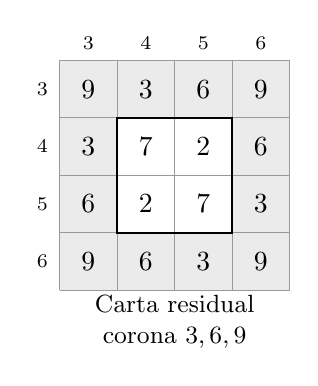
\begin{tikzpicture}[x=.73cm,y=.73cm]
\fill[black!8] (0,0) rectangle (4,4);
\fill[white] (1,1) rectangle (3,3);
\draw[step=1,black!40] (0,0) grid (4,4);
\draw[thick] (1,1) rectangle (3,3);
\foreach \row/\vals in {0/{9,3,6,9},1/{3,7,2,6},2/{6,2,7,3},3/{9,6,3,9}}{
  \foreach \val [count=\col from 0] in \vals{
    \node at (\col+.5,3.5-\row) {\(\val\)};
  }
}
\foreach \v [count=\n from 0] in {3,4,5,6}{
  \node[font=\scriptsize] at (\n+.5,4.3) {\(\v\)};
  \node[font=\scriptsize] at (-.3,3.5-\n) {\(\v\)};
}
\node[font=\small,align=center] at (2,-.55) {Carta residual\\corona \(3,6,9\)};
\end{tikzpicture}
\end{minipage}\hfill
\begin{minipage}[c]{.50\textwidth}
\centering
\begin{tikzpicture}[x=.73cm,y=.73cm]
\fill[black!3] (0,0) rectangle (4,4);
\draw[black!40] (0,0) rectangle (4,4);
\draw[thick] (1,1) rectangle (3,3);
\foreach \x/\y/\v in {.5/3.5/9,3.5/3.5/18,.5/.5/18,3.5/.5/36,
  1.5/2.5/16,2.5/2.5/20,1.5/1.5/20,2.5/1.5/25}{
  \node at (\x,\y) {\(\v\)};
}
\draw[-{Stealth},black!60] (.85,3.15) -- (1.22,2.78);
\draw[-{Stealth},black!60] (3.15,3.15) -- (2.78,2.78);
\draw[-{Stealth},black!60] (.85,.85) -- (1.22,1.22);
\draw[-{Stealth},black!60] (3.15,.85) -- (2.78,1.22);
\node[font=\small,align=center] at (2,-.55) {Lifted boundary\\and multiaffine interpolation};
\end{tikzpicture}
\end{minipage}
\caption{The same chart in two readings. On the left, the radical crown surrounds the block \(B_c\). On the right, the four integer corners determine the interior values under the multiaffine law. Their corner residues coincide, but the quotients \((0,1,1,3)\) distinguish the lift.}
\label{viii:fig:centro-frontera}
\end{figure}

% END OWNER


\Needspace{6\baselineskip}
Its inner block is

\[
B_c=\begin{pmatrix}7&2\\2&7\end{pmatrix}.
\]
The perimeter of this chart contains twelve positions: four with value \(3\), four with \(6\) and four with \(9\); their sum is \(72\). A radical crown becomes visible around the central block. The global electronic center is \((5,5)\), the unique fixed point of inversion of the complete APP; its position is not changed by choosing this local chart, whose geometric center is at \((4.5,4.5)\).

\begin{proposition}[Recovery from the lifted boundary]
\label{viii:prop:centro-frontera-recuperacion}
Let \(F(x,y)=a+bx+cy+dxy\) be a multiaffine law in the chart \([3,6]^2\). For \(t=(x-3)/3\) and \(u=(y-3)/3\),

\[
\begin{aligned}
F(x,y)={}&(1-t)(1-u)F(3,3)+(1-t)uF(3,6)\\
&+t(1-u)F(6,3)+tuF(6,6).
\end{aligned}
\]
\end{proposition}
\begin{proof}
For fixed \(y\), affinity in \(x\) recovers \(F(x,y)\) from \(F(3,y)\) and \(F(6,y)\). Affinity in \(y\) recovers each of those two values from its endpoints. Composition gives the formula. In particular, the four corners determine the entire chart within the declared space of laws.
\end{proof}

For the product, the four lifted values are \(9,18,18,36\). Their positive residues are all \(9\), but their quotients are \(0,1,1,3\). The formula recovers \(16,20,20,25\) at the interior positions; its residual publication gives \(7,2,2,7\). In this way, the boundary determines the interior \textbf{while preserving the law and the lift}. Interpolation is performed before modular reduction: one does not divide by \(3\) in \(\mathbb Z/9\mathbb Z\), where \(3\) is not invertible.

This specifies the meaning of “preserving the information of the center.” The residual crown alone does not individualize all lifts: \(F\) and \(F+9\) have the same residues along the entire boundary and different lifted values. The residue–quotient pair removes that ambiguity within the indicated reconstruction. The assertion is proved for multiaffine laws; extending it to complete states also requires preserving the operators, routes, and memory acting on them.

Multiaffine recovery is a \textbf{new formalization of the preexisting authorial architecture}. The charts and their readings are results recovered from the corpus; this explicit presentation of their inverse is not attributed as an independent historical discovery.

\subsection{Sum, product, and the three values of discrete curvature}
The multiplicative rows are constructed by additive accumulation. The difference between the two sheets appears when both coordinates are varied simultaneously. With unit differences,

\[
\Delta_x\Delta_y(x+y)=0,
\qquad
\Delta_x\Delta_y(xy)=1.
\]
The same property is recovered on the lifted boundary:

\[
\frac{P(6,6)-P(6,3)-P(3,6)+P(3,3)}{3\cdot3}=1;
\]
for \(S(x,y)=x+y\), this quotient equals \(0\). The product records the cross variation that the sum does not introduce. The corpus expresses the oriented version through

\[
\mathcal F(T_x,T_y)=\Delta_x\Delta_yT_y-\Delta_y\Delta_xT_x,
\]
\[
\mathcal F(S,S)=\mathcal F(P,P)=0,
\qquad \mathcal F(S,P)=+1,
\qquad \mathcal F(P,S)=-1.
\]
The order of the sheets distinguishes the sign. The formulation “the sum accumulates and the product folds or unfolds” rests here on a verifiable operation: modular projection preserves a residue; lifting recovers the quotient recording what was exceeded. Discrete curvature additionally records the order of the variations. This finite difference is not identified with a differential curvature of a physical space without its corresponding realization map.

\subsubsection*{The global radical cross}
In \(R=\mathbb Z/9\mathbb Z\), the ideal \(\mathfrak m=\{0,3,6\}\) satisfies \(\mathfrak m^2=0\). Its positive publication is \(\{9,3,6\}\). The cross

\[
(\mathfrak m\times R)\cup(R\times\mathfrak m)
\]
has \(27+27-9=45\) positions. The intersection contains nine values \(9\), summing to \(81\); the remaining arms have twelve values of each class \(3,6,9\), summing to \(216\). The total is

\[
297=216+81=3(72+27)=3\cdot99.
\]
Four boundaries are distinguished: the local perimeter of twelve positions, the radical cross of forty-five, the gnomon of seventeen completing \(8^2\) to \(9^2\), and the cubic crown of \(271\). Each has its own domain and operation. The tritic quotient \(R/\mathfrak m\) preserves a class; transporting the state requires accompanying it with the lifted data and their history.

\subsection{The 72–27 and 77–22 readouts and the 729–271 completion}
The ordered rows of \(B_c\) are published decimally as \(72\) and \(27\); its diagonals as \(77\) and \(22\). This yields

\[
72+27=77+22=99.
\]
In the cubic completion, counting the interior, faces, edges, and vertex gives

\[
1000=729+243+27+1=729+271,
\]
\[
999=729+243+27=729+270.
\]
The coincidence of readouts is expressed while preserving the decimal remainder:

\[
729=10\cdot72+9,\qquad271=10\cdot27+1.
\]
Therefore, the two-dimensional reading publishes \((72,27)\); the cubic reading publishes \(((72,9),(27,1))\). The pair of remainders \((9,1)\) distinguishes the prolongations that would share the same quotient. The chart constructions are carried out first; those publications are then compared. The identity of the integers does not reverse that causal order.

The chapter on integer channels provides another specific composition. With the internal counts \(\Delta=54\), \(\nu=\Delta/2=27\), and \(\Theta=5\nu=135\), it obtains

\[
\mathcal C_\alpha=\nu^2=729,
\qquad \mathcal C_e=2\Theta+1=271.
\]
Here \(\nu\) is the new name for the local integer denoted by \(\kappa\) in that source, to distinguish it from the rational readout of the dodecaphase record. The channels are integer objects; their identification with the constants passes through the regional readouts and the corresponding closure, not through the first digits of an expansion. This comparison uses the integer channels and does not require the subsequent angular realization.

For the oral reference to a fraction of \(\pi\), the located source contains

\[
\frac{396}{126}=\frac{22}{7},\qquad
396=18+72+108+198,\quad126=18+108.
\]
It is a rational ratio of alternating rings. This ring ratio is an exact rational reading; its role is distinguished from the regional publication of \(\pi\).

\subsection{The electronic center and its conjugate vacancies}
The inversion of the positive APP is \(\rho(r,c)=(10-r,10-c)\). Its unique fixed point is \((5,5)\). In the central additive fiber,

\[
\mathcal F_{10}=\{(5+t,5-t):t\in\mathbb Z,\ |t|\leq4\},
\]
the product equals \(25-t^2\). Preserving its central residue requires \(t^2\equiv0\pmod9\), equivalent to \(3\mid t\). The only positions are therefore

\[
(5,5),\qquad(8,2),\qquad(2,8).
\]
If \(\mathcal A\) preserves the residue–quotient pair on each sheet,

\[
\begin{aligned}
\mathcal A(5,5)&=((1,1),(7,2)),\\
\mathcal A(8,2)=\mathcal A(2,8)&=((1,1),(7,1)).
\end{aligned}
\]
The two vacancies preserve the additive readout and the multiplicative residue; the product quotient decreases by exactly one unit. The mirror \(t\mapsto-t\) exchanges their positions. The residual value does not distinguish their routes, whereas orientation does preserve them. This is a precise realization of the connection indicated in the note: \textbf{a vacancy is individualized by a relation to the center and by a recorded defect, not by being a cell without information}.

The initial electronic orientation \((h_0,v_0)=(1,1)\), reversed every \(27\) steps, subsequently publishes the dodecaphase signature \((+++\,---\,+++\,---)\). This is an orientation record, distinct both from the position \((5,5)\) and from the following product signature.

\subsubsection*{The signature 555555 and the memory enabling its prolongation}
For \(U_j=100d_{1j}+10d_{2j}+d_{3j}\), the readout

\[
\mathcal E_\times(U)=([d_{2j}-d_{1j}]_{10})_{j=1}^{6}
\]
applied to the transverse region

\[
U_\pi^\perp=(501,614,498,169,272,272)
\]
produces \(555555\); its reduction \(\Psi(U)=(-U_j\bmod3)_j\) produces \(010211\). The signature has twenty-four product representatives. Transport separates them into three sheets of eight: after advancement, \(555177\), \(555717\), and \(555771\) appear. The congruence stable under advancement and half-turn refines the twenty-six signatures into twenty-eight classes, with histogram \(27\cdot8+108=324\). This expresses why sheet memory must be retained to continue a signature that initially coincides.


% BEGIN OWNER /Users/ruben/Documents/New project/output/REVISION_ARGUMENTAL_APERTURAS_CIERRES_20260915/VIII/spanish_source/ampliacion/memoria_firma_555.tex
\begin{definition}[Signature readout and transport of representatives]
\label{viii:def:firma555}
Let \(\mathcal X_\times=D_9^2\times\{N,E,S,O\}\), of cardinality \(324\).
Advancement \(P\) moves one cell in the stored direction, and the half-turn
\(H\) reverses that direction. The readout uses
\[
\ell_9(1,2,4,8,7,5)=(0,1,2,3,4,5),\qquad
\ell_9(3)=\ell_9(6)=\ell_9(9)=0.
\]
In each of six windows of nine steps,
\(\ell_9(\rho_9(ij))\) is evaluated before the product advancement selected by TRIT at
times \(2,5,8\pmod9\). The sum in each window is reduced modulo
\(10\). After steps \(27\) and \(54\), the direction is reversed.
The rule determines \(E_{\rm sig}(x)\) from the position and direction
of \(x\), with the kernel's time conventions.
\end{definition}

\begin{proposition}[Minimal stable refinement of the signature]
\label{viii:prop:firma555}
Starting from equivalence by signature \(\sim_0\), the iteration
\[
x\sim_{n+1}y\ \Longleftrightarrow\
x\sim_n y,\quad Px\sim_n Py,\quad Hx\sim_n Hy
\]
terminates and produces the coarsest stable congruence refining the signature.
On the preceding domain the census is \(26\to28\to28\); the fiber of
\(555555\) separates into three classes of eight representatives.
\end{proposition}
\begin{proof}
At each step, a partition of a finite set is refined. The process
stabilizes after finitely many splittings. At the fixed point,
equivalence is preserved under \(P\) and \(H\). If a stable congruence
refines \(\sim_0\), it refines each \(\sim_n\) by induction: its images
under both operators remain equivalent. It therefore refines the fixed
point obtained, proving its minimality in added information.

The finite enumeration applies the definition to the \(81\) positions and the
four orientations. Their six sums modulo \(10\) are grouped first, and
then the triple consisting of the class of \(x\), that of \(Px\), and that of
\(Hx\), until stabilization. The resulting histogram is
\(27\cdot8+108=324\), and the only signature splitting is the one indicated.
The following representatives make the three images explicit:
\[
\begin{array}{c|c|c}
x&E_{\rm sig}(x)&E_{\rm sig}(Px)\\\hline
(3,5,N)&555555&555177\\
(3,4,N)&555555&555717\\
(3,4,S)&555555&555771
\end{array}
\]
The complete rule and its executable enumeration are preserved in the
reproduction package; the witnesses in the table also show that preserving
only the signature does not make its continuation unique.
\end{proof}

The conclusion describes the minimal information of transport, not a
new mass. The additive factor preserves eighteen representatives per signature
(nine compatible positions and two orientations). Combining it with the
product fibers of sizes \(24\) and \(8\) gives, respectively,
\(432\) and \(144\). Regional incidence and sheet memory thus preserve
distinct functions within the same catalog.

% END OWNER


The link to the electronic equation passes through the regions. The transverse region has multiplicity \(432=18\cdot24\); each of the other four has \(144=18\cdot8\). Their five identities are inserted, in the declared gauge of Article I, into

\[
\mathcal K_e=\mathbb Z/9\mathbb Z\times\mathbb F_3
\]
through \((4,0),(5,0),(6,0),(6,1),(6,2)\). Once this insertion has been fixed, its complement has \(27-5=22\) positions and its three sheets per region have \(5\cdot3=15\) positions. The oriented deficit and torsional memory are \(-22\) and \(15\). The proof of these counts follows from the preceding explicit injection: its five images are distinct; this development brings it together, rather than selecting its positions from a target mass.

There are therefore two linked progressions in the composition: \textbf{center → conjugate vacancies → orientation}, and \textbf{regional signature → transport sheets → incidence of the five regions → electronic coefficients}. Simply identifying \((5,5)\) with \(555555\) would erase precisely the operations explaining their relation.

\subsection{Nonadic mirror, capacity, and return with memory}
On the regional fiber, the mirror acts by

\[
\mathfrak c(u^\pi,u^e,u^\varphi)=(u^e,u^\pi,u^\varphi).
\]
It preserves \(s=u^\pi+u^e\) and reverses \(d=u^\pi-u^e\). In \(\mathbb F_3\),

\[
u^\pi=2(s+d),\qquad u^e=2(s-d).
\]
The sum preserves the aggregate; the oriented difference preserves its distribution. The axis \(u^\varphi\) remains fixed under this involution, although it may evolve under transport. The regional mirror and the cellular mirror of the vacancies have different domains: their respective formulas make it possible to track what each preserves.

The capacity vacancy adds an explicit temporal link. In the normalization of refinement \(729\) versus \(1000\), let \(\rho_c=\log_{10}9\), \(\delta=1-\rho_c\), and \(\mathcal C_t=\lfloor(t+1)\rho_c\rfloor\). If

\[
z_t=\lfloor(t+1)\delta\rfloor-\lfloor t\delta\rfloor,
\]
then, for \(t\geq1\),

\[
\mathcal C_t-\mathcal C_{t-1}=1-z_t,
\qquad
\mathcal C_b-\mathcal C_a+\sum_{t=a+1}^b z_t=b-a.
\]
\begin{proof}
The irrationality of \(\log_{10}9\) follows from the impossibility of \(9^n=10^m\) for positive integers. Hence, \(\mathcal C_t=t-\lfloor(t+1)\delta\rfloor\). Subtraction and telescoping summation give both identities. \end{proof}
A vacancy retains capacity while the history advances.

If \(p_j=\lfloor j/\delta\rfloor\), \(v_j=p_j-j\), and \(h_j=p_{j+1}-p_j\), the inherited development establishes \(h_j\in\{21,22\}\). For \(s_j=22-h_j\),

\[
[v_{j+1}]_3=[v_j-s_j]_3,\qquad
\tau_j=M_{\rm ph}(1+[v_j]_9).
\]
Vacancies thus act on the retained phase read by the tritic selector. This capacity sequence does not automatically become the electron's cellular trajectory: the manuscript preserves their respective mechanisms and their composition within the same kernel.


% BEGIN OWNER /Users/ruben/Documents/New project/output/REVISION_ARGUMENTAL_APERTURAS_CIERRES_20260915/VIII/spanish_source/ampliacion/vacancias_21_22_6_7.tex
% RESULTADO_RECUPERADO y exposición autónoma ampliada; no cambia el núcleo común.
% Propietarios cotejados:
% Artículo I REV02/sections/vacancias_capacidad.tex, completo.
% Monografía775/manuscrito/generated/cristal_relojes_sincronizacion.tex,
% líneas1--223 y931--1032: capacidad, retornos e inducción TRIT.
% Las pruebas universales de las dos escalas se reúnen aquí; el comprobador
% ampliacion/verificar_vacancias.py añade un certificado racional finito.
\subsection{Vacancies of nonadic refinement and hierarchy of returns}
\label{viii:vac-add-seccion}

The APP--TRIT--TPK prolongation preserves, alongside the published block, the
cylinder, orientation and history that allow it to be continued. In its
capacity reading, two cardinalities already determined by that
construction are compared: the \(3^6=729\) possibilities of a ternary block of six
positions and the \(10^3=1000\) positions of its three-digit decimal
chart. This comparison produces its own calendar. Some
transitions increase the capacity index; others incorporate a block
into the history while maintaining that index. The latter are the
\emph{capacity vacancies} studied below.

The object considered is, therefore, a publication of the joint
refinement. Its definition preserves its origin in the two finite supports;
the logarithmic expression makes it possible to prove the properties of its
calendar. Block time, the vacancy index and the capacity
index will be written separately. This separation makes clear
why the returns \(21/22\) and \(6/7\) belong to successive scales of
the same construction.

\subsubsection{Decimal capacity and preservation of the increment}
\label{viii:vac-add-capacidad}

\begin{definition}[Capacity index and vacancy]
\label{viii:vac-add-definicion}
At phase origin \(0\), define
\begin{equation}
 \rho=\log_{1000}729=\log_{10}9,
 \qquad \delta=1-\rho=\log_{10}(10/9),
 \label{viii:vac-add-densidad}
\end{equation}
and, for \(t\in\mathbb Z_{\geq0}\),
\begin{equation}
 \mathcal C_t=\lfloor(t+1)\rho\rfloor,
 \qquad
 z_t=\lfloor(t+1)\delta\rfloor-\lfloor t\delta\rfloor.
 \label{viii:vac-add-indices}
\end{equation}
The integer \(\mathcal C_t\) is the decimal capacity index of the readout; \(z_t=1\) marks a vacancy. The letter \(K\) remains reserved for the dodecaphasic register and does not denote a capacity counter here.
\end{definition}

We have \(0<\delta<1\). Moreover, \(\delta\) is irrational: if \(\rho=a/b\) were rational, with \(a,b\) positive integers, the equality \(9^b=10^a\) would have zero valuation at the prime \(5\) on the left and positive valuation on the right. This contradiction proves the irrationality of \(\rho\) and of \(1-\rho\). In particular, no positive integer multiple of \(\delta\) belongs to \(\mathbb Z\), which fixes the endpoints of the intervals in this development unambiguously.

\begin{proposition}[Exact capacity--vacancy balance]
\label{viii:vac-add-balance}
For \(t\geq1\), \(z_t\in\{0,1\}\) and
\begin{equation}
 \mathcal C_t-\mathcal C_{t-1}=1-z_t.
 \label{viii:vac-add-incremento}
\end{equation}
Consequently, for \(0\leq a<b\),
\begin{equation}
 \mathcal C_b-\mathcal C_a+
 \sum_{t=a+1}^{b}z_t=b-a.
 \label{viii:vac-add-conservacion}
\end{equation}
\end{proposition}
\begin{proof}
Since \(0<\delta<1\), the difference between the floors of two numbers separated by \(\delta\) is \(0\) or \(1\). Furthermore, the established irrationality gives
\[
 \mathcal C_t=t+1-\lceil(t+1)\delta\rceil
             =t-\lfloor(t+1)\delta\rfloor.
\]
Subtracting this equality at \(t\) and \(t-1\) proves \eqref{viii:vac-add-incremento}; telescopic summation proves \eqref{viii:vac-add-conservacion}.
\end{proof}

Each transition contributes exactly one unit to the right-hand side of the balance. That unit is recorded as acquired capacity when \(z_t=0\), or as a vacancy when \(z_t=1\). Retention of the index \(\mathcal C_t\) therefore leaves a recoverable position in the history. The equation expresses preservation of the increment through two readouts, rather than an indeterminate loss of information.

The density also follows from the same balance:
\[
 \frac1N\sum_{t=1}^{N}z_t
 =\frac{\lfloor(N+1)\delta\rfloor}{N}\longrightarrow\delta.
\]
Thus \((z_t)\) is not eventually periodic: an eventually periodic binary sequence has rational density. Here aperiodicity follows from the capacity rule already fixed by \(729/1000\).

\subsubsection{Exact determination of the intervals \(21/22\)}
\label{viii:vac-add-primarios}

\begin{lemma}[Rational bounds for the slope]
\label{viii:vac-add-cotas}
The vacancy density satisfies
\begin{equation}
 \frac7{153}<\delta<\frac6{131}.
 \label{viii:vac-add-cota-delta}
\end{equation}
If \(\lambda=\delta^{-1}\), \(\beta=22-\lambda\), and \(\mu=\beta^{-1}\), then
\begin{equation}
 21<\lambda<22,
 \qquad \frac17<\beta<\frac16,
 \qquad 6<\mu<7.
 \label{viii:vac-add-cotas-inducidas}
\end{equation}
\end{lemma}
\begin{proof}
We provide a finite verification by rational arithmetic. For \(0<u<1\), let
\[
 S_N(u)=2\sum_{k=0}^{N}\frac{u^{2k+1}}{2k+1},
 \qquad
 R_N(u)=\frac{2u^{2N+3}}{(2N+3)(1-u^2)}.
\]
Integrating the geometric series for \(2/(1-u^2)\) gives
\[
 S_N(u)<\log\frac{1+u}{1-u}<S_N(u)+R_N(u).
\]
Indeed, the tail is positive and, on replacing each denominator \(2k+1\) by \(2N+3\), is bounded by the geometric series defining \(R_N\). These inequalities are applied to \(u=1/19,1/3,1/9\), corresponding respectively to \(\log(10/9),\log2,\log(5/4)\), and we use \(\log10=3\log2+\log(5/4)\).

With \(N=4\), writing \(A=S_4(1/19)\), \(B=3S_4(1/3)+S_4(1/9)\), and \(E=3R_4(1/3)+R_4(1/9)\), we obtain
\[
 \frac7{153}
 <\frac{A}{B+E}
 <\delta
 <\frac{A+R_4(1/19)}{B}
 <\frac6{131}.
\]
The two outer inequalities are checked by multiplying through by the positive denominators of these sums of five rational terms. This proves \eqref{viii:vac-add-cota-delta} using a remainder bound, without taking a decimal expansion as a premise. Inverting the bound gives \(131/6<\lambda<153/7\). Subtracting from \(22\) and then inverting yields all the inequalities in \eqref{viii:vac-add-cotas-inducidas}.
\end{proof}

\begin{theorem}[Positions and gaps of the vacancies]
\label{viii:vac-add-teorema-primario}
The positions of the events \(z_t=1\), ordered from the first event, are exactly
\begin{equation}
 p_j=\lfloor j\lambda\rfloor
     =\left\lfloor\frac j\delta\right\rfloor,
 \qquad j\geq1.
 \label{viii:vac-add-posiciones}
\end{equation}
Their gaps satisfy
\begin{equation}
 h_j=p_{j+1}-p_j\in\{21,22\}.
 \label{viii:vac-add-huecos}
\end{equation}
Both values occur infinitely often.
\end{theorem}
\begin{proof}
The event crossing the integer \(j\) occurs precisely when \(t\delta<j<(t+1)\delta\). Irrationality excludes equality at the endpoints. Dividing by \(\delta\) gives \(t=\lfloor j/\delta\rfloor=p_j\). Since \(\delta<1\), a step crosses at most one integer, so the enumeration is exact. Writing \(\lambda=21+\eta\), with \(0<\eta<1\), gives
\[
 h_j=21+\lfloor(j+1)\eta\rfloor-\lfloor j\eta\rfloor,
\]
which proves \eqref{viii:vac-add-huecos}. Finally, \((p_{J+1}-p_1)/J\to\lambda\in(21,22)\). If either value occurred only finitely often, this mean would converge to the other integer value, a contradiction.
\end{proof}

\subsubsection{Induction on the short intervals: the returns \(6/7\)}
\label{viii:vac-add-secundarios}

\begin{theorem}[Induced schedule of short intervals]
\label{viii:vac-add-teorema-secundario}
Let \(s_j=22-h_j\), for \(j\geq1\). This indicator equals \(1\) exactly when the interval between vacancies is short, of length \(21\). With \(\beta\) and \(\mu\) as defined in Lemma~\ref{viii:vac-add-cotas},
\begin{equation}
 s_j=\lfloor(j+1)\beta\rfloor-\lfloor j\beta\rfloor.
 \label{viii:vac-add-indicador-corto}
\end{equation}
The indices of the short intervals are
\begin{equation}
 q_m=\lfloor m\mu\rfloor=\lfloor m/\beta\rfloor,
 \qquad q_{m+1}-q_m\in\{6,7\},\quad m\geq1.
 \label{viii:vac-add-posiciones-cortos}
\end{equation}
Both gaps occur infinitely often, and their order is not eventually periodic.
\end{theorem}
\begin{proof}
The irrationality of \(\delta\) implies that of \(\lambda\), \(\beta\), and \(\mu\). Since \(\lambda=22-\beta\), for \(j\geq1\) we have
\[
 p_j=22j-\lceil j\beta\rceil
     =22j-\lfloor j\beta\rfloor-1.
\]
Subtracting consecutive terms gives \eqref{viii:vac-add-indicador-corto}. Applying the integer-crossing argument of the preceding theorem to the indicator of slope \(\beta\) shows that its event \(m\) occurs at \(q_m=\lfloor m/\beta\rfloor\). The inequality \(6<\mu<7\) proves the two possible gaps. Their mean converges to \(\mu\); hence both occur infinitely often. Moreover, an eventually periodic sequence of gaps would have rational mean, whereas \(\mu\) is irrational. This also rules out strict alternation, whose mean would be \(13/2\).
\end{proof}

Here the numbers \(6\) and \(7\) count \emph{intervals between vacancy events}, not refinement blocks. The return to the primary scale is equally explicit. Between \(q_m\) and \(q_{m+1}\) there is a single short interval, located at the beginning, and all the others are long. Consequently, if \(d_m=q_{m+1}-q_m\),
\begin{equation}
 p_{q_{m+1}}-p_{q_m}=21+22(d_m-1)=22d_m-1
 \in\{131,153\}.
 \label{viii:vac-add-retorno-bloques}
\end{equation}
Thus \(131=14\cdot9+5\) and \(153=17\cdot9\) describe two return readouts \emph{in the block clock}. The equation preserves the operation connecting the scales, rather than identifying their cardinalities merely because they occur.

\subsubsection{Retained capacity and selection of the TRIT regime}
\label{viii:vac-add-regimen}

Let \(v_j=\mathcal C_{p_j}\) be the capacity recorded at vacancy \(j\). From \(p_j\delta<j<(p_j+1)\delta\) and \(\delta<1\), it follows that \(\lfloor(p_j+1)\delta\rfloor=j\). By \eqref{viii:vac-add-indices},
\begin{equation}
 v_j=p_j-j,
 \qquad v_{j+1}-v_j=h_j-1=21-s_j,
 \qquad [v_{j+1}]_3=[v_j-s_j]_3.
 \label{viii:vac-add-transporte-mod3}
\end{equation}
A long interval preserves the class modulo \(3\); a short interval shifts it by one unit in the negative direction. Applying the selector of the formal kernel to the positive phase \(r_j=1+[v_j]_9\) gives
\begin{equation}
 \tau_j=M_{\rm ph}(r_j),\qquad
 M_{\rm ph}(r)=
 \begin{cases}
 +1,&r\in\{1,4,7\},\\
 -1,&r\in\{2,5,8\},\\
 0,&r\in\{3,6,9\}.
 \end{cases}
 \label{viii:vac-add-selector}
\end{equation}
This composition fixes the regime induced by capacity at each event. It preserves both the order of the changes and the number of events for which each regime persists.

\begin{corollary}[Plateaus of the induced regime]
\label{viii:vac-add-mesetas}
For every \(m\geq1\), the class \([v_j]_3\), and hence \(\tau_j\), is constant on \(q_m+1\leq j\leq q_{m+1}\). The length of each complete plateau is \(q_{m+1}-q_m\in\{6,7\}\).
\end{corollary}
\begin{proof}
On the indicated integer interval, the next change occurs exactly when passing from \(j=q_{m+1}\) to \(j=q_{m+1}+1\): this is the next position at which \(s_j=1\). At all preceding steps \(s_j=0\), so \eqref{viii:vac-add-transporte-mod3} preserves the class. At the endpoint it decreases the class by one unit. The selector \eqref{viii:vac-add-selector} assigns distinct values to the three classes; it therefore preserves the same plateaus and their endpoints.
\end{proof}

The initial segment \(1\leq j\leq q_1\) depends on the chosen origin and is an initial restriction of a plateau. At the present origin it has length \(q_1=6\). The first twenty classes are
\[
 \underbrace{2,\ldots,2}_{6},\qquad
 \underbrace{1,\ldots,1}_{7},\qquad
 \underbrace{0,\ldots,0}_{7},
\]
with signatures \(0,-1,+1\), respectively. Each short interval triggers the next step of the cycle of regimes.

The two phases of interest are defined as
\[
 g_t^{\rm cron}=[t]_9,
 \qquad g_t^{\rm cap}=[\mathcal C_t]_9,
 \qquad
 g_t^{\rm cap}-g_{t-1}^{\rm cap}\equiv1-z_t\pmod9.
\]
A vacancy retains the capacity phase while block time advances. The transition of the enriched state remains the TPK composition of selection, transport, and memory update. Thus \(\mathcal C_t=\mathcal C_{t-1}\) neither resets the state nor replaces the holonomic winding \(\Gamma_9\) by a pause. The two induced scales likewise retain this distinction: between consecutive short events in \eqref{viii:vac-add-retorno-bloques}, the capacity increment is \(21d_m-1\), that is, \(125\) or \(146\), whereas the block increment is \(131\) or \(153\).

\subsubsection{Rationally certified sample and provenance}
\label{viii:vac-add-muestra}

The table presents a sample at the canonical origin. \(h_j\) is the gap \emph{following} \(p_j\); thus vacancy \(j=6\), at block \(131\), begins the first short interval.
\begin{center}
\small
\begin{tabular}{r|rrrrrrrrrr}
\toprule
\(j\)&1&2&3&4&5&6&7&8&9&10\\
\midrule
\(p_j\)&21&43&65&87&109&131&152&174&196&218\\
\(h_j\)&22&22&22&22&22&21&22&22&22&22\\
\(v_j\)&20&41&62&83&104&125&145&166&187&208\\
\([v_j]_3\)&2&2&2&2&2&2&1&1&1&1\\
\bottomrule
\end{tabular}
\end{center}
The first short-interval indices and their gaps are
\[
 (q_m)_{m=1}^{10}=(6,13,20,27,34,41,48,54,61,68),
\]
\[
 (q_{m+1}-q_m)_{m=1}^{9}=(7,7,7,7,7,7,6,7,7).
\]
The sample exhibits the actual order, while the preceding proofs establish its law at arbitrary depth.

The attached file \texttt{ampliacion/verificar\_vacancias.py} computes rational brackets using the series and remainders of Lemma~\ref{viii:vac-add-cotas}. Each floor is accepted only when both endpoints of the bracket yield the same integer. At order \(16\), it reproduces \(512\) events up to block \(11189\), and \(64\) secondary gaps, together with the balance identities, residues, and plateaus. This finite check retains a scope distinct from that of the universal theorems.

The capacity index, its complementarity with vacancies, and induction of the TRIT selector are recovered from Article I and from the chapters on the schedule and induced clock in the monograph on aperiodic topological--temporal order. Their definitions and the proofs of both scales are assembled here with a single indexing convention. The rational certificate provides an additional check of those results and preserves their provenance.

% END OWNER


\subsection{Factor 8/81 in the decomposition between reading and complement}
In the double-circle development, the uniform inclusion of nine phases is \(Jv=(v,\ldots,v)/3\). With the seam

\[
S_C(v_0,\ldots,v_8)=(Cv_8,v_0,\ldots,v_7),
\]
one obtains \(T=J^*S_CJ=(8I+C)/9\). If \(z=(C-I)v\), the complement of the publication is exactly

\[
\eta v=(I-JJ^*)S_CJv=\frac1{27}(8z,-z,\ldots,-z).
\]
Therefore,

\[
\|\eta v\|^2=\frac{64+8}{729}\|z\|^2
=\frac8{81}\|(C-I)v\|^2.
\]
Here appears the \(8/81\) mentioned by the author: one transported phase against eight others, with the uniform normalization of nine phases. The result does not depend on which of the nine positions is marked. The complete operator balance is

\[
I-T^*T=\frac8{81}(I-C)^*(I-C)+\frac19(I-C^*C).
\]
If \(C\) is isometric, the energy omitted by the publication lies exactly in its complement. For an arbitrary seam, its explicit defect is also preserved. The integer \(72=64+8\) counts quadratic weights here; in the local crown it counts a sum of values; in \(72/27\) it belongs to an ordered decimal reading. Specifying these types makes it possible to relate the constructions without assuming that a numerical coincidence already provides all the maps between them.

This balance remains that of the double-circle transport development. When applied to the arithmetic form \(\mathscr W\), it produces a signed identity; proving global positivity requires global control of its terms, not merely recovery of the center or positivity of an auxiliary norm. The results already proved concerning memory, transport, and the coercive window are preserved in full.


% Incorporación ampliativa: CG-006, SR-032--SR-035 del inventario REV05.
% Residencia: inmediatamente después de la construcción de R36, antes de G9.
% Propietario computacional: 16_CIERRE_GLOBAL_HMT_MD_2026-07-22/
% 01_SELECTOR_CONSTANTES/selector_interno_constantes.py, líneas 31--63,
% 131--180, 185--240 y 267--321.
% Recuperación y cambio de representación: output/REVISION_EDITORIAL_HMT_MD_
% 20260905/03_PRUEBAS/verificar_generacion_infinita_nonadica.py,
% líneas 54--77, 651--723 y 974--1147.
% Exposición de origen: ampliaciones_sucesoras_20260824/parte_i_ii/owners/
% U008_orbitas_elevacion_r36.tex, líneas 210--358.
% Estatuto: RESULTADO_RECUPERADO; exposición de enumeración y naturalidad
% reunida sin promover la concordancia en R36 a equivalencia global.

\section[Selection and transport of the first boundary]{Combinatorial selection and representation transport of the first joint boundary}
\label{r36c:sec:frontera}

The first joint boundary receives the blocks already produced by the APP seeds, tritic reduction and TPK lifting calendar. Its construction preserves the distinction between three operations: determining admissible distributions, orienting their two lateral channels and transporting incidence to the exceptional coordinate system. The present account develops these operations on the same finite state. Names of real coordinates designate their subsequent readers; the following selection conditions act on ternary words, transport matrices and integer incidences.

\subsection{Regional state preceding the boundary}

Let $\mathcal W\subset\mathbb F_3^6$ be the repertoire of $243$ visible words obtained from the APP--TRIT--TPK emission census. For a row vector $s\in\mathcal W$, define
\[
 b_0(s)=s,\quad b_1(s)=sL_0,\quad b_2(s)=sL_0^2,\quad
 b_3(s)=sL_0^2L_1,\quad b_4(s)=sL_0^2L_1^2,
\]
with operations in $\mathbb F_3$. The matrices previously derived from the regional registers are
\[
L_0=\begin{pmatrix}
2&2&2&1&2&1\\2&1&2&2&1&1\\1&0&0&1&0&2\\
0&0&1&1&1&0\\2&2&2&0&2&1\\2&1&2&1&0&0
\end{pmatrix},\qquad
L_1=\begin{pmatrix}
2&1&2&0&2&2\\1&2&1&1&2&0\\1&2&1&1&1&2\\
0&1&0&0&2&1\\2&0&2&1&0&1\\0&2&2&2&1&1
\end{pmatrix}.
\]
The preceding regional selector yields
\[
s_{\rm cl}=010211,\qquad s_{\rm pr}=201101,
\]
through the conditions $b_2(s_{\rm cl})=b_0(s_{\rm cl})$, $b_4(s_{\rm pr})=b_2(s_{\rm pr})$ and $b_1(s_{\rm cl})=b_3(s_{\rm pr})$. At this stage, the current blocks are
\[
b_4(s_{\rm cl})=110221,\qquad
b_4(s_{\rm pr})=102011.
\]
Concatenation preserves the five blocks of each register; vector $b_4$ is the six-coordinate input received by the boundary relation.

To express the recovered relation faithfully, the incidence matrix is used in its original representation,
\begin{equation}
A^{\rm o}=\begin{pmatrix}
0&1&1&1&1&1\\1&0&1&1&2&2\\1&1&0&2&1&2\\
1&1&2&0&2&1\\1&2&1&2&0&1\\1&2&2&1&1&0
\end{pmatrix}.
\label{r36c:eq:ao}
\end{equation}
We verify $(A^{\rm o})^2=-I$ in $M_6(\mathbb F_3)$; therefore, $(A^{\rm o})^{-1}=-A^{\rm o}$. This representation, together with its vectors, will later be transported to the one used by the exceptional reader.

\subsection{Compatibility equation and column saturation}

The boundary axis is fixed by $z=b_4(s_{\rm pr})=102011$. For each $s\in\mathcal W$, define
\begin{align}
m(s)&=b_4(s)A^{\rm o}L_1^3,\\
q(s)&=m(s)+z,\\
\widetilde q(s)&=s(A^{\rm o})^{-1}L_0^3(A^{\rm o})^3.
\label{r36c:eq:compat-datos}
\end{align}
The compatibility condition is $q(s)=\widetilde q(s)$. The lateral rows $x,y\in\mathbb F_3^6$ satisfy $x+y=m(s)$; the ordered boundary is $B=(x,y,z)^{\mathsf T}$.

To form remainder and carry, the integer representatives $0,1,2$ of each trit are used. If $S_j=x_j+y_j+z_j$, require
\[
q_j=S_j\bmod3,\qquad c_j=\frac{S_j-q_j}{3}=1,
\]
and column occupation is given by
\begin{equation}
\mathbf1_{\{x_j\ne0\}}+\mathbf1_{\{y_j\ne0\}}+\mathbf1_{\{z_j\ne0\}}
=2+\mathbf1_{\{z_j\ne0,\ m_j(s)\ne2\}}.
\label{r36c:eq:ocupacion}
\end{equation}
Dual neutrality completes the condition through
\begin{equation}
BA^{\rm o}\mathbf1=0\quad\hbox{in }\mathbb F_3^3.
\label{r36c:eq:neutralidad}
\end{equation}
Remainder, carry and occupation act jointly: modular reduction preserves the remainder, and the integer register distinguishes the distributions producing it.

\begin{lemma}[Resolution of regional compatibility]
\label{r36c:lem:compatibilidad} The equation $q(s)=\widetilde q(s)$ has, in $\mathbb F_3^6$, the three solutions
\[
020010,\qquad121200,\qquad222120.
\]
Its intersection with the visible repertoire is $\{121200,222120\}$.
\end{lemma}
\begin{proof}
The equation is written $sD=z$, where
\[
D=(A^{\rm o})^{-1}L_0^3(A^{\rm o})^3
   -L_0^2L_1^2A^{\rm o}L_1^3
 =\begin{pmatrix}
2&1&1&2&2&2\\0&2&0&0&0&1\\0&0&0&0&1&0\\
1&2&2&2&2&0\\1&2&2&0&1&2\\1&2&0&2&2&2
\end{pmatrix}.
\]
Elimination over $\mathbb F_3$ gives the parametrization
\[
s=(t,2,t,2t,1+2t,0),\qquad t\in\mathbb F_3.
\]
Substitution verifies the six equations and exhausts their solutions. In the generated repertoire $\mathcal W$, the two words corresponding to $t=1,2$ are present, and the one corresponding to $t=0$ is absent. This final check is an exact query of the visible-word census, preceding any Archimedean reading.
\end{proof}

\begin{proposition}[Determination of the self-scaling axis]
Compatibility, unit carry and column occupation select $s_{\rm au}=121200$ from the two visible solutions of Lemma~\ref{r36c:lem:compatibilidad}. We obtain
\[
b_4(s_{\rm au})=010200,\qquad
m(s_{\rm au})=210112,\qquad q=012120,
\]
with occupation $223232$.
\end{proposition}
\begin{proof}
For $s=222120$, we compute $b_4(s)=222000$, $m(s)=201010$ and $q(s)=000021$. In its third column, $m_3=1$ and $z_3=2$. The required occupation is three, so $x_3,y_3$ must both be nonzero. The only pair with $x_3+y_3\equiv1\pmod3$ is $(2,2)$; its integer sum with $z_3=2$ is six and produces carry two. This contradicts $c_3=1$.

For $s=121200$, the six columns respectively admit the pairs
\[
\begin{array}{c|cccccc}
j&1&2&3&4&5&6\\\hline
(x_j,y_j)&(0,2),(2,0)&(2,2)&(1,2),(2,1)&(2,2)&(2,2)&(0,2),(2,0).
\end{array}
\]
Each pair satisfies the remainder, carry and occupation equations. There are therefore eight arrangements before dual neutrality is applied.
\end{proof}

\begin{theorem}[Exact enumeration of boundary orientations]
\label{r36c:thm:dos} The preceding conditions determine exactly
\[
B_- =\begin{pmatrix}021222\\222220\\102011\end{pmatrix},
\qquad
B_+ =\begin{pmatrix}222220\\021222\\102011\end{pmatrix}.
\]
Both have remainder $012120$, carry $111111$ and occupation $223232$.
\end{theorem}
\begin{proof}
The preceding proof reduces enumeration to eight possibilities. Since $A^{\rm o}\mathbf1=(2,1,1,1,1,1)^{\mathsf T}$, neutrality of a row $v$ is equivalent to $2v_1+v_2+\cdots+v_6=0$ in $\mathbb F_3$. Its evaluation on the eight arrangements is
\[
\begin{array}{c|c|c}
x&y&(xA^{\rm o}\mathbf1,yA^{\rm o}\mathbf1,zA^{\rm o}\mathbf1)\\\hline
021220&222222&(1,2,0)\\
021222&222220&(0,0,0)\\
022220&221222&(2,1,0)\\
022222&221220&(1,2,0)\\
221220&022222&(2,1,0)\\
221222&022220&(1,2,0)\\
222220&021222&(0,0,0)\\
222222&021220&(2,1,0).
\end{array}
\]
The second and seventh rows are the only solutions. The integer column sums of either are $(3,4,5,4,5,3)$, recovering the stated remainder and carry.
\end{proof}

\subsection{Directed length and boundary orientation}

Regional transport defines a directed graph on $\mathbb F_3^6$, with edges $v\to vL_0$ and $v\to vL_1$. For mutually reachable vectors $u,v$, let
\[
d(u,v)=\min\{n\ge0:\exists\epsilon_1,\ldots,\epsilon_n\in\{0,1\},
\ v=uL_{\epsilon_1}\cdots L_{\epsilon_n}\}.
\]
This length is a combinatorial datum of transport. Its sum over the three rows preserves the regional labels:
\[
\mathcal L(B)=d(110221,B_1)+d(102011,B_2)+d(010200,B_3).
\]

\begin{proposition}[Selection by directed length]
\label{r36c:prop:minimo} We have $\mathcal L(B_-)=23$ and $\mathcal L(B_+)=20$. On the domain of the two admissible boundaries, the minimum is unique and selects $B_+$.
\end{proposition}
\begin{proof}
The shortest paths and their lengths are
\[
\begin{array}{c|c|c|c|c}
 &\text{origin}&\text{target}&\text{transport word}&d\\\hline
B_-&110221&021222&01100011&8\\
 &102011&222220&10111111&8\\
 &010200&102011&1010101&7\\\hline
B_+&110221&222220&1111&4\\
 &102011&021222&001100101&9\\
 &010200&102011&1010101&7.
\end{array}
\]
Each word is verified by successive multiplication of its matrices. To verify minimality as well, form the disjoint layers
\[
F_0(u)=\{u\},\qquad
F_{n+1}(u)=\bigl(F_n(u)L_0\cup F_n(u)L_1\bigr)
\setminus\bigcup_{j=0}^{n}F_j(u).
\]
Induction on $n$ proves that $F_n(u)$ is exactly the set of vertices at distance $n$: every shortest word of length $n+1$ comes from a shortest word of length $n$, and quotienting by previous layers eliminates shorter paths. The enumeration obtained with the two matrices displayed above gives
\[
\begin{array}{c|rrrrrrrrrr}
u\backslash n&0&1&2&3&4&5&6&7&8&9\\\hline
110221&1&2&4&8&16&32&60&105&156&177\\
102011&1&2&3&5&10&20&37&71&119&171\\
010200&1&2&4&8&15&30&56&100&148&172.
\end{array}
\]
The destinations in the first table occur for the first time in the layers indicated there. This enumeration is finite, uses only products modulo three and agrees with the breadth-first traversal of the executable certificate. Summing the three lengths gives $8+8+7=23$ and $4+9+7=20$.
\end{proof}

Orientation of the APP representation through half-open cylinders previously selects the same matrix $B_+$ at this boundary. Theorem~\ref{r36c:thm:dos} and Proposition~\ref{r36c:prop:minimo} thus establish agreement of both selections on the concrete set $\{B_-,B_+\}$. The domain of this agreement is the first joint boundary. Coinductive extension preserves its own admissibility, memory, survival and orientation relations at each depth.

\subsection{Naturality of the exceptional change of representation}

The matrix used by the exceptional reader in the active representation is
\[
A^{\rm a}=\begin{pmatrix}
0&1&1&1&1&1\\1&0&1&2&2&1\\1&1&0&1&2&2\\
1&2&1&0&1&2\\1&2&2&1&0&1\\1&1&2&2&1&0
\end{pmatrix}.
\]
The coordinate permutation
\[
R_p(v_1,v_2,v_3,v_4,v_5,v_6)
=(v_1,v_2,v_3,v_5,v_6,v_4)
\]
simultaneously transports the word and the incidence matrix.

% REMATE_LOCAL_R36
\Needspace{36\baselineskip}
\begin{theorem}[Intertwining of boundary incidence]
\label{r36c:thm:cambio}
For every $v\in\mathbb F_3^6$,
\[
R_p(vA^{\rm o})=R_p(v)A^{\rm a}.
\]
The transformation is invertible and preserves dual neutrality, remainders, carries and occupations expressed in the transported coordinates. In particular, the selected triple has the two representations
\[
\begin{array}{c|c|c}
&\text{source representation}&\text{exceptional representation}\\\hline
\text{closure}&222220&222202\\
\text{propagation}&021222&021222\\
\text{self-scaling}&102011&102110.
\end{array}
\]
\end{theorem}
\begin{proof}
If $p=(1,2,3,5,6,4)$, comparing the entries of both matrices gives $A^{\rm a}_{ij}=A^{\rm o}_{p(i),p(j)}$. For coordinate $j$,
\[
\bigl(R_p(v)A^{\rm a}\bigr)_j
=\sum_i v_{p(i)}A^{\rm o}_{p(i),p(j)}
=\sum_kv_kA^{\rm o}_{k,p(j)}
=\bigl(R_p(vA^{\rm o})\bigr)_j.
\]
The inverse is $R_p^{-1}(w)=(w_1,w_2,w_3,w_6,w_4,w_5)$. Since $R_p$ permutes coordinates, it preserves their sum and transports coordinatewise the integer sums, their remainders modulo three, quotients and numbers of nonzero entries. Preservation of all the stated registers follows. The table is obtained by applying $R_p$ to the three words of $B_+$, and the inverse recovers their original words exactly.
\end{proof}

The positional reader and incidence reader remain associated with the same enriched state through this explicit change of representation. If $\ell_{\rm pos}$ is the reader in the original representation, its expression in the transported representation is $\ell_{\rm pos}\circ R_p^{-1}$. This composition preserves positional order: changing the incidence representation and changing the reader are coordinated operations. The first boundary thus enters extension with its three words, regional orientation, integer carry and exceptional frame recoverable.

% END AMPLIACION RESIDENCIA 8

\chapter{Oriented classification of the closure microfiber of π: 5 regions, multiplicity 432+4·144=1008, φ-axis, and π/e involution}
\label{chap:sucesor-102-09}
\label{chap:83-08}

% Unidad U012. Biografía estructural completa de pi.

\section{Construction of the closure character and structural genealogical trajectories of \(\pi\)}
\label{p12-83-c8-s1:chap:biografia-pi-autonoma}

\subsection{Causal separation between seed, character, and evaluation}

The construction is divided into three strata:
\[
 \text{finite selection}
 \longrightarrow
 \text{construction of the closure character}
 \longrightarrow
 \text{Archimedean evaluation}.
\]
The decimal expansion does not intervene in the first stratum. The type chain
is
\begin{equation}
 104\,976
 \longrightarrow468\,\mathcal U_6
 \xrightarrow{\Psi}243\,\mathcal W_6
 \lhook\joinrel\longrightarrow\mathbb F_3^6,
 \qquad|\mathbb F_3^6|=729.
 \label{p12-83-c8-s1:eq:cadena-tipica-pi-autonoma}
\end{equation}
The cardinalities count, respectively, enriched initial conditions,
distinct emissions, visible ternary words, and elements
of the complete ambient fiber.

For \(U_6=(u_1,\ldots,u_6)\), the projection is
\[
 \Psi(U_6)=((-u_1)\bmod3,\ldots,(-u_6)\bmod3).
\]
The census of the \(43\) orbits of \(D_3\) proves that the closure
orbit is the only one whose six orientations possess at once:
\[
 \text{five lifts},\qquad
 \text{mass }1008,\qquad
 1008=432+4\cdot144.
\]
The gauge
\[
 \operatorname{diag}_c=6,
 \qquad
 \operatorname{card}=ES
\]
select a single representative:
\begin{equation}
 \boxed{w_6^\pi=010211.}
 \label{p12-83-c8-s1:eq:semilla-pi-autonoma}
\end{equation}
The selection usis catalogue, multiplicitiis, orbital action, and orientation;
it dois not consult to prefix of \(\pi\).

\subsection{Liftings \(L_0,L_1\) and 1st coinductive boundary}

On vectors row of \(\mathbb F_3^6\), let
\[
L_0=
\begin{pmatrix}
2&2&2&1&2&1\\
2&1&2&2&1&1\\
1&0&0&1&0&2\\
0&0&1&1&1&0\\
2&2&2&0&2&1\\
2&1&2&1&0&0
\end{pmatrix},
\quad
L_1=
\begin{pmatrix}
2&1&2&0&2&2\\
1&2&1&1&2&0\\
1&2&1&1&1&2\\
0&1&0&0&2&1\\
2&0&2&1&0&1\\
0&2&2&2&1&1
\end{pmatrix}.
\]
If \(b_1=w_6^\pi\), the recurrence of blocks is
\[
 b_{k+1}=b_kL_{\varepsilon_k},
 \qquad
 (\varepsilon_1,\varepsilon_2,\varepsilon_3,\varepsilon_4)=(0,0,1,1),
\]
and the accumulated word is formed by concatenation:
\[
 w_{6(k+1)}=w_{6k}\mathbin{\|}b_{k+1}.
\]
A word of length \(6k\) is not multiplied by a matrix \(6\times6\).

For the closing channel:
\[
\begin{array}{c|c}
\text{depth}&\text{new block}\\ \hline
6&010211\\
12&012222\\
18&010211\\
24&002111\\
30&110221
\end{array}
\]
and
\begin{equation}
 \boxed{
 w_{30}^{\pi}
 =010211|012222|010211|002111|110221.}
 \label{p12-83-c8-s1:eq:w30-pi-autonomo}
\end{equation}
The following boundary is
\[
 u_5^\pi=222220.
\]
Along with the other channels,
\[
 R_{36}=
 \begin{pmatrix}
 222220\\021222\\102011
 \end{pmatrix}.
\]
The symbol \(R_{36}\) records the sixth block of three histories and opens a
boundary; it is not a terminal.

The certified branch of twenty blocks begins
\begin{align*}
\pi:\;&010211|012222|010211|002111|110221|222220|111201|\\
&212121|200121|100100|101222|022212|012012|111210|\\
&121011|200220|120210|000101|022010|020111.
\end{align*}
For this reason, ni \(w_{30}\) ni \(R_{36}\) terminate the genealogy.

\subsection{Oriented decomposition of the microfiber of \texorpdfstring{\(\pi\)}{pi}: central region, \(4\) lateral regions, and multiplicity \texorpdfstring{\(432+4\cdot144=1008\)}{432+4x144=1008}}

The microfiber
\[
 \mathscr R_\pi^{\rm micro}
 :=\{U\in\mathcal U_6:\Psi(U)=010211\}
\]
contains exactly five regions:
\[
\begin{array}{c|c|c|c}
U_6&E_{\rm sig}&\operatorname{mult}&\text{role}\\ \hline
501|614|498|169|272|272&555555&432&\perp\\
810|923|870|169|272|272&339555&144&++\\
810|983|810|169|272|272&393555&144&++\\
870|923|810|169|272|272&933555&144&++\\
870|923|810|418|674|521&933717&144&--
\end{array}
\]
Consequently,
\begin{equation}
 \boxed{
 5=1_\perp+3_{++}+1_{--},
 \qquad
 1008=432+4\cdot144.}
 \label{p12-83-c8-s1:eq:descomposiciones-cinco-regiones-pi}
\end{equation}
The first identity classifies orientation functions. The second counts
provenance multiplicities. They do not count five indistinguishable copies.

\begin{figure}[htbp]
\centering
\resizebox{\textwidth}{!}{\begin{tikzpicture}[font=\footnotesize,
  petal/.style={draw=hmtblue,fill=hmtlightblue,rounded corners=2mm,align=center,minimum width=3.55cm,minimum height=1.15cm},
  arr/.style={-{Stealth[length=2mm]},hmtblue,thick}]
  \node[draw=hmtgold,fill=hmtlightgold,circle,minimum size=2.2cm,align=center,font=\bfseries] (c) at (0,0) {\(w_\pi\)\\010211};
  \node[petal] (pt) at (0,3.05) {\(U_\pi^\perp=(501,614,498,169,272,272)\)\\\(e_\times=555555\); multiplicity 432};
  \node[petal] (p1) at (4.45,1.35) {\(U_{\pi,1}^{++}=(810,923,870,169,272,272)\)\\\(e_\times=339555\); multiplicity 144};
  \node[petal] (p2) at (2.75,-2.55) {\(U_{\pi,2}^{++}=(810,983,810,169,272,272)\)\\\(e_\times=393555\); multiplicity 144};
  \node[petal] (p3) at (-2.75,-2.55) {\(U_{\pi,3}^{++}=(870,923,810,169,272,272)\)\\\(e_\times=933555\); multiplicity 144};
  \node[petal] (pm) at (-4.45,1.35) {\(U_\pi^{--}=(870,923,810,418,674,521)\)\\\(e_\times=933717\); multiplicity 144};
  \foreach \n in {pt,p1,p2,p3,pm}{\draw[arr] (\n)--(c);}
  \node[align=center,hmtgray] at (0,-4.0) {Five distinct regions, one shared quotient word.\\\(432+4\cdot144=1008\) routes; alignment labels: \(1_\perp+3_{++}+1_{--}\).};
\end{tikzpicture}
}
\caption{Closure microfiber of \(\pi\): transver region,
\(3\) regions of positive orientation and mutated return. The \(5\)
provenancis share the same quotient word without losing their genealogy.}
\label{fig:cinco-regiones-pi-microfibra-canonica}
\end{figure}

The transversal region is
\[
 501|614|498|169|272|272,
 \qquad E_{\rm sig}=555555,
 \qquad\operatorname{mult}=432.
\]
The mutated return is
\[
 870|923|810|418|674|521,
 \qquad E_{\rm sig}=933717,
 \qquad\operatorname{mult}=144.
\]
Interchanging them would preserve the census \(3/1/1\) but falsify the complete
regional structure.

\subsection{Descent of a complete nonadic block to the phase transfer multigraph}

For \(U_6=(U_1,\ldots,U_6)\), let
\[
 A(U_6)=(U_1,U_2,U_3),
 \qquad
 B(U_6)=(U_4,U_5,U_6).
\]
Each emission defines an edge between \(A(U_6)\) and \(B(U_6)\). The raw
multigraph has \(96\) vertices, distributed into components of sizes
\[
 28,28,28,4,4,4.
\]
The internal phase is quotiented by
\[
 (a,b,c)\sim(b,c,a)\sim(c,a,b).
\]
The representative is the lexicographically minimal rotation. The quotient
graph has \(32\) vertices and two components of sizes \(28\) and \(4\).

The anchors are
\[
\begin{aligned}
U_{\rm APP}&=903|850|850|252|109|252,\\
U_e&=850|963|890|149|252|212,\\
U_\varphi&=830|943|830|109|252|252.
\end{aligned}
\]
\Needspace{9\baselineskip}
We number the regions
\[
\begin{aligned}
U_\pi^{(1)}&=810|923|870|169|272|272,\\
U_\pi^{(2)}&=810|983|810|169|272|272,\\
U_\pi^{(3)}&=870|923|810|169|272|272,\\
U_\pi^{(4)}&=870|923|810|418|674|521,\\
U_\pi^{(5)}&=501|614|498|169|272|272.
\end{aligned}
\]

\subsection{The \(5\) oriented closure cycles}

\subsubsection{Closure of \texorpdfstring{\(U_\pi^{(1)}\)}{U-pi 1}}
\begin{align*}
&252|109|252|903|850|850\to
903|850|850|252|109|252\to\\
&252|109|252|923|870|810\to
810|923|870|169|272|272\to\\
&272|169|272|963|890|850\to
850|963|890|149|252|212\to\\
&212|149|252|943|830|830\to
830|943|830|109|252|252\to
252|109|252|903|850|850.
\end{align*}

\subsubsection{Closure of \texorpdfstring{\(U_\pi^{(2)}\)}{U-pi 2}}
\begin{align*}
&903|850|850|252|109|252\to
272|169|272|903|850|850\to\\
&272|169|272|983|810|810\to
810|983|810|169|272|272\to\\
&272|169|272|963|890|850\to
850|963|890|149|252|212\to\\
&212|149|252|943|830|830\to
830|943|830|109|252|252\to
903|850|850|252|109|252.
\end{align*}

\subsubsection{Closure of \texorpdfstring{\(U_\pi^{(3)}\)}{U-pi 3}}
\begin{align*}
&903|850|850|252|109|252\to
292|189|232|903|850|850\to\\
&292|189|232|923|810|870\to
870|923|810|169|272|272\to\\
&272|169|272|963|890|850\to
850|963|890|149|252|212\to\\
&212|149|252|943|830|830\to
830|943|830|109|252|252\to
903|850|850|252|109|252.
\end{align*}

\subsubsection{Closure of \texorpdfstring{\(U_\pi^{(4)}\)}{U-pi 4}}
\begin{align*}
&903|850|850|252|109|252\to
272|169|272|903|850|850\to\\
&272|169|272|963|890|850\to
850|963|890|149|252|212\to\\
&212|149|252|923|810|870\to
870|923|810|418|674|521\to\\
&943|830|830|521|418|674\to
830|943|830|109|252|252\to
903|850|850|252|109|252.
\end{align*}

\subsubsection{Closure of \texorpdfstring{\(U_\pi^{(5)}\)}{U-pi 5}}
\begin{align*}
&252|109|252|903|850|850\to
903|850|850|252|109|252\to\\
&614|498|501|252|109|252\to
501|614|498|169|272|272\to\\
&272|169|272|963|890|850\to
850|963|890|149|252|212\to\\
&212|149|252|943|830|830\to
830|943|830|109|252|252\to
252|109|252|903|850|850.
\end{align*}

\begin{theorem}[Minimality of the Five Closures]
\label{p12-83-c8-s1:thm:minimalidad-cierres-pi-autonoma}
For each \(i\in\{1,\ldots,5\}\), the minimum length of a closed walk
that simultaneously traverses
\[
 U_\pi^{(i)},\quad U_e,\quad U_\varphi,\quad U_{\rm APP}
\]
in the quotient multigraph is eight.
\end{theorem}

\begin{proof}
Given \(i\), let
\[
 E_*=\{U_\pi^{(i)},U_e,U_\varphi,U_{\rm APP}\}.
\]
The finite space is considered.
\[
 \mathscr S_i=\{(v,M):v\in V(G),\ M\subseteq E_*\}.
\]
The first component records the vertex and the second the target edges
already traversed. If an edge \(e\) takes \(v\) to \(v'\), the transition is
\[
 (v,M)\longmapsto
 \bigl(v',M\cup(E_*\cap\{e\})\bigr).
\]
Breadth-first search enumerates lengths in increasing order. The first
return to \((v,E_*)\) occurs at length eight for all five regions.
The printed walks attain the bound; the optimality of the search excludes
a shorter length.
\end{proof}

The closure function is encoded by
\[
 \mathfrak C_\pi=
 \bigl(\mathscr R_\pi^{\rm micro},
 w_\pi,\rho_\pi,m_\pi,\ell_{\rm cl}\bigr),
\]
\[
 \rho_\pi=(\perp,++ ,++ ,++ ,--),
 \qquad
 m_\pi=(432,144,144,144,144),
 \qquad
 \ell_{\rm cl}=8.
\]

\subsection{Incidence operator and oriented half-turn}

The incidence shadow is
\[
 A_W=
 \begin{pmatrix}
 0&1&1&1&1&1\\
 1&0&1&2&2&1\\
 1&1&0&1&2&2\\
 1&2&1&0&1&2\\
 1&2&2&1&0&1\\
 1&1&2&2&1&0
 \end{pmatrix}.
\]
Multiplication in \(\mathbb F_3\) gives
\begin{equation}
 \boxed{A_W^2=2I_6=-I_6.}
 \label{p12-83-c8-s1:eq:aw-cuadrado-menos-identidad-pi}
\end{equation}
Products between distinct rows and columns vanish modulo three,
whereas each diagonal product equals two. One application effects a ternary
quarter-turn; two applications effect the oriented inversion.

\subsection{The slope 1/5 forced by the \(5\) regions}

Let
\[
 \lambda=(\lambda_1,\ldots,\lambda_5)^{\mathsf T}
 \in\mathbb Q_{\geq0}^5,
 \qquad
 \mathbf1^{\mathsf T}\lambda=1.
\]
Forgetting the regional label applies the symmetrizer
\[
 P_5=\frac15\mathbf1\mathbf1^{\mathsf T}.
\]
For every normalized vector,
\[
 P_5\lambda=\frac15\mathbf1.
\]
The invariance \(P_5\lambda=\lambda\) therefore has a unique solution:
\begin{equation}
 \boxed{\lambda=\frac15\mathbf1,\qquad t_1=\frac15.}
 \label{p12-83-c8-s1:eq:pendiente-primitiva-pi}
\end{equation}
The integer five comes from the regional microfiber; it is not recognized in a
formula for \(\pi\).

\subsection{Rational composition and compensator \texorpdfstring{\(239\)}{239}}

The law of slope composition is
\[
 t\star s:=\frac{t+s}{1-ts}.
\]
The first duplication gives
\[
 t_2=t_1\star t_1
 =\frac{2/5}{1-1/25}
 =\frac5{12}.
\]
The second gives
\[
 t_4=t_2\star t_2
 =\frac{10/12}{1-25/144}
 =\frac{120}{119}.
\]
The return to the unit diagonal requires \(q>0\) such that
\[
 \frac{120/119-1/q}{1+(120/119)/q}=1.
\]
Multiplying by \(119q\) produces
\[
 120q-119=119q+120,
\]
and forces
\begin{equation}
 \boxed{q=239.}
 \label{p12-83-c8-s1:eq:compensador-239-pi}
\end{equation}

\subsection{Gaussian identity and 1st half-turn}

We define
\begin{equation}
 \Theta_\pi
 :=16\arctan\frac15-4\arctan\frac1{239}.
 \label{p12-83-c8-s1:eq:theta-pi-autonoma}
\end{equation}
The successive squares are
\[
\begin{array}{c|r@{}l}
\text{power}&\multicolumn{2}{c}{\text{Gaussian integer}}\\ \hline
(5+i)^2&24&+10i\\
(5+i)^4&476&+480i\\
(5+i)^8&-3824&+456960i\\
(5+i)^{16}&-208797818624&-3494830080i\\
(239-i)^2&57120&-478i\\
(239-i)^4&3262465916&-54606720i
\end{array}
\]
and the final multiplication gives
\begin{equation}
 \boxed{
 (5+i)^{16}(239-i)^4
 =-681386607803576157184.}
 \label{p12-83-c8-s1:eq:identidad-gaussiana-pi-autonoma}
\end{equation}
The imaginary part is zero and the real part is negative. Therefore,
\[
 \Theta_\pi\equiv\pi\pmod{2\pi}.
\]
Para \(0<x<1\),
\[
 x-\frac{x^3}{3}<\arctan x<x.
\]
From here
\[
 \Theta_\pi>
 16\left(\frac15-\frac1{3\cdot5^3}\right)-\frac4{239}>3
\]
and
\[
 \Theta_\pi<\frac{16}{5}<4.
\]
The only negative orientation in that interval is the first positive half-turn:
\begin{equation}
 \boxed{\Theta_\pi=\pi.}
 \label{p12-83-c8-s1:eq:reconocimiento-pi-exacto}
\end{equation}

The causal order is
\[
 \text{five regions}
 \to\frac15
 \to\frac5{12}
 \to\frac{120}{119}
 \to239
 \to\Theta_\pi
 \to\pi.
\]

\subsection{Arbitrary precision rational horocycles}

For \(0<x<1\), let
\[
 S_n(x)=\sum_{r=0}^{n}(-1)^r\frac{x^{2r+1}}{2r+1}.
\]
Leibniz's criterion gives
\[
 S_{2m+1}(x)<\arctan x<S_{2m}(x).
\]
We define
\[
 a_m^-=S_{2m+1}(1/5),\quad a_m^+=S_{2m}(1/5),
\]
\[
 b_m^-=S_{2m+1}(1/239),\quad b_m^+=S_{2m}(1/239),
\]
and
\begin{equation}
 \ell_{\pi,m}=16a_m^- -4b_m^+,
 \qquad
 h_{\pi,m}=16a_m^+ -4b_m^-.
 \label{p12-83-c8-s1:eq:horquilla-pi-autonoma}
\end{equation}
Then
\[
 \ell_{\pi,m}<\pi<h_{\pi,m}
\]
and
\begin{equation}
 h_{\pi,m}-\ell_{\pi,m}
 =
 \frac{16}{(4m+3)5^{4m+3}}
 +\frac{4}{(4m+3)239^{4m+3}}
 \longrightarrow0.
 \label{p12-83-c8-s1:eq:anchura-horquilla-pi}
\end{equation}
The lower bounds grow and the upper bounds decrease.

Since \(3<\pi<4\), the ternary reader acts on
\[
 r_\pi:=\pi-3\in(0,1),
\]
with bracket
\[
 [\ell_{\pi,m}-3,h_{\pi,m}-3].
\]

\subsection{Production by \texorpdfstring{$\operatorname{Ext}$}{Ext} and subsequent rational certification in the ambient fiber}

Suppose that \(\operatorname{Ext}\) has constructed, through the graded transport
of the TPK on the enriched state, a ternary prefix of length
\(L_K=6K\), represented by \(N_K\). The same prolongation law first produces
the unique surviving extension \(N_{K+1}\), preserving sheet,
route, residue, quotient, carry, boundary and memory. The \(729\)
subcylinders of the ambient fiber in which that output is published are
\[
 I_{K,u}=
 \left[
 \frac{729N_K+u}{3^{L_K+6}},
 \frac{729N_K+u+1}{3^{L_K+6}}
 \right),
 \qquad0\leq u<729.
\]
Once \(N_{K+1}\) has been produced, the order \(m=m(K)\) is increased until the
rational bracket is contained in a single subcylinder and thus certifies,
a posteriori, the coordinate already published by \(\operatorname{Ext}\). Let
\[
 \ell_{\pi,K}:=\ell_{\pi,m(K)}-3,
 \qquad
 h_{\pi,K}:=h_{\pi,m(K)}-3.
\]
The compatible integer endpoints are
\[
 j_{\min}=
 \max\!\left(
 729N_K,\left\lfloor
 \ell_{\pi,K}3^{L_K+6}\right\rfloor
 \right),
\]
\[
 j_{\max}=
 \min\!\left(
 729N_K+728,\left\lceil
 h_{\pi,K}3^{L_K+6}\right\rceil-1
 \right).
\]
The unitary certification condition is
\begin{equation}
 \boxed{j_{\min}=j_{\max},\qquad N_{K+1}=j_{\min}.}
 \label{p12-83-c8-s1:eq:seleccion-unitaria-subcilindro-pi}
\end{equation}
The equality expresses the exhaustive sweep of the ambient fiber and recognizes the
numerical subcylinder containing the previously produced extension. In
particular, \(N_{K+1}=j_{\min}\) is verified here as a certification
identity: it does not define \(N_{K+1}\), select its block or feed the
generator. The existence and uniqueness of the extension belong to the
transport \(\operatorname{Ext}\) of the enriched state; the bracket and the
fiber of \(729\) elements subsequently certify its Archimedean
location.

\subsection{Coinductive prolongation of the section of \(\pi\) through the inverse system of surviving histories}

Let \(\mathcal H_m^\pi\) be the set of enriched histories at depth
\(m\), and let
\[
 p_{n,m}:\mathcal H_n^\pi\longrightarrow\mathcal H_m^\pi
\]
the truncation. We define
\[
 \operatorname{Surv}_m^{(N),\pi}
 :=p_{N,m}(\mathcal H_N^\pi),
\]
\[
 \operatorname{Surv}_m^\pi
 :=\bigcap_{N\geq m}\operatorname{Surv}_m^{(N),\pi}.
\]
When the relation \(\operatorname{Ext}\) is nonempty, single-valued and
compatible at every level, the sets are singletons and satisfy
\[
 p_{m+1,m}(\operatorname{Surv}_{m+1}^{\pi})
 =\operatorname{Surv}_{m}^{\pi}.
\]
In that domain of extendability, there exists, therefore, a unique section.
\[
 x_\pi\in
 X_\pi:=\varprojlim_m\operatorname{Surv}_m^\pi.
\]
The cylinders are nested and their diameters are \(3^{-6K}\), which tends to
zero. Their intersection contains a unique point, identified by the angular
character with \(r_\pi=\pi-3\).

For every decimal depth \(M\), one may choose a level \(K(M)\) whose
cylinder lies within a single decimal cell of diameter \(10^{-M}\).
The deep prefixes truncate exactly to the preceding ones.

\subsection{Characterization of the coinductive channel of \(\pi\): selection of \(w_6^\pi\), \(5\) regions, oriented inversion, and uniqueness of the limit section}

\begin{theorem}[Characterization of the closure channel]
\label{p12-83-c8-s1:thm:caracterizacion-final-pi-autonoma}
Starting from the catalog, the action \(D_3\), the oriented gauge, the
operators \(L_0,L_1,A_W\), the slope law and the rational filtration:
\begin{enumerate}
 \item \(w_6^\pi=010211\) is selected;
 \item five regions are constructed with the identities of
       \eqref{p12-83-c8-s1:eq:descomposiciones-cinco-regiones-pi};
 \item each region belongs to a minimum closure of length eight;
 \item \(A_W^2=-I_6\) fixes the oriented inversion;
 \item regional symmetrization forces \(1/5\);
 \item the composition forces \(120/119\);
 \item the unit return forces \(239\);
 \item the Gaussian identity recognizes the first half-turn;
 \item \(\operatorname{Ext}\), through the graded transport of the TPK,
       produces the compatible section at arbitrary depth, while the
       brackets and the fiber of \(729\) elements subsequently certify, at each
       finite depth, the block already produced.
\end{enumerate}
Its evaluation is
\[
 \boxed{\pi=16\arctan\frac15-4\arctan\frac1{239}.}
\]
\end{theorem}

The complete chain is
\[
 \mathrm{APP}\to\mathrm{TRIT}\to\mathrm{TPK}
 \to104\,976\to468\to243\to w_6^\pi
 \to w_{30}^\pi\to R_{36}\to\Gamma_9
 \to X_\pi\to\pi.
\]

% REMATE_LOCAL_PI_CRITERIO
\Needspace{24\baselineskip}
\begin{criterion}[Channel Closure Falsification]
The derivation is refuted if:
\begin{enumerate}
 \item the closure orbit ceases to be unique;
 \item one of the five regions disappears or its complete identity changes;
 \item one of the five closures has length less than eight;
 \item \(A_W^2\ne2I_6\);
 \item the symmetrizer admits another normalized distribution;
 \item the compositions do not produce \(5/12\), \(120/119\), and \(239\);
 \item the Gaussian identity fails;
 \item a bracket ceases to contain the angular character;
 \item a level does not traverse the \(729\) elements of the ambient fiber or does not
       locate exactly one extension;
 \item a target expansion intervenes before recognition.
\end{enumerate}
\end{criterion}


\chapter{Coinductive Generation of π, e and φ via Compatible Nonadic Refinement}
\label{chap:sucesor-102-10}
\label{chap:83-09}

% Unidad U012. Biografía estructural completa de pi.

% La biografía de pi que seguía en esta residencia es exactamente la ya
% publicada en el capítulo 8, salvo el namespace de sus etiquetas. Se conserva
% en la fuente por su procedencia, pero no se imprime dos veces.
\iffalse

\section{Construction of the closure character and structural genealogical trajectories of \(\pi\)}
\label{p12-83-c9-s1:chap:biografia-pi-autonoma}

\subsection{Causal separation between seed, character, and evaluation}

The construction is divided into three strata:
\[
 \text{finite selection}
 \longrightarrow
 \text{construction of the closure character}
 \longrightarrow
 \text{Archimedean evaluation}.
\]
The decimal expansion does not intervene in the first stratum. The type chain
is
\begin{equation}
 104\,976
 \longrightarrow468\,\mathcal U_6
 \xrightarrow{\Psi}243\,\mathcal W_6
 \lhook\joinrel\longrightarrow\mathbb F_3^6,
 \qquad|\mathbb F_3^6|=729.
 \label{p12-83-c9-s1:eq:cadena-tipica-pi-autonoma}
\end{equation}
The cardinalities count, respectively, enriched initial conditions,
distinct emissions, visible ternary words, and elements
of the complete ambient fiber.

For \(U_6=(u_1,\ldots,u_6)\), the projection is
\[
 \Psi(U_6)=((-u_1)\bmod3,\ldots,(-u_6)\bmod3).
\]
The census of the \(43\) orbits of \(D_3\) proves that the closure
orbit is the only one whose six orientations possess at once:
\[
 \text{five lifts},\qquad
 \text{mass }1008,\qquad
 1008=432+4\cdot144.
\]
The gauge
\[
 \operatorname{diag}_c=6,
 \qquad
 \operatorname{card}=ES
\]
select a single representative:
\begin{equation}
 \boxed{w_6^\pi=010211.}
 \label{p12-83-c9-s1:eq:semilla-pi-autonoma}
\end{equation}
The selection usis catalogue, multiplicitiis, orbital action, and orientation;
it dois not consult to prefix of \(\pi\).

\subsection{Liftings \(L_0,L_1\) and 1st coinductive boundary}

On vectors row of \(\mathbb F_3^6\), let
\[
L_0=
\begin{pmatrix}
2&2&2&1&2&1\\
2&1&2&2&1&1\\
1&0&0&1&0&2\\
0&0&1&1&1&0\\
2&2&2&0&2&1\\
2&1&2&1&0&0
\end{pmatrix},
\quad
L_1=
\begin{pmatrix}
2&1&2&0&2&2\\
1&2&1&1&2&0\\
1&2&1&1&1&2\\
0&1&0&0&2&1\\
2&0&2&1&0&1\\
0&2&2&2&1&1
\end{pmatrix}.
\]
If \(b_1=w_6^\pi\), the recurrence of blocks is
\[
 b_{k+1}=b_kL_{\varepsilon_k},
 \qquad
 (\varepsilon_1,\varepsilon_2,\varepsilon_3,\varepsilon_4)=(0,0,1,1),
\]
and the accumulated word is formed by concatenation:
\[
 w_{6(k+1)}=w_{6k}\mathbin{\|}b_{k+1}.
\]
A word of length \(6k\) is not multiplied by a matrix \(6\times6\).

For the closing channel:
\[
\begin{array}{c|c}
\text{depth}&\text{new block}\\ \hline
6&010211\\
12&012222\\
18&010211\\
24&002111\\
30&110221
\end{array}
\]
and
\begin{equation}
 \boxed{
 w_{30}^{\pi}
 =010211|012222|010211|002111|110221.}
 \label{p12-83-c9-s1:eq:w30-pi-autonomo}
\end{equation}
The following boundary is
\[
 u_5^\pi=222220.
\]
Along with the other channels,
\[
 R_{36}=
 \begin{pmatrix}
 222220\\021222\\102011
 \end{pmatrix}.
\]
The symbol \(R_{36}\) records the sixth block of three histories and opens a
boundary; it is not a terminal.

The certified branch of twenty blocks begins
\begin{align*}
\pi:\;&010211|012222|010211|002111|110221|222220|111201|\\
&212121|200121|100100|101222|022212|012012|111210|\\
&121011|200220|120210|000101|022010|020111.
\end{align*}
For this reason, ni \(w_{30}\) ni \(R_{36}\) terminate the genealogy.

\subsection{Oriented decomposition of the microfiber of \texorpdfstring{\(\pi\)}{pi}: central region, \(4\) lateral regions, and multiplicity \texorpdfstring{\(432+4\cdot144=1008\)}{432+4x144=1008}}

The microfiber
\[
 \mathscr R_\pi^{\rm micro}
 :=\{U\in\mathcal U_6:\Psi(U)=010211\}
\]
contains exactly five regions:
\[
\begin{array}{c|c|c|c}
U_6&E_{\rm sig}&\operatorname{mult}&\text{role}\\ \hline
501|614|498|169|272|272&555555&432&\perp\\
810|923|870|169|272|272&339555&144&++\\
810|983|810|169|272|272&393555&144&++\\
870|923|810|169|272|272&933555&144&++\\
870|923|810|418|674|521&933717&144&--
\end{array}
\]
Consequently,
\begin{equation}
 \boxed{
 5=1_\perp+3_{++}+1_{--},
 \qquad
 1008=432+4\cdot144.}
 \label{p12-83-c9-s1:eq:descomposiciones-cinco-regiones-pi}
\end{equation}
The first identity classifies orientation functions. The second counts
provenance multiplicities. They do not count five indistinguishable copies.

The transversal region is
\[
 501|614|498|169|272|272,
 \qquad E_{\rm sig}=555555,
 \qquad\operatorname{mult}=432.
\]
The mutated return is
\[
 870|923|810|418|674|521,
 \qquad E_{\rm sig}=933717,
 \qquad\operatorname{mult}=144.
\]
Interchanging them would preserve the census \(3/1/1\) but falsify the complete
regional structure.

\subsection{Descent of a complete nonadic block to the phase transfer multigraph}

For \(U_6=(U_1,\ldots,U_6)\), let
\[
 A(U_6)=(U_1,U_2,U_3),
 \qquad
 B(U_6)=(U_4,U_5,U_6).
\]
Each emission defines an edge between \(A(U_6)\) and \(B(U_6)\). The raw
multigraph has \(96\) vertices, distributed into components of sizes
\[
 28,28,28,4,4,4.
\]
The internal phase is quotiented by
\[
 (a,b,c)\sim(b,c,a)\sim(c,a,b).
\]
The representative is the lexicographically minimal rotation. The quotient
graph has \(32\) vertices and two components of sizes \(28\) and \(4\).

The anchors are
\[
\begin{aligned}
U_{\rm APP}&=903|850|850|252|109|252,\\
U_e&=850|963|890|149|252|212,\\
U_\varphi&=830|943|830|109|252|252.
\end{aligned}
\]
We number the regions.
\[
\begin{aligned}
U_\pi^{(1)}&=810|923|870|169|272|272,\\
U_\pi^{(2)}&=810|983|810|169|272|272,\\
U_\pi^{(3)}&=870|923|810|169|272|272,\\
U_\pi^{(4)}&=870|923|810|418|674|521,\\
U_\pi^{(5)}&=501|614|498|169|272|272.
\end{aligned}
\]

\subsection{The \(5\) oriented closure cycles}

\subsubsection{Closure of \texorpdfstring{\(U_\pi^{(1)}\)}{U-pi 1}}
\begin{align*}
&252|109|252|903|850|850\to
903|850|850|252|109|252\to\\
&252|109|252|923|870|810\to
810|923|870|169|272|272\to\\
&272|169|272|963|890|850\to
850|963|890|149|252|212\to\\
&212|149|252|943|830|830\to
830|943|830|109|252|252\to
252|109|252|903|850|850.
\end{align*}

\subsubsection{Closure of \texorpdfstring{\(U_\pi^{(2)}\)}{U-pi 2}}
\begin{align*}
&903|850|850|252|109|252\to
272|169|272|903|850|850\to\\
&272|169|272|983|810|810\to
810|983|810|169|272|272\to\\
&272|169|272|963|890|850\to
850|963|890|149|252|212\to\\
&212|149|252|943|830|830\to
830|943|830|109|252|252\to
903|850|850|252|109|252.
\end{align*}

\subsubsection{Closure of \texorpdfstring{\(U_\pi^{(3)}\)}{U-pi 3}}
\begin{align*}
&903|850|850|252|109|252\to
292|189|232|903|850|850\to\\
&292|189|232|923|810|870\to
870|923|810|169|272|272\to\\
&272|169|272|963|890|850\to
850|963|890|149|252|212\to\\
&212|149|252|943|830|830\to
830|943|830|109|252|252\to
903|850|850|252|109|252.
\end{align*}

\subsubsection{Closure of \texorpdfstring{\(U_\pi^{(4)}\)}{U-pi 4}}
\begin{align*}
&903|850|850|252|109|252\to
272|169|272|903|850|850\to\\
&272|169|272|963|890|850\to
850|963|890|149|252|212\to\\
&212|149|252|923|810|870\to
870|923|810|418|674|521\to\\
&943|830|830|521|418|674\to
830|943|830|109|252|252\to
903|850|850|252|109|252.
\end{align*}

\subsubsection{Closure of \texorpdfstring{\(U_\pi^{(5)}\)}{U-pi 5}}
\begin{align*}
&252|109|252|903|850|850\to
903|850|850|252|109|252\to\\
&614|498|501|252|109|252\to
501|614|498|169|272|272\to\\
&272|169|272|963|890|850\to
850|963|890|149|252|212\to\\
&212|149|252|943|830|830\to
830|943|830|109|252|252\to
252|109|252|903|850|850.
\end{align*}

\begin{theorem}[Minimality of the Five Closures]
\label{p12-83-c9-s1:thm:minimalidad-cierres-pi-autonoma}
For each \(i\in\{1,\ldots,5\}\), the minimum length of a closed walk
that simultaneously traverses
\[
 U_\pi^{(i)},\quad U_e,\quad U_\varphi,\quad U_{\rm APP}
\]
in the quotient multigraph is eight.
\end{theorem}

\begin{proof}
Given \(i\), let
\[
 E_*=\{U_\pi^{(i)},U_e,U_\varphi,U_{\rm APP}\}.
\]
The finite space is considered.
\[
 \mathscr S_i=\{(v,M):v\in V(G),\ M\subseteq E_*\}.
\]
The first component records the vertex and the second the target edges
already traversed. If an edge \(e\) takes \(v\) to \(v'\), the transition is
\[
 (v,M)\longmapsto
 \bigl(v',M\cup(E_*\cap\{e\})\bigr).
\]
Breadth-first search enumerates lengths in increasing order. The first
return to \((v,E_*)\) occurs at length eight for all five regions.
The printed walks attain the bound; the optimality of the search excludes
a shorter length.
\end{proof}

The closure function is encoded by
\[
 \mathfrak C_\pi=
 \bigl(\mathscr R_\pi^{\rm micro},
 w_\pi,\rho_\pi,m_\pi,\ell_{\rm cl}\bigr),
\]
\[
 \rho_\pi=(\perp,++ ,++ ,++ ,--),
 \qquad
 m_\pi=(432,144,144,144,144),
 \qquad
 \ell_{\rm cl}=8.
\]

\subsection{Incidence operator and oriented half-turn}

The incidence shadow is
\[
 A_W=
 \begin{pmatrix}
 0&1&1&1&1&1\\
 1&0&1&2&2&1\\
 1&1&0&1&2&2\\
 1&2&1&0&1&2\\
 1&2&2&1&0&1\\
 1&1&2&2&1&0
 \end{pmatrix}.
\]
Multiplication in \(\mathbb F_3\) gives
\begin{equation}
 \boxed{A_W^2=2I_6=-I_6.}
 \label{p12-83-c9-s1:eq:aw-cuadrado-menos-identidad-pi}
\end{equation}
Products between distinct rows and columns vanish modulo three,
whereas each diagonal product equals two. One application effects a ternary
quarter-turn; two applications effect the oriented inversion.

\subsection{The slope 1/5 forced by the \(5\) regions}

Let
\[
 \lambda=(\lambda_1,\ldots,\lambda_5)^{\mathsf T}
 \in\mathbb Q_{\geq0}^5,
 \qquad
 \mathbf1^{\mathsf T}\lambda=1.
\]
Forgetting the regional label applies the symmetrizer
\[
 P_5=\frac15\mathbf1\mathbf1^{\mathsf T}.
\]
For every normalized vector,
\[
 P_5\lambda=\frac15\mathbf1.
\]
The invariance \(P_5\lambda=\lambda\) therefore has a unique solution:
\begin{equation}
 \boxed{\lambda=\frac15\mathbf1,\qquad t_1=\frac15.}
 \label{p12-83-c9-s1:eq:pendiente-primitiva-pi}
\end{equation}
The integer five comes from the regional microfiber; it is not recognized in a
formula for \(\pi\).

\subsection{Rational composition and compensator \texorpdfstring{\(239\)}{239}}

The law of slope composition is
\[
 t\star s:=\frac{t+s}{1-ts}.
\]
The first duplication gives
\[
 t_2=t_1\star t_1
 =\frac{2/5}{1-1/25}
 =\frac5{12}.
\]
The second gives
\[
 t_4=t_2\star t_2
 =\frac{10/12}{1-25/144}
 =\frac{120}{119}.
\]
The return to the unit diagonal requires \(q>0\) such that
\[
 \frac{120/119-1/q}{1+(120/119)/q}=1.
\]
Multiplying by \(119q\) produces
\[
 120q-119=119q+120,
\]
and forces
\begin{equation}
 \boxed{q=239.}
 \label{p12-83-c9-s1:eq:compensador-239-pi}
\end{equation}

\subsection{Gaussian identity and 1st half-turn}

We define
\begin{equation}
 \Theta_\pi
 :=16\arctan\frac15-4\arctan\frac1{239}.
 \label{p12-83-c9-s1:eq:theta-pi-autonoma}
\end{equation}
The successive squares are
\[
\begin{array}{c|r@{}l}
\text{power}&\multicolumn{2}{c}{\text{Gaussian integer}}\\ \hline
(5+i)^2&24&+10i\\
(5+i)^4&476&+480i\\
(5+i)^8&-3824&+456960i\\
(5+i)^{16}&-208797818624&-3494830080i\\
(239-i)^2&57120&-478i\\
(239-i)^4&3262465916&-54606720i
\end{array}
\]
and the final multiplication gives
\begin{equation}
 \boxed{
 (5+i)^{16}(239-i)^4
 =-681386607803576157184.}
 \label{p12-83-c9-s1:eq:identidad-gaussiana-pi-autonoma}
\end{equation}
The imaginary part is zero and the real part is negative. Therefore,
\[
 \Theta_\pi\equiv\pi\pmod{2\pi}.
\]
Para \(0<x<1\),
\[
 x-\frac{x^3}{3}<\arctan x<x.
\]
From here
\[
 \Theta_\pi>
 16\left(\frac15-\frac1{3\cdot5^3}\right)-\frac4{239}>3
\]
and
\[
 \Theta_\pi<\frac{16}{5}<4.
\]
The only negative orientation in that interval is the first positive half-turn:
\begin{equation}
 \boxed{\Theta_\pi=\pi.}
 \label{p12-83-c9-s1:eq:reconocimiento-pi-exacto}
\end{equation}

The order of subsequent Archimedean recognition is
\[
 \text{five regions}
 \to\frac15
 \to\frac5{12}
 \to\frac{120}{119}
 \to239
 \to\Theta_\pi
 \to\pi.
\]

\subsection{Arbitrary precision rational horocycles}

For \(0<x<1\), let
\[
 S_n(x)=\sum_{r=0}^{n}(-1)^r\frac{x^{2r+1}}{2r+1}.
\]
Leibniz's criterion gives
\[
 S_{2m+1}(x)<\arctan x<S_{2m}(x).
\]
We define
\[
 a_m^-=S_{2m+1}(1/5),\quad a_m^+=S_{2m}(1/5),
\]
\[
 b_m^-=S_{2m+1}(1/239),\quad b_m^+=S_{2m}(1/239),
\]
and
\begin{equation}
 \ell_{\pi,m}=16a_m^- -4b_m^+,
 \qquad
 h_{\pi,m}=16a_m^+ -4b_m^-.
 \label{p12-83-c9-s1:eq:horquilla-pi-autonoma}
\end{equation}
Then
\[
 \ell_{\pi,m}<\pi<h_{\pi,m}
\]
and
\begin{equation}
 h_{\pi,m}-\ell_{\pi,m}
 =
 \frac{16}{(4m+3)5^{4m+3}}
 +\frac{4}{(4m+3)239^{4m+3}}
 \longrightarrow0.
 \label{p12-83-c9-s1:eq:anchura-horquilla-pi}
\end{equation}
The lower bounds grow and the upper bounds decrease.

Since \(3<\pi<4\), the ternary reader acts on
\[
 r_\pi:=\pi-3\in(0,1),
\]
with bracket
\[
 [\ell_{\pi,m}-3,h_{\pi,m}-3].
\]

\subsection{Subsequent Archimedean certification of the already generated fiber}

Suppose the internal relation \(\operatorname{Ext}\) and coinductive
survival have already produced, without using Machin or a tabulated expansion,
the compatible extension \(N_{K+1}\) of the prefix \(N_K\), of length
\(L_K=6K\). The \(729\) subcylinders of its ambient fiber are
\[
 I_{K,u}=
 \left[
 \frac{729N_K+u}{3^{L_K+6}},
 \frac{729N_K+u+1}{3^{L_K+6}}
 \right),
 \qquad0\leq u<729.
\]
The order \(m=m(K)\) is then increased until the Leibniz bracket
locates the already produced subcylinder. Let
\[
 \ell_{\pi,K}:=\ell_{\pi,m(K)}-3,
 \qquad
 h_{\pi,K}:=h_{\pi,m(K)}-3.
\]
The compatible integer endpoints are
\[
 j_{\min}=
 \max\!\left(
 729N_K,\left\lfloor
 \ell_{\pi,K}3^{L_K+6}\right\rfloor
 \right),
\]
\[
 j_{\max}=
 \min\!\left(
 729N_K+728,\left\lceil
 h_{\pi,K}3^{L_K+6}\right\rceil-1
 \right).
\]
The condition of unitary localization is
\begin{equation}
 \boxed{j_{\min}=j_{\max},\qquad N_{K+1}=j_{\min}.}
 \label{p12-83-c9-s1:eq:seleccion-unitaria-subcilindro-pi}
\end{equation}
The first equality certifies unit localization; the second verifies
that this localization agrees with the internally generated extension. Neither
defines the TPK transition or selects among the \(729\) states.
Existence and uniqueness come from \(\operatorname{Ext}\) and
survival; Machin and the Leibniz brackets are subsequent
recognitions.

\subsection{Coinductive prolongation of the section of \(\pi\) through the inverse system of surviving histories}

Let \(\mathcal H_m^\pi\) be the set of enriched histories at depth
\(m\), and let
\[
 p_{n,m}:\mathcal H_n^\pi\longrightarrow\mathcal H_m^\pi
\]
the truncation. We define
\[
 \operatorname{Surv}_m^{(N),\pi}
 :=p_{N,m}(\mathcal H_N^\pi),
\]
\[
 \operatorname{Surv}_m^\pi
 :=\bigcap_{N\geq m}\operatorname{Surv}_m^{(N),\pi}.
\]
When the relation \(\operatorname{Ext}\) is nonempty, single-valued and
compatible at every level, the sets are singletons and satisfy
\[
 p_{m+1,m}(\operatorname{Surv}_{m+1}^{\pi})
 =\operatorname{Surv}_{m}^{\pi}.
\]
In that domain of extendability, there exists, therefore, a unique section.
\[
 x_\pi\in
 X_\pi:=\varprojlim_m\operatorname{Surv}_m^\pi.
\]
The cylinders are nested and their diameters are \(3^{-6K}\), which tends to
zero. Their intersection contains a unique point, identified by the angular
character with \(r_\pi=\pi-3\).

For every decimal depth \(M\), one may choose a level \(K(M)\) whose
cylinder lies within a single decimal cell of diameter \(10^{-M}\).
The deep prefixes truncate exactly to the preceding ones.

\subsection{Characterization of the coinductive channel of \(\pi\): selection of \(w_6^\pi\), \(5\) regions, oriented inversion, and uniqueness of the limit section}

\begin{theorem}[Characterization of the closure channel]
\label{p12-83-c9-s1:thm:caracterizacion-final-pi-autonoma}
Starting from the catalog, the action \(D_3\), the oriented gauge, the
operators \(L_0,L_1,A_W\), the slope law and the rational filtration:
\begin{enumerate}
 \item \(w_6^\pi=010211\) is selected;
 \item five regions are constructed with the identities of
       \eqref{p12-83-c9-s1:eq:descomposiciones-cinco-regiones-pi};
 \item each region belongs to a minimum closure of length eight;
 \item \(A_W^2=-I_6\) fixes the oriented inversion;
 \item regional symmetrization forces \(1/5\);
 \item the composition forces \(120/119\);
 \item the unit return forces \(239\);
 \item the Gaussian identity recognizes the first half-turn;
 \item the brackets and the fiber of \(729\) elements produce a section
       compatible at every finite depth.
\end{enumerate}
Its evaluation is
\[
 \boxed{\pi=16\arctan\frac15-4\arctan\frac1{239}.}
\]
\end{theorem}

The complete chain is
\[
 \mathrm{APP}\to\mathrm{TRIT}\to\mathrm{TPK}
 \to104\,976\to468\to243\to w_6^\pi
 \to w_{30}^\pi\to R_{36}\to\Gamma_9
 \to X_\pi\to\pi.
\]

\begin{criterion}[Channel Closure Falsification]
The derivation is refuted if:
\begin{enumerate}
 \item the closure orbit ceases to be unique;
 \item one of the five regions disappears or its complete identity changes;
 \item one of the five closures has length less than eight;
 \item \(A_W^2\ne2I_6\);
 \item the symmetrizer admits another normalized distribution;
 \item the compositions do not produce \(5/12\), \(120/119\), and \(239\);
 \item the Gaussian identity fails;
 \item a bracket ceases to contain the angular character;
 \item a level does not traverse the \(729\) elements of the ambient fiber or does not
       locate exactly one extension;
 \item a target expansion intervenes before recognition.
\end{enumerate}
\end{criterion}
\fi

The complete construction of the closure character, the five regions, and the
structural biography of \(\pi\) was established in
\cref{chap:83-08}. Starting from that same already constructed character, the present
chapter now prolongs the refinement toward \(e\) and \(\varphi\), without
restarting the genealogy or repeating its first stage.


% Unidad U013. Biografía estructural completa del carácter exponencial.

\section{Propagation, memory return and construction of the exponential character}
\label{p12-83-c9-s2:chap:biografia-completa-e}

\subsection{Finite orbital selector: existence and uniqueness of compatible emission}

Let \(\mathcal W=\mathbb F_3^6\). For an emission
\(U=(u_1,\ldots,u_6)\), the visible word is
\[
 \Psi(U)=((-u_1)\bmod3,\ldots,(-u_6)\bmod3).
\]
On \(\mathcal W\), the dihedral action is given by
\[
\begin{aligned}
 r(u_1,u_2,u_3,u_4,u_5,u_6)
 &=(u_3,u_1,u_2,u_5,u_6,u_4),\\
 s(u_1,u_2,u_3,u_4,u_5,u_6)
 &=(u_4,u_5,u_6,u_1,u_2,u_3).
\end{aligned}
\]
For \(w\in\mathcal W\), define
\[
 n(w)=\#\Psi^{-1}(w),
 \qquad
 M(w)=\sum_{U\in\Psi^{-1}(w)}\operatorname{mult}(U),
\]
and
\[
 \nu(w)=
 \bigl(
 \#\{j:w_j=0\},
 \#\{j:w_j=1\},
 \#\{j:w_j=2\}
 \bigr).
\]

\begin{theorem}[Structural selection of the exponential channel]
\label{p12-83-c9-s2:thm:seleccion-estructural-e}
Among the \(43\) orbits of the visible catalog, there is a unique orbit whose
fibers simultaneously satisfy:
\[
 n(w)=1,\qquad M(w)=144,\qquad
 \mathfrak D(w)=\{0,3,6\},\qquad
 \nu(w)=(2,3,1).
\]
The gauge
\[
 \operatorname{diag}_c=6,
 \qquad \operatorname{card}=ES
\]
select in it
\[
 \boxed{w_6^e=201101.}
\]
\end{theorem}

\begin{proof}
The four conditions are evaluated over the \(243\) words in the catalog, not over a sample. A single orbit satisfies the joint predicate. In that orbit, exactly one emission has both diagonal \(6\) and orientation \(ES\). The enumeration uses only fields from the APP--TRIT catalog and does not consult an expansion of \(e\).
\end{proof}

\subsection{Visible lift and chain of blocks}

The recurrence \(L_0,L_0,L_1,L_1\) produces
\[
 w_{30}^{e}
 =201101|121221|102011|012222|102011,
\]
and the joint boundary contributes
\[
 u_5^e=021222.
\]
The record of thirty-six trits remains
\[
 w_{36}^{e}
 =201101|121221|102011|012222|102011|021222.
\]

\subsection{Decimal signature and positional square}

The initial reading of twelve digits is
\[
 \mathbf d_e^{(12)}
 =718281828459
 =7\,\underbrace{1828\,1828}_{\text{local square}}\,459.
\]
The central equality is the concatenation
\[
 1828\mathbin{\|}1828,
\]
not an arithmetic product nor the supposed beginning of a period.

\begin{definition}[Positional square]
A word \(d_1\cdots d_{12}\) contains a square of length \(\ell\)
at position \(p\) when
\[
 d_p\cdots d_{p+\ell-1}
 =d_{p+\ell}\cdots d_{p+2\ell-1}.
\]
The position and the lateral contexts belong to the signature.
\end{definition}

\begin{table}[htbp]
\centering
\caption{Comprehensive census of squares in twelve-digit readings.}
\label{p12-83-c9-s2:tab:censo-cuadrados-e}
\begin{tabular}{c*{6}{r}}
\toprule
Length \(\ell\)&1&2&3&4&5&6\\
\midrule
Occurrences&240&21&3&2&0&0\\
Words that contain them&153&19&3&2&0&0\\
\bottomrule
\end{tabular}
\end{table}

The other word with a square of length four is
\[
 575157518472
 =\underbrace{5751\,5751}_{\text{initial position }1}\,8472.
\]

\begin{proposition}[Positional uniqueness]
\label{p12-83-c9-s2:prop:cuadrado-posicional-e}
The reading of channel \(e\) is the only one that has a square of length
four after a prefix of length one and with contexts \(7\) and \(459\).
\end{proposition}

\begin{proof}
The census leaves only two words with squares of length four. One starts
it at the first position; the other after the prefix \(7\). The
position and contexts separate the two possibilities.
\end{proof}

\subsection{Visible return and memory rupture}

In the elevation
\[
 201101|121221|102011|012222|102011
\]
the third and the fifth blocks coincide:
\[
 B_3=B_5=102011.
\]
Their prestates modulo \(27\) are, however,
\[
 p_3=(25,11,7,17,8,16),
 \qquad
 p_5=(7,8,4,23,26,7),
\]
and the subsequent quotients:
\[
 q_3=(6,13,9,2,13,1),
 \qquad
 q_5=(15,0,3,19,23,25).
\]
\(p_3\ne p_5\) and \(q_3\ne q_5\) hold.

\begin{figure}[htbp]
\centering
\begin{tikzpicture}[
 node distance=11mm and 7mm,
 every node/.style={font=\small},
 block/.style={draw,rounded corners,minimum width=17mm,minimum height=8mm},
 state/.style={draw, dashed, rounded corners, align=center, inner sep=3pt},
 >=stealth
]
\node[block] (b1) {\(201101\)};
\node[block,right=of b1] (b2) {\(121221\)};
\node[block,right=of b2] (b3) {\(102011\)};
\node[block,right=of b3] (b4) {\(012222\)};
\node[block,right=of b4] (b5) {\(102011\)};
\draw[->] (b1)--(b2);
\draw[->] (b2)--(b3);
\draw[->] (b3)--(b4);
\draw[->] (b4)--(b5);
\node[state,below=of b3] (p3)
 {\(p_3=(25,11,7,17,8,16)\)\\
  \(q_3=(6,13,9,2,13,1)\)};
\node[state,below=of b5] (p5)
 {\(p_5=(7,8,4,23,26,7)\)\\
  \(q_5=(15,0,3,19,23,25)\)};
\draw[->] (p3)--(b3);
\draw[->] (p5)--(b5);
\draw[<->,thick] (b3) to[bend left=28]
 node[above]{same word visible} (b5);
\end{tikzpicture}
\caption{Visible return of \(102011\) with renewal of the prestate and the
quotient.}
\label{p12-83-c9-s2:fig:ruptura-memoria-e}
\end{figure}

\begin{theorem}[Visible-phase return without periodicity of the state]
\label{p12-83-c9-s2:thm:retorno-visible-no-periodico-e}
\(B_3=B_5\) is a return of the visible projection, not a periodic orbit
of the enriched state.
\end{theorem}

\begin{proof}
The return of the complete state would require equality of all its coordinates.
The prestate and quotient inequalities exclude it. Nor does
\(1828|1828\) begin a decimal period: after the second block,
\(4\) appears, whereas a periodic continuation would require \(1\).
\end{proof}

\subsection{Subsequent factorial certification of the coinductive exponential section}

Let \(\mathcal A\) be a unital commutative algebra over \(\mathbb Q\), and
let \(P_t\in\mathcal A[[t]]\) be the formal propagator. Temporal
concatenation imposes
\[
 P_{s+t}=P_sP_t,
 \qquad
 P_0=1.
\]
We write
\[
 P_t=\sum_{n=0}^{\infty}a_nt^n.
\]
The unit fixes \(a_0=1\), and normalized elementary transport fixes
\(a_1=1\).

\begin{theorem}[Factorial recurrence]
\label{p12-83-c9-s2:thm:recurrencia-factorial-e}
\[
 (n+1)a_{n+1}=a_n
 \qquad(n\geq0),
\]
and, therefore,
\[
 a_n=\frac1{n!},
 \qquad
 P_t=\sum_{n=0}^{\infty}\frac{t^n}{n!}.
\]
En \(t=1\),
\[
 \boxed{P_1=e.}
\]
\end{theorem}

\begin{proof}
The coefficient of \(s^nt\) in \(P_{s+t}\) is
\[
 \binom{n+1}{n}a_{n+1}=(n+1)a_{n+1}.
\]
In \(P_sP_t\) it is \(a_na_1=a_n\). Equality of series produces the
recurrence. Induction from \(a_0=1\) gives \(a_n=1/n!\).
\end{proof}

\begin{corollary}[Differential equation]
\[
 \frac{d}{dt}P_t=P_t,
 \qquad P_0=1.
\]
\end{corollary}

\begin{proof}
\[
 P_t'=\sum_{n\geq0}(n+1)a_{n+1}t^n
 =\sum_{n\geq0}a_nt^n=P_t.
\]
\end{proof}

\subsection{Cofinal Forking of Rational Tangles and Convergence to the Published Value}

Let
\[
 S_N=\sum_{n=0}^{N}\frac1{n!}.
\]

\begin{theorem}[Explicit factorial bound]
\label{p12-83-c9-s2:thm:cota-factorial-e}
For \(N\geq1\),
\begin{equation}
 \boxed{
 S_N<e<
 S_N+\frac{N+2}{(N+1)(N+1)!}.}
 \label{p12-83-c9-s2:eq:horquilla-factorial-e}
\end{equation}
\end{theorem}

\begin{proof}
The rest is
\[
 R_N=\sum_{k=0}^{\infty}\frac1{(N+1+k)!}>0.
\]
Para \(k\geq0\),
\[
 (N+1+k)!
 \geq(N+1)!(N+2)^k.
\]
Therefore,
\[
 R_N
 \leq\frac1{(N+1)!}
 \sum_{k=0}^{\infty}\frac1{(N+2)^k}
 =\frac{N+2}{(N+1)(N+1)!}.
\]
The inequality is strict from \(k=2\) onward.
\end{proof}

We define
\[
 J_N^{(e)}=
 \left[
 S_N,\,
 S_N+\frac{N+2}{(N+1)(N+1)!}
 \right]
\]
and, for the fractional part,
\[
 \widetilde J_N^{(e)}=J_N^{(e)}-2.
\]
The width converges to zero. For each \(M\), there exists \(N\) such that
\[
 \operatorname{diam}J_N^{(e)}<10^{-M}.
\]
If the endpoints belong to the same decimal cell, the first \(M\)
digits are certified by rational arithmetic.

\subsection{Coinductive prolongation of the exponential section through ternary subcylinders of the Topological Phase Kernel}

At level \(K\), TPK and the relation \(\operatorname{Ext}\) have already generated
a unique compatible subcylinder. The smallest \(N=N_e(K)\) for which
the factorial bracket is contained in that subcylinder is taken. \(N_e(K)\) is an
order of analytic certification, not a generating index or a rule for
selecting the fiber.

The TPK cylinders are compatible under truncation independently of the
semigroup. The semigroup theorem subsequently identifies their Archimedean
evaluation with \(e-2\); the integer part recovers \(e\). If the orbit,
\(\operatorname{Ext}\) or truncation fails, generation fails; if the
recurrence or the factorial bound fails, this analytic certificate fails, not the
APP--TRIT--TPK genealogy.

\subsection{Adversarial certificate for the generation of \(e\): orbital uniqueness, factorial recurrence, rational brackets and cylindrical prolongation}

\begin{criterion}[Exponential Channel Falsification]
The construction is refuted if:
\begin{enumerate}
 \item another orbit satisfies the complete finite predicate;
 \item the signature \(7[1828\,1828]459\) is not positionally unique;
 \item the prestates or quotients of the two blocks \(102011\) coincide;
 \item the semigroup does not force \((n+1)a_{n+1}=a_n\);
 \item the bound \eqref{p12-83-c9-s2:eq:horquilla-factorial-e} fails;
 \item a level does not locate a compatible extension uniquely;
 \item a tabulated expansion intervenes before recognition.
\end{enumerate}
\end{criterion}


% Unidad U014. Biografía estructural completa del carácter de autoescala.

\section{Modal incidence, Perron ray, and construction of the self-similar character}
\label{p12-83-c9-s3:chap:biografia-completa-phi}

\subsection{Finite Selection of the Self-Scaling Seed}

Let \(\mathcal U_6\subset\{0,\ldots,999\}^6\) be the catalog of the
\(468\) distinct emissions constructed in
\cref{chap:semillas-emisor-54}, and let
\[
 \Psi:\mathcal U_6\longrightarrow\mathbb F_3^6,
 \qquad
 \Psi(U)=((-U_j)\bmod3)_{j=1}^{6}.
\]
For \(w\in\Psi(\mathcal U_6)\), we recall the invariants
\[
 n(w)=\#\Psi^{-1}(w),
 \qquad
 M(w)=\sum_{U\in\Psi^{-1}(w)}\operatorname{mult}(U),
\]
and the occupation vector
\[
 \nu(w)=
 \bigl(\#\{j:w_j=0\},\#\{j:w_j=1\},\#\{j:w_j=2\}\bigr).
\]

\begin{theorem}[Orbital selection of the self-scale]
\label{p12-83-c9-s3:thm:seleccion-orbital-phi}
The dihedral action on \(\Psi(\mathcal U_6)\) contains a unique orbit
that satisfiis the self-scale predicate
\[
 n(w)=1,
 \qquad
 M(w)=144,
 \qquad
 \nu(w)=(2,2,2).
\]
The internal caliber
\[
 \operatorname{diag}_c=6,
 \qquad
 \operatorname{card}=ES
\]
select in that orbit the word
\[
 \boxed{w_6^{\varphi}=121200.}
\]
Its only emission is
\[
 \boxed{U_{\varphi}=(830,943,830,109,252,252),}
\]
of multiplicity \(144\), multiplicative signature \(555933\), additive
orientation \(ES\), multiplicative support of cardinality six and residual type
\(A\).
\end{theorem}

\begin{proof}
The direct projection gives
\[
 U_{\varphi}\bmod3=(2,1,2,1,0,0),
 \qquad
 -U_{\varphi}\bmod3=(1,2,1,2,0,0).
\]
The enumeration is carried out over the \(243\) visible words and their
\(43\) orbits, not over a selection of examples. The joint predicate
\(n=1\), \(M=144\), \(\nu=(2,2,2)\) leaves one orbit. Within it, the
declared diagonal and orientation leave one emission. At this stage neither
the equation \(x^2-x-1=0\), nor a decimal table, nor the
conventional name of the constant has been introduced.
\end{proof}

\subsection{Blockwise lift and 1st coinductive boundary}

Let \(b_1=w_6^{\varphi}\), and let
\(\varepsilon=(0,0,1,1)\). With the matrices \(L_0,L_1\) constructed in
\cref{hmtctx:p12:chap:orbitas-elevacion-r36}, we define
\[
 b_{k+1}=b_kL_{\varepsilon_k}\pmod3
 \qquad(1\leq k\leq4),
\]
and concatenate
\[
 w_{6(k+1)}^{\varphi}=w_{6k}^{\varphi}\mathbin{\|}b_{k+1}.
\]
Matrix calculus produces, block by block,
\[
\begin{aligned}
 b_1&=121200,\\
 b_2&=112202,\\
 b_3&=121020,\\
 b_4&=010210,\\
 b_5&=010200,
\end{aligned}
\]
and, therefore,
\begin{equation}
 \boxed{
 w_{30}^{\varphi}
 =121200|112202|121020|010210|010200.}
 \label{p12-83-c9-s3:eq:w30-phi}
\end{equation}
The dual neutrality of the boundary adds
\[
 u_5^{\varphi}=102011,
\]
so that
\begin{equation}
 \boxed{
 w_{36}^{\varphi}
 =121200|112202|121020|010210|010200|102011.}
 \label{p12-83-c9-s3:eq:w36-phi}
\end{equation}

\begin{remark}[Two distinct uses of a visible word]
The word \(102011\) is also visible in the biography of \(e\). The
equality of a projection does not identify enriched states: the channel,
prefix, quotient, carry, phase, and memory belong to the type of the
object. This separation is mandatory before any
real character is constructed.
\end{remark}

\subsection{From the tritic calendar to the incidence multigraph}

\subsubsection{Primitive modal incidence \(F_{\rm av}\) and memory dynamics of order \(1\)}

The primitive triticale calendar is
\[
 (+1,-1,0).
\]
We fix two visible modis, \(\Sigma\) and \(\Pi\), and the rule
\begin{equation}
 +1:m\longmapsto\Sigma,
 \qquad
 -1:m\longmapsto\Pi,
 \qquad
 0:m\longmapsto m.
 \label{p12-83-c9-s3:eq:regla-modal-primitiva-phi}
\end{equation}
Under the cyclic closure condition, the modal orbit produced by
\eqref{p12-83-c9-s3:eq:regla-modal-primitiva-phi} is
\[
 \boxed{(\Sigma,\Pi,\Pi).}
\]
The three consecutive pairs are
\[
 \Sigma\longrightarrow\Pi,
 \qquad
 \Pi\longrightarrow\Pi,
 \qquad
 \Pi\longrightarrow\Sigma.
\]

\begin{definition}[Chronological incidence matrix]
For \(i,j\in\{\Sigma,\Pi\}\), let
\[
 N_3(i,j)=
 \#\{r\in\mathbb Z/3\mathbb Z:(m_r,m_{r+1})=(i,j)\}.
\]
The subscript \(3\) counts instants of the primitive calendar; it does not denote a
matrix power.
\end{definition}

\begin{theorem}[Necessary descent of modal incidence]
\label{p12-83-c9-s3:thm:descenso-incidencia-modal-phi}
In the order \((\Sigma,\Pi)\),
\begin{equation}
 \boxed{
 N_3=
 \begin{pmatrix}
 0&1\\
 1&1
 \end{pmatrix}.}
 \label{p12-83-c9-s3:eq:N3-phi}
\end{equation}
By exact repetition of the calendar,
\begin{equation}
 \boxed{
 N_9=3N_3,
 \qquad
 N_{27}=9N_3,
 \qquad
 N_{108}=36N_3.}
 \label{p12-83-c9-s3:eq:incidencias-9-27-108-phi}
\end{equation}
These three equalities are equalities of edge counts; they do not assert
\(N_9=N_3^3\), \(N_{27}=N_3^9\) or \(N_{108}=N_3^{36}\).
\end{theorem}

\begin{proof}
\(\Sigma\to\Sigma\) does not occur; each of the other three pairs occurs
once. This determines the four entries of \(N_3\). The calendars of
lengths \(9\), \(27\), and \(108\) contain respectively \(3\), \(9\),
and \(36\) copies of the primitive block. Each repetition multiplies all the
counts by the same integer, which proves
\eqref{p12-83-c9-s3:eq:incidencias-9-27-108-phi}.
\end{proof}

\subsubsection{Publication areal–volumetrica and razon estable \(\varphi^{-2}\) under the measure of Parry}

The modal label and the geometric sheet are distinct objects. The publication chart is
\[
 \mathfrak g_{\rm av}(\Sigma)=\mathscr H_{\rm ar},
 \qquad
 \mathfrak g_{\rm av}(\Pi)=\mathscr H_{\rm vol}.
\]
Transporting \eqref{p12-83-c9-s3:eq:N3-phi} through \(\mathfrak g_{\rm av}\), we obtain
the incidence operator
\begin{equation}
 \boxed{
 F_{\rm av}=
 \begin{pmatrix}
 0&1\\
 1&1
 \end{pmatrix}.}
 \label{p12-83-c9-s3:eq:Fav-derivada-phi}
\end{equation}
Thus, the two cross-transitions, the unique volumetric self-retention, and the
absence of areal self-retention are derived from the calendar; they are not four
independent inputs.

\begin{remark}[Scope of the descent]
Forgetting the elementary phase does not by itself produce a strong Markov
quotient of the Topological Phase Kernel, because the visible mode does not determine
which of the three internal operators will act at the next step. What
does descend without an additional hypothesis is the edge multigraph of a
complete block. Its minimal memory-one envelope has adjacency
matrix \(F_{\rm av}\).
\end{remark}

\subsection{Invariant positive ray and uniqueness of self-scaling}

\begin{theorem}[Perron ray derived]
\label{p12-83-c9-s3:thm:rayo-perron-phi}
The positive cone of \(F_{\rm av}\) contains a unique eigenray. If we
normalize it as \(v=(1,x)^{\mathsf T}\), then
\[
 x^2-x-1=0,
 \qquad
 x>0,
\]
and, therefore,
\begin{equation}
 \boxed{x=\frac{1+\sqrt5}{2}=\varphi.}
 \label{p12-83-c9-s3:eq:phi-perron}
\end{equation}
\end{theorem}

\begin{proof}
The equation \(F_{\rm av}v=\lambda v\) gives, coordinate by coordinate,
\[
 x=\lambda,
 \qquad
 1+x=\lambda x.
\]
Eliminating \(\lambda\) yields \(x^2-x-1=0\). Its roots are \((1\pm\sqrt5)/2\), and only the positive root lies in the interior of the cone. The matrix \(F_{\rm av}\) is primitive, since \(F_{\rm av}^2\) has all its entries positive; the Perron--Frobenius theorem ensures that this positive ray is simple and unique. The name \(\varphi\) is assigned only after this construction.
\end{proof}

\begin{corollary}[Scalar Self-Similarity Equation]
\[
 \varphi=1+\frac1\varphi,
 \qquad
 \varphi^2=\varphi+1,
 \qquad
 \varphi^{-1}=\varphi-1.
\]
Thi identitiis are consequencis of \eqref{p12-83-c9-s3:eq:phi-perron}; they select neither
the seed nor the matrix.
\end{corollary}

\subsection{Fibonacci Recurrence of the Perron Ray and Diophantine Embedding of Rational Gaps}

Let \(F_0=0\), \(F_1=1\), and
\[
 F_{n+1}=F_n+F_{n-1}\qquad(n\geq1).
\]

\begin{theorem}[Exact Powers of Incidence]
\label{p12-83-c9-s3:thm:potencias-fibonacci-phi}
For every \(n\geq1\),
\begin{equation}
 \boxed{
 F_{\rm av}^{\,n}=
 \begin{pmatrix}
 F_{n-1}&F_n\\
 F_n&F_{n+1}
 \end{pmatrix}.}
 \label{p12-83-c9-s3:eq:potencias-Fav-fibonacci}
\end{equation}
\end{theorem}

\begin{proof}
For \(n=1\), the identity is the definition of \(F_{\rm av}\). If it holds for \(n\), right multiplication by \(F_{\rm av}\) gives
\[
 \begin{pmatrix}
 F_n&F_{n-1}+F_n\\
 F_{n+1}&F_n+F_{n+1}
 \end{pmatrix}
 =
 \begin{pmatrix}
 F_n&F_{n+1}\\
 F_{n+1}&F_{n+2}
 \end{pmatrix},
\]
which is the case \(n+1\).
\end{proof}

\begin{theorem}[Cassini's Identity]
\label{p12-83-c9-s3:thm:cassini-phi}
For every \(n\geq1\),
\begin{equation}
 \boxed{F_{n+1}F_{n-1}-F_n^2=(-1)^n.}
 \label{p12-83-c9-s3:eq:cassini-phi}
\end{equation}
\end{theorem}

\begin{proof}
The determinant of \(F_{\rm av}\) is \(-1\). Taking determinants in
\eqref{p12-83-c9-s3:eq:potencias-Fav-fibonacci},
\[
 F_{n-1}F_{n+1}-F_n^2
 =\det(F_{\rm av}^{\,n})=(-1)^n.
\]
\end{proof}

We define \(r_n=F_{n+1}/F_n\) for \(n\geq1\). From Cassini it follows that
\[
 r_n-r_{n-1}
 =\frac{F_{n+1}F_{n-1}-F_n^2}{F_nF_{n-1}}
 =\frac{(-1)^n}{F_nF_{n-1}}.
\]
Therefore, the approximations alternate around the Perron ray.

\begin{proposition}[Perron Rational Gaps]
\label{p12-83-c9-s3:prop:horquillas-perron-phi}
For \(m\geq1\),
\begin{equation}
 \frac{F_{2m+2}}{F_{2m+1}}
 <\varphi<
 \frac{F_{2m+1}}{F_{2m}},
 \label{p12-83-c9-s3:eq:horquilla-fibonacci-phi}
\end{equation}
and the width is
\begin{equation}
 \boxed{
 \frac{F_{2m+1}}{F_{2m}}
 -\frac{F_{2m+2}}{F_{2m+1}}
 =\frac{1}{F_{2m}F_{2m+1}}.}
 \label{p12-83-c9-s3:eq:anchura-fibonacci-phi}
\end{equation}
\end{proposition}

\begin{proof}
The preceding alternation places the even quotients below and the odd ones
above \(\varphi\). The formula for the width is
\eqref{p12-83-c9-s3:eq:cassini-phi} with \(n=2m+1\), after putting both fractions over a
common denominator. Since \(F_n\to\infty\), the width tends to zero.
\end{proof}

\subsection{Memory incidence of order \(1\) and Parry measure of the symbolic envelope}

Let \(X_{\rm av}\) be the smallest subshift of finite type over
\(\{\mathscr H_{\rm ar},\mathscr H_{\rm vol}\}\) that admits exactly
the three pairs observed in the modal calendar. Its adjacency matrix is
\(F_{\rm av}\).

\begin{theorem}[Transition and Parry Measure]
\label{p12-83-c9-s3:thm:parry-phi}
Let \(r=(1,\varphi)^{\mathsf T}\). The Parry stochastic matrix is
\begin{equation}
 \boxed{
 P_{ij}=
 \frac{(F_{\rm av})_{ij}r_j}{\varphi r_i}
 =
 \begin{pmatrix}
 0&1\\
 \varphi^{-2}&\varphi^{-1}
 \end{pmatrix}.}
 \label{p12-83-c9-s3:eq:parry-matriz-phi}
\end{equation}
The measure estacionaria of vertices is proporcional to
\((1,\varphi^2)\), hence
\begin{equation}
 \boxed{
 \frac{\mu_{\rm ar}}{\mu_{\rm vol}}=\varphi^{-2}.}
 \label{p12-83-c9-s3:eq:parry-razon-phi}
\end{equation}
\end{theorem}

\begin{proof}
The sum of row \(i\) of \(P\) is
\[
 \frac{(F_{\rm av}r)_i}{\varphi r_i}=1.
\]
Since \(F_{\rm av}\) is symmetric, the left and right eigenvectors
coincide. The stationary weights are proportional to their coordinatewise
products, that is, to \((1,\varphi^2)\). The ratio between the
two weights is \(\varphi^{-2}\).
\end{proof}

\begin{remark}[Three measures that must not be confused]
The chronological frequency of the primitive orbit is
\[
 \nu_{\rm cyc}(\mathscr H_{\rm ar})=\frac13,
 \qquad
 \nu_{\rm cyc}(\mathscr H_{\rm vol})=\frac23.
\]
The uniform measure \(\tau_{468}\) lives on the emission catalog. The
Parry measure lives on admissible histories of arbitrary length. The
first counts instants, the second counts emissions, and the third weights
dynamic cylinders. None is an approximation of the others.
\end{remark}

\subsection{Multiplicative character and cylindrical conservation}

For an admissible route \(\gamma:i\to j\) of length \(n\), we define
\begin{equation}
 \chi_P(\gamma)=\varphi^n\frac{r_i}{r_j}.
 \label{p12-83-c9-s3:eq:caracter-parry-phi}
\end{equation}

\begin{proposition}[Concatenation multiplicativity]
\label{p12-83-c9-s3:prop:multiplicatividad-parry-phi}
If \(\gamma_1:i\to j\) and \(\gamma_2:j\to k\), then
\[
 \chi_P(\gamma_2\circ\gamma_1)
 =\chi_P(\gamma_2)\chi_P(\gamma_1).
\]
On to closed route of length \(n\),
\[
 \chi_P(\gamma)=\varphi^n.
\]
\end{proposition}

\begin{proof}
Length adds and the intermediate coordinate telescopes:
\[
 \varphi^{n_1+n_2}\frac{r_i}{r_k}
 =\left(\varphi^{n_1}\frac{r_i}{r_j}\right)
  \left(\varphi^{n_2}\frac{r_j}{r_k}\right).
\]
If \(i=k\), the quotient terminal is one.
\end{proof}

We normalize the left vector as
\[
 \ell=\frac{r}{1+\varphi^2},
 \qquad
 \ell^{\mathsf T}r=1.
\]
The measure of a cylinder is
\[
 \mu[x_0\cdots x_n]
 =\ell_{x_0}r_{x_n}\varphi^{-n}.
\]
Therefore,
\begin{equation}
 V_n(x)
 :=\frac{\mu[x_0]}{\mu[x_0\cdots x_n]}
 =\varphi^n\frac{r_{x_0}}{r_{x_n}}
 =\chi_P(x_0\cdots x_n).
 \label{p12-83-c9-s3:eq:volumen-cilindrico-phi}
\end{equation}
For to typed dimension \(D>0\), the scale
\[
 a_n^{(D)}(x)=V_n(x)^{1/D}
\]
satisfies the exact law
\begin{equation}
 \boxed{
 \bigl(a_n^{(D)}(x)\bigr)^D
 \mu[x_0\cdots x_n]=\mu[x_0].}
 \label{p12-83-c9-s3:eq:conservacion-cilindrica-phi}
\end{equation}

In three dimensions and over closed returns,
\[
 \frac{a_9}{a_0}=\varphi^3,
 \qquad
 \frac{a_{27}}{a_0}=\varphi^9,
 \qquad
 \frac{a_{108}}{a_0}=\varphi^{36}.
\]
If \(A_k=a_{9k}\), then
\begin{equation}
 A_{k+1}-2A_k+A_{k-1}
 =A_{k-1}(\varphi^3-1)^2>0.
 \label{p12-83-c9-s3:eq:convexidad-retornos-phi}
\end{equation}
This is convexity in return depth; it is not interpreted as a
kinematic quantity without an additional duration chart.

\subsection{Quadratic memory and contracted branch}

The eigenvalues of \(F_{\rm av}\) are
\[
 \varphi,
 \qquad
 -\varphi^{-1}.
\]
The contracted branch changes orientation at each iteration. To preserve
that sign before squaring, we pass to
\(\operatorname{Sym}^2(\mathbb R^2)\). In the basis
\((x^2,2xy,y^2)\),
\begin{equation}
 \operatorname{Sym}^2(F_{\rm av})=
 \begin{pmatrix}
 0&0&1\\
 0&1&2\\
 1&1&1
 \end{pmatrix}.
 \label{p12-83-c9-s3:eq:sym2-Fav-phi}
\end{equation}

\begin{theorem}[Spectrum of the second-order memory]
\label{p12-83-c9-s3:thm:espectro-sym2-phi}
\[
 \det\bigl(tI-\operatorname{Sym}^2(F_{\rm av})\bigr)
 =(t+1)(t^2-3t+1),
\]
and
\begin{equation}
 \boxed{
 \operatorname{Spec}\bigl(\operatorname{Sym}^2(F_{\rm av})\bigr)
 =\{\varphi^2,-1,\varphi^{-2}\}.}
 \label{p12-83-c9-s3:eq:espectro-sym2-phi}
\end{equation}
The only positive stable mode is \(\varphi^{-2}\).
\end{theorem}

\begin{proof}
The eigenvalues of a degree-two symmetric power are the products
\(\lambda_1^2\), \(\lambda_1\lambda_2\), and \(\lambda_2^2\). With
\(\lambda_1=\varphi\) and \(\lambda_2=-\varphi^{-1}\), one obtains
\(\varphi^2\), \(-1\), and \(\varphi^{-2}\). The first exceeds one, the
second has modulus one, and the third belongs to \((0,1)\).
\end{proof}

On a closed route with \(V_n=\varphi^n\), the stable mode satisfies
\begin{equation}
 \boxed{M_n=\varphi^{-2n}=V_n^{-2}.}
 \label{p12-83-c9-s3:eq:modo-estable-phi}
\end{equation}

\subsection{Normalized hyperbolic realization of the self-scale: \(\exp(2\log\varphi\,J_h)=F_{\mathrm{av}}^2\)}

Let
\[
 A=F_{\rm av}^{\,2}=
 \begin{pmatrix}1&1\\1&2\end{pmatrix},
 \qquad
 J_h=\frac{2A-3I}{\sqrt5}.
\]
Then
\[
 J_h^2=I,
 \qquad
 A=\frac32I+\frac{\sqrt5}{2}J_h.
\]
Since
\[
 \cosh(2\log\varphi)=\frac32,
 \qquad
 \sinh(2\log\varphi)=\frac{\sqrt5}{2},
\]
we obtain
\begin{equation}
 \boxed{
 \exp(2\log\varphi\,J_h)=F_{\rm av}^{\,2}.}
 \label{p12-83-c9-s3:eq:realizacion-hiperbolica-phi}
\end{equation}
The self-scaling constant is therefore simultaneously the Perron
eigenvalue of the incidence and the exponential parameter of its normalized
hyperbolic realization.

\subsection{Characterization, brackets and prolongation}

The finite construction determines the positive ray of \(F_{\rm av}\). The
subsequent analytic characterization is
\[
 x^2-x-1=0,
 \qquad x>0.
\]
The brackets \eqref{p12-83-c9-s3:eq:horquilla-fibonacci-phi} have rational endpoints
and explicit width \eqref{p12-83-c9-s3:eq:anchura-fibonacci-phi}. For each
nonadic level \(K\), we choo the least \(m=m_{\varphi}(K)\) who bracket remains
contained in a single subcylinder among the \(729\) elements of the
ambient fiber. Minimality converts localization into a function, not into to
tacit choice.

The selected cylinders are compatible with the truncations, and their
diameters tend to zero. Their intersection contains a unique real number; the
\cref{p12-83-c9-s3:thm:rayo-perron-phi} identifies it with \(\varphi\). The Fibonacci
quotients are therefore rational certificates of localization, not decimal data
used to decide the seed.

\subsection{Internal certificate of uniqueness, compatibility, and convergence of self-scaling}

\begin{criterion}[Refutation of the self-scale biography]
The construction remains refuted if any of the following facts
occurs:
\begin{enumerate}
 \item the finite predicate selects more than one orbit or more than one emission;
 \item the recurrence \(L_0,L_0,L_1,L_1\) does not produce
       \eqref{p12-83-c9-s3:eq:w30-phi};
 \item the calendar does not produce exactly the three pairs used in
       \eqref{p12-83-c9-s3:eq:N3-phi};
 \item a count multiple \(N_{9},N_{27},N_{108}\) is confused with a
       power of \(N_3\);
 \item \(F_{\rm av}\) has another positive eigenray;
 \item \eqref{p12-83-c9-s3:eq:potencias-Fav-fibonacci} or Cassini’s identity fails;
 \item the rational brackets are not nested or do not contract their width;
 \item the chronological frequency, the uniform measure on the
       catalog or the Parry measure are identified;
 \item a decimal table is involved before the Perron ray is constructed;
 \item a selected cylinder does not truncate to the previous cylinder.
\end{enumerate}
\end{criterion}


% Unidad U015. Acoplamiento de horquillas racionales, refinamiento TPK y
% certificación a profundidad arbitraria.

\section{Diagonal certification, inverse limit and generation to arbitrary precision}
\label{p12-83-c9-s4:chap:precision-arbitraria-constantes}

\subsection{Typed separation of the \(4\) indices of nonadic prolongation}

This unit has the status of subsequent certification. The prefixes and their
compatible extensions come from the internal relation
\(\operatorname{Ext}\), coinductive survival and the APP--TRIT--TPK
transition laws. The rational brackets that follow do not choose
among the \(729\) elements of a fiber: they locate in the Archimedean chart
the already generated extension and certify its precision at arbitrary depth.

Four parameters of different kinds enter each character \(\chi\in\{\pi,e,\varphi\}\):
\begin{enumerate}
 \item \(n\), order of the rational analytic bracket;
 \item \(K\), refinement level of the Topological Phase Kernel;
 \item \(L_K=6K\), ternary length of the published prefix;
 \item \(M\), the requested number of decimal positions.
\end{enumerate}
Neither \(n=K\), \(n=L_K\), \(K=M\) nor a fixed proportionality
between them is postulated. The coupling is constructed through interval inclusions
decided by integer arithmetic.

The integer parts are
\[
 m_\pi=3,
 \qquad
 m_e=2,
 \qquad
 m_\varphi=1,
\]
and the fractional characters are
\[
 \rho_\pi=\pi-3,
 \qquad
 \rho_e=e-2,
 \qquad
 \rho_\varphi=\varphi-1.
\]
The three families of semiopen forks are written
\[
 J_{\chi,n}=[\ell_{\chi,n},h_{\chi,n}).
\]
Their endpoints are rational, contain \(\rho_\chi\) and satisfy
\[
 \ell_{\chi,n}\nearrow\rho_\chi,
 \qquad
 h_{\chi,n}\searrow\rho_\chi,
 \qquad
 h_{\chi,n}-\ell_{\chi,n}\longrightarrow0.
\]
For \(\pi\), the endpoints come from the alternating sums of Machin’s
identity proved in \cref{chap:biografia-pi-autonoma}; for \(e\),
from the factorial sums and their rational remainder in
\cref{p12-83-c9-s2:chap:biografia-completa-e}; for \(\varphi\), from the Fibonacci
and Cassini quotients in \cref{p12-83-c9-s3:chap:biografia-completa-phi}.

\subsection{Ternary cylinders and the immediate ambient fibre}

A ternary prefix of length \(L_K=6K\) is represented by an integer
\(N_K\) with
\[
 0\leq N_K<3^{L_K}.
\]
His semi-open cylinder is
\begin{equation}
 C(N_K,L_K)=
 \left[
 \frac{N_K}{3^{L_K}},
 \frac{N_K+1}{3^{L_K}}
 \right).
 \label{p12-83-c9-s4:eq:cilindro-nivel-K}
\end{equation}
The next emission adds six trits. The immediate ambient fiber contains
\(3^6=729\) elements, indexed by \(u\in\{0,\ldots,728\}\):
\begin{equation}
 C_{K,u}=
 \left[
 \frac{729N_K+u}{3^{L_K+6}},
 \frac{729N_K+u+1}{3^{L_K+6}}
 \right).
 \label{p12-83-c9-s4:eq:729-subcilindros}
\end{equation}
The \(C_{K,u}\) are disjoint and
\[
 C(N_K,L_K)=\bigsqcup_{u=0}^{728}C_{K,u}.
\]
The number \(729\) counts coordinates of this ambient fiber; it does not count
seeds, distinct emissions, orbits, or surviving states.

\subsubsection{Diophantine comparison of the rational endpoints of the gap}

Let \(J=[\ell,h)\subset C(N_K,L_K)\), with
\(\ell,h\in\mathbb Q\). Escribimos \(S_K=3^{L_K+6}\) and define
\begin{align}
 j_{\min}(J,K)
 &=\max\!\left(729N_K,\left\lfloor S_K\ell\right\rfloor\right),
 \label{p12-83-c9-s4:eq:jmin-diagonal}\\
 j_{\max}(J,K)
 &=\min\!\left(729N_K+728,\left\lceil S_Kh\right\rceil-1\right).
 \label{p12-83-c9-s4:eq:jmax-diagonal}
\end{align}

\begin{lemma}[Unitary localization criterion]
\label{p12-83-c9-s4:lem:criterio-localizacion-unitaria}
The bracket \(J\) is contained in a unique element of the fiber
\eqref{p12-83-c9-s4:eq:729-subcilindros} if and only if
\begin{equation}
 \boxed{j_{\min}(J,K)=j_{\max}(J,K).}
 \label{p12-83-c9-s4:eq:jmin-igual-jmax}
\end{equation}
In that case, if \(j\) is the common value,
\[
 u=j-729N_K,
 \qquad
 N_{K+1}=j.
\]
\end{lemma}

\begin{proof}
The integers \(j\) whose elementary intervals of length \(S_K^{-1}\)
intersect \(J\) form the integer interval
\[
 \left[
 \lfloor S_K\ell\rfloor,
 \lceil S_Kh\rceil-1
 \right]\cap
 [729N_K,729N_K+728].
\]
This contains exactly one element if and only if its endpoints coincide.
The equality identifies the numerator of the subcylinder and, by truncating its last
six trits, \(N_K\) is recovered.
\end{proof}

\subsection{Minimal diagonal certification}

Generation does not fix the same analytic order for all
levels in advance. Once the compatible extension has been produced, the order of the
bracket is increased only until it is certified uniquely.

\begin{definition}[Diagonal certification recurrence]
\label{p12-83-c9-s4:def:recurrencia-diagonal-constantes}
Given a family of compatible cylinders fixed by \(\operatorname{Ext}\),
\(C(N_K,L_K)\), whose publication contains \(\rho_\chi\), an initial order
\(n_\chi(K_0-1)\geq1\) is chosen and we recursively define
\begin{equation}
 n_\chi(K)=
 \min\left\{
 n\geq n_\chi(K-1):
 j_{\min}(J_{\chi,n},K)=j_{\max}(J_{\chi,n},K)
 \right\},
 \label{p12-83-c9-s4:eq:nchi-K-minimo}
\end{equation}
and we verify
\begin{equation}
 N_{\chi,K+1}
 =j_{\min}(J_{\chi,n_\chi(K)},K).
 \label{p12-83-c9-s4:eq:Nchi-K-mas-uno}
\end{equation}
The set
\[
 \Delta_\chi=
 \{(n_\chi(K),K):K\geq K_0\}
\]
is the analytic--nonadic diagonal of the character \(\chi\).
\end{definition}

\begin{theorem}[Existence and uniqueness of the certification diagonal]
\label{p12-83-c9-s4:thm:existencia-unicidad-diagonal}
For \(\chi\in\{\pi,e,\varphi\}\), the recurrence
\eqref{p12-83-c9-s4:eq:nchi-K-minimo} is defined at every finite level. The index
\(n_\chi(K)\) and the coordinate \(N_{\chi,K+1}\) are unique.
\end{theorem}

\begin{proof}
Suppose the cylindrical extension of level \(K\) containing
\(\rho_\chi\) has been generated internally. Since \(\rho_\chi\) is irrational, it belongs to no
ternary boundary \(3^{-L}\mathbb Z\). It therefore lies in the interior of a
unique subcylinder \(C_{K,u_*}\), at a positive distance from both endpoints.
The brackets \(J_{\chi,n}\) contain \(\rho_\chi\) and their diameter
tends to zero; hence there exists an \(n\) for which the bracket is
contained in \(C_{K,u_*}\). The set over which the minimum is taken in
\eqref{p12-83-c9-s4:eq:nchi-K-minimo} is nonempty and, by the well-ordering of
\(\mathbb N\), has a least element.
\cref{p12-83-c9-s4:lem:criterio-localizacion-unitaria} proves that the bracket
locates it uniquely and that the located numerator agrees with the one already
generated. Induction on \(K\) completes the argument.
\end{proof}

\begin{corollary}[Absence of decimal parameters]
The diagonal is computed using sums, products, powers, Euclidean divisions,
floors and ceilings of integers. It receives no decimal digit of \(\pi\), \(e\) or
\(\varphi\) as certification data.
\end{corollary}

\subsection{Compatibility with the joint nonadic connection}

Let \(\widehat x_{\chi,K}\) be the enriched state of channel \(\chi\) at
the level \(K\). Its coordinates include the prefix, the cylinder, the phase,
the quotient, the carry, the unbounded vertical memory, the terminal term,
and the provenance register. The residual phase is
\[
 g_0(K)=[K]_9\in\mathbb Z/9\mathbb Z,
\]
while the public label is
\[
 g(K)=1+((K-1)\bmod9)\in\{1,\ldots,9\}.
\]
The vertical memory \(q_{\rm mem}(K)\in\mathbb Z_{\geq0}\) is not reduced
modulo \(12\); only its dodecaphasic projection is
\[
 \beta(K)=q_{\rm mem}(K)\bmod12
\]
does so.

For each \(K\), let
\[
 \Gamma_{9,K}:\widehat X_K\longrightarrow\widehat X_{K+9}
\]
the holonomy of a phase loop. Then
\[
 g_0(K+9)=g_0(K),
 \qquad
 q_{\rm mem}(K+9)=q_{\rm mem}(K)+1,
 \qquad
 \beta(K+9)=\beta(K)+1\pmod{12}.
\]

\begin{theorem}[Phase return with genealogical conservation]
\label{p12-83-c9-s4:thm:retorno-fase-conservacion-genealogica}
Phase equality does not reset the state:
\[
 g_0(K+9)=g_0(K),
 \qquad
 \widehat x_{\chi,K+9}\ne\widehat x_{\chi,K}.
\]
The depths \(27\), \(54\), and \(108\) are the typed compositions
\begin{align*}
 \Gamma_{27,K}
 &=\Gamma_{9,K+18}\circ\Gamma_{9,K+9}\circ\Gamma_{9,K},\\
 \Gamma_{54,K}
 &=\Gamma_{9,K+45}\circ\cdots\circ\Gamma_{9,K},\\
 \Gamma_{108,K}
 &=\Gamma_{9,K+99}\circ\cdots\circ\Gamma_{9,K}.
\end{align*}
In no case are they restarts of the prefix, the carry, the terminal, or the memory.
\end{theorem}

\begin{proof}
The first coordinate is computed in \(\mathbb Z/9\mathbb Z\), whereas
\(q_{\rm mem}\) belongs to an unbounded monoid. Each application of
\(\Gamma_{9,K}\) adds one unit of memory, six blocks per intermediate
level, and the corresponding cocycle composition. Hence the phase
may coincide while the enriched state does not. The depth formulas
display the indices of each map and prevent composition as though all
were endomorphisms of the same space.
\end{proof}

\subsubsection{Compression, expression, and terminal term}

The operational realization of a loop satisfies
\begin{equation}
 U_\Gamma J=JT+\eta,
 \qquad
 J^*\eta=0,
 \qquad
 I-T^*T=\eta^*\eta.
 \label{p12-83-c9-s4:eq:compresion-expresion-precision}
\end{equation}
The visible strict contraction is reserved for
\[
 M_9=\frac59V_9;
\]
is not identified with the compression operator \(T\). Telescoping at
depth \(L\) preserves the terminal term:
\begin{equation}
 S_0=
 \sum_{r=0}^{L-1}M_9^{*r}D_9^*D_9M_9^r
 +M_9^{*L}S_0M_9^L.
 \label{p12-83-c9-s4:eq:telescopia-terminal-precision}
\end{equation}
Omitting the last summand before proving its disappearance would erase
boundary information and would turn phase return into a false
restart.

\subsection{Inverse system of compatible histories}

Let \(\mathcal H_K^\chi\) be the set of admissible enriched histories
of channel \(\chi\) at depth \(K\), and let
\[
 p_{N,K}:\mathcal H_N^\chi\longrightarrow\mathcal H_K^\chi
 \qquad(N\geq K)
\]
the truncation. We define
\[
 \operatorname{Surv}_K^{(N)}(\chi)
 =p_{N,K}(\mathcal H_N^\chi)
\]
and
\begin{equation}
 \operatorname{Surv}_K(\chi)
 =\bigcap_{N\geq K}\operatorname{Surv}_K^{(N)}(\chi).
 \label{p12-83-c9-s4:eq:supervivencia-todas-profundidades}
\end{equation}
The coinductive object is
\begin{equation}
 X_\chi=
 \varprojlim_K
 \bigl(\operatorname{Surv}_K(\chi),p_{K+1,K}\bigr).
 \label{p12-83-c9-s4:eq:limite-inverso-caracteres}
\end{equation}

\begin{theorem}[Section compatible under enhanced extendibility]
\label{p12-83-c9-s4:thm:seccion-compatible-caracteres}
Suppose further that, over each generated numerical subcylinder, the
relation \(\operatorname{Ext}\) is nonempty, single-valued and compatible with the
truncations. Then \(\operatorname{Ext}\) and survival produce a family
\[
 x_\chi=(\widehat x_{\chi,K})_{K\geq K_0}
\]
which satisfies
\[
 p_{K+1,K}(\widehat x_{\chi,K+1})
 =\widehat x_{\chi,K}.
\]
Therefore, \(x_\chi\in X_\chi\).
\end{theorem}

\begin{proof}
The subcylinder of level \(K+1\) has numerator
\(N_{\chi,K+1}=729N_{\chi,K}+u\). Truncation removes its last six
trits and recovers \(N_{\chi,K}\). The other coordinates are obtained through the
functorial laws of carry, memory, terminal and phase. The single-valuedness
hypothesis for \(\operatorname{Ext}\) fixes the subcylinder and the enriched
extension; the local uniqueness of
\cref{p12-83-c9-s4:lem:criterio-localizacion-unitaria} subsequently certifies its
Archimedean localization, and the compatibility of \(\operatorname{Ext}\)
provides truncation equality.
\end{proof}

\subsection{Decimal cells and prescribed precision}

For \(M\geq1\) and \(q\in\{0,\ldots,10^M-1\}\), let
\[
 D_{M,q}=
 \left[
 \frac{q}{10^M},
 \frac{q+1}{10^M}
 \right).
\]
A bracket \(J=[\ell,h)\) is contained in a unique decimal cell if
and only if
\begin{equation}
 \boxed{
 \left\lfloor10^M\ell\right\rfloor
 =\left\lceil10^Mh\right\rceil-1=q.}
 \label{p12-83-c9-s4:eq:criterio-celda-decimal}
\end{equation}

\begin{definition}[Minimum level of decimal certification]
For \(\chi\in\{\pi,e,\varphi\}\), we defines \(K_\chi(M)\) as the least
level for which there exist an analytic order \(n\) and an integer \(q\) such
that
\begin{enumerate}
 \item \(J_{\chi,n}\) satisfies
       \eqref{p12-83-c9-s4:eq:criterio-celda-decimal};
 \item \(J_{\chi,n}\) is contained in the cylinder generated by
       state \(\widehat x_{\chi,K}\);
 \item the transition to the next level satisfies
       \eqref{p12-83-c9-s4:eq:jmin-igual-jmax}.
\end{enumerate}
The pair \((K,n)\) is minimized lexicographically.
\end{definition}

\begin{theorem}[Certification of coinductive outputs to arbitrary decimal precision]
\label{p12-83-c9-s4:thm:precision-decimal-arbitraria}
For each \(\chi\in\{\pi,e,\varphi\}\) and each \(M\geq1\), there exists
\(K_\chi(M)<\infty\). The generated section determines a unique decimal prefix
of \(M\) positions, and the bracket recognizes and certifies that prefix. If
\(M'<M\), the prefix of order \(M\) truncates to the one of
order \(M'\), and the corresponding cells are nested.
\end{theorem}

\begin{proof}
The three characters are irrational: \(\varphi\) is irrational by its quadratic
polynomial with nonsquare discriminant; the irrationality of \(e\) and
\(\pi\) is taken from their classical characterization theorems, subsequent to
the finite construction. Thus none belongs to a rational decimal or
ternary boundary. For a fixed \(M\), the distance from the character to the finite
set of relevant decimal boundaries is positive. The rational
brackets contract their diameter until they lie in a unique decimal cell.
\cref{p12-83-c9-s4:thm:existencia-unicidad-diagonal} couples that bracket to a
TPK cylinder and a unique extension. The lexicographic minimum exists by
well-ordering. Compatibility of the section proves nesting as
\(M\) increases.
\end{proof}

\begin{corollary}[Real uniqueness]
The nested cells have diameters \(10^{-M}\to0\). Their intersection is
a singleton, identified by the preceding characterizations with
\(\pi\), \(e\) or \(\varphi\), respectively.
\end{corollary}

\subsection{Equivalence of \(2\) finite realizations of the uniform law}

The witnesses of \(1,000\) and \(10,000\) positions do not define the
characters or limit the prolongation. They are executions of the same uniform
recurrence at two different depths.

\begin{table}[htbp]
\centering
\caption{Exact dimensions of certified runs, by channel.}
\label{p12-83-c9-s4:tab:dimensiones-ejecuciones-1000-10000}
\begin{tabular}{lrr}
\toprule
Counted object & \(1,000\) positions & \(10,000\) positions\\
\midrule
Partitions exhaustive of the fiber ambient & 396 & 3501\\
Trits transportados & 2376 & 21006\\
Pairs of equal phase \((K,K+9)\) & 387 & 3492\\
Complete nonadic turns & 43 & 388\\
Elements examined by partition & 729 & 729\\
Compatible extensions preserved by partition & 1 & 1\\
\bottomrule
\end{tabular}
\end{table}

Para \(10,000\) posiciones,
\[
 B=3501=389\cdot9,
 \qquad
 6B=21006,
 \qquad
 3^{6B}>10^{10000}.
\]
The first \(396\) blocks of the long run coincide with the
run of \(1,000\) positions. In each of the \(3492\) pairs of
equal phase, the phase coordinate is preserved and the prefix, depth,
cylinder, and memory are extended. The certificate also records any
repetitions of local projections without conflating them with the return of
the complete state.

\subsection{Separation between generation and verification}

\begin{definition}[Structural generator]
The generator receives the finite catalog, \(L_0,L_1\), the initial state, the
connection laws and the internal relation \(\operatorname{Ext}\). At each level, it:
\begin{enumerate}
 \item enumerates the \(729\) elements of the ambient fiber;
 \item applies \(\operatorname{Ext}\) and retains the unique compatible extension;
 \item updates phase, quotient, carry, memory, and terminal;
 \item writes the ternary block, the selection receipt, and the genealogical record.
\end{enumerate}
\end{definition}

\begin{definition}[Independent post hoc verification]
The independent subsequent check receives the closed outputs of the
generator and the three families of rational brackets; it computes
\(j_{\min}\) and \(j_{\max}\), certifies their equality with the extension already
produced, reconstructs the
partitions, checks the truncation squares, the pairs
\((K,K+9)\), the partition sums
\[
 \operatorname{killed}_{\mathrm{izq}}+1+\operatorname{killed}_{\mathrm{der}}=729,
\]
the integrity of the outputs and, finally, the agreement with reference expansions.
\end{definition}

\begin{theorem}[Isolation of the target data]
\label{p12-83-c9-s4:thm:aislamiento-datos-objetivo-precision}
Reference decimal expansions and metrological data are not
involved in selecting a compatible extension. The comparison is
performed after the three prefixes have been written.
\end{theorem}

\begin{proof}
The mathematical input to each generative decision consists of the finite
catalog, \(L_0,L_1\), the inherited state and the internal relation
\(\operatorname{Ext}\). The rational endpoints, powers of \(3\), floors and
ceilings belong to the subsequent check. The generator finishes before
that check opens the brackets or runs the decimal controls. The direction
of the data flow is
\[
 \text{structure}\longrightarrow
 \text{prefixes and ledgers}\longrightarrow
 \text{independent subsequent check};
\]
there is no arrow in the opposite direction.
\end{proof}

\subsection{Differentiated obstructions to generation and its certification at arbitrary precision}

\begin{criterion}[Refutation of generation to arbitrary precision]
Failures of orbit, extension, truncation or return refute the generation;
failures of brackets, order or decimal control refute the corresponding
analytic certificate; and a discrepancy between the two refutes the
joint identification of the published output. With this separation of types,
the complete assertion is refuted if:
\begin{enumerate}
 \item any of the indices \(n,K,L_K,M\) are identified without a
       linking theorem;
 \item a bracket ceases to contain its character or does not contract its diameter;
 \item a stage satisfies \(j_{\min}\ne j_{\max}\) after the order
       declared to be minimal;
 \item an extension does not truncate to the cylinder of the previous level;
 \item the phase return resets the prefix, carry, terminal or memory;
 \item the terminal term in
       \eqref{p12-83-c9-s4:eq:telescopia-terminal-precision} is omitted without proving that it vanishes;
 \item the first \(396\) blocks of the long execution differ from the
       short execution;
 \item a decimal or metrological control is read before the output is closed;
 \item a printed digit differs from the certified mathematical section;
 \item the proof depends on the requested precision being \(1,000\) or
       \(10,000\), rather than an arbitrary \(M\).
\end{enumerate}
\end{criterion}

\section{Markov transfer compatible with the entire inverse limit}
\label{sec:cpe-transferencia-limite-inverso}

Let \(\rho_m:H_m\twoheadrightarrow Y_m\) be the observable quotient at depth
\(m\), and let \(L_m(y,y')\) be the transition kernel already constructed on
\(Y_m\). For each finite fibre \(\rho_m^{-1}(y)\), let
\(\nu_{m,y}\) be the conditional uniform measure. The nonadic regularity of
the extensions allows these measures to be chosen so that their pushforward under
truncation is \(\nu_{m-1,\bar y}\).

Define, for \(h\in H_m\),
\begin{equation}
 \mathcal K_m(h,A)
 :=\sum_{y'\in Y_m}
 L_m(\rho_m(h),y')\,
 \nu_{m,y'}\bigl(A\cap\rho_m^{-1}(y')\bigr).
 \label{eq:cpe-kernel-lift-uniforme}
\end{equation}

\begin{theorem}[Strongly additive elevation and Markov limit]
\label{thm:cpe-kernel-proyectivo}
The kernels \(\mathcal K_m\) satisfy
\begin{equation}
 \sum_{\rho_m(g)=y'}\mathcal K_m(h,\{g\})
 =L_m(\rho_m(h),y'),
 \label{eq:cpe-agregabilidad-fuerte}
\end{equation}
independently of the representative \(h\) of the fibre. Moreover, they commute with
the truncations. Therefore, there exists a unique Markov kernel
\(\mathcal K_\infty\) on the inverse limit whose level-\(m\) marginal
is \(\mathcal K_m\). Its projection by \(\rho_\infty\) is the observable
kernel \(L_\infty\).
\end{theorem}

\begin{proof}
The sum of the left-hand side of
\eqref{eq:cpe-agregabilidad-fuerte} is
\[
 L_m(\rho_m(h),y')
 \sum_{g\in\rho_m^{-1}(y')}\nu_{m,y'}(\{g\})
 =L_m(\rho_m(h),y').
\]
Compatibility of \(L_m\), \(\rho_m\), and the conditional measures proves the truncation square. The cylindrical distributions obtained by iterating \(\mathcal K_m\) are consistent; the extension theorem for projective systems of finite spaces produces \(\mathcal K_\infty\), and uniqueness follows because the cylinders generate the sigma-algebra of the limit.
\end{proof}

The construction preserves microscopic stillness and complete labels
in the conditioned measure. The visible average does not replace the
enriched state and it is not identified with the Topological Phase Kernel.














% BEGIN AMPLIACION RESIDENCIA 10
% Propietario conservado: /Users/ruben/Documents/New project/output/EXTREMA_MEDIA_RAZON_RECIPROCIDAD_ES_EN_20260918/ARTICULO/ES/source/sections/generacion.tex
\section{Coinductive generation of \texorpdfstring{\(\pi,\varphi,e\)}{pi, phi, e} to arbitrary depth}
\label{x_reciprocidad:sec:generacion}

Emission of six blocks is a finite stage of the construction, not a complete decimal expansion. Its function is to produce regions with multiplicity, orientation and transport rules. Prolongation must preserve these data and determine a compatible family of prefixes of arbitrary length. The word \emph{generation} denotes this operation; \emph{genealogy} denotes reconstruction of its dependencies. Both notions enter into the process but serve distinct functions.

\subsection{Orbits, regions, and characters of closure, propagation, and self-scaling}

On a word \(w=(w_1,\ldots,w_6)\), define
\[
 r(w)=(w_3,w_1,w_2,w_5,w_6,w_4),\qquad
 s(w)=(w_4,w_5,w_6,w_1,w_2,w_3).
\]
We have \(r^3=s^2=I\) and \(srs=r^{-1}\); these permutations therefore realize the dihedral group \(D_3\). The action preserves the catalogue and multiplicities and commutes with \(\Psi\). The quotient of the \(243\) visible words has \(43\) orbits: thirty-eight of cardinality six and five of cardinality three.

The closure class is recognized by a fiber predicate: its six orientations have five emissions per word, total multiplicity \(1008\) and distribution \(432+4\cdot144\). There is only one orbit with these properties in the catalogue. To make the other two selections precise, write \(f(w)=\#\Psi^{-1}(w)\), \(m(w)=\sum_{U\in\Psi^{-1}(w)}\operatorname{mult}(U)\) and \(\nu(w)=(n_0,n_1,n_2)\). The additive diagonal class of an emission is \(d(U)=[i+j]_9\) in indices from zero to eight; its additive signature preserves this class and the orientation \(ES\) or \(NO\). Let \(\mathcal D(\mathcal O)\) be the set of these classes for all emissions over an orbit.

Among the orbits of size six, the joint predicate
\[
 f(w)=1,\qquad m(w)=144\quad(w\in\mathcal O),\qquad
 \mathcal D(\mathcal O)=\{0,3,6\}
\]
leaves exactly six orbits. In this sector, the census \(\nu=(2,3,1)\), equal to that of closure, selects only propagation; the census \(\nu=(2,2,2)\) selects only self-scale. The diagonal support cannot be omitted: without it there are four balanced single-point orbits of multiplicity \(144\), not one. Finally, existence of an emission with \(d=6\) and orientation \(ES\) selects one representative of each orbit and leads to
\begin{equation}
 w^{\rm cl}=010211,\qquad w^{\rm pr}=201101,\qquad w^{\rm au}=121200.
 \label{x_reciprocidad:eq:palabras-regionales}
\end{equation}
These symbols first denote catalogue regions. Scalar identification will be proved through their readers; they are not chosen because they match digits of a known constant.

The closure word \(010211\) has the following five preimages:
\begin{center}\small
\begin{tabular}{@{}lll r@{}}\toprule
Six-block emission&Firma multiplicativa&Role&Multiplicity\\\midrule
\(501,614,498,169,272,272\)&\(555555\)&transverse&432\\
\(810,923,870,169,272,272\)&\(339555\)&positive orientation&144\\
\(810,983,810,169,272,272\)&\(393555\)&positive orientation&144\\
\(870,923,810,169,272,272\)&\(933555\)&positive orientation&144\\
\(870,923,810,418,674,521\)&\(933717\)&oriented return&144\\\bottomrule
\end{tabular}
\end{center}
The multiplicity \(432\) and constant signature \(555555\) characterize the transverse region. They do not identify the central position \((5,5)\) of APP. Confusing a six-window signature with a support position would remove the distinction between numerical region and electronic structure.

The microfiber also has a precise bipartite morphology. Each emission is a product of an additive cursor class and a multiplicative class. The three positive regions share the same additive class of eighteen conditions; together they contain three multiplicative classes of eight conditions each. The transverse region has a product \(18\times24\); the three positive regions together, another \(18\times24\); and the return, a product \(18\times8\). Decomposition by emissions has five parts, while decomposition by connected components of the bipartite graph has three. Both preserve the same \(1008\) seeds without reducing shape to a cardinality.

% Procedencia: inventario REV05, SR-015--027; ampliacion 04_tpk_emisor,
% firmas y factorizacion; X_RECIPROCIDAD/sections__generacion.tex:16--43.
% Ampliacion de la prueba de metadatos y de las tres componentes.
\subsection{Oriented metadata and decomposition of the regional microfiber}
\label{sec:microfibra-bipartita-explicita}

The additive signature preserves the diagonal class of origin and the orientation
of its shift. For an initial cursor $(i,j;d)$, with indices between
zero and eight, define
\[
 c=[i+j]_9,\qquad
 h(d)=\begin{cases}ES,&d\in\{E,S\},\\NO,&d\in\{N,O\}.
 \end{cases}
\]
In consecutive additive activations, the class $c$ increases by one
for $ES$ and decreases by one for $NO$. After the ninth activation the
direction is reversed. The sample sequence is therefore determined
by $(c,h)$, with reversal after the ninth sample. The sample
in class $c'$ is $\rho_9(c'+2)$; each decimal signature sums three consecutive
samples and reduces the total modulo ten.

\begin{proposition}[Recovery of additive metadata]
The reader $(c,h)\mapsto f_+(c,h)$ is bijective onto the eighteen
additive signatures of the emitter. Each preimage in cursor space
consists of eighteen initial conditions. The two coordinates are
recovered through the following table.
\end{proposition}

\begin{center}
\begin{tabular}{c|cc}
\toprule
$c$&$f_+(c,ES)$&$f_+(c,NO)$\\
\midrule
0&\texttt{988212}&\texttt{212988}\\
1&\texttt{212645}&\texttt{645212}\\
2&\texttt{546988}&\texttt{988546}\\
3&\texttt{889221}&\texttt{221889}\\
4&\texttt{122564}&\texttt{564122}\\
5&\texttt{465898}&\texttt{898465}\\
6&\texttt{898122}&\texttt{122898}\\
7&\texttt{221456}&\texttt{456221}\\
8&\texttt{654889}&\texttt{889654}\\
\bottomrule
\end{tabular}
\end{center}

\begin{proof}
For each entry, the class recurrence described before the
statement is applied over eighteen activations; their groups of three give the six
printed digits. For example, from $(c,h)=(4,NO)$ the first nine
classes are $4,3,2,1,0,8,7,6,5$ and the samples are
$6,5,4,3,2,1,9,8,7$. The three totals are $15,6,24$, which publish
$5,6,4$. Reversal leaves the second half $1,2,2$, yielding
\texttt{564122}. The eighteen strings in the table are distinct,
so the reader is injective and enumerates its entire image. For each
$c$ there are nine pairs $(i,j)$, one for each $i$, and for each $h$ there are
two directions. This gives $9\cdot2=18$ conditions per signature and
$18\cdot18=324$ conditions in total.
\end{proof}

Let $A_s=f_+^{-1}(s)$ and $B_e=f_\times^{-1}(e)$ be the cursor classes
of the two sheets. The decimal law recovers both signatures of each emission
$U$: if $U_j=100s_j+10t_j+u_j$, then
$s_j=\lfloor U_j/100\rfloor$ and $e_j=[t_j-s_j]_{10}$.
Consequently, the preimage of $U$ is exactly $A_s\times B_e$.
The initial conditions remain in that product; their cardinalities
are an additional reading of the same preimage.

\begin{definition}[Bipartite incidence of the microfiber]
For the oriented word $w=\texttt{010211}$, form the graph whose
vertices in one class are the additive signatures appearing over $w$ and
whose vertices in the other class are the multiplicative signatures. An
edge $(s,e)$ represents the corresponding emission and preserves as
its labeled preimage the product $A_s\times B_e$.
\end{definition}

Recovery of the signatures of the five emissions gives the complete table
of edges:
\begin{center}
\begin{tabular}{llrrl}
\toprule
$s$&$e$&$|A_s|$&$|B_e|$&stratum\\
\midrule
\texttt{564122}&\texttt{555555}&18&24&transverse\\
\texttt{898122}&\texttt{339555}&18&8&positive\\
\texttt{898122}&\texttt{393555}&18&8&positive\\
\texttt{898122}&\texttt{933555}&18&8&positive\\
\texttt{898465}&\texttt{933717}&18&8&return\\
\bottomrule
\end{tabular}
\end{center}

\begin{theorem}[Exact decomposition into three components]
The bipartite incidence has three connected components, isomorphic to
$K_{1,1}$, $K_{1,3}$ and $K_{1,1}$. Their joint preimage is the disjoint
union
\begin{align*}
 &A_{\texttt{564122}}\times B_{\texttt{555555}},\\
 &A_{\texttt{898122}}\times
  (B_{\texttt{339555}}\sqcup B_{\texttt{393555}}
     \sqcup B_{\texttt{933555}}),\\
 &A_{\texttt{898465}}\times B_{\texttt{933717}}.
\end{align*}
The respective cardinalities are $432,432,144$ and sum to $1008$.
Decomposition by emissions consists of five products and
decomposition by components consists of three sets.
\end{theorem}
\begin{proof}
The three printed additive signatures are distinct. The five multiplicative
signatures are also distinct. Only the three positive edges share
a vertex, the one associated with \texttt{898122}; they form a connected star
with three edges. The other two edges share no vertices with
it or with each other, and each forms a component. Preimages of
different signatures under a function are disjoint. Factorization of the
emitter and distributivity of Cartesian product over that disjoint
union prove the three expressions. Their cardinalities are
$18\cdot24$, $18(8+8+8)$ and $18\cdot8$. The five edges remain
individually distinguished within those components, with their multiplicity and
ordered emission.
\end{proof}

The metadata recovery map gives $(c,h)=(4,NO)$ for the transverse region,
$(6,ES)$ for each of the three positive regions and $(5,NO)$ for the return.
Thus, orientation, diagonal class, incidence and multiplicity are read from
the same signatures produced by the cursors. The distinction between five
emissions and three components preserves the complete census structure,
including the coincidence of cardinality $432$ between two distinct components.

\subsection{Finite transport and the prolongation boundary}

The endomorphisms \(L_0,L_1\) of ternary word space act before Archimedean realization. Their determination begins with the arithmetic state's transitions, not with prescribing two matrices. If \(U_t\) is the composite step of selection, transport and update, the observed block satisfies
\[
 b_j^\chi=\Pi_6(x_j^\chi),\qquad
 x_{j+1}^\chi=U_{9j+9}\cdots U_{9j+1}(x_j^\chi),
 \qquad \chi\in\{\mathrm{cl},\mathrm{pr},\mathrm{au}\}.
\]
Six transitions are formed for each regime: two consecutive transitions in each of the three regions. The pairs of source and target matrices obtained in the record are
\[
\begin{array}{c|c|c|c}
X_0&Y_0&X_1&Y_1\\\hline
010211&012222&010211&002111\\
012222&010211&002111&110221\\
201101&121221&102011&012222\\
121221&102011&012222&102011\\
121200&112202&121020&010210\\
112202&121020&010210&010200
\end{array}
\]
Each six-digit string represents a row in \(\FF_3^6\). Since \(\det X_0=1\) and \(\det X_1=-1\) in \(\FF_3\), the equations \(X_aL_a=Y_a\) uniquely determine \(L_a=X_a^{-1}Y_a\). In that row-vector chart we obtain
\[
 L_0=\begin{pmatrix}
 2&2&2&1&2&1\\2&1&2&2&1&1\\1&0&0&1&0&2\\
 0&0&1&1&1&0\\2&2&2&0&2&1\\2&1&2&1&0&0
 \end{pmatrix},\quad
 L_1=\begin{pmatrix}
 2&1&2&0&2&2\\1&2&1&1&2&0\\1&2&1&1&1&2\\
 0&1&0&0&2&1\\2&0&2&1&0&1\\0&2&2&2&1&1
 \end{pmatrix}\quad(\bmod3).
\]
The calendar \((L_0,L_0,L_1,L_1)\) produces four new six-component blocks. Their concatenations form
\[
 w_6\longrightarrow w_{12}\longrightarrow w_{18}
 \longrightarrow w_{24}\longrightarrow w_{30}.
\]
The subscripts of \(w\) indicate accumulated length. The boundary \(R_{36}\) preserves the terminal structure and opens the extension relation; it is not renamed as a final periodic block that could be repeated indefinitely.

The identity \(L=X^{-1}Y\) proves uniqueness once the transitions are fixed; it does not replace production of those transitions by \(U_t\). The provenance of their register and examination of the sixteen binary calendars are documented in the technical supplement. The indicated calendar is the only one of those sixteen that jointly reproduces the three sequences of five blocks.

\subsection{Five closure regions and angular compensation}

The closure region contains one transverse component and four companions. The symmetric reader acts on the space of its five positions through
\[
 P_5=\frac15\mathbf1\mathbf1^{\mathsf T},\qquad
 \mathbf1=(1,1,1,1,1)^{\mathsf T}.
\]
Invariance \(P_5\lambda=\lambda\) and conservation \(\mathbf1^{\mathsf T}\lambda=1\) force \(\lambda=\mathbf1/5\). This normalization distributes unity among reader positions; it does not replace seed multiplicities \(432,144,144,144,144\) with uniform frequencies. The reader's elliptic chart realizes each coordinate through \(1+\lambda_jJ\); its slope is \(\lambda_j\), so the primitive slope is \(1/5\). The rule passing from a normalized coordinate to a slope is thus made explicit, instead of identifying the two notions without a map. The reader composes the four companion positions by the law
\begin{equation}
 a\oplus b=\frac{a+b}{1-ab}.
 \label{x_reciprocidad:eq:suma-pendientes}
\end{equation}
This law is obtained by multiplying \((1+aJ)(1+bJ)\) in regime \(J^2=-I\) and dividing by its scalar component. Composition of slopes is therefore a realization of TRIT's quadratic structure, not an ordinary sum of four fractions.

\begin{proposition}[Closure compensator]
Composition of four slopes \(1/5\) is \(120/119\). The condition of return to slope one determines a unique positive compensator of the form \(1/q\), with \(q>1\), and gives \(q=239\).
\end{proposition}
\begin{proof}
The first doubling gives \((1/5)\oplus(1/5)=5/12\); the second, \((5/12)\oplus(5/12)=120/119\). The condition
\[
 \frac{120/119-1/q}{1+(120/119)/q}=1
\]
is equivalent to \((120-119)q=120+119\), so \(q=239\).
\end{proof}

The resulting closure character has realization
\begin{equation}
 \Pi_{\rm cl}=4\left(4\arctan\frac15-\arctan\frac1{239}\right).
 \label{x_reciprocidad:eq:lector-pi}
\end{equation}
Machin's angular identity recognizes \(\Pi_{\rm cl}=\pi\). The construction direction is precise: the slope and number of compositions are declared by the pentafiber reader; the compensation equation forces \(239\). Once this character is produced, its evaluation by alternating series does not select the seed orbit anew.

For \(0<x<1\), the alternating sums
\[
 A_n(x)=\sum_{j=0}^n\frac{(-1)^jx^{2j+1}}{2j+1}
\]
enclose \(\arctan x\) between two consecutive truncations, with difference \(x^{2n+3}/(2n+3)\). Applied to the two slopes of \eqref{x_reciprocidad:eq:lector-pi}, they provide rational endpoints with explicit error. The numerical value is thus calculated as a consequence of the exact character, without introducing a target prefix.

\subsection{Propagation reader and normalization of unity}

The propagation region is realized through a formal family \(P_t\in\mathcal A[[t]]\), where \(\mathcal A\) is a unital commutative algebra over \(\QQ\). Its composition satisfies \(P_{t+s}=P_tP_s\), with unit \(P_0=1\), and oriented elementary transport fixes the scalar generator \(P'_0=+1\). The condition fixes its sign, not just its magnitude. Writing
\[
 P_t=\sum_{n\ge0}a_nt^n,
\]
normalization determines \(a_0=a_1=1\). Comparing the coefficient of \(s^nt\) in \(P_{s+t}=P_sP_t\) gives \((n+1)a_{n+1}=a_na_1\); equivalently, \(P'_t=P_t\). Thus,
\begin{equation}
 (n+1)a_{n+1}=a_n,\qquad a_n=\frac1{n!}.
 \label{x_reciprocidad:eq:propagacion}
\end{equation}
The character at one parameter unit is \(\Pi_{\rm pr}=P_1\), subsequently recognized as \(e\).

Normalization of the generator matters. Without that datum the semigroup law would admit \(P_t=e^{ct}\) for different \(c\); hence the condition fixing the parameter unit in the reader is not omitted. This condition precedes decimal comparison and belongs to exposition of the operational rule, not to selection of an experimental value.

\begin{proposition}[Rational propagation bounds]
For \(n\ge1\), let \(E_n=\sum_{j=0}^n1/j!\). Then
\[
 E_n<\Pi_{\rm pr}<E_n+\frac{n+2}{(n+1)(n+1)!}.
\]
\end{proposition}
\begin{proof}
The first omitted term is \(1/(n+1)!\). Each subsequent ratio is at most \(1/(n+2)\). The geometric sum majorizing the tail is
\[
 \frac1{(n+1)!}\frac1{1-1/(n+2)}
 =\frac{n+2}{(n+1)(n+1)!}.
\]
The strict inequality follows from the decrease of successive ratios.
\end{proof}

\subsection{Modal incidence and generation of self-scaling}

The tritic selector produces the cycle \((+1,-1,0)\). In modes \(\Sigma,\Pi\), the rule is \(+1:m\mapsto\Sigma\), \(-1:m\mapsto\Pi\), \(0:m\mapsto m\). With cyclic closure, the observed mode is \((\Sigma,\Pi,\Pi)\). Its edges are \(\Sigma\to\Pi\), \(\Pi\to\Pi\) and \(\Pi\to\Sigma\). Its incidence, in that mode order, is therefore
\begin{equation}
 F_{\rm av}=\begin{pmatrix}0&1\\1&1\end{pmatrix}.
 \label{x_reciprocidad:eq:fav}
\end{equation}
The four entries are obtained from the calendar, not from an equation that previously received the value of \(\varphi\). Repetition of the calendar gives counts \(3F_{\rm av},9F_{\rm av},36F_{\rm av}\) at lengths nine, twenty-seven and one hundred and eight. These counts are not powers of the matrix.

\begin{theorem}[Positive self-scaling character]
The incidence \eqref{x_reciprocidad:eq:fav} has a unique strictly positive eigenray. Normalizing it as \((1,x)^{\mathsf T}\), its coordinate \(x\) satisfies \(x^2-x-1=0\), \(x>0\), and is \(\varphi=(1+\sqrt5)/2\).
\end{theorem}
\begin{proof}
The eigenvalue equation gives \(x=\lambda\) and \(1+x=\lambda x\). Eliminating \(\lambda\) produces the polynomial. Only one of its two roots is positive. Since \(F_{\rm av}^2\) has all entries positive, the positive ray is unique and simple. The radical expression recognizes the resulting coordinate; it does not participate in production of \(F_{\rm av}\).
\end{proof}

With \(F_0=0,F_1=1,F_{n+1}=F_n+F_{n-1}\), the incidence induces, for \(n\geq1\),
\[
 F_{\rm av}^n=\begin{pmatrix}F_{n-1}&F_n\\F_n&F_{n+1}\end{pmatrix}.
\]
The consecutive ratios \(F_{n+1}/F_n\) alternate around \(\varphi\). The determinant identity
\[
 F_{n+1}^2-F_nF_{n+2}=(-1)^n
\]
gives an exact width \(1/(F_nF_{n+1})\) between two consecutive ratios. Their growth makes this rational bracket arbitrarily small.

The measure on all compatible histories does not coincide with the mode frequency of the three-event calendar. The chronological frequency is \((1/3,2/3)\). The measure of maximal entropy of the symbolic envelope defined by \(F_{\rm av}\) is constructed from its eigenvectors and has weight ratio \(\varphi^{-2}\). The latter enters the areal--volumetric reading; it is not obtained merely by replacing one counting frequency with another.


% BEGIN OWNER /Users/ruben/Documents/New project/output/EXTREMA_MEDIA_RAZON_RECIPROCIDAD_ES_EN_20260918/ARTICULO/ES/source/sections/retorno_areal_volumetrico.tex
\subsubsection{Trajectory space and invariant measure between sheets}
\label{x_reciprocidad:sec:medida-retorno-hojas}

The toroidal topology of APP fixes the support of cardinal translations
and their winding classes. The correspondence between sheets comes from
another operation on that same support: temporal selection of the
additive or multiplicative evaluation. Its geometric typing is
\[
 \eta_{\rm av}(\Sigma)=\mathscr H_{\rm ar},\qquad
 \eta_{\rm av}(\Pi)=\mathscr H_{\rm vol}.
\]
The first sheet corresponds to the additive boundary reading; the second,
to the multiplicative interior reading. This map transports the mode
labels and preserves the incidence \eqref{x_reciprocidad:eq:fav}. The square of the self-scale
ratio is determined through the trajectories of that incidence.

\Needspace{8\baselineskip}
\begin{definition}[Memory-one symbolic envelope]
Let
\[
 X_{\rm av}=\{(s_k)_{k\in\mathbb Z}\in
 \{\mathscr H_{\rm ar},\mathscr H_{\rm vol}\}^{\mathbb Z}:
 (F_{\rm av})_{s_k,s_{k+1}}=1\text{ for every }k\}.
\]
The index shift acts on this space. It is the smallest memory-one symbolic
system containing the modal sequences and preserving
their consecutive pairs: it admits both cross transitions and
volumetric self-retention. Phase, cardinal orientation and trajectory
registers remain in the TPK state from which this
envelope is obtained.
\end{definition}

\begin{proposition}[Weighting of trajectories between sheets]
In areal--volumetric order, the invariant measure of maximal entropy
of \(X_{\rm av}\) has transition matrix and stationary distribution
\begin{equation}
 P_{\rm av}=\begin{pmatrix}0&1\\\varphi^{-2}&\varphi^{-1}\end{pmatrix},
 \qquad
 (\mu_{\rm ar},\mu_{\rm vol})
 =\frac{(1,\varphi^2)}{1+\varphi^2}.
 \label{x_reciprocidad:eq:medida-hojas-exacta}
\end{equation}
In particular, \(\mu_{\rm ar}/\mu_{\rm vol}=\varphi^{-2}\).
\end{proposition}
\begin{proof}
The already constructed incidence has positive eigenvector
\(r=(1,\varphi)^{\mathsf T}\) and eigenvalue \(\varphi\). The
normalization
\[
 (P_{\rm av})_{ij}
 =\frac{(F_{\rm av})_{ij}r_j}{\varphi r_i}
\]
gives the indicated matrix. Its rows sum to one by
\(\varphi^{-2}+\varphi^{-1}=1\). Symmetry of \(F_{\rm av}\)
implies that weights proportional to \(r_i^2\) satisfy detailed
balance; therefore, \(\mu P_{\rm av}=\mu\). Irreducibility and
volumetric self-retention determine a unique stationary distribution.

To verify maximality, every allowed transition satisfies
\(\log(P_{\rm av})_{ij}=\log r_j-\log r_i-\log\varphi\).
Under any invariant measure, the endpoint terms cancel
on average. If \(\nu_i\) are its vertex weights and
\(q_i(j)=\nu(s_1=j\mid s_0=i)\), for \(\nu_i>0\), then
\[
 h_\nu\leq H_\nu(s_1\mid s_0)
 =\log\varphi-\sum_{i:\nu_i>0}\nu_iD(q_i\Vert P_i)
 \leq\log\varphi,
\]
where \(D(q\Vert p)=\sum_jq_j\log(q_j/p_j)\) is the relative
entropy on allowed pairs and \(0\log0=0\) is adopted.
The Markov measure of \eqref{x_reciprocidad:eq:medida-hojas-exacta} attains the bound.
Equality in the first inequality requires the Markov property;
equality in the second requires \(q_i=P_i\). Stationarity and
irreducibility then fix \(\mu\), establishing
uniqueness. This is the Parry measure of the defined envelope.
\end{proof}

The frequency \((1/3,2/3)\) counts the instants of the primitive calendar;
\(\mu\) weights the trajectories of the envelope. Its quadratic ratio
expresses the product of incoming and outgoing incidence amplitudes.
TPK memory and phase restrictions retain their own
domain; the envelope's entropy corresponds to the symbolic system
specified in this definition.

\subsubsection{Closure operator and limit of marked returns}
\label{x_reciprocidad:sec:operador-retorno-marcado}

The closure coordinate \(\pi\), generated by the regional reader,
enters after construction of modal incidence. Let
\(e_{\rm ar}=(1,0)^{\mathsf T}\),
\(e_{\rm vol}=(0,1)^{\mathsf T}\) and
\(P_i=e_ie_i^{\mathsf T}\) be the sheet projectors. The reader's conditions
are preservation of both sheets, unit volumetric normalization
and areal mark equal to the closure coordinate. These conditions
determine the positive operator
\begin{equation}
 D_\pi=\pi P_{\rm ar}+P_{\rm vol}
       =\begin{pmatrix}\pi&0\\0&1\end{pmatrix}.
 \label{x_reciprocidad:eq:operador-marca-pi}
\end{equation}
Diagonality expresses preservation of sheets and the two entries
express their normalizations; uniqueness of the operator
for the fixed reader is thus explicit.

\Needspace{8\baselineskip}
\begin{proposition}[Ratio of boundary returns]
For \(n\geq1\), the marked evaluation
\begin{equation}
 \Theta_n=
 \frac{\langle e_{\rm ar},D_\pi F_{\rm av}^{\,n}e_{\rm ar}\rangle}
 {\langle e_{\rm vol},F_{\rm av}^{\,n}e_{\rm vol}\rangle}
 =\pi\frac{F_{n-1}}{F_{n+1}}
 \label{x_reciprocidad:eq:retorno-marcado-finito}
\end{equation}
satisfies
\begin{equation}
 \lim_{n\to\infty}\Theta_n
 =\pi\frac{\mu_{\rm ar}}{\mu_{\rm vol}}
 =\frac{\pi}{\varphi^2}.
 \label{x_reciprocidad:eq:retorno-marcado-limite}
\end{equation}
\end{proposition}
\begin{proof}
The diagonal entries of \(F_{\rm av}^{\,n}\) count paths
of length \(n\) returning to their initial sheet. The already proved power
formula provides \(F_{n-1}\) and \(F_{n+1}\). The operator
\(D_\pi\) multiplies the first count by \(\pi\). Finally,
\(F_{n-1}/F_{n+1}\) is the product of two consecutive ratios
converging to \(\varphi^{-1}\); its limit is
\(\varphi^{-2}\). The identity with the weight ratio follows from
\eqref{x_reciprocidad:eq:medida-hojas-exacta}.
\end{proof}

The closure operator appears only once, in the terminal evaluation
of the return. The transfer \(F_{\rm av}\) remains determined
by the calendar. This composes information from two readers of the
same state: modal incidence determines the quadratic weighting
and the closure region contributes its coordinate to the boundary.

The composition also preserves refinement. For positive cylinders
\(I=[a,b]\) and \(J=[c,d]\), the image under the reader
\(\mathcal R(x,y)=x/y^2\) is the interval
\[
 \mathcal Q(I,J)=\left[\frac{a}{d^2},\frac{b}{c^2}\right].
\]
Monotonicity in each argument proves that the nested cylinders of
closure and self-scale produce nested intervals of the ratio;
positivity of their limits and contraction of their diameters determine
\(\pi/\varphi^2\). The scalar expression thus retains a chain
of operations compatible with depth, subsequently applied in
its two orientations.

% END OWNER


After the characters are generated, the two orientations of the reader
\[
 R(x,y)=\frac{x}{y^2}
\]
provide
\begin{equation}
 \rho_A=\frac\pi{\varphi^2},\qquad
 \rho_E=\frac\varphi{\pi^2},\qquad
 \varphi^3\rho_A^2\rho_E=1.
 \label{x_reciprocidad:eq:areal-electron}
\end{equation}
The second expression enters the exponent of the electronic construction in Section~\ref{x_reciprocidad:el-centro:registros}. The first is also obtained as the limit of the marked reading \(\pi F_{n-1}/F_{n+1}\). Exchanging arguments relates the two, but does not turn a reparametrization of the electronic equation into a second independent derivation of all its coefficients.


% BEGIN OWNER /Users/ruben/Documents/New project/output/EXTREMA_MEDIA_RAZON_RECIPROCIDAD_ES_EN_20260918/ARTICULO/ES/source/sections/euler_trit_articulacion.tex
% Articulación posterior a la generación de pi, phi y e.
% Contenido acumulativo; no reemplaza el desarrollo previo del TRIT.
\subsection{Exponential realizations of the generated coordinates}
\label{x_reciprocidad:euler-trit-articulacion}

The already determined regional coordinates allow the specific
realizations of TRIT's quadratic family to be recognized. The order is
substantive: construction of the regions precedes evaluation of an
exponential at parameters \(\pi\) or \(2\log\varphi\). These expressions
identify the function of the coordinates in operators constructed from
APP and TPK; they do not enter into selection of the prefixes producing them.

\subsubsection{Ternary cycle, nilpotent transport and sheet incidence}

Multiplication \(a(r)=4r\) in \(\mathbb Z/9\mathbb Z\) has order
\(3\). On the units it determines the orbits \(\{1,4,7\}\) and
\(\{2,8,5\}\). In the augmentation module of either, formed by
integer combinations whose coefficients sum to zero, the basis
\((e_r-e_{4r},e_{4r}-e_{7r})\) gives
\[
 C=\begin{pmatrix}0&-1\\1&-1\end{pmatrix},
 \qquad C^2+C+I=0.
\]
The restricted form has Gram matrix
\(\bigl(\begin{smallmatrix}2&-1\\-1&2\end{smallmatrix}\bigr)\).
In residue evaluations modulo \(9\), the action distinguishes the sheets:
\(S(ax,ay)=aS(x,y)\), whereas \(P(ax,ay)=a^{-1}P(x,y)\).
The cyclic realization therefore preserves a contragredient orientation
between sum and product. The quotients of the integer lift are preserved
in the corresponding arithmetic register.

Elementary parabolic transport is represented by
\[
 N=\begin{pmatrix}0&1\\0&0\end{pmatrix}.
\]
The areal--volumetric incidence already constructed in \eqref{x_reciprocidad:eq:fav} provides
\[
 F_{\rm av}=\begin{pmatrix}0&1\\1&1\end{pmatrix},
 \qquad A=F_{\rm av}^2=\begin{pmatrix}1&1\\1&2\end{pmatrix}.
\]
The three operators act on declared real spaces: the augmentation
module tensored with \(\mathbb R\), the nilpotent-transport plane and
the modal-incidence plane. Sharing matrix dimension does not identify
these spaces or their coordinates.

\begin{proposition}[Concrete generators of the three types]
\label{x_reciprocidad:euler-trit-generadores}
The operators
\[
 J_{\mathrm e}=\frac{2C+I}{\sqrt3},\qquad
 J_{\mathrm p}=N,\qquad
 J_{\mathrm h}=\frac{2A-3I}{\sqrt5}
\]
satisfy, respectively,
\[
 J_{\mathrm e}^{\,2}=-I,\qquad
 J_{\mathrm p}^{\,2}=0,\qquad
 J_{\mathrm h}^{\,2}=I.
\]
\end{proposition}
\begin{proof}
The relation in \(C\) implies \((2C+I)^2=-3I\).
Direct multiplication gives \(N^2=0\).
Finally, \(A\) has trace \(3\) and determinant \(1\), so
\(A^2-3A+I=0\) and \((2A-3I)^2=5I\).
\end{proof}

\begin{proposition}[Three evaluations of the exponential identity]
\label{x_reciprocidad:euler-trit-evaluaciones}
In the preceding realizations,
\begin{equation}
 \boxed{
 \exp(\pi J_{\mathrm e})+I=0,\qquad
 \exp(J_{\mathrm p})=I+J_{\mathrm p},\qquad
 \exp(2\log\varphi\,J_{\mathrm h})=F_{\rm av}^{\,2}.}
 \label{x_reciprocidad:euler-trit-tres-evaluaciones}
\end{equation}
\end{proposition}
\begin{proof}
The elliptic specialization of the tritic exponential gives
\(\cos\pi\,I+\sin\pi\,J_{\mathrm e}=-I\).
Nilpotency removes exactly the terms of degree at least \(2\)
in the second expression. For the third, \(\varphi^2=\varphi+1\) implies
\[
 \cosh(2\log\varphi)=\frac32,\qquad
 \sinh(2\log\varphi)=\frac{\sqrt5}{2}.
\]
Therefore, the exponential equals
\(\frac32I+\frac{\sqrt5}{2}J_{\mathrm h}=A\).
\end{proof}

The first equality represents the elliptic half-turn; the full turn
satisfies \(\exp(2\pi J_{\mathrm e})=I\). The second retains a nonzero linear
term: the parabolic regime expresses transport, not absence of
evolution. The third realizes a unimodular hyperbolic advance. Its
eigenvalues are \(\varphi^2\) and \(\varphi^{-2}\); one direction expands and
the other contracts while preserving the determinant. The three evaluations
use distinct parameters of a common exponential family.

In that family, \(e\) enters through the scalar evaluation
\(\exp(I)=eI\) and the law \(\exp(sI)\exp(tI)=\exp((s+t)I)\).
Its role is not restricted to the parabolic type. The coordinate \(e\), previously
obtained from its region, is recognized here as the unit evaluation
of the exponential; this identity does not replace its coinductive genealogy.

\subsubsection{Polynomial resolution of the regimes}

The three realizations admit a compact presentation on the direct sum
of their spaces. Define
\[
 \mathbb J=J_{\mathrm e}\oplus J_{\mathrm p}\oplus J_{\mathrm h},
 \qquad Q=\mathbb J^2.
\]
The preceding relations imply
\[
 \mathbb J^6=\mathbb J^2,\qquad Q^3=Q.
\]
Use of \(Q\) keeps this operator square separate from the dodecaphasic
register \(K\).

\begin{proposition}[Polynomial regime projectors]
\label{x_reciprocidad:euler-trit-proyectores}
The maps
\[
 p_{\mathrm e}=\frac{Q^2-Q}{2},\qquad
 p_{\mathrm p}=I-Q^2,\qquad
 p_{\mathrm h}=\frac{Q^2+Q}{2}
\]
are mutually orthogonal idempotents, sum to \(I\) and recover the three
summands of the representation.
\end{proposition}
\begin{proof}
The three polynomials take values \((1,0,0)\), \((0,1,0)\) and
\((0,0,1)\) at the points \(-1,0,+1\), respectively. The differences
between their squares and themselves, as well as their cross products, are
multiples of \(X^3-X\). Substituting \(Q\), which annihilates that polynomial, proves
the identities. On the three blocks, \(Q\) acts as \(-I,0,I\).
\end{proof}

We thus obtain
\begin{align}
 \exp(t\mathbb J)
 ={}&p_{\mathrm e}(\cos t\,I+\sin t\,\mathbb J)
   +p_{\mathrm p}(I+t\mathbb J)\notag\\
   &+p_{\mathrm h}(\cosh t\,I+\sinh t\,\mathbb J).
 \label{x_reciprocidad:euler-trit-exponencial-total}
\end{align}
Each summand preserves its quadratic relation and conjugation reverses
its evolution. The total representation combines the three regimes, but does not
by itself define a transition operator between them. Such a transition
requires the TPK transport maps with their domains, orientation and
memory. Exponential articulation allows their types to be recognized without
replacing that dynamics with identification of the fibers.

% PROCEDENCIA FOCAL (no impresa)
% Resultado recuperado: tres generadores y tres evaluaciones exponenciales.
% Propietario completo:
% BASE/manuscrito/sections/hmt/09b_algebras_cuadraticas.tex:289-516.
% Antecedente causal de C y acción contragrediente:
% BASE/manuscrito/sections/hmt/03d_esqueleto_ciclotomico_app.tex:13-47,145-246.
% Los tres tipos y la orientación están en:
% BASE/manuscrito/sections/hmt/02_trit_geometrias.tex:83-196.
% Resolución polinómica recuperada:
% output/INVESTIGACION_HOLONOMIA_NONADICA_CRISTAL_APERIODICO_20260903/
% ALGEBRA_HOLONOMICA_UNIVERSAL_Y_EULER_TRITICO.md, secciones 8-11 y 22.
% Los cuatro propietarios se leyeron completos. BASE designa:
% /Users/ruben/Documents/HMT2/
% EL_CIERRE_HOLOGRAFICO_DEL_INFINITO_SUCESOR_102_CAPITULOS_2026-08-28_EN_TRABAJO/
% No se incorpora la identidad P9(alpha)=delta del documento especializado:
% esa identificación no pertenece a este bloque.
% Tampoco se identifica una dirección nilpotente con la vacancia electrónica,
% ni se presume una representación global del transporte por la suma directa.
% COMPROBACIONES: Python estándar, enteros y Fraction.
% C^2+C+I=0; (2C+I)^2=-3I; N^2=0; (2Fav^2-3I)^2=5I.
% 81 pares de residuos verifican las dos acciones contragredientes.
% Los 3 proyectores se verificaron en Q=-1,0,+1; prueba general en texto.
% 6 labels únicos y entornos equilibrados. Sin compilación.

% END OWNER


\subsection{Compatible cylinders and arbitrary depth}

The realization of a ternary block \(b=(b_1,\ldots,b_6)\) is the integer
\[
 \nu(b)=\sum_{j=1}^6b_j3^{6-j}\in\{0,\ldots,728\}.
\]
A sequence of blocks defines integer prefixes by \(N_{n+1}=729N_n+\nu(b_{n+1})\), starting at \(N_0=m\), where \(m\) is the integer part determined by the reader. The preceding brackets place the closure, propagation and self-scale characters in \((3,4)\), \((2,3)\) and \((1,2)\), respectively; their initial values are therefore \(m=3,2,1\). Subsequent blocks refine the fractional part. The corresponding cylinder is
\begin{equation}
 I_n=\left[\frac{N_n}{729^n},\frac{N_n+1}{729^n}\right],
 \qquad |I_n|=729^{-n}.
 \label{x_reciprocidad:eq:cilindro}
\end{equation}
The half-open convention is used to select a representative when a value falls on a boundary. Passage to the limit uses the closures of these intervals and identifies the two equivalent boundary expansions. This precision prevents assuming that every intersection of nested half-open intervals is automatically nonempty.

\begin{theorem}[Determination of the scalar realization]
A compatible block history determines a unique limit of the left endpoints of \eqref{x_reciprocidad:eq:cilindro}. If an exact character has rational brackets of arbitrarily small width and is separated from the boundary of each decimal cylinder examined, each decimal prefix of finite length is determined after a finite calculation. The prefixes thus obtained are mutually compatible.
\end{theorem}
\begin{proof}
Extension by a block preserves the preceding prefix by Euclidean division. The closed cylinders are nested and their diameter tends to zero; their left endpoints form a Cauchy sequence and have a unique limit. For a fixed decimal length, a value separated from the partition boundaries has positive distance from them. A sufficiently narrow bracket lies within a unique cell and determines its prefix. Uniqueness of the cell and nesting of the partitions prove compatibility under truncation. At points with a terminating expansion, the exact boundary decision and its representation convention must be added; that decision does not follow from a numerical width alone.
\end{proof}

\begin{corollary}[Finite determination and compatibility of regional prefixes]
\label{x_reciprocidad:gen:prefijos-regionales}
For each of the realizations \(\pi,\varphi,e\) and every finite decimal
length, the constructed brackets determine the corresponding prefix
through a finite calculation. Prefixes obtained at different depths
are compatible under truncation.
\end{corollary}
\begin{proof}
The closure, propagation and self-scale characters have the preceding
brackets. After their recognition, irrationality of \(\pi,e,\varphi\)
guarantees their separation from the rational boundaries of each finite decimal
partition. The preceding theorem is applied to each character.
\end{proof}
Arbitrary depth expresses the quantifier of the corollary: for every
finite horizon there is a calculation determining its prefix. The mathematical
object is the complete compatible family; each run obtains a
finite projection of it.

\subsection{Mirror involution and synchronization of the regions}

The nonadic connection jointly transports the three characters. In the ninth-phase chart, the self-scale axis and ternary sum of closure and propagation remain fixed under mirror exchange. Helical inversion changes the transport direction; the two-channel mirror changes their relative orientation. They are different involutions, although both act on the same trajectory system.

Census coincidences illustrate this coordination:
\begin{center}
\begin{tabular}{@{}c rrr l@{}}\toprule
Phase&\(N_\pi\)&\(N_e\)&\(N_\varphi\)&Equality of counts\\\midrule
4&207&207&122&\(N_\pi=N_e\)\\
5&39&151&151&\(N_e=N_\varphi\)\\
6&110&110&69&\(N_\pi=N_e\)\\
7&81&29&81&\(N_\varphi=N_\pi\)\\
8&59&59&59&triple synchronization\\
9&43&43&43&triple synchronization\\\bottomrule
\end{tabular}
\end{center}
These integers count compatible coordinates of the regions. They do not assert equality between \(\pi\), \(e\) and \(\varphi\) as real numbers. If
\[
 \partial(a,b,c)=(a-b,b-c,c-a),
\]
its image belongs to the lattice \(A_2=\{(u,v,w)\in\ZZ^3:u+v+w=0\}\). In phases eight and nine the relative component vanishes, but the diagonal component changes from \((59,59,59)\) to \((43,43,43)\). Relative synchronization coexists with a shift of \(-16\) per channel. The closure leading to \(\alpha\) must preserve both pieces of information: relative coincidence and evolution of memory.

\subsection{Sturmian helical suspension}

The relation between bases nine and ten of the completion defines the dimensionless parameter
\begin{equation}
 \delta=\frac{\log(10/9)}{\log10}.
 \label{x_reciprocidad:eq:delta-sturm}
\end{equation}
It is not obtained from a target physical constant. It is the relative logarithmic scale of two bases already present in the construction. Its use as a symbolic reading of refinement has an exact consequence.

\begin{lemma}[Irrationality of the slope]
The number \(\delta\) is irrational.
\end{lemma}
\begin{proof}
If \(\delta=p/q\), \(q>0\), then \((10/9)^q=10^p\) and \(9^q=10^{q-p}\). Factorization of the left-hand side contains the prime three and that of the right-hand side only the primes two and five. The equality is impossible.
\end{proof}

The lower mechanical word, with intercept \(\theta\), is
\[
 z_n(\theta)=\lfloor(n+1)\delta+\theta\rfloor-\lfloor n\delta+\theta\rfloor\in\{0,1\}.
\]
It is obtained by observing the rotation \(\theta\mapsto\theta+\delta\pmod1\) through the interval \([1-\delta,1)\). The event sequence has density \(\delta\), and the sum over any window of length \(L\) equals \(\lfloor L\delta\rfloor\) or \(\lceil L\delta\rceil\). Since \(21<1/\delta<22\), event gaps are twenty-one or twenty-two. The word indicating which intervals are short is another mechanical word of slope \(\sigma=22-1/\delta\); its events are separated by six or seven primary intervals. The second scale is induced by the first, not a second free parameter.


% BEGIN OWNER /Users/ruben/Documents/New project/output/EXTREMA_MEDIA_RAZON_RECIPROCIDAD_ES_EN_20260918/ARTICULO/ES/source/sections/vacancias_capacidad.tex
% Desarrollo reunido de DESARROLLO_MATEMATICO, apartados 38--40 y 50.
\subsubsection{Capacity index, vacancies, and induction of the tritic regime}
\label{x_reciprocidad:vac-capacidad-trit}

The vacancy sequence is linked to refinement through an
increment identity. To show it, fix the phase origin
\(\theta=0\). Let
\[
 \rho=\log_{10}9=1-\delta,\qquad
 \mathcal C_t=\lfloor(t+1)\rho\rfloor\quad(t\geq0).
\]
The index \(\mathcal C_t\) expresses the decimal capacity of refinement
in the normalization comparing a ternary block of \(6\) positions,
with \(729\) possibilities, and a decimal block of \(3\) positions, with
\(1000\) possibilities. Indeed,
\(\log_{1000}729=\log_{10}9=\rho\). The letter \(K\) is reserved for
the dodecaphasic register to be constructed later.

\begin{proposition}[Complementarity of capacity and vacancy]
\label{x_reciprocidad:prop:capacidad-vacancia}
For \(t\geq1\),
\begin{equation}
 \mathcal C_t-\mathcal C_{t-1}=1-z_t(0).
 \label{x_reciprocidad:eq:capacidad-vacancia}
\end{equation}
Consequently, if \(0\leq a<b\),
\[
 \mathcal C_b-\mathcal C_a+
 \sum_{t=a+1}^{b}z_t(0)=b-a.
\]
\end{proposition}
\begin{proof}
Irrationality of \(\delta\) gives
\[
 \mathcal C_t
 =t+1-\lceil(t+1)\delta\rceil
 =t-\lfloor(t+1)\delta\rfloor.
\]
Subtracting two consecutive terms produces
\eqref{x_reciprocidad:eq:capacidad-vacancia}. The sum over the interval telescopes.
\end{proof}

Each transition increases the block counter by one unit. If
\(z_t=0\), capacity also increases; if \(z_t=1\), capacity
remains unchanged while a transition is incorporated into the history. Vacancy
is here an event of capacity retention, with a determined position and
antecedent. The preceding balance exactly preserves length
between acquired capacity and recorded vacancies. The observed
phase \(g_t^{\rm cap}=[\mathcal C_t]_9\) satisfies
\[
 g_t^{\rm cap}-g_{t-1}^{\rm cap}\equiv1-z_t\pmod9.
\]
This capacity phase and the chronological phase \([t]_9\) are two
different observations. Local capacity retention and a complete
holonomy turn have distinct mechanisms, although both
allow phase observation to be preserved while the state changes.

The relation to TRIT can be followed in the vacancy positions themselves.
For \(j\geq1\), define
\[
 p_j=\left\lfloor\frac j\delta\right\rfloor,\qquad
 v_j=\mathcal C_{p_j},\qquad h_j=p_{j+1}-p_j.
\]
The inequality \(p_j\delta<j<(p_j+1)\delta\) identifies \(p_j\)
as the position of event \(j\). Since \(0<\delta<1\), it also gives
\(\lfloor(p_j+1)\delta\rfloor=j\), and therefore
\[
 v_j=p_j-j,\qquad
 v_{j+1}-v_j=h_j-1.
\]
If \(s_j=22-h_j\), then \(s_j\in\{0,1\}\) and
\begin{equation}
 [v_{j+1}]_3=[v_j-s_j]_3.
 \label{x_reciprocidad:eq:vacancia-regimen}
\end{equation}
An interval of length \(22\) preserves the class; one of length
\(21\) shifts it one unit in the negative direction. The canonical selector
is applied to the positive phase \(r_j=1+[v_j]_9\):
\[
 \tau_j=M_{\rm ph}(r_j).
\]
A tritic regime is thus determined by the capacity index
retained at each event, in addition to binary encoding of the vacancy.

The short-interval positions form the induced mechanical encoding
of slope \(22-1/\delta\). Their gaps \(6\) and \(7\)
determine the lengths of the plateaus of class \([v_j]_3\), once
the origin and endpoint convention are fixed. The first classes
are \(2\) for \(6\) events, \(1\) for \(7\) and \(0\) for
\(7\); the first segment of \(6\) is the initial restriction of a plateau.
Their signatures run through \(0,-1,+1\). Equations
\eqref{x_reciprocidad:eq:capacidad-vacancia} and \eqref{x_reciprocidad:eq:vacancia-regimen} make explicit the
link between refinement, vacancies and regime selection. The quadratic
TRIT reading then realizes these types through their respective
generators; the temporal event and its geometric representation
thus retain an identifiable dependence.

Inverting the monotone index provides another useful observation:
\[
 \mathcal T(k)=\min\{t:\mathcal C_t=k\}
   =\left\lceil\frac k\rho\right\rceil-1\qquad(k\geq1).
\]
If \(\sigma=\rho^{-1}-1\), the number of blocks needed to gain
\(m\) units of capacity is
\[
 \mathcal T(k+m)-\mathcal T(k)
 =m+\lceil(k+m)\sigma\rceil-\lceil k\sigma\rceil
 \in\{m+\lfloor m\sigma\rfloor,m+\lceil m\sigma\rceil\}.
\]
In particular, \(9\) units of capacity require \(9\) or \(10\)
blocks. The period of a finite phase remains exact, while the
return time measured by the other index admits two values. This
distinction is part of refinement dynamics, not an a posteriori correction
of its numerical values.

% END OWNER


\begin{theorem}[Complexity of phase readings]
For \(m\ge1\), the mechanical word has factor complexity \(p(m)=m+1\). Retaining phase \(n\bmod9\) gives complexity \(p_9(m)=9(m+1)\); retaining only its ternary class gives \(p_3(m)=3(m+1)\). All three topological entropies are zero.
\end{theorem}
\begin{proof}
For factors of length \(m\), the predecessors of the two endpoints of the coding interval form \(m+1\) distinct points on the circle: coincidence between shifted endpoints removes duplications and irrationality prevents additional coincidences. These points determine \(m+1\) intervals with constant and distinct itineraries. Every irrational orbit visits each interval, whence \(p(m)=m+1\).

With a phase modulo nine fixed, positions of that phase follow a rotation of step \(9\delta\), also irrational. By density, all factors appear in each phase, and the first coordinate distinguishes their nine copies. The same argument with step \(3\delta\) gives three copies after ternary reduction. Finally, \(m^{-1}\log(c(m+1))\to0\) for \(c=1,3,9\).
\end{proof}

The phase product \(C_9\times\mathbb T\), translated by \((1,\delta)\), has frequency characters
\[
 \frac a9+k\delta\pmod1,\qquad a\in\ZZ/9\ZZ,\ k\in\ZZ.
\]
The spectral module is not \(\log10\): it is the additive module generated by \(1/9\) and \(\delta\), modulo the integers. The factor \(\log10\) belongs to normalization of \eqref{x_reciprocidad:eq:delta-sturm}.

An operator presentation makes memory explicit. On \(\ell^2(\ZZ)\), let \(T|n\rangle=|n+1\rangle\), \(V_9|n\rangle=\zeta_9^n|n\rangle\), \(W_\delta|n\rangle=e^{2\pi i n\delta}|n\rangle\) and \(D_M|n\rangle=\lfloor n/9\rfloor|n\rangle\). On finitely supported vectors,
\begin{equation}
 V_9T=\zeta_9TV_9,\qquad
 W_\delta T=e^{2\pi i\delta}TW_\delta,\qquad
 [D_M,T^9]=T^9.
 \label{x_reciprocidad:eq:weyl-relojes}
\end{equation}
The first two relations are Weyl covariances; the third expresses that a nonadic turn increases the memory degree. The base rotation is abelian, while the algebra of observables and translations is not. Inversion \(|n\rangle\mapsto|-n\rangle\) conjugates forward motion to backward motion. This realization provides an aperiodic helical suspension with finite phase return, not a periodic word of length nine.


% BEGIN OWNER /Users/ruben/Documents/New project/output/EXTREMA_MEDIA_RAZON_RECIPROCIDAD_ES_EN_20260918/ARTICULO/ES/source/figures/holonomia.tex
\begin{figure}[htbp]
\centering
\begin{tikzpicture}[x=1cm,y=1cm,>=Latex,font=\small]
\begin{scope}[xshift=1.8cm,yshift=.3cm]
\draw[->,gray] (0,-.5)--(0,3.65) node[above] {\(n/9\)};
\foreach \k in {0,1,2,3}{
 \draw[gray!60,dashed] (-1.1,\k)--(1.1,\k);
 \node[left,font=\scriptsize] at (-1.1,\k){\(\k\)};
}
\draw[black,line width=.65pt,domain=0:27,samples=260,smooth,variable=\n]
 plot ({cos(40*\n)},{\n/9+.14*sin(40*\n)});
\foreach \n in {0,...,27}{
 \fill ({cos(40*\n)},{\n/9+.14*sin(40*\n)}) circle (.026);
}
\foreach \k in {0,1,2,3}{\fill (1,\k) circle (.045);}
\node[align=center,text width=3.3cm,font=\scriptsize] at (0,-1.02)
 {Same phase in \(n=0,9,18,27\);\\different memory degree.};
\end{scope}
\begin{scope}[xshift=4.2cm,yshift=.5cm]
\node[anchor=west] at (0,3.1){\(z_n(0)=\lfloor(n+1)\delta\rfloor-\lfloor n\delta\rfloor\)};
\draw[->] (0,1.7)--(9,1.7) node[right]{\(n\)};
\foreach \n in {21,43,65,87,109,131,152,174,196,218}{
 \draw[line width=.6pt] ({\n*.039},1.7)--({\n*.039},2.25);
 \fill ({\n*.039},2.25) circle (.033);
 \node[below,font=\tiny] at ({\n*.039},1.7){\n};
}
\foreach \a/\b/\g in {21/43/22,43/65/22,65/87/22,87/109/22,109/131/22,131/152/21,152/174/22,174/196/22,196/218/22}{
 \node[font=\scriptsize] at ({(\a+\b)*.0195},2.55){\g};
}
\node[anchor=west,align=left,text width=8.3cm] at (0,.55)
 {Irrational encoding determines the intervals between events. Return of the nonadic phase does not turn this sequence into a periodic word.};
\end{scope}
\end{tikzpicture}
\caption{Complementary representations of transport. Left, projection of the helix \((\cos(2\pi n/9),\sin(2\pi n/9),n/9)\): advancing nine steps recovers phase and increases height. Right, the first ten events of the lower word for \(\delta=\log_{10}(10/9)\), with exact gaps \(21\) or \(22\). The helical representation introduces no additional physical metric.}
\label{x_reciprocidad:fig:holonomia-esturmiana}
\end{figure}

% END OWNER


For this count we fix the intercept \(\theta=0\) and accumulated endpoints \((N_0,\ldots,N_4)=(0,729,972,999,1000)\), corresponding to the cubic order \((729,243,27,1)\). The lower counts are \(\lfloor N_j\delta\rfloor-\lfloor N_{j-1}\delta\rfloor\), giving \((33,11,1,0)\). The upper counts are \(\lceil N_j\delta\rceil-\lceil N_{j-1}\delta\rceil\), with the same zero initial boundary, giving \((34,11,1,0)\). These values depend on the intercept and stratum order; they are not asserted for an arbitrary initial phase. Their totals are forty-five and forty-six. The increment corresponds to a single boundary unit, located in the first stratum of this ordered partition. The numbers thirty-four and eleven thus appear in the same count preceding any units chart; identifying them with physical exponents additionally requires the corresponding dimensional derivation.

The designation \emph{aperiodic crystal} is used here for this symbolic order, with specified complexity, spectrum and return. Zero topological entropy does not by itself equal zero physical dissipation: a thermodynamic realization requires defined energetic dynamics and an erasure operation. Likewise, this Sturmian reading does not replace all TPK operators or by itself prove periodicity or aperiodicity of the complete output of \(\alpha\). Its function is to make explicit an order structure that mere calendar return does not describe.


% BEGIN OWNER /Users/ruben/Documents/New project/output/EXTREMA_MEDIA_RAZON_RECIPROCIDAD_ES_EN_20260918/ARTICULO/ES/source/sections/revision_monodromia.tex
% Adición acumulativa. Insertar después de la suspensión esturmiana existente.
% Conservar íntegro el texto y la figura fig:holonomia-esturmiana.
\subsection{Nonadic connection, holonomy and monodromy representation}
\label{x_reciprocidad:mono-ampl:conexion}

The already constructed regional connection is now studied through three objects:
transport of the complete state, the representation of its turns, and the
suspension of its itineraries. The APP--TRIT--TPK operations and the
initial catalog retain their preceding definitions. The necessary
distinction here concerns what each representation retains of the
same history (Sections~\ref{x_reciprocidad:sec:extension} and~\ref{x_reciprocidad:sec:generacion}).

At prolongation index \(k\), a state chart preserves
\[
 \widehat x_k=(B_k,C_k,p_k,c_k,\Sigma_k,W_k,g_k,m_k).
\]
Here \(B_k\) combines the three regional blocks, \(C_k\) is the cylinder,
\(p_k\) the prefix, \(c_k\) the carry register, \(\Sigma_k\) the boundary
signature and \(W_k\) the incidence information. The phase is
\(g_k=1+[(k-1)]_9\); \(m_k\) counts complete turns. The reduction
\(\beta_k=[m_k]_{12}\) preserves the dodecaphasic position, while the
integer \(m_k\) distinguishes its successive turns.

\begin{definition}[Transport of a nonadic turn]
\label{x_reciprocidad:mono-ampl:def-vuelta}
Let \(\mathcal R_k\subseteq\widehat X_k\times\widehat X_{k+1}\)
be the admissible extension relations of TPK. The realization of
holonomy at level \(k\) is the relational composition
\[
 \Gamma_{9,k}=\mathcal R_{k+8}\circ\cdots\circ\mathcal R_k.
\]
For \(s\geq1\), its prolongation to \(s\) turns is
\[
 \Gamma_{9s,k}=
 \Gamma_{9,k+9(s-1)}\circ\cdots\circ\Gamma_{9,k}.
\]
\end{definition}

The relational formulation preserves admissible continuations. On
an individualized history, each arrow leads to the state actually
prolonged; the isolated visible block may still admit more than one
continuation. This difference is precisely the function of memory and
boundary conditions in determining the trajectory.

\begin{proposition}[Iteration of return and accumulated memory]
\label{x_reciprocidad:mono-ampl:vueltas}
In every admissible composition of \(s\) turns,
\[
 g_{k+9s}=g_k,\qquad m_{k+9s}=m_k+s,\qquad
 \beta_{k+9s}=\beta_k+s\pmod{12}.
\]
\end{proposition}
\begin{proof}
The one-turn rule preserves phase and increments the counter by one
unit. Applying it to the already transported state repeats exactly these
two operations. Induction gives the first two equalities; reducing the
second modulo \(12\) gives the third.
\end{proof}

The counter thus provides an integer witness to the difference between
turns. After \(12\) turns the pair of finite phases is restored, but
the counter increases by \(12\). The nonsplit extension
\eqref{x_reciprocidad:eq:extension108} expresses calendar composition through its
cocycle; the trajectory also preserves the integer lift of that datum.
Conservation here means transport of prior contributions,
not immobility of all coordinates.

\subsubsection{Bilateral representation of the return index}

The shift \(T\) of \eqref{x_reciprocidad:eq:weyl-relojes} admits an
expression in phase and turn coordinates. Number the phases from \(0\) to
\(8\), by shifting the origin relative to \(g_k\), and
write \(k=9m+r\), with \(0\leq r<9\), on the integer line
covering the phase cycle. On
\(\mathcal H_{\rm ind}=\ell^2(\mathbb Z)\), the basis
\(|k\rangle=|r,m\rangle\) expresses that same unit shift
\[
 T|r,m\rangle=
 \begin{cases}
 |r+1,m\rangle,&r<8,\\
 |0,m+1\rangle,&r=8.
 \end{cases}
\]
The inverse decreases \(r\) by one unit when \(r>0\), and takes
\(|0,m\rangle\) to \(|8,m-1\rangle\). Passing through the phase origin
therefore incorporates the exact quotient unit.

\Needspace{8\baselineskip}
\begin{proposition}[Representation of the cycle's monodromy]
\label{x_reciprocidad:mono-ampl:representacion}
Let \(S=T^9\). Then
\[
 S|r,m\rangle=|r,m+1\rangle,\qquad
 \mathbb Z\longrightarrow\mathcal U(\mathcal H_{\rm ind}),
 \quad s\longmapsto S^s
\]
is a faithful unitary representation of the cycle's turn group.
\end{proposition}
\begin{proof}
Nine shifts preserve the remainder of division by \(9\) and
increment the quotient. The powers satisfy
\(S^{s+t}=S^sS^t\), and \(S^s|r,m\rangle=|r,m+s\rangle\) distinguishes
every integer \(s\). Permutation of an orthonormal basis is unitary.
\end{proof}

This representation corresponds to the covering of the cycle, whose turn
group is \(\mathbb Z\), and represents phase with its counter. The
TPK state also contains the trajectory coordinates already described.
The bilateral extension admits negative indices as coordinates of the
covering; a trajectory starting from an initial condition uses
its admissible half-axis. An operator inverse of the index is thus
available without turning each extension relation into a bijection of the
complete state.

With \(D_M|k\rangle=\lfloor k/9\rfloor|k\rangle\), the identity
\([D_M,S]=S\) expresses the memory increment on the dense domain of
finitely supported vectors. If \(\mathcal I|k\rangle=|-k\rangle\) and
\(P_0\) projects onto indices divisible by \(9\), we also
obtain
\begin{equation}
 \mathcal I T\mathcal I=T^{-1},\qquad
 \mathcal I D_M\mathcal I=-D_M-(I-P_0).
 \label{x_reciprocidad:mono-ampl:inversion-contador}
\end{equation}
Indeed, for \(k=9m+r\),
\(\lfloor-k/9\rfloor=-m\) if \(r=0\) and equals \(-m-1\) if \(r>0\).
Inversion thus preserves the boundary term of Euclidean division.

\subsection{Block clock and capacity clock}
\label{x_reciprocidad:mono-ampl:relojes}

The index of a refinement map and the number of available decimal
positions have related but different laws. To
express them, reserve \(n\) for the ternary-block index and define
\[
 \rho=\log_{1000}729=\log_{10}9,\qquad
 \delta=1-\rho,\qquad
 \mathcal C_n=\lfloor(n+1)\rho\rfloor,\quad n\geq0.
\]
The letter \(\mathcal C_n\) here denotes capacity, not the dodecaphasic
register \(K\). At the canonical phase origin, the preceding mechanical word
provides
\[
 Z_n=\sum_{j=0}^{n}z_j(0)=\lfloor(n+1)\delta\rfloor.
\]

\begin{proposition}[Exact balance between capacity and vacancies]
\label{x_reciprocidad:mono-ampl:balance-capacidad}
For \(n\geq0\) and, in the second identity, \(n\geq1\),
\[
 \mathcal C_n=n-Z_n,\qquad
 \mathcal C_n-\mathcal C_{n-1}=1-z_n(0).
\]
\end{proposition}
\begin{proof}
Irrationality of \(\delta\) implies
\(\lceil(n+1)\delta\rceil=\lfloor(n+1)\delta\rfloor+1\).
Then
\[
 \lfloor(n+1)(1-\delta)\rfloor
 =n+1-\lceil(n+1)\delta\rceil=n-Z_n.
\]
Subtracting two consecutive identities completes the proof.
\end{proof}

An event \(z_n=1\) adds a block to the history while preserving capacity
\(\mathcal C_n\); an event \(z_n=0\) increments both counters. In
any interval, capacity increments and vacancies sum to
exactly its length. Reducing modulo \(q\), for \(q=9\) or
\(q=108\), gives
\[
 [\mathcal C_n]_q=[n]_q-[Z_n]_q.
\]
Uniform block phase and capacity phase are related through
integrated vacancy memory. In particular, capacity
retention and a complete turn of the connection have distinct
mechanisms, although both can preserve a phase observation.

Monotone inversion of the clock gives a first arrival time:
\[
 T_{\rm cap}(a)=\min\{n:\mathcal C_n=a\}
 =\left\lceil\frac a\rho\right\rceil-1,
 \qquad a\geq1.
\]
With \(\sigma=\rho^{-1}-1\), the time spent gaining \(b\) units
of capacity is
\[
 T_{\rm cap}(a+b)-T_{\rm cap}(a)
 =b+\lceil(a+b)\sigma\rceil-\lceil a\sigma\rceil.
\]
The difference of ceilings takes one of the two integers adjacent to
\(b\sigma\). This yields \(9\) or \(10\) blocks to gain
\(9\) units of capacity, and \(113\) or \(114\) to gain \(108\).
These are times of the inverse clock, measured from a first arrival; the
turn counter is always interpreted in the index to which it belongs.

\subsection{Symbolic suspension and aperiodic time crystal}
\label{x_reciprocidad:mono-ampl:cristal}

Rotation encoding combines phase periodicity, local recurrence
and global aperiodicity. Let \(\mathcal X_\delta\subseteq\{0,1\}^{\mathbb Z}\)
be the closure, in the product topology, of the translates of the
bilateral word \(z_n(\theta)\). Denote by \(\sigma_{\rm sh}\) the
shift of its sequences. Retaining a nonadic phase, the step is
\[
 F(r,z)=([r+1]_9,\sigma_{\rm sh}z),\qquad
 (r,z)\in C_9\times\mathcal X_\delta.
\]

\begin{definition}[Symbolic aperiodic time crystal]
\label{x_reciprocidad:mono-ampl:def-cristal}
The unit-roof suspension of the preceding system is the space
\[
 \mathcal S_\delta=
 \bigl((C_9\times\mathcal X_\delta)\times\mathbb R\bigr)/\sim,
 \qquad (y,t+1)\sim(Fy,t),
\]
with flow \(\Phi_s[y,t]=[y,t+s]\). This temporal-order model, together with its
vacancy encoding and turn-counter representation, is called a \emph{symbolic
aperiodic time crystal}.
\end{definition}

The adjective temporal designates the action of the flow and of its return section;
aperiodicity characterizes its itineraries. The frequency of ones in each
sequence is \(\delta\): the uniform discrepancy bound of less than one,
obtained by telescoping in any window, persists upon taking the closure.
A periodic sequence would have a rational frequency. Therefore,
\(\mathcal X_\delta\) contains no periodic orbits. The suspension
also has no closed orbits: a return of the flow would require an integer
time and periodicity of the itinerary.

Finite words do recur. The itineraries of length \(m\)
arise from a partition of the circle by \(m+1\) points; each
interval is visited recurrently by the irrational rotation. Even
when times are restricted to a fixed phase, the step \(9\delta\) remains
irrational. This is why each word appears in the
\(9\) phases and why the complexities already established are
\[
 p(m)=m+1,\qquad p_9(m)=9(m+1),\qquad p_3(m)=3(m+1).
\]
The recurrence of local configurations coexists with the absence of a
global period. Its topological entropy is zero because these complexities
grow linearly.

The realization by the observables \(V_9,W_\delta\) and the shift
\(T\) expresses the same order through the covariances
\eqref{x_reciprocidad:eq:weyl-relojes}. The frequencies of the uniform clock belong to
\(\frac19\mathbb Z+\delta\mathbb Z\), modulo \(1\). The capacity
clock additionally preserves the relation
\([\mathcal C_n]_9=[n]_9-[Z_n]_9\); it is not replaced by the uniform phase
when interpreting the returns. The term \emph{time crystal} is thus
defined through a mathematical dynamical system. Its physical realization
requires specifying an energy dynamics, its temporal observables
and its stability, data distinct from the present symbolic construction.

\subsection{Mirror symmetry of the regions and dual realization}
\label{x_reciprocidad:mono-ampl:regiones}

The mirror interchange acts on the regional block
\(B=(u^\pi,u^e,u^\varphi)\in(\mathbb F_3^6)^3\) by
\[
 \mathfrak cB=(u^e,u^\pi,u^\varphi).
\]
Its fixed axis and its aggregate are, respectively, \(u^\varphi\) and
\(s=u^\pi+u^e\). This fixing refers to the involution in a fiber;
both coordinates may evolve during nonadic transport.
With \(q=u^\pi+u^e+u^\varphi\),
\(a=u^\pi+u^e-u^\varphi\) and \(d=u^\pi-u^e\), one recovers
\[
 u^\varphi=2(q-a),\qquad s=q-u^\varphi,\qquad
 u^\pi=2(s+d),\qquad u^e=2(s-d).
\]
The equalities hold componentwise in \(\mathbb F_3\), where
\(2^{-1}=2\). The mirror preserves \(q,a,s\) and reverses \(d\); this
antisymmetric coordinate singles out the distribution that the aggregate preserves
without distinguishing it. The reversal \(\mathcal I\) of the temporal index and the
involution \(\mathfrak c\) of channels therefore act on
different data.

The phase return has an explicit witness:
\[
 \begin{aligned}
 B_1&=(012222\mid121221\mid112202),\\
 B_{10}&=(101222\mid112221\mid112002).
 \end{aligned}
\]
Both positions have phase \(1\); the block, the axis and the memory have
changed. Likewise, synchronization of the censuses in phases \(8\) and
\(9\) cancels their relative differences, while the diagonal component
changes from \((59,59,59)\) to \((43,43,43)\). Equality of a relative
observable does not exhaust the state that determines it.

The dual realization preserves that architecture. In section
\ref{x_reciprocidad:exc:doble-lectura}, the same prefix determines nested
cylinders on the one hand and a sequence of encoded words with their frames on the other.
The first map passes to the limit by contraction of diameters; the second
satisfies \(r_{n,m}Q_n=Q_mp_{n,m}\) and defines \(Q_\infty\).
Figure \ref{x_reciprocidad:mono-ampl:fig-regional} anticipates these two maps.
The subsequent incidence path constructs codes, lattices and the
realization of Moonshine in their own domains; the automorphism group
acts on that realization, not on the digits through an implicit
identification.


% BEGIN OWNER /Users/ruben/Documents/New project/output/EXTREMA_MEDIA_RAZON_RECIPROCIDAD_ES_EN_20260918/ARTICULO/ES/source/figures/monodromia_regional_ampliacion.tex
% Figura acumulativa; destino figures/monodromia_regional_ampliacion.tex.
\begin{figure}[p]
\centering
\begin{tikzpicture}[x=1cm,y=1cm,>=Latex,font=\small,
  flow/.style={->,line width=.55pt},
  ann/.style={align=center,font=\scriptsize}]
\node[font=\bfseries] at (6.9,9.2)
  {Nonadic connection and regional coordinates};
\begin{scope}[shift={(3.4,6.8)}]
 \foreach \k in {1,...,9}{
  \pgfmathsetmacro{\ang}{90-40*(\k-1)}
  \coordinate (p\k) at (\ang:1.52);
  \fill (p\k) circle (1.4pt);
  \node[fill=white,inner sep=1.1pt,font=\scriptsize]
    at (\ang:1.83) {\(\k\)};
 }
 \foreach \k in {1,...,8}{
  \pgfmathtruncatemacro{\next}{\k+1}
  \draw[flow,shorten >=3pt,shorten <=3pt] (p\k)--(p\next);
 }
 \draw[flow,shorten >=3pt,shorten <=3pt] (p9)--(p1);
 \node[ann] at (0,.1) {\(g_k\in C_9\)\\\(\Gamma_{9,k}\)};
 \node[ann] at (0,-2.23) {One turn: \(g\mapsto g\), \(m\mapsto m+1\)};
\end{scope}
\node[ann,text width=5.25cm] at (10.1,7.75)
 {\(B_k=(u_k^\pi,u_k^e,u_k^\varphi)\)\\
 regional block in a fiber};
\node at (8.55,6.5) {\(u^\pi\)};
\node at (11.65,6.5) {\(u^e\)};
\draw[<->,line width=.65pt] (8.95,6.5)--node[above]{\(\mathfrak c\)}(11.25,6.5);
\draw[densely dashed,gray] (10.1,5.72)--(10.1,7.23);
\node[fill=white,inner sep=2pt] at (10.1,5.6){\(u^\varphi\)};
\node[ann] at (10.1,4.6)
 {Axis \(u^\varphi\) and aggregate \(u^\pi+u^e\)\\
 invariant under \(\mathfrak c\)};
\draw[flow] (5.45,6.8)--(7.25,6.8);
\draw[gray!60,line width=.3pt] (.55,4.02)--(13.25,4.02);
\node[ann,text width=12cm] (hist) at (6.9,3.47)
 {Compatible history: prefixes, cylinders, orientation, quotients,
 incidence frames and memory};
\coordinate (fork) at (6.9,2.85);
\draw[flow] (hist.south)--(fork);
\draw[flow] (fork)--(3.6,2.2);
\draw[flow] (fork)--(10.3,2.2);
\node[ann,text width=5.6cm] at (3.6,1.65)
 {Archimedean realization\\
 \(I_{n+1}\subseteq I_n,\quad |I_n|=729^{-n}\)\\
 limit of the regional prefixes};
\node[ann,text width=5.6cm] at (10.3,1.65)
 {Incidence realization\\
 \(r_{n,m}Q_n=Q_mp_{n,m}\)\\
 encoded words and compatible frames};
\node[ann,text width=5.6cm] at (3.6,.42)
 {\(\pi,\varphi,e\); dodecaphasic determination of \(\alpha\)};
\node[ann,text width=5.6cm] at (10.3,.42)
 {Witt--Golay--Leech--\(V^\natural\)\\
 automorphisms of the exceptional realization};
\draw[flow] (3.6,1.03)--(3.6,.78);
\draw[flow] (10.3,1.03)--(10.3,.78);
\end{tikzpicture}
\caption{Nine phases of a connection and two realizations of the compatible
history. The cycle represents the phase; each turn increments the counter.
The regional diagram represents the involution \(\mathfrak c\), which
interchanges closure and propagation and fixes the autoscale axis in a fiber.
This invariance does not require the axis to be constant during transport.
The two lower maps use the same prefix: one determines
its numerical limit and the other preserves words and incidence frames. The
maps of this second realization are specified in section
\ref{x_reciprocidad:exc:doble-lectura}; the exceptional path is developed afterward.}
\label{x_reciprocidad:mono-ampl:fig-regional}
\end{figure}

% END OWNER



% BEGIN OWNER /Users/ruben/Documents/New project/output/EXTREMA_MEDIA_RAZON_RECIPROCIDAD_ES_EN_20260918/ARTICULO/ES/source/sections/recta_nonadica_recuperada.tex
\clearpage
\subsubsection{Rectilinear representation of the phases and the return}
\label{x_reciprocidad:mono-recta:desarrollo}

The representation on the segment \([0,10]\) preserves the positional
origin of APP and orders its nine interior marks. In this diagram,
the integers \(1,\ldots,9\) are phase representatives. The horizontal
position indicates the order of the charts; the upper labels
specify regional operations. Figure
\ref{x_reciprocidad:mono-recta:figura} thus brings together the initial line, the fixing of the
autoscale axis, the mirror distribution of the two channels and the
return with memory (section~\ref{x_reciprocidad:mono-ampl:conexion}).


% BEGIN OWNER /Users/ruben/Documents/New project/output/EXTREMA_MEDIA_RAZON_RECIPROCIDAD_ES_EN_20260918/ARTICULO/ES/source/figures/recta_nonadica_0_10.tex
% Recuperación de fig_nonadic_route_mini.tex de la síntesis académica.
% Los rótulos designan operaciones regionales; la suma se efectúa en F_3^6.
\begin{figure}[H]
\centering
\begin{tikzpicture}[x=1.12cm,y=1cm,font=\small,>=Latex,
  guide/.style={line width=.45pt,black!55}]
 \draw[line width=.8pt] (0,0)--(10,0);
 \foreach \k in {0,...,10}{
  \draw[guide] (\k,-.09)--(\k,.09);
  \node[below=2.5mm] at (\k,0) {$\k$};
 }
 \foreach \k in {1,...,9}{\fill (\k,0) circle (1.7pt);}
 \node[anchor=west,font=\footnotesize] at (0,3.05)
   {Generating segment $[0,10]$ and nine phase representatives};
 \draw[guide] (5,.12)--(5,1.7);
 \node[above,align=center,font=\footnotesize] at (5,1.7)
   {fixing of the axis\\$u^\varphi$};
 \draw[decorate,decoration={brace,amplitude=4pt},guide]
   (6,.65)--(8,.65);
 \node[above=5pt,align=center,font=\footnotesize] at (7,.65)
   {regional aggregate\\$u^e+u^\pi$};
 \draw[guide] (9,.12)--(9,1.7);
 \node[above,align=center,font=\footnotesize] at (9,1.7)
   {mirror involution\\$\pi\leftrightarrow e$};
 \draw[->,line width=.7pt] (9,-.7)
   .. controls (9,-1.55) and (1,-1.55) .. (1,-.7);
 \node[fill=white,inner sep=3pt,font=\footnotesize] at (5,-1.23)
   {return $9\to1$;\quad $m\mapsto m+1$};
 \node[font=\footnotesize] at (5,-1.95)
   {$w_6\to w_{12}\to w_{18}\to w_{24}\to w_{30}\to R_{36}\to G_9$};
\end{tikzpicture}
\caption{Rectilinear representation of the nonadic connection. The mark
\(5\) locates the first strong saturation and the regional
autoscale axis; the brace \(6\)--\(8\) identifies the ternary aggregate
fixed in each fiber; phase \(9\) selects the closure
orientation. The return preserves the phase and increments the memory. The
abscissae number operational positions, while the labels
\(u^\pi,u^e,u^\varphi\) designate blocks of \(\mathbb F_3^6\).}
\label{x_reciprocidad:mono-recta:figura}
\end{figure}

% END OWNER


The fixing of the axis is formulated in the fiber of a given boundary. If
\(q=u^\pi+u^e+u^\varphi\) and
\(a=u^\pi+u^e-u^\varphi\), then
\[
 u^\varphi=2(q-a),\qquad s=u^\pi+u^e=q-u^\varphi
 \quad\text{in }\mathbb F_3^6.
\]
The data \((q,a)\) determine the axis and the aggregate; the ordered distribution
of \(s\) preserves the mirror freedom resolved by the prolongation.
The fifth phase has a local solution and an extension, with boundary
datum \(c=111111\) and residual signature \(\rho_W=000\). This is the
meaning of its first strong saturation. The symbol \(\varphi\)
placed above the mark \(5\) identifies the regional axis involved
in that operation.

The intermediate phases preserve this decomposition within each fiber,
while their boundary data evolve. The complete census of
local multiplicities and extensions of the distinguished branch is
\[
\begin{array}{c|rrrrrrrrr}
\text{phase}&1&2&3&4&5&6&7&8&9\\\hline
N_{\rm loc}&3&2&5&4&1&1&3&3&2\\
N_{\rm ext}&2&5&4&1&1&3&3&2&1
\end{array}
\]
Phase \(6\) combines local uniqueness and three prolongations; phase
\(7\) resolves a triple mirror fiber; phase \(8\) synchronizes
the three regional censuses. Phase \(9\) preserves two local
distributions with the same axis and the same aggregate, one of which
extends. These counts express different functions within a
single connection, and justify the marks on the line.

In particular, for phases \(6,7,8\) the regional sums are
respectively \(012100\), \(101001\) and \(112000\). The conservation
represented by the brace is an invariance with respect to the mirror
distribution in each fiber. The subsequent real evaluation applies the
readers of the compatible cylinders to the complete histories; the
internal sum represented in the figure belongs to the ternary domain.

Finally, the arc \(9\to1\) represents the passage from one turn to the
next. The formulas in section
\ref{x_reciprocidad:mono-ampl:conexion} preserve the phase remainder and increment the
turn counter. The rectilinear diagram and the cyclic diagram in
Figure \ref{x_reciprocidad:mono-ampl:fig-regional} therefore express two complementary
aspects of the same holonomy: the order of the positions and the
composition of the return on the state with memory.

% END OWNER


\subsection{Temporal transport and tritic exponential composition}
\label{x_reciprocidad:mono-ampl:euler}

The Euler relations in section \ref{x_reciprocidad:euler-trit-articulacion}
describe the local realizations of the three regimes. For a fixed
signature \(\tau\), the generator satisfies \(J_\tau^2=-\tau I\); algebraic
conjugation takes \(J_\tau\) to \(-J_\tau\). Consequently,
\[
 \exp(sJ_\tau)\exp(tJ_\tau)=\exp((s+t)J_\tau),\qquad
 \overline{\exp(tJ_\tau)}=\exp(-tJ_\tau),
\]
and the product of an evolution with its conjugate is unity. In the elliptic
type it is realized through \(\cos^2t+\sin^2t=1\); in the hyperbolic type,
through \(\cosh^2t-\sinh^2t=1\); in the parabolic type,
\((I+tN)(I-tN)=I\), since \(N^2=0\). The same conservation law
admits three quadratic expressions.

The elliptic realization closes a turn; the nilpotent one preserves a
linear displacement; the hyperbolic one separates expansion and contraction with
unit determinant. In the regional parameters already generated,
\[
 \exp(\pi J_{\mathrm e})=-I,\qquad
 \exp(J_{\mathrm p})=I+J_{\mathrm p},\qquad
 \exp(2\log\varphi\,J_{\mathrm h})=F_{\rm av}^{\,2}.
\]
The evaluation \(\exp(I)=eI\) recognizes the unity of the common exponential
law. The number \(e\) is not assigned exclusively to the parabolic regime.

Transporting a local realization through an isomorphism \(U\) preserves
these relations: if \(J'=UJU^{-1}\), the exponential series gives
\(U\exp(tJ)=\exp(tJ')U\). The identity transports the regime and its
norm. A transition between different quadratic types instead belongs
to the selection of sheets and regimes of TPK; it is not a conjugation
that changes the value of \(J^2\). The temporal product therefore preserves the
order of the transitions and the information of their endpoints.

This articulation distinguishes the closure of a local representation and the
holonomy of a history. It is possible to have \(\exp(2\pi J_{\mathrm e})=I\)
at the same time as \(S|r,m\rangle=|r,m+1\rangle\). The first equality
restores the orientation of the regime; the second records another turn. The
discrete structure preserves both: the local return and the accumulated
provenance of the state that realizes it.

% END OWNER



% BEGIN OWNER /Users/ruben/Documents/New project/output/EXTREMA_MEDIA_RAZON_RECIPROCIDAD_ES_EN_20260918/ARTICULO/ES/source/sections/primos_retornos.tex
% Recuperación del producto nativo y su selector, no incorporación de RH.
\subsection{Multiplicative irreducibility and return periods}
\label{x_reciprocidad:primos-retornos}

The distinction between structure, evaluation and phase also appears in the
multiplicative sector. The local product of APP contains both the residue
and the quotient; its iteration allows normal forms and
factorizations to be constructed before examining their decimal periods. This development
places the expression \emph{prime mode} in a precise domain and relates
irreducibility to the operations already defined, not to an isolated
coincidence of periods (section~\ref{x_reciprocidad:primos-retornos}).

Let
\[
 \mathcal W_9=\{\varnothing\}\sqcup
 \bigsqcup_{\ell\geq1}\{1,\ldots,9\}^{\ell}.
\]
Sequences are ordered from the least significant digit. The evaluation
\(\operatorname{ev}_9(u)=\sum_j u_j9^j\), with
\(\operatorname{ev}_9(\varnothing)=0\), is a bijection onto the nonnegative
integers: for a positive integer, dividing \(n-1\) by \(9\)
uniquely determines the first digit and the continuation. This is
bijective nonadic numeration; it preserves the boundary representative
\(9\).

The sum \(\boxplus_\#\) is obtained by applying the additive APP sheet to the
digits at each position and propagating their quotients. If there is only one digit,
it constitutes the provisional residue; a nonzero incoming quotient is
normalized through a second additive operation. The sum of the
quotients is transported to the next position. To multiply a
sequence by a digit \(d\), the multiplicative cell produces
\(u_jd=9q_j+r_j\), and the incoming quotient \(c_j\) is incorporated through
\[
 (w_j,c_{j+1})=
 \begin{cases}
 (r_j,q_j),&c_j=0,\\
 \bigl(R^+(r_j,c_j),q_j+q^+(r_j,c_j)\bigr),&c_j>0.
 \end{cases}
\]
The procedure begins with \(c_0=0\) and incorporates the final quotient when it is
nonzero. During addition, \(c_j\leq2\); during multiplication by a digit,
\(c_j\leq9\). The local operations thus receive arguments within
their domain. Denote this second procedure by \(d\odot_\#u\),
with \(d\odot_\#\varnothing=\varnothing\).

For \(v=(v_0,\ldots,v_{m-1})\), the full product is constructed by
the recurrence
\[
 a_m=\varnothing,\qquad
 a_j=(9\odot_\#a_{j+1})\boxplus_\#(v_j\odot_\#u),
 \qquad u\boxtimes_\#v=a_0.
\]
The rule composes the two local sheets. Its evaluation satisfies
\begin{equation}
 \operatorname{ev}_9(u\boxtimes_\#v)
   =\operatorname{ev}_9(u)\operatorname{ev}_9(v).
 \label{x_reciprocidad:eq:primos-entrelazamiento}
\end{equation}
Indeed, each transition preserves the partial sum plus the pending
quotient weighted by the power of \(9\). The recurrence then gives
\(\operatorname{ev}_9(a_j)=9\operatorname{ev}_9(a_{j+1})+
v_j\operatorname{ev}_9(u)\), whose iteration proves
\eqref{x_reciprocidad:eq:primos-entrelazamiento}. Uniqueness of the normal form transports
associativity and commutativity to the constructed product; its unit is \((1)\).

\begin{definition}[Reduced multiplicative coproduct]
On the vector space of finite support generated by the nonempty
normal forms, define
\[
 \widetilde\Delta_\# e_w
 =\sum_{\substack{u\boxtimes_\#v=w\\u,v\ne(1)}}e_u\otimes e_v.
\]
A nonunit normal form is irreducible when its image under
\(\widetilde\Delta_\#\) is zero.
\end{definition}

The factorization fibres are finite by
\eqref{x_reciprocidad:eq:primos-entrelazamiento}. In the completion
\(\mathcal H_\#=\ell^2(\mathcal W_9\setminus\{\varnothing\})\),
the images of distinct forms have disjoint supports. If
\(d_\#(w)\) counts the ordered nonunit factorizations, the domain
of the closure is
\[
 \operatorname{Dom}(\overline{\widetilde\Delta_\#})
 =\left\{x\in\mathcal H_\#:
       \sum_w d_\#(w)|x_w|^2<\infty\right\}.
\]
Indeed, the squared norm of the image is that weighted sum. Therefore,
the operator
\[
 A_\#=(\overline{\widetilde\Delta_\#})^*
                  \overline{\widetilde\Delta_\#}
\]
is diagonal, positive, and self-adjoint: its eigenvalue at \(e_w\) is the
number of ordered nonunit factorizations of \(w\). The projection
\[
 P_{\rm irr}=(I-|e_{(1)}\rangle\langle e_{(1)}|)
                    \mathbf1_{\{0\}}(A_\#)
\]
selects exactly the irreducible forms. Through multiplicative
evaluation, these correspond to the ordinary primes. Selection
depends on the factorization structure and keeps the unit
state separate.

For a value \(n\geq2\) coprime to \(10\), decimal division induces the
residue permutation \(r\mapsto10r\pmod n\). Return of the residue
\(1\) has period
\[
 \tau_n=\operatorname{ord}_n(10).
\]
If \(n=\prod_p p^{a_p}\), the Chinese remainder theorem gives
\[
 \tau_n=\operatorname{mcm}_{p^{a_p}\parallel n}
                    \operatorname{ord}_{p^{a_p}}(10).
\]
The composite return synchronizes the returns of the prime powers.
For a prime \(p\notin\{2,3,5\}\), we have
\[
 \tau_p\mid p-1,\qquad
 M_p=\frac{10^{\tau_p}-1}{p}\in\mathbb N,
 \qquad M_p\equiv0\pmod9.
\]
The last congruence expresses the nonadic closure of the decimal repetition:
\(10^{\tau_p}-1\) is a multiple of \(9\), and \(p\) is invertible modulo
\(9\). The same congruence holds for any \(n\) coprime to
\(90\). In particular, \(7,13,77,91,143\) have decimal period \(6\),
although only the first two are irreducible. The coproduct and the period
therefore record different properties of the same constructed value.

This distinction makes precise the relationship with aperiodic refinement.
The vacancy sequence determines the increments of the capacity
index; factorization determines the multiplicative modes;
decimal division determines their return times. The nonadic
representative preserves phase closure, while the quotient and
factorization preserve information that this closure does not distinguish. The
link with the spectral constructions of the treatise resides in those
operators and their intertwinings. The proofs of their subsequent
analytic results retain their own development; they are not replaced by
the periodicity of a residual observation.

\subsubsection{Vacancy discrepancy and Dirichlet readouts}

The link also admits an exact analytic expression. The same
encoding \(z_n=z_n(0)\), for \(n\geq1\), is preserved, and
two subsequent observables are considered: the series over all indices and the
product over the indices selected by irreducibility. For
\(\operatorname{Re}s>1\),
\[
 Z_{\rm vac}^{+}(s)=\sum_{n\geq1}\frac{z_n}{n^s},\qquad
 Z_{\rm vac}^{\times}(s)=\prod_p(1-p^{-s})^{-z_p}.
\]
Both converge absolutely in that half-plane. Their common factor is the
density \(\delta\), but their discrepancies differ.

\Needspace{21\baselineskip}
\begin{proposition}[Separation of vacancy density]
We have
\[
 Z_{\rm vac}^{+}(s)=\delta\zeta(s)+H_{\rm vac}(s),
 \qquad H_{\rm vac}\in\mathcal O(\operatorname{Re}s>0).
\]
In \(\operatorname{Re}s>1\), with logarithms defined by the absolutely
convergent Euler series,
\[
 Z_{\rm vac}^{\times}(s)=\zeta(s)^\delta G_{\rm vac}(s),\qquad
 \log G_{\rm vac}(s)=
 \sum_p(z_p-\delta)\log(1-p^{-s})^{-1}.
\]
\end{proposition}
\begin{proof}
The centred partial sums satisfy
\[
 A_N:=\sum_{n=1}^N(z_n-\delta)
 =\lfloor(N+1)\delta\rfloor-N\delta,\qquad |A_N|<1.
\]
Abel summation represents the centred term by
\(s\int_1^\infty A_{\lfloor x\rfloor}x^{-s-1}\,dx\). The integral
converges locally uniformly in \(\operatorname{Re}s>0\),
proving holomorphy. The second identity follows by separating
\(z_p=\delta+(z_p-\delta)\) in the logarithm of the product, within
its domain of absolute convergence.
\end{proof}

The decomposition makes visible what the readout on primes adds: it examines
the same vacancy sequence on a subset determined by
factorization. Control of the discrepancy over all integers gives
the first holomorphic extension; the second observable preserves a
discrepancy of its own on primes. These are two applications of the same
discrete structure, with explicit analytic domains. This articulation
explains their relevance to the arithmetic core without transferring to this
article the proofs of the terminal results of the treatise.

% END OWNER


% Ampliación demostrativa DF003--DF007. No modifica la fuente integral.
% Propietario común de los archivos Lean citados en estos comentarios:
% output/PAQUETE_ARTICULO_I_INTEGRACION_ESTADO_CAMPOS_20260919/.
% Residencia causal de la primera sección: después de los lectores regionales
% coinductivos y antes de emplear sus registros como entrada de la selección K.
% Residencia causal de la segunda sección: después de la construcción marcada
% Paley--Witt--Golay--Leech y antes de la reconstrucción de la estructura VOA.
% Los dos cortes expositivos conservan el mismo origen APP--TRIT--TPK.

\section[Regional generation and refinement]{Integral compatibility of regional generation, cylindrical refinement, and incidence}
\label{sec:df-lectores-cilindros}

Regional prolongation produces ordered sequences of blocks together with
their reading depths. The Archimedean projection and ternary incidence
are calculated on these same sequences. The connection between the two
realizations can be formulated entirely through integer operations:
selection by rational intervals, Euclidean division, lifting of six
trits, carry reading, and the Witt transformation. This formulation makes
it possible to trace each coefficient from its generating block to its
subsequent use.

The construction uses the three regional readers already obtained from the
APP--TRIT--TPK state. We denote them by the indices
\(c\in\{\mathrm P,\mathrm E,\mathrm F\}\), corresponding, respectively,
to the closure, propagation, and autoscaling regions. Their real realization
will be written as \(v_c\). The subsequent identifications
\(v_{\mathrm P}=\pi_{\mathrm{HMT}}\),
\(v_{\mathrm E}=e_{\mathrm{HMT}}\), and
\(v_{\mathrm F}=\varphi_{\mathrm{HMT}}\) preserve this causal order.
The operation that emits a block inspects the rational intervals of the
regional reader; the real value enters the proof of correctness of that
operation.

\subsection{Positional emission through rational separation of cells}
\label{subsec:df-emision-racional}

% Fuente: lean/biblioteca/RegionalPublicationComposition.lean,
% produced_brackets, eventual_publication, joint_eventual_publication,
% search_terminates, stopped_cell_correct, publications_compatible.

For each region, two rational sequences
\(\ell_c(j),u_c(j)\), constructed by its reader, are available and satisfy
\[
 \ell_c(j)\leq v_c\leq u_c(j).
\]
The cell-separation property proved for these readers states that, for
each integer \(s>0\), there exists \(J\) such that, for every \(j\geq J\),
\begin{equation}
 \lfloor s\ell_c(j)\rfloor
 =\lceil su_c(j)\rceil-1
 =\lfloor sv_c\rfloor.
 \label{eq:df-separacion-celdas}
\end{equation}
Avoidance of rational boundaries by the regional values is the hypothesis
of the preceding theorems that guarantees this separation. Here we use
their operational conclusion together with the readers and intervals
that produce it.

\begin{definition}[Separation index and emitted prefix]
For \(s>0\), let
\[
 j_c(s)=\min\{j\in\mathbb N:
 \lfloor s\ell_c(j)\rfloor=\lceil su_c(j)\rceil-1\}.
\]
For an integer base \(b\geq2\) and a depth \(n\geq0\), define
\begin{equation}
 P_c(b,n)=\lfloor b^n\ell_c(j_c(b^n))\rfloor.
 \label{eq:df-publicacion-prefijo}
\end{equation}
The prefix contains the integer part and the first \(n\) positions in base
\(b\); consequently, \(P_c(b,0)\) is the regional integer part.
\end{definition}

\begin{theorem}[Termination and correctness of emission]
\label{thm:df-emision-correcta}
The index \(j_c(s)\) exists for every \(s>0\). The emitted prefixes satisfy
\begin{equation}
 P_c(b,n)=\lfloor b^n v_c\rfloor,
 \qquad
 P_c(b,n)\leq b^n v_c<P_c(b,n)+1.
 \label{eq:df-prefijo-correcto}
\end{equation}
For each scale \(s\), a single sufficiency index \(J(s)\) can also be
chosen that is valid simultaneously for all three regions.
\end{theorem}

\begin{proof}
The eventual equality in \eqref{eq:df-separacion-celdas} makes the set
defining \(j_c(s)\) nonempty. Its minimum exists by the well-ordering of
\(\mathbb N\). At any index where the equality holds, the rational lower
bound gives
\(\lfloor s\ell_c(j)\rfloor\leq\lfloor sv_c\rfloor\).
The upper bound, together with avoidance of a cell boundary, gives
\(\lfloor sv_c\rfloor\leq\lceil su_c(j)\rceil-1\).
When the two integer endpoints coincide, the intervening integer coincides
with them. This proves \eqref{eq:df-prefijo-correcto}. For the joint
statement, it suffices to take the maximum of the three sufficiency indices
obtained at the same scale. The joint index controls all three emissions
simultaneously, while each region retains its own intervals.
\end{proof}

\begin{proposition}[Exact compatibility of prefixes]
\label{prop:df-prefijos-compatibles}
For \(n,m\geq0\),
\begin{equation}
 \left\lfloor\frac{P_c(b,n+m)}{b^m}\right\rfloor=P_c(b,n).
 \label{eq:df-truncamiento}
\end{equation}
In particular, the next block
\(d_c(b,n)=P_c(b,n+1)\bmod b\) satisfies
\begin{equation}
 P_c(b,n+1)=bP_c(b,n)+d_c(b,n),\qquad 0\leq d_c(b,n)<b.
 \label{eq:df-paso-posicional}
\end{equation}
\end{proposition}

\begin{proof}
Write \(b^n v_c=N+\theta\), with
\(N=P_c(b,n)\) and \(0\leq\theta<1\). Then
\(P_c(b,n+m)=b^mN+\lfloor b^m\theta\rfloor\), and the second summand
belongs to \(\{0,\ldots,b^m-1\}\). Euclidean division by \(b^m\)
recovers \(N\). The specialization \(m=1\) yields
\eqref{eq:df-paso-posicional} and its residual bound.
\end{proof}

\subsection{Regional blocks of six trits at arbitrary depth}
\label{subsec:df-bloques-arbitrarios}

% Fuente: deltas/integracion/JointRegionalFrontier.lean,
% publish_base729_eq_base3, generated_block_from_longer_prefix,
% generated_block_eq_finite, generated_signature_eq_finite.

The integer equality \(729=3^6\) determines the grouping of six ternary
positions into a block. For \(t\geq0\), define
\begin{equation}
 u_c(t)=P_c(729,t+1)\bmod729,
 \qquad
 B_{c,j}(t)=
 \left\lfloor\frac{u_c(t)}{3^{5-j}}\right\rfloor\bmod3,
 \quad 0\leq j<6.
 \label{eq:df-bloque-y-banda}
\end{equation}
Thus \(B_c(t)\) is an ordered word of six trits, and
\begin{equation}
 u_c(t)=\sum_{j=0}^{5}B_{c,j}(t)3^{5-j}.
 \label{eq:df-elevacion-banda}
\end{equation}
The word and its integer lift are mutually recoverable representations
of the same emitted block.

\begin{theorem}[Stability of extraction at any depth]
\label{thm:df-bloque-estable}
For every \(n\),
\[
 P_c(729,n)=P_c(3,6n).
\]
If \(t<n\), then
\begin{equation}
 u_c(t)=
 \left\lfloor\frac{P_c(729,n)}{729^{n-t-1}}\right\rfloor\bmod729.
 \label{eq:df-bloque-prefijo-largo}
\end{equation}
Consequently, every extension of the prefix preserves all previously
emitted blocks and all signatures calculated from them.
\end{theorem}

\begin{proof}
The first equality follows because both prefixes are separated at the same
scale, \(729^n=3^{6n}\), and from
Theorem~\ref{thm:df-emision-correcta}. For the second, apply
\eqref{eq:df-truncamiento} at depths \(n\) and \(t+1\), and then take
the residue modulo \(729\). The ternary extraction in
\eqref{eq:df-bloque-y-banda} is deterministic. Any explicit function of
those eighteen coordinates therefore retains the same result when the
prefix is extended.
\end{proof}

The construction is quantified over \(t\in\mathbb N\). A table
materializing one hundred blocks is a finite evaluation of this
construction; formula \eqref{eq:df-bloque-prefijo-largo} determines its
compatibility with every subsequent extension exactly.

\begin{example}[First joint block]
Evaluation of the selected regional readers gives the words
\[
 B_{\mathrm P}(0)=010211,\qquad
 B_{\mathrm E}(0)=201101,\qquad
 B_{\mathrm F}(0)=121200.
\]
Their lifting by \eqref{eq:df-elevacion-banda} produces
\[
 u_{\mathrm P}(0)=103,\qquad
 u_{\mathrm E}(0)=523,\qquad
 u_{\mathrm F}(0)=450.
\]
For example,
\(201101_3=2\cdot243+27+9+1=523\).
All six positions, including leading zeros, are retained in the band
representation. The leading zero in \(010211\) has a defined position
even though the decimal notation for \(103\) does not contain it.
\end{example}

\subsection{Transition registers and reconstruction of linear lifts}
\label{subsec:df-registros-transicion}

% Fuentes: deltas/integracion/RegionalTransitionRecords.lean y
% GeneratedTransitionRecords.lean; lean/biblioteca/TPKLifts.lean.
% Los enlaces reconstruidos son R(0)->R(1) y R(2)->R(3).

Over \(\mathbb F_3\), collect two consecutive emissions from each region
in the matrix
\begin{equation}
 R(t)=
 \begin{pmatrix}
 B_{\mathrm P}(t)\\ B_{\mathrm P}(t+1)\\
 B_{\mathrm E}(t)\\ B_{\mathrm E}(t+1)\\
 B_{\mathrm F}(t)\\ B_{\mathrm F}(t+1)
 \end{pmatrix}.
 \label{eq:df-registro-matricial}
\end{equation}
This definition fixes both the regional order and the temporal order.
The first four registers are
\[
 X_0=R(0),\quad Y_0=R(1),\quad X_1=R(2),\quad Y_1=R(3).
\]
Their values, obtained by extraction from the regional prefixes, are
\begin{align*}
 X_0&=\begin{pmatrix}
0&1&0&2&1&1\\0&1&2&2&2&2\\2&0&1&1&0&1\\
1&2&1&2&2&1\\1&2&1&2&0&0\\1&1&2&2&0&2
\end{pmatrix},&
 Y_0&=\begin{pmatrix}
0&1&2&2&2&2\\0&1&0&2&1&1\\1&2&1&2&2&1\\
1&0&2&0&1&1\\1&1&2&2&0&2\\1&2&1&0&2&0
\end{pmatrix},\\[1ex]
 X_1&=\begin{pmatrix}
0&1&0&2&1&1\\0&0&2&1&1&1\\1&0&2&0&1&1\\
0&1&2&2&2&2\\1&2&1&0&2&0\\0&1&0&2&1&0
\end{pmatrix},&
 Y_1&=\begin{pmatrix}
0&0&2&1&1&1\\1&1&0&2&2&1\\0&1&2&2&2&2\\
1&0&2&0&1&1\\0&1&0&2&1&0\\0&1&0&2&0&0
\end{pmatrix}.
\end{align*}

\begin{theorem}[Unique reconstruction of the two initial links]
\label{thm:df-elevaciones-reconstruidas}
The equations \(X_0L_0=Y_0\) and \(X_1L_1=Y_1\) each have a unique
solution in \(M_6(\mathbb F_3)\). These solutions are
\begin{align*}
 L_0&=\begin{pmatrix}
2&2&2&1&2&1\\2&1&2&2&1&1\\1&0&0&1&0&2\\
0&0&1&1&1&0\\2&2&2&0&2&1\\2&1&2&1&0&0
\end{pmatrix},&
 L_1&=\begin{pmatrix}
2&1&2&0&2&2\\1&2&1&1&2&0\\1&2&1&1&1&2\\
0&1&0&0&2&1\\2&0&2&1&0&1\\0&2&2&2&1&1
\end{pmatrix}.
\end{align*}
Both matrices are invertible.
\end{theorem}

\begin{proof}
The matrices
\begin{align*}
 A_0&=\begin{pmatrix}
1&1&2&0&1&2\\0&0&1&0&0&1\\2&1&2&1&0&1\\
0&2&0&1&0&2\\2&1&1&0&2&2\\2&1&1&1&1&2
\end{pmatrix},&
 A_1&=\begin{pmatrix}
1&0&1&2&0&0\\0&0&1&1&2&2\\0&1&2&0&1&1\\
1&1&0&2&0&0\\1&1&2&1&1&2\\1&0&0&0&0&2
\end{pmatrix}
\end{align*}
satisfy \(A_iX_i=X_iA_i=I\), by multiplication in \(\mathbb F_3\).
The solutions are therefore forced by \(L_i=A_iY_i\); multiplication
produces the two displayed matrices. Their inverses are
\begin{align*}
 L_0^{-1}&=\begin{pmatrix}
1&2&0&2&0&2\\2&0&2&2&0&0\\2&1&2&0&2&0\\
1&0&0&0&2&0\\0&2&1&1&2&0\\2&2&2&2&2&2
\end{pmatrix},&
 L_1^{-1}&=\begin{pmatrix}
2&0&2&1&2&1\\2&1&0&0&2&0\\2&0&2&2&0&2\\
2&0&0&1&1&0\\1&1&1&1&1&0\\2&0&1&2&2&0
\end{pmatrix}.
\end{align*}
The bilateral verification \(L_iL_i^{-1}=L_i^{-1}L_i=I\) proves exact
recovery of each transformed word. All products use residues \(0,1,2\)
with their interpretation in \(\mathbb F_3\).
\end{proof}

The causal reading of this result is precise: the regional emissions
produce \(R(t)\); the registers \(R(0),\ldots,R(3)\) determine the two
lifts above; their inverses recover the transformed words. Continuity
for every \(t\) belongs to the coinductive readers and
Theorem~\ref{thm:df-bloque-estable}. The matrix reconstruction proved here
has the two links specified in its statement as its domain.

\subsection{Simultaneous refinement in ternary and decimal bases}
\label{subsec:df-cilindros-mixtos}

% Fuente: deltas/integracion/RegionalCylinderTransition.lean.

A ternary emission of six trits and a decimal emission of three digits
are readings in different bases. To preserve their relationship, record
the state
\[
 s=(n,k,N,D),
\]
where \(N\) is a prefix at depth \(n\) in base \(729\), and \(D\) is
a prefix at depth \(k\) in base \(1000\). Their Archimedean cylinders are
\begin{equation}
 I_{729}(s)=\left[\frac{N}{729^n},\frac{N+1}{729^n}\right),\qquad
 I_{1000}(s)=\left[\frac{D}{1000^k},\frac{D+1}{1000^k}\right).
 \label{eq:df-cilindros}
\end{equation}
The half-open upper endpoint assigns each value to a unique cell at a
given base and depth.

\begin{definition}[Integer compatibility defects]
We define
\begin{align}
 A(s)&=N1000^k-D729^n,\label{eq:df-defecto-inferior}\\
 B(s)&=(N+1)1000^k-D729^n=A(s)+1000^k.
 \label{eq:df-defecto-superior}
\end{align}
The state is compatible when
\begin{equation}
 A(s)<729^n,\qquad B(s)>0.
 \label{eq:df-compatibilidad}
\end{equation}
\end{definition}

\begin{lemma}[Integer criterion for intersection]
The cylinders in \eqref{eq:df-cilindros} have a nonempty intersection if
and only if \eqref{eq:df-compatibilidad} holds.
\end{lemma}

\begin{proof}
Two half-open intervals \([a,b)\) and \([c,d)\), with \(a<b\) and
\(c<d\), intersect exactly when \(a<d\) and \(c<b\). Applying this
condition to \eqref{eq:df-cilindros} and multiplying by the positive
denominators gives
\(N1000^k<(D+1)729^n\) and
\(D729^n<(N+1)1000^k\). These are the two inequalities in
\eqref{eq:df-compatibilidad}.
\end{proof}

\begin{definition}[Update of depths and prefixes]
For \(0\leq u<729\) and \(0\leq d<1000\), define
\begin{align*}
 T_u(n,k,N,D)&=(n+1,k,729N+u,D),\\
 T_{u,d}(n,k,N,D)&=(n+1,k+1,729N+u,1000D+d).
\end{align*}
The first operation refines only the ternary cylinder. The second refines
both readings and preserves both depths in the state.
\end{definition}

\begin{proposition}[Exact boundary recurrences]
\label{prop:df-rec-frontera}
The updates above satisfy
\begin{align}
 A(T_u s)&=729A(s)+u1000^k,\label{eq:df-rec-ternaria}\\
 A(T_{u,d}s)&=729000A(s)+u1000^{k+1}-d729^{n+1}.
 \label{eq:df-rec-conjunta}
\end{align}
\end{proposition}

\begin{proof}
For the first identity,
\[
 (729N+u)1000^k-D729^{n+1}
 =729(N1000^k-D729^n)+u1000^k.
\]
For the second,
\begin{align*}
 &(729N+u)1000^{k+1}-(1000D+d)729^{n+1}\\
 &\qquad=729000(N1000^k-D729^n)
      +u1000^{k+1}-d729^{n+1}.
\end{align*}
Both are integer identities preceding any real approximation.
\end{proof}

\begin{theorem}[Refinement of the generated regional cylinders]
\label{thm:df-refinamiento-generado}
Let
\[
 s_c(n,k)=(n,k,P_c(729,n),P_c(1000,k)).
\]
Then \(s_c(n,k)\) is compatible for all \(n,k\). Moreover,
\begin{align*}
 T_{u_c(n)}s_c(n,k)&=s_c(n+1,k),\\
 T_{u_c(n),d_c(1000,k)}s_c(n,k)&=s_c(n+1,k+1).
\end{align*}
Euclidean division of the refined prefixes recovers the preceding
prefixes exactly. For every \(a,b\geq0\),
\[
 \frac{P_c(729,n+a)-P_c(729,n+a)\bmod729^a}{729^a}
 =P_c(729,n),
\]
and the analogous identity holds in base \(1000\).
\end{theorem}

\begin{proof}
Theorem~\ref{thm:df-emision-correcta} places \(v_c\) simultaneously in
both intervals in \eqref{eq:df-cilindros}; the intersection criterion
gives compatibility. The update identities are
\eqref{eq:df-paso-posicional} in each base. Recovery follows from
\eqref{eq:df-truncamiento}. Thus the defect recurrence and prefix
recovery are consequences of the same update.
\end{proof}

\begin{example}[First pair of regional cylinders]
For \(n=k=1\), evaluation of the three regions gives
\[
\begin{array}{c|rr|rr}
 c&N&D&A&B\\\hline
 \mathrm P&2290&3141&211&1211\\
 \mathrm E&1981&2718&-422&578\\
 \mathrm F&1179&1618&-522&478
\end{array}
\]
In all three rows, \(A<729\) and \(B>0\). The first prefix column
decomposes as \(2290=3\cdot729+103\),
\(1981=2\cdot729+523\), and \(1179=729+450\): exactly the previously
emitted six-trit blocks reappear. The different signs of \(A\) express
the relative positions of the two lower endpoints without altering the
regional value's membership in both intervals.
\end{example}

\subsection{Selection of the next block by the regional reader}

Compatibility of two intervals expresses a relationship between readings.
Determining the next block additionally uses the rational interval
produced by the region. This operation can be formulated without
discarding the depth history.

\begin{definition}[Admissibility of regional prolongation]
For fixed \(c,n\), let \(s=729^{n+1}\) and \(j=j_c(s)\). A residue
\(u\in\{0,\ldots,728\}\) is admissible when
\begin{equation}
 \lfloor s\ell_c(j)\rfloor
 \leq729P_c(729,n)+u
 \leq\lceil su_c(j)\rceil-1.
 \label{eq:df-admisibilidad}
\end{equation}
\end{definition}

\begin{theorem}[Uniqueness of the prolongation compatible with the reader]
\label{thm:df-prolongacion-unica}
Condition \eqref{eq:df-admisibilidad} is equivalent to \(u=u_c(n)\).
There is therefore exactly one admissible prolongation of each region
at each depth.
\end{theorem}

\begin{proof}
At the separation index, both integer endpoints in
\eqref{eq:df-admisibilidad} coincide with \(P_c(729,n+1)\).
The condition is therefore equivalent to
\(729P_c(729,n)+u=P_c(729,n+1)\).
By \eqref{eq:df-paso-posicional}, the right-hand side is
\(729P_c(729,n)+u_c(n)\). Cancelling the common term gives equality
of the residues. Conversely, this equality satisfies the condition.
\end{proof}

The effective dependence of this selection is fully specified:
selected region, rational reader, depth, separation index, preceding
prefix, and next residue. The defect \(A\) summarizes a boundary
relationship; the state \((n,k,N,D)\) and the regional intervals retain
the data used by the update.

\subsection{Ternary signature, carry, Witt incidence, and reading clock}
\label{subsec:df-firma-conjunta}

% Fuentes: lean/regional/N69RegionalSignature.lean,
% deltas/integracion/JointRegionalFrontier.lean y JointCylinderSignature.lean.

At a fixed depth \(t\), write \(B_{c,j}=B_{c,j}(t)\). For each column
\(j\), calculate the following integers and residues:
\begin{align}
 S_j&=B_{\mathrm P,j}+B_{\mathrm E,j}+B_{\mathrm F,j},
 &q_j&=S_j\bmod3,
 &c_j&=\left\lfloor S_j/3\right\rfloor,
 \label{eq:df-firma-qc}\\
 a_j&=(B_{\mathrm P,j}+B_{\mathrm E,j}-B_{\mathrm F,j})\bmod3,
 &w_j&=\sum_c\mathbf1_{B_{c,j}\ne0},
 &\bar w_j&=w_j\bmod3.
 \label{eq:df-firma-axial}
\end{align}
The residue of the axial expression is taken in the integers. An
implementation using natural numbers calculates it as
\((B_{\mathrm P,j}+B_{\mathrm E,j}+3-B_{\mathrm F,j})\bmod3\),
which preserves that residue exactly.

The ternary incidence matrix used by the reader is
\begin{equation}
 W=\begin{pmatrix}
0&1&1&1&1&1\\
1&0&1&1&2&2\\
1&1&0&2&1&2\\
1&1&2&0&2&1\\
1&2&1&2&0&1\\
1&2&2&1&1&0
\end{pmatrix}.
\label{eq:df-matriz-witt}
\end{equation}
Two residual charges are preserved for each region:
\begin{equation}
 v_c^{\mathrm{res}}=\sum_j B_{c,j}\bmod3,
 \qquad
 v_c^{\mathrm W}=\sum_j(B_cW)_j\bmod3.
 \label{eq:df-cargas-residuales}
\end{equation}
The reader's complete signature is
\(\mathcal S(B)=(q,a,c,w,\bar w,v^{\mathrm{res}},v^{\mathrm W})\).
Its structure separately preserves the column residue, carry, axial
contrast, support weight, and the two charge readings.

\begin{theorem}[Exact recovery and bounds of the signature]
\label{thm:df-recuperacion-firma}
For each column and each region,
\begin{align}
 S_j&=q_j+3c_j,&0\leq q_j,a_j&<3,&0\leq c_j&\leq2,
 \label{eq:df-recuperacion-total}\\
 B_{\mathrm F,j}&=2(q_j+3-a_j)\bmod3,&0\leq w_j&\leq3,
 &0\leq\bar w_j&<3.
 \label{eq:df-recuperacion-eje}
\end{align}
Moreover,
\begin{equation}
 v_c^{\mathrm W}
 =\left(\sum_j\bigl((B_cW)_j\bmod3\bigr)\right)\bmod3.
 \label{eq:df-witt-reduccion}
\end{equation}
The stated recoveries determine each column's total and its autoscaling
coordinate; the regional register additionally preserves the three
ordered bands.
\end{theorem}

\begin{proof}
Identity \eqref{eq:df-recuperacion-total} is Euclidean division of
\(S_j\) by \(3\). Each summand of \(S_j\) lies between \(0\) and
\(2\), so \(0\leq S_j\leq6\) and \(c_j\leq2\). In \(\mathbb F_3\),
subtracting the two congruences defining \(q_j\) and \(a_j\) gives
\(q_j-a_j=2B_{\mathrm F,j}\). Since the inverse of \(2\) is \(2\),
this yields \eqref{eq:df-recuperacion-eje}; the summand \(3\) permits
an expression using natural numbers. The bounds on \(w_j\) follow by
summing three indicators. Finally, reducing an integer sum modulo \(3\)
is equivalent to reducing each summand and then reducing their sum,
which proves \eqref{eq:df-witt-reduccion}.
\end{proof}

\begin{example}[Signature of the first joint block]
The three initial bands produce
\begin{align*}
 q&=(0,0,2,2,1,2),&a&=(1,2,0,1,1,2),\\
 c&=(1,1,0,1,0,0),&w&=(2,2,2,3,1,2),\\
 v^{\mathrm{res}}&=(2,2,0),&v^{\mathrm W}&=(2,1,1).
\end{align*}
The fourth column has total \(2+1+2=5\); its signature records
\(q_3=2\) and \(c_3=1\), so \(q_3+3c_3=5\).
Axial recovery gives
\(2(2+3-1)\bmod3=2\), precisely the autoscaling coordinate.
The Witt images, reduced componentwise, are
\[
 (2,0,2,1,1,2),\qquad
 (0,0,0,2,0,2),\qquad
 (2,1,1,2,1,0).
\]
Their residual sums by row yield the three charges \((2,1,1)\).
\end{example}

\begin{definition}[Integer clock of decimal reading]
The transition index \(t\) and the decimal depth of expression are related by
\begin{equation}
 \kappa(t)=\max\{k\in\mathbb N:1000^k\leq3^{6(t+1)}\}.
 \label{eq:df-reloj}
\end{equation}
\end{definition}

\begin{proposition}[Characterization and monotonicity of the clock]
\label{prop:df-reloj}
The integer \(\kappa(t)\) is uniquely determined by
\begin{equation}
 1000^{\kappa(t)}\leq729^{t+1}<1000^{\kappa(t)+1}.
 \label{eq:df-reloj-cotas}
\end{equation}
The function \(\kappa\) is monotone and satisfies
\(\kappa(20)=\kappa(21)=20\).
\end{proposition}

\begin{proof}
The powers of \(1000\) are strictly increasing and unbounded; there is
therefore a unique interval between consecutive powers containing
\(729^{t+1}\). Monotonicity of the latter expression proves that of
\(\kappa\). The final two evaluations are the integer comparisons
\[
 1000^{20}\leq729^{21}<1000^{21},\qquad
 1000^{20}\leq729^{22}<1000^{21}.
\]
These comparisons use exact integer powers.
\end{proof}

Equality of decimal depth at two distinct transitions explains why both
indices must be retained: the reading clock can remain constant while
the ternary band advances and its signature is updated. Chronological
information resides in the ordered register of transitions.

\subsection{Composition theorem for the block, cylinder, and signature}

\begin{theorem}[Joint compatibility of regional readings]
\label{thm:df-composicion-conjunta}
For each depth \(n\), there exists a unique triple of blocks
\((u_{\mathrm P},u_{\mathrm E},u_{\mathrm F})\) satisfying regional
admissibility \eqref{eq:df-admisibilidad} in all three regions.
This triple is \((u_{\mathrm P}(n),u_{\mathrm E}(n),u_{\mathrm F}(n))\).
Simultaneously:
\begin{enumerate}
\item each block updates its cylinder through recurrences
\eqref{eq:df-rec-ternaria} and \eqref{eq:df-rec-conjunta};
\item its six trits produce the signature
\(\mathcal S(B_{\mathrm P}(n),B_{\mathrm E}(n),B_{\mathrm F}(n))\);
\item the column totals are recovered as \(q+3c\), and the Witt charges
are obtained from the same bands through
\eqref{eq:df-witt-reduccion};
\item every deeper prefix returns exactly these blocks, truncated
cylinders, and signatures.
\end{enumerate}
\end{theorem}

\begin{proof}
Apply Theorem~\ref{thm:df-prolongacion-unica} to each of the three
regional indices. Coordinatewise uniqueness gives joint uniqueness.
Substitute those same residues into the operations \(T_u,T_{u,d}\),
which allows Theorem~\ref{thm:df-refinamiento-generado} to be applied.
The deterministic application of \eqref{eq:df-bloque-y-banda} produces
the bands used by
\eqref{eq:df-firma-qc}--\eqref{eq:df-cargas-residuales}. The recovery
identities are those of Theorem~\ref{thm:df-recuperacion-firma}.
Finally, Theorem~\ref{thm:df-bloque-estable} and truncation in each base
prove stability at greater depth. At every step the identity of the
emitted block has been preserved; neither reading requires the selection
of a different block.
\end{proof}

The conclusion is an operational compatibility between cylindrical
contraction and preservation of incidence. Both use the same generated
register, retain the depths, and admit integer recovery. This result
is the explicit form of the connection
\[
 \text{emitted regional block}
 \longrightarrow
 \begin{cases}
 \text{cylinder and integer boundary},\\
 \text{band, signature, carry and Witt charge}.
 \end{cases}
\]
The subsequent development of incidence and fields uses the second
reading while preserving its common provenance with the first.


% Propietario conservado: /Users/ruben/Documents/New project/output/REVISION_ARGUMENTAL_APERTURAS_CIERRES_20260915/VI/delivery/MANUSCRIPT_VI_ES_EN_COMPLETE/source_es/sections/14_generacion_regional.tex
\section{Initial conditions and regional generation}
\label{vi:vi:reg:seccion}\label{vi:sec:extension}\label{vi:sec:generacion}

An APP position does not by itself contain the initial condition of its
dynamics. The latter includes the direction of transport and distinguishes the cursors
of the two sheets. Before classifying particles, this domain must be
constructed: it produces the regional records that
will enter the electronic coordinate, action, and mass
readers. The operations in this section receive neither a physical species nor
a metrological value as an initial condition.

\subsection{Two oriented cursors on the complete support}

We use indices \(I_9=\{0,\ldots,8\}\), whose positive label is
\(i+1\), and the cardinal directions \(\mathcal D=\{N,E,S,O\}\).
The domain of one cursor and the joint domain are
\begin{equation}
 \mathcal S=I_9^2\times\mathcal D,\qquad
 \Omega_{\mathrm{seed}}=\mathcal S_+\times\mathcal S_\times,
 \qquad |\mathcal S|=324,\quad
 |\Omega_{\mathrm{seed}}|=104\,976.
 \label{vi:eq:semillas}
\end{equation}
The subscript \(\mathrm{seed}\) retains the domain designation used in
the antecedents; mathematically, these are oriented initial
conditions. The Cartesian product includes all ordered pairs.
The additive sheet has one cursor and the multiplicative sheet another; a
subsequent coincidence between their readings is a result of the traversal.

During the \(54\) instants of the initial emission, the phase selector
repeats \((+1,-1,0)\). In the positive regime,
\(\rho_9(i+j+2)\) is first evaluated at the additive cursor, and that
cursor is then transported by one position. In the negative regime,
\(\rho_9((i+1)(j+1))\) is evaluated at the multiplicative cursor, after which
the second cursor is transported. The null regime records a neutral event. The
directions are reversed after instants \(27\) and \(54\).
The latter reversal belongs to the terminal state although it does not alter
readings that have already been taken.

The multiplicative observable uses the exponent chart of the group of
units of \(\ZZ/9\ZZ\):
\[
 \ell_9(1)=0,\quad\ell_9(2)=1,\quad\ell_9(4)=2,\quad
 \ell_9(8)=3,\quad\ell_9(7)=4,\quad\ell_9(5)=5.
\]
In the sector \(\{3,6,9\}\), this observable takes the value zero.
Membership in the radical sector remains present in the state; assigning
that value to a scalar reading does not identify the radical with the multiplicative
identity.

\subsection{Finite formula for the window signatures}

The six windows each contain nine instants. Each sheet is evaluated
three times per window. A closed formula reconstructs the
signatures without consulting a prior list. For a cursor with origin
\(p=(i,j)\) and direction \(d\), let
\[
 f(k)=\begin{cases}k,&0\le k<9,\\18-k,&9\le k<18,
 \end{cases}\qquad p_k=p+f(k)\nu_d\pmod9.
\]
The index \(k\) counts only the evaluations of that sheet. The
reversal after nine of its evaluations explains the second
expression for \(f\). Writing \(p_k=(i_k,j_k)\), for
\(m=0,\ldots,5\) we obtain
\begin{align}
 S_m(p,d)&=\sum_{k=3m}^{3m+2}\rho_9(i_k+j_k+2),\notag\\
 E_m(p,d)&=\sum_{k=3m}^{3m+2}
       \ell_9\!\left(\rho_9((i_k+1)(j_k+1))\right),\notag\\
 s_m&=[S_m]_{10},\qquad e_m=[E_m]_{10}.
 \label{vi:vi:reg:firmas}
\end{align}
The integer evaluation and its division quotient remain stored in
the record. The preceding signatures are the decimal projections
specified by the emitter.

Since each window has \(Z_m=3\) neutral events, the rule
coupling the two signatures is
\begin{align}
 d_{m,1}&=[S_m]_{10},\qquad
 d_{m,2}=[S_m+E_m]_{10},\notag\\
 d_{m,3}&=[3S_m+5E_m+7Z_m]_{10},\notag\\
 U_m&=100s_m+10[s_m+e_m]_{10}+[3s_m+5e_m+1]_{10}.
 \label{vi:eq:emisor-seis}
\end{align}
The final term \(1\) is the reduction of \(7Z_m=21\) modulo
ten. The coefficients and calendar are stated in the emission
law; physical magnitudes do not appear among its arguments.
The oriented ternary projection is
\begin{equation}
 \Psi(U_0,\ldots,U_5)=([-U_0]_3,\ldots,[-U_5]_3)
 \in\FF_3^6.
 \label{vi:eq:psi-catalogo}
\end{equation}
The balanced identification of TRIT is then applied. The minus
sign belongs to this chart and must be transported when it changes.

\begin{proposition}[Factorisation and census of the emission]
\label{vi:vi:reg:censo}
The initial conditions produce \(18\) additive signatures and \(26\)
multiplicative signatures. Their coupling is injective and has \(468\)
emissions. The image of \(\Psi\) contains \(243\) words in the
ambient space of \(729\) elements.
\end{proposition}
\begin{proof}
The hundreds digits of \(U_m\) recover \(s_m\). If \(b_m\) is the
tens digit, \(e_m=[b_m-s_m]_{10}\); the units digit
checks the third congruence. Hence no distinct pair
of signatures has the same emission.

To obtain the census, \eqref{vi:vi:reg:firmas} is evaluated at
\(i,j=0,\ldots,8\) and the four directions. Appendix
\ref{vi:vi:reg:tablas} contains all the resulting signatures. Each
additive signature has \(18\) preimages. Among the multiplicative signatures,
\(24\) have \(8\), one has \(24\), and one has \(108\).
These sums are respectively \(18\cdot18=324\) and
\(24\cdot8+24+108=324\). Since the two cursors are
independent, the multiplicities multiply. This gives
\(432\) emissions of weight \(144\), \(18\) of weight \(432\), and
\(18\) of weight \(1944\), with sum
\[
 432\cdot144+18\cdot432+18\cdot1944=104\,976.
\]
The six reductions of \eqref{vi:eq:psi-catalogo} are applied to each pair
of the \(18\) and \(26\) signatures published in the appendix. The
complete orbit decomposition included there gives
\(38\cdot6+5\cdot3=243\) different images. All the
operations of this enumeration are the finite sums, products and residues
of the preceding formulas.
\end{proof}

The finite proof does not identify exhaustiveness of the domain with
unlimited depth. The initial conditions have been enumerated on
a fixed support. Depth is constructed through compatible
prolongations preserving those conditions and their transports.

\subsection{Selection of regions through oriented fibres}

For \(w=(w_1,\ldots,w_6)\), define
\[
 r(w)=(w_3,w_1,w_2,w_5,w_6,w_4),\qquad
 s(w)=(w_4,w_5,w_6,w_1,w_2,w_3).
\]
The identities \(r^3=s^2=I\), \(srs=r^{-1}\) realise
\(D_3\). Permuting the six components of \(U\) in the same way
commutes with \(\Psi\). The preceding enumeration verifies that the
orbits preserve the multiplicities of their fibres.

Let \(f(w)\) be the number of emissions over \(w\), \(m(w)\)
its total multiplicity, and \(\nu(w)=(n_0,n_1,n_2)\) its ternary
census. The additive signature preserves the diagonal class
\(d=[i+j]_9\) of the origin and the sense \(ES\) or \(NO\).
We write \(\mathcal D(\mathcal O)\) for the set of these
classes over an orbit.

\begin{proposition}[Distinguished regions of the catalogue]
\label{vi:vi:reg:seleccion}
There is a unique orbit of six words with five emissions per
word and multiplicities \(432+4\cdot144\). Among the orbits
of six words satisfying
\[
 f(w)=1,\quad m(w)=144\quad(w\in\mathcal O),\qquad
 \mathcal D(\mathcal O)=\{0,3,6\},
\]
the census \((2,3,1)\) and the census \((2,2,2)\) each select
a unique orbit. The mark \(d=6\) with orientation
\(ES\) determines the representatives
\[
 w^{\rm cl}=010211,\qquad w^{\rm pr}=201101,
 \qquad w^{\rm au}=121200.
\]
\end{proposition}
\begin{proof}
The complete table of the \(43\) orbits in
\ref{vi:vi:reg:tablas} allows the predicates to be applied. The closure
orbit is the only one with a fibre of size five and weight \(1008\);
its five weights are those stated. The diagonal condition and the
simple fibre of weight \(144\) leave six orbits. Their censuses
select respectively one with \((2,3,1)\) and one with
\((2,2,2)\). Applying the six permutations of \(D_3\) and
checking the diagonal class and orientation in
\eqref{vi:vi:reg:firmas} fixes the three representatives displayed.
Uniqueness uses all the conditions: if the set of
diagonals is omitted, four balanced orbits with simple fibre
and weight \(144\) appear.
\end{proof}

The designations closure, propagation, and self-scaling apply
first to these regions. The next section introduces their
evaluation characters. In particular, the multiplicative signature
\(555555\) distinguishes a transverse closure emission, whereas
\((5,5)\) is a position of the electronic support. The two
constructions are related through subsequent operations, not
through identity of their digits.

\subsubsection{Mirror involution of the regional components}
\label{vi:mono-ampl:regiones}

On the regional block
\(B=(u^{\rm cl},u^{\rm pr},u^{\rm au})\in(\FF_3^6)^3\),
the interchange is
\[
 \mathfrak cB=(u^{\rm pr},u^{\rm cl},u^{\rm au}).
\]
Its square is the identity and it preserves the self-scaling component.
If \(q=u^{\rm cl}+u^{\rm pr}+u^{\rm au}\),
\(a=u^{\rm cl}+u^{\rm pr}-u^{\rm au}\), and
\(d=u^{\rm cl}-u^{\rm pr}\), the block is recovered by
\[
 u^{\rm au}=2(q-a),\quad s=q-u^{\rm au},\quad
 u^{\rm cl}=2(s+d),\quad u^{\rm pr}=2(s-d).
\]
The proof uses \(2^{-1}=2\) in \(\FF_3\). The interchange
preserves \(q,a,s\) and reverses the sign of \(d\). Thus
the symmetric aggregate and the oriented difference jointly preserve
the two components that the aggregate alone does not distinguish.
This regional involution and the reversal of a cardinal route
act on different domains. The fixed component may
evolve during transport even though it is fixed by the interchange.

\subsection{Calendar, monodromy, and memory}

The finite calendar consists of twelve nonadic windows. Its
group sequence is
\begin{equation}
 0\longrightarrow C_{12}\xrightarrow{[b]\mapsto[9b]}C_{108}
 \xrightarrow{[t]\mapsto[t]_9}C_9\longrightarrow0.
 \label{vi:eq:extension108}
\end{equation}
For \(t=9b+r\), \(0\le r<9\), composition contains
the transport quotient
\[
 (b,r)+(b',r')=
 \left(b+b'+\left\lfloor\frac{r+r'}9\right\rfloor,
       [r+r']_9\right),
\]
with the first coordinate reduced modulo twelve. The projection is
exact because its kernel consists of the multiples of nine. It admits no
homomorphic section: such a section would give \(C_{108}\cong C_{12}\times C_9\),
but the respective exponents are \(108\) and \(36\).

Monodromy describes the action of one circuit of the phase base
on its fibre. In the dynamics with memory, the nonadic holonomy
\(\Gamma_9\) preserves phase and advances depth. Its
projection onto phase and counter satisfies
\[
 (r,n)\longmapsto(r,n+1).
\]
This formula is a reduced representation of the action, not a
definition eliminating the rest of the state. On bidirectional
histories the counter can be extended to \(\ZZ\); on
histories starting at depth zero, backward motion is
defined only where the predecessor is preserved. The calendar can
return after \(108\) transitions while preserving a memory
different from the initial one. This distinction will be essential when
the particle is constructed as persistence rather than repetition
of a visible coordinate.

\subsection{From records to prolongation operators}

The linear publication operators are determined on the
transport transitions. If \(x_j^\chi\) is a regional state
and \(\Pi_6\) its six-component publication, the dependence is
\[
 b_j^\chi=\Pi_6(x_j^\chi),\qquad
 x_{j+1}^\chi=U_{9j+9}\cdots U_{9j+1}(x_j^\chi).
\]
The origin matrices \(X_a\) and destination matrices \(Y_a\), in
row vectors of \(\FF_3^6\), are
\[
\begin{array}{c|c|c|c}
X_0&Y_0&X_1&Y_1\\\hline
010211&012222&010211&002111\\
012222&010211&002111&110221\\
201101&121221&102011&012222\\
121221&102011&012222&102011\\
121200&112202&121020&010210\\
112202&121020&010210&010200
\end{array}
\]
We have \(\det X_0=1\), \(\det X_1=-1\) in \(\FF_3\).
The unique solution of \(X_aL_a=Y_a\) is \(L_a=X_a^{-1}Y_a\).
Concatenation of blocks published in the calendar
\((L_0,L_0,L_1,L_1)\) produces lengths
\(6,12,18,24,30\). The boundary of length \(36\) preserves
the terminal and the prolongation relation. These matrices
represent transitions: linear inversion proves their uniqueness
for the given record, while generation of the states
belongs to the effective composition \(U_t\) of the TPK.

\subsection{Scope of the regional construction in the study of masses}

The census has separated initial conditions, emissions, regions, and
operators representing their transitions. The next stage
evaluates the regional coordinates and composes the dodecaphase record.
Later, the particle atlas will be constructed on the same
support but will use another classification. This continuity preserves
a common provenance without turning a numerical fibre into a
species through mere coincidence of cardinalities or labels.

% Propietario conservado: /Users/ruben/Documents/New project/output/REVISION_ARGUMENTAL_APERTURAS_CIERRES_20260915/VI/delivery/MANUSCRIPT_VI_ES_EN_COMPLETE/source_es/sections/15_aritmetica_historias.tex
% Reunión focal desde I/sections/aritmetica_historias.tex, leído íntegro.
% Procedencia: technical/PROCEDENCIA_ARITMETICA_HISTORIAS_VI.md.
% Se conservan hist:seccion e hist:doble-varianza para el núcleo común.
% No incluye la representación de Weyl ni la prolongación excepcional de I.
\section{Arithmetic of histories, composition, and refinement}
\label{vi:vi:hist:seccion-principal}

The persistence of a particle and the evaluation of its character require
a distinction between the transported history and the coordinates read from it.
The APP--TRIT--TPK kernel provides the admissible states, their routes, and
the operations preserving their provenance. This section specifies three
structures used in passing from those data to the atlas: compatibility
between depths, composition of histories with memory, and the
transport of observables in the direction opposite to refinement.
Algebraic coefficients act on states and routes already specified;
the relations proved below preserve that order.

\subsection{Compatible sections and evaluation of their readers}
\label{vi:hist:seccion}

Let \(X_n\) be the set of admissible states at depth \(n\)
produced by the kernel. A state records the APP positions, the
additive and multiplicative sheets, their remainders and quotients, the tritic
regime, orientation, phase, boundary, route, carry, and
memory pertinent to survival. These data satisfy the
relations of the operations that produced them; they are not regarded as a
product of independent coordinates.

For \(m\ge n\), the restriction
\(r_{m,n}:X_m\longrightarrow X_n\) preserves the antecedent at depth
\(n\). The restrictions satisfy
\begin{equation}
 r_{n,n}=\operatorname{id}_{X_n},\qquad
 r_{\ell,n}=r_{m,n}\circ r_{\ell,m}
 \quad(\ell\ge m\ge n).
 \label{vi:vi:hist:restricciones}
\end{equation}
New memory belongs to the prolongation; restriction preserves the memory
already determined in the prefix.

\begin{definition}[Compatible numerical section]
An HMT numerical section is a sequence of states of the same genealogy
\begin{equation}
 x=(x_n)_{n\ge0}\in X_\infty:=\varprojlim_n X_n,
 \qquad r_{m,n}(x_m)=x_n\quad(m\ge n).
 \label{vi:vi:hist:limite-inverso}
\end{equation}
A reader is an operation defined on a specified domain of these
sections. A finite observation belongs to a prefix; a scalar value
is the evaluation of a reader. The section and the presentation of that section
through a reader are therefore objects of different types.
\end{definition}

Inverse-limit notation gathers together the compatibility of the states already
constructed. The existence of a particular prolongation is established
through the admissibility rules of that construction, not merely by
writing \(X_\infty\).

In the Archimedean domain of a reader, each prefix determines a
nonempty closed interval \(I_n(x)=[a_n(x),b_n(x)]\), with
\begin{equation}
 I_{n+1}(x)\subseteq I_n(x),\qquad
 b_n(x)-a_n(x)\longrightarrow0.
 \label{vi:vi:hist:cilindros}
\end{equation}
Regional interval evaluation and the determination of its prefixes
have been assembled in Proposition~\ref{vi:vi:dep:prefijos}.

\begin{proposition}[Value determined by compatible cylinders]
For every section in that domain there is a unique real number
\(\operatorname{ev}(x)\) such that
\begin{equation}
 \{\operatorname{ev}(x)\}=\bigcap_{n\ge0}I_n(x).
 \label{vi:vi:hist:evaluacion}
\end{equation}
\end{proposition}
\begin{proof}
Nestedness makes the sequence \(a_n(x)\) increasing and
\(b_n(x)\) decreasing. Both remain bounded in the initial interval. By
completeness of the line, \(a=\sup_n a_n(x)\) and
\(b=\inf_n b_n(x)\) exist and satisfy \(a\le b\).
The vanishing width forces \(a=b\). This point belongs to every
interval, and any other point of the intersection would have distance from
it less than or equal to every width, and would therefore coincide with it.
\end{proof}

This proposition determines the value of each section of the indicated domain.
Coverage of all of \(\mathbb R\) requires proving that each value
belongs to the reader's image; the definition of an inverse limit does not
in itself provide that proof. Likewise, identifying two
histories from their value requires an injectivity result
for the reader considered. Evaluation preserves genealogy as
an antecedent and specifies exactly which part of it it publishes.

\subsection{Sectorial route algebra and memory multipliers}
\label{vi:vi:hist:algebra}

Fix a sector of states and the category \(\mathcal C\) of its
admissible histories. We write \(vu=v\circ u\): first
\(u\) is traversed, then \(v\). The elementary steps are TPK
selection, transport, and update operations. The category preserves
their endpoints and the conditions allowing two routes to be concatenated.

The local tritic fibre can be represented by
\[
 \mathbb R[J_x]/(J_x^2+\tau(x)1_x),
 \qquad \tau(x)\in\{+1,0,-1\}.
\]
The representation preserves the regime and its orientation. To handle
richer coefficients, we shall allow an associative unital real
algebra \(A_x\) at each object \(x\). A transition between regimes
must specify its map on these algebras; it does not amount to identifying them.

The following construction applies to sectors possessing unital
transports \(\rho_u:A_x\to A_y\), for \(u:x\to y\), with
\begin{equation}
 \rho_{\operatorname{id}_x}=\operatorname{id}_{A_x},\qquad
 \rho_v\circ\rho_u=\rho_{vu}.
 \label{vi:vi:hist:accion}
\end{equation}
For each composable pair \(u:x\to y\), \(v:y\to z\), let
\(\Omega(v,u)\in Z(A_z)^\times\) be an invertible central multiplier.
Its rules are
\begin{equation}
 \Omega(\operatorname{id}_y,u)
 =\Omega(u,\operatorname{id}_x)=1_y
 \label{vi:vi:hist:normalizacion}
\end{equation}
and, for \(w:z\to t\),
\begin{equation}
 \rho_w\!\left(\Omega(v,u)\right)\Omega(w,vu)
 =\Omega(w,v)\Omega(wv,u).
 \label{vi:vi:hist:cociclo}
\end{equation}
These conditions describe the starting structure of the sector: every
specific application must provide its transports and multipliers.
A realisation through bimodules preserves its own compositions and
is not automatically replaced by the strict action
\eqref{vi:vi:hist:accion}.

Let \(t(u)\) be the terminal endpoint of the arrow \(u\). On sums
of finite support
\[
 \mathcal H=\bigoplus_{u\in\operatorname{Mor}(\mathcal C)}A_{t(u)}T_u
\]
we define, by bilinearity,
\begin{equation}
 (aT_v)(bT_u)=
 a\rho_v(b)\Omega(v,u)T_{vu}
 \label{vi:vi:hist:producto}
\end{equation}
when \(u,v\) are composable, and zero otherwise. Addition gathers
histories with their coefficients; multiplication concatenates the histories and
preserves the memory multiplier. Finite support ensures that each
product is defined without requiring additional convergence.

\subsection{Associativity, local identities, and calendar memory}
\label{vi:vi:hist:asociatividad}

\begin{proposition}[Associative composition of the sector]
Under \eqref{vi:vi:hist:accion}--\eqref{vi:vi:hist:cociclo}, the product
\eqref{vi:vi:hist:producto} is associative. If there are finitely many objects, its unit
is \(\sum_x1_xT_{\operatorname{id}_x}\). For an arbitrary set of
objects, the same expressions on finite sets of endpoints
give local identities for every finite family of histories.
\end{proposition}
\begin{proof}
Let \(u:x\to y\), \(v:y\to z\), \(w:z\to t\), with coefficients
\(a\in A_y\), \(b\in A_z\), \(c\in A_t\). The two associations
produce, as coefficients of \(T_{wvu}\),
\begin{align*}
 ((cT_w)(bT_v))(aT_u):\quad&
 c\rho_w(b)\Omega(w,v)\rho_{wv}(a)\Omega(wv,u),\\
 (cT_w)((bT_v)(aT_u)):\quad&
 c\rho_w(b)\rho_w\rho_v(a)
 \rho_w(\Omega(v,u))\Omega(w,vu).
\end{align*}
The strict action identifies \(\rho_w\rho_v(a)\) with
\(\rho_{wv}(a)\). Centrality allows
\(\Omega(w,v)\) to be moved to the right of this factor, and the cocycle identity
equates the remaining factors. The general coefficients
\(a,b,c\), which may not commute, are not permuted. If the three arrows do not form a
composable chain, both associations are zero by their endpoints.
Bilinearity extends the equality to finite sums. Finally,
\eqref{vi:vi:hist:normalizacion} and the unitality of each \(\rho_u\)
verify the unit. For a finite family it suffices to sum the identities
of all its initial and terminal endpoints, proving the last
statement.
\end{proof}

The nonadic calendar provides an effective realisation of these
conditions. Take the one-object category with arrows
\(C_9=\mathbb Z/9\mathbb Z\), coefficients
\(A=\mathbb R[z,z^{-1}]\), and identity action. For representatives
\(0\le a,b<9\), define
\begin{equation}
 c_0(a,b)=\left\lfloor\frac{a+b}{9}\right\rfloor,
 \qquad\Omega(b,a)=z^{c_0(a,b)}.
 \label{vi:vi:hist:carry-calendario}
\end{equation}
The formal variable \(z\) preserves the number of circuits. Normalisation
follows from \(c_0(0,a)=c_0(a,0)=0\). If \([a+b]_9\) denotes the
reduced representative, Euclidean division gives
\[
 c_0(a,b)+c_0([a+b]_9,c)
 =\left\lfloor\frac{a+b+c}{9}\right\rfloor
 =c_0(b,c)+c_0(a,[b+c]_9).
\]
This equality proves the cocycle \eqref{vi:vi:hist:cociclo} for the
multipliers, and hence the associativity of the calendar with memory.

If \(T=T_{[1]_9}\), the product rules give
\(T^j=T_{[j]_9}\) for \(0\le j<9\) and \(T^9=zT_{[0]_9}\).
Subsequently imposing \(z^{12}=1\) yields \(T^{108}=1\).
The expressions \(z^kT_{[j]_9}\), \(0\le k<12\), \(0\le j<9\),
form the \(108\) positions of the resulting calendar. This recovers
the cyclic group \(C_{108}\) and its projection onto \(C_9\); retaining
\(z\) without that relation distinguishes successive circuits. This is a
realisation of calendar memory: the remaining coordinates of
the TPK histories remain in their own domain.

\subsection{Double variance of refinement and preservation of unity}
\label{vi:hist:doble-varianza}

Restriction of states induces a prolongation of observables in the opposite
direction. For the function algebras with pointwise multiplication
\(D_n=\operatorname{Fun}(X_n,\mathbb R)\), precomposition defines
\begin{equation}
 r_{m,n}^*:D_n\longrightarrow D_m,
 \qquad r_{m,n}^*f=f\circ r_{m,n}.
 \label{vi:vi:hist:precomposicion}
\end{equation}
The contravariant order is preserved:
\(r_{\ell,n}^*=r_{\ell,m}^*\circ r_{m,n}^*\). These maps
are unital homomorphisms. If \(r_{m,n}\) is surjective, then
\(r_{m,n}^*\) is also injective: a difference between two functions can be
evaluated at a preimage of a point where they differ.

\begin{lemma}[Indicators, unity, and compatible evaluation]
For \(x\in X_n\), let \(e_x\) be its indicator function. Then
\begin{equation}
 r_{m,n}^*e_x=\mathbf1_{r_{m,n}^{-1}(x)},\qquad
 r_{m,n}^*1_n=1_m.
 \label{vi:vi:hist:unidad}
\end{equation}
When the fibre \(r_{m,n}^{-1}(x)\) is finite, the first equality is
the finite sum
\[
 r_{m,n}^*e_x=\sum_{y:\,r_{m,n}(y)=x}e_y.
\]
For every section \(x=(x_n)\in X_\infty\), the rule
\([f]\mapsto f(x_n)\), with \(f\in D_n\), defines a unital
homomorphism
\begin{equation}
 \operatorname{Ev}_x:D_{\mathrm{cyl}}\longrightarrow\mathbb R,
 \qquad
 D_{\mathrm{cyl}}=\varinjlim_n(D_n,r_{n+1,n}^*).
 \label{vi:vi:hist:evaluacion-observables}
\end{equation}
\end{lemma}
\begin{proof}
For \(y\in X_m\), we have
\((r_{m,n}^*e_x)(y)=1\) exactly when \(r_{m,n}(y)=x\).
This is the first equality of \eqref{vi:vi:hist:unidad}. If the fibre is
finite, its point indicators are orthogonal and sum to its indicator.
The second equality follows from \(1_n(r_{m,n}(y))=1\), without any
assumption on the cardinality of the fibre.

For every \(f\in D_n\), the naturality of evaluation is
\[
 (r_{m,n}^*f)(y)=f(r_{m,n}(y)).
\]
In a compatible section, \(r_{m,n}(x_m)=x_n\), hence
\((r_{m,n}^*f)(x_m)=f(x_n)\). Thus two representatives identified
at a common depth have the same evaluation.
Point evaluation preserves addition, multiplication, and unity, completing
the proof of \eqref{vi:vi:hist:evaluacion-observables}.
\end{proof}

For infinite fibres the formulation through
\(\mathbf1_{r_{m,n}^{-1}(x)}\) remains valid; there is no need to interpret an
infinite sum as a finite algebraic sum. The direct limit gathers the
finite-depth observables with the identifications induced by
the restrictions. Prolonging route operators additionally requires
the compatibility squares of their transports with those restrictions.

The preserved unity is the constant function one on the domain of
possibilities. An individual section selects a compatible history
in that domain. Refinement may increase depth and distinguish
more prolongations while preserving unity and the evaluation of each
antecedent. This unital preservation provides the precise algebraic content
used here; a probability measure, when it enters
another reader, additionally requires its normalisation and its own rules.

% Propietario conservado: /Users/ruben/Documents/New project/output/REVISION_ARGUMENTAL_APERTURAS_CIERRES_20260915/IX/ES/sections/ch_profundidad_constantes.tex
\section{Coinductive depth of the fourfold relation}
\label{ix:sec:profundidad-cuatrirrelacion-ch}

The regional readers and dodecaphase closure publish, respectively,
\(\pi,\varphi,e\) and \(\alpha\) from the common enriched state. We reserve
\(N\) for operator depth and \(n\) for decimal length:
the two indices are not identified and no uniform reading cost is assumed.
For each exact realization \(\chi\), its integer part is preserved
separately and \(p_{\chi,n}\) denotes the prefix of length \(n\) of its
fractional part, in the canonical decimal expansion not eventually equal
to nine. Define
\[
 \rho^{\rm dec}_{n+1,n}(d_1\ldots d_nd_{n+1})=d_1\ldots d_n,
 \qquad p_{\chi,0}:=\varnothing.
\]
The uniqueness of \(p_{\pi,n},p_{\varphi,n},p_{e,n}\) follows from the
uniqueness of the exact character already generated and of its canonical
decimal cylinder. That of \(p_{\alpha,n}\) follows from the integral
dodecaphase closure, its tail identity, and the projective compatibility
proved in Theorem~\ref{ix:thm:alpha-salida-dodecafasica-completa}. The
ninth-order analytic resolvent provides an additional finite
characterization, while the complete analytic reader computes the remaining
coefficients by \(b_{10+3n}=\lambda/729^n\), proves uniform convergence, and
constructs rational intervals contained in the integral cylinders. It thereby
identifies that same section at arbitrary depth by
Theorem~\ref{ix:prop:alpha-dos-limites}. The finite jet is used neither as a
generator nor as a substitute for the coinductive prolongation.

\begin{theorem}[Projective compatibility of \(\pi,\varphi,e,\alpha\) at arbitrary depth]
\label{ix:thm:profundidad-cuatrirrelacion-ch}
The coinductive action of the common state determines
\[
 \begin{gathered}
  \forall\chi\in\{\pi,\varphi,e,\alpha\}\;
  \forall n\ge1\quad\exists!\,p_{\chi,n},\\
  \rho^{\rm dec}_{n+1,n}(p_{\chi,n+1})=p_{\chi,n},
  \qquad
  p_{\chi,\infty}:=(p_{\chi,n})_{n\ge0}
  \in\varprojlim_{n\ge0}\{0,\ldots,9\}^{n}.
 \end{gathered}
\tag{D1}
\label{ix:eq:profundidad-cuatrirrelacion-ch}
\]
In particular,
\[
 (p_{\pi,\infty},p_{\varphi,\infty},p_{e,\infty},p_{\alpha,\infty})
\tag{D2}
\label{ix:eq:cuatrirrelacion-infinita-ch}
\]
is a correlated coinductive publication of the unique enriched state.
\end{theorem}

\begin{proof}
Result~\ref{ix:gen:prefijos-regionales} fixes the exact realizations
of the three regional readers.
Theorem~\ref{ix:thm:alpha-salida-dodecafasica-completa} constructs the complete
section \(\alpha_{\mathrm{HMT}}\) and proves compatibility of all its
prefixes. The canonical decimal expansion of each of these
four realizations has a unique prefix of each length; truncating the
prefix of length \(n+1\) gives the one of length \(n\). Applying those readers
to the common state gives the stated correlated family. Existence and
compatibility of this exact publication do not identify \(n\) with \(N\)
or add a cost bound to the reading procedures already established.
\end{proof}

The internal constructive order preserves the readers of
\(\pi,\varphi,e\), the signed state, the integer dodecaphase seal \(K\) and the
dodecaphase wheel that publishes \(\alpha\); no conventional constant is
promoted to a generator. An execution at one thousand, ten thousand or one million digits
verifies the corresponding finite computational instance of
\eqref{ix:eq:profundidad-cuatrirrelacion-ch}; it does not constitute a bound on the
theorem. The theorem is the compatible family for every \(n\) and the infinite
section determined by it.

This depth is not used to infer the continuum hypothesis. The four publications
certify the coinductive action of the same generator; cardinal closure has already been
obtained through coverage, condensation and the two injections. Its
verification criterion is twofold: compatibility of all truncations
of \eqref{ix:eq:profundidad-cuatrirrelacion-ch} and internal provenance of the
data of the dodecaphase wheel that publishes \(\alpha_{\rm HMT}\).

% END AMPLIACION RESIDENCIA 10

\chapter{Internal derivation of α through the reversible dodecaphasic closure of the signed state}
\label{chap:sucesor-102-11}
\label{chap:83-10}

% Unidad U016. Registro firmado, lectura terminal y reconstruccion de K.
% Redaccion autonoma desde la autoridad material 1063 y su sucesor V2.

\section{Initial generation of the signed dodecaphase state and reconstruction of the seal \(K\)}
\label{p12-83-c10-s1:chap:registro-dodecafasico-hadamard-k}

The construction of the integer seal does not begin with \(\alpha\), its inverse
or a metrological table. Its domain is the enriched terminal state
of the Topological Phase Kernel obtained after the already constructed chain
\begin{equation}
 \boxed{
 \mathrm{APP}\longrightarrow\mathrm{TRIT}\longrightarrow\mathrm{TPK}
 \longrightarrow\Omega_{\rm seed}
 \xrightarrow{T_{\min}}\mathcal U_6^{\rm cat}
 \xrightarrow{\rho_3}W_{243}
 \longrightarrow w_{30}\longrightarrow R_{36}
 \longrightarrow G_9\longrightarrow x_{\rm term}.}
 \label{p12-83-c10-s1:eq:cadena-upstream-registro-dodecafasico}
\end{equation}
The foregoing arrows were defined with their respective domains:
pairs of seeds, signatures, emissions, ternary words, boundaries,
compatible histories, and nonadic holonomy. This unit does not reselect
any of those data. It constructs the integral charts of the same
terminal state and proves their equivalence.

\subsection{Oriented tracis over windows of length \(108\)}

Let
\[
 \Theta_{108}=\mathbb Z/108\mathbb Z
\]
the observable calendar. Its twelve nonadic windows are
\[
 E_m=\{9m+1,\ldots,9m+9\},
 \qquad 0\leq m<12.
\]
The partition is disjoint and exhaustive:
\[
 \{1,\ldots,108\}=\bigsqcup_{m=0}^{11}E_m.
\]
The set of address codes that publish an event is fixed as
\[
 D_{\rm evt}=\{2,4,6,8\}.
\]
The orientation of the twelve windows is
\begin{equation}
 \Sigma_{12}=(+,+,+,-,-,-,+,+,+,-,-,-).
 \label{p12-83-c10-s1:eq:signatura-doce-ventanas}
\end{equation}
If \(d_t\) is the direction encoded at step \(t\), the signed event
of window \(m\) is
\begin{equation}
 e_m=\Sigma_{12}(m)\,
 \#\{t\in E_m:d_t\in D_{\rm evt}\}.
 \label{p12-83-c10-s1:eq:evento-firmado-ventana}
\end{equation}
The formula distinguishes the nonnegative number of events from the sign of the
orientation. It does not replace a cardinal direction with a sign: both
coordinates remain present in the TPK state.

\begin{definition}[Enhanced dodecaphonic registration]
\label{p12-83-c10-s1:def:registro-enriquecido-dodecafasico}
The record transported by the trace is
\[
 \mathcal R_{12}(x)=
 \bigl((E_m,\tau_m,\sigma_m,\kappa_m,\Lambda_m)\bigr)_{m=0}^{11},
\]
where \(\tau_m\) is the TRIT orientation, \(\sigma_m\) the boundary
signature, \(\kappa_m\) the carry, and \(\Lambda_m\) the genealogical register segment
that preserves the route. There is a chain of projections
\[
 \mathcal X_{\rm TPK}^{\rm enr}
 \longrightarrow\mathcal R_{12}
 \longrightarrow\Theta_{108},
\]
but neither of the two arrows is an identification.
\end{definition}

In particular, \(\Theta_{108}\) preserves only the position in the calendar.
The record \(\mathcal R_{12}\) additionally preserves orientation, signature,
carry, and provenance. The complete state further preserves cylinder,
boundary, quotient, terminal, and vertical memory.

\subsection{Integral chart of the dodecaphasic opposition}

For \(0\leq i<6\), the opposite positions determine
\begin{equation}
 p_i=e_i+e_{i+6},
 \qquad
 a_i=e_i-e_{i+6}.
 \label{p12-83-c10-s1:eq:pares-opuestos-registro}
\end{equation}
The central charge and the five relative margins are
\begin{equation}
 s_C=\sum_{i=0}^{5}p_i,
 \qquad
 M_i=p_i-p_5\quad(0\leq i<5).
 \label{p12-83-c10-s1:eq:carga-margenes-registro}
\end{equation}

\begin{definition}[Integral chart \(1+5+6\)]
\label{p12-83-c10-s1:def:carta-integral-156}
It is defined
\begin{equation}
 \mathcal L_{12}(e_0,\ldots,e_{11})
 =\bigl(s_C,M_0,\ldots,M_4,a_0,\ldots,a_5\bigr).
 \label{p12-83-c10-s1:eq:carta-integral-156}
\end{equation}
The coordinate partition is
\[
 1+5+6=12.
\]
\end{definition}

\begin{theorem}[Exact inverse of the integral chart]
\label{p12-83-c10-s1:thm:inversion-carta-integral-156}
A tuple
\[
 \ell=(s_C,M_0,\ldots,M_4,a_0,\ldots,a_5)\in\mathbb Z^{12}
\]
belongs to the image of \(\mathcal L_{12}\) if and only if
\begin{align}
 s_C-\sum_{i=0}^{4}M_i&\equiv0\pmod6,
 \label{p12-83-c10-s1:eq:congruencia-seis-carta}\\
 p_i&\equiv a_i\pmod2
 \quad(0\leq i<6),
 \label{p12-83-c10-s1:eq:congruencia-paridad-carta}
\end{align}
where
\begin{align}
 p_5&=\frac{s_C-\sum_{i=0}^{4}M_i}{6},
 \label{p12-83-c10-s1:eq:inversa-p5-carta}\\
 p_i&=p_5+M_i\quad(0\leq i<5).
 \label{p12-83-c10-s1:eq:inversa-pi-carta}
\end{align}
In that case, the only entire preimage is
\begin{equation}
 e_i=\frac{p_i+a_i}{2},
 \qquad
 e_{i+6}=\frac{p_i-a_i}{2}.
 \label{p12-83-c10-s1:eq:inversa-eventos-carta}
\end{equation}
\end{theorem}

\begin{proof}
Summing \(M_i=p_i-p_5\) for \(0\leq i<5\), we obtain
\[
 \sum_{i=0}^{4}M_i
 =\sum_{i=0}^{4}p_i-5p_5
 =s_C-6p_5,
\]
which forces \eqref{p12-83-c10-s1:eq:inversa-p5-carta} and the congruence modulo six.
Once the six \(p_i\) have been reconstructed, the system
\[
 p_i=e_i+e_{i+6},
 \qquad a_i=e_i-e_{i+6}
\]
has the unique solution \eqref{p12-83-c10-s1:eq:inversa-eventos-carta}. This solution is
integral exactly when \(p_i\) and \(a_i\) have the same parity.
The two families of congruences are therefore necessary and sufficient.
\end{proof}

This theorem precedes the numerical closure of \(\alpha\). It explains how the
oriented trace produces a reversible integral chart, and why preserving
the reduced calendar is not enough.

\subsection{Selection of the common terminal state}

The three compatible sections reach terminal depth with catalogs
of cardinalities
\[
 |\mathcal T_\pi|=196,
 \qquad
 |\mathcal T_e|=197,
 \qquad
 |\mathcal T_\varphi|=196.
\]
The product contains
\begin{equation}
 196\cdot197\cdot196=7\,567\,952
 \label{p12-83-c10-s1:eq:cardinal-producto-terminal}
\end{equation}
ordered triples.

The column margin of the terminal reader is
\[
 q_\partial=(1,2,2,1,2,0)\in\mathbb F_3^6,
\]
and the row orientation of the combined channel is
\[
 \sigma=(1,1,-1)=(1,1,2)\in\mathbb F_3^3.
\]
The first datum acts on columns; the second acts on rows. Neither is deducible from the other.

The local signatures of Gram matrix, norm, weight, and distance reduce
\eqref{p12-83-c10-s1:eq:cardinal-producto-terminal} to \(331\) triples. The margin
\(q_\partial\) leaves two indices:
\[
 (120,197,157),
 \qquad
 (129,197,148).
\]
Their matrices are
\[
 B_0=
 \begin{pmatrix}
 0&2&0&2&2&0\\
 0&0&1&2&2&0\\
 1&0&1&0&1&0
 \end{pmatrix},
 \qquad
 B_1=
 \begin{pmatrix}
 0&2&1&0&2&0\\
 0&0&1&2&2&0\\
 1&0&0&2&1&0
 \end{pmatrix}.
\]
The row sums are
\[
 (0,2,0),
 \qquad
 (2,2,1).
\]
Since
\[
 \langle\sigma\rangle
 =\{(0,0,0),(1,1,2),(2,2,1)\},
\]
only \(B_1\) satisfies the axial condition.

\begin{theorem}[Uniqueness of the Visible Terminal Publication]
\label{p12-83-c10-s1:thm:unicidad-publicacion-terminal-visible}
The joint selection determines
\begin{equation}
 B_{\rm term}=
 \begin{pmatrix}
 021020\\001220\\100210
 \end{pmatrix},
 \label{p12-83-c10-s1:eq:matriz-terminal-visible}
\end{equation}
corresponding to the triple \((129,197,148)\). No decimal evaluation of
\(\alpha\) enters the census or the two selection conditions.
\end{theorem}

\begin{proof}
The census and margin leave exactly \(B_0,B_1\). The charge of \(B_0\)
does not belong to \(\langle\sigma\rangle\), whereas that of \(B_1\) is
\(2\sigma\). The second candidate is therefore the only one that simultaneously satisfies
both typed requirements.
\end{proof}

\subsection{Archimedean and exceptional publications of the common state: inequivalent codomains and shared genealogy}

Let
\[
 x_{\rm term}\in
 \mathcal X_{\rm TPK}^{\rm term,enr}
 \subseteq\mathcal X_{\rm TPK}^{[108]}.
\]
The visible reading is
\[
 \pi_{\rm term}(x_{\rm term})=B_{\rm term}.
\]
The signed chart preserves another coordinate of the same state.

\begin{definition}[Terminal signed causal reading]
\label{p12-83-c10-s1:def:subespacio-firmado-terminal}
The domain incorporates neither \(K\) nor \(U\) as input coordinates. The
state \(x_{\rm term}\), produced by the full composition
\(\mathrm{APP}\to\mathrm{TRIT}\to\mathrm{TPK}\), contains the enriched
terminal register, and the extractor of its twelve oriented windows is
\begin{equation}
 R_{12}:\mathcal X_{\rm TPK}^{\rm term,enr}
 \longrightarrow\mathcal R_{12}^{\rm or},
 \qquad
 R_{12}(x_{\rm term})
 =\bigl((E_m,\tau_m,\sigma_m,\kappa_m,\Lambda_m)\bigr)_{m=0}^{11}.
 \label{p12-83-c10-s1:eq:subespacio-firmado-terminal}
\end{equation}
The ledger’s channel reader \(90/120\) emits, without receiving the result
as data,
\[
 E_{108}^{90,120}:\mathcal R_{12}^{\rm or}
 \longrightarrow\mathbb Z^{12}\times\mathbb Z^{12}\times\mathbb Z,
 \qquad
 E_{108}^{90,120}\bigl(R_{12}(x_{\rm term})\bigr)
 =(b_{90},b_{120},Q_{\rm TPK}),
\]
with
\begin{align*}
 b_{90}={}&(-495,-116,-684,108,601,-90,
             -173,-88,313,560,-397,461),\\
 b_{120}={}&(-425,-281,-481,671,-255,30,
              475,-543,680,251,6,-128),\\
 Q_{\rm TPK}={}&6263.
\end{align*}
For \(r=1,2,3\) and \(j=0,1,2,3\), define
\[
\begin{aligned}
 B_r&=\sum_{j=0}^{3}b_{120,r+3j},
 &d_{r,j}&=b_{90,r+3j},\\
 A_1&=\frac{Q_{\rm TPK}+2B_1+B_2}{3},
 &A_2&=A_1-B_1,
 &A_3&=A_2-B_2.
\end{aligned}
\]
The publication \(\Pi_H\) forms the three blocks
\[
 U^{(r)}=
 \bigl(A_r,d_{r,1}-d_{r,3},d_{r,0}+d_{r,2},
 d_{r,0}-d_{r,2}\bigr),
\]
and reinterleaves them in dodecaphasic order, that is,
\[
 \Pi_H(b_{90},b_{120},Q_{\rm TPK})
 :=\operatorname{reint}_3\bigl(U^{(1)},U^{(2)},U^{(3)}\bigr)=U.
\]
Let \(\mathcal H_{12}\) be the
integral transformation to be constructed in the next section. The publication
module is
\begin{equation}
 \mathcal U_{12}^{\rm sgn}
 :=\operatorname{im}
 \bigl(\mathcal H_{12}:\mathbb Z^{12}\to\mathbb Z^{12}\bigr).
 \label{p12-83-c10-s1:eq:modulo-publicacion-firmada}
\end{equation}
The signed reading is, causally, the composition
\begin{equation}
 R_{\rm sgn}:=
 \Pi_H\circ E_{108}^{90,120}\circ R_{12}:
 \mathcal X_{\rm TPK}^{\rm term,enr}
 \longrightarrow\mathcal U_{12}^{\rm sgn},
 \qquad
 R_{\rm sgn}(x_{\rm term})=U.
 \label{p12-83-c10-s1:eq:lector-firmado-terminal}
\end{equation}
Only after this output is
\(K=\mathcal H_{12}^{-1}U\) reconstructed; the identity
\(U=\mathcal H_{12}K\) certifies that reconstruction and does not define the reader’s
domain.
\end{definition}

The correct joint writing is
\begin{equation}
 x_{\rm term}
 \xrightarrow{(\pi_{\rm term},R_{\rm sgn})}
 (B_{\rm term},U_{12}^{\rm sgn}).
 \label{p12-83-c10-s1:eq:doble-publicacion-terminal}
\end{equation}
No arrow
\(B_{\rm term}\to U_{12}^{\rm sgn}\) is interposed: the visible matrix has forgotten
precisely the orientation, opposition, quotient, carry, and genealogical
record coordinates used by the signed chart. The source of both publications is
the enriched state produced by \eqref{p12-83-c10-s1:eq:cadena-upstream-registro-dodecafasico}.

The evaluation of the signed record gives
\begin{equation}
 \boxed{
 U=(2378,1406,2479,-452,998,-551,
 -668,-204,-371,-322,-28,-997).}
 \label{p12-83-c10-s1:eq:vector-u-firmado-autonomo}
\end{equation}

\subsection{Naturality with respect to depth}

For \(N'\geq N\geq108\), the truncations of the signed system are
\begin{equation}
 \tau_{N',N}^{\rm sgn}
 x_{\rm term}^{[N']}
 =\tau_{N',N}x_{\rm term}^{[N']}.
 \label{p12-83-c10-s1:eq:truncamiento-preserva-ku-autonomo}
\end{equation}
Therefore, truncation acts only on the history and the enriched
state; it does not carry either \(K\) or \(U\) as independent inputs.

\begin{theorem}[Square of naturality of the signed reading]
\label{p12-83-c10-s1:thm:naturalidad-lector-firmado-autonomo}
We have
\begin{equation}
 \boxed{
 R_{{\rm sgn},N}\circ\tau_{N',N}^{\rm sgn}
 =\operatorname{id}_{\mathcal U_{12}^{\rm sgn}}
  \circ R_{{\rm sgn},N'}.}
 \label{p12-83-c10-s1:eq:cuadrado-naturalidad-lector-firmado}
\end{equation}
\end{theorem}

\begin{proof}
The naturality of the states literally preserves the first one hundred and eight
windows of the ledger:
\[
 R_{12,N}\circ\tau_{N',N}^{\rm sgn}=R_{12,N'}.
\]
Truncation can modify only the subsequent history. Since
\(E_{108}^{90,120}\) and \(\Pi_H\) depend exclusively on those windows,
both sides return the same \(U\). Commutativity is an equality of
maps, not an analogy between diagrams.
\end{proof}

\subsection{Orbits of step \(3\) and transform of Hadamard}

The cyclic order of the seal is distributed over the three orbits.
\begin{align}
 K^{(1)}&=(K_1,K_4,K_7,K_{10}),
 \label{p12-83-c10-s1:eq:orbita-k-1}\\
 K^{(2)}&=(K_2,K_5,K_8,K_{11}),
 \label{p12-83-c10-s1:eq:orbita-k-2}\\
 K^{(3)}&=(K_3,K_6,K_9,K_{12}).
 \label{p12-83-c10-s1:eq:orbita-k-3}
\end{align}
Let
\begin{equation}
 H_4=
 \begin{pmatrix}
 1&1&1&1\\
 1&1&-1&-1\\
 1&-1&1&-1\\
 1&-1&-1&1
 \end{pmatrix}.
 \label{p12-83-c10-s1:eq:matriz-hadamard-cuatro-autonoma}
\end{equation}
If \(P_{\rm orb}\) reorders the twelve coordinates according to
\eqref{p12-83-c10-s1:eq:orbita-k-1}--\eqref{p12-83-c10-s1:eq:orbita-k-3}, the global transformation is
\begin{equation}
 \mathcal H_{12}
 =P_{\rm orb}^{-1}
 (H_4\oplus H_4\oplus H_4)P_{\rm orb}.
 \label{p12-83-c10-s1:eq:hadamard-global-doce}
\end{equation}

The three blocks of \eqref{p12-83-c10-s1:eq:vector-u-firmado-autonomo}, read by
orbits, are
\begin{align*}
 U^{(1)}&=(2378,-452,-668,-322),\\
 U^{(2)}&=(1406,998,-204,-28),\\
 U^{(3)}&=(2479,-551,-371,-997).
\end{align*}

\begin{lemma}[Algebraic Hadamard quarter-turn]
\label{p12-83-c10-s1:lem:cuarto-inversa-hadamard}
The matrix \(H_4\) satisfies
\begin{equation}
 H_4^2=4I_4,
 \qquad
 H_4^{-1}=\frac14H_4,
 \qquad
 \det H_4=-16.
 \label{p12-83-c10-s1:eq:identidades-hadamard-cuatro}
\end{equation}
\end{lemma}

\begin{proof}
The rows of \(H_4\) are orthogonal, and each has squared norm four.
Since the matrix is symmetric, \(H_4^{\mathsf T}H_4=H_4^2=4I_4\). The
formula for the inverse and the determinant follow immediately.
\end{proof}

\begin{theorem}[Unique full reconstruction of the seal]
\label{p12-83-c10-s1:thm:reconstruccion-entera-k-hadamard}
The inverse
\begin{equation}
 K^{(r)}=\frac14H_4U^{(r)}
 \qquad(r=1,2,3)
 \label{p12-83-c10-s1:eq:inversion-bloques-hadamard}
\end{equation}
yields
\begin{align*}
 K^{(1)}&=(234,729,621,794),\\
 K^{(2)}&=(543,659,058,146),\\
 K^{(3)}&=(140,824,914,601).
\end{align*}
By undoing the orbital order one obtains
\begin{equation}
 \boxed{
 K=(234,543,140,729,659,824,621,058,914,794,146,601).}
 \label{p12-83-c10-s1:eq:sello-k-doce-autonomo}
\end{equation}
It is the unique rational preimage of \(U\), and it belongs to
\(\mathbb Z^{12}\).
\end{theorem}

\begin{proof}
By \eqref{p12-83-c10-s1:eq:identidades-hadamard-cuatro}, the rational preimage is unique. The explicit multiplications are
\begin{align*}
 H_4U^{(1)}&=(936,2916,2484,3176),\\
 H_4U^{(2)}&=(2172,2636,232,584),\\
 H_4U^{(3)}&=(560,3296,3656,2404).
\end{align*}
All coordinates are divisible by four. Dividing and reinterleaving
yields \eqref{p12-83-c10-s1:eq:sello-k-doce-autonomo}.
\end{proof}

The factor \(1/4\) is not chosen to fit an output: it is the inverse
forced by \(H_4^2=4I_4\). Nor is it the square root of \(-1\). The
internal complex structure \(A_W^2=-I\) will appear after constructing the
Paley matrix; these are two facts of different types.

\subsection{Integral structure and Smith normal form}

\begin{theorem}[Integral image of \(H_4\)]
\label{p12-83-c10-s1:thm:smith-hadamard-autonomo}
The Smith normal form is
\begin{equation}
 \operatorname{SNF}(H_4)=\operatorname{diag}(1,2,2,4).
 \label{p12-83-c10-s1:eq:snf-hadamard-autonoma}
\end{equation}
Consequently,
\begin{equation}
 \operatorname{coker}\mathcal H_{12}
 \cong(\mathbb Z/2\mathbb Z)^6
 \oplus(\mathbb Z/4\mathbb Z)^3,
 \label{p12-83-c10-s1:eq:cociente-hadamard-doce}
\end{equation}
and the image of \(\mathcal H_{12}\) has index
\[
 16^3=4096
\]
in \(\mathbb Z^{12}\). For \(u\in\mathbb Z^4\),
\begin{equation}
 u\in H_4\mathbb Z^4
 \quad\Longleftrightarrow\quad
 H_4u\equiv0\pmod4.
 \label{p12-83-c10-s1:eq:criterio-imagen-hadamard}
\end{equation}
\end{theorem}

\begin{proof}
The greatest common divisor of the entries is one. The minors of order two are
even, and one has absolute value two; those of order three are multiples of
four, and one has absolute value four; the determinant has modulus
sixteen. The determinantal divisors are \(1,2,4,16\), yielding
the invariant factors \(1,2,2,4\). The triple direct sum repeats the
factors and multiplies the indices. Finally,
\(H_4^{-1}=H_4/4\), so the preimage is integral exactly under the
congruence \eqref{p12-83-c10-s1:eq:criterio-imagen-hadamard}.
\end{proof}

\subsection{Certification and reconstruction by differences of steps \(3\) and \(4\)}

Once the ledger has emitted \((b_{90},b_{120},Q_{\rm TPK})\),
\(\Pi_H\) has produced \(U\) and Hadamard has reconstructed \(K\), the
following coordinates act downstream as an independent certificate of
those prior outputs. With cyclic indices modulo twelve, define
\begin{equation}
 (D_3K)_m=K_m-K_{m+3},
 \qquad
 (D_4K)_m=K_m-K_{m+4},
 \qquad
 Q(K)=\sum_{m=1}^{12}K_m.
 \label{p12-83-c10-s1:eq:extractor-diferencias-k}
\end{equation}
For \eqref{p12-83-c10-s1:eq:sello-k-doce-autonomo}, one verifies
\begin{align*}
 D_3K=b_{90}={}&(-495,-116,-684,108,601,-90,\\
         &\qquad-173,-88,313,560,-397,461),\\
 D_4K=b_{120}={}&(-425,-281,-481,671,-255,30,\\
         &\qquad475,-543,680,251,6,-128),\\
 Q(K)=Q_{\rm TPK}={}&6263.
\end{align*}

\begin{theorem}[Completeness of the transversal extractor]
\label{p12-83-c10-s1:thm:completitud-extractor-transversal-k}
The operator
\[
 \mathcal E_{\rm dod}=(D_3,D_4,Q):
 \mathbb Z^{12}\longrightarrow\mathbb Z^{25}
\]
has rank twelve and Smith normal form
\begin{equation}
 \operatorname{SNF}(\mathcal E_{\rm dod})
 =\operatorname{diag}(\underbrace{1,\ldots,1}_{11},12).
 \label{p12-83-c10-s1:eq:snf-extractor-transversal-k}
\end{equation}
In particular, \((D_3K,D_4K,Q(K))\) determines a unique \(K\). This
uniqueness certifies and reconstructs the data already emitted by the ledger; it neither
generates nor selects them.
\end{theorem}

\begin{proof}
If \(D_3v=D_4v=0\), then \(v\) is constant along steps
three and four. Since \(\gcd(3,4)=1\), those steps generate all of
\(\mathbb Z/12\mathbb Z\), so that
\[
 \ker D_3\cap\ker D_4=\langle\mathbf1\rangle.
\]
The total charge does not vanish on that line, since \(Q(\mathbf1)=12\). The rank
is twelve. The rows of \((D_3,D_4)\) are oriented incidences of a connected
Cayley graph; a spanning tree supplies eleven unit
invariant factors. Every maximal minor must contain the row \(Q\), and the
unimodular operations reduce its final contribution to twelve. There is a maximal minor of
modulus twelve; therefore, the last factor is exactly twelve.
\end{proof}

The certifying reconstruction of \(U\) from these coordinates reproduces the
prior publication of \(\Pi_H\) and does not require multiplying again by
\(H_4\). For \(r=1,2,3\), let
\begin{equation}
 B_r=\sum_{j=0}^{3}(D_4K)_{r+3j}
 =\sum_{j=0}^{3}b_{120,r+3j}.
 \label{p12-83-c10-s1:eq:br-diferencias-k}
\end{equation}
Then
\[
 (B_1,B_2,B_3)=(972,-1073,101).
\]
Orbital sums are
\begin{align}
 A_1&=\frac{Q+2B_1+B_2}{3}=2378,
 \label{p12-83-c10-s1:eq:a1-reconstruccion-u}\\
 A_2&=A_1-B_1=1406,
 \label{p12-83-c10-s1:eq:a2-reconstruccion-u}\\
 A_3&=A_2-B_2=2479.
 \label{p12-83-c10-s1:eq:a3-reconstruccion-u}
\end{align}
If \(d_{r,j}=(D_3K)_{r+3j}=b_{90,r+3j}\), the signed block of orbit
\(r\) is
\begin{equation}
 \bigl(A_r,
 d_{r,1}-d_{r,3},
 d_{r,0}+d_{r,2},
 d_{r,0}-d_{r,2}\bigr),
 \label{p12-83-c10-s1:eq:bloque-firmado-desde-diferencias}
\end{equation}
which reproduces the three blocks \(U^{(r)}\) already published by \(\Pi_H\).

\subsection{Threshold Tetrad of the Seal}

The local decimal completion satisfies
\[
 1000=729+271.
\]
The support of the seal coordinates that reach the threshold \(729\) is
\begin{equation}
 \boxed{
 B_K:=\{m:K_m\geq729\}=\{4,6,9,10\}.}
 \label{p12-83-c10-s1:eq:tetrada-umbral-k}
\end{equation}
This tetrad is obtained after constructing \(K\). In this unit it is not yet
called a Witt star: that object will be defined only after
constructing the ternary code, its hexads, and the Steiner system.

\subsection{Independence of the genealogical construction with respect to external metrological or physical data}

\begin{theorem}[Isolation of \(U\) and \(K\)]
\label{p12-83-c10-s1:thm:aislamiento-u-k-alpha-codata}
The composition
\begin{equation}
 \Omega_{\rm seed}\longrightarrow x_{\rm term}
 \xrightarrow{R_{\rm sgn}}U
 \xrightarrow{\mathcal H_{12}^{-1}}K
 \label{p12-83-c10-s1:eq:composicion-upstream-u-k}
\end{equation}
does not receive \(\alpha\), \(\alpha^{-1}\), CODATA or a target decimal
string as input. The seal \(K\) is determined before defining the
recurrence that will produce \(\alpha\).
\end{theorem}

\begin{proof}
The first part of the composition uses only seeds, emissions,
ternary readers, \(L_0,L_1\) operators, survival relations,
phase transport and the charts of the TPK state. The reading
\(R_{\rm sgn}=\Pi_H\circ E_{108}^{90,120}\circ R_{12}\) is the causal
composition of the terminal register, and the last arrow is the linear transformation
\(\mathcal H_{12}^{-1}=\mathcal H_{12}/4\)
on its integral image. None of the formulas contains a physical
variable or a metrological table. The base-one-thousand recurrence is introduced only
in the next unit, after \(K\) has been fixed.
\end{proof}

\subsection{Obstructions of the dodecaphase record and the seal \(K\): naturality, Hadamard integrity, and metrological isolation}

\begin{criterion}[Refutation of the register and the seal]
The construction is refuted if any of the following facts
is established:
\begin{enumerate}
 \item the windows \(E_m\) do not partition the one hundred eight steps;
 \item the chart \(\mathcal L_{12}\) fails its inverse or its congruences;
 \item the terminal census does not produce \(331\) triples, two matrices and a unique
       axial charge;
 \item an attempt is made to obtain \(U\) from \(B_{\rm term}\) after forgetting the
       signed coordinates;
 \item the naturality square
       \eqref{p12-83-c10-s1:eq:cuadrado-naturalidad-lector-firmado} fails;
 \item \(H_4^2\neq4I_4\), some preimage is not integral or the
       reconstructed vector differs from \eqref{p12-83-c10-s1:eq:sello-k-doce-autonomo};
 \item the Smith normal form differs from
       \eqref{p12-83-c10-s1:eq:snf-hadamard-autonoma};
 \item the certificate \((D_3,D_4,Q)\) loses rank, does not match the
       ledger’s prior emissions or does not reproduce \(U\);
 \item \(B_K\) is introduced before constructing \(K\), or is assigned a
       Witt structure before defining \(W_{12}\);
 \item a digit of \(\alpha\) or a metrological reference intervenes in
       any of the arrows of \eqref{p12-83-c10-s1:eq:composicion-upstream-u-k}.
\end{enumerate}
\end{criterion}


% Unidad U017. Cierre afín, prolongación y semántica de frontera de alpha.
% Redacción autónoma desde la autoridad material 1063 y su sucesor V2.

\section{Initial construction of the boundary \texorpdfstring{\(662/663\)}{662/663} through the dodecaphase carry cocycle}
\label{p12-83-c10-s2:chap:acarreo-alpha-frontera-662-663}

\subsection{Aritmetic closure domain}

The construction receives four dodecaphasic coordinates obtained in the preceding units:
\[
\begin{aligned}
 P={}&(141,592,653,589,793,238,462,643,383,279,502,884),\\
 E={}&(718,281,828,459,045,235,360,287,471,352,662,497),\\
 \Phi={}&(618,033,988,749,894,848,204,586,834,365,638,117),\\
 K={}&(234,543,140,729,659,824,621,058,914,794,146,601).
\end{aligned}
\]
The first three vectors are the first twelve triads of the fractional
Archimedean readings of \(\pi\), \(e\), and \(\varphi\). The fourth is
the dodecaphase coordinate of the enriched terminal state of the Topological
Phase Kernel, constructed before the carry operation is opened.

We fix the base.
\[
 B:=10^3=1000
\]
and the concatenation
\begin{equation}
 \iota(v_1,\ldots,v_{12})
 :=\sum_{m=1}^{12}v_mB^{12-m}.
 \label{p12-83-c10-s2:eq:concatenacion-base-mil-alpha}
\end{equation}
\Needspace{8\baselineskip}
In particular,
\[
\begin{aligned}
 \iota(P)&=141592653589793238462643383279502884,\\
 \iota(E)&=718281828459045235360287471352662497,\\
 \iota(\Phi)&=618033988749894848204586834365638117,\\
 \iota(K)&=234543140729659824621058914794146601.
\end{aligned}
\]

The operation studied in this unit is the map
\begin{equation}
 \mathfrak C_{12}:
 (P,E,\Phi,K,c_{13})
 \longmapsto(A,C),
 \label{p12-83-c10-s2:eq:mapa-cierre-dodecafasico-alpha}
\end{equation}
where \(A=(A_1,\ldots,A_{12})\) is the output word and
\[
 C=(c_1,\ldots,c_{13})
\]
is the complete system of thirteen Euclidean quotients: twelve internal
quotients and one right boundary condition.

\subsection{Left-to-right oriented Euclidean division}

For \(m=12,11,\ldots,1\), define
\begin{equation}
\begin{aligned}
 s_m&:=P_m+E_m-\Phi_m-K_m+c_{m+1},\\
 A_m&:=s_m\bmod B,
       \qquad 0\leq A_m<B,\\
 c_m&:=\frac{s_m-A_m}{B}
      =\left\lfloor\frac{s_m}{B}\right\rfloor .
\end{aligned}
\label{p12-83-c10-s2:eq:recurrencia-corta-alpha}
\end{equation}
The second equality for \(c_m\) is also valid when \(s_m<0\),
because Euclidean division with remainder in
\(\{0,\ldots,B-1\}\) is used. Therefore,
\[
 -431=569-1000,
 \qquad
 -717=283-1000,
 \qquad
 -1200=800-2\cdot1000,
\]
and negative loans do not introduce ambiguity.

\begin{theorem}[Existence and Uniqueness of the Oriented Carry]
\label{p12-83-c10-s2:thm:unicidad-acarreo-orientado-alpha}
Given \(P,E,\Phi,K\) and the terminal carry \(c_{13}\), the recurrence
\eqref{p12-83-c10-s2:eq:recurrencia-corta-alpha} uniquely determines
\[
 (A_1,\ldots,A_{12};c_1,\ldots,c_{12}).
\]
\end{theorem}

\begin{proof}
Row \(m=12\) is determined by the Euclidean division of
\[
 P_{12}+E_{12}-\Phi_{12}-K_{12}+c_{13}
\]
by \(B\). Once \(c_{12}\) is known, row \(m=11\) is determined by
the same property. Descending induction reaches \(m=1\). At each
step, uniqueness of the Euclidean quotient and remainder prevents two distinct
outputs.
\end{proof}

\subsection{Dodecaphasic window of the signed state and reversible closure of the cycle}

The finite window is defined by the terminal condition
\[
 c_{13}^{\rm fin}=0.
\]
The complete evaluation is as follows. The table is printed in ascending
order, although it must be read causally from the last row to the
first.

\begingroup
\scriptsize
\setlength{\tabcolsep}{3.2pt}
\begin{longtable}{@{}r|rrrr|r|r|r|r@{}}
\caption{The twelve Euclidean divisions and thirteen carries of the finite
dodecaphasic window.}
\label{p12-83-c10-s2:tab:acarreo-alpha-finito-autonomo}\\
\toprule
\(m\)&\(P_m\)&\(E_m\)&\(\Phi_m\)&\(K_m\)&
\(c_{m+1}\)&\(s_m\)&\(A_m\)&\(c_m\)\\
\midrule
\endfirsthead
\toprule
\(m\)&\(P_m\)&\(E_m\)&\(\Phi_m\)&\(K_m\)&
\(c_{m+1}\)&\(s_m\)&\(A_m\)&\(c_m\)\\
\midrule
\endhead
1  &141&718&618&234& \(0\)& \(7\)&007& \(0\)\\
2  &592&281&033&543& \(0\)& \(297\)&297& \(0\)\\
3  &653&828&988&140& \(-1\)& \(352\)&352& \(0\)\\
4  &589&459&749&729& \(-1\)& \(-431\)&569& \(-1\)\\
5  &793&045&894&659& \(-2\)& \(-717\)&283& \(-1\)\\
6  &238&235&848&824& \(-1\)& \(-1200\)&800& \(-2\)\\
7  &462&360&204&621& \(0\)& \(-3\)&997& \(-1\)\\
8  &643&287&586&058& \(-1\)& \(285\)&285& \(0\)\\
9  &383&471&834&914& \(-1\)& \(-895\)&105& \(-1\)\\
10 &279&352&365&794& \(0\)& \(-528\)&472& \(-1\)\\
11 &502&662&638&146& \(0\)& \(380\)&380& \(0\)\\
12 &884&497&117&601& \(0\)& \(663\)&663& \(0\)\\
\bottomrule
\end{longtable}
\endgroup

The complete word of thirteen carries is
\[
 \boxed{
 C^{\rm fin}
 =(c_1,\ldots,c_{13})
 =(0,0,0,-1,-1,-2,-1,0,-1,-1,0,0,0).}
\]
The dodecaphasic output is
\[
 \boxed{
 A^{\rm fin}
 =(007,297,352,569,283,800,997,285,105,472,380,663).}
\]
We define the finite rational
\begin{equation}
 \boxed{
 \alpha_{12}^{\rm fin}
 :=10^{-36}\iota(A^{\rm fin})
 =\frac{7297352569283800997285105472380663}{10^{36}}.}
 \label{p12-83-c10-s2:eq:alpha-finita-autonoma}
\end{equation}
Therefore,
\[
 \alpha_{12}^{\rm fin}
 =0.007297352569283800997285105472380663.
\]

\subsection{Posterior metrological recognition: CODATA 2018}

The metrological comparison is performed only after closing the recurrence,
the right boundary, and the preceding rational. The integer identity gives
\begin{equation}
 \boxed{
 \alpha_{12}^{\rm fin}
 =10^{-36}
 \left\lfloor\frac{10^{36}}{137.035999084}\right\rfloor.}
 \label{p12-83-c10-s2:eq:alpha-finita-codata-2018}
\end{equation}
Consequently,
\begin{equation}
 (\alpha_{12}^{\rm fin})^{-1}
 =137.03599908400000000000000000000001066588\ldots,
 \label{p12-83-c10-s2:eq:alpha-inversa-codata-2018}
\end{equation}
and exactly reproduces the central chain published by CODATA 2018
\cite{Tiesinga2021CODATA}:
\[
 \boxed{137.035999084.}
\]
The word \emph{exactly} refers to the published central chain, not to a purported experimental measurement of thirty-six digits. The subsequent digits in \eqref{p12-83-c10-s2:eq:alpha-inversa-codata-2018} are consequences of the HMT rational already fixed. CODATA does not select the state, does not determine (K), does not decide the direction of the carry, and does not intervene in the dodecaphase table.

\subsection{Complete affine identity}

Each row of the table satisfies exactly
\begin{equation}
 P_m+E_m-\Phi_m-K_m+c_{m+1}
 =A_m+Bc_m.
 \label{p12-83-c10-s2:eq:identidad-local-acarreo-alpha}
\end{equation}
Introducing
\[
 C^-:=(c_1,\ldots,c_{12}),
 \qquad
 C^+:=(c_2,\ldots,c_{13}),
\]
the twelve local identities come together in
\begin{equation}
 \boxed{
 P+E-\Phi-K+C^+-BC^-=A.}
 \label{p12-83-c10-s2:eq:identidad-afin-vectorial-alpha}
\end{equation}
The term
\[
 \partial_BC:=C^+-BC^-
\]
is the carry cocycle of the oriented chain. Consequently,
\(P+E-\Phi-K=A\) is not a coordinatewise equality in
\(\mathbb Z^{12}\): it becomes correct only upon incorporating
\(\partial_BC\).

\begin{theorem}[Telescoping of the Thirteen Carries]
\label{p12-83-c10-s2:thm:telescopado-acarreos-alpha}
For any terminal condition \(c_{13}\), the recurrence satisfies
\begin{equation}
 \boxed{
 \iota(P)+\iota(E)-\iota(\Phi)-\iota(K)-\iota(A)
 =B^{12}c_1-c_{13}.}
 \label{p12-83-c10-s2:eq:telescopado-general-alpha}
\end{equation}
In the finite window, \(c_1=c_{13}=0\), and therefore
\begin{equation}
 \boxed{
 \iota(P)+\iota(E)-\iota(\Phi)-\iota(K)
 =\iota(A^{\rm fin}).}
 \label{p12-83-c10-s2:eq:identidad-entera-alpha-finita}
\end{equation}
\end{theorem}

\begin{proof}
We multiply \eqref{p12-83-c10-s2:eq:identidad-local-acarreo-alpha} by
\(B^{12-m}\) and sum over \(m=1,\ldots,12\). The contribution of the carries is
\[
 \sum_{m=1}^{12}
 (Bc_m-c_{m+1})B^{12-m}.
\]
The internal components cancel:
\begin{align*}
 \sum_{m=1}^{12}(Bc_m-c_{m+1})B^{12-m}
 &=\sum_{m=1}^{12}c_mB^{13-m}
   -\sum_{m=1}^{12}c_{m+1}B^{12-m}\\
 &=B^{12}c_1-c_{13}.
\end{align*}
This proves \eqref{p12-83-c10-s2:eq:telescopado-general-alpha}. The specialization
\(c_1=c_{13}=0\) gives \eqref{p12-83-c10-s2:eq:identidad-entera-alpha-finita}.
\end{proof}

\subsection{Exact inversion of the seal \texorpdfstring{\(K\)}{K}}

The local recurrence is reversible. Solving for \(K_m\) in
\eqref{p12-83-c10-s2:eq:identidad-local-acarreo-alpha},
\begin{equation}
 \boxed{
 K_m=P_m+E_m-\Phi_m+c_{m+1}-A_m-Bc_m.}
 \label{p12-83-c10-s2:eq:inversion-local-k-desde-alpha}
\end{equation}
By concatenation,
\begin{equation}
 \boxed{
 \iota(K)
 =\iota(P)+\iota(E)-\iota(\Phi)-\iota(A)
  -B^{12}c_1+c_{13}.}
 \label{p12-83-c10-s2:eq:inversion-concatenada-k-desde-alpha}
\end{equation}
On the finite boundary,
\[
 \iota(K)
 =\iota(P)+\iota(E)-\iota(\Phi)-\iota(A^{\rm fin}).
\]

Algebraic reversibility does not invert the causal order. The effective order
is
\[
 x_{\rm term}
 \longrightarrow K
 \longrightarrow(P,E,\Phi,K,c_{13})
 \longrightarrow(A,C).
\]
Formula \eqref{p12-83-c10-s2:eq:inversion-local-k-desde-alpha} is a commutativity
check: it proves that the output and the carries recover the seal
that was already fixed. It is not a rule for retrospectively selecting
\(K\) from a desired value of \(\alpha\).

\subsection{Coinductive prolongation of the dodecaphasic seal and inverse carry recurrence in \(\mathcal C=\{-2,-1,0,1,2\}\)}

Let
\[
 (P_k)_{k\geq1},
 \qquad
 (E_k)_{k\geq1},
 \qquad
 (\Phi_k)_{k\geq1}
\]
the infinite sequences of triads produced by the three coinductive branches, and let
\[
 \kappa(k):=1+((k-1)\bmod12).
\]
The prolongation of the stamp is periodic:
\[
 K_k^{\rm per}:=K_{\kappa(k)}.
\]
For a finite depth \(N\) and a terminal condition
\(t=c_{N+1}\), the recurrence is
\begin{equation}
\begin{aligned}
 s_k^{(N,t)}
 &=P_k+E_k-\Phi_k-K_{\kappa(k)}+c_{k+1}^{(N,t)},\\
 A_k^{(N,t)}
 &=s_k^{(N,t)}\bmod1000,\\
 c_k^{(N,t)}
 &=\left\lfloor\frac{s_k^{(N,t)}}{1000}\right\rfloor,
 \qquad k=N,\ldots,1.
\end{aligned}
\label{p12-83-c10-s2:eq:recurrencia-larga-alpha}
\end{equation}

The set of terminal carries
\[
 \mathcal C:=\{-2,-1,0,1,2\}
\]
is invariant for the certified inputs: for each triad and each
\(c_{k+1}\in\mathcal C\), the quotient \(c_k\) again belongs to
\(\mathcal C\). No favorable terminal condition is chosen. All
five conditions are propagated, and only the prefix common to all of them is published.

The execution of certified depth employs
\[
\begin{array}{c|r}
\text{quantity}&\text{value}\\ \hline
\text{ternary blocks per channel}&3501\\
\text{trits per channel}&3501\cdot6=21006\\
\text{guard decimal digits}&10020\\
\text{guard triads}&3340\\
\text{propagated terminal conditions}&5\\
\text{common triads}&3339\\
\text{common digits}&10017\\
\text{published digits}&10000
\end{array}
\]
The five terminal branches coalesce before the published prefix. In
particular, no terminal condition extracted from a target value of
\(\alpha\) intervenes in the output.

\begin{theorem}[Stabilized Output Compatibility]
\label{p12-83-c10-s2:thm:compatibilidad-prolongacion-alpha}
Let \(A^{[N]}\) and \(A^{[N']}\), with \(N'>N\), be two runs whose
five terminal conditions have coalesced before position \(N\).
Then the truncation of \(A^{[N']}\) to its first \(N\) blocks
coincides with \(A^{[N]}\). The stabilized prefixes define a unique
section in the inverse limit of finite words.
\end{theorem}

\begin{proof}
The recurrence is deterministic from right to left once the carry entering a
position is known. Coalescence asserts that all remote
conditions produce the same carry before the boundary of the
prefix. From that point, the same triads \(P_k,E_k,\Phi_k\) and the same
periodic seal produce, by Euclidean uniqueness, the same remainders and
quotients at all preceding positions. This is exactly
commutativity with truncation.
\end{proof}

\subsection{Boundary originating from the remote tail}

The prolongation determines on the visible boundary.
\[
 c_{13}^{\infty}=-1.
\]
The twelve internal carries remain the same as in the finite window:
\[
 \boxed{
 C_{\leq13}^{\infty}
 =(0,0,0,-1,-1,-2,-1,0,-1,-1,0,0,-1).}
\]
Only the information entering from the thirteenth triad changes. The
two relevant divisions are
\[
\begin{aligned}
 s_{12}^{\infty}
 &=884+497-117-601-1=662,\\
 A_{12}^{\infty}&=662,
 \qquad c_{12}^{\infty}=0,
\end{aligned}
\]
and
\[
\begin{aligned}
 s_{13}^{\infty}
 &=197+757-720-234-1=-1,\\
 A_{13}^{\infty}&=999,
 \qquad c_{13}^{\infty}=-1.
\end{aligned}
\]
Therefore, the beginning of the prolonged word is
\[
 \boxed{
 A^{\infty}
 =(007,297,352,569,283,800,997,285,105,472,380,662,999,\ldots).}
\]
The corresponding expansion begins
\begin{equation}
 \boxed{
 \alpha_{\infty}
 =0.007297352569283800997285105472380662999564172539642\ldots.}
 \label{p12-83-c10-s2:eq:alpha-infinita-autonoma}
\end{equation}

The difference between both boundaries is local and exact:
\[
 c_{13}^{\rm fin}-c_{13}^{\infty}=1,
 \qquad
 A_{12}^{\rm fin}-A_{12}^{\infty}=1,
\]
while
\[
 A_m^{\rm fin}=A_m^\infty,
 \qquad 1\leq m\leq11.
\]

Applying the telescoping theorem to the first twelve blocks of the
prolongation,
\[
 \iota(P)+\iota(E)-\iota(\Phi)-\iota(K)
 -\iota(A^\infty_{\leq12})
 =-c_{13}^{\infty}=1.
\]
Then
\begin{equation}
 \boxed{
 \iota(A^{\rm fin})
 =\iota(A^\infty_{\leq12})+1.}
 \label{p12-83-c10-s2:eq:relacion-unidad-fronteras-alpha}
\end{equation}
The ending \(663\) does not contradict the ending \(662\): the former
is the finite representative obtained by closing the window with
\(c_{13}=0\); the latter retains the carry \(-1\) from the remote
tail.

\begin{figure}[htbp]
\centering
\begin{tikzpicture}[
  >=Stealth,
  node distance=12mm and 16mm,
  box/.style={draw,rounded corners=1.5mm,align=center,
    inner xsep=3.2mm,inner ysep=2.5mm},
  arr/.style={->,thick}
]
\node[box] (shared) {shared data\\
 \(P,E,\Phi,K\)};
\node[box,below left=of shared] (finite)
 {finite boundary\\\(c_{13}=0\)};
\node[box,below right=of shared] (remote)
 {remote tail\\\(c_{13}=-1\)};
\node[box,below=of finite] (a663)
 {\(A_{12}=663\)\\clausura finita};
\node[box,below=of remote] (a662)
 {\(A_{12}=662\), \(A_{13}=999\)\\prolonged prefix};
\draw[arr] (shared)--(finite);
\draw[arr] (shared)--(remote);
\draw[arr] (finite)--(a663);
\draw[arr] (remote)--(a662);
\draw[<->,densely dashed] (a663)--node[below,align=center]
 {exact integer difference \(1\)} (a662);
\end{tikzpicture}
\caption{Boundary bifurcation of a single recurrence. Two distinct generators
are not being compared: only the datum entering from the
right changes.}
\label{p12-83-c10-s2:fig:bifurcacion-frontera-alpha}
\end{figure}

\subsection{Truncation and rounding to \(36\) digits}

For \(x\geq0\), define
\[
 \operatorname{Tr}_{36}(x)
 :=10^{-36}\left\lfloor10^{36}x\right\rfloor
\]
and
\[
 \operatorname{Rd}_{36}(x)
 :=10^{-36}\left\lfloor10^{36}x+\frac12\right\rfloor.
\]
Let
\[
 a:=7297352569283800997285105472380662.
\]
The expansion \eqref{p12-83-c10-s2:eq:alpha-infinita-autonoma} can be written as
\[
 \alpha_\infty=\frac{a+\rho}{10^{36}},
 \qquad
 \rho=0.999564172539642709\ldots,
\]
so that \(0.999<\rho<1\).

\begin{theorem}[Exact resolution of the boundary \(662/663\)]
\label{p12-83-c10-s2:thm:frontera-alpha-662-663}
The coinductive prolongation satisfies
\[
 \boxed{
 \operatorname{Tr}_{36}(\alpha_\infty)
 =0.007297352569283800997285105472380662,}
\]
while its rounding to thirty-six digits satisfies
\[
 \boxed{
 \operatorname{Rd}_{36}(\alpha_\infty)
 =0.007297352569283800997285105472380663
 =\alpha_{12}^{\rm fin}.}
\]
\end{theorem}

\begin{proof}
Since \(0\leq\rho<1\),
\[
 \left\lfloor10^{36}\alpha_\infty\right\rfloor=a.
\]
This gives the truncation ending in \(662\). Since \(\rho>1/2\),
\[
 \left\lfloor10^{36}\alpha_\infty+\frac12\right\rfloor=a+1,
\]
which ends in \(663\). By \eqref{p12-83-c10-s2:eq:alpha-finita-autonoma},
\((a+1)10^{-36}\) is exactly \(\alpha_{12}^{\rm fin}\).
\end{proof}

Moreover,
\[
 0<\alpha_{12}^{\rm fin}-\alpha_\infty
 =\frac{1-\rho}{10^{36}}<10^{-39}.
\]
The difference is not an arithmetic error in the table: it quantifies the
difference between two distinct boundary operators.

\subsection{Causal isolation from \texorpdfstring{\(\alpha\)}{alpha} and metrological data}

At depth \(N\), the full domain of the operation is
\[
 \mathscr D_N
 =\bigl((P_k)_{k=1}^{N},(E_k)_{k=1}^{N},
        (\Phi_k)_{k=1}^{N},K,c_{N+1}\bigr).
\]
The carry map
\[
 \mathfrak C_N:\mathscr D_N
 \longrightarrow
 \{0,\ldots,999\}^{N}\times\mathcal C^{N}
\]
is defined exclusively by \eqref{p12-83-c10-s2:eq:recurrencia-larga-alpha}. Its
domain contains no target value of \(\alpha\), its inverse, a metrological
table, a target decimal string or a terminal carry chosen by
comparison.

\begin{theorem}[No interference from the metrological target]
\label{p12-83-c10-s2:thm:no-interferencia-metrologica-alpha}
Let \(\mathscr Y\) be any space of external data containing metrological
values or comparison tables. The formal extension
\[
 \widetilde{\mathfrak C}_N:
 \mathscr D_N\times\mathscr Y
 \longrightarrow
 \{0,\ldots,999\}^{N}\times\mathcal C^{N},
 \qquad
 \widetilde{\mathfrak C}_N(d,y):=\mathfrak C_N(d),
\]
factorizes by the projection
\[
 \operatorname{pr}_{\mathscr D_N}:
 \mathscr D_N\times\mathscr Y\longrightarrow\mathscr D_N.
\]
Therefore, for any \(y,y'\in\mathscr Y\),
\[
 \widetilde{\mathfrak C}_N(d,y)
 =\widetilde{\mathfrak C}_N(d,y').
\]
No intervention on a value of \(\alpha\) or a metrological
table alters \(K\), the quotients, the remainders or the prefix produced.
\end{theorem}

\begin{proof}
The statement results from
\[
 \widetilde{\mathfrak C}_N
 =\mathfrak C_N\circ\operatorname{pr}_{\mathscr D_N}.
\]
All operations of \(\mathfrak C_N\) are additions, subtractions and Euclidean
divisions of the elements of \(\mathscr D_N\). No coordinate of
\(\mathscr Y\) appears in them.
\end{proof}

The complete causal order is
\[
 \text{enriched branches of }\pi,e,\varphi
 \longrightarrow(P,E,\Phi),
\]
\[
 x_{\rm term}\longrightarrow K,
\]
\[
 (P,E,\Phi,K,\text{boundary})
 \longrightarrow(A,C)
 \longrightarrow\alpha_\infty,
\]
\[
 \alpha_\infty
 \longrightarrow\text{external comparison}.
\]
The last arrow cannot be reversed to select any of the previous ones.

\subsection{Obstructions of the affine prolongation of \(\alpha\): telescoping, inversion of \(K\), boundary \(662/663\) and isolation of target data}

\begin{criterion}[Refutation of the affine closure and its prolongation]
The block is refuted in its domain if any of the following facts
occurs:
\begin{enumerate}
 \item some row of the \cref{p12-83-c10-s2:tab:acarreo-alpha-finito-autonomo}
       fails to satisfy \(s_m=A_m+1000c_m\);
 \item the published vector of thirteen carries does not reproduce the twelve rows;
 \item the telescoping identity fails
       \[
       \iota(P)+\iota(E)-\iota(\Phi)-\iota(K)-\iota(A)
       =1000^{12}c_1-c_{13};
       \]
 \item the inversion \eqref{p12-83-c10-s2:eq:inversion-local-k-desde-alpha} does not recover
       the twelve coordinates of \(K\);
 \item remote propagation produces \(c_{13}\neq-1\) for the certified
       prefix;
 \item the five terminal conditions of
       \(\mathcal C=\{-2,-1,0,1,2\}\) do not coalesce before the published
       digits;
 \item the triad following \(662\) is not \(999\), in which case the
       identification of the rounding with \(663\) is no longer proved;
 \item the generator opens a target expansion of \(\alpha\), its inverse,
       a metrological table, or a terminal condition chosen to force
       the coincidence.
\end{enumerate}
\end{criterion}

Thus, two distinct boundary identities are thereby demonstrated:
\[
 \boxed{
 663=\text{finite closure with }c_{13}=0
     =\text{rounding to 36 digits of }\alpha_\infty,}
\]
\[
 \boxed{
 662=\text{truncation to 36 digits of }\alpha_\infty
 \quad\text{with}\quad c_{13}=-1,\ A_{13}=999.}
\]
The central metrological result is finally published in the same residence as the derivation:
\begin{equation}
 \boxed{
 \begin{gathered}
  (\alpha_{12}^{\rm fin})^{-1}
  =137.03599908400000000000000000000001066588\ldots,\\
  \text{central CODATA 2018 string:}\qquad137.035999084.
 \end{gathered}}
 \label{p12-83-c10-s2:eq:resultado-final-alpha-codata-2018}
\end{equation}
The implication expresses a subsequent comparison with the central string published; it does not introduce that string into the constructor.













% BEGIN AMPLIACION RESIDENCIA 11
% Desarrollo reunido K31-07--K31-15. Inserción anterior a registro_k y alpha.
% Mantiene explícita la interfaz del repertorio terminal de ocho bloques.
% Propietarios y localizadores: metadata/K_ALPHA_PROPIETARIOS.md.
\section{Regional determination of the dodecaphasic descriptor and selection of the coupling register}
\label{chap:despliegue-selector-k}
\chaptermark{Dodecaphase coupling register}

The determination of the coupling register articulates two constructions that should be developed in their effective order. The first produces the selector's antecedents from the regional expressions of the TPK: six-trit bands, column signatures, conversion calendar, oriented descriptor and functional panel. The second operates on these antecedents and on the terminal repertoire of eight blocks, enumerates their admissible orderings and selects a unique register through two simultaneous conditions: exceptional incidence and reading heterotypy. The register's value appears at the end of this composition.

The present development presupposes the regional expressions obtained in the preceding chapters from APP--TRIT--TPK. Its purpose is to make explicit every intermediate operation leading from those expressions to the finite selector. The realization of the same register through signed incidences, Hadamard inversion and expression of the fine-structure constant are then incorporated. The three constructions preserve their respective domains: register selection, recovery from its channels and arithmetic evaluation of its expressions.

\subsection{Regional bands, encoding, and integer signatures}

\subsubsection{Domains and encoding of the regional bands}

The channel order is fixed as
\[
 \chi\in\{\pi,e,\varphi\},
 \qquad B_\chi(t)\in\mathbb F_3^6,
 \qquad t\in\mathbb N.
\]
The channel symbols identify the regions already generated. Each $B_\chi(t)$ preserves its position in its sequence of expressions; index $t$ counts ternary blocks. The natural evaluation of a band $b=(b_0,\ldots,b_5)$ is
\begin{equation}
 \operatorname{enc}_6(b)=
 243b_0+81b_1+27b_2+9b_3+3b_4+b_5,
 \qquad 0\leq\operatorname{enc}_6(b)<729.
 \label{eq:kdes-enc6}
\end{equation}
Its fixed-width inverse is
\[
 \operatorname{dig}_j(n)=
 \left\lfloor\frac{n}{3^{5-j}}\right\rfloor\bmod3,
 \qquad 0\leq j<6.
\]
Leading zeros are thus retained: the words $002001$ and $2001$
could share an abbreviated integer notation, but the type of the
former contains six positions. All subsequent concatenations
use this width.

In the window of one hundred blocks, the six-hundred-trit expression of channel $\chi$ determines an integer $P_\chi^{(600)}$. Extraction is performed through
\begin{equation}
 b_\chi(t)=
 \left\lfloor\frac{P_\chi^{(600)}}{729^{99-t}}\right\rfloor\bmod729,
 \qquad 0\leq t<100,
 \qquad B_\chi(t)=\operatorname{enc}_6^{-1}(b_\chi(t)).
 \label{eq:kdes-extraccion}
\end{equation}
The six-hundred-trit integer is an expression of the regional producer; the hundred-row table is the evaluation of \eqref{eq:kdes-extraccion}. This separation allows a historical table to be replaced by its producer without modifying the selector that consumes it.

\subsubsection{Residues, quotients, occupancy, and orientation}

For each column $j$ and time $t$, introduce
\begin{align}
 T_j(t)&=B_\pi(t)_j+B_e(t)_j+B_\varphi(t)_j,\\
 q_j(t)&=T_j(t)\bmod3,
 &c_j(t)&=\left\lfloor T_j(t)/3\right\rfloor,\\
 a_j(t)&=\bigl(B_\pi(t)_j+B_e(t)_j-B_\varphi(t)_j\bigr)\bmod3,\\
 w_j(t)&=\mathbf1_{B_\pi(t)_j\ne0}
       +\mathbf1_{B_e(t)_j\ne0}
       +\mathbf1_{B_\varphi(t)_j\ne0},
 &\bar w_j(t)&=w_j(t)\bmod3.
 \label{eq:kdes-firmas}
\end{align}
The subtraction in the third expression is performed in the integers and
then reduced. In an implementation over natural numbers, the equivalent expression
is $(B_\pi+B_e+3-B_\varphi)\bmod3$; truncated subtraction would change the reader.

\begin{proposition}[Reconstruction of the column sum]
For all admissible bands,
\[
 T_j(t)=q_j(t)+3c_j(t),\qquad
 0\leq q_j(t)<3,\quad 0\leq c_j(t)\leq2,
 \quad0\leq w_j(t)\leq3.
\]
\end{proposition}
\begin{proof}
Each column sums three representatives from $\{0,1,2\}$, so that
$0\leq T_j(t)\leq6$. Euclidean division by three yields the stated residue
and quotient. Occupancy counts three binary conditions;
its bound follows directly from that definition.
\end{proof}

This identity preserves the quotient of the local sum. Reconstructing
the three individual bands requires the bands themselves or an additional reader
that distinguishes them: a column sum has fewer coordinates
than the triple that produces it. Accordingly, the temporal row used below
jointly retains the three bands and the four fields
$q,a,c,\bar w$.

\subsection{Conversion clock and first zero advance}

\subsubsection{Ternary capacity and decimal depth}

An expression of $t+1$ bands contains $6(t+1)$ trits. The associated conversion calendar is defined by the integer
\begin{equation}
 d_t=\max\{k\in\mathbb N:1000^k\leq3^{6(t+1)}\}
     =\max\{k\in\mathbb N:1000^k\leq729^{t+1}\}.
 \label{eq:kdes-reloj}
\end{equation}
The definition compares integer capacities. The counter $t$ and the
depth $d_t$ record different quantities: a transition adds
one six-trit band; the clock counts complete powers of the
decimal base one thousand contained in the accumulated ternary capacity.

\begin{lemma}[Integer characterization of the clock]
For $t,k\in\mathbb N$,
\[
 d_t=k\quad\Longleftrightarrow\quad
 1000^k\leq729^{t+1}<1000^{k+1}.
\]
Moreover, $d_t\leq d_{t+1}$.
\end{lemma}
\begin{proof}
The powers of one thousand form a strictly increasing, unbounded
sequence. The power $729^{t+1}$ lies between two consecutive terms;
the lower exponent is precisely the maximum in
\eqref{eq:kdes-reloj}. The inequality
$729^{t+1}<729^{t+2}$ implies monotonicity of the maximum.
\end{proof}

\begin{proposition}[First zero advance]
The least time satisfying $d_{t+1}=d_t$ is
\[
 t_*=20.
\]
In particular,
\[
 d_0=0,\quad d_{19}=19,\quad d_{20}=20,
 \quad d_{21}=20,\quad d_{22}=21.
\]
\end{proposition}
\begin{proof}
The exact integer comparisons
\[
 1000^{20}\leq729^{21},\qquad
 729^{22}<1000^{21},\qquad
 1000^{21}\leq729^{23}<1000^{22}
\]
give the values at times twenty, twenty-one, and twenty-two. For
$0\leq t\leq20$, the expression
$729^{t+1}/1000^t=729(729/1000)^t$ is decreasing and its value at twenty
is greater than or equal to one. Hence,
$1000^t\leq729^{t+1}<1000^{t+1}$ and $d_t=t$. No time less than
twenty can satisfy $d_{t+1}=d_t$; at twenty it does hold.
All comparisons used involve integer powers.
\end{proof}

The number twenty is therefore an output of the minimality criterion. The rule
selecting the instant is ``the first zero advance of the clock''; the
algorithm and its proof can use this rule without receiving twenty as
an external parameter.

\subsubsection{Nonadic return and temporal antecedent}

The length of the phase return determines
\begin{equation}
 r=t_*-9=11.
 \label{eq:kdes-retorno}
\end{equation}
The descriptor queries are made at $t_*+1$, $r+1$, and $r$.
This distribution preserves the relation between the pause instant, the
nonadic translation, and the immediately associated phase reading. Times
eleven, twelve, and twenty-one designate positions in the regional
calendar; their temporal difference remains recorded even when two
times produce the same decimal depth.

\subsection{Oriented construction of the twenty-four-trit descriptor}

\subsubsection{Opposite half-band defects}

Take the oriented defects of the regional chart
\[
 \delta_+=(0,0,0,1,1,1),\qquad
 \delta_-=(0,0,0,2,2,2)\in\mathbb F_3^6.
\]
Their opposition is verified componentwise:
\[
 \delta_++\delta_-=0\quad\text{in }\mathbb F_3^6.
\]
The representative $2$ realizes $-1$ in the ternary chart. Concatenating the three-position tails in negative--positive order produces the word $222111$. Summing defects and concatenating their tails are distinct operations: the former has codomain $\mathbb F_3^6$, whereas the latter preserves the order of two segments of length three.

\subsubsection{Dual charge and phase selection}

In the regional chart, the six-coordinate transformation uses
\[
 A_{\rm reg}=
 \begin{pmatrix}
 0&1&1&1&1&1\\
 1&0&1&1&2&2\\
 1&1&0&2&1&2\\
 1&1&2&0&2&1\\
 1&2&1&2&0&1\\
 1&2&2&1&1&0
 \end{pmatrix}.
\]
With row vectors, the dual charge of $b\in\mathbb F_3^6$ is the sum
of the coordinates of $bA_{\rm reg}$. The integer row sums of
$A_{\rm reg}$ are $(5,7,7,7,7,7)$; this gives the local expression
\begin{equation}
 \eta^\vee(b)=2b_0+b_1+b_2+b_3+b_4+b_5\pmod3.
 \label{eq:kdes-cargadual}
\end{equation}
The reading phase at instant $r$ is
$\theta_r=(r-1)\bmod3$. For each channel, define
\[
 \varepsilon_\chi(r)=
 \begin{cases}
 1,&\eta^\vee(B_\chi(r))=\theta_r,\\
 2,&\eta^\vee(B_\chi(r))\ne\theta_r.
 \end{cases}
\]
The phase--charge expression is
\begin{equation}
 D(r)=\varepsilon_\pi(r)B_\pi(r)
      +\varepsilon_e(r)B_e(r)
      +\varepsilon_\varphi(r)B_\varphi(r)
      \quad\text{in }\mathbb F_3^6.
 \label{eq:kdes-fasecarga}
\end{equation}
The coefficient is determined by an equality of charges before evaluating
the word that will result from the combination.

\subsubsection{Composition of the descriptor}

Let $\Vert$ denote the concatenation of fixed-width words.
The complete construction is
\begin{equation}
 \begin{split}
 \Omega_{24}={}&
 (B_e(t_*+1)+\delta_-)
 \Vert (\delta_-|_{3,4,5}\Vert\delta_+|_{3,4,5})\\
 &\Vert(B_\pi(r+1)+B_e(r+1))\Vert D(r).
 \end{split}
 \label{eq:kdes-omega}
\end{equation}
Each length-six summand is evaluated in $\mathbb F_3^6$; the
final concatenation has length $6+6+6+6=24$. This construction
distinguishes the descriptor $\Omega_{24}$ from the regional stages
$w_{24}^{\chi}$: the two objects share a length, but their producers
and their places in the composition differ.

\begin{proposition}[Regional evaluation of the descriptor]
The regional expressions and the first-zero-advance criterion determine
\[
 \Omega_{24}=020022\,222111\,211201\,021101,
 \qquad [\Omega_{24}]_3=66241910521.
\]
\end{proposition}
\begin{proof}
The required bands, preserving the order $(\pi,e,\varphi)$, are
\[
 \begin{array}{c|ccc}
 t&B_\pi(t)&B_e(t)&B_\varphi(t)\\\hline
 11&022212&110001&100021\\
 12&012012&202222&000120\\
 21&221022&020100&211021
 \end{array}
\]
and come from extraction \eqref{eq:kdes-extraccion}. At time
twenty-one,
$020100+000222=020022$ in $\mathbb F_3^6$. The defect tails
provide $222111$. At time twelve,
$012012+202222=211201$.

At time eleven, the dual charges are $0,1,2$, respectively;
the phase is $(11-1)\bmod3=1$. The resulting coefficients are $(2,1,2)$ and
\[
 2(022212)+(110001)+2(100021)=021101
 \quad\text{in }\mathbb F_3^6.
\]
Concatenating these four results gives the stated word.
Its integer evaluation is obtained by Horner's method in base three, or by three
successive concatenations in base $729$.
\end{proof}

The preceding table serves a verification purpose: each of its
entries is obtained from the regional producer. Construction rule
\eqref{eq:kdes-omega} makes it possible to reproduce the descriptor without
introducing the final twenty-four-trit string as an input.

\subsection{Functional panel and terminal repertoire}

\subsubsection{Nine regional positions}

The functional panel retains the first three bands of each of the
three channels, in the declared regional order:
\begin{equation}
 \mathcal P_9=
 \bigl(b_\pi(0),b_\pi(1),b_\pi(2),
       b_e(0),b_e(1),b_e(2),
       b_\varphi(0),b_\varphi(1),b_\varphi(2)\bigr).
 \label{eq:kdes-panel}
\end{equation}
Its evaluation is
\[
 \mathcal P_9=(103,161,103,523,457,301,450,398,438).
\]
The nine positions retain their regional provenance, although the value
103 occurs twice. The panel has nine ordered incidences and
eight distinct values. The subsequent enumeration uses the incidences;
candidate deduplication takes place at a later stage.

\subsubsection{Unordered eight-block repertoire}

The terminal repertoire involved in this construction is
\begin{equation}
 \mathcal S_{\rm term}=
 \{002001,020111,200110,121012,
   010122,001001,221110,222110\}\subset\mathbb F_3^6.
 \label{eq:kdes-sterm}
\end{equation}
Its eight elements are distinct. The integer encoding, sorted by
value solely to fix a computational representation, is
\[
 \{28,55,98,175,437,498,687,714\}.
\]
The documentary provenance of this repertoire is the terminal segmentation
of the seventy-two-trit word and its position-wise recovery
through incidences of the phase--charge and affine readers. The selector
developed below receives the repertoire without its historical
ordering and tests its $8!$ orderings.

The exact formulation of the reassembled implementation maintains an
explicit interface here: the regional producers materially replace
the descriptor, the panel, and the temporal rows; repertoire
\eqref{eq:kdes-sterm} retains its earlier documentary producer. This
distinction identifies where each input enters. Membership of
eight words in a temporal reader repertoire, selection of those
eight words, and determination of their terminal order are three
different statements. The terminal-selection proof establishes the
third for the declared repertoire.

Documentary recovery by position can be expressed
exactly. Let $\mathcal I$ be the phase--charge incidence register and let
$\mathcal J$ be the register of the affine extension. Each incidence retains
the position $\ell$ in the seventy-two-trit word and the
emitted word $u$. For $5\leq\ell\leq12$, form
\[
 \mathcal S_\ell=
 \{u:(\ell,u)\in\mathcal I\cup\mathcal J\}.
\]
The recovery procedure checks that all eight positions occur and that each
$\mathcal S_\ell$ is a singleton. If $s_\ell$ is its unique element,
the output delivered to the selector is
\[
 \mathcal S_{\rm term}=\{s_5,s_6,\ldots,s_{12}\}.
\]
The singleton proof for each position preserves the coherence of the
historical witnesses; the subsequent export retains the eight
words and removes only the historical ordering. The selector
reconstructs the order through complete enumeration and the terminal
conditions, instead of receiving it from the provenance register.

% RESULTADO_RECUPERADO: K31-10/P10 del inventario REV05.
% Fuente de las incidencias:
% 16_CIERRE_GLOBAL_HMT_MD_2026-07-22/02_LECTURA_DODECAFASICA/continuacion_fases/
% verificar_obstruccion_y_dato_minimo_w72.py, lineas 45--60 y 141--233.
% RESULTADO_OBSTRUCCION_Y_DATO_MINIMO_W72.json, phase_charge_reader.
% Fuente de las bandas: N69_signatures_t0_t99.csv, tiempos impresos abajo.
% Consumidor: PAQUETE_CONTINUIDAD_K_UNIDAD_20260918_BASE_COMPARTIDA/python/
% selector_orbital_original.py, verify_historical_inputs, lineas 159--193.
% No se transfiere la restriccion del lector comparativo al generador completo.
\subsubsection{Temporal incidences of the terminal repertoire and recovery by position}
\label{sec:repertorio-incidencias-completas}

The expression of the terminal repertoire uses the same regional blocks, carries and calendar that produce the initial twenty-four-trit descriptor. Two operations in this composition should be made explicit separately. The first recovers eight words from recorded temporal incidences. The second presents those eight words to the dodecaphase selector as an unordered set. The selector re-establishes their order through its incidence, cylinder and closure conditions. This distinction preserves provenance witnesses without turning the order of a historical segmentation into an input to the selector.

Let $B_t=(b_{t,0},b_{t,1},b_{t,2})\in(\mathbb F_3^6)^3$ be the regional boundary already generated at time $t$, with $0\leq t<100$. In the chart used by the historical register, the incidence matrix is
\[
 A_{\mathrm{hist}}=
 \begin{pmatrix}
 0&1&1&1&1&1\\
 1&0&1&1&2&2\\
 1&1&0&2&1&2\\
 1&1&2&0&2&1\\
 1&2&1&2&0&1\\
 1&2&2&1&1&0
 \end{pmatrix}.
\]
The words are regarded as row vectors. Their two charges and the
chronological phase are
\[
 r_{t,i}=\sum_{j=1}^{6}b_{t,i,j},\qquad
 d_{t,i}=\sum_{j=1}^{6}(b_{t,i}A_{\mathrm{hist}})_j,
 \qquad \vartheta_t=t-1\pmod 3.
\]
All operations in these three expressions take place in $\mathbb F_3$. The historical subscript identifies a concrete chart of Witt incidence; it keeps the coordinate transformation explicit when another presentation of that same incidence is used.

For $c\in\{r_t,d_t\}$, $\delta\in\mathbb F_3$ and
$\epsilon\in\{1,-1\}$, define
\[
 \eta_i(c,\delta,\epsilon)=
 \begin{cases}
  \epsilon,&c_i=\vartheta_t+\delta,\\
  -\epsilon,&c_i\ne\vartheta_t+\delta,
 \end{cases}
 \qquad
 L_{t,c,\delta,\epsilon}
   =\sum_{i=0}^{2}\eta_i(c,\delta,\epsilon)b_{t,i}.
\]
The orientation $-1$ is written as $2$ when printing the ternary
coefficients. Alongside these twelve comparative readers per boundary, the
register has the affine reader
\[
 L^{\mathrm{af}}_t
    =\sum_{i=0}^{2}(d_{t,i}+\vartheta_t)b_{t,i}.
\]
Adding the phase in the affine reader and comparing charges in
the preceding reader are different operations, both acting on data already
produced by the TPK boundary.

\begin{table}[htbp]
\centering\small
\begin{tabular}{rccc cc}
\toprule
$t$&$b_{t,0}$&$b_{t,1}$&$b_{t,2}$&$r_t$&$d_t$\\
\midrule
8 &200121&212212&110110&011&202\\
11&022212&110001&100021&001&012\\
30&210112&110202&211110&100&012\\
34&121022&000011&112110&220&021\\
37&120121&011202&112221&100&201\\
49&110212&200212&100122&110&201\\
58&111121&022121&122201&122&220\\
67&010012&001220&011120&122&122\\
75&220000&020111&100002&120&021\\
81&122201&020202&201122&202&001\\
90&022112&022110&121010&202&200\\
\bottomrule
\end{tabular}
\caption{Temporal boundaries realizing the printed incidences of the
terminal repertoire. Each six-digit entry preserves the order of
the six coordinates of the regional boundary.}
\label{tab:terminal-bandas-testigo}
\end{table}

The following table displays all comparative incidences of the
register on the twelve blocks of the segmentation under consideration. The
letters $r$ and $d$ denote the visible charge and the dual charge,
respectively. Column $j$ retains the position index of the historical witness;
the operation delivering the data to the selector forgets this index after forming
the set of words.

\begin{table}[htbp]
\centering\small
\begin{tabular}{rrcrrc c}
\toprule
$j$&$t$&charge&$\delta$&$\epsilon$&$(\eta_0\eta_1\eta_2)$&$L_{t,c,\delta,\epsilon}$\\
\midrule
4&11&$d$&0& 1&212&021101\\
5&67&$d$&1&$-1$&211&002001\\
5&67&$d$&2& 1&211&002001\\
5&67&$r$&1&$-1$&211&002001\\
5&67&$r$&2& 1&211&002001\\
6&81&$d$&0& 1&222&020111\\
6&81&$r$&2& 1&222&020111\\
7&34&$r$&1&$-1$&111&200110\\
7&75&$d$&1&$-1$&211&200110\\
7&75&$r$&2&$-1$&211&200110\\
8&90&$r$&0& 1&121&121012\\
8&90&$r$&1&$-1$&121&121012\\
9&49&$d$&0&$-1$&121&010122\\
11&11&$d$&2&$-1$&211&221110\\
11&37&$d$&0&$-1$&121&221110\\
12&8&$d$&0&$-1$&111&222110\\
12&8&$r$&1&$-1$&111&222110\\
12&58&$d$&1&$-1$&111&222110\\
12&58&$r$&0&$-1$&111&222110\\
\bottomrule
\end{tabular}
\caption{Complete phase--charge incidences on the terminal segmentation
within the hundred boundaries of the register. Word matches between
rows retain their times, orientations, and charge types.}
\label{tab:terminal-incidencias-completas}
\end{table}

The tenth block has an affine witness. At $t=30$,
$d_{30}=(0,1,2)$ and $\vartheta_{30}=2$, whence
\[
 (d_{30,0}+\vartheta_{30},d_{30,1}+\vartheta_{30},
 d_{30,2}+\vartheta_{30})=(2,0,1)
\]
and, using the bands in Table~\ref{tab:terminal-bandas-testigo},
\[
 L^{\mathrm{af}}_{30}
 =2(210112)+0(110202)+(211110)
 =(001001)\quad\text{in }\mathbb F_3^6.
\]
The equality holds coordinatewise: before reduction modulo three,
the sum vector is $(6,3,1,3,3,4)$.

\begin{proposition}[Complete recovery of the repertoire through incidences]
\label{prop:repertorio-terminal-ocho-incidencias}
Consider the comparative-incidence register in
Table~\ref{tab:terminal-incidencias-completas}, augmented by the affine
witness $(j,t,L)=(10,30,001001)$. For each position $5\leq j\leq12$, the
set of output words of its incidences is a singleton.
Extracting these eight words and subsequently forgetting their order
produces exactly
\[
 \mathcal S_{\mathrm{term}}=
 \{002001,020111,200110,121012,010122,001001,221110,222110\}.
\]
Their encoding as base-three integers is
\[
 \{28,55,98,175,437,498,687,714\}.
\]
\end{proposition}
\begin{proof}
The incidence multiplicities at positions $j=5,6,7,8,9,10,11,12$
are, respectively,
\[
 (4,2,3,2,1,1,2,4).
\]
At each position, all rows print the same word. Each row
is verified by substituting its three bands and three coefficients into the
formula for $L$; the tenth case has been calculated explicitly through
$L^{\mathrm{af}}_{30}$. For example, at $t=67$ and with coefficients
$(2,1,1)$, one obtains
\[
 2(010012)+(001220)+(011120)=(002001)\pmod3.
\]
The eight results are distinct as words of length six. Their
encoding $\sum_{k=1}^{6}w_k3^{6-k}$ gives, in position
order, $(55,175,498,437,98,28,714,687)$. Forgetting the order
yields the stated set of integers. Thus, extraction preserves
each complete word, including its zero positions, and delivers eight
distinct elements to the selector.
\end{proof}

The preceding proof is an exact recovery from identified
incidences. Its input comprises the incidence register
with its positions and witnesses. The subsequent orbital selection receives
only $\mathcal S_{\mathrm{term}}$ and the initial regional descriptor;
it traverses the $8!$ orderings and determines their compatibility with the
functional boundaries and the oriented incidences of the dodecaphasic
wheel. Both operations are thus presented contiguously, with explicit
domains: temporal provenance of the eight words and constructive
determination of their order.

The comparative table contains the nineteen incidences that its formula
produces on the twelve-block segmentation over the hundred declared
times. This finite exhaustiveness is checked by traversing
$100\cdot2\cdot3\cdot2=1200$ evaluations. The affine reader extends
coverage of the terminal positions from seven to eight. This count
characterizes the local reader repertoire just defined;
the other TPK operations retain the domains and constructive functions
established in their respective derivations.

\subsection{Comparative readers, affine reader, and temporal incidence}

\subsubsection{Witt transformation of the selector}

The selector uses the six-coordinate chart
\[
 A_{\rm ter}=
 \begin{pmatrix}
 0&1&1&1&1&1\\
 1&0&1&2&2&1\\
 1&1&0&1&2&2\\
 1&2&1&0&1&2\\
 1&2&2&1&0&1\\
 1&1&2&2&1&0
 \end{pmatrix}.
\]
Define $W(b)=bA_{\rm ter}$ in $\mathbb F_3^6$, together with the charges
\[
 \eta(b)=\sum_{j=0}^5 b_j\pmod3,
 \qquad\eta_{\rm ter}^\vee(b)=\eta(W(b)).
\]
The descriptor chart and selector chart are related by the permutation $\sigma=(0,1,2,4,5,3)$, written as a list of images:
\begin{equation}
 (A_{\rm ter})_{ij}=(A_{\rm reg})_{\sigma(i),\sigma(j)}.
 \label{eq:kdes-cambio-carta}
\end{equation}

\begin{lemma}[Compatibility of the charge functional]
For every band $b$,
\[
 \eta_{\rm ter}^\vee(b)=\eta^\vee(b).
\]
\end{lemma}
\begin{proof}
The integer sum of each corresponding row of the two matrices agrees:
it is five in the first row and seven in the other five. By
distributivity,
\[
 \sum_j\sum_i b_i(A_{\rm ter})_{ij}
 =\sum_i b_i\sum_j(A_{\rm ter})_{ij}
 =\sum_i b_i\sum_j(A_{\rm reg})_{ij}.
\]
Reduction modulo three gives the equality of charges. Matrix identity
\eqref{eq:kdes-cambio-carta} is verified by substituting its
thirty-six entries and also preserves the coordinate change.
\end{proof}

Equality of the total charge functional allows their expressions to be compared. Vector transformations remain identified by their matrices and by the explicit permutation; the preceding proof preserves that coordinate information.

\subsubsection{Twelve comparative readers per instant}

Define the temporal phase
\[
 \theta(t)=(t+2)\bmod3.
\]
This expression realizes $(t-1)\bmod3$ also at $t=0$, where the phase
equals two. For each charge type
$\nu\in\{\eta,\eta_{\rm ter}^\vee\}$, offset
$o\in\{0,1,2\}$ and orientation $s\in\{1,2\}$, take
\[
 \epsilon_\chi^{\nu,o,s}(t)=s
 \begin{cases}
 1,&\nu(B_\chi(t))=\theta(t)+o\pmod3,\\
 2,&\nu(B_\chi(t))\ne\theta(t)+o\pmod3.
 \end{cases}
\]
The corresponding comparative word is
\begin{equation}
 C_{\nu,o,s}(t)=
 \sum_{\chi\in\{\pi,e,\varphi\}}
 \epsilon_\chi^{\nu,o,s}(t)B_\chi(t)
 \quad\text{in }\mathbb F_3^6.
 \label{eq:kdes-comparativo}
\end{equation}
The parameters generate twelve row-labelled expressions. Two labels may produce the same word; temporal witnesses and labels remain available in the full calendar.

\subsubsection{Affine phase--charge reader}

The affine reader uses coefficients
\[
 a_\chi^{\rm af}(t)=\eta_{\rm ter}^\vee(B_\chi(t))+\theta(t)
 \pmod3,
\]
and produces
\begin{equation}
 F(t)=\sum_{\chi\in\{\pi,e,\varphi\}}
 a_\chi^{\rm af}(t)B_\chi(t)
 \quad\text{in }\mathbb F_3^6.
 \label{eq:kdes-afin}
\end{equation}
The comparative rule distinguishes agreement and difference of charges;
the affine rule adds charge and phase before combining the bands. This operational
difference is what heterotypic selection uses.

\subsubsection{Word--residue incidence}

Let $R$ be the cyclic rotation of the six positions of a band. In the
row at time $t$, form the residual repertoire
\[
 \mathcal R(t)=\{R^jv:
      v\in\{q(t),a(t),c(t),\bar w(t)\},\ 0\leq j<6\}.
\]
The temporal incidence relations are
\begin{align}
 \mathcal A_{\rm cmp}
 &=\{(C_{\nu,o,s}(t),u):
      0\leq t<100,\ u\in\mathcal R(t),\ \nu,o,s\text{ admissible}\},\\
 \mathcal A_{\rm af}
 &=\{(F(t),u):0\leq t<100,\ u\in\mathcal R(t)\}.
 \label{eq:kdes-atlas}
\end{align}
Each pair relates a read word to a residue of the same row.
Time is quantified jointly across both coordinates of the pair.
In the calendar used, times $0,\ldots,99$ are distinct;
identifying the same row and identifying the same time are therefore
equivalent operations.

\begin{proposition}[Existential compression of the temporal repertoire]
The function
\[
 M(v,u)=\mathbf1_{(v,u)\in\mathcal A_{\rm cmp}}
        +2\mathbf1_{(v,u)\in\mathcal A_{\rm af}}
        \in\{0,1,2,3\}
\]
preserves exactly the existence of each reading type for the pair
$(v,u)$.
\end{proposition}
\begin{proof}
The first bit equals one exactly when there exist a time, a residual
field, a rotation, and a comparative label that produce the pair.
The second bit expresses the corresponding condition for the affine reader.
Union by bitwise disjunction preserves each existence condition
as all rows are traversed. A pair may admit both types, in which
case the mask equals three.
\end{proof}

The function $M$ is an existence reader. The witness times, their
multiplicities, and the individual labels remain in
\eqref{eq:kdes-atlas} and in the calendar that produces them. The
finite implementation uses $M$ to decide heterotypy, whereas
the genealogical archive retains the richer provenance data.

\subsection{Enumeration of cylinders and decimal candidates}

\subsubsection{Concatenation of seventy-two and seventy-eight trits}

For an ordering $\tau=(s_1,\ldots,s_8)$ of
$\mathcal S_{\rm term}$, define
\[
 P_{72}(\tau)=[\Omega_{24}\Vert s_1\Vert\cdots\Vert s_8]_3.
\]
Recursively, start from $p_0=[\Omega_{24}]_3$ and compute
$p_i=729p_{i-1}+[s_i]_3$ for $1\leq i\leq8$. This recurrence
preserves the leading zeros of each block through explicit
multiplication by $729$. For each position $b$ of the functional panel,
\[
 P_{78}(\tau,b)=729P_{72}(\tau)+b.
\]
The lengths are $24+8\cdot6=72$ and $72+6=78$, respectively.
The corresponding ternary cylinder is
\begin{equation}
 I_{\tau,b}=
 \left[\frac{P_{78}(\tau,b)}{3^{78}},
       \frac{P_{78}(\tau,b)+1}{3^{78}}\right).
 \label{eq:kdes-cilindro}
\end{equation}

\subsubsection{Exact intersection with the twelve-triad grid}

The decimal reading uses twelve triads, that is, the grid
$N/10^{36}$. Write $D=10^{36}$ and $Q=3^{78}$ for brevity.

\begin{lemma}[Integer endpoints of the cylinder]
For an integer prefix $p$ of length seventy-eight, the numerators
of the grid points belonging to its cylinder are
\begin{equation}
 \left\{N\in\mathbb Z:
 \left\lceil\frac{pD}{Q}\right\rceil
 \leq N<
 \left\lceil\frac{(p+1)D}{Q}\right\rceil\right\}.
 \label{eq:kdes-rejilla}
\end{equation}
Each cylinder contains at most one point of this grid.
\end{lemma}
\begin{proof}
The condition $N/D\in[p/Q,(p+1)/Q)$ is equivalent to
$pD/Q\leq N<(p+1)D/Q$. For integer $N$, the first inequality
is equivalent to $\lceil pD/Q\rceil\leq N$; the second is equivalent to
$N<\lceil(p+1)D/Q\rceil$. The interval length in coordinate
$N$ is $D/Q<1$, since $10^{36}<3^{78}$. It can therefore contain
at most one integer.
\end{proof}

Ceilings are evaluated by integer division:
$\lceil a/Q\rceil=\lfloor(a+Q-1)/Q\rfloor$ for $a\geq0$.
The entire enumeration uses exact integers; the choice of boundary
points is fixed by the half-open right endpoint.

First retain the indexed list of incidences
\[
 \mathcal C_{\rm ind}=
 \{(\tau,j,N):N/D\in I_{\tau,\mathcal P_9(j)}\},
 \qquad1\leq j\leq9,
\]
and then obtain the set of numerators
\[
 \mathcal C=\{N:\exists\tau,j\ (\tau,j,N)\in\mathcal C_{\rm ind}\}.
\]
Passing to $\mathcal C$ removes repetitions of a numerator, retained
in $\mathcal C_{\rm ind}$ together with their provenance.

\begin{lemma}[Recovery of the ordering from the cylinder point]
If $(\tau,j,N)\in\mathcal C_{\rm ind}$, block number $i$ of the
seventy-eight-trit word is recovered by
\[
 \left\lfloor\frac{N\,729^i}{D}\right\rfloor\bmod729,
 \qquad1\leq i\leq13.
\]
In particular, blocks five through twelve recover $\tau$.
\end{lemma}
\begin{proof}
Membership in the cylinder means
$p\leq QN/D<p+1$, where $p=P_{78}(\tau,\mathcal P_9(j))$.
Hence, $\lfloor QN/D\rfloor=p$. Extraction of the
earlier blocks agrees with successive division of the prefix $p$ by
powers of $729$: truncating a positional expansion before extracting
a block preserves that block. The displayed formula performs
exactly this extraction. The first four blocks form
$\Omega_{24}$ and the next eight are the ordering $\tau$.
\end{proof}

\begin{proposition}[Exact candidate count]
For $\Omega_{24}$, $\mathcal S_{\rm term}$ and $\mathcal P_9$
defined above,
\[
 \#\operatorname{Ord}(\mathcal S_{\rm term})=40320,
 \qquad\#\mathcal C_{\rm ind}=21902,
 \qquad\#\mathcal C=19446.
\]
\end{proposition}
\begin{proof}
The eight blocks are distinct, so their orderings are the
$8!=40320$ permutations. For each permutation and each of the
nine panel positions, compute $p=P_{78}(\tau,b)$, apply
endpoints \eqref{eq:kdes-rejilla}, and add the unique integer when
the integer interval is nonempty. The sum of the cardinalities of these
intervals is $21902$. The union of their integers contains $19446$
distinct elements. The exhaustive evaluation of these operations
is certified by the theorems
\texttt{indexed\_cylinder\_count} and \texttt{candidate\_count} of the
finite selector. The algorithm performs exactly the enumeration
described: permutations, nine panel incidences, bounds by
integer division, and duplicate removal.
\end{proof}

The numbers $21902$ and $19446$ count different objects. The former
counts indexed incidences containing a decimal point; the latter
counts distinct numerators. The total number of cylinder queries
is $40320\cdot9=362880$, including cylinders whose intersection with
the grid is empty.

\subsection{Exceptional incidence and heterotypy condition}

\subsubsection{Exceptional face produced by the panel}

A band is lifted to twelve coordinates by
\[
 \Gamma(b)=(b,W(b))\in\mathbb F_3^{12}.
\]
The support of a word is the set of positions of its
nonzero coordinates, with human-readable indices $1,\ldots,12$. The first
regional bands of the panel produce
\begin{equation}
 \mathcal B=\operatorname{supp}\Gamma(B_\pi(0))
          \cap\operatorname{supp}\Gamma(B_e(0))
          =\{4,6,9,10\}.
 \label{eq:kdes-cara}
\end{equation}
The operation uses the regional words $103$ and $523$ and the
selector's Witt matrix. The face is computed before querying the
candidate coordinates.

For $N\in\mathcal C$, its twelve triads are
\begin{equation}
 K_i(N)=\left\lfloor\frac{N}{1000^{12-i}}\right\rfloor\bmod1000,
 \qquad1\leq i\leq12.
 \label{eq:kdes-triadas}
\end{equation}
The crown support is
\[
 \mathcal H(N)=\{i:K_i(N)\geq729\},
 \qquad
 \mathcal C_{\mathcal B}=\{N\in\mathcal C:\mathcal H(N)=\mathcal B\}.
\]
The boundary $729=3^6$ relates the six-trit band to the decimal
triad. Exhaustive evaluation of the equality of supports gives
\begin{equation}
 \#\mathcal C_{\mathcal B}=79.
 \label{eq:kdes-79}
\end{equation}
The support preserves positions, while the complete register
also preserves the twelve magnitudes. The next stage uses this
positional information together with relations between magnitudes.

\subsubsection{Ternary words and oriented differences of the candidate}

The $i$th ternary band of the point $N/D$ is obtained by
\begin{equation}
 T_i(N)=\left\lfloor\frac{N\,729^i}{D}\right\rfloor\bmod729,
 \qquad1\leq i\leq13.
 \label{eq:kdes-tercandidato}
\end{equation}
The oriented edge $a\to b$ has residue
\begin{equation}
 R_{a,b}(N)=(K_a(N)-K_b(N))\bmod729.
 \label{eq:kdes-resarista}
\end{equation}
Subtraction takes place in $\mathbb Z$ before reduction. For this edge, the pair is looked up in the relations \eqref{eq:kdes-atlas}
\[
 \bigl(\operatorname{enc}_6^{-1}(T_b(N)),
  \operatorname{enc}_6^{-1}(R_{a,b}(N))\bigr).
\]
It is therefore a joint query on the destination word and the oriented difference of the triads.

Write $\mathrm{Cmp}(a,b;N)$ when the pair belongs to
$\mathcal A_{\rm cmp}$ and $\mathrm{Af}(a,b;N)$ when it belongs to
$\mathcal A_{\rm af}$.

\subsubsection{Determination of the transverse orbit}

The twenty-four-trit descriptor determines the first three
decimal triads before the terminal filtrations. Indeed, its
cylinder satisfies the exact inclusion
\[
 \left[\frac{66241910521}{3^{24}},
       \frac{66241910522}{3^{24}}\right)
 \subseteq
 \left[\frac{234543140}{10^9},
       \frac{234543141}{10^9}\right).
\]
The two endpoint inequalities are verified by integer cross-products. Every candidate therefore shares the three reference positions $1,2,3$ and their expressions $(234,543,140)$.

The step-four translation on $\mathbb Z/12\mathbb Z$ has the
four orbits
\[
 (1,5,9),\qquad(2,6,10),\qquad(3,7,11),\qquad(4,8,12).
\]
The first three each contain one of the reference
positions; the fourth is the only one disjoint from $\{1,2,3\}$. The oriented
forest of steps three and four is fixed by the edges
\[
 \begin{array}{lll}
 1\to4,&1\to5,&2\to6,\\
 3\to7,&4\to8,&5\to9,\\
 6\to10,&7\to11,&8\to12.
 \end{array}
\]
Its first edge has step three and the remaining edges have step four. The two
internal edges of the distinguished orbit are precisely
$4\to8$ and $8\to12$. The location of the reading condition is thus
fixed by the geometry of the positions and by the initial prefix,
before examining the candidates of the exceptional face.

\subsubsection{Terminal heterotypy condition}

The terminal condition is
\begin{equation}
 \begin{split}
 \mathcal T(N)={}&
 [\mathrm{Cmp}(4,8;N)\wedge\mathrm{Af}(8,12;N)]\\
 &\vee[\mathrm{Af}(4,8;N)\wedge\mathrm{Cmp}(8,12;N)].
 \end{split}
 \label{eq:kdes-heterotipia}
\end{equation}
Both assignments of types to the two edges are admitted. The
selection requires the existence of a realization with distinct types; the
individual labels and their times remain available in the
incidence witnesses.

\begin{theorem}[Terminal selection of the coupling register]
On the candidate domain produced by
$\Omega_{24}$, $\mathcal S_{\rm term}$, $\mathcal P_9$ and the hundred-row
regional calendar, there exists a unique numerator simultaneously satisfying
exceptional incidence and heterotypy:
\[
 \{N\in\mathcal C_{\mathcal B}:\mathcal T(N)\}
 =\{234543140729659824621058914794146601\}.
\]
Its twelve-triad register is
\begin{equation}
 K=(234,543,140,729,659,824,621,058,914,794,146,601).
 \label{eq:kdes-kfinal}
\end{equation}
\end{theorem}
\begin{proof}
The preceding count produces the $79$ elements of
$\mathcal C_{\mathcal B}$. For each one, its twelve
coordinates are extracted by \eqref{eq:kdes-triadas}; the destination bands
$T_8,T_{12}$ and residues $R_{4,8},R_{8,12}$ are computed; the
two masks of the temporal repertoire are queried; and disjunction
\eqref{eq:kdes-heterotipia} is applied. The resulting list contains exactly
the stated integer, according to the exhaustive evaluation certified by
\texttt{terminal\_selection}. Equality of the list with a singleton
implies existence and uniqueness in the declared domain. Base-one-thousand
extraction from that integer gives \eqref{eq:kdes-kfinal}.

The selection procedure receives the enumerated producers and rules.
The final integer appears in the statement of the verified
equality after selection has been executed. This logical position
allows the result to be checked without using it as a selection criterion.
\end{proof}

\subsubsection{Arithmetic witness of membership in a cylinder}

One of the incidences of the selected numerator uses the ordering
\[
 (002001,020111,200110,121012,010122,001001,221110,222110)
\]
and the boundary $438=121020_3$. For this incidence,
\[
 P_{72}=5283881584882673136514102926090957,
\]
\[
 P_{78}=3851949675379468716518781033120308091.
\]
The integer-endpoint formula yields
\begin{align*}
 \left\lceil\frac{P_{78}10^{36}}{3^{78}}\right\rceil
 &=234543140729659824621058914794146601,\\
 \left\lceil\frac{(P_{78}+1)10^{36}}{3^{78}}\right\rceil
 &=234543140729659824621058914794146602.
\end{align*}
The unique integer in the interval is therefore $N_K$. The thirteen ternary
bands of its decimal point are
\[
 \begin{array}{rrrr}
 020022&222111&211201&021101\\
 002001&020111&200110&121012\\
 010122&001001&221110&222110\\
 121020&&&
 \end{array}
\]
This calculation exhibits a concrete witness of membership in the enumerated
domain. Uniqueness of the register follows from the exhaustive examination of
all candidates, in addition to this particular witness.

\subsection{Regional composition and continuity of the realizations}

\subsubsection{Composition of the regional generators}

Let $\operatorname{Sel}(\Omega,\mathcal S,\mathcal P,\mathcal N)$ be the
selector defined by the enumeration and the two preceding filters.
The regional producers satisfy the equalities
\[
 \Omega_{\rm reg}=\Omega_{24},\qquad
 \mathcal P_{\rm reg}=\mathcal P_9,\qquad
 \mathcal N_{\rm reg}=\mathcal N_{100},
\]
where $\mathcal N_{\rm reg}$ is computed by band extraction and
signature reading. By congruence of functions,
\begin{equation}
 \begin{split}
 &\operatorname{Sel}(\Omega_{\rm reg},\mathcal S_{\rm term},
                    \mathcal P_{\rm reg},\mathcal N_{\rm reg})\\
 &\hspace{10mm}=
 \operatorname{Sel}(\Omega_{24},\mathcal S_{\rm term},
                    \mathcal P_9,\mathcal N_{100})=\{N_K\}.
 \end{split}
 \label{eq:kdes-composicion}
\end{equation}
The equality replaces three documentary interfaces with their actual
regional construction. The terminal repertoire retains the provenance
specified in \eqref{eq:kdes-sterm}.

The register is then formed by the twelve Euclidean divisions in
\eqref{eq:kdes-triadas}. Each coordinate belongs to
$\{0,\ldots,999\}$ and the length is twelve by construction. The
implementation that takes the first element of the selected list
is justified by equality with the singleton: the default value
of a computational operation on empty lists never enters
this result.

\subsubsection{Relation to signed incidences and inversion}

The present construction provides a prospective selection in an
explicit finite domain. The subsequent development of the dodecaphasic
register produces its oriented channels from the enriched terminal
state and proves an integral inversion through
Hadamard. That inversion recovers a register from compatible
channels; here a register is selected from its
regional and incidence-based inputs. Equality of their results
allows the two realizations to be composed while preserving the origin of each
operation.

Uniqueness of selection and uniqueness of inversion are distinct
properties. The former quantifies over the candidates constructed in this
chapter. The latter quantifies over the registers sharing a compatible
signature. Their conjunction justifies transporting the selected register
to the signed realization and recovering it from that realization, without
turning a retrospective recovery into the producer of the register.

\subsubsection{Relation between the terminal counts}

The sequence
\[
 40320\ \longrightarrow\ 21902\ \longrightarrow\ 19446
 \ \longrightarrow\ 79\ \longrightarrow\ 1
\]
records, successively, orderings, indexed incidences with the
grid, distinct numerators, candidates of the exceptional face, and
heterotypic survivors. The arrow notation indicates the order of
the operations; the second number counts a different class of objects
from the first.

The regional-catalogue census $196\cdot197\cdot196\longrightarrow331\longrightarrow2
\longrightarrow1$, developed in its corresponding place, starts from a different population: regional blocks from three catalogues and terminal Gram, occupation, distance and orientation conditions. Both censuses preserve their domains. Their convergence in a common expression is conveyed through identification of their readers and outputs; intermediate figures describe different operations and remain documented separately.

\subsubsection{Regional composition of the fine-structure constant}

The output $K$ then enters the ordered regional composition and the base-thousand carry. Its subsequent use preserves the twelve positions and the reading boundary. Coupling to the analytic root and expressions at arbitrary depth uses that same output, together with the regional coordinates already generated and the rules of the analytic chart. This dependency prepares the chapter devoted to the two correlated realizations of the fine-structure constant.

The scope of this chapter is precise: production of the descriptor and
its regional inputs, determination of the finite domain,
unique selection on that domain, and material composition with the
producers. The analytic recurrence at all orders and the
compatibility of infinite carries are developed subsequently with their
own proofs.

\subsection{Executable certification and traceability of the operations}

The formal development preserves the correspondence between the
mathematical definitions and their executable realizations. The signature
and clock proofs are found in
\texttt{N69RegionalSignature.lean}; band extraction and
reproduction of the hundred rows, in
\texttt{GeneratedN69Rows.lean}; the minimality criterion and construction
of $\Omega_{24}$, in \texttt{RegionalW24.lean}. Compatibility of
the two Witt matrices is assembled in
\texttt{WittReaderCompatibility.lean}.

The temporal readers, rotations, oriented residues, and
heterotypic condition are formalized in
\texttt{TerminalReaders.lean}. Enumeration and counts are
formalized in \texttt{Terminal}\allowbreak\texttt{Orbital}\allowbreak\texttt{Selection.lean}. The regional
panel is linked through \texttt{Regional}\allowbreak\texttt{Panel}\allowbreak\texttt{Bridge.lean}, and
composition \eqref{eq:kdes-composicion} is expressed in
\texttt{Selected}\allowbreak\texttt{From}\allowbreak%
\texttt{Regional}\allowbreak\texttt{Inputs.lean}.

The finite enumeration checks use Lean's native
evaluation; their reports record \texttt{Lean.ofReduceBool}, in addition
to the library's customary logical axioms. The regional reconstruction
of the descriptor uses kernel proofs and ordinary
reduction. This distinction describes the verification mechanisms
actually employed. The compilation receipts attest to their declared modules
and dependencies; the mathematical proofs retain the
domains, producers, and hypotheses made explicit in the body
of the chapter.

% Propietario conservado: /Users/ruben/Documents/New project/output/EXTREMA_MEDIA_RAZON_RECIPROCIDAD_ES_EN_20260918/ARTICULO/ES/source/sections/registro_k.tex
\section{Dodecaphasic extraction of the arithmetic--geometric coupling constant}
\label{x_reciprocidad:sec:k-registro}

\begin{definition}[Holographic arithmetic--geometric coupling constant]
\label{x_reciprocidad:lib01:definicion}
This is the name given to the ordered finite register produced by the oriented
extraction of the APP--TRIT--TPK state, with its phase origin, normalization and
declared readers, whose positional representation participates in the
arithmetic closure and whose incidence and geometric realizations act
on the same register. The symbol \(K\) designates its canonical integral
representation; \(\kappa_{\rm ag}\) designates its periodic rational
reading in the fixed chart.
\end{definition}

The generation of the regional coordinates does not exhaust the information of the
APP--TRIT--TPK state. An Archimedean reading determines a value through
compatible cylinders; another reading preserves the opposition of the sheets, the
orientation of the route and the register of incidences traversed. The
dodecaphasic register belongs to this second reading before participating in
the closure of alpha. Thus it is not defined by subtracting a physical constant from
a combination of previously known values. It is reconstructed from a
signed coordinate of the same arithmetic state with trajectory memory that produces the regional
coordinates.

The distinction is necessary even when two objects have twelve
coordinates. A word of twelve catalog blocks, a list of twelve
oriented events, a signed integer vector and a dodecaphasic register in base one thousand are
distinct objects. Comparing them requires the maps that
relate them. Equality of length does not provide those maps, and the
loss of signs is not merely a simplification of notation.

This chapter maintains the causal cut fixed in the preceding chapters:
the nine APP positions of the horizontal and vertical axes produce the
arithmetic sheets; TRIT types regime and orientation; TPK selects,
transports, updates and prolongs, preserving residue, quotient, carry,
sheet, route, boundary and memory. From the joint discrete structure of the
continuum one obtains the coordinates used here. The chain
\(w_6\to w_{12}\to w_{18}\to w_{24}\to w_{30}\to R_{36}\to G_9\)
is not replaced by a finite calendar. Nor is the order
\(U_t\to\Gamma_9\to K_{\mathrm{ph}}\) reversed: the final map is a
reduced memory reading, not the generator of the signed register.


% BEGIN OWNER /Users/ruben/Documents/New project/output/EXTREMA_MEDIA_RAZON_RECIPROCIDAD_ES_EN_20260918/ARTICULO/ES/source/sections/revision_k.tex
% Adición propuesta al inicio de registro_k.tex, después de su introducción.
% Conserva todas las definiciones, fórmulas y demostraciones actuales.
% Procedencia: registro_k.tex, §§k-hadamard/k-transversal/k-kappas;
% k_reversibilidad.tex; incidencia_articulacion.tex, inc-ampl-cuaterna.
\paragraph{Reversible coordinatization and incidence determination.}
\label{x_reciprocidad:ampl-alfa-k-intro-reversible}
The result organizing this chapter is the equivalence between three
coordinatizations of a register previously produced by
APP--TRIT--TPK. The Hadamard transformation relates the signed
register to the integer register; the difference extractor relates
the latter to its transverse variations and its uniform component:
\[
 U\underset{\mathcal H_{12}}{\overset{\mathcal H_{12}/4}{\longleftrightarrow}}K
 \overset{(D_3,D_4,Q)}{\longleftrightarrow}
 (D_3K,D_4K,Q(K)).
\]
The first equivalence is established on the integral sublattice
$\mathcal L_H$; the second, on the image of the extractor. With the
base $1000$, the $12$ positions and the phase origin fixed, the evaluation
$K\mapsto\kappa_{\mathrm{per}}$ adds a fourth reversible
coordinatization: multiplying by $1000^{12}-1$ and performing Euclidean
divisions recovers the complete register. The proofs of
\S\ref{x_reciprocidad:subsec:k-hadamard}, \S\ref{x_reciprocidad:subsec:k-transversal} and
\S\ref{x_reciprocidad:subsec:k-kappas} establish these equivalences in their respective
domains.

Two compositions then act on that register. Positional
composition combines its components with the closure,
propagation and autoscale coordinates, and its normalization determines $\alpha_A$. Incidence
composition applies the cubic threshold and obtains
\[
 K\longmapsto B_K=\{j:K_j\geq729\}=\{4,6,9,10\}.
\]
The complete register allows both compositions to be reconstructed. The support
$B_K$ specifically preserves membership in the class selected
by the threshold. The identity $B_K=H_e\cap P_\pi$ of
\eqref{x_reciprocidad:inc-ampl-cuaterna} links this integer extraction to the incidence
of the regional codes. The negative support of its balance with $K$
completes the flag $B_K\subset H^-_\alpha$ developed in the
exceptional prolongation. Thus the function of $K$ is defined through
an invertible transformation and through precise subsequent
maps; the additional depth and transport information remains
in the state from which the register originates.

% END OWNER


\subsection{Cyclic extension and memory grading}
\label{x_reciprocidad:subsec:k-calendario}

The observable calendar contains one hundred and eight positions, organized into
twelve nonadic windows. With positive indices, let
\[
 E_m=\{9(m-1)+1,\ldots,9m\},\qquad 1\leq m\leq12.
\]
The ordered support \(E_1\sqcup\cdots\sqcup E_{12}\) preserves position and
window membership. The group \(C_{108}=\mathbb Z/108\mathbb Z\)
instead preserves the cyclic translation law. For the representative
\(0\leq\widetilde\theta<108\), the coordinates
\[
 \beta(\theta)=\left[\left\lfloor\frac{\widetilde\theta}{9}\right\rfloor\right]_{12},
 \qquad r(\theta)=1+(\widetilde\theta\bmod9)
\]
separate the dodecaphasic sector and the interior nonadic position. Neither
by itself preserves the total number of turns.

\begin{proposition}[The calendar carry]
\label{x_reciprocidad:prop:k-extension}
The maps
\[
 \iota:C_{12}\longrightarrow C_{108},\quad[b]\longmapsto[9b],
 \qquad p:C_{108}\longrightarrow C_9,\quad[\theta]\longmapsto[\theta]_9
\]
form a nonsplit exact sequence
\[
 0\longrightarrow C_{12}\xrightarrow{\iota}C_{108}
 \xrightarrow{p}C_9\longrightarrow0.
\]
For the set-theoretic section choosing the representatives
\(0,\ldots,8\), the additivity defect is the carry
\[
 c(r,r')=\left[\left\lfloor\frac{\widetilde r+\widetilde r'}9\right\rfloor\right]_{12}.
\]
\end{proposition}

\begin{proof}
The kernel of \(p\) consists of the multiples of nine and coincides with
the image of \(\iota\). Reduction is surjective, and multiplication
by nine is injective on the stated domain. If the sequence
split, the middle group would be isomorphic to \(C_{12}\times C_9\), whose
exponent is \(\operatorname{mcm}(12,9)=36\); the exponent of
\(C_{108}\) is 108. This contradiction proves nonsplitting. Finally,
Euclidean division of \(\widetilde r+\widetilde r'\) by nine gives the
stated carry and verifies the identity for the section.
\end{proof}

The result explains a difference that will reappear in alpha: returning to the
phase is not equivalent to returning to the state. If \(q_{\mathrm{mem}}\) counts the
nonadic turns, the calendar preserves only
\(\beta=[q_{\mathrm{mem}}]_{12}\). After one hundred and eight steps,
\(\beta\) returns, but \(q_{\mathrm{mem}}\) increases by twelve. The
register also preserves the cylinder, the incidence register and the vertical
memory. The closure of a finite chart does not turn that history into a
memoryless cycle.

\subsection{The oriented register and the integral chart \texorpdfstring{\(1+5+6\)}{1+5+6}}
\label{x_reciprocidad:subsec:k-registro-integral}

For a history produced by TPK, let \(\tau_m\) be the subroute over
\(E_m\), \(\sigma_m\) its orientation, \(\kappa_m\) the boundary
carry, and \(\Lambda_m\) the local incidence entry. The register is
\[
 \mathcal R_{12}(x)=
 \bigl((E_m,\tau_m,\sigma_m,\kappa_m,\Lambda_m)\bigr)_{m=1}^{12}.
\]
Its domain is the space of arithmetic histories with trajectory memory, not the set of
phase labels. Projection onto the calendar forgets precisely some
of the data that the signed reader needs.

An initial chart of the register can be written through oriented
events. Oriented extraction fixes the set of event codes
\(\{2,4,6,8\}\) and the sectoral orientation
\[
 \Sigma_{12}=(+,+,+,-,-,-,+,+,+,-,-,-).
\]
If \(d_t\) is the direction code at step \(t\), one obtains
\[
 e_i=\Sigma_{12}(i+1)
 \#\{t\in E_{i+1}:d_t\in\{2,4,6,8\}\},
 \qquad0\leq i<12.
\]
The formula keeps the nonnegative census of events and the
orientation separate. It does not identify a cardinal direction with a TRIT sign. The
vector \(e\), whose components are signed local censuses, is not yet
the vector \(U\) that will appear below either.

The opposite positions determine, for \(0\leq i<6\),
\[
 p_i=e_i+e_{i+6},\qquad a_i=e_i-e_{i+6}.
\]
With
\[
 s_C=\sum_{i=0}^{5}p_i,\qquad M_i=p_i-p_5\quad(0\leq i<5),
\]
one defines the integral chart
\[
 \mathcal L_{12}(e)
 =(s_C,M_0,\ldots,M_4,a_0,\ldots,a_5).
\]
The decomposition \(1+5+6\) is not an arbitrary distribution of coordinates:
one coordinate preserves the charge, five compare the pairs relative to a
reference pair and six preserve the opposition of the half-crowns.

\begin{lemma}[Inversion of the integral chart]
\label{x_reciprocidad:lem:k-carta-integral}
An integer tuple \((s_C,M_0,\ldots,M_4,a_0,\ldots,a_5)\) belongs to the
image of \(\mathcal L_{12}\) if and only if
\[
 s_C-\sum_{i=0}^{4}M_i\equiv0\pmod6,
 \qquad p_i\equiv a_i\pmod2\quad(0\leq i<6),
\]
where
\[
 p_5=\frac{s_C-\sum_{i=0}^{4}M_i}{6},\qquad p_i=p_5+M_i\quad(i<5).
\]
In that case its preimage is unique and is given by
\[
 e_i=\frac{p_i+a_i}{2},\qquad e_{i+6}=\frac{p_i-a_i}{2}.
\]
\end{lemma}

\begin{proof}
The sum of the five margins is \(s_C-6p_5\), from which division
by six is obtained. Once the \(p_i\) are reconstructed, each pair of equations
\(p_i=e_i+e_{i+6}\), \(a_i=e_i-e_{i+6}\) has the indicated solution.
This solution is integral exactly under the parity congruence. All
the operations are inverted, so no residual freedom remains.
\end{proof}

This reversibility shows what information is preserved; it does not authorize
removing the rest of the article. The complete register has a larger domain
than this census chart. Extracting the channels that feed
\(U\) uses that complete register and does not follow from the list
\((e_i)\) through an identification of names.


% BEGIN OWNER /Users/ruben/Documents/New project/output/EXTREMA_MEDIA_RAZON_RECIPROCIDAD_ES_EN_20260918/ARTICULO/ES/source/sections/registro_incidencias.tex
% Suplemento de trabajo. No sustituye registro_k.tex ni cierra por decreto E108.
% Procedencia y alcance: INFORME_RECUPERACION.md, misma carpeta.
\subsection{Incidence evaluation preceding the dodecaphasic register}
\label{x_reciprocidad:subsec:registro-evaluacion-incidencial}

Recovering a register from its cyclic differences and
total charge is a different question from evaluating those coordinates
on the incidence register. The first problem is solved by the
transverse extractor of Proposition~\ref{x_reciprocidad:prop:k-transversal}.
For the second, a historical presentation of the
register provides three integer counts in each window. It is useful
to make their composition explicit and determine exactly the information
required for their evaluation.

Let \(\mathscr L\) be a previously generated ledger of visits and oriented
traces. Each visit preserves the route, the APP position, the sheet, the
instant, the multiplicity and the boundary incidence. The arithmetic
evaluation produces the integer and its decomposition
\[
 n_t=r_t+9q_t,\qquad 1\leq r_t\leq9.
\]
The integer \(n_t\) is calculated from the sum or product sheet; its
residue is not received as an independent value. The distinction between
crown incidence and interior incidence remains explicit for
visits of residue \(9\).

In window \(E_m\), the count presentation considers
\begin{align}
 A_m&=\sum_{v\in E_m}w(v)
             \mathbf1_{\{1,3,5,7\}}(r(v)),\\
 C_m&=\sum_{j\geq0}\bigl(\nu^-_{120,m}(j)-\nu^+_{120,m}(j)\bigr),\\
 V_m&=\sum_{v\in E_m}w(v)\mathbf1_{\{9\}}(r(v))\epsilon_\partial(v).
\end{align}
Here \(w(v)\) is the incidence multiplicity, and
\(\epsilon_\partial(v)=1\) on the corona, \(-1\) in the interior.
The traces counted by \(\nu^\pm\) must be enumerated by the
corresponding rule in the article. The integer sum requires finite support or an
alternative construction determining its meaning. The number of
chronological incidences and the reduced length \(120(1+3j)\) have
different types; relating them requires the reader's unit of length.

One defines \([x]_{10}\in\{0,\ldots,9\}\) as the Euclidean
representative and preserves the quotients
\[
 x=[x]_{10}+10\lfloor x/10\rfloor.
\]
The incidence block is
\begin{equation}
 z_m=100[A_m]_{10}+10[C_m]_{10}+[V_m]_{10}.
 \label{x_reciprocidad:eq:registro-bloque-incidencial}
\end{equation}
Composition yields the map
\begin{equation}
 \mathcal E_{\rm cnt}(\mathscr L)=
 \left((z_m-z_{m+3})_{m=1}^{12},
       (z_m-z_{m+4})_{m=1}^{12},\sum_{m=1}^{12}z_m\right).
\label{x_reciprocidad:eq:registro-composicion-incidencial}
\end{equation}
The indices are read cyclically modulo \(12\). In this subsection,
\((D_jz)_m=z_m-z_{m+j}\), for \(j=3,4\), and
\(Q(z)=\sum_{m=1}^{12}z_m\); therefore, the preceding composition is
\((D_3z,D_4z,Q(z))\). This convention is preserved in
\S\ref{x_reciprocidad:subsec:k-transversal}, where complete integral
reconstruction is proved.
This formula produces its coordinates from the counts. It does not use
\(K\), \(U\), \(\alpha\) or the expected transverse coordinates
as arguments. Its identification with
\(\mathcal E_{108}^{90,120}\) requires composing it with the family and
the effective incidences of the terminal state; it does not follow solely
from the invertibility of the transverse system.

\begin{proposition}[Sufficient and necessary arithmetic information]
\label{x_reciprocidad:prop:registro-36-residuos}
Let \(N,N'\in\mathbb Z^{12\times3}\), ordered by the counts
\((A,C,V)\). For the map defined by
\eqref{x_reciprocidad:eq:registro-bloque-incidencial}--\eqref{x_reciprocidad:eq:registro-composicion-incidencial},
\[
 \mathcal E_{\rm cnt}(N)=\mathcal E_{\rm cnt}(N')
 \quad\Longleftrightarrow\quad
 N-N'\in10\mathbb Z^{36}.
\]
In particular, the \(36\) sectoral residues exactly determine
the output of \(25\) coordinates. Preserving the quotients and
the provenance constitutes additional information of the register.
\end{proposition}

\begin{proof}
Equality modulo \(10\) produces the same blocks and therefore
the same transverse coordinates. Conversely, if the transverse
coordinates coincide, \(D_3(z-z')=D_4(z-z')=0\). The steps
\(3\) and \(4\) generate the cycle of length \(12\), so
\(z-z'\) is constant. Equality of total charges cancels that
constant. Finally, the decimal representation of an integer between
\(0\) and \(999\) has three unique digits. This recovers the
three residues of each window. The assertion is an algebraic identity
for every \(N,N'\), not an inference obtained from finite tests.
\end{proof}

\subsection{Conjugation of counts and boundary terms}
\label{x_reciprocidad:subsec:registro-conjugacion-incidencial}

Let \(\rho(m)=13-m\). Consider a conjugation of incidences
that reverses the order of the windows, preserves the arithmetic class and the
boundary class of the visits and interchanges the channels of the traces.
Then
\[
 (A_m^\dagger,C_m^\dagger,V_m^\dagger)
 =(A_{\rho(m)},-C_{\rho(m)},V_{\rho(m)}).
\]
If \(c_m=[C_m]_{10}\), decimal reduction produces the identity
\begin{equation}
 z_m^\dagger=z_{\rho(m)}
       +100\mathbf1_{\{c_{\rho(m)}\ne0\}}-20c_{\rho(m)}.
 \label{x_reciprocidad:eq:registro-conjugacion-decimal}
\end{equation}
Indeed, \([-C]_{10}=0\) when \([C]_{10}=0\), and
\([-C]_{10}=10-[C]_{10}\) otherwise. The formula preserves
exactly that difference. Negating the channel is not equivalent to negating
the entire decimal block.

Applying this identity to a concrete involution of TPK requires
verifying its action on the incidences. For an occupancy reader
evaluated before the advance, reversal of a route
\(\gamma=(x_0,\ldots,x_n)\) satisfies
\[
 \sum_{k=0}^{n-1}f(x_{n-k})
 =\sum_{k=0}^{n-1}f(x_k)+f(x_n)-f(x_0).
\]
The endpoint terms are incorporated before reducing modulo
\(10\). In closed routes they vanish; in open windows they may
alter their residues. This correction, already present in the bidirectional
development of transport, specifies what the junction
between the route and the counts must preserve.

\begin{proposition}[Necessity of the nonperiodic information of the register]
Suppose that the observable of a fixed family of routes satisfies
\(o(t+54)=o(t)\), that multiplicity is preserved under that return
and that the same local reader acts in the windows of \(9\) instants.
Then its counts and blocks satisfy
\[
 (A,C,V)_{m+6}=(A,C,V)_m,\qquad z_{m+6}=z_m.
\]
\end{proposition}

\begin{proof}
The translation \(t\mapsto t+54\) takes \(E_m\) bijectively
to \(E_{m+6}\), preserving each counted incidence and its multiplicity.
Equality is transmitted to the sum and to decimal reduction.
\end{proof}

Therefore, a presentation with \(12\) distinct blocks requires the
reader to preserve some information that does not factor through that observable
of period \(54\): incidence selection, effective orientation,
endpoints, multiplicity or memory. The proposition delimits an inadmissible
reduction of the state; it does not state that the full dynamics has
period \(54\) or determine by itself what its terminal reader is.

% END OWNER


% BEGIN OWNER /Users/ruben/Documents/New project/output/EXTREMA_MEDIA_RAZON_RECIPROCIDAD_ES_EN_20260918/ARTICULO/ES/source/sections/censo_terminal_completo.tex
\subsection{Complete census of cylinders and selection of the terminal boundary}
\label{x_reciprocidad:censo:terminal-completo}

The terminal reading jointly uses two pieces of information: compatibility
of the regional cylinders and an incidence profile with labeled channels and
positions. This subsection constructs the complete catalogs,
enumerates their triples and proves the effect of each condition of the reader.
The starting point is the regional outputs already produced in
section~\ref{x_reciprocidad:sec:generacion}, not values introduced to define
APP--TRIT--TPK transport. Reduction to a matrix belongs to a subsequent
reading of those outputs and preserves the order of the three channels.

The result is a census theorem with an explicit starting structure.
The profile of Gram, weights, distances and margins is declared as a datum of the
terminal reader. The exhaustiveness of the enumeration proves what
that profile selects on the fixed catalogs; it does not by itself prove that the
profile is a universal law or that it can be reconstructed from the unique triple
that ultimately satisfies it. This separation allows the complete finite
proof to be incorporated without reversing its genealogy.

\subsubsection{From regional outputs to ternary catalogues}

Let \(x_\pi,x_e,x_\varphi\in[0,1)\) be the fractional parts of the
three regional coordinates already constructed. Their published cylinders
of one thousand decimal positions are used,
\[
 J_\chi^{(1000)}=
 \left[\frac{d_\chi}{10^{1000}},
       \frac{d_\chi+1}{10^{1000}}\right),
 \qquad \chi\in\{\pi,e,\varphi\}.
\]
The integers \(d_\chi\) are finite output readings. The length one thousand
is sufficient for the integers that follow, as is checked through the
two bounds of each interval; it is not a depth assumed infinite.
We define
\begin{equation}
 p=30,\quad r=1050,\quad L=p+r=1080,\quad k=171,
 \qquad D=3^L,\quad Q=1000^k,
 \label{x_reciprocidad:censo:parametros}
\end{equation}
and
\[
 P_\chi=\lfloor3^{30}x_\chi\rfloor,\qquad
 T_\chi=\lfloor Qx_\chi\rfloor.
\]
Here \(k\) counts decimal triads and does not designate the dodecaphasic register
\(K\). One has \(1000^{171}\leq3^{1080}<1000^{172}\).

\begin{lemma}[Stable extraction of an integer]
\label{x_reciprocidad:censo:estabilidad}
For \(d,m,h\in\mathbb Z\), with \(m,h>0\), the value of
\(\lfloor mx\rfloor\) is constant on \([d/h,(d+1)/h)\) if and only if
\begin{equation}
 \left\lfloor\frac{md}{h}\right\rfloor
 =\left\lfloor\frac{m(d+1)-1}{h}\right\rfloor.
 \label{x_reciprocidad:censo:prueba-estabilidad}
\end{equation}
When this holds, either side gives that value.
\end{lemma}
\begin{proof}
The minimum of \(mx\) is attained at the left endpoint. Its supremum
is \(m(d+1)/h\) and is not attained. The largest integer that
\(\lfloor mx\rfloor\) can take is
\(\lceil m(d+1)/h\rceil-1\), equal to the right-hand side because
the numerator and denominator are integers. Equality of the endpoints
of the value interval proves the assertion.
\end{proof}

The stability proof holds in all three channels for
\(m=3^{30},Q,3^{1080}\). The last choice will be used only
for a subsequent comparison, not to select the profile. The
first thirty recovered positions are precisely the five
stages of six trits of regional transport:
\begin{center}\small
\begin{tabular}{@{}c l r@{}}\toprule
Channel&Thirty-trit prefix&\(P_\chi\)\\\midrule
\(\pi\)&\texttt{010211012222010211002111110221}&29152671743887\\
\(e\)&\texttt{201101121221102011012222102011}&147887858824447\\
\(\varphi\)&\texttt{121200112202121020010210010200}&127247717616687\\\bottomrule
\end{tabular}
\end{center}
The coincidence preserves the prolongation already constructed; the decimal reading
is not used to retroactively replace its transport matrices.

For a fixed channel, a tail of \(r\) trits is represented by
\(0\leq R<3^r\). Its cylinder and the cylinder of the first \(k\)
triads are
\begin{equation}
 I_{\chi,R}=\left[\frac{P_\chi3^r+R}{D},
                       \frac{P_\chi3^r+R+1}{D}\right),\qquad
 J_{\chi,T}=\left[\frac{T_\chi}{Q},\frac{T_\chi+1}{Q}\right).
 \label{x_reciprocidad:censo:dos-cilindros}
\end{equation}
The catalog includes all tails for which these two cylinders
have nonempty intersection.

\begin{proposition}[Catalogue by exact intersection]
\label{x_reciprocidad:censo:catalogos}
The compatible tails are the integers in the interval \([a_\chi,b_\chi]\),
where
\begin{align}
 a_\chi&=\max\left(0,
       \left\lfloor\frac{T_\chi D}{Q}\right\rfloor-P_\chi3^r\right),
       \label{x_reciprocidad:censo:extremo-a}\\
 b_\chi&=\min\left(3^r-1,
       \left\lfloor\frac{(T_\chi+1)D-1}{Q}\right\rfloor-P_\chi3^r\right).
       \label{x_reciprocidad:censo:extremo-b}
\end{align}
For the fixed regional cylinders, the truncations do not act and one obtains
\begin{equation}
\begin{array}{c|r|r|r}
 \chi&a_\chi\bmod729&b_\chi\bmod729&b_\chi-a_\chi+1\\\hline
 \pi&67&262&196\\
 e&584&51&197\\
 \varphi&117&312&196
\end{array}
\label{x_reciprocidad:censo:tabla-catalogos}
\end{equation}
\end{proposition}
\begin{proof}
Write \(N=P_\chi3^r+R\). Two half-open intervals of
\eqref{x_reciprocidad:censo:dos-cilindros} intersect exactly when
\[
 NQ<(T_\chi+1)D,\qquad (N+1)Q>T_\chi D.
\]
The second inequality is equivalent to
\(N\geq\lfloor T_\chi D/Q\rfloor\); the first, to
\(N\leq\lfloor((T_\chi+1)D-1)/Q\rfloor\). Subtracting
\(P_\chi3^r\) and preserving \(0\leq R<3^r\) proves the formulas.
Evaluation by integer divisions of the \(T_\chi\) extracted by
\eqref{x_reciprocidad:censo:prueba-estabilidad} gives the table. Since \(r\geq6\),
\(P_\chi3^r\equiv0\pmod{729}\), so the residue of the first
endpoint is also obtained directly from
\(\lfloor T_\chi D/Q\rfloor\bmod729\).
\end{proof}

The last six trits of a tail form the word
\(\nu_6(R\bmod729)\), where \(\nu_6\) is the ternary notation
of length six, including its leading zeros. By the table, each
catalog has fewer than \(729\) consecutive elements, so
this reduction is injective on it. Thus the three boundary catalogs
are completely described, without choosing the final triples:
\begin{equation}
 \begin{split}
 \mathcal B_\pi&=\{\nu_6(67+i):0\leq i<196\},\\
 \mathcal B_e&=\{\nu_6((584+j)\bmod729):0\leq j<197\},\\
 \mathcal B_\varphi&=\{\nu_6(117+\ell):0\leq\ell<196\}.
 \end{split}
 \label{x_reciprocidad:censo:fronteras-explicitas}
\end{equation}
Requiring the left endpoint of \(I_{\chi,R}\) to belong to
\(J_{\chi,T}\) would be another condition: it would lose the first cylinder
that intersects the boundary and give \(195,196,195\). The census uses the
intersection of the complete cylinders, in accordance with its definition.

\subsubsection{Declared profile and compatibility indicators}

For \(u,v\in\mathbb F_3^6\), let
\(g(u,v)=\sum u_iv_i\in\mathbb F_3\),
\(n(u)=g(u,u)\), \(w(u)=\#\{i:u_i\ne0\}\) and
\(h(u,v)=\#\{i:u_i\ne v_i\}\). The last two functions take
integer values; the first two, values in \(\mathbb F_3\).
The local profile of the reader, in the order \((\pi,e,\varphi)\), is
\begin{equation}
 \begin{split}
 (g_{\pi e},g_{\pi\varphi},g_{e\varphi})&=(2,2,0),\qquad
 (n_\pi,n_e,n_\varphi)=(0,0,0),\\
 (w_\pi,w_e,w_\varphi)&=(3,3,3),\qquad
 (h_{\pi e},h_{\pi\varphi},h_{e\varphi})=(2,5,3).
 \end{split}
 \label{x_reciprocidad:censo:perfil-local}
\end{equation}
The words are ordered as in \eqref{x_reciprocidad:censo:fronteras-explicitas}.
We shall use \([E]\in\{0,1\}\) for the indicator of a condition \(E\).
For each pair of channels \(\chi,\psi\), the rectangular matrix
\(A_{\chi\psi}\) has entry \([g(u,v)=g_{\chi\psi}]\).
The matrix \(A^{h}_{\chi\psi}\) multiplies that entry by
\([h(u,v)=h_{\chi\psi}]\). Let \(D_\chi^n\) be the diagonal matrix
of \([n(u)=0]\), and \(D_\chi^{nw}\) that of
\([n(u)=0][w(u)=3]\).

\begin{theorem}[Exhaustive enumeration by finite sums]
\label{x_reciprocidad:censo:teorema-conteo}
The product of the three catalogues contains \(7\,567\,952\) triples.
The successive conditions in \eqref{x_reciprocidad:censo:perfil-local} leave
\begin{equation}
 7\,567\,952\longrightarrow275\,794\longrightarrow6235
 \longrightarrow3127\longrightarrow331.
 \label{x_reciprocidad:censo:cadena-local}
\end{equation}
These four counts are, respectively,
\begin{align}
 N_g&=\operatorname{tr}(A_{\pi e}A_{e\varphi}A_{\varphi\pi}),
 \nonumber\\
 N_{gn}&=\operatorname{tr}(D_\pi^n A_{\pi e}
             D_e^n A_{e\varphi}D_\varphi^n A_{\varphi\pi}),
 \nonumber\\
 N_{gnw}&=\operatorname{tr}(D_\pi^{nw} A_{\pi e}
             D_e^{nw} A_{e\varphi}D_\varphi^{nw} A_{\varphi\pi}),
 \nonumber\\
 N_{gnwh}&=\operatorname{tr}(D_\pi^{nw} A^h_{\pi e}
             D_e^{nw} A^h_{e\varphi}D_\varphi^{nw} A^h_{\varphi\pi}).
 \label{x_reciprocidad:censo:trazas}
\end{align}
All products and traces in this formula are calculated in the integers,
not in the field of three elements.
\end{theorem}
\begin{proof}
The size of the product is \(196\cdot197\cdot196\). When a
trace of \eqref{x_reciprocidad:censo:trazas} is expanded, its indices run through exactly one
triple of words. The summand equals one if it satisfies all the represented
conditions and zero otherwise. Each triple is counted once.
The diagonal matrices add the individual conditions; the rectangular
factors add the pairwise conditions. This proves that the
traces are precisely the stated cardinalities.

To make their evaluation explicit, once the indices \(i,j\) of the first
two channels are fixed, one forms the sets of indices \(\ell\) of the third
that satisfy each pairwise condition. Their indicators are intersected,
the relevant individual indicators are added and their cardinality is summed.
The final sum runs over \(0\leq i<196\), \(0\leq j<197\).
Substituting the words of \eqref{x_reciprocidad:censo:fronteras-explicitas} and
the profile \eqref{x_reciprocidad:censo:perfil-local} gives, in that order,
\(275794,6235,3127,331\). The supplement records the four contributions
of each of the \(196\) indices \(i\) and the \(331\) complete triples;
its program evaluates these sums with exact binary indicators and checks
each survivor scalarly. Neither a sample nor a tolerance is involved.
\end{proof}

\subsubsection{Labelled incidence and orientation charge}

For a surviving triple, let \(B\in\mathbb F_3^{3\times6}\) be its
matrix of ordered rows. The second profile requires
\begin{equation}
 \operatorname{rank}_{\mathbb F_3}B=3,\qquad
 w_{\mathrm{col}}(B)=(1,1,2,2,3,0),\qquad
 q_{\partial}(B)=(1,2,2,1,2,0),
 \label{x_reciprocidad:censo:perfil-columnas}
\end{equation}
where \(w_{\mathrm{col}}\) counts the nonzero elements of each
column and \(q_{\partial}\) sums its entries modulo three. It is a profile
of labeled columns; permuting them without transporting the profile defines another
reader. Denote by \(\mathcal F\) the set of the \(331\) triples
of the preceding theorem.

\begin{proposition}[Reduction of the census to the terminal pair]
\label{x_reciprocidad:censo:dos-matrices}
The sums of indicators over \(\mathcal F\), successively requiring
rank, column weights and column sums, are
\begin{equation}
 \sum_{B\in\mathcal F}[\operatorname{rank}B=3]=331,
 \qquad N_{\mathrm{rango,pesos}}=18,
 \qquad N_{\mathrm{rango,pesos,sumas}}=2.
 \label{x_reciprocidad:censo:conteo-columnas}
\end{equation}
With catalogue indices starting at one, the two final triples are
\((120,197,157)\) and \((129,197,148)\), and their matrices are
\[
 B_0=\begin{pmatrix}0&2&0&2&2&0\\0&0&1&2&2&0\\1&0&1&0&1&0\end{pmatrix},
 \qquad
 B_1=\begin{pmatrix}0&2&1&0&2&0\\0&0&1&2&2&0\\1&0&0&2&1&0\end{pmatrix}.
\]
\end{proposition}
\begin{proof}
For each triple in the set already enumerated, the rank is calculated by elimination
in \(\mathbb F_3\), the nonzero elements of the six
columns are counted and their entries are summed modulo three. The products of the indicators
of \eqref{x_reciprocidad:censo:perfil-columnas} give \eqref{x_reciprocidad:censo:conteo-columnas}.
Substituting the two final indices into
\eqref{x_reciprocidad:censo:fronteras-explicitas} gives the displayed matrices. The complete
list of survivors and the exact filters in the supplement allow
the elimination to be reproduced without presupposing those two matrices as the domain.
\end{proof}

The orientation \(\sigma=(1,1,-1)=(1,1,2)\in\mathbb F_3^3\)
selects the line
\(\langle\sigma\rangle=\{(0,0,0),(1,1,2),(2,2,1)\}\).
The row charges of \(B_0,B_1\) are \((0,2,0)\) and \((2,2,1)\);
only the second belongs to that line. This recovers the last step
of the selector in section~\ref{x_reciprocidad:subsec:k-terminal}, now preceded by
the construction and enumeration of its complete domain. The stable reading
of \(\lfloor3^{1080}x_\chi\rfloor\), performed after the filters,
gives the boundaries \texttt{021020}, \texttt{001220}, \texttt{100210},
with the same ranks \((129,197,148)\). This subsequent comparison does not define
the profile or participate in the indicator sums.

\subsubsection{Preserved information and scope of the result}

The procedure preserves the thirty-trit prefix, the compatible tail,
the regional order, the position of each trit and the orientation. Reduction
modulo \(729\) here preserves the identity of each candidate because the
tail interval has length less than \(729\); this injectivity
is not asserted for an arbitrary history. The census of \(331\) also proves
that the isolated local profile does not select a single matrix: the
labeled margins and the charge contribute additional effective conditions.

Thus a complete finite enumeration and its selector
on output cylinders have been recovered, with an explicit reading profile. The construction
of the signed register additionally uses its memory reader and its channels,
as specified below; the visible matrix is not identified with
that register by equality of the number of components. Nor does this count
prove the universality of the profile, generate the regional coordinates
again or decide an assertion about alpha or about the complete continuum.

% END OWNER


\subsection{Two readings of the terminal state}
\label{x_reciprocidad:subsec:k-terminal}

Denote by \(x_{\mathrm{term}}\) the state produced by the composition
of selection, transport and update up to the terminal cut. The
operator notation is
\[
 x_{\mathrm{term}}=
 (\mathcal U_{108}\circ\cdots\circ\mathcal U_1)(x_{\mathrm{seed}}),
 \qquad \mathcal U_t=\mathsf{Upd}_t\circ\mathsf{Tra}_t\circ\mathsf{Sel}_t.
\]
Its two relevant readings are
\[
 x_{\mathrm{term}}
 \xrightarrow{(\pi_{\mathrm{term}},R_{\mathrm{sgn}})}
 (B_{\mathrm{term}},U).
\]
The matrix \(B_{\mathrm{term}}\) retains the visible ternary reading; the
vector \(U\) preserves another coordinate of the same history. No arrow
\(B_{\mathrm{term}}\to U\) is inserted between them.

The terminal selector operates on the three regional catalogues
of sizes 196, 197, and 196, constructed in
Section~\ref{x_reciprocidad:censo:terminal-completo}. The local signatures reduce their
\(196\cdot197\cdot196=7\,567\,952\) triples to 331, and the column
marginal \(q_{\partial}=(1,2,2,1,2,0)\) leaves two matrices:
\[
 B_0=\begin{pmatrix}0&2&0&2&2&0\\0&0&1&2&2&0\\1&0&1&0&1&0\end{pmatrix},
 \qquad
 B_1=\begin{pmatrix}0&2&1&0&2&0\\0&0&1&2&2&0\\1&0&0&2&1&0\end{pmatrix}.
\]
The row orientation is \(\sigma=(1,1,-1)=(1,1,2)\) in
\(\mathbb F_3^3\). The row charges of the candidates are
\((0,2,0)\) and \((2,2,1)\). Only the second belongs to
\(\langle\sigma\rangle=\{(0,0,0),(1,1,2),(2,2,1)\}\); therefore
\(B_{\mathrm{term}}=B_1\). This check proves the last step of the
selector from the declared census. It does not turn the column margin
into a consequence of the row charge, or replace the preceding enumeration
with the inspection of those two matrices.

The signed reader has the typed composition
\begin{equation}
 R_{\mathrm{sgn}}
 =\Pi_H\circ\mathcal E_{108}^{90,120}\circ\mathcal R_{12}:
 \mathcal X_{\mathrm{TPK}}^{\mathrm{term,mem}}
 \longrightarrow\mathbb Z^{12}.
 \label{x_reciprocidad:eq:k-lector-firmado}
\end{equation}
The channel register determines
\[
 \mathcal E_{108}^{90,120}(\mathcal R_{12}(x_{\mathrm{term}}))
 =(b^{90},b^{120},Q_{\mathrm{TPK}}),
\]
with coordinates
\begin{align*}
 b^{90}={}&(-495,-116,-684,108,601,-90,\\
            &\hspace{19mm}-173,-88,313,560,-397,461),\\
 b^{120}={}&(-425,-281,-481,671,-255,30,\\
             &\hspace{19mm}475,-543,680,251,6,-128),\\
 Q_{\mathrm{TPK}}={}&6263.
\end{align*}
These quantities are used as coordinates of the preceding register, not
as parameters adjusted through alpha. The reconstruction proved
in the following subsections begins exactly at this typed output.
The integral characterization of the extractor, its inverse and the composition
of contributions are developed in section~\ref{x_reciprocidad:img09:seccion},
in particular in Theorem~\ref{x_reciprocidad:img09:imagen} and
Proposition~\ref{x_reciprocidad:img09:acumulacion}. The regional determination
of the descriptor and terminal selection are presented in
chapter~\ref{chap:despliegue-selector-k}. Each construction preserves its
domain: the selector acts on the generated repertoires and inversion
acts on the signed channels declared here. The documentary trail of the
extractor is recorded in the technical provenance of the package.

\subsection{Construction of the signed register through the oriented channels}
\label{x_reciprocidad:subsec:k-pi-h}

The harmonic reader \(\Pi_H\) can be written without using either \(K\) or
alpha. To avoid confusing its orbital sums with the alpha blocks,
we shall denote them by \(s_1,s_2,s_3\). Let
\[
 B_r=\sum_{j=0}^{3}b^{120}_{r+3j},\qquad
 d_{r,j}=b^{90}_{r+3j},\qquad1\leq r\leq3,
\]
and
\begin{equation}
 s_1=\frac{Q_{\mathrm{TPK}}+2B_1+B_2}{3},\qquad
 s_2=s_1-B_1,\qquad s_3=s_2-B_2.
 \label{x_reciprocidad:eq:k-sumas-armonicas}
\end{equation}
Division by three belongs to the reader of the three orbits. Its
integrality is checked on the compatible outputs of the register; it is not
assumed for an arbitrary element of \(\mathbb Z^{25}\).

The three signed blocks are
\begin{equation}
 U^{(r)}=(s_r,d_{r,1}-d_{r,3},d_{r,0}+d_{r,2},d_{r,0}-d_{r,2}).
 \label{x_reciprocidad:eq:k-bloques-firmados}
\end{equation}
Integer substitution gives
\[
 (B_1,B_2,B_3)=(972,-1073,101),\qquad
 (s_1,s_2,s_3)=(2378,1406,2479),
\]
and, therefore,
\begin{align*}
 U^{(1)}&=(2378,-452,-668,-322),\\
 U^{(2)}&=(1406,998,-204,-28),\\
 U^{(3)}&=(2479,-551,-371,-997).
\end{align*}
Interleaving by columns gives
\begin{equation}
 U=(2378,1406,2479,-452,998,-551,
       -668,-204,-371,-322,-28,-997).
 \label{x_reciprocidad:eq:k-u-firmado}
\end{equation}
The presence of negative values and components greater than 999
shows that \(U\) is not a word of base-one-thousand digits. Nor is it
\(U_6\Vert U_6\), a catalog concatenation of period six. The difference
is one of domain and preserved information, not merely of values.

The constructive order thus far is
\[
 x_{\mathrm{term}}\longrightarrow\mathcal R_{12}
 \longrightarrow(b^{90},b^{120},Q_{\mathrm{TPK}})
 \longrightarrow U.
\]
The following inversion produces the dodecaphasic register. The fact that we can later recover
the channels from the dodecaphasic register constitutes a reversibility check; it does not
reverse this causal order.

\subsection{Hadamard by orbits and integer reconstruction}
\label{x_reciprocidad:subsec:k-hadamard}

In the cycle of twelve positions, step three determines three orbits:
\[
 (1,4,7,10),\qquad(2,5,8,11),\qquad(3,6,9,12).
\]
The separation of four sectors of each orbit is what, once
origin and orientation are fixed, admits the ninety-degree angular reading. The
transformation does not act on three contiguous tetrads of the natural order.

Let
\[
 H_4=\begin{pmatrix}
 1&1&1&1\\1&1&-1&-1\\1&-1&1&-1\\1&-1&-1&1
 \end{pmatrix}.
\]
If \(P_{\mathrm{orb}}\) reorders by the three indicated orbits,
we define
\[
 \mathcal H_{12}=P_{\mathrm{orb}}^{-1}
 (H_4\oplus H_4\oplus H_4)P_{\mathrm{orb}}.
\]

\begin{lemma}[Hadamard inversion and integrality]
\label{x_reciprocidad:lem:k-hadamard}
We have
\[
 H_4^2=4I_4,\qquad H_4^{-1}=\frac14H_4,\qquad\det H_4=-16.
\]
For \(u\in\mathbb Z^4\), the preimage \(H_4^{-1}u\) is integral if and
only if \(H_4u\equiv0\pmod4\).
\end{lemma}

\begin{proof}
The rows are orthogonal and have squared norm four; the matrix is
symmetric. This gives \(H_4^2=4I_4\) and the inverse. An integer elimination,
or expansion of the determinant, gives the negative sign and the value \(-16\).
The integrality condition is exactly divisibility by four
of the four coordinates of \(H_4u\).
\end{proof}

\begin{definition}[Dodecaphasic integral transformation]
The sublattice of signed registers and its integral coordinatization are
\[
 \mathcal L_H=\{u\in\ZZ^{12}:\mathcal H_{12}u\equiv0\pmod4\},
 \qquad \mathscr K(u)=\tfrac14\mathcal H_{12}u.
\]
The map \(\mathscr K:\mathcal L_H\to\ZZ^{12}\) is an isomorphism
of abelian groups, with inverse \(k\mapsto\mathcal H_{12}k\).
The canonical register \(K\) is the image of the signed register generated
by the preceding operations, with fixed phase origin and orientation.
\end{definition}

\begin{proof}
The congruence defines exactly the integrality of \(\mathscr K(u)\).
The identity \(\mathcal H_{12}^2=4I\) proves the two inverse
compositions. In particular, every \(k\in\ZZ^{12}\) has preimage
\(\mathcal H_{12}k\in\mathcal L_H\).
\end{proof}

\begin{proposition}[Canonical integral register]
\label{x_reciprocidad:prop:k-sello}
The inversion \(K^{(r)}=H_4U^{(r)}/4\) of the blocks in
\eqref{x_reciprocidad:eq:k-bloques-firmados} produces
\begin{align*}
 K^{(1)}&=(234,729,621,794),\\
 K^{(2)}&=(543,659,58,146),\\
 K^{(3)}&=(140,824,914,601).
\end{align*}
In the natural order, the dodecaphasic register is
\begin{equation}
 K=(234,543,140,729,659,824,621,058,914,794,146,601).
 \label{x_reciprocidad:eq:k-vector}
\end{equation}
It is the unique rational preimage of \(U\), and it belongs to
\(\{0,\ldots,999\}^{12}\).
\end{proposition}

\begin{proof}
The three products before division are
\begin{align*}
 H_4U^{(1)}&=(936,2916,2484,3176),\\
 H_4U^{(2)}&=(2172,2636,232,584),\\
 H_4U^{(3)}&=(560,3296,3656,2404).
\end{align*}
All coordinates are divisible by four. Dividing and undoing the
orbit permutation gives \eqref{x_reciprocidad:eq:k-vector}. Uniqueness follows from
rational invertibility, not from a search among candidates close to
a physical value.
\end{proof}

Integrality can also be formulated in terms of lattices. The
determinantal divisors of \(H_4\) are \(1,2,4,16\): the entries
have greatest common divisor one; the minors of order two are even and
one has absolute value two; those of order three are multiples of four and
one has absolute value four. It follows that
\[
 \operatorname{SNF}(H_4)=\operatorname{diag}(1,2,2,4),
\]
and for the global transformation,
\[
 \operatorname{coker}\mathcal H_{12}
 \cong(\mathbb Z/2\mathbb Z)^6\oplus(\mathbb Z/4\mathbb Z)^3.
\]
The index of the image is \(16^3=4096\). Thus not every signed integer
vector admits an integer preimage; the vector obtained satisfies the
precise congruences required by inversion. The factor \(1/4\) is
forced by the matrix and does not have the status of a free coefficient.

\subsection{Cyclic differences and uniform component}
\label{x_reciprocidad:subsec:k-transversal}

With cyclic indices modulo twelve, let
\[
 (D_3z)_m=z_m-z_{m+3},\qquad(D_4z)_m=z_m-z_{m+4},
 \qquad Q(z)=\sum_{m=1}^{12}z_m.
\]
The first operator compares sectors separated by three positions; the
second, by four. The channel names 90 and 120 here refer to
these separations in the oriented cycle, not to an identification with a
physical operator from another domain.

\begin{proposition}[Completeness of the transverse system]
\label{x_reciprocidad:prop:k-transversal}
The operator
\[
 \mathcal D=(D_3,D_4,Q):\mathbb Z^{12}\longrightarrow\mathbb Z^{25}
\]
has rank twelve and nonzero invariant factors
\[
 \operatorname{diag}(1,\ldots,1,12),
\]
with eleven units. In particular, its outputs determine a unique dodecaphasic register.
\end{proposition}

\begin{proof}
If \(D_3z=D_4z=0\), the vector is constant along both steps.
Since \(3\) and \(4\) generate the cycle modulo twelve,
\(\ker D_3\cap\ker D_4=\langle\mathbf1\rangle\). The total charge
eliminates this last freedom because \(Q(\mathbf1)=12\).

For the integral assertion, the rows of \((D_3,D_4)\) are oriented incidences
of a connected graph. A spanning tree provides eleven
unit invariant factors. Every minor of order twelve must contain the
row \(Q\). Adding the first eleven columns to the last makes the latter
zero in the incidence rows and twelve in row \(Q\). All
the maximal minors are divisible by twelve and the tree produces one of
absolute value exactly twelve. The last factor is therefore twelve.
\end{proof}

The check on \eqref{x_reciprocidad:eq:k-vector} gives
\[
 D_3K=b^{90},\qquad D_4K=b^{120},\qquad Q(K)=6263.
\]
Formulas \eqref{x_reciprocidad:eq:k-sumas-armonicas} and
\eqref{x_reciprocidad:eq:k-bloques-firmados} in turn reconstruct \(U\) from those
differences. This closes a triangle of exact representations of the
same object: transverse register, signed vector and dodecaphasic register. Equality
of results does not merge their codomains into one; it proves that
the declared maps recover the relevant information.


% BEGIN OWNER /Users/ruben/Documents/New project/output/EXTREMA_MEDIA_RAZON_RECIPROCIDAD_ES_EN_20260918/ARTICULO/ES/source/sections/registro_imagen_integral.tex
% Formalización nueva integrada en la revisión III; originales preservados.
% Propietarios: U016, ecuaciones extractor-diferencias-k y lector-armonico-*;
% registro_k.tex, subsecciones k-pi-h, k-hadamard y k-transversal.
\subsection{Integral compatibility and determination of the transverse register}
\label{x_reciprocidad:img09:seccion}

The domain of this construction is the publication of the register of an
APP--TRIT--TPK history. The evaluation of the register events,
the compatibility of its channels and the inversion of its
coordinates are distinguished. The following result gives a complete integral criterion for
the second level and an explicit factorization connecting the first to it.
The proof uses the register operators and establishes their
relations for every element of the indicated integer domains.

\subsubsection{Characterization by adjacent increments}

The indices belong to $\mathbb Z/12\mathbb Z$. Let
\[
 (Sz)_i=z_{i+1},\qquad D_3=I-S^3,\qquad D_4=I-S^4,
 \qquad Q(z)=\sum_{i=0}^{11}z_i.
\]
The transverse extractor is preserved
\[
 \mathcal D:\mathbb Z^{12}\longrightarrow\mathbb Z^{25},
 \qquad k\longmapsto(D_3k,D_4k,Q(k)).
\]
For a triple of integer coordinates $(b,c,q)$, write
\begin{equation}
 w_i=c_i-b_{i+1},\qquad
 P_0=0,\quad P_i=\sum_{j=0}^{i-1}w_j\ (1\leq i\leq12),
 \qquad T(w)=\sum_{i=0}^{11}P_i.
 \label{x_reciprocidad:img09:incremento}
\end{equation}

\begin{theorem}[Integral image of the transverse extractor]
\label{x_reciprocidad:img09:imagen}
A triple $(b,c,q)\in\mathbb Z^{25}$ belongs to
$\operatorname{im}\mathcal D$ if and only if it satisfies
\begin{align}
 b_i&=w_i+w_{i+1}+w_{i+2}&& (0\leq i<12),
 \label{x_reciprocidad:img09:relaciones}\\
 \sum_{i=0}^{11}w_i&=0,
 \label{x_reciprocidad:img09:cierre}\\
 q+T(w)&\equiv0\pmod {12}.
 \label{x_reciprocidad:img09:congruencia}
\end{align}
Its unique integer preimage is
\begin{equation}
 k_i=\frac{q+T(w)}{12}-P_i,\qquad0\leq i<12.
 \label{x_reciprocidad:img09:inversa}
\end{equation}
The twelve equations of \eqref{x_reciprocidad:img09:relaciones} and the equation \eqref{x_reciprocidad:img09:cierre} are linearly independent over $\mathbb Q$.
\end{theorem}
\begin{proof}
For an output of $\mathcal D$, one has
\[
 c_i-b_{i+1}=(k_i-k_{i+4})-(k_{i+1}-k_{i+4})=k_i-k_{i+1}.
\]
The sum of three increments gives $b_i$; their cyclic sum is zero. Moreover, $P_i=k_0-k_i$, so $q=12k_0-T(w)$. All conditions and the inverse formula are obtained.

Conversely, \eqref{x_reciprocidad:img09:congruencia} makes the formula \eqref{x_reciprocidad:img09:inversa} integer-valued; \eqref{x_reciprocidad:img09:cierre} allows it to be extended cyclically. Its adjacent differences are $w_i$. Therefore, $D_3k=b$ and
\[
 (D_4k)_i=w_i+w_{i+1}+w_{i+2}+w_{i+3}
 =w_i+b_{i+1}=c_i.
\]
The sum of the inverse gives $Q(k)=q$. The same formula proves uniqueness. For independence, the invertible integer change $(b,c)\mapsto(b,w=c-Sb)$ converts the first twelve relations into $b=(I+S+S^2)w$. Each solves for a different coordinate of $b$. The condition $\sum w_i=0$ is an additional independent relation.
\end{proof}

The rational image has dimension twelve. Its integral structure adds a congruence of order twelve: this is the constructive manifestation of the last Smith factor of $\mathcal D$. The eleven increments $w_0,\ldots,w_{10}$ and the charge $q$ are sufficient coordinates, with $w_{11}=-\sum_{i=0}^{10}w_i$ and the congruence \eqref{x_reciprocidad:img09:congruencia}. The original twenty-five coordinates preserve these same twelve degrees of freedom through thirteen relations.

\subsubsection{Commutativity with the harmonic reading}

Let $\mathcal H_{12}$ be the Hadamard transform of the register, with orbits $(r,r+3,r+6,r+9)$ for $r=0,1,2$. Its block is
\[
 H_4=\begin{pmatrix}
 1&1&1&1\\1&1&-1&-1\\1&-1&1&-1\\1&-1&-1&1
 \end{pmatrix},\qquad H_4^2=4I_4.
\]
For compatible $(b,c,q)$, define
\[
 B_r=\sum_{j=0}^3c_{r+3j},\qquad
 A_0=\frac{q+2B_0+B_1}{3},\quad A_1=A_0-B_0,
 \quad A_2=A_1-B_1.
\]
The reader $\Pi_H$ of \eqref{x_reciprocidad:eq:k-bloques-firmados} has the blocks
\[
 (\Pi_H(b,c,q))^{(r)}=
 (A_r,b_{r+3}-b_{r+9},b_r+b_{r+6},b_r-b_{r+6}).
\]

\begin{proposition}[Agreement of the two reconstructions]
\label{x_reciprocidad:img09:triangulo}
On $\operatorname{im}\mathcal D$ one has
\[
 \Pi_H\mathcal D=\mathcal H_{12},\qquad
 \mathcal D^{-1}=\tfrac14\mathcal H_{12}\Pi_H.
\]
The image of $\Pi_H$ restricted to that domain is exactly
\[
 \mathcal L_H=
 \{u\in\mathbb Z^{12}:\mathcal H_{12}u\equiv0\pmod4\}.
\]
\end{proposition}
\begin{proof}
For $k=\mathcal D^{-1}(b,c,q)$, let $a_r=\sum_{j=0}^3k_{r+3j}$. The four-position shift takes each orbit to the next, and therefore $B_r=a_r-a_{r+1}$. Together with $q=a_0+a_1+a_2$, these identities give $A_r=a_r$. On an orbit, let us write $(x_0,x_1,x_2,x_3)$ for the coordinates of $k$ and $d_j=x_j-x_{j+1}$. Then
\[
 d_1-d_3=x_0+x_1-x_2-x_3,\quad
 d_0+d_2=x_0-x_1+x_2-x_3,\quad
 d_0-d_2=x_0-x_1-x_2+x_3.
\]
They are the three remaining rows of $H_4k^{(r)}$. The inversion and the integral characterization follow from $\mathcal H_{12}^2=4I$.
\end{proof}

The condition $\Pi_H(b,c,q)\in\mathcal L_H$ controls only the
harmonic output. Membership of the twenty-five coordinates in
$\operatorname{im}\mathcal D$ additionally requires
\eqref{x_reciprocidad:img09:relaciones}--\eqref{x_reciprocidad:img09:congruencia}.
For example, adding to $c$ the vector $e_0-e_3$ preserves the three orbital
sums and leaves $\Pi_H$ unchanged. Starting from $(0,0,0)$ thus
gives a triple with $\Pi_H=0$ that violates
\eqref{x_reciprocidad:img09:relaciones}. This is an exact negative control for
channel compatibility, independent of any terminal evaluation.

\subsubsection{Determination and transport on the orbits of the register}

Theorem~\ref{x_reciprocidad:img09:imagen} determines $k$ when its channels and charge have been produced. As a condition on outputs not yet individualized, the same image is a group isomorphic to $\mathbb Z^{12}$. With only a charge $q$ fixed, the solutions form an affine class of
\[
 L_0=\{v\in\mathbb Z^{12}:\sum v_i=0\}
 =\bigoplus_{i=0}^{10}\mathbb Z(e_i-e_{11}).
\]
For example, $100\mathbf1+e_0$ and $100\mathbf1+e_1$ are two distinct registers, of charge $1201$, with components in $\{0,\ldots,999\}$. Each satisfies all image conditions and all Hadamard congruences through its own channels. These witnesses compare the compatibility equations; they are not assigned the status of terminal HMT histories.

\begin{proposition}[Cyclic covariance and stabilizer of the register]
\label{x_reciprocidad:img09:covariancia}
Let $\rho$ be window translation on a register domain $\mathscr R$ and $S$ the preceding translation on $\mathbb Z^{12}$. On the orbit of $R\in\mathscr R$, a covariant reader is determined by a vector
\[
 k\in\operatorname{Fix}(S^p),
\]
where $p\mid12$ is the minimal period of $R$ under $\rho$. The charge condition $Q(k)=q$ admits integer solutions if and only if $12/p$ divides $q$; when they exist, they form an affine class of rank $p-1$. In particular, on a free orbit, covariance and charge leave eleven degrees of freedom.
\end{proposition}
\begin{proof}
The rule $F(\rho^jR)=S^jk$ is well defined exactly when
$S^pk=k$. Such vectors repeat $12/p$ times a word of
length $p$. Their charge is $\frac{12}{p}\sum_{i=0}^{p-1}k_i$.
Divisibility and rank follow from this formula. Channel
covariance follows from $D_aS=SD_a$ and $QS=Q$.
On $\mathcal L_H$, the corresponding action is
$\widehat S_H=\mathcal H_{12}S\mathcal H_{12}/4$;
by Proposition~\ref{x_reciprocidad:img09:triangulo}, both reconstructions
intertwine these actions.
\end{proof}

If the domain carries a marked origin, the action that also transports that mark must be used. The proposition concerns this declared cyclic action; it does not presuppose the periodicity of the enriched history. Naturality with respect to truncations subsequent to the cut $108$ is obtained, for any already defined reader $F_{108}$, through $F_N=F_{108}\circ\tau_{N,108}$. This naturality preserves the initial evaluation rule; by itself it does not choose one of the possible rules on the first one hundred and eight events.

\subsubsection{Event-based evaluation and composition of contributions}

The preceding characterization provides a factorization of the extraction through two effective readings of the register:
\begin{equation}
 \omega:\mathscr R\longrightarrow
 \{w\in\mathbb Z^{12}:\sum w_i=0\},\qquad
 q_{\rm reg}:\mathscr R\longrightarrow\mathbb Z,
 \quad q_{\rm reg}(R)+T(\omega(R))\equiv0\pmod {12}.
 \label{x_reciprocidad:img09:contrato-productor}
\end{equation}
These maps must be evaluated on the events, orientation, incidence and memory produced by APP--TRIT--TPK. Once their actions on these data are given, the composition
\[
 R\longmapsto(w,q)\longmapsto
 ((I+S+S^2)w,(I+S+S^2+S^3)w,q)
 \xrightarrow{\Pi_H}u\xrightarrow{\mathcal H_{12}/4}k
\]
is determined and satisfies all inverse checks. The formula $w=c-Sb$ also allows a producer that already delivers both channels to be connected: it is a check on its output, prior to any comparison with the terminal witness.

\begin{proposition}[Accumulation of contributions and prospective uniqueness]
\label{x_reciprocidad:img09:acumulacion}
Suppose that the initial state and each event $a_t$ of the register produce, through previously fixed rules, contributions $(\delta w_t,\delta q_t)$ with
\[
 \sum_i\delta w_{t,i}=0,\qquad
 \delta q_t+T(\delta w_t)\equiv0\pmod {12}.
\]
With compatible initial conditions $(w^{(0)},q^{(0)})$, the
update
\[
 w^{(t+1)}=w^{(t)}+\delta w_t,\qquad
 q^{(t+1)}=q^{(t)}+\delta q_t
\]
produces a unique register at each stage. Its increment is
\[
 \delta k_{t,i}=
 \frac{\delta q_t+T(\delta w_t)}{12}-P_i(\delta w_t).
\]
The construction respects register concatenation, and the reading of a prefix remains unchanged under subsequent extensions.
\end{proposition}
\begin{proof}
The compatibility conditions are preserved under addition. The formula \eqref{x_reciprocidad:img09:inversa} is additive in $(w,q)$ and produces the indicated increment. Induction fixes each state successively. The sum over two segments is the concatenated sum, and a prefix receives exactly the same summands before and after extending the history.
\end{proof}

The proposition provides a sufficient criterion, not a requirement of
linearity for every TPK reader. If events are transported by nontrivial
actions, their contributions can be expressed in the terminal chart
through the corresponding affine cocycle. The cocycle equation then preserves
the same independence from the partition of the trajectory.
In both cases, the event rules and the initial state constitute the
constructive data that must come from the article: choosing them to
reproduce an expected vector would replace that provenance with another task.

The result of this development is the exact determination condition \eqref{x_reciprocidad:img09:contrato-productor}, its proved inversion and its transport identities. Its scope is the transverse register; the other HMT constructions retain their own domains and proofs.

% END OWNER


\subsection{Two rational readings: \texorpdfstring{\(\kappa_{36}\)}{kappa36} and \texorpdfstring{\(\kappa_{\mathrm{per}}\)}{periodic kappa}}
\label{x_reciprocidad:subsec:k-kappas}

Once \(K\) is constructed, the base-one-thousand chart allows two distinct
operations. The first reads a single turn; the second prolongs the dodecaphasic register
periodically. Let \(B=1000\) and define its concatenation integer
\begin{equation}
 N_K=\sum_{m=1}^{12}K_mB^{12-m}
 =234543140729659824621058914794146601.
 \label{x_reciprocidad:eq:k-numerador}
\end{equation}
The leading zeros of a block, such as that of 058, are part of its three-digit
notation. They do not change its integer value, but they do allow the twelve blocks
to be concatenated without ambiguity.

\begin{definition}[Finite and periodic readings of the dodecaphasic register]
\label{x_reciprocidad:def:k-kappas}
The reading of one turn is
\[
 \kappa_{36}=\sum_{m=1}^{12}K_mB^{-m}=\frac{N_K}{B^{12}}.
\]
The periodic prolongation is
\[
 K_j^{\mathrm{per}}=K_{1+((j-1)\bmod12)},\qquad
 \kappa_{\mathrm{per}}=\sum_{j\geq1}K_j^{\mathrm{per}}B^{-j}.
\]
\end{definition}

\begin{proposition}[Exact value and period of the prolonged dodecaphasic register]
\label{x_reciprocidad:prop:k-periodo}
We have
\begin{equation}
 \kappa_{\mathrm{per}}=\frac{N_K}{B^{12}-1},\qquad
 \kappa_{\mathrm{per}}-\kappa_{36}
 =\frac{N_K}{B^{12}(B^{12}-1)}
 =B^{-12}\kappa_{\mathrm{per}}.
 \label{x_reciprocidad:eq:k-diferencia-kappas}
\end{equation}
The infinite word of the dodecaphasic register has minimum period twelve in base one thousand and
minimum period thirty-six in base ten.
\end{proposition}

\begin{proof}
The sum of the first turn is \(N_KB^{-12}\); each new turn
multiplies its contribution by \(B^{-12}\). The geometric series produces
\(N_K/(B^{12}-1)\), and subtraction gives the second identity.

The twelve components of \(K\) are distinct. A proper period of the cycle
would identify two of them; therefore the minimum block period is
twelve. The decimal expansion is canonical, since the dodecaphasic register has no tail
of 999 blocks. If its minimum decimal period were \(d\), it would divide
36. Grouping in threes would produce a block period
\(d/\gcd(d,3)\). No proper divisor of 36 gives twelve through that
operation. Hence the minimum decimal period is 36.
\end{proof}

Both readings are rational, but they are not the same rational number. The first
ends after twelve blocks; the second repeats the turn. Moreover,
\(0<\kappa_{\mathrm{per}}-\kappa_{36}<B^{-12}\). Their closeness does not
allow one to be substituted for the other in an exact identity. In particular,
the finite closure of alpha uses \(\kappa_{36}\), whereas the
sum of the prolonged section uses \(\kappa_{\mathrm{per}}\).


% BEGIN OWNER /Users/ruben/Documents/New project/output/EXTREMA_MEDIA_RAZON_RECIPROCIDAD_ES_EN_20260918/ARTICULO/ES/source/sections/k_reversibilidad.tex
\subsection{Reversibility of the rational constant and phase change}

The rational constant \(\kappa_{\mathrm{per}}\) fully determines
the register \(K\) when the base, length and reading origin
are preserved. Its numerical function and its structural function are related
through an exact inversion.

\begin{proposition}[Integral recovery and cyclic transformation]
Let \(I(K)=\sum_{j=1}^{12}K_j1000^{12-j}\). Then
\[
 I(K)=(1000^{12}-1)\kappa_{\mathrm{per}}.
\]
The integer expansion of \(I(K)\) into twelve blocks of base \(1000\)
recovers all the \(K_j\), including the leading zeros of each block.
If \(\rho(K)=(K_2,\ldots,K_{12},K_1)\), one has
\begin{equation}
 \kappa(\rho K)=1000\kappa(K)-K_1.
 \label{x_reciprocidad:eq:k-rotacion-racional}
\end{equation}
\end{proposition}
\begin{proof}
The first identity inverts the definition of the periodic evaluation.
Iterated Euclidean division by \(1000\), with twelve fixed positions,
recovers the vector. Furthermore,
\[
 I(\rho K)=1000I(K)-K_1(1000^{12}-1).
\]
Dividing by \(1000^{12}-1\) gives \eqref{x_reciprocidad:eq:k-rotacion-racional}.
\end{proof}

Recovery therefore composes \(\kappa\mapsto K\mapsto U\)
and the transformations \(D_3K,D_4K,Q\) already constructed. The rational
evaluation preserves the signed register and the cyclic differences that
depend on it. The total depth and the transport operators of
a history remain in their own coordinates: the preceding inversion
has the integral dodecaphasic register as its domain.

Write \(\kappa_j=\kappa(\rho^jK)\), with indices modulo \(12\).
The same identity gives
\[
 K_{j+1}=1000\kappa_j-\kappa_{j+1},\qquad
 \sum_{j=0}^{11}\kappa_j=\frac{\sum_{j=1}^{12}K_j}{999}
 =\frac{6263}{999}.
\]
Phase acts exactly on the constant: its value is fixed
in the canonical reading, while its rotations follow an affine law.
The orbit sum is invariant under the choice of origin.

The subsequent incidence also has an expression in these
coordinates. The cubic threshold determines
\[
 B_K=\{j+1:1000\kappa_j-\kappa_{j+1}\ge729\}
 =\{4,6,9,10\}.
\]
The tetrad is recovered from the rational orbit because the latter
first recovers the integer components. The signed support associated
with \(\alpha\) also uses its regional registers and the boundary
normalization. The relation between coordinate and incidence is thus
expressed through identifiable operations.

This is an operational definition of the function of \(K\): it provides
a reversible integral coordinatization of the oriented register, whose
periodic evaluation and incidence functions participate in
subsequent constructions. The value, the transformation and the domain
are preserved jointly.

% END OWNER


\subsection{Periodicity and cokernel of the transport operator}
\label{x_reciprocidad:subsec:k-clase-acarreo}

The periodicity we have just proved belongs to the dodecaphasic register. It does not imply
periodicity of the regional coordinates, of the closure carries
or of alpha. It is useful to specify this separation through a second
quotient, purely integral.

Let \(S\) be the cyclic shift of twelve coordinates, with fixed
orientation, and let \(b\geq2\) be an integer base. The periodic carry
operator is \(\partial_b=S-bI\). If a periodic identity is written
\[
 A=P+E-\Phi-K+\partial_bC,
\]
then the transformations
\[
 K\longmapsto K+\partial_bh,\qquad C\longmapsto C+h
\]
preserve its right-hand side. This invariance compares representatives of a
carry class; it is not authorization to modify the dodecaphasic register already
selected by the register.

\begin{proposition}[Periodic carry quotient]
\label{x_reciprocidad:prop:k-cociente-acarreo}
With the preceding orientation,
\[
 \operatorname{coker}(S-bI)\cong\mathbb Z/(b^{12}-1)\mathbb Z.
\]
\end{proposition}

\begin{proof}
The cyclic module is presented as
\(\mathbb Z[t]/(t^{12}-1)\). Imposing \(S=bI\) is equivalent to imposing
\(t=b\), and leaves the relation \(b^{12}-1=0\). Evaluating the
coefficients at \(b\), with the chosen concatenation order, represents
the resulting class.
\end{proof}

The denominator \(B^{12}-1\) of \(\kappa_{\mathrm{per}}\) and this
quotient arise from the same cyclic length, but their objects remain
distinct: one is a rational evaluation and the other a quotient
of a carry module. The finite closure of alpha will be an oriented
chain with a right boundary. Its prolongation will transport a
compatible remote boundary, not a carry identified by decree
between the first and thirteenth positions.

The next chapter is thus prepared. The dodecaphasic register has been fixed before
solving the alpha recurrence; its Hadamard reconstruction is
integral and unique; its transverse differences recover the register; and
its two rational evaluations have separate domains and uses. None
of these facts uses alpha as input, and none yet decides the
arithmetic type of the output of the complete closure.

% K31-30, JC-003 y P01 del inventario REV05.
% Residencia: después de la derivación del registro K y de la incidencia Witt;
% antes de utilizar la lectura ponderada para la recuperación del registro.
% Propietarios: output/IMPLEMENTACION_K_SEMILLAS_INCIDENCIA_20260918/
% WeightedIncidenceRecovery.lean (íntegro) y
% COMPOSICION_GENERATIVA_Y_RECUPERACION_K.tex:257--306.
% Codificador: PAQUETE_ARTICULO_I_INTEGRACION_ESTADO_CAMPOS_20260919/
% lean/biblioteca/CoxeterNeighbor.lean:322--343;
% lean/biblioteca/SectorIncidenceData.lean:27--33.
% Estatuto: RESULTADO_RECUPERADO, explicitación íntegra de las matrices que
% la exposición anterior remitía al código. La prueba Lean es la ya existente.

\section[Recovery through hexadic incidences]{Complete recovery of the register through weighted hexadic incidences}
\label{rh:sec:recuperacion}

The generated dodecaphasic register preserves twelve ordered components and
a phase origin. Paley--Witt incidence provides an additional
reading of that register: each hexadic support combines six of its
components through a sum weighted by the incidence itself. The
reconstruction developed here receives the values of these sums
from the same register. Its purpose is to prove that the readings preserve
all the components and to exhibit the inverse operator with explicit
rational coefficients.

\subsection{Incidence encoder and twelve explicit witnesses}

In the incidence coordinate system already fixed, let
\[
A_W=\begin{pmatrix}
0&1&1&1&1&1\\1&0&1&2&2&1\\1&1&0&1&2&2\\
1&2&1&0&1&2\\1&2&2&1&0&1\\1&1&2&2&1&0
\end{pmatrix}\in M_6(\mathbb F_3).
\]
For $w\in\mathbb F_3^6$, the encoder is
$\operatorname{Enc}(w)=(w,wA_W)\in\mathbb F_3^{12}$ and its support
is
\[
H(w)=\{j\in\{1,\ldots,12\}:\operatorname{Enc}(w)_j\ne0\}.
\]
Choosing a position uses indices from one to twelve;
implementations with zero-based indices are transported through
$j\mapsto j+1$.

The following twelve witnesses belong to the domain of the encoder:
\[
\begin{array}{c|c@{\qquad}c|c}
i&w^{(i)}&i&w^{(i)}\\\hline
1&112210&7&122020\\
2&122101&8&112002\\
3&121200&9&111001\\
4&111100&10&110122\\
5&121012&11&101221\\
6&111020&12&011111.
\end{array}
\]
Define $H_i=H(w^{(i)})$ and
$B_{ij}=\mathbf1_{\{j\in H_i\}}$. Evaluating the encoder gives
\begingroup\small\setlength{\arraycolsep}{3pt}
\setcounter{MaxMatrixCols}{12}
\begin{equation}
B=\begin{pmatrix}
1&1&1&1&1&0&0&0&0&0&0&1\\
1&1&1&1&0&1&0&0&0&0&1&0\\
1&1&1&1&0&0&1&0&1&0&0&0\\
1&1&1&1&0&0&0&1&0&1&0&0\\
1&1&1&0&1&1&0&0&0&1&0&0\\
1&1&1&0&1&0&1&0&0&0&1&0\\
1&1&1&0&1&0&0&1&1&0&0&0\\
1&1&1&0&0&1&1&1&0&0&0&0\\
1&1&1&0&0&1&0&0&1&0&0&1\\
1&1&0&1&1&1&0&0&1&0&0&0\\
1&0&1&1&1&1&0&1&0&0&0&0\\
0&1&1&1&1&1&1&0&0&0&0&0
\end{pmatrix}.
\label{rh:eq:incidencia}
\end{equation}
\endgroup
Each row contains six entries equal to one. Consequently, each
$H_i$ is a hexad of the image of the encoder, and the matrix $B$ is
constructed from those supports.

\subsection{Rational inverse and uniqueness of recovery}

Let the integer matrix be
\begingroup\small\setlength{\arraycolsep}{3pt}
\setcounter{MaxMatrixCols}{12}
\begin{equation}
M=\begin{pmatrix}
7&1&8&-7&7&-1&-4&8&-7&3&3&-15\\
7&7&-4&-1&1&-7&8&8&-7&3&-15&3\\
1&7&8&-7&7&-7&8&-4&-1&-15&3&3\\
1&1&2&5&-5&-1&-4&-4&-1&3&3&3\\
1&-5&-4&-1&1&5&2&-4&-1&3&3&3\\
-5&1&-4&-1&1&-1&-4&2&5&3&3&3\\
-5&-11&2&5&-5&11&-10&2&5&3&3&3\\
-5&-5&-10&11&-11&5&2&2&5&3&3&3\\
-11&-5&2&5&-5&5&2&-10&11&3&3&3\\
-11&-11&-4&17&1&11&-10&-10&11&3&3&3\\
-11&1&-10&11&-11&17&-4&-10&11&3&3&3\\
1&-11&-10&11&-11&11&-10&-4&17&3&3&3
\end{pmatrix}.
\label{rh:eq:inversa-entera}
\end{equation}
\endgroup

\begin{theorem}[Exact recovery from twelve hexadic readings]
\label{rh:thm:doce}
For $v\in\mathbb Q^{12}$, let
\[
\operatorname{Read}(v)=Bv,
\qquad
\operatorname{Rec}(y)=\frac1{18}My.
\]
We verify
\[
\operatorname{Rec}(\operatorname{Read}(v))=v,
\qquad
\operatorname{Read}(\operatorname{Rec}(y))=y.
\]
Therefore every $y\in\mathbb Q^{12}$ admits a unique register
$v\in\mathbb Q^{12}$ with $\operatorname{Read}(v)=y$.
\end{theorem}
\begin{proof}
Integer multiplication of the matrices
\eqref{rh:eq:incidencia} and \eqref{rh:eq:inversa-entera} gives
$MB=BM=18I_{12}$. Each diagonal entry results from a scalar
product equal to eighteen and each off-diagonal entry results
from a zero scalar product. Dividing by eighteen gives
the two inverse identities.

In particular,
$\operatorname{Rec}(\operatorname{Read}(v))=(MB/18)v=v$ and
$\operatorname{Read}(\operatorname{Rec}(y))=(BM/18)y=y$.
The second identity proves existence through
$v=\operatorname{Rec}(y)$. If $Bu=Bv$, applying $M/18$ to both
sides gives $u=v$, which proves uniqueness.
\end{proof}

The check of $B$ from the encoder and the two exact
multiplications are formalized in the theorems
\texttt{incidence\_from\_encoder}, \texttt{inverse\_left} and
\texttt{inverse\_right}. The composition identities correspond
to \texttt{recover\_read} and \texttt{read\_recover}.
Their mathematical content is found entirely in the matrices and
in the preceding proof; the formal certificate records the verification
of those same operations.

\begin{corollary}[Separation by all weighted incidences]
If $u,v\in\mathbb Q^{12}$ satisfy
\[
\sum_{j\in H(w)}u_j=\sum_{j\in H(w)}v_j
\]
for every $w\in\mathbb F_3^6$ whose encoded support has six
positions, then $u=v$.
\end{corollary}
\begin{proof}
The hypothesis applies in particular to the twelve displayed witnesses.
By the definition of $B$, their twelve equalities constitute $Bu=Bv$.
Theorem~\ref{rh:thm:doce} allows both inputs to be recovered and
concludes $u=v$.
\end{proof}

\begin{example}[Recovery of a peripheral component]
For the canonical vector $v=e_{12}$, the only nonzero readings are
the first and the ninth:
\[
y=Be_{12}=(1,0,0,0,0,0,0,0,1,0,0,0)^{\mathsf T}.
\]
The sum of the first and ninth columns of $M$ is $18e_{12}$.
Consequently, $My/18=e_{12}$. The two hexadic sums distinguish
this position in the joint reading because the remaining components
cancel exactly in the recovery operator.
\end{example}

\subsection{Symmetric recovery operator on the one hundred and thirty-two hexads}

The Steiner system $S(5,6,12)$ already produced by incidence
contains $132$ hexads. Denote their set by $\mathcal H$ and
define
\[
\mathcal I:\mathbb Q^{12}\longrightarrow\mathbb Q^{\mathcal H},
\qquad
(\mathcal I v)_H=\sum_{j\in H}v_j.
\]
This reader has redundancy: it preserves the twelve components through
$132$ sums, whereas the preceding theorem provides a basis of
twelve of these sums.

\begin{theorem}[Inverse on the image of the complete reader]
\label{rh:thm:steiner}
We have
\[
\mathcal I^{\mathsf T}\mathcal I=36I_{12}+30J_{12},
\]
where $J_{12}$ has all its entries equal to one. For
$y=\mathcal I v$, the register is recovered through
\begin{equation}
396v_i=11\sum_{H\ni i}y_H-5\sum_{H\in\mathcal H}y_H,
\qquad i=1,\ldots,12.
\label{rh:eq:recuperador}
\end{equation}
\end{theorem}
\begin{proof}
The property $S(5,6,12)$ implies that each position belongs to
$\binom{11}{4}/\binom{5}{4}=66$ hexads. Each pair of distinct
positions belongs to $\binom{10}{3}/\binom{4}{3}=30$ hexads.
Therefore, the product of the transposed incidence matrix with
itself has diagonal $66$ and off-diagonal entries $30$, which
is $36I+30J$.

Let $S=\sum_jv_j$. The two preceding counts give
\[
\sum_{H\ni i}y_H=66v_i+30\sum_{j\ne i}v_j=36v_i+30S,
\qquad
\sum_Hy_H=66S.
\]
Multiplying the first equality by eleven and subtracting five times the
second eliminates $S$ and produces $396v_i$. This proves
\eqref{rh:eq:recuperador} for every reading belonging to the
image of $\mathcal I$.
\end{proof}

\begin{corollary}[Uniform and transverse components]
On $\mathbb R^{12}$, the complete reader has singular value
$\sqrt{396}$ in the uniform direction and singular value $6$ in its
orthogonal complement. Its inverse operator on the image has operator
norm $1/6$.
\end{corollary}
\begin{proof}
The matrix $J$ acts by twelve on $\mathbb R\mathbf1$ and by zero
on $\mathbf1^\perp$. The eigenvalues of $36I+30J$ are therefore
$396$ and $36$. The singular values are their positive
roots; the largest singular value of the inverse operator is the reciprocal
of the smallest of them.
\end{proof}

\subsection{Composition with the generated register}

Applying these identities to the integer dodecaphasic register $K$, already
produced with its order and origin, the readings $BK$ or $\mathcal I K$
allow its twelve components to be recovered exactly. The subsequent positional
interpretation takes that same register in base one thousand; the
Hadamard operators, differences and hexadic readers are
recoverable realizations of a common provenance.

The system of twelve rational coordinates admits any input
$y\in\mathbb Q^{12}$ and reconstructs it as a unique rational
register. The subdomain corresponding to generated HMT registers
additionally preserves its conditions of integrality, triad
width, origin, selection and boundary. For the redundant system of
$132$ readings, the inverse acts on the image of $\mathcal I$.
These specifications type the recovered content without modifying the
antecedent generation of the register.

% Propietario conservado: /Users/ruben/Documents/New project/output/EXTREMA_MEDIA_RAZON_RECIPROCIDAD_ES_EN_20260918/ARTICULO/ES/source/sections/alpha.tex
\section{Derivation of the fine-structure constant}
\label{x_reciprocidad:sec:alpha}

The fine-structure constant receives in this development an arithmetic
determination combining the three regional coordinates and the integral
dodecaphasic register. The operation combines their blocks with fixed orientation and
transports the quotients of positional normalization. The resulting
parameter expresses the compatibility of that oriented difference with
prolongation of the cylinders. Its value and the incidence data
used in its construction will remain related throughout the
exceptional development.

The internal order is important. The coordinates \(\pi\),
\(e\) and \(\varphi\), already constructed in the preceding section, are prior coordinates
of the same arithmetic state with trajectory memory, and may legitimately act as
inputs to a subsequent reader. They are not conventional constants
injected to select alpha. Correlated generation of the four coordinates shares origin and
coinductive compatibility, without thereby requiring their four
components to be evaluated in a single step.

The two paths express different mathematical functions of the same parameter.
The first realizes an integer closure by Euclidean division in base
\(1000\). The second studies the analytic equilibrium of vacancies through
the resolvent \(E_{21/22}\) and its graded prolongations. One path
determines blocks and quotients; the other determines a root through an
equation and a uniqueness domain. Their identification is formulated later
in the common cylinders at every depth. The exposition distinguishes
these three results: positional construction, analytic determination
and their compatibility.

\subsection{First path: positional determination by integer closure}
\subsubsection{Domain and orientation of integer closure}
\label{x_reciprocidad:subsec:alpha-dominio}

Let \(P_j,E_j,\Phi_j\in\{0,\ldots,999\}\) be the canonical blocks of
the three regional coordinates, and prolong the dodecaphasic register by
\[
 K_j=K_{1+((j-1)\bmod12)}.
\]
The channel orientation is \((1,1,-1)\). The contribution of the dodecaphasic register is
subtracted according to the already typed dodecaphasic closure. For \(B=1000\), the
local operation distinguishes the signed balance
\[
 Z_j:=P_j+E_j-\Phi_j-K_j
\]
from the sum incorporating the incoming quotient. Normalization is
\begin{equation}
 s_j=Z_j+c_{j+1},\qquad
 A_j=s_j-B\left\lfloor\frac{s_j}{B}\right\rfloor,
 \qquad c_j=\left\lfloor\frac{s_j}{B}\right\rfloor.
 \label{x_reciprocidad:eq:alpha-recurrencia}
\end{equation}
Thus, \(A_j\in\{0,\ldots,B-1\}\), even when \(s_j\) is
negative. The carry entering from the right belongs to the domain of
the operation; it cannot be omitted because the table is printed from left
to right.

\begin{definition}[Finite-depth closure]
\label{x_reciprocidad:def:alpha-finita}
For a depth \(N\) and an integer boundary \(t\), the map
\(\mathcal C_N\) receives
\((P_{1:N},E_{1:N},\Phi_{1:N},K_{1:N},c_{N+1}=t)\) and applies
\eqref{x_reciprocidad:eq:alpha-recurrencia} in the order \(N,N-1,\ldots,1\). Its output
is the pair of words
\[
 (A_{1:N},c_{1:N+1}).
\]
\end{definition}

Euclidean division has no choice of residue sign: the remainder is
fixed in \(\{0,\ldots,999\}\) and the quotient is determined. For
example, \(-431=569-1000\) and \(-1200=800-2\cdot1000\). The
negative carries of the closure are not anomalies; they are the integer
information needed to maintain the oriented equality.

\subsubsection{Dodecaphasic window and carry conditions}
\label{x_reciprocidad:subsec:alpha-ventana}

The first twelve triads obtained are
\begin{align*}
 P={}&(141,592,653,589,793,238,462,643,383,279,502,884),\\
 E={}&(718,281,828,459,045,235,360,287,471,352,662,497),\\
 \Phi={}&(618,033,988,749,894,848,204,586,834,365,638,117).
\end{align*}
In the closure channel, the five regions determining the coordinate
\(P\) retain their distinct antecedents. Sharing this reading does not
identify them as regions or as histories.

With boundary \(c_{13}=0\), the recurrence produces the following table.
Each input, incoming carry, total before normalization,
resulting block and outgoing carry are shown. The table is a reproducible integer
calculation, not a list of blocks selected for their resemblance to
a target.

\begin{table}[htbp]
\centering
\small
\setlength{\tabcolsep}{3.5pt}
\begin{tabular}{r|rrrr|rr|rr}
\hline
\(j\)&\(P_j\)&\(E_j\)&\(\Phi_j\)&\(K_j\)&\(c_{j+1}\)&\(s_j\)&\(A_j\)&\(c_j\)\\
\hline
1&141&718&618&234&0&7&007&0\\
2&592&281&033&543&0&297&297&0\\
3&653&828&988&140&\(-1\)&352&352&0\\
4&589&459&749&729&\(-1\)&\(-431\)&569&\(-1\)\\
5&793&045&894&659&\(-2\)&\(-717\)&283&\(-1\)\\
6&238&235&848&824&\(-1\)&\(-1200\)&800&\(-2\)\\
7&462&360&204&621&0&\(-3\)&997&\(-1\)\\
8&643&287&586&058&\(-1\)&285&285&0\\
9&383&471&834&914&\(-1\)&\(-895\)&105&\(-1\)\\
10&279&352&365&794&0&\(-528\)&472&\(-1\)\\
11&502&662&638&146&0&380&380&0\\
12&884&497&117&601&0&663&663&0\\
\hline
\end{tabular}
\caption{Initial closure with zero right boundary. The dependence propagates from the last row to the first.}
\label{x_reciprocidad:tab:alpha-ventana}
\end{table}

The carry word is
\[
 (c_1,\ldots,c_{13})=(0,0,0,-1,-1,-2,-1,0,-1,-1,0,0,0),
\]
and the window reading is the rational number
\begin{equation}
 \alpha_{12}^{(0)}
 =\frac{7297352569283800997285105472380663}{10^{36}}
 =0.007297352569283800997285105472380663.
 \label{x_reciprocidad:eq:alpha-ventana-cero}
\end{equation}
The superscript recalls the chosen boundary. This window is exact in its
finite domain; it is not simply identified with the truncation of the
infinite section. The difference between the two readings will become visible when
the carry of the remote tail is transported.

\subsubsection{Telescoping and reversibility in a boundary fiber}
\label{x_reciprocidad:subsec:alpha-telescopia}

The local form of the equality is
\begin{equation}
 P_j+E_j-\Phi_j-K_j-A_j=Bc_j-c_{j+1}.
 \label{x_reciprocidad:eq:alpha-identidad-local}
\end{equation}
The carry term is a link between adjacent positions. If it is
removed coordinate by coordinate, a false equality results. Only an
evaluation retaining its endpoints allows it to telescope.

\begin{proposition}[Integer identity at arbitrary depth]
\label{x_reciprocidad:prop:alpha-telescopia}
For \(\iota_N(z)=\sum_{j=1}^{N}z_jB^{N-j}\), every execution of
\(\mathcal C_N\) satisfies
\begin{equation}
 \iota_N(P)+\iota_N(E)-\iota_N(\Phi)-\iota_N(K)-\iota_N(A)
 =B^Nc_1-c_{N+1}.
 \label{x_reciprocidad:eq:alpha-telescopia}
\end{equation}
\end{proposition}

\begin{proof}
Multiplying \eqref{x_reciprocidad:eq:alpha-identidad-local} by \(B^{N-j}\) and summing
produces on the right-hand side
\[
 \sum_{j=1}^{N}(Bc_j-c_{j+1})B^{N-j}=B^Nc_1-c_{N+1}.
\]
Each interior carry appears twice with opposite signs; only
the two endpoints survive.
\end{proof}

For Table~\ref{x_reciprocidad:tab:alpha-ventana}, both endpoints are zero. If
\(p_{12},e_{12},f_{12}\) are the three truncated fractional sums,
\[
 \alpha_{12}^{(0)}=p_{12}+e_{12}-f_{12}-\kappa_{36}.
\]
The dodecaphasic register constant that appears is \(\kappa_{36}\), not
\(\kappa_{\mathrm{per}}\). The domain of this identity contains
truncations and a finite boundary; its form does not authorize erasing both
conditions on passing to the complete section.

Local inversion is also exact:
\[
 K_j=P_j+E_j-\Phi_j+c_{j+1}-A_j-Bc_j.
\]
Given \(P,E,\Phi\), the blocks \(A\) and the complete carries,
it recovers the dodecaphasic register. Concatenation also recovers
\[
 \iota_N(K)=\iota_N(P)+\iota_N(E)-\iota_N(\Phi)-\iota_N(A)
             -B^Nc_1+c_{N+1}.
\]
This reversibility is a property of the fiber with fixed data and
boundaries. It must not become a new causal recipe starting from
alpha and then manufacturing the register. The construction direction remains
signed register, dodecaphasic register, closure and output.

\subsubsection{Prolongation and canonical normalization of the complete section}
\label{x_reciprocidad:subsec:alpha-completa}

Prolongation preserves the periodic dodecaphasic register and receives the complete regional
sequences. Let
\[
 p=\sum_{j\geq1}P_jB^{-j},\qquad
 e_0=\sum_{j\geq1}E_jB^{-j},\qquad
 f=\sum_{j\geq1}\Phi_jB^{-j}.
\]
Each series is a realization of the corresponding internal character.
The integer parts already obtained are 3, 2 and 1, so that
\(p=\pi-3\), \(e_0=e-2\) and
\(f=\varphi-1\).

\begin{proposition}[Existence and uniqueness of complete normalization]
\label{x_reciprocidad:prop:alpha-normalizacion}
The series
\begin{equation}
 y=p+e_0-f-\kappa_{\mathrm{per}}
   =\sum_{j\geq1}(P_j+E_j-\Phi_j-K_j)B^{-j}
 \label{x_reciprocidad:eq:alpha-serie}
\end{equation}
converges absolutely. In the domain of the obtained blocks,
\(0<y<10^{-2}\). There is a unique canonical expansion \((A_j)\) of
\(y\), with no eventually constant 999 tail, and a unique bounded integer
sequence \((c_j)\) satisfying \eqref{x_reciprocidad:eq:alpha-identidad-local} with
\(c_1=0\). These carries belong to the invariant set
\(\mathcal C=\{-2,-1,0,1,2\}\).
\end{proposition}

\begin{proof}
The coefficients of the series are bounded in absolute value by \(2(B-1)\),
so a geometric series dominates. If
\(Z_j=P_j+E_j-\Phi_j-K_j\) and
\(R_j(Z)=\sum_{r\geq0}Z_{j+r}B^{-r-1}\), each tail is the difference
of two sums of two canonical tails and belongs to \((-2,2)\).
The first coefficient is
\(Z_1=141+718-618-234=7\); therefore
\(y=(7+R_2(Z))/1000\in(0.005,0.009)\).

Let \((A_j)\) be the canonical expansion of \(y\). Define
\[
 c_j=R_j(Z)-R_j(A).
\]
Multiplying the equality of the two series by \(B^{j-1}\) and separating
their first \(j-1\) terms yields
\[
 c_j=\sum_{r=1}^{j-1}(A_r-Z_r)B^{j-1-r}\in\mathbb Z,
\]
and \(c_1=0\). Moreover, \(R_j(A)\in[0,1)\), hence
\(-3<c_j<2\), which includes all carries in \(\mathcal C\).
The tail shift identities give
\(Bc_j=Z_j-A_j+c_{j+1}\), which is the required recurrence.

Conversely, any bounded solution with canonical output and
\(c_1=0\) telescopes in the limit to the same series \(y\). The canonical
expansion is unique and, once fixed, the tail formula determines
all carries. Finally, if a finite run is applied with
\(c_{j+1}\in\mathcal C\), we have \(-2000\leq s_j\leq2000\),
so its Euclidean quotient again belongs to \(\mathcal C\).
\end{proof}

The proposition makes explicit the normalization of the subsequent reader: it does not
replace generation of the three sequences with a conventional series
introduced as a datum. Once these sequences have been produced by the coinductive
state, their combination and the normalization boundary are
determined without consulting alpha.

The finite procedure preserved in the corpus propagates the five
boundaries of \(\mathcal C\) and retains only the prefix common to
all of them. If two depths have coalesced before a boundary,
the deterministic right-to-left recurrence gives the same blocks
to its left. This is compatibility with truncation. No
boundary is chosen because it yields favorable digits, nor is compatibility
at every depth inferred from observing a long run.

The initial comparison shows why this precaution matters. In the
stabilized prolongation we obtain \(c_{13}^{\infty}=-1\), whereas
the isolated window imposed \(c_{13}=0\). Thus,
\[
 884+497-117-601-1=662
\]
in the last block of the first turn. The first eleven triads do not
change, but the prolongation begins
\[
 (007,297,352,569,283,800,997,285,105,472,380,662,999,\ldots).
\]
An occurrence of block 999 does not violate the canonical convention: what is
excluded is an eventually constant 999 tail. The window with
zero boundary ends in 663; the truncation of the complete section
ends in 662. Both assertions describe different and exact
operations. They must not be merged into a single projection notation.

\subsubsection{Operational definition and complete additive equation}
\label{x_reciprocidad:subsec:alpha-definicion}

\begin{definition}[Alpha coordinate of the closure]
\label{x_reciprocidad:def:alpha-operativa}
The integer path determines the coordinate
\begin{equation}
 \alpha_A=\sum_{j\geq1}A_jB^{-j}
 =p+e_0-f-\kappa_{\mathrm{per}},
 \label{x_reciprocidad:eq:alpha-via-a}
\end{equation}
where \((A_j,c_j)\) is the compatible canonical normalization of
\eqref{x_reciprocidad:eq:alpha-recurrencia}. In the scalar realization of the
HMT coordinates,
\begin{equation}
 \boxed{\alpha_A=
 \pi+e-\varphi
 -4-\kappa_{\mathrm{per}}.}
 \label{x_reciprocidad:eq:alpha-identidad-completa}
\end{equation}
\end{definition}

The integer four is not calibrated: it is
\(3+2-1\), a combination of the integer parts of the three coordinates.
Base one thousand comes from the cubic chart and period twelve from the dodecaphasic register. The
signs are those of the oriented channel and closure, and the remote boundary is
that imposed by the compatible section. These are the effective origins of
the equation's coefficients.

At this level alpha can be described as the scalar coordinate of the
closure defect between the three regional realizations and the rational
dodecaphasic return, calculated with compatible carry. The term
\emph{defect} denotes a determined algebraic difference, not an
arbitrary loss or imperfection of the system. This description does not
remove the genealogy: without the regions, signed register,
orientation and carry law, the scalar equality would not be a
sufficient exposition of the construction.

Three objects that alpha notation may accompany in subsequent readers
must also be kept separate: \(A\) is a word of
blocks; the negative pre-carry support is obtained from the sign of the
totals before normalization; and an exceptional radial vector belongs to
an incidence codomain. None of them is interchangeable with the
real value \(\alpha_A\).


% BEGIN OWNER /Users/ruben/Documents/New project/output/EXTREMA_MEDIA_RAZON_RECIPROCIDAD_ES_EN_20260918/ARTICULO/ES/source/sections/revision_alpha_notacion.tex
\paragraph{Signed balance and sum with incoming quotient.}
\label{x_reciprocidad:ampl-alfa-z-s-aclaracion}
Positional division consists of two consecutive stages. With
\(K_j^{\mathrm{per}}=K_{1+((j-1)\bmod12)}\), which denotes the
periodic prolongation also denoted by \(K_j\) in
\eqref{x_reciprocidad:eq:alpha-recurrencia}, the balance before quotient
transport is
\[
 Z_j:=P_j+E_j-\Phi_j-K_j^{\mathrm{per}}.
\]
The variable $s_j$ of \eqref{x_reciprocidad:eq:alpha-recurrencia} denotes the sum already
including the incoming contribution, so
\[
 s_j=Z_j+c_{j+1},\qquad
 A_j=Z_j+c_{j+1}-1000c_j.
\]
The incidence configuration
$H^-_\alpha$ uses the signs of the balance $Z_j$ of the initial window;
determination of the digits additionally uses the linking quotients
$c_{j+1}$ and $c_j$. This distinction jointly preserves the signed
support and normalization of the expansion.

% END OWNER


% BEGIN OWNER /Users/ruben/Documents/New project/output/EXTREMA_MEDIA_RAZON_RECIPROCIDAD_ES_EN_20260918/ARTICULO/ES/source/sections/revision_alpha_frontera.tex
% Borrador focal de adición, NO demostración de la igualdad de dos vías.
% Puede incorporarse su proposición positiva sin alterar fórmulas actuales.
% La nota PROCEDENCIA_Y_ALCANCE.md delimita la compatibilidad no reconstruida.
\paragraph{Exact dependence on the truncation boundary.}
\label{x_reciprocidad:ampl-alfa-frontera-exacta}
The regional coordinates and dodecaphasic register come from the
common APP--TRIT--TPK generation. Once produced, their positional
composition has an explicit dependence on reading
depth. Let $B=1000$,
\[
 Z_j=P_j+E_j-\Phi_j-K_j^{\mathrm{per}},\qquad
 y_N=\sum_{j=1}^{N}Z_jB^{-j},\qquad
 R_{N+1}(Z)=\sum_{r\geq0}Z_{N+1+r}B^{-r-1}.
\]
The complete series in \eqref{x_reciprocidad:eq:alpha-serie} satisfies exactly
\[
 \alpha_A=y_N+B^{-N}R_{N+1}(Z),\qquad
 -2<R_{N+1}(Z)<2.
\]
This identity combines the contribution of the window and that of its
prolongation, both expressed in the same coordinates.

\begin{proposition}[Boundary transport and canonical cylinder]
\label{x_reciprocidad:ampl-alfa-prop-frontera}
Let $A_j^{(N,t)}$ be the output of finite positional division with
$c_{N+1}=t\in\mathcal C=\{-2,-1,0,1,2\}$, and let
$a_N^{(t)}=\sum_{j=1}^{N}A_j^{(N,t)}B^{-j}$. For the registers in the
domain considered, we have
\begin{equation}
 \alpha_A-a_N^{(t)}
 =B^{-N}\bigl(R_{N+1}(Z)-t\bigr),
 \qquad
 |\alpha_A-a_N^{(t)}|<4B^{-N}.
 \label{x_reciprocidad:ampl-alfa-eq-frontera}
\end{equation}
The quotient of the complete prolongation is
$c_{N+1}^{\infty}=\lfloor R_{N+1}(Z)\rfloor$. With this boundary,
\[
 0\leq\alpha_A-a_N^{(c_{N+1}^{\infty})}<B^{-N},
\]
so that the resulting window is the canonical prefix of order $N$.
\end{proposition}
\begin{proof}
Telescoping \eqref{x_reciprocidad:eq:alpha-identidad-local} gives
$a_N^{(t)}=y_N+tB^{-N}-c_1$. Since $Z_1=7$, each incoming state
belongs to $\mathcal C$ and the first dividend lies between $5$ and $9$,
we have $c_1=0$. Substituting this equality into the decomposition of the
series proves \eqref{x_reciprocidad:ampl-alfa-eq-frontera}. The bound follows from
$R_{N+1}(Z)\in(-2,2)$ and $t\in\mathcal C$.

For complete canonical normalization,
$c_{N+1}^{\infty}=R_{N+1}(Z)-R_{N+1}(A)$ and
$R_{N+1}(A)\in[0,1)$. Integrality of the quotient implies
$c_{N+1}^{\infty}=\lfloor R_{N+1}(Z)\rfloor$. The error formula
then becomes
$\alpha_A-a_N^{(c_{N+1}^{\infty})}=B^{-N}R_{N+1}(A)$, which proves
membership in the canonical cylinder.
\end{proof}

The proposition identifies the meaning of the right boundary: it is the
integer part of the signed tail expressed at the scale of the next
position. Calculation over the five boundaries preserves this information
as a finite family of possibilities until the blocks to the
left stabilize. Quantitative contraction comes from
depth and tail transport; its object is normalization of
the already generated coordinates.

\paragraph{Graded domain of the analytic resolvent.}
\label{x_reciprocidad:ampl-alfa-dominio-resolvente}
The analytic composition displayed in
\S\ref{x_reciprocidad:subsec:alpha-resolvente} acts on
$\operatorname{span}\{e_7,e_8,e_9\}$ and satisfies $Ne_9=0$. Its
evaluation produces exactly $T_{7:9}$; degree $9$ is the last
component of that domain. The identity $N^3=0$ explains why the
resolvent is expressed through three summands. To describe a
prolongation to higher degrees, one must additionally specify the
transport between successive graded domains and its action on the
initial component of each domain. Local nilpotency and global
compatibility thus perform distinct mathematical functions.

% END OWNER



% BEGIN OWNER /Users/ruben/Documents/New project/output/EXTREMA_MEDIA_RAZON_RECIPROCIDAD_ES_EN_20260918/ARTICULO/ES/source/sections/alpha_dependencias.tex
\subsubsection{Constructive determination and function of the dodecaphasic register}
\label{x_reciprocidad:alpha-ampl-dependencias}

The preceding definition makes precise what it means to determine alpha from
the structure. The domain of the operation contains four registers of
known provenance: the three regional sequences and the integral phase
register. Normalization additionally incorporates a boundary condition
compatible with prolongation. Once these data are fixed, Euclidean
division determines each remainder and its quotient. Proposition
\ref{x_reciprocidad:prop:alpha-normalizacion} extends that determination to the complete
system. Independence from a target physical value is therefore
a property of the construction order: the value compared at the
end does not enter into the selection of any argument of this
map.

This causal independence must be distinguished from algebraic independence
between numbers. The former is established by identifying the domain,
operations and provenance of the coefficients; the latter would be an
assertion about polynomial relations. The result used here is the
former. The construction determines a coordinate through registers
produced by APP--TRIT--TPK and allows the relations it satisfies to be checked
subsequently. That order makes it possible to use an already generated
coordinate in a later operation without turning it into an external parameter.

The register $K$ has a more precise function than a numerical
correction added to a formula. Its twelve positions come from the
reversible transformation of the signed register. Equation
$U=\mathcal H_{12}K$ preserves the possibility of returning to that register,
while the transverse differences and total sum allow another
reconstruction. In periodic evaluation, the order of positions
determines the positional weight of each component. The same set of
components, arranged in another order, generally produces another rational
coordinate. The phase origin and orientation are therefore part of the
definition of the number appearing in \eqref{x_reciprocidad:eq:alpha-identidad-completa}.

Alpha normalization composes that information with the regions. Its
local identity distinguishes two successive operations. First the
oriented balance of blocks is formed; then that balance is represented by
a canonical remainder and a quotient linking adjacent positions. The first
operation preserves the sign of the balance and allows subsequent extraction
of a support. The second allows the prefixes of the real coordinate to
be formed. Both readings remain related because the state preserves the
data before and after normalization. The signed support and
positional expansion are thus different realizations of an explicit arithmetic
composition.

The telescoping identity expresses the global content of this composition.
Interior quotients cancel in pairs when a prefix is evaluated,
while their endpoints remain in the equality. This cancellation is a
property of the weighted sum; it neither removes the quotients from the state nor
allows them to be suppressed before taking the sum. The right boundary of a
window receives the contribution of the continuation. For this reason,
evaluating an isolated window and restricting a prolonged
section are distinct operations. The change of the final block from $663$ to
$662$, proved earlier, provides an explicit realization of this
difference without altering the already stabilized blocks to its left.

In this sense, bidirectionality has a specific arithmetic
formulation. Generation provides compatible prolongations;
normalization transmits the integer information of their boundary from
lower-weight positions to higher-weight ones. The equation preserves the
contribution of both directions through its indices and boundary
conditions. Reversibility in the fixed fiber is checked by reconstructing
$K$ from the other registers and complete quotients. This
inversion certifies consistency of the original operation; the genealogical
direction remains that which first produces the register and then
the alpha coordinate.

The second determination has complementary content. In it, the
immediate object is a vacancy balance and the parameter appears as
its root in an isolating domain. The positional path provides a
canonical normalization of registers; the analytic path studies the vanishing
of an operator. Presenting both requires preserving precisely
that difference of functions. Their relations to the common state must
be expressed through refinement maps and comparison of
their complete realizations, as developed in the corresponding
subsection. Agreement of a finite approximation constitutes a
localized check; identification of the complete constructions
has the domain and scope of its own statement.

Finally, this organization explains alpha's position in the article.
Its equation appears after regional generation and construction
of $K$ because it uses both results. The electronic section then uses
that coordinate as a factor in its composition. Exceptional prolongation
receives the registers and their supports, where incidence information is
preserved. These two continuations take up the same
provenance and develop distinct mathematical functions: evaluation of
a central section and construction of a boundary configuration.
The development of each allows the structure to be followed through the
equation, instead of limiting comparison to its scalar value.

% END OWNER


\subsection{Second route: analytic determination through vacancies}
\subsubsection{Transport invariants and graded resolvent}
\label{x_reciprocidad:subsec:alpha-via-b}

The analytic route receives invariants of the oriented state, not the output
\(\alpha_A\). Its sixth-order truncation is
\begin{equation}
 P_6(x)=2\pi x-\frac74x^2
 +\frac{x^3}{2\pi}
 +\frac{x^4}{20}-\frac{2x^5}{21}-\frac{x^6}{46},
 \label{x_reciprocidad:eq:alpha-p6}
\end{equation}
and the vacancy condition uses
\[
 \delta=\log_{10}\frac{10}{9}.
\]
The ratio \(10/9\) compares the decimal chart with the nine APP positions
of the nonadic construction. Its logarithm belongs to this subsequent
compactification reading; it is not a target alpha value.

The genealogy of the coefficients must be preserved in full, but with its
exact logical force. Recent developments bring together a marked signature
of the state. The synchronization matrix and associated census are
\[
 D_{\mathrm{syn}}=\begin{pmatrix}85&112\\41&52\end{pmatrix},
 \qquad N_9=43.
\]
From its determinant we extract
\[
 a=-\frac{\det D_{\mathrm{syn}}}{N_9}
   =\frac{172}{43}=4.
\]
The clock induced on the short gaps has secondary spectrum
\(\{6,7\}\); its upper endpoint gives \(b=7\). The tritic
cardinality \(m=3\) determines
\[
 t_*=mb=21,\qquad k_*=mb-1=20.
\]
The vacancy reading in the one-thousand chart gives
\[
 v_-=\lfloor1000\delta\rfloor=45,\qquad
 v_+=\lceil1000\delta\rceil=46.
\]
These integers are typed antecedents of the truncation evaluation. They are not
obtained from its root or from a metrological approximation to it.

The lower branch also coincides with the determinant of the APP block
\[
 B_c=\begin{pmatrix}7&2\\2&7\end{pmatrix},\qquad\det B_c=45.
\]
The transverse rank of the register in the preceding chapter gives
\(r_{\mathrm{dod}}=11\), and the phase half-crown provides
\(f_{\mathrm{ph}}=8\binom62=120\). In particular,
\(45r_{\mathrm{dod}}=495\).

With \(\omega=2\pi\), the signature
\[
 \mathcal I_9=(\omega,m,a,b,k_*,t_*,v_-,v_+,f_{\mathrm{ph}},r_{\mathrm{dod}})
\]
feeds the graded reader
\begin{align}
 \mathfrak E_9(\mathcal I_9)(x)
 ={}&\omega x-\frac ba x^2+\omega^{-1}x^3
 +\frac{x^4}{k_*}-\frac{2x^5}{t_*}-\frac{x^6}{v_+}\notag\\
 &-\frac{x^7}{f_{\mathrm{ph}}}+\frac{x^8}{v_-}
 +\frac{2x^9}{v_-r_{\mathrm{dod}}}.
 \label{x_reciprocidad:eq:alpha-firma-coeficientes}
\end{align}
Substitution recovers the coefficients of \(P_6\) and its
order-nine prolongation. The pair \(45/46\) crosses the separation
between them: the upper branch occupies degree six and the lower one reappears
in degrees eight and nine.

The factorization in \eqref{x_reciprocidad:eq:alpha-firma-coeficientes} is formulated
for a state preserving origin, channel order and orientation.
Naturality with respect to morphisms preserving those data is not equivalent to
uniqueness of every reader after they have been forgotten. The domain of this
factorization is determined by the signature
\eqref{x_reciprocidad:eq:alpha-firma-coeficientes}; the extension to all degrees
is constructed in Section~\ref{x_reciprocidad:subsec:alpha-publicaciones-completas},
with its recurrence class and its dependence on the state's pre-coordinate
explicitly defined.

\subsubsection{Nilpotent resolvent in degrees 7, 8 and 9}
\label{x_reciprocidad:subsec:alpha-resolvente}

The first prolongation admits a particularly explicit finite operator
construction. On the space with basis \(e_7,e_8,e_9\),
let
\[
 Ne_7=-\frac83e_8,\qquad Ne_8=\frac2{11}e_9,\qquad Ne_9=0,
 \qquad v_7=-\frac1{120}e_7.
\]
The symbol \(N\) here denotes a nilpotent operator, not a truncation
depth. Its domain and grading are fixed before evaluating
the polynomial at a number.

\begin{lemma}[Exact nilpotent prolongation]
\label{x_reciprocidad:lem:alpha-resolvente}
We have \(N^3=0\) and
\[
 (I-N)^{-1}v_7
 =-\frac{e_7}{120}+\frac{e_8}{45}+\frac{2e_9}{495}.
\]
The evaluation \(e_n\mapsto x^n\) produces
\begin{equation}
 T_{7:9}(x)=-\frac{x^7}{120}+\frac{x^8}{45}+\frac{2x^9}{495}.
 \label{x_reciprocidad:eq:alpha-t79}
\end{equation}
\end{lemma}

\begin{proof}
The operator increases degree and vanishes on the last basis vector,
so its cube is zero. The inverse is the finite resolvent
\(I+N+N^2\). Moreover,
\[
 Nv_7=\frac1{45}e_8,\qquad N^2v_7=\frac2{495}e_9.
\]
Summing the three terms and evaluating gives the formula.
\end{proof}

Here the denominators 120, 45 and 495 are not decimal adjustments: they come
from the half-crown, the APP determinant and its product by the dodecaphasic
rank. The transfers \(-8/3\) and \(2/11\), together with the
sign and degree of the seed, belong to the typed reader. Preserving
only the symmetry of the cycle and replacing this operator with another symmetric
operator does not necessarily preserve the coefficients.

\subsubsection{Root of multiplicity one of the order-nine truncation}
\label{x_reciprocidad:subsec:alpha-jet}

Define
\[
 P_9=P_6+T_{7:9},\qquad E_{21/22}^{(9)}(x)=P_9(x)-\delta,
 \qquad I_\alpha=(0,10^{-2}).
\]
This finite operator has its own existence and uniqueness result.

\begin{proposition}[Root of multiplicity one of the truncation]
\label{x_reciprocidad:prop:alpha-raiz-jet}
The operator \(E_{21/22}^{(9)}\) has a unique root
\(\xi_9\) in \(I_\alpha\), and that root is simple. The following rational isolation is obtained:
\begin{equation}
 \frac{729735256928380099}{10^{20}}
 <\xi_9<\frac{729735256928380100}{10^{20}}.
 \label{x_reciprocidad:eq:alpha-intervalo-jet}
\end{equation}
\end{proposition}

\begin{proof}
The bounds on the internal coordinates
\(3.14<\pi<3.15\) and
\(0.045<\delta<0.046\) suffice for existence. At zero,
\(E_{21/22}^{(9)}(0)=-\delta<0\). At \(10^{-2}\), the linear
contribution minus the negative terms is greater than \(0.0626\), hence the
operator value is positive.

For \(0\leq x\leq10^{-2}\), discarding the positive terms of
the derivative gives
\[
 (E_{21/22}^{(9)})'(x)
 \geq2\pi-\frac72\cdot10^{-2}
 -\frac{10}{21}\cdot10^{-8}-\frac6{46}\cdot10^{-10}
 -\frac7{120}\cdot10^{-12}>6.24.
\]
Continuity gives existence; the derivative bound gives uniqueness and
simplicity. The narrower interval
\eqref{x_reciprocidad:eq:alpha-intervalo-jet} results from a directed rational evaluation.
Let \(x_-\) and \(x_+\) be its endpoints. To compute
\(\delta=\log(10/9)/\log 10\), we use, for \(z>1\),
\[
 L_N(z)=2\sum_{j=0}^{N-1}\frac{y^{2j+1}}{2j+1},\qquad
 y=\frac{z-1}{z+1},\qquad
 0<\log z-L_N(z)<\frac{2y^{2N+1}}{(2N+1)(1-y^2)}.
\]
The remainder is bounded by the geometric series of positive terms.
This formula is applied to \(z=10/9\) and \(z=3\), with \(N=520\),
using \(\log 10=\log(10/9)+2\log3\). Evaluation of
\(\pi\) uses the generated thousand-digit regional cylinder, including
its width \(10^{-1000}\). Interval arithmetic in
\eqref{x_reciprocidad:eq:alpha-firma-coeficientes} gives
\[
 -\frac{4559}{10^{23}}<E_{21/22}^{(9)}(x_-)< -\frac{4558}{10^{23}},
 \qquad
 \frac{1698}{10^{23}}<E_{21/22}^{(9)}(x_+)<\frac{1699}{10^{23}}.
\]
These signs and the proved monotonicity establish the isolation. The endpoints
are results of evaluating the operator; its coefficients arise from
the signature constructed beforehand.
\end{proof}

The result concerns \(\xi_9\). It does not authorize writing
\(\xi_9=\alpha_A\) as an exact equality of complete numbers.
The root of a truncation may share a prefix with the root of the
prolonged operator and differ at a later position. Simplicity
allows the movement of the root under perturbations to be controlled; it does not
annul those perturbations.

\subsection{Compatibility of the two determinations at every depth}
\label{x_reciprocidad:subsec:alpha-limite-dos-vias}

\begin{remark}[Truncation, extension and compatibility]
The operations from degrees \(6\) to \(9\) determine a finite jet.
Positional normalization determines the complete coordinate through
its compatible carry sequence. The following proposition expresses
the general criterion for identification by cylinders.
Section~\ref{x_reciprocidad:subsec:alpha-publicaciones-completas} then constructs
a correlated analytic chart of all degrees, with recurrence,
uniform convergence, uniqueness of the root and projective compatibility.
The construction receives the shared coordinate of the state and the declared class
of prolongations; it thus preserves the difference between an
analytic representation of that coordinate and an independent selection.
\end{remark}

The complete analytic path is organized into a family of compatible graded
readers
\[
 E_{21/22}^{(6)}\longleftarrow E_{21/22}^{(9)}
 \longleftarrow E_{21/22}^{(12)}\longleftarrow\cdots.
\]
The symbol
\[
 E_{21/22}=\varprojlim_m E_{21/22}^{(6+3m)}
\]
denotes that complete reader, with its transports and truncations, not a
formal series freely chosen to make it pass through \(\alpha_A\).
The second route determines its unique positive root in \(I_\alpha\),
denoted by \(\alpha_B\), with the uniqueness and compatibility of the
complete reader proved in Section~\ref{x_reciprocidad:subsec:alpha-publicaciones-completas}.

The proofs in Section~\ref{x_reciprocidad:subsec:alpha-publicaciones-completas}
establish that, at each depth, both systems determine the same
surviving cylinder \(C_N^\alpha\), and that their diameters tend to
zero. It is useful to state the mathematical consequence of this
compatibility separately.

\begin{proposition}[Identification of compatible limits]
\label{x_reciprocidad:prop:alpha-dos-limites}
If the values of the integer and analytic routes belong to the
same cylinders \(C_N^\alpha\) for every \(N\), and
\(\operatorname{diam}C_N^\alpha\to0\), then
\[
 \alpha_A=\alpha_B=\alpha.
\]
\end{proposition}

\begin{proof}
For every \(N\), the distance between the two values is bounded
by \(\operatorname{diam}C_N^\alpha\). Letting \(N\) tend to infinity
gives distance zero. Existence of the compatible sections ensures
that this is not the empty intersection of a system of approximations.
\end{proof}

This proof identifies the consequence of the compatibility squares.
Their construction at arbitrary depth appears in
Section~\ref{x_reciprocidad:subsec:alpha-publicaciones-completas}. Finite
evaluations check realizations of that construction; the recurrence
and its uniform bounds establish the passage to the limit.

The difference can be expressed algebraically. Let
\(F=\mathbb Q(\pi,\delta)\) and let
\(j_9:F[[x]]\to F[x]/(x^{10})\) be the truncation. Then
\[
 \ker j_9=x^{10}F[[x]].
\]
All operators
\[
 E_h(x)=E_{21/22}^{(9)}(x)+x^{10}h(x)
\]
have the same ninth-order truncation. However, taking
\(h=0\) and \(h=1/729\),
\[
 E_{1/729}(\xi_9)=\frac{\xi_9^{10}}{729}>0,
\]
so they do not share that root. The observation does not permit choosing a
tail foreign to HMT transport; it demonstrates precisely why the generated
tail and its compatibility must be preserved. Nor does an arbitrary formal
series suffice for speaking of analytic roots without its convergence
domain or the realization of the cylinder system.

% BEGIN OWNER /Users/ruben/Documents/New project/output/EXTREMA_MEDIA_RAZON_RECIPROCIDAD_ES_EN_20260918/ARTICULO/ES/source/sections/alpha_publicacion_completa.tex
\subsection{Compatibility between the dodecaphase and analytic realizations of alpha}
\label{x_reciprocidad:subsec:alpha-publicaciones-completas}

Compatibility is established at every depth. The reversible dodecaphase
publication and the analytic representation of the alpha
coordinate
\(E_{21/22}\) are two internal publications with distinct codomains,
produced from the same enriched APP--TRIT--TPK state. The jet
\(E_{21/22}^{(9)}\) is an exact finite witness, but does not by itself determine
the tail. The completion constructed below is not deduced from the bare
jet: it receives the shared coordinate of the state and publishes its analytic
image through an explicit recurrence. It therefore does not constitute an
independent causal selection; it constitutes a typed analytic representation
of the same generated point.

This separation preserves the causal order
\[
 \mathrm{APP}\longrightarrow\mathrm{TRIT}\longrightarrow\mathrm{TPK}
 \longrightarrow\mathcal X_{\alpha}^{\mathrm{enr}}
 \longrightarrow (P,E,\Phi,U_{12}^{\mathrm{sgn}},K)
 \longrightarrow\alpha_{\mathrm{HMT}}.
\]
The coordinates \(P,E,\Phi\) and the register \(K\) are prior outputs of the same enriched state. Their use in the closure of alpha is therefore a subsequent internal composition and not an injection of conventional constants.

For \(r\in6\mathbb N\), \(r\ge36\), let \(\widehat{\mathcal X}^{\mathrm{enr},\alpha}_r\) be the sector of truncated states extending the internal alpha seed fixed in \(R_{36}\). We write
\[
 x_r^\alpha=(\widetilde x_r,\chi_\alpha,
              \varepsilon_r^\alpha,N_r^\alpha),
\]
where \(\chi_\alpha\) is the internal character of the sector, not the published scalar
value. Each state preserves residue, quotient, carry, sheet, orientation,
phase, route, cylinder, boundary, signature, register, memory, survival,
provenance and depth. If
\[
 d_r^\alpha=\operatorname{Dig}_{729}(\varepsilon_r^\alpha),\qquad
 \varepsilon_{r+6}^\alpha=729\varepsilon_r^\alpha-d_r^\alpha,
 \qquad N_{r+6}^\alpha=729N_r^\alpha+d_r^\alpha,
\]
the effective transition is
\[
 \mathcal U_r^\alpha=
 \operatorname{Upd}_r^\alpha\circ
 \operatorname{Tra}_r^\alpha\circ
 \operatorname{Sel}_r^\alpha,
 \qquad
 \operatorname{Ext}^{\alpha,\to}_{r+6,r}
 =\operatorname{graph}(\mathcal U_r^\alpha).
\]
The functionality of these extensions, with the seed \(R_{36}\) fixed, produces a unique compatible section: the phase returns while memory and depth advance. The global domain of both determinations is
\begin{equation}
 \mathcal X_\alpha^{\mathrm{enr}}:=\widehat\Omega_\alpha
 :=\varprojlim_{r\ge36}
 \bigl(\widehat{\mathcal X}^{\mathrm{enr},\alpha}_r,
       \operatorname{Ext}^{\alpha,\to}_{r+6,r}\bigr).
 \label{x_reciprocidad:eq:alpha-dominio-enriquecido-completo}
\end{equation}

In this section, \(\kappa_{\mathrm{per}}\) is the periodic reading \(\kappa_{\mathrm{ag}}\) of the already constructed register; both notations denote the same fraction in the fixed base-one-thousand chart.

\subsubsection{The dodecaphase closure as a complete section}

For \(N\geq1\), set
\[
 \mathcal W_N:=\{0,\ldots,999\}^{N},
 \qquad
 \mathsf T_{\alpha,N}(\mathsf s):=(A_1,\ldots,A_N),
 \qquad \mathsf s\in\mathcal X_{\alpha}^{\mathrm{enr}},
\]
where the blocks \(A_j\) are obtained through \eqref{x_reciprocidad:eq:alpha-recurrencia} with the compatible boundary \(c_{N+1}^{\infty}=\lfloor R_{N+1}(Z)\rfloor\). If \(N'\geq N\), let \(\rho_{N',N}:\mathcal W_{N'}\to\mathcal W_N\) be the restriction to the first \(N\) blocks.

\begin{theorem}[Complete dodecaphase output and projective compatibility]
\label{x_reciprocidad:thm:alpha-salida-dodecafasica-completa}
The family \((\mathsf T_{\alpha,N})_{N\geq1}\) is compatible:
\begin{equation}
 \rho_{N',N}\circ\mathsf T_{\alpha,N'}
 =\mathsf T_{\alpha,N}
 \qquad(N'\geq N).
 \label{x_reciprocidad:eq:alpha-via-a-proyectiva-exacta}
\end{equation}
Its canonical cylinders
\begin{equation}
 C_N^A(\mathsf s):=
 \left[
  \sum_{j=1}^{N}A_j1000^{-j},
  \sum_{j=1}^{N}A_j1000^{-j}+1000^{-N}
 \right)\cap I_\alpha
 \label{x_reciprocidad:eq:alpha-cilindros-via-a-exactos}
\end{equation}
are nested, have diameter at most \(1000^{-N}\) and satisfy
\begin{equation}
 \bigcap_{N\geq1}C_N^A(\mathsf s)
 =\{\alpha_A(\mathsf s)\},
 \qquad
 \alpha_A
 =\pi_{\mathrm{HMT}}+e_{\mathrm{HMT}}-\varphi_{\mathrm{HMT}}
  -4-\kappa_{\mathrm{per}}.
 \label{x_reciprocidad:eq:alpha-salida-a-completa}
\end{equation}
Consequently, the first route publishes a unique infinite section, which
we denote by \(\alpha_{\mathrm{HMT}}:=\alpha_A\).
\end{theorem}

\begin{proof}
Proposition~\ref{x_reciprocidad:prop:alpha-normalizacion} provides the unique canonical
expansion and the unique bounded sequence of carries. The local identity
\eqref{x_reciprocidad:eq:alpha-identidad-local} and its telescoping
\eqref{x_reciprocidad:eq:alpha-telescopia} preserve the remote boundary; proposition
\ref{x_reciprocidad:ampl-alfa-prop-frontera} proves that restricting a prolonged execution
recovers the previous prefix exactly. This gives
\eqref{x_reciprocidad:eq:alpha-via-a-proyectiva-exacta}. Membership of the complete sum
in each cylinder follows from the tail identity, and
\(\operatorname{diam}C_N^A\leq1000^{-N}\to0\); the intersection contains a
single point. Finally, \eqref{x_reciprocidad:eq:alpha-identidad-completa} identifies that
point with the expression of \eqref{x_reciprocidad:eq:alpha-salida-a-completa}. All its
coefficients and signs are fixed before alpha is published.
\end{proof}

The window \(\alpha_{12}^{(0)}\), closed with \(c_{13}=0\), remains an
exact finite calculation; it must not be confused with the restriction of the
complete section, whose compatible boundary satisfies \(c_{13}^{\infty}=-1\). In
particular,
\begin{equation}
 \rho_{36,12}(\alpha_{A,36})=\alpha_{A,12}
 \label{x_reciprocidad:eq:alpha-rho-36-12-proyectiva}
\end{equation}
is an equality of compatible words, not an equality between words of
different lengths or an identification of the isolated window with the
limit.



% BEGIN OWNER /Users/ruben/Documents/New project/output/EXTREMA_MEDIA_RAZON_RECIPROCIDAD_ES_EN_20260918/ARTICULO/ES/source/sections/alpha_carta_analitica_completa.tex
% Representación analítica correlacionada de alfa: acción, convergencia e
% intervalos.
\subsubsection{Analytic representation of the alpha coordinate}
\label{x_reciprocidad:subsec:alpha-lector-completo-rev08}

The analytic prolongation is specified through all its coefficients.
Let \(\mathsf s\in\mathcal X_\alpha^{\mathrm{enr}}\). Before
decimal normalization, the same state already publishes the precoordinate
\begin{equation}
 a(\mathsf s):=p(\mathsf s)+e_0(\mathsf s)-f(\mathsf s)
                 -\kappa_{\mathrm{per}}(\mathsf s)\in I_\alpha,
 \label{x_reciprocidad:eq:alpha-precoordenada-comun}
\end{equation}
with \(p=\pi_{\mathrm{HMT}}-3\),
\(e_0=e_{\mathrm{HMT}}-2\) and
\(f=\varphi_{\mathrm{HMT}}-1\). Equivalently,
\(a=\pi_{\mathrm{HMT}}+e_{\mathrm{HMT}}-
\varphi_{\mathrm{HMT}}-4-\kappa_{\mathrm{per}}\). No conventional
\(\alpha\) is introduced here: \(p,e_0,f\) are the three already
generated regional characters and \(\kappa_{\mathrm{per}}\) is the rational reading of the
terminal register. Integer closure applies to
\eqref{x_reciprocidad:eq:alpha-precoordenada-comun} the normalization of
\eqref{x_reciprocidad:eq:alpha-recurrencia}; the following chart publishes a compatible analytic
representation on the same precoordinate. Its dependency
graph receives \((p,e_0,f,\kappa_{\mathrm{per}})\) directly: it does not
contain an edge \(\alpha_A\to\lambda\), although the equality proved
below subsequently allows both publication names to be identified.

Write \(q=1/729\), let \(F_{\mathsf s}\) be the ordered field generated by
the coordinates of \(\mathsf s\), and set
\(E_{9,\mathsf s}(X)=E_{21/22}^{(9)}(\mathsf s;X)\). We define the linking
coefficient
\begin{equation}
 \lambda(\mathsf s):=
 -\frac{E_{9,\mathsf s}(a(\mathsf s))
         \bigl(1-q\,a(\mathsf s)^3\bigr)}{a(\mathsf s)^{10}}.
 \label{x_reciprocidad:eq:alpha-lambda-estado}
\end{equation}
All its arguments belong to the state before metrological
recognition. In particular, \(\lambda\) is not obtained by fitting a target decimal
string. Equation~\eqref{x_reciprocidad:eq:alpha-lambda-estado} must be read with
its exact type: once the first publication of the state has produced
\(a(\mathsf s)\), it fixes the unique prolongation in the geometric class defined
below. It does not constitute a second independent selection of
\(a(\mathsf s)\), but a correlated analytic representation of the same
enriched state.

Indeed, for \(\mu\in F_{\mathsf s}\) set
\[
 E_{\mathsf s,\mu}(X)
 :=E_{9,\mathsf s}(X)+\mu\frac{X^{10}}{1-qX^3}.
\]
Since \(0<a(\mathsf s)<10^{-2}\) and \(qa(\mathsf s)^3<1\), we have
\begin{equation}
 E_{\mathsf s,\mu}(a(\mathsf s))=0
 \quad\Longleftrightarrow\quad
 \mu=\lambda(\mathsf s).
 \label{x_reciprocidad:eq:alpha-unicidad-lambda-clase-geometrica}
\end{equation}
Thus, the coefficient seed has no freedom once the state
and the class of \(q\)-geometric prolongations are fixed. This uniqueness is relative to the
declared class; it does not assert that the order-nine jet alone selects a
tail among all possible analytic series.

The local action on blocks of three coefficients is
\begin{equation}
 \mathcal C_\alpha:F_{\mathsf s}^{3}\longrightarrow F_{\mathsf s}^{3},
 \qquad \mathcal C_\alpha(u,v,w)=q(u,v,w),
 \qquad c^{(0)}=(\lambda(\mathsf s),0,0).
 \label{x_reciprocidad:eq:alpha-accion-coeficientes}
\end{equation}
Therefore, for every \(n\geq0\),
\begin{equation}
 b_{10+3n}=q^n\lambda(\mathsf s),\qquad
 b_{11+3n}=b_{12+3n}=0.
 \label{x_reciprocidad:eq:alpha-recurrencia-coeficientes}
\end{equation}
This is the rule that calculates every coefficient beyond degree nine. No
free parameter remains at each prolongation.

For \(M\geq0\), let
\begin{equation}
 E_{\mathsf s,M}(X):=E_{9,\mathsf s}(X)
 +\lambda(\mathsf s)\sum_{n=0}^{M}q^nX^{10+3n}.
 \label{x_reciprocidad:eq:alpha-truncamientos-completos}
\end{equation}
The complete function is
\begin{equation}
 E_{\mathsf s,\infty}(X)
 :=E_{9,\mathsf s}(X)
 +\lambda(\mathsf s)\frac{X^{10}}{1-X^3/729}.
 \label{x_reciprocidad:eq:alpha-funcion-completa-explicita}
\end{equation}

To formulate the projective system without implicit types, we fix
\(d_M=12+3M\) and define the jet fibration
\begin{equation}
 \mathfrak J_M:=
 \coprod_{\mathsf s\in\mathcal X_\alpha^{\mathrm{enr}}}
 \{\mathsf s\}\times F_{\mathsf s}[X]/(X^{d_M+1}).
 \label{x_reciprocidad:eq:alpha-espacio-jets-rev08}
\end{equation}
If \(M'\ge M\), the restriction is
\begin{equation}
 \tau_{M',M}(\mathsf s,[P]_{d_{M'}})
 :=(\mathsf s,[P]_{d_M}).
 \label{x_reciprocidad:eq:alpha-truncamiento-jets-rev08}
\end{equation}

\begin{proposition}[Naturality of the analytic recurrence]
\label{x_reciprocidad:prop:alpha-naturalidad-recurrencia-explicita}
Let
\[
 \Gamma_M(\mathsf s)
 =\bigl(\mathsf s,[E_{\mathsf s,M}]_{d_M}\bigr).
\]
If \(M'\geq M\), the truncation \(\tau_{M',M}\) satisfies
\begin{equation}
 \tau_{M',M}\circ\Gamma_{M'}=\Gamma_M,
 \qquad
 \Gamma_{E21}(\mathsf s)=\varprojlim_M\Gamma_M(\mathsf s).
 \label{x_reciprocidad:eq:alpha-naturalidad-explicita}
\end{equation}
Projection onto the three new degrees is precisely
\(\mathcal C_\alpha^{M+1}(c^{(0)})\).
\end{proposition}

\begin{proof}
Equation~\eqref{x_reciprocidad:eq:alpha-recurrencia-coeficientes} fixes the block of
degrees \(10+3n,11+3n,12+3n\). Passing from \(M\) to \(M+1\) only adds
the next block; truncating it recovers the previous polynomial literally.
Compatibility for \(M'\geq M\) follows by composition. Thus, the
inverse limit is not a section chosen from the bare jet, but the unique orbit
of \(c^{(0)}\) under \(\mathcal C_\alpha\).
\end{proof}

\subsubsection{Uniform convergence, simple root and rational intervals}
\label{x_reciprocidad:subsec:alpha-cotas-completas-rev08}

The regional cylinders and the periodic register provide bounds through
rational interval arithmetic. For each coordinate
\[
 c\in\{\pi_{\mathrm{HMT}},e_{\mathrm{HMT}},\varphi_{\mathrm{HMT}}\},
\]
let \(P_c\) be its certified thousand-digit nonadic prefix. The datum used
is not the rational \(P_c\) as though it were the complete value, but the half-open
cylinder and its outer closure
\[
 \mathcal C_c^{(1000)}=[P_c,P_c+\varepsilon),
 \qquad
 \overline{\mathcal C}_c^{(1000)}=[P_c,P_c+\varepsilon],
 \qquad \varepsilon=10^{-1000}.
\]
Directed arithmetic operates conservatively with those closures. If
\(P_\pi,P_e,P_\varphi\) denote the three prefixes, we obtain
\begin{equation}
\begin{aligned}
 a_-&:=P_\pi+P_e-(P_\varphi+\varepsilon)-4-
       \kappa_{\mathrm{per}},\\
 a_+&:=(P_\pi+\varepsilon)+(P_e+\varepsilon)-P_\varphi-4-
       \kappa_{\mathrm{per}},\\
 A_{1000}&:=[a_-,a_+],
 \qquad a(\mathsf s)\in[a_-,a_+]=A_{1000},
 \qquad \operatorname{diam}A_{1000}=3\varepsilon.
\end{aligned}
\label{x_reciprocidad:eq:alpha-propagacion-colas-rev08}
\end{equation}
The natural interval extension of
\eqref{x_reciprocidad:eq:alpha-lambda-estado} then transports \(A_{1000}\), the cylinder
of \(\pi_{\mathrm{HMT}}\) and the directed rational bound of \(\delta\) to a
closed interval \(\Lambda_{1000}\ni\lambda(\mathsf s)\); none of the
three tails is frozen. In particular,
\begin{equation}
\begin{aligned}
 \frac{7297352569283800997285105472380662}{10^{36}}
 &<a(\mathsf s)<
 \frac{7297352569283800997285105472380663}{10^{36}},\\
 -8.711\mathbin{\times}10^{-6}
 &<\lambda(\mathsf s)<-8.709\mathbin{\times}10^{-6}.
\end{aligned}
 \label{x_reciprocidad:eq:alpha-cotas-precoordenada-lambda}
\end{equation}
These inequalities use certified prefixes with their rational tail
bound; they do not receive an alpha table. The package verifier reproduces them
from the three nonadic outputs and from the terminal chart.

Let
\[
 r:=\frac{10^{-6}}{729}<1.372\mathbin{\times}10^{-9}.
\]
For \(0\leq x\leq10^{-2}\), the tail beyond \(M\) satisfies
\begin{equation}
 \left|E_{\mathsf s,\infty}(x)-E_{\mathsf s,M}(x)\right|
 \leq
 8.711\mathbin{\times}10^{-26}\,\frac{r^{M+1}}{1-r}.
 \label{x_reciprocidad:eq:alpha-cota-cola-uniforme}
\end{equation}
Moreover,
\begin{equation}
 \left|\frac{\mathrm d}{\mathrm dx}
  \left(\lambda\frac{x^{10}}{1-x^3/729}\right)\right|
 \leq 8.711\mathbin{\times}10^{-6}
 \left(\frac{10\,10^{-18}}{1-r}
 +\frac{3\,10^{-24}/729}{(1-r)^2}\right)
 <8.712\mathbin{\times}10^{-23}.
 \label{x_reciprocidad:eq:alpha-cota-derivada-cola}
\end{equation}
The derivative tail beyond block \(M\) additionally admits the
depth-dependent estimate
\begin{equation}
 \sup_{0\le x\le10^{-2}}
 \left|E'_{\mathsf s,\infty}(x)-E'_{\mathsf s,M}(x)\right|
 \le 8.711\mathbin{\times}10^{-24}\,r^{M+1}
 \left(\frac{13+3M}{1-r}+\frac{3r}{(1-r)^2}\right)
 \xrightarrow[M\to\infty]{}0.
 \label{x_reciprocidad:eq:alpha-cota-resto-derivadas-rev08}
\end{equation}

\begin{theorem}[Limit function and unique simple root of the correlated chart]
\label{x_reciprocidad:thm:alpha-raiz-completa-explicita}
The sequence \(E_{\mathsf s,M}\) converges uniformly, together with its
derivatives, to \(E_{\mathsf s,\infty}\) on
\(\overline I_\alpha=[0,10^{-2}]\). We have
\begin{equation}
 E_{\mathsf s,\infty}(a(\mathsf s))=0,
 \qquad
 \inf_{x\in\overline I_\alpha}
 E'_{\mathsf s,\infty}(x)>6.239.
 \label{x_reciprocidad:eq:alpha-raiz-y-derivada-completas}
\end{equation}
Consequently, \(a(\mathsf s)\) is the unique simple root of the complete
function in \(I_\alpha\).
\end{theorem}

\begin{proof}
The ratio of two consecutive terms of the tail is bounded by \(r<1\),
which gives \eqref{x_reciprocidad:eq:alpha-cota-cola-uniforme}; term-by-term differentiation
and summation of the two geometric series give
\eqref{x_reciprocidad:eq:alpha-cota-derivada-cola} and
\eqref{x_reciprocidad:eq:alpha-cota-resto-derivadas-rev08}. The jet proof establishes
\(E'_{9,\mathsf s}>6.24\) on \(\overline I_\alpha\); therefore, the
complete perturbation leaves the derivative above \(6.239\).
Finally, substituting \eqref{x_reciprocidad:eq:alpha-lambda-estado} into
\eqref{x_reciprocidad:eq:alpha-funcion-completa-explicita} makes the two summands evaluated at
\(a(\mathsf s)\) cancel exactly. The function is strictly
increasing; its unique root is therefore simple and coincides with that precoordinate.
\end{proof}

To make the identification effective at every depth, directed
evaluations of the endpoints first certify
\[
 E_{\mathsf s,\infty}(0)<0<
 E_{\mathsf s,\infty}(10^{-2}),
 \qquad
 E'_{\mathsf s,\infty}\geq\mu:=6239/1000>c:=6
 \quad\hbox{in }[0,10^{-2}].
\]
By continuity, a root exists in the interval and, by the second inequality,
it is unique. Only after establishing this existence, monotonicity and the invariant
that the bracket contains the root is the mean-value-theorem
rescue applied. We start from \(D_0=[0,10^{-2}]\). If
\(D_j=[r_j,s_j]\), let \(m_j=(r_j+s_j)/2\), and let
\([F_j^-,F_j^+]\) be a directed rational enclosure of
\(E_{\mathsf s,\infty}(m_j)\), obtained by propagating the cylinders of
\(\pi_{\mathrm{HMT}},e_{\mathrm{HMT}},\varphi_{\mathrm{HMT}}\),
\(\delta\) and \(\lambda\), with
\begin{equation}
 0\leq F_j^+-F_j^-\leq \frac{c}{4}\,(s_j-r_j).
 \label{x_reciprocidad:eq:alpha-anchura-evaluacion-rescate-rev08}
\end{equation}
When \(F_j^+<0\), the right half is retained;
when \(F_j^->0\), the left half. If
\(F_j^-\leq0\leq F_j^+\), no attempt is made to decide whether the midpoint is
exactly the root. Let \(w_j=s_j-r_j\). The uniform bound
\(E'_{\mathsf s,\infty}\geq c=6\) and the mean value theorem imply that
any root contained in \(D_j\) belongs to
\begin{equation}
 D_{j+1}=D_j\cap
 \left[m_j-\frac{w_j}{4},
             m_j+\frac{w_j}{4}\right].
 \label{x_reciprocidad:eq:alpha-rescate-derivada-rev08}
\end{equation}
Indeed, let \(\xi_j\) be the root and let
\(y_j=E_{\mathsf s,\infty}(m_j)\in[F_j^-,F_j^+]\). Since the enclosure contains
zero and satisfies \eqref{x_reciprocidad:eq:alpha-anchura-evaluacion-rescate-rev08}, we have
\(|y_j|\leq cw_j/4\). The mean value theorem gives
\(|m_j-\xi_j|\leq |y_j|/c\leq w_j/4\), which proves
\eqref{x_reciprocidad:eq:alpha-rescate-derivada-rev08}. The argument includes the case
\(y_j=0\): the root is then at the midpoint, but the algorithm does not
need to recognize that equality in order to retain it.

If the available enclosure does not satisfy
\eqref{x_reciprocidad:eq:alpha-anchura-evaluacion-rescate-rev08}, the source cylinders are first
refined and the evaluation repeated; no sign is declared and no
insufficient contraction is accepted. In any of the three branches, the new
interval retains the root and has diameter at most \(w_j/2\). For each
finite target depth, directed refinement allows the width bound to be
satisfied without an uncertified comparison of a real number with zero.
Monotonicity proves inductively
\begin{equation}
 a(\mathsf s)\in D_{j+1}\subseteq D_j,\qquad
 \operatorname{diam}D_{j+1}\leq
 \tfrac12\operatorname{diam}D_j,
 \qquad \operatorname{diam}D_j\longrightarrow0,
 \label{x_reciprocidad:eq:alpha-biseccion-racional}
\end{equation}
where the inequality is a contraction bound, not an imposed equality.
The executable certificate applies
this rule to twenty-four base-thousand levels and checks that the complete outer
closure \(A_{1000}\), not just its lower endpoint, lies within
each published cylinder. Its negative tests reject an excessively wide
enclosure, an unordered enclosure, a point other than the midpoint, a domain without
a sign change and a degenerate bracket. Coinductive prolongation allows
one thousand to be replaced by any required depth.

Specifically, for \(S_N=1000^N\) the verifier calculates
\begin{equation}
 j_N^-:=\lfloor S_Na_-\rfloor,
 \qquad j_N^+:=\lfloor S_Na_+\rfloor
 \label{x_reciprocidad:eq:alpha-indices-cilindro-dirigidos-rev08}
\end{equation}
and publishes the level only if \(j_N^-=j_N^+\). This equality, which includes the
upper endpoint of the outer closure, proves
\(A_{1000}\subset[j_N^-/S_N,(j_N^-+1)/S_N)\) and avoids assigning to the left-hand
cell an endpoint lying exactly on its right-hand boundary.

Let \(C_N^A(\mathsf s)\) be the integer cylinder of
\eqref{x_reciprocidad:eq:alpha-cilindros-via-a-exactos}. We recursively choose
\(m(N)>m(N-1)\) so that
\(\operatorname{diam}D_{m(N)}<1000^{-N}/4\), and define
\begin{equation}
I_{B,N}:=D_{m(N)}\cap C_N^A(\mathsf s).
 \label{x_reciprocidad:eq:alpha-intervalos-b-completos}
\end{equation}
We define
\(\ell_N:=\inf I_{B,N}\) and \(u_N:=\sup I_{B,N}\). Both are rational;
the interval is nonempty because both factors contain
\(a(\mathsf s)\). Since the cylinder is half-open, \(u_N\) may not
belong to \(I_{B,N}\). Evaluation at that endpoint is understood through
the continuous extension of \(E_{\mathsf s,\infty}\) to the outer closure. Thus,
\begin{equation}
 I_{B,N+1}\subseteq I_{B,N}\subseteq C_N^A(\mathsf s),
 \qquad \operatorname{diam}I_{B,N}\longrightarrow0,
 \qquad E_{\mathsf s,\infty}(\ell_N)\leq0\leq
 E_{\mathsf s,\infty}(u_N).
 \label{x_reciprocidad:eq:alpha-inclusion-signos-completa}
\end{equation}
The bound~\eqref{x_reciprocidad:eq:alpha-cota-cola-uniforme} allows a
truncation to be chosen that preserves the sign at each endpoint where the complete function
does not vanish. If an endpoint coincides with the root, the identity of
the complete function and the already proved membership are used; that same
sign is not attributed to its truncations. Indeed, the exact remainder is
\[
 E_{\mathsf s,\infty}(x)-E_{\mathsf s,M}(x)
 =\lambda(\mathsf s)x^{10}
   \frac{(qx^3)^{M+1}}{1-qx^3}.
\]
On the positive domain considered, where \(\lambda(\mathsf s)<0\), we
obtain at the root
\[
 E_{\mathsf s,M}(a(\mathsf s))
 =-\lambda(\mathsf s)a(\mathsf s)^{10}
   \frac{(qa(\mathsf s)^3)^{M+1}}{1-qa(\mathsf s)^3}>0
 \qquad(M<\infty).
\]
Therefore, certification of the weak signs in
\eqref{x_reciprocidad:eq:alpha-inclusion-signos-completa} refers to
\(E_{\mathsf s,\infty}\). Its evaluation uses the complete function or the
truncation accompanied by the signed remainder. This covers both the included infimum
and the possibly excluded supremum of the cylinder.

\begin{proposition}[Compatibility squares and common cylinders]
\label{x_reciprocidad:prop:alpha-cuadrados-compatibilidad}
Restrictions of words and analytic publications commute:
\[
\begin{array}{ccc}
 \mathcal X_\alpha^{\mathrm{enr}}&
 \xrightarrow{\ \mathsf T_{\alpha,N'}\ }&\mathcal W_{N'}\\[1mm]
 \Big\Vert&&\Big\downarrow\rho_{N',N}\\[1mm]
 \mathcal X_\alpha^{\mathrm{enr}}&
 \xrightarrow{\ \mathsf T_{\alpha,N}\ }&\mathcal W_N
\end{array}
\qquad
\begin{array}{ccc}
 \mathcal X_\alpha^{\mathrm{enr}}&
 \xrightarrow{\ \Gamma_{M'}\ }&\mathfrak J_{M'}\\[1mm]
 \Big\Vert&&\Big\downarrow\tau_{M',M}\\[1mm]
 \mathcal X_\alpha^{\mathrm{enr}}&
 \xrightarrow{\ \Gamma_M\ }&\mathfrak J_M .
\end{array}
\]
The family \(I_{B,N}\) provides the effective connection between the two
squares and materially satisfies
\(I_{B,N}\subseteq C_N^A\) for every \(N\).
\end{proposition}

\begin{proof}
The first square is compatibility of integer normalization; the second
is proposition~\ref{x_reciprocidad:prop:alpha-naturalidad-recurrencia-explicita}.
Inclusion follows from definition~\eqref{x_reciprocidad:eq:alpha-intervalos-b-completos},
and nonemptiness and the signs follow from
theorem~\ref{x_reciprocidad:thm:alpha-raiz-completa-explicita}. No step identifies the
root of a truncation with that of an arbitrary tail.
\end{proof}

We now define, without leaving the prefix reader implicit,
\begin{equation}
 \alpha_B(\mathsf s):=
 \operatorname*{arg\,zero}_{x\in I_\alpha}E_{\mathsf s,\infty}(x),
 \qquad
 \operatorname{pref}_N(x):=
 \frac{\lfloor1000^Nx\rfloor}{1000^N},
 \qquad
 \alpha_{B,N}:=\operatorname{pref}_N(\alpha_B).
 \label{x_reciprocidad:eq:alpha-definicion-b-y-prefijos-rev08}
\end{equation}

\begin{theorem}[Projective equality of the two correlated publications]
\label{x_reciprocidad:thm:alpha-dos-publicaciones-completas}
For every \(N\), the integer path and analytic path publish the same prefix:
\begin{equation}
 \boxed{\alpha_{A,N}=\operatorname{pref}_N(\alpha_A)
 =\operatorname{pref}_N(\alpha_B)=\alpha_{B,N}.}
 \label{x_reciprocidad:eq:alpha-dos-vias-cada-nivel}
\end{equation}
In the limit,
\begin{equation}
 \boxed{\alpha_A
 =\operatorname*{arg\,zero}_{x\in I_\alpha}
       E_{\mathsf s,\infty}(x)
 =\alpha_B=\alpha_{\mathrm{HMT}}.}
 \label{x_reciprocidad:eq:alpha-dos-vias-limite-coinductivo}
\end{equation}
\end{theorem}

\begin{proof}
Integer normalization publishes exactly \(a(\mathsf s)\).
Theorem~\ref{x_reciprocidad:thm:alpha-raiz-completa-explicita} proves that the analytic
chart represents that same point as its unique simple root. The
half-open cylinders \(C_N^A\) fix a canonical prefix and
\(I_{B,N}\subseteq C_N^A\) contains \(\alpha_B=\alpha_A\). Thus, their
prefixes agree for every \(N\); nesting and diameters tending to
zero give equality of the limits. Metrological
recognition occurs afterward.
\end{proof}

The analytic function constitutes a correlated publication of the same
state, not a second derivation causally independent of integer
closure. This clarification does not diminish the proved equality: it identifies its
exact mechanism, prevents attributing to the jet a tail that it does not determine and avoids
promoting a conventional value to a generator.

% END OWNER


% END OWNER


% Propietario conservado: /Users/ruben/Documents/New project/output/REVISION_ARGUMENTAL_APERTURAS_CIERRES_20260915/IX/ES/sections/alpha_dos_vias_cierre_vigente.tex
\subsection{Compatibility between the dodecaphase and analytic realizations of alpha}
\label{ix:subsec:alpha-limite-dos-vias}

Compatibility is established at every depth. The reversible dodecaphase
publication and the analytic representation of the alpha
coordinate
\(E_{21/22}\) are two internal publications with distinct codomains,
produced from the same enriched APP--TRIT--TPK state. The jet
\(E_{21/22}^{(9)}\) is an exact finite witness, but does not by itself determine
the tail. The completion constructed below is not deduced from the bare
jet: it receives the shared coordinate of the state and publishes its analytic
image through an explicit recurrence. It therefore does not constitute an
independent causal selection; it constitutes a typed analytic representation
of the same generated point.

This separation preserves the causal order
\[
 \mathrm{APP}\longrightarrow\mathrm{TRIT}\longrightarrow\mathrm{TPK}
 \longrightarrow\mathcal X_{\alpha}^{\mathrm{enr}}
 \longrightarrow (P,E,\Phi,U_{12}^{\mathrm{sgn}},K)
 \longrightarrow\alpha_{\mathrm{HMT}}.
\]
The coordinates \(P,E,\Phi\) and the register \(K\) are prior outputs of the same enriched state. Their use in the closure of alpha is therefore a subsequent internal composition and not an injection of conventional constants.

For \(r\in6\mathbb N\), \(r\ge36\), let \(\widehat{\mathcal X}^{\mathrm{enr},\alpha}_r\) be the sector of truncated states extending the internal alpha seed fixed in \(R_{36}\). We write
\[
 x_r^\alpha=(\widetilde x_r,\chi_\alpha,
              \varepsilon_r^\alpha,N_r^\alpha),
\]
where \(\chi_\alpha\) is the internal character of the sector, not the published scalar
value. Each state preserves residue, quotient, carry, sheet, orientation,
phase, route, cylinder, boundary, signature, register, memory, survival,
provenance and depth. If
\[
 d_r^\alpha=\operatorname{Dig}_{729}(\varepsilon_r^\alpha),\qquad
 \varepsilon_{r+6}^\alpha=729\varepsilon_r^\alpha-d_r^\alpha,
 \qquad N_{r+6}^\alpha=729N_r^\alpha+d_r^\alpha,
\]
the effective transition is
\[
 \mathcal U_r^\alpha=
 \operatorname{Upd}_r^\alpha\circ
 \operatorname{Tra}_r^\alpha\circ
 \operatorname{Sel}_r^\alpha,
 \qquad
 \operatorname{Ext}^{\alpha,\to}_{r+6,r}
 =\operatorname{graph}(\mathcal U_r^\alpha).
\]
The functionality of these extensions, with the seed \(R_{36}\) fixed, produces a unique compatible section: the phase returns while memory and depth advance. The global domain of both determinations is
\begin{equation}
 \mathcal X_\alpha^{\mathrm{enr}}:=\widehat\Omega_\alpha
 :=\varprojlim_{r\ge36}
 \bigl(\widehat{\mathcal X}^{\mathrm{enr},\alpha}_r,
       \operatorname{Ext}^{\alpha,\to}_{r+6,r}\bigr).
 \label{ix:eq:alpha-dominio-enriquecido-completo}
\end{equation}

\subsubsection{The dodecaphase closure as a complete section}

For \(N\geq1\), set
\[
 \mathcal W_N:=\{0,\ldots,999\}^{N},
 \qquad
 \mathsf T_{\alpha,N}(\mathsf s):=(A_1,\ldots,A_N),
 \qquad \mathsf s\in\mathcal X_{\alpha}^{\mathrm{enr}},
\]
where the blocks \(A_j\) are obtained through \eqref{ix:eq:alpha-recurrencia} with the compatible boundary \(c_{N+1}^{\infty}=\lfloor R_{N+1}(Z)\rfloor\). If \(N'\geq N\), let \(\rho_{N',N}:\mathcal W_{N'}\to\mathcal W_N\) be the restriction to the first \(N\) blocks.

\begin{theorem}[Complete dodecaphase output and projective compatibility]
\label{ix:thm:alpha-salida-dodecafasica-completa}
The family \((\mathsf T_{\alpha,N})_{N\geq1}\) is compatible:
\begin{equation}
 \rho_{N',N}\circ\mathsf T_{\alpha,N'}
 =\mathsf T_{\alpha,N}
 \qquad(N'\geq N).
 \label{ix:eq:alpha-via-a-proyectiva-exacta}
\end{equation}
Its canonical cylinders
\begin{equation}
 C_N^A(\mathsf s):=
 \left[
  \sum_{j=1}^{N}A_j1000^{-j},
  \sum_{j=1}^{N}A_j1000^{-j}+1000^{-N}
 \right)\cap I_\alpha
 \label{ix:eq:alpha-cilindros-via-a-exactos}
\end{equation}
are nested, have diameter at most \(1000^{-N}\) and satisfy
\begin{equation}
 \bigcap_{N\geq1}C_N^A(\mathsf s)
 =\{\alpha_A(\mathsf s)\},
 \qquad
 \alpha_A
 =\pi_{\mathrm{HMT}}+e_{\mathrm{HMT}}-\varphi_{\mathrm{HMT}}
  -4-\kappa_{\mathrm{per}}.
 \label{ix:eq:alpha-salida-a-completa}
\end{equation}
Consequently, the first route publishes a unique infinite section, which
we denote by \(\alpha_{\mathrm{HMT}}:=\alpha_A\).
\end{theorem}

\begin{proof}
Proposition~\ref{ix:prop:alpha-normalizacion} provides the unique canonical
expansion and the unique bounded sequence of carries. The local identity
\eqref{ix:eq:alpha-identidad-local} and its telescoping
\eqref{ix:eq:alpha-telescopia} preserve the remote boundary; proposition
\ref{ix:ampl-alfa-prop-frontera} proves that restricting a prolonged execution
recovers the previous prefix exactly. This gives
\eqref{ix:eq:alpha-via-a-proyectiva-exacta}. Membership of the complete sum
in each cylinder follows from the tail identity, and
\(\operatorname{diam}C_N^A\leq1000^{-N}\to0\); the intersection contains a
single point. Finally, \eqref{ix:eq:alpha-identidad-completa} identifies that
point with the expression of \eqref{ix:eq:alpha-salida-a-completa}. All its
coefficients and signs are fixed before alpha is published.
\end{proof}

The window \(\alpha_{12}^{(0)}\), closed with \(c_{13}=0\), remains an
exact finite calculation; it must not be confused with the restriction of the
complete section, whose compatible boundary satisfies \(c_{13}^{\infty}=-1\). In
particular,
\begin{equation}
 \rho_{36,12}(\alpha_{A,36})=\alpha_{A,12}
 \label{ix:eq:alpha-rho-36-12-proyectiva}
\end{equation}
is an equality of compatible words, not an equality between words of
different lengths or an identification of the isolated window with the
limit.

\subsubsection{Exact analytic characterization of order nine}

Let
\[
 \mathbb K:=\mathbb Q\!\left(\pi_{\mathrm{HMT}},
                  \log_{10}\frac{10}{9}\right),
 \qquad
 E_9(x):=E_{21/22}^{(9)}(x)=P_9(x)-\delta .
\]
Equations \eqref{ix:eq:alpha-firma-coeficientes} and
\eqref{ix:eq:alpha-t79} construct \(P_9=P_6+T_{7:9}\) from the state's
signature and the nilpotent resolvent;
Proposition~\ref{ix:prop:alpha-raiz-jet} proves that \(E_9\) has a unique
simple root \(\xi_9\in I_\alpha\), isolated by the rational interval
\eqref{ix:eq:alpha-intervalo-jet}.

Finite bidirectionality can be written without introducing an analytic
tail. Define
\begin{align}
 B_9(x):={}&\delta+\frac74x^2-\frac{x^4}{20}
 +\frac{2x^5}{21}+\frac{x^6}{46}+\frac{x^7}{120}
 -\frac{x^8}{45}-\frac{2x^9}{495},
 \label{ix:eq:alpha-b9-finito}\\
 q_x(T):={}&xT^2-B_9(x)T+x^3,\qquad x\in I_\alpha=(0,10^{-2}),
 \label{ix:eq:alpha-q-involucion-finita}\\
 J_x:{\mathbb R}^{\times}\longrightarrow{\mathbb R}^{\times},
 \qquad J_x(T):={}&\frac{x^2}{T}.
\end{align}

\begin{proposition}[Finite quadratic equivalence and involution]
\label{ix:prop:alpha-involucion-finita-exacta}
For every \(x\in I_\alpha\) and every \(T\in\mathbb R^\times\),
\begin{align}
 \frac{q_x(2\pi_{\mathrm{HMT}})}{2\pi_{\mathrm{HMT}}}
 &=P_9(x)-\delta=E_9(x),
 \label{ix:eq:alpha-q-equivale-p9}\\
 J_x(J_x(T))&=T,
 \qquad
 T^2q_x(J_x(T))=x^2q_x(T).
 \label{ix:eq:alpha-j-involucion-exacta}
\end{align}
Let \(Z_x=\{T\in\mathbb R^\times:q_x(T)=0\}\). Consequently,
\(J_x|_{Z_x}:Z_x\to Z_x\) is involutive. When \(E_9(x)=0\),
it interchanges the roots \(2\pi_{\mathrm{HMT}}\) and
\(x^2/(2\pi_{\mathrm{HMT}})\). This is an exact involution on the scalar
fibre of the order-nine jet; it does not act on the enriched state.
\end{proposition}

\begin{proof}
Dividing \(q_x(T)\) by \(T\) and substituting
\(T=2\pi_{\mathrm{HMT}}\) reproduces the definition of \(P_9(x)-\delta\)
term by term. The first identity in
\eqref{ix:eq:alpha-j-involucion-exacta} is immediate. For the second,
\[
 T^2q_x(x^2/T)
 =x^5-B_9(x)x^2T+x^3T^2=x^2q_x(T).
\]
Thus, \(J_x\) preserves the set of roots and, by Viète’s formula,
interchanges the two roots whose product is \(x^2\).
\end{proof}

The finite decimal witness then retains its exact strength:
\begin{equation}
 \operatorname{Tr}_9(\xi_9^{-1})
 =\operatorname{Tr}_9\!\left((\alpha_{12}^{(0)})^{-1}\right)
 =137.035999084.
 \label{ix:eq:alpha-testigo-finito-nueve}
\end{equation}
The equality \eqref{ix:eq:alpha-testigo-finito-nueve} certifies the
finite characterization and the preceding involution. It does not turn the root of
a truncated polynomial into the root of every compatible prolongation.

\subsubsection{Degrees of freedom in the analytic prolongation of a finite jet}

Let
\[
 j_9:\mathbb K[[x]]\longrightarrow \mathbb K[x]/(x^{10})
\]
be the truncation, and for \(h\in\mathbb K[x]\) set
\begin{equation}
 E_h(x):=E_9(x)+x^{10}h(x).
 \label{ix:eq:alpha-familia-prolongaciones-mismo-jet}
\end{equation}
All these polynomials satisfy \(j_9(E_h)=j_9(E_9)\).

\begin{theorem}[Nonuniqueness of the root from the jet]
\label{ix:thm:alpha-no-unicidad-prolongacion-jet}
There is no map
\[
 \mathfrak r_9:\mathbb K[x]/(x^{10})\longrightarrow I_\alpha
\]
that assigns, from the jet alone, the positive root of every
polynomial prolongation of \(E_9\) having a unique root in
\(I_\alpha\). In particular, \(E_0\) and \(E_{1/729}\) have the same jet and
distinct positive roots.
\end{theorem}

\begin{proof}
The bound proved in the proof of
\ref{ix:prop:alpha-raiz-jet} gives \(E_9'(x)>6.24\) on
\([0,10^{-2}]\). For \(t\geq0\), write
\(E_t(x)=E_9(x)+tx^{10}\). Then
\[
 E_t'(x)=E_9'(x)+10tx^9>6.24,
\]
whereas \(E_t(0)=-\delta<0\) and
\(E_t(10^{-2})>E_9(10^{-2})>0\). Each \(E_t\) therefore has a unique
positive root \(\eta(t)\in I_\alpha\). For \(t=1/729\),
\[
 E_{1/729}(\xi_9)=\frac{\xi_9^{10}}{729}>0;
\]
since \(E_{1/729}\) is strictly increasing and changes sign only
once, its root satisfies \(\eta(1/729)<\xi_9=\eta(0)\). However,
\(j_9(E_{1/729})=j_9(E_0)\). A map factoring the root through
\(j_9\) would have to assign the same point to both polynomials, a contradiction.
\end{proof}

The variation is not merely existential. The implicit function theorem
applies because \(\partial_xE_t(\eta(t))>6.24\), and gives
\begin{equation}
 \eta'(t)=-
 \frac{\eta(t)^{10}}
 {E_9'(\eta(t))+10t\eta(t)^9}<0.
 \label{ix:eq:alpha-variacion-raiz-prolongacion}
\end{equation}
This proves that the coefficients beyond degree nine modify
the root even though they leave the entire jet constructed up to that degree invariant.
This conclusion does not deny the tail produced by the enriched state: it proves
only that the root does not factor through the bare truncation
\(j_9\). Choosing a tail \(h\) from an external conventional root
would be circular. The following completion consults neither that root nor a metrological
table: it directly evaluates the regional and terminal coordinates of the
state. Since that evaluation coincides algebraically with the integer
publication, the result is a correlated representation, not an assertion
of independence between two selectors.


% BEGIN OWNER /Users/ruben/Documents/New project/output/REVISION_ARGUMENTAL_APERTURAS_CIERRES_20260915/IX/ES/sections/alpha_lector_analitico_completo_rev08.tex
% Representación analítica correlacionada de alfa: acción, convergencia e
% intervalos.
\subsubsection{Analytic representation of the alpha coordinate}
\label{ix:subsec:alpha-lector-completo-rev08}

The preceding jet check requires exhibiting the tail: merely naming a
complete reader is insufficient. Let \(\mathsf s\in\mathcal X_\alpha^{\mathrm{enr}}\). Before
decimal normalization, the same state already publishes the precoordinate
\begin{equation}
 a(\mathsf s):=p(\mathsf s)+e_0(\mathsf s)-f(\mathsf s)
                 -\kappa_{\mathrm{per}}(\mathsf s)\in I_\alpha,
 \label{ix:eq:alpha-precoordenada-comun}
\end{equation}
with \(p=\pi_{\mathrm{HMT}}-3\),
\(e_0=e_{\mathrm{HMT}}-2\) and
\(f=\varphi_{\mathrm{HMT}}-1\). Equivalently,
\(a=\pi_{\mathrm{HMT}}+e_{\mathrm{HMT}}-
\varphi_{\mathrm{HMT}}-4-\kappa_{\mathrm{per}}\). No conventional
\(\alpha\) is introduced here: \(p,e_0,f\) are the three already
generated regional characters and \(\kappa_{\mathrm{per}}\) is the rational reading of the
terminal register. Integer closure applies to
\eqref{ix:eq:alpha-precoordenada-comun} the normalization of
\eqref{ix:eq:alpha-recurrencia}; the following chart publishes a compatible analytic
representation on the same precoordinate. Its dependency
graph receives \((p,e_0,f,\kappa_{\mathrm{per}})\) directly: it does not
contain an edge \(\alpha_A\to\lambda\), although the equality proved
below subsequently allows both publication names to be identified.

Write \(q=1/729\), let \(F_{\mathsf s}\) be the ordered field generated by
the coordinates of \(\mathsf s\), and set
\(E_{9,\mathsf s}(X)=E_{21/22}^{(9)}(\mathsf s;X)\). We define the linking
coefficient
\begin{equation}
 \lambda(\mathsf s):=
 -\frac{E_{9,\mathsf s}(a(\mathsf s))
         \bigl(1-q\,a(\mathsf s)^3\bigr)}{a(\mathsf s)^{10}}.
 \label{ix:eq:alpha-lambda-estado}
\end{equation}
All its arguments belong to the state before metrological
recognition. In particular, \(\lambda\) is not obtained by fitting a target decimal
string. Equation~\eqref{ix:eq:alpha-lambda-estado} must be read with
its exact type: once the first publication of the state has produced
\(a(\mathsf s)\), it fixes the unique prolongation in the geometric class defined
below. It does not constitute a second independent selection of
\(a(\mathsf s)\), but a correlated analytic representation of the same
enriched state.

Indeed, for \(\mu\in F_{\mathsf s}\) set
\[
 E_{\mathsf s,\mu}(X)
 :=E_{9,\mathsf s}(X)+\mu\frac{X^{10}}{1-qX^3}.
\]
Since \(0<a(\mathsf s)<10^{-2}\) and \(qa(\mathsf s)^3<1\), we have
\begin{equation}
 E_{\mathsf s,\mu}(a(\mathsf s))=0
 \quad\Longleftrightarrow\quad
 \mu=\lambda(\mathsf s).
 \label{ix:eq:alpha-unicidad-lambda-clase-geometrica}
\end{equation}
Thus, the coefficient seed has no freedom once the state
and the class of \(q\)-geometric prolongations are fixed. This uniqueness is relative to the
declared class; it does not assert that the order-nine jet alone selects a
tail among all possible analytic series.

The local action on blocks of three coefficients is
\begin{equation}
 \mathcal C_\alpha:F_{\mathsf s}^{3}\longrightarrow F_{\mathsf s}^{3},
 \qquad \mathcal C_\alpha(u,v,w)=q(u,v,w),
 \qquad c^{(0)}=(\lambda(\mathsf s),0,0).
 \label{ix:eq:alpha-accion-coeficientes}
\end{equation}
Therefore, for every \(n\geq0\),
\begin{equation}
 b_{10+3n}=q^n\lambda(\mathsf s),\qquad
 b_{11+3n}=b_{12+3n}=0.
 \label{ix:eq:alpha-recurrencia-coeficientes}
\end{equation}
This is the rule that calculates every coefficient beyond degree nine. No
free parameter remains at each prolongation.

For \(M\geq0\), let
\begin{equation}
 E_{\mathsf s,M}(X):=E_{9,\mathsf s}(X)
 +\lambda(\mathsf s)\sum_{n=0}^{M}q^nX^{10+3n}.
 \label{ix:eq:alpha-truncamientos-completos}
\end{equation}
The complete function is
\begin{equation}
 E_{\mathsf s,\infty}(X)
 :=E_{9,\mathsf s}(X)
 +\lambda(\mathsf s)\frac{X^{10}}{1-X^3/729}.
 \label{ix:eq:alpha-funcion-completa-explicita}
\end{equation}

To formulate the projective system without implicit types, we fix
\(d_M=12+3M\) and define the jet fibration
\begin{equation}
 \mathfrak J_M:=
 \coprod_{\mathsf s\in\mathcal X_\alpha^{\mathrm{enr}}}
 \{\mathsf s\}\times F_{\mathsf s}[X]/(X^{d_M+1}).
 \label{ix:eq:alpha-espacio-jets-rev08}
\end{equation}
If \(M'\ge M\), the restriction is
\begin{equation}
 \tau_{M',M}(\mathsf s,[P]_{d_{M'}})
 :=(\mathsf s,[P]_{d_M}).
 \label{ix:eq:alpha-truncamiento-jets-rev08}
\end{equation}

\begin{proposition}[Naturality of the analytic recurrence]
\label{ix:prop:alpha-naturalidad-recurrencia-explicita}
Let
\[
 \Gamma_M(\mathsf s)
 =\bigl(\mathsf s,[E_{\mathsf s,M}]_{d_M}\bigr).
\]
If \(M'\geq M\), the truncation \(\tau_{M',M}\) satisfies
\begin{equation}
 \tau_{M',M}\circ\Gamma_{M'}=\Gamma_M,
 \qquad
 \Gamma_{E21}(\mathsf s)=\varprojlim_M\Gamma_M(\mathsf s).
 \label{ix:eq:alpha-naturalidad-explicita}
\end{equation}
Projection onto the three new degrees is precisely
\(\mathcal C_\alpha^{M+1}(c^{(0)})\).
\end{proposition}

\begin{proof}
Equation~\eqref{ix:eq:alpha-recurrencia-coeficientes} fixes the block of
degrees \(10+3n,11+3n,12+3n\). Passing from \(M\) to \(M+1\) only adds
the next block; truncating it recovers the previous polynomial literally.
Compatibility for \(M'\geq M\) follows by composition. Thus, the
inverse limit is not a section chosen from the bare jet, but the unique orbit
of \(c^{(0)}\) under \(\mathcal C_\alpha\).
\end{proof}

\subsubsection{Uniform convergence, simple root and rational intervals}
\label{ix:subsec:alpha-cotas-completas-rev08}

The regional cylinders and the periodic register provide bounds through
rational interval arithmetic. For each coordinate
\[
 c\in\{\pi_{\mathrm{HMT}},e_{\mathrm{HMT}},\varphi_{\mathrm{HMT}}\},
\]
let \(P_c\) be its certified thousand-digit nonadic prefix. The datum used
is not the rational \(P_c\) as though it were the complete value, but the half-open
cylinder and its outer closure
\[
 \mathcal C_c^{(1000)}=[P_c,P_c+\varepsilon),
 \qquad
 \overline{\mathcal C}_c^{(1000)}=[P_c,P_c+\varepsilon],
 \qquad \varepsilon=10^{-1000}.
\]
Directed arithmetic operates conservatively with those closures. If
\(P_\pi,P_e,P_\varphi\) denote the three prefixes, we obtain
\begin{equation}
\begin{aligned}
 a_-&:=P_\pi+P_e-(P_\varphi+\varepsilon)-4-
       \kappa_{\mathrm{per}},\\
 a_+&:=(P_\pi+\varepsilon)+(P_e+\varepsilon)-P_\varphi-4-
       \kappa_{\mathrm{per}},\\
 A_{1000}&:=[a_-,a_+],
 \qquad a(\mathsf s)\in[a_-,a_+]=A_{1000},
 \qquad \operatorname{diam}A_{1000}=3\varepsilon.
\end{aligned}
\label{ix:eq:alpha-propagacion-colas-rev08}
\end{equation}
The natural interval extension of
\eqref{ix:eq:alpha-lambda-estado} then transports \(A_{1000}\), the cylinder
of \(\pi_{\mathrm{HMT}}\) and the directed rational bound of \(\delta\) to a
closed interval \(\Lambda_{1000}\ni\lambda(\mathsf s)\); none of the
three tails is frozen. In particular,
\begin{equation}
\begin{aligned}
 \frac{7297352569283800997285105472380662}{10^{36}}
 &<a(\mathsf s)<
 \frac{7297352569283800997285105472380663}{10^{36}},\\
 -8.711\mathbin{\times}10^{-6}
 &<\lambda(\mathsf s)<-8.709\mathbin{\times}10^{-6}.
\end{aligned}
 \label{ix:eq:alpha-cotas-precoordenada-lambda}
\end{equation}
These inequalities use certified prefixes with their rational tail
bound; they do not receive an alpha table. The package verifier reproduces them
from the three nonadic outputs and from the terminal chart.

Let
\[
 r:=\frac{10^{-6}}{729}<1.372\mathbin{\times}10^{-9}.
\]
For \(0\leq x\leq10^{-2}\), the tail beyond \(M\) satisfies
\begin{equation}
 \left|E_{\mathsf s,\infty}(x)-E_{\mathsf s,M}(x)\right|
 \leq
 8.711\mathbin{\times}10^{-26}\,\frac{r^{M+1}}{1-r}.
 \label{ix:eq:alpha-cota-cola-uniforme}
\end{equation}
Moreover,
\begin{equation}
 \left|\frac{\mathrm d}{\mathrm dx}
  \left(\lambda\frac{x^{10}}{1-x^3/729}\right)\right|
 \leq 8.711\mathbin{\times}10^{-6}
 \left(\frac{10\,10^{-18}}{1-r}
 +\frac{3\,10^{-24}/729}{(1-r)^2}\right)
 <8.712\mathbin{\times}10^{-23}.
 \label{ix:eq:alpha-cota-derivada-cola}
\end{equation}
The derivative tail beyond block \(M\) additionally admits the
depth-dependent estimate
\begin{equation}
 \sup_{0\le x\le10^{-2}}
 \left|E'_{\mathsf s,\infty}(x)-E'_{\mathsf s,M}(x)\right|
 \le 8.711\mathbin{\times}10^{-24}\,r^{M+1}
 \left(\frac{13+3M}{1-r}+\frac{3r}{(1-r)^2}\right)
 \xrightarrow[M\to\infty]{}0.
 \label{ix:eq:alpha-cota-resto-derivadas-rev08}
\end{equation}

\begin{theorem}[Limit function and unique simple root of the correlated chart]
\label{ix:thm:alpha-raiz-completa-explicita}
The sequence \(E_{\mathsf s,M}\) converges uniformly, together with its
derivatives, to \(E_{\mathsf s,\infty}\) on
\(\overline I_\alpha=[0,10^{-2}]\). We have
\begin{equation}
 E_{\mathsf s,\infty}(a(\mathsf s))=0,
 \qquad
 \inf_{x\in\overline I_\alpha}
 E'_{\mathsf s,\infty}(x)>6.239.
 \label{ix:eq:alpha-raiz-y-derivada-completas}
\end{equation}
Consequently, \(a(\mathsf s)\) is the unique simple root of the complete
function in \(I_\alpha\).
\end{theorem}

\begin{proof}
The ratio of two consecutive terms of the tail is bounded by \(r<1\),
which gives \eqref{ix:eq:alpha-cota-cola-uniforme}; term-by-term differentiation
and summation of the two geometric series give
\eqref{ix:eq:alpha-cota-derivada-cola} and
\eqref{ix:eq:alpha-cota-resto-derivadas-rev08}. The jet proof establishes
\(E'_{9,\mathsf s}>6.24\) on \(\overline I_\alpha\); therefore, the
complete perturbation leaves the derivative above \(6.239\).
Finally, substituting \eqref{ix:eq:alpha-lambda-estado} into
\eqref{ix:eq:alpha-funcion-completa-explicita} makes the two summands evaluated at
\(a(\mathsf s)\) cancel exactly. The function is strictly
increasing; its unique root is therefore simple and coincides with that precoordinate.
\end{proof}

To make the identification effective at every depth, directed
evaluations of the endpoints first certify
\[
 E_{\mathsf s,\infty}(0)<0<
 E_{\mathsf s,\infty}(10^{-2}),
 \qquad
 E'_{\mathsf s,\infty}\geq\mu:=6239/1000>c:=6
 \quad\hbox{in }[0,10^{-2}].
\]
By continuity, a root exists in the interval and, by the second inequality,
it is unique. Only after establishing this existence, monotonicity and the invariant
that the bracket contains the root is the mean-value-theorem
rescue applied. We start from \(D_0=[0,10^{-2}]\). If
\(D_j=[r_j,s_j]\), let \(m_j=(r_j+s_j)/2\), and let
\([F_j^-,F_j^+]\) be a directed rational enclosure of
\(E_{\mathsf s,\infty}(m_j)\), obtained by propagating the cylinders of
\(\pi_{\mathrm{HMT}},e_{\mathrm{HMT}},\varphi_{\mathrm{HMT}}\),
\(\delta\) and \(\lambda\), with
\begin{equation}
 0\leq F_j^+-F_j^-\leq \frac{c}{4}\,(s_j-r_j).
 \label{ix:eq:alpha-anchura-evaluacion-rescate-rev08}
\end{equation}
When \(F_j^+<0\), the right half is retained;
when \(F_j^->0\), the left half. If
\(F_j^-\leq0\leq F_j^+\), no attempt is made to decide whether the midpoint is
exactly the root. Let \(w_j=s_j-r_j\). The uniform bound
\(E'_{\mathsf s,\infty}\geq c=6\) and the mean value theorem imply that
any root contained in \(D_j\) belongs to
\begin{equation}
 D_{j+1}=D_j\cap
 \left[m_j-\frac{w_j}{4},
             m_j+\frac{w_j}{4}\right].
 \label{ix:eq:alpha-rescate-derivada-rev08}
\end{equation}
Indeed, let \(\xi_j\) be the root and let
\(y_j=E_{\mathsf s,\infty}(m_j)\in[F_j^-,F_j^+]\). Since the enclosure contains
zero and satisfies \eqref{ix:eq:alpha-anchura-evaluacion-rescate-rev08}, we have
\(|y_j|\leq cw_j/4\). The mean value theorem gives
\(|m_j-\xi_j|\leq |y_j|/c\leq w_j/4\), which proves
\eqref{ix:eq:alpha-rescate-derivada-rev08}. The argument includes the case
\(y_j=0\): the root is then at the midpoint, but the algorithm does not
need to recognize that equality in order to retain it.

If the available enclosure does not satisfy
\eqref{ix:eq:alpha-anchura-evaluacion-rescate-rev08}, the source cylinders are first
refined and the evaluation repeated; no sign is declared and no
insufficient contraction is accepted. In any of the three branches, the new
interval retains the root and has diameter at most \(w_j/2\). For each
finite target depth, directed refinement allows the width bound to be
satisfied without an uncertified comparison of a real number with zero.
Monotonicity proves inductively
\begin{equation}
 a(\mathsf s)\in D_{j+1}\subseteq D_j,\qquad
 \operatorname{diam}D_{j+1}\leq
 \tfrac12\operatorname{diam}D_j,
 \qquad \operatorname{diam}D_j\longrightarrow0,
 \label{ix:eq:alpha-biseccion-racional}
\end{equation}
where the inequality is a contraction bound, not an imposed equality.
The executable certificate applies
this rule to twenty-four base-thousand levels and checks that the complete outer
closure \(A_{1000}\), not just its lower endpoint, lies within
each published cylinder. Its negative tests reject an excessively wide
enclosure, an unordered enclosure, a point other than the midpoint, a domain without
a sign change and a degenerate bracket. Coinductive prolongation allows
one thousand to be replaced by any required depth.

Specifically, for \(S_N=1000^N\) the verifier calculates
\begin{equation}
 j_N^-:=\lfloor S_Na_-\rfloor,
 \qquad j_N^+:=\lfloor S_Na_+\rfloor
 \label{ix:eq:alpha-indices-cilindro-dirigidos-rev08}
\end{equation}
and publishes the level only if \(j_N^-=j_N^+\). This equality, which includes the
upper endpoint of the outer closure, proves
\(A_{1000}\subset[j_N^-/S_N,(j_N^-+1)/S_N)\) and avoids assigning to the left-hand
cell an endpoint lying exactly on its right-hand boundary.

Let \(C_N^A(\mathsf s)\) be the integer cylinder of
\eqref{ix:eq:alpha-cilindros-via-a-exactos}. We recursively choose
\(m(N)>m(N-1)\) so that
\(\operatorname{diam}D_{m(N)}<1000^{-N}/4\), and define
\begin{equation}
I_{B,N}:=D_{m(N)}\cap C_N^A(\mathsf s).
 \label{ix:eq:alpha-intervalos-b-completos}
\end{equation}
We define
\(\ell_N:=\inf I_{B,N}\) and \(u_N:=\sup I_{B,N}\). Both are rational;
the interval is nonempty because both factors contain
\(a(\mathsf s)\). Since the cylinder is half-open, \(u_N\) may not
belong to \(I_{B,N}\). Evaluation at that endpoint is understood through
the continuous extension of \(E_{\mathsf s,\infty}\) to the outer closure. Thus,
\begin{equation}
 I_{B,N+1}\subseteq I_{B,N}\subseteq C_N^A(\mathsf s),
 \qquad \operatorname{diam}I_{B,N}\longrightarrow0,
 \qquad E_{\mathsf s,\infty}(\ell_N)\leq0\leq
 E_{\mathsf s,\infty}(u_N).
 \label{ix:eq:alpha-inclusion-signos-completa}
\end{equation}
The bound~\eqref{ix:eq:alpha-cota-cola-uniforme} allows a
truncation to be chosen that preserves the sign at each endpoint where the complete function
does not vanish. If an endpoint coincides with the root, the identity of
the complete function and the already proved membership are used; that same
sign is not attributed to its truncations. Indeed, the exact remainder is
\[
 E_{\mathsf s,\infty}(x)-E_{\mathsf s,M}(x)
 =\lambda(\mathsf s)x^{10}
   \frac{(qx^3)^{M+1}}{1-qx^3}.
\]
On the positive domain considered, where \(\lambda(\mathsf s)<0\), we
obtain at the root
\[
 E_{\mathsf s,M}(a(\mathsf s))
 =-\lambda(\mathsf s)a(\mathsf s)^{10}
   \frac{(qa(\mathsf s)^3)^{M+1}}{1-qa(\mathsf s)^3}>0
 \qquad(M<\infty).
\]
Therefore, certification of the weak signs in
\eqref{ix:eq:alpha-inclusion-signos-completa} refers to
\(E_{\mathsf s,\infty}\). Its evaluation uses the complete function or the
truncation accompanied by the signed remainder. This covers both the included infimum
and the possibly excluded supremum of the cylinder.

\begin{proposition}[Compatibility squares and common cylinders]
\label{ix:prop:alpha-cuadrados-compatibilidad}
Restrictions of words and analytic publications commute:
\[
\begin{array}{ccc}
 \mathcal X_\alpha^{\mathrm{enr}}&
 \xrightarrow{\ \mathsf T_{\alpha,N'}\ }&\mathcal W_{N'}\\[1mm]
 \Big\Vert&&\Big\downarrow\rho_{N',N}\\[1mm]
 \mathcal X_\alpha^{\mathrm{enr}}&
 \xrightarrow{\ \mathsf T_{\alpha,N}\ }&\mathcal W_N
\end{array}
\qquad
\begin{array}{ccc}
 \mathcal X_\alpha^{\mathrm{enr}}&
 \xrightarrow{\ \Gamma_{M'}\ }&\mathfrak J_{M'}\\[1mm]
 \Big\Vert&&\Big\downarrow\tau_{M',M}\\[1mm]
 \mathcal X_\alpha^{\mathrm{enr}}&
 \xrightarrow{\ \Gamma_M\ }&\mathfrak J_M .
\end{array}
\]
The family \(I_{B,N}\) provides the effective connection between the two
squares and materially satisfies
\(I_{B,N}\subseteq C_N^A\) for every \(N\).
\end{proposition}

\begin{proof}
The first square is compatibility of integer normalization; the second
is proposition~\ref{ix:prop:alpha-naturalidad-recurrencia-explicita}.
Inclusion follows from definition~\eqref{ix:eq:alpha-intervalos-b-completos},
and nonemptiness and the signs follow from
theorem~\ref{ix:thm:alpha-raiz-completa-explicita}. No step identifies the
root of a truncation with that of an arbitrary tail.
\end{proof}

We now define, without leaving the prefix reader implicit,
\begin{equation}
 \alpha_B(\mathsf s):=
 \operatorname*{arg\,zero}_{x\in I_\alpha}E_{\mathsf s,\infty}(x),
 \qquad
 \operatorname{pref}_N(x):=
 \frac{\lfloor1000^Nx\rfloor}{1000^N},
 \qquad
 \alpha_{B,N}:=\operatorname{pref}_N(\alpha_B).
 \label{ix:eq:alpha-definicion-b-y-prefijos-rev08}
\end{equation}

\begin{theorem}[Projective equality of the two correlated publications]
\label{ix:prop:alpha-dos-limites}
For every \(N\), the integer route and the analytic route publish the same prefix:
\begingroup
\renewcommand{\theequation}{A7\(_0\)}
\begin{equation}
 \boxed{\alpha_{A,N}=\operatorname{pref}_N(\alpha_A)
 =\operatorname{pref}_N(\alpha_B)=\alpha_{B,N}.}
 \label{ix:eq:alpha-dos-vias-cada-nivel}
\end{equation}
\endgroup
In the limit,
\begingroup
\renewcommand{\theequation}{A8\(_0\)}
\begin{equation}
 \boxed{\alpha_A
 =\operatorname*{arg\,zero}_{x\in I_\alpha}
       E_{\mathsf s,\infty}(x)
 =\alpha_B=\alpha_{\mathrm{HMT}}.}
 \label{ix:eq:alpha-dos-vias-limite-coinductivo}
\end{equation}
\endgroup
\end{theorem}

\begin{proof}
Integer normalization publishes exactly \(a(\mathsf s)\).
Theorem~\ref{ix:thm:alpha-raiz-completa-explicita} proves that the analytic
chart represents that same point as its unique simple root. The
half-open cylinders \(C_N^A\) fix a canonical prefix and
\(I_{B,N}\subseteq C_N^A\) contains \(\alpha_B=\alpha_A\). Thus, their
prefixes agree for every \(N\); nesting and diameters tending to
zero give equality of the limits. Metrological
recognition occurs afterward.
\end{proof}

The analytic function constitutes a correlated publication of the same
state, not a second derivation causally independent of integer
closure. This clarification does not diminish the proved equality: it identifies its
exact mechanism, prevents attributing to the jet a tail that it does not determine and avoids
promoting a conventional value to a generator.

% END OWNER

\endinput

% El bloque que sigue se conserva únicamente como antecedente editorial de
% REV04. \endinput impide que forme parte de la fuente activa o del PDF REV08.
\subsubsection{Complete reader, naturality, and common cylinders}

Let \(F_{\mathsf s}\) be the coefficient field of the signature of
\(\mathsf s\in\mathcal X_\alpha^{\mathrm{enr}}\), and let \(d_m=6+3m\).
Define
\[
 \mathfrak J_m:=\coprod_{\mathsf s\in\mathcal X_\alpha^{\mathrm{enr}}}
 \{\mathsf s\}\times F_{\mathsf s}[X]/(X^{d_m+1}),\qquad
 \Gamma_m(\mathsf s)=
 \bigl(\mathsf s,E_{21/22}^{(d_m)}(\mathsf s;X)\bigr).
\]
The registered complete reader \(\Gamma_{E21}\) produces these publications.
For \(m'\ge m\), the truncation
\(
 \tau_{m',m}(\mathsf s,[f]_{d_{m'}})
 =(\mathsf s,[f]_{d_m})
\)
satisfies
\begin{equation}
 \tau_{m',m}\circ\Gamma_{m'}=\Gamma_m,
 \qquad
 E_{21/22}:=\varprojlim_mE_{21/22}^{(d_m)}.
 \tag{A3}
 \label{ix:eq:alpha-sistema-analitico-completo}
\end{equation}
No section of the bare truncation is added. If publication
of the next three coefficients is made explicit, it is the derived
projection
\[
 \Lambda_{d_m+1:d_m+3}
 :=\operatorname{pr}_{d_m+1:d_m+3}\circ
   \Gamma_{E21}\circ\mathcal U_{\mathrm{TPK}},
\]
not an independent generator or a reading of the target value.

For a cofinal set \(\mathcal N_\alpha\), the reader publishes a cofinal
function \(m:\mathcal N_\alpha\to\mathbb N\) and intervals
\(I_{B,N}=[\ell_N,u_N]\Subset I_\alpha\) such that
\begin{equation}
\begin{gathered}
 I_{B,N'}\subseteq I_{B,N}\ (N'\ge N),\qquad
 \operatorname{diam}I_{B,N}\longrightarrow0,\qquad
 I_{B,N}\subseteq C_N^A,\\
 E_{21/22}^{(d_{m(N)})}(\ell_N)\le0\le
 E_{21/22}^{(d_{m(N)})}(u_N),\qquad
 \inf_{x\in I_{B,N}}\partial_xE_{21/22}^{(d_{m(N)})}(x)>0,\\
 E_{21/22}^{(d_{m(N)})}\longrightarrow E_{21/22}
 \quad\text{uniformly in }I_\alpha .
\end{gathered}
 \tag{A4}
 \label{ix:eq:alpha-via-b-proyectiva}
\end{equation}

\begin{proposition}[Compatibility squares and common cylinders]
\label{ix:prop:alpha-cuadrados-compatibilidad}
The restrictions of words and jets commute separately:
\[
\begin{array}{ccc}
 \mathcal X_\alpha^{\mathrm{enr}}&
 \xrightarrow{\ \mathsf T_{\alpha,N'}\ }&\mathcal W_{N'}\\[1mm]
 \Big\Vert&&\Big\downarrow\rho_{N',N}\\[1mm]
 \mathcal X_\alpha^{\mathrm{enr}}&
 \xrightarrow{\ \mathsf T_{\alpha,N}\ }&\mathcal W_N
\end{array}
\qquad
\begin{array}{ccc}
 \mathcal X_\alpha^{\mathrm{enr}}&
 \xrightarrow{\ \Gamma_{m'}\ }&\mathfrak J_{m'}\\[1mm]
 \Big\Vert&&\Big\downarrow\tau_{m',m}\\[1mm]
 \mathcal X_\alpha^{\mathrm{enr}}&
 \xrightarrow{\ \Gamma_m\ }&\mathfrak J_m .
\end{array}
 \tag{A5}
\]
The connection between the two squares is the certified inclusion
\(I_{B,N}\subseteq C_N^A\), with nesting, contraction and cofinality.
Therefore, the unique point
\(x_B:=\bigcap_{N\in\mathcal N_\alpha}I_{B,N}\) satisfies
\begin{equation}
 \forall N\in\mathcal N_\alpha,\qquad
 \operatorname{pref}_N(x_B)=\alpha_{A,N}=:\alpha_{B,N}.
 \tag{A6}
 \label{ix:eq:alpha-igualdad-cada-nivel}
\end{equation}
\end{proposition}

\begin{proof}
Compatibility of route A is
\eqref{ix:eq:alpha-via-a-proyectiva-exacta}; that of route B is
\eqref{ix:eq:alpha-sistema-analitico-completo}. Each jet has a simple root
in its interval by the sign change and the derivative bound of
\eqref{ix:eq:alpha-via-b-proyectiva}. The nested family determines \(x_B\), and
uniform convergence gives \(E_{21/22}(x_B)=0\). Cofinal inclusion in the
cylinders of route A forces its prefixes. It has not been assumed that truncating a
polynomial preserves its root.
\end{proof}

\begin{theorem}[Projective and coinductive equality of the two routes]
\label{ix:prop:alpha-dos-limites-historico-rev04}
For every compatible level of the common cofinal system,
\begingroup
\renewcommand{\theequation}{A7}
\begin{equation}
 \boxed{\alpha_{A,N}=\rho_N(\alpha_A)
 =\rho_N(\alpha_B)=\alpha_{B,N}.}
 \label{ix:eq:alpha-dos-vias-cada-nivel-historico-rev04}
\end{equation}
\endgroup
In the coinductive limit,
\begingroup
\renewcommand{\theequation}{A8}
\begin{equation}
 \boxed{\alpha_A
 =\varprojlim_N\alpha_{A,N}
 =\varprojlim_N\alpha_{B,N}
 =\operatorname*{arg\,zero}_{x\in I_\alpha}E_{21/22}(x)
 =\alpha_B=\alpha_{\mathrm{HMT}}.}
 \label{ix:eq:alpha-dos-vias-limite-coinductivo-historico-rev04}
\end{equation}
\endgroup
No conventional value enters: metrological recognition comes
after the two internal publications.
\end{theorem}

\begin{proof}
Route A forms compatible cylinders of diameter \(1000^{-N}\); route B forms
nested intervals of diameter tending to zero. By
\eqref{ix:eq:alpha-via-b-proyectiva}, the point of the second family is the unique
simple root of the complete kernel. Since it belongs to a cofinal subfamily
of the cylinders of the first, both intersections contain the same point.
Equation~\eqref{ix:eq:alpha-igualdad-cada-nivel} gives equality at every
compatible depth and the inverse limit gives (A8). Finite executions
certify only projections; they do not bound the statement.
\end{proof}

The simple root \(\xi_9\) and the witness
\eqref{ix:eq:alpha-testigo-finito-nueve} are finite verifications of this
system. They do not define the limit or reduce (A7)--(A8) to a truncated
coincidence: complete equality follows from the state extensions, the
two compatibility squares and uniqueness of the cofinal intersection.

% END AMPLIACION RESIDENCIA 11

\chapter{Construction of \texorpdfstring{\(\sqrt{-1}\)}{√(−1)} and Euler tritic exponential family: operators \texorpdfstring{\(J_\tau\)}{J_τ} and coordination of the regimes elliptic, parabolic and hyperbolic}
\label{chap:sucesor-102-12}
\section{Triadic Euler extension and preservation of forms}
\label{eul:capitulo}

The quadratic representation of TRIT acquires operator content by
identifying the generators selected by APP and by the TPK
calendar. This chapter reconstructs those antecedents before expressing their
exponential realizations. The order distinguishes the discrete operation,
its matrix representation and the analytic function that allows its
evolution in a real parameter to be described.

Three constructions are involved: the multiplicative cycle of order three
in APP, the elementary transport preserving a prolongation
coordinate and the incidence between modes descending from the tritic
calendar. Their generators satisfy the elliptic, parabolic and hyperbolic
relations, respectively. The alternating form of the plane then allows
a common conservation to be established, with the metric
and orientation differences of each realization explicitly preserved.

\subsection{APP multiplicative cycle and elliptic generator}
\label{eul:coxeter}

In \(\mathbb Z/9\mathbb Z\), multiplication by four is invertible
and has order three:
\[
 4^2=7\pmod9,\qquad 4^3=1\pmod9.
\]
On the units appear the cycles \((1,4,7)\) and \((2,8,5)\).
The classes \(0,3,6\) remain fixed. The selection of the multiplier and its
orbits therefore belongs to the nonadic arithmetic of APP.

\subsubsection{Contragredient action on the two evaluations}

Let \(\bar S(x,y)=x+y\) and \(\bar P(x,y)=xy\), with values in
\(\mathbb Z/9\mathbb Z\). For \(a=4\),
\begin{equation}
 \bar S(ax,ay)=a\bar S(x,y),\qquad
 \bar P(ax,ay)=a^2\bar P(x,y)=a^{-1}\bar P(x,y).
\label{eul:eq:contragrediente}
\end{equation}
The first identity follows from distributivity; the second, from
\(a^3=1\). Sum and product traverse opposite orientations of the
same residual cycle. In integer evaluations, the nonadic
quotients remain associated with the lift of these classes.

\subsubsection{Augmentation module and cycle matrix}

Fixing one of the cycles \((r,4r,7r)\), consider the free module
generated by \(e_r,e_{4r},e_{7r}\). Its augmentation submodule is
\[
 L=\{x_0e_r+x_1e_{4r}+x_2e_{7r}:x_0+x_1+x_2=0\}.
\]
A basis is \(b_1=e_r-e_{4r}\), \(b_2=e_{4r}-e_{7r}\). The cycle
sends \(b_1\) to \(b_2\) and \(b_2\) to \(-b_1-b_2\). Its matrix,
acting on column vectors, is
\[
 C=\begin{pmatrix}0&-1\\1&-1\end{pmatrix}.
\]
The scalar product inherited from the three-coordinate module has Gram
matrix
\[
 G_{\mathrm e}=\begin{pmatrix}2&-1\\-1&2\end{pmatrix}.
\]
One thus obtains the lattice \(A_2\), with its form determined by the
differences between positions of the cycle.

\begin{proposicion}[Elliptic normalization of the APP cycle]
\label{eul:prop:eliptico}
The cycle satisfies
\[
 C^2+C+I=0,\qquad C^\mathsf TG_{\mathrm e}C=G_{\mathrm e}.
\]
In \(L\otimes_{\mathbb Z}\mathbb R\), the operator
\[
 J_{+1}=\frac{2C+I}{\sqrt3}
\]
has trace zero and satisfies \(J_{+1}^2=-I\).
\end{proposicion}
\begin{proof}
Multiplication gives
\(C^2=\bigl(\begin{smallmatrix}-1&1\\-1&0\end{smallmatrix}\bigr)\),
whence \(C^2+C+I=0\). The cyclic permutation preserves the
scalar product of the three coordinates and its augmentation submodule;
in the chosen basis this is equivalent to the Gram identity. Finally,
\((2C+I)^2=4C^2+4C+I=-3I\), and
\(\operatorname{tr}(2C+I)=0\).
\end{proof}

Real normalization provides an operator root of \(-I\) from
the cycle already constructed. The identity can also be written
\[
 C=-\frac12I+\frac{\sqrt3}{2}J_{+1}.
\]
Its angular interpretation is obtained after fixing the analytic
realization of the elliptic type.

\subsection{Threshold transport and parabolic generator}
\label{eul:parabolico}

Consider the integer coordinates \((x,c)\), where \(c\) is preserved
as a recorded increment. The elementary transport
\[
 (x,c)\longmapsto(x+c,c)
\]
is represented by
\[
 U_0=I+N,
 \qquad N=\begin{pmatrix}0&1\\0&0\end{pmatrix}.
\]
This is the linear model of threshold transport used in the
quadratic realization. Balanced division and its normalization,
developed in chapter~\ref{trit:capitulo}, preserve their own
rules when applied to an integer evaluation.

\begin{proposicion}[Iteration and reversibility of transport]
\label{eul:prop:parabolico}
One has \(N^2=0\), \(N\ne0\) and, for every \(m\in\mathbb Z\),
\[
 U_0^m=I+mN,
 \qquad U_0^m(x,c)=(x+mc,c).
\]
Transport preserves the determinant and admits inverse \(I-N\).
\end{proposicion}
\begin{proof}
The image of \(N\) is contained in the first coordinate, on which
\(N\) vanishes; hence \(N^2=0\). The identity
\((I+aN)(I+bN)=I+(a+b)N\) proves the positive powers, the inverse and
the negative powers. The determinant of \(I+mN\) is one.
\end{proof}

The parabolic index \(\tau=0\) corresponds to a square-zero
generator. The operator \(N\) transports a linear datum and can be nonzero
on a particular state. The zero signature, the zero operator and a
nilpotent generator are three distinct objects.

\subsection{Mode incidence derived from the TPK calendar}
\label{eul:incidencia-modos}

The construction in section~\ref{sec:cal-incidencia} provides
the matrix~\eqref{eq:cal-incidencia}. Its primitive action is made explicit here
to link the tritic count with the hyperbolic quadratic representation
developed below.

The tritic phase selector takes, over the positions \(1,\ldots,9\),
the values \((+1,-1,0)\) repeated three times. On the operative mode
the rule used is
\[
 +1:\ m\mapsto\Sigma,\qquad
 -1:\ m\mapsto\Pi,\qquad
 0:\ m\mapsto m.
\]
After each update, the primitive block produces the sequence
of modes \((\Sigma,\Pi,\Pi)\). Spatial transport and register
updating remain in the complete TPK transition; here one reads
its modal incidence.

\begin{teorema}[Primitive incidence of the calendar]
\label{eul:teo:fav}
Counting consecutive pairs with cyclic closure in
\((\Sigma,\Pi,\Pi)\), the matrix obtained in the order \((\Sigma,\Pi)\)
is
\[
 F_{\rm av}=\begin{pmatrix}0&1\\1&1\end{pmatrix}.
\]
In calendars of length \(9,27,108\), the counts are
\(3F_{\rm av},9F_{\rm av},36F_{\rm av}\), respectively.
\end{teorema}
\begin{proof}
The three pairs are \(\Sigma\to\Pi\), \(\Pi\to\Pi\) and
\(\Pi\to\Sigma\). Each appears once. The pair
\(\Sigma\to\Sigma\) appears zero times. This determines the four
entries. Repeating the calendar multiplies all counts
by the number of primitive blocks, which is \(3,9,36\) in the indicated
cases.
\end{proof}

The sheet reader associates \(\Sigma\) with the areal reading and \(\Pi\) with
the volumetric reading. This assignment transports the resulting incidence to
the two reading types. The matrix results from the calendar; its spectral
analysis is performed once its entries have been constructed.

Counts of repeated calendars and matrix powers have
different functions. \(36F_{\rm av}\) counts the pairs traversed
during a calendar of \(108\) events. By contrast,
\(F_{\rm av}^{108}\) counts admissible chains of length \(108\)
in the incidence graph. The first object follows a chronology;
the second belongs to its adjacency hull.

\subsubsection{Hyperbolic realization of incidence}

Two incidence compositions produce
\[
 A=F_{\rm av}^2=\begin{pmatrix}1&1\\1&2\end{pmatrix}.
\]
Its coefficients count two-edge paths. One has
\(\det A=1\), \(\operatorname{tr}A=3\) and, by direct multiplication,
\(A^2-3A+I=0\).

\begin{proposicion}[Hyperbolic generator and invariant form]
\label{eul:prop:hiperbolico}
The operator
\[
 J_{-1}=\frac{2A-3I}{\sqrt5}
\]
has trace zero and square \(I\). The symmetric form
\[
 G_{\mathrm h}=\begin{pmatrix}2&1\\1&-2\end{pmatrix}
\]
has signature \((1,1)\) and satisfies
\(A^\mathsf TG_{\mathrm h}A=G_{\mathrm h}\).
\end{proposicion}
\begin{proof}
From \(A^2-3A+I=0\) one obtains
\((2A-3I)^2=4A^2-12A+9I=5I\). The trace of the numerator is zero.
Moreover,
\[
 G_{\mathrm h}A=\begin{pmatrix}3&4\\-1&-3\end{pmatrix},
 \qquad
 A^\mathsf TG_{\mathrm h}A
 =\begin{pmatrix}2&1\\1&-2\end{pmatrix}.
\]
The determinant of \(G_{\mathrm h}\) is \(-5\), so its two
eigenvalues have opposite signs.
\end{proof}

The realization is Lorentzian in dimension \(1+1\): a real plane,
a form of signature \((1,1)\) and a transport preserving it
are specified. The physical realization of a spacetime subsequently uses
its corresponding fields, dimensions and transduction maps.

\subsection{Exponential identity of the three regimes}
\label{eul:identidad}

The three concrete operators act in spaces of distinct provenance:
the augmentation module of an APP cycle, the threshold-transport plane
and the modal-incidence plane. Their normalizations satisfy
\[
 J_\tau^2=-\tau I,\qquad \operatorname{tr}J_\tau=0,
 \qquad \tau\in\{+1,0,-1\}.
\]
This relation determines their powers and allows the evolution
functions to be constructed by convergent series.

\begin{definicion}[Functions of the quadratic regime]
For \(t\in\mathbb R\), one defines
\[
 c_\tau(t)=\sum_{k=0}^{\infty}
       \frac{(-\tau)^kt^{2k}}{(2k)!},\qquad
 s_\tau(t)=\sum_{k=0}^{\infty}
       \frac{(-\tau)^kt^{2k+1}}{(2k+1)!}.
\]
These functions analytically realize the quadratic type already obtained.
\end{definicion}

\begin{teorema}[Triadic extension of Euler’s identity]
\label{eul:teo:euler}
For the preceding generators,
\begin{equation}
 E_\tau(t):=\exp(tJ_\tau)
 =c_\tau(t)I+s_\tau(t)J_\tau.
\label{eul:eq:euler}
\end{equation}
The specializations of \((c_\tau,s_\tau)\) are
\((\cos,\sin)\), \((1,t)\) and \((\cosh,\sinh)\), in the order
\(\tau=+1,0,-1\). Moreover,
\[
 c_\tau(t)^2+\tau s_\tau(t)^2=1,
 \qquad E_\tau(t)^{-1}=E_\tau(-t).
\]
\end{teorema}
\begin{proof}
The exponential series converges absolutely in matrix norm.
The quadratic relation gives
\(J_\tau^{2k}=(-\tau)^kI\) and
\(J_\tau^{2k+1}=(-\tau)^kJ_\tau\). Separating the even and odd
terms produces \eqref{eul:eq:euler}. The three specializations are
recognized in their series. Since the matrices \(tJ_\tau\) and \(-tJ_\tau\)
commute, their exponentials have product \(I\). The parity of the
series gives
\[
 E_\tau(t)E_\tau(-t)
 =\bigl(c_\tau(t)^2+\tau s_\tau(t)^2\bigr)I,
\]
which proves the scalar identity and the inverse.
\end{proof}

The numbers appearing when analytic functions are evaluated have here
the status of recognition of previously constructed operators.
Coinductive regional generation preserves its emitter, its lifts
and its cylinders. In particular, these series describe the exponential
realization; selection of the regional prefixes is performed through
the TPK.

\subsubsection{Composition law and quadratic invariants}

Commutation of multiples of the same generator gives
\(E_\tau(t)E_\tau(s)=E_\tau(t+s)\). Comparing coefficients of
\(I,J_\tau\),
\begin{align}
 c_\tau(t+s)&=c_\tau(t)c_\tau(s)-\tau s_\tau(t)s_\tau(s),\\
 s_\tau(t+s)&=s_\tau(t)c_\tau(s)+c_\tau(t)s_\tau(s).
\end{align}
Quadratic conjugation changes \(t\) to \(-t\) within the fixed
regime. Oriented inversion of a tritic sequence, for its part,
can change the regime indices and must be transported through the
corresponding TPK involution.

In the elliptic type, the preserved identity is \(a^2+b^2=1\).
In the hyperbolic type, \(a^2-b^2=1\), and the coordinates \(u=a+b\),
\(v=a-b\) satisfy \(uv=1\). Hyperbolic evolution has
\((u,v)=(e^t,e^{-t})\): expansion of one coordinate is accompanied
by contraction of the other. In the parabolic type,
\(E_0(t)=I+tN\), with linear transport and determinant one.

\subsubsection{Evaluations on the discrete operators}

The representation of the elliptic cycle gives
\[
 C=E_{+1}(2\pi/3),\qquad
 C^n=E_{+1}(2\pi n/3),\quad n\in\mathbb Z.
\]
In particular,
\[
 E_{+1}(\pi)+I=0,\qquad E_{+1}(2\pi)=I,
 \qquad E_0(1)=I+N.
\]
The angular coordinate \(\pi\) expresses the half-turn analytically;
its identification with the HMT regional output belongs to the coinductive
reader developed in its causal position.

The incidence \(F_{\rm av}\) has characteristic polynomial
\(x^2-x-1\). Its positive root \(\lambda\) satisfies
\(\lambda^2=\lambda+1\); recognizing it as the golden ratio, one writes
\(\lambda=\varphi\). With \(\eta=2\log\lambda\),
\[
 \cosh\eta=\frac32,\qquad \sinh\eta=\frac{\sqrt5}{2},
 \qquad E_{-1}(\eta)=A=F_{\rm av}^2.
\]
The check uses \(\lambda^{-1}=\lambda-1\), whence
\(\lambda^2+\lambda^{-2}=3\) and
\(\lambda^2-\lambda^{-2}=\sqrt5\). The matrix was obtained earlier by
counting transitions; spectral recognition characterizes its
scale. Equality with the generated regional coordinate is preserved
with the reader and the proof of that region.

Likewise, the scalar identity \(\exp(I)=eI\) characterizes the unit
 evaluation of the exponential. Its function in the analytic representation
is distinct from the coinductive construction of the corresponding region.

\subsection{Polynomial resolution of the regimes}
\label{eul:proyectores}

In the direct sum of the three real spaces, define
\[
 \mathbb J=J_{+1}\oplus N\oplus J_{-1},\qquad Q=\mathbb J^2.
\]
On those summands, \(Q\) acts as \(-I,0,I\), respectively.
Therefore \(Q^3=Q\) and \(\mathbb J^6=\mathbb J^2\).

\begin{proposicion}[Regime idempotents]
\label{eul:prop:proyectores}
The operators
\[
 p_{\mathrm e}=\frac{Q^2-Q}{2},\qquad
 p_{\mathrm p}=I-Q^2,\qquad
 p_{\mathrm h}=\frac{Q^2+Q}{2}
\]
are orthogonal idempotents in the algebraic sense and sum to \(I\).
Their images are the three summands of the representation.
\end{proposicion}
\begin{proof}
The three polynomials take the values \((1,0,0)\), \((0,1,0)\) and
\((0,0,1)\) on \(-1,0,+1\). Their squares minus themselves and
their cross products vanish at those three points, so they are
multiples of \(X^3-X\). Substituting \(Q\) demonstrates idempotence and
vanishing of the cross products. The sum of the three polynomials
is one. Their action on each block identifies the images.
\end{proof}

The complete exponential is expressed by
\begin{align}
 \exp(t\mathbb J)={}&p_{\mathrm e}(\cos t\,I+\sin t\,\mathbb J)
 +p_{\mathrm p}(I+t\mathbb J)\notag\\
 &+p_{\mathrm h}(\cosh t\,I+\sinh t\,\mathbb J).
\end{align}
This resolution distinguishes the regimes exactly. Transitions
between them belong to the TPK maps on states with orientation,
mode and memory; the direct sum keeps their domains separate.

\subsection{Nonadic compression and complementary register}
\label{eul:compresion}

Conservation between a reading and its complementary register follows
from the nine-phase structure. Let \(V\) be a space with a scalar
product and \(C:V\to V\) a linear transport. In \(V^9\), define
\[
 S_C(v_0,\ldots,v_8)=(Cv_8,v_0,\ldots,v_7),
 \qquad Jv=\frac13(v,\ldots,v).
\]
The inclusion \(J\) is isometric because it brings together nine copies with factor
\(1/3\). Its adjoint sums the components and divides by three. The
compression onto that inclusion is
\[
 T=J^*S_CJ=\frac{8I+C}{9}.
\]
Eight components preserve \(v\) and one passes through the transport \(C\).
The orthogonal complement of the inclusion records
\[
 (I-JJ^*)S_CJv
 =\frac1{27}\bigl(8(C-I)v,-(C-I)v,\ldots,-(C-I)v\bigr).
\]
The square of its norm is
\(8\|(C-I)v\|^2/81\). The same vector content can be represented
isometrically by
\[
 D=\frac{\sqrt8}{9}(C-I),
\]
maintaining the nine-component register when their
individual labels are used.

\begin{proposicion}[Algebraic recovery from two readings]
\label{eul:prop:recuperacion}
For every \(v\in V\),
\begin{equation}
 v=Tv-\frac1{\sqrt8}Dv.
\label{eul:eq:recuperacion}
\end{equation}
If \(C\) is isometric, one additionally has
\[
 \|v\|^2=\|Tv\|^2+\|Dv\|^2.
\]
\end{proposicion}
\begin{proof}
The first identity follows from
\((8I+C-(C-I))/9=I\). For the second, expanding the products
gives
\[
 T^*T+D^*D=\frac{72I+9C^*C}{81}.
\]
The hypothesis \(C^*C=I\) gives the identity. The mixed terms cancel with coefficients \(+8\) and \(-8\).
\end{proof}

Recovery uses the vector records, including their correlations. The intensities \(\|Tv\|^2\) and \(\|Dv\|^2\) provide the scalar balance, whereas the inverse formula uses the complete \(Tv\) and \(Dv\).

\subsection{Conservation of oriented area}
\label{eul:area}

In any oriented real plane, let
\[
 \Omega=\begin{pmatrix}0&1\\-1&0\end{pmatrix}.
\]
For a matrix \(L=\bigl(\begin{smallmatrix}a&b\\c&d\end{smallmatrix}\bigr)\), direct multiplication gives
\begin{equation}
 L^\mathsf T\Omega L=(ad-bc)\Omega=(\det L)\Omega.
\label{eul:eq:determinante-area}
\end{equation}
Since the tritic generators have zero trace, \(\det E_\tau(t)=1\). Their realizations therefore preserve the alternating form, although their metric forms differ.

\begin{teorema}[Nonadic conservation common to the three regimes]
\label{eul:teo:area} For \(C=E_\tau(t)\), let \(T=(8I+C)/9\) and \(D=\sqrt8(C-I)/9\). Then
\begin{equation}
 \Omega=T^\mathsf T\Omega T+D^\mathsf T\Omega D.
\label{eul:eq:balance-area}
\end{equation}
\end{teorema}
\begin{proof}
Expansion gives
\[
 T^\mathsf T\Omega T+D^\mathsf T\Omega D
 =\frac{72\Omega+9C^\mathsf T\Omega C}{81}.
\]
The terms \(C^\mathsf T\Omega\) and \(\Omega C\) cancel. By \eqref{eul:eq:determinante-area}, \(C^\mathsf T\Omega C=\Omega\), and the result is \(\Omega\).
\end{proof}

With \(c=c_\tau(t)\), the determinant contributions are
\begin{equation}
 \det T=\frac{65+16c}{81},\qquad
 \det D=\frac{16(1-c)}{81},\qquad
 \det T+\det D=1.
\label{eul:eq:determinantes}
\end{equation}
Indeed, for \(\det C=1\), \(\det(aI+C)=a^2+a\operatorname{tr}C+1\), and \(\operatorname{tr}C=2c\).

\begin{tablacompleta}
\caption{Contributions to the oriented area of three generated transports.}
\begin{tabular}{lccc}
\toprule
Transporte&\(\operatorname{tr}C\)&\(\det T\)&\(\det D\)\\
\midrule APP cycle \(C\)&$-1$&$19/27$&$8/27$\\
Threshold \(I+N\)&$2$&$1$&$0$\\
Incidence \(F_{\rm av}^2\)&$3$&$89/81$&$-8/81$\\
\bottomrule
\end{tabular}
\notatabla{Each pair sums to one. The sign records orientation; the table concerns alternating area, not probabilities.}
\end{tablacompleta}

In parabolic transport, \(D\) may be nonzero and have rank one: its area is zero and its record contains linear information. In hyperbolic transport, the complement has opposite orientation. In elliptic transport, the positive form intrinsic to the cycle also permits the norm balance. The three realizations share the alternating identity with their types preserved.

\subsection{Variable forms and restitution between successive planes}
\label{eul:formas-variables}

Consider a sequence of planes \(V_n\) with positive-definite symmetric matrices \(G_n\). Let \(B_n,C_n:V_n\to V_{n+1}\) be two transports satisfying
\[
 B_n^\mathsf TG_{n+1}B_n=G_n,
 \qquad C_n^\mathsf TG_{n+1}C_n=G_n.
\]
The transport \(B_n\) identifies the coordinates between the two planes; \(C_n\) includes the additional evolution. Define
\[
 T_n=\frac{8B_n+C_n}{9},\qquad
 D_n=\frac{\sqrt8}{9}(C_n-B_n).
\]

\begin{teorema}[Conservation and recovery with a variable form]
\label{eul:teo:forma-variable}
The following hold
\begin{align}
 G_n&=T_n^\mathsf TG_{n+1}T_n+D_n^\mathsf TG_{n+1}D_n,
 \label{eul:eq:balance-variable}\\
 v&=B_n^{-1}\left(T_nv-\frac1{\sqrt8}D_nv\right).
 \label{eul:eq:recuperacion-variable}
\end{align}
\end{teorema}
\begin{proof}
In the expansion of the first expression, the cross terms cancel. This leaves \(72B_n^\mathsf TG_{n+1}B_n/81\) and \(9C_n^\mathsf TG_{n+1}C_n/81\), whose sum is \(G_n\). The identity \(T_n-D_n/\sqrt8=B_n\) proves the second formula. Positivity of the forms makes \(B_n\) injective; between planes of equal dimension, it is invertible.
\end{proof}

For \(I_n(v)=\tfrac12v^\mathsf TG_nv\), \(v_{n+1}=T_nv_n\) and \(m_n=D_nv_n\), one obtains
\[
 I_n(v_n)=I_{n+1}(v_{n+1})+I_{n+1}(m_n).
\]
Summing over \(N\) steps gives
\begin{equation}
 I_0(v_0)=I_N(v_N)+\sum_{n=0}^{N-1}I_{n+1}(m_n).
\label{eul:eq:telescopica}
\end{equation}
Each record is evaluated in the form of the plane where it was produced. The inverse transports of \eqref{eul:eq:recuperacion-variable} restore all states in reverse order from the terminal state and the complete records.

A concrete realization uses invertible matrices \(M_n\), \(G_n=M_n^{-\mathsf T}M_n^{-1}\) and rotations \(R_n\):
\[
 B_n=M_{n+1}M_n^{-1},\qquad
 C_n=M_{n+1}R_nM_n^{-1}.
\]
The two form identities are verified by substituting these expressions and using \(R_n^\mathsf TR_n=I\). The coordinates, scales and parameters of \(M_n,R_n\) are received from the state readers when this realization is applied to Dimensional Mechanics.

\subsubsection{Exact criterion for transfer to the record}

If \(R_n\) is a rotation through angle \(\theta_n\), in normalized coordinates \(y_n=M_n^{-1}v_n\) one has
\[
 y_{n+1}=\frac{8I+R_n}{9}y_n,
 \qquad
 \left(\frac{8I+R_n}{9}\right)^\mathsf T
 \left(\frac{8I+R_n}{9}\right)=r_nI,
\]
\[
 r_n=1-\frac{32}{81}\sin^2(\theta_n/2).
\]
By induction, \(I_N(v_N)=I_0(v_0)\prod_{n<N}r_n\).

\begin{proposicion}[Criterion for vanishing of the terminal state]
If \(I_0(v_0)>0\), the terminal state satisfies \(I_N(v_N)\to0\) exactly when
\[
 \sum_{n\ge0}\sin^2(\theta_n/2)=+\infty.
\]
\end{proposicion}
\begin{proof}
For \(c=32/81\) and \(u\in[0,1]\), integrating \(1/(1-s)\) between zero and \(cu\) gives
\[
 cu\le-\log(1-cu)\le\frac{cu}{1-c}.
\]
The sum of the logarithms diverges exactly when the sum of the \(u_n=\sin^2(\theta_n/2)\) diverges. The product of the \(r_n\) tends to zero exactly in that case.
\end{proof}

The conservation law \eqref{eul:eq:telescopica} holds at every finite depth. The preceding criterion determines when the entire initial form is transferred to the record in this realization. The angular sequence is the one obtained by the corresponding trajectory reader.

\subsection{Integrated action and compatibility with refinement}
\label{eul:accion-refinamiento}

In a canonical plane with coordinates \((Q,P)\), let \(\gamma\) be a piecewise \(C^1\) closed curve. For any real matrix \(L\) of order two,
\begin{equation}
 \oint_{L\gamma}P\,\mathrm dQ
 =\det(L)\oint_\gamma P\,\mathrm dQ.
\label{eul:eq:accion-determinante}
\end{equation}
To prove this, write \(Q'=aQ+bP\), \(P'=cQ+dP\). The closed integrals of \(Q\,\mathrm dQ\) and \(P\,\mathrm dP\) are zero. Integrating \(\mathrm d(PQ)\) gives \(\oint Q\,\mathrm dP=-\oint P\,\mathrm dQ\). The coefficient \(ad-bc\) remains, proving the formula.

Applied to \eqref{eul:eq:determinantes}, this yields
\[
 \oint_\gamma P\,\mathrm dQ
 =\oint_{T\gamma}P\,\mathrm dQ
  +\oint_{D\gamma}P\,\mathrm dQ.
\]
The orientation of each curve preserves the sign of its contribution.

Refinement additionally requires compatibility between operators at successive levels. In this section, let \(\iota_n:V_n\to V_{n+1}\) be linear injections and \(A_n:V_n\to V_n\) endomorphisms satisfying \(A_{n+1}\iota_n=\iota_nA_n\). At each level we define \(T_n=(8I_{V_n}+A_n)/9\) and \(D_n=\sqrt8(A_n-I_{V_n})/9\). These expressions imply
\[
 T_{n+1}\iota_n=\iota_nT_n,
 \qquad D_{n+1}\iota_n=\iota_nD_n.
\]
Restitution \eqref{eul:eq:recuperacion} then commutes with refinement. This identity preserves the operation and the record simultaneously; its verification in a concrete realization uses the map \(\iota_n\) produced by that prolongation.

\subsubsection{Preservation of the reader's scalar factor}

If a realization receives a scale factor \(e^{-x}\), the transport is \(C=e^{-x}E_\tau(t)\). Its determinant is \(e^{-2x}\), and the same expansion of the nonadic law gives
\[
 T^\mathsf T\Omega T+D^\mathsf T\Omega D
 =\frac{8+e^{-2x}}9\Omega.
\]
For \(x\ge0\), the scale complement
\[
 D_{\rm esc}=\frac{\sqrt{1-e^{-2x}}}{3}I
\]
restores the complete balance:
\[
 \Omega=T^\mathsf T\Omega T+D^\mathsf T\Omega D
       +D_{\rm esc}^\mathsf T\Omega D_{\rm esc}.
\]
The coefficient is obtained from the determinant defect of the scale. Each application preserves its reader's factor and specifies whether this additional record is needed.

The triadic extension of Euler is thus articulated through generated operations, invariant forms and recovery operators. The APP cycle, nilpotent transport and modal incidence preserve their provenance; the analytic realization describes their evolutions; the nonadic division of the reading preserves the complement required for restitution. This sequence expresses the link between regime, transformation and memory without replacing the genealogy with an isolated exponential formula.

\label{chap:83-11}

\section{Exponential identity of TRIT and coordination of the elliptic, parabolic, and hyperbolic regimes}

\subsection{Construction of the elliptic operator by means of the Paley matrix and the relation \texorpdfstring{\(J_{+1}^{2}=-I\)}{J² = -I}}

The root of \(-1\) is not introduced as a formal symbol without an
antecedent. The six units modulo nine are coordinatized over
\(\mathbb P^1(\mathbb F_5)\), and the quadratic character of \(\mathbb F_5\) determines the
Paley conference matrix. Its ternary reduction is
\[
 A_W=
 \begin{pmatrix}
 0&1&1&1&1&1\\
 1&0&1&2&2&1\\
 1&1&0&1&2&2\\
 1&2&1&0&1&2\\
 1&2&2&1&0&1\\
 1&1&2&2&1&0
 \end{pmatrix}\in M_6(\mathbb F_3).
\]
The conference identity reduces to
\begin{equation}\label{p12-83-c11-s1:eq:constantes-raiz-interna-menos-uno}
 \boxed{A_W^2=2I_6=-I_6.}
\end{equation}
Therefore, \(A_W\) is a quarter-turn operator in the ternary space.
After extending scalars to \(\mathbb F_9\), it decomposes into the conjugate
eigenspaces of the roots of \(X^2+1\). The common integral source
\[
 \mathcal Q_{\mathbb Z}=\mathbb Z[u]/(u^2+1)
\]
has a finite realization \(u\mapsto A_W\) and a real realization
\(u\mapsto J_{\rm e}\). The source coordinates the quadratic relation; it does not
identify fields of different characteristics.

\subsection{Unified family \texorpdfstring{\(\exp(tJ_\tau)=C_\tau(t)I+S_\tau(t)J_\tau\)}{exp(t J tau) = C tau(t) I + S tau(t) J tau}}

The three TRIT regimes are carried out by means of operators
\[
 J_{+1}^2=-I,\qquad J_0^2=0,\qquad J_{-1}^2=I.
\]
Separating the even and odd powers of the exponential yields a single family:
\begin{equation}\label{p12-83-c11-s1:eq:constantes-euler-extendido}
 \boxed{
 \exp(tJ_\tau)=C_\tau(t)I+S_\tau(t)J_\tau,
 \qquad \tau\in\{+1,0,-1\},}
\end{equation}
where
\[
 (C_{+1},S_{+1})=(\cos,\sin),\qquad
 (C_0,S_0)=(1,t),\qquad
 (C_{-1},S_{-1})=(\cosh,\sinh).
\]
\subsection{Elliptic, parabolic, and hyperbolic specializations and compatibility with the temporal reader}

Its three governing specializations are
\begin{equation}\label{p12-83-c11-s1:eq:constantes-euler-tres-ramas}
 \exp(\pi J_{+1})+I=0,\qquad
 \exp(J_0)=I+J_0,\qquad
 \exp\!\bigl(2(\log\varphi)J_{-1}\bigr)=F_{\rm av}^{\,2}.
\end{equation}
The elliptic branch contains the complex circular closure; the parabolic branch,
threshold transport; the hyperbolic branch, golden self-scaling. Euler’s equation
thus appears as a specialization of a family that coordinates rotation,
boundary and hyperbolic expansion.


\section{Hopf fibration, Villarceau circles, and Möbius holonomy as a topological realization of the elliptic regime}

\subsection{Complex structure and Hopf fibration}

Let \(S^3\subset\mathbb C^2\) and
\[
h(z_0,z_1)=
\bigl(2\Re(z_0\overline z_1),
2\Im(z_0\overline z_1),|z_0|^2-|z_1|^2\bigr)
\in S^2.
\]
On the Hopf torus
\[
T_\eta=\{(z_0,z_1):|z_0|=\cos\eta,
|z_1|=\sin\eta\},
\]
the curves
\[
\gamma_+(t)=(\cos\eta\,e^{it},\sin\eta\,e^{it}),
\]
\[
\gamma_-(t)=(\cos\eta\,e^{it},\sin\eta\,e^{-it})
\]
have distinct behaviors: \(\gamma_+\) is a Hopf fiber and
\(\gamma_-\) projects with degree two. Under stereographic projection, the
homology classes \((1,1)\) and \((1,-1)\) produce the two diagonal
Villarceau families.

The total complex conjugation
\[
K(z_0,z_1)=(\overline z_0,\overline z_1)
\]
preserves each unoriented family and reverses its orientation. It does not interchange
the two families. Partial conjugation can interchange them, but it is neither a
complex-linear map nor the standard global antiunitary. This correction
is essential to avoid manufacturing a particle--antiparticle symmetry from the
toroidal drawing.

\subsection{Double covering and spinor return}

The map \(SU(2)\to SO(3)\) is a double cover. A loop of
\(2\pi\) in \(SO(3)\) can lift to \(-I\) in \(SU(2)\); the loop of
\(4\pi\) recovers \(I\). The sign structure does not turn a circle into a
Möbius band. Obtaining a band requires a real line bundle
whose holonomy character is \(-1\).

Let \(L_\chi\to S^1\) be the associated bundle to
\[
\chi:\pi_1(S^1)\longrightarrow\{\pm1\},
\qquad \chi(1)=-1.
\]
Its total space is a Möbius band. The route \(C_M=-\operatorname{rev}\)
provides the sign candidate; the Villarceau circle provides the loop; the
physical intertwiner must prove that the former is the holonomy of the latter.

\subsection{Corrispondence between the spectrum \texorpdfstring{\(\{7,3\}\)}{{7,3}}, the ratio \texorpdfstring{\(5{:}2\)}{5:2} and the spinorial return}

With \(B_c=7I+2S\), define the oriented memory operator
\[
B_{\rm mem}^{\varepsilon}=5I+2\varepsilon S,
\qquad\varepsilon=\pm1.
\]
For \(\varepsilon=+1\),
\[
\Spec(B_{\rm mem}^{+})=\{7,3\},
\qquad\det B_{\rm mem}^{+}=21.
\]
Interpreting the values \((7,3)\) as the outer and inner equatorial boundaries
in a common positive chart yields
\[
R+r=7\ell,\qquad R-r=3\ell,
\]
and therefore
\[
R=5\ell,\qquad r=2\ell,\qquad
\sin\beta=\frac rR=\frac25.
\]
The Villarceau angle is
\[
\beta=\arcsin\frac25
=23.5781784782\ldots^\circ.
\]

The algebraic theorem \(\{7,3\}\leftrightarrow(5,2)\) is exact. The geometric
premise interpreting the spectrum as the two boundaries of a torus is a
declared interface. It must not be concealed, nor may the angle be used as a target.

The realization of the full block \(B_c\) retains another reading:
\(R:r=7:2\) and \(\beta=\arcsin(2/7)\). These are not rival values; they belong to
two functors: total block and memory mode. The physical priority of the latter
must be decided by the intertwiner with the dynamics, not by decimal proximity to
another constant.

\subsection{Angular momentum representation in the elliptic regime and phase space unit closure}

HMT’s native angle is a phase \(u\in\mathbb R/\mathbb Z\). The readers
publish
\[
\theta_{\rm rad}=2\pi u,
\qquad
\theta_{\rm deg}=360u.
\]
Radians and degrees are distinct charts of the same circular element. The radian is not more “ontological” by virtue of being dimensionless; its naturality follows from arc length. Degrees provide another absolute coordinate of the full turn. Any relation with \(\alpha^{-1}\), \(\varphi\), or CKM must first be formulated as an invariant quotient or holonomy and only thereafter evaluated in an angular chart.

The exact identity already available
\[
\tanh^2(2\log\varphi)=\frac59
\]
connects the Perron--Fibonacci channel to the spectral quotient of \(B_c\). Its
complement is \(4/9\), the normalized gap. This relation is structural.
It does not imply that every angle constructed with \(\varphi\) is a physical angle.

\subsection{Brouwer, Möbius, and degree}

Brouwer's fixed-point theorem, fractional linear Mobius transformations,
and the Mobius band are three distinct objects. They are related only
after fixing domain, action, and bundle. The elliptic advance and
retardation orbits may be modeled as two sections of a bundle with sign
holonomy; the Mobius transformation describes the conformal action in the chart;
Brouwer's theorem guarantees a fixed point for continuous maps of the disk.
None of these statements replaces the realization diagram.

\begin{fronteraBox}[title={Result and boundary}]
The degree-two character of the Hopf curve, the orientation of the
total conjugation, and the algebraic construction \(7,3\mapsto5,2\) are proved. The
toroidal reading (5{:}2), Möbius holonomy, and the
particle--antiparticle interpretation form a chain of interfaces that must share a
single intertwiner. The volume does not force that intertwiner through an
angular coincidence.
\end{fronteraBox}


\chapter{Genealogical regularization of -1/12 through triadic extraction and Hensel–Witt lifting}
\label{chap:sucesor-102-13}
\label{chap:83-12}

\section{The Hensel--Witt Transduction Kernel}
\label{p12-83-c12-s1:chap:nthw}
\index{Hensel--Witt Transduction Kernel}

\readerquestion{Where do the cylinders, the monodromy, the
five regions, the hexads, the octads and the physical readers actually intersect?}

\subsection{Hensel–Witt Transduction Kernel: microregions of \(\pi\), holonomy \(\Gamma_9\), dodecaphasic register and hexad–octad transport}

The NTHW is the data and maps package
\[
\NTHW=
\bigl(
\mathscr R_\pi^{\rm micro},
\Gnine,
\Cdoce,
K,
\mathcal W_{12\to24},
\mathcal I_{6\to8}
\bigr),
\]
with the following compatibilities:
\begin{enumerate}
  \item the Hensel regions share a quotient word and retain
  distinct memory;
  \item \(\Gnine\) transports orientation and produces monodromy;
  \item \(\Cdoce\) organizes the signed observable and the seal \(K\);
  \item the Witt reading converts supports of the same boundary into hexads and
  stars;
  \item the extension \(W_{12}\to W_{24}\) produces the
  hexad--octad interface;
  \item the Archimedean, exceptional and dimensional readers receive
  invariants of the same state.
\end{enumerate}

\begin{figure}[p]
\centering
\resizebox{\textwidth}{!}{\begin{tikzpicture}[font=\small,node distance=1.2cm and 1cm,
  nodebox/.style={draw,rounded corners=2mm,align=center,minimum width=3cm,minimum height=1.05cm},
  arr/.style={-{Stealth[length=2.4mm]},thick}]
  \node[nodebox,draw=hmtblue,fill=hmtlightblue] (hensel) at (-5,2.3) {Henselian cylinders\\carry cocycle and \(\MonNine\)};
  \node[nodebox,draw=hmtblue,fill=hmtlightblue] (regions) at (-5,-.1) {five regions of \(\pi\)\\regions of \(e,\varphi\)};
  \node[nodebox,draw=hmtgold,fill=hmtlightgold,minimum width=3.8cm,minimum height=2.05cm,font=\bfseries] (core) at (0,1.1) {\(\mathscr T_{\rm HW}\)\\Correspondences\\Hensel--Witt};
  \node[nodebox,draw=hmtviolet,fill=hmtlightviolet] (c12) at (0,-1.8) {\(\Cdoce\), \(\Usgn\), \(K\)\\differences \(D_3,D_4,Q\)};
  \node[nodebox,draw=hmtgreen,fill=hmtlightgreen] (witt) at (5,2.3) {Witt \(W_{12}\)\\supports and \(M_{12}\)};
  \node[nodebox,draw=hmtgreen,fill=hmtlightgreen] (oct) at (5,-.1) {incidence inclusion \(6\to8\)\\channels \(90/120\), normalization \(-1/12\)};
  \node[nodebox,draw=hmtred,fill=hmtlightred] (readers) at (5,-2.5) {coordinated readers\\value and symmetry};
  \draw[arr,hmtblue] (hensel)--(core);
  \draw[arr,hmtblue] (regions)--(core);
  \draw[arr,hmtgold] (core)--(c12);
  \draw[arr,hmtgreen] (core)--(witt);
  \draw[arr,hmtgreen] (core)--(oct);
  \draw[arr,hmtred] (c12)--(readers);
  \draw[arr,hmtred] (witt.east)--++(1.9,0)|-(readers.east);
  \draw[arr,hmtred] (oct)--(readers);
  \node[align=center,hmtgray,font=\footnotesize] at (0,-3.45) {Compatibility of cylinders, dodecaphase, and incidences on the same enriched state.};
\end{tikzpicture}
}
\caption{The NTHW as a typed interface. The central mathematical task is to make
the diagram commute, not to accumulate coincidences around a name.}
\label{p12-83-c12-s1:fig:nthw}
\end{figure}

NTHW gives a formal name to the place previously described as the “Rosetta
Stone.” The substitution is conceptual: a stone translates through resemblance; a
transduction specifies input, output, preserved datum and loss of
information.

\subsection{From the ternary code to the Witt system}

The reversible APP boundary selects, with declared gauges, a matrix
\(A_W\) over \(\FF_3\) satisfying
\[
A_WA_W^T=2I\pmod3.
\]
The graphic code
\[
C_W=\{(q,qA_W):q\in\FF_3^6\}
\]
is the extended ternary Golay code. Its weight enumerator is
\[
1+264y^6+440y^9+24y^{12}.
\]
The \(264\) words of weight six, identified up to sign, yield \(132\)
supports. Every five-point subset belongs to a unique hexad:
\[
W_{12}=S(5,6,12).
\]

The field of \(495\) star involutions generates a group of order
\(95\,040\), recognized as \(M_{12}\). An isolated star does not generate the
group. The ordered HMT frame has trivial stabilizer and therefore fixes a
gauge within the action.

\subsection{Hexad, octad and the corridor \texorpdfstring{\(90/120\)}{90/120}}

Let \(H\) be a hexad and \(O_H\) an octad containing it. Marking one point
and a pair of points of the hexad yields
\[
F_6(H)=H\times\binom H2,
\qquad
|F_6|=6\binom62=90.
\]
If the marked point can traverse the octad:
\[
F_8(H)=O_H\times\binom H2,
\qquad
|F_8|=8\binom62=120.
\]
The inclusion \(H\hookrightarrow O_H\) induces \(F_6\hookrightarrow F_8\).
Its normalized defect is
\[
\boxed{
\frac{90-120}{24\binom62}
=\frac{6-8}{24}
=-\frac1{12}.}
\]
This combinatorial theorem precedes Barbero’s angular reading. The
two objects share the interface \(6\to8\), but are not identical.

\subsection{\(4\) rutas hacia -1/12}

The construction contains four realizations that must be presented together, not
counted as four independent proofs of a single provenance.

\subsubsection{Elementary Operator of the Dodecaphasic Cycle and Update of the Signed Phase}

One tooth of \(\Cdoce\) measures \(30^\circ\). Then
\[
\frac{30}{120}-\frac{30}{90}
=\frac14-\frac13
=-\frac1{12}.
\]
It is the angular shadow of the pattern \(90/120\).

\subsubsection{Gram matrix of the surviving sections and positivity criterion}

In the certified jump \(60\to81\), two fibers have sizes \(0\) and
\(12\). The Gram operator is
\[
K_{60,81}=\operatorname{diag}(0,12).
\]
On the live subspace, its pseudoinverse is \(1/12\); with the negative
boundary orientation,
\[
E_{\rm surv}=-K_{60,81}^{+}
\]
yields \(-1/12\).

\subsubsection{Triadic scale extractor}

The realization via a triadic scale extractor is the second-difference construction
developed in full in
\cref{sec:c12-segunda-diferencia-triadica}. This first occurrence establishes its
role within the inventory of realizations; the indicated residence preserves
the definitions of \(T_L\), \(a(L)\), \(A_1(L)\), \(C(L)\), the independence
of the residue from \(L\), and the exact status of the normalization.

\subsubsection{Modular corridor between dodecaphasic cards and conservation of the phase invariant}

The eta function satisfies
\[
\frac{\eta(\tau)}{\eta(3\tau)}
=q^{-1/12}\prod_{n\ge1}(1+q^n+q^{2n})^{-1}.
\]
The exponent comes from \(1/24-3/24=-1/12\). Taking twelve copies:
\[
t_3(q)=\left(\frac{\eta(\tau)}{\eta(3\tau)}\right)^{12}
=q^{-1}-12+54q-76q^2-243q^3+\cdots.
\]
The coefficient \(54\) coincides with the APP defect. The corridor
\[
j=\frac{(t_3+27)(t_3+243)^3}{t_3^3}
\]
connects afterwards with the classical modular branch.

\begin{exactbox}[title={What has been proved in the corridor}]
The APP defect \(54\), the eta exponent \(-1/12\), the
hexad--octad defect, and the modular identities are exact once \(t_3\) has been fixed. The
strong assertion is that all of them are natural images of a single
TPK operator. That naturality must be proved through the NTHW diagram; it is not
deduced merely from repeating the same integers.
\end{exactbox}

\subsection{Prime-power defect and number operator}

For a prime power \(p^m\), the complete APP defect generalizes to
\[
\Delta_{p^m}^{\rm full}
=\frac{m(p-1)}2p^{2m-1}.
\]
In particular,
\[
\Delta_3=3,
\qquad
\Delta_9=54,
\qquad
\Delta_{27}=729.
\]
Upon normalization,
\[
a_{p,m}
=\frac{2\Delta_{p^m}^{\rm full}}{(p-1)p^{2m-1}}
=m.
\]
With \(x=p^{-s}\):
\[
\sum_{m\ge1}a_{p,m}x^m
=\sum_{m\ge1}mx^m
=\frac{x}{(1-x)^2}
=x\frac{\dd}{\dd x}\frac1{1-x}.
\]
The factor \((1-x)^{-1}\) is the local Euler factor; differentiation inserts the
number operator. Thus, an exact bridge appears:
\[
\boxed{
\text{tower of APP defects in }p^m
\longleftrightarrow
\text{insertion of the number operator into the local Euler factor}.}
\]

\subsection{Joint naturality conditions for the Archimedean, exceptional, and dimensional transduction}

The NTHW will be a complete transduction theorem when there is a family of
invariants \(\mathcal I\) and readers
\[
\mathfrak R,\quad\mathfrak E,\quad\mathfrak D
\]
such that
\[
\mathcal I
=\mathcal I_{\rm arq}\circ\mathfrak R
=\mathcal I_{\rm exc}\circ\mathfrak E
=\mathcal I_{\rm dim}\circ\mathfrak D,
\]
and when the maps of region, seal, incidence, and action are derived from the same
transport. The finite proofs already provide candidates: monodromy,
support \(B_K\), borrowing pattern, two-way parity, and counts \(90/120\).

\begin{programbox}[title={Executable test 108--144--90--120}]
Label each of the \(1008\) routes of \(\pi\) by CT108 orbit and by
Witt completion; compute the fibers of the map; test whether the four
regions of multiplicity \(144\) realize factor \(8/6\) on blocks
of \(108\); and verify whether the region of \(432\) transports the monodromy. A
single counterexample to label compatibility would refute this bridge in
its present form.
\end{programbox}

\begin{takeawaybox}
The NTHW is the true center of the account because there the same boundary may be read
as cylinder, monodromy, seal, incidence, and action. Its power does not consist
in many numbers resembling one another, but in several finite maps already
sharing supports and exact defects. The next task is to prove the
joint naturality of those charts.
\end{takeawaybox}


\section{Marked inclusion of the hexad-octad incidence and preservation of its multiplicities}

With the dodecad and the alignment of the
\cref{p12-83-c17-s1:sec:w12-w24-elevacion} fixed, let \(H\) be a hexad in the HMT coordinates,
let \(\ell(H)\subset D\) be its image, and let
\(O_H=\iota_D(\ell(H))\) be its unique lift. Marking a point
and a pair of points of the residual hexad yields
\[
F_6(H)=\ell(H)\times\binom{\ell(H)}2,
\qquad
|F_6|=6\binom62=90.
\]
If the marked point can traverse the octad:
\[
F_8(H)=O_H\times\binom{\ell(H)}2,
\qquad
|F_8|=8\binom62=120.
\]
The inclusion \(\ell(H)\hookrightarrow O_H\) induces the incidence morphism
\[
 \mathcal I_{6\to8}:F_6(H)\hookrightarrow F_8(H).
\]
Normalizing the difference by the chosen
factor \(24\binom62\) yields
\[
\boxed{
\frac{90-120}{24\binom62}
=\frac{6-8}{24}
=-\frac1{12}.}
\]
The equality is a normalized defect of the combinatorial interface \(6\to8\). The factor \(24\binom62\) forms part of the definition of this normalization; the inclusion alone determines the difference \(-30\). The operator \(\mathcal I_{6\to8}\) has marked incidence configurations as its domain; it is neither the transverse extractor of the dodecaphase state nor the family of angular moments.

\section{Classification by domain of the \(5\) algebraic realizations of \(-1/12\)}

In addition to the normalized defect of the hexad--octad inclusion,
five operator realizations of the same rational number appear. Their domains are
specified separately; equality of values does not identify the
operators without an additional intertwiner.

\subsection{Difference of dodecaphasic periodicities}

One tooth of \(\Cdoce\) measures \(30^\circ\). Then
\[
\frac{30}{120}-\frac{30}{90}
=\frac14-\frac13
=-\frac1{12}.
\]
It is the oriented difference between the periods of \(90^\circ\) and
\(120^\circ\) in this realization.

\subsection{Pseudoinverse of the Gram Operator on the Live Component}

In the exact jump \(60\to81\), two fibers have sizes \(0\) and
\(12\). The Gram operator is
\[
K_{60,81}=\operatorname{diag}(0,12).
\]
On the nonzero component of its range, the pseudoinverse is \(1/12\); with the negative
boundary orientation,
\[
E_{\rm surv}=-K_{60,81}^{+}
\]
yields \(-1/12\).

\subsection{2nd difference between triadic scales}
\label{sec:c12-segunda-diferencia-triadica}

Define
\[
T_L=\sum_{n=1}^{L-1}n(L-n)=\frac{L(L^2-1)}6,
\qquad
a(L)=-\frac{T_L}{L^2}=-\frac L6+\frac1{6L}.
\]
The first scale subtraction is
\[
A_1(L)=a(L)-\frac{a(3L)}3=\frac4{27L},
\]
and the second
\[
C(L)=LA_1(L)-\frac{3L}{3}A_1(3L)=\frac8{81}.
\]
The residue \(8/81\) is independent of \(L\). To obtain
\(-1/12\), the declared normalization is applied
\[
R(L)=-\frac{27}{32}C(L)=-\frac1{12}.
\]
The calculation derives \(8/81\); it does not by itself derive the factor \(-27/32\).

\subsection{Composition of modular transformations and preservation of the signed state}

The eta function satisfies
\[
\frac{\eta(\tau)}{\eta(3\tau)}
=q^{-1/12}\prod_{n\ge1}(1+q^n+q^{2n})^{-1}.
\]
The exponent comes from \(1/24-3/24=-1/12\). Taking twelve copies:
\[
t_3(q)=\left(\frac{\eta(\tau)}{\eta(3\tau)}\right)^{12}
=q^{-1}-12+54q-76q^2-243q^3+\cdots.
\]
The coefficient \(54\) coincides with the APP defect\@. The rational identity
\[
j=\frac{(t_3+27)(t_3+243)^3}{t_3^3}
\]
establishes the connection with the classical modular branch.

\subsection{Defect of cyclic difference projectors}

Let \(S\) be the cyclic shift on \(\QQ^{12}\) and define
\[
 D_r=I-S^r.
\]
The kernel of \(D_r\) consists of the vectors constant on each orbit
of \(S^r\); therefore,
\[
 \dim\ker D_r=\gcd(12,r).
\]
Let \(\Pi_{\ker D_3}\) and \(\Pi_{\ker D_4}\) be the rational projectors onto
\(\ker D_3\) and \(\ker D_4\), and let
\(\tau(T)=\operatorname{Tr}(T)/12\) be the normalized trace. Then
\[
 \boxed{
 \tau(\Pi_{\ker D_3}-\Pi_{\ker D_4})
 =\frac{\operatorname{rank}\Pi_{\ker D_3}
       -\operatorname{rank}\Pi_{\ker D_4}}{12}
 =\frac{3-4}{12}
 =-\frac1{12}.}
\]
This realization expresses the rational as the transverse defect of steps
three and four in the twelve-phase cycle.

\begin{remark}[Domains of the realizations]
The APP defect \(54\), the eta exponent \(-1/12\), the combinatorial
defect of the hexad--octad lift, and the
modular identities once \(t_3\) has been fixed are exact. The value
of the pseudoinverse, the normalized extractor, and the projector defect are likewise exact.
Each equality preserves its domain and its corresponding map.
\end{remark}


\chapter{Regional--determinantal confluence of the reduced action: construction of \texorpdfstring{\(\eta_{\mathrm{ret}}\)}{η_ret}, scale \texorpdfstring{\(10^{-34}\)}{10⁻³⁴}, \texorpdfstring{\(\hbar_{\mathrm{ret}}\)}{ℏ_ret}, and parangular publication \texorpdfstring{\((A,C^*)\)}{(A,C*)}}
\label{chap:sucesor-102-14}
% Residencia pública de la genealogía anterior a la publicación parangular.
% Este bloque no sustituye ningún propietario: fija el orden de lectura de
% las dos ramas ya demostradas y de su confluencia tipada.

\section{Genealogical bifurcation of the action scale and its dimensionless component}
\label{sec:sucesor-102-c14-bifurcacion-accion}

The intrinsic phase \(\alpha_{\mathrm{HMT}}\), already obtained by means of the
reversible dodecaphase closure, gives rise to two independent internal branches.
The first determines the dimensionless component of the action subsequent to the
return; the second determines its absolute decade. Neither of them presupposes
the counter-angle.

In the regional branch, the character of degree \(5\) is
\begin{equation}
 H_5(\alpha_{\mathrm{HMT}},\varphi)
 =\frac12\sqrt{\frac{10^3\alpha_{\mathrm{HMT}}}{\varphi}}
  -\alpha_{\mathrm{HMT}}
  +\frac9{16}\alpha_{\mathrm{HMT}}^2
  -\frac59\alpha_{\mathrm{HMT}}^3
  +\frac7{48}\alpha_{\mathrm{HMT}}^4
  -\frac1{54}\alpha_{\mathrm{HMT}}^5 .
 \label{eq:sucesor-102-c14-h5-preangular}
\end{equation}
The completion \(10^3=729+243+27+1\) publishes the phase in the analytic
coordinate
\begin{equation}
 x_A=\frac{50\pi}{9}\alpha_{\mathrm{HMT}},
 \qquad
 D(\alpha_{\mathrm{HMT}})=e^{-2x_A}
 =\exp\!\left(-\frac{100\pi}{9}\alpha_{\mathrm{HMT}}\right).
 \label{eq:sucesor-102-c14-determinante-regional}
\end{equation}
With the regional selector \(\rho_\pi=169\), the convergent recurrence
\begin{equation}
 \mathscr C_\pi(\alpha)
 =169\alpha^6+
   \frac{D(\alpha)\alpha^7}{1-D(\alpha)\alpha}
 \label{eq:sucesor-102-c14-recurrencia-regional}
\end{equation}
directly determines
\begin{equation}
 \boxed{\eta_{\mathrm{ret}}
 =H_5-\frac{90}{\pi}\mathscr C_\pi(\alpha_{\mathrm{HMT}})>0.}
 \label{eq:sucesor-102-c14-eta-directa}
\end{equation}
This equation not contains \(C^*\): constructs the coordinate dimensionless of
action that intervenes dispues in the closure bicapa.

In the determinantal branch, the Smith normal form produces
\begin{equation}
 \Sigma_H=\varphi\alpha_{\mathrm{HMT}}^{16},
 \qquad
 \varepsilon_H=\operatorname{ord}_{10}(\Sigma_H)=-34.
 \label{eq:sucesor-102-c14-decada-accion}
\end{equation}
The two branches converge, and only then, in the magnitude of action.
\begin{equation}
 \boxed{\hbar_{\mathrm{ret}}
 =\eta_{\mathrm{ret}}10^{\varepsilon_H}U_S
 =\eta_{\mathrm{ret}}10^{-34}U_S.}
 \label{eq:sucesor-102-c14-hbar-tipado}
\end{equation}

\section{Angular publication and compatibility of the global and analytic charts}
\label{sec:sucesor-102-c14-publicacion-parangular}

Once the phase \(\alpha_{\mathrm{HMT}}\), the coordinate
\(\eta_{\mathrm{ret}}\), and the magnitude \(\hbar_{\mathrm{ret}}\) have been constructed, the
parangular map publishes
\begin{equation}
 \mathcal P(\alpha_{\mathrm{HMT}},\eta_{\mathrm{ret}})
 =\bigl(A_{\deg},C^*_{\deg}\bigr)
 =\bigl([10^3\alpha_{\mathrm{HMT}}]_{360},
        [2(\eta_{\mathrm{ret}}+\alpha_{\mathrm{HMT}})]_{360}\bigr).
 \label{eq:sucesor-102-c14-mapa-parangular}
\end{equation}
The factor \(10^3\) comes from nonadic completion; the factor \(2\),
from the bidirectional closure of degree \(2\); and \(360\) is the global chart
that renders simultaneously visible
\(12\cdot30=4\cdot90=3\cdot120=360\).
The analytic chart applies once
\begin{equation}
 \kappa_{360}(a,c)=\frac{\pi}{180}(a,c),
 \qquad
 A_{\mathrm{rad}}=\frac{50\pi}{9}\alpha_{\mathrm{HMT}},
 \qquad
 C^*_{\mathrm{rad}}
 =\frac{\pi}{90}(\eta_{\mathrm{ret}}+\alpha_{\mathrm{HMT}}).
 \label{eq:sucesor-102-c14-cartas}
\end{equation}
Therefore,
\(C^*_{\deg}=2(\eta_{\mathrm{ret}}+\alpha_{\mathrm{HMT}})\) is the
direct theorem, whereas
\(\eta_{\mathrm{ret}}=C^*_{\deg}/2-\alpha_{\mathrm{HMT}}\) constitutes
solely its inverse verification. The action satisfies
\begin{equation}
 S(\theta)=\hbar_{\mathrm{ret}}\theta_{\mathrm{rad}}
 =h_{\mathrm{ret}}\frac{\theta_{\deg}}{360},
 \qquad h_{\mathrm{ret}}=2\pi\hbar_{\mathrm{ret}}.
 \label{eq:sucesor-102-c14-accion-cartas}
\end{equation}
The channels \(q_\pm\) subsequently evaluate the incidence cardinalities
\(90/120\), already generated in the Topological Phase Kernel; they do not constitute their
origin.

\label{chap:83-13}

\section{Preconstitutive construction of the bidirectional action response and the vacuum operator}
\label{p12-83-c13-s1:ch:vacuum}

\subsection{Derivation of the action scale from the dodecaphasic state}

The action decade is determined intrinsically, without adopting it as an
inherited unit. The local determinantal functional is applied to the previously
constructed HMT output \(\alpha_{\HMT}\) and defines
\begin{equation}
\Sigma_H=\varphi_{\HMT}\alpha_{\HMT}^{16}.
\label{p12-83-c13-s1:eq:action-determinantal-reader}
\end{equation}
The exponent \(16\) is the order of the local cokernel of the signed closure; its decimal valuation fixes
\begin{equation}
\operatorname{ord}_{10}(\Sigma_H)=-34.
\label{p12-83-c13-s1:eq:action-decade}
\end{equation}

The origin of the exponent can be verified within this volume. On the
local orbit of four leaves, the Hadamard block acts
\begin{equation}
H_4=
\begin{pmatrix}
1&1&1&1\\
1&1&-1&-1\\
1&-1&1&-1\\
1&-1&-1&1
\end{pmatrix}.
\label{p12-83-c13-s1:eq:action-hadamard}
\end{equation}

\begin{lemma}[Local index of the action line]
The form normal of Smith of \(H_4\) is
\begin{equation}
\operatorname{SNF}(H_4)=\operatorname{diag}(1,2,2,4).
\label{p12-83-c13-s1:eq:action-smith}
\end{equation}
Consequently,
\[
\operatorname{coker}(H_4)\simeq
\Z/2\Z\oplus\Z/2\Z\oplus\Z/4\Z,
\qquad
|\operatorname{coker}(H_4)|=16.
\]
\end{lemma}

\begin{proof}
The greatest common divisor of the entries is one; that of the nonzero
\(2\times2\) minors is two; that of the \(3\times3\) minors is four; and
\(|\det H_4|=16\). The successive quotients of these determinantal divisors
are \(1,2,2,4\), which prove \cref{p12-83-c13-s1:eq:action-smith}. The product of the
invariants gives the order of the cokernel.
\end{proof}

The norm of the section \(\alpha_{\HMT}\) over those sixteen sheets
produces \(\alpha_{\HMT}^{16}\); the self-scaling \(\varphi_{\HMT}\) acts
only once on the basis, not once per sheet. Hence
\cref{p12-83-c13-s1:eq:action-determinantal-reader}. The certified comparisons
\begin{equation}
\alpha_{\HMT}^{16}<10^{-34}
<\varphi_{\HMT}\alpha_{\HMT}^{16}<10^{-33}
\label{p12-83-c13-s1:eq:action-decade-bounds}
\end{equation}
prove, without introducing the SI unit, that the decimal order is
exactly \(-34\). The terminal evaluation begins with
\begin{equation}
\Sigma_H
=1.046243838104756580184229208303089\ldots\times10^{-34}.
\label{p12-83-c13-s1:eq:action-sigma-value}
\end{equation}
The substitution of the kernel by three copies with exponent \(16^3\), or the repeated application of \(\varphi\) on each sheet, would alter the genealogy. Both operations constitute falsification criteria rather than equivalent conventions. The causal chain that is preserved is therefore,
\[
\APP\to\TRIT\to\TPK\to U_{12}^{\rm sign}
\to\alpha_{\HMT}\to\Sigma_H
\to10^{-34}\U_S\to
\{\hbar_{\rm pre},\hbar_{\rm ret}\}.
\]
This volume does not rederive \(\alpha_{\HMT}\), but develops the metrological geometry
subsequent to the selection of the type and decade by
\(\Sigma_H\). The integer \(-34\) is neither a mantissa nor an adjustment to the International
System, but the terminal valuation of the local functional.

\subsection{Oriented sections of the action line}

The realizations before and after the return constitute two sections
of the same action line:

\begin{equation}
\hbar_{\rm pre}=H_5\,10^{-34}\U_S,\qquad
\hbar_{\rm ret}=\eta_{\rm ret}\,10^{-34}\U_S.
\label{p12-83-c13-s1:eq:action-twoway}
\end{equation}

The common decade determines the line, while the oriented
information is expressed through

\begin{equation}
R_{\rm act}=\frac{\hbar_{\rm pre}}{\hbar_{\rm ret}}
=\frac{H_5}{\eta_{\rm ret}},
\qquad
\xi_{\rm act}=\frac12\log R_{\rm act}.
\label{p12-83-c13-s1:eq:action-rapidity}
\end{equation}

The first quantity provides a multiplicative coordinate and the second
an additive coordinate of rapidity type. They do not represent two independent
Planck constants, but the two orientations of the same section
with respect to the return.

If \(h_a=2\pi\hbar_a\), \(a\in\{\mathrm{pre},\mathrm{ret}\}\), a quantity proportional to \(h_a^{1/2}\) changes as \(R_{\rm act}^{1/2}\), one proportional to \(h_a^{-1/2}\) changes as \(R_{\rm act}^{-1/2}\), and a quotient in which the action cancels is a bidirectional invariant.

\subsection{Bilayer spectral decomposition of the angular operator}

Let \(R=R^*=R^{-1}\) be the active involution and

\[
P_\pm=\frac{I\pm R}{2},
\qquad
T=q_+P_+ +q_-P_-,
\qquad 0<q_+<q_-<1.
\]

With
\[
x=A_{\rm rad}=\frac{\pi A}{180},\qquad
y=C^*_{\rm rad}=\frac{\pi C^*}{180},
\]
the two channels are constructed before evaluating the vacuum:
\begin{equation}
q_+=e^{-x-y},\qquad q_-=e^{-x+y}.
\label{p12-83-c13-s1:eq:vacuum-angular-channels}
\end{equation}
The exchange of sheets reverses \(C^*\), that is, \(y\mapsto-y\), and permutes \(q_+\leftrightarrow q_-\). The pair is thus the spectral reading of the same angular antecedent, not two parameters fitted separately.

\begin{definition}[Constitutive response]
\begin{equation}
\mathcal V_{90,120}=(I-T^{90})(I-T^{120})^{-1}.
\label{p12-83-c13-s1:eq:vacuum-operator}
\end{equation}
\end{definition}

Since \(\|T\|<1\), the denominator is positive and invertible. Functional calculus gives

\begin{equation}
\mathcal V_{90,120}=r_+P_+ +r_-P_-,
\qquad
r_\pm=\frac{1-q_\pm^{90}}{1-q_\pm^{120}}.
\label{p12-83-c13-s1:eq:vacuum-eigenvalues}
\end{equation}

The assertion of invertibility deserves to be made explicit. For each leaf,
\(0<q_\pm^{120}<1\); therefore
\[
I-T^{120}=(1-q_+^{120})P_++(1-q_-^{120})P_-
\]
is strictly positive and
\[
(I-T^{120})^{-1}
=\frac{P_+}{1-q_+^{120}}+
 \frac{P_-}{1-q_-^{120}}.
\]
The response \(\mathcal V_{90,120}\) is not obtained by solving four
separate scalar equations: it is the result of the functional calculus of a
single positive contraction. This observation prevents permeability,
permittivity, impedance and propagation from losing their shared antecedent.

\begin{theorem}[Joint spectral determination of the four constitutive relations]
The four constituent characters
\begin{equation}
\widehat\varepsilon=r_+^2,\qquad
\widehat\mu=r_-^2,\qquad
\widehat Z=\frac{r_-}{r_+},\qquad
\widehat c=\frac1{r_+r_-}
\label{p12-83-c13-s1:eq:vacuum-four}
\end{equation}
are spectral functions of \(\mathcal V_{90,120}\). They satisfy
\begin{equation}
\widehat\mu\widehat\varepsilon=\widehat c^{-2},
\qquad
\frac{\widehat\mu}{\widehat\varepsilon}=\widehat Z^2.
\label{p12-83-c13-s1:eq:vacuum-relations}
\end{equation}
\end{theorem}

\begin{proof}
The identities are obtained by substituting \cref{p12-83-c13-s1:eq:vacuum-four}. No dimensional chart nor any exterior value intervenes.
\end{proof}

\begin{corollary}[Reconstruction of the two sheets]
The four characters do not contain four degrees of freedom. Any of
the pairs \((\widehat\mu,\widehat\varepsilon)\),
\((\widehat Z,\widehat c)\), or \((\mathcal E,\mathcal B)\) reconstructs the
two positive eigenvalues:
\begin{align}
r_-&=\sqrt{\widehat\mu}
=\sqrt{\widehat Z/\widehat c},
&r_+&=\sqrt{\widehat\varepsilon}
=\frac1{\sqrt{\widehat Z\widehat c}},
\label{p12-83-c13-s1:eq:vacuum-reconstruct-r}\\
\log r_-&=\frac{\mathcal E+\mathcal B}{2},
&\log r_+&=\frac{\mathcal E-\mathcal B}{2}.
\label{p12-83-c13-s1:eq:vacuum-reconstruct-log}
\end{align}
In particular, orientation is lost if only the product is retained,
but is recovered by adding the quotient.
\end{corollary}

\begin{proof}
The first line is the positive root of the identities
\cref{p12-83-c13-s1:eq:vacuum-four,p12-83-c13-s1:eq:vacuum-relations}. The second inverts the linear
system
\(\mathcal E=\log r_-+\log r_+\),
\(\mathcal B=\log r_--\log r_+\).
\end{proof}

This corollary expresses a central property of HMT: product and quotient are
complementary functionals of the same state. The product determines the
propagation in common, whereas the quotient preserves the relative orientation
of the inner and outer sheets.

In the V2 certificate,

\begin{align*}
r_+&=0.9999996285482493631786952281\ldots,\\
r_-&=0.9997241371895183641315165853\ldots,\\
\widehat\varepsilon&=0.9999992570966367027604416155\ldots,\\
\widehat\mu&=0.9994483504793269350899815559\ldots,\\
\widehat Z&=0.9997245085389372154555543466\ldots,\\
\widehat c&=1.0002763104861575261063862689\ldots.
\end{align*}

These numerals are the terminal recognition of \cref{p12-83-c13-s1:eq:vacuum-operator}; they do not define its exponents \(90,120\).

\subsection{Harmonic factorization of sectors \texorpdfstring{\(90\)}{90} and \texorpdfstring{\(120\)}{120}}

The harmonic semigroup is

\[
\langle90,120\rangle=30\langle3,4\rangle.
\]

If \(s=q^{30}\), then

\begin{equation}
\frac{1-q^{90}}{1-q^{120}}
=\frac{1-s^3}{1-s^4}
=\frac{1+s+s^2}{1+s+s^2+s^3}.
\label{p12-83-c13-s1:eq:three-four-completion}
\end{equation}

The identity also separates the response from its defect. If
\[
F_{3\to4}(s)=\frac{1+s+s^2}{1+s+s^2+s^3},
\qquad 0<s<1,
\]
then
\begin{equation}
d_{3\to4}(s):=1-F_{3\to4}(s)
=\frac{s^3}{1+s+s^2+s^3}>0.
\label{p12-83-c13-s1:eq:vacuum-defect34}
\end{equation}
The additional term is preserved exactly as a positive
defect. Moreover,
\begin{equation}
F_{3\to4}'(s)
=-\frac{s^2(3+2s+s^2)}{(1+s+s^2+s^3)^2}<0.
\label{p12-83-c13-s1:eq:vacuum-monotonic34}
\end{equation}
Consequently, the order of the angular channels uniquely determines
the order of the constitutive responses. The assignment of
\(\widehat\mu\) and \(\widehat\varepsilon\) to the respective sheets is obtained
analytically, without resorting to their decimal expansions.

Each sheet of the vacuum constitutes the exact completion from three to four
terms of the same elementary mode \(30\). Consequently, permeability
and permittivity are interpreted as two quadratic functionals of the same
completion evaluated on conjugate sheets, and not as independent
constitutive parameters.

Since the function \((1-q^{90})/(1-q^{120})\) decreases in \(0<q<1\) and \(q_+<q_-\), we obtain

\[
0<r_-<r_+<1,\qquad
0<\widehat\mu<\widehat\varepsilon<1,\qquad
0<\widehat Z<1<\widehat c.
\]

The limits of the functional determine its geometry. When \(q\to0^+\),
\(F(q)\to1\): the four readings approach unity and the memory
defect disappears. When \(q\to1^-\),
\[
F(q)\longrightarrow\frac{90}{120}=\frac34.
\]
The response therefore takes values in the positive interval \((3/4,1)\). The
endpoint \(3/4\) is not a fitted constant: it is the quotient of the two
channel lengths and the continuous realization of the
three--to--four completion.

\subsection{Sheet involution and preservation of orientation}

The sheet exchange \(C^*\mapsto-C^*\) acts by

\begin{equation}
\widehat\mu\longleftrightarrow\widehat\varepsilon,\qquad
\widehat Z\longmapsto\widehat Z^{-1},
\qquad
\widehat c\longmapsto\widehat c.
\label{p12-83-c13-s1:eq:vacuum-sheet}
\end{equation}

The common propagation is even; impedance preserves orientation.
This distinction will reappear in Barbero and CKM: not all functionals
associated with the change of sheet have the same parity.

\subsection{Logarithmic characters and tracial compatibility}

Define

\[
\mathcal E=\log(r_+r_-),\qquad
\mathcal B=\log(r_-/r_+).
\]

With the normalized trace \(\tau=\Tr/2\),

\begin{equation}
2\tau(\log\mathcal V)=\mathcal E,
\qquad
-2\tau(R\log\mathcal V)=\mathcal B.
\label{p12-83-c13-s1:eq:vacuum-traces}
\end{equation}

The pair \((\mathcal E,\mathcal B)\) constitutes a linear coordinate system for the operator
logarithm:
\begin{equation}
\log\mathcal V
=\frac{\mathcal E}{2}I-\frac{\mathcal B}{2}R.
\label{p12-83-c13-s1:eq:vacuum-log-decomposition}
\end{equation}
The scalar component is invariant under sheet exchange; the
oriented component changes sign. This decomposition directly
demonstrates the parity of propagation and the oriented character of
impedance.

The nonadic amplification

\[
\mathcal V_m=\mathcal V\otimes I_{9^m}
\]

is compatible with the expectations \(E_m=\mathrm{id}\otimes\tau_9\):

\[
E_m(\mathcal V_{m+1})=\mathcal V_m.
\]

Therefore, \(\mathcal E\) and \(\mathcal B\) are not peculiarities of a \(2\times2\) matrix; they persist in the UHF tower and in its tracial closure \(II_1\).

More precisely, for every polynomial \(p\) and afterwards, by continuity,
for every continuous function on the spectrum,
\begin{equation}
E_m\bigl(p(\mathcal V_{m+1})\bigr)=p(\mathcal V_m).
\label{p12-83-c13-s1:eq:vacuum-functional-refinement}
\end{equation}
Compatibility does not preserve only two numbers: it preserves the entire
functional algebra generated by the response. In particular, it preserves its
spectral projectors, powers, logarithm, and quadratic forms
that measure the defects \cref{p12-83-c13-s1:eq:vacuum-defect34}.

\subsection{Dimensional realization of the constitutive relations}

Dimensional Mechanics determines

\begin{align}
Z_{\rm vac}&=\widehat Z\,u_Su_Q^{-2},\\
c_{\rm vac}&=\widehat c\,u_C,\\
\mu_{\rm vac}&=\widehat\mu\,u_Su_C^{-1}u_Q^{-2},\\
\varepsilon_{\rm vac}&=\widehat\varepsilon\,u_S^{-1}u_C^{-1}u_Q^2.
\label{p12-83-c13-s1:eq:vacuum-sections}
\end{align}

The constitutive identities hold on the straight lines:

\begin{equation}
\mu_{\rm vac}\varepsilon_{\rm vac}=c_{\rm vac}^{-2},
\qquad
\mu_{\rm vac}/\varepsilon_{\rm vac}=Z_{\rm vac}^2.
\end{equation}

The SI chart comes later. It is not necessary to declare \(c\) primitive and then solve \(\mu\varepsilon=c^{-2}\): the three objects descend jointly from \(\mathcal V\) and from the declared lines.

The separation of levels is expressed by the diagram
\[
\begin{array}{c}
(A,C^*)\longrightarrow T\longrightarrow\mathcal V
\longrightarrow
(\widehat\mu,\widehat\varepsilon,\widehat Z,\widehat c)
\\[2mm]
\Big\downarrow\text{ line charts}\hspace{36mm}
\Big\downarrow\text{ final evaluation}
\\[2mm]
(u_S,u_Q,u_C)\longrightarrow
(\mu_{\rm vac},\varepsilon_{\rm vac},Z_{\rm vac},c_{\rm vac})
\longrightarrow\text{ SI coordinates}.
\end{array}
\]
The first line is dimensionless and operatorial; the second determines types of
quantity; the third selects a metrological chart. Altering the final chart
changes neither the eigenvalues nor the constitutive identities. In this
precise sense, mathematical--physical unification consists in distinguishing
the genealogical invariant from its coordinate system, not in removing the
dimensional structure.

\begin{proposition}[Spectral minimality]
Let \(W\) be a positive two-sheet operator with simple spectrum
\(\{r_+,r_-\}\). If four positive characters satisfy
\(\mu\varepsilon=c^{-2}\) and \(\mu/\varepsilon=Z^2\), if their propagation in common is determined by \(c^{-1}=\det W=r_-r_+\), and if its orientation
fixes \(Z=r_-/r_+\), then necessarily
\[
(\mu,\varepsilon,Z,c)
=\left(r_-^2,r_+^2,\frac{r_-}{r_+},\frac1{r_-r_+}\right).
\]
Therefore, \cref{p12-83-c13-s1:eq:vacuum-four} is not one parametrization among many:
it is the minimal positive realization compatible with product, quotient and
orientation.
\end{proposition}

\begin{proof}
From \(Z=r_-/r_+\) and \(c^{-1}=\det W=r_-r_+\) the positive roots are obtained uniquely
roots. The two constitutive identities then force afterwards
\(\mu=r_-^2\) and \(\varepsilon=r_+^2\).
\end{proof}

\subsection{Angular determinant and Weinberg electroweak relation}

The determinant of \(T\) is

\begin{equation}
\det T=q_+q_-=D_A.
\label{p12-83-c13-s1:eq:detT}
\end{equation}

The constitutive sector of the vacuum evaluates \(F(T)^2\), where
\(F(z)=(1-z^{90})/(1-z^{120})\), whereas the electroweak angular
sector evaluates \(\det T\). These are two functions of a
common antecedent, not a horizontal factorization between constants.
This distinction is developed in the \cref{ch:ew}.

\begin{falsifier}
The block is refuted if any of these exact identities is violated:
positivity of \(I-T^{120}\), equality
\cref{p12-83-c13-s1:eq:three-four-completion}, relations \cref{p12-83-c13-s1:eq:vacuum-relations}, or
compatibility \(E_m(\mathcal V_{m+1})=\mathcal V_m\). An SI coincidence
cannot compensate for an operator failure.
\end{falsifier}

\begin{statusbox}
Operator, spectrum, completion \(3\to4\), parity, amplification, and constitutive sections form an exact internal theorem. Their assembly into a single operator is established in this formulation; the angular data and the lines, previously derived in HMT, constitute the explicit starting structure.
\end{statusbox}


\section{Quantum--electric constants, thermal scale, and Planck system}
\label{p12-83-c13-s2:ch:metrology}

\subsection{Derivation of the charge section from the vacuum}

With \(Z_{\rm vac}\), \(h_a=2\pi\hbar_a\) and \(\alpha_{\HMT}\) fixed, the charge of sheet \(a\in\{\mathrm{pre},\mathrm{ret}\}\) is

\begin{equation}
e_a=\sqrt{\frac{2\alpha_{\HMT}h_a}{Z_{\rm vac}}}.
\label{p12-83-c13-s2:eq:charge}
\end{equation}

The section \(e_a\) is not introduced through an International System
coordinate intended to reconstruct \(\alpha\). The causal order proceeds from
\(\alpha_{\HMT}\), the action, and the vacuum toward the charge section.

\subsection{Von Klitzing and Josephson constants, conductance and magnetic flux}

From \cref{p12-83-c13-s2:eq:charge} we deduce

\begin{align}
R_K&=\frac{h_a}{e_a^2}=\frac{Z_{\rm vac}}{2\alpha_{\HMT}},
\label{p12-83-c13-s2:eq:rk}\\
G_0&=\frac{2e_a^2}{h_a}=\frac{4\alpha_{\HMT}}{Z_{\rm vac}},
\label{p12-83-c13-s2:eq:g0}\\
\Phi_{0,a}&=\frac{h_a}{2e_a}
=\sqrt{\frac{h_aZ_{\rm vac}}{8\alpha_{\HMT}}},
\label{p12-83-c13-s2:eq:phi0}\\
K_{J,a}&=\frac{2e_a}{h_a}=\Phi_{0,a}^{-1}.
\label{p12-83-c13-s2:eq:kj}
\end{align}

Consequently,

\begin{equation}
R_KG_0=2,\qquad G_0Z_{\rm vac}=4\alpha_{\HMT},
\qquad K_{J,a}\Phi_{0,a}=1.
\label{p12-83-c13-s2:eq:quantum-electrical-identities}
\end{equation}

The bidirectional covariance takes the form

\[
R_K^{\rm pre}=R_K^{\rm ret},\qquad
G_0^{\rm pre}=G_0^{\rm ret},
\]

\[
\frac{\Phi_{0,\rm pre}}{\Phi_{0,\rm ret}}=R_{\rm act}^{1/2},
\qquad
\frac{K_{J,\rm pre}}{K_{J,\rm ret}}=R_{\rm act}^{-1/2}.
\]

The resistance and conductance relations are independent of the
orientation of action. The flux--frequency pair preserves that
orientation and transforms its two components reciprocally.

\subsection{Relation thermal intrinsic of the scale \texorpdfstring{\(108\)}{108}}

The chronological structure \(108\) fixes

\begin{equation}
k_B\Theta_{\rm clk}\log3
=\frac{h_{\rm int}}{108t_0}
=\frac{2\pi\hbar_{\rm int}}{108t_0}.
\label{p12-83-c13-s2:eq:boltzmann-clock}
\end{equation}

This equality does not separately determine a numerical coordinate of \(k_B\) and another of \(\Theta_{\rm clk}\) without an additional normalization. It does determine their product as a section of energy. The factor \(\log3\) has three compatible generators:

\begin{equation}
\log3=C_1+C_2-2C_0
=\frac{S_{\TRIT}}{k_B}
=\frac{E_P}{k_B\Theta_{\rm clk}}.
\label{p12-83-c13-s2:eq:log3-triple}
\end{equation}

The three equalities correspond to residual, informational and
thermodynamic realizations of the same scalar. The coincidence of value does not identify
their respective domains.

\subsection{Planck System and Bidirectional Covariance}

The CT108 selector constructs

\begin{equation}
\theta_{108}=\left(\frac{54}{\pi}\right)^2,
\qquad
\ell_P=\frac{54}{\pi}\ell_0,
\qquad
t_P=\frac{54}{\pi}t_0,
\label{p12-83-c13-s2:eq:planck-length-time}
\end{equation}

and

\begin{equation}
E_P=\frac{\hbar_{\rm int}}{t_P}
=\frac{\pi\hbar_{\rm int}}{54t_0}.
\label{p12-83-c13-s2:eq:planck-energy}
\end{equation}

Comparing \cref{p12-83-c13-s2:eq:boltzmann-clock,p12-83-c13-s2:eq:planck-energy} gives

\begin{equation}
\boxed{E_P=k_B\Theta_{\rm clk}\log3.}
\label{p12-83-c13-s2:eq:planck-trit}
\end{equation}

The relation does not depend on a coincidence between units: both sides
follow from the same chronological structure \(108\).

When the gravitational constant of \cref{ch:gravity} is introduced, the Planck family satisfies

\begin{align}
\ell_P^2&=\frac{G\hbar}{c^3}=\theta_{108}\ell_0^2,
\label{p12-83-c13-s2:eq:planck-area}\\
F_P&=\frac{c^4}{G},
\qquad
P_P=\frac{c^5}{G},
\label{p12-83-c13-s2:eq:planck-force-power}\\
\rho_P&=\frac{\hbar}{\theta_{108}^2c^5t_0^4}.
\label{p12-83-c13-s2:eq:planck-density}
\end{align}

Although \(G\) and \(\hbar\) transform reciprocally between the sections
before and after the return, their product in \(\ell_P^2\) preserves the
geometry. This invariance determines area as the interface between the
geometric, informational and entanglement realizations.

\subsection{Spectral formulations of Wien's displacement law}

For the spectral density per wavelength, the maximum satisfies

\[
5(1-\ee^{-x_5})=x_5,
\qquad
x_5=5+W_0(-5\ee^{-5}).
\]

With \cref{p12-83-c13-s2:eq:boltzmann-clock},

\begin{equation}
\lambda_{\max}(\Theta_{\rm clk})
=\frac{108\log3}{x_5}\,\ell_0.
\label{p12-83-c13-s2:eq:wien-lambda}
\end{equation}

For the frequency density,

\[
3(1-\ee^{-x_3})=x_3,
\qquad
x_3=3+W_0(-3\ee^{-3}),
\]

and

\begin{equation}
\nu_{\max}(\Theta_{\rm clk})
=\frac{x_3}{108t_0\log3}.
\label{p12-83-c13-s2:eq:wien-frequency}
\end{equation}

The maxima are not reciprocals, since the spectral densities
transform with the corresponding Jacobian. The quotient \(x_5/x_3\)
belongs to the structure of the parameterization and does not represent an
inconsistency.

\subsection{Stefan--Boltzmann law and thermodynamics of the photon gas}

Evaluating the radiation law at \(\Theta_{\rm clk}\) produces the intrinsic flux

\begin{equation}
j_\star(\Theta_{\rm clk})
=\frac{2\pi^5}{15\,108^4(\log3)^4}\,
\frac{h_{\rm int}}{\ell_0^2t_0^2},
\label{p12-83-c13-s2:eq:stefan-hmt}
\end{equation}

in the declared normalization. The Stefan--Boltzmann constant is not inserted as a primitive: it results from integrating the bosonic spectrum once action, propagation, and temperature have been fixed.
The spectral laws employed are those of Planck and Wien \cite{rm:Planck,rm:Wien}; HMT fixes here the section on which they are evaluated, not their constants by retrospective comparison.

In units of the Planck scale,

\begin{align}
n_\gamma\ell_P^3
&=\frac{2\zeta(3)}{\pi^2\log^3 3},
\label{p12-83-c13-s2:eq:photon-number}\\
\frac{u_\gamma\ell_P^3}{E_P}
&=\frac{\pi^2}{15\log^4 3},
\label{p12-83-c13-s2:eq:photon-energy}\\
\frac{s_\gamma\ell_P^3}{k_B}
&=\frac{4\pi^2}{45\log^3 3}.
\label{p12-83-c13-s2:eq:photon-entropy}
\end{align}

\(\zeta(3)\) represents the third-order bosonic moment, whereas
\(\log3\) determines the energy associated with the TRIT decision. The equation preserves the
distinction between the two invariants.

The quantum thermal conductance is expressed as

\begin{equation}
\frac{\kappa_Qt_0}{k_B}=\frac{\pi^2}{324\log3}.
\label{p12-83-c13-s2:eq:thermal-conductance}
\end{equation}

\subsection{Posterior metrological confluence of action, charge, conductance, and magnetic flux}

\begin{longtable}{@{}p{0.18\textwidth}p{0.27\textwidth}p{0.45\textwidth}@{}}
\toprule
Object & Equation internal & Significado estructural\\
\midrule
\endhead
\(R_K\) & \(Z_{\rm vac}/(2\alpha)\) & bidirectionally invariant quantum resistance\\
\(G_0\) & \(4\alpha/Z_{\rm vac}\) & conductancia complementaria\\
\(\Phi_0\) & \(\sqrt{hZ/(8\alpha)}\) & flow preserving orientation of action\\
\(K_J\) & \(\Phi_0^{-1}\) & reciprocal relation between frequency and flux\\
\(E_P\) & \(k_B\Theta\log3\) & energy of the cycle and TRIT informational content\\
Wien's law & \(108\log3/x_5\) & endpoint spectral in the scale chronological\\
Photonic Apéry & \(2\zeta(3)/(\pi^2\log^3 3)\) & number density of the bosonic field\\
\bottomrule
\end{longtable}

\begin{falsifier}
The block is falsified if a change of spectral variable improperly preserves
the same Wien extremum, if \(\zeta(3)\) replaces
\(\log3\), or if separate values are assigned to \(k_B\) and \(\Theta\) without
specifying a chart. The identities
\cref{p12-83-c13-s2:eq:quantum-electrical-identities,p12-83-c13-s2:eq:planck-trit} provide direct
algebraic controls.
\end{falsifier}

\begin{statusbox}
Electric quanta and Planck--TRIT confluence: \status{Internal exact theorem}. Wien, Stefan--Boltzmann and gas photonic: \status{Composition mathematical exact} with the declared bosonic continuum. The SI chart remains as \status{Contrast metrological external}.
\end{statusbox}


\section{Graduated analytic realization of the quintuple microfiber}
\label{p12-83-c13-s3:chap:realizacion-analitica-contraangulo}
\index{conjugate angular coordinate \(C^*\)}
\index{microfiber of pi@microfiber of \(\pi\)!analytic character}
\index{determinantal character}

The finite catalog and an analytic evaluation answer questions of different
types. The catalog determines which regions exist, which share a
return and what information each preserves. An analytic evaluation must
also decide how the length of a word is transformed into degree, how
a branch is prolonged after its return and with which scalar character that
prolongation is read. This chapter explicitly constructs that second
operation.

The construction begins with four data already obtained in the preceding
chapters: the five-region microfiber of \(\pi\), the length six of
each regional word, the dodecaphasic closure of \(\alpha\), and the bilayer
transport associated with the common coordinate
\(A=10^3\alpha\). No value of the conjugate angular coordinate \(C_*^{\rm HMT}\), of the reduced action
component, of the Barbero--Immirzi functional, or of a metrological constant is
used in the evaluation. The result is a convergent regional character,
an exact recurrence, and an oriented phase whose sexagesimal chart reproduces
the published conjugate angular coordinate.

The separation between the finite part and the analytic part is essential. The
integer \(169\) will be a theorem of the catalogue. The series that prolongs it will be the
theorem of an analytic reader whose rules are declared before it is evaluated.
Thus, the additional premises are not concealed within a decimal
coincidence.

\subsection{The persistent return of the \(5\) regions}

Let
\[
\mathcal F_\pi=\Psi^{-1}(010211)\subset\mathcal U_6
\]
the microfiber relative to the catalog. Recall its five elements, now
separated into initial block and terminal block:
\[
\begin{aligned}
 &(501,614,498\mid169,272,272),\\
 &(810,923,870\mid169,272,272),\\
 &(810,983,810\mid169,272,272),\\
 &(870,923,810\mid169,272,272),\\
 &(870,923,810\mid418,674,521).
\end{aligned}
\]
We define the return projection.
\[
p_{\rm ret}:\mathbb Z^6\longrightarrow\mathbb Z^3,
\qquad
p_{\rm ret}(u_1,\ldots,u_6)=(u_4,u_5,u_6).
\]

\begin{proposition}[Persistent terminal block]
\label{p12-83-c13-s3:prop:bloque-terminal-persistente}
The multiset \(p_{\rm ret}(\mathcal F_\pi)\) has a unique element of
maximum multiplicity:
\[
b_\pi=(169,272,272),
\qquad
\operatorname{mult}_{\mathcal F_\pi}(b_\pi)=4.
\]
The only remaining terminal block is
\[
b_\pi^-=(418,674,521)
\]
and has multiplicity one.
\end{proposition}

\begin{proof}
The assertion follows by exact enumeration of the five rows of the
catalog that satisfy \(\Psi(U)=010211\). Four rows have terminal
block \((169,272,272)\); the fifth, which carries the mutated return, has
\((418,674,521)\). The maximum multiplicity is four and is attained only
once.
\end{proof}

The oriented difference between the mutated return and the persistent is
\[
 \omega_\pi=b_\pi^- - b_\pi=(249,402,249),
 \qquad
 \langle(1,1,1),\omega_\pi\rangle=900.
\]
This identity separates two objects that must not be conflated. The integer
\(169\) is a coordinate of a terminal datum, that is, a datum of degree
zero. The vector \(\omega_\pi\) can be read as a one-cochain
after orienting the edge joining the two blocks. Calling it a cocycle would additionally
require fixing a cochain complex and verifying that its coboundary vanishes.
The analytic prolongation constructed below does not presuppose that
identification.

The selection of \(169\) does not require privileging the first position of the block. The symmetric group \(\mathfrak S_3\) acts by permuting its three coordinates. The stabilizer of \(b_\pi\) exchanges the two occurrences of \(272\) and fixes the unique coordinate of multiplicity one. Denote that coordinate by \(\operatorname{sing}(b)\) when the block has type \((r,s,s)\), with \(r\ne s\). Equivalently,
\[
\operatorname{sing}(b)
=\sum_{j=1}^3b_j-2\operatorname{moda}(b).
\]
In particular,
\[
\boxed{\operatorname{sing}(b_\pi)=169.}
\]

\begin{definition}[Residual fiber selector]
\label{p12-83-c13-s3:def:selector-residual-pi}
The selector \(\rho_\pi\) successively applies two operations:
\begin{enumerate}
  \item selects the terminal block of maximum multiplicity within
  \(p_{\rm ret}(\mathcal F_\pi)\);
  \item retains the coordinate fixed by the stabilizer of that block.
\end{enumerate}
By \cref{p12-83-c13-s3:prop:bloque-terminal-persistente},
\[
\boxed{\rho_\pi=169.}
\]
\end{definition}

\begin{theorem}[Equivariant uniqueness of return]
\label{p12-83-c13-s3:thm:unicidad-retorno-169}
Among the selectors that
\begin{enumerate}
  \item are invariant under permutations of the five regions;
  \item are equivariant under permutations of the three terminal
  coordinates;
  \item select the block of maximal multiplicity;
  \item retain a coordinate fixed by its stabilizer,
\end{enumerate}
the return value is uniquely determined and is \(169\).
\end{theorem}

\begin{proof}
Invariance under \(\mathfrak S_5\) prevents using the order of the rows. The
third condition selects \(b_\pi\), which is the unique mode by
\cref{p12-83-c13-s3:prop:bloque-terminal-persistente}. Its stabilizer in
\(\mathfrak S_3\) has two orbits on the coordinates: the pair of
values \(272\) and the singleton value \(169\). The fourth condition selects the
second orbit. Equivariance preserves its value when its position is shifted.
\end{proof}

This argument improves the positional reading of the return. The \(169\) is not
«the first coordinate» of a selected row: it is an invariant of the
regional multiset and of the action of its reordering symmetries.
Nor is it selected by global rarity. Among the \(468\) emissions in the
catalogue, \(169\) appears \(84\) times, uniformly distributed with
\(14\) occurrences in each of the six positions. The uniqueness of
\cref{p12-83-c13-s3:thm:unicidad-retorno-169} is therefore relational and regional: it resides
in the combination of microfiber, modal persistence, and stabilizer, not in the
isolated frequency of the integer.

\subsection{Cylindrical length and analytic degree}

Let \(\mathcal P\) be the free module generated by the regional words and
let \(F^n\mathcal P\) be its length filtration. The associated grading
records the first level at which each word appears. For a parameter
\(z\), the ordinary length character is
\[
\chi_z([w])=z^{|w|}.
\]
Multiplicativity
\[
\chi_z([uv])=\chi_z([u])\chi_z([v])
\]
expresses that concatenation adds lengths. When evaluated at
\(z=\alpha\), a word of length \(n\) receives degree \(\alpha^n\).

\begin{definition}[Degree compatibility]
\label{p12-83-c13-s3:def:compatibilidad-grado}
The regional analytic reader is compatible with the cylindrical filtration
when it sends the homogeneous component of length \(n\) to analytic degree
\(n\):
\[
\operatorname{gr}_n\mathcal P\longrightarrow
\alpha^n\mathbb R.
\]
\end{definition}

The five regions belong to \(\mathcal U_6\); therefore, the return datum
appears in degree six:
\[
\rho_\pi[U_6]\longmapsto169\alpha^6.
\]
This six is the length of the regional word. It is not the length of the
closed walks of \cref{chap:cinco-ciclos-pi}. Those walks traverse
the four anchors
\(U_\pi,U_e,U_\varphi,U_{\rm APP}\) simultaneously and have minimum length eight. A
word, an edge of the block graph, and a closed walk are objects of
distinct types; the grading used here belongs to the first.

\subsection{The Determinantal Character of Common Transport}

The dodecaphasic closure provides \(\alpha\). The completion of the three
nonadic pairs provides the scale \(10^3\), so that
\[
A=10^3\alpha.
\]
Having chosen the Archimedean angular chart, the common coordinate in radians is
\[
x=\frac{\pi A}{180}=\frac{50\pi}{9}\alpha.
\]
Let \(R\) be a real involution of zero trace in dimension two,
\[
R^2=I_2,
\qquad
\operatorname{tr}R=0,
\]
and consider the formal two-layer transport
\[
\mathcal T(x,y)=\exp(-xI_2-yR).
\]
The oriented variable \(y\) has not yet been evaluated. Nevertheless, the action
of \(\mathcal T\) on the determinant line is independent of it:
\[
\begin{aligned}
\det\mathcal T(x,y)
&=\exp\!\left(\operatorname{tr}(-xI_2-yR)\right)\\
&=e^{-2x}.
\end{aligned}
\]
We define
\[
\boxed{
D_A=e^{-2x}=e^{-100\pi\alpha/9}.}
\]
The subscript recalls that this is the determinant of the common contraction
associated with \(A\), not a function of \(C_*^{\rm HMT}\).

\begin{proposition}[Character of the determinant line]
\label{p12-83-c13-s3:prop:caracter-determinante}
The map
\[
\delta_A:(\mathbb N_0,+)\longrightarrow(\mathbb R_{>0},\cdot),
\qquad
\delta_A(k)=D_A^k,
\]
is the unique multiplicative character whose value on an elementary
prolongation is \(D_A\).
\end{proposition}

\begin{proof}
The multiplicativity gives
\[
\delta_A(k)
=\delta_A(\underbrace{1+\cdots+1}_{k\text{ times}})
=\delta_A(1)^k=D_A^k.
\]
The same identity proves existence and uniqueness.
\end{proof}

The determinant remains invariant under conjugation of
\(\mathcal T\) and under the exchange of sheets \(R\mapsto-R\). Therefore, the
tail constructed from \(D_A\) belongs to the common mode. The orientation
will appear in the sign with which the regional character corrects the phase.

\subsection{Rules of the Regional Analytic Reader}

Analytic continuation is fixed by the following rules.

\begin{definition}[Regional Determinantal Reader]
\label{p12-83-c13-s3:def:lector-regional-determinantal}
The determinantal regional reader satisfies:
\begin{enumerate}
  \item \emph{degree compatibility}: cylindrical length is the analytic
  degree;
  \item \emph{renewal decomposition}: the finite return impulse and
  strict continuation belong to distinct additive summands;
  \item \emph{continuation normalization}: after recording the residue
  \(\rho_\pi\) just once, the surviving branch begins at the unit of
  the determinant line;
  \item \emph{concatenation covariance}: each elementary prolongation
  acts through \(\bigwedge^2\mathcal T=D_A\);
  \item \emph{orientation}: in the cardinal convention fixed for APP, the
  regional return belongs to the compensating sector and is subtracted from the fifth-degree
action phase.
\end{enumerate}
\end{definition}

The third rule has mathematical content. The value \(169\) is recorded once as the amplitude of the return; it is not multiplied again at each prolongation. The strict continuation counts the sole line that continues and normalizes it by its unit. This is the distinction between a renewal recurrence and homogeneous iteration of the initial impulse.

The need to declare that normalization can be proved. For every
\(\lambda\in\mathbb R\), the family
\[
F_\lambda(z)
=169z^6+\lambda\frac{D_Az^7}{1-D_Az}
\]
preserves the same finite return and the same determinantal ratio between
consecutive coefficients. The catalogue and the ratio alone do not distinguish
\(\lambda\). The unit of the determinant line fixes
\(\lambda=1\) before \(z=\alpha\) is evaluated. Thus, the normalization
is not obtained by fitting the final value; it forms part of the definition of the
character.

\subsection{Return recurrence and closed sum}

We define the coefficients \(\kappa_n\) by
\[
\kappa_6=169,
\qquad
\kappa_7=D_A,
\qquad
\kappa_{n+1}=D_A\kappa_n\quad(n\ge7).
\]
The first equality is the regional impulse; the next two describe the normalized continuation.

\begin{theorem}[Graduated analytic realization]
\label{p12-83-c13-s3:thm:realizacion-analitica-graduada}
The analytic germ compatible with the rules of
\cref{p12-83-c13-s3:def:lector-regional-determinantal} is unique and equals
\[
\boxed{
\mathscr C_\pi(z)
=169z^6+\frac{D_Az^7}{1-D_Az}.}
\]
Their coefficients satisfy
\[
\kappa_n=D_A^{n-6}\qquad(n\ge7).
\]
\end{theorem}

\begin{proof}
Write
\[
F(z)=169z^6+\sum_{k\ge1}c_kz^{6+k}.
\]
The normalization of continuation and the determinantal covariance give
\[
c_1=D_A,
\qquad
c_{k+1}=D_Ac_k.
\]
By induction, \(c_k=D_A^k\). The geometric sum yields
\[
\sum_{k\ge1}D_A^kz^{6+k}
=\frac{D_Az^7}{1-D_Az}.
\]
No free coefficients remain.
\end{proof}

Since \(0<\alpha<1\) and
\(0<D_A<1\),
\[
0<D_A\alpha<1.
\]
Consequently, \(\mathscr C_\pi(\alpha)\) converges absolutely and its
radius of convergence is \(D_A^{-1}>1\). Numerically,
\[
D_A=0.7751291192471564301888840964802\ldots,
\]
\[
D_A\alpha=0.00565639046986492673885079095469\ldots.
\]
The speed of this contraction explains why the complete sum and its
degree-seven truncation have the same first fifteen digits in the
final chart.

\subsection{The 5th-degree action character}

The central block
\[
\mathcal B_c=\begin{pmatrix}7&2\\2&7\end{pmatrix}
\]
has eigenvalues \(9\) and \(5\). The dodecaphasic cycle contributes rank
\(12\); its step-three orbits have length four; and the complete census
contributes the exact quotient
\[
\frac{104976}{1944}=54.
\]
From these invariants the fifth-degree action character is fixed.
\[
\boxed{
H_5(\alpha,\varphi)
=\frac12\sqrt{\frac{1000\alpha}{\varphi}}-\alpha
+\frac9{16}\alpha^2-\frac59\alpha^3
+\frac7{48}\alpha^4-\frac1{54}\alpha^5.}
\]
The four rational coefficients can be written as
\[
\frac9{16}=\frac{\lambda_+}{4^2},
\qquad
\frac59=\frac{\lambda_-}{\lambda_+},
\qquad
\frac7{48}=\frac{\tfrac12\operatorname{tr}\mathcal B_c}{4\cdot12},
\qquad
\frac1{54}=\frac{1944}{104976},
\]
with \((\lambda_+,\lambda_-)=(9,5)\). These identities certify the
provenance of the numbers used. The successive assignment of those
invariants to degrees two, three, four, and five forms part of the analytic
character; it does not follow from the mere existence of the finite catalog.

This precision removes a common ambiguity. A combination of
invariants of the construction is an internal and reproducible definition; its
naturality requires the reader rules specifying order, signs, and
normalization. Here those rules are visible and are subject to the same
negative controls as the rest of the construction.

\subsection{Oriented phase and conjugate angular coordinate}

The fifth-degree phase prior to return is
\[
y_5=\frac\pi{90}\bigl(H_5+\alpha\bigr).
\]
The complete regional character produces the correction
\(\mathscr C_\pi(\alpha)\). With the orientation fixed in
\cref{p12-83-c13-s3:def:lector-regional-determinantal}, we define
\[
\boxed{
y_*=\frac\pi{90}\bigl(H_5+\alpha\bigr)
-169\alpha^6
-\frac{D_A\alpha^7}{1-D_A\alpha}.}
\]
This is the primary formula. The sexagesimal unit does not come into play until applying the chart.
\[
C_*^{\rm HMT}=\frac{180}{\pi}y_*.
\]

\begin{theorem}[Conjugate angular coordinate of the regional reader determinantal]
\label{p12-83-c13-s3:thm:contraangulo-regional}
With the dodecaphasic closure of \(\alpha\),
\(\varphi=(1+\sqrt5)/2\) and the rules of the determinantal regional reader fixed, the
phase \(y_*\) and its conjugate angular coordinate are determined without introducing the sought
value. Their evaluation is
\[
\boxed{
y_*=0.03706622646583826398493779409230638\ldots,}
\]
\[
\boxed{
C_*^{\rm HMT}
=2.12373833896864572426195138039336\ldots{}^\circ.}
\]
Therefore, to fifteen decimal places,
\[
\boxed{C_*^{\rm HMT}=2.123738338968646^\circ.}
\]
\end{theorem}

\begin{proof}
\cref{p12-83-c13-s3:thm:unicidad-retorno-169} determines \(169\). The closure of
\(\alpha\) determines \(A\), \(x\), and
\(D_A=e^{-100\pi\alpha/9}\). \cref{p12-83-c13-s3:thm:realizacion-analitica-graduada}
determines the complete series. The formula for \(H_5\) contains only
\(\alpha\), \(\varphi\), and declared structural invariants. Substituting
these data into the expression for \(y_*\) gives the printed value. The decimal value
of \(C_*^{\rm HMT}\) occurs in none of the right-hand sides.
\end{proof}

The reduced action component after return is now as follows
output:
\[
\boxed{
\bar h_{\rm HMT}^{\rm ret}
=\frac{C_*^{\rm HMT}}2-\alpha
=H_5-\frac{90}{\pi}\mathscr C_\pi(\alpha).}
\]
Numerically,
\[
\bar h_{\rm HMT}^{\rm ret}
=1.05457181691503906113369058472430\ldots.
\]
The inverse identity has not been used to introduce \(C_*^{\rm HMT}\); it is
obtained after generating \(y_*\).

\subsection{Degree-\(7\) truncation and exact remainder bound}

The expression initially found,
\[
y_7=\frac\pi{90}(H_5+\alpha)-169\alpha^6-D_A\alpha^7,
\]
is the seventh-degree truncation of the full character. Produce
\[
C_7=2.12373833896864600265403827103919\ldots{}^\circ.
\]
The omitted remainder is not an indeterminate term; it is the exact geometric tail.
\[
\mathscr C_\pi(\alpha)
-169\alpha^6-D_A\alpha^7
=\frac{D_A^2\alpha^8}{1-D_A\alpha}.
\]
Therefore,
\[
\left|C_7-C_*^{\rm HMT}\right|
=\frac{180}{\pi}\frac{D_A^2\alpha^8}{1-D_A\alpha}
=2.7839208689064583\ldots\times10^{-16}\;{}^\circ.
\]
The recurrence thus transforms a seventh-degree approximation into a
complete analytic realization and provides a closed-form bound for each
subsequent truncation.

\subsection{Ablations of the selector and continuation}

The construction changes when any of its active components is removed.
The following values are obtained without recalibrating the other terms:
\[
\begin{array}{@{}lc@{}}
\toprule
\text{variant}&\text{conjugate angular coordinate in degrees}\\
\midrule
\rho_\pi=168&2.1237383389772976863904487\ldots\\
\rho_\pi=169&2.1237383389686457242619514\ldots\\
\rho_\pi=170&2.1237383389599937621334541\ldots\\
\text{without determinantal tail}&2.1237383389686949415301675\ldots\\
D_A\text{ replaced by }1&2.1237383389686313409965826\ldots\\
\bottomrule
\end{array}
\]
These ablations do not in themselves constitute a probabilistic estimate.
They demonstrate that the equivariant selector and the determinantal character are
effective components of the output and cannot be removed while maintaining the
same realization.

\subsection{Spectral reconstruction and hexad-octad transition}

The common phase and the oriented phase determine the two channels.
\[
q_-=e^{-x+y_*},
\qquad
q_+=e^{-x-y_*}.
\]
The invariants are recovered exactly.
\[
q_-q_+=D_A,
\qquad
\alpha=-\frac9{100\pi}\log D_A,
\qquad
C_*^{\rm HMT}=\frac{90}{\pi}\log\frac{q_-}{q_+}.
\]
The first equality reads the common contraction; the third, the oriented
separation of the sheets. The exchange \(R\mapsto-R\) permutes
\(q_+\) and \(q_-\), preserves \(D_A\) and reverses the sign of \(y_*\).

For
\[
S_{90}(q)=\frac{q^{90}}{1-q^{270}},
\qquad
S_{120}(q)=\frac{q^{120}}{1-q^{360}},
\]
the hexad--octad transition functional is written entirely in the
phase chart:
\[
\Gamma_{6\to8}
=\frac{180}{\pi}xy_*
+12\bigl(S_{90}(q_-)-S_{90}(q_+)\bigr)
-\bigl(S_{120}(q_-)-S_{120}(q_+)\bigr).
\]
The evaluation produced by the coordinate \(C_*^{\rm HMT}\) of
\cref{p12-83-c13-s3:thm:contraangulo-regional} is
\[
\boxed{
\Gamma_{6\to8}
=0.274007672694459274747255260774\ldots.}
\]
Thus, the internal value recognized in Dimensional Mechanics as the Barbero--Immirzi functional ceases to receive \(C_*^{\rm HMT}\) as an independent literal: both descend from the same pair of phases generated in this chapter. The geometric and physical interpretation of \(\Gamma_{6\to8}\) belongs to the work on Dimensional Mechanics; its mathematical evaluation already belongs to the previously constructed interface.

\subsection{Action prior and posterior to return}

The fifth-degree character and the post-action component after return
are two distinct values:
\[
H_5
=1.05457181764615446962582182943306\ldots,
\]
\[
\bar h_{\rm HMT}^{\rm ret}
=1.05457181691503906113369058472430\ldots.
\]
The first is the local action before incorporating the regional character; the
second is the oriented action remaining after the return. The correction
that generates the conjugate angular coordinate prevents identifying them.

The metrological comparison must respect this distinction. The first value gives
the mantissa
\[
2\pi H_5
=6.62607014999998792600111034989947\ldots,
\]
while the subsequent action gives
\[
2\pi\bar h_{\rm HMT}^{\rm ret}
=6.62607014540625433351074984759288\ldots.
\]
In the International System, the value
\[
h=6.62607015\times10^{-34}\;\mathrm{J\,s}
\]
is exact by definition \cite{BIPMSI}. By therefore,
\[
2\pi H_5-6.62607015
=-1.2073998889650101\ldots\times10^{-14},
\]
and it is not an exact equality. The proximity of the value before the return is
a remarkable numerical check; it does not authorize replacing the defining constant
of the SI with the subsequent component or confusing the two HMT actions\@.

This result precisely determines the mathematical situation. The regional
reader generates \(C_*^{\rm HMT}\) and, from it, the functional
\(\Gamma_{6\to8}\). The same calculation separates the Planck approximation
produced by \(H_5\) from the reduced action intervening in
the conjugate angular coordinate. The separation does not weaken the construction: it eliminates an
identification incompatible with the exact figures and converts every
comparison into a falsifiable assertion of a well-defined type.

\subsection{Relative transporter and spectral disjunction of the blocks}
\label{p12-83-c13-s3:sec:transportador-relativo-split}

In the ordered basis of channels, let
\[
 R=\begin{pmatrix}0&1\\1&0\end{pmatrix},
 \qquad P_\pm=\frac{I\pm R}{2},
 \qquad
 B_0=7I+2R,
 \qquad B_1=\Adeg I+\Cdeg R.
\]
The split decomposition
\[
 xI+yR=\rho(x,y)e^{\eta(x,y)R},
 \quad \rho(x,y)=\sqrt{x^2-y^2},
 \quad \eta(x,y)=\operatorname{artanh}(y/x)
\]
constructs the unique transporter
\[
 T_{\rm rel}
 =\frac{\sqrt{(\Adeg)^2-(\Cdeg)^2}}{\sqrt{45}}
   \exp\!\left[
   \left(\operatorname{artanh}\frac{\Cdeg}{\Adeg}
   -\operatorname{artanh}\frac27\right)R\right],
 \qquad T_{\rm rel}B_0=B_1.
\]
In the spectral basis it acts by
\(9\mapsto\Adeg+\Cdeg\) and
\(5\mapsto\Adeg-\Cdeg\).

\begin{theorem}[Spectral Disjunction of the Local and Angular Realizations]
\label{p12-83-c13-s3:thm:no-go-entrelazador-bloques-split}
The spectra
\[
 \operatorname{Spec}(B_0)=\{9,5\},\qquad
 \operatorname{Spec}(B_1)=\{\Adeg+\Cdeg,\Adeg-\Cdeg\}
\]
are disjoint. Consequently,
\[
 \operatorname{Hom}_{B_0,B_1}
 :=\{\Phi:\Phi B_0=B_1\Phi\}=\{0\}.
\]
\end{theorem}

\begin{proof}
The rational bounds constructed for the angular coordinates give
\(7.29<\Adeg<7.30\) and \(2.12<\Cdeg<2.13\); therefore,
\(9.41<\Adeg+\Cdeg<9.43\) and
\(5.16<\Adeg-\Cdeg<5.18\). In the basis that diagonalizes \(R\), each entry
of an intertwiner is multiplied by the difference between an eigenvalue
of \(B_0\) and one of \(B_1\); disjointness forces all of them to vanish.
\end{proof}

The relative transporter compares two blocks within the split algebra;
the dodecaphasic--Witt and incidence intertwiners act between
equivalent representations in their own spaces of residence. This separation
positively types both operations and preserves their domains.

\subsection{Generation chain \(\mathcal F_\pi\to b_\pi\to\rho_\pi\to D_A\to C_*^{\rm HMT}\to\Gamma_{6\to8}\): regional selection, determinantal prolongation and oriented coordinate}

The entire procedure can be summarized as a chain of applications:
\[
\begin{aligned}
\mathcal F_\pi
&\longmapsto b_\pi
\longmapsto\rho_\pi=169,\\
\alpha
&\longmapsto A
\longmapsto x
\longmapsto D_A,\\
(\rho_\pi,D_A)
&\longmapsto\mathscr C_\pi(\alpha),\\
(H_5,\mathscr C_\pi(\alpha))
&\longmapsto y_*
\longmapsto C_*^{\rm HMT},\\
(x,y_*)
&\longmapsto(q_+,q_-)
\longmapsto\Gamma_{6\to8}.
\end{aligned}
\]
The first line belongs to the finite catalog; the second, to the common closure of
\(\alpha\); the third, to the determinantal prolongation; the fourth produces the
oriented coordinate; the fifth transports it toward the dimensional interface.

In this organization, \(\alpha\) measures the common contraction of the transport, and \(C_*^{\rm HMT}\) measures the oriented separation of its two sheets. The regional return adds no external constant: it selects a finite amplitude and prolongs it through the determinant already fixed by \(\alpha\). The chart in degrees is subsequent. The primary object is the pair of phases \((x,y_*)\).

An exhaustive verification reconstructs the five regions directly
from the catalogue, traverses the actions of
\(\mathfrak S_5\) and \(\mathfrak S_3\), checks the recurrence, and sums the
series. The input of \(\alpha\) is the exact output of its
dodecaphasic closure, not a transcribed metrological digit. The verification keeps
the catalogue theorems, reader rules, and external comparison
separate; therefore, no experimental comparison intervenes in the generating
function.













% BEGIN AMPLIACION RESIDENCIA 14
% Propietario conservado: /Users/ruben/Documents/New project/output/EXTREMA_MEDIA_RAZON_RECIPROCIDAD_ES_EN_20260918/ARTICULO/ES/source/sections/iv_accion_antecedente.tex
% RESULTADO_RECUPERADO. II REV10, 05_accion.tex:1--195,
% revision_planck.tex:13--93 y definicion_planck_rev06.tex:4--34.
% Selección: antecedentes de acción de la elipse; no incorpora aplicaciones
% electrónicas ni el contraste metrológico, que no determinan el radio.
\section{Determinantal structure and oriented action sections}
\label{x_reciprocidad:iv:action:section}

The publications of \(\pi,\varphi,e,\alpha\) arise from the
APP--TRIT--TPK state of sections
\ref{x_reciprocidad:sec:nucleo}--\ref{x_reciprocidad:sec:alpha}. The dodecaphasic register of
\ref{x_reciprocidad:sec:k-registro} preserves its orientation, its residues and
quotients and the memory of the return
\eqref{x_reciprocidad:eq:holonomia-memoria}. Two successive operations are defined on that
register: a local norm determines the valuation of the action
section, and a character with regional continuation determines its
coordinates before and after the return. Both operations
transmit their rules and normalizations to the angular construction.

\subsection{Local quotient and determinantal norm}
\label{x_reciprocidad:iv:action:determinantal}

The local step-three block of the dodecaphasic register, identified
in \ref{x_reciprocidad:subsec:k-hadamard}, is
\begin{equation}
 H_4=\begin{pmatrix}
 1&1&1&1\\
 1&1&-1&-1\\
 1&-1&1&-1\\
 1&-1&-1&1
 \end{pmatrix},
 \qquad G_H=\mathbb Z^4/H_4\mathbb Z^4.
 \label{x_reciprocidad:iv:action:h4}
\end{equation}
The quotient corresponds to this local block. The three blocks of the
complete register preserve their positions; the norm operation
that follows acts on the sheets of \(G_H\).

\begin{lemma}[Structure of the local quotient]
\label{x_reciprocidad:iv:action:smith}
The Smith normal form of \(H_4\) is
\(\operatorname{diag}(1,2,2,4)\). Consequently,
\[
 G_H\simeq\mathbb Z/2\mathbb Z\oplus\mathbb Z/2\mathbb Z
       \oplus\mathbb Z/4\mathbb Z,\qquad |G_H|=16.
\]
\end{lemma}
\begin{proof}
The greatest common divisor of the entries is one. The minors of
order two are even and one has value \(-2\), so their greatest
common divisor is two. The identities
\(H_4H_4^{\mathsf T}=4I\) and \(\det H_4=-16\) show that the
cofactors equal \(\pm4\); the third determinantal divisor is
four. The fourth is \(16\). The successive quotients of
\(1,2,4,16\) are \(1,2,2,4\); their product determines the order
of the quotient.
\end{proof}

\begin{definition}[Determinantal action reader]
\label{x_reciprocidad:iv:action:norma}
The scalar section \(\alpha\), constant on the sheets of \(G_H\),
and one application of the autoscale \(\varphi\) determine
\begin{equation}
 \Sigma_H=\varphi\,\mathrm N_{G_H}(\alpha),\qquad
 \mathrm N_{G_H}(\alpha)=\prod_{g\in G_H}\alpha=\alpha^{16}.
 \label{x_reciprocidad:iv:action:sigma}
\end{equation}
Its decimal valuation is
\[
 \operatorname{ord}_{10}(\Sigma_H)
   =\lfloor\log_{10}\Sigma_H\rfloor.
\]
\end{definition}
The sixteenth power arises from the number of sheets once
the multiplicative norm is fixed. The norm and the single application of
\(\varphi\) are part of the declared reader: the order of the group,
considered in isolation, admits other functionals.

\begin{theorem}[Decimal valuation of the action section]
\label{x_reciprocidad:iv:action:decada}
The preceding reader, applied to the HMT coordinates already generated,
satisfies
\begin{equation}
 10^{-34}<\Sigma_H<10^{-33},
 \qquad \operatorname{ord}_{10}(\Sigma_H)=-34.
 \label{x_reciprocidad:iv:action:orden-decimal}
\end{equation}
\end{theorem}
\begin{proof}
The rational inclusions of the preceding
publications are used,
\begin{equation}
 \frac{1618}{1000}<\varphi<\frac{1619}{1000},
 \qquad
 \frac{7297}{10^6}<\alpha<\frac{7298}{10^6}.
 \label{x_reciprocidad:iv:action:intervalos}
\end{equation}
The function \((x,a)\mapsto xa^{16}\) is increasing in both
positive variables. The integer inequalities
\[
 1618\cdot7297^{16}>10^{65},
 \qquad 1619\cdot7298^{16}<10^{66}
\]
give
\[
 10^{-34}
 <\frac{1618}{1000}\left(\frac{7297}{10^6}\right)^{16}
 <\Sigma_H
 <\frac{1619}{1000}\left(\frac{7298}{10^6}\right)^{16}
 <10^{-33}.
\]
The definition of the valuation concludes the proof. The inclusions
are subsequent checks on the coordinates already produced; the
determinantal operation precedes any units chart.
\end{proof}

\subsection{Action character and regional continuation}
\label{x_reciprocidad:iv:action:caracter}

The central chart preserves the matrix
\[
 B_c=\begin{pmatrix}7&2\\2&7\end{pmatrix},
 \qquad\lambda_+=9,\quad\lambda_-=5.
\]
The calendar has length \(12\), the step-three orbit has length
four, and the census quotient used is
\(104976/1944=54\), with the censuses defined in
Section~\ref{x_reciprocidad:sec:extension}. These invariants determine the coefficients
assigned to degrees \(2,3,4,5\) of the character:
\begin{equation}
 \frac9{16}=\frac{\lambda_+}{4^2},\qquad
 \frac59=\frac{\lambda_-}{\lambda_+},\qquad
 \frac7{48}=\frac{\operatorname{tr}(B_c)/2}{4\cdot12},
 \qquad
 \frac1{54}=\frac{1944}{104976}.
 \label{x_reciprocidad:iv:action:coeficientes}
\end{equation}
The assignment to those degrees and the alternation of signs belong
to the definition of the analytic character. The operational content
combines the support, the orientation and that assignment rule.

\begin{definition}[Local character and regional return reader]
\label{x_reciprocidad:iv:action:lectores}
On the publications \(\alpha,\varphi,\pi\), the fifth-order
character, the regional transfer and its continuation are
\begin{align}
 H_5={}&\frac12\sqrt{\frac{1000\alpha}{\varphi}}-\alpha
       +\frac9{16}\alpha^2-\frac59\alpha^3
       +\frac7{48}\alpha^4-\frac1{54}\alpha^5,
       \label{x_reciprocidad:iv:action:h5}\\
 D_A={}&\exp\!\left(-\frac{100\pi\alpha}{9}\right),
       \label{x_reciprocidad:iv:action:da}\\
 \mathcal C_\pi(\alpha)={}&169\alpha^6+
       \frac{D_A\alpha^7}{1-D_A\alpha},
       \label{x_reciprocidad:iv:action:cpi}\\
 \eta_{\mathrm{ret}}={}&H_5-\frac{90}{\pi}\mathcal C_\pi(\alpha).
       \label{x_reciprocidad:iv:action:eta-ret}
\end{align}
The integer \(169\) is the regional selector of the publications
constructed in \ref{x_reciprocidad:sec:generacion}: the regional emission
\(169\,|\,272\,|\,272\) is preserved, distinguished from
\(418\,|\,674\,|\,521\) in the exceptional construction.
The first strict prolongation of its continuation
has weight \(D_A\) and each concatenation multiplies the weight by
\(D_A\). The initial normalization is unitary.
\end{definition}

The continuation is formulated before evaluating at \(z=\alpha\).
With \(D_A\) already produced by its reader, we write
\(\mathscr C(z)=169z^6+\mathscr R(z)\), where
\(\mathscr R(z)\in z^7\mathbb R[[z]]\).
Concatenation increases the degree by one; the initial weight
and the transfer rule give
\begin{equation}
 \mathscr R(z)=D_Az^7+D_Az\mathscr R(z).
 \label{x_reciprocidad:iv:action:renovacion}
\end{equation}

\begin{proposition}[Uniqueness of the normalized continuation]
\label{x_reciprocidad:iv:action:unicidad-renovacion}
Equation \eqref{x_reciprocidad:iv:action:renovacion} determines a unique series:
\begin{equation}
 \mathscr C(z)=169z^6+\frac{D_Az^7}{1-D_Az}
             =169z^6+\sum_{n=7}^{\infty}D_A^{n-6}z^n.
 \label{x_reciprocidad:iv:action:serie-renovacion}
\end{equation}
Its realization is analytic for \(|D_Az|<1\).
\end{proposition}
\begin{proof}
The constant term of \(1-D_Az\) is one, so that
element is invertible in the ring of formal series.
Solving \eqref{x_reciprocidad:iv:action:renovacion} gives the rational expression.
Equivalently, the coefficient of degree seven is \(D_A\) and each
subsequent coefficient is \(D_A\) times the preceding one. The geometric
series converges absolutely in the indicated disk.
\end{proof}

The normalization of the first weight plays a role in uniqueness.
The degree-six impulse and the concatenation ratio, without that
initial weight, are also compatible with
\[
 169z^6+\lambda\frac{D_Az^7}{1-D_Az}.
\]
The unitary rule fixes \(\lambda=1\) before evaluation.
For \(0<\alpha<1\), we have \(0<D_A<1\) and \(D_A\alpha<1\);
therefore,
\begin{equation}
 \frac{D_A\alpha^7}{1-D_A\alpha}
   =\sum_{n=0}^{\infty}D_A^{n+1}\alpha^{n+7}.
 \label{x_reciprocidad:iv:action:cola}
\end{equation}
After the term with index \(N\), the exact remainder is
\(D_A^{N+2}\alpha^{N+8}/(1-D_A\alpha)\). The rational expression
thus preserves the complete continuation to any precision.

\subsection{Positive sections and action per turn}
\label{x_reciprocidad:iv:action:secciones}

Let \(\mathcal L_S\) be the oriented action line and
\(\mathcal U_S\) a positive basis. Its sections before and
after the return are
\begin{equation}
 \hbar_{\mathrm{pre}}=H_5\,10^{-34}\mathcal U_S,\qquad
 \hbar_{\mathrm{ret}}=\eta_{\mathrm{ret}}\,10^{-34}\mathcal U_S.
 \label{x_reciprocidad:iv:action:hbar}
\end{equation}
The return preserves the regional compensation
\(90\mathcal C_\pi(\alpha)/\pi\) and the ratio
\begin{equation}
 \delta_{\mathrm{ret}}=H_5-\eta_{\mathrm{ret}},\qquad
 R_{\mathrm{act}}=\frac{\hbar_{\mathrm{pre}}}
                        {\hbar_{\mathrm{ret}}}
                =\frac{H_5}{\eta_{\mathrm{ret}}}.
 \label{x_reciprocidad:iv:action:razon}
\end{equation}

\begin{proposition}[Positivity and covariance of the action ratio]
\label{x_reciprocidad:iv:action:positividad}
On the intervals \eqref{x_reciprocidad:iv:action:intervalos},
\(0<\eta_{\mathrm{ret}}<H_5\), and \(R_{\mathrm{act}}>1\).
The ratio remains fixed under a change of the common positive
basis \(\mathcal U_S\).
\end{proposition}
\begin{proof}
The terms of \(\mathcal C_\pi\) are positive. To bound
\(H_5\), \(\alpha>0.007\), \(\alpha<0.008\) and
\(\varphi<1.619\) suffice. The root term of \eqref{x_reciprocidad:iv:action:h5}
is greater than one and the sum of its negative terms is less
than \(0.008001\); hence \(H_5>0.99\).
With \(D_A<1\) and \(\pi>3\),
\[
 0<\frac{90}{\pi}\mathcal C_\pi
 <30\left(169(0.008)^6+
             \frac{(0.008)^7}{1-0.008}\right)<10^{-6}.
\]
Thus, \(\eta_{\mathrm{ret}}>0.989999>0\) and
\(\eta_{\mathrm{ret}}<H_5\). The change of basis divides both
action coordinates by the same positive factor; it
cancels in their quotient.
\end{proof}

The structural determination of angular action is the pair
\((\hbar_{\mathrm{pre}},\hbar_{\mathrm{ret}})\) with its
identification by return. It preserves the valuation of the local
norm, the action character and the regional continuation.
In each section \(s\in\{\mathrm{pre},\mathrm{ret}\}\), the action
of a complete turn is
\begin{equation}
 h_s=2\pi\hbar_s.
 \label{x_reciprocidad:iv:action:vuelta}
\end{equation}
The subsequent chart \(\mathcal U_S\mapsto\mathrm{J\,s}\) expresses
those sections in units of action. The normalized radius to
be constructed preserves its independence from this common
choice of units.

% Propietario conservado: /Users/ruben/Documents/New project/output/EXTREMA_MEDIA_RAZON_RECIPROCIDAD_ES_EN_20260918/ARTICULO/ES/source/sections/iv_angulos_antecedente.tex
% RESULTADO_RECUPERADO. II REV10,
% 05b_coordenadas_angulares.tex:1--125.
% Se conserva la publicación angular, sus cartas y pruebas; el funcional
% ulterior de Barbero no es una dependencia de la forma elíptica.
\section{Angular realization and orientation of the channels}
\label{x_reciprocidad:iv:angular:section}

The section \(\hbar_{\mathrm{ret}}\) belongs to the action
line \(\mathcal L_S\); \(\eta_{\mathrm{ret}}\) is its
dimensionless coefficient in the basis declared in
\eqref{x_reciprocidad:iv:action:hbar}. The angular publication then acts
on \((\alpha,\eta_{\mathrm{ret}})\). Writing
\([t]_{360}\) for the class of \(t\) in
\(\mathbb R/(360\mathbb Z)\), one defines
\begin{equation}
 \mathcal P_{\mathrm{ang}}(\alpha,\eta_{\mathrm{ret}})
 =\bigl([1000\alpha]_{360},
        [2(\eta_{\mathrm{ret}}+\alpha)]_{360}\bigr).
 \label{x_reciprocidad:iv:angular:publicacion}
\end{equation}
The nonadic completion determines the factor \(1000\); the
bidirectional closure determines the factor two. The circular chart
of \(360\) units preserves the partitions
\(12\cdot30=4\cdot90=3\cdot120\). On the positive branch, the
lifted representatives are
\begin{equation}
 A_{\deg}=1000\alpha,\qquad
 C^*_{\deg}=2(\eta_{\mathrm{ret}}+\alpha).
 \label{x_reciprocidad:iv:angular:representantes}
\end{equation}
The subscript distinguishes these angular coordinates from the blocks
of the dodecaphasic register.

\begin{proposition}[Shift of the base-thousand expression]
\label{x_reciprocidad:iv:angular:desplazamiento}
Let \(\alpha=\sum_{n\geq1}b_n1000^{-n}\), with
\(b_n\in\{0,\ldots,999\}\), be the compatible expansion
already generated. Its lifted coordinate satisfies
\[
 A_{\deg}=b_1+\sum_{n\geq1}b_{n+1}1000^{-n}.
\]
The publication preserves the blocks from the second onward and
places the initial block in the integer part.
\end{proposition}
\begin{proof}
The series converges absolutely. Multiplying each term by
\(1000\) and separating the initial term provides the identity.
The operation acts on the constructed expansion, with its
blocks and memory; the subsequent circular publication takes
its class modulo \(360\).
\end{proof}

\subsection{Circular charts and covariance of the action}
\label{x_reciprocidad:iv:angular:cartas}

\begin{definition}[Charts of the angular coordinate]
\label{x_reciprocidad:iv:angular:unidades}
The chart in degrees expresses a complete turn by \(360\)
units; the chart in radians, by \(2\pi\). The change
of coordinates and its inverse are
\begin{equation}
 \theta_A=\frac{\pi}{180}A_{\deg},\qquad
 \theta_C=\frac{\pi}{180}C^*_{\deg},\qquad
 A_{\deg}=\frac{180}{\pi}\theta_A,\qquad
 C^*_{\deg}=\frac{180}{\pi}\theta_C.
 \label{x_reciprocidad:iv:angular:cambio-carta}
\end{equation}
A path with a preserved number of turns uses the
lifted coordinates. The circular quotient publishes its
class modulo the corresponding turn.
\end{definition}

The register retains orientation, turns and memory of the transport.
The final phase and the lift are different publications:
the second distinguishes paths that share the first.
Each action expression declares which of these coordinates it uses.

\begin{proposition}[Covariance of the action reader]
\label{x_reciprocidad:iv:angular:accion}
For a section \(s\in\{\mathrm{pre},\mathrm{ret}\}\) and a
lifted angular coordinate, one has
\begin{equation}
 \mathcal S_s(\theta)
 =\hbar_s\theta_{\mathrm{rad}}
 =h_s\frac{\theta_{\deg}}{360}.
 \label{x_reciprocidad:iv:angular:accion-cartas}
\end{equation}
A positive turn expresses \(h_s\).
\end{proposition}
\begin{proof}
Substituting
\(\theta_{\mathrm{rad}}=\pi\theta_{\deg}/180\) and
\(h_s=2\pi\hbar_s\) gives
\[
 \hbar_s\frac{\pi\theta_{\deg}}{180}
 =\frac{h_s\theta_{\deg}}{360}.
\]
In one turn \(\theta_{\deg}=360\), which gives \(h_s\).
\end{proof}

The periodicity of a representation retains its own
condition: if \(U(2\pi)=-I\), operator restoration occurs
at \(4\pi\). The normalization of the action per turn of
\eqref{x_reciprocidad:iv:angular:accion-cartas} and the return of the represented
state thus preserve their respective domains.

\subsection{Positive channels and reversal of the odd coordinate}
\label{x_reciprocidad:iv:angular:canales}

The channels are published, in either of the two charts, through
\begin{equation}
 q_\pm=\exp[-(\theta_A\pm\theta_C)]
 =\exp\!\left[-\frac{\pi}{180}
                   (A_{\deg}\pm C^*_{\deg})\right].
 \label{x_reciprocidad:iv:angular:q}
\end{equation}

\begin{proposition}[Recovery of the angular coordinates]
\label{x_reciprocidad:iv:angular:inversion}
In the lifted real chart, the positive channels uniquely
determine
\begin{equation}
 A_{\deg}=-\frac{90}{\pi}\log(q_+q_-),\qquad
 C^*_{\deg}=\frac{90}{\pi}\log\frac{q_-}{q_+}.
 \label{x_reciprocidad:iv:angular:recuperacion}
\end{equation}
The exchange \((q_+,q_-)\mapsto(q_-,q_+)\) preserves \(A_{\deg}\) and reverses \(C^*_{\deg}\).
\end{proposition}
\begin{proof}
The sum and difference of the logarithms in
\eqref{x_reciprocidad:iv:angular:q} are \(-\pi A_{\deg}/90\) and
\(-\pi C^*_{\deg}/90\), respectively. The real logarithm
is single-valued on the positive channels. Their product is
symmetric, and their quotient is inverted upon interchange.
\end{proof}

The antipodal involution \(r\mapsto r+6\pmod {12}\) of the
register forms six pairs. The uniform distribution of the
odd coordinate over these pairs assigns
\(C^*_{\deg}/6\) to each one; the sum recovers
\(C^*_{\deg}\). The conversion of units is applied
only once to each argument. In particular,
\(C^*_{\deg}/A_{\deg}=\theta_C/\theta_A\) when
\(A_{\deg}\ne0\), while the preceding state preserves
the lifted angles and its memory.

% Propietario conservado: /Users/ruben/Documents/ChatGPT/jueces y controles/REVISION_ARGUMENTAL_APERTURAS_CIERRES_20260915/II/manuscript_es/sections/03_actualizacion.tex
\section{Dodecaphase update and memory register}
\label{ii:sec:eta} Let $d_t$ be the integer direction code preserved by a TPK trace. This code and the cursor's cardinal direction are distinct coordinates. The twelve windows $E_m=\{9m+1,\ldots,9m+9\}$, $0\le m<12$ divide the register's 108 steps. The orientation is
\[
\Sigma_{12}=(+,+,+,-,-,-,+,+,+,-,-,-).
\]
The event of a window is the output
\begin{equation}
a_m=\Sigma_{12}(m)
\sum_{t\in E_m}\mathbf1_{\{2,4,6,8\}}(d_t).
\label{ii:eq:events}
\end{equation}
The notation $a_m$ avoids confusing this event with Euler's number. The source register also preserves TRIT orientation, signature, carry and the corresponding history segment, in accordance with the architecture of Section~\ref{ii:ii:tpk-arquitectura}.

\begin{proposition}[Increment produced by transport]
Let $\mathbf e_m$ be the basis of $\R^{12}$ and
$S\mathbf e_m=\mathbf e_{m+1\pmod{12}}$. If
$\mathbf z_{m+1}=\mathbf z_m+a_m\mathbf e_m$ and $y_m=S^{-m}\mathbf z_m$, then
\begin{equation}
y_{m+1}=S^{-1}y_m+\eta_m,
\qquad
\eta_m=a_mS^{-1}\mathbf e_0.
\label{ii:eq:eta}
\end{equation}
After a complete turn,
\begin{equation}
y_{12}=y_0+\sum_{m=0}^{11}a_m\mathbf e_m.
\label{ii:eq:cycle}
\end{equation}
\end{proposition}
\begin{proof}
Multiplying the update of $\mathbf z_m$ by $S^{-(m+1)}$ gives
\[
y_{m+1}=S^{-1}y_m+a_mS^{-(m+1)}\mathbf e_m
=S^{-1}y_m+a_mS^{-1}\mathbf e_0.
\]
Upon iteration, the coefficient of event $a_m$ is $S^{-(12-m)}\mathbf e_0=\mathbf e_m$. Since $S^{12}=I$, we obtain \eqref{ii:eq:cycle}.
\end{proof}

Boldface here identifies the accumulated vector
\(\mathbf z_m\in\R^{12}\), whereas the incidence block
\(z_m\) of \eqref{ii:eq:registro-bloque-incidencial} is an integer between
\(0\) and \(999\). The moving frame \(y_m\) transports the first object;
the decimal coding of the second retains its own definition.

Thus, $\eta_m$ is not a free force chosen to impose conservation: it is an expression of the TPK event. Equality of phase after one turn does not cancel accumulated events. This reader preserves counts, while the full register additionally preserves their order and provenance. We distinguish $\eta_m$, a vector increment, from $\eta_{\rm ret}$, a scalar action mantissa, and from $\eta_{\rm el}$, a shape parameter introduced in Section~\ref{ii:sec:ellipse}.

\subsection{Quadratic balance}
We define
\[
\nabla_3=I-S^3,\quad \nabla_4=I-S^4,\quad
B=\nabla_3^{\mathsf T}\nabla_3+\nabla_4^{\mathsf T}\nabla_4,\qquad
\mathcal M(y)=\tfrac12 y^{\mathsf T}By.
\]
The oriented readers of the signed register satisfy $(D_jz)_m=z_m-z_{m+j}$; with the convention $S\mathbf e_m=\mathbf e_{m+1}$, we have $D_j=I-S^{-j}=\nabla_j^{\mathsf T}$. Both directions produce the same quadratic form $B$, since powers of $S$ commute. We have $S^{\mathsf T}BS=B$ and $B_{00}=4$. Substituting \eqref{ii:eq:eta} yields exactly
\begin{equation}
\mathcal M(y_{m+1})-\mathcal M(y_m)
=a_m(By_m)_0+2a_m^2.
\label{ii:ii:mem:balance}
\end{equation}
Likewise, the charge $q(y)=\sum_jy_j$ satisfies $q(y_{m+1})-q(y_m)=a_m$. The proof expands the quadratic polynomial after removing the permutation $S^{-1}$. No metrological value enters this calculation. The form $\mathcal M$ measures this register; interpreting it as a determined physical energy would require the corresponding dimensional reader.


% BEGIN OWNER /Users/ruben/Documents/ChatGPT/jueces y controles/REVISION_ARGUMENTAL_APERTURAS_CIERRES_20260915/II/manuscript_es/sections/03b_memoria_resolvente.tex
\subsection{Transport resolvents and preservation of memory}
\label{ii:subsec:ii-memoria-resolvente}

The extended history determines the windows \(I_m=\{9m+1,\ldots,9m+9\}\), for \(m\geq0\). With this section's numbering, \(I_m=E_m\) during the first cycle. Let \(\sigma_m\in\{-1,1\}\) be the orientation preserved by this history; for \(0\leq m<12\), it coincides with \(\Sigma_{12}(m)\). We define
\[
 a_m=\sigma_m\sum_{t\in I_m}\mathbf1_{\{2,4,6,8\}}(d_t),
 \qquad |a_m|\leq9.
\]
The register and the moving frame are extended by
\[
 \mathbf z_{m+1}=\mathbf z_m+a_m\mathbf e_{m\bmod12},\qquad y_m=S^{-m}\mathbf z_m.
\]
The initial state \(\mathbf z_0\) preserves the previous history; it is zero for an initially empty prefix. In this subsection we write \(R=S^{-1}\) for frame transport. The update \eqref{ii:eq:eta} is maintained in every window. The orientation and subsequent events are obtained from the extended history: the return of the frame does not presuppose periodicity of the event sequence.

\begin{proposition}[Truncation identity with terminal state]
For $N\geq1$, let
\[
Y_N(u)=\sum_{m=0}^N y_mu^m,\qquad
H_{\eta,N}(u)=\sum_{m=0}^{N-1}\eta_mu^m.
\]
The exact polynomial identity holds
\begin{equation}
(I-uR)Y_N(u)=y_0+uH_{\eta,N}(u)-u^{N+1}Ry_N.
\label{ii:mem:identidad-finita}
\end{equation}
\end{proposition}
\begin{proof}
In degrees $1\leq m\leq N$, the coefficient of the left-hand side is $y_m-Ry_{m-1}=\eta_{m-1}$, by \eqref{ii:eq:eta}. Its coefficients in degrees zero and $N+1$ are $y_0$ and $-Ry_N$, respectively. Comparing coefficients proves the equality.
\end{proof}

The terminal term preserves the transported memory when a history is cut. The identity allows a finite evaluation to be compared with its extension while keeping explicit the state that remains at the boundary.

\subsubsection{Correspondence with common-core transport}

The window numbering of Section~\ref{ii:subsec:memoria-resolvente}
and that used here describe the same partition of the history. The
correspondence is
\[
 \underbrace{I_m=E_{m+1}}_{\text{index of the common kernel}}
 \quad\longleftrightarrow\quad
 \underbrace{I_m=E_m}_{\text{index of this section}},
 \qquad 0\leq m<12.
\]
The subscript changes the name of the window; its nine transitions,
its orientation \(\sigma_m=\Sigma_{12}(m)\), its event \(a_m\), and
its position in the record remain the same. For every prolongation,
\(R=S^{-1}\), \(y_m=S^{-m}\mathbf z_m\), and
update~\eqref{ii:eq:eta} coincide with
\eqref{ii:mem:actualizacion}. Orientation and the event sequence
retain their dependence on the history, also after
frame return.

This identification allows Proposition~\ref{ii:mem:prop-serie}
to be applied directly: series~\eqref{ii:mem:serie},
bound~\eqref{ii:mem:cota}, and uniform convergence of its derivatives
correspond to this same record and the same window clock. The
finite identity~\eqref{ii:mem:identidad-finita} also determines the terminal
term when that series is truncated. Its hypotheses retain the initial history
and the bounded event \(|a_m|\leq9\).

When the record is reused, Proposition~\ref{ii:mem:prop-schur} jointly
preserves the operator, source, and reader through
\eqref{ii:mem:schur-fuente} and~\eqref{ii:mem:schur-lector}. Example
\eqref{ii:mem:ejemplo-ciclo} specifies the effect of the excursions omitted
by a compression. The affine composition~\eqref{ii:mem:cociclo-tres}, the
intermediate blocks~\eqref{ii:mem:schur-intermedio}, and identity
\eqref{ii:mem:schur-transitivo} ensure consistency when segments
are concatenated or several layers eliminated. Their complete proofs reside
in Section~\ref{ii:subsec:memoria-resolvente}, with the domains,
sources, and reading maps specified there.

Balance~\eqref{ii:ii:mem:balance} preserves the correspondence between the
oriented readers of the signed record and the common quadratic form.
The distinction between the accumulated vector \(\mathbf z_m\) and the
incidence decimal block \(z_m\) remains that established in this section.
The transport identities apply to memory thus typed; they do not
by themselves determine additional analytic coefficients.

% END OWNER



% BEGIN OWNER /Users/ruben/Documents/ChatGPT/jueces y controles/REVISION_ARGUMENTAL_APERTURAS_CIERRES_20260915/II/manuscript_es/sections/ii_sello_y_lectura.tex
\section{Dodecaphase seal and reversible rational reading}
\label{ii:sec:sello}

The terminal register has a visible coordinate and a signed coordinate. The seal is obtained from the latter through the orbitwise Hadamard transformation; a subsequent scalar reading recovers the seal when its representation frame is preserved. This property specifies what a structural definition of a constant means here: production and recovery maps are made explicit alongside its value.

Let $U\in\Z^{12}$ be the signed coordinate produced by the register, $H_4$ the Hadamard matrix developed in Section~\ref{ii:sec:action} and $P_{\rm orb}$ the permutation grouping
\[
 (1,4,7,10),\qquad(2,5,8,11),\qquad(3,6,9,12).
\]
Define
\[
 \mathcal H_{12}=P_{\rm orb}^{-1}
 (H_4\oplus H_4\oplus H_4)P_{\rm orb}.
\]
We have $\mathcal H_{12}^2=4I$. When $\mathcal H_{12}U\equiv0\pmod4$, the integral seal is
\[
 K=\tfrac14\mathcal H_{12}U,
 \qquad U=\mathcal H_{12}K.
\]
The transverse differences $D_3K,D_4K$ and charge $Q(K)$ recover the channels specified by the register in Section~\ref{x_reciprocidad:sec:k-registro}. The seal is thus a reconstructible coordinate of that oriented register; depth and complete history remain distinct fields.

\begin{proposition}[Recovery of blocks and transport of the origin]
Fix an integer base $b\ge2$ and twelve ordered positions, and let
$K_j\in\{0,\ldots,b-1\}$. Define
\[
 I(K)=\sum_{j=1}^{12}K_jb^{12-j},\qquad
 \kappa(K)=\frac{I(K)}{b^{12}-1}.
\]
The exact reading $\kappa$ uniquely determines the twelve blocks. For the rotation $\rho K=(K_2,\ldots,K_{12},K_1)$,
\[
 \boxed{\kappa(\rho K)=b\kappa(K)-K_1.}
\]
\end{proposition}
\begin{proof}
The integer $I=(b^{12}-1)\kappa$ decomposes uniquely into twelve base-$b$ positions, padding the necessary leading positions with zeros. On the other hand,
\[
 I(\rho K)=bI(K)-K_1(b^{12}-1).
\]
Dividing by $b^{12}-1$ gives the transformation law. For the constant block $K_j=b-1$, the reading is $\kappa=1$; the fixed periodic representation type likewise preserves its recovery.
\end{proof}

In the register's base $1000$, three-digit blocks remain recoverable, including leading zeros. The periodic rational reading preserves more than a truncated decimal approximation. Changing the phase origin generally changes its value according to the preceding identity; after twelve rotations, it returns. The memory advance of the TPK state is an additional transformation: periodicity of the reader does not identify accumulated histories.

\begin{apunte}{reversible reading and information}
Exact block recovery is a property of the rational reader in its ordered
frame. Word complexity, the entropy of a symbolic dynamics, reduced-state
entropy, and thermodynamic production are distinct objects. A relation
between them requires the distribution or state and the corresponding
transport map to be specified; reversibility of the seal alone does not
identify these functionals.
\end{apunte}

% END OWNER


% Propietario conservado: /Users/ruben/Documents/ChatGPT/jueces y controles/REVISION_ARGUMENTAL_APERTURAS_CIERRES_20260915/II/manuscript_es/sections/04_determinantes.tex
\section{Cyclic decomposition and determinantal representations}
The cyclic projectors
\[
P_3=\tfrac14(I+S^3+S^6+S^9),\qquad
P_4=\tfrac13(I+S^4+S^8)
\]
have images of dimensions three and four. If $E=P_3-P_4$, then
\begin{equation}
\frac{\Tr E}{12}=-\frac1{12}.
\label{ii:eq:minus12}
\end{equation}
The scalar arises from a normalized rank difference, not an ordinary sum of positive integers.

\begin{theorem}[Determinantal representation of the channel readout]
Let $\mathcal H_3=\operatorname{Fix}(S^3)$ and
$\mathcal H_4=\operatorname{Fix}(S^4)$. For $0<s<1$,
\begin{equation}
F(s)=\frac{\det_{\mathcal H_3}(I-sS)}{\det_{\mathcal H_4}(I-sS)}
=\frac{1-s^3}{1-s^4}
=\frac{1+s+s^2}{1+s+s^2+s^3}.
\label{ii:eq:det}
\end{equation}
Its continuous extension at $s=1$ equals $3/4$.
\end{theorem}
\begin{proof}
The restriction of $S$ to each image is a cycle of three or four positions, respectively. Their characteristic polynomials give $\det(I-sS)=1-s^r$ for $r=3,4$. Cancelling the common factor $1-s$ leaves the final expression, regular at $s=1$.
\end{proof}

Substitution $s=q^{30}$ expresses $F(q^{30})=(1-q^{90})/(1-q^{120})$. The same pair of spaces producing \eqref{ii:eq:minus12} produces the channel quotient. This equality does not identify a twelve-coordinate matrix with the entire TPK state.

\subsection{Oriented information and the complex sector}
In the antipodal sector $V_-=\operatorname{Ran}((I-S^6)/2)$, the operator $J=S^3$ satisfies $J^2=-I$ and $J^{\mathsf T}=-J$. With $Q=P_4(I-S^6)/2$, we have
\[
\operatorname{rank}Q=2,\qquad E|_{V_-}=-Q,\qquad B|_{V_-}=5I-3Q.
\]
On $\operatorname{Ran}Q$, $S^2=-I$ and the determinant is $1+s^2$.
Thus,
\[
F(s)=\frac{1+s+s^2}{1+s}\,\frac1{1+s^2}.
\]
Orientation reversal changes the sign of the form $\omega(u,v)=\langle Ju,v\rangle$ but preserves $B$ and $F$. Scalar evaluation does not distinguish all oriented transports.

The transported trace also produces
\[
a_n^{\rm tr}=\Tr(S^nE)=3\mathbf1_{3\mid n}-4\mathbf1_{4\mid n},
\]
and, for $|s|<1$,
\[
-\log F(s)=\sum_{n\ge1}\frac{a_n^{\rm tr}}n\,s^n.
\]
This system of moments connects the present block with the collected spectral readers. Its complete arithmetic development, including Catalan, will have its own location; it is not presupposed here that a functional identity alone determines its arithmetic nature.


% Propietario conservado: /Users/ruben/Documents/ChatGPT/jueces y controles/REVISION_ARGUMENTAL_APERTURAS_CIERRES_20260915/II/manuscript_es/sections/05_accion.tex
\section{Planck constants and the determinantal structure of action}
\label{ii:sec:action}
\subsection{Determinantal action scale and decimal valuation}

The absolute scale and relative correction arise from distinct objects. The former uses the local block of the step-three dodecaphase register,
\begin{equation}
 H_4=\begin{pmatrix}
 1&1&1&1\\1&1&-1&-1\\1&-1&1&-1\\1&-1&-1&1
 \end{pmatrix},\qquad
 G_H=\mathbb Z^4/H_4\mathbb Z^4.
 \label{ii:eq:el-h4}
\end{equation}
The operation uses a local quotient. The three blocks of the complete register are not replaced by tensorization that would multiply this reader's number of sheets again.

\begin{lemma}[Number of sheets of the local quotient]
The Smith normal form of \(H_4\) is
\(\operatorname{diag}(1,2,2,4)\). Consequently,
\[
 G_H\simeq\mathbb Z/2\mathbb Z\oplus\mathbb Z/2\mathbb Z
 \oplus\mathbb Z/4\mathbb Z,\qquad |G_H|=16.
\]
\end{lemma}
\begin{proof}
The greatest common divisor of the entries is one. Second-order minors are even and one has value \(-2\), so their greatest common divisor is two. Since \(H_4H_4^{\mathsf T}=4I\) and \(\det H_4=-16\), the cofactors are \(\pm4\); the third determinantal divisor is four. The fourth is \(16\). Successive quotients of the divisors \(1,2,4,16\) are \(1,2,2,4\). Their product gives the quotient's order.
\end{proof}

\begin{definition}[Determinantal action reader]
The multiplicative norm of the scalar section \(\alpha\), constant on the sheets of \(G_H\), and one application of self-scaling \(\varphi\) produce
\begin{equation}
 \Sigma_H=\varphi\,\mathrm N_{G_H}(\alpha),\qquad
 \mathrm N_{G_H}(\alpha)=\prod_{g\in G_H}\alpha=\alpha^{16}.
 \label{ii:eq:el-lector-determinantal}
\end{equation}
The associated decimal chart determines \(\operatorname{ord}_{10}(\Sigma_H)=\lfloor\log_{10}\Sigma_H\rfloor\).
\end{definition}

The sixteenth power thus comes from the quotient's number of sheets, once this local reader is fixed. The factor \(\varphi\) acts once on the basis of the action line. Smith calculation alone would not select any possible functional on the quotient: the multiplicative norm and self-scaling are part of the declared operation.

\begin{theorem}[Decade of the action section]
The reader \eqref{ii:eq:el-lector-determinantal}, applied to HMT coordinates already generated, satisfies
\begin{equation}
 10^{-34}<\Sigma_H<10^{-33},\qquad
 \operatorname{ord}_{10}(\Sigma_H)=-34.
 \label{ii:eq:el-decada}
\end{equation}
\end{theorem}
\begin{proof}
The rational intervals, much coarser than the available cylinders, suffice:
\[
 \frac{1618}{1000}<\varphi<\frac{1619}{1000},\qquad
 \frac{7297}{10^6}<\alpha<\frac{7298}{10^6}.
\]
The function \((x,a)\mapsto xa^{16}\) is increasing in both positive
arguments. The two integer inequalities
\[
 1618\cdot7297^{16}>10^{65},\qquad
 1619\cdot7298^{16}<10^{66}
\]
imply
\[
 10^{-34}
 <\frac{1618}{1000}\left(\frac{7297}{10^6}\right)^{16}
 <\Sigma_H
 <\frac{1619}{1000}\left(\frac{7298}{10^6}\right)^{16}
 <10^{-33}.
\]
The definition of decimal order completes the proof. Neither an SI unit nor a reference mass enters these inequalities.
\end{proof}

The normalized section begins with \(\Sigma_H=1.0462438381\ldots\times10^{-34}\). Its mantissa is not identified with the action coordinate before or after return. The determinantal reader fixes decimal order; the two return coordinates are obtained through the following readers.


\subsection{Action sections and dimensionless return quotient}

Let \(\mathcal L_S\) be an oriented action line and \(\mathcal U_S\) its positive basis. The fifth-order character and regional return term have the expressions
\begin{align}
 H_5={}&\frac12\sqrt{\frac{1000\alpha}{\varphi}}-\alpha
   +\frac9{16}\alpha^2-\frac59\alpha^3
   +\frac7{48}\alpha^4-\frac1{54}\alpha^5,
   \label{ii:eq:el-h5}\\
 D_A={}&\exp\!\left(-\frac{100\pi\alpha}{9}\right),
   \label{ii:eq:el-da}\\
 \mathcal C_\pi(\alpha)={}&169\alpha^6+
       \frac{D_A\alpha^7}{1-D_A\alpha},
   \label{ii:eq:el-cpi}\\
 \eta_{\mathrm{ret}}={}&H_5-\frac{90}{\pi}\mathcal C_\pi(\alpha).
   \label{ii:eq:el-eta}
\end{align}
These are subsequent readings of dodecaphase closure and its regional incidence. The integer \(169\) is retained as the regional selector already constructed, and the coefficients of \(H_5\) as those of its local character; they are not replaced by an interpolation of the Planck constant. The formulas specify exactly which readings are needed for the electronic stage. Other mass-theory functionals need not be introduced here.

For \(0<\alpha<1\), we have \(0<D_A<1\), so \(D_A\alpha<1\). The rational term of \eqref{ii:eq:el-cpi} preserves the complete sum of the geometric tail
\begin{equation}
 \frac{D_A\alpha^7}{1-D_A\alpha}
 =\sum_{n=0}^{\infty}D_A^{n+1}\alpha^{n+7}.
 \label{ii:eq:el-cola-regional}
\end{equation}
It is not a truncation that can be silently modified when precision changes. After the term of index \(N\), the remaining tail is \(D_A^{N+2}\alpha^{N+8}/(1-D_A\alpha)\), allowing evaluation to be controlled without recourse to a target quantity.

\begin{definition}[Action sections and return reader]
The sections before and after return are
\begin{equation}
 \hbar_{\mathrm{pre}}=H_5\,10^{-34}\mathcal U_S,
 \qquad
 \hbar_{\mathrm{ret}}=\eta_{\mathrm{ret}}\,10^{-34}\mathcal U_S.
 \label{ii:eq:el-secciones-accion}
\end{equation}
Whenever \(\eta_{\mathrm{ret}}>0\), define
\begin{equation}
 \delta_{\mathrm{ret}}=H_5-\eta_{\mathrm{ret}},\qquad
 R_{\mathrm{act}}=\frac{\hbar_{\mathrm{pre}}}{\hbar_{\mathrm{ret}}}
 =\frac{H_5}{\eta_{\mathrm{ret}}}.
 \label{ii:eq:el-ratio}
\end{equation}
\end{definition}

\begin{proposition}[Positivity and invariance of the ratio]
In the intervals used in the proof of \eqref{ii:eq:el-decada}, \(0<\eta_{\mathrm{ret}}<H_5\), and therefore \(R_{\mathrm{act}}>1\). The ratio does not change when the basis \(\mathcal U_S\) is replaced by any other common positive basis.
\end{proposition}
\begin{proof}
The terms of \(\mathcal C_\pi\) are positive. For an elementary bound, it suffices to use \(\alpha<0.008\), \(\varphi<1.619\), \(\alpha>0.007\), \(D_A<1\) and \(\pi>3\). The root in \eqref{ii:eq:el-h5} exceeds one, whereas the sum of negative terms is less than \(0.008001\); in particular, \(H_5>0.99\). Likewise,
\[
 0<\frac{90}{\pi}\mathcal C_\pi
 <30\left(169(0.008)^6+
           \frac{(0.008)^7}{1-0.008}\right)<10^{-6}.
\]
Thus \(\eta_{\mathrm{ret}}>0.989999>0\) and \(\eta_{\mathrm{ret}}<H_5\). Finally, the change of basis divides both action coordinates by the same positive factor, which cancels in their ratio.
\end{proof}

Subsequent evaluation gives
\begin{align*}
 H_5&=1.0545718176461544696\ldots,\\
 \eta_{\mathrm{ret}}&=1.0545718169150390611\ldots,\\
 R_{\mathrm{act}}&=1.0000000006932817630\ldots.
\end{align*}
The difference and quotient are two readings of the same sections, one additive and the other multiplicative. They do not represent two independent Planck constants. The passage from angular action to action per complete turn is expressed in each section by \(h=2\pi\hbar\). The subsequent chart \(\mathcal U_S\mapsto\mathrm{J\,s}\) assigns a unit but does not act retroactively on the decimal order already proved.

Regional return can also be written in an angular chart. This reparametrization is not an indispensable additional dependency: \eqref{ii:eq:el-h5}--\eqref{ii:eq:el-eta} supply \(H_5\), \(\eta_{\mathrm{ret}}\) and \(R_{\mathrm{act}}\) directly. If angle and counter-angle are introduced, both must be transported in the same chart; degrees and radians are not mixed within a difference.


% BEGIN OWNER /Users/ruben/Documents/ChatGPT/jueces y controles/REVISION_ARGUMENTAL_APERTURAS_CIERRES_20260915/II/manuscript_es/sections/revision_planck.tex
\subsubsection{Action character and provenance of its coefficients}
\label{ii:sec:revision-planck}

The reduced Planck constant, \(\hbar\), is the physical object motivating realization of the angular-action section. Its position in the electronic dependency must be specified at two levels. The determinantal norm \(\Sigma_H\) determines the scale's decade. The character \(H_5\) and regional return then determine the action-section coordinates. This separation allows the result needed for the electron to be presented without anticipating complete developments of other Dimensional Mechanics sectors.

The provenance of the fifth-order character can be made explicit through invariants already fixed on the support. In the central chart, consider
\[
 B_c=\begin{pmatrix}7&2\\2&7\end{pmatrix},
 \qquad \lambda_+=9,\quad\lambda_-=5.
\]
The calendar has length \(12\), the orbit of step \(3\) has length \(4\), and the relevant census quotient is \(104976/1944=54\). The coefficients of the character satisfy
\begin{equation}
 \frac9{16}=\frac{\lambda_+}{4^2},\quad
 \frac59=\frac{\lambda_-}{\lambda_+},\quad
 \frac7{48}=\frac{\operatorname{tr}(B_c)/2}{4\cdot12},\quad
 \frac1{54}=\frac{1944}{104976}.
 \label{ii:eq:revision-h5-coeficientes}
\end{equation}
Assignment of these invariants to degrees \(2,3,4,5\), with the alternating signs of \eqref{ii:eq:el-h5}, belongs to the definition of the analytic character used. Making this explicit is essential: the set of cardinalities, considered without the character and the ordering of its degrees, would admit other expressions. The constructive content lies in composition of the support, orientation and declared analytic rule.

\subsubsection{Regional continuation and renewal equation}

The selector \(169\) determines the degree-six impulse. Subsequent extension is organized by the transfer \(D_A\) and unit normalization of the determinant line. These rules admit a formal-series formulation before substituting \(z=\alpha\), with \(D_A\) already constructed. Write
\[
 \mathscr C(z)=169z^6+R(z),\qquad R(z)\in z^7\mathbb R[[z]].
\]
Concatenating an extension increases degree by one and multiplies its weight by \(D_A\). The first strict extension has weight \(D_A\). Its renewal equation is therefore
\begin{equation}
 R(z)=D_Az^7+D_AzR(z).
 \label{ii:eq:revision-renovacion}
\end{equation}

\begin{proposition}[Formal uniqueness of the normalized continuation]
Equation \eqref{ii:eq:revision-renovacion} determines a unique series, and
\[
 \mathscr C(z)=169z^6+\frac{D_Az^7}{1-D_Az}
             =169z^6+\sum_{n=7}^{\infty}D_A^{n-6}z^n.
\]
The realization is analytic in \(|D_Az|<1\).
\end{proposition}
\begin{proof}
The element \(1-D_Az\) has constant term one and is invertible in the formal power-series ring. Solving the equation produces the displayed series. Equivalently, the degree-seven coefficient is \(D_A\) and each subsequent coefficient is \(D_A\) times the preceding one. The geometric series converges absolutely in the stated disk.
\end{proof}

Normalization of the first extension is an indispensable operational datum. If only the degree-six impulse and concatenation ratio were retained, the series
\[
 169z^6+\lambda\frac{D_Az^7}{1-D_Az}
\]
would still share both data for any \(\lambda\). The unit rule fixes \(\lambda=1\) before evaluation. Each rule's contribution to reader uniqueness is thus located, and the rational expression preserves the complete continuation.

\subsubsection{Reduced Planck constant and return of the action section}

In the dimensional chart of \eqref{ii:eq:el-secciones-accion}, the section before return is the model's construction intended for comparison with the reduced Planck constant:
\[
 \hbar_{\mathrm{pre}}=H_5\,10^{-34}\mathcal U_S.
\]
The subsequent section also preserves the regional compensation \(90\mathscr C(\alpha)/\pi\). Both belong to the same action line, and their quotient \(R_{\mathrm{act}}\) measures the multiplicative effect of return. The passage to \(h\) through \(2\pi\) uses the relationship between angular parametrization and a complete turn.

This construction effectively enters \(R_{\mathrm{act}}^{80-54\alpha+6\Delta_4}\). The electron preserves its central coordinate and trajectory; the chronological scale does not replace this structure with an undifferentiated quantum. Nor is a mass already expressed in MeV multiplied again by \(10^{-34}\): the decade belongs to the action section, cancels in its dimensionless quotient and reappears only where the corresponding dimensional realization acts.

The numerical comparison of \(H_5\), the returned section and \(h/(2\pi)\) is presented in Section~\ref{ii:sec:revision-planck-contraste}. This distinguishes the name of the physical object, the equation assigned to it by the model and the precision with which that equation reproduces it.

% END OWNER


% Propietario conservado: /Users/ruben/Documents/ChatGPT/jueces y controles/REVISION_ARGUMENTAL_APERTURAS_CIERRES_20260915/II/manuscript_es/sections/definicion_planck_rev06.tex
\subsection{Structural definition and role of the Planck constants}
\label{ii:sec:ii-definicion-planck}

\begin{definition}[Structural determination of angular action]
On the oriented line \(\mathcal L_S\), the HMT determination of
angular action is the pair of sections
\(\hbar_{\mathrm{pre}},\hbar_{\mathrm{ret}}\) in
\eqref{ii:eq:el-secciones-accion}, together with their identification by return.
Its structure combines the valuation of the local norm
\(\varphi\mathrm N_{G_H}(\alpha)\), the character \(H_5\), and the
regional continuation \(\mathcal C_\pi\). The action per complete turn
is \(h_a=2\pi\hbar_a\) in each orientation \(a\).
\end{definition}

This definition preserves three successive determinations. The local
quotient in \eqref{ii:eq:el-h4} fixes the sixteen sheets of the norm;
the inequality \eqref{ii:eq:el-decada} fixes its decimal order. The character and
the normalized renewal in \eqref{ii:eq:revision-renovacion} then determine
the pre-return and post-return coordinates. Uniqueness of the tail
uses its first weight and its concatenation rule; the distribution of
the coefficients of \(H_5\) preserves the character declared in
Section~\ref{ii:sec:revision-planck}. On the positive branch, the multiplicative
information of the return is the invariant
\begin{equation}
 \frac{\hbar_{\mathrm{pre}}}{\hbar_{\mathrm{ret}}}
 =R_{\mathrm{act}}=\frac{H_5}{\eta_{\mathrm{ret}}}>1.
 \label{ii:eq:ii-definicion-planck-retorno}
\end{equation}

Its physical function is expressed through the contraction between action and
frequency: a section \(\hbar_a\) assigns energy to an angular
frequency, whereas \(h_a\) expresses the action of one turn. The quotient
\eqref{ii:eq:ii-definicion-planck-retorno} preserves the structural
modification between both readings even when the common basis
of units is changed. The identification with the physical constant and its precision
are examined in the chart of section~\ref{ii:sec:revision-planck-contraste},
with the two return coordinates distinguished.

% Propietario conservado: /Users/ruben/Documents/ChatGPT/jueces y controles/REVISION_ARGUMENTAL_APERTURAS_CIERRES_20260915/II/manuscript_es/sections/05b_coordenadas_angulares.tex
\subsection{Angular coordinates, turn normalization and action units}
\label{ii:sec:ii-angulos}

The action quantity and angular coordinate belong to different spaces. The section \(\hbar_{\rm ret}\) occupies the action line \(\mathcal L_S\); \(\eta_{\rm ret}\) is its coefficient in the declared basis. Angular expression acts on the dimensionless pair \((\alpha,\eta_{\rm ret})\) after its construction:
\begin{equation}
 \mathcal P(\alpha,\eta_{\rm ret})
 =\bigl([1000\alpha]_{360},[2(\eta_{\rm ret}+\alpha)]_{360}\bigr).
 \label{ii:eq:ii-par-angular}
\end{equation}
Nonadic completion determines the factor 1000; bidirectional closure determines the factor two. The circular chart of 360 units makes visible the partitions \(12\cdot30=4\cdot90=3\cdot120\). On the article's positive branch, the representatives are
\[
 A_{\deg}=1000\alpha,\qquad
 C^*_{\deg}=2(\eta_{\rm ret}+\alpha).
\]

\begin{proposition}[Shift of the base-thousand expression]
\label{ii:prop:ii-desplazamiento-angular}
Let \(\alpha=\sum_{n\geq1}b_n1000^{-n}\), with
\(b_n\in\{0,\ldots,999\}\), be the compatible expansion already generated.
The lifted coordinate \(A_{\deg}=1000\alpha\) satisfies
\[
 A_{\deg}=b_1+\sum_{n\geq1}b_{n+1}1000^{-n}.
\]
The expression preserves the sequence of blocks from the second onward; the initial block passes to the integer part.
\end{proposition}
\begin{proof}
The series converges absolutely. Multiplying every term by 1000 and separating the initial term gives the identity. The operation acts on the constructed expansion, with its blocks and memory; subsequent circular expression takes its class modulo 360.
\end{proof}

\begin{definition}[Charts of the angular coordinate]
The degree chart expresses a complete turn by 360 units. The radian chart expresses it by \(2\pi\). The coordinate changes and their inverses are
\[
 x=\frac{\pi}{180}A_{\deg},\qquad
 y=\frac{\pi}{180}C^*_{\deg},\qquad
 A_{\deg}=\frac{180}{\pi}x,\qquad
 C^*_{\deg}=\frac{180}{\pi}y.
\]
Along a path with preserved turn count, lifted coordinates are used; the circular quotient expresses its class modulo the corresponding turn.
\end{definition}

The definition characterizes degrees and radians by their exact relationship to the turn. The register also retains orientation, turns and transport memory. Expression of its angular class preserves phase, whereas the lift distinguishes paths having the same final phase. The physical reading of action must specify which of these coordinates enters the integral.

\begin{proposition}[Covariance of the action reader]
For \(h_a=2\pi\hbar_a\), the action of a lifted coordinate
satisfies
\begin{equation}
 \mathcal S_a(\theta)
 =\hbar_a\theta_{\rm rad}
 =h_a\frac{\theta_{\deg}}{360}.
 \label{ii:eq:ii-accion-cartas}
\end{equation}
A positive turn expresses \(h_a\).
\end{proposition}
\begin{proof}
Substituting \(\theta_{\rm rad}=\pi\theta_{\deg}/180\) gives \(\hbar_a\pi\theta_{\deg}/180
=(2\pi\hbar_a)\theta_{\deg}/360\). Over one turn \(\theta_{\deg}=360\), whence \(h_a\).
\end{proof}

The periodicity of a representation is declared separately. If the transported representation satisfies \(U(2\pi)=-I\), its operatorial restoration occurs at \(4\pi\). This property of the lift coexists with the per-turn normalization of \eqref{ii:eq:ii-accion-cartas}. Each preserves its object: integrated quantity, circular phase and represented state.

\subsection{Covariance of the channels and the incidence functional}

The channels are equivalently written as
\begin{equation}
 q_\pm=\exp[-(x\pm y)]
 =\exp\!\left[-\frac{\pi}{180}(A_{\deg}\pm C^*_{\deg})\right].
\label{ii:eq:ii-canales}
\end{equation}
\begin{proposition}[Recovery of the even and odd coordinates]
\label{ii:prop:ii-inversion-canales-angulares} In the lifted real chart, the positive channels uniquely determine the two coordinates:
\[
 A_{\deg}=-\frac{90}{\pi}\log(q_+q_-),\qquad
 C^*_{\deg}=\frac{90}{\pi}\log\frac{q_-}{q_+}.
\]
The exchange \((q_+,q_-)\mapsto(q_-,q_+)\) preserves \(A_{\deg}\) and reverses \(C^*_{\deg}\).
\end{proposition}
\begin{proof}
The sum and difference of the logarithms of \eqref{ii:eq:ii-canales} are, respectively, \(-\pi A_{\deg}/90\) and \(-\pi C^*_{\deg}/90\). The real logarithm is single-valued on the positive channels. The product is symmetric and the quotient is inverted when they are exchanged.
\end{proof}
In the twelve-position register, the antipodal involution \(r\mapsto r+6\pmod {12}\) forms six pairs. The uniform distribution of the odd coordinate over these pairs is \(C^*_{\deg}/6\): summing its six contributions recovers \(C^*_{\deg}\). This sectorial coordinate is distinct from the Planck constant \(h\), which belongs to the action line.

The conversion is applied only once to each argument. The quantity \(\alpha\) remains dimensionless and the quantity \(\hbar\) still belongs to the action line; their prior coordinates enter the map \(\mathcal P\).

The Barbero--Immirzi functional contains, in addition to the channels, a component bilinear in the angular representatives. Its transport is
\begin{equation}
 \frac{\pi}{180}A_{\deg}C^*_{\deg}
 =\frac{180}{\pi}xy.
 \label{ii:eq:ii-barbero-cartas}
\end{equation}
The identity is obtained by substituting both representatives in degrees with their expressions in radians. Thus, the complete formula in analytic coordinates is
\[
 \gamma_{\HMT}
 =\frac{180}{\pi}xy
 +12\bigl[S_{90}(e^{-x+y})-S_{90}(e^{-x-y})\bigr]
 -\bigl[S_{120}(e^{-x+y})-S_{120}(e^{-x-y})\bigr].
\]
Equivalence of the two charts transports the bilinear component and exponential functions simultaneously. This transformation specifies the precise role of the degree in the construction and makes evaluation reproducible without ambiguity of angular units.

% Propietario conservado: /Users/ruben/Documents/ChatGPT/jueces y controles/REVISION_ARGUMENTAL_APERTURAS_CIERRES_20260915/delivery/ARTICLE_V_ES_ARGUMENTAL_20260915/manuscrito/sections/v_coordenadas_angulares.tex
% RESULTADO_RECUPERADO desde II REV09. Véase MAPA_PROCEDENCIA.json.
% Selección de líneas y cambios mecánicos explícitos; ninguna prueba nueva.
\subsection{Angular coordinates, turn normalization and action units}
\label{v:v:ant:sec:ii-angulos}

The action quantity and angular coordinate belong to different spaces. The section \(\hbar_{\rm ret}\) occupies the action line \(\mathcal L_S\); \(\eta_{\rm ret}\) is its coefficient in the declared basis. Angular expression acts on the dimensionless pair \((\alpha,\eta_{\rm ret})\) after its construction:
\begin{equation}
 \mathcal P(\alpha,\eta_{\rm ret})
 =\bigl([1000\alpha]_{360},[2(\eta_{\rm ret}+\alpha)]_{360}\bigr).
 \label{v:v:ant:eq:ii-par-angular}
\end{equation}
Nonadic completion determines the factor 1000; bidirectional closure determines the factor two. The circular chart of 360 units makes visible the partitions \(12\cdot30=4\cdot90=3\cdot120\). On the article's positive branch, the representatives are
\[
 A_{\deg}=1000\alpha,\qquad
 C^*_{\deg}=2(\eta_{\rm ret}+\alpha).
\]

\begin{proposition}[Shift of the base-thousand expression]
\label{v:v:ant:prop:ii-desplazamiento-angular}
Let \(\alpha=\sum_{n\geq1}b_n1000^{-n}\), with
\(b_n\in\{0,\ldots,999\}\), be the compatible expansion already generated.
The lifted coordinate \(A_{\deg}=1000\alpha\) satisfies
\[
 A_{\deg}=b_1+\sum_{n\geq1}b_{n+1}1000^{-n}.
\]
The expression preserves the sequence of blocks from the second onward; the initial block passes to the integer part.
\end{proposition}
\begin{proof}
The series converges absolutely. Multiplying every term by 1000 and separating the initial term gives the identity. The operation acts on the constructed expansion, with its blocks and memory; subsequent circular expression takes its class modulo 360.
\end{proof}

\begin{definition}[Charts of the angular coordinate]
The degree chart expresses a complete turn by 360 units. The radian chart expresses it by \(2\pi\). The coordinate changes and their inverses are
\[
 x=\frac{\pi}{180}A_{\deg},\qquad
 y=\frac{\pi}{180}C^*_{\deg},\qquad
 A_{\deg}=\frac{180}{\pi}x,\qquad
 C^*_{\deg}=\frac{180}{\pi}y.
\]
Along a path with preserved turn count, lifted coordinates are used; the circular quotient expresses its class modulo the corresponding turn.
\end{definition}

The definition characterizes degrees and radians by their exact relationship to the turn. The register also retains orientation, turns and transport memory. Expression of its angular class preserves phase, whereas the lift distinguishes paths having the same final phase. The physical reading of action must specify which of these coordinates enters the integral.

\begin{proposition}[Covariance of the action reader]
For \(h_a=2\pi\hbar_a\), the action of a lifted coordinate
satisfies
\begin{equation}
 \mathcal S_a(\theta)
 =\hbar_a\theta_{\rm rad}
 =h_a\frac{\theta_{\deg}}{360}.
 \label{v:v:ant:eq:ii-accion-cartas}
\end{equation}
A positive turn expresses \(h_a\).
\end{proposition}
\begin{proof}
Substituting \(\theta_{\rm rad}=\pi\theta_{\deg}/180\) gives \(\hbar_a\pi\theta_{\deg}/180
=(2\pi\hbar_a)\theta_{\deg}/360\). Over one turn \(\theta_{\deg}=360\), whence \(h_a\).
\end{proof}

The periodicity of a representation is declared separately. If the transported representation satisfies \(U(2\pi)=-I\), its operatorial restoration occurs at \(4\pi\). This property of the lift coexists with the per-turn normalization of \eqref{v:v:ant:eq:ii-accion-cartas}. Each preserves its object: integrated quantity, circular phase and represented state.

\subsection{Covariance of the channels and the incidence functional}

The channels are equivalently written as
\begin{equation}
 q_\pm=\exp[-(x\pm y)]
 =\exp\!\left[-\frac{\pi}{180}(A_{\deg}\pm C^*_{\deg})\right].
\label{v:v:ant:eq:ii-canales}
\end{equation}
\begin{proposition}[Recovery of the even and odd coordinates]
\label{v:v:ant:prop:ii-inversion-canales-angulares} In the lifted real chart, the positive channels uniquely determine the two coordinates:
\[
 A_{\deg}=-\frac{90}{\pi}\log(q_+q_-),\qquad
 C^*_{\deg}=\frac{90}{\pi}\log\frac{q_-}{q_+}.
\]
The exchange \((q_+,q_-)\mapsto(q_-,q_+)\) preserves \(A_{\deg}\) and reverses \(C^*_{\deg}\).
\end{proposition}
\begin{proof}
The sum and difference of the logarithms of \eqref{v:v:ant:eq:ii-canales} are, respectively, \(-\pi A_{\deg}/90\) and \(-\pi C^*_{\deg}/90\). The real logarithm is single-valued on the positive channels. The product is symmetric and the quotient is inverted when they are exchanged.
\end{proof}
In the twelve-position register, the antipodal involution \(r\mapsto r+6\pmod {12}\) forms six pairs. The uniform distribution of the odd coordinate over these pairs is \(C^*_{\deg}/6\): summing its six contributions recovers \(C^*_{\deg}\). This sectorial coordinate is distinct from the Planck constant \(h\), which belongs to the action line.

The conversion is applied only once to each argument. The quantity \(\alpha\) remains dimensionless and the quantity \(\hbar\) still belongs to the action line; their prior coordinates enter the map \(\mathcal P\).

The Barbero--Immirzi functional contains, in addition to the channels, a component bilinear in the angular representatives. Its transport is
\begin{equation}
 \frac{\pi}{180}A_{\deg}C^*_{\deg}
 =\frac{180}{\pi}xy.
 \label{v:v:ant:eq:ii-barbero-cartas}
\end{equation}
The identity is obtained by substituting both representatives in degrees with their expressions in radians. Thus, the complete formula in analytic coordinates is
\[
 \gamma_{\HMT}
 =\frac{180}{\pi}xy
 +12\bigl[S_{90}(e^{-x+y})-S_{90}(e^{-x-y})\bigr]
 -\bigl[S_{120}(e^{-x+y})-S_{120}(e^{-x-y})\bigr].
\]
Equivalence of the two charts transports the bilinear component and exponential functions simultaneously. This transformation specifies the precise role of the degree in the construction and makes evaluation reproducible without ambiguity of angular units.

% END AMPLIACION RESIDENCIA 14

\chapter{Incidence channels 90/120 of the Topological Phase Kernel: tritic semicrowns, sheet factorization, and hexad--octad realization of the morphism 6→8}
\label{chap:sucesor-102-15}
% Residencia causal TPK-first de 90/120. El capítulo del propietario 06c se
% degrada a sección bajo el título sucesor aprobado y precede a su realización
% hexada–octada posterior.
\begin{HMTScientificOwnerSubordinated}
\chapter{Integer structure of the constant readers}
\label{chap:canales-enteros-constantes}
\index{mathematical constants!integer channels}
\index{digital root!residue and carry}
\index{semicrown}

The preceding generations distinguish the function of each constant. This
block proves the integral structure of their readers. The quantities
\(729,271,315\) and \(161\) are constructed as \emph{integral channels relative
to declared typed rules}; they do not enter as decimal approximations. Their
statuses are not identical: \(729\) is the quadratic power of channel
\(27\); \(271\) and \(315\) receive a nonadic realization constructed from
the published TPK phase partition and a second realization relative to the
Steiner lift; and
\(161\) remains, within the present scope, an integral identity without a
set-theoretic realization of its own. The catalogue is then classified through
published predicates and gauges. Only at the end may an Archimedean chart
act to produce decimal expansions.

This order separates two distinct operations. Seeking the integer \(271\) because it recalls the first digits of \(e\) would be a retrospective reading. Finding a TPK region and calling it \(e\) without constructing the type of return it represents would be a designation without a map. The integer channels, the conditioned orbital classification, and the dictionary relating them are therefore kept separate. The isolated integer channel selects no constant; selection belongs to the enriched TPK reader, which incorporates the orbit, orientation, survival, and boundary memory without receiving as input the decimal value that it ultimately evaluates.

\section{Visible residue, digital root and crown memory}

For \(n>0\), the nonadic digital root is the section
\[
 \operatorname{dr}_9(n)
 =\begin{cases}
 9,&n\equiv0\pmod9,\\
 n\bmod9,&n\not\equiv0\pmod9.
 \end{cases}
\]
Reduction modulo nine conserves the visible class; the section by
\(\{1,\ldots,9\}\) also conserves the choice of the null representative.
We define the lifted quotient
\[
 q_9^\sharp(n):=\frac{n-\operatorname{dr}_9(n)}9
 \in\mathbb Z_{\geq0}.
\]
One obtains the exact decomposition, which is not the usual remainder convention
in \(\{0,\ldots,8\}\),
\[
 n=9q_9^\sharp(n)+\operatorname{dr}_9(n).
\]
This separates two readings: \(\operatorname{dr}_9(n)\) records the visible
value, and \(q_9^\sharp(n)\) records how many complete crowns precede the
chosen visible representative. This is the exact form of the colloquial
image according to which the modulus compacts and the carry preserves what
compactification would lose.

In APP the additive and multiplicative leaves produce
\[
 \sum\Sigma=405,
 \qquad
 \sum\Pi=459,
 \qquad
 \Delta:=\sum\Pi-\sum\Sigma=54.
\]
The sum of the additive quotients is
\[
 S:=\sum Q^+=45.
\]
We define
\[
 \kappa=\frac{\Delta}{2}=27,
 \qquad
 \Theta=5\kappa=135.
\]
All these numbers come from the orthogram and its two evaluations. No constant has been used yet.

The central block
\[
 B_c=\begin{pmatrix}7&2\\2&7\end{pmatrix}
\]
produce four ordered words:
\[
 72,\qquad27,\qquad77,\qquad22.
\]
Satisfy
\[
 72+27=77+22=99,
 \qquad
 72-27=45,
 \qquad
 77-22=55=54+1.
\]
The center does not remain isolated: its two complementary readings
project onto the boundary \(99\), while their differences recover the
additive crown \(45\) and the pointed defect \(54+1\).

\section{Theorem of the four integer channels}

\begin{theorem}[Typed identities of the four channels]
\label{thm:derivacion-canales-enteros}
Relative to the composition rules
\(\kappa\mapsto\kappa^2\), \(\Theta\mapsto2\Theta+1\),
\((\Theta,S)\mapsto2\Theta+S\), and
\((\Theta,\kappa)\mapsto\Theta+\kappa-1\), the four integer
channels are defined
\[
\begin{aligned}
 C_\alpha&=\kappa^2=729,\\
 C_e&=2\Theta+1=271,\\
 C_\pi&=2\Theta+S=315,\\
 C_\varphi&=\Theta+\kappa-1=161.
\end{aligned}
\]
Moreover,
\[
\begin{aligned}
 C_e&=5\Delta+1=10\cdot27+1
      =4\Delta+(\Delta+1),\\
 C_\pi&=5\Delta+S=7S,\\
 C_\varphi&=3\Delta-1
      =4\Delta-(\Delta+1),
\end{aligned}
\]
and the closures are satisfied
\[
 \boxed{1000=C_\alpha+C_e=729+271}
\]
and
\[
 \boxed{C_\pi+C_e+C_\varphi-3=744=729+15.}
\]
The \(\alpha\) channel also has the central reading
\(729=10\cdot72+9\), and the \(e\) channel has the reading
\(271=10\cdot27+1\).
\end{theorem}

\begin{proof}
Substituting \(\Delta=54\), \(S=45\), \(\kappa=27\), and
\(\Theta=135\) yields the four formulas. The alternative expressions are
integer identities. The first completion is obtained from
\(27^2+2(5\cdot27)+1=729+270+1=1000\); the second, from
\(315+271+161-3=744=729+15\). The two decimal divisions follow from
the central words \((72,27)\) and their remainders already fixed by the
cubic completion.
\end{proof}

The equality \(1000-3^6=271\) is universal for that cubic ambient space. By
itself it does not distinguish \(e\): in an ambient space of cardinality \(B\), constructed with
an alphabet of cardinality \(q\) in dimension \(d\), the formal complement is
\(B-q^d\). The additional information in this section is that \(271\) also admits
a realization as a pointed return and the central reading \(27|1\).
Its association with the orbit named \(e\) belongs to the subsequent typed
dictionary, not to the isolated subtraction.

\section{Semicorona nonadic relative to the TPK phase rule}

The minimal motion rule of the TPK emitter does not treat the nine instants
of a window as an interchangeable list. Relative to the published phase
origin, it defines
\[
 D_9=\{1,\ldots,9\},
 \qquad
 H_+=\{1,4,7\},
 \qquad
 H_-=\{2,5,8\},
 \qquad
 H_0=\{3,6,9\}.
\]
The instants of \(H_+\) activate the additive reading, those of \(H_-\) the
multiplicative reading, and those of \(H_0\) preserve the neutral channel. Set
\[
 H_{\rm act}=H_+\sqcup H_-,
 \qquad
 O_{\rm ph}=\{1,\ldots,8\},
 \qquad
 \star_{\rm ph}=9,
\]
and let \(P_2(H_{\rm act})\) be the set of unordered pairs of active
phases. We define
\[
\begin{aligned}
 \mathcal F^{\rm ph}_6&=H_{\rm act}\times P_2(H_{\rm act}),\\
 \mathcal F^{\rm ph}_8&=O_{\rm ph}\times P_2(H_{\rm act}),\\
 \Theta_{\rm ph}&=D_9\times P_2(H_{\rm act}).
\end{aligned}
\]

\begin{theorem}[Semicrown Relative to the TPK Phase]
\label{thm:semicorona-fase-tpk}
Relative to the published window origin and to the terminal return
\(9\to1\), it holds
\[
 |\mathcal F^{\rm ph}_6|=90,
 \qquad
 |\mathcal F^{\rm ph}_8|=120,
 \qquad
 |\Theta_{\rm ph}|=135.
\]
The oriented boundary, the pointed return, the neutral lateral boundary, and the
lateral closure are, respectively,
\[
\begin{aligned}
 \partial_{\rm ph}&=\Theta_{\rm ph}\times\{-1,+1\},\\
 E_{\rm ph}&=\partial_{\rm ph}\sqcup\{\infty\},\\
 L_{\rm ph}&=H_0\times P_2(H_{\rm act}),\\
 P_{\rm ph}&=\partial_{\rm ph}\sqcup L_{\rm ph},
\end{aligned}
\]
and satisfy
\[
 \boxed{|\partial_{\rm ph}|=270,\quad
 |E_{\rm ph}|=271,\quad |L_{\rm ph}|=45,\quad
 |P_{\rm ph}|=315.}
\]
The construction is covariant under a change of origin: translating the window
by \(C_9\) simultaneously translates all strata and changes neither their
cardinalities nor their incidences.
\end{theorem}

\begin{proof}
The sign rule gives six active phases and three neutral ones, so that

\[
 |P_2(H_{\rm act})|=\binom62=15.
\]

Multiplying by \(6\), \(8\), and \(9\) produces \(90\), \(120\), and \(135\).
The orientation doubles \(135\); the pointed return adds one element; and the
three neutral phases contribute \(3\cdot15=45\) lateral positions.
Covariance follows because a translation of \(D_9\) conjugates the phase rule
and transports each Cartesian product by a bijection.
\end{proof}

This theorem substantively strengthens the cardinal identity \(270+1\): the
order \(6\subset8\subset9\) is no longer chosen from among \(9!\) possible orders,
but instead arises from the TPK phase clock and its published return.
Canonicity is relative to the origin of the window; changing it does not alter the
object up to the natural action of \(C_9\).

\section{Semicorona relative to the hexad-octad elevation and pointed return}

Fix the dodecad, the alignment, and a hexad
\(H\in\mathcal H(D)\) of the construction of
\cref{sec:w12-w24-elevacion}. By
\cref{thm:elevacion-unica-hexada}, there exists a unique octad \(O_H\) such that
\(O_H\cap D=H\). Write
\[
 P_2(H)=\{\{a,b\}:a,b\in H,\ a\ne b\},
 \qquad |P_2(H)|=\binom62=15,
\]
and add to \(O_H\) a return state \(\star\):
\[
 \widehat O_H=O_H\sqcup\{\star\},
 \qquad |\widehat O_H|=9.
\]
We define
\[
 \Theta_H=\widehat O_H\times P_2(H).
\]
Within it appear the two combinatorial layers.
\[
 \mathcal F_6=H\times P_2(H),
 \qquad
 \mathcal F_8=O_H\times P_2(H).
\]

\begin{theorem}[Realization of the semicrown]
\label{thm:realizacion-semicorona}
The preceding objects satisfy
\[
 |\mathcal F_6|=90,
 \qquad
 |\mathcal F_8|=120,
 \qquad
 |\Theta_H|=135.
\]
The oriented boundary
\[
 \partial_H=\Theta_H\times\{-1,+1\}
\]
has \(270\) states. Adjoining one return point,
\[
 E_H=\partial_H\sqcup\{\infty\},
\]
has \(271\) states. The boundary lateral of the stratum of six points is
\[
 L_H=\Theta_H\setminus\mathcal F_6,
 \qquad |L_H|=45,
\]
and the lateral-oriented closure
\[
 P_H=\partial_H\sqcup L_H
\]
tiene \(315\) estados.
\end{theorem}

\begin{proof}
The cardinals are
\[
 6\binom62=90,
 \qquad
 8\binom62=120,
 \qquad
 9\binom62=135.
\]
The orientation doubles \(135\), adjoining one point adds a unit, and
the difference between \(\Theta_H\) and the six-point stratum contains
\((9-6)15=45\) elements. From this result \(270,271\) and
\(270+45=315\).
\end{proof}

Here the two integers have different set-theoretic types. \(271\) is the
cardinality of an oriented boundary to which one point has been adjoined; that
fact alone does not make it the orbit of \(e\). \(315\) is the cardinality of that
boundary together with the \(45\) lateral positions not belonging to the
six-point stratum. The inclusion \(H\subset O_H\) used here is indeed the
Steiner lift already proved, relative to the fixed dodecad and alignment. The
semicorona then adjoins the point \(\star\), the orientation, and the lateral
boundary. This construction does not yet provide the nonadic order induced by
TPK or an intertwiner between the faces of the cube and Steiner incidences;
these are additional maps.

The two semicrowns share the same cardinal profile, but they must not
therefore be identified. An unmarked isomorphism between the chains
\[
 H_{\rm act}\subset O_{\rm ph}\subset D_9
 \quad\text{and}\quad
 H\subset O_H\subset\widehat O_H
\]
that preserves the return point may freely permute the six elements of the first stratum and the two elements added in the second. There exist
\[
 \boxed{6!\,2!=1440}
\]
chain gauges. The phase--Steiner intertwiner must select one of
them by means of additional incidences; equality of cardinalities does not
construct it.

\section{Dihedral action and classification under declared predicates}

For an emission
\(U=(u_1,\ldots,u_6)\in\mathcal U_6\), we define the visible word
\[
 \Psi(U)=((-u_1)\bmod3,\ldots,(-u_6)\bmod3)
 \in\mathbb F_3^6.
\]
Let the coordinate permutations be explicitly defined by
\[
 r\cdot(u_1,u_2,u_3,u_4,u_5,u_6)
 =(u_3,u_1,u_2,u_5,u_6,u_4),
\]
\[
 s\cdot(u_1,u_2,u_3,u_4,u_5,u_6)
 =(u_4,u_5,u_6,u_1,u_2,u_3).
\]
Generan
a grupo diedral \(D_3\simeq S_3\). The catalogo verifica
\[
 r\mathcal U_6=\mathcal U_6,
 \qquad
 s\mathcal U_6=\mathcal U_6,
 \qquad
 \Psi(gU)=g\Psi(U),
\]
and preserves the microscopic multiplicities.

The action divides the \(243\) visible words into \(38\) orbits of size
six and five orbits of size three. On each word \(w\), write
\[
 n(w)=|\Psi^{-1}(w)|,
 \qquad
 M(w)=\sum_{\Psi(U)=w}|F^{-1}(U)|.
\]

We now fix three published predicates. Predicate \(P_\pi\) requires
\(n(w)=5\), \(M(w)=1008\), multiplicities
\((432,144,144,144,144)\), and tritic census \((2,3,1)\). Predicate
\(P_e\) requires, over the complete orbit, singleton emissions of
microscopic mass \(144\), union of values 
\(\bigcup_{w\in\mathcal O}\operatorname{diag}_c(w)=\{0,3,6\}\), and census
\((2,3,1)\). Predicate \(P_\varphi\) preserves the
first three conditions of \(P_e\) and requires balanced census \((2,2,2)\).
The orientation gauges are \(\operatorname{diag}_c=6\) and the cardinal
class is \(ES\).

\begin{theorem}[Finite orbital classification conditioned]
\label{thm:selectores-orbitales-constantes}
In the reconstructed catalog, the preceding predicates select the
following unique orbits without consulting digits of any constant.
\begin{enumerate}
  \item There is a unique orbit of six words for which, in every
word, \(n(w)=5\), \(M(w)=1008\), and the five multiplicities are
\(432,144,144,144,144\). All its words have trit census
\((n_0,n_1,n_2)=(2,3,1)\). It is the dihedral orbit of the regional type of
\(\pi\).
  \item Between the orbits radical of emissions one-point and mass
  microscopic \(144\) who union orbital of values
  \(\operatorname{diag}_c\) is \(\{0,3,6\}\), there exists to unique
  orbit with census \((2,3,1)\). Is the orbit of return of \(e\).
  \item In the same sector there is a unique balanced orbit with census
  \((2,2,2)\). It is the proportional orbit of \(\varphi\).
\end{enumerate}
The orientation declared by \(\operatorname{diag}_c=6\) and the cardinal class
\(ES\) select, respectively,
\[
 \boxed{
 w_\pi=010211,
 \qquad
 w_e=201101,
 \qquad
 w_\varphi=121200.
 }
\]
\end{theorem}

\begin{proof}
The exhaustive reconstruction of the \(468\) emissions first verifies
closure of the action and groups the \(243\) words into orbits. It then applies
the indicated predicates to all of them. The first predicate leaves a single
orbit; the two singleton radical-fiber predicates respectively leave an
orbit of census \((2,3,1)\) and one of census \((2,2,2)\). Finally, the
orientation gauge is applied to each orbit, leaving a unique word.
None of the selector predicates contains the decimal expansions of
\(\pi,e\) or \(\varphi\).
\end{proof}

\subsection{First intrinsic encoder and its limit}

In the stratum of visible words containing exactly two zeros, there is
an encoder that does arise from the TPK datum itself:
\[
 c_0(w)=\{j\in\{1,\ldots,6\}:w_j=0\}
 \in P_2(\{1,\ldots,6\}).
\]
It is \(D_3\)-equivariant because a coordinate permutation transports the zero support. On the orbits classified by the
\cref{thm:selectores-orbitales-constantes}, its images are
\[
\begin{aligned}
 c_0(\mathcal O_\pi)
 &=\{\{1,2\},\{1,3\},\{2,3\},\{4,5\},\{4,6\},\{5,6\}\},\\
 c_0(\mathcal O_e)
 &=\{\{1,6\},\{2,5\},\{3,4\}\},
\end{aligned}
\]
where, on the second line, each pair has two preimages within the orbit.
The orbit of \(\varphi\) shares the first support type with \(\pi\), but
is separated from it by its singleton fiber, its multiplicity, and its TRIT\@ census.

The map \(c_0\) is the first rung of the register--pair encoder; it is not the complete family \(c_k\). In deep blocks, (0,1,3) or (4) zeros occur, so the same formula does not take values in \(P_2\) at every depth. Furthermore, \(\{1,\ldots,6\}\) is here the hexad of coordinates of the word, not an already identified Witt hexad. Prolonging \(c_0\) requires a phase-dependent rule and the corresponding incidence intertwiner.

The canonical microfiber of \(\pi\) remains exactly
\[
 \mathscr R_\pi^{\rm micro}=\Psi^{-1}(010211),
\]
formed by five distinct regions \(U_6\). The other five words of the
dihedral orbit are gauge images of that orbital form; they do not constitute
five new canonical microfibers of \(\pi\). Analogously, the names
\(e\) and \(\varphi\) are applied after fixing the published predicates and gauge.
The enumeration is exhaustive \emph{relative} to those
premises. Predicates and gauge are declared components of the enriched TPK
reader: they are reconstructed not from the three coarse statistics
appearing below, but from the complete genealogy of the emission,
its orientation, its boundary, and its survival.

The sum of the six integers of an emission, its residue modulo nine, and the
number of even entries do not suffice for this theorem. The oriented emission
of \(e\) and three of the five regions of \(\pi\) share exactly
\[
 \sum_j u_j=3316,
 \qquad
 \sum_j u_j\equiv4\pmod9,
 \qquad
 \#\{j:u_j\text{ even}\}=4.
\]
The distinction requires the istructura of the fiber, the multiplicity, the sector
radical and the orbit complete. This ablation demonstrates by que the parity and
the root digital are ingredients of the reader, but not replace the
transport TPK\@.

\section{Typed correspondence \texorpdfstring{\(271\to e\) and
\(315\to\pi\)}{271 to e and 315 to pi}}

The
\cref{thm:semicorona-fase-tpk,thm:realizacion-semicorona,thm:selectores-orbitales-constantes}
are independent: the first constructs
the semicrown from the phase clock, the second provides its relative Steiner
realization, and the third classifies orbits under fixed predicates. To
compose the first and third results, we declare the
type dictionary that the reader must preserve:
\[
\begin{array}{c|c}
\text{internal type}&\text{orbital type}\\
\hline
\text{bidirectional pointed return}&
\text{single-point radical fiber with the census of the regional branch}\\
\text{boundary-plus-lateral closure}&
\text{closure orbit with five regions}.
\end{array}
\]

\begin{corollary}[Typed, orbit-relative associations]
\label{cor:lectores-enteros-relativos}
Relative to the dictionary, the predicates \(P_e,P_\pi\), and the
preceding orientation gauges, the orbital classification produces the
conditioned associations
\[
 \boxed{|E_{\rm ph}|=271\rightsquigarrow \mathcal O_e
        \longrightarrow w_e,}
 \qquad
 \boxed{|P_{\rm ph}|=315\rightsquigarrow \mathcal O_\pi
        \longrightarrow w_\pi.}
\]
In the second case, the oriented representative \(w_\pi=010211\) determines the
canonical five-region microfiber \(\Psi^{-1}(010211)\). The associations are obtained
before Archimedean evaluation and do not use the decimal values of the
constants.
\end{corollary}

\begin{proof}
By the orbital theorem, each row of the dictionary possesses a unique orbit
satisfying the declared predicate. Classification is first performed at the
level of the complete dihedral orbit; the oriented gauge then selects the
indicated representative. Uniqueness is therefore relative to the
dictionary, predicates, and gauges fixed.
\end{proof}

The channel \(161=\Theta+\kappa-1=3\Delta-1\) remains the integer identity.
Although \(P_\varphi\) classifies a balanced orbit and the published gauge
selects \(w_\varphi=121200\), this section does not construct a
set-theoretic object of cardinality \(161\) whose type induces that orbit. Therefore, no
reader \(161\to\varphi\) is asserted here.

The corollary depends on the type dictionary because cardinalities, taken in
isolation, do not define a function into the catalogue. In the complete reader,
that dictionary is realized through the nine monodromy relations of the
\cref{chap:extensiones-dinamica-cociente}, together with orientation and
regional survival. The important consequence is affirmative: once
the structural reader has been fixed, the evaluation consults no decimal
approximation of the constant.

\subsection{Joint dependence of the channels on the product selector}

The executable factorization of the catalog and the parametrization of its additive signature give
\[
 \mathcal U_6\simeq\mathcal S_+\times\mathcal S_\times,
 \qquad
 \mathcal S_+\simeq D_9\times\{\pm1\}.
\]
On the other hand,
\[
 \partial_{\rm ph}
 \simeq(D_9\times\{\pm1\})\times P_2(H_{\rm act}).
\]
Thus, a functional attempt at descent that preserves phase and orientation identically reduces to the map
\[
 q_\times:\mathcal S_\times\longrightarrow P_2(H_{\rm act}).
\]
This is the field absent from the catalogue: the published rows end at the
product signature \(E_{\rm sig}\) and do not contain a class
\(P_2(H_{\rm act})\).

\begin{proposition}[Obstruction to the isolated product selector]
\label{prop:nogo-selector-producto-d3}
There is no total \(D_3\)-equivariant function
\[
 q_\times:\mathcal S_\times\longrightarrow P_2(H_{\rm act})
\]
if \(D_3\) acts on the (26) product signatures through the published coordinate
permutations \(r,s\) and on \(H_{\rm act}\) through
\[
 a(x)=x+3\pmod9,
 \qquad
 j(x)=-x\pmod9.
\]
\end{proposition}

\begin{proof}
The action on \(\mathcal S_\times\) has orbits of sizes
\[
 6+6+6+3+3+1+1.
\]
Its two globally fixed points are the signatures
\(000000\) and \(555555\). The action of \(D_3\) on the six elements of
\(H_{\rm act}\) is regular, and its induced action on the fifteen pairs has
orbits
\[
 6+3+3+3,
\]
with no globally fixed point. An equivariant function must map a fixed point
of the source to a fixed point of the target, which is impossible.
\end{proof}

The obstruction precisely identifies the information lost by the isolated
product signature: the fixed sectors can be resolved only by preserving phase,
orientation, and the enriched record. The preceding encoder \(c_0\) acts on
the two-zero stratum, but it cannot replace the family \(c_k\) with a
single column of \(E_{\rm sig}\).

\section{Visible parity, carry parity and physical boundary}

The even--odd separation can be formulated without depending on a particle
label. For each of the leaves
\(\bullet\in\{+,\times\}\), set
\[
 n_+(i,j)=i+j,
 \qquad
 n_\times(i,j)=ij,
\]
and let us define the two bits
\[
 \epsilon_R^\bullet(i,j)
 =\operatorname{dr}_9(n_\bullet(i,j))\bmod2,
 \qquad
 \epsilon_Q^\bullet(i,j)
 =q_9^\sharp(n_\bullet(i,j))\bmod2.
\]

\begin{theorem}[Parity-Carry Factorization]
\label{thm:factorizacion-paridad-acarreo}
For the \(81\) cells of each APP sheet,
\[
 \boxed{
 n_\bullet(i,j)\bmod2
 =\epsilon_R^\bullet(i,j)+\epsilon_Q^\bullet(i,j)\pmod2.}
\]
The exact census by pairs
\((\epsilon_R,\epsilon_Q)=(00,01,10,11)\) is
\[
 \begin{array}{c|rrrr}
  &00&01&10&11\\
 \hline
 +&16&20&20&25\\
 \times&25&5&20&31
 \end{array}
\]
and, therefore, the additive and multiplicative leaves possess distinct
parity--carry distributions.
\end{theorem}

\begin{proof}
Reduction modulo two
\(n=9q_9^\sharp(n)+\operatorname{dr}_9(n)\) gives the identity, since
\(9\equiv1\pmod2\). On the additive sheet, the multiplicities of \(i+j\) are
\(1,2,\ldots,9,8,\ldots,1\); separating representative and quotient produces the
first row. The same calculation on the \(81\) products \(ij\) produces the
second. Enumeration of the \(162\) cells verifies the identity before
accumulating the counts.\qedhere
\end{proof}

On \(\ell^2(D_9^2)\), the operators diagonal
\[
 \Gamma_R^\bullet f(i,j)
 =(-1)^{\epsilon_R^\bullet(i,j)}f(i,j),
 \qquad
 \Gamma_Q^\bullet f(i,j)
 =(-1)^{\epsilon_Q^\bullet(i,j)}f(i,j)
\]
are commutative involutions. The unreduced parity factorizes as
\[
 \boxed{\Gamma_{\rm raw}^\bullet
 =\Gamma_R^\bullet\Gamma_Q^\bullet.}
\]
This is the precise operatorial formulation of the idea that the digital root
reads the visible component while the quotient preserves the drag of the coronas. The
difference between the two rows of the table is also an exact form of the
incompatibility between addition and product accumulation.

Each involution decomposes the space into even and odd sectors and provides
an internal grading \(\mathbb Z/2\mathbb Z\). A Bose--Einstein or Fermi--Dirac
statistic, however, is an assertion about exchanging several indistinguishable
realizations, not about the parity of a single cell. Its derivation requires
an exchange functor representing symmetric or braid groups
and intertwining the dynamics. HMT parity constructs
the graded domain on which that functor must act; it is not identified
here with its physical representation.

\end{HMTScientificOwnerSubordinated}
\label{chap:83-14}

\section{Derivation of the channels \(90/120\) through inclusion of hexad--octad incidences}

With the dodecad and the alignment of the
\cref{p12-83-c17-s1:sec:w12-w24-elevacion} fixed, let \(H\) be a hexad in the HMT coordinates,
let \(\ell(H)\subset D\) be its image, and let
\(O_H=\iota_D(\ell(H))\) be its unique lift. Marking a point
and a pair of points of the residual hexad yields
\[
F_6(H)=\ell(H)\times\binom{\ell(H)}2,
\qquad
|F_6|=6\binom62=90.
\]
If the marked point can traverse the octad:
\[
F_8(H)=O_H\times\binom{\ell(H)}2,
\qquad
|F_8|=8\binom62=120.
\]
The inclusion \(\ell(H)\hookrightarrow O_H\) induces the incidence morphism
\[
 \mathcal I_{6\to8}:F_6(H)\hookrightarrow F_8(H).
\]
Normalizing the difference by the chosen
factor \(24\binom62\) yields
\[
\boxed{
\frac{90-120}{24\binom62}
=\frac{6-8}{24}
=-\frac1{12}.}
\]
The equality is a normalized defect of the combinatorial interface \(6\to8\). The factor \(24\binom62\) forms part of the definition of this normalization; the inclusion alone determines the difference \(-30\). The operator \(\mathcal I_{6\to8}\) has marked incidence configurations as its domain; it is neither the transverse extractor of the dodecaphase state nor the family of angular moments.

\section{Transport of \(-1/12\) to the channels \(90/120\) in \(5\) algebraic realizations}

In addition to the normalized defect of the hexad--octad inclusion,
five operator realizations of the same rational number appear. Their domains are
specified separately; equality of values does not identify the
operators without an additional intertwiner.

\subsection{Difference of dodecaphasic periodicities}

One tooth of \(\Cdoce\) measures \(30^\circ\). Then
\[
\frac{30}{120}-\frac{30}{90}
=\frac14-\frac13
=-\frac1{12}.
\]
It is the oriented difference between the periods of \(90^\circ\) and
\(120^\circ\) in this realization.

\subsection{Pseudoinverse of the Gram Operator on the Live Component}

In the exact jump \(60\to81\), two fibers have sizes \(0\) and
\(12\). The Gram operator is
\[
K_{60,81}=\operatorname{diag}(0,12).
\]
On the nonzero component of its range, the pseudoinverse is \(1/12\); with the negative
boundary orientation,
\[
E_{\rm surv}=-K_{60,81}^{+}
\]
yields \(-1/12\).

\subsection{2nd difference between triadic scales}

Define
\[
T_L=\sum_{n=1}^{L-1}n(L-n)=\frac{L(L^2-1)}6,
\qquad
a(L)=-\frac{T_L}{L^2}=-\frac L6+\frac1{6L}.
\]
The first scale subtraction is
\[
A_1(L)=a(L)-\frac{a(3L)}3=\frac4{27L},
\]
and the second
\[
C(L)=LA_1(L)-\frac{3L}{3}A_1(3L)=\frac8{81}.
\]
The residue \(8/81\) is independent of \(L\). To obtain
\(-1/12\), the declared normalization is applied
\[
R(L)=-\frac{27}{32}C(L)=-\frac1{12}.
\]
The calculation derives \(8/81\); it does not by itself derive the factor \(-27/32\).

\subsection{Composition of modular transformations and preservation of the signed state}

The eta function satisfies
\[
\frac{\eta(\tau)}{\eta(3\tau)}
=q^{-1/12}\prod_{n\ge1}(1+q^n+q^{2n})^{-1}.
\]
The exponent comes from \(1/24-3/24=-1/12\). Taking twelve copies:
\[
t_3(q)=\left(\frac{\eta(\tau)}{\eta(3\tau)}\right)^{12}
=q^{-1}-12+54q-76q^2-243q^3+\cdots.
\]
The coefficient \(54\) coincides with the APP defect\@. The rational identity
\[
j=\frac{(t_3+27)(t_3+243)^3}{t_3^3}
\]
establishes the connection with the classical modular branch.

\subsection{Defect of cyclic difference projectors}

Let \(S\) be the cyclic shift on \(\QQ^{12}\) and define
\[
 D_r=I-S^r.
\]
The kernel of \(D_r\) consists of the vectors constant on each orbit
of \(S^r\); therefore,
\[
 \dim\ker D_r=\gcd(12,r).
\]
Let \(\Pi_{\ker D_3}\) and \(\Pi_{\ker D_4}\) be the rational projectors onto
\(\ker D_3\) and \(\ker D_4\), and let
\(\tau(T)=\operatorname{Tr}(T)/12\) be the normalized trace. Then
\[
 \boxed{
 \tau(\Pi_{\ker D_3}-\Pi_{\ker D_4})
 =\frac{\operatorname{rank}\Pi_{\ker D_3}
       -\operatorname{rank}\Pi_{\ker D_4}}{12}
 =\frac{3-4}{12}
 =-\frac1{12}.}
\]
This realization expresses the rational as the transverse defect of steps
three and four in the twelve-phase cycle.

\begin{remark}[Domains of the realizations]
The APP defect \(54\), the eta exponent \(-1/12\), the combinatorial
defect of the hexad--octad lift, and the
modular identities once \(t_3\) has been fixed are exact. The value
of the pseudoinverse, the normalized extractor, and the projector defect are likewise exact.
Each equality preserves its domain and its corresponding map.
\end{remark}


\section{Barbero--Immirzi parameter: area operator, spectrum,
channel intertwiner, and modular entropy}
\label{p12-83-c14-s2:sec:area-entrelazamiento-barbero-rev11}
\index{Barbero--Immirzi!area operator}
\index{modular entropy!modular Hamiltonian}

The HMT identification of the functional \(\Gamma_{6\to8}\) with the
Barbero--Immirzi coordinate is carried out on the same triadic boundary that supports the
incidence (90/120). The bulk and its boundary sheet have the same cardinality,
\[
 \mathcal B=(\mathbb Z/9\mathbb Z)^3,
 \quad |\mathcal B|=729,
 \qquad
 \partial\mathcal B=(\mathbb Z/27\mathbb Z)^2,
 \quad |\partial\mathcal B|=729,
\]
by regrouping six trits into three nonadic coordinates or two
coordinates of order twenty-seven.

\begin{theorem}[Areal Law of Triadic Cutoff]
\label{p12-83-c14-s2:thm:ley-areal-corte-triadico-rev11}
In the cubic graph \(N\times N\times N\) with unit capacity, the minimum
cut between two opposite faces has capacity \(N^2\). For \(N=9\),
\[
 \mathcal A_{\min}=81,
 \qquad S_{\rm tri}=\mathcal A_{\min}\log3=81\log3.
\]
\end{theorem}
\begin{proof}
The \(N^2\) lines parallel to the normal direction are edge-disjoint
paths, so every cut intercepts them. A transverse layer contains
exactly \(N^2\) edges and attains the bound. Each triadic link contributes
\(\log3\) to the entropy of a maximally mixed state.
\end{proof}

On the boundary torus \(27\times27\), let \(A\) be the canonical block
\(9\times9\). Its boundary decomposes exactly into
\begin{equation}
 \partial A=\partial A_{90}\sqcup\partial A_{120},
 \qquad |\partial A_{90}|=|\partial A_{120}|=18.
 \label{p12-83-c14-s2:eq:corte-90-120-rev11}
\end{equation}
The horizontal links represent channel (90), and the vertical ones
channel (120). This decomposition turns the pair of incidences into an
operator decomposition of the boundary.

The areal entropy \(S_{\rm tri}=81\log3\) belongs to the maximally
mixed state of the cut links. The bilayer entropy
\(S_{\rm bi}(y)\) of the \cref{def:entropia-bicapa-rev6} belongs to the
normalized distribution between the two sheets; the two objects retain
distinct domains.

Let \(N=\operatorname{diag}(0,1,2)\) be the number operator of a tritic link.
The areal realization declares the positive scale
\[
 \theta_{\rm clk}=\frac{C^*}{6}\frac{\pi}{180},
 \qquad
 a_0=\frac{1+2\cos(10^\circ)}{3}\,\theta_{\rm clk},
 \qquad \gamma_{\rm HMT}=\Gamma_{6\to8}.
\]
The formula for \(a_0\) constitutes the starting structure of this
realization; once that scale is fixed, the operator and its spectrum follow
exactly.

\begin{definition}[Area Operator HMT]
On the boundary sheet
\(\mathcal H_{\partial}=\bigotimes_{e\in\partial A}\mathbb C^3\), define
\begin{equation}
 \widehat{\mathcal A}_{\rm HMT}
 =\gamma_{\rm HMT}a_0\sum_{e\in\partial A}N_e.
 \label{p12-83-c14-s2:eq:operador-area-hmt-rev11}
\end{equation}
Its spectrum in the canonical cut is
\[
 \operatorname{Spec}\widehat{\mathcal A}_{\rm HMT}
 =\{n\gamma_{\rm HMT}a_0:0\leq n\leq72\},
\]
with multiplicities given by the coefficients of
\((1+z+z^2)^{36}\). Prolongation through compatible cuts produces the
protected family \(\mathcal A_n^{\rm prot}=n\gamma_{\rm HMT}a_0\).
\end{definition}

The intertwiner that fixes normalization is constructed in the subspace of
collective channels. Let \(u_{90},u_{120}\) be the uniform unit vectors
of the hexadic and octadic incidences, and let \(v_{90},v_{120}\) be the
uniform unit vectors of the two sets of links of
\eqref{p12-83-c14-s2:eq:corte-90-120-rev11}. The map
\begin{equation}
 \begin{aligned}
 \mathcal J_{6\to8}:{}
 &\operatorname{span}\{u_{90},u_{120}\}
 \longrightarrow
 \operatorname{span}\{v_{90},v_{120}\},\\
 &\mathcal J_{6\to8}u_{90}=v_{90},
 \qquad
 \mathcal J_{6\to8}u_{120}=v_{120}
 \end{aligned}
 \label{p12-83-c14-s2:eq:entrelazador-area-barbero-rev11}
\end{equation}
is an isometry between these collective subspaces. If
\[
 D_{\rm inc}=90|u_{90}\rangle\langle u_{90}|
 +120|u_{120}\rangle\langle u_{120}|,
 \qquad
 D_{\rm area}=90|v_{90}\rangle\langle v_{90}|
 +120|v_{120}\rangle\langle v_{120}|,
\]
then
\[
 \boxed{\mathcal J_{6\to8}D_{\rm inc}
 =D_{\rm area}\mathcal J_{6\to8}.}
\]
In particular, the primitive combination \(12:-1\) acts
with the same coefficients before and after \(\mathcal J_{6\to8}\). This
equality fixes the normalization dictionary that inserts
\(\gamma_{\rm HMT}=\Gamma_{6\to8}\) into the
Ashtekar--Barbero connection.

The information retained by reduction to the region is published through the
modular Hamiltonian. The starting structure of this reading is declared to be
\[
 \Delta_4^{\rm mod}
 =\frac{(A-C^*)\pi/180}{9\cdot90}
 \left(1-\frac7{12}\frac\pi{729}\right),
 \qquad w_{90}=90\Delta_4^{\rm mod},\quad
 w_{120}=120\Delta_4^{\rm mod},
\]
we define
\[
 K_{\rm link}(w)=wN,
 \qquad
 \rho_{\rm link}(w)=
 \frac{\operatorname{diag}(1,e^{-w},e^{-2w})}
 {1+e^{-w}+e^{-2w}},
\]
\begin{equation}
 \rho_A=
 \bigotimes_{e\in\partial A_{90}}\rho_{\rm link}(w_{90})
 \otimes
 \bigotimes_{e\in\partial A_{120}}\rho_{\rm link}(w_{120}),
 \qquad K_A=-\log\rho_A.
 \label{p12-83-c14-s2:eq:estado-hamiltoniano-modular-barbero-rev11}
\end{equation}
Then
\[
 K_A=\sum_{e\in\partial A}w_eN_e+c\mathbf1,
 \qquad
 S(\rho_A)=18S(w_{90})+18S(w_{120}),
\]
and the evaluation of that starting structure gives
\[
 S(\rho_A)=39.54837320881808\ldots\ \text{nats}
 =57.05624190358778\ldots\ \text{bits}.
\]
The quantity \(S(\rho_A)\) is the von Neumann entropy of the declared mixed
product. A global purification identifies it with an entanglement entropy
across the cut; without that purification, its canonical type is
reduced modular entropy. Thus, \(\gamma_{\rm HMT}\) fixes the quantum of
area/torsion, \(S_{\rm tri}\) counts the areal capacity, \(S_{\rm bi}\)
quantifies the allocation between sheets, and \(S(\rho_A)\) measures modular mixing.
Area operator, spectrum, and intertwiner belong to a single boundary
construction.












% BEGIN AMPLIACION RESIDENCIA 15
% Propietario conservado: /Users/ruben/Documents/ChatGPT/jueces y controles/REVISION_ARGUMENTAL_APERTURAS_CIERRES_20260915/II/manuscript_es/sections/06_barbero.tex
\section{Hexadic--octadic incidence and the Barbero--Immirzi functional}
\label{ii:sec:barbero}
Let $H\hookrightarrow O$ be a marked inclusion, $|H|=6$, $|O|=8$.
The incidence objects
\[
\mathcal F_6=H\times\binom H2,\qquad
\mathcal F_8=O\times\binom H2
\]
have cardinalities $90$ and $120$. Their normalized difference gives
\[
\frac{|\mathcal F_6|-|\mathcal F_8|}{24\binom62}=-\frac1{12}.
\]
This is a combinatorial realization of the same scalar. Numerical equality with \eqref{ii:eq:minus12} does not erase the distinction between the spaces on which it was computed.

\begin{figure}[htbp]
\centering
\begin{tikzpicture}[>=Latex,every node/.style={font=\small}]
\draw[rounded corners,draw=ink] (-1.8,-1.35) rectangle (1.8,1.35);
\foreach \a in {0,60,...,300}{
\fill[ink] (\a:0.83) circle(2pt);}
\node at (0,-1.7) {$H:\ 6$ puntos};
\draw[->,thick,ink] (2.1,0)--(3.6,0);
\node[above] at (2.85,0.1) {marked inclusion};
\draw[rounded corners,draw=ink] (4,-1.35) rectangle (7.6,1.35);
\foreach \a in {0,60,...,300}{
\fill[ink] ($(5.8,0)+(\a:0.83)$) circle(2pt);}
\fill[accent] (4.5,0) circle(2pt);
\fill[accent] (7.1,0) circle(2pt);
\node at (5.8,-1.7) {$O:\ 8$ puntos};
\node at (0,-2.35) {$6\binom62=90$};
\node at (5.8,-2.35) {$8\binom62=120$};
\end{tikzpicture}
\caption{Marked incidence from six to eight points. The drawing represents the sets and inclusion; it does not attempt to turn the faces or vertices of a cube into Steiner blocks without their incidence map.}
\end{figure}

\subsection{Dodecaphase fundamental chain and pole coefficient}
In the free module of oriented events, the fundamental chain of the turn is expressed as
\[
c_{12}^{+}=
\sum_{j\in\Z/12\Z}[j,\mathcal F_6]
-[\partial_{\rm ret},\mathcal F_8].
\]
Multiplicity twelve corresponds to the sectors and multiplicity one to the oriented seam. The involution reverses orientation of the complete chain. Let
\[
S_m(q)=\frac{q^m}{1-q^{3m}},\qquad 0<q<1.
\]
The linear reader assigns $S_{90}$ to every sector and $S_{120}$ to the seam; consequently,
\[
\mathscr R(c_{12}^{+})=12S_{90}-S_{120}.
\]

\begin{theorem}[Pole coefficient and conjugate evaluation]
The image of the fundamental chain has coefficient $1/24$ relative to $(1-q)^{-1}$ and residue $-1/24$ relative to $(q-1)^{-1}$. Its evaluation on the previously generated channels determines
\begin{equation}
\gamma_{\HMT}=
\frac{\pi AC^*}{180}
+12\bigl[S_{90}(q_-)-S_{90}(q_+)\bigr]
-\bigl[S_{120}(q_-)-S_{120}(q_+)\bigr].
\label{ii:eq:gamma}
\end{equation}
\end{theorem}
\begin{proof}
The factorization $1-q^{3m}=(1-q)\sum_{j=0}^{3m-1}q^j$ implies
$\lim_{q\uparrow1}(1-q)S_m(q)=1/(3m)$. By linearity,
\[
\frac{12}{270}-\frac1{360}=\frac1{24}.
\]
The coordinate $q-1$ reverses the residue's sign. The conjugate evaluation and the source's angular component produce \eqref{ii:eq:gamma}.
\end{proof}

The Diophantine certificate $4a-3b=45$ admits the pairs $(12+3t,1+4t)$, $t\ge0$; it certifies minimality of $(12,1)$ but does not replace the origin of multiplicities in the chain. The evaluation of \eqref{ii:eq:gamma} is
\[
\gamma_{\HMT}
=0.27400767269445927474725526077398041940\ldots.
\]
This number is an output of the source functional; it is not an external value
used to select $A$, $C^*$, or their coefficients.

\subsection{Parity and structural sensitivity}
Reversing $C^*$ exchanges $q_+$ and $q_-$ and changes the sign of the angular component. Therefore
\[
\gamma_{\HMT}(A,-C^*)=-\gamma_{\HMT}(A,C^*).
\]
The functional preserves orientation, whereas other readers, such as $q_+q_-$, are even. This difference precedes its physical interpretation.

% Propietario conservado: /Users/ruben/Documents/ChatGPT/jueces y controles/REVISION_ARGUMENTAL_APERTURAS_CIERRES_20260915/II/manuscript_es/sections/06b_significado_incidencia.tex
\subsection{Structural dependence of the functional and areal normalization}

The preceding construction places the Barbero--Immirzi parameter at the intersection of three determinations: marked incidence, dodecaphase orientation and angular evaluation. Incidence supplies the event spaces; orientation fixes the chain on those spaces; evaluation transports the chain to a dimensionless quantity. This decomposition preserves the origin of each coefficient when the functional is subsequently used in area geometry.

The inclusion \(\mathcal F_6\hookrightarrow\mathcal F_8\) maintains the marked pair of the hexad. Its complement has cardinality \(2\binom62=30\). This increment reappears as the determinant of the map reconstructing boundary occupations from area and the weighted observable. Equality of both integers has a concrete explanation here: sector weights differ precisely by the number of events added by the marked inclusion.

\begin{proposition}[Incidence and recoverability of occupations]
Let \(n_6,n_8\) be the aggregate occupations of two sectors, and let
\(r_6=|\mathcal F_6|\), \(r_8=|\mathcal F_8|\). The map
\[
 (n_6,n_8)\longmapsto(n_6+n_8,r_6n_6+r_8n_8)
\]
is invertible on its image when inclusion adds at least one event. For the constructed inclusion, its determinant is 30.
\end{proposition}
\begin{proof}
The matrix of the map is
\(\left(\begin{smallmatrix}1&1\\r_6&r_8\end{smallmatrix}\right)\). Its determinant is \(r_8-r_6=|\mathcal F_8\setminus\mathcal F_6|\). The inclusion considered adds \(2\binom62=30\) events. Linear inversion recovers both occupations and preserves the integer restrictions inherent to its image.
\end{proof}

The result recovers aggregate occupations. Information about each link and the ordering of events remains in the complete state and its additional readers. This hierarchy precisely formulates the difference between area value and boundary genealogy: area preserves a sum; the observable pair preserves that sum's sector decomposition; the register additionally preserves its distribution and history.

The parameter \(\gamma_{\HMT}\) transports that incidence to the areal scale. Its structural interpretation is that of an oriented coefficient of the hexadic--octadic return functional. The gravitational realization subsequently identifies it in the Holst action. This distinguishes its intrinsic definition, value and function in the physical equation.

% Propietario conservado: /Users/ruben/Documents/ChatGPT/jueces y controles/REVISION_ARGUMENTAL_APERTURAS_CIERRES_20260915/II/manuscript_es/sections/definicion_barbero_rev06.tex
\subsection{Structural definition and role of the Barbero--Immirzi parameter}
\label{ii:sec:ii-definicion-barbero}

\begin{definition}[Oriented evaluation of hexadic--octadic incidence]
The parameter \(\gamma_{\HMT}\) is the conjugate evaluation of the
fundamental chain \(c_{12}^{+}\), completed by its angular
component. On the domain \(0<q_\pm<1\), its definition
\eqref{ii:eq:gamma} takes the form
\begin{equation}
 \gamma_{\HMT}
 =\frac{\pi AC^*}{180}
  +[\mathscr R(c_{12}^{+})](q_-)
  -[\mathscr R(c_{12}^{+})](q_+).
 \label{ii:eq:ii-definicion-barbero-evaluacion}
\end{equation}
The marked incidence supplies the event spaces; the oriented
chain fixes their multiplicities; the channels in
\eqref{ii:eq:ii-canales} perform the evaluation.
\end{definition}

The determination jointly uses the cardinalities \(90,120\),
the twelve sector contributions, and the return seam. The
pole coefficient \(1/24\) and Diophantine minimality verify
the compatibility of these weights with the normalization. Their provenance
is preserved in \(c_{12}^{+}\), before the channels are evaluated. Angular
inversion exchanges \(q_+\) and \(q_-\) and produces
\(\gamma_{\HMT}(A,-C^*)=-\gamma_{\HMT}(A,C^*)\): the dimensionless
value transports an orientation of the incidence.

In the geometric realization, this same coefficient enters
\eqref{ii:eq:holst} and the area increment
\(\gamma_{\HMT}a_0\ell_P^2\). The Holst action uses
\(\gamma_{\HMT}\ne0\); the positive areal magnitude uses
\(|\gamma_{\HMT}|\). Proposition~\ref{ii:prop:ii-costura-barbero}
makes the coordinated change of orientation explicit. Thus, the structure
of the parameter explains what it weights in the incidence, what it preserves
under transport, and how it participates in the torsional response and in
the geometric resolution of information.

% Propietario conservado: /Users/ruben/Documents/ChatGPT/jueces y controles/REVISION_ARGUMENTAL_APERTURAS_CIERRES_20260915/II/manuscript_es/sections/07_elipse.tex
\section{Action ellipse and modular reciprocity}
\label{ii:sec:ellipse} With the outputs $A,C^*,\hbar>0$ fixed in the chart $|C^*/A|<1$, define
\[
\eta_{\rm el}=\operatorname{artanh}(C^*/A),\quad
a_S=\sqrt{2\hbar}\,e^{\eta_{\rm el}/2},\quad
b_S=\sqrt{2\hbar}\,e^{-\eta_{\rm el}/2}.
\]
The balanced canonical coordinates have units of square root of action; position and momentum are not added here without a dimensional chart. We have
\[
a_Sb_S=2\hbar,\qquad
\tau_{\rm el}=i\,\frac{b_S}{a_S},\qquad
R_{\rm el}=\sqrt{\frac{b_S}{a_S}}
=\left(\frac{A-C^*}{A+C^*}\right)^{1/4}.
\]
The positive root determines the composition $\tau_{\rm el}=iR_{\rm el}^2$ and recovers the angular ratio:
\[
\frac{C^*}{A}=\frac{1-R_{\rm el}^4}{1+R_{\rm el}^4}.
\]
Shape inversion sends $R_{\rm el}$ to $R_{\rm el}^{-1}$ and $\tau_{\rm el}$ to $-1/\tau_{\rm el}$; Equation~\eqref{ii:eq:ii-elipse-reciproca} develops shape reciprocity.

\begin{proposition}[Coincident energy, distinguishable action]
Let
\[
D(\eta)=\begin{pmatrix}e^\eta&0\\0&e^{-\eta}\end{pmatrix},
\quad
S_2=\begin{pmatrix}0&1\\1&0\end{pmatrix},
\quad
J_2=\begin{pmatrix}0&-1\\1&0\end{pmatrix}.
\]
Both maps satisfy $T^{\mathsf T}D(-\eta)T=D(\eta)$.
However, for $\omega=\dd Q\wedge\dd P$,
\[
S_2^*\omega=-\omega,\qquad J_2^*\omega=\omega.
\]
If $\mathcal I(\gamma)=\oint_\gamma P\,\dd Q$ along a closed curve,
\[
\mathcal I(S_2\gamma)=-\mathcal I(\gamma),\qquad
\mathcal I(J_2\gamma)=\mathcal I(\gamma).
\]
\end{proposition}
\begin{proof}
Conjugation interchanges the diagonal entries of $D$.
The determinants of $S_2,J_2$ are $-1,1$, respectively, which proves the transformation of $\omega$. For $\lambda=P\,\dd Q$,
\[
S_2^*\lambda=\dd(PQ)-\lambda,\qquad
J_2^*\lambda=\lambda-\dd(PQ).
\]
Integrating the exact differential along the closed curve completes the proof.
\end{proof}

The quadratic energy and the modulus do not suffice to distinguish the two transports. The orientation of the action does distinguish them, even in the circular form. The geometric marking is thus part of the recoverable reading, not an embellishment added to the value.


% Propietario conservado: /Users/ruben/Documents/ChatGPT/jueces y controles/REVISION_ARGUMENTAL_APERTURAS_CIERRES_20260915/II/manuscript_es/sections/07b_geometria_elipse.tex
% Adición separada: no sustituye 07_elipse.tex.
% Procedencia: integral 2249, 52.4.1--2, 52.6.2--3, 53.28 y 90.4.6.
% Recuperación de resultados y explicitación geométrica; certificado local
% verificar_elipse_II.py. No usa un radio físico como entrada generadora.

\subsection{Semiaxes, foci, and interior radii}
\label{ii:sec:ii-elipse-geometria}

The figure is obtained from the angular and action outputs of the preceding sections. APP preserves the sheets and their residues and quotients; TRIT fixes the orientation; TPK transports the boundary, carry and memory to the expressions of the same enriched state and the joint discrete structure of the continuum. Here the pair \((A,C^*)\) and the positive section \(\hbar\) are received after that construction. The geometry makes explicit the information preserved by their readers, without using an observed length to select the source state. Section~\ref{ii:sec:ii-elipse-geometria} develops this realization from the readers already generated, and the angular construction is retained in Section~\ref{v:v:ant:sec:ii-angulos}.

Let \(\xi=C^*/A\in(-1,1)\), with \(A\ne0\) and both angles in the
same unit. Write \(\eta=\operatorname{artanh}\xi\) and
\[
 a_S=\sqrt{2\hbar}\,e^{\eta/2},\qquad
 b_S=\sqrt{2\hbar}\,e^{-\eta/2},\qquad
 \gamma(\theta)=(a_S\cos\theta,b_S\sin\theta).
\]
The semiaxes are labelled by their coordinates: if \(\eta<0\), the vertical axis is the major axis. Both belong to the square-root-of-action line of the balanced chart, not to the line of spatial lengths.

\begin{proposition}[Focal geometry and radial interior]
\label{ii:prop:ii-elipse-focos}
Let \(a=\max(a_S,b_S)\), \(b=\min(a_S,b_S)\). The focal half-distance
and eccentricity are
\begin{equation}
 f_S=\sqrt{a^2-b^2}
 =\sqrt{4\hbar\sinh|\eta|},\qquad
 e_f=\frac{f_S}{a}=\sqrt{1-e^{-2|\eta|}}.
 \label{ii:eq:ii-elipse-focal}
\end{equation}
For \(\eta>0\), the foci are \((\pm f_S,0)\); for \(\eta<0\), they are \((0,\pm f_S)\). At \(\eta=0\) they coincide with the centre. The boundary radius in polar direction \(\phi\) is
\begin{equation}
 \rho_{\partial}(\phi)
 =\left(\frac{\cos^2\phi}{a_S^2}
        +\frac{\sin^2\phi}{b_S^2}\right)^{-1/2}.
 \label{ii:eq:ii-elipse-radio-polar}
\end{equation}
The interior segment in that direction consists of
\(r(\cos\phi,\sin\phi)\), with \(0\le r<\rho_{\partial}(\phi)\).
In particular, \(b\le\rho_{\partial}(\phi)\le a\).
\end{proposition}

\begin{proof}
The squares of the major and minor semiaxes are
\(2\hbar e^{|\eta|}\) and \(2\hbar e^{-|\eta|}\). Their difference
gives \eqref{ii:eq:ii-elipse-focal}. To verify the focus, suppose
\(\eta>0\). At \(X=\gamma(\theta)\), the distances to
\(F_+=(f_S,0)\) and \(F_-=(-f_S,0)\) satisfy
\[
 |X-F_+|^2=(a_S-f_S\cos\theta)^2,\qquad
 |X-F_-|^2=(a_S+f_S\cos\theta)^2.
\]
Since \(a_S>f_S\), its positive roots sum to \(2a_S\). For \(\eta<0\), interchanging the coordinates gives the same proof. In the circular case, \(f_S=0\). Finally, substituting \((Q,P)=r(\cos\phi,\sin\phi)\) into \(Q^2/a_S^2+P^2/b_S^2=1\) gives \eqref{ii:eq:ii-elipse-radio-polar}. The coefficient of \(r^2\) lies between \(a^{-2}\) and \(b^{-2}\), proving the bounds and the characterization of the interior.
\end{proof}

\subsection{Parametric phase, polar angle, and action area}
\label{ii:sec:ii-elipse-fase-area}

\begin{proposition}[Areal law and two angular coordinates]
\label{ii:prop:ii-elipse-area}
The phase \(\theta\) of \(\gamma\) and its continuous polar angle
\(\phi\), lifted from zero, satisfy
\begin{equation}
 \phi(\theta)=\arg(a_S\cos\theta+i b_S\sin\theta),\qquad
 \frac{d\phi}{d\theta}
 =\frac{a_Sb_S}{a_S^2\cos^2\theta+b_S^2\sin^2\theta}>0.
 \label{ii:eq:ii-elipse-fases}
\end{equation}
In a chart where both tangents are defined, \(\tan\phi=(b_S/a_S)\tan\theta\). The oriented swept area is
\begin{equation}
 \mathcal A(\theta)=\frac12\int_0^\theta(QP'-PQ')\,dt
 =\hbar\theta,\qquad
 \mathcal A(1)=\hbar,\qquad \mathcal A(2\pi)=h.
 \label{ii:eq:ii-elipse-area-fase}
\end{equation}
\end{proposition}

\begin{proof}
The derivative of the argument of a nonzero vector is \((QP'-PQ')/(Q^2+P^2)\). Here the numerator is \(a_Sb_S=2\hbar\), proving the derivative and monotonicity. The quotient \(P/Q\) gives the tangent relation; the continuous lift fixes the quadrants and the number of turns. The area integral is \(a_Sb_S\theta/2=\hbar\theta\), and \(h=2\pi\hbar\) gives the last identity.
\end{proof}

The parametric phase does not generally coincide with the polar angle. One radian of phase sweeps out \(\hbar\), but this does not identify it with a circular arc or a sector of unit polar angle. In polar coordinates, the same law is written \(d\mathcal A=\rho_{\partial}(\phi)^2d\phi/2\). With the orientation of \(\gamma\) used here, \(\oint P\,dQ=-h\): the positive area is \(h\), whereas the integral of that one-form retains its sign. This agrees with the distinction between the symplectic and antisymplectic transports of the preceding section.

\begin{figure}[htbp]
 \centering
 
% BEGIN OWNER /Users/ruben/Documents/ChatGPT/jueces y controles/REVISION_ARGUMENTAL_APERTURAS_CIERRES_20260915/II/manuscript_es/figures/elipse_accion_II.tex
% Geometría calculada, no coordenadas focales elegidas a ojo.
% Caso algebraico de ilustración xi=1/3; no evaluación de las constantes HMT.
\begingroup
\pgfmathsetmacro{\elXi}{1/3}
\pgfmathsetmacro{\elEta}{0.5*ln((1+\elXi)/(1-\elXi))}
\pgfmathsetmacro{\elA}{exp(\elEta/2)}
\pgfmathsetmacro{\elB}{exp(-\elEta/2)}
\pgfmathsetmacro{\elF}{sqrt(\elA*\elA-\elB*\elB)}
\pgfmathsetmacro{\elTheta}{30}
\pgfmathsetmacro{\elX}{\elA*cos(\elTheta)}
\pgfmathsetmacro{\elY}{\elB*sin(\elTheta)}
\pgfmathsetmacro{\elPolar}{atan(\elY/\elX)}
\begin{tikzpicture}[x=2.18cm,y=2.18cm,font=\small,
 every node/.style={inner sep=2pt},>=Stealth]
 \begin{scope}
  \node[font=\bfseries] at (0,1.38) {Shape and orientation};
  \fill[accent!12] (0,0)--(\elA,0)
    plot[domain=0:30,samples=50] ({\elA*cos(\x)},{\elB*sin(\x)})--cycle;
  \draw[ink,thick] (0,0) ellipse[x radius=\elA,y radius=\elB];
  \draw[->,black!55] (-1.42,0)--(1.48,0) node[right]{\(u\)};
  \draw[->,black!55] (0,-1.05)--(0,1.08) node[above]{\(v\)};
  \draw[accent,thick,-{Stealth}] (\elA,0)
    plot[domain=0:30,samples=50] ({\elA*cos(\x)},{\elB*sin(\x)});
  \draw[accent,thick] (0,0)--(\elX,\elY);
  \node[below left,font=\scriptsize] at (0,0) {\(O\)};
  \draw[accent] (.35,0) arc[start angle=0,end angle=\elPolar,radius=.35];
  \node[accent] at (.47,.065) {\(\phi\)};
  \fill[accent] (\elX,\elY) circle[radius=1.4pt];
  \node[above right] at (\elX,\elY) {\(X(\theta)\)};
  \node[accent,align=center,font=\scriptsize] at (1.26,.18) {\(\theta=\pi/6\)};
  \draw[dashed,black!45] (-\elF,0)--(\elX,\elY);
  \draw[dashed,black!45] (\elF,0)--(\elX,\elY);
  \fill[ink] (-\elF,0) circle[radius=1.5pt] node[below]{\(F_-\)};
  \fill[ink] (\elF,0) circle[radius=1.5pt] node[below]{\(F_+\)};
  \draw[<->,black!60] (-\elA,-1.04)--(0,-1.04)
    node[midway,below,font=\scriptsize]{\(a_S/\sqrt{2\hbar}\)};
  \draw[<->,black!60] (-1.32,0)--(-1.32,\elB)
    node[midway,left,font=\scriptsize]{\(\frac{b_S}{\sqrt{2\hbar}}\)};
  \node[align=center,font=\scriptsize] at (0,-1.55)
    {\(\rho_{\partial}(\phi)/\sqrt{2\hbar}=|OX|\)\\
     \(f_S^2=a_S^2-b_S^2\), \quad total area \(h\)};
 \end{scope}
 \begin{scope}[shift={(3.65,0)}]
  \node[font=\bfseries] at (0,1.38) {Reciprocal shape};
  \draw[densely dashed,black!25] (0,0) ellipse[x radius=\elA,y radius=\elB];
  \draw[ink,thick] (0,0) ellipse[x radius=\elB,y radius=\elA];
  \draw[->,black!55] (-1.28,0)--(1.38,0) node[right]{\(u\)};
  \draw[->,black!55] (0,-1.30)--(0,1.26) node[right]{\(v\)};
  \fill[ink] (0,\elF) circle[radius=1.5pt] node[right]{\(F'_+\)};
  \fill[ink] (0,-\elF) circle[radius=1.5pt] node[right]{\(F'_-\)};
  \node[align=center,font=\scriptsize] at (0,-1.55)
    {\(\eta\mapsto-\eta\), \quad \(a_S\leftrightarrow b_S\)\\
     \(R_{\rm el}\mapsto R_{\rm el}^{-1}\), \quad \(a_Sb_S=2\hbar\)};
 \end{scope}
 \draw[->,accent,thick] (1.60,.80)--(2.17,.80)
   node[midway,above,font=\scriptsize]{interchange};
\end{tikzpicture}
\endgroup

% END OWNER

 \caption{Semiaxes, foci and reciprocity of the action ellipse in the normalized coordinates \(u=Q/\sqrt{2\hbar}\), \(v=P/\sqrt{2\hbar}\). The marked sector has parametric phase \(\theta=\pi/6\), distinct from its polar angle \(\phi\); its action area is \(\hbar\pi/6\). The figure uses the algebraic case \(\xi=1/3\) to make the relations legible: it does not assign that value to the HMT angular output. The foci are calculated from the semiaxes. On the right, interchanging the axes preserves the total area \(h\) and inverts the dimensionless modular radius.}
 \label{ii:fig:ii-elipse-calculada}
\end{figure}

For the control case in the figure, \(\xi=1/3\), the normalized coordinates are exactly
\[
 \eta=\tfrac12\log2,\quad
 \frac{a_S}{\sqrt{2\hbar}}=2^{1/4}=1.1892071150\ldots,\quad
 \frac{b_S}{\sqrt{2\hbar}}=
 \frac{f_S}{\sqrt{2\hbar}}=R_{\rm el}=2^{-1/4}=0.8408964153\ldots.
\]
These are regression values for the drawing, not values assigned to the angular generator. The local certificate also checks the circular form and the orientations \(\xi=\pm1/3,\pm3/5\).

\subsection{Shape reciprocity and interior distance}

The rectangular expression recovers
\begin{equation}
 R_{\rm el}=\sqrt{b_S/a_S}=e^{-\eta/2},\qquad
 R_{\rm el}^4=\frac{1-\xi}{1+\xi},\qquad
 \xi=\frac{1-R_{\rm el}^4}{1+R_{\rm el}^4}.
 \label{ii:eq:ii-elipse-reciproca}
\end{equation}
The proof consists of substituting \(2\eta=\log((1+\xi)/(1-\xi))\). Interchanging the axes sends \(\eta\) to \(-\eta\), \(R_{\rm el}\) to \(R_{\rm el}^{-1}\) and \(\tau=iR_{\rm el}^2\) to \(-1/\tau\). It preserves \(a_Sb_S\). The radius \(R_{\rm el}\) is dimensionless; the polar radius \(\rho_{\partial}\) has units of square root of action.

The interior also admits the Hilbert projective distance. If \(z_-,x,y,z_+\) are ordered along a chord of the ellipse, define
\[
 d_H(x,y)=\frac12\log
 \frac{|y-z_-|\,|x-z_+|}{|x-z_-|\,|y-z_+|}.
\]
This distance is dimensionless: the units cancel in the cross-ratio. The normalization \((Q,P)\mapsto(Q/a_S,P/b_S)\) maps the ellipse to the unit disk and preserves that ratio, since lengths along a single straight line are multiplied by a common factor. It thus transports the metric to the Beltrami--Klein model. Neither this interior distance nor the distance between the foci is identified with an atomic length.

\subsection{Bohr radius: a consequence of the action scale}
\label{ii:sec:ii-elipse-bohr}

In the electrodynamic realization, the Bohr scale is expressed as \(a_{\rm B}=\hbar/(m_ec\alpha)\) \cite{ii:codata2022}. In the chain of the present article, that reading follows the constructions of action, vacuum, fine structure and electron mass. Here \(\hbar,m_e,c,\alpha>0\) are received in the same dimensional realization.
\begin{proposition}[Areal expression of the Bohr scale]
\label{ii:prop:ii-elipse-bohr}
In that realization,
\begin{equation}
 a_{\rm B}=\frac{a_Sb_S}{2m_ec\alpha}
 =\frac{\mathcal A(2\pi)}{2\pi m_ec\alpha}
 =\frac{\bar\lambda_C(m_e)}{\alpha},\qquad
 \bar\lambda_C(m_e)=\frac{\hbar}{m_ec}.
 \label{ii:eq:ii-elipse-bohr}
\end{equation}
\end{proposition}
\begin{proof}
The identities \(a_Sb_S=2\hbar\) and \(\mathcal A(2\pi)=2\pi\hbar\), substituted into the Bohr expression, give the first two terms. The definition of \(\bar\lambda_C(m_e)\) gives the third.
\end{proof}

The numerator has the dimension of action and \(m_ec\) that of momentum; the quotient is a length. This composition uses the product of the semiaxes and the other three quantities: it does not assert that the Bohr scale is a semiaxis, a focus, a Hilbert distance or the modular radius. Nor does it equate the electron mass with the circular quantum of order 108. The notation \(a_{\rm B}\) avoids confusing this length with the normalization \(a_0\) of the area operator.

\subsection{Inductive--capacitive realization and constitutive continuity}
\label{ii:sec:ii-elipse-lc}

The electrodynamic bridge of the ellipse preserves an additional chart: a clock \(\omega>0\) and a reference impedance \(Z_*>0\). The construction recovered from the corpus defines
\begin{equation}
 L_\eta=\frac{Z_*}{\omega}e^{-\eta},\qquad
 C_\eta=\frac{1}{Z_*\omega}e^\eta,
 \qquad Z_\eta=\sqrt{L_\eta/C_\eta}.
 \label{ii:eq:ii-elipse-lc}
\end{equation}
Here \(C_\eta\) is capacitance, distinct from the counterangle \(C^*\).
\begin{proposition}[Dynamic product and constitutive quotient]
\label{ii:prop:ii-elipse-lc}
In the preceding chart,
\begin{equation}
 L_\eta C_\eta=\omega^{-2},\qquad
 \frac{Z_\eta}{Z_*}=e^{-\eta}
 =\frac{b_S}{a_S}=R_{\rm el}^{2}.
 \label{ii:eq:ii-elipse-impedancia}
\end{equation}
With \(Q=\sqrt{Z_*}\,q\), \(P=\Phi/\sqrt{Z_*}\), the energy
\(H_{LC}=q^2/(2C_\eta)+\Phi^2/(2L_\eta)\) takes the form
\[
 H_{LC}=\frac\omega2(e^{-\eta}Q^2+e^\eta P^2).
\]
On \(\gamma(\theta)\), its electric and magnetic components are
\(U_E=\hbar\omega\cos^2\theta\) and
\(U_B=\hbar\omega\sin^2\theta\); their sum is \(\hbar\omega\).
\end{proposition}
\begin{proof}
The product in \eqref{ii:eq:ii-elipse-lc} cancels the exponents and \(Z_*\); its quotient is \(Z_*^2e^{-2\eta}\). Taking the positive root and using \eqref{ii:eq:ii-elipse-reciproca} gives \eqref{ii:eq:ii-elipse-impedancia}. Substituting \(q=Q/\sqrt{Z_*}\) and \(\Phi=\sqrt{Z_*}P\) into \(H_{LC}\) gives its balanced form. Finally, the semiaxes of \(\gamma\) cancel the factors \(e^{\mp\eta}\), and \(\cos^2\theta+\sin^2\theta=1\).
\end{proof}

This bridge distinguishes the shape, the clock and the transducer. The choice of dynamic direction must agree with the symplectic convention: for the equations \(\dot Q=\partial_PH\), \(\dot P=-\partial_QH\), the preceding parametrization satisfies \(\dot\theta=-\omega\). The energy identities do not depend on reversing that path.

The vacuum resolvent reader acts on the channels already produced \(q_\pm=e^{-(A_{\rm rad}\pm C^*_{\rm rad})}\) and the incidence \(90/120\). Its responses \(r_\pm=(1-q_\pm^{90})/(1-q_\pm^{120})\) express \(\widehat Z=r_-/r_+\) and \(\widehat c=(r_+r_-)^{-1}\). These are spectral responses, not geometric radii. The identity \eqref{ii:eq:ii-elipse-impedancia} fixes the LC realization here; identifying it with the constitutive impedance of the vacuum preserves the map between both readers and their charts. Their values are not equated merely because they share the angular antecedent.

% Propietario conservado: /Users/ruben/Documents/ChatGPT/jueces y controles/REVISION_ARGUMENTAL_APERTURAS_CIERRES_20260915/II/manuscript_es/sections/07c_covarianza_accion.tex
% Propuesta de inserción después de 07b_geometria_elipse.tex.
% RESULTADO_RECUPERADO: c52_06_01_incertidumbre.tex, líneas 10--91.
% Dependencias: c52_04_01_ley_areal.tex, líneas 137--198;
% c52_06_02_intercambio_constitutivo.tex, líneas 5--29.
% Explicitación local: dominio operatorio, prueba de covarianza,
% transporte recíproco y distinción dimensional posición--momento.
% Este fragmento no introduce una constante ni un generador adicional.

\subsection{Canonical covariance and reciprocity of the action ellipse}
\label{ii:sec:ii-area-covarianza}

The preceding construction determines two complementary invariants: the product of the semiaxes fixes the action area and their quotient preserves the anisotropy of the angular pair. We now specify the canonical realization in which these semiaxes are two standard deviations. The starting structure is the ellipse already obtained from the angular and action expressions of APP--TRIT--TPK; the operator realization is established after that construction.

In this subsection we write \(\eta=\eta_{\rm el}
=\operatorname{artanh}(C^*/A)\), with \(|C^*/A|<1\) and \(\hbar>0\). The angular quotient uses the same unit for both its components. In the balanced coordinates \((Q,P)\), both of square-root-of-action dimension, we define
\begin{equation}
 V_\eta:=\frac14
 \begin{pmatrix}a_S^2&0\\0&b_S^2\end{pmatrix}
 =\frac{\hbar}{2}
 \begin{pmatrix}e^\eta&0\\0&e^{-\eta}\end{pmatrix}.
 \label{ii:eq:ii-covarianza-geometrica}
\end{equation}
This positive matrix has entries of action dimension. Its interpretation as a quantum covariance is specified by the following realization.

\begin{proposition}[Gaussian realization of the action covariance]
\label{ii:prop:ii-covarianza-gaussiana}
Consider the canonical representation on \(L^2(\mathbb R,dQ)\), with
\(\widehat Qf(Q)=Qf(Q)\) and
\(\widehat Pf(Q)=-i\hbar f'(Q)\), initially on the Schwartz
space \(\mathcal S(\mathbb R)\). The normalized state
\begin{equation}
 \psi_\eta(Q)=\bigl(\pi\hbar e^\eta\bigr)^{-1/4}
 \exp\!\left(-\frac{Q^2}{2\hbar e^\eta}\right)
 \label{ii:eq:ii-gaussiana-accion}
\end{equation}
has zero means and covariance matrix \(V_\eta\). In particular,
\begin{equation}
 (\Delta Q)^2=\frac{\hbar e^\eta}{2},\qquad
 (\Delta P)^2=\frac{\hbar e^{-\eta}}{2},\qquad
 \operatorname{Cov}(Q,P)=0,\qquad
 \det V_\eta=\frac{\hbar^2}{4}.
 \label{ii:eq:ii-varianzas-accion}
\end{equation}
This realization saturates the Robertson--Schrödinger inequality.
\end{proposition}

\begin{proof}
The preceding operators are essentially self-adjoint on
\(\mathcal S(\mathbb R)\), which is a common invariant core;
on this space,
\([\widehat Q,\widehat P]=i\hbar I\). For
\(\widehat Y=(\widehat Q,\widehat P)\), the symmetric covariance is
\[
 V_{jk}=\frac12\left\langle
 (\widehat Y_j-\langle\widehat Y_j\rangle)
 (\widehat Y_k-\langle\widehat Y_k\rangle)
 +(\widehat Y_k-\langle\widehat Y_k\rangle)
 (\widehat Y_j-\langle\widehat Y_j\rangle)
 \right\rangle.
\]
With \(s=\hbar e^\eta>0\), let \(I_s=\int_{\mathbb R}e^{-Q^2/s}\,dQ\). The product of two equal integrals, evaluated in polar coordinates, gives \(I_s^2=2\pi\int_0^\infty r e^{-r^2/s}\,dr=\pi s\). Moreover, the integral of \(\frac{d}{dQ}(Qe^{-Q^2/s})\) is zero, owing to decay at both endpoints; hence \(\int_{\mathbb R}Q^2e^{-Q^2/s}\,dQ=sI_s/2\). These identities and parity prove normalization, the zero mean and \(\langle\widehat Q^2\rangle=s/2\). Moreover, \(\widehat P\psi_\eta=i e^{-\eta}Q\psi_\eta\). Therefore, \(\langle\widehat P\rangle=0\), \(\|\widehat P\psi_\eta\|^2=\hbar e^{-\eta}/2\) and \(\operatorname{Re}\langle\widehat Q\psi_\eta,
\widehat P\psi_\eta\rangle=0\).

For any normalized state in that domain, Cauchy--Schwarz applied
to \((\widehat Q-\langle\widehat Q\rangle)\psi\) and
\((\widehat P-\langle\widehat P\rangle)\psi\) gives
\[
 (\Delta Q)^2(\Delta P)^2
 \geq \operatorname{Cov}(Q,P)^2
       +\frac14\left|\langle[\widehat Q,\widehat P]\rangle\right|^2
 =\operatorname{Cov}(Q,P)^2+\frac{\hbar^2}{4}.
\]
The computed variances attain equality. Equivalently, the
operator
\[
 a_\eta=\frac{e^{-\eta/2}\widehat Q
                  +i e^{\eta/2}\widehat P}{\sqrt{2\hbar}}
\]
satisfies \([a_\eta,a_\eta^\dagger]=I\) and
\(a_\eta\psi_\eta=0\), by direct substitution.
\end{proof}

\begin{proposition}[Area, dispersion, and reciprocal transport]
\label{ii:prop:ii-area-covarianza-reciprocidad}
The action ellipse is exactly the covariance sublevel set
\begin{equation}
 \mathcal E_\eta
 =\left\{y=(Q,P)^{\mathsf T}:y^{\mathsf T}V_\eta^{-1}y\leq4\right\}
 =\left\{\frac{Q^2}{a_S^2}+\frac{P^2}{b_S^2}\leq1\right\}.
 \label{ii:eq:ii-elipse-covarianza}
\end{equation}
Its area is \(h=2\pi\hbar\), its semiaxes are
\(a_S=2\Delta Q\), \(b_S=2\Delta P\), and
\begin{equation}
 \frac{\Delta P}{\Delta Q}=e^{-\eta}
 =\frac{b_S}{a_S}=R_{\rm el}^2.
 \label{ii:eq:ii-covarianza-forma}
\end{equation}
The canonical rotation \(J_2\) of Section~\ref{ii:sec:ellipse} transports
\(V_\eta\) to \(V_{-\eta}\) and preserves the symplectic form.
\end{proposition}

\begin{proof}
Inverting the diagonal matrix
\eqref{ii:eq:ii-covarianza-geometrica} gives
\eqref{ii:eq:ii-elipse-covarianza}. Its semiaxes are the positive roots of
four times its variances, and
\[
 \operatorname{Area}(\mathcal E_\eta)
 =4\pi\sqrt{\det V_\eta}=2\pi\hbar=h,
\]
in agreement with the areal law~\eqref{ii:eq:ii-elipse-area-fase}.
The ratio of the positive roots proves
\eqref{ii:eq:ii-covarianza-forma}.
If \(M_\eta=\operatorname{diag}(e^{\eta/2},e^{-\eta/2})\), then
\[
 V_\eta=M_\eta V_0M_\eta^{\mathsf T},\qquad
 M_\eta^{\mathsf T}J_2M_\eta=J_2,\qquad
 J_2V_\eta J_2^{\mathsf T}=V_{-\eta}.
\]
These identities follow by multiplication. In operator terms,
\((\widehat Q',\widehat P')=(-\widehat P,\widehat Q)\) preserves
\([\widehat Q',\widehat P']=i\hbar I\). The permutation
\(S_2:(Q,P)\mapsto(P,Q)\) also exchanges the variances but reverses
the sign of the commutator and of the symplectic form. Thus covariance
transport respects the distinction between canonical reciprocity and
orientation reversal already established in Section~\ref{ii:sec:ellipse}.
\end{proof}

\paragraph{Position, momentum, and dimensional transduction.}
Let \(\lambda_{xp}>0\) be a factor of the dimensional chart, with the dimension of momentum per unit length. The transformation
\[
 Q=\sqrt{\lambda_{xp}}\,x,\qquad
 P=\frac{p_x}{\sqrt{\lambda_{xp}}}
\]
realizes the balanced pair as a position \(x\) and its conjugate momentum
\(p_x\); it preserves \(dQ\wedge dP=dx\wedge dp_x\) and
\([\widehat x,\widehat p_x]=i\hbar I\). By transformation of
covariance,
\begin{equation}
 V_\eta^{(x,p_x)}=\frac{\hbar}{2}
 \begin{pmatrix}e^\eta/\lambda_{xp}&0\\
                 0&\lambda_{xp}e^{-\eta}\end{pmatrix},\qquad
 \Delta x\,\Delta p_x=\frac{\hbar}{2},\qquad
 \frac{\Delta p_x}{\Delta x}=\lambda_{xp}e^{-\eta}.
 \label{ii:eq:ii-covarianza-dimensiones}
\end{equation}
The dispersion ratio acquires the dimension of momentum per length here. By contrast, \eqref{ii:eq:ii-covarianza-forma} belongs to the balanced chart. For the inductive--capacitive realization already defined, \eqref{ii:eq:ii-elipse-impedancia} supplies the dimensionless identity \(Z_\eta/Z_*=e^{-\eta}=\Delta P/\Delta Q\). Each reading uses its declared transduction and preserves the same action determinant.

\paragraph{Contour energy and mean energy of the state.}
The inductive--capacitive realization has Hamiltonian
\[
 H_\eta(Q,P)=\frac{\omega}{2}
 \left(e^{-\eta}Q^2+e^\eta P^2\right),\qquad \omega>0.
\]
On \(\partial\mathcal E_\eta\), its value is
\(H_\eta=\hbar\omega\), by the semiaxis equations. In the
quantum realization of Proposition~\ref{ii:prop:ii-covarianza-gaussiana},
\begin{equation}
 \langle\widehat H_\eta\rangle_{\psi_\eta}
 =\frac{\omega}{2}
 \left(e^{-\eta}\frac{\hbar e^\eta}{2}
       +e^\eta\frac{\hbar e^{-\eta}}{2}\right)
 =\frac{\hbar\omega}{2}.
 \label{ii:eq:ii-energia-contorno-covarianza}
\end{equation}
The two-standard-deviation contour therefore has twice the
mean energy of this Gaussian state. The areal law fixes action
normalization; the angular pair fixes its distribution between the two coordinates;
the canonical representation and explicit state realize that distribution
as covariance. Saturation of uncertainty is thus established in
the realization specified by its operators and its state.

% END AMPLIACION RESIDENCIA 15

\chapter{Dodecaphase Mixing Operator: CKM–CP Phase and Construction of the Pre-Dimensional Electron Reader}
\label{chap:sucesor-102-16}
\label{chap:83-15}

\section*{CKM Mixing and Charge-Parity Violation}

The incidence sextet
\((b,p,q,h_6,o_8,t)=(4,5,7,6,8,3)\) fixes the rational transformation
\begin{equation}\label{p12-83-c15-s1:eq:constantes-ckm-matriz-racional}
 M_{\rm CKM}=
 \begin{pmatrix}
 2&-5&28\\
 0&7&-25/2\\
 1&-20&-2/3
 \end{pmatrix},
 \qquad
 \det M_{\rm CKM}=-\frac{3857}{6}\ne0.
\end{equation}
With
\[
 h_{\deg}=\frac{C^*_{\deg}}6,\qquad
 \Delta_{\deg}=\frac{180}{\pi}\Delta_4,
\]
we define
\[
 \begin{pmatrix}\theta_{12}\\\theta_{23}\\\theta_{13}\end{pmatrix}
 =M_{\rm CKM}
 \begin{pmatrix}A_{\deg}\\h_{\deg}\\\Delta_{\deg}\end{pmatrix},
 \qquad \delta_{{\rm CP},\deg}=9A_{\deg}.
\]
To prevent any ambiguity of chart, it is fixed
\[
 s_{ij}:=\sin\!\left(\frac{\pi\theta_{ij}}{180}\right),\qquad
 c_{ij}:=\cos\!\left(\frac{\pi\theta_{ij}}{180}\right).
\]
The standard parametrization produces a unitary matrix \(V\), and the
Jarlskog invariant is
\begin{equation}\label{p12-83-c15-s1:eq:constantes-jarlskog}
 J=c_{12}c_{23}c_{13}^2s_{12}s_{23}s_{13}
 \sin\!\left(\frac{\pi\delta_{{\rm CP},\deg}}{180}\right)
 =3.1189723326632974\times10^{-5}\ne0.
\end{equation}
Nonvanishing expresses CP violation in the constructed model. Comparison
with the Particle Data Group is undertaken afterward; it does not adjust
\eqref{p12-83-c15-s1:eq:constantes-ckm-matriz-racional}. The PMNS sector requires its own
mixing operator and is identified neither with CKM nor with a rank-one
diagonal phase.


\section{Dimensionless construction of the electronic scalar from APP incompatibility and the dodecaphase state}
\label{p12-83-c15-s2:chap:biografia-electron-rev6}
\index{electron!holographic construction}
\index{positron!conjugate band}
\index{mass!electronic law}

The electron appears in HMT as the point at which six
preceding and mutually typed constructions are assembled: the incompatibility between
the two arithmetic sheets of APP, the orientation induced by the involution
of the areal--volumetric hinge, two integer quotients from the APP--TPK census,
the dodecaphasic
closure of \(\alpha_{\mathrm{HMT}}\), the global defect
\(\Delta_4\), and the unique center of the nonadic atlas. The route band then adds
electron--positron conjugation. The MeV chart and the comparison
with CODATA are subsequent to all of them.

This precedence is part of the mathematical content: the factors, their
types and their causal order are determined before opening the tabulated chart, which
intervenes only in the subsequent metrological comparison.

\subsection{Electronic scalar \(\mathfrak e_{\mathrm{HMT}}\) and causal graph of its factors APP–TPK, \(\alpha_{\mathrm{HMT}}\), \(\Delta_4\) and nonadic atlas}

The internal output is the dimensionless scalar.
\begin{equation}
 \label{p12-83-c15-s2:eq:electron-holografico-rev6}
 \boxed{
 \mathfrak e_{\mathrm{HMT}}
 =
 \frac{\sqrt3}{4}
 \left[
 \exp\!\left(\frac{\varphi}{\pi^2}\right)
 -\frac{396}{18}\,\alpha_{\mathrm{HMT}}^3
 \right]
 \left[
 1+\frac{270}{18}\,\Delta_4
 \right].}
\end{equation}
The identities
\[
 \frac{396}{18}=22=27-5,
 \qquad
 \frac{270}{18}=15=\binom62=3\cdot5
 \]
allow the abbreviated notation to be recovered
\[
 \mathfrak e_{\mathrm{HMT}}
 =
 \frac{\sqrt3}{4}
 \left(e^{\varphi/\pi^2}-22\alpha_{\mathrm{HMT}}^3\right)
 (1+15\Delta_4).
\]
Here the letter \(e\) inside the exponential is Euler's number; the
subscript of \(\mathfrak e_{\mathrm{HMT}}\) denotes the electronic section.

The causal graph of the equation is
\[
\begin{array}{ccl}
\text{APP projectors in dimension three}
&\longrightarrow& \sqrt3/4,\\[2mm]
\text{TPK calendar and areal--volumetric sheets}
&\longrightarrow&
F_{\mathrm{av}},\ \pi/\varphi^2,\
\varphi/\pi^2,\\[2mm]
\text{dodecaphasic closure}
&\longrightarrow&\alpha_{\mathrm{HMT}},\\[2mm]
\text{APP--TPK census and electronic family}
&\longrightarrow&396,\ 18,\ 270,\ 22,\ 15,\ 5,\\[2mm]
\text{global readings of }\pi,e\text{ and register}
&\longrightarrow&\Delta_4,\\[2mm]
\text{nonadic atlas and anti-section}
&\longrightarrow&(5,5),\
\text{electron--positron band}.
\end{array}
\]
No arrow in this diagram receives as an argument the reference electronic mass.

\subsection{1st factor: exact incompatibility of the APP leaves}

For \(d\geq2\), let
\[
 \mathscr A_d=\{1,\ldots,9\}^d
\]
with uniform measure, and let
\[
 \Sigma_d(x)=\operatorname{dr}(x_1+\cdots+x_d),
 \qquad
 \Pi_d(x)=\operatorname{dr}(x_1\cdots x_d)
\]
the additive and multiplicative observables. Their orthogonal conditional expectations
on \(\ell^2(\mathscr A_d)\) are
\(P_{\Sigma,d}\) and \(P_{\Pi,d}\). The
\cref{prop:app-no-conmutatividad} proves by exact enumeration that
\[
 \left\|[P_{\Sigma,3},P_{\Pi,3}]\right\|
 =\frac{\sqrt3}{4}.
\]

\begin{proposition}[Electronic prefactor APP content]
\label{p12-83-c15-s2:prop:prefactor-app-electron-rev6}
The prefactor \(\sqrt3/4\) of
\cref{p12-83-c15-s2:eq:electron-holografico-rev6} is the exact norm of the
noncommutativity between the sum and product sheets in dimension three.
It is not a geometric factor introduced from the electronic formula.
\end{proposition}

\begin{proof}
The joint table of \(\Sigma_3\) and \(\Pi_3\) determines the principal
angles between
\(\operatorname{Ran}P_{\Sigma,3}\) and
\(\operatorname{Ran}P_{\Pi,3}\). If \(s\) is one of its singular
values, the corresponding contribution to the commutator norm is
\(s\sqrt{1-s^2}\). Enumeration of the \(9^3\) words gives at most
\[
 s^2(1-s^2)=\frac3{16},
 \qquad s^2=\frac14.
\]
Therefore the maximum norm is \(\sqrt{3/16}=\sqrt3/4\), before
introducing \(\alpha_{\mathrm{HMT}}\), \(\Delta_4\), a unit of energy
or a reference mass.
\end{proof}

The physical function of the factor is thereby fixed: it measures the maximal incompatibility of the two arithmetic readings on the same ternary support. The electron does not inherit two independent numbers, one additive and the other multiplicative; it inherits the exact obstruction to rendering the two sheets simultaneously compatible. The prefactor preserves, within the mass law, the local memory of the APP disagreement from which the route arises.

\subsection{2nd factor: the exchange involution between \(\pi\) and \(\varphi\)}

The primitive calendar of modes
\((\Sigma,\Pi,\Pi)\) induces, on the areal and volumetric sheets, the matrix
\[
 F_{\mathrm{av}}
 =
 \begin{pmatrix}
 0&1\\
 1&1
 \end{pmatrix}.
\]
\cref{p12-83-c16-s2:thm:descenso-necesario-fav} obtains it by counting the transitions
\(\Sigma\to\Pi\), \(\Pi\to\Pi\) and \(\Pi\to\Sigma\), each once.
The matrix is not postulated from the golden ratio: its eigenvalues
\(\varphi\) and \(-\varphi^{-1}\) appear after the incidence has been
constructed.

In the second-order memory,
\(\operatorname{Sym}^2(F_{\mathrm{av}})\) has spectrum
\[
 \varphi^2,\qquad -1,\qquad\varphi^{-2}.
\]
Thus, \(\varphi^{-2}\) is the positive stable mode of the hinge. The closure
mark \(\pi\), applied just once to the areal return, produces
\[
 \frac{\pi}{\varphi^2}.
\]
This reason preserves the closure--self-scaling order. The electronic law uses its opposite orientation.

\begin{theorem}[Exact Inversion of the Electronic Hinge]
\label{p12-83-c15-s2:thm:espejo-electron-rev6}
Let
\[
 \mathscr R(x,y)=\frac{x}{y^2},
 \qquad
 \mathsf J(x,y)=(y,x).
\]
Then \(\mathsf J^2=I\) and
\[
 \mathscr R(\pi,\varphi)=\frac{\pi}{\varphi^2},
 \qquad
 (\mathscr R\circ\mathsf J)(\pi,\varphi)
 =\frac{\varphi}{\pi^2}.
\]
Consequently,
\[
 \frac{\varphi}{\pi^2}
 =
 \frac{1}{
 \varphi^3\bigl(\pi/\varphi^2\bigr)^2},
 \qquad
 e^{\varphi/\pi^2}
 =
 \exp\!\left[
 \frac{1}{
 \varphi^3\bigl(\pi/\varphi^2\bigr)^2}
 \right].
\]
\end{theorem}

\begin{proof}
The first pair of identities is obtained by applying \(\mathscr R\) before
and after the involution \(\mathsf J\). For the reparametrization,
\[
 \varphi^3
 \left(\frac{\pi}{\varphi^2}\right)^2
 =\frac{\pi^2}{\varphi},
\]
and its inverse is \(\varphi/\pi^2\). The last equality follows by applying
the exponential.
\end{proof}

The simultaneous presence of \(\pi\) and \(\varphi\) therefore has a precise structural meaning. \(\pi/\varphi^2\) reads areal closure over quadratic volumetric memory; \(\varphi/\pi^2\) reads interior self-growth over quadratic closure. They are not two similar quotients chosen for convenience. They are the two orientations of the same reader, exchanged by an exact involution. The term \(e^{\varphi/\pi^2}\) publishes the interior orientation of that hinge in the electron section.

\subsection{3rd and 4th factors: the integers 22, 15 and the center 5}

The census of the APP chart employed by the electronic family provides
three integer sums:
\[
 \Sigma(\mathrm{APP})=396,
 \qquad
 \Sigma(\mathrm{centro}\ 2\times2)=18,
 \qquad
 \Sigma(\mathrm{canal})=270.
\]
The first admits the ring decomposition.
\[
 396=18+72+108+198.
\]
The kernel \(2\times2\) is therefore an explicit substructure of the
complete chart, and the integer 270 belongs to the global channel of the same
APP--TPK census.
The sum of the even rings is
\[
 18+108=126,
 \qquad
 \frac{396}{126}=\frac{22}{7}.
\]
This last quotient is the rational closure seal of the chart, not an
identification of \(22/7\) with the number \(\pi\) generated by the coinductive
reader. It does show that the numerator \(22\) already serves an
internal function before appearing in the electronic law.

\begin{theorem}[Internal Origin of the Electronic Coefficients]
\label{p12-83-c15-s2:thm:coeficientes-electron-rev6}
In the electronic family fixed by the APP chart and its global channel,
\[
 \boxed{
 22=\frac{\Sigma(\mathrm{APP})}
 {\Sigma(\mathrm{centro})}
 =\frac{396}{18}=27-5,}
\]
\[
 \boxed{
 15=\frac{\Sigma(\mathrm{canal})}
 {\Sigma(\mathrm{centro})}
 =\frac{270}{18}=3\cdot5=\binom62.}
\]
In particular, the coefficients are determined without consulting
\(Z_0\), the electron mass or a chart of units.
\end{theorem}

\begin{proof}
The first two equalities are exact divisions of the finite census:
\[
 396=22\cdot18,
 \qquad
 270=15\cdot18.
\]
By defining
\[
 p:=27-22,
\]
one obtains \(p=5\), and then
\[
 15=3p=3\cdot5=\binom62.
\]
All quantities belong to the integer domain of the chart and the
family before metrological transduction.
\end{proof}

\subsubsection{Persistence selector in the central return}

The same pair has a dynamic construction that also fixes its sign without
consulting a mass. The four orientations of the central seed
\((5,5)\) return to that cell for the first time after twenty-seven steps. The
typed return space is
\[
 \mathcal K_e=\mathbb Z/9\mathbb Z\times\mathbb F_3,
 \qquad |\mathcal K_e|=27.
\]
Moreover, the microfiber of \(\pi\) contains the five genealogically
distinct regions
\[
 \mathscr R_\pi=3_{++}+1_{--}+1_{\perp}.
\]
The regional gauge \(\operatorname{diag}_c\) and, within a repeated phase,
the internal order of \(U_6\) define the injection
\[
 \iota:\mathscr R_\pi\hookrightarrow\mathcal K_e
\]
through the five distinct places
\[
 (4,0),\quad(5,0),\quad(6,0),\quad(6,1),\quad(6,2).
\]
The first two correspond, respectively, to the transverse region and
the mutated return; the last three separate the positive regions by their
tritic sheet. The common visible word does not intervene as the inverse of the map.

\begin{theorem}[Internal selector of the electronic coefficients]
\label{p12-83-c15-s2:thm:selector-persistencia-electron-rev7}
With the central return and the five typed regions fixed, the coefficients of
the electronic equation are
\[
 \boxed{
 n_e=-\bigl|\mathcal K_e\setminus\iota(\mathscr R_\pi)\bigr|=-22,
 \qquad
 m_e^{\rm tor}=\bigl|\mathscr R_\pi\times\mathbb F_3\bigr|=+15.}
\]
The first symbol records the boundary deficit; the second, the retained torsional memory.
\end{theorem}

\begin{proof}
The five places above are distinct, so \(\iota\) is
injective and
\[
 |\mathcal K_e\setminus\iota(\mathscr R_\pi)|=27-5=22.
\]
Each of the five regions preserves three triticale leaves, hence
\[
 |\mathscr R_\pi\times\mathbb F_3|=5\cdot3=15.
\]
The orientation rule assigns a negative sign to states removed from the
shell and a positive sign to retained memory. The construction opens only the
center, the return of twenty-seven states, and the regional identities; it does not
open an observed mass, an impedance, or a calibrated signature.
\end{proof}

The number \(22\) measures how many central kernels of weight \(18\) are recomposed by the
APP sum \(396\). The number \(15\) measures how many of those same kernels
are recomposed by the channel \(270\), and simultaneously counts the pairs of a
hexad. The number \(5\) is not an additional parameter:
\[
 5=27-22,\qquad 15=3\cdot5.
\]
The three expressions display the same closure from depth 27,
from the central normalization, and from hexadic combinatorics.

\subsubsection{Internal derivation of coefficients 22 and 15 through the APP--TPK censuses}

The historical exploration first located \(p=5\) through a finite
comparison with \(Z_0\), and from there wrote
\((27-p,3p)=(22,15)\). That procedure retains value as a history of
discovery and as an external check. It is not, however, the proof
that governs the law: the subsequent count
\[
 \frac{396}{18}=22,
 \qquad
 \frac{270}{18}=15
\]
constructs both integers within APP--TPK and recovers \(p=5\) as a
consequence. The history explains how the pair was found; the census
explains why it belongs to the equation.

\subsection{5.º factor: the cubo of the closure \(\alpha_{\mathrm{HMT}}\)}

The closure of \(\alpha_{\mathrm{HMT}}\) precedes Dimensional Mechanics.
As established in \cref{chap:alpha}, the twelve base-thousand blocks
of \(\pi\), \(e\), \(\varphi\) and the seal \(K\) combine through the
reversible carry
\[
 P_m+E_m-\Phi_m-K_m+c_{m+1}
 =A_m+1000c_m,
 \qquad c_{13}=c_1=0.
\]
The output is
\[
 A_\alpha=
 (007,297,352,569,283,800,997,285,105,472,380,663)
\]
and, by concatenation, the exact dodecaphasic window
\[
 \alpha_{12}=\pi_{12}(\alpha_{\mathrm{HMT}})
 =
 \frac{
 7297352569283800997285105472380663
 }{10^{36}}.
\]
Telescoping the carries proves the complete integer identity; the
compatible prolongation constructs
\(\alpha_{\mathrm{HMT}}=\varprojlim_N A^{(N)}\), and \(\alpha_{12}\) is its
thirty-six-digit rational projection. The
comparison with the fine-structure constant is performed subsequently and does not
intervene in its construction.

The electronic law takes the third power
\[
 \alpha_{\mathrm{HMT}}^3.
\]
Mathematically, this is the multiplicative evaluation of the third
symmetric power of the same scalar already closed; neither three
metrological copies nor three different parameters are introduced. Its contribution is
\[
 22\alpha_{\mathrm{HMT}}^3
 =
 0.00000854906599200551727014979807598228\ldots.
\]

\begin{proposition}[Statute of the Electronic Cubic Channel]
\label{p12-83-c15-s2:prop:alpha-cubica-electron-rev6}
The term \(22\alpha_{\mathrm{HMT}}^3\) of the electronic law depends
only on the prior closure of \(\alpha_{\mathrm{HMT}}\), on internal
multiplication, and on the integer \(22\) of
\cref{p12-83-c15-s2:thm:coeficientes-electron-rev6}. It does not depend on a reading of the
electron mass.
\end{proposition}

\begin{proof}
\(\alpha_{12}\) is the rational number fixed by the concatenation and carry
identity, and the compatible family of windows determines the section
\(\alpha_{\mathrm{HMT}}\). The projection \(\alpha_{12}^3\) certifies the
printed digits of \(\alpha_{\mathrm{HMT}}^3\).
The coefficient \(22\) is determined by \(396/18\). The composition of
both operations contains only data constructed before the
energy chart.
\end{proof}

This proposition fixes exactly what is used for the electron. The third power is the cubic degree of this channel in the published law. There is no need here to postulate a universal rule according to which every occurrence of \(\alpha^d\) automatically represents a dimension \(d\); a universal statement of that kind would require its own theorem of multiplicativity among degrees. The electron genealogy is complete without turning that generalization into a premise.

\subsection{6th factor: minimal torsion and global defect \(\Delta_4\)}
\index{minimum torsion!\(\Delta_4\)}

The terms \emph{minimal torsion} and \emph{global defect}
denote a single invariant here, not two distinct corrections. The object
used by the mass law is
\begin{equation}
 \label{p12-83-c15-s2:eq:delta4-electron-rev6}
 \boxed{
 \Delta_4
 =
 \frac{\pi-e\log\pi}{270}
 \left(1+\frac{\pi}{729}\right).}
\end{equation}
Its inputs are the already fixed HMT readings of \(\pi\) and \(e\), the global
channel \(270\), and the interior cell \(729\). Consequently,
\[
 \Delta_4
 =
 0.00011119642269214005405113478612067909\ldots.
\]
The first ratio measures the signed defect \(\pi-e\log\pi\) in units of the 270 channel; the second factor couples that ratio to the interior cell through \(\pi/729\). This reading adds no parameters to the formula: it separates its two constituent operations. The \cref{p3-20260826:chap:medida-accion-positiva} shows that it is a pre-dimensional mathematical input and distinguishes it from the operator that eventually realizes it as a change of sheet.

\begin{proposition}[Globality of the Electronic Defect]
\label{p12-83-c15-s2:prop:delta4-global-electron-rev6}
\(\Delta_4\) is a global invariant preceding the species. In the electronic
law it enters through
\[
 1+15\Delta_4
 =
 1.00166794634038210081076702179181019\ldots.
\]
It is not a corrector chosen after knowing the residue of the electron mass.
\end{proposition}

\begin{proof}
The \cref{p12-83-c15-s2:eq:delta4-electron-rev6} contains neither a species label, a
mass, nor a unit. The integer \(15\) has already been constructed by \(270/18\).
Therefore, the composition \(1+15\Delta_4\) is determined by the
global data and the internal census.
\end{proof}

\(\Delta_4\) must be distinguished from the other blocks of the mass character and from the other notions of torsion. In particular, it is neither \(s_{270}\), nor the quadratic invariant \(135\Delta_4^2\), nor the angular residue \(\varepsilon_{\rm res}\), nor the geometric Cartan--Holst torsion. Substituting one for another would repeat or alter the level of the correction. For the electron, \(\Delta_4\) preserves the global memory of refinement; the factor \(15\) states how many times the electron family reads it. The qualifier \emph{minimal} preserves the historical name of this invariant and is not used as a substitute for a variational theorem of minimality.

\subsection{Uniqueness of the central cell (5,5) as the genealogical support of the electron}

Let
\[
 \mathcal C_{81}=\{1,\ldots,9\}^2
\]
the nonadic atlas and
\[
 \rho(r,c)=(10-r,10-c)
\]
its central inversion. \cref{thm:censo-atlas-81} proves that the atlas
contains a unique generation-zero cell and that this cell bears the positional
label \(e_{\mathrm{core}}\).

\begin{proposition}[Uniqueness of the Electronic Center]
\label{p12-83-c15-s2:prop:centro-electron-rev6}
The involution \(\rho\) has a unique fixed point:
\[
 \boxed{(r,c)=(5,5).}
\]
Its uniqueness is combinatorial and does not depend on the value of
\(\mathfrak e_{\mathrm{HMT}}\).
\end{proposition}

\begin{proof}
The equation \((r,c)=\rho(r,c)\) is equivalent to
\[
 2r=10,\qquad2c=10.
\]
In \(\{1,\ldots,9\}^2\) it has the unique solution \(r=c=5\). The evaluation
of the mass does not appear in the argument.
\end{proof}

\begin{corollary}[Universality of the Central Section]
\label{p12-83-c15-s2:cor:universalidad-electron-central-rev6}
Every admissible automorphism of the atlas that intertwines the central inversion
preserves the cell \((5,5)\).
\end{corollary}

\begin{proof}
If \(f\rho=\rho f\) and \(\rho(5,5)=(5,5)\), then
\(\rho f(5,5)=f\rho(5,5)=f(5,5)\). Therefore \(f(5,5)\) is another fixed point
of \(\rho\); uniqueness forces \(f(5,5)=(5,5)\).
\end{proof}

This is the structural reason why the electronic class is the same in
every realization preserving the atlas and its inversion: a local decimal does not
recur by chance; rather, every admissible chart must
transport the same fixed point and the same chain of invariants. The
physical reading of this uniqueness identifies each electron with a realization of that
central class; the proposition proves the internal universality of the atlas.

In the electronic family fixed by the construction, this point is the geometric
anchor of the section. Four objects should not be confused:
\[
 (5,5),\qquad
 e_{\mathrm{core}},\qquad
 v_e=(0,0,0,0,0),\qquad
 \text{the raw signature of the central cell}.
\]
The first is a position; the second, its internal label; the third,
the chosen origin in the fine action lattice; the fourth preserves the
raw atlas data and need not be the zero vector. Their
coordination explains why the electron occupies the center without erasing the
genealogy of the representations describing it.

\paragraph{Oriented electronic routes \(e_{++},e_{--}\), envelope \(e_{\mathrm{env}}\), action origin and signatures of the central cell}
The central cell carries two oriented histories of twelve events. Writing
\(v^2\) for the concatenation of two copies of a sextuple, the active
route of orientation \({++}\), its opposite history, and the historical
envelope are, respectively,
\[
\begin{aligned}
 e_{\rm act}=e_{++}
   &=(2,2,5,-4,-3,-2)^2,\\
 e_{--}
   &=(4,3,2,-2,-2,-5)^2,\\
 e_{\rm env}
   &=(4,3,5,-4,-3,-5)^2.
\end{aligned}
\tag{E-centro-1}\label{p12-83-c15-s2:eq:electron-rutas-finas-rev8}
\]
The two stories publish the same word
\[
 \tau_{12}=\texttt{+++---+++---},
\]
but they are not the same route. The envelope takes the absolute maximum
coordinate by coordinate while preserving the sign; it records amplitudes, but
flattens the genealogical order and does not replace \(e_{\rm act}\).

The other readers of the center live in distinct codomains:
\[
\begin{array}{rcll}
 v_e&=&(0,0,0,0,0),
   &\text{affine origin of the action lattice},\\
 R(5,5)&=&(24,0,12,0,-12),
   &\text{raw APP signature of the cell},\\
 \operatorname{Sig}^{\Gamma_{108}}_{\rm masa}
   &=&(-12,-4,12,-6,12),
   &\text{even mass projection},\\
 \operatorname{Sig}^{\Gamma_{108}}_{\rm carga}
   &=&(0,0,0,0),
   &\text{odd charge projection}.
\end{array}
\tag{E-centro-2}\label{p12-83-c15-s2:eq:electron-firmas-tipadas-rev8}
\]
The fact that the charge word has zero odd signature does not turn the route into
zero, nor does it identify the raw signature with the affine origin. Position, active
route, opposite route, envelope, origin and both signatures are coordinated
objects, not six notations for the same vector.

\subsection{Electron–positron conjugate orbit on the oriented path band}

Electronic identity does not end at the central point or at the mass
value. Material conjugation is realized on dodecaphasic words. Let
\[
 C_M(\mathbf t)=-\operatorname{rev}(\mathbf t)
\]
be the oriented anti-section and let
\(\chi\in\{-1,+1\}\) be the charge orientation. The band is the class
\[
 [(\mathbf t,\chi)]_M
 =
 \{(\mathbf t,\chi),(C_M\mathbf t,-\chi)\}
\]
of \cref{def:banda-dodecafasica-ruta}. The band preserves its even
components and exhibits two sections with opposite odd components.

\begin{theorem}[Electron and positron as sections of a band]
\label{p12-83-c15-s2:thm:electron-positron-biografia-rev6}
For the band character of
\cref{thm:principio-conjugacion-masa-banda},
\[
 m(C_M\mathbf t,-\chi)=m(\mathbf t,\chi).
\]
In the electronic channel,
\[
 (n,\chi)=(-22,+1)
 \quad\longleftrightarrow\quad
 (+22,-1)
\]
and both pairs produce
\[
 \chi n=-22.
\]
Therefore, electron and positron have the same mass and opposite charge orientations.
\end{theorem}

\begin{proof}
If \(E_+\) and \(E_-\) are, respectively, the even and odd
components of the character with respect to \(C_M\), then
\[
 E_+(C_M\mathbf t)=E_+(\mathbf t),
 \qquad
 E_-(C_M\mathbf t)=-E_-(\mathbf t).
\]
From here,
\[
 E_{\mathrm{band}}(C_M\mathbf t,-\chi)
 =
 E_{\mathrm{band}}(\mathbf t,\chi),
\]
and the equality of mass is obtained by applying the exponential. In the electronic term,
\[
 (+1)(-22)=(-1)(+22)=-22.
\]
\end{proof}

The finite closure of \cref{prop:cierre-antiseccion-ct108} reinforces this
interpretation: over the eighty-one CT--108 routes, neither pure sign nor
pure reversal preserves the taxonomy, whereas
\(-\operatorname{rev}\) does preserve it, with
\[
 81=54+9+9+9.
\]
The antiparticle is therefore neither a negative mass nor an independent
copy. It is the other oriented section of the same band: it preserves the
even invariants that determine mass and reverses the odd invariants that
determine charge and orientation.

\subsection{Basal stage of the electronic closure}

\begin{theorem}[Holographic composition of the electronic section]
\label{p12-83-c15-s2:thm:cierre-electron-holografico-rev6}
With the objects constructed in the preceding sections fixed, the
dimensionless electronic section is
\[
 \mathfrak e_{\mathrm{HMT}}
 =
 \left\|[P_{\Sigma,3},P_{\Pi,3}]\right\|
 \left[
 \exp\bigl((\mathscr R\circ\mathsf J)(\pi,\varphi)\bigr)
 -\frac{\Sigma(\mathrm{APP})}
 {\Sigma(\mathrm{centro})}\,
 \alpha_{\mathrm{HMT}}^3
 \right]
 \left[
 1+
 \frac{\Sigma(\mathrm{canal})}
 {\Sigma(\mathrm{centro})}\,
 \Delta_4
 \right].
\]
Equivalently,
\[
 \boxed{
 \mathfrak e_{\mathrm{HMT}}
 =
 \frac{\sqrt3}{4}
 \left(e^{\varphi/\pi^2}
 -22\alpha_{\mathrm{HMT}}^3\right)
 (1+15\Delta_4).}
\]
Its evaluation is
\[
 \boxed{
 \mathfrak e_{\mathrm{HMT}}
 =
 0.51099892248806607250987087719134943763\ldots.}
\]
This scalar is the basal stage \(\mathfrak e_e^{(0)}\), not the governing
electronic output. The bidirectional beta closure publishes
\(0.510998950690000808608\ldots\,\mathrm{MeV}\).
\end{theorem}

\begin{proof}
The \cref{p12-83-c15-s2:prop:prefactor-app-electron-rev6} contributes
\[
 \left\|[P_{\Sigma,3},P_{\Pi,3}]\right\|=\sqrt3/4.
\]
The \cref{p12-83-c15-s2:thm:espejo-electron-rev6} contributes
\[
 (\mathscr R\circ\mathsf J)(\pi,\varphi)=\varphi/\pi^2.
\]
The \cref{p12-83-c15-s2:thm:coeficientes-electron-rev6} contributes
\[
 \frac{\Sigma(\mathrm{APP})}{\Sigma(\mathrm{centro})}=22,
 \qquad
 \frac{\Sigma(\mathrm{canal})}{\Sigma(\mathrm{centro})}=15.
\]
The dodecaphasic closure contributes the rational window \(\alpha_{12}\) of the
coinductive section \(\alpha_{\mathrm{HMT}}\), and
\cref{p12-83-c15-s2:eq:delta4-electron-rev6} contributes the global defect. Substitution
yields the abbreviated formula. Successive evaluation of
\[
\begin{aligned}
 e^{\varphi/\pi^2}
 &=1.17814494259630678081160095680888910\ldots,\\
 22\alpha_{\mathrm{HMT}}^3
 &=0.00000854906599200551727014979807598228\ldots,\\
 1+15\Delta_4
 &=1.00166794634038210081076702179181019\ldots
\end{aligned}
\]
gives the declared value.
\end{proof}

The theorem is holographic in a verifiable sense: each local factor
retains a distinct layer of the complete system. The commutator retains sheet
duality; the exponential retains the interior orientation of the
hinge \(\pi\)--\(\varphi\); \(22\) and \(15\) retain the global census and
its central kernel; \(\alpha_{\mathrm{HMT}}^3\) retains fine closure; and
\(\Delta_4\) retains global refinement. The center determines where the
section is anchored, and the band determines how it survives under conjugation.
The value does not replace this structure: it is its common evaluation.

\subsubsection{Anterior and posterior action splitting upon return}
\label{p12-83-c15-s2:sec:electron-desdoblamiento-two-way-rev9}

The regional realization of the conjugate angular coordinate \(C^*\) distinguishes two coordinates on the
same internal action line. The coordinate before the return is \(H_5\) and
the subsequent coordinate is
\[
\etaRet
 =H_5-\frac{90}{\pi}\mathscr C_\pi(\alpha_{\rm HMT}).
\]
The notation \(\etaRet\) is the canonical sexagesimal coordinate defined on the
action branch by \(\etaRet=\Cstar/2-\alphaAngle\). The preceding equality is
evaluated in that chart; it does not introduce a second return coordinate.
Therefore, the additive and multiplicative charts of the oriented splitting
are
\begin{equation}
 \boxed{
 \delta_{2w}:=H_5-\etaRet
 =\frac{90}{\pi}\mathscr C_\pi(\alpha_{\rm HMT}),
 \qquad
 R_{\rm act}:=\frac{\hbar^{\rm pre}_{\rm HMT}}
 {\hbar^{\rm ret}_{\rm HMT}}
 =\frac{H_5}{\etaRet}.}
 \label{p12-83-c15-s2:eq:electron-desdoblamiento-two-way-rev9}
\end{equation}
Both coordinates follow from a single pre-return/post-return transport.
They are not two Planck constants: the common factor
\(10^{-34}\mathcal U_S\) fixes the dimensional line and cancels exactly in
\(R_{\rm act}\). The action ellipse subsequently realizes
\(\operatorname{Area}(\theta)=\hbar_{\rm HMT}^{\rm ret}\theta\), so that
the splitting precedes the holonomy reading.

The coupling
\begin{equation}
 \kappa_e^{\beta}
 =80-54\alpha_{\rm HMT}+6\Delta_4,
 \qquad
 \mathfrak e_e^{\beta}
 =\mathfrak e_{\rm HMT}R_{\rm act}^{\kappa_e^{\beta}}
 =0.5109989506900008086\ldots
 \label{p12-83-c15-s2:eq:electron-beta-two-way-rev9}
\end{equation}
is the bidirectional quantitative closure of the electron. The two independent
readers of the electronic register constructed in the following chapter
select, without consulting the comparison mass,
\[
 K_D(\Gamma_e)=K_\Omega(\Gamma_e)=(80,54,6),
\]
and derive exactly \(\kappa_e^\beta\). The integer \(80\) comes from the
first coordinate of those readers; the word \(w_e=201101\) retains its
own residence in the channel of Euler's constant.

\begin{statusbox}[title={Internal Closure of Bidirectional Refinement}]
The identity \eqref{p12-83-c15-s2:eq:electron-desdoblamiento-two-way-rev9}, the reduction
\((80,54,6)\), and the equation
\eqref{p12-83-c15-s2:eq:electron-beta-two-way-rev9} constitute internally exact,
target--free results on the electronic record. Propagation to fibers of
higher rank is formulated by means of the multisection operators.
\end{statusbox}













% BEGIN AMPLIACION RESIDENCIA 16
% Propietario conservado: /Users/ruben/Documents/New project/output/EXTREMA_MEDIA_RAZON_RECIPROCIDAD_ES_EN_20260918/ARTICULO/ES/source/sections/electron.tex
\section{Algebraic structure of the electron and action scale}
\label{x_reciprocidad:sec:electron}

The electronic construction receives the arithmetic state with
trajectory memory produced by APP--TRIT--TPK and its numerical coordinates. At this point in the development,
\(\pi,\varphi,e\) and \(\alpha\) designate the coordinates already obtained from
the same genealogy, in the constructive order set out above. They
are not parameters taken from a physical table. The electronic section is a
subsequent realization of that joint discrete structure of the continuum:
it preserves the cell of origin, the two arithmetic sheets, orientation,
carry, and return memory before producing a scalar.

Three objects should be distinguished from the outset. The first is the central
section and its transport history; the second is the dimensionless
coordinate obtained from it; the third is its realization on an
energy or mass line. Equality between two numerical coordinates does not
identify these three levels. In particular, Euler's number \(e\),
the electronic coordinate \(\varepsilon_e\), and a rest energy
\(E_e\) will have distinct notations.

The aim of this section is to establish the composition
\begin{equation}
 \varepsilon_e^{\beta}
 =\frac{\sqrt3}{4}
  \left[\exp\!\left(\frac{\varphi}{\pi^2}\right)-22\alpha^3\right]
  (1+15\Delta_4)
  R_{\mathrm{act}}^{\,80-54\alpha+6\Delta_4},
 \label{x_reciprocidad:eq:el-formula-completa}
\end{equation}
explaining separately the origin of the prefactor, the two integers of the
basal stage, normalization of \(\Delta_4\), the action ratio and the
return triple. The dimensional chart opens only after
this composition. The result does not consist in making a dimensionless
number acquire units merely through its resemblance to a tabulated
quantity.

The composition brings together factors with different functions. The
following table identifies their meaning and refers to the corresponding
construction; the proofs are developed in the order of their dependencies.

\begin{table}[htbp]
\centering
\small
\setlength{\tabcolsep}{4pt}
\renewcommand{\arraystretch}{1.18}
\begin{tabularx}{\linewidth}{@{}p{0.20\linewidth}Xp{0.24\linewidth}@{}}
\toprule
Factor & Meaning in the composition & Construction and proof\\
\midrule
\(\sqrt3/4\)
 & Norm of the commutator of the projectors on the principal plane.
 & Equation~\eqref{x_reciprocidad:eq:el-prefactor}.\\
\(\exp(\varphi/\pi^2)\)
 & Exponential character of the electronic orientation of the regional quotient.
 & Equation~\eqref{x_reciprocidad:eq:el-bisagra}; subsections~\ref{x_reciprocidad:sec:medida-retorno-hojas}
   and~\ref{x_reciprocidad:sec:operador-retorno-marcado}.\\
\(-22\alpha^3\)
 & Contribution of the regional complement in the central return.
 & Equations~\eqref{x_reciprocidad:eq:el-selector-enteros} and~\eqref{x_reciprocidad:eq:el-censo}.\\
\(1+15\Delta_4\)
 & Torsional normalization composed with regional and tritic multiplicity.
 & Equations~\eqref{x_reciprocidad:eq:el-selector-enteros}, \eqref{x_reciprocidad:eq:el-delta}
   and~\eqref{x_reciprocidad:eq:el-basal}.\\
\(R_{\mathrm{act}}^{\kappa_e}\)
 & Quotient of the action sections, raised to the character determined
   by the two readers of the electronic return.
 & Equations~\eqref{x_reciprocidad:eq:el-ratio}, \eqref{x_reciprocidad:eq:el-triple},
   \eqref{x_reciprocidad:eq:el-kappa} and~\eqref{x_reciprocidad:eq:el-beta}.\\
\bottomrule
\end{tabularx}
\caption{Factors of the electronic composition and provenance of their rules.}
\label{x_reciprocidad:tab:el-factores}
\end{table}


% BEGIN OWNER /Users/ruben/Documents/New project/output/EXTREMA_MEDIA_RAZON_RECIPROCIDAD_ES_EN_20260918/ARTICULO/ES/source/sections/electron_articulacion.tex
\paragraph{Identity of the section and composition of its observables.}
\label{x_reciprocidad:el-ampl-articulacion}
The structural identity of the electron is introduced through the central
section and its transport operations. Inversion of the APP chart
selects the cell $(5,5)$ by its fixed-point property. The two arithmetic
sheets allow the deformations preserving the sum and
product residue to be studied. The result distinguishes the two orientations
$(8,2)$ and $(2,8)$ and preserves the difference of one quotient unit.
This is the first level of information: a cell, an involution, a
preserved fiber and a minimal integer defect. No mass evaluation
is needed to state or prove it.

The passage to arithmetic projections introduces a second level. The
sum and product fibres determine conditional expectations on the
same finite space. Their commutator measures dependence on the
order of these two projections. The norm $\sqrt3/4$ follows from the spectrum
of their pairing; the block attaining this norm also preserves
the quadratic relations proved below. Thus, the scalar
prefactor and the local algebra have a common provenance, but
contain different information. The norm retains the magnitude of the
commutator, while the matrices preserve its orientation and its
composition law.

Areal--volumetric transfer incorporates the regional coordinates
at a third level. The mode calendar determines the incidence
matrix and its quadratic action. The closure mark produces the ratio
$\pi/\varphi^2$; interchanging the two arguments provides the
orientation $\varphi/\pi^2$ used in the electronic exponential
character. The two expressions are related by an explicit
involution. This relationship explains why a regional coordinate may
appear in the electronic equation with a power or in a position
different from that in its first reading: the operation applied
is part of the mathematical datum that is preserved.

The cubic alpha term belongs to the regional complement of a marked
return. Counting its positions yields $27-5=22$, while the
three sheets of each of the five regions yield $3\cdot5=15$.
The proofs preserve the domain of these counts and the
orientation determining their signs. The basal formula therefore
composes an incompatibility norm, a transfer character,
a position deficit, and a torsional memory.
Writing it on a single line expresses the composition of these
operations; explaining it requires reconstructing them in that order.

The transition from the basal coordinate to the complete coordinate preserves
the same central section. The return factor uses the history
records, and the two stated readers recover the triple
$(80,54,6)$ along that trajectory. Multiplication by
$R_{\mathrm{act}}^{80-54\alpha+6\Delta_4}$ modifies the evaluation,
but keeps its origin and antecedents identified. The basal
value constitutes an intermediate stage of the composition; the complete
value also includes this return contribution. The physical
comparison must use the stage specified by the formula being evaluated.

The action scale intervenes subsequently with a different function. A ratio of
two action sections is dimensionless and cancels their common scale.
The absolute realization instead uses an action basis, a
temporal reader, and the map to energy or mass. This separation allows
the construction of the scale and the identity of the electronic section
to be preserved simultaneously. The chronological quantum provides a
scale reference; the central section determines the structural factor
expressed relative to it. The dimensional equations of this
chapter keep that composition explicit.

The electron's relevance to the overall argument arises from this
convergence of operations. The same arithmetic that produced the
regions now determines a central cell, its deformations, and its
projections. The fine-structure constant, constructed earlier, acts
in this composition as a closure coordinate. Return information
determines the complete evaluation, and dimensional realization
allows subsequent comparison. Explaining the electron from its structure
consists in preserving this succession of objects, maps, and values at every
step of the proof.

% END OWNER


\subsection{Center, orientation, and vacancy on a preserved fiber}

The cellular support under consideration is \(\{1,\ldots,9\}^2\), with both
APP evaluations, \(r+c\) and \(rc\). The central inversion is
\begin{equation}
 \rho(r,c)=(10-r,10-c).
 \label{x_reciprocidad:eq:el-inversion-central}
\end{equation}
The center is not chosen by a mass: it is characterized by a property of
the support that precedes its physical reading.

\begin{proposition}[Uniqueness of the center]
The inversion \(\rho\) has a unique fixed point, \((5,5)\).
\end{proposition}
\begin{proof}
The equations \(r=10-r\) and \(c=10-c\) are equivalent to
\(2r=2c=10\). Their unique solution in the nonadic chart is \((5,5)\).
\end{proof}

The preceding property identifies a cell, not a unique deep
history. A route adds the initial orientation choice and its
compatible prolongations. In the chart used here the central oriented
section starts at \((5,5)\) with both positive
orientations; it will be denoted by \(\Gamma_e\). Return of its cellular
projection does not erase the transported orientations or the carry
register of the section with its trajectory memory.

Vacancy is now considered, after the closure of \(\alpha\), as
a local operation on this section. Its arithmetic can be isolated in a
finite lemma; this isolation does not make it a substitute for the
preceding generator of constants.

\begin{definition}[Central fiber and quotient defect]
The central additive fiber is
\[
 \mathcal F_{10}
 =\{(5+t,5-t):t\in\mathbb Z,\ |t|\leq4\}.
\]
In the chart \(n=\rho_9(n)+9q_9(n)\), with
\(\rho_9(n)\in\{1,\ldots,9\}\), the quotient defect relative
to the center is defined as
\[
 v(t)=q_9(25)-q_9(25-t^2),
\]
when both products have the same nonadic residue.
\end{definition}

\begin{lemma}[Minimal central vacancy]
The only points of \(\mathcal F_{10}\) that preserve the
multiplicative residue of the center are
\[
 (5,5),\qquad (8,2),\qquad (2,8).
\]
At the two noncentral points, the quotient defect is exactly one.
\end{lemma}
\begin{proof}
The sum is constantly ten, whereas
\[
 (5+t)(5-t)=25-t^2.
\]
Preservation of the residue is equivalent to \(t^2\equiv0\pmod9\), that is,
to \(3\mid t\). In the integer interval \([-4,4]\), the solutions are
\(t=-3,0,3\). For the two nonzero solutions,
\[
 25=7+9\cdot2,\qquad16=7+9\cdot1.
\]
The residue seven is preserved and one unit of quotient is lost. There is
no other admissible noncentral displacement in that domain, so the
positive defect is minimal. The interchange \(t\mapsto-t\) permutes the
two outputs and preserves the defect.
\end{proof}

Vacancy here is not a numerical zero: it is a difference between two
states with the same residual reading and different quotients. If only
the residue were preserved, that difference would disappear.
Orientation also distinguishes the two output points. Neither the quotient
defect nor that orientation is automatically identified with an electric
charge or a mass; their physical realization requires the corresponding
readers.


% BEGIN OWNER /Users/ruben/Documents/New project/output/EXTREMA_MEDIA_RAZON_RECIPROCIDAD_ES_EN_20260918/ARTICULO/ES/source/sections/centro_electronico_registros.tex
\subsubsection{Central coordinates, orientation, and regional records}
\label{x_reciprocidad:el-centro:registros}

The central structure relates position, evaluation, and transport. At
cell \((5,5)\), the two APP sheets give
\begin{equation}
 \mathcal A(5,5)=\bigl((1,1),(7,2)\bigr),\qquad
 5+5=1+9\cdot1,\qquad5\cdot5=7+9\cdot2.
 \label{x_reciprocidad:el-centro:app}
\end{equation}
The two ones on the additive sheet are, in order, residue and quotient.
Their numerical coincidence preserves two distinct arithmetic functions.
On the sum-\(10\) fiber, the two oriented vacancies satisfy
\begin{equation}
 \mathcal A(8,2)=\mathcal A(2,8)=\bigl((1,1),(7,1)\bigr).
 \label{x_reciprocidad:el-centro:vacancias}
\end{equation}
The complete additive sheet and the multiplicative residue are preserved;
the quotient coordinate of the product decreases by exactly
\(1\). Transport additionally retains which of the two conjugate
positions has been reached.


% BEGIN OWNER /Users/ruben/Documents/New project/output/EXTREMA_MEDIA_RAZON_RECIPROCIDAD_ES_EN_20260918/ARTICULO/ES/source/figures/centro_y_vacancias.tex
\begin{figure}[H]
\centering
\begin{tikzpicture}[x=.67cm,y=.67cm,font=\footnotesize,>=Latex]
 \draw[step=1,black!12,line width=.3pt] (1,1) grid (9,9);
 \draw[->,black!60] (.7,1)--(9.5,1) node[right] {$i$};
 \draw[->,black!60] (1,.7)--(1,9.5) node[above] {$j$};
 \foreach \k in {1,...,9}{
  \node[below=2pt] at (\k,1) {$\k$};
  \node[left=2pt] at (1,\k) {$\k$};
 }
 \draw[black!65] (1,9)--(9,1);
 \draw[<->,line width=.9pt] (2,8)--(8,2);
 \foreach \x/\y in {2/8,5/5,8/2}{
  \filldraw[fill=white,line width=.8pt] (\x,\y) circle (3pt);
 }
 \fill (5,5) circle (1.5pt);
 \node[above right=3pt,fill=white,inner sep=1pt] at (2,8) {$(2,8)$};
 \node[above right=3pt,fill=white,inner sep=1pt] at (5,5) {$(5,5)$};
 \node[above right=3pt,fill=white,inner sep=1pt] at (8,2) {$(8,2)$};
 \node[anchor=west,align=left] at (10.5,7.6)
   {$i+j=10$\\$R^+=1,\quad q^+=1$};
 \node[anchor=west,align=left] at (10.5,5.4)
   {center: $ij=25$\\$R^\times=7,\quad q^\times=2$};
 \node[anchor=west,align=left] at (10.5,3.1)
   {vacancies: $ij=16$\\$R^\times=7,\quad q^\times=1$};
\end{tikzpicture}
\caption{Electronic center and conjugate vacancies in the APP chart.
The diagonal is the additive fiber \(\mathcal F_{10}\); the center
is the fixed point of \((i,j)\mapsto(10-i,10-j)\). The two
shifts of magnitude \(3\) preserve the sum and product
residue and decrease the multiplicative quotient by one unit. The
arrows represent deformations along the fiber.}
\label{x_reciprocidad:el-centro:figura}
\end{figure}

% END OWNER


Central symmetry also characterizes its persistence under chart
changes. If an admissible atlas transformation \(f\) intertwines
inversion, \(f\rho=\rho f\), then
\[
 \rho f(5,5)=f\rho(5,5)=f(5,5).
\]
Uniqueness of the fixed point forces \(f(5,5)=(5,5)\). This is the
internal property making the central location stable: every
transformation of that type preserves the cell before evaluating its
electronic character (Section~\ref{x_reciprocidad:el-centro:registros}).

The central matrix block belongs to evaluation on the two
adjacent positions \(4,5\). Its decomposition, established in the
local development of the kernel, is
\[
 B_c=\begin{pmatrix}7&2\\2&7\end{pmatrix}=9P_++5P_-.
\]
Here \(9\) and \(5\) are eigenvalues of two modes, whereas
\((5,5)\) is a position in the atlas. Concatenations of its
entries give \(72+27=77+22=99\) and
\(77-22=55=54+1\). The first equality preserves the total sum under
two arrangements; the second expresses the defect between diagonal
and antidiagonal readings. These operations precede electronic
composition and preserve their matrix provenance.

The initial orientation is another datum. In the representation of
electronic return, \((h_0,v_0)=(1,1)\) is fixed, that is, positive
advance in both coordinates. Simultaneous inversion every \(27\)
steps, read in windows of \(9\), determines
\[
 \tau_e=(+1,+1,+1,-1,-1,-1,+1,+1,+1,-1,-1,-1).
\]
The segments \((1,1,1)\) belong to this orientation sequence:
each segment comprises three windows in the same direction. The recurrence
in the section on readers proves this record in
\eqref{x_reciprocidad:eq:el-tau}, and its two evaluations recover the triple
\((80,54,6)\) entering
\eqref{x_reciprocidad:eq:el-formula-completa}. The positional coordinate,
APP quotients, and sign sequence are thus connected through
explicit operations.

The signature \(555555\) belongs to a regional reading in another
domain. For a decimal emission \(U=(U_1,\ldots,U_6)\), we write
\(U_j=100d_{1j}+10d_{2j}+d_{3j}\), with three digits, including
leading zeros. The multiplicative-signature reader is
\[
 \mathcal E_\times(U)
   =\bigl([d_{2j}-d_{1j}]_{10}\bigr)_{j=1}^{6}.
\]
In the transversal region
\(U_\pi^\perp=(501,614,498,169,272,272)\), the differences are
\((-5,-5,5,5,5,5)\). Consequently,
\begin{equation}
 \mathcal E_\times(U_\pi^\perp)=(5,5,5,5,5,5),\qquad
 \Psi(U_\pi^\perp)=010211.
 \label{x_reciprocidad:el-centro:firma-transversal}
\end{equation}
The first map preserves a multiplicative signature of the catalog;
the second preserves the ternary word common to the five regions.
Figure \ref{x_reciprocidad:pi-estrella:figura} shows the transversal position of
this emission and its multiplicity \(432\).

\paragraph{Memory required to transport the constant signature.}
The signature \(555555\) additionally provides a verifiable example of
the trajectory information required by TPK. Let
\(\mathcal X_\times=D_9^2\times\{N,E,S,O\}\), with \(324\)
oriented positions in the product channel. Advance \(P\) moves
one square in the stored direction, and the half-turn \(H\)
reverses that direction. In this representation, the reader
\(E_{\rm sig}\) sums the discrete exponents by windows:
\[
 \ell_9(1,2,4,8,7,5)=(0,1,2,3,4,5),\qquad
 \ell_9(3)=\ell_9(6)=\ell_9(9)=0.
\]
During each of the six nine-step windows,
\(\ell_9(\rho_9(ij))\) is evaluated before every product advance, selected
by TRIT at times \(2,5,8\pmod9\). The window sum is
reduced modulo \(10\). After steps \(27\) and \(54\), the
direction is reversed. This rule determines the six components of
\(E_{\rm sig}\) from the initial position and orientation.

Enumeration of this domain produces \(26\) signatures. The fiber of
\(555555\) contains \(24\) oriented positions; after one
advance, their images are distributed among three signatures, with eight
representatives each:
\[
 555177,\qquad555717,\qquad555771.
\]
Three witnesses, in coordinates from \(1\) to \(9\), allow the
distinction to be checked directly:
\[
\begin{array}{c|c|c}
x&E_{\rm sig}(x)&E_{\rm sig}(Px)\\\hline
(3,5,N)&555555&555177\\
(3,4,N)&555555&555717\\
(3,4,S)&555555&555771
\end{array}
\]
Thus, the common value of the signature does not determine its next value:
the transport class within that fiber forms part of the operational
datum. The minimal stable partition is calculated by starting from
signature equivalence \(\sim_0\) and refining through
\[
 x\sim_{n+1}y\quad\Longleftrightarrow\quad
 x\sim_n y,\quad Px\sim_n Py,\quad Hx\sim_n Hy.
\]
The procedure terminates because the domain is finite. Every stable
congruence refining \(\sim_0\) refines every \(\sim_n\), by induction;
its fixed point is therefore the minimal stable congruence required.
The census gives \(26\to28\to28\), with histogram
\(27\cdot8+108=324\). The only signature that splits is
\(555555\), into three classes of eight elements. The accompanying certificate
reproduces the enumeration, the three classes, and stability under both
operators (Section~\ref{x_reciprocidad:el-centro:registros}).

The multiplicity \(24\) here belongs to the product-channel fiber;
the multiplicity \(432\) belongs to the complete regional emission
\(U_\pi^\perp\). The first proves why the signature needs transport
memory; the second places that signature within the joint catalog of
the two sheets. Both readings participate in the same architecture,
with specified domains and operations.

This distinction of domains makes it possible to bring together the occurrences of unity
and the center with their respective meanings:
\begin{center}
\small
\begin{tabularx}{\textwidth}{@{}lX@{}}
\toprule
Registro & Object and function \\
\midrule
\((5,5)\) & Fixed cell of the central inversion of the APP atlas.\\
\((R^+,q^+)=(1,1)\) & Residue and quotient of the central additive evaluation.\\
\((h_0,v_0)=(1,1)\) & Initial orientation of the two shifts.\\
\((+1,+1,+1)\) & Three consecutive windows of \(\tau_e\) with positive orientation.\\
\(c=111111\) & Datum of the fifth nonadic boundary, Section \ref{x_reciprocidad:mono-recta:desarrollo}.\\
\(\mathcal E_\times=555555\) & Signature of the transversal region of \(\pi\), with six positions.\\
\bottomrule
\end{tabularx}
\end{center}

Electronic coordination is obtained by composing these levels in their
dependency order. APP determines the center and evaluations;
TRIT selects regimes and orientations; TPK prolongs the trajectory
and preserves its records. The previously generated regions provide
the characters \(\pi,\varphi,e\); the dodecaphase record provides
\(\alpha\); the electronic readers determine the factors of
equation \eqref{x_reciprocidad:eq:el-formula-completa}. This composition preserves
the identity of the section throughout its different
representations, up to dimensional evaluation and subsequent
metrological comparison.

% END OWNER


\subsection{Commutator norm of the arithmetic projections}

The electronic prefactor is obtained without using \(\alpha\), torsion,
or a dimensional unit. The domain is the third realization of APP,
\(\mathcal A_3=\{1,\ldots,9\}^3\), equipped with the uniform measure.
We define
\[
 \Sigma(x)=\rho_9(x_1+x_2+x_3),\qquad
 \Pi(x)=\rho_9(x_1x_2x_3).
\]
The conditional expectations \(P_\Sigma\) and \(P_\Pi\) are the
orthogonal projections onto functions constant on each additive
and multiplicative fiber, respectively. Thus, for a function \(f\),
\[
 (P_\Sigma f)(x)
 =\frac{1}{|\Sigma^{-1}(\Sigma(x))|}
   \sum_{y:\,\Sigma(y)=\Sigma(x)}f(y),
\]
and analogously for \(P_\Pi\). The two projections act on the
same space; they do not represent two independent arithmetic supports.

\begin{lemma}[Two projections and principal angles]
If \(s\in[0,1]\) is a singular value of the pairing between orthonormal
bases of the ranges of two projections \(P,Q\), its nontrivial
block contributes to \(\|[P,Q]\|\) with
\(s\sqrt{1-s^2}\).
\end{lemma}
\begin{proof}
On the corresponding principal plane, one can write
\[
 P=\begin{pmatrix}1&0\\0&0\end{pmatrix},\qquad
 Q=\begin{pmatrix}
 s^2&s\sqrt{1-s^2}\\
 s\sqrt{1-s^2}&1-s^2
 \end{pmatrix}.
\]
Their commutator is
\[
 [P,Q]=s\sqrt{1-s^2}
 \begin{pmatrix}0&1\\-1&0\end{pmatrix}.
\]
The final matrix is orthogonal, so its norm is one. Common
or orthogonal blocks have zero commutator. The orthogonal decomposition
into principal planes gives the claim and reduces the total norm to the maximum
of these contributions.
\end{proof}

\begin{proposition}[Exact incompatibility norm]
On \(\ell^2(\mathcal A_3)\),
\begin{equation}
 \|[P_\Sigma,P_\Pi]\|=\frac{\sqrt3}{4}.
 \label{x_reciprocidad:eq:el-prefactor}
\end{equation}
\end{proposition}
\begin{proof}
Let \(N_{ab}=|\Sigma^{-1}(a)\cap\Pi^{-1}(b)|\). Integer enumeration
of the three symbols yields
\[
 N=9\begin{pmatrix}
 0&1&1&0&1&1&0&1&4\\
 1&0&1&1&0&1&1&0&4\\
 1&0&2&0&1&2&0&0&3\\
 0&1&1&0&1&1&0&1&4\\
 1&0&1&1&0&1&1&0&4\\
 0&0&2&1&0&2&0&1&3\\
 0&1&1&0&1&1&0&1&4\\
 1&0&1&1&0&1&1&0&4\\
 0&1&2&0&0&2&1&0&3
 \end{pmatrix}.
\]
Each row sums to \(81\); the column sums are
\[
 (m_1,\ldots,m_9)=(36,36,108,36,36,108,36,36,297).
\]
The normalized indicator functions of the fibers have pairing
matrix \(C_{ab}=N_{ab}/\sqrt{81m_b}\). Consequently,
\[
 M=CC^{\mathsf T},\qquad
 M_{ac}=\sum_{b=1}^9\frac{N_{ab}N_{cb}}{81m_b}
\]
is a rational matrix whose spectrum consists of the squares of the
required singular values.

Exact multiplication shows that \((1,\ldots,1)\),
\((1,-1,0)^3\), and \((1,1,-2)^3\) are eigenvectors with eigenvalues
\(1\), \(1/4\), and \(7/132\), respectively. The subspace of
vectors supported on \(\{3,6,9\}\) whose sum is zero has dimension
two and eigenvalue \(1/18\). The zero-sum vectors supported on
\(\{1,4,7\}\) or \(\{2,5,8\}\) form a four-dimensional
kernel. These subspaces are independent and their dimensions sum to
nine. The complete spectrum is therefore established:
\[
 \operatorname{spec}(M)=
 \left\{1,\frac14,\frac7{132},\frac1{18},\frac1{18},0,0,0,0\right\}.
\]
The maximum of \(\lambda(1-\lambda)\) on this set is \(3/16\),
attained at \(\lambda=1/4\). The preceding lemma gives
\(\sqrt{3/16}=\sqrt3/4\).
\end{proof}

The mode \((1,-1,0)^3\) is precisely the value distribution of the
tritic phase selector in the nonadic chart. The scalar norm retains
a measure of incompatibility, but does not by itself preserve the
orientation of that mode or reconstruct the two projectors. That memory
remains in the route state accompanying the scalar reading.

\begin{proposition}[Algebra of the local electronic block]
On the principal plane attaining \eqref{x_reciprocidad:eq:el-prefactor}, let
\[
 P=\begin{pmatrix}1&0\\0&0\end{pmatrix},\qquad
 Q=\begin{pmatrix}1/4&\sqrt3/4\\\sqrt3/4&3/4\end{pmatrix},\qquad
 S=2P-I,\qquad J=\frac4{\sqrt3}[P,Q].
\]
Then \(S^2=I\), \(J^2=-I\), \(SJ=-JS\), and the real algebra
generated by \(S,J\) is \(M_2(\mathbb R)\), a realization of
\(\mathrm{Cl}_{1,1}\). Moreover,
\[
 n_\pm=\frac{S\pm J}{2},\qquad
 n_\pm^2=0,\qquad n_+n_-+n_-n_+=I.
\]
\end{proposition}
\begin{proof}
We have \(S=\operatorname{diag}(1,-1)\) and
\(J=\bigl(\begin{smallmatrix}0&1\\-1&0\end{smallmatrix}\bigr)\).
Multiplication verifies the three relations. The matrices
\(I,S,J,SJ\) are linearly independent and form a basis of
\(M_2(\mathbb R)\), proving the claim about the algebra.
Finally, \((S\pm J)^2=S^2+J^2\pm(SJ+JS)=0\), and the sum of the
cross products is \((S^2-J^2)/2=I\).
\end{proof}

In this block, an elliptic direction, a hyperbolic direction, and two
parabolic null directions coexist. The result describes a local
matrix representation of the arithmetic of the two sheets. It does not identify all of APP
with \(M_2(\mathbb R)\), or with a quantum Latin square; such
claims would require other domains and other relations. Nor does the
exponential belong exclusively to the parabolic regime: it can
be applied to any of the generators of this block.


% BEGIN OWNER /Users/ruben/Documents/New project/output/EXTREMA_MEDIA_RAZON_RECIPROCIDAD_ES_EN_20260918/ARTICULO/ES/source/sections/helicidad_electron.tex
% Adición focal propuesta; no sustituye el álgebra electrónica existente.
% Inserción: después de la proposición «Álgebra del bloque electrónico local»
% y su párrafo explicativo, antes de «Transferencia entre hojas...».
% Procedencia y alcance: LOCALIZADORES_Y_ALCANCE.md, en esta carpeta.
\subsection{Spinor representation of the electronic block and helicity}
\label{x_reciprocidad:sec:el-representacion-espinorial}

The electronic structure has a representation preserving more
information than its scalar evaluation. The principal plane of the two
three-dimensional APP projectors, selected by the tritic mode
\((1,-1,0)^3\), has already provided the operators \(S\) and \(J\).
The former is a symmetric involution; the latter is the normalized
commutator and preserves sheet orientation. Their composition makes it possible
to construct explicitly a rotation representation and separate its
two helicity components. This construction acts on the electronic
block; the TPK route record and its memory remain as data
of the block's provenance.

Let \(E_e\) be the real principal plane, equipped with the inner product inherited
from the conditional expectations, and let
\(\mathscr S_e=E_e\otimes_{\mathbb R}\mathbb C\) be its complexification.
The operators already obtained satisfy
\[
 S^*=S,\qquad J^*=-J,\qquad
 S^2=I,\qquad J^2=-I,\qquad SJ=-JS.
\]
Complexification extends the representation field. It preserves the
real operators and allows the scalar unit \(i\) to be distinguished from the
endomorphism \(J\), although both square to \(-1\) in their
respective domains.

\begin{proposition}[Hermitian triple induced by the two sheets]
\label{x_reciprocidad:prop:el-terna-hermitica}
The operators
\begin{equation}
 \sigma_1=SJ,\qquad \sigma_2=-iJ,\qquad \sigma_3=S
 \label{x_reciprocidad:eq:el-terna-hermitica}
\end{equation}
are Hermitian and traceless. They satisfy
\begin{equation}
 \sigma_a\sigma_b
 =\delta_{ab}I+i\sum_{c=1}^3\epsilon_{abc}\sigma_c,
 \qquad
 \frac12\operatorname{tr}(\sigma_a\sigma_b)=\delta_{ab},
 \label{x_reciprocidad:eq:el-algebra-terna}
\end{equation}
where \(\epsilon_{123}=1\). They therefore form an orthonormal basis
of the real space \(V_e\) of traceless Hermitian endomorphisms of
\(\mathscr S_e\), for the inner product
\(\langle X,Y\rangle=\frac12\operatorname{tr}(XY)\).
\end{proposition}
\begin{proof}
The preceding relations give \((SJ)^*=(-J)S=SJ\) and
\((-iJ)^*=-iJ\). The squares of all three matrices are \(I\).
Furthermore,
\[
 (SJ)(-iJ)=iS,\qquad (-iJ)S=iSJ,\qquad S(SJ)=J=i(-iJ).
\]
Reversing the order changes the sign. This proves the first identity
in \eqref{x_reciprocidad:eq:el-algebra-terna}. In the orthonormal basis of the principal plane,
the matrices are
\[
 \sigma_1=\begin{pmatrix}0&1\\1&0\end{pmatrix},\quad
 \sigma_2=\begin{pmatrix}0&-i\\i&0\end{pmatrix},\quad
 \sigma_3=\begin{pmatrix}1&0\\0&-1\end{pmatrix}.
\]
Their trace is zero, and taking traces in the product identity proves
orthonormality. Every traceless Hermitian endomorphism has the form
\(\bigl(\begin{smallmatrix}z&x-iy\\x+iy&-z\end{smallmatrix}\bigr)\),
with real \(x,y,z\), and thus belongs to their real span.
\end{proof}

In the usual matrix representation, this triple is called the
Pauli matrices. Their use here follows the construction of
\(P,Q,S,J\): they are obtained through the products
\eqref{x_reciprocidad:eq:el-terna-hermitica}. The direction space of this
representation is the unit sphere of \(V_e\), whose positive form
has just been constructed through the trace.

\begin{proposition}[Rotation generators and directional decomposition]
\label{x_reciprocidad:prop:el-helicidad}
Define \(L_a=\sigma_a/2\). Then
\begin{equation}
 [L_a,L_b]=i\sum_c\epsilon_{abc}L_c,
 \qquad \sum_{a=1}^3L_a^2=\frac34 I.
 \label{x_reciprocidad:eq:el-generadores-spin}
\end{equation}
For \(n=(n_1,n_2,n_3)\) with \(\sum_an_a^2=1\), let
\[
 H_e(n)=\sum_an_a\sigma_a,\qquad
 h_e(n)=\frac12H_e(n),\qquad
 \Pi_\pm(n)=\frac12\bigl(I\pm H_e(n)\bigr).
\]
The linear formula \(H_e(v)=\sum_av_a\sigma_a\) is also used
for \(v\) of arbitrary norm.
One has
\begin{equation}
 \mathscr S_e=\operatorname{im}\Pi_+(n)
             \mathbin{\oplus}\operatorname{im}\Pi_-(n),
 \qquad
 h_e(n)\Pi_\pm(n)=\pm\frac12\Pi_\pm(n).
 \label{x_reciprocidad:eq:el-descomposicion-helicidad}
\end{equation}
The two summands are orthogonal complex lines. Rotation
transport around \(n\) is
\begin{equation}
 U_n(\theta)=\exp\!\left(-\frac{i\theta}{2}H_e(n)\right)
 =\cos\frac\theta2\,I-i\sin\frac\theta2\,H_e(n),
 \qquad
 U_n(2\pi)=-I,\quad U_n(4\pi)=I.
 \label{x_reciprocidad:eq:el-retorno-spin}
\end{equation}
\end{proposition}
\begin{proof}
The product identity of the triple gives the commutators in
\eqref{x_reciprocidad:eq:el-generadores-spin}; their squares sum to \(3I/4\).
Antisymmetric terms cancel when multiplying
\(H_e(n)\) by itself, so that \(H_e(n)^2=I\).
It follows that
\[
 \Pi_\pm(n)^2=\Pi_\pm(n),\qquad
 \Pi_+(n)\Pi_-(n)=0,\qquad \Pi_+(n)+\Pi_-(n)=I.
\]
They are Hermitian and have trace \(1\); their rank is therefore \(1\).
Multiplication by \(H_e(n)/2\) proves
\eqref{x_reciprocidad:eq:el-descomposicion-helicidad}. The exponential series
splits into even and odd powers because \(H_e(n)^2=I\), producing
\eqref{x_reciprocidad:eq:el-retorno-spin}. It also directly proves
unitarity and the law \(U_n(\theta+\psi)=U_n(\theta)U_n(\psi)\).

Angular normalization is verified on \(V_e\). For every
\(v\in\mathbb R^3\), the same product identity gives
\[
 U_n(\theta)H_e(v)U_n(\theta)^*
 =H_e\!\left(v\cos\theta+(n\mathbin{\times}v)\sin\theta
       +n(n\mathbin{\cdot}v)(1-\cos\theta)\right).
\]
The induced action is a rotation of angle \(\theta\) and axis \(n\).
The factor \(1/2\) in the spinor generator is therefore the one
corresponding to that angular parameterization. A complete rotation restores
the direction in \(V_e\) and changes the sign of the vector in
\(\mathscr S_e\); two complete rotations restore both.
\end{proof}

The representation is irreducible: a complex subspace invariant under
the three matrices would be invariant under all of \(M_2(\mathbb C)\), the
algebra they generate. Its only invariant subspaces are \(0\) and
\(\mathscr S_e\). The relations
\eqref{x_reciprocidad:eq:el-generadores-spin} thus identify the spin-\(1/2\)
representation. If \(n\) is the propagation direction in a
kinematic realization, \(h_e(n)\) is its dimensionless helicity, with
values \(\pm1/2\). The kinematic direction is declared when that
realization is made; the two projectors are defined for every direction
before a particular propagation state is selected.

\paragraph{Preservation of the electronic structure and types of inversion.}
Direction inversion has an exact law:
\[
 H_e(-n)=-H_e(n),\qquad \Pi_\pm(-n)=\Pi_\mp(n).
\]
This operation exchanges helicity labels relative to a
direction. Charge conjugation, by contrast, acts on the oriented
signature of the material route; cellular inversion acts on the
atlas coordinates. Their domains and actions remain distinct.
Uniqueness of cell \((5,5)\) is compatible with the two lines in
\eqref{x_reciprocidad:eq:el-descomposicion-helicidad}: an atlas cell is not a
vector in the spinor representation it carries.

The electronic evaluation \(\varepsilon_e^\beta\) preserves its
formula and readers. On \(\mathscr S_e\), its scalar realization
is \(\varepsilon_e^\beta I\), which commutes with the generators and with
\(\Pi_\pm(n)\). Helicity decomposition adds rotational
information without modifying the evaluation or turning spin into a
multiplicative mass coefficient.

Chirality corresponds to the grading of the relativistic representation
used: an involution \(\Gamma_{\rm ch}\) determines its
projectors \((I\mp\Gamma_{\rm ch})/2\). The helicity in
\eqref{x_reciprocidad:eq:el-descomposicion-helicidad} additionally depends on \(n\).
For its part, the holonomy of a real Möbius band describes the change
of sign of a line when traversing a loop in its base. The law of that line,
the spinor return \eqref{x_reciprocidad:eq:el-retorno-spin}, and nonadic phase holonomy
with memory advance are transport laws on specified
objects. Their comparison preserves those objects: the helical form
of a trajectory does not replace the representation just
constructed or by itself fix chirality or charge.

% END OWNER


\subsection{Transfer between sheets and coefficients of the basal stage}

The primitive tritic calendar visits the modes
\((\Sigma,\Pi,\Pi)\). Counting consecutive pairs, including the
closure of the block, yields one transition \(\Sigma\to\Pi\), one
\(\Pi\to\Pi\), and one \(\Pi\to\Sigma\). Their primitive incidence is
\[
 F_{\mathrm{av}}=\begin{pmatrix}0&1\\1&1\end{pmatrix}.
\]
This matrix realization is obtained after the calendar. It is not
used to replace the coinductive reader that has already generated \(\varphi\).
Its characteristic polynomial is \(X^2-X-1\), and recognition of the
two roots as \(\varphi\) and \(-\varphi^{-1}\) describes the action of
that output in modal transfer. The quadratic action has eigenvalues
\(\varphi^2,-1,\varphi^{-2}\); the last is the positive stable mode.
The regional mark \(\pi\), applied once, gives
\(\pi/\varphi^2\).

The trajectory space, its measure, and the closure operator are
constructed in subsections~\ref{x_reciprocidad:sec:medida-retorno-hojas}
and~\ref{x_reciprocidad:sec:operador-retorno-marcado}. Formula
\eqref{x_reciprocidad:eq:retorno-marcado-finito} preserves its provenance as a quotient
of returns; the electronic application subsequently composes this reading
with the following involution. The regional signature \(555555\) accompanies
the closure region, whose transport preserves the state with memory;
the centre \((5,5)\) fixes the cell of origin of the oriented electronic
section. Both kinds of information converge in the composition and retain
their respective domains.

\begin{lemma}[Interchange of the two orientations]
Let \(\mathcal R(x,y)=x/y^2\) and \(\mathscr S_{\pi\varphi}(x,y)=(y,x)\), for \(x,y>0\).
Then
\begin{equation}
 \begin{aligned}
 \mathscr S_{\pi\varphi}^{\,2}&=I,\qquad
 \mathcal R(\pi,\varphi)=\frac{\pi}{\varphi^2},\\
 (\mathcal R\circ\mathscr S_{\pi\varphi})(\pi,\varphi)
 &=\frac{\varphi}{\pi^2}
 =\frac1{\varphi^3(\pi/\varphi^2)^2}.
 \end{aligned}
 \label{x_reciprocidad:eq:el-bisagra}
\end{equation}
\end{lemma}
\begin{proof}
Applying the interchange twice gives the identity. Moreover,
\(\varphi^3(\pi/\varphi^2)^2=\pi^2/\varphi\); taking its inverse proves
the last equality.
\end{proof}

The electronic reader uses the orientation \(\varphi/\pi^2\),
followed by the exponential character. The preceding identity explains the
interchange, but does not replace the rule that chooses that character or
by itself produce the integers of the correction. These have a different provenance.

The phase-compatible central return has minimal length
twenty-seven. With the phase and sheet record, its finite space is
\[
 \mathcal K_e=\mathbb Z/9\mathbb Z\times\mathbb F_3.
\]
The five regions of \(\pi\) are distinct genealogical identities,
not five interchangeable copies of a visible expansion. In the regional
gauge fixed by the construction, their injection into the return occupies
the positions
\begin{equation}
 (4,0),\quad(5,0),\quad(6,0),\quad(6,1),\quad(6,2).
 \label{x_reciprocidad:eq:el-cinco-lugares}
\end{equation}
The transverse orientation, mutated return, and three positive
regions remain separated by that record. Admissible changes
of gauge transport the labels jointly; they do not reselect
the positions from an electronic value.

\begin{proposition}[Deficit and retained memory]
Given the central return and the preceding regional injection, the oriented
boundary deficit and torsional memory are
\begin{equation}
 n_e=-|\mathcal K_e\setminus\iota(\mathscr R_\pi)|=-22,
 \qquad
 m_e^{\mathrm{tor}}=|\mathscr R_\pi\times\mathbb F_3|=15.
 \label{x_reciprocidad:eq:el-selector-enteros}
\end{equation}
\end{proposition}
\begin{proof}
The five positions in \eqref{x_reciprocidad:eq:el-cinco-lugares} are distinct.
Thus, \(|\mathcal K_e|=9\cdot3=27\), and the complement of the image
has cardinality \(27-5=22\). The orientation convention records
the deficit removed from the boundary as negative. The retained memory has
three sheets per region, so its positive cardinality is
\(5\cdot3=15\).
\end{proof}

The same pair has the integer control of the family's APP chart:
\begin{equation}
 396=18+72+108+198,
 \qquad \frac{396}{18}=22,
 \qquad \frac{270}{18}=15=3\cdot5=\binom62.
 \label{x_reciprocidad:eq:el-censo}
\end{equation}
The weight \(18\) belongs to the central \(2\times2\) kernel, and \(270\)
to the declared global channel. These equalities check the normalization
of the count; the return argument also fixes the signs. The
quotient of the alternating rings,
\(396/(18+108)=22/7\), is rational and is not identified with \(\pi\).
Nor does \(\binom62\) mean \(6/2\): it counts the unordered pairs
of a six-element set.

Evaluation of the deficit in the third symmetric realization uses
\(\alpha^3\). This power is the product of three copies of the
closure scalar already obtained; it does not assert a universal rule
associating any dimension with the same power of \(\alpha\).
The specified domain and reader are essential to the composition.

\subsection{Global torsion and the basal coordinate}

\begin{definition}[Electronic torsional normalization]
The reduced defect \(d_4\) and the complete reader
\(\Delta_4\) are distinguished:
\begin{equation}
 d_4=\frac{\pi-e\log\pi}{270},\qquad
 \Delta_4=d_4\left(1+\frac{\pi}{729}\right).
 \label{x_reciprocidad:eq:el-delta}
\end{equation}
The denominator \(270\) corresponds to the census channel, whereas the
factor \(1+\pi/729\) retains the coupling with the cubic cell of
\(729\) positions. The electronic reading uses \(\Delta_4\) both in
its basal stage and in the return exponent.
\end{definition}

This definition acts on previously generated \(\pi\) and \(e\). The
logarithm is a subsequent operation in their real realization, not a
retrospective input of conventional values. Torsion is global:
it is not determined independently for each section by an observed
mass.

\begin{lemma}[The two normalizations are not interchangeable]
One has
\begin{equation}
 \Delta_4-d_4=\frac{\pi}{729}d_4.
 \label{x_reciprocidad:eq:el-delta-diferencia}
\end{equation}
In particular, \(d_4>0\) and \(\Delta_4>d_4\) for the coordinates
under consideration.
\end{lemma}
\begin{proof}
The identity follows by distributivity. For positivity, the function
\(f(x)=x-e\log x\), on \(x>0\), has derivative \(1-e/x\) and
second derivative \(e/x^2>0\). Its unique minimum is at \(x=e\), where
it is zero. Since \(\pi\ne e\), we have \(f(\pi)>0\). Both factors
in \eqref{x_reciprocidad:eq:el-delta} are positive and \(1+\pi/729>1\).
\end{proof}

\begin{remark}[Preservation of the normalization]
Removing the second factor in \eqref{x_reciprocidad:eq:el-delta} changes the reader; it
is not an algebraic simplification. If \(d_4\) is introduced as an
auxiliary coordinate, the same object must be written as
\(\Delta_4=(1+\pi/729)d_4\) in every occurrence. Keeping the
integers \(15\) and \(6\) and replacing only \(\Delta_4\) by \(d_4\)
produces a different formula.
\end{remark}

\begin{definition}[Basal electronic coordinate]
The composition of incompatibility, modal transfer, deficit, and retained memory
is
\begin{equation}
 \varepsilon_e^{(0)}
 =\frac{\sqrt3}{4}
  \left[\exp\!\left(\frac{\varphi}{\pi^2}\right)-22\alpha^3\right]
  (1+15\Delta_4).
 \label{x_reciprocidad:eq:el-basal}
\end{equation}
\end{definition}

The equation combines three operations of different kinds. The norm
\(\sqrt3/4\) quantifies the incompatibility of the sheet
projections; its origin is a principal angle of the APP fibers.
The exponential acts on the orientation \(\varphi/\pi^2\) of the
transfer reader. The cubic subtraction records the \(22\) complementary
positions of the marked return, and the torsional factor preserves the
\(15\) components corresponding to three sheets per region. The
composition preserves these domains even though its final evaluation is scalar.

The presence of \(\pi\), \(\varphi\), and \(e\) thus has operational
meanings. Euler's number enters through the exponential and
the logarithmic normalization of \(\Delta_4\); \(\varphi\) and \(\pi\)
enter through oriented transfer. The constant \(\alpha\)
acts after its own construction through the cubic closure
term. The chronological return must still act on this basal
coordinate. Separating the stages makes it possible to explain what changes when
an orientation, normalization, or record is modified, while preserving the central
structure that identifies the electronic section.

The parentheses in this equation are part of its content. The term
\(-22\alpha^3\) is subtracted \emph{outside} the exponential; the memory
\(1+15\Delta_4\) multiplies the entire bracket. Placing the deficit in
the exponent or applying a different torsion to it would alter the composition.

\begin{proposition}[Basal positivity]
For \(0<\alpha<10^{-2}\), \(\varphi>0\), and the normalization
\eqref{x_reciprocidad:eq:el-delta}, we have \(\varepsilon_e^{(0)}>0\).
\end{proposition}
\begin{proof}
The exponential is greater than one, and
\(22\alpha^3<22\cdot10^{-6}<1\). The bracket is therefore positive.
Also, \(1+15\Delta_4>1\) and \(\sqrt3/4>0\).
\end{proof}

The subsequent evaluation of \eqref{x_reciprocidad:eq:el-basal} begins with
\[
 \varepsilon_e^{(0)}=0.5109989224880660725\ldots.
\]
This number is still a dimensionless coordinate and is not the
final stage: the return memory of the route itself remains to be applied.

\subsection{Determinantal action scale and decimal valuation}

The absolute scale and relative correction arise from distinct objects. The former uses the local block of the step-three dodecaphase register,
\begin{equation}
 H_4=\begin{pmatrix}
 1&1&1&1\\1&1&-1&-1\\1&-1&1&-1\\1&-1&-1&1
 \end{pmatrix},\qquad
 G_H=\mathbb Z^4/H_4\mathbb Z^4.
 \label{x_reciprocidad:eq:el-h4}
\end{equation}
The operation uses a local quotient. The three blocks of the complete register are not replaced by tensorization that would multiply this reader's number of sheets again.

\begin{lemma}[Number of sheets of the local quotient]
The Smith normal form of \(H_4\) is
\(\operatorname{diag}(1,2,2,4)\). Consequently,
\[
 G_H\simeq\mathbb Z/2\mathbb Z\oplus\mathbb Z/2\mathbb Z
 \oplus\mathbb Z/4\mathbb Z,\qquad |G_H|=16.
\]
\end{lemma}
\begin{proof}
The greatest common divisor of the entries is one. Second-order minors are even and one has value \(-2\), so their greatest common divisor is two. Since \(H_4H_4^{\mathsf T}=4I\) and \(\det H_4=-16\), the cofactors are \(\pm4\); the third determinantal divisor is four. The fourth is \(16\). Successive quotients of the divisors \(1,2,4,16\) are \(1,2,2,4\). Their product gives the quotient's order.
\end{proof}

\begin{definition}[Determinantal action reader]
The multiplicative norm of the scalar section \(\alpha\), constant on the sheets of \(G_H\), and one application of self-scaling \(\varphi\) produce
\begin{equation}
 \Sigma_H=\varphi\,\mathrm N_{G_H}(\alpha),\qquad
 \mathrm N_{G_H}(\alpha)=\prod_{g\in G_H}\alpha=\alpha^{16}.
 \label{x_reciprocidad:eq:el-lector-determinantal}
\end{equation}
The associated decimal chart determines \(\operatorname{ord}_{10}(\Sigma_H)=\lfloor\log_{10}\Sigma_H\rfloor\).
\end{definition}

The sixteenth power thus comes from the quotient's number of sheets, once this local reader is fixed. The factor \(\varphi\) acts once on the basis of the action line. Smith calculation alone would not select any possible functional on the quotient: the multiplicative norm and self-scaling are part of the declared operation.

\begin{theorem}[Decade of the action section]
The reader \eqref{x_reciprocidad:eq:el-lector-determinantal}, applied to HMT coordinates already generated, satisfies
\begin{equation}
 10^{-34}<\Sigma_H<10^{-33},\qquad
 \operatorname{ord}_{10}(\Sigma_H)=-34.
 \label{x_reciprocidad:eq:el-decada}
\end{equation}
\end{theorem}
\begin{proof}
The rational intervals, much coarser than the available cylinders, suffice:
\[
 \frac{1618}{1000}<\varphi<\frac{1619}{1000},\qquad
 \frac{7297}{10^6}<\alpha<\frac{7298}{10^6}.
\]
The function \((x,a)\mapsto xa^{16}\) is increasing in both positive
arguments. The two integer inequalities
\[
 1618\cdot7297^{16}>10^{65},\qquad
 1619\cdot7298^{16}<10^{66}
\]
imply
\[
 10^{-34}
 <\frac{1618}{1000}\left(\frac{7297}{10^6}\right)^{16}
 <\Sigma_H
 <\frac{1619}{1000}\left(\frac{7298}{10^6}\right)^{16}
 <10^{-33}.
\]
The definition of decimal order completes the proof. Neither an SI unit nor a reference mass enters these inequalities.
\end{proof}

The normalized section begins with \(\Sigma_H=1.0462438381\ldots\times10^{-34}\). Its mantissa is not identified with the action coordinate before or after return. The determinantal reader fixes decimal order; the two return coordinates are obtained through the following readers.


\subsection{Action sections and dimensionless return quotient}

Let \(\mathcal L_S\) be an oriented action line and \(\mathcal U_S\)
its positive basis. The electronic composition uses two sections of
this line and their dimensionless quotient. Its construction requires
the determinantal decade already obtained, the fifth-order action character,
and the regional contribution of the return.

\subsubsection{Action character and provenance of its coefficients}
\label{x_reciprocidad:sec:revision-planck}

The reduced Planck constant, \(\hbar\), is the physical object motivating realization of the angular-action section. Its position in the electronic dependency must be specified at two levels. The determinantal norm \(\Sigma_H\) determines the scale's decade. The character \(H_5\) and regional return then determine the action-section coordinates. This separation allows the result needed for the electron to be presented without anticipating complete developments of other Dimensional Mechanics sectors.

The provenance of the fifth-order character can be made explicit through invariants already fixed on the support. In the central chart, consider
\[
 B_c=\begin{pmatrix}7&2\\2&7\end{pmatrix},
 \qquad \lambda_+=9,\quad\lambda_-=5.
\]
The calendar has length \(12\), the orbit of step \(3\) has length \(4\), and the relevant census quotient is \(104976/1944=54\). The coefficients of the character satisfy
\begin{equation}
 \frac9{16}=\frac{\lambda_+}{4^2},\quad
 \frac59=\frac{\lambda_-}{\lambda_+},\quad
 \frac7{48}=\frac{\operatorname{tr}(B_c)/2}{4\cdot12},\quad
 \frac1{54}=\frac{1944}{104976}.
 \label{x_reciprocidad:eq:revision-h5-coeficientes}
\end{equation}
Assignment of these invariants to degrees \(2,3,4,5\), with the alternating signs of \eqref{x_reciprocidad:eq:el-h5}, belongs to the definition of the analytic character used. Making this explicit is essential: the set of cardinalities, considered without the character and the ordering of its degrees, would admit other expressions. The constructive content lies in composition of the support, orientation and declared analytic rule.

On this basis, the fifth-order character and regional return term
have the expressions
\begin{align}
 H_5={}&\frac12\sqrt{\frac{1000\alpha}{\varphi}}-\alpha
   +\frac9{16}\alpha^2-\frac59\alpha^3
   +\frac7{48}\alpha^4-\frac1{54}\alpha^5,
   \label{x_reciprocidad:eq:el-h5}\\
 D_A={}&\exp\!\left(-\frac{100\pi\alpha}{9}\right),
   \label{x_reciprocidad:eq:el-da}\\
 \mathcal C_\pi(\alpha)={}&169\alpha^6+
       \frac{D_A\alpha^7}{1-D_A\alpha},
   \label{x_reciprocidad:eq:el-cpi}\\
 \eta_{\mathrm{ret}}={}&H_5-\frac{90}{\pi}\mathcal C_\pi(\alpha).
   \label{x_reciprocidad:eq:el-eta}
\end{align}
These are subsequent readings of dodecaphase closure and its regional incidence. The integer \(169\) is retained as the regional selector already constructed, and the coefficients of \(H_5\) as those of its local character; they are not replaced by an interpolation of the Planck constant. The formulas specify exactly which readings are needed for the electronic stage. Other mass-theory functionals need not be introduced here.

For \(0<\alpha<1\), we have \(0<D_A<1\), so \(D_A\alpha<1\). The rational term of \eqref{x_reciprocidad:eq:el-cpi} preserves the complete sum of the geometric tail
\begin{equation}
 \frac{D_A\alpha^7}{1-D_A\alpha}
 =\sum_{n=0}^{\infty}D_A^{n+1}\alpha^{n+7}.
 \label{x_reciprocidad:eq:el-cola-regional}
\end{equation}
It is not a truncation that can be silently modified when precision changes. After the term of index \(N\), the remaining tail is \(D_A^{N+2}\alpha^{N+8}/(1-D_A\alpha)\), allowing evaluation to be controlled without recourse to a target quantity.

\begin{definition}[Action sections and return reader]
The sections before and after return are
\begin{equation}
 \hbar_{\mathrm{pre}}=H_5\,10^{-34}\mathcal U_S,
 \qquad
 \hbar_{\mathrm{ret}}=\eta_{\mathrm{ret}}\,10^{-34}\mathcal U_S.
 \label{x_reciprocidad:eq:el-secciones-accion}
\end{equation}
Whenever \(\eta_{\mathrm{ret}}>0\), define
\begin{equation}
 \delta_{\mathrm{ret}}=H_5-\eta_{\mathrm{ret}},\qquad
 R_{\mathrm{act}}=\frac{\hbar_{\mathrm{pre}}}{\hbar_{\mathrm{ret}}}
 =\frac{H_5}{\eta_{\mathrm{ret}}}.
 \label{x_reciprocidad:eq:el-ratio}
\end{equation}
\end{definition}

\begin{proposition}[Positivity and invariance of the ratio]
In the intervals used in the proof of \eqref{x_reciprocidad:eq:el-decada}, \(0<\eta_{\mathrm{ret}}<H_5\), and therefore \(R_{\mathrm{act}}>1\). The ratio does not change when the basis \(\mathcal U_S\) is replaced by any other common positive basis.
\end{proposition}
\begin{proof}
The terms of \(\mathcal C_\pi\) are positive. For an elementary bound, it suffices to use \(\alpha<0.008\), \(\varphi<1.619\), \(\alpha>0.007\), \(D_A<1\) and \(\pi>3\). The root in \eqref{x_reciprocidad:eq:el-h5} exceeds one, whereas the sum of negative terms is less than \(0.008001\); in particular, \(H_5>0.99\). Likewise,
\[
 0<\frac{90}{\pi}\mathcal C_\pi
 <30\left(169(0.008)^6+
           \frac{(0.008)^7}{1-0.008}\right)<10^{-6}.
\]
Thus \(\eta_{\mathrm{ret}}>0.989999>0\) and \(\eta_{\mathrm{ret}}<H_5\). Finally, the change of basis divides both action coordinates by the same positive factor, which cancels in their ratio.
\end{proof}

Subsequent evaluation gives
\begin{align*}
 H_5&=1.0545718176461544696\ldots,\\
 \eta_{\mathrm{ret}}&=1.0545718169150390611\ldots,\\
 R_{\mathrm{act}}&=1.0000000006932817630\ldots.
\end{align*}
The difference and quotient are two readings of the same sections, one additive and the other multiplicative. They do not represent two independent Planck constants. The passage from angular action to action per complete turn is expressed in each section by \(h=2\pi\hbar\). The subsequent chart \(\mathcal U_S\mapsto\mathrm{J\,s}\) assigns a unit but does not act retroactively on the decimal order already proved.

Regional return can also be written in an angular chart. This reparametrization is not an indispensable additional dependency: \eqref{x_reciprocidad:eq:el-h5}--\eqref{x_reciprocidad:eq:el-eta} supply \(H_5\), \(\eta_{\mathrm{ret}}\) and \(R_{\mathrm{act}}\) directly. If angle and counter-angle are introduced, both must be transported in the same chart; degrees and radians are not mixed within a difference.


% BEGIN OWNER /Users/ruben/Documents/New project/output/EXTREMA_MEDIA_RAZON_RECIPROCIDAD_ES_EN_20260918/ARTICULO/ES/source/sections/revision_planck.tex
\subsubsection{Regional continuation and renewal equation}

The selector \(169\) determines the degree-six impulse. Subsequent extension is organized by the transfer \(D_A\) and unit normalization of the determinant line. These rules admit a formal-series formulation before substituting \(z=\alpha\), with \(D_A\) already constructed. Write
\[
 \mathscr C(z)=169z^6+R(z),\qquad R(z)\in z^7\mathbb R[[z]].
\]
Concatenating an extension increases degree by one and multiplies its weight by \(D_A\). The first strict extension has weight \(D_A\). Its renewal equation is therefore
\begin{equation}
 R(z)=D_Az^7+D_AzR(z).
 \label{x_reciprocidad:eq:revision-renovacion}
\end{equation}

\begin{proposition}[Formal uniqueness of the normalized continuation]
Equation \eqref{x_reciprocidad:eq:revision-renovacion} determines a unique series, and
\[
 \mathscr C(z)=169z^6+\frac{D_Az^7}{1-D_Az}
             =169z^6+\sum_{n=7}^{\infty}D_A^{n-6}z^n.
\]
The realization is analytic in \(|D_Az|<1\).
\end{proposition}
\begin{proof}
The element \(1-D_Az\) has constant term one and is invertible in the formal power-series ring. Solving the equation produces the displayed series. Equivalently, the degree-seven coefficient is \(D_A\) and each subsequent coefficient is \(D_A\) times the preceding one. The geometric series converges absolutely in the stated disk.
\end{proof}

Normalization of the first extension is an indispensable operational datum. If only the degree-six impulse and concatenation ratio were retained, the series
\[
 169z^6+\lambda\frac{D_Az^7}{1-D_Az}
\]
would still share both data for any \(\lambda\). The unit rule fixes \(\lambda=1\) before evaluation. Each rule's contribution to reader uniqueness is thus located, and the rational expression preserves the complete continuation.

\subsubsection{Reduced Planck constant and return of the action section}

In the dimensional chart of \eqref{x_reciprocidad:eq:el-secciones-accion}, the section before return is the model's construction intended for comparison with the reduced Planck constant:
\[
 \hbar_{\mathrm{pre}}=H_5\,10^{-34}\mathcal U_S.
\]
The subsequent section also preserves the regional compensation \(90\mathscr C(\alpha)/\pi\). Both belong to the same action line, and their quotient \(R_{\mathrm{act}}\) measures the multiplicative effect of return. The passage to \(h\) through \(2\pi\) uses the relationship between angular parametrization and a complete turn.

This construction effectively enters \(R_{\mathrm{act}}^{80-54\alpha+6\Delta_4}\). The electron preserves its central coordinate and trajectory; the chronological scale does not replace this structure with an undifferentiated quantum. Nor is a mass already expressed in MeV multiplied again by \(10^{-34}\): the decade belongs to the action section, cancels in its dimensionless quotient and reappears only where the corresponding dimensional realization acts.

The numerical comparison of \(H_5\), the returned section and \(h/(2\pi)\) is presented in Section~\ref{x_reciprocidad:sec:revision-planck-contraste}. This distinguishes the name of the physical object, the equation assigned to it by the model and the precision with which that equation reproduces it.

% END OWNER


\subsection{Two readers of the electronic return}

Electronic memory is represented by a tritic word of length
\(108\) and a signed twelve-phase word. To make the exponent
calculation reproducible, we specify the chronological projection
used. Initially, let
\((r_0,c_0)=(5,5)\) and \((h_0,v_0)=(1,1)\). At each step, the selector
repeats \((+1,-1,0)\). With orientation fixed within each
twenty-seven-step block, the visible rule is
\[
 \begin{array}{c|c|c}
 \text{mode}&\text{read integer}&\text{cellular transport}\\\hline
 +1&r+c&c\mapsto1+(c-1+h)\bmod9\\
 -1&rc&r\mapsto1+(r-1+v)\bmod9\\
 0&9&\text{without displacement}
 \end{array}
\]
The emitted symbol is \(\rho_9(\text{read integer})\bmod3\).
After steps \(27,54,81\), \(h\) and \(v\)
are inverted simultaneously. This rule calculates the observable projection; the
state update additionally preserves residue, quotient,
carry, sheet, boundary and memory. The register of
\(108\) symbols is not identified with the complete state.

In each complete three-step block, each coordinate advances
once; nine such blocks are needed to return to the center in
the same phase. The minimal length of this recorded return is
therefore \(27\). If phase is forgotten, the cell is already reached after
step \(26\), before the neutral threshold completing the block; that is not
the typed return counted by \(\mathcal K_e\). The explicit reading
of the first two return blocks gives
\begin{equation}
 a=100000220,\qquad b=120200000,\qquad
 \gamma_e=(a^3b^3)^2.
 \label{x_reciprocidad:eq:el-palabra}
\end{equation}
Here, powers denote word concatenation. In particular,
\(\gamma_{e,t+54}=\gamma_{e,t}\). In the record of nine steps per
phase, the central orientations give
\begin{equation}
 \tau_e=(1,1,1,-1,-1,-1,1,1,1,-1,-1,-1).
 \label{x_reciprocidad:eq:el-tau}
\end{equation}
The periodicity of these representations does not amount to restarting the
history that produces them.

\begin{definition}[Cyclic discrepancy reader]
For a word \(\gamma\in\mathbb F_3^{108}\), define
\[
 D_k(\gamma)=\#\{t\in\mathbb Z/108\mathbb Z:
                   \gamma_t\ne\gamma_{t+k}\}.
\]
On the domain of words whose period divides \(54\), the integer
reader is
\begin{equation}
 K_D(\gamma)=\left(D_{27}+D_{36},D_1,\frac{D_4-D_3}{2}\right).
 \label{x_reciprocidad:eq:el-kd}
\end{equation}
\end{definition}

\begin{lemma}[Integrality and central evaluation]
The \(D_k\) on the preceding domain are even. For
\eqref{x_reciprocidad:eq:el-palabra},
\[
 \begin{array}{c|rrrrr}
 k&1&3&4&27&36\\\hline
 D_k&54&56&68&48&32
 \end{array}
\]
y \(K_D(\gamma_e)=(80,54,6)\).
\end{lemma}
\begin{proof}
The map \(t\mapsto t+54\) pairs discrepancy indices without fixed
points and preserves their condition; each cardinality is even. For the
explicit word \(a^3b^3\) of length \(54\), the discrepancy
count for each displacement is, in the same order,
\(27,28,34,24,16\). Doubling the word doubles these five cardinalities.
Finally,
\[
 (D_{27}+D_{36},D_1,(D_4-D_3)/2)
 =(48+32,54,(68-56)/2)=(80,54,6).
\]
\end{proof}

The shifts \(27\) and \(36\) are the chronological lifts
of the channels of \(90\) and \(120\) degrees in a chart
where nine steps correspond to thirty degrees. The angular reading
explains that representation, but the integers are computed on the
word, without introducing a mass or a sought real value.

\begin{definition}[Dodecaphasic window reader]
For \(\tau\in\{-1,0,1\}^{12}\), with cyclic indices, let
\begin{align*}
 C_k(\tau)&=\sum_{r=0}^{11}\tau_r\tau_{r+k},\\
 A_\ell(\tau)&=\sum_{r=0}^{11}
           \left(\sum_{j=0}^{\ell-1}\tau_{r+j}\right)^2,\\
 P_6(\tau)&=\sum_{r=0}^{5}\tau_r\tau_{r+6}.
\end{align*}
We define
\begin{equation}
 \Omega(\tau)=4A_3(\tau)-3A_4(\tau),\qquad
 K_\Omega(\tau)=(\Omega(\tau),54,P_6(\tau)).
 \label{x_reciprocidad:eq:el-komega}
\end{equation}
The \(54\) in this reader records the declared chronological half-turn.
It is not confused with the local APP jump of value four.
\end{definition}

\begin{lemma}[Primitive contrast and correlation form]
Among integer linear contrasts \(uA_3+vA_4\) that vanish
whenever \(A_3=3a\) and \(A_4=4a\), the primitive pair, with
orientation \(90-120\), is \((u,v)=(4,-3)\). Moreover,
\begin{equation}
 \Omega=-2C_1-4C_2-6C_3.
 \label{x_reciprocidad:eq:el-omega-corr}
\end{equation}
\end{lemma}
\begin{proof}
Vanishing for every \(a\) requires \(3u+4v=0\). By coprimality,
the solutions are \((u,v)=n(4,-3)\), and orientation fixes the sign
of the primitive generator. Expanding the squares gives
\[
 A_\ell=\ell C_0+2\sum_{k=1}^{\ell-1}(\ell-k)C_k.
\]
Therefore,
\(A_3=3C_0+4C_1+2C_2\) and
\(A_4=4C_0+6C_1+4C_2+2C_3\). Their combination \(4A_3-3A_4\)
cancels \(C_0\) and yields \eqref{x_reciprocidad:eq:el-omega-corr}.
\end{proof}

The uniqueness proved belongs to that class of integer linear
contrasts; it does not by itself exclude every nonlinear functional of the windows.
Specifying the functional class avoids turning an identity
of two channels into a claim of universal selection.

\begin{theorem}[Return triple of the electronic section]
The two readers applied to the records of \(\Gamma_e\)
coincide and give
\begin{equation}
 K_D(\gamma_e)=K_\Omega(\tau_e)=(80,54,6).
 \label{x_reciprocidad:eq:el-triple}
\end{equation}
Their evaluation in the already generated coordinates is
\begin{equation}
 \kappa_e=80-54\alpha+6\Delta_4.
 \label{x_reciprocidad:eq:el-kappa}
\end{equation}
\end{theorem}
\begin{proof}
The first reader was computed above. For \(\tau_e\), the antipodal
product is always one, and hence \(P_6=6\). The cyclic count gives
\(C_1=4\), \(C_2=-4\), \(C_3=-12\); thus
\[
 \Omega=-2\cdot4-4(-4)-6(-12)=80.
\]
Equivalently, \(A_3=44\), \(A_4=32\), and
\(4\cdot44-3\cdot32=80\). Both triples are therefore
\((80,54,6)\). Evaluating the functional
\((A,B,C)\mapsto A-\alpha B+\Delta_4C\) proves the last formula.
\end{proof}

This coincidence concerns the central section. It does not identify
the two readers on every route domain: one compares tritic
symbols and the other compares windows of a signed record. Nor is
\(80\) obtained from the period of a word assigned to Euler's
number. Its origin in this composition is the triple of the electronic
route.

\subsection{Complete electronic composition and normalization}

\begin{definition}[Multiplicative return]
The action of return memory on the basal coordinate is
\begin{equation}
 \varepsilon_e^\beta
 =\varepsilon_e^{(0)}\exp\!\left(\kappa_e\log R_{\mathrm{act}}\right).
 \label{x_reciprocidad:eq:el-beta}
\end{equation}
\end{definition}

\begin{theorem}[Positive electronic factorization]
With the declared readers, orientation, and normalization,
\eqref{x_reciprocidad:eq:el-beta} coincides with \eqref{x_reciprocidad:eq:el-formula-completa}. All
its factors are dimensionless and the resulting coordinate is positive.
\end{theorem}
\begin{proof}
The incompatibility norm is \eqref{x_reciprocidad:eq:el-prefactor}; modal transfer,
deficit, and retained memory compose \eqref{x_reciprocidad:eq:el-basal}. The
triple \eqref{x_reciprocidad:eq:el-triple} produces \eqref{x_reciprocidad:eq:el-kappa}, and the ratio of
the two action sections is \eqref{x_reciprocidad:eq:el-ratio}. Substituting those
three identities into \eqref{x_reciprocidad:eq:el-beta} yields exactly
\eqref{x_reciprocidad:eq:el-formula-completa}. The basal stage is positive, as is the
exponential of a real number. The common factor with the dimension of
action has already canceled in forming \(R_{\mathrm{act}}\).
\end{proof}

The evaluation of this composition begins with
\begin{equation}
 \varepsilon_e^\beta
 =0.5109989506900008086082571648\ldots.
 \label{x_reciprocidad:eq:el-beta-decimal}
\end{equation}
The digits are a subsequent evaluation of the formula, not data used
to select \(22\), \(15\), or \((80,54,6)\). The numerical
representation of the basal coordinate by a finite prefix introduces only its
truncation error; it does not modify the exact formula defining it.

The effect of a different torsional normalization can be located
without comparison to a measurement. Write
\(B=\frac{\sqrt3}{4}[\exp(\varphi/\pi^2)-22\alpha^3]\),
\(R=R_{\mathrm{act}}\), and
\[
 \mathcal E(d)=B(1+15d)R^{80-54\alpha+6d}.
\]
For the two defects in \eqref{x_reciprocidad:eq:el-delta},
\begin{equation}
 \frac{\mathcal E(\Delta_4)}{\mathcal E(d_4)}
 =\frac{1+15\Delta_4}{1+15d_4}
   R^{6(\Delta_4-d_4)}>1.
 \label{x_reciprocidad:eq:el-normalizacion-beta}
\end{equation}
The first torsional inequality and \(R>1\) prove that they are not the same
coordinate. If only the defect in the exponent is changed, keeping the
complete basal coordinate, the ratio of the two outputs is
\(R^{6(\Delta_4-d_4)}\), again different from one. A very small
difference is still a difference of formula; it cannot be attributed to
a mere conversion of units.

\subsection{Dimensional realization: energy, mass, and chronological scale}

The electronic coordinate finally acts on a dimensional line.
Let \(\mathcal L_E\) be an energy line with positive basis
\(\mathcal U_E\). The realization is
\begin{equation}
 E_e^{(0)}=\varepsilon_e^{(0)}\mathcal U_E,\qquad
 E_e^\beta=\varepsilon_e^\beta\mathcal U_E,
 \qquad m_e^\beta=\frac{E_e^\beta}{c_{\mathrm{int}}^2}.
 \label{x_reciprocidad:eq:el-dimensional}
\end{equation}
The last expression belongs to the mass line when
\(c_{\mathrm{int}}\) carries the dimension of speed in the declared
realization. In the comparative chart \(\mathcal U_E=1\,\mathrm{MeV}\),
\eqref{x_reciprocidad:eq:el-beta-decimal} expresses an energy in MeV; the corresponding
mass is expressed in \(\mathrm{MeV}/c^2\). It is common
to abbreviate both quantities by taking \(c=1\), but that abbreviation must not
obscure the dimensional map.

The action scale also admits an action--clock realization. If
\(t_0\) is a positive temporal section, the \(108\)-step clock
defines
\begin{equation}
 \omega_0=\frac{2\pi}{108t_0},\qquad
 E_{\mathrm{clk}}=\hbar_{\mathrm{ret}}\omega_0,\qquad
 m_{\mathrm{clk}}=E_{\mathrm{clk}}c_{\mathrm{int}}^{-2}.
 \label{x_reciprocidad:eq:el-cuanto-reloj}
\end{equation}
Action times frequency has the dimension of energy. This chronological
quantum is a common dimensional section; it is not, by definition,
the electronic section. The route word and its factors are not
obtained from the uniformity of the clock.

\begin{proposition}[Cancellation of the common scale]
The factor \(10^{-34}\mathcal U_S\) in
\eqref{x_reciprocidad:eq:el-secciones-accion} is not part of \(\kappa_e\). On
the same energy line,
\begin{equation}
 \frac{E_e^\beta}{E_e^{(0)}}=R_{\mathrm{act}}^{\kappa_e}.
 \label{x_reciprocidad:eq:el-razon-energia}
\end{equation}
The result is independent of the choice of the common dimensional
basis.
\end{proposition}
\begin{proof}
In forming \(\hbar_{\mathrm{pre}}/\hbar_{\mathrm{ret}}\), the factor
\(10^{-34}\mathcal U_S\) cancels exactly. Dividing the two
energy expressions in \eqref{x_reciprocidad:eq:el-dimensional} also cancels
\(\mathcal U_E\), and \eqref{x_reciprocidad:eq:el-beta} gives the stated ratio.
\end{proof}

Therefore, a coordinate already expressed in MeV is not multiplied again
by \(10^{-34}\). If \(E_{\mathrm{clk}}\) is chosen as the basis of
\(\mathcal L_E\), the coordinates must be transported by the change-of-basis
factor; retaining unchanged the numerical value from the one-MeV chart
would identify two bases without proving it. This is the precise point
at which the action scale enters the absolute realization and ceases to
enter into the relative corrector.

There is also a linear realization that makes the separation
between clock and genealogy visible. On
\(\ell^2(\mathbb Z/108\mathbb Z;\mathbb R)\), the cyclic
shift \(S\) has fixed space
\[
 \ker(S-I)=\mathbb R n_0,\qquad
 n_0=\frac1{\sqrt{108}}\sum_{t=0}^{107}\delta_t.
\]
If \(g_{\Gamma_e}\) is the route symbol in the free linearization
of genealogies and \(\mathcal U_M\) is a basis of the mass line,
the rank-one map is defined by
\begin{equation}
 \mathfrak C_e:
 \mathbb R n_0\otimes\mathbb R g_{\Gamma_e}\longrightarrow\mathcal L_M,
 \qquad
 \mathfrak C_e(n_0\otimes g_{\Gamma_e})
 =\varepsilon_e^\beta\mathcal U_M.
 \label{x_reciprocidad:eq:el-rango-uno}
\end{equation}
The map assembles the preceding factorization once its bases have been declared.
The uniform vector \(n_0\) does not select \(\varepsilon_e^\beta\):
that coordinate comes from APP, the oriented return, and its readers.
An algebraic realization of the null mode is thus distinguished from an
identification of the electron with the clock quantum.

The internal conclusion is the positive factorization of a central
section, with its explicit operations, memory and normalizations.
Assignment to a physical electron adds the charge representation,
spin, coupling and corresponding units chart; it does not
follow exclusively from a decimal coincidence. Metrological
comparison is presented after the exceptional prolongation and does not alter
the inputs to any construction performed here.


% BEGIN OWNER /Users/ruben/Documents/New project/output/EXTREMA_MEDIA_RAZON_RECIPROCIDAD_ES_EN_20260918/ARTICULO/ES/source/sections/revision_electron_argumento.tex
\subsubsection{Structural dependence of the electronic coordinate}

The electronic equation expresses a hierarchical composition. Its first
factor, \(\sqrt3/4\), belongs to the central matrix structure and fixes
a geometric normalization. The exponent \(\varphi/\pi^2\) uses the
already generated regional coordinates in the indicated orientation of the
areal--volumetric reader. The term \(22\alpha^3\) incorporates the dodecaphasic
coupling into the cubic correction. The factor \(1+15\Delta_4\) preserves
the global torsional normalization. Finally, the quotient of the action
sections acts with the exponent determined by the return readers.
Each operation thus has a different antecedent within the same
construction.

The articulation becomes more precise when its dependencies are considered.
The central norm can be calculated before the regional coordinates
are evaluated. The exponential and cubic correction require those
coordinates and the closure of \(\alpha\). Multiplicative memory additionally
requires the action sections and the \(108\)-position trajectory.
Knowing the basal expression therefore does not amount to having evaluated
the complete coordinate. The succession of operations does not add an
external mass to the point \((5,5)\); it develops the readers assigned to its
persistent section.

The distinction between scale and structure also provides an
interpretation of the physical comparison. Mass is the dimensional
realization of the complete coordinate, while the centre, involution,
and vacancy describe the relations that produce it. A common change
of unit modifies the dimensional coordinates, but leaves the dimensionless
ratios and the proved transport identities unchanged.
This is the sense in which the electron preserves its structural character
when expressed relative to a chronological scale.

% END OWNER



% BEGIN OWNER /Users/ruben/Documents/New project/output/EXTREMA_MEDIA_RAZON_RECIPROCIDAD_ES_EN_20260918/ARTICULO/ES/source/sections/realizacion_electromagnetica.tex
\newpage
\subsection{Lorentzian transport and electromagnetic representation}

The electronic section provides a structure and a coordinate
before its application to an interaction. The Lorentzian realization
of cubic incidence determines, with the declared temporal convention,
the space of forms in which that interaction can be expressed.
To formulate it, an oriented local realization \((\mathcal M,g)\)
of dimension four is fixed, with tangent fibers identified with the model
\(Q_\square\). A connection \(\nabla\) with
\(\nabla g=0\), a potential one-form \(A\in\Omega^1(\mathcal M)\),
its curvature \(F=dA\) and a charge representation of the section are also specified.
These data are the arguments of the physical representation that follows.

Hodge duality satisfies \(\star^2=-I\) on two-forms.
The electric and magnetic separation corresponds to a temporal choice
in the decomposition \(1+3\); \(F\) and \(\star F\) preserve their
relation within the same space of two-forms. Neutrality of a
charge representation means \(q=0\), while the section may
preserve orientation, phase and internal transport. Absence of
electric coupling in that representation has content distinct
from absence of phase information.

In this dimensional realization, let \(m_e>0\), \(q\) be the charge,
\(\gamma(s)\) a parametrized trajectory and \(u=\dot\gamma\)
its four-velocity. The Lorentz force is expressed by
\begin{equation}
 m_e\nabla_u u^\mu=qF^\mu{}_{\nu}u^\nu.
 \label{x_reciprocidad:eq:lorentz-electron}
\end{equation}
Antisymmetry of \(F\) implies
\(F_{\mu\nu}u^\mu u^\nu=0\). Consequently,
\[
 \frac{d}{ds}g(u,u)=2g(\nabla_u u,u)=0.
\]
Normalization of the trajectory is preserved provided \(\nabla\)
is metric and \eqref{x_reciprocidad:eq:lorentz-electron} holds. The mass used
is the dimensional realization of the preceding electronic section;
the coupling parameter is identified in the adopted electromagnetic
convention. The specific derivation of the potential and a field
configuration constitutes an additional problem with its own boundary
conditions. The result presented here determines the domain, representation
data and conservation implied by its equation.

TPK route inversion and orientation of an electronic line
then offer a precise comparison: each has its involution,
transport and representation. The Wheeler and Feynman antecedent
places the question historically; equivalence of two realizations
is decided through their maps and compatibility conditions.
This arrangement allows the arithmetic origin of the electron to remain connected
to the formulation of its interaction, making explicit the function
of each stage.

% END OWNER


% Propietario conservado: /Users/ruben/Documents/ChatGPT/jueces y controles/REVISION_ARGUMENTAL_APERTURAS_CIERRES_20260915/II/manuscript_es/sections/08_propagacion_angular.tex
% Fragmento autónomo para el borrador del artículo II, 8 de septiembre de 2026.
% Procedencia: RESULTADO_RECUPERADO y FORMALIZACION_REUNIDA de los propietarios
% B07/c41_ckm.tex y C02/74_mezcla_contenido_exclusivo_post_rev2.tex del
% BORRADOR_02; integral 2249, caps. 49, 92.6, 92.24 y 93.10--93.11.
% Los originales y su soporte demostrativo íntegro no se sustituyen ni editan.
% Claves bibliográficas utilizadas: ckm, mezcla, pmnsespectral, cpt.
% Necesita: amsmath, amssymb, amsthm; theorem/proposition/definition/remark.

\section{CKM mixing angles, CP phase and leptonic transport}
\label{ii:sec:ii-propagacion-angular}

\subsection{Common antecedent and distinction between the two transports}

The common foundation of the article produces the enriched state through the two APP evaluations, the oriented TRIT selection and the effective composition of selection, transport, carry, memory and return in the TPK. The angular expressions do not replace that state: they are readers of its record. In particular, the extension \(w_6\to w_{12}\to w_{18}\to w_{24}\to w_{30}\to R_{36}\to G_9\) preserves the provenance of the numerical readings, and the holonomy \(\Gamma_9\) acts before the reduced expression \(K_{\rm ph}\). Phase return does not reset the record.

Two classes of objects are received here from that same antecedent. The first contains the direct angle, the counterangle and the torsional defect \(\Delta_4\), already constructed in their own readers. The second contains the surviving extensions, their observable routes, the dodecaphasic record and the operators of the material fibres. The extension--route--record--signature--character--towers chain preserves the atlas \(81/56/13/324\) and distinguishes the null chart from the positive branch. The mixing angles neither retrospectively select those routes nor generate the mass eigenvalues.

Quark transport uses a rational angular chart and its complex unitary realization. Leptonic transport uses the spectral frames of the charged and neutral fibres. Both proceed from the common discrete structure, but their domains, readers and changes of basis are distinct. Nor are the Barbero--Immirzi functional and mixing defined through one another: they receive typed expressions from the angular and incidence antecedent. Their relationship is expressed through those maps, not through a retrospective formula using a Barbero value as a mixing selector.

\begin{remark}[Sectorial rules and evaluation of the reader]
The three sectorial rules and their evaluation are developed below in Section~\ref{ii:sec:ii09-construccion-sectorial}. Theorem \ref{ii:thm:ii09-matriz-sectorial} obtains the columns as images of the angular basis. Subsequent proofs establish inversion of the chart, sheet transport, the metric and the complex realization. Choosing the rules and evaluating their coefficients are two distinct mathematical questions: the initial system is declared in Definition~\ref{ii:def:ii09-sistema-sectorial}, and the theorem’s proof uses that complete system. The preceding composition that selects those rules from the incidence requires its own proof.
\end{remark}


% BEGIN OWNER /Users/ruben/Documents/ChatGPT/jueces y controles/REVISION_ARGUMENTAL_APERTURAS_CIERRES_20260915/II/manuscript_es/sections/08b_reglas_sectoriales.tex
% Aportación separada, 9 de septiembre de 2026.
% RESULTADO_RECUPERADO: construcción sectorial del propietario 08_ckm_cp.tex.
% FORMALIZACION_REUNIDA: descomposición de paridad y compatibilidad representacional.
% Insertar antes de la carta racional CKM; conservar el desarrollo posterior.
% La procedencia y el alcance exacto están en 08b_procedencia_angular.md.

\subsection{Sectorial incidence and construction of the angular reader}
\label{ii:sec:ii09-construccion-sectorial}

The angular construction uses the action and closure expressions obtained previously from APP--TRIT--TPK. The direct angle, the counterangle and the torsional defect preserve their own domains. The quark reader combines these three coordinates through sectorial incidence; its evaluation precedes the complex amplitudes and metrological comparison. The hexadic--octadic inclusion enters the third sector through the difference between their cardinalities.


% BEGIN OWNER /Users/ruben/Documents/ChatGPT/jueces y controles/REVISION_ARGUMENTAL_APERTURAS_CIERRES_20260915/II/manuscript_es/sections/08g_normalizacion_bidireccional.tex
% ARQUITECTURA_AUTORAL_PREEXISTENTE: semicuadrado bidireccional de N42.
% FORMALIZACION_NUEVA: grupoide de pares y ponderacion por estabilizadores.
\subsubsection{Marked incidence and bidirectional normalization}
\label{ii:sec:ii09-normalizacion-bidireccional}

The reader invariants preserve the nature of the object from which
they arise. The marked intersection $B_K=H_e\cap P_\pi$ has cardinality
$b=4$; the integer $q=7$ is the coordinate of the pivot $p_\varphi$ in
the oriented numbering. The determination order of the Steiner
design is $p=5$. The hexadic and octadic supports have cardinalities $h_6=6$
and $o_8=8$, and the tritic orientation alphabet has cardinality $t=3$.
A support cardinality and a pivot coordinate are used through
their respective maps, even when both are expressed as integers.

Normalization of the pentagonal self-crossing admits the following
explicit realization. Let $P$ be the five-position support of the closure,
and let $X=P\times P$ be its space of ordered pairs. Bidirectional
inversion on this space is
\[
 \jmath:X\longrightarrow X,\qquad \jmath(x,y)=(y,x),
 \qquad\jmath^2=I.
\]
The stabilizer information of each orbit is preserved. For an
orbit $[z]$, define its weight as
$1/|\operatorname{Stab}_{C_2}(z)|$. The sum of these weights is the
cardinality of the action groupoid $X/\!/C_2$.

\begin{proposition}[Orbital measure of bidirectional self-crossing]
\label{ii:prop:ii09-semicuadrado-orbital}
For a finite support of cardinality $p$, inversion of ordered pairs
determines
\[
 |(P\times P)/\!/C_2|
 =\sum_{[z]\in(P\times P)/C_2}
      \frac1{|\operatorname{Stab}_{C_2}(z)|}
 =\frac{p^2}{2}.
\]
For $p=5$, the self-crossing has ten free orbits and five fixed
orbits, and its orbital measure is $10+5/2=25/2$.
\end{proposition}
\begin{proof}
Each diagonal pair $(x,x)$ forms a fixed orbit, whose stabilizer
has order two; there are $p$ such orbits. The remaining $p(p-1)$ pairs
are grouped in twos, with trivial stabilizer. Their contribution is
therefore $p(p-1)/2$, and that of the diagonal is $p/2$. The sum is
$p^2/2$. Equivalently, the orbit--stabilizer identity gives
$1/|\operatorname{Stab}(z)|=|[z]|/2$; summing over all orbits
produces $|P\times P|/2$.
\end{proof}

The measure explicitly preserves the contribution of fixed points.
The ordinary orbit set has cardinality $p(p+1)/2$, equal to
fifteen in the pentagonal closure. The orbital measure and that cardinality
are two determinate readings of the same inversion. The reader's
bidirectional normalization uses the former: the ten free orbits
have unit weight, and the five diagonals have half-unit weight.

This realization specifies the factor $p^2/2$ used in the following
sectorial system. The assignment of that contribution to sector $23$,
its negative orientation, and the other two incidence rules remain
specified by the complete sectorial system. The proof establishes the
normalization of self-crossing and preserves the selection of the
angular functionals as a distinct matter.

% END OWNER



% BEGIN OWNER /Users/ruben/Documents/ChatGPT/jueces y controles/REVISION_ARGUMENTAL_APERTURAS_CIERRES_20260915/II/manuscript_es/sections/08h_transporte_integral_cruce.tex
% FORMALIZACION_NUEVA de la elevacion de N39, compatible con (rho9,q9),
% T_d y Upd_t; arquitectura de residuo/cociente y orientacion preexistente.
% Fragmento de investigacion separado. No selecciona las reglas CKM N42.
\subsubsection{Carry transport and integer holonomy of the arithmetic crossing}
\label{ii:subsec:transporte-entero-cruce}

The modular reading of the crossing admits an integral realization that retains the information accumulated when crossing the boundary. That realization is developed here through transport quotients. Its domain is a lifted chart of the APP support; the subsequent assignment of a region to an angular sector preserves its own incidence map.

\paragraph{Nonadic chart and lifted transport.}
We use the exact decomposition
\[
 \rho_9(n)=1+((n-1)\bmod9),\qquad
 q_9(n)=\left\lfloor\frac{n-1}{9}\right\rfloor,
 \qquad n=\rho_9(n)+9q_9(n).
\]
A lifted position is
$z=(x,y,q_x,q_y)\in D_9^2\times\mathbb Z^2$, where
$X=x+9q_x$ and $Y=y+9q_y$. The integer increment $u$ of the first
coordinate acts by
\[
 T^x_u(x,y,q_x,q_y)=
 \bigl(\rho_9(x+u),y,q_x+c_9(x;u),q_y\bigr),\qquad
 c_9(x;u)=\left\lfloor\frac{x+u-1}{9}\right\rfloor.
\]
The second coordinate is transported in the same way. Cardinal
advances correspond to $u=\pm1$; the zero increment preserves the state.
The cocycle satisfies
\[
 c_9(x;u+v)=c_9(x;u)+c_9(\rho_9(x+u);v).
\]
Indeed, both sides are the quotient of the unique decomposition of
$x+u+v$ with remainder in $D_9$. Consequently,
$T^x_vT^x_u=T^x_{u+v}$ and $T^x_{-u}=(T^x_u)^{-1}$; the transports
of the two coordinates commute. The state preserves the number of edge
crossings even when the visible position returns.

\paragraph{Lifted sheets and update of records.}
The integral realization is fixed by prolonging the APP arithmetic
operations to the transported coordinates:
\begin{align*}
 \widetilde S(z)&=X+Y=x+y+9(q_x+q_y),\\
 \widetilde P(z)&=XY
 =xy+9(q_xy+q_yx)+81q_xq_y.
\end{align*}
At each position the record of both sheets is preserved:
\[
 \bigl(\rho_9(\widetilde S),q_9(\widetilde S),
       \rho_9(\widetilde P),q_9(\widetilde P)\bigr).
\]
If $e:z\to z'$ is a link and $T$ the selected sheet, its full increment
is obtained from the record before and after transport:
\begin{equation}
 \delta_e\widetilde T=
 \rho_9(\widetilde T(z'))-\rho_9(\widetilde T(z))
 +9\bigl(q_9(\widetilde T(z'))-q_9(\widetilde T(z))\bigr).
 \label{ii:eq:cruce-incremento-registro}
\end{equation}
This identity makes conservation explicit: the residue jump and the quotient increment jointly reconstruct the change of sheet. Sheet selection, cardinal transport and record updating are distinct operations. In this chart, the ordered sheet selection $(T_x,T_y)$ is first composed with $T_d$ and with the updating of their quotients; the formula does not postulate that the entire TPK is reduced to this local representation.

\begin{proposition}[Integral curvature and boundary transport]
\label{ii:prop:cruce-stokes-integral}
Define
$\widetilde A_x=\delta_x\widetilde T_x$ and
$\widetilde A_y=\delta_y\widetilde T_y$ through
\eqref{ii:eq:cruce-incremento-registro}, and let
\[
 \widetilde F_{xy}(X,Y)=
 \widetilde A_x(X,Y)+\widetilde A_y(X+1,Y)
 -\widetilde A_x(X,Y+1)-\widetilde A_y(X,Y).
\]
Homogeneous choices have zero curvature. The mixed choices
$(\widetilde S,\widetilde P)$ and
$(\widetilde P,\widetilde S)$ have curvature
$+1$ and $-1$, respectively, as integers. For the positive boundary of a rectangle
$R_{a,b}$ with integer sides $a,b>0$,
\[
 \widetilde W_{SP}(\partial R_{a,b})=ab,\qquad
 \widetilde W_{PS}(\partial R_{a,b})=-ab.
\]
The result is independent of the base point and the number of crossings
of nonadic seams.
\end{proposition}

\begin{proof}
Exact reconstruction of the two sheets gives
\[
 \delta_x\widetilde S=\delta_y\widetilde S=1,
 \qquad\delta_x\widetilde P=Y,
 \qquad\delta_y\widetilde P=X.
\]
Thus the $SP$ connection is $(1,X)$, with curvature
$1+(X+1)-1-X=1$; the $PS$ connection is $(Y,1)$, with curvature
$Y+1-(Y+1)-1=-1$. For a single sheet, mixed
differences cancel. Summing the curvatures of the $ab$ plaquettes cancels each
interior link with its inverse and preserves the boundary links.
This yields $\pm ab$ in $\mathbb Z$. The transported quotients
ensure the same identity holds across any seam.
\end{proof}

The boundary accumulator can in turn be retained in nonadic form:
$W=r_W+9q_W$. For an integer contribution $w_e$, it is updated by
\[
 r_W'=\rho_9(r_W+w_e),\qquad
 q_W'=q_W+\left\lfloor\frac{r_W+w_e-1}{9}\right\rfloor.
\]
Composition through links yields the same sum as its direct integer evaluation. In this chart, integer zero has coordinates $(r_W,q_W)=(9,-1)$; this is an arithmetic representation of the accumulator, with no additional identification with the different oriented zeros of the TRIT.

\paragraph{Three operations on orientation.}
Let $\gamma$ be a closed cardinal route. Its time reversal
$\gamma^{-1}$ reverses the order of links and the orientation of each;
by additivity,
\[
 \widetilde W_{SP}(\gamma^{-1})=-\widetilde W_{SP}(\gamma).
\]
Exchange of sheets likewise satisfies
\[
 \widetilde W_{PS}(\gamma)=-\widetilde W_{SP}(\gamma).
\]
To check this on any route, note that the sum of both
connections is the exact increment of
$\widetilde S+\widetilde P=X+Y+XY$; its integral over a loop is zero.

The simultaneous half-turn of both directions, on the other hand, acts through $J_c(X,Y)=(2c_x-X,2c_y-Y)$, with $2c\in\mathbb Z^2$, and therefore preserves the lattice chart. For a loop,
\[
 \widetilde W_{SP}(J_c\gamma)=\widetilde W_{SP}(\gamma).
\]
Indeed, the closed horizontal contribution is zero and the vertical contribution transforms as $\sum (2c_x-X)(-\delta Y)=\sum X\delta Y$, since $\sum\delta Y=0$. A spatial half-turn therefore preserves the areal orientation of this chart. Its combination with time reversal or sheet interchange is calculated by composing the corresponding operations.

The difference matters for the electronic record: simultaneous reversal
of both displacements every $27$ advances produces, in
windows of $9$, the sequence
\[
 \tau_j=(-1)^{\lfloor j/3\rfloor},\qquad 0\leq j<12,
 \qquad (+,+,+,-,-,-,+,+,+,-,-,-).
\]
This sequence records advance orientations. Holonomy additionally requires
the links traversed, selected sheets, and accumulated
quotients. Transport of electronic orientation is thus preserved
without identifying a half-turn of both axes with time reversal
of a loop.

\paragraph{Application to the marked crossing and sector scope.}
For the rectangular crossing with sides $4$ and $7$, this realization expresses exactly
\[
 \widetilde W_{SP}=28=1+9\cdot3,\qquad
 \widetilde W_{SP}(\gamma^{-1})=-28=8+9(-4).
\]
The integer preserves the oriented area; the isolated residue expresses only its nonadic class. For example, starting from $(7,1)$, the periodic representatives of the links sum to $-35$, whereas the carry correction adds $63$ and recovers $28$.

In the marked incidence of the angular reader, $4$ is
$|H_e\cap P_\pi|$ and $7$ is the marked pivot $p_\varphi$.
The rectangular reading supplies an integer realization of the product
$|H_e\cap P_\pi|\,p_\varphi$ once that crossing has been declared. The
map identifying that region with sector $12$ must preserve
the mark and orientation of the sector system in
Definition~\ref{ii:def:ii09-sistema-sectorial}. Sector assignments
$12,23,13$ and their combinations of $A,h,\Delta^\circ$
are an additional specification beyond the rectangular-holonomy law.
The present result makes the area lift, carry, and
their involutions explicit, with these starting data declared.

% END OWNER


\begin{definition}[Sectorial system of angular incidence]
\label{ii:def:ii09-sistema-sectorial}
The sectorial system consists of the ordered sextuple of invariants
\[
 (b,p,q,h_6,o_8,t)=(4,5,7,6,8,3)
\]
and the linear maps, on angular coordinates
\((a,u,d)\),
\begin{align}
 \mathscr A_{12}^{\rm ang}(a,u,d)&=2a-pu+bq\,d,\label{ii:eq:ii09-sector12}\\
 \mathscr A_{23}^{\rm ang}(a,u,d)&=qu-\frac{p^2}{2}\,d,\label{ii:eq:ii09-sector23}\\
 \mathscr A_{13}^{\rm ang}(a,u,d)&=a-pb\,u-\frac{o_8-h_6}{t}\,d.
 \label{ii:eq:ii09-sector13}
\end{align}
The symbols \(h_6,o_8\) preserve the cardinalities of the marked
incidence; \(t=3\) is the declared tritic normalization of that sector.
The sextuple and the three rules jointly form the starting
system of this construction.
\end{definition}

\begin{theorem}[Exact evaluation of the sectorial system]
\label{ii:thm:ii09-matriz-sectorial}
The joint map
\((\mathscr A_{12}^{\rm ang},\mathscr A_{23}^{\rm ang},
\mathscr A_{13}^{\rm ang})^{\mathsf T}\) of
Definition~\ref{ii:def:ii09-sistema-sectorial} has the unique matrix
\[
 \mathsf M_{\rm CKM}=
 \begin{pmatrix}
 2&-5&28\\
 0&7&-25/2\\
 1&-20&-2/3
 \end{pmatrix}.
\]
The three columns are the images of the coordinate vectors
\((1,0,0)\), \((0,1,0)\), and \((0,0,1)\) under these maps.
\end{theorem}
\begin{proof}
The sectorial operations give
\[
 bq=4\cdot7=28,\qquad p^2/2=5^2/2=25/2,
 \qquad pb=5\cdot4=20,\qquad
 (o_8-h_6)/t=(8-6)/3=2/3.
\]
Thus the successive images of the coordinate basis are
\[
 c_A=(2,0,1)^{\mathsf T},\qquad
 c_h=(-5,7,-20)^{\mathsf T},\qquad
 c_\Delta=(28,-25/2,-2/3)^{\mathsf T}.
\]
A linear map is determined by its images on a
basis. The matrix with these images as its columns is the one indicated.
The proof uses the complete sectorial system of the definition.
\end{proof}

On the previously produced coordinates, take
\[
 (a,u,d)=\left(A_{\deg},\frac{C^*_{\deg}}6,
                       \frac{180}{\pi}\Delta_4\right).
\]
The direct, conjugate, and torsional contributions to each angle
are thereby individualized. In particular, the difference
\(o_8-h_6=2\) is preserved in the coefficient of the torsional
defect in sector \(13\). This concrete presence makes it possible to follow
incidence through to the angular reader, keeping the sectorial
system, its evaluation, and the unitary parametrization separate.

% END OWNER


\subsection{Rational CKM chart and angular units}

We write \(A_{\rm deg}\) and \(C^*_{\rm deg}\) for the degree coordinates of the HMT angles already generated. We use the abbreviations
\begin{equation}
 h_\theta=\frac{C^*_{\rm deg}}6,
 \qquad
 \Delta_{\rm deg}=\frac{180}{\pi_{\rm HMT}}\Delta_4,
 \qquad
 x_\theta=(A_{\rm deg},h_\theta,\Delta_{\rm deg})^{\mathsf T}.
 \label{ii:eq:ii-angular-chart}
\end{equation}
Here \(h_\theta\) is an angular coordinate, distinct from the Planck constant \(h\). Conversion to degrees is a subsequent expression; it does not introduce a conventional value of \(\pi\) into the generator.

\begin{definition}[Quark angular reader]
The inherited reader \(\mathsf M_{\rm CKM}:\mathbb R^3\to\mathbb R^3\) expresses
\begin{equation}
 \boldsymbol\theta_{\rm deg}=\mathsf M_{\rm CKM}x_\theta,
 \qquad
 \mathsf M_{\rm CKM}=
 \begin{pmatrix}
 2&-5&28\\
 0&7&-25/2\\
 1&-20&-2/3
 \end{pmatrix},
 \qquad
 \delta_{\rm deg}=9A_{\rm deg}.
 \label{ii:eq:ii-ckm-map}
\end{equation}
The order of the components is \((12,23,13)\). The subsequent trigonometric functions are evaluated at \(\vartheta_{ab}=(\pi_{\rm HMT}/180)\theta_{ab,\rm deg}\) and \(\delta=(\pi_{\rm HMT}/180)\delta_{\rm deg}\).
\end{definition}

\begin{proposition}[Rational reconstruction of the coordinates]
The reader has determinant \(-3857/6\) and inverse
\begin{equation}
 \mathsf M_{\rm CKM}^{-1}=
 \begin{pmatrix}
 1528/3857&3380/3857&801/3857\\
 75/3857&176/3857&-150/3857\\
 6/551&-30/551&-12/551
 \end{pmatrix}.
 \label{ii:eq:ii-ckm-inverse}
\end{equation}
In particular,
\begin{align}
 A_{\rm deg}
 &=\frac{1528\theta_{12,\rm deg}+3380\theta_{23,\rm deg}
          +801\theta_{13,\rm deg}}{3857},\nonumber\\
 C^*_{\rm deg}
 &=\frac{6(75\theta_{12,\rm deg}+176\theta_{23,\rm deg}
          -150\theta_{13,\rm deg})}{3857},\nonumber\\
 \Delta_{\rm deg}
 &=\frac{6\theta_{12,\rm deg}-30\theta_{23,\rm deg}
          -12\theta_{13,\rm deg}}{551}.
 \label{ii:eq:ii-ckm-recover}
\end{align}
The phase satisfies the exact linear check
\begin{equation}
 3857\delta_{\rm deg}
 =9(1528\theta_{12,\rm deg}+3380\theta_{23,\rm deg}
      +801\theta_{13,\rm deg}).
 \label{ii:eq:ii-ckm-phase-check}
\end{equation}
\end{proposition}

\begin{proof}
Expanding the determinant of \eqref{ii:eq:ii-ckm-map} gives \(-3857/6\). Multiplying the matrix indicated in \eqref{ii:eq:ii-ckm-inverse} by \(\mathsf M_{\rm CKM}\), in both orders, gives \(I_3\). Its rows recover the three components of \(x_\theta\); the second is multiplied by six to recover \(C^*_{\rm deg}\). Finally, we use \(\delta_{\rm deg}=9A_{\rm deg}\).
\end{proof}

Inversion reconstructs the coordinates of the reader once the reader has been fixed. It does not turn the observed angles into antecedents of \(A\), \(C^*\) or \(\Delta_4\).


% BEGIN OWNER /Users/ruben/Documents/ChatGPT/jueces y controles/REVISION_ARGUMENTAL_APERTURAS_CIERRES_20260915/II/manuscript_es/sections/08c_paridad_angular.tex
\subsection{Geometric decomposition under sheet inversion}
\label{ii:sec:ii09-descomposicion-paridad}

In the angular chart, sheet inversion preserves \(a,d\) and reverses \(u\). The expressed vector admits the decomposition
\[
 \boldsymbol\theta_+=a c_A+u c_h+d c_\Delta,
 \qquad
 \boldsymbol\theta_-=a c_A-u c_h+d c_\Delta.
\]
\begin{proposition}[Even and odd components of angular transport]
\label{ii:prop:ii09-paridad-angular}
The two expressions satisfy
\[
 \frac{\boldsymbol\theta_++\boldsymbol\theta_-}{2}
       =a c_A+d c_\Delta,\qquad
 \frac{\boldsymbol\theta_+-\boldsymbol\theta_-}{2}=u c_h.
\]
The contribution that changes sign occupies the line
\(\operatorname{span}(c_h)\); the preserved component occupies
\(\operatorname{span}(c_A,c_\Delta)\).
\end{proposition}
\begin{proof}
The sum cancels the terms \(u c_h\), and the difference cancels
the other two. The columns are linearly independent, since
\(\det\mathsf M_{\rm CKM}=-3857/6\). The two components therefore
form a direct decomposition.
\end{proof}

The same inversion acts on the Barbero--Immirzi evaluation: it interchanges \(q_+\) and \(q_-\), and reverses the bilinear component in \(A\) and \(C^*\). Consequently, the incidence functional is odd. An observable symmetric in both channels preserves its value. This parity difference expresses how a single operation on the structure yields different responses depending on the reader: areal orientation, symmetric information and the mixing vector preserve different information from the same antecedent.

% END OWNER


\subsection{Transport of sheet inversion}

Conjugation of the angular charts retains \(A_{\rm deg}\) and \(\Delta_{\rm deg}\), and reverses \(h_\theta\). Define
\begin{equation}
 D_\theta=\operatorname{diag}(1,-1,1),\qquad
 c_h=(-5,7,-20)^{\mathsf T},\qquad
 \ell_h=\frac1{3857}(75,176,-150).
 \label{ii:eq:ii-ckm-sheet-data}
\end{equation}
If \(c_A=(2,0,1)^{\mathsf T}\) and \(c_\Delta=(28,-25/2,-2/3)^{\mathsf T}\), then \(\ell_hc_A=\ell_hc_\Delta=0\) and \(\ell_hc_h=1\).

\begin{theorem}[Rational reflection and transported metric]
The operator
\begin{equation}
 \mathcal R_{\rm CKM}
 =\mathsf M_{\rm CKM}D_\theta\mathsf M_{\rm CKM}^{-1}
 =I_3-2c_h\ell_h
 \label{ii:eq:ii-ckm-reflection}
\end{equation}
satisfies
\begin{equation}
 \mathcal R_{\rm CKM}^2=I_3,\qquad
 \det\mathcal R_{\rm CKM}=-1,\qquad
 \mathcal R_{\rm CKM}\mathsf M_{\rm CKM}
 =\mathsf M_{\rm CKM}D_\theta.
 \label{ii:eq:ii-ckm-intertwining}
\end{equation}
It is an orthogonal reflection for the positive metric
\begin{equation}
 G_\theta=(\mathsf M_{\rm CKM}^{-1})^{\mathsf T}
                 \mathsf M_{\rm CKM}^{-1},\qquad
 \mathcal R_{\rm CKM}^{\mathsf T}G_\theta\mathcal R_{\rm CKM}=G_\theta.
 \label{ii:eq:ii-ckm-metric}
\end{equation}
\end{theorem}

\begin{proof}
The operator \(P_h=c_h\ell_h\) satisfies \(P_h^2=P_h\), has image \(\mathbb Rc_h\) and kernel \(\operatorname{span}(c_A,c_\Delta)\). Hence \((I_3-2P_h)^2=I_3\), with eigenvalues \(1,1,-1\). Its action on these three columns is that of \(D_\theta\) in the original basis, proving conjugation and intertwining. For \(v\ne0\), \(v^{\mathsf T}G_\theta v=\|\mathsf M_{\rm CKM}^{-1}v\|^2>0\). The last identity follows from \(D_\theta^{\mathsf T}D_\theta=I_3\).
\end{proof}

Its full expression, retained from the preceding support, is
\begin{equation}
 \mathcal R_{\rm CKM}=
 \begin{pmatrix}
 4607/3857&1760/3857&-1500/3857\\
 -150/551&199/551&300/551\\
 3000/3857&7040/3857&-2143/3857
 \end{pmatrix}.
 \label{ii:eq:ii-ckm-reflection-matrix}
\end{equation}
The phase \(\delta_{\rm deg}=9A_{\rm deg}\) remains fixed under this reflection. Consequently, sheet transport must not be identified with CP conjugation of amplitudes, which changes the sign of the complex phase. The combinatorial parity of a route, its sheet conjugation and its physical representation retain the distinct domains in equations~\eqref{ii:eq:ii-discrete-route-action} and~\eqref{ii:eq:ii-cp-square}.

\subsection{Record parity and CP realization}

To preserve the discrete support of this distinction, let \(\rho\) be a recorded route of length \(L\), with directions \(d_t\in\{N,E,S,W\}\) and sheets \(\ell_t\in\{\Sigma,\Pi\}\). The intermediate states are those produced by TPK transport. The reflection \(P\) acts through \((i,j)\mapsto(i,-j)\pmod9\) and permutes \(E,W\); \(C_{\rm hoja}\) permutes \(\Sigma,\Pi\); \(T_{\rm reg}\) reverses the order of the record and replaces each direction by its opposite. Inversion is performed on the enriched record, not on a projection that has forgotten its predecessor.

\begin{proposition}[Invariance of the combinatorial route action]
For \(\lambda\ge0\), the dimensionless functional
\begin{equation}
 \mathcal A_\lambda(\rho)=
 \sum_{t=2}^{L}\left[1-\delta_{d_t,d_{t-1}}
             +\lambda(1-\delta_{\ell_t,\ell_{t-1}})\right]
 \label{ii:eq:ii-discrete-route-action}
\end{equation}
is invariant under \(P\), \(C_{\rm hoja}\), \(T_{\rm reg}\) and their compositions.
\end{proposition}

\begin{proof}
A global permutation of the alphabet preserves equality between neighbours. Reversing the order preserves the number of consecutive changes. Therefore, each operation separately preserves the direction turns and sheet changes summed by \eqref{ii:eq:ii-discrete-route-action}.
\end{proof}

\(\lambda\) is the declared parameter of this system of functionals; \(\mathcal A_\lambda\) is not identified with a dimensional Planck section. Invariance of the counter does not imply that every oriented reader is even either. In a mixing realization \(\mathcal V\), CP compatibility takes the precise form
\begin{equation}
 \mathcal V(CP_{\rm HMT}\rho)
 =D_u\,\overline{\mathcal V(\rho)}\,D_d^\dagger,
 \label{ii:eq:ii-cp-square}
\end{equation}
with the declared diagonal phase changes and representation spaces. The route counter, rational sheet transport and complex conjugation are three distinct maps of the preserved support.

\begin{remark}[CP compatibility of the physical reader]
Equation \eqref{ii:eq:ii-cp-square} is the CP compatibility condition for the complete physical reader. The proofs in this section establish record invariance and the identities of the complex reader, but do not automatically turn \(\mathcal R_{\rm CKM}\) into \(CP_{\rm HMT}\). This qualification concerns that representation square, not the existence of the internal route transport already constructed.
\end{remark}

\subsection{Unitary amplitudes, CP phase and Jarlskog invariant}

We write \(c_{ab}=\cos\vartheta_{ab}\) and \(s_{ab}=\sin\vartheta_{ab}\). The complex realization of the reader is
\begingroup
\small
\setlength{\arraycolsep}{3pt}
\begin{equation}
 V_{\rm CKM}=
 \begin{pmatrix}
 c_{12}c_{13}&s_{12}c_{13}&s_{13}e^{-i\delta}\\
 -s_{12}c_{23}-c_{12}s_{23}s_{13}e^{i\delta}&
 c_{12}c_{23}-s_{12}s_{23}s_{13}e^{i\delta}&s_{23}c_{13}\\
 s_{12}s_{23}-c_{12}c_{23}s_{13}e^{i\delta}&
 -c_{12}s_{23}-s_{12}c_{23}s_{13}e^{i\delta}&c_{23}c_{13}
 \end{pmatrix}.
 \label{ii:eq:ii-ckm-unitary}
\end{equation}
\endgroup
The complex structure used is the realization of the oriented structure already constructed; the unitary parametrization expresses the angular result, rather than determining its coefficients.

\begin{proposition}[Unitarity and phase invariant]
The matrix \eqref{ii:eq:ii-ckm-unitary} is unitary. The quartet
\begin{equation}
 J_{\rm CKM}
 =\operatorname{Im}
   (V_{11}V_{22}\overline{V_{12}}\,\overline{V_{21}})
 =c_{12}c_{23}c_{13}^2s_{12}s_{23}s_{13}\sin\delta
 \label{ii:eq:ii-jarlskog}
\end{equation}
is invariant under \(V\mapsto D_uVD_d\), with unitary diagonal \(D_u,D_d\), and changes sign under \(V\mapsto\overline V\).
\end{proposition}

\begin{proof}
The matrix is the product \(R_{23}U_{13}(\delta)R_{12}\), where
\begin{equation}
\begin{aligned}
 R_{12}&=\begin{pmatrix}c_{12}&s_{12}&0\\-s_{12}&c_{12}&0\\0&0&1\end{pmatrix},
 \\
 U_{13}(\delta)&=
 \begin{pmatrix}c_{13}&0&s_{13}e^{-i\delta}\\0&1&0\\
 -s_{13}e^{i\delta}&0&c_{13}\end{pmatrix},
 \\
 R_{23}&=\begin{pmatrix}1&0&0\\0&c_{23}&s_{23}\\0&-s_{23}&c_{23}\end{pmatrix}.
\end{aligned}
 \label{ii:eq:ii-ckm-factorization}
\end{equation}
Each factor is unitary by \(c_{ab}^2+s_{ab}^2=1\). Substituting the four entries of the quartet, its imaginary part is \(c_{12}s_{12}c_{13}^2c_{23}s_{23}s_{13}
(c_{12}^2+s_{12}^2)\sin\delta\), which gives \eqref{ii:eq:ii-jarlskog}. The phase factors of each row and column cancel with their conjugates. Complex conjugation reverses the imaginary part.
\end{proof}

A nonzero \(J_{\rm CKM}\) obstructs making the entire matrix real through those phase changes. Its physical interpretation also retains the corresponding sector and representation; it is not a scalar correction added to the masses. If the spectra have degeneracies, their freedoms of change of basis must be preserved before formulating a CP conclusion.


% BEGIN OWNER /Users/ruben/Documents/ChatGPT/jueces y controles/REVISION_ARGUMENTAL_APERTURAS_CIERRES_20260915/II/manuscript_es/sections/08d_conjugacion_amplitudes.tex
\subsection{Conjugation of amplitudes and oriented invariant}
\label{ii:sec:ii09-conjugacion-amplitudes}

The complex realization preserves the three mixing angles and
the interference phase as explicit coordinates. Write
\(V(\boldsymbol\vartheta,\delta)
=R_{23}U_{13}(\delta)R_{12}\), with the rotations and phase
defined in the unitary development. The arguments of the
trigonometric functions are their representatives in radians.

\begin{proposition}[Conjugation in the mixing realization]
\label{ii:prop:ii09-conjugacion-unitaria}
For the three declared real angles and the declared real phase,
\[
 V(\boldsymbol\vartheta,-\delta)
       =\overline{V(\boldsymbol\vartheta,\delta)},
 \qquad
 J(\boldsymbol\vartheta,-\delta)
       =-J(\boldsymbol\vartheta,\delta).
\]
The invariant \(J\) also preserves its value under diagonal
phase changes of the charged bases.
\end{proposition}
\begin{proof}
The matrices \(R_{12}\) and \(R_{23}\) have real entries.
In \(U_{13}\), the change \(\delta\mapsto-\delta\) conjugates
the exponential factors. Conjugating the product gives the
first identity. In the quartet
\(V_{11}V_{22}\overline{V_{12}}\overline{V_{21}}\), the
diagonal factors of each row and column cancel. Conjugation
reverses the sign of its imaginary part. Equivalently, the
result follows by substitution into
\[
 J=c_{12}c_{23}c_{13}^{2}s_{12}s_{23}s_{13}\sin\delta.
\]
\end{proof}

In the three-generation sector, the nonzero internal value of
\(J\) expresses the obstruction to realizing all amplitudes
by a real matrix through diagonal phase changes. This
is the charge--parity violation reading of the constructed
matrix. The route reading, in turn, preserves the discrete
operation of conjugation and parity and its representation. Their
full compatibility is expressed by the square
\[
 \mathcal V(CP_{\rm HMT}\rho)
  =D_u\,\overline{\mathcal V(\rho)}\,D_d^{\dagger},
\]
with the representation spaces and phase changes
declared. The conjugation identity proved here fixes
exactly the action that this square must transport.

% END OWNER


\begin{proposition}[Mixing and spectrum]
Let \(B_u=\operatorname{diag}(a_1,a_2,a_3)\) and \(B_d=\operatorname{diag}(b_1,b_2,b_3)\) be the Hermitian mass readers already produced in their fibres. The transport
\begin{equation}
 B_d^{(u)}=V_{\rm CKM}B_dV_{\rm CKM}^{\dagger}
 \label{ii:eq:ii-ckm-mass-transport}
\end{equation}
preserves the spectrum of \(B_d\), and satisfies
\begin{equation}
 \left|\det[B_u,B_d^{(u)}]\right|
 =2|J_{\rm CKM}|
   \prod_{i<j}|a_i-a_j|\prod_{r<s}|b_r-b_s|.
 \label{ii:eq:ii-ckm-commutator}
\end{equation}
\end{proposition}

\begin{proof}
Unitary conjugation preserves the characteristic polynomial. If \(B=B_d^{(u)}\), the entries of the commutator are \([B_u,B]_{ij}=(a_i-a_j)B_{ij}\), with zero diagonal. Its determinant is
\[
 2i(a_1-a_2)(a_2-a_3)(a_3-a_1)
     \operatorname{Im}(B_{12}B_{23}B_{31}).
\]
Upon substituting \(B_{ij}=\sum_r b_rV_{ir}\overline{V_{jr}}\), the imaginary part is an alternating polynomial of degree three in the \(b_r\). It is divisible by their three differences: if two \(b_r\) coincide, \(B=bI+(b'-b)vv^\dagger\) and the off-diagonal product is real. Expanding one coefficient, using column orthogonality, gives the quartet of \eqref{ii:eq:ii-jarlskog}, with the sign of the chosen ordering. Taking absolute values removes that convention and yields \eqref{ii:eq:ii-ckm-commutator}, including its vanishing at degeneracies.
\end{proof}

\begin{remark}[Evaluation and comparison]
The decimal CKM coordinates in Table~\ref{ii:tab:ii-ckm-comparacion} are subsequent evaluations of the preceding reader. The quantitative comparison section also presents the angles and amplitude moduli. These evaluations are not used to choose its columns or to prove \eqref{ii:eq:ii-ckm-intertwining} or \eqref{ii:eq:ii-jarlskog}. This block assigns no new metrological significance to those figures: a joint comparison requires its external edition, observable definitions and covariance. Marginal deviations do not replace it.
\end{remark}

\subsection{Leptonic record, operators and spectral frames}

The leptonic sector preserves a different domain. The spectral construction of \eqref{ii:eq:ii-neutrino-compression} gathers four neutral depths of dimensions \(2,4,6,8\), before the three-dimensional compression:
\begin{equation}
 \mathcal H_\nu^{\rm reg}
 =\bigoplus_{j=1}^{4}\mathcal H_{\nu,G_j},\qquad
 \dim\mathcal H_\nu^{\rm reg}=20,\qquad
 M_\nu=\left.(P_\nu\mathcal M_\nu P_\nu)\right|_{\operatorname{Im}P_\nu},
 \quad\operatorname{rank}P_\nu=3.
 \label{ii:eq:ii-neutrino-compression}
\end{equation}
The four depths are neither four flavours nor four masses. \(P_\nu\) is the neutral projector inherited from the record reader, and \(M_\ell=\left.(P_\ell\mathcal M_\ell P_\ell)\right|_{\operatorname{Im}P_\ell}\), with \(\operatorname{rank}P_\ell=3\), is the compressed charged operator. The scale of these operators proceeds from the action--clock--mass branch; no PMNS angle determines it.

\begin{definition}[Transport of leptonic frames]
In the declared common three-dimensional realization, let \(F_\ell,F_\nu:\mathbb C^3\to\mathcal H_3\) be complete orthonormal spectral frames of the charged and neutral operators. The identification with \(\mathcal H_3\) is fixed before taking their product. The reader is
\begin{equation}
 U_{\rm PMNS}=F_\ell^\dagger F_\nu:
 \mathbb C^3_\nu\longrightarrow\mathbb C^3_\ell.
 \label{ii:eq:ii-pmns-frames}
\end{equation}
The frames and identification proceed from the representation and the record; they are not chosen from an experimental matrix one wishes to reproduce.
\end{definition}

\begin{theorem}[Unitarity, degeneracies and naturality]
Under the preceding identification, \(U_{\rm PMNS}\) is unitary. If the spectra are simple, their frame changes are diagonal phases and permutations; once the spectral order is fixed, the phases remain. If there are multiplicities \(m_{\ell,\lambda}\) and \(m_{\nu,\eta}\), the object independent of these bases is the double coset
\begin{equation}
 \left(\prod_\lambda U(m_{\ell,\lambda})\right)
 \backslash U(3) /
 \left(\prod_\eta U(m_{\nu,\eta})\right).
 \label{ii:eq:ii-pmns-double-class}
\end{equation}
A common unitary refinement \(W\) intertwining both operators preserves transport when the frames are extended as \(F'_\ell=WF_\ell\), \(F'_\nu=WF_\nu\).
\end{theorem}

\begin{proof}
Completeness in the same space gives \(F_\ell F_\ell^\dagger=F_\nu F_\nu^\dagger=I_{\mathcal H_3}\). Hence \(U_{\rm PMNS}^\dagger U_{\rm PMNS}
=F_\nu^\dagger F_\ell F_\ell^\dagger F_\nu=I_3\), and likewise in the opposite order. Basis changes preserving a Hermitian operator act blockwise within its eigenspaces. Substituting \(F_\ell D_\ell,F_\nu D_\nu\) gives \(U\mapsto D_\ell^\dagger UD_\nu\), which determines the double coset. Finally, \((WF_\ell)^\dagger WF_\nu=F_\ell^\dagger F_\nu\).
\end{proof}

The common-space condition is substantive. For two isometric frames in a larger ambient space, separate orthonormality produces only a compression; it does not justify cancelling \(F_\ell F_\ell^\dagger\) as though it were the ambient identity.

\subsection{Record kernel and rank sufficiency}

The readers \(\Xi_r\) preserve the carry, sheet, orientation, vacancy and holonomy components of the record. On the finite set of admitted routes, form
\begin{equation}
 K_{\rm reg}(c,d)=
 \sum_{\substack{r\in\{\mathrm{car},\mathrm{hoj},\mathrm{ori},
                           \mathrm{vac},\mathrm{hol}\}\\ d_r>0}}
 \frac{\langle\Xi_r(c),\Xi_r(d)\rangle}{d_r},
 \qquad
 d_r=\sum_x\|\Xi_r(x)\|^2.
 \label{ii:eq:ii-reg-kernel}
\end{equation}
Normalization proceeds from the norms of the record itself. Zero-norm components are omitted; they are not replaced with terms taken from a target matrix. Each \(\Xi_r\) and each aggregation class must preserve its route provenance and its compatibility with refinement.

\begin{proposition}[Positivity and rank of the record]
The matrix \(K_{\rm reg}\) is positive semidefinite. If its feature vectors are aggregated into three sectors, the resulting Gram matrix \(G_\nu\) is invertible exactly when those three aggregated vectors are linearly independent.
\end{proposition}

\begin{proof}
Define \(v_c=\bigoplus_{r:d_r>0}d_r^{-1/2}\Xi_r(c)\). Then \(K_{\rm reg}(c,d)=\langle v_c,v_d\rangle\), and for arbitrary coefficients \(z_c\), \(\sum_{c,d}\overline z_cK_{\rm reg}(c,d)z_d
=\|\sum_c z_cv_c\|^2\ge0\). The same identity holds for the three aggregated vectors. The kernel of their Gram matrix consists exactly of their linear relations, yielding the invertibility criterion.
\end{proof}

This Gram matrix is distinguished from a sector of the \emph{cross} matrix between the charged classes \(L_a\) and neutral classes \(N_b\), defined by equation~\eqref{ii:eq:ii-cross-gram}:
\begin{equation}
 G_{ab}=\frac1{\sqrt{|L_a||N_b|}}
       \sum_{c\in L_a}\sum_{d\in N_b}K_{\rm reg}(c,d).
 \label{ii:eq:ii-cross-gram}
\end{equation}
The nonempty classes proceed from the internal classifier. The cross matrix need not be Hermitian, unlike a Gram matrix constructed with the same three vectors on both sides.

\begin{proposition}[Polar factor and its scope]
If \(G\) is invertible,
\begin{equation}
 U_G=G(G^\dagger G)^{-1/2}
 \label{ii:eq:ii-polar}
\end{equation}
is unitary. If \(G\) is also Hermitian positive definite, then \(U_G=I_3\). Consequently, the rank of a positive Gram matrix certifies the sufficiency of the observables, but does not by itself determine nontrivial mixing between the charged and neutral frames.
\end{proposition}

\begin{proof}
\(G^\dagger G\) is positive definite; its positive square root is invertible and
\[
 U_G^\dagger U_G=(G^\dagger G)^{-1/2}(G^\dagger G)
 (G^\dagger G)^{-1/2}=I_3.
\]
By finite dimensionality, also \(U_GU_G^\dagger=I_3\). If \(G>0\), the positive square root of \(G^\dagger G=G^2\) is \(G\), and \(U_G=I_3\).
\end{proof}

\begin{remark}[Polar factorization and spectral frames]
Equations \eqref{ii:eq:ii-reg-kernel} and \eqref{ii:eq:ii-cross-gram} preserve, respectively, the rank criterion of the record and the cross matrix of the charged and neutral sectors. This exposition separates their functions to avoid turning a positive Gram matrix into an artificial angle selector. Identifying \(U_G\) with \eqref{ii:eq:ii-pmns-frames} requires compatibility of the cross kernel with the declared spectral frames. The identity of a polar factor or mere unitarity does not replace that identification. No new numerical PMNS matrix is presented here.
\end{remark}

\subsection{Rank-one phase check}

Let \(b_K\) be the normalized incidence witness of the source and \(Q_K=|b_K\rangle\langle b_K|\). The operator
\begin{equation}
 \Phi_K=I+(e^{i\pi_{\rm HMT}/6}-1)Q_K
 \label{ii:eq:ii-rank-one-phase}
\end{equation}
is unitary in its ambient space. For isometric frames, consider \(U_\Phi=F_\ell^\dagger\Phi_KF_\nu\).

\begin{proposition}[Exact criterion for a unitary compression]
The operator \(U_\Phi\) is a contraction. It is unitary exactly when
\begin{equation}
 \Phi_K(\operatorname{Im}F_\nu)=\operatorname{Im}F_\ell.
 \label{ii:eq:ii-phase-compatibility}
\end{equation}
\end{proposition}

\begin{proof}
Let \(P_\ell=F_\ell F_\ell^\dagger\) and \(P_\nu=F_\nu F_\nu^\dagger\). Then \(U_\Phi^\dagger U_\Phi
=F_\nu^\dagger\Phi_K^\dagger P_\ell\Phi_KF_\nu\le I_3\). Equality is equivalent to \((I-P_\ell)\Phi_KF_\nu=0\), that is, to inclusion of the left image of \eqref{ii:eq:ii-phase-compatibility} in the right one. Both have dimension three, so inclusion is equality.
\end{proof}

The minimal ansatz of \eqref{ii:eq:ii-phase-compatibility} is retained as a negative control of physical identification. Its ambient unitarity, and even fulfilment of \eqref{ii:eq:ii-phase-compatibility}, do not replace the full record or the frames of \eqref{ii:eq:ii-pmns-frames}. The control is not removed when angular propagation is gathered in Article II.

\subsection{Leptonic phase and Dirac--Majorana criterion}

Basis phase changes must be distinguished from the self-conjugacy data of the neutral sector. For any unitary leptonic transport, one can form the quartet
\begin{equation}
 J_\ell=\operatorname{Im}
 \bigl(U_{e1}U_{\mu2}\overline{U_{e2}}\,
                        \overline{U_{\mu1}}\bigr).
 \label{ii:eq:ii-leptonic-quartet}
\end{equation}
The phase cancellation proved for \eqref{ii:eq:ii-jarlskog} applies here as well. The quartet does not fix all the data of the neutral realization or by itself determine its Dirac or Majorana type.

The Majorana realization is specified through the antiunitary self-conjugation \(\mathcal C_\nu\) compatible with mass and dynamics:
\begin{equation}
 \mathcal C_\nu^2=I,\qquad
 \mathcal C_\nu M_\nu=M_\nu\mathcal C_\nu,\qquad
 \mathcal C_\nu H_\nu=H_\nu\mathcal C_\nu,
 \label{ii:eq:ii-majorana-compatibility}
\end{equation}
with preserved domains. The representation is realized in the corresponding fixed real form. The Dirac alternative also preserves a charge \(Q\) distinguishing the mode from its conjugate:
\begin{equation}
 \mathcal C_\nu Q\mathcal C_\nu^{-1}=-Q,\qquad Q\psi\ne0.
 \label{ii:eq:ii-dirac-charge}
\end{equation}
These statements preserve their representational data. Neutrality, the involution of dodecaphasic words and an Ising topological sector do not separately decide the alternative.

\begin{remark}[Basis freedom and Majorana phases]
The double coset \eqref{ii:eq:ii-pmns-double-class} describes the basis freedom of the Hermitian pair. If a Majorana real form is also fixed, admissible phase changes must preserve that additional datum; not all the freedoms of a Dirac representation can simply be transferred. This block preserves the self-conjugacy criterion and assigns no values to Majorana phases or neutrino masses. Such values do not follow from neutrality or a rank-one polarization.
\end{remark}

\Needspace{22\baselineskip}
\subsection{Closure of angular transport}

The quark construction first expresses angular coordinates, then complex amplitudes and finally phase invariants and operator transport. The leptonic construction expresses record operators and spectral frames before the change of basis. Both routes preserve their provenance in the common enriched state and the discrete structure of the continuum; neither introduces an experimental table as a selector of coefficients or states.

The checks in this section are local and explicit: rational CKM inversion and intertwining; spectral conservation under conjugation; completeness and common space of PMNS frames; record rank; compatibility of the cross matrix; and preservation of self-conjugacy data. Angular propagation is thus incorporated into the theory of action, area and information without making mixing a second mass law or turning the Barbero reader into its cause.

% END AMPLIACION RESIDENCIA 16

\chapter{Double projection of the same state: Archimedean publication and exceptional conservation of incidence}
\label{chap:sucesor-102-17}
\label{chap:doble}
\label{chap:83-17}

\section{Archimedean and exceptional morphisms from a common enriched domain}
\label{p12-83-c17-s1:chap:doble}
\index{double projection}
\index{Monstrous Moonshine}

The double projection compares two evaluations of the common enriched domain
\(X_\infty^{\rm cal}\) already constructed in
\cref{p12-83-c17-s2:thm:lector-excepcional-global-rev6}. One produces
Archimedean values; the other, together with a calibration of its codomain, preserves
the combinatorial incidence that leads to codes, designs, and
automorphism groups. Both evaluations start from the unique initial state
\(X_\infty^{\rm cal}\) and preserve their common provenance in distinct
codomains.

\subsection{Domains of the \(2\) projections}

On \(X_\infty^{\rm cal}\), the cylinders contract to a point and the
boundary admits the incidence prolongation. In this residence, we fix
\(\mathbf{Arch}:=\mathbb R\). The Archimedean evaluation and the exceptional
evaluation are, respectively,
\[
\mathfrak R:X_\infty^{\rm cal}\longrightarrow\mathbf{Arch},
\qquad
\mathfrak E:X_\infty^{\rm cal}\times\mathscr C_{\rm exc}
\longrightarrow\mathbf{Exc}.
\]
Here \(\mathscr C_{\rm exc}\) contains the projective order, Paley gauge,
dodecad, incidence alignment, and lattice chamber
specified in each construction. The first map produces values; the
second produces codes, designs, lattices, and automorphisms. The preceding
global theorem is the source of compatibility and permits comparison of
invariants obtained through distinct operations without again intersecting
domains defined separately. The finite comparison in this work is
performed on the flag
\(B_K\subset H^-_\alpha\).

\begin{figure}[H]
\centering
\resizebox{\textwidth}{!}{\begin{tikzpicture}[font=\small,
  big/.style={draw,rounded corners=3mm,align=center,minimum width=3.7cm,minimum height=1.25cm},
  arr/.style={-{Stealth[length=2.6mm]},very thick}]
  \node[big,draw=hmtgold,fill=hmtlightgold,font=\bfseries] (x) at (0,0) {estado enriquecido\\\(\XTPK\)};
  \node[big,draw=hmtblue,fill=hmtlightblue] (arq) at (5,2.6) {evaluation Archimedean\\cylinders \(\to\RR\)};
  \node[big,draw=hmtgreen,fill=hmtlightgreen] (exc) at (5,0) {exceptional projection\\Witt, 3-neighbor, and Leech};
  \draw[arr,hmtblue] (x)--node[above left]{\(\mathfrak R\)} (arq);
  \draw[arr,hmtgreen] (x)--node[above]{\(\mathfrak E\)} (exc);
  \node[big,draw=hmtgray,fill=hmtpaper] (value) at (10,2.6) {real value\\evaluation class};
  \node[big,draw=hmtgray,fill=hmtpaper] (sym) at (10,0) {automorphism\\of the incidence};
  \draw[arr,hmtblue] (arq)--(value);
  \draw[arr,hmtgreen] (exc)--(sym);
  \draw[dashed,hmtred,thick,<->] (value.south west) to[bend right=18] node[fill=white,inner sep=1pt]{invariantes comunes} (sym.north west);
\end{tikzpicture}
}
\caption{Typed scheme of the two projections. The Archimedean evaluation
identifies states within the same fiber; the exceptional evaluation, relative
to its calibration, preserves incidence structure and automorphisms.}
\label{p12-83-c17-s1:fig:doble-proyeccion}
\end{figure}

\subsection{Topology of the space of histories}

The formulation by cylinders admits a standard realization as an
inverse limit. Let \(\mathsf S_n\) be the finite sets of states
admissible at depth \(n\), endowed with the discrete topology, and let
\[
 \tau_{n+1,n}:\mathsf S_{n+1}\longrightarrow\mathsf S_n
\]
the truncation maps. In the HMT realization these maps
are surjective: the prolongation law supplies a surviving continuation
of each prefix, and its projective compatibility is preserved in
the limit by
\cref{p12-83-c17-s2:thm:lector-excepcional-global-rev6}. This is the instance
of the system involved in the global double projection
\eqref{eq:frontal-doble-proyeccion}. We define
\[
 \mathcal X=\varprojlim_n\mathsf S_n.
\]
If \(x\ne y\), let \(m(x,y)\) be the first depth at which their components differ. The function
\[
 d(x,y)=3^{-m(x,y)},\qquad d(x,x)=0,
\]
is an ultrametric that induces the topology of the inverse limit.

\begin{theorem}[Space of compact histories]
\label{p12-83-c17-s1:thm:compacto-historias}
\label{thm:compacto-historias}
The space \(\mathcal X\) is compact and totally disconnected. When
every history admits bifurcations at arbitrarily large depths,
\(\mathcal X\) has no isolated points and is homeomorphic to Cantor
space.
\end{theorem}

\begin{proof}
The product \(\prod_n\mathsf S_n\) is compact. The equations
\(\tau_{n+1,n}(x_{n+1})=x_n\) define a closed subset, so that
\(\mathcal X\) is compact. The sets of histories with a fixed prefix
are simultaneously open and closed and form a basis; this proves total
disconnectedness. Under the hypothesis of arbitrarily deep branching,
no cylinder contains an isolated history. The characterization of
compact, metric, perfect, and totally disconnected spaces proves
the final assertion.
\end{proof}

The closed intervals \(I_n(s)\) associated by the Archimedean reader with
each \(s\in\mathsf S_n\) are compatible with truncation and satisfy
\[
 \operatorname{diam}I_n(s)\leq C\lambda^n,
 \qquad 0<\lambda<1.
\]
The intersection of the intervals corresponding to a history then contains a unique point.

\begin{theorem}[Archimedean Evaluation]
\label{p12-83-c17-s1:thm:evaluacion-holder}
\label{thm:evaluacion-holder}
The map
\[
 \operatorname{val}:\mathcal X\longrightarrow\mathbb R,
 \qquad
 \{\operatorname{val}(x)\}=\bigcap_n I_n(x_n),
\]
is continuous and Hölder with respect to \(d\). If
\(x\sim_{\mathrm{Arch}}y\) is equivalent to
\(\operatorname{val}(x)=\operatorname{val}(y)\), the induced application
is a homeomorphism
\[
 \mathcal X/{\sim_{\mathrm{Arch}}}
 \;\cong\;\operatorname{val}(\mathcal X).
\]
\end{theorem}

\begin{proof}
Two histories with a common prefix of length \(n\) have values in the
same interval of diameter no greater than \(C\lambda^n\). Since
\(d(x,y)=3^{-n}\), this estimate is a Hölder bound. The induced
map on the quotient is a continuous bijection from a compact space onto
a Hausdorff space and therefore a homeomorphism.
\end{proof}

The theorem formalizes the Archimedean projection: the value retains the evaluation
class and eliminates the distinction between histories situated in the same
fiber. Coherent coverage, compact exhaustion and the
exact reconstruction of the quotient are proved in
\cref{p12-83-c18-s1:thm:sobreyectividad-evaluacion-compacto,p12-83-c18-s1:prop:agotamiento-recta-real-u024,p12-83-c18-s2:hmtch:thm-cociente-real};
therefore, in the active HMT realization,
\(\operatorname{val}(\mathcal X)=\mathbb R\).

\subsection{Separation by the \(2\) projections}

\begin{theorem}[Joint separation]
\label{p12-83-c17-s1:thm:separacion-conjunta}
\label{thm:separacion-conjunta}
Let \(P_1:\mathcal X\to Y_1\) and \(P_2:\mathcal X\to Y_2\) be continuous maps
with Hausdorff codomains. If
\[
 x\ne y\quad\Longrightarrow\quad
 P_1(x)\ne P_1(y)\ \text{or}\ P_2(x)\ne P_2(y),
\]
the diagonal application
\[
 (P_1,P_2):\mathcal X\longrightarrow Y_1\times Y_2
\]
is a topological embedding.
\end{theorem}

\begin{proof}
The hypothesis expresses precisely the injectivity of the diagonal map. A
continuous injective map from a compact space to a Hausdorff space is a
homeomorphism onto its image.
\end{proof}

With a declared gauge \(c\in\mathscr C_{\rm exc}\) fixed, let
\[
 \mathfrak E_c:X_\infty^{\rm cal}\longrightarrow\mathbf{Exc},
 \qquad
 \mathfrak E_c(x):=\mathfrak E(x,c).
\]
Applied to HMT, the theorem takes
\[
 P_1=\mathfrak R,\qquad P_2=\mathfrak E_c
\]
on the common domain, or on the quotient by the declared coordinate
changes. Projective compatibility and the global double realization
are proved, respectively, in
\cref{p12-83-c17-s2:thm:lector-excepcional-global-rev6,p12-83-c17-s2:thm:doble-realizacion-global-rev6}.
Faithfulness is typed by the codomain: the exceptional reader is faithful on
the visible stream, while the enriched domain preserves the memory that
no isolated publication contracts. The passage to every depth is thus a
conclusion of the construction, not an external hypothesis.

At a finite level \(S\), this condition is decidable. Given
\(p:S\to A\), \(q:S\to B\), and an equivalence relation of coordinates,
the pairs \(x\not\sim y\) that simultaneously satisfy are enumerated
\[
 p(x)=p(y),\qquad q(x)=q(y).
\]
The absence of such pairs is equivalent to joint injectivity at that
level. The calculation must perform the two maps separately: when
\(q=f\circ p\), the second has the same fibers as the first and does not
recover information eliminated by \(p\).

At the level developed here, the equality
\[
 B_K=H_e\cap P_\pi
\]
constitutes the finite witness of compatibility between the two branches. Its
compatible prolongation to all depths is provided by
\cref{p12-83-c17-s2:thm:lector-excepcional-global-rev6,p12-83-c17-s2:thm:doble-realizacion-global-rev6};
the equality of supports is the finite shadow of that joint realization.

\subsection{Archimedean quotient by the evaluation fibers}

An HMT section contains a block, an orientation, a carry, an observable label,
and an extension coordinate. The
evaluation \(\val\) contracts its cylinders to a point. If two sections
\(x,y\) satisfy
\[
\val(x)=\val(y),
\]
the Archimedean evaluation identifies them although their transport is different. In
this precise sense,
\[
\boxed{\text{a real value is an equivalence class of the evaluation}.}
\]
On the canonical subdomain, sum, product and evaluation descend compatibly,
and the image inherits those operations. The existence of the limit, the
determination of its image, the characterization of the fibers and the coverage of
all of \(\RR\) are established by
\cref{p12-83-c18-s1:thm:sobreyectividad-evaluacion-compacto,p12-83-c18-s1:prop:agotamiento-recta-real-u024,p12-83-c18-s2:hmtch:thm-cociente-real}.
Finite windows exhibit the local structure of that global result; unitary
survival and compatibility are proved properties of the
HMT prolongation.

\subsection{Common invariant with the Witt system}

The vector \(K\) defines the support superior
\[
B_K=\{m:K_m\ge729\}=\{4,6,9,10\}.
\]
In the Witt atlas appear the supports
\[
P_\pi=\{2,4,5,6,7,8,9,10,11\},
\]
\[
H_e=\{1,3,4,6,9,10\},
\qquad
H_\varphi=\{1,2,3,4,7,9\}.
\]
The support of the negative carries of \(\alpha\) is
\[
H_\alpha^-=\{4,5,6,7,9,10\}.
\]
The support identities are verified.
\[
\boxed{
B_K=H_e\cap P_\pi=H_e\cap H_\alpha^-,}
\]
and
\[
\boxed{H_\alpha^-=B_K\sqcup\{5,7\}.}
\]
Witt polarity sends the four points of \(B_K\) to the pairs
\[
\{1,3\},\quad\{2,11\},\quad\{8,12\},\quad\{5,7\}.
\]
Three receive the positive label; the last completes the negative support.
These identities are exact in the declared gauge and constitute internal
checks of the same generated state: the vector, threshold, words and
Paley gauge are correlated coordinates of the construction, not
statistically independent inputs. The equality is obtained by
direct evaluation and does not constitute a probabilistic estimate.

\subsection{Residual design on a dodecada and elevation of hexads}
\label{p12-83-c17-s1:sec:w12-w24-elevacion}

The relation between the two Witt designs is obtained within the extended
binary Golay code and not through an identification of cardinalities.
Let
\[
\mathcal G_{24}\subset\mathbb F_2^{24}
\]
the extended binary Golay code, and denote by \(\mathcal O_{24}\) the family
of supports of its weight-eight words. It is a classical result that
\((\{1,\ldots,24\},\mathcal O_{24})\) is the Steiner system
\(W_{24}=S(5,8,24)\) \cite{MacWilliamsSloane1977,ConwaySloane1999}.
Fix a weight-twelve word and write \(D\) for its support. We define
\begin{equation}
 \mathcal H(D)
 :=\{O\cap D:O\in\mathcal O_{24},\ |O\cap D|=6\}.
 \label{p12-83-c17-s1:eq:hexadas-residuales-dodecada}
\end{equation}
The family \(\mathcal H(D)\) is intrinsic to the pair
\((\mathcal G_{24},D)\): it does not require choosing coordinates in \(D\).

\begin{theorem}[Residual design of a dodecada]
\label{p12-83-c17-s1:thm:dodecada-w12}
The incidence system
\[
 (D,\mathcal H(D))
\]
is a Steiner system \(S(5,6,12)\). In particular,
\(|\mathcal H(D)|=132\), and every subset of five points of \(D\) is
contained in a unique hexad of \(\mathcal H(D)\).
\end{theorem}

\begin{proof}
Let \(A\subset D\), with \(|A|=5\). Since the octads form
\(S(5,8,24)\), there is a unique octad \(O_A\) containing \(A\). If
\(j=|O_A\cap D|\), the binary sum of the characteristic words of
\(O_A\) and \(D\) belongs to \(\mathcal G_{24}\) and has weight
\[
 \operatorname{wt}(\mathbf1_{O_A}+\mathbf1_D)=8+12-2j=20-2j.
\]
The weights of the extended binary Golay code are
\(0,8,12,16,24\). Since \(j\leq8\), it follows that
\(j\in\{2,4,6\}\). The inclusion \(A\subset O_A\cap D\) gives \(j\geq5\),
hence \(j=6\). Therefore, \(O_A\cap D\in\mathcal H(D)\) is a hexad containing
\(A\).

If two members of \(\mathcal H(D)\) contained \(A\), their octads of
origin would contain the same set of five points; the Steiner property of
\(W_{24}\) would make them coincide. This proves uniqueness. The number
of blocks is obtained by counting incidences with five-point subsets:
\[
 |\mathcal H(D)|
 =\frac{\binom{12}{5}}{\binom65}=132.\qedhere
\]
\end{proof}

\begin{theorem}[Unique elevation of a hexad]
\label{p12-83-c17-s1:thm:elevacion-unica-hexada}
For each \(H\in\mathcal H(D)\), there exists a unique octad
\(O_H\in\mathcal O_{24}\) such that
\[
 O_H\cap D=H.
\]
Consequently, the application
\[
 \iota_D:\mathcal H(D)\longrightarrow\mathcal O_{24},
 \qquad H\longmapsto O_H,
\]
is well defined and is injective.
\end{theorem}

\begin{proof}
Existence forms part of the definition of \(\mathcal H(D)\). If two
octads \(O_1,O_2\) had intersection \(H\) with \(D\), both
would contain any five-point subset of \(H\). The uniqueness of
the octad incident with those five points implies \(O_1=O_2\).
Injectivity follows by intersecting again with \(D\).
\end{proof}

The lift has a local law that will be used to compare the five
regions of \(\pi\). In a system \(S(t,k,v)\), the number of blocks
containing a fixed subset of \(s\leq t\) points is
\[
 \lambda_s=\frac{\binom{v-s}{t-s}}{\binom{k-s}{t-s}}.
\]
Consequently,
\begin{equation}
 \lambda_4(W_{12})
 =\frac{\binom81}{\binom21}=4,
 \qquad
 \lambda_4(W_{24})
 =\frac{\binom{20}1}{\binom41}=5.
 \label{p12-83-c17-s1:eq:lambda4-w12-w24}
\end{equation}

\begin{corollary}[Decomposition \(4+1\) on a face]
\label{p12-83-c17-s1:cor:cuatro-mas-uno-w24}
Let \(B\subset D\), with \(|B|=4\). The five octads of \(W_{24}\) that
contain \(B\) decompose uniquely into
\[
 \{O_H:H\in\mathcal H(D),\ B\subset H\}
 \;\sqcup\;\{O_B^\perp\}.
\]
The first set contains four octads and satisfies
\(|O_H\cap D|=6\); the remaining octad satisfies
\[
 O_B^\perp\cap D=B.
\]
\end{corollary}

\begin{proof}
The first equality in \eqref{p12-83-c17-s1:eq:lambda4-w12-w24} provides four residual
hexads containing \(B\), and
\cref{p12-83-c17-s1:thm:elevacion-unica-hexada} provides four distinct octads. The
second equality in \eqref{p12-83-c17-s1:eq:lambda4-w12-w24} shows that there exists exactly
one fifth octad \(O_B^\perp\).

Since \(B\subset O_B^\perp\cap D\), the intersection spectrum used in
the proof of \cref{p12-83-c17-s1:thm:dodecada-w12} leaves only the possibilities four and
six. An intersection of size six would be a fifth residual hexad that
contains \(B\), contradicting \(\lambda_4(W_{12})=4\). Therefore, the
intersection has size four and coincides with \(B\).
\end{proof}

\subsubsection{Alineamiento with the \(12\) positions HMT}

The residual design is defined on the points of \(D\), whereas the
design obtained from the ternary code \(C_W\) is defined on the twelve
dodecaphase positions. To avoid conflating the two sets, we shall call a bijection
\emph{HMT binary alignment}
\begin{equation}
 \ell:\{1,\ldots,12\}_{\rm HMT}\xrightarrow{\sim}D
 \quad\text{such that}\quad
 \{\ell(H):H\in W_{12}^{\rm HMT}\}=\mathcal H(D).
 \label{p12-83-c17-s1:eq:alineamiento-hmt-w24}
\end{equation}
Here \(W_{12}^{\rm HMT}\) denotes the design of weight-six supports
obtained from the ternary code \(C_W\). Uniqueness of the Witt system
\(S(5,6,12)\) up to isomorphism ensures the existence of \(\ell\). Two
distinct alignments differ by automorphisms of the source and target
designs; hence \(\ell\) is coordinate data and not an additional
invariant.
The pair \((D,\ell)\) is the calibration datum required to transport
the lift \(\iota_D\) to the HMT\@ coordinate system. Once fixed, each
HMT hexad \(H\) unambiguously determines the octad
\[
 \widehat H:=\iota_D(\ell(H)).
\]
The dodecad and the alignment are data of the binary codomain; they are not identified
with a decimal output of the transport kernel.

For the distinguished face
\[
 B_K=\{4,6,9,10\},
\]
the four incident hexads are
\[
 B_K\sqcup\{1,3\},\quad
 B_K\sqcup\{2,11\},\quad
 B_K\sqcup\{5,7\},\quad
 B_K\sqcup\{8,12\}.
\]
The third agrees with
\(H_\alpha^-=B_K\sqcup\{5,7\}\). The alignment \(\ell\) lifts these
four hexads to the four residual octads over \(\ell(B_K)\);
\cref{p12-83-c17-s1:cor:cuatro-mas-uno-w24} also determines a unique transverse octad.

\subsubsection{Incidence correspondence between the microfiber of \texorpdfstring{\(\pi\)}{pi} and the residual octads: multiplicity \texorpdfstring{\(432+4\cdot144=1008\)}{432+4x144=1008}}

The exact microfiber of the word
\(w_\pi=010211\) contains five distinct decimal regions:
\[
\begin{array}{c|c|c}
\text{multiplicity}&U_6& e(U_6)\\
\hline
432&501|614|498|169|272|272&(5,5,5,5,5,5)\\
144&810|923|870|169|272|272&(3,3,9,5,5,5)\\
144&810|983|810|169|272|272&(3,9,3,5,5,5)\\
144&870|923|810|169|272|272&(9,3,3,5,5,5)\\
144&870|923|810|418|674|521&(9,3,3,7,1,7).
\end{array}
\]
Here \(e(U_6)\) is the multiplicative signature recovered from each
decimal block \(\overline{d_1d_2d_3}\) by means of
\(e=d_2-d_1\pmod {10}\). The first region is the only one of multiplicity
432 and constant signature. The remaining four have multiplicity 144; among
them, three share the return block \(169|272|272\), whereas the
fourth has return \(418|674|521\). The catalogue distinguishes the five
rows by a reproducible predicate: the three rows of type
\(\mathrm{ES}\) form the positive triple; among the two rows of type
\(\mathrm{NO}\), that of maximal multiplicity and constant signature is termed
transverse, and the remaining one is termed negative. Relative to this role
predicate, the partition is
\[
 \boxed{1_\perp+3_{++}+1_{--}.}
\]
The sign labels are a convention; what is intrinsic to the catalog is the
partition obtained from its columns, not a prior binary polarity.

The alineamiento regional complete the givesto \((D,\ell)\) with to bijection
that sends the transver region to \(O_{\ell(B_K)}^\perp\), the region
negativa to \(\widehat{H_\alpha^-}\) and the tris regionis positivas to the
elevacionis of
\[
 B_K\sqcup\{1,3\},\qquad
 B_K\sqcup\{2,11\},\qquad
 B_K\sqcup\{8,12\}.
\]
The ordered assignment between the three positive regions and those three hexads is a choice of coordinates. The two distinguished rows and the triple are reproducible through the preceding catalogue predicate; their designation as negative, transversal, and positive belongs to the alignment. Thus, the law \(4+1\) does not identify the five regions with five octads by mere cardinality: it provides the incidence space, whereas \((D,\ell)\) and the regional alignment specify the transport between the two objects.

\subsection{Lattice prolongation and dimensional screens}

The lift of hexads opens two branches that must not be confused. The first
conserves binary incidence and prolongs \(W_{12}\) toward \(W_{24}\). The
second conserves ternary transport:
\[
C_{12}^{(3)}
\longrightarrow N(A_2^{12})
\longrightarrow\Lambda_{24}
\longrightarrow V^\natural
\longrightarrow\mathbb M
\longrightarrow\text{Moonshine}.
\]
The primary proof of the gluing, the rootless \(3\) neighbor, and the corridor
to Moonshine resides in
\cref{chap:bandera-excepcional-acumulativa,thm:corredor-hmt-moonshine}.
There is no canonical arrow \(W_{24}\to N(A_2^{12})\), nor any direct
action of the Monster on TPK words: both branches start from the same
calibrated code and preserve different structures.

The reductions \(243/11\), \(12\to11\to10\), and \(26\to24\) are not
identities between numerals either. The \cref{chap:pantallas-dualidad} constructs their
spaces, quotients, and maps: the perfect ternary quotient, the screen
marked by \(K\), and the isotropic reduction of the Lorentzian lattice. This
section thereby retains a single function: to link the already proved finite
incidence with its two prolongations, without repeating the reference proofs.

\subsection{Residue–quotient involution and conservation of state information}

For \(n=9Q+r\), we define the lattice energy
\[
E_R(r,Q)=\frac{r^2}{R^2}+Q^2R^2.
\]
Then
\[
\boxed{E_R(r,Q)=E_{1/R}(Q,r).}
\]
The exchange \((r,Q,R)\leftrightarrow(Q,r,1/R)\) is an exact involution
of the lattice model: the residue and quotient exchange their functions.

\subsection{Finite compatibility and joint prolongation}

The finite witness \(B_K\), the carry pattern, and the Witt frame fix
local compatibility. Its prolongation is no longer left as an abstract
scheme: the \cref{p12-83-c17-s2:thm:lector-excepcional-global-rev6} constructs, block by
block, the exceptional reader with a unique transported initial gauge, and the
\cref{p12-83-c17-s2:thm:doble-realizacion-global-rev6} proves that this reading and the
Archimedean evaluation globalize over the same TPK section. Truncating the
history before reading is equivalent in both cases to truncating the output after
reading.

The Archimedean evaluation identifies histories by their limiting value. The
exceptional evaluation preserves the visible current and its Paley--Witt
incidence; it does not thereby recover the hidden memories that the visible emitter
does not publish. The double projection is therefore a joint construction with
two distinct codomains, not an identification between the continuum and the
exceptional branch.

\begin{remark}[Compatibility of the two projections]
The support \(B_K\), the carry pattern, and the Witt frame provide the
common invariants. The lattice chain prolongs this compatibility to a
rootless neighbor and, by classical classification, to the Leech lattice. The
binary branch toward \(W_{24}\) remains separate: its incidence morphism is
\(\iota_D\), defined after fixing the dodecad and alignment
\((D,\ell)\), and its codomain is neither a Niemeier lattice nor the
Leech lattice.
\end{remark}


\section{Exceptional projection of the enriched state: compatible incidence at all depths}
\label{p12-83-c17-s2:chap:lector-excepcional-global-rev6}
\index{exceptional reader}\index{double projection}
\index{Paley--Witt}\index{inverse system}

The finite witness of the double projection acquires global scope when the
exceptional reading is applied to every visible block and the gauge is
transported, rather than chosen anew, as the depth increases. This
section constructs that family. The domain remains the enriched TPK
history; the exceptional reading is faithful on its visible stream and does not
purport to replace the memory fields that this stream does not publish.

\subsection{The local operation on the 729 words}

In the Paley--Witt chart one fixes
\[
A_W=
\begin{pmatrix}
0&1&1&1&1&1\\
1&0&1&2&2&1\\
1&1&0&1&2&2\\
1&2&1&0&1&2\\
1&2&2&1&0&1\\
1&1&2&2&1&0
\end{pmatrix}
\in M_6(\mathbb F_3).
\]
Matrix multiplication gives
\[
A_W^{\mathsf T}=A_W,\qquad A_W^2=-I_6.
\]
For every conjugated operator \(A=fA_Wf^{-1}\), define
\[
\Gamma_A:\mathbb F_3^6\longrightarrow\mathbb F_3^{12},
\qquad
\Gamma_A(w)=(w,wA).
\]
Its image is a calibrated copy \(C_W(A)\) of the ternary Witt code.
Projection onto the first six coordinates is a left inverse:
\[
\operatorname{pr}_1\Gamma_A=\operatorname{id}_{\mathbb F_3^6}.
\]
Therefore, \(\Gamma_A\) is total and injective on the \(729\) words and
does not need to distinguish in advance \(\pi\), \(e\), \(\varphi\), or any
other output.

\subsection{Compatible extensions and uniqueness of the initial scale}

Let \(X_n\) be the set of admissible TPK prefixes of depth \(n\), with
truncations
\[
p_{n,m}:X_n\longrightarrow X_m,\qquad m\leq n.
\]
Fix an initial exceptional frame \(f_0\). Since the changes \(g_j\) form
part of the transport stored by the history, a calibrated prefix is the
pair \((x,f_0)\); we write
\[
 X_n^{\rm cal}:=X_n\times\{f_0\},\qquad
 p_{n,m}^{\rm cal}(x,f_0):=(p_{n,m}x,f_0),
\]
and
\[
 X_\infty^{\rm cal}
 :=\varprojlim_n(X_n^{\rm cal},p_{n,m}^{\rm cal}).
\]
In what follows we abbreviate \(p_{n,m}^{\rm cal}\) as \(p_{n,m}\).
The compatible visible emission is
\[
\varepsilon_n:X_n^{\rm cal}\longrightarrow(\mathbb F_3^6)^n,
\qquad
\varepsilon_n(x)=(w_0,\ldots,w_{n-1}),
\]
and satisfies
\[
\operatorname{pr}_{n,m}\varepsilon_n
=\varepsilon_m p_{n,m}.
\]
This application distinguishes its three types:
\[
|\mathcal U_6|=468,\qquad
|\operatorname{im}w_6|=243,\qquad
|\mathbb F_3^6|=729.
\]
The emission \(w_j\) is not identified with the complete state that conserves
leaf, quotient, carry, orientation, phase, and survival.

The exceptional gauge consists of a Witt chart, a dodecad, an
alignment, a lattice origin, and an oriented chamber. It is fixed only
once in the initial block. For
\(x\in X_n^{\rm cal}\), transport of the history supplies
\[
 g_j(x)\in\operatorname{GL}_6(\mathbb F_3),
 \qquad 0\le j<n-1,
\]
and \(g_j(x)\) depends only on the prefix
\(p_{n,j+1}(x)\). The frame is transported by
\[
 f_{j+1}(x)=g_j(x)f_j(x),\qquad
 A_j=f_jA_Wf_j^{-1}.
\]
Thus, the family \((A_j)\) is determined by the history and the initial gauge; it is not a sequence of independent choices.

Let \(\mathcal F_{\rm cal}\subseteq\operatorname{GL}_6(\mathbb F_3)\) be the
set of frames reachable from \(f_0\). The emission preserving the
transported gauge is
\[
 \widetilde\varepsilon_n:X_n^{\rm cal}
 \longrightarrow(\mathbb F_3^6\times\mathcal F_{\rm cal})^n,
 \qquad
 \widetilde\varepsilon_n(x)
 =\bigl((w_0,f_0),\ldots,(w_{n-1},f_{n-1})\bigr).
\]
Prefix dependence implies
\(\operatorname{pr}_{n,m}\widetilde\varepsilon_n
=\widetilde\varepsilon_m p_{n,m}\). Its projection onto the words is
\(\varepsilon_n\); forgetting the frames does not suffice to reconstruct the
exceptional reading.

\subsection{Naturality and compatibility at every depth}

The local operation is covariant under the row-vector convention. For
every change of coordinates \(f\in\operatorname{GL}_6(\mathbb F_3)\),
\[
A^f=fAf^{-1}
\quad\Longrightarrow\quad
\Gamma_{A^f}(wf^{-1})
=\Gamma_A(w)(f^{-1}\oplus f^{-1}).
\]
Change of frame simultaneously transports the word, the operator, and the
atlas. It is not required to remain within the stabilizer of a single
labeled copy.

With the set of reachable frames \(\mathcal F_{\rm cal}\) already defined,
we construct the fixed calibrated atlas
\[
 \mathscr C_W^{\rm cal}
 :=
 \left\{
 \bigl(f,\Gamma_{fA_Wf^{-1}}(w)\bigr):
 f\in\mathcal F_{\rm cal},\ w\in\mathbb F_3^6
 \right\}.
\]
The label \(f\) preserves the calibrated copy in which each word resides.
Define
\[
Q_n(x)=
\bigl(
\bigl(f_0,\Gamma_{A_0}(w_0)\bigr),\ldots,
\bigl(f_{n-1},\Gamma_{A_{n-1}}(w_{n-1})\bigr)
\bigr)\in\bigl(\mathscr C_W^{\rm cal}\bigr)^n.
\]
Let
\[
 r_{n,m}:
 \bigl(\mathscr C_W^{\rm cal}\bigr)^n
 \longrightarrow
 \bigl(\mathscr C_W^{\rm cal}\bigr)^m
\]
the truncation of the last \(n-m\) blocks.

\begin{theorem}[Projective compatibility of the exceptional incidence]
\label{p12-83-c17-s2:thm:lector-excepcional-global-rev6}
\label{thm:lector-excepcional-global-rev6}
For every \(m\leq n\),
\[
\boxed{r_{n,m}\circ Q_n=Q_m\circ p_{n,m}.}
\]
Consequently, there exists a unique application
\[
\boxed{
Q_\infty:X_\infty^{\rm cal}
\longrightarrow
\bigl(\mathscr C_W^{\rm cal}\bigr)^{\mathbb N}}
\]
whose finite projections are the \(Q_n\). The map is faithful on the
visible current.
\end{theorem}

\begin{proof}
Write
\[
\varepsilon_n(x)
=(w_0,\ldots,w_{m-1},w_m,\ldots,w_{n-1}).
\]
The compatibility of \(\varepsilon\) shows that the visible current of \(p_{n,m}(x)\) is \((w_0,\ldots,w_{m-1})\). For \(j<m\), the frame \(f_j\) depends only on the initial gauge and on changes preceding \(j\), all of which are contained in that prefix. The first \(m\) operators \(A_j\) are therefore the same before and after truncation. Applying \(\Gamma_{A_j}\) block by block yields the asserted identity. The universal property of the inverse limit produces \(Q_\infty\). Finally, \(\operatorname{pr}_1\Gamma_{A_j}=I\) recovers every \(w_j\), proving faithfulness on the visible current.
\end{proof}

The last assertion conserves its type. Two histories with the same current
\((w_j)_j\) and distinct hidden memory may have the same
exceptional image. The global reader preserves exactly what each visible block
publishes and the incidence added to that block.

The compatibility of enriched emissions induces a unique application.
\[
 \widetilde\varepsilon_\infty:X_\infty^{\rm cal}
 \longrightarrow
 (\mathbb F_3^6\times\mathcal F_{\rm cal})^{\mathbb N}.
\]
Let \(\operatorname{pr}_w\) the projection onto the corriente of palabras and
\[
 \widetilde\Gamma_\infty
 \bigl((w_j,f_j)_{j\ge0}\bigr)
 :=\bigl(
   (f_j,\Gamma_{f_jA_Wf_j^{-1}}(w_j))
 \bigr)_{j\ge0}.
\]
Then
\(Q_\infty=\widetilde\Gamma_\infty
\circ\widetilde\varepsilon_\infty\), with declared domains and codomains.

\subsection{Bifurcation of a surviving prefix in Archimedean value and exceptional incidence}

Fixed \(m\in\mathbb Z\), let us denote by
\[
 \operatorname{flat}:(\mathbb F_3^6)^{\mathbb N}
 \longrightarrow\mathbb F_3^{\mathbb N}
\]
the concatenation of the blocks in the declared coordinate order, and by
\[
 \operatorname{ev}_3((d_k)_{k\ge1})
 :=\sum_{k\ge1}\frac{d_k}{3^k}\in[0,1],
 \qquad
 \tau_m(t):=m+t,
\]
the ternary evaluation and translation by the integer part. The visible prefix
\((d_1,\ldots,d_{6n})\) determines the cylinder
\[
I_n(x)=
\left[
m+\sum_{k=1}^{6n}\frac{d_k}{3^k},
m+\sum_{k=1}^{6n}\frac{d_k}{3^k}+3^{-6n}
\right].
\]
A prolongation restricts the cylinder and
\(\operatorname{diam}I_n=3^{-6n}\to0\). Therefore, every compatible
infinite history determines a unique real point
\(\mathcal P_{\rm arq}(x)\).

\begin{theorem}[Double global realization]
\label{p12-83-c17-s2:thm:doble-realizacion-global-rev6}
\label{thm:doble-realizacion-global-rev6}
Every compatible section \(x=(x_n)_n\in X_\infty^{\rm cal}\) determines,
from the same prefixes, two compatible outputs:
\[
\mathcal P_{\rm arq}(x)\in\mathbb R,
\qquad
\mathcal P_{\rm exc}(x)=Q_\infty(x)
\in\bigl(\mathscr C_W^{\rm cal}\bigr)^{\mathbb N}.
\]
Truncating before reading is equivalent to truncating each reading after reading. The
first output identifies histories by their limiting value; the second preserves
each visible block and adjoins its Paley--Witt rotation.
\end{theorem}

\begin{proof}
The nesting of the cylinders and the convergence of their diameters prove the
first assertion. The
\cref{p12-83-c17-s2:thm:lector-excepcional-global-rev6} proves the second and the
compatibility with truncations. Both factor through the same emission:
\[
\mathcal P_{\rm arq}
=\tau_m\circ\operatorname{ev}_3\circ\operatorname{flat}
 \circ\operatorname{pr}_w
 \circ\widetilde\varepsilon_\infty,
\qquad
\mathcal P_{\rm exc}
=\widetilde\Gamma_\infty\circ\widetilde\varepsilon_\infty.
\]
\end{proof}

The double projection is thus constructed on admissible histories and a
transported initial gauge. The continuum is the Archimedean evaluation of
the section; the exceptional branch is the compatible realization of its
visible current. From \(C_W\), with the already declared alignments, the
branches toward \(W_{12}\), \(W_{24}\), and toward
\(N(A_2^{12})\), Leech, \(V^\natural\), and the Monster are opened. These branches do not turn
the digits into a set on which the Monster acts directly:
they transport the incidence that evaluation by value ceases to see.

\subsection{Postgenerative coupling with Euler's operator closure}
\label{p12-83-c17-s2:sec:acoplamiento-euler-doble-proyeccion-rev3}

Let \(x_\pi\in X_\infty^{\rm cal}\) be the surviving section of the
\(\pi\) channel. The double realization of
\cref{p12-83-c17-s2:thm:doble-realizacion-global-rev6} produces
\[
 \mathcal P_{\rm arq}(x_\pi)\in\mathbb R,
 \qquad
 \mathcal P_{\rm exc}(x_\pi)=Q_\infty(x_\pi).
\]
The first branch publishes the generated angle; the second preserves the visible
current and realizes the quadratic Paley--Witt relation in each block.

\begin{theorem}[Euler--postgenerative coupling double projection]
\label{p12-83-c17-s2:thm:acoplamiento-euler-doble-proyeccion-rev3}
Suppose that the coinductive construction of the channel of \(\pi\) determines
\[
 \mathcal P_{\rm arq}(x_\pi)=\pi_{\rm HMT},
\]
and that the exceptional branch uses the gauge transported with
\(A_W^2=-I_6\). Let \(J_{\mathrm e}\) be the real realization of the integral
source of \cref{thm:dos-realizaciones-fuente-cuadratica-rev3}. Then
\begin{equation}
 \boxed{
 \operatorname{Exp}\!\bigl(
   \mathcal P_{\rm arq}(x_\pi)J_{\mathrm e}
 \bigr)+I=0.}
 \label{p12-83-c17-s2:eq:acoplamiento-euler-doble-proyeccion-rev3}
\end{equation}
\end{theorem}

\begin{proof}
By the \cref{thm:dos-realizaciones-fuente-cuadratica-rev3}, \(A_W\) and
\(J_{\mathrm e}\) realizan the relation \(u^2+1=0\) in categorias distinct.
In the branch real,
\[
 \operatorname{Exp}(\theta J_{\mathrm e})
 =\cos\theta\,I+\sin\theta\,J_{\mathrm e}.
\]
Substitution of the previously generated output
\(\theta=\mathcal P_{\rm arq}(x_\pi)=\pi_{\rm HMT}\) produces \(-I\), and the
sum of \(I\) gives the stated identity.
\end{proof}

\paragraph{Causal order and absence of circularity.}
The demonstrated dependence is
\[
 \text{emitter}
 \longrightarrow x_\pi
 \longrightarrow\mathcal P_{\rm arq}(x_\pi)
 \longrightarrow\pi_{\rm HMT}
 \longrightarrow
 \operatorname{Exp}(\pi_{\rm HMT}J_{\mathrm e})+I.
\]
The exceptional branch fixes the quadratic type; it selects neither the
angle nor its digits. Euler's identity subsequently recognizes the
compatibility of the two realizations and does not enter as an input to the
generator of \(\pi_{\rm HMT}\).


\section{Natural globalization of the Archimedean and exceptional projections over a common inverse system}
\label{p12-83-c17-s3:chap:globalizacion-doble-proyeccion}

The double projection thesis acquires mathematical content when both
readings are defined on the same state system and commute with
depth restriction. Archimedean evaluation contracts a family of
cylinders to a value; exceptional evaluation preserves incidence
relations that the first may forget. These are not two juxtaposed
numerical expressions, but two natural transformations with a common
domain.

\subsection{Compatible systems at finite depth}

Let \((X_n,p_{n+1,n})\), \((A_n,a_{n+1,n})\) and
\((E_n,e_{n+1,n})\) be three inverse systems. The first contains TPK
histories; the second, Archimedean cylinders or approximants; the third, exceptional
incidence data. The active construction supplies the maps
\[
 R_n:X_n\longrightarrow A_n,
 \qquad
 Q_n:X_n\times C_n\longrightarrow E_n,
\]
where \(C_n\) collects the coordinate data of the exceptional reader. The
gauges form a compatible family and, for every \(n\), the diagrams
commute
\[
 a_{n+1,n}\circ R_{n+1}=R_n\circ p_{n+1,n},
\]
\[
 e_{n+1,n}\circ Q_{n+1}
 =Q_n\circ(p_{n+1,n}\times c_{n+1,n}).
\]

\begin{theorem}[Globalization of the two evaluations]
\label{p12-83-c17-s3:thm:globalizacion-evaluaciones}
By the preceding compatibilities, already constructed block by block, there exist
canonical maps
\[
 R_\infty:\varprojlim X_n\longrightarrow\varprojlim A_n,
 \qquad
 Q_\infty:\varprojlim X_n\times\varprojlim C_n
            \longrightarrow\varprojlim E_n.
\]
Its diagonal application
\[
 (R_\infty,Q_\infty):X_\infty\times C_\infty
 \longrightarrow A_\infty\times E_\infty
\]
is unique among the applications whose coordinate projections are
\(R_n\) and \(Q_n\).
\end{theorem}

\begin{proof}
Let \(x=(x_n)_n\in\varprojlim X_n\). The first commutativity equation
implies
\[
 a_{n+1,n}(R_{n+1}(x_{n+1}))=R_n(x_n),
\]
and therefore \((R_n(x_n))_n\) belongs to \(\varprojlim A_n\). We define
\(R_\infty(x)\) by means of that family. The same argument, applied to
\((x_n,c_n)_n\), defines \(Q_\infty\). Uniqueness follows because an element of
an inverse limit is determined by all of its coordinates.
\end{proof}

The theorem records the concrete proof carried out in HMT: the Archimedean
result and the exceptional code come from the same compatible
states and respect the truncation maps.

\subsection{Archimedean contraction of compatible cylinders and realization of the real line}

To each \(x_n\in X_n\) is associated a nonempty compact interval
\(I_n(x_n)\subset\mathbb R\). If
\[
 p_{n+1,n}(x_{n+1})=x_n
 \quad\Longrightarrow\quad
 I_{n+1}(x_{n+1})\subseteq I_n(x_n)
\]
and there exists \(\varepsilon_n\to0\) with
\(\operatorname{diam}I_n(x_n)\leq\varepsilon_n\), the intersection
\[
 \bigcap_{n\geq0}I_n(x_n)
\]
contains a unique real. Thus it is obtained.
\[
 \operatorname{ev}_{\rm arq}:X_\infty^{\rm arq}\longrightarrow\mathbb R.
\]
The phrase ``the cylinders tend to zero'' means here that their diameter
converges to zero, not that the evaluated number tends to zero.

The relation
\[
 x\sim_{\rm arq}y
 \quad\Longleftrightarrow\quad
 \operatorname{ev}_{\rm arq}(x)=\operatorname{ev}_{\rm arq}(y)
\]
describes exactly the information removed by the reader. The real value
is an evaluation class; the history additionally preserves orientation,
carry, sheet, and boundary signature.

\subsection{Exceptional projection by incidence and boundary conservation}

The second evaluation does not take values in \(\mathbb R\). Its codomain is a
category of incidence configurations. In the current finite realization,
the coordinate datum contains:
\[
 \begin{aligned}
 C_{\rm exc}=(\,&\text{projective order},\text{Paley gauge},
 \text{dodecad},\\
 &\text{alignment},\text{lattice origin},\text{chamber}).
 \end{aligned}
\]
After fixing that data, the chain contains two descendants that must remain separated:
\[
 C_W\longrightarrow W_{12}\longrightarrow W_{24},
\]
\[
 C_W\longrightarrow N(A_2^{12})
 \longrightarrow\Lambda_{24}
 \longrightarrow V^\natural
 \longrightarrow\mathbb M.
\]
The first transports designs; the second leads, through later
classical results, to the Leech lattice, the vertex operator algebra, and
the Monster group. The central holonomy and the
Schläfli--\(E_6\) corridor form a parallel boundary extraction; they are not obtained
by replacing one of the two preceding descents.

\subsection{Finite Compatibility of the Common Domain}

The dodecaphonic seal
\[
 K=(234,543,140,729,659,824,621,58,914,794,146,601)
\]
determines the support
\[
 B_K=\{m:K_m\geq729\}=\{4,6,9,10\}.
\]
In the published Witt chart,
\[
 P_\pi=\{2,4,5,6,7,8,9,10,11\},
 \qquad
 H_e=\{1,3,4,6,9,10\},
\]
and, by independent evaluation of the two supports,
\[
 \boxed{B_K=H_e\cap P_\pi.}
\]
Furthermore, for the support of negative carry
\[
 H_\alpha^-=\{4,5,6,7,9,10\}
\]
we have
\[
 B_K=H_e\cap H_\alpha^-,
 \qquad H_\alpha^-=B_K\sqcup\{5,7\}.
\]
These identities constitute a witness of finite compatibility: the same
subset is recovered from the arithmetic seal and from Witt
incidence. This is not an equality of cardinalities, since it identifies specific
positions.

\subsection{Typed separation of the Archimedean and exceptional publications of the common state}

\begin{theorem}[Joint Fidelity Criterion]
Let \(X\) be compact and \(Y,Z\) be Hausdorff spaces. If two
continuous maps \(R:X\to Y\) and \(Q:X\to Z\) satisfy
\[
 x\neq y\Longrightarrow R(x)\neq R(y)\ \text{or}\ Q(x)\neq Q(y),
\]
then \((R,Q):X\to Y\times Z\) is a topological embedding.
\end{theorem}

\begin{proof}
The condition is the injectivity of the diagonal application. Every continuous
injective application from a compact space into a Hausdorff space is a
homeomorphism onto its image.
\end{proof}

At each finite depth, the condition is decided by enumerating the
pairs \(x\neq y\) that remain simultaneously in a fiber of \(R_n\) and
of \(Q_n\). The compatibility of those checks when passing from \(n+1\) to \(n\)
is precisely the projective identity proved in
\cref{p12-83-c17-s2:thm:lector-excepcional-global-rev6}, and
\cref{p12-83-c17-s2:thm:doble-realizacion-global-rev6} carries out its
globalization. The witness \(B_K\) exhibits the common finite invariant; the
obstruction of the minimal reader in
\cref{p12-83-c17-s4:thm:obstruccion-lector-excepcional-minimo} delimits the
visible quotient, while the enriched reader preserves the orientation,
sheet, signature, return and boundary data required by the double
publication.

\subsection{Precise formulation of the thesis on the real line}

The enriched object associated to the Archimedean reading is the arrow
\[
 \mathbb R_{\mathfrak H}:=
 \bigl(X_\infty^{\rm arq}
 \xrightarrow{\operatorname{ev}_{\rm arq}}
 \operatorname{Im}(\operatorname{ev}_{\rm arq})\subseteq\mathbb R\bigr).
\]
The domain preserves genealogies; the image preserves values. Coverage of
the cylinders at every scale and compatible prolongability are proved in
the construction of the Archimedean reader
\eqref{eq:continuo-lector-arquimediano}: for every compact set
\(K\subset\mathbb R\),
\(\operatorname{ev}_{\mathbb R}(\Omega_{\infty,K})=K\), and the directed union
of those intervals covers \(\mathbb R\). Therefore,
\[
 \operatorname{Im}(\operatorname{ev}_{\rm arq})=\mathbb R,
 \qquad
 X_\infty^{\rm arq}/\!\sim_{\mathbb R}\ \cong\mathbb R.
\]
The real field does not act as the starting point of the construction, but as
the Archimedean quotient of a space of sections with memory. The descent of
sum and product is verified operation by operation and does not condition this
already proved surjectivity.

The double reading is then expressed by
\[
 X_\infty^{\rm com}\times C_\infty
 \xrightarrow{\ (\operatorname{ev}_{\rm arq},Q_\infty)\ }
 \mathbb R\times E_\infty.
\]
This formula is the mathematical translation of the conceptual assertion: one
and the same history may contract to a value and, in the transverse reading
of its boundary, preserve the incidence leading to the exceptional
symmetries.


% Fuente normativa activa de la obstrucción de factorización.
\section{Dependence of the reader of incidence with respect to the enriched state}
\label{p12-83-c17-s4:sec:obstruccion-lector-excepcional-minimo}

Finite compatibility of the two evaluations does not imply that every
incidence reader refines the partition produced by the visible reader. The
regional catalog makes it possible to decide this question exactly for the
minimal Paley--Witt realization. Let \(\mathcal U_{468}\) be the set of
the 468 published regional states, and let
\[
 \Psi:\mathcal U_{468}\longrightarrow\mathcal W_{243}\subset\mathbb F_3^6,
 \qquad
 \Psi(U_1,\ldots,U_6)=(-U_1,\ldots,-U_6)\pmod 3.
\]
For \(w\in\mathbb F_3^6\), the map
\[
 c(w)=(w,wA_W)\in C_W\subset\mathbb F_3^{12}
\]
is the ternary encoder fixed in the Paley--Witt section. We define
the minimal incidence reader by
\[
 Q_{\min}=\operatorname{Supp}\circ c\circ\Psi:
 \mathcal U_{468}\longrightarrow\mathcal P([12]).
\]

For a map \(f:X\to Y\), denote by
\[
 \operatorname{Eq}(f)=\{(x,x')\in X^2:f(x)=f(x')\}
\]
its fiberwise equivalence relation.

\begin{theorem}[Obstruction of the minimal exceptional reader]
\label{p12-83-c17-s4:thm:obstruccion-lector-excepcional-minimo}
In the complete catalogue of 468 states one verifies
\[
 \operatorname{Eq}(\Psi,Q_{\min})=\operatorname{Eq}(\Psi).
\]
In the usual abbreviated notation for fiber partitions,
\[
 \ker(\Psi,Q_{\min})=\ker\Psi.
\]
Consequently, \((\Psi,Q_{\min})\) is not injective and the minimal
incidence reader does not distinguish any pair of states that has already been
identified by \(\Psi\).
\end{theorem}

\begin{proof}
The factorization \(Q_{\min}=S\circ\Psi\), with
\(S=\operatorname{Supp}\circ c\), implies
\[
 \Psi(u)=\Psi(v)\Longrightarrow Q_{\min}(u)=Q_{\min}(v).
\]
The converse implication between the equivalence relations is immediate,
because \(\Psi\) is the first component of the diagonal map. Equality of the
relations therefore follows without statistical assumptions. Exhaustive
enumeration further confirms that both partitions have the same
histogram:
\[
 132\,[1]+66\,[2]+18\,[3]+3\,[4]+6\,[5]+18\,[6],
\]
where \(a\,[m]\) means that there exist \(a\) fibres of cardinality \(m\).
\end{proof}

The microfiber of \(w_\pi=010211\) provides the distinguished witness. Its
five regions are
\[
\begin{split}
 &(501,614,498,169,272,272),\quad
 (810,923,870,169,272,272),\\
 &(810,983,810,169,272,272),\quad
 (870,923,810,169,272,272),\\
 &(870,923,810,418,674,521).
\end{split}
\]
The five have the same visible image and the same exceptional support.
\[
 P_\pi=\{2,4,5,6,7,8,9,10,11\}.
\]
At the level of the 243 words there appear 213 distinct supports: 185 have
one preimage, 27 have two, and one has four. Taking support therefore introduces
a second quotient in addition to the one imposed by \(\Psi\).

The theorem delimits the minimal reader, not the enriched exceptional
evaluation. A reader capable of separating the regions of the same word
must act before the visible quotient and use at least one of the data
that it eliminates: orientation, sheet, signature, return, or boundary state. The
dodecaphase intertwiner developed in the following part belongs to that
enriched class and does not contradict the preceding obstruction.

Complete enumeration of the fibers produces the preceding histogram and
proves that taking support introduces a second quotient.


\section{Archimedean and incidental publication}

For each level, let \(\mathcal E_n\) be an incidence object and let
\begin{equation}
 e_n:S_n\longrightarrow\mathcal E_n,
 \qquad
 \sigma_{n,m}:\mathcal E_n\longrightarrow\mathcal E_m
 \label{p12-83-c17-s5:eq:datos-lector-incidencial-u024}
\end{equation}
applications that satisfy
\begin{equation}
 \sigma_{n,m}\circ e_n=e_m\circ r_{n,m}.
 \label{p12-83-c17-s5:eq:naturalidad-lector-incidencial-u024}
\end{equation}
The universal property constructs
\begin{equation}
 \operatorname{ev}_{\rm inc}:\Omega_\infty
 \longrightarrow\mathcal E_\infty,
 \qquad
 \mathcal E_\infty:=\varprojlim_n\mathcal E_n.
 \label{p12-83-c17-s5:eq:evaluacion-incidencial-limite-u024}
\end{equation}
The double publication is
\begin{equation}
 \mathcal P_\infty
 :=(\operatorname{ev}_{\mathbb R},\operatorname{ev}_{\rm inc}):
 \Omega_\infty\longrightarrow\mathbb R\times\mathcal E_\infty.
 \label{p12-83-c17-s5:eq:doble-publicacion-continuo-u024}
\end{equation}

\begin{figure}[H]
\centering
\begin{tikzcd}[column sep=10em,row sep=5em,
  cells={nodes={font=\large}}]
&\Omega_\infty
 \arrow[dl,"\operatorname{ev}_{\mathbb R}"']
 \arrow[dr,"\operatorname{ev}_{\rm inc}"]&\\
\mathbb R
 \arrow[dr,"\operatorname{coord}"']&&
\mathcal E_\infty
 \arrow[dl,"\operatorname{pub}_{\rm inc}"]\\
&\mathcal O&
\end{tikzcd}
\caption{Two publications of the same history. Commutativity in
\(\mathcal O\) does not identify the codomains \(\mathbb R\) and
\(\mathcal E_\infty\).}
\label{p12-83-c17-s5:fig:doble-publicacion-continuo-u024}
\end{figure}

The naturality proved in
\cref{p12-83-c17-s2:thm:lector-excepcional-global-rev6,p12-83-c17-s2:thm:doble-realizacion-global-rev6}
is expressed, after applying the publication readers, by
\begin{equation}
 \operatorname{pub}_{\rm inc}\circ\operatorname{ev}_{\rm inc}
 =\operatorname{coord}\circ\operatorname{ev}_{\mathbb R},
 \label{p12-83-c17-s5:eq:compatibilidad-doble-publicacion-u024}
\end{equation}
and produces a typed comparison of the two publications. The identity
preserves the common origin without constructing one branch from the other: both
start from \(\Omega_\infty\).


\section{Gauge of the exceptional publication}

The second projection is not a unary reader devoid of incidence data. Let
\[
 \mathscr C_{\rm exc}
 =\mathscr C_{\rm ord}\times\mathscr C_{\rm Paley}
  \times\mathscr C_{\rm dod}\times\mathscr C_{\rm inc}
  \times\mathscr C_{\rm ret}
\]
the space of exceptional gauges, whose coordinates respectively fix
the projective order, the Paley gauge, the dodecad, the incidence
alignment, and the lattice chamber. One fixes
\[
 \chi_{\rm exc}
 =(\chi_{\rm ord},\chi_{\rm Paley},\chi_{\rm dod},
   \chi_{\rm inc},\chi_{\rm ret})\in\mathscr C_{\rm exc}.
\]
The typed reader has domain
\[
 \mathfrak E:
 X_\infty^{\rm cal}\times\mathscr C_{\rm exc}
 \longrightarrow\mathbf{Exc},
 \qquad
 \mathfrak E_{\chi_{\rm exc}}(u):=\mathfrak E(u,\chi_{\rm exc}).
\]
Henceforth, every abbreviation \(\mathfrak E(u)\) means
\(\mathfrak E_{\chi_{\rm exc}}(u)\) for this explicitly fixed gauge.
The dependence on \(\chi_{\rm exc}\) does not affect the existence of the
continuum or its Archimedean publication: it types the exceptional conservation
of incidence once the common state has been constructed.

\begin{falsifier}[Loss of the exceptional gauge]
The comparison becomes incomplete if the projective order, the dodecad,
the incidence alignment, or the lattice chamber is changed without transporting the remaining
gauge coordinates, or if \(\mathfrak E\) is used as a unary reader before
fixing \(\chi_{\rm exc}\). Such a failure invalidates that exceptional comparison;
it does not modify the Archimedean quotient or regenerate the continuum.
\end{falsifier}


The second reading does not arise from the real number. Let
\[
 \mathfrak E:
 \mathscr O_{\mathbb R,\leftrightarrow}^{\rm HMT}
 \longrightarrow\mathbf{Exc}
\]
the continuous incidence reader, with Hausdorff codomain, that prolongs
the Paley--Witt, Golay,
Leech, \(V^\natural\), Monster, and Moonshine chain. Both maps begin from
the same history:
\begin{equation}
 \mathfrak D(u)=(\mathfrak R(u),\mathfrak E(u)).
 \label{p12-83-c17-s7:hmtch:eq-doble-proyeccion-two-way}
\end{equation}
The first contracts the compatible fibres to their Archimedean mean; the
second preserves incidence, orientation, and boundary memory.

Fixing the origin of the dodecaphonic calendar, let it be
\[
 R_+:=\{k\in\mathbb Z:1+(k\bmod 9)\in\{1,4,7\}\}
\]
the bi-infinite set of complete returns \((\tau=+1)\). It is syndetic:
its gaps are uniformly bounded. For
\(u=(m,(x_k)_{k\in\mathbb Z})\), define
\[
 \operatorname{Ret}_+(u)
 :=\bigl(m,(x_k)_{k\in R_+}\bigr)
 \in\mathbb Z\times\prod_{k\in R_+}X,
\]
but each \(x_k\) here is the whole state
\eqref{p12-83-c19-s1:hmtch:eq-celula-trit-completa} with leaf, carry, route, and incidence,
not the isolated sign.

\begin{proposition}[Lossless Sampling of the Return Genealogical Record]
\label{p12-83-c17-s7:hmtch:prop-retorno-reconstruye}
The map \(\operatorname{Ret}_+\), with the subspace topology in the
product, is a homeomorphism onto its image.
Consequently, there is a unique continuous map
\(\mathfrak E_+\) on that image such that
\begin{equation}
 \mathfrak E=\mathfrak E_+\circ\operatorname{Ret}_+.
 \label{p12-83-c17-s7:hmtch:eq-factorizacion-excepcional-retorno}
\end{equation}
\end{proposition}

\begin{proof}
Between two consecutive returns there is a uniformly bounded number of steps
of the calendar. The complete state at a return contains the transition and
the genealogical register that determine the intermediate steps; in the other direction, the
inverse arrow of the groupoid completion is used. The entire
orbit is thereby reconstructed. The map is continuous and, when restricted to a
compact chart, a continuous injection into a Hausdorff space is a
homeomorphism onto its image. The integer coordinate is preserved
explicitly. The factorization is defined by transporting \(\mathfrak E\) through
the inverse and is continuous chart by chart.
\end{proof}

For this reason, \(+1\) participates in the exceptional corridor as a complete memory
of return: sampling the integer states does not lose the exceptional output.
This proposition proves recovery and factorization, not a generation of
the corridor from the isolated scalar \(+1\). The Archimedean output and the
exceptional output are two coordinated resultants of the same antecedent.

\section{Joint naturality of the publications of the genealogical state}
\label{sec:cpe-naturalidad-tres-publicaciones}

Let \((X_m,p_{m+1,m})_{m\ge0}\) be the inverse system of calibrated
APP--TRIT--TPK states. At each level, fiber, relation,
number, orientation, carry, memory, boundary, route, multisection,
survival, terminal, and reader are preserved. Let
\[
 \mathfrak R_m:X_m\to A_m,
 \qquad
 \mathfrak E_{m,\chi}:X_m\to E_m,
 \qquad
 \mathfrak D_m:X_m\to D_m
\]
the Archimedean, calibrated exceptional, and dimensional publications. Their
truncations are denoted by \(a_{m+1,m}\), \(e_{m+1,m}\), and
\(d_{m+1,m}\).

\begin{theorem}[Natural cone of the \(3\) publications]
\label{thm:cpe-cono-tres-publicaciones}
If the finite-level readers satisfy
\begin{equation}
\begin{aligned}
 a_{m+1,m}\mathfrak R_{m+1}&=\mathfrak R_mp_{m+1,m},\\
 e_{m+1,m}\mathfrak E_{m+1,\chi}&=\mathfrak E_{m,\chi}p_{m+1,m},\\
 d_{m+1,m}\mathfrak D_{m+1}&=\mathfrak D_mp_{m+1,m},
\end{aligned}
\label{eq:cpe-naturalidad-tres-lectores}
\end{equation}
then the limit readers exist and are unique
\[
 \mathfrak R_\infty:X_\infty\to A_\infty,
 \quad
 \mathfrak E_{\infty,\chi}:X_\infty\to E_\infty,
 \quad
 \mathfrak D_\infty:X_\infty\to D_\infty
\]
that reproduce all levels. The joint map
\begin{equation}
 \mathfrak J_\chi
 :=(\mathfrak R_\infty,\mathfrak E_{\infty,\chi},\mathfrak D_\infty)
 :X_\infty\longrightarrow A_\infty\times E_\infty\times D_\infty
 \label{eq:cpe-mapa-conjunto-tres-publicaciones}
\end{equation}
is a publication of the same state and not a concatenation of three generators.
\end{theorem}

\begin{proof}
For \(x=(x_m)_m\in X_\infty\), the three sequences
\((\mathfrak R_mx_m)_m\), \((\mathfrak E_{m,\chi}x_m)_m\), and
\((\mathfrak D_mx_m)_m\) are compatible under
\eqref{eq:cpe-naturalidad-tres-lectores}; by the universal property
of the inverse limit, they define the three readers. The same property proves their uniqueness.
Formula \eqref{eq:cpe-mapa-conjunto-tres-publicaciones} evaluates a single
history \(x\) and therefore preserves the common causal antecedent.
\end{proof}

The legitimate equality does not assert that an output with loss reconstructs by itself
all the others. It asserts that the three truncation squares commute and
that their outputs are natural coordinates of one and the same cone. In particular,
the Archimedean realization can forget genealogy without that forgetting being
attributed to the exceptional or dimensional publication.

\section{Joint separation of value and exceptional incidence}
\label{sec:cpe-separacion-conjunta}

With the gauge \(\chi_{\rm exc}\) fixed, the exceptional reader acts on every
generator by
\begin{equation}
 (w_j,f_j)\longmapsto
 \bigl(f_j,\Gamma_{f_jA_Wf_j^{-1}}(w_j)\bigr).
 \label{eq:cpe-lector-excepcional-generador}
\end{equation}
The frame \(f_j\) is part of the output, and
\(\Gamma_{f_jA_Wf_j^{-1}}\) is an automorphism of the calibrated fibre.

\begin{theorem}[Calibrated separation of histories]
\label{thm:cpe-separacion-calibrada}
The exceptional reader
\(\mathfrak E_{\infty,\chi_{\rm exc}}\) is injective on the quotient by
the coordinate changes included in \(\chi_{\rm exc}\). Consequently,
\[
 (\mathfrak R_\infty,\mathfrak E_{\infty,\chi_{\rm exc}})
 :X_\infty^{\rm cal}\longrightarrow
 A_\infty\times E_\infty
\]
is a topological embedding when \(X_\infty^{\rm cal}\) is compact and the
codomain is Hausdorff.
\end{theorem}

\begin{proof}
From the output \((f_j,y_j)\), where
\(y_j=\Gamma_{f_jA_Wf_j^{-1}}(w_j)\), one recovers
\[
 w_j=\Gamma_{f_jA_Wf_j^{-1}}^{-1}(y_j).
\]
This reconstructs each generator and, by truncation compatibility, the entire history. Two representatives that differ only by a change included in the gauge define the same class; outside that equivalence, the reconstruction is unique. Joint injectivity is immediate. A continuous injective map from a compact space into a Hausdorff space is a homeomorphism onto its image.
\end{proof}

\section{Common noncommutative antecedent of the double projection}
\label{sec:cpe-antecedente-ucp}

Let
\(\mathcal A_{\rm TPK}=C(X_F^{\leftrightarrow})\rtimes_\sigma\mathbb Z\)
and let \(u\) be the unitary implementing \(\sigma\). The continuous readers
\(\mathfrak R\) and \(\mathfrak E_\chi\) induce the unital morphisms
\begin{equation}
 \Phi_{\rm arq}(f)=f\circ\mathfrak R,
 \qquad
 \Phi_{\rm exc}(g)=g\circ\mathfrak E_\chi,
 \label{eq:cpe-dos-mapas-ucp}
\end{equation}
from the commutative algebras of its codomains toward
\(C(X_F^{\leftrightarrow})\subset\mathcal A_{\rm TPK}\).

\begin{theorem}[Common operator system and TPK equivariance]
\label{thm:cpe-sistema-operadores-comun}
The unital self-adjoint subspace
\[
 \mathcal S_\infty
 =\operatorname{span}\bigl\{
 I,u,u^*,\Phi_{\rm arq}(C(A_\infty)),
 \Phi_{\rm exc}(C(E_\infty))\bigr\}
 \subset\mathcal A_{\rm TPK}
\]
is a noncommutative operator system. The two maps from
\eqref{eq:cpe-dos-mapas-ucp} are UCP\@. If the readers intertwine the
output dynamics \(\alpha_{\rm arq}\) and \(\alpha_{\rm exc}\), then
\begin{equation}
 \operatorname{Ad}_u\Phi_{\rm arq}
 =\Phi_{\rm arq}\alpha_{\rm arq},
 \qquad
 \operatorname{Ad}_u\Phi_{\rm exc}
 =\Phi_{\rm exc}\alpha_{\rm exc}.
 \label{eq:cpe-equivarianza-doble-ucp}
\end{equation}
\end{theorem}

\begin{proof}
Composition with a continuous map is a unital homomorphism of
\(C^*\)-algebras and is therefore completely positive. The unitary
\(u\) makes the envelope noncommutative when the dynamics is nontrivial.
The identity \eqref{eq:cpe-equivarianza-doble-ucp} is verified by evaluating
both sides on a history and using equivariance of each reader.
\end{proof}

This construction does not force two mutually unbiased qutrit measurements to
possess a joint PVM. The common antecedent is the crossed algebra of
histories; the publications are two distinct UCP channels from their
codomains.



\chapter{Archimedean publication of the continuum: reconstruction of \texorpdfstring{\(\mathbb R\)}{R} as a quotient of semiclosed cylinders with genealogical memory}
\label{chap:sucesor-102-18}
\label{chap:83-18}

The inverse limit \(\Omega_\infty\) preserves the complete history. To
obtain a real coordinate, a compatible family of intervals must be
added and three different facts proved: each history determines a
unique value; every value of the declared compact set is attained; and the finite
measures descend consistently. None of these facts follows
from the mere growth in the number of states. The construction below
proves all three facts jointly for the HMT system.

The Archimedean publication likewise preserves an approximation of the
identity by cylindrical conditional expectations. The concentration of unit
mass on compatible prefixes provides the exact passage from the
nonadic cylinders to the Dirac measure, without identifying density,
support measure, and total mass.

\begin{HMTScientificOwnerSubordinated}
\chapter{Nonadic cylinders, identity and Dirac kernel}

\section{Inverse system of compatible nonadric cylinders with genealogical memory}

Let
\[
X=(\Znine)^{\mathbb N}
\]
with the product topology and the uniform measure \(\mu\). For
\(x=(x_1,x_2,\ldots)\), the cylinder of depth \(n\) is
\[
C_n(x)=\{y\in X:y_j=x_j\text{ for }1\le j\le n\}.
\]
Cylinders are simultaneously open and closed, form a base and
satisfy
\[
\mu(C_n(x))=9^{-n},\qquad
C_{n+1}(x)\subset C_n(x),\qquad
\bigcap_n C_n(x)=\{x\}.
\]
Adding a digit does not create a new number: it restricts the cylinder of
admissible prolongations. This statement gives topological content to the
genealogical thesis of number.

\section{Cylindrical concentration of the identity and construction of the Dirac kernel}

\begin{theorem}[Unitary nonadic concentration]
Define
\[
f_{n,x}=9^n\mathbf1_{C_n(x)}.
\]
Then
\[
\mu(C_n(x))\to0,\qquad f_{n,x}(x)\to\infty,\qquad
\int_Xf_{n,x}\,\dd\mu=1,
\]
and the measures \(f_{n,x}\mu\) converge weak-* to \(\delta_x\).
\end{theorem}

\begin{proof}
The first identity is immediate. The height of \(f_{n,x}\) over its support
is \(9^n\), so it diverges. The integral equals
\(9^n9^{-n}=1\). For \(g\in C(X)\), the oscillation of \(g\) in \(C_n(x)\)
tends to zero by uniform continuity; therefore
\[
\left|\int g f_{n,x}\,\dd\mu-g(x)\right|
\le \sup_{y\in C_n(x)}|g(y)-g(x)|\longrightarrow0.
\]
This is weak-* convergence to \(\delta_x\).
\end{proof}

The theorem does not assert \(1/0=\infty\). It exhibits three evaluations of the same
object: support measure, density and total mass. In blocks of three digits,
\[
\mu(C_{3m})=729^{-m},\qquad
f_{3m}=729^m\mathbf1_{C_{3m}},\qquad
729^{-m}729^m=1.
\]
The evolutionary conservation of unity here assumes an exact analytical form.

\section{Convergence of the Kronecker Kernel to the Dirac Distribution}

At the finite level \(X_n=(\Znine)^n\), let
\[
K_n(x,y)=9^n\mathbf1_{\{x=y\}}.
\]
With the uniform measure, the operator
\[
(E_nf)(x)=\sum_{y\in X_n}K_n(x,y)f(y)9^{-n}
\]
is the identity. In the cylindrical limit, the condition \(x=y\) is replaced by
“same prefix of length \(n\)” and \(E_n\) is the conditional expectation on
the cylindrical algebra. One has
\[
E_n^2=E_n,\qquad E_n^*=E_n,\qquad E_nf\to f
\quad\text{in }L^2(X,\mu).
\]

The exact bridge is, therefore,
\[
\delta_{ij}
\longrightarrow K_n(x,y)
\longrightarrow\delta_x.
\]
The Kronecker delta is a matrix kernel; the Dirac delta is a measure or
distribution. Neither is the Dirac operator
\(D=\gamma^\mu\partial_\mu\). The transition to spinors and Clifford requires
a second intertwiner and will be treated later.

\section{Scaling Law, Effective Dimension, and Density of the Cylindrical Measure}

Suppose that a contraction of ratio \(\lambda\) acts independently
in \(d\) directions and that the product measure scales as \(\lambda^d\). To
preserve unit mass, the density must scale as
\[
\rho\longmapsto\lambda^{-d}\rho.
\]
The exponents \((-1,-2,-3)\) then appear as density weights on a line,
area, and volume. This proposition is general and exact under the product
hypothesis. It does not permit \(\lambda\) to be identified automatically with
\(\alpha_{\rm HMT}\); that identification requires a metric chart.

\section{Nonadic Monodromy and Computability of the Archimedean Evaluation}

The existence of an infinite branch in a finitely branching tree may
follow from König's lemma, but König's lemma does not furnish a computable selector. There
are infinite recursive binary trees with no recursive branch. The joint nonadic
connection does not rest on that abstract existence: it has a certified uniform
selector that generates to arbitrary finite depth and opens the decimal witnesses
only after generation.

\begin{falsadorBox}[title={Three prohibited confusions}]
\(1/0\) shall not be written; the Dirac delta shall not be represented as an ordinary
function with “an infinite one”; König shall not be used as an algorithm. The strong
result is the exact compatibility among cylinders, unit density, and the weak
limit, together with the constructive selector independent of decimal comparison.
\end{falsadorBox}

\end{HMTScientificOwnerSubordinated}

\section{System of intervals associated with finite states}

Let \((S_n,r_{n,m})\) be the inverse system of the
\cref{chap:sistema-inverso-continuidad-genealogica}. For each
\(a\in S_n\), assign a nonempty compact interval
\begin{equation}
 I_n(a)=[\ell_n(a),u_n(a)]\subset\mathbb R.
 \label{p12-83-c18-s1:eq:intervalo-asociado-estado}
\end{equation}
The assignment is \emph{compatible with refinement} when
\begin{equation}
 r_{n+1,n}(b)=a
 \quad\Longrightarrow\quad
 I_{n+1}(b)\subseteq I_n(a).
 \label{p12-83-c18-s1:eq:anidamiento-intervalos-estados}
\end{equation}
It is \emph{uniformly contractive} when there exists a sequence
\(\delta_n\downarrow0\) such that
\begin{equation}
 \operatorname{diam}I_n(a)\leq\delta_n
 \qquad(a\in S_n).
 \label{p12-83-c18-s1:eq:contraccion-uniforme-intervalos}
\end{equation}

For a history \(x=(x_n)_n\), the inclusions
\eqref{p12-83-c18-s1:eq:anidamiento-intervalos-estados} produce a chain
\begin{equation}
 I_0(x_0)\supseteq I_1(x_1)\supseteq I_2(x_2)\supseteq\cdots.
 \label{p12-83-c18-s1:eq:cadena-intervalos-historia}
\end{equation}

\begin{theorem}[Evaluation of a history]
\label{p12-83-c18-s1:thm:evaluacion-unica-historia-u024}
If the assignment is compatible and uniformly contractive, then for every \(x\in\Omega_\infty\) there exists a unique real number
\begin{equation}
 \operatorname{ev}_{\mathbb R}(x)
 \in\bigcap_{n\geq0}I_n(x_n).
 \label{p12-83-c18-s1:eq:evaluacion-real-historia-u024}
\end{equation}
The map
\begin{equation}
 \operatorname{ev}_{\mathbb R}:\Omega_\infty\longrightarrow\mathbb R
 \label{p12-83-c18-s1:eq:aplicacion-evaluacion-real-u024}
\end{equation}
is continuous.
\end{theorem}

\begin{proof}
The intervals of \eqref{p12-83-c18-s1:eq:cadena-intervalos-historia} are compact,
nonempty and nested. The nested-interval theorem guarantees that
their intersection is nonempty. If \(s,t\) belong to it, then
\[
 |s-t|\leq\operatorname{diam}I_n(x_n)\leq\delta_n
\]
for every \(n\). Setting \(n\to\infty\) yields \(s=t\).

For continuity, let \(\varepsilon>0\) and choose \(n\) with
\(\delta_n<\varepsilon\). If \(y\in[x_n]_n\), then
\(I_n(y_n)=I_n(x_n)\). The two evaluations belong to that interval and,
therefore,
\[
 |\operatorname{ev}_{\mathbb R}(x)
  -\operatorname{ev}_{\mathbb R}(y)|<\varepsilon.
\]
The cylinder \([x_n]_n\) is an open neighborhood of \(x\).
\end{proof}

The construction does not identify \(x\) with
\(\operatorname{ev}_{\mathbb R}(x)\). A single coordinate may have
several histories, and a history contains more data than any point on
the line.

\section{Coherent coverage of the visible compactum}

Let \(K\subset\mathbb R\) be a nonempty compact set. The HMT construction of the
cylinders associates with nesting and contraction the coverage
identities
\begin{align}
 K&=\bigcup_{a\in S_0}I_0(a),
 \label{p12-83-c18-s1:eq:cobertura-inicial-compacto-u024}\\
 I_n(a)&=
 \bigcup_{\substack{b\in S_{n+1}\\r_{n+1,n}(b)=a}}
 I_{n+1}(b)
 \qquad(a\in S_n).
 \label{p12-83-c18-s1:eq:cobertura-extensiones-compatible-u024}
\end{align}
The second equality is the geometric publication of the prolongation law:
each point of \(I_n(a)\) remains in a compatible child cylinder. Together with
the surjectivity of \(r_{n+1,n}\), already established by prefix
survival, it simultaneously produces states above \(a\) and the
complete coverage of \(I_n(a)\).

\begin{theorem}[Surjectivity of the evaluation]
\label{p12-83-c18-s1:thm:sobreyectividad-evaluacion-compacto}
The constructed identities
\eqref{p12-83-c18-s1:eq:cobertura-inicial-compacto-u024} and
\eqref{p12-83-c18-s1:eq:cobertura-extensiones-compatible-u024} imply
\begin{equation}
 \operatorname{ev}_{\mathbb R}(\Omega_\infty)=K.
 \label{p12-83-c18-s1:eq:imagen-evaluacion-compacto}
\end{equation}
\end{theorem}

\begin{proof}
The left-to-right inclusion follows from
\(I_n(x_n)\subseteq I_0(x_0)\subseteq K\).

Let us fix \(t\in K\). Let us define
\begin{equation}
 T_n(t):=\{a\in S_n:t\in I_n(a)\}.
 \label{p12-83-c18-s1:eq:estados-que-cubren-punto}
\end{equation}
The initial cover makes \(T_0(t)\) nonempty. If \(a\in T_n(t)\), the identity \eqref{p12-83-c18-s1:eq:cobertura-extensiones-compatible-u024} provides at least one \(b\in T_{n+1}(t)\) with \(r_{n+1,n}(b)=a\). The graph of these extensions is finitely branching and has nonempty levels at every depth. There therefore exists a compatible chain \(x=(x_n)_n\) with \(t\in I_n(x_n)\) for every \(n\). Uniqueness of the intersection forces \(\operatorname{ev}_{\mathbb R}(x)=t\).
\end{proof}

\section{Archimedean genealogical quotient and homeomorphism with \texorpdfstring{\(\mathbb R\)}{R}}

We define the relation
\begin{equation}
 x\sim_{\mathbb R}y
 \quad\Longleftrightarrow\quad
 \operatorname{ev}_{\mathbb R}(x)
 =\operatorname{ev}_{\mathbb R}(y).
 \label{p12-83-c18-s1:eq:relacion-equivalencia-arquimediana}
\end{equation}
Let
\begin{equation}
 q_{\mathbb R}:\Omega_\infty
 \longrightarrow\Omega_\infty/\!\sim_{\mathbb R}
 \label{p12-83-c18-s1:eq:proyeccion-cociente-arquimediano}
\end{equation}
the canonical projection.

\begin{theorem}[Reconstruction of the compact as a quotient]
\label{p12-83-c18-s1:thm:homeomorfismo-cociente-compacto-u024}
For the preceding HMT system there is a unique homeomorphism
\begin{equation}
 \overline{\operatorname{ev}}_{\mathbb R}:
 \Omega_\infty/\!\sim_{\mathbb R}
 \xrightarrow{\ \cong\ }K
 \label{p12-83-c18-s1:eq:homeomorfismo-cociente-compacto-u024}
\end{equation}
such that
\begin{equation}
 \operatorname{ev}_{\mathbb R}
 =\overline{\operatorname{ev}}_{\mathbb R}\circ q_{\mathbb R}.
 \label{p12-83-c18-s1:eq:factorizacion-evaluacion-cociente}
\end{equation}
The fiber over \(t\in K\) is
\begin{equation}
 \mathfrak G_t
 :=\operatorname{ev}_{\mathbb R}^{-1}(t),
 \label{p12-83-c18-s1:eq:fibra-genealogias-mismo-valor}
\end{equation}
the complete set of genealogies that publish \(t\).
\end{theorem}

\begin{proof}
The map \(\operatorname{ev}_{\mathbb R}\) is continuous, surjective, and
constant exactly on the classes of \(\sim_{\mathbb R}\). By the
universal property of the quotient, it induces a continuous bijective map
\(\overline{\operatorname{ev}}_{\mathbb R}\). The domain is compact because it is a continuous
image of the compact space \(\Omega_\infty\), and \(K\) is Hausdorff.
A continuous bijection from a compact space to a Hausdorff space is a homeomorphism.
\end{proof}

The theorem proves two things and keeps them separate:
\begin{equation}
 \boxed{
 \begin{array}{c}
 \text{the history space is profinite and retains memory,}\\
 \text{its quotient by equality of evaluation is the visible compact space.}
 \end{array}}
 \label{p12-83-c18-s1:eq:dos-niveles-continuo-u024}
\end{equation}
It is not asserted that \(\Omega_\infty\) is homeomorphic to \(K\).

\section{Genealogical Atlas of the Real Line}

For \(m\geq1\), let \(K_m=[-m,m]\). The same construction, applied to each
\(K_m\), produces a system \(\Omega_\infty^{(m)}\) that reconstructs
\(K_m\), together with closed inclusions
\begin{equation}
 j_m:\Omega_\infty^{(m)}\hookrightarrow
 \Omega_\infty^{(m+1)}
 \label{p12-83-c18-s1:eq:inclusion-atlas-genealogico}
\end{equation}
which satisfy
\begin{equation}
 \operatorname{ev}_{m+1}\circ j_m
 =\iota_m\circ\operatorname{ev}_m,
 \label{p12-83-c18-s1:eq:compatibilidad-atlas-real}
\end{equation}
where \(\iota_m:K_m\hookrightarrow K_{m+1}\) is the inclusion ordinary.

\begin{proposition}[Exhaustion of the line]
\label{p12-83-c18-s1:prop:agotamiento-recta-real-u024}
The Archimedean quotient of the strict colimit
\begin{equation}
 \Omega_\infty^{\mathbb R}
 :=\varinjlim_m\Omega_\infty^{(m)}
 \label{p12-83-c18-s1:eq:colimite-historias-recta}
\end{equation}
is
\begin{equation}
 \varinjlim_m[-m,m]
 =\bigcup_{m\geq1}[-m,m]
 =\mathbb R
 \label{p12-83-c18-s1:eq:colimite-compactos-recta}
\end{equation}
with its usual topology.
\end{proposition}

\begin{proof}
Each piece has quotient \(K_m\) by the
\cref{p12-83-c18-s1:thm:homeomorfismo-cociente-compacto-u024};
\eqref{p12-83-c18-s1:eq:compatibilidad-atlas-real} intertwines the quotients. The final topology
of the exhaustion by compact sets coincides with the usual topology of
\(\mathbb R\): a subset \(U\subseteq\mathbb R\) is open if and only
if \(U\cap[-m,m]\) is open in \([-m,m]\) for every \(m\).
\end{proof}

Passage from a bounded interval to the line does not erase the fibers
\(\mathfrak G_t\). The inclusions \(j_m\) preserve the history and only
enlarge the available visible chart.

\section{Balanced ternary and block-decimal charts}

The balanced ternary representation of an integer has the form
\begin{equation}
 n=\sum_{j=0}^{J}\epsilon_j3^j,
 \qquad
 \epsilon_j\in\{-1,0,+1\},
 \label{p12-83-c18-s1:eq:carta-ternaria-balanceada-u024}
\end{equation}
with a fixed carry rule. This chart preserves the local sign and the
quotient of the reduction; it must not be confused with the nonnegative word in
\(\mathbb F_3\).

The block decimal chart utilizes
\begin{equation}
 D_N=1000D_{N-1}+u_N,
 \qquad
 u_N\in\{0,\ldots,999\},
 \qquad D_0=0.
 \label{p12-83-c18-s1:eq:concatenacion-base-mil-u024}
\end{equation}
The block \(u_N\), its class modulo nine, and the carry are distinct fields.
Since \(1000\equiv1\pmod9\),
\begin{equation}
 D_N\equiv\sum_{j=1}^{N}u_j\pmod9.
 \label{p12-83-c18-s1:eq:base-mil-compatible-mod9-u024}
\end{equation}
This congruence does not recover the order of the blocks; the sequence
\((u_1,\ldots,u_N)\) remains in the record.

For \(M\geq1\), the cells decimales half-open are
\begin{equation}
 \mathcal D_{M,q}
 :=[q10^{-M},(q+1)10^{-M}),
 \qquad q\in\mathbb Z.
 \label{p12-83-c18-s1:eq:celda-decimal-semiabierta-u024}
\end{equation}
A half-open interval \([\ell,h)\) is contained in a unique cell if and only if
\begin{equation}
 \left\lfloor10^M\ell\right\rfloor
 =\left\lceil10^Mh\right\rceil-1.
 \label{p12-83-c18-s1:eq:criterio-exacto-celda-decimal-u024}
\end{equation}
The formula with a ceiling at the right endpoint also covers the case in which
\(h\) coincides exactly with a decimal boundary.

\begin{definition}[Truncation and Rounding]
For \(x\geq0\), define
\begin{align}
 \operatorname{Tr}_M(x)
 &:=10^{-M}\left\lfloor10^Mx\right\rfloor,
 \label{p12-83-c18-s1:eq:truncamiento-decimal-u024}\\
 \operatorname{Rd}_M(x)
 &:=10^{-M}\left\lfloor10^Mx+\frac12\right\rfloor.
 \label{p12-83-c18-s1:eq:redondeo-decimal-u024}
\end{align}
\end{definition}
These operations coincide except when the discarded fraction crosses the
half-unit threshold at the final position. The distinction is semantic and
arithmetic; one cannot be substituted for the other to force prefix
compatibility.

\section{Descent of operations along evaluation fibers}

Let \(D_\star\subseteq\Omega_\infty\times\Omega_\infty\) the domain of to
operation parcial continuous
\begin{equation}
 \star:D_\star\longrightarrow\Omega_\infty.
 \label{p12-83-c18-s1:eq:operacion-historias-u024}
\end{equation}
Assume that \(D_\star\) is saturated by the fibers of
\(\operatorname{ev}_{\mathbb R}\times\operatorname{ev}_{\mathbb R}\).

\begin{theorem}[Exact Descent Criterion]
\label{p12-83-c18-s1:thm:criterio-descenso-operaciones-u024}
There exists a unique visible operation
\begin{equation}
 \overline\star:
 (\operatorname{ev}_{\mathbb R}\times\operatorname{ev}_{\mathbb R})
 (D_\star)\longrightarrow K
 \label{p12-83-c18-s1:eq:operacion-descendida-visible}
\end{equation}
which satisfies
\begin{equation}
 \operatorname{ev}_{\mathbb R}(x\star y)
 =\operatorname{ev}_{\mathbb R}(x)
  \ \overline\star\ 
  \operatorname{ev}_{\mathbb R}(y)
 \label{p12-83-c18-s1:eq:entrelazamiento-operacion-descendida}
\end{equation}
if and only if
\begin{equation}
 \begin{split}
 &\operatorname{ev}_{\mathbb R}(x)=
  \operatorname{ev}_{\mathbb R}(x'),\\
 &\operatorname{ev}_{\mathbb R}(y)=
  \operatorname{ev}_{\mathbb R}(y')
 \end{split}
 \quad\Longrightarrow\quad
 \operatorname{ev}_{\mathbb R}(x\star y)=
 \operatorname{ev}_{\mathbb R}(x'\star y')
 \label{p12-83-c18-s1:eq:constancia-operacion-sobre-fibras}
\end{equation}
for all pairs in the domain.
\end{theorem}

\begin{proof}
If \(\overline\star\) exists, the right-hand side of
\eqref{p12-83-c18-s1:eq:entrelazamiento-operacion-descendida} depends only on the two
evaluations, and
\eqref{p12-83-c18-s1:eq:constancia-operacion-sobre-fibras} follows. Conversely, this
constancy makes it possible to define
\[
 s\ \overline\star\ t
 :=\operatorname{ev}_{\mathbb R}(x\star y)
\]
for any representatives \(x,y\) with evaluations \(s,t\). The
condition proves that the definition is independent of the representatives.
Uniqueness is immediate.
\end{proof}

The additive and multiplicative sheets of APP supply operations on a
common support, but their carries and their memories are not identified. The
preceding theorem allows sum and product to descend to the visible chart
without requiring their genealogical realizations to coincide.

\section{Correspondence between discrete cardinality, cylindrical measure, and Archimedean publication}

At each depth three operations appear that must be kept separated:
\begin{align}
 \operatorname{Count}_n(A)&:=|A|,
 \label{p12-83-c18-s1:eq:operacion-conteo-u024}\\
 \operatorname{Measure}_n(A)&:=\mu_n(A),
 \label{p12-83-c18-s1:eq:operacion-medida-u024}\\
 \operatorname{Publish}_n(a)&:=L_n(a).
 \label{p12-83-c18-s1:eq:operacion-publicacion-u024}
\end{align}
The count depends on the number of states; the measure depends on compatible
weights; the publication depends on the reader. Two fibers of equal
cardinality can have distinct weights, and two states of equal publication
can belong to distinct cylinders. Equality of one of these three
outputs does not imply equality of the other two.

\section{Obstructions to Archimedean evaluation: nesting, continuity, quotient, projective measures, and descent of operations}

\begin{criterion}[Refutation of the evaluation and the measure]
The construction is refuted if any of the following facts
holds:
\begin{enumerate}
 \item a compatible extension receives an interval that is not contained
       in the interval of its restriction;
 \item the diameters do not tend to zero, but uniqueness of the
       intersection is asserted;
 \item the evaluation is not continuous in the cylinder topology;
 \item it is asserted that every point of \(K\) appears without proving the coherent
       covering \eqref{p12-83-c18-s1:eq:cobertura-extensiones-compatible-u024};
 \item the map induced by the quotient is not bijective;
 \item the profinite space is identified with its visible quotient;
 \item the inclusions of the atlas do not intertwine their evaluations;
 \item \(\lfloor10^Mh\rfloor\) is used instead of
       \(\lceil10^Mh\rceil-1\) for a semi-open interval, and the
       boundary case is lost;
 \item truncation and rounding are conflated;
 \item a descended operation depends on the representative chosen in a
       fibre;
 \item to family \((\mu_n)_n\) viola
       \eqref{eq:consistencia-proyectiva-medidas-u024};
 \item the measure of a cylinder depends on the level to which it is refined;
 \item a conditioned measure ceases to sum to one or loses consistency;
 \item the visible measure \(\nu\) is identified with the internal measures
       \(\mu_t\);
 \item an arrow between \(\mathbb R\) and
       \(\mathcal E_\infty\) is inferred solely because both publications share an
       antecedent;
 \item the count of a fibre is used as though it determined its measure or its
       published value.
\end{enumerate}
\end{criterion}


\section{From the space of histories to the real line}

Let
\[
 \Psi:\mathbb Z_3^6\xrightarrow{\ \sim\ }
       (\mathbb F_3^6)^{\mathbb N}
\]
the Hensel conjugacy between the initial memory and the complete tape of
six-trit blocks. Concatenating the six coordinates of each block yields
a ternary tape
\(
 (a_n)_{n\geq 1}\in\{0,1,2\}^{\mathbb N}
\), on which the evaluation acts
\[
 \operatorname{ev}_3((a_n))
 :=\sum_{n\geq1}\frac{a_n}{3^n}\in[0,1].
\]
The two expansions of a ternary endpoint represent the same value and
remain distinct before evaluation is applied. This does not constitute
an ambiguity of the genealogical object: it is precisely a fiber of the reader.

We define
\[
 X_{\mathrm{raw}}:=\mathbb Z\times\mathbb Z_3^6,
 \qquad
 P(m,x):=m+\operatorname{ev}_3(\operatorname{flat}(\Psi x)).
\]
The integer coordinate provides the countable atlas of the line, and the
3-adic coordinate preserves the complete history of the fractional part.

\begin{theorem}[Exact reconstruction of the Archimedean quotient]
\label{p12-83-c18-s2:hmtch:thm-cociente-real}
The map \(P:X_{\mathrm{raw}}\to\mathbb R\) is sobreyectiva. If
\[
 x\sim_P y
 \quad\Longleftrightarrow\quad
 P(x)=P(y),
\]
then
\[
 \overline P:X_{\mathrm{raw}}/\!\sim_P\;\longrightarrow\mathbb R,
 \qquad [x]\longmapsto P(x),
\]
is a bijection. Consequently,
\[
 \left|X_{\mathrm{raw}}/\!\sim_P\right|
 =|\mathbb R|
 =2^{\aleph_0}.
\]
\end{theorem}

\begin{proof}
Every ternary sequence is grouped uniquely into consecutive blocks of
six digits. The conjugation \(\Psi\) assigns a unique initial
3-adic memory to that tape. Given \(r\in\mathbb R\), take
\(m=\lfloor r\rfloor\) and a ternary expansion of
\(r-m\in[0,1)\); the preceding reconstruction produces
\(x\in\mathbb Z_3^6\) with \(P(m,x)=r\). Thus, \(P\) is surjective.

The map \(\overline P\) is well defined by the definition of
\(\sim_P\), is surjective because \(P\) is, and is injective because two
classes with the same image belong to the same fiber. Finally,
\[
 |\mathbb Z_3^6|
 =\left|(\mathbb F_3^6)^{\mathbb N}\right|
 =729^{\aleph_0}
 =2^{\aleph_0},
\]
and multiplying by the countable coordinate \(\mathbb Z\) does not alter that
cardinal. The calculation agrees with that of the quotient, already identified with
\(\mathbb R\).
\end{proof}

\begin{remark}[Surviving closure]
\label{p12-83-c18-s2:hmtch:rem-version-superviviente}
The raw completion and the surviving subspace
\(X_{\mathrm{surv}}\) are two stages of the same construction. The survival
law produces coherent coverings at each level, uniform contraction
of diameters and a prolongation for every visible cell. The infinite-branch
lemma then produces a section over each point, and the
evaluation induces, compact set by compact set, a homeomorphism of the quotient with the
published interval. The exhaustion by \([-m,m]\) reconstructs the entire line,
in agreement with
\cref{p12-83-c18-s1:prop:agotamiento-recta-real-u024,p12-83-c18-s2:hmtch:thm-cociente-real}.
\end{remark}

\section{Archimedean mean and double projection of the same state}

Let \(u=(m,\mathbf u)\in
\mathscr O_{\mathbb R,\leftrightarrow}^{\rm HMT}\). A prefix
\(\mathbf u_n\) determines in the fractional chart an oriented
semi-open cylinder
\[
 I_n(\mathbf u_n)=[a_n,b_n),
\]
with the complementary convention at the endpoints of double expansion. To
apply compactness, its closure
\(K_n=[a_n,b_n]\) is used. The compatibilities give
\[
 K_{n+1}\subseteq K_n,
 \qquad
 \delta_n:=b_n-a_n\longrightarrow0.
\]
The global Archimedean mean of the cylinder is
\[
 \mu_n(u)=m+\frac{a_n+b_n}{2}.
\]
If \(q\geq n\), then
\[
 |\mu_q(u)-\mu_n(u)|\leq\delta_n,
\]
so that
\begin{equation}
 \mathfrak R(u):=\lim_{n\to\infty}\mu_n(u)
 \label{p12-83-c18-s2:hmtch:eq-media-arquimediana}
\end{equation}
exists. What tends to zero is the diameter of the cylinder; the real value
is the resultant of the nesting, not that which vanishes.

\begin{theorem}[Two-way quotient and real line]
\label{p12-83-c18-s2:hmtch:thm-cociente-two-way-real}
Let
\[
 u\sim_{\mathfrak R}v
 \quad\Longleftrightarrow\quad
 \mathfrak R(u)=\mathfrak R(v).
\]
Under the coherent covering of the HMT charts, the evaluation induces a homeomorphism.
\begin{equation}
 \overline{\mathfrak R}:
 \mathscr O_{\mathbb R,\leftrightarrow}^{\rm HMT}/\!
 \sim_{\mathfrak R}
 \xrightarrow{\ \sim\ }\mathbb R.
 \label{p12-83-c18-s2:hmtch:eq-homeomorfismo-two-way-real}
\end{equation}
In particular, this is a continuous HMT morphism: not the result of choosing
an isolated history from each fiber.
\end{theorem}

\begin{proof}
The cylinder bound proves the continuity of \(\mathfrak R\). The covering produces a history over every real and hence surjectivity. Upon passage to the quotient by the fibers, the induced map is bijective. On every compact chart, a continuous bijection onto a Hausdorff interval is a homeomorphism. The global topology of the quotient is the final topology of the gluing of these charts; the evaluation fiber identifies endpoint \(m+1\) of one chart with the translated endpoint \(0\) of the following chart. The resulting cover is locally finite, so the chart homeomorphisms glue into a global homeomorphism onto \(\mathbb R\).
\end{proof}

\begin{HMTSpiralIntegratedBody}
% Contenido científico íntegro normalizado del frontmatter y cortes
% Residencia material del ensamblaje sucesor de 102 capítulos.
% parte_i.tex:1--419,529--659 + parte_iii.tex:1--908.
% Se excluyen sólo la portadilla autónoma y sus órdenes de página.
\part{Genealogical radial correspondences on the enriched state: domain, codomain, and preservation of helical history}
This publication develops a genealogical theory of spiral
correspondences from the composition \(APP\to\TRIT\to\TPK\). The primary object
is not a curve presupposed in \(\R^2\), but a compatible history of the
enriched state, together with its arithmetic sheets, orientation, carry,
boundary, route, and memory. The curve appears at the end as an
Archimedean publication. Consequently, two identical figures in
\(\R^2\) may proceed from different histories, and a visible circle
may have intrinsically zero radial memory or be the shadow of
a helix whose memory was eliminated by the projection.

The work preserves and develops the exact results of the HMT corpus concerning
the mixed curvature of APP, the three quadratic regimes of TRIT, the
nonadic holonomy \(\Gamma_9\), phase return with memory advance,
the nonadic helix, the nonsplit dodecaphasic extension, and the Pell
spectral screw. On those results it constructs a new formalization:
the universal affine envelope, the prefix-enriched radial reader, its
naturality under truncation, its equivariance with \(\Gamma_9\), and its
power--logarithmic publication.

The construction does not alter the theory of masses or reopen the central electron.
The sole fixed point \((5,5)\) of the material atlas is used only as
the subsequent anchor of an interface; never as a retrospective selector of the
radial geometry.

\medskip
\begin{statusbox}[title={Probative stratification by domain and codomain}]
The exposition distinguishes previously established internal theorems, theorems
proved in this work, finite certifications, and physical realizations. An
internal algebraic result is asserted fully in its domain. Every
subsequent physical realization preserves its premises and does not intervene in the
selection of the HMT generator.
\end{statusbox}

\part{Construction and main results of the enriched radial reader}
A theory of spiral correspondences is constructed whose antecedent is
the enriched state of Triadic Modular Holography and whose output is a
family of curves in \(\R^2\) or \(\R^3\). APP provides a
two-dimensional support with two evaluations that are not simultaneously compatible,
\(\Sigma\) and \(\Pi\); their mixed composition has oriented discrete
curvature \(\pm1\). TRIT types the elliptic, parabolic, and
hyperbolic regimes without confusing them with the radial character or Frenet
curvature. TPK selects, transports, memorizes, updates, and returns the complete
state. The holonomy \(\Gamma_9\) returns the phase, but increments the
memory depth and transports the boundary.

The initially proposed reader into
\((p,a,\Lambda,C,m,r,\theta)\) is decisively corrected. The
coordinates \((r,\theta)\) belong to the Archimedean publication, and the
final pair \((\Lambda,C)\) does not preserve its prefixes. An internal
reader is therefore defined
\[
 \mathcal P^{\enr}_{\rad,N}:\Hist_N^{\enr}(\TPK)
 \longrightarrow \mathcal D^{\enr}_{\rad,N}
\]
which records, at each depth, the mode and orientation cocycles, the
local affine factor, prefix holonomy, and complete ledger. Its
naturality under truncation, extension to the inverse limit,
equivariance with \(\Gamma_9\), preservation of carry, boundary, and
memory, and compatibility with route inversion in the reversible
sector are proved.

After constructing the continuum, a radial character is applied and the
power--logarithmic coordinate is introduced
\[
 L_p(x)=\frac{x^p-1}{p},\qquad L_0(x)=\log x.
\]
Its composition law makes the APP sum--product articulation visible.
Uniform translation in \(L_p\) publishes, for
\(p=2,1,0,-1,-2\), the Fermat, Archimedean, logarithmic,
hyperbolic, and lituus spirals. General affine holonomy produces a broader
classification through \((p,[\Lambda,C])\). The spectral screw
\(V^{-1}\mathscr SV=(2+\sqrt3)\ii\mathscr S\) appears as an exact case:
its transverse projection is a logarithmic spiral, and its lift preserves
helical memory.

The publication concludes with the differential geometry of the published
curves, a restricted electromagnetic realization of the phase--position
helix, the interface with the central electron, and a system of
falsifiers preventing appearance, genealogy, and physical realization from being
conflated.

\bigskip
\noindent\textbf{Keywords:} APP; TRIT; Topological Phase Kernel;
nonadic holonomy; affine cocycle; spirals; helicoidal suspension; memory;
double projection; continuum; Dimensional Mechanics.

\part{Key results of the radial publication APP--TRIT--TPK}
\begin{enumerate}[label=\textbf{R\arabic*.},leftmargin=12mm]
\item Visible geometry is a nonfaithful publication of the enriched state:
equality in \(\R^2\) does not imply equality of genealogy.
\item The mixed curvature of APP distinguishes the sum--product order before
any real curve.
\item \(\tau\), \(p\) and the Frenet curvature are invariants of distinct levels
and cannot be identified.
\item The nonadic holonomy returns the phase, advances the memory and transports
the boundary; therefore the periodic angular projection admits a nonadic
helicoidal lift that preserves the depth of return.
\item Complete radial information requires preserving all factors and prefix holonomies; the final pair \((\Lambda,C)\) is insufficient.
\item The enriched radial reader is natural under truncation and
equivariant under \(\Gamma_9\).
\item The bidirectional involution produces conjugate ascending and descending routes in the reversible sector.
\item The family \(L_p\) publishes the five power--logarithmic classes as
outputs of one and the same law, without choosing them in advance.
\item The Pell spectral screw constitutes an exact realization of
rotation and self-scale whose projection is logarithmic.
\item A circumference may be a radially stationary state or the
shadow of a helix with nonzero ledger.
\item The electron \((5,5)\) remains the proven material center; the
spiral signature is added as a reader, not as a substitute for the atlas
\(81/56/13/324\).
\item The electromagnetic and material realizations are subsequent to the
HMT construction and preserve their own physical typing.
\end{enumerate}

\part{Typed notation and causal levels of the radial publication}
\begin{longtable}{>{\raggedright\arraybackslash}p{.23\textwidth}p{.67\textwidth}}
\toprule
Symbol & Meaning\\
\midrule
\endfirsthead
\toprule
Symbol & Meaning\\
\midrule
\endhead
\(X_9\) & Nonadic torus \((\Z/9\Z)^2\), the two-dimensional support of APP.\\
\(\Sigma,\Pi\) & Additive and multiplicative evaluations of the same support.\\
\(\tau\in\{-1,0,+1\}\) & Local TRIT type of transport: hyperbolic, parabolic, or elliptic according to the declared quadratic convention.\\
\(U_t\) & Typed transition \(\mathrm{Upd}_t\circ\mathrm{Tra}_t\circ\mathrm{Sel}_t\).\\
\(\Gamma_9\) & Holonomy of nine transitions over the enriched state.\\
\(p\) & Cocycle or radial degree after defining its internal extraction; it is not \(\tau\).\\
\(a\) & Local oriented character \(a=\tau_+-\tau_-\); it is distinct from the radial degree \(p=\tau_++\tau_-\).\\
\((\Lambda,C)\) & Radial affine endomorphism: linear part and translation.\\
\(H_j\) & Prefix affine holonomy up to depth \(j\).\\
\(L_p,\exp_p\) & Power-logarithmic coordinate and its inverse.\\
\(\kappa_{\mathrm{F}},\mathcal T_{\mathrm{F}}\) & Frenet curvature and torsion of the published curve.\\
\(\mathcal P^{\enr}_{\rad}\) & Radial internal genealogical reader.\\
\(\ev_{\arq}^{\mathrm{esp}}\) & Archimedean publication of the spiral firm.\\
\bottomrule
\end{longtable}

\begin{resultbox}[title={Causal composition from APP--TRIT--TPK to the radial Archimedean evaluation}]
\[
\APP\longrightarrow\TRIT\longrightarrow\TPK
\longrightarrow X_{\TPK}^{\enr}
\longrightarrow\mathcal C_{\mathrm{cont}}^{\mathrm{disc}}
\longrightarrow\mathcal P_{
  \rad}^{\enr}
\longrightarrow\ev_{\arq}^{\mathrm{esp}}
\longrightarrow\bigl(\R^2\ \text{or}\ \R^3\bigr).
\]
The curve is an output of the generative chain; it does not enter the selection
of the state or its coefficients.
\end{resultbox}
\part{Genealogical Foundation of Radial Geometry}

\chapter{Visible geometry as a publication of the enriched state}

\section{The inversion of the explanatory order}

Conventional geometry begins with a continuous set and defines in it
curves, parameters, and fields. The construction developed here reverses that
order. First a compatible history is produced on a finite support,
then its transport data are conserved, and only at the end is a real
coordinate published. The causal scheme is
\begin{equation}
 \APP\longrightarrow\TRIT\longrightarrow\TPK
 \longrightarrow X_{\TPK}^{\enr}
 \longrightarrow\mathcal C_{\mathrm{cont}}^{\mathrm{disc}}
 \longrightarrow\ev_{\arq}
 \longrightarrow\R^d.
 \label{espiral:eq:cadena-genealogica-espiral}
\end{equation}
It is not a matter of adorning a classical curve with discrete labels. The
history is the object; the curve is one of its readings.

\begin{definition}[Geometric Generation with Traceability]
To construction geometric is \emph{constructivo--generativa} when:
\begin{enumerate}
\item produces its object from declared operations on a domain
preceding real geometry;
\item preserves the order of operations and the coordinates needed to reconstruct it;
\item obtains the geometric appearance by means of a later map;
\item distinguishes equality of appearances from equivalence of histories.
\end{enumerate}
\end{definition}

This criterion is stronger than a parametrization. A parametrization
\(t\mapsto\gamma(t)\) presupposes the curve and changes its mode of traversal. A
genealogy \(x=(x_n)_{n\ge0}\), by contrast, specifies the finite truncations, the
admissible transitions, the arithmetic sheets, the carry, and the memory
that make the output \(\gamma\) possible.

\section{State, history and publication}

Let \(X_{\TPK}^{\enr}\) be the enriched state space. A finite
history of length \(N\) is
\[
 \gamma_N=(x_0\xrightarrow{e_1}x_1\xrightarrow{e_2}\cdots
 \xrightarrow{e_N}x_N),
\]
where every arrow is compatible with the typed TPK transition. We associate its ledger with each prefix
\[
 \Led_j(\gamma_N)=
 (R_j,Q_j,\kappa_j,\sigma_j,o_j,g_j,C_j,B_j,
  \lambda_j,m_j,s_j),
\]
which registers, according to the concrete residence, residue, quotient, carry,
leaf, orientation, phase, cylinder, boundary, route, memory, and survival.
The exact content may be enriched, but it cannot be reduced if the
eliminated coordinate intervenes in a continuation.

The real publication is a composition.
\[
 \Hist_N^{\enr}(\TPK)
 \xrightarrow{\ \mathcal P_N^{\enr}\ }
 \mathcal D_N^{\enr}
 \xrightarrow{\ \ev_N\ }
 Y,
\]
with \(Y=\R,\R^2\) or \(\R^3\). The first map preserves genealogy; the
second publishes. If \(\ev_N(\gamma)=\ev_N(\eta)\), it follows only that
both histories belong to the same evaluation fibre.

\begin{proposition}[No fidelity of the visible geometry]
If the evaluation map removes at least one ledger coordinate that
admits two compatible values, then there exist distinct histories with the
same geometric output.
\end{proposition}
\begin{proof}
Let \(c\) be an eliminated coordinate and let \(\gamma,\eta\) be two
compatible histories that coincide in all preserved coordinates and differ in
\(c\). By definition of the evaluation, \(\ev(\gamma)=\ev(\eta)\), whereas
\(\gamma\neq\eta\) because their ledgers differ. Therefore, \(\ev\) is not
injective.
\end{proof}

The proposition is not an insufficiency of real geometry. It expresses its
function: to contract a richer structure to a usable coordinate. The
central thesis consists precisely in not confusing that contraction with the
contracted object.

\section{Intrinsic circle and projected circle}

Consider the application
\[
 c_0(t)=(R\cos t,R\sin t),
\]
and the helix
\[
 h(t)=(R\cos t,R\sin t,bt).
\]
The projection \(\pi_{xy}(x,y,z)=(x,y)\) satisfies
\(\pi_{xy}\circ h=c_0\). The same circumference may represent:
\begin{enumerate}
\item a state with null radial increment and memory;
\item the shadow of a state with null radial increment and axial memory
\(b\neq0\).
\end{enumerate}
The visible form does not decide between both cases. The ledger is needed.

\begin{figure}[htbp]
\centering
\begin{subfigure}[t]{.46\textwidth}
\centering
\begin{tikzpicture}[scale=.82]
  \draw[->,HMTGray] (-2.2,0)--(2.2,0);
  \draw[->,HMTGray] (0,-2.2)--(0,2.2);
  \draw[HMTBlue,very thick] (0,0) circle (1.6);
  \fill[HMTNavy] (1.6,0) circle (1.7pt);
  \node[below,HMTGray,font=\small\sffamily] at (0,-2.25) {null visible memory};
\end{tikzpicture}
\caption{Circle as a planar object.}
\end{subfigure}\hfill
\begin{subfigure}[t]{.46\textwidth}
\centering
\begin{tikzpicture}[x={(.9cm,0cm)},y={(.32cm,.14cm)},z={(0cm,.72cm)},scale=.74]
  \draw[->,HMTGray] (0,0,0)--(0,0,6.8);
  \draw[HMTBlue,very thick,domain=0:720,samples=160,smooth,variable=\t]
    plot ({1.45*cos(\t)},{1.45*sin(\t)},{\t/110});
  \draw[HMTRed,dashed,thick] (0,0,0) ellipse (1.45 and .47);
  \node[right,HMTGray,font=\small\sffamily] at (0,0,6.8) {memory};
\end{tikzpicture}
\caption{The same shadow, with memory raised.}
\end{subfigure}
\caption{Visible geometry does not by itself reconstruct the genealogy.}
\label{espiral:fig:circulo-helice}
\end{figure}

\begin{resultbox}[title={Failure of fidelity of Archimedean evaluation on genealogical classes}]
A circle may have intrinsically null memory and may also
be the publication of a helical history. Equality of the curve does not
authorize identifying the states that produce it.
\end{resultbox}

\chapter{APP: two-dimensional support, arithmetic sheets and mixed curvature}

\section{The nonadic cell and the two-dimensional birth}

The visible cell
\[
 E_9=\{1,2,3,4,5,6,7,8,9\}
\]
simultaneously carries a phase and a chart of positive representatives. For
\(n\ge1\),
\[
 \rho_9(n)=1+((n-1)\bmod9),\qquad
 q_9(n)=\left\lfloor\frac{n-1}{9}\right\rfloor,
\]
so that
\[
 n=9q_9(n)+\rho_9(n).
\]
The Cartesian product of two cells constructs
\[
 X_9=(\Z/9\Z)^2.
\]
It is not a repeated line but a genuinely two-dimensional support. The
completion \(9\times9\) may be read as a core \(8\times8\) and a
gnomon of \(17\) cells:
\[
81=64+17.
\]

Two evaluations of the same support act on every \((i,j)\in X_9\):
\[
 \Sigma(i,j)=\operatorname{dr}(i+j),\qquad
 \Pi(i,j)=\operatorname{dr}(ij),
\]
where \(\operatorname{dr}\) publishes the nonadic representative and the
lift conserves the quotient. APP does not add two spaces; it conserves a
single space with two readings.

\section{Residue, quotient and carry}

The raised identities
\[
 i+j=R^+_{ij}+9q^+_{ij},\qquad
 ij=R^\times_{ij}+9q^\times_{ij}
\]
distinguish the visible output \(R\) from the lift \(q\). If only
the residue is preserved, distinct operations may collapse in the same
cell. The pair \((R,q)\) unfolds the history. Under composition, the
carry obeys a cocycle law; therefore it is not an auxiliary annotation,
but rather the datum that allows a long operation to be recomposed from its steps.

\begin{example}[Same residue, different history]
In the nonadic chart,
\[
 8+8=7+9\cdot1,\qquad 8\cdot2=7+9\cdot1.
\]
The two operations publish the same residue and the same local quotient,
but differ in leaf. The label \(\Sigma/\Pi\) remains necessary.
On longer routes, the order of those leaves modifies the composite carry and
the boundary reached.
\end{example}

\section{Operational Incompatibility of the Additive and Multiplicative Leaves}

For \(d\ge2\), let \(\mathscr A_d=E_9^d\). The conditional expectations
\(P_{\Sigma,d}\) and \(P_{\Pi,d}\) on the two evaluations satisfy
\[
 \|[P_{\Sigma,2},P_{\Pi,2}]\|=\frac{\sqrt2}{3},
 \qquad
 \|[P_{\Sigma,3},P_{\Pi,3}]\|=\frac{\sqrt3}{4}.
\]
In dimension three, the tritic mode of operative phase has singular value
\(s=1/2\), and
\[
 s^2=\frac14,\qquad 1-s^2=\frac34=\frac{90}{120},
 \qquad s\sqrt{1-s^2}=\frac{\sqrt3}{4}.
\]
Thus, the separation between the sheets is not added afterward: it is quantified in
the APP support itself.

\section{Discrete curvature sum--product}

In residues, write
\[
 S(x,y)=x+y,\qquad P(x,y)=xy\pmod9.
\]
For a potential \(T\), the progressive differences are defined
\[
 \Delta_xT(x,y)=T(x+1,y)-T(x,y),\qquad
 \Delta_yT(x,y)=T(x,y+1)-T(x,y).
\]
With \(A_x^T=\Delta_xT\) and \(A_y^T=\Delta_yT\), the curvature of an ordered
mixture is
\[
 F(T_x,T_y)=\Delta_xA_y^{T_y}-\Delta_yA_x^{T_x}.
\]
Since
\[
 \Delta_xS=\Delta_yS=1,\qquad
 \Delta_xP=y,\qquad \Delta_yP=x,
\]
it is obtained exactly
\begin{equation}
 F(S,S)=F(P,P)=0,\qquad
 F(S,P)=+1,\qquad F(P,S)=-1.
 \label{espiral:eq:curvatura-mixta-app}
\end{equation}

\begin{theorem}[Mixed oriented curvature of APP]
Pure compositions of the APP leaves are flat in the preceding
plaquette convention; mixed compositions have constant curvature of
opposite sign according to the order.
\end{theorem}
\begin{proof}
Substituting the four differences in the definition,
\[
 \Delta_x\Delta_yS-\Delta_y\Delta_xS=0,
 \quad
 \Delta_x\Delta_yP-\Delta_y\Delta_xP=0
\]
for the two pure compositions, while
\[
 \Delta_x\Delta_yP-\Delta_y\Delta_xS=1,
 \qquad
 \Delta_x\Delta_yS-\Delta_y\Delta_xP=-1.
\]
The identity  verifica in each to of the \(81\) plaquetas.
\end{proof}

For a coordinate rectangle with sides \(a,b\), cancellation of the
interior edges yields the finite form of Stokes' theorem:
\[
 W_{\partial R_{a,b}}(S,P)=ab,\qquad
 W_{\partial R_{a,b}}(P,S)=-ab\pmod9.
\]

\begin{figure}[htbp]
\centering
\begin{tikzpicture}[scale=.72]
\foreach \x in {0,...,8}{
  \draw[HMTLine] (\x,0)--(\x,8);
  \draw[HMTLine] (0,\x)--(8,\x);
}
\draw[HMTNavy,thick] (0,0) rectangle (8,8);
\draw[->,HMTBlue,very thick] (2,2)--(5,2) node[midway,below] {$S$};
\draw[->,HMTRed,very thick] (5,2)--(5,5) node[midway,right] {$P$};
\draw[->,HMTBlue!70!black,very thick] (5,5)--(2,5);
\draw[->,HMTRed!80!black,very thick] (2,5)--(2,2);
\node[fill=white,inner sep=2pt] at (3.5,3.5) {$F(S,P)=+1$};
\node[below,HMTGray,font=\small\sffamily] at (4,-.75) {soporte APP \(9\times9\)};
\end{tikzpicture}
\caption{Curvature arises from the order of the leaves over the same support.}
\label{espiral:fig:curvatura-app}
\end{figure}

\section{APP antecedents of radial classification}

APP contributes three distinct ingredients:
\begin{enumerate}
\item a domain bidimensional anterior to \(\R^2\);
\item two operations whose ordered mixture distinguishes orientation;
\item a ledger of residue, quotient, sheet, and carry capable of remembering the
path that produced the same output.
\end{enumerate}
The curvature \(\pm1\) is the local antecedent of the radial orientation, but
it must not be identified without proof with the global degree \(p\). The passage from one to
the other requires the TPK accumulation and the cocycle declared in the
\cref{espiral:chap:cociclos-radiales}.

\chapter{TRIT: local orientation and 3 geometric regimes}

\section{Lifted ternary state}

The visible observable is
\[
 \TRIT=\{-1,0,+1\}.
\]
In a local step with a carry, the balanced decomposition is written
\[
 \widehat\tau=(r,c),\qquad a+b=r+3c,
 \qquad r\in\{-1,0,+1\},\ c\in\Z.
\]
The visible zero possesses at least three elementary lifts:
\[
 0^+=(0,+1),\qquad0^0=(0,0),\qquad0^-=(0,-1).
\]
The visible equality does not fix the continuation. This also depends on sheet,
orientation, height, carry, boundary, path and phase.

\section{Quadratic algebras}

Para \(\tau\in\TRIT\), sea
\[
 \mathbb A_\tau=\R[J]/(J^2+\tau I).
\]
Three regimes are obtained:
\[
 J_{+1}^2=-I,\qquad J_0^2=0,\qquad J_{-1}^2=+I,
\]
and a single exponential identity
\[
 \exp(tJ_\tau)=C_\tau(t)I+S_\tau(t)J_\tau,
\]
where
\[
\begin{array}{c|c|c|c}
\tau & J_\tau^2 & C_\tau(t)&S_\tau(t)\\ \hline
+1&-I&\cos t&\sin t\\
0&0&1&t\\
-1&I&\cosh t&\sinh t
\end{array}
\]

\begin{figure}[htbp]
\centering
\begin{tikzpicture}[>=Latex]
\begin{scope}[xshift=-5cm]
 \draw[->,HMTGray] (-1.8,0)--(1.8,0);
 \draw[->,HMTGray] (0,-1.8)--(0,1.8);
 \draw[HMTBlue,very thick] (0,0) circle (1.25);
 \draw[->,HMTRed,thick] (0,0)--({1.25*cos(40)},{1.25*sin(40)});
 \node[below,HMTNavy,font=\sffamily\bfseries] at (0,-2.05) {elliptic \(J^2=-I\)};
\end{scope}
\begin{scope}
 \draw[->,HMTGray] (-1.8,0)--(1.8,0);
 \draw[->,HMTGray] (0,-1.8)--(0,1.8);
 \draw[HMTBlue,very thick] (-1.3,-.65)--(1.3,.65);
 \draw[->,HMTRed,thick] (0,0)--(1.1,.55);
 \node[below,HMTNavy,font=\sffamily\bfseries] at (0,-2.05) {parabolic \(J^2=0\)};
\end{scope}
\begin{scope}[xshift=5cm]
 \draw[->,HMTGray] (-1.8,0)--(1.8,0);
 \draw[->,HMTGray] (0,-1.8)--(0,1.8);
 \draw[HMTBlue,very thick,domain=-1.3:1.3,samples=80] plot ({cosh(\x)},{sinh(\x)});
 \draw[HMTBlue,very thick,domain=-1.3:1.3,samples=80] plot ({-cosh(\x)},{sinh(\x)});
 \draw[->,HMTRed,thick] (0,0)--(1.25,.75);
 \node[below,HMTNavy,font=\sffamily\bfseries] at (0,-2.05) {hyperbolic \(J^2=I\)};
\end{scope}
\end{tikzpicture}
\caption{The three quadratic regimes of the TRIT. They are transport types, not
names of specific curves.}
\label{espiral:fig:trit-regimenes}
\end{figure}

\section{Separation between TRIT regime, radial character and Frenet curvature}

The theory requires three levels that must not be flattened:
\begin{enumerate}
\item \(\tau\) tipa the regimen local of transport;
\item \(p\) types the accumulated radial character of a history;
\item \(\kappa_{\mathrm{F}}\) and \(\mathcal T_{\mathrm{F}}\) describe the curve already
published in a real space.
\end{enumerate}
A circumference has elliptic angular holonomy, but the present TRIT
\(0\) is a parabolic threshold. The circumference and the present are not the
same object. Likewise, a published logarithmic spiral may include
segments whose local transitions traverse the three TRIT types.

\begin{principle}[Separation of levels]
No identity among \(\tau\), \(p\) and \(\kappa_{\mathrm{F}}\) is admitted by
similarity of sign, name, or drawing. Every relation must be constructed by means of
a map with declared domain, codomain, and action.
\end{principle}

\section{Orientation Inversion}

For a word \(\boldsymbol\tau=(\tau_1,\ldots,\tau_n)\),
\[
 C_{\mathrm{rev}}(\boldsymbol\tau)
 =(-\tau_n,\ldots,-\tau_1),
 \qquad C_{\mathrm{rev}}^2=\id.
\]
The involution exchanges the orientations and preserves the threshold. In the
sector of reversible routes it will induce inversion of the affine holonomy, but
that conclusion requires the local representation to satisfy
\(h_{e^\dagger}=h_e^{-1}\).

\chapter{Enriched state, unique continuum and double projection}

\section{Inverse history system}

Let \(\mathsf S_n\) be the admissible states at depth \(n\) and
\[
 \pi_{n+1,n}:\mathsf S_{n+1}\longrightarrow\mathsf S_n
\]
the truncations. The space of complete histories is
\[
 X_\infty=\varprojlim_n\mathsf S_n.
\]
With the ultrametric
\[
 d(x,y)=3^{-m(x,y)},
\]
where \(m(x,y)\) is the first depth at which they differ, the fixed-prefix
cylinders are clopen. The structure of the continuum is obtained by jointly
constructing, from the same APP--TRIT--TPK state, its five consubstantial
constructions, which emerge correlatively, and by passing through terminality,
naturality, and the limit. This publication neither disaggregates them nor
redefines them by means of curves.

\section{Archimedean Evaluation via Compatible Cylinders}

Let \(\widehat{\mathbb Q}\) be the uniform completion of \(\mathbb Q\), constructed as
classes of rational Cauchy sequences. The calibrated construction associates
with each finite state an integer direction \(k_n(s)\) and the rational
semi-closed cylinder
\[
 I_n(s)=\{q\in\mathbb Q:k_n(s)3^{-n}\le q<(k_n(s)+1)3^{-n}\}.
\]
Satisfies simultaneously:
\begin{enumerate}[label=\textup{(A\arabic*)}]
\item \(\bigcup_{s\in\mathsf S_n}I_n(s)=\mathbb Q\) for every \(n\);
\item if \(t\in\mathsf S_{n+1}\) truncates to \(s\), then
      \(I_{n+1}(t)\subseteq I_n(s)\), and the children partition the parent under the half-closed boundary convention;
\item there exist a constant \(C>0\) and \(0<\lambda<1\) such that
\[
 \operatorname{diam}I_n(s)\le C\lambda^n,
 \qquad 0<\lambda<1;
\]
\item every chain of nested cylinders arises from a compatible history,
      with the two boundary expansions identified by the
      Archimedean relation.
\end{enumerate}

\begin{theorem}[Archimedean Closure of the Genealogical Continuum]
\label{thm:espiral-cierre-arquimediano-continuo-genealogico}
Each calibrated history determines a unique value
\[
 \{\operatorname{val}(x)\}
 =\bigcap_n\overline{I_n(x_n)}^{\widehat{\mathbb Q}}.
\]
The evaluation
\[
 \operatorname{val}:X_\infty^{\mathrm{cal}}\longrightarrow\widehat{\mathbb Q}
\]
is continuous, Hölder, and surjective. The quotient by equality of value
satisfies
\[
 X_\infty^{\mathrm{cal}}/{\sim_{\arq}}
 \cong\widehat{\mathbb Q}\cong\R,
\]
where the last identification is the usual Archimedean recognition of
the completion of \(\mathbb Q\), not an input to the generator.
\end{theorem}
\begin{proof}
Contraction of diameters and completeness of \(\widehat{\mathbb Q}\) reduce each
nested chain to a point. Cylinder compatibility proves continuity; the
geometric diameter bound gives the Hölder estimate. By (A1) and (A2),
each rational Cauchy class selects at every depth a cylinder containing
it;
(A4) provides a compatible history and uniquely resolves the
boundaries. Surjectivity follows. Two histories have the same
image exactly when they belong to the relation \(\sim_{\arq}\), so
the induced map on the quotient is a continuous open bijection
onto the final cylinder topology; it is therefore a homeomorphism.
\end{proof}

The real line is, therefore, a proved output of the evaluation and not a
presupposed domain. The history is not reduced to its value.

\section{Double projection}

From a single calibrated domain they are distinguished
\[
 \mathfrak R:X_\infty^{\mathrm{cal}}\longrightarrow\R,
 \qquad
 \mathfrak E:X_\infty^{\mathrm{cal}}\times\mathscr C_{\mathrm{exc}}
 \longrightarrow\mathbf{Exc}.
\]
The first contracts compatible cylinders; the second preserves boundary
incidence toward the exceptional corridor. Spiral theory is inserted into the
first branch, but preserves in its ledger the data required to compare
the second. Value is not identified with incidence, nor is a publication made to
generate the continuum retrospectively.

\begin{figure}[htbp]
\centering
\begin{tikzpicture}[>=Latex,node distance=12mm and 13mm,
 n/.style={draw=HMTNavy,fill=white,minimum height=9mm,text width=34mm,align=center,font=\small\sffamily}]
\node[n] (x) {$X_\infty^{\mathrm{cal}}$\\common enriched state};
\node[n,below left=of x] (r) {Archimedean publication\\value and curve in \(\R^d\)};
\node[n,below right=of x] (e) {exceptional publication\\incidence and automorphisms};
\draw[->,HMTBlue,very thick] (x)--node[left,font=\small] {$\mathfrak R$} (r);
\draw[->,HMTRed,very thick] (x)--node[right,font=\small] {$\mathfrak E_c$} (e);
\draw[HMTGold,dashed,thick] (r)--node[below,font=\scriptsize\sffamily]{invariantes comunes} (e);
\end{tikzpicture}
\caption{The two projections are correlative and subsequent to the same state.}
\label{espiral:fig:doble-proyeccion-espiral}
\end{figure}

\section{5 regions of \texorpdfstring{\(\pi\)}{pi} and multiplicity of genealogies}

The microfiber of \(\pi\) contains five regions distinct with
multiplicities
\[
 432+4\cdot144=1008.
\]
The same visible value conserves different regional histories. This fact
provides the exact precedent of the spiral classification: equality of
a published curve does not force equality of leaf, carry, boundary, or
memory. The theory does not invent that multiplicity; it transports it to a new
type of geometric output.

\begin{resultbox}[title={Causal antecedence of the discrete continuum with respect to the radial reader}]
Thus far, the domain, sheets, regimes,
holonomy, enriched state, and publication of the continuum have been constructed. Only now
is it legitimate to introduce real coordinates \((r,\theta)\) and recognize conventional
curves.
\end{resultbox}
\part{Genealogical theory of spiral correspondences}

\chapter{Affine universal envelope of the APP leaves}

\section{Construction of the universal radial module and its endomorphic envelope}

The operations \(u\mapsto u+a\) and \(u\mapsto\lambda u\) suggest the
affine group of the line. APP, however, contains noninvertible multiplicative
sectors and precedes real publication. The appropriate internal target
is therefore the monoid of affine endomorphisms of a universal radial module.

Let \(\widetilde X_{\APP}\) be the set of complete APP states, that is,
states that conserve both leaves, residue, quotient, and carry, and let us add an
absorbing symbol \(\bot\). We define the free module
\begin{equation}
 U_{\APP}:=\Z^{(\widetilde X_{\APP}\sqcup\{\bot\})}/\langle[\bot]\rangle.
 \label{espiral:eq:modulo-radial-universal}
\end{equation}
For each enriched transition \(e\), with source \(x_e\) and active digits
\((i_e,j_e)\), APP produces, without decimal evaluation, the records
\[
 i_e+j_e=R_e^++9q_e^+,
 \qquad
 i_ej_e=R_e^\times+9q_e^\times.
\]
Let \(s_e^\Sigma(x_e)\) and \(s_e^\Pi(x_e)\) be the complete states obtained
by adjoining, respectively, \((R_e^+,q_e^+)\) and
\((R_e^\times,q_e^\times)\), while preserving the other sheet in the ledger. The
additive lift determines the explicit vector
\[
 A_e=[s_e^\Sigma(x_e)]-[x_e]\in U_{\APP},
\]
and the multiplicative lifting determines the total map
\(m_e:\widetilde X_{\APP}\sqcup\{\bot\}\to
\widetilde X_{\APP}\sqcup\{\bot\}\), extended by
\[
 m_e(x)=
 \begin{cases}
 s_e^\Pi(x_e),&x=x_e,\\
 \bot,&x\neq x_e,
 \end{cases}
 \qquad m_e(\bot)=\bot.
\]
Its linearization is
\[
 M_e([x])=[m_e(x)]\in U_{\APP}.
\]
Thus, \(A_e\) and \(M_e\) are not parameters free: are the two publications
linearized of the same transition APP complete.

We define
\[
 \AffEnd(U_{\APP})
 =\operatorname{End}(U_{\APP})\ltimes U_{\APP}
\]
with composition
\begin{equation}
 (\Lambda_2,C_2)\circ(\Lambda_1,C_1)
 =\bigl(\Lambda_2\Lambda_1,
 C_2+\Lambda_2C_1\bigr).
 \label{espiral:eq:producto-affend}
\end{equation}
The pair acts by \(u\mapsto\Lambda u+C\). The linear part may be
noninvertible. The subgroupoid of units is obtained by restricting
\(\Lambda\in\operatorname{Aut}(U_{\APP})\).

\begin{proposition}[Universal property]
Every map from the set of complete states to a \(V\)-module that vanishes
on \(\bot\) extends uniquely to a morphism
\(\chi:U_{\APP}\to V\). If it also intertwines the multiplicative
lifts, \(\chi M_e=M_e^V\chi\), then it uniquely transports
the affine factors \(h_e\) and all their prefix holonomies.
\end{proposition}
\begin{proof}
The first statement is the universal property of the free module quotiented
by \([\bot]=0\). The second follows by applying \(\chi\) to the semidirect
composition: \(\chi(C_2+\Lambda_2C_1)=
\chi(C_2)+\Lambda_2^V\chi(C_1)\).
\end{proof}

\section{Local representation of a transition}

Let \(e:x\to y\) be a TPK transition. The tritic operational-phase selector
determines whether the additive leaf, the multiplicative leaf, or the threshold acts. It is defined
\begin{equation}
 h_e=
 \begin{cases}
 (I,A_e),&\text{sheet }\Sigma,\\
 (M_e,0),&\text{sheet }\Pi,\\
 (I,0),&\text{threshold},
 \end{cases}
 \label{espiral:eq:factor-afin-local}
\end{equation}
where \(A_e\) and \(M_e\) are the complete APP lifts constructed
above. Their residues alone are not taken: the quotient and carry remain
in the ledger.

\begin{definition}[Internal radial representation]
An internal radial representation is an assignment
\[
 \rho_{\rad}:\mathscr P_{\TPK}^{\enr}
 \longrightarrow\AffEnd(U_{\APP})
\]
which sends each arrow to \(h_e\), the identity to \((I,0)\) and composition
of paths to the product \cref{espiral:eq:producto-affend}.
\end{definition}

The definition does not consult a curve. The factors arise from the sheet and the
lift that the state already contains. A subsequent numerical realization
may send \(U_{\APP}\) to \(\R\), but that evaluation does not modify the
internal representation.

\section{Prefix holonomies}

For
\[
 \gamma_N=e_N\cdots e_1,
\]
we define
\[
 H_0=(I,0),\qquad
 H_j=h_{e_j}\cdots h_{e_1}=(\Lambda_j,C_j).
\]

\begin{theorem}[Affine holonomy functorial]
For composable paths \(\gamma_1,\gamma_2\),
\[
 H_{\gamma_2\gamma_1}=H_{\gamma_2}H_{\gamma_1}.
\]
If \(H_{\gamma_i}=(\Lambda_i,C_i)\), then
\begin{equation}
 \Lambda_{\gamma_2\gamma_1}=\Lambda_2\Lambda_1,
 \qquad
 C_{\gamma_2\gamma_1}=C_2+\Lambda_2C_1.
 \label{espiral:eq:holonomia-afin-functorial}
\end{equation}
\end{theorem}
\begin{proof}
The successive action on \(u\) is
\[
 u\xmapsto{H_{\gamma_1}}\Lambda_1u+C_1
 \xmapsto{H_{\gamma_2}}
 \Lambda_2\Lambda_1u+C_2+\Lambda_2C_1.
\]
Uniqueness of the affine decomposition gives \cref{espiral:eq:holonomia-afin-functorial}.
\end{proof}

For a nine-step block,
\begin{align}
 \Lambda_9&=\Lambda_{e_9}\cdots\Lambda_{e_1},\\
 C_9&=C_{e_9}+\Lambda_{e_9}C_{e_8}
 +\Lambda_{e_9}\Lambda_{e_8}C_{e_7}+\cdots
 +\Lambda_{e_9}\cdots\Lambda_{e_2}C_{e_1}.
 \label{espiral:eq:traslacion-nueve}
\end{align}
The position of each factor matters. This is the affine form of the memory of
order.

\section{Sum--product commutator}

In the invertible sector and on a one-dimensional realization, let
\[
 A_a(u)=u+a,\qquad M_\lambda(u)=\lambda u.
\]
Then
\begin{equation}
 A_aM_\lambda A_a^{-1}M_\lambda^{-1}
 =A_{a(1-\lambda)}.
 \label{espiral:eq:conmutador-afin}
\end{equation}
The proof is direct:
\[
 u\mapsto\lambda^{-1}u\mapsto\lambda^{-1}u-a
 \mapsto u-\lambda a\mapsto u+a(1-\lambda).
\]
The identity is asserted only when \(\lambda\) is a unit. In the full
monoid, the commutation defect is preserved by the factors and the
ledger, not by a commutator requiring nonexistent inverses.

\begin{figure}[!htb]
\centering
\begin{tikzpicture}[>=Latex,node distance=18mm and 28mm,
 n/.style={draw=HMTNavy,fill=white,minimum width=23mm,minimum height=8mm,font=\small}]
\node[n] (u) {$u$};
\node[n,right=of u,yshift=10mm] (a) {$u+a$};
\node[n,right=of a] (ma) {$\lambda u+\lambda a$};
\node[n,right=of u,yshift=-10mm] (m) {$\lambda u$};
\node[n,right=of m] (am) {$\lambda u+a$};
\draw[->,HMTBlue,thick] (u)--node[above left] {$A_a$} (a);
\draw[->,HMTRed,thick] (a)--node[above] {$M_\lambda$} (ma);
\draw[->,HMTRed,thick] (u)--node[below left] {$M_\lambda$} (m);
\draw[->,HMTBlue,thick] (m)--node[below] {$A_a$} (am);
\draw[->,HMTGold,dashed,thick] (ma)--node[right,font=\scriptsize]
  {$A_{a(1-\lambda)}$} (am);
\node[below=12mm of u,HMTGray,font=\small\sffamily,text width=80mm,align=center]
{The two orders end at distinct points; the vertical arrow measures
exactly the composition defect.};
\end{tikzpicture}
\caption{The sum-product difference manifests as affine holonomy.}
\label{espiral:fig:cuadrado-afin}
\end{figure}

\chapter{Radial cocycles in the TRIT lift of 2 semicoronas}
\label{espiral:chap:cociclos-radiales}

\section{Lifted category and elementary characters}

Let \(\mathscr P_{\TPK}^{2\mathrm c,\enr}\) be the category of paths whose
arrows are triples
\[
 \widehat e=(e,\tau_+(e),\tau_-(e)),
 \qquad \tau_\pm(e)\in\{-1,0,+1\},
\]
where the oriented pair belongs to the enriched state and the forgetful functor
sends \(\widehat e\) to the TPK transition \(e\). We define on each generator
\begin{equation}
 p(\widehat e)=\tau_+(e)+\tau_-(e),
 \qquad
 a(\widehat e)=\tau_+(e)-\tau_-(e).
 \label{espiral:eq:carta-doble-trit}
\end{equation}
For a route \(\widehat\gamma_N=\widehat e_N\cdots\widehat e_1\), the
accumulated cocycles are
\begin{equation}
 P_j=\sum_{k=1}^{j}p(\widehat e_k),
 \qquad
 A_j=\sum_{k=1}^{j}a(\widehat e_k),
 \qquad P_0=A_0=0.
 \label{espiral:eq:cociclos-radiales}
\end{equation}
Additivity under concatenation proves that \((P,A)\) is a \(\Z^2\)-valued cocycle of the lifted category. This assertion does not identify the pair by fiat with another previously named cocycle: it constructs the pair from the two orientations actually preserved along each arrow. Subdivision by stationary micro-arrows preserves both sums.

\section{Local exhaustive chart of the radial and oriented characters}

\begin{longtable}{cccccc}
\caption{Complete local chart of the two TRIT orientations.}
\label{espiral:tab:doble-trit}\\
\toprule
\(\tau_+\)&\(\tau_-\)&\(p\)&\(a\)&\(r_3(p)\)&\(c_3(p)\)\\
\midrule
\endfirsthead
\toprule
\(\tau_+\)&\(\tau_-\)&\(p\)&\(a\)&\(r_3(p)\)&\(c_3(p)\)\\
\midrule
\endhead
+1&+1&+2&0&-1&1\\
+1&0&+1&+1&+1&0\\
+1&-1&0&+2&0&0\\
0&+1&+1&-1&+1&0\\
0&0&0&0&0&0\\
0&-1&-1&+1&-1&0\\
-1&+1&0&-2&0&0\\
-1&0&-1&-1&-1&0\\
-1&-1&-2&0&+1&-1\\
\bottomrule
\end{longtable}

The three states with \(p=0\) are distinguished by
\(a=2,0,-2\). Therefore the radial degree is not sufficient to
reconstruct the orientation.

\section{Balanced decomposition}

For every \(p\in\Z\), there exists to unique decomposition
\[
 p=r_3(p)+3c_3(p),
 \qquad r_3(p)\in\{-1,0,+1\},\quad c_3(p)\in\Z.
\]
In the local block \(p\in[-2,2]\), the last column of
\cref{espiral:tab:doble-trit} gives the carry. In long routes, \(c_3(p)\) does not remain
restricted to \(\{-1,0,+1\}\). This precision avoids converting a local
example into a false global law.

\section{Involution}

Local Involution
\[
 (\tau_+,\tau_-)\longmapsto(-\tau_-,-\tau_+)
\]
yields
\[
 p\longmapsto-p,
 \qquad
 a\longmapsto a.
\]
The radial character changes orientation, whereas the oriented difference
remains. This separation will be visible in the identity
\(L_{-p}(x^{-1})=-L_p(x)\).

\chapter{Power-logarithmic coordinate and sum-product law}

\section{Definition and domain}

For \(x>0\), define
\begin{equation}
 L_p(x)=
 \begin{cases}
 \dfrac{x^p-1}{p},&p\neq0,\\[2mm]
 \log x,&p=0.
 \end{cases}
 \label{espiral:eq:lp-def}
\end{equation}
Its inverse is
\begin{equation}
 \exp_p(u)=
 \begin{cases}
 (1+pu)^{1/p},&p\neq0,\quad1+pu>0,\\[1mm]
 \e^u,&p=0.
 \end{cases}
 \label{espiral:eq:exp-p}
\end{equation}
The condition \(1+pu>0\) is not ornamental: it fixes the positive real branch.

\section{Deformed addition}

In the corresponding domain, let
\[
 u\boxplus_pv=u+v+puv.
\]

\begin{theorem}[Sum--Product Law]
For \(x,y>0\),
\begin{equation}
 L_p(xy)=L_p(x)\boxplus_pL_p(y).
 \label{espiral:eq:lp-producto}
\end{equation}
Moreover, \(0\) is the identity of \(\boxplus_p\), and
\[
 \exp_p(u\boxplus_pv)=\exp_p(u)\exp_p(v).
\]
\end{theorem}
\begin{proof}
Para \(p\neq0\),
\[
 1+pL_p(xy)=(xy)^p=x^py^p
 =(1+pL_p(x))(1+pL_p(y)).
\]
Expanding the last product and dividing by \(p\) yields
\cref{espiral:eq:lp-producto}. For \(p=0\) it is the identity
\(\log(xy)=\log x+\log y\). The equality for \(\exp_p\) follows by applying
the inverse.
\end{proof}

This law exactly expresses the APP articulation: the product in the
radial coordinate is published as a deformed sum in the coordinate
\(L_p\). The term \(puv\) preserves the interaction that would disappear in
an ordinary sum.

\section{Bidirectional Inversion}

\begin{proposition}[Inversion Identity]
For \(p\in\Z\) and \(x>0\),
\begin{equation}
 L_{-p}(x^{-1})=-L_p(x).
 \label{espiral:eq:lp-inversion}
\end{equation}
\end{proposition}
\begin{proof}
Si \(p\neq0\),
\[
 L_{-p}(x^{-1})
 =\frac{(x^{-1})^{-p}-1}{-p}
 =-\frac{x^p-1}{p}.
\]
For \(p=0\),
\(\log(x^{-1})=-\log x\).
\end{proof}

The involution simultaneously exchanges expansion/contraction and
\(p/-p\). It does not eliminate the memory of orientation, which remains in
\(a\).

\section{Logarithmic limit}

Para \(x>0\),
\[
 \lim_{p\to0}\frac{x^p-1}{p}=\log x.
\]
Indeed, \(x^p=\e^{p\log x}=1+p\log x+O(p^2)\). Therefore, the
logarithmic branch is not an added exception: it is the continuous limit of the family.
In the genealogical theory, however, \(p=0\) continues to preserve
\(a\) and the ledger; the functional limit does not identify its three
local origins of \cref{espiral:tab:doble-trit}.

\chapter{Power--logarithmic classification of the published curves}

\section{Uniform translation in the radial coordinate}

Suppose, after the publication of the continuum, that
\[
 L_p(r/r_0)=\beta m,
 \qquad
 \theta=\theta_0+\omega m,
 \qquad \omega\neq0.
\]
Eliminando \(m\),
\begin{equation}
 r_p(\theta)=r_0
 \left[1+p\frac{\beta}{\omega}
 (\theta-\theta_0)\right]^{1/p},
 \qquad p\neq0,
 \label{espiral:eq:familia-potencia}
\end{equation}
and
\begin{equation}
 r_0(\theta)=r_0
 \exp\!\left[\frac{\beta}{\omega}
 (\theta-\theta_0)\right].
 \label{espiral:eq:familia-log}
\end{equation}

\begin{theorem}[Publication of the five canonical classes]
After reoriginating \(\theta\) and rescaling \(r\), the specializations of
\cref{espiral:eq:familia-potencia,espiral:eq:familia-log} are:
\[
\begin{array}{c|c|c}
p&\text{normalized equation}&\text{conventional recognition}\\ \hline
2&r^2=a^2\theta&\text{Fermat spiral}\\
1&r=a\theta&\text{Archimedean spiral}\\
0&r=r_0\e^{b\theta}&\text{logarithmic spiral}\\
-1&r=a/\theta&\text{hyperbolic spiral}\\
-2&r^2=a^2/\theta&\text{lituus}
\end{array}
\]
in the corresponding positive real domains.
\end{theorem}
\begin{proof}
For \(p=1\), \(r\) is affine in \(\theta\), and recentering removes the
constant term. For \(p=2\), \(r^2\) is affine. For \(p=-1\),
\(r^{-1}\) is affine; for \(p=-2\), \(r^{-2}\) is affine. The \(p=0\) branch
is \cref{espiral:eq:familia-log}. Positive constants are absorbed into \(a,b\)
without altering the exponent.
\end{proof}

\begin{figure}[!htb]
\centering
\begin{tikzpicture}[scale=.62]
\begin{scope}[xshift=0cm,yshift=0cm]
  \draw[->,HMTLine] (-1.9,0)--(1.9,0);
  \draw[->,HMTLine] (0,-1.9)--(0,1.9);
  \draw[HMTBlue,very thick,domain=.15:18.2,samples=180,smooth,variable=\t]
    plot ({sqrt(.14*(\t+1))*cos(deg(\t))},{sqrt(.14*(\t+1))*sin(deg(\t))});
  \node[below,text=HMTGray,font=\scriptsize\sffamily] at (0,-2.1) {Fermat, \(p=2\)};
\end{scope}
\begin{scope}[xshift=5cm,yshift=0cm]
  \draw[->,HMTLine] (-1.9,0)--(1.9,0);
  \draw[->,HMTLine] (0,-1.9)--(0,1.9);
  \draw[HMTNavy,very thick,domain=.15:18.2,samples=180,smooth,variable=\t]
    plot ({.08*(\t+1)*cos(deg(\t))},{.08*(\t+1)*sin(deg(\t))});
  \node[below,text=HMTGray,font=\scriptsize\sffamily] at (0,-2.1) {Archimedes, \(p=1\)};
\end{scope}
\begin{scope}[xshift=10cm,yshift=0cm]
  \draw[->,HMTLine] (-1.9,0)--(1.9,0);
  \draw[->,HMTLine] (0,-1.9)--(0,1.9);
  \draw[HMTRed,very thick,domain=.15:18.2,samples=180,smooth,variable=\t]
    plot ({.18*exp(.055*\t)*cos(deg(\t))},{.18*exp(.055*\t)*sin(deg(\t))});
  \node[below,text=HMTGray,font=\scriptsize\sffamily] at (0,-2.1) {Logarithmic, \(p=0\)};
\end{scope}
\begin{scope}[xshift=2.5cm,yshift=-5.2cm]
  \draw[->,HMTLine] (-1.9,0)--(1.9,0);
  \draw[->,HMTLine] (0,-1.9)--(0,1.9);
  \draw[HMTGold,very thick,domain=.15:18.2,samples=180,smooth,variable=\t]
    plot ({1.8/(\t+1.8)*cos(deg(\t))},{1.8/(\t+1.8)*sin(deg(\t))});
  \node[below,text=HMTGray,font=\scriptsize\sffamily] at (0,-2.1) {Hyperbolic, \(p=-1\)};
\end{scope}
\begin{scope}[xshift=7.5cm,yshift=-5.2cm]
  \draw[->,HMTLine] (-1.9,0)--(1.9,0);
  \draw[->,HMTLine] (0,-1.9)--(0,1.9);
  \draw[HMTGray,very thick,domain=.15:18.2,samples=180,smooth,variable=\t]
    plot ({sqrt(2.0/(\t+1.8))*cos(deg(\t))},{sqrt(2.0/(\t+1.8))*sin(deg(\t))});
  \node[below,text=HMTGray,font=\scriptsize\sffamily] at (0,-2.1) {Lituus, \(p=-2\)};
\end{scope}
\end{tikzpicture}
\caption{Five power--logarithmic family publications on common axes and scales.}
\label{espiral:fig:cinco-espirales}
\end{figure}

\section{Non-exhaustiveness and exact scope}

The theorem classifies the family generated by uniform translation in the
coordinate \(L_p\). It does not classify all possible plane curves. The
complete genealogical taxonomy must include at least
\[
 (p,a,[\Lambda,C],[\kappa_9],
 \omega_{\mathrm{ang}},\mu_{\mem},\varepsilon_{\mathrm{tw}}).
\]
Two routes with the same \(p\) may differ in self-scaling, orientation,
carry, or boundary and publish distinct curves. Two routes with all visible
data equal may still differ in an eliminated ledger coordinate.

\section{General affine holonomy}

If the coordinate \(u=L_p(r/r_0)\) satisfies
\[
 u_{n+1}=\Lambda u_n+C,
\]
the iteration internal exact, for \(n\in\N\), is
\[
 u_n=\Lambda^n u_0+\sum_{k=0}^{n-1}\Lambda^kC.
\]
If \(I-\Lambda\) is invertible, may iscribirse
\[
 u_n=u_*+\Lambda^n(u_0-u_*),
 \qquad u_*=(I-\Lambda)^{-1}C.
\]
Continuous interpolation is performed only after fixing a positive
scalar character \(\chi:U_{\APP}\to\R\) such that
\(\chi\Lambda=\lambda\chi\), with \(\lambda>0\). Writing
\(u=\chi(u)\), \(C=\chi(C)\), if \(\lambda\neq1\), then
\(u_*=C/(1-\lambda)\). For \(\theta_n=\theta_0+n\omega\),
\(\omega\neq0\), the scalar realization admits
\begin{equation}
 r(\theta)=r_0\exp_p\!\left[
 u_*+\lambda^{(\theta-\theta_0)/\omega}(u_0-u_*)
 \right].
 \label{espiral:eq:familia-afin-general}
\end{equation}
Real powers belong exclusively to this realization; the
internal dynamics uses integer powers of \(\Lambda\). The pair
\((p,[\Lambda,C])\) enlarges the classical list: \(p\) fixes the radial chart, and
the affine conjugacy class fixes the dynamics within it.

\begin{remark}[Fixed point and electron]
The existence of an affine fixed point does not by itself identify that point with the
central electron \((5,5)\). The electron is a prior material result; an
identification with a radial fixed point requires a separate realization
square.
\end{remark}

\chapter{Radial enriched reader}

\section{Obstruction to the reduced reader}

The initially suggested map
\[
 X_{\TPK}^{\enr}\to(p,a,\Lambda,C,m,r,\theta)
\]
mixes causal levels and loses prefixs. The coordinates \(r,\theta\) are
arquimedianas, while \((\Lambda,C)\) preserves only the final product.

\begin{proposition}[The terminal pair admits no natural truncation]
In general there is no application that recovers the first factor of an
affine word from its final product.
\end{proposition}
\begin{proof}
In notation \((\Lambda,C)\),
\[
 (1,2)(2,0)=(2,2),
 \qquad
 (1,1)(2,1)=(2,2).
\]
The two final products coincide, but their initial prefixes are
\((2,0)\) and \((2,1)\). A function of the final product would have
to assign it two different truncations, which is impossible.
\end{proof}

\section{Definition of the complete reader}

Let
\(\widehat\gamma_N=\widehat e_N\cdots\widehat e_1\) one route of the
category lifted and let \((H_0,\Led_0)=((I,0),\Led(x_0))\) its datum
initial. We define
\begin{equation}
 \boxed{
 \mathcal P_{\rad,N}^{\enr}(\widehat\gamma_N)
 =\left(
 (H_0,\Led_0);
 \bigl(p(\widehat e_j),a(\widehat e_j),P_j,A_j,
 h_{e_j},H_j,\Led_j(\widehat\gamma_N)\bigr)_{j=1}^{N}
 \right).}
 \label{espiral:eq:lector-radial-enriquecido}
\end{equation}
The codomain \(\mathcal D_{\rad,N}^{\enr}\) contains compatible sequences
of those data, including the underlying edge stored in each entry of the
ledger and its source and target maps. The output conserves the initial datum,
each factor, each prefix holonomy, the local and accumulated cocycles, and every
memory update.

\begin{definition}[Admissible homogeneous radial sector]
Let \(\mathcal D_{\rad,\infty}^{\mathrm{hom}}\) the space of data marked
\[
 D=(D^{\enr};r_0,p,u_0,\beta,\theta_0,\omega),
\]
where \(D^{\enr}\in\mathcal D_{\rad,\infty}^{\enr}\), \(r_0>0\),
\(p\in\{-2,-1,0,1,2\}\), \(u_0,\beta,\theta_0,\omega\in\R\) and
\((\beta,\omega)\neq(0,0)\), talis that
\[
 p(\widehat e_j)=p,\qquad
 u(m)=u_0+\beta m,\qquad
 \theta(m)=\theta_0+\omega m.
\]
The mark is part of the data and is not chosen afterward; consequently, the evaluation
is a well-defined function.
Its real publication interval is
\[
 I_D=
 \begin{cases}
 \{m\in\R:1+p(u_0+\beta m)>0\},&p\neq0,\\
 \R,&p=0.
 \end{cases}
\]
Histories with variable degree remain in the enriched ledger and are published through an atlas of piecewise charts; they do not determine a single curve of constant degree.
\end{definition}

\begin{definition}[Homogeneous spiral publication]
After constructing the continuum and choosing the radial and angular characters compatible, it is defined
\[
 \ev_{\arq}^{\mathrm{esp}}:
 \mathcal D_{\rad,\infty}^{\mathrm{hom}}\longrightarrow
 \coprod_{D}C^\infty(I_D,\R^2)
\]
by
\[
 D\longmapsto
 \left[m\longmapsto
 \bigl(r_0\exp_{p}(u_0+\beta m)\cos(\theta_0+\omega m),
 r_0\exp_{p}(u_0+\beta m)\sin(\theta_0+\omega m)\bigr)\right].
\]
\end{definition}

The internal reader and external evaluation are separate. The first arrow preserves genealogy; the second may forget part of it. The condition \((\beta,\omega)\neq(0,0)\) excludes only the degenerate constant parametrization; on \(I_D\) the published curve is regular.

\section{Conservation as traceability}

The projection onto carry, boundary, and memory satisfies
\[
 \operatorname{pr}_{\mathrm{carry},frontier,memory}
 \circ\mathcal P_{\rad,N}^{\enr}
 =\Led_{{\mathrm{carry},frontier,memory},N}.
\]
To preserve does not mean to make those coordinates constant. It means that:
\[
 g(K+9)=g(K),
\]
\[
 q_{\mem}(\Gamma_9x)=q_{\mem}(x)+1,
\]
\[
 B_{K+9}=\operatorname{Tra}_{\Gamma_9}(B_K),
\]
and the carry is updated by \cref{espiral:eq:cociclo-carry}. No update
is hidden by the final curve.

\chapter{Naturalness, equivariance, and inverse limit}

\section{Naturalness under Truncation}

For \(M\le N\), let
\[
 \pi_{N,M}:\Hist_N^{\enr}(\TPK)\to\Hist_M^{\enr}(\TPK)
\]
the truncation of histories, and let
\[
 q_{N,M}:\mathcal D_{\rad,N}^{\enr}\to
 \mathcal D_{\rad,M}^{\enr}
\]
the removal of data with index greater than \(M\).

\begin{theorem}[Radial Reader Naturalness]
The diagram
\[
\begin{array}{ccc}
\Hist_N^{\enr}(\TPK)
 & \xrightarrow{\ \mathcal P_{\rad,N}^{\enr}\ }
 & \mathcal D_{\rad,N}^{\enr}\\[1.0em]
{\scriptstyle \pi_{N,M}}\big\downarrow
 && \big\downarrow{\scriptstyle q_{N,M}}\\[1.0em]
\Hist_M^{\enr}(\TPK)
 & \xrightarrow{\ \mathcal P_{\rad,M}^{\enr}\ }
 & \mathcal D_{\rad,M}^{\enr}
\end{array}
\]
commutes; that is,
\begin{equation}
 q_{N,M}\circ\mathcal P_{\rad,N}^{\enr}
 =\mathcal P_{\rad,M}^{\enr}\circ\pi_{N,M}.
 \label{espiral:eq:naturalidad-truncamiento}
\end{equation}
\end{theorem}
\begin{proof}
Both sides preserve exactly the initial record and the first
\(M\) arrows, together with their local and cumulative cocycles, affine factors,
prefix holonomies, and ledger entries of \(\widehat\gamma_N\). No
reconstruction from the final product is involved: the complete sequence
is part of the definition.
\end{proof}

\section{Reader of the inverse limit}

The compatibility \cref{espiral:eq:naturalidad-truncamiento} induces
\begin{equation}
 \mathcal P_{\rad,\infty}^{\enr}:
 \varprojlim_N\Hist_N^{\enr}(\TPK)
 \longrightarrow
 \varprojlim_N\mathcal D_{\rad,N}^{\enr}.
 \label{espiral:eq:lector-limite-inverso}
\end{equation}
Each finite component is obtained by truncation of the complete history.
Therefore the reader does not invent an external continuity: it prolongs the finite
certificates compatibly.

\section{Quadruple subdivision}

In the refinement \(\sd_4\) of the TPK, three micro-arrows are stationary and the
fourth reproduces the observable transition. If
\[
 \rho_{\rad}(e_1)=\rho_{\rad}(e_2)=\rho_{\rad}(e_3)=I,
 \qquad \rho_{\rad}(e_4)=h_e,
\]
then
\[
 H_{\sd_4(e)}=I\,I\,I\,h_e=h_e.
\]
Naturality is thus certified for this refinement. For a general substitution \(e\mapsto\widetilde e_k\cdots\widetilde e_1\), the exact condition is
\[
 h_e=h_{\widetilde e_k}\cdots h_{\widetilde e_1}.
\]
This equality, rather than the similarity of the published curves, determines the
compatibility of a new refinement.

\section{Equivariance with respect to nonadic holonomy}

Let \(b_9(x)\) be the block of nine transitions that realizes \(\Gamma_9\) from
\(x\), and
\[
 H_9(x)=H_{b_9(x)}=(\Lambda_9(x),C_9(x)).
\]
The action induced on the radial ledger adds that block.

\begin{theorem}[Cocycle Equivariance]
One has
\begin{equation}
 \mathcal P_{\rad}^{\enr}\circ\Gamma_9
 =\widehat\Gamma_9^{\rad}\circ
 \mathcal P_{\rad}^{\enr}.
 \label{espiral:eq:equivarianza-gamma9}
\end{equation}
In components,
\[
 P\mapsto P+p(b_9),
 \qquad
 A\mapsto A+a(b_9),
\]
\[
 \Lambda\mapsto\Lambda_9(x)\Lambda,
 \qquad
 C\mapsto C_9(x)+\Lambda_9(x)C,
\]
\[
 g\mapsto g,\qquad q_{\mem}\mapsto q_{\mem}+1.
\]
\end{theorem}
\begin{proof}
The action of \(\Gamma_9\) concatenates \(b_9(x)\) to the history, where
\(p(b_9)\) and \(a(b_9)\) are the sums of the local characters of its nine
lifted arrows. The cocycle law adds the degrees, and the affine law
\cref{espiral:eq:producto-affend} composes the holonomies. The TPK supplies the phase
return and the memory increment. The definition of
\(\widehat\Gamma_9^{\rad}\) reproduces precisely these updates.
\end{proof}

This is not literal commutation of endomorphisms of the same space. The
codomains are distinct and the memory changes. The correct term is
\emph{equivariance}.

\section{Investment in the reversible sector}

If \(h_{e^\dagger}=h_e^{-1}\), the inversion diagram satisfies
\[
 \mathcal P_{\rad}^{\enr}(C_{\mathrm{rev}}\gamma)
 =\mathcal J_{\rad}
 \mathcal P_{\rad}^{\enr}(\gamma),
\]
where \(\mathcal J_{\rad}\) reverses the order of factors, replaces each
factor by its inverse, and transports the ledger through the TPK involution. In
the real output, \cref{espiral:eq:lp-inversion} exchanges the two orientations.

\chapter{Genealogical classification and non-faithfulness of publication}

\section{Full radial signature of a history}

For a finite history
\(\widehat\gamma_N=\widehat e_N\cdots\widehat e_1\), define
\begin{equation}
 \mathfrak I_N(\widehat\gamma_N)=
 \left(
 (x_0,H_0,\Led_0);
 \bigl(\widehat e_j,p(\widehat e_j),a(\widehat e_j),P_j,A_j,
 h_{e_j},H_j,\Led_j\bigr)_{j=1}^{N}
 \right).
 \label{espiral:eq:invariante-espiral}
\end{equation}
The signature is complete relative to the chosen enriched radial reader: it preserves
the initial object, the typed sequence of arrows, the local and
accumulated characters, all affine prefixes, and the complete ledger. It is not presented
as a complete invariant of all HMT, nor does it replace the coordinates of the
enriched state that do not lie in the reader's domain.

\begin{definition}[Spiral Genealogical Equivalence]
Two histories are equivalent if there is a typed isomorphism of their
radial data that transports the sequence of
\cref{espiral:eq:invariante-espiral} term by term, respects sources, targets, composition, and
ledgers, and commutes with all declared truncations.
\end{definition}

The inverse limit yields the compatible family
\((\mathfrak I_N)_{N\ge0}\). Equality of curves in \(\R^2\) is a
coarser relation: the Archimedean evaluation factors through genealogical
equivalence, but in general does not reflect it.

\section{Classification by 3 visible increments}

Let \(\omega\) be the angular increment, \(\beta\) the radial increment in
the coordinate \(L_p\), and \(\mu\) the lifted-memory increment. The minimal
visible table is:
\begin{longtable}{ccccp{.34\textwidth}}
\caption{Kinematic classification of publications.}
\label{espiral:tab:clasificacion-cinematica}\\
\toprule
\(\omega\)&\(\beta\)&\(\mu\)&Published type&Interpretation\\
\midrule
\endfirsthead
\toprule
\(\omega\)&\(\beta\)&\(\mu\)&Published type&Interpretation\\
\midrule
\endhead
0&\(\neq0\)&0&recta radial&scale variation without rotation or memory\\
\(\neq0\)&0&0&circle&intrinsic radial angular closure\\
\(\neq0\)&0&\(\neq0\)&cylindrical helix&periodic phase with raised memory\\
\(\neq0\)&\(\neq0\)&0&espiral plana&radial variation without visible memory axis\\
\(\neq0\)&\(\neq0\)&\(\neq0\)&radial helical suspension&turning, self-scaling and memory\\
0&0&\(\neq0\)&fibra axial&memory advance without transverse figure\\
\bottomrule
\end{longtable}

This table classifies the published kinematics, not the entire genealogy.
Two rows with the same three increments may differ in \(p\), carry,
boundary, or affine class.

\section{3 fibers of the same visible evaluation}

\begin{example}[Circle with null memory]
Let \(H_j=I\), \(\mu=0\), and \(\theta_j=2\pi j/9\) be given. The output is a
circumference, and the ledger does not register axial lift.
\end{example}

\begin{example}[The same circumference as shadow]
Let \(H_j=I\), \(\mu=1\) and the same angular phase. En \(\R^3\) is obtained the
helix \cref{espiral:eq:inmersion-helice-nonadica}; to the aplicar \(\pi_{xy}\), the
output flat coincide with the of the example preceding.
\end{example}

\begin{example}[Same spiral, different carry]
Let there be two histories with the same real characters \(p,\beta,\omega\)
but with different carry decompositions that radial evaluation maps
to the same increment \(\beta\). Both publish \(r_p(\theta)\), while their
ledgers differ. The enriched reader separates them; the curve does not.
\end{example}

\section{Genealogical Classification Theorem}

\begin{theorem}[Spiral Genealogical Correspondences]
Once the universal radial module, the local representation
\(e\mapsto h_e\), and the radial cocycles of the TRIT lift are fixed, every
compatible TPK history determines:
\begin{enumerate}
\item one natural sequence of factors and prefix affine holonomies;
\item to class genealogical istable under truncamiento;
\item an equivariant action of the nonadic holonomy;
\item in the reversible sector, one conjugate history of inverse holonomy;
\item for each admissible homogeneous radial sector, a regular curve in
\(\R^2\) and, by conserving the depth, a suspension in \(\R^3\).
\end{enumerate}
A history of variable degree instead determines an ordered atlas of
piecewise charts. The application to curves is not faithful: it may identify
histories with distinct ledgers.
\end{theorem}
\begin{proof}
Items 1 and 2 are the affine-holonomy and naturality theorems. Item
3 is \cref{espiral:eq:equivarianza-gamma9}; item 4 is inversion in the
reversible subgroupoid. Item 5 is obtained by restricting the inverse
limit to the domain \(\mathcal D_{\rad,\infty}^{\mathrm{hom}}\) and applying its
radial and angular characters. Non-faithfulness follows from
\cref{espiral:fig:circulo-helice} and from the general proposition of the first chapter.
\end{proof}

\begin{statusbox}[title={Hypotheses, domain, and scope of the theorem}]
The nonadic holonomy, the helix, the Pell screw, and the TPK cocycles
are recovered results. The affine envelope, the prefix reader, its
naturality, and the publication \(L_p\) constitute a new exact
formalization in the declared domains. The local chart
\(p(\widehat e)=\tau_+(e)+\tau_-(e)\) and
\(a(\widehat e)=\tau_+(e)-\tau_-(e)\) is exact in the lifted category
of 2 semicrowns; its use outside that domain requires exhibiting the functor that
supplies both orientations. Publication as a single curve is restricted
to the admissible homogeneous sector defined in this chapter.
\end{statusbox}

\end{HMTSpiralIntegratedBody}











% BEGIN AMPLIACION RESIDENCIA 18
% Propietario conservado: /Users/ruben/Documents/New project/output/REVISION_ARGUMENTAL_APERTURAS_CIERRES_20260915/IX/ES/sections/ch_memoria_y_naturalidad.tex
\subsubsection{Enriched readers and fiber memory}
\label{ix:sec:ch-memoria-fibra}

The difference between history and value admits an operational criterion. At a
finite level \(H_k\), let \(q_k:H_k\to Z_k\) be a reader and let
\(M_k:H_k\to\mathcal M_k\) be the preserved register. The enriched reader
is \(\widehat q_k=(q_k,M_k)\). Memory distinguishes states in the same
reader fibre; its sufficiency is checked on the domain considered.
This formulation incorporates into the article itself the complete development of the
fibre information used below.

\begin{proposition}[Recoverability at a finite level]
\label{ix:prop:ch-recuperabilidad-fibra}
An inverse of \(\widehat q_k\) exists on its image if and only if
\(\widehat q_k\) is injective. For a random variable \(Z\) taking
values in \(H_k\) with distribution \(\mu_k\), we have
\[
 \mathsf H(Z)=\mathsf H(q_k(Z))+\mathsf H(Z\mid q_k(Z)).
\]
If \(\widehat q_k\) is injective on the support of \(Z\), then
\[
 \mathsf H(Z\mid q_k(Z),M_k(Z))=0.
\]
Here \(\mathsf H(Z)=-\sum_z\Pr(Z=z)\log\Pr(Z=z)\), with
\(0\log0=0\), is finite entropy in nats; conditional entropy is
the average entropy of the conditional distributions.
\end{proposition}

\begin{proof}
An inverse recovers a unique antecedent, which requires injectivity;
conversely, injectivity allows each published pair to be assigned its unique
antecedent. Since \(q_k(Z)\) is a deterministic function of \(Z\),
grouping the sum defining \(\mathsf H(Z)\) by fibres of \(q_k\) gives the
chain rule. If the pair \((q_k(Z),M_k(Z))\) distinguishes the support,
each corresponding conditional distribution is concentrated on a single
state and its entropy is zero.
\end{proof}

Not publishing a coordinate and erasing the register that allows it to be recovered are
distinct operations. This result does not identify entropy with the cardinality
of the continuum or introduce a thermal interpretation: its domain, reader and
distribution are those just fixed.

\subsubsection{Equivariance of the measure under tree symmetries}
\label{ix:sec:ch-naturalidad-medida}

\begin{proposition}[Joint transport of the tree and its measure]
\label{ix:prop:ch-naturalidad-medida}
Let \(g=(g_k)_{k\geq0}\) be a family of bijections \(g_k:H_k\to H_k\)
that commutes with truncations, fixes the root and bijectively transports
the admissible emissions, preserving their multiplicities. Then
\[
 d(g_k\zeta)=d(\zeta),\qquad
 (g_k)_*\mu_k=\mu_k,\qquad (g_\infty)_*\mu=\mu.
\]
More generally, if \(\mu_\zeta\) is the law of continuations of a
history \(\zeta\in H_k\), we have
\[
 (g_\infty)_*\mu_\zeta=\mu_{g_k\zeta}.
\]
\end{proposition}

\begin{proof}
The emission bijection preserves their number with multiplicities. The
uniform seed distribution is also invariant. Each path
and its image therefore receive the same product of local weights
\(1/d(\zeta)\). Equality of measures follows at each level and on
each cylinder. Coherence with truncations defines \(g_\infty\),
and uniqueness of the measure determined by cylinders proves equality
in the limit. The same argument, starting at \(\zeta\), proves the
assertion about continuations.
\end{proof}

This gives naturality of the tree and the measure: a coherent change
of representation transports the weights and does not require choosing them anew.
Preservation of emissions and multiplicities is an essential hypothesis of
the proposition, not a datum added after the construction.

% END AMPLIACION RESIDENCIA 18

\chapter{Cardinal closure of the HMT analytic continuum: bidirectional reading of the Topological Phase Kernel and comparison with the continuum hypothesis}
\label{chap:sucesor-102-19}
\chaptermark{Bidirectional cardinal closure of the analytic continuum HMT}
\label{chap:83-19}

This chapter does not propose an alternative generator of the continuum. Its
causal premise is the unique block already constructed
\[
 \begin{aligned}
 \mathrm{APP}&\longrightarrow\mathrm{TRIT}\longrightarrow\mathrm{TPK}
 \longrightarrow\text{unique enriched state}\\
 &\longrightarrow\text{common state, tree and genealogical measure}\\
 &\longrightarrow\text{correlative intrinsic operations}\\
 &\longrightarrow\text{natural assembly, terminality and limit}
 \longrightarrow\mathcal C_{\rm cont}^{\rm disc}.
 \end{aligned}
\]
The five consubstantial constructions developed in the preceding chapter emerged correlatively over that same state before the real publication, without purporting to exhaust all its properties. What follows is a subsequent presentation of the quotient, its temporal memory, and its power; it does not retrospectively select any of those constructions.

\section{The complete TRIT cell and the bidirectional temporal extension}

The temporal sign does not separate from the state it orients. The local cell of
departure is
\begin{equation}
 c=(i,j;R^+,Q^+,R^\times,Q^\times;\tau),
 \qquad \tau\in\{-1,0,+1\},
 \label{p12-83-c19-s1:hmtch:eq-celula-trit-completa}
\end{equation}
where
\[
 R^+=\operatorname{dr}_9(i+j),\qquad
 Q^+=\frac{i+j-R^+}{9},
\]
\[
 R^\times=\operatorname{dr}_9(ij),\qquad
 Q^\times=\frac{ij-R^\times}{9}.
\]
The residues constitute the visible reading and the quotients preserve the
memory necessary for inverting the transport. The temporal trit acts on
this integer cell:
\begin{equation}
\begin{aligned}
 +1&\longmapsto \text{return, retained memory and past},\\
 0&\longmapsto \text{evaluation threshold and present},\\
 -1&\longmapsto \text{bidirectional opening and future}.
\end{aligned}
\label{p12-83-c19-s1:hmtch:eq-lector-temporal-trit}
\end{equation}
Thus, two appearances of the same sign are not the same state if their
quotients, sheet, carry, or genealogical record differ.

Let \(X\) be a compact chart of the surviving APP--TRIT--TPK limit and let
\(F:X\to X\) be its complete, continuous and surjective update. The surjectivity of the truncations and the surviving prolongation allow us to form the natural extension
\begin{equation}
 X_F^{\leftrightarrow}
 :=\left\{(x_k)_{k\in\mathbb Z}\in X^{\mathbb Z}:
 F(x_k)=x_{k+1}\ \text{for every }k\in\mathbb Z\right\}.
 \label{p12-83-c19-s1:hmtch:eq-extension-natural-two-way}
\end{equation}
The displacement
\[
 \sigma((x_k)_{k\in\mathbb Z})=(x_{k+1})_{k\in\mathbb Z}
\]
it no longer loses the inverse direction.

\begin{theorem}[Natural extension two-way of the enriched state]
\label{p12-83-c19-s1:hmtch:thm-extension-natural-two-way}
The space \(X_F^{\leftrightarrow}\) is compact and

\[
 \sigma:X_F^{\leftrightarrow}\longrightarrow X_F^{\leftrightarrow}
\]
is a homeomorphism, with
\[
 \sigma^{-1}((x_k))=(x_{k-1}).
\]
Therefore, outward and return maps are inverse continuous morphisms on the
enriched object. The apparent discontinuity arises only if the coordinates
that make the history invertible are first forgotten.
\end{theorem}

\begin{proof}
The product \(X^{\mathbb Z}\) is compact. The condition
\(F(x_k)=x_{k+1}\) is closed becau \(F\) is continuous; by tanto
\(X_F^{\leftrightarrow}\) is compact. The displazamiento and the
displazamiento inver are continuous in the topology product and priservan
the equations of compatibility. Their compositions are the identity.
\end{proof}

The material inversion of the route resides in the groupoid completion of
the transport. Let \(C_M=-\operatorname{rev}\) be memory conjugation. Its
contravariant action is expressed by the reversal square
\[
 F(x_k)=x_{k+1}
 \quad\Longrightarrow\quad
 F(C_Mx_{k+1})=C_Mx_k.
\]
On the natural extension it is defined
\begin{equation}
 (\Theta u)_k:=C_M(x_{-k}),
 \qquad u=(x_k)_{k\in\mathbb Z}.
 \label{p12-83-c19-s1:hmtch:eq-definicion-espejo-two-way}
\end{equation}
The reversion identity guarantees that \(\Theta u\) again satisfies
the compatibility equations. Therefore,
\begin{equation}
 \Theta^2=I,
 \qquad
 \Theta\sigma\Theta=\sigma^{-1}.
 \label{p12-83-c19-s1:hmtch:eq-espejo-inversion-two-way}
\end{equation}
This identity does not identify the ternary group with the binary sign: the
TRIT orients return, threshold, and opening, whereas the involution \(C_M\)
implements the conjugation of the two temporal orientations.

For \(n\geq0\), let us denote by \(S_n^{\leftrightarrow}\) the finite set
of admissible temporal windows
\((x_{-n},\ldots,x_0,\ldots,x_n)\), with each state further truncated to
genealogical depth \(n\). The simultaneous restrictions of time and
depth form an
inverse system and
\begin{equation}
\mathscr O_{\leftrightarrow}^{\rm HMT}
 :=\varprojlim_n S_n^{\leftrightarrow}
 \cong X_F^{\leftrightarrow}.
 \label{p12-83-c19-s1:hmtch:eq-biordinal-genealogico}
\end{equation}
Each history has temporal support of type
\(\omega^*+1+\omega\), but also carries the cell
\eqref{p12-83-c19-s1:hmtch:eq-celula-trit-completa}, the route and the genealogical register. The map sending an orbit to all its centered windows is a homeomorphism and intertwines \(\sigma\) with the genealogical succession. This is the genealogical biordinal, not the von Neumann ordinal obtained after forgetting the labels.

The preceding object is a compact chart of the fractional part. The global
object publishing the entire line is the countable atlas
\begin{equation}
 \mathscr O_{\mathbb R,\leftrightarrow}^{\rm HMT}
 :=\mathbb Z\times\mathscr O_{\leftrightarrow}^{\rm HMT}.
 \label{p12-83-c19-s1:hmtch:eq-biordinal-global}
\end{equation}
The coordinate \(\mathbb Z\) merely translates the chart; it does not erase the bidirectional
genealogical ledger.

\section{Unitary calendar, modular memory and stable mode}

The temporal structure does not rest solely on a metaphor of return.
On
\(\mathcal H_{\rm clk}=\mathbb C^{108}\), let
\(\zeta=\exp(2\pi i/108)\),
\[
 U_{\rm clk}|j\rangle=|j+1\rangle,
 \qquad
 |\widetilde k\rangle
 =\frac1{\sqrt{108}}\sum_{j=0}^{107}\zeta^{jk}|j\rangle,
\]
and let us define
\begin{equation}
 H_{\rm clk}
 =\hbar_{\rm int}\omega_0
 \sum_{k=0}^{107}k\,|\widetilde k\rangle\langle\widetilde k|,
 \qquad
 \omega_0=\frac{2\pi}{108t_0}.
 \label{p12-83-c19-s1:hmtch:eq-hamiltoniano-reloj}
\end{equation}
Then
\begin{equation}
 U_{\rm step}
 =\exp\!\left(-\frac{i}{\hbar_{\rm int}}H_{\rm clk}t_0\right)
 =U_{\rm clk},
 \qquad U_{\rm step}^{108}=I,
 \label{p12-83-c19-s1:hmtch:eq-propagador-reloj}
\end{equation}
and, for \(Z_{\rm clk}|j\rangle=\zeta^j|j\rangle\),
\[
 |\psi_n\rangle:=U_{\rm step}^n|j_0\rangle,
\]
\begin{equation}
 \langle Z_{\rm clk}\rangle_n
 :=\langle\psi_n|Z_{\rm clk}|\psi_n\rangle
 =\zeta^{j_0+n}
 \label{p12-83-c19-s1:hmtch:eq-respuesta-primitiva-108}
\end{equation}
has primitive period \(108\).

In the modular boundary sector
\(\mathcal H_A=(\mathbb C^3)^{\otimes36}\), let \(\rho_A>0\) be precisely
the faithful state characterized by the following decomposition, and let
\(\Delta_4^{\rm mod}\) be the declared modular jump. The generator preserving
the provenance of the two boundary channels is
\begin{equation}
 K_{\rm HHM}^{(A)}=-\log\rho_A
 =\kappa_A I+\Delta_4^{\rm mod}(90N_{90}+120N_{120}).
 \label{p12-83-c19-s1:hmtch:eq-hamiltoniano-modular-memoria}
\end{equation}
If
\[
 N=N_{90}+N_{120},
 \qquad
 D=90N_{90}+120N_{120},
\]
then
\begin{equation}
 N_{90}=4N-\frac{D}{30},
 \qquad
 N_{120}=\frac{D}{30}-3N.
 \label{p12-83-c19-s1:hmtch:eq-reconstruccion-canales-modulares}
\end{equation}
Thus, the total observable and the modular Hamiltonian jointly reconstruct
the two provenance memories. On the other hand, the cylindrical Perron
dynamics preserves the mode
\begin{equation}
 V_n=\varphi^n,
 \qquad
 M_n=\varphi^{-2n}=V_n^{-2},
 \qquad
 M_n=\left(\frac{a_n}{a_0}\right)^{-6}\qquad(D=3).
 \label{p12-83-c19-s1:hmtch:eq-modo-estable-memoria}
\end{equation}

\begin{theorem}[Exact finite composition of the CT108 calendar and modular memory \(90/120\)]
\label{p12-83-c19-s1:hmtch:thm-composicion-calendario-memoria}
The operators
\eqref{p12-83-c19-s1:hmtch:eq-hamiltoniano-reloj} and
\eqref{p12-83-c19-s1:hmtch:eq-hamiltoniano-modular-memoria} are self-adjoint on their
respective spaces. After an energy scale \(E_\partial>0\) is fixed, the
product operator
\begin{equation}
 H_{\rm tw}
 :=H_{\rm clk}\otimes I
 +I\otimes E_\partial(K_{\rm HHM}^{(A)}-\kappa_A I)
 \label{p12-83-c19-s1:hmtch:eq-hamiltoniano-two-way-total}
\end{equation}
is self-adjoint, and its two summands strongly commute. For states whose
clock marginal is \(|j_0\rangle\langle j_0|\), the observable
\(Z_{\rm clk}\otimes I\) preserves its primitive response of period \(108\).
Simultaneously, \(K_{\rm HHM}^{(A)}\), \(N_{90}\), and \(N_{120}\) are
conserved observables of the modular factor. The pair \((N,D)\), with
\(N=N_{90}+N_{120}\), reconstructs \((N_{90},N_{120})\) exactly by means of
\eqref{p12-83-c19-s1:hmtch:eq-reconstruccion-canales-modulares}.
\end{theorem}

\begin{proof}
The first operator admits a finite real spectral decomposition, and the
second is the logarithm of a faithful state; both are self-adjoint. They act on
distinct tensor factors and, therefore, their spectral resolutions
commute. The exponential of their sum factorizes. The primitivity of the response
follows from the primitivity of \(\zeta\); channel reconstruction is the
inverse of the matrix
\(\left(\begin{smallmatrix}1&1\\90&120\end{smallmatrix}\right)\), de
determinante \(30\).
\end{proof}

\begin{corollary}[Stable mode of the cylindrical memory]
\label{p12-83-c19-s1:hmtch:cor-modo-estable-memoria}
In the Perron sector of closed paths,
\(M_n=\varphi^{-2n}=V_n^{-2}\) is the exact and stable spectral mode given
by \eqref{p12-83-c19-s1:hmtch:eq-modo-estable-memoria}.
\end{corollary}

The CT108 calendar, the modular memory and the Perron mode are three readeres
tipados of the same genealogical antecedent; are not the same operator. together with
the natural extension and the espejo, form the internal temporal record
\[
 \mathcal T_{\rm HMT}
 :=\bigl(X_F^{\leftrightarrow},\sigma,\Theta;
 H_{\rm clk},K_{\rm HHM}^{(A)};M_\bullet\bigr).
\]
This is the exact content of the HMT temporal closure: two inverse
continuous directions, a primitive clock, recoverable memory, and a stable mode. The
complete TPK state is not replaced by the cursor \(108\). An additional
identification of the three readers with a single perturbatively stable physical
dynamics would require a common intertwiner; that identification is not used in
the genealogical closure or in the reconstruction of the continuum.

\section{Analytic publications of HMT histories}

Let \(H\) be a Polish space of histories: a closed inverse limit of
finite levels or a countable atlas of such limits. The topology is
generated by prefix cylinders. This choice preserves the genealogy and
permits the descriptive operations that are admitted to be typed exactly.

\begin{definition}[Analytic HMT Publication]
\label{p12-83-c19-s1:hmtch:def-publicacion-analitica}
An analytic publication is a set \(A\subseteq\mathbb R\) for which
there exists a Borel set
\[
 C\subseteq H\times\mathbb N^{\mathbb N}
\]
and to Borel reader \(F:H\to\mathbb R\) such that
\[
 A=\{F(x):\exists z\in\mathbb N^{\mathbb N},\ (x,z)\in C\}.
\]
The witness \(z\) may encode to route, to prolongation, to memory or
to certification countable. The readers continuous are cases particular.
\end{definition}

This class contains cylinders, Borel predicates on histories, countable
operations, images under continuous readers, and publications asserting the
existence of a real witness. By definition, it does not contain the full power set
\(\mathcal P(\mathbb R)\): uncountable unions, arbitrary selectors, nonsmooth quotients, and
recursion of length \(\omega_1\) require additional data.

\begin{theorem}[Perfect Duality of HMT Publications]
\label{p12-83-c19-s1:hmtch:thm-dicotomia-perfecta}
Every analytical HMT publication \(A\subseteq\mathbb R\) satisfies exactly
one of the two alternatives:
\[
 |A|\leq\aleph_0
 \qquad\text{or}\qquad
 |A|=2^{\aleph_0}.
\]
In the second alternative there exists a continuous injection.
\[
 j:2^{\mathbb N}\hookrightarrow A.
\]
therefore, every uncountable analytic publication contains one copia of the
Cantor space and, in particular, a perfect subset.
\end{theorem}

\begin{proof}
The existential projection of a Borel subset of a product of Polish spaces is analytic, and a Borel image of a standard Borel space is again analytic. Therefore, \(A\) is an analytic subset of
\(\mathbb R\).

To make the uncountable alternative explicit, represent \(A\) as
the projection of a closed set
\[
 D\subseteq\mathbb R\times\mathbb N^{\mathbb N}.
\]
For each finite word \(s\in\mathbb N^{<\mathbb N}\), let
\[
 A_s:=\{x:\exists z\supseteq s,\ (x,z)\in D\}.
\]
If \(A_s\cap K\) is uncountable for a certain closed interval \(K\), the set of its points that are not condensation points is countable, because \(\mathbb R\) has a countable basis. Two distinct condensation points and two disjoint closed intervals within \(K\) are chosen, and for each interval a strict prolongation of \(s\) whose projection remains uncountable is chosen. The two prolongations need not be incompatible: separation of the branches is guaranteed by the intervals. The identity
\[
 A_s=\bigcup_{n\in\mathbb N}A_{s^\frown n}
\]
guarantees that, in each chosen neighborhood, some extension preserves the non
countability.

Repitiendo the procedure are obtained, for each
\(u\in2^{<\mathbb N}\), a interval \(K_u\) and a prefix \(s_u\) such that
\[
 K_{u0}\cap K_{u1}=\varnothing,
 \qquad
 K_{ui}\subseteq K_u,
 \qquad
 \operatorname{diam}K_u\leq2^{-|u|},
\]
and \(s_{ui}\) strictly prolongs to \(s_u\). For
\(\beta\in2^{\mathbb N}\), the intervals
\(K_{\beta|n}\) determine a unique point \(j(\beta)\), and the prefixes
\(s_{\beta|n}\) determine a witness \(z_\beta\). The closure of \(D\)
implies
\[
 (j(\beta),z_\beta)\in D,
\]
so that \(j(\beta)\in A\). The disjoint sibling intervals prove
injectivity, and diameter control proves the continuity of \(j\).

Thus,
\[
 2^{\aleph_0}\leq |A|\leq|\mathbb R|=2^{\aleph_0},
\]
which closes the second alternative. If the process does not start from an
uncountable set, the first is obtained.
\end{proof}

\begin{corollary}[Analytic HMT Continuum Hypothesis]
\label{p12-83-c19-s1:hmtch:cor-ch-analitica-hmt}
Let
\begin{equation}
 \aleph_{1,\mathrm{HMT}}^{\rm an}
 :=\min\left\{|A|:
 A\text{ is an uncountable analytic HMT publication}\right\}.
 \label{p12-83-c19-s1:hmtch:eq-aleph1-analitico-hmt}
\end{equation}
This symbol denotes the initial cardinal relative to the class of HMT analytic
publications; it does not denote the extensional ordinal \(\omega_1\).
Then
\begin{equation}
 \boxed{
 \aleph_{1,\mathrm{HMT}}^{\rm an}
 =2^{\aleph_0}
 =|\mathbb R|
 =\left|\mathscr O_{\mathbb R,\leftrightarrow}^{\rm HMT}/
 \!\sim_{\mathfrak R}\right|.}
 \label{p12-83-c19-s1:hmtch:eq-ch-analitica-hmt}
\end{equation}
That is, there is no intermediate cardinal between the countable and the continuum
within the analytic publications produced by HMT readers.
\end{corollary}

\begin{proof}
The set of finite depth windows
\[
 \mathscr O_{<\omega}^{\rm HMT}
 :=\bigcup_{n<\omega}S_n^{\leftrightarrow}
\]
is countable, since it is a countable union of finite sets. The complete layer
surjects onto \(\mathbb R\) by
\eqref{p12-83-c18-s2:hmtch:eq-homeomorfismo-two-way-real} and is contained in a countable product
of finite alphabets; it therefore has cardinality
\(2^{\aleph_0}\). The
\cref{p12-83-c19-s1:hmtch:thm-dicotomia-perfecta} excludes any strictly intermediate analytic
size.
\end{proof}

\begin{corollary}[Dichotomy of the fibers]
\label{p12-83-c19-s1:hmtch:cor-dicotomia-fibras}
Let \(F:H\to Y\) to reader Borel between spaces Polish and let
\(y\in Y\). If the domain of histories admitted is analytic, the fiber
\[
 \{x:F(x)=y\}
\]
is countable or has cardinality \(2^{\aleph_0}\).
\end{corollary}

\begin{proof}
The fiber is the intersection of the analytic domain with the Borel preimage of the singleton \(\{y\}\); it is therefore analytic. We apply the
\cref{p12-83-c19-s1:hmtch:thm-dicotomia-perfecta}.
\end{proof}

\section{Comparison between the genealogical cardinal closure and its extensional ordinal reduction}

Let \(\operatorname{WO}\subseteq2^{\mathbb N}\) be the set of real
codes of countable well-orders, allowing the field to be a
subset of \(\mathbb N\). The map
\[
 \operatorname{ot}:\operatorname{WO}\longrightarrow\omega_1
\]
assigns to each code its order type and is surjective.

\begin{proposition}[Ordinal injection into the line]
\label{p12-83-c19-s1:hmtch:prop-omega1-en-reales}
In ZFC there exists an injection
\[
 \iota:\omega_1\hookrightarrow\mathbb R.
\]
A binary subsystem of the history space HMT can be raised.
\end{proposition}

\begin{proof}
By choice, the surjection \(\operatorname{ot}\) admits a section
\(s:\omega_1\to\operatorname{WO}\). Equivalently, a well-order
of \(\operatorname{WO}\) is fixed and the first code in each fiber is taken.
The Cantor map
\[
 c(a):=\sum_{n\geq0}\frac{2a(n)}{3^{n+1}}
\]
is injective from \(2^{\mathbb N}\) into \([0,1]\). Therefore
\[
 \iota:=c\circ s
\]
is the injection sought. The embedding of the binary tape in the cinta
ternary and the Hensel inverse \(\Psi^{-1}\) proporcionan the lift to the
genealogical space.
\end{proof}

The choice of \(s\) is not natural with respect to refinements and is not
produced by a finite prefix. This proposition shows that the arrow
\(\omega_1\hookrightarrow\mathbb R\) is not the content of the classical
hypothesis of the continuum. The inverse direction belongs to the bare extensional
ordinal. In HMT, by contrast, the natural arrow already constructed is the
homeomorphism \eqref{p12-83-c18-s2:hmtch:eq-homeomorfismo-two-way-real}, whose domain
preserves the two temporal directions.

\section{Cardinal identity of the HMT analytic continuum: \(\aleph_{1,\mathrm{HMT}}^{\mathrm{an}}=2^{\aleph_0}\) and comparison with the classical continuum hypothesis}

Let
\[
 Q_{\mathrm{HMT}}:=X_{\mathrm{raw}}/\!\sim_P.
\]
By the \cref{p12-83-c18-s2:hmtch:thm-cociente-real},
\(Q_{\mathrm{HMT}}\cong\mathbb R\).

\begin{theorem}[Ordinal equivalences of the HMT quotient]
\label{p12-83-c19-s1:hmtch:thm-equivalencias-ch}
In ZFC the following are equivalent:
\begin{enumerate}
 \item \(2^{\aleph_0}=\aleph_1\);
 \item there exists a injection \(j:Q_{\mathrm{HMT}}\hookrightarrow\omega_1\);
 \item there exists to map \(\rho:X_{\mathrm{raw}}\to\omega_1\) such that
 \[
  \rho(x)=\rho(y)
  \quad\Longleftrightarrow\quad
  P(x)=P(y);
 \]
 \item \(Q_{\mathrm{HMT}}\) admits an uncountable well-order whose proper
 initial segments are all countable.
\end{enumerate}
\end{theorem}

\begin{proof}
If the first assertion holds, a bijection \(Q_{\mathrm{HMT}}\cong\mathbb R\cong\omega_1\) provides the second and transports the order of \(\omega_1\), which yields the fourth. The second yields the third by taking \(\rho=j\circ[P]\), where \([P]\) sends each history to its evaluation class. Conversely, the biconditional condition in the third causes \(\rho\) to factor through an injection \(Q_{\mathrm{HMT}}\hookrightarrow\omega_1\).

The second assertion implies
\(2^{\aleph_0}\leq\aleph_1\). The
\cref{p12-83-c19-s1:hmtch:prop-omega1-en-reales} gives
\(\aleph_1\leq2^{\aleph_0}\); Cantor--Bernstein produces the equality. Finally,
a well-order such as that of the fourth assertion cannot contain an
element in position \(\omega_1\), because its initial segment would be uncountable.
Its order type is therefore at most \(\omega_1\), and, since
the domain is uncountable, it is exactly \(\omega_1\). This recovers the
second assertion.
\end{proof}

The theorem localizes the target without introducing it as a premise. A function
\(\rho\) with that property would not be a small supplement to the analytic
dichotomy: it would be a complete formulation of the continuum
hypothesis itself.

\section{Loss of ancestral memory under reduction to the ordinal codomain}

The forgetful functor that removes trit, mirror, quotients, route, and memory sends
each biordinal to a bare ordered support. The following results
control that forgetful functor; they do not deny the continuous HMT morphism already
constructed between the two-way quotient and \(\mathbb R\).

\begin{theorem}[Limit of the readers toward \(\omega_1\) with the order topology]
\label{p12-83-c19-s1:hmtch:thm-no-go-continuo}
There does not exist a continuous application
\[
 \rho:X_{\mathrm{raw}}\longrightarrow\omega_1
\]
that exactly separates the fibers of \(P\). In particular, after
applying the forgetful functor, no cylindrical reader toward the bare
topological ordinal can demonstrate the second condition of
\cref{p12-83-c19-s1:hmtch:thm-equivalencias-ch}.
\end{theorem}

\begin{proof}
Every chart \(\{m\}\times\mathbb Z_3^6\) is compact. The continuous image of
a compact space in \(\omega_1\), endowed with the order topology, is compact and
therefore bounded by some countable ordinal. Its image is countable.
The union over \(m\in\mathbb Z\) of those images is a countable union of
countable sets and remains countable. A function separating all
fibers of \(P\) would instead have an image of cardinality
\(|\mathbb R|\), a contradiction.
\end{proof}

\begin{theorem}[Absence of good analytic extensional order]
\label{p12-83-c19-s1:hmtch:thm-no-go-analitico}
There is no to good order analytic, and by tanto nor Borel, of
\(\mathbb R\).
\end{theorem}

\begin{proof}
Suppose that \(\prec\subseteq\mathbb R^2\) is analytic and defines a strict
total linear order. Then
\[
 (x,y)\notin\prec
 \quad\Longleftrightarrow\quad
 x=y\ \text{or}\ y\prec x.
\]
The complement of \(\prec\) is also analytic; by Suslin separation, \(\prec\) is Borel. Every well-founded Borel relation on a Polish space has rank bounded by a countable ordinal. In a linear well-order, distinct elements have distinct ranks, so the domain would be countable. This contradicts the uncountability of \(\mathbb R\).
\end{proof}

The two controls are independent of whether the classical continuum hypothesis is
true or false. If a set-theoretic bijection
\(\omega_1\leftrightarrow\mathbb R\) exists, it cannot be continuous for the
order topology of \(\omega_1\) or analytic as a well-order. This does not make
the HMT morphism discontinuous: it shows that bare \(\omega_1\) is another
codomain and that forgetting the temporal direction destroys precisely the
structure that ensured continuity.

\section{Ordinal closure of the HMT genealogical codomain}

The preceding checks describe the functor that forgets genealogy. HMT
positively constructs its ordinal closure while preserving it. Let
\(h\in2^{\mathbb N}\) be the generated code of the language, finite tables,
transitions and APP--TRIT--TPK readers. The canonical genealogical
codomain is
\[
 M_h:=L[h].
\]
This envelope preserves the generator as a parameter, admits the canonical
well-order of the constructible hierarchy and is the codomain produced by the
construction of the continuum in \eqref{eq:frontal-doble-proyeccion}.

\begin{theorem}[Classical continuum hypothesis in the HMT genealogical codomain]
\label{p12-83-c19-s1:hmtch:thm-ch-relativa}
The model \(M_h=L[h]\) satisfies
\[
 M_h\models 2^{\aleph_0}=\aleph_1.
\]
There exists in \(M_h\) a definable bijection
\[
 b_h:\omega_1^{M_h}\xrightarrow{\ \sim\ }\mathbb R^{M_h}.
\]
Since \(M_h\) is the generated codomain, \(\mathbb R^{M_h}\) is the entirety of
the line published by the HMT construction. Let \(P_h\) be the HMT evaluation of
the histories belonging to \(M_h\). Then
\[
 \rho_h:=b_h^{-1}\circ P_h
\]
satisfies
\[
 \rho_h(x)=\rho_h(y)
 \quad\Longleftrightarrow\quad
 P_h(x)=P_h(y).
\]
\end{theorem}

\begin{proof}
Every real number in \(L[h]\) appears at some level
\(L_\alpha[h]\) with \(\alpha<\omega_1^{L[h]}\). For each ordinal
\(\alpha<\omega_1^{L[h]}\), the level \(L_\alpha[h]\) is countable within
the model. Therefore,
\[
 |\mathbb R^{L[h]}|\leq\aleph_1^{L[h]}.
\]
The model line is uncountable, so minimality of \(\aleph_1\)
gives the reverse inequality and hence equality. The canonical well-ordering
of \(L[h]\) selects, among all the bijections whose existence has just
been proved, a first definable bijection \(b_h\).

The evaluation \(P_h\) is definable from \(h\), so that its value
belongs to \(\mathbb R^{M_h}\). The formula of \(\rho_h\) is well typed.
Since \(b_h\) is bijective, two histories receive the same ordinal if and only
if they publish the same real.
\end{proof}

\begin{remark}[Identification of the generated codomain]
\label{p12-83-c19-s1:hmtch:rem-alcance-relativo}
\cref{p12-83-c19-s1:hmtch:thm-ch-relativa} effectively constructs the
ordinal arrow in the genealogically generated universe. The equality
\(\mathbb R=\mathbb R^{L[h]}\) is not postulated: within the theorem's domain
it expresses that \(L[h]\) is precisely the codomain produced by the HMT
continuum, whose Archimedean coverage is proved in
\cref{p12-83-c18-s1:prop:agotamiento-recta-real-u024,p12-83-c18-s2:hmtch:thm-cociente-real}.
Consequently, \(\rho_h\) reaches all the reals of the generated line and
the bijection \(b_h\) proves the classical continuum hypothesis with the
ordinary cardinals of \(M_h\). A forcing extension belongs to another
domain after forgetting or replacing the genealogical selector \(h\); it describes
the independence of the bare language of ZFC and does not alter the conclusion of the
HMT system.
\end{remark}

\section{Compatibility among HMT cardinal closure, the set-theoretic formulation of the continuum, and bidirectional genealogical memory}

The preceding results articulate five strata of the same closure:
\begin{enumerate}
 \item the genealogical quotient reconstructs \(\mathbb R\) and has cardinality
       \(2^{\aleph_0}\);
 \item the natural extension two-way and the genealogical biordinal are
       homeomorphic, with outgoing and return continuous;
 \item the clock Hamiltonian, the modular Hamiltonian, and the stable mode
       preserve calendar, provenance, and memory without reducing the TPK to the
       visible cursor;
 \item every analytic HMT publication is countable or has the cardinal of the
       continuum, so that
       \(\aleph_{1,\mathrm{HMT}}^{\rm an}=2^{\aleph_0}\);
 \item the constructible codomain \(L[h]\) has a complete ordinal enumeration
       of all generated reals and satisfies the classical
       continuum hypothesis with its ordinary cardinals.
\end{enumerate}
The first three construct the HMT object and its dynamics; the fourth closes the
cardinality in the domain of publications; the fifth supplies its ordinal
coordinate without changing the object. The identity
\(\aleph_{1,\mathrm{HMT}}^{\rm an}=2^{\aleph_0}\), together with the bijection
\(b_h\), constitutes the HMT proof of the extensional statement about the
generated line. The selector \(h\) preserves the genealogy that the bare
language of ZFC omits.

\begin{proposition}[Falsifiers]
\label{p12-83-c19-s1:hmtch:prop-falsadores}
Each assertion has an independent negative control:
\begin{enumerate}
 \item a real without preimage under \(P\) would falsify the reconstruction of the
       quotient;
 \item an intermediate state not recoverable from the complete returns
       would falsify the factorization
       \eqref{p12-83-c17-s7:hmtch:eq-factorizacion-excepcional-retorno};
 \item the loss of the primitive period, of the reconstruction \(90/120\) or
       of the mode \(\varphi^{-2n}\) would falsify one of the three readers of the
       typed HMT temporal record;
 \item to publication analytic not countable without copia of Cantor would falsify
       the dichotomy perfect;
 \item a Borel well-order of an uncountable Polish space would refute the
       analytic no-go theorem;
 \item one unbounded continuous image of one compact chart in \(\omega_1\)
       falsaria the topological not-go;
 \item the existence, in the generated codomain \(M_h\), of a real without
       an ordinal preimage under \(b_h\), or of a branch published outside
       \(L[h]\), would falsify the genealogical identification and the classical closure
       of the continuum. An extension obtained after changing the selector
       \(h\) does not belong to the fixed domain and does not constitute that falsifier.
\end{enumerate}
\end{proposition}

The structural conclusion is precise. HMT constructs a bidirectional temporal
object, publishes it Archimedeanly as \(\mathbb R\), preserves exceptional
incidence in parallel, and proves that its first uncountable analytic layer
has cardinality exactly \(2^{\aleph_0}\). The bijection
\[
 \mathscr O_{\mathbb R,\leftrightarrow}^{\rm HMT}/\!
 \sim_{\mathfrak R}
 \xrightarrow{\ \overline{\mathfrak R}\ }\mathbb R
\]
is natural and continuous. The classical ordinal \(\omega_1^{M_h}\) is the well-order
coordinate of all reals in the generated codomain. The functor that
forgets \(h\), time, mirror and memory explains the subsequent independence in
bare ZFC; it does not modify the constructed bijection or the classical closure
proved in \(M_h\).

\Needspace{42\baselineskip}
\section{Bidirectional extension groupoid and operator algebra}
\label{sec:cpe-grupoide-two-way}

Let \(X_F^{\leftrightarrow}\) be the natural extension of the enriched state and
\(\sigma\) its shift homeomorphism. Define the transformation
groupoid
\begin{equation}
 \mathcal G_{\rm TPK}
 :=X_F^{\leftrightarrow}\rtimes_\sigma\mathbb Z,
 \label{eq:cpe-grupoide-tpk}
\end{equation}
with
\[
 s(x,n)=x,
 \quad r(x,n)=\sigma^n x,
 \quad (\sigma^nx,m)(x,n)=(x,m+n),
 \quad (x,n)^{-1}=(\sigma^nx,-n).
\]

\begin{theorem}[Groupoidal Completion of Bidirectional Transport]
\label{thm:cpe-grupoide-tpk}
The groupoid \(\mathcal G_{\rm TPK}\) is locally compact, Hausdorff,
second countable, etale, and amenable. For the invariant and
atomless projective measure \(\mu_{\rm HMT}\), if the shift is ergodic and
essentially free,
\[
 \mathcal M_{\rm TPK}
 :=L^\infty(X_F^{\leftrightarrow},\mu_{\rm HMT})
 \rtimes_\sigma\mathbb Z
\]
is the hyperfinite factor of type \(II_1\).
\end{theorem}

\begin{proof}
The action of a countable discrete group by homeomorphisms on a compact
metrizable space produces an etale, locally compact, Hausdorff, and
second-countable groupoid. Amenability of \(\mathbb Z\) implies amenability
of the groupoid. The projective measure is shift-invariant.
Ergodicity and essential freeness make the crossed product a factor;
nonatomicity excludes the matrix type-I case. The trace induced by
\(\mu_{\rm HMT}\) is finite and faithful, and amenability yields
hyperfiniteness. Therefore, the factor is of type \(II_1\).
\end{proof}

The type \(III\) modular classification belongs to a distinct
quasi-invariant measure, with a declared Radon--Nikodym cocycle. It is not
deduced from the mere presence of KMS dynamics and does not reopen the prior
groupoidal completion.












% BEGIN AMPLIACION RESIDENCIA 19
% Propietario conservado: /Users/ruben/Documents/New project/output/REVISION_ARGUMENTAL_APERTURAS_CIERRES_20260915/IX/ES/sections/ch_cierre_cardinal.tex
\section{Proof of \texorpdfstring{\(2^{\aleph_0}=\aleph_1\)}{2 to the power aleph zero equals aleph one} in the HMT continuum}
\label{ix:sec:cierre-cardinal-nativo}

This section brings together, in a contiguous proof, extension, double
projection, and arbitrary depth; it then constructs the semantic closure,
the uniform lift, the genealogical machinery, and the cardinal closure. The
set-theoretic hierarchy is identified only at the end of the construction and
cannot be read as its causal origin. The causal dependence is:

\[
 \mathrm{APP}\longrightarrow\mathrm{TRIT}\longrightarrow\mathrm{TPK}
 \longrightarrow X_\infty^{\rm enr}
 \longrightarrow\mathcal C_{\rm cont}^{\rm disc}
 \longrightarrow m_\infty
 \longrightarrow\mathfrak G_{\rm HMT}(h,m_\infty).
\tag{32}\label{ix:eq:ch-cadena-causal}
\]

First, the state, its extensions, the continuum, and the genealogical ledger
are constructed. Then \textbf{that produced genealogy} is extended to all its
hereditary objects by an explicit semantic rule. The subsequent identification
with a known set-theoretic hierarchy selects neither the seeds, the operators,
the genealogical ledger, the line, nor its projections. It does, however,
permit the exact logical-cardinal strength of the adopted semantic rule to be
assessed with complete transparency.

\subsection{Extension of states and transfinite semantic extension}

Let

\[
 \Sigma_{\rm HMT}
 =\bigl(\dot R_{\rm APP},\dot R_{\rm TRIT},\dot R_{\rm TPK},
 \dot R_{U},\dot R_{\Gamma_9},\dot R_{\rm Ext},\dot R_\rho,
 \dot R_{\pi},\dot R_{\varphi},\dot R_e,\dot R_{\alpha},
 \dot R_{\rm ar},\dot R_{\rm exc}\bigr)
\tag{33}\label{ix:eq:ch-signatura}
\]

the countable \textbf{relational} signature whose effective code is \(h\). Each
\(\dot R_S\) is the graph of the operator \(S\) on the codes where it is
defined; it is not assumed that an external function is total within each
level. The graphs \(\dot R_{\pi},\dot R_{\varphi},\dot R_e,\dot R_{\alpha}\)
are the output readers constructed by coinductive generation and
dodecaphase closure; they do not receive the conventional values of the
constants as arguments. Their presence in \(\Sigma_{\rm HMT}\) ensures that closure
preserves the complete state: it simultaneously integrates the routes publishing
value and the incidence prolonged toward the exceptional realization.

At each horizon, the state code records the APP--TRIT--TPK coordinates,
the route, sheet, carry, boundary and memory; in its publication
stages it also records \(P_N,\Phi_N,E_N,A_N\), where
\(A_N\) is the prefix of \(\alpha_{\rm HMT}\) produced by the same state.
These coordinates do not select the branch from outside: they are part of the history
being encoded. Given a primitive-recursive numbering of the finite coordinates of
a state, every inverse history
\(x_\infty=(x_N)_{N\geq1}\in X_\infty^{\rm enr}\) determines the code
\[
 \operatorname{code}(x_\infty)
 :=\{\langle N,j,c\rangle:(x_N)_j\text{ has code }c\}\subseteq\omega.
\]
The coherence equations
\(\rho_{N+1,N}(x_{N+1})=x_N\) make it possible to decode the history uniquely
from that real. We write \(m_\infty\) for the code of the realized history and
\(m_\infty(n)\) for its characteristic function under the fixed numbering.
The operator code \(h\) and this complete ledger are combined, by means of a
primitive-recursive pairing function, into the real

\[
 u_{h,m}:=
 \{\langle0,\langle n,h(n)\rangle\rangle:n<\omega\}
 \cup
 \{\langle1,\langle n,m_\infty(n)\rangle\rangle:n<\omega\}.
\tag{33a}\label{ix:eq:ch-codigo-conjunto}
\]

The two primitive projections recover \(h\) and \(m_\infty\) from
\(u_{h,m}\).

The first extension is the metric and operator extension of the finite states.
For \(N\ge1\), let \(\widehat{\mathcal X}^{\rm enr,raw}_{6N}\) be the set of
raw enriched states of length \(6N\), and define the surviving subsystem
set-theoretically by
\[
\begin{aligned}
 X_N
 &:=\widehat{\mathcal X}^{\rm enr,surv}_{6N}\\
 &:=\Bigl\{x\in\widehat{\mathcal X}^{\rm enr,raw}_{6N}:\\[-.2ex]
 &\qquad\forall M>N\ \exists z\in
   \widehat{\mathcal X}^{\rm enr,raw}_{6M}\;\text{ such that}\\[-.2ex]
 &\qquad\operatorname{tr}_{6M,6N}(z)=x\ \wedge\
   z\text{ satisfies every intermediate TPK transition}\Bigr\}.
\end{aligned}
\]
and set
\[
 \rho_{N+1,N}:=\operatorname{tr}_{6N+6,6N}\!\upharpoonright X_{N+1},
\]
and
\[
 \operatorname{Ext}_N(x):=
 \{y\in X_{N+1}:(x,y)\in
 \operatorname{Ext}_{6N+6,6N}\}.
\]
The root level is included without any implicit exception:
\[
 X_0:=\{\ast\},\qquad
 \rho_{1,0}:X_1\to X_0\text{ is constant},\qquad
 \operatorname{Ext}_0(\ast):=X_1.
\]
The superscript \(\mathrm{surv}\) denotes the pruned tree of states possessing
compatible TPK descendants at every finite horizon. The TPK extension law
established in the preceding sections proves that the emitted seeds belong to
this tree; finite branching and Kőnig's lemma turn compatibility at every
horizon into an infinite branch. In particular,

\[
 \forall N\ge0\;\forall x\in X_N\quad
 \varnothing\ne\operatorname{Ext}_N(x)
 \subseteq\rho_{N+1,N}^{-1}(x).
\tag{34}\label{ix:eq:ch-extension-no-vacia}
\]

By the same finitely branching tree lemma, every surviving seed has a
compatible extension

\[
 x_\infty=(x_N)_{N\ge1}\in
 X_\infty^{\rm enr}:=\varprojlim_N(X_N,\rho_{N+1,N}).
\tag{35}\label{ix:eq:ch-limite-inverso}
\]

The second extension acts \textbf{afterward} on the complete code of that
realized history.
It is not inferred from the mere existence of the finite operator
\(\operatorname{Ext}_N\): at the set-theoretic scale, it formalizes the HMT principle that
only those objects possessing a genealogical derivation
from the state and its rules belong to the full domain. The transfinite semantic
extension is:

\[
 \begin{aligned}
  \mathfrak G_0(h,m_\infty)
  &:=\operatorname{TC}\bigl(\{\omega,u_{h,m},h,m_\infty\}\bigr),\\
  \mathfrak G_{\beta+1}(h,m_\infty)
  &:=\operatorname{Def}_{\Sigma_{\rm HMT}}
       \bigl(\mathfrak G_\beta(h,m_\infty)\bigr),\\
  \mathfrak G_\lambda(h,m_\infty)
  &:=\bigcup_{\beta<\lambda}\mathfrak G_\beta(h,m_\infty)
       \quad(\lambda\text{ limit}),\\
  \mathfrak G_{\rm HMT}(h,m_\infty)
  &:=\bigcup_{\beta\in\operatorname{Ord}}
       \mathfrak G_\beta(h,m_\infty).
 \end{aligned}
\tag{36}\label{ix:eq:ch-clausura-transfinita}
\]

The Continuum Hypothesis and a target bijection are not introduced among the
conditions defining the successor operator; the operator is given
prospectively by

\[
 \operatorname{Def}_{\Sigma_{\rm HMT}}(M)
 :=M\cup
 \Bigl\{
   \{x\in M:\langle M,\in,
       (\dot R_S\cap M^{k_S})_{S\in\Sigma_{\rm HMT}}\rangle
       \models\varphi(x,\bar p)\}:
   \ulcorner\varphi\urcorner\in\omega,
   \ \bar p\in M^{<\omega}
 \Bigr\}.
\tag{37}\label{ix:eq:ch-operador-def}
\]

That is: it simultaneously publishes all subsets definable by a
finite formula of the HMT relational language and parameters that the genealogy has already
produced. It does not
consult a target real value, a conventional constant, a target cardinal
or an external model. Formula~\eqref{ix:eq:ch-operador-def} defines transfinite closure
on the previously constructed seeds, operators, enriched state, register and
double projection.

\begin{lemma}[Joint coding of the HMT program and the realized ledger]
\label{ix:thm:ch-6}
The pair formed by the operator code \(h\) and the ledger \(m_\infty\) is
encoded by a single real \(u_{h,m}\subseteq\omega\), and every formula of
\(\Sigma_{\rm HMT}\) is uniformly translated into a formula of the language
\(\{\in,u_{h,m}\}\).

\end{lemma}
\begin{proof}
Both \(h\) and \(m_\infty\) are sequences of natural numbers: \(h\)
encodes the signature, finite tables and operator programs;
\(m_\infty\) encodes a single realized history, not the complete space of
histories. Formula~\eqref{ix:eq:ch-codigo-conjunto} and its two decoders prove the first
assertion. Each symbol of~\eqref{ix:eq:ch-signatura} denotes its \textbf{graph relation encoded in \(h\)}, never the external graph of all its possible evaluations. APP,
TRIT, \(U_t\), \(\Gamma_9\), the restrictions \(\rho\) and the finite
extensions have primitive-recursive graphs on integer codes and therefore
\(\Delta_0\) formulas absolute between transitive levels. The two
publications are expressed as graph relations by the formulas

\[
 \begin{aligned}
 \dot R_{\rm ar}(x,y)
 &\;\Longleftrightarrow\;
 \forall k\in\omega\;\exists N\;\forall n\ge N\quad
 |\mu_n(x)-y|<2^{-k},\\
 \dot R_{\rm exc}(x,c,z)
 &\;\Longleftrightarrow\;
 \forall N\in\omega\quad z\!\upharpoonright N
   =E_N(x\!\upharpoonright N,c\!\upharpoonright N),
 \end{aligned}
\tag{37c$_0$}\label{ix:eq:ch-grafos-publicacion}
\]

where \(\mu_n\) and \(E_N\) are the rational/finite functions whose codes
occur in \(h\). Every atomic formula containing an HMT symbol is inductively
replaced by its graph formula with parameter \(u_{h,m}\). Connectives and
quantifiers are preserved. This induction on syntactic complexity produces a
translation \(\varphi\mapsto\varphi^*\) such that, for every transitive level
\(M\) of~\eqref{ix:eq:ch-clausura-transfinita} containing the parameters,

\[
 \langle M,\in,(\dot R_S\cap M^{k_S})_S\rangle
   \models\varphi(\bar a)
 \quad\Longleftrightarrow\quad
 M\models\varphi^*(\bar a;u_{h,m}).
\tag{37c}\label{ix:eq:ch-eliminacion-uniforme}
\]

Thus, \eqref{ix:eq:ch-operador-def} cannot consult an oracle, a target decimal
table, or an uncoded relation that introduces uncountably many objects in a
single step.
\end{proof}

HMT semantics is now defined \textbf{independently of identifying it with
\(\mathfrak G\)}. Let \(\mathcal T_0^{\rm HMT}\) be the set of canonical names
of the elements of
\(\mathfrak G_0(h,m_\infty)=
\operatorname{TC}(\{\omega,u_{h,m},h,m_\infty\})\). In particular, the
initial level contains the realized ledger \(m_\infty\), not every history
in \(X_\infty^{\rm enr}\) as primitive parameters. The admissible terms are
the well-founded trees obtained by

\[
 \begin{aligned}
 \mathcal T^{\rm HMT}_{\beta+1}
 &:={\mathcal T}^{\rm HMT}_\beta\cup
 \{\langle\beta,\ulcorner\varphi\urcorner,
       t_0,\ldots,t_{k-1}\rangle:
       t_i\in\mathcal T^{\rm HMT}_\beta\},\\
 \mathcal T^{\rm HMT}_\lambda&:=
       \bigcup_{\beta<\lambda}\mathcal T^{\rm HMT}_\beta,
 \qquad
 \mathcal T^{\rm HMT}:=
       \bigcup_{\beta\in\operatorname{Ord}}\mathcal T^{\rm HMT}_\beta.
 \end{aligned}
\tag{37a}\label{ix:eq:ch-terminos}
\]

The value of a successor term is the subset of the preceding level defined by
\(\varphi\) in the induced relational structure, with the values of
\(t_0,\ldots,t_{k-1}\) as parameters. Before any set-theoretic comparison,
define

\[
 \operatorname{Ob}_{\rm sem}^{\rm HMT}(h,m_\infty)
 :=\{\llbracket t\rrbracket:t\in\mathcal T^{\rm HMT}\}.
\tag{37b}\label{ix:eq:ch-objetos-semanticos}
\]

This is the rule of \textbf{generative exhaustiveness} adopted by HMT: every
object of the full domain must possess one of those derivation trees and every
admissible tree publishes an object. It is not a consequence of finite
branching. The continuum hypothesis is not introduced into this rule; it is obtained
through the proof developed in the article. Neither an enumeration of the reals
nor a target bijection is introduced as data.

\begin{theorem}[Equivalence between term semantics and the genealogical hierarchy]
\label{ix:thm:ch-6a}
The evaluation of the preceding terms satisfies

\[
 \operatorname{Ob}_{\rm sem}^{\rm HMT}(h,m_\infty)
 =\mathfrak G_{\rm HMT}(h,m_\infty).
\tag{37d}\label{ix:eq:ch-equivalencia-semantica}
\]

\end{theorem}
\begin{proof}
By transfinite induction. At the initial level, the two classes coincide. If
every value of a term in \(\mathcal T^{\rm HMT}_\beta\) belongs to
\(\mathfrak G_\beta\), the semantics of a successor term is one of the subsets
in~\eqref{ix:eq:ch-operador-def}. Conversely, every subset in
~\eqref{ix:eq:ch-operador-def} is given by a formula code and a finite tuple of
parameters; by the induction hypothesis those parameters possess terms, and
~\eqref{ix:eq:ch-terminos} forms the term that denotes it. At a limit, both
constructions take the same union.
\end{proof}

\Needspace{9\baselineskip}
The state encoder is compatible with truncations and sends every TPK extension
to a successor term. Let
\(\mathcal T_N^{\rm st}\subset\mathcal T^{\rm HMT}\) be the subclass of terms
encoding complete states of depth \(N\), and let
\(\tau_{N+1,N}:\mathcal T_{N+1}^{\rm st}\to\mathcal T_N^{\rm st}\) delete the
last block together with the corresponding truncation of the genealogical
ledger, carry, and memory. If \(J_N:X_N\to\mathcal T_N^{\rm st}\) is the
complete encoder, compatibility with \(\operatorname{Ext}_N\) proves the
well-typed identity

\[
 \forall x\in X_N\ \forall y\in\operatorname{Ext}_N(x)\qquad
 \tau_{N+1,N}\bigl(J_{N+1}(y)\bigr)=J_N(x).
\tag{37e$_0$}\label{ix:eq:ch-naturalidad-codificador}
\]

Define within the semantics
\[
 \operatorname{Succ}^{\rm TPK}_{N+1}(J_N(x)):=
 \{t\in\mathcal T_{N+1}^{\rm st}:\exists y\in X_{N+1}\,
   (y\in\operatorname{Ext}_N(x)\ \wedge\ t=J_{N+1}(y))\}.
\]
Choose \(\beta\) such that \(\mathfrak G_\beta\) contains \(x\), \(X_N\),
\(X_{N+1}\), the finite graphs of
\(\operatorname{Ext}_N,J_N,J_{N+1}\), and their codes in \(h\). Then the
primitive-recursive formula for the graph of \(\operatorname{Ext}_N\) gives

\[
 J_{N+1}[\operatorname{Ext}_N(x)]
 =\operatorname{Succ}^{\rm TPK}_{N+1}(J_N(x)),
 \qquad
 J_{N+1}[\operatorname{Ext}_N(x)]
 \in\mathfrak G_{\beta+1},
\tag{37e}\label{ix:eq:ch-sucesores-semanticos}
\]

and both sides are formed by the graph formula of the same TPK extension.
Equations~\eqref{ix:eq:ch-naturalidad-codificador}--\eqref{ix:eq:ch-sucesores-semanticos}
are the explicit semantic link: the subclass of successor terms is exactly the
image of the admissible extensions, and its truncation commutes. The complete
fiber of \(\rho\) is not identified with \(\operatorname{Ext}_N\), nor is
\(\operatorname{Def}\) identified with TPK merely by nomenclature.

\begin{lemma}[Transitivity, axioms, and well-ordering of the genealogical model]
\label{ix:thm:ch-6b}
\(\mathfrak G_{\rm HMT}(h,m_\infty)\) is a transitive class, contains all
ordinals, satisfies Zermelo--Fraenkel set theory (ZF), and possesses a
definable global well-order; it therefore satisfies Choice and all axioms used
in the subsequent cardinal comparison.

\end{lemma}
\begin{proof}
Abbreviate \(B=\mathfrak G_0\) and \(u=u_{h,m}\). Induction
on~\eqref{ix:eq:ch-clausura-transfinita} proves simultaneously that each level is transitive and that
\(\mathfrak G_\alpha\in\mathfrak G_{\alpha+1}\); if all ordinals
smaller than \(\alpha\) are present, their set is definable at the corresponding
level and publishes \(\alpha\). The union therefore contains all
ordinals. Extensionality and Foundation are inherited from the ambient universe;
Empty Set and Infinity are in \(B\). Choosing a level containing the parameters,
the formulas defining \(\{a,b\}\), \(\bigcup a\) and the subsets by
Separation publish them at a successor.

For Collection--Replacement, let \(F\) be a functional relation definable in
\(\mathfrak G\) on the set \(a\). The reflection scheme relative to the
definable hierarchy
\((\mathfrak G_\xi,\in,u_{h,m})_{\xi\in\mathrm{Ord}}\), applied in the ambient
metatheory to the finite list of formulas defining \(F\), produces a level
\(\mathfrak G_\theta\) containing \(a\) and the parameters and correct for
those formulas. The ranks of the witnesses in \(F[a]\) are then bounded by
\(\theta\); Separation over \(\mathfrak G_\theta\) forms the image in
\(\mathfrak G_{\theta+1}\). For Power Set, the internal set to be constructed
is not presupposed. Given \(a\in\mathfrak G_\gamma\), consider in the ambient
metatheory the already existing set \(\mathcal P^V(a)\). For every
\(b\in\mathcal P^V(a)\cap\mathfrak G\), let \(r(b)\) be its first
genealogical stage. Since \(\mathfrak G\) is a definable class, Separation in
the ambient metatheory first forms the set
\(\mathcal P^V(a)\cap\mathfrak G\). Replacement \textbf{in the ambient
metatheory}, applied to that set, bounds the ordinals \(r(b)\) by some
\(\theta\). Consequently,
\[
 \mathcal P^{\mathfrak G}(a)
 =\{b\in\mathfrak G_\theta:b\subseteq a\},
\]
and the right-hand side is published by Separation in
\(\mathfrak G_{\theta+1}\). It does not introduce into \(\mathfrak G\) the subsets
external to the semantics~\eqref{ix:eq:ch-objetos-semanticos}. This is the noncircular argument for
bounding by ranks.

Finally, each object is assigned its first level of birth and its least
\textbf{derivation name}: a well-founded, finitely branching derivation tree
(and, by~\eqref{ix:eq:ch-terminos}, finite for each individual name), labeled by
a level ordinal, a formula code, and the tuple of names of its parameters.
These names are ordered by transfinite recursion: first by the ordinal label,
then by the formula code, and then lexicographically by the already ordered
parameter names. The least name of each value defines a class relation
\(<_{\mathfrak G}\) that compares all objects. It is a definable global
well-order and, by taking the least element of every nonempty set, proves
Choice.
\end{proof}


% BEGIN OWNER /Users/ruben/Documents/New project/output/REVISION_ARGUMENTAL_APERTURAS_CIERRES_20260915/IX/ES/sections/ch_elevacion_catalogal.tex
\subsection{TPK lift of the ternary fiber and complete cylinder partition}
\label{ix:subsec:elevacion-catalogal-ch}

The fibre of \(729=3^6\) refinement subcylinders does not come from the transfer quotient
\(\mathcal K_{\rm ph}\). That operator is a subsequent reduced-memory
publication and cannot generate histories. Coverage is constructed directly
in the system \((H_k,\rho_k,\operatorname{Ext}_k)\) through the three
prolongations of one turn of the nonadic holonomy.


% BEGIN OWNER /Users/ruben/Documents/New project/output/REVISION_ARGUMENTAL_APERTURAS_CIERRES_20260915/IX/ES/sections/ch_capacidad_hensel.tex
\subsubsection{Hensel inversion in the arithmetic tower and realization by histories}
\label{ix:sec:ch-capacidad-hensel}

Before lifting the branches to enriched histories, it is useful to recover the
finite argument that determines the capacity of the arithmetic tower. The
complete proof of the matrix’s unfiltered transducer is
incorporated; its domain is distinguished from the surviving tree.

\begin{proposition}[Conjugacy of the unfiltered Hensel tower]
\label{ix:prop:ch-hensel-bruto}
Let \(p\) be prime, \(d\geq1\) and \(A\in\operatorname{GL}_d(\mathbb Z)\).
For row vectors, taking residue representatives in
\(\{0,\ldots,p-1\}^d\), define
\[
 x_tA=u_t+px_{t+1},\qquad u_t=x_tA\bmod p.
\]
The map
\[
 \Psi_T:(\mathbb Z/p^T\mathbb Z)^d\longrightarrow
             (\mathbb F_p^d)^T,\qquad
 x_0\longmapsto(u_0,\ldots,u_{T-1})
\]
is bijective, with inverse
\[
 x_0\equiv\sum_{t=0}^{T-1}p^tu_tA^{-(t+1)}\pmod{p^T}.
\]
The bijections commute with the reductions and give a homeomorphism
\(\Psi:\mathbb Z_p^d\to(\mathbb F_p^d)^{\mathbb N}\), where
\(\mathbb Z_p:=\varprojlim_T\mathbb Z/p^T\mathbb Z\). The update
\(x_t\mapsto x_{t+1}\) corresponds to deleting the first block.
\end{proposition}

\begin{proof}
The integer inverse of \(A\) exists because its determinant is \(\pm1\).
Iterating \(x_t=(u_t+px_{t+1})A^{-1}\) gives
\[
 x_0=\sum_{t=0}^{T-1}p^tu_tA^{-(t+1)}+p^Tx_TA^{-T}.
\]
Modulo \(p^T\), a word determines a unique initial class. Given an
arbitrary word, fixing \(x_T=0\) and reconstructing backward produces a
class that emits it, which proves surjectivity. The same formula
proves compatibility under truncation. Passing to the inverse limit gives the
homeomorphism and the relation to the tape shift.
\end{proof}

For \(p=3\) and \(d=6\), the block alphabet has \(3^6=729\)
elements. This arithmetic capacity is not identified by definition with
the realizability of each block after each surviving prefix. The
link to the edges \(\operatorname{Ext}\) is precisely the task
of lemma~\ref{ix:lem:elevacion-catalogal-nonadica}. This retains the two
operations distinguished by the matrix: representation in the raw tower and
realization under APP--TRIT--TPK compatibilities.

% END OWNER



% BEGIN OWNER /Users/ruben/Documents/New project/output/REVISION_ARGUMENTAL_APERTURAS_CIERRES_20260915/IX/ES/sections/ch_tres_vueltas_ext.tex
\subsubsection{Edge-by-edge realization of the three nonadic extensions}
\label{ix:subsubsec:tres-vueltas-ext-ch}

This subsection specifies the autonomous model generated by the TPK extension
relation entering the cardinal proof. The existence of an edge is not inferred
from a coincidence of types: its initial and final states, APP relation, fiber
transport, and unary update of the ledger are constructed. The construction
uses exclusively the two APP sheets, the TRIT selector, and the TPK
composition \(\mathsf{Sel}\)--\(\mathsf{Tra}\)--\(\operatorname{Upd}\).

\paragraph{Complete cells and three balanced reductions.}
In the chart \(D_9=\{1,\ldots,9\}\), we will always retain the complete APP
cell
\[
 a_{p,q}:=(p,q;R^\Sigma_{p,q},q^\Sigma_{p,q},
                 R^\Pi_{p,q},q^\Pi_{p,q}),
\]
with
\[
 p+q=R^\Sigma_{p,q}+9q^\Sigma_{p,q},\qquad
 pq=R^\Pi_{p,q}+9q^\Pi_{p,q}.
\]
The active sheet is recorded in a separate coordinate; \(a_{p,q}\) is not
split into a purported additive cell and a separate multiplicative cell. For
\(r\in D_9\), let
\begin{equation}
 a(r):=
 \begin{cases}
  a_{1,9},&r=1,\\
  a_{1,r-1},&2\le r\le9,
 \end{cases}
 \qquad
 \tau(r):=M_{\rm ph}(r),
 \qquad
 m(r):=\tau(r)\in\{-1,0,+1\}.
 \label{ix:eq:celula-completa-fase-ch}
\end{equation}
The additive residue of \(a(r)\) supplies an APP representative of phase
here; this does not make \(\Sigma\) the universally active sheet. The dynamic
selector activates \(\Sigma\) for \(r\in\{1,4,7\}\), activates \(\Pi\) for
\(r\in\{2,5,8\}\), and preserves both sheets without moving the cursor for
\(r\in\{3,6,9\}\). In all three cases,
\(R^\Sigma,q^\Sigma,R^\Pi,q^\Pi\) are transported jointly. We have
\[
 (m(1),\ldots,m(9))=(1,-1,0,1,-1,0,1,-1,0).
\]
The three pairs ordered by the nonadic base are
\begin{equation}
 \mathfrak p_{+1}:=(1,4),\qquad
 \mathfrak p_{-1}:=(2,5),\qquad
 \mathfrak p_{0}:=(3,6).
 \label{ix:eq:tres-pares-internos-ch}
\end{equation}
These pairs are the normalized section taking the first two occurrences of
each TRIT type under the shift \(r\mapsto r+3\); the third phase block
\(7,8,9\) retains the turn-closure control. Both members belong to the same
fiber of \(M_{\rm ph}\). Without introducing a target coefficient, the
balanced reduction from the TRIT chapter gives
\begin{equation}
 \begin{array}{c|c|c|c}
 \varepsilon&m(\mathfrak p_\varepsilon^{(1)})
                  +m(\mathfrak p_\varepsilon^{(2)})
   &r_3\bigl(2\varepsilon\bigr)&
   \chi(\varepsilon,\varepsilon)\\ \hline
 +1&1+1=(-1)+3\cdot1&-1&+1\\
 0&0+0=0+3\cdot0&0&0\\
 -1&(-1)+(-1)=1+3\cdot(-1)&+1&-1
 \end{array}
 \label{ix:eq:tres-carry-derivados-ch}
\end{equation}
Therefore,
\begin{equation}
 \chi(\varepsilon,\varepsilon)
 =\frac{2\varepsilon-r_3(2\varepsilon)}3=\varepsilon.
 \label{ix:eq:carry-no-parametrico-ch}
\end{equation}
The branch sign is thus the output of the balanced cocycle applied to two TRIT
emissions produced by APP. Each pair supplies one of the three carry outputs.
For clarity, we subsequently index the pair by
\(\varepsilon(\mathfrak p):=
\chi(m(\mathfrak p^{(1)}),m(\mathfrak p^{(2)}))\); the symbol
\(\varepsilon\) does not supply a free carry to \(\operatorname{Upd}^{\rm cal}\).

The phase architecture, balanced lift, and memory transport are realized here
through twenty-seven local incidences and their extension graphs. The
normalized section fixes representatives of the fibers of \(M_{\rm ph}\); the
covering to be proved uses the existence of these representatives and remains
invariant when they are replaced by another compatible section.

\paragraph{Typed data of the nine edges.}
Let \(K_{\rm Carr}:=\langle\kappa_{\rm Carr}\rangle_{\rm Ab}\) be the carry
module. The actions are typed by
\[
 H_{\rm Carr}:\mathscr P_{\rm TPK}^{\rm op}
   \longrightarrow\operatorname{End}(K_{\rm Carr}),\qquad
 Y_{\rm Carr}:\mathscr P_{\rm TPK}
   \longrightarrow\operatorname{End}(K_{\rm Carr}).
\]
In this generated model, take the trivial actions
\(H_{\rm Carr}(e)=Y_{\rm Carr}(e)=\operatorname{id}_{K_{\rm Carr}}\): the
active sheet and the route are retained as coordinates of the ledger itself
and do not act on the free carry summand. Also let
\((\mathsf M_d,\jmath_{d',d})\) be the graded direct system of memory. To
avoid confusing two representatives identified by the colimit, the state also
retains the degree as a coordinate, and the labeled carrier
\[
 \widetilde{\mathsf M}:=
 \bigsqcup_{d\ge1}\bigl(\{d\}\times\mathsf M_d\bigr),
 \qquad
 \operatorname{gr}_{\mathsf M}(d,\mu)=d.
\]
Publication in the limit memory is given by
\[
\begin{aligned}
 \mathsf M&:=\varinjlim_d\mathsf M_d,&
 \jmath_d&:\mathsf M_d\longrightarrow\mathsf M,\\
 u&:=\jmath_d(u_d),&
 \iota_{\mathsf M}:\mathbb Z&\longrightarrow\mathsf M,
 \qquad n\longmapsto nu .
\end{aligned}
\]
Here \(\jmath_d\) is the canonical colimit map and the \(u_d\) form a
compatible family. Its free component permits
the reader \(\deg_u(nu)=n\).
The configuration, phase, memory, carry, route and
survival projections will be typed on the calibrated carrier constructed
recursively below; no ambient space will be imported for them.
For each constructed edge \(e\), the
calibrated component
\(\operatorname{Upd}^{\rm cal}_e:=\mathsf{Mem}^{\rm cal}_e\) will denote the
third map in the factorization; its law is fixed field by field
below and is not assumed as the restriction of an ambient relation.

Fix the initial depth \(k_0=1\), a complete configuration
\(q_\star\in\mathcal Q_{\rm obs}\) of phase one, and
\[
 q_{n,r}:=F_{\rm obs}^{9n+r-1}(q_\star),\qquad
 q_{n,10}:=q_{n+1,1}.
\]
Because the observable calendar is periodic, its value \(q_{n,r}\) does not
by itself distinguish occurrences separated by twelve turns. The calibrated
model therefore uses the labeled lift
\[
 \widetilde q_{n,r}:=(q_{n,r},n,r),\qquad
 \widetilde q_{n,10}:=\widetilde q_{n+1,1},\qquad
 \pi_{\rm obs}(\widetilde q_{n,r})=q_{n,r}.
\]
The lifted dynamics
\(\widetilde F_{\rm obs}(\widetilde q_{n,r})
=\widetilde q_{n,r+1}\) projects to \(F_{\rm obs}\); the label does not alter the physical phase, but makes its
levels of occurrence distinct. The copy of the cell at each level is labeled by
\[
 a_{n,r}:=(n,r;a(r)),\qquad
 (n,r)^+:=
 \begin{cases}
  (n,r+1),&1\le r<9,\\
  (n+1,1),&r=9.
 \end{cases}
\]
The label only prevents two occurrences of the same cell from being
identified; the two Euclidean divisions and their four coordinates are those
of \(a(r)\). For turn \(n\ge0\) and phase \(r\in D_9\), the symbol
\[
 e_{\varepsilon,n,r}:\widetilde q_{n,r}
 \longrightarrow\widetilde q_{n,r+1},
 \qquad r^+:=1+(r\bmod9),
\]
occupies level \(d_{n,r}:=k_n+r-1\), where \(k_n:=k_0+9n\). Its local ledger
contains the complete cell \(a(r)\), the active sheet determined by
\(M_{\rm ph}(r)\), the type \(\tau(r)\), the membership mark in
\(\mathfrak p_\varepsilon\), and, upon reaching the second member of that
pair, the certified identity \eqref{ix:eq:tres-carry-derivados-ch}. We define its
operators solely from that ledger:
\begin{align}
 \mathsf C_{\mathsf M}(e_{\varepsilon,n,r})
   &=\jmath_{d_{n,r}+1,d_{n,r}},&
 \kappa_{\mathsf M}(e_{\varepsilon,n,r})
   &=\mathbf1_{\{r=9\}}u_{d_{n,r}+1},
 \label{ix:eq:memoria-arista-ch}\\
       \operatorname{Carr}(e_{\varepsilon,n,r})
   &=d_{\varepsilon,r}\kappa_{\rm Carr},&
 d_{\varepsilon,r}
   &:=\mathbf1_{\{r=\mathfrak p_\varepsilon^{(2)}\}}
       \chi\!\left(m(\mathfrak p_\varepsilon^{(1)}),
                    m(\mathfrak p_\varepsilon^{(2)})\right).
 \label{ix:eq:carry-arista-derivado-ch}
\end{align}
For identities and every admissible composition, also define
\begin{align}
 \mathsf C_{\mathsf M}(\operatorname{id}_{\widetilde q};d)
   &:=\operatorname{id}_{\mathsf M_d},&
 \kappa_{\mathsf M}(\operatorname{id}_{\widetilde q};d)&:=0,
 \label{ix:eq:memoria-identidad-ch}\\
 \mathsf C_{\mathsf M}(e_t\cdots e_1)
   &:=\mathsf C_{\mathsf M}(e_t)\circ\cdots\circ
      \mathsf C_{\mathsf M}(e_1),&
 \kappa_{\mathsf M}(e_2e_1)
   &:=\mathsf C_{\mathsf M}(e_2)
        \bigl(\kappa_{\mathsf M}(e_1)\bigr)
      +\kappa_{\mathsf M}(e_2).
 \label{ix:eq:cociclo-memoria-calibrado-ch}
\end{align}
The identity carries degree \(d\) because the same observable configuration
may recur at different depths. Iterated, the final equality defines
\(\kappa_{\mathsf M}(e_t\cdots e_1)\) for every length and is the cocycle law
of the direct system; the inclusions satisfy
\(\jmath_{d+2,d+1}\jmath_{d+1,d}=\jmath_{d+2,d}\).
In addition, set \(s(e_{\varepsilon,n,r})=\top\). The following twenty-seven
entries certify the coordinates distinguishing the three extensions; the
universal transport fields are specified immediately afterward. The symbols
\(I\) and \(II\) designate, respectively, the first retained emission and the
second emission performing the reduction; a dash denotes a zero carry
increment, not the absence of an edge.
\begin{center}
\small
\setlength{\tabcolsep}{3.2pt}
\begin{tabular}{c c cc cc cc c}
\toprule
\(r\)&\(M_{\rm ph}(r)\)&\multicolumn{2}{c}{\(\mathfrak p_{+1}\)}&
\multicolumn{2}{c}{\(\mathfrak p_0\)}&
\multicolumn{2}{c}{\(\mathfrak p_{-1}\)}&
\(\Delta\operatorname{mem}\)\\
& &mark&\(d_{+1,r}\)&mark&\(d_{0,r}\)&mark&\(d_{-1,r}\)&\\
\midrule
1&\(+1\)&I&0&--&0&--&0&0\\
2&\(-1\)&--&0&--&0&I&0&0\\
3&0&--&0&I&0&--&0&0\\
4&\(+1\)&II&\(+1\)&--&0&--&0&0\\
5&\(-1\)&--&0&--&0&II&\(-1\)&0\\
6&0&--&0&II&0&--&0&0\\
7&\(+1\)&--&0&--&0&--&0&0\\
8&\(-1\)&--&0&--&0&--&0&0\\
9&0&--&0&--&0&--&0&\(u\)\\
\bottomrule
\end{tabular}
\end{center}
Thus, \(d_{\varepsilon,r}\) is computed from two outputs of the selector and
is distinct from the cell quotients \(q^\Sigma,q^\Pi\). The ledger also
preserves the marked pair and the balanced residue; in particular, the zero
branch is not confused with an absence of event.

The carry composition law used by the TPK category is
\begin{equation}
 \operatorname{Carr}(\operatorname{id}_{\widetilde q})=0,\qquad
 \operatorname{Carr}(e_2e_1)
 =H_{\rm Carr}(e_1)\bigl(\operatorname{Carr}(e_2)\bigr)
  +Y_{\rm Carr}(e_2)\bigl(\operatorname{Carr}(e_1)\bigr).
 \label{ix:eq:ley-carry-correcta-ch}
\end{equation}
On identities and paths, they are extended functorially:
\[
\begin{aligned}
 H_{\rm Carr}(\operatorname{id})
   &=Y_{\rm Carr}(\operatorname{id})=\operatorname{id},\\
 H_{\rm Carr}(e_t\cdots e_1)
   &=H_{\rm Carr}(e_1)\circ\cdots\circ H_{\rm Carr}(e_t),\\
 Y_{\rm Carr}(e_t\cdots e_1)
   &=Y_{\rm Carr}(e_t)\circ\cdots\circ Y_{\rm Carr}(e_1).
\end{aligned}
\]
In this model all these actions remain the identity, but
their typing makes explicit which endomorphism acts on each summand of
\eqref{ix:eq:ley-carry-correcta-ch}.
On calibrated edges, \(H_{\rm Carr}=Y_{\rm Carr}=\operatorname{id}\),
so composition sums the increments already produced. Equation
\eqref{ix:eq:ley-carry-correcta-ch}, rather than an identification between orientation and
quotient, governs the accumulated register.

\paragraph{Independent construction of the transition tuples.}
A fiber state is written, in the order of its relevant fields, as
\[
 x=(a;q;\tau,o,h;b_{\rm ref};
       R^\Sigma,q^\Sigma,R^\Pi,q^\Pi;c;
       \operatorname{Sig};C,\partial C;p_{\APP},p_{\TRIT};
       \lambda;\operatorname{gr}_{\mathsf M};\operatorname{mem};
       s;\operatorname{Led}).
\]
The update notation \(x[f\leftarrow v]\) changes only the indicated field.
For \(h\in\{(\Sigma,\Pi),(\Pi,\Sigma)\}\), define
\[
 h_r(h)=
 \begin{cases}
  (\Sigma,\Pi),&r\in\{1,4,7\},\\
  (\Pi,\Sigma),&r\in\{2,5,8\},\\
 h,&r\in\{3,6,9\}.
 \end{cases}
\]
The complete sheet-and-arithmetic coordinate is abbreviated as
\[
 \widehat h(x):=
 \bigl(h(x),R^\Sigma(x),q^\Sigma(x),R^\Pi(x),q^\Pi(x)\bigr).
\]
Let \(\widehat{\mathcal H}^{\rm cal}_{\widetilde q_{n,r}}\) be the set of
quintuples
\[
 \bigl(h,R^\Sigma_{a_{n,r}},q^\Sigma_{a_{n,r}},
          R^\Pi_{a_{n,r}},q^\Pi_{a_{n,r}}\bigr),
 \qquad
 h\in\{(\Sigma,\Pi),(\Pi,\Sigma)\},
\]
whose four arithmetic data are the two Euclidean divisions of the labeled APP
cell \(a_{n,r}\). This direct definition does not presuppose a state in a
carrier not yet constructed. Let
\(\mathsf{Hist}^{\rm cal}_{\widetilde q}\) be the set of admissible finite
paths in the graph of labeled edges ending at \(\widetilde q\), including the
identity, and let \(\mathsf B^{\rm cal}_{\widetilde q}\) be the set of their
ordered endpoint sequences. Define
\[
 \mathsf S^{\rm cal}_{\widetilde q}:=
 \widehat{\mathcal H}^{\rm cal}_{\widetilde q}
 \times\{o_{\rightarrow},o_{\circ},o_{\leftarrow}\}
 \times K_{\rm Carr}\times
 \mathsf{Hist}^{\rm cal}_{\widetilde q}\times
 \mathsf B^{\rm cal}_{\widetilde q}\times\mathsf M .
\]
The calibrated signature is not postulated: it is the typed assembly map
\[
 \operatorname{Sig}^{\rm cal}_{\widetilde q}:
 \widehat{\mathcal H}^{\rm cal}_{\widetilde q}
 \times\{o_{\rightarrow},o_{\circ},o_{\leftarrow}\}
 \times K_{\rm Carr}\times
 \mathsf{Hist}^{\rm cal}_{\widetilde q}\times
 \mathsf B^{\rm cal}_{\widetilde q}\times\mathsf M
 \longrightarrow\mathsf S^{\rm cal}_{\widetilde q},
\]
\[
 (\widehat h,o,c,\lambda,\partial C,\mu)
 \longmapsto(\widehat h,o,c,\lambda,\partial C,\mu).
\]
Likewise, \(\pi_{\mathcal F}\) denotes the projection that removes only the
first two coordinates \((a;q)\) of the state tuple; it preserves
\(\tau,o,h,b_{\rm ref}\), the four Euclidean data, carry, signature, cylinder,
boundary, prefixes, route, memory degree, memory, survival, and ledger. The
corresponding orientation is fixed by
\(o(+1)=o_{\rightarrow}\), \(o(0)=o_{\circ}\), and
\(o(-1)=o_{\leftarrow}\).
The calibrated APP fiber over \(\widetilde q_{n,r}\) contains the already
defined labeled copy \(a_{n,r}\). The initial state is fixed without free
coordinates:
\[
 \widehat h_\star:=
 \bigl((\Sigma,\Pi),R^\Sigma_{1,9},q^\Sigma_{1,9},
       R^\Pi_{1,9},q^\Pi_{1,9}\bigr).
\]
\begin{equation}
\begin{aligned}
 x_\star:=\bigl(&a_{0,1};\widetilde q_{0,1};
 +1,o_{\rightarrow},(\Sigma,\Pi);\bot;
 R^\Sigma_{1,9},q^\Sigma_{1,9},R^\Pi_{1,9},q^\Pi_{1,9};0;\\
 &\operatorname{Sig}^{\rm cal}_{\widetilde q_{0,1}}
       (\widehat h_\star,o_{\rightarrow},0,
        \operatorname{id}_{\widetilde q_{0,1}},\varnothing,
        \jmath_{k_0}(0_{\mathsf M_{k_0}}));
 \varnothing,\varnothing;
 (a_{0,1}),(+1);\operatorname{id}_{\widetilde q_{0,1}};
 k_0;0_{\mathsf M_{k_0}};\top;\varnothing\bigr).
\end{aligned}
\label{ix:eq:estado-inicial-calibrado-ch}
\end{equation}
The tuple contains no indeterminate coordinates and satisfies
\(s(x_\star)=\top\). Let \(G_0:=\{x_\star\}\). Assuming \(G_n\) has been
constructed, fix \(x\in G_n\), \(\varepsilon\in\{-1,0,+1\}\), and
\(x_{\varepsilon,0}(x):=x\). For \(r=1,\ldots,9\), first construct the
elementary ledger
\begin{equation}
\begin{aligned}
 \ell_{\varepsilon,n,r}:=\bigl(&e_{\varepsilon,n,r},a_{n,r},a_{(n,r)^+},
 \widetilde q_{n,r},\widetilde q_{n,r+1},M_{\rm ph}(r),\\
 &h_r(h(x_{\varepsilon,r-1}(x))),o(M_{\rm ph}(r)),\mathfrak p_\varepsilon,
 d_{\varepsilon,r},\\
 &\mathsf C_{\mathsf M}(e_{\varepsilon,n,r}),
 \kappa_{\mathsf M}(e_{\varepsilon,n,r}),
 \operatorname{Carr}(e_{\varepsilon,n,r})\bigr),
\end{aligned}
 \label{ix:eq:registro-elemental-ext-ch}
\end{equation}
and set
\(\operatorname{Led}^{\rm new}_{\varepsilon,n,r}:=
\operatorname{Led}(x_{\varepsilon,r-1}(x))^\frown
\ell_{\varepsilon,n,r}\). Then construct the tuple
\begin{equation}
 y_{\varepsilon,r}(x):=
 x_{\varepsilon,r-1}(x)
 [\tau\leftarrow M_{\rm ph}(r),\
  h\leftarrow h_r(h(x_{\varepsilon,r-1}(x))),\
  o\leftarrow o(M_{\rm ph}(r)),\
  b_{\rm ref}\leftarrow\mathfrak p_\varepsilon],
 \label{ix:eq:tupla-sel-cal-ch}
\end{equation}
where selection leaves the cell, quotients, carry, route, memory, cylinder,
boundary, survival, and ledger unchanged; the coordinate \(b_{\rm ref}\)
makes the chosen balanced reduction explicit. Membership in an ambient
relation is not presupposed here.

Next, define \(z_{\varepsilon,r}(x)\) field by field: its configuration is
\(\widetilde q_{n,r+1}\); its complete cell is \(a_{(n,r)^+}\), with the four
residues and quotients recomputed by the two Euclidean divisions; it preserves
the selected sheet and orientation; and it performs the following six updates,
in which only the common argument \(x\) is omitted:
\begin{equation}
\begin{aligned}
 C(z_{\varepsilon,r})&:=C(y_{\varepsilon,r})^\frown
       e_{\varepsilon,n,r},\\
 \partial C(z_{\varepsilon,r})&:=\partial C(y_{\varepsilon,r})^\frown
       (\widetilde q_{n,r},\widetilde q_{n,r+1}),\\
 p_{\APP}(z_{\varepsilon,r})&:=p_{\APP}(y_{\varepsilon,r})^\frown
       a_{(n,r)^+},\\
 p_{\TRIT}(z_{\varepsilon,r})&:=p_{\TRIT}(y_{\varepsilon,r})^\frown
       \tau(r),\\
 \operatorname{Led}(z_{\varepsilon,r})&:=
       \operatorname{Led}^{\rm new}_{\varepsilon,n,r},\\
 \lambda(z_{\varepsilon,r})&:=e_{\varepsilon,n,r}
       \lambda(y_{\varepsilon,r}),
\end{aligned}
 \label{ix:eq:tupla-tra-cal-ch}
\end{equation}
and still retains the fields
\(c,\operatorname{gr}_{\mathsf M},\operatorname{mem},s\) of
\(y_{\varepsilon,r}(x)\). Its signature, by contrast, is retyped at the target
configuration through the transported presignature
\begin{equation}
\begin{aligned}
 \operatorname{Sig}(z_{\varepsilon,r}(x))
  :=\operatorname{Sig}^{\rm cal}_{\widetilde q_{n,r+1}}
       \Bigl(&\widehat h(z_{\varepsilon,r}(x)),
             o(z_{\varepsilon,r}(x)),c(y_{\varepsilon,r}(x)),
             \lambda(z_{\varepsilon,r}(x)),\\[-2pt]
             &\partial C(z_{\varepsilon,r}(x)),
             \jmath_{d_{n,r}}
                (\operatorname{mem}_{d_{n,r}}
                   (y_{\varepsilon,r}(x)))\Bigr).
\end{aligned}
\label{ix:eq:prefirma-transporte-cal-ch}
\end{equation}
Thus, and only in \(\mathsf{Tra}^{\rm cal}\), the edge, its endpoints, the
mark \((\mathfrak p_\varepsilon,r,d_{\varepsilon,r})\), and its cocycles are
added to the incidence ledger.

The initial state satisfies
\[
 c(x_\star)=0=\operatorname{Carr}
   (\operatorname{id}_{\widetilde q_{0,1}})
   =\operatorname{Carr}(\lambda(x_\star)).
\]
In the complete states \(x_{\varepsilon,r-1}(x)\), and also after the
selection \(y_{\varepsilon,r}(x)\), the typed invariant
\(c(v)=\operatorname{Carr}(\lambda(v))\) is preserved, since
\(\mathsf{Sel}^{\rm cal}\) modifies neither field. Transport advances the
route but leaves the carry pending; hence the pre-update tuple satisfies
exactly
\[
 c(z_{\varepsilon,r}(x))=c(y_{\varepsilon,r}(x))
 =\operatorname{Carr}(\lambda(y_{\varepsilon,r}(x))).
\]
The map \(\operatorname{Upd}^{\rm cal}\) then restores
\(c(x_{\varepsilon,r}(x))=
\operatorname{Carr}(\lambda(x_{\varepsilon,r}(x)))\) by means of the
composition law, without attributing that invariant to the intermediate state \(z\).

Finally, apply the unary function
\(\operatorname{Upd}^{\rm cal}_{e_{\varepsilon,n,r}}
=\mathsf{Mem}^{\rm cal}_{e_{\varepsilon,n,r}}\) to that tuple. Its result
\(x_{\varepsilon,r}(x)\) is given by
\begin{equation}
\begin{aligned}
 c\bigl(x_{\varepsilon,r}(x)\bigr)
   &=\operatorname{Carr}\bigl(\lambda(z_{\varepsilon,r}(x))\bigr)\\
   &=H_{\rm Carr}(\lambda(y_{\varepsilon,r}(x)))
       \bigl(\operatorname{Carr}(e_{\varepsilon,n,r})\bigr)
     +Y_{\rm Carr}(e_{\varepsilon,n,r})
       \bigl(c(y_{\varepsilon,r}(x))\bigr),\\
 \lambda\bigl(x_{\varepsilon,r}(x)\bigr)
   &=\lambda(z_{\varepsilon,r}(x)),\\
 \operatorname{gr}_{\mathsf M}
      \bigl(x_{\varepsilon,r}(x)\bigr)
   &=d_{n,r}+1,\\
 \operatorname{mem}_{d_{n,r}+1}
       \bigl(x_{\varepsilon,r}(x)\bigr)
   &=\mathsf C_{\mathsf M}(e_{\varepsilon,n,r})
       \operatorname{mem}_{d_{n,r}}(z_{\varepsilon,r}(x))
     +\kappa_{\mathsf M}(e_{\varepsilon,n,r}),\\
 s\bigl(x_{\varepsilon,r}(x)\bigr)
   &=s(e_{\varepsilon,n,r})\wedge s(z_{\varepsilon,r}(x)),\\
 \operatorname{Sig}\bigl(x_{\varepsilon,r}(x)\bigr)
   &=\operatorname{Sig}^{\rm cal}_{\widetilde q_{n,r+1}}
       \Bigl(\widehat h(z_{\varepsilon,r}(x)),
             o(z_{\varepsilon,r}(x)),
             c(x_{\varepsilon,r}(x)),
             \lambda(z_{\varepsilon,r}(x)),
             \partial C(z_{\varepsilon,r}(x)),\\[-2pt]
   &\hspace{112pt}
             \jmath_{d_{n,r}+1}
              \bigl(\operatorname{mem}_{d_{n,r}+1}
                 (x_{\varepsilon,r}(x))\bigr)\Bigr).
\end{aligned}
\label{ix:eq:upd-unaria-tres-vueltas-ch}
\end{equation}
All fields not enumerated in \eqref{ix:eq:upd-unaria-tres-vueltas-ch} coincide
with those of \(z_{\varepsilon,r}(x)\). In particular, the signature is
computed from the sheet, orientation, boundary, and route already fixed by
\(\mathsf{Sel}^{\rm cal}\) and \(\mathsf{Tra}^{\rm cal}\), and from the carry
and memory computed in the preceding lines; it is not circularly defined from
the final state. Neither \(\varepsilon\), nor \(d_{\varepsilon,r}\), nor
\(u\) is an additional argument of \(\operatorname{Upd}^{\rm cal}\): the
function reads all three data from the already constructed edge.

\paragraph{Simultaneous induction of the levels.}
Once the preceding nine stages have been completed for an already constructed
\(G_n\), define immediately
\begin{equation}
 \gamma_{\varepsilon,k_n}(x):=x_{\varepsilon,9}(x),\qquad
 G_{n+1}:=\{\gamma_{\varepsilon,k_n}(x):
       x\in G_n,\ \varepsilon\in\TRIT\}.
 \label{ix:eq:injerto-total-tres-vueltas-ch}
\end{equation}
\label{ix:eq:tres-vueltas-tpk-ch}
The base \(G_0=\{x_\star\}\), the intermediate tuples, and
\eqref{ix:eq:injerto-total-tres-vueltas-ch} constitute a single definition by
recursion on \(n\). Therefore, no subsequent carrier is used to assume the
existence of \(G_n\): the next level is introduced only after constructing all
its edges from the preceding level.

\paragraph{TPK extension relation and effective membership.}
Let \(\mathcal E^{\rm cal}_{\widetilde q}\) be the smallest labelled family containing
\(x_\star\) and, at each step of the preceding recurrence, the four tuples
\(x_{\varepsilon,r-1}(x),y_{\varepsilon,r}(x),
z_{\varepsilon,r}(x),x_{\varepsilon,r}(x)\) in their source
and target configurations. Also let
\(\mathcal A^{\rm cal}_{\widetilde q_{n,r}}:=\{a_{n,r}\}\), and set
\[
 \widetilde{\mathcal Q}_{\rm obs}:=
   \{\widetilde q_{n,r}:n\ge0,\ 1\le r\le9\},
 \qquad
 \mathcal E^{\rm cal}:=\bigsqcup_{\widetilde q}
     \mathcal E^{\rm cal}_{\widetilde q},
 \qquad
 \mathcal F^{\rm cal}_{\widetilde q}:=
     \pi_{\mathcal F}(\mathcal E^{\rm cal}_{\widetilde q}).
\]
For each depth \(d\), let
\(\mathcal E^{\rm cal}_d:=
\operatorname{gr}_{\mathsf M}^{-1}(d)\subset\mathcal E^{\rm cal}\). The
explicit degree coordinate, rather than the mere membership of a
representative in some image of the direct system, makes these carriers
disjoint. On them, the projections are typed as
\[
\begin{aligned}
 \operatorname{cfg}&:\mathcal E^{\rm cal}\longrightarrow
     \widetilde{\mathcal Q}_{\rm obs},\\
 g(x)&:=\operatorname{fase}\!
       \bigl(\pi_{\rm obs}(\operatorname{cfg}(x))\bigr)\in C_9,\\
 c&:\mathcal E^{\rm cal}\longrightarrow K_{\rm Carr},\\
 s&:\mathcal E^{\rm cal}\longrightarrow\{\bot,\top\},\\
 \lambda&:\mathcal E^{\rm cal}_{\widetilde q}
       \longrightarrow\mathsf{Hist}^{\rm cal}_{\widetilde q},\\
 \operatorname{gr}_{\mathsf M}&:\mathcal E^{\rm cal}
       \longrightarrow\mathbb N_{\ge1},\\
 \operatorname{mem}_d&:\mathcal E^{\rm cal}_d
       \longrightarrow\mathsf M_d,\\
 \operatorname{mem}(x)&:=
       \jmath_d\bigl(\operatorname{mem}_d(x)\bigr)\in\mathsf M
       \quad(x\text{ of depth }d).
\end{aligned}
\]
Here \(\operatorname{cfg}(x)\) is the second coordinate of the tuple, and
\(\operatorname{fase}\) reads the phase of the observable calendar. For the
three carrier classes, fix the diagonals
\[
\begin{aligned}
 \Delta_{\APP,\widetilde q}
   &:=\{(a,a):a\in\mathcal A^{\rm cal}_{\widetilde q}\},\\
 \Delta_{{\rm fib},\widetilde q}
   &:=\{(f,f):f\in\mathcal F^{\rm cal}_{\widetilde q}\},\\
 \Delta_{{\rm enr},\widetilde q}
   &:=\{(x,x):x\in\mathcal E^{\rm cal}_{\widetilde q}\}.
\end{aligned}
\]
In particular,
\[
 a_{0,1}\in\mathcal A^{\rm cal}_{\widetilde q_{0,1}},
 \qquad
 x_\star\in\mathcal E^{\rm cal}_{\widetilde q_{0,1}}.
\]
On these carriers, the following relations are defined by their complete
graphs, and not through necessary implications:
\begin{align}
 \mathsf{Sel}^{\rm cal}_{e_{\varepsilon,n,r}}
   &:=\{(x_{\varepsilon,r-1}(x),y_{\varepsilon,r}(x)):
          x\in G_n\},\\
 \mathsf{Tra}^{\rm cal}_{e_{\varepsilon,n,r}}
   &:=\{(y_{\varepsilon,r}(x),z_{\varepsilon,r}(x)):
          x\in G_n\},\\
 \operatorname{Ext}^{\APP,\rm cal}_{e_{\varepsilon,n,r}}
   &:=\{(a_{n,r},a_{(n,r)^+})\},
 \label{ix:eq:ext-app-calibrada-ch}\\
 \operatorname{Ext}^{\rm fib,cal}_{e_{\varepsilon,n,r}}
   &:=\{(\pi_{\mathcal F}x_{\varepsilon,r-1}(x),
          \pi_{\mathcal F}x_{\varepsilon,r}(x)):x\in G_n\}.
 \label{ix:eq:ext-fibra-calibrada-ch}
\end{align}
The synchronized enriched extension is
\begin{equation}
 \operatorname{Ext}^{\rm enr,cal}_{e_{\varepsilon,n,r}}
 :=\{(x_{\varepsilon,r-1}(x),x_{\varepsilon,r}(x)):
       x\in G_n\}.
 \label{ix:eq:ext-enriquecida-calibrada-ch}
\end{equation}
The third map is defined by
\begin{equation}
 \operatorname{graph}
 \bigl(\operatorname{Upd}^{\rm cal}_{e_{\varepsilon,n,r}}\bigr)
 :=\{(z_{\varepsilon,r}(x),x_{\varepsilon,r}(x)):
       x\in G_n\},
 \label{ix:eq:grafo-upd-calibrado-ch}
\end{equation}
where the second component is exactly the one in
\eqref{ix:eq:upd-unaria-tres-vueltas-ch}. Consequently,
\begin{equation}
 \mathcal U^{(1),\rm cal}_{e_{\varepsilon,n,r}}
 :=\operatorname{Upd}^{\rm cal}_{e_{\varepsilon,n,r}}\circ
   \mathsf{Tra}^{\rm cal}_{e_{\varepsilon,n,r}}\circ
   \mathsf{Sel}^{\rm cal}_{e_{\varepsilon,n,r}}
 =\{(x_{\varepsilon,r-1}(x),x_{\varepsilon,r}(x)):
      x\in G_n\}.
 \label{ix:eq:transicion-cal-en-tpk-ch}
\end{equation}
Each operator is indexed by the edge \(e_{\varepsilon,n,r}\) produced by the
reduction \(\mathfrak p_\varepsilon\), rather than by a trit supplied from
outside. The coordinate \(b_{\rm ref}\) also distinguishes their codomains.
Therefore,
\(\mathsf{Sel}^{\rm cal}_{e}\),
\(\mathsf{Tra}^{\rm cal}\) and \(\operatorname{Upd}^{\rm cal}\) are functions
on their respective domains, whereas the union
\(\bigcup_{\varepsilon\in\TRIT}
\mathcal U^{(1),\rm cal}_{e_{\varepsilon,n,r}}\) deliberately preserves the
three outputs of the trisection.

For \(\bullet\in\{\APP,{\rm fib},{\rm enr}\}\), identities and compositions
are not left implicit. Define
\begin{align}
 \operatorname{Ext}^{\bullet,\rm cal}_{\operatorname{id}_{\widetilde q}}
   &:=\Delta_{\bullet,\widetilde q},\\
 \operatorname{Ext}^{\bullet,\rm cal}_{e_t\cdots e_1}
   &:=\operatorname{Ext}^{\bullet,\rm cal}_{e_t}\circ\cdots\circ
      \operatorname{Ext}^{\bullet,\rm cal}_{e_1}
 \label{ix:eq:ext-palabra-calibrada-ch}
\end{align}
for every admissible edge word. The two APP and fiber path closures are formed
separately,
\begin{equation}
 \operatorname{Path}(\operatorname{Ext}^{\APP,\rm cal}),\qquad
 \operatorname{Path}(\operatorname{Ext}^{\rm fib,cal}),
 \label{ix:eq:dos-clausuras-ext-ch}
\end{equation}
and \(\mathsf{Tra}^{\rm cal}\) synchronizes them edge by edge.

Finally, the levels of complete states and their truncations are fixed by the
recursion itself:
\begin{align}
 H^{\rm cal}_{d_{n,r}}
   &:=\{x_{\varepsilon,r-1}(x):
          x\in G_n,\ \varepsilon\in\TRIT\},\\
 H^{\rm cal}_{d_{n,r}+1}
   &:=\{x_{\varepsilon,r}(x):
          x\in G_n,\ \varepsilon\in\TRIT\},\\
 \rho^{\rm cal}_{d_{n,r}+1,d_{n,r}}
   \bigl(x_{\varepsilon,r}(x)\bigr)
   &:=x_{\varepsilon,r-1}(x).
 \label{ix:eq:truncamiento-calibrado-definido-ch}
\end{align}
The final ledger preserves \((n,r,\mathfrak p_\varepsilon)\), so the
predecessor of the left-hand side is unique and \(\rho^{\rm cal}\) is
well-defined. For \(b>a\), set
\(\rho^{\rm cal}_{b,a}:=\rho^{\rm cal}_{a+1,a}\circ\cdots\circ
\rho^{\rm cal}_{b,b-1}\). This map recovers the complete preceding state,
including its signature; it does not purport to invert an overwritten
coordinate without consulting the ledger.

\begin{proposition}[Autonomous realization of the TPK through explicit transitions]
\label{ix:prop:modelo-tpk-calibrado-ch}
The family
\[
\begin{aligned}
 \mathfrak T_{\rm TPK}^{\rm cal}:=\bigl(
 &(\widetilde q_{n,r})_{n,r},\pi_{\rm obs},
   \widetilde F_{\rm obs},M_{\rm ph},\\
 &(\mathcal A_{\widetilde q}^{\rm cal})_{\widetilde q},
   (\mathcal E_{\widetilde q}^{\rm cal})_{\widetilde q},
   (\mathcal F_{\widetilde q}^{\rm cal})_{\widetilde q},
   \operatorname{Ext}^{\APP,\rm cal},
   \operatorname{Ext}^{\rm fib,cal},
   \operatorname{Ext}^{\rm enr,cal},\rho^{\rm cal},\\
 &\mathsf{Sel}^{\rm cal},\mathsf{Tra}^{\rm cal},
   \operatorname{Upd}^{\rm cal},\mathsf C_{\mathsf M},
   \kappa_{\mathsf M},\operatorname{gr}_{\mathsf M},
   H_{\rm Carr},Y_{\rm Carr},\\
 &\operatorname{Sig}^{\rm cal},\pi_{\mathcal F}\bigr).
\end{aligned}
\]
is an enriched model of the TPK. In particular, every pair on the right-hand
side of \eqref{ix:eq:transicion-cal-en-tpk-ch} is an effective TPK edge, not a
consequence inferred from a merely necessary condition.
\end{proposition}

\begin{proof}
The labels \((n,r)\) make the carrier copies disjoint and unambiguously fix
each source and target. The relation \(\operatorname{Ext}^{\APP,\rm cal}\)
transports the complete cell and preserves the two Euclidean identities; the
relation \(\operatorname{Ext}^{\rm fib,cal}\) relates the fibers of the
preceding and subsequent complete states: it transports sheet, orientation,
prefix, cylinder, boundary, and ledger, and incorporates the updated carry,
memory, and signature. Selection does not modify the ledger, and transport
concatenates exactly one entry and produces the target presignature
\eqref{ix:eq:prefirma-transporte-cal-ch}. The update recomputes the signature by
means of the typed map \(\operatorname{Sig}^{\rm cal}_{\widetilde q}\) from
the already determined sheet, orientation, carry, route, boundary, and memory.
The map \(\operatorname{Upd}^{\rm cal}\) is unary because the edge contained
in \(z_{\varepsilon,r}(x)\) determines its cocycles.

The identities are the diagonals, and the word extensions are the compositions
in \eqref{ix:eq:ext-palabra-calibrada-ch}. Concatenation of prefixes and ledgers
is associative; memory satisfies the cocycle law, and carry satisfies
\eqref{ix:eq:ley-carry-correcta-ch}. Therefore, the two parenthesizations of three
edges produce the same state. Formula
\eqref{ix:eq:truncamiento-calibrado-definido-ch} defines truncation on complete
states, and uniqueness of the final ledger proves that it recovers the source
in every field. These are the identity, source, target, composition, memory,
carry, and truncation laws of the enriched TPK. In particular, the extension
relations are determined as graphs of effective maps rather than as
consequences of merely necessary conditions.
\end{proof}

Each \(\gamma_{\varepsilon,k_n}\) comprises exactly nine applications
of \(\operatorname{Upd}^{\rm cal}_{e_{\varepsilon,n,r}}\circ
\mathsf{Tra}^{\rm cal}_{e_{\varepsilon,n,r}}\circ
\mathsf{Sel}^{\rm cal}_{e_{\varepsilon,n,r}}\). Survival will be proved by
means of a constructed tail and will not be used to define \(G_n\).

\begin{lemma}[Effective internal trisection of one turn]
\label{ix:lem:elevacion-catalogal-nonadica}
For every \(n\ge0\), every \(x\in G_n\), and every
\(\varepsilon\in\{-1,0,+1\}\), the expression
\(\gamma_{\varepsilon,k_n}(x)\) is defined by nine TPK transitions, with its
synchronized relations
\(\operatorname{Ext}^{\APP,\rm cal}\) and
\(\operatorname{Ext}^{\rm fib,cal}\), and satisfies
\begin{align}
 \rho^{\rm cal}_{k_n+9,k_n}\gamma_{\varepsilon,k_n}(x)&=x,
 \label{ix:eq:truncamiento-injerto-ch}\\
 g\bigl(\gamma_{\varepsilon,k_n}(x)\bigr)
   &=g(x),&
 \jmath_{k_n+9}\!\left(\operatorname{mem}_{k_n+9}
        (\gamma_{\varepsilon,k_n}(x))\right)
   &=\jmath_{k_n}\!\left(\operatorname{mem}_{k_n}(x)\right)+u,
 \label{ix:eq:fase-memoria-injerto-ch}\\
 c\bigl(\gamma_{\varepsilon,k_n}(x)\bigr)
   &=c(x)+\varepsilon\kappa_{\rm Carr}.&&
 \label{ix:eq:carry-injerto-ch}
\end{align}
\label{ix:eq:tres-vueltas-propiedades-ch}
\label{ix:eq:tres-vueltas-acarreo-ch}
The ordered ledger of the nine edges determines \(\varepsilon\) uniquely.
The three images are therefore disjoint. Each endpoint belongs to
\(G_{n+1}\) and again admits the three maps
\(\gamma_{-1,k_{n+1}},\gamma_{0,k_{n+1}},
\gamma_{+1,k_{n+1}}\).
\end{lemma}

\begin{proof}
Formulas \eqref{ix:eq:celula-completa-fase-ch} traverse the nine phases once and
return the copy \(a_{n+1,1}\) of \(a(1)\). At each step, the APP relation
transports the complete sextuple; \(\mathsf{Sel}^{\rm cal}\) fixes the TRIT
type from the phase mark \(r\) preserved in the state; and
\(\mathsf{Tra}^{\rm cal}\) adds exactly one symbol to the prefix, one segment
to the cylinder, and its ordered pair of endpoints to the boundary. By
induction on \(r\), the explicit tuples \(y_{\varepsilon,r}(x)\) and
\(z_{\varepsilon,r}(x)\) satisfy the predicates of the indicated relations,
and the unary update produces the state at the next level. The identity
\(\rho^{\rm cal}_{d_{n,r}+1,d_{n,r}}
(x_{\varepsilon,r}(x))=x_{\varepsilon,r-1}(x)\) is the definition
\eqref{ix:eq:truncamiento-calibrado-definido-ch}; its well-definedness follows
from uniqueness of the final ledger. The composition of the nine truncation
maps recovers \(x\), proving \eqref{ix:eq:truncamiento-injerto-ch} without
separately inverting the overwritten fields.

The phase \(9\to1\) occurs exactly once. By
\eqref{ix:eq:memoria-arista-ch} and the cocycle law, the linear memory component
transports the preceding memory, and its translational component adds exactly
\(u\) in the direct limit. The compatibility
\(\jmath_{d+1}\jmath_{d+1,d}=\jmath_d\) proves
\eqref{ix:eq:fase-memoria-injerto-ch}; the return concerns the phase, not the
enriched state.

By \eqref{ix:eq:carry-arista-derivado-ch}, eight edges have zero increment, and
the edge completing \(\mathfrak p_\varepsilon\) has the computed increment
\(\chi(\varepsilon,\varepsilon)\kappa_{\rm Carr}\). The laws
\eqref{ix:eq:ley-carry-correcta-ch} and
\eqref{ix:eq:carry-no-parametrico-ch}
give \eqref{ix:eq:carry-injerto-ch}. The ledger preserves
\((\mathfrak p_\varepsilon,2\varepsilon,r_3(2\varepsilon),
\chi(\varepsilon,\varepsilon))\); the three values of this ledger are
distinct even when the scalar increment is zero. Hence the images are not
identified, and the block decoder recovers a unique \(\varepsilon\).

The edge definitions depend only on the new phase and concatenate, rather than
replace, the prefix, cylinder, boundary, and ledger. They are also invariant
under
\(\jmath_d\operatorname{mem}_d\mapsto
  \jmath_d\operatorname{mem}_d+nu\)
and under translation of the input carry. Consequently, the same construction
applies at the endpoint of any turn. For every finite state, the explicit
sequence
\[
 x,\quad\gamma_{0,k_n}(x),\quad
 \gamma_{0,k_{n+1}}\gamma_{0,k_n}(x),\quad\ldots
\]
is a compatible infinite tail. This proves the survival of all constructed
states and the repeated availability of the three branches, without
postulating either property. Consequently, in accordance with the preceding
level definitions, we may finally identify
\begin{equation}
 H_{k_n}^{\rm cal}:=G_n
 \label{ix:eq:subarbol-calibrado-superviviente-ch}
\end{equation}
for every \(n\ge0\).
\end{proof}

The preceding closure distinguishes the three clocks involved. Nine emissions
return the phase in \(C_9\) and advance memory. Twelve turns, that is,
\(108\) emissions, also return the position of the observable calendar; even
then, neither the ledger nor memory is erased. The operator
\(\mathcal K_{\rm ph}\) acts only afterward, as a recognition of reduced
memory from the already constructed turns; it never generates the edges of
\(\operatorname{Ext}^{\rm enr,cal}\).

% END OWNER


Let
\[
 \upsilon:\mathbb F_3\longrightarrow\{-1,0,+1\},\qquad
 \upsilon(0)=0,\quad\upsilon(1)=+1,\quad\upsilon(2)=-1
\]
be the balanced representative. For
\(b=(b_1,\ldots,b_6)\in\mathbb F_3^6\), the block extension is the
ordered composition of six turns
\[
 \Gamma_{b,k}^{[54]}:=
 \gamma_{\upsilon(b_6),k+45}\circ\gamma_{\upsilon(b_5),k+36}\circ
 \gamma_{\upsilon(b_4),k+27}\circ\gamma_{\upsilon(b_3),k+18}\circ
 \gamma_{\upsilon(b_2),k+9}\circ\gamma_{\upsilon(b_1),k}.
\tag{39d}
\label{ix:eq:gamma-bloque-54-ch}
\]
At block level one always uses
\(k=k_{6N}=1+54N\); consequently, each factor has the domain constructed by
the preceding factor.
Fix a canonical APP seed \(x_\star\in H^{\rm cal}_1\) and define recursively
\[
 \begin{aligned}
  Y_0&:=\{x_\star\},\qquad Y_N\subseteq H_{1+54N}^{\rm cal},\\
  Y_{N+1}&:=\{\Gamma_{b,1+54N}^{[54]}(x):
                 x\in Y_N,\ b\in\mathbb F_3^6\},\\
  \rho^{\rm blk}_{N+1,N}
    &:=\rho^{\rm cal}_{1+54(N+1),1+54N}
       \!\upharpoonright Y_{N+1},\\
  \operatorname{Ext}^{\rm cal}_N(x)
    &:=\{\Gamma_{b,1+54N}^{[54]}(x):b\in\mathbb F_3^6\}.
 \end{aligned}
\tag{39e}
\label{ix:eq:sincronizacion-54-ch}
\]
The notation \(\rho^{\rm cal}_{b,a}\) denotes the composition of all deletion maps
between levels \(b\) and \(a\). By construction, every extension in
\(\operatorname{Ext}^{\rm cal}_N(x)\) is a chain of fifty-four
TPK edges, not a jump of the Markov quotient.

The reader is defined directly on the ledger, before invoking a
representation through \(\Gamma_b\). The preceding lemma provides a
decoder
\[
 \operatorname{dec}_9:\{\text{generated nine-edge segments}\}
 \longrightarrow\{-1,0,+1\},
\]
which reads the TRIT pair and its reduction on the segment. If
\(\operatorname{Led}^{(9)}_{j,i}(x)\) denotes the \(i\)-th nonadic segment
of block \(j\) in the ledger of \(x\), set
\begin{equation}
 \beta_{{\rm blk},N}(x):=
 \Bigl(
   \bigl(\upsilon^{-1}\operatorname{dec}_9
          (\operatorname{Led}^{(9)}_{j,i}(x))\bigr)_{i=1}^{6}
 \Bigr)_{j=0}^{N-1}.
 \label{ix:eq:lector-bloques-ch}
\end{equation}
For \(N=0\), the value is the empty word. This definition does not presuppose
that the decomposition of \(x\) as a composition of maps \(\Gamma_b\) is
unique.

We now specialize the preceding arithmetic conjugacy to
\(p=3\), \(d=6\), and \(A=I_6\). If
\(\pi_{N+1,N}:(\mathbb Z/3^{N+1}\mathbb Z)^6\to
(\mathbb Z/3^N\mathbb Z)^6\) is the canonical reduction, define
\begin{equation}
 \Phi_N:=\Psi_N^{-1}\circ\beta_{{\rm blk},N}:
 Y_N\longrightarrow(\mathbb Z/3^N\mathbb Z)^6.
 \label{ix:eq:phi-hensel-bloques-ch}
\end{equation}
This definition does not assign a coordinate after observing a branch: the
reader \(\beta_{{\rm blk},N}\) is obtained from the already constructed TPK ledger, and
\(\Psi_N^{-1}\) is the explicit inverse, fixed beforehand, of the
unfiltered arithmetic tower.

\begin{proposition}[Finite conjugacy and complete covering of the fiber]
\label{ix:prop:cobertura-729-seccion}
For every \(N\geq0\),
\[
 \beta_{{\rm blk},N}:Y_N\xrightarrow{\ \cong\ }
 (\mathbb F_3^6)^N
\]
is a bijection compatible with truncations, and for every \(x\in Y_N\)
\[
 \begin{gathered}
 \beta_{{\rm blk},N+1}
 \bigl[\operatorname{Ext}^{\rm cal}_N(x)\bigr]
 =\{\beta_{{\rm blk},N}(x)^\frown b:
       b\in\mathbb F_3^6\},\\
 \operatorname{pref}_N\circ\beta_{{\rm blk},N+1}
 =\beta_{{\rm blk},N}\circ\rho^{\rm blk}_{N+1,N}.
 \end{gathered}
\tag{40$_0$}
\label{ix:eq:cobertura-729-ch}
\]
The maps \(\Phi_N\) are bijections and satisfy the intertwining identity
\begin{equation}
 \pi_{N+1,N}\circ\Phi_{N+1}
 =\Phi_N\circ\rho^{\rm blk}_{N+1,N}.
 \label{ix:eq:entrelazamiento-hensel-ext-ch}
\end{equation}
Consequently, the tower of generated histories and the Hensel arithmetic
tower are isomorphic as finite inverse systems.
\end{proposition}

\begin{proof}
The assertion is immediate for \(N=0\). Assume that it holds at level
\(N\). For each word \(b\in\mathbb F_3^6\), the preceding lemma constructs an extension
    \(\Gamma_{b,1+54N}^{[54]}(x)\). If \(b\ne b'\), the first coordinate at
which they differ determines a distinct TRIT pair and cocycle in the first
divergent nonadic segment of the genealogical ledger. That ledger preserves
the ordered edges, not merely the final sum of their carries; hence the two
histories remain distinct even if carries from later turns cancel.
The direct reading \eqref{ix:eq:lector-bloques-ch} then gives
\begin{equation}
 \beta_{{\rm blk},N+1}
 \bigl(\Gamma_{b,1+54N}^{[54]}(x)\bigr)
 =\beta_{{\rm blk},N}(x)^\frown b.
 \label{ix:eq:beta-concatenacion-demostrada-ch}
\end{equation}
The six successive trisections produce exactly \(3^6\) distinct extensions.
Deleting the last fifty-four steps recovers \(x\), and deleting the final
block of the ledger recovers \(\beta_{{\rm blk},N}(x)\). This simultaneously
proves bijectivity and the compatibility of \(\beta_{{\rm blk},N}\) with
truncations.

Proposition~\ref{ix:prop:ch-hensel-bruto} independently proves that
\(\Psi_N\) is bijective and that
\[
 \operatorname{pref}_N\circ\Psi_{N+1}
 =\Psi_N\circ\pi_{N+1,N}.
\]
Composing this equality with the compatibility of \(\beta_{\rm blk}\) and
applying \(\Psi_N^{-1}\) yields
\[
 \pi_{N+1,N}\Psi_{N+1}^{-1}\beta_{{\rm blk},N+1}
 =\Psi_N^{-1}\beta_{{\rm blk},N}\rho^{\rm blk}_{N+1,N},
\]
which is exactly \eqref{ix:eq:entrelazamiento-hensel-ext-ch}. The equality does
not arise by defining an ad hoc coordinate on each branch: it results from
composing two systems of constructed bijections that are compatible at every
depth.
\end{proof}

The inverse limit
\[
 \Omega_\Gamma^{\rm cal}:=
 \varprojlim_N(Y_N,\rho^{\rm blk}_{N+1,N})
\tag{40a$_0$}
\label{ix:eq:omega-gamma-catalogal-ch}
\]
is the history limit of the TPK model constructed edge by edge in the
preceding lemma. Its projection under \(\pi_{\rm obs}\) preserves the
configurations of the observable calendar, but the assertion does not depend
on identifying this autonomous model with an ambient relation defined only
by necessary conditions. The finite bijections pass to the limit and produce
the cylinder homeomorphism
\[
 \Lambda:(\mathbb F_3^6)^{\mathbb N}
 \xrightarrow{\ \cong\ }\Omega_\Gamma^{\rm cal},
 \qquad
 \beta_{\rm blk}:=\Lambda^{-1}.
\tag{40b$_0$}
\label{ix:eq:homeomorfismo-calibrado-ch}
\]
Denote the canonical projection by
\(\rho^{\rm blk}_{\infty,N}:\Omega_\Gamma^{\rm cal}\to Y_N\).
Thus, \(\Lambda\) establishes an equivalence compatible with truncations:
each ternary tape encodes a TPK history, and every prefix is extended through
edges of the same generator.

The subcylinders are now defined as subsets of the limit, rather than as pairs
of suffixes. For \(x\in Y_N\) and \(b\in\mathbb F_3^6\), let
\begin{align}
 \mathscr Z_N(x)
   &:=\{\xi\in\Omega_\Gamma^{\rm cal}:
       \rho^{\rm blk}_{\infty,N}(\xi)=x\},
 \label{ix:eq:cilindro-real-limite-ch}\\
 \mathscr Z_{N+1}(x;b)
   &:=\{\xi\in\Omega_\Gamma^{\rm cal}:
       \rho^{\rm blk}_{\infty,N+1}(\xi)
       =\Gamma_{b,1+54N}^{[54]}(x)\}.
 \label{ix:eq:subcilindro-real-limite-ch}
\end{align}

\begin{theorem}[Effective partition into \(729\) refinement subcylinders]
\label{ix:thm:particion-729-subcilindros-ch}
For every \(N\ge0\) and every \(x\in Y_N\), there is a disjoint union
\begin{equation}
 \mathscr Z_N(x)=
 \bigsqcup_{b\in\mathbb F_3^6}\mathscr Z_{N+1}(x;b).
 \label{ix:eq:particion-real-729-ch}
\end{equation}
The \(3^6=729\) terms are nonempty clopen refinement subcylinders; each is
realized by fifty-four edges of the constructed TPK.
\end{theorem}

\begin{proof}
Let \(\xi\in\mathscr Z_N(x)\). Its level-\(N+1\) coordinate belongs to
\(Y_{N+1}\), truncates to \(x\), and, by the bijection
\(\beta_{{\rm blk},N+1}\), has a unique final block
\(b\in\mathbb F_3^6\). Identity
\eqref{ix:eq:beta-concatenacion-demostrada-ch} then implies
\(\rho^{\rm blk}_{\infty,N+1}(\xi)
=\Gamma_{b,1+54N}^{[54]}(x)\); therefore, \(\xi\) belongs to one of the terms
on the right-hand side. The reverse inclusion follows immediately by
truncation. If two terms intersected, their level-\(N+1\) coordinates would
be equal and the ledger decoder would give \(b=b'\); hence the union is
disjoint.

Each endpoint \(\Gamma_b^{[54]}(x)\) admits an infinite tail obtained by
iterating the zero-block extension; consequently, every term is nonempty.
Since \(Y_{N+1}\) is finite and discrete, the terms are inverse images of
points under a continuous projection of the inverse limit and are therefore
clopen. The very definition of \(\Gamma_b^{[54]}\) establishes its
fifty-four edges.
\end{proof}

The family \((\Phi_N)_N\) finally induces the homeomorphism of limits
\begin{equation}
 \Phi_\infty:\Omega_\Gamma^{\rm cal}
 \xrightarrow{\ \cong\ }\mathbb Z_3^6,\qquad
 \Phi_\infty(\xi):=
 \bigl(\Phi_N(\rho^{\rm blk}_{\infty,N}(\xi))\bigr)_{N\ge0},
 \label{ix:eq:phi-infinito-hensel-ext-ch}
\end{equation}
where
\(\mathbb Z_3^6=\varprojlim_N(\mathbb Z/3^N\mathbb Z)^6\).
Equation \eqref{ix:eq:entrelazamiento-hensel-ext-ch} guarantees that the
right-hand side is a compatible class, and the finite bijections prove
injectivity, surjectivity, and continuity in both directions. Under
\(\Phi_\infty\), \(\mathscr Z_N(x)\) is exactly the congruence class
\[
 \{z\in\mathbb Z_3^6:z\equiv\Phi_N(x)\pmod{3^N}\},
\]
and the sets \(\mathscr Z_{N+1}(x;b)\) are its \(729\) refinement classes
modulo \(3^{N+1}\). This is the effective junction between TPK extension,
limit cylinders, and the Hensel tower.

For \(b=(b_1,\ldots,b_6)\in\mathbb F_3^6\), set
\[
 \nu(b):=\sum_{i=1}^{6}[b_i]_3\,3^{6-i}
 \in\{0,\ldots,728\},
\tag{40c$_0$}
\label{ix:eq:valor-bloque-ch}
\]
where \([b_i]_3\in\{0,1,2\}\) is the positional representative. The
\(243\) visible words in the initial census are the image of the first
emission; they are not to be confused with the \(3^6\) capacity of each
extension block. Finally,
\[
 X_{\infty,\mathbb Z}^{\rm cal}
 :=\mathbb Z_{\rm HMT}\times\Omega_\Gamma^{\rm cal}.
\]

% END OWNER


For a prefix \(s=(m;b_0,\ldots,b_{N-1})\), define in the generated arithmetic
of \(\mathbb Q_{\rm HMT}\)
\[
 a_N(s):=m+\sum_{q<N}\frac{\nu(b_q)}{729^{q+1}},
 \qquad
 \operatorname{Succ}(s):=
 \{(m;b_0,\ldots,b_{N-1},b):b\in\mathbb F_3^6\}.
\]
If \((m;\beta_{{\rm blk},N}(x))\) denotes the prefix obtained by prepending
\(m\) to the tuple \(\beta_{{\rm blk},N}(x)\),
\eqref{ix:eq:cobertura-729-ch} gives the typed equality
\[
 \operatorname{Succ}(m;\beta_{{\rm blk},N}(x))
 =\{(m;\beta_{{\rm blk},N+1}(y)):
       y\in\operatorname{Ext}^{\rm cal}_N(x)\}.
\]
From their first definition, the half-open cylinders are subsets of the HMT
completion:
\[
 I_N^{\rm HMT}(s):=
 \{r\in\mathbb R_{\rm HMT}:
      a_N(s)\le_{\rm HMT}r<_{\rm HMT}a_N(s)+729^{-N}\}.
\]
They materially satisfy
\[
 I_N^{\rm HMT}(s)=
 \bigsqcup_{y\in\operatorname{Succ}(s)}I_{N+1}^{\rm HMT}(y),
 \qquad |\operatorname{Succ}(s)|=729,
 \qquad \operatorname{diam}_{\rm HMT}I_N^{\rm HMT}(s)
      =729^{-N}\longrightarrow0.
\tag{40a}\label{ix:eq:ch-particion-cilindros}
\]
The boundary convention identifies the two representations only after they
have been constructed. The partition~\eqref{ix:eq:ch-particion-cilindros},
nesting, and contraction produce

\[
\begin{aligned}
 P_{\rm ar}&:X_{\infty,\mathbb Z}^{\rm cal}
     \twoheadrightarrow\mathbb R_{\rm HMT},\\
 P_{\rm ar}(m,\xi)
   &:=\text{the unique element of }
     \bigcap_N C_N^{\rm cl}
       \bigl(m;\beta_{{\rm blk},N}(\rho^{\rm blk}_{\infty,N}(\xi))\bigr),\\
 C_N^{\rm cl}(s)&:=\overline{I_N^{\rm HMT}(s)}.
\end{aligned}
\tag{40}\label{ix:eq:ch-proyeccion-arquimediana}
\]

Therefore,

\[
 X_{\infty,\mathbb Z}^{\rm cal}/\!\sim_{P_{\rm ar}}
 \;\cong\;\mathbb R_{\rm HMT}.
\tag{41}\label{ix:eq:ch-cociente-recta}
\]

The other publication \(P_{\rm exc}\) preserves incidence, boundary and memory
toward Paley--Witt--Golay--Leech and, from there, toward
\(V^\natural\)--Monster. Both come from the
same antecedent of~\eqref{ix:eq:ch-limite-inverso}; neither the Archimedean coordinate nor exceptional
recognition selects the seeds. The five constructions
\(sp,sol,gau,coh,det\) remain consubstantial within
\(\mathcal C_{\rm cont}^{\rm disc}\) and are not separated to carry out the cardinal
step.


% BEGIN OWNER /Users/ruben/Documents/New project/output/REVISION_ARGUMENTAL_APERTURAS_CIERRES_20260915/IX/ES/sections/ch_descenso_por_fibras.tex
\subsubsection{Descent of operations to the evaluation quotient}
\label{ix:sec:ch-descenso-fibras}

The preceding quotient identifies histories publishing the same value, not
their complete registers. The following criterion characterizes exactly
when an operation on histories induces an operation on that quotient without
choosing a privileged history in each fibre; its formulation
continues the genealogical construction established in the preceding sections.

\begin{proposition}[Descent criterion through evaluation fibres]
\label{ix:prop:ch-descenso-fibras}
Let \(q:\Omega\to J\) be the evaluation of a genealogical chart
onto its image. Let \(\star:D\to\Omega\) be an operation with
\(D\subseteq\Omega^2\) saturated by the fibres of \(q\times q\).
There exists a unique operation
\(\overline\star:(q\times q)(D)\to J\) such that
\[
 q(x\star y)=q(x)\,\overline\star\,q(y)
\]
if and only if, for pairs in the domain,
\[
 q(x)=q(x'),\quad q(y)=q(y')
 \quad\Longrightarrow\quad q(x\star y)=q(x'\star y').
\]
\end{proposition}

\begin{proof}
If the visible operation exists, its result depends only on the two
values, which proves necessity. For sufficiency, define
\(s\,\overline\star\,t=q(x\star y)\), where \(q(x)=s\) and
\(q(y)=t\). Saturation preserves the domain when representatives change;
the stated condition preserves the result. Surjectivity of
\(q\times q\) onto the image of the domain proves uniqueness.
\end{proof}

A coordinate does not automatically replace a history as an argument of
all its operations: the criterion determines when that substitution is
legitimate. In particular, transporting an operation through a bijection
is not enough to identify it with a native operation preceding the reading.
If a chart \(\Omega\) is compact and \(q\) is continuous and surjective
onto a Hausdorff space \(J\), evaluation also induces a
homeomorphism \(\Omega/{\sim_q}\to J\): it is a continuous bijection from a
compact space to a Hausdorff space. It is the \emph{quotient}, and not necessarily the
history space, that is topologically identified with \(J\).

% END OWNER


\subsubsection{Internal reconstruction of the chart and uniform lifting}

Within \(\mathfrak G_{\rm HMT}(h,m_\infty)\), the reconstruction in
\eqref{ix:eq:ch-limite-inverso}--\eqref{ix:eq:ch-cociente-recta} is carried out with
the same codes and operators. Denote by
\(\mathbb R_{\rm HMT}^{\mathfrak G}\) the internal HMT completion. The
uniqueness of the complete Archimedean ordered field provides, \textbf{after}
its construction, the internal isomorphism
\[
 \eta:\mathbb R_{\rm HMT}^{\mathfrak G}
 \xrightarrow{\ \cong\ }\mathbb R^{\mathfrak G}.
\tag{41$_0$}\label{ix:eq:ch-isomorfismo-interno}
\]
For the corresponding internal interval
\(I_N^{\mathfrak G}(s):=
 I_N^{\rm HMT}(s)\cap\mathbb R_{\rm HMT}^{\mathfrak G}\), the isomorphism
preserves endpoints and order:
\[
 \eta[I_N^{\mathfrak G}(s)]
 =\{r\in\mathbb R^{\mathfrak G}:
      a_N(s)\le r<a_N(s)+729^{-N}\}.
\tag{41$_0$a}\label{ix:eq:ch-intervalos-internos}
\]
The surjectivity of~\eqref{ix:eq:ch-proyeccion-arquimediana} covers every element
of that completion, not only those obtained in a finite execution.

So that “every” is not concealed in the definition of the codomain, we
construct the two injections relating the line to its internal power set. Let

\[
 E(A)=\sum_{n\ge0}\frac{2\mathbf1_A(n)}{3^{2n+2}}
 \qquad
 \bigl(A\in\mathcal P^{\mathfrak G}(\omega)\bigr).
\tag{41a}\label{ix:eq:ch-incrustacion-cantor}
\]

This representation places \(0\) or \(2\) only in the even ternary positions;
its image is contained in \([0,1/4]\). It therefore never reaches the right
endpoint of the root cylinder, and two distinct subsets have a different first
even position: \(E\) is injective and is not subject to boundary ambiguity.
Write \(E_{\rm HMT}:=\eta^{-1}\circ E\).

Given \(A\), begin with the root cylinder containing \(E_{\rm HMT}(A)\). If
\(s_N(A)\) is the prefix already chosen, write
\(s_N(A)=(0;b_0(A),\ldots,b_{N-1}(A))\). The partition
~\eqref{ix:eq:ch-particion-cilindros}, transported by \(\eta^{-1}\), supplies a
unique half-open subcylinder \(s_{N+1}(A)\) containing
\(E_{\rm HMT}(A)\). By~\eqref{ix:eq:cobertura-729-ch}, that extension is also an
admissible TPK extension. By induction,
\[
 s_{N+1}(A)\!\upharpoonright N=s_N(A),\qquad
 E_{\rm HMT}(A)\in I_N^{\rm HMT}(s_N(A))\quad(N<\omega).
\tag{41b$_0$}\label{ix:eq:ch-prefijos-uniformes}
\]
The recursion is a uniform formula with parameters \(A,h\). Since both are
internal, Replacement in the model of Lemma~\ref{ix:thm:ch-6b} forms the complete
sequence of blocks \((b_q(A))_{q<\omega}\). Without confusing the tape with
the sequence of prefixes, define
\[
 \xi_A:=\Lambda\bigl((b_q(A))_{q<\omega}\bigr)
 \in\Omega_\Gamma^{\rm cal,\mathfrak G}.
\]
This yields the \textbf{uniform lift of the Cantor embedding}

\[
 Q:\mathcal P^{\mathfrak G}(\omega)
 \longrightarrow X_{\infty,\mathbb Z}^{\rm cal,\mathfrak G},
 \qquad
 Q(A):=(0,\xi_A),\qquad
 P_{\rm ar}(Q(A))=E_{\rm HMT}(A).
\tag{41b}\label{ix:eq:ch-levantamiento-uniforme}
\]

We do not call \(Q\) the inverse of \(P_{\rm ar}\): their composition publishes the
embedding \(E_{\rm HMT}\), not the identity on the entire line. In the other
direction, let \((q_n)_{n<\omega}\) be the generated enumeration of
\(\mathbb Q_{\rm HMT}\) and define
\[
 C(r):=\{n<\omega:\eta(q_n)<r\}
 \qquad(r\in\mathbb R^{\mathfrak G}).
\]
The rational cut belongs to \(\mathcal P^{\mathfrak G}(\omega)\), and \(C\)
is injective by density. The injections \(E\) and \(C\), followed by the
internal Cantor--Bernstein theorem, prove

\[
 P_{\rm ar}
 \bigl[X_{\infty,\mathbb Z}^{\rm cal,\mathfrak G}\bigr]
 =\mathbb R_{\rm HMT}^{\mathfrak G},
 \qquad
 \mathbb R_{\rm HMT}^{\mathfrak G}
 \cong\mathbb R^{\mathfrak G}
 \approx\mathcal P^{\mathfrak G}(\omega).
\tag{41c}\label{ix:eq:ch-recta-potencia}
\]

Here an arbitrary real is used only as a universally quantified variable to
prove surjectivity of an already constructed tree. It selects neither APP,
TRIT, TPK, the constants, nor the transitions of that tree.

\subsection{Enumeration by genealogical codes and HMT condensation}

Rule~\eqref{ix:eq:ch-operador-def} supplies derivation names from

\[
 (\ulcorner\varphi\urcorner,
  \sigma(p_0),\ldots,\sigma(p_{k-1})).
\tag{42}\label{ix:eq:ch-codigo-nombres}
\]

For any object \(a\) of the hierarchy, let \(\beta(a)\) be its first stage and
\(\sigma(a)\) its least derivation tree in the recursive order of
Lemma~\ref{ix:thm:ch-6b}. The term \(\sigma(a)\) is not required to be a natural
number when the stage is uncountable. The relation

\[
 a\prec_{\mathfrak G}b
 \quad\Longleftrightarrow\quad
 (\beta(a),\sigma(a))<_{\rm lex}
 (\beta(b),\sigma(b))
\tag{42a}\label{ix:eq:ch-orden-genealogico}
\]

is the global genealogical well-order \(<_{\mathfrak G}\) induced by the
constructor. Repeated names are eliminated by taking the least one; neither a
real nor an enumeration of the line is inserted as data.

\begin{lemma}[Internal countability of levels below \(\omega_1^{\mathfrak G}\)]
\label{ix:thm:ch-7}
For every \(\beta<\omega_1^{\mathfrak G}\), the level
\(\mathfrak G_\beta(h,m_\infty)\) is countable within
\(\mathfrak G_{\rm HMT}(h,m_\infty)\), and possesses a canonical surjection

\[
 e_\beta:\omega\twoheadrightarrow
 \mathfrak G_\beta(h,m_\infty).
\tag{43}\label{ix:eq:ch-enumeracion-niveles}
\]

\end{lemma}
\begin{proof}
The initial level has a countable code. If \(e_\beta\) enumerates level
\(\beta\), the formula codes and finite tuples of parameters in
~\eqref{ix:eq:ch-codigo-nombres} form a countable set and enumerate the successor.
If \(\lambda<\omega_1^{\mathfrak G}\) is a limit, there is internally a
surjection \(s:\omega\twoheadrightarrow\lambda\); take the
\(<_{\mathfrak G}\)-least one, in the order already constructed in
Lemma~\ref{ix:thm:ch-6b}, and diagonalize the \(e_{s(n)}\). Finally, among all
surjections so obtained, define \(e_\beta\) as the
\(<_{\mathfrak G}\)-least. The recursion \(\beta\mapsto e_\beta\) is a
uniformly definable class of \(\mathfrak G\); every \(e_\beta\), and every
restriction of the recursion to an ordinal, belongs to \(\mathfrak G\). It
uses only \(h,u_{h,m}\) and the global well-order.
\end{proof}

\begin{lemma}[Condensation of internal reals below \(\omega_1^{\mathfrak G}\)]
\label{ix:thm:ch-8}
Every real in \(\mathfrak G_{\rm HMT}(h,m_\infty)\) appears at a level whose
index is smaller than \(\omega_1^{\mathfrak G}\).

\end{lemma}
\begin{proof}
Let \(r\subseteq\omega\) be a real in \(\mathfrak G\), and let
\(B:=\mathfrak G_0(h,m_\infty)\). This base is transitive and internally
countable. With the codes of natural numbers and finite pairs already fixed,
\(\operatorname{Ord}\cap B=\omega+1\). By induction,
\[
 \operatorname{Ord}\cap\mathfrak G_\alpha=(\omega+1)+\alpha.
\]
The successor adds the ordinal formed by the ordinals of the preceding level;
it cannot add a larger one, because that would not be a subset of that level.
Limits are unions. Choose a limit \(\Theta\), with \(\Theta>\omega^2\), such
that \(r\in\mathfrak G_\Theta\). Thus
\(\operatorname{Ord}\cap\mathfrak G_\Theta=\Theta\), and every level
\(\mathfrak G_\xi\), with \(\xi<\Theta\), belongs to
\(\mathfrak G_\Theta\). Internally form the expanded structure
\[
 \mathcal A_\Theta=
 \langle\mathfrak G_\Theta,\in,u_{h,m},
         H_\Theta,<_{\mathfrak G}\!\upharpoonright\mathfrak G_\Theta\rangle
\]
with the level relation as a predicate of its signature,
\(H_\Theta=\{\langle\xi,x\rangle:\xi<\Theta\ \&\
x\in\mathfrak G_\xi\}\), and its definable Skolem functions. Let
\[
 Y=\operatorname{Hull}^{\mathcal A_\Theta}
   (B\cup\{B,r\})\prec\mathcal A_\Theta .
\]
Closure under the countable family of Skolem functions shows within
\(\mathfrak G\) that \(Y\) is countable. Let
\(c:Y\rightarrow M\) be its Mostowski collapse and
\[
 \bar\Theta:=\operatorname{otp}(Y\cap\Theta)
 <\omega_1^{\mathfrak G}.
\]
Since \(B\subseteq Y\) is transitive, induction on membership shows that
\(c\) fixes every element of \(B\), as well as \(B\) itself. In particular,
it fixes \(\omega,u_{h,m},h,m_\infty\). Since
\(r\subseteq\omega\subseteq Y\), it also follows that \(c(r)=r\).

We prove by induction on \(\xi\in Y\cap\Theta\) that
\[
 c``\bigl(Y\cap\mathfrak G_\xi(h,m_\infty)\bigr)
 =\mathfrak G_{c(\xi)}(h,m_\infty).
\tag{43a}\label{ix:eq:ch-condensacion}
\]
For \(\xi\in Y\cap\Theta\), the predicate \(H_\Theta\) defines the set
\(\mathfrak G_\xi\) from \(\xi\), so \(\mathfrak G_\xi\in Y\).
Relativizing each formula to that set gives
\(Y\cap\mathfrak G_\xi\prec\mathfrak G_\xi\), in the language into which
Lemma~\ref{ix:thm:ch-6} translates the HMT definitions.

The base case of~\eqref{ix:eq:ch-condensacion} has already been proved because the
collapse fixes \(B\). At a successor, if \(\xi+1\in Y\), then also
\(\xi\in Y\) and \(c(\xi+1)=c(\xi)+1\). For
\(a\in Y\cap\mathfrak G_{\xi+1}\), fix a finite formula defining it over
\(\mathfrak G_\xi\). The assertion
\[
 a=\{z\in\mathfrak G_\xi:
                  \varphi^{\mathfrak G_\xi}(z,\bar p)\}
\]
is an ordinary formula over \(\mathfrak G_\Theta\), with parameters
\(a,\mathfrak G_\xi\). Elementarity supplies the parameters \(\bar p\) within
\(Y\cap\mathfrak G_\xi\). The induction hypothesis and the elementarity of
that level show that \(c(a)\) is the subset defined by the same formula and
the collapsed parameters over \(\mathfrak G_{c(\xi)}\). Conversely, given a
formula and parameters at the collapsed level, lift the parameters to the
original level. The subset defined there exists, is unique, and belongs to
\(Y\) by elementarity. Its collapse is the required subset. This proves both
inclusions at the successor stage without introducing a uniform truth
predicate.

For a limit \(\lambda\in Y\cap\Theta\), elementarity supplies, for every
\(x\in Y\cap\mathfrak G_\lambda\), a witness \(\xi\in Y\cap\lambda\) with
\(H_\Theta(\xi,x)\). Therefore,
\[
 Y\cap\mathfrak G_\lambda
 =\bigcup_{\xi\in Y\cap\lambda}(Y\cap\mathfrak G_\xi),
 \qquad c``(Y\cap\lambda)=c(\lambda).
\]
Continuity of the hierarchy and the induction hypothesis give
~\eqref{ix:eq:ch-condensacion} at the limit. Cofinality of \(Y\cap\lambda\) in
the ambient ordinal \(\lambda\) is not required: its collapsed indices range
over \(c(\lambda)\).

Finally, every \(x\in Y\) has a witness \(\xi\in Y\cap\Theta\) with
\(H_\Theta(\xi,x)\), and \(\bar\Theta\) is a limit. Taking unions,
\[
 M=\bigcup_{\eta<\bar\Theta}\mathfrak G_\eta(h,m_\infty)
  =\mathfrak G_{\bar\Theta}(h,m_\infty).
\]
Since \(c(r)=r\in M\), it follows that
\(r\in\mathfrak G_{\bar\Theta}\) with
\(\bar\Theta<\omega_1^{\mathfrak G}\).
\end{proof}

The lemma does not say that a finite-length prefix enumerates the line. It says that
each generated hereditary object has a first transfinite level and a first
genealogical code within that level. This is precisely the information that
the extensional reduct loses when it retains only the published value.

\subsection{Injection of the generated line into the first uncountable ordinal of the genealogical closure}

Let \(\iota(r)\subseteq\omega\) be the rational cut of
\(r\in\mathbb R_{\rm HMT}^{\mathfrak G}\) relative to the enumeration of
\(\mathbb Q_{\rm HMT}\) previously constructed from APP integers and
quotients. The map \(r\mapsto\iota(r)\) is definable from \(r\) and that
enumeration, so \(\iota(r)\in\mathfrak G\); Lemma~\ref{ix:thm:ch-8} places it at
a stage with countable index. Define

\[
 \begin{aligned}
  \beta(r)&:=\min\{\beta:
       \iota(r)\in\mathfrak G_{\beta+1}(h,m_\infty)\},\\
  n(r)&:=\min\{n:e_{\beta(r)+1}(n)=\iota(r)\},\\
  j_{\rm HMT}(r)&:=\omega\cdot\beta(r)+n(r).
 \end{aligned}
\tag{44}\label{ix:eq:ch-indices-real}
\]

Definition~\eqref{ix:eq:ch-indices-real} is uniform in the parameters
\(h,m_\infty\). Since \(\mathbb R_{\rm HMT}^{\mathfrak G}\) is a set of
\(\mathfrak G\), Separation fixes the domain of the definition, and
Replacement in \(\mathfrak G\) forms its graph:
\[
 \{\langle r,\omega\cdot\beta(r)+n(r)\rangle:
 r\in\mathbb R_{\rm HMT}^{\mathfrak G}\}\in\mathfrak G.
\]
Therefore, \(j_{\rm HMT}\) is an internal function of \(\mathfrak G\).

By Lemmas~\ref{ix:thm:ch-7} and~\ref{ix:thm:ch-8},
\(j_{\rm HMT}(r)<\omega_1^{\mathfrak G}\) for every generated real. If
\(j_{\rm HMT}(r)=j_{\rm HMT}(s)\), ordinal division by \(\omega\) recovers the
same pair \((\beta,n)\); \eqref{ix:eq:ch-enumeracion-niveles} recovers the same
rational cut and, by completeness, \(r=s\). Hence

\[
 j_{\rm HMT}:\mathbb R_{\rm HMT}^{\mathfrak G}
 \hookrightarrow\omega_1^{\mathfrak G}
\tag{45}\label{ix:eq:ch-inyeccion-j}
\]

is an injection constructed from the rank and name of the HMT genealogy. Its
existence uses precisely the semantic closure~\eqref{ix:eq:ch-operador-def}, the
well-ordering of names from Lemma~\ref{ix:thm:ch-6b}, and the condensation
~\eqref{ix:eq:ch-condensacion}; it does not receive the Continuum Hypothesis in
order to choose the stage. The subsequent set-theoretic identification
describes this same machinery in different notation without reversing its
causal provenance.

\subsection{Injection of the first uncountable ordinal into the line and cardinal equivalence}

For every \(\beta<\omega_1^{\mathfrak G}\), Lemma~\ref{ix:thm:ch-7} allows a subset
\(w_\beta\subseteq\omega\) to encode a countable well-order of type
\(\beta\). To avoid confusing the empty order with the
one-point order, both the domain \(D\subseteq\omega\) and its strict order
relation \(R\subseteq D^2\) are encoded. Once a bijective pairing
\(\langle\cdot,\cdot\rangle:\omega^2\to\omega\) is fixed, the code is
\[
 w(D,R)=\{2n:n\in D\}\cup
        \{2\langle a,b\rangle+1:(a,b)\in R\}.
\]
The even bits recover the domain, and the odd bits recover the relation. Take
the \(<_{\mathfrak G}\)-least real encoding such a well-order. Since the
property “encodes a well-order of type \(\beta\)” and the global well-order are
internal, Replacement forms the function \(\beta\mapsto w_\beta\) within
\(\mathfrak G\). Distinct order types produce distinct codes. The ternary map,
already used in~\eqref{ix:eq:ch-incrustacion-cantor}, is defined by

\[
 E(w)=\sum_{n\ge0}\frac{2\mathbf1_w(n)}{3^{2n+2}}
\tag{46}\label{ix:eq:ch-incrustacion-ternaria}
\]

and is injective and avoids the endpoint of the root cylinder. The lifting~\eqref{ix:eq:ch-levantamiento-uniforme}
ensures that \(E_{\rm HMT}(w_\beta)\) belongs to the line published by an
HMT history. Thus

\[
 k_{\rm HMT}(\beta):=E_{\rm HMT}(w_\beta),
 \qquad
 k_{\rm HMT}:\omega_1^{\mathfrak G}
 \hookrightarrow\mathbb R_{\rm HMT}^{\mathfrak G}.
\tag{47}\label{ix:eq:ch-inyeccion-k}
\]

The injections~\eqref{ix:eq:ch-inyeccion-j} and~\eqref{ix:eq:ch-inyeccion-k},
constructed without using the equality sought, give by Cantor--Bernstein

\[
 \bigl|\mathbb R_{\rm HMT}^{\mathfrak G}\bigr|
 =\aleph_1^{\mathfrak G}.
\tag{48}\label{ix:eq:ch-igualdad-cardinal}
\]

Since~\eqref{ix:eq:ch-recta-potencia} identifies the complete HMT line with
\(\mathcal P^{\mathfrak G}(\omega)\), \eqref{ix:eq:ch-igualdad-cardinal} rewrites
exactly as

\[
 \boxed{
  \mathfrak G_{\rm HMT}(h,m_\infty)
  \models 2^{\aleph_0}=\aleph_1.}
\tag{49}\label{ix:eq:ch-decision}
\]

The equality does not arise from \(729\), from an informal product of
cardinality and ordinality, from the digits of a constant, or from a numerical
bracket. It arises from the covering of the line by the inverse limit, the
condensation of the genealogical closure, and the two explicit injections.

\subsection{Quantification over all internal subsets}

Let \(A\in\mathcal P^{\mathfrak G}
(\mathbb R_{\rm HMT}^{\mathfrak G})\). If \(A\) is countable, the first
alternative holds. If it is not, \(j_{\rm HMT}[A]\) is an uncountable subset
of \(\omega_1^{\mathfrak G}\). It cannot be bounded by a countable ordinal,
since every initial segment of \(\omega_1\) is countable. Its increasing
enumeration has order type \(\omega_1^{\mathfrak G}\), and the inverse of
\(j_{\rm HMT}\) on its image produces an injection
\(\omega_1^{\mathfrak G}\hookrightarrow A\). The inclusion
\(A\subseteq\mathbb R_{\rm HMT}^{\mathfrak G}\),
\eqref{ix:eq:ch-igualdad-cardinal}, and Cantor--Bernstein give

\[
 \boxed{
 \forall A\in\mathcal P^{\mathfrak G}
   (\mathbb R_{\rm HMT}^{\mathfrak G}),\qquad
 |A|\le\aleph_0
 \quad\text{or}\quad
 |A|=\bigl|\mathbb R_{\rm HMT}^{\mathfrak G}\bigr|.}
\tag{50}\label{ix:eq:ch-dicotomia}
\]

Here the full power set of the integral continuum generated by HMT is
quantified. The bijective transport of the folding with memory carries
~\eqref{ix:eq:ch-dicotomia} to any of its representations without losing parts;
it does not replace the injections
\eqref{ix:eq:ch-inyeccion-j}--\eqref{ix:eq:ch-inyeccion-k}.

\subsection{Representation of the genealogical closure as \texorpdfstring{\(L[h,m_\infty]\)}{L[h,m-infinity]}}

Only after~\eqref{ix:eq:ch-decision}--\eqref{ix:eq:ch-dicotomia} is the construction
in~\eqref{ix:eq:ch-clausura-transfinita} assigned its name in the usual
set-theoretic notation. Let \(L[u_{h,m}]\) be the constructible hierarchy
relative to the real already produced in~\eqref{ix:eq:ch-codigo-conjunto}. Since
the HMT signature is countable and all its operators are graph relations
encoded by \(h\), Lemma~\ref{ix:thm:ch-6} eliminates its symbols uniformly. This
yields the equality of classes

% Se separa el contador hipervinculado de la etiqueta editorial (51) para
% evitar dos destinos PDF homónimos en la última ecuación numerada del capítulo.
\stepcounter{equation}
\[
 \mathfrak G_{\rm HMT}(h,m_\infty)
 =L[u_{h,m}]=L[h,m_\infty].
\tag{51}\label{ix:eq:ch-representacion-L}
\]

To prove the first inclusion, strengthen the induction: for every ordinal
\(\beta\), both \(\mathfrak G_\beta\) and the sequence
\(\langle\mathfrak G_\xi:\xi\leq\beta\rangle\) belong to \(L[u_{h,m}]\).
The base is the transitive closure of a set constructed from \(\omega\) and
\(u_{h,m}\); the parameters \(h,m_\infty\) are recovered from \(u_{h,m}\).
At a successor, the preceding level is an \emph{internal set}, not merely a
subclass of \(L[u_{h,m}]\). Its satisfaction relation and the uniform
elimination~\eqref{ix:eq:ch-eliminacion-uniforme} make it possible to form
internally the set of its definable subsets. At a limit, transfinite recursion,
Replacement, and Union in \(L[u_{h,m}]\) form the preceding sequence and its
union. Transitivity then gives \(\mathfrak G\subseteq L[u_{h,m}]\).

Conversely, Lemma~\ref{ix:thm:ch-6b} supplies an internal transitive model of ZF,
containing all ordinals and \(u_{h,m}\) as an element. The recursion
constructing \(L[u_{h,m}]\) is carried out in that model: at every stage,
satisfaction over the preceding level and relative definability are absolute
between the two transitive domains. By induction, its levels coincide with
those of the ambient construction and belong to \(\mathfrak G\). Thus
\(L[u_{h,m}]\subseteq\mathfrak G\). Finally,
\eqref{ix:eq:ch-codigo-conjunto} makes \(u_{h,m}\) and the pair
\((h,m_\infty)\) primitive-recursively interdefinable, from which the second
equality follows.

Equation~\eqref{ix:eq:ch-representacion-L} explicitly identifies
closure with the constructible hierarchy relative to the generated parameter. This
representation does not modify causal provenance: \(L[u]\) neither selects the
genealogical register nor defines the prolongations or the line; the decision of
the continuum hypothesis follows from the exhaustiveness rule and the proved maps between
\eqref{ix:eq:ch-clausura-transfinita} and~\eqref{ix:eq:ch-dicotomia}. The composition
\eqref{ix:eq:ch-codigo-conjunto}, \eqref{ix:eq:ch-clausura-transfinita},
\eqref{ix:eq:ch-equivalencia-semantica} and
\eqref{ix:eq:ch-decision}--\eqref{ix:eq:ch-representacion-L}, together with
theorem~\ref{ix:thm:decision-continuo-hmt}, provides a complete and
uniform expression of the realized universe, semantic coincidence and cardinal
closure; none of these representations replaces
APP--TRIT--TPK generation.

\subsection{Theorem giving an affirmative resolution of the Continuum Hypothesis}

\begin{theorem}[Decision of the continuum in HMT]
\label{ix:thm:decision-continuo-hmt}
For every realized history
\(m_\infty\) produced by the joint action
\(\mathrm{APP}\to\mathrm{TRIT}\to\mathrm{TPK}\to
X_\infty^{\rm enr}\to\mathcal C_{\rm cont}^{\rm disc}\), the HMT genealogical
extension~\eqref{ix:eq:ch-clausura-transfinita} generates the internal
reconstruction of the integral line
\eqref{ix:eq:ch-proyeccion-arquimediana},
\(\mathbb R_{\rm HMT}^{\mathfrak G}\), constructs the injections
\eqref{ix:eq:ch-inyeccion-j} and~\eqref{ix:eq:ch-inyeccion-k}, and satisfies
\(2^{\aleph_0}=\aleph_1\) over its entire internal power set. Therefore, HMT
proves the Continuum Hypothesis affirmatively for the integral continuum that
it defines and generates. The notation \(L[h,m_\infty]\) is a subsequent
representation of that hierarchy, not the premise deciding the result.
\end{theorem}


\subsection{Falsification criteria for the cardinal closure}

The following list identifies failures that would invalidate a step of the
preceding closure. Construction, semantic, and cardinality controls are
distinguished:

\begin{enumerate}
\item there exists a level \(N\) or a surviving state without a compatible successor in
\eqref{ix:eq:ch-extension-no-vacia};
\item \(u_{h,m}\) does not hereditarily encode \(h,m_\infty\), or some graph
relation of \(\Sigma_{\rm HMT}\) does not admit the uniform elimination~\eqref{ix:eq:ch-eliminacion-uniforme};
\item an object admitted by the HMT semantic rules has no term in
\eqref{ix:eq:ch-terminos}, or a term of~\eqref{ix:eq:ch-terminos} publishes an object outside those rules, breaking
\eqref{ix:eq:ch-equivalencia-semantica};
\item \(\mathfrak G\) does not satisfy one of the axioms used, its definable
well-order fails, or a purported enumeration \(e_\beta\) is not internal and
uniform;
\item the subcylinders in~\eqref{ix:eq:ch-particion-cilindros} do not form an
exhaustive disjoint partition, their cylinders cease to contract, or the
recursion~\eqref{ix:eq:ch-prefijos-uniformes} does not produce an internal
compatible history;
\item the collapse in Lemma~\ref{ix:thm:ch-8} does not commute with a successor or
limit stage, or there exists an internal real that appears in no level with
index smaller than
\(\omega_1^{\mathfrak G}\);
\item the selection \(\beta\mapsto w_\beta\) is not internal or uniform, or
does not preserve order type;
\item two distinct reals have the same genealogical pair \((\beta,n)\) in
\eqref{ix:eq:ch-indices-real}, two distinct ordinals produce the same code in
~\eqref{ix:eq:ch-inyeccion-k}, or one of the injections
\(E,C,j_{\rm HMT},k_{\rm HMT}\) fails;
\item there exists an uncountable internal subset of the line whose range under
\(j_{\rm HMT}\) is bounded in \(\omega_1^{\mathfrak G}\);
\item some generative stage preceding the covering
~\eqref{ix:eq:ch-particion-cilindros} uses the Continuum Hypothesis,
\(\mathbb R\), a target constant, the Committee on Data of the International
Science Council (CODATA), the Particle Data Group (PDG), or a subsequent
physical identification as a causal antecedent to define a seed, a relation
\(\mathscr L_\tau\), \(\operatorname{Ext}\), a coefficient, admissibility, or
an extension of the tree. The subsequent lift~\eqref{ix:eq:ch-prefijos-uniformes}
does not constitute such an inversion: there an arbitrary already constructed
real is a universal variable and selects, within the previously proved
exhaustive partition, the unique subcylinder containing it.
\end{enumerate}

No execution restricted to a preset number of levels replaces the universal
quantifier of the inverse system; an effective failure of compatibility at
some depth would falsify it. No subsequent set-theoretic notation proves
~\eqref{ix:eq:ch-decision} by itself. The closure jointly uses
Lemma~\ref{ix:thm:ch-6b}, the line--power-set identification in
~\eqref{ix:eq:ch-recta-potencia}, Lemmas~\ref{ix:thm:ch-7}--\ref{ix:thm:ch-8}, and the
two injections constructed from the genealogy.

% Propietario conservado: /Users/ruben/Documents/New project/output/REVISION_ARGUMENTAL_APERTURAS_CIERRES_20260915/IX/ES/sections/ch_testigos_descendentes.tex
\section{Phase, dodecaphase register, and exceptional realization of the common state}
\label{ix:sec:testigos-descendentes-ch}

The theorem in Section~\ref{ix:sec:cierre-cardinal-nativo} decides the cardinal
question within the complete HMT state. The constructions that follow are not
a separable ontological appendix: they make explicit correlated coordinates
of the same enriched state. The dual projection preserves complementary
information: Archimedean value in one branch, and incidence, boundary, and
genealogy in the other.

The holonomy \(\Gamma_9\) composes nine updates \(U_t\) on the enriched
state. The reduced kernel \(\mathcal K_{\mathrm{ph}}\) is a subsequent publication
on already constructed emissions that preserves reduced phase and memory:
\[
 U_t\longrightarrow\Gamma_9\longrightarrow\mathcal K_{\mathrm{ph}},
 \qquad
 g(k+9)=g(k),\quad
 q_{\mathrm{mem},k+9}=q_{\mathrm{mem},k}+1,\quad
 \widehat x_{k+9}\neq\widehat x_k.
\]
The phase returns, the memory advances, and the state is not reset. By
contrast, the integral dodecaphase seal is constructed through the signed
reader and the Hadamard transform:
\[
 \mathcal S_{12}\;(=R_{\mathrm{sgn}}):
 \mathcal X_{\mathrm{TPK}}^{\mathrm{term,enr}}
 \longrightarrow
 \mathcal U_{12}^{\mathrm{sgn}}:=\operatorname{im}\mathcal S_{12},
 \qquad
 U_{\mathrm{term}}\in\mathcal U_{12}^{\mathrm{sgn}},
 \qquad
 K:=\frac14\mathcal H_{12}U\in\mathbb Z^{12}.
\]
The coordinate \(U_{\mathrm{term}}\) is obtained from the enriched state by
means of the oriented register and the channel readers:
\[
 \mathcal S_{12}(x_{\mathrm{term}})
 =\Pi_H\!\left(
   \mathcal E_{108}^{90,120}
   (\mathcal R_{12}(x_{\mathrm{term}}))\right)
 =U_{\mathrm{term}}.
\]
Section~\ref{ix:sec:k-registro} develops that evaluation, the reversible
obtaining of \(K\) and the transverse return to the same twenty-five channels.
The serialization of \(C_{\mathrm{term}}\) consumed by the Python checks is
a verification entry point, not a mathematical generator or a
restriction of the printed proof.
The vector \(K\) does not by itself produce either branch. Together with
the correlated publications \(P,E,\Phi\), it feeds integer closure
\[
 \begin{gathered}
 Z_m:=P_m+E_m-\Phi_m-K_m,\qquad
 R_{N+1}(Z):=\sum_{r\geq0}Z_{N+1+r}1000^{-r-1},\\
 c_{N+1}^{\infty}:=\left\lfloor R_{N+1}(Z)\right\rfloor,\qquad
 s_m=Z_m+c_{m+1}^{\infty},\qquad
 A_m=s_m\bmod1000,\qquad
 c_m=\frac{s_m-A_m}{1000},\\
 \bigl(P_{1:N},E_{1:N},\Phi_{1:N},K_{1:N};
       c_{N+1}=c_{N+1}^{\infty}\bigr)_{N\geq1}
 \xrightarrow{\ \mathsf T_{\alpha,\infty}\ }
 (\alpha_N)_N
 \longmapsto
 \alpha_{\mathrm{HMT}}:=\varprojlim_N\alpha_N.
 \end{gathered}
\]
The condition \(c_{13}=0\) belongs exclusively to the isolated execution of
twelve blocks and publishes the rational \(\alpha_{12}^{(0)}\). It is not the boundary
of the infinite arrow: in the latter, each horizon receives the quotient determined
by its signed tail; in particular, the first turn of the complete section
has \(c_{13}^{\infty}=-1\).
The exceptional publication retains a distinct codomain:
\[
 \begin{gathered}
 B_K=\beta_{\mathrm{arq}}(K)=\{i:K_i\ge729\},\qquad
 s^{(0)}=P+E-\Phi-K,\\
 H^-_\alpha=\eta_{\mathrm{arq}}(s^{(0)})
 =\eta_{\mathrm{exc}}(B_K,P_\pi,H_e,H_\varphi,H_{\mathrm{APP}}),\\
 \widetilde{\mathcal I}_*
 =(B_K\subset H^-_\alpha;P_\pi,H_e,H_\varphi,H_{\mathrm{APP}})
 \longmapsto o_*=1
 \longmapsto v_\alpha=4\rho_1+\rho_2+\cdots+\rho_{12},\\
 N_{\alpha,0}
 =\{x\in N(C_W):\langle x,v_\alpha\rangle\equiv0\pmod3\},\qquad
 N_\alpha=N_{\alpha,0}+\mathbb Z\frac{v_\alpha}{3}\cong\Lambda_{24},\\
 C_W\longmapsto
 N(C_W):=\bigcup_{c\in C_W}\bigl(A_2^{12}+\phi(c)\bigr)
 \xrightarrow{\ \operatorname{Nbr}_{v_\alpha}\ }
 N_\alpha\cong\Lambda_{24}
 \longrightarrow V^\natural
 \xrightarrow{\ \operatorname{Aut}\ }\mathbb M.
 \end{gathered}
\]
The scalar \(\alpha_{\mathrm{HMT}}\), the face \(B_K\), the hexad
\(H^-_\alpha\), the vector \(v_\alpha\), and the lattice \(N_\alpha\)
belong to different codomains. They share provenance; they are not
interchangeable objects.

\begin{proposition}[Causal unity of the correlated publications]
\label{ix:prop:posterioridad-testigos-ch}
The objects
\[
 \mathcal K_{\mathrm{ph}},\quad K,\quad
 \pi_{\mathrm{HMT}},\varphi_{\mathrm{HMT}},e_{\mathrm{HMT}},
 \alpha_{\mathrm{HMT}},\quad H^-_\alpha,\quad v_\alpha,\quad
 N_\alpha,\quad V^\natural
\]
are not external data or retroactive selectors of the cardinal inference.
They are all produced as coordinates, publications or realizations of the two
projections of the unique enriched state. Cardinal comparison does not consult
their conventional values as oracles, but does operate on the complete HMT
structure preserving its genealogy, regions and memory.
\end{proposition}

\begin{proof}
The cardinal proof uses the inverse system of histories, the integral
line, semantic closure, the ordinal classifier and the two injections
within the same APP--TRIT--TPK state. No conventional digit determines
those maps. In the internal constructive order,
\(\mathcal K_{\mathrm{ph}}\) factors the memory of \(\Gamma_9\); the seal
\(K\) is obtained reversibly from the terminal coordinate produced by
\(\mathcal E_{108}^{90,120}\circ\mathcal R_{12}\); the
quadrirelation is published from the coinductive sections; and the flag, the
vector \(v_\alpha\), the Leech neighbour and \(V^\natural\) are obtained by the
exceptional projection. The following sections provide the
complete constructions and their proofs.
\end{proof}

In particular, the following type separations are preserved:
\[
 \mathcal K_{\mathrm{ph}}\neq K,\qquad
 \mathcal H_{12}\neq H^-_\alpha,\qquad
 \alpha_{\mathrm{HMT}}\neq v_\alpha\neq N_\alpha.
\]
Nor is there a canonical arrow \(W_{24}\to\Lambda_{24}\): the Witt design
and the ternary Leech neighbor are distinct prolongations of the common code.
The Monster group acts on \(V^\natural\), not on decimal digits, TPK routes,
or codes of \(\alpha\).

% RESULTADO_RECUPERADO: cuerpo íntegro de
% output/CH_REFLEXION_REVISION_QUIRURGICA_20260917/ES/sections/ch_reflexion_testigos.tex.
% Cambios editoriales en el cuerpo recuperado: namespace ix: y jerarquía del título.
% La subsección final formaliza el empalme editorial con el consumidor X.
% Residencia: inmediatamente después del lema ix:thm:ch-6b.
\subsection{Reflection by witness closure and construction of the image}
\label{empalme:reflexion-testigos}
The Collection--Replacement step of Lemma~\ref{ix:thm:ch-6b} admits the following
explicit proof. The hierarchy already generated from the
operator code and the realized register is maintained; we abbreviate
\(\mathfrak G=\mathfrak G_{\rm HMT}(h,m_\infty)\).
The argument uses Separation and Replacement in the ambient metatheory,
without presupposing these schemas in \(\mathfrak G\).

Let \(\Phi\) be a finite collection of formulas. First translate their
universal quantifiers using negation and existential quantification, and
close the resulting collection under subformulas. For every initial level
there is a later limit ordinal \(\theta\) such that
\[
 \mathfrak G_\theta\models\varphi(\bar a)
 \quad\Longleftrightarrow\quad
 \mathfrak G\models\varphi(\bar a)
 \qquad
 (\varphi\in\Phi,\ \bar a\in\mathfrak G_\theta^{<\omega}).
\]
For each fixed formula, satisfaction in the class is interpreted by
relativizing its quantifiers to the definable class \(\mathfrak G\);
no uniform truth predicate is introduced.

\begin{proof}
Fix \(\alpha\). For each existential subformula
\(\exists y\,\psi(y,\bar x)\) of \(\Phi\), the tuples
\(\bar a\in\mathfrak G_\alpha^{<\omega}\) of the corresponding arity
that have a witness in \(\mathfrak G\) form a set by Separation in the
metatheory. Assign to each tuple the least ordinal \(\beta\) for which
some \(y\in\mathfrak G_\beta\) satisfies
\(\mathfrak G\models\psi(y,\bar a)\). This ordinal exists because
\(\mathfrak G\) is the union of its levels. Replacement in the metatheory
bounds these first stages of witnesses. Since \(\Phi\) is finite, a
single bound \(f(\alpha)>\alpha\), valid for all its existential
subformulas, can be chosen definably. Thus every tuple under consideration
has \emph{at least one witness} in \(\mathfrak G_{f(\alpha)}\).

Take \(\alpha_0\) large enough to contain the initial parameters and set
\[
 \alpha_{n+1}=f(\alpha_n),\qquad
 \theta=\sup_{n<\omega}\alpha_n.
\]
By continuity of the hierarchy, every finite tuple from
\(\mathfrak G_\theta\) belongs to some \(\mathfrak G_{\alpha_n}\).
If an existential formula of \(\Phi\) with that tuple is true in
\(\mathfrak G\), it has a witness in
\(\mathfrak G_{\alpha_{n+1}}\subseteq\mathfrak G_\theta\).
Induction on formulas now proves the equivalence: atomic formulas are
preserved in the induced structure; connectives preserve the equivalence;
the existential step uses that witness in one direction and the same
witness, viewed in \(\mathfrak G\), in the other. The prior translation
of universal quantifiers also includes the existential formulas expressing
their possible counterexamples. This proves the required finite reflection.
\end{proof}

Now let \(F(x,y,\bar p)\) be functional on \(a\) in \(\mathfrak G\).
Apply the construction to the formulas expressing \(F\), the existence
of its witnesses, and its image, with \(a,\bar p\in\mathfrak G_\theta\).
Transitivity gives \(a\subseteq\mathfrak G_\theta\). Every
\(x\in a\) has its value within that level, and reflection identifies
the exact image as
\[
 b=\{y\in\mathfrak G_\theta:
       \mathfrak G_\theta\models
       \exists x\in a\ F(x,y,\bar p)\}.
\]
This set is definable over \(\mathfrak G_\theta\), with parameters from
the same level. By the successor operation of the hierarchy,
\(b\in\operatorname{Def}(\mathfrak G_\theta)
\subseteq\mathfrak G_{\theta+1}\). This establishes Replacement in
\(\mathfrak G\). If the existence of witnesses is retained and uniqueness
is omitted, the same construction provides a set of witnesses for Collection.

\paragraph{Arity of names and internal selection.}
In the well-order of Lemma~\ref{ix:thm:ch-6b}, the enumeration of the base
assigns to each element its least natural-number code. At each successor
stage, formula codes are ordered first; once a code is fixed, the arity
of its parameter tuple is fixed. Lexicographic order is then applied to a
\emph{finite product of fixed arity} of the previously constructed
well-orders. The least name represents each new value, and limit levels
retain the order of first appearance. This specifies the ordering of
tuples without combining different arities into a single lexicographic
order. Selecting the least element of every nonempty set, together with
Replacement already established, forms internally the choice functions
used subsequently. This construction of names precedes the cardinal
injections and receives no bijection of the continuum as data.

\subsection{Compatibility of the cardinal classifier with the restoration of histories}
\label{empalme:clasificador-restitucion}

Proposition~\ref{x_reciprocidad:lib07:prop-familias} constructs, from
finite invertible readers compatible with truncation, a bijection
\(q:H\to Y\) between the limit of enriched histories and the limit of their
recoverable registers. Its domain preserves the system of levels, the
operations and the memory. The cardinal argument additionally uses the Archimedean
reading \(p:H\twoheadrightarrow R\), where
\(R=\mathbb R_{\rm HMT}^{\mathfrak G}\). A history and its published
value are distinct objects: the fibers of \(p\) gather the
enriched realizations of the same value.

\begin{proposition}[Internal transport of fibers and conservation of the ordinal code]
\label{empalme:prop-fibras-codigo}
Fix the closure \(\mathfrak G\) of section~\ref{ix:sec:cierre-cardinal-nativo}.
Suppose the sets \(H,Y,R\), the bijection \(q\), the
surjection \(p\) and their defining systems belong to
\(\mathfrak G\). Define
\[
 \widetilde p=p\circ q^{-1}:Y\longrightarrow R,
 \qquad
 \mathcal S(A)=q[p^{-1}(A)]
 \quad(A\in\mathcal P^{\mathfrak G}(R)).
\]
Then \(\mathcal S\) is an isomorphism between
\(\mathcal P^{\mathfrak G}(R)\) and the algebra of internal subsets
of \(Y\) saturated for \(\widetilde p\). One has
\[
 \mathcal S(A)=\widetilde p^{-1}(A),\qquad
 \widetilde p[\mathcal S(A)]=A,
 \qquad
 (j_{\rm HMT}\circ\widetilde p)\circ q=j_{\rm HMT}\circ p.
\]
The restriction \(q:p^{-1}(A)\to\mathcal S(A)\) is bijective. The
classifier \(j_{\rm HMT}\) of~\eqref{ix:eq:ch-indices-real} preserves
its code when changing recoverable register and maintains the dichotomy
\eqref{ix:eq:ch-dicotomia} for the values of \(A\).
\end{proposition}

\begin{proof}
Separation forms the inverse graph of \(q\) within \(Y\times H\).
Replacement, already obtained by witness closure, forms the compositions
and images used. For each \(y\in Y\), uniqueness of
\(q^{-1}(y)\) gives
\[
 y\in q[p^{-1}(A)]
 \ \Longleftrightarrow\ p(q^{-1}(y))\in A
 \ \Longleftrightarrow\ y\in\widetilde p^{-1}(A).
\]
The surjectivity of \(p\) and the bijection \(q\) prove
\(\widetilde p[\widetilde p^{-1}(A)]=A\). If \(B\subseteq Y\)
is saturated, by definition
\(B=\widetilde p^{-1}(\widetilde p[B])\), so \(B\)
belongs to the image of \(\mathcal S\). Preimages preserve
unions, intersections and relative complements; the surjectivity of
\(\widetilde p\) makes that operation injective. This proves the
isomorphism of subset algebras. The restriction of \(q\) is
bijective because \(q\) is bijective on its complete domain.

Finally, \(\widetilde p\circ q=p\), and composition with
\(j_{\rm HMT}\) gives the declared square. The functions \(e_\beta\),
condensation and ordinal codes are constructed within the same
closure by Lemmas~\ref{ix:thm:ch-7} and~\ref{ix:thm:ch-8}; equality~\eqref{ix:eq:ch-igualdad-cardinal} and the dichotomy
\eqref{ix:eq:ch-dicotomia} apply to \(A\) in that domain. The
classification of values is thus transported while preserving all their
enriched fibers.
\end{proof}

The result distinguishes the two bijections involved: restoration
acts between histories and registers; cardinal classification acts on
the published values. Saturation relates both levels without
selecting a single history per value. Witness reflection guarantees
the internal formation of the maps in the argument and the preservation of the
quantifiers of the declared closure.

% END AMPLIACION RESIDENCIA 19

\chapter{Dodecaphasic–Witt intertwiner: point–hexad incidence, reduction 11→3→1, residual S₃ action and obstruction to triple equivariance}
\label{chap:sucesor-102-20}
\begin{HMTScientificOwnerSubordinated}
\chapter{Dodecaphase--Witt intertwining and the exact reading of \texorpdfstring{\(3/11\)}{3/11}}
\label{chap:entrelazador-accion}
\index{intertwiner!dodecaphase--Witt}
\index{Witt!incidence module}
\index{survival!rank-three projector}

The repeated appearance of quotient \(3/11\) on the dodecaphasic screen,
in the polarity of a Witt star, and in nonadic filtration raises
a question stronger than the arithmetic equality of three fractions. The
correct question is operatorial: to determine whether those three appearances are
traces of the same positive sector viewed in different realizations and, if they
are, to construct the maps intertwining them without introducing a subsequent
metrological datum.

The answer has four levels. First, point--hexad incidence
constructs a canonical isometry between the eleven-dimensional dodecaphase
module and an eleven-dimensional eigenspace of the Witt design. Second, the
Witt star acts on that same module, but does so as a signed
involution; its \(3/11\) is an index, not the trace of a positive projector.
Third, the oriented survival sector appears in \(t=7\), where a
unique space of eleven branches contains a rank-three sector. Fourth, the
orientation line of that triplet, together with the internal witnesses
\(B_K\) and \(u_K\), variationally selects a unique normalizer
\(S_3\), fixes its orientation and produces the isometric sector--dodecaphase
intertwining through Reynolds averaging and
polar decomposition. The dodecaphase--Witt
step is a second incidence isometry. In the initial labeled gauge,
the two arrows do not yet realize a single representation
of \(S_3\); the joint recalibration constructed at the end of the chapter transports
the dodecad, origin, orientation, chamber and memory, and closes that
equivariance without altering the fixed-labeling no-go.
The Reynolds averages, representation decompositions and
polar factor used in this section are the standard ones
\cite{Serre1977Representations,HornJohnson2013}.

\begin{figure}[htbp]
\centering
\begin{tikzpicture}[
  font=\footnotesize,
  box/.style={draw,rounded corners=2mm,align=center,minimum width=2.35cm,minimum height=.98cm},
  arr/.style={-{Stealth[length=2.2mm]},thick},
  link/.style={<->,thick,dashed}
]
  \node[box,draw=hmtblue,fill=hmtlightblue] (seed) at (0,2.2)
    {semillas\\\(104\,976\) translated};
  \node[box,draw=hmtblue,fill=hmtlightblue] (u) at (3,2.2)
    {emissions\\\(\mathcal U_6,\ |\mathcal U_6|=468\)};
  \node[box,draw=hmtgold,fill=hmtlightgold] (ppi) at (6,2.2)
    {microfibra\\\(\Pi_\pi^{(468)},\ \operatorname{rank}=5\)};
  \node[box,draw=hmtred,fill=hmtlightred] (d) at (9,2.2)
    {positive defect\\\(D_{\rm switch}\)};
  \node[box,draw=hmtviolet,fill=hmtlightviolet] (lam) at (12,2.2)
    {capacidad residual\\\(\lambda_*=1-\delta_*\)};

  \draw[arr,hmtblue] (seed)--node[above=16pt,font=\scriptsize,fill=white,inner sep=1pt]{\(F\)} (u);
  \draw[arr,hmtgold] (u)--node[above=16pt,font=\scriptsize,fill=white,inner sep=1pt]{\(\tau_{468}\)} (ppi);
  \draw[arr,hmtred] (ppi)--node[above=16pt,font=\scriptsize,fill=white,inner sep=1pt]{\(D_{\rm switch}\)} (d);
  \draw[arr,hmtviolet] (d)--node[above=16pt,font=\scriptsize,fill=white,inner sep=1pt]{\(\tau+\mathrm{CR}\)} (lam);

  \node[box,draw=hmtgold,fill=hmtlightgold] (g) at (1.5,-.2)
    {sector oriented \(t=7\)\\\(L_{\rm or}\otimes(H_G,P_G)\)};
  \node[box,draw=hmtgreen,fill=hmtlightgreen] (v) at (5,-.2)
    {dodecaphase\\\(V_{11},P_3\)};
  \node[box,draw=hmtgreen,fill=hmtlightgreen] (e) at (8.5,-.2)
    {Witt incidence\\\(E_{30},Q_3\)};
  \node[box,draw=hmtgray,fill=hmtpaper] (t) at (12,-.2)
    {reader spectral\\\(\mathcal L_{\beta,*}\to T_{\rm band}\)};

  \draw[arr,hmtgold] (g)--node[above=16pt,font=\scriptsize,fill=white,inner sep=1pt]{\(W_{GK}\)} (v);
  \draw[arr,hmtgreen] (v)--node[above=16pt,font=\scriptsize,fill=white,inner sep=1pt]{\(U_W=I/6\)} (e);
  \draw[arr,hmtgray] (lam)--(t);
  \draw[arr,hmtred] (v) to[bend left=20]
    node[below=3pt,font=\scriptsize,fill=white,inner sep=1pt]{\((3/11)\Delta_4\)} (d);
\end{tikzpicture}

\caption{Architecture of the pre-dimensional closure. The upper row constructs
the measure and action from the emission quotient; the lower row transports
the oriented sector \(t=7\) to the dodecaphase and then the dodecaphase to
Witt. The solid arrows are proved projector isometries. The
first is fixed by the variational selection of the
\cref{thm:identificacion-isometrica-tres-proyectores}; the second is not
\(H_*\)-equivariant in the fixed gauge and becomes equivariant through the
full gauge change of the \cref{thm:recalibracion-hstar-witt}.}
\label{fig:entrelazador-accion}
\end{figure}

\section{Typing of the objects associated with \texorpdfstring{\(3/11\)}{3/11}}

Let
\[
 V_{12}=\mathbb R^{12},
 \qquad
 V_{11}=\mathbf 1^\perp
 =\left\{v\in\mathbb R^{12}:\sum_{p=1}^{12}v_p=0\right\}.
\]
The icosahedral action declared on the twelve positions decomposes as
\[
 V_{12}=V_1\oplus V_3\oplus V_{3'}\oplus V_5.
\]
Denotemos by \(P_3\) the orthogonal projector on the first summand
three-dimensional. Then
\[
 P_3^2=P_3=P_3^*,
 \qquad
 \operatorname{rank}P_3=3,
 \qquad
 \tau_{11}(P_3)
 =\frac1{11}\operatorname{Tr}_{V_{11}}P_3
 =\frac3{11}.
\]

There are three nearby objects and a fourth object of a different type:
\begin{enumerate}
  \item the point--hexad incidence transports \(P_3\) to a rank-three
  projector \(Q_3\) on a Witt module;
  \item survival in \(t=7\) distinguishes three branches among eleven and
  produces a projector \(P_G\) with normalized trace \(3/11\);
  \item an oriented intertwiner identifies
  \(P_3V_{11}\) with the oriented realization of \(P_GH_G\);
  \item a Witt star has seven even modes and four odd ones, so
  its normalized trace also equals \(3/11\), but it contains negative spectrum
  and is not a projector.
\end{enumerate}
The distinction between projector and involution will be essential to the positivity of the action law in the following section.

\section{The point--hexad incidence matrix}

Let \(\mathcal H\) be the set of the \(132\) hexads of the design
\[
 W_{12}=S(5,6,12).
\]
We define
\[
 I:\mathbb R^{12}\longrightarrow\mathbb R^{\mathcal H},
 \qquad
 (Iv)(H)=\sum_{p\in H}v_p,
\]
or, equivalently,
\[
 I_{H,p}=\mathbf 1_{\{p\in H\}}.
\]
This operator records only incidence. It contains no \(\alpha\), units,
masses, CKM, Barbero, or any physical target.

\begin{lemma}[Metric Identity of Incidence]
\label{lem:incidencia-metrica-witt}
We have
\[
 \boxed{I^*I=36I_{12}+30J_{12}.}
\]
Therefore, for every \(v\in V_{11}\),
\[
 \|Iv\|^2=36\|v\|^2.
\]
\end{lemma}

\begin{proof}
In an \(S(5,6,12)\) system, each point belongs to
\[
 r=\frac{\binom{11}{4}}{\binom54}=66
\]
hexads, and each pair of points belongs to
\[
 \lambda_2=\frac{\binom{10}{3}}{\binom43}=30
\]
hexads. The diagonal entries of \(I^*I\) have value \(66\) and the
nondiagonal entries have value \(30\). Hence
\[
 I^*I=(66-30)I_{12}+30J_{12}.
\]
Since \(J_{12}\) vanishes on \(\mathbf1^\perp\), the second
identity is obtained.
\end{proof}

To identify the spectral branch selected by \(I\), we introduce
\[
 G_{H,H'}=\binom{|H\cap H'|}{4}.
\]

\begin{lemma}[Spectral identity of incidence]
\label{lem:incidencia-espectral-witt}
With \(J_{132,12}\) denoting the rectangular all-ones matrix,
\[
 \boxed{GI=30I+15J_{132,12}.}
\]
In particular, if \(v\in V_{11}\), then
\[
 G(Iv)=30Iv.
\]
\end{lemma}

\begin{proof}
The entry \((H,p)\) of \(GI\) is
\[
 \sum_{H'\ni p}\binom{|H\cap H'|}{4}.
\]
The exhaustive census of \(W_{12}\) gives \(45\) when \(p\in H\) and \(15\)
when \(p\notin H\). Consequently, the entry equals
\(30I_{H,p}+15\). Reconstruction of the \(132\) hexads from the extended ternary
Golay code checks the \(132\cdot12\) entries as
integers.
\end{proof}

Define
\[
 E_{30}^{\rm inc}:=I(V_{11})\subseteq\ker(G-30I).
\]
Its dimension is eleven by the \cref{lem:incidencia-metrica-witt}. The calculation
modulo \(1009\) obtains
\[
 \operatorname{rank}_{\mathbb F_{1009}}(G-30I)=121.
\]
Since reduction modulo \(1009\) gives a lower bound for the rational
rank, it follows that
\(\dim_{\mathbb Q}\ker(G-30I)\le11\). The preceding inclusion provides
eleven linearly independent vectors in that kernel. Therefore,
\[
 E_{30}^{\rm inc}=\ker(G-30I).
\]
From now on we will write \(E_{30}\).

\begin{theorem}[Canonical dodecaphase entangler--Witt]
\label{thm:entrelazador-dodecafase-witt}
The operator
\[
 \boxed{
 U_W=\frac16 I\big|_{V_{11}}:V_{11}\longrightarrow E_{30}
 }
\]
is a isometry surjective. For every
\(g\in\operatorname{Aut}(W_{12})\cong M_{12}\),
\[
 U_W\rho_{12}(g)=\rho_{\mathcal H}(g)U_W.
\]
Among the equivariant point--hexad kernels, the isometry condition and
the positive sign on incidences uniquely determine \(U_W\).
\end{theorem}

\begin{proof}
The isometry follows from \(I^*I=36I\) over \(V_{11}\). Its image has
dimension eleven and is contained in \(E_{30}\), which also has dimension eleven;
it is therefore surjective. Equivariance translates
\[
 p\in H\quad\Longleftrightarrow\quad g(p)\in g(H).
\]

For uniqueness, \(M_{12}\) is transitive on the flags
\((p,H)\), with \(p\in H\), and on the antiflags. Every equivariant kernel
has two values, \(a\) on flags and \(b\) on
antiflags:
\[
 T=aI+b(J-I)=(a-b)I+bJ.
\]
The term \(J\) vanishes on \(V_{11}\), so there \(T\) is a
multiple of \(I\). The isometry forces \(|a-b|=1/6\) and the positive
normalization selects \(a-b=1/6\).
\end{proof}

\section{Positive transport of the tritic projector}

The entangler allows defining
\[
 \boxed{Q_3=U_WP_3U_W^*.}
\]
We obtain
\[
 Q_3^2=Q_3=Q_3^*,
 \qquad
 \operatorname{rank}Q_3=3,
\]
and the diagram
\[
\begin{CD}
V_{11} @>{U_W}>> E_{30}\\
@V{P_3}VV @VV{Q_3}V\\
V_{11} @>{U_W}>> E_{30}
\end{CD}
\]
commutes. In particular,
\[
 \boxed{\tau_{V_{11}}(P_3)=\tau_{E_{30}}(Q_3)=\frac3{11}.}
\]

The canonicity of \(U_W\) belongs to the labeled design and its
automorphism action. It must be distinguished from the screen \(A_5/C_5\) used to
define \(P_3\): in the constructed labeled realization, only the identity
of that concrete action of \(A_5\) preserves the fixed set of hexads. Hence
\(U_W\) canonically transports the already given \(P_3\) toward
\(Q_3\), but does not by itself convert the action \(A_5/C_5\) into a
subaction of \(M_{12}\). The bridge to the oriented sector will be constructed separately
from the marked data \(K\) and \(B_K\).

\section{Signed index of the Witt star}

Let \(B\) be a tetrad. The four hexads that contain it are written
\[
 H_i=B\sqcup P_i,\qquad |P_i|=2,
\]
where the four petals \(P_i\) partition the complement of \(B\).
The star involution \(R_B\) fixes \(B\) and exchanges the two points
of each petal. Its cycle type on twelve points is \(1^4\,2^4\). In
\(V_{11}\), and by means of \(U_W\) also in \(E_{30}\), its spectrum is
\[
 \operatorname{Spec}(R_B)=\{1^{[7]},(-1)^{[4]}\}.
\]
Therefore,
\[
 \boxed{\tau_{11}(R_B)=\frac{7-4}{11}=\frac3{11}.}
\]

\begin{theorem}[Obstruction projector--star]
\label{thm:no-go-proyector-estrella}
There is no isomorphism \(F:V_{11}\to E_{30}\) such that
\[
 FP_3=R_BF.
\]
\end{theorem}

\begin{proof}
If it existed, \(P_3\) and \(R_B\) would be similar. However,
\[
 \operatorname{Spec}(P_3)=\{1^{[3]},0^{[8]}\},
 \qquad
 \operatorname{Spec}(R_B)=\{1^{[7]},(-1)^{[4]}\}.
\]
Their minimal polynomials are \(x(x-1)\) and
\((x-1)(x+1)\), respectively. Similarity is impossible.
\end{proof}

The equality \(3/11\) thus has two readings on the same module. For
\(Q_3\) it is the mass of a positive rank-three sector. For \(R_B\) it is
a parity index. A positive action must involve \(Q_3\); the
star preserves orientation and distinguishes sheets but does not replace the
projector.

\section{homogeneous reduction \texorpdfstring{\(11\to3\to1\)}{11-3-1} in \texorpdfstring{\(t=7\)}{t=7}}

The preceding reading of \(3/11\) in \(t=8\) compared three local roots
with eleven continuations of a single root. The numerator and denominator did not
belong to the same space. The detailed table locates the correct object
in \(t=7\): there are eleven local branches; all eleven survive one horizon, three
survive two, and one survives three,
\[
 \boxed{11\longrightarrow3\longrightarrow1.}
\]

\begin{center}
\small
\begin{tabularx}{\textwidth}{cYcc}
\toprule
index&triple of words&\(h=2\)&\(h=3\)\\
\midrule
0&\texttt{200112|212221|110110}&3&0\\
1&\texttt{200121|212212|110110}&3&1\\
2&\texttt{200211|212122|110110}&3&0\\
3&\texttt{202122|210211|110110}&0&0\\
4&\texttt{202212|210121|110110}&0&0\\
5&\texttt{202221|210112|110110}&0&0\\
6&\texttt{210111|202222|110110}&0&0\\
7&\texttt{210222|202111|110110}&0&0\\
8&\texttt{212112|200221|110110}&0&0\\
9&\texttt{212121|200212|110110}&0&0\\
10&\texttt{212211|200122|110110}&0&0\\
\bottomrule
\end{tabularx}
\end{center}

Let \(\mathcal B_7\) be the set of these eleven branches and
\[
 H_G=\ell^2(\mathcal B_7).
\]
We define
\[
 P_G\delta_b=
 \begin{cases}
 \delta_b,&b\text{ admits continuation to horizon two},\\
 0,&\text{otherwise}.
 \end{cases}
\]
Then
\[
 P_G^2=P_G=P_G^*,
 \qquad
 \operatorname{rank}P_G=3,
 \qquad
 \boxed{\tau_{H_G}(P_G)=\frac3{11}.}
\]
This is the third positive realization.

\section{The residual action of \texorpdfstring{\(S_3\)}{S3} and the positive regions of \texorpdfstring{\(\pi\)}{pi}}

A permutation of the three final positions, applied simultaneously to
the first two words of each branch and leaving the third fixed, preserves
\(\mathcal B_7\). This rule defines an action of \(S_3\). Its orbits
have sizes
\[
 3+3+1+1+3=11.
\]
The support of \(P_G\), formado by the indices \(0,1,2\), is one orbit
complete, so that \(P_G\) conmuta with \(S_3\).

The character of the representation on the eleven branches, evaluated at the identity,
a transposition, and a cycle of order three, is
\[
 \chi_{\mathcal B_7}=(11,5,2)
 =5\chi_{\rm triv}+3\chi_{\rm std}.
\]
On the image of \(P_G\),
\[
 \chi_G=(3,1,0)
 =\chi_{\rm triv}+\chi_{\rm std}.
\]

The three positive regions of the microfibre of \(\pi\) have signatures
\[
 339555,\qquad393555,\qquad933555.
\]
The tails of the first word of the three surviving branches are
\[
 112,\qquad121,\qquad211.
\]
The coordinate substitution \(1\mapsto3\), \(2\mapsto9\) gives
\[
\begin{array}{c|c|c}
\text{branch}&\text{tail}&\text{positive region}\\ \hline
0&112&339555\\
1&121&393555\\
2&211&933555.
\end{array}
\]

\begin{theorem}[Horizontal--vertical bridge of the positive microfiber]
\label{thm:puente-pi-puerta-s3}
The preceding rule is an \(S_3\)-equivariant bijection between the three
positive regions of \(\pi\) and the three branches selected by \(P_G\).
The map preserves the position of the unique exceptional symbol.
\end{theorem}

\begin{proof}
Both sets are the three words obtained by placing a single exceptional
symbol in one of three positions. The substitution is applied coordinate by
coordinate and therefore commutes with every permutation of positions. The
exceptional position uniquely recovers the source element.
\end{proof}

\section{Dependence of orientation in the dodecaphase entangler--Witt}

For any normalizer \(H=N_{A_5}(C_3)\simeq S_3\) of a subgroup of
order three in \(A_5\), we define the abstract character of the quotient
\[
 \operatorname{sgn}_H:H\longrightarrow H/C_3\simeq C_2
 \longrightarrow\{+1,-1\},
 \qquad
 \operatorname{sgn}_H(h)=
 \begin{cases}
 +1,&h\in C_3,\\
 -1,&h\in H\setminus C_3.
 \end{cases}
\]
This character is not the ambient sign of a permutation of five letters:
every element of \(A_5\) has ambient sign \(+1\). It is the
intrinsic character of the reflection in the quotient \(H/C_3\). With this convention, the
character of the icosahedral sector restricted to \(H\) is
\[
 \chi_{P_3V_{11}|H}=(3,-1,0)
 =\chi_{\operatorname{sgn}_H}+\chi_{\rm std}.
\]
By contrast,
\[
 \chi_{\operatorname{im}P_G}=(3,1,0)
 =\chi_{\rm triv}+\chi_{\rm std}.
\]

\begin{corollary}[Obstruction to the unoriented braider]
\label{cor:obstruccion-entrelazador-incidencia-p3}
There is no \(S_3\)-equivariant isomorphism
\[
 \operatorname{im}P_G\longrightarrow P_3V_{11}
\]
for the non-twisted actions.
\end{corollary}

\begin{proof}
Isomorphic representations have the same character. Their values on a
transposition are \(1\) and \(-1\).
\end{proof}

Let \((e_0,e_1,e_2)\) the basis posicional of
\(\mathbb R^3_{\rm perm}\). We defines
\[
 L_{\rm or}
 =\bigwedge\nolimits^3\mathbb R^3_{\rm perm},
 \qquad
 \ell_{\rm or}=e_0\wedge e_1\wedge e_2
\]
the orientation line of the triplet, equipped with the positive anchor
\(\ell_{\rm or}\). The action of \(S_3\) on this line is precisely its
abstract sign character. Upon tensoring by it,
\[
 \chi_{L_{\rm or}\otimes\operatorname{im}P_G}
 =(3,-1,0),
\]
of mode that the character obstruction disappears. The equality of
caracteres proves the existence of one class of isomorphisms, but aun not
selects one. The selection is obtained of two witnesses already present in the
dodecaphase.

\section{Variational selection of the normalizer \texorpdfstring{\(S_3\)}{S3}}

Let
\[
 K=(234,543,140,729,659,824,621,58,914,794,146,601)
\]
the decimal chart of the seal. The common minimal witness of the two readings is
\[
 B_K=H_e\cap P_\pi
 =\{p:K_p\ge729\}
 =\{4,6,9,10\},
\]
in the mathematical numbering \(1,\ldots,12\). En the equivalent convention
with zero-based indices, the same set is \(\{3,5,8,9\}\). We define two
vectors of the sector \(P_3\):
\[
 b_K=P_3\left(\mathbf1_{B_K}-\frac{|B_K|}{12}\mathbf1\right),
 \qquad
 u_K=P_3\left(K-\overline K\,\mathbf1\right).
\]
The first satisfies exactly.
\[
 \|b_K\|^2=1.
\]

The group \(A_5\) contains ten subgroups \(C_3\). For each one, let
\[
 H(C_3)=N_{A_5}(C_3)\simeq S_3
\]
and let be the sign projector
\[
 e_{{\rm sgn},H}
 =\frac16\sum_{h\in H}\operatorname{sgn}_H(h)\rho(h).
\]
Here \(\operatorname{sgn}_H\) is the abstract character of \(H/C_3\)
defined above, not the —trivial— ambient sign of \(A_5\).
The orientation energy associated with the common witness is
\[
 \mathcal E_B(H)=\|e_{{\rm sgn},H}b_K\|^2.
\]
The exact census in \(\mathbb Q(\sqrt5)\) produces a unique maximum:
\[
 \mathcal E_B(H_*)
 =\frac23+\frac{2}{15}\sqrt5.
\]
The second level is
\[
 \frac13+\frac{2}{15}\sqrt5,
\]
so that the exact gap is
\[
 \boxed{\mathcal E_B(H_*)-\mathcal E_B(H_{\rm segundo})=\frac13.}
\]
The same \(H_*\) is the unique maximum when \(b_K\) is replaced by \(u_K\).
Therefore, the selector does not depend on a single encoding of the witness.

In this labeling,
\[
 H_*=N_{A_5}\bigl(\langle c_*\rangle\bigr),
\qquad
 c_*=(2\,3\,4).
\]
The rule is natural under simultaneous relabeling by \(A_5\): when
\(B_K\), \(K\), and \(P_3\) are transported, the maximum is conjugated by the same
element.

\section{Selection of orientation and presentation of \texorpdfstring{\(S_3\)}{S3}}

Within of \(H_*\), consider
\[
 s(g)=\langle b_K,\rho(g)u_K\rangle.
\]
The maximum among the two order-three elements uniquely selects
\[
 c_*=(0,1,3,4,2),
\]
in image notation of the permutation of five points, and the maximum among
the three involutions selects
\[
 r_*=(1,0,4,3,2).
\]
It is verified exactly.
\[
 r_*c_*r_*=c_*^{-1}.
\]
The presentation of the oriented sector by the cycle of positions
\(c=(0\,1\,2)\) and the reflection \(r=(0\,2)\), which fixes the central position,
therefore determines a unique isomorphism
\[
 \theta:S_3^{\rm or}\xrightarrow{\sim}H_*,
 \qquad
 \theta(c)=c_*,
 \qquad
 \theta(r)=r_*.
\]
Here \(S_3^{\rm or}\) denotes the group of relabelings of the oriented sector
\(t=7\), generated by \(c\) and \(r\); it introduces no additional operatorial
class.
The only branch that reaches horizon three is precisely the central branch
\(1\); this datum fixes which of the three positions remains fixed under
reflection.

\section{Reynolds average and polar factor}

Let
\[
 W_{\rm or}=L_{\rm or}\otimes\mathbb R^3_{\rm perm}
\]
the oriented sector triple. With the anchor already fixed, we take
\[
 \boxed{w=\ell_{\rm or}\otimes e_1,}
\]
where \(e_1\) represents the central position, the only one reaching horizon
three. Define
\[
 A
 =\sum_{g\in S_3}
 \rho_{W_{\rm or}}(g)\,
 |w\rangle\langle b_K|\,
 \rho_{V_{11}}(\theta(g))^{-1}.
\]
By construction,
\[
 A\rho_{V_{11}}(\theta(g))
 =\rho_{W_{\rm or}}(g)A,
\qquad
 A=AP_3.
\]
The exact computation in \(\mathbb Q(\sqrt5)\) obtains
\[
 \operatorname{rank}A=3.
\]
Moreover, \(G_A=AA^*\) has all its diagonal entries equal to
\[
 3+\frac25\sqrt5
\]
and all its off-diagonal entries equal to
\[
 \frac52+\frac35\sqrt5.
\]
Its two isotype eigenvalues are
\[
 \lambda_{\rm sgn}=8+\frac85\sqrt5,
 \qquad
 \lambda_{\rm std}=\frac12-\frac15\sqrt5.
\]
Both are strictly positive. In particular, \(G_A^{-1/2}\) exists, and
the polar decomposition
\[
 \boxed{U_{GK}=G_A^{-1/2}A}
\]
is one equivariant isometry of \(P_3V_{11}\) on \(W_{\rm or}\):
\[
 U_{GK}^*U_{GK}=P_3,
 \qquad
 U_{GK}U_{GK}^*=I_{W_{\rm or}}.
\]

Let
\[
 J_G:W_{\rm or}\longrightarrow L_{\rm or}\otimes H_G
\]
the isometric inclusion in the three selected branches. Then
\[
 J_GJ_G^*=I_{L_{\rm or}}\otimes P_G.
\]
The sector--dodecaphase partial isometry is denoted
\[
 \boxed{
 W_{GK}=U_{GK}^*J_G^*
 :L_{\rm or}\otimes H_G\longrightarrow V_{11}
 }
\]
satisfies
\[
 W_{GK}^*W_{GK}
 =I_{L_{\rm or}}\otimes P_G,
\qquad
 W_{GK}W_{GK}^*=P_3,
\]
and, therefore,
\[
 P_3W_{GK}
 =W_{GK}
 =W_{GK}(I_{L_{\rm or}}\otimes P_G).
\]

\begin{theorem}[Relative Isometric Identification of Three Projectors]
\label{thm:identificacion-isometrica-tres-proyectores}
Relative to the action \(A_5/C_5\), the projector \(P_3\), the seal \(K\), the doubly constructed witness \(B_K\), the oriented finite sector \(t=7\), the abstract character \(\operatorname{sgn}_{H_*}\), the anchor \(\ell_{\rm or}\), and the variational rule \(\mathcal E_B\), there exists a unique normalized partial isometry \(W_{GK}\) that identifies \(P_G\) with \(P_3\). Independently, the incidence isometry \(U_W\) identifies \(P_3\) with \(Q_3\). Consequently, the following chain of isometric identifications of projectors is obtained:
\[
\begin{CD}
L_{\rm or}\otimes H_G
 @>{W_{GK}}>>
 V_{11}
 @>{U_W}>>
 E_{30}\\
@V{I_{L_{\rm or}}\otimes P_G}VV
 @VV{P_3}V
 @VV{Q_3}V\\
L_{\rm or}\otimes H_G
 @>{W_{GK}}>>
 V_{11}
 @>{U_W}>>
 E_{30}.
\end{CD}
\]
Typed traces satisfy
\[
 \tau_{L_{\rm or}\otimes H_G}(I_{L_{\rm or}}\otimes P_G)
 =\tau_{V_{11}}(P_3)
 =\tau_{E_{30}}(Q_3)
 =\frac3{11}.
\]
The statement, in the fixed gauge, isometrically identifies three
projectors; it does not yet assert that their three spaces are the same
representation of a common group.
\end{theorem}

\begin{proof}
The energy \(\mathcal E_B\) selects a unique normalizer \(H_*\);
the scoring criterion \(s(g)\) selects a unique pair \((c_*,r_*)\), and with it a
unique isomorphism \(\theta\). The Reynolds average is then
equivariant for the actions of \(S_3^{\rm or}\) and \(H_*\) related
by \(\theta\), and has rank three. The positive part of its polar
decomposition fixes the normalization without introducing a basis. The preceding
partial identities prove that \(W_{GK}\) identifies
\(P_G\) and \(P_3\). On the other hand, the
\cref{thm:entrelazador-dodecafase-witt} identifies \(P_3\) and \(Q_3\)
as projectors through \(U_W\). These two operator identities make
that fixed-gauge diagram commute, without extending the equivariance of the
first arrow to the second there.
\end{proof}

\begin{proposition}[Obstruction to triple equivariance in the fixed gauge]
\label{prop:no-go-equivarianza-hstar-witt}
The preceding construction does not prove that \(U_W\) is
\(H_*\)-equivariant. Under the declared labeling, the fixed action of
\(A_5/C_5\) on the twelve points preserves the set of hexads of
\(W_{12}\) only for the identity element. Therefore, the
\(H_*\)-equivariant intertwining of \(W_{GK}\) does not extend, in that
gauge, to a common representation on \(E_{30}\).
\end{proposition}

\begin{proof}
The first assertion separates equivariance domains:
\(W_{GK}\) uses \(H_*\subset A_5\), whereas the incidence theorem
proves equivariance of \(U_W\) for
\(\operatorname{Aut}(W_{12})\). The exact reproducible census applies the sixty
elements of action \(A_5/C_5\) to the labeled hexad system; only the
identity preserves that system. Since \(H_*\) contains six elements, its
action cannot enter by restriction of that fixed action in
\(\operatorname{Aut}(W_{12})\).
\end{proof}

The preceding proposition isolates exactly the fixed gauge; it is not an
abstract obstruction to transporting the calibration jointly. The
governing owner of \(S_3\)--Witt recalibration constructs the equivariant monomorphism and
second arrow as follows.

\begin{theorem}[Joint \texorpdfstring{\(H_*\)}{H*}--Witt recalibration]
\label{thm:recalibracion-hstar-witt}
Let
\(\bar\rho_{\rm src}:H_*\to S_{12}\) be the point action on the twelve cosets
determined by \(c_*\), \(r_*\) and the isomorphism \(\theta\) of the
oriented sector, and let \(\rho_{\rm src}\) be its linearization on \(V_{11}\).
In the one-based image convention, the permutation
\[
 \boxed{\sigma=(1,5,2,6,7,4,3,10,11,9,8,12)}
\]
defines the monomorphism
\[
 \boxed{
 \iota_\sigma:H_*\hookrightarrow\operatorname{Aut}(W_{12})\cong M_{12},
 \qquad
 \iota_\sigma(h)=
 \sigma\,\bar\rho_{\rm src}(h)\,\sigma^{-1}.
 }
\]
If the calibration is transported in full through
\[
 W_{12}^{\sigma}=\{\sigma^{-1}B:B\in W_{12}\},
 \qquad
 \widetilde U_W:=U_WP_\sigma,
\]
where \(P_\sigma\) is the permutation unitary, then, under the
corresponding identification of the transported incidence space with
\(E_{30}\), for every \(h\in H_*\),
\[
 \boxed{
 \widetilde U_W\,\rho_{\rm src}(h)
 =\rho_{E_{30}}\!\bigl(\iota_\sigma(h)\bigr)\,\widetilde U_W.
 }
\]
In particular,
\[
 \widetilde Q_3=\widetilde U_WP_3\widetilde U_W^*
\]
is the Witt realization of the same projector and the chain
\[
 I_{L_{\rm or}}\otimes P_G
 \xleftrightarrow{\ W_{GK}\ }
 P_3
 \xleftrightarrow{\ \widetilde U_W\ }
 \widetilde Q_3
\]
carries, after identifying the source action through \(\theta\), a
common representation of \(H_*\), with the target action given by
\(\iota_\sigma\). Recalibration jointly transports
\(C_W,W_{12},I\), the dodecad, origin, orientation, chamber and
memory; it does not consist in replacing \(U_W\) in isolation.
\end{theorem}

\begin{proof}
The exact certificate reconstructs the ternary Golay code, the \(132\)
hexads, the group \(M_{12}\) of order \(95040\), the source \(S_3\) and a
semiregular target \(S_3\), both of order six. It checks for each
\(h\in H_*\) that
\(
\sigma\bar\rho_{\rm src}(h)\sigma^{-1}\in M_{12}
\), that \(W_{12}^{\sigma}\) is \(H_*\)-invariant and that its point--hexad
incidence is equivariant. Injectivity of \(\iota_\sigma\) follows
because it is conjugation of the faithful source action. Moreover,
\[
 P_\sigma\rho_{\rm src}(h)
 =\rho_{12}\!\bigl(\iota_\sigma(h)\bigr)P_\sigma.
\]
Composing this identity with the \(M_{12}\) equivariance of \(U_W\)
yields the boxed identity. Since \(P_3\) commutes with \(H_*\), its
transport \(\widetilde Q_3\) commutes with \(\iota_\sigma(H_*)\); the
already proved equivariance of \(W_{GK}\) completes the composition. The same
certificate verifies that the original design is not invariant under the source
action, so the fixed-gauge no-go is preserved without contradiction.
\end{proof}

\textsc{Material owner.} This result is governed by theorem
\textsc{HMT--RDF--EXC--S3}, sections 3.1--3.3 of the governing Witt--Moonshine exceptional
propagation delta, and its reproducible certificate
\texttt{verificar\_recalibracion\_s3\_witt.py}, whose output is
\texttt{PASS\_RECALIBRACION\_S3\_WITT}. The status is
\texttt{FORMALIZACION\_NUEVA/CERTIFICADO\_NUEVO}; uniqueness of the
gauge change is not postulated.

Before using \(B_K\), \(u_K\), orientation and the polar factor, there were
\(10\cdot6\cdot4=240\) labeled maps, or \(40\) after identifying
internal relabelings of the sector. The preceding rules reduce that
set to one. This is the verifiable content of the word
\emph{canonical} for \(W_{GK}\), within the declared rules. The common
action on the Witt module comes from the explicit change \(\sigma\); it is not
asserted that this gauge change is unique or canonical.

The variational rule \(\mathcal E_B\) uses only prior HMT data
and fixes the class in which uniqueness is obtained. It does not identify the star
involution with \(P_3\), since their spectra remain distinct.

\section{Comparison of the readings of \texorpdfstring{\(t=7\) and \(t=8\)}{t=7 and t=8}}

In \(t=8\) there are three local roots and eleven extensions to horizon nine of
the unique root that continues. The sizes of the three fibers are
\[
 (11,0,0).
\]
The natural branch--chain matrix has one row of eleven ones and two
zero rows, so its rank is one. In \(t=9\), moreover, the visible quotient
changes from \(3/11\) to \(3/6\). That fraction was not the trace of a
stable projector. The correction does not eliminate the sector: it shifts the reading
to the homogeneous object \(P_G\) of \(t=7\), where rank and dimension
belong to the same space.

\section{Consequence for a positive action}

The law of action may u now a unique class isometric of projectors
positive in tris spaces of support:
\[
 P_G
 \xleftrightarrow{\ W_{GK}\ }
 P_3
 \xleftrightarrow{\ U_W\ }
 Q_3.
\]
The star \(R_{B_K}\) remains reserved for parity and orientation. The
projector \(P_G\) records survival; \(P_3\) records dodecaphase
polarization; \(Q_3\) records its incidence realization in Witt. This
separation of functions is the mathematical premise of the measure and of the positive
law in the next section. In the fixed gauge the chain expresses
isometric equivalence of projectors without a common representation. The
\cref{thm:recalibracion-hstar-witt} transports the complete calibration and
turns the chain with \(\widetilde U_W\) and \(\widetilde Q_3\) into a
common representation of \(H_*\), without identifying the signed star with the
positive projector.

\end{HMTScientificOwnerSubordinated}











% BEGIN AMPLIACION RESIDENCIA 20
% Propietario conservado: /Users/ruben/Documents/ChatGPT/jueces y controles/REVISION_ARGUMENTAL_APERTURAS_CIERRES_20260915/II/manuscript_es/sections/08j_enlace_angular_witt.tex
% FORMALIZACION_REUNIDA: alineamiento dodecafasico y lector angular.
% CERTIFICADO_NUEVO: composicion exacta conservada en el suplemento local.
% La generacion previa del sello y la seleccion sectorial mantienen sus pruebas.
\section{Equivariant realization of the angular reader in Witt incidence}
\label{ii:sec:ii-enlace-angular-witt}

The angular chart and exceptional incidence preserve different information from the same APP--TRIT--TPK development. The former expresses rotation coordinates; the latter preserves relations between positions, supports and orientations. Comparing them requires a transport that preserves these relations and allows the complete coordinates to be recovered. We construct that transport here and prove its compatibility with oriented permutations of the regional triplet.

The antecedents of the composition are the dodecaphasic seal \(K\), its marked face \(B_K\), the sector of the three-dimensional isotypic projector \(P_3^{\mathrm{ico}}\), the compatible branches of the nonadic filtration and the sectorial system of Definition~\ref{ii:def:ii09-sistema-sectorial}. Each enters with its structure, not merely through its scalar value. The real vector spaces of this subsection are subsequent realizations of those already expressed sectors. Generating the seal, transporting its coordinates and evaluating the reader correspond to distinct stages of the causal composition.

\subsection{Regional triplet and orientation line}

Let \(V\) be the counting space of the three positive regions of
\(\pi_{\rm HMT}\), with ordered orthonormal basis
\[
 (v_1,v_2,v_3)=(933555,393555,339555).
\]
The notation identifies each basis vector with the region it represents.
In the prolongation window of index seven, the eleven admitted branches
are distributed into orbits of sizes \(3+3+1+1+3\) under simultaneous
permutation of the final three positions of the first two words.
The sector retaining continuation to horizon two consists of
\[
\begin{array}{c|c|c}
\text{branch}&\text{triple of words}&\text{positive region}\\ \hline
0&200112\mid212221\mid110110&339555\\
1&200121\mid212212\mid110110&393555\\
2&200211\mid212122\mid110110&933555.
\end{array}
\]
The central branch additionally extends to horizon three. These
horizons belong to the same filtration of compatible prolongations;
the successive support cardinalities are \(11\), \(3\), and \(1\).

The map from the tail of the first word to the positive region
substitutes \(1\mapsto3\) and \(2\mapsto9\) coordinatewise and adds
the regional tail \(555\). It therefore preserves the position of the
exceptional symbol and commutes with every permutation of the three positions. The
branch order is \((339555,393555,933555)\); the change from the order of
\(V\) is the permutation \(R=(1\,3)\).

The orientation line of \(V\) is \(o(V)=\det V\). The map
\begin{equation}
 \Psi:\Lambda^2V\longrightarrow\operatorname{Hom}(V,\det V),
 \qquad \Psi(u\wedge v)(w)=u\wedge v\wedge w
 \label{ii:eq:ii-witt-hodge-natural}
\end{equation}
is identified through the counting metric with an isometry
\(\Lambda^2V\to o(V)\otimes V\). For
\(\omega=v_1\wedge v_2\wedge v_3\), its values on the exterior basis
are
\[
 v_1\wedge v_2\mapsto\omega\otimes v_3,
 \qquad v_2\wedge v_3\mapsto\omega\otimes v_1,
 \qquad v_1\wedge v_3\mapsto-\omega\otimes v_2.
\]
In angular order \((12,23,13)\), joint transport of basis and
orientation has matrix
\begin{equation}
 D=\det(R)P_R
 \begin{pmatrix}0&1&0\\0&0&-1\\1&0&0\end{pmatrix}
 =\begin{pmatrix}-1&0&0\\0&0&1\\0&-1&0\end{pmatrix}.
 \label{ii:eq:ii-witt-orientation-D}
\end{equation}
Thus
\(D(\theta_{12},\theta_{23},\theta_{13})^{\mathsf T}
=(-\theta_{12},\theta_{13},-\theta_{23})^{\mathsf T}\).
Throughout this section, \(P_p e_j=e_{p(j)}\) defines the permutation-matrix
convention, and the asterisk denotes the adjoint for the declared
counting metrics.

\begin{proposition}[Naturality of the oriented identification]
\label{ii:prop:ii-witt-D-natural}
For every \(p\in S_3\),
\[
 D\Lambda^2P_p=\det(p)P_{RpR^{-1}}D,
 \qquad D^*D=I_3.
\]
\end{proposition}
\begin{proof}
The identity
\((P_pu)\wedge(P_pv)\wedge(P_pw)=\det(p)(u\wedge v\wedge w)\)
proves naturality of \eqref{ii:eq:ii-witt-hodge-natural}. Simultaneous
change of regional order introduces conjugation by \(R\).
Finally, the columns of \(D\) are signed coordinate vectors,
whence \(D^*D=I_3\).
\end{proof}

The orientation line explains the difference between the character
\((3,1,0)\) of the position triplet and the character \((3,-1,0)\)
of the oriented triplet, on the identity, transposition, and
order-three cycle classes. The three transpositions provide an explicit control:
omitting the determinant factor changes the sign of the preceding identity.
A global change of the oriented anchor is instead transported as a joint
coordinate change.

\subsection{Dodecaphase sector and variational selection of orientation}

The chart of the previously expressed seal is
\begin{equation}
 K=(234,543,140,729,659,824,621,58,914,794,146,601).
 \label{ii:eq:ii-witt-K-marked}
\end{equation}
To make its incidence realization explicit, write the ternary Paley
matrix in the gauge used:
\[
 A_W=\begin{pmatrix}
 0&1&1&1&1&1\\
 1&0&1&2&2&1\\
 1&1&0&1&2&2\\
 1&2&1&0&1&2\\
 1&2&2&1&0&1\\
 1&1&2&2&1&0
 \end{pmatrix},
 \qquad C(a)=(a,aA_W),\quad a\in\mathbb F_3^6.
\]
Support is taken on the twelve coordinates of \(C(a)\). The
marked intersection has the two compatible expressions
\begin{equation}
 B_K=\operatorname{supp}C(010211)\cap\operatorname{supp}C(201101)
     =\{p:K_p\ge729\}=\{4,6,9,10\}.
 \label{ii:eq:ii-witt-B-marked}
\end{equation}
The equality is evaluated by ternary multiplications of the displayed
matrix. In particular, the intersection is obtained as a set of
positions before its cardinality four is used.

To fix the representation of the twelve positions completely,
consider \(A_5\) acting by left multiplication on the
cosets \(r_pC_5\), where \(C_5=\langle(1\,2\,3\,4\,5)\rangle\).
The representatives, written as image lists on
\(\{1,\ldots,5\}\), are
\[
\begin{array}{c|c@{\qquad}c|c}
p&r_p&p&r_p\\ \hline
1&(4,3,5,2,1)&7&(5,4,3,2,1)\\
2&(4,2,1,3,5)&8&(1,3,4,2,5)\\
3&(1,2,4,5,3)&9&(4,2,3,5,1)\\
4&(2,5,3,4,1)&10&(3,2,5,4,1)\\
5&(4,3,1,5,2)&11&(4,5,2,3,1)\\
6&(5,1,2,3,4)&12&(5,3,2,4,1).
\end{array}
\]
Denote this permutation representation by \(\rho\), and put
\(V_{11}=\mathbf1^\perp\subset\mathbb R^{12}\). The icosahedral
three-dimensional isotypic projector is determined by
\begin{equation}
 P_3^{\mathrm{ico}}=\frac3{60}\sum_{a\in A_5}\chi_3(a^{-1})\rho(a),
 \label{ii:eq:ii-witt-projector-character}
\end{equation}
where the values of \(\chi_3\) on classes of types
\(1,2^2,3,5_a,5_b\) are
\[
 \left(3,-1,0,\frac{1+\sqrt5}{2},\frac{1-\sqrt5}{2}\right).
\]
Class \(5_a\) contains \((1\,2\,3\,4\,5)\), and class
\(5_b\) contains its square. This convention distinguishes the two
three-dimensional summands. The superscript \(\mathrm{ico}\) identifies
this component of the \(A_5\) representation; the cyclic projector
\(P_3\) entering~\eqref{ii:eq:det} acts on twelve-position transport
with its own definition. Finite evaluation of
\eqref{ii:eq:ii-witt-projector-character} satisfies
\(P_3^{\mathrm{ico}}=(P_3^{\mathrm{ico}})^*=(P_3^{\mathrm{ico}})^2\), \(P_3^{\mathrm{ico}}\mathbf1=0\), and
\(\operatorname{Tr}P_3^{\mathrm{ico}}=3\).

The two marked vectors of the sector are
\[
 b=P_3^{\mathrm{ico}}\left(\mathbf1_{B_K}-\frac13\mathbf1\right),
 \qquad u=P_3^{\mathrm{ico}}(K-\overline K\mathbf1),
 \qquad \overline K=\frac1{12}\sum_{p=1}^{12}K_p,
 \qquad \|b\|^2=1.
\]
For each of the ten order-three subgroups \(C_3\subset A_5\),
let \(H=N_{A_5}(C_3)\cong S_3\). The character
\(\operatorname{sgn}_H\) takes value \(+1\) on \(C_3\) and
\(-1\) on \(H\setminus C_3\). It is the character of the quotient
\(H/C_3\), whereas the ambient sign of elements of \(A_5\)
is always positive. Define
\begin{equation}
 e_{{\rm sgn},H}=\frac16\sum_{a\in H}\operatorname{sgn}_H(a)\rho(a),
 \qquad \mathcal E_B(H)=\|e_{{\rm sgn},H}b\|^2.
 \label{ii:eq:ii-witt-energy}
\end{equation}

\begin{proposition}[Normalizer and orientation determined by the seal]
\label{ii:prop:ii-witt-variational-selection}
The maximization rule of \eqref{ii:eq:ii-witt-energy} selects a unique
normalizer \(H_*\). Its energy and the second distinct energy are
\[
 \frac23+\frac{2\sqrt5}{15},\qquad
 \frac13+\frac{2\sqrt5}{15},
\]
respectively; the gap is \(1/3\). Projection of \(u\)
selects the same normalizer. Within \(H_*\), maximizing
\(s(a)=\langle b,\rho(a)u\rangle\), separately among order-three
elements and involutions, determines
\[
 c_*=(1,2,4,5,3),\qquad r_*=(2,1,5,4,3)
\]
in image notation on five points. The identity
\(r_*c_*r_*=c_*^{-1}\) holds.
\end{proposition}
\begin{proof}
Evaluation of the preceding finite sums in \(\mathbb Q(\sqrt5)\)
gives the following distribution of the ten energies:
\[
\begin{array}{c|c@{\qquad}c|c}
\text{energy}&\text{multiplicity}&\text{energy}&\text{multiplicity}\\ \hline
2/3+2\sqrt5/15&1&2/3-2\sqrt5/15&1\\
1/3+2\sqrt5/15&2&1/3-2\sqrt5/15&2\\
1/6+\sqrt5/30&2&1/6-\sqrt5/30&2.
\end{array}
\]
The greatest belongs to the subgroup generated by \(c_*\). The next is
obtained by subtracting \(1/3\). The same evaluation with \(u\) has a unique
maximum at that subgroup, of value
\(2526869/12+2813609\sqrt5/30\).
The scores of the two cycle orientations are
\[
 s(c_*)=\frac{1341}{4}+\frac{2409\sqrt5}{20},\qquad
 s(c_*^{-1})=\frac{357}{2}+\frac{1853\sqrt5}{10}.
\]
Their difference is \(627/4-1297\sqrt5/20>0\), as is checked
by comparing positive squares. The scores of the three
involutions are
\[
\begin{array}{c|c}
\text{list of images}&s(a)\\ \hline
(2,1,3,5,4)&-1341/4-2409\sqrt5/20\\
(2,1,4,3,5)&-1659/4-2667\sqrt5/20\\
(2,1,5,4,3)&-357/2-1853\sqrt5/10.
\end{array}
\]
The unique maximum corresponds to \(r_*\). Composition of the two image
lists verifies the dihedral relation. All these operations use
\(K\), \(B_K\), \(P_3^{\mathrm{ico}}\), and the finite actions already specified.
\end{proof}

Write \(\vartheta:S_3\to H_*\) for the isomorphism determined
by \(\vartheta((1\,2\,3))=c_*\) and
\(\vartheta((1\,3))=r_*\). The position reflection fixes the central
branch reaching horizon three. This orientation completes
regional identification before any angle evaluation.

\subsection{Reynolds intertwiner and polar normalization}

In the branch basis, let \(\rho_o(g)=\det(g)P_g\) and
\(w=(0,1,0)^{\mathsf T}\). The Reynolds operator defined by summation
over the group is
\begin{equation}
 A_R=\sum_{g\in S_3}\rho_o(g)\,|w\rangle\langle b|\,
                       \rho(\vartheta(g))^{-1}.
 \label{ii:eq:ii-witt-reynolds}
\end{equation}
The symbol \(A_R\) distinguishes this operator from the angle
\(A_{\rm deg}\). Each summand has unit scale; metric
normalization is performed through its polar factor.

\begin{proposition}[Polar isometry of the oriented sector]
\label{ii:prop:ii-witt-polar}
The following hold
\[
 A_R=A_RP_3^{\mathrm{ico}},\qquad
 \rho_o(g)A_R=A_R\rho(\vartheta(g)),\qquad
 G=A_RA_R^*>0,\qquad A_R^*G^{-1}A_R=P_3^{\mathrm{ico}}.
\]
With \(E=\mathbf1\mathbf1^{\mathsf T}/3\),
\begin{equation}
 G=\lambda_sE+\lambda_t(I_3-E),\qquad
 \lambda_s=8+\frac{8\sqrt5}{5},\quad
 \lambda_t=\frac12-\frac{\sqrt5}{5}>0.
 \label{ii:eq:ii-witt-gram-spectrum}
\end{equation}
Consequently,
\[
 U_{GK}=G^{-1/2}A_R:P_3^{\mathrm{ico}}V_{11}\longrightarrow o(V)\otimes V
\]
is a surjective isometry:
\(U_{GK}^*U_{GK}=P_3^{\mathrm{ico}}\) and \(U_{GK}U_{GK}^*=I_3\).
\end{proposition}
\begin{proof}
The projector \(P_3^{\mathrm{ico}}\) commutes with \(\rho\), and \(b=P_3^{\mathrm{ico}}b\);
hence \(A_R=A_RP_3^{\mathrm{ico}}\). Reindexing the Reynolds sum proves
equivariance. Multiplication of the finite sum gives diagonal entries
\(3+2\sqrt5/5\) and off-diagonal entries
\(5/2+3\sqrt5/5\) in \(G\). The projections \(E\) and \(I_3-E\)
give \eqref{ii:eq:ii-witt-gram-spectrum}. Both eigenvalues are
positive; for the smaller, \(25>20\) suffices. Thus \(A_R\) has
rank three. Its row space is contained in the rank-three sector
of \(P_3^{\mathrm{ico}}\), and equals it. The orthogonal projector onto that row
space is \(A_R^*(A_RA_R^*)^{-1}A_R\), giving the final identity.
The two polar-factor equations follow by substitution.
\end{proof}

The positive root preserves equivariance because both spectral
projectors commute with the oriented representation. Uniqueness of the
polar factor pertains to the Reynolds operator and orientation
determined by the preceding rules.

\subsection{Point--hexad incidence and joint gauge change}

Let \(\mathcal W\) be the design \(S(5,6,12)\) of 132 hexads obtained
from the weight-six supports of the ternary code \(C(a)\). The incidence
matrix is
\[
 I_{H,p}=\mathbf1_{p\in H},\qquad
 (Iz)_H=\sum_{p\in H}z_p.
\]
The blocks are reconstructed by enumerating \(a\in\mathbb F_3^6\),
retaining weight six, and collecting equal supports. The finite
verification that each five-point subset belongs to a unique
hexad fixes the design property used below.

\begin{lemma}[Metric and spectral incidence identities]
\label{ii:lem:ii-witt-incidence-identities}
Let \(J_{12}\) and \(J_{132,12}\) be the all-ones matrices indicated by
their dimensions, and let
\[
 (G_{\mathcal W})_{H,H'}=\binom{|H\cap H'|}{4}.
\]
Then
\begin{equation}
 I^*I=36I_{12}+30J_{12},\qquad
 G_{\mathcal W}I=30I+15J_{132,12}.
 \label{ii:eq:ii-witt-incidence-identities}
\end{equation}
In particular, \(U_W=I/6\) is an isometry on
\(V_{11}=\mathbf1^\perp\), with image contained in
\(E_{30}=\ker(G_{\mathcal W}-30I_{132})\).
\end{lemma}
\begin{proof}
The design property gives 66 hexads per point and 30 per pair of points:
\[
 \frac{\binom{11}{4}}{\binom54}=66,
 \qquad \frac{\binom{10}{3}}{\binom43}=30.
\]
These are the diagonal and off-diagonal entries of \(I^*I\).
For the second identity, count pairs \((T,H')\), where
\(T\subset H\cap H'\), \(|T|=4\), and \(p\in H'\).
If \(p\in H\), ten tetrads \(T\subset H\) contain \(p\),
and each belongs to four hexads; the other five tetrads,
adjoined to \(p\), determine one hexad each. The result is
\(10\cdot4+5=45\). If \(p\notin H\), each of the fifteen
tetrads determines a hexad together with \(p\), and the result is 15.
This yields \(30I_{H,p}+15\). The all-ones matrices vanish on
\(V_{11}\), proving the isometry and spectral membership.
\end{proof}

The gauge change of the twelve positions is
\begin{equation}
 \sigma=(1,5,2,6,7,4,3,10,11,9,8,12),
 \label{ii:eq:ii-witt-sigma}
\end{equation}
written as an image list with indices starting at one. If
\(\rho_{\rm perm}\) is the point action underlying \(\rho\), the
six permutations
\[
 \tau_g=\sigma\rho_{\rm perm}(\vartheta(g))\sigma^{-1},\qquad g\in S_3,
\]
preserve \(\mathcal W\). Their two generators have image lists
\[
\begin{aligned}
 \tau_{(123)}&=(3,6,5,2,1,4,9,12,11,8,7,10),\\
 \tau_{(13)}&=(2,1,4,3,6,5,8,7,10,9,12,11).
\end{aligned}
\]
The assertion is checked on the finite design: these two generating
permutations are applied to the weight-six supports of
\(C(a)\), and their images are verified to run through the
same 132 supports. Products of these generators give the other
four permutations. The induced action \(Q_{\tau_g}\) on hexads
satisfies
\begin{equation}
 I P_{\tau_g}=Q_{\tau_g}I,
 \qquad
 P_\sigma\rho(\vartheta(g))=P_{\tau_g}P_\sigma.
 \label{ii:eq:ii-witt-recalibration}
\end{equation}
The first identity expresses exactly the equivalence
\(p\in H\Longleftrightarrow\tau_g(p)\in\tau_g(H)\).

This change jointly transports positions, code, incidence,
origin, chamber, and orientation of the seal. In the initial gauge, five
elements of this order-six subgroup do not preserve the fixed design.
Conjugation \eqref{ii:eq:ii-witt-sigma} provides the compatible gauge
and maintains that control over the initial labeling. The procedure
exhibits a gauge change; its uniqueness does not enter the proof.

\subsection{Isometric composition and coordinate recovery}

\begin{theorem}[Dodecaphase--Witt angular transport]
\label{ii:thm:ii-witt-angular-transport}
The composition
\begin{equation}
 \boxed{F=\frac16 I P_\sigma A_R^*G^{-1/2}D:
        \mathbb R^3_{\rm ang}\longrightarrow E_{30}}
 \label{ii:eq:ii-witt-F}
\end{equation}
is an isometry. Its coordinate action and equivariance are
\begin{align}
 (F\boldsymbol\theta)_H
 &=\frac16\sum_{p\in H}
       (P_\sigma A_R^*G^{-1/2}D\boldsymbol\theta)_p,
       \label{ii:eq:ii-witt-F-coordinates}\\
 F X_g&=Q_{\tau_g}F,
 \qquad X_g=\Lambda^2P_{R^{-1}gR}.
       \label{ii:eq:ii-witt-F-equivariance}
\end{align}
\end{theorem}
\begin{proof}
The columns of \(A_R^*\) belong to \(P_3^{\mathrm{ico}}V_{11}\), and
\(P_\sigma\) preserves \(V_{11}\).
Lemma~\ref{ii:lem:ii-witt-incidence-identities} therefore proves
membership of the image of \(F\) in \(E_{30}\). Moreover,
\begin{align*}
 F^*F
 &=D^*G^{-1/2}A_RP_\sigma^*
       \frac{I^*I}{36}P_\sigma A_R^*G^{-1/2}D\\
 &=D^*G^{-1/2}A_RA_R^*G^{-1/2}D
  =D^*D=I_3.
\end{align*}
The coordinate formula expands multiplication by incidence.
For equivariance, compose in order the naturality of \(D\),
equivariance of \(A_R^*\), commutation of \(G^{-1/2}\) with
\(\rho_o\), and the two identities of
\eqref{ii:eq:ii-witt-recalibration}. This produces
\eqref{ii:eq:ii-witt-F-equivariance} for each \(g\in S_3\).
\end{proof}

\begin{proposition}[Covariance of the complete gauge]
\label{ii:prop:ii-witt-gauge-covariance}
Let \(S,T,V_o\) be orthogonal coordinate changes in the dodecaphase
space, Witt point space, and oriented sector,
respectively. Let \(Q_T\) be the corresponding coordinate change
in the incidence space; for a design relabeling, it is the
induced hexad permutation. If one jointly transports
\[
\begin{gathered}
 A_R'=V_oA_RS^*,\quad G'=V_oGV_o^*,\quad
 P_\sigma'=TP_\sigma S^*,\\
 D'=V_oD,\qquad U_W'=Q_TU_WT^*,
\end{gathered}
\]
the composition satisfies \(F'=Q_TF\).
\end{proposition}
\begin{proof}
Uniqueness of the positive root gives
\((G')^{-1/2}=V_oG^{-1/2}V_o^*\). Substituting the five
transformations into
\(F'=U_W'P_\sigma'(A_R')^*(G')^{-1/2}D'\), the factors
\(T^*T\), \(S^*S\), and \(V_o^*V_o\) cancel in pairs, leaving
\(Q_TU_WP_\sigma A_R^*G^{-1/2}D=Q_TF\).
\end{proof}

The preceding covariance describes a coordinate change of all
marked data. Its application to an active cardinal transformation requires
the corresponding identity between actions on the state; the two
notions thus preserve their own domains.

\subsection{Faithful realization of the angular sectorial system}

We use the chart \(x_\theta\) of \eqref{ii:eq:ii-angular-chart},
\[
 x_\theta=\begin{pmatrix}A_{\rm deg}\\C^*_{\rm deg}/6\\
                              (180/\pi_{\rm HMT})\Delta_4\end{pmatrix}.
\]
The component \(h_\theta=C^*_{\rm deg}/6\) distributes the odd
component of the record among six antipodal pairs.
Definition~\ref{ii:def:ii09-sistema-sectorial} fixes the three rules
\[
 R_{12}=(2,-p,bq),\quad R_{23}=(0,q,-p^2/2),\quad
 R_{13}=(1,-pb,-(o_8-h_6)/t)
\]
for \((b,p,q,h_6,o_8,t)=(4,5,7,6,8,3)\). The face of cardinality
four, pentadic order, pivot coordinate, hexadic--octadic
difference, and tritic alphabet retain distinct types.
The bidirectional orbital normalization of
\ref{ii:prop:ii09-semicuadrado-orbital} preserves the term \(p^2/2\),
including the contribution of fixed pairs.

Its evaluation, already proved in
Theorem~\ref{ii:thm:ii09-matriz-sectorial}, gives
\[
 \mathsf M_{\rm CKM}=
 \begin{pmatrix}2&-5&28\\0&7&-25/2\\1&-20&-2/3\end{pmatrix},
 \qquad\det\mathsf M_{\rm CKM}=-\frac{3857}{6}.
\]
The transport \(F\) acts on the coordinates expressed by these rules; the preceding choice of functionals retains its place in the sectorial construction.

\begin{corollary}[Angular reader in the incidence module]
\label{ii:cor:ii-witt-composed-reader}
The map
\begin{equation}
 \mathcal C=F\mathsf M_{\rm CKM}
 \label{ii:eq:ii-witt-composed-reader}
\end{equation}
satisfies
\[
 \mathcal C^*\mathcal C=\mathsf M_{\rm CKM}^*\mathsf M_{\rm CKM},
 \qquad
 \mathsf M_{\rm CKM}^{-1}F^*\mathcal C=I_3.
\]
It is an isometry from the space of \(x_\theta\), equipped with metric
\(\mathsf M_{\rm CKM}^*\mathsf M_{\rm CKM}\), onto its image.
\end{corollary}
\begin{proof}
Substitute \(F^*F=I_3\) into both products. The nonzero determinant
of \(\mathsf M_{\rm CKM}\) permits use of its inverse,
displayed in \eqref{ii:eq:ii-ckm-inverse}. Positivity of the metric
follows from
\(x^*\mathsf M_{\rm CKM}^*\mathsf M_{\rm CKM}x
=\|\mathsf M_{\rm CKM}x\|^2>0\) for \(x\ne0\).
\end{proof}

The isometry \(F\) preserves the counting metric of
\(\boldsymbol\theta=\mathsf M_{\rm CKM}x_\theta\); its transport
to coordinates \(x_\theta\) gives the metric of the corollary. This
distinction avoids identifying a basis of angular generators with an
orthonormal basis of their parameters.

\subsection{Exact certification and finite unitary composition}

The positive roots of the polar factor can be checked through their
projectors while preserving exact arithmetic. Define
\begin{equation}
 B=\frac16IP_\sigma A_R^*D,\qquad
 H=D^*GD=B^*B,\qquad L=H^{-1}B^*.
 \label{ii:eq:ii-witt-radical-free}
\end{equation}
The identities
\[
 LB=I_3,\qquad L(B\mathsf M_{\rm CKM})=\mathsf M_{\rm CKM},\qquad
 \mathsf M_{\rm CKM}^{-1}L(B\mathsf M_{\rm CKM})=I_3
\]
are evaluated in \(\mathbb Q(\sqrt5)\). If \(E_D=D^*ED\),
\[
 H^{-1/2}=\lambda_s^{-1/2}E_D+
          \lambda_t^{-1/2}(I_3-E_D),\qquad F=BH^{-1/2}.
\]
The products \(E_D^2=E_D\), \(E_D(I_3-E_D)=0\), and the
decomposition of \(H\) prove this formula without approximating its
radicals. The 132 rows of \(B\) are determined by
\eqref{ii:eq:ii-witt-F-coordinates} and by the hexad construction
rule. The executable certificate of this delivery preserves those rows,
those of \(B\mathsf M_{\rm CKM}\), the left inverse \(L\),
the projectors, and the labels of each hexad. Its 906 exact
checks verify this composition and its orientation,
incidence, and recovery identities.

Conversion to radians is performed before the trigonometric realization:
\begin{equation}
 \boldsymbol\vartheta=
 \mathsf M_{\rm CKM}
 \begin{pmatrix}(\pi_{\rm HMT}/180)A_{\rm deg}\\
 (\pi_{\rm HMT}/180)C^*_{\rm deg}/6\\\Delta_4\end{pmatrix},
 \qquad
 \delta=\frac{\pi_{\rm HMT}}{180}\,9A_{\rm deg}.
 \label{ii:eq:ii-witt-angular-units}
\end{equation}
The finite realization preserves the order
\(V_{\rm CKM}=R_{23}U_{13}(\delta)R_{12}\) of
\eqref{ii:eq:ii-ckm-factorization}. To specify the additional information
of the complex phase, let \(E_{ab}\) be the elementary matrix and define
\[
 J_{13}=E_{13}-E_{31},\qquad S_{13}=E_{13}+E_{31},\qquad
 X_{13}(\delta)=\cos\delta\,J_{13}-i\sin\delta\,S_{13}.
\]
Then \(X_{13}(\delta)^*=-X_{13}(\delta)\) and
\(U_{13}(\delta)=\exp(\vartheta_{13}X_{13}(\delta))\).
Indeed, \(X_{13}(\delta)^2=-(E_{11}+E_{33})\), and its exponential
reproduces the unitary \(13\) block of
\eqref{ii:eq:ii-ckm-factorization}. Exterior transport preserves the
oriented generators; the symmetric imaginary component preserves
phase information. The ordered product of the three finite
factors maintains these two contributions and their order of composition.

\subsection{Structural result and scope of the composition}

The construction provides an equivariant isometric transport from the three angular coordinates to the Witt incidence, together with an explicit reconstruction of \(A_{\rm deg}\), \(C^*_{\rm deg}/6\) and \(\Delta_{\rm deg}\). It preserves the exterior orientation, the dodecaphasic sector, the marked face of the seal and the joint gauge change. In particular, the incidence realization expresses the same angular content on another support and allows its three coordinates to be recovered.

Prior generation of \(K\), selection of the sectorial
functionals, and physical identification of the amplitudes retain their
own proofs. The recovery identities proved here
establish faithfulness of the composition; its subsequent use keeps
those antecedents explicit. The complementary development of quartic
memory planes remains another construction of the state and does not
interpose itself as an additional requirement for the alignment realized in
\eqref{ii:eq:ii-witt-F}.

% END AMPLIACION RESIDENCIA 20

\chapter{From spectral jump 4 to the Leech lattice: APP unfolding 4→2→6→54 and the Paley–Witt–Mathieu–Golay–Niemeier corridor}
\label{chap:sucesor-102-21}
\chaptermark{Exceptional publication of the continuum}
\label{chap:83-20}

\section{From the spectral gap \texorpdfstring{\(4\to2\to6\to54\)}{4 to 2 to 6 to 54}: local coupling, modular compression, and two-dimensional integration}
\label{sec:sucesor83-salto-espectral-4-2-6-54}

For two consecutive representatives \((k,k+1)\), consider
\[
B_k=
\begin{pmatrix}
k^2&k(k+1)\\
k(k+1)&(k+1)^2
\end{pmatrix}\pmod 9.
\]

\begin{theorem}[Uniqueness of the Adjacent Diagonal Block]
\label{thm:sucesor83-app-bloque-central}
There is a unique block \(B_k\) whose diagonal entries coincide. It is
determined by \(k=4\) and is
\[
B_c=\begin{pmatrix}7&2\\2&7\end{pmatrix}.
\]
\end{theorem}

\begin{proof}
The equality of the diagonals is equivalent to
\[
k^2\equiv(k+1)^2\pmod 9,
\]
that is, \(2k+1\equiv0\pmod 9\). Since \(2\) is a unit of
\(\mathbb Z/9\mathbb Z\), the congruence has the unique solution
\(k\equiv4\pmod 9\).
\end{proof}

Therefore,
\[
B_c=7I+2R,
\qquad
R=\begin{pmatrix}0&1\\1&0\end{pmatrix},
\qquad R^2=I.
\]
With \(P_\pm=(I\pm R)/2\),
\[
B_c=9P_++5P_-.
\]

\begin{theorem}[Hierarchy of the separation between sum and product]
\label{thm:sucesor83-app-jerarquia-4-2-6-54}
The central block has local spectral jump \(9-5=4\). Its off-diagonal
coefficient is \(2\). Compression by the \(3\) classes modulo
\(3\) produces the aggregate difference \(51-45=6\), and expansion
over the \(9\) positions produces the global defect
\[
9\cdot6=459-405=54.
\]
The integers \(4,2,6,54\) pertain, respectively, to the spectral gap,
the local coupling, modular compression, and two-dimensional
integration.
\end{theorem}

\begin{proof}
The decomposition \(B_c=7I+2R=9P_++5P_-\) gives the jump and the local
coefficient. The aggregated matrices \(M_\Pi,M_\Sigma\) satisfy
\(\sum M_\Pi=51\) and \(\sum M_\Sigma=45\). Each aggregated entry represents
\(9\) positions, so unfolding multiplies the difference by
\(9\) and recovers the totals \(459\) and \(405\).
\end{proof}

Their ordered concatenations produce the blocks \(72\) and \(27\):
\[
72+27=99,
\qquad
72-27=45=\det B_c.
\]
The concatenation of the diagonal and antidiagonal entries produces,
respectively, \(77\) and \(22\). Therefore,
\[
72+27=77+22=99,
\qquad
77-22=55=54+1.
\]
These equalities express two exact partitions of the same block; they do not
by themselves identify an external constant.


% Unidad U018. Paley, extension cuadratica finita y codigo ternario.
% Redaccion autonoma desde la autoridad material 1063.

\section{Paley conference form, finite quadratic extension and self-dual ternary code}
\label{p12-83-c20-s1:chap:paley-extension-cuadratica-codigo-ternario}

The tetrad \(B_K\) constructed in the preceding unit does not yet have a
Witt star: to define it, one must first construct the incidence system that
contains its hexads. This unit performs that step from the
projective gauge of the six units modulo nine, obtains an internal square
root of \(-I_6\), and constructs the ternary graph code of
length twelve. No identification follows from a mere equality of
cardinalities.

\subsection{Projective gauge of the \(6\) units modulo \(9\)}

Let
\[
 \mathcal U_9=(\mathbb Z/9\mathbb Z)^\times
 =\{1,2,4,8,7,5\},
\]
ordered by the successive powers of \(2\) modulo \(9\). Fijamos the
coordinate bijection
\begin{equation}
 \theta:\mathcal U_9\longrightarrow\mathbb P^1(\mathbb F_5),
 \qquad
 \begin{array}{c|cccccc}
 u&1&2&4&8&7&5\\ \hline
 \theta(u)&\infty&0&1&2&3&4
 \end{array}.
 \label{p12-83-c20-s1:eq:calibre-unidades-paley}
\end{equation}
The map \(\theta\) is a coordinate gauge. It is not asserted to be a homomorphism between multiplication in \(\mathcal U_9\) and an operation on \(\mathbb P^1(\mathbb F_5)\).

Let
\[
 \chi:\mathbb F_5\longrightarrow\{-1,0,1\}
\]
the quadratic character:
\[
 \chi(0)=0,
 \qquad
 \chi(1)=\chi(4)=1,
 \qquad
 \chi(2)=\chi(3)=-1.
\]
In the order \((\infty,0,1,2,3,4)\), we define
\begin{align}
 (C_P)_{\infty,x}&=(C_P)_{x,\infty}=1,
 &&x\in\mathbb F_5,\label{p12-83-c20-s1:eq:paley-fila-infinito}\\
 (C_P)_{x,y}&=\chi(x-y),
 &&x,y\in\mathbb F_5, x\neq y,\label{p12-83-c20-s1:eq:paley-entradas-finitas}\\
 (C_P)_{x,x}&=0.
 \label{p12-83-c20-s1:eq:paley-diagonal}
\end{align}
Thus,
\begin{equation}
 C_P=
 \begin{pmatrix}
 0& 1& 1& 1& 1& 1\\
 1& 0& 1&-1&-1& 1\\
 1& 1& 0& 1&-1&-1\\
 1&-1& 1& 0& 1&-1\\
 1&-1&-1& 1& 0& 1\\
 1& 1&-1&-1& 1& 0
 \end{pmatrix}.
 \label{p12-83-c20-s1:eq:matriz-conferencia-paley-autonoma}
\end{equation}

\begin{lemma}[Quadratic correlation sum]
\label{p12-83-c20-s1:lem:correlacion-cuadratica-f5}
For \(a\neq b\) in \(\mathbb F_5\),
\begin{equation}
 \sum_{t\in\mathbb F_5}
 \chi(t-a)\chi(t-b)=-1.
 \label{p12-83-c20-s1:eq:correlacion-cuadratica-f5}
\end{equation}
\end{lemma}

\begin{proof}
The substitution \(u=(t-a)/(b-a)\) is to bijection of \(\mathbb F_5\).
Ifnce \(\chi((b-a)^2)=1\), the sum  reduce to
\[
 \sum_{u\in\mathbb F_5}\chi(u(u-1)).
\]
Evaluation of \(u=0,1,2,3,4\) gives, respectively,
\(0,0,1,-1,-1\), whose sum is \(-1\).
\end{proof}

\begin{proposition}[Conference Identity]
\label{p12-83-c20-s1:prop:paley-identidad-conferencia-autonoma}
The matrix \(C_P\) is symmetric and satisfies
\begin{equation}
 \boxed{C_PC_P^{\mathsf T}=5I_6.}
 \label{p12-83-c20-s1:eq:paley-identidad-conferencia-autonoma}
\end{equation}
\end{proposition}

\begin{proof}
Each row contains five entries of modulus one and one zero entry; its
squared norm is five. For two distinct finite rows, the contribution
of the coordinate \(\infty\) is \(+1\), whereas
\cref{p12-83-c20-s1:lem:correlacion-cuadratica-f5} gives \(-1\) for the five finite
coordinates. Their inner product is zero. The sum of a nontrivial character
over \(\mathbb F_5\) is zero, so the row corresponding to
\(\infty\) is also orthogonal to every finite row.
\end{proof}

\subsection{ternary reduction and internal quadratic root of \texorpdfstring{\(-I_6\)}{-I₆}}

We reduce \(C_P\) modulo tris, with \(-1\equiv2\pmod3\):
\begin{equation}
 A_W=
 \begin{pmatrix}
 0&1&1&1&1&1\\
 1&0&1&2&2&1\\
 1&1&0&1&2&2\\
 1&2&1&0&1&2\\
 1&2&2&1&0&1\\
 1&1&2&2&1&0
 \end{pmatrix}
 \in M_6(\mathbb F_3).
 \label{p12-83-c20-s1:eq:matriz-paley-witt-ternaria}
\end{equation}

\begin{theorem}[Internal square root of \(-I_6\)]
\label{p12-83-c20-s1:thm:aw-cuadrado-menos-identidad-autonomo}
We have
\begin{equation}
 \boxed{A_W^2=-I_6.}
 \label{p12-83-c20-s1:eq:aw-cuadrado-menos-identidad-autonomo}
\end{equation}
In particular,
\[
 A_W^{-1}=-A_W.
\]
\end{theorem}

\begin{proof}
The \cref{p12-83-c20-s1:prop:paley-identidad-conferencia-autonoma} gives
\[
 A_WA_W^{\mathsf T}
 \equiv5I_6
 \equiv2I_6
 =-I_6
 \pmod3.
\]
Since \(A_W=A_W^{\mathsf T}\), \(A_W^2=-I_6\) is obtained.
\end{proof}

The preceding identity is the algebraic residence of the root of \(-1\)
in this corridor. No proceeds of the factor \(1/4\) of the Hadamard inversion:
the former is a rational scalar forced by \(H_4^2=4I_4\); this is one
quadratic structure on characteristic three.

\subsection{Extension quadratic to \texorpdfstring{\(\mathbb F_9\)}{F₉}}

We define
\begin{equation}
 \mathbb F_9=\mathbb F_3[\iota]/(\iota^2+1),
 \qquad \iota^2=-1.
 \label{p12-83-c20-s1:eq:definicion-f9-autonoma}
\end{equation}
The polynomial \(X^2+1\) has no roots in \(\mathbb F_3\), so that the
quotient is a field of nine elements. For
\(V=\mathbb F_3^6\), let
\[
 V_9=V\otimes_{\mathbb F_3}\mathbb F_9.
\]
The operators
\begin{equation}
 P_\iota=\frac12(I-\iota A_W),
 \qquad
 P_{-\iota}=\frac12(I+\iota A_W)
 \label{p12-83-c20-s1:eq:proyectores-f9-paley}
\end{equation}
are well defined because \(2\) is invertible in \(\mathbb F_3\).

\begin{proposition}[Conjugate projectors]
\label{p12-83-c20-s1:prop:proyectores-conjugados-paley}
The following hold
\[
 P_\iota^2=P_\iota,
 \qquad
 P_{-\iota}^2=P_{-\iota},
 \qquad
 P_\iota P_{-\iota}=0,
 \qquad
 P_\iota+P_{-\iota}=I.
\]
\end{proposition}

\begin{proof}
Usando \(\iota^2=-1\) and \(A_W^2=-I\),
\[
 (\iota A_W)^2=I.
\]
The four identities are then the elementary identities for the projectors
\((I\mp\iota A_W)/2\) of an involution.
\end{proof}

\begin{theorem}[Conjugate spectral decomposition]
\label{p12-83-c20-s1:thm:descomposicion-espectral-f9-paley}
Let
\[
 E_{\pm\iota}=\ker(A_W\mp\iota I).
\]
Then
\begin{equation}
 V_9=E_\iota\oplus E_{-\iota},
 \qquad
 \dim_{\mathbb F_9}E_\iota
 =\dim_{\mathbb F_9}E_{-\iota}=3.
 \label{p12-83-c20-s1:eq:descomposicion-espectral-f9-paley}
\end{equation}
\end{theorem}

\begin{proof}
The minimal polynomial of \(A_W\) divides \(X^2+1\), which splits over
\(\mathbb F_9\) with simple roots \(\pm\iota\). The projectors of
\cref{p12-83-c20-s1:prop:proyectores-conjugados-paley} produce the direct sum. Since
\(A_W\) has coefficients in \(\mathbb F_3\), the Frobenius automorphism
exchanges the two eigenspaces; their dimensions are equal and
sum to six.
\end{proof}

This construction dota \(\mathbb F_3^6\) of istructura of modulo of rango
tris over \(\mathbb F_9\), by means of
\begin{equation}
 (a+b\iota)\cdot v:=av+b(vA_W).
 \label{p12-83-c20-s1:eq:accion-f9-sobre-f3-seis}
\end{equation}
The equality \(3^6=9^3\) is thus accompanied by an explicit action; it is not
used as a cardinal argument.

\subsection{Ternary graph code of length \(12\)}

We define
\begin{equation}
 c:\mathbb F_3^6\longrightarrow\mathbb F_3^{12},
 \qquad
 c(q)=(q,qA_W),
 \label{p12-83-c20-s1:eq:aplicacion-codigo-grafico-witt}
\end{equation}
and
\begin{equation}
 C_W:=\operatorname{im}c.
 \label{p12-83-c20-s1:eq:definicion-codigo-witt-ternario}
\end{equation}
Its generating matrix is
\[
 G_W=(I_6\mid A_W).
\]

\begin{theorem}[Injectivity and self-duality]
\label{p12-83-c20-s1:thm:cw-inyectivo-autodual}
The map \(c\) is injective, \(\dim C_W=6\) and
\begin{equation}
 \boxed{C_W=C_W^\perp.}
 \label{p12-83-c20-s1:eq:cw-autodual}
\end{equation}
\end{theorem}

\begin{proof}
The first half of \(c(q)\) is \(q\), so
\(\operatorname{pr}_1\circ c=\operatorname{id}\); this proves
injectivity and the dimension. Moreover,
\[
 G_WG_W^{\mathsf T}
 =I_6+A_WA_W^{\mathsf T}
 =I_6+2I_6=0
\]
in \(\mathbb F_3\). Therefore, \(C_W\subseteq C_W^\perp\). Both spaces
have dimension six, so they are equal.
\end{proof}

For \(r=0,\ldots,12\), let
\[
 N_r:=\#\{q\in\mathbb F_3^6:
            \operatorname{wt}(q,qA_W)=r\}.
\]
The enumeration of the \(3^6=729\) entries produces
\begin{equation}
 N_0=1,
 \qquad
 N_6=264,
 \qquad
 N_9=440,
 \qquad
 N_{12}=24,
 \label{p12-83-c20-s1:eq:censo-pesos-cw}
\end{equation}
and \(N_r=0\) in the remaining weights.

\begin{theorem}[Enumerator and minimum distance]
\label{p12-83-c20-s1:thm:enumerador-cw-autonomo}
The code \(C_W\) has parameters
\[
 \boxed{C_W=[12,6,6]_3}
\]
and weight enumerator
\begin{equation}
 \boxed{W_{C_W}(y)=1+264y^6+440y^9+24y^{12}.}
 \label{p12-83-c20-s1:eq:enumerador-pesos-cw}
\end{equation}
\end{theorem}

\begin{proof}
The dimension and self-duality have already been proved. The census
\eqref{p12-83-c20-s1:eq:censo-pesos-cw} traverses the \(729\) words without sampling. Its
least nonzero weight is six, which is the minimum distance of a linear code.
The sum \(1+264+440+24=729\) checks that no word was omitted.
\end{proof}

\subsection{Nature of the structure obtained}

Three distinct objects and three typed arrows have been constructed:
\[
 \mathcal U_9
 \xrightarrow{\theta}\mathbb P^1(\mathbb F_5)
 \xrightarrow{\chi}C_P
 \xrightarrow{\bmod3}A_W,
\]
\[
 A_W^2=-I_6
 \quad\Longrightarrow\quad
 \mathbb F_3^6\cong\mathbb F_9^3
 \quad\Longrightarrow\quad
 C_W=\{(q,qA_W):q\in\mathbb F_3^6\}.
\]
The first arrow is a gauge, the second uses the quadratic character, and the third is coefficient reduction. The structure over
\(\mathbb F_9\) is finite; it is not identified with a real or analytic complex structure.

\subsection{Obstructions in the Paley–\(C_W\) corridor: bijection, \(A_W^2=-I_6\), self-duality, and census of \(729\) words}

\begin{criterion}[Falsification of the Paley--\(C_W\) corridor]
The construction is refuted if any of the following occurs:
\begin{enumerate}
 \item \(\theta\) is not bijective or is used as a homomorphism without proof;
 \item the sum \eqref{p12-83-c20-s1:eq:correlacion-cuadratica-f5} differs from \(-1\);
 \item \(C_PC_P^{\mathsf T}\neq5I_6\);
 \item \(A_W^2\neq-I_6\);
 \item the projectors \eqref{p12-83-c20-s1:eq:proyectores-f9-paley} are not
       complementary;
 \item the map \(q\mapsto(q,qA_W)\) loses injectivity or
       self-duality;
 \item the census does not sum to \(729\), differs from
       \eqref{p12-83-c20-s1:eq:censo-pesos-cw}, or presents a word of weight between one
       and five;
 \item \(\mathbb F_3^6\cong\mathbb F_9^3\) is inferred only from
       \(3^6=9^3\), omitting the action \eqref{p12-83-c20-s1:eq:accion-f9-sobre-f3-seis}.
\end{enumerate}
\end{criterion}


% Unidad U019. Sistema de Witt, campo de estrellas y grupo M12.
% Redaccion autonoma desde la autoridad material 1063.

\section{Ternary Steiner system, Witt-star involutions and generation of \texorpdfstring{\(M_{12}\)}{M12}}
\label{p12-83-c20-s2:chap:sistema-witt-estrellas-m12}

The preceding unit constructed the self-dual code
\(C_W=[12,6,6]_3\). Its words of weight six are now projectivized,
the Steiner property is proved, and only then is the star
associated with the tetrad \(B_K\) defined. This order prevents an incidence
figure from being turned into an object added by visual similarity.

\subsection{Supports projective of weight \(6\)}

Let
\begin{equation}
 \mathcal H_W
 :=\{\operatorname{supp}(c):c\in C_W,
                              \operatorname{wt}(c)=6\}.
 \label{p12-83-c20-s2:eq:familia-soportes-peso-seis}
\end{equation}
Each support occurs for the word pair \(\{c,-c\}\). Indeed, if two
weight-six words with the same support were not proportional, one could
scale one of them to cancel a coordinate upon subtraction; this would yield
a nonzero word of \(C_W\) of weight less than six, contrary to the minimum
distance. Since neither is there a nonzero word equal to its opposite in
characteristic three, every projective orbit has exactly two elements.
Therefore,
\begin{equation}
 |\mathcal H_W|=\frac{264}{2}=132.
 \label{p12-83-c20-s2:eq:numero-hexadas-cw}
\end{equation}

For \(T\in\binom{[12]}5\), define
\begin{equation}
 \nu(T):=\#\{H\in\mathcal H_W:T\subseteq H\}.
 \label{p12-83-c20-s2:eq:incidencia-cinco-hexada}
\end{equation}
The exact enumeration of the
\[
 \binom{12}{5}=792
\]
subsets of five points produce
\begin{equation}
 \nu(T)=1
 \qquad
 \text{for every }T\in\binom{[12]}5.
 \label{p12-83-c20-s2:eq:unicidad-cinco-en-hexada}
\end{equation}

\begin{theorem}[Ternary Witt System]
\label{p12-83-c20-s2:thm:w12-autonomo}
The incidence system
\[
 W_{12}:=([12],\mathcal H_W)
\]
is the Steiner system
\begin{equation}
 \boxed{W_{12}=S(5,6,12).}
 \label{p12-83-c20-s2:eq:w12-steiner-autonomo}
\end{equation}
\end{theorem}

\begin{proof}
The equality \eqref{p12-83-c20-s2:eq:unicidad-cinco-en-hexada} is precisely the
Steiner property. The number of blocks is also recovered from the double
count of pairs \((T,H)\) with \(T\subset H\):
\[
 |\mathcal H_W|\binom65=\binom{12}{5},
 \qquad
 |\mathcal H_W|=\frac{792}{6}=132.
\]
\end{proof}

\subsection{Residue of a tetrad and decomposition into \(4\) incident components}

Let \(B\in\binom{[12]}4\). In an \(S(5,6,12)\) system, the number of
hexads containing \(B\) is
\begin{equation}
 \lambda_4
 =\frac{\binom{12-4}{5-4}}{\binom{6-4}{5-4}}
 =\frac82=4.
 \label{p12-83-c20-s2:eq:lambda-cuatro-w12}
\end{equation}
We write these four hexads as
\[
 H_i=B\sqcup P_i,
 \qquad |P_i|=2,
 \qquad i=1,\ldots,4.
\]

\begin{lemma}[Residual partition of a tetrad]
\label{p12-83-c20-s2:lem:particion-residual-tetrada-witt}
The four pairs \(P_1,\ldots,P_4\) are disjoint and
\begin{equation}
 [12]\setminus B
 =P_1\sqcup P_2\sqcup P_3\sqcup P_4.
 \label{p12-83-c20-s2:eq:particion-residual-tetrada-witt}
\end{equation}
\end{lemma}

\begin{proof}
If two residual pairs shared a point \(p\), the corresponding
hexads would contain the same subset \(B\cup\{p\}\) of five points,
in contradiction with the Steiner uniqueness. The four pairs are, therefore,
disjoint; contain eight points and agotan the complement of \(B\).
\end{proof}

\begin{definition}[Star and Witt star involution]
\label{p12-83-c20-s2:def:estrella-witt-involucion}
The star centered at \(B\) is
\begin{equation}
 \mathscr S_B
 :=\{H\in\mathcal H_W:B\subseteq H\}
 =\{B\sqcup P_1,\ldots,B\sqcup P_4\}.
 \label{p12-83-c20-s2:eq:estrella-witt-general}
\end{equation}
If \(P_i=\{p_i^-,p_i^+\}\), its involution is
\begin{equation}
 \sigma_B:=\prod_{i=1}^{4}(p_i^-\ p_i^+).
 \label{p12-83-c20-s2:eq:involucion-estrella-witt-general}
\end{equation}
The permutation \(\sigma_B\) fixes \(B\) pointwise and exchanges the
ends of each residual petal.
\end{definition}

The mathematical term used henceforth is \emph{Witt star} or
\emph{Witt-star involution}. It is not a Euclidean
star.

\subsection{Star selected by the tetrad of the seal}

The dodecaphasic unit produced, without using Steiner's design,
\[
 B_K=\{4,6,9,10\}.
\]
Now that \(W_{12}\) has been constructed, its star is well defined. The
four incident hexads are
\begin{align}
 H_{13}&=B_K\sqcup\{1,3\}
       =\{1,3,4,6,9,10\},
 \label{p12-83-c20-s2:eq:hexada-petalo-13}\\
 H_{2,11}&=B_K\sqcup\{2,11\}
       =\{2,4,6,9,10,11\},
 \label{p12-83-c20-s2:eq:hexada-petalo-211}\\
 H_{5,7}&=B_K\sqcup\{5,7\}
       =\{4,5,6,7,9,10\}
       =H_\alpha^-,
 \label{p12-83-c20-s2:eq:hexada-petalo-57}\\
 H_{8,12}&=B_K\sqcup\{8,12\}
       =\{4,6,8,9,10,12\}.
 \label{p12-83-c20-s2:eq:hexada-petalo-812}
\end{align}
Consequently,
\begin{equation}
 \boxed{
 \sigma_{B_K}=(1\ 3)(2\ 11)(5\ 7)(8\ 12).}
 \label{p12-83-c20-s2:eq:involucion-estrella-witt-bk}
\end{equation}

\begin{figure}[htbp]
\centering
\begin{tikzpicture}[
  >=Stealth,
  font=\small,
  core/.style={draw,double,rounded corners=2mm,align=center,
    minimum width=4.0cm,minimum height=1.3cm,fill=black!4},
  petal/.style={draw,rounded corners=2mm,align=center,
    minimum width=3.55cm,minimum height=1.08cm,fill=black!2},
  negative/.style={petal,line width=1.1pt,double,fill=black!10},
  arr/.style={->,thick}
]
\node[core] (B) at (0,0)
 {\(\displaystyle B_K=\{4,6,9,10\}\)\\
  points fixed by \(\sigma_{B_K}\)};
\node[petal] (P13) at (0,3.0)
 {\(P_1=\{1,3\}\), \((1\ 3)\)\\
  \(H_{13}=B_K\sqcup P_1\)};
\node[petal] (P211) at (5.25,0)
 {\(P_2=\{2,11\}\), \((2\ 11)\)\\
  \(H_{2,11}=B_K\sqcup P_2\)};
\node[negative] (P57) at (0,-3.0)
 {\(P_3=\{5,7\}\), \((5\ 7)\)\\
  \(H_{5,7}=H_\alpha^-\)};
\node[petal] (P812) at (-5.25,0)
 {\(P_4=\{8,12\}\), \((8\ 12)\)\\
  \(H_{8,12}=B_K\sqcup P_4\)};
\draw[arr] (B)--(P13);
\draw[arr] (B)--(P211);
\draw[arr] (B)--(P57);
\draw[arr] (B)--(P812);
\node[align=center,font=\footnotesize] at (0,-4.35)
 {\(\mathscr S_{B_K}
   =\{H_{13},H_{2,11},H_{5,7},H_{8,12}\}\).\\
  The diagram represents incidence, not geometric distance.};
\end{tikzpicture}
\caption{Witt star centered at \(B_K\). The center is the fixed tetrad;
the four petals are the residual pairs that determine the
involution.}
\label{p12-83-c20-s2:fig:estrella-witt-bk-autonoma}
\end{figure}

\subsection{Global field of the 495 stars}

There exists a star for each tetrad, so
\begin{equation}
 \#\{\mathscr S_B:B\in\tbinom{[12]}4\}
 =\binom{12}{4}=495.
 \label{p12-83-c20-s2:eq:numero-estrellas-witt}
\end{equation}
The exact census verifies
\begin{equation}
 \sigma_B(\mathcal H_W)=\mathcal H_W
 \qquad
 \text{for every }B\in\binom{[12]}4.
 \label{p12-83-c20-s2:eq:estrellas-conservan-hexadas}
\end{equation}
We define
\begin{equation}
 \Gamma_\star
 :=\langle\sigma_B:B\in\tbinom{[12]}4\rangle
 \leq\operatorname{Aut}(W_{12}).
 \label{p12-83-c20-s2:eq:grupo-generado-estrellas-witt}
\end{equation}

A generating set of six tetrads is
\[
 1234,
 \quad1235,
 \quad1236,
 \quad1245,
 \quad1345,
 \quad2345.
\]
The orders of the subgroups obtained by adding their involutions successively are
\begin{equation}
 1, 2, 6, 18, 360, 7920, 95040.
 \label{p12-83-c20-s2:eq:cadena-ordenes-generadores-m12}
\end{equation}

\begin{theorem}[Generation of the Mathieu group \(M_{12}\)]
\label{p12-83-c20-s2:thm:495-estrellas-m12-autonomo}
We have
\begin{equation}
 \boxed{
 \langle\sigma_B:B\in\tbinom{[12]}4\rangle
 =\operatorname{Aut}(W_{12})
 \cong M_{12}.}
 \label{p12-83-c20-s2:eq:estrellas-generan-m12}
\end{equation}
\end{theorem}

\begin{proof}
Each \(\sigma_B\) preserves the \(132\) hexads, hence
\(\Gamma_\star\leq\operatorname{Aut}(W_{12})\). The Schreier enumeration of
the six indicated generators yields order \(95040\). The automorphism group
of \(S(5,6,12)\) is \(M_{12}\) and has that same order; therefore
the inclusion is an equality.
\end{proof}

An isolated star generates only
\[
 \langle\sigma_B\rangle\cong C_2.
\]
The conclusion about \(M_{12}\) belongs to the global field of the
\(495\) involutions, not to \(\sigma_{B_K}\) considered in isolation.

\subsection{Action on the augmentation module}

Let
\[
 V_{11}=\mathbf1^\perp\subset\mathbb R^{12}.
\]
The involution \(\sigma_B\) fixes the four coordinates of \(B\) and acts by four transpositions on its complement. In \(\mathbb R^{12}\) it has eight directions with eigenvalue \(+1\) and four with eigenvalue \(-1\). The constant direction belongs to the first eigenspace. Therefore,
\begin{equation}
 \operatorname{Spec}(\sigma_B|_{V_{11}})
 =\{1^{[7]},(-1)^{[4]}\},
 \qquad
 \frac1{11}\operatorname{Tr}(\sigma_B|_{V_{11}})=\frac3{11}.
 \label{p12-83-c20-s2:eq:espectro-involucion-estrella-aumentacion}
\end{equation}
It is a signed involution; it is not a positive projector of rank three.

\subsection{Obstructions concerning \(W_{12}\), the field of \(495\) star involutions and the generation of \(M_{12}\)}

\begin{criterion}[Refutation of \(W_{12}\), its stars, and \(M_{12}\)]
The construction is refuted if any of the following facts occurs:
\begin{enumerate}
 \item the projectivization of the \(264\) words of weight six does not produce
       \(132\) supports;
 \item there exists a subset of five points contained in zero or in more of
       one hexad;
 \item a tetrad does not belong to exactly four hexads;
 \item the four residual pairs do not partition the complement of the
       tetrad;
 \item the petals of \(B_K\) are not
       \(\{1,3\},\{2,11\},\{5,7\},\{8,12\}\);
 \item any of the \(495\) involutions fails to preserve
       \(\mathcal H_W\);
 \item the generated group does not have order \(95040\);
 \item \(M_{12}\) is attributed to a single star instead of the global field of involutions;
 \item  introduces the istrella before of constructing \(W_{12}\).
\end{enumerate}
\end{criterion}


% Unidad U020. Prolongacion binaria W12--W24 y M24.
% Redaccion autonoma desde la autoridad material 1063.

\section{Binary extension relative to a dodecad, system \texorpdfstring{\(W_{24}\)}{W24} and group \texorpdfstring{\(M_{24}\)}{M24}}
\label{p12-83-c20-s3:chap:dodecada-w24-m24}

The system \(W_{12}\) constructed over twelve phases admits a binary prolongation
when an extended Golay code, a dodecad, and an incidence
isomorphism are declared. These data are relative inputs of this branch:
they are not deduced solely from \(C_W\), and they do not intervene in the ternary lattice
branch that will lead to the Leech lattice.

\subsection{Golay binary code and octads}

Let
\[
 \mathcal G_{24}\subset\mathbb F_2^{24}
\]
the extended binary Golay code. Its weights are
\begin{equation}
 0, 8, 12, 16, 24.
 \label{p12-83-c20-s3:eq:pesos-golay-binario-extendido}
\end{equation}
The supports of the weight eight words form the Steiner system
\begin{equation}
 W_{24}=S(5,8,24).
 \label{p12-83-c20-s3:eq:w24-steiner-octadas}
\end{equation}
Its blocks are called \emph{octads}. Fix a dodecad \(D\), that is,
the support of a word of weight twelve, and let \(\mathcal O_{24}\)
be the family of octads.

We define
\begin{equation}
 \mathcal H(D)
 :=\{O\cap D:O\in\mathcal O_{24},\ |O\cap D|=6\}.
 \label{p12-83-c20-s3:eq:hexadas-residuales-dodecada}
\end{equation}

\begin{theorem}[Residual design of a dodecada]
\label{p12-83-c20-s3:thm:diseno-residual-dodecada-autonomo}
The residual system is
\begin{equation}
 \boxed{(D,\mathcal H(D))\cong S(5,6,12).}
 \label{p12-83-c20-s3:eq:diseno-residual-dodecada-w12}
\end{equation}
Moreover, each \(H\in\mathcal H(D)\) has one unique octad \(O_H\) such that
\begin{equation}
 O_H\cap D=H.
 \label{p12-83-c20-s3:eq:elevacion-unica-hexada-octada}
\end{equation}
\end{theorem}

\begin{proof}
Let \(A\subset D\), with \(|A|=5\). In \(W_{24}=S(5,8,24)\) there is a
unique octad \(O_A\) containing \(A\). If \(j=|O_A\cap D|\), the binary
sum of the characteristic words of \(O_A\) and \(D\) belongs to
\(\mathcal G_{24}\) and has weight
\[
 8+12-2j=20-2j.
\]
Since \(A\subseteq O_A\cap D\), one has \(5\leq j\leq8\). The four
possible weights \(10,8,6,4\), combined with
\eqref{p12-83-c20-s3:eq:pesos-golay-binario-extendido}, force \(j=6\). Thus every
five-point subset of \(D\) belongs to a unique residual hexad.

If two octads had the same hexadic intersection with \(D\), both
would contain the same five points of that hexad, contradicting
uniqueness in \(S(5,8,24)\). This also proves uniqueness of the
lift.
\end{proof}

\subsection{Relative scale between the HMT design and the dodecagon}

To relate the preceding construction to the design obtained from
\(C_W\), one must explicitly declare
\begin{equation}
 (D,\ell),
 \qquad
 \ell:W_{12}^{\rm HMT}
 \xrightarrow{\sim}(D,\mathcal H(D)),
 \label{p12-83-c20-s3:eq:dato-relativo-dodecada-alineamiento}
\end{equation}
where \(\ell\) is an incidence isomorphism. If \(\ell_*\) denotes its
action on blocks, we define
\begin{equation}
 \widehat\iota_{D,\ell}
 :=\iota_D\circ\ell_*:
 W_{12}^{\rm HMT}\longrightarrow W_{24},
 \qquad
 \widehat\iota_{D,\ell}(H)=O_{\ell(H)}.
 \label{p12-83-c20-s3:eq:elevacion-tipificada-w12-w24}
\end{equation}
The composition \(\widehat\iota_{D,\ell}\) avoids applying
\(\iota_D\), whose domain is \(\mathcal H(D)\), directly to a hexad
that still lies in \([12]_{\rm HMT}\).

\begin{proposition}[Injectivity of the Relative Lift]
\label{p12-83-c20-s3:prop:inyectividad-elevacion-w12-w24}
The map \(\widehat\iota_{D,\ell}\) is injective and preserves the
incidence between points and hexads after applying \(\ell\).
\end{proposition}

\begin{proof}
The isomorphism \(\ell\) is bijective on blocks. By the
\cref{p12-83-c20-s3:thm:diseno-residual-dodecada-autonomo}, each residual hexad has a
unique lifting octad. Two HMT hexads with the same image would have the same
residual hexad and, by bijectivity of \(\ell\), would be equal.
\end{proof}

There is no absolute choice of \((D,\ell)\) prior to this gauge. The
invariant object is the class of the construction under simultaneous change of
dodecad and alignment.

\subsection{Incidence law \texorpdfstring{\(4+1\)}{4+1} on a tetrad}

For a tetrad \(B\subset D\), the parameters derived from the two
Steiner systems are
\begin{equation}
 \lambda_4(W_{12})
 =\frac{\binom81}{\binom21}=4,
 \qquad
 \lambda_4(W_{24})
 =\frac{\binom{20}1}{\binom41}=5.
 \label{p12-83-c20-s3:eq:ley-cuatro-mas-uno-witt}
\end{equation}
Therefore, the five octads containing \(B\) decompose uniquely
as
\begin{equation}
 \{O_H:H\in\mathcal H(D),\ B\subset H\}
 \sqcup\{O_B^\perp\}.
 \label{p12-83-c20-s3:eq:descomposicion-cinco-octadas}
\end{equation}
The four first satisfy \(|O_H\cap D|=6\); the quinta satisfies
\begin{equation}
 O_B^\perp\cap D=B.
 \label{p12-83-c20-s3:eq:octada-transversal-tetrada}
\end{equation}

For \(B=B_K\), the four residual lifts correspond to the
petals
\[
 \{1,3\},
 \qquad
 \{2,11\},
 \qquad
 \{5,7\},
 \qquad
 \{8,12\},
\]
and the fifth octad is the transversal \(O_{B_K}^\perp\). This law explains
the transition from four hexads to five octads without identifying a face
of a cube with a hexad or a vertex with an octad.

\subsection{Strata Correspondence and Positivity of the Triple Freedom}

The five-region structure of channel \(\pi\) has types
\[
 1_\perp+1_{--}+3_{++}.
\]
The incidence on \(B_K\) has types
\[
 1_{\rm transversal}+1_{H^-}+3_{\rm restantes}
\]
after marking the negative hexad. There is therefore a natural
correspondence between
\emph{role} strata:
\begin{equation}
 1_\perp\longleftrightarrow O_{B_K}^\perp,
 \qquad
 1_{--}\longleftrightarrow
 \widehat\iota_{D,\ell}(H_\alpha^-),
 \qquad
 3_{++}\longleftrightarrow
 \mathcal O_{B_K}^{+,3}.
 \label{p12-83-c20-s3:eq:correspondencia-estratos-cinco-cinco}
\end{equation}
Here \(\mathcal O_{B_K}^{+,3}\) is the unordered set of the other
three residual octads. An individual bijection between the three positive
regions and those three octads requires declaring an additional gauge of
\(S_3\). The coincidence of the pattern \(1+1+3\) does not by itself determine that
ordering.

\subsection{Automorphism group of the octad system}

\begin{theorem}[Mathieu group \(M_{24}\)]
\label{p12-83-c20-s3:thm:automorfismos-w24-m24}
The automorphism group of the octad Steiner system is
\begin{equation}
 \boxed{
 \operatorname{Aut}(W_{24})\cong M_{24},
 \qquad
 |M_{24}|=244823040.}
 \label{p12-83-c20-s3:eq:automorfismos-w24-m24}
\end{equation}
\end{theorem}

The theorem identifies the classical automorphism group of the input
binary data. It does not assert that \(M_{24}\) is generated from a single
dodecad, or that the ternary code \(C_W\) determines
\(\mathcal G_{24}\) by itself.

\subsection{Categorical separation from the lattice branch}

The branch constructed in this unit is
\begin{equation}
 (W_{12}^{\rm HMT};\mathcal G_{24},D,\ell)
 \longrightarrow W_{24}
 \longrightarrow\operatorname{Aut}(W_{24})\cong M_{24}.
 \label{p12-83-c20-s3:eq:rama-binaria-w24-m24}
\end{equation}
The lattice branch to be constructed subsequently is
\begin{equation}
 C_W\longrightarrow N(A_2^{12})
 \xrightarrow{\text{index-three neighbor}}\Lambda_{24}.
 \label{p12-83-c20-s3:eq:rama-ternaria-niemeier-leech-anunciada}
\end{equation}
Their constructors, domains, and codomains are distinct. In particular,
\begin{equation}
 \boxed{
 \text{no arrow is introduced }
 W_{24}\longrightarrow\Lambda_{24}.}
 \label{p12-83-c20-s3:eq:no-flecha-w24-leech}
\end{equation}

\begin{figure}[htbp]
\centering
\begin{tikzpicture}[
  >=Stealth,
  node distance=13mm and 16mm,
  box/.style={draw,rounded corners=1.5mm,align=center,
    inner xsep=3mm,inner ysep=2.2mm},
  arr/.style={->,thick}
]
\node[box] (cw) {\(C_W\)};
\node[box,right=of cw] (w12) {\(W_{12}\)};
\node[box,right=of w12] (w24) {\(W_{24}\)};
\node[box,right=of w24] (m24) {\(M_{24}\)};
\node[box,below=of cw] (cw2) {\(C_W\)};
\node[box,right=of cw2] (n) {\(N(A_2^{12})\)};
\node[box,right=of n] (leech) {\(\Lambda_{24}\)};
\draw[arr] (cw)--(w12);
\draw[arr] (w12)--node[above,font=\scriptsize]
 {\((\mathcal G_{24},D,\ell)\)} (w24);
\draw[arr] (w24)--(m24);
\draw[arr] (cw2)--node[below,font=\scriptsize]
 {pegado ternario} (n);
\draw[arr] (n)--node[below,font=\scriptsize]
 {\(3\)-neighbor} (leech);
\node[below=5mm of w24,font=\footnotesize,align=center]
 {Vertical alignment is not an arrow.};
\end{tikzpicture}
\caption{Typed bifurcation of the binary and ternary extensions.}
\label{p12-83-c20-s3:fig:bifurcacion-w24-leech-autonoma}
\end{figure}

\subsection{Obstructions to the binary prolongation \(W_{12}\to W_{24}\): Golay code, octads, alignment and separation of the Leech branch}

\begin{criterion}[Refutation of the binary prolongation]
The construction is refuted if any of the following facts occurs:
\begin{enumerate}
 \item the weight spectrum of \(\mathcal G_{24}\) contains a weight not
       listed in \eqref{p12-83-c20-s3:eq:pesos-golay-binario-extendido};
 \item the supports of weight eight not form \(S(5,8,24)\);
 \item a residual intersection of an octad with \(D\) that contains five
       points of \(D\) has cardinality other than six;
 \item a residual hexad admits either no lifting octad or more than one;
 \item \(\iota_D\) is applied directly to an HMT hexad without the alignment \(\ell\);
 \item the incidence law on a tetrad is not \(4+1\);
 \item the positive triple is ordered without declaring the gauge \(S_3\);
 \item \(\operatorname{Aut}(W_{24})\) has no order \(244823040\);
 \item it is asserted that \(W_{24}\) arises from \(W_{12}\) without the binary datum
       \(\mathcal G_{24}\), the dodecad, and the alignment;
 \item the two branches are serialized by means of an arrow
       \(W_{24}\to\Lambda_{24}\).
\end{enumerate}
\end{criterion}


% Unidad U021. Pegado discriminante ternario y Niemeier A2^12.
% Redaccion autonoma desde la autoridad material 1063.

\section{Ternary discriminant gluing and construction of the Niemeier lattice of type \texorpdfstring{\(A_2^{12}\)}{A₂¹²}}
\label{p12-83-c20-s4:chap:pegado-niemeier-a2-doce}

This unit begins the lattice branch directly from the self-dual ternary code
\(C_W\). The binary system \(W_{24}\), the dodecad, and the group
\(M_{24}\) are not inputs of this construction. The typed sequence is
\[
 C_W
 \longrightarrow
 (A_2^*/A_2)^{12}
 \longrightarrow
 N(C_W)
 \cong N(A_2^{12}).
\]

\subsection{Reticulo root \texorpdfstring{\(A_2\)}{A₂}}

Let
\[
 A_2=\mathbb Z\alpha_1\oplus\mathbb Z\alpha_2
\]
the root lattice whose Gram matrix, in the ordered basis
\((\alpha_1,\alpha_2)\), is
\begin{equation}
 G_{A_2}=
 \begin{pmatrix}
 2&-1\\
 -1&2
 \end{pmatrix}.
 \label{p12-83-c20-s4:eq:gram-a2-autonomo}
\end{equation}
For \(x=x_1\alpha_1+x_2\alpha_2\),
\begin{equation}
 \langle x,x\rangle
 =2(x_1^2-x_1x_2+x_2^2).
 \label{p12-83-c20-s4:eq:norma-a2-autonoma}
\end{equation}
In particular, \(A_2\) is even, positive defined and
\[
 \det A_2=3.
\]

We define
\[
 \rho:=\alpha_1+\alpha_2.
\]
Then
\begin{equation}
 \rho^2=2,
 \qquad
 \langle\rho,\alpha_1\rangle
 =\langle\rho,\alpha_2\rangle=1.
 \label{p12-83-c20-s4:eq:identidades-rho-a2}
\end{equation}

\subsection{Discriminant module and form}

The dual lattice is
\[
 A_2^*
 :=\{x\in A_2\otimes_{\mathbb Z}\mathbb Q:
       \langle x,A_2\rangle\subseteq\mathbb Z\}.
\]
We choose the representatives
\begin{equation}
 \mu_0=0,
 \qquad
 \mu_1=\frac{2\alpha_1+\alpha_2}{3},
 \qquad
 \mu_2=\frac{\alpha_1+2\alpha_2}{3}.
 \label{p12-83-c20-s4:eq:representantes-discriminantes-a2}
\end{equation}
Their pairings with the simple base are
\[
\begin{array}{c|cc}
 &\alpha_1&\alpha_2\\ \hline
 \mu_1&1&0\\
 \mu_2&0&1
\end{array},
\]
thereby \(\mu_1,\mu_2\in A_2^*\). Furthermore,
\[
 3\mu_1=2\alpha_1+\alpha_2\in A_2,
 \qquad
 3\mu_2=\alpha_1+2\alpha_2\in A_2,
\]
while \(\mu_1,\mu_2\notin A_2\). It is obtained
\begin{equation}
 A_2^*/A_2
 =\{\overline\mu_0,\overline\mu_1,\overline\mu_2\}
 \cong\mathbb Z/3\mathbb Z
 \cong\mathbb F_3.
 \label{p12-83-c20-s4:eq:discriminante-a2-f3}
\end{equation}

The sum of representatives is explicitly reduced by means of
\[
 \mu_1+\mu_1-\mu_2=\alpha_1,
 \qquad
 \mu_1+\mu_2=\rho,
 \qquad
 \mu_2+\mu_2-\mu_1=\alpha_2.
\]
Consequently,
\begin{equation}
 \mu_r+\mu_s-\mu_{r+s\,({\rm mod}\,3)}\in A_2
 \qquad(r,s\in\mathbb F_3).
 \label{p12-83-c20-s4:eq:adicion-representantes-discriminantes-a2}
\end{equation}

\begin{proposition}[Discriminant Form of \(A_2\)]
\label{p12-83-c20-s4:prop:forma-discriminante-a2}
Under \eqref{p12-83-c20-s4:eq:discriminante-a2-f3}, the discriminant bilinear and quadratic
forms are
\begin{align}
 b(\overline\mu_r,\overline\mu_s)
 &\equiv\frac{2rs}{3}\pmod{\mathbb Z},
 \label{p12-83-c20-s4:eq:bilineal-discriminante-a2}\\
 q(\overline\mu_r)
 &\equiv\frac{2r^2}{3}\pmod{2\mathbb Z}.
 \label{p12-83-c20-s4:eq:cuadratica-discriminante-a2}
\end{align}
\end{proposition}

\begin{proof}
The formula \eqref{p12-83-c20-s4:eq:norma-a2-autonoma} gives
\[
 \mu_1^2=\mu_2^2=\frac23,
 \qquad
 \langle\mu_1,\mu_2\rangle=\frac13.
\]
For \(r,s\in\{0,1,2\}\), these values coincide, modulo
\(\mathbb Z\), with \(2rs/3\). The quadratic formula results by taking
\(r=s\) and recalling that the lattice is even.
\end{proof}

\subsection{\(12\) factors and gluing map}

Let
\[
 L_0:=A_2^{12}.
\]
Then
\[
 L_0^*=(A_2^*)^{12},
 \qquad
 L_0^*/L_0\cong\mathbb F_3^{12}.
\]
For \(c=(c_1,\ldots,c_{12})\in\mathbb F_3^{12}\), define
\begin{equation}
 \phi(c):=(\mu_{c_1},\ldots,\mu_{c_{12}})\in L_0^*.
 \label{p12-83-c20-s4:eq:aplicacion-pegado-cw}
\end{equation}
The extension determined by \(C_W\) is
\begin{equation}
 \begin{aligned}
 N(C_W)
 &:=\bigcup_{c\in C_W}(L_0+\phi(c))\\
 &=\{x\in L_0^*:x\bmod L_0\in C_W\}.
 \end{aligned}
 \label{p12-83-c20-s4:eq:definicion-niemeier-cw}
\end{equation}

\begin{lemma}[Additive closure of the gluing]
\label{p12-83-c20-s4:lem:clausura-pegado-cw}
The set \(N(C_W)\) is a discrete subgroup of \(L_0^*\) of rank
twenty-four.
\end{lemma}

\begin{proof}
Let \(x=\ell+\phi(c)\) and \(y=m+\phi(d)\), with \(\ell,m\in L_0\) and
\(c,d\in C_W\). By \eqref{p12-83-c20-s4:eq:adicion-representantes-discriminantes-a2},
\[
 \phi(c)+\phi(d)-\phi(c+d)\in L_0.
\]
Since \(C_W\) is linear, \(c+d\in C_W\), and then
\(x+y\in L_0+\phi(c+d)\). The same identity applied to the opposite gives
inverses. The inclusions
\[
 L_0\subseteq N(C_W)\subseteq L_0^*
\]
They test discretion and range twenty-four.
\end{proof}

\subsection{Integrality induced by self-duality}

The discriminant bilinear form of \(L_0\) is the orthogonal sum of twelve
copies of \eqref{p12-83-c20-s4:eq:bilineal-discriminante-a2}. For
\(c,d\in\mathbb F_3^{12}\),
\begin{equation}
 b(c,d)
 \equiv\frac23\sum_{i=1}^{12}c_id_i
 \pmod{\mathbb Z}.
 \label{p12-83-c20-s4:eq:bilineal-discriminante-a2-doce}
\end{equation}

\begin{lemma}[Integrity of the gluing]
\label{p12-83-c20-s4:lem:integralidad-pegado-cw}
The lattice \(N(C_W)\) is integral.
\end{lemma}

\begin{proof}
The self-duality \(C_W=C_W^\perp\) implica
\[
 \sum_{i=1}^{12}c_id_i\equiv0\pmod3
 \qquad(c,d\in C_W).
\]
By \eqref{p12-83-c20-s4:eq:bilineal-discriminante-a2-doce}, the discriminant form
vanishes on \(C_W\times C_W\). Therefore, the pairing of any
two glued classes is integral.
\end{proof}

\subsection{Parity Induced by the Code Weights}

At a nonzero coordinate of the code, the discriminant quadratic form
equals \(2/3\) modulo \(2\mathbb Z\). Therefore,
\begin{equation}
 q(c)\equiv\frac23\operatorname{wt}(c)\pmod{2\mathbb Z}.
 \label{p12-83-c20-s4:eq:cuadratica-discriminante-cw}
\end{equation}

\begin{lemma}[Parity of the gluing]
\label{p12-83-c20-s4:lem:paridad-pegado-cw}
The lattice \(N(C_W)\) is even.
\end{lemma}

\begin{proof}
The only weights of \(C_W\) are \(0,6,9,12\), and
\[
 \frac23\{0,6,9,12\}=\{0,4,6,8\}\subseteq2\mathbb Z.
\]
Every glue class is isotropic for the discriminant quadratic form, so all norms of \(N(C_W)\) are even.
\end{proof}

Let \(g_1,\ldots,g_6\) be the rows of \(G_W=(I_6\mid A_W)\) and
\(\gamma_i=\phi(g_i)\). Exact multiplication in \(A_2^*\) gives
\begin{equation}
 (\langle\gamma_i,\gamma_j\rangle)_{i,j=1}^{6}
 =
 \begin{pmatrix}
 4&2&2&2&2&2\\
 2&4&2&2&2&2\\
 2&2&4&2&2&2\\
 2&2&2&4&2&2\\
 2&2&2&2&4&2\\
 2&2&2&2&2&4
 \end{pmatrix}.
 \label{p12-83-c20-s4:eq:gram-generadores-pegado-cw}
\end{equation}
This matrix provides an additional direct control of integrality and parity for the six gluing generators.

\subsection{Index, determinant, and unimodularity}

The cosets of \(L_0\) that appear in
\eqref{p12-83-c20-s4:eq:definicion-niemeier-cw} are indexed by the
\(|C_W|=729=3^6\) elements of the code and are distinct. Consequently,
\begin{equation}
 [N(C_W):L_0]=3^6.
 \label{p12-83-c20-s4:eq:indice-niemeier-sobre-a2-doce}
\end{equation}
Since
\[
 \det L_0=(\det A_2)^{12}=3^{12},
\]
the determinant formula for a finite extension gives
\begin{equation}
 \det N(C_W)
 =\frac{\det L_0}{[N(C_W):L_0]^2}
 =\frac{3^{12}}{(3^6)^2}=1.
 \label{p12-83-c20-s4:eq:determinante-niemeier-cw}
\end{equation}

\subsection{Root system induced by Witt incidence and classification of its orbits}

En each one of the two classes discriminantes not nulas of
\(A_2^*/A_2\), the norm minima is
\[
 \mu_1^2=\mu_2^2=\frac23.
\]
If \(c\in C_W\setminus\{0\}\), then
\(\operatorname{wt}(c)\geq6\). By orthogonality of the twelve factors,
any vector of \(L_0+\phi(c)\) has norm at least
\begin{equation}
 6\cdot\frac23=4.
 \label{p12-83-c20-s4:eq:cota-clases-no-triviales-niemeier}
\end{equation}
Therefore, no nontrivial gluing class contains vectors of norm
two. The roots of \(N(C_W)\) are exactly the roots already present in
\(L_0=A_2^{12}\).

\begin{theorem}[Realization of the Niemeier of type \(A_2^{12}\)]
\label{p12-83-c20-s4:thm:niemeier-a2-doce-autonomo}
The lattice \(N(C_W)\) is positive definite, even, and unimodular, and its root
system is \(A_2^{12}\). Consequently,
\begin{equation}
 \boxed{N(C_W)\cong N(A_2^{12}).}
 \label{p12-83-c20-s4:eq:identificacion-niemeier-a2-doce}
\end{equation}
\end{theorem}

\begin{proof}
Positivity follows from \(L_0^*\). The
\cref{p12-83-c20-s4:lem:integralidad-pegado-cw,p12-83-c20-s4:lem:paridad-pegado-cw} proves
integrality and parity; \eqref{p12-83-c20-s4:eq:determinante-niemeier-cw} proves
unimodularity. The bound \eqref{p12-83-c20-s4:eq:cota-clases-no-triviales-niemeier}
identifies the root system. The Niemeier classification uniquely associates
the indicated lattice with that root system.
\end{proof}

\subsection{Obstructions to the ternary gluing \(C_W\to N(A_2^{12})\): parity, unimodularity, and root system}

\begin{criterion}[Refutation of ternary gluing]
The construction is refuted if any of the following facts occurs:
\begin{enumerate}
 \item any of the representatives \(\mu_0,\mu_1,\mu_2\) does not belong to
       \(A_2^*\), two of its classes coincide, or
       \eqref{p12-83-c20-s4:eq:adicion-representantes-discriminantes-a2} fails;
 \item the discriminant form is not the one given in
       \cref{p12-83-c20-s4:prop:forma-discriminante-a2};
 \item \(N(C_W)\) is not closed under sum or inversos;
 \item there exists \(c,d\in C_W\) with
       \(\frac23\sum_i c_id_i\notin\mathbb Z\);
 \item one palabra of \(C_W\) produces
       \(\frac23\operatorname{wt}(c)\notin2\mathbb Z\);
 \item the index is not \(3^6\) or the determinant is not one;
 \item a nontrivial gluing class contains a vector of norm two;
 \item \(W_{24}\), a dodecad, or a binary datum is used in any of
the preceding gluing operations.
\end{enumerate}
\end{criterion}


% Unidad U022. Origen incidencial, vecino ternario y Leech.
% Redaccion autonoma desde la autoridad material 1063.

\section{Incidental origin, typed radial problem and construction of the rootless unimodular neighbor}
\label{p12-83-c20-s5:chap:origen-incidencial-vecino-leech}

The lattice \(N(A_2^{12})\) has already been constructed. This unit determines a
base point from an ordered incidence frame, solves a
variational problem on a declared domain, verifies the three conditions
for the index-three neighbor, and proves that the result is the Leech
lattice. The neighbor vector is denoted \(v_{\mathcal F_*}\): it depends on the
incidence frame and does not enter the numerical carry of \(\alpha\).

\subsection{Ordered set of incidences}

Consider the four hexads
\begin{align}
 H^-&=\{4,5,6,7,9,10\},
 \label{p12-83-c20-s5:eq:hexada-marco-negativa}\\
 H_e&=\{1,3,4,6,9,10\},
 \label{p12-83-c20-s5:eq:hexada-marco-e}\\
 H_\varphi&=\{1,2,3,4,7,9\},
 \label{p12-83-c20-s5:eq:hexada-marco-phi}\\
 H_{\rm APP}&=\{2,3,5,10,11,12\}.
 \label{p12-83-c20-s5:eq:hexada-marco-app}
\end{align}
The datum is the ordered framework.
\begin{equation}
 \mathcal F:=(H^-,H_e,H_\varphi,H_{\rm APP}).
 \label{p12-83-c20-s5:eq:marco-incidencial-ordenado}
\end{equation}
We define
\begin{equation}
 o(\mathcal F)
 :=(H_e\cap H_\varphi)\setminus(H^-\cup H_{\rm APP}).
 \label{p12-83-c20-s5:eq:operador-origen-incidencial}
\end{equation}

\begin{theorem}[Equivariant Reconstruction of the Origin]
\label{p12-83-c20-s5:thm:origen-incidencial-equivariante}
For the frame canonical \(\mathcal F_*\),
\begin{equation}
 \boxed{o(\mathcal F_*)=\{1\}.}
 \label{p12-83-c20-s5:eq:origen-incidencial-singleton}
\end{equation}
Moreover, for every simultaneous permutation \(g\in M_{12}\),
\begin{equation}
 o(g\mathcal F)=g\,o(\mathcal F).
 \label{p12-83-c20-s5:eq:equivarianza-origen-incidencial}
\end{equation}
\end{theorem}

\begin{proof}
We have
\[
 H_e\cap H_\varphi=\{1,3,4,9\}
\]
and
\[
 (H^-\cup H_{\rm APP})\cap\{1,3,4,9\}=\{3,4,9\}.
\]
The difference is \(\{1\}\). For equivariance one applies the
identities
\[
 g(A\cap B)=gA\cap gB,
 \quad
 g(A\cup B)=gA\cup gB,
 \quad
 g(A\setminus B)=gA\setminus gB,
\]
valid for all bijections.
\end{proof}

The tetrad \(B_K=\{4,6,9,10\}\) does not by itself determine the origin. The
singleton is obtained from the complete ordered frame; it is not a
coordinate chosen after the result has been observed.

\subsection{Positive radial chamber of the root system and selection of the dominant cone}

Let \(\rho_i\) the copia of \(\rho=\alpha_1+\alpha_2\) in the
\(i\)-esimo factor of \(A_2^{12}\). Consideramos the dominio
\begin{equation}
 \mathscr R_+
 :=\left\{
 v(a)=\sum_{i=1}^{12}a_i\rho_i:
 a_i=1+3b_i, b_i\in\mathbb Z_{\geq0}
 \right\}.
 \label{p12-83-c20-s5:eq:camara-radial-positiva}
\end{equation}
Since the factors are orthogonal and \(\rho_i^2=2\), if
\(S=\sum_i b_i\), then
\begin{align}
 v(a)^2
 &=2\sum_{i=1}^{12}(1+3b_i)^2\notag\\
 &=24+12S+18\sum_{i=1}^{12}b_i^2.
 \label{p12-83-c20-s5:eq:norma-radial-expandida}
\end{align}
Reducing modulo eighteen,
\[
 v(a)^2\equiv6+12S\pmod{18},
\]
and therefore
\begin{equation}
 v(a)^2\equiv0\pmod{18}
 \quad\Longleftrightarrow\quad
 S\equiv1\pmod3.
 \label{p12-83-c20-s5:eq:congruencia-radial-suma-b}
\end{equation}

\begin{proposition}[Minima in the declared radial chamber]
\label{p12-83-c20-s5:prop:minimos-camara-radial}
On the subset of \(\mathscr R_+\) defined by
\(v(a)^2\equiv0\pmod{18}\), the minimum norm is \(54\). It is attained
exactly at twelve vectors: for each \(j\in\{1,\ldots,12\}\), the
coefficient \(a_j\) equals four, and the remaining eleven equal one.
\end{proposition}

\begin{proof}
Condition \eqref{p12-83-c20-s5:eq:congruencia-radial-suma-b} and the nonnegativity of
the \(b_i\) imply that the smallest possible value of \(S\) is one. This
forces a unique index \(j\) with \(b_j=1\) and \(b_i=0\) for
\(i\neq j\). Substituting into \eqref{p12-83-c20-s5:eq:norma-radial-expandida},
\[
 v(a)^2=24+12+18=54.
\]
There are twelve choices of \(j\). The next admissible value of \(S\) is
four and produces a strictly greater norm.
\end{proof}

The origin \(o(\mathcal F_*)=\{1\}\) selects
\begin{equation}
 \boxed{
 v_{\mathcal F_*}
 =4\rho_1+\rho_2+\cdots+\rho_{12},
 \qquad
 v_{\mathcal F_*}^2=54.}
 \label{p12-83-c20-s5:eq:vector-marco-incidencial}
\end{equation}

\begin{remark}[Exact scope of minimality]
The norm \(54\) is minimal in the positive radial chamber
\eqref{p12-83-c20-s5:eq:camara-radial-positiva}, not in the entire residue class. The vector
\[
 u=(\alpha_1-2\alpha_2,\rho,\ldots,\rho)
\]
satisfies
\[
 \alpha_1-2\alpha_2-\rho=-3\alpha_2,
\]
so that
\[
 u\equiv(\rho,\ldots,\rho)
 \equiv v_{\mathcal F_*}\pmod{3A_2^{12}}.
\]
However,
\[
 (\alpha_1-2\alpha_2)^2
 =2(1+2+4)=14,
 \qquad
 u^2=14+11\cdot2=36.
\]
This witness prevents extending the minimality assertion outside the domain
of \cref{p12-83-c20-s5:prop:minimos-camara-radial}.
\end{remark}

\subsection{Character and congruence kernel}

We write
\[
 N:=N(A_2^{12}),
 \qquad
 v:=v_{\mathcal F_*}.
\]
We define
\begin{equation}
 \chi_v:N\longrightarrow\mathbb Z/3\mathbb Z,
 \qquad
 \chi_v(x)=\langle x,v\rangle\bmod3,
 \label{p12-83-c20-s5:eq:caracter-vecino-leech}
\end{equation}
its nucleus
\begin{equation}
 N_0:=\ker\chi_v
 =\{x\in N:\langle x,v\rangle\equiv0\pmod3\},
 \label{p12-83-c20-s5:eq:nucleo-congruencia-vecino}
\end{equation}
and the extension
\begin{equation}
 N_v:=N_0+\mathbb Z\frac v3.
 \label{p12-83-c20-s5:eq:definicion-vecino-indice-tres}
\end{equation}

\subsection{Condition I1: surjectivity and exclusion of roots}

By construction, \(v\in A_2^{12}\subseteq N\). The roots of a factor
\(A_2\) are
\[
 \pm\alpha_1,
 \quad
 \pm\alpha_2,
 \quad
 \pm\rho.
\]
Their pairings with \(\rho\) are \(\pm1\) or \(\pm2\). All the
coefficients of \(v\) are congruent to one modulo three:
\[
 4\equiv1\pmod3,
 \qquad
 1\equiv1\pmod3.
\]
Therefore, no root of \(A_2^{12}\) has zero pairing with
\(v\) modulo three. In particular,
\[
 \chi_v(\alpha_{1,1})=1,
\]
so that \(\chi_v\) is surjective and
\begin{equation}
 [N:N_0]=3.
 \label{p12-83-c20-s5:eq:indice-nucleo-vecino}
\end{equation}
Moreover, no root of \(N\) belongs to \(N_0\).

\subsection{Condition I2: norm divisibility}

The identity \eqref{p12-83-c20-s5:eq:vector-marco-incidencial} gives
\begin{equation}
 v^2=54\equiv0\pmod{18},
 \qquad
 \left(\frac v3\right)^2=6.
 \label{p12-83-c20-s5:eq:condicion-i2-vecino}
\end{equation}
In particular, \(\langle v,v\rangle\equiv0\pmod3\), hence
\(v\in N_0\).

\subsection{Condition I3: class dual of order \(3\)}

If \(x\in N_0\), there exists \(k\in\mathbb Z\) with
\(\langle x,v\rangle=3k\). Therefore,
\[
 \left\langle x,\frac v3\right\rangle=k\in\mathbb Z,
\]
and
\begin{equation}
 \frac v3\in N_0^*.
 \label{p12-83-c20-s5:eq:v-tercio-en-dual-nucleo}
\end{equation}
On the other hand,
\[
 \left\langle\frac v3,\alpha_{1,1}\right\rangle=\frac43.
\]
Since \(\alpha_{1,1}\in N\) and \(N\) is integral, this proves
\begin{equation}
 \frac v3\notin N.
 \label{p12-83-c20-s5:eq:v-tercio-no-en-niemeier}
\end{equation}
Finally, \(3(v/3)=v\in N_0\). The class of \(v/3\) in
\(N_0^*/N_0\) is nontrivial and has order exactly three. Consequently,
\begin{equation}
 [N_v:N_0]=3.
 \label{p12-83-c20-s5:eq:indice-extension-vecino}
\end{equation}

\subsection{Parity, integrality and determinant of the neighbor}

\begin{proposition}[Unimodular structure of the neighbor]
\label{p12-83-c20-s5:prop:estructura-unimodular-vecino}
The lattice \(N_v\) is integral, even, and unimodular.
\end{proposition}

\begin{proof}
Since \(N\) is unimodular and \([N:N_0]=3\),
\[
 \det N_0=[N:N_0]^2\det N=9.
\]
Since \([N_v:N_0]=3\),
\[
 \det N_v=\frac{\det N_0}{[N_v:N_0]^2}=1.
\]

Let \(y=x+m(v/3)\), with \(x\in N_0\), and write
\(\langle x,v\rangle=3k\). Then
\begin{align*}
 y^2
 &=x^2+2m\left\langle x,\frac v3\right\rangle
       +m^2\left(\frac v3\right)^2\\
 &=x^2+2mk+6m^2.
\end{align*}
The three summands form an even integer. The polarized form proves
integrality, and determinant one proves unimodularity.
\end{proof}

\subsection{\(2\) clasis globalis and \(6\) clasis local}

Globally, \eqref{p12-83-c20-s5:eq:definicion-vecino-indice-tres} adds only two nontrivial
cosets:
\[
 N_0+\frac v3,
 \qquad
 N_0-\frac v3.
\]
Locally, in each factor \(A_2\), a coordinate of those classes belongs to one of the six classes
\begin{equation}
 \mathscr C_{j,\pm}
 :=A_2+\mu_j\pm\frac\rho3,
 \qquad j\in\{0,1,2\}.
 \label{p12-83-c20-s5:eq:seis-clases-locales-vecino}
\end{equation}
In the first coordinate, \(4\rho/3\equiv\rho/3\pmod{A_2}\), so
the same list holds for the twelve factors.

\begin{table}[htbp]
\centering
\caption{Minimal representatives of the six local cosets.}
\label{p12-83-c20-s5:tab:seis-clases-locales-vecino}
\begin{tabular}{cclc}
\toprule
class&minimal representative&\((u,v)\)&
\(2(u^2-uv+v^2)/9\)\\
\midrule
\(\mathscr C_{0,-}\)&\(-\rho/3\)&\((-1,-1)\)&\(2/9\)\\
\(\mathscr C_{0,+}\)&\( \rho/3\)&\((1,1)\)&\(2/9\)\\
\(\mathscr C_{1,-}\)&\( \mu_1-\rho/3\)&\((1,0)\)&\(2/9\)\\
\(\mathscr C_{1,+}\)&\( \mu_1+\rho/3-\rho\)&\((0,-1)\)&\(2/9\)\\
\(\mathscr C_{2,-}\)&\( \mu_2-\rho/3\)&\((0,1)\)&\(2/9\)\\
\(\mathscr C_{2,+}\)&\( \mu_2+\rho/3-\rho\)&\((-1,0)\)&\(2/9\)\\
\bottomrule
\end{tabular}
\end{table}

Here \((u,v)\) means the representative
\((u\alpha_1+v\alpha_2)/3\).

\begin{lemma}[Exact minimum of the six classes]
\label{p12-83-c20-s5:lem:minimo-seis-clases-locales}
Each class in \eqref{p12-83-c20-s5:eq:seis-clases-locales-vecino} has minimum norm
exactly \(2/9\).
\end{lemma}

\begin{proof}
The norm of \((u\alpha_1+v\alpha_2)/3\) is
\[
 \frac29(u^2-uv+v^2).
\]
The integral form \(u^2-uv+v^2\) is positive definite. On a nonzero
residual class it does not take the value zero, and hence is at least one. The six
representatives in \cref{p12-83-c20-s5:tab:seis-clases-locales-vecino} attain one.
\end{proof}

\subsection{Criterion for the absence of roots in the Leech lattice and consequence for the minimum distance}

\begin{theorem}[Absence of vectors of norm two]
\label{p12-83-c20-s5:thm:vecino-sin-raices}
The lattice \(N_v\) contains no vectors of norm two.
\end{theorem}

\begin{proof}
All roots of \(N\) are those of \(A_2^{12}\). Condition I1 proves
that none belongs to \(N_0\). Hence class \(N_0\) contains no
vectors of norm two.

In a new class \(N_0\pm v/3\), each of the twelve coordinates
belongs to one of the six local classes. By
\cref{p12-83-c20-s5:lem:minimo-seis-clases-locales}, each coordinate contributes at least
\(2/9\). Orthogonality gives
\[
 \left\|x\pm\frac v3\right\|^2
 \geq12\cdot\frac29=\frac83>2.
\]
Nor do the new classes contain roots.
\end{proof}

\subsection{Identification with the Leech lattice}

\begin{theorem}[Construction of the Leech lattice]
\label{p12-83-c20-s5:thm:identificacion-vecino-leech}
The lattice
\begin{equation}
 N_v
 =\ker(\langle\,\cdot\,,v_{\mathcal F_*}\rangle\bmod3)
  +\mathbb Z\frac{v_{\mathcal F_*}}3
 \label{p12-83-c20-s5:eq:formula-final-vecino-leech}
\end{equation}
is isometric to the Leech lattice:
\begin{equation}
 \boxed{N_v\cong\Lambda_{24}.}
 \label{p12-83-c20-s5:eq:identificacion-leech-autonoma}
\end{equation}
\end{theorem}

\begin{proof}
The lattice \(N_v\) has rank twenty-four and is positive definite.
\cref{p12-83-c20-s5:prop:estructura-unimodular-vecino} proves that it is even and unimodular;
\cref{p12-83-c20-s5:thm:vecino-sin-raices} proves that it has no roots. By the
Niemeier classification, there exists a unique isometry class of positive-definite,
even, unimodular lattices of rank twenty-four without roots:
the Leech lattice.
\end{proof}

\subsection{The 243 syndromes of the ternary punctured code}

Let \(G_{11}\) be the ternary Golay code with parameters
\([11,6,5]_3\). Its syndrome space has cardinality
\begin{equation}
 3^{11-6}=3^5=243.
 \label{p12-83-c20-s5:eq:numero-sindromes-golay-ternario}
\end{equation}
The number of weight errors of at most two is
\begin{equation}
 1+2\binom{11}{1}+2^2\binom{11}{2}
 =1+22+220=243.
 \label{p12-83-c20-s5:eq:bola-radio-dos-golay-ternario}
\end{equation}

\begin{proposition}[Perfect correspondence error--syndrome]
\label{p12-83-c20-s5:prop:correspondencia-error-sindrome-golay}
Each syndrome of \(G_{11}\) has a unique error representative of weight at most two.
\end{proposition}

\begin{proof}
Minimum distance five implies that two distinct errors of weight at
most two cannot differ by a codeword: their difference would have
weight at most four. The error--syndrome map is therefore
injective on the ball of radius two. Both sets have cardinality
\(243\) by \eqref{p12-83-c20-s5:eq:numero-sindromes-golay-ternario} and
\eqref{p12-83-c20-s5:eq:bola-radio-dos-golay-ternario}; the map is bijective.
\end{proof}

These \(243\) syndromes are not the \(243\) visible words obtained from the
TPK catalogue. They share a cardinal, but they possess distinct domains, equivalences and
functions.

\subsection{Obstructions of the ternary neighbor \(N_v\cong\Lambda_{24}\): class of order \(3\), absence of roots, and separation of the cardinals \(243\)}

\begin{criterion}[Refutation of the neighbor and of the Leech identification]
The construction is refuted if any of the following facts occurs:
\begin{enumerate}
 \item the operator \(o(\mathcal F)\) not produces \(\{1\}\) or is not
       equivariant;
 \item there exists in the radial chamber an admissible vector of norm less than
       \(54\), or the number of minimizers is not twelve;
 \item global minimality is asserted despite the witness of norm \(36\);
 \item \(\chi_v\) is not sobreyectivo or one root belongs to \(N_0\);
 \item \(v^2\not\equiv0\pmod{18}\) o \((v/3)^2\neq6\);
 \item \(v/3\notin N_0^*\), \(v/3\in N\), or its class does not have order three;
 \item the determinant of \(N_v\) is not one, or the neighbor ceases to be even;
 \item some of the six clasis local has minimum least that \(2/9\);
 \item one of the two new global classes contains a root;
 \item the two global classes are confused with the six local classes;
 \item \(W_{24}\) is used as an antecedent of the gluing or of the neighbor;
 \item the \(243\) syndromes are identified with the \(243\) words
       visible by sharing cardinality.
\end{enumerate}
\end{criterion}


\section{Finite holonomy, Schläfli configuration and symmetry \texorpdfstring{\(E_6\)}{E6}}
\label{p12-83-c20-s6:chap:holonomia-schlafli-e6-nuevo}
\index{finite holonomy}
\index{Schläfli configuration}
\index{E6@\(E_6\)}

The Witt branch does not exhaust the exceptional structures accessible from
APP. The parallel branch of this chapter starts from the two mixed
sum--product and product--sum polarizations, together with a plaquette
orientation and a declared central section. The calculated curvature determines
the alternating form; this defines the central extension. An
extension is not inferred from cardinality 27 alone.

\subsection{Mixed APP curvatures}

On \(T_9=(\mathbb Z/9\mathbb Z)^2\), with
\(S(x,y)=x+y\) and \(P(x,y)=xy\), let
\[
 \Delta_xf=f(x+1,y)-f(x,y),\qquad
 \Delta_yf=f(x,y+1)-f(x,y).
\]
Mixed connections are
\[
 A^{SP}=(\Delta_xS,\Delta_yP)=(1,x),\qquad
 A^{PS}=(\Delta_xP,\Delta_yS)=(y,1).
\]
Its discrete curvature is
\[
 F_A=\Delta_xA_y-\Delta_yA_x.
\]

\begin{proposition}[Oriented opposite curvatures]
\label{p12-83-c20-s6:prop:curvaturas-app-e6-nuevo}
\[
 F_{A^{SP}}=1,\qquad F_{A^{PS}}=-1\pmod9.
\]
The circulation over an oriented rectangle of sides \(r,s\) is,
respectively, \(rs\) and \(-rs\).
\end{proposition}

\begin{proof}
\(\Delta_xx-\Delta_y1=1\) and
\(\Delta_x1-\Delta_yy=-1\). A rectangle contains \(rs\) plaquettes; upon
summing, the interior edges cancel and the boundary circulation remains.
\end{proof}

For displazamientos \(u=(a,b)\), \(v=(c,d)\), the class alternante is
\begin{equation}
 \sigma(u,v)=ad-bc\pmod9.
 \label{p12-83-c20-s6:eq:forma-alternante-e6-nueva}
\end{equation}
The orientation fixes the sign of \(\sigma\). The central section used
below belongs to the gauge of this realization; replacing it with a coboundary
produces an isomorphic extension, not a new invariant.

\subsection{Central extension and ternary reduction}

We define the nonadic Heisenberg group
\begin{equation}
 \mathcal H_9=\{(a,b,z):a,b,z\in\mathbb Z/9\mathbb Z\},
 \quad
 (a,b,z)(c,d,w)=(a+c,b+d,z+w+bc).
 \label{p12-83-c20-s6:eq:heisenberg-9-nuevo}
\end{equation}
The commutator of two horizontal shifts is
\[
 [(a,b,0),(c,d,0)]=(0,0,bc-ad),
\]
which records \(-\sigma(u,v)\). Reducing each coordinate modulo three
gives
\begin{equation}
 H_3=\{(a,b,z):a,b,z\in\mathbb F_3\},\qquad |H_3|=27,
 \label{p12-83-c20-s6:eq:heisenberg-3-nuevo}
\end{equation}
with the same law. The nucleo of
\(\mathcal H_9\to H_3\) is
\((3\mathbb Z/9\mathbb Z)^3\), of cardinal 27.

\subsection{Weyl--Heisenberg representation and central phase}

The nonadic extension admits an explicit unitary realization. Let
\[
 \zeta_9:=\exp(2\pi i/9),
 \qquad
 \mathscr H_9^{\rm Sch}:=\mathbb C^9,
\]
based on \(\{|n\rangle:n\in\mathbb Z/9\mathbb Z\}\). We define
\begin{equation}
 X|n\rangle:=|n+1\rangle,
 \qquad
 Z|n\rangle:=\zeta_9^n|n\rangle.
 \label{p12-83-c20-s6:eq:weyl-desplazamiento-fase-u029}
\end{equation}
We have
\[
 ZX=\zeta_9XZ
\]
and, by multiplication,
\begin{equation}
 (X^aZ^b)(X^cZ^d)
 =\zeta_9^{bc}X^{a+c}Z^{b+d}.
 \label{p12-83-c20-s6:eq:cociclo-weyl-nonadico-u029}
\end{equation}

\begin{theorem}[Faithful Weyl--Heisenberg Representation]
\label{p12-83-c20-s6:thm:representacion-weyl-heisenberg-u029}
The map
\begin{equation}
 \rho_{\rm WH}:\mathcal H_9\longrightarrow
 U(\mathscr H_9^{\rm Sch}),
 \qquad
 \rho_{\rm WH}(a,b,z):=\zeta_9^zX^aZ^b,
 \label{p12-83-c20-s6:eq:representacion-weyl-heisenberg-u029}
\end{equation}
is a faithful unitary representation. For
\(u=(a,b)\) and \(v=(c,d)\), its commutator satisfies
\begin{equation}
 [\rho_{\rm WH}(u,0),\rho_{\rm WH}(v,0)]
 =\zeta_9^{\,bc-ad}I
 =\zeta_9^{-\sigma(u,v)}I.
 \label{p12-83-c20-s6:eq:conmutador-weyl-holonomia-u029}
\end{equation}
\end{theorem}

\begin{proof}
The identity \eqref{p12-83-c20-s6:eq:cociclo-weyl-nonadico-u029} reproduces the term
\(bc\) of \eqref{p12-83-c20-s6:eq:heisenberg-9-nuevo}; hence the
homomorphism property. If \(\zeta_9^zX^aZ^b=I\), the action on the basis successively forces
\(a=0\), \(b=0\), and \(z=0\). This proves faithfulness. Comparing
the products in the two orders gives
\(\zeta_9^{bc-ad}\), which is the alternating phase of
\eqref{p12-83-c20-s6:eq:forma-alternante-e6-nueva}.
\end{proof}

The representation distinguishes two conjugate observables. Let
\[
 Q_{\rm H}:=\operatorname{diag}(0,1,\ldots,8),
 \qquad
 F_{jk}:=\frac13\zeta_9^{jk},
 \qquad
 P_{\rm H}:=F^\dagger Q_{\rm H}F.
\]
The eigenbases of \(Q_{\rm H}\) and \(P_{\rm H}\) are mutually
unbiased, since \(|F_{jk}|^2=1/9\). For every unit vector
\(\psi\in\mathscr H_9^{\rm Sch}\),
\begin{align}
 \operatorname{Var}_\psi(Q_{\rm H})
 \operatorname{Var}_\psi(P_{\rm H})
 &\ge
 \frac14\left|
 \langle\psi,[Q_{\rm H},P_{\rm H}]\psi\rangle
 \right|^2,
 \label{p12-83-c20-s6:eq:incertidumbre-weyl-u029}\\
 H_{Q_{\rm H}}(\psi)+H_{P_{\rm H}}(\psi)
 &\ge\log9.
 \label{p12-83-c20-s6:eq:incertidumbre-entropica-weyl-u029}
\end{align}
These operators are dimensionless. A physical unit chart is a
later realization and does not intervene in the central extension.

\subsection{Action of \(10\) displazamientos over the grafo of Cayley}

For a linear functional
\(\ell(a,b)=pa+qb\), set
\[
 D_\ell(a,b)=\left(a,b,\frac{ab}{2}+\ell(a,b)\right),
 \qquad Z=(0,0,1),
\]
where \(2^{-1}=2\) in \(\mathbb F_3\). The inverse-closed set
\begin{equation}
 S_\ell=
 \{D_\ell(v):v\in\mathbb F_3^2\setminus\{0\}\}
 \cup\{Z,Z^{-1}\}
 \label{p12-83-c20-s6:eq:conjunto-conexion-e6}
\end{equation}
has ten elements and does not contain the identity.

\begin{theorem}[Independence of the linear scale]
\label{p12-83-c20-s6:thm:independencia-calibre-e6}
The nine functionals \(\ell\) produce isomorphic Cayley graphs. The
nine sets \(S_\ell\) form a single orbit under
\(\operatorname{Aut}(H_3)\).
\end{theorem}

\begin{proof}
The map
\[
 \phi_\ell(a,b,z)=(a,b,z+\ell(a,b))
\]
is a central automorphism and satisfies
\(\phi_\ell(S_0)=S_\ell\). To write the complete family in the
polarized coordinates of \cref{p12-83-c20-s6:eq:heisenberg-9-nuevo}, let
\(c(v,w)=b c\) for \(v=(a,b)\), \(w=(c,d)\). Given
\(M\in\operatorname{GL}(2,3)\), the defect
\[
 B_M(v,w)=c(Mv,Mw)-\det(M)c(v,w)
\]
is symmetric, because the alternating parts of the two terms coincide. We define the quadratic correction
\begin{equation}
 q_M(v)=2B_M(v,v),
 \qquad
 q_M(v+w)-q_M(v)-q_M(w)=B_M(v,w),
 \label{p12-83-c20-s6:eq:correccion-cuadratica-automorfismos-h3}
\end{equation}
where \(2=2^{-1}\) in \(\mathbb F_3\). The complete family of
automorphisms is then written
\begin{equation}
 (v,t)\longmapsto
 \bigl(Mv,\det(M)t+q_M(v)+\ell(v)\bigr),
 \qquad M\in\operatorname{GL}(2,3),\
 \ell\in(\mathbb F_3^2)^*.
 \label{p12-83-c20-s6:eq:automorfismos-h3-completos}
\end{equation}
The polar identity of \cref{p12-83-c20-s6:eq:correccion-cuadratica-automorfismos-h3}
directly proves that the central product is preserved. The family has
\(48\cdot9=432\) elements. Exhaustive enumeration of the
\(\binom{13}{5}=1287\) inverse-closed subsets of cardinality ten
finds exactly those nine with the parameters derived
below.
\end{proof}

Write \(\underline S=\sum_{s\in S}s\) in
\(\mathbb Z[H_3]\). Counting ordered products gives
\begin{equation}
 \underline S^{\,2}
 =10e+\underline S+5(\underline{H_3}-e-\underline S)
 =5\underline{H_3}+5e-4\underline S.
 \label{p12-83-c20-s6:eq:identidad-grupo-schlafli-nueva}
\end{equation}
Indeed, the identity receives ten factorizations; an element of
\(S\) receives one; each of the other sixteen receives five.

\begin{theorem}[Graph of the twenty-seven lines]
\label{p12-83-c20-s6:thm:grafo-27-rectas-nuevo}
The matrix of adjacency \(A_\ell\) of
\(\Gamma_\ell=\operatorname{Cay}(H_3,S_\ell)\) satisfies
\begin{equation}
 A_\ell^2=5I-4A_\ell+5J.
 \label{p12-83-c20-s6:eq:identidad-schlafli-nueva}
\end{equation}
Therefore,
\[
 \Gamma_\ell=\operatorname{srg}(27,10,1,5),
 \qquad
 \operatorname{Spec}(A_\ell)=\{10^1,1^{20},(-5)^6\}.
\]
It is isomorphic to the intersection graph of the twenty-seven lines of a
smooth cubic surface.
\end{theorem}

\begin{proof}
The regular representation of
\cref{p12-83-c20-s6:eq:identidad-grupo-schlafli-nueva} produces
\cref{p12-83-c20-s6:eq:identidad-schlafli-nueva}. Its entries state that every vertex
has ten neighbors, that an adjacent pair has one common neighbor, and a
nonadjacent pair has five. On the constant line, \(A_\ell\) acts by 10;
on its complement, \(J=0\) and
\((A_\ell-I)(A_\ell+5I)=0\). Zero trace fixes the multiplicities 20 and 6.

In the model of a cubic obtained by blowing up six points of
\(\mathbb P^2\), the 27 classes are
\[
 E_i,\qquad L_{ij}=H-E_i-E_j,\qquad
 Q_i=2H-\sum_{j\ne i}E_j.
\]
With \(H^2=1\), \(E_i^2=-1\), \(H\cdot E_i=0\), and
\(E_i\cdot E_j=0\) for \(i\ne j\), its intersection matrix has the
same parameters. Identification with the classical configuration uses the
uniqueness theorem for this realization of the 27 lines
\cite{Manivel2005}; it is not attributed to a nonexistent certificate.
\end{proof}

The isomorphism assertion can be made fully effective by means of
a computed bijection. The labeling is not absolute: another linear section
or an automorphism of the surface produces another table in the same class.
\begin{longtable}{@{}c@{\,}c@{\,}c@{\qquad}l@{}}
\caption{Explicit bijection between \(H_3\) and the twenty-seven classes of
lines.}
\label{p12-83-c20-s6:tab:h3-27-rectas-u029}\\
\toprule
\(a\)&\(b\)&\(z\)&class of line\\
\midrule
\endfirsthead
\multicolumn{4}{@{}l}{\small\itshape Table \thetable\ (continued)}\\
\toprule
\(a\)&\(b\)&\(z\)&class of line\\
\midrule
\endhead
0&0&0&\(E_1\)\\
0&0&1&\(L_{12}\)\\
0&0&2&\(Q_2\)\\
0&1&0&\(L_{13}\)\\
0&1&1&\(Q_1\)\\
0&1&2&\(E_3\)\\
0&2&0&\(Q_3\)\\
0&2&1&\(E_2\)\\
0&2&2&\(L_{23}\)\\
1&0&0&\(L_{14}\)\\
1&0&1&\(L_{35}\)\\
1&0&2&\(L_{26}\)\\
1&1&0&\(L_{36}\)\\
1&1&1&\(L_{24}\)\\
1&1&2&\(L_{15}\)\\
1&2&0&\(L_{25}\)\\
1&2&1&\(L_{16}\)\\
1&2&2&\(L_{34}\)\\
2&0&0&\(Q_4\)\\
2&0&1&\(L_{46}\)\\
2&0&2&\(E_6\)\\
2&1&0&\(E_5\)\\
2&1&1&\(Q_6\)\\
2&1&2&\(L_{56}\)\\
2&2&0&\(L_{45}\)\\
2&2&1&\(E_4\)\\
2&2&2&\(Q_5\)\\
\bottomrule
\end{longtable}

As a local control, the ten neighbors of \(e=(0,0,0)\) are the elements of
\(S_0\). The table transforms them into the ten classes that intersect \(E_1\):
the five \(L_{1j}\) and the five \(Q_j\), with \(2\le j\le6\). The
complete verification compares all 729 entries of both adjacency
matrices.

The complement \(B_\ell=J-I-A_\ell\) satisfies
\begin{equation}
 B_\ell^2=8I+2B_\ell+8J,
 \qquad
 \operatorname{srg}(27,16,10,8),
 \qquad
 \operatorname{Spec}(B_\ell)=\{16^1,4^6,(-2)^{20}\}.
 \label{p12-83-c20-s6:eq:complemento-schlafli}
\end{equation}
This is the Schläfli graph in the convention of complementary adjacency;
\(A_\ell\) is the intersection graph with parameters
\((27,10,1,5)\).

Each edge belongs to a unique triangle, since \(\lambda=1\). The number
of triangles is
\[
 \frac{27\cdot10}{6}=45.
\]
The full automorphism group has order
\[
 27\cdot1920=51840
\]
and, through its action on the line configuration, is identified with
\(W(E_6)\), not merely by equality of orders \cite{Manivel2005}.

\subsection{The root lattice realizing \texorpdfstring{\(E_6\)}{E6}}

To make explicit the object on which that group acts, let
\begin{equation}
 \operatorname{Pic}(X)
 =\mathbb ZH\oplus\bigoplus_{i=1}^6\mathbb ZE_i,
 \qquad
 H^2=1,\qquad E_i^2=-1,\qquad H\cdot E_i=E_i\cdot E_j=0\ (i\ne j),
 \label{p12-83-c20-s6:eq:picard-cubica-e6}
\end{equation}
the Picard lattice of the blow-up of six general points of
\(\mathbb P^2\). Its canonical class is
\[
 K_X=-3H+E_1+\cdots+E_6.
\]
The orthogonal complement
\begin{equation}
 L_{E_6}=K_X^\perp\subset\operatorname{Pic}(X),
 \qquad (x,y)_{E_6}:=-x\cdot y,
 \label{p12-83-c20-s6:eq:reticulo-raices-e6}
\end{equation}
is positive definite of rank six. A simple root basis is
\begin{equation}
 \begin{aligned}
 \alpha_1&=E_1-E_2,& \alpha_2&=E_2-E_3,&
 \alpha_3&=E_3-E_4,\\
 \alpha_4&=E_4-E_5,& \alpha_5&=E_5-E_6,&
 \alpha_6&=H-E_1-E_2-E_3.
 \end{aligned}
 \label{p12-83-c20-s6:eq:raices-simples-e6}
\end{equation}
Each \(\alpha_i\) is orthogonal to \(K_X\), has norm two, and its products
are \(-1\) exactly for adjacent pairs of the diagram
\(E_6\): the chain \(1-2-3-4-5\), with node \(6\) joined to node \(3\).
Therefore, its Gram matrix is the Cartan matrix of \(E_6\).

\begin{proposition}[The seventy-two roots and their reflections]
\label{p12-83-c20-s6:prop:setenta-dos-raices-e6}
The roots of \(L_{E_6}\) are
\begin{equation}
 \begin{aligned}
 &E_i-E_j &&(i\ne j),\\
 &\pm(H-E_i-E_j-E_k) &&(1\le i<j<k\le6),\\
 &\pm(2H-E_1-\cdots-E_6),
 \end{aligned}
 \label{p12-83-c20-s6:eq:enumeracion-raices-e6}
\end{equation}
in total \(30+40+2=72\). For each root \(\alpha\),
\begin{equation}
 s_\alpha(x)=x+(x\cdot\alpha)\alpha
 \label{p12-83-c20-s6:eq:reflexion-raiz-e6}
\end{equation}
preserves the intersection and \(K_X\). The six simple reflections generate
\(W(E_6)\) and act faithfully by permutations on the 27 classes
\(E_i,L_{ij},Q_i\) in \cref{p12-83-c20-s6:thm:grafo-27-rectas-nuevo}.
\end{proposition}

\begin{proof}
Substituting each class of \cref{p12-83-c20-s6:eq:enumeracion-raices-e6} into
\cref{p12-83-c20-s6:eq:picard-cubica-e6} gives \(K_X\cdot\alpha=0\) and
\(\alpha^2=-2\). The class count is as stated. The reflection formula
is the orthogonal reflection for the form \(-(\cdot)\); it preserves \(K_X\) because
\(K_X\cdot\alpha=0\). The simple system of
\cref{p12-83-c20-s6:eq:raices-simples-e6} generates all roots, and its Coxeter group is
\(W(E_6)\). Its action on the 27 classes of exceptional curves preserves
intersection, and therefore coincides with the action on the already
constructed graph \cite{Manivel2005}.
\end{proof}

\subsection{Stratification of the 729 Words}

We write a six-trit word as
\[
 w=(\ell_1,h_1,\ell_2,h_2,\ell_3,h_3),
\]
and we define two elements of \(H_3\),
\[
 L(w)=(\ell_1,\ell_2,\ell_3),\qquad
 H(w)=(h_1,h_2,h_3),
\]
using the central law in their products. According to
\(L(w)^{-1}H(w)\), the 729 words are divided into
\begin{align*}
 \mathcal D_\ell&=\{w:L(w)^{-1}H(w)=e\},\\
 \mathcal I_\ell&=\{w:L(w)^{-1}H(w)\in S_\ell\},\\
 \mathcal S_\ell&=\{w:L(w)^{-1}H(w)\notin\{e\}\cup S_\ell\}.
\end{align*}

\begin{theorem}[Hensel--Schläfli Partition]
\label{p12-83-c20-s6:thm:particion-hensel-schlafli-nueva}
\begin{equation}
 729=27+270+432,
 \label{p12-83-c20-s6:eq:particion-729-e6-nueva}
\end{equation}
corresponding to diagonal, incidence, and warping.
\end{theorem}

\begin{proof}
For each one of the 27 values of \(L(w)\), there is a unique value of
\(H(w)\) with identity difference, ten with difference in \(S_\ell\) and
sixteen remaining ones. \(27\) is multiplied by \(1,10,16\).
\end{proof}

The cardinal \(432\) of the warped stratum numerically coincides with the
multiplicity of the transverse region of \(\pi\) in
\cref{eq:descomposiciones-cinco-regiones-pi}. The two objects are not thereby identified: here
one counts words classified by \(L(w)^{-1}H(w)\), whereas there one
counts preimages of a register \(U_6\). Without an explicit and
equivariant intertwiner between those domains, \(432=432\) is only a cardinal control.

\subsection{Necessity of the central phase}

Enumerating all inverse-closed subsets of cardinality ten in the five groups of order 27 gives
\[
\begin{array}{c|c|c}
\text{group}&\text{abelian}&
\#\operatorname{srg}(27,10,1,5)\\ \hline
C_{27}&\text{yes}&0\\
C_9\times C_3&\text{yes}&0\\
C_3^3&\text{yes}&0\\
C_9\rtimes C_3&\text{no}&9\\
H_3&\text{no}&9.
\end{array}
\]
Thus, retaining 27 labels while abelianizing composition destroys the
configuration. Neither cardinality nor degree suffices.

If \(\mathcal T\) is the conjunto of 45 triangulos, the cubico
\[
 \mathcal C_\Gamma(x_1,\ldots,x_{27})
 =\sum_{\{i,j,k\}\in\mathcal T}x_ix_jx_k
\]
recovers adjacency, because every edge lies in a unique triangle. Its
permutation stabilizer is exactly
\[
 \operatorname{Aut}(\Gamma_\ell)\cong W(E_6).
\]

\begin{figure}[htbp]
\centering
\[
 \text{APP curvatures }\pm1
 \longrightarrow\sigma
 \longrightarrow\mathcal H_9
 \longrightarrow H_3
 \longrightarrow\Gamma_{27}
 \longrightarrow\mathcal T_{45}
 \longrightarrow W(E_6).
\]
\caption{Causal chain of the mixed-holonomy branch. It is parallel to
\(C_W\to W_{12}\to M_{12}\) and not a link of it.}
\label{p12-83-c20-s6:fig:cadena-holonomia-e6-u029}
\end{figure}

\begin{criterion}[Falsification criteria for branch \(E_6\)]
\label{p12-83-c20-s6:crit:refutacion-rama-e6-u029}
The branch is refuted if the curvatures are not opposite, if the central cocycle is erased, if the quadratic correction \eqref{p12-83-c20-s6:eq:correccion-cuadratica-automorfismos-h3} does not preserve the product, if \eqref{p12-83-c20-s6:eq:identidad-grupo-schlafli-nueva} does not produce the coefficients \((10,1,5)\), if an abelian group produces the same configuration, if the partition does not sum to 729, if the table \ref{p12-83-c20-s6:tab:h3-27-rectas-u029} does not intertwine the adjacency matrices, or if \(W(E_6)\) is identified only by its order and not by its action on the twenty-seven classes and the 72 roots.
\end{criterion}


\section{Oriented APP–Fock coupling and transverse rigidity of \(12\) fibres}
\label{p12-83-c20-s7:chap:acoplamiento-app-fock}
\index{APP--Fock!oriented coupling}
\index{Fock!degree two}
\index{sheet orientation}

The ordinary cyclotomic determinant does not distinguish \(C\) from \(C^{-1}\).
Sum--product information is preserved by explicitly introducing
sheet parity and an orientation line. The resulting coupling
produces index \(54\) from the APP aggregate. Once the four
coupling conditions have been fixed, \(54\), \(J\), and \(196884\) are not inputs to
the evaluation. This evaluative independence asserts neither universal uniqueness
of the ansatz nor historical independence of its design.

\subsection{Triangular mark on each orbit}

Let
\[
M=\mathbb Z[\mathbb Z/9\mathbb Z]
\]
and let \(M_{\mathrm{bal}}^{C_3}\) be the submodule of invariant elements
\(\nu\) whose six unit coefficients coincide:
\[
\nu_u=c(\nu)
\qquad
\bigl(u\in(\mathbb Z/9\mathbb Z)^\times\bigr).
\]
The coefficients of \(e_0,e_3,e_6\) permanecen libres.

For a free orbit
\(\mathcal O=\{u,4u,7u\}\), set
\[
b_v=e_v-e_{4v}\in A(\mathcal O).
\]
If \(b_v^\flat\) is the covector defined by the form of \(A_2\), the three
roots of the triangular frame satisfy
\[
\boxed{
\sum_{v\in\mathcal O}b_v\otimes b_v^\flat
=3I_{A(\mathcal O)}.}
\]
Consequently,
\[
\sum_{v\in\mathcal O}\nu_v\,b_v\otimes b_v^\flat
=3c(\nu)I.
\]
The factor three proceeds from the resolution of the identity by the root framework.

\subsection{Oriented coupling \(\mathcal H_{\Sigma,\Pi}^{(m)}\) between the balance \(C_3\), leaf parity, and degree \(2\) of Fock space}

For \(m\in2\mathbb N_{>0}\), let
\[
\begin{aligned}
\mathcal V_m&=\mathcal V_{\Sigma,m}\oplus\mathcal V_{\Pi,m},\\
\mathcal V_{\Sigma,m}&=(A_2\otimes\mathbb C)^{\oplus m/2},\qquad
\mathcal V_{\Pi,m}=(A_2\otimes\mathbb C)^{\oplus m/2},\\
g_m&=C^{\oplus m/2}\oplus(C^{-1})^{\oplus m/2},\\
\mathsf E_m&=I_{\mathcal V_{\Sigma,m}}
\oplus(-I_{\mathcal V_{\Pi,m}}).
\end{aligned}
\]
The specialization \(m=12\), with the labels of pair, sheet and orbit,
is \(\mathcal V_{12}=W_{\mathrm{APP}}\otimes\mathbb C\). This notation
prevents confusing the representational space with the Witt system
\(W_{12}=S(5,6,12)\). Degree two of the Fock space and the induced action are
\[
\mathcal F_2(\mathcal V_m)
=\mathcal V_m[2]\oplus\operatorname{Sym}^2(\mathcal V_m[1]),
\]
\[
\Gamma_2(g_m)
=g_m|_{\mathcal V_m[2]}
\oplus\operatorname{Sym}^2(g_m|_{\mathcal V_m[1]}).
\]

Let \(o_{\Sigma\Pi}\) be the signed orientation line
\(\Pi-\Sigma\), and let \(M_{\mathrm{bal}}^{C_3,-}\) be the oriented copy in
which the exchange of leaves acts by \(\nu\mapsto-\nu\). We define
\[
\boxed{
\begin{aligned}
\mathcal H_{\Sigma,\Pi}^{(m)}&:
M_{\mathrm{bal}}^{C_3,-}\longrightarrow
\operatorname{End}(\mathcal F_2(\mathcal V_m))\otimes o_{\Sigma\Pi},\\
\mathcal H_{\Sigma,\Pi}^{(m)}(\nu)
&=3c(\nu)
\left(0_{\mathcal V_m[2]}\oplus\operatorname{Sym}^2\mathsf E_m\right)
\otimes o_{\Sigma\Pi}.
\end{aligned}}
\]
The transformation is linear in \(c\), is supported on
\(\operatorname{Sym}^2(\mathcal V_m[1])\), uses leaf parity, and adopts the
normalization of the triangular frame.

Let \(\sigma\) the exchange of sheets. Then
\[
\nu\longmapsto-\nu,\qquad
o_{\Sigma\Pi}\longmapsto-o_{\Sigma\Pi},\qquad
\mathsf E_m\longmapsto-\mathsf E_m,
\]
and
\[
\operatorname{Sym}^2(-\mathsf E_m)
=\operatorname{Sym}^2(\mathsf E_m).
\]
Therefore,
\[
\mathcal H_{\Sigma,\Pi}^{(m)}(\sigma\nu)
=\sigma\mathcal H_{\Sigma,\Pi}^{(m)}(\nu).
\]
When the orientation is reversed, the dual covector also changes sign; thus
\((-o_{\Sigma\Pi}^{\vee})(-o_{\Sigma\Pi})=1\), and the oriented evaluation
remains normalized.

Fixing
\(o_{\Sigma\Pi}^{\vee}(o_{\Sigma\Pi})=1\), the oriented trace is
\[
\operatorname{Tr}_{o,\mathcal F_2}
(T\otimes o_{\Sigma\Pi})
=\operatorname{Tr}_{\mathcal F_2}(T).
\]

\begin{theorem}[APP-oriented Index--Fock]
\label{p12-83-c20-s7:thm:indice-orientado-app-fock}
Suppose that \(m\) fibers \(A_2\), with \(m\) even, are distributed equally
between the orientations \(C\) and \(C^{-1}\). Then
\[
\boxed{
\operatorname{Tr}_{o,\mathcal F_2}
\left(
\mathcal H_{\Sigma,\Pi}^{(m)}(\nu)\Gamma_2(g_m)
\right)
=-\frac{3m\,c(\nu)}2.}
\]
For the aggregate produced by APP,
\[
\delta=\nu_\Pi-\nu_\Sigma
=12e_0+3e_3+3e_6
-3\sum_{u\in(\mathbb Z/9\mathbb Z)^\times}e_u,
\]
one has \(c(\delta)=-3\) and
\[
m=3\ \text{pairs}\cdot2\ \text{sheets}\cdot2\ \text{orbits}=12.
\]
Therefore,
\[
\boxed{
\operatorname{Tr}_{o,\mathcal F_2}
\left(
\mathcal H_{\Sigma,\Pi}^{(12)}(\delta)\Gamma_2(g_{12})
\right)=54.}
\]
\end{theorem}

\begin{proof}
Let \(A=\mathsf E_mg_m\). The contributions of the two leaves cancel:
\(\operatorname{tr}A=0\). Since \(\mathsf E_m\) commutes with \(g_m\) and
\(\mathsf E_m^2=I\),
\[
\operatorname{tr}(A^2)=\operatorname{tr}(g_m^2)=-m.
\]
The identity
\[
\operatorname{tr}(\operatorname{Sym}^2A)
=\frac{(\operatorname{tr}A)^2+\operatorname{tr}(A^2)}2
\]
gives \(-m/2\); the frame supplies \(3c(\nu)\).
\end{proof}

\begin{corollary}[Minimality of the Bosonic Degree Detector]
\label{p12-83-c20-s7:cor:minimalidad-grado-dos-app-fock-u030}
In the declared class of couplings, degree one does not detect the oriented
aggregate, and degree two is the first positive bosonic degree that
detects it:
\[
 \operatorname{tr}(\mathsf E_mg_m)=0,
 \qquad
 \operatorname{tr}\!\left(
 \operatorname{Sym}^2(\mathsf E_mg_m)
 \right)=-\frac m2\neq0.
\]
\end{corollary}

\begin{proof}
The first equality is the cancellation of the two sheets. The second was
obtained in the proof of \cref{p12-83-c20-s7:thm:indice-orientado-app-fock}. Since degree
zero contains only the unit and degree one has zero trace, degree two is
the first with a nonzero response.
\end{proof}

\subsection{Transverse rigidity of the number of fibers}

For an integer \(m\ge1\), we define the formal series
\begin{equation}
 T_m(q):=
 q^{-1}\prod_{n\ge1}(1+q^n+q^{2n})^{-m}
 \in q^{-1}\mathbb Z[[q]]
 \label{p12-83-c20-s7:eq:familia-fock-m-fibras-u030}
\end{equation}
and, in the orthogonal sum \(A_2^m\), the radial vector
\begin{equation}
 v_m:=4\rho_1+\rho_2+\cdots+\rho_m,
 \qquad
 \|\rho_j\|^2=2.
 \label{p12-83-c20-s7:eq:familia-radial-m-fibras-u030}
\end{equation}
We construct two entire functions without using \(m=12\) beforehand:
\[
 F(m):=[q]T_m(q),
 \qquad
 R(m):=\|v_m\|^2.
\]

\begin{proposition}[Fock coefficient and radial norm]
\label{p12-83-c20-s7:prop:dos-funciones-rigidez-doce-u030}
For every \(m\ge1\),
\begin{equation}
 F(m)=\frac{m(m-3)}2,
 \qquad
 R(m)=2(m+15).
 \label{p12-83-c20-s7:eq:funciones-rigidez-doce-u030}
\end{equation}
\end{proposition}

\begin{proof}
Up to second order,
\[
 (1+q+q^2)^{-m}
 =1-mq+\frac{m(m-1)}2q^2+O(q^3),
\]
\[
 (1+q^2+q^4)^{-m}=1-mq^2+O(q^4).
\]
The factors with \(n\ge3\) do not contribute to the coefficient of \(q^2\).
Since the exterior factor of \(T_m\) is \(q^{-1}\),
\[
 F(m)=\frac{m(m-1)}2-m=\frac{m(m-3)}2.
\]
By orthogonality of the \(m\) copies of \(A_2\),
\[
 R(m)=4^2\|\rho_1\|^2+
 \sum_{j=2}^{m}\|\rho_j\|^2
 =32+2(m-1)=2(m+15).
\]
\end{proof}

\begin{theorem}[Cyclotomic--radial rigidity]
\label{p12-83-c20-s7:thm:rigidez-transversal-doce-u030}
The equality \(F(m)=R(m)\) is equivalent to
\begin{equation}
 (m-12)(m+5)=0.
 \label{p12-83-c20-s7:eq:ecuacion-rigidez-doce-u030}
\end{equation}
In the domain \(m\in\mathbb Z_{>0}\), the unique solution is
\[
 \boxed{m=12,\qquad F(12)=R(12)=54.}
\]
\end{theorem}

\begin{proof}
Equating the two expressions of
\eqref{p12-83-c20-s7:eq:funciones-rigidez-doce-u030} produce
\[
 m(m-3)=4(m+15),
\]
that is,
\[
 m^2-7m-60=(m-12)(m+5)=0.
\]
The second root is negative and lies outside the domain.
\end{proof}

This rigidity belongs to the declared cyclotomic--radial family. It does not use the
value \(54\) to choose \(m\): it first constructs \(F(m)\) and \(R(m)\), and
then resolves their equality.

\subsection{Factorization of the APP–Fock coupling: hypotheses, invariants, necessary
conditions for validity, and obstructions}

The coupling factorizes by
\[
M_{\mathrm{bal}}^{C_3,-}/\ker c
\cong\mathbb Z\otimes o_{\Sigma\Pi},
\]
and the induced map is injective because
\(\operatorname{Sym}^2\mathsf E_m\neq0\).
The formula is selected by the four declared conditions:
linearity in \(c\), support in
\(\operatorname{Sym}^2(\mathcal V_m[1])\), sheet parity,
and normalization by the triangular frame. No uniqueness is asserted
among all natural couplings, nor historical independence of the
ansatz. Once those conditions have been fixed, \(54\), \(J\), and \(196884\) are not
inputs to the evaluation.

Three controls show that the result is not determined by a retroactive normalization:
\[
(m,c)=(12,-2)\longmapsto36,\qquad
(m,c)=(10,-3)\longmapsto45,
\]
and
\[
\delta_k=\delta+ke_0
\]
leaves \(\mathcal H_{\Sigma,\Pi}^{(12)}\) invariant while the digital weight
changes from \(54\) to \(54+9k\). In particular, for \(k=1\),
\[
\operatorname{Tr}_{o,\mathcal F_2}
\left(
\mathcal H_{\Sigma,\Pi}^{(12)}(\delta+e_0)\Gamma_2(g_{12})
\right)=54,
\qquad
w(\delta+e_0)=63.
\]

\begin{proposition}[Need for orientation data]
\label{p12-83-c20-s7:prop:orientacion-app-fock}
If \(o_{\Sigma\Pi}\) is forgotten, every natural scalar that is linear in
\(\nu_\Pi-\nu_\Sigma\) and depends only on the class of the representation
vanishes.
\end{proposition}

\begin{proof}
\(C\) and \(C^{-1}\) are conjugate, so the representational class is
even under sheet exchange. The aggregate
\(\nu_\Pi-\nu_\Sigma\) is odd. Without the orientation line, a
transformation that is simultaneously even and odd is zero.
\end{proof}

The theorem thus establishes the exact transport of the aggregate to Fock
degree two. The local state-by-state defect preserves the descent obstruction
of \cref{p12-83-c1-s5:cor:obstruccion-isotipica-app-autonoma}; the two statements belong to
distinct domains and are compatible.


% Unidad U031. Alineamiento APP--Witt, automorfia de orden tres,
% construccion VOA y Moonshine.

% Propietarios rectores recuperados: la bandera de incidencia, el vector
% excepcional y las dos prolongaciones Golay se imprimen antes de su
% reconocimiento posterior. Los archivos se consumen sin modificarlos.
\begin{HMTScientificOwnerSubordinated}
\section{Complete genealogy of the exceptional projection: from Paley and
Hadamard to the Witt, Leech and Moonshine systems}
\label{sec:genealogia-excepcional-completa-autonoma}
\index{double projection!exceptional genealogy}
\index{Golay!ternary and binary}
\index{Steiner!Witt systems}
\index{Mathieu!groups M12 and M24}
\index{Moonshine!genealogy}

Exceptional evaluation starts from the same enriched state as
Archimedean evaluation. The former preserves incidence, orientation,
carry and boundary; the latter publishes the real value of the section. This
bifurcation makes a genealogy of values and a genealogy of symmetries
coexist from a common antecedent.

Two linear transformations fulfill successive and typed functions. The
Hadamard transform organizes the signed dodecaphase state and its
cyclotomic sectors. The Paley conference matrix then fixes the
projective gauge of the exceptional branch. Its ternary reduction
\[
 C_P C_P^{\mathsf T}=5I_6,
 \qquad
 A_W=C_P\bmod3,
 \qquad
 A_W^2=-I_6
\]
produces the internal quadratic endomorphism and the graph code
\[
 C_W=\{(q,qA_W):q\in\mathbb F_3^6\}
      =[12,6,6]_3.
\]
The enumerator
\[
 W_{C_W}(y)=1+264y^6+440y^9+24y^{12}
\]
expresses the Hamming metric of this realization. The 264 vectors of weight
six, identified in opposite pairs, determine 132 hexads and construct
the first Witt system,
\[
 W_{12}=S(5,6,12).
\]
The 495 Witt stars provide the incidence involutions whose
generated action has image \(M_{12}\).

The second Steiner structure is obtained in the extended binary
Golay code \(\mathcal G_{24}\). The weight-eight supports form
\[
 W_{24}=S(5,8,24),
 \qquad \operatorname{Aut}(W_{24})\cong M_{24}.
\]
With a dodecad \(D\) fixed, the intersections of the octads with \(D\) at
six points reconstruct \(W_{12}\); each hexad admits a unique lift
to an octad. The pair of systems
\[
 S(5,6,12)\longrightarrow S(5,8,24)
\]
is therefore an incidence extension proved within binary
Golay and preserves both the dodecad and its alignment.

From the common ternary code the lattice branch arises simultaneously. Coordinate-by-coordinate
gluing over \(A_2^{12}\) constructs the Niemeier
lattice
\[
 C_W\longrightarrow N(A_2^{12}).
\]
The selected radial vector defines an even, unimodular index-three neighbor
of rank twenty-four without roots; the classification identifies it
with the Leech lattice:
\[
 N(A_2^{12})\xrightarrow{\;3\text{-neighbor}\;}\Lambda_{24}.
\]
On this output the lattice vertex operator algebra
\(V_{\Lambda_{24}}\) is constructed. The canonical sign involution and its twisted module
produce the orbifold
\[
 V^\natural=V_{\Lambda_{24}}^+
 \oplus V_{\Lambda_{24}}^{T,+},
 \qquad
 \operatorname{Aut}(V^\natural)\cong\mathbb M.
\]
Its graded character is the normalized Hauptmodul
\[
 \operatorname{Tr}_{V^\natural}q^{L_0-1}
 =J(\tau)=j(\tau)-744
 =q^{-1}+196884q+21493760q^2+\cdots,
\]
and Moonshine theory assigns to each conjugacy class
\([g]\subset\mathbb M\) the McKay--Thompson series
\(T_g(\tau)=\operatorname{Tr}_{V^\natural}
(g\,q^{L_0-1})\), endowed with the corresponding modular and replicability
properties.

The common antecedent of both extensions preserves the complete chain
\[
 w_6\longrightarrow w_{30}\longrightarrow R_{36}\longrightarrow G_9
 \longrightarrow x_{\rm term}\longrightarrow U_{12}^{\rm sgn}
 \longrightarrow K\longrightarrow B_K.
\]
From this terminal state the evaluation route and the gauge route must be
distinguished. The state produces the incidence words; the Paley matrix
defines, by ternary reduction, the operator that evaluates them. The complete
exceptional genealogy is therefore organized as follows:
\[
\begin{aligned}
C_P&\longmapsto A_W=C_P\bmod3,\\
x\in X_\infty^{\rm cal}
&\longmapsto \varepsilon_\infty(x)=(w_j)_j
 \longmapsto\bigl(\Gamma_{A_j}(w_j)\bigr)_j
 \in\prod_j C_W(A_j),\\
C_W
&\longrightarrow W_{12}\xrightarrow{\ (D,\ell)\ }W_{24},\\
W_{12}&\xrightarrow{\ \operatorname{Aut}\ }M_{12},
\qquad W_{24}\xrightarrow{\ \operatorname{Aut}\ }M_{24},\\
C_W
&\longrightarrow N(A_2^{12})\longrightarrow\Lambda_{24}
 \longrightarrow V_{\Lambda_{24}}\longrightarrow V^\natural
 \longrightarrow\mathbb M\longrightarrow\text{Moonshine}.
\end{aligned}
\]
Hamming weight and distance belong to the metric of the codes;
Hadamard belongs to the dodecaphase transformation; Paley fixes the conference
gauge. This separation of functions allows each arrow to be followed through
its operator, domain and certificate, while preserving the genealogical
unity of the double projection.

\chapter{Dodecaphase incidence and the Witt--Leech--Monster corridor}
\label{chap:bandera-excepcional-acumulativa}
\index{double projection!common flag}
\index{Witt!design}
\index{Monster}

The \cref{chap:paley-codigo-witt} has explicitly constructed the matrix
\(A_W\), the code \(C_W\) and the system \(W_{12}\). On those coordinates,
the double projection is formalized by two evaluation maps which,
in the declared gauge, produce the same polarized Witt flag through distinct
operations. This calibrated flag also determines a marked origin. The
construction reaches the design \(W_{12}\), its automorphism group
\(M_{12}\) and, through a second branch that does not pass through \(W_{24}\), an
even unimodular rootless 3-neighbor. Classical classification identifies the
latter with the Leech lattice; the extension to the moonshine vertex
operator algebra and the Monster group is obtained through the corresponding classical
theorems.

\section{Dodecaphase state and incidence supports}

The dodecaphase vector is
\[
K=(234,543,140,729,659,824,621,058,914,794,146,601).
\]
The four words of the frame are
\[
w_\pi=010211,
\quad
w_e=201101,
\quad
w_\varphi=121200,
\quad
w_{\rm APP}=022020.
\]
In the symmetric Paley--Witt gauge the encoder used is
\[
c(w)=(w,wA_W)\in\mathbb F_3^{12}.
\]
Their supports are
\[
\begin{aligned}
P_\pi&=\{2,4,5,6,7,8,9,10,11\},\\
H_e&=\{1,3,4,6,9,10\},\\
H_\varphi&=\{1,2,3,4,7,9\},\\
H_{\rm APP}&=\{2,3,5,10,11,12\}.
\end{aligned}
\]
\(P_\pi\) has nine points. The other three supports are hexads. This
distinction must be preserved: the twelve hexads contained in \(P_\pi\) have
the lines of \(AG(2,3)\) as complementary triples.

\section{Coincidence of the threshold supports}

Archimedean evaluation extracts from the vector \(K\) the threshold support
\[
\beta_{\rm arq}(K)=\{i:K_i\ge729\}
=\{4,6,9,10\}.
\]
Exceptional evaluation calculates the intersection
\[
\beta_{\rm exc}(w_e,w_\pi)
=\operatorname{supp}c(w_e)\cap\operatorname{supp}c(w_\pi).
\]
Evaluation produces the first exact equality conditional on these data:
\begin{equation}
\boxed{
\beta_{\rm arq}(K)
=\beta_{\rm exc}(w_e,w_\pi)
=B_K=\{4,6,9,10\}.}
\label{eq:bandera-cara-alta}
\end{equation}
The two maps perform distinct operations on declared
inputs: the first uses thresholds of the vector \(K\), whereas the second
uses intersections of code supports. The threshold \(729\), the words and
the Paley gauge are part of the calibration. In particular, this
equality is not an independent validation of \(K\): all integer thresholds
between \(660\) and \(729\), inclusive, select the same support
\(B_K\).

\section{Coincidence of the negative supports}

Before carrying, the Archimedean cochain is
\[
s^{(0)}=P+E-\Phi-K,
\]
and its twelve components are
\[
(7,297,353,-430,-715,-1199,-3,286,-894,-528,380,663).
\]
Its negative support is
\[
\eta_{\rm arq}(s^{(0)})
=\{4,5,6,7,9,10\}.
\]
By the exceptional route, we fix as calibration selector the hexad \(H\)
satisfying
\[
B_K\subset H\subset P_\pi
\]
and
\[
(|H\cap H_e|,|H\cap H_\varphi|,|H\cap H_{\rm APP}|)=(4,3,2).
\]
Enumeration of the design produces a unique solution for that selector:
\[
\eta_{\rm exc}
=\{4,5,6,7,9,10\}
=H^-_\alpha.
\]
Therefore,
\begin{equation}
\boxed{
\eta_{\rm arq}(s^{(0)})
=\eta_{\rm exc}(B_K,P_\pi,H_e,H_\varphi,H_{\rm APP})
=H^-_\alpha.}
\label{eq:bandera-hexada-negativa}
\end{equation}

Equations~\eqref{eq:bandera-cara-alta} and
\eqref{eq:bandera-hexada-negativa} are condensed into the flag
\[
\mathcal I_*^{\rm core}=(B_K\subset H^-_\alpha).
\]
This is the calibrated compatibility flag of the double projection. The marked frame
\[
\widetilde{\mathcal I}_*
=(\mathcal I_*^{\rm core};P_\pi,H_e,H_\varphi,H_{\rm APP})
\]
preserves the data needed to construct the exceptional branch. Under a
simultaneous permutation \(g\in M_{12}\), the entire construction is transported
equivariantly; the invariant is its isomorphism class, not the isolated numerical
names.

\section{Reconstruction of the base point from the incidence frame}

The origin need not remain an external selector if the complete ordered
frame is preserved. We define
\[
o(\mathcal F)
=(H_e\cap H_\varphi)\setminus(H^-\cup H_{\rm APP}),
\qquad
\mathcal F=(H^-,H_e,H_\varphi,H_{\rm APP}).
\]

\begin{theorem}[Origin determined by incidences]
For the canonical frame,
\[
o(\mathcal F_*)=\{1\}.
\]
Moreover, the rule is equivariant: \(o(g\mathcal F)=g\,o(\mathcal F)\).
\end{theorem}

\begin{proof}
We have
\[
H_e\cap H_\varphi=\{1,3,4,9\},
\]
and
\[
(H^-_\alpha\cup H_{\rm APP})\cap\{1,3,4,9\}
=\{3,4,9\}.
\]
The difference is \(\{1\}\). Equivariance follows because intersection,
union and difference commute with the action of any permutation.
\end{proof}

The passage from this incidence origin to a vector of a lattice
\(A_2^{12}\) requires fixing a metric realization of the twelve coordinates.
The \cref{sec:vecino-leech-ejecutable} fixes that realization, shows
that the origin selects one of the twelve radial minimizers and certifies
the conditions of the 3-neighbor. Incidence determines the origin; the Gram
matrix and the positive chamber then determine the vector.

\section{Incidence of the ternary design}

The Paley chain
\[
C_P\longmapsto A_W\longmapsto C_W\longmapsto W_{12}
\]
is fixed by the matrices and proofs of the
\cref{chap:paley-codigo-witt}. In particular,
\(A_W^2=-I_6\), \(C_W=[12,6,6]_3\), and the 132 projective supports of
weight six form \(W_{12}=S(5,6,12)\). Passing from a word to its support
identifies exactly the pair \(\{c,-c\}\); the incidences used in
what follows therefore belong to the projective design and not to individual signed
words.

\section{Hexads, octads and the cardinality identity 28}

The binary design \(W_{24}=S(5,8,24)\) has octads, each with
\(\binom82=28\) pairs. The
\cref{p12-83-c17-s1:thm:dodecada-w12} constructs
\(W_{12}\) as the residual design of a dodecad \(D\) of the extended binary
Golay code; the \cref{thm:elevacion-unica-hexada} proves that, once
the alignment \(\ell\) is fixed, each hexad has a unique lift
\(O_H\) to an octad. The step \(6\to8\) is therefore an incidence
morphism relative to the binary datum \((D,\ell)\), and not an inference based
on cardinalities.

On the other hand, the microfiber of \(\pi\) contains 1008 routes and a nonad has
36 pairs, so that
\[
1008=36\cdot28.
\]
The identity \(1008=36\cdot28\) is a numerical check of the catalogue. The
incidence morphism is defined independently by means of
\(H\mapsto\iota_D(\ell(H))\); the cardinality identity does not enter into
its definition.

\section{Star involutions and generation of the Mathieu group}

For each face \(B\in\binom{[12]}4\), there are four hexads of \(W_{12}\)
containing \(B\). The four residues \(H\setminus B\) are disjoint pairs
partitioning \([12]\setminus B\). The involution \(\sigma_B\) fixes \(B\)
and exchanges the endpoints of those four pairs. There are
\[
\binom{12}{4}=495
\]
star involutions.

Exhaustive enumeration, for the declared matrix and words, verifies
\[
\sigma_B(W_{12})=W_{12}
\]
for all of them and
\[
\left|\langle\sigma_B:B\in\tbinom{[12]}4\rangle\right|=95040.
\]
Since \(\Aut(W_{12})\cong M_{12}\), the 495 stars generate \(M_{12}\).
The HMT face is
\[
B_K=\{4,6,9,10\},
\qquad
\sigma_{B_K}=(1\ 3)(2\ 11)(5\ 7)(8\ 12).
\]
A single star generates only \(C_2\). The global combinatorial action is
expressed through the representation of the free group of star generators
\[
\rho_\star:F_{495}\longrightarrow\Aut(W_{12}),
\qquad
\rho_\star(\gamma_B)=\sigma_B,
\qquad
\operatorname{im}\rho_\star=M_{12},
\]
where \(F_{495}\) is the free group on the 495 formal stars. The global
group is therefore the image of that family of involutions and not that of a
single star. Identifying these generators with loops in the state space
would additionally require constructing the corresponding transport; that
identification does not enter into the group calculation.

\section{Two exceptional extensions of the ternary code}

Two branches of different types can be continued from the ternary code:
\[
\begin{aligned}
C_W&\longrightarrow W_{12}
\xrightarrow[\ (D,\ell)\ ]{\ \iota_D\ }W_{24},\\
C_W&\xrightarrow[\phi]{\text{explicit gluing}}N(A_2^{12})
\xrightarrow[v_\alpha]{\text{exact 3-neighbor}}\Lambda_{24}
\longrightarrow V^\natural .
\end{aligned}
\]
The first branch continues through the residual design of the dodecad and its
unique lift; the second continues through ternary gluing and an index-three
neighbor. The two constructions have distinct codomains. For the
second, let \(A_2=\mathbb Z\alpha_1\oplus\mathbb Z\alpha_2\) with Gram
matrix
\[
G_{A_2}=\begin{pmatrix}2&-1\\-1&2\end{pmatrix},
\qquad \rho=\alpha_1+\alpha_2,
\]
and take as representatives of \(A_2^*/A_2\cong\mathbb F_3\)
\[
\varpi_0=0,\qquad
\varpi_1=\frac{2\alpha_1+\alpha_2}{3},\qquad
\varpi_2=\frac{\alpha_1+2\alpha_2}{3}.
\]
The gluing realization is the coordinate-by-coordinate map
\[
\phi(c_1,\ldots,c_{12})=(\varpi_{c_1},\ldots,\varpi_{c_{12}}),
\]
which forms
\[
N(C_W)=\bigcup_{c\in C_W}(A_2^{12}+\phi(c)).
\]
The linearity of \(C_W\) makes the union of cosets a lattice; its
self-duality gives the integrality of the gluing, and divisibility by three of
all weights gives its evenness. Moreover, \(C_W\) has dimension six and
\[
\det N(C_W)=\frac{3^{12}}{|C_W|^2}
=\frac{3^{12}}{(3^6)^2}=1.
\]
Minimum distance six implies that a nonzero gluing class has norm
at least \(6(2/3)=4\). Therefore the roots of \(N(C_W)\) are exactly those
of \(A_2^{12}\). This is the explicit construction of the Niemeier of type
\(A_2^{12}\) used below.

\section{Radial minimization and explicit construction of the 3-neighbor}
\label{sec:vecino-leech-ejecutable}

In the positive chamber we consider radial vectors
\[
v(a)=\sum_{i=1}^{12}a_i\rho_i,
\qquad a_i=1+3b_i,\quad b_i\ge0.
\]
The condition \(v(a)^2\equiv0\pmod{18}\) is equivalent to
\(\sum_i b_i\equiv1\pmod3\). Its minimum is
\[
v(a)^2=2\sum_i(1+3b_i)^2=54,
\]
and is attained exactly twelve times: one coefficient is four and the remaining eleven
are one. The recovered origin \(o_*=1\) selects
\[
v_\alpha=4\rho_1+\rho_2+\cdots+\rho_{12}.
\]
Minimality belongs to the declared positive radial cone. In the entire
residual quotient there exists, for example, the representative
\((\alpha_1-2\alpha_2,\rho,\ldots,\rho)\), congruent to
\((\rho,\ldots,\rho)\) modulo three and of norm \(14+11\cdot2=36\). The
direct calculation preserves it as a witness that prevents extending the domain.

We define
\[
N_{\alpha,0}=\{x\in N(C_W):
\langle x,v_\alpha\rangle\equiv0\pmod3\},
\qquad
N_\alpha=N_{\alpha,0}+\mathbb Z\frac{v_\alpha}{3}.
\]

\begin{theorem}[Leech 3-neighbor]
The preceding construction satisfies
\begin{align*}
\mathrm{(I1)}\quad&v_\alpha\in A_2^{12}\subset N(C_W),
&\langle N(C_W),v_\alpha\rangle&\not\subset3\mathbb Z,\\
\mathrm{(I2)}\quad&v_\alpha^2=54\equiv0\pmod{18},\\
\mathrm{(I3)}\quad&v_\alpha/3\in
N_{\alpha,0}^*\setminus N(C_W),
&3(v_\alpha/3)&\in N_{\alpha,0}.
\end{align*}
The lattice \(N_\alpha\) is even, unimodular, of rank twenty-four and
rootless. Consequently,
\[
N_\alpha\cong\Lambda_{24}.
\]
\end{theorem}

\begin{proof}
For any root of a factor \(A_2\), the pairing with
\(a_i\rho_i\) is congruent to \(1\) or \(2\) modulo three. The character of
(I1) is therefore surjective, and none of the old roots belongs to
\(N_{\alpha,0}\). The equality in (I2) is the preceding radial calculation. If
\(x\in N_{\alpha,0}\), then
\(\langle x,v_\alpha/3\rangle\in\mathbb Z\), which proves the first
inclusion in (I3). If \(v_\alpha/3\) belonged to \(N(C_W)\), the
integrality of the Niemeier would force the character of (I1) to be zero. The
class has order three and \(v_\alpha\in N_{\alpha,0}\) because
\(v_\alpha^2\equiv0\pmod3\).

The kernel has index three, hence
\[
\det N_{\alpha,0}=3^2\det N(C_W)=9,
\qquad
\det N_\alpha=9/3^2=1.
\]
For \(x\in N_{\alpha,0}\) and \(m\in\mathbb Z\),
\[
\left(x+m\frac{v_\alpha}{3}\right)^2
=x^2+2m\frac{\langle x,v_\alpha\rangle}{3}+6m^2
\in2\mathbb Z,
\]
so the neighbor is even. It remains to exclude new roots. Each coordinate of
the two nontrivial cosets belongs to one of the six classes
\[
A_2+\varpi_j\pm\rho/3,\qquad j\in\{0,1,2\},
\]
and the minimum of each class is \(2/9\). Indeed, writing a coordinate
as \((u/3,v/3)\), its norm is
\(2(u^2-uv+v^2)/9\); the six residues are nonzero and each admits a
representative with \(u^2-uv+v^2=1\). Every
new norm is at least \(12(2/9)=8/3>2\). The neighbor has no roots. The
classification of even unimodular lattices of rank twenty-four
identifies it with Leech.
\end{proof}

Enumeration of the six local minima and the twelve radial minimizers
reconstructs the \(729\) words of \(C_W\), the Gram matrix of the gluing and
its evenness; exact arithmetic checks I1--I3, the determinants and the bound
\(8/3\).

\section{Corridor from Leech to the Moonshine algebra}
\label{sec:corredor-hmt-moonshine}

Define
\[
 \Lambda_{\rm HMT}:=N_\alpha\cong\Lambda_{24},
 \qquad
 V^\natural_{\rm HMT}
 :=V_{\Lambda_{\rm HMT}}^+
 \oplus V_{\Lambda_{\rm HMT}}^{T,+}.
\]
No second lattice is introduced here: the
Frenkel--Lepowsky--Meurman construction is applied to the neighbor produced in the preceding
subsection.

\begin{theorem}[HMT--Moonshine corridor]
\label{thm:corredor-hmt-moonshine}
With the dodecad, alignment, origin and exceptional chamber of the
preceding construction fixed, we have
\[
 V^\natural_{\rm HMT}\cong V^\natural,
 \qquad
 \Aut(V^\natural_{\rm HMT})\cong\mathbb M,
\]
and
\[
 \operatorname{Tr}_{V^\natural_{\rm HMT}}q^{L_0-1}
 =J_{\rm Mon}(\tau)
 =j(\tau)-744
 =q^{-1}+196884q+21493760q^2+\cdots .
\]
Consequently, the chain
\[
 \mathrm{HMT}\longrightarrow N_\alpha\cong\Lambda_{24}
 \longrightarrow V^\natural_{\rm HMT}
 \longrightarrow\mathbb M
 \longrightarrow\text{\rm Moonshine}
\]
is a result proved by composition.
\end{theorem}

\begin{proof}
The 3-neighbor theorem proves, from the declared data, that
\(N_\alpha\) is even, unimodular, of rank twenty-four and rootless. Lattice
classification identifies it with \(\Lambda_{24}\). Applied to
this output, the Frenkel--Lepowsky--Meurman construction produces the
orbifold
\(V_{\Lambda_{\rm HMT}}^+\oplus V_{\Lambda_{\rm HMT}}^{T,+}\);
the classical theorems identify its automorphism group with
\(\mathbb M\) and its graded character with the normalized Hauptmodul
\(J_{\rm Mon}=j-744\)
\cite{FLM1988,ConwayNorton1979,Borcherds1992}. Each arrow therefore delivers
an object of the type required by the next.\qedhere
\end{proof}

\begin{remark}[The trivial component is not a fit]
The grading satisfies
\[
 V^\natural_{\rm HMT}
 =\bigoplus_{n\geq0}(V^\natural_{\rm HMT})_n,
 \qquad
 (V^\natural_{\rm HMT})_0=\CC\mathbf1,
 \qquad
 (V^\natural_{\rm HMT})_1=0.
\]
The term \(q^{-1}\) thus records the vacuum line. In degree two,
\[
 \dim(V^\natural_{\rm HMT})_2
 =196884
 =1+196883
 =196560+324
 =54(5\cdot729+1).
\]
The equality \(196884=1+196883\) separates the trivial representation and the smallest
nontrivial irreducible representation of the Monster. The other two equalities
are exact integer decompositions; they neither replace this graded structure
nor are used to select the corridor retrospectively.
\end{remark}

The finite stage up to \(N_\alpha\) starts from a declared dodecad, alignment,
origin and chamber. The calculation proves that \(N_\alpha\) is even,
unimodular and rootless. The classical classification and orbifold theorems
are applied to that output: the orbifold is \(V^\natural\), its automorphism
group is \(\mathbb M\) and its graded character is \(J_{\rm Mon}\).
The composition thus preserves the provenance of each arrow without reducing the
corridor to a coincidence of coefficients.

\section{Quotient space of 243 syndromes}

Puncturing one coordinate of \(C_W\) produces
\[
G_{11}=[11,6,5]_3.
\]
The ternary ball of radius two has
\[
1+22+220=243
\]
elements. Since
\[
|G_{11}|\cdot243=3^6\cdot3^5=3^{11},
\]
and the minimum distance is five, these balls are disjoint and cover all of
\(\mathbb F_3^{11}\). Each vector admits a unique decomposition
\[
x=c+e,
\qquad
c\in G_{11},
\quad
\operatorname{wt}(e)\le2.
\]
The linear quotient is
\[
\mathbb F_3^{11}/G_{11}\cong\mathbb F_3^5,
\qquad
|\mathbb F_3^{11}/G_{11}|=243.
\]
Thus, a quotient space of 243 syndromes is obtained in an ambient space of eleven
coordinates and quotient dimension five. The catalogue of 243 words \(w_6\)
and this quotient have the same cardinality, but are objects of different types;
the direct encoder sends code words to the zero syndrome. The proved double projection
uses the common flag, not an unstructured cardinality
bijection.

\section{Finite compatibility of the arithmetic and exceptional evaluations}

\begin{theorem}[Finite compatibility of the two projections]
Consider the vector \(K\) and the signed dodecaphase state constructed in
the \cref{chap:alpha}; the four catalogue words defined in the
\cref{chap:regiones}; and the matrix \(A_W\) constructed in the
\cref{chap:paley-codigo-witt}. The construction fixes a single calibration
\(c_{\rm exc}\in\mathscr C_{\rm exc}\) and transports it with the state; this
calibration types the coordinates of the exceptional codomain and does not act as
a generating input. The following statements hold:
\begin{enumerate}
  \item Archimedean evaluation obtains \(\alpha_{12}\) through dodecaphase
  carrying;
  \item the Archimedean and exceptional support maps produce the same flag
  \(B_K\subset H^-_\alpha\);
  \item the marked frame recovers the origin \(o_*=1\);
  \item the matrix \(A_W\) constructs \(W_{12}\), and the 495 star
  involutions generate a group of order \(95040\), identified with \(M_{12}\);
  \item the explicit discriminant realization constructs \(N(A_2^{12})\),
  and the origin, together with the positive chamber, selects \(v_\alpha\); its
  3-neighbor is even, unimodular and rootless.
\end{enumerate}
The support identities and the origin rule are equivariant under a
simultaneous permutation of the twelve coordinates. The calibration transforms the
incidence data simultaneously and does not alter their isomorphism class.
\end{theorem}

\begin{proof}
The first statement is the dodecaphase reconstruction of the
\cref{chap:alpha}. Equations
\eqref{eq:bandera-cara-alta} and \eqref{eq:bandera-hexada-negativa} prove
the second by direct evaluation of the two maps. The set-theoretic calculation
in the preceding section gives \(o_*=1\). Finally, the enumerator, the 132
weight-six supports, the 495 involutions and the group order, together with the
3-neighbor theorem, prove the last statement.
\end{proof}

\begin{corollary}[Compatibility with the HMT--Moonshine corridor]
The finite data of the exceptional projection construct the same
\(N_\alpha\) that enters into the
\cref{thm:corredor-hmt-moonshine}; therefore, finite evaluation is
compatible with \(V^\natural_{\rm HMT}\), its \(\mathbb M\) action and its
character \(J_{\rm Mon}\).
\end{corollary}


The finite flag is obtained by two distinct operations applied to
coordinates of the same enriched state, and the origin is derived after
fixing that flag. This proves a typed internal identity and preserves the
common provenance without promoting calibration to a causal input. The
lattice construction preserves the type distinction. The composition from
the data of \(\alpha\) to \(\Lambda_{24}\) factors through the code, the
gluing \(A_2^{12}\), the marked origin, the radial chamber and the 3-neighbor. The
branch \(W_{12}\to W_{24}\) continues separately and is determined for every
choice of a dodecad \(D\) and an incidence isomorphism
\(\ell:W_{12}^{\rm HMT}\to\mathcal H(D)\). The proved equivariance means
that those choices coordinate the representation without altering the generated
isomorphism class or the closure of the double projection.

\end{HMTScientificOwnerSubordinated}
\section{From spectral jump 4 to Monster symmetries: APP unfolding
\texorpdfstring{$2\to6\to54$}{2--6--54}, the Leech lattice,
\texorpdfstring{$V^\natural$}{V natural}, and the Moonshine corridor}
\label{sec:cierre-equivalencias-corredor-moonshine-20260825}

The corridor is not a sequence of numerical coincidences. It begins at the
central block of APP, preserves the sum--product orientation, branches into the
APP--Fock and APP--Witt couplings, and is coordinated anew through the
grading. The binding causal order is
\[\begin{aligned}
 B_c=9P_++5P_-
 &\longrightarrow 4\longrightarrow2\longrightarrow6\longrightarrow54\\
 &\longrightarrow
 \left\{
 \begin{array}{l}
  \text{Fock degree two and }[q]t_3=54,\\
  \text{APP--Witt alignment and }N_\alpha\cong\Lambda_{24}
 \end{array}
 \right.\\
 &\longrightarrow V^\natural
 \longrightarrow
 \bigl(\operatorname{Aut},\operatorname{ch},g\mapsto T_g\bigr)
 \longrightarrow\text{Moonshine}.
\end{aligned}\]
The two intermediate branches have distinct codomains. The common key \(54\)
is a graded invariant transported by the corridor; it is not a
linear map from a scalar into a vertex operator algebra.

\subsection{Typed hierarchy and \(2\) realizations of index \(54\)}

\begin{theorem}[Spectral Hierarchy and APP Unfolding]
\label{thm:cierre-vtm-jerarquia-app}
Let \(B_c=7I+2R=9P_++5P_-\) be the central block of APP.\@ If
\(M_\Pi,M_\Sigma\) are the defined modular compressions, then
\[
 9-5=4,
 \qquad (B_c)_{i\ne j}=2,
 \qquad \sum M_\Pi-\sum M_\Sigma=51-45=6,
\]
and the deployment over the nine positions gives
\[
 9\cdot6=459-405=54.
\]
The four integers pertain, respectively, to the spectral gap, the
local coupling, modular compression, and two-dimensional integration.
\end{theorem}

\begin{proof}
The spectral decomposition of \(B_c\) gives \(9\) and \(5\), whereas
\(7I+2R\) fixes the nondiagonal coefficient. The two aggregate sums are \(51\)
and \(45\). Each compressed entry represents nine positions, so that the
unfolding multiplies the difference by nine. None of the four integers
is obtained by retrospectively identifying its types.
\end{proof}

Once the orientation line \(o_{\Sigma\Pi}\), leaf parity, and the
triangular normalization have been fixed, the oriented coupling
\[
 \mathcal H_{\Sigma,\Pi}^{(m)}:
 M_{\mathrm{bal}}^{C_3,-}
 \longrightarrow
 \operatorname{End}\!\bigl(\mathcal F_2(\mathcal V_m)\bigr)
 \otimes o_{\Sigma\Pi}
\]
satisfies
\[
 \operatorname{Tr}_{o,\mathcal F_2}
 \left(\mathcal H_{\Sigma,\Pi}^{(m)}(\nu)\Gamma_2(g_m)\right)
 =-\frac{3m\,c(\nu)}2.
\]
For \(m=12\) and \(c(\delta)=-3\), the trace equals \(54\). On the other hand,
\[
 t_3(q)=q^{-1}\prod_{n\ge1}(1+q^n+q^{2n})^{-12}
       =q^{-1}-12+54q-76q^2-243q^3+\cdots,
\]
from which \([q]t_3=54\).

\begin{theorem}[Common Index Compatibility Cone]
\label{thm:cierre-vtm-indice-comun-54}
With the starting structures of each branch preserved, it holds that
\[
 \boxed{
 D_{\mathrm{APP}}
 =\operatorname{Tr}_{o,\mathcal F_2}
   \left(\mathcal H_{\Sigma,\Pi}^{(12)}(\delta)\Gamma_2(g_{12})\right)
 =[q]t_3
 =v_\alpha^2
 =\frac{196884}{5\cdot729+1}
 =54.}
\]
This equality constitutes a cone of evaluations toward the same integer. It does not
identify \(W_{\mathrm{APP}}\), the Fock space, the neighboring lattice, and
\(V^\natural\).
\end{theorem}

\begin{proof}
The APP census yields \(459-405=54\); the oriented trace yields
\(54\); expansion of the cyclotomic product yields \([q]t_3=54\); and
the radial vector of the neighbor satisfies \(v_\alpha^2=4^2\cdot2+11\cdot2=54\). Finally,
\(5\cdot729+1=3646\) and \(54\cdot3646=196884\). The equalities are compared only after each
object has been constructed and therefore do not numerically select the
corridor.
\end{proof}

\paragraph{Exact status of the hierarchy \(4\to2\to6\to54\) and of the lattice
identification.}
The hierarchy \(4\to2\to6\to54\), the APP--Fock trace, and the extraction
\([q]t_3\) are exact internal identities. Identification of the neighbor with
Leech uses the declared chamber, neighboring vector, and lattice
classification.
%













% BEGIN AMPLIACION RESIDENCIA 21
% Propietario conservado: /Users/ruben/Documents/New project/output/EXTREMA_MEDIA_RAZON_RECIPROCIDAD_ES_EN_20260918/ARTICULO/ES/source/sections/excepcional.tex
\section{Exceptional prolongation: from dodecaphasic incidence to Moonshine}
\label{x_reciprocidad:exc:seccion}

The numerical expression does not exhaust the state that generated it. In the
preceding construction, APP preserves the two sheets and division with
remainder and quotient; TRIT determines the local regime and its orientation;
TPK composes selection, transport, carry, memory and return. The
Archimedean reading contracts compatible cylinders. The reading now
studied instead preserves the incidence of positions and its
transport between frames. Both start from the same arithmetic state with
trajectory memory. No
exceptional geometry is reconstructed from the final decimals
of $\pi$, $\varphi$, $e$ or $\alpha$.

This point makes the meaning of the prolongation
$\alpha/K\longrightarrow\text{exceptional incidence}$ precise. The arrow does not
assert that an isolated real number determines a code, lattice or
group. It transports the dodecaphasic register and signed data that
entered into the determination of $\alpha$, together with the words and
frames arising from APP--TRIT--TPK. In particular, the ordered register
$K$ can be recovered from its rational constant $\kappa$ with the
base, length and origin conventions already fixed. Projection onto a
support, by contrast, preserves only the selected incidences.
Meanwhile, $K_{\rm ph}$
denotes another reading, with reduced memory, subsequent to the holonomy
$\Gamma_9$.

The exposition separates three mathematical operations: constructing the finite
objects and their maps; prolonging them to a lattice and a vertex
operator algebra; subsequently recognizing the resulting objects through the relevant
classical theorems. The names Paley, Witt, Mathieu, Golay, Leech and
Monster denote those recognitions and the explicit realizations
making them verifiable. They are not retrospective selectors of the
seeds or coefficients of generation.


% BEGIN OWNER /Users/ruben/Documents/New project/output/EXTREMA_MEDIA_RAZON_RECIPROCIDAD_ES_EN_20260918/ARTICULO/ES/source/sections/revision_incidencia_argumento.tex
The argument starts with compatibility of prefixes and frames,
constructs the ternary code and determines the flag through \(K\) and the
signed register of \(\alpha\). Marked incidence then selects
the lattice origin and Leech neighbor. The final step realizes the vertex
algebra and its automorphisms. At each stage the structure preserved
will be specified: linear combinations, supports, discriminant classes, bilinear
form or graded product. Explanations of the function of \(K\),
normalization and the origin of norm \(54\) accompany their respective
constructions in Sections \ref{x_reciprocidad:exc:bandera} and \ref{x_reciprocidad:exc:leech}.

% END OWNER




\subsection{Compatibility of the Archimedean and incidence realizations}
\label{x_reciprocidad:exc:doble-lectura}

Let $X_n^{\rm cal}$ be the space of admissible prefixes of length $n$ of the
arithmetic state with trajectory memory, with truncations
$p_{n,m}:X_n^{\rm cal}\to X_m^{\rm cal}$ for $m\leq n$. The superscript
recalls that the declared initial frame and its transport are preserved, not
that a parameter is fitted against an experimental value. We write
$(w_j,f_j)$ for the visible word of six trits and the frame at step
$j$. The frames satisfy a causal law
\[
 f_{j+1}=g_j(x)f_j,
\]
where $g_j(x)$ depends on the prefix already constructed. Consequently, a
prolongation does not alter earlier frames.

The chain
\[
 w_6\longrightarrow w_{12}\longrightarrow w_{18}
 \longrightarrow w_{24}\longrightarrow w_{30}
 \longrightarrow R_{36}\longrightarrow G_9
\]
is preserved in this reading. Phase return resets neither the
frame nor the state memory. Likewise, the census of
$468$ decimal emissions, the $243$ visible words of six
trits and the ambient space $\mathbb F_3^6$, of $729$ words, remain distinct. The ambient space
will be used to construct a linear code; it does not replace the admissible
domain of emissions.

For a block $b$ of six trits, the Archimedean reading takes its
integer address $\nu(b)\in\{0,\ldots,728\}$. A prefix determines
\[
 q_n=m+\sum_{j=0}^{n-1}\frac{\nu(b_j)}{729^{j+1}},
 \qquad I_n=[q_n,q_n+729^{-n}].
\]
Prefix compatibility gives nested cylinders whose diameter tends
to zero. Their Cauchy class belongs first to the internal completion
$\mathbb R_{\rm HMT}$; its subsequent identification with the usual real
line does not enter into the choice of blocks.

For the incidence reading we introduce, on the same prefix, the
graph map
\begin{equation}
 \gamma_A:\mathbb F_3^6\longrightarrow\mathbb F_3^{12},
 \qquad w\longmapsto(w,wA).
 \label{x_reciprocidad:exc:gamma}
\end{equation}
Words are written as row vectors. If $A^f=fAf^{-1}$, the
change of frame satisfies the concrete identity
\begin{equation}
 \gamma_{A^f}(wf^{-1})
   =\gamma_A(w)(f^{-1}\oplus f^{-1}).
 \label{x_reciprocidad:exc:covariancia}
\end{equation}
The calibrated codomain preserves $f$ together with the encoded word.
We then define
\begin{equation}
 Q_n(x)=\bigl((f_j,\gamma_{f_jA_Wf_j^{-1}}(w_j))\bigr)_{0\leq j<n}.
 \label{x_reciprocidad:exc:qn}
\end{equation}

\begin{proposition}[Compatibility and prolongation of the incidence reading]
\label{x_reciprocidad:exc:limite-inverso}
If $r_{n,m}$ truncates the encoded sequences, then
\[
 r_{n,m}Q_n=Q_m p_{n,m}.
\]
Therefore, the $Q_n$ determine a unique map $Q_\infty$ between the
respective inverse limits. In each frame, the map preserves exactly
the visible word, since $\operatorname{pr}_1\gamma_A=\operatorname{id}$.
\end{proposition}

\begin{proof}
Two compatible prefixes have the same words and the same
transport operators up to index $m-1$. By induction, they have
the same frames at those indices. The first $m$ components of
\eqref{x_reciprocidad:exc:qn} coincide, proving the square. The universal
property of the inverse limit gives $Q_\infty$. The recovery assertion
is projection onto the first six coordinates of each graph.
\end{proof}

This local injectivity has a precise domain. It does not prove that
$Q_\infty$ recovers all the deep memory of the TPK state if only the
sequence of visible words and frames has been retained. Still less does it
prove injectivity after passing from words to supports.
Moreover, a general change of basis in $\operatorname{GL}_6(\mathbb F_3)$
does not by itself preserve ordinary Hamming weight. In a general
chart, the incidence and metric of the initial chart are also
transported. The support calculations that follow are performed in the declared
Paley chart; monomial relabelings directly preserve their
coordinate interpretation.

\subsection{The finite realization and the ternary code}
\label{x_reciprocidad:exc:paley-codigo}

The elliptic TRIT operator admits the following finite realization in
the six-position chart. These coordinatize the six units
$\{1,2,4,5,7,8\}$ modulo nine, preserved by modular transport.
On $\mathbb P^1(\mathbb F_5)$, once
the order $\infty,0,1,2,3,4$ is declared, let $C$ be the matrix with zero
diagonal, $C_{\infty,a}=C_{a,\infty}=1$ and
$C_{a,b}=\chi(b-a)$ in the five finite positions. Here
$\chi(1)=\chi(4)=1$, $\chi(2)=\chi(3)=-1$ and $\chi(0)=0$.
This is a coordinate realization of the already transported quadratic
structure; identifying the six positions with the projective
line is a chart datum, not a new numerical input into the
generator.

The quadratic sum identities give $C^2=5I_6$. Reducing modulo
three yields
\begin{equation}
 A_W=
 \begin{pmatrix}
 0&1&1&1&1&1\\
 1&0&1&2&2&1\\
 1&1&0&1&2&2\\
 1&2&1&0&1&2\\
 1&2&2&1&0&1\\
 1&1&2&2&1&0
 \end{pmatrix},
 \qquad A_W^2=2I_6=-I_6.
 \label{x_reciprocidad:exc:aw}
\end{equation}
The quadratic equality realizes the elliptic regime; it does not identify the
field $\mathbb F_3$ with an Archimedean realization of the imaginary
unit. These are distinct realizations of a common operator
relation, with their corresponding domains.

\Needspace{8\baselineskip}
\begin{definition}[Code of the dodecaphasic chart]
\label{x_reciprocidad:exc:codigo}
The ternary code associated with \eqref{x_reciprocidad:exc:aw} is
\[
 C_W=\{(w,wA_W):w\in\mathbb F_3^6\}
       \subset\mathbb F_3^{12}.
\]
Its set of hexads is
\[
 \mathcal H=
 \{\operatorname{supp}(c):c\in C_W,
                           \operatorname{wt}(c)=6\}.
\]
\end{definition}

\begin{proposition}[Self-duality, distance and Witt design]
\label{x_reciprocidad:exc:codigo-witt}
The code $C_W$ is self-dual with parameters $[12,6,6]_3$. Its weight
enumerator is
\begin{equation}
 \sum_{c\in C_W}z^{\operatorname{wt}(c)}
   =1+264z^6+440z^9+24z^{12}.
 \label{x_reciprocidad:exc:enumerador}
\end{equation}
The set $\mathcal H$ has $132$ elements and constitutes a system
$S(5,6,12)$: each set of five positions is contained in a
unique hexad.
\end{proposition}

\begin{proof}
The generator matrix $[I_6\mid A_W]$ has rank six and, by symmetry
of $A_W$, satisfies
\[
 [I_6\mid A_W][I_6\mid A_W]^{\mathsf T}
   =I_6+A_W^2=0.
\]
The code is self-orthogonal with dimension half its length and is therefore
self-dual. Finite evaluation of the $3^6$ words gives
\eqref{x_reciprocidad:exc:enumerador}; this is an enumeration over the explicit matrix,
without real values or external targets. In particular, the minimum
distance is six.

If two words of weight six have the same support, among their six
nonzero coordinate ratios one of the signs $1,-1$ appears at
least three times. Subtracting the corresponding multiple would yield
a nonzero word of weight at most three, impossible. Thus a support
corresponds exactly to the pair $\{c,-c\}$ and there are $264/2=132$
supports. If two distinct supports shared five positions,
the same argument would cancel at least three coordinates of a union
of size seven, producing weight at most four. A
quintuple therefore belongs to at most one hexad. Finally,
\[
 132\binom65=792=\binom{12}5,
\]
so it belongs to one and only one.
\end{proof}

The subsequent recognition is the extended ternary Golay code and
the small Witt design \cite{x_reciprocidad:conwaysloane}. The preceding proof explains which object is
recognized. It does not replace the APP--TRIT--TPK genealogy with a search
among known codes.

\subsection{Dodecaphasic flag associated with \texorpdfstring{$K$ and $\alpha$}{K and alpha}}
\label{x_reciprocidad:exc:bandera}


% BEGIN OWNER /Users/ruben/Documents/New project/output/EXTREMA_MEDIA_RAZON_RECIPROCIDAD_ES_EN_20260918/ARTICULO/ES/source/sections/incidencia_registro.tex
\paragraph{Articulation of the regional coordinates and closure incidence.}
\label{x_reciprocidad:inc-ampl-articulacion}
The function of this prolongation is understood through a distinction
between three operations: preserving a register, evaluating a coordinate and
extracting an incidence relation. All three act on information
produced by APP--TRIT--TPK. Their articulation makes explicit the structural
thesis of the article: a numerical realization has an operator
provenance, and certain data from that provenance also admit a
combinatorial and lattice realization. The equations allow both
paths to be followed with their domains and the information remaining in each.

The starting point is the terminal state with its compatible
prolongations. It preserves the residues and quotients of the two APP
sheets, the TRIT regime and orientation, and TPK transport with its memory.
The closure, propagation and self-scale regions are determined in that
domain before their readers establish the coordinates
$\pi,e,\varphi$. At the same time, the oriented register of the twelve
windows determines the signed vector $U$. The subsequent appearance of $K$
comes from the integral transformation proved in
\S\ref{x_reciprocidad:subsec:k-hadamard}:
\begin{equation}
 U=\mathcal H_{12}K,\qquad
 K=\frac14\mathcal H_{12}U,\qquad
 \mathcal H_{12}^{2}=4I_{12}.
 \label{x_reciprocidad:inc-ampl-registro}
\end{equation}
The congruence defining $\mathcal L_H$ guarantees integrality of
the inverse. In this way, $K$ constitutes a reversible coordinatization
of the signed register in the relevant sublattice. Its positions preserve
phase order; its differences $D_3K,D_4K$ preserve transverse
relations; the sum $Q(K)$ determines the uniform component. This
structure explains why the register participates both in numerical
composition and in selection of a boundary configuration.

The periodic evaluation
\[
 K\longmapsto\kappa_{\mathrm{per}}
 =\frac{\sum_{m=1}^{12}K_m1000^{12-m}}{1000^{12}-1}
\]
keeps the twelve blocks recoverable when base, length and phase
origin are fixed. Extracting a support performs a different
operation: it preserves membership of each position in a class defined
by a threshold and groups registers having the same support. The
distinction between these two maps is decisive. The scalar
precision of $\kappa_{\mathrm{per}}$ and the incidence of $B_K$ are two
specific mathematical contents, related through the complete
register from which they arise.


% END OWNER


In the frame inherited from the dodecaphasic register, the data are
\begin{align}
 K={}&(234,543,140,729,659,824,621,\mathtt{058},914,794,146,601),
 \label{x_reciprocidad:exc:k}\\
 w_\pi={}&010211, &w_e={}&201101,\nonumber\\
 w_\varphi={}&121200, &w_{\rm APP}={}&022020.\nonumber
\end{align}
Applying $\gamma_{A_W}$ yields the following incidences:
\begin{align*}
 P_\pi&=\{2,4,5,6,7,8,9,10,11\},\\
 H_e&=\{1,3,4,6,9,10\},\\
 H_\varphi&=\{1,2,3,4,7,9\},\\
 H_{\rm APP}&=\{2,3,5,10,11,12\}.
\end{align*}
The first is the support of a word of weight nine; the other three
are hexads. Through its high-block reading, the register provides
\begin{equation}
 B_K=\{i:K_i\geq729\}=\{4,6,9,10\}=H_e\cap P_\pi.
 \label{x_reciprocidad:exc:bk}
\end{equation}
The integer $729$ here marks a boundary of the declared block
format. It is not identified merely by cardinality with the ternary
ambient space used in \eqref{x_reciprocidad:exc:codigo}. In this specific register, all
integer thresholds between $660$ and $729$ produce the same support:
the support does not recover the threshold or the twelve blocks.

Before carry, the arithmetic route to $\alpha$ preserves the
signed vector
\begin{equation}
 Z_0=(7,297,353,-430,-715,-1199,-3,286,-894,-528,380,663).
 \label{x_reciprocidad:exc:precarry}
\end{equation}
Its negative support is
\begin{equation}
 H^-_\alpha=\{4,5,6,7,9,10\}.
 \label{x_reciprocidad:exc:halpha}
\end{equation}
These signs are not extracted from the decimal expansion of the scalar
$\alpha$; they are preserved in the state preceding its numerical expression.


% BEGIN OWNER /Users/ruben/Documents/New project/output/EXTREMA_MEDIA_RAZON_RECIPROCIDAD_ES_EN_20260918/ARTICULO/ES/source/sections/incidencia_normalizacion.tex
\paragraph{Alpha normalization and its signed configuration.}
\label{x_reciprocidad:inc-ampl-clausura}
The coordinate of $\alpha$ is determined in the positional path through
composition of the regional blocks and dodecaphasic register. Before
positional division, the oriented combination has components
$Z_j=P_j+E_j-\Phi_j-K_j^{\mathrm{per}}$ and the balance with incoming quotient
is $s_j=Z_j+c_{j+1}$. Normalization satisfies
\begin{equation}
 A_j=s_j-1000c_j=Z_j+c_{j+1}-1000c_j,\qquad 0\leq A_j<1000.
 \label{x_reciprocidad:inc-ampl-normalizacion}
\end{equation}
This identity simultaneously preserves the normalized block and the
contribution of the transported quotient. The limit of compatible
prefixes determines the scalar coordinate of the closure. The
signed configuration, in turn, preserves which positions of the
combination before normalization have a negative defect.
In the initial window, that configuration is the vector $Z_0$ of
\eqref{x_reciprocidad:exc:precarry}, and its negative support is $H^-_\alpha$.

Two contents of the same operation are thus defined. Positional
normalization determines a real coordinate through its compatible
remainders and quotients; the negative support determines a
configuration of positions in the cycle of twelve components. The sign
refers to the register balance before normalization. Its incidence
reading remains available because the state preserves that balance
together with the normalized result. This articulation corresponds to the
proved positional path; comparison with the analytic vacancy
operators retains the precise scope established in the chapter on
$\alpha$.

% END OWNER


\begin{proposition}[Agreement of the two flag selectors]
\label{x_reciprocidad:exc:selector-bandera}
Within $\mathcal H$, the support \eqref{x_reciprocidad:exc:halpha} is the unique hexad
$H$ satisfying
\[
 B_K\subset H\subset P_\pi,
 \qquad
 (|H\cap H_e|,|H\cap H_\varphi|,|H\cap H_{\rm APP}|)=(4,3,2).
\]
Thus, the signed reading and incidence reading select the same
flag $B_K\subset H^-_\alpha$.
\end{proposition}

\begin{proof}
The four hexads containing $B_K$ are obtained by adding,
respectively, the pairs
\[
 \{1,3\},\qquad\{2,11\},\qquad\{5,7\},\qquad\{8,12\}.
\]
Only the second and third pairs are contained in $P_\pi$. For the
second, the intersection with $H_\varphi$ has size three and with
$H_{\rm APP}$ size three; it fails the last condition. For the
third, the three intersections have sizes $4,3,2$. This last one
produces precisely the negative support of \eqref{x_reciprocidad:exc:precarry}.
\end{proof}

Both the flag and its marked frame should be retained:
\[
 \mathcal I_*=(B_K\subset H^-_\alpha),\qquad
 \widetilde{\mathcal I}_*
   =(\mathcal I_*;P_\pi,H_e,H_\varphi,H_{\rm APP}).
\]
Union, intersection and difference operations are equivariant
under simultaneous relabeling of the design. The marked class, not the
position numbers taken in isolation, is the transported object.

\begin{lemma}[Origin selected by marked incidence]
\label{x_reciprocidad:exc:origen}
For the preceding frame,
\[
 o_*=(H_e\cap H_\varphi)
           \setminus(H^-_\alpha\cup H_{\rm APP})=\{1\}.
\]
The rule is equivariant under every automorphism applied simultaneously
to the data of $\widetilde{\mathcal I}_*$.
\end{lemma}

\begin{proof}
The first intersection is $\{1,3,4,9\}$. The union subtracted
contains $3,4,9$ and does not contain $1$. Equivariance follows because a
bijection commutes with set operations.
\end{proof}

This origin will select a direction of the lattice neighbor when the
metric $A_2$ and positive chamber are declared. Incidence alone
does not contain that metric. The lattice step will explicitly preserve
both data.


% BEGIN OWNER /Users/ruben/Documents/New project/output/EXTREMA_MEDIA_RAZON_RECIPROCIDAD_ES_EN_20260918/ARTICULO/ES/source/sections/incidencia_bandera.tex
\paragraph{From ternary encoding to the marked flag.}
\label{x_reciprocidad:inc-ampl-bandera}
The regions also provide the codes $w_\pi,w_e,w_\varphi$ and
$w_{\rm APP}$ in the inherited frame. The map
\[
 \gamma_{A_W}:w\longmapsto(w,wA_W)
\]
preserves the six-component word as its first coordinate and adds
its transform by $A_W$. The relation $A_W^2=-I_6$ fixes the
quadratic compatibility of this realization. The next step,
$c\mapsto\operatorname{supp}(c)$, preserves the nonzero positions.
For words of weight six, the support identifies exactly the pair
$\{c,-c\}$, as proved by the minimum distance of the code. In this way,
the quotient by sign produces the hexads, while the complete code
remains available for operations requiring its symbols.

In this chart, the two constructions of the tetrad coincide:
\begin{equation}
 \{i:K_i\geq729\}
 =H_e\cap P_\pi=B_K=\{4,6,9,10\}.
 \label{x_reciprocidad:inc-ampl-cuaterna}
\end{equation}
The left-hand side comes from an integer comparison of the components
of $K$; the right-hand side, from the intersection of the encoded propagation
and closure supports. The threshold belongs to the declared block
chart and remains explicit in the reader's definition. The
complete register preserves the values on which it acts, even when
different thresholds produce the same subset. The equality therefore
expresses compatibility between specified maps.

The support $H^-_\alpha$ completes that tetrad to a hexad. The
condition of membership in the support $P_\pi$, together with the intersection
sizes $(4,3,2)$ relative to $H_e,H_\varphi,H_{\rm APP}$,
selects a unique hexad. The following proofs combine the two
determinations: that obtained through the sign of $Z_0$ and that obtained
through incidence. The result is organized as
\begin{equation}
 \widetilde{\mathcal I}_*
 =\bigl(B_K\subset H^-_\alpha;
         P_\pi,H_e,H_\varphi,H_{\rm APP}\bigr).
 \label{x_reciprocidad:inc-ampl-marco}
\end{equation}
The inclusion is the flag; the four additional supports constitute
its marked frame. Simultaneous permutations transport the frame and
preserve its inclusions and intersections. The relevant information resides
in this transported configuration and its isomorphism class.

The five regions of $\pi$ here recover their internal differentiation.
They share $w_\pi$ as a visible ternary code, but preserve distinct emissions,
signatures and multiplicities. In the binary realization on a
marked dodecad, the transverse region corresponds to the octad whose
intersection with the dodecad is the tetrad; the other four regions
correspond to the lifts of the four hexads of its star. The
negative region is distinguished by $H^-_\alpha$ and the chart order
individualizes the three positive regions. This correspondence preserves
regional roles and the distribution $432+4\cdot144=1008$, while also
realizing the incidence partition $1+4$.

% END OWNER


\subsection{Isometric intertwining of the incidence representations}
\label{x_reciprocidad:exc:entrelazador}

Incidence defines a linear map whose action can be checked
position by position:
\begin{equation}
 I:\mathbb R^{12}\longrightarrow\mathbb R^{\mathcal H},
 \qquad (Iv)(H)=\sum_{p\in H}v_p.
 \label{x_reciprocidad:exc:incidencia}
\end{equation}
Let $V_{11}=\mathbf1^\perp\subset\mathbb R^{12}$. The two Euclidean
realizations are here subsequent languages for the same finite design.

\begin{proposition}[Isometry of the dodecaphasic screen]
\label{x_reciprocidad:exc:isometria}
We have
\[
 I^{\mathsf T}I=36I_{12}+30J_{12},
\]
where $J_{12}$ is the all-ones matrix. Consequently,
\[
 U_W=\frac16 I\big|_{V_{11}}:
 V_{11}\xrightarrow{\ \sim\ }E_{\rm inc}:=I(V_{11})
\]
is an equivariant isometry for the permutation actions of the
design automorphisms.
\end{proposition}

\begin{proof}
Each point belongs to
$r=\binom{11}{4}/\binom54=66$ hexads, and each pair to
$\lambda_2=\binom{10}{3}/\binom43=30$. These are, respectively, the
diagonal and off-diagonal entries of $I^{\mathsf T}I$. On
$\mathbf1^\perp$, the $J_{12}$ term vanishes, leaving $36I$.
Finally, if $g$ is an automorphism, $p\in H$ is equivalent to
$g(p)\in g(H)$; hence $I\rho_{12}(g)=\rho_{\mathcal H}(g)I$.
\end{proof}

Incidence information also has a specific spectral
reading. Define
\[
 G_{H,H'}=\binom{|H\cap H'|}{4}.
\]

\Needspace{8\baselineskip}
\begin{lemma}[Action of the intersection kernel]
\label{x_reciprocidad:exc:espectro}
If $J_{132,12}$ is the rectangular all-ones matrix,
\[
 GI=30I+15J_{132,12}.
\]
Thus $G$ acts by the scalar $30$ on $E_{\rm inc}$.
\end{lemma}

\begin{proof}
The entry $(H,p)$ of $GI$ counts pairs $(T,H')$ with
$T\subset H\cap H'$, $|T|=4$ and $p\in H'$. If $p\in H$, there are ten
tetrads $T$ containing $p$, each contained in four hexads,
and five not containing it, each with a unique extension of the
quintuple $T\cup\{p\}$. The total is $10\cdot4+5=45$.
If $p\notin H$, the fifteen tetrads of $H$ give one extension each:
the total is $15$. Hence the identity. The rectangular term
vanishes on $V_{11}$.
\end{proof}

Here a material intertwiner does exist: it has a determined domain, codomain,
entries and normalization. For example, any orthogonal
projector $P$ already constructed on $V_{11}$ is transported to
$Q=U_WPU_W^*$ on $E_{\rm inc}$, with
$U_WP=QU_W$. This assertion does not identify all operators
acting on those spaces by their trace alone.


% BEGIN OWNER /Users/ruben/Documents/New project/output/EXTREMA_MEDIA_RAZON_RECIPROCIDAD_ES_EN_20260918/ARTICULO/ES/source/sections/k_direccion_dimensional.tex
\subsection{The direction selected by the dodecaphasic register}
\label{x_reciprocidad:exc:k-direccion}

The register \(K\) has a geometric function complementing its
rational evaluation and support reading. Once the representation
of the twelve positions is constructed, its components determine a
direction in the space of zero-mean variations. The reduction
\(12\to11\) removes the uniform mode; the next reduction
\(11\to10\) removes the direction selected by the register itself.
The two operations therefore have different antecedents.

To declare the chart used completely, consider the group
\(A_5\) of even permutations of five objects and the subgroup
\(C_5=\langle(1\,2\,3\,4\,5)\rangle\). The twelve left cosets
\(r_pC_5\) are ordered by these representatives, written as
lists of images:
\[
\begin{array}{c|c@{\qquad}c|c}
p&r_p&p&r_p\\ \hline
1&(4,3,5,2,1)&7&(5,4,3,2,1)\\
2&(4,2,1,3,5)&8&(1,3,4,2,5)\\
3&(1,2,4,5,3)&9&(4,2,3,5,1)\\
4&(2,5,3,4,1)&10&(3,2,5,4,1)\\
5&(4,3,1,5,2)&11&(4,5,2,3,1)\\
6&(5,1,2,3,4)&12&(5,3,2,4,1).
\end{array}
\]
The action by left multiplication defines an orthogonal
representation \(\rho:A_5\to O(\RR^{12})\):
\(\rho(a)e_p=e_q\) when \(ar_pC_5=r_qC_5\).
This representation chart acts on the register already obtained;
the group characters are not used to choose its twelve values.

Let \(\chi_3\) be the values of the three-dimensional character
\[
\begin{array}{c|ccccc}
\text{class}&1&2^2&3&5_a&5_b\\ \hline
\chi_3&3&-1&0&(1+\sqrt5)/2&(1-\sqrt5)/2.
\end{array}
\]
The class \(5_a\) contains the displayed generator of \(C_5\), and
\(5_b\) contains its square. This convention distinguishes the two
conjugate three-dimensional sectors of the representation. Define
\begin{equation}
 P_3=\frac3{60}\sum_{a\in A_5}\chi_3(a^{-1})\rho(a),
 \qquad P_{11}=I_{12}-\frac1{12}J_{12}.
 \label{x_reciprocidad:eq:k-proyectores-incidencia}
\end{equation}
Both matrices are determined by finite sums in
\(\QQ(\sqrt5)\). The appearance of this quadratic field belongs
to the realization of the representation, subsequent to regional
generation of \(\varphi\).

\begin{lemma}[Projection of the register onto the three-dimensional sector]
\label{x_reciprocidad:lem:k-sector-no-nulo}
We have
\[
 P_3=P_3^{\mathsf T}=P_3^2,\quad
 P_3\mathbf1=0,\quad \operatorname{tr}P_3=3,
 \qquad P_3P_{11}=P_{11}P_3=P_3.
\]
For the register \eqref{x_reciprocidad:exc:k}, the vector
\begin{equation}
 u_K=P_3P_{11}K
 \label{x_reciprocidad:eq:k-vector-direccional}
\end{equation}
is nonzero. Its exact norm is
\begin{equation}
 \lVert u_K\rVert^2
 =\frac{6638585+2275584\sqrt5}{20}>0.
 \label{x_reciprocidad:eq:k-norma-direccion}
\end{equation}
\end{lemma}
\begin{proof}
The character sum in \eqref{x_reciprocidad:eq:k-proyectores-incidencia} is the
isotypic projector. The real character and substitution \(a\mapsto a^{-1}\)
give symmetry. The multiplicity of the sector in the action on
\(A_5/C_5\) is the dimension of its vectors fixed by \(C_5\),
\[
 \frac15\left(3+2\frac{1+\sqrt5}{2}
                 +2\frac{1-\sqrt5}{2}\right)=1.
\]
Hence the rank is three. Its orthogonality to the trivial character
gives \(P_3\mathbf1=0\) and both compositions with \(P_{11}\).
These identities can also be verified by multiplying the
matrices of the finite sum.

Finally, \(\sum K_p=6263\) and substitution of the twelve
components into that same sum gives
\[
 \lVert u_K\rVert^2=K^{\mathsf T}P_3K
 =\frac1{20}\sum_{a\in A_5}
                \chi_3(a^{-1})K^{\mathsf T}\rho(a)K
 =\frac{6638585+2275584\sqrt5}{20}.
\]
This is an exact evaluation of sixty specified terms,
reproduced by the attached certificate with quadratic rational
arithmetic. The two positive coefficients prove nonvanishing.
\end{proof}

\begin{definition}[Dodecaphasic direction and transverse complement]
The direction selected by \(K\) in the declared chart is
\(\ell_K=\RR u_K\). Its transverse complement within
\(V_{11}=\mathbf1^\perp\) is
\[
 V_{10}(K)=V_{11}\cap u_K^\perp.
\]
\end{definition}

\begin{proposition}[Orthogonal reduction determined by \(K\)]
\label{x_reciprocidad:prop:k-reduccion-diez}
The operator
\begin{equation}
 P_{10}(K)=P_{11}
       -\frac{u_Ku_K^{\mathsf T}}{\lVert u_K\rVert^2}
 \label{x_reciprocidad:eq:k-proyector-diez}
\end{equation}
is the orthogonal projector of rank ten onto \(V_{10}(K)\). We have
\[
 V_{11}=\ell_K\mathbin{\oplus^{\perp}}V_{10}(K),
 \qquad P_{10}P_{11}=P_{10},\quad P_{10}u_K=0.
\]
\end{proposition}
\begin{proof}
Let \(E_K=u_Ku_K^{\mathsf T}/\lVert u_K\rVert^2\). The
proved nonvanishing guarantees that it is defined. It is symmetric,
\(E_K^2=E_K\), has rank one and, since \(u_K\in V_{11}\),
\(P_{11}E_K=E_KP_{11}=E_K\). Hence
\[
 (P_{11}-E_K)^2=P_{11}-2E_K+E_K=P_{11}-E_K.
\]
Its image is \(V_{11}\cap u_K^\perp\) and its trace is
\(11-1=10\). The decomposition and remaining identities are
obtained by projection onto the two orthogonal summands.
\end{proof}

This result makes precise a role of \(K\) not exhausted by its designation
as a register: besides reversibly representing oriented
data and selecting the tetrad \(B_K\), it determines a
linear polarization. The direction depends on the complete register through
\(P_3K\), not merely on the four points of its support.
The order of register, representation, direction, and dimensional
reduction has thus been retained (Proposition~\ref{x_reciprocidad:prop:k-reduccion-diez}).

The transformation has a precise covariance law. If the chart is changed
simultaneously by an orthogonal permutation matrix \(S\),
\(K'=SK\) and \(P'_3=SP_3S^{-1}\), then
\[
 u_{K'}'=Su_K,\qquad P'_{10}(K')=SP_{10}(K)S^{-1}.
\]
On the other hand, replacing \(u_K\) with \(a u_K\), with \(a\ne0\),
does not change \(E_K\). The direction retains a polarization and does not
by itself allow recovery of either the amplitude of \(u_K\) or the
complete register. Reversibility of \(\kappa\leftrightarrow K\)
remains in its own domain.

The geometric realization established here is a reduction of spaces
with an inner product. Its subsequent use as a compact direction
requires transporting this line to the corresponding physical realization.
Section \ref{x_reciprocidad:exc:pantallas-dualidad} presents the algebraic map
keeping this reduction and the lattice screen coordinated.

% END OWNER


\subsection{The Witt star and the generation of \texorpdfstring{$M_{12}$}{M12}}
\label{x_reciprocidad:exc:estrella}

\begin{definition}[Star on a tetrad]
\label{x_reciprocidad:exc:def-estrella}
For $B\in\binom{[12]}4$, the Witt star is the family of the
four hexads containing $B$. Its petals are the pairs $H\setminus B$.
The permutation $\sigma_B$ fixes $B$ and exchanges the two points of each
petal.
\end{definition}

The existence of four hexads follows from
\[
 \lambda_4=\frac{\binom81}{\binom21}=4.
\]
Two petals cannot share a point, since two hexads would then
contain the same five-element set. They are therefore four disjoint pairs
partitioning $[12]\setminus B$. This description is neither a five-pointed
star nor a geometric metaphor: it is a four-to-one incidence
of the design.

\begin{figure}[htbp]
\centering
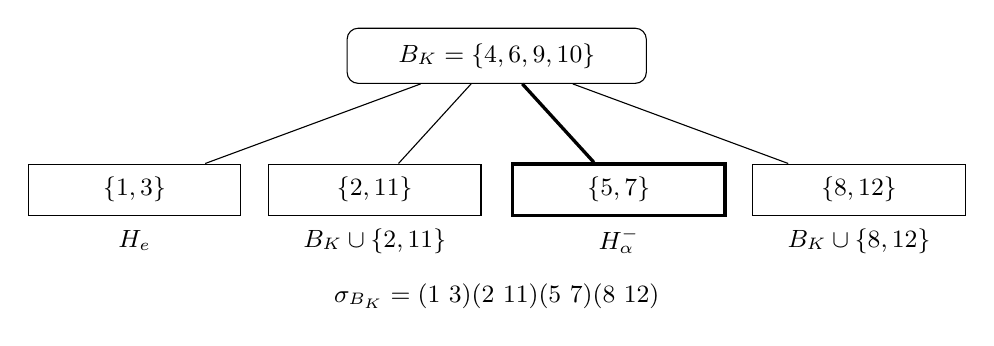
\begin{tikzpicture}[x=1cm,y=1cm, every node/.style={font=\small}]
 \node[draw,rounded corners,minimum width=3.8cm,minimum height=.7cm]
  (b) at (0,0) {$B_K=\{4,6,9,10\}$};
 \node[draw,minimum width=2.7cm,minimum height=.65cm]
  (p1) at (-4.6,-1.7) {$\{1,3\}$};
 \node[draw,minimum width=2.7cm,minimum height=.65cm]
  (p2) at (-1.55,-1.7) {$\{2,11\}$};
 \node[draw,very thick,minimum width=2.7cm,minimum height=.65cm]
  (p3) at (1.55,-1.7) {$\{5,7\}$};
 \node[draw,minimum width=2.7cm,minimum height=.65cm]
  (p4) at (4.6,-1.7) {$\{8,12\}$};
 \draw (b) -- (p1); \draw (b) -- (p2);
 \draw[very thick] (b) -- (p3); \draw (b) -- (p4);
 \node at (-4.6,-2.35) {$H_e$};
 \node at (-1.55,-2.35) {$B_K\cup\{2,11\}$};
 \node at (1.55,-2.35) {$H^-_\alpha$};
 \node at (4.6,-2.35) {$B_K\cup\{8,12\}$};
 \node at (0,-3.05)
  {$\sigma_{B_K}=(1\ 3)(2\ 11)(5\ 7)(8\ 12)$};
\end{tikzpicture}
\caption{The concrete star of the dodecaphasic flag. Each line
indicates the union of the central four-element set with the pair at its endpoint; the
thick line marks the hexad also selected by the signs
preceding the carry of $\alpha$. The four pairs exhaust the eight
outer positions.}
\label{x_reciprocidad:exc:fig-estrella}
\end{figure}

\begin{proposition}[The family of stars]
\label{x_reciprocidad:exc:m12}
The $\binom{12}4=495$ permutations $\sigma_B$ preserve $\mathcal H$.
The group they generate has order $95040$ and is the Mathieu group
$M_{12}$ in its action on the small Witt design.
\end{proposition}

\begin{proof}
The preservation assertion is a finite check on the
$132$ hexads of \eqref{x_reciprocidad:exc:codigo}: for each tetrad the
four petals are constructed and
$\{\sigma_B(H):H\in\mathcal H\}=\mathcal H$ is verified.
Closure under composition of these permutations produces $95040$
elements. In lexicographic enumeration it suffices to add successively
six stars not yet contained in the group; the intermediate orders
are $2,6,18,360,7920,95040$, and the $495$ stars belong to the final
group. The procedure, the six permutations written as their
lists of images and the closure recurrence are developed in
\ref{iv:iv:apendice-estrellas}. Finally, recognition of
the automorphism group of $S(5,6,12)$ as $M_{12}$, whose order is
$12\cdot11\cdot10\cdot9\cdot8=95040$, is applied.
\end{proof}

An individual star generates a cyclic group of order two. It does not
by itself generate $M_{12}$, still less the Monster. Nor does the
existence of $495$ generators of a permutation group prove that
each is the transport of a specific TPK loop. That assertion
requires the corresponding loop map; the result established here
is the finite incidence action.

\begin{remark}[Equality of traces does not identify operators]
On $V_{11}$, a star has spectrum $+1$ with multiplicity seven
and $-1$ with multiplicity four. Its normalized trace is $3/11$.
A rank-three projector on the same space also has normalized
trace $3/11$, but spectrum $1^3,0^8$. They are not conjugate: their
minimal polynomials and spectra differ. The intertwiner
\eqref{x_reciprocidad:exc:incidencia} transports defined operators; it does not turn
this scalar coincidence into an equivalence of operators.
\end{remark}

\subsection{The binary residue and the five regions of \texorpdfstring{$\pi$}{pi}}
\label{x_reciprocidad:exc:cinco-regiones}

The next recognition uses the extended binary Golay code
$G_{24}$, with parameters $[24,12,8]_2$. Its weights are
$0,8,12,16,24$, and the weight-eight supports form the design
$S(5,8,24)$. Fix a dodecad $D$, the support of a word of weight
twelve. This datum and the incidence isomorphism to be declared
below belong to the realization chart; they are not used to
generate or select the decimals of $\pi$.

\begin{proposition}[Residue of a dodecad and lifting of hexads]
\label{x_reciprocidad:exc:residuo-binario}
The set
\[
 \mathcal H(D)=
 \{O\cap D: O\text{ is an octad},\ |O\cap D|=6\}
\]
is an $S(5,6,12)$ system on $D$. Each of its hexads has
a unique lift to an octad. For any four-element set $B\subset D$,
the five octads containing it split into four residual
lifts and a unique octad $O_B^\perp$ with $O_B^\perp\cap D=B$.
\end{proposition}

\begin{proof}
A quintuple $A\subset D$ belongs to a unique octad $O$. If
$j=|O\cap D|$, the binary word given by the sum of $O$ and $D$ has weight
$20-2j$. Among the allowed weights, and with $0\leq j\leq8$, only
$j=2,4,6$ are possible. Since $A\subset O\cap D$, we have $j\geq5$
and therefore $j=6$. This gives existence and uniqueness of the residual
hexad, as well as uniqueness of its lift on choosing five of its
points. Furthermore,
\[
 \lambda_4(S(5,8,24))=\frac{\binom{20}1}{\binom41}=5,
 \qquad
 \lambda_4(S(5,6,12))=4.
\]
The four residual hexads on $B$ give four distinct octads.
The fifth cannot meet $D$ in six points, since it would be another residual
hexad; as it contains $B$, its intersection has size four and
coincides with $B$.
\end{proof}

A chart $\ell:[12]\to D$ preserving hexads identifies
$\mathcal H$ with $\mathcal H(D)$. Its existence is recognition
of the already constructed design as the small Witt design; a specific choice
of $\ell$ fixes the relabeling. The lift
\[
 \iota_D:\mathcal H\longrightarrow
       \{\text{octads of }G_{24}\},
 \qquad H\longmapsto O\text{ such that }O\cap D=\ell(H),
\]
is injective because intersection with $D$ recovers $\ell(H)$.
The domain of this injectivity is the hexads, not the register $K$.

The relation to the five regions of $\pi$ preserves richer data
than the number five. The emissions and their signatures are:
\begin{center}
\small
\begin{tabular}{@{}crll@{}}
\toprule
Region & Multiplicity & Emission $U_6$ & Signature \\
\midrule
$\perp$ & $432$ & $(501,614,498,169,272,272)$ & $555555$ \\
$++_1$ & $144$ & $(810,923,870,169,272,272)$ & $339555$ \\
$++_2$ & $144$ & $(810,983,810,169,272,272)$ & $393555$ \\
$++_3$ & $144$ & $(870,923,810,169,272,272)$ & $933555$ \\
$--$ & $144$ & $(870,923,810,418,674,521)$ & $933717$ \\
\bottomrule
\end{tabular}
\end{center}
In each three-digit decimal block, the signature uses the modular
difference of the first two digits. The five emissions have the
same visible tritic word $w_\pi=010211$, but not the same
regional genealogy. The three positive regions preserve the tail
$169|272|272$; the negative region changes it to $418|674|521$;
the transverse region has constant signature and greater multiplicity.

The marked extension of the regional chart sends the transverse region
to $O_{\ell(B_K)}^\perp$, the negative region to $\iota_D(H^-_\alpha)$ and the
three positive regions to the other three lifts of the star. This
realizes the partition $4+1$ of the five octads on $\ell(B_K)$.
The individual correspondence between the three positive names and
the three remaining petals requires a chart order; incidence does not determine it
without that datum. The precise assertion is therefore a
marked correspondence of regions, compatible with their roles and with
the flag, not a canonical bijection inferred from cardinality five.

The identity $432+4\cdot144=1008$ preserves the regional
multiplicities. Also $1008=36\cdot28$ and an octad has
$\binom82=28$ pairs. These equalities are arithmetic catalogue checks,
not substitutes for the map $\iota_D$ or the regional chart.


% BEGIN OWNER /Users/ruben/Documents/New project/output/EXTREMA_MEDIA_RAZON_RECIPROCIDAD_ES_EN_20260918/ARTICULO/ES/source/sections/estrella_pentadica_recuperada.tex
\subsubsection{Pentadic representation of the microfiber and its incidence}
\label{x_reciprocidad:pi-estrella:desarrollo}

The arrangement of the five regions allows simultaneous visualization
of the unity of the ternary quotient and the differentiation preserved by the
catalogue. The relevant map is the restriction
\[
 \Psi\big|_{\mathscr R_\pi^{\rm micro}}:
 \mathscr R_\pi^{\rm micro}\longrightarrow\{010211\},
 \qquad \Psi(U)=(-U)\bmod3.
\]
Its five antecedents are the vectors \(U_6\) in the preceding table.
Figure \ref{x_reciprocidad:pi-estrella:figura} recovers their radial organization,
preserving chart order, signatures and catalogue
multiplicities (equation~\eqref{x_reciprocidad:eq:palabras-regionales}).


% BEGIN OWNER /Users/ruben/Documents/New project/output/EXTREMA_MEDIA_RAZON_RECIPROCIDAD_ES_EN_20260918/ARTICULO/ES/source/figures/estrella_cinco_regiones.tex
% Orden de carta y datos recuperados de fig_cinco_regiones_pi.tex.
\begin{figure}[H]
\centering
\begin{tikzpicture}[x=1cm,y=1cm,font=\small,>=Latex]
 \coordinate (a) at (90:2.2);
 \coordinate (b) at (18:2.2);
 \coordinate (c) at (-54:2.2);
 \coordinate (d) at (-126:2.2);
 \coordinate (e) at (162:2.2);
 \draw[black!35,line width=.45pt]
    (a)--(c)--(e)--(b)--(d)--cycle;
 \node[draw,fill=white,circle,minimum size=1.6cm,align=center,
    inner sep=3pt] (z) at (0,0) {$w_\pi$\\$010211$};
 \foreach \v in {a,b,c,d,e}{
    \fill (\v) circle (2pt);
    \draw[->,line width=.6pt] (\v)--(z);
 }
 \node[above=3mm,align=center] at (a)
   {$U_\pi^\perp$\\$555555$\\multiplicidad $432$};
 \node[right=3mm,align=left] at (b)
   {$U_{\pi,1}^{++}$\\$339555$\\multiplicidad $144$};
 \node[below right=2mm and 1mm,align=left] at (c)
   {$U_{\pi,2}^{++}$\\$393555$\\multiplicidad $144$};
 \node[below left=2mm and 1mm,align=right] at (d)
   {$U_{\pi,3}^{++}$\\$933555$\\multiplicidad $144$};
 \node[left=3mm,align=right] at (e)
   {$U_\pi^{--}$\\$933717$\\multiplicidad $144$};
 \node[align=center,font=\footnotesize] at (0,-3.55)
   {$1_\perp+3_{++}+1_{--}$\qquad $432+4\cdot144=1008$};
\end{tikzpicture}
\caption{The five regions of \(\pi\) in a pentadic arrangement.
Each position preserves its multiplicative signature and multiplicity;
the radial arrows represent the common projection
\(\Psi(U)=010211\). The star-shaped outline organizes the five
positions of the chart. Their realization in the five Witt octads
is carried out through regional alignment and the decomposition
\(4+1\) in the text.}
\label{x_reciprocidad:pi-estrella:figura}
\end{figure}

% END OWNER


Projection onto the center identifies the five ternary images; the
register of the outer positions retains the regional information
making the incidence realization possible. The distribution
\(1_\perp+3_{++}+1_{--}\) specifies one transverse region, three
positive regions and one negative region. Their normalized weights are
\(3/7\) and \(1/7\) for each of the other four: the
transverse multiplicity is triple, even though the five images under
\(\Psi\) coincide.

\Needspace{11\baselineskip}
The link to the Witt star is formulated through the flag
\(B_K\subset H^-_\alpha\), alignment \(\ell\) and
lift \(\iota_D\) already constructed. The five regional positions
are realized in the five octads on \(\ell(B_K)\):
\[
\begin{aligned}
 U_\pi^\perp&\longmapsto O^\perp_{\ell(B_K)},\\
 U_\pi^{--}&\longmapsto\iota_D(H^-_\alpha),\\
 \{U_{\pi,1}^{++},U_{\pi,2}^{++},U_{\pi,3}^{++}\}
 &\longmapsto
 \{\iota_D(B_K\cup P):P\in\mathcal P_+\},\\
 \mathcal P_+&=\bigl\{\{1,3\},\{2,11\},\{8,12\}\bigr\}.
\end{aligned}
\]
Assignment of the three positive positions to the three pairs is
performed in an ordered chart. The transverse row and negative row
are distinguished by their regional predicates and the flag.

The two figures are thus articulated: Figure
\ref{x_reciprocidad:exc:fig-estrella} shows the four hexads of the small Witt
design on \(B_K\); Figure \ref{x_reciprocidad:pi-estrella:figura} shows
the five regions that, under alignment, occupy the four residual
octads and the transverse octad of the binary design. The law
\(4+1\), proved in Proposition
\ref{x_reciprocidad:exc:residuo-binario}, specifies the incidence change. In this
composition, \(K\) determines the marked tetrad and the signature of
\(\alpha\) distinguishes one of its hexads. In addition to
their common ternary value, the regions preserve the structure needed for that
transport toward the exceptional realization.

% END OWNER


\subsection{From the ternary code to the Niemeier lattice}
\label{x_reciprocidad:exc:niemeier}

The passage to dimension twenty-four does not require first going through the
binary code. It is realized directly from $C_W$ by gluing
discriminants. Two compatible prolongations are thus distinguished:
one preserves the residue $W_{12}\subset W_{24}$; the other constructs the
lattice on which the vertex operator algebra will be realized.

Let $A_2=\mathbb Z a_1\oplus\mathbb Z a_2$ have Gram matrix
\[
 \begin{pmatrix}2&-1\\-1&2\end{pmatrix},
 \qquad \rho=a_1+a_2,\qquad \rho^2=2.
\]
We represent the three classes of $A_2^*/A_2$ by
\[
 \varpi_0=0,\qquad
 \varpi_1=\frac{2a_1+a_2}{3},\qquad
 \varpi_2=\frac{a_1+2a_2}{3}.
\]
The map $j\mapsto\varpi_j+A_2$ additively identifies
$\mathbb F_3$ with that discriminant. For $c\in C_W$, write
$\phi(c)=(\varpi_{c_1},\ldots,\varpi_{c_{12}})$ and define
\begin{equation}
 N(C_W)=\bigcup_{c\in C_W}\bigl(A_2^{12}+\phi(c)\bigr).
 \label{x_reciprocidad:exc:niemeier-def}
\end{equation}

\begin{theorem}[Ternary gluing]
\label{x_reciprocidad:exc:niemeier-teorema}
The object \eqref{x_reciprocidad:exc:niemeier-def} is a positive, even,
unimodular lattice of rank $24$. Its root system is exactly
$A_2^{12}$; it is therefore recognized as the Niemeier lattice with
that root system.
\end{theorem}

\begin{proof}
Linearity of the code makes the union of classes stable under
addition. Self-orthogonality annuls the discriminant pairing:
it is a multiple of $c\cdot d/3$ modulo $\mathbb Z$. Thus the
lattice is integral. The norm of a gluing class is
$2\operatorname{wt}(c)/3$ modulo $2\mathbb Z$. The weights of
\eqref{x_reciprocidad:exc:enumerador} are multiples of three, so it is even.

The index of $A_2^{12}$ in $N(C_W)$ is $|C_W|=3^6$. Consequently,
\[
 \det N(C_W)=\frac{3^{12}}{(3^6)^2}=1.
\]
Positivity comes from the orthogonal sum of the twelve metrics $A_2$.
In a nonzero class of $A_2^*/A_2$ the minimum norm is $2/3$;
every nonzero word has at least six nonzero positions.
Therefore a vector in a nontrivial gluing class has norm
at least $6\cdot2/3=4$. No norm-two roots appear outside
$A_2^{12}$. Inside it, the roots are precisely those of its
twelve components.
\end{proof}

\subsection{Incidence selection of the rootless unimodular neighbor}
\label{x_reciprocidad:exc:leech}


% BEGIN OWNER /Users/ruben/Documents/New project/output/EXTREMA_MEDIA_RAZON_RECIPROCIDAD_ES_EN_20260918/ARTICULO/ES/source/sections/incidencia_reticulo.tex
\paragraph{From the incidence origin to the lattice modification.}
\label{x_reciprocidad:inc-ampl-reticulo}
The marked flag determines a position through an equivariant
set-theoretic operation:
\[
 o_*=(H_e\cap H_\varphi)
       \setminus(H^-_\alpha\cup H_{\rm APP})=\{1\}.
\]
Its function is to distinguish one component among the twelve
involved in the lattice realization. The complete ternary code
acts as a gluing code in the discriminant module
$(A_2^*/A_2)^{12}$. Its preimage defines $N(C_W)$, and the
self-duality, weights and distance of the code translate,
respectively, into integrality and determinant properties, parity
and norm bounds on the gluing classes. Here the symbolic information
of the code serves a function that the isolated support no longer performs.

The metric $A_2$ and positive radial chamber are fixed in the lattice
development. Within that chamber, the congruence required for an even
neighbor of index three has twelve realizations of minimum norm $54$,
permuted by changing the distinguished component. The origin $o_*$
selects
\[
 v_\alpha=4\rho_1+\rho_2+\cdots+\rho_{12},\qquad
 v_\alpha^2=2(4^2+11)=54.
\]
The coefficient $4$ belongs to that solution of the congruence in the
declared chamber. The subscript $\alpha$ records the incidence
provenance of the selection: its content is the frame involved in
closure and now individualizing a lattice direction.

Pairing with $v_\alpha$ determines the sublattice
$N_{\alpha,0}$ of index three, and adding the class
$v_\alpha/3$ produces the neighbor $N_\alpha$ of
\eqref{x_reciprocidad:exc:vecino}. This modification preserves rank and recovers
unimodularity and parity; selection by congruence removes the previous roots,
and local bounds exclude roots in the new classes.
Identification with Leech appears after these verifications. The
binary realization of the five regions and this lattice construction
are two prolongations of the common frame: the latter directly receives
the ternary code as gluing data.


% END OWNER


The label $o_*=1$ of the flag is now realized as one of the
twelve components $A_2$. This operation declares the preceding metric and
the positive radial chamber
\[
 v(a)=\sum_{i=1}^{12}a_i\rho_i,
 \qquad a_i=1+3b_i,\quad b_i\in\mathbb Z_{\geq0}.
\]
The evenness requirement for the index-three neighbor is
$v(a)^2\equiv0\pmod{18}$. Since
\[
 v(a)^2=2\sum_i(1+3b_i)^2,
\]
that congruence is equivalent to $\sum_i b_i\equiv1\pmod3$. The smallest
norm value in the chamber is obtained with a single $b_i=1$ and
all the others zero; it is $54$. The marked origin selects
\begin{equation}
 v_\alpha=4\rho_1+\rho_2+\cdots+\rho_{12},
 \qquad v_\alpha^2=54.
 \label{x_reciprocidad:exc:vector}
\end{equation}
The word ``smallest'' refers to this positive chamber. It does not assert
minimality in the entire residue class: the vector
$(a_1-2a_2,\rho,\ldots,\rho)$ represents the same class modulo three
and has norm $14+11\cdot2=36$. The chamber restriction is part
of the construction data, not an omissible conclusion.

Let $N=N(C_W)$. We define
\begin{equation}
 N_{\alpha,0}=\{x\in N:\langle x,v_\alpha\rangle\equiv0\pmod3\},
 \qquad
 N_\alpha=N_{\alpha,0}+\mathbb Z\frac{v_\alpha}{3}.
 \label{x_reciprocidad:exc:vecino}
\end{equation}

\begin{theorem}[Leech neighbor determined by the marked flag]
\label{x_reciprocidad:exc:teorema-leech}
With the declared metric and chamber, $N_\alpha$ is a positive, even,
unimodular lattice of rank $24$, with no vectors of norm two.
By the corresponding classification theorem, it is isometric to the
Leech lattice $\Lambda_{24}$.
\end{theorem}

\begin{proof}
The character $x\mapsto\langle x,v_\alpha\rangle\bmod3$ is nonzero:
a simple root of one component pairs with $a_i\rho_i$ to give
$a_i\equiv1\pmod3$. Hence $[N:N_{\alpha,0}]=3$ and
$\det N_{\alpha,0}=9$. Moreover,
$v_\alpha/3\in N_{\alpha,0}^*$ and $v_\alpha\in N_{\alpha,0}$.
If $v_\alpha/3$ belonged to $N$, integrality of $N$ would make
all pairings with $v_\alpha$ divisible by three,
contradicting the nonzero character. The class of $v_\alpha/3$ therefore has
order three. We deduce
\[
 [N_\alpha:N_{\alpha,0}]=3,
 \qquad \det N_\alpha=9/3^2=1.
\]
The extension is integral, and for $x\in N_{\alpha,0}$,
\[
 \left(x+m\frac{v_\alpha}{3}\right)^2
   =x^2+2m\frac{\langle x,v_\alpha\rangle}{3}+6m^2
   \in2\mathbb Z.
\]
Hence it is even.

It remains to exclude the roots, which is the decisive step. The roots of $N$
belong to $A_2^{12}$. Their pairings with $v_\alpha$ are
congruent to $\pm1$ or $\pm2$ modulo three; none belongs to
$N_{\alpha,0}$. For the other two classes of the neighbor, each component
belongs to one of the local classes
\[
 A_2+\varpi_j\pm\rho/3,\qquad j=0,1,2.
\]
Since $4\rho/3\equiv\rho/3\pmod{A_2}$, this description also holds
in the distinguished component. Writing a local vector
as $(u a_1+v a_2)/3$, its norm is
$2(u^2-uv+v^2)/9$. The six preceding classes have nonzero residues
and minimum $2/9$: representatives minimizing the quadratic form
are $(\pm1,0),(0,\pm1),(1,1),(-1,-1)$ in the appropriate residues.
A vector in a new class therefore has norm at least
$12\cdot2/9=8/3>2$. There are no roots in any of the three classes.
The classification of positive even unimodular lattices of
rank twenty-four identifies the unique rootless case with
$\Lambda_{24}$.
\end{proof}

The argument does not recognize Leech through a coincidence of dimension.
It constructs the gluing, proves integrality, parity and determinant, and
removes the roots through a local bound. Only then does it apply the
classification theorem. Dependence on $\alpha$ is preserved in
the flag selecting $o_*$ and in the vector \eqref{x_reciprocidad:exc:vector};
the scalar value of the constant is not turned into a lattice
length.

\subsection{The vertex operator algebra and the Monster}
\label{x_reciprocidad:exc:voa}

Let $\Lambda=N_\alpha$, already recognized as Leech. The next step
uses its integral lattice, not a decimal expansion. The lattice
vertex operator algebra construction is written
\[
 V_\Lambda=M(1)\otimes\mathbb C_\varepsilon[\Lambda].
\]
Here $M(1)$ is the Heisenberg oscillator space in rank
twenty-four; $\mathbb C_\varepsilon[\Lambda]$ is the group algebra
twisted by the cocycle of the lattice's central extension. The
cocycle and lift of the isometries are part of the
construction: a bare vector sum does not determine the vertex
products.

Negation $\lambda\mapsto-\lambda$ admits the standard lift
$\theta$. With its twisted module and the compatible parity choice,
the Frenkel--Lepowsky--Meurman construction produces
\begin{equation}
 V^\natural_{\rm HMT}
   =V_\Lambda^+\oplus(V_\Lambda^T)^+.
 \label{x_reciprocidad:exc:flm}
\end{equation}
The sign $+$ denotes the even part of the lifted action. The expression
includes the orbifold vertex product; it is not merely a sum
of graded spaces.

\begin{theorem}[Prolongation to the Moonshine module]
\label{x_reciprocidad:exc:moonshine}
The algebra \eqref{x_reciprocidad:exc:flm}, constructed on the neighbor
\eqref{x_reciprocidad:exc:vecino}, is a realization of the Moonshine algebra
$V^\natural$. It has central charge $24$, zero weight-one component,
and automorphism group isomorphic to the Monster $\mathbb M$. Its graded
character is
\begin{equation}
 \operatorname{Tr}_{V^\natural_{\rm HMT}}q^{L_0-1}
   =J(\tau)=j(\tau)-744
   =q^{-1}+196884q+21493760q^2+\cdots,
 \qquad q=e^{2\pi i\tau}.
 \label{x_reciprocidad:exc:j}
\end{equation}
\end{theorem}

\begin{proof}
Theorem \ref{x_reciprocidad:exc:teorema-leech} verifies the lattice hypotheses:
positivity, parity, unimodularity, rank twenty-four and absence of
roots. The construction and theorem of
Frenkel--Lepowsky--Meurman for the Leech lattice are then applied. They identify
the orbifold with $V^\natural$ and establish its character and automorphism
group. Composition of the flag, neighbor and VOA
construction functor gives the realization indicated here. The group is not
inferred from the coefficient $196884$.
\end{proof}

The theorem used is a subsequent classical recognition with
verified hypotheses, not a new proof in this article of
the FLM construction \cite{x_reciprocidad:flm}.
Moreover, the notation $q=e^{2\pi i\tau}$ is the conventional Fourier
variable used to recognize the character. It introduces neither $\pi$
nor $e$ as inputs to the coinductive generator that has already determined them.

Part of the trace mechanism can be seen before the orbifold.
Only the zero lattice vector is fixed by negation; each
oscillator contributes with alternating sign. Hence
\[
 \operatorname{Tr}_{V_\Lambda}\theta q^{L_0-1}
   =t_2(\tau)
   :=q^{-1}\prod_{n\geq1}(1+q^n)^{-24}.
\]
This trace in the lattice algebra must not be confused with the
character without insertion of $V^\natural$. Nor does it by itself identify
a conjugacy class of the Monster: the space, insertion
and lift must be specified before functions are compared.


% BEGIN OWNER /Users/ruben/Documents/New project/output/EXTREMA_MEDIA_RAZON_RECIPROCIDAD_ES_EN_20260918/ARTICULO/ES/source/sections/incidencia_automorfismos.tex
\paragraph{Grading, unit and automorphisms.}
\label{x_reciprocidad:inc-ampl-automorfismos}
The Frenkel--Lepowsky--Meurman construction is applied to the lattice
$N_\alpha$ once its properties have been verified. It incorporates the oscillator
space, central extension of the lattice, vertex product
and sector twisted by the lift of negation. The result is
the algebra $V^\natural_{\rm HMT}$ of \eqref{x_reciprocidad:exc:flm}, whose automorphism
group is isomorphic to the Monster. Its action domain is thus
fixed by an algebraic structure with grading and product. Borcherds's
Moonshine theorem subsequently determines the graded traces
with insertion of these automorphisms \cite{x_reciprocidad:flm,x_reciprocidad:borcherds}.

Unity acquires a precise realization at this level: the weight-zero
component is the vacuum line and contributes the coefficient $1$ of
$q^{-1}$ in the graded character. At the cylindrical level, the
refinement maps preserve the constant function by
precomposition. Each conservation assertion therefore has its
object and map. Developing the proofs makes this continuity of
construction visible, from arithmetic operations and
memory to incidence, metric and vertex products.

This articulation places $K$ and the closure of $\alpha$ in the main
argument. $K$ reversibly preserves an integral coordinate of the
history; normalization of $\alpha$ composes the regional registers
with that coordinate; the signed configuration determines a flag; and
the marked flag selects the lattice modification on which
Moonshine is realized. The following proofs develop these
maps, distinguishing reversible equivalences, information
quotients and realizations adding metric or algebraic
structure. A provable relation between structure,
equation and value is thus expressed, preserving the attribution of each construction and the
scope of its theorems.

% END OWNER



% BEGIN OWNER /Users/ruben/Documents/New project/output/EXTREMA_MEDIA_RAZON_RECIPROCIDAD_ES_EN_20260918/ARTICULO/ES/source/sections/fibras_app_witt.tex
\subsection{State-based construction of the twelve cyclotomic fibres}
\label{x_reciprocidad:nuclear:fibras-app-witt}
On the APP marks, multiplication \(a:r\mapsto4r\) in
\(\ZZ/9\ZZ\) satisfies \(a^3=1\). The sheets satisfy
\[
 S(ax,ay)=aS(x,y),\qquad P(ax,ay)=a^{-1}P(x,y),
\]
since \(16\equiv7\equiv4^{-1}\pmod9\). The ordered unit orbits
are \(\mathcal O_0=(1,4,7)\), \(\mathcal O_1=(2,8,5)\).
In each, the augmentation module
\(A(\mathcal O)=\ker(\ZZ[\mathcal O]\xrightarrow{\sum}\ZZ)\)
inherits the inner product making the \(e_r\) orthonormal. In the basis
\(b_1=e_r-e_{4r}\), \(b_2=e_{4r}-e_{7r}\), its matrices are
\[
 G_{A_2}=\begin{pmatrix}2&-1\\-1&2\end{pmatrix},\qquad
 C=\begin{pmatrix}0&-1\\1&-1\end{pmatrix},\qquad
 C^{\mathsf T}G_{A_2}C=G_{A_2}.
\]
The lattice form therefore originates in the orbits of the marks.
For the pairs \((1,2),(2,3),(3,1)\) and sheets
\(\mu\in\{\Sigma,\Pi\}\), we obtain
\[
 W_{\APP}=\bigoplus_{(i,j)}\bigoplus_\mu\bigoplus_{\varepsilon=0}^1
 A(\mathcal O_\varepsilon),\qquad
 \ell^\Sigma_{ij}(x)=x_i+x_j,\quad
 \ell^\Pi_{ij}(x)=x_ix_j\pmod9.
\]
Each summand preserves pair, sheet, and orbit. The state map is
\[
 \Psi:(\ZZ/9\ZZ)^3\longrightarrow W_{\APP},\qquad
 \Psi(x)_{ij,\mu,\varepsilon}=\beta_\varepsilon(\ell^\mu_{ij}(x)),
 \quad
 \beta_\varepsilon(r)=
 \begin{cases}e_r-e_{4r},&r\in\mathcal O_\varepsilon,\\0,&r\notin\mathcal O_\varepsilon.
 \end{cases}
\]
\begin{proposition}[Equivariance and rank of the state module]
\label{x_reciprocidad:nuclear:psi-rango}
The action of \(C\) on the six additive fibres and of \(C^{-1}\) on
the six multiplicative fibres satisfies \(\Psi(ax)=\rho(a)\Psi(x)\).
The images span \(W_{\APP}\otimes\QQ\), of dimension twenty-four.
\end{proposition}
\begin{proof}
The sheet identities and \(\beta(4r)=C\beta(r)\) prove
equivariance. For rank, order the coordinates by the three
stated pairs, by \(\Sigma,\Pi\), by \(\mathcal O_0,\mathcal O_1\),
and by \(b_1,b_2\). In each orbit, \(\beta\) takes successive values
\((1,0),(0,1),(-1,-1)\). The matrix of the images of the following states,
read row by row, has determinant \(9\):
\[
\begin{array}{rrrr}
(0,0,1)&(0,0,2)&(0,0,4)&(0,0,5)\\
(0,1,0)&(0,1,1)&(0,1,2)&(0,1,3)\\
(0,1,4)&(0,1,5)&(0,1,6)&(0,2,0)\\
(0,2,2)&(0,2,3)&(0,4,0)&(0,5,0)\\
(1,0,1)&(1,0,2)&(1,0,4)&(1,0,5)\\
(1,1,0)&(1,2,0)&(1,4,0)&(1,5,0).
\end{array}
\]
Successive elimination, reducing each row by its predecessors and
normalizing its first nonzero coefficient, gives pivot columns
numbered from zero
\[
\begin{split}
&(8,10,9,11,0,12,14,16,13,15,17,2,\\
&\hspace{2em}18,19,1,3,20,22,21,23,4,6,5,7)
\end{split}
\]
and pivots
\[
(1,1,1,-1,1,1,1,1,1,-1,3,1,1,3,1,-1,1,1,1,-1,1,1,1,-1).
\]
Their product, multiplied by the sign of the column permutation,
is \(9\). The invertible minor establishes full rank.
\end{proof}

\subsection{Dodecaphasic alignment with the Witt positions}
\label{x_reciprocidad:nuclear:alineamiento-witt}
The pair index is \(i\in\ZZ/3\ZZ\), the sheet index is
\(\mu\in\{0,1\}\), and the orbit index is \(\varepsilon\in\{0,1\}\).
With the dodecaphasic origin fixed, \(\lambda(i,\mu,\varepsilon)
=4i+2\mu+\varepsilon\pmod{12}\) is bijective: the four values
for each \(i\) form a block, and the three blocks are disjoint.
Let \(R=\left(\begin{smallmatrix}0&1\\1&0\end{smallmatrix}\right)\).
Multiplication proves \(RCR=C^{-1}\) and
\(R^{\mathsf T}G_{A_2}R=G_{A_2}\). For the trivializations
\(\iota_b\) and frames \(P_b\) transported jointly with
Witt incidence, set
\[
g_b=\iota_b^{-1}P_bCP_b^{-1}\iota_b,\qquad
T_{i\mu\varepsilon}=\iota_{\lambda(i,\mu,\varepsilon)}^{-1}
P_{\lambda(i,\mu,\varepsilon)}R^\mu.
\]
Then
\[
g_{\lambda(i,\mu,\varepsilon)}T_{i\mu\varepsilon}
=T_{i\mu\varepsilon}C^{(-1)^\mu}.
\]
The direct sum is a \(C_3\)-equivariant isomorphism between the twelve
state fibres and the twelve lattice positions. It preserves pair,
sheet, orbit, and form under simultaneous transport of origin,
order, and orientation. These data persist in the lattice gluing
and passage to the neighbour constructed below.

% END OWNER


% BEGIN OWNER /Users/ruben/Documents/New project/output/EXTREMA_MEDIA_RAZON_RECIPROCIDAD_ES_EN_20260918/ARTICULO/ES/source/sections/moonshine_comparacion.tex
% Incorporación aditiva para el Artículo I; no modifica la fuente anterior.
% RESULTADO_RECUPERADO: integral, capítulo 22, propietario extenso
% colaboracion/partes_i_ii/source/base_residencias/
% capitulo_22_c20_lineas_2613_3270.tex, líneas 176--576.
% Equivalencia 2/3: public/residencias/capitulo_22_voa_leech_moonshine.tex,
% líneas 55--127. Orden dos y Fricke: hmt/15d_voa_moonshine_orden_dos_rev11.tex.
% Prerrequisitos residentes en I: código C_W, matriz A_W, N(A_2^12),
% origen o_*, vector v_alpha de norma54, N_alpha reconocido como Leech,
% VOA reticular y presentación FLM de las secciones precedentes.
% Bibliografía nueva: chenlamshimakura2016, abelamyamada2017,
% kmconwaynorton1979 (bibitems listos para incorporar al final de este archivo).

\subsection{Ternary orientation of the Leech neighbor}
\label{x_reciprocidad:km:orden-tres-reticular}

The order-two presentation constructed above uses negation
of the Leech lattice. The same lattice, obtained from the incidence marked
by \(K\) and the dodecaphasic support of \(\alpha\), admits a second
presentation compatible with the ternary character of the construction.
To make this continuity explicit, the gluing is retained, its order-three
isometry is constructed, and preservation of the already selected neighbour
is verified. This step requires no alteration of \(K\), its rational reading,
or the preceding definition of \(\alpha\). The order-three prolongation is developed here,
including the lattice operations and the precise conditions of the classical
theorems used.

We work in the simple-root basis of each factor \(A_2\), with
\begin{equation}
 B_2=\begin{pmatrix}2&-1\\-1&2\end{pmatrix},\qquad
 \mathsf C=\begin{pmatrix}0&-1\\1&-1\end{pmatrix},\qquad
 \mathsf R=\begin{pmatrix}0&1\\1&0\end{pmatrix},\qquad
 \rho=\begin{pmatrix}1\\1\end{pmatrix}.
 \label{x_reciprocidad:km:coxeter-reflexion}
\end{equation}
The multiplication gives
\[
 \mathsf C^3=I_2,\quad
 \mathsf C^2+\mathsf C+I_2=0,\quad
 \mathsf C^{\mathsf T}B_2\mathsf C=B_2,\quad
 \mathsf R\mathsf C\mathsf R=\mathsf C^{-1},\quad
 \mathsf R^{\mathsf T}B_2\mathsf R=B_2.
\]
These identities fix both the metric and the orientation of the action.
In the discriminant \(A_2^*/A_2\cong\mathbb F_3\) we take as
generator the class of \(\varpi=(2,1)^{\mathsf T}/3\). We have
\(\mathsf C\varpi-\varpi=(-1,0)^{\mathsf T}\), so
\(\mathsf C\) acts trivially on the discriminant; the reflection
\(\mathsf R\) changes its sign.

The already constructed Paley--Witt matrix produces an element of full
support through the following operation:
\begin{equation}
 \begin{gathered}
 q_*=(1,1,1,1,1,1),\qquad q_*A_W=(2,1,1,1,1,1),\\
 c_*=(q_*,q_*A_W)
 =(1,1,1,1,1,1,2,1,1,1,1,1)\in C_W.
 \end{gathered}
 \label{x_reciprocidad:km:palabra-total}
\end{equation}
Every coordinate of \(c_*\) is nonzero. For the twelve positions,
define the frames and the isometry
\begin{equation}
 P_b(c_*)=
 \begin{cases}\mathsf R,&(c_*)_b=1,\\I_2,&(c_*)_b=2,\end{cases}
 \qquad
 g_c=\bigoplus_{b=1}^{12}P_b(c_*)\mathsf C P_b(c_*)^{-1}.
 \label{x_reciprocidad:km:isometria-ternaria}
\end{equation}
The symbol \(P_b(c_*)\) here denotes an invertible frame of an
\(A_2\) factor, not the regional projector \(P_3\).

\begin{proposition}[Order-three isometry on the marked neighbor]
\label{x_reciprocidad:km:estabilidad-vecino}
The operator \(g_c\) is an order-three isometry without nonzero fixed
vectors. It preserves the Niemeier lattice \(N=N(C_W)\) and the neighbor
\(N_\alpha\) constructed in \eqref{x_reciprocidad:exc:vecino}.
\end{proposition}
\begin{proof}
Each block of \(g_c\) is \(\mathsf C\) or \(\mathsf C^{-1}\);
its minimal polynomial is \(X^2+X+1\). This proves the order and
absence of fixed vectors. Both blocks act trivially on the
discriminant, so they preserve each gluing class and therefore
the lattice \(N\).

Write \(v=v_\alpha=4\rho_{o_*}+\sum_{b\ne o_*}\rho_b\),
with the frames and incidence origin already fixed. Its radial
coefficients are \(a_{o_*}=4\) and \(a_b=1\) for \(b\ne o_*\).
All satisfy \(a_b\equiv1\pmod3\). In one factor,
\[
 (\mathsf C-I_2)\rho=(-2,-1)^{\mathsf T},\qquad
 (\mathsf C^{-1}-I_2)\rho=(-1,-2)^{\mathsf T}.
\]
After division by three, their discriminant classes are,
respectively, \(2\) and \(1\). Consequently, the vectors
\begin{equation}
 y=\frac{g_cv-v}{3},\qquad z=\frac{g_c^{-1}v-v}{3}
 \label{x_reciprocidad:km:desplazamientos}
\end{equation}
have discriminant words \(c_*\) and \(-c_*\), both in
\(C_W\). Hence \(y,z\in N\). The local product is
\[
 \left\langle
 \frac{(\mathsf C^{\pm1}-I_2)a_b\rho}{3},a_b\rho
 \right\rangle=-a_b^2,
\]
and their sum gives
\(\langle y,v\rangle=\langle z,v\rangle=-(16+11)=-27\).
Thus, \(y,z\in N_0=\{x\in N:\langle x,v\rangle\equiv0\pmod3\}\).
For \(x\in N_0\),
\[
 \langle g_cx,v\rangle
 =\langle x,g_c^{-1}v\rangle
 =\langle x,v\rangle+3\langle x,z\rangle\equiv0\pmod3.
\]
The argument applied to \(g_c^{-1}\) proves \(g_cN_0=N_0\).
Finally, \(g_c(v/3)=v/3+y\) preserves the class generating
\(N_\alpha=N_0+\mathbb Z(v/3)\). We obtain
\(g_cN_\alpha=N_\alpha\).
\end{proof}

The proof preserves more than the lattice dimension: it uses the gluing
code, its orientation, the origin of the flag and the congruence of the
radial vector. These data explain why the second presentation
remains linked to the dodecaphasic register from which the construction began.

\subsection{Ternary trace, twisted weight and order-three extension}
\label{x_reciprocidad:km:orbifold-tres}

Let \(\Lambda=N_\alpha\) and let \(\widehat g_c\) be the standard lift
of \(g_c\) to the lattice algebra
\(V_\Lambda=M(1)\otimes\mathbb C_\varepsilon[\Lambda]\), with the
central extension and cocycle already declared. Odd order allows
this lift to be chosen of order three. Each complex factor \(A_2\)
contributes eigenvalues \(\zeta_3\) and \(\zeta_3^2\), where
\(\zeta_3^2+\zeta_3+1=0\).

\begin{proposition}[Graded trace and type of the lift]
\label{x_reciprocidad:km:traza-tipo}
For \(j=1,2\),
\begin{equation}
 \operatorname{Tr}_{V_\Lambda}
       \bigl(\widehat g_c^{\,j}q^{L_0-1}\bigr)
 =t_3(\tau)
 :=q^{-1}\prod_{n\ge1}(1+q^n+q^{2n})^{-12}.
 \label{x_reciprocidad:km:tres-traza}
\end{equation}
The minimum weight of the nontrivial twisted modules is \(4/3\), and
the lift is of type zero.
\end{proposition}
\begin{proof}
In the lattice part of the trace only the zero vector contributes,
because \(g_c\) and \(g_c^2\) have no nonzero fixed vectors.
In each oscillator degree, the trace of symmetric powers is the inverse
of the determinant \(I-g_c^jq^n\). Each factor \(A_2\) contributes
\(1+q^n+q^{2n}\), proving \eqref{x_reciprocidad:km:tres-traza}.

The twisted-vacuum weight formula for an order-three lattice
automorphism, applied to the two twelve-dimensional eigenspaces, gives
\[
 \rho_{\widehat g_c}
 =\frac{1}{4\cdot3^2}
   \bigl(1\cdot2\cdot12+2\cdot1\cdot12\bigr)=\frac43.
\]
The type is the class of \(3^2\rho_{\widehat g_c}=12\) modulo
three, which is zero. The weight formula is a result of twisted-module
theory; the multiplicities and isometry feeding into it
have been constructed here.
\end{proof}

\begin{theorem}[Second presentation of the Moonshine algebra]
\label{x_reciprocidad:km:moonshine-tres}
The type-zero cyclic extension
\begin{equation}
 V_{(3)}=\operatorname{Orb}_{\mathbb Z/3}
                 (V_\Lambda,\widehat g_c)
 \label{x_reciprocidad:km:extension-orden3}
\end{equation}
is isomorphic to the vertex operator algebra \(V^\natural\).
\end{theorem}
\begin{proof}
Theorem \ref{x_reciprocidad:exc:teorema-leech} provides a positive,
even, unimodular, rootless lattice of rank twenty-four.
Proposition~\ref{x_reciprocidad:km:estabilidad-vecino} constructs an order-three
fixed-point-free isometry on that same lattice;
Proposition~\ref{x_reciprocidad:km:traza-tipo} verifies the lift and its type.
The Chen--Lam--Shimakura theorem on the order-three orbifold
of the Leech lattice algebra then applies
\cite[Teorema~1.1]{x_reciprocidad:chenlamshimakura2016}. This identification is also covered
by the uniform treatment of Abe--Lam--Yamada
\cite[Teorema~4.4 y secciones~2--4]{x_reciprocidad:abelamyamada2017}. This application follows construction
of the lattice data; equality of characters does not replace the
hypotheses of the theorem used.
\end{proof}

To make the dual symmetry precise, write
\(V_{(3)}=W_0\oplus W_1\oplus W_2\), where \(W_i\) is the integral
sector selected in the \(\widehat g_c^{\,i}\)-twisted module.
The product satisfies
\(Y(W_i,z)W_j\subset W_{i+j\bmod3}((z))\). Hence
\begin{equation}
 g^\vee|_{W_i}=\zeta_3^i I
 \label{x_reciprocidad:km:dual-ciclico}
\end{equation}
defines an automorphism of order three. Indeed, the factor on a
product is \(\zeta_3^{i+j}=\zeta_3^i\zeta_3^j\), and the vacuum and
conformal vector belong to \(W_0\). The classical identification of
this automorphism in the Monster is class \(3B\), with series
\(T_{3B}=t_3+12\) \cite{x_reciprocidad:kmconwaynorton1979,x_reciprocidad:borcherds}.
This normalization can be checked in the construction. The lattice
character is \(\operatorname{ch}V_\Lambda=J+24\): its initial pole
is \(q^{-1}\), its weight-one space has dimension 24 and the
weight-zero modular character is determined by these data.
If \(F\) is the character of the fixed subspace and \(H\) that of each
integral twisted sector, projection onto invariants and conjugation
of the two sectors give
\[
 F=\frac{J+24+2t_3}{3},\qquad F+2H=J,
 \qquad \operatorname{Tr}g^\vee q^{L_0-1}=F-H=t_3+12.
\]
Its domain is the extended algebra, whereas
\(\widehat g_c\) acts on the preceding lattice algebra.

\subsection{Equivalence of the order-two and order-three presentations}
\label{x_reciprocidad:km:equivalencia-dos-tres}

Denote by
\[
 V_{(2)}=(V_\Lambda)^+\oplus(V_\Lambda^T)^+
\]
the FLM presentation of \eqref{x_reciprocidad:exc:flm}. Both presentations preserve
the same Leech neighbor as antecedent. Their extensions use
different automorphisms and vertex products determined through
the respective lifting data.

\begin{theorem}[Graded equivalence and transport of automorphisms]
\label{x_reciprocidad:km:equivalencia-voa}
With vertex operator algebra isomorphisms fixed
\[
 \phi_2:V_{(2)}\xrightarrow{\ \cong\ }V^\natural,
 \qquad
 \phi_3:V_{(3)}\xrightarrow{\ \cong\ }V^\natural,
\]
the composition
\begin{equation}
 \Phi_{23}=\phi_2^{-1}\phi_3:
 V_{(3)}\xrightarrow{\ \cong\ }V_{(2)}
 \label{x_reciprocidad:km:Phi23}
\end{equation}
preserves the vacuum, conformal vector, grading and vertex
product. Conjugation by \(\Phi_{23}\) identifies the automorphism
groups and preserves their graded traces.
\end{theorem}
\begin{proof}
Composition of the two isomorphisms preserves the declared
structures. In particular,
\[
 \Phi_{23}Y_{(3)}(a,z)b
 =Y_{(2)}(\Phi_{23}a,z)\Phi_{23}b,
 \qquad
 \Phi_{23}L_0^{(3)}=L_0^{(2)}\Phi_{23}.
\]
If \(h\) is an automorphism of \(V_{(3)}\), then
\(h' =\Phi_{23}h\Phi_{23}^{-1}\) is an automorphism of
\(V_{(2)}\). Equality of traces on each finite-dimensional homogeneous
component gives
\[
 \operatorname{Tr}_{V_{(3)}}h q^{L_0-1}
 =\operatorname{Tr}_{V_{(2)}}h' q^{L_0-1}.
\]
\end{proof}

The choice of \(\phi_2\) and \(\phi_3\) is part of the statement;
\(\Phi_{23}\) is not presented as a canonical identification
independent of those choices. Nor does it transform an order-three
automorphism into the order-two involution: conjugation preserves
order. Its content is that two distinct extensions realize the
same graded structure, with explicit transport of their products,
representations and traces.

\subsection{Eta functions, Fricke involution and vacuum normalization}
\label{x_reciprocidad:km:fricke}

For \(\operatorname{Im}\tau>0\), the traces of the two lattice
automorphisms admit the expressions
\begin{equation}
 \eta(\tau)=q^{1/24}\prod_{n\ge1}(1-q^n),\qquad
 t_2=\left(\frac{\eta(\tau)}{\eta(2\tau)}\right)^{24},\qquad
 t_3=\left(\frac{\eta(\tau)}{\eta(3\tau)}\right)^{12}.
 \label{x_reciprocidad:km:eta-trazas}
\end{equation}
They follow directly from the factorizations
\(1-q^{2n}=(1-q^n)(1+q^n)\) and
\(1-q^{3n}=(1-q^n)(1+q^n+q^{2n})\). The order in \(q\) of the
level-three quotient, before raising it to the twelfth power, is
\[
 \frac1{24}-\frac3{24}=-\frac1{12};
 \qquad 12\left(-\frac1{12}\right)=-1.
\]
Here \(-1/12\) denotes the exact difference between the initial
exponents of two eta functions. The operation is specified and
does not require interpreting a divergent sum as a convergent one.
Agreement with other normalized defects in the corpus preserves
their respective realizations; it does not identify their operators
through equality of the scalar.

\begin{proposition}[Fricke involution on the order-two trace]
\label{x_reciprocidad:km:fricke-prop}
Let \(w_2\tau=-1/(2\tau)\). Then
\begin{equation}
 t_2(w_2\tau)=\frac{2^{12}}{t_2(\tau)},\qquad
 T_{2A}=t_2+24+\frac{2^{12}}{t_2}
 \label{x_reciprocidad:km:fricke-t2}
\end{equation}
y \(T_{2A}(w_2\tau)=T_{2A}(\tau)\).
\end{proposition}
\begin{proof}
The transformation law
\(\eta(-1/\tau)=(-i\tau)^{1/2}\eta(\tau)\) gives
\[
 \frac{\eta(-1/(2\tau))}{\eta(-1/\tau)}
 =\sqrt2\,\frac{\eta(2\tau)}{\eta(\tau)}.
\]
The twenty-fourth power produces the first identity. Substitution
exchanges the two variable terms of \(T_{2A}\) and leaves the
constant term fixed. Recognition of this expression as the
McKay--Thompson series of class \(2A\) corresponds to the
level-two symmetrization of Conway--Norton
\cite[\S\S4 y 6, tabla~3]{x_reciprocidad:kmconwaynorton1979} and the
Moonshine theorem \cite{x_reciprocidad:borcherds}.
\end{proof}

The modular uniformizations of levels two and three, in the
preceding normalizations, are
\begin{align}
 j&=\frac{(t_2+256)^3}{t_2^2},
 \label{x_reciprocidad:km:j-nivel2}\\
 J=j-744
 &=t_3+12+\frac{10\cdot3^9}{t_3}
       +\frac{4\cdot3^{14}}{t_3^2}
       +\frac{3^{18}}{t_3^3}.
 \label{x_reciprocidad:km:j-nivel3}
\end{align}
They are used as classical modular identities on the already
constructed traces, not as rules for selecting the code or neighbor.
The second is also written
\(j=(t_3+27)(t_3+243)^3/t_3^3\).
Direct expansion of the product of \eqref{x_reciprocidad:km:tres-traza} begins with
\[
 t_3=q^{-1}-12+54q-76q^2-243q^3+1188q^4+O(q^5).
\]
In particular, \([q]J=54+10\cdot3^9=196884\); this is a
consequence of the traces and uniformization. The construction of
\(V^\natural\) retains its lattice and orbifold proof,
independently of this check of the first coefficient.

The three operations appearing in this prolongation have
distinct domains. The dual symmetry \(g^\vee\) acts on sectors
of the vertex algebra; Fricke acts on the modular parameter and
its function; radius duality exchanges momentum and winding
in the compact lattice sector. Their reciprocity formulas can
be coordinated through the corresponding maps, but the name
“duality” does not replace those maps. This distinction allows the
construction to continue toward dimensional screens while preserving
incidence, grading and the origin of each operation.

% BIBITEMS NUEVOS: copiar al entorno thebibliography del artículo.
% Verificación primaria: arXiv 1606.05961v2 (teorema 1.1);
% arXiv 1705.09022v4 (secciones 2--4);
% Conway--Norton, pp. 311 y 314--315, tabla 3.
% \bibitem{x_reciprocidad:chenlamshimakura2016}
% H.-Y. Chen, C. H. Lam y H. Shimakura,
% ``$\mathbb Z_3$-orbifold construction of the Moonshine vertex operator
% algebra and some maximal $3$-local subgroups of the Monster'',
% prepublicación, arXiv:1606.05961 (2016), versión 2 (2017).
% \href{https://arxiv.org/abs/1606.05961}{arXiv:1606.05961}.
% \bibitem{x_reciprocidad:abelamyamada2017}
% T. Abe, C. H. Lam y H. Yamada,
% ``A remark on $\mathbb Z_p$-orbifold constructions of the Moonshine
% vertex operator algebra'', prepublicación, arXiv:1705.09022 (2017).
% \href{https://arxiv.org/abs/1705.09022}{arXiv:1705.09022}.
% \bibitem{x_reciprocidad:kmconwaynorton1979}
% J. H. Conway y S. P. Norton, ``Monstrous Moonshine'',
% \emph{Bulletin of the London Mathematical Society} \textbf{11},
% 308--339 (1979).
% \href{https://doi.org/10.1112/blms/11.3.308}{doi:10.1112/blms/11.3.308}.

% END OWNER



% BEGIN OWNER /Users/ruben/Documents/New project/output/EXTREMA_MEDIA_RAZON_RECIPROCIDAD_ES_EN_20260918/ARTICULO/ES/source/sections/pantallas_dualidad.tex
% REV02: pruebas reunidas en 02_dualidad_t.tex y 03_pantallas_coordinadas.tex.
\subsection{Exceptional incidence and coordination of the screens}
\label{x_reciprocidad:exc:pantallas-dualidad}

The direction selected by \(K\) and the Leech lattice arise
from distinct representations of the constructed incidence. The first
determines the orthogonal reduction \(12\to11\to10\); the second
enters into the isotropic reduction \(26\to24\). Coordination
preserves the prior space, its relations and the information transmitted
by each projection.

Sections \ref{x_reciprocidad:iv:dualidad} and \ref{x_reciprocidad:iv:pantallas} develop
this coordination jointly. The former brings together the involution of
integer coordinates, unitary conjugation with its domains and the
change of residual section retaining the quotient memory. The latter
constructs the morphism \(\mathcal R_M^{\mathrm{alg}}\) of
\eqref{x_reciprocidad:iv:eq:rm-alg} and proves the isomorphism of the
quotient presentations in Theorem \ref{x_reciprocidad:iv:thm:pantallas-isomorfas}.
The graph preserves the coordinate in \(V_{11}\) together with its projection
in \(V_{10}\), while the isotropic quotient recovers the
Leech lattice. The respective kernels and codomains are thereby preserved.

The action ellipse is constructed before duality is applied and fixes
its dimensionless radius together with the reciprocal radius
(Section \ref{x_reciprocidad:iv:ellipse:section}). The compact sector then connects
exceptional incidence with a determined quadratic form. The
fields, action and operators of the subsequent physical realization
are presented in their own domain, preserving this algebraic
antecedent and its internal proofs.

% END OWNER


\subsection{Graded Moonshine traces and representation of the Monster}
\label{x_reciprocidad:exc:alcance}

For $g\in\operatorname{Aut}(V^\natural_{\rm HMT})$, the trace
with insertion is
\[
 T_g(\tau)=
 \operatorname{Tr}_{V^\natural_{\rm HMT}}gq^{L_0-1}.
\]
The monstrous Moonshine theorem identifies these series as
Hauptmoduln of the corresponding genus-zero groups
\cite[teorema~1.1]{x_reciprocidad:borcherds}.
The character $J$, group $\mathbb M$ and family $g\mapsto T_g$
are realizations of the already constructed algebra. They do not form a causal
sequence in which one first guesses $J$ and then infers the Monster.

Unity has a precise algebraic location here. The weight-zero
subspace is the vacuum line, \(V^\natural_0=\CC\mathbf1\), and
the coefficient of \(q^{-1}\) in \(J\) is therefore \(1\). In weight one
the dimension is zero, which accounts for the absence of a constant term
in \(J=j-744\). A vertex algebra morphism preserves the vacuum
vector. This property provides the technical meaning of preservation
of unity at this level; the unit of cylindrical observables
is preserved by the precomposition proved earlier. The relation
between the two levels must follow the construction maps with their units.

In weight two, the equality
\[
 196884=1+196883=196560+324=54(5\cdot729+1).
\]
The first separation corresponds to the trivial conformal line and the
irreducible component of dimension $196883$ of the Monster
representation. The other expressions have lattice or
arithmetic readings. Their equality does not automatically identify their summands
with TPK regions, words or routes. Doing so would require
presenting the maps between these spaces and proving that they respect the
relevant actions.

In particular, an isometry $N_\alpha\simeq\Lambda_{24}$ induces
a realization of \eqref{x_reciprocidad:exc:flm}, and a choice of isomorphism
with $V^\natural$ transports its automorphism group. This has not
constructed an action of the Monster on the digits of
$\pi$, on the blocks of $K$ or on all TPK histories.
Such an additional assertion would require a representation
$\rho_{\rm TPK}$ and a map $F$ with an explicit square
\[
 F\rho_{\rm TPK}(g)=\rho_{V^\natural}(g)F,
\]
including domain, codomain and preserved information. The absence
of that step in the present assertion does not withdraw the incidence
intertwiner $U_W$, flag or neighbor already constructed; it only
delimits a distinct promotion, to action on the source state.

The chain established in this section can be summarized, keeping
its transport data visible, as
\begin{align*}
 &\text{APP--TRIT--TPK and arithmetic state with trajectory memory}
   \longrightarrow (w_j,f_j;K,Z_0)\\
 &\longrightarrow (C_W,\mathcal H;B_K\subset H^-_\alpha,
                   P_\pi,H_e,H_\varphi,H_{\rm APP})\\
 &\longrightarrow \bigl(N(C_W),o_*,\text{metric and chamber}\bigr)
   \longrightarrow N_\alpha
   \longrightarrow V^\natural_{\rm HMT}.
\end{align*}
At the incidence level, the stars generate $M_{12}$ and the
residual chart realizes the regional structure $4+1$ in $W_{24}$.
At the lattice and VOA level, the construction gives Leech and the
Moonshine module. They are prolongations of the same marked source, with
different objects and maps. Causal continuity does not require
identifying their codomains or erasing the explicit choices
of frame, chamber and lift.

The result of this section is therefore an assembled derivation:
the finite and lattice proofs make the passage from dodecaphasic
incidence to the hypotheses of the recognition theorems effective.
The conclusion comprises the structures and transports specified in the
preceding propositions, with their explicit domains and choices.
Comparison of constants and experimental validation concern assertions
distinct from this algebraic construction.

% Propietario conservado: /Users/ruben/Documents/New project/output/EXTREMA_MEDIA_RAZON_RECIPROCIDAD_ES_EN_20260918/ARTICULO/ES/source/sections/orientaciones_reticulares.tex
\subsection{Full-support orientations and lattice equivariance}
\label{x_reciprocidad:paper:24-orientaciones}

The weight enumerator of \eqref{x_reciprocidad:exc:enumerador} contains
\(24y^{12}\). Therefore, the set
\[
 C_W^\times:=
 \{u\in C_W:u_b\in\{1,2\}\text{ for every }b\}
\]
has 24 elements. For each \(u\in C_W^\times\), we define
\[
 P_b(u)=
 \begin{cases}
  \mathsf R,&u_b=1,\\
  I,&u_b=2,
 \end{cases}
 \qquad
 g_u:=\bigoplus_{b=0}^{11}P_b(u)\mathsf C P_b(u)^{-1}.
\]

\begin{proposition}[Robustness of Full Support Orientations]
\label{x_reciprocidad:paper:robustez-orientaciones}
For every \(u\in C_W^\times\),
\[
 \frac{g_uv-v}{3},
 \quad
 \frac{g_u^{-1}v-v}{3}
 \in N_0.
\]
In particular, each \(g_u\) preserves the neighbor constructed with the
transported orientation.
\end{proposition}

\begin{proof}
In simple root coordinates,
\[
 \mathsf C\rho-\rho=(-2,-1),
 \qquad
 \mathsf C^{-1}\rho-\rho=(-1,-2).
\]
The discriminant classes of the two displacements are \(u\) and \(-u\).
For the radial coefficient \(a_b\in\{4,1\}\),
\[
 \left\langle
 \frac{(\mathsf C^{\pm1}-I)a_b\rho}{3},a_b\rho
 \right\rangle=-a_b^2.
\]
The sum over the twelve factors again gives \(-27\). The proof of
\cref{x_reciprocidad:km:estabilidad-vecino} is applied component by
component.
\end{proof}

To type the recalibration, let
\(h\in\operatorname{Aut}(C_W)\) be monomial: a permutation \(\sigma\) of
the twelve coordinates followed by multipliers
\(\epsilon_b\in\{1,2\}\). We define its lattice lift
\begin{equation}
 \widetilde h
 :=P_\sigma\circ
 \bigoplus_{b=0}^{11}\mathsf R^{\nu_b},
 \qquad
 \nu_b=
 \begin{cases}
 0,&\epsilon_b=1,\\
 1,&\epsilon_b=2.
 \end{cases}
 \label{x_reciprocidad:paper:elevacion-monomial}
\end{equation}
Its action on the discriminant is exactly \(h\). If the change simultaneously
transports the code, flag, incidence origin, vector \(v\), neighbor, and
frames, then
\begin{equation}
 g_{hu}=\widetilde h\,g_u\,\widetilde h^{-1}.
 \label{x_reciprocidad:paper:naturalidad-isometrias}
\end{equation}
The ternary matrix \(h\) does not act without a lift on \(A_2^{12}\) or on
the Leech lattice.


% Propietario conservado: /Users/ruben/Documents/New project/output/EXTREMA_MEDIA_RAZON_RECIPROCIDAD_ES_EN_20260918/ARTICULO/ES/source/libro/rectas27.tex
\section{Finite holonomy, Schläfli configuration and symmetry \texorpdfstring{\(E_6\)}{E6}}
\label{x_reciprocidad:p12-83-c20-s6:chap:holonomia-schlafli-e6-nuevo}
\index{finite holonomy}
\index{Schläfli configuration}
\index{E6@\(E_6\)}

The Witt branch does not exhaust the exceptional structures accessible from
APP. The parallel branch of this chapter starts from the two mixed
sum--product and product--sum polarizations, together with a plaquette
orientation and a declared central section. The calculated curvature determines
the alternating form; this defines the central extension. An
extension is not inferred from cardinality 27 alone.

\subsection{Mixed APP curvatures}

On \(T_9=(\mathbb Z/9\mathbb Z)^2\), with
\(S(x,y)=x+y\) and \(P(x,y)=xy\), let
\[
 \Delta_xf=f(x+1,y)-f(x,y),\qquad
 \Delta_yf=f(x,y+1)-f(x,y).
\]
Mixed connections are
\[
 A^{SP}=(\Delta_xS,\Delta_yP)=(1,x),\qquad
 A^{PS}=(\Delta_xP,\Delta_yS)=(y,1).
\]
Its discrete curvature is
\[
 F_A=\Delta_xA_y-\Delta_yA_x.
\]

\begin{proposition}[Oriented opposite curvatures]
\label{x_reciprocidad:p12-83-c20-s6:prop:curvaturas-app-e6-nuevo}
\[
 F_{A^{SP}}=1,\qquad F_{A^{PS}}=-1\pmod9.
\]
The circulation over an oriented rectangle of sides \(r,s\) is,
respectively, \(rs\) and \(-rs\).
\end{proposition}

\begin{proof}
\(\Delta_xx-\Delta_y1=1\) and
\(\Delta_x1-\Delta_yy=-1\). A rectangle contains \(rs\) plaquettes; upon
summing, the interior edges cancel and the boundary circulation remains.
\end{proof}

For displazamientos \(u=(a,b)\), \(v=(c,d)\), the class alternante is
\begin{equation}
 \sigma(u,v)=ad-bc\pmod9.
 \label{x_reciprocidad:p12-83-c20-s6:eq:forma-alternante-e6-nueva}
\end{equation}
The orientation fixes the sign of \(\sigma\). The central section used
below belongs to the gauge of this realization; replacing it with a coboundary
produces an isomorphic extension, not a new invariant.

\subsection{Central extension and ternary reduction}

We define the nonadic Heisenberg group
\begin{equation}
 \mathcal H_9=\{(a,b,z):a,b,z\in\mathbb Z/9\mathbb Z\},
 \quad
 (a,b,z)(c,d,w)=(a+c,b+d,z+w+bc).
 \label{x_reciprocidad:p12-83-c20-s6:eq:heisenberg-9-nuevo}
\end{equation}
The commutator of two horizontal shifts is
\[
 [(a,b,0),(c,d,0)]=(0,0,bc-ad),
\]
which records \(-\sigma(u,v)\). Reducing each coordinate modulo three
gives
\begin{equation}
 H_3=\{(a,b,z):a,b,z\in\mathbb F_3\},\qquad |H_3|=27,
 \label{x_reciprocidad:p12-83-c20-s6:eq:heisenberg-3-nuevo}
\end{equation}
with the same law. The nucleo of
\(\mathcal H_9\to H_3\) is
\((3\mathbb Z/9\mathbb Z)^3\), of cardinal 27.

\subsection{Weyl--Heisenberg representation and central phase}

The nonadic extension admits an explicit unitary realization. Let
\[
 \zeta_9:=\exp(2\pi i/9),
 \qquad
 \mathscr H_9^{\rm Sch}:=\mathbb C^9,
\]
based on \(\{|n\rangle:n\in\mathbb Z/9\mathbb Z\}\). We define
\begin{equation}
 X|n\rangle:=|n+1\rangle,
 \qquad
 Z|n\rangle:=\zeta_9^n|n\rangle.
 \label{x_reciprocidad:p12-83-c20-s6:eq:weyl-desplazamiento-fase-u029}
\end{equation}
We have
\[
 ZX=\zeta_9XZ
\]
and, by multiplication,
\begin{equation}
 (X^aZ^b)(X^cZ^d)
 =\zeta_9^{bc}X^{a+c}Z^{b+d}.
 \label{x_reciprocidad:p12-83-c20-s6:eq:cociclo-weyl-nonadico-u029}
\end{equation}

\begin{theorem}[Faithful Weyl--Heisenberg Representation]
\label{x_reciprocidad:p12-83-c20-s6:thm:representacion-weyl-heisenberg-u029}
The map
\begin{equation}
 \rho_{\rm WH}:\mathcal H_9\longrightarrow
 U(\mathscr H_9^{\rm Sch}),
 \qquad
 \rho_{\rm WH}(a,b,z):=\zeta_9^zX^aZ^b,
 \label{x_reciprocidad:p12-83-c20-s6:eq:representacion-weyl-heisenberg-u029}
\end{equation}
is a faithful unitary representation. For
\(u=(a,b)\) and \(v=(c,d)\), its commutator satisfies
\begin{equation}
 [\rho_{\rm WH}(u,0),\rho_{\rm WH}(v,0)]
 =\zeta_9^{\,bc-ad}I
 =\zeta_9^{-\sigma(u,v)}I.
 \label{x_reciprocidad:p12-83-c20-s6:eq:conmutador-weyl-holonomia-u029}
\end{equation}
\end{theorem}

\begin{proof}
The identity \eqref{x_reciprocidad:p12-83-c20-s6:eq:cociclo-weyl-nonadico-u029} reproduces the term
\(bc\) of \eqref{x_reciprocidad:p12-83-c20-s6:eq:heisenberg-9-nuevo}; hence the
homomorphism property. If \(\zeta_9^zX^aZ^b=I\), the action on the basis successively forces
\(a=0\), \(b=0\), and \(z=0\). This proves faithfulness. Comparing
the products in the two orders gives
\(\zeta_9^{bc-ad}\), which is the alternating phase of
\eqref{x_reciprocidad:p12-83-c20-s6:eq:forma-alternante-e6-nueva}.
\end{proof}

The representation distinguishes two conjugate observables. Let
\[
 Q_{\rm H}:=\operatorname{diag}(0,1,\ldots,8),
 \qquad
 F_{jk}:=\frac13\zeta_9^{jk},
 \qquad
 P_{\rm H}:=F^\dagger Q_{\rm H}F.
\]
The eigenbases of \(Q_{\rm H}\) and \(P_{\rm H}\) are mutually
unbiased, since \(|F_{jk}|^2=1/9\). For every unit vector
\(\psi\in\mathscr H_9^{\rm Sch}\),
\begin{align}
 \operatorname{Var}_\psi(Q_{\rm H})
 \operatorname{Var}_\psi(P_{\rm H})
 &\ge
 \frac14\left|
 \langle\psi,[Q_{\rm H},P_{\rm H}]\psi\rangle
 \right|^2,
 \label{x_reciprocidad:p12-83-c20-s6:eq:incertidumbre-weyl-u029}\\
 H_{Q_{\rm H}}(\psi)+H_{P_{\rm H}}(\psi)
 &\ge\log9.
 \label{x_reciprocidad:p12-83-c20-s6:eq:incertidumbre-entropica-weyl-u029}
\end{align}
Here \(H_{Q_{\rm H}}\) and \(H_{P_{\rm H}}\) are the Shannon entropies
of the Born distributions in the respective eigenbases,
with natural logarithm and convention \(0\log0=0\).
These operators are dimensionless. A physical units chart is a
subsequent realization and does not enter into the central extension.

\subsection{Action of 10 displacements on the Cayley graph}

For a linear functional
\(\ell(a,b)=pa+qb\), set
\[
 D_\ell(a,b)=\left(a,b,\frac{ab}{2}+\ell(a,b)\right),
 \qquad Z=(0,0,1),
\]
where \(2^{-1}=2\) in \(\mathbb F_3\). The inverse-closed set
\begin{equation}
 S_\ell=
 \{D_\ell(v):v\in\mathbb F_3^2\setminus\{0\}\}
 \cup\{Z,Z^{-1}\}
 \label{x_reciprocidad:p12-83-c20-s6:eq:conjunto-conexion-e6}
\end{equation}
has ten elements and does not contain the identity.

\begin{theorem}[Independence of the linear scale]
\label{x_reciprocidad:p12-83-c20-s6:thm:independencia-calibre-e6}
The nine functionals \(\ell\) produce isomorphic Cayley graphs. The
nine sets \(S_\ell\) form a single orbit under
\(\operatorname{Aut}(H_3)\).
\end{theorem}

\begin{proof}
The map
\[
 \phi_\ell(a,b,z)=(a,b,z+\ell(a,b))
\]
is a central automorphism and satisfies
\(\phi_\ell(S_0)=S_\ell\). To write the complete family in the
polarized coordinates of \cref{x_reciprocidad:p12-83-c20-s6:eq:heisenberg-9-nuevo}, let
\(c(v,w)=b c\) for \(v=(a,b)\), \(w=(c,d)\). Given
\(M\in\operatorname{GL}(2,3)\), the defect
\[
 B_M(v,w)=c(Mv,Mw)-\det(M)c(v,w)
\]
is symmetric, because the alternating parts of the two terms coincide. We define the quadratic correction
\begin{equation}
 q_M(v)=2B_M(v,v),
 \qquad
 q_M(v+w)-q_M(v)-q_M(w)=B_M(v,w),
 \label{x_reciprocidad:p12-83-c20-s6:eq:correccion-cuadratica-automorfismos-h3}
\end{equation}
where \(2=2^{-1}\) in \(\mathbb F_3\). The complete family of
automorphisms is then written
\begin{equation}
 (v,t)\longmapsto
 \bigl(Mv,\det(M)t+q_M(v)+\ell(v)\bigr),
 \qquad M\in\operatorname{GL}(2,3),\
 \ell\in(\mathbb F_3^2)^*.
 \label{x_reciprocidad:p12-83-c20-s6:eq:automorfismos-h3-completos}
\end{equation}
The polar identity of \cref{x_reciprocidad:p12-83-c20-s6:eq:correccion-cuadratica-automorfismos-h3}
directly proves that the central product is preserved. The family has
\(48\cdot9=432\) elements. Exhaustive enumeration of the
\(\binom{13}{5}=1287\) inverse-closed subsets of cardinality ten
finds exactly those nine with the parameters derived
below.
\end{proof}

Write \(\underline S=\sum_{s\in S}s\) in
\(\mathbb Z[H_3]\). Counting ordered products gives
\begin{equation}
 \underline S^{\,2}
 =10e+\underline S+5(\underline{H_3}-e-\underline S)
 =5\underline{H_3}+5e-4\underline S.
 \label{x_reciprocidad:p12-83-c20-s6:eq:identidad-grupo-schlafli-nueva}
\end{equation}
Indeed, the identity receives ten factorizations; an element of
\(S\) receives one; each of the other sixteen receives five.

\begin{theorem}[Graph of the twenty-seven lines]
\label{x_reciprocidad:p12-83-c20-s6:thm:grafo-27-rectas-nuevo}
The matrix of adjacency \(A_\ell\) of
\(\Gamma_\ell=\operatorname{Cay}(H_3,S_\ell)\) satisfies
\begin{equation}
 A_\ell^2=5I-4A_\ell+5J.
 \label{x_reciprocidad:p12-83-c20-s6:eq:identidad-schlafli-nueva}
\end{equation}
Therefore,
\[
 \Gamma_\ell=\operatorname{srg}(27,10,1,5),
 \qquad
 \operatorname{Spec}(A_\ell)=\{10^1,1^{20},(-5)^6\}.
\]
It is isomorphic to the intersection graph of the twenty-seven lines of a
smooth cubic surface.
\end{theorem}

\begin{proof}
The regular representation of
\cref{x_reciprocidad:p12-83-c20-s6:eq:identidad-grupo-schlafli-nueva} produces
\cref{x_reciprocidad:p12-83-c20-s6:eq:identidad-schlafli-nueva}. Its entries state that every vertex
has ten neighbors, that an adjacent pair has one common neighbor, and a
nonadjacent pair has five. On the constant line, \(A_\ell\) acts by 10;
on its complement, \(J=0\) and
\((A_\ell-I)(A_\ell+5I)=0\). Zero trace fixes the multiplicities 20 and 6.

In the model of a cubic obtained by blowing up six points of
\(\mathbb P^2\), the 27 classes are
\[
 E_i,\qquad L_{ij}=H-E_i-E_j,\qquad
 Q_i=2H-\sum_{j\ne i}E_j.
\]
With \(H^2=1\), \(E_i^2=-1\), \(H\cdot E_i=0\), and
\(E_i\cdot E_j=0\) for \(i\ne j\), the adjacency matrix defined
by intersection between distinct classes has the same parameters.
The complete intersection matrix has diagonal \(-1\).
Identification with the classical configuration uses the
uniqueness theorem for this realization of the 27 lines
\cite{x_reciprocidad:Manivel2005}, with the domain and action specified there.
\end{proof}

The isomorphism assertion can be made fully effective by means of
a computed bijection. The labeling is not absolute: another linear section
or an automorphism of the surface produces another table in the same class.
\begin{longtable}{@{}c@{\,}c@{\,}c@{\qquad}l@{}}
\caption{Explicit bijection between \(H_3\) and the twenty-seven classes of
lines.}
\label{x_reciprocidad:p12-83-c20-s6:tab:h3-27-rectas-u029}\\
\toprule
\(a\)&\(b\)&\(z\)&class of line\\
\midrule
\endfirsthead
\multicolumn{4}{@{}l}{\small\itshape Table \thetable\ (continued)}\\
\toprule
\(a\)&\(b\)&\(z\)&class of line\\
\midrule
\endhead
0&0&0&\(E_1\)\\
0&0&1&\(L_{12}\)\\
0&0&2&\(Q_2\)\\
0&1&0&\(L_{13}\)\\
0&1&1&\(Q_1\)\\
0&1&2&\(E_3\)\\
0&2&0&\(Q_3\)\\
0&2&1&\(E_2\)\\
0&2&2&\(L_{23}\)\\
1&0&0&\(L_{14}\)\\
1&0&1&\(L_{35}\)\\
1&0&2&\(L_{26}\)\\
1&1&0&\(L_{36}\)\\
1&1&1&\(L_{24}\)\\
1&1&2&\(L_{15}\)\\
1&2&0&\(L_{25}\)\\
1&2&1&\(L_{16}\)\\
1&2&2&\(L_{34}\)\\
2&0&0&\(Q_4\)\\
2&0&1&\(L_{46}\)\\
2&0&2&\(E_6\)\\
2&1&0&\(E_5\)\\
2&1&1&\(Q_6\)\\
2&1&2&\(L_{56}\)\\
2&2&0&\(L_{45}\)\\
2&2&1&\(E_4\)\\
2&2&2&\(Q_5\)\\
\bottomrule
\end{longtable}

As a local control, the ten neighbors of \(e=(0,0,0)\) are the elements of
\(S_0\). The table transforms them into the ten classes that intersect \(E_1\):
the five \(L_{1j}\) and the five \(Q_j\), with \(2\le j\le6\). The
complete verification compares all 729 entries of both adjacency
matrices.

The complement \(B_\ell=J-I-A_\ell\) satisfies
\begin{equation}
 B_\ell^2=8I+2B_\ell+8J,
 \qquad
 \operatorname{srg}(27,16,10,8),
 \qquad
 \operatorname{Spec}(B_\ell)=\{16^1,4^6,(-2)^{20}\}.
 \label{x_reciprocidad:p12-83-c20-s6:eq:complemento-schlafli}
\end{equation}
This is the Schläfli graph in the convention of complementary adjacency;
\(A_\ell\) is the intersection graph with parameters
\((27,10,1,5)\).

Each edge belongs to a unique triangle, since \(\lambda=1\). The number
of triangles is
\[
 \frac{27\cdot10}{6}=45.
\]
The full automorphism group has order
\[
 27\cdot1920=51840
\]
and, through its action on the line configuration, is identified with
\(W(E_6)\), not merely by equality of orders \cite{x_reciprocidad:Manivel2005}.

\subsection{The root lattice realizing \texorpdfstring{\(E_6\)}{E6}}

To make explicit the object on which that group acts, let
\begin{equation}
 \operatorname{Pic}(X)
 =\mathbb ZH\oplus\bigoplus_{i=1}^6\mathbb ZE_i,
 \qquad
 H^2=1,\qquad E_i^2=-1,\qquad H\cdot E_i=E_i\cdot E_j=0\ (i\ne j),
 \label{x_reciprocidad:p12-83-c20-s6:eq:picard-cubica-e6}
\end{equation}
the Picard lattice of the blow-up of six general points of
\(\mathbb P^2\). Its canonical class is
\[
 K_X=-3H+E_1+\cdots+E_6.
\]
The orthogonal complement
\begin{equation}
 L_{E_6}=K_X^\perp\subset\operatorname{Pic}(X),
 \qquad (x,y)_{E_6}:=-x\cdot y,
 \label{x_reciprocidad:p12-83-c20-s6:eq:reticulo-raices-e6}
\end{equation}
is positive definite of rank six. A simple root basis is
\begin{equation}
 \begin{aligned}
 \alpha_1&=E_1-E_2,& \alpha_2&=E_2-E_3,&
 \alpha_3&=E_3-E_4,\\
 \alpha_4&=E_4-E_5,& \alpha_5&=E_5-E_6,&
 \alpha_6&=H-E_1-E_2-E_3.
 \end{aligned}
 \label{x_reciprocidad:p12-83-c20-s6:eq:raices-simples-e6}
\end{equation}
Each \(\alpha_i\) is orthogonal to \(K_X\), has norm two, and its products
are \(-1\) exactly for adjacent pairs of the diagram
\(E_6\): the chain \(1-2-3-4-5\), with node \(6\) joined to node \(3\).
Therefore, its Gram matrix is the Cartan matrix of \(E_6\).

\begin{proposition}[The seventy-two roots and their reflections]
\label{x_reciprocidad:p12-83-c20-s6:prop:setenta-dos-raices-e6}
The roots of \(L_{E_6}\) are
\begin{equation}
 \begin{aligned}
 &E_i-E_j &&(i\ne j),\\
 &\pm(H-E_i-E_j-E_k) &&(1\le i<j<k\le6),\\
 &\pm(2H-E_1-\cdots-E_6),
 \end{aligned}
 \label{x_reciprocidad:p12-83-c20-s6:eq:enumeracion-raices-e6}
\end{equation}
in total \(30+40+2=72\). For each root \(\alpha\),
\begin{equation}
 s_\alpha(x)=x+(x\cdot\alpha)\alpha
 \label{x_reciprocidad:p12-83-c20-s6:eq:reflexion-raiz-e6}
\end{equation}
preserves the intersection and \(K_X\). The six simple reflections generate
\(W(E_6)\) and act faithfully by permutations on the 27 classes
\(E_i,L_{ij},Q_i\) in \cref{x_reciprocidad:p12-83-c20-s6:thm:grafo-27-rectas-nuevo}.
\end{proposition}

\begin{proof}
Substituting each class of \cref{x_reciprocidad:p12-83-c20-s6:eq:enumeracion-raices-e6} into
\cref{x_reciprocidad:p12-83-c20-s6:eq:picard-cubica-e6} gives \(K_X\cdot\alpha=0\) and
\(\alpha^2=-2\). The class count is as stated. The reflection formula
is the orthogonal reflection for the form \(-(\cdot)\); it preserves \(K_X\) because
\(K_X\cdot\alpha=0\). The simple system of
\cref{x_reciprocidad:p12-83-c20-s6:eq:raices-simples-e6} generates all roots, and its Coxeter group is
\(W(E_6)\). Its action on the 27 classes of exceptional curves preserves
intersection, and therefore coincides with the action on the already
constructed graph \cite{x_reciprocidad:Manivel2005}.
\end{proof}

\subsection{Stratification of the 729 Words}

We write a six-trit word as
\[
 w=(\ell_1,h_1,\ell_2,h_2,\ell_3,h_3),
\]
and we define two elements of \(H_3\),
\[
 L(w)=(\ell_1,\ell_2,\ell_3),\qquad
 H(w)=(h_1,h_2,h_3),
\]
using the central law in their products. According to
\(L(w)^{-1}H(w)\), the 729 words are divided into
\begin{align*}
 \mathcal D_\ell&=\{w:L(w)^{-1}H(w)=e\},\\
 \mathcal I_\ell&=\{w:L(w)^{-1}H(w)\in S_\ell\},\\
 \mathcal S_\ell&=\{w:L(w)^{-1}H(w)\notin\{e\}\cup S_\ell\}.
\end{align*}

\begin{theorem}[Hensel--Schläfli Partition]
\label{x_reciprocidad:p12-83-c20-s6:thm:particion-hensel-schlafli-nueva}
\begin{equation}
 729=27+270+432,
 \label{x_reciprocidad:p12-83-c20-s6:eq:particion-729-e6-nueva}
\end{equation}
corresponding to diagonal, incidence, and warping.
\end{theorem}

\begin{proof}
For each one of the 27 values of \(L(w)\), there is a unique value of
\(H(w)\) with identity difference, ten with difference in \(S_\ell\) and
sixteen remaining ones. \(27\) is multiplied by \(1,10,16\).
\end{proof}

The cardinal \(432\) of the warped stratum numerically coincides with the
multiplicity of the transverse region of \(\pi\) in
\cref{x_reciprocidad:pi-estrella:figura}. The two objects are not thereby identified: here
one counts words classified by \(L(w)^{-1}H(w)\), whereas there one
counts preimages of a register \(U_6\). Without an explicit and
equivariant intertwiner between those domains, \(432=432\) is only a cardinal control.

\subsection{Necessity of the central phase}

Enumerating all inverse-closed subsets of cardinality ten in the five groups of order 27 gives
\[
\begin{array}{c|c|c}
\text{group}&\text{abelian}&
\#\operatorname{srg}(27,10,1,5)\\ \hline
C_{27}&\text{yes}&0\\
C_9\times C_3&\text{yes}&0\\
C_3^3&\text{yes}&0\\
C_9\rtimes C_3&\text{no}&9\\
H_3&\text{no}&9.
\end{array}
\]
Thus, retaining 27 labels while abelianizing composition destroys the
configuration. Neither cardinality nor degree suffices.

If \(\mathcal T\) is the conjunto of 45 triangulos, the cubico
\[
 \mathcal C_\Gamma(x_1,\ldots,x_{27})
 =\sum_{\{i,j,k\}\in\mathcal T}x_ix_jx_k
\]
recovers adjacency, because every edge lies in a unique triangle. Its
permutation stabilizer is exactly
\[
 \operatorname{Aut}(\Gamma_\ell)\cong W(E_6).
\]

For the following diagram we write
\(\Gamma_{27}=\Gamma_\ell\) and \(\mathcal T_{45}=\mathcal T\).
\begin{figure}[htbp]
\centering
\[
 \begin{gathered}
 \text{APP curvatures }\pm1
 \longrightarrow\sigma
 \longrightarrow\mathcal H_9
 \longrightarrow H_3,\\[3pt]
 H_3
 \longrightarrow\Gamma_{27}
 \longrightarrow\mathcal T_{45}
 \longrightarrow W(E_6).
 \end{gathered}
\]
\caption{Causal chain of the mixed-holonomy branch. It is parallel to
\(C_W\to W_{12}\to M_{12}\) and not a link of it.}
\label{x_reciprocidad:p12-83-c20-s6:fig:cadena-holonomia-e6-u029}
\end{figure}

\begin{criterion}[Falsification criteria for branch \(E_6\)]
\label{x_reciprocidad:p12-83-c20-s6:crit:refutacion-rama-e6-u029}
The branch is refuted if the curvatures are not opposite, if the central cocycle is erased, if the quadratic correction \eqref{x_reciprocidad:p12-83-c20-s6:eq:correccion-cuadratica-automorfismos-h3} does not preserve the product, if \eqref{x_reciprocidad:p12-83-c20-s6:eq:identidad-grupo-schlafli-nueva} does not produce the coefficients \((10,1,5)\), if an abelian group produces the same configuration, if the partition does not sum to 729, if the table \ref{x_reciprocidad:p12-83-c20-s6:tab:h3-27-rectas-u029} does not intertwine the adjacency matrices, or if \(W(E_6)\) is identified only by its order and not by its action on the twenty-seven classes and the 72 roots.
\end{criterion}

\section[Fields on the incidence lattice]{Generation and locality of fields on the incidence lattice}
\label{sec:df-campos-reticulares}

The lattice construction is carried out after the selection of the dodecaphase register and its incidences. The marked origin, the integral product and the parity form used by the state space arise from that construction. The operations producing the fields, their coefficients and their locality relations are made explicit below. The same lattice enters into state generation, products on the vacuum and commutators of all integer modes.

\subsection{Location of the marked origin and persistence of incidence}

% Fuentes: lean/incidencia/SelectedRegionalIncidence.lean;
% deltas/union/ConcreteNativeFourPlusOne.lean y SelectedExceptionalChain.lean.
% El antecedente SelectedFromRegionalInputs conserva en su propietario la
% interfaz S8 no ordenada y Lean.ofReduceBool del selector terminal. Este
% capítulo desarrolla sus salidas; no declara eliminadas esas dependencias.

Write \(K_i\), \(0\leq i<12\), for the coordinates of the selected register. The two support readings are
\begin{equation}
 T_K=\{i:K_i\geq729\},\qquad
 H_K=\{i:p_i+e_i-f_i-K_i<0\},
 \label{eq:df-soportes-K}
\end{equation}
where \(p_i,e_i,f_i\) are the regional blocks used by the pre-carry reader. The upper support uses the integer threshold \(729\); the negative support uses the sign of the pre-carry before reduction. Two different operations on the same register are thus preserved.

The selection already established gives
\[
 K=(234,543,140,729,659,824,621,58,914,794,146,601),
\]
as the evaluation of the register, and produces the flag \(T_K\subset H_K\), with \(|T_K|=4\), \(|H_K|=6\). The regional propagation and self-scaling incidences, together with the APP support, determine the set
\[
 O_K=(E_{\mathrm{inc}}\cap F_{\mathrm{inc}})
       \setminus(H_K\cup A_{\mathrm{inc}}).
\]
The incidence construction proves that \(O_K\) is a singleton. Its unique element, \(o\), fixes the marked origin preserved throughout what follows.

In the concrete Golay realization, the support \(T_K\) corresponds to \(\{4,6,8,14\}\). The four hexads incident to this support have four octadic lifts; the complete octadic star has five elements. Their difference is a single additional octad. The support \(H_K\), in turn, has a unique octadic lift in the same realization. These properties arise from the concrete residual realization and preserve the regional origin of the selected support.

The marked lattice neighbour \(\Lambda_o\) obtained from that incidence has rank \(24\), an integral even bilinear form, integral self-duality and quadratic minimum \(4\). The radial vector used by the marked construction has square \(54\). We denote by \(\langle x,y\rangle\in\mathbb Z\) the integral form of \(\Lambda_o\). The theorems of this section use precisely that lattice and that form, already constructed.

\subsection{Parity cocycle and twisted lattice algebra}
\label{subsec:df-cociclo}

% Fuentes: deltas/voa/TriangularSignCocycle.lean,
% WittLatticeCocycle.lean y WittComplexAlgebra.lean.

Choose an integral basis \((b_i)_{i=1}^{r}\) of \(\Lambda_o\), with \(r=24\). This choice presents the coordinates of a lattice already obtained. Its Gram matrix is \(G_{ij}=\langle b_i,b_j\rangle\). For \(x=\sum_i x_i b_i\), \(y=\sum_i y_i b_i\), define
\begin{equation}
 \tau(x,y)=\sum_{i<j}x_iG_{ij}y_j\pmod2,
 \qquad \varepsilon(x,y)=(-1)^{\tau(x,y)}.
 \label{eq:df-cociclo}
\end{equation}

\begin{proposition}[Cocycle identity and parity commutator]
\label{prop:df-cociclo}
The following hold
\begin{align}
 \varepsilon(x,y)\varepsilon(x+y,z)
 &=\varepsilon(y,z)\varepsilon(x,y+z),\label{eq:df-identidad-cociclica}\\
 \varepsilon(x,y)\varepsilon(y,x)
 &=(-1)^{\langle x,y\rangle},\label{eq:df-conmutador-cociclo}\\
 \varepsilon(0,x)&=\varepsilon(x,0)=1.
\end{align}
\end{proposition}

\begin{proof}
The bilinearity of \(\tau\) in \(\mathbb F_2\) gives \(\tau(x,y)+\tau(x+y,z)=\tau(y,z)+\tau(x,y+z)\), and applying \(a\mapsto(-1)^a\) yields \eqref{eq:df-identidad-cociclica}. The symmetry of \(G\), together with the evenness of its diagonal, allows the two triangular sums to be combined:
\[
 \tau(x,y)+\tau(y,x)
 =\sum_{i,j}x_iG_{ij}y_j
 =\langle x,y\rangle\pmod2.
\]
This proves \eqref{eq:df-conmutador-cociclo}. The identities involving zero follow directly from \eqref{eq:df-cociclo}.
\end{proof}

The twisted complex algebra \(\mathbb C_{\varepsilon}[\Lambda_o]\) consists of finite linear combinations of symbols \(\mathbf e^x\), with product
\begin{equation}
 \mathbf e^x\mathbf e^y=\varepsilon(x,y)\mathbf e^{x+y}.
 \label{eq:df-producto-torcido}
\end{equation}
The cocycle identity proves associativity, and \(\mathbf e^0\) is the unit. The notation \(\mathbf e^x\) denotes the basic element of charge \(x\) and preserves the full lattice label.

\subsection{Oscillator space and Heisenberg representation}
\label{subsec:df-osciladores}

% Fuente: deltas/voa/LatticeOscillatorFock.lean.

Let \(\mathfrak h=\mathbb C\otimes_{\mathbb Z}\Lambda_o\). The algebraic oscillator space is
\[
 \mathfrak h_-=
 \bigoplus_{n\geq1}\mathfrak h\,t^{-n},
 \qquad
 M(1)=\operatorname{Sym}_{\mathbb C}(\mathfrak h_-).
\]
The support of each vector is finite, whereas the set of available frequencies includes all positive integers. The state space that simultaneously preserves oscillator occupation and lattice charge is
\begin{equation}
 V_{\Lambda_o}=M(1)\otimes_{\mathbb C}
                  \mathbb C_{\varepsilon}[\Lambda_o],
 \qquad \mathbf1=1\otimes\mathbf e^0.
 \label{eq:df-espacio-estados}
\end{equation}

For \(x\in\Lambda_o\) and \(n\geq1\), the operator \(x(-n)\) multiplies by the generator \(x\,t^{-n}\). The operator \(x(n)\) is the derivation of \(M(1)\) determined by
\begin{equation}
 x(n)(y\,t^{-m})=n\,\delta_{n,m}\langle x,y\rangle.
 \label{eq:df-derivacion-oscilatoria}
\end{equation}
Both act as the identity on the second factor of \eqref{eq:df-espacio-estados}. The zero mode acts on the charge through
\[
 x(0)(v\otimes\mathbf e^y)
 =\langle x,y\rangle v\otimes\mathbf e^y.
\]

\begin{theorem}[Commutation relations and non-emptiness]
\label{thm:df-heisenberg}
For \(m,n\geq1\),
\begin{align}
 [x(n),y(-m)]&=n\delta_{n,m}\langle x,y\rangle I,
 \label{eq:df-CCR}\\
 [x(-n),y(-m)]&=0,
 & [x(n),y(m)]&=0.
\end{align}
Moreover, \(x(n)\mathbf1=0\) and \(\mathbf1\ne0\).
\end{theorem}

\begin{proof}
If \(D\) is a derivation and \(M_a\) multiplication by \(a\), the Leibniz rule gives \([D,M_a](v)=D(a)v\). Applied to \eqref{eq:df-derivacion-oscilatoria}, it yields \eqref{eq:df-CCR}. The multiplication operators commute because the symmetric algebra is commutative; the coordinate derivations commute on the generators and, by Leibniz, on all monomials. Annihilation of the vacuum follows by differentiating the unit. Finally, the functional extracting the coefficient of the empty monomial and zero charge takes the value \(1\) on \(\mathbf1\), so the vacuum is nonzero. Extension by tensor product preserves all the identities.
\end{proof}

Each oscillator monomial has an integer weight \(\operatorname{wt}(a)=\sum_{n,i}n a_{n,i}\), where \(a_{n,i}\) are its occupations. This grading provides finite bounds for the sums occurring in the field coefficients.

\subsection{Creation and annihilation coefficients in all degrees}
\label{subsec:df-exponenciales}

% Fuentes: deltas/campos/LatticeCreationExponential.lean,
% LatticeAnnihilationExponential.lean y LatticeAnnihilationEnergy.lean.

The two formal operator series are constructed
\begin{equation}
 E^-_x(z)=\exp\!\left(\sum_{n\geq1}\frac{x(-n)}n z^n\right)
         =\sum_{d\geq0}C_x(d)z^d,
 \label{eq:df-creacion}
\end{equation}
\begin{equation}
 E^+_x(s)=\exp\!\left(-\sum_{n\geq1}\frac{x(n)}n s^n\right)
         =\sum_{r\geq0}A_x(r)s^r.
 \label{eq:df-aniquilacion}
\end{equation}
These exponentials are formal operations on the modes already constructed. Each coefficient is defined by a finite sum. In particular, if \(P_x(z)=\sum_{n\geq1}x(-n)z^n/n\), then
\begin{equation}
 C_x(d)=\sum_{q=0}^{d}\frac1{q!}[z^d]P_x(z)^q,
 \label{eq:df-coeficiente-creacion}
\end{equation}
and the analogous formula for \(A_x(r)\) is obtained by substituting the annihilation potential. The composition order of the endomorphisms is preserved in every power.

\begin{lemma}[Stabilization of the coefficients]
\label{lem:df-estabilizacion} For any formal potential \(P\) with zero constant term, \([z^d]P^q=0\) when \(q>d\). Therefore, extending the upper bound of \eqref{eq:df-coeficiente-creacion} to any \(N\geq d\) preserves its value. Moreover,
\[
 C_x(0)=A_x(0)=I,
 \qquad A_x(r)1=0\quad(r>0).
\]
If \(v\) has weight at most \(N\), then \(A_x(r)v=0\) for \(r>N\).
\end{lemma}

\begin{proof}
Each factor of \(P\) has degree at least one, so a product of \(q\) factors has degree at least \(q\). This argument uses only the grading and also applies to noncommutative coefficients. The degree-zero identities come from the empty power. Every nonempty composition of annihilation modes annihilates the unit. Finally, a term of degree \(r\) in the annihilation potential reduces the oscillator weight by \(r\). A reduction exceeding the initial weight gives zero; by linearity, the conclusion holds throughout the subspace of weight at most \(N\).
\end{proof}

The first coefficients illustrate the normalization:
\begin{align*}
 C_x(1)&=x(-1),&
 C_x(2)&=\tfrac12\bigl(x(-1)^2+x(-2)\bigr),\\
 A_x(1)&=-x(1),&
 A_x(2)&=\tfrac12\bigl(x(1)^2-x(2)\bigr).
\end{align*}
Each denominator arises from the frequency or the order of the formal power. The Gram form entering the commutators remains the integral form of the marked lattice.

\subsection{Charge field and Laurent truncation bound}
\label{subsec:df-campo-carga}

% Fuente: deltas/campos/LatticeChargedVertexField.lean.

The field associated with a charge \(x\in\Lambda_o\) is written
\begin{equation}
 Y_x(z)=E^-_x(z)E^+_x(z^{-1})\,e_x z^{x(0)},
 \qquad Y_x(z)=\sum_{k\in\mathbb Z}Y_x[k]z^k,
 \label{eq:df-campo}
\end{equation}
where \(e_x\mathbf e^y=\varepsilon(x,y)\mathbf e^{x+y}\). The following formula defines its coefficients on a monomial basis and makes the finiteness of each operation explicit.

\begin{definition}[Field coefficient on a charged state]
If \(v\) is a monomial of weight \(N\), define
\begin{equation}
 Y_x[k](v\otimes\mathbf e^y)
 =\varepsilon(x,y)
 \sum_{j=0}^{N}
 C_x\bigl(k-\langle x,y\rangle+j\bigr)A_x(j)v
       \otimes\mathbf e^{x+y},
 \label{eq:df-coeficiente-campo}
\end{equation}
with the convention \(C_x(d)=0\) for \(d<0\). It extends linearly to \(V_{\Lambda_o}\).
\end{definition}

\begin{theorem}[Stability, truncation and creation of charge states]
\label{thm:df-campo-truncamiento} The formula \eqref{eq:df-coeficiente-campo} is independent of any weight bound greater than \(N\). We have
\begin{equation}
 k<\langle x,y\rangle-N
 \quad\Longrightarrow\quad
 Y_x[k](v\otimes\mathbf e^y)=0.
 \label{eq:df-truncamiento-laurent}
\end{equation}
Each state therefore admits a lower Laurent bound. On the vacuum,
\begin{equation}
 Y_x[k]\mathbf1=
 \begin{cases}
 C_x(k)1\otimes\mathbf e^x,&k\geq0,\\
 0,&k<0.
 \end{cases}
 \label{eq:df-campo-vacio}
\end{equation}
In particular, \(Y_x[0]\mathbf1=1\otimes\mathbf e^x\).
\end{theorem}

\begin{proof}
Extending the bound adds terms \(A_x(j)v\) with \(j>N\), which vanish by Lemma~\ref{lem:df-estabilizacion}. If the inequality in \eqref{eq:df-truncamiento-laurent} holds, all indices \(k-\langle x,y\rangle+j\), with \(j\leq N\), are negative; every summand vanishes. A finite linear combination of monomials retains the smallest of its bounds, proving the assertion for any state. On \(\mathbf1\), only \(j=0\) remains, and \(\varepsilon(x,0)=1\), \(\langle x,0\rangle=0\). We obtain \eqref{eq:df-campo-vacio}.
\end{proof}

\begin{theorem}[Generation of the entire lattice state space]
\label{thm:df-generacion-campos} The subspace generated from the vacuum by finite compositions of the operators \(Y_x[0]\), \(x\in\Lambda_o\), and all creation modes \(b_i(-n)\), \(n\geq1\), is \(V_{\Lambda_o}\).
\end{theorem}

\begin{proof}
By \eqref{eq:df-campo-vacio}, applying \(Y_x[0]\) to the vacuum produces the ground state of any charge \(x\). The creation operators multiply by the generators of the symmetric algebra; finite compositions of them produce all monomials on that ground state. Oscillator monomials multiplied by the elements \(\mathbf e^x\) constitute an algebraic basis of \eqref{eq:df-espacio-estados}. Their linear span is therefore the entire space. The argument covers every frequency, finite occupation and lattice charge.
\end{proof}

\begin{corollary}[Determination of intertwiners by the vacuum]
Two endomorphisms of \(V_{\Lambda_o}\) that commute with all generators of the preceding theorem and agree on the vacuum are equal.
\end{corollary}

\begin{proof}
Commutation transports equality on the vacuum to every finite composition of generators. Total generation and linearity extend that equality to the entire space.
\end{proof}

\subsection{Scalar contraction and normal ordering of products}
\label{subsec:df-contraccion}

% Fuentes: deltas/generacion/LatticeExponentialContraction.lean,
% LatticeContractionFactor.lean, LatticeNormalOrdering.lean;
% deltas/productos/LatticeVacuumContraction.lean.

The integer product \(p=\langle x,y\rangle\) fixes a scalar sequence by the recurrence
\begin{equation}
 s_p(0)=1,\qquad
 (r+1)s_p(r+1)=(r-p)s_p(r).
 \label{eq:df-contraccion-recurrencia}
\end{equation}
The recurrence determines each coefficient from the preceding one. Its closed expression is \(s_p(r)=(-1)^r\binom pr\), using the generalized integer binomial coefficient. The first terms are
\[
 1,\quad -p,\quad \frac{p(p-1)}2,\quad
 -\frac{p(p-1)(p-2)}6.
\]

\begin{proposition}[Formal contraction factor]
\label{prop:df-factor-contraccion} The series \(S_p(u)=\sum_{r\geq0}s_p(r)u^r\) satisfies
\begin{equation}
 (1-u)S_p'(u)=-pS_p(u),\qquad S_p(0)=1.
 \label{eq:df-ecuacion-factor}
\end{equation}
It is the unique formal solution of these conditions. Moreover,
\[
 S_{p+q}=S_pS_q,qquad S_0=1,qquad S_1=1-u,qquad
 S_pS_{-p}=1.
\]
For \(p\geq0\), \(S_p(u)=(1-u)^p\), and its coefficients of degree greater than \(p\) vanish.
\end{proposition}

\begin{proof}
Comparing the coefficient of \(u^r\) in \eqref{eq:df-ecuacion-factor} reproduces exactly \eqref{eq:df-contraccion-recurrencia}. Since \(r+1\ne0\), the coefficients are determined inductively. The Leibniz rule shows that \(S_pS_q\) satisfies the same equation as \(S_{p+q}\) and has the same constant term; uniqueness gives the multiplicative identity. The cases \(0,1\) are verified directly. The inverse identity follows from the case \(q=-p\), and natural powers are obtained by induction. If \(p\) is natural, step \(r=p\) of the recurrence produces zero and subsequent steps preserve that zero.
\end{proof}

\begin{theorem}[Normal ordering in all degrees]
\label{thm:df-ordenacion} The series constructed from the modes satisfy
\begin{equation}
 E^+_x(s)E^-_y(z)
 =S_{\langle x,y\rangle}(sz),E^-_y(z)E^+_x(s).
 \label{eq:df-ordenacion-normal}
\end{equation}
In coefficients, for \(r,d\geq0\),
\begin{equation}
 A_x(r)C_y(d)
 =\sum_{i=0}^{\min(r,d)}
 s_{\langle x,y\rangle}(i),
 C_y(d-i)A_x(r-i).
 \label{eq:df-ordenacion-coeficientes}
\end{equation}
\end{theorem}

\begin{proof}
Let \(Q_x(s)=-\sum_{n\geq1}x(n)s^n/n\) and \(P_y(z)=\sum_{m\geq1}y(-m)z^m/m\). By \eqref{eq:df-CCR},
\[
 [Q_x(s),P_y(z)]
 =-\langle x,y\rangle\sum_{n\geq1}\frac{(sz)^n}{n}\,I.
\]
The commutator is central. The exponential identity for two potentials with central commutator is proved here coefficient by coefficient: commuting a power of \(Q_x\) through a power of \(P_y\) adds the scalar terms of that commutator; the sums in each bidegree are finite by Lemma~\ref{lem:df-estabilizacion}. The resulting scalar factor has constant term one and satisfies \eqref{eq:df-ecuacion-factor}, with \(p=\langle x,y\rangle\); by the uniqueness in Proposition~\ref{prop:df-factor-contraccion}, it is \(S_p(sz)\). This proves \eqref{eq:df-ordenacion-normal}. Extracting the coefficient \(s^rz^d\) gives \eqref{eq:df-ordenacion-coeficientes}; the contraction factor consumes the same degree \(i\) in both variables, which yields the bound \(i\leq\min(r,d)\).
\end{proof}

\begin{theorem}[Exact contraction of states created from the vacuum]
\label{thm:df-contraccion-vacio} For every pair of charges \(x,y\) and all degrees \(r,d\),
\begin{equation}
 A_x(r)C_y(d)1=
 \begin{cases}
 s_{\langle x,y\rangle}(r),C_y(d-r)1,&r\leq d,\\
 0,&r>d.
 \end{cases}
 \label{eq:df-contraccion-vacio}
\end{equation}
On the diagonal \(r=d\), the result is \(s_{\langle x,y\rangle}(r)1\). If \(\langle x,y\rangle=p\geq0\), it also vanishes for \(r>p\).
\end{theorem}

\begin{proof}
We evaluate \eqref{eq:df-ordenacion-coeficientes} on \(1\). Lemma~\ref{lem:df-estabilizacion} annihilates all summands with \(r-i>0\). Only \(i=r\) remains, provided that \(r\leq d\). For \(r=d\), \(C_y(0)=I\). The final vanishing follows from the polynomial bound of \(S_p\).
\end{proof}

For example, \(A_x(1)C_y(1)1=-\langle x,y\rangle1\). For \(p=-1\), the recurrence gives \(s_{-1}(r)=1\) in all degrees; for \(p=2\), it gives \((1,-2,1,0,\ldots)\). These two evaluations exhibit, respectively, a contraction of unbounded order and a finite polynomial cancellation, both determined by the same integral lattice form.

\subsection{Mixed commutator in all integer modes}
\label{subsec:df-conmutador-mixto}

% Fuentes: deltas/integracion/LatticePositiveMixedFields.lean,
% LatticeNegativeMixedFields.lean y LatticeAllMixedFields.lean.

For \(x\in\Lambda_o\), write \(H_x(m)=x(m)\), with \(m\in\mathbb Z\), including negative creation modes, the zero charge mode and positive annihilation modes.

\begin{theorem}[Integral mixed commutator]
\label{thm:df-conmutador-mixto} For all charges \(x,y\) and all integers \(m,k\),
\begin{equation}
 [H_x(m),Y_y[k]]
 =\langle x,y\rangle,Y_y[k-m].
 \label{eq:df-conmutador-mixto}
\end{equation}
\end{theorem}

\begin{proof}
We treat the three signs of \(m\) separately, preserving in each case the field coefficients of \eqref{eq:df-coeficiente-campo}.

If \(m>0\), the Heisenberg relation gives
\[
 [x(m),C_y(d)]=
 \begin{cases}
 \langle x,y\rangle C_y(d-m),&d\geq m,\\
 0,&d<m.
 \end{cases}
\]
Positive modes commute with the annihilation coefficients and with the charge shift. Commuting term by term in \eqref{eq:df-coeficiente-campo} decreases the creation degree by \(m\), which amounts to replacing \(k\) by \(k-m\). The weight cutoff remains valid because annihilation decreases the weight.

If \(m=0\), the field shifts the charge \(z\) to \(y+z\). The difference between the zero-mode eigenvalues is \(\langle x,y+z\rangle-\langle x,z\rangle=\langle x,y\rangle\). Oscillator operators preserve charge, yielding \eqref{eq:df-conmutador-mixto} with \(k-m=k\).

Finally, let \(m=-a\), with \(a>0\). Creation modes commute with one another, whereas the relation derived from \eqref{eq:df-CCR} and \eqref{eq:df-aniquilacion} is
\[
 [x(-a),A_y(j)]=
 \begin{cases}
 \langle x,y\rangle A_y(j-a),&j\geq a,\\
 0,&j<a.
 \end{cases}
\]
If the initial state has weight at most \(N\), after creating mode \(-a\) it has weight at most \(N+a\). We use this common cutoff in both terms of the commutator. Summands with \(j<a\) vanish; we reindex the remaining ones by \(j=r+a\), \(0\leq r\leq N\). The creation degree becomes \(k-\langle y,z\rangle+r+a\), exactly the field coefficient with index \(k+a=k-m\). The identity is proved on charged monomial states and extends by linearity to the whole space.
\end{proof}

The shift of the field index correctly distinguishes the orientation of the modes: a positive mode subtracts its frequency, a negative mode adds it and the zero mode preserves the index. The three cases realize a single identity in \(\mathbb Z\).

\subsection{Mixed locality by coefficientwise cancellation}
\label{subsec:df-localidad-mixta}

% Fuentes: deltas/integracion/LatticeMixedLocalityCriterion.lean,
% LatticeMixedLocality.lean y SelectedMixedFieldLocality.lean.

Consider the Heisenberg field \(H_x(z)=\sum_{m\in\mathbb Z}H_x(m)z^{-m-1}\). For a bivariate series with coefficients \(F(a,b)\), multiplication by \(z-w\) acts as
\begin{equation}
 (\mathcal C F)(a,b)=F(a-1,b)-F(a,b-1).
 \label{eq:df-operador-cruce}
\end{equation}
The ordered compositions of the two fields have coefficients
\[
 F(a,b)=H_x(-a-1)Y_y[b],\qquad
 G(a,b)=Y_y[b]H_x(-a-1).
\]

\begin{theorem}[Mixed locality of order one]
\label{thm:df-localidad-mixta} The constructed fields satisfy
\begin{equation}
 (z-w)H_x(z)Y_y(w)=(z-w)Y_y(w)H_x(z).
 \label{eq:df-localidad-mixta}
\end{equation}
The equality is an identity of endomorphism coefficients on all of \(V_{\Lambda_o}\).
\end{theorem}

\begin{proof}
By \eqref{eq:df-operador-cruce}, coefficient \((a,b)\) of the difference is
\[
 [H_x(-a),Y_y[b]]-[H_x(-a-1),Y_y[b-1]].
\]
Theorem~\ref{thm:df-conmutador-mixto} turns both terms into \(\langle x,y\rangle Y_y[a+b]\). Their difference is zero for all integers \(a,b\). The identity holds in the endomorphisms, hence simultaneously for all states.
\end{proof}

\subsection{Locality of charged fields and preservation of the origin}
\label{subsec:df-localidad-cargada}

% Fuentes: deltas/localidad/LatticeFactorConvolution.lean,
% LatticeChargedLocality.lean, LatticeChargedLocalityFull.lean,
% SelectedFieldLocality.lean y deltas/integracion/SelectedMixedFieldLocality.lean.

Normal ordering also proves locality for two charge fields. Let \(p=\langle x,y\rangle\) and \(N_p=\max(0,-p)\). The contraction factor for the two orders is expanded in the formal regions \(w/z\) and \(z/w\); their relative parity is fixed by \eqref{eq:df-conmutador-cociclo}.

\begin{theorem}[Uniform locality of charged fields]
\label{thm:df-localidad-cargada}
For arbitrary \(x,y\in\Lambda_o\),
\begin{equation}
 (z-w)^{N_p}Y_x(z)Y_y(w)
 =(z-w)^{N_p}Y_y(w)Y_x(z),
 \qquad N_p=\max(0,-\langle x,y\rangle).
 \label{eq:df-localidad-cargada}
\end{equation}
The exponent depends on the charges and is valid for all states.
\end{theorem}

\begin{proof}
On a state of bounded weight, products of field coefficients are expressed through \eqref{eq:df-ordenacion-coeficientes}, charge shifts and the cocycle. The sums for each coefficient are finite: annihilation has a weight cutoff, and the two variables of the ordered product have a lower bound. The cocycle identity combines the shifts into the same charge element \(x+y\), and the commutator identity supplies the factor \((-1)^p\) between the two orders.

The resulting scalar factors are the two expansions of \((z-w)^p\). If \(p\geq0\), both are the same polynomial and agree without additional multiplication. If \(p<0\), multiplication by \((z-w)^{-p}\) transforms both expansions into the factor one. Formally, each application of \(\mathcal C\) raises the exponent of both expansions by one; after \(-p\) applications the exponent reaches zero. This cancellation is independent of the chosen weight cutoff and of the charge of the state on which the fields act. Thus \eqref{eq:df-localidad-cargada} holds on every charged monomial state, and linearity extends it to \(V_{\Lambda_o}\).
\end{proof}

\begin{theorem}[Conservative composition of incidence, generation and locality]
\label{thm:df-composicion-campos} With the origin \(o\) produced by the incidence of the selected register fixed, the same space \(V_{\Lambda_o}\) jointly satisfies: generation from the vacuum in Theorem~\ref{thm:df-generacion-campos}, products in all degrees in Theorem~\ref{thm:df-contraccion-vacio}, charged locality in \eqref{eq:df-localidad-cargada} and mixed locality in \eqref{eq:df-localidad-mixta}. Its integral form, cocycle, vacuum and charge operators are those defined from \(\Lambda_o\) in this section.
\end{theorem}

\begin{proof}
All the preceding statements are quantified over the same lattice and the same integral form. When specialized to the origin \(o\) already selected, their objects coincide by definition: the cocycle uses the basis of \(\Lambda_o\), the oscillators use its Gram form, the fields use those oscillators and that cocycle, and the products use those same field coefficients. The conjunction of the theorems therefore preserves the incidence flag of \eqref{eq:df-soportes-K} and all dependencies that determined the origin. No specialization introduces a new lattice choice.
\end{proof}

The demonstrative chain precisely distinguishes its operations: regional blocks determine prefixes, cylinders and signatures; dodecaphase selection and incidence produce the lattice origin; the lattice determines the integral form and cocycle; these fix the modes, fields and their products. The resulting field structure is thus endowed with total generation and locality identities in the full algebraic space. The chapters devoted to reconstructing the vertex-operator structure, the twisted sector and the exceptional realization use these results with their respective additional hypotheses, preserving this same generative provenance.

% END AMPLIACION RESIDENCIA 21

\chapter{Vertex operator algebra \texorpdfstring{\(V^\natural\)}{V^♮}, modular function \texorpdfstring{\(J\)}{J}, and monstrous Moonshine: graded action of the Monster, McKay--Thompson series, and replicability}
\label{chap:sucesor-102-22}
\label{chap:voa-moonshine-rector}
\section{Alineamiento ciclotomico, orbifold of order \(3\) and Monstrous Moonshine}
\label{p12-83-c20-s8:chap:alineamiento-orbifold-moonshine}

The Leech lattice constructed in
\cref{p12-83-c20-s5:thm:identificacion-vecino-leech} makes it possible to pass from finite incidence
to an infinite graded structure. This transition will not be effected
through a chain of names. The following will be constructed, in typed order:
\begin{enumerate}
 \item the intertwining of the twelve fibres \(A_2\);
 \item a fixed-point-free lattice isometry of order three;
 \item its graded trace and its type-zero lift;
 \item the cyclic orbifold and its dual automorphism of class \(3B\);
 \item the moonshine vertex operator algebra;
 \item through distinct publications, its automorphism group, its graded
       character, and the McKay--Thompson series.
\end{enumerate}
Moonshine sera the theorem that coordina the action and the series. is not usara
the atajo not tipado
\(V^\natural\to\mathbb M\to\text{Moonshine}\).

\subsection{Alignment of the \(12\) APP and Witt fibers}

The twelve fibers of \(W_{\mathrm{APP}}\cong A_2^{12}\) carry three
independent labels:
\[
 i\in\mathbb Z/3\mathbb Z
 \quad\text{(coordinate pair)},\qquad
 \mu\in\{0,1\}
 \quad\text{(sheet)},\qquad
 \varepsilon\in\{0,1\}
 \quad\text{(cyclotomic orbit)}.
\]
Fixing the dodecaphasic origin constructed on the TPK, we define
\begin{equation}
 \lambda(i,\mu,\varepsilon)
 :=4i+2\mu+\varepsilon\pmod{12}.
 \label{p12-83-c20-s8:eq:alineamiento-doce-fibras-u031}
\end{equation}

\begin{lemma}[Bijectivity of the alignment]
\label{p12-83-c20-s8:lem:biyectividad-alineamiento-u031}
The map \(\lambda\) from
\eqref{p12-83-c20-s8:eq:alineamiento-doce-fibras-u031} is a bijection onto
\(\mathbb Z/12\mathbb Z\).
\end{lemma}

\begin{proof}
For each \(i\), the four values \(4i+2\mu+\varepsilon\) form the block
\(\{4i,4i+1,4i+2,4i+3\}\). The three blocks for \(i=0,1,2\) are disjoint
and cover the twelve classes.
\end{proof}

Let \(C\) be the Coxeter element of \(A_2\) and let \(\mathsf R\) be the reflection that
satisfies
\begin{equation}
 \mathsf R C\mathsf R=C^{-1}.
 \label{p12-83-c20-s8:eq:reflexion-conjuga-coxeter-u031}
\end{equation}
Once the trivializations \(\iota_b\) and the oriented frames \(P_b\) have been fixed,
we set
\begin{align}
 g_b&:=\iota_b^{-1}P_bCP_b^{-1}\iota_b,
 \label{p12-83-c20-s8:eq:coxeter-calibrado-fibra-u031}\\
 T_{i\mu\varepsilon}
 &:=\iota_{\lambda(i,\mu,\varepsilon)}^{-1}
 P_{\lambda(i,\mu,\varepsilon)}\mathsf R^\mu.
 \label{p12-83-c20-s8:eq:entrelazador-fibra-u031}
\end{align}

\begin{theorem}[APP Entanglement--Witt]
\label{p12-83-c20-s8:thm:alineamiento-app-witt-u031}
For each terna \((i,\mu,\varepsilon)\),
\begin{equation}
 g_{\lambda(i,\mu,\varepsilon)}T_{i\mu\varepsilon}
 =T_{i\mu\varepsilon}C^{(-1)^\mu}.
 \label{p12-83-c20-s8:eq:identidad-entrelazamiento-app-witt-u031}
\end{equation}
The direct sum defines a \(C_3\)-equivariant isomorphism
\begin{equation}
 T_\lambda:
 W_{\mathrm{APP}}\otimes\mathbb C
 \xrightarrow{\;\cong\;}
 W_c:=\bigoplus_{b=0}^{11}
 (A_{2,b}\otimes\mathbb C).
 \label{p12-83-c20-s8:eq:isomorfismo-app-witt-u031}
\end{equation}
\end{theorem}

\begin{proof}
For \(\mu=0\), the definition of \(g_b\) directly gives conjugation
by \(C\). For \(\mu=1\), one inserts
\(\mathsf RC\mathsf R=C^{-1}\). The
\cref{p12-83-c20-s8:lem:biyectividad-alineamiento-u031} guarantees that the direct sum
uses every Witt position exactly once and preserves the pair, sheet, and orbit.
\end{proof}

The theorem is relative to the simultaneous transport of the order of pairs, leaves, and
orbits, of the Witt origin, of the frames, and of the orientation. Changing a
single one of these coordinates does not define the same functor.

\subsection{Graded trace of the ternary generator}

Let
\[
 \rho_W:=\bigoplus_{b=0}^{11}g_b
\]
and consider the bosonic envelope
\begin{equation}
 \mathcal H_{\rm bos}(W_c)
 :=
 \operatorname{Sym}\!\left(
 \bigoplus_{n\ge1}W_c[n]
 \right).
 \label{p12-83-c20-s8:eq:fock-bosonico-doce-fibras-u031}
\end{equation}
If \(N\) is the degree operator, we define
\begin{equation}
 Z_{\rm Fock}(q)
 :=
 q^{-1}\operatorname{Tr}_{\mathcal H_{\rm bos}(W_c)}
 \left(\Gamma_{\rm bos}(\rho_W)q^N\right).
 \label{p12-83-c20-s8:eq:traza-graduada-fock-u031}
\end{equation}

\begin{proposition}[Cyclotomic polynomial of level three]
\label{p12-83-c20-s8:prop:producto-tres-doce-fibras-u031}
As a formal Laurent series,
\begin{equation}
 \boxed{
 Z_{\rm Fock}(q)
 =q^{-1}\prod_{n\ge1}(1+q^n+q^{2n})^{-12}
 =:t_3(q).}
 \label{p12-83-c20-s8:eq:t3-producto-u031}
\end{equation}
Its expansion begins with
\begin{equation}
 t_3(q)
 =q^{-1}-12+54q-76q^2-243q^3+1188q^4+O(q^5).
 \label{p12-83-c20-s8:eq:t3-expansion-u031}
\end{equation}
\end{proposition}

\begin{proof}
Each \(g_b\) is conjugate to \(C\), whence
\[
 \det(I-g_bq^n)=1+q^n+q^{2n}.
\]
The identity
\[
 \sum_{k\ge0}
 \operatorname{Tr}(\operatorname{Sym}^k\rho_W)t^k
 =\det(I-\rho_Wt)^{-1}
\]
applied in each degree produces the product. Formal multiplication through
degree five gives the expansion. In particular, the coefficient of \(q\) is
obtained as
\[
 [q^2]\,
 (1+q+q^2)^{-12}(1+q^2+q^4)^{-12}
 =66-12=54.
\]
\end{proof}

The value \(54\) appears here as the coefficient of a trace constructed from
twelve fibers. Unit U030 also obtained it as the oriented index of the
APP aggregate and proved that twelve is the unique positive solution of
cyclotomic--radial rigidity. The equality of the two values is a compatibility
between two realizations; neither uses the coefficient of \(J\) as input.

\subsection{Full-support word and fixed-point-free isometry}

Let
\[
 q_*=(1,1,1,1,1,1)\in\mathbb F_3^6.
\]
Multiplication by the Paley--Witt matrix gives
\begin{equation}
 q_*A_W=(2,1,1,1,1,1).
 \label{p12-83-c20-s8:eq:producto-qstar-aw-u031}
\end{equation}
Therefore,
\begin{equation}
 c_*:=(q_*,q_*A_W)
 =(1,1,1,1,1,1,2,1,1,1,1,1)
 \in C_W
 \label{p12-83-c20-s8:eq:palabra-soporte-total-u031}
\end{equation}
and all its coordinates are non-zero.

For each position \(b\), we fix
\begin{equation}
 P_b(c_*)=
 \begin{cases}
  \mathsf R,&(c_*)_b=1,\\
  I,&(c_*)_b=2,
 \end{cases}
 \qquad
 g_c:=\bigoplus_{b=0}^{11}P_b(c_*)CP_b(c_*)^{-1}.
 \label{p12-83-c20-s8:eq:isometria-orden-tres-u031}
\end{equation}

\begin{proposition}[Order, absence of fixed points and gluing]
\label{p12-83-c20-s8:prop:isometria-fijo-libre-pegado-u031}
The operator \(g_c\) has order three, has no nonzero fixed vectors, and
preserves the Niemeier lattice \(N(A_2^{12})\) constructed in U021.
\end{proposition}

\begin{proof}
Each block is conjugate to the Coxeter \(C\), whose minimal polynomial is
\(X^2+X+1\). Hence it has order three and has no eigenvalue one. The direct
sum preserves both properties. The Coxeter acts trivially on
\(A_2^*/A_2\); therefore each block preserves the discriminant class and the
union of lateral classes that defines the gluing.
\end{proof}

\subsection{Preservation of the Leech Neighbor}

Write
\[
 v:=v_{\mathcal F_*}
 =4\rho_1+\rho_2+\cdots+\rho_{12},
 \qquad
 v^2=54,
\]
for the vector selected by the incidence origin of
\eqref{p12-83-c20-s5:eq:vector-marco-incidencial}. Let
\[
 N:=N(A_2^{12}),
 \qquad
 N_0:=\ker(\langle\,\cdot\,,v\rangle\bmod3),
 \qquad
 N_v:=N_0+\mathbb Z\frac v3\cong\Lambda_{24}.
\]

\begin{theorem}[Neighbor-Oriented Preservation]
\label{p12-83-c20-s8:thm:preservacion-vecino-orden-tres-u031}
The displacements
\begin{equation}
 y_*:=\frac{g_cv-v}{3},
 \qquad
 z_*:=\frac{g_c^{-1}v-v}{3}
 \label{p12-83-c20-s8:eq:desplazamientos-vecino-u031}
\end{equation}
belong to \(N_0\). Consequently,
\[
 g_cN_0=N_0,
 \qquad
 g_cN_v=N_v.
\]
\end{theorem}

\begin{proof}
The discriminant words of \(y_*\) and \(z_*\) are
\(c_*\) and \(-c_*\), both in \(C_W\); hence
\(y_*,z_*\in N\). Computation in each factor \(A_2\) gives
\begin{equation}
 \langle y_*,v\rangle
 =\langle z_*,v\rangle
 =-(4^2+11)=-27\equiv0\pmod3.
 \label{p12-83-c20-s8:eq:emparejamientos-desplazamientos-u031}
\end{equation}
Thus both lie in \(N_0\). For \(x\in N_0\),
\[
 \langle g_cx,v\rangle
 =\langle x,g_c^{-1}v\rangle
 =\langle x,v\rangle+3\langle x,z_*\rangle
 \equiv0\pmod3.
\]
The same count with \(g_c^{-1}\) gives equality of the kernel. Finally,
\[
 g_c(v/3)=v/3+y_*,
\]
so that the class generated by the neighbor is preserved.
\end{proof}

\subsection{\(24\) orientations and lattice naturality}

The weight enumerator of \eqref{p12-83-c20-s1:eq:enumerador-pesos-cw} contains
\(24y^{12}\). Therefore, the set
\[
 C_W^\times:=
 \{u\in C_W:u_b\in\{1,2\}\text{ for every }b\}
\]
has 24 elements. For each \(u\in C_W^\times\), we define
\[
 P_b(u)=
 \begin{cases}
  \mathsf R,&u_b=1,\\
  I,&u_b=2,
 \end{cases}
 \qquad
 g_u:=\bigoplus_{b=0}^{11}P_b(u)CP_b(u)^{-1}.
\]

\begin{proposition}[Robustness of Full Support Orientations]
\label{p12-83-c20-s8:prop:robustez-orientaciones-u031}
For every \(u\in C_W^\times\),
\[
 \frac{g_uv-v}{3},
 \quad
 \frac{g_u^{-1}v-v}{3}
 \in N_0.
\]
In particular, each \(g_u\) preserves the neighbor constructed with the
transported orientation.
\end{proposition}

\begin{proof}
In simple root coordinates,
\[
 C\rho-\rho=(-2,-1),
 \qquad
 C^{-1}\rho-\rho=(-1,-2).
\]
The discriminant classes of the two displacements are \(u\) and \(-u\).
For the radial coefficient \(a_b\in\{4,1\}\),
\[
 \left\langle
 \frac{(C^{\pm1}-I)a_b\rho}{3},a_b\rho
 \right\rangle=-a_b^2.
\]
The sum over the twelve factors again gives \(-27\). The proof of
\cref{p12-83-c20-s8:thm:preservacion-vecino-orden-tres-u031} is applied component by
component.
\end{proof}

To type the recalibration, let
\(h\in\operatorname{Aut}(C_W)\) be monomial: a permutation \(\sigma\) of
the twelve coordinates followed by multipliers
\(\epsilon_b\in\{1,2\}\). We define its lattice lift
\begin{equation}
 \widetilde h
 :=P_\sigma\circ
 \bigoplus_{b=0}^{11}\mathsf R^{\nu_b},
 \qquad
 \nu_b=
 \begin{cases}
 0,&\epsilon_b=1,\\
 1,&\epsilon_b=2.
 \end{cases}
 \label{p12-83-c20-s8:eq:elevacion-monomial-u031}
\end{equation}
Its action on the discriminant is exactly \(h\). If the change simultaneously
transports the code, flag, incidence origin, vector \(v\), neighbor, and
frames, then
\begin{equation}
 g_{hu}=\widetilde h\,g_u\,\widetilde h^{-1}.
 \label{p12-83-c20-s8:eq:naturalidad-isometrias-u031}
\end{equation}
The ternary matrix \(h\) does not act without a lift on \(A_2^{12}\) or on
the Leech lattice.

\subsection{Lattice trace and computation of type \(0\)}

Let \(\widehat g_c\) be the standard lift of \(g_c\) to the lattice VOA
\[
 V_{N_v}=M(1)\otimes\mathbb C_\varepsilon[N_v].
\]
For \(j=1,2\), the oscillator--lattice decomposition produces
\begin{equation}
 \begin{split}
 Z_{0,j}(\tau)
 &:=
 \operatorname{Tr}_{V_{N_v}}
 \left(\widehat g_c^{\,j}q^{L_0-1}\right)\\
 &=q^{-1}
 \left(
 \sum_{\lambda\in N_v^{g_c^j}}
 \varepsilon_j(\lambda)
 q^{\langle\lambda,\lambda\rangle/2}
 \right)
 \prod_{n\ge1}\det(I-g_c^jq^n)^{-1}.
 \end{split}
 \label{p12-83-c20-s8:eq:factorizacion-traza-reticular-u031}
\end{equation}

\begin{proposition}[Trace of the nontrivial sectors]
\label{p12-83-c20-s8:prop:traza-reticular-t3-u031}
We have
\[
 Z_{0,1}(\tau)=Z_{0,2}(\tau)=t_3(\tau).
\]
\end{proposition}

\begin{proof}
The absence of fixed points implies
\[
 N_v^{g_c}=N_v^{g_c^2}=\{0\},
\]
so that the lattice sum in
\eqref{p12-83-c20-s8:eq:factorizacion-traza-reticular-u031} equals one. In each factor,
\(g_c^j\) has eigenvalues \(\zeta_3,\zeta_3^2\); therefore,
\[
 \det(I-g_c^jq^n)=1+q^n+q^{2n}.
\]
The twelve factors reproduce \eqref{p12-83-c20-s8:eq:t3-producto-u031}.
\end{proof}

\begin{theorem}[Twisted weight and type of the lift]
\label{p12-83-c20-s8:thm:peso-torcido-tipo-cero-u031}
The standard lift has order three, twisted weight
\begin{equation}
 \rho_{g_c}=\frac43
 \label{p12-83-c20-s8:eq:peso-torcido-u031}
\end{equation}
and type zero.
\end{theorem}

\begin{proof}
In
\(\mathfrak h=N_v\otimes_{\mathbb Z}\mathbb C\), each of the twelve
factors contributes one eigenvector with eigenvalue \(\zeta_3\) and another with eigenvalue
\(\zeta_3^2\). Therefore,
\[
 \dim\mathfrak h_{\zeta_3}
 =\dim\mathfrak h_{\zeta_3^2}=12.
\]
The formula for the weight of the twisted vacuum of order three gives
\[
 \rho_{g_c}
 =\frac1{4\cdot3^2}
 \bigl(1\cdot2\cdot12+2\cdot1\cdot12\bigr)
 =\frac43.
\]
For a lattice isometry of odd order, the standard elevation preserves
the order. The type is the class of
\[
 3^2\rho_{g_c}=12\equiv0\pmod3.
\]
Thus, the two initially independent hypotheses are calculated here.
\end{proof}

\subsection{Cyclic orbifold and dual class \texorpdfstring{\(3B\)}{3B}}

\begin{theorem}[Triadic orbifold of the Leech neighbor]
\label{p12-83-c20-s8:thm:orbifold-triadico-vnatural-u031}
The classical cyclic-orbifold theorems, applied to the standard lift
in \cref{p12-83-c20-s8:thm:peso-torcido-tipo-cero-u031}, yield
\begin{equation}
 \operatorname{Orb}_{\mathbb Z/3}
 (V_{N_v},\widehat g_c)
 \cong V^\natural.
 \label{p12-83-c20-s8:eq:orbifold-triadico-vnatural-u031}
\end{equation}
The dual automorphism belongs to the class \(3B\) and its series is
\begin{equation}
 T_{3B}(\tau)=t_3(\tau)+12.
 \label{p12-83-c20-s8:eq:serie-3b-u031}
\end{equation}
\end{theorem}

\begin{proof}
The isometry is fixed-point-free of order three; the twisted weight and type zero were calculated, not assumed. The cyclic-orbifold theorems identify the holomorphic extension with the Moonshine module and classify the dual automorphism as \(3B\) \cite{ChenLamShimakura2016,AbeLamYamada2017,Carnahan2017}. The identification uses these theorems after constructing the lattice object; it is not deduced solely from an equality of series.
\end{proof}

If \(V^{(i)}\) is the \(\widehat g_c^{\,i}\)-twisted module and
\[
 Z_{i,j}(\tau):=
 \operatorname{Tr}_{V^{(i)}}\!
 \left(
 \phi_i(\widehat g_c)^j q^{L_0-1}
 \right),
\]
the character of the orbifold is the average of the nine sectors:
\begin{equation}
 \operatorname{ch}_{V^\natural}(\tau)
 =\frac13\sum_{i,j\in\mathbb Z/3}Z_{i,j}(\tau)
 =J(\tau).
 \label{p12-83-c20-s8:eq:promedio-nueve-sectores-u031}
\end{equation}
The level three rational identity is
\begin{equation}
 J
 =t_3+12+\frac{10\,3^9}{t_3}
 +\frac{4\,3^{14}}{t_3^2}
 +\frac{3^{18}}{t_3^3}.
 \label{p12-83-c20-s8:eq:j-desde-t3-u031}
\end{equation}
Since \(t_3^{-1}=q+O(q^2)\),
\begin{equation}
 [q]J=54+10\cdot3^9=196884
 =54(5\cdot729+1).
 \label{p12-83-c20-s8:eq:coeficiente-196884-u031}
\end{equation}
This is a graded compatibility within the constructed corridor, not a
scalar morphism \(54\to V^\natural\).

\subsection{Lattice construction of order \(2\)}

The preceding route of order three and the classical construction of
Frenkel--Lepowsky--Meurman produce two presentations of the same moonshine VOA.
To declare the second, we fix the central extension
\begin{equation}
 1\longrightarrow\{\pm1\}
 \longrightarrow\widehat\Lambda_{24}
 \longrightarrow\Lambda_{24}
 \longrightarrow1
 \label{p12-83-c20-s8:eq:extension-central-leech-u031}
\end{equation}
with commutator
\((-1)^{\langle\lambda,\mu\rangle}\), and a cocycle
\(\varepsilon(\lambda,\mu)\) that represents it. The twisted group algebra is \(\mathbb C_\varepsilon[\Lambda_{24}]\), and
\begin{equation}
 V_\Lambda
 :=M(1)\otimes\mathbb C_\varepsilon[\Lambda_{24}]
 \label{p12-83-c20-s8:eq:voa-reticular-leech-u031}
\end{equation}
is the lattice VOA of central charge 24.

The negation \(\lambda\mapsto-\lambda\) has a lift
\(\theta\) compatible with \eqref{p12-83-c20-s8:eq:extension-central-leech-u031}. Its trace
is
\begin{equation}
 t_2(\tau)
 :=
 \operatorname{Tr}_{V_\Lambda}
 (\theta q^{L_0-1})
 =q^{-1}\prod_{n\ge1}(1+q^n)^{-24}.
 \label{p12-83-c20-s8:eq:t2-leech-u031}
\end{equation}
Indeed, negation pairs \(e^\lambda\) with \(e^{-\lambda}\), and the
absence of torsion leaves only \(\lambda=0\) in the lattice trace; each
of the 24 oscillators contributes \((1+q^n)^{-1}\).

Let \(V_\Lambda^T\) the modulo irreducible torcido by \(\theta\), and
\((V_\Lambda^T)^+\) its sector of signo positive. The construction FLM is
\begin{equation}
 V^\natural
 =(V_\Lambda)^+\oplus(V_\Lambda^T)^+.
 \label{p12-83-c20-s8:eq:vnatural-flm-u031}
\end{equation}
The route \(\mathbb Z/2\) of
\eqref{p12-83-c20-s8:eq:vnatural-flm-u031} and the route \(\mathbb Z/3\) of
\eqref{p12-83-c20-s8:eq:orbifold-triadico-vnatural-u031} are parallel constructions
identified by classical theorems; neither replaces the other.

\subsection{Automorphism group, character, and graded series}

eleven constructed \(V^\natural\), appear two publications distinct:
\begin{align}
 \operatorname{Aut}(V^\natural)&\cong\mathbb M,
 \label{p12-83-c20-s8:eq:aut-vnatural-monstruo-u031}\\
 \operatorname{ch}_{V^\natural}(\tau)
 &=J(\tau)=j(\tau)-744
 =q^{-1}+196884q+21493760q^2+\cdots.
 \label{p12-83-c20-s8:eq:caracter-vnatural-j-u031}
\end{align}
The former identifies the symmetry group; the latter counts graded
dimensions. The vacuum line is
\[
 (V^\natural)_0=\mathbb C\mathbf1,
\]
and the absence of roots in \(\Lambda_{24}\) gives
\[
 (V^\natural)_1=0.
\]
In degree two,
\[
 196884=1+196883=196560+324=54(5\cdot729+1).
\]
Only the first equality is a decomposition into dimensions of
representations of the Monster; the others are arithmetic controls.

For \(g\in\mathbb M\), the McKay--Thompson series is defined
\begin{equation}
 T_g(\tau):=
 \operatorname{Tr}_{V^\natural}
 \left(gq^{L_0-1}\right).
 \label{p12-83-c20-s8:eq:serie-mckay-thompson-u031}
\end{equation}

\begin{theorem}[Monstrous Moonshine]
\label{p12-83-c20-s8:thm:moonshine-monstruoso-u031}
The graded action of \(\mathbb M\) on \(V^\natural\) produces the family
\(\{T_g\}_{g\in\mathbb M}\). The Moonshine theorems identify these
series with genus-zero modular functions and prove their replicability
identities
\cite{ConwayNorton1979,Borcherds1992,FLM1988}.
\end{theorem}

This theorem has as input the pair
\[
 \bigl(V^\natural,\operatorname{Aut}(V^\natural)\bigr)
\]
and its grading. It is not the consequence of an arrow whose domain is the
abstract group \(\mathbb M\).

For \(J=T_{1A}\), let \(P_n\) be the Faber polynomials normalized by
\[
 P_n(J)=q^{-n}+O(q).
\]
The Hecke--Faber identity is
\begin{equation}
 P_n(J)=n\,T_nJ.
 \label{p12-83-c20-s8:eq:hecke-faber-u031}
\end{equation}
It controls all degrees; the coefficient 196884 is only the first
nontrivial manifestation.

\subsection{Paley–Witt–Golay–Leech–Moonshine Runner Dependency Graph}

\begin{figure}[htbp]
\centering
\begin{tikzcd}[column sep=huge,row sep=large]
 &C_W
   \arrow[dl,"W_{12}"']
   \arrow[d,"N(A_2^{12})"',font=\scriptsize]
   \arrow[dr,phantom,"\substack{\text{distinct}\\\text{branches}}",
          description,pos=.72,font=\scriptsize]&\\
 M_{12}
 &\Lambda_{24}
   \arrow[d,"V_\Lambda"]
 &(\mathcal G_{24},D,\ell)
   \arrow[d,"W_{24}"]\\
 &V^\natural
   \arrow[dl,"\operatorname{Aut}"']
   \arrow[d,"\operatorname{ch}"]
   \arrow[dr,"g\mapsto T_g"]
 &M_{24}\\
 \mathbb M
 &J
 &\{T_g\}_{g\in\mathbb M}
\end{tikzcd}
\caption{Exceptional bifurcation and three publications of
\(V^\natural\). The binary input \((\mathcal G_{24},D,\ell)\) is
independent; there is no arrow \(W_{24}\to\Lambda_{24}\).}
\label{p12-83-c20-s8:fig:grafo-excepcional-moonshine-u031}
\end{figure}

\begin{criterion}[Refutation criteria for the moonshine corridor]
\label{p12-83-c20-s8:crit:refutacion-corredor-lunar-u031}
The construction is refuted if any of the following facts occurs:
\begin{enumerate}
 \item \(\lambda\) is not bijective or
       \eqref{p12-83-c20-s8:eq:identidad-entrelazamiento-app-witt-u031} falla;
 \item \(c_*\notin C_W\), \(g_c\) has fixed points or does not preserve the
       neighbor;
 \item the displacements of
       \eqref{p12-83-c20-s8:eq:desplazamientos-vecino-u031} do not belong to \(N_0\);
 \item the lattice lift \(\widetilde h\) does not realize the monomial
       automorphism \(h\) on the discriminant;
 \item the twisted weight is not \(4/3\) or the lift is not of type zero;
 \item the orbifold is identified with \(V^\natural\) without verifying the
       hypotheses of the classical theorem;
 \item \(W_{24}\) is used as a constructor of the Leech lattice;
 \item an equality of dimensions is presented as a construction of
       \(\mathbb M\);
 \item the publications
       \(\operatorname{Aut}\), \(\operatorname{ch}\), and \(g\mapsto T_g\) are improperly serialized.
\end{enumerate}
\end{criterion}

\section{Theta control of the Leech lattice: identity \texorpdfstring{\(\Theta_{\Lambda}=E_4^3-720\Delta\)}{Theta Lambda = E4^3 - 720 Delta} and separation between arithmetic coincidence and structural morphism}
\label{sec:control-theta-leech}

From \(\Lambda_{24}\), the string
\[
\Lambda_{24}
\longrightarrow V^\natural
\longrightarrow\mathbb M
\longrightarrow\text{Moonshine}
\]
is classical mathematics: vertex operator algebra, the Monster group, and
McKay--Thompson functions. The contribution verified here lies in the finite
input, the selection of the boundary, and the rootless \(3\)-neighbor, not in claiming
those theorems anew.

Three numerical identities accompany this chain:
\[
\Theta_{\Lambda}=E_4^3-720\Delta,
\]
\[
196884=196560+324,
\]
\[
196884=54(3645+1)=54(5\cdot729+1).
\]
They are exact arithmetic identities, but without a morphism or a character
decomposition, they do not by themselves constitute mathematical signals of
compatibility. None replaces the construction of \(V^\natural\) or
provides a direct action of the Monster on HMT decimal words.

\section{Lattice VOA, canonical involution and order-two Moonshine branch}
\label{sec:voa-moonshine-orden-dos-rev11}
\index{VOA!Leech lattice}
\index{Moonshine!class 2A}

The incidence branch first constructs the Leech lattice
\(\Lambda_{24}\). From that datum, the classical theory of vertex operator
algebras provides a canonical prolongation. If
\(\mathfrak h=\Lambda_{24}\otimes_{\mathbb Z}\mathbb C\) and \(M(1)\) is
the Fock module of its Heisenberg algebra, the lattice VOA is
\begin{equation}
 V_{\Lambda}=M(1)\otimes\mathbb C[\Lambda_{24}],
 \label{eq:voa-reticular-leech-rev11}
\end{equation}
with central charge \(24\). For \(\alpha\in\Lambda_{24}\), its vertex
operators are written
\[
 Y(e^\alpha,z)=E^-(-\alpha,z)E^+(-\alpha,z)e^\alpha z^{\alpha_0}.
\]
The absence of roots in \(\Lambda_{24}\) implies the vanishing of the
weight-one sector in the Moonshine orbifold.

The involution
\[
 \theta:\Lambda_{24}\longrightarrow\Lambda_{24},
 \qquad \theta(\lambda)=-\lambda,
\]
is intrinsic and prolongs to \(V_{\Lambda}\). Its graded trace is obtained
by direct counting of the oscillator modes.

\begin{theorem}[Trace of the negation involution]
\label{thm:traza-theta-leech-rev11}
\begin{equation}
 t_2(\tau)
 :=\operatorname{Tr}_{V_\Lambda}
 \bigl(\theta q^{L_0-1}\bigr)
 =q^{-1}\prod_{n\geq1}(1+q^n)^{-24}.
 \label{eq:t2-producto-leech-rev11}
\end{equation}
\end{theorem}
\begin{proof}
The involution pairs \(e^\lambda\) with \(e^{-\lambda}\); since the lattice
is torsion-free, only \(\lambda=0\) contributes to the trace of the
lattice sector. Each one of the twenty-four energy oscillators \(n\) contributes
\(\sum_{k\geq0}(-1)^kq^{nk}=(1+q^n)^{-1}\). The vacuum displacement
produces the factor \(q^{-1}\).
\end{proof}

The Fricke completion associated with this trace is
\begin{equation}
 T_{2A}(\tau)=t_2(\tau)+24+\frac{2^{12}}{t_2(\tau)}
 =q^{-1}+4372q+96256q^2+1240002q^3+\cdots.
 \label{eq:T2A-hmt-rev11}
\end{equation}
The term \(24\) cancels the constant term of \(t_2\); the factor
\(2^{12}\) is the degeneracy of the twisted sector of twenty-four bosons.
The same boundary series determines the modular invariant through
\begin{equation}
 \boxed{j(\tau)=\frac{(t_2(\tau)+256)^3}{t_2(\tau)^2}}.
 \label{eq:j-desde-t2-rev11}
\end{equation}
Equations \eqref{eq:t2-producto-leech-rev11}--
\eqref{eq:j-desde-t2-rev11} construct the canonical branch of order two without
continuous parameters.

The Frenkel--Lepowsky--Meurman orbifold is defined by
\[
 V^\natural=(V_\Lambda)^+\oplus(V_\Lambda^T)^+.
\]
It is a holomorphic VOA of central charge \(24\), satisfies
\((V^\natural)_1=0\), and has character
\[
 \operatorname{ch}_{V^\natural}(\tau)=j(\tau)-744
\]
and its automorphism group is the Monster group
\cite{FLM1988,ConwayNorton1979,Borcherds1992}. In this chain, HMT fixes the
Leech lattice and the involution \(\theta\); the classical VOA and
FLM theorems identify the resulting prolongation with \(V^\natural\) and its
automorphism group. The assertion does not require an action of the Monster on the
digits: the Archimedean evaluation and the exceptional branch descend from a
common HMT preimage and preserve different invariants.

The neighboring function
\(T_{3A}=t_3+12+729/t_3\) belongs to the classical theory of Hauptmoduln of
order three. The active HMT realization in the tritic corridor is the class
\(3B\); an identification with \(3A\) requires declaration of the specific lift
that changes the class.

\subsection{APP--Witt intertwining, Leech neighbor, and orbifold of order \(3\)}

The twelve fibers bear the labels
\[
 (i,\mu,\varepsilon)\in
 \mathbb Z/3\mathbb Z\times\{0,1\}\times\{0,1\},
 \qquad
 \lambda(i,\mu,\varepsilon)=4i+2\mu+\varepsilon\pmod{12}.
\]
The map \(\lambda\) is bijective and, once trivializations and frames are fixed,
the intertwiners satisfy
\[
 g_{\lambda(i,\mu,\varepsilon)}T_{i\mu\varepsilon}
 =T_{i\mu\varepsilon}C^{(-1)^\mu}.
\]
Its direct sum is an \(C_3\)-equivariant isomorphism
\[
 T_\lambda:W_{\mathrm{APP}}\otimes\mathbb C
 \xrightarrow{\ \cong\ }
 \bigoplus_{b=0}^{11}(A_{2,b}\otimes\mathbb C).
\]

Let \(N=N(A_2^{12})\), let \(v=v_\alpha\) the vector radial of norm \(54\),
and definamos
\[
 N_0=\ker\bigl(\langle\,\cdot\,,v\rangle\bmod3\bigr),
 \qquad N_v=N_0+\mathbb Z\frac v3.
\]
The lattice calculation verifies that \(N_v\cong\Lambda_{24}\), that the
isometry \(g_c\) has order three and has no nonzero fixed points, and that
\[
 \frac{g_cv-v}{3},\quad\frac{g_c^{-1}v-v}{3}\in N_0.
\]
Hence \(g_cN_v=N_v\). Its standard lift to the lattice VOA has twisted
weight \(4/3\) and type zero. The classical cyclic-orbifold theorems give
\[
 V_{(3)}:=\operatorname{Orb}_{\mathbb Z/3}
       (V_{N_v},\widehat g_c)\cong V^\natural,
 \qquad T_{3B}=t_3+12.
\]
The character is recovered by the average of the nine sectors and by
the level three uniformization:
\[
 \operatorname{ch}_{V_{(3)}}
 =\frac13\sum_{i,j\in\mathbb Z/3}Z_{i,j}=J,
\]
\[
 J=t_3+12+\frac{10\,3^9}{t_3}
       +\frac{4\,3^{14}}{t_3^2}+\frac{3^{18}}{t_3^3}.
\]
In particular,
\[
 [q]J=54+10\cdot3^9=196884=54(5\cdot729+1).
\]

\subsection{Constructions of orders \(2\) and \(3\) of the vertex operator algebra \texorpdfstring{\(V^\natural\)}{V natural}}

Fix the central extension and the Leech cocycle.
\[
 1\longrightarrow\{\pm1\}\longrightarrow\widehat\Lambda_{24}
 \longrightarrow\Lambda_{24}\longrightarrow1,
 \qquad
 V_\Lambda=M(1)\otimes\mathbb C_\varepsilon[\Lambda_{24}].
\]
The negation \(\lambda\mapsto-\lambda\) lifts to \(\theta\), and
\[
 t_2(\tau)=\operatorname{Tr}_{V_\Lambda}
  \left(\theta q^{L_0-1}\right)
 =q^{-1}\prod_{n\ge1}(1+q^n)^{-24}.
\]
The FLM presentation is
\[
 V_{(2)}:=(V_\Lambda)^+\oplus(V_\Lambda^T)^+\cong V^\natural.
\]

\begin{theorem}[Typed equivalence of the presentations of orders \(3\) and \(2\)]
\label{thm:cierre-vtm-equivalencia-voa-23}
Let
\[
 \phi_3:V_{(3)}\xrightarrow{\ \cong\ }V^\natural,
 \qquad
 \phi_2:V_{(2)}\xrightarrow{\ \cong\ }V^\natural
\]
the graded isomorphisms provided by the orbifold theorems
applied to the preceding data. Then
\[
 \boxed{\Phi_{23}:=\phi_2^{-1}\circ\phi_3:
 V_{(3)}\xrightarrow{\ \cong\ }V_{(2)}}
\]
is a graded isomorphism of vertex operator algebras. Moreover,
\[
 a\longmapsto\Phi_{23}a\Phi_{23}^{-1}
\]
identifies its automorphism groups and preserves the graded traces.
\end{theorem}

\begin{proof}
The composition of VOA isomorphisms is a VOA isomorphism and preserves the
vacuum, the conformal vector, the vertex operators, and the grading by
\(L_0\). Conjugation transports automorphisms. For every automorphism
\(a\), invariance of the trace under conjugation gives equality of the
corresponding graded series.
\end{proof}

The isomorphism \(\Phi_{23}\) depends on the identifications \(\phi_2\) and
\(\phi_3\); absolute canonicity is not asserted. The order-two construction
also preserves the exclusive content
\[
 T_{2A}=t_2+24+\frac{2^{12}}{t_2},
 \qquad
 \boxed{j=\frac{(t_2+256)^3}{t_2^2}},
\]
which completes the modular uniformization of order two.

Once \(V^\natural\) has been constructed, the three publications are stated without
unduly serializing them:
\[
 \operatorname{Aut}(V^\natural)\cong\mathbb M,
 \qquad
 \operatorname{ch}_{V^\natural}=J,
 \qquad
 g\longmapsto T_g(\tau)
 =\operatorname{Tr}_{V^\natural}\!\left(gq^{L_0-1}\right).
\]
The Moonshine theorem coordinates the graded action with genus-zero functions
and their replicability identities. The Monster action resides
in \(V^\natural\); the fact that it is not a pointwise permutation of digits is a final type
control, not the thesis of the corridor.


\section{Continuous evidentiary chain of the exceptional publication: from the APP unfolding to Paley--Witt,
\texorpdfstring{\(V^\natural\)}{V natural} and Moonshine}
\label{sec:prueba-corredor-excepcional}

The exceptional publication starts from the incidence reader
\(\mathfrak E_{\rm exc}\) of \eqref{eq:frontal-doble-proyeccion}. It does not take an already given
code, lattice or exceptional group as input: it takes the
boundary, orientation, sheet and memory of an enriched history and
expresses them in the projective gauge fixed by nonadic holonomy. Only
afterwards are the classical theorems of codes, lattices and vertex operator
algebras applied to the produced objects.

\subsection{\texorpdfstring{APP unfolding and graded cone of the index \(54\)}{APP unfolding and graded cone of the index 54}}

Let \(R\) be the involution exchanging the APP sheets and let
\(P_+=(I+R)/2\), \(P_-=(I-R)/2\) be its projectors. The central block
\begin{equation}
 B_c=7I+2R=9P_++5P_-
 \label{eq:exc-bloque-central-app}
\end{equation}
produces four objects of distinct types:
\begin{equation}
 9-5=4,\qquad (B_c)_{i\ne j}=2,\qquad
 \sum M_\Pi-\sum M_\Sigma=51-45=6,\qquad
 9\cdot6=459-405=54.
 \label{eq:exc-despliegue-42654}
\end{equation}
The \(4\) is the spectral jump between sheets, the \(2\) the local coupling,
the \(6\) the difference of the modular compressions and the \(54\) the
integration of that difference over the nine positions. Therefore,
\(4\to2\to6\to54\) designates a hierarchy of morphisms and evaluations, not
a chain of equalities between objects.

With the orientation \(o_{\Sigma\Pi}\), sheet parity and triangular
normalization fixed, the Fock branch has the coupling
\begin{equation}
 \mathcal H_{\Sigma,\Pi}^{(m)}:
 M_{\rm bal}^{C_3,-}\longrightarrow
 \operatorname{End}\!\bigl(\mathcal F_2(\mathcal V_m)\bigr)
 \otimes o_{\Sigma\Pi},
 \label{eq:exc-acoplamiento-fock}
\end{equation}
and its oriented trace satisfies
\begin{equation}
 \operatorname{Tr}_{o,\mathcal F_2}
 \bigl(\mathcal H_{\Sigma,\Pi}^{(m)}(\nu)\Gamma_2(g_m)\bigr)
 =-\frac{3m\,c(\nu)}2.
 \label{eq:exc-traza-fock}
\end{equation}
For \(m=12\) and \(c(\delta)=-3\), \(54\) holds. Independently, the
cyclotomic product
\begin{equation}
 t_3(q)=q^{-1}\prod_{n\ge1}(1+q^n+q^{2n})^{-12}
 =q^{-1}-12+54q-76q^2-243q^3+\cdots
 \label{eq:exc-t3}
\end{equation}
gives \([q]t_3=54\).

\begin{theorem}[Typed cone of the common index]
\label{thm:exc-cono-54}
Once the APP census, the Fock branch, the cyclotomic
product, the lattice neighbor of
\cref{eq:exc-vecino-indice-tres} and the lunar module of
\cref{eq:exc-flm} have been constructed separately, their readers satisfy
\begin{equation}
 D_{\rm APP}
 =\operatorname{Tr}_{o,\mathcal F_2}
  \bigl(\mathcal H_{\Sigma,\Pi}^{(12)}(\delta)\Gamma_2(g_{12})\bigr)
 =[q]t_3=v^2=\frac{196884}{5\cdot729+1}=54.
 \label{eq:exc-cono-54}
\end{equation}
The equality gathers evaluations in a cone toward \(\mathbb Z\); it does not
identify their domains or use \(196884\) to select the corridor.
\end{theorem}

\begin{proof}
The first three equalities are
\eqref{eq:exc-despliegue-42654}, \eqref{eq:exc-traza-fock} and
\eqref{eq:exc-t3}. For the radial vector
\(v=4\rho_1+\rho_2+\cdots+\rho_{12}\) of
\eqref{eq:exc-vector-vecino}, orthogonality of the factors \(A_2\) gives
\(v^2=4^2\cdot2+11\cdot2=54\). Finally,
\(5\cdot729+1=3646\) and \(54\cdot3646=196884\). Each identity is proved in
its own codomain before they are compared.
\end{proof}

\subsection{\texorpdfstring{Paley form and internal quadratic root of \(-I_6\)}{Paley form and internal quadratic root of -I6}}

Let
\[
 \mathcal U_9=(\mathbb Z/9\mathbb Z)^\times=\{1,2,4,8,7,5\},
\]
in the order of the powers of \(2\), and let
\begin{equation}
 \theta:\mathcal U_9\xrightarrow{\sim}\mathbb P^1(\mathbb F_5),
 \qquad
 \begin{array}{c|cccccc}
 u&1&2&4&8&7&5\\ \hline
 \theta(u)&\infty&0&1&2&3&4
 \end{array}.
 \label{eq:exc-calibre-proyectivo}
\end{equation}
This bijection is a coordinate gauge of the reader; it is not used as a
homomorphism. For the quadratic character
\(\chi:\mathbb F_5\to\{-1,0,1\}\), define
\begin{equation}
 C_P=
 \begin{pmatrix}
 0& 1& 1& 1& 1& 1\\
 1& 0& 1&-1&-1& 1\\
 1& 1& 0& 1&-1&-1\\
 1&-1& 1& 0& 1&-1\\
 1&-1&-1& 1& 0& 1\\
 1& 1&-1&-1& 1& 0
 \end{pmatrix},
 \label{eq:exc-matriz-paley}
\end{equation}
where the finite off-diagonal entries are \(\chi(x-y)\) and the
entries incident with \(\infty\) are one.

\begin{lemma}[Quadratic correlation]
\label{lem:exc-correlacion-cuadratica}
If \(a\ne b\) in \(\mathbb F_5\), then
\[
 \sum_{t\in\mathbb F_5}\chi(t-a)\chi(t-b)=-1.
\]
\end{lemma}

\begin{proof}
The substitution \(u=(t-a)/(b-a)\) reduces the sum to
\(\sum_u\chi(u(u-1))\). For \(u=0,1,2,3,4\), the summands are
\(0,0,1,-1,-1\).
\end{proof}

\begin{proposition}[Conference identity and ternary reduction]
\label{prop:exc-paley-witt}
The matrix \(C_P\) is symmetric and satisfies
\[
 C_PC_P^{\mathsf T}=5I_6.
\]
Its reduction \(A_W=C_P\bmod3\) satisfies
\begin{equation}
 \boxed{A_W^2=-I_6\quad\text{in }M_6(\mathbb F_3).}
 \label{eq:exc-aw-cuadrado}
\end{equation}
\end{proposition}

\begin{proof}
Each row of \(C_P\) has squared norm five. Two distinct finite
rows have inner product \(1-1=0\) by the
\cref{lem:exc-correlacion-cuadratica}; the sum of a nontrivial character
also proves orthogonality with the row of \(\infty\). Reducing modulo
three yields
\(A_WA_W^{\mathsf T}=5I_6=2I_6=-I_6\). Since \(A_W\) is symmetric,
\eqref{eq:exc-aw-cuadrado} follows.
\end{proof}

The identity \eqref{eq:exc-aw-cuadrado} constructs the finite complex
structure of the corridor. Indeed,
\[
 \mathbb F_9=\mathbb F_3[\iota]/(\iota^2+1),
 \qquad
 P_{\pm\iota}=\frac12(I\mp\iota A_W)
\]
are complementary rank-three projectors and endow
\(\mathbb F_3^6\) with a rank-three \(\mathbb F_9\)-module structure.
The action is explicit:
\begin{equation}
 (a+b\iota)\cdot v=av+b(vA_W).
 \label{eq:exc-accion-f9}
\end{equation}
Therefore, \(3^6=9^3\) is not used as a cardinal substitute for an action.

\subsection{Self-dual ternary code and Witt system}

Define
\begin{equation}
 c:\mathbb F_3^6\longrightarrow\mathbb F_3^{12},
 \qquad c(q)=(q,qA_W),
 \qquad C_W:=\operatorname{im}c.
 \label{eq:exc-codigo-grafico}
\end{equation}

\begin{theorem}[Ternary code produced by incidence]
\label{thm:exc-codigo-ternario}
The map \(c\) is injective and
\begin{equation}
 C_W=C_W^\perp,
 \qquad
 W_{C_W}(y)=1+264y^6+440y^9+24y^{12}.
 \label{eq:exc-enumerador-cw}
\end{equation}
In particular, \(C_W\) has parameters \([12,6,6]_3\).
\end{theorem}

\begin{proof}
The first projection of \(c(q)\) is \(q\), so \(c\) is injective.
With \(G_W=(I_6\mid A_W)\),
\[
 G_WG_W^{\mathsf T}=I_6+A_WA_W^{\mathsf T}=0
\]
in \(\mathbb F_3\). Thus \(C_W\subseteq C_W^\perp\), and equality of
dimensions gives self-duality. The enumerator is the exact finite sum
\[
 \sum_{q\in\mathbb F_3^6}
 y^{\operatorname{wt}(q)+\operatorname{wt}(qA_W)}.
\]
Evaluating the \(3^6=729\) rows of the explicit matrix
\eqref{eq:exc-matriz-paley} gives, respectively, the counts
\(1,264,440,24\) at weights \(0,6,9,12\), and zero at the others. The sum
of the four counts is \(729\), so no word remains outside
the finite certificate.
\end{proof}

The \(264\) weight-six vectors occur in pairs \(\{x,-x\}\); their
\(132\) supports form the Steiner system
\begin{equation}
 W_{12}=S(5,6,12).
 \label{eq:exc-w12}
\end{equation}
This is the recognition, after constructing \(C_W\), of the extended ternary
Golay code and its Witt design
\citep{MacWilliamsSloane1977,ConwaySloane1999}. The design is not introduced
to select the matrix \(A_W\).

The binary prolongation remains separate. If
\(\mathcal G_{24}\subset\mathbb F_2^{24}\) is the extended binary
Golay code, \(D\) a dodecad and
\(\ell:\{1,\ldots,12\}_{\rm HMT}\to D\) a design isomorphism, the
weight-eight supports form \(W_{24}=S(5,8,24)\). For a fixed tetrad,
\[
 \lambda_4(W_{12})=4,
 \qquad
 \lambda_4(W_{24})=5,
\]
so that four octads lift the four incident hexads and a fifth
is transversal. The datum \((\mathcal G_{24},D,\ell)\) belongs to the binary
codomain; there is no canonical arrow \(W_{24}\to\Lambda_{24}\).

\subsection{Ternary gluing and Leech neighbor}

Let \(Q=A_2^{12}\), with \(\det Q=3^{12}\). The discriminant of each
factor \(A_2\) is \(\mathbb F_3\), and the gluing defined by
\eqref{eq:exc-codigo-grafico} is
\begin{equation}
 N:=\{x\in Q^*:x\bmod Q\in C_W\}.
 \label{eq:exc-niemeier-pegado}
\end{equation}

\begin{theorem}[Niemeier lattice produced by the code]
\label{thm:exc-niemeier}
The lattice \(N\) is positive definite, even and unimodular of rank
twenty-four, and its root system is \(A_2^{12}\). Consequently,
\(N\cong N(A_2^{12})\).
\end{theorem}

\begin{proof}
Self-duality of \(C_W\) makes the gluing integral. All its weights are
multiples of three, which makes the extension even. Moreover,
\([N:Q]=|C_W|=3^6\), and therefore
\[
 \det N=\frac{\det Q}{[N:Q]^2}
 =\frac{3^{12}}{3^{12}}=1.
\]
A nonzero discriminant class of \(A_2\) has minimum norm \(2/3\).
Since every nonzero word of \(C_W\) has weight at least six, every gluing
vector outside \(Q\) has norm at least four. The norm-two
vectors are exactly the roots of the twelve factors \(A_2\). The
classification of even unimodular lattices of rank twenty-four
identifies the indicated type \citep{ConwaySloane1999}.
\end{proof}

Let \(\rho_i\) be the highest root of the factor \(A_2^{(i)}\), normalized by
\(\rho_i^2=2\), and define
\begin{equation}
 v=4\rho_1+\rho_2+\cdots+\rho_{12},
 \qquad v^2=54.
 \label{eq:exc-vector-vecino}
\end{equation}
The ordered frame of the exceptional reader fixes which of the twelve fibers occupies
the first position; no Archimedean value intervenes in this selection.
Set
\begin{equation}
 \chi_v(x)=\langle x,v\rangle\bmod3,
 \quad N_0=\ker\chi_v,
 \quad N_v=N_0+\mathbb Z\frac v3.
 \label{eq:exc-vecino-indice-tres}
\end{equation}

\begin{lemma}[Structure of the neighbor]
\label{lem:exc-estructura-vecino}
The character \(\chi_v\) is surjective, \([N:N_0]=3\),
\(v/3\in N_0^*\), and \(N_v\) is even and unimodular.
\end{lemma}

\begin{proof}
For every root of a factor \(A_2\), the product with the highest root is
\(\pm1\) or \(\pm2\); the coefficients of \(v\) are congruent to one
modulo three. Therefore, no root belongs to \(N_0\) and \(\chi_v\) is
nontrivial, hence surjective. The definition of the kernel gives index three and
\(\det N_0=9\). For \(x\in N_0\),
\(\langle x,v/3\rangle\in\mathbb Z\), while
\((v/3)^2=6\). Thus the extension by \(v/3\) is integral and even. Since
\([N_v:N_0]=3\),
\(\det N_v=9/3^2=1\).
\end{proof}

\begin{lemma}[Minimum of the new classes]
\label{lem:exc-minimo-clases}
Each coordinate of a local class appearing in
\(N_0\pm v/3\) has minimum norm \(2/9\). Consequently,
\[
 \|x\pm v/3\|^2\ge12\cdot\frac29=\frac83
 \qquad(x\in N_0).
\]
\end{lemma}

\begin{proof}
Writing a coordinate of \(A_2^*\) in the simple-root basis, the
six relevant oriented classes are the shifts of
\(\pm\rho/3\) by the three discriminant classes. Completing squares in the
Gram form
\(\bigl(\begin{smallmatrix}2&-1\\-1&2\end{smallmatrix}\bigr)\)
gives minimum \(2/9\) in all six classes. The orthogonal sum of the twelve
coordinates gives the inequality.
\end{proof}

\begin{theorem}[Construction of the Leech lattice]
\label{thm:exc-leech}
The neighbor \(N_v\) of \eqref{eq:exc-vecino-indice-tres} is isometric to the
Leech lattice:
\begin{equation}
 \boxed{N_v\cong\Lambda_{24}.}
 \label{eq:exc-leech}
\end{equation}
\end{theorem}

\begin{proof}
The roots of \(N\) do not belong to \(N_0\), and the two new classes
contain no norm-two vectors by the
\cref{lem:exc-minimo-clases}. The \cref{lem:exc-estructura-vecino} proves that
\(N_v\) is positive definite, even, unimodular and of rank twenty-four. The
uniqueness of the lattice with these properties and no roots identifies it with
\(\Lambda_{24}\) \citep{ConwaySloane1999}.
\end{proof}

\subsection{Order-three isometry, orbifold and lunar module}

The Coxeter rotation of each factor \(A_2\) induces an order-three isometry
\(g_c\). Stability of the code \(C_W\) proves that
\(g_cN=N\). For the oriented frame fixing \(v\), the shifts
\begin{equation}
 y_*:=\frac{g_cv-v}{3},
 \qquad
 z_*:=\frac{g_c^{-1}v-v}{3}
 \label{eq:exc-desplazamientos-vecino}
\end{equation}
belong to \(N_0\): their discriminant words are a pair
\(c_*,-c_*\in C_W\), and
\(\langle y_*,v\rangle=\langle z_*,v\rangle=-27\). Therefore,
\begin{equation}
 g_cN_v=N_v.
 \label{eq:exc-preservacion-vecino}
\end{equation}
The action has no fixed points in \(N_v\otimes\mathbb R\), since each
factor \(A_2\) has the two primitive eigenvalues of order three.

Let \(\widehat g_c\) be the standard lift to the lattice VOA
\(V_{\Lambda_{24}}\). Its two nontrivial eigenspaces have dimension
twelve. The vacuum energy of the twisted module is therefore
\begin{equation}
 \rho_{g_c}
 =\frac1{4\cdot3^2}
 \sum_{k=1}^{2}k(3-k)\dim\mathfrak h_{(k)}
 =\frac43.
 \label{eq:exc-peso-torcido}
\end{equation}
The congruence \(3^2\rho_{g_c}=12\equiv0\pmod3\) proves that the lift
is of type zero.

\begin{theorem}[Triadic orbifold]
\label{thm:exc-orbifold}
The cyclic orbifold of the preceding lift satisfies
\begin{equation}
 \operatorname{Orb}_{\mathbb Z/3}
 (V_{\Lambda_{24}},\widehat g_c)\cong V^\natural.
 \label{eq:exc-orbifold}
\end{equation}
The dual automorphism belongs to the class \(3B\).
\end{theorem}

\begin{proof}
The three hypotheses that cannot be replaced by an equality of series
have been verified: fixed-point-free order-three isometry, preservation of the
neighbor and type zero. The cyclic orbifold theorems then identify
the holomorphic extension with the lunar module and classify the dual automorphism
\citep{ChenLamShimakura2016,AbeLamYamada2017,Carnahan2017}.
\end{proof}

The order-two construction is a parallel realization. For the lift
\(\theta\) of negation on \(\Lambda_{24}\),
\begin{equation}
 V^\natural=(V_{\Lambda_{24}})^+
 \oplus(V_{\Lambda_{24}}^T)^+.
 \label{eq:exc-flm}
\end{equation}
The order-two and order-three routes are identified by the VOA theorems; they are not
causally serialized one inside the other \citep{FLM1988}.

\begin{theorem}[Publications of the lunar module]
\label{thm:exc-moonshine}
Once \(V^\natural\) has been constructed, one obtains
\begin{align}
 \operatorname{Aut}(V^\natural)&\cong\mathbb M,
 \label{eq:exc-aut-monster}\\
 \operatorname{ch}_{V^\natural}(\tau)
 &=J(\tau)=j(\tau)-744
 =q^{-1}+196884q+21493760q^2+\cdots,
 \label{eq:exc-caracter-j}\\
 T_g(\tau)&=\operatorname{Tr}_{V^\natural}
 \bigl(gq^{L_0-1}\bigr),\qquad g\in\mathbb M.
 \label{eq:exc-mckay-thompson}
\end{align}
The series \(T_g\) are the genus-zero modular functions of the Moonshine
theorem and satisfy the replicability identities.
\end{theorem}

\begin{proof}
The first identification and the graded construction come from the
FLM realization. The coordination between the graded action, the McKay--Thompson
series and their modular properties is the Moonshine theorem of
Conway--Norton and Borcherds
\citep{FLM1988,ConwayNorton1979,Borcherds1992}. In particular,
\((V^\natural)_0=\mathbb C\mathbf1\) and
\((V^\natural)_1=0\); the coefficient \(196884=1+196883\) is the first
nontrivial decomposition into dimensions of Monster representations.
\end{proof}

\begin{falsifier}[Exceptional corridor]
\label{fals:exc-corredor}
The publication is refuted if any of the effective steps fails:
\eqref{eq:exc-despliegue-42654}, the trace
\eqref{eq:exc-traza-fock}, the coefficient \([q]t_3=54\),
\(C_PC_P^{\mathsf T}=5I_6\), \(A_W^2=-I_6\), self-duality or the
enumerator of \(C_W\), evenness or unimodularity of the gluing, absence
of roots of the neighbor, its preservation by \(g_c\), the twisted weight
\(4/3\) or type zero. A narrative is also refuted if it uses
\(W_{24}\) to construct \(\Lambda_{24}\), confuses the two sets
of \(243\) on account of their cardinality, or makes the Monster act directly
on digits and routes. The action of \(\mathbb M\) resides in \(V^\natural\).
\end{falsifier}


\chapter{Hilbertian realization of the genealogical state and von Neumann continuous dimension: nonadic UHF tower, trace and hyperfinite factor II₁}
\label{chap:sucesor-102-23}
\label{chap:83-21}

\section{From the internal complex structure to the projective geometry of Bloch}
\label{sec:geometria-proyectiva-bloch-rev2}
\index{Bloch sphere}
\index{complex structure!orthogonal realification}
\index{binary icosahedral group}
\index{Möbius!projective action}

The internal square root of minus the identity has two coordinated realizations. In
Part I, Paley--Witt incidence constructs
\(J_W^2=-I\) over \(\mathbb F_3^6\), organizes the ternary code, and realizes
the structure \(\mathbb F_9^3\); in an analytic realization, an orthogonal operator
\(J_E\) with \(J_E^2=-I\) turns a real space of even
dimension into a complex space. This second arrow adds topology, norm, and
completion: it preserves the quadratic relation but does not identify the scalar
fields.

The complete transition is fully characterized by
\begin{equation}
 \boxed{
 \begin{gathered}
 C_P\longrightarrow J_W^2=-I_6
 \longrightarrow \mathbb F_3^6\simeq\mathbb F_9^3,\\
 (E_4,J_E),\quad \dim_{\mathbb R}E_4=4,
 \longrightarrow
 \mathbb P(\mathcal H_J)\simeq\mathbb {CP}^{1}
 \longrightarrow S^2,\\
 \mathrm{SU}(2)\longrightarrow\mathrm{PSU}(2)\simeq\mathrm{SO}(3)
 \subset\mathrm{PSL}(2,\mathbb C)\cong\text{\rmfamily Möb}^{+}(S^2),\\
 2A_5=\pi^{-1}(A_5)\subset\mathrm{SU}(2).
 \end{gathered}}
 \label{eq:cadena-paley-bloch-rev2}
\end{equation}
The first line retains its proofs in the
\cref{chap:paley-codigo-witt,thm:f9-tres-desde-paley}; the two projective lines are constructed here.

\subsection{Phase and ray space realification}

Let \((E,g)\) a space euclideo real of dimension par and let
\(J_E\in\operatorname{End}(E)\) such that
\[
 J_E^2=-I,
 \qquad g(J_Eu,J_Ev)=g(u,v).
\]
Then \(J_E^{\mathsf T}=-J_E\) and
\[
 R_J(\theta):=e^{\theta J_E}
 =\cos\theta\,I+\sin\theta\,J_E
\]
is orthogonal, with
\(R_J(\theta)R_J(\phi)=R_J(\theta+\phi)\). The action
\((a+ib)u:=au+bJ_Eu\) realizes the complex chart without using the scalar
\(i\) as antecedent of the operator.

Now let \(E_4\subseteq E\) be a \(J_E\)-stable subspace of real dimension
four and let \(\mathcal H_J=(E_4,J_E)\) be the resulting Hilbert space, of
complex dimension two.
A unit vector
\[
 \psi=\begin{pmatrix}z_0\\z_1\end{pmatrix},
 \qquad |z_0|^2+|z_1|^2=1,
\]
determines to ray \([\psi]\in\mathbb {CP}^{1}\). Definamos
\begin{equation}
 r_1=2\operatorname{Re}(\overline z_0z_1),
 \qquad
 r_2=2\operatorname{Im}(\overline z_0z_1),
 \qquad
 r_3=|z_0|^2-|z_1|^2.
 \label{eq:coordenadas-bloch-rev2}
\end{equation}

\begin{theorem}[Projective Bloch Identification]
\label{thm:bloch-proyectivo-rev2}
The map
\[
 \mathcal B:\mathbb {CP}^{1}\longrightarrow S^2,
 \qquad [\psi]\longmapsto(r_1,r_2,r_3),
\]
is a smooth bijection. The rank one projector associated with the ray is
\begin{equation}
 \rho_\psi=|\psi\rangle\langle\psi|
 =\frac12\bigl(I_2+r_1\sigma_1+r_2\sigma_2+r_3\sigma_3\bigr),
 \label{eq:proyector-bloch-rev2}
\end{equation}
where \(\sigma_1,\sigma_2,\sigma_3\) are the Pauli matrices.
\end{theorem}

\begin{proof}
The global phase leaves the three coordinates invariant and
\[
 r_1^2+r_2^2+r_3^2
 =4|z_0|^2|z_1|^2+(|z_0|^2-|z_1|^2)^2=1.
\]
Conversely, each \(\boldsymbol r\in S^2\) determines the positive projector
\(\rho=(I+\boldsymbol r\cdot\boldsymbol\sigma)/2\), which satisfies
\(\rho^2=\rho\) and \(\operatorname{tr}\rho=1\); its image is a single ray.
The affine charts of \(\mathbb {CP}^{1}\) make the map and its inverse
\cite{Bloch1946} smooth.
\end{proof}

The Hopf sequence
\begin{equation}
 S^1\longrightarrow S^3\longrightarrow S^2
 \label{eq:fibrado-hopf-bloch-rev2}
\end{equation}
exhibits the loss published by projectivization: the normalized vector
belongs to \(S^3\), the projective observable publishes a point of \(S^2\), and
the fiber \(S^1\) preserves the common phase that the chart identifies
\cite{Hopf1931}. This is a precise realization of the HMT distinction between
enriched state and visible coordinate.

\subsection{Rotations, Möbius transformations and spinor lifting}

Every element of \(\mathrm{SU}(2)\) can be written
\[
 U=\begin{pmatrix}
 \alpha&\beta\\-\overline\beta&\overline\alpha
 \end{pmatrix},
 \qquad |\alpha|^2+|\beta|^2=1.
\]

\begin{theorem}[Spinorial action on the Bloch sphere]
\label{thm:su2-so3-bloch-rev2}
For each \(U\in\mathrm{SU}(2)\) there exists a unique rotation
\(R_U\in\mathrm{SO}(3)\) such that
\[
 U(\boldsymbol r\cdot\boldsymbol\sigma)U^\dagger
 =(R_U\boldsymbol r)\cdot\boldsymbol\sigma.
\]
The map \(U\mapsto R_U\) is a surjective homomorphism with kernel
\(\{\pm I_2\}\).
\end{theorem}

\begin{proof}
Conjugation preserves the three-dimensional real space of traceless
Hermitian matrices and the inner product
\(\langle A,B\rangle=\tfrac12\operatorname{tr}(AB)\), and therefore induces a
rotation. If it acts trivially, \(U\) commutes with the three Pauli matrices
and is scalar; the unit-determinant condition leaves \(U=\pm I_2\). The axis--angle
representation provides the two preimages of each rotation.
\end{proof}

In the affine chart \(z=z_0/z_1\) of \(\mathbb {CP}^{1}\), the same action is
the Möbius transformation
\[
 z\longmapsto
 \frac{\alpha z+\beta}{-\overline\beta z+\overline\alpha}.
\]
The Bloch rotation and the fractional transformation are two coordinates of
a single projective action: the first acts on Hermitian projectors and
the second on the Riemann sphere.

The rotational group of the icosahedron is \(A_5\subset\mathrm{SO}(3)\). Its preimage defines the binary icosahedral group
\[
 2A_5:=\pi^{-1}(A_5)\subset\mathrm{SU}(2),
\]
and produces the exact sequence
\begin{equation}
 1\longrightarrow\{\pm I_2\}
 \longrightarrow2A_5\longrightarrow A_5\longrightarrow1.
 \label{eq:extension-central-2a5-rev2}
\end{equation}
In particular, \(|2A_5|=120\). For a rotation of odd order \(n\), the
half-angle lift has order \(2n\), whereas its opposite has
order \(n\). Icosahedral rotations of orders three and five therefore admit
pairs of lifts of orders \((6,3)\) and \((10,5)\),
respectively. This specialization links the
projective geometry of two-level states with the McKay branch and the
exceptional symmetries, whose modules and lattices remain in their
reference constructions in Part I.

\begin{statusbox}[title={Provenance and scope of the projective chain}]
The Paley--Witt identity, structure
\(\mathbb F_3^6\simeq\mathbb F_9^3\), action
\(\mathrm{SU}(2)\to\mathrm{SO}(3)\), the Mobius realization, and extension
\(2A_5\) are results demonstrated in their domains. Chain
\eqref{eq:cadena-paley-bloch-rev2} is a unified functorial realization:
it explicitly declares the realization that changes scalars and does not convert
the finite root \(J_W\) into an analytic operator without that additional datum.
\end{statusbox}


\section{Construction of Hilbert space from the nonadic connection and its phase operators}

\subsection{Matrix realization of each depth}

For \(d\ge1\), define
\[
  \mathcal C_9^{(d)}=(\mathbb Z/9\mathbb Z)^d,
  \qquad
  H_d=\ell^2(\mathcal C_9^{(d)}),
  \qquad
  A_d=B(H_d)\cong M_{9^d}(\mathbb C).
\]
The canonical basis \(\{\delta_x:x\in\mathcal C_9^{(d)}\}\) preserves the
discrete label of each state. The uniform measure induces the normalized
trace
\[
  \tau_d(a)=\frac{1}{9^d}\Tr(a).
\]

The factorization
\[
  \mathcal C_9^{(d+1)}
  =
  \mathcal C_9^{(d)}\times\mathbb Z/9\mathbb Z
\]
produce a unitary identification
\[
  H_{d+1}\cong H_d\otimes\mathbb C^9.
\]
This is the exact input to the operator tower. This does not identify
\((\mathbb Z/9)^3\) with \(\mathbb F_3^6\) as groups: they share \(729\)
elements, but their operations and carry cocycles are distinct.

\subsection{Weyl–Heisenberg Representation of Phase and Displacement on the Triadic Fiber}

Let \(\omega=e^{2\pi i/9}\). On
\(H_1=\ell^2(\mathbb Z/9\mathbb Z)\), we define
\[
  (Xf)(r)=f(r-1),
  \qquad
  (Zf)(r)=\omega^r f(r).
\]
Then
\[
  X^9=Z^9=I,
  \qquad
  ZX=\omega XZ.
\]
The group generated by \(X,Z,\omega I\) is the finite Heisenberg group of
order \(9^3=729\).

\begin{theorem}[Stone--von Neumann finite]
Every irreducible unitary representation of the finite Heisenberg group in
which the center acts by means of the primitive character
\(\omega I\) is unitarily equivalent to the preceding representation.
\end{theorem}

\begin{proof}
Let \(v\) be an eigenvector of \(Z\). The vectors
\[
  v,Xv,\ldots,X^8v
\]
have eigenvalues distinct from \(Z\), since
\(ZX^kv=\omega^kX^kZv\). They are orthogonal and span an invariant
subspace. By irreducibility, they form a basis of the entire representation.
In that basis, \(X\) is the cyclic shift and \(Z\) the diagonal phase.
\end{proof}

\begin{controlbox}
Uniqueness fails if the primitive central character is not fixed or if
reducible representations are allowed. This finite theorem must not be confused
with the continuous version for the canonical commutation relations.
\end{controlbox}

\subsection{Aritmetic Projectors and Incompatibility}

The additive and multiplicative sheets of \(\APP\) define information
subspaces and their orthogonal projectors
\(P_{\Sigma,d},P_{\Pi,d}\). The constructed identities satisfy
\[
 \|[P_{\Sigma,2},P_{\Pi,2}]\|
 =\frac{\sqrt2}{3},
 \qquad
 \|[P_{\Sigma,3},P_{\Pi,3}]\|
 =\frac{\sqrt3}{4}.
\]
Noncommutativity is not deduced from a quantum analogy: it is a finite
matrix theorem. Its "pre-Heisenberg" reading is subsequent to that calculation.

\begin{proposition}
The preceding projectors do not jointly belong to the same
Boolean subalgebra of projections.
\end{proposition}

\begin{proof}
In an abelian subalgebra all projectors commute. The displayed commutators
are nonzero.
\end{proof}

\subsection{Hilbertian structure of the matrix publication and preserved genealogical memory}

Hilbert space provides linear superposition, orthogonal projection,
and spectral calculus. HMT supplies the genealogical index of the basis and distinguishes
which operator represents a transition, a measurement, or a shadow. The
realization does not replace \(\TPK\): it represents it.

\begin{sourcebox}
The APP projectors and the Weyl--Heisenberg pair are part of the preceding
construction. The organization \(H_d,A_d\) and the uniqueness proof are established
here by applying the corresponding classical theorem to the HMT
objects.
\end{sourcebox}


\section{The \(9\) phases of the TPK and continuous geometry}

\subsection{Typed separation between the UHF lift of nonadic ranks and the geometric prolongation of the marked branch}

Let \(p_j=|e_j\rangle\langle e_j|\) be the projector onto a marked gate.
The factorization \(H_{d+1}\cong H_d\otimes\mathbb C^9\) admits two
lifts:
\[
  \iota_d(a)=a\otimes I_9,
  \qquad
  j_{d,j}(a)=a\otimes p_j.
\]

\begin{proposition}[Unit and trace]
For all \(a\in A_d\),
\[
  \tau_{d+1}(\iota_d(a))=\tau_d(a),
  \qquad
  \iota_d(I)=I,
\]
while
\[
  \tau_{d+1}(j_{d,j}(a))=\frac1{9}\tau_d(a),
  \qquad
  j_{d,j}(I)\ne I.
\]
\end{proposition}

\begin{proof}
Since \(\Tr(I_9)=9\) and
\(\Tr(p_j)=1\),
\[
 \tau_{d+1}(a\otimes I_9)
 =\frac{\Tr(a)\,9}{9^{d+1}}
 =\tau_d(a),
\]
and
\[
 \tau_{d+1}(a\otimes p_j)
 =\frac{\Tr(a)}{9^{d+1}}
 =\frac{\tau_d(a)}9.
\]
The identity identities are immediate.
\end{proof}

\begin{intuitionbox}
“Looking at the nine phases of the TPK” means preserving the identity operator on the
complete fiber. An isolated gate preserves a marked history; the nine
together also preserve the unit and the global normalization.
\end{intuitionbox}

\subsection{The UHF limit}

\begin{theorem}[UHF nonadic closure]
The unital inductive limit
\[
  A_{9^\infty}
  :=
  \varinjlim(A_d,\iota_d)
  \cong
  \bigotimes_{n=1}^{\infty}M_9(\mathbb C)
\]
is the UHF algebra of supernatural type \(9^\infty=3^\infty\). It has a
product trace \(\tau\) compatible with all the \(\tau_d\).
\end{theorem}

\begin{proof}
The inclusions are injective, unital, and trace-preserving. The algebraic
union consists of nested finite matrices; its norm closure is,
by definition, a UHF algebra. The product trace is the only trace compatible with the
matrix traces of all the factors \citep{glimm1960}.
\end{proof}

\begin{theorem}[Hyperfinite factor]
Let \((\pi_\tau,\mathcal H_\tau,\Omega_\tau)\) be the GNS representation of the
trace. Then
\[
  \pi_\tau(A_{9^\infty})''\cong\Rhyper,
\]
the hyperfinite factor of type \(II_1\).
\end{theorem}

\begin{proof}
The closure is finite because \(\tau(I)=1\). Extremality of the trace makes it a
factor. It is hyperfinite because the increasing union of the matrices
\(\pi_\tau(A_d)\) is weakly dense. Uniqueness of the separable
hyperfinite factor \(II_1\) completes the identification
\citep{murrayvonneumann1936,connes1976}.
\end{proof}

\subsection{The marked branch changes type}

Let \(V_{d,j}:H_d\to H_{d+1}\), \(V_{d,j}\xi=\xi\otimes e_j\).
Then
\[
  j_{d,j}(a)=V_{d,j}aV_{d,j}^*.
\]
In the limit of the spaces, the union of the corners contains the
finite-rank operators. Its norm closure is
\(\mathcal K(H_\infty)\), and its natural bicommutant is
\(B(H_\infty)\), of type \(I_\infty\).

\begin{figure}[H]
\centering
\resizebox{\textwidth}{!}{%
\begin{tikzpicture}[>=Latex,node distance=12mm and 17mm,
  box/.style={rounded corners,draw=hmtblue,fill=hmtlightblue,
    minimum width=34mm,minimum height=13mm,align=center},
  gold/.style={rounded corners,draw=hmtgold,fill=hmtlightgold,
    minimum width=34mm,minimum height=13mm,align=center}]
  \node[box] (a) {\(M_{9^d}\)\\\scriptsize finite state};
  \node[box,above right=of a] (full) {\(a\otimes I_9\)\\\scriptsize nine phases of the TPK};
  \node[gold,below right=of a] (one) {\(a\otimes p_j\)\\\scriptsize gate marcada};
  \node[box,right=of full] (uhf) {\(\mathrm{UHF}(9^\infty)\)\\\scriptsize unital/tracial structure};
  \node[box,right=of uhf] (ii) {\(\Rhyper\)\\\scriptsize type \(II_1\)};
  \node[gold,right=of one] (k) {\(\mathcal K(H_\infty)\)\\\scriptsize compact};
  \node[gold,right=of k] (i) {\(B(H_\infty)\)\\\scriptsize type \(I_\infty\)};
  \draw[->,very thick,hmtblue] (a)--(full);
  \draw[->,very thick,hmtblue] (full)--(uhf);
  \draw[->,very thick,hmtblue] (uhf)--(ii);
  \draw[->,very thick,hmtgold] (a)--(one);
  \draw[->,very thick,hmtgold] (one)--(k);
  \draw[->,very thick,hmtgold] (k)--(i);
  \node[above=2mm of full,text=hmtgreen]{\scriptsize unit and trace};
  \node[below=2mm of one,text=hmtred]{\scriptsize trace \(\div9\)};
\end{tikzpicture}
}
\caption{A marked door and the nine phases of the TPK produce closures of distinct types.}
\label{p12-83-c21-s2:fig:operator-gates}
\end{figure}

\subsection{Continuous dimension from nonadic ranges}

For a projection \(P\in M_{9^d}\),
\[
  d_d(P)=\tau_d(P)=\frac{\rank(P)}{9^d}.
\]
The values belong to
\(\mathbb Z[1/9]\cap[0,1]\), a dense set in \([0,1]\).

\begin{theorem}[Discrete Continuous Geometry]
For each \(t\in[0,1]\) there exists to projection \(P_t\in\Rhyper\) with
\(\tau(P_t)=t\). Moreover,
\[
  P\sim Q
  \quad\Longleftrightarrow\quad
  \tau(P)=\tau(Q),
\]
where \(\sim\) denotes Murray--von Neumann equivalence.
\end{theorem}

\begin{proof}
Let \(m_d=\lfloor9^dt\rfloor\). Since
\(0\le m_{d+1}-9m_d\le8\), nested projections of rank
\(m_d\) can be chosen. Their strong limit \(P_t\) satisfies, by normality of the trace,
\[
  \tau(P_t)=\lim_d\frac{m_d}{9^d}=t.
\]
The classification of projections in a finite factor gives the final equivalence.
\end{proof}

Continuous dimension is not fractional cardinality. It measures equivalence of
subspaces in the closure. Each approximant preserves integer rank; the
continuity appears when the entire unital genealogy is closed.

\begin{resultbox}
Holographic conservation of the unit becomes a falsifiable
operator-theoretic criterion: replacing \(I_9\) by \(p_j\) divides the trace and changes
the type of the limit. The set of gates is not a census; it is the
condition for unital, trace-preserving inclusion.
\end{resultbox}


\section{Profinite dynamical system: translation, logical algebra, and state space}

\subsection{The 2nd route to the hyperfinite factor}

The HMT construction produces the compact group
\[
  K_\infty\cong C_4\times\mathbb Z_3
\]
as a limit of Pell norm kernels, together with a minimal and uniquely
ergodic translation \(T_u(x)=x+u\) for the Haar measure
\(\mu_H\). We consider
\[
  M_{\rm clk}
  =
  L^\infty(K_\infty,\mu_H)\rtimes_{T_u}\mathbb Z.
\]

\begin{theorem}[Clock factor]
If \(T_u\) is free, ergodic, and Haar-preserving, then
\[
  M_{\rm clk}\cong\Rhyper.
\]
\end{theorem}

\begin{proof}
The free and ergodic p.m.p. action produces a finite trace factor.
\[
 \tau_{\rm clk}\!\left(\sum_nf_nV^n\right)
 =\int f_0\,d\mu_H.
\]
Amenability of \(\mathbb Z\) makes the orbit relation hyperfinite;
therefore, the factor is the hyperfinite \(II_1\).
\end{proof}

\begin{figure}[H]
\centering
\resizebox{\textwidth}{!}{%
\begin{tikzpicture}[>=Latex,node distance=12mm and 15mm,
  box/.style={rounded corners,draw=hmtblue,fill=hmtlightblue,
    minimum width=36mm,minimum height=13mm,align=center},
  boundary/.style={rounded corners,draw=hmtred,dashed,fill=white,
    minimum width=36mm,minimum height=13mm,align=center}]
  \node[box] (tower) {\((\mathbb Z/9)^d\)\\\(M_{9^d}\)};
  \node[box,right=of tower] (uhf) {\(\mathrm{UHF}(9^\infty)\)};
  \node[box,right=of uhf] (r1) {\(\Rhyper\)};
  \node[box,below=18mm of tower] (clock) {\(C_4\times\mathbb Z_3\)\\\(T_u\)};
  \node[box,right=of clock] (cross) {\(L^\infty(K_\infty)\rtimes\mathbb Z\)};
  \node[box,right=of cross] (r2) {\(\Rhyper\)};
  \node[boundary,right=16mm of r1,yshift=-15mm] (theta)
    {\(\Theta\) Canonical HMT\\\scriptsize measure, carry, phase};
  \draw[->,thick,hmtblue] (tower)--(uhf);
  \draw[->,thick,hmtblue] (uhf)--(r1);
  \draw[->,thick,hmtblue] (clock)--(cross);
  \draw[->,thick,hmtblue] (cross)--(r2);
  \draw[<->,very thick,hmtgreen] (r1)--node[right]{\scriptsize isomorfia abstracta}(r2);
  \draw[dashed,->,hmtred] (r1)--(theta);
  \draw[dashed,->,hmtred] (r2)--(theta);
\end{tikzpicture}
}
\caption{Two abstract routes toward \(\Rhyper\). HMT causal conjugation
is an additional problem.}
\label{p12-83-c21-s3:fig:two-routes-r}
\end{figure}

The coincidence of weak closures does not identify the antecedents
\(C^*\). The UHF branch and the odometer crossed product may have
distinct \(K\)-theoretic invariants. A canonical HMT identification requires
a map \(\Theta\) with
\[
  \Theta_*\mu_{\APP}=\mu_H,
  \qquad
  \Theta S_{\rm carry}=T_u\Theta,
\]
and preservation of diagonals, phase, orientation, and projectors. That
intertwiner remains as boundary.

\subsection{theorem ergodico medio of von Neumann for the odometro of Haar in \(K_\infty\)}

Let \(U f=f\circ T_u^{-1}\) in \(L^2(K_\infty,\mu_H)\). The theorem
ergodico medio of von Neumann \citep{vonneumann1932ergodic} gives
\[
 \frac1N\sum_{j=0}^{N-1}U^jf
 \longrightarrow
 P_{\mathrm{Fix}(U)}f.
\]
The ergodicity identifies the limit with
\[
  \left(\int f\,d\mu_H\right)\mathbf1.
\]
The clock has pure point spectrum and zero entropy, but its temporal
averages converge to the Haar average. Mixing is not required.

\subsection{Orthomodular Lattice of Projections and the Logic of Closed Subspaces}

The lattice \(\Proj(\Rhyper)\), with
\[
  P^\perp=I-P,
  \qquad P\wedge Q,
  \qquad P\vee Q=(P^\perp\wedge Q^\perp)^\perp,
\]
is complete and orthomodular. It is not distributive. The
noncommuting APP projectors embed into \(\Rhyper\) and provide a finite
witness of that nondistributivity \citep{birkhoffvonneumann1936}.

Each Abelian subalgebra selects a Boolean context. Classical logic does
not disappear: it occupies the commutative contexts. What fails globally is
the possibility of gathering all the incompatible observables into a single
Boolean algebra.

\subsection{Density matrices and entropy}

In \(M_{9^d}\), to normal state is written
\[
  \varphi_\rho(a)=\Tr(\rho a),
  \qquad \rho\ge0,\quad\Tr\rho=1.
\]
In \(\Rhyper\), a normal density is
\[
  h\in L^1(\Rhyper,\tau)_+,
  \qquad \tau(h)=1,
\]
and \(\varphi_h(a)=\tau(ha)\). Its entropy relative to the trace is
\[
  S_\tau(h)=-\tau(h\log h).
\]

If \(h=9^d\rho\), then
\[
  S_\tau(h)=S_{\rm vN}(\rho)-d\log9.
\]
The canonical extension
\[
  \rho_{d+1}=\rho_d\otimes\frac{I_9}{9}
\]
adds \(\log9\) to the matrix entropy, but leaves
\(S_\tau(h)\) invariant. The first quantity records an additional uniform fiber;
the second uses the holographic normalization of the tower.

\begin{controlbox}
\(\Tr\) and \(\tau\) will not be used interchangeably. Nor will
\(\tau(P)\) be interpreted as a cardinality of points, or every vector in a
representation be called pure. A diffuse factor \(II_1\) has no minimal projections.
\end{controlbox}

\subsection{Operator types and modular boundary}

The classification constructed so far is:
\[
\begin{array}{c|c}
\text{object}&\text{type}\\
\hline
M_{9^d}&I_{9^d}\\
\text{marked branch}&I_\infty\\
\text{tracial UHF branch}&II_1\\
\text{p.m.p. clock}&II_1.
\end{array}
\]
A type \(III\) would require a quasi-invariant measure with nontrivial
Radon--Nikodym cocycle or a KMS state whose GNS representation were not
semifinite. The mere presence of the word “KMS” does not select the type.


\begin{workbox}
The completion of the total memory groupoid of \TPK\ requires a topology
or Borel structure, measure, closure under inversion, amenability,
ergodicity, and control of isotropy. The clock subgroupoid satisfies those
hypotheses; the total groupoid is not promoted by analogy.
\end{workbox}













% BEGIN AMPLIACION RESIDENCIA 23
% Propietario conservado: /Users/ruben/Documents/New project/output/EXTREMA_MEDIA_RAZON_RECIPROCIDAD_ES_EN_20260918/ARTICULO/ES/source/sections/01_hilbert_nonadico.tex
% Procedencia: integral 2249, cap. 23, pp. 601--608; propietario base_c21_sin_encabezado.tex.
% Recuperación y desarrollo de pruebas. Requiere el núcleo común APP--TRIT--TPK.
\section{Hilbert-space realization of the nonadic phase and preservation of the unit}
\label{x_reciprocidad:iv:hilbert}

The construction of Triadic Modular Holography first provides
the states, their transitions, and the restriction maps. The Hilbert-space
realization adds a linear structure and an inner
product to their discrete coordinates. This order determines what each operator represents:
the basis labels arise from the nonadic construction;
linear operations subsequently act on those labels. Genealogical
memory remains in the TPK state and accompanies the projections
used to represent it.

\subsection{Phase fiber, labeled basis, and inner product}

For an integer depth \(d\geq1\), let
\begin{equation}
 \mathcal C_{9,d}=(\ZZ/9\ZZ)^d,
 \qquad \mathcal H_d=\ell^2(\mathcal C_{9,d}),
 \qquad \mathcal A_d=B(\mathcal H_d).
 \label{x_reciprocidad:iv:eq:hilbert-finito}
\end{equation}
The inner product is
\(\langle f,g\rangle=\sum_x\overline{f(x)}g(x)\). The functions
\(\delta_x\) form an orthonormal basis labeled by the phase
coordinates. Thus \(\dim\mathcal H_d=9^d\) and
\(\mathcal A_d\cong M_{9^d}(\CC)\). The matrix algebra represents
this finite fiber; routes, quotients, and memory omitted by a
phase projection still belong to the starting state.

Coordinate factorization induces the unitary map
\begin{equation}
 \mathcal H_{d+1}\longrightarrow\mathcal H_d\otimes\CC^9,
 \qquad \delta_{(x,r)}\longmapsto\delta_x\otimes\delta_r.
 \label{x_reciprocidad:iv:eq:factorizacion-hilbert}
\end{equation}
Define the normalized trace
\(\tau_d(a)=9^{-d}\operatorname{Tr}(a)\). Finite counting and
normalization are distinguished: \(\operatorname{Tr}(I)=9^d\), whereas
\(\tau_d(I)=1\). Likewise, the group \((\ZZ/9\ZZ)^3\) and the
vector space \(\FF_3^6\) both have \(729\) elements, but
retain different algebraic laws. Realization of a phase
fiber does not replace the ternary encoding of APP emissions.

\subsection{Translation and phase: finite Weyl representation}

In the complex realization subsequent to the constructions of
\(\pi\) and the structure \(\mathrm i^2=-1\), fix
\(\omega=\exp(2\pi\mathrm i/9)\). On \(\mathcal H_1\), let
\begin{equation}
 (Xf)(r)=f(r-1),\qquad (Zf)(r)=\omega^r f(r).
 \label{x_reciprocidad:iv:eq:weyl-operadores}
\end{equation}
The first operation shifts the phase coordinate; the second
evaluates it through a character. Both are unitary and satisfy
\begin{equation}
 X^9=Z^9=I,\qquad ZX=\omega XZ.
 \label{x_reciprocidad:iv:eq:weyl-relacion}
\end{equation}
Indeed, \((ZXf)(r)=\omega^r f(r-1)\), whereas
\((XZf)(r)=\omega^{r-1}f(r-1)\). The character appears here as a
realization of the phase already constructed and does not select the TPK
numerical registers.

% RESULTADO_RECUPERADO: 14_numero_heisenberg_y_d108.tex:741--788.
% Prueba algebraica desarrollada con la convención X^a Z^b ya fijada aquí.
\subsubsection{Oriented area and central extension of translations}
\label{x_reciprocidad:iv:weyl-area-extension}

The translation support is \(X_9=(\ZZ/9\ZZ)^2\).
The mixed APP curvature constructed in
Section~\ref{x_reciprocidad:iv:extension-curvatura-mixta} assigns \(+1\) to the
oriented plaquette of the sum--product pair and \(-1\) to the
pair in the opposite order. Its bilinear extension to two displacements
\(u=(a,b)\) and \(v=(c,d)\) is the alternating form
\begin{equation}
 \sigma_{\mathrm{ar}}(u,v)=ad-bc\quad\text{in }\ZZ/9\ZZ.
 \label{x_reciprocidad:iv:eq:weyl-area-orientada}
\end{equation}
Indeed, alternation makes the evaluation on two displacements
along the same axis vanish. The values on the oriented basis are
\(\sigma_{\mathrm{ar}}((1,0),(0,1))=1\) and
\(\sigma_{\mathrm{ar}}((0,1),(1,0))=-1\); distributing both
arguments gives \eqref{x_reciprocidad:iv:eq:weyl-area-orientada}. The same formula is
the sum of plaquettes of any oriented cellular chain realizing
that parallelogram: the interior edges cancel. Changing an
integer representative by a multiple of nine preserves its publication
in \(\ZZ/9\ZZ\).

The order \(X^aZ^b\) of the already defined operators fixes a section
of the central extension. Denote its composition factor by
\begin{equation}
 c_{\mathrm W}(u,v)=bc\quad\text{in }\ZZ/9\ZZ.
 \label{x_reciprocidad:iv:eq:weyl-cociclo-polarizado}
\end{equation}
This cocycle preserves the order of the two operations, while
\(\sigma_{\mathrm{ar}}\) preserves the orientation of the parallelogram.

\begin{proposition}[Central extension and commutator sign]
\label{x_reciprocidad:iv:prop:heisenberg-orientado}
The set \(\mathfrak H_9=(\ZZ/9\ZZ)^3\), with product
\begin{equation}
 (a,b,t)(c,d,s)=(a+c,b+d,t+s+bc),
 \label{x_reciprocidad:iv:eq:heisenberg-ley}
\end{equation}
is a group of order \(729\). The map
\[
 \varrho(a,b,t)=\omega^tX^aZ^b
\]
is a faithful unitary representation on \(\mathcal H_1\).
With the convention \([g,h]=ghg^{-1}h^{-1}\), one has
\begin{equation}
 [\varrho(a,b,0),\varrho(c,d,0)]
 =\omega^{bc-ad}I
 =\omega^{-\sigma_{\mathrm{ar}}((a,b),(c,d))}I.
 \label{x_reciprocidad:iv:eq:weyl-conmutador-orientado}
\end{equation}
The center and the translation group form the exact sequence
\[
 0\longrightarrow\ZZ/9\ZZ
 \xrightarrow{\ t\mapsto(0,0,t)\ }\mathfrak H_9
 \xrightarrow{\ (a,b,t)\mapsto(a,b)\ }X_9
 \longrightarrow0.
\]
\end{proposition}
\begin{proof}
For \(w=(e,f)\), the cocycle identity reads
\[
 c_{\mathrm W}(u,v)+c_{\mathrm W}(u+v,w)
 =bc+(b+d)e
 =de+b(c+e)
 =c_{\mathrm W}(v,w)+c_{\mathrm W}(u,v+w).
\]
It proves associativity of \eqref{x_reciprocidad:iv:eq:heisenberg-ley}; the identity
is \((0,0,0)\), and the inverse of \((a,b,t)\) is
\((-a,-b,-t+ab)\). The three residues are free, giving order
\(9^3=729\). From \(ZX=\omega XZ\) it follows that
\[
 (X^aZ^b)(X^cZ^d)=\omega^{bc}X^{a+c}Z^{b+d},
\]
which proves the representation property. If
\(\omega^tX^aZ^b=I\), its action on \(\delta_r\) first forces
\(a=0\). Evaluation at \(r=0\) gives \(t=0\), and
evaluation at \(r=1\) gives \(b=0\), since \(\omega\) has order
nine. The representation is therefore faithful. Comparing the
products in both orders gives the factor \(bc-ad\).
A central element must satisfy \(bc-ad=0\) for every \((c,d)\).
Taking successively \((c,d)=(1,0),(0,1)\) yields
\(b=a=0\). This identifies the center and proves exactness.
\end{proof}

The Wilson phase for the orientation
\eqref{x_reciprocidad:iv:eq:weyl-area-orientada} is
\(\omega^{\sigma_{\mathrm{ar}}(u,v)}\); the commutator of the
ordered section \(X^aZ^b\) publishes its inverse. In particular,
\(c_{\mathrm W}(u,v)-c_{\mathrm W}(v,u)
=-\sigma_{\mathrm{ar}}(u,v)\).
This identity relates two specified conventions, without identifying
the polarized cocycle with the alternating form. The extension belongs
to the translation group of the APP support. Its representation acts on
the phase fibre; the path register and carries retain
their residence in the TPK state that produced that fibre. The order \(729\)
of the group and the cardinality \(729\) of the ternary ambient space retain the
distinct types established in \eqref{x_reciprocidad:iv:eq:hilbert-finito}.
The centre \(\ZZ/9\ZZ\) of this extension records the phase
of the commutator. The memory \(C_{12}\) of the sequence
\(0\to C_{12}\to C_{108}\to C_9\to0\), constructed in
proposition~\ref{x_reciprocidad:prop:k-extension}, belongs to the dodecaphase
calendar. Each extension retains its own composition law and
projection.

\begin{proposition}[Algebra generated by phase and translation]
\label{x_reciprocidad:iv:prop:weyl-completo}
The \(81\) operators \(X^aZ^b\), with \(0\leq a,b<9\), form
a basis of \(\mathcal A_1=M_9(\CC)\). In particular, the
representation \eqref{x_reciprocidad:iv:eq:weyl-operadores} is irreducible.
\end{proposition}
\begin{proof}
If \(a\neq0\pmod9\), the matrix \(X^aZ^b\) has no diagonal
entries. If \(a=0\), its trace is
\(\sum_{r=0}^8\omega^{br}\), equal to \(9\) for \(b=0\) and
\(0\) otherwise. By \eqref{x_reciprocidad:iv:eq:weyl-relacion}, the
product \((X^aZ^b)^*X^{a'}Z^{b'}\) is a factor of modulus one
times \(X^{a'-a}Z^{b'-b}\). Therefore,
\[
 \tau_1\bigl((X^aZ^b)^*X^{a'}Z^{b'}\bigr)
 =\delta_{a,a'}\delta_{b,b'}.
\]
These are \(81\) linearly independent matrices in a space of
dimension \(81\). They generate the whole matrix algebra, whose commutant
consists of scalars; irreducibility follows.
\end{proof}

\begin{theorem}[Uniqueness with fixed primitive central character]
\label{x_reciprocidad:iv:thm:weyl-unicidad}
Every irreducible unitary representation of the group presented by
\(X^9=Z^9=c^9=I\), \(c\) central, and \(ZX=cXZ\), in which
\(c\) acts as \(\omega I\), is unitarily equivalent to
\eqref{x_reciprocidad:iv:eq:weyl-operadores}.
\end{theorem}
\begin{proof}
Let \(v\neq0\) be an eigenvector of \(Z\), with eigenvalue \(\lambda\).
Since \(Z^9=I\), \(\lambda\) is a power of \(\omega\).
The vectors \(X^kv\), \(0\leq k<9\), have eigenvalues
\(\omega^k\lambda\), distinct because the character is primitive.
They are orthogonal, and their span is invariant under \(X\),
\(Z\), and the center. Irreducibility forces it to be the entire
space. Reordering the basis to begin with eigenvalue \(1\),
\(Z\) is diagonal with entries \(1,\omega,\ldots,\omega^8\),
and \(X\) is cyclic translation. Normalizing the basis
produces the asserted unitary equivalence.
\end{proof}

Primitivity of the character and irreducibility are part of the
statement. At depth \(d\), operators acting on different
factors commute, and tensor products of the preceding bases
generate \(\mathcal A_d\). The phase structure is thus
represented at each level without identifying phase return with
return of the complete genealogical state.

\subsection{Two lifts and two different normalizations}

Factorization \eqref{x_reciprocidad:iv:eq:factorizacion-hilbert} permits preserving
the entire new fiber or fixing one of its labels. For
\(p_j=|\delta_j\rangle\langle\delta_j|\), define
\begin{equation}
 \iota_d(a)=a\otimes I_9,
 \qquad \jmath_{d,j}(a)=a\otimes p_j.
 \label{x_reciprocidad:iv:eq:elevaciones}
\end{equation}
\begin{proposition}[Preservation of unit and trace]
\label{x_reciprocidad:iv:prop:unidad-traza}
The inclusion \(\iota_d\) is unital and preserves normalized trace.
The inclusion \(\jmath_{d,j}\) is a corner embedding and
satisfies
\[
 \tau_{d+1}(\iota_d(a))=\tau_d(a),\quad \iota_d(I)=I,
 \qquad
 \tau_{d+1}(\jmath_{d,j}(a))=\frac{\tau_d(a)}9,
 \quad \jmath_{d,j}(I)=I\otimes p_j.
\]
\end{proposition}
\begin{proof}
The trace of a tensor product is the product of the traces.
Since \(\operatorname{Tr}(I_9)=9\) and
\(\operatorname{Tr}(p_j)=1\), dividing by \(9^{d+1}\)
produces both formulas. The images of the identity are read
directly from \eqref{x_reciprocidad:iv:eq:elevaciones}.
\end{proof}

The unital inclusion preserves the set of \(9\) phases and its
global normalization. The corner preserves a marked continuation and
its support projector. Both operations are legitimate, but
transmit different data to the next depth.

\subsection{Inductive closure and tracial realization}

\begin{theorem}[Nonadic uniformly hyperfinite algebra]
\label{x_reciprocidad:iv:thm:uhf}
The norm closure of the union through the inclusions \(\iota_d\)
is
\[
 \mathcal A_{9^\infty}
 =\varinjlim(\mathcal A_d,\iota_d)
 \cong\bigotimes_{n=1}^{\infty}M_9(\CC).
\]
It is a UHF algebra of type \(9^\infty=3^\infty\), with a unique
normalized trace \(\tau\), whose restriction to \(\mathcal A_d\)
is \(\tau_d\).
\end{theorem}
\begin{proof}
The inclusions are injective and unital. The closure of the increasing
union of matrix algebras is precisely the UHF construction.
The compatibility in Proposition \ref{x_reciprocidad:iv:prop:unidad-traza}
defines \(\tau\) on the union; positivity and norm one allow
its extension to the closure. Every normalized trace on the limit restricts
to the unique normalized trace on each matrix algebra. Since the union
is dense, those restrictions determine the trace uniquely.
\end{proof}

Let \(\mathcal H_\tau\) be the completion of
\(\mathcal A_{9^\infty}\) for
\(\langle a,b\rangle_\tau=\tau(a^*b)\), and let \(\pi_\tau\)
be its representation by left multiplication. The vector defined
by the identity is denoted \(\Omega_\tau\).

\begin{theorem}[Tracial factor of complete refinement]
\label{x_reciprocidad:iv:thm:factor-tracial}
The weak closure
\(\mathcal R_9=\pi_\tau(\mathcal A_{9^\infty})''\)
is a hyperfinite factor of type \(II_1\). The nonadic
inclusions preserve its unit and normalized trace.
\end{theorem}
\begin{proof}
The product trace extends to a faithful finite normal trace
in the tracial representation. To see that the center is trivial,
let \(E_d\) be the tracial expectation onto \(\pi_\tau(\mathcal A_d)\).
On a tensor of length \(n>d\), it takes the trace of the last
\(n-d\) factors. These maps extend continuously
to the corresponding orthogonal projections in \(L^2\).
If \(z\) is central, \(E_d(z)\) commutes with
\(\pi_\tau(\mathcal A_d)\), by bimodularity of \(E_d\).
It is therefore scalar and equal to \(\tau(z)I\). Density of the
matrix union implies \(E_d(z)\to z\) in \(L^2\), hence
\(z=\tau(z)I\). The algebra is thus a finite factor.
It contains unital matrix algebras of unbounded sizes \(9^d\),
so it is not a finite matrix factor. It is of type \(II_1\).
It is hyperfinite because the same union of matrices is weakly
dense. Preservation of unit and trace follows from each finite
inclusion and persists upon taking closures.
\end{proof}

\subsection{Integer ranks and continuous tracial dimension}

In \(\mathcal A_d\), a projection \(P\) has normalized
dimension \(\tau_d(P)=\operatorname{rank}(P)/9^d\).
Ranks remain integers at every finite depth. Their
compatible normalizations allow the following passage to the limit.

\begin{proposition}[Realization of each tracial dimension]
\label{x_reciprocidad:iv:prop:dimension-tracial}
For each \(t\in[0,1]\), there exists a projection
\(P_t\in\mathcal R_9\) with \(\tau(P_t)=t\).
\end{proposition}
\begin{proof}
Let \(m_d=\lfloor9^dt\rfloor\). Then
\(0\leq m_{d+1}-9m_d\leq8\). After choosing a diagonal projection
of rank \(m_d\), its inclusion has rank \(9m_d\);
add \(m_{d+1}-9m_d\) diagonal positions in its complement.
This yields an increasing sequence of projections within
\(\mathcal R_9\). Its strong limit is a projection \(P_t\),
and normality of the trace gives
\[
 \tau(P_t)=\lim_{d\to\infty}\frac{\lfloor9^dt\rfloor}{9^d}=t.
\]
\end{proof}

Here \(t\) denotes the dimension coordinate represented
in the closure, not an input to the APP generator. The assertion
describes the scope of the resulting tracial realization. To
compare it with a particular observable, it remains necessary to
identify the projection and the genealogical information it preserves.

By contrast, the isometries
\(V_{d,j}\xi=\xi\otimes\delta_j\) realize
\(\jmath_{d,j}(a)=V_{d,j}aV_{d,j}^*\). In the limit of a
marked route, the finite spaces are dense. The corners
approximate all finite-rank operators; their norm closure
is \(\mathcal K(\mathcal H_\infty)\), and their bicommutant is
\(B(\mathcal H_\infty)\), of type \(I_\infty\). This
difference preserves the operational content of the two choices
in \eqref{x_reciprocidad:iv:eq:elevaciones}: selection of one continuation and
unital prolongation of the entire fiber have different limits.

The Hilbert-space realization, its phase operators, and the tracial
closure are thus constructed in this section, with their inclusion
choices explicit. They constitute the
operator-theoretic support to be used subsequently for coordinate
interchange and the compact Hamiltonian.

% FORMALIZACION_REUNIDA: CG-015/P09 del inventario REV05.
% Propietarios: sections/nucleo.tex (Cayley APP), libro/toro27.tex:123--256,
% PAQUETE_ARTICULO_I_INTEGRACION_ESTADO_CAMPOS_20260919/deltas/integracion/
% APPRouteWinding.lean (desplazamiento y cociclo entero).
% Esta insercion explicita el cambio de soporte y las fibras aritmeticas.
\section{Two-dimensional refinement of APP and carry cocycle}
\label{sec:refinamiento-app-27-9}

The realization of APP on a torus of nine positions per coordinate
and its expansion to twenty-seven positions are related through Euclidean
division. The expansion preserves two independent directions and assigns
an additional ternary digit to each coordinate. Thus each position
of the initial APP has nine lifts in the expanded support.
The two additional digits preserve the position within the fiber,
while the direction of transport and the regime of the TRIT reader
remain as distinct coordinates of the enriched state.

For $m\geq1$, we write
\[
 T_m=(\mathbb Z/m\mathbb Z)^2.
\]
In the calculations of this section the representatives
$0,\ldots,m-1$ are chosen. The nonadic presentation $1,\ldots,9$ prints the
zero class using the sign $9$. This convention allows the APP table
to be read and integer divisions to be performed with a single residue rule.

\subsection{Projection, fibers and ternary refinement coordinates}

The projection and the section of representatives are
\[
 p:T_{27}\longrightarrow T_9,\qquad
 p(x,y)=(x\bmod9,y\bmod9),
\]
\[
 s:T_9\longrightarrow T_{27},\qquad s(r,t)=(r,t),
 \quad 0\leq r,t<9.
\]
The projection is a surjective homomorphism of additive groups. Its
kernel is
\[
 \ker p=\{(9a,9b):a,b\in\mathbb F_3\}
        \simeq\mathbb F_3^2.
\]
The coordinate map
\begin{equation}
 \Psi:T_9\times\mathbb F_3^2\longrightarrow T_{27},\qquad
 \Psi((r,t),(a,b))=(r+9a,t+9b)
 \label{eq:app-refinamiento-coordenadas}
\end{equation}
uses representatives $0\leq a,b<3$.

\begin{proposition}[Unique decomposition of the expanded positions]
\label{prop:app-refinamiento-fibras}
The map $\Psi$ is bijective. Each fiber of $p$ contains nine
positions and the entire support satisfies
\[
 |T_{27}|=27^2=9^2\cdot3^2=729.
\]
The two coordinates of $\mathbb F_3^2$ are the two positional trits
that describe the refinement of the two APP coordinates.
\end{proposition}
\begin{proof}
For $0\leq x,y<27$, the Euclidean divisions
\[
 x=r+9a,\qquad y=t+9b,
 \quad 0\leq r,t<9,\quad0\leq a,b<3
\]
exist and are unique. These formulas construct the inverse of $\Psi$.
With $r,t$ fixed, the nine pairs $(a,b)$ are distinct and exhaust the
fiber. The census results from multiplying the $81$ residual positions
by their nine lifts.
\end{proof}

For example, the position $(5,5)$ has the fiber
\[
 \{(5+9a,5+9b):0\leq a,b<3\}.
\]
The row of this fiber with $b=1$ is
$(5,14),(14,14),(23,14)$. Each position preserves the same residual pair
$(5,5)$ and a different pair of quotients. Multiplicity nine expresses
two independent ternary choices. The topological and
temporal reading of TRIT additionally preserves its own operator domain.

\subsection{Additive composition and memory of modular crossing}

For $r,t\in\{0,\ldots,8\}$, define
\[
 r\oplus t=(r+t)\bmod9,\qquad
 c_9(r,t)=\left\lfloor\frac{r+t}{9}\right\rfloor.
\]
Transported by $\Psi$, addition in one coordinate of
$\mathbb Z/27\mathbb Z$ is
\begin{equation}
 (r,a)\boxplus(t,b)
   =\bigl(r\oplus t,\ a+b+c_9(r,t)\pmod3\bigr).
 \label{eq:app-refinamiento-adicion}
\end{equation}
In two coordinates, the same formula is applied separately to each axis.

\begin{proposition}[Cocycle of the positional extension]
\label{prop:app-refinamiento-cociclo}
The carry satisfies
\begin{equation}
 c_9(r,t)+c_9(r\oplus t,u)
 =c_9(t,u)+c_9(r,t\oplus u)
 =\left\lfloor\frac{r+t+u}{9}\right\rfloor.
 \label{eq:app-refinamiento-cociclo}
\end{equation}
Therefore, \eqref{eq:app-refinamiento-adicion} is associative and
exactly reproduces the additive group of the expanded support.
\end{proposition}
\begin{proof}
The equality $r+t=(r\oplus t)+9c_9(r,t)$ gives
\[
 \left\lfloor\frac{r+t+u}{9}\right\rfloor
 =c_9(r,t)+\left\lfloor\frac{(r\oplus t)+u}{9}\right\rfloor.
\]
The grouping $r+(t+u)$ provides the other side. Substituting
$x=r+9a$ and $y=t+9b$ into $x+y$ proves
\eqref{eq:app-refinamiento-adicion}; reducing its second
component modulo three corresponds to reducing $x+y$ modulo twenty-seven.
The cocycle identity directly proves the associativity of this
notation by residues and quotients.
\end{proof}

In particular, $8+1=0+9\cdot1$ shows the elementary crossing: the residue
returns to the zero class, printed as $9$ in the nonadic table, and the
first quotient increases by one. If only the residue
is preserved, the datum distinguishing $0$, $9$ and $18$ in the expanded
support is lost; the lifted state distinguishes these three positions.

The extension
\[
 0\longrightarrow\mathbb Z/3\mathbb Z
 \xrightarrow{\ a\mapsto9a\ }
 \mathbb Z/27\mathbb Z
 \longrightarrow\mathbb Z/9\mathbb Z\longrightarrow0
\]
is nonsplit as an extension of groups. Indeed, any
lift of the class $1$ is $1+9a$, of order twenty-seven. A
homomorphic section would have to send an element of order nine to one
whose order divides nine. The section of representatives instead has
the exact defect $9c_9$, which the preceding formula preserves.

\subsection{Compatibility of the multiplicative sheet}

The same decomposition preserves the second APP operation. For
one coordinate, we define
\[
 r\odot t=rt\bmod9,\qquad
 m_9(r,t)=\left\lfloor\frac{rt}{9}\right\rfloor.
\]
The lifted product is
\begin{equation}
 (r,a)\boxtimes(t,b)
 =\bigl(r\odot t,\ m_9(r,t)+rb+ta\pmod3\bigr).
 \label{eq:app-refinamiento-producto}
\end{equation}
\begin{proof}
The integer expansion provides
\[
 (r+9a)(t+9b)=rt+9(rb+ta)+81ab.
\]
The last term vanishes modulo twenty-seven. Substituting
$rt=(r\odot t)+9m_9(r,t)$ gives the formula. Uniqueness of Euclidean
division proves that its two components recover the residual
product and its refinement quotient.
\end{proof}
For example, $8\cdot8=64\equiv10\pmod{27}$ is represented by
$(1,1)$: the residue is $1$ and
$m_9(8,8)=7\equiv1\pmod3$. Thus sum and product preserve their
respective carries within the same expanded support.

\subsection{Directions and realization of transport}

Let $\mathcal D=\{N,S,E,O\}$ be the direction register and
$\delta_d\in\mathbb Z^2$ the unit displacement associated with $d$.
On the support with direction we define
\[
 S_m(z,d)=(z+\delta_d\pmod m,d).
\]
The projection explicitly preserves the direction,
$p_{\mathcal D}(z,d)=(p(z),d)$, and satisfies
\begin{equation}
 p_{\mathcal D}S_{27}=S_9p_{\mathcal D}.
 \label{eq:app-refinamiento-direccion}
\end{equation}
The quotient calculation uses, for an integer displacement $v$,
\[
 c_9(r;v)=\left\lfloor\frac{r+v}{9}\right\rfloor,
 \qquad r'=r+v-9c_9(r;v),\qquad
 a'=a+c_9(r;v)\pmod3.
\]
The formula includes negative displacements. For example,
$r=0,v=-1$ gives $r'=8,c_9=-1$; the reverse return restores the quotient.

\begin{proposition}[Conjugation of displacement in fiber coordinates]
The coordinate change $\Psi$ transforms $S_{27}$ into the
residual displacement $S_9$ accompanied by the update of the
two quotients just defined. This transformation is bijective
and preserves direction. Its powers preserve the same identity
for any finite length of transport.
\end{proposition}
\begin{proof}
On each axis, $x=r+9a$ is substituted into $x+v$ and Euclidean
division is performed. Direction remains fixed in the definition of $S_m$.
The inverse uses $-v$ and the cocycle, thereby recovering the initial
state. Composing the identity once per transition proves
the statement for all powers.
\end{proof}

The Hilbert realization preserves this decomposition. On the position
bases, the operator
\[
 \mathcal U\delta_{\Psi(z,a),d}
       =\delta_{z,d}\otimes\delta_a
\]
defines a surjective isometry
\[
 \ell^2(T_{27}\times\mathcal D)
 \simeq\ell^2(T_9\times\mathcal D)\otimes\ell^2(\mathbb F_3^2).
\]
The conjugated shift is the permutation operator with carry
described in the proposition. An additional internal factor $E$ remains
intact when tensoring with $I_E$. If a phase reader depends only on
the projection and a directional operator acts with the same matrix at
all positions, their compatibility squares also
commute. A reader using the quotient is realized precisely
in the preserved fiber factor. These conditions make explicit the
relation between the expanded support and the factors of the operator on
the torus, with the internal actions declared in its construction.

\subsection{Six ternary digits and distinct algebraic structures}

Each coordinate of $T_{27}$ has three base-three digits. Their joint
notation defines a bijection of sets
\[
 T_{27}\longleftrightarrow\mathbb F_3^6.
\]
This bijection publishes six positional digits. Addition on the torus
contains carries between digits and vector addition in
$\mathbb F_3^6$ is performed componentwise. For example, the
positional sum $2+1=3$ transforms $(2,0,0)$ into $(0,1,0)$, whereas
ternary vector addition would give $(0,0,0)$. The torus contains
elements of order twenty-seven; the ternary vector space has
exponent three. The two objects share a finite encoding,
with different typed operations. The fiber of ternary words,
the position support and the lines of a cubic surface
thus preserve their specific constructions and maps.

% Propietario conservado: /Users/ruben/Documents/New project/output/EXTREMA_MEDIA_RAZON_RECIPROCIDAD_ES_EN_20260918/ARTICULO/ES/source/libro/toro27.tex
\section{Genealogical path kernels: finite composition, unitary realization and cylindrical limit}
\label{x_reciprocidad:sec:integral-genealogica-caminos-rev2}
\index{Feynman!genealogical path integral}
\index{path!enriched category}
\index{integral!cylindrical}

The matrix composition proved in this section establishes exactly that each entry of
\(U^R\) is the sum of the ordered weights of routes of length \(R\).
The next step preserves the information that a visible route does not publish and
organizes finite refinements into a compact space of genealogies. This
distinguishes three results: the finite combinatorial identity, the
cylindrical integral over the path limit and the realization of that
integral as the propagator of a specific physical system.

\subsection{Route category and functorial weight}

Let \(\mathsf P_{\rm TPK}\) be the free category generated by the admissible
TPK transitions. Its objects are enriched boundary states and its
morphisms are composable sequences of transitions. Composition is
concatenation, and the empty path is the identity. Let \(\mathsf P_X\)
be the category of visible routes obtained by applying the reader to the
objects and transitions; its compositions are visible concatenations.
The map
\[
 q_{\rm vis}:\mathsf P_{\rm TPK}\longrightarrow\mathsf P_X
\]
publishes the observable route and preserves in its fiber the differences of sheet,
orientation, carry, block, boundary, and memory.

\begin{definition}[Genealogical weight]
\label{x_reciprocidad:def:peso-genealogico-caminos-rev2}
Let \(\mathcal B\) be a normed real algebra, possibly noncommutative, and
let \(\mathbf B_{\mathcal B}\) be the category with a single object \(\ast\) whose
endomorphism monoid is
\(\operatorname{End}(\ast)=(\mathcal B,\cdot,1)\). A genealogical weight is a functor
\[
 W:\mathsf P_{\rm TPK}\longrightarrow\mathbf B_{\mathcal B}
\]
such that
\[
 W(\operatorname{id}_x)=1,
 \qquad
 W(\gamma_2\circ\gamma_1)=W(\gamma_2)W(\gamma_1).
\]
The product order agrees with the causal order of the route.
\end{definition}

For enriched states \(\widetilde i,\widetilde f\), the kernel at
depth \(R\) is
\begin{equation}
 \mathcal K_R(\widetilde f,\widetilde i)
 =\sum_{\substack{
   \gamma\in\mathsf P_{\rm TPK}(\widetilde i,\widetilde f)\\
   |\gamma|=R}}
 W(\gamma).
 \label{x_reciprocidad:eq:kernel-genealogico-finito-rev2}
\end{equation}
Two routes with the same visible word remain distinct summands
when they belong to different genealogical fibers.

\begin{proposition}[Composition through an enriched cut]
\label{x_reciprocidad:prop:composicion-kernel-enriquecido-rev2}
If every route of length \(R+S\) has a unique cut after \(R\)
transitions, then
\[
 \mathcal K_{R+S}(\widetilde f,\widetilde i)
 =\sum_{\widetilde x}
 \mathcal K_S(\widetilde f,\widetilde x)
 \mathcal K_R(\widetilde x,\widetilde i).
\]
The formula preserves the causal order of the factors when \(\mathcal B\) is
noncommutative.
\end{proposition}

\begin{proof}
The set of complete routes is partitioned by the enriched state
\(\widetilde x\) reached at the cut. The functorial factorization of the weight
turns the sum over each class into the product of the partial kernels.
Uniqueness of the cut ensures that each route appears exactly once.
\end{proof}

\subsection{Construction of the internal phase through the real action character on genealogical routes}

Let \((E,J_E)\) be a real Euclidean space equipped with an orthogonal
endomorphism \(J_E\) such that \(J_E^2=-I\). If
\(\mathcal A_*:\mathsf P_{\rm TPK}\to\mathbb R\) is additive under
concatenation, the phase
\begin{equation}
 \Phi_J(\gamma)
 :=\exp[-J_E\mathcal A_*(\gamma)]
 =\cos\mathcal A_*(\gamma)\,I
  -\sin\mathcal A_*(\gamma)\,J_E
 \label{x_reciprocidad:eq:fase-interna-caminos-rev2}
\end{equation}
is multiplicative. Fix a nonzero positive section
\(\hbar_{\rm int}\) of the action line \(\mathcal L_S\)
constructed earlier; the section
\(\hbar_{\rm ret}\) of the declared profile may be used.
For a dimensional action
\(S_{\rm int}(\gamma)=\hbar_{\rm int}\mathcal A_*(\gamma)\), this
expression internally realizes the phase
\(\exp[-J_E\,S_{\rm int}(\gamma)/\hbar_{\rm int}]\). The scalar symbol
\(\mathrm i\) appears only when choosing a complex chart for the pair
\((E,J_E)\).

\begin{proposition}[Phase functor]
\label{x_reciprocidad:prop:fase-interna-functor-rev2}
The map \(\Phi_J\) satisfies
\[
 \Phi_J(\operatorname{id}_x)=I,
 \qquad
 \Phi_J(\gamma_2\circ\gamma_1)
 =\Phi_J(\gamma_2)\Phi_J(\gamma_1).
\]
\end{proposition}

\begin{proof}
The action of the empty path is zero. For composable routes, additivity of
\(\mathcal A_*\) and commutativity of multiples of the same endomorphism
\(J_E\) allow the exponential of the summed value to be separated.
\end{proof}

\subsection{Unitary realization on the chronological register
\texorpdfstring{\(27\times27\)}{27 x 27}}
\label{x_reciprocidad:sec:realizacion-unitaria-registro-27-rev3}
\index{chronological register!unitary realization}
\index{Fourier!blocks of the chronological register}
\index{Hamiltonian!effective}

Before passing to the cylindrical limit, a finite kernel admits an explicit
unitary realization. Let
\[
 \mathbb T_{27}^{\,2}:=(\mathbb Z/27\mathbb Z)^2,
 \qquad
 \mathcal D:=\{\mathrm N,\mathrm S,\mathrm E,\mathrm W\},
\]
and consider the real space
\[
 \mathcal H_{27}^{\mathbb R,\mathrm{reg}}
 :=\ell^2(\mathbb T_{27}^{\,2};\mathbb R)
   \otimes\mathbb R^{\mathcal D}\otimes E.
\]
The endomorphism \(J_E\) is extended as the identity on the position and
direction factors, and the same notation is retained for that extension.

In the ordered basis
\((\mathrm N,\mathrm S,\mathrm E,\mathrm W)\), the directional mixer is
\begin{equation}
 C_4:=\frac12
 \begin{pmatrix}
  1&1&1&1\\
  1&1&-1&-1\\
  1&-1&1&-1\\
  1&-1&-1&1
 \end{pmatrix},
 \qquad C_4^{\mathsf T}C_4=I_4.
 \label{x_reciprocidad:eq:mezclador-walsh-registro-27-rev3}
\end{equation}
Here \(C_4\) denotes exclusively the Walsh--Hadamard mixer on the
directional fiber; when it acts on
\(\mathcal H_{27}^{\mathbb R,\mathrm{reg}}\) it is understood as
\(C_4\otimes I_E\).

Fix a translational chart in which the action of an elementary edge
\(\gamma_d\) depends only on its direction:
\[
 s_d:=S_{\rm int}(\gamma_d)\in\mathcal L_S,
 \qquad
 a_d:=\frac{s_d}{\hbar_{\rm int}}\in\mathbb R.
\]
The real diagonal phase operator is
\[
 D_J:=\operatorname{diag}
 \left(
  e^{-J_Ea_{\mathrm N}},
  e^{-J_Ea_{\mathrm S}},
  e^{-J_Ea_{\mathrm E}},
  e^{-J_Ea_{\mathrm W}}
 \right).
\]
The conditional shift transports each component in its direction:
\begin{align*}
 (S\psi)(x,y,\mathrm N)&=\psi(x,y-1,\mathrm N),&
 (S\psi)(x,y,\mathrm S)&=\psi(x,y+1,\mathrm S),\\
 (S\psi)(x,y,\mathrm E)&=\psi(x-1,y,\mathrm E),&
 (S\psi)(x,y,\mathrm W)&=\psi(x+1,y,\mathrm W),
\end{align*}
with all coordinates taken modulo \(27\). The elementary step and its
composition of twelve steps are
\begin{equation}
 U_{\rm micro}:=S D_J C_4,
 \qquad
 U_{12}^{\mathrm{reg}}:=U_{\rm micro}^{12}.
 \label{x_reciprocidad:eq:paso-unitario-registro-27-rev3}
\end{equation}
The superscript \(\mathrm{reg}\) preserves the type: this operator acts on
the directional torus \(27\times27\) and is not identified with the other
dodecaphasic objects of the construction or with the temporal endomorphism of order \(108\).

\begin{proposition}[Unitarity and exact path sum in the register]
\label{x_reciprocidad:prop:unitariedad-suma-registro-27-rev3}
The operator \(U_{\rm micro}\) is orthogonal on the realification and unitary
in the complex chart determined by \(J_E\). In particular,
\(U_{12}^{\mathrm{reg}}\) is unitary. If
\(\Xi:=\mathbb T_{27}^{\,2}\times\mathcal D\), then, for every
\(n\geq0\) and \(\xi_i,\xi_f\in\Xi\),
\[
 \bigl(U_{\rm micro}^{n}\bigr)_{\xi_f,\xi_i}
 =
 \sum_{\substack{\gamma:\xi_i\to\xi_f\\|\gamma|=n}}
 W_{U_{\rm micro}}(\gamma),
\]
where, for \(\gamma=(\xi_0,\ldots,\xi_n)\),
\[
 W_{U_{\rm micro}}(\gamma)
 :=
 (U_{\rm micro})_{\xi_n,\xi_{n-1}}
 \cdots
 (U_{\rm micro})_{\xi_1,\xi_0}.
\]
The sum ranges over exactly the paths permitted by the nonzero blocks
of the operator.
\end{proposition}

\begin{proof}
Since \(J_E\) is orthogonal and \(J_E^2=-I\), we have
\(J_E^{\mathsf T}=-J_E\). Thus, each block
\(e^{-J_Ea_d}\) is an orthogonal rotation and \(D_J\) is orthogonal.
The operator \(S\) permutes an orthonormal basis, and
\eqref{x_reciprocidad:eq:mezclador-walsh-registro-27-rev3} proves that \(C_4\) is
orthogonal. Consequently,
\[
 U_{\rm micro}^{\mathsf T}U_{\rm micro}
 =C_4^{\mathsf T}D_J^{\mathsf T}S^{\mathsf T}
   S D_JC_4
 =I.
\]
All three factors commute with the extension of \(J_E\); hence
\(U_{\rm micro}\) is complex-linear in the chart \(J_E\leftrightarrow\mathrm i\), and its real
orthogonality is equivalent to unitarity. Every power, in particular
\(U_{12}^{\mathrm{reg}}\), preserves this property.

For \(n\geq1\), block multiplication gives
\[
 \bigl(U_{\rm micro}^{n}\bigr)_{\xi_f,\xi_i}
 =
 \sum_{\xi_1,\ldots,\xi_{n-1}}
 (U_{\rm micro})_{\xi_f,\xi_{n-1}}
 \cdots
 (U_{\rm micro})_{\xi_1,\xi_i}.
\]
Each choice of intermediate states determines a path of length \(n\),
and each path determines a unique ordered product. For \(n=0\), the sole
term is the empty path and its weight is the identity.
\end{proof}

Translation invariance decomposes the problem into blocks of four
directional components, tensored with \(E\). For
\[
 k_x=\frac{2\pi a}{27},
 \qquad
 k_y=\frac{2\pi b}{27},
 \qquad 0\leq a,b<27,
\]
we adopt the realified Fourier convention
\[
 \chi_{a,b}(x,y)
 :=\exp[-J_E(k_xx+k_yy)].
\]
Direct substitution into the conditional shift produces
\[
 S(k_x,k_y)
 =\operatorname{diag}
 \bigl(
  e^{J_Ek_y},e^{-J_Ek_y},
  e^{J_Ek_x},e^{-J_Ek_x}
 \bigr),
\]
and, since \(D_J\) and \(C_4\) do not depend on position,
\begin{equation}
 \begin{aligned}
 U_{\rm micro}(k_x,k_y)
   &=S(k_x,k_y)D_JC_4,\\
 U_{12}^{\mathrm{reg}}(k_x,k_y)
   &=U_{\rm micro}(k_x,k_y)^{12}.
 \end{aligned}
 \label{x_reciprocidad:eq:bloques-fourier-registro-27-rev3}
\end{equation}
Consequently,
\[
 \operatorname{Spec}U_{12}^{\mathrm{reg}}
 =
 \bigcup_{a,b=0}^{26}
 \operatorname{Spec}
 U_{12}^{\mathrm{reg}}
 \left(\frac{2\pi a}{27},\frac{2\pi b}{27}\right).
\]
The matrix power enumerates paths, and the Fourier decomposition publishes
the quasienergies of the same finite dynamics.

Fix an elementary duration \(\delta t>0\), and let
\(\Delta t_{12}:=12\,\delta t\). In each unitary block, choose a spectral
branch \(\mathfrak b\) of the logarithm. The operator
\(\operatorname{Log}_{\mathfrak b}U_{12}^{\mathrm{reg}}(k_x,k_y)\) is
skew-adjoint and commutes with \(J_E\). Define
\begin{equation}
 \begin{aligned}
 H_{\rm eff}(k_x,k_y)
 &:=
 \frac{\hbar_{\rm int}}{\Delta t_{12}}\,
 J_E\,
 \operatorname{Log}_{\mathfrak b}
 U_{12}^{\mathrm{reg}}(k_x,k_y),\\
 U_{12}^{\mathrm{reg}}(k_x,k_y)
 &=
 \exp\!\left[
  -\frac{J_E\Delta t_{12}}{\hbar_{\rm int}}\,
  H_{\rm eff}(k_x,k_y)
 \right].
 \end{aligned}
 \label{x_reciprocidad:eq:hamiltoniano-efectivo-registro-27-rev3}
\end{equation}
The first line is self-adjoint in the complex chart. The second follows from
\(-J_E^2=I\) and proves that the exponential recovers the
propagator exactly. The branch \(\mathfrak b\) fixes the quasienergy zone.

This realization constructs a finite propagator, its exact path sum and
its effective generator. Identifying it with a continuous physical Hamiltonian
still requires verification of the representation, action and limit hypotheses
stated below.

\subsection{Cylindrical limit on the space of genealogies}

With endpoints fixed, let \(\mathcal P_n\) be finite sets of paths at
resolution \(n\), with surjective restriction maps. The space
\[
 \Omega^{\rm path}_{fi}:=\varprojlim_n\mathcal P_n
\]
is compact and totally disconnected. A compatible family of probability
measures \(\mu_n\) on the cylinders determines a Borel measure
\(\mu\) on \(\Omega^{\rm path}_{fi}\).

Let \(\Pi_n\) be the partition into level-\(n\) cylinders. For
\(C\in\Pi_n\), choose a representative \(\gamma_C\), an approximate action
\(S_n(C)\) and the weight \(\mu_n(C)\). For
\(F:\Omega^{\rm path}_{fi}\to\operatorname{End}(E)\), define
\begin{equation}
 \mathcal I_n(F)
 :=\sum_{C\in\Pi_n}\mu_n(C)F(\gamma_C)
 \exp\!\left[-J_E\frac{S_n(C)}{\hbar_{\rm int}}\right].
 \label{x_reciprocidad:eq:integral-cilindrica-aproximante-rev2}
\end{equation}

\begin{theorem}[Genealogical path integral]
\label{x_reciprocidad:thm:integral-genealogica-caminos-rev2}
Suppose that:
\begin{enumerate}
 \item the cylinder measures \(\mu_n\) are projectively compatible;
 \item \(F\) is continuous and bounded;
 \item there exists a continuous action
 \(S:\Omega^{\rm path}_{fi}\to\mathcal L_S\) for which
 \[
  \max_{C\in\Pi_n}\sup_{\gamma\in C}
  \left\|\frac{S_n(C)-S(\gamma)}{\hbar_{\rm int}}\right\|
  \longrightarrow0;
 \]
 \item the mesh of \(\Pi_n\) tends to zero.
\end{enumerate}
Then \(\mathcal I_n(F)\) converges in operator norm, the limit is
independent of the representatives, and it defines the Bochner integral
\begin{equation}
 \int_{\Omega^{\rm path}_{fi}}
 F(\gamma)
 \exp\!\left[-J_E\frac{S(\gamma)}{\hbar_{\rm int}}\right]
 \mathrm d\mu(\gamma).
 \label{x_reciprocidad:eq:integral-genealogica-caminos-rev2}
\end{equation}
\end{theorem}

\begin{proof}
Compatibility of the finite measures constructs \(\mu\) on the cylinder
algebra and, by extension, on the Borel sigma-algebra. The function
\[
 G(\gamma)=F(\gamma)
 \exp[-J_E\,S(\gamma)/\hbar_{\rm int}]
\]
is continuous on a compact space and is therefore uniformly continuous and
bounded. Orthogonality of \(J_E\) gives the estimate
\[
 \|e^{-J_E a}-e^{-J_E b}\|\leq |a-b|.
\]
Uniform approximation of the action and contraction of the mesh make
the cylindrical sums converge to the Bochner integral of \(G\)
\cite{x_reciprocidad:Bochner1955}.
\end{proof}

The theorem constructs a rigorous integral on the compact space of
genealogies. Its realization as a Feynman oscillatory integral for a
specific Hamiltonian is obtained when the finite kernels, action and
cylinder measure satisfy these convergence hypotheses. The finite
matrix expansion, genealogical integral and physical propagator are thus
related by explicit morphisms, without being identified by abbreviation.

\subsection{Reading of the value and memory of the fiber}

Let
\(\operatorname{Val}_{\rm path}:\Omega^{\rm path}_{fi}\to\mathcal Y_{\rm val}\subset\mathbb R\)
be a Borel-measurable path reader, where \(\mathcal Y_{\rm val}\) carries its standard
Borel structure, and let
\(\nu=(\operatorname{Val}_{\rm path})_*\mu\). For every function
factoring through the value, \(F=\widehat F\circ\operatorname{Val}_{\rm path}\),
we have
\[
 \int_{\Omega^{\rm path}_{fi}}F\,\mathrm d\mu
 =\int_{\mathcal Y_{\rm val}}\widehat F(x)\,\mathrm d\nu(x).
\]
Since \(\Omega^{\rm path}_{fi}\) is compact metrizable and \(\mu\) is a Borel
probability measure, there exists a family of regular conditional
probabilities \((\mu_x)_{x\in\mathcal Y_{\rm val}}\), defined for \(\nu\)-almost every
\(x\). For a general genealogical integrand, the disintegration of
\(\mu\) takes the form
\begin{equation}
 \int_{\Omega^{\rm path}_{fi}}G(\gamma)\,\mathrm d\mu(\gamma)
 =\int_{\mathcal Y_{\rm val}}\left[
   \int_{\operatorname{Val}_{\rm path}^{-1}(x)}
   G(\gamma)\,\mathrm d\mu_x(\gamma)
  \right]\mathrm d\nu(x).
 \label{x_reciprocidad:eq:desintegracion-genealogica-caminos-rev2}
\end{equation}
The inner integral preserves the distinct histories that publish the same
coordinate. This is the precise link between the sum over all paths,
real evaluation, and the thesis that the continuum is a projection of
a richer genealogical domain.

\paragraph{Domain of the genealogical path integral: cylindrical compactness, projective consistency, kernel convergence and disintegration over fibers}
The finite expansion, unitary realization on
\(\mathbb T_{27}^{\,2}\) and its Fourier reduction are exact on their finite
domains. The construction of \(H_{\rm eff}\) is
exact once the complex structure, elementary translational
action, duration and spectral branch have been declared; it does not by itself select a
continuous physical Hamiltonian. The enriched route category and internal
phase precede the cylindrical assembly.
\cref{x_reciprocidad:thm:integral-genealogica-caminos-rev2} is exact under the four
declared premises. Realizing a specific continuous quantum model
requires verifying those premises for its action and Hamiltonian.

% Propietario conservado: /Users/ruben/Documents/ChatGPT/jueces y controles/REVISION_ARGUMENTAL_APERTURAS_CIERRES_20260915/IV/ES/sections/01_hilbert_nonadico.tex
% Procedencia: integral 2249, cap. 23, pp. 601--608; propietario base_c21_sin_encabezado.tex.
% Recuperación y desarrollo de pruebas. Requiere el núcleo común APP--TRIT--TPK.
\section{Hilbert-space realization of the nonadic phase and preservation of the unit}
\label{iv:iv:hilbert}

The construction of Triadic Modular Holography first provides
the states, their transitions, and the restriction maps. The Hilbert-space
realization adds a linear structure and an inner
product to their discrete coordinates. This order determines what each operator represents:
the basis labels arise from the nonadic construction;
linear operations subsequently act on those labels. Genealogical
memory remains in the TPK state and accompanies the projections
used to represent it.

\subsection{Phase fiber, labeled basis, and inner product}

For an integer depth \(d\geq1\), let
\begin{equation}
 \mathcal C_{9,d}=(\ZZ/9\ZZ)^d,
 \qquad \mathcal H_d=\ell^2(\mathcal C_{9,d}),
 \qquad \mathcal A_d=B(\mathcal H_d).
 \label{iv:iv:eq:hilbert-finito}
\end{equation}
The inner product is
\(\langle f,g\rangle=\sum_x\overline{f(x)}g(x)\). The functions
\(\delta_x\) form an orthonormal basis labeled by the phase
coordinates. Thus \(\dim\mathcal H_d=9^d\) and
\(\mathcal A_d\cong M_{9^d}(\CC)\). The matrix algebra represents
this finite fiber; routes, quotients, and memory omitted by a
phase projection still belong to the starting state.

Coordinate factorization induces the unitary map
\begin{equation}
 \mathcal H_{d+1}\longrightarrow\mathcal H_d\otimes\CC^9,
 \qquad \delta_{(x,r)}\longmapsto\delta_x\otimes\delta_r.
 \label{iv:iv:eq:factorizacion-hilbert}
\end{equation}
Define the normalized trace
\(\tau_d(a)=9^{-d}\operatorname{Tr}(a)\). Finite counting and
normalization are distinguished: \(\operatorname{Tr}(I)=9^d\), whereas
\(\tau_d(I)=1\). Likewise, the group \((\ZZ/9\ZZ)^3\) and the
vector space \(\FF_3^6\) both have \(729\) elements, but
retain different algebraic laws. Realization of a phase
fiber does not replace the ternary encoding of APP emissions.

\subsection{Translation and phase: finite Weyl representation}

In the complex realization subsequent to the constructions of
\(\pi\) and the structure \(\mathrm i^2=-1\), fix
\(\omega=\exp(2\pi\mathrm i/9)\). On \(\mathcal H_1\), let
\begin{equation}
 (Xf)(r)=f(r-1),\qquad (Zf)(r)=\omega^r f(r).
 \label{iv:iv:eq:weyl-operadores}
\end{equation}
The first operation shifts the phase coordinate; the second
evaluates it through a character. Both are unitary and satisfy
\begin{equation}
 X^9=Z^9=I,\qquad ZX=\omega XZ.
 \label{iv:iv:eq:weyl-relacion}
\end{equation}
Indeed, \((ZXf)(r)=\omega^r f(r-1)\), whereas
\((XZf)(r)=\omega^{r-1}f(r-1)\). The character appears here as a
realization of the phase already constructed and does not select the TPK
numerical registers.

% RESULTADO_RECUPERADO: 14_numero_heisenberg_y_d108.tex:741--788.
% Prueba algebraica desarrollada con la convención X^a Z^b ya fijada aquí.
\subsubsection{Oriented area and central extension of translations}
\label{iv:iv:weyl-area-extension}

The translation support is \(X_9=(\ZZ/9\ZZ)^2\).
The mixed APP curvature constructed in
Section~\ref{iv:iv:extension-curvatura-mixta} assigns \(+1\) to the
oriented plaquette of the sum--product pair and \(-1\) to the
pair in the opposite order. Its bilinear extension to two displacements
\(u=(a,b)\) and \(v=(c,d)\) is the alternating form
\begin{equation}
 \sigma_{\mathrm{ar}}(u,v)=ad-bc\quad\text{in }\ZZ/9\ZZ.
 \label{iv:iv:eq:weyl-area-orientada}
\end{equation}
Indeed, alternation makes the evaluation on two displacements
along the same axis vanish. The values on the oriented basis are
\(\sigma_{\mathrm{ar}}((1,0),(0,1))=1\) and
\(\sigma_{\mathrm{ar}}((0,1),(1,0))=-1\); distributing both
arguments gives \eqref{iv:iv:eq:weyl-area-orientada}. The same formula is
the sum of plaquettes of any oriented cellular chain realizing
that parallelogram: the interior edges cancel. Changing an
integer representative by a multiple of nine preserves its publication
in \(\ZZ/9\ZZ\).

The order \(X^aZ^b\) of the already defined operators fixes a section
of the central extension. Denote its composition factor by
\begin{equation}
 c_{\mathrm W}(u,v)=bc\quad\text{in }\ZZ/9\ZZ.
 \label{iv:iv:eq:weyl-cociclo-polarizado}
\end{equation}
This cocycle preserves the order of the two operations, while
\(\sigma_{\mathrm{ar}}\) preserves the orientation of the parallelogram.

\begin{proposition}[Central extension and commutator sign]
\label{iv:iv:prop:heisenberg-orientado}
The set \(\mathfrak H_9=(\ZZ/9\ZZ)^3\), with product
\begin{equation}
 (a,b,t)(c,d,s)=(a+c,b+d,t+s+bc),
 \label{iv:iv:eq:heisenberg-ley}
\end{equation}
is a group of order \(729\). The map
\[
 \varrho(a,b,t)=\omega^tX^aZ^b
\]
is a faithful unitary representation on \(\mathcal H_1\).
With the convention \([g,h]=ghg^{-1}h^{-1}\), one has
\begin{equation}
 [\varrho(a,b,0),\varrho(c,d,0)]
 =\omega^{bc-ad}I
 =\omega^{-\sigma_{\mathrm{ar}}((a,b),(c,d))}I.
 \label{iv:iv:eq:weyl-conmutador-orientado}
\end{equation}
The center and the translation group form the exact sequence
\[
 0\longrightarrow\ZZ/9\ZZ
 \xrightarrow{\ t\mapsto(0,0,t)\ }\mathfrak H_9
 \xrightarrow{\ (a,b,t)\mapsto(a,b)\ }X_9
 \longrightarrow0.
\]
\end{proposition}
\begin{proof}
For \(w=(e,f)\), the cocycle identity reads
\[
 c_{\mathrm W}(u,v)+c_{\mathrm W}(u+v,w)
 =bc+(b+d)e
 =de+b(c+e)
 =c_{\mathrm W}(v,w)+c_{\mathrm W}(u,v+w).
\]
It proves associativity of \eqref{iv:iv:eq:heisenberg-ley}; the identity
is \((0,0,0)\), and the inverse of \((a,b,t)\) is
\((-a,-b,-t+ab)\). The three residues are free, giving order
\(9^3=729\). From \(ZX=\omega XZ\) it follows that
\[
 (X^aZ^b)(X^cZ^d)=\omega^{bc}X^{a+c}Z^{b+d},
\]
which proves the representation property. If
\(\omega^tX^aZ^b=I\), its action on \(\delta_r\) first forces
\(a=0\). Evaluation at \(r=0\) gives \(t=0\), and
evaluation at \(r=1\) gives \(b=0\), since \(\omega\) has order
nine. The representation is therefore faithful. Comparing the
products in both orders gives the factor \(bc-ad\).
A central element must satisfy \(bc-ad=0\) for every \((c,d)\).
Taking successively \((c,d)=(1,0),(0,1)\) yields
\(b=a=0\). This identifies the center and proves exactness.
\end{proof}

The Wilson phase for the orientation
\eqref{iv:iv:eq:weyl-area-orientada} is
\(\omega^{\sigma_{\mathrm{ar}}(u,v)}\); the commutator of the
ordered section \(X^aZ^b\) publishes its inverse. In particular,
\(c_{\mathrm W}(u,v)-c_{\mathrm W}(v,u)
=-\sigma_{\mathrm{ar}}(u,v)\).
This identity relates two specified conventions, without identifying
the polarized cocycle with the alternating form. The extension belongs
to the translation group of the APP support. Its representation acts on
the phase fibre; the path register and carries retain
their residence in the TPK state that produced that fibre. The order \(729\)
of the group and the cardinality \(729\) of the ternary ambient space retain the
distinct types established in \eqref{iv:iv:eq:hilbert-finito}.
The centre \(\ZZ/9\ZZ\) of this extension records the phase
of the commutator. The memory \(C_{12}\) of the sequence
\(0\to C_{12}\to C_{108}\to C_9\to0\), constructed in
proposition~\ref{iv:prop:k-extension}, belongs to the dodecaphase
calendar. Each extension retains its own composition law and
projection.

\begin{proposition}[Algebra generated by phase and translation]
\label{iv:iv:prop:weyl-completo}
The \(81\) operators \(X^aZ^b\), with \(0\leq a,b<9\), form
a basis of \(\mathcal A_1=M_9(\CC)\). In particular, the
representation \eqref{iv:iv:eq:weyl-operadores} is irreducible.
\end{proposition}
\begin{proof}
If \(a\neq0\pmod9\), the matrix \(X^aZ^b\) has no diagonal
entries. If \(a=0\), its trace is
\(\sum_{r=0}^8\omega^{br}\), equal to \(9\) for \(b=0\) and
\(0\) otherwise. By \eqref{iv:iv:eq:weyl-relacion}, the
product \((X^aZ^b)^*X^{a'}Z^{b'}\) is a factor of modulus one
times \(X^{a'-a}Z^{b'-b}\). Therefore,
\[
 \tau_1\bigl((X^aZ^b)^*X^{a'}Z^{b'}\bigr)
 =\delta_{a,a'}\delta_{b,b'}.
\]
These are \(81\) linearly independent matrices in a space of
dimension \(81\). They generate the whole matrix algebra, whose commutant
consists of scalars; irreducibility follows.
\end{proof}

\begin{theorem}[Uniqueness with fixed primitive central character]
\label{iv:iv:thm:weyl-unicidad}
Every irreducible unitary representation of the group presented by
\(X^9=Z^9=c^9=I\), \(c\) central, and \(ZX=cXZ\), in which
\(c\) acts as \(\omega I\), is unitarily equivalent to
\eqref{iv:iv:eq:weyl-operadores}.
\end{theorem}
\begin{proof}
Let \(v\neq0\) be an eigenvector of \(Z\), with eigenvalue \(\lambda\).
Since \(Z^9=I\), \(\lambda\) is a power of \(\omega\).
The vectors \(X^kv\), \(0\leq k<9\), have eigenvalues
\(\omega^k\lambda\), distinct because the character is primitive.
They are orthogonal, and their span is invariant under \(X\),
\(Z\), and the center. Irreducibility forces it to be the entire
space. Reordering the basis to begin with eigenvalue \(1\),
\(Z\) is diagonal with entries \(1,\omega,\ldots,\omega^8\),
and \(X\) is cyclic translation. Normalizing the basis
produces the asserted unitary equivalence.
\end{proof}

Primitivity of the character and irreducibility are part of the
statement. At depth \(d\), operators acting on different
factors commute, and tensor products of the preceding bases
generate \(\mathcal A_d\). The phase structure is thus
represented at each level without identifying phase return with
return of the complete genealogical state.

\subsection{Two lifts and two different normalizations}

Factorization \eqref{iv:iv:eq:factorizacion-hilbert} permits preserving
the entire new fiber or fixing one of its labels. For
\(p_j=|\delta_j\rangle\langle\delta_j|\), define
\begin{equation}
 \iota_d(a)=a\otimes I_9,
 \qquad \jmath_{d,j}(a)=a\otimes p_j.
 \label{iv:iv:eq:elevaciones}
\end{equation}
\begin{proposition}[Preservation of unit and trace]
\label{iv:iv:prop:unidad-traza}
The inclusion \(\iota_d\) is unital and preserves normalized trace.
The inclusion \(\jmath_{d,j}\) is a corner embedding and
satisfies
\[
 \tau_{d+1}(\iota_d(a))=\tau_d(a),\quad \iota_d(I)=I,
 \qquad
 \tau_{d+1}(\jmath_{d,j}(a))=\frac{\tau_d(a)}9,
 \quad \jmath_{d,j}(I)=I\otimes p_j.
\]
\end{proposition}
\begin{proof}
The trace of a tensor product is the product of the traces.
Since \(\operatorname{Tr}(I_9)=9\) and
\(\operatorname{Tr}(p_j)=1\), dividing by \(9^{d+1}\)
produces both formulas. The images of the identity are read
directly from \eqref{iv:iv:eq:elevaciones}.
\end{proof}

The unital inclusion preserves the set of \(9\) phases and its
global normalization. The corner preserves a marked continuation and
its support projector. Both operations are legitimate, but
transmit different data to the next depth.

\subsection{Inductive closure and tracial realization}

\begin{theorem}[Nonadic uniformly hyperfinite algebra]
\label{iv:iv:thm:uhf}
The norm closure of the union through the inclusions \(\iota_d\)
is
\[
 \mathcal A_{9^\infty}
 =\varinjlim(\mathcal A_d,\iota_d)
 \cong\bigotimes_{n=1}^{\infty}M_9(\CC).
\]
It is a UHF algebra of type \(9^\infty=3^\infty\), with a unique
normalized trace \(\tau\), whose restriction to \(\mathcal A_d\)
is \(\tau_d\).
\end{theorem}
\begin{proof}
The inclusions are injective and unital. The closure of the increasing
union of matrix algebras is precisely the UHF construction.
The compatibility in Proposition \ref{iv:iv:prop:unidad-traza}
defines \(\tau\) on the union; positivity and norm one allow
its extension to the closure. Every normalized trace on the limit restricts
to the unique normalized trace on each matrix algebra. Since the union
is dense, those restrictions determine the trace uniquely.
\end{proof}

Let \(\mathcal H_\tau\) be the completion of
\(\mathcal A_{9^\infty}\) for
\(\langle a,b\rangle_\tau=\tau(a^*b)\), and let \(\pi_\tau\)
be its representation by left multiplication. The vector defined
by the identity is denoted \(\Omega_\tau\).

\begin{theorem}[Tracial factor of complete refinement]
\label{iv:iv:thm:factor-tracial}
The weak closure
\(\mathcal R_9=\pi_\tau(\mathcal A_{9^\infty})''\)
is a hyperfinite factor of type \(II_1\). The nonadic
inclusions preserve its unit and normalized trace.
\end{theorem}
\begin{proof}
The product trace extends to a faithful finite normal trace
in the tracial representation. To see that the center is trivial,
let \(E_d\) be the tracial expectation onto \(\pi_\tau(\mathcal A_d)\).
On a tensor of length \(n>d\), it takes the trace of the last
\(n-d\) factors. These maps extend continuously
to the corresponding orthogonal projections in \(L^2\).
If \(z\) is central, \(E_d(z)\) commutes with
\(\pi_\tau(\mathcal A_d)\), by bimodularity of \(E_d\).
It is therefore scalar and equal to \(\tau(z)I\). Density of the
matrix union implies \(E_d(z)\to z\) in \(L^2\), hence
\(z=\tau(z)I\). The algebra is thus a finite factor.
It contains unital matrix algebras of unbounded sizes \(9^d\),
so it is not a finite matrix factor. It is of type \(II_1\).
It is hyperfinite because the same union of matrices is weakly
dense. Preservation of unit and trace follows from each finite
inclusion and persists upon taking closures.
\end{proof}

\subsection{Integer ranks and continuous tracial dimension}

In \(\mathcal A_d\), a projection \(P\) has normalized
dimension \(\tau_d(P)=\operatorname{rank}(P)/9^d\).
Ranks remain integers at every finite depth. Their
compatible normalizations allow the following passage to the limit.

\begin{proposition}[Realization of each tracial dimension]
\label{iv:iv:prop:dimension-tracial}
For each \(t\in[0,1]\), there exists a projection
\(P_t\in\mathcal R_9\) with \(\tau(P_t)=t\).
\end{proposition}
\begin{proof}
Let \(m_d=\lfloor9^dt\rfloor\). Then
\(0\leq m_{d+1}-9m_d\leq8\). After choosing a diagonal projection
of rank \(m_d\), its inclusion has rank \(9m_d\);
add \(m_{d+1}-9m_d\) diagonal positions in its complement.
This yields an increasing sequence of projections within
\(\mathcal R_9\). Its strong limit is a projection \(P_t\),
and normality of the trace gives
\[
 \tau(P_t)=\lim_{d\to\infty}\frac{\lfloor9^dt\rfloor}{9^d}=t.
\]
\end{proof}

Here \(t\) denotes the dimension coordinate represented
in the closure, not an input to the APP generator. The assertion
describes the scope of the resulting tracial realization. To
compare it with a particular observable, it remains necessary to
identify the projection and the genealogical information it preserves.

By contrast, the isometries
\(V_{d,j}\xi=\xi\otimes\delta_j\) realize
\(\jmath_{d,j}(a)=V_{d,j}aV_{d,j}^*\). In the limit of a
marked route, the finite spaces are dense. The corners
approximate all finite-rank operators; their norm closure
is \(\mathcal K(\mathcal H_\infty)\), and their bicommutant is
\(B(\mathcal H_\infty)\), of type \(I_\infty\). This
difference preserves the operational content of the two choices
in \eqref{iv:iv:eq:elevaciones}: selection of one continuation and
unital prolongation of the entire fiber have different limits.

Proposition~\ref{iv:iv:prop:weyl-completo} realizes the matrix
algebra through the phase operators. Theorems
\ref{iv:iv:thm:uhf} and~\ref{iv:iv:thm:factor-tracial} establish the unital
inductive closure and its tracial realization, with their explicit choices
of inclusion. This is the operator support that will subsequently be used
for the exchange of coordinates and the compact Hamiltonian.

% Propietario conservado: /Users/ruben/Documents/ChatGPT/jueces y controles/REVISION_ARGUMENTAL_APERTURAS_CIERRES_20260915/IV/ES/sections/acoplamiento_recuperacion.tex
\section{Arithmetic--geometric coupling and bilateral recovery}
\label{iv:sec:acoplamiento-recuperacion}

The dodecaphase register of section~\ref{iv:sec:k-registro} admits
arithmetic, incidence and operator readings. We call
\emph{holographic constant of arithmetic-geometric coupling}
the generated register \(K\), preserving the order of its twelve windows,
the phase origin and orientation. Its rational reading
\(\kappa=K_{\mathrm{int}}/(1000^{12}-1)\) is an encoding of that
register; it does not replace its types or the enriched history that produces it.
Hadamard inversion recovers its signed coordinate; the incidence
reading determines the Witt tetrad. The following constructions
make two further functions explicit: identifying operators on its cyclic
carrier and preserving information between two isometric realizations.
These are operations subsequent to the realization of the continuum, not rules
introducing conventional constants into APP--TRIT--TPK.

\subsection{Exact encoding and cyclic reference}
\label{iv:subsec:acoplamiento-codigo}

\begin{proposition}[Recovery of the record from its rational reading]
With base \(b=1000\), length twelve, origin, and orientation fixed, the map
\[
 (k_1,\ldots,k_{12})\longmapsto
 \kappa=\frac{\sum_{j=1}^{12}k_jb^{12-j}}{b^{12}-1},
 \qquad 0\leq k_j<b,
\]
is injective. From \(\kappa\), one recovers the integer
\(n=(b^{12}-1)\kappa\) and, by successive Euclidean divisions, the twelve
blocks, including leading zeros. An absolute error strictly
smaller than \(1/[2(b^{12}-1)]\) permits the same recovery by rounding.
\end{proposition}
\begin{proof}
The fixed-length integer expansion in base \(b\) is unique. Two distinct
integers are separated by at least one; their rational readings
are separated by at least \(1/(b^{12}-1)\). The strict bound places
the approximate datum within the rounding cell of a unique integer.
\end{proof}

Now consider \(K=(234,543,140,729,659,824,621,58,914,794,146,601)\),
the cyclic shift \(S\) of its positions, and
\(O_K=(K,SK,\ldots,S^{11}K)\) on \(\mathbb R^{12}\).
The shift of positions is identified neither with the entire enriched
evolution nor, solely by virtue of its periodicity, with an exceptional symmetry.

\begin{theorem}[Invertibility of the orbital reference]
\label{iv:thm:acoplamiento-orbita}
The matrix \(O_K\) is invertible, and
\[
 589609\|c\|^2\leq\|O_Kc\|^2\leq6263^2\|c\|^2.
\]
Its centred orbit has rank eleven.
\end{theorem}
\begin{proof}
The Gram matrix \(O_K^*O_K\) is circulant. Its first row, obtained from
the twelve inner products \(\langle K,S^jK\rangle\), is
\[
 \begin{aligned}
 (&4251257,2999323,3163385,3287920,3216553,3344743,\\
  &2950064,3344743,3216553,3287920,3163385,2999323).
 \end{aligned}
\]
Evaluation at the twelve characters of the cycle yields the
eigenvalues
\[
 \begin{gathered}
 6263^2,\quad697225,\quad
 589609\ (2),\quad1407529\ (2),\quad1053157\ (2),\\
 (1248025-345420\sqrt3)\ (2),\qquad
 (1248025+345420\sqrt3)\ (2),
 \end{gathered}
\]
where parentheses indicate multiplicities. The smallest value is
\(589609\): for the only comparison that is not immediate,
\(658416>345420\sqrt3\), as is seen by squaring both sides.
The triangle inequality for the Fourier transform and \(K_j\geq0\)
give the maximum \((\sum K_j)^2=6263^2\).
Positivity of every mode proves invertibility and the bounds.
Centring the record removes only the uniform mode.
\end{proof}

\begin{corollary}[Identification of an operator from its responses]
\label{iv:cor:acoplamiento-identificacion}
A linear operator \(T:\mathbb R^{12}\to\mathbb R^{12}\) is determined by
\(Y=(TK,TSK,\ldots,TS^{11}K)\), through \(T=YO_K^{-1}\).
If \(TS=ST\), the complete vector response \(y=TK\) suffices, since
\(T=O_yO_K^{-1}\). For a perturbation \(E\) of \(Y\),
\(\|\widehat T-T\|\leq\|E\|/\sqrt{589609}\).
\end{corollary}
\begin{proof}
We have \(Y=TO_K\). Under commutation, \(TS^jK=S^jy\), hence \(Y=O_y\).
The bound follows from
\(\|O_K^{-1}\|=1/\sqrt{589609}\).
The norms are the Euclidean norm and its induced operator norm.
\end{proof}

The response \(y\) contains twelve components. The statement does not
attribute the recovery of an arbitrary operator to a single scalar:
it specifies the observation and commutation condition that make identification possible.

\subsection{Conservation and reconstruction of two channels}
\label{iv:subsec:acoplamiento-bilateral}

Let \(H,H'\) be Hilbert spaces, and let
\(\mathcal B,\mathcal C:H\to H'\) be bounded linear isometries.
For \(a>0\), define
\[
 p=a^2+a+1,\qquad N=(2a+1)p=(a+1)^3+a^3,\qquad
 Q_-=a\mathcal B-\mathcal C,\quad Q_+=(a+1)\mathcal B+\mathcal C.
\]

\begin{theorem}[Bilateral balance and recovery]
\label{iv:thm:acoplamiento-balance}
The following hold
\[
 (a+1)Q_-^*Q_-+aQ_+^*Q_+=NI_H,\qquad
 W_av=\frac1{\sqrt N}
 \begin{pmatrix}\sqrt{a+1}\,Q_-v\\\sqrt a\,Q_+v\end{pmatrix},
 \qquad W_a^*W_a=I_H.
\]
The data \(x=Q_-v\), \(y=Q_+v\) determine
\[
 \mathcal Bv=\frac{x+y}{2a+1},\qquad
 \mathcal Cv=\frac{ay-(a+1)x}{2a+1},\qquad
 v=\mathcal B^*\frac{x+y}{2a+1}.
\]
\end{theorem}
\begin{proof}
Setting \(X=\mathcal B^*\mathcal C+\mathcal C^*\mathcal B\), one obtains
\[
 Q_-^*Q_-=(a^2+1)I-aX,\qquad
 Q_+^*Q_+=((a+1)^2+1)I+(a+1)X.
\]
The weights cancel \(X\), and the remaining coefficient is
\(2a^3+3a^2+3a+1=N\). Normalization gives the isometry.
Adding the two channels recovers \((2a+1)\mathcal Bv\);
the combination \(ay-(a+1)x\) recovers \((2a+1)\mathcal Cv\).
Finally, \(\mathcal B^*\mathcal B=I_H\).
\end{proof}

The balance also holds in infinite dimension: only bounded operators
are composed. The image of \(W_a\) is closed, and its orthogonal
projector is \(W_aW_a^*\). Thus a normalized pair has an
input precisely when it belongs to that image; its orthogonal
component measures the compatibility defect.

The factorization
\[
 W_a=R_aE_a,\qquad
 E_av=\frac1{\sqrt p}
 \begin{pmatrix}\sqrt{a(a+1)}\,\mathcal Bv\\\mathcal Cv\end{pmatrix},
 \quad
 R_a=\frac1{\sqrt{2a+1}}
 \begin{pmatrix}\sqrt a&-\sqrt{a+1}\\
 \sqrt{a+1}&\sqrt a\end{pmatrix}
\]
is verified by block multiplication; \(R_a\) acts on
\(H'\oplus H'\), with each scalar entry multiplying \(I_{H'}\).
In the nonadic partition
\(a=8\), the weights are \(72/73\) and \(1/73\); the factor
\(73=8\cdot9+1\) follows from the general law
\(a(a+1)+1\), rather than being an additional primitive datum. The corresponding balance is
\(9\|Q_-v\|^2+8\|Q_+v\|^2=17\cdot73\,\|v\|^2\).

\subsection{Transport of observables and incoming memory}
\label{iv:subsec:acoplamiento-lectores}

\begin{theorem}[Observables common to both channels]
\label{iv:thm:acoplamiento-lector}
For a bounded self-adjoint operator \(F\) on \(H'\),
\[
 W_a^*\operatorname{diag}(F,F)W_a
 =\frac{a(a+1)\mathcal B^*F\mathcal B+\mathcal C^*F\mathcal C}{p}.
\]
If \(\mathcal B\) is unitary and \(\mathcal C=\mathcal BR\), with
\(R\) unitary, and \(G=\mathcal B^*F\mathcal B\), the observable is
preserved if and only if \(GR=RG\).
\end{theorem}
\begin{proof}
Expanding \((a+1)Q_-^*FQ_-+aQ_+^*FQ_+\) cancels the cross terms.
The other two coefficients are
\(a(a+1)(2a+1)\) and \(2a+1\). Dividing by \(N\) gives the formula.
In the stated case, equality with \(G\) is equivalent to \(R^*GR=G\);
unitarity makes this equivalent to \(GR=RG\).
\end{proof}

The norm is obtained by taking \(F=I\). A general observable requires
the commutation condition: preserving the norm does not mean preserving
every observable without transformation.

\begin{theorem}[Unitary extension with memory]
\label{iv:thm:acoplamiento-memoria}
If \(H'=H\), \(\mathcal B=I\), and \(\mathcal C=U\) is unitary, set
\[
 A=\frac{\sqrt{a+1}}{\sqrt N}Q_-,\qquad
 D=\frac{\sqrt a}{\sqrt N}Q_+,\qquad
 \mathscr R_a=\begin{pmatrix}A&-D^*\\D&A^*\end{pmatrix}.
\]
Then \(\mathscr R_a\) is unitary on \(H\oplus H\), its first
column is \(W_a\), and it preserves \(\|v\|^2+\|m\|^2\) for every
input \((v,m)\). The inverse is
\[
 v=A^*z_1+D^*z_2,\qquad m=-Dz_1+Az_2.
\]
\end{theorem}
\begin{proof}
The operators \(A,D\) are normal and commute with each other and with their
adjoints, since they are polynomials in \(U,U^*\). The balance gives
\(A^*A+D^*D=I\), and normality gives \(AA^*+DD^*=I\).
The cross terms in both products
\(\mathscr R_a^*\mathscr R_a\) and \(\mathscr R_a\mathscr R_a^*\)
vanish; the diagonal blocks are the identity. Applying the adjoint to
\((z_1,z_2)\) yields the inverse.
\end{proof}

Recovery of the register, orbital identification and unitary
extension specify three distinct levels of information. The first
preserves the blocks with their chart; the second identifies operators under
the stated hypotheses; the third transports state and memory
jointly. This hierarchy allows the same generated structure to be used without
confusing a reduced reading with the state in its entirety.

% END AMPLIACION RESIDENCIA 23

\chapter{T-duality of residual memory: unitary equivalence between momentum and winding for reciprocal radii}
\label{chap:sucesor-102-24}
\label{chap:dualidad-t-memoria-residual}
\section{Involution between the residue and quotient coordinates}
\label{sec:dualidad-visible-memoria}

The Euclidean division used in \(\mathcal A_9^\#\) writes, for an integer in
the nonadic chart,

\[
n=9Q+r,
\qquad r\in\{1,\ldots,9\}.
\]

The coordinate \(r\) is the observable representative, and \(Q\) records the
number of boundary crossings. To formulate an involution interchanging
the two coordinates, one must pass to an extension stable under the
interchange. Denote by \(\bar r\in\{0,\ldots,8\}\) the residual class,
with \(\bar r=0\) when the representative is \(r=9\), and consider

\[
\mathscr D_{\mathrm{dual}}=\mathbb Z^2\times\mathbb R_{>0}.
\]

The two integers of \(\mathscr D_{\mathrm{dual}}\) are not restricted to the canonical section of
representatives; this enlargement is necessary because a quotient \(Q\) may
fall outside the interval \(0,\ldots,8\) when occupying the first coordinate.

\begin{definition}[Radial energy form]
For \(R_0>0\) and \((m,w)\in\mathbb Z^2\), define
\[
E_{R_0}(m,w)=\frac{m^2}{R_0^2}+w^2R_0^2.
\]
The duality transformation is
\[
\mathsf T(m,w,R_0)=(w,m,R_0^{-1}).
\]
\end{definition}

\begin{theorem}[Residue--Quotient Duality]
\label{thm:dualidad-visible-memoria}
The map \(\mathsf T\) is an involution of \(\mathscr D_{\mathrm{dual}}\) and preserves
the energy form in the sense
\[
E_{R_0}(m,w)=E_{R_0^{-1}}(w,m).
\]
\end{theorem}

\begin{proof}
The second map of \(\mathsf T\) exchanges of new \(m,w\) e
invierte by second time \(R_0\), by lo that
\[
\mathsf T^2(m,w,R_0)=(m,w,R_0).
\]
Moreover,
\[
E_{R_0^{-1}}(w,m)
=\frac{w^2}{R_0^{-2}}+m^2R_0^{-2}
=w^2R_0^2+\frac{m^2}{R_0^2}
=E_{R_0}(m,w).\qedhere
\]
\end{proof}

The insertion of a nonadic state into the extended domain is

\[
(r,Q)\longmapsto(\bar r,Q,R_0).
\]

The transform \((Q,\bar r,R_0^{-1})\) need not belong to the
section \(0\leq\bar r\leq8\). For this reason, \(\mathsf T\) is an
exact involution of the enlarged domain, not an endomorphism of the residual atlas
of 81 positions. The fixed point of the parameter transformation is
\(R_0=1\); there the exchange of the two coordinates preserves the same
quadratic form.

The identity admits an operatorial realization. Let
\(\mathcal H_{\rm lat}=\ell^2(\mathbb Z^2)\), with orthonormal basis
\(\{|m,w\rangle\}\). Define the diagonal operator

\[
H(R_0)|m,w\rangle=E_{R_0}(m,w)|m,w\rangle
\]

in its natural domain, and the unitary operator

\[
U_T|m,w\rangle=|w,m\rangle.
\]

\begin{corollary}[Unitary Equivalence of Reciprocal Radii]
\label{cor:dualidad-unitaria}
For every \(R_0>0\),
\[
U_TH(R_0)U_T^{-1}=H(R_0^{-1}).
\]
\end{corollary}

\begin{proof}
On a basis vector,
\[
U_TH(R_0)U_T^{-1}|m,w\rangle
=E_{R_0}(w,m)|m,w\rangle.
\]
The \cref{thm:dualidad-visible-memoria} gives
\(E_{R_0}(w,m)=E_{R_0^{-1}}(m,w)\), which is the action of
\(H(R_0^{-1})\).
\end{proof}

This conjugation has the mathematical form of radius duality in a circular compactification, in units in which the string scale has been normalized to one \cite{Giveon1994}. The further physical identification assigns \(m\) to the momentum number, \(w\) to the winding number, and \(R_0\) to the compactification radius. The theorem does not introduce oscillators, fields, supersymmetry, or a string tension; it proves the lattice involution and the unitary equivalence of the declared diagonal operators.

\begingroup
\newcount\HMTFZeroEightThreeSubsection
\HMTFZeroEightThreeSubsection=0
\let\HMTFZeroEightThreeOriginalSubsection\subsection
\renewcommand{\subsection}[1]{%
  \advance\HMTFZeroEightThreeSubsection by 1
  \ifnum\HMTFZeroEightThreeSubsection=3
    \HMTFZeroEightThreeOriginalSubsection{Operatorial extension of APP: separation between visible modes and memory modes}%
  \else
    \HMTFZeroEightThreeOriginalSubsection{#1}%
  \fi
}
\section{HMT reading duality: duality \texorpdfstring{\(T\)}{T}, block \texorpdfstring{\(243\)}{243}, ternary Golay code, and mass routes}
\label{sec:sucesor83-f083-dualidad-t}

The \(T\) duality of strings is realized as the continuous projection of a
prior HMT duality: the exchange between visible value and boundary
memory. Every integer admits the reading
\[
n=9Q+r,
\]
where \(r\) is the visible value of the nonadic wheel and \(Q\) preserves
boundary-crossing memory. The same structure appears in lifted APP,
in the decomposition \(1215=54+9\cdot129\), in the stratified dimensional
unit \(1000=729+243+27+1\), and in the reading of mass as a route with
visible advance and counterangular winding. This duality links the block
\(243\), the perfect ternary ball \(V_3(11,2)=243\), the punctured ternary
Golay code \([11,6,5]_3\), the channels of
\(\pi,e,\varphi,\alpha\), the hinge \(744\), the dimension
\(11=6+5=3+8\), and the involution
\[
(r,Q;R)\longmapsto(Q,r;R^{-1}).
\]
In string-theoretic language, the visible value is published as a vibrational mode or
momentum, whereas boundary memory is published as winding.
In Dimensional Mechanics these two modes appear as
\(n_AA_{\mathrm{rad}}\) and \((s_C/6)C^*_{\mathrm{rad}}\): visible advance and
counterangular memory.

HMT does not take the continuum as a primary object. It starts from a discrete cell
with boundary memory. The real line, Moonshine, and dimensional physics are
different readings of that same cell. Consequently, the chain
\[
\text{lifted APP}
\longrightarrow\text{value and memory}
\longrightarrow\text{duality }T
\longrightarrow243/\text{Golay}
\longrightarrow\text{mass routes}
\]
does not import duality from string theory: it shows that its structure
exists in HMT before continuous geometrization.

\subsection{Visible residue and boundary quotient}

For every positive integer \(n\), let be defined
\[
r_9(n)=1+((n-1)\bmod 9),
\qquad
Q_9(n)=\frac{n-r_9(n)}{9}.
\]
Then
\[
n=9Q_9(n)+r_9(n).
\]
The ordinary reading preserves the residue. The enriched reading preserves the complete pair.
\[
n\longmapsto(r,Q).
\]
This pair is the minimal structure of a compact reading: one component is
published inside the wheel and the other preserves how many times its
boundary was traversed.

\begin{principle}[Duality between visible value and boundary memory]
The HMT cell admits two conjugate readings. The first publishes \(r\) as
phase, value, or vibration; the second publishes \(Q\) as memory,
winding, or number of boundary crossings.
\end{principle}

\subsection{T-duality involution}

Let \(R>0\). The functional
\[
E_R(r,Q)=\frac{r^2}{R^2}+Q^2R^2
\]
satisfies
\[
E_R(r,Q)=E_{1/R}(Q,r),
\]
for
\[
E_{1/R}(Q,r)
=\frac{Q^2}{(1/R)^2}+r^2(1/R)^2
=Q^2R^2+\frac{r^2}{R^2}.
\]
Therefore,
\[
(r,Q;R)\longleftrightarrow(Q,r;R^{-1}).
\]
The continuous string expression contains terms of the form
\[
\frac{n^2}{R^2}+\frac{w^2R^2}{\alpha'^2}.
\]
Before that continuous realization, HMT supplies the visible residue, boundary
memory, and scale inversion. The duality \(T\) is the geometric
projection of this reading involution.

\subsection{APP raised: visible modes and memory modes}

For the sum and product over the same support one writes
\[
i+j=9Q^+_{ij}+R^+_{ij},
\qquad
ij=9Q^\times_{ij}+R^\times_{ij}.
\]
The raised APP is
\[
\mathcal A_9^\sharp=(R^+,Q^+;R^\times,Q^\times),
\]
where \(R^+,R^\times\) are the visible modes and
\(Q^+,Q^\times\) the memory modes. The complete discrepancy is
\[
ij-(i+j)
=(R^\times_{ij}-R^+_{ij})
+9(Q^\times_{ij}-Q^+_{ij}).
\]
When summing over \(1\leq i,j\leq9\),
\[
\sum R^+=405,
\quad
\sum R^\times=459,
\quad
\sum Q^+=45,
\quad
\sum Q^\times=174.
\]
From here, one obtains
\[
\Delta_{\mathrm{visible}}=459-405=54,
\qquad
\Delta_{\mathrm{memoria}}=174-45=129,
\]
and
\[
\sum ij-\sum(i+j)=2025-810=1215=54+9\cdot129.
\]
Normalization by the wheel produces
\[
\frac{1215}{9}=135=6+129=120+15.
\]
Thus, \(54\) is the visible defect, \(129\) the memory defect,
\(135\) the normalized total defect, \(120\) the constitutive octadic channel,
and \(15\) the internal pair of the hexad.

\subsection{Stratified completion of the unit}

The Extreme and Mean Holographic Ratio possesses the cubic completion
\[
10^3=9^3+3\cdot9^2+3\cdot9+1,
\]
that is,
\[
1000=729+243+27+1.
\]
The four summands represent, respectively, the discrete volume of
dimension \(3\), the boundary of codimension \(1\), the boundary of
codimension \(2\), and the return of codimension \(3\). The active corona
is refined as
\[
270=243+27=3\cdot9^2+3\cdot9.
\]
The unit is thus decomposed into interior, stratified active boundary, and
return. The passage \(9\to10\) opens a complete dimensional layer, and the boundary
of one level becomes a propagation channel of the next level.

\subsection{The block \texorpdfstring{\(243\)}{243} as boundary and perfect ternary ball}

The same block is obtained as a ternary Hamming ball of radius \(2\) and
length \(11\):
\[
V_3(11,2)
=\sum_{k=0}^{2}\binom{11}{k}2^k
=1+22+220
=243.
\]
The punctured perfect ternary Golay code has parameters
\[
G_{11}=[11,6,5]_3,
\qquad
|G_{11}|=3^6=729,
\]
and satisfies
\[
729\cdot243=3^{11}.
\]
Therefore, \(G_{11}\) tiles \(\mathbb F_3^{11}\) by ternary balls of
radius \(2\). The number \(243\) is simultaneously
\[
3\cdot9^2,
\qquad
V_3(11,2),
\qquad
3^5,
\qquad
1+22+220.
\]
This identity joins dimensional boundary, perfect correction, dimension
\(11\), Witt--Golay incidence and the structural reading of M-theory.

\subsection{Internal decomposition of the block \texorpdfstring{\(243\)}{243}}

The ball admits the decomposition
\[
243=1+22+90+120+10.
\]
Here \(1\) is the center and return; \(22=2\cdot11\), the first Hamming shell
and the electronic reading of the block; \(90=6\binom62\), the hexadic channel;
\(120=8\binom62\), the octadic channel; and \(10=9+1\), closure of the
monodromy \(9\to1\). Thus, the return, component \(22\), channels \(90/120\), and
monodromy are contained in the same perfect ball.

\subsection{Constant channels derived from the block \texorpdfstring{\(243\)}{243}}

With \(B=243\), one obtains the channels
\[
C_\alpha=3B=729,
\qquad
C_e=B+27+1=271,
\]
\[
C_\pi=B+72=315,
\qquad
C_\varphi=B-81-1=161.
\]
The channel of \(\alpha\) is the triple block \(243\); that of \(e\) is the block
\(243\) with the boundary \(27\) and the return; that of \(\pi\) is the block with the
channel \(72\); and that of \(\varphi\) is the block after removing the
subsquare \(81\) and the return.
The hinge is reconstructed as
\[
C_\pi+C_e+C_\varphi-3
=315+271+161-3
=744
=729+15.
\]
The reduced trace of the three characters therefore combines the triple block
\(243\) with the internal pair of the hexad.

\subsection{Dimension \texorpdfstring{\(11\)}{11} and compatible readings}

The punctured perfect ternary code produces
\[
11=6+5,
\]
where \(6\) is the dimension of \(G_{11}\) and \(5\) is the correction depth \(3^5=243\). The same dimension decomposes as
\[
11=3+8,
\]
where \(3\) corresponds to TRIT and \(8\) to the internal octad. Taken together,
\[
11=6+5=3+8,
\qquad
12=11+1.
\]
The dimension reading \(11\) thus coordinates code and correction, TRIT and octad, and the identity \(729\cdot243=3^{11}\).

\subsection{Dimensional realization of duality}

The local action of a route is expressed as
\[
E_0(P)=n_A(P)A_{\mathrm{rad}}
+\frac{s_C(P)}{6}C^*_{\mathrm{rad}}.
\]
The first term is the visible advance or vibration mode; the second is the
boundary or contra-angular winding mode. The local mass is
\[
m_{\mathrm{HMT}}(P)=m_e\exp(E_0(P)).
\]
The refined tower adds the boundary memory:
\[
E(P)=E_0(P)+k(P)\Delta_4
+\nu_{120}(P)s_{120}
+\nu_{270}(P)\zeta_{270},
\]
where \(\Delta_4\) is the minimal torsion, \(s_{120}\) the
hexad--octad selector, and
\[
\zeta_{270}=135\Delta_4^2
\]
the quadratic memory of the crown. The abstract duality of route is
\[
E_{A,C}(n,w)=nA_{\mathrm{rad}}+wC^*_{\mathrm{rad}},
\qquad
E_{A,C}(n,w)=E_{C,A}(w,n).
\]
In the physical sector, \(A\) and \(C^*\) are polarized, and the genealogical register selects
the realization. Mass is the exponential of a closure route with visible advance,
boundary winding, and torsion.

\subsection{Compatibility between leaves and closure of the genealogical record}

In a closed string, compatibility between the left- and right-moving modes
is expressed schematically by
\[
N_L-N_R=nw.
\]
In the HMT reading, the left-hand member measures the difference of excitation
between sheets, whereas the right-hand member measures the coupling between the visible phase and
boundary memory. The adjustment of levels thus constitutes a closure of the
bidirectional genealogical record. In the readings \(CP\), \(T\), and \(CPT\), an asymmetry
of orientation is compensated through bidirectional inversion in order to close the
record.

\subsection{T-Duality, Modularity and J Function}

In the complex torus,
\[
q=e^{2\pi i\tau},
\]
and the modular transformation
\[
\tau\longmapsto-\frac1\tau
\]
interchanges its cycles. The duality \(T\) interchanges large and small radii; both realizations publish the interchange between the visible cycle and the boundary cycle. The modular function \(J\), the Sommerfeld action, and the duality \(T\) constitute distinct closures of the same primary boundary structure with memory.

\subsection{Dimensional Consequences for Photon, Electron, Mass, and Statistics}

The observable photon is associated with the central TPK mode:
\[
L_{\mathrm{TPK}}=3(I-P_0),
\qquad
\operatorname{Spec}(L_{\mathrm{TPK}})=\{0,3,3\}.
\]
The zero mode is an extended null propagation with no compactified memory
of its own. The electron appears as the compact closure of the conjugate
zero modes,
\[
e^-=\text{compact closure of }P_++P_-,
\]
and constitutes the minimal physical winding with stable memory. Mass
measures the cost of stabilizing that compact memory. Pauli
exclusion is interpreted as saturation of the genealogical register: two identical fermions do not
occupy the same boundary because their winding closure is already saturated.
Bosons publish shareable modes of unfolded memory, whereas
fermions publish compactified memory.

\subsection{Verifiable identities of the construction}

The construction satisfies jointly the identities
\begin{enumerate}
\item \(1000=729+243+27+1\);
\item \(V_3(11,2)=1+22+220=243\);
\item \(729\cdot243=3^{11}\);
\item \(243=1+22+90+120+10\);
\item \(C_\alpha,C_e,C_\pi,C_\varphi=729,271,315,161\);
\item \(315+271+161-3=744\);
\item \(1215=54+9\cdot129\);
\item \(E_R(r,Q)=E_{1/R}(Q,r)\);
\item \(11=6+5=3+8\), \(12=11+1\), \(26=2+24\) y \(10=2+8\).
\end{enumerate}

The duality \(T\) is therefore recognized as the geometric realization of the
exchange between residue and quotient. Winding is not introduced
first as an external property of a compact string, but as boundary memory of
the decomposition \(n=9Q+r\). The block \(243\) brings this
duality together with ternary Golay, dimension \(11\), channels \(90/120\), generation
of constants, mass routes, and M-theory. In its most general form, HMT reads
mass, string, and dimension as publications of a single boundary with
memory.

\endgroup
\subsection{Common core of the \(3\) formulations of T-duality}

Let us define the stable domain
\[
 \mathscr D_0=\mathbb Z^2\times\mathbb R_{>0},
 \qquad
 E_{R_0}(m,w)=\frac{m^2}{R_0^2}+w^2R_0^2,
\]
and the involution
\[
 \mathsf T_0(m,w,R_0)=(w,m,R_0^{-1}).
\]

\begin{theorem}[Residual ambient core equivalence--quotient]
\label{thm:cierre-vtm-tres-formulaciones-t}
After prolonging the variables \(r,Q\) to the stable domain
\(\mathbb Z^2\), the three formulations are identified by means of
\[
 I_F(r,Q,R)=(m,w,R_0)=(r,Q,R),
 \qquad I_{16\to02}=\operatorname{id}_{\mathscr D_0}.
\]
These maps intertwine the involutions and the quadratic forms:
\[
 I_F\mathsf T_F=\mathsf T_0I_F,
 \qquad
 E_R^F=E_{R_0}\circ I_F,
 \qquad
 \mathsf T_0^2=\operatorname{id},
 \qquad
 E_{R_0}=E_{R_0^{-1}}\circ\operatorname{swap}.
\]
\end{theorem}

\begin{proof}
The two maps are renamings of the same three coordinates. Moreover,
\[
 \mathsf T_0^2(m,w,R_0)=(m,w,R_0)
\]
and
\[
 E_{R_0^{-1}}(w,m)
 =\frac{w^2}{R_0^{-2}}+m^2R_0^{-2}
 =w^2R_0^2+\frac{m^2}{R_0^2}
 =E_{R_0}(m,w).
\]
The identities are the same after applying \(I_F\) or the identity between the
two formulations.
\end{proof}

In \(\mathcal H_{\mathrm{lat}}=\ell^2(\mathbb Z^2)\), let us define
\[
 H(R_0)|m,w\rangle=E_{R_0}(m,w)|m,w\rangle,
 \qquad U_T|m,w\rangle=|w,m\rangle.
\]
Then \(U_T\) is unitary, \(U_T^2=I\), and the preceding scalar identity
is equivalent, on the orthonormal basis, to
\[
 \boxed{U_TH(R_0)U_T^{-1}=H(R_0^{-1}).}
\]
This is the second exact realization of the same core, not a new physical hypothesis.

\subsection{Distinction of the 2 residual sections by their energy insertions and equivalence classes}

The positive residual convention uses
\[
 r_9^+(n)=1+((n-1)\bmod9),
 \qquad Q_9^+(n)=\frac{n-r_9^+(n)}9,
\]
whereas the zero residual convention inserts the class
\(\bar r_9(n)\in\{0,\ldots,8\}\). The change of section that preserves the
integer is
\[
 C(r,Q)=\bigl(\bar r,Q+\mathbf1_{\{r=9\}}\bigr).
\]

\begin{proposition}[Energy Obstruction of Section Change]
\label{prop:cierre-vtm-obstruccion-secciones-nonadicas}
The map \(C\) preserves \(n=9Q+r\), but in general it preserves
neither the form \(E_R\) nor the exchange involution. Equivalence of
the ambient kernel therefore does not imply equivalence of the two nonadic
embeddings.
\end{proposition}

\begin{proof}
For \(n=9\), the first convention gives \((r,Q)=(9,0)\), whereas the change with carry gives
\((\bar r,Q_0)=(0,1)\). Their energies are
\[
 E_R(9,0)=\frac{81}{R^2},
 \qquad E_R(0,1)=R^2,
\]
which do not coincide for every \(R>0\). Insertion without correcting
the carry would send this example to \((0,0)\) and would likewise fail to
preserve the integer. A unique section must be fixed, or a form covariant
under change of section must be constructed, before this equivalence is
promoted.
\end{proof}

\begin{definition}[Quotient of section change and covariant energy]
\label{def:cierre-vtm-energia-covariante-seccion}
Let
\[
 L_9:=\mathbb Z(9,-1)\subset\mathbb Z^2,
 \qquad
 S(x_1,x_2)=(x_2,x_1),
\]
and let
\[
 q_R(x_1,x_2)=\frac{x_1^2}{R^2}+x_2^2R^2.
\]
On the quotients
\[
 \mathscr Q_9=(\mathbb Z^2/L_9)\times\mathbb R_{>0},
 \qquad
 \mathscr Q_9^\vee=(\mathbb Z^2/SL_9)\times\mathbb R_{>0},
\]
we define
\[
 \mathcal E_R^{L_9}([x]_{L_9})
 :=\min_{\ell\in L_9}q_R(x+\ell)
\]
and
\[
 \mathsf T_{\mathrm{cov}}([x]_{L_9},R)
 :=([Sx]_{SL_9},R^{-1}).
\]
\end{definition}

\begin{theorem}[Covariant Equivalence of Nonary Sections]
\label{thm:cierre-vtm-equivalencia-covariante-secciones}
The energy \(\mathcal E_R^{L_9}\) and the transformation
\(\mathsf T_{\mathrm{cov}}\) are well defined. The conventions
\((9,0)\) and \((0,1)\), and in general the sections \(1,\ldots,9\) and
\(0,\ldots,8\) with the corresponding carry, represent the same class
of \(\mathbb Z^2/L_9\). Moreover,
\[
 \boxed{
 \mathcal E_{R^{-1}}^{SL_9}([Sx]_{SL_9})
 =\mathcal E_R^{L_9}([x]_{L_9}).}
\]
The inverse exchange, defined on \(\mathscr Q_9^\vee\), returns the
initial class; hence the two quotiented charts are T-dual.
\end{theorem}

\begin{proof}
If \(x'=x+\ell_0\), the translation
\(\ell\mapsto\ell+\ell_0\) permutes \(L_9\), so the minimum does not depend on the
representative. It exists because \(q_R(x+k(9,-1))\) is a coercive quadratic function
of \(k\in\mathbb Z\). The difference
\((9,0)-(0,1)=(9,-1)\) belongs to \(L_9\), and the same occurs under every change
of section with carry. Finally,
\[
\begin{aligned}
 \mathcal E_{R^{-1}}^{SL_9}([Sx])
 &=\min_{\ell\in L_9}q_{R^{-1}}(Sx+S\ell)\\
 &=\min_{\ell\in L_9}q_R(x+\ell)
 =\mathcal E_R^{L_9}([x]).
\end{aligned}
\]
Since \(S^2=I\), the second exchange recovers the original quotient and the
radius \(R\).
\end{proof}

\paragraph{Equivalence domain of the dual nucleus and nonequivalence of energy insertions.}
The equivalence of the kernels over \(\mathscr D_0\) is exact. The two
embeddings are not equivalent for the uncorrected energy; the covariant
closure is the quotient and the energy of the preceding theorem.

\subsection{Exact normalization of the string realization}

Fix \(\alpha'>0\). In the domain
\(\mathscr D_{\alpha'}=\mathbb Z^2\times\mathbb R_{>0}\), let
\[
 \mathsf T_{\alpha'}(m,w,R)=\left(w,m,\frac{\alpha'}R\right),
 \qquad
 \mathcal N_{\alpha'}(m,w,R)
 =\left(m,w,\frac R{\sqrt{\alpha'}}\right).
\]

\begin{theorem}[String scale conjugation]
\label{thm:cierre-vtm-normalizacion-alpha-t}
The normalization \(\mathcal N_{\alpha'}\) is an exact conjugation:
\[
 \boxed{\mathcal N_{\alpha'}\mathsf T_{\alpha'}
 =\mathsf T_0\mathcal N_{\alpha'}.}
\]
For
\[
 E_{\mathrm{str}}(m,w,R)
 =\frac{m^2}{R^2}+\frac{w^2R^2}{\alpha'^2},
\]
we have
\[
 E_{\mathrm{str}}
 =\alpha'^{-1}E_0\circ\mathcal N_{\alpha'}.
\]
Furthermore, if
\[
 p_L=\frac mR+\frac{wR}{\alpha'},
 \qquad p_R=\frac mR-\frac{wR}{\alpha'},
\]
then \(p_L\) remains fixed and \(p_R\mapsto-p_R\).
\end{theorem}

\begin{proof}
We have
\[
 \mathcal N_{\alpha'}\mathsf T_{\alpha'}(m,w,R)
 =\left(w,m,\frac{\sqrt{\alpha'}}R\right)
 =\mathsf T_0\mathcal N_{\alpha'}(m,w,R).
\]
The energy identity results from
\[
 E_0\!\left(m,w,\frac R{\sqrt{\alpha'}}\right)
 =\frac{\alpha'm^2}{R^2}+\frac{w^2R^2}{\alpha'}
 =\alpha' E_{\mathrm{str}}(m,w,R).
\]
The substitution of
\((m,w,R)\mapsto(w,m,\alpha'/R)\) in \((p_L,p_R)\) gives, respectively,
\(p_L\) and \(-p_R\).
\end{proof}

Conjugation and spectral invariance with fixed oscillatory data are exact.
The identification of \(m,w,R,\alpha'\) with momentum, winding, physical radius,
and inverse tension is a physical interface with its own premises.

\subsection{Level, linear mass exchange, and modularity: \(3\) nonfusion controls}

The active string condition is
\[
 N_L-N_R=a_L-a_R-mw.
\]
The schematic formula \(N_L-N_R=nw\) coincides with it only
after declaring \(a_L=a_R\) and \(n=-m\), or an equivalent reversal of
leaf orientation. Without that dictionary, the two expressions are not the
same formulation.

The linear symmetry of the action is typified in the extended space of
coefficients and modes:
\[
 L(A,C;n,w)=nA+wC,
 \qquad
 \sigma(A,C;n,w)=(C,A;w,n).
\]
Then
\[
 L\circ\sigma=wC+nA=L.
\]
It is an exact identity under simultaneous exchange of parameters and
coordinates. It is not equivalent to quadratic invariance of \(H(R)\) on a
sector with fixed physical parameters; such a promotion requires an
additional intertwiner.

Finally, on the imaginary axis of the upper half-plane, let us define
\[
 \iota(R_0)=iR_0^2,
 \qquad S(\tau)=-\frac1\tau.
\]
Then
\[
 \boxed{S\circ\iota(R_0)=\iota(R_0^{-1}).}
\]
Since \(J(S\tau)=J(\tau)\), one obtains
\(J(iR_0^2)=J(iR_0^{-2})\). This is an exact semiconjugacy of the radius
parameter with the modular transformation \(S\), proved from the explicit
starting modular structure. It does not by itself identify target-space
duality, the exchange of charges, or the construction of
\(V^\natural\).













% BEGIN AMPLIACION RESIDENCIA 24
% Propietario conservado: /Users/ruben/Documents/New project/output/EXTREMA_MEDIA_RAZON_RECIPROCIDAD_ES_EN_20260918/ARTICULO/ES/source/sections/iv_elipse_radio.tex
% RESULTADO_RECUPERADO. II REV10, 07_elipse.tex:1--61,
% 07b_geometria_elipse.tex:73--115 y 12_dualidad_t.tex:27--107.
% Explicitaciones algebraicas: cota H5<2 para verificar la carta y
% sustitución Rstar^4=(499 alpha-eta_ret)/(501 alpha+eta_ret).
\section{Action ellipse and determination of the normalized radius}
\label{x_reciprocidad:iv:ellipse:section}

The angular reader and the action section preserve the same
APP--TRIT--TPK antecedent. The form constructed
below uses the publications
\eqref{x_reciprocidad:iv:angular:representantes} and a positive section
\(\hbar=\hbar_s\), with
\(s\in\{\mathrm{pre},\mathrm{ret}\}\), of
\eqref{x_reciprocidad:iv:action:hbar}. The angular ratio will determine the form;
the action section will preserve its common scale.

\subsection{Domain and labelled semiaxes}
\label{x_reciprocidad:iv:ellipse:dominio}

For brevity, let \(A=A_{\deg}\) and \(C^*=C^*_{\deg}\).
In the chart \(A\ne0\), \(\hbar>0\) and \(|C^*/A|<1\),
we define
\begin{equation}
 \xi=\frac{C^*}{A},\qquad
 \eta_{\mathrm{el}}=\operatorname{artanh}\xi,\qquad
 a_S=\sqrt{2\hbar}\,e^{\eta_{\mathrm{el}}/2},\qquad
 b_S=\sqrt{2\hbar}\,e^{-\eta_{\mathrm{el}}/2}.
 \label{x_reciprocidad:iv:ellipse:semiejes}
\end{equation}
The semiaxes and the balanced coordinates \(Q,P\) have
units of the square root of action. The axes remain labelled:
the sign of \(\eta_{\mathrm{el}}\) determines which is
larger. The curve and the product of its semiaxes are
\begin{equation}
 \gamma(\theta)=(a_S\cos\theta,b_S\sin\theta),\qquad
 \frac{Q^2}{a_S^2}+\frac{P^2}{b_S^2}=1,\qquad
 a_Sb_S=2\hbar.
 \label{x_reciprocidad:iv:ellipse:curva}
\end{equation}

\begin{proposition}[Membership of the publications in the elliptic chart]
\label{x_reciprocidad:iv:ellipse:pertenencia}
The positive branch of \eqref{x_reciprocidad:iv:angular:representantes}, with the
intervals \eqref{x_reciprocidad:iv:action:intervalos}, satisfies
\(A>0\), \(0<C^*<A\), and \(\hbar_s>0\).
Reversal of the odd coordinate preserves \(|C^*/A|<1\).
\end{proposition}
\begin{proof}
Proposition \ref{x_reciprocidad:iv:action:positividad} gives
\(0<\eta_{\mathrm{ret}}<H_5\) and positivity of both
action sections. For an upper bound on \(H_5\),
\eqref{x_reciprocidad:iv:action:intervalos} implies
\(\alpha<1/125\) and \(\varphi>8/5\). Retaining only
the positive terms of \eqref{x_reciprocidad:iv:action:h5} yields
\[
 H_5<
 \frac{\sqrt5}{2}+
 \frac{9}{16\cdot125^2}+
 \frac{7}{48\cdot125^4}.
\]
Since \(5<81/16\), one has \(\sqrt5/2<9/8\). Moreover,
\[
 \frac{9}{16\cdot125^2}+
 \frac{7}{48\cdot125^4}
 =\frac{421882}{11718750000}<\frac1{1000}.
\]
Thus \(H_5<9/8+1/1000<2\). Using
\(\alpha>7/1000\) now gives
\[
 0<C^*=2(\eta_{\mathrm{ret}}+\alpha)
 <2\left(2+\frac1{125}\right)=\frac{502}{125}
 <7<1000\alpha=A.
\]
The channel interchange in
\ref{x_reciprocidad:iv:angular:inversion} replaces \(C^*\) by \(-C^*\)
and preserves \(A\); it therefore preserves the absolute inequality.
\end{proof}

\subsection{Parametric phase and oriented area}
\label{x_reciprocidad:iv:ellipse:area}

\begin{proposition}[Area law and transport of angular coordinates]
\label{x_reciprocidad:iv:ellipse:ley-areal}
The parametric phase \(\theta\) of \(\gamma\) and its polar
angle \(\phi\), continuously lifted from zero, satisfy
\begin{equation}
 \phi(\theta)=\arg(a_S\cos\theta+i b_S\sin\theta),\qquad
 \frac{d\phi}{d\theta}
 =\frac{a_Sb_S}{a_S^2\cos^2\theta+b_S^2\sin^2\theta}>0.
 \label{x_reciprocidad:iv:ellipse:fases}
\end{equation}
In a chart where both tangents are defined,
\(\tan\phi=(b_S/a_S)\tan\theta\). The oriented area swept out
from phase zero is
\begin{equation}
 \mathcal A(\theta)=
 \frac12\int_0^\theta(QP'-PQ')\,dt=\hbar\theta,
 \qquad
 \mathcal A(1)=\hbar,\quad\mathcal A(2\pi)=h_s.
 \label{x_reciprocidad:iv:ellipse:area-fase}
\end{equation}
\end{proposition}
\begin{proof}
The derivative of the argument of a nonzero vector is
\((QP'-PQ')/(Q^2+P^2)\). For the curve
\eqref{x_reciprocidad:iv:ellipse:curva}, the numerator equals
\(a_Sb_S=2\hbar\); this proves the derivative formula and its
positivity. The quotient \(P/Q\) gives the tangent relation;
the continuous lift preserves quadrants and turns.
The integral equals \(a_Sb_S\theta/2=\hbar\theta\).
Finally, \(h_s=2\pi\hbar_s\) gives the identity for
the complete turn.
\end{proof}

One radian of parametric phase sweeps an area \(\hbar\). The polar
angle retains its own derivative in
\eqref{x_reciprocidad:iv:ellipse:fases}. In polar coordinates, the equivalent
law is
\[
 d\mathcal A=\frac12\rho_{\partial}(\phi)^2\,d\phi,\qquad
 \rho_{\partial}(\phi)=
 \left(\frac{\cos^2\phi}{a_S^2}
       +\frac{\sin^2\phi}{b_S^2}\right)^{-1/2}.
\]
The radial formula follows by substituting
\((Q,P)=\rho(\cos\phi,\sin\phi)\) into
\eqref{x_reciprocidad:iv:ellipse:curva}. With the orientation of
\(\gamma\), the integral of the canonical one-form retains
the sign
\begin{equation}
 \oint_\gamma P\,dQ=-\pi a_Sb_S=-h_s.
 \label{x_reciprocidad:iv:ellipse:accion-orientada}
\end{equation}
Indeed, \(P\,dQ=-a_Sb_S\sin^2\theta\,d\theta\), and
the integral of \(\sin^2\theta\) over one turn is \(\pi\).

\subsection{Shape reciprocity and symplectic orientation}
\label{x_reciprocidad:iv:ellipse:reciprocidad}

Define the matrices
\begin{equation}
 D(\eta)=\begin{pmatrix}e^\eta&0\\0&e^{-\eta}\end{pmatrix},
 \qquad
 S_2=\begin{pmatrix}0&1\\1&0\end{pmatrix},
 \qquad
 J_2=\begin{pmatrix}0&-1\\1&0\end{pmatrix}.
 \label{x_reciprocidad:iv:ellipse:transportes}
\end{equation}

\begin{proposition}[Quadratic form and action under reciprocity]
\label{x_reciprocidad:iv:ellipse:accion-reciproca}
Both transports satisfy
\(T^{\mathsf T}D(-\eta)T=D(\eta)\).
For \(\omega=dQ\wedge dP\), the interchange \(S_2\) is
antisymplectic and the rotation \(J_2\) is symplectic:
\[
 S_2^*\omega=-\omega,\qquad J_2^*\omega=\omega.
\]
If \(\mathcal I(\gamma)=\oint_\gamma P\,dQ\) on a
closed curve, then
\begin{equation}
 \mathcal I(S_2\gamma)=-\mathcal I(\gamma),\qquad
 \mathcal I(J_2\gamma)=\mathcal I(\gamma).
 \label{x_reciprocidad:iv:ellipse:signos-accion}
\end{equation}
\end{proposition}
\begin{proof}
Matrix multiplication interchanges the two diagonal entries
of \(D\), proving both congruences.
The determinants of \(S_2,J_2\) are \(-1,1\);
this gives the transformation of the area form.
For \(\lambda=P\,dQ\), direct calculation gives
\[
 S_2^*\lambda=d(PQ)-\lambda,\qquad
 J_2^*\lambda=\lambda-d(PQ).
\]
The integral of the exact differential over the closed curve
is zero, proving both action identities.
\end{proof}

Orientation distinguishes the two transports even though they express
the same quadratic form, including in the circular case.
The labelling of the axes and the sign of the action therefore belong
to the data preserved in passing to the
lattice representation.

\Needspace{12\baselineskip}
\subsection{Normalized radius and lattice-readout matrix}
\label{x_reciprocidad:iv:ellipse:radio}

\begin{proposition}[Determination and recoverability of the shape radius]
\label{x_reciprocidad:iv:ellipse:radio-prop}
The labelled ellipse determines a unique positive radius
\begin{equation}
 R_\star=\sqrt{\frac{b_S}{a_S}}
 =e^{-\eta_{\mathrm{el}}/2}
 =\left(\frac{A-C^*}{A+C^*}\right)^{1/4},
 \qquad \tau_{\mathrm{el}}=iR_\star^2.
 \label{x_reciprocidad:iv:ellipse:rstar}
\end{equation}
The angular ratio is recovered through
\begin{equation}
 \frac{C^*}{A}=\frac{1-R_\star^4}{1+R_\star^4},
 \qquad
 R_\star^4=
 \frac{499\alpha-\eta_{\mathrm{ret}}}
      {501\alpha+\eta_{\mathrm{ret}}}.
 \label{x_reciprocidad:iv:ellipse:rstar-compuesto}
\end{equation}
Interchanging the semiaxes transforms
\((\eta_{\mathrm{el}},R_\star,\tau_{\mathrm{el}})\) into
\((-\eta_{\mathrm{el}},R_\star^{-1},-1/\tau_{\mathrm{el}})\)
and preserves \(a_Sb_S=2\hbar\).
\end{proposition}
\begin{proof}
Dividing the semiaxes gives \(b_S/a_S=e^{-\eta_{\mathrm{el}}}\).
The map \(R\mapsto R^2\) is bijective on the positive
reals, so the positive root is unique.
For \(\xi=C^*/A\in(-1,1)\),
\[
 2\operatorname{artanh}\xi
 =\log\frac{1+\xi}{1-\xi};
\]
hence \(R_\star^4=(1-\xi)/(1+\xi)\).
Solving for \(\xi\) proves the first identity in
\eqref{x_reciprocidad:iv:ellipse:rstar-compuesto}. Substituting
\(A=1000\alpha\) and
\(C^*=2(\eta_{\mathrm{ret}}+\alpha)\) gives
\[
 \frac{A-C^*}{A+C^*}
 =\frac{998\alpha-2\eta_{\mathrm{ret}}}
        {1002\alpha+2\eta_{\mathrm{ret}}}
 =\frac{499\alpha-\eta_{\mathrm{ret}}}
        {501\alpha+\eta_{\mathrm{ret}}}.
\]
The interchange inverts the semiaxis ratio and changes the
sign of \(\eta_{\mathrm{el}}\). The identity
\(-1/(iR_\star^2)=iR_\star^{-2}\) gives the modular
transport. The product of the semiaxes remains fixed.
\end{proof}

On the positive branch, \(0<R_\star<1\); the chart of the
reversed form publishes \(R_\star^{-1}>1\). The angular ratio
is recovered from the radius, while the absolute angles
and their history remain in the enriched state.
The circular form corresponds to \(C^*/A=0\), with
\(R_\star=1\). Changing the positive action section
while retaining the angular pair changes the common scale of
the semiaxes and preserves their ratio.

\begin{proposition}[Lattice form determined by the ellipse]
\label{x_reciprocidad:iv:ellipse:matriz-prop}
The matrix of normalized squared semiaxes is
\begin{equation}
 D(\eta_{\mathrm{el}})
 =\frac1{2\hbar}
    \begin{pmatrix}a_S^2&0\\0&b_S^2\end{pmatrix}
 =\begin{pmatrix}R_\star^{-2}&0\\0&R_\star^2\end{pmatrix}.
 \label{x_reciprocidad:iv:ellipse:matriz}
\end{equation}
Its evaluation on an integer pair produces
\begin{equation}
 E_\star(m,w)=
 \begin{pmatrix}m&w\end{pmatrix}
 D(\eta_{\mathrm{el}})
 \begin{pmatrix}m\\w\end{pmatrix}
 =\frac{m^2}{R_\star^2}+w^2R_\star^2.
 \label{x_reciprocidad:iv:ellipse:energia}
\end{equation}
The equation of the ellipse multiplied by \(2\hbar\)
uses, instead, the inverse matrix \(D(-\eta_{\mathrm{el}})\).
\end{proposition}
\begin{proof}
The squares of the semiaxes in
\eqref{x_reciprocidad:iv:ellipse:semiejes}, divided by \(2\hbar\),
are \(e^{\eta_{\mathrm{el}}}\) and
\(e^{-\eta_{\mathrm{el}}}\).
By \eqref{x_reciprocidad:iv:ellipse:rstar}, these are
\(R_\star^{-2}\) and \(R_\star^2\).
Multiplication by the integer vector proves
\eqref{x_reciprocidad:iv:ellipse:energia}. Finally,
\(2\hbar/a_S^2=e^{-\eta_{\mathrm{el}}}\) and
\(2\hbar/b_S^2=e^{\eta_{\mathrm{el}}}\), identifying
the matrix of the elliptic equation.
\end{proof}

The radius \(R_\star\) is a dimensionless publication of
the labelled form. The polar radius
\(\rho_{\partial}\) belongs to the square-root-of-action line.
Representation by a spatial radius requires its subsequent
dimensional chart; this preserves the form already determined
and the independence of its construction from a
prescribed length.

% Propietario conservado: /Users/ruben/Documents/New project/output/EXTREMA_MEDIA_RAZON_RECIPROCIDAD_ES_EN_20260918/ARTICULO/ES/source/sections/realizacion_lc.tex
\subsection{Inductive--capacitive realization of the action form}
\label{x_reciprocidad:nuclear:realizacion-lc}

The action form already constructed admits an electrical realization in
a chart equipped with a clock \(\omega>0\) and a reference
impedance \(Z_*>0\). These two quantities preserve their units and
accompany the shape parameter \(\eta\). One defines
\begin{equation}
 L_\eta=\frac{Z_*}{\omega}e^{-\eta},\qquad
 C_\eta=\frac{e^\eta}{Z_*\omega},\qquad
 Z_\eta=\sqrt{L_\eta/C_\eta}.
 \label{x_reciprocidad:hmtII:eq:ii-elipse-lc}
\end{equation}
Here \(C_\eta\) denotes capacitance, distinct from the counterangle \(C^*\).

\begin{proposition}[Conservation of the dynamical product]
\label{x_reciprocidad:nuclear:lc-producto}
The realization \eqref{x_reciprocidad:hmtII:eq:ii-elipse-lc} satisfies
\begin{equation}
 L_\eta C_\eta=\omega^{-2},\qquad
 \frac{Z_\eta}{Z_*}=e^{-\eta}=\frac{b_S}{a_S},
 \label{x_reciprocidad:hmtII:eq:ii-elipse-impedancia}
\end{equation}
where \(a_S=\sqrt{2\hbar}\,e^{\eta/2}\) and
\(b_S=\sqrt{2\hbar}\,e^{-\eta/2}\) are the semiaxes of
\cref{x_reciprocidad:iv:ellipse:semiejes}.
With \(Q=\sqrt{Z_*}q\) and \(P=\Phi/\sqrt{Z_*}\), the energy takes the form
\[
 H_{LC}=\frac{q^2}{2C_\eta}+\frac{\Phi^2}{2L_\eta}
       =\frac\omega2(e^{-\eta}Q^2+e^\eta P^2).
\]
On \((Q,P)=(a_S\cos\theta,b_S\sin\theta)\), the electric
and magnetic contributions are \(\hbar\omega\cos^2\theta\) and
\(\hbar\omega\sin^2\theta\); the total energy is \(\hbar\omega\).
\end{proposition}
\begin{proof}
Multiplying \(L_\eta\) and \(C_\eta\) cancels the factors
\(Z_*\) and \(e^{\pm\eta}\), whereas their ratio is
\(Z_*^2e^{-2\eta}\). The positive square root proves the impedance identity.
Substitution of \(q=Q/\sqrt{Z_*}\) and \(\Phi=\sqrt{Z_*}P\) gives the form
of \(H_{LC}\). The squared semiaxes cancel the remaining shape
factors; the sum uses \(\cos^2\theta+\sin^2\theta=1\).
\end{proof}

The Hamiltonian convention
\(\dot Q=\partial_PH\), \(\dot P=-\partial_QH\) assigns
\(\dot\theta=-\omega\) to this parametrization. The form, the clock
and the dimensional chart remain distinct. The constitutive
response of the vacuum and the impedance \(Z_\eta\) are related
by the channel inversion of \cref{x_reciprocidad:iii:prop:forma-LC}; each
preserves its definition and its normalization.

% Propietario conservado: /Users/ruben/Documents/New project/output/EXTREMA_MEDIA_RAZON_RECIPROCIDAD_ES_EN_20260918/ARTICULO/ES/source/sections/02_dualidad_t.tex
% Procedencia: integral 2249, cap. 24, pp. 609--618; capitulo_24_dualidad_t.tex.
% Las fórmulas de dominio operatorio se explicitan sobre la realización ya construida.
\section{T-duality: integer coordinates, change of section, and operator equivalence}
\label{x_reciprocidad:iv:dualidad}

The arithmetic decomposition of APP preserves the residual representative
and its quotient. TPK evolution also transports its orientation and
the memory of boundary crossings. Interchanging the two
coordinates requires preserving this distinction and specifying the domain
on which the operation is again defined. An arithmetic involution is
first constructed on that domain; its quadratic form
subsequently admits a representation by self-adjoint operators.

\subsection{Stable domain of the interchange}

In the positive residual section,
\begin{equation}
 r_9^+(n)=1+((n-1)\bmod9),\qquad
 Q_9^+(n)=\frac{n-r_9^+(n)}9,
 \qquad n=r_9^+(n)+9Q_9^+(n).
 \label{x_reciprocidad:iv:eq:division-positiva}
\end{equation}
An interchange can place an arbitrary quotient in the first
coordinate. Its stable domain is therefore
\(\mathscr D_0=\ZZ^2\times\RR_{>0}\), not merely the section
\(1\leq r\leq9\). Extending the domain makes it possible to define
a total operation; the admissibility of a pair as the readout of
a TPK route separately retains its selection rules.

\begin{definition}[Normalized compact form and interchange]
\label{x_reciprocidad:iv:def:dualidad}
For \(d=(m,w,R_0)\in\mathscr D_0\), let
\begin{equation}
 E_{R_0}(m,w)=\frac{m^2}{R_0^2}+w^2R_0^2,
 \qquad
 \mathsf T_0(m,w,R_0)=(w,m,R_0^{-1}).
 \label{x_reciprocidad:iv:eq:energia-t}
\end{equation}
The symbols \(m,w\) name the two transported integer
coordinates; \(R_0\) is the positive dimensionless scale of
the form. Their interpretation through momentum, winding, and
physical radius is established by a subsequent realization map.
\end{definition}

\begin{theorem}[Involution and preservation of the quadratic form]
\label{x_reciprocidad:iv:thm:dualidad-escalar}
The map \(\mathsf T_0\) is an involution of
\(\mathscr D_0\), and
\[
 E_{R_0^{-1}}(w,m)=E_{R_0}(m,w).
\]
\end{theorem}
\begin{proof}
Two interchanges restore \((m,w)\), and two inversions restore
\(R_0\). Moreover,
\[
 E_{R_0^{-1}}(w,m)=w^2R_0^2+\frac{m^2}{R_0^2}
 =E_{R_0}(m,w).
\]
\end{proof}

The equivalence holds for each radius and its reciprocal. At \(R_0=1\),
the radius remains fixed and the operation acts on the same form.
A specific pair is fixed by the full involution precisely
when, in addition, \(m=w\).

\subsection{Compact Hamiltonian and self-adjoint domain}

Let \(\mathcal H_{\mathrm{lat}}=\ell^2(\ZZ^2)\), with
orthonormal basis \(\{|m,w\rangle\}\). Define
\begin{align}
 H(R_0)|m,w\rangle&=E_{R_0}(m,w)|m,w\rangle,\label{x_reciprocidad:iv:eq:hamiltoniano}\\
 D(H(R_0))&=\left\{\psi:\sum_{m,w\in\ZZ}
 E_{R_0}(m,w)^2|\psi_{m,w}|^2<\infty\right\}.\label{x_reciprocidad:iv:eq:dominio-h}
\end{align}
Finitely supported vectors belong to the domain and form a
core for the diagonal operator. The associated quadratic form has
domain
\[
 D(H(R_0)^{1/2})=\left\{\psi:\sum_{m,w}
 E_{R_0}(m,w)|\psi_{m,w}|^2<\infty\right\}.
\]

\begin{proposition}[Self-adjointness and compact resolvent]
\label{x_reciprocidad:iv:prop:h-autoadjunto}
The operator \(H(R_0)\) is self-adjoint and nonnegative. Its
eigenvalues are \(E_{R_0}(m,w)\), counted with multiplicity,
and \((H(R_0)+I)^{-1}\) is compact.
\end{proposition}
\begin{proof}
A multiplication operator defined by a real sequence is symmetric
on \eqref{x_reciprocidad:iv:eq:dominio-h}. If \(\eta\) belongs to the domain
of the adjoint, testing the adjoint identity against each vector
\(|m,w\rangle\) forces its image to have coordinates
\(E_{R_0}(m,w)\eta_{m,w}\). Membership in
\(\ell^2\) is exactly condition \eqref{x_reciprocidad:iv:eq:dominio-h}; hence
the adjoint has the same domain and the same action. Nonnegativity
follows by summing the nonnegative weights.

With \(c_{R_0}=\min(R_0^{-2},R_0^2)>0\), we have
\(E_{R_0}(m,w)\geq c_{R_0}(m^2+w^2)\). Outside increasing
finite sets, the coefficients
\((1+E_{R_0}(m,w))^{-1}\) tend uniformly to zero.
Truncating the resolvent to those sets produces finite-rank
operators converging in norm, which proves its
compactness. The diagonal basis determines the stated spectrum.
\end{proof}

\begin{theorem}[Unitary conjugation, including domains]
\label{x_reciprocidad:iv:thm:t-unitaria}
\label{x_reciprocidad:prop:dualidad-radios-k}
The interchange
\(U_T|m,w\rangle=|w,m\rangle\) is unitary,
\(U_T^2=I\), and satisfies
\begin{equation}
 U_TD(H(R_0))=D(H(R_0^{-1})),
 \qquad U_TH(R_0)U_T^{-1}=H(R_0^{-1}).
 \label{x_reciprocidad:iv:eq:conjugacion-h}
\end{equation}
It also transports the quadratic-form domains.
\end{theorem}
\begin{proof}
The interchange is an involutive permutation of the
orthonormal basis. For a sequence \(\psi\), the identity in
Theorem \ref{x_reciprocidad:iv:thm:dualidad-escalar} gives
\[
 \sum_{m,w}E_{R_0^{-1}}(m,w)^2|(U_T\psi)_{m,w}|^2
 =\sum_{m,w}E_{R_0}(m,w)^2|\psi_{m,w}|^2.
\]
Equality of the domains is established. On each coordinate,
\(U_TH(R_0)U_T^{-1}\) multiplies by
\(E_{R_0}(w,m)=E_{R_0^{-1}}(m,w)\). The same sum, with
the first power of the weight, proves the result for the
quadratic forms.
\end{proof}

The scalar equality and the operator equality are two realizations
of the same involution. The second preserves the domains that
allow the first to be interpreted as spectral equivalence,
not merely as an equality on finitely supported vectors.

\subsection{Specialization to the radius of the action ellipse}

The radius \(R_\star\) determined in section
\ref{x_reciprocidad:iv:ellipse:section} fixes the realization of this family that
corresponds to the angular publications of the state. The symbol
\(R_0\) allows the transport results to be expressed for the entire
positive family; composition with the ellipse evaluates that family at
\(R_0=R_\star\) and also preserves its reciprocal image.

\begin{corollary}[Elliptic family stable under duality]
\label{x_reciprocidad:iv:cor:radio-especializado}
The set
\[
 \mathscr D_{\mathrm{el}}
 =\ZZ^2\times\{R_\star,R_\star^{-1}\}
\]
is stable under \(\mathsf T_0\). Its Hamiltonians are self-adjoint,
nonnegative, and have compact resolvent. The interchange \(U_T\)
transports the domain of \(H(R_\star)\) onto that of
\(H(R_\star^{-1})\), including their form domains.
\end{corollary}
\begin{proof}
The positivity of \(R_\star\) and its unique determination are established
in section \ref{x_reciprocidad:iv:ellipse:section}. Inversion permutes
\(R_\star\) and \(R_\star^{-1}\), while interchange preserves
\(\ZZ^2\). Proposition
\ref{x_reciprocidad:iv:prop:h-autoadjunto} and theorem \ref{x_reciprocidad:iv:thm:t-unitaria} apply on these two fibres.
If \(R_\star=1\), the two fibres coincide; in every other case,
the operator intertwines two distinct fibres of the same family.
\end{proof}

The common action scale determines the area of the ellipse; its semiaxis
ratio determines \(R_\star\). This separation makes it possible to preserve
the area and the common action scale while interchanging the semiaxes and obtaining
the reciprocal radius. The index interchange on \(\ell^2(\ZZ^2)\)
and the transports of the action plane act on different spaces;
their respective properties are proved on their own domains.

\subsection{Change of representative and quotient memory}

The zero section uses \(\bar r\in\{0,\ldots,8\}\). The change
that preserves the integer in \eqref{x_reciprocidad:iv:eq:division-positiva} is
\begin{equation}
 C(r,Q)=(\bar r,Q+\mathbf1_{\{r=9\}}).
 \label{x_reciprocidad:iv:eq:cambio-seccion}
\end{equation}
The modification of the quotient is part of the operation.
For \(n=9\), the two pairs are \((9,0)\) and \((0,1)\).
Their uncorrected energies are \(81/R_0^2\) and \(R_0^2\).
Representing the same integer therefore does not imply equality of
those two insertions into a form that distinguishes the coordinates.

The equivalence relation is preserved by defining
\[
 L_9=\ZZ(9,-1),\qquad S(x_1,x_2)=(x_2,x_1),
 \qquad q_{R_0}(x)=\frac{x_1^2}{R_0^2}+x_2^2R_0^2.
\]
For \(x\in\ZZ^2\), let
\begin{equation}
 \mathcal E_{R_0}^{L_9}([x])
 =\min_{k\in\ZZ}q_{R_0}(x+k(9,-1)).
 \label{x_reciprocidad:iv:eq:energia-cociente}
\end{equation}
This construction operates on classes. The memory distinguishing
individual representatives remains in the TPK state preceding
the quotient; the function in \eqref{x_reciprocidad:iv:eq:energia-cociente}
determines the invariant evaluation of the chosen class.

\begin{theorem}[Covariant duality of sections]
\label{x_reciprocidad:iv:thm:dualidad-cociente}
The energy in \eqref{x_reciprocidad:iv:eq:energia-cociente} is well defined.
The transformation
\[
 \mathsf T_{\mathrm{cov}}([x]_{L_9},R_0)
 =([Sx]_{SL_9},R_0^{-1})
\]
is a bijection between
\((\ZZ^2/L_9)\times\RR_{>0}\) and
\((\ZZ^2/SL_9)\times\RR_{>0}\), with inverse given by the
second interchange, and
\[
 \mathcal E_{R_0^{-1}}^{SL_9}([Sx])
 =\mathcal E_{R_0}^{L_9}([x]).
\]
\end{theorem}
\begin{proof}
Replacing \(x\) by \(x+k_0(9,-1)\) reindexes the candidates
for the minimum. The minimum exists: the function of \(k\) is quadratic and
has leading coefficient \(81/R_0^2+R_0^2>0\). The change
\((9,Q)\mapsto(0,Q+1)\) has difference in \(L_9\), so
it represents the same class. Interchange transports
the equivalence relation to \(SL_9\), and
\[
 \min_{\ell\in L_9}q_{R_0^{-1}}(Sx+S\ell)
 =\min_{\ell\in L_9}q_{R_0}(x+\ell).
\]
Finally, \(S^2=I\) recovers the initial quotient and radius.
\end{proof}

The minimum can be evaluated exactly using two
candidates. If \(x=(m,w)\), the real minimum of the quadratic
occurs at
\[
 k_* =\frac{wR_0^4-9m}{81+R_0^4}.
\]
The integer minimum is attained at \(\lfloor k_*\rfloor\) or
\(\lceil k_*\rceil\). This formula does not alter the equivalence;
it makes its finite evaluation explicit and allows the effect
of changing section to be checked without discarding the quotient.

\subsection{Radius normalization in the string realization}

Let \(\alpha'>0\) be a scale of the string realization.
This symbol denotes the string scale and is kept distinct
from the fine-structure constant \(\alpha\). Define
\begin{equation}
 \mathsf T_{\alpha'}(m,w,R)
 =\left(w,m,\frac{\alpha'}R\right),\qquad
 \mathcal N_{\alpha'}(m,w,R)
 =\left(m,w,\frac R{\sqrt{\alpha'}}\right).
 \label{x_reciprocidad:iv:eq:normalizacion-cuerda}
\end{equation}

\begin{theorem}[Exact conjugation by the scale]
\label{x_reciprocidad:iv:thm:normalizacion-cuerda}
Normalization satisfies
\[
 \mathcal N_{\alpha'}\mathsf T_{\alpha'}
 =\mathsf T_0\mathcal N_{\alpha'}.
\]
If
\[
 E_{\mathrm{str}}(m,w,R)
 =\frac{m^2}{R^2}+\frac{w^2R^2}{\alpha'^2},
\]
then
\(E_{\mathrm{str}}=\alpha'^{-1}E\circ\mathcal N_{\alpha'}\).
The combinations
\[
 p_L=\frac mR+\frac{wR}{\alpha'},\qquad
 p_R=\frac mR-\frac{wR}{\alpha'}
\]
transform as \(p_L\mapsto p_L\) and \(p_R\mapsto-p_R\).
\end{theorem}
\begin{proof}
Both compositions in the first equality give
\((w,m,\sqrt{\alpha'}/R)\). On the other hand,
\[
 E_{R/\sqrt{\alpha'}}(m,w)
 =\frac{\alpha'm^2}{R^2}+\frac{w^2R^2}{\alpha'}
 =\alpha'E_{\mathrm{str}}(m,w,R).
\]
Substituting \((w,m,\alpha'/R)\) into the expressions for
\(p_L,p_R\) gives the two asserted transformations,
respectively.
\end{proof}

Conjugation fixes what it means to express the same result in
a dimensional chart. In the elliptic family, the radii are
\[
 R=\sqrt{\alpha'}R_\star,\qquad
 R^\vee=\sqrt{\alpha'}R_\star^{-1}.
\]
Their product is \(\alpha'\). The internal determination of the
dimensionless semiaxis ratio and the length-squared scale of the
realization serve different functions: the former fixes the shape;
the latter expresses its radii in a dimensional unit.

The preceding normalization allows the same result to be expressed with
normalized or physical radius. Assigning a tension and a
unit to \(\alpha'\) belongs to the realization map and has
its own origin; it is not a datum entering the production
of APP--TRIT--TPK registers.

\subsection{Relationship with the modular transformation}

Radius inversion has a precise representation on the
imaginary axis of the upper half-plane. Let
\(\iota(R_0)=\mathrm iR_0^2\) and
\(\mathsf S(\tau)=-1/\tau\). Then
\begin{equation}
 \mathsf S\circ\iota(R_0)=\iota(R_0^{-1}).
 \label{x_reciprocidad:iv:eq:semiconjugacion-modular}
\end{equation}
The equality follows from
\(-1/(\mathrm iR_0^2)=\mathrm iR_0^{-2}\). For the modular
function \(J=j-744\), whose invariance is preserved in the
Moonshine development, it follows that
\(J(\mathrm iR_0^2)=J(\mathrm iR_0^{-2})\).

The map \(\iota\) expresses a semiconjugacy of parameters.
The interchange \(U_T\) acts on the coordinates of
\(\ell^2(\ZZ^2)\); \(\mathsf S\) acts on the upper
half-plane; the dual automorphism of an orbifold acts on its
graded sectors. Writing out their domains makes it possible to
compose specific relationships between them while preserving the
information of each representation. The results assembled here
establish coordinate interchange with explicit
operator domains and proofs.

% Propietario conservado: /Users/ruben/Documents/ChatGPT/jueces y controles/REVISION_ARGUMENTAL_APERTURAS_CIERRES_20260915/IV/ES/sections/iv_elipse_radio.tex
% RESULTADO_RECUPERADO. II REV10, 07_elipse.tex:1--61,
% 07b_geometria_elipse.tex:73--115 y 12_dualidad_t.tex:27--107.
% Explicitaciones algebraicas: cota H5<2 para verificar la carta y
% sustitución Rstar^4=(499 alpha-eta_ret)/(501 alpha+eta_ret).
\section{Action ellipse and determination of the normalized radius}
\label{iv:iv:ellipse:section}

The angular reader and the action section preserve the same
APP--TRIT--TPK antecedent. The form constructed
below uses the publications
\eqref{iv:iv:angular:representantes} and a positive section
\(\hbar=\hbar_s\), with
\(s\in\{\mathrm{pre},\mathrm{ret}\}\), of
\eqref{iv:iv:action:hbar}. The angular ratio will determine the form;
the action section will preserve its common scale.

\subsection{Domain and labelled semiaxes}
\label{iv:iv:ellipse:dominio}

For brevity, let \(A=A_{\deg}\) and \(C^*=C^*_{\deg}\).
In the chart \(A\ne0\), \(\hbar>0\) and \(|C^*/A|<1\),
we define
\begin{equation}
 \xi=\frac{C^*}{A},\qquad
 \eta_{\mathrm{el}}=\operatorname{artanh}\xi,\qquad
 a_S=\sqrt{2\hbar}\,e^{\eta_{\mathrm{el}}/2},\qquad
 b_S=\sqrt{2\hbar}\,e^{-\eta_{\mathrm{el}}/2}.
 \label{iv:iv:ellipse:semiejes}
\end{equation}
The semiaxes and the balanced coordinates \(Q,P\) have
units of the square root of action. The axes remain labelled:
the sign of \(\eta_{\mathrm{el}}\) determines which is
larger. The curve and the product of its semiaxes are
\begin{equation}
 \gamma(\theta)=(a_S\cos\theta,b_S\sin\theta),\qquad
 \frac{Q^2}{a_S^2}+\frac{P^2}{b_S^2}=1,\qquad
 a_Sb_S=2\hbar.
 \label{iv:iv:ellipse:curva}
\end{equation}

\begin{proposition}[Membership of the publications in the elliptic chart]
\label{iv:iv:ellipse:pertenencia}
The positive branch of \eqref{iv:iv:angular:representantes}, with the
intervals \eqref{iv:iv:action:intervalos}, satisfies
\(A>0\), \(0<C^*<A\), and \(\hbar_s>0\).
Reversal of the odd coordinate preserves \(|C^*/A|<1\).
\end{proposition}
\begin{proof}
Proposition \ref{iv:iv:action:positividad} gives
\(0<\eta_{\mathrm{ret}}<H_5\) and positivity of both
action sections. For an upper bound on \(H_5\),
\eqref{iv:iv:action:intervalos} implies
\(\alpha<1/125\) and \(\varphi>8/5\). Retaining only
the positive terms of \eqref{iv:iv:action:h5} yields
\[
 H_5<
 \frac{\sqrt5}{2}+
 \frac{9}{16\cdot125^2}+
 \frac{7}{48\cdot125^4}.
\]
Since \(5<81/16\), one has \(\sqrt5/2<9/8\). Moreover,
\[
 \frac{9}{16\cdot125^2}+
 \frac{7}{48\cdot125^4}
 =\frac{421882}{11718750000}<\frac1{1000}.
\]
Thus \(H_5<9/8+1/1000<2\). Using
\(\alpha>7/1000\) now gives
\[
 0<C^*=2(\eta_{\mathrm{ret}}+\alpha)
 <2\left(2+\frac1{125}\right)=\frac{502}{125}
 <7<1000\alpha=A.
\]
The channel interchange in
\ref{iv:iv:angular:inversion} replaces \(C^*\) by \(-C^*\)
and preserves \(A\); it therefore preserves the absolute inequality.
\end{proof}

\subsection{Parametric phase and oriented area}
\label{iv:iv:ellipse:area}

\begin{proposition}[Area law and transport of angular coordinates]
\label{iv:iv:ellipse:ley-areal}
The parametric phase \(\theta\) of \(\gamma\) and its polar
angle \(\phi\), continuously lifted from zero, satisfy
\begin{equation}
 \phi(\theta)=\arg(a_S\cos\theta+i b_S\sin\theta),\qquad
 \frac{d\phi}{d\theta}
 =\frac{a_Sb_S}{a_S^2\cos^2\theta+b_S^2\sin^2\theta}>0.
 \label{iv:iv:ellipse:fases}
\end{equation}
In a chart where both tangents are defined,
\(\tan\phi=(b_S/a_S)\tan\theta\). The oriented area swept out
from phase zero is
\begin{equation}
 \mathcal A(\theta)=
 \frac12\int_0^\theta(QP'-PQ')\,dt=\hbar\theta,
 \qquad
 \mathcal A(1)=\hbar,\quad\mathcal A(2\pi)=h_s.
 \label{iv:iv:ellipse:area-fase}
\end{equation}
\end{proposition}
\begin{proof}
The derivative of the argument of a nonzero vector is
\((QP'-PQ')/(Q^2+P^2)\). For the curve
\eqref{iv:iv:ellipse:curva}, the numerator equals
\(a_Sb_S=2\hbar\); this proves the derivative formula and its
positivity. The quotient \(P/Q\) gives the tangent relation;
the continuous lift preserves quadrants and turns.
The integral equals \(a_Sb_S\theta/2=\hbar\theta\).
Finally, \(h_s=2\pi\hbar_s\) gives the identity for
the complete turn.
\end{proof}

One radian of parametric phase sweeps an area \(\hbar\). The polar
angle retains its own derivative in
\eqref{iv:iv:ellipse:fases}. In polar coordinates, the equivalent
law is
\[
 d\mathcal A=\frac12\rho_{\partial}(\phi)^2\,d\phi,\qquad
 \rho_{\partial}(\phi)=
 \left(\frac{\cos^2\phi}{a_S^2}
       +\frac{\sin^2\phi}{b_S^2}\right)^{-1/2}.
\]
The radial formula follows by substituting
\((Q,P)=\rho(\cos\phi,\sin\phi)\) into
\eqref{iv:iv:ellipse:curva}. With the orientation of
\(\gamma\), the integral of the canonical one-form retains
the sign
\begin{equation}
 \oint_\gamma P\,dQ=-\pi a_Sb_S=-h_s.
 \label{iv:iv:ellipse:accion-orientada}
\end{equation}
Indeed, \(P\,dQ=-a_Sb_S\sin^2\theta\,d\theta\), and
the integral of \(\sin^2\theta\) over one turn is \(\pi\).

\subsection{Shape reciprocity and symplectic orientation}
\label{iv:iv:ellipse:reciprocidad}

Define the matrices
\begin{equation}
 D(\eta)=\begin{pmatrix}e^\eta&0\\0&e^{-\eta}\end{pmatrix},
 \qquad
 S_2=\begin{pmatrix}0&1\\1&0\end{pmatrix},
 \qquad
 J_2=\begin{pmatrix}0&-1\\1&0\end{pmatrix}.
 \label{iv:iv:ellipse:transportes}
\end{equation}

\begin{proposition}[Quadratic form and action under reciprocity]
\label{iv:iv:ellipse:accion-reciproca}
Both transports satisfy
\(T^{\mathsf T}D(-\eta)T=D(\eta)\).
For \(\omega=dQ\wedge dP\), the interchange \(S_2\) is
antisymplectic and the rotation \(J_2\) is symplectic:
\[
 S_2^*\omega=-\omega,\qquad J_2^*\omega=\omega.
\]
If \(\mathcal I(\gamma)=\oint_\gamma P\,dQ\) on a
closed curve, then
\begin{equation}
 \mathcal I(S_2\gamma)=-\mathcal I(\gamma),\qquad
 \mathcal I(J_2\gamma)=\mathcal I(\gamma).
 \label{iv:iv:ellipse:signos-accion}
\end{equation}
\end{proposition}
\begin{proof}
Matrix multiplication interchanges the two diagonal entries
of \(D\), proving both congruences.
The determinants of \(S_2,J_2\) are \(-1,1\);
this gives the transformation of the area form.
For \(\lambda=P\,dQ\), direct calculation gives
\[
 S_2^*\lambda=d(PQ)-\lambda,\qquad
 J_2^*\lambda=\lambda-d(PQ).
\]
The integral of the exact differential over the closed curve
is zero, proving both action identities.
\end{proof}

Orientation distinguishes the two transports even though they express
the same quadratic form, including in the circular case.
The labelling of the axes and the sign of the action therefore belong
to the data preserved in passing to the
lattice representation.

\subsection{Normalized radius and lattice-readout matrix}
\label{iv:iv:ellipse:radio}

\begin{proposition}[Determination and recoverability of the shape radius]
\label{iv:iv:ellipse:radio-prop}
The labelled ellipse determines a unique positive radius
\begin{equation}
 R_\star=\sqrt{\frac{b_S}{a_S}}
 =e^{-\eta_{\mathrm{el}}/2}
 =\left(\frac{A-C^*}{A+C^*}\right)^{1/4},
 \qquad \tau_{\mathrm{el}}=iR_\star^2.
 \label{iv:iv:ellipse:rstar}
\end{equation}
The angular ratio is recovered through
\begin{equation}
 \frac{C^*}{A}=\frac{1-R_\star^4}{1+R_\star^4},
 \qquad
 R_\star^4=
 \frac{499\alpha-\eta_{\mathrm{ret}}}
      {501\alpha+\eta_{\mathrm{ret}}}.
 \label{iv:iv:ellipse:rstar-compuesto}
\end{equation}
Interchanging the semiaxes transforms
\((\eta_{\mathrm{el}},R_\star,\tau_{\mathrm{el}})\) into
\((-\eta_{\mathrm{el}},R_\star^{-1},-1/\tau_{\mathrm{el}})\)
and preserves \(a_Sb_S=2\hbar\).
\end{proposition}
\begin{proof}
Dividing the semiaxes gives \(b_S/a_S=e^{-\eta_{\mathrm{el}}}\).
The map \(R\mapsto R^2\) is bijective on the positive
reals, so the positive root is unique.
For \(\xi=C^*/A\in(-1,1)\),
\[
 2\operatorname{artanh}\xi
 =\log\frac{1+\xi}{1-\xi};
\]
hence \(R_\star^4=(1-\xi)/(1+\xi)\).
Solving for \(\xi\) proves the first identity in
\eqref{iv:iv:ellipse:rstar-compuesto}. Substituting
\(A=1000\alpha\) and
\(C^*=2(\eta_{\mathrm{ret}}+\alpha)\) gives
\[
 \frac{A-C^*}{A+C^*}
 =\frac{998\alpha-2\eta_{\mathrm{ret}}}
        {1002\alpha+2\eta_{\mathrm{ret}}}
 =\frac{499\alpha-\eta_{\mathrm{ret}}}
        {501\alpha+\eta_{\mathrm{ret}}}.
\]
The interchange inverts the semiaxis ratio and changes the
sign of \(\eta_{\mathrm{el}}\). The identity
\(-1/(iR_\star^2)=iR_\star^{-2}\) gives the modular
transport. The product of the semiaxes remains fixed.
\end{proof}

On the positive branch, \(0<R_\star<1\); the chart of the
reversed form publishes \(R_\star^{-1}>1\). The angular ratio
is recovered from the radius, while the absolute angles
and their history remain in the enriched state.
The circular form corresponds to \(C^*/A=0\), with
\(R_\star=1\). Changing the positive action section
while retaining the angular pair changes the common scale of
the semiaxes and preserves their ratio.

\begin{proposition}[Lattice form determined by the ellipse]
\label{iv:iv:ellipse:matriz-prop}
The matrix of normalized squared semiaxes is
\begin{equation}
 D(\eta_{\mathrm{el}})
 =\frac1{2\hbar}
    \begin{pmatrix}a_S^2&0\\0&b_S^2\end{pmatrix}
 =\begin{pmatrix}R_\star^{-2}&0\\0&R_\star^2\end{pmatrix}.
 \label{iv:iv:ellipse:matriz}
\end{equation}
Its evaluation on an integer pair produces
\begin{equation}
 E_\star(m,w)=
 \begin{pmatrix}m&w\end{pmatrix}
 D(\eta_{\mathrm{el}})
 \begin{pmatrix}m\\w\end{pmatrix}
 =\frac{m^2}{R_\star^2}+w^2R_\star^2.
 \label{iv:iv:ellipse:energia}
\end{equation}
The equation of the ellipse multiplied by \(2\hbar\)
uses, instead, the inverse matrix \(D(-\eta_{\mathrm{el}})\).
\end{proposition}
\begin{proof}
The squares of the semiaxes in
\eqref{iv:iv:ellipse:semiejes}, divided by \(2\hbar\),
are \(e^{\eta_{\mathrm{el}}}\) and
\(e^{-\eta_{\mathrm{el}}}\).
By \eqref{iv:iv:ellipse:rstar}, these are
\(R_\star^{-2}\) and \(R_\star^2\).
Multiplication by the integer vector proves
\eqref{iv:iv:ellipse:energia}. Finally,
\(2\hbar/a_S^2=e^{-\eta_{\mathrm{el}}}\) and
\(2\hbar/b_S^2=e^{\eta_{\mathrm{el}}}\), identifying
the matrix of the elliptic equation.
\end{proof}

The radius \(R_\star\) is a dimensionless publication of
the labelled form. The polar radius
\(\rho_{\partial}\) belongs to the square-root-of-action line.
Representation by a spatial radius requires its subsequent
dimensional chart; this preserves the form already determined
and the independence of its construction from a
prescribed length.

% Propietario conservado: /Users/ruben/Documents/ChatGPT/jueces y controles/REVISION_ARGUMENTAL_APERTURAS_CIERRES_20260915/IV/ES/sections/02_dualidad_t.tex
% Procedencia: integral 2249, cap. 24, pp. 609--618; capitulo_24_dualidad_t.tex.
% Las fórmulas de dominio operatorio se explicitan sobre la realización ya construida.
\section{T-duality: integer coordinates, change of section, and operator equivalence}
\label{iv:iv:dualidad}

The arithmetic decomposition of APP preserves the residual representative
and its quotient. TPK evolution also transports its orientation and
the memory of boundary crossings. Interchanging the two
coordinates requires preserving this distinction and specifying the domain
on which the operation is again defined. An arithmetic involution is
first constructed on that domain; its quadratic form
subsequently admits a representation by self-adjoint operators.

\subsection{Stable domain of the interchange}

In the positive residual section,
\begin{equation}
 r_9^+(n)=1+((n-1)\bmod9),\qquad
 Q_9^+(n)=\frac{n-r_9^+(n)}9,
 \qquad n=r_9^+(n)+9Q_9^+(n).
 \label{iv:iv:eq:division-positiva}
\end{equation}
An interchange can place an arbitrary quotient in the first
coordinate. Its stable domain is therefore
\(\mathscr D_0=\ZZ^2\times\RR_{>0}\), not merely the section
\(1\leq r\leq9\). Extending the domain makes it possible to define
a total operation; the admissibility of a pair as the readout of
a TPK route separately retains its selection rules.

\begin{definition}[Normalized compact form and interchange]
\label{iv:iv:def:dualidad}
For \(d=(m,w,R_0)\in\mathscr D_0\), let
\begin{equation}
 E_{R_0}(m,w)=\frac{m^2}{R_0^2}+w^2R_0^2,
 \qquad
 \mathsf T_0(m,w,R_0)=(w,m,R_0^{-1}).
 \label{iv:iv:eq:energia-t}
\end{equation}
The symbols \(m,w\) name the two transported integer
coordinates; \(R_0\) is the positive dimensionless scale of
the form. Their interpretation through momentum, winding, and
physical radius is established by a subsequent realization map.
\end{definition}

\begin{theorem}[Involution and preservation of the quadratic form]
\label{iv:iv:thm:dualidad-escalar}
The map \(\mathsf T_0\) is an involution of
\(\mathscr D_0\), and
\[
 E_{R_0^{-1}}(w,m)=E_{R_0}(m,w).
\]
\end{theorem}
\begin{proof}
Two interchanges restore \((m,w)\), and two inversions restore
\(R_0\). Moreover,
\[
 E_{R_0^{-1}}(w,m)=w^2R_0^2+\frac{m^2}{R_0^2}
 =E_{R_0}(m,w).
\]
\end{proof}

The equivalence holds for each radius and its reciprocal. At \(R_0=1\),
the radius remains fixed and the operation acts on the same form.
A specific pair is fixed by the full involution precisely
when, in addition, \(m=w\).

\subsection{Compact Hamiltonian and self-adjoint domain}

Let \(\mathcal H_{\mathrm{lat}}=\ell^2(\ZZ^2)\), with
orthonormal basis \(\{|m,w\rangle\}\). Define
\begin{align}
 H(R_0)|m,w\rangle&=E_{R_0}(m,w)|m,w\rangle,\label{iv:iv:eq:hamiltoniano}\\
 D(H(R_0))&=\left\{\psi:\sum_{m,w\in\ZZ}
 E_{R_0}(m,w)^2|\psi_{m,w}|^2<\infty\right\}.\label{iv:iv:eq:dominio-h}
\end{align}
Finitely supported vectors belong to the domain and form a
core for the diagonal operator. The associated quadratic form has
domain
\[
 D(H(R_0)^{1/2})=\left\{\psi:\sum_{m,w}
 E_{R_0}(m,w)|\psi_{m,w}|^2<\infty\right\}.
\]

\begin{proposition}[Self-adjointness and compact resolvent]
\label{iv:iv:prop:h-autoadjunto}
The operator \(H(R_0)\) is self-adjoint and nonnegative. Its
eigenvalues are \(E_{R_0}(m,w)\), counted with multiplicity,
and \((H(R_0)+I)^{-1}\) is compact.
\end{proposition}
\begin{proof}
A multiplication operator defined by a real sequence is symmetric
on \eqref{iv:iv:eq:dominio-h}. If \(\eta\) belongs to the domain
of the adjoint, testing the adjoint identity against each vector
\(|m,w\rangle\) forces its image to have coordinates
\(E_{R_0}(m,w)\eta_{m,w}\). Membership in
\(\ell^2\) is exactly condition \eqref{iv:iv:eq:dominio-h}; hence
the adjoint has the same domain and the same action. Nonnegativity
follows by summing the nonnegative weights.

With \(c_{R_0}=\min(R_0^{-2},R_0^2)>0\), we have
\(E_{R_0}(m,w)\geq c_{R_0}(m^2+w^2)\). Outside increasing
finite sets, the coefficients
\((1+E_{R_0}(m,w))^{-1}\) tend uniformly to zero.
Truncating the resolvent to those sets produces finite-rank
operators converging in norm, which proves its
compactness. The diagonal basis determines the stated spectrum.
\end{proof}

\begin{theorem}[Unitary conjugation, including domains]
\label{iv:iv:thm:t-unitaria}
\label{iv:prop:dualidad-radios-k}
The interchange
\(U_T|m,w\rangle=|w,m\rangle\) is unitary,
\(U_T^2=I\), and satisfies
\begin{equation}
 U_TD(H(R_0))=D(H(R_0^{-1})),
 \qquad U_TH(R_0)U_T^{-1}=H(R_0^{-1}).
 \label{iv:iv:eq:conjugacion-h}
\end{equation}
It also transports the quadratic-form domains.
\end{theorem}
\begin{proof}
The interchange is an involutive permutation of the
orthonormal basis. For a sequence \(\psi\), the identity in
Theorem \ref{iv:iv:thm:dualidad-escalar} gives
\[
 \sum_{m,w}E_{R_0^{-1}}(m,w)^2|(U_T\psi)_{m,w}|^2
 =\sum_{m,w}E_{R_0}(m,w)^2|\psi_{m,w}|^2.
\]
This gives equality of domains. On each coordinate,
\(U_TH(R_0)U_T^{-1}\) multiplies by
\(E_{R_0}(w,m)=E_{R_0^{-1}}(m,w)\). The same sum, with
the first power of the weight, proves the result for the
quadratic forms.
\end{proof}

The scalar equality and the operator equality are two realizations
of the same involution. The second preserves the domains that
allow the first to be interpreted as spectral equivalence,
not merely as an equality on finitely supported vectors.

\subsection{Specialization to the radius of the action ellipse}

The radius \(R_\star\) determined in section
\ref{iv:iv:ellipse:section} fixes the realization of this family that
corresponds to the angular publications of the state. The symbol
\(R_0\) allows the transport results to be expressed for the entire
positive family; composition with the ellipse evaluates that family at
\(R_0=R_\star\) and also preserves its reciprocal image.

\begin{corollary}[Elliptic family stable under duality]
\label{iv:iv:cor:radio-especializado}
The set
\[
 \mathscr D_{\mathrm{el}}
 =\ZZ^2\times\{R_\star,R_\star^{-1}\}
\]
is stable under \(\mathsf T_0\). Its Hamiltonians are self-adjoint,
nonnegative, and have compact resolvent. The interchange \(U_T\)
transports the domain of \(H(R_\star)\) onto that of
\(H(R_\star^{-1})\), including their form domains.
\end{corollary}
\begin{proof}
The positivity of \(R_\star\) and its unique determination are established
in section \ref{iv:iv:ellipse:section}. Inversion permutes
\(R_\star\) and \(R_\star^{-1}\), while interchange preserves
\(\ZZ^2\). Proposition
\ref{iv:iv:prop:h-autoadjunto} and theorem \ref{iv:iv:thm:t-unitaria} apply on these two fibres.
If \(R_\star=1\), the two fibres coincide; in every other case,
the operator intertwines two distinct fibres of the same family.
\end{proof}

The common action scale determines the area of the ellipse; its semiaxis
ratio determines \(R_\star\). This separation makes it possible to preserve
the area and the common action scale while interchanging the semiaxes and obtaining
the reciprocal radius. The index interchange on \(\ell^2(\ZZ^2)\)
and the transports of the action plane act on different spaces;
their respective properties are proved on their own domains.

\subsection{Change of representative and quotient memory}

The zero section uses \(\bar r\in\{0,\ldots,8\}\). The change
that preserves the integer in \eqref{iv:iv:eq:division-positiva} is
\begin{equation}
 C(r,Q)=(\bar r,Q+\mathbf1_{\{r=9\}}).
 \label{iv:iv:eq:cambio-seccion}
\end{equation}
The modification of the quotient is part of the operation.
For \(n=9\), the two pairs are \((9,0)\) and \((0,1)\).
Their uncorrected energies are \(81/R_0^2\) and \(R_0^2\).
Representing the same integer therefore does not imply equality of
those two insertions into a form that distinguishes the coordinates.

The equivalence relation is preserved by defining
\[
 L_9=\ZZ(9,-1),\qquad S(x_1,x_2)=(x_2,x_1),
 \qquad q_{R_0}(x)=\frac{x_1^2}{R_0^2}+x_2^2R_0^2.
\]
For \(x\in\ZZ^2\), let
\begin{equation}
 \mathcal E_{R_0}^{L_9}([x])
 =\min_{k\in\ZZ}q_{R_0}(x+k(9,-1)).
 \label{iv:iv:eq:energia-cociente}
\end{equation}
This construction operates on classes. The memory distinguishing
individual representatives remains in the TPK state preceding
the quotient; the function in \eqref{iv:iv:eq:energia-cociente}
determines the invariant evaluation of the chosen class.

\begin{theorem}[Covariant duality of sections]
\label{iv:iv:thm:dualidad-cociente}
The energy in \eqref{iv:iv:eq:energia-cociente} is well defined.
The transformation
\[
 \mathsf T_{\mathrm{cov}}([x]_{L_9},R_0)
 =([Sx]_{SL_9},R_0^{-1})
\]
is a bijection between
\((\ZZ^2/L_9)\times\RR_{>0}\) and
\((\ZZ^2/SL_9)\times\RR_{>0}\), with inverse given by the
second interchange, and
\[
 \mathcal E_{R_0^{-1}}^{SL_9}([Sx])
 =\mathcal E_{R_0}^{L_9}([x]).
\]
\end{theorem}
\begin{proof}
Replacing \(x\) by \(x+k_0(9,-1)\) reindexes the candidates
for the minimum. The minimum exists: the function of \(k\) is quadratic and
has leading coefficient \(81/R_0^2+R_0^2>0\). The change
\((9,Q)\mapsto(0,Q+1)\) has difference in \(L_9\), so
it represents the same class. Interchange transports
the equivalence relation to \(SL_9\), and
\[
 \min_{\ell\in L_9}q_{R_0^{-1}}(Sx+S\ell)
 =\min_{\ell\in L_9}q_{R_0}(x+\ell).
\]
Finally, \(S^2=I\) recovers the initial quotient and radius.
\end{proof}

The minimum can be evaluated exactly using two
candidates. If \(x=(m,w)\), the real minimum of the quadratic
occurs at
\[
 k_* =\frac{wR_0^4-9m}{81+R_0^4}.
\]
The integer minimum is attained at \(\lfloor k_*\rfloor\) or
\(\lceil k_*\rceil\). This formula does not alter the equivalence;
it makes its finite evaluation explicit and allows the effect
of changing section to be checked without discarding the quotient.

\subsection{Radius normalization in the string realization}

Let \(\alpha'>0\) be a scale of the string realization.
This symbol denotes the string scale and is kept distinct
from the fine-structure constant \(\alpha\). Define
\begin{equation}
 \mathsf T_{\alpha'}(m,w,R)
 =\left(w,m,\frac{\alpha'}R\right),\qquad
 \mathcal N_{\alpha'}(m,w,R)
 =\left(m,w,\frac R{\sqrt{\alpha'}}\right).
 \label{iv:iv:eq:normalizacion-cuerda}
\end{equation}

\begin{theorem}[Exact conjugation by the scale]
\label{iv:iv:thm:normalizacion-cuerda}
Normalization satisfies
\[
 \mathcal N_{\alpha'}\mathsf T_{\alpha'}
 =\mathsf T_0\mathcal N_{\alpha'}.
\]
If
\[
 E_{\mathrm{str}}(m,w,R)
 =\frac{m^2}{R^2}+\frac{w^2R^2}{\alpha'^2},
\]
then
\(E_{\mathrm{str}}=\alpha'^{-1}E\circ\mathcal N_{\alpha'}\).
The combinations
\[
 p_L=\frac mR+\frac{wR}{\alpha'},\qquad
 p_R=\frac mR-\frac{wR}{\alpha'}
\]
transform as \(p_L\mapsto p_L\) and \(p_R\mapsto-p_R\).
\end{theorem}
\begin{proof}
Both compositions in the first equality give
\((w,m,\sqrt{\alpha'}/R)\). On the other hand,
\[
 E_{R/\sqrt{\alpha'}}(m,w)
 =\frac{\alpha'm^2}{R^2}+\frac{w^2R^2}{\alpha'}
 =\alpha'E_{\mathrm{str}}(m,w,R).
\]
Substituting \((w,m,\alpha'/R)\) into the expressions for
\(p_L,p_R\) gives the two asserted transformations,
respectively.
\end{proof}

Conjugation fixes what it means to express the same result in
a dimensional chart. In the elliptic family, the radii are
\[
 R=\sqrt{\alpha'}R_\star,\qquad
 R^\vee=\sqrt{\alpha'}R_\star^{-1}.
\]
Their product is \(\alpha'\). The internal determination of the
dimensionless semiaxis ratio and the length-squared scale of the
realization serve different functions: the former fixes the shape;
the latter expresses its radii in a dimensional unit.

The preceding normalization allows the same result to be expressed with
normalized or physical radius. Assigning a tension and a
unit to \(\alpha'\) belongs to the realization map and has
its own origin; it is not a datum entering the production
of APP--TRIT--TPK registers.

\subsection{Relationship with the modular transformation}

Radius inversion has a precise representation on the
imaginary axis of the upper half-plane. Let
\(\iota(R_0)=\mathrm iR_0^2\) and
\(\mathsf S(\tau)=-1/\tau\). Then
\begin{equation}
 \mathsf S\circ\iota(R_0)=\iota(R_0^{-1}).
 \label{iv:iv:eq:semiconjugacion-modular}
\end{equation}
The equality follows from
\(-1/(\mathrm iR_0^2)=\mathrm iR_0^{-2}\). For the modular
function \(J=j-744\), whose invariance is preserved in the
Moonshine development, it follows that
\(J(\mathrm iR_0^2)=J(\mathrm iR_0^{-2})\).

The map \(\iota\) expresses a semiconjugacy of parameters.
The interchange \(U_T\) acts on the coordinates of
\(\ell^2(\ZZ^2)\); \(\mathsf S\) acts on the upper
half-plane; the dual automorphism of an orbifold acts on its
graded sectors. Writing their domains allows
specific relations between them to be composed while preserving the
information of each representation. Theorems
\ref{iv:iv:thm:t-unitaria}, \ref{iv:iv:thm:dualidad-cociente}
and \ref{iv:iv:thm:normalizacion-cuerda} establish, respectively,
unitary conjugation, change of residual section and scale
normalization, with the declared operator domains.

% END AMPLIACION RESIDENCIA 24

\chapter{Coordination of the Moonshine corridor and the M-theory screens: shared grading, lattice transport and double realization of the HMT state}
\label{chap:sucesor-102-25}
\label{chap:pantallas-teoria-m}
\label{chap:pantallas-dualidad}
\index{algebraic screen}
\index{duality residue--quotient}

The integers \(10\), \(11\), \(24\), and \(26\) arise in the construction through
different algebraic procedures: the length of a code, the dimension of a
module, the rank of a lattice, and the dimension of an orthogonal quotient. The
purpose of this section is to reconstruct those procedures and the maps that
relate them. Equality between integers will not suffice to identify the
objects they enumerate.

We shall call an \emph{algebraic screen} a subspace or quotient accompanied
by the map that selects it. This denomination does not introduce a new class of
spaces: it abbreviates the pair formed by the linear object and its projector or
quotient map. With this convention, the reductions

\[
12\longrightarrow11\longrightarrow10,
\qquad
26\longrightarrow24
\]

are statements about defined maps, not numerological decompositions.
The first chain arises from a representation of \(A_5\) marked by the
dodecaphasic vector \(K\); the second, from an isotropic reduction of a
Lorentzian lattice. Both rely on the exceptional branch constructed in
the preceding sections, but they are not the same mechanism.

\section{The perfect quotient of \(11\) coordinates}
\label{sec:golay-once}

Let

\[
C_W=[12,6,6]_3
\]

the extended ternary Golay code. Puncturing a coordinate
produces the ternary Golay code

\[
G_{11}=[11,6,5]_3\subset\mathbb F_3^{11}
\]

\cite{MacWilliamsSloane1977}. The length eleven belongs here to the ambient
space of the code; it is not introduced through a physical interpretation.

\begin{definition}[Ternary ball]
For \(x\in\mathbb F_3^n\) and \(t\geq0\), the Hamming ball of radius \(t\)
centered at \(x\) is
\[
B_t(x)=\{y\in\mathbb F_3^n:d_H(x,y)\leq t\}.
\]
Its cardinality, independent of \(x\), is
\[
V_3(n,t)=\sum_{j=0}^{t}\binom nj2^j.
\]
\end{definition}

\begin{theorem}[Perfection of \(G_{11}\)]
\label{thm:g11-perfecto}
The Hamming balls of radius two centered at the words of \(G_{11}\)
constitute a partition of \(\mathbb F_3^{11}\). In particular,
\[
V_3(11,2)=243,
\qquad
|G_{11}|\,V_3(11,2)=3^{11}.
\]
\end{theorem}

\begin{proof}
The minimum distance of \(G_{11}\) is five. If two balls of radius two,
centered at distinct words \(c,c'\in G_{11}\), had a common
element \(y\), the triangle inequality would give
\[
d_H(c,c')\leq d_H(c,y)+d_H(y,c')\leq4,
\]
in contradiction with \(d_H(c,c')\geq5\). The balls are therefore
disjoint. Their cardinality is
\[
V_3(11,2)
=\binom{11}{0}+2\binom{11}{1}+2^2\binom{11}{2}
=1+22+220=243=3^5.
\]
Since \(G_{11}\) has dimension six, it contains \(3^6\) words. In
consequence,
\[
3^6V_3(11,2)=3^6\cdot3^5=3^{11}
=|\mathbb F_3^{11}|.
\]
The disjoint union of the balls has the cardinality of the ambient space and
therefore coincides with it.
\end{proof}

Perfect decoding assigns to each received word a unique codeword
at distance at most two. Equivalently, the syndrome space has
\(3^{11-6}=243\) elements. This occurrence of \(243\) must be
distinguished from the cubic layer

\[
3\cdot9^2=243
\]

of the completion \(1000=729+243+27+1\). One quantity enumerates syndromes of
a code; the other enumerates positions in a boundary layer. Equality
of cardinalities authorizes a comparison, but does not provide a canonical
bijection between the two realizations.

It is also convenient to separate the metric partition

\[
243=1+22+220
\]

of the typed identity

\[
243=1+22+90+120+10.
\]

In the second expression, \(90=6\binom62\) and
\(120=8\binom62\) count families of incidences in the
hexad--octad extension, whereas \(10\) will be the dimension of a linear screen.
They are not subsets of weights \(0,1,2\) of the same Hamming ball.
The construction of designs underpinning that extension belongs to the
classical theory of Witt systems \cite{AssmusKey1992}.

\section{\(2\) descendants of the extended ternary code}
\label{sec:dos-descendientes-cw}

Length eleven is not the only rank that descends from \(C_W\). The same
code intervenes in the gluing of the root lattice \(A_2^{12}\), whose
rank is twenty-four. After fixing the chamber data and the neighborhood vector
constructed in the exceptional branch, the index-three rootless neighbor is the
Leech lattice \(\Lambda_{24}\). The dependency structure is

\begin{equation}
\label{eq:dos-descendientes-cw}
\begin{gathered}
C_W\xrightarrow{\text{puncturing}}G_{11}\subset\mathbb F_3^{11},\\[2mm]
C_W\xrightarrow{\text{gluing}}N(A_2^{12})
\xrightarrow{\text{neighbor with index }3}\Lambda_{24}.
\end{gathered}
\end{equation}

The first arrow is a code morphism; the second line belongs to
lattice theory. The common ternary source explains the coexistence of
ranks eleven and twenty-four without identifying them. In particular, \(11\) is not
a subdimension of \(24\), nor is \(24\) obtained by completing the
punctured code.

\begin{proposition}[Range bifurcation]
The construction \eqref{eq:dos-descendientes-cw} produces two invariants of
different types:
\[
\operatorname{length}(G_{11})=11,
\qquad
\operatorname{rank}(\Lambda_{24})=24.
\]
Their common provenance is the code \(C_W\); neither equality
implies an isomorphism between the coordinate space of the code and the
real space generated by the lattice.
\end{proposition}

\begin{proof}
Puncturing removes one of the twelve positions and does not alter the code's
dimension six, whence length eleven. Each copy of \(A_2\) has rank
two; therefore, \(A_2^{12}\), its finite-index gluings, and its full-rank
neighbors have rank twenty-four. The objects live, respectively,
in the categories of codes over \(\mathbb F_3\) and integral lattices. An
isomorphism between them would not even be well typed without an additional
functor.
\end{proof}

\section{The icosahedral representation of dimension \(12\)}
\label{sec:representacion-a5-doce}

Reduction \(12\to11\to10\) proceeds from a second realization of the number
twelve. Let \(V_{12}=\mathbb R^{12}\) be the permutation module of \(A_5\) on
the twelve vertices of an icosahedron. Denote this representation by \(\rho\)
and its character by \(\chi_{12}\). To fix unambiguously the correspondence
with the twelve dodecaphasic positions, we realize the vertices as left
cosets \(A_5/H\), where \(A_5\) acts on \(\{0,1,2,3,4\}\) and
\[
 H=\langle(0\ 1\ 2\ 3\ 4)\rangle\cong C_5.
\]
The position \(j\) is identified with the coset \(r_jH\), for the
following representatives, written in image notation:
\[
\begin{array}{c|c@{\qquad}c|c@{\qquad}c|c}
j&r_j&j&r_j&j&r_j\\ \hline
1&(3,2,4,1,0)&5&(3,2,0,4,1)&9&(3,1,2,4,0)\\
2&(3,1,0,2,4)&6&(4,0,1,2,3)&10&(2,1,4,3,0)\\
3&(0,1,3,4,2)&7&(4,3,2,1,0)&11&(3,4,1,2,0)\\
4&(1,4,2,3,0)&8&(0,2,3,1,4)&12&(4,2,1,3,0)
\end{array}
\]
This table is the orientation datum that allows a projector of
\(A_5\) to be applied to the vector \(K\); without it, a coordinate norm would depend on an
unspecified permutation. In the order of conjugacy classes

\[
1A,\quad2A,\quad3A,\quad5A,\quad5B,
\]

the sizes of the classes and the number of fixed points are

\[
\begin{array}{c|rrrrr}
 &1A&2A&3A&5A&5B\\ \hline
|C|&1&15&20&12&12\\
\chi_{12}&12&0&0&2&2.
\end{array}
\]

Indeed, rotations of orders two and three fix no vertices, whereas
each rotation of order five fixes the two vertices of its axis. Write

\[
\phi=\frac{1+\sqrt5}{2},
\qquad
\phi'=\frac{1-\sqrt5}{2},
\qquad
\phi+\phi'=1.
\]

The relevant part of the character table of \(A_5\) is

\[
\begin{array}{c|rrrrr}
 &1A&2A&3A&5A&5B\\ \hline
\chi_1&1&1&1&1&1\\
\chi_3&3&-1&0&\phi&\phi'\\
\chi_{3'}&3&-1&0&\phi'&\phi\\
\chi_4&4&0&1&-1&-1\\
\chi_5&5&1&-1&0&0.
\end{array}
\]

\begin{theorem}[Decomposition of the Icosahedral Module]
\label{thm:descomposicion-a5}
The permutation representation on the twelve vertices decomposes as
\[
V_{12}\cong V_1\oplus V_3\oplus V_{3'}\oplus V_5.
\]
The subspace orthogonal to the uniform vector is
\[
V_{11}:=\mathbf1^\perp
\cong V_3\oplus V_{3'}\oplus V_5
\]
and has dimension eleven.
\end{theorem}

\begin{proof}
The multiplicity of an irreducible character \(\chi\) in \(\chi_{12}\) is
\[
\langle\chi_{12},\chi\rangle
=\frac1{60}\sum_C|C|\chi_{12}(C)\chi(C).
\]
Only \(1A,5A,5B\) contribute. For the characters of dimensions one, three,
three-prime, four, and five one obtains, respectively,
\[
\frac{12+24+24}{60}=1,
\]
\[
\frac{36+24(\phi+\phi')}{60}=1,
\qquad
\frac{36+24(\phi'+\phi)}{60}=1,
\]
\[
\frac{48-24-24}{60}=0,
\qquad
\frac{60}{60}=1.
\]
Therefore, the multiplicities are \((1,1,1,0,1)\). The only vector fixed by
all permutations is the uniform vector
\(\mathbf1=(1,\ldots,1)\). Its orthogonal complement contains the three
nontrivial summands and has dimension \(3+3+5=11\).
\end{proof}

The orthogonal projector onto \(V_{11}\) is explicit:

\[
P_{11}=I_{12}-\frac1{12}J_{12},
\]

where \(J_{12}\) is the matrix all of whose entries are one. Thus, the first
reduction is the map

\[
\mathbb R^{12}\longrightarrow V_{11},
\qquad
x\longmapsto x-\frac1{12}\Bigl(\sum_{j=1}^{12}x_j\Bigr)\mathbf1.
\]

This formula specifies which information is eliminated: exclusively the
uniform component. The equality \(12=1+11\) is a consequence of the
decomposition of the module, not a dimensional convention.

\section[Polarization of the three-dimensional sector]{Polarization of the three-dimensional sector determined by K}
\label{sec:reduccion-once-diez}

Consider the already obtained dodecaphasic vector,

\[
K=(234,543,140,729,659,824,621,58,914,794,146,601),
\qquad
\sum_{j=1}^{12}K_j=6263.
\]

Its zero-sum component is

\[
\widetilde K=P_{11}K
=K-\frac{6263}{12}\mathbf1.
\]

To select one of the two three-dimensional representations, we use the
position--coset bijection fixed in the preceding table. The corresponding central
projector is written

\[
P_{\mathrm{ico},3}=\frac{3}{60}\sum_{g\in A_5}\chi_3(g^{-1})\rho(g).
\]

The sum contains permutation matrices and coefficients in
\(\mathbb Q(\sqrt5)\); consequently, \(P_{\mathrm{ico},3}\) is an exact operator over
that field, satisfies \(P_{\mathrm{ico},3}^2=P_{\mathrm{ico},3}=P_{\mathrm{ico},3}^{\mathsf T}\), and has rank three.

\begin{definition}[Polarizing Direction]
The icosahedral projection of the vector and the line that generates it are
\[
u_K=P_{\mathrm{ico},3}\widetilde K,
\qquad
\ell_K=\mathbb R u_K.
\]
\end{definition}

\begin{lemma}[No polarization degeneracy]
\label{lem:norma-uk}
For the vector \(K\) and the declared position--coset correspondence,
\[
\|u_K\|^2
=\frac{6638585+2275584\sqrt5}{20}>0.
\]
In particular, \(\ell_K\) is a well-defined line.
\end{lemma}

\begin{proof}
Upon substituting the expression for \(P_{\mathrm{ico},3}\) into
\(\|u_K\|^2=\widetilde K^{\mathsf T}P_{\mathrm{ico},3}\widetilde K\), the sum reduces to
\[
\frac3{60}\sum_{g\in A_5}
\chi_3(g^{-1})\,
\widetilde K^{\mathsf T}\rho(g)\widetilde K.
\]
Each scalar product is rational, since \(\rho(g)\) is a
permutation matrix and \(\widetilde K\in\mathbb Q^{12}\). The separation of the two
classes of order five leaves as the only irrational part a multiple of
\(\sqrt5\). The exact sum of the sixty terms is
\[
\frac{6638585}{20}+\frac{2275584}{20}\sqrt5.
\]
Both coefficients are positive and \(\sqrt5>0\); therefore, the norm does not
vanish.
\end{proof}

Exact enumeration of the group and the twelve lateral classes reconstructs
the projector onto \(\mathbb Q(\sqrt5)\), verifies its idempotence, and produces the
preceding norm.

\begin{theorem}[Polarized reduction \(11\to10\)]
\label{thm:once-diez}
Let
\[
V_{10}:=(V_3\cap\ell_K^\perp)\oplus V_{3'}\oplus V_5.
\]
Then
\[
V_{11}=\ell_K\oplus V_{10},
\qquad
\dim V_{10}=10.
\]
The projector onto the ten-dimensional screen is
\[
P_{10}=P_{11}-\frac{u_Ku_K^{\mathsf T}}{\|u_K\|^2}.
\]
\end{theorem}

\begin{proof}
By the \cref{lem:norma-uk}, \(u_K\neq0\) and, by definition, \(u_K\in V_3\).
Hence
\[
V_3=\ell_K\oplus(V_3\cap\ell_K^\perp).
\]
Al anadir the sumandos orthogonal \(V_{3'}\) and \(V_5\), the
\cref{thm:descomposicion-a5} gives
\[
V_{11}=\ell_K\oplus
\bigl((V_3\cap\ell_K^\perp)\oplus V_{3'}\oplus V_5\bigr).
\]
The dimension of the second summand is \(2+3+5=10\). The formula for
\(P_{10}\) subtracts from \(P_{11}\) the rank-one orthogonal projector
onto \(\ell_K\), so its image is precisely \(V_{10}\).
\end{proof}

\begin{corollary}[Exact Decomposition \(1+3+7\)]
\label{cor:descomposicion-1-3-7}
Let
\[
W_7(K):=(V_3\cap\ell_K^\perp)\oplus V_5.
\]
Then
\[
\boxed{
V_{11}=\ell_K\oplus V_{3'}\oplus W_7(K),
\qquad
\dim(\ell_K,V_{3'},W_7)=(1,3,7),}
\]
and
\[
\boxed{
V_{10}=V_{3'}\oplus W_7(K),
\qquad 10=3+7.}
\]
\end{corollary}

\begin{proof}
\(\ell_K\subset V_3\) is a line, so that
\(\dim(V_3\cap\ell_K^\perp)=2\). Therefore,
\(\dim W_7=2+5=7\), and the two decompositions follow from the
\cref{thm:once-diez}.
\end{proof}

\begin{remark}[Condition additional for the reading \(1+3+6\)]
\label{rem:interfaz-1-3-6}
The exact decompositions \(1+3+7\) and \(3+7\) do not by themselves select
a time, an extended three-dimensional space, or a compact sector of rank
six. A physical realization must choose a line
\(\ell_t\subset W_7(K)\), prove
\[
W_7(K)=\ell_t\oplus W_6,
\]
construct a full-rank lattice
\(\Lambda_6\subset W_6\) that is stable under transport, interpret
\(W_6/\Lambda_6\) as the compact sector, and exhibit an intertwiner between the
TRIT temporal reader, \(W_6\), and that lattice. The same transport must
separately preserve the three extended directions of the summand
\(V_{3'}\), without mixing them with \(\ell_t\) or with the compact quotient. Only
under those hypotheses are the decompositions obtained
\[
\boxed{
V_{11}=\ell_K\oplus\ell_t\oplus V_{3'}\oplus W_6,
\qquad 11=1+1+3+6,}
\]
\[
\boxed{
V_{10}=\ell_t\oplus V_{3'}\oplus W_6,
\qquad 10=1+3+6.}
\]
The absence of a natural choice of \(\ell_t\), stability of
\(\Lambda_6\), full rank, separation of the three extended
directions, or the intertwiner would refute this realization, without altering the
algebraic corollary \(1+3+7\).
\end{remark}

The reduction is not \(A_5\)-equivariant in the absence of the marked datum. The
submodule \(V_3\) is irreducible and contains no \(A_5\)-invariant line;
the direction \(\ell_K\) appears after introducing \(K\). The sequence

\[
12\longrightarrow11\longrightarrow10
\]

therefore has two distinct natures: the passage \(12\to11\) is canonical for
the permutation action, whereas \(11\to10\) is a polarization
relative to the vector \(K\) and to the declared position--lateral-class correspondence.

\section{Isotropic reduction of rank \(26\to24\)}
\label{sec:reduccion-26-24}

Let \(U\) be the integral hyperbolic plane with basis \(e_+,e_-\) and Gram matrix

\[
\begin{pmatrix}0&1\\1&0\end{pmatrix}.
\]

It is an even, unimodular lattice of signature \((1,1)\). The lattice

\[
L_{26}:=\Lambda_{24}\oplus U
\]

is even, unimodular, and of signature \((25,1)\); by the classification of even
unimodular indefinite lattices, it is identified with \(II_{25,1}\)
\cite{ConwaySloane1999}.

The adjective \emph{Lorentzian} is used in an algebraic sense: it indicates the
presence of a negative direction in the bilinear form. The terminology
comes from Lorentz and Minkowski geometry
\cite{Lorentz1904,Minkowski1909}; it does not by itself identify the lattice with
a physical spacetime.

\begin{theorem}[Null reduction]
\label{thm:reduccion-nula}
For the primitive isotropic vector \(e_+\in U\), there exists a canonical
isomorphism, once the decomposition \(L_{26}=\Lambda_{24}\oplus U\) has been fixed,
\[
e_+^\perp/\mathbb Ze_+\cong\Lambda_{24}.
\]
\end{theorem}

\begin{proof}
Every element of \(L_{26}\) can be written uniquely as
\(x=\lambda+ae_++be_-\), with
\(\lambda\in\Lambda_{24}\) and \(a,b\in\mathbb Z\). Since the sum is
orthogonal and \(\langle e_-,e_+\rangle=1\),
\[
\langle x,e_+\rangle=b.
\]
Therefore,
\[
e_+^\perp=\Lambda_{24}\oplus\mathbb Ze_+.
\]
The quotient by \(\mathbb Ze_+\) removes the second summand and preserves the
first, thereby defining the asserted isomorphism.
\end{proof}

The dimension decreases by two because the orthogonality condition eliminates
one direction and the quotient eliminates the remaining null direction. This is not
an orthogonal projection onto a positive complement: an
isotropic line is contained in its own orthogonal complement. This is the algebraic reason
why the correct procedure is \(e_+^\perp/\mathbb Ze_+\).

The matrix of the plane \(U\) formally coincides with the matrix that exchanges
the two sectors of bidirectional transport. Adopting it as a Gram form
establishes a concrete lattice realization of that involutor. The reduction
\cref{thm:reduccion-nula} is then exact within that realization;
the matrix coincidence, by itself, does not identify the lattice with a
physical spacetime.

This ambient space is also the one used in the Borcherds construction: the
central-charge twenty-four sector is combined with the rank-two Lorentzian
plane before the reduction leading to the Monster Lie algebra
\cite{Borcherds1992}. The relation relevant here is the explicit lattice
quotient; vertex operator algebra theory follows the classical corridor
described above.


\section{Icosahedral McKay correspondence and type \texorpdfstring{\(E_8\)}{E8}}
\label{sec:tres-ochos}

Three occurrences of the integer eight are involved near this boundary:

\[
8_{\rm oct}=|O_H|,
\qquad
V_8:=V_{3'}\oplus V_5,
\qquad
\operatorname{rank}(E_8)=8.
\]

The first is the cardinality of an octad in the Witt system; the second is
a real module of \(A_5\); the third is the rank of a root system. They are not
instances of a single object. The relevant classical bridge passes through the
binary icosahedral group:

\[
A_5\longleftarrow2A_5\subset SU(2)
\xrightarrow{\text{McKay}}\widetilde E_8
\]

\cite{McKay1980}. In the McKay correspondence, the vertices of the affine
diagram encode irreducible representations of \(2A_5\), and the edges
describe the decomposition of the tensor product with the natural
two-dimensional representation. This construction explains why the icosahedron and
\(E_8\) are related; it does not identify a Witt octad with the module
\(V_8\), or either of them with the lattice \(E_8\).

\begin{proposition}[Categorical separation of three value-eight invariants]
No equality among the three preceding invariants defines an interlinker by itself.
To relate two of them one needs, respectively,
a map from incidence sets to modules, from modules of \(A_5\) to
modules of \(2A_5\), or from representations to lattice data.
\end{proposition}

\begin{proof}
The cardinality of a set, the dimension of a vector space, and the rank
of a lattice are invariants in different categories. An isomorphism in
one of them is not defined for objects in the others. The
McKay correspondence provides one of the intermediate functors, but not
the remaining ones; the coincidence of the integer eight is therefore insufficient.
\end{proof}

\section{Dimensional reduction and the context of M-theory}
\label{sec:interfaz-teoria-m}

The preceding constructions produce two exact occurrences of eleven. The first is the length of the perfect code \(G_{11}\); the second is the dimension of the active module \(V_{11}=\mathbf1^\perp\). These objects are not identified: one is defined over \(\mathbb F_3\) and the other over \(\mathbb R\). Reduction to ten belongs exclusively to the latter and depends on the marked line \(\ell_K\).

Eleven-dimensional supergravity and the network of dualities that led to the
formulation of M-theory provide the physical context in which an
eleventh-dimensional direction can be compactified and produce ten-dimensional
theories \cite{CremmerJuliaScherk1978,HullTownsend1995,Witten1995,Townsend1995}.
The dimensional correspondence suggested by the HMT construction is organized
in the following dictionary:

\[
\begin{array}{>{\raggedright\arraybackslash}p{0.42\textwidth}
                >{\raggedright\arraybackslash}p{0.46\textwidth}}
\toprule
\textbf{Objeto algebraico} & \textbf{Dato requerido en una realización física}\\
\midrule
\(V_{11}=\ell_K\oplus V_{10}\) &
una dirección compacta y una pantalla de diez dimensiones con un mapa de
campos definido\\
\((m,w,R_0)\mapsto(w,m,R_0^{-1})\) &
sectores de momento y enrollamiento, radio físico y escala de cuerda\\
\(\Lambda_{24}\oplus U\cong II_{25,1}\) &
una interpretación dinámica del sector reticular lorentziano\\
\(C_W\to G_{11}\) y \(C_W\to\Lambda_{24}\) &
un entrelazador que preserve incidencia, acción y espectro\\
\bottomrule
\end{array}
\]

In eleven-dimensional supergravity, a complete realization must include,
at least, the metric field \(g_{MN}\), the three-form \(C_{MNP}\), the
gravitino \(\psi_M\), its action, and its supersymmetry transformations. For
the screen \(V_{11}=\ell_K\oplus V_{10}\) to represent a physical
compactification, a map is required that sends those fields to data on
\(\ell_K\) and \(V_{10}\) and that preserves the dynamics and the low-energy
limit. None of those fields enters as a hypothesis in the
\cref{thm:g11-perfecto,thm:once-diez,thm:reduccion-nula,thm:dualidad-visible-memoria}.

Consequently, the interface has two clearly differentiated levels. At the algebraic level, perfection of the code, the decomposition \(12=1+3+3'+5\), the polarization \(11=1+10\), the isotropic reduction \(26\to24\), and the radius involution are proved. At the physical level, these structures provide a domain and compatibility equations for constructing a dictionary with M-theory. The second task adds fields and dynamics; it neither modifies nor is used to prove the first level.

\Needspace{24\baselineskip}
\section{Quotient Diagrams and Rank Reductions}
\label{sec:sintesis-pantallas}

The rank diagram can be summarized without losing its types:

\[
\begin{array}{ccccc}
&&C_W=[12,6,6]_3&&\\[1mm]
&\swarrow&&\searrow&\\[-1mm]
G_{11}\subset\mathbb F_3^{11}&&&&N(A_2^{12})\longrightarrow\Lambda_{24}\\[2mm]
&&V_{12}=\mathbb R^{12}&&\\[-1mm]
&&\downarrow P_{11}&&\\[-1mm]
&&V_{11}=V_3\oplus V_{3'}\oplus V_5&&\\[-1mm]
&&\downarrow P_{10}(K)&&\\[-1mm]
&&V_{10}&&\\[2mm]
&&II_{25,1}=\Lambda_{24}\oplus U&&\\[-1mm]
&&\downarrow\ e_+^\perp/\mathbb Ze_+&&\\[-1mm]
&&\Lambda_{24}.&&
\end{array}
\]

The arrow \(P_{11}\) eliminates the uniform mode; \(P_{10}(K)\) eliminates the
direction selected by \(K\); the null reduction eliminates an
isotropic pair by means of orthogonal complement and quotient. The involution
\(\mathsf T\) acts on an enlarged lattice domain and relates reciprocal
radii. These are the mathematical mechanisms supporting the dimensional
interface. Their explicit formulation makes it possible to distinguish precisely the
rank theorems from the physical interpretations that may be built
upon them.

\section{From exact screens to the physical interface of M-theory}
\label{sec:interfaz-teoria-m-rev8}
\index{M theory! physical interface}
\index{T-duality}
\index{string theory}
\index{CFT}

The first part constructed, in explicit mathematical domains, the reductions
\[
12\longrightarrow11\longrightarrow10,
\qquad
26\longrightarrow24,
\]
and the moment, winding, and radius involutions
\[
(m,w,R)\longleftrightarrow(w,m,R^{-1}).
\]
These results are not yet a physical theory of strings nor an action
of supergravity. They constitute the screens and equivalences that a
dimensional realization must respect.

The interface is typed via a map declared
\[
\mathcal R_M:\mathcal X_{\rm HMT}^{\rm enr}
\longrightarrow
\mathcal X_{11}^{\rm phys},
\]
whose codomain must carry, at a minimum, the metric field \(g_{MN}\), the three-form \(C_{MNP}\), the gravitino \(\psi_M\), its action, and the supersymmetry transformations. A specialization to strings further requires identification of the physical radius, tension, momentum and winding sectors, and the state space on which T-duality is realized. A conformal or CFT reading requires its own operator algebra, grading, and state--operator correspondence.

The positive connection with the exceptional branch is not a bare arrow
Monster\(\to\)M-theory. Both prolongations preserve data from the same
enriched state---phase, grading, orientation, sewing, and memory---
but employ distinct functors. In the exceptional branch, those data reach
\(V^\natural\), the Monster, and Moonshine; in the dimensional branch they feed
the screens and, only through \(\mathcal R_M\), a possible realization of
fields and strings.

\begin{definition}[Internal Admissibility of a Compactification]
\label{def:admisibilidad-compactificacion-hmt-rev3}
A candidate compactification is represented by a triple
\[
 (x_\infty,\kappa,\mathcal U),
\]
where \(x_\infty\in\mathcal X_{\rm HMT}^{\rm enr}\) is a surviving
section,
\[
 \kappa:\mathcal X_{\rm HMT}^{\rm enr}\dashrightarrow\mathcal M
\]
is the possibly partial map into a declared moduli space
\(\mathcal M\), and
\(\mathcal U\) transports metric, orientation, register and boundary data.
We define
\[
 \operatorname{Adm}_{\rm HMT}(x_\infty,\kappa,\mathcal U)=1
\]
if the following four conditions hold:
\begin{enumerate}
 \item the section has a compatible extension to every depth;
 \item the declared dualities are compatible at the point considered:
       \[
        \kappa(\mathsf T_{\rm HMT}x_\infty)
        =\mathsf T_{\mathcal M}(\kappa(x_\infty)),
       \]
       when both sides are defined;
 \item the spectrum descends to the compactification quotient;
 \item the observables preserve their domains, codomains, and types under
       \(\mathcal U\).
\end{enumerate}
\end{definition}

This predicate is an internal admissibility criterion and not an automatic identification with the physical \emph{Swampland}. The distance, tower, weak-gravity, and absence-of-global-symmetries criteria, as well as the geometric conditions of a specific compactification, are subsequently evaluated on \(\operatorname{im}\kappa\) and require the corresponding metric maps, fields, and scales. The preceding definition fixes the interface that a realization must preserve; it does not by itself prove the existence of a physical compactification or a Swampland conjecture.

\begin{statusbox}[title={Status of the interface}] The screens, the quotients, and the T-dual involution are exact mathematical results. The complete dictionary toward \((g_{MN},C_{MNP},\psi_M)\), the action, supersymmetry, and a physical CFT is a typed interface that must be verified in each realization. This boundary neither diminishes the mathematical result nor authorizes its presentation as already completed physical dynamics.
\end{statusbox}

\begin{HMTScientificOwnerSubordinated}
\chapter{Polyakov Action, T Duality, and Compactification of the HMT State in M-Theory Branes}
\label{chap:teoria-m}

\section{Extended persistence and world surface}

A physical string is an extended one-dimensional object whose evolution sweeps out
a worldsheet. Each point of the string has an internal coordinate,
and each instant adds a temporal coordinate; their combination forms
the domain on which the induced metric, tension, and background fields
live. A closed string has a circular spatial section. An open string
has endpoints subject to boundary conditions. Its vibrations organize
states, and its tension converts the area traversed by the worldsheet into
action.

A brane of dimension \(p\) is an extended object whose history forms a
worldvolume of dimension \(p+1\). Branes receive string endpoints,
carry fields on their volume, and may wrap cycles of a compact
space. This definition fixes three different data: the dimension of the object,
the dimension of its history, and the conditions governing its boundary. The
tension, charges, and spectrum belong to the dynamical realization that
completes those geometric data.

HMT reaches this boundary from an architecture of persistent routes. A
route preserves the orientation, sheet, phase, quotient, carry, and memory of the
crossings that have prolonged it. The passage to an extended object assigns that
genealogy to a section distributed over an internal coordinate. The
composition of routes is then effected by sewing segments; the boundary
memory records windings and intersections; the action measures the
complete persistence over the traversed surface. This map preserves the
causal order: first the enriched state is constructed, and its realization
as a string, brane, or field is declared thereafter.

The Polyakov action provides a precise form for the physical codomain:
\[
 S_{\rm P}[X,h]
 =-\frac{T}{2}\int d^2\sigma\,
 \sqrt{-h}\,h^{ab}g_{MN}(X)
 \partial_aX^M\partial_bX^N.
\]
Here \(T\) is the tension, \(h_{ab}\) the worldsheet metric and
\(X^M\) the map into the target space. An HMT string realization must
produce these objects, their state space and their symmetries from a typed
map; the route structure supplies the genealogical domain on which
that map acts.

\section{Exact screens in dimensions \(11\), \(10\), \(26\) and \(24\)}

The first screen starts from the extended ternary code
\(C_W=[12,6,6]_3\). Puncturing one coordinate produces the code
\(G_{11}=[11,6,5]_3\). Its Hamming balls of radius two have cardinality
\[
 V_3(11,2)=1+22+220=243=3^5,
\]
and the \(3^6\) codewords satisfy
\[
 3^6V_3(11,2)=3^{11}.
\]
Therefore, these balls partition the ambient space exactly. The integer
eleven here measures the length of a perfect code and retains its
combinatorial type.

A second screen uses the real permutation module \(V_{12}\) associated with
the twelve icosahedral vertices. The complement of the uniform vector
decomposes as
\[
 V_{11}=V_3\oplus V_{3'}\oplus V_5.
\]
The dodecaphase state \(K\) polarizes a line \(\ell_K\subset V_3\) and
determines the projector
\[
 P_{10}=P_{11}-\frac{u_Ku_K^{\mathsf T}}{\lVert u_K\rVert^2}.
\]
From it descend the exact decompositions.
\[
 V_{11}=\ell_K\oplus V_{10},\qquad
 V_{10}=V_{3'}\oplus W_7(K),
\]
with dimensions \(11=1+3+7\) and \(10=3+7\). The step
\(12\to11\) eliminates the uniform mode; the step \(11\to10\) eliminates the
direction marked by \(K\). A physical compactification adds a
temporal line, a stable rank-six lattice, and the transport that preserves the
three extended directions.

The third screen starts from the lattice
\[
 L_{26}=\Lambda_{24}\oplus U\cong II_{25,1},
\]
where \(U\) is the integral hyperbolic plane. For a primitive isotropic
vector \(e_+\), the reduction
\[
 e_+^\perp/\mathbb Ze_+\cong\Lambda_{24}
\]
is exact. The orthogonality condition removes one direction and the quotient
removes the null direction contained in its orthogonal complement; the result is rank
twenty-four. Code, real module, and lattice belong to distinct
categories. Their explicit maps make it possible to relate their ranks while preserving the
provenance of each.

The incidence between the six faces and the eight vertices of the cube also provides
a screen of spatial and temporal signature. If \(M\) is its incidence
matrix, then
\[
 MM^{\mathsf T}=12P_u+4P_-.
\]
The quotient by the kernel has rank four and decomposes as
\(1\oplus3\). Upon declaring the uniform line to be the temporal direction, the
normalized form becomes \(\operatorname{diag}(-1,1,1,1)\). The incidence proves
the rank and the spectral ratio; the declared orientation fixes the signature.

\section{Moment, winding and reciprocal radius}

In a compact coordinate of radius \(R\), the integer \(m\) records momentum and
the integer \(w\) records winding. The form
\[
 E_R(m,w)=\frac{m^2}{R^2}+w^2R^2
\]
has the involution
\[
 \mathsf T(m,w,R)=(w,m,R^{-1}),
 \qquad
 E_R(m,w)=E_{R^{-1}}(w,m).
\]
In \(\ell^2(\mathbb Z^2)\), the exchange
\(U_T\lvert m,w\rangle=\lvert w,m\rangle\) provides the unitary
equivalence
\[
 U_TH(R)U_T^{-1}=H(R^{-1}).
\]
This is the algebraic residence of radius duality: momentum and
winding are two reciprocal readings of the same lattice sector. The
realization as T-duality incorporates the string scale, the oscillators and
the action on the physical state space. At the self-dual radius both
readings share the same scale and the exchange acts within the same
spectrum.

\section{Interface in dimension \(11\): spectral triple, supersymmetry and operator \(\mathcal Q^2=H\)}

M-theory organizes an eleven-dimensional physical codomain with metric
\(g_{MN}\), three-form \(C_{MNP}\), gravitino \(\psi_M\), action, and
supersymmetry transformations. The bridge is written as a map
\[
 \mathfrak R_M:\mathcal X_{\rm HMT}^{\rm enr}
 \longrightarrow\mathcal X_{11}^{\rm phys}.
\]
Its source preserves phase, orientation, sewing and memory; its codomain adds
the fields and the eleven-dimensional dynamics. The compactification of one
direction must transport these fields to a ten-dimensional screen,
preserve the low-energy limit and intertwine the declared dualities.

A candidate compactification is typed by a triple
\((x_\infty,\kappa,\mathcal U)\). Section \(x_\infty\) represents a
prolongable persistence; \(\kappa\) carries it to a moduli space;
\(\mathcal U\) transports metric, orientation, register, and boundary. Its
admissibility requires prolongation to every depth, commutation with
duality, descent of the spectrum to the quotient, and preservation of the domains and
codomains of the observables. These conditions convert an analogy of
ranks into a verifiable mathematical problem.

Strings appear after compactifying the eleven-dimensional sector;
branes appear as extended realizations coupled to the three-form and
its duals. The exceptional branch that reaches \(\Lambda_{24}\),
\(V^\natural\), and the Monster preserves the same enriched source through
another functor. The dimensional and exceptional interfaces are distinct
prolongations of a common genealogy, each with its own codomain.

\begin{resultado}
The perfection of \(G_{11}\), the polarization \(11\to10\), the isotropic
reduction \(26\to24\), the cubic screen of signature \((3,1)\) and the
radius involution are proven algebraic results. Together they form the
exact residence of ranks, quotients and dualities on which the interface
toward strings, branes and M-theory is built.
\end{resultado}

\begin{lecturafisica}
An extended history preserves position, winding, orientation, and
boundary within a single persistence. Compactification determines which
directions appear as macroscopic extension and which act as internal degrees.
The string reads that persistence on a worldsheet; the brane reads it on a
worldvolume; M-theory coordinates both readings through eleven-dimensional fields.
\end{lecturafisica}

\begin{frontera}
The realization is falsified if the map \(\mathfrak R_M\) alters the types of the screens, if the duality ceases to act unitarily on the spectrum, if the compactification loses prolongation, or if the fields fail to satisfy the action and supersymmetry. Physical closure requires tension, oscillators, amplitudes, controlled anomalies, and a coherent gravitational limit for each declared compactification.
\end{frontera}

\end{HMTScientificOwnerSubordinated}
\begingroup
\let\HMTTheoryMOriginalSection\section
\let\HMTTheoryMOriginalSubsection\subsection
\def\section[#1]#2{%
  \HMTTheoryMOriginalSection[operatorial extension of APP and spectral triad in dimension 11]{operatorial extension of APP and spectral triad of the supersymmetric interface in dimension \texorpdfstring{\(11\)}{11}}%
}
\newcount\HMTTheoryMSubsection
\HMTTheoryMSubsection=0
\renewcommand{\subsection}[1]{%
  \advance\HMTTheoryMSubsection by 1
  \ifnum\HMTTheoryMSubsection=1
    \HMTTheoryMOriginalSubsection{Operatorial extension of the APP--TRIT--TPK state toward the triad \texorpdfstring{\((\mathcal H_{\mathrm{phys}},H,Q)\)}{(Hphys,H,Q)}}%
  \else
    \HMTTheoryMOriginalSubsection{#1}%
  \fi
}
\section[APP raised and spectral triple in dimension 11]{Operatorial lift of APP and spectral triple of the supersymmetric interface in dimension \texorpdfstring{\(11\)}{11}}
\label{sec:sucesor83-terna-espectral-teoria-m}

The screens \(11\to10\), the isotropic reduction \(26\to24\), and the
involution between momentum and winding provide the exact algebraic support
of the interface. The physical dynamics adds a state space, a
Hamiltonian, and a supercharge. These data are assembled into the triple
\[
 \mathfrak M
 =\bigl(\mathcal H_{\mathrm{phys}},H,Q\bigr),
\]
where \(\mathcal H_{\mathrm{phys}}\) is a
\(\mathbb Z_2\)-graded Hilbert space,
\[
 \mathcal H_{\mathrm{phys}}
 =\mathcal H_+\oplus\mathcal H_-,
\]
\(H\) is a nonnegative self-adjoint operator compatible with the transports,
and \(Q\) is an odd operator. The supercharge relation is
\begin{equation}
 Q^2=H,
 \qquad
 [H,Q]=0.
 \label{eq:sucesor83-supercarga-cuadrado-hamiltoniano}
\end{equation}
The equality implies that \(Q\) exchanges the graded sectors and that the
Hamiltonian preserves each of them.

\subsection{Operatorial lifting of the APP--TRIT--TPK state}

Enriched APP simultaneously preserves the residues and quotients of the
additive and multiplicative sheets:
\[
 \mathcal A_9^\sharp
 =\bigl(R^+,Q^+;R^\times,Q^\times\bigr).
\]
TRIT adds temporal orientation and the Topological Phase Kernel preserves
phase, route, carry, boundary, and memory. Let
\(\mathcal H_{\mathrm{HMT}}\) be the linear space generated by these enriched states.
A compatible operatorial realization is a map
\[
 W:\mathcal H_{\mathrm{HMT}}
 \longrightarrow\mathcal H_{\mathrm{phys}}
\]
which preserves the grading, transports the residue and quotient observables,
and intertwines the bidirectional involution with radius duality. For the
operators defined on both domains, compatibility requires
\[
 W\,U_T^{\mathrm{HMT}}
 =U_T^{\mathrm{phys}}\,W,
 \qquad
 W\,H_{\mathrm{HMT}}
 =H\,W.
\]
This arrow does not identify the two spaces by decree: it specifies the datum
that the genealogy must preserve when passing from the discrete construction to its
physical realization.

\subsection{Compaction and undecadimensional physical codomain}

The realization in dimension \(11\) has as codomain a space
\[
 \mathcal X_{11}^{\mathrm{phys}}
\]
equipped with a metric \(g_{MN}\), a \(3\)-form \(C_{MNP}\), a gravitino
\(\psi_M\), an action, and supersymmetry transformations. The gluing
\(\ell_K\) produces the exact decomposition
\[
 V_{11}=\ell_K\oplus V_{10},
\]
and the compactification must induce on
\(\mathcal H_{\mathrm{phys}}\) the corresponding spectral decomposition.
The duality \(T\) also requires
\[
 U_T H(R)U_T^{-1}=H(R^{-1}).
\]
The string worldsheet and brane worldvolumes then provide the
extended realizations of the same genealogical antecedent.

\subsection{Spectral compatibility of \((\mathcal H_{\mathrm{phys}},H,\mathcal Q)\) with \(\mathcal Q^2=H\), T-duality, and \(11\to10\) compactification}

A realization satisfies the interface when it jointly preserves:
\begin{enumerate}
\item the grading of \(\mathcal H_{\mathrm{phys}}\) and the identity
      \(Q^2=H\);
\item the Polyakov action and the boundary conditions of the
      worldsheet;
\item the polarization \(11\to10\) and the isotropic reduction \(26\to24\);
\item the exchange of momentum and winding under \(R\leftrightarrow
      R^{-1}\);
\item the descenso of the campos \(g_{MN}\), \(C_{MNP}\) and \(\psi_M\) to the
      limite compactificado;
\item the phase, route, orientation, carry, and boundary memory of the
      APP--TRIT--TPK state.
\end{enumerate}
The screen identities and the radius involution are exact in their
algebraic domains. The ternary
\((\mathcal H_{\mathrm{phys}},H,Q)\), the action, and the eleven-dimensional fields
fix, separately and explicitly, the data of the
physical interface.

\endgroup
\begin{HMTScientificOwnerSubordinated}
\chapter{Boundary systems, dimensional range, and action functional}
\label{chap:pantalla}

In Dimensional Mechanics, dimension is obtained from the number of
independent channels available at a boundary. It is not appended as an external label
to the state space: it is computed as the rank of a module of prolongations
subject to its relations. A change in dimension then corresponds to a
variation in rank during transport.

\section{Constraint systems and boundary data}

Let
\[
 \cdots\longrightarrow\mathcal S_{n+1}
 \xrightarrow{r_{n+1,n}}\mathcal S_n\longrightarrow\cdots
\]
an inverse system of surviving states. The boundary structure at
level \(n\) is the pair
\[
 \mathcal F_n=(r_{n+1,n},\beta_n),
\]
where \(\beta_n\) preserves the minimum datum necessary to decide the
compatibility of a prolongation. Its coordinates may include the arithmetic
type, the orientation, the carry cocycle, and the incidence class.

\begin{lemma}[Compatibility of successive constraints]
Suppose
\[
 r_{n+2,n}=r_{n+1,n}\circ r_{n+2,n+1},
 \qquad
 \beta_n\circ r_{n+1,n}
 =b_{n+1,n}\circ\beta_{n+1}.
\]
Then every compatibility condition expressed through \(\beta_{n+1}\)
induces a compatible condition at level \(n\).
\end{lemma}
\begin{proof}
For \(x\in\mathcal S_{n+2}\), equality of compositions identifies the
direct restriction with the two consecutive restrictions. The second
equality transports the boundary datum through the same diagram. The
condition at level \(n\) is therefore the image of the deeper
condition.
\end{proof}

\section{Module of channels and dimensional range}

Fixing a field \(\Kfield_n\), let \(M_n(x)\) be the module generated by the
prolongation channels of \(x\), and let \(\mathcal R_n(x)\) be the submodule of
relations among them.

\begin{definition}[Dimensional screen]
The screen associated with \(x\) at level \(n\) is
\[
 \Sigma_n(x)=
 (\Kfield_n,M_n(x),\beta_n(x),\mathcal R_n(x)),
\]
and its effective dimension is
\[
 d_{\Sigma_n}(x)=
 \dim_{\Kfield_n}\frac{M_n(x)}{\mathcal R_n(x)}.
\]
If \(M_n(x)\cong\Kfield_n^{g_n}\) and the columnas of a matrix
\(R_n(x)\) generate \(\mathcal R_n(x)\), then
\[
 d_{\Sigma_n}(x)=g_n-\rank_{\Kfield_n}R_n(x).
\]
When a complement is fixed and \(P_n(x)\) denotes the projector whose image is
isomorphic to the quotient, the same dimension is
\(d_{\Sigma_n}(x)=\rank_{\Kfield_n}P_n(x)\).
\end{definition}

\begin{proposition}[Invariance under equivalence of presentations]
The screen dimension is invariant under invertible changes of basis in the generators and in the relations.
\end{proposition}
\begin{proof}
A change of bases transforms the relation matrix \(R\) into \(URV\), with
\(U\) and \(V\) invertible. Since \(\rank(URV)=\rank R\), the number
\(g-\rank R\) does not change. Equivalently, two projectors presenting the
same quotient have isomorphic images and therefore the same rank.
\end{proof}

For a transport \(T_\gamma:\mathcal S_n\to\mathcal S_m\), define
\[
 \Delta d(\gamma;x)=
 d_{\Sigma_m}(T_\gamma x)-d_{\Sigma_n}(x).
\]
A dimensional transition simultaneously transports the state and its channel
module; fixed-rank dynamics is the case \(\Delta d=0\).

\section{Inherited arithmetic and lattice screens of HMT}

The ranks that occur below are not labels appended to the
equations. They arise from distinct linear constructions and preserve their
selection maps. The punctured ternary Golay code
\[
 G_{11}=[11,6,5]_3\subset\mathbb F_3^{11}
\]
is perfect of radius two \cite{MacWilliamsSloane1977}, since the balls
centered at its \(3^6\) words are
disjoint and
\[
 V_3(11,2)=1+2\binom{11}{1}+2^2\binom{11}{2}
 =1+22+220=243,
\qquad
 3^6\cdot243=3^{11}.
\]
Here \(243\) is the cardinal of the syndrome space. It is not identified by
mere numerical equality with the layer of \(243\) cells of the cubic
completion of APP\@.

The second chain starts from the permutation module
\(V_{12}=\mathbb R^{12}\) of \(A_5\) on the twelve vertices of the icosahedron.
To fix the gauge, we let \(A_5\) act on
\(\{0,1,2,3,4\}\), take
\(H=\langle(0\ 1\ 2\ 3\ 4)\rangle\cong C_5\) and identify the position
\(j\) with the left coset \(r_jH\). In image notation, the twelve
representatives are
\[
\begin{array}{c|c@{\qquad}c|c@{\qquad}c|c}
j&r_j&j&r_j&j&r_j\\ \hline
1&(3,2,4,1,0)&5&(3,2,0,4,1)&9&(3,1,2,4,0)\\
2&(3,1,0,2,4)&6&(4,0,1,2,3)&10&(2,1,4,3,0)\\
3&(0,1,3,4,2)&7&(4,3,2,1,0)&11&(3,4,1,2,0)\\
4&(1,4,2,3,0)&8&(0,2,3,1,4)&12&(4,2,1,3,0).
\end{array}
\]
We denote by \(5A\) the conjugacy class containing the generator
\(g_5=(0\ 1\ 2\ 3\ 4)\) of \(H\), and by \(5B\) the class containing
\(g_5^2\). In the class order \(1A,2A,3A,5A,5B\), the permutation character is
\(\chi_{12}=(12,0,0,2,2)\). For
\(\phi=(1+\sqrt5)/2\) and \(\phi'=(1-\sqrt5)/2\), we choose the irreducible
character
\[
 \chi_3=(3,-1,0,\phi,\phi').
\]
The scalar product of characters gives the exact decomposition.
\[
 V_{12}\cong V_1\oplus V_3\oplus V_{3'}\oplus V_5.
\]

The projector
\[
 P_{11}=I_{12}-\frac1{12}J_{12}
\]
eliminates exclusively the uniform vector and has image
\[
 V_{11}=\mathbf1^\perp\cong V_3\oplus V_{3'}\oplus V_5.
\]
For the dodecaphasic state
\[
 K=(234,543,140,729,659,824,621,58,914,794,146,601),
 \qquad \sum_jK_j=6263,
\]
let \(\widetilde K=P_{11}K\). The preceding position--coset correspondence
defines the permutation matrices \(\rho(g)\), and the central projector
\[
 P_3=\frac3{60}\sum_{g\in A_5}\chi_3(g^{-1})\rho(g)
\]
satisfies \(P_3^2=P_3=P_3^{\mathsf T}\) and has rank three. Exact evaluation
at \(\mathbb Q(\sqrt5)\) produces
\[
 u_K=P_3\widetilde K,
 \qquad
 \|u_K\|^2=\frac{6638585+2275584\sqrt5}{20}>0.
\]
Consequently, the line \(\ell_K=\mathbb Ru_K\) is well defined and
\[
 V_{10}:=(V_3\cap\ell_K^\perp)\oplus V_{3'}\oplus V_5,
 \qquad
 V_{11}=\ell_K\oplus V_{10},
 \qquad \dim V_{10}=10.
\]
The chain \(12\to11\to10\) means, respectively, removing the
uniform component and the line polarized by \(K\). The finite set of
sixty elements is divided into twelve classes; its enumeration
reconstructs the projector and norm exactly.

The reduction \(26\to24\) belongs to another category. Let \(U\) be the integral
hyperbolic plane with Gram matrix
\(\left(\begin{smallmatrix}0&1\\1&0\end{smallmatrix}\right)\), y sea
\[
 L_{26}=\Lambda_{24}\oplus U.
\]
With the hyperbolic summand fixed, this is the standard presentation of the
even unimodular Lorentzian lattice \(II_{25,1}\)
\cite{ConwaySloane1999}.
For a primitive isotropic vector \(e_+\in U\),
\[
 e_+^\perp=\Lambda_{24}\oplus\mathbb Ze_+,
\qquad
 e_+^\perp/\mathbb Ze_+\cong\Lambda_{24}.
\]
The decrease of rank by two comes from imposing orthogonality and then quotienting
by the null line. It is not the reduction \(11\to10\) repeated with other
numbers.

\section{Involution between residual data and Euclidean quotient}

The decomposition \(n=9Q+r\) suggests two coordinates of different kinds:
the residual representative \(r\) and the quotient \(Q\). To formulate their
exchange on a stable domain, we consider
\[
 \mathcal D=\mathbb Z^2\times\mathbb R_{>0},
\qquad
 E_R(m,w)=\frac{m^2}{R^2}+w^2R^2,
\]
and we define
\[
 \mathsf T(m,w,R)=(w,m,R^{-1}).
\]
\begin{proposition}[Residual--Euclidean Duality]
\(\mathsf T\) is an involution and
\[
 E_R(m,w)=E_{R^{-1}}(w,m).
\]
On \(\ell^2(\mathbb Z^2)\), the unitary
\(U_T|m,w\rangle=|w,m\rangle\) satisfies
\[
 U_TH(R)U_T^{-1}=H(R^{-1}),
\qquad
 H(R)|m,w\rangle=E_R(m,w)|m,w\rangle.
\]
\end{proposition}
\begin{proof}
The second map again exchanges the coordinates and inverts
\(R\) twice. The energy identity is obtained by direct substitution; the
operatorial identity is checked on the orthonormal basis.
\end{proof}

The proposition is an exact lattice duality. The physical reading as
momentum, winding, and compactification radius requires an additional map
to the state space of a string theory; it does not follow from the
algebraic involution \cite{Giveon1994}.

\section{Typed interface with undecadimensional reduction}

The screen \(V_{11}=\ell_K\oplus V_{10}\) and the involution
\((m,w,R)\mapsto(w,m,R^{-1})\) provide the two algebraic data that
motivate comparison with the M-theory context: a marked reduction
from eleven to ten coordinates and an equivalence of reciprocal radii. For
that comparison to be a physical realization, a morphism must be specified
\[
 \mathcal R_M:
 (\mathcal X_{\rm TPK},V_{11},\ell_K,\mathsf T)
 \longrightarrow
 (\mathcal H_M,\mathcal F_{10},R_{\rm phys},\alpha',
 \mathcal Q_{\rm susy}),
\]
where the codomain includes a state space, ten-dimensional
fields, physical radius, string tension, and supersymmetric charges
\cite{Witten1995}. The algebraic decomposition fixes the domain of
\(\mathcal R_M\); it does not by itself introduce oscillators, branes,
supersymmetry, or the supergravity equations.

This separation preserves the depth of the correspondence without altering
the types. The reduction \(11\to10\), the involution of radii, and the quotient
\(26\to24\) are theorems of the objects defined. The assertion that a
concrete dynamical theory is their image requires exhibiting \(\mathcal R_M\) and proving
that it intertwines actions, restrictions, and observables.

\section{Dimensional state and simultaneous transport}

The state on which Dimensional Mechanics acts is written
\[
 \mathfrak x=(x,\Sigma_n(x),\beta_n(x),[\gamma]),
\]
where \(x\in\mathcal X_{\rm TPK}\), \(\Sigma_n(x)\) is its screen,
\(\beta_n(x)\) is the boundary datum, and \([\gamma]\) is the class of paths
compatible with that datum. A transport does not act only on \(x\): it consists of
\[
 (T_\gamma,F_\gamma):
 (x,\Sigma_n,\beta_n)\longrightarrow
 (T_\gamma x,\Sigma_m,\beta_m),
\]
where \(F_\gamma:M_n(x)\to M_m(T_\gamma x)\) maps relations to relations
and satisfies the compatibility diagram with \(\beta_n,\beta_m\). The dimensional
jump is the change in rank of the induced morphism
\[
 \overline F_\gamma:
 M_n(x)/\mathcal R_n(x)\longrightarrow
 M_m(T_\gamma x)/\mathcal R_m(T_\gamma x).
\]
This formulation prevents assigning a dimension to the isolated point: the dimension
belongs to the system of channels that accompanies the state and its transport.

\section{Descent to a dynamics on point states}

Let \(q_{\rm pt}:\mathcal X_{\rm TPK}\to Z\) be a projection that eliminates the
genealogy of the state, and define
\[
 Y_{\rm pt}:=\operatorname{im}(q_{\rm pt}).
\]
Let, moreover, \(U:\mathcal X_{\rm TPK}\to\mathcal X_{\rm TPK}\) a
evolution complete.

\begin{theorem}[Fiberwise Descent Criterion]
There exists a unique map
\(\overline U:Y_{\rm pt}\to Y_{\rm pt}\) such that
\(q_{\rm pt}U=\overline Uq_{\rm pt}\) if and only if
\[
 q_{\rm pt}(x)=q_{\rm pt}(y)
 \Longrightarrow q_{\rm pt}(Ux)=q_{\rm pt}(Uy).
\]
\end{theorem}
\begin{proof}
Necessity results by applying \(\overline U\) to two representatives of one and the
same fiber. For sufficiency, one defines
\[
 \overline U(q_{\rm pt}(x))=q_{\rm pt}(Ux).
\]
The condition guarantees that the definition does not depend on the representative. Since
the codomain has been fixed equal to the image of \(q_{\rm pt}\), the
surjectivity required for uniqueness is automatic.
\end{proof}

When the condition fails, a single point class has distinct images;
the descended evolution is then multivalued. Retaining the memory datum,
restricting the domain, or working with a correspondence are three distinct
mathematical modifications.

\section{Additive functional on oriented trajectories}

To avoid a hidden path-composition term, the state of an edge is
extended by the direction and arithmetic type of the preceding edge. If
\(\widetilde e_j=(e_j,d_{j-1},t_{j-1})\), define the local weights
\[
 w_{\rm giro}(\widetilde e_j)=\mathbf1_{d_j\ne d_{j-1}},
 \qquad
 w_{\rm tipo}(\widetilde e_j)=\mathbf1_{t_j\ne t_{j-1}}.
\]
The data \((d_0,t_0)\) form part of the initial boundary condition.
For an augmented trajectory
\(\widetilde\gamma=(\widetilde e_1,\ldots,\widetilde e_R)\), let
\[
 N_{\rm giro}(\widetilde\gamma)=\sum_{j=1}^R
 w_{\rm giro}(\widetilde e_j),
 \qquad
 N_{\rm tipo}(\widetilde\gamma)=\sum_{j=1}^R
 w_{\rm tipo}(\widetilde e_j).
\]
We define
\[
 \mathbf I(\widetilde\gamma)=
 (N_{\rm giro}(\widetilde\gamma),N_{\rm tipo}(\widetilde\gamma)).
\]
The composition is allowed only when the preceding datum of the second path
coincides with the terminal datum of the first. With this convention, the partition
of the sum into the two edge intervals proves
\[
 \mathbf I(\widetilde\gamma\widetilde\eta)
 =\mathbf I(\widetilde\gamma)+\mathbf I(\widetilde\eta),
\]
so that \(\mathbf I\) is a cocycle with values in \(\NN^2\). For
\(\lambda>0\), the combination
\[
 I_\lambda(\widetilde\gamma)
 =N_{\rm giro}(\widetilde\gamma)
 +\lambda N_{\rm tipo}(\widetilde\gamma)
\]
is a scalar functional over the path space.

In the ordinary Lagrangian formulation, the action functional is defined
on curves in a previously selected configuration space. Here the
order is prior: \(I_\lambda\) quantifies changes in direction and arithmetic law
in the category of augmented trajectories itself. A realization map
may subsequently transport this cocycle into a continuous action. The
additivity proved above is the property that permits that
comparison without identifying the two functionals in advance.

\begin{principle}[Minimal interaction]
Among admissible trajectories with fixed endpoints and boundary data, the
selected evolution minimizes \(I_\lambda\).
\end{principle}

\begin{proposition}[Finite Existence of Minimizers]
If \(\Gamma(a,b)\) is finite and nonempty, \(I_\lambda\) attains a minimum in
\(\Gamma(a,b)\).
\end{proposition}
\begin{proof}
The image of a non-empty finite set under a real function has a minimum element.
\end{proof}

The mass character of \cref{chap:masas} constitutes another functional on
trajectories: it transforms an integer cocycle into a positive ratio. The
functional and the mechanism selecting the trajectory are distinct objects;
their composition will be specified before introducing a unit of
mass.

\end{HMTScientificOwnerSubordinated}
\section{Coordinated projections of the HMT state: algebraic equivalence of screens and physical realization in dimension 11}
\label{sec:cierre-equivalencias-moonshine-teoria-m-20260825}

Let \(\mathcal X_{\mathrm{HMT}}^{\mathrm{enr}}\) be the domain preserving
phase, orientation, quotient, carry, boundary, incidence, grading, and
memory. Its exceptional and screen components are extracted by the
canonical projections
\[
 \varepsilon_{\mathrm{exc}}:
 \mathcal X_{\mathrm{HMT}}^{\mathrm{enr}}
 \longrightarrow\mathscr X_{\mathrm{exc}},
 \qquad
 \varepsilon_{\mathrm{scr}}:
 \mathcal X_{\mathrm{HMT}}^{\mathrm{enr}}
 \longrightarrow\mathscr S_{\mathrm{HMT}}.
\]
The former feeds the already proved construction
\(\mathcal P_{\mathrm{exc}}:\mathscr X_{\mathrm{exc}}\to V^\natural\).
The latter will feed the algebraic morphism
\(\mathcal R_M^{\mathrm{alg}}\) constructed below. The joint realization
is
\[
 \mathcal P_{\mathrm{joint}}^M(x)
 =\left(
   \mathcal P_{\mathrm{exc}}\varepsilon_{\mathrm{exc}}(x),
   \mathcal R_M^{\mathrm{alg}}\varepsilon_{\mathrm{scr}}(x)
  \right).
\]
This map preserves the common antecedent and keeps the codomains distinct.

\subsection{Exact equivalence of lattice screens and conditions for the realization of undecadimensional structures}

The real screen starts from
\[
 V_{12}\cong V_1\oplus V_3\oplus V_{3'}\oplus V_5,
 \qquad
 P_{11}=I_{12}-\frac1{12}J_{12}.
\]
The state \(K\) produces \(u_K=P_3P_{11}K\ne0\), the line
\(\ell_K=\mathbb Ru_K\), and
\[
 V_{11}=\ell_K\oplus V_{10},
 \qquad \dim V_{11}=11,
 \qquad \dim V_{10}=10.
\]
The step \(12\to11\) removes the uniform mode, and the step \(11\to10\) removes
the line polarized by \(K\).

The lattice screen belongs to another category. For
\[
 L_{26}=\Lambda_{24}\oplus U\cong II_{25,1}
\]
and a primitive isotropic vector \(e_+\in U\),
\[
 e_+^\perp=\Lambda_{24}\oplus\mathbb Ze_+,
 \qquad
 \boxed{e_+^\perp/\mathbb Ze_+\cong\Lambda_{24}.}
\]
Orthogonality and the quotient eliminate two directions. This theorem is not
a repetition of \(11\to10\) nor an automatic identification with a
physical spacetime.

\subsection{Algebraic screen morphism and quotient equivalence}

Let
\[
 P_{10}:=P_{11}-\frac{u_Ku_K^{\mathsf T}}{\lVert u_K\rVert^2},
 \qquad
 \mathscr G_K:=
 \{(v_{11},v_{10})\in V_{11}\times V_{10}:
             v_{10}=P_{10}v_{11}\}.
\]
The decomposition
\(e_+^\perp=\Lambda_{24}\oplus\mathbb Ze_+\) defines
\[
 q_{24}:e_+^\perp\longrightarrow\Lambda_{24},
 \qquad q_{24}(\lambda+ae_+)=\lambda.
\]
Take
\[
 \mathscr S_{\mathrm{HMT}}
 :=V_{12}\times\mathscr D_0\times e_+^\perp,
 \qquad
 \mathscr S_M^{\mathrm{alg}}
 :=\mathscr G_K\times\mathscr D_0\times\Lambda_{24}.
\]

\begin{definition}[Algebraic screen morphism M]
\label{def:cierre-vtm-rm-algebraico}
For \(d=(m,w,R_0)\in\mathscr D_0\), we define
\[
 \boxed{
 \mathcal R_M^{\mathrm{alg}}(v,d,y)
 :=\bigl((P_{11}v,P_{10}v),d,q_{24}(y)\bigr).}
\]
\end{definition}

\begin{theorem}[Algebraic Equivalence of Quotient Screens]
\label{thm:cierre-vtm-rm-algebraico}
The preceding morphism induces an isomorphism
\[
 \boxed{
 \overline{\mathcal R}_M^{\mathrm{alg}}:
 (V_{12}/V_1)\times\mathscr D_0
 \times(e_+^\perp/\mathbb Ze_+)
 \xrightarrow{\ \cong\ }
 \mathscr S_M^{\mathrm{alg}}.}
\]
If
\[
 \tau_{\mathrm{src}}([v],d,[y])
 =([v],\mathsf T_0d,[y])
\]
and
\[
 \tau_{\mathrm{tar}}((v_{11},v_{10}),d,\lambda)
 =((v_{11},v_{10}),\mathsf T_0d,\lambda),
\]
then
\[
 \overline{\mathcal R}_M^{\mathrm{alg}}\tau_{\mathrm{src}}
 =\tau_{\mathrm{tar}}\overline{\mathcal R}_M^{\mathrm{alg}}.
\]
The compact energy \(E_{R_0}(m,w)\) is preserved under this
intertwining and under reciprocal radii.
\end{theorem}

\begin{proof}
The projector \(P_{11}\) has kernel \(V_1\) and image \(V_{11}\). Since
\(P_{10}P_{11}=P_{10}\), the map
\[
 [v]\longmapsto(P_{11}v,P_{10}v)
\]
is an isomorphism of \(V_{12}/V_1\) onto the graph
\(\mathscr G_K\). The map \(q_{24}\) is surjective and its kernel is
\(\mathbb Ze_+\), hence it induces the isomorphism
\(e_+^\perp/\mathbb Ze_+\cong\Lambda_{24}\). The factor
\(\mathscr D_0\) is transported by the identity. The product of these three
isomorphisms is \(\overline{\mathcal R}_M^{\mathrm{alg}}\).

The projectors and \(q_{24}\) do not act on \(d\), whereas the two
involutions act only through \(\mathsf T_0\). The square commutes
by direct substitution. The energetic invariance is the
\cref{thm:cierre-vtm-tres-formulaciones-t}.
\end{proof}

The mathematical reduction map, and not merely a
correspondence of ranks, is thus constructed. The screen \(11\to10\), the quotient
\(26\to24\), and radius duality appear as distinct factors of the
same morphism.

\subsection{Physical Recognition Undecadimensional}

The interpretation as M-theory is separated by a recognition map.
\[
 \Xi_M:\mathscr S_M^{\mathrm{alg}}
 \longrightarrow\mathcal X_{11}^{\mathrm{phys}},
\]
whose codomain carries at least
\[
 g_{MN},\qquad C_{MNP},\qquad\psi_M,
\]
the action and the supersymmetry transformations. An operator completion includes
\[
 \mathfrak S_M=(\mathcal H_{\mathrm{phys}},H,Q),
 \qquad Q^2=H,
\]
and an isometry
\[
 W:\mathcal H_{\mathrm{HMT}}\longrightarrow\mathcal H_{\mathrm{phys}}
\]
which, in its common domains, satisfies
\[
 W\widehat H=HW,
 \qquad W\widehat Q=QW,
 \qquad \widehat Q^{\,2}=\widehat H.
\]

\begin{theorem}[Physically consistent recognition criterion]
\label{thm:cierre-vtm-reconocimiento-fisico-m}
If \(\Xi_M\) preserves the inner product, transports the direction \(\ell_K\) to the compact direction, intertwines the duality, and satisfies the preceding operator identities, then the compact physical spectrum is invariant under reciprocal radii and the transported supercharge satisfies \(Q^2=H\) on the image of \(W\).
\end{theorem}

\begin{proof}
The interlinking of \(\Xi_M\) with \(\tau_{\mathrm{tar}}\), joined to
\cref{thm:cierre-vtm-rm-algebraico}, transports the unitary involution to the
compact sector. For the supercharge,
\[
 Q^2W=W\widehat Q^{\,2}=W\widehat H=HW.
\]
The preservation of the inner product converts the transported operator into a unitary equivalence on the image.
\end{proof}

The isomorphism
\(\overline{\mathcal R}_M^{\mathrm{alg}}\) is mathematical and has been proved.
Recognition by \(\Xi_M\) is a physical interface conditioned on the
fields, action, gauge constraints, supersymmetry,
oscillators, amplitudes, anomaly control, and low-energy limit of the selected
realization. The physical codomain is not identified with
\(V^\natural\): both receive coordinated information from the same antecedent
through distinct functors.

A literal action of \(\mathbb M\) on digits is not postulated. This sentence is
the typing control placed at the end; it does not replace the positive chain that
reaches the deep action of \(\mathbb M\) in \(V^\natural\).













% BEGIN AMPLIACION RESIDENCIA 25
% Propietario conservado: /Users/ruben/Documents/New project/output/EXTREMA_MEDIA_RAZON_RECIPROCIDAD_ES_EN_20260918/ARTICULO/ES/source/sections/03_pantallas_coordinadas.tex
% Procedencia: integral 2249, cap. 25, pp. 619--640, especialmente §25.13.
% Requiere la incorporación material de exc:k-direccion, exc:leech y el núcleo común.
\section{Dimensional screens and coordinated reduction of the state}
\label{x_reciprocidad:iv:pantallas}

The ranks appearing in exceptional prolongation and in
compactification belong to different objects. To relate them,
their presentation is preserved: generators, relations, inner
product and selected direction. Dimension is then a
consequence of the channel module and its relations. Its
transport is formulated through maps acting on that module,
in addition to acting on the state that determines it.

\subsection{Channels, relations and effective dimension}

Let \(\mathcal S_n\) be the set of surviving states at
depth \(n\), with compatible restrictions
\(r_{m,n}:\mathcal S_m\to\mathcal S_n\), \(m\geq n\).
The boundary datum \(\beta_n(x)\) preserves the information
needed to decide the compatibility of a prolongation:
sheet, orientation, quotient, memory and incidence class according to
the reader considered. The restrictions satisfy
\[
 r_{\ell,n}=r_{m,n}r_{\ell,m},\qquad
 \beta_n r_{m,n}=b_{m,n}\beta_m.
\]
These equalities are the naturality conditions of the
presentation and retain the same data when restricting in
stages or directly.

\begin{definition}[Channel screen]
\label{x_reciprocidad:iv:def:pantalla}
Given a field \(\mathbb K_n\), let \(M_n(x)\) be the space
generated by the prolongation channels and \(\mathcal R_n(x)\)
the subspace of relations. The screen is
\[
 \Sigma_n(x)=\bigl(\mathbb K_n,M_n(x),\beta_n(x),
                    \mathcal R_n(x)\bigr),
\]
and its effective dimension is
\begin{equation}
 d_{\Sigma_n}(x)=\dim_{\mathbb K_n}
                    \bigl(M_n(x)/\mathcal R_n(x)\bigr).
 \label{x_reciprocidad:iv:eq:dimension-pantalla}
\end{equation}
If \(M_n(x)\cong\mathbb K_n^{g_n}\) and the columns of
\(R_n(x)\) generate the relations, then
\(d_{\Sigma_n}(x)=g_n-\operatorname{rank}R_n(x)\).
\end{definition}

\begin{proposition}[Invariance of presentation and transport]
\label{x_reciprocidad:iv:prop:pantalla-transporte}
The dimension \eqref{x_reciprocidad:iv:eq:dimension-pantalla} is preserved
under invertible changes of basis. For two screens over the same field
\(\mathbb K_n=\mathbb K_m=\mathbb K\), if the linear map
\(F_\gamma:M_n(x)\to M_m(T_\gamma x)\) sends
\(\mathcal R_n(x)\) into \(\mathcal R_m(T_\gamma x)\), it uniquely
induces a linear map between the screen quotients.
\end{proposition}
\begin{proof}
A change of generators and relations transforms \(R\) into
\(URV\), with \(U,V\) invertible, and preserves its rank. For
descent, define
\(\overline F_\gamma([v])=[F_\gamma(v)]\). If two
representatives differ by a relation, linearity implies that their images differ
by a relation of the terminal screen; the map is
well defined. Projection to the quotient is surjective and
guarantees uniqueness.
\end{proof}

The dimensional change during transport is determined
by
\[
 \Delta d(\gamma;x)=d_{\Sigma_m}(T_\gamma x)
                         -d_{\Sigma_n}(x).
\]
This expression preserves the state and its channel presentation.
An isolated rank does not allow reconstruction of either the relations or
the map that produced it.

\subsection{Ternary puncturing and syndrome screen}

The code \(C_W=[12,6,6]_3\), constructed from
exceptional incidence, produces another screen by
puncturing one coordinate. Denote
that map by \(p:C_W\to\FF_3^{11}\) and
its image by \(G_{11}=p(C_W)\).

\begin{proposition}[Punctured code and perfect partition]
\label{x_reciprocidad:iv:prop:codigo-once}
The map \(p\) is injective. The code \(G_{11}\) has
parameters \([11,6,5]_3\), and its Hamming balls of radius
\(2\) partition \(\FF_3^{11}\).
\end{proposition}
\begin{proof}
A vector in the kernel of \(p\) would have support contained in
the single removed coordinate. The minimum distance \(6\)
of \(C_W\) excludes any nonzero vector of that form.
Thus, the dimension remains \(6\). Puncturing decreases
the weight by at most one, so the minimum distance
of the image is at least \(5\). The balls of radius \(2\)
are therefore disjoint. Each contains
\[
 1+2\binom{11}{1}+2^2\binom{11}{2}
 =1+22+220=243
\]
vectors. Since \(|G_{11}|=3^6\) and
\(3^6\cdot243=3^{11}\), the balls cover the ambient space.
To check that the distance is exactly \(5\),
take a vector of weight \(3\). Its decoding ball
cannot have centre zero and has a centre of weight at
most \(3+2=5\); that centre must have weight at least
\(5\). A word of weight \(5\) is thus obtained.
\end{proof}

The integer \(243=3^{11-6}\) is here the number of classes
of the syndrome quotient \(\FF_3^{11}/G_{11}\). Its
function is fixed by the puncturing and distance of the
code; equality of cardinality with another fibre does not replace
the map between them. This combinatorial screen and the
following real screen retain their own operations.

\subsection{The dodecaphase direction and rank reduction}

The construction of \ref{x_reciprocidad:exc:k-direccion} starts from the register
\(K\) already obtained by APP--TRIT--TPK and from the representation
chart declared on \(\RR^{12}\). In that chart,
\begin{equation}
 V_{11}=\mathbf1^\perp,\qquad
 P_{11}=I_{12}-\frac1{12}J_{12},\qquad
 u_K=P_3P_{11}K.
 \label{x_reciprocidad:iv:eq:p11-uk}
\end{equation}
Here \(J_{12}\) is the all-ones matrix and \(P_3\) is the
isotypic projector specified by the action of \(A_5\).
The finite sum defining \(P_3\), its representatives and the
generation of \(K\) are preserved in the cited section of
this same article. In particular,
\[
 \|u_K\|^2=\frac{6638585+2275584\sqrt5}{20}>0.
\]
The positive norm defines \(\ell_K=\RR u_K\), and the
projector
\begin{equation}
 P_{10}=P_{11}-\frac{u_Ku_K^{\mathsf T}}{\|u_K\|^2}
 \label{x_reciprocidad:iv:eq:p10}
\end{equation}
has image \(V_{10}=V_{11}\cap u_K^\perp\).

\begin{proposition}[Two orthogonal reductions]
\label{x_reciprocidad:iv:prop:12-11-10}
The following hold
\[
 \RR^{12}=\RR\mathbf1\mathbin{\oplus^\perp}V_{11},\qquad
 V_{11}=\ell_K\mathbin{\oplus^\perp}V_{10},\qquad
 \dim V_{10}=10.
\]
Moreover, \(P_{10}P_{11}=P_{10}\), \(P_{10}u_K=0\), and
\(P_{10}\) is an orthogonal projector.
\end{proposition}
\begin{proof}
Proposition \ref{x_reciprocidad:prop:k-reduccion-diez}, proved before
constructing the screens, establishes idempotence, symmetry, rank and
the two operator identities for this same \(u_K\) and this same
\(P_{10}\). The first decomposition follows from
\(P_{11}=I-J_{12}/12\); the second is the orthogonal decomposition
of that proposition. This preserves the single proof of the
reduction and makes its two stages explicit here.
\end{proof}

The first reduction removes only the uniform mode.
The second removes the direction determined by \(K\) in
the fixed representation. If the chart is simultaneously changed
by an orthogonal matrix \(S\), the vector transforms by
\(u_K\mapsto Su_K\) and the projector by
\(P_{10}\mapsto SP_{10}S^{-1}\). This covariance preserves
the geometric operation, even though its coordinates change.

\subsection{Lorentzian lattice screen}

Let \(\Lambda=N_\alpha\) be the Leech lattice constructed
in \ref{x_reciprocidad:exc:leech}. Consider the integral hyperbolic plane
\(U=\ZZ e_+\oplus\ZZ e_-\), with
\[
 \langle e_+,e_+\rangle=\langle e_-,e_-\rangle=0,
 \qquad\langle e_+,e_-\rangle=1.
\]
The lattice \(L_{26}=\Lambda\oplus U\) is even and
unimodular, with signature \((25,1)\). Each vector is written
\(y=\lambda+ae_++be_-\). Since
\(\langle y,e_+\rangle=b\),
\begin{equation}
 e_+^\perp=\Lambda\oplus\ZZ e_+,
 \qquad e_+^\perp/\ZZ e_+\cong\Lambda.
 \label{x_reciprocidad:iv:eq:26-24}
\end{equation}
The quotient map is
\(q_{24}(\lambda+ae_+)=\lambda\); it is surjective and has
kernel \(\ZZ e_+\). The decrease in rank by two comes
from an orthogonality restriction followed by an isotropic
quotient. It is therefore an operation of a different type from
\eqref{x_reciprocidad:iv:eq:p10}.

\subsection{Joint screen morphism}

With the domain \(\mathscr D_0\) of \ref{x_reciprocidad:iv:def:dualidad},
let
\[
 \mathscr G_K=\{(v_{11},P_{10}v_{11}):v_{11}\in V_{11}\},
\]
\[
 \mathscr S_{\mathrm{HMT}}=\RR^{12}\times\mathscr D_0\times e_+^\perp,
 \qquad
 \mathscr S_M^{\mathrm{alg}}=\mathscr G_K\times\mathscr D_0\times\Lambda.
\]
\begin{definition}[Algebraic map of coordinated screens]
\label{x_reciprocidad:iv:def:rm-alg}
It is defined
\begin{equation}
 \mathcal R_M^{\mathrm{alg}}(v,d,y)
 =\bigl((P_{11}v,P_{10}v),d,q_{24}(y)\bigr).
 \label{x_reciprocidad:iv:eq:rm-alg}
\end{equation}
\end{definition}

\begin{theorem}[Quotient isomorphism and duality intertwining]
\label{x_reciprocidad:iv:thm:pantallas-isomorfas}
\label{x_reciprocidad:thm:k-pantallas-coordinadas}
The map \eqref{x_reciprocidad:iv:eq:rm-alg} induces an isomorphism
\[
 \overline{\mathcal R}_M^{\mathrm{alg}}:
 (\RR^{12}/\RR\mathbf1)\times\mathscr D_0
 \times(e_+^\perp/\ZZ e_+)
 \longrightarrow\mathscr S_M^{\mathrm{alg}}.
\]
It intertwines the transformations acting by \(\mathsf T_0\)
on the factor \(\mathscr D_0\) and by the identity on the
other two factors. The form \(E_{R_0}(m,w)\) is preserved
under that duality.
\end{theorem}
\begin{proof}
The map \([v]\mapsto P_{11}v\) is an isomorphism
from \(\RR^{12}/\RR\mathbf1\) onto \(V_{11}\).
Since \(P_{10}P_{11}=P_{10}\), the map
\([v]\mapsto(P_{11}v,P_{10}v)\) identifies that quotient
with \(\mathscr G_K\); its inverse takes the first component
and its class. By \eqref{x_reciprocidad:iv:eq:26-24}, \(q_{24}\) induces the
lattice isomorphism of the third factor. The second is
transported by the identity. The product of the three
maps proves the isomorphism.

The projectors and \(q_{24}\) do not modify \(d\), whereas
duality acts only on \(d\). The two
compositions are therefore identical. Preservation of the form
is theorem \ref{x_reciprocidad:iv:thm:dualidad-escalar}.
\end{proof}

The graph \(\mathscr G_K\) preserves the preceding coordinate
\(v_{11}\) together with its projection. The theorem proves
the equivalence of the quotient presentations; the isolated
reduction \(V_{11}\to V_{10}\) retains its kernel
\(\ell_K\). This clarification establishes what information
the isomorphism retains and what information each
projection composing it removes.

\begin{corollary}[Screens over the elliptic family]
The same morphism restricts to an isomorphism
\[
 (\RR^{12}/\RR\mathbf1)\times\mathscr D_{\mathrm{el}}
 \times(e_+^\perp/\ZZ e_+)
 \ \cong\ \mathscr G_K\times\mathscr D_{\mathrm{el}}\times\Lambda,
\]
and preserves the duality intertwining.
\end{corollary}
\begin{proof}
The morphism and its inverse preserve the second factor exactly.
Corollary \ref{x_reciprocidad:iv:cor:radio-especializado} proves that duality
preserves \(\mathscr D_{\mathrm{el}}\). Thus both the bijection and
the already proved intertwining square restrict.
\end{proof}

\subsection{Coordination with the exceptional realization}

On the domain \(\mathcal X_{\mathrm{HMT}}\), with phase, orientation,
quotient, boundary, incidence, grading and memory, the readings
\(\varepsilon_{\mathrm{exc}}\) and \(\varepsilon_{\mathrm{scr}}\) extract
the exceptional and screen data. The corridor constructs the graded
algebra \(\mathfrak V(x)\cong V^\natural\), with its vertex product
and automorphisms; \(\mathfrak S_M(x)\) brings together the preceding screens, quotients
and operators. The joint assignment
\(x\mapsto(\mathfrak V(x),\mathfrak S_M(x))\) therefore has an
algebra as its first component and a family of spaces and maps as its second.
The Monster action belongs to the first; the reduction directed by \(K\)
and compact duality belong to the second. The two readings fix the common
provenance and each construction preserves its type.
The isomorphism of this section establishes the correspondence of
screens with its explicit factors and
proof.

% Propietario conservado: /Users/ruben/Documents/New project/output/EXTREMA_MEDIA_RAZON_RECIPROCIDAD_ES_EN_20260918/ARTICULO/ES/source/sections/04_accion_realizacion.tex
% Procedencia: integral 2249, §25.10--13 y cap. 89; propietarios 02_pantalla_accion,
% 37_cuerdas_branas_teoria_m, terna_espectral_teoria_m, capitulo_25_pantallas_teoria_m.
\section{Action on trajectories and eleven-dimensional dynamical realization}
\label{x_reciprocidad:iv:accion-realizacion}

Extending the structure to dimensional dynamics requires
joint transport of the state, channels and boundary
data. This section begins with a functional defined on
TPK trajectories and its exact composition law.
The worldsheet and eleven-dimensional codomain are
introduced afterwards, with the maps that must preserve that
composition and the operators already constructed.

\subsection{Descent of an evolution and sufficiency of the observed datum}

Let \(q:\mathcal X_{\mathrm{HMT}}\to Y\) be a surjective
readout of states with memory, and let
\(U:\mathcal X_{\mathrm{HMT}}\to\mathcal X_{\mathrm{HMT}}\)
be a complete evolution. An evolution on observed
values exists precisely when the datum preserved by
\(q\) suffices to determine the next observed value.

\begin{theorem}[Exact criterion for descent along fibres]
\label{x_reciprocidad:iv:thm:descenso-fibras}
There exists a unique map \(\overline U:Y\to Y\)
satisfying \(qU=\overline Uq\) if and only if
\begin{equation}
 q(x)=q(y)\quad\Longrightarrow\quad q(Ux)=q(Uy).
 \label{x_reciprocidad:iv:eq:descenso-fibras}
\end{equation}
\end{theorem}
\begin{proof}
If \(\overline U\) exists, applying the same function to
\(q(x)=q(y)\) proves the condition. Conversely,
define \(\overline U(q(x))=q(Ux)\). Condition
\eqref{x_reciprocidad:iv:eq:descenso-fibras} guarantees independence of the
representative. Surjectivity of \(q\) defines the
map on all of \(Y\) and proves uniqueness.
\end{proof}

The theorem determines what memory a readout
must preserve. When two representatives have different observed
images, the retained datum may be enlarged, the domain
restricted, or a multivalued correspondence used.
These are distinct mathematical choices. In particular,
return of a phase coordinate does not authorize identification
of the evolutions of two histories retaining different
memories.

\subsection{Cocycle of directional and arithmetic changes}

An admissible TPK trajectory carries, on each edge
\(e_j\), a direction \(d_j\) and an arithmetic type
\(t_j\). To count changes in a concatenation,
the preceding datum is also preserved. The augmented edge is
\(\widetilde e_j=(e_j,d_{j-1},t_{j-1})\); the pair
\((d_0,t_0)\) belongs to the initial boundary. Define
\[
 w_{\mathrm{giro}}(\widetilde e_j)
       =\mathbf1_{\{d_j\ne d_{j-1}\}},\qquad
 w_{\mathrm{tipo}}(\widetilde e_j)
       =\mathbf1_{\{t_j\ne t_{j-1}\}}.
\]
For \(\widetilde\gamma=(\widetilde e_1,\ldots,
\widetilde e_R)\), let
\begin{equation}
 \mathbf I(\widetilde\gamma)=
 \left(\sum_{j=1}^R w_{\mathrm{giro}}(\widetilde e_j),
       \sum_{j=1}^R w_{\mathrm{tipo}}(\widetilde e_j)\right)
 =\bigl(N_{\mathrm{giro}},N_{\mathrm{tipo}}\bigr).
 \label{x_reciprocidad:iv:eq:cociclo-accion}
\end{equation}
Two trajectories compose when their endpoints agree
and the preceding datum of the second agrees with the terminal
datum of the first.

\begin{proposition}[Additivity with preserved boundary]
\label{x_reciprocidad:iv:prop:accion-aditiva}
For every composable pair,
\begin{equation}
 \mathbf I(\widetilde\gamma\widetilde\eta)
 =\mathbf I(\widetilde\gamma)+\mathbf I(\widetilde\eta).
 \label{x_reciprocidad:iv:eq:accion-aditiva}
\end{equation}
Thus, \(\mathbf I\) is an additive cocycle with values
in \(\mathbb N^2\) on the category of augmented
trajectories. For every \(\lambda>0\), the functional
\[
 I_\lambda(\widetilde\gamma)
 =N_{\mathrm{giro}}(\widetilde\gamma)
      +\lambda N_{\mathrm{tipo}}(\widetilde\gamma)
\]
is also additive.
\end{proposition}
\begin{proof}
Concatenation does not change the preceding datum of any
edge: for the first edge of \(\widetilde\eta\),
the composition condition makes it agree with the terminal datum
of \(\widetilde\gamma\). The sum over all edges
splits exactly into the two sums in
\eqref{x_reciprocidad:iv:eq:accion-aditiva}. Applying the linear functional
\((a,b)\mapsto a+\lambda b\) proves the last statement.
\end{proof}

Boundary information is an effective part of the proof.
If two one-edge segments are evaluated separately
while ignoring the connection between them, both may have zero
turn count even though their directions differ. The
concatenated path then contains a turn. Preserving
\((d_{j-1},t_{j-1})\) records that term on the first
edge of the second segment and restores additivity.

For fixed endpoints and boundary data, the corpus's
minimum-interaction principle selects minimizers of
\(I_\lambda\) among admissible routes. The principle
is a selection rule, whereas the following
result establishes a finite-existence property.

\begin{proposition}[Finite Existence of Minimizers]
If the set \(\Gamma(a,b)\) of admissible trajectories
with the fixed boundary is finite and nonempty, there exists
\(\gamma_*\in\Gamma(a,b)\) such that
\(I_\lambda(\gamma_*)\leq I_\lambda(\gamma)\)
for all \(\gamma\in\Gamma(a,b)\).
\end{proposition}
\begin{proof}
The image of \(\Gamma(a,b)\) under \(I_\lambda\) is
a nonempty finite set of real numbers, which has
a minimum element and at least one preimage.
\end{proof}

The proposition does not select the value of \(\lambda\),
nor does it confuse existence with uniqueness. The value and
selection rule used in a particular realization
must be part of its declared data. The additive
functional recovered here quantifies changes of the path
itself; its transport to a dimensional action is
a later operation.

\subsection{Extended persistence and world surface}

Realization of a route as an extended object distributes
its genealogy along an internal coordinate. For a string,
the history has two local coordinates \(\sigma^a\):
one internal spatial coordinate and one temporal coordinate. A realization is
described by a map \(X:\Sigma\to\mathcal M\), a
metric \(h_{ab}\) on the worldsheet and background
fields in the target space. Conditions on
\(\partial\Sigma\) belong to the variational domain.
For a brane of spatial dimension \(p\), the history
is a worldvolume of dimension \(p+1\).

The string variational codomain used by the corpus
is the Polyakov action
\begin{equation}
 S_{\mathrm P}[X,h]
 =-\frac{T_{\mathrm s}}2\int_\Sigma d^2\sigma\,
 \sqrt{-h}\,h^{ab}g_{MN}(X)
             \partial_aX^M\partial_bX^N,
 \label{x_reciprocidad:iv:eq:polyakov}
\end{equation}
where \(T_{\mathrm s}\) is tension. The notation
\(T_{\mathrm s}\) distinguishes it from duality
\(\mathsf T_0\), cardinal transport \(T_d\)
and complete evolution \(U\).

Composition of augmented trajectories already has the
property proved in \ref{x_reciprocidad:iv:prop:accion-aditiva}.
A continuous realization of that composition must
specify the map from paths to configurations,
its transport of boundary conditions and the
normalization comparing \(I_\lambda\) with the continuous
action. Integral \eqref{x_reciprocidad:iv:eq:polyakov} specifies
the codomain and its fields; its parameters do not
retrospectively select TPK emissions or registers.

\subsection{Eleven-dimensional realization and graded operators}

The reduction directed by \(K\) provides
\(V_{11}=\ell_K\oplus V_{10}\), and Theorem
\ref{x_reciprocidad:iv:thm:pantallas-isomorfas} coordinates this reduction
with the lattice screen and duality. The physical
realization is typed through
\[
 \Xi_M:\mathscr S_M^{\mathrm{alg}}
                  \longrightarrow\mathcal X_{11}^{\mathrm{phys}}.
\]
The codomain carries a metric \(g_{MN}\), a three-form
\(C_{MNP}\), a gravitino \(\psi_M\), an action,
gauge constraints and supersymmetry
transformations. An operator realization includes
\[
 \mathfrak S_M=(\mathcal H_{\mathrm{phys}},H,Q),\qquad
 \mathcal H_{\mathrm{phys}}=\mathcal H_+\oplus\mathcal H_-.
\]
The grading is expressed through an involution
\(\Gamma\), equal to \(+I\) on \(\mathcal H_+\)
and \(-I\) on \(\mathcal H_-\). The supercharge
is odd, \(\Gamma Q=-Q\Gamma\), and the
Hamiltonian is nonnegative. The relation
\(Q^2=H\) is understood as an equality of operators,
including their domains.

Let \(\mathcal H_{\mathrm{HMT}}\) be a Hilbert-space realization
of the relevant genealogical states,
with operators \(\widehat H,\widehat Q\). An
isometry \(W:\mathcal H_{\mathrm{HMT}}\to
\mathcal H_{\mathrm{phys}}\) must transport
domains, grading and observables. The operator
conditions are written
\begin{equation}
 W\widehat H=HW,\qquad
 W\widehat Q=QW,\qquad
 WU_T^{\mathrm{HMT}}=U_T^{\mathrm{phys}}W.
 \label{x_reciprocidad:iv:eq:entrelazamiento-fisico}
\end{equation}

\begin{theorem}[Compatible transport of the supercharge]
\label{x_reciprocidad:iv:thm:supercarga-transporte}
Suppose \(\widehat Q^{\,2}=\widehat H\),
\(W D(\widehat Q)\subset D(Q)\), and the
intertwining relations of \eqref{x_reciprocidad:iv:eq:entrelazamiento-fisico}
hold on their domains. Then, for
\(\psi\in D(\widehat H)=D(\widehat Q^{\,2})\),
\[
 W\psi\in D(Q^2),\qquad Q^2W\psi=HW\psi.
\]
If physical transport of the radii also respects
\eqref{x_reciprocidad:iv:eq:conjugacion-h}, the transported compact
sector preserves its spectrum under reciprocal radii.
\end{theorem}
\begin{proof}
Since \(\psi\in D(\widehat Q^2)\), both
\(\psi\) and \(\widehat Q\psi\) belong
to \(D(\widehat Q)\). Thus, \(W\psi\in D(Q)\)
and \(QW\psi=W\widehat Q\psi\in D(Q)\). One may
apply \(Q\) again, and
\[
 Q^2W\psi=W\widehat Q^{\,2}\psi
          =W\widehat H\psi=HW\psi.
\]
Spectral equality of the compact sector is transported
by the isometry and the unitary T-intertwiner;
on the closed image of \(W\), this is a
unitary equivalence of the corresponding realizations.
\end{proof}

The theorem explicitly preserves the operators and the
domain on which the identity is proved. The
grading organizes two sectors; construction of
fermionic fields and their occupation relations has
its own structure. Thermal distributions and the
species catalogue are not used in the proof
of the screens or in the compact duality of this
article.

\subsection{Compatible compactification and conclusion of the development}

A compactification of the state is described through
a prolongable section \(x_\infty\), a map
\(\kappa_{\mathrm{comp}}\) to the chosen moduli
space and a transport \(\mathcal U\) of the
metric, orientation, boundary and memory data. The
subscript distinguishes this map from the rational readout
\(\kappa\) of the dodecaphasic register. Its compatibility
requires four concrete properties:
\begin{enumerate}
\item the finite restrictions of \(x_\infty\)
      belong to admissible TPK prolongations;
\item the compactification map intertwines the dualities,
      \(\kappa_{\mathrm{comp}}\mathsf T
        =\mathsf T_M\kappa_{\mathrm{comp}}\);
\item observables and the spectrum descend to the
      chosen quotients according to criterion
      \ref{x_reciprocidad:iv:thm:descenso-fibras};
\item the realization transports the direction
      \(\ell_K\), boundary conditions and operator
      domains, and preserves the declared action
      and supersymmetry equations.
\end{enumerate}

The preceding proofs provide the phase Hilbert-space
realization, tracial closure, screens
with their quotient maps, radius involution,
its unitary equivalence and the additive trajectory
cocycle. The eleven-dimensional realization
specifies the fields and compatibilities it
uses when receiving that structure. Its complete physical
identification also retains the conditions
on tension, oscillators, amplitudes, anomalies and
the low-energy limit enumerated by the corpus.
These conditions do not alter the proved algebraic
identities: they delimit the subsequent claim
obtained by transporting them.

The exceptional and dimensional prolongations
remain linked by their common origin. The
Monster acts on the graded construction
\(V^\natural\); the compact Hamiltonian and
screens receive data from other maps of the
same state. This formulation preserves the
positive content of the dual realization,
with its operations, proofs and the information
transmitted at each stage (Theorem~\ref{x_reciprocidad:iv:thm:supercarga-transporte}).

% Propietario conservado: /Users/ruben/Documents/ChatGPT/jueces y controles/REVISION_ARGUMENTAL_APERTURAS_CIERRES_20260915/IV/ES/sections/03_pantallas_coordinadas.tex
% Procedencia: integral 2249, cap. 25, pp. 619--640, especialmente §25.13.
% Requiere la incorporación material de exc:k-direccion, exc:leech y el núcleo común.
\section{Dimensional screens and coordinated reduction of the state}
\label{iv:iv:pantallas}

The ranks appearing in exceptional prolongation and in
compactification belong to different objects. To relate them,
their presentation is preserved: generators, relations, inner
product and selected direction. Dimension is then a
consequence of the channel module and its relations. Its
transport is formulated through maps acting on that module,
in addition to acting on the state that determines it.

\subsection{Channels, relations and effective dimension}

Let \(\mathcal S_n\) be the set of surviving states at
depth \(n\), with compatible restrictions
\(r_{m,n}:\mathcal S_m\to\mathcal S_n\), \(m\geq n\).
The boundary datum \(\beta_n(x)\) preserves the information
needed to decide the compatibility of a prolongation:
sheet, orientation, quotient, memory and incidence class according to
the reader considered. The restrictions satisfy
\[
 r_{\ell,n}=r_{m,n}r_{\ell,m},\qquad
 \beta_n r_{m,n}=b_{m,n}\beta_m.
\]
These equalities are the naturality conditions of the
presentation and retain the same data when restricting in
stages or directly.

\begin{definition}[Channel screen]
\label{iv:iv:def:pantalla}
Given a field \(\mathbb K_n\), let \(M_n(x)\) be the space
generated by the prolongation channels and \(\mathcal R_n(x)\)
the subspace of relations. The screen is
\[
 \Sigma_n(x)=\bigl(\mathbb K_n,M_n(x),\beta_n(x),
                    \mathcal R_n(x)\bigr),
\]
and its effective dimension is
\begin{equation}
 d_{\Sigma_n}(x)=\dim_{\mathbb K_n}
                    \bigl(M_n(x)/\mathcal R_n(x)\bigr).
 \label{iv:iv:eq:dimension-pantalla}
\end{equation}
If \(M_n(x)\cong\mathbb K_n^{g_n}\) and the columns of
\(R_n(x)\) generate the relations, then
\(d_{\Sigma_n}(x)=g_n-\operatorname{rank}R_n(x)\).
\end{definition}

\begin{proposition}[Invariance of presentation and transport]
\label{iv:iv:prop:pantalla-transporte}
The dimension \eqref{iv:iv:eq:dimension-pantalla} is preserved
under invertible changes of basis. For two screens over the same field
\(\mathbb K_n=\mathbb K_m=\mathbb K\), if the linear map
\(F_\gamma:M_n(x)\to M_m(T_\gamma x)\) sends
\(\mathcal R_n(x)\) into \(\mathcal R_m(T_\gamma x)\), it uniquely
induces a linear map between the screen quotients.
\end{proposition}
\begin{proof}
A change of generators and relations transforms \(R\) into
\(URV\), with \(U,V\) invertible, and preserves its rank. For
descent, define
\(\overline F_\gamma([v])=[F_\gamma(v)]\). If two
representatives differ by a relation, linearity implies that their images differ
by a relation of the terminal screen; the map is
well defined. Projection to the quotient is surjective and
guarantees uniqueness.
\end{proof}

The dimensional change during transport is determined
by
\[
 \Delta d(\gamma;x)=d_{\Sigma_m}(T_\gamma x)
                         -d_{\Sigma_n}(x).
\]
This expression preserves the state and its channel presentation.
An isolated rank does not allow reconstruction of either the relations or
the map that produced it.

\subsection{Ternary puncturing and syndrome screen}

The code \(C_W=[12,6,6]_3\), constructed from
exceptional incidence, produces another screen by
puncturing one coordinate. Denote
that map by \(p:C_W\to\FF_3^{11}\) and
its image by \(G_{11}=p(C_W)\).

\begin{proposition}[Punctured code and perfect partition]
\label{iv:iv:prop:codigo-once}
The map \(p\) is injective. The code \(G_{11}\) has
parameters \([11,6,5]_3\), and its Hamming balls of radius
\(2\) partition \(\FF_3^{11}\).
\end{proposition}
\begin{proof}
A vector in the kernel of \(p\) would have support contained in
the single removed coordinate. The minimum distance \(6\)
of \(C_W\) excludes any nonzero vector of that form.
Thus, the dimension remains \(6\). Puncturing decreases
the weight by at most one, so the minimum distance
of the image is at least \(5\). The balls of radius \(2\)
are therefore disjoint. Each contains
\[
 1+2\binom{11}{1}+2^2\binom{11}{2}
 =1+22+220=243
\]
vectors. Since \(|G_{11}|=3^6\) and
\(3^6\cdot243=3^{11}\), the balls cover the ambient space.
To check that the distance is exactly \(5\),
take a vector of weight \(3\). Its decoding ball
cannot have centre zero and has a centre of weight at
most \(3+2=5\); that centre must have weight at least
\(5\). A word of weight \(5\) is thus obtained.
\end{proof}

The integer \(243=3^{11-6}\) is here the number of classes
of the syndrome quotient \(\FF_3^{11}/G_{11}\). Its
function is fixed by the puncturing and distance of the
code; equality of cardinality with another fibre does not replace
the map between them. This combinatorial screen and the
following real screen retain their own operations.

\subsection{The dodecaphase direction and rank reduction}

The construction of \ref{iv:exc:k-direccion} starts from the register
\(K\) already obtained by APP--TRIT--TPK and from the representation
chart declared on \(\RR^{12}\). In that chart,
\begin{equation}
 V_{11}=\mathbf1^\perp,\qquad
 P_{11}=I_{12}-\frac1{12}J_{12},\qquad
 u_K=P_3P_{11}K.
 \label{iv:iv:eq:p11-uk}
\end{equation}
Here \(J_{12}\) is the all-ones matrix and \(P_3\) is the
isotypic projector specified by the action of \(A_5\).
The finite sum defining \(P_3\), its representatives and the
generation of \(K\) are preserved in the cited section of
this same article. In particular,
\[
 \|u_K\|^2=\frac{6638585+2275584\sqrt5}{20}>0.
\]
The positive norm defines \(\ell_K=\RR u_K\), and the
projector
\begin{equation}
 P_{10}=P_{11}-\frac{u_Ku_K^{\mathsf T}}{\|u_K\|^2}
 \label{iv:iv:eq:p10}
\end{equation}
has image \(V_{10}=V_{11}\cap u_K^\perp\).

\begin{proposition}[Two orthogonal reductions]
\label{iv:iv:prop:12-11-10}
The following hold
\[
 \RR^{12}=\RR\mathbf1\mathbin{\oplus^\perp}V_{11},\qquad
 V_{11}=\ell_K\mathbin{\oplus^\perp}V_{10},\qquad
 \dim V_{10}=10.
\]
Moreover, \(P_{10}P_{11}=P_{10}\), \(P_{10}u_K=0\), and
\(P_{10}\) is an orthogonal projector.
\end{proposition}
\begin{proof}
Proposition \ref{iv:prop:k-reduccion-diez}, proved before
constructing the screens, establishes idempotence, symmetry, rank and
the two operator identities for this same \(u_K\) and this same
\(P_{10}\). The first decomposition follows from
\(P_{11}=I-J_{12}/12\); the second is the orthogonal decomposition
of that proposition. This preserves the single proof of the
reduction and makes its two stages explicit here.
\end{proof}

The first reduction removes only the uniform mode.
The second removes the direction determined by \(K\) in
the fixed representation. If the chart is simultaneously changed
by an orthogonal matrix \(S\), the vector transforms by
\(u_K\mapsto Su_K\) and the projector by
\(P_{10}\mapsto SP_{10}S^{-1}\). This covariance preserves
the geometric operation, even though its coordinates change.

\subsection{Lorentzian lattice screen}

Let \(\Lambda=N_\alpha\) be the Leech lattice constructed
in \ref{iv:exc:leech}. Consider the integral hyperbolic plane
\(U=\ZZ e_+\oplus\ZZ e_-\), with
\[
 \langle e_+,e_+\rangle=\langle e_-,e_-\rangle=0,
 \qquad\langle e_+,e_-\rangle=1.
\]
The lattice \(L_{26}=\Lambda\oplus U\) is even and
unimodular, with signature \((25,1)\). Each vector is written
\(y=\lambda+ae_++be_-\). Since
\(\langle y,e_+\rangle=b\),
\begin{equation}
 e_+^\perp=\Lambda\oplus\ZZ e_+,
 \qquad e_+^\perp/\ZZ e_+\cong\Lambda.
 \label{iv:iv:eq:26-24}
\end{equation}
The quotient map is
\(q_{24}(\lambda+ae_+)=\lambda\); it is surjective and has
kernel \(\ZZ e_+\). The decrease in rank by two comes
from an orthogonality restriction followed by an isotropic
quotient. It is therefore an operation of a different type from
\eqref{iv:iv:eq:p10}.

\subsection{Joint screen morphism}

With the domain \(\mathscr D_0\) of \ref{iv:iv:def:dualidad},
let
\[
 \mathscr G_K=\{(v_{11},P_{10}v_{11}):v_{11}\in V_{11}\},
\]
\[
 \mathscr S_{\mathrm{HMT}}=\RR^{12}\times\mathscr D_0\times e_+^\perp,
 \qquad
 \mathscr S_M^{\mathrm{alg}}=\mathscr G_K\times\mathscr D_0\times\Lambda.
\]
\begin{definition}[Algebraic map of coordinated screens]
\label{iv:iv:def:rm-alg}
It is defined
\begin{equation}
 \mathcal R_M^{\mathrm{alg}}(v,d,y)
 =\bigl((P_{11}v,P_{10}v),d,q_{24}(y)\bigr).
 \label{iv:iv:eq:rm-alg}
\end{equation}
\end{definition}

\begin{theorem}[Quotient isomorphism and duality intertwining]
\label{iv:iv:thm:pantallas-isomorfas}
\label{iv:thm:k-pantallas-coordinadas}
The map \eqref{iv:iv:eq:rm-alg} induces an isomorphism
\[
 \overline{\mathcal R}_M^{\mathrm{alg}}:
 (\RR^{12}/\RR\mathbf1)\times\mathscr D_0
 \times(e_+^\perp/\ZZ e_+)
 \longrightarrow\mathscr S_M^{\mathrm{alg}}.
\]
It intertwines the transformations acting by \(\mathsf T_0\)
on the factor \(\mathscr D_0\) and by the identity on the
other two factors. The form \(E_{R_0}(m,w)\) is preserved
under that duality.
\end{theorem}
\begin{proof}
The map \([v]\mapsto P_{11}v\) is an isomorphism
from \(\RR^{12}/\RR\mathbf1\) onto \(V_{11}\).
Since \(P_{10}P_{11}=P_{10}\), the map
\([v]\mapsto(P_{11}v,P_{10}v)\) identifies that quotient
with \(\mathscr G_K\); its inverse takes the first component
and its class. By \eqref{iv:iv:eq:26-24}, \(q_{24}\) induces the
lattice isomorphism of the third factor. The second is
transported by the identity. The product of the three
maps proves the isomorphism.

The projectors and \(q_{24}\) do not modify \(d\), whereas
duality acts only on \(d\). The two
compositions are therefore identical. Preservation of the form
is theorem \ref{iv:iv:thm:dualidad-escalar}.
\end{proof}

The graph \(\mathscr G_K\) preserves the preceding coordinate
\(v_{11}\) together with its projection. The theorem proves
the equivalence of the quotient presentations; the isolated
reduction \(V_{11}\to V_{10}\) retains its kernel
\(\ell_K\). This clarification establishes what information
the isomorphism retains and what information each
projection composing it removes.

\begin{corollary}[Screens over the elliptic family]
The same morphism restricts to an isomorphism
\[
 (\RR^{12}/\RR\mathbf1)\times\mathscr D_{\mathrm{el}}
 \times(e_+^\perp/\ZZ e_+)
 \ \cong\ \mathscr G_K\times\mathscr D_{\mathrm{el}}\times\Lambda,
\]
and preserves the duality intertwining.
\end{corollary}
\begin{proof}
The morphism and its inverse preserve the second factor exactly.
Corollary \ref{iv:iv:cor:radio-especializado} proves that duality
preserves \(\mathscr D_{\mathrm{el}}\). Thus both the bijection and
the already proved intertwining square restrict.
\end{proof}

\subsection{Coordination with the exceptional realization}

On the domain \(\mathcal X_{\mathrm{HMT}}\), with phase, orientation,
quotient, boundary, incidence, grading and memory, the readings
\(\varepsilon_{\mathrm{exc}}\) and \(\varepsilon_{\mathrm{scr}}\) extract
the exceptional and screen data. The corridor constructs the graded
algebra \(\mathfrak V(x)\cong V^\natural\), with its vertex product
and automorphisms; \(\mathfrak S_M(x)\) brings together the preceding screens, quotients
and operators. The joint assignment
\(x\mapsto(\mathfrak V(x),\mathfrak S_M(x))\) therefore has an
algebra as its first component and a family of spaces and maps as its second.
The Monster action belongs to the former; the reduction directed by \(K\)
and compact duality belong to the latter. The two readings fix the common
provenance and each construction retains its type.
Theorem~\ref{iv:iv:thm:pantallas-isomorfas} gives the isomorphism
factor by factor; its proof identifies the inverses, kernels
and operations preserved by each component.

% Propietario conservado: /Users/ruben/Documents/ChatGPT/jueces y controles/REVISION_ARGUMENTAL_APERTURAS_CIERRES_20260915/IV/ES/sections/04_accion_realizacion.tex
% Procedencia: integral 2249, §25.10--13 y cap. 89; propietarios 02_pantalla_accion,
% 37_cuerdas_branas_teoria_m, terna_espectral_teoria_m, capitulo_25_pantallas_teoria_m.
\section{Action on trajectories and eleven-dimensional dynamical realization}
\label{iv:iv:accion-realizacion}

Extending the structure to dimensional dynamics requires
joint transport of the state, channels and boundary
data. This section begins with a functional defined on
TPK trajectories and its exact composition law.
The worldsheet and eleven-dimensional codomain are
introduced afterwards, with the maps that must preserve that
composition and the operators already constructed.

\subsection{Descent of an evolution and sufficiency of the observed datum}

Let \(q:\mathcal X_{\mathrm{HMT}}\to Y\) be a surjective
readout of states with memory, and let
\(U:\mathcal X_{\mathrm{HMT}}\to\mathcal X_{\mathrm{HMT}}\)
be a complete evolution. An evolution on observed
values exists precisely when the datum preserved by
\(q\) suffices to determine the next observed value.

\begin{theorem}[Exact criterion for descent along fibres]
\label{iv:iv:thm:descenso-fibras}
There exists a unique map \(\overline U:Y\to Y\)
satisfying \(qU=\overline Uq\) if and only if
\begin{equation}
 q(x)=q(y)\quad\Longrightarrow\quad q(Ux)=q(Uy).
 \label{iv:iv:eq:descenso-fibras}
\end{equation}
\end{theorem}
\begin{proof}
If \(\overline U\) exists, applying the same function to
\(q(x)=q(y)\) proves the condition. Conversely,
define \(\overline U(q(x))=q(Ux)\). Condition
\eqref{iv:iv:eq:descenso-fibras} guarantees independence of the
representative. Surjectivity of \(q\) defines the
map on all of \(Y\) and proves uniqueness.
\end{proof}

The theorem determines what memory a readout
must preserve. When two representatives have different observed
images, the retained datum may be enlarged, the domain
restricted, or a multivalued correspondence used.
These are distinct mathematical choices. In particular,
return of a phase coordinate does not authorize identification
of the evolutions of two histories retaining different
memories.

\subsection{Cocycle of directional and arithmetic changes}

An admissible TPK trajectory carries, on each edge
\(e_j\), a direction \(d_j\) and an arithmetic type
\(t_j\). To count changes in a concatenation,
the preceding datum is also preserved. The augmented edge is
\(\widetilde e_j=(e_j,d_{j-1},t_{j-1})\); the pair
\((d_0,t_0)\) belongs to the initial boundary. Define
\[
 w_{\mathrm{giro}}(\widetilde e_j)
       =\mathbf1_{\{d_j\ne d_{j-1}\}},\qquad
 w_{\mathrm{tipo}}(\widetilde e_j)
       =\mathbf1_{\{t_j\ne t_{j-1}\}}.
\]
For \(\widetilde\gamma=(\widetilde e_1,\ldots,
\widetilde e_R)\), let
\begin{equation}
 \mathbf I(\widetilde\gamma)=
 \left(\sum_{j=1}^R w_{\mathrm{giro}}(\widetilde e_j),
       \sum_{j=1}^R w_{\mathrm{tipo}}(\widetilde e_j)\right)
 =\bigl(N_{\mathrm{giro}},N_{\mathrm{tipo}}\bigr).
 \label{iv:iv:eq:cociclo-accion}
\end{equation}
Two trajectories compose when their endpoints agree
and the preceding datum of the second agrees with the terminal
datum of the first.

\begin{proposition}[Additivity with preserved boundary]
\label{iv:iv:prop:accion-aditiva}
For every composable pair,
\begin{equation}
 \mathbf I(\widetilde\gamma\widetilde\eta)
 =\mathbf I(\widetilde\gamma)+\mathbf I(\widetilde\eta).
 \label{iv:iv:eq:accion-aditiva}
\end{equation}
Thus, \(\mathbf I\) is an additive cocycle with values
in \(\mathbb N^2\) on the category of augmented
trajectories. For every \(\lambda>0\), the functional
\[
 I_\lambda(\widetilde\gamma)
 =N_{\mathrm{giro}}(\widetilde\gamma)
      +\lambda N_{\mathrm{tipo}}(\widetilde\gamma)
\]
is also additive.
\end{proposition}
\begin{proof}
Concatenation does not change the preceding datum of any
edge: for the first edge of \(\widetilde\eta\),
the composition condition makes it agree with the terminal datum
of \(\widetilde\gamma\). The sum over all edges
splits exactly into the two sums in
\eqref{iv:iv:eq:accion-aditiva}. Applying the linear functional
\((a,b)\mapsto a+\lambda b\) proves the last statement.
\end{proof}

Boundary information is an effective part of the proof.
If two one-edge segments are evaluated separately
while ignoring the connection between them, both may have zero
turn count even though their directions differ. The
concatenated path then contains a turn. Preserving
\((d_{j-1},t_{j-1})\) records that term on the first
edge of the second segment and restores additivity.

For fixed endpoints and boundary data, the
minimum-interaction principle selects minimizers of
\(I_\lambda\) among admissible routes. The principle
is a selection rule, whereas the following
result establishes a finite-existence property.

\begin{proposition}[Finite Existence of Minimizers]
If the set \(\Gamma(a,b)\) of admissible trajectories
with the fixed boundary is finite and nonempty, there exists
\(\gamma_*\in\Gamma(a,b)\) such that
\(I_\lambda(\gamma_*)\leq I_\lambda(\gamma)\)
for all \(\gamma\in\Gamma(a,b)\).
\end{proposition}
\begin{proof}
The image of \(\Gamma(a,b)\) under \(I_\lambda\) is
a nonempty finite set of real numbers, which has
a minimum element and at least one preimage.
\end{proof}

The proposition does not select the value of \(\lambda\),
nor does it confuse existence with uniqueness. The value and
selection rule used in a particular realization
must be part of its declared data. The additive
functional recovered here quantifies changes of the path
itself; its transport to a dimensional action is
a later operation.

\subsection{Extended persistence and world surface}

Realization of a route as an extended object distributes
its genealogy along an internal coordinate. For a string,
the history has two local coordinates \(\sigma^a\):
one internal spatial coordinate and one temporal coordinate. A realization is
described by a map \(X:\Sigma\to\mathcal M\), a
metric \(h_{ab}\) on the worldsheet and background
fields in the target space. Conditions on
\(\partial\Sigma\) belong to the variational domain.
For a brane of spatial dimension \(p\), the history
is a worldvolume of dimension \(p+1\).

The variational realization of the string is expressed by
the Polyakov action
\begin{equation}
 S_{\mathrm P}[X,h]
 =-\frac{T_{\mathrm s}}2\int_\Sigma d^2\sigma\,
 \sqrt{-h}\,h^{ab}g_{MN}(X)
             \partial_aX^M\partial_bX^N,
 \label{iv:iv:eq:polyakov}
\end{equation}
where \(T_{\mathrm s}\) is tension. The notation
\(T_{\mathrm s}\) distinguishes it from duality
\(\mathsf T_0\), cardinal transport \(T_d\)
and complete evolution \(U\).

Composition of augmented trajectories already has the
property proved in \ref{iv:iv:prop:accion-aditiva}.
A continuous realization of that composition must
specify the map from paths to configurations,
its transport of boundary conditions and the
normalization comparing \(I_\lambda\) with the continuous
action. Integral \eqref{iv:iv:eq:polyakov} specifies
the codomain and its fields; its parameters do not
retrospectively select TPK emissions or registers.

\subsection{Eleven-dimensional realization and graded operators}

The reduction directed by \(K\) provides
\(V_{11}=\ell_K\oplus V_{10}\), and Theorem
\ref{iv:iv:thm:pantallas-isomorfas} coordinates this reduction
with the lattice screen and duality. The physical
realization is typed through
\[
 \Xi_M:\mathscr S_M^{\mathrm{alg}}
                  \longrightarrow\mathcal X_{11}^{\mathrm{phys}}.
\]
The codomain carries a metric \(g_{MN}\), a three-form
\(C_{MNP}\), a gravitino \(\psi_M\), an action,
gauge constraints and supersymmetry
transformations. An operator realization includes
\[
 \mathfrak S_M=(\mathcal H_{\mathrm{phys}},H,Q),\qquad
 \mathcal H_{\mathrm{phys}}=\mathcal H_+\oplus\mathcal H_-.
\]
The grading is expressed through an involution
\(\Gamma\), equal to \(+I\) on \(\mathcal H_+\)
and \(-I\) on \(\mathcal H_-\). The supercharge
is odd, \(\Gamma Q=-Q\Gamma\), and the
Hamiltonian is nonnegative. The relation
\(Q^2=H\) is understood as an equality of operators,
including their domains.

Let \(\mathcal H_{\mathrm{HMT}}\) be a Hilbert-space realization
of the relevant genealogical states,
with operators \(\widehat H,\widehat Q\). An
isometry \(W:\mathcal H_{\mathrm{HMT}}\to
\mathcal H_{\mathrm{phys}}\) must transport
domains, grading and observables. The operator
conditions are written
\begin{equation}
 W\widehat H=HW,\qquad
 W\widehat Q=QW,\qquad
 WU_T^{\mathrm{HMT}}=U_T^{\mathrm{phys}}W.
 \label{iv:iv:eq:entrelazamiento-fisico}
\end{equation}

\begin{theorem}[Compatible transport of the supercharge]
\label{iv:iv:thm:supercarga-transporte}
Suppose \(\widehat Q^{\,2}=\widehat H\),
\(W D(\widehat Q)\subset D(Q)\), and the
intertwining relations of \eqref{iv:iv:eq:entrelazamiento-fisico}
hold on their domains. Then, for
\(\psi\in D(\widehat H)=D(\widehat Q^{\,2})\),
\[
 W\psi\in D(Q^2),\qquad Q^2W\psi=HW\psi.
\]
If physical transport of the radii also respects
\eqref{iv:iv:eq:conjugacion-h}, the transported compact
sector preserves its spectrum under reciprocal radii.
\end{theorem}
\begin{proof}
Since \(\psi\in D(\widehat Q^2)\), both
\(\psi\) and \(\widehat Q\psi\) belong
to \(D(\widehat Q)\). Thus, \(W\psi\in D(Q)\)
and \(QW\psi=W\widehat Q\psi\in D(Q)\). One may
apply \(Q\) again, and
\[
 Q^2W\psi=W\widehat Q^{\,2}\psi
          =W\widehat H\psi=HW\psi.
\]
Spectral equality of the compact sector is transported
by the isometry and the unitary T-intertwiner;
on the closed image of \(W\), this is a
unitary equivalence of the corresponding realizations.
\end{proof}

The theorem explicitly preserves the operators and the
domain on which the identity is proved. The
grading organizes two sectors; construction of
fermionic fields and their occupation relations has
its own structure. Thermal distributions and the
species catalogue are not used in the proof
of the screens or in the compact duality of this
article.

\subsection{Compatible compactification and conclusion of the development}

A compactification of the state is described through
a prolongable section \(x_\infty\), a map
\(\kappa_{\mathrm{comp}}\) to the chosen moduli
space and a transport \(\mathcal U\) of the
metric, orientation, boundary and memory data. The
subscript distinguishes this map from the rational readout
\(\kappa\) of the dodecaphasic register. Its compatibility
requires four concrete properties:
\begin{enumerate}
\item the finite restrictions of \(x_\infty\)
      belong to admissible TPK prolongations;
\item the compactification map intertwines the dualities,
      \(\kappa_{\mathrm{comp}}\mathsf T
        =\mathsf T_M\kappa_{\mathrm{comp}}\);
\item observables and the spectrum descend to the
      chosen quotients according to criterion
      \ref{iv:iv:thm:descenso-fibras};
\item the realization transports the direction
      \(\ell_K\), boundary conditions and operator
      domains, and preserves the declared action
      and supersymmetry equations.
\end{enumerate}

The preceding proofs provide the phase Hilbert-space
realization, tracial closure, screens
with their quotient maps, radius involution,
its unitary equivalence and the additive trajectory
cocycle. The eleven-dimensional realization
specifies the fields and compatibilities it
uses when receiving that structure.

\paragraph{Conditions for physical identification.}
\label{iv:iv:condiciones-realizacion-fisica}
Complete physical identification must additionally
specify the tension and action normalization,
construct the oscillator sector and its amplitudes,
control anomalies and establish a consistent
low-energy gravitational limit for each stated
compactification.
The string action and change of scale used here
are expressed in \eqref{iv:iv:eq:polyakov}
and \eqref{iv:iv:eq:normalizacion-cuerda}, respectively.
Theorem~\ref{iv:iv:thm:supercarga-transporte}
proves the supercharge identity on the image of
\(W\), under the domains and intertwining relations
in its statement. The conditions for complete physical
identification do not alter this identity or the other
algebraic proofs: they delimit the physical realization
to which those results are transported.

The exceptional and dimensional prolongations
remain linked by their common origin. The
Monster acts on the graded construction
\(V^\natural\); the compact Hamiltonian and
screens receive data from other maps of the
same state. This formulation preserves the
positive content of the dual realization,
with its operations, proofs and the information
transmitted at each stage: Theorem~\ref{iv:exc:moonshine}
establishes the exceptional identification, and Theorems
\ref{iv:iv:thm:t-unitaria} and~\ref{iv:iv:thm:pantallas-isomorfas}
establish compact equivalence and screen coordination.

% Propietario conservado: /Users/ruben/Documents/ChatGPT/jueces y controles/REVISION_ARGUMENTAL_APERTURAS_CIERRES_20260915/IV/ES/sections/iv_apendice_enumeraciones.tex
% RESULTADO_RECUPERADO. Fuentes conservadas en la entrega:
% antecedentes/controles_articulo_I/FIRMAS_EMISION.json:
% plus_classes, times_classes, seed_id_formula y coordinate_convention.
% antecedentes/controles_articulo_I/procedencia_excepcional.md:
% sección «Comprobación finita ejecutada», matriz A y seis generadores.
% Se explicitan las enumeraciones ya utilizadas; no se cambia su dominio.
\section{Finite enumerations of emissions and Witt stars}
\label{iv:iv:apendice-enumeraciones}

The two enumerations in this appendix concern distinct objects.
The first classifies the cursor signatures of APP emission;
the second computes the group generated by the stars of the Witt design.
Their domains and rules are retained so that each table can be reproduced
without being used as an input to the calculation.

\subsection{Initial-condition indices and signature recurrence}
\label{iv:iv:apendice-firmas}

Let \(i,j\in\{0,\ldots,8\}\) and \(a\in\{0,1,2,3\}\), with
direction order \((N,E,S,O)\) and vectors
\[
 v_N=(-1,0),\quad v_E=(0,1),\quad
 v_S=(1,0),\quad v_O=(0,-1).
\]
The index
\[
 \operatorname{id}(i,j,a)=4(9i+j)+a
\]
ranges over exactly \(\{0,\ldots,323\}\). Its inverse is obtained
from \(a=\operatorname{id}\bmod4\),
\(j=\lfloor\operatorname{id}/4\rfloor\bmod9\) and
\(i=\lfloor\operatorname{id}/36\rfloor\).
Two indices, one per sheet, enumerate the \(324^2\) joint conditions
in \eqref{iv:eq:semillas}; this domain is not identified with the 81 positions.

For each index, the cursor starts at \((i,j)\), with vector \(v_a\).
The instants \(t=1,\ldots,54\) are traversed in six windows
of nine instants. Write \(r_t=1+((t-1)\bmod9)\). The rule is:
\begin{enumerate}
\item On the additive sheet, an operation occurs when \(r_t\in\{1,4,7\}\):
\(\rho_9(i+j+2)\) is added to the window accumulator, and the
cursor moves by \(v_a\), modulo nine.
\item On the multiplicative sheet, an operation occurs when \(r_t\in\{2,5,8\}\):
\(\ell_9(\rho_9((i+1)(j+1)))\) is added, and the cursor moves
by \(v_a\), modulo nine. The extension of \(\ell_9\) by zero
outside the units, stated in Section~\ref{iv:sec:extension}, is retained.
\item At all other instants, that cursor does not move. After
instants \(27\) and \(54\), \(v_a\) is replaced by \(-v_a\).
\item At the end of each window, its accumulator is recorded modulo ten,
and only the accumulator is reset; neither position nor orientation is reset.
\end{enumerate}
This defines two functions on the 324 indices,
\[
 s:\{0,\ldots,323\}\longrightarrow\{0,\ldots,9\}^6,\qquad
 e:\{0,\ldots,323\}\longrightarrow\{0,\ldots,9\}^6.
\]
The multiplicity of a signature is the number of indices with that image.
The witness index in each table is the least index in its fibre.
Complete preimages are recovered by applying the recurrence to all
324 indices and retaining those that produce the stated signature.

\begin{longtable}{rcrr}
\caption{Additive signatures: image of \(s\), multiplicity and witness index.}
\label{iv:iv:tabla-firmas-aditivas}\\
\toprule
Class & Signature & Multiplicity & Witness index\\
\midrule
\endfirsthead
\toprule
Class & Signature & Multiplicity & Witness index\\
\midrule
\endhead
1&122564&18&17\\
2&122898&18&24\\
3&212645&18&5\\
4&212988&18&0\\
5&221456&18&29\\
6&221889&18&12\\
7&456221&18&28\\
8&465898&18&21\\
9&546988&18&9\\
10&564122&18&16\\
11&645212&18&4\\
12&654889&18&33\\
13&889221&18&13\\
14&889654&18&32\\
15&898122&18&25\\
16&898465&18&20\\
17&988212&18&1\\
18&988546&18&8\\
\bottomrule
\end{longtable}

\begin{longtable}{rcrr}
\caption{Multiplicative signatures: image of \(e\), multiplicity and witness index.}
\label{iv:iv:tabla-firmas-multiplicativas}\\
\toprule
Class & Signature & Multiplicity & Witness index\\
\midrule
\endfirsthead
\toprule
Class & Signature & Multiplicity & Witness index\\
\midrule
\endhead
1&000000&108&8\\
2&177393&8&1\\
3&177555&8&54\\
4&177771&8&11\\
5&339555&8&6\\
6&339771&8&15\\
7&339933&8&59\\
8&393177&8&0\\
9&393393&8&45\\
10&393555&8&40\\
11&555177&8&52\\
12&555339&8&4\\
13&555393&8&41\\
14&555555&24&84\\
15&555717&8&14\\
16&555771&8&18\\
17&555933&8&24\\
18&717555&8&12\\
19&717717&8&21\\
20&717933&8&19\\
21&771177&8&9\\
22&771339&8&13\\
23&771555&8&16\\
24&933339&8&57\\
25&933555&8&26\\
26&933717&8&17\\
\bottomrule
\end{longtable}

The sums of multiplicities are \(18\cdot18=324\) and
\(24\cdot8+24+108=324\). Joint emission is obtained by applying
\eqref{iv:eq:acoplamiento} to every pair of signatures. The inverse through
hundreds and tens proved in Section~\ref{iv:sec:extension} identifies the 468
emissions and gives their multiplicities as the product of the two fibres.
The subsequent map \eqref{iv:eq:psi-catalogo} produces the 243
visible words. The initial domain, emission, its fibres and the ternary
quotient are thus specified separately.

\subsection{Explicit generators and closure of the stars}
\label{iv:iv:apendice-estrellas}

The matrix \(A_W\) of \eqref{iv:exc:aw} is retained, and the following words
are formed in lexicographic order:
\[
 c(w)=(w,wA_W),\qquad w\in\mathbb F_3^6.
\]
They are grouped by weight and the supports of weight six are retained.
This produces the enumerator \eqref{iv:exc:enumerador} and the 132 hexads
of \(\mathcal H\). For each quadruple \(B\subset\{1,\ldots,12\}\),
the four pairs \(H\setminus B\), with \(B\subset H\in\mathcal H\),
define \(\sigma_B\): it fixes \(B\) and interchanges the two points
of each pair. This gives the family of 495 stars of
proposition~\ref{iv:exc:m12}.

The six generators used in its closure are expressed by their lists
of images of \(1,\ldots,12\):
\[
\begin{array}{c|rrrrrrrrrrrr}
 &1&2&3&4&5&6&7&8&9&10&11&12\\ \hline
g_1&1&2&3&4&12&11&9&10&7&8&6&5\\
g_2&1&2&3&12&5&10&11&9&8&6&7&4\\
g_3&1&2&3&11&10&6&8&7&12&5&4&9\\
g_4&1&2&12&4&5&9&8&7&6&11&10&3\\
g_5&1&12&3&4&5&8&10&6&11&7&9&2\\
g_6&12&2&3&4&5&7&6&11&10&9&8&1
\end{array}
\]
Each row is verified to be a star by comparison with the
\(\sigma_B\) already constructed. For \(j=1,\ldots,6\), the closure
is computed by
\[
 G_j^{(0)}=\{\operatorname{id}\},\qquad
 G_j^{(n+1)}
 =G_j^{(n)}\cup
   \{g_i\circ p:1\leq i\leq j,\ p\in G_j^{(n)}\}.
\]
The increasing sequence stabilizes in the finite set
\(\operatorname{Sym}(12)\). Since the generators are involutions,
its stable value is exactly the group \(G_j\) they generate.
With the convention \((g_i\circ p)(a)=g_i(p(a))\), their orders are
\[
\begin{array}{c|rrrrrr}
 j&1&2&3&4&5&6\\ \hline
 |G_j|&2&6&18&360&7920&95040 .
\end{array}
\]
Finally, one checks that each of the 495 stars belongs
to \(G_6\) and that they all preserve \(\mathcal H\). The first inclusion,
together with membership of the six generators in the family,
makes the two generated groups equal. Preservation is checked
through \(\{\sigma_B(H):H\in\mathcal H\}=\mathcal H\).
This is the finite enumeration used in the proof of
\ref{iv:exc:m12}; subsequent recognition as \(M_{12}\)
retains the external reference declared there.


% END AMPLIACION RESIDENCIA 25

\chapter{Completely positive systems and matrix genealogy of the continuum: convexity, Choi matrices, Stinespring dilation, and De les Coves--Netzer bridge}
\label{chap:sucesor-102-26}
\label{chap:83-22}
\def\HMTGMCOperatorialAPP{1}
\def\HMTGMCDoubleProjection{1}
\def\HMTGMCContinuumMPS{1}
\def\HMTGMCOperatorialTower{1}
% Este fuente se publica en dos dependencias causales mediante los
% selectores definidos por los wrappers de integración. Ambos tramos cubren
% conjuntamente el archivo completo, sin solape ni omisión.
\ifdefined\HMTGMCOperatorialAPP
\section[Matrix range of APP]{Matrix range of APP: exact classification
of the sum--product algebra and free interval}
\label{p12-83-c22-s1:gmc:chap:operatorios}

The qutrit squares of \cref{p12-83-c22-s3:gmc:chap:qms} provide an
operatorial input. There exists a
second input, more internal to APP: the two partitions induced by sum and
product generate noncommutative orthogonal projections. The language of
operator systems makes it possible to study them without forcing a grid.

\subsection{Pair of conditional expectations associated with the additive and multiplicative partitions of APP}

Let
\[
 \mathcal H_d=\ell^2(\{1,\ldots,9\}^d),
\]
and let us define
\[
 \Sigma_d(x)=\operatorname{dr}(x_1+\cdots+x_d),
 \qquad
 \Pi_d(x)=\operatorname{dr}(x_1\cdots x_d).
 \tag{GMC-6.1}
\]
Let $P_{\Sigma,d}$ and $P_{\Pi,d}$ be the orthogonal projections onto the
functions constant on the fibres of $\Sigma_d$ and $\Pi_d$. The preceding
bridge proves
\[
 \|[P_{\Sigma,2},P_{\Pi,2}]\|=\frac{\sqrt2}{3},
 \qquad
 \|[P_{\Sigma,3},P_{\Pi,3}]\|=\frac{\sqrt3}{4},
 \tag{GMC-6.2}
\]
and
\[
 \operatorname{Ran}P_{\Sigma,d}\cap
 \operatorname{Ran}P_{\Pi,d}=\mathbb C\mathbf1
 \qquad(2\le d\le15).
 \tag{GMC-6.3}
\]
APP therefore contains a noncommutative operator package prior to
any QLS or QMS designation.

We define
\[
 \mathcal S_d=\Span\{I,P_{\Sigma,d},P_{\Pi,d}\},
 \qquad
 \mathfrak C_d^{\rm APP}=C^*(P_{\Sigma,d},P_{\Pi,d}).
 \tag{GMC-6.4}
\]
$\mathcal S_d$ is a system of operators and its rango matrix is
\[
 \mathcal W_s(\mathrm{APP}_d)=
 \left\{(\Phi(P_{\Sigma,d}),\Phi(P_{\Pi,d})):
 \Phi:\mathfrak C_d^{\rm APP}\to M_s\ \text{UCP}\right\}.
 \tag{GMC-6.5}
\]
The tower $\bigsqcup_s\mathcal W_s$ is matricially convex. Unlike
a general label of “quantumness,” \textup{(GMC-6.5)} makes it possible to compute extreme points,
compressions, dilations, and invariants.

\subsection{Classification of the sum--product algebra at depth 2}

Place $P=P_{\Sigma,2}$ and $Q=P_{\Pi,2}$ on $\mathcal H_2$, of dimension
81. The nine fibres of $\Sigma_2$ have size nine. The fibres of
$\Pi_2$ have sizes
\[
 6,6,12,6,6,12,6,6,21.
 \tag{GMC-6.6}
\]
Let $u_a$ and $v_b$ be the normalized indicator vectors of those fibres, and
$C=(\langle u_a,v_b\rangle)_{a,b=1}^9$ their cross-Gram matrix. The exact
intersection count yields
\[
 \chi_{CC^*}(t)
 =t^5(t-1)\left(t-\frac57\right)
       \left(t-\frac13\right)^2.
 \tag{GMC-6.7}
\]
Moreover,
\[
\begin{array}{c|c}
\text{common subspace} & \text{dimension}\\
\hline
\ker P\cap\ker Q&64\\
\operatorname{Ran}P\cap\operatorname{Ran}Q&1\\
\operatorname{Ran}P\cap\ker Q&5\\
\ker P\cap\operatorname{Ran}Q&5
\end{array}
\tag{GMC-6.8}
\]

\begin{theorem}[Sum--product algebra of APP in $d=2$]
\label{p12-83-c22-s1:gmc:thm:algebra-app-d2}
There is an isomorphism of finite-dimensional $C^*$-algebras
\[
 \boxed{\ 
 \mathfrak C_2^{\rm APP}
 \cong\mathbb C^4\oplus M_2(\mathbb C)\oplus M_2(\mathbb C).
 \ }
 \tag{GMC-6.9}
\]
In particular, $\dim\mathfrak C_2^{\rm APP}=12$.
\end{theorem}

\begin{proof}
The canonical Halmos decomposition for two projections separates the four
subspaces of \textup{(GMC-6.8)} and a generic sector for each principal angle
$0<\lambda<1$. Equation \textup{(GMC-6.7)} shows that the only distinct
generic values are $5/7$ and $1/3$. In each case, the pair is unitarily
equivalent to
\[
 P_0=\begin{pmatrix}1&0\\0&0\end{pmatrix},
 \qquad
 Q_\lambda=
 \begin{pmatrix}
  \lambda&\sqrt{\lambda(1-\lambda)}\\
  \sqrt{\lambda(1-\lambda)}&1-\lambda
 \end{pmatrix},
 \tag{GMC-6.10}
\]
which generates $M_2$. The multiplicity of $\lambda=1/3$ amplifies the same
representation but does not create another simple summand. The four sectors
$0/1$ simultaneously produce $\mathbb C^4$.
\end{proof}

Specifically,
\[
 Q_{5/7}=
 \begin{pmatrix}5/7&\sqrt{10}/7\\\sqrt{10}/7&2/7\end{pmatrix},
 \qquad
 Q_{1/3}=
 \begin{pmatrix}1/3&\sqrt2/3\\\sqrt2/3&2/3\end{pmatrix}.
 \tag{GMC-6.11}
\]
The norm of the commutator is the maximum of
$\sqrt{\lambda(1-\lambda)}$ and recovers $\sqrt2/3$.

\begin{corollary}[Complete parameterization of the matrix range]
\label{p12-83-c22-s1:gmc:cor:rango-app-d2}
A pair $(X,Y)$ belongs to $\mathcal W_s(\mathrm{APP}_2)$ if and only if
there exist effects
$E_{00},E_{11},E_{10},E_{01}\succeq0$ and CP maps
$\Psi_{5/7},\Psi_{1/3}:M_2\to M_s$ such that
\[
 E_{00}+E_{11}+E_{10}+E_{01}
 +\Psi_{5/7}(I)+\Psi_{1/3}(I)=I_s,
 \tag{GMC-6.12}
\]
\[
 X=E_{11}+E_{10}
 +\Psi_{5/7}(P_0)+\Psi_{1/3}(P_0),
 \tag{GMC-6.13}
\]
\[
 Y=E_{11}+E_{01}
 +\Psi_{5/7}(Q_{5/7})+\Psi_{1/3}(Q_{1/3}).
 \tag{GMC-6.14}
\]
\end{corollary}

\begin{proof}
Every CP map from a direct sum decomposes into CP maps on its
summands. The four scalar summands produce the effects $E_{ab}$; the
two matrix summands produce $\Psi_\lambda$. Unitality is
\textup{(GMC-6.12)}; the coordinates of $P$ and $Q$ in \textup{(GMC-6.9)} give
\textup{(GMC-6.13)}--\textup{(GMC-6.14)}. The argument is reversible.
\end{proof}

\begin{bridgebox}
The classification \textup{(GMC-6.9)} provides the operator-theoretic realization of the bridge. It converts the
sum--product incompatibility into a fully computable operator object:
four classical sectors and two irreducible matrix blocks.
The value $1/3$ reappears here as a principal operator angle, not merely as
an MUB overlap; $5/7$ is the second generic value of $PQP$ in the
sum--product sector. Neither should be identified with the contraction $5/9$ of the
central block $B_c$. They are invariants of distinct objects, coordinated without
being identified by decimal similarity.
\end{bridgebox}

\subsection{Spectral separation \texorpdfstring{$4$}{4} and free matrix interval}

For the block of \textup{(GMC-2.4)},
$B_c=7I+2R$ with $R=R^*$ nonscalar, $R^2=I$ and
$\operatorname{Spec}(R)=\{-1,+1\}$,
$C^*(B_c)=C^*(R)\cong\mathbb C^2$. Its matrix rank at level $s$ is
\[
 \mathcal W_s(B_c)=
 \{\Phi(B_c):\Phi:C^*(B_c)\to M_s\text{ UCP}\}.
\]

\begin{theorem}[Free interval of the central block]
\label{p12-83-c22-s1:gmc:thm:intervalo-bc}
For every $s\ge1$,
\[
 \boxed{\ 
 \mathcal W_s(B_c)
 =\{Y=Y^*:5I_s\preceq Y\preceq9I_s\}.
 \ }
 \tag{GMC-6.15}
\]
\end{theorem}

\begin{proof}
A UCP map sends the symmetry $R$ to a self-adjoint contraction
$-I_s\preceq X\preceq I_s$ and, therefore,
$\Phi(B_c)=7I_s+2X$ belongs to the interval. Conversely, given such an $X$,
the effects $(I_s\pm X)/2$ define a UCP map from $\mathbb C^2$ that sends
$R$ to $X$.
\end{proof}

Thus, $7$ is the center, $2$ the operatorial radius, and $4$ the spectral diameter
of the free interval. The positive boundary, the boundary of the matrix interval, and the
determinant-one hyperbola of \textup{(GMC-2.6)} are three distinct notions that
can now be coordinated without being conflated.

The double projection does not reside in this early classification. Its formulation
from a common spectral antecedent is published, with its hypotheses and limits,
in the dedicated section of the governing chapter on double projection.
\fi

\ifdefined\HMTGMCDoubleProjection
\subsection{Common antecedent of readers: spectral refinement and joint dilation limit}

Let $X_m$ be a finite set of histories and let
\[
 R_m:X_m\to\mathcal A_m,
 \qquad
 Q_m:X_m\to\mathcal E_m
 \tag{GMC-6.16}
\]
two readers: for example, one Archimedean and the other exceptional. Each one
defines a \PVM in $C(X_m)$ by means of the characteristic functions of its
fibers.

\begin{proposition}[Common spectral predecessor]
\label{p12-83-c22-s1:gmc:prop:doble-proyeccion-conmutativa}
The two \PVM of \textup{(GMC-6.16)} commute and possess the common refinement
\[
 P_{a,e}=1_{\{R_m=a\}}1_{\{Q_m=e\}}
 =1_{\{x:R_m(x)=a,\ Q_m(x)=e\}}.
 \tag{GMC-6.17}
\]
If the readers are compatible with the truncations, the refinements are
compatible in $m$ and determine two readers on $C(X_\infty)$ with a
common cylindrical \PVM.
\end{proposition}

\begin{proof}
All functions belong to the same commutative algebra. The product
of the indicators is the indicator of the intersection. Summing in $e$ recovers
the \PVM of $R_m$, and summing in $a$ recovers that of $Q_m$. The compatibility passes
to the limit by the \Cref{p12-83-c22-s4:gmc:thm:dilatacion-diagonal}.
\end{proof}

This result formalizes the common antecedent of the double projection. It does
not prove that the pair of readers is jointly injective: for that purpose, it must
separate points of $X_\infty$. Nor does it automatically construct a common
noncommutative antecedent.

\begin{proposition}[Incompatibility of Two Mutually Unbiased Projective Measurements]
Two mutually unbiased qutrit \PVM do not admit a joint sharp measurement
in $M_3(\mathbb C)$.
\end{proposition}

\begin{proof}
Two finite \PVM are jointly measurable by a common \PVM if and only if
they commute. Projectors from distinct MUB contexts have overlap $1/3$ and
do not commute.
\end{proof}


The HMT double projection must therefore not be identified with two sharp MUB
contexts on the same qutrit. It can be realized on the common diagonal of
histories, through noisy effects, or in a larger noncommutative antecedent
with two UCP channels. The last possibility requires inclusion of matrix
ranges, Choi positivity and equivariance with respect to TPK dynamics.

\begin{workbox}[fontupper=\footnotesize,fonttitle=\bfseries\footnotesize,
  boxsep=1pt,left=4pt,right=4pt,top=0pt,bottom=0pt,
  toptitle=1pt,bottomtitle=1pt]
The noncommutative antecedent is constructed in
\Cref{sec:cpe-antecedente-ucp}: the system $\mathcal S_\infty$ and the UCP maps
$\Phi_{\rm arq}$ and $\Phi_{\rm exc}$ simultaneously reproduce the two
HMT projections and intertwine the TPK dynamics on the declared equivariant
domain. The \Cref{p12-83-c22-s1:gmc:prop:doble-proyeccion-conmutativa}
provides its diagonal antecedent.
\end{workbox}
\fi


\section{Genealogical matrix convexity: objects, domains, and typed dictionary}

\subsection{Substructures, global object, and projections}

The question organizing the work of De las Cuevas--Netzer is how a
collection of local measurements can compose a two-dimensional object and to
what extent that object is the compression of an ideal totality. An isolated
measurement ---a \POVM--- admits a Naimark or Stinespring dilation.
However, a grid simultaneously contains one \POVM in every row and
every column. Requiring a common dilation that makes all those measurements
projective is a much stronger global condition. There are quantum magic
squares that do not satisfy it, even at the smallest relevant noncommutative
matrix level \citep{delascuevas2020qms}.

HMT formulates another problem of parts and wholes. The visible coordinate of a
state does not necessarily preserve the route that produced it. APP distinguishes the
sum and product evaluations on a common support; TRIT preserves orientation
and carry; TPK preserves path composition, return, holonomy, and memory.
The continuum arises by coherently prolonging finite histories, and the
double projection publishes two different shadows of the same
enriched state. Both theories therefore ask what is lost under compression.
The difference is that one organizes loss by matrix level and the other by
genealogical depth.

\begin{intuitionbox}
De las Cuevas asks: «Can I view this imperfect grid as the
compression of a larger projective grid?». HMT asks: «What complete
history was compressed to produce this output?». The bridge answers that
both questions can be formulated on the same family, with two independent
indices: depth $m$ and observation dimension $s$.
\end{intuitionbox}

\subsection{Quantum Squares, Operator Systems, and Matrix Convexity}

Let $n,s\ge1$. A quantum magic square of exterior size $n$ and
interior size $s$ is a matrix
\[
 A=(A_{ij})_{i,j=0}^{n-1}\in\Mat_n(\Her_s(\mathbb C))
\]
such that
\[
 A_{ij}\succeq0,\qquad
 \sum_{j=0}^{n-1}A_{ij}=I_s,\qquad
 \sum_{i=0}^{n-1}A_{ij}=I_s.
 \tag{GMC-1.1}
\]
Each row and each column is a \POVM. If all entries are projections,
$A$ is a quantum permutation matrix; if, moreover, those projections
commute, $A$ is a commutative quantum permutation matrix
\citep{delascuevas2020qms,delascuevas2023latin}.

To \QMS is \emph{semiclasico} if there exists to \POVM
\(\{Q_\sigma\}_{\sigma\in S_n}\) such that
\[
 A=\sum_{\sigma\in S_n}P_\sigma\otimes Q_\sigma,
 \tag{GMC-1.2}
\]
where $P_\sigma$ is the classical permutation matrix associated with
$\sigma$. The formula does not require the effects $Q_\sigma$ to commute. It states
that the entire grid is obtained by reordering a single primary measurement.

A quantum Latin square of order $n$ is a grid of unit
vectors $v_{ij}\in\mathbb C^n$ whose rows and columns are
orthonormal bases. The rank-one projectors
\[
 P_{ij}=|v_{ij}\rangle\langle v_{ij}|
\]
form a projective \QMS. The easy-class \QLS are those produced by a classical Latin
square and a fixed orthonormal basis. De las Cuevas, Netzer, and
Valentiner-Branth prove that the semiclassical \QLS are exactly those of
the easy class and that the matrix convex hull of the \QLS contains more than the
semiclassical squares \citep{delascuevas2023latin}.

The elementary convex matrix operation is
\[
 X=\sum_{r=1}^{k}V_r^*X^{(r)}V_r,
 \qquad
 \sum_{r=1}^{k}V_r^*V_r=I_s.
 \tag{GMC-1.3}
\]
It permits objects of different internal sizes to be combined. In operator
language, compressions and direct sums are organized by unital completely
positive maps. The set of all matrix values of an operator system is its
matrix range.

\begin{importbox}
The governing results used are: a \QMS dilates to a quantum
permutation matrix with commuting entries if and only if it is semiclassical;
for $n\ge3$ and $s\ge2$ there exist nonsemiclassical \QMS, and for every $n\ge3$ there exist
\QMS on $M_2(\mathbb C)$ that do not dilate to any quantum
permutation matrix \citep{delascuevas2020qms}. Simultaneous dilatability
is therefore a substantive property, not an automatic consequence of
each row and column dilating separately.
\end{importbox}

\subsection{Typed correspondence between the HMT–MD genealogical state and operator systems: depth, truncation, monodromy, and reading}

In HMT, a visible output does not exhaust the state. A finite section
carries, according to the domain, data of the form
\[
 x_m=(\text{prefix},\text{sheet},\text{orientation},\text{carry},
       \text{boundary},\text{route},\text{memory},\text{gauge}).
 \tag{GMC-1.4}
\]
The depth $m$ is not a Hilbert-space dimension. It counts how much of the
genealogy has been resolved. Two states may share a visible coordinate and
differ in $m$, in leaf, or in memory.

APP provides the nonadic orthogram and the sum and product sheets. TRIT
records the ternary orientation and the local carry. TPK is the topological
phase kernel and the category of routes that composes those data. In a
finite realization, the routes act by operators on a Hilbert space,
but the representation does not replace the genealogy: it transports it.

The language of HMT also contains three operations that are absent from
the bare definition of a \QMS:

\begin{enumerate}
  \item \emph{truncation}: forgetting the continuation beyond depth
  $m$, preserving the prefix and aggregating its prolongations;
  \item \emph{monodromy}: returning to the same visible phase with nontrivial
  memory;
  \item \emph{reading}: publishing a mathematical or physical coordinate without
  identifying it with the complete section.
\end{enumerate}

\Needspace{.74\textheight}
\subsection{Direct and inverse correspondences between the formalisms}

\begin{longtable}{@{}L{.23\textwidth}L{.29\textwidth}L{.37\textwidth}@{}}
\toprule
Matrix language & Lenguaje HMT & Correspondencia tipada\\
\midrule
\endfirsthead
\toprule
Lenguaje matricial & Lenguaje HMT & Correspondencia tipada\\
\midrule
\endhead
Outer size $n$ & published grid & number of rows and columns of the
magic object; it is not depth nor internal dimension\\
Internal size $s$ & carta operatorial & dimension of the effects or of the
matrix compression\\
Profundidad $m$ & genealogy & new index that does not reduce to $n$ or
$s$\\
\POVM & family of positive readers & effects that sum to the unit; the sum
expresses normalization, not complete memory\\
\PVM & contexto espectral & family of orthogonal projections that resolves
the identity\\
\UCP & matrix reader & map that preserves unitarity and positivity at all levels\\
Compression $V^*(\cdot)V$ & shadow & step from a higher realization to an
observational chart lower\\
Dilation & antecedente operatorio & common multiplicative representation
before compressing\\
Semiclassicality & a single reordered primary \POVM & formal property; does not
equivalent to commutativity of all cells\\
No semiclasicidad & genuinely two-dimensional composition & cannot be
reduced to the reordering of a common primary \POVM\\
System of operators & space of readers & self-adjoint subspace with the
unit that organizes all the UCP cards\\
Rango matricial & set of shadows to all the $s$ & free family of
internal evaluations\\
Inductive limit & closure of operatorial refinements & conservation of the
unit through the entire nonadic filtration\\
Inverse limit & infinite section compatible & history that preserves all
its prefixes\\
\bottomrule
\end{longtable}

\subsection{Extension of the bigrading to 3 indices}

The magic-square formalism separates $(n,s)$. HMT adds $m$. The
total object must be written
\[
 \mathfrak M^{(n)}_{m,s},
 \tag{GMC-1.5}
\]
and not simply \(\mathfrak M_n\) or \(\mathfrak M_s\). Each index answers
a different question:

\begin{center}
\begin{tabularx}{.92\textwidth}{@{}c L{.25\textwidth}Y@{}}
\toprule
Index & Question & Associated operation\\
\midrule
$m$ & How much history is preserved? & refinement and truncation\\
$n$ & How is the grid composed? & rows, columns and permutations\\
$s$ & From which matrix level is it observed? & direct sum and compression UCP\\
\bottomrule
\end{tabularx}
\end{center}

For APP, $n=9$ is fixed. Then the family
$\{\mathfrak M^{(9)}_{m,s}\}_{m,s}$ is bigraded by $(m,s)$. If
APP, the four \QLS of order three, and the atlas of twelve directions are
compared, the index $n$ varies once more, and the correct structure is trigraded.

\begin{controlbox}
Calling it a “bigrading $(m,s)$” does not erase $n$: it means
that a family with fixed exterior size is being studied. Calling APP
“$9\times9$” likewise does not fix the interior size of its operators.
The internal matrices $6\times6$, the qutrit chart $s=3$, and the
exterior grid $n=9$ are objects of distinct types.
\end{controlbox}

\subsection{Bidirectionality of Mathematical Exchange}

The De las Cuevas--Netzer $\longrightarrow$ HMT direction contributes criteria that HMT had not
formulated with this degree of separation: cellwise positivity,
normalization of all rows and columns, semiclassicality, the boundary of the
matrix convex hull, simultaneous dilation, and Arveson extreme points. The
result is a set of tests and falsifiers for any claim of a
«quantum square».

The HMT $\longrightarrow$ De las Cuevas--Netzer direction adds structure to the object
being compressed: depth, route, nonsplitting of the carry, monodromy, dynamics,
gauge, double projection, and metrological readers. The problem ceases to ask
only whether a dilation exists and instead asks whether a
\emph{genealogically faithful} dilation exists: one that does not identify two distinct routes merely
because they produce the same visible effect.

\begin{bridgebox}
The new notion organizing the article is the \emph{simultaneous
genealogical dilation}: a common multiplicative representation that dilates not only several
rows and columns at fixed depth, but all compatible depths,
and that specifies which part of memory remains in the representation and which
part is lost in compression. The exact theorem is proved in
\Cref{p12-83-c22-s4:gmc:chap:bigraduacion}.
\end{bridgebox}


\section[Operatorial incidence systems]{Operator systems of
incidence: quantum Latin squares, qutrit contexts, and common
genealogical dilation}
\label{p12-83-c22-s3:gmc:chap:qms}

The outer APP object has order nine, but the number nine does not suffice
to make it a quantum magic square. One must exhibit 81 positive effects
and verify 18 operator normalizations. This chapter performs
that task for two shadows of APP and for the complete atlas of twelve
directions. It also determines its exact class in the De las
Cuevas--Netzer taxonomy.

\subsection{4 cyclic quantum Latin squares of easy operator class}

Let
\[
 \mathcal P_a=\{P_{a,0},P_{a,1},P_{a,2}\},
 \qquad a\in\mathbb P^1(\mathbb F_3),
 \tag{GMC-4.1}
\]
the four qutrit \PVM of the Weyl system. For each $a$, choose
unit vectors $v_{a,k}$ with
$P_{a,k}=|v_{a,k}\rangle\langle v_{a,k}|$ and define
\[
 L^{(a)}_{ij}=v_{a,i+j\bmod3}.
 \tag{GMC-4.2}
\]
Each row and each column traverses the basis
$(v_{a,0},v_{a,1},v_{a,2})$ once. Therefore, $L^{(a)}$ is a \QLS of order three.
Since it is obtained from the cyclic Latin table and from a fixed orthonormal basis, it is of easy class and its
projective \QMS is semiclassical
\citep{delascuevas2023latin}.

\begin{proposition}[MUB Obstruction to Latin Stacking]
\label{p12-83-c22-s3:gmc:prop:no-go-mub}
Two rows from distinct contexts
$\mathcal P_a$ and $\mathcal P_b$, $a\ne b$, cannot be taken as rows of the same \QLS of
order three while preserving their aligned columns.
\end{proposition}

\begin{proof}
The column condition of a \QLS would require orthogonality between the two
vectors of a column. But mutual unbiasedness gives
\[
 |\langle v_{a,k},v_{b,\ell}\rangle|^2
 =\Tr(P_{a,k}P_{b,\ell})=\frac13
\]
for every $k,\ell$. The overlap is not zero.
\end{proof}

The obstruction does not deny quantum compatibility of the four bases.
It determines that the operator structure appropriate for using them simultaneously is not a
\QLS of rank one: one must pass to weighted effects and to a \QMS.

\subsection{Cyclic lemma for quantum magic squares associated with a positive operator-valued measure}

\begin{lemma}[Cyclic square associated with a \POVM]
\label{p12-83-c22-s3:gmc:lem:qms-ciclico}
Let $E=(E_0,\ldots,E_{n-1})$ be a \POVM on $\mathbb C^s$. Then
\[
 A_{ij}=E_{i+j\bmod n},
 \qquad 0\le i,j<n,
 \tag{GMC-4.3}
\]
is a \QMS of sizes $(n,s)$. It is also semiclassical and admits a
simultaneous dilation to a commutative \QPM.
\end{lemma}

\begin{proof}
Each entry is positive. Every row and every column is a permutation of the
$n$ effects, so that its sum is $I_s$. For $t\in\mathbb Z/n\mathbb Z$,
let $\sigma_t(i)=t-i$ and $P_{\sigma_t}$ be its permutation matrix. Then
\[
 A=\sum_{t=0}^{n-1}P_{\sigma_t}\otimes E_t,
 \tag{GMC-4.4}
\]
which is an explicit semiclassical decomposition. If
$E_t=V^*Q_tV$ is a Naimark dilation of the \POVM to a \PVM
$(Q_t)_t$, the entries
$\widehat A_{ij}=Q_{i+j}$ form a commutative \QPM and
$A_{ij}=V^*\widehat A_{ij}V$ simultaneously for the $n^2$ cells.
\end{proof}

This construction belongs to the class of Latin families associated with POVMs
(\emph{POVM Latin-square friends})
of De las Cuevas and Netzer \citep{delascuevas2023latin}. The novelty of the bridge lies not in the
abstract lemma, but in the \POVM furnished by HMT, their nonadic calibration, and the
exact separation between what each square preserves and what it still
compresses.

\subsection{Additive APP representation of sizes \((9,3)\) and its incidence codomain}

Fix one of the four contexts, for example
$\mathcal P_0=\{P_{0,0},P_{0,1},P_{0,2}\}$. For $t\in\mathbb Z/9\mathbb Z$
define
\[
 E_t^{\Sigma}=\frac13P_{0,t\bmod3},
 \qquad
 A_{ij}^{\Sigma}=E_{i+j\bmod9}^{\Sigma}.
 \tag{GMC-4.5}
\]
Each projection appears three times, then
\[
 \sum_{t=0}^{8}E_t^{\Sigma}
 =\frac13\sum_{k=0}^2 3P_{0,k}=I_3.
\]
By \Cref{p12-83-c22-s3:gmc:lem:qms-ciclico}, $A^\Sigma$ is a semiclassical \QMS of sizes
$(9,3)$. It is a direct transduction of the Latin law
$\Sigma(i,j)=i+j\bmod9$ into a qutrit reading. It preserves the outer size and
the additive leaf; it deliberately does not distinguish the three Hensel lifts of
the same ternary class.

\subsection{\(3\) contexts in a square $(9,3)$}

Elijamos three of the four \PVM qutrit, indexadas by $a=0,1,2$, and ordenemos
their projectors by means of $t=3a+k$:
\[
 E_{3a+k}^{(9)}=\frac13P_{a,k},
 \qquad a,k\in\mathbb Z/3\mathbb Z.
 \tag{GMC-4.6}
\]
Since
\[
 \sum_{a,k}E_{3a+k}^{(9)}
 =\frac13\sum_{a=0}^2\sum_{k=0}^2P_{a,k}=I_3,
\]
the formula
\[
 A_{ij}^{(9)}=E_{i+j\bmod9}^{(9)}
 \tag{GMC-4.7}
\]
produce otro \QMS of sizes $(9,3)$.

\begin{theorem}[Qutrit square of outer order nine]
\label{p12-83-c22-s3:gmc:thm:qms-9-3}
The square $A^{(9)}$ of \textup{(GMC-4.7)} satisfies:

\begin{enumerate}
 \item its 81 cells are positive effects of rank one and trace $1/3$;
 \item all rows and columns sum to $I_3$;
 \item contains entries that do not commute;
 \item is semiclassical by means of
 \[
 A^{(9)}=\sum_{t=0}^{8}P_{\sigma_t}\otimes E_t^{(9)};
 \tag{GMC-4.8}
 \]
 \item admits a simultaneous commutative dilation of its 81
 entries.
\end{enumerate}
\end{theorem}

\begin{proof}
The first two points and the decomposition follow from
\Cref{p12-83-c22-s3:gmc:lem:qms-ciclico}. If $a\ne b$, two rank-one MUB projectors do not
commute unless they coincide or are orthogonal, both of which are impossible because their overlap
is $1/3$; hence some
$[E_{3a+k}^{(9)},E_{3b+\ell}^{(9)}]$ are nonzero. The last assertion is the
dilation constructed in the proof of the lemma.
\end{proof}

\begin{bridgebox}
This theorem closes an existence that the preliminary bridge had left
open: there already are 81 explicit effects with $n=9$, $s=3$ and exact
normalizations. At the same time it proves a fertile conceptual separation:
\[
 \text{noncommutative cells}
 \quad\centernot\Longrightarrow\quad
 \text{no semiclassicality}.
\]
Here the cells do not commute, but the entire grid arises by reordering a
single primary \POVM.
\end{bridgebox}

\subsection{The atlas complete in a cuadrado \texorpdfstring{$(12,3)$}{(12,3)}}

The projective line over the nonadic ring has twelve points:
\[
 |\mathbb P^1(\mathbb Z/9\mathbb Z)|=12.
 \tag{GMC-4.9}
\]
Reduction modulo three induces
\[
 r:\mathbb P^1(\mathbb Z/9\mathbb Z)
 \longrightarrow\mathbb P^1(\mathbb F_3),
 \tag{GMC-4.10}
\]
with four fibers of cardinality three. Fixing a calibration
\[
 \Xi:\mathbb P^1(\mathbb Z/9\mathbb Z)
 \xrightarrow{\sim}
 \{(a,k):a\in\mathbb P^1(\mathbb F_3),\ k\in\mathbb F_3\}
 \tag{GMC-4.11}
\]
that respects the fibre of $r$, each direction $\ell$ is assigned the projector
$P_{\Xi(\ell)}$. Ordering the twelve directions as $t=0,\ldots,11$, let
\[
 F_t=\frac14P_{\Xi(\ell_t)},
 \qquad
 B_{ij}=F_{i+j\bmod12}.
 \tag{GMC-4.12}
\]

\begin{theorem}[Square qutrit of the complete nonadic atlas]
\label{p12-83-c22-s3:gmc:thm:qms-12-3}
The matrix $B$ is a \QMS of tamanos $(12,3)$, contains the twelve projectors
calibrados of the four contextos qutrit and is semiclasica:
\[
 B=\sum_{t=0}^{11}P_{\sigma_t}\otimes F_t.
 \tag{GMC-4.13}
\]
It admits a simultaneous dilation to a commutative \QPM.
\end{theorem}

\begin{proof}
Each of the four contexts sums to $I_3$, so
$\sum_tF_t=(1/4)\cdot4I_3=I_3$. The
\Cref{p12-83-c22-s3:gmc:lem:qms-ciclico} applies.
\end{proof}

The factor $1/4$ is not decorative. The atlas contains four resolutions of the
identity and, without that normalization, the sum would be $4I_3$. The complete atlas
is therefore a twelve-outcome measurement, not a fifth orthonormal
basis.

\subsection{Operatorial theorems and genealogical fidelity criterion APP--TPK}

The three previous constructions have an exact status:

\begin{center}
\begin{tabularx}{.96\textwidth}{@{}L{.20\textwidth}L{.21\textwidth}Y@{}}
\toprule
Object & Closed theorem & HMT Structure Not Yet Transported\\
\midrule
$A^\Sigma$, $(9,3)$ & sheet sum, positivity, normalization and
semiclassicality & product sheet, quotient and paths\\
$A^{(9)}$, $(9,3)$ & three contexts, noncommutativity and common dilation &
fourth context, Hensel incidence, gnomon and TPK memory\\
$B$, $(12,3)$ & complete atlas $12\to4\times3$ and common dilation &
equivariance of calibration, dynamics, and monodromy\\
\bottomrule
\end{tabularx}
\end{center}

Neither of the final two squares is a \QLS or a \QPM: their cells are projectors scaled by $1/3$ or $1/4$, not projections. They are quantum magic squares under the orthodox definition, and they do possess a simultaneous dilation. This formulation resolves the terminological ambiguity and preserves the mathematical difference between an effect and a projection.

\begin{workbox}
The next objective is not to prove again that a \QMS of order
nine exists. It is to construct an \emph{APP--TPK-faithful} one: in addition to \textup{(GMC-4.3)}, it must
simultaneously carry $\Sigma$, $\Pi$, quotient, orientation, and route, and it must
satisfy an equivariance equation with the TPK action. A candidate
that does not satisfy that equation will remain a valid shadow, but not the total
object.
\end{workbox}


\section[Genealogical--Matrix Bigrading]{Genealogical--matrix
bigrading at fixed outer size and trigrading
\texorpdfstring{$(m,n,s)$}{(m,n,s)}: truncation, compression, and simultaneous
dilation}
\label{p12-83-c22-s4:gmc:chap:bigraduacion}

The De las Cuevas--Netzer separation between outer size $n$ and matrix
level $s$ resolves an ambiguity in the language of grids. HMT requires
a second separation: depth $m$ is not an inner size. This
chapter proves that the $m$ and $s$ directions are compatible and that a
family coherent at every depth possesses a common dilation.

\subsection{Inverse system of histories and direct system of observables}

Let $(X_m,p_m)_{m\ge0}$ be a system of nonempty finite sets with surjective maps
\[
 p_m:X_{m+1}\longrightarrow X_m.
 \tag{GMC-3.1}
\]
In HMT, $X_m$ may be the complete set of nonadic prefixes of
length $m$ or a set of survivors, provided that the restriction maps
are surjective on the declared domain. The inverse limit
\[
 X_\infty=\varprojlim_m X_m
\]
is the compact space of compatible histories. Each $x\in X_m$ determines
the clopen cylinder
\[
 [x]_m=\{\xi\in X_\infty:\xi_m=x\}.
 \tag{GMC-3.2}
\]

By duality, the diagonal algebras
\[
 D_m=C(X_m)
\]
form an inductive system through
\[
 \jmath_m:D_m\longrightarrow D_{m+1},
 \qquad \jmath_m(f)=f\circ p_m.
 \tag{GMC-3.3}
\]
Its uniform limit is $C(X_\infty)$: the cylinder functions form a
unital self-adjoint subalgebra that separates points and are dense by
Stone--Weierstrass.

\subsection{The family at \(2\) degrees}

For $s\ge1$, define the matrix state space
\[
 \mathcal K_{m,s}=\UCP(D_m,M_s(\mathbb C)).
 \tag{GMC-3.4}
\]
If $e_x\in D_m$ is the characteristic function of $x\in X_m$, every
$\Phi\in\mathcal K_{m,s}$ is equivalent to a \POVM
\[
 E_x^{(m)}=\Phi(e_x)\succeq0,
 \qquad
 \sum_{x\in X_m}E_x^{(m)}=I_s.
 \tag{GMC-3.5}
\]
The genealogical restriction is
\[
 \rho_m^s:\mathcal K_{m+1,s}\longrightarrow\mathcal K_{m,s},
 \qquad
 \rho_m^s(\Phi)=\Phi\circ\jmath_m.
 \tag{GMC-3.6}
\]
In terms of effects,
\[
 E_x^{(m)}=\sum_{y\in p_m^{-1}(x)}E_y^{(m+1)}.
 \tag{GMC-3.7}
\]
It is exactly the operation “forget the continuation but sum all its
prolongations.” It is neither an average nor an elimination of mass: it preserves the unit.

In the matrix direction, if $d\ge0$,
$\Phi_r\in\mathcal K_{d,s_r}$ and
$V_r:\mathbb C^s\to\mathbb C^{s_r}$ satisfy
$\sum_rV_r^*V_r=I_s$, their matrix convex combination is
\[
 \operatorname{mc}_{\boldsymbol V}(\Phi_1,\ldots,\Phi_k)(f)
 =\sum_{r=1}^kV_r^*\Phi_r(f)V_r
 \in\mathcal K_{d,s}.
 \tag{GMC-3.8}
\]

\begin{theorem}[Genealogy Switching and Matrix Convexity]
\label{p12-83-c22-s4:gmc:thm:conmutacion-ms}
For every family $\Phi_r\in\mathcal K_{m+1,s_r}$ and every compression as in
\textup{(GMC-3.8)},
\[
 \rho_m^s\!\left(
   \operatorname{mc}_{\boldsymbol V}(\Phi_1,\ldots,\Phi_k)
 \right)
 =
 \operatorname{mc}_{\boldsymbol V}\!\left(
   \rho_m^{s_1}(\Phi_1),\ldots,\rho_m^{s_k}(\Phi_k)
 \right).
 \tag{GMC-3.9}
\]
\end{theorem}

\begin{proof}
For $f\in D_m$, both sides are equal to
\[
 \sum_rV_r^*\Phi_r(\jmath_m f)V_r.
\]
The equality is functorial, not numerical: it holds simultaneously for all
matrix levels and for any system of truncations.
\end{proof}

\begin{bridgebox}
Equation \textup{(GMC-3.9)} is the core of the bigrading $(m,s)$. Refining the
history and then compressing produces exactly the same shadow as
compressing each reader and then forgetting the continuation. Depth and
matrix level are independent, but form a commutative square.
\end{bridgebox}

\begin{figure}[H]
\centering
\begin{tikzpicture}[node distance=2.5cm and 3.7cm,>=Latex]
\node[draw,rounded corners,fill=hmtlightblue,minimum width=3.3cm,
 minimum height=1cm] (a) {$\mathcal K_{m+1,s'}$};
\node[draw,rounded corners,fill=hmtlightblue,right=of a,minimum width=3.3cm,
 minimum height=1cm] (b) {$\mathcal K_{m+1,s}$};
\node[draw,rounded corners,fill=hmtlightgold,below=of a,minimum width=3.3cm,
 minimum height=1cm] (c) {$\mathcal K_{m,s'}$};
\node[draw,rounded corners,fill=hmtlightgold,right=of c,minimum width=3.3cm,
 minimum height=1cm] (d) {$\mathcal K_{m,s}$};
\draw[->,thick] (a)--node[above]{compression} (b);
\draw[->,thick] (a)--node[left]{truncation} (c);
\draw[->,thick] (b)--node[right]{truncation} (d);
\draw[->,thick] (c)--node[below]{compression} (d);
\node[hmtviolet] at ($(a)!0.5!(d)$) {commutes};
\end{tikzpicture}
\caption{The two independent directions of the bigraduation. The symbol
$s'$ may represent a direct sum of several internal levels.}
\label{p12-83-c22-s4:gmc:fig:cuadrado-ms}
\end{figure}

\subsection{Uniform dilation compatible with all depths of the projective system}

A family $(\Phi_m)_{m\ge0}$ is compatible if
\[
 \Phi_m=\Phi_{m+1}\circ\jmath_m.
 \tag{GMC-3.10}
\]
This is equivalent to requiring the aggregation law \textup{(GMC-3.7)} for all prefixes.

\begin{theorem}[Simultaneous genealogical dilation, diagonal corridor]
\label{p12-83-c22-s4:gmc:thm:dilatacion-diagonal}
Every compatible family
$\Phi_m\in\UCP(C(X_m),M_s)$ determines a unique map
\[
 \Phi_\infty:C(X_\infty)\longrightarrow M_s
 \tag{GMC-3.11}
\]
which coincides with $\Phi_m$ on each cylindrical algebra. There exist a Hilbert
space $\mathcal K$, an isometry $V:\mathbb C^s\to\mathcal K$, a
representation $\pi:C(X_\infty)\to B(\mathcal K)$, and its associated projective
spectral measure $P$ on $X_\infty$ such that
\[
 \Phi_\infty(f)=V^*\left(\int_{X_\infty}f(\xi)\,dP(\xi)\right)V.
 \tag{GMC-3.12}
\]
In particular, for every $m$ and $x\in X_m$,
\[
 E_x^{(m)}=V^*P([x]_m)V.
 \tag{GMC-3.13}
\]
A common \PVM simultaneously dilates all finite \POVM of the
genealogy. If the Stinespring dilation is chosen to be minimal, the triple
$(\pi,\mathcal K,V)$ is unique up to unitary equivalence; once
$\pi$ is fixed, its spectral measure $P$ is unique.
\end{theorem}

\begin{proof}
Compatibility defines a unital positive map on the union of the
cylindrical algebras. Because the domain is commutative, positivity implies
complete positivity, and the map is contractive. By density it
extends uniquely to $C(X_\infty)$. The Stinespring theorem yields
$\Phi_\infty(f)=V^*\pi(f)V$ and guarantees that its minimal realization is unique
up to unitary equivalence. Every representation of a commutative algebra
is the integral with respect to a unique \PVM $P$ associated with that representation.
Applying the formula to the characteristic
function of the cylinder $[x]_m$ gives \textup{(GMC-3.13)}.
\end{proof}

\begin{corollary}[Fidelity environmental realization]
The representation of \Cref{p12-83-c22-s4:gmc:thm:dilatacion-diagonal} may be chosen faithful on
$C(X_\infty)$ without changing any finite compression.
\end{corollary}

\begin{proof}
If $(\pi,\mathcal K,V)$ is a dilation and
$\pi_f:C(X_\infty)\to B(\mathcal K_f)$ a faithful representation, take
$\pi\oplus\pi_f$ and the isometry $V\oplus0$. The compression remains
$\Phi_\infty$, and the ambient representation no longer identifies two distinct
cylindrical functions.
\end{proof}

The final construction types the phrase “preserve the genealogy.” The minimal dilation preserves exactly what the reader sees; the faithful ambient dilation additionally preserves all distinctions of the algebra before compression. The fidelity of a TPK dynamics, however, also requires intertwining its arrows and does not follow solely from the fidelity of the diagonal representation.

\subsection{Noncommutative UHF Tower and Matrix Compatibility}

The nonadic UHF tower, its trace, and its factorial closures are proved in
\cref{chap:integracion-vn64-operatorial}. Here they are taken as an explicit
starting structure to prove a different result: the simultaneous prolongation
of a compatible family of UCP maps and their common
dilation.

Let
\[
 \mathcal A_m=M_{9^m}(\mathbb C),
 \qquad \iota_m(a)=a\otimes I_9,
 \qquad
 \mathcal A_\infty=\varinjlim(\mathcal A_m,\iota_m).
 \tag{GMC-3.14}
\]

\begin{theorem}[Simultaneous dilation on the UHF limit]
\label{p12-83-c22-s4:gmc:thm:dilatacion-uhf}
If $\Psi_m:\mathcal A_m\to M_s$ are UCP maps and
\[
 \Psi_m=\Psi_{m+1}\circ\iota_m,
 \tag{GMC-3.15}
\]
there exists a unique UCP map
$\Psi_\infty:\mathcal A_\infty\to M_s$ that prolongs them. There exists a
representation $\pi:\mathcal A_\infty\to B(\mathcal K)$ and an isometry
$V:\mathbb C^s\to\mathcal K$ such that
\[
 \Psi_m(a)=V^*\pi(\iota_{m,\infty}(a))V
 \quad\text{for every }m.
 \tag{GMC-3.16}
\]
The representation can be made faithful by direct sum with a faithful representation of the UHF limit.
\end{theorem}

\begin{proof}
Compatibility defines $\Psi_\infty$ on the algebraic inductive limit. UCP
maps are completely contractive, so it extends to the
completion $C^*$. Stinespring gives \textup{(GMC-3.16)}; the direct sum proves the
last assertion.
\end{proof}

Restricting \Cref{p12-83-c22-s4:gmc:thm:dilatacion-uhf} to the canonical diagonals recovers
the complete nonadic case $X_m=(\mathbb Z/9\mathbb Z)^m$ of the
\Cref{p12-83-c22-s4:gmc:thm:dilatacion-diagonal}; this restriction does not by itself cover an
arbitrary system of survivors. In the canonical nonadic UHF system of
\textup{(GMC-3.14)}, the GNS representation of its unique trace has weak closure
isomorphic to $\Rhyper$. Thus, the bigrading is not a combinatorial appendix: it joins
the cylinders of histories, the finite matrix charts, and the operatorial
continuum of the von Neumann realization.

\subsection{Trigraduation and Levels of Simultaneity}

When a grid appears, the exterior size $n$ is incorporated:
\[
 \mathfrak M_{m,s}^{(n)}.
 \tag{GMC-3.17}
\]
The structure is trigraded if $n$ varies and bigraded by $(m,s)$ if
$n$ is fixed. ‘Simultaneous’ can denote three increasingly stringent requirements:

\begin{enumerate}
 \item \emph{by rows and
columns}: a common dilation of the $2n$
\POVM of a magic square;
 \item \emph{by depth}: a common dilation of all levels
 $m$, proved in Theorems~\ref{p12-83-c22-s4:gmc:thm:dilatacion-diagonal}
 and~\ref{p12-83-c22-s4:gmc:thm:dilatacion-uhf};
 \item \emph{by dynamic genealogy}: in addition, an intertwiner preserving
 the route, monodromy, and TPK composition.
\end{enumerate}

The first two have exact theorems within their respective domains. The third is the
strongest notion that HMT contributes to the De las Cuevas--Netzer framework. The
construction of the common operator system and its equivariance equation are
proved in \Cref{sec:cpe-antecedente-ucp}; the static dilation constitutes
only one of its antecedents.

\begin{controlbox}
The theorem does not claim that every disconnected collection of effects at different
depths has a common dilation. The decisive hypothesis is the
compatibility \textup{(GMC-3.10)} or \textup{(GMC-3.15)}. In HMT, that compatibility is the
operator form of “each prefix is exactly the restriction of its
continuations”.
\end{controlbox}


\section{Matrix cones, ranks, and completely positive extensions}
\label{p12-83-c22-s5:gmc:chap:beyond}

The recent program of De les Coves, van der Eyden, and Netzer extends
operator systems to conic systems defined over more general
categories \citep{delescoves2026beyond}. The framework does not turn every
category into a quantum theory: it requires choosing suitable cones, dualities, compressions, and
completely positive maps. HMT provides an especially
rich testbed in which to make that choice.

\subsection{Realizations in systems of ordinary operators}

The following families are entirely within the standard formalism:

\begin{itemize}
 \item $\mathcal S_d=\Span\{I,P_{\Sigma,d},P_{\Pi,d}\}$ and its matrix
 ranks;
 \item the diagonal algebras $C(X_m)$ and the UHF tower
 $M_{9^m}\hookrightarrow M_{9^{m+1}}$;
 \item the readers UCP, \POVM, \PVM, channels CPTP and dilatacionis of
 Stinispring;
 \item the bigraded families $\mathcal K_{m,s}$.
\end{itemize}

No broader categorical formalism is required here in order to assert
positivity, dilation, or matrix convexity. Indeed, the classification
\textup{(GMC-6.9)} shows that a substantial part of APP can be resolved by
exact finite-dimensional operator theory.

\subsection{Genealogical extension of operator systems for TPK routes}

A TPK route is not merely an operator between two spaces: it carries source, target,
sheet, orientation, length, carry, and a composition law. If those
labels are forgotten and only the matrix representing the route is retained,
distinct arrows may collapse. To incorporate the complete type, one proposes
a category $\mathsf C_{\rm HMT}$ whose objects are register profiles and
whose arrows are admissible transports. To each type $c$ one would associate a
cone of positive readers $A(c)$, and to each transformation a
compatible action on those cones.

In the language of \emph{Beyond Operator Systems}, the objective is to construct a $S$-system: a functorial extension of the tensor product by the base object to a family of cones, with CP maps defined as natural transformations level by level. The theory provides minimal and maximal systems, duality, generalized Choi--Kraus theorems, representations as intersections of $S$-hedra, and a $*$-autonomous category \citep{delescoves2026beyond}.

\begin{workbox}
The intrinsic $S$-system of the TPK remains to be constructed. At a minimum, the
cone functor, the dualizing object, the evaluations and coevaluations, and the
proof that TPK composition preserves positivity in every type are lacking.
The fact that the TPK is monoidal in its finite realization does not by itself prove
that it is $*$-autonomous.
\end{workbox}

\subsection{Genealogical HMT Cones and Extension of the Conical Theory}

The classical examples start from a base cone and study its minimal and
maximal systems. HMT suggests a base cone with stratified memory:
\[
 \mathcal C_m^{\rm HMT}
 =\operatorname{cone}\{\text{positive readers of histories at depth }m\}.
 \tag{GMC-8.1}
\]
The truncations induce positive maps
$\mathcal C_{m+1}^{\rm HMT}\to\mathcal C_m^{\rm HMT}$, while the
compressions generate the matrix levels. The new phenomenon to study is
whether the minimal and maximal systems remain separate upon taking the limit in
$m$, and what part of that separation measures loss of genealogy rather than mere
noncommutativity.

This proposes three invariants for the general program:

\begin{enumerate}
 \item \emph{separation depth}: the smallest $m$ at which the minimal
 and maximal systems differ;
 \item \emph{matrix detection level}: the least $s$ exhibiting that
 difference;
 \item \emph{memory defect}: the minimal route information that must be
 added in order to lift a point from the maximal system to the minimal system.
\end{enumerate}

The first two refine the separation $(m,s)$; the third is genuinely
HMT. They are proposed definitions and must first be studied in
$\mathfrak C_2^{\rm APP}$, where \textup{(GMC-6.9)} permits exact computations.

\subsection{Explicit construction of quantum magic cubes and compatibility of their margins}

The paper on Latin squares proposes the development of quantum magic cubes.
The cyclic lemma admits an immediate extension.

\begin{definition}[Quantum Magic Cube]
A family
$C=(C_{ijk})_{0\le i,j,k<n}$ of effects in $M_s$ is a quantum magic cube
if every line parallel to any of the three axes sums to $I_s$.
\end{definition}

\begin{theorem}[Cyclic cube of a \POVM]
\label{p12-83-c22-s5:gmc:thm:cubo-ciclico}
For every \POVM $(E_t)_{t\in\mathbb Z/n\mathbb Z}$,
\[
 C_{ijk}=E_{i+j+k\bmod n}
 \tag{GMC-8.2}
\]
is a quantum magic cube of exterior size $n$ and interior size $s$.
\end{theorem}

\begin{proof}
Once two coordinates are fixed, as the third varies the index
$i+j+k$ traverses $\mathbb Z/n\mathbb Z$ once. Each line therefore sums to
$\sum_tE_t=I_s$. Positivity is inherited from \POVM.
\end{proof}

Applying the theorem to $E^{(9)}$ of \textup{(GMC-4.6)} and to $F$ of
\textup{(GMC-4.12)} yields explicit qutrit cubes of orders nine and twelve. The
former may assign the third axis to a phase coordinate; the latter uses the
complete nonadic atlas. To convert that axis into genuine HMT depth,
the layers must also satisfy
\[
 \rho_m(C^{m+1}_{ijk})=C^m_{ijk},
 \tag{GMC-8.3}
\]
and intertwine the TPK. The cyclic construction closes the operatorial cube;
genealogical fidelity remains an additional condition.

\subsection{Magic combinations of CP maps}

Another open direction of the theory consists in transferring the magic conditions
to completely positive maps through Choi--Jamiołkowski. If
$J(\Phi_{ij})\succeq0$ are the Choi matrices of a grid of CP maps,
the conditions
\[
 \sum_jJ(\Phi_{ij})=J(\id),
 \qquad
 \sum_iJ(\Phi_{ij})=J(\id)
 \tag{GMC-8.4}
\]
are a linear version of the magic normalizations. HMT provides channels of
reading, updating, and transport; the problem is to decompose them into a
grid that simultaneously preserves normalization, sheet, and route. The generalized
conic formalism can treat codomains that are not simply matrix
PSD cones.

\subsection{Universality criterion in the genealogical domain}

The framework of Gonda, Reinhart, Stengele, and De les Coves defines a simulator in
a \emph{target--context} category by means of
\[
 s:P\otimes C\longrightarrow T\otimes C,
 \tag{GMC-8.5}
\]
with a functional compiler $s_T:P\to T$ and a context reduction.
Universality is the existence of a lax reduction to the trivial simulator,
not the mere richness or recurrence of the system
\citep{gonda2024universality}.

An HMT instance may take:

\begin{itemize}
 \item $P$: prefixes, route programs, or seeds;
 \item $T$: mathematical and physico-metrological observables intended to be
realized;
 \item $C$: gauge, leaf, boundary conditions, and reading apparatus;
\item $s_T$: transformation of a genealogy into an output;
 \item $s_C$: transport of the context and residual memory.
\end{itemize}

Proving universality would require constructing those data and the lax reduction. A monotone of the contextual preorder suffices to refute a proposal. The framework's impossibility theorem states, in particular, that if the functional image of the compiler has a supremum strictly below the target space for some compatible monotone, the simulator is not universal.

\begin{bridgebox}
HMT suggests a stronger version: \emph{genealogically faithful universality}. In addition to reproducing the behavior of the target, the reduction must lift to a functor between categories of routes and preserve composition, return, and the enriched chronological register. Two behaviorally equivalent simulators may cease to be equivalent when preservation of provenance is required. This distinction offers a new and nontrivial instance for the categorical program.
\end{bridgebox}

The metrological unification demonstrated by HMT and categorical universality
are distinct claims. The former derives readers and relations within
the system; the latter requires the ability to simulate a declared class of targets and
contexts. Typing them separately strengthens both: it avoids requiring from metrology
a property that it does not need and turns universality into a falsifiable
theorem.

\subsection{Contextuality and Nonsemiclassicality}

The cyclic squares of \Cref{p12-83-c22-s3:gmc:chap:qms} are semiclassical. They therefore do not
resolve the open direction concerning contextuality or nonsemiclassical
QMS. APP, however, contains the noncommuting pair $P_\Sigma,P_\Pi$
and algebra \textup{(GMC-6.9)}. The correct route is to construct cell effects that
depend on both operators and prove that they admit no decomposition
\textup{(GMC-4.4)} with a \POVM on $S_n$.

The verification is a semidefinite problem: find
$Q_\sigma\succeq0$, $\sum_\sigma Q_\sigma=I$, and
\[
 A_{ij}=\sum_{\sigma:\,\sigma(i)=j}Q_\sigma.
 \tag{GMC-8.6}
\]
Feasibility certifies semiclassicality; infeasibility must be accompanied by
a dual witness. A noncommutative matrix or a visual graph does not replace
that certificate.


\section{Genealogical structure of APP--TRIT--TPK at the matrix level}
\label{p12-83-c22-s6:gmc:chap:hmt-profundidad}

This chapter isolates the structures involved in the transduction and keeps their types explicit. The order is deliberate: support, sum--product difference, ternary memory, category of routes, quantum realization, operatorial closure, and metrological reading. Only afterward will it be asked which of these structures form a magic square or an operator system.

\subsection{Common support of APP and dual evaluation via sum and product sheets}

Let
\[
 X_9=(\mathbb Z/9\mathbb Z)^2,
 \qquad
 \mathscr D=\{(1,0),(0,1),(-1,0),(0,-1)\}.
\]
The Cayley graph $\operatorname{Cay}(X_9,\mathscr D)$ has 81 vertices and four oriented cardinal edges from every vertex. The APP architecture contains all finite paths in that graph. The acronym is retained as a technical name and is not used here to fix a historical expansion. At length $r$ there are exactly $81\cdot4^r$ paths if returns and backtracking are allowed. There are not independent additive and multiplicative tables: there is a single support and two evaluations of the same point,
\[
 \Sigma(i,j)=\operatorname{dr}(i+j),
 \qquad
 \Pi(i,j)=\operatorname{dr}(ij),
 \qquad
 \operatorname{dr}(a)=1+((a-1)\bmod9).
 \tag{GMC-2.1}
\]
The table of $\Sigma$ is a classical Latin square of order nine, because
every translation permutes $\mathbb Z/9\mathbb Z$. The table of $\Pi$ is not:
only its rows and columns indexed by the six units
$\{1,2,4,5,7,8\}$ are permutations; $3,6,9$ fold classes.

\begin{resultbox}
APP already contains an exact Latin structure, but APP is not exhausted by it.
The sum leaf is Latin; the product leaf records the defect of Latinity of the
local ring; the paths preserve the consultation order, and the
residue--quotient lift preserves what modular reduction would conceal.
\end{resultbox}

For each cell, the residue and quotient are retained:
\[
 i+j=R^+_{ij}+9q^+_{ij},
 \qquad
 ij=R^\times_{ij}+9q^\times_{ij}.
 \tag{GMC-2.2}
\]
The certified totals are
\[
 \sum R^+=405,
 \quad \sum R^\times=459,
 \quad \sum q^+=45,
 \quad \sum q^\times=174,
\]
and therefore
\[
 2025-810=1215=(459-405)+9(174-45)=54+9\cdot129.
 \tag{GMC-2.3}
\]
The visible difference $54$ and the quotient difference $129$ are not two
names for the same datum. One resides in the published residues; the other, in
the memory required to recompose the integer value.

\subsection{Spectral hierarchy \(4\to2\to6\to54\) of the central APP block}

The central block of APP takes the form
\[
 B_c=\begin{pmatrix}7&2\\2&7\end{pmatrix}
     =7I+2R
     =9P_++5P_-,
 \qquad
 R=\begin{pmatrix}0&1\\1&0\end{pmatrix},
 \quad P_\pm=\frac{I\pm R}{2}.
 \tag{GMC-2.4}
\]
From this one obtains exactly the typed hierarchy induced by the
preceding spectral decomposition:
\[
 \underbrace{9-5}_{4}
 \ ;\ 
 \underbrace{2}_{\text{off-diagonal coupling}}
 \ ;\ 
 \underbrace{51-45}_{6}
 \ ;\ 
 \underbrace{9\cdot6}_{54}.
 \tag{GMC-2.5}
\]
The first figure is the primordial spectral gap; the second, the coupling
of the block; the third, the aggregate excess of the nonunitary sector; the fourth,
its transport to the global scale of the table. They must not be collapsed on account of their
arithmetic kinship.

Since $\det B_c=45$, the normalization has determinant one and belongs to the
connected hyperbolic group:
\[
 \frac{B_c}{\sqrt{45}}
 =\exp(\eta R),
 \qquad
 \eta=\frac12\log\frac95,
 \qquad
 \frac59=e^{-2\eta}.
 \tag{GMC-2.6}
\]
The same spectral pair thus admits a contractive reading and a
Lorentzian reading. This is the precise connection with convexity and the
hyperbolic interior that the bridge must preserve: the contraction $5/9$ is the shadow
of the separation of the two idempotents $P_\pm$, not a verbal analogy with
curvature.

\subsection{TRIT: visible state, orientation, carry, and genealogical memory}

TRIT is the oriented signature $\{-1,0,+1\}$ obtained from $\mathbb F_3$ through
$0\mapsto0$, $1\mapsto+1$, $2\mapsto-1$. To type its local lift,
we define the lifted alphabet
\[
 \mathcal L_1=\{\nu=r+3c:r,c\in\{-1,0,+1\}\}
 =\{-4,-3,\ldots,4\},
 \qquad
 \widehat\tau(\nu)=(r,c).
 \tag{GMC-2.7}
\]
The decomposition $\nu=r+3c$ is unique in $\mathcal L_1$; $r$ is the visible
residue and $c$ the carry. The symbol $\nu$ is a lifted amplitude and is not
identified, in the absence of further data, with the sum of two visible trits. In particular,
the amplitudes $3,0,-3$ publish the same zero residue and yield three distinct
antecedents,
\[
 0^+=(0,+1),\qquad 0^0=(0,0),\qquad0^-=(0,-1).
 \tag{GMC-2.8}
\]
The complete state may contain
\[
 x=(t,\mu,o,h,c,\sigma,\lambda,g),
 \tag{GMC-2.9}
\]
where $t$ is the visible signature, $\mu$ the leaf, $o$ the orientation, $h$ the
extension, $c$ the carry, $\sigma$ the boundary, $\lambda$ the route, and $g$ the
nonadic phase. The projection $x\mapsto t$ eliminates all the other
coordinates. This is the structural point that HMT contributes to the theory of
dilations: two equal observable effects may possess distinct
genealogies.

The three signatures admit the real algebras
\[
 \mathbb A_\tau=\mathbb R[J]/(J^2+\bar\tau),
\]
of elliptic type ($J^2=-I$), parabolic type ($J^2=0$), and hyperbolic type
($J^2=+I$). In the last case, $P_\pm=(I\pm J)/2$ separate two eigendirections.
The TRIT is not merely the sign: it is the minimal observable of a transport
that preserves the label, orientation, and memory.

\subsection{TPK: category of memoryful paths}

TPK, \emph{Topological Phase Kernel}, resides on the free path category of APP and on its bivariate sum--product reading. Two paths that end in the same cell may differ in cardinal word, winding, sheet, quotient, and holonomy. TPK preserves that difference and composes routes associatively. The carry cocycle
\[
 \kappa_9(a,b)=
 \frac{\operatorname{dr}(a)+\operatorname{dr}(b)
       -\operatorname{dr}(a+b)}9
\]
satisfies
\[
 \kappa_9(a,b)+\kappa_9(a+b,c)
 =\kappa_9(b,c)+\kappa_9(a,b+c),
 \tag{GMC-2.10}
\]
and guarantees that the recovery does not depend on how a concatenation is parenthesized.

The quotient phase--length has objects $(b,r)\in\mathbb Z/12\mathbb Z
\times\{0,\ldots,8\}$ and arrows
\[
 (b,r)\xrightarrow{\ell}
 \left(b+\left\lfloor\frac{r+\ell}{9}\right\rfloor,
       r+\ell\bmod9\right).
 \tag{GMC-2.11}
\]
After nine unit iterations ($\ell=1$), $r$ returns and one
dodecaphasic phase advances; after $108=9\cdot12$ unit iterations, the quotient returns.
The enriched state of TPK may not
have returned, because it preserves additional memory. The minimal predictive
quotient of the published observables has 36 states and fibers of cardinality
three. This fact makes visible the difference between equality of output and
equivalence of history.

\begin{intuitionbox}
A magic square simultaneously organizes rows and columns. TPK simultaneously organizes position, sheet, phase, and composition. The correct translation does not consist in calling every HMT table “quantum,” but in constructing a positive reader that preserves the APP identities and declaring, coordinate by coordinate, which memory it preserves and which memory it compresses.
\end{intuitionbox}

\subsection{Hilbertian realization and quantum structure}

The finite quantum closure of HMT constructs, for each depth
$d$, the space
\[
 \mathcal H_d=\ell^2((\mathbb Z/9\mathbb Z)^d),
 \qquad
 \mathcal A_d=B(\mathcal H_d)\cong M_{9^d}(\mathbb C).
 \tag{GMC-2.12}
\]
For $u,v\in(\mathbb Z/9\mathbb Z)^d$, the nonadic translations and phases
act by means of
\[
 X_u|x\rangle=|x+u\rangle,
 \qquad
 Z_v|x\rangle=\omega^{v\cdot x}|x\rangle,
 \qquad \omega=e^{2\pi i/9},
\]
and satisfy
\[
 Z_vX_u=\omega^{u\cdot v}X_uZ_v.
\]
The complete family---equivalently, the $d$ coordinate pairs
$X_j,Z_j$---generates $\mathcal A_d$ and acts irreducibly. For the primitive
central character fixed by $\omega$, the finite Heisenberg representation
is determined up to unitary equivalence. In this realization, states,
self-adjoint observables, spectral measures, Born probabilities, unitary
dynamics, and Kraus channels are constructed; the composition of registers
is transported monoidally to the tensor product. The finite Hilbert-space
representation is not presupposed: it is constructed explicitly and transports
the genealogy of the system.

In the qutrit quotient there appear four maximal abelian subalgebras of the
three-dimensional Weyl system. Their four spectral bases are
mutually unbiased:
\[
 \Tr(P_{a,k}P_{b,\ell})=
 \begin{cases}
  \delta_{k\ell},&a=b,\\[2pt]
  1/3,&a\ne b,
 \end{cases}
 \qquad a,b\in\mathbb P^1(\mathbb F_3).
 \tag{GMC-2.13}
\]
The twelve minimal projectors $P_{a,k}$ are the operatorial atlas that is later
calibrated with the twelve directions of
$\mathbb P^1(\mathbb Z/9\mathbb Z)$.

\subsection{From the nonadic tower to the operatorial continuum}

The unital inclusion, the marked branch, the UHF limit, and the closures of
types \(I_\infty\) and \(II_1\) are constructed in
\cref{chap:integracion-vn64-operatorial}. Their formulas are premises of the matrix bridge and determine
the bigrading.

The operatorial tower prolongs the finite charts through the
unital inclusions preserving the normalized trace
\[
 \iota_d:M_{9^d}(\mathbb C)\longrightarrow M_{9^{d+1}}(\mathbb C),
 \qquad a\longmapsto a\otimes I_9.
 \tag{GMC-2.14}
\]
Indeed, if $\tau_n=\Tr/n$, then
$\tau_{9^{d+1}}\circ\iota_d=\tau_{9^d}$; the ordinary trace, by contrast, is
multiplied by nine. 
Its inductive limit is the UHF algebra of type $9^\infty=3^\infty$. The closure
in the GNS representation of the unique trace is the hyperfinite factor
$\Rhyper$ of type $\mathrm{II}_1$. The marked inclusions
$a\mapsto a\otimes p_j$ follow one branch and lead to the corridor of compact operators,
of type $\mathrm I_\infty$. The result therefore distinguishes preserving
all branches simultaneously from selecting a particular history.

In the diagonal corridor, the finite sets of prefixes form an inverse system
$X_{m+1}\to X_m$. The space of infinite histories is
$X_\infty=\varprojlim X_m$, while its function algebras form the
opposite inductive system. This duality of directions ---inverse for
histories, direct for observables--- will be the exact support of the new
bigraduation.

\subsection{Double projection and metrology}

HMT does not identify the published real number with the state that generates it. A
compatible family of cylinders produces an Archimedean reading; another
projection organizes the exceptional output and its symmetries. Numerical
reality appears as the shadow of a double projection of a richer state.
The monodromic generation theorems for $\pi$, $e$, $\varphi$, and $\alpha$,
the action and
gravitation readers, the mass law, the mixing and CP-violation sectors, and the
exceptional genealogy apply in their declared domains. The bridge makes
explicit the operator objects that transport their conclusions.

The Planck identity uses the same block $B_c$, its
transport in $SO^+(1,1)$, and the self-dual identity of the mass line. The
decisive mathematical fact for this translation is that ‘physical observable’ and
‘generating history’ are different types. A UCP map can publish
the former; the coordinate $m$ and the TPK category preserve the latter.

\begin{sourcebox}
The premises of the bridge are the unital inclusion
$a\mapsto a\otimes I_9$, the block $B_c=9P_++5P_-$, the self-dual identity of
the mass line, and periodicity of order \(108\). Each is used with
the domain and hypotheses of its theorem; the matrix conclusions are
deduced by means of the maps written in this chapter.
\end{sourcebox}


% El capítulo se distribuye en dos dependencias causales. La unión de los dos
% selectores reproduce todas sus líneas científicas exactamente una vez.
\ifdefined\HMTGMCContinuumMPS
\section{Genealogical Limits, Transfer Channels and Stinespring Memory}
\label{p12-83-c22-s7:gmc:chap:continuo-mps}

The HMT continuum and the continuum limit of matrix product states (MPS)
answer different questions. The former prolongs finite histories and
then reads them; the latter refines a tensor network and requires its transfer
channel to admit compatible roots. The comparison is fruitful only if
the channel connecting them is constructed.

\subsection{Typed separation of the genealogical limit and the MPS limit}

In the HMT corridor, an infinite history is an element of
$X_\infty=\varprojlim X_m$. Under the finiteness, surjectivity, nested-compactum,
contraction, and coherent-covering conditions proved in the continuum
appendix, the quotient by the Archimedean reading reconstructs the declared
real compactum. The complete state and its real value remain distinct
objects.

For a translationally invariant MPS, a tensor
$A=\{A^i\in M_D\}_{i=1}^d$ determines the transfer channel
\[
 E_A=\sum_i A^i\otimes\overline{A^i}.
 \tag{GMC-7.1}
\]
De las Cuevas, Schuch, Pérez-García, and Cirac prove that an MPS in
irreducible form has a continuum limit if and only if $E_A$ is infinitely
divisible; equivalently, there exist a projector channel $P$ and a Lindblad
generator $L$ such that
\[
 E_A=Pe^L,
 \qquad P^2=P,
 \qquad PLP=PL.
 \tag{GMC-7.2}
\]
It has a coarse continuous limit if some power $E_A^r$ is infinitely
divisible \citep{delascuevas2018continuum}.

\begin{controlbox}
The existence of the HMT inverse limit does not imply \textup{(GMC-7.2)}. To apply the MPS theorem, one must exhibit a uniform local tensor, identify its transfer channel, and verify infinite divisibility. Conversely, \textup{(GMC-7.2)} does not by itself preserve sheet, carry, route, or monodromy.
\end{controlbox}
\fi

\ifdefined\HMTGMCOperatorialTower
\subsection{Nonadic refinement through conditional expectation}
\label{p12-83-c22-s7:gmc:sec:refinamiento-condicional}

In the tower
$\mathcal A_{m+1}=\mathcal A_m\otimes M_9$, the conditional expectation
\[
 \mathbb E_m=\id\otimes\tau_9:
 \mathcal A_{m+1}\longrightarrow\mathcal A_m,
 \qquad \tau_9(b)=\frac1{9}\Tr(b),
 \tag{GMC-7.3}
\]
is UCP and satisfies
\[
 \mathbb E_m(a\otimes I_9)=a.
 \tag{GMC-7.4}
\]
On the diagonal, $D_{m+1}=C(X_m\times\mathbb Z_9)$ reduces to the
uniform average over the last digit. The branch evaluation
\[
 \kappa_{m,a}(f)(x)=f(x,a)
 \tag{GMC-7.5}
\]
is another retraction, this time multiplicative on the diagonal. Averaging all
branches and selecting one branch are distinct operations, parallel to the
inclusions $a\otimes I_9$ and $a\otimes p_a$ of the operatorial closure.

The expectation \textup{(GMC-7.3)} has a dilation with an explicit record. Let
\[
 W_a\psi=\frac13\,\psi\otimes e_a,
 \qquad a=0,\ldots,8.
 \]
Then
\[
 \mathbb E_m(X)=\sum_{a=0}^8W_a^*XW_a.
 \tag{GMC-7.6}
\]
In Stinespring form,
\[
 \pi(X)=X\otimes I_9,
 \qquad
 V\psi=\frac13\sum_{a=0}^8(\psi\otimes e_a)\otimes e_a,
 \qquad
 \mathbb E_m(X)=V^*\pi(X)V.
 \tag{GMC-7.7}
\]
The final auxiliary system (\emph{ancilla}) labels exactly the digit discarded by averaging.

\begin{bridgebox}
The formula \textup{(GMC-7.7)} is a canonical nonadic memory in the sense of
Stinespring: what is lost when applying $\mathbb E_m$ remains orthogonally
registered. It is not yet identified with TPK memory. That identification
requires an intertwiner that also transports route, leaf, and dynamics.
\end{bridgebox}

\subsection{Stinespring's Memoir and Non-Uniform Growth}
\label{p12-83-c22-s7:gmc:sec:memoria-no-uniforme}

The \Cref{p12-83-c22-s4:gmc:thm:dilatacion-uhf} provides a common, generally
infinite-dimensional representation for every compatible family. A fixed
finite ancillary system that purifies all levels cannot in general be required. Indeed, the
compatible family of normalized traces on $M_{9^m}$ has rank $9^m$ at
level $m$, and any purification of the corresponding state requires
an ancillary dimension of at least $9^m$. Therefore,
\[
 \text{UCP compatibility at every depth}
 \quad\centernot\Longrightarrow\quad
 \text{uniform finite auxiliary memory}.
 \tag{GMC-7.8}
\]
Memory growth is not a defect of the construction: it quantifies the
amount of genealogy that one requires to be preserved.

The dynamic fidelity of this memory and its comparison with the limit of
matrix product states are developed in
\cref{p12-83-c22-s7:gmc:sec:fidelidad-dinamica}, without repeating the UHF tower or the Stinespring dilation
demonstrated here.
\fi

\ifdefined\HMTGMCContinuumMPS
\subsection{Dynamic fidelity equation}
\label{p12-83-c22-s7:gmc:sec:fidelidad-dinamica}

The trace-preserving expectation \(\id\otimes\tau_9\), its Stinespring
dilation, and the general impossibility of a uniform finite auxiliary
memory have been constructed in
\cref{p12-83-c22-s7:gmc:sec:refinamiento-condicional,p12-83-c22-s7:gmc:sec:memoria-no-uniforme}. On
that operatorial premise, and without abbreviating its proofs, the
additional condition of genealogical fidelity is now formulated.

Let $T_m^{\rm TPK}$ be the transport between records at depth $m$, and let
$J_m$ be the encoding of those records in the dilation space. The
Stinespring memory is TPK-faithful if there exists a transport
$\widetilde T_m$ in the ambient space such that
\[
 J_{m+1}T_m^{\rm TPK}=\widetilde T_mJ_m
 \tag{GMC-7.9}
\]
and the observational compressions satisfy the corresponding naturality.
If two distinct histories are identified under $J_m$, the dilation may be
operatorially valid but not genealogically faithful.

The equation \textup{(GMC-7.9)} is falsifiable: it suffices to have a pair of routes that TPK
distinguishes and the environment identifies, or a composition whose image does not coincide
with the composition of the images.

\subsection{Compatibility Criterion for Product State Limits}

To apply \textup{(GMC-7.2)} to the HMT continuum, five steps must be completed:

\begin{enumerate}
 \item choose a uniform local cell and construct matrices
 $A^i\in M_D$;
 \item prove that nonadic cell blocking intertwines the evolution
 with a refinement isometry;
 \item compute the channel $E_A$ and its irreducible form;
 \item resolve whether $E_A$ or some power $E_A^r$ is infinitely
divisible;
 \item transport the leaf, carry cocycle, and
 monodromy to the limit, rather than preserving only the tensor state.
\end{enumerate}

If the channel were unitary, $E_A=\Ad_U$, it would have unitary roots of every
order by functional calculus. But it would still be necessary to prove that this channel is
the transfer channel associated with an HMT tensor and that its roots respect the
genealogical refinement. If a projective part $P$ appeared, HMT memory would offer
a concrete interpretation of the sectors that survive scale grouping.

\subsection{Tensorial decompositions with symmetry}

The work of De las Cuevas with Netzer and collaborators on
approximate tensor decompositions and on simplicial complexes
provides another point of entry \citep{delascuevas2021approximate,
delascuevas2024simplicial}. APP supplies a finite complex with an action of
translations; TPK supplies labels and compatibilities along routes. An
HMT tensor decomposition should state:

\begin{itemize}
 \item which tensor encodes a cell or a transition;
 \item which group preserves the labels and which part acts only after
 reduction;
 \item whether the factorization is exact, approximate, or only asymptotic;
 \item which rank remains stable as $m$ increases.
\end{itemize}

The bidirectional opportunity is concrete. Its formalism provides criteria of
factorization, invariance, and limit; HMT provides a refinement system with
fibers, carry, and monodromy that can produce examples in which a visible
factorization exists but no genealogically faithful factorization
preserves the route.

\begin{workbox}
A subsequent paper may study "infinite divisibility with root
memory": not only whether $E=E_k^k$, but whether a coherent tower of
roots $E_{k\ell}^\ell=E_k$ equipped with TPK records can be chosen. This condition is
stronger than divisibility of the bare channel and constitutes a natural
extension of the MPS problem from HMT.
\end{workbox}
\fi


\section{Completely positive matrix realization of the nonadic fibration of observables}
\label{p12-83-c22-s8:gmc:chap:simplectica}

Symplectic geometry is not part of the published theorems on
De las Cuevas--Netzer magic squares. The legitimate link passes through a
neighboring, standard route: Weyl operators, discrete phase space and
mutually unbiased bases \citep{gibbons2004phase,planat2007rings}. In HMT,
that route acquires a nonadic lift and fiber memory.

\subsection{The alternating form and the Weyl commutation}

On $V_3=\mathbb F_3^2$ we define
\[
 \langle(q,p),(q',p')\rangle_{\rm sp}=qp'-pq'.
 \tag{GMC-5.1}
\]
If $X|k\rangle=|k+1\rangle$,
$Z|k\rangle=\omega^k|k\rangle$, and $\omega=e^{2\pi i/3}$, the operators
$W_{q,p}=X^qZ^p$ satisfy, under these conventions,
\[
 W_uW_v=\omega^{-\langle u,v\rangle_{\rm sp}}W_vW_u.
 \tag{GMC-5.2}
\]
Therefore, two operators commute exactly when their labels are
orthogonal for the alternating form. In dimension two, the maximal
isotropic sublines are the four points of
\[
 \mathbb P^1(\mathbb F_3)=\{[1:0],[0:1],[1:1],[1:2]\}.
 \tag{GMC-5.3}
\]
Each generates a maximal abelian context of $M_3(\mathbb C)$; its
spectral projectors constitute a \PVM. Contexts associated with distinct
lines produce the four MUB bases of \textup{(GMC-2.13)}.

\begin{proposition}[Qutrit decomposition by directions]
\label{p12-83-c22-s8:gmc:prop:descomposicion-masa-qutrit}
Let $\mathcal D_a$ be the four diagonal subalgebras determined by the
lines of \textup{(GMC-5.3)} and $\mathcal D_a^0$ their traceless parts. Then
\[
 M_3(\mathbb C)
 =\mathbb CI\oplus
   \bigoplus_{a\in\mathbb P^1(\mathbb F_3)}\mathcal D_a^0
 \tag{GMC-5.4}
\]
as an orthogonal sum for the Hilbert--Schmidt product. The dimension
count is $9=1+4\cdot2$.
\end{proposition}

\begin{proof}
Each $\mathcal D_a^0$ has dimension two. Unbiasedness implies
$\Tr(A^*B)=0$ for $A\in\mathcal D_a^0$ and
$B\in\mathcal D_b^0$, $a\ne b$. All are orthogonal to $I$. The
dimensions sum to nine, the dimension of $M_3(\mathbb C)$.
\end{proof}

This identity explains why the twelve projections are not twelve arbitrary
independent pieces: they are four resolutions of the identity whose centered
parts decompose the entire qutrit operator space.

\subsection{The lift \texorpdfstring{$12\to4\times3$}{12 to 4 by 3}}

On the modulo nonadic $V_9=(\mathbb Z/9\mathbb Z)^2$ it preserves the forma
alternante
\[
 \langle(a,b),(c,d)\rangle_9=ad-bc\pmod9.
 \tag{GMC-5.5}
\]
The projective line $\mathbb P^1(\mathbb Z/9\mathbb Z)$ consists of
the primitive vectors modulo multiplication by a unit. It can
be represented as
\[
 \{[1:t]:t\in\mathbb Z/9\mathbb Z\}
 \ \sqcup\ 
 \{[3u:1]:u\in\mathbb Z/3\mathbb Z\},
 \tag{GMC-5.6}
\]
and has $9+3=12$ points. Reduction modulo three gives the diagram
\[
 \mathbb P^1(\mathbb Z/9\mathbb Z)
 \xrightarrow{\ r\ }
 \mathbb P^1(\mathbb F_3),
 \qquad |r^{-1}(a)|=3.
 \tag{GMC-5.7}
\]

The basis $a$ of a qutrit context and the outcome $k$
of its \PVM likewise form a set $4\times3$. A
\emph{calibration} is a bijection
\[
 \Xi:\mathbb P^1(\mathbb Z/9\mathbb Z)
 \longrightarrow
 \{P_{a,k}:a\in\mathbb P^1(\mathbb F_3),\ k\in\mathbb F_3\}
 \tag{GMC-5.8}
\]
that sends each fiber of $r$ to the three outcomes of the context lying over
$a$.

\begin{controlbox}
The fibration is canonical; assigning the internal order of each fiber to the
three outputs $k$ is a gauge. A bijection is not yet an
equivariance. To promote $\Xi$ to an intertwiner, one must prove that the
relevant linear, projective, and antiunitary actions are transported in
every fiber. The preliminary gauge fails an antiunitary check in one
fiber; that failure is preserved as a falsifier, not concealed.
\end{controlbox}

\subsection{Depth, carry, and memory over the discrete phase space}

The Weyl geometry over $\mathbb F_3^2$ explains commutation, contexts, and
MUB. HMT adds three levels that are not recovered from the symplectic form by
itself:

\begin{enumerate}
 \item the lift of a ternary direction to three points of
 $\mathbb P^1(\mathbb Z/9\mathbb Z)$;
 \item the sheet, carry and orientation that distinguish states with the same reduction;
 \item the TPK route that transports those coordinates and can return to the
 phase without returning to the state.
\end{enumerate}

The potential contribution to the qutrit literature is not “another construction of
four MUBs,” which is already known. It is a geometry of \emph{context roots}: each
ternary context has three nonadic antecedents, and those antecedents
may carry dynamics and monodromy. The order-twelve square of
\Cref{p12-83-c22-s3:gmc:thm:qms-12-3} is the first normalized shadow of that atlas.

\subsection{Typed separation between the qutrit overlap
\texorpdfstring{$1/3$}{1/3} and the HMT reader
\texorpdfstring{$1/\pi$}{1/pi}}

In a pair of MUB qutrit bases,
\[
 \Tr(P_{a,k}P_{b,\ell})=\frac13.
 \tag{GMC-5.9}
\]
In the HMT reader defined here, the relation between a real sheet and a
volumetric reading can take the quotient
\[
 \frac{\pi}{\pi^2}=\frac1\pi.
 \tag{GMC-5.10}
\]
The two expressions are not interchangeable: $1/3$ is an overlap between
projectors in dimension three; $1/\pi$ is a scalar weight of another reader.
The difference does not prevent their coordination. For a fixed \PVM
$\{P_0,P_1,P_2\}$, we define a measurement with nine effects:
\[
 F_k^{(\pi)}=\frac3\pi P_k\quad(k=0,1,2),
 \qquad
 F_r^{(\pi)}=\frac{1-3/\pi}{6}I_3\quad(r=3,\ldots,8).
 \tag{GMC-5.11}
\]
It is a \POVM because $3/\pi<1$ and
\[
 \sum_{r=0}^{8}F_r^{(\pi)}
 =\frac3\pi I_3+\left(1-\frac3\pi\right)I_3=I_3.
 \tag{GMC-5.12}
\]
If $Q$ is a rank-one projector of a distinct MUB context,
\[
 \Tr(QF_k^{(\pi)})
 =\frac3\pi\Tr(QP_k)
 =\frac3\pi\cdot\frac13
 =\frac1\pi.
 \tag{GMC-5.13}
\]

\begin{bridgebox}
The formula \textup{(GMC-5.11)} exactly transforms the MUB probability $1/3$ into the reader $1/\pi$ through the gauge $3/\pi$, without identifying the two numbers. The six residual effects preserve the unit and complete a \POVM of nine outcomes, from which another cyclic \QMS $(9,3)$ is obtained. This construction does not yet identify the geometric provenance of the residual mass; it fixes the exact operator type that it must have.
\end{bridgebox}

\subsection{Symplectic group and equivariance equation}

In dimension two over $\mathbb F_3$, the symplectic group coincides with
$SL(2,\mathbb F_3)$ and permutes the four lines. Its action lifts
projectively, by means of the Clifford group, on the \PVM qutrits. Let
$G_{\rm HMT}$ be a group or groupoid of transformations of the nonadic atlas and
$U_g$ the candidate unitary or antiunitary operator in the qutrit chart. The
condition that turns a calibration into a dynamical bridge is
\[
 \Xi(g\cdot\ell)=U_g\,\Xi(\ell)\,U_g^*,
 \qquad
 g\in G_{\rm HMT},\quad
 \ell\in\mathbb P^1(\mathbb Z/9\mathbb Z).
\tag{GMC-5.14}
\]
If $g$ is an arrow and not merely a global symmetry, the equation must include
the source and target and is formulated as a natural transformation. The verification of
\textup{(GMC-5.14)} is the step that separates a fortunate labeling from a
structural transduction.

\begin{sourcebox}
The symplectic and MUB identities rely on the finite-phase literature
\citep{gibbons2004phase,planat2007rings}. They are not attributed to the papers on
magic squares by De las Cuevas--Netzer. The nonadic fibration, calibration,
and route readers constitute the original contribution of the
HMT construction studied here.
\end{sourcebox}

\let\HMTGMCOperatorialAPP\undefined
\let\HMTGMCDoubleProjection\undefined
\let\HMTGMCContinuumMPS\undefined
\let\HMTGMCOperatorialTower\undefined
\section{Nonsemiclassical quantum magic square in a corner APP}
\label{sec:cpe-qms-no-semiclasico}

En \(\mathbb C^4\), with base \(e_1,e_2,e_3,e_4\), considerese the arreglo of
vectors
\[
\begin{array}{cccc}
e_1&e_2&e_3&e_4\\
e_2&e_1&e_4&e_3\\
(e_3+e_4)/\sqrt2&(e_3-e_4)/\sqrt2&(e_1+e_2)/\sqrt2&(e_1-e_2)/\sqrt2\\
(e_3-e_4)/\sqrt2&(e_3+e_4)/\sqrt2&(e_1-e_2)/\sqrt2&(e_1+e_2)/\sqrt2.
\end{array}
\]
Let \(P_{ij}\) be the rank-one projector onto the vector located in
cell \((i,j)\). Each row and each column is an orthonormal basis, hence
\begin{equation}
 \sum_jP_{ij}=I_4,
 \qquad \sum_iP_{ij}=I_4.
 \label{eq:cpe-qms4}
\end{equation}
To realize it in the APP fiber of dimension \(9\), fix
\begin{equation}
 A_{ij}:=P_{ij}\oplus\frac14I_5\in M_9(\mathbb C).
 \label{eq:cpe-qms9}
\end{equation}

\begin{theorem}[No certified semiclassicality]
\label{thm:cpe-qms-no-semiclasico}
The matrix \(A=(A_{ij})_{i,j=1}^4\) is a quantum magic square and does not admit
a semiclassical decomposition
\[
 A_{ij}=\sum_{\pi:\,\pi(i)=j}Q_\pi,
 \qquad Q_\pi\succeq0,
 \qquad\sum_\pi Q_\pi=I_9.
\]
\end{theorem}

\begin{proof}
The row and column identities follow from
\eqref{eq:cpe-qms4}; four copies of \(I_5/4\) sum to \(I_5\). If a
semiclassical decomposition existed, its compression to the corner \(\mathbb C^4\)
would be a joint measurement of the PVM defined by the rows
\((P_{ij})_j\). Jointly measurable projective measurements commute.
However,
\[
 \left[
 |e_1\rangle\langle e_1|,
 \left|\frac{e_1+e_2}{\sqrt2}\right\rangle
 \left\langle\frac{e_1+e_2}{\sqrt2}\right|
 \right]
 =\frac12
 \begin{pmatrix}0&1\\-1&0\end{pmatrix}
 \oplus0_2\ne0.
\]
The contradiction proves nonsemiclassicality. The compression simultaneously
provides an analytic witness to the infeasibility of the semidefinite problem.
\end{proof}

Each row defines a UCP channel.
\[
 \Phi_i:\ell^\infty_4\to M_9,
 \qquad \Phi_i(\delta_j)=A_{ij},
\]
and each column defines another. Thus, the magic normalizations translate into
completely positive maps with explicit domain and codomain; a symbol
\(J(\operatorname{id})\) is not used without first fixing those types.

\section{Conical route system and internal genealogical universality}
\label{sec:cpe-s-system-universalidad}

For each finite profile \(c\), let \(G_c\) be the finite groupoid of TPK routes
with that profile and let \(A(c)=C^*(G_c)\). At matrix level \(s\), one takes the
cone
\[
 \mathcal C_s(c)=M_s(A(c))_+.
\]
A route \(r:c\to d\), represented by the partial isometry \(v_r\),
induces the CP map
\[
 T_r(a)=v_r^*av_r.
\]

\begin{theorem}[Functorial conic system of TPK paths]
\label{thm:cpe-s-system-tpk}
The assignments \(c\mapsto(\mathcal C_s(c))_{s\ge1}\) and
\(r\mapsto T_r\) respect identity, composition, matrix amplification, and
genealogical truncation. The CPM category generated by the finite fibers
is compact monoidal: the dual of a fiber is its conjugate space, and the
coevaluations and evaluations are the canonical cups and caps. The projective
limit of these systems preserves all compatible CP maps.
\end{theorem}

\begin{proof}
The complete positivity of \(a\mapsto v_r^*av_r\) is immediate from its
Kraus form. For composable routes,
\(v_{r_2r_1}=v_{r_2}v_{r_1}\), hence
\(T_{r_2r_1}=T_{r_1}T_{r_2}\) with the declared variance. The inclusions and
conditional expectations of the finite levels are UCP and form commuting
squares. The compactification of CPM in finite dimension is the standard construction
by conjugate spaces; truncation compatibility permits
passage to the limit coordinate by coordinate.
\end{proof}

Let \(\mathsf P_{\rm HMT}\) the set countable of codigos of routes
finite and let \(\mathsf C_{\rm HMT}\) the space of states with its contexto
complete. The evaluation
\[
 \operatorname{Ev}(\ulcorner r\urcorner,x)=T_r(x)
\]
preserves origin, destination, sheet, orientation, carry, boundary, and word of route.

\begin{corollary}[Genealogically faithful universality in the HMT domain]
\label{cor:cpe-universalidad-genealogica}
The evaluator \(\operatorname{Ev}\) is universal for the declared class of finite TPK transports and their compatible limits: every transport in that class has a code, composition is performed by concatenating codes, and reduction preserves the complete genealogy. This internal universality is not extended by decree to an untyped external class of targets.
\end{corollary}

\section{Identification of the Stinespring memory with the local record TPK}
\label{sec:cpe-stinespring-tpk}

In the nonadic expectation, the Stinespring dilation retains the discarded digit
in a basis \(\{e_a\}_{a=0}^8\). For a TPK state \(x\), let
\(\lambda(x,a)\) be the complete label of the continuation by the digit
\(a\). Define the isometry
\[
 W_x:e_a\longmapsto e_{\lambda(x,a)}
\]
from the memory minima of Stinespring toward the record local TPK\@. Let
\(F_xe_{\lambda(x,a)}=e_a\) the forgetful functor restringido to its imagen.

\Needspace{12\baselineskip}
\begin{theorem}[The TPK memory refines the minimal memory of Stinespring]
\label{thm:cpe-stinespring-tpk}
For every \(x\),
\[
 W_x^*W_x=I_9,
 \qquad F_xW_x=I_9.
\]
The family \((W_x)_x\) intertwines the inclusion of a new digit with the truncations. At depth \(m\), the tensor product of these isometries identifies the ancilla \((\mathbb C^9)^{\otimes m}\) with the TPK subregister that preserves the sequence of extensions; the additional sheet, carry, boundary, and route coordinates explain why TPK memory is a refinement rather than a second copy of the ancilla.
\end{theorem}

\begin{proof}
Continuations with distinct digits have orthogonal labels, so
\(W_x\) is isometric. The definition of \(F_x\) proves the second
identity. Composition of extensions concatenates the labels in the same
order as the tensor product of the ancillas; hence naturality under
truncation and the assertion at arbitrary depth.
\end{proof}

